\documentclass{homework}

\usepackage{tcolorbox}
\usepackage{etoolbox}
\usepackage{svg}
\usepackage{algorithm}
\usepackage{algpseudocode}
\usepackage{caption}
\usepackage[newfloat]{minted}
\usepackage{pgfplots}
\usepackage{tabularx}
\pgfplotsset{width=10cm,compat=1.9}


\begin{document}
\title{Multithreaded Word Count}
\author{32190984 Isu Kim}
\maketitle

\newminted{python}{frame=lines,framerule=2pt}
\newenvironment{code}{\captionsetup{type=listing}}{}
\SetupFloatingEnvironment{listing}{name=Output}

\maketitle
\begin{center}
Left Free Days : 5
\end{center}
\pagebreak

\section{Index}
\begin{enumerate}
   \item How to Compile
   \item Analysis on Original Code
   \item 1 Producer \& 1 Consumer
   \item 1 Producer \& $N$ Consumers
   \item $N$ Producer \& $M$ Consumers with $K$ Shared objects (Failed)
   \item Beating Max Performance (Yes it did!)
   \item Conclusion \& Analysis
\end{enumerate}
\pagebreak

\setcounter{section}{0}
\section{Building} 
There are 3 compile recipes with \texttt{Makefile} that is included in the package.
\begin{itemize}
   \item \texttt{prod_cons_v1}: For 1 producer 1 consumer.
   \item \texttt{prod_cons_v2}: For 1 producer N consumers.
   \item \texttt{project}: For N producers, M consumers and K shared objects.
\end{itemize}

For \texttt{prod_cons_v1} and \texttt{prod_cons_v2}, you can compile in following steps.
\\
\begin{center}
\begin{code}
\begin{minted}[frame=single,framesep=10pt]{bash}
$ cd project
$ make all
\end{minted}
\captionof{listing}{Using of \texttt{Makefile}}
\end{code}
\end{center}

This will compile and generate two executable files named:
\begin{itemize}
   \item \texttt{prod_cons_v1}
   \item \texttt{prod_cons_v2}
\end{itemize}

The usage is same as the original \texttt{prod_cons.c} that professor gave us.
\\
For \texttt{project}, you need \texttt{CMake} to compile the project. You can achieve by following commands
You can compile the project using \texttt{CMake} by
\\
\begin{center}
\begin{code}
\begin{minted}[frame=single,framesep=10pt]{bash}
$ cd project
$ mkdir build && cd build
$ cmake .. && cmake --build .
\end{minted}
\captionof{listing}{Compilation using \texttt{CMake}}
\end{code}
\end{center}
The result will give you an executable file named project.
\par


\pagebreak

\section{Analysis on Original Code} 
The original code \texttt{prod\textunderscore con.c} that professor gave us had problems. Let's compile it and run it with a short text file.
\\
\begin{center}
\begin{code}
\begin{minted}[frame=single,framesep=10pt]{bash}
$ ./a ../LICENSE 1 1
main continuing
Cons_7c4ea640: [00:14]
Cons: 1 lines
Prod_7cceb640: 21 lines
main: consumer_0 joined with 1
main: producer_0 joined with 21
\end{minted}
\captionof{listing}{Execution of \texttt{prod\textunderscore con.c}}
\end{code}
\end{center}


This situation happened: (The number is the sequence)
\begin{enumerate}
    \item[1] Producer reads a line from file and \texttt{stored} line into shared object.
    \item[1] Consumer tries to \texttt{read} and \texttt{update} the line that was in shared object.
    \item[2] Producer reads a line from file and \texttt{stored} line into shared object.
    \item[2] Consumer stops loop because the line stored in shared object was \texttt{NULL}. So, it just joined. (Sequence 1 occurred at the same time. Unless the producer thread stored data into shared object before consumer thread read and update the shared object, consumer thread will see shared object’s line as \texttt{NULL})
    \item[3] Producer reads a line from file and \texttt{stored} line into shared object.
    \item[4] Producer reads a line from file and \texttt{stored} line into shared object.
    \item[5] …
    \item[6] Producer reads a line from file and \texttt{stored} line into shared object.
    \item[7] Producer finishes reading line from file since it was last line. Producer now joins.
\end{enumerate}


This makes following results:
\begin{enumerate}
 \item Producer thread successfully reads all 21 lines from file.
 \item Consumer thread could not print all 21 lines (might have printed out one or two if consumer thread was lucky).
\end{enumerate}
We need to fix his code so that it can work properly!
\pagebreak

\section{1 Producer \& 1 Consumer}
In HW2, our first goal is to correct code for 1 producer and 1 consumer. Since we have one producer thread and one consumer thread which are racing for shared object, race condition is inevitable. 
\par
To solve “1 producer \& 1 consumer” problem, we need to synchronize both threads. Meaning that producer and consumer has to work together, not separated from each other. The idea that I came up with is as it follows:

\begin{algorithm}
\caption{1:1 Producer}\label{alg:cap}
\begin{algorithmic}
\While{File not finished}
\State Lock Mutex
\If{$sharedObject.full$ = $1$}
    \State Unlock Mutex, wait for signal  \Comment{Signal when shared object was consumed}
\EndIf
\State $sharedObject.full \gets 1$
\State $sharedObject.line \gets line from file$
\State Unlock Mutex and send signal \Comment{Signal to consumer thread}
\EndWhile
\end{algorithmic}
\end{algorithm}

In short, the producer thread will check if the shared object was empty. If it was empty, it will read a line from file and store data into the shared object.

\begin{algorithm}
\caption{1:1 Consumer}\label{alg:cap}
\begin{algorithmic}
\While{True}
\State Lock Mutex
\If{$sharedObject.full$ = $0$}
    \State Unlock Mutex, wait for signal  \Comment{Signal when shared object was produced}
\EndIf
\State $sharedObject.full \gets 0$
\If{$sharedObject.line$ = \texttt{NULL}} \Comment{The file ended}
    \State Unlock Mutex and send signal \Comment{Signal to producer thread}
    \State Break loop
\EndIf
\State Process $sharedObject.line$
\State Unlock Mutex and send signal \Comment{Signal to producer thread}
\EndWhile
\end{algorithmic}
\end{algorithm}

In short, the consumer thread will check if the shared object was full, it will process (in our case it will be \texttt{printf()}) read line.
\par
Producer thread and consumer thread iterates this process until the file that we are reading is over. Our key is to make each thread wait for the other thread if the condition for current thread is not satisfied (in this case if shared object is empty or not). The logic that I came up with can be implemented in \texttt{C} with features from \texttt{pthread.h}. 
\pagebreak
\par
\texttt{pthread.h} offers us following functions that come in handy.

\begin{enumerate}
   \item \texttt{pthread_mutex_lock}: For locking mutex while using shared object.
   \item \texttt{pthread_mutex_unlock}: For unlocking mutex while using shared object.
   \item \texttt{pthread_cond_wait}: For waiting for condition to be satisfied. According to manual, this function will internally call \texttt{pthread_mutex_unlock}. After the condition was set, it will automatically call \texttt{pthread_mutex_lock} as well.
   \item \texttt{pthread_cond_signal}: For sending signal at condition.
   \item \texttt{pthread_cond_broadcast}: For sending signal to all threads at condition.
\end{enumerate}

The implementation of code can be found from \texttt{prod\textunderscore cons\textunderscore v1}. that is attached with this document.
\par

Since I would like to keep this document as clean as posssible, I will not attach code nor screenshot of the code snippet. If you would like to take a look at how I implemented the code, please take a look at \texttt{prod\textunderscore cons\textunderscore v1.c}.
\par

Let's now compile and execute the code with same file named \texttt{LICENSE} (The file is basically a MIT license which has 21 lines). 
\\

\begin{center}
\begin{code}
\begin{minted}[frame=single,framesep=10pt]{bash}
$ ./prod_cons_v1 ../../LICENSE 1 1
main continuing
Cons_5254640: [00:00] MIT License
Cons_5254640: [01:01]
Cons_5254640: [02:02] Copyright (c) 2019 mobile-os-dku-cis-mse
...
Cons_5254640: [20:20] SOFTWARE.
Prod_5a55640: 21 lines
Cons: 21 lines
main: consumer_0 joined with 21
main: producer_0 joined with 21
\end{minted}
\captionof{listing}{Successful Execution of \texttt{prod\textunderscore cons\textunderscore v1.c}}
\end{code}
\end{center}

As we all can see, the execution was successful. It can read the file successfully without any missing lines or duplicated lines. Also each consumer thread and producer thread both joined with 21 lines which means they did the job they were supposed to do. Yay!
\par
\pagebreak

Now, let's try with 1 producer and 5 consumers with the same code
\\
\begin{center}
\begin{code}
\begin{minted}[frame=single,framesep=10pt]{bash}
$ ./prod_cons_v1 ../../LICENSE 1 5
Cons_fbe7a640: [00:00] MIT License
Cons_fb679640: [00:01]
main continuing
Cons_fbe7a640: [01:02] Copyright (c) 2019 mobile-os-dku-cis-mse
Cons_f3fff640: [00:03]
free(): double free detected in tcache 2
Aborted (core dumped)
\end{minted}
\captionof{listing}{Failure Execution of \texttt{prod\textunderscore cons\textunderscore v1.c}}
\end{code}
\end{center}

Oops! It failed. Not only did it just failed, it also printed out some weird characters. (Unfortunately, due to my latex editor's problem, it could not compile broken characters, but there are some broken characters if you execute the code yourself). Also, it is mentioned that \texttt{free()} was called twice. Let's take a guess on what caused the failure.
\par
In short, for locking a single shared object, race condition occurs between consumer threads and producer thread. 

When producer thread finished and broadcasted signal to all waiting consumers threads, all consumer threads will fight for locking a single shared object. No matter which consumer gets the privilege to lock shared object, that consumer thread has to unlock shared object and send signal to producer thread that is waiting for the signal. Right at this moment everything gets messed up. The 4 remaining consumers that failed to lock shared object and producer thread will all fight for locking a single shared object and at this moment race condition for locking shared object occurs.
\par

In this case, there are two possible cases:
\begin{itemize}
   \item[a)] Producer thread wins and locks shared object.
   \item[b)] One of consumer threads wins and locks shared object.
\end{itemize}

\underline{Case a)}, the producer thread will read file and put data into the shared object. However, the mutex order is messed up already. (Since 4 other threads are waiting for their turn to lock shared object). 

\underline{Case b)}, one of the consumer threads wins and locks shared object. It tries to perform what it has to do: read data from shared object, print it out, and \texttt{free()}. Since it is trying to print out a \texttt{free()}ed string, it prints out broken strings.
\par
Also, not only this thread will print out a broken string, but it will also try to 
\texttt{free()} a string that has been already \texttt{free()}ed. It is well known fact that if some variable that was \texttt{free()}ed twice, it has potential to crash process and it is an \textit{Undefined Behavior} in C. (Of course, the mutex order is messed up as well). Even if you do not \texttt{free()} the line that was processed, due to mutex order getting messed up, following thing happens.
\pagebreak
\\
\begin{center}
\begin{code}
\begin{minted}[frame=single,framesep=10pt]{bash}
$ ./prod_cons_v1 ../../LICENSE 1 5
Cons_83fff640: [02:04] Permission is hereby granted, ...
Cons_892c4640: [00:04] Permission is hereby granted, ...
Cons_8a2c6640: [01:04] Permission is hereby granted, ...
Cons_8aac7640: [04:04] Permission is hereby granted, ...
Cons_89ac5640: [01:04] Permission is hereby granted, ...
main continuing
...
\end{minted}
\captionof{listing}{Failure Execution of \texttt{prod\textunderscore cons\textunderscore v1.c}}
\end{code}
\end{center}

Since mutex order is messed up, duplicate lines get printed out and sum of all consumer’s processed line exceeds total lines in the original file. In some cases, it even deadlocks. Since threads read same lines multiple times, the concurrency and synchronization is broken.
\par

Therefore, no matter it was \underline{Case a)} or \underline{Case b)}, result is far from accuracy. (If \underline{Case a}) gets super lucky, there is very minuscule chance that it might get it correctly. Which is almost a miracle.)
\par

So, we have another goal to solve single producer and multiple consumer problem: “Avoiding race condition between mutex locking”. To do that, I came up with an idea of using two mutexes and two conditions. This topic will be explained in "1 Producer with N Consumers” problem. Which we will be looking at in the next page.

\pagebreak
\section{1 Producer \& $N$ Consumers}
Our second goal is to solve “1 Producer \& $N$ consumers” problem. In order for us to solve the problem we need to prevent race condition between consumer threads. This means that producer will work just like it did, however there should be one more synchronization between those consumer threads. Since the pseudo-code and algorithm for producer does not change, I will show you the consumer thread part only.

\begin{algorithm}
\caption{1:N Consumer}\label{alg:cap}
\begin{algorithmic}
\While{True}
\State Lock consumer Mutex  \Comment{Avoid race condition between consumers}
\State Lock global Mutex
\If{$sharedObject.full$ = $0$}
    \State Unlock Mutex, wait for signal  \Comment{Signal when shared object was produced}
\EndIf
\State $sharedObject.full \gets 0$
\If{$sharedObject.line$ = \texttt{NULL}} \Comment{The file ended}
    \State Unlock consumer Mutex
    \State Unlock global Mutex and send signal 
    \State Break loop
\EndIf
\State Process $sharedObject.line$
\State Unlock consumer Mutex
\State Unlock global Mutex and send signal \Comment{Signal to producer thread}
\EndWhile
\end{algorithmic}
\end{algorithm}

Producer works just as it did, for consumer thread we need to refactor the code a bit. In this problem, our key is to make a single consumer thread active at a time by using mutex. We do not need to take care about which consumer thread is working at the moment, but we shall have just one consumer thread at a time. The logic that I came up with can be implemented in \texttt{C} with functions from \texttt{pthread.h}. I am going to use the same functions that \texttt{pthread.h} offers, however will be replacing \texttt{pthread_cond_signal} into \texttt{pthread_cond_broadcast} since there are multiple threads waiting for the condition to be met. 
\par
Also for implementation, we will be having two \texttt{pthread_mutex_t}s and one \texttt{pthread_cond_t} stored in shared object like below:
\begin{itemize}
   \item \texttt{globalLock}: This is for mutex between producer and consumer threads.
   \item \texttt{consumerLock}: This is for condition between producer and consumer threads.
   \item \texttt{globalCond}: This is for mutex among consumer threads. This will prevent consumer threads racing into the shared object and messing up the mutex order.
\end{itemize}

This will prevent producer thread and consumer threads racing for locking mutex for a shared object at once. Since consumer thread shares a single consumer mutex and races for locking consumer mutex, only one consumer thread will be alive at the moment. When a consumer thread locked consumer mutex, there might be two cases:

\begin{itemize}
   \item[a)] The shared object is filled.
   \item[b)] The shared object is not filled.
\end{itemize}

\underline{Case a)} This will mean that producer thread stored something into the shared object, unlocked global mutex and broadcasted signal to consumer thread. In this case, the consumer thread will lock the global mutex and will access data from shared object, print the store line, \texttt{free()} data. When the consumer thread is done, it will unlock global mutex and consumer mutex as well as broadcasting signal to producer thread.

\underline{Case b)} This will mean that the producer thread did not store something into the shared object. Thus, the consumer thread who won the race will wait for producer thread to finish putting data into the shared object. After that, same thing goes like \underline{Case a)}.
\par

In either cases, everything will run successfully since:
\begin{enumerate}
   \item Only one consumer thread is active at a time.
   \item Only one thread (including all consumer threads and producer threads) has access to shared object.
\end{enumerate}
This will not violate concurrency and keep our data alive!
\par

The implementation of code can be found from \texttt{prod\textunderscore cons\textunderscore v2}. that is attached with this document.
\par

Now, let's execute the program using \texttt{LICENSE} text file.
\\
\begin{center}
\begin{code}
\begin{minted}[frame=single,framesep=10pt]{bash}
$ ./prod_cons_v2 ../../LICENSE 1 5
[+] Producer 0 created !
[+] Consumer 0 created !
[+] Consumer 1 created !
[+] Consumer 2 created !
[+] Consumer 3 created !
[+] Cons_a569a640: [00:00] MIT License
...
[+] Cons_9f7fe640: [14:20] SOFTWARE.
[+] consumer_0 joined with 6
[+] consumer_1 joined with 0
[+] consumer_2 joined with 0
[+] consumer_3 joined with 15
[+] consumer_4 joined with 0
[+] producer_0 joined with 21

\end{minted}
\captionof{listing}{Successful Execution of \texttt{prod\textunderscore cons\textunderscore v2.c}}
\end{code}
\end{center}

The execution of 1 producer with 5 consumers ended without any failure. However, there is some strange thing! There was total 21 lines in text file, however 17 of them were consumed by consumer 1 thread. Also, the performance seemed not to have improved at all.
\par

Let’s take a look at this problem and see if this 1 producer with N consumer problem was solved properly and whether this is an efficient solution or not.
\par

In short, this problem occurs since only 1 consumer thread is alive at a time. No matter how many consumer threads were generated, all other threads except the one which locked the consumer mutex will be “blocked”. 
\par

According to official document for \texttt{pthread_mutex_lock}, it is mentioned that \textit{“If the mutex is already locked, the calling thread shall block until the mutex becomes available.”}. “Block” means that the thread is put in a wait (sleeping) state, like the picture below:
\par

\begin{figure}[h]
  \centering
  \includesvg[inkscapelatex=false, width = 400pt]{1onn-1.svg}
  \caption{1 Producer with $N$ Consumers, 1 Shared Object}
\end{figure}

This will make only consumer thread active at a time when consumer thread has to be activated. This makes no difference between using a single consumer thread. Let’s assume that we implement multiple producers in the same as how we implemented, the following picture will describe this.
\par

\begin{figure}[h]
  \centering
  \includesvg[inkscapelatex=false, width = 400pt]{1onn-2.svg}
  \caption{1 Producer with $N$ Consumers, 1 Shared Object}
\end{figure}

Therefore, even if we implement multiple producers and multiple consumers, with using just one single shared object, it makes no performance boost. Also, in theory this might be slower since the producer and consumers have their own mutexes to lock and unlock, while with single producer and single consumer there is only one mutex to lock and unlock.
\par

So, implementing multiple producers in this way with single shared object seems pointless to me since this will make our multi-threaded program act as if it is just single threaded program. Therefore, I will not try to implement this at all.
\par

In short, I can pretty much safely say that \textit{“If we are using multiple producers and multiple consumers with one single shared object, this will make no performance difference from single producer and single consumer”}. 
\par

Then, how can we improve performance when using multiple consumers and multiple producers? I came up with the idea that we can improve performance with making multiple shared objects instead of single shared object. 

Let’s give it a shot. (Is continued in the next page)
\pagebreak

\section{$N$ Producer \& $M$ Consumers with $K$ Shared objects} 
Before we start this subject, I came across a fun picture in the web while implementing this project. I would like to share this picture since it explained lots of things that happened during implementing this project. 
\par

\begin{center}
\begin{figure}[h]
    \centering
    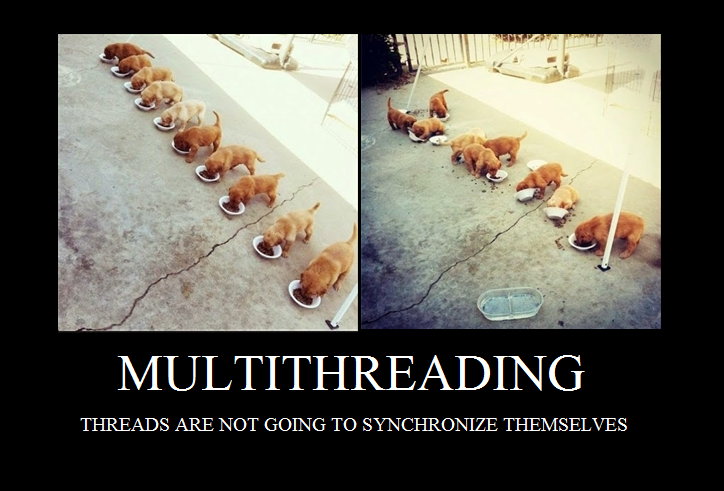
\includegraphics{a8d72-multithreadingmeme.png}
    \caption{From https://kartikiyer.com/2019/06/16/synchronizing-multi-threaded-code-based-on-object-value/ }
    \label{fig:my_label}
\end{figure}
\end{center}

In short, this implementation unfortunately failed. When I was implementing this project, I encountered countless:
\begin{itemize}
    \item Dead locks
    \item Race conditions
    \item Messed up execution
    \item Messed up signals
    \item Desynchronization
\end{itemize}

Professor told us to fix a bit of part from the given source code \texttt{prod_cons.c}. However, in order for me to implement my idea into real \texttt{C} code, I had to reconstruct everything from scratch. Also, no semaphore was used. Everything was implemented with mutexes, signals, and conditions (which I came to regret a lot).

In short, the implementation kind of worked, but failed in aspect of reliability due to my lack of skills when it comes to concurrency. The implementation was painful and took almost two weeks, however it was super fun. 

So, the problem that occurred from “1 Producer N consumer” was that if we had a single shared object, that would make no performance improvement at all since it will work as if it is a single thread process. Thus, I came up with methods of using multiple shared objects at once.

In order for me to achieve this goal, I came up with using handlers and worker threads. The basic idea is as it follows:
\begin{itemize}
    \item Producer handler will tell producer worker to read line from file and put data in specific shared object. 
    \item Consumer handler will tell consumer worker to retrieve data from specific shared object and process the string. (In our case it will be counting words)
\end{itemize}
To implement this, there should be 4 types of different threads.
\begin{itemize}
    \item Producer handler $\times 1$
    \item Consumer handler $\times 1$
    \item Producer worker $\times M$
    \item Consumer worker $\times N$
\end{itemize}
In order for me to manage those threads, we need a precise control over all threads. Not to dead locks, no race conditions. 
\par

Following pseudo-code explains how each threads are designed and implemented.
\par

\begin{algorithm}
\caption{Producer Handler}\label{alg:cap}
\begin{algorithmic}
\State $emptyIndex \gets 0$
\State $curWorker \gets 0$
\While{File not finished}
\If{All Shared objects full}
    \State Wait for signal  \Comment{Signal when shared object was consumed}
    \State Continue \Comment{Go back to the start of the loop}
\EndIf
\State $emptyIndex \gets $Empty shared object  \Comment{Assign job info}
\State $curWorker \gets $Available worker
\State Assign job to $curWorker$
\EndWhile
\While{Workers not over}
\State Send signal to all worker threads  \Comment{Wake sleeping workers}
\State Set empty shared objects as finished
\EndWhile
\end{algorithmic}
\end{algorithm}

\begin{algorithm}
\caption{Producer Worker}\label{alg:cap}
\begin{algorithmic}
\State $readCount \gets 0$
\State $line \gets NULL$
\State $read \gets 0$
\While{True}  
\State Wait until handler's signal arrives
\State $line \gets $Read line from file  
\State $read \gets $Read Result
\State $targetObject \gets $Assigned work from handler
\If{Assigned empty job}
    \State Set state terminated
    \State Break loop
\EndIf
\If{$read$ = -1}
    \State $targetObject.line \gets NULL$  \Comment{Let consumer know this was last}
    \State $targetObject.isFull \gets -1$
    \State Send signal $targetObject.cond$  \Comment{Send signal to consumer worker}
    \State Break loop
\EndIf
\State $targetObject.line \gets line$  \Comment{Store data}
\State $targetObject.isFull \gets 1$
\State Send signal $targetObject.cond$ 
\State Set state available
\State $readCount \gets $readCount$ + 1$
\EndWhile
\State Return $readCount$
\end{algorithmic}
\end{algorithm}


\begin{algorithm}
\caption{Consumer Handler}\label{alg:cap}
\begin{algorithmic}
\State $emptyIndex \gets 0$
\State $curWorker \gets 0$
\While{Workers not over}
\If{All Shared objects empty}
    \State Wait for signal  \Comment{Signal when shared object was produced}
    \State Continue \Comment{Go back to the start of the loop}
\EndIf
\State $emptyIndex \gets $Empty shared object  \Comment{Assign job info}
\State $curWorker \gets $Available worker
\State Assign job to $curWorker$
\EndWhile
\end{algorithmic}
\end{algorithm}

\begin{algorithm}
\caption{Consumer Worker}\label{alg:cap}
\begin{algorithmic}
\State $readCount \gets 0$
\State $line \gets NULL$
\State $read \gets 0$
\While{True}  
\State Wait until handler's signal arrives
\State $targetObject \gets $Assigned work from handler
\If{$targetObject.isFull$ = 0}  \Comment{Target object was not filled in yet}
        \State Wait for signal  \Comment{Signal when shared object was filled}
        \State Continue \Comment{Go back at where it got signal}
\EndIf
\If{$targetObject.line$ = NULL}  \Comment{File was over}
    \State Set worker state terminated
    \State Break loop
\EndIf
\State $line \gets targetObject.line$  \Comment{Retrieve data}
\State $targetObject.isFull \gets 0$
\State Process $line$
\State Set state available
\State $readCount \gets $readCount$ + 1$
\EndWhile
\State Return $readCount$
\end{algorithmic}
\end{algorithm}

\pagebreak
Let’s assume the following case:
\begin{itemize}
    \item 1 Producer
    \item 1 Consumer
    \item 2 Shared Objects
\end{itemize}
The threads will work like this picture below:

\begin{figure}[h]
  \centering
  \includesvg[inkscapelatex=false, width = 400pt, height = 175pt]{thread.svg}
  \caption{Thread and Time graph}
\end{figure}

\pagebreak
In short, producer handler and consumer handler will assign workers for each shared object. Producer worker will lock shared object and write data into it. When it is done writing data into the shared object, it will unlock mutex. Consumer worker at the same time tried to lock shared object, however since it was not filled in yet, it will wait until producer worker finishes writing data. When producer worker finished writing data, consumer worker will lock mutex and access data. When it is done using shared object, it will release lock. This process goes on until the end of the file. 
\par

After the file was finished, each workers and handlers will join. Then the stats of the file retrieved by each consumer workers will be merged into one stat. Then print out the result of statistics of the file that was requested to analyze. 
\par

In order for us to achieve this, we need:
\begin{itemize}
    \item A mutex between producer handler and consumer handler. Since they need to know shared object’s status accurately, they need a mutex that avoids race condition on shared object’s status
    \item Mutexes in shared objects. Since producer worker and consumer worker will use a same shared object, they need a mutex that avoids race condition on shared object’s data. For example, consumer worker should not access shared object when producer worker was writing some data into it, vice versa.
    \item Conditions between each handlers and worker threads. Since handler thread needs to wake worker thread up and assign job to the worker thread, they need a condition that will wake worker thread up.
    \item Condition between producer handler and consumer workers, worker handler and producer workers. Since they need to know if the shared object was filled or not.
\end{itemize}

You can refer to the code in \texttt{project} directory. The code has following sources:
\begin{itemize}
    \item \texttt{main.c}: Code for main function. This initializes all variables and starts threads.
    \item \texttt{common.c} \& \texttt{common.h}: Code for some shared codes.
    \item \texttt{producer.c} \& \texttt{producer.h}: Code for producer threads.
    \item \texttt{consumer.c} \& \texttt{consumer.h}: Code for consumer threads.
\end{itemize}
You can execute project using following command.
\\
\begin{center}
\begin{code}
\begin{minted}[frame=single,framesep=10pt]{bash}
$ ./project <readfile> #Producer #Consumer #SharedObjects
\end{minted}
\captionof{listing}{Executing Project}
\end{code}
\end{center}
Please be advised that $\#SharedObjects$ must be greater or equal to maximum between $\#Producer$ and $\#Consumer$.
\par
So, an example execution will be:
\\
\begin{center}
\begin{code}
\begin{minted}[frame=single,framesep=10pt]{bash}
$ ./project ObsoleteFiles.incOld 10 10 20
\end{minted}
\captionof{listing}{Example of Executing Project}
\end{code}
\end{center}
This will execute 10 producer threads, 10 consumer threads with 20 shared objects for file named \texttt{ObsoleteFiles.incOld}. Let’s execute with file named \texttt{ObsoleteFiles.incOld} from \texttt{FreeBSD9-orig.tar} (originally named \texttt{ObsoleteFiles.inc})
\\

\begin{center}
\begin{code}
\begin{minted}[frame=single,framesep=10pt]{bash}
$ ./project ObsoleteFiles.incOld 10 10 20
[+] Starting job...
[+] Reading file : ObsoleteFiles.incOld
[+] Job info : 10 Producers / 10 Consumers /  20 Shared objects
[+] If this process get stuck, kill it. ...
\end{minted}
\captionof{listing}{Example of Executing Project}
\end{code}
\end{center}

The process starts with 10 producers, 10 consumers and 10 shared objects. (If you executed the command and if it was stuck, please kill process using \texttt{SIGINT}. This has low chance of happening however it sometimes does. Unfortunately, I could not make the possibilities of my process getting into dead lock down to 0%)
\\

\begin{center}
\begin{code}
\begin{minted}[frame=single,framesep=10pt]{bash}
[PH] Joined
[PW00] Read 614 lines
[PW01] Read 9 lines
[PW02] Read 619 lines
[PW03] Read 549 lines
...
[+] Producer read 5490 lines
...
[CW08] Processed 557 lines
[CW09] Processed 547 lines
[CH] Joined
[+] Consumer read 5490 lines
\end{minted}
\captionof{listing}{Example of Executing Project}
\end{code}
\end{center}

\pagebreak
Consumer and producer handlers each has a mechanism that distributes workload to each worker thread. This might be inefficient since the handlers need to perform extra operation to select worker threads, however I just wanted to implement a kind of load balancing for each worker thread. 
\\

\begin{center}
\begin{code}
\begin{minted}[frame=single,framesep=10pt]{bash}
[+] Consumer read 5490 lines
*** print out distributions ***
  #ch  freq
[  1]:  539     *****
[  2]:  209     **
[  3]:  185     **
[  4]:  141     *
[  5]:  123     *
[  6]:  189     **
[  7]:  208     **
[  8]:  143     *
[  9]:  314     ***
...
[ 25]:   67
[ 26]:   75
[ 27]:   71
[ 28]:   93     *
[ 29]:  134     *
[ 30]: 4497     *************************************************
...
\end{minted}
\captionof{listing}{Result of Executing Project}
\end{code}
\end{center}

Then, this will print out the distribution of the content. The source code came from professor’s \texttt{char_stat.c}. Modified a bit of that code and it worked like magic! The image was too tiny, so I will attach result file as \texttt{output.png}.
\par

So, the question arises. Is this really faster than original \texttt{char_stat.c}? Unfortunately, the answer happened to be no. Let’s see comparison of the result:

\begin{figure}[h]
    \begin{center}
        \resizebox{0.6\textwidth}{!}{%% Creator: Matplotlib, PGF backend
%%
%% To include the figure in your LaTeX document, write
%%   \input{<filename>.pgf}
%%
%% Make sure the required packages are loaded in your preamble
%%   \usepackage{pgf}
%%
%% Also ensure that all the required font packages are loaded; for instance,
%% the lmodern package is sometimes necessary when using math font.
%%   \usepackage{lmodern}
%%
%% Figures using additional raster images can only be included by \input if
%% they are in the same directory as the main LaTeX file. For loading figures
%% from other directories you can use the `import` package
%%   \usepackage{import}
%%
%% and then include the figures with
%%   \import{<path to file>}{<filename>.pgf}
%%
%% Matplotlib used the following preamble
%%
\begingroup%
\makeatletter%
\begin{pgfpicture}%
\pgfpathrectangle{\pgfpointorigin}{\pgfqpoint{6.000000in}{4.000000in}}%
\pgfusepath{use as bounding box, clip}%
\begin{pgfscope}%
\pgfsetbuttcap%
\pgfsetmiterjoin%
\pgfsetlinewidth{0.000000pt}%
\definecolor{currentstroke}{rgb}{1.000000,1.000000,1.000000}%
\pgfsetstrokecolor{currentstroke}%
\pgfsetstrokeopacity{0.000000}%
\pgfsetdash{}{0pt}%
\pgfpathmoveto{\pgfqpoint{0.000000in}{0.000000in}}%
\pgfpathlineto{\pgfqpoint{6.000000in}{0.000000in}}%
\pgfpathlineto{\pgfqpoint{6.000000in}{4.000000in}}%
\pgfpathlineto{\pgfqpoint{0.000000in}{4.000000in}}%
\pgfpathlineto{\pgfqpoint{0.000000in}{0.000000in}}%
\pgfpathclose%
\pgfusepath{}%
\end{pgfscope}%
\begin{pgfscope}%
\pgfsetbuttcap%
\pgfsetmiterjoin%
\definecolor{currentfill}{rgb}{1.000000,1.000000,1.000000}%
\pgfsetfillcolor{currentfill}%
\pgfsetlinewidth{0.000000pt}%
\definecolor{currentstroke}{rgb}{0.000000,0.000000,0.000000}%
\pgfsetstrokecolor{currentstroke}%
\pgfsetstrokeopacity{0.000000}%
\pgfsetdash{}{0pt}%
\pgfpathmoveto{\pgfqpoint{0.750000in}{0.500000in}}%
\pgfpathlineto{\pgfqpoint{5.400000in}{0.500000in}}%
\pgfpathlineto{\pgfqpoint{5.400000in}{3.520000in}}%
\pgfpathlineto{\pgfqpoint{0.750000in}{3.520000in}}%
\pgfpathlineto{\pgfqpoint{0.750000in}{0.500000in}}%
\pgfpathclose%
\pgfusepath{fill}%
\end{pgfscope}%
\begin{pgfscope}%
\pgfpathrectangle{\pgfqpoint{0.750000in}{0.500000in}}{\pgfqpoint{4.650000in}{3.020000in}}%
\pgfusepath{clip}%
\pgfsetbuttcap%
\pgfsetroundjoin%
\definecolor{currentfill}{rgb}{0.839216,0.152941,0.156863}%
\pgfsetfillcolor{currentfill}%
\pgfsetlinewidth{1.003750pt}%
\definecolor{currentstroke}{rgb}{0.839216,0.152941,0.156863}%
\pgfsetstrokecolor{currentstroke}%
\pgfsetdash{}{0pt}%
\pgfsys@defobject{currentmarker}{\pgfqpoint{-0.041667in}{-0.041667in}}{\pgfqpoint{0.041667in}{0.041667in}}{%
\pgfpathmoveto{\pgfqpoint{0.000000in}{-0.041667in}}%
\pgfpathcurveto{\pgfqpoint{0.011050in}{-0.041667in}}{\pgfqpoint{0.021649in}{-0.037276in}}{\pgfqpoint{0.029463in}{-0.029463in}}%
\pgfpathcurveto{\pgfqpoint{0.037276in}{-0.021649in}}{\pgfqpoint{0.041667in}{-0.011050in}}{\pgfqpoint{0.041667in}{0.000000in}}%
\pgfpathcurveto{\pgfqpoint{0.041667in}{0.011050in}}{\pgfqpoint{0.037276in}{0.021649in}}{\pgfqpoint{0.029463in}{0.029463in}}%
\pgfpathcurveto{\pgfqpoint{0.021649in}{0.037276in}}{\pgfqpoint{0.011050in}{0.041667in}}{\pgfqpoint{0.000000in}{0.041667in}}%
\pgfpathcurveto{\pgfqpoint{-0.011050in}{0.041667in}}{\pgfqpoint{-0.021649in}{0.037276in}}{\pgfqpoint{-0.029463in}{0.029463in}}%
\pgfpathcurveto{\pgfqpoint{-0.037276in}{0.021649in}}{\pgfqpoint{-0.041667in}{0.011050in}}{\pgfqpoint{-0.041667in}{0.000000in}}%
\pgfpathcurveto{\pgfqpoint{-0.041667in}{-0.011050in}}{\pgfqpoint{-0.037276in}{-0.021649in}}{\pgfqpoint{-0.029463in}{-0.029463in}}%
\pgfpathcurveto{\pgfqpoint{-0.021649in}{-0.037276in}}{\pgfqpoint{-0.011050in}{-0.041667in}}{\pgfqpoint{0.000000in}{-0.041667in}}%
\pgfpathlineto{\pgfqpoint{0.000000in}{-0.041667in}}%
\pgfpathclose%
\pgfusepath{stroke,fill}%
}%
\begin{pgfscope}%
\pgfsys@transformshift{4.184047in}{1.837924in}%
\pgfsys@useobject{currentmarker}{}%
\end{pgfscope}%
\end{pgfscope}%
\begin{pgfscope}%
\pgfpathrectangle{\pgfqpoint{0.750000in}{0.500000in}}{\pgfqpoint{4.650000in}{3.020000in}}%
\pgfusepath{clip}%
\pgfsetbuttcap%
\pgfsetroundjoin%
\definecolor{currentfill}{rgb}{0.121569,0.466667,0.705882}%
\pgfsetfillcolor{currentfill}%
\pgfsetlinewidth{1.003750pt}%
\definecolor{currentstroke}{rgb}{0.121569,0.466667,0.705882}%
\pgfsetstrokecolor{currentstroke}%
\pgfsetdash{}{0pt}%
\pgfsys@defobject{currentmarker}{\pgfqpoint{-0.041667in}{-0.041667in}}{\pgfqpoint{0.041667in}{0.041667in}}{%
\pgfpathmoveto{\pgfqpoint{0.000000in}{-0.041667in}}%
\pgfpathcurveto{\pgfqpoint{0.011050in}{-0.041667in}}{\pgfqpoint{0.021649in}{-0.037276in}}{\pgfqpoint{0.029463in}{-0.029463in}}%
\pgfpathcurveto{\pgfqpoint{0.037276in}{-0.021649in}}{\pgfqpoint{0.041667in}{-0.011050in}}{\pgfqpoint{0.041667in}{0.000000in}}%
\pgfpathcurveto{\pgfqpoint{0.041667in}{0.011050in}}{\pgfqpoint{0.037276in}{0.021649in}}{\pgfqpoint{0.029463in}{0.029463in}}%
\pgfpathcurveto{\pgfqpoint{0.021649in}{0.037276in}}{\pgfqpoint{0.011050in}{0.041667in}}{\pgfqpoint{0.000000in}{0.041667in}}%
\pgfpathcurveto{\pgfqpoint{-0.011050in}{0.041667in}}{\pgfqpoint{-0.021649in}{0.037276in}}{\pgfqpoint{-0.029463in}{0.029463in}}%
\pgfpathcurveto{\pgfqpoint{-0.037276in}{0.021649in}}{\pgfqpoint{-0.041667in}{0.011050in}}{\pgfqpoint{-0.041667in}{0.000000in}}%
\pgfpathcurveto{\pgfqpoint{-0.041667in}{-0.011050in}}{\pgfqpoint{-0.037276in}{-0.021649in}}{\pgfqpoint{-0.029463in}{-0.029463in}}%
\pgfpathcurveto{\pgfqpoint{-0.021649in}{-0.037276in}}{\pgfqpoint{-0.011050in}{-0.041667in}}{\pgfqpoint{0.000000in}{-0.041667in}}%
\pgfpathlineto{\pgfqpoint{0.000000in}{-0.041667in}}%
\pgfpathclose%
\pgfusepath{stroke,fill}%
}%
\begin{pgfscope}%
\pgfsys@transformshift{2.433077in}{1.848652in}%
\pgfsys@useobject{currentmarker}{}%
\end{pgfscope}%
\end{pgfscope}%
\begin{pgfscope}%
\pgfpathrectangle{\pgfqpoint{0.750000in}{0.500000in}}{\pgfqpoint{4.650000in}{3.020000in}}%
\pgfusepath{clip}%
\pgfsetbuttcap%
\pgfsetroundjoin%
\definecolor{currentfill}{rgb}{0.121569,0.466667,0.705882}%
\pgfsetfillcolor{currentfill}%
\pgfsetlinewidth{1.003750pt}%
\definecolor{currentstroke}{rgb}{0.121569,0.466667,0.705882}%
\pgfsetstrokecolor{currentstroke}%
\pgfsetdash{}{0pt}%
\pgfpathmoveto{\pgfqpoint{2.433077in}{1.806986in}}%
\pgfpathcurveto{\pgfqpoint{2.444128in}{1.806986in}}{\pgfqpoint{2.454727in}{1.811376in}}{\pgfqpoint{2.462540in}{1.819189in}}%
\pgfpathcurveto{\pgfqpoint{2.470354in}{1.827003in}}{\pgfqpoint{2.474744in}{1.837602in}}{\pgfqpoint{2.474744in}{1.848652in}}%
\pgfpathcurveto{\pgfqpoint{2.474744in}{1.859702in}}{\pgfqpoint{2.470354in}{1.870301in}}{\pgfqpoint{2.462540in}{1.878115in}}%
\pgfpathcurveto{\pgfqpoint{2.454727in}{1.885929in}}{\pgfqpoint{2.444128in}{1.890319in}}{\pgfqpoint{2.433077in}{1.890319in}}%
\pgfpathcurveto{\pgfqpoint{2.422027in}{1.890319in}}{\pgfqpoint{2.411428in}{1.885929in}}{\pgfqpoint{2.403615in}{1.878115in}}%
\pgfpathcurveto{\pgfqpoint{2.395801in}{1.870301in}}{\pgfqpoint{2.391411in}{1.859702in}}{\pgfqpoint{2.391411in}{1.848652in}}%
\pgfpathcurveto{\pgfqpoint{2.391411in}{1.837602in}}{\pgfqpoint{2.395801in}{1.827003in}}{\pgfqpoint{2.403615in}{1.819189in}}%
\pgfpathcurveto{\pgfqpoint{2.411428in}{1.811376in}}{\pgfqpoint{2.422027in}{1.806986in}}{\pgfqpoint{2.433077in}{1.806986in}}%
\pgfpathlineto{\pgfqpoint{2.433077in}{1.806986in}}%
\pgfpathclose%
\pgfusepath{stroke,fill}%
\end{pgfscope}%
\begin{pgfscope}%
\pgfpathrectangle{\pgfqpoint{0.750000in}{0.500000in}}{\pgfqpoint{4.650000in}{3.020000in}}%
\pgfusepath{clip}%
\pgfsetbuttcap%
\pgfsetroundjoin%
\definecolor{currentfill}{rgb}{0.121569,0.466667,0.705882}%
\pgfsetfillcolor{currentfill}%
\pgfsetlinewidth{1.003750pt}%
\definecolor{currentstroke}{rgb}{0.121569,0.466667,0.705882}%
\pgfsetstrokecolor{currentstroke}%
\pgfsetdash{}{0pt}%
\pgfpathmoveto{\pgfqpoint{1.810809in}{2.235918in}}%
\pgfpathcurveto{\pgfqpoint{1.821859in}{2.235918in}}{\pgfqpoint{1.832458in}{2.240309in}}{\pgfqpoint{1.840272in}{2.248122in}}%
\pgfpathcurveto{\pgfqpoint{1.848086in}{2.255936in}}{\pgfqpoint{1.852476in}{2.266535in}}{\pgfqpoint{1.852476in}{2.277585in}}%
\pgfpathcurveto{\pgfqpoint{1.852476in}{2.288635in}}{\pgfqpoint{1.848086in}{2.299234in}}{\pgfqpoint{1.840272in}{2.307048in}}%
\pgfpathcurveto{\pgfqpoint{1.832458in}{2.314861in}}{\pgfqpoint{1.821859in}{2.319252in}}{\pgfqpoint{1.810809in}{2.319252in}}%
\pgfpathcurveto{\pgfqpoint{1.799759in}{2.319252in}}{\pgfqpoint{1.789160in}{2.314861in}}{\pgfqpoint{1.781346in}{2.307048in}}%
\pgfpathcurveto{\pgfqpoint{1.773533in}{2.299234in}}{\pgfqpoint{1.769143in}{2.288635in}}{\pgfqpoint{1.769143in}{2.277585in}}%
\pgfpathcurveto{\pgfqpoint{1.769143in}{2.266535in}}{\pgfqpoint{1.773533in}{2.255936in}}{\pgfqpoint{1.781346in}{2.248122in}}%
\pgfpathcurveto{\pgfqpoint{1.789160in}{2.240309in}}{\pgfqpoint{1.799759in}{2.235918in}}{\pgfqpoint{1.810809in}{2.235918in}}%
\pgfpathlineto{\pgfqpoint{1.810809in}{2.235918in}}%
\pgfpathclose%
\pgfusepath{stroke,fill}%
\end{pgfscope}%
\begin{pgfscope}%
\pgfpathrectangle{\pgfqpoint{0.750000in}{0.500000in}}{\pgfqpoint{4.650000in}{3.020000in}}%
\pgfusepath{clip}%
\pgfsetbuttcap%
\pgfsetroundjoin%
\definecolor{currentfill}{rgb}{0.121569,0.466667,0.705882}%
\pgfsetfillcolor{currentfill}%
\pgfsetlinewidth{1.003750pt}%
\definecolor{currentstroke}{rgb}{0.121569,0.466667,0.705882}%
\pgfsetstrokecolor{currentstroke}%
\pgfsetdash{}{0pt}%
\pgfpathmoveto{\pgfqpoint{2.788014in}{1.248157in}}%
\pgfpathcurveto{\pgfqpoint{2.799064in}{1.248157in}}{\pgfqpoint{2.809663in}{1.252548in}}{\pgfqpoint{2.817476in}{1.260361in}}%
\pgfpathcurveto{\pgfqpoint{2.825290in}{1.268175in}}{\pgfqpoint{2.829680in}{1.278774in}}{\pgfqpoint{2.829680in}{1.289824in}}%
\pgfpathcurveto{\pgfqpoint{2.829680in}{1.300874in}}{\pgfqpoint{2.825290in}{1.311473in}}{\pgfqpoint{2.817476in}{1.319287in}}%
\pgfpathcurveto{\pgfqpoint{2.809663in}{1.327100in}}{\pgfqpoint{2.799064in}{1.331491in}}{\pgfqpoint{2.788014in}{1.331491in}}%
\pgfpathcurveto{\pgfqpoint{2.776963in}{1.331491in}}{\pgfqpoint{2.766364in}{1.327100in}}{\pgfqpoint{2.758551in}{1.319287in}}%
\pgfpathcurveto{\pgfqpoint{2.750737in}{1.311473in}}{\pgfqpoint{2.746347in}{1.300874in}}{\pgfqpoint{2.746347in}{1.289824in}}%
\pgfpathcurveto{\pgfqpoint{2.746347in}{1.278774in}}{\pgfqpoint{2.750737in}{1.268175in}}{\pgfqpoint{2.758551in}{1.260361in}}%
\pgfpathcurveto{\pgfqpoint{2.766364in}{1.252548in}}{\pgfqpoint{2.776963in}{1.248157in}}{\pgfqpoint{2.788014in}{1.248157in}}%
\pgfpathlineto{\pgfqpoint{2.788014in}{1.248157in}}%
\pgfpathclose%
\pgfusepath{stroke,fill}%
\end{pgfscope}%
\begin{pgfscope}%
\pgfpathrectangle{\pgfqpoint{0.750000in}{0.500000in}}{\pgfqpoint{4.650000in}{3.020000in}}%
\pgfusepath{clip}%
\pgfsetbuttcap%
\pgfsetroundjoin%
\definecolor{currentfill}{rgb}{0.121569,0.466667,0.705882}%
\pgfsetfillcolor{currentfill}%
\pgfsetlinewidth{1.003750pt}%
\definecolor{currentstroke}{rgb}{0.121569,0.466667,0.705882}%
\pgfsetstrokecolor{currentstroke}%
\pgfsetdash{}{0pt}%
\pgfpathmoveto{\pgfqpoint{2.010252in}{1.957325in}}%
\pgfpathcurveto{\pgfqpoint{2.021302in}{1.957325in}}{\pgfqpoint{2.031901in}{1.961715in}}{\pgfqpoint{2.039715in}{1.969529in}}%
\pgfpathcurveto{\pgfqpoint{2.047528in}{1.977343in}}{\pgfqpoint{2.051919in}{1.987942in}}{\pgfqpoint{2.051919in}{1.998992in}}%
\pgfpathcurveto{\pgfqpoint{2.051919in}{2.010042in}}{\pgfqpoint{2.047528in}{2.020641in}}{\pgfqpoint{2.039715in}{2.028455in}}%
\pgfpathcurveto{\pgfqpoint{2.031901in}{2.036268in}}{\pgfqpoint{2.021302in}{2.040658in}}{\pgfqpoint{2.010252in}{2.040658in}}%
\pgfpathcurveto{\pgfqpoint{1.999202in}{2.040658in}}{\pgfqpoint{1.988603in}{2.036268in}}{\pgfqpoint{1.980789in}{2.028455in}}%
\pgfpathcurveto{\pgfqpoint{1.972976in}{2.020641in}}{\pgfqpoint{1.968585in}{2.010042in}}{\pgfqpoint{1.968585in}{1.998992in}}%
\pgfpathcurveto{\pgfqpoint{1.968585in}{1.987942in}}{\pgfqpoint{1.972976in}{1.977343in}}{\pgfqpoint{1.980789in}{1.969529in}}%
\pgfpathcurveto{\pgfqpoint{1.988603in}{1.961715in}}{\pgfqpoint{1.999202in}{1.957325in}}{\pgfqpoint{2.010252in}{1.957325in}}%
\pgfpathlineto{\pgfqpoint{2.010252in}{1.957325in}}%
\pgfpathclose%
\pgfusepath{stroke,fill}%
\end{pgfscope}%
\begin{pgfscope}%
\pgfpathrectangle{\pgfqpoint{0.750000in}{0.500000in}}{\pgfqpoint{4.650000in}{3.020000in}}%
\pgfusepath{clip}%
\pgfsetbuttcap%
\pgfsetroundjoin%
\definecolor{currentfill}{rgb}{0.839216,0.152941,0.156863}%
\pgfsetfillcolor{currentfill}%
\pgfsetlinewidth{1.003750pt}%
\definecolor{currentstroke}{rgb}{0.839216,0.152941,0.156863}%
\pgfsetstrokecolor{currentstroke}%
\pgfsetdash{}{0pt}%
\pgfpathmoveto{\pgfqpoint{3.425362in}{2.261792in}}%
\pgfpathcurveto{\pgfqpoint{3.436412in}{2.261792in}}{\pgfqpoint{3.447011in}{2.266182in}}{\pgfqpoint{3.454825in}{2.273996in}}%
\pgfpathcurveto{\pgfqpoint{3.462639in}{2.281809in}}{\pgfqpoint{3.467029in}{2.292408in}}{\pgfqpoint{3.467029in}{2.303459in}}%
\pgfpathcurveto{\pgfqpoint{3.467029in}{2.314509in}}{\pgfqpoint{3.462639in}{2.325108in}}{\pgfqpoint{3.454825in}{2.332921in}}%
\pgfpathcurveto{\pgfqpoint{3.447011in}{2.340735in}}{\pgfqpoint{3.436412in}{2.345125in}}{\pgfqpoint{3.425362in}{2.345125in}}%
\pgfpathcurveto{\pgfqpoint{3.414312in}{2.345125in}}{\pgfqpoint{3.403713in}{2.340735in}}{\pgfqpoint{3.395899in}{2.332921in}}%
\pgfpathcurveto{\pgfqpoint{3.388086in}{2.325108in}}{\pgfqpoint{3.383695in}{2.314509in}}{\pgfqpoint{3.383695in}{2.303459in}}%
\pgfpathcurveto{\pgfqpoint{3.383695in}{2.292408in}}{\pgfqpoint{3.388086in}{2.281809in}}{\pgfqpoint{3.395899in}{2.273996in}}%
\pgfpathcurveto{\pgfqpoint{3.403713in}{2.266182in}}{\pgfqpoint{3.414312in}{2.261792in}}{\pgfqpoint{3.425362in}{2.261792in}}%
\pgfpathlineto{\pgfqpoint{3.425362in}{2.261792in}}%
\pgfpathclose%
\pgfusepath{stroke,fill}%
\end{pgfscope}%
\begin{pgfscope}%
\pgfpathrectangle{\pgfqpoint{0.750000in}{0.500000in}}{\pgfqpoint{4.650000in}{3.020000in}}%
\pgfusepath{clip}%
\pgfsetbuttcap%
\pgfsetroundjoin%
\definecolor{currentfill}{rgb}{0.839216,0.152941,0.156863}%
\pgfsetfillcolor{currentfill}%
\pgfsetlinewidth{1.003750pt}%
\definecolor{currentstroke}{rgb}{0.839216,0.152941,0.156863}%
\pgfsetstrokecolor{currentstroke}%
\pgfsetdash{}{0pt}%
\pgfpathmoveto{\pgfqpoint{3.908362in}{1.842298in}}%
\pgfpathcurveto{\pgfqpoint{3.919412in}{1.842298in}}{\pgfqpoint{3.930011in}{1.846689in}}{\pgfqpoint{3.937825in}{1.854502in}}%
\pgfpathcurveto{\pgfqpoint{3.945639in}{1.862316in}}{\pgfqpoint{3.950029in}{1.872915in}}{\pgfqpoint{3.950029in}{1.883965in}}%
\pgfpathcurveto{\pgfqpoint{3.950029in}{1.895015in}}{\pgfqpoint{3.945639in}{1.905614in}}{\pgfqpoint{3.937825in}{1.913428in}}%
\pgfpathcurveto{\pgfqpoint{3.930011in}{1.921242in}}{\pgfqpoint{3.919412in}{1.925632in}}{\pgfqpoint{3.908362in}{1.925632in}}%
\pgfpathcurveto{\pgfqpoint{3.897312in}{1.925632in}}{\pgfqpoint{3.886713in}{1.921242in}}{\pgfqpoint{3.878899in}{1.913428in}}%
\pgfpathcurveto{\pgfqpoint{3.871086in}{1.905614in}}{\pgfqpoint{3.866696in}{1.895015in}}{\pgfqpoint{3.866696in}{1.883965in}}%
\pgfpathcurveto{\pgfqpoint{3.866696in}{1.872915in}}{\pgfqpoint{3.871086in}{1.862316in}}{\pgfqpoint{3.878899in}{1.854502in}}%
\pgfpathcurveto{\pgfqpoint{3.886713in}{1.846689in}}{\pgfqpoint{3.897312in}{1.842298in}}{\pgfqpoint{3.908362in}{1.842298in}}%
\pgfpathlineto{\pgfqpoint{3.908362in}{1.842298in}}%
\pgfpathclose%
\pgfusepath{stroke,fill}%
\end{pgfscope}%
\begin{pgfscope}%
\pgfpathrectangle{\pgfqpoint{0.750000in}{0.500000in}}{\pgfqpoint{4.650000in}{3.020000in}}%
\pgfusepath{clip}%
\pgfsetbuttcap%
\pgfsetroundjoin%
\definecolor{currentfill}{rgb}{0.839216,0.152941,0.156863}%
\pgfsetfillcolor{currentfill}%
\pgfsetlinewidth{1.003750pt}%
\definecolor{currentstroke}{rgb}{0.839216,0.152941,0.156863}%
\pgfsetstrokecolor{currentstroke}%
\pgfsetdash{}{0pt}%
\pgfpathmoveto{\pgfqpoint{3.272609in}{1.864100in}}%
\pgfpathcurveto{\pgfqpoint{3.283659in}{1.864100in}}{\pgfqpoint{3.294258in}{1.868490in}}{\pgfqpoint{3.302071in}{1.876304in}}%
\pgfpathcurveto{\pgfqpoint{3.309885in}{1.884118in}}{\pgfqpoint{3.314275in}{1.894717in}}{\pgfqpoint{3.314275in}{1.905767in}}%
\pgfpathcurveto{\pgfqpoint{3.314275in}{1.916817in}}{\pgfqpoint{3.309885in}{1.927416in}}{\pgfqpoint{3.302071in}{1.935230in}}%
\pgfpathcurveto{\pgfqpoint{3.294258in}{1.943043in}}{\pgfqpoint{3.283659in}{1.947434in}}{\pgfqpoint{3.272609in}{1.947434in}}%
\pgfpathcurveto{\pgfqpoint{3.261559in}{1.947434in}}{\pgfqpoint{3.250960in}{1.943043in}}{\pgfqpoint{3.243146in}{1.935230in}}%
\pgfpathcurveto{\pgfqpoint{3.235332in}{1.927416in}}{\pgfqpoint{3.230942in}{1.916817in}}{\pgfqpoint{3.230942in}{1.905767in}}%
\pgfpathcurveto{\pgfqpoint{3.230942in}{1.894717in}}{\pgfqpoint{3.235332in}{1.884118in}}{\pgfqpoint{3.243146in}{1.876304in}}%
\pgfpathcurveto{\pgfqpoint{3.250960in}{1.868490in}}{\pgfqpoint{3.261559in}{1.864100in}}{\pgfqpoint{3.272609in}{1.864100in}}%
\pgfpathlineto{\pgfqpoint{3.272609in}{1.864100in}}%
\pgfpathclose%
\pgfusepath{stroke,fill}%
\end{pgfscope}%
\begin{pgfscope}%
\pgfpathrectangle{\pgfqpoint{0.750000in}{0.500000in}}{\pgfqpoint{4.650000in}{3.020000in}}%
\pgfusepath{clip}%
\pgfsetbuttcap%
\pgfsetroundjoin%
\definecolor{currentfill}{rgb}{0.839216,0.152941,0.156863}%
\pgfsetfillcolor{currentfill}%
\pgfsetlinewidth{1.003750pt}%
\definecolor{currentstroke}{rgb}{0.839216,0.152941,0.156863}%
\pgfsetstrokecolor{currentstroke}%
\pgfsetdash{}{0pt}%
\pgfpathmoveto{\pgfqpoint{4.027066in}{2.165634in}}%
\pgfpathcurveto{\pgfqpoint{4.038116in}{2.165634in}}{\pgfqpoint{4.048715in}{2.170025in}}{\pgfqpoint{4.056528in}{2.177838in}}%
\pgfpathcurveto{\pgfqpoint{4.064342in}{2.185652in}}{\pgfqpoint{4.068732in}{2.196251in}}{\pgfqpoint{4.068732in}{2.207301in}}%
\pgfpathcurveto{\pgfqpoint{4.068732in}{2.218351in}}{\pgfqpoint{4.064342in}{2.228950in}}{\pgfqpoint{4.056528in}{2.236764in}}%
\pgfpathcurveto{\pgfqpoint{4.048715in}{2.244577in}}{\pgfqpoint{4.038116in}{2.248968in}}{\pgfqpoint{4.027066in}{2.248968in}}%
\pgfpathcurveto{\pgfqpoint{4.016015in}{2.248968in}}{\pgfqpoint{4.005416in}{2.244577in}}{\pgfqpoint{3.997603in}{2.236764in}}%
\pgfpathcurveto{\pgfqpoint{3.989789in}{2.228950in}}{\pgfqpoint{3.985399in}{2.218351in}}{\pgfqpoint{3.985399in}{2.207301in}}%
\pgfpathcurveto{\pgfqpoint{3.985399in}{2.196251in}}{\pgfqpoint{3.989789in}{2.185652in}}{\pgfqpoint{3.997603in}{2.177838in}}%
\pgfpathcurveto{\pgfqpoint{4.005416in}{2.170025in}}{\pgfqpoint{4.016015in}{2.165634in}}{\pgfqpoint{4.027066in}{2.165634in}}%
\pgfpathlineto{\pgfqpoint{4.027066in}{2.165634in}}%
\pgfpathclose%
\pgfusepath{stroke,fill}%
\end{pgfscope}%
\begin{pgfscope}%
\pgfpathrectangle{\pgfqpoint{0.750000in}{0.500000in}}{\pgfqpoint{4.650000in}{3.020000in}}%
\pgfusepath{clip}%
\pgfsetbuttcap%
\pgfsetroundjoin%
\definecolor{currentfill}{rgb}{0.121569,0.466667,0.705882}%
\pgfsetfillcolor{currentfill}%
\pgfsetlinewidth{1.003750pt}%
\definecolor{currentstroke}{rgb}{0.121569,0.466667,0.705882}%
\pgfsetstrokecolor{currentstroke}%
\pgfsetdash{}{0pt}%
\pgfpathmoveto{\pgfqpoint{1.999158in}{1.772658in}}%
\pgfpathcurveto{\pgfqpoint{2.010208in}{1.772658in}}{\pgfqpoint{2.020807in}{1.777048in}}{\pgfqpoint{2.028621in}{1.784862in}}%
\pgfpathcurveto{\pgfqpoint{2.036434in}{1.792675in}}{\pgfqpoint{2.040824in}{1.803274in}}{\pgfqpoint{2.040824in}{1.814324in}}%
\pgfpathcurveto{\pgfqpoint{2.040824in}{1.825374in}}{\pgfqpoint{2.036434in}{1.835973in}}{\pgfqpoint{2.028621in}{1.843787in}}%
\pgfpathcurveto{\pgfqpoint{2.020807in}{1.851601in}}{\pgfqpoint{2.010208in}{1.855991in}}{\pgfqpoint{1.999158in}{1.855991in}}%
\pgfpathcurveto{\pgfqpoint{1.988108in}{1.855991in}}{\pgfqpoint{1.977509in}{1.851601in}}{\pgfqpoint{1.969695in}{1.843787in}}%
\pgfpathcurveto{\pgfqpoint{1.961881in}{1.835973in}}{\pgfqpoint{1.957491in}{1.825374in}}{\pgfqpoint{1.957491in}{1.814324in}}%
\pgfpathcurveto{\pgfqpoint{1.957491in}{1.803274in}}{\pgfqpoint{1.961881in}{1.792675in}}{\pgfqpoint{1.969695in}{1.784862in}}%
\pgfpathcurveto{\pgfqpoint{1.977509in}{1.777048in}}{\pgfqpoint{1.988108in}{1.772658in}}{\pgfqpoint{1.999158in}{1.772658in}}%
\pgfpathlineto{\pgfqpoint{1.999158in}{1.772658in}}%
\pgfpathclose%
\pgfusepath{stroke,fill}%
\end{pgfscope}%
\begin{pgfscope}%
\pgfpathrectangle{\pgfqpoint{0.750000in}{0.500000in}}{\pgfqpoint{4.650000in}{3.020000in}}%
\pgfusepath{clip}%
\pgfsetbuttcap%
\pgfsetroundjoin%
\definecolor{currentfill}{rgb}{0.121569,0.466667,0.705882}%
\pgfsetfillcolor{currentfill}%
\pgfsetlinewidth{1.003750pt}%
\definecolor{currentstroke}{rgb}{0.121569,0.466667,0.705882}%
\pgfsetstrokecolor{currentstroke}%
\pgfsetdash{}{0pt}%
\pgfpathmoveto{\pgfqpoint{1.892442in}{1.092732in}}%
\pgfpathcurveto{\pgfqpoint{1.903492in}{1.092732in}}{\pgfqpoint{1.914091in}{1.097122in}}{\pgfqpoint{1.921905in}{1.104936in}}%
\pgfpathcurveto{\pgfqpoint{1.929718in}{1.112750in}}{\pgfqpoint{1.934109in}{1.123349in}}{\pgfqpoint{1.934109in}{1.134399in}}%
\pgfpathcurveto{\pgfqpoint{1.934109in}{1.145449in}}{\pgfqpoint{1.929718in}{1.156048in}}{\pgfqpoint{1.921905in}{1.163862in}}%
\pgfpathcurveto{\pgfqpoint{1.914091in}{1.171675in}}{\pgfqpoint{1.903492in}{1.176065in}}{\pgfqpoint{1.892442in}{1.176065in}}%
\pgfpathcurveto{\pgfqpoint{1.881392in}{1.176065in}}{\pgfqpoint{1.870793in}{1.171675in}}{\pgfqpoint{1.862979in}{1.163862in}}%
\pgfpathcurveto{\pgfqpoint{1.855165in}{1.156048in}}{\pgfqpoint{1.850775in}{1.145449in}}{\pgfqpoint{1.850775in}{1.134399in}}%
\pgfpathcurveto{\pgfqpoint{1.850775in}{1.123349in}}{\pgfqpoint{1.855165in}{1.112750in}}{\pgfqpoint{1.862979in}{1.104936in}}%
\pgfpathcurveto{\pgfqpoint{1.870793in}{1.097122in}}{\pgfqpoint{1.881392in}{1.092732in}}{\pgfqpoint{1.892442in}{1.092732in}}%
\pgfpathlineto{\pgfqpoint{1.892442in}{1.092732in}}%
\pgfpathclose%
\pgfusepath{stroke,fill}%
\end{pgfscope}%
\begin{pgfscope}%
\pgfpathrectangle{\pgfqpoint{0.750000in}{0.500000in}}{\pgfqpoint{4.650000in}{3.020000in}}%
\pgfusepath{clip}%
\pgfsetbuttcap%
\pgfsetroundjoin%
\definecolor{currentfill}{rgb}{0.121569,0.466667,0.705882}%
\pgfsetfillcolor{currentfill}%
\pgfsetlinewidth{1.003750pt}%
\definecolor{currentstroke}{rgb}{0.121569,0.466667,0.705882}%
\pgfsetstrokecolor{currentstroke}%
\pgfsetdash{}{0pt}%
\pgfpathmoveto{\pgfqpoint{2.563670in}{1.580142in}}%
\pgfpathcurveto{\pgfqpoint{2.574720in}{1.580142in}}{\pgfqpoint{2.585319in}{1.584532in}}{\pgfqpoint{2.593133in}{1.592346in}}%
\pgfpathcurveto{\pgfqpoint{2.600947in}{1.600159in}}{\pgfqpoint{2.605337in}{1.610759in}}{\pgfqpoint{2.605337in}{1.621809in}}%
\pgfpathcurveto{\pgfqpoint{2.605337in}{1.632859in}}{\pgfqpoint{2.600947in}{1.643458in}}{\pgfqpoint{2.593133in}{1.651271in}}%
\pgfpathcurveto{\pgfqpoint{2.585319in}{1.659085in}}{\pgfqpoint{2.574720in}{1.663475in}}{\pgfqpoint{2.563670in}{1.663475in}}%
\pgfpathcurveto{\pgfqpoint{2.552620in}{1.663475in}}{\pgfqpoint{2.542021in}{1.659085in}}{\pgfqpoint{2.534207in}{1.651271in}}%
\pgfpathcurveto{\pgfqpoint{2.526394in}{1.643458in}}{\pgfqpoint{2.522004in}{1.632859in}}{\pgfqpoint{2.522004in}{1.621809in}}%
\pgfpathcurveto{\pgfqpoint{2.522004in}{1.610759in}}{\pgfqpoint{2.526394in}{1.600159in}}{\pgfqpoint{2.534207in}{1.592346in}}%
\pgfpathcurveto{\pgfqpoint{2.542021in}{1.584532in}}{\pgfqpoint{2.552620in}{1.580142in}}{\pgfqpoint{2.563670in}{1.580142in}}%
\pgfpathlineto{\pgfqpoint{2.563670in}{1.580142in}}%
\pgfpathclose%
\pgfusepath{stroke,fill}%
\end{pgfscope}%
\begin{pgfscope}%
\pgfpathrectangle{\pgfqpoint{0.750000in}{0.500000in}}{\pgfqpoint{4.650000in}{3.020000in}}%
\pgfusepath{clip}%
\pgfsetbuttcap%
\pgfsetroundjoin%
\definecolor{currentfill}{rgb}{0.839216,0.152941,0.156863}%
\pgfsetfillcolor{currentfill}%
\pgfsetlinewidth{1.003750pt}%
\definecolor{currentstroke}{rgb}{0.839216,0.152941,0.156863}%
\pgfsetstrokecolor{currentstroke}%
\pgfsetdash{}{0pt}%
\pgfpathmoveto{\pgfqpoint{3.783926in}{2.138298in}}%
\pgfpathcurveto{\pgfqpoint{3.794976in}{2.138298in}}{\pgfqpoint{3.805575in}{2.142688in}}{\pgfqpoint{3.813389in}{2.150502in}}%
\pgfpathcurveto{\pgfqpoint{3.821202in}{2.158316in}}{\pgfqpoint{3.825593in}{2.168915in}}{\pgfqpoint{3.825593in}{2.179965in}}%
\pgfpathcurveto{\pgfqpoint{3.825593in}{2.191015in}}{\pgfqpoint{3.821202in}{2.201614in}}{\pgfqpoint{3.813389in}{2.209428in}}%
\pgfpathcurveto{\pgfqpoint{3.805575in}{2.217241in}}{\pgfqpoint{3.794976in}{2.221632in}}{\pgfqpoint{3.783926in}{2.221632in}}%
\pgfpathcurveto{\pgfqpoint{3.772876in}{2.221632in}}{\pgfqpoint{3.762277in}{2.217241in}}{\pgfqpoint{3.754463in}{2.209428in}}%
\pgfpathcurveto{\pgfqpoint{3.746650in}{2.201614in}}{\pgfqpoint{3.742259in}{2.191015in}}{\pgfqpoint{3.742259in}{2.179965in}}%
\pgfpathcurveto{\pgfqpoint{3.742259in}{2.168915in}}{\pgfqpoint{3.746650in}{2.158316in}}{\pgfqpoint{3.754463in}{2.150502in}}%
\pgfpathcurveto{\pgfqpoint{3.762277in}{2.142688in}}{\pgfqpoint{3.772876in}{2.138298in}}{\pgfqpoint{3.783926in}{2.138298in}}%
\pgfpathlineto{\pgfqpoint{3.783926in}{2.138298in}}%
\pgfpathclose%
\pgfusepath{stroke,fill}%
\end{pgfscope}%
\begin{pgfscope}%
\pgfpathrectangle{\pgfqpoint{0.750000in}{0.500000in}}{\pgfqpoint{4.650000in}{3.020000in}}%
\pgfusepath{clip}%
\pgfsetbuttcap%
\pgfsetroundjoin%
\definecolor{currentfill}{rgb}{0.121569,0.466667,0.705882}%
\pgfsetfillcolor{currentfill}%
\pgfsetlinewidth{1.003750pt}%
\definecolor{currentstroke}{rgb}{0.121569,0.466667,0.705882}%
\pgfsetstrokecolor{currentstroke}%
\pgfsetdash{}{0pt}%
\pgfpathmoveto{\pgfqpoint{2.371129in}{1.616991in}}%
\pgfpathcurveto{\pgfqpoint{2.382180in}{1.616991in}}{\pgfqpoint{2.392779in}{1.621382in}}{\pgfqpoint{2.400592in}{1.629195in}}%
\pgfpathcurveto{\pgfqpoint{2.408406in}{1.637009in}}{\pgfqpoint{2.412796in}{1.647608in}}{\pgfqpoint{2.412796in}{1.658658in}}%
\pgfpathcurveto{\pgfqpoint{2.412796in}{1.669708in}}{\pgfqpoint{2.408406in}{1.680307in}}{\pgfqpoint{2.400592in}{1.688121in}}%
\pgfpathcurveto{\pgfqpoint{2.392779in}{1.695934in}}{\pgfqpoint{2.382180in}{1.700325in}}{\pgfqpoint{2.371129in}{1.700325in}}%
\pgfpathcurveto{\pgfqpoint{2.360079in}{1.700325in}}{\pgfqpoint{2.349480in}{1.695934in}}{\pgfqpoint{2.341667in}{1.688121in}}%
\pgfpathcurveto{\pgfqpoint{2.333853in}{1.680307in}}{\pgfqpoint{2.329463in}{1.669708in}}{\pgfqpoint{2.329463in}{1.658658in}}%
\pgfpathcurveto{\pgfqpoint{2.329463in}{1.647608in}}{\pgfqpoint{2.333853in}{1.637009in}}{\pgfqpoint{2.341667in}{1.629195in}}%
\pgfpathcurveto{\pgfqpoint{2.349480in}{1.621382in}}{\pgfqpoint{2.360079in}{1.616991in}}{\pgfqpoint{2.371129in}{1.616991in}}%
\pgfpathlineto{\pgfqpoint{2.371129in}{1.616991in}}%
\pgfpathclose%
\pgfusepath{stroke,fill}%
\end{pgfscope}%
\begin{pgfscope}%
\pgfpathrectangle{\pgfqpoint{0.750000in}{0.500000in}}{\pgfqpoint{4.650000in}{3.020000in}}%
\pgfusepath{clip}%
\pgfsetbuttcap%
\pgfsetroundjoin%
\definecolor{currentfill}{rgb}{0.839216,0.152941,0.156863}%
\pgfsetfillcolor{currentfill}%
\pgfsetlinewidth{1.003750pt}%
\definecolor{currentstroke}{rgb}{0.839216,0.152941,0.156863}%
\pgfsetstrokecolor{currentstroke}%
\pgfsetdash{}{0pt}%
\pgfpathmoveto{\pgfqpoint{3.760537in}{2.001397in}}%
\pgfpathcurveto{\pgfqpoint{3.771587in}{2.001397in}}{\pgfqpoint{3.782186in}{2.005787in}}{\pgfqpoint{3.789999in}{2.013601in}}%
\pgfpathcurveto{\pgfqpoint{3.797813in}{2.021415in}}{\pgfqpoint{3.802203in}{2.032014in}}{\pgfqpoint{3.802203in}{2.043064in}}%
\pgfpathcurveto{\pgfqpoint{3.802203in}{2.054114in}}{\pgfqpoint{3.797813in}{2.064713in}}{\pgfqpoint{3.789999in}{2.072527in}}%
\pgfpathcurveto{\pgfqpoint{3.782186in}{2.080340in}}{\pgfqpoint{3.771587in}{2.084731in}}{\pgfqpoint{3.760537in}{2.084731in}}%
\pgfpathcurveto{\pgfqpoint{3.749487in}{2.084731in}}{\pgfqpoint{3.738888in}{2.080340in}}{\pgfqpoint{3.731074in}{2.072527in}}%
\pgfpathcurveto{\pgfqpoint{3.723260in}{2.064713in}}{\pgfqpoint{3.718870in}{2.054114in}}{\pgfqpoint{3.718870in}{2.043064in}}%
\pgfpathcurveto{\pgfqpoint{3.718870in}{2.032014in}}{\pgfqpoint{3.723260in}{2.021415in}}{\pgfqpoint{3.731074in}{2.013601in}}%
\pgfpathcurveto{\pgfqpoint{3.738888in}{2.005787in}}{\pgfqpoint{3.749487in}{2.001397in}}{\pgfqpoint{3.760537in}{2.001397in}}%
\pgfpathlineto{\pgfqpoint{3.760537in}{2.001397in}}%
\pgfpathclose%
\pgfusepath{stroke,fill}%
\end{pgfscope}%
\begin{pgfscope}%
\pgfpathrectangle{\pgfqpoint{0.750000in}{0.500000in}}{\pgfqpoint{4.650000in}{3.020000in}}%
\pgfusepath{clip}%
\pgfsetbuttcap%
\pgfsetroundjoin%
\definecolor{currentfill}{rgb}{0.121569,0.466667,0.705882}%
\pgfsetfillcolor{currentfill}%
\pgfsetlinewidth{1.003750pt}%
\definecolor{currentstroke}{rgb}{0.121569,0.466667,0.705882}%
\pgfsetstrokecolor{currentstroke}%
\pgfsetdash{}{0pt}%
\pgfpathmoveto{\pgfqpoint{3.445104in}{2.077842in}}%
\pgfpathcurveto{\pgfqpoint{3.456154in}{2.077842in}}{\pgfqpoint{3.466753in}{2.082232in}}{\pgfqpoint{3.474566in}{2.090046in}}%
\pgfpathcurveto{\pgfqpoint{3.482380in}{2.097860in}}{\pgfqpoint{3.486770in}{2.108459in}}{\pgfqpoint{3.486770in}{2.119509in}}%
\pgfpathcurveto{\pgfqpoint{3.486770in}{2.130559in}}{\pgfqpoint{3.482380in}{2.141158in}}{\pgfqpoint{3.474566in}{2.148972in}}%
\pgfpathcurveto{\pgfqpoint{3.466753in}{2.156785in}}{\pgfqpoint{3.456154in}{2.161176in}}{\pgfqpoint{3.445104in}{2.161176in}}%
\pgfpathcurveto{\pgfqpoint{3.434053in}{2.161176in}}{\pgfqpoint{3.423454in}{2.156785in}}{\pgfqpoint{3.415641in}{2.148972in}}%
\pgfpathcurveto{\pgfqpoint{3.407827in}{2.141158in}}{\pgfqpoint{3.403437in}{2.130559in}}{\pgfqpoint{3.403437in}{2.119509in}}%
\pgfpathcurveto{\pgfqpoint{3.403437in}{2.108459in}}{\pgfqpoint{3.407827in}{2.097860in}}{\pgfqpoint{3.415641in}{2.090046in}}%
\pgfpathcurveto{\pgfqpoint{3.423454in}{2.082232in}}{\pgfqpoint{3.434053in}{2.077842in}}{\pgfqpoint{3.445104in}{2.077842in}}%
\pgfpathlineto{\pgfqpoint{3.445104in}{2.077842in}}%
\pgfpathclose%
\pgfusepath{stroke,fill}%
\end{pgfscope}%
\begin{pgfscope}%
\pgfpathrectangle{\pgfqpoint{0.750000in}{0.500000in}}{\pgfqpoint{4.650000in}{3.020000in}}%
\pgfusepath{clip}%
\pgfsetbuttcap%
\pgfsetroundjoin%
\definecolor{currentfill}{rgb}{0.839216,0.152941,0.156863}%
\pgfsetfillcolor{currentfill}%
\pgfsetlinewidth{1.003750pt}%
\definecolor{currentstroke}{rgb}{0.839216,0.152941,0.156863}%
\pgfsetstrokecolor{currentstroke}%
\pgfsetdash{}{0pt}%
\pgfpathmoveto{\pgfqpoint{4.367810in}{2.215406in}}%
\pgfpathcurveto{\pgfqpoint{4.378860in}{2.215406in}}{\pgfqpoint{4.389459in}{2.219796in}}{\pgfqpoint{4.397273in}{2.227610in}}%
\pgfpathcurveto{\pgfqpoint{4.405087in}{2.235424in}}{\pgfqpoint{4.409477in}{2.246023in}}{\pgfqpoint{4.409477in}{2.257073in}}%
\pgfpathcurveto{\pgfqpoint{4.409477in}{2.268123in}}{\pgfqpoint{4.405087in}{2.278722in}}{\pgfqpoint{4.397273in}{2.286536in}}%
\pgfpathcurveto{\pgfqpoint{4.389459in}{2.294349in}}{\pgfqpoint{4.378860in}{2.298740in}}{\pgfqpoint{4.367810in}{2.298740in}}%
\pgfpathcurveto{\pgfqpoint{4.356760in}{2.298740in}}{\pgfqpoint{4.346161in}{2.294349in}}{\pgfqpoint{4.338347in}{2.286536in}}%
\pgfpathcurveto{\pgfqpoint{4.330534in}{2.278722in}}{\pgfqpoint{4.326143in}{2.268123in}}{\pgfqpoint{4.326143in}{2.257073in}}%
\pgfpathcurveto{\pgfqpoint{4.326143in}{2.246023in}}{\pgfqpoint{4.330534in}{2.235424in}}{\pgfqpoint{4.338347in}{2.227610in}}%
\pgfpathcurveto{\pgfqpoint{4.346161in}{2.219796in}}{\pgfqpoint{4.356760in}{2.215406in}}{\pgfqpoint{4.367810in}{2.215406in}}%
\pgfpathlineto{\pgfqpoint{4.367810in}{2.215406in}}%
\pgfpathclose%
\pgfusepath{stroke,fill}%
\end{pgfscope}%
\begin{pgfscope}%
\pgfpathrectangle{\pgfqpoint{0.750000in}{0.500000in}}{\pgfqpoint{4.650000in}{3.020000in}}%
\pgfusepath{clip}%
\pgfsetbuttcap%
\pgfsetroundjoin%
\definecolor{currentfill}{rgb}{0.121569,0.466667,0.705882}%
\pgfsetfillcolor{currentfill}%
\pgfsetlinewidth{1.003750pt}%
\definecolor{currentstroke}{rgb}{0.121569,0.466667,0.705882}%
\pgfsetstrokecolor{currentstroke}%
\pgfsetdash{}{0pt}%
\pgfpathmoveto{\pgfqpoint{1.975495in}{1.862633in}}%
\pgfpathcurveto{\pgfqpoint{1.986545in}{1.862633in}}{\pgfqpoint{1.997144in}{1.867024in}}{\pgfqpoint{2.004957in}{1.874837in}}%
\pgfpathcurveto{\pgfqpoint{2.012771in}{1.882651in}}{\pgfqpoint{2.017161in}{1.893250in}}{\pgfqpoint{2.017161in}{1.904300in}}%
\pgfpathcurveto{\pgfqpoint{2.017161in}{1.915350in}}{\pgfqpoint{2.012771in}{1.925949in}}{\pgfqpoint{2.004957in}{1.933763in}}%
\pgfpathcurveto{\pgfqpoint{1.997144in}{1.941576in}}{\pgfqpoint{1.986545in}{1.945967in}}{\pgfqpoint{1.975495in}{1.945967in}}%
\pgfpathcurveto{\pgfqpoint{1.964444in}{1.945967in}}{\pgfqpoint{1.953845in}{1.941576in}}{\pgfqpoint{1.946032in}{1.933763in}}%
\pgfpathcurveto{\pgfqpoint{1.938218in}{1.925949in}}{\pgfqpoint{1.933828in}{1.915350in}}{\pgfqpoint{1.933828in}{1.904300in}}%
\pgfpathcurveto{\pgfqpoint{1.933828in}{1.893250in}}{\pgfqpoint{1.938218in}{1.882651in}}{\pgfqpoint{1.946032in}{1.874837in}}%
\pgfpathcurveto{\pgfqpoint{1.953845in}{1.867024in}}{\pgfqpoint{1.964444in}{1.862633in}}{\pgfqpoint{1.975495in}{1.862633in}}%
\pgfpathlineto{\pgfqpoint{1.975495in}{1.862633in}}%
\pgfpathclose%
\pgfusepath{stroke,fill}%
\end{pgfscope}%
\begin{pgfscope}%
\pgfpathrectangle{\pgfqpoint{0.750000in}{0.500000in}}{\pgfqpoint{4.650000in}{3.020000in}}%
\pgfusepath{clip}%
\pgfsetbuttcap%
\pgfsetroundjoin%
\definecolor{currentfill}{rgb}{0.121569,0.466667,0.705882}%
\pgfsetfillcolor{currentfill}%
\pgfsetlinewidth{1.003750pt}%
\definecolor{currentstroke}{rgb}{0.121569,0.466667,0.705882}%
\pgfsetstrokecolor{currentstroke}%
\pgfsetdash{}{0pt}%
\pgfpathmoveto{\pgfqpoint{2.620062in}{1.995622in}}%
\pgfpathcurveto{\pgfqpoint{2.631112in}{1.995622in}}{\pgfqpoint{2.641711in}{2.000013in}}{\pgfqpoint{2.649525in}{2.007826in}}%
\pgfpathcurveto{\pgfqpoint{2.657339in}{2.015640in}}{\pgfqpoint{2.661729in}{2.026239in}}{\pgfqpoint{2.661729in}{2.037289in}}%
\pgfpathcurveto{\pgfqpoint{2.661729in}{2.048339in}}{\pgfqpoint{2.657339in}{2.058938in}}{\pgfqpoint{2.649525in}{2.066752in}}%
\pgfpathcurveto{\pgfqpoint{2.641711in}{2.074565in}}{\pgfqpoint{2.631112in}{2.078956in}}{\pgfqpoint{2.620062in}{2.078956in}}%
\pgfpathcurveto{\pgfqpoint{2.609012in}{2.078956in}}{\pgfqpoint{2.598413in}{2.074565in}}{\pgfqpoint{2.590599in}{2.066752in}}%
\pgfpathcurveto{\pgfqpoint{2.582786in}{2.058938in}}{\pgfqpoint{2.578396in}{2.048339in}}{\pgfqpoint{2.578396in}{2.037289in}}%
\pgfpathcurveto{\pgfqpoint{2.578396in}{2.026239in}}{\pgfqpoint{2.582786in}{2.015640in}}{\pgfqpoint{2.590599in}{2.007826in}}%
\pgfpathcurveto{\pgfqpoint{2.598413in}{2.000013in}}{\pgfqpoint{2.609012in}{1.995622in}}{\pgfqpoint{2.620062in}{1.995622in}}%
\pgfpathlineto{\pgfqpoint{2.620062in}{1.995622in}}%
\pgfpathclose%
\pgfusepath{stroke,fill}%
\end{pgfscope}%
\begin{pgfscope}%
\pgfpathrectangle{\pgfqpoint{0.750000in}{0.500000in}}{\pgfqpoint{4.650000in}{3.020000in}}%
\pgfusepath{clip}%
\pgfsetbuttcap%
\pgfsetroundjoin%
\definecolor{currentfill}{rgb}{0.121569,0.466667,0.705882}%
\pgfsetfillcolor{currentfill}%
\pgfsetlinewidth{1.003750pt}%
\definecolor{currentstroke}{rgb}{0.121569,0.466667,0.705882}%
\pgfsetstrokecolor{currentstroke}%
\pgfsetdash{}{0pt}%
\pgfpathmoveto{\pgfqpoint{1.641838in}{1.603374in}}%
\pgfpathcurveto{\pgfqpoint{1.652888in}{1.603374in}}{\pgfqpoint{1.663487in}{1.607764in}}{\pgfqpoint{1.671301in}{1.615578in}}%
\pgfpathcurveto{\pgfqpoint{1.679115in}{1.623391in}}{\pgfqpoint{1.683505in}{1.633990in}}{\pgfqpoint{1.683505in}{1.645040in}}%
\pgfpathcurveto{\pgfqpoint{1.683505in}{1.656091in}}{\pgfqpoint{1.679115in}{1.666690in}}{\pgfqpoint{1.671301in}{1.674503in}}%
\pgfpathcurveto{\pgfqpoint{1.663487in}{1.682317in}}{\pgfqpoint{1.652888in}{1.686707in}}{\pgfqpoint{1.641838in}{1.686707in}}%
\pgfpathcurveto{\pgfqpoint{1.630788in}{1.686707in}}{\pgfqpoint{1.620189in}{1.682317in}}{\pgfqpoint{1.612375in}{1.674503in}}%
\pgfpathcurveto{\pgfqpoint{1.604562in}{1.666690in}}{\pgfqpoint{1.600171in}{1.656091in}}{\pgfqpoint{1.600171in}{1.645040in}}%
\pgfpathcurveto{\pgfqpoint{1.600171in}{1.633990in}}{\pgfqpoint{1.604562in}{1.623391in}}{\pgfqpoint{1.612375in}{1.615578in}}%
\pgfpathcurveto{\pgfqpoint{1.620189in}{1.607764in}}{\pgfqpoint{1.630788in}{1.603374in}}{\pgfqpoint{1.641838in}{1.603374in}}%
\pgfpathlineto{\pgfqpoint{1.641838in}{1.603374in}}%
\pgfpathclose%
\pgfusepath{stroke,fill}%
\end{pgfscope}%
\begin{pgfscope}%
\pgfpathrectangle{\pgfqpoint{0.750000in}{0.500000in}}{\pgfqpoint{4.650000in}{3.020000in}}%
\pgfusepath{clip}%
\pgfsetbuttcap%
\pgfsetroundjoin%
\definecolor{currentfill}{rgb}{0.121569,0.466667,0.705882}%
\pgfsetfillcolor{currentfill}%
\pgfsetlinewidth{1.003750pt}%
\definecolor{currentstroke}{rgb}{0.121569,0.466667,0.705882}%
\pgfsetstrokecolor{currentstroke}%
\pgfsetdash{}{0pt}%
\pgfpathmoveto{\pgfqpoint{2.256403in}{1.781662in}}%
\pgfpathcurveto{\pgfqpoint{2.267453in}{1.781662in}}{\pgfqpoint{2.278052in}{1.786052in}}{\pgfqpoint{2.285865in}{1.793866in}}%
\pgfpathcurveto{\pgfqpoint{2.293679in}{1.801680in}}{\pgfqpoint{2.298069in}{1.812279in}}{\pgfqpoint{2.298069in}{1.823329in}}%
\pgfpathcurveto{\pgfqpoint{2.298069in}{1.834379in}}{\pgfqpoint{2.293679in}{1.844978in}}{\pgfqpoint{2.285865in}{1.852791in}}%
\pgfpathcurveto{\pgfqpoint{2.278052in}{1.860605in}}{\pgfqpoint{2.267453in}{1.864995in}}{\pgfqpoint{2.256403in}{1.864995in}}%
\pgfpathcurveto{\pgfqpoint{2.245353in}{1.864995in}}{\pgfqpoint{2.234754in}{1.860605in}}{\pgfqpoint{2.226940in}{1.852791in}}%
\pgfpathcurveto{\pgfqpoint{2.219126in}{1.844978in}}{\pgfqpoint{2.214736in}{1.834379in}}{\pgfqpoint{2.214736in}{1.823329in}}%
\pgfpathcurveto{\pgfqpoint{2.214736in}{1.812279in}}{\pgfqpoint{2.219126in}{1.801680in}}{\pgfqpoint{2.226940in}{1.793866in}}%
\pgfpathcurveto{\pgfqpoint{2.234754in}{1.786052in}}{\pgfqpoint{2.245353in}{1.781662in}}{\pgfqpoint{2.256403in}{1.781662in}}%
\pgfpathlineto{\pgfqpoint{2.256403in}{1.781662in}}%
\pgfpathclose%
\pgfusepath{stroke,fill}%
\end{pgfscope}%
\begin{pgfscope}%
\pgfpathrectangle{\pgfqpoint{0.750000in}{0.500000in}}{\pgfqpoint{4.650000in}{3.020000in}}%
\pgfusepath{clip}%
\pgfsetbuttcap%
\pgfsetroundjoin%
\definecolor{currentfill}{rgb}{0.839216,0.152941,0.156863}%
\pgfsetfillcolor{currentfill}%
\pgfsetlinewidth{1.003750pt}%
\definecolor{currentstroke}{rgb}{0.839216,0.152941,0.156863}%
\pgfsetstrokecolor{currentstroke}%
\pgfsetdash{}{0pt}%
\pgfpathmoveto{\pgfqpoint{4.416397in}{1.431902in}}%
\pgfpathcurveto{\pgfqpoint{4.427447in}{1.431902in}}{\pgfqpoint{4.438046in}{1.436292in}}{\pgfqpoint{4.445860in}{1.444106in}}%
\pgfpathcurveto{\pgfqpoint{4.453673in}{1.451920in}}{\pgfqpoint{4.458063in}{1.462519in}}{\pgfqpoint{4.458063in}{1.473569in}}%
\pgfpathcurveto{\pgfqpoint{4.458063in}{1.484619in}}{\pgfqpoint{4.453673in}{1.495218in}}{\pgfqpoint{4.445860in}{1.503032in}}%
\pgfpathcurveto{\pgfqpoint{4.438046in}{1.510845in}}{\pgfqpoint{4.427447in}{1.515236in}}{\pgfqpoint{4.416397in}{1.515236in}}%
\pgfpathcurveto{\pgfqpoint{4.405347in}{1.515236in}}{\pgfqpoint{4.394748in}{1.510845in}}{\pgfqpoint{4.386934in}{1.503032in}}%
\pgfpathcurveto{\pgfqpoint{4.379120in}{1.495218in}}{\pgfqpoint{4.374730in}{1.484619in}}{\pgfqpoint{4.374730in}{1.473569in}}%
\pgfpathcurveto{\pgfqpoint{4.374730in}{1.462519in}}{\pgfqpoint{4.379120in}{1.451920in}}{\pgfqpoint{4.386934in}{1.444106in}}%
\pgfpathcurveto{\pgfqpoint{4.394748in}{1.436292in}}{\pgfqpoint{4.405347in}{1.431902in}}{\pgfqpoint{4.416397in}{1.431902in}}%
\pgfpathlineto{\pgfqpoint{4.416397in}{1.431902in}}%
\pgfpathclose%
\pgfusepath{stroke,fill}%
\end{pgfscope}%
\begin{pgfscope}%
\pgfpathrectangle{\pgfqpoint{0.750000in}{0.500000in}}{\pgfqpoint{4.650000in}{3.020000in}}%
\pgfusepath{clip}%
\pgfsetbuttcap%
\pgfsetroundjoin%
\definecolor{currentfill}{rgb}{0.839216,0.152941,0.156863}%
\pgfsetfillcolor{currentfill}%
\pgfsetlinewidth{1.003750pt}%
\definecolor{currentstroke}{rgb}{0.839216,0.152941,0.156863}%
\pgfsetstrokecolor{currentstroke}%
\pgfsetdash{}{0pt}%
\pgfpathmoveto{\pgfqpoint{3.765454in}{2.107708in}}%
\pgfpathcurveto{\pgfqpoint{3.776504in}{2.107708in}}{\pgfqpoint{3.787104in}{2.112098in}}{\pgfqpoint{3.794917in}{2.119912in}}%
\pgfpathcurveto{\pgfqpoint{3.802731in}{2.127726in}}{\pgfqpoint{3.807121in}{2.138325in}}{\pgfqpoint{3.807121in}{2.149375in}}%
\pgfpathcurveto{\pgfqpoint{3.807121in}{2.160425in}}{\pgfqpoint{3.802731in}{2.171024in}}{\pgfqpoint{3.794917in}{2.178838in}}%
\pgfpathcurveto{\pgfqpoint{3.787104in}{2.186651in}}{\pgfqpoint{3.776504in}{2.191041in}}{\pgfqpoint{3.765454in}{2.191041in}}%
\pgfpathcurveto{\pgfqpoint{3.754404in}{2.191041in}}{\pgfqpoint{3.743805in}{2.186651in}}{\pgfqpoint{3.735992in}{2.178838in}}%
\pgfpathcurveto{\pgfqpoint{3.728178in}{2.171024in}}{\pgfqpoint{3.723788in}{2.160425in}}{\pgfqpoint{3.723788in}{2.149375in}}%
\pgfpathcurveto{\pgfqpoint{3.723788in}{2.138325in}}{\pgfqpoint{3.728178in}{2.127726in}}{\pgfqpoint{3.735992in}{2.119912in}}%
\pgfpathcurveto{\pgfqpoint{3.743805in}{2.112098in}}{\pgfqpoint{3.754404in}{2.107708in}}{\pgfqpoint{3.765454in}{2.107708in}}%
\pgfpathlineto{\pgfqpoint{3.765454in}{2.107708in}}%
\pgfpathclose%
\pgfusepath{stroke,fill}%
\end{pgfscope}%
\begin{pgfscope}%
\pgfpathrectangle{\pgfqpoint{0.750000in}{0.500000in}}{\pgfqpoint{4.650000in}{3.020000in}}%
\pgfusepath{clip}%
\pgfsetbuttcap%
\pgfsetroundjoin%
\definecolor{currentfill}{rgb}{0.839216,0.152941,0.156863}%
\pgfsetfillcolor{currentfill}%
\pgfsetlinewidth{1.003750pt}%
\definecolor{currentstroke}{rgb}{0.839216,0.152941,0.156863}%
\pgfsetstrokecolor{currentstroke}%
\pgfsetdash{}{0pt}%
\pgfpathmoveto{\pgfqpoint{4.001857in}{2.433492in}}%
\pgfpathcurveto{\pgfqpoint{4.012907in}{2.433492in}}{\pgfqpoint{4.023506in}{2.437882in}}{\pgfqpoint{4.031320in}{2.445696in}}%
\pgfpathcurveto{\pgfqpoint{4.039133in}{2.453510in}}{\pgfqpoint{4.043524in}{2.464109in}}{\pgfqpoint{4.043524in}{2.475159in}}%
\pgfpathcurveto{\pgfqpoint{4.043524in}{2.486209in}}{\pgfqpoint{4.039133in}{2.496808in}}{\pgfqpoint{4.031320in}{2.504622in}}%
\pgfpathcurveto{\pgfqpoint{4.023506in}{2.512435in}}{\pgfqpoint{4.012907in}{2.516826in}}{\pgfqpoint{4.001857in}{2.516826in}}%
\pgfpathcurveto{\pgfqpoint{3.990807in}{2.516826in}}{\pgfqpoint{3.980208in}{2.512435in}}{\pgfqpoint{3.972394in}{2.504622in}}%
\pgfpathcurveto{\pgfqpoint{3.964580in}{2.496808in}}{\pgfqpoint{3.960190in}{2.486209in}}{\pgfqpoint{3.960190in}{2.475159in}}%
\pgfpathcurveto{\pgfqpoint{3.960190in}{2.464109in}}{\pgfqpoint{3.964580in}{2.453510in}}{\pgfqpoint{3.972394in}{2.445696in}}%
\pgfpathcurveto{\pgfqpoint{3.980208in}{2.437882in}}{\pgfqpoint{3.990807in}{2.433492in}}{\pgfqpoint{4.001857in}{2.433492in}}%
\pgfpathlineto{\pgfqpoint{4.001857in}{2.433492in}}%
\pgfpathclose%
\pgfusepath{stroke,fill}%
\end{pgfscope}%
\begin{pgfscope}%
\pgfpathrectangle{\pgfqpoint{0.750000in}{0.500000in}}{\pgfqpoint{4.650000in}{3.020000in}}%
\pgfusepath{clip}%
\pgfsetbuttcap%
\pgfsetroundjoin%
\definecolor{currentfill}{rgb}{0.839216,0.152941,0.156863}%
\pgfsetfillcolor{currentfill}%
\pgfsetlinewidth{1.003750pt}%
\definecolor{currentstroke}{rgb}{0.839216,0.152941,0.156863}%
\pgfsetstrokecolor{currentstroke}%
\pgfsetdash{}{0pt}%
\pgfpathmoveto{\pgfqpoint{3.272103in}{2.601824in}}%
\pgfpathcurveto{\pgfqpoint{3.283153in}{2.601824in}}{\pgfqpoint{3.293752in}{2.606215in}}{\pgfqpoint{3.301565in}{2.614028in}}%
\pgfpathcurveto{\pgfqpoint{3.309379in}{2.621842in}}{\pgfqpoint{3.313769in}{2.632441in}}{\pgfqpoint{3.313769in}{2.643491in}}%
\pgfpathcurveto{\pgfqpoint{3.313769in}{2.654541in}}{\pgfqpoint{3.309379in}{2.665140in}}{\pgfqpoint{3.301565in}{2.672954in}}%
\pgfpathcurveto{\pgfqpoint{3.293752in}{2.680767in}}{\pgfqpoint{3.283153in}{2.685158in}}{\pgfqpoint{3.272103in}{2.685158in}}%
\pgfpathcurveto{\pgfqpoint{3.261052in}{2.685158in}}{\pgfqpoint{3.250453in}{2.680767in}}{\pgfqpoint{3.242640in}{2.672954in}}%
\pgfpathcurveto{\pgfqpoint{3.234826in}{2.665140in}}{\pgfqpoint{3.230436in}{2.654541in}}{\pgfqpoint{3.230436in}{2.643491in}}%
\pgfpathcurveto{\pgfqpoint{3.230436in}{2.632441in}}{\pgfqpoint{3.234826in}{2.621842in}}{\pgfqpoint{3.242640in}{2.614028in}}%
\pgfpathcurveto{\pgfqpoint{3.250453in}{2.606215in}}{\pgfqpoint{3.261052in}{2.601824in}}{\pgfqpoint{3.272103in}{2.601824in}}%
\pgfpathlineto{\pgfqpoint{3.272103in}{2.601824in}}%
\pgfpathclose%
\pgfusepath{stroke,fill}%
\end{pgfscope}%
\begin{pgfscope}%
\pgfpathrectangle{\pgfqpoint{0.750000in}{0.500000in}}{\pgfqpoint{4.650000in}{3.020000in}}%
\pgfusepath{clip}%
\pgfsetbuttcap%
\pgfsetroundjoin%
\definecolor{currentfill}{rgb}{0.121569,0.466667,0.705882}%
\pgfsetfillcolor{currentfill}%
\pgfsetlinewidth{1.003750pt}%
\definecolor{currentstroke}{rgb}{0.121569,0.466667,0.705882}%
\pgfsetstrokecolor{currentstroke}%
\pgfsetdash{}{0pt}%
\pgfpathmoveto{\pgfqpoint{1.940901in}{1.320223in}}%
\pgfpathcurveto{\pgfqpoint{1.951951in}{1.320223in}}{\pgfqpoint{1.962550in}{1.324614in}}{\pgfqpoint{1.970363in}{1.332427in}}%
\pgfpathcurveto{\pgfqpoint{1.978177in}{1.340241in}}{\pgfqpoint{1.982567in}{1.350840in}}{\pgfqpoint{1.982567in}{1.361890in}}%
\pgfpathcurveto{\pgfqpoint{1.982567in}{1.372940in}}{\pgfqpoint{1.978177in}{1.383539in}}{\pgfqpoint{1.970363in}{1.391353in}}%
\pgfpathcurveto{\pgfqpoint{1.962550in}{1.399166in}}{\pgfqpoint{1.951951in}{1.403557in}}{\pgfqpoint{1.940901in}{1.403557in}}%
\pgfpathcurveto{\pgfqpoint{1.929851in}{1.403557in}}{\pgfqpoint{1.919251in}{1.399166in}}{\pgfqpoint{1.911438in}{1.391353in}}%
\pgfpathcurveto{\pgfqpoint{1.903624in}{1.383539in}}{\pgfqpoint{1.899234in}{1.372940in}}{\pgfqpoint{1.899234in}{1.361890in}}%
\pgfpathcurveto{\pgfqpoint{1.899234in}{1.350840in}}{\pgfqpoint{1.903624in}{1.340241in}}{\pgfqpoint{1.911438in}{1.332427in}}%
\pgfpathcurveto{\pgfqpoint{1.919251in}{1.324614in}}{\pgfqpoint{1.929851in}{1.320223in}}{\pgfqpoint{1.940901in}{1.320223in}}%
\pgfpathlineto{\pgfqpoint{1.940901in}{1.320223in}}%
\pgfpathclose%
\pgfusepath{stroke,fill}%
\end{pgfscope}%
\begin{pgfscope}%
\pgfpathrectangle{\pgfqpoint{0.750000in}{0.500000in}}{\pgfqpoint{4.650000in}{3.020000in}}%
\pgfusepath{clip}%
\pgfsetbuttcap%
\pgfsetroundjoin%
\definecolor{currentfill}{rgb}{0.839216,0.152941,0.156863}%
\pgfsetfillcolor{currentfill}%
\pgfsetlinewidth{1.003750pt}%
\definecolor{currentstroke}{rgb}{0.839216,0.152941,0.156863}%
\pgfsetstrokecolor{currentstroke}%
\pgfsetdash{}{0pt}%
\pgfpathmoveto{\pgfqpoint{3.504099in}{2.080153in}}%
\pgfpathcurveto{\pgfqpoint{3.515149in}{2.080153in}}{\pgfqpoint{3.525748in}{2.084543in}}{\pgfqpoint{3.533562in}{2.092357in}}%
\pgfpathcurveto{\pgfqpoint{3.541376in}{2.100171in}}{\pgfqpoint{3.545766in}{2.110770in}}{\pgfqpoint{3.545766in}{2.121820in}}%
\pgfpathcurveto{\pgfqpoint{3.545766in}{2.132870in}}{\pgfqpoint{3.541376in}{2.143469in}}{\pgfqpoint{3.533562in}{2.151283in}}%
\pgfpathcurveto{\pgfqpoint{3.525748in}{2.159096in}}{\pgfqpoint{3.515149in}{2.163486in}}{\pgfqpoint{3.504099in}{2.163486in}}%
\pgfpathcurveto{\pgfqpoint{3.493049in}{2.163486in}}{\pgfqpoint{3.482450in}{2.159096in}}{\pgfqpoint{3.474636in}{2.151283in}}%
\pgfpathcurveto{\pgfqpoint{3.466823in}{2.143469in}}{\pgfqpoint{3.462433in}{2.132870in}}{\pgfqpoint{3.462433in}{2.121820in}}%
\pgfpathcurveto{\pgfqpoint{3.462433in}{2.110770in}}{\pgfqpoint{3.466823in}{2.100171in}}{\pgfqpoint{3.474636in}{2.092357in}}%
\pgfpathcurveto{\pgfqpoint{3.482450in}{2.084543in}}{\pgfqpoint{3.493049in}{2.080153in}}{\pgfqpoint{3.504099in}{2.080153in}}%
\pgfpathlineto{\pgfqpoint{3.504099in}{2.080153in}}%
\pgfpathclose%
\pgfusepath{stroke,fill}%
\end{pgfscope}%
\begin{pgfscope}%
\pgfpathrectangle{\pgfqpoint{0.750000in}{0.500000in}}{\pgfqpoint{4.650000in}{3.020000in}}%
\pgfusepath{clip}%
\pgfsetbuttcap%
\pgfsetroundjoin%
\definecolor{currentfill}{rgb}{0.839216,0.152941,0.156863}%
\pgfsetfillcolor{currentfill}%
\pgfsetlinewidth{1.003750pt}%
\definecolor{currentstroke}{rgb}{0.839216,0.152941,0.156863}%
\pgfsetstrokecolor{currentstroke}%
\pgfsetdash{}{0pt}%
\pgfpathmoveto{\pgfqpoint{4.243937in}{2.222689in}}%
\pgfpathcurveto{\pgfqpoint{4.254987in}{2.222689in}}{\pgfqpoint{4.265586in}{2.227079in}}{\pgfqpoint{4.273400in}{2.234892in}}%
\pgfpathcurveto{\pgfqpoint{4.281213in}{2.242706in}}{\pgfqpoint{4.285603in}{2.253305in}}{\pgfqpoint{4.285603in}{2.264355in}}%
\pgfpathcurveto{\pgfqpoint{4.285603in}{2.275405in}}{\pgfqpoint{4.281213in}{2.286004in}}{\pgfqpoint{4.273400in}{2.293818in}}%
\pgfpathcurveto{\pgfqpoint{4.265586in}{2.301632in}}{\pgfqpoint{4.254987in}{2.306022in}}{\pgfqpoint{4.243937in}{2.306022in}}%
\pgfpathcurveto{\pgfqpoint{4.232887in}{2.306022in}}{\pgfqpoint{4.222288in}{2.301632in}}{\pgfqpoint{4.214474in}{2.293818in}}%
\pgfpathcurveto{\pgfqpoint{4.206660in}{2.286004in}}{\pgfqpoint{4.202270in}{2.275405in}}{\pgfqpoint{4.202270in}{2.264355in}}%
\pgfpathcurveto{\pgfqpoint{4.202270in}{2.253305in}}{\pgfqpoint{4.206660in}{2.242706in}}{\pgfqpoint{4.214474in}{2.234892in}}%
\pgfpathcurveto{\pgfqpoint{4.222288in}{2.227079in}}{\pgfqpoint{4.232887in}{2.222689in}}{\pgfqpoint{4.243937in}{2.222689in}}%
\pgfpathlineto{\pgfqpoint{4.243937in}{2.222689in}}%
\pgfpathclose%
\pgfusepath{stroke,fill}%
\end{pgfscope}%
\begin{pgfscope}%
\pgfpathrectangle{\pgfqpoint{0.750000in}{0.500000in}}{\pgfqpoint{4.650000in}{3.020000in}}%
\pgfusepath{clip}%
\pgfsetbuttcap%
\pgfsetroundjoin%
\definecolor{currentfill}{rgb}{0.121569,0.466667,0.705882}%
\pgfsetfillcolor{currentfill}%
\pgfsetlinewidth{1.003750pt}%
\definecolor{currentstroke}{rgb}{0.121569,0.466667,0.705882}%
\pgfsetstrokecolor{currentstroke}%
\pgfsetdash{}{0pt}%
\pgfpathmoveto{\pgfqpoint{2.037584in}{2.298906in}}%
\pgfpathcurveto{\pgfqpoint{2.048634in}{2.298906in}}{\pgfqpoint{2.059233in}{2.303296in}}{\pgfqpoint{2.067047in}{2.311110in}}%
\pgfpathcurveto{\pgfqpoint{2.074860in}{2.318923in}}{\pgfqpoint{2.079250in}{2.329522in}}{\pgfqpoint{2.079250in}{2.340572in}}%
\pgfpathcurveto{\pgfqpoint{2.079250in}{2.351623in}}{\pgfqpoint{2.074860in}{2.362222in}}{\pgfqpoint{2.067047in}{2.370035in}}%
\pgfpathcurveto{\pgfqpoint{2.059233in}{2.377849in}}{\pgfqpoint{2.048634in}{2.382239in}}{\pgfqpoint{2.037584in}{2.382239in}}%
\pgfpathcurveto{\pgfqpoint{2.026534in}{2.382239in}}{\pgfqpoint{2.015935in}{2.377849in}}{\pgfqpoint{2.008121in}{2.370035in}}%
\pgfpathcurveto{\pgfqpoint{2.000307in}{2.362222in}}{\pgfqpoint{1.995917in}{2.351623in}}{\pgfqpoint{1.995917in}{2.340572in}}%
\pgfpathcurveto{\pgfqpoint{1.995917in}{2.329522in}}{\pgfqpoint{2.000307in}{2.318923in}}{\pgfqpoint{2.008121in}{2.311110in}}%
\pgfpathcurveto{\pgfqpoint{2.015935in}{2.303296in}}{\pgfqpoint{2.026534in}{2.298906in}}{\pgfqpoint{2.037584in}{2.298906in}}%
\pgfpathlineto{\pgfqpoint{2.037584in}{2.298906in}}%
\pgfpathclose%
\pgfusepath{stroke,fill}%
\end{pgfscope}%
\begin{pgfscope}%
\pgfpathrectangle{\pgfqpoint{0.750000in}{0.500000in}}{\pgfqpoint{4.650000in}{3.020000in}}%
\pgfusepath{clip}%
\pgfsetbuttcap%
\pgfsetroundjoin%
\definecolor{currentfill}{rgb}{0.839216,0.152941,0.156863}%
\pgfsetfillcolor{currentfill}%
\pgfsetlinewidth{1.003750pt}%
\definecolor{currentstroke}{rgb}{0.839216,0.152941,0.156863}%
\pgfsetstrokecolor{currentstroke}%
\pgfsetdash{}{0pt}%
\pgfpathmoveto{\pgfqpoint{2.792774in}{2.108562in}}%
\pgfpathcurveto{\pgfqpoint{2.803824in}{2.108562in}}{\pgfqpoint{2.814423in}{2.112952in}}{\pgfqpoint{2.822236in}{2.120766in}}%
\pgfpathcurveto{\pgfqpoint{2.830050in}{2.128580in}}{\pgfqpoint{2.834440in}{2.139179in}}{\pgfqpoint{2.834440in}{2.150229in}}%
\pgfpathcurveto{\pgfqpoint{2.834440in}{2.161279in}}{\pgfqpoint{2.830050in}{2.171878in}}{\pgfqpoint{2.822236in}{2.179692in}}%
\pgfpathcurveto{\pgfqpoint{2.814423in}{2.187505in}}{\pgfqpoint{2.803824in}{2.191895in}}{\pgfqpoint{2.792774in}{2.191895in}}%
\pgfpathcurveto{\pgfqpoint{2.781724in}{2.191895in}}{\pgfqpoint{2.771124in}{2.187505in}}{\pgfqpoint{2.763311in}{2.179692in}}%
\pgfpathcurveto{\pgfqpoint{2.755497in}{2.171878in}}{\pgfqpoint{2.751107in}{2.161279in}}{\pgfqpoint{2.751107in}{2.150229in}}%
\pgfpathcurveto{\pgfqpoint{2.751107in}{2.139179in}}{\pgfqpoint{2.755497in}{2.128580in}}{\pgfqpoint{2.763311in}{2.120766in}}%
\pgfpathcurveto{\pgfqpoint{2.771124in}{2.112952in}}{\pgfqpoint{2.781724in}{2.108562in}}{\pgfqpoint{2.792774in}{2.108562in}}%
\pgfpathlineto{\pgfqpoint{2.792774in}{2.108562in}}%
\pgfpathclose%
\pgfusepath{stroke,fill}%
\end{pgfscope}%
\begin{pgfscope}%
\pgfpathrectangle{\pgfqpoint{0.750000in}{0.500000in}}{\pgfqpoint{4.650000in}{3.020000in}}%
\pgfusepath{clip}%
\pgfsetbuttcap%
\pgfsetroundjoin%
\definecolor{currentfill}{rgb}{0.839216,0.152941,0.156863}%
\pgfsetfillcolor{currentfill}%
\pgfsetlinewidth{1.003750pt}%
\definecolor{currentstroke}{rgb}{0.839216,0.152941,0.156863}%
\pgfsetstrokecolor{currentstroke}%
\pgfsetdash{}{0pt}%
\pgfpathmoveto{\pgfqpoint{3.203366in}{2.430160in}}%
\pgfpathcurveto{\pgfqpoint{3.214416in}{2.430160in}}{\pgfqpoint{3.225015in}{2.434550in}}{\pgfqpoint{3.232829in}{2.442364in}}%
\pgfpathcurveto{\pgfqpoint{3.240642in}{2.450178in}}{\pgfqpoint{3.245033in}{2.460777in}}{\pgfqpoint{3.245033in}{2.471827in}}%
\pgfpathcurveto{\pgfqpoint{3.245033in}{2.482877in}}{\pgfqpoint{3.240642in}{2.493476in}}{\pgfqpoint{3.232829in}{2.501289in}}%
\pgfpathcurveto{\pgfqpoint{3.225015in}{2.509103in}}{\pgfqpoint{3.214416in}{2.513493in}}{\pgfqpoint{3.203366in}{2.513493in}}%
\pgfpathcurveto{\pgfqpoint{3.192316in}{2.513493in}}{\pgfqpoint{3.181717in}{2.509103in}}{\pgfqpoint{3.173903in}{2.501289in}}%
\pgfpathcurveto{\pgfqpoint{3.166090in}{2.493476in}}{\pgfqpoint{3.161699in}{2.482877in}}{\pgfqpoint{3.161699in}{2.471827in}}%
\pgfpathcurveto{\pgfqpoint{3.161699in}{2.460777in}}{\pgfqpoint{3.166090in}{2.450178in}}{\pgfqpoint{3.173903in}{2.442364in}}%
\pgfpathcurveto{\pgfqpoint{3.181717in}{2.434550in}}{\pgfqpoint{3.192316in}{2.430160in}}{\pgfqpoint{3.203366in}{2.430160in}}%
\pgfpathlineto{\pgfqpoint{3.203366in}{2.430160in}}%
\pgfpathclose%
\pgfusepath{stroke,fill}%
\end{pgfscope}%
\begin{pgfscope}%
\pgfpathrectangle{\pgfqpoint{0.750000in}{0.500000in}}{\pgfqpoint{4.650000in}{3.020000in}}%
\pgfusepath{clip}%
\pgfsetbuttcap%
\pgfsetroundjoin%
\definecolor{currentfill}{rgb}{0.121569,0.466667,0.705882}%
\pgfsetfillcolor{currentfill}%
\pgfsetlinewidth{1.003750pt}%
\definecolor{currentstroke}{rgb}{0.121569,0.466667,0.705882}%
\pgfsetstrokecolor{currentstroke}%
\pgfsetdash{}{0pt}%
\pgfpathmoveto{\pgfqpoint{2.218648in}{1.786941in}}%
\pgfpathcurveto{\pgfqpoint{2.229698in}{1.786941in}}{\pgfqpoint{2.240297in}{1.791331in}}{\pgfqpoint{2.248111in}{1.799145in}}%
\pgfpathcurveto{\pgfqpoint{2.255924in}{1.806959in}}{\pgfqpoint{2.260315in}{1.817558in}}{\pgfqpoint{2.260315in}{1.828608in}}%
\pgfpathcurveto{\pgfqpoint{2.260315in}{1.839658in}}{\pgfqpoint{2.255924in}{1.850257in}}{\pgfqpoint{2.248111in}{1.858071in}}%
\pgfpathcurveto{\pgfqpoint{2.240297in}{1.865884in}}{\pgfqpoint{2.229698in}{1.870274in}}{\pgfqpoint{2.218648in}{1.870274in}}%
\pgfpathcurveto{\pgfqpoint{2.207598in}{1.870274in}}{\pgfqpoint{2.196999in}{1.865884in}}{\pgfqpoint{2.189185in}{1.858071in}}%
\pgfpathcurveto{\pgfqpoint{2.181372in}{1.850257in}}{\pgfqpoint{2.176981in}{1.839658in}}{\pgfqpoint{2.176981in}{1.828608in}}%
\pgfpathcurveto{\pgfqpoint{2.176981in}{1.817558in}}{\pgfqpoint{2.181372in}{1.806959in}}{\pgfqpoint{2.189185in}{1.799145in}}%
\pgfpathcurveto{\pgfqpoint{2.196999in}{1.791331in}}{\pgfqpoint{2.207598in}{1.786941in}}{\pgfqpoint{2.218648in}{1.786941in}}%
\pgfpathlineto{\pgfqpoint{2.218648in}{1.786941in}}%
\pgfpathclose%
\pgfusepath{stroke,fill}%
\end{pgfscope}%
\begin{pgfscope}%
\pgfpathrectangle{\pgfqpoint{0.750000in}{0.500000in}}{\pgfqpoint{4.650000in}{3.020000in}}%
\pgfusepath{clip}%
\pgfsetbuttcap%
\pgfsetroundjoin%
\definecolor{currentfill}{rgb}{0.121569,0.466667,0.705882}%
\pgfsetfillcolor{currentfill}%
\pgfsetlinewidth{1.003750pt}%
\definecolor{currentstroke}{rgb}{0.121569,0.466667,0.705882}%
\pgfsetstrokecolor{currentstroke}%
\pgfsetdash{}{0pt}%
\pgfpathmoveto{\pgfqpoint{2.695760in}{2.231061in}}%
\pgfpathcurveto{\pgfqpoint{2.706810in}{2.231061in}}{\pgfqpoint{2.717410in}{2.235451in}}{\pgfqpoint{2.725223in}{2.243265in}}%
\pgfpathcurveto{\pgfqpoint{2.733037in}{2.251079in}}{\pgfqpoint{2.737427in}{2.261678in}}{\pgfqpoint{2.737427in}{2.272728in}}%
\pgfpathcurveto{\pgfqpoint{2.737427in}{2.283778in}}{\pgfqpoint{2.733037in}{2.294377in}}{\pgfqpoint{2.725223in}{2.302191in}}%
\pgfpathcurveto{\pgfqpoint{2.717410in}{2.310004in}}{\pgfqpoint{2.706810in}{2.314394in}}{\pgfqpoint{2.695760in}{2.314394in}}%
\pgfpathcurveto{\pgfqpoint{2.684710in}{2.314394in}}{\pgfqpoint{2.674111in}{2.310004in}}{\pgfqpoint{2.666298in}{2.302191in}}%
\pgfpathcurveto{\pgfqpoint{2.658484in}{2.294377in}}{\pgfqpoint{2.654094in}{2.283778in}}{\pgfqpoint{2.654094in}{2.272728in}}%
\pgfpathcurveto{\pgfqpoint{2.654094in}{2.261678in}}{\pgfqpoint{2.658484in}{2.251079in}}{\pgfqpoint{2.666298in}{2.243265in}}%
\pgfpathcurveto{\pgfqpoint{2.674111in}{2.235451in}}{\pgfqpoint{2.684710in}{2.231061in}}{\pgfqpoint{2.695760in}{2.231061in}}%
\pgfpathlineto{\pgfqpoint{2.695760in}{2.231061in}}%
\pgfpathclose%
\pgfusepath{stroke,fill}%
\end{pgfscope}%
\begin{pgfscope}%
\pgfpathrectangle{\pgfqpoint{0.750000in}{0.500000in}}{\pgfqpoint{4.650000in}{3.020000in}}%
\pgfusepath{clip}%
\pgfsetbuttcap%
\pgfsetroundjoin%
\definecolor{currentfill}{rgb}{0.121569,0.466667,0.705882}%
\pgfsetfillcolor{currentfill}%
\pgfsetlinewidth{1.003750pt}%
\definecolor{currentstroke}{rgb}{0.121569,0.466667,0.705882}%
\pgfsetstrokecolor{currentstroke}%
\pgfsetdash{}{0pt}%
\pgfpathmoveto{\pgfqpoint{2.146201in}{1.773864in}}%
\pgfpathcurveto{\pgfqpoint{2.157251in}{1.773864in}}{\pgfqpoint{2.167850in}{1.778254in}}{\pgfqpoint{2.175664in}{1.786068in}}%
\pgfpathcurveto{\pgfqpoint{2.183477in}{1.793881in}}{\pgfqpoint{2.187867in}{1.804480in}}{\pgfqpoint{2.187867in}{1.815530in}}%
\pgfpathcurveto{\pgfqpoint{2.187867in}{1.826581in}}{\pgfqpoint{2.183477in}{1.837180in}}{\pgfqpoint{2.175664in}{1.844993in}}%
\pgfpathcurveto{\pgfqpoint{2.167850in}{1.852807in}}{\pgfqpoint{2.157251in}{1.857197in}}{\pgfqpoint{2.146201in}{1.857197in}}%
\pgfpathcurveto{\pgfqpoint{2.135151in}{1.857197in}}{\pgfqpoint{2.124552in}{1.852807in}}{\pgfqpoint{2.116738in}{1.844993in}}%
\pgfpathcurveto{\pgfqpoint{2.108924in}{1.837180in}}{\pgfqpoint{2.104534in}{1.826581in}}{\pgfqpoint{2.104534in}{1.815530in}}%
\pgfpathcurveto{\pgfqpoint{2.104534in}{1.804480in}}{\pgfqpoint{2.108924in}{1.793881in}}{\pgfqpoint{2.116738in}{1.786068in}}%
\pgfpathcurveto{\pgfqpoint{2.124552in}{1.778254in}}{\pgfqpoint{2.135151in}{1.773864in}}{\pgfqpoint{2.146201in}{1.773864in}}%
\pgfpathlineto{\pgfqpoint{2.146201in}{1.773864in}}%
\pgfpathclose%
\pgfusepath{stroke,fill}%
\end{pgfscope}%
\begin{pgfscope}%
\pgfpathrectangle{\pgfqpoint{0.750000in}{0.500000in}}{\pgfqpoint{4.650000in}{3.020000in}}%
\pgfusepath{clip}%
\pgfsetbuttcap%
\pgfsetroundjoin%
\definecolor{currentfill}{rgb}{0.121569,0.466667,0.705882}%
\pgfsetfillcolor{currentfill}%
\pgfsetlinewidth{1.003750pt}%
\definecolor{currentstroke}{rgb}{0.121569,0.466667,0.705882}%
\pgfsetstrokecolor{currentstroke}%
\pgfsetdash{}{0pt}%
\pgfpathmoveto{\pgfqpoint{2.311254in}{2.338689in}}%
\pgfpathcurveto{\pgfqpoint{2.322304in}{2.338689in}}{\pgfqpoint{2.332904in}{2.343079in}}{\pgfqpoint{2.340717in}{2.350893in}}%
\pgfpathcurveto{\pgfqpoint{2.348531in}{2.358706in}}{\pgfqpoint{2.352921in}{2.369305in}}{\pgfqpoint{2.352921in}{2.380355in}}%
\pgfpathcurveto{\pgfqpoint{2.352921in}{2.391406in}}{\pgfqpoint{2.348531in}{2.402005in}}{\pgfqpoint{2.340717in}{2.409818in}}%
\pgfpathcurveto{\pgfqpoint{2.332904in}{2.417632in}}{\pgfqpoint{2.322304in}{2.422022in}}{\pgfqpoint{2.311254in}{2.422022in}}%
\pgfpathcurveto{\pgfqpoint{2.300204in}{2.422022in}}{\pgfqpoint{2.289605in}{2.417632in}}{\pgfqpoint{2.281792in}{2.409818in}}%
\pgfpathcurveto{\pgfqpoint{2.273978in}{2.402005in}}{\pgfqpoint{2.269588in}{2.391406in}}{\pgfqpoint{2.269588in}{2.380355in}}%
\pgfpathcurveto{\pgfqpoint{2.269588in}{2.369305in}}{\pgfqpoint{2.273978in}{2.358706in}}{\pgfqpoint{2.281792in}{2.350893in}}%
\pgfpathcurveto{\pgfqpoint{2.289605in}{2.343079in}}{\pgfqpoint{2.300204in}{2.338689in}}{\pgfqpoint{2.311254in}{2.338689in}}%
\pgfpathlineto{\pgfqpoint{2.311254in}{2.338689in}}%
\pgfpathclose%
\pgfusepath{stroke,fill}%
\end{pgfscope}%
\begin{pgfscope}%
\pgfpathrectangle{\pgfqpoint{0.750000in}{0.500000in}}{\pgfqpoint{4.650000in}{3.020000in}}%
\pgfusepath{clip}%
\pgfsetbuttcap%
\pgfsetroundjoin%
\definecolor{currentfill}{rgb}{0.121569,0.466667,0.705882}%
\pgfsetfillcolor{currentfill}%
\pgfsetlinewidth{1.003750pt}%
\definecolor{currentstroke}{rgb}{0.121569,0.466667,0.705882}%
\pgfsetstrokecolor{currentstroke}%
\pgfsetdash{}{0pt}%
\pgfpathmoveto{\pgfqpoint{2.310093in}{1.830065in}}%
\pgfpathcurveto{\pgfqpoint{2.321143in}{1.830065in}}{\pgfqpoint{2.331742in}{1.834455in}}{\pgfqpoint{2.339555in}{1.842269in}}%
\pgfpathcurveto{\pgfqpoint{2.347369in}{1.850082in}}{\pgfqpoint{2.351759in}{1.860681in}}{\pgfqpoint{2.351759in}{1.871731in}}%
\pgfpathcurveto{\pgfqpoint{2.351759in}{1.882781in}}{\pgfqpoint{2.347369in}{1.893380in}}{\pgfqpoint{2.339555in}{1.901194in}}%
\pgfpathcurveto{\pgfqpoint{2.331742in}{1.909008in}}{\pgfqpoint{2.321143in}{1.913398in}}{\pgfqpoint{2.310093in}{1.913398in}}%
\pgfpathcurveto{\pgfqpoint{2.299043in}{1.913398in}}{\pgfqpoint{2.288444in}{1.909008in}}{\pgfqpoint{2.280630in}{1.901194in}}%
\pgfpathcurveto{\pgfqpoint{2.272816in}{1.893380in}}{\pgfqpoint{2.268426in}{1.882781in}}{\pgfqpoint{2.268426in}{1.871731in}}%
\pgfpathcurveto{\pgfqpoint{2.268426in}{1.860681in}}{\pgfqpoint{2.272816in}{1.850082in}}{\pgfqpoint{2.280630in}{1.842269in}}%
\pgfpathcurveto{\pgfqpoint{2.288444in}{1.834455in}}{\pgfqpoint{2.299043in}{1.830065in}}{\pgfqpoint{2.310093in}{1.830065in}}%
\pgfpathlineto{\pgfqpoint{2.310093in}{1.830065in}}%
\pgfpathclose%
\pgfusepath{stroke,fill}%
\end{pgfscope}%
\begin{pgfscope}%
\pgfpathrectangle{\pgfqpoint{0.750000in}{0.500000in}}{\pgfqpoint{4.650000in}{3.020000in}}%
\pgfusepath{clip}%
\pgfsetbuttcap%
\pgfsetroundjoin%
\definecolor{currentfill}{rgb}{0.121569,0.466667,0.705882}%
\pgfsetfillcolor{currentfill}%
\pgfsetlinewidth{1.003750pt}%
\definecolor{currentstroke}{rgb}{0.121569,0.466667,0.705882}%
\pgfsetstrokecolor{currentstroke}%
\pgfsetdash{}{0pt}%
\pgfpathmoveto{\pgfqpoint{2.082348in}{1.486667in}}%
\pgfpathcurveto{\pgfqpoint{2.093398in}{1.486667in}}{\pgfqpoint{2.103997in}{1.491058in}}{\pgfqpoint{2.111811in}{1.498871in}}%
\pgfpathcurveto{\pgfqpoint{2.119624in}{1.506685in}}{\pgfqpoint{2.124015in}{1.517284in}}{\pgfqpoint{2.124015in}{1.528334in}}%
\pgfpathcurveto{\pgfqpoint{2.124015in}{1.539384in}}{\pgfqpoint{2.119624in}{1.549983in}}{\pgfqpoint{2.111811in}{1.557797in}}%
\pgfpathcurveto{\pgfqpoint{2.103997in}{1.565611in}}{\pgfqpoint{2.093398in}{1.570001in}}{\pgfqpoint{2.082348in}{1.570001in}}%
\pgfpathcurveto{\pgfqpoint{2.071298in}{1.570001in}}{\pgfqpoint{2.060699in}{1.565611in}}{\pgfqpoint{2.052885in}{1.557797in}}%
\pgfpathcurveto{\pgfqpoint{2.045072in}{1.549983in}}{\pgfqpoint{2.040681in}{1.539384in}}{\pgfqpoint{2.040681in}{1.528334in}}%
\pgfpathcurveto{\pgfqpoint{2.040681in}{1.517284in}}{\pgfqpoint{2.045072in}{1.506685in}}{\pgfqpoint{2.052885in}{1.498871in}}%
\pgfpathcurveto{\pgfqpoint{2.060699in}{1.491058in}}{\pgfqpoint{2.071298in}{1.486667in}}{\pgfqpoint{2.082348in}{1.486667in}}%
\pgfpathlineto{\pgfqpoint{2.082348in}{1.486667in}}%
\pgfpathclose%
\pgfusepath{stroke,fill}%
\end{pgfscope}%
\begin{pgfscope}%
\pgfpathrectangle{\pgfqpoint{0.750000in}{0.500000in}}{\pgfqpoint{4.650000in}{3.020000in}}%
\pgfusepath{clip}%
\pgfsetbuttcap%
\pgfsetroundjoin%
\definecolor{currentfill}{rgb}{0.839216,0.152941,0.156863}%
\pgfsetfillcolor{currentfill}%
\pgfsetlinewidth{1.003750pt}%
\definecolor{currentstroke}{rgb}{0.839216,0.152941,0.156863}%
\pgfsetstrokecolor{currentstroke}%
\pgfsetdash{}{0pt}%
\pgfpathmoveto{\pgfqpoint{3.311752in}{2.873221in}}%
\pgfpathcurveto{\pgfqpoint{3.322802in}{2.873221in}}{\pgfqpoint{3.333401in}{2.877611in}}{\pgfqpoint{3.341215in}{2.885425in}}%
\pgfpathcurveto{\pgfqpoint{3.349028in}{2.893239in}}{\pgfqpoint{3.353418in}{2.903838in}}{\pgfqpoint{3.353418in}{2.914888in}}%
\pgfpathcurveto{\pgfqpoint{3.353418in}{2.925938in}}{\pgfqpoint{3.349028in}{2.936537in}}{\pgfqpoint{3.341215in}{2.944350in}}%
\pgfpathcurveto{\pgfqpoint{3.333401in}{2.952164in}}{\pgfqpoint{3.322802in}{2.956554in}}{\pgfqpoint{3.311752in}{2.956554in}}%
\pgfpathcurveto{\pgfqpoint{3.300702in}{2.956554in}}{\pgfqpoint{3.290103in}{2.952164in}}{\pgfqpoint{3.282289in}{2.944350in}}%
\pgfpathcurveto{\pgfqpoint{3.274475in}{2.936537in}}{\pgfqpoint{3.270085in}{2.925938in}}{\pgfqpoint{3.270085in}{2.914888in}}%
\pgfpathcurveto{\pgfqpoint{3.270085in}{2.903838in}}{\pgfqpoint{3.274475in}{2.893239in}}{\pgfqpoint{3.282289in}{2.885425in}}%
\pgfpathcurveto{\pgfqpoint{3.290103in}{2.877611in}}{\pgfqpoint{3.300702in}{2.873221in}}{\pgfqpoint{3.311752in}{2.873221in}}%
\pgfpathlineto{\pgfqpoint{3.311752in}{2.873221in}}%
\pgfpathclose%
\pgfusepath{stroke,fill}%
\end{pgfscope}%
\begin{pgfscope}%
\pgfpathrectangle{\pgfqpoint{0.750000in}{0.500000in}}{\pgfqpoint{4.650000in}{3.020000in}}%
\pgfusepath{clip}%
\pgfsetbuttcap%
\pgfsetroundjoin%
\definecolor{currentfill}{rgb}{0.839216,0.152941,0.156863}%
\pgfsetfillcolor{currentfill}%
\pgfsetlinewidth{1.003750pt}%
\definecolor{currentstroke}{rgb}{0.839216,0.152941,0.156863}%
\pgfsetstrokecolor{currentstroke}%
\pgfsetdash{}{0pt}%
\pgfpathmoveto{\pgfqpoint{3.517901in}{2.368800in}}%
\pgfpathcurveto{\pgfqpoint{3.528951in}{2.368800in}}{\pgfqpoint{3.539550in}{2.373190in}}{\pgfqpoint{3.547363in}{2.381004in}}%
\pgfpathcurveto{\pgfqpoint{3.555177in}{2.388817in}}{\pgfqpoint{3.559567in}{2.399416in}}{\pgfqpoint{3.559567in}{2.410466in}}%
\pgfpathcurveto{\pgfqpoint{3.559567in}{2.421516in}}{\pgfqpoint{3.555177in}{2.432115in}}{\pgfqpoint{3.547363in}{2.439929in}}%
\pgfpathcurveto{\pgfqpoint{3.539550in}{2.447743in}}{\pgfqpoint{3.528951in}{2.452133in}}{\pgfqpoint{3.517901in}{2.452133in}}%
\pgfpathcurveto{\pgfqpoint{3.506851in}{2.452133in}}{\pgfqpoint{3.496252in}{2.447743in}}{\pgfqpoint{3.488438in}{2.439929in}}%
\pgfpathcurveto{\pgfqpoint{3.480624in}{2.432115in}}{\pgfqpoint{3.476234in}{2.421516in}}{\pgfqpoint{3.476234in}{2.410466in}}%
\pgfpathcurveto{\pgfqpoint{3.476234in}{2.399416in}}{\pgfqpoint{3.480624in}{2.388817in}}{\pgfqpoint{3.488438in}{2.381004in}}%
\pgfpathcurveto{\pgfqpoint{3.496252in}{2.373190in}}{\pgfqpoint{3.506851in}{2.368800in}}{\pgfqpoint{3.517901in}{2.368800in}}%
\pgfpathlineto{\pgfqpoint{3.517901in}{2.368800in}}%
\pgfpathclose%
\pgfusepath{stroke,fill}%
\end{pgfscope}%
\begin{pgfscope}%
\pgfpathrectangle{\pgfqpoint{0.750000in}{0.500000in}}{\pgfqpoint{4.650000in}{3.020000in}}%
\pgfusepath{clip}%
\pgfsetbuttcap%
\pgfsetroundjoin%
\definecolor{currentfill}{rgb}{0.121569,0.466667,0.705882}%
\pgfsetfillcolor{currentfill}%
\pgfsetlinewidth{1.003750pt}%
\definecolor{currentstroke}{rgb}{0.121569,0.466667,0.705882}%
\pgfsetstrokecolor{currentstroke}%
\pgfsetdash{}{0pt}%
\pgfpathmoveto{\pgfqpoint{1.839162in}{1.249681in}}%
\pgfpathcurveto{\pgfqpoint{1.850212in}{1.249681in}}{\pgfqpoint{1.860811in}{1.254071in}}{\pgfqpoint{1.868625in}{1.261885in}}%
\pgfpathcurveto{\pgfqpoint{1.876439in}{1.269699in}}{\pgfqpoint{1.880829in}{1.280298in}}{\pgfqpoint{1.880829in}{1.291348in}}%
\pgfpathcurveto{\pgfqpoint{1.880829in}{1.302398in}}{\pgfqpoint{1.876439in}{1.312997in}}{\pgfqpoint{1.868625in}{1.320811in}}%
\pgfpathcurveto{\pgfqpoint{1.860811in}{1.328624in}}{\pgfqpoint{1.850212in}{1.333015in}}{\pgfqpoint{1.839162in}{1.333015in}}%
\pgfpathcurveto{\pgfqpoint{1.828112in}{1.333015in}}{\pgfqpoint{1.817513in}{1.328624in}}{\pgfqpoint{1.809699in}{1.320811in}}%
\pgfpathcurveto{\pgfqpoint{1.801886in}{1.312997in}}{\pgfqpoint{1.797496in}{1.302398in}}{\pgfqpoint{1.797496in}{1.291348in}}%
\pgfpathcurveto{\pgfqpoint{1.797496in}{1.280298in}}{\pgfqpoint{1.801886in}{1.269699in}}{\pgfqpoint{1.809699in}{1.261885in}}%
\pgfpathcurveto{\pgfqpoint{1.817513in}{1.254071in}}{\pgfqpoint{1.828112in}{1.249681in}}{\pgfqpoint{1.839162in}{1.249681in}}%
\pgfpathlineto{\pgfqpoint{1.839162in}{1.249681in}}%
\pgfpathclose%
\pgfusepath{stroke,fill}%
\end{pgfscope}%
\begin{pgfscope}%
\pgfpathrectangle{\pgfqpoint{0.750000in}{0.500000in}}{\pgfqpoint{4.650000in}{3.020000in}}%
\pgfusepath{clip}%
\pgfsetbuttcap%
\pgfsetroundjoin%
\definecolor{currentfill}{rgb}{0.121569,0.466667,0.705882}%
\pgfsetfillcolor{currentfill}%
\pgfsetlinewidth{1.003750pt}%
\definecolor{currentstroke}{rgb}{0.121569,0.466667,0.705882}%
\pgfsetstrokecolor{currentstroke}%
\pgfsetdash{}{0pt}%
\pgfpathmoveto{\pgfqpoint{1.486046in}{1.340271in}}%
\pgfpathcurveto{\pgfqpoint{1.497096in}{1.340271in}}{\pgfqpoint{1.507695in}{1.344661in}}{\pgfqpoint{1.515509in}{1.352474in}}%
\pgfpathcurveto{\pgfqpoint{1.523322in}{1.360288in}}{\pgfqpoint{1.527713in}{1.370887in}}{\pgfqpoint{1.527713in}{1.381937in}}%
\pgfpathcurveto{\pgfqpoint{1.527713in}{1.392987in}}{\pgfqpoint{1.523322in}{1.403586in}}{\pgfqpoint{1.515509in}{1.411400in}}%
\pgfpathcurveto{\pgfqpoint{1.507695in}{1.419214in}}{\pgfqpoint{1.497096in}{1.423604in}}{\pgfqpoint{1.486046in}{1.423604in}}%
\pgfpathcurveto{\pgfqpoint{1.474996in}{1.423604in}}{\pgfqpoint{1.464397in}{1.419214in}}{\pgfqpoint{1.456583in}{1.411400in}}%
\pgfpathcurveto{\pgfqpoint{1.448770in}{1.403586in}}{\pgfqpoint{1.444379in}{1.392987in}}{\pgfqpoint{1.444379in}{1.381937in}}%
\pgfpathcurveto{\pgfqpoint{1.444379in}{1.370887in}}{\pgfqpoint{1.448770in}{1.360288in}}{\pgfqpoint{1.456583in}{1.352474in}}%
\pgfpathcurveto{\pgfqpoint{1.464397in}{1.344661in}}{\pgfqpoint{1.474996in}{1.340271in}}{\pgfqpoint{1.486046in}{1.340271in}}%
\pgfpathlineto{\pgfqpoint{1.486046in}{1.340271in}}%
\pgfpathclose%
\pgfusepath{stroke,fill}%
\end{pgfscope}%
\begin{pgfscope}%
\pgfpathrectangle{\pgfqpoint{0.750000in}{0.500000in}}{\pgfqpoint{4.650000in}{3.020000in}}%
\pgfusepath{clip}%
\pgfsetbuttcap%
\pgfsetroundjoin%
\definecolor{currentfill}{rgb}{0.839216,0.152941,0.156863}%
\pgfsetfillcolor{currentfill}%
\pgfsetlinewidth{1.003750pt}%
\definecolor{currentstroke}{rgb}{0.839216,0.152941,0.156863}%
\pgfsetstrokecolor{currentstroke}%
\pgfsetdash{}{0pt}%
\pgfpathmoveto{\pgfqpoint{4.051824in}{1.298633in}}%
\pgfpathcurveto{\pgfqpoint{4.062874in}{1.298633in}}{\pgfqpoint{4.073473in}{1.303023in}}{\pgfqpoint{4.081286in}{1.310837in}}%
\pgfpathcurveto{\pgfqpoint{4.089100in}{1.318650in}}{\pgfqpoint{4.093490in}{1.329249in}}{\pgfqpoint{4.093490in}{1.340299in}}%
\pgfpathcurveto{\pgfqpoint{4.093490in}{1.351350in}}{\pgfqpoint{4.089100in}{1.361949in}}{\pgfqpoint{4.081286in}{1.369762in}}%
\pgfpathcurveto{\pgfqpoint{4.073473in}{1.377576in}}{\pgfqpoint{4.062874in}{1.381966in}}{\pgfqpoint{4.051824in}{1.381966in}}%
\pgfpathcurveto{\pgfqpoint{4.040774in}{1.381966in}}{\pgfqpoint{4.030175in}{1.377576in}}{\pgfqpoint{4.022361in}{1.369762in}}%
\pgfpathcurveto{\pgfqpoint{4.014547in}{1.361949in}}{\pgfqpoint{4.010157in}{1.351350in}}{\pgfqpoint{4.010157in}{1.340299in}}%
\pgfpathcurveto{\pgfqpoint{4.010157in}{1.329249in}}{\pgfqpoint{4.014547in}{1.318650in}}{\pgfqpoint{4.022361in}{1.310837in}}%
\pgfpathcurveto{\pgfqpoint{4.030175in}{1.303023in}}{\pgfqpoint{4.040774in}{1.298633in}}{\pgfqpoint{4.051824in}{1.298633in}}%
\pgfpathlineto{\pgfqpoint{4.051824in}{1.298633in}}%
\pgfpathclose%
\pgfusepath{stroke,fill}%
\end{pgfscope}%
\begin{pgfscope}%
\pgfpathrectangle{\pgfqpoint{0.750000in}{0.500000in}}{\pgfqpoint{4.650000in}{3.020000in}}%
\pgfusepath{clip}%
\pgfsetbuttcap%
\pgfsetroundjoin%
\definecolor{currentfill}{rgb}{0.839216,0.152941,0.156863}%
\pgfsetfillcolor{currentfill}%
\pgfsetlinewidth{1.003750pt}%
\definecolor{currentstroke}{rgb}{0.839216,0.152941,0.156863}%
\pgfsetstrokecolor{currentstroke}%
\pgfsetdash{}{0pt}%
\pgfpathmoveto{\pgfqpoint{3.524357in}{2.584766in}}%
\pgfpathcurveto{\pgfqpoint{3.535407in}{2.584766in}}{\pgfqpoint{3.546006in}{2.589156in}}{\pgfqpoint{3.553820in}{2.596970in}}%
\pgfpathcurveto{\pgfqpoint{3.561633in}{2.604783in}}{\pgfqpoint{3.566023in}{2.615382in}}{\pgfqpoint{3.566023in}{2.626433in}}%
\pgfpathcurveto{\pgfqpoint{3.566023in}{2.637483in}}{\pgfqpoint{3.561633in}{2.648082in}}{\pgfqpoint{3.553820in}{2.655895in}}%
\pgfpathcurveto{\pgfqpoint{3.546006in}{2.663709in}}{\pgfqpoint{3.535407in}{2.668099in}}{\pgfqpoint{3.524357in}{2.668099in}}%
\pgfpathcurveto{\pgfqpoint{3.513307in}{2.668099in}}{\pgfqpoint{3.502708in}{2.663709in}}{\pgfqpoint{3.494894in}{2.655895in}}%
\pgfpathcurveto{\pgfqpoint{3.487080in}{2.648082in}}{\pgfqpoint{3.482690in}{2.637483in}}{\pgfqpoint{3.482690in}{2.626433in}}%
\pgfpathcurveto{\pgfqpoint{3.482690in}{2.615382in}}{\pgfqpoint{3.487080in}{2.604783in}}{\pgfqpoint{3.494894in}{2.596970in}}%
\pgfpathcurveto{\pgfqpoint{3.502708in}{2.589156in}}{\pgfqpoint{3.513307in}{2.584766in}}{\pgfqpoint{3.524357in}{2.584766in}}%
\pgfpathlineto{\pgfqpoint{3.524357in}{2.584766in}}%
\pgfpathclose%
\pgfusepath{stroke,fill}%
\end{pgfscope}%
\begin{pgfscope}%
\pgfpathrectangle{\pgfqpoint{0.750000in}{0.500000in}}{\pgfqpoint{4.650000in}{3.020000in}}%
\pgfusepath{clip}%
\pgfsetbuttcap%
\pgfsetroundjoin%
\definecolor{currentfill}{rgb}{0.839216,0.152941,0.156863}%
\pgfsetfillcolor{currentfill}%
\pgfsetlinewidth{1.003750pt}%
\definecolor{currentstroke}{rgb}{0.839216,0.152941,0.156863}%
\pgfsetstrokecolor{currentstroke}%
\pgfsetdash{}{0pt}%
\pgfpathmoveto{\pgfqpoint{4.481157in}{2.250738in}}%
\pgfpathcurveto{\pgfqpoint{4.492207in}{2.250738in}}{\pgfqpoint{4.502806in}{2.255128in}}{\pgfqpoint{4.510620in}{2.262942in}}%
\pgfpathcurveto{\pgfqpoint{4.518434in}{2.270755in}}{\pgfqpoint{4.522824in}{2.281354in}}{\pgfqpoint{4.522824in}{2.292405in}}%
\pgfpathcurveto{\pgfqpoint{4.522824in}{2.303455in}}{\pgfqpoint{4.518434in}{2.314054in}}{\pgfqpoint{4.510620in}{2.321867in}}%
\pgfpathcurveto{\pgfqpoint{4.502806in}{2.329681in}}{\pgfqpoint{4.492207in}{2.334071in}}{\pgfqpoint{4.481157in}{2.334071in}}%
\pgfpathcurveto{\pgfqpoint{4.470107in}{2.334071in}}{\pgfqpoint{4.459508in}{2.329681in}}{\pgfqpoint{4.451694in}{2.321867in}}%
\pgfpathcurveto{\pgfqpoint{4.443881in}{2.314054in}}{\pgfqpoint{4.439491in}{2.303455in}}{\pgfqpoint{4.439491in}{2.292405in}}%
\pgfpathcurveto{\pgfqpoint{4.439491in}{2.281354in}}{\pgfqpoint{4.443881in}{2.270755in}}{\pgfqpoint{4.451694in}{2.262942in}}%
\pgfpathcurveto{\pgfqpoint{4.459508in}{2.255128in}}{\pgfqpoint{4.470107in}{2.250738in}}{\pgfqpoint{4.481157in}{2.250738in}}%
\pgfpathlineto{\pgfqpoint{4.481157in}{2.250738in}}%
\pgfpathclose%
\pgfusepath{stroke,fill}%
\end{pgfscope}%
\begin{pgfscope}%
\pgfpathrectangle{\pgfqpoint{0.750000in}{0.500000in}}{\pgfqpoint{4.650000in}{3.020000in}}%
\pgfusepath{clip}%
\pgfsetbuttcap%
\pgfsetroundjoin%
\definecolor{currentfill}{rgb}{0.839216,0.152941,0.156863}%
\pgfsetfillcolor{currentfill}%
\pgfsetlinewidth{1.003750pt}%
\definecolor{currentstroke}{rgb}{0.839216,0.152941,0.156863}%
\pgfsetstrokecolor{currentstroke}%
\pgfsetdash{}{0pt}%
\pgfpathmoveto{\pgfqpoint{4.360479in}{2.187048in}}%
\pgfpathcurveto{\pgfqpoint{4.371529in}{2.187048in}}{\pgfqpoint{4.382128in}{2.191439in}}{\pgfqpoint{4.389941in}{2.199252in}}%
\pgfpathcurveto{\pgfqpoint{4.397755in}{2.207066in}}{\pgfqpoint{4.402145in}{2.217665in}}{\pgfqpoint{4.402145in}{2.228715in}}%
\pgfpathcurveto{\pgfqpoint{4.402145in}{2.239765in}}{\pgfqpoint{4.397755in}{2.250364in}}{\pgfqpoint{4.389941in}{2.258178in}}%
\pgfpathcurveto{\pgfqpoint{4.382128in}{2.265991in}}{\pgfqpoint{4.371529in}{2.270382in}}{\pgfqpoint{4.360479in}{2.270382in}}%
\pgfpathcurveto{\pgfqpoint{4.349429in}{2.270382in}}{\pgfqpoint{4.338830in}{2.265991in}}{\pgfqpoint{4.331016in}{2.258178in}}%
\pgfpathcurveto{\pgfqpoint{4.323202in}{2.250364in}}{\pgfqpoint{4.318812in}{2.239765in}}{\pgfqpoint{4.318812in}{2.228715in}}%
\pgfpathcurveto{\pgfqpoint{4.318812in}{2.217665in}}{\pgfqpoint{4.323202in}{2.207066in}}{\pgfqpoint{4.331016in}{2.199252in}}%
\pgfpathcurveto{\pgfqpoint{4.338830in}{2.191439in}}{\pgfqpoint{4.349429in}{2.187048in}}{\pgfqpoint{4.360479in}{2.187048in}}%
\pgfpathlineto{\pgfqpoint{4.360479in}{2.187048in}}%
\pgfpathclose%
\pgfusepath{stroke,fill}%
\end{pgfscope}%
\begin{pgfscope}%
\pgfpathrectangle{\pgfqpoint{0.750000in}{0.500000in}}{\pgfqpoint{4.650000in}{3.020000in}}%
\pgfusepath{clip}%
\pgfsetbuttcap%
\pgfsetroundjoin%
\definecolor{currentfill}{rgb}{0.839216,0.152941,0.156863}%
\pgfsetfillcolor{currentfill}%
\pgfsetlinewidth{1.003750pt}%
\definecolor{currentstroke}{rgb}{0.839216,0.152941,0.156863}%
\pgfsetstrokecolor{currentstroke}%
\pgfsetdash{}{0pt}%
\pgfpathmoveto{\pgfqpoint{3.627883in}{2.605316in}}%
\pgfpathcurveto{\pgfqpoint{3.638934in}{2.605316in}}{\pgfqpoint{3.649533in}{2.609706in}}{\pgfqpoint{3.657346in}{2.617520in}}%
\pgfpathcurveto{\pgfqpoint{3.665160in}{2.625334in}}{\pgfqpoint{3.669550in}{2.635933in}}{\pgfqpoint{3.669550in}{2.646983in}}%
\pgfpathcurveto{\pgfqpoint{3.669550in}{2.658033in}}{\pgfqpoint{3.665160in}{2.668632in}}{\pgfqpoint{3.657346in}{2.676445in}}%
\pgfpathcurveto{\pgfqpoint{3.649533in}{2.684259in}}{\pgfqpoint{3.638934in}{2.688649in}}{\pgfqpoint{3.627883in}{2.688649in}}%
\pgfpathcurveto{\pgfqpoint{3.616833in}{2.688649in}}{\pgfqpoint{3.606234in}{2.684259in}}{\pgfqpoint{3.598421in}{2.676445in}}%
\pgfpathcurveto{\pgfqpoint{3.590607in}{2.668632in}}{\pgfqpoint{3.586217in}{2.658033in}}{\pgfqpoint{3.586217in}{2.646983in}}%
\pgfpathcurveto{\pgfqpoint{3.586217in}{2.635933in}}{\pgfqpoint{3.590607in}{2.625334in}}{\pgfqpoint{3.598421in}{2.617520in}}%
\pgfpathcurveto{\pgfqpoint{3.606234in}{2.609706in}}{\pgfqpoint{3.616833in}{2.605316in}}{\pgfqpoint{3.627883in}{2.605316in}}%
\pgfpathlineto{\pgfqpoint{3.627883in}{2.605316in}}%
\pgfpathclose%
\pgfusepath{stroke,fill}%
\end{pgfscope}%
\begin{pgfscope}%
\pgfpathrectangle{\pgfqpoint{0.750000in}{0.500000in}}{\pgfqpoint{4.650000in}{3.020000in}}%
\pgfusepath{clip}%
\pgfsetbuttcap%
\pgfsetroundjoin%
\definecolor{currentfill}{rgb}{0.121569,0.466667,0.705882}%
\pgfsetfillcolor{currentfill}%
\pgfsetlinewidth{1.003750pt}%
\definecolor{currentstroke}{rgb}{0.121569,0.466667,0.705882}%
\pgfsetstrokecolor{currentstroke}%
\pgfsetdash{}{0pt}%
\pgfpathmoveto{\pgfqpoint{1.798158in}{2.056040in}}%
\pgfpathcurveto{\pgfqpoint{1.809208in}{2.056040in}}{\pgfqpoint{1.819807in}{2.060430in}}{\pgfqpoint{1.827620in}{2.068244in}}%
\pgfpathcurveto{\pgfqpoint{1.835434in}{2.076057in}}{\pgfqpoint{1.839824in}{2.086656in}}{\pgfqpoint{1.839824in}{2.097706in}}%
\pgfpathcurveto{\pgfqpoint{1.839824in}{2.108757in}}{\pgfqpoint{1.835434in}{2.119356in}}{\pgfqpoint{1.827620in}{2.127169in}}%
\pgfpathcurveto{\pgfqpoint{1.819807in}{2.134983in}}{\pgfqpoint{1.809208in}{2.139373in}}{\pgfqpoint{1.798158in}{2.139373in}}%
\pgfpathcurveto{\pgfqpoint{1.787108in}{2.139373in}}{\pgfqpoint{1.776509in}{2.134983in}}{\pgfqpoint{1.768695in}{2.127169in}}%
\pgfpathcurveto{\pgfqpoint{1.760881in}{2.119356in}}{\pgfqpoint{1.756491in}{2.108757in}}{\pgfqpoint{1.756491in}{2.097706in}}%
\pgfpathcurveto{\pgfqpoint{1.756491in}{2.086656in}}{\pgfqpoint{1.760881in}{2.076057in}}{\pgfqpoint{1.768695in}{2.068244in}}%
\pgfpathcurveto{\pgfqpoint{1.776509in}{2.060430in}}{\pgfqpoint{1.787108in}{2.056040in}}{\pgfqpoint{1.798158in}{2.056040in}}%
\pgfpathlineto{\pgfqpoint{1.798158in}{2.056040in}}%
\pgfpathclose%
\pgfusepath{stroke,fill}%
\end{pgfscope}%
\begin{pgfscope}%
\pgfpathrectangle{\pgfqpoint{0.750000in}{0.500000in}}{\pgfqpoint{4.650000in}{3.020000in}}%
\pgfusepath{clip}%
\pgfsetbuttcap%
\pgfsetroundjoin%
\definecolor{currentfill}{rgb}{0.121569,0.466667,0.705882}%
\pgfsetfillcolor{currentfill}%
\pgfsetlinewidth{1.003750pt}%
\definecolor{currentstroke}{rgb}{0.121569,0.466667,0.705882}%
\pgfsetstrokecolor{currentstroke}%
\pgfsetdash{}{0pt}%
\pgfpathmoveto{\pgfqpoint{2.669540in}{1.864466in}}%
\pgfpathcurveto{\pgfqpoint{2.680590in}{1.864466in}}{\pgfqpoint{2.691189in}{1.868856in}}{\pgfqpoint{2.699003in}{1.876669in}}%
\pgfpathcurveto{\pgfqpoint{2.706817in}{1.884483in}}{\pgfqpoint{2.711207in}{1.895082in}}{\pgfqpoint{2.711207in}{1.906132in}}%
\pgfpathcurveto{\pgfqpoint{2.711207in}{1.917182in}}{\pgfqpoint{2.706817in}{1.927781in}}{\pgfqpoint{2.699003in}{1.935595in}}%
\pgfpathcurveto{\pgfqpoint{2.691189in}{1.943409in}}{\pgfqpoint{2.680590in}{1.947799in}}{\pgfqpoint{2.669540in}{1.947799in}}%
\pgfpathcurveto{\pgfqpoint{2.658490in}{1.947799in}}{\pgfqpoint{2.647891in}{1.943409in}}{\pgfqpoint{2.640077in}{1.935595in}}%
\pgfpathcurveto{\pgfqpoint{2.632264in}{1.927781in}}{\pgfqpoint{2.627873in}{1.917182in}}{\pgfqpoint{2.627873in}{1.906132in}}%
\pgfpathcurveto{\pgfqpoint{2.627873in}{1.895082in}}{\pgfqpoint{2.632264in}{1.884483in}}{\pgfqpoint{2.640077in}{1.876669in}}%
\pgfpathcurveto{\pgfqpoint{2.647891in}{1.868856in}}{\pgfqpoint{2.658490in}{1.864466in}}{\pgfqpoint{2.669540in}{1.864466in}}%
\pgfpathlineto{\pgfqpoint{2.669540in}{1.864466in}}%
\pgfpathclose%
\pgfusepath{stroke,fill}%
\end{pgfscope}%
\begin{pgfscope}%
\pgfpathrectangle{\pgfqpoint{0.750000in}{0.500000in}}{\pgfqpoint{4.650000in}{3.020000in}}%
\pgfusepath{clip}%
\pgfsetbuttcap%
\pgfsetroundjoin%
\definecolor{currentfill}{rgb}{0.839216,0.152941,0.156863}%
\pgfsetfillcolor{currentfill}%
\pgfsetlinewidth{1.003750pt}%
\definecolor{currentstroke}{rgb}{0.839216,0.152941,0.156863}%
\pgfsetstrokecolor{currentstroke}%
\pgfsetdash{}{0pt}%
\pgfpathmoveto{\pgfqpoint{3.273032in}{1.570264in}}%
\pgfpathcurveto{\pgfqpoint{3.284082in}{1.570264in}}{\pgfqpoint{3.294681in}{1.574654in}}{\pgfqpoint{3.302494in}{1.582468in}}%
\pgfpathcurveto{\pgfqpoint{3.310308in}{1.590281in}}{\pgfqpoint{3.314698in}{1.600880in}}{\pgfqpoint{3.314698in}{1.611930in}}%
\pgfpathcurveto{\pgfqpoint{3.314698in}{1.622981in}}{\pgfqpoint{3.310308in}{1.633580in}}{\pgfqpoint{3.302494in}{1.641393in}}%
\pgfpathcurveto{\pgfqpoint{3.294681in}{1.649207in}}{\pgfqpoint{3.284082in}{1.653597in}}{\pgfqpoint{3.273032in}{1.653597in}}%
\pgfpathcurveto{\pgfqpoint{3.261981in}{1.653597in}}{\pgfqpoint{3.251382in}{1.649207in}}{\pgfqpoint{3.243569in}{1.641393in}}%
\pgfpathcurveto{\pgfqpoint{3.235755in}{1.633580in}}{\pgfqpoint{3.231365in}{1.622981in}}{\pgfqpoint{3.231365in}{1.611930in}}%
\pgfpathcurveto{\pgfqpoint{3.231365in}{1.600880in}}{\pgfqpoint{3.235755in}{1.590281in}}{\pgfqpoint{3.243569in}{1.582468in}}%
\pgfpathcurveto{\pgfqpoint{3.251382in}{1.574654in}}{\pgfqpoint{3.261981in}{1.570264in}}{\pgfqpoint{3.273032in}{1.570264in}}%
\pgfpathlineto{\pgfqpoint{3.273032in}{1.570264in}}%
\pgfpathclose%
\pgfusepath{stroke,fill}%
\end{pgfscope}%
\begin{pgfscope}%
\pgfpathrectangle{\pgfqpoint{0.750000in}{0.500000in}}{\pgfqpoint{4.650000in}{3.020000in}}%
\pgfusepath{clip}%
\pgfsetbuttcap%
\pgfsetroundjoin%
\definecolor{currentfill}{rgb}{0.121569,0.466667,0.705882}%
\pgfsetfillcolor{currentfill}%
\pgfsetlinewidth{1.003750pt}%
\definecolor{currentstroke}{rgb}{0.121569,0.466667,0.705882}%
\pgfsetstrokecolor{currentstroke}%
\pgfsetdash{}{0pt}%
\pgfpathmoveto{\pgfqpoint{2.067978in}{2.107149in}}%
\pgfpathcurveto{\pgfqpoint{2.079028in}{2.107149in}}{\pgfqpoint{2.089627in}{2.111539in}}{\pgfqpoint{2.097440in}{2.119353in}}%
\pgfpathcurveto{\pgfqpoint{2.105254in}{2.127166in}}{\pgfqpoint{2.109644in}{2.137765in}}{\pgfqpoint{2.109644in}{2.148816in}}%
\pgfpathcurveto{\pgfqpoint{2.109644in}{2.159866in}}{\pgfqpoint{2.105254in}{2.170465in}}{\pgfqpoint{2.097440in}{2.178278in}}%
\pgfpathcurveto{\pgfqpoint{2.089627in}{2.186092in}}{\pgfqpoint{2.079028in}{2.190482in}}{\pgfqpoint{2.067978in}{2.190482in}}%
\pgfpathcurveto{\pgfqpoint{2.056927in}{2.190482in}}{\pgfqpoint{2.046328in}{2.186092in}}{\pgfqpoint{2.038515in}{2.178278in}}%
\pgfpathcurveto{\pgfqpoint{2.030701in}{2.170465in}}{\pgfqpoint{2.026311in}{2.159866in}}{\pgfqpoint{2.026311in}{2.148816in}}%
\pgfpathcurveto{\pgfqpoint{2.026311in}{2.137765in}}{\pgfqpoint{2.030701in}{2.127166in}}{\pgfqpoint{2.038515in}{2.119353in}}%
\pgfpathcurveto{\pgfqpoint{2.046328in}{2.111539in}}{\pgfqpoint{2.056927in}{2.107149in}}{\pgfqpoint{2.067978in}{2.107149in}}%
\pgfpathlineto{\pgfqpoint{2.067978in}{2.107149in}}%
\pgfpathclose%
\pgfusepath{stroke,fill}%
\end{pgfscope}%
\begin{pgfscope}%
\pgfpathrectangle{\pgfqpoint{0.750000in}{0.500000in}}{\pgfqpoint{4.650000in}{3.020000in}}%
\pgfusepath{clip}%
\pgfsetbuttcap%
\pgfsetroundjoin%
\definecolor{currentfill}{rgb}{0.839216,0.152941,0.156863}%
\pgfsetfillcolor{currentfill}%
\pgfsetlinewidth{1.003750pt}%
\definecolor{currentstroke}{rgb}{0.839216,0.152941,0.156863}%
\pgfsetstrokecolor{currentstroke}%
\pgfsetdash{}{0pt}%
\pgfpathmoveto{\pgfqpoint{3.154203in}{2.263887in}}%
\pgfpathcurveto{\pgfqpoint{3.165253in}{2.263887in}}{\pgfqpoint{3.175852in}{2.268277in}}{\pgfqpoint{3.183665in}{2.276091in}}%
\pgfpathcurveto{\pgfqpoint{3.191479in}{2.283904in}}{\pgfqpoint{3.195869in}{2.294503in}}{\pgfqpoint{3.195869in}{2.305554in}}%
\pgfpathcurveto{\pgfqpoint{3.195869in}{2.316604in}}{\pgfqpoint{3.191479in}{2.327203in}}{\pgfqpoint{3.183665in}{2.335016in}}%
\pgfpathcurveto{\pgfqpoint{3.175852in}{2.342830in}}{\pgfqpoint{3.165253in}{2.347220in}}{\pgfqpoint{3.154203in}{2.347220in}}%
\pgfpathcurveto{\pgfqpoint{3.143152in}{2.347220in}}{\pgfqpoint{3.132553in}{2.342830in}}{\pgfqpoint{3.124740in}{2.335016in}}%
\pgfpathcurveto{\pgfqpoint{3.116926in}{2.327203in}}{\pgfqpoint{3.112536in}{2.316604in}}{\pgfqpoint{3.112536in}{2.305554in}}%
\pgfpathcurveto{\pgfqpoint{3.112536in}{2.294503in}}{\pgfqpoint{3.116926in}{2.283904in}}{\pgfqpoint{3.124740in}{2.276091in}}%
\pgfpathcurveto{\pgfqpoint{3.132553in}{2.268277in}}{\pgfqpoint{3.143152in}{2.263887in}}{\pgfqpoint{3.154203in}{2.263887in}}%
\pgfpathlineto{\pgfqpoint{3.154203in}{2.263887in}}%
\pgfpathclose%
\pgfusepath{stroke,fill}%
\end{pgfscope}%
\begin{pgfscope}%
\pgfpathrectangle{\pgfqpoint{0.750000in}{0.500000in}}{\pgfqpoint{4.650000in}{3.020000in}}%
\pgfusepath{clip}%
\pgfsetbuttcap%
\pgfsetroundjoin%
\definecolor{currentfill}{rgb}{0.839216,0.152941,0.156863}%
\pgfsetfillcolor{currentfill}%
\pgfsetlinewidth{1.003750pt}%
\definecolor{currentstroke}{rgb}{0.839216,0.152941,0.156863}%
\pgfsetstrokecolor{currentstroke}%
\pgfsetdash{}{0pt}%
\pgfpathmoveto{\pgfqpoint{3.896978in}{2.340720in}}%
\pgfpathcurveto{\pgfqpoint{3.908028in}{2.340720in}}{\pgfqpoint{3.918627in}{2.345111in}}{\pgfqpoint{3.926441in}{2.352924in}}%
\pgfpathcurveto{\pgfqpoint{3.934254in}{2.360738in}}{\pgfqpoint{3.938645in}{2.371337in}}{\pgfqpoint{3.938645in}{2.382387in}}%
\pgfpathcurveto{\pgfqpoint{3.938645in}{2.393437in}}{\pgfqpoint{3.934254in}{2.404036in}}{\pgfqpoint{3.926441in}{2.411850in}}%
\pgfpathcurveto{\pgfqpoint{3.918627in}{2.419663in}}{\pgfqpoint{3.908028in}{2.424054in}}{\pgfqpoint{3.896978in}{2.424054in}}%
\pgfpathcurveto{\pgfqpoint{3.885928in}{2.424054in}}{\pgfqpoint{3.875329in}{2.419663in}}{\pgfqpoint{3.867515in}{2.411850in}}%
\pgfpathcurveto{\pgfqpoint{3.859702in}{2.404036in}}{\pgfqpoint{3.855311in}{2.393437in}}{\pgfqpoint{3.855311in}{2.382387in}}%
\pgfpathcurveto{\pgfqpoint{3.855311in}{2.371337in}}{\pgfqpoint{3.859702in}{2.360738in}}{\pgfqpoint{3.867515in}{2.352924in}}%
\pgfpathcurveto{\pgfqpoint{3.875329in}{2.345111in}}{\pgfqpoint{3.885928in}{2.340720in}}{\pgfqpoint{3.896978in}{2.340720in}}%
\pgfpathlineto{\pgfqpoint{3.896978in}{2.340720in}}%
\pgfpathclose%
\pgfusepath{stroke,fill}%
\end{pgfscope}%
\begin{pgfscope}%
\pgfpathrectangle{\pgfqpoint{0.750000in}{0.500000in}}{\pgfqpoint{4.650000in}{3.020000in}}%
\pgfusepath{clip}%
\pgfsetbuttcap%
\pgfsetroundjoin%
\definecolor{currentfill}{rgb}{0.839216,0.152941,0.156863}%
\pgfsetfillcolor{currentfill}%
\pgfsetlinewidth{1.003750pt}%
\definecolor{currentstroke}{rgb}{0.839216,0.152941,0.156863}%
\pgfsetstrokecolor{currentstroke}%
\pgfsetdash{}{0pt}%
\pgfpathmoveto{\pgfqpoint{4.657287in}{2.415903in}}%
\pgfpathcurveto{\pgfqpoint{4.668337in}{2.415903in}}{\pgfqpoint{4.678936in}{2.420294in}}{\pgfqpoint{4.686750in}{2.428107in}}%
\pgfpathcurveto{\pgfqpoint{4.694563in}{2.435921in}}{\pgfqpoint{4.698954in}{2.446520in}}{\pgfqpoint{4.698954in}{2.457570in}}%
\pgfpathcurveto{\pgfqpoint{4.698954in}{2.468620in}}{\pgfqpoint{4.694563in}{2.479219in}}{\pgfqpoint{4.686750in}{2.487033in}}%
\pgfpathcurveto{\pgfqpoint{4.678936in}{2.494846in}}{\pgfqpoint{4.668337in}{2.499237in}}{\pgfqpoint{4.657287in}{2.499237in}}%
\pgfpathcurveto{\pgfqpoint{4.646237in}{2.499237in}}{\pgfqpoint{4.635638in}{2.494846in}}{\pgfqpoint{4.627824in}{2.487033in}}%
\pgfpathcurveto{\pgfqpoint{4.620011in}{2.479219in}}{\pgfqpoint{4.615620in}{2.468620in}}{\pgfqpoint{4.615620in}{2.457570in}}%
\pgfpathcurveto{\pgfqpoint{4.615620in}{2.446520in}}{\pgfqpoint{4.620011in}{2.435921in}}{\pgfqpoint{4.627824in}{2.428107in}}%
\pgfpathcurveto{\pgfqpoint{4.635638in}{2.420294in}}{\pgfqpoint{4.646237in}{2.415903in}}{\pgfqpoint{4.657287in}{2.415903in}}%
\pgfpathlineto{\pgfqpoint{4.657287in}{2.415903in}}%
\pgfpathclose%
\pgfusepath{stroke,fill}%
\end{pgfscope}%
\begin{pgfscope}%
\pgfpathrectangle{\pgfqpoint{0.750000in}{0.500000in}}{\pgfqpoint{4.650000in}{3.020000in}}%
\pgfusepath{clip}%
\pgfsetbuttcap%
\pgfsetroundjoin%
\definecolor{currentfill}{rgb}{0.121569,0.466667,0.705882}%
\pgfsetfillcolor{currentfill}%
\pgfsetlinewidth{1.003750pt}%
\definecolor{currentstroke}{rgb}{0.121569,0.466667,0.705882}%
\pgfsetstrokecolor{currentstroke}%
\pgfsetdash{}{0pt}%
\pgfpathmoveto{\pgfqpoint{2.114908in}{1.451010in}}%
\pgfpathcurveto{\pgfqpoint{2.125958in}{1.451010in}}{\pgfqpoint{2.136557in}{1.455401in}}{\pgfqpoint{2.144371in}{1.463214in}}%
\pgfpathcurveto{\pgfqpoint{2.152184in}{1.471028in}}{\pgfqpoint{2.156575in}{1.481627in}}{\pgfqpoint{2.156575in}{1.492677in}}%
\pgfpathcurveto{\pgfqpoint{2.156575in}{1.503727in}}{\pgfqpoint{2.152184in}{1.514326in}}{\pgfqpoint{2.144371in}{1.522140in}}%
\pgfpathcurveto{\pgfqpoint{2.136557in}{1.529954in}}{\pgfqpoint{2.125958in}{1.534344in}}{\pgfqpoint{2.114908in}{1.534344in}}%
\pgfpathcurveto{\pgfqpoint{2.103858in}{1.534344in}}{\pgfqpoint{2.093259in}{1.529954in}}{\pgfqpoint{2.085445in}{1.522140in}}%
\pgfpathcurveto{\pgfqpoint{2.077632in}{1.514326in}}{\pgfqpoint{2.073241in}{1.503727in}}{\pgfqpoint{2.073241in}{1.492677in}}%
\pgfpathcurveto{\pgfqpoint{2.073241in}{1.481627in}}{\pgfqpoint{2.077632in}{1.471028in}}{\pgfqpoint{2.085445in}{1.463214in}}%
\pgfpathcurveto{\pgfqpoint{2.093259in}{1.455401in}}{\pgfqpoint{2.103858in}{1.451010in}}{\pgfqpoint{2.114908in}{1.451010in}}%
\pgfpathlineto{\pgfqpoint{2.114908in}{1.451010in}}%
\pgfpathclose%
\pgfusepath{stroke,fill}%
\end{pgfscope}%
\begin{pgfscope}%
\pgfpathrectangle{\pgfqpoint{0.750000in}{0.500000in}}{\pgfqpoint{4.650000in}{3.020000in}}%
\pgfusepath{clip}%
\pgfsetbuttcap%
\pgfsetroundjoin%
\definecolor{currentfill}{rgb}{0.839216,0.152941,0.156863}%
\pgfsetfillcolor{currentfill}%
\pgfsetlinewidth{1.003750pt}%
\definecolor{currentstroke}{rgb}{0.839216,0.152941,0.156863}%
\pgfsetstrokecolor{currentstroke}%
\pgfsetdash{}{0pt}%
\pgfpathmoveto{\pgfqpoint{4.015985in}{2.481767in}}%
\pgfpathcurveto{\pgfqpoint{4.027035in}{2.481767in}}{\pgfqpoint{4.037634in}{2.486157in}}{\pgfqpoint{4.045448in}{2.493971in}}%
\pgfpathcurveto{\pgfqpoint{4.053262in}{2.501785in}}{\pgfqpoint{4.057652in}{2.512384in}}{\pgfqpoint{4.057652in}{2.523434in}}%
\pgfpathcurveto{\pgfqpoint{4.057652in}{2.534484in}}{\pgfqpoint{4.053262in}{2.545083in}}{\pgfqpoint{4.045448in}{2.552897in}}%
\pgfpathcurveto{\pgfqpoint{4.037634in}{2.560710in}}{\pgfqpoint{4.027035in}{2.565100in}}{\pgfqpoint{4.015985in}{2.565100in}}%
\pgfpathcurveto{\pgfqpoint{4.004935in}{2.565100in}}{\pgfqpoint{3.994336in}{2.560710in}}{\pgfqpoint{3.986522in}{2.552897in}}%
\pgfpathcurveto{\pgfqpoint{3.978709in}{2.545083in}}{\pgfqpoint{3.974318in}{2.534484in}}{\pgfqpoint{3.974318in}{2.523434in}}%
\pgfpathcurveto{\pgfqpoint{3.974318in}{2.512384in}}{\pgfqpoint{3.978709in}{2.501785in}}{\pgfqpoint{3.986522in}{2.493971in}}%
\pgfpathcurveto{\pgfqpoint{3.994336in}{2.486157in}}{\pgfqpoint{4.004935in}{2.481767in}}{\pgfqpoint{4.015985in}{2.481767in}}%
\pgfpathlineto{\pgfqpoint{4.015985in}{2.481767in}}%
\pgfpathclose%
\pgfusepath{stroke,fill}%
\end{pgfscope}%
\begin{pgfscope}%
\pgfpathrectangle{\pgfqpoint{0.750000in}{0.500000in}}{\pgfqpoint{4.650000in}{3.020000in}}%
\pgfusepath{clip}%
\pgfsetbuttcap%
\pgfsetroundjoin%
\definecolor{currentfill}{rgb}{0.839216,0.152941,0.156863}%
\pgfsetfillcolor{currentfill}%
\pgfsetlinewidth{1.003750pt}%
\definecolor{currentstroke}{rgb}{0.839216,0.152941,0.156863}%
\pgfsetstrokecolor{currentstroke}%
\pgfsetdash{}{0pt}%
\pgfpathmoveto{\pgfqpoint{4.630802in}{1.693194in}}%
\pgfpathcurveto{\pgfqpoint{4.641852in}{1.693194in}}{\pgfqpoint{4.652451in}{1.697584in}}{\pgfqpoint{4.660264in}{1.705398in}}%
\pgfpathcurveto{\pgfqpoint{4.668078in}{1.713212in}}{\pgfqpoint{4.672468in}{1.723811in}}{\pgfqpoint{4.672468in}{1.734861in}}%
\pgfpathcurveto{\pgfqpoint{4.672468in}{1.745911in}}{\pgfqpoint{4.668078in}{1.756510in}}{\pgfqpoint{4.660264in}{1.764324in}}%
\pgfpathcurveto{\pgfqpoint{4.652451in}{1.772137in}}{\pgfqpoint{4.641852in}{1.776528in}}{\pgfqpoint{4.630802in}{1.776528in}}%
\pgfpathcurveto{\pgfqpoint{4.619752in}{1.776528in}}{\pgfqpoint{4.609152in}{1.772137in}}{\pgfqpoint{4.601339in}{1.764324in}}%
\pgfpathcurveto{\pgfqpoint{4.593525in}{1.756510in}}{\pgfqpoint{4.589135in}{1.745911in}}{\pgfqpoint{4.589135in}{1.734861in}}%
\pgfpathcurveto{\pgfqpoint{4.589135in}{1.723811in}}{\pgfqpoint{4.593525in}{1.713212in}}{\pgfqpoint{4.601339in}{1.705398in}}%
\pgfpathcurveto{\pgfqpoint{4.609152in}{1.697584in}}{\pgfqpoint{4.619752in}{1.693194in}}{\pgfqpoint{4.630802in}{1.693194in}}%
\pgfpathlineto{\pgfqpoint{4.630802in}{1.693194in}}%
\pgfpathclose%
\pgfusepath{stroke,fill}%
\end{pgfscope}%
\begin{pgfscope}%
\pgfpathrectangle{\pgfqpoint{0.750000in}{0.500000in}}{\pgfqpoint{4.650000in}{3.020000in}}%
\pgfusepath{clip}%
\pgfsetbuttcap%
\pgfsetroundjoin%
\definecolor{currentfill}{rgb}{0.121569,0.466667,0.705882}%
\pgfsetfillcolor{currentfill}%
\pgfsetlinewidth{1.003750pt}%
\definecolor{currentstroke}{rgb}{0.121569,0.466667,0.705882}%
\pgfsetstrokecolor{currentstroke}%
\pgfsetdash{}{0pt}%
\pgfpathmoveto{\pgfqpoint{2.217212in}{1.726877in}}%
\pgfpathcurveto{\pgfqpoint{2.228263in}{1.726877in}}{\pgfqpoint{2.238862in}{1.731268in}}{\pgfqpoint{2.246675in}{1.739081in}}%
\pgfpathcurveto{\pgfqpoint{2.254489in}{1.746895in}}{\pgfqpoint{2.258879in}{1.757494in}}{\pgfqpoint{2.258879in}{1.768544in}}%
\pgfpathcurveto{\pgfqpoint{2.258879in}{1.779594in}}{\pgfqpoint{2.254489in}{1.790193in}}{\pgfqpoint{2.246675in}{1.798007in}}%
\pgfpathcurveto{\pgfqpoint{2.238862in}{1.805820in}}{\pgfqpoint{2.228263in}{1.810211in}}{\pgfqpoint{2.217212in}{1.810211in}}%
\pgfpathcurveto{\pgfqpoint{2.206162in}{1.810211in}}{\pgfqpoint{2.195563in}{1.805820in}}{\pgfqpoint{2.187750in}{1.798007in}}%
\pgfpathcurveto{\pgfqpoint{2.179936in}{1.790193in}}{\pgfqpoint{2.175546in}{1.779594in}}{\pgfqpoint{2.175546in}{1.768544in}}%
\pgfpathcurveto{\pgfqpoint{2.175546in}{1.757494in}}{\pgfqpoint{2.179936in}{1.746895in}}{\pgfqpoint{2.187750in}{1.739081in}}%
\pgfpathcurveto{\pgfqpoint{2.195563in}{1.731268in}}{\pgfqpoint{2.206162in}{1.726877in}}{\pgfqpoint{2.217212in}{1.726877in}}%
\pgfpathlineto{\pgfqpoint{2.217212in}{1.726877in}}%
\pgfpathclose%
\pgfusepath{stroke,fill}%
\end{pgfscope}%
\begin{pgfscope}%
\pgfpathrectangle{\pgfqpoint{0.750000in}{0.500000in}}{\pgfqpoint{4.650000in}{3.020000in}}%
\pgfusepath{clip}%
\pgfsetbuttcap%
\pgfsetroundjoin%
\definecolor{currentfill}{rgb}{0.839216,0.152941,0.156863}%
\pgfsetfillcolor{currentfill}%
\pgfsetlinewidth{1.003750pt}%
\definecolor{currentstroke}{rgb}{0.839216,0.152941,0.156863}%
\pgfsetstrokecolor{currentstroke}%
\pgfsetdash{}{0pt}%
\pgfpathmoveto{\pgfqpoint{3.577547in}{2.091904in}}%
\pgfpathcurveto{\pgfqpoint{3.588598in}{2.091904in}}{\pgfqpoint{3.599197in}{2.096294in}}{\pgfqpoint{3.607010in}{2.104108in}}%
\pgfpathcurveto{\pgfqpoint{3.614824in}{2.111922in}}{\pgfqpoint{3.619214in}{2.122521in}}{\pgfqpoint{3.619214in}{2.133571in}}%
\pgfpathcurveto{\pgfqpoint{3.619214in}{2.144621in}}{\pgfqpoint{3.614824in}{2.155220in}}{\pgfqpoint{3.607010in}{2.163034in}}%
\pgfpathcurveto{\pgfqpoint{3.599197in}{2.170847in}}{\pgfqpoint{3.588598in}{2.175237in}}{\pgfqpoint{3.577547in}{2.175237in}}%
\pgfpathcurveto{\pgfqpoint{3.566497in}{2.175237in}}{\pgfqpoint{3.555898in}{2.170847in}}{\pgfqpoint{3.548085in}{2.163034in}}%
\pgfpathcurveto{\pgfqpoint{3.540271in}{2.155220in}}{\pgfqpoint{3.535881in}{2.144621in}}{\pgfqpoint{3.535881in}{2.133571in}}%
\pgfpathcurveto{\pgfqpoint{3.535881in}{2.122521in}}{\pgfqpoint{3.540271in}{2.111922in}}{\pgfqpoint{3.548085in}{2.104108in}}%
\pgfpathcurveto{\pgfqpoint{3.555898in}{2.096294in}}{\pgfqpoint{3.566497in}{2.091904in}}{\pgfqpoint{3.577547in}{2.091904in}}%
\pgfpathlineto{\pgfqpoint{3.577547in}{2.091904in}}%
\pgfpathclose%
\pgfusepath{stroke,fill}%
\end{pgfscope}%
\begin{pgfscope}%
\pgfpathrectangle{\pgfqpoint{0.750000in}{0.500000in}}{\pgfqpoint{4.650000in}{3.020000in}}%
\pgfusepath{clip}%
\pgfsetbuttcap%
\pgfsetroundjoin%
\definecolor{currentfill}{rgb}{0.121569,0.466667,0.705882}%
\pgfsetfillcolor{currentfill}%
\pgfsetlinewidth{1.003750pt}%
\definecolor{currentstroke}{rgb}{0.121569,0.466667,0.705882}%
\pgfsetstrokecolor{currentstroke}%
\pgfsetdash{}{0pt}%
\pgfpathmoveto{\pgfqpoint{2.126393in}{1.339350in}}%
\pgfpathcurveto{\pgfqpoint{2.137443in}{1.339350in}}{\pgfqpoint{2.148042in}{1.343741in}}{\pgfqpoint{2.155856in}{1.351554in}}%
\pgfpathcurveto{\pgfqpoint{2.163669in}{1.359368in}}{\pgfqpoint{2.168059in}{1.369967in}}{\pgfqpoint{2.168059in}{1.381017in}}%
\pgfpathcurveto{\pgfqpoint{2.168059in}{1.392067in}}{\pgfqpoint{2.163669in}{1.402666in}}{\pgfqpoint{2.155856in}{1.410480in}}%
\pgfpathcurveto{\pgfqpoint{2.148042in}{1.418293in}}{\pgfqpoint{2.137443in}{1.422684in}}{\pgfqpoint{2.126393in}{1.422684in}}%
\pgfpathcurveto{\pgfqpoint{2.115343in}{1.422684in}}{\pgfqpoint{2.104744in}{1.418293in}}{\pgfqpoint{2.096930in}{1.410480in}}%
\pgfpathcurveto{\pgfqpoint{2.089116in}{1.402666in}}{\pgfqpoint{2.084726in}{1.392067in}}{\pgfqpoint{2.084726in}{1.381017in}}%
\pgfpathcurveto{\pgfqpoint{2.084726in}{1.369967in}}{\pgfqpoint{2.089116in}{1.359368in}}{\pgfqpoint{2.096930in}{1.351554in}}%
\pgfpathcurveto{\pgfqpoint{2.104744in}{1.343741in}}{\pgfqpoint{2.115343in}{1.339350in}}{\pgfqpoint{2.126393in}{1.339350in}}%
\pgfpathlineto{\pgfqpoint{2.126393in}{1.339350in}}%
\pgfpathclose%
\pgfusepath{stroke,fill}%
\end{pgfscope}%
\begin{pgfscope}%
\pgfpathrectangle{\pgfqpoint{0.750000in}{0.500000in}}{\pgfqpoint{4.650000in}{3.020000in}}%
\pgfusepath{clip}%
\pgfsetbuttcap%
\pgfsetroundjoin%
\definecolor{currentfill}{rgb}{0.839216,0.152941,0.156863}%
\pgfsetfillcolor{currentfill}%
\pgfsetlinewidth{1.003750pt}%
\definecolor{currentstroke}{rgb}{0.839216,0.152941,0.156863}%
\pgfsetstrokecolor{currentstroke}%
\pgfsetdash{}{0pt}%
\pgfpathmoveto{\pgfqpoint{3.746396in}{1.975259in}}%
\pgfpathcurveto{\pgfqpoint{3.757446in}{1.975259in}}{\pgfqpoint{3.768045in}{1.979649in}}{\pgfqpoint{3.775859in}{1.987463in}}%
\pgfpathcurveto{\pgfqpoint{3.783673in}{1.995276in}}{\pgfqpoint{3.788063in}{2.005875in}}{\pgfqpoint{3.788063in}{2.016925in}}%
\pgfpathcurveto{\pgfqpoint{3.788063in}{2.027976in}}{\pgfqpoint{3.783673in}{2.038575in}}{\pgfqpoint{3.775859in}{2.046388in}}%
\pgfpathcurveto{\pgfqpoint{3.768045in}{2.054202in}}{\pgfqpoint{3.757446in}{2.058592in}}{\pgfqpoint{3.746396in}{2.058592in}}%
\pgfpathcurveto{\pgfqpoint{3.735346in}{2.058592in}}{\pgfqpoint{3.724747in}{2.054202in}}{\pgfqpoint{3.716933in}{2.046388in}}%
\pgfpathcurveto{\pgfqpoint{3.709120in}{2.038575in}}{\pgfqpoint{3.704729in}{2.027976in}}{\pgfqpoint{3.704729in}{2.016925in}}%
\pgfpathcurveto{\pgfqpoint{3.704729in}{2.005875in}}{\pgfqpoint{3.709120in}{1.995276in}}{\pgfqpoint{3.716933in}{1.987463in}}%
\pgfpathcurveto{\pgfqpoint{3.724747in}{1.979649in}}{\pgfqpoint{3.735346in}{1.975259in}}{\pgfqpoint{3.746396in}{1.975259in}}%
\pgfpathlineto{\pgfqpoint{3.746396in}{1.975259in}}%
\pgfpathclose%
\pgfusepath{stroke,fill}%
\end{pgfscope}%
\begin{pgfscope}%
\pgfpathrectangle{\pgfqpoint{0.750000in}{0.500000in}}{\pgfqpoint{4.650000in}{3.020000in}}%
\pgfusepath{clip}%
\pgfsetbuttcap%
\pgfsetroundjoin%
\definecolor{currentfill}{rgb}{0.121569,0.466667,0.705882}%
\pgfsetfillcolor{currentfill}%
\pgfsetlinewidth{1.003750pt}%
\definecolor{currentstroke}{rgb}{0.121569,0.466667,0.705882}%
\pgfsetstrokecolor{currentstroke}%
\pgfsetdash{}{0pt}%
\pgfpathmoveto{\pgfqpoint{2.193979in}{1.318809in}}%
\pgfpathcurveto{\pgfqpoint{2.205029in}{1.318809in}}{\pgfqpoint{2.215628in}{1.323199in}}{\pgfqpoint{2.223442in}{1.331013in}}%
\pgfpathcurveto{\pgfqpoint{2.231255in}{1.338826in}}{\pgfqpoint{2.235646in}{1.349425in}}{\pgfqpoint{2.235646in}{1.360475in}}%
\pgfpathcurveto{\pgfqpoint{2.235646in}{1.371526in}}{\pgfqpoint{2.231255in}{1.382125in}}{\pgfqpoint{2.223442in}{1.389938in}}%
\pgfpathcurveto{\pgfqpoint{2.215628in}{1.397752in}}{\pgfqpoint{2.205029in}{1.402142in}}{\pgfqpoint{2.193979in}{1.402142in}}%
\pgfpathcurveto{\pgfqpoint{2.182929in}{1.402142in}}{\pgfqpoint{2.172330in}{1.397752in}}{\pgfqpoint{2.164516in}{1.389938in}}%
\pgfpathcurveto{\pgfqpoint{2.156703in}{1.382125in}}{\pgfqpoint{2.152312in}{1.371526in}}{\pgfqpoint{2.152312in}{1.360475in}}%
\pgfpathcurveto{\pgfqpoint{2.152312in}{1.349425in}}{\pgfqpoint{2.156703in}{1.338826in}}{\pgfqpoint{2.164516in}{1.331013in}}%
\pgfpathcurveto{\pgfqpoint{2.172330in}{1.323199in}}{\pgfqpoint{2.182929in}{1.318809in}}{\pgfqpoint{2.193979in}{1.318809in}}%
\pgfpathlineto{\pgfqpoint{2.193979in}{1.318809in}}%
\pgfpathclose%
\pgfusepath{stroke,fill}%
\end{pgfscope}%
\begin{pgfscope}%
\pgfpathrectangle{\pgfqpoint{0.750000in}{0.500000in}}{\pgfqpoint{4.650000in}{3.020000in}}%
\pgfusepath{clip}%
\pgfsetbuttcap%
\pgfsetroundjoin%
\definecolor{currentfill}{rgb}{0.839216,0.152941,0.156863}%
\pgfsetfillcolor{currentfill}%
\pgfsetlinewidth{1.003750pt}%
\definecolor{currentstroke}{rgb}{0.839216,0.152941,0.156863}%
\pgfsetstrokecolor{currentstroke}%
\pgfsetdash{}{0pt}%
\pgfpathmoveto{\pgfqpoint{4.475851in}{2.094662in}}%
\pgfpathcurveto{\pgfqpoint{4.486901in}{2.094662in}}{\pgfqpoint{4.497500in}{2.099053in}}{\pgfqpoint{4.505314in}{2.106866in}}%
\pgfpathcurveto{\pgfqpoint{4.513128in}{2.114680in}}{\pgfqpoint{4.517518in}{2.125279in}}{\pgfqpoint{4.517518in}{2.136329in}}%
\pgfpathcurveto{\pgfqpoint{4.517518in}{2.147379in}}{\pgfqpoint{4.513128in}{2.157978in}}{\pgfqpoint{4.505314in}{2.165792in}}%
\pgfpathcurveto{\pgfqpoint{4.497500in}{2.173605in}}{\pgfqpoint{4.486901in}{2.177996in}}{\pgfqpoint{4.475851in}{2.177996in}}%
\pgfpathcurveto{\pgfqpoint{4.464801in}{2.177996in}}{\pgfqpoint{4.454202in}{2.173605in}}{\pgfqpoint{4.446388in}{2.165792in}}%
\pgfpathcurveto{\pgfqpoint{4.438575in}{2.157978in}}{\pgfqpoint{4.434185in}{2.147379in}}{\pgfqpoint{4.434185in}{2.136329in}}%
\pgfpathcurveto{\pgfqpoint{4.434185in}{2.125279in}}{\pgfqpoint{4.438575in}{2.114680in}}{\pgfqpoint{4.446388in}{2.106866in}}%
\pgfpathcurveto{\pgfqpoint{4.454202in}{2.099053in}}{\pgfqpoint{4.464801in}{2.094662in}}{\pgfqpoint{4.475851in}{2.094662in}}%
\pgfpathlineto{\pgfqpoint{4.475851in}{2.094662in}}%
\pgfpathclose%
\pgfusepath{stroke,fill}%
\end{pgfscope}%
\begin{pgfscope}%
\pgfpathrectangle{\pgfqpoint{0.750000in}{0.500000in}}{\pgfqpoint{4.650000in}{3.020000in}}%
\pgfusepath{clip}%
\pgfsetbuttcap%
\pgfsetroundjoin%
\definecolor{currentfill}{rgb}{0.839216,0.152941,0.156863}%
\pgfsetfillcolor{currentfill}%
\pgfsetlinewidth{1.003750pt}%
\definecolor{currentstroke}{rgb}{0.839216,0.152941,0.156863}%
\pgfsetstrokecolor{currentstroke}%
\pgfsetdash{}{0pt}%
\pgfpathmoveto{\pgfqpoint{3.169413in}{1.656169in}}%
\pgfpathcurveto{\pgfqpoint{3.180463in}{1.656169in}}{\pgfqpoint{3.191062in}{1.660559in}}{\pgfqpoint{3.198876in}{1.668373in}}%
\pgfpathcurveto{\pgfqpoint{3.206689in}{1.676186in}}{\pgfqpoint{3.211080in}{1.686785in}}{\pgfqpoint{3.211080in}{1.697835in}}%
\pgfpathcurveto{\pgfqpoint{3.211080in}{1.708885in}}{\pgfqpoint{3.206689in}{1.719484in}}{\pgfqpoint{3.198876in}{1.727298in}}%
\pgfpathcurveto{\pgfqpoint{3.191062in}{1.735112in}}{\pgfqpoint{3.180463in}{1.739502in}}{\pgfqpoint{3.169413in}{1.739502in}}%
\pgfpathcurveto{\pgfqpoint{3.158363in}{1.739502in}}{\pgfqpoint{3.147764in}{1.735112in}}{\pgfqpoint{3.139950in}{1.727298in}}%
\pgfpathcurveto{\pgfqpoint{3.132136in}{1.719484in}}{\pgfqpoint{3.127746in}{1.708885in}}{\pgfqpoint{3.127746in}{1.697835in}}%
\pgfpathcurveto{\pgfqpoint{3.127746in}{1.686785in}}{\pgfqpoint{3.132136in}{1.676186in}}{\pgfqpoint{3.139950in}{1.668373in}}%
\pgfpathcurveto{\pgfqpoint{3.147764in}{1.660559in}}{\pgfqpoint{3.158363in}{1.656169in}}{\pgfqpoint{3.169413in}{1.656169in}}%
\pgfpathlineto{\pgfqpoint{3.169413in}{1.656169in}}%
\pgfpathclose%
\pgfusepath{stroke,fill}%
\end{pgfscope}%
\begin{pgfscope}%
\pgfpathrectangle{\pgfqpoint{0.750000in}{0.500000in}}{\pgfqpoint{4.650000in}{3.020000in}}%
\pgfusepath{clip}%
\pgfsetbuttcap%
\pgfsetroundjoin%
\definecolor{currentfill}{rgb}{0.121569,0.466667,0.705882}%
\pgfsetfillcolor{currentfill}%
\pgfsetlinewidth{1.003750pt}%
\definecolor{currentstroke}{rgb}{0.121569,0.466667,0.705882}%
\pgfsetstrokecolor{currentstroke}%
\pgfsetdash{}{0pt}%
\pgfpathmoveto{\pgfqpoint{2.119860in}{1.272850in}}%
\pgfpathcurveto{\pgfqpoint{2.130910in}{1.272850in}}{\pgfqpoint{2.141509in}{1.277241in}}{\pgfqpoint{2.149323in}{1.285054in}}%
\pgfpathcurveto{\pgfqpoint{2.157136in}{1.292868in}}{\pgfqpoint{2.161526in}{1.303467in}}{\pgfqpoint{2.161526in}{1.314517in}}%
\pgfpathcurveto{\pgfqpoint{2.161526in}{1.325567in}}{\pgfqpoint{2.157136in}{1.336166in}}{\pgfqpoint{2.149323in}{1.343980in}}%
\pgfpathcurveto{\pgfqpoint{2.141509in}{1.351793in}}{\pgfqpoint{2.130910in}{1.356184in}}{\pgfqpoint{2.119860in}{1.356184in}}%
\pgfpathcurveto{\pgfqpoint{2.108810in}{1.356184in}}{\pgfqpoint{2.098211in}{1.351793in}}{\pgfqpoint{2.090397in}{1.343980in}}%
\pgfpathcurveto{\pgfqpoint{2.082583in}{1.336166in}}{\pgfqpoint{2.078193in}{1.325567in}}{\pgfqpoint{2.078193in}{1.314517in}}%
\pgfpathcurveto{\pgfqpoint{2.078193in}{1.303467in}}{\pgfqpoint{2.082583in}{1.292868in}}{\pgfqpoint{2.090397in}{1.285054in}}%
\pgfpathcurveto{\pgfqpoint{2.098211in}{1.277241in}}{\pgfqpoint{2.108810in}{1.272850in}}{\pgfqpoint{2.119860in}{1.272850in}}%
\pgfpathlineto{\pgfqpoint{2.119860in}{1.272850in}}%
\pgfpathclose%
\pgfusepath{stroke,fill}%
\end{pgfscope}%
\begin{pgfscope}%
\pgfpathrectangle{\pgfqpoint{0.750000in}{0.500000in}}{\pgfqpoint{4.650000in}{3.020000in}}%
\pgfusepath{clip}%
\pgfsetbuttcap%
\pgfsetroundjoin%
\definecolor{currentfill}{rgb}{0.839216,0.152941,0.156863}%
\pgfsetfillcolor{currentfill}%
\pgfsetlinewidth{1.003750pt}%
\definecolor{currentstroke}{rgb}{0.839216,0.152941,0.156863}%
\pgfsetstrokecolor{currentstroke}%
\pgfsetdash{}{0pt}%
\pgfpathmoveto{\pgfqpoint{4.146645in}{2.402555in}}%
\pgfpathcurveto{\pgfqpoint{4.157695in}{2.402555in}}{\pgfqpoint{4.168294in}{2.406945in}}{\pgfqpoint{4.176108in}{2.414759in}}%
\pgfpathcurveto{\pgfqpoint{4.183922in}{2.422572in}}{\pgfqpoint{4.188312in}{2.433171in}}{\pgfqpoint{4.188312in}{2.444221in}}%
\pgfpathcurveto{\pgfqpoint{4.188312in}{2.455272in}}{\pgfqpoint{4.183922in}{2.465871in}}{\pgfqpoint{4.176108in}{2.473684in}}%
\pgfpathcurveto{\pgfqpoint{4.168294in}{2.481498in}}{\pgfqpoint{4.157695in}{2.485888in}}{\pgfqpoint{4.146645in}{2.485888in}}%
\pgfpathcurveto{\pgfqpoint{4.135595in}{2.485888in}}{\pgfqpoint{4.124996in}{2.481498in}}{\pgfqpoint{4.117182in}{2.473684in}}%
\pgfpathcurveto{\pgfqpoint{4.109369in}{2.465871in}}{\pgfqpoint{4.104979in}{2.455272in}}{\pgfqpoint{4.104979in}{2.444221in}}%
\pgfpathcurveto{\pgfqpoint{4.104979in}{2.433171in}}{\pgfqpoint{4.109369in}{2.422572in}}{\pgfqpoint{4.117182in}{2.414759in}}%
\pgfpathcurveto{\pgfqpoint{4.124996in}{2.406945in}}{\pgfqpoint{4.135595in}{2.402555in}}{\pgfqpoint{4.146645in}{2.402555in}}%
\pgfpathlineto{\pgfqpoint{4.146645in}{2.402555in}}%
\pgfpathclose%
\pgfusepath{stroke,fill}%
\end{pgfscope}%
\begin{pgfscope}%
\pgfpathrectangle{\pgfqpoint{0.750000in}{0.500000in}}{\pgfqpoint{4.650000in}{3.020000in}}%
\pgfusepath{clip}%
\pgfsetbuttcap%
\pgfsetroundjoin%
\definecolor{currentfill}{rgb}{0.839216,0.152941,0.156863}%
\pgfsetfillcolor{currentfill}%
\pgfsetlinewidth{1.003750pt}%
\definecolor{currentstroke}{rgb}{0.839216,0.152941,0.156863}%
\pgfsetstrokecolor{currentstroke}%
\pgfsetdash{}{0pt}%
\pgfpathmoveto{\pgfqpoint{4.360417in}{2.513062in}}%
\pgfpathcurveto{\pgfqpoint{4.371467in}{2.513062in}}{\pgfqpoint{4.382066in}{2.517453in}}{\pgfqpoint{4.389880in}{2.525266in}}%
\pgfpathcurveto{\pgfqpoint{4.397693in}{2.533080in}}{\pgfqpoint{4.402084in}{2.543679in}}{\pgfqpoint{4.402084in}{2.554729in}}%
\pgfpathcurveto{\pgfqpoint{4.402084in}{2.565779in}}{\pgfqpoint{4.397693in}{2.576378in}}{\pgfqpoint{4.389880in}{2.584192in}}%
\pgfpathcurveto{\pgfqpoint{4.382066in}{2.592005in}}{\pgfqpoint{4.371467in}{2.596396in}}{\pgfqpoint{4.360417in}{2.596396in}}%
\pgfpathcurveto{\pgfqpoint{4.349367in}{2.596396in}}{\pgfqpoint{4.338768in}{2.592005in}}{\pgfqpoint{4.330954in}{2.584192in}}%
\pgfpathcurveto{\pgfqpoint{4.323141in}{2.576378in}}{\pgfqpoint{4.318750in}{2.565779in}}{\pgfqpoint{4.318750in}{2.554729in}}%
\pgfpathcurveto{\pgfqpoint{4.318750in}{2.543679in}}{\pgfqpoint{4.323141in}{2.533080in}}{\pgfqpoint{4.330954in}{2.525266in}}%
\pgfpathcurveto{\pgfqpoint{4.338768in}{2.517453in}}{\pgfqpoint{4.349367in}{2.513062in}}{\pgfqpoint{4.360417in}{2.513062in}}%
\pgfpathlineto{\pgfqpoint{4.360417in}{2.513062in}}%
\pgfpathclose%
\pgfusepath{stroke,fill}%
\end{pgfscope}%
\begin{pgfscope}%
\pgfpathrectangle{\pgfqpoint{0.750000in}{0.500000in}}{\pgfqpoint{4.650000in}{3.020000in}}%
\pgfusepath{clip}%
\pgfsetbuttcap%
\pgfsetroundjoin%
\definecolor{currentfill}{rgb}{0.121569,0.466667,0.705882}%
\pgfsetfillcolor{currentfill}%
\pgfsetlinewidth{1.003750pt}%
\definecolor{currentstroke}{rgb}{0.121569,0.466667,0.705882}%
\pgfsetstrokecolor{currentstroke}%
\pgfsetdash{}{0pt}%
\pgfpathmoveto{\pgfqpoint{1.397944in}{1.602192in}}%
\pgfpathcurveto{\pgfqpoint{1.408995in}{1.602192in}}{\pgfqpoint{1.419594in}{1.606582in}}{\pgfqpoint{1.427407in}{1.614396in}}%
\pgfpathcurveto{\pgfqpoint{1.435221in}{1.622210in}}{\pgfqpoint{1.439611in}{1.632809in}}{\pgfqpoint{1.439611in}{1.643859in}}%
\pgfpathcurveto{\pgfqpoint{1.439611in}{1.654909in}}{\pgfqpoint{1.435221in}{1.665508in}}{\pgfqpoint{1.427407in}{1.673321in}}%
\pgfpathcurveto{\pgfqpoint{1.419594in}{1.681135in}}{\pgfqpoint{1.408995in}{1.685525in}}{\pgfqpoint{1.397944in}{1.685525in}}%
\pgfpathcurveto{\pgfqpoint{1.386894in}{1.685525in}}{\pgfqpoint{1.376295in}{1.681135in}}{\pgfqpoint{1.368482in}{1.673321in}}%
\pgfpathcurveto{\pgfqpoint{1.360668in}{1.665508in}}{\pgfqpoint{1.356278in}{1.654909in}}{\pgfqpoint{1.356278in}{1.643859in}}%
\pgfpathcurveto{\pgfqpoint{1.356278in}{1.632809in}}{\pgfqpoint{1.360668in}{1.622210in}}{\pgfqpoint{1.368482in}{1.614396in}}%
\pgfpathcurveto{\pgfqpoint{1.376295in}{1.606582in}}{\pgfqpoint{1.386894in}{1.602192in}}{\pgfqpoint{1.397944in}{1.602192in}}%
\pgfpathlineto{\pgfqpoint{1.397944in}{1.602192in}}%
\pgfpathclose%
\pgfusepath{stroke,fill}%
\end{pgfscope}%
\begin{pgfscope}%
\pgfpathrectangle{\pgfqpoint{0.750000in}{0.500000in}}{\pgfqpoint{4.650000in}{3.020000in}}%
\pgfusepath{clip}%
\pgfsetbuttcap%
\pgfsetroundjoin%
\definecolor{currentfill}{rgb}{0.121569,0.466667,0.705882}%
\pgfsetfillcolor{currentfill}%
\pgfsetlinewidth{1.003750pt}%
\definecolor{currentstroke}{rgb}{0.121569,0.466667,0.705882}%
\pgfsetstrokecolor{currentstroke}%
\pgfsetdash{}{0pt}%
\pgfpathmoveto{\pgfqpoint{3.134553in}{0.962574in}}%
\pgfpathcurveto{\pgfqpoint{3.145603in}{0.962574in}}{\pgfqpoint{3.156202in}{0.966964in}}{\pgfqpoint{3.164016in}{0.974778in}}%
\pgfpathcurveto{\pgfqpoint{3.171830in}{0.982591in}}{\pgfqpoint{3.176220in}{0.993190in}}{\pgfqpoint{3.176220in}{1.004240in}}%
\pgfpathcurveto{\pgfqpoint{3.176220in}{1.015290in}}{\pgfqpoint{3.171830in}{1.025889in}}{\pgfqpoint{3.164016in}{1.033703in}}%
\pgfpathcurveto{\pgfqpoint{3.156202in}{1.041517in}}{\pgfqpoint{3.145603in}{1.045907in}}{\pgfqpoint{3.134553in}{1.045907in}}%
\pgfpathcurveto{\pgfqpoint{3.123503in}{1.045907in}}{\pgfqpoint{3.112904in}{1.041517in}}{\pgfqpoint{3.105090in}{1.033703in}}%
\pgfpathcurveto{\pgfqpoint{3.097277in}{1.025889in}}{\pgfqpoint{3.092887in}{1.015290in}}{\pgfqpoint{3.092887in}{1.004240in}}%
\pgfpathcurveto{\pgfqpoint{3.092887in}{0.993190in}}{\pgfqpoint{3.097277in}{0.982591in}}{\pgfqpoint{3.105090in}{0.974778in}}%
\pgfpathcurveto{\pgfqpoint{3.112904in}{0.966964in}}{\pgfqpoint{3.123503in}{0.962574in}}{\pgfqpoint{3.134553in}{0.962574in}}%
\pgfpathlineto{\pgfqpoint{3.134553in}{0.962574in}}%
\pgfpathclose%
\pgfusepath{stroke,fill}%
\end{pgfscope}%
\begin{pgfscope}%
\pgfpathrectangle{\pgfqpoint{0.750000in}{0.500000in}}{\pgfqpoint{4.650000in}{3.020000in}}%
\pgfusepath{clip}%
\pgfsetbuttcap%
\pgfsetroundjoin%
\definecolor{currentfill}{rgb}{0.121569,0.466667,0.705882}%
\pgfsetfillcolor{currentfill}%
\pgfsetlinewidth{1.003750pt}%
\definecolor{currentstroke}{rgb}{0.121569,0.466667,0.705882}%
\pgfsetstrokecolor{currentstroke}%
\pgfsetdash{}{0pt}%
\pgfpathmoveto{\pgfqpoint{2.316868in}{1.993712in}}%
\pgfpathcurveto{\pgfqpoint{2.327919in}{1.993712in}}{\pgfqpoint{2.338518in}{1.998102in}}{\pgfqpoint{2.346331in}{2.005916in}}%
\pgfpathcurveto{\pgfqpoint{2.354145in}{2.013729in}}{\pgfqpoint{2.358535in}{2.024328in}}{\pgfqpoint{2.358535in}{2.035379in}}%
\pgfpathcurveto{\pgfqpoint{2.358535in}{2.046429in}}{\pgfqpoint{2.354145in}{2.057028in}}{\pgfqpoint{2.346331in}{2.064841in}}%
\pgfpathcurveto{\pgfqpoint{2.338518in}{2.072655in}}{\pgfqpoint{2.327919in}{2.077045in}}{\pgfqpoint{2.316868in}{2.077045in}}%
\pgfpathcurveto{\pgfqpoint{2.305818in}{2.077045in}}{\pgfqpoint{2.295219in}{2.072655in}}{\pgfqpoint{2.287406in}{2.064841in}}%
\pgfpathcurveto{\pgfqpoint{2.279592in}{2.057028in}}{\pgfqpoint{2.275202in}{2.046429in}}{\pgfqpoint{2.275202in}{2.035379in}}%
\pgfpathcurveto{\pgfqpoint{2.275202in}{2.024328in}}{\pgfqpoint{2.279592in}{2.013729in}}{\pgfqpoint{2.287406in}{2.005916in}}%
\pgfpathcurveto{\pgfqpoint{2.295219in}{1.998102in}}{\pgfqpoint{2.305818in}{1.993712in}}{\pgfqpoint{2.316868in}{1.993712in}}%
\pgfpathlineto{\pgfqpoint{2.316868in}{1.993712in}}%
\pgfpathclose%
\pgfusepath{stroke,fill}%
\end{pgfscope}%
\begin{pgfscope}%
\pgfpathrectangle{\pgfqpoint{0.750000in}{0.500000in}}{\pgfqpoint{4.650000in}{3.020000in}}%
\pgfusepath{clip}%
\pgfsetbuttcap%
\pgfsetroundjoin%
\definecolor{currentfill}{rgb}{0.121569,0.466667,0.705882}%
\pgfsetfillcolor{currentfill}%
\pgfsetlinewidth{1.003750pt}%
\definecolor{currentstroke}{rgb}{0.121569,0.466667,0.705882}%
\pgfsetstrokecolor{currentstroke}%
\pgfsetdash{}{0pt}%
\pgfpathmoveto{\pgfqpoint{1.517392in}{2.141247in}}%
\pgfpathcurveto{\pgfqpoint{1.528442in}{2.141247in}}{\pgfqpoint{1.539041in}{2.145637in}}{\pgfqpoint{1.546855in}{2.153451in}}%
\pgfpathcurveto{\pgfqpoint{1.554668in}{2.161265in}}{\pgfqpoint{1.559058in}{2.171864in}}{\pgfqpoint{1.559058in}{2.182914in}}%
\pgfpathcurveto{\pgfqpoint{1.559058in}{2.193964in}}{\pgfqpoint{1.554668in}{2.204563in}}{\pgfqpoint{1.546855in}{2.212377in}}%
\pgfpathcurveto{\pgfqpoint{1.539041in}{2.220190in}}{\pgfqpoint{1.528442in}{2.224580in}}{\pgfqpoint{1.517392in}{2.224580in}}%
\pgfpathcurveto{\pgfqpoint{1.506342in}{2.224580in}}{\pgfqpoint{1.495743in}{2.220190in}}{\pgfqpoint{1.487929in}{2.212377in}}%
\pgfpathcurveto{\pgfqpoint{1.480115in}{2.204563in}}{\pgfqpoint{1.475725in}{2.193964in}}{\pgfqpoint{1.475725in}{2.182914in}}%
\pgfpathcurveto{\pgfqpoint{1.475725in}{2.171864in}}{\pgfqpoint{1.480115in}{2.161265in}}{\pgfqpoint{1.487929in}{2.153451in}}%
\pgfpathcurveto{\pgfqpoint{1.495743in}{2.145637in}}{\pgfqpoint{1.506342in}{2.141247in}}{\pgfqpoint{1.517392in}{2.141247in}}%
\pgfpathlineto{\pgfqpoint{1.517392in}{2.141247in}}%
\pgfpathclose%
\pgfusepath{stroke,fill}%
\end{pgfscope}%
\begin{pgfscope}%
\pgfpathrectangle{\pgfqpoint{0.750000in}{0.500000in}}{\pgfqpoint{4.650000in}{3.020000in}}%
\pgfusepath{clip}%
\pgfsetbuttcap%
\pgfsetroundjoin%
\definecolor{currentfill}{rgb}{0.839216,0.152941,0.156863}%
\pgfsetfillcolor{currentfill}%
\pgfsetlinewidth{1.003750pt}%
\definecolor{currentstroke}{rgb}{0.839216,0.152941,0.156863}%
\pgfsetstrokecolor{currentstroke}%
\pgfsetdash{}{0pt}%
\pgfpathmoveto{\pgfqpoint{3.466353in}{2.125470in}}%
\pgfpathcurveto{\pgfqpoint{3.477403in}{2.125470in}}{\pgfqpoint{3.488002in}{2.129860in}}{\pgfqpoint{3.495816in}{2.137673in}}%
\pgfpathcurveto{\pgfqpoint{3.503629in}{2.145487in}}{\pgfqpoint{3.508020in}{2.156086in}}{\pgfqpoint{3.508020in}{2.167136in}}%
\pgfpathcurveto{\pgfqpoint{3.508020in}{2.178186in}}{\pgfqpoint{3.503629in}{2.188785in}}{\pgfqpoint{3.495816in}{2.196599in}}%
\pgfpathcurveto{\pgfqpoint{3.488002in}{2.204413in}}{\pgfqpoint{3.477403in}{2.208803in}}{\pgfqpoint{3.466353in}{2.208803in}}%
\pgfpathcurveto{\pgfqpoint{3.455303in}{2.208803in}}{\pgfqpoint{3.444704in}{2.204413in}}{\pgfqpoint{3.436890in}{2.196599in}}%
\pgfpathcurveto{\pgfqpoint{3.429077in}{2.188785in}}{\pgfqpoint{3.424686in}{2.178186in}}{\pgfqpoint{3.424686in}{2.167136in}}%
\pgfpathcurveto{\pgfqpoint{3.424686in}{2.156086in}}{\pgfqpoint{3.429077in}{2.145487in}}{\pgfqpoint{3.436890in}{2.137673in}}%
\pgfpathcurveto{\pgfqpoint{3.444704in}{2.129860in}}{\pgfqpoint{3.455303in}{2.125470in}}{\pgfqpoint{3.466353in}{2.125470in}}%
\pgfpathlineto{\pgfqpoint{3.466353in}{2.125470in}}%
\pgfpathclose%
\pgfusepath{stroke,fill}%
\end{pgfscope}%
\begin{pgfscope}%
\pgfpathrectangle{\pgfqpoint{0.750000in}{0.500000in}}{\pgfqpoint{4.650000in}{3.020000in}}%
\pgfusepath{clip}%
\pgfsetbuttcap%
\pgfsetroundjoin%
\definecolor{currentfill}{rgb}{0.121569,0.466667,0.705882}%
\pgfsetfillcolor{currentfill}%
\pgfsetlinewidth{1.003750pt}%
\definecolor{currentstroke}{rgb}{0.121569,0.466667,0.705882}%
\pgfsetstrokecolor{currentstroke}%
\pgfsetdash{}{0pt}%
\pgfpathmoveto{\pgfqpoint{1.045418in}{1.634701in}}%
\pgfpathcurveto{\pgfqpoint{1.056468in}{1.634701in}}{\pgfqpoint{1.067067in}{1.639092in}}{\pgfqpoint{1.074880in}{1.646905in}}%
\pgfpathcurveto{\pgfqpoint{1.082694in}{1.654719in}}{\pgfqpoint{1.087084in}{1.665318in}}{\pgfqpoint{1.087084in}{1.676368in}}%
\pgfpathcurveto{\pgfqpoint{1.087084in}{1.687418in}}{\pgfqpoint{1.082694in}{1.698017in}}{\pgfqpoint{1.074880in}{1.705831in}}%
\pgfpathcurveto{\pgfqpoint{1.067067in}{1.713644in}}{\pgfqpoint{1.056468in}{1.718035in}}{\pgfqpoint{1.045418in}{1.718035in}}%
\pgfpathcurveto{\pgfqpoint{1.034367in}{1.718035in}}{\pgfqpoint{1.023768in}{1.713644in}}{\pgfqpoint{1.015955in}{1.705831in}}%
\pgfpathcurveto{\pgfqpoint{1.008141in}{1.698017in}}{\pgfqpoint{1.003751in}{1.687418in}}{\pgfqpoint{1.003751in}{1.676368in}}%
\pgfpathcurveto{\pgfqpoint{1.003751in}{1.665318in}}{\pgfqpoint{1.008141in}{1.654719in}}{\pgfqpoint{1.015955in}{1.646905in}}%
\pgfpathcurveto{\pgfqpoint{1.023768in}{1.639092in}}{\pgfqpoint{1.034367in}{1.634701in}}{\pgfqpoint{1.045418in}{1.634701in}}%
\pgfpathlineto{\pgfqpoint{1.045418in}{1.634701in}}%
\pgfpathclose%
\pgfusepath{stroke,fill}%
\end{pgfscope}%
\begin{pgfscope}%
\pgfpathrectangle{\pgfqpoint{0.750000in}{0.500000in}}{\pgfqpoint{4.650000in}{3.020000in}}%
\pgfusepath{clip}%
\pgfsetbuttcap%
\pgfsetroundjoin%
\definecolor{currentfill}{rgb}{0.839216,0.152941,0.156863}%
\pgfsetfillcolor{currentfill}%
\pgfsetlinewidth{1.003750pt}%
\definecolor{currentstroke}{rgb}{0.839216,0.152941,0.156863}%
\pgfsetstrokecolor{currentstroke}%
\pgfsetdash{}{0pt}%
\pgfpathmoveto{\pgfqpoint{3.472504in}{1.934812in}}%
\pgfpathcurveto{\pgfqpoint{3.483554in}{1.934812in}}{\pgfqpoint{3.494153in}{1.939202in}}{\pgfqpoint{3.501967in}{1.947015in}}%
\pgfpathcurveto{\pgfqpoint{3.509780in}{1.954829in}}{\pgfqpoint{3.514171in}{1.965428in}}{\pgfqpoint{3.514171in}{1.976478in}}%
\pgfpathcurveto{\pgfqpoint{3.514171in}{1.987528in}}{\pgfqpoint{3.509780in}{1.998127in}}{\pgfqpoint{3.501967in}{2.005941in}}%
\pgfpathcurveto{\pgfqpoint{3.494153in}{2.013755in}}{\pgfqpoint{3.483554in}{2.018145in}}{\pgfqpoint{3.472504in}{2.018145in}}%
\pgfpathcurveto{\pgfqpoint{3.461454in}{2.018145in}}{\pgfqpoint{3.450855in}{2.013755in}}{\pgfqpoint{3.443041in}{2.005941in}}%
\pgfpathcurveto{\pgfqpoint{3.435228in}{1.998127in}}{\pgfqpoint{3.430837in}{1.987528in}}{\pgfqpoint{3.430837in}{1.976478in}}%
\pgfpathcurveto{\pgfqpoint{3.430837in}{1.965428in}}{\pgfqpoint{3.435228in}{1.954829in}}{\pgfqpoint{3.443041in}{1.947015in}}%
\pgfpathcurveto{\pgfqpoint{3.450855in}{1.939202in}}{\pgfqpoint{3.461454in}{1.934812in}}{\pgfqpoint{3.472504in}{1.934812in}}%
\pgfpathlineto{\pgfqpoint{3.472504in}{1.934812in}}%
\pgfpathclose%
\pgfusepath{stroke,fill}%
\end{pgfscope}%
\begin{pgfscope}%
\pgfpathrectangle{\pgfqpoint{0.750000in}{0.500000in}}{\pgfqpoint{4.650000in}{3.020000in}}%
\pgfusepath{clip}%
\pgfsetbuttcap%
\pgfsetroundjoin%
\definecolor{currentfill}{rgb}{0.121569,0.466667,0.705882}%
\pgfsetfillcolor{currentfill}%
\pgfsetlinewidth{1.003750pt}%
\definecolor{currentstroke}{rgb}{0.121569,0.466667,0.705882}%
\pgfsetstrokecolor{currentstroke}%
\pgfsetdash{}{0pt}%
\pgfpathmoveto{\pgfqpoint{1.976031in}{2.048347in}}%
\pgfpathcurveto{\pgfqpoint{1.987082in}{2.048347in}}{\pgfqpoint{1.997681in}{2.052737in}}{\pgfqpoint{2.005494in}{2.060551in}}%
\pgfpathcurveto{\pgfqpoint{2.013308in}{2.068364in}}{\pgfqpoint{2.017698in}{2.078964in}}{\pgfqpoint{2.017698in}{2.090014in}}%
\pgfpathcurveto{\pgfqpoint{2.017698in}{2.101064in}}{\pgfqpoint{2.013308in}{2.111663in}}{\pgfqpoint{2.005494in}{2.119476in}}%
\pgfpathcurveto{\pgfqpoint{1.997681in}{2.127290in}}{\pgfqpoint{1.987082in}{2.131680in}}{\pgfqpoint{1.976031in}{2.131680in}}%
\pgfpathcurveto{\pgfqpoint{1.964981in}{2.131680in}}{\pgfqpoint{1.954382in}{2.127290in}}{\pgfqpoint{1.946569in}{2.119476in}}%
\pgfpathcurveto{\pgfqpoint{1.938755in}{2.111663in}}{\pgfqpoint{1.934365in}{2.101064in}}{\pgfqpoint{1.934365in}{2.090014in}}%
\pgfpathcurveto{\pgfqpoint{1.934365in}{2.078964in}}{\pgfqpoint{1.938755in}{2.068364in}}{\pgfqpoint{1.946569in}{2.060551in}}%
\pgfpathcurveto{\pgfqpoint{1.954382in}{2.052737in}}{\pgfqpoint{1.964981in}{2.048347in}}{\pgfqpoint{1.976031in}{2.048347in}}%
\pgfpathlineto{\pgfqpoint{1.976031in}{2.048347in}}%
\pgfpathclose%
\pgfusepath{stroke,fill}%
\end{pgfscope}%
\begin{pgfscope}%
\pgfpathrectangle{\pgfqpoint{0.750000in}{0.500000in}}{\pgfqpoint{4.650000in}{3.020000in}}%
\pgfusepath{clip}%
\pgfsetbuttcap%
\pgfsetroundjoin%
\definecolor{currentfill}{rgb}{0.839216,0.152941,0.156863}%
\pgfsetfillcolor{currentfill}%
\pgfsetlinewidth{1.003750pt}%
\definecolor{currentstroke}{rgb}{0.839216,0.152941,0.156863}%
\pgfsetstrokecolor{currentstroke}%
\pgfsetdash{}{0pt}%
\pgfpathmoveto{\pgfqpoint{3.649931in}{2.192077in}}%
\pgfpathcurveto{\pgfqpoint{3.660981in}{2.192077in}}{\pgfqpoint{3.671580in}{2.196467in}}{\pgfqpoint{3.679394in}{2.204281in}}%
\pgfpathcurveto{\pgfqpoint{3.687207in}{2.212094in}}{\pgfqpoint{3.691597in}{2.222693in}}{\pgfqpoint{3.691597in}{2.233744in}}%
\pgfpathcurveto{\pgfqpoint{3.691597in}{2.244794in}}{\pgfqpoint{3.687207in}{2.255393in}}{\pgfqpoint{3.679394in}{2.263206in}}%
\pgfpathcurveto{\pgfqpoint{3.671580in}{2.271020in}}{\pgfqpoint{3.660981in}{2.275410in}}{\pgfqpoint{3.649931in}{2.275410in}}%
\pgfpathcurveto{\pgfqpoint{3.638881in}{2.275410in}}{\pgfqpoint{3.628282in}{2.271020in}}{\pgfqpoint{3.620468in}{2.263206in}}%
\pgfpathcurveto{\pgfqpoint{3.612654in}{2.255393in}}{\pgfqpoint{3.608264in}{2.244794in}}{\pgfqpoint{3.608264in}{2.233744in}}%
\pgfpathcurveto{\pgfqpoint{3.608264in}{2.222693in}}{\pgfqpoint{3.612654in}{2.212094in}}{\pgfqpoint{3.620468in}{2.204281in}}%
\pgfpathcurveto{\pgfqpoint{3.628282in}{2.196467in}}{\pgfqpoint{3.638881in}{2.192077in}}{\pgfqpoint{3.649931in}{2.192077in}}%
\pgfpathlineto{\pgfqpoint{3.649931in}{2.192077in}}%
\pgfpathclose%
\pgfusepath{stroke,fill}%
\end{pgfscope}%
\begin{pgfscope}%
\pgfpathrectangle{\pgfqpoint{0.750000in}{0.500000in}}{\pgfqpoint{4.650000in}{3.020000in}}%
\pgfusepath{clip}%
\pgfsetbuttcap%
\pgfsetroundjoin%
\definecolor{currentfill}{rgb}{0.839216,0.152941,0.156863}%
\pgfsetfillcolor{currentfill}%
\pgfsetlinewidth{1.003750pt}%
\definecolor{currentstroke}{rgb}{0.839216,0.152941,0.156863}%
\pgfsetstrokecolor{currentstroke}%
\pgfsetdash{}{0pt}%
\pgfpathmoveto{\pgfqpoint{3.131097in}{2.314088in}}%
\pgfpathcurveto{\pgfqpoint{3.142147in}{2.314088in}}{\pgfqpoint{3.152746in}{2.318478in}}{\pgfqpoint{3.160559in}{2.326291in}}%
\pgfpathcurveto{\pgfqpoint{3.168373in}{2.334105in}}{\pgfqpoint{3.172763in}{2.344704in}}{\pgfqpoint{3.172763in}{2.355754in}}%
\pgfpathcurveto{\pgfqpoint{3.172763in}{2.366804in}}{\pgfqpoint{3.168373in}{2.377403in}}{\pgfqpoint{3.160559in}{2.385217in}}%
\pgfpathcurveto{\pgfqpoint{3.152746in}{2.393031in}}{\pgfqpoint{3.142147in}{2.397421in}}{\pgfqpoint{3.131097in}{2.397421in}}%
\pgfpathcurveto{\pgfqpoint{3.120047in}{2.397421in}}{\pgfqpoint{3.109448in}{2.393031in}}{\pgfqpoint{3.101634in}{2.385217in}}%
\pgfpathcurveto{\pgfqpoint{3.093820in}{2.377403in}}{\pgfqpoint{3.089430in}{2.366804in}}{\pgfqpoint{3.089430in}{2.355754in}}%
\pgfpathcurveto{\pgfqpoint{3.089430in}{2.344704in}}{\pgfqpoint{3.093820in}{2.334105in}}{\pgfqpoint{3.101634in}{2.326291in}}%
\pgfpathcurveto{\pgfqpoint{3.109448in}{2.318478in}}{\pgfqpoint{3.120047in}{2.314088in}}{\pgfqpoint{3.131097in}{2.314088in}}%
\pgfpathlineto{\pgfqpoint{3.131097in}{2.314088in}}%
\pgfpathclose%
\pgfusepath{stroke,fill}%
\end{pgfscope}%
\begin{pgfscope}%
\pgfpathrectangle{\pgfqpoint{0.750000in}{0.500000in}}{\pgfqpoint{4.650000in}{3.020000in}}%
\pgfusepath{clip}%
\pgfsetbuttcap%
\pgfsetroundjoin%
\definecolor{currentfill}{rgb}{0.121569,0.466667,0.705882}%
\pgfsetfillcolor{currentfill}%
\pgfsetlinewidth{1.003750pt}%
\definecolor{currentstroke}{rgb}{0.121569,0.466667,0.705882}%
\pgfsetstrokecolor{currentstroke}%
\pgfsetdash{}{0pt}%
\pgfpathmoveto{\pgfqpoint{2.479569in}{2.101263in}}%
\pgfpathcurveto{\pgfqpoint{2.490619in}{2.101263in}}{\pgfqpoint{2.501218in}{2.105654in}}{\pgfqpoint{2.509032in}{2.113467in}}%
\pgfpathcurveto{\pgfqpoint{2.516845in}{2.121281in}}{\pgfqpoint{2.521236in}{2.131880in}}{\pgfqpoint{2.521236in}{2.142930in}}%
\pgfpathcurveto{\pgfqpoint{2.521236in}{2.153980in}}{\pgfqpoint{2.516845in}{2.164579in}}{\pgfqpoint{2.509032in}{2.172393in}}%
\pgfpathcurveto{\pgfqpoint{2.501218in}{2.180206in}}{\pgfqpoint{2.490619in}{2.184597in}}{\pgfqpoint{2.479569in}{2.184597in}}%
\pgfpathcurveto{\pgfqpoint{2.468519in}{2.184597in}}{\pgfqpoint{2.457920in}{2.180206in}}{\pgfqpoint{2.450106in}{2.172393in}}%
\pgfpathcurveto{\pgfqpoint{2.442293in}{2.164579in}}{\pgfqpoint{2.437902in}{2.153980in}}{\pgfqpoint{2.437902in}{2.142930in}}%
\pgfpathcurveto{\pgfqpoint{2.437902in}{2.131880in}}{\pgfqpoint{2.442293in}{2.121281in}}{\pgfqpoint{2.450106in}{2.113467in}}%
\pgfpathcurveto{\pgfqpoint{2.457920in}{2.105654in}}{\pgfqpoint{2.468519in}{2.101263in}}{\pgfqpoint{2.479569in}{2.101263in}}%
\pgfpathlineto{\pgfqpoint{2.479569in}{2.101263in}}%
\pgfpathclose%
\pgfusepath{stroke,fill}%
\end{pgfscope}%
\begin{pgfscope}%
\pgfpathrectangle{\pgfqpoint{0.750000in}{0.500000in}}{\pgfqpoint{4.650000in}{3.020000in}}%
\pgfusepath{clip}%
\pgfsetbuttcap%
\pgfsetroundjoin%
\definecolor{currentfill}{rgb}{0.121569,0.466667,0.705882}%
\pgfsetfillcolor{currentfill}%
\pgfsetlinewidth{1.003750pt}%
\definecolor{currentstroke}{rgb}{0.121569,0.466667,0.705882}%
\pgfsetstrokecolor{currentstroke}%
\pgfsetdash{}{0pt}%
\pgfpathmoveto{\pgfqpoint{2.146029in}{1.639897in}}%
\pgfpathcurveto{\pgfqpoint{2.157079in}{1.639897in}}{\pgfqpoint{2.167678in}{1.644287in}}{\pgfqpoint{2.175491in}{1.652101in}}%
\pgfpathcurveto{\pgfqpoint{2.183305in}{1.659915in}}{\pgfqpoint{2.187695in}{1.670514in}}{\pgfqpoint{2.187695in}{1.681564in}}%
\pgfpathcurveto{\pgfqpoint{2.187695in}{1.692614in}}{\pgfqpoint{2.183305in}{1.703213in}}{\pgfqpoint{2.175491in}{1.711027in}}%
\pgfpathcurveto{\pgfqpoint{2.167678in}{1.718840in}}{\pgfqpoint{2.157079in}{1.723230in}}{\pgfqpoint{2.146029in}{1.723230in}}%
\pgfpathcurveto{\pgfqpoint{2.134979in}{1.723230in}}{\pgfqpoint{2.124379in}{1.718840in}}{\pgfqpoint{2.116566in}{1.711027in}}%
\pgfpathcurveto{\pgfqpoint{2.108752in}{1.703213in}}{\pgfqpoint{2.104362in}{1.692614in}}{\pgfqpoint{2.104362in}{1.681564in}}%
\pgfpathcurveto{\pgfqpoint{2.104362in}{1.670514in}}{\pgfqpoint{2.108752in}{1.659915in}}{\pgfqpoint{2.116566in}{1.652101in}}%
\pgfpathcurveto{\pgfqpoint{2.124379in}{1.644287in}}{\pgfqpoint{2.134979in}{1.639897in}}{\pgfqpoint{2.146029in}{1.639897in}}%
\pgfpathlineto{\pgfqpoint{2.146029in}{1.639897in}}%
\pgfpathclose%
\pgfusepath{stroke,fill}%
\end{pgfscope}%
\begin{pgfscope}%
\pgfpathrectangle{\pgfqpoint{0.750000in}{0.500000in}}{\pgfqpoint{4.650000in}{3.020000in}}%
\pgfusepath{clip}%
\pgfsetbuttcap%
\pgfsetroundjoin%
\definecolor{currentfill}{rgb}{0.839216,0.152941,0.156863}%
\pgfsetfillcolor{currentfill}%
\pgfsetlinewidth{1.003750pt}%
\definecolor{currentstroke}{rgb}{0.839216,0.152941,0.156863}%
\pgfsetstrokecolor{currentstroke}%
\pgfsetdash{}{0pt}%
\pgfpathmoveto{\pgfqpoint{3.820796in}{1.691644in}}%
\pgfpathcurveto{\pgfqpoint{3.831846in}{1.691644in}}{\pgfqpoint{3.842445in}{1.696034in}}{\pgfqpoint{3.850259in}{1.703847in}}%
\pgfpathcurveto{\pgfqpoint{3.858072in}{1.711661in}}{\pgfqpoint{3.862463in}{1.722260in}}{\pgfqpoint{3.862463in}{1.733310in}}%
\pgfpathcurveto{\pgfqpoint{3.862463in}{1.744360in}}{\pgfqpoint{3.858072in}{1.754959in}}{\pgfqpoint{3.850259in}{1.762773in}}%
\pgfpathcurveto{\pgfqpoint{3.842445in}{1.770587in}}{\pgfqpoint{3.831846in}{1.774977in}}{\pgfqpoint{3.820796in}{1.774977in}}%
\pgfpathcurveto{\pgfqpoint{3.809746in}{1.774977in}}{\pgfqpoint{3.799147in}{1.770587in}}{\pgfqpoint{3.791333in}{1.762773in}}%
\pgfpathcurveto{\pgfqpoint{3.783519in}{1.754959in}}{\pgfqpoint{3.779129in}{1.744360in}}{\pgfqpoint{3.779129in}{1.733310in}}%
\pgfpathcurveto{\pgfqpoint{3.779129in}{1.722260in}}{\pgfqpoint{3.783519in}{1.711661in}}{\pgfqpoint{3.791333in}{1.703847in}}%
\pgfpathcurveto{\pgfqpoint{3.799147in}{1.696034in}}{\pgfqpoint{3.809746in}{1.691644in}}{\pgfqpoint{3.820796in}{1.691644in}}%
\pgfpathlineto{\pgfqpoint{3.820796in}{1.691644in}}%
\pgfpathclose%
\pgfusepath{stroke,fill}%
\end{pgfscope}%
\begin{pgfscope}%
\pgfpathrectangle{\pgfqpoint{0.750000in}{0.500000in}}{\pgfqpoint{4.650000in}{3.020000in}}%
\pgfusepath{clip}%
\pgfsetbuttcap%
\pgfsetroundjoin%
\definecolor{currentfill}{rgb}{0.121569,0.466667,0.705882}%
\pgfsetfillcolor{currentfill}%
\pgfsetlinewidth{1.003750pt}%
\definecolor{currentstroke}{rgb}{0.121569,0.466667,0.705882}%
\pgfsetstrokecolor{currentstroke}%
\pgfsetdash{}{0pt}%
\pgfpathmoveto{\pgfqpoint{2.641342in}{1.483883in}}%
\pgfpathcurveto{\pgfqpoint{2.652393in}{1.483883in}}{\pgfqpoint{2.662992in}{1.488274in}}{\pgfqpoint{2.670805in}{1.496087in}}%
\pgfpathcurveto{\pgfqpoint{2.678619in}{1.503901in}}{\pgfqpoint{2.683009in}{1.514500in}}{\pgfqpoint{2.683009in}{1.525550in}}%
\pgfpathcurveto{\pgfqpoint{2.683009in}{1.536600in}}{\pgfqpoint{2.678619in}{1.547199in}}{\pgfqpoint{2.670805in}{1.555013in}}%
\pgfpathcurveto{\pgfqpoint{2.662992in}{1.562826in}}{\pgfqpoint{2.652393in}{1.567217in}}{\pgfqpoint{2.641342in}{1.567217in}}%
\pgfpathcurveto{\pgfqpoint{2.630292in}{1.567217in}}{\pgfqpoint{2.619693in}{1.562826in}}{\pgfqpoint{2.611880in}{1.555013in}}%
\pgfpathcurveto{\pgfqpoint{2.604066in}{1.547199in}}{\pgfqpoint{2.599676in}{1.536600in}}{\pgfqpoint{2.599676in}{1.525550in}}%
\pgfpathcurveto{\pgfqpoint{2.599676in}{1.514500in}}{\pgfqpoint{2.604066in}{1.503901in}}{\pgfqpoint{2.611880in}{1.496087in}}%
\pgfpathcurveto{\pgfqpoint{2.619693in}{1.488274in}}{\pgfqpoint{2.630292in}{1.483883in}}{\pgfqpoint{2.641342in}{1.483883in}}%
\pgfpathlineto{\pgfqpoint{2.641342in}{1.483883in}}%
\pgfpathclose%
\pgfusepath{stroke,fill}%
\end{pgfscope}%
\begin{pgfscope}%
\pgfpathrectangle{\pgfqpoint{0.750000in}{0.500000in}}{\pgfqpoint{4.650000in}{3.020000in}}%
\pgfusepath{clip}%
\pgfsetbuttcap%
\pgfsetroundjoin%
\definecolor{currentfill}{rgb}{0.839216,0.152941,0.156863}%
\pgfsetfillcolor{currentfill}%
\pgfsetlinewidth{1.003750pt}%
\definecolor{currentstroke}{rgb}{0.839216,0.152941,0.156863}%
\pgfsetstrokecolor{currentstroke}%
\pgfsetdash{}{0pt}%
\pgfpathmoveto{\pgfqpoint{3.818068in}{1.639471in}}%
\pgfpathcurveto{\pgfqpoint{3.829118in}{1.639471in}}{\pgfqpoint{3.839717in}{1.643861in}}{\pgfqpoint{3.847531in}{1.651675in}}%
\pgfpathcurveto{\pgfqpoint{3.855345in}{1.659489in}}{\pgfqpoint{3.859735in}{1.670088in}}{\pgfqpoint{3.859735in}{1.681138in}}%
\pgfpathcurveto{\pgfqpoint{3.859735in}{1.692188in}}{\pgfqpoint{3.855345in}{1.702787in}}{\pgfqpoint{3.847531in}{1.710600in}}%
\pgfpathcurveto{\pgfqpoint{3.839717in}{1.718414in}}{\pgfqpoint{3.829118in}{1.722804in}}{\pgfqpoint{3.818068in}{1.722804in}}%
\pgfpathcurveto{\pgfqpoint{3.807018in}{1.722804in}}{\pgfqpoint{3.796419in}{1.718414in}}{\pgfqpoint{3.788606in}{1.710600in}}%
\pgfpathcurveto{\pgfqpoint{3.780792in}{1.702787in}}{\pgfqpoint{3.776402in}{1.692188in}}{\pgfqpoint{3.776402in}{1.681138in}}%
\pgfpathcurveto{\pgfqpoint{3.776402in}{1.670088in}}{\pgfqpoint{3.780792in}{1.659489in}}{\pgfqpoint{3.788606in}{1.651675in}}%
\pgfpathcurveto{\pgfqpoint{3.796419in}{1.643861in}}{\pgfqpoint{3.807018in}{1.639471in}}{\pgfqpoint{3.818068in}{1.639471in}}%
\pgfpathlineto{\pgfqpoint{3.818068in}{1.639471in}}%
\pgfpathclose%
\pgfusepath{stroke,fill}%
\end{pgfscope}%
\begin{pgfscope}%
\pgfpathrectangle{\pgfqpoint{0.750000in}{0.500000in}}{\pgfqpoint{4.650000in}{3.020000in}}%
\pgfusepath{clip}%
\pgfsetbuttcap%
\pgfsetroundjoin%
\definecolor{currentfill}{rgb}{0.121569,0.466667,0.705882}%
\pgfsetfillcolor{currentfill}%
\pgfsetlinewidth{1.003750pt}%
\definecolor{currentstroke}{rgb}{0.121569,0.466667,0.705882}%
\pgfsetstrokecolor{currentstroke}%
\pgfsetdash{}{0pt}%
\pgfpathmoveto{\pgfqpoint{1.972331in}{2.254200in}}%
\pgfpathcurveto{\pgfqpoint{1.983381in}{2.254200in}}{\pgfqpoint{1.993980in}{2.258590in}}{\pgfqpoint{2.001793in}{2.266404in}}%
\pgfpathcurveto{\pgfqpoint{2.009607in}{2.274217in}}{\pgfqpoint{2.013997in}{2.284816in}}{\pgfqpoint{2.013997in}{2.295867in}}%
\pgfpathcurveto{\pgfqpoint{2.013997in}{2.306917in}}{\pgfqpoint{2.009607in}{2.317516in}}{\pgfqpoint{2.001793in}{2.325329in}}%
\pgfpathcurveto{\pgfqpoint{1.993980in}{2.333143in}}{\pgfqpoint{1.983381in}{2.337533in}}{\pgfqpoint{1.972331in}{2.337533in}}%
\pgfpathcurveto{\pgfqpoint{1.961281in}{2.337533in}}{\pgfqpoint{1.950682in}{2.333143in}}{\pgfqpoint{1.942868in}{2.325329in}}%
\pgfpathcurveto{\pgfqpoint{1.935054in}{2.317516in}}{\pgfqpoint{1.930664in}{2.306917in}}{\pgfqpoint{1.930664in}{2.295867in}}%
\pgfpathcurveto{\pgfqpoint{1.930664in}{2.284816in}}{\pgfqpoint{1.935054in}{2.274217in}}{\pgfqpoint{1.942868in}{2.266404in}}%
\pgfpathcurveto{\pgfqpoint{1.950682in}{2.258590in}}{\pgfqpoint{1.961281in}{2.254200in}}{\pgfqpoint{1.972331in}{2.254200in}}%
\pgfpathlineto{\pgfqpoint{1.972331in}{2.254200in}}%
\pgfpathclose%
\pgfusepath{stroke,fill}%
\end{pgfscope}%
\begin{pgfscope}%
\pgfpathrectangle{\pgfqpoint{0.750000in}{0.500000in}}{\pgfqpoint{4.650000in}{3.020000in}}%
\pgfusepath{clip}%
\pgfsetbuttcap%
\pgfsetroundjoin%
\definecolor{currentfill}{rgb}{0.121569,0.466667,0.705882}%
\pgfsetfillcolor{currentfill}%
\pgfsetlinewidth{1.003750pt}%
\definecolor{currentstroke}{rgb}{0.121569,0.466667,0.705882}%
\pgfsetstrokecolor{currentstroke}%
\pgfsetdash{}{0pt}%
\pgfpathmoveto{\pgfqpoint{1.491809in}{1.847461in}}%
\pgfpathcurveto{\pgfqpoint{1.502860in}{1.847461in}}{\pgfqpoint{1.513459in}{1.851852in}}{\pgfqpoint{1.521272in}{1.859665in}}%
\pgfpathcurveto{\pgfqpoint{1.529086in}{1.867479in}}{\pgfqpoint{1.533476in}{1.878078in}}{\pgfqpoint{1.533476in}{1.889128in}}%
\pgfpathcurveto{\pgfqpoint{1.533476in}{1.900178in}}{\pgfqpoint{1.529086in}{1.910777in}}{\pgfqpoint{1.521272in}{1.918591in}}%
\pgfpathcurveto{\pgfqpoint{1.513459in}{1.926405in}}{\pgfqpoint{1.502860in}{1.930795in}}{\pgfqpoint{1.491809in}{1.930795in}}%
\pgfpathcurveto{\pgfqpoint{1.480759in}{1.930795in}}{\pgfqpoint{1.470160in}{1.926405in}}{\pgfqpoint{1.462347in}{1.918591in}}%
\pgfpathcurveto{\pgfqpoint{1.454533in}{1.910777in}}{\pgfqpoint{1.450143in}{1.900178in}}{\pgfqpoint{1.450143in}{1.889128in}}%
\pgfpathcurveto{\pgfqpoint{1.450143in}{1.878078in}}{\pgfqpoint{1.454533in}{1.867479in}}{\pgfqpoint{1.462347in}{1.859665in}}%
\pgfpathcurveto{\pgfqpoint{1.470160in}{1.851852in}}{\pgfqpoint{1.480759in}{1.847461in}}{\pgfqpoint{1.491809in}{1.847461in}}%
\pgfpathlineto{\pgfqpoint{1.491809in}{1.847461in}}%
\pgfpathclose%
\pgfusepath{stroke,fill}%
\end{pgfscope}%
\begin{pgfscope}%
\pgfpathrectangle{\pgfqpoint{0.750000in}{0.500000in}}{\pgfqpoint{4.650000in}{3.020000in}}%
\pgfusepath{clip}%
\pgfsetbuttcap%
\pgfsetroundjoin%
\definecolor{currentfill}{rgb}{0.839216,0.152941,0.156863}%
\pgfsetfillcolor{currentfill}%
\pgfsetlinewidth{1.003750pt}%
\definecolor{currentstroke}{rgb}{0.839216,0.152941,0.156863}%
\pgfsetstrokecolor{currentstroke}%
\pgfsetdash{}{0pt}%
\pgfpathmoveto{\pgfqpoint{4.013777in}{2.978504in}}%
\pgfpathcurveto{\pgfqpoint{4.024828in}{2.978504in}}{\pgfqpoint{4.035427in}{2.982895in}}{\pgfqpoint{4.043240in}{2.990708in}}%
\pgfpathcurveto{\pgfqpoint{4.051054in}{2.998522in}}{\pgfqpoint{4.055444in}{3.009121in}}{\pgfqpoint{4.055444in}{3.020171in}}%
\pgfpathcurveto{\pgfqpoint{4.055444in}{3.031221in}}{\pgfqpoint{4.051054in}{3.041820in}}{\pgfqpoint{4.043240in}{3.049634in}}%
\pgfpathcurveto{\pgfqpoint{4.035427in}{3.057448in}}{\pgfqpoint{4.024828in}{3.061838in}}{\pgfqpoint{4.013777in}{3.061838in}}%
\pgfpathcurveto{\pgfqpoint{4.002727in}{3.061838in}}{\pgfqpoint{3.992128in}{3.057448in}}{\pgfqpoint{3.984315in}{3.049634in}}%
\pgfpathcurveto{\pgfqpoint{3.976501in}{3.041820in}}{\pgfqpoint{3.972111in}{3.031221in}}{\pgfqpoint{3.972111in}{3.020171in}}%
\pgfpathcurveto{\pgfqpoint{3.972111in}{3.009121in}}{\pgfqpoint{3.976501in}{2.998522in}}{\pgfqpoint{3.984315in}{2.990708in}}%
\pgfpathcurveto{\pgfqpoint{3.992128in}{2.982895in}}{\pgfqpoint{4.002727in}{2.978504in}}{\pgfqpoint{4.013777in}{2.978504in}}%
\pgfpathlineto{\pgfqpoint{4.013777in}{2.978504in}}%
\pgfpathclose%
\pgfusepath{stroke,fill}%
\end{pgfscope}%
\begin{pgfscope}%
\pgfpathrectangle{\pgfqpoint{0.750000in}{0.500000in}}{\pgfqpoint{4.650000in}{3.020000in}}%
\pgfusepath{clip}%
\pgfsetbuttcap%
\pgfsetroundjoin%
\definecolor{currentfill}{rgb}{0.121569,0.466667,0.705882}%
\pgfsetfillcolor{currentfill}%
\pgfsetlinewidth{1.003750pt}%
\definecolor{currentstroke}{rgb}{0.121569,0.466667,0.705882}%
\pgfsetstrokecolor{currentstroke}%
\pgfsetdash{}{0pt}%
\pgfpathmoveto{\pgfqpoint{2.210813in}{2.005792in}}%
\pgfpathcurveto{\pgfqpoint{2.221863in}{2.005792in}}{\pgfqpoint{2.232462in}{2.010183in}}{\pgfqpoint{2.240276in}{2.017996in}}%
\pgfpathcurveto{\pgfqpoint{2.248090in}{2.025810in}}{\pgfqpoint{2.252480in}{2.036409in}}{\pgfqpoint{2.252480in}{2.047459in}}%
\pgfpathcurveto{\pgfqpoint{2.252480in}{2.058509in}}{\pgfqpoint{2.248090in}{2.069108in}}{\pgfqpoint{2.240276in}{2.076922in}}%
\pgfpathcurveto{\pgfqpoint{2.232462in}{2.084735in}}{\pgfqpoint{2.221863in}{2.089126in}}{\pgfqpoint{2.210813in}{2.089126in}}%
\pgfpathcurveto{\pgfqpoint{2.199763in}{2.089126in}}{\pgfqpoint{2.189164in}{2.084735in}}{\pgfqpoint{2.181350in}{2.076922in}}%
\pgfpathcurveto{\pgfqpoint{2.173537in}{2.069108in}}{\pgfqpoint{2.169147in}{2.058509in}}{\pgfqpoint{2.169147in}{2.047459in}}%
\pgfpathcurveto{\pgfqpoint{2.169147in}{2.036409in}}{\pgfqpoint{2.173537in}{2.025810in}}{\pgfqpoint{2.181350in}{2.017996in}}%
\pgfpathcurveto{\pgfqpoint{2.189164in}{2.010183in}}{\pgfqpoint{2.199763in}{2.005792in}}{\pgfqpoint{2.210813in}{2.005792in}}%
\pgfpathlineto{\pgfqpoint{2.210813in}{2.005792in}}%
\pgfpathclose%
\pgfusepath{stroke,fill}%
\end{pgfscope}%
\begin{pgfscope}%
\pgfpathrectangle{\pgfqpoint{0.750000in}{0.500000in}}{\pgfqpoint{4.650000in}{3.020000in}}%
\pgfusepath{clip}%
\pgfsetbuttcap%
\pgfsetroundjoin%
\definecolor{currentfill}{rgb}{0.121569,0.466667,0.705882}%
\pgfsetfillcolor{currentfill}%
\pgfsetlinewidth{1.003750pt}%
\definecolor{currentstroke}{rgb}{0.121569,0.466667,0.705882}%
\pgfsetstrokecolor{currentstroke}%
\pgfsetdash{}{0pt}%
\pgfpathmoveto{\pgfqpoint{2.481147in}{1.192869in}}%
\pgfpathcurveto{\pgfqpoint{2.492197in}{1.192869in}}{\pgfqpoint{2.502796in}{1.197260in}}{\pgfqpoint{2.510610in}{1.205073in}}%
\pgfpathcurveto{\pgfqpoint{2.518424in}{1.212887in}}{\pgfqpoint{2.522814in}{1.223486in}}{\pgfqpoint{2.522814in}{1.234536in}}%
\pgfpathcurveto{\pgfqpoint{2.522814in}{1.245586in}}{\pgfqpoint{2.518424in}{1.256185in}}{\pgfqpoint{2.510610in}{1.263999in}}%
\pgfpathcurveto{\pgfqpoint{2.502796in}{1.271812in}}{\pgfqpoint{2.492197in}{1.276203in}}{\pgfqpoint{2.481147in}{1.276203in}}%
\pgfpathcurveto{\pgfqpoint{2.470097in}{1.276203in}}{\pgfqpoint{2.459498in}{1.271812in}}{\pgfqpoint{2.451685in}{1.263999in}}%
\pgfpathcurveto{\pgfqpoint{2.443871in}{1.256185in}}{\pgfqpoint{2.439481in}{1.245586in}}{\pgfqpoint{2.439481in}{1.234536in}}%
\pgfpathcurveto{\pgfqpoint{2.439481in}{1.223486in}}{\pgfqpoint{2.443871in}{1.212887in}}{\pgfqpoint{2.451685in}{1.205073in}}%
\pgfpathcurveto{\pgfqpoint{2.459498in}{1.197260in}}{\pgfqpoint{2.470097in}{1.192869in}}{\pgfqpoint{2.481147in}{1.192869in}}%
\pgfpathlineto{\pgfqpoint{2.481147in}{1.192869in}}%
\pgfpathclose%
\pgfusepath{stroke,fill}%
\end{pgfscope}%
\begin{pgfscope}%
\pgfpathrectangle{\pgfqpoint{0.750000in}{0.500000in}}{\pgfqpoint{4.650000in}{3.020000in}}%
\pgfusepath{clip}%
\pgfsetbuttcap%
\pgfsetroundjoin%
\definecolor{currentfill}{rgb}{0.839216,0.152941,0.156863}%
\pgfsetfillcolor{currentfill}%
\pgfsetlinewidth{1.003750pt}%
\definecolor{currentstroke}{rgb}{0.839216,0.152941,0.156863}%
\pgfsetstrokecolor{currentstroke}%
\pgfsetdash{}{0pt}%
\pgfpathmoveto{\pgfqpoint{3.469265in}{2.264523in}}%
\pgfpathcurveto{\pgfqpoint{3.480315in}{2.264523in}}{\pgfqpoint{3.490914in}{2.268913in}}{\pgfqpoint{3.498728in}{2.276727in}}%
\pgfpathcurveto{\pgfqpoint{3.506541in}{2.284540in}}{\pgfqpoint{3.510932in}{2.295139in}}{\pgfqpoint{3.510932in}{2.306190in}}%
\pgfpathcurveto{\pgfqpoint{3.510932in}{2.317240in}}{\pgfqpoint{3.506541in}{2.327839in}}{\pgfqpoint{3.498728in}{2.335652in}}%
\pgfpathcurveto{\pgfqpoint{3.490914in}{2.343466in}}{\pgfqpoint{3.480315in}{2.347856in}}{\pgfqpoint{3.469265in}{2.347856in}}%
\pgfpathcurveto{\pgfqpoint{3.458215in}{2.347856in}}{\pgfqpoint{3.447616in}{2.343466in}}{\pgfqpoint{3.439802in}{2.335652in}}%
\pgfpathcurveto{\pgfqpoint{3.431989in}{2.327839in}}{\pgfqpoint{3.427598in}{2.317240in}}{\pgfqpoint{3.427598in}{2.306190in}}%
\pgfpathcurveto{\pgfqpoint{3.427598in}{2.295139in}}{\pgfqpoint{3.431989in}{2.284540in}}{\pgfqpoint{3.439802in}{2.276727in}}%
\pgfpathcurveto{\pgfqpoint{3.447616in}{2.268913in}}{\pgfqpoint{3.458215in}{2.264523in}}{\pgfqpoint{3.469265in}{2.264523in}}%
\pgfpathlineto{\pgfqpoint{3.469265in}{2.264523in}}%
\pgfpathclose%
\pgfusepath{stroke,fill}%
\end{pgfscope}%
\begin{pgfscope}%
\pgfpathrectangle{\pgfqpoint{0.750000in}{0.500000in}}{\pgfqpoint{4.650000in}{3.020000in}}%
\pgfusepath{clip}%
\pgfsetbuttcap%
\pgfsetroundjoin%
\definecolor{currentfill}{rgb}{0.839216,0.152941,0.156863}%
\pgfsetfillcolor{currentfill}%
\pgfsetlinewidth{1.003750pt}%
\definecolor{currentstroke}{rgb}{0.839216,0.152941,0.156863}%
\pgfsetstrokecolor{currentstroke}%
\pgfsetdash{}{0pt}%
\pgfpathmoveto{\pgfqpoint{3.944782in}{1.679820in}}%
\pgfpathcurveto{\pgfqpoint{3.955832in}{1.679820in}}{\pgfqpoint{3.966431in}{1.684210in}}{\pgfqpoint{3.974245in}{1.692024in}}%
\pgfpathcurveto{\pgfqpoint{3.982059in}{1.699837in}}{\pgfqpoint{3.986449in}{1.710437in}}{\pgfqpoint{3.986449in}{1.721487in}}%
\pgfpathcurveto{\pgfqpoint{3.986449in}{1.732537in}}{\pgfqpoint{3.982059in}{1.743136in}}{\pgfqpoint{3.974245in}{1.750949in}}%
\pgfpathcurveto{\pgfqpoint{3.966431in}{1.758763in}}{\pgfqpoint{3.955832in}{1.763153in}}{\pgfqpoint{3.944782in}{1.763153in}}%
\pgfpathcurveto{\pgfqpoint{3.933732in}{1.763153in}}{\pgfqpoint{3.923133in}{1.758763in}}{\pgfqpoint{3.915319in}{1.750949in}}%
\pgfpathcurveto{\pgfqpoint{3.907506in}{1.743136in}}{\pgfqpoint{3.903115in}{1.732537in}}{\pgfqpoint{3.903115in}{1.721487in}}%
\pgfpathcurveto{\pgfqpoint{3.903115in}{1.710437in}}{\pgfqpoint{3.907506in}{1.699837in}}{\pgfqpoint{3.915319in}{1.692024in}}%
\pgfpathcurveto{\pgfqpoint{3.923133in}{1.684210in}}{\pgfqpoint{3.933732in}{1.679820in}}{\pgfqpoint{3.944782in}{1.679820in}}%
\pgfpathlineto{\pgfqpoint{3.944782in}{1.679820in}}%
\pgfpathclose%
\pgfusepath{stroke,fill}%
\end{pgfscope}%
\begin{pgfscope}%
\pgfpathrectangle{\pgfqpoint{0.750000in}{0.500000in}}{\pgfqpoint{4.650000in}{3.020000in}}%
\pgfusepath{clip}%
\pgfsetbuttcap%
\pgfsetroundjoin%
\definecolor{currentfill}{rgb}{0.839216,0.152941,0.156863}%
\pgfsetfillcolor{currentfill}%
\pgfsetlinewidth{1.003750pt}%
\definecolor{currentstroke}{rgb}{0.839216,0.152941,0.156863}%
\pgfsetstrokecolor{currentstroke}%
\pgfsetdash{}{0pt}%
\pgfpathmoveto{\pgfqpoint{4.146590in}{2.554311in}}%
\pgfpathcurveto{\pgfqpoint{4.157640in}{2.554311in}}{\pgfqpoint{4.168239in}{2.558701in}}{\pgfqpoint{4.176052in}{2.566515in}}%
\pgfpathcurveto{\pgfqpoint{4.183866in}{2.574329in}}{\pgfqpoint{4.188256in}{2.584928in}}{\pgfqpoint{4.188256in}{2.595978in}}%
\pgfpathcurveto{\pgfqpoint{4.188256in}{2.607028in}}{\pgfqpoint{4.183866in}{2.617627in}}{\pgfqpoint{4.176052in}{2.625441in}}%
\pgfpathcurveto{\pgfqpoint{4.168239in}{2.633254in}}{\pgfqpoint{4.157640in}{2.637644in}}{\pgfqpoint{4.146590in}{2.637644in}}%
\pgfpathcurveto{\pgfqpoint{4.135539in}{2.637644in}}{\pgfqpoint{4.124940in}{2.633254in}}{\pgfqpoint{4.117127in}{2.625441in}}%
\pgfpathcurveto{\pgfqpoint{4.109313in}{2.617627in}}{\pgfqpoint{4.104923in}{2.607028in}}{\pgfqpoint{4.104923in}{2.595978in}}%
\pgfpathcurveto{\pgfqpoint{4.104923in}{2.584928in}}{\pgfqpoint{4.109313in}{2.574329in}}{\pgfqpoint{4.117127in}{2.566515in}}%
\pgfpathcurveto{\pgfqpoint{4.124940in}{2.558701in}}{\pgfqpoint{4.135539in}{2.554311in}}{\pgfqpoint{4.146590in}{2.554311in}}%
\pgfpathlineto{\pgfqpoint{4.146590in}{2.554311in}}%
\pgfpathclose%
\pgfusepath{stroke,fill}%
\end{pgfscope}%
\begin{pgfscope}%
\pgfpathrectangle{\pgfqpoint{0.750000in}{0.500000in}}{\pgfqpoint{4.650000in}{3.020000in}}%
\pgfusepath{clip}%
\pgfsetbuttcap%
\pgfsetroundjoin%
\definecolor{currentfill}{rgb}{0.121569,0.466667,0.705882}%
\pgfsetfillcolor{currentfill}%
\pgfsetlinewidth{1.003750pt}%
\definecolor{currentstroke}{rgb}{0.121569,0.466667,0.705882}%
\pgfsetstrokecolor{currentstroke}%
\pgfsetdash{}{0pt}%
\pgfpathmoveto{\pgfqpoint{1.785713in}{2.561079in}}%
\pgfpathcurveto{\pgfqpoint{1.796763in}{2.561079in}}{\pgfqpoint{1.807362in}{2.565470in}}{\pgfqpoint{1.815176in}{2.573283in}}%
\pgfpathcurveto{\pgfqpoint{1.822989in}{2.581097in}}{\pgfqpoint{1.827380in}{2.591696in}}{\pgfqpoint{1.827380in}{2.602746in}}%
\pgfpathcurveto{\pgfqpoint{1.827380in}{2.613796in}}{\pgfqpoint{1.822989in}{2.624395in}}{\pgfqpoint{1.815176in}{2.632209in}}%
\pgfpathcurveto{\pgfqpoint{1.807362in}{2.640022in}}{\pgfqpoint{1.796763in}{2.644413in}}{\pgfqpoint{1.785713in}{2.644413in}}%
\pgfpathcurveto{\pgfqpoint{1.774663in}{2.644413in}}{\pgfqpoint{1.764064in}{2.640022in}}{\pgfqpoint{1.756250in}{2.632209in}}%
\pgfpathcurveto{\pgfqpoint{1.748437in}{2.624395in}}{\pgfqpoint{1.744046in}{2.613796in}}{\pgfqpoint{1.744046in}{2.602746in}}%
\pgfpathcurveto{\pgfqpoint{1.744046in}{2.591696in}}{\pgfqpoint{1.748437in}{2.581097in}}{\pgfqpoint{1.756250in}{2.573283in}}%
\pgfpathcurveto{\pgfqpoint{1.764064in}{2.565470in}}{\pgfqpoint{1.774663in}{2.561079in}}{\pgfqpoint{1.785713in}{2.561079in}}%
\pgfpathlineto{\pgfqpoint{1.785713in}{2.561079in}}%
\pgfpathclose%
\pgfusepath{stroke,fill}%
\end{pgfscope}%
\begin{pgfscope}%
\pgfpathrectangle{\pgfqpoint{0.750000in}{0.500000in}}{\pgfqpoint{4.650000in}{3.020000in}}%
\pgfusepath{clip}%
\pgfsetbuttcap%
\pgfsetroundjoin%
\definecolor{currentfill}{rgb}{0.121569,0.466667,0.705882}%
\pgfsetfillcolor{currentfill}%
\pgfsetlinewidth{1.003750pt}%
\definecolor{currentstroke}{rgb}{0.121569,0.466667,0.705882}%
\pgfsetstrokecolor{currentstroke}%
\pgfsetdash{}{0pt}%
\pgfpathmoveto{\pgfqpoint{2.461779in}{1.845529in}}%
\pgfpathcurveto{\pgfqpoint{2.472829in}{1.845529in}}{\pgfqpoint{2.483429in}{1.849920in}}{\pgfqpoint{2.491242in}{1.857733in}}%
\pgfpathcurveto{\pgfqpoint{2.499056in}{1.865547in}}{\pgfqpoint{2.503446in}{1.876146in}}{\pgfqpoint{2.503446in}{1.887196in}}%
\pgfpathcurveto{\pgfqpoint{2.503446in}{1.898246in}}{\pgfqpoint{2.499056in}{1.908845in}}{\pgfqpoint{2.491242in}{1.916659in}}%
\pgfpathcurveto{\pgfqpoint{2.483429in}{1.924473in}}{\pgfqpoint{2.472829in}{1.928863in}}{\pgfqpoint{2.461779in}{1.928863in}}%
\pgfpathcurveto{\pgfqpoint{2.450729in}{1.928863in}}{\pgfqpoint{2.440130in}{1.924473in}}{\pgfqpoint{2.432317in}{1.916659in}}%
\pgfpathcurveto{\pgfqpoint{2.424503in}{1.908845in}}{\pgfqpoint{2.420113in}{1.898246in}}{\pgfqpoint{2.420113in}{1.887196in}}%
\pgfpathcurveto{\pgfqpoint{2.420113in}{1.876146in}}{\pgfqpoint{2.424503in}{1.865547in}}{\pgfqpoint{2.432317in}{1.857733in}}%
\pgfpathcurveto{\pgfqpoint{2.440130in}{1.849920in}}{\pgfqpoint{2.450729in}{1.845529in}}{\pgfqpoint{2.461779in}{1.845529in}}%
\pgfpathlineto{\pgfqpoint{2.461779in}{1.845529in}}%
\pgfpathclose%
\pgfusepath{stroke,fill}%
\end{pgfscope}%
\begin{pgfscope}%
\pgfpathrectangle{\pgfqpoint{0.750000in}{0.500000in}}{\pgfqpoint{4.650000in}{3.020000in}}%
\pgfusepath{clip}%
\pgfsetbuttcap%
\pgfsetroundjoin%
\definecolor{currentfill}{rgb}{0.839216,0.152941,0.156863}%
\pgfsetfillcolor{currentfill}%
\pgfsetlinewidth{1.003750pt}%
\definecolor{currentstroke}{rgb}{0.839216,0.152941,0.156863}%
\pgfsetstrokecolor{currentstroke}%
\pgfsetdash{}{0pt}%
\pgfpathmoveto{\pgfqpoint{3.656122in}{1.988723in}}%
\pgfpathcurveto{\pgfqpoint{3.667172in}{1.988723in}}{\pgfqpoint{3.677771in}{1.993113in}}{\pgfqpoint{3.685585in}{2.000927in}}%
\pgfpathcurveto{\pgfqpoint{3.693398in}{2.008740in}}{\pgfqpoint{3.697789in}{2.019339in}}{\pgfqpoint{3.697789in}{2.030389in}}%
\pgfpathcurveto{\pgfqpoint{3.697789in}{2.041440in}}{\pgfqpoint{3.693398in}{2.052039in}}{\pgfqpoint{3.685585in}{2.059852in}}%
\pgfpathcurveto{\pgfqpoint{3.677771in}{2.067666in}}{\pgfqpoint{3.667172in}{2.072056in}}{\pgfqpoint{3.656122in}{2.072056in}}%
\pgfpathcurveto{\pgfqpoint{3.645072in}{2.072056in}}{\pgfqpoint{3.634473in}{2.067666in}}{\pgfqpoint{3.626659in}{2.059852in}}%
\pgfpathcurveto{\pgfqpoint{3.618846in}{2.052039in}}{\pgfqpoint{3.614455in}{2.041440in}}{\pgfqpoint{3.614455in}{2.030389in}}%
\pgfpathcurveto{\pgfqpoint{3.614455in}{2.019339in}}{\pgfqpoint{3.618846in}{2.008740in}}{\pgfqpoint{3.626659in}{2.000927in}}%
\pgfpathcurveto{\pgfqpoint{3.634473in}{1.993113in}}{\pgfqpoint{3.645072in}{1.988723in}}{\pgfqpoint{3.656122in}{1.988723in}}%
\pgfpathlineto{\pgfqpoint{3.656122in}{1.988723in}}%
\pgfpathclose%
\pgfusepath{stroke,fill}%
\end{pgfscope}%
\begin{pgfscope}%
\pgfpathrectangle{\pgfqpoint{0.750000in}{0.500000in}}{\pgfqpoint{4.650000in}{3.020000in}}%
\pgfusepath{clip}%
\pgfsetbuttcap%
\pgfsetroundjoin%
\definecolor{currentfill}{rgb}{0.121569,0.466667,0.705882}%
\pgfsetfillcolor{currentfill}%
\pgfsetlinewidth{1.003750pt}%
\definecolor{currentstroke}{rgb}{0.121569,0.466667,0.705882}%
\pgfsetstrokecolor{currentstroke}%
\pgfsetdash{}{0pt}%
\pgfpathmoveto{\pgfqpoint{2.340323in}{1.726819in}}%
\pgfpathcurveto{\pgfqpoint{2.351373in}{1.726819in}}{\pgfqpoint{2.361972in}{1.731209in}}{\pgfqpoint{2.369785in}{1.739022in}}%
\pgfpathcurveto{\pgfqpoint{2.377599in}{1.746836in}}{\pgfqpoint{2.381989in}{1.757435in}}{\pgfqpoint{2.381989in}{1.768485in}}%
\pgfpathcurveto{\pgfqpoint{2.381989in}{1.779535in}}{\pgfqpoint{2.377599in}{1.790134in}}{\pgfqpoint{2.369785in}{1.797948in}}%
\pgfpathcurveto{\pgfqpoint{2.361972in}{1.805762in}}{\pgfqpoint{2.351373in}{1.810152in}}{\pgfqpoint{2.340323in}{1.810152in}}%
\pgfpathcurveto{\pgfqpoint{2.329273in}{1.810152in}}{\pgfqpoint{2.318673in}{1.805762in}}{\pgfqpoint{2.310860in}{1.797948in}}%
\pgfpathcurveto{\pgfqpoint{2.303046in}{1.790134in}}{\pgfqpoint{2.298656in}{1.779535in}}{\pgfqpoint{2.298656in}{1.768485in}}%
\pgfpathcurveto{\pgfqpoint{2.298656in}{1.757435in}}{\pgfqpoint{2.303046in}{1.746836in}}{\pgfqpoint{2.310860in}{1.739022in}}%
\pgfpathcurveto{\pgfqpoint{2.318673in}{1.731209in}}{\pgfqpoint{2.329273in}{1.726819in}}{\pgfqpoint{2.340323in}{1.726819in}}%
\pgfpathlineto{\pgfqpoint{2.340323in}{1.726819in}}%
\pgfpathclose%
\pgfusepath{stroke,fill}%
\end{pgfscope}%
\begin{pgfscope}%
\pgfpathrectangle{\pgfqpoint{0.750000in}{0.500000in}}{\pgfqpoint{4.650000in}{3.020000in}}%
\pgfusepath{clip}%
\pgfsetbuttcap%
\pgfsetroundjoin%
\definecolor{currentfill}{rgb}{0.839216,0.152941,0.156863}%
\pgfsetfillcolor{currentfill}%
\pgfsetlinewidth{1.003750pt}%
\definecolor{currentstroke}{rgb}{0.839216,0.152941,0.156863}%
\pgfsetstrokecolor{currentstroke}%
\pgfsetdash{}{0pt}%
\pgfpathmoveto{\pgfqpoint{3.322886in}{2.116712in}}%
\pgfpathcurveto{\pgfqpoint{3.333937in}{2.116712in}}{\pgfqpoint{3.344536in}{2.121102in}}{\pgfqpoint{3.352349in}{2.128915in}}%
\pgfpathcurveto{\pgfqpoint{3.360163in}{2.136729in}}{\pgfqpoint{3.364553in}{2.147328in}}{\pgfqpoint{3.364553in}{2.158378in}}%
\pgfpathcurveto{\pgfqpoint{3.364553in}{2.169428in}}{\pgfqpoint{3.360163in}{2.180027in}}{\pgfqpoint{3.352349in}{2.187841in}}%
\pgfpathcurveto{\pgfqpoint{3.344536in}{2.195655in}}{\pgfqpoint{3.333937in}{2.200045in}}{\pgfqpoint{3.322886in}{2.200045in}}%
\pgfpathcurveto{\pgfqpoint{3.311836in}{2.200045in}}{\pgfqpoint{3.301237in}{2.195655in}}{\pgfqpoint{3.293424in}{2.187841in}}%
\pgfpathcurveto{\pgfqpoint{3.285610in}{2.180027in}}{\pgfqpoint{3.281220in}{2.169428in}}{\pgfqpoint{3.281220in}{2.158378in}}%
\pgfpathcurveto{\pgfqpoint{3.281220in}{2.147328in}}{\pgfqpoint{3.285610in}{2.136729in}}{\pgfqpoint{3.293424in}{2.128915in}}%
\pgfpathcurveto{\pgfqpoint{3.301237in}{2.121102in}}{\pgfqpoint{3.311836in}{2.116712in}}{\pgfqpoint{3.322886in}{2.116712in}}%
\pgfpathlineto{\pgfqpoint{3.322886in}{2.116712in}}%
\pgfpathclose%
\pgfusepath{stroke,fill}%
\end{pgfscope}%
\begin{pgfscope}%
\pgfpathrectangle{\pgfqpoint{0.750000in}{0.500000in}}{\pgfqpoint{4.650000in}{3.020000in}}%
\pgfusepath{clip}%
\pgfsetbuttcap%
\pgfsetroundjoin%
\definecolor{currentfill}{rgb}{0.839216,0.152941,0.156863}%
\pgfsetfillcolor{currentfill}%
\pgfsetlinewidth{1.003750pt}%
\definecolor{currentstroke}{rgb}{0.839216,0.152941,0.156863}%
\pgfsetstrokecolor{currentstroke}%
\pgfsetdash{}{0pt}%
\pgfpathmoveto{\pgfqpoint{3.528360in}{1.467654in}}%
\pgfpathcurveto{\pgfqpoint{3.539410in}{1.467654in}}{\pgfqpoint{3.550009in}{1.472045in}}{\pgfqpoint{3.557822in}{1.479858in}}%
\pgfpathcurveto{\pgfqpoint{3.565636in}{1.487672in}}{\pgfqpoint{3.570026in}{1.498271in}}{\pgfqpoint{3.570026in}{1.509321in}}%
\pgfpathcurveto{\pgfqpoint{3.570026in}{1.520371in}}{\pgfqpoint{3.565636in}{1.530970in}}{\pgfqpoint{3.557822in}{1.538784in}}%
\pgfpathcurveto{\pgfqpoint{3.550009in}{1.546598in}}{\pgfqpoint{3.539410in}{1.550988in}}{\pgfqpoint{3.528360in}{1.550988in}}%
\pgfpathcurveto{\pgfqpoint{3.517309in}{1.550988in}}{\pgfqpoint{3.506710in}{1.546598in}}{\pgfqpoint{3.498897in}{1.538784in}}%
\pgfpathcurveto{\pgfqpoint{3.491083in}{1.530970in}}{\pgfqpoint{3.486693in}{1.520371in}}{\pgfqpoint{3.486693in}{1.509321in}}%
\pgfpathcurveto{\pgfqpoint{3.486693in}{1.498271in}}{\pgfqpoint{3.491083in}{1.487672in}}{\pgfqpoint{3.498897in}{1.479858in}}%
\pgfpathcurveto{\pgfqpoint{3.506710in}{1.472045in}}{\pgfqpoint{3.517309in}{1.467654in}}{\pgfqpoint{3.528360in}{1.467654in}}%
\pgfpathlineto{\pgfqpoint{3.528360in}{1.467654in}}%
\pgfpathclose%
\pgfusepath{stroke,fill}%
\end{pgfscope}%
\begin{pgfscope}%
\pgfpathrectangle{\pgfqpoint{0.750000in}{0.500000in}}{\pgfqpoint{4.650000in}{3.020000in}}%
\pgfusepath{clip}%
\pgfsetbuttcap%
\pgfsetroundjoin%
\definecolor{currentfill}{rgb}{0.121569,0.466667,0.705882}%
\pgfsetfillcolor{currentfill}%
\pgfsetlinewidth{1.003750pt}%
\definecolor{currentstroke}{rgb}{0.121569,0.466667,0.705882}%
\pgfsetstrokecolor{currentstroke}%
\pgfsetdash{}{0pt}%
\pgfpathmoveto{\pgfqpoint{2.268521in}{1.781099in}}%
\pgfpathcurveto{\pgfqpoint{2.279572in}{1.781099in}}{\pgfqpoint{2.290171in}{1.785489in}}{\pgfqpoint{2.297984in}{1.793303in}}%
\pgfpathcurveto{\pgfqpoint{2.305798in}{1.801116in}}{\pgfqpoint{2.310188in}{1.811715in}}{\pgfqpoint{2.310188in}{1.822765in}}%
\pgfpathcurveto{\pgfqpoint{2.310188in}{1.833816in}}{\pgfqpoint{2.305798in}{1.844415in}}{\pgfqpoint{2.297984in}{1.852228in}}%
\pgfpathcurveto{\pgfqpoint{2.290171in}{1.860042in}}{\pgfqpoint{2.279572in}{1.864432in}}{\pgfqpoint{2.268521in}{1.864432in}}%
\pgfpathcurveto{\pgfqpoint{2.257471in}{1.864432in}}{\pgfqpoint{2.246872in}{1.860042in}}{\pgfqpoint{2.239059in}{1.852228in}}%
\pgfpathcurveto{\pgfqpoint{2.231245in}{1.844415in}}{\pgfqpoint{2.226855in}{1.833816in}}{\pgfqpoint{2.226855in}{1.822765in}}%
\pgfpathcurveto{\pgfqpoint{2.226855in}{1.811715in}}{\pgfqpoint{2.231245in}{1.801116in}}{\pgfqpoint{2.239059in}{1.793303in}}%
\pgfpathcurveto{\pgfqpoint{2.246872in}{1.785489in}}{\pgfqpoint{2.257471in}{1.781099in}}{\pgfqpoint{2.268521in}{1.781099in}}%
\pgfpathlineto{\pgfqpoint{2.268521in}{1.781099in}}%
\pgfpathclose%
\pgfusepath{stroke,fill}%
\end{pgfscope}%
\begin{pgfscope}%
\pgfpathrectangle{\pgfqpoint{0.750000in}{0.500000in}}{\pgfqpoint{4.650000in}{3.020000in}}%
\pgfusepath{clip}%
\pgfsetbuttcap%
\pgfsetroundjoin%
\definecolor{currentfill}{rgb}{0.839216,0.152941,0.156863}%
\pgfsetfillcolor{currentfill}%
\pgfsetlinewidth{1.003750pt}%
\definecolor{currentstroke}{rgb}{0.839216,0.152941,0.156863}%
\pgfsetstrokecolor{currentstroke}%
\pgfsetdash{}{0pt}%
\pgfpathmoveto{\pgfqpoint{4.048556in}{2.292214in}}%
\pgfpathcurveto{\pgfqpoint{4.059606in}{2.292214in}}{\pgfqpoint{4.070205in}{2.296605in}}{\pgfqpoint{4.078019in}{2.304418in}}%
\pgfpathcurveto{\pgfqpoint{4.085833in}{2.312232in}}{\pgfqpoint{4.090223in}{2.322831in}}{\pgfqpoint{4.090223in}{2.333881in}}%
\pgfpathcurveto{\pgfqpoint{4.090223in}{2.344931in}}{\pgfqpoint{4.085833in}{2.355530in}}{\pgfqpoint{4.078019in}{2.363344in}}%
\pgfpathcurveto{\pgfqpoint{4.070205in}{2.371158in}}{\pgfqpoint{4.059606in}{2.375548in}}{\pgfqpoint{4.048556in}{2.375548in}}%
\pgfpathcurveto{\pgfqpoint{4.037506in}{2.375548in}}{\pgfqpoint{4.026907in}{2.371158in}}{\pgfqpoint{4.019094in}{2.363344in}}%
\pgfpathcurveto{\pgfqpoint{4.011280in}{2.355530in}}{\pgfqpoint{4.006890in}{2.344931in}}{\pgfqpoint{4.006890in}{2.333881in}}%
\pgfpathcurveto{\pgfqpoint{4.006890in}{2.322831in}}{\pgfqpoint{4.011280in}{2.312232in}}{\pgfqpoint{4.019094in}{2.304418in}}%
\pgfpathcurveto{\pgfqpoint{4.026907in}{2.296605in}}{\pgfqpoint{4.037506in}{2.292214in}}{\pgfqpoint{4.048556in}{2.292214in}}%
\pgfpathlineto{\pgfqpoint{4.048556in}{2.292214in}}%
\pgfpathclose%
\pgfusepath{stroke,fill}%
\end{pgfscope}%
\begin{pgfscope}%
\pgfpathrectangle{\pgfqpoint{0.750000in}{0.500000in}}{\pgfqpoint{4.650000in}{3.020000in}}%
\pgfusepath{clip}%
\pgfsetbuttcap%
\pgfsetroundjoin%
\definecolor{currentfill}{rgb}{0.839216,0.152941,0.156863}%
\pgfsetfillcolor{currentfill}%
\pgfsetlinewidth{1.003750pt}%
\definecolor{currentstroke}{rgb}{0.839216,0.152941,0.156863}%
\pgfsetstrokecolor{currentstroke}%
\pgfsetdash{}{0pt}%
\pgfpathmoveto{\pgfqpoint{3.933169in}{2.138090in}}%
\pgfpathcurveto{\pgfqpoint{3.944219in}{2.138090in}}{\pgfqpoint{3.954818in}{2.142480in}}{\pgfqpoint{3.962631in}{2.150293in}}%
\pgfpathcurveto{\pgfqpoint{3.970445in}{2.158107in}}{\pgfqpoint{3.974835in}{2.168706in}}{\pgfqpoint{3.974835in}{2.179756in}}%
\pgfpathcurveto{\pgfqpoint{3.974835in}{2.190806in}}{\pgfqpoint{3.970445in}{2.201405in}}{\pgfqpoint{3.962631in}{2.209219in}}%
\pgfpathcurveto{\pgfqpoint{3.954818in}{2.217033in}}{\pgfqpoint{3.944219in}{2.221423in}}{\pgfqpoint{3.933169in}{2.221423in}}%
\pgfpathcurveto{\pgfqpoint{3.922118in}{2.221423in}}{\pgfqpoint{3.911519in}{2.217033in}}{\pgfqpoint{3.903706in}{2.209219in}}%
\pgfpathcurveto{\pgfqpoint{3.895892in}{2.201405in}}{\pgfqpoint{3.891502in}{2.190806in}}{\pgfqpoint{3.891502in}{2.179756in}}%
\pgfpathcurveto{\pgfqpoint{3.891502in}{2.168706in}}{\pgfqpoint{3.895892in}{2.158107in}}{\pgfqpoint{3.903706in}{2.150293in}}%
\pgfpathcurveto{\pgfqpoint{3.911519in}{2.142480in}}{\pgfqpoint{3.922118in}{2.138090in}}{\pgfqpoint{3.933169in}{2.138090in}}%
\pgfpathlineto{\pgfqpoint{3.933169in}{2.138090in}}%
\pgfpathclose%
\pgfusepath{stroke,fill}%
\end{pgfscope}%
\begin{pgfscope}%
\pgfpathrectangle{\pgfqpoint{0.750000in}{0.500000in}}{\pgfqpoint{4.650000in}{3.020000in}}%
\pgfusepath{clip}%
\pgfsetbuttcap%
\pgfsetroundjoin%
\definecolor{currentfill}{rgb}{0.839216,0.152941,0.156863}%
\pgfsetfillcolor{currentfill}%
\pgfsetlinewidth{1.003750pt}%
\definecolor{currentstroke}{rgb}{0.839216,0.152941,0.156863}%
\pgfsetstrokecolor{currentstroke}%
\pgfsetdash{}{0pt}%
\pgfpathmoveto{\pgfqpoint{3.152465in}{2.017181in}}%
\pgfpathcurveto{\pgfqpoint{3.163515in}{2.017181in}}{\pgfqpoint{3.174114in}{2.021572in}}{\pgfqpoint{3.181928in}{2.029385in}}%
\pgfpathcurveto{\pgfqpoint{3.189742in}{2.037199in}}{\pgfqpoint{3.194132in}{2.047798in}}{\pgfqpoint{3.194132in}{2.058848in}}%
\pgfpathcurveto{\pgfqpoint{3.194132in}{2.069898in}}{\pgfqpoint{3.189742in}{2.080497in}}{\pgfqpoint{3.181928in}{2.088311in}}%
\pgfpathcurveto{\pgfqpoint{3.174114in}{2.096125in}}{\pgfqpoint{3.163515in}{2.100515in}}{\pgfqpoint{3.152465in}{2.100515in}}%
\pgfpathcurveto{\pgfqpoint{3.141415in}{2.100515in}}{\pgfqpoint{3.130816in}{2.096125in}}{\pgfqpoint{3.123002in}{2.088311in}}%
\pgfpathcurveto{\pgfqpoint{3.115189in}{2.080497in}}{\pgfqpoint{3.110799in}{2.069898in}}{\pgfqpoint{3.110799in}{2.058848in}}%
\pgfpathcurveto{\pgfqpoint{3.110799in}{2.047798in}}{\pgfqpoint{3.115189in}{2.037199in}}{\pgfqpoint{3.123002in}{2.029385in}}%
\pgfpathcurveto{\pgfqpoint{3.130816in}{2.021572in}}{\pgfqpoint{3.141415in}{2.017181in}}{\pgfqpoint{3.152465in}{2.017181in}}%
\pgfpathlineto{\pgfqpoint{3.152465in}{2.017181in}}%
\pgfpathclose%
\pgfusepath{stroke,fill}%
\end{pgfscope}%
\begin{pgfscope}%
\pgfpathrectangle{\pgfqpoint{0.750000in}{0.500000in}}{\pgfqpoint{4.650000in}{3.020000in}}%
\pgfusepath{clip}%
\pgfsetbuttcap%
\pgfsetroundjoin%
\definecolor{currentfill}{rgb}{0.121569,0.466667,0.705882}%
\pgfsetfillcolor{currentfill}%
\pgfsetlinewidth{1.003750pt}%
\definecolor{currentstroke}{rgb}{0.121569,0.466667,0.705882}%
\pgfsetstrokecolor{currentstroke}%
\pgfsetdash{}{0pt}%
\pgfpathmoveto{\pgfqpoint{2.435537in}{2.263653in}}%
\pgfpathcurveto{\pgfqpoint{2.446587in}{2.263653in}}{\pgfqpoint{2.457186in}{2.268043in}}{\pgfqpoint{2.465000in}{2.275857in}}%
\pgfpathcurveto{\pgfqpoint{2.472813in}{2.283670in}}{\pgfqpoint{2.477203in}{2.294269in}}{\pgfqpoint{2.477203in}{2.305319in}}%
\pgfpathcurveto{\pgfqpoint{2.477203in}{2.316370in}}{\pgfqpoint{2.472813in}{2.326969in}}{\pgfqpoint{2.465000in}{2.334782in}}%
\pgfpathcurveto{\pgfqpoint{2.457186in}{2.342596in}}{\pgfqpoint{2.446587in}{2.346986in}}{\pgfqpoint{2.435537in}{2.346986in}}%
\pgfpathcurveto{\pgfqpoint{2.424487in}{2.346986in}}{\pgfqpoint{2.413888in}{2.342596in}}{\pgfqpoint{2.406074in}{2.334782in}}%
\pgfpathcurveto{\pgfqpoint{2.398260in}{2.326969in}}{\pgfqpoint{2.393870in}{2.316370in}}{\pgfqpoint{2.393870in}{2.305319in}}%
\pgfpathcurveto{\pgfqpoint{2.393870in}{2.294269in}}{\pgfqpoint{2.398260in}{2.283670in}}{\pgfqpoint{2.406074in}{2.275857in}}%
\pgfpathcurveto{\pgfqpoint{2.413888in}{2.268043in}}{\pgfqpoint{2.424487in}{2.263653in}}{\pgfqpoint{2.435537in}{2.263653in}}%
\pgfpathlineto{\pgfqpoint{2.435537in}{2.263653in}}%
\pgfpathclose%
\pgfusepath{stroke,fill}%
\end{pgfscope}%
\begin{pgfscope}%
\pgfpathrectangle{\pgfqpoint{0.750000in}{0.500000in}}{\pgfqpoint{4.650000in}{3.020000in}}%
\pgfusepath{clip}%
\pgfsetbuttcap%
\pgfsetroundjoin%
\definecolor{currentfill}{rgb}{0.839216,0.152941,0.156863}%
\pgfsetfillcolor{currentfill}%
\pgfsetlinewidth{1.003750pt}%
\definecolor{currentstroke}{rgb}{0.839216,0.152941,0.156863}%
\pgfsetstrokecolor{currentstroke}%
\pgfsetdash{}{0pt}%
\pgfpathmoveto{\pgfqpoint{3.672431in}{3.133461in}}%
\pgfpathcurveto{\pgfqpoint{3.683481in}{3.133461in}}{\pgfqpoint{3.694080in}{3.137852in}}{\pgfqpoint{3.701894in}{3.145665in}}%
\pgfpathcurveto{\pgfqpoint{3.709707in}{3.153479in}}{\pgfqpoint{3.714098in}{3.164078in}}{\pgfqpoint{3.714098in}{3.175128in}}%
\pgfpathcurveto{\pgfqpoint{3.714098in}{3.186178in}}{\pgfqpoint{3.709707in}{3.196777in}}{\pgfqpoint{3.701894in}{3.204591in}}%
\pgfpathcurveto{\pgfqpoint{3.694080in}{3.212405in}}{\pgfqpoint{3.683481in}{3.216795in}}{\pgfqpoint{3.672431in}{3.216795in}}%
\pgfpathcurveto{\pgfqpoint{3.661381in}{3.216795in}}{\pgfqpoint{3.650782in}{3.212405in}}{\pgfqpoint{3.642968in}{3.204591in}}%
\pgfpathcurveto{\pgfqpoint{3.635155in}{3.196777in}}{\pgfqpoint{3.630764in}{3.186178in}}{\pgfqpoint{3.630764in}{3.175128in}}%
\pgfpathcurveto{\pgfqpoint{3.630764in}{3.164078in}}{\pgfqpoint{3.635155in}{3.153479in}}{\pgfqpoint{3.642968in}{3.145665in}}%
\pgfpathcurveto{\pgfqpoint{3.650782in}{3.137852in}}{\pgfqpoint{3.661381in}{3.133461in}}{\pgfqpoint{3.672431in}{3.133461in}}%
\pgfpathlineto{\pgfqpoint{3.672431in}{3.133461in}}%
\pgfpathclose%
\pgfusepath{stroke,fill}%
\end{pgfscope}%
\begin{pgfscope}%
\pgfpathrectangle{\pgfqpoint{0.750000in}{0.500000in}}{\pgfqpoint{4.650000in}{3.020000in}}%
\pgfusepath{clip}%
\pgfsetbuttcap%
\pgfsetroundjoin%
\definecolor{currentfill}{rgb}{0.121569,0.466667,0.705882}%
\pgfsetfillcolor{currentfill}%
\pgfsetlinewidth{1.003750pt}%
\definecolor{currentstroke}{rgb}{0.121569,0.466667,0.705882}%
\pgfsetstrokecolor{currentstroke}%
\pgfsetdash{}{0pt}%
\pgfpathmoveto{\pgfqpoint{2.831289in}{2.324965in}}%
\pgfpathcurveto{\pgfqpoint{2.842339in}{2.324965in}}{\pgfqpoint{2.852938in}{2.329355in}}{\pgfqpoint{2.860752in}{2.337169in}}%
\pgfpathcurveto{\pgfqpoint{2.868566in}{2.344983in}}{\pgfqpoint{2.872956in}{2.355582in}}{\pgfqpoint{2.872956in}{2.366632in}}%
\pgfpathcurveto{\pgfqpoint{2.872956in}{2.377682in}}{\pgfqpoint{2.868566in}{2.388281in}}{\pgfqpoint{2.860752in}{2.396094in}}%
\pgfpathcurveto{\pgfqpoint{2.852938in}{2.403908in}}{\pgfqpoint{2.842339in}{2.408298in}}{\pgfqpoint{2.831289in}{2.408298in}}%
\pgfpathcurveto{\pgfqpoint{2.820239in}{2.408298in}}{\pgfqpoint{2.809640in}{2.403908in}}{\pgfqpoint{2.801827in}{2.396094in}}%
\pgfpathcurveto{\pgfqpoint{2.794013in}{2.388281in}}{\pgfqpoint{2.789623in}{2.377682in}}{\pgfqpoint{2.789623in}{2.366632in}}%
\pgfpathcurveto{\pgfqpoint{2.789623in}{2.355582in}}{\pgfqpoint{2.794013in}{2.344983in}}{\pgfqpoint{2.801827in}{2.337169in}}%
\pgfpathcurveto{\pgfqpoint{2.809640in}{2.329355in}}{\pgfqpoint{2.820239in}{2.324965in}}{\pgfqpoint{2.831289in}{2.324965in}}%
\pgfpathlineto{\pgfqpoint{2.831289in}{2.324965in}}%
\pgfpathclose%
\pgfusepath{stroke,fill}%
\end{pgfscope}%
\begin{pgfscope}%
\pgfpathrectangle{\pgfqpoint{0.750000in}{0.500000in}}{\pgfqpoint{4.650000in}{3.020000in}}%
\pgfusepath{clip}%
\pgfsetbuttcap%
\pgfsetroundjoin%
\definecolor{currentfill}{rgb}{0.121569,0.466667,0.705882}%
\pgfsetfillcolor{currentfill}%
\pgfsetlinewidth{1.003750pt}%
\definecolor{currentstroke}{rgb}{0.121569,0.466667,0.705882}%
\pgfsetstrokecolor{currentstroke}%
\pgfsetdash{}{0pt}%
\pgfpathmoveto{\pgfqpoint{1.755191in}{2.576067in}}%
\pgfpathcurveto{\pgfqpoint{1.766241in}{2.576067in}}{\pgfqpoint{1.776840in}{2.580457in}}{\pgfqpoint{1.784654in}{2.588271in}}%
\pgfpathcurveto{\pgfqpoint{1.792467in}{2.596085in}}{\pgfqpoint{1.796858in}{2.606684in}}{\pgfqpoint{1.796858in}{2.617734in}}%
\pgfpathcurveto{\pgfqpoint{1.796858in}{2.628784in}}{\pgfqpoint{1.792467in}{2.639383in}}{\pgfqpoint{1.784654in}{2.647197in}}%
\pgfpathcurveto{\pgfqpoint{1.776840in}{2.655010in}}{\pgfqpoint{1.766241in}{2.659401in}}{\pgfqpoint{1.755191in}{2.659401in}}%
\pgfpathcurveto{\pgfqpoint{1.744141in}{2.659401in}}{\pgfqpoint{1.733542in}{2.655010in}}{\pgfqpoint{1.725728in}{2.647197in}}%
\pgfpathcurveto{\pgfqpoint{1.717915in}{2.639383in}}{\pgfqpoint{1.713524in}{2.628784in}}{\pgfqpoint{1.713524in}{2.617734in}}%
\pgfpathcurveto{\pgfqpoint{1.713524in}{2.606684in}}{\pgfqpoint{1.717915in}{2.596085in}}{\pgfqpoint{1.725728in}{2.588271in}}%
\pgfpathcurveto{\pgfqpoint{1.733542in}{2.580457in}}{\pgfqpoint{1.744141in}{2.576067in}}{\pgfqpoint{1.755191in}{2.576067in}}%
\pgfpathlineto{\pgfqpoint{1.755191in}{2.576067in}}%
\pgfpathclose%
\pgfusepath{stroke,fill}%
\end{pgfscope}%
\begin{pgfscope}%
\pgfpathrectangle{\pgfqpoint{0.750000in}{0.500000in}}{\pgfqpoint{4.650000in}{3.020000in}}%
\pgfusepath{clip}%
\pgfsetbuttcap%
\pgfsetroundjoin%
\definecolor{currentfill}{rgb}{0.121569,0.466667,0.705882}%
\pgfsetfillcolor{currentfill}%
\pgfsetlinewidth{1.003750pt}%
\definecolor{currentstroke}{rgb}{0.121569,0.466667,0.705882}%
\pgfsetstrokecolor{currentstroke}%
\pgfsetdash{}{0pt}%
\pgfpathmoveto{\pgfqpoint{2.521086in}{1.171254in}}%
\pgfpathcurveto{\pgfqpoint{2.532136in}{1.171254in}}{\pgfqpoint{2.542735in}{1.175645in}}{\pgfqpoint{2.550549in}{1.183458in}}%
\pgfpathcurveto{\pgfqpoint{2.558362in}{1.191272in}}{\pgfqpoint{2.562753in}{1.201871in}}{\pgfqpoint{2.562753in}{1.212921in}}%
\pgfpathcurveto{\pgfqpoint{2.562753in}{1.223971in}}{\pgfqpoint{2.558362in}{1.234570in}}{\pgfqpoint{2.550549in}{1.242384in}}%
\pgfpathcurveto{\pgfqpoint{2.542735in}{1.250197in}}{\pgfqpoint{2.532136in}{1.254588in}}{\pgfqpoint{2.521086in}{1.254588in}}%
\pgfpathcurveto{\pgfqpoint{2.510036in}{1.254588in}}{\pgfqpoint{2.499437in}{1.250197in}}{\pgfqpoint{2.491623in}{1.242384in}}%
\pgfpathcurveto{\pgfqpoint{2.483810in}{1.234570in}}{\pgfqpoint{2.479419in}{1.223971in}}{\pgfqpoint{2.479419in}{1.212921in}}%
\pgfpathcurveto{\pgfqpoint{2.479419in}{1.201871in}}{\pgfqpoint{2.483810in}{1.191272in}}{\pgfqpoint{2.491623in}{1.183458in}}%
\pgfpathcurveto{\pgfqpoint{2.499437in}{1.175645in}}{\pgfqpoint{2.510036in}{1.171254in}}{\pgfqpoint{2.521086in}{1.171254in}}%
\pgfpathlineto{\pgfqpoint{2.521086in}{1.171254in}}%
\pgfpathclose%
\pgfusepath{stroke,fill}%
\end{pgfscope}%
\begin{pgfscope}%
\pgfpathrectangle{\pgfqpoint{0.750000in}{0.500000in}}{\pgfqpoint{4.650000in}{3.020000in}}%
\pgfusepath{clip}%
\pgfsetbuttcap%
\pgfsetroundjoin%
\definecolor{currentfill}{rgb}{0.839216,0.152941,0.156863}%
\pgfsetfillcolor{currentfill}%
\pgfsetlinewidth{1.003750pt}%
\definecolor{currentstroke}{rgb}{0.839216,0.152941,0.156863}%
\pgfsetstrokecolor{currentstroke}%
\pgfsetdash{}{0pt}%
\pgfpathmoveto{\pgfqpoint{4.172783in}{2.547113in}}%
\pgfpathcurveto{\pgfqpoint{4.183833in}{2.547113in}}{\pgfqpoint{4.194432in}{2.551503in}}{\pgfqpoint{4.202246in}{2.559317in}}%
\pgfpathcurveto{\pgfqpoint{4.210060in}{2.567131in}}{\pgfqpoint{4.214450in}{2.577730in}}{\pgfqpoint{4.214450in}{2.588780in}}%
\pgfpathcurveto{\pgfqpoint{4.214450in}{2.599830in}}{\pgfqpoint{4.210060in}{2.610429in}}{\pgfqpoint{4.202246in}{2.618243in}}%
\pgfpathcurveto{\pgfqpoint{4.194432in}{2.626056in}}{\pgfqpoint{4.183833in}{2.630447in}}{\pgfqpoint{4.172783in}{2.630447in}}%
\pgfpathcurveto{\pgfqpoint{4.161733in}{2.630447in}}{\pgfqpoint{4.151134in}{2.626056in}}{\pgfqpoint{4.143320in}{2.618243in}}%
\pgfpathcurveto{\pgfqpoint{4.135507in}{2.610429in}}{\pgfqpoint{4.131117in}{2.599830in}}{\pgfqpoint{4.131117in}{2.588780in}}%
\pgfpathcurveto{\pgfqpoint{4.131117in}{2.577730in}}{\pgfqpoint{4.135507in}{2.567131in}}{\pgfqpoint{4.143320in}{2.559317in}}%
\pgfpathcurveto{\pgfqpoint{4.151134in}{2.551503in}}{\pgfqpoint{4.161733in}{2.547113in}}{\pgfqpoint{4.172783in}{2.547113in}}%
\pgfpathlineto{\pgfqpoint{4.172783in}{2.547113in}}%
\pgfpathclose%
\pgfusepath{stroke,fill}%
\end{pgfscope}%
\begin{pgfscope}%
\pgfpathrectangle{\pgfqpoint{0.750000in}{0.500000in}}{\pgfqpoint{4.650000in}{3.020000in}}%
\pgfusepath{clip}%
\pgfsetbuttcap%
\pgfsetroundjoin%
\definecolor{currentfill}{rgb}{0.839216,0.152941,0.156863}%
\pgfsetfillcolor{currentfill}%
\pgfsetlinewidth{1.003750pt}%
\definecolor{currentstroke}{rgb}{0.839216,0.152941,0.156863}%
\pgfsetstrokecolor{currentstroke}%
\pgfsetdash{}{0pt}%
\pgfpathmoveto{\pgfqpoint{3.772158in}{2.438221in}}%
\pgfpathcurveto{\pgfqpoint{3.783208in}{2.438221in}}{\pgfqpoint{3.793807in}{2.442611in}}{\pgfqpoint{3.801621in}{2.450424in}}%
\pgfpathcurveto{\pgfqpoint{3.809434in}{2.458238in}}{\pgfqpoint{3.813824in}{2.468837in}}{\pgfqpoint{3.813824in}{2.479887in}}%
\pgfpathcurveto{\pgfqpoint{3.813824in}{2.490937in}}{\pgfqpoint{3.809434in}{2.501536in}}{\pgfqpoint{3.801621in}{2.509350in}}%
\pgfpathcurveto{\pgfqpoint{3.793807in}{2.517164in}}{\pgfqpoint{3.783208in}{2.521554in}}{\pgfqpoint{3.772158in}{2.521554in}}%
\pgfpathcurveto{\pgfqpoint{3.761108in}{2.521554in}}{\pgfqpoint{3.750509in}{2.517164in}}{\pgfqpoint{3.742695in}{2.509350in}}%
\pgfpathcurveto{\pgfqpoint{3.734881in}{2.501536in}}{\pgfqpoint{3.730491in}{2.490937in}}{\pgfqpoint{3.730491in}{2.479887in}}%
\pgfpathcurveto{\pgfqpoint{3.730491in}{2.468837in}}{\pgfqpoint{3.734881in}{2.458238in}}{\pgfqpoint{3.742695in}{2.450424in}}%
\pgfpathcurveto{\pgfqpoint{3.750509in}{2.442611in}}{\pgfqpoint{3.761108in}{2.438221in}}{\pgfqpoint{3.772158in}{2.438221in}}%
\pgfpathlineto{\pgfqpoint{3.772158in}{2.438221in}}%
\pgfpathclose%
\pgfusepath{stroke,fill}%
\end{pgfscope}%
\begin{pgfscope}%
\pgfpathrectangle{\pgfqpoint{0.750000in}{0.500000in}}{\pgfqpoint{4.650000in}{3.020000in}}%
\pgfusepath{clip}%
\pgfsetbuttcap%
\pgfsetroundjoin%
\definecolor{currentfill}{rgb}{0.121569,0.466667,0.705882}%
\pgfsetfillcolor{currentfill}%
\pgfsetlinewidth{1.003750pt}%
\definecolor{currentstroke}{rgb}{0.121569,0.466667,0.705882}%
\pgfsetstrokecolor{currentstroke}%
\pgfsetdash{}{0pt}%
\pgfpathmoveto{\pgfqpoint{1.878782in}{1.790350in}}%
\pgfpathcurveto{\pgfqpoint{1.889832in}{1.790350in}}{\pgfqpoint{1.900431in}{1.794740in}}{\pgfqpoint{1.908245in}{1.802554in}}%
\pgfpathcurveto{\pgfqpoint{1.916059in}{1.810367in}}{\pgfqpoint{1.920449in}{1.820966in}}{\pgfqpoint{1.920449in}{1.832016in}}%
\pgfpathcurveto{\pgfqpoint{1.920449in}{1.843067in}}{\pgfqpoint{1.916059in}{1.853666in}}{\pgfqpoint{1.908245in}{1.861479in}}%
\pgfpathcurveto{\pgfqpoint{1.900431in}{1.869293in}}{\pgfqpoint{1.889832in}{1.873683in}}{\pgfqpoint{1.878782in}{1.873683in}}%
\pgfpathcurveto{\pgfqpoint{1.867732in}{1.873683in}}{\pgfqpoint{1.857133in}{1.869293in}}{\pgfqpoint{1.849319in}{1.861479in}}%
\pgfpathcurveto{\pgfqpoint{1.841506in}{1.853666in}}{\pgfqpoint{1.837116in}{1.843067in}}{\pgfqpoint{1.837116in}{1.832016in}}%
\pgfpathcurveto{\pgfqpoint{1.837116in}{1.820966in}}{\pgfqpoint{1.841506in}{1.810367in}}{\pgfqpoint{1.849319in}{1.802554in}}%
\pgfpathcurveto{\pgfqpoint{1.857133in}{1.794740in}}{\pgfqpoint{1.867732in}{1.790350in}}{\pgfqpoint{1.878782in}{1.790350in}}%
\pgfpathlineto{\pgfqpoint{1.878782in}{1.790350in}}%
\pgfpathclose%
\pgfusepath{stroke,fill}%
\end{pgfscope}%
\begin{pgfscope}%
\pgfpathrectangle{\pgfqpoint{0.750000in}{0.500000in}}{\pgfqpoint{4.650000in}{3.020000in}}%
\pgfusepath{clip}%
\pgfsetbuttcap%
\pgfsetroundjoin%
\definecolor{currentfill}{rgb}{0.121569,0.466667,0.705882}%
\pgfsetfillcolor{currentfill}%
\pgfsetlinewidth{1.003750pt}%
\definecolor{currentstroke}{rgb}{0.121569,0.466667,0.705882}%
\pgfsetstrokecolor{currentstroke}%
\pgfsetdash{}{0pt}%
\pgfpathmoveto{\pgfqpoint{3.131174in}{1.988657in}}%
\pgfpathcurveto{\pgfqpoint{3.142224in}{1.988657in}}{\pgfqpoint{3.152823in}{1.993047in}}{\pgfqpoint{3.160637in}{2.000861in}}%
\pgfpathcurveto{\pgfqpoint{3.168450in}{2.008674in}}{\pgfqpoint{3.172841in}{2.019273in}}{\pgfqpoint{3.172841in}{2.030323in}}%
\pgfpathcurveto{\pgfqpoint{3.172841in}{2.041374in}}{\pgfqpoint{3.168450in}{2.051973in}}{\pgfqpoint{3.160637in}{2.059786in}}%
\pgfpathcurveto{\pgfqpoint{3.152823in}{2.067600in}}{\pgfqpoint{3.142224in}{2.071990in}}{\pgfqpoint{3.131174in}{2.071990in}}%
\pgfpathcurveto{\pgfqpoint{3.120124in}{2.071990in}}{\pgfqpoint{3.109525in}{2.067600in}}{\pgfqpoint{3.101711in}{2.059786in}}%
\pgfpathcurveto{\pgfqpoint{3.093898in}{2.051973in}}{\pgfqpoint{3.089507in}{2.041374in}}{\pgfqpoint{3.089507in}{2.030323in}}%
\pgfpathcurveto{\pgfqpoint{3.089507in}{2.019273in}}{\pgfqpoint{3.093898in}{2.008674in}}{\pgfqpoint{3.101711in}{2.000861in}}%
\pgfpathcurveto{\pgfqpoint{3.109525in}{1.993047in}}{\pgfqpoint{3.120124in}{1.988657in}}{\pgfqpoint{3.131174in}{1.988657in}}%
\pgfpathlineto{\pgfqpoint{3.131174in}{1.988657in}}%
\pgfpathclose%
\pgfusepath{stroke,fill}%
\end{pgfscope}%
\begin{pgfscope}%
\pgfpathrectangle{\pgfqpoint{0.750000in}{0.500000in}}{\pgfqpoint{4.650000in}{3.020000in}}%
\pgfusepath{clip}%
\pgfsetbuttcap%
\pgfsetroundjoin%
\definecolor{currentfill}{rgb}{0.839216,0.152941,0.156863}%
\pgfsetfillcolor{currentfill}%
\pgfsetlinewidth{1.003750pt}%
\definecolor{currentstroke}{rgb}{0.839216,0.152941,0.156863}%
\pgfsetstrokecolor{currentstroke}%
\pgfsetdash{}{0pt}%
\pgfpathmoveto{\pgfqpoint{3.136844in}{2.570617in}}%
\pgfpathcurveto{\pgfqpoint{3.147894in}{2.570617in}}{\pgfqpoint{3.158493in}{2.575008in}}{\pgfqpoint{3.166306in}{2.582821in}}%
\pgfpathcurveto{\pgfqpoint{3.174120in}{2.590635in}}{\pgfqpoint{3.178510in}{2.601234in}}{\pgfqpoint{3.178510in}{2.612284in}}%
\pgfpathcurveto{\pgfqpoint{3.178510in}{2.623334in}}{\pgfqpoint{3.174120in}{2.633933in}}{\pgfqpoint{3.166306in}{2.641747in}}%
\pgfpathcurveto{\pgfqpoint{3.158493in}{2.649560in}}{\pgfqpoint{3.147894in}{2.653951in}}{\pgfqpoint{3.136844in}{2.653951in}}%
\pgfpathcurveto{\pgfqpoint{3.125793in}{2.653951in}}{\pgfqpoint{3.115194in}{2.649560in}}{\pgfqpoint{3.107381in}{2.641747in}}%
\pgfpathcurveto{\pgfqpoint{3.099567in}{2.633933in}}{\pgfqpoint{3.095177in}{2.623334in}}{\pgfqpoint{3.095177in}{2.612284in}}%
\pgfpathcurveto{\pgfqpoint{3.095177in}{2.601234in}}{\pgfqpoint{3.099567in}{2.590635in}}{\pgfqpoint{3.107381in}{2.582821in}}%
\pgfpathcurveto{\pgfqpoint{3.115194in}{2.575008in}}{\pgfqpoint{3.125793in}{2.570617in}}{\pgfqpoint{3.136844in}{2.570617in}}%
\pgfpathlineto{\pgfqpoint{3.136844in}{2.570617in}}%
\pgfpathclose%
\pgfusepath{stroke,fill}%
\end{pgfscope}%
\begin{pgfscope}%
\pgfpathrectangle{\pgfqpoint{0.750000in}{0.500000in}}{\pgfqpoint{4.650000in}{3.020000in}}%
\pgfusepath{clip}%
\pgfsetbuttcap%
\pgfsetroundjoin%
\definecolor{currentfill}{rgb}{0.839216,0.152941,0.156863}%
\pgfsetfillcolor{currentfill}%
\pgfsetlinewidth{1.003750pt}%
\definecolor{currentstroke}{rgb}{0.839216,0.152941,0.156863}%
\pgfsetstrokecolor{currentstroke}%
\pgfsetdash{}{0pt}%
\pgfpathmoveto{\pgfqpoint{3.540564in}{2.980769in}}%
\pgfpathcurveto{\pgfqpoint{3.551614in}{2.980769in}}{\pgfqpoint{3.562213in}{2.985159in}}{\pgfqpoint{3.570027in}{2.992973in}}%
\pgfpathcurveto{\pgfqpoint{3.577840in}{3.000786in}}{\pgfqpoint{3.582231in}{3.011385in}}{\pgfqpoint{3.582231in}{3.022436in}}%
\pgfpathcurveto{\pgfqpoint{3.582231in}{3.033486in}}{\pgfqpoint{3.577840in}{3.044085in}}{\pgfqpoint{3.570027in}{3.051898in}}%
\pgfpathcurveto{\pgfqpoint{3.562213in}{3.059712in}}{\pgfqpoint{3.551614in}{3.064102in}}{\pgfqpoint{3.540564in}{3.064102in}}%
\pgfpathcurveto{\pgfqpoint{3.529514in}{3.064102in}}{\pgfqpoint{3.518915in}{3.059712in}}{\pgfqpoint{3.511101in}{3.051898in}}%
\pgfpathcurveto{\pgfqpoint{3.503288in}{3.044085in}}{\pgfqpoint{3.498897in}{3.033486in}}{\pgfqpoint{3.498897in}{3.022436in}}%
\pgfpathcurveto{\pgfqpoint{3.498897in}{3.011385in}}{\pgfqpoint{3.503288in}{3.000786in}}{\pgfqpoint{3.511101in}{2.992973in}}%
\pgfpathcurveto{\pgfqpoint{3.518915in}{2.985159in}}{\pgfqpoint{3.529514in}{2.980769in}}{\pgfqpoint{3.540564in}{2.980769in}}%
\pgfpathlineto{\pgfqpoint{3.540564in}{2.980769in}}%
\pgfpathclose%
\pgfusepath{stroke,fill}%
\end{pgfscope}%
\begin{pgfscope}%
\pgfpathrectangle{\pgfqpoint{0.750000in}{0.500000in}}{\pgfqpoint{4.650000in}{3.020000in}}%
\pgfusepath{clip}%
\pgfsetbuttcap%
\pgfsetroundjoin%
\definecolor{currentfill}{rgb}{0.839216,0.152941,0.156863}%
\pgfsetfillcolor{currentfill}%
\pgfsetlinewidth{1.003750pt}%
\definecolor{currentstroke}{rgb}{0.839216,0.152941,0.156863}%
\pgfsetstrokecolor{currentstroke}%
\pgfsetdash{}{0pt}%
\pgfpathmoveto{\pgfqpoint{4.134026in}{2.247181in}}%
\pgfpathcurveto{\pgfqpoint{4.145076in}{2.247181in}}{\pgfqpoint{4.155675in}{2.251571in}}{\pgfqpoint{4.163489in}{2.259385in}}%
\pgfpathcurveto{\pgfqpoint{4.171303in}{2.267198in}}{\pgfqpoint{4.175693in}{2.277797in}}{\pgfqpoint{4.175693in}{2.288848in}}%
\pgfpathcurveto{\pgfqpoint{4.175693in}{2.299898in}}{\pgfqpoint{4.171303in}{2.310497in}}{\pgfqpoint{4.163489in}{2.318310in}}%
\pgfpathcurveto{\pgfqpoint{4.155675in}{2.326124in}}{\pgfqpoint{4.145076in}{2.330514in}}{\pgfqpoint{4.134026in}{2.330514in}}%
\pgfpathcurveto{\pgfqpoint{4.122976in}{2.330514in}}{\pgfqpoint{4.112377in}{2.326124in}}{\pgfqpoint{4.104563in}{2.318310in}}%
\pgfpathcurveto{\pgfqpoint{4.096750in}{2.310497in}}{\pgfqpoint{4.092359in}{2.299898in}}{\pgfqpoint{4.092359in}{2.288848in}}%
\pgfpathcurveto{\pgfqpoint{4.092359in}{2.277797in}}{\pgfqpoint{4.096750in}{2.267198in}}{\pgfqpoint{4.104563in}{2.259385in}}%
\pgfpathcurveto{\pgfqpoint{4.112377in}{2.251571in}}{\pgfqpoint{4.122976in}{2.247181in}}{\pgfqpoint{4.134026in}{2.247181in}}%
\pgfpathlineto{\pgfqpoint{4.134026in}{2.247181in}}%
\pgfpathclose%
\pgfusepath{stroke,fill}%
\end{pgfscope}%
\begin{pgfscope}%
\pgfpathrectangle{\pgfqpoint{0.750000in}{0.500000in}}{\pgfqpoint{4.650000in}{3.020000in}}%
\pgfusepath{clip}%
\pgfsetbuttcap%
\pgfsetroundjoin%
\definecolor{currentfill}{rgb}{0.121569,0.466667,0.705882}%
\pgfsetfillcolor{currentfill}%
\pgfsetlinewidth{1.003750pt}%
\definecolor{currentstroke}{rgb}{0.121569,0.466667,0.705882}%
\pgfsetstrokecolor{currentstroke}%
\pgfsetdash{}{0pt}%
\pgfpathmoveto{\pgfqpoint{2.790696in}{1.825511in}}%
\pgfpathcurveto{\pgfqpoint{2.801746in}{1.825511in}}{\pgfqpoint{2.812345in}{1.829901in}}{\pgfqpoint{2.820158in}{1.837715in}}%
\pgfpathcurveto{\pgfqpoint{2.827972in}{1.845529in}}{\pgfqpoint{2.832362in}{1.856128in}}{\pgfqpoint{2.832362in}{1.867178in}}%
\pgfpathcurveto{\pgfqpoint{2.832362in}{1.878228in}}{\pgfqpoint{2.827972in}{1.888827in}}{\pgfqpoint{2.820158in}{1.896641in}}%
\pgfpathcurveto{\pgfqpoint{2.812345in}{1.904454in}}{\pgfqpoint{2.801746in}{1.908844in}}{\pgfqpoint{2.790696in}{1.908844in}}%
\pgfpathcurveto{\pgfqpoint{2.779645in}{1.908844in}}{\pgfqpoint{2.769046in}{1.904454in}}{\pgfqpoint{2.761233in}{1.896641in}}%
\pgfpathcurveto{\pgfqpoint{2.753419in}{1.888827in}}{\pgfqpoint{2.749029in}{1.878228in}}{\pgfqpoint{2.749029in}{1.867178in}}%
\pgfpathcurveto{\pgfqpoint{2.749029in}{1.856128in}}{\pgfqpoint{2.753419in}{1.845529in}}{\pgfqpoint{2.761233in}{1.837715in}}%
\pgfpathcurveto{\pgfqpoint{2.769046in}{1.829901in}}{\pgfqpoint{2.779645in}{1.825511in}}{\pgfqpoint{2.790696in}{1.825511in}}%
\pgfpathlineto{\pgfqpoint{2.790696in}{1.825511in}}%
\pgfpathclose%
\pgfusepath{stroke,fill}%
\end{pgfscope}%
\begin{pgfscope}%
\pgfpathrectangle{\pgfqpoint{0.750000in}{0.500000in}}{\pgfqpoint{4.650000in}{3.020000in}}%
\pgfusepath{clip}%
\pgfsetbuttcap%
\pgfsetroundjoin%
\definecolor{currentfill}{rgb}{0.121569,0.466667,0.705882}%
\pgfsetfillcolor{currentfill}%
\pgfsetlinewidth{1.003750pt}%
\definecolor{currentstroke}{rgb}{0.121569,0.466667,0.705882}%
\pgfsetstrokecolor{currentstroke}%
\pgfsetdash{}{0pt}%
\pgfpathmoveto{\pgfqpoint{2.099231in}{1.581523in}}%
\pgfpathcurveto{\pgfqpoint{2.110282in}{1.581523in}}{\pgfqpoint{2.120881in}{1.585914in}}{\pgfqpoint{2.128694in}{1.593727in}}%
\pgfpathcurveto{\pgfqpoint{2.136508in}{1.601541in}}{\pgfqpoint{2.140898in}{1.612140in}}{\pgfqpoint{2.140898in}{1.623190in}}%
\pgfpathcurveto{\pgfqpoint{2.140898in}{1.634240in}}{\pgfqpoint{2.136508in}{1.644839in}}{\pgfqpoint{2.128694in}{1.652653in}}%
\pgfpathcurveto{\pgfqpoint{2.120881in}{1.660466in}}{\pgfqpoint{2.110282in}{1.664857in}}{\pgfqpoint{2.099231in}{1.664857in}}%
\pgfpathcurveto{\pgfqpoint{2.088181in}{1.664857in}}{\pgfqpoint{2.077582in}{1.660466in}}{\pgfqpoint{2.069769in}{1.652653in}}%
\pgfpathcurveto{\pgfqpoint{2.061955in}{1.644839in}}{\pgfqpoint{2.057565in}{1.634240in}}{\pgfqpoint{2.057565in}{1.623190in}}%
\pgfpathcurveto{\pgfqpoint{2.057565in}{1.612140in}}{\pgfqpoint{2.061955in}{1.601541in}}{\pgfqpoint{2.069769in}{1.593727in}}%
\pgfpathcurveto{\pgfqpoint{2.077582in}{1.585914in}}{\pgfqpoint{2.088181in}{1.581523in}}{\pgfqpoint{2.099231in}{1.581523in}}%
\pgfpathlineto{\pgfqpoint{2.099231in}{1.581523in}}%
\pgfpathclose%
\pgfusepath{stroke,fill}%
\end{pgfscope}%
\begin{pgfscope}%
\pgfpathrectangle{\pgfqpoint{0.750000in}{0.500000in}}{\pgfqpoint{4.650000in}{3.020000in}}%
\pgfusepath{clip}%
\pgfsetbuttcap%
\pgfsetroundjoin%
\definecolor{currentfill}{rgb}{0.121569,0.466667,0.705882}%
\pgfsetfillcolor{currentfill}%
\pgfsetlinewidth{1.003750pt}%
\definecolor{currentstroke}{rgb}{0.121569,0.466667,0.705882}%
\pgfsetstrokecolor{currentstroke}%
\pgfsetdash{}{0pt}%
\pgfpathmoveto{\pgfqpoint{2.229151in}{2.134705in}}%
\pgfpathcurveto{\pgfqpoint{2.240201in}{2.134705in}}{\pgfqpoint{2.250800in}{2.139095in}}{\pgfqpoint{2.258614in}{2.146909in}}%
\pgfpathcurveto{\pgfqpoint{2.266427in}{2.154723in}}{\pgfqpoint{2.270817in}{2.165322in}}{\pgfqpoint{2.270817in}{2.176372in}}%
\pgfpathcurveto{\pgfqpoint{2.270817in}{2.187422in}}{\pgfqpoint{2.266427in}{2.198021in}}{\pgfqpoint{2.258614in}{2.205835in}}%
\pgfpathcurveto{\pgfqpoint{2.250800in}{2.213648in}}{\pgfqpoint{2.240201in}{2.218038in}}{\pgfqpoint{2.229151in}{2.218038in}}%
\pgfpathcurveto{\pgfqpoint{2.218101in}{2.218038in}}{\pgfqpoint{2.207502in}{2.213648in}}{\pgfqpoint{2.199688in}{2.205835in}}%
\pgfpathcurveto{\pgfqpoint{2.191874in}{2.198021in}}{\pgfqpoint{2.187484in}{2.187422in}}{\pgfqpoint{2.187484in}{2.176372in}}%
\pgfpathcurveto{\pgfqpoint{2.187484in}{2.165322in}}{\pgfqpoint{2.191874in}{2.154723in}}{\pgfqpoint{2.199688in}{2.146909in}}%
\pgfpathcurveto{\pgfqpoint{2.207502in}{2.139095in}}{\pgfqpoint{2.218101in}{2.134705in}}{\pgfqpoint{2.229151in}{2.134705in}}%
\pgfpathlineto{\pgfqpoint{2.229151in}{2.134705in}}%
\pgfpathclose%
\pgfusepath{stroke,fill}%
\end{pgfscope}%
\begin{pgfscope}%
\pgfpathrectangle{\pgfqpoint{0.750000in}{0.500000in}}{\pgfqpoint{4.650000in}{3.020000in}}%
\pgfusepath{clip}%
\pgfsetbuttcap%
\pgfsetroundjoin%
\definecolor{currentfill}{rgb}{0.839216,0.152941,0.156863}%
\pgfsetfillcolor{currentfill}%
\pgfsetlinewidth{1.003750pt}%
\definecolor{currentstroke}{rgb}{0.839216,0.152941,0.156863}%
\pgfsetstrokecolor{currentstroke}%
\pgfsetdash{}{0pt}%
\pgfpathmoveto{\pgfqpoint{3.808756in}{2.517699in}}%
\pgfpathcurveto{\pgfqpoint{3.819806in}{2.517699in}}{\pgfqpoint{3.830405in}{2.522089in}}{\pgfqpoint{3.838219in}{2.529903in}}%
\pgfpathcurveto{\pgfqpoint{3.846032in}{2.537717in}}{\pgfqpoint{3.850423in}{2.548316in}}{\pgfqpoint{3.850423in}{2.559366in}}%
\pgfpathcurveto{\pgfqpoint{3.850423in}{2.570416in}}{\pgfqpoint{3.846032in}{2.581015in}}{\pgfqpoint{3.838219in}{2.588828in}}%
\pgfpathcurveto{\pgfqpoint{3.830405in}{2.596642in}}{\pgfqpoint{3.819806in}{2.601032in}}{\pgfqpoint{3.808756in}{2.601032in}}%
\pgfpathcurveto{\pgfqpoint{3.797706in}{2.601032in}}{\pgfqpoint{3.787107in}{2.596642in}}{\pgfqpoint{3.779293in}{2.588828in}}%
\pgfpathcurveto{\pgfqpoint{3.771480in}{2.581015in}}{\pgfqpoint{3.767089in}{2.570416in}}{\pgfqpoint{3.767089in}{2.559366in}}%
\pgfpathcurveto{\pgfqpoint{3.767089in}{2.548316in}}{\pgfqpoint{3.771480in}{2.537717in}}{\pgfqpoint{3.779293in}{2.529903in}}%
\pgfpathcurveto{\pgfqpoint{3.787107in}{2.522089in}}{\pgfqpoint{3.797706in}{2.517699in}}{\pgfqpoint{3.808756in}{2.517699in}}%
\pgfpathlineto{\pgfqpoint{3.808756in}{2.517699in}}%
\pgfpathclose%
\pgfusepath{stroke,fill}%
\end{pgfscope}%
\begin{pgfscope}%
\pgfpathrectangle{\pgfqpoint{0.750000in}{0.500000in}}{\pgfqpoint{4.650000in}{3.020000in}}%
\pgfusepath{clip}%
\pgfsetbuttcap%
\pgfsetroundjoin%
\definecolor{currentfill}{rgb}{0.839216,0.152941,0.156863}%
\pgfsetfillcolor{currentfill}%
\pgfsetlinewidth{1.003750pt}%
\definecolor{currentstroke}{rgb}{0.839216,0.152941,0.156863}%
\pgfsetstrokecolor{currentstroke}%
\pgfsetdash{}{0pt}%
\pgfpathmoveto{\pgfqpoint{2.872859in}{1.439269in}}%
\pgfpathcurveto{\pgfqpoint{2.883910in}{1.439269in}}{\pgfqpoint{2.894509in}{1.443659in}}{\pgfqpoint{2.902322in}{1.451473in}}%
\pgfpathcurveto{\pgfqpoint{2.910136in}{1.459287in}}{\pgfqpoint{2.914526in}{1.469886in}}{\pgfqpoint{2.914526in}{1.480936in}}%
\pgfpathcurveto{\pgfqpoint{2.914526in}{1.491986in}}{\pgfqpoint{2.910136in}{1.502585in}}{\pgfqpoint{2.902322in}{1.510399in}}%
\pgfpathcurveto{\pgfqpoint{2.894509in}{1.518212in}}{\pgfqpoint{2.883910in}{1.522602in}}{\pgfqpoint{2.872859in}{1.522602in}}%
\pgfpathcurveto{\pgfqpoint{2.861809in}{1.522602in}}{\pgfqpoint{2.851210in}{1.518212in}}{\pgfqpoint{2.843397in}{1.510399in}}%
\pgfpathcurveto{\pgfqpoint{2.835583in}{1.502585in}}{\pgfqpoint{2.831193in}{1.491986in}}{\pgfqpoint{2.831193in}{1.480936in}}%
\pgfpathcurveto{\pgfqpoint{2.831193in}{1.469886in}}{\pgfqpoint{2.835583in}{1.459287in}}{\pgfqpoint{2.843397in}{1.451473in}}%
\pgfpathcurveto{\pgfqpoint{2.851210in}{1.443659in}}{\pgfqpoint{2.861809in}{1.439269in}}{\pgfqpoint{2.872859in}{1.439269in}}%
\pgfpathlineto{\pgfqpoint{2.872859in}{1.439269in}}%
\pgfpathclose%
\pgfusepath{stroke,fill}%
\end{pgfscope}%
\begin{pgfscope}%
\pgfpathrectangle{\pgfqpoint{0.750000in}{0.500000in}}{\pgfqpoint{4.650000in}{3.020000in}}%
\pgfusepath{clip}%
\pgfsetbuttcap%
\pgfsetroundjoin%
\definecolor{currentfill}{rgb}{0.121569,0.466667,0.705882}%
\pgfsetfillcolor{currentfill}%
\pgfsetlinewidth{1.003750pt}%
\definecolor{currentstroke}{rgb}{0.121569,0.466667,0.705882}%
\pgfsetstrokecolor{currentstroke}%
\pgfsetdash{}{0pt}%
\pgfpathmoveto{\pgfqpoint{2.597266in}{2.173362in}}%
\pgfpathcurveto{\pgfqpoint{2.608316in}{2.173362in}}{\pgfqpoint{2.618915in}{2.177752in}}{\pgfqpoint{2.626729in}{2.185566in}}%
\pgfpathcurveto{\pgfqpoint{2.634543in}{2.193380in}}{\pgfqpoint{2.638933in}{2.203979in}}{\pgfqpoint{2.638933in}{2.215029in}}%
\pgfpathcurveto{\pgfqpoint{2.638933in}{2.226079in}}{\pgfqpoint{2.634543in}{2.236678in}}{\pgfqpoint{2.626729in}{2.244492in}}%
\pgfpathcurveto{\pgfqpoint{2.618915in}{2.252305in}}{\pgfqpoint{2.608316in}{2.256695in}}{\pgfqpoint{2.597266in}{2.256695in}}%
\pgfpathcurveto{\pgfqpoint{2.586216in}{2.256695in}}{\pgfqpoint{2.575617in}{2.252305in}}{\pgfqpoint{2.567803in}{2.244492in}}%
\pgfpathcurveto{\pgfqpoint{2.559990in}{2.236678in}}{\pgfqpoint{2.555599in}{2.226079in}}{\pgfqpoint{2.555599in}{2.215029in}}%
\pgfpathcurveto{\pgfqpoint{2.555599in}{2.203979in}}{\pgfqpoint{2.559990in}{2.193380in}}{\pgfqpoint{2.567803in}{2.185566in}}%
\pgfpathcurveto{\pgfqpoint{2.575617in}{2.177752in}}{\pgfqpoint{2.586216in}{2.173362in}}{\pgfqpoint{2.597266in}{2.173362in}}%
\pgfpathlineto{\pgfqpoint{2.597266in}{2.173362in}}%
\pgfpathclose%
\pgfusepath{stroke,fill}%
\end{pgfscope}%
\begin{pgfscope}%
\pgfpathrectangle{\pgfqpoint{0.750000in}{0.500000in}}{\pgfqpoint{4.650000in}{3.020000in}}%
\pgfusepath{clip}%
\pgfsetbuttcap%
\pgfsetroundjoin%
\definecolor{currentfill}{rgb}{0.839216,0.152941,0.156863}%
\pgfsetfillcolor{currentfill}%
\pgfsetlinewidth{1.003750pt}%
\definecolor{currentstroke}{rgb}{0.839216,0.152941,0.156863}%
\pgfsetstrokecolor{currentstroke}%
\pgfsetdash{}{0pt}%
\pgfpathmoveto{\pgfqpoint{3.331396in}{2.288198in}}%
\pgfpathcurveto{\pgfqpoint{3.342446in}{2.288198in}}{\pgfqpoint{3.353045in}{2.292588in}}{\pgfqpoint{3.360858in}{2.300402in}}%
\pgfpathcurveto{\pgfqpoint{3.368672in}{2.308216in}}{\pgfqpoint{3.373062in}{2.318815in}}{\pgfqpoint{3.373062in}{2.329865in}}%
\pgfpathcurveto{\pgfqpoint{3.373062in}{2.340915in}}{\pgfqpoint{3.368672in}{2.351514in}}{\pgfqpoint{3.360858in}{2.359328in}}%
\pgfpathcurveto{\pgfqpoint{3.353045in}{2.367141in}}{\pgfqpoint{3.342446in}{2.371531in}}{\pgfqpoint{3.331396in}{2.371531in}}%
\pgfpathcurveto{\pgfqpoint{3.320346in}{2.371531in}}{\pgfqpoint{3.309746in}{2.367141in}}{\pgfqpoint{3.301933in}{2.359328in}}%
\pgfpathcurveto{\pgfqpoint{3.294119in}{2.351514in}}{\pgfqpoint{3.289729in}{2.340915in}}{\pgfqpoint{3.289729in}{2.329865in}}%
\pgfpathcurveto{\pgfqpoint{3.289729in}{2.318815in}}{\pgfqpoint{3.294119in}{2.308216in}}{\pgfqpoint{3.301933in}{2.300402in}}%
\pgfpathcurveto{\pgfqpoint{3.309746in}{2.292588in}}{\pgfqpoint{3.320346in}{2.288198in}}{\pgfqpoint{3.331396in}{2.288198in}}%
\pgfpathlineto{\pgfqpoint{3.331396in}{2.288198in}}%
\pgfpathclose%
\pgfusepath{stroke,fill}%
\end{pgfscope}%
\begin{pgfscope}%
\pgfpathrectangle{\pgfqpoint{0.750000in}{0.500000in}}{\pgfqpoint{4.650000in}{3.020000in}}%
\pgfusepath{clip}%
\pgfsetbuttcap%
\pgfsetroundjoin%
\definecolor{currentfill}{rgb}{0.121569,0.466667,0.705882}%
\pgfsetfillcolor{currentfill}%
\pgfsetlinewidth{1.003750pt}%
\definecolor{currentstroke}{rgb}{0.121569,0.466667,0.705882}%
\pgfsetstrokecolor{currentstroke}%
\pgfsetdash{}{0pt}%
\pgfpathmoveto{\pgfqpoint{2.226006in}{1.508872in}}%
\pgfpathcurveto{\pgfqpoint{2.237056in}{1.508872in}}{\pgfqpoint{2.247655in}{1.513262in}}{\pgfqpoint{2.255469in}{1.521076in}}%
\pgfpathcurveto{\pgfqpoint{2.263282in}{1.528889in}}{\pgfqpoint{2.267673in}{1.539489in}}{\pgfqpoint{2.267673in}{1.550539in}}%
\pgfpathcurveto{\pgfqpoint{2.267673in}{1.561589in}}{\pgfqpoint{2.263282in}{1.572188in}}{\pgfqpoint{2.255469in}{1.580001in}}%
\pgfpathcurveto{\pgfqpoint{2.247655in}{1.587815in}}{\pgfqpoint{2.237056in}{1.592205in}}{\pgfqpoint{2.226006in}{1.592205in}}%
\pgfpathcurveto{\pgfqpoint{2.214956in}{1.592205in}}{\pgfqpoint{2.204357in}{1.587815in}}{\pgfqpoint{2.196543in}{1.580001in}}%
\pgfpathcurveto{\pgfqpoint{2.188730in}{1.572188in}}{\pgfqpoint{2.184339in}{1.561589in}}{\pgfqpoint{2.184339in}{1.550539in}}%
\pgfpathcurveto{\pgfqpoint{2.184339in}{1.539489in}}{\pgfqpoint{2.188730in}{1.528889in}}{\pgfqpoint{2.196543in}{1.521076in}}%
\pgfpathcurveto{\pgfqpoint{2.204357in}{1.513262in}}{\pgfqpoint{2.214956in}{1.508872in}}{\pgfqpoint{2.226006in}{1.508872in}}%
\pgfpathlineto{\pgfqpoint{2.226006in}{1.508872in}}%
\pgfpathclose%
\pgfusepath{stroke,fill}%
\end{pgfscope}%
\begin{pgfscope}%
\pgfpathrectangle{\pgfqpoint{0.750000in}{0.500000in}}{\pgfqpoint{4.650000in}{3.020000in}}%
\pgfusepath{clip}%
\pgfsetbuttcap%
\pgfsetroundjoin%
\definecolor{currentfill}{rgb}{0.839216,0.152941,0.156863}%
\pgfsetfillcolor{currentfill}%
\pgfsetlinewidth{1.003750pt}%
\definecolor{currentstroke}{rgb}{0.839216,0.152941,0.156863}%
\pgfsetstrokecolor{currentstroke}%
\pgfsetdash{}{0pt}%
\pgfpathmoveto{\pgfqpoint{4.487081in}{2.246286in}}%
\pgfpathcurveto{\pgfqpoint{4.498131in}{2.246286in}}{\pgfqpoint{4.508730in}{2.250677in}}{\pgfqpoint{4.516543in}{2.258490in}}%
\pgfpathcurveto{\pgfqpoint{4.524357in}{2.266304in}}{\pgfqpoint{4.528747in}{2.276903in}}{\pgfqpoint{4.528747in}{2.287953in}}%
\pgfpathcurveto{\pgfqpoint{4.528747in}{2.299003in}}{\pgfqpoint{4.524357in}{2.309602in}}{\pgfqpoint{4.516543in}{2.317416in}}%
\pgfpathcurveto{\pgfqpoint{4.508730in}{2.325229in}}{\pgfqpoint{4.498131in}{2.329620in}}{\pgfqpoint{4.487081in}{2.329620in}}%
\pgfpathcurveto{\pgfqpoint{4.476030in}{2.329620in}}{\pgfqpoint{4.465431in}{2.325229in}}{\pgfqpoint{4.457618in}{2.317416in}}%
\pgfpathcurveto{\pgfqpoint{4.449804in}{2.309602in}}{\pgfqpoint{4.445414in}{2.299003in}}{\pgfqpoint{4.445414in}{2.287953in}}%
\pgfpathcurveto{\pgfqpoint{4.445414in}{2.276903in}}{\pgfqpoint{4.449804in}{2.266304in}}{\pgfqpoint{4.457618in}{2.258490in}}%
\pgfpathcurveto{\pgfqpoint{4.465431in}{2.250677in}}{\pgfqpoint{4.476030in}{2.246286in}}{\pgfqpoint{4.487081in}{2.246286in}}%
\pgfpathlineto{\pgfqpoint{4.487081in}{2.246286in}}%
\pgfpathclose%
\pgfusepath{stroke,fill}%
\end{pgfscope}%
\begin{pgfscope}%
\pgfpathrectangle{\pgfqpoint{0.750000in}{0.500000in}}{\pgfqpoint{4.650000in}{3.020000in}}%
\pgfusepath{clip}%
\pgfsetbuttcap%
\pgfsetroundjoin%
\definecolor{currentfill}{rgb}{0.839216,0.152941,0.156863}%
\pgfsetfillcolor{currentfill}%
\pgfsetlinewidth{1.003750pt}%
\definecolor{currentstroke}{rgb}{0.839216,0.152941,0.156863}%
\pgfsetstrokecolor{currentstroke}%
\pgfsetdash{}{0pt}%
\pgfpathmoveto{\pgfqpoint{4.102077in}{2.394944in}}%
\pgfpathcurveto{\pgfqpoint{4.113128in}{2.394944in}}{\pgfqpoint{4.123727in}{2.399334in}}{\pgfqpoint{4.131540in}{2.407148in}}%
\pgfpathcurveto{\pgfqpoint{4.139354in}{2.414961in}}{\pgfqpoint{4.143744in}{2.425560in}}{\pgfqpoint{4.143744in}{2.436611in}}%
\pgfpathcurveto{\pgfqpoint{4.143744in}{2.447661in}}{\pgfqpoint{4.139354in}{2.458260in}}{\pgfqpoint{4.131540in}{2.466073in}}%
\pgfpathcurveto{\pgfqpoint{4.123727in}{2.473887in}}{\pgfqpoint{4.113128in}{2.478277in}}{\pgfqpoint{4.102077in}{2.478277in}}%
\pgfpathcurveto{\pgfqpoint{4.091027in}{2.478277in}}{\pgfqpoint{4.080428in}{2.473887in}}{\pgfqpoint{4.072615in}{2.466073in}}%
\pgfpathcurveto{\pgfqpoint{4.064801in}{2.458260in}}{\pgfqpoint{4.060411in}{2.447661in}}{\pgfqpoint{4.060411in}{2.436611in}}%
\pgfpathcurveto{\pgfqpoint{4.060411in}{2.425560in}}{\pgfqpoint{4.064801in}{2.414961in}}{\pgfqpoint{4.072615in}{2.407148in}}%
\pgfpathcurveto{\pgfqpoint{4.080428in}{2.399334in}}{\pgfqpoint{4.091027in}{2.394944in}}{\pgfqpoint{4.102077in}{2.394944in}}%
\pgfpathlineto{\pgfqpoint{4.102077in}{2.394944in}}%
\pgfpathclose%
\pgfusepath{stroke,fill}%
\end{pgfscope}%
\begin{pgfscope}%
\pgfpathrectangle{\pgfqpoint{0.750000in}{0.500000in}}{\pgfqpoint{4.650000in}{3.020000in}}%
\pgfusepath{clip}%
\pgfsetbuttcap%
\pgfsetroundjoin%
\definecolor{currentfill}{rgb}{0.839216,0.152941,0.156863}%
\pgfsetfillcolor{currentfill}%
\pgfsetlinewidth{1.003750pt}%
\definecolor{currentstroke}{rgb}{0.839216,0.152941,0.156863}%
\pgfsetstrokecolor{currentstroke}%
\pgfsetdash{}{0pt}%
\pgfpathmoveto{\pgfqpoint{3.332438in}{1.561841in}}%
\pgfpathcurveto{\pgfqpoint{3.343489in}{1.561841in}}{\pgfqpoint{3.354088in}{1.566232in}}{\pgfqpoint{3.361901in}{1.574045in}}%
\pgfpathcurveto{\pgfqpoint{3.369715in}{1.581859in}}{\pgfqpoint{3.374105in}{1.592458in}}{\pgfqpoint{3.374105in}{1.603508in}}%
\pgfpathcurveto{\pgfqpoint{3.374105in}{1.614558in}}{\pgfqpoint{3.369715in}{1.625157in}}{\pgfqpoint{3.361901in}{1.632971in}}%
\pgfpathcurveto{\pgfqpoint{3.354088in}{1.640785in}}{\pgfqpoint{3.343489in}{1.645175in}}{\pgfqpoint{3.332438in}{1.645175in}}%
\pgfpathcurveto{\pgfqpoint{3.321388in}{1.645175in}}{\pgfqpoint{3.310789in}{1.640785in}}{\pgfqpoint{3.302976in}{1.632971in}}%
\pgfpathcurveto{\pgfqpoint{3.295162in}{1.625157in}}{\pgfqpoint{3.290772in}{1.614558in}}{\pgfqpoint{3.290772in}{1.603508in}}%
\pgfpathcurveto{\pgfqpoint{3.290772in}{1.592458in}}{\pgfqpoint{3.295162in}{1.581859in}}{\pgfqpoint{3.302976in}{1.574045in}}%
\pgfpathcurveto{\pgfqpoint{3.310789in}{1.566232in}}{\pgfqpoint{3.321388in}{1.561841in}}{\pgfqpoint{3.332438in}{1.561841in}}%
\pgfpathlineto{\pgfqpoint{3.332438in}{1.561841in}}%
\pgfpathclose%
\pgfusepath{stroke,fill}%
\end{pgfscope}%
\begin{pgfscope}%
\pgfpathrectangle{\pgfqpoint{0.750000in}{0.500000in}}{\pgfqpoint{4.650000in}{3.020000in}}%
\pgfusepath{clip}%
\pgfsetbuttcap%
\pgfsetroundjoin%
\definecolor{currentfill}{rgb}{0.121569,0.466667,0.705882}%
\pgfsetfillcolor{currentfill}%
\pgfsetlinewidth{1.003750pt}%
\definecolor{currentstroke}{rgb}{0.121569,0.466667,0.705882}%
\pgfsetstrokecolor{currentstroke}%
\pgfsetdash{}{0pt}%
\pgfpathmoveto{\pgfqpoint{3.016543in}{1.916812in}}%
\pgfpathcurveto{\pgfqpoint{3.027593in}{1.916812in}}{\pgfqpoint{3.038192in}{1.921202in}}{\pgfqpoint{3.046005in}{1.929016in}}%
\pgfpathcurveto{\pgfqpoint{3.053819in}{1.936829in}}{\pgfqpoint{3.058209in}{1.947428in}}{\pgfqpoint{3.058209in}{1.958478in}}%
\pgfpathcurveto{\pgfqpoint{3.058209in}{1.969529in}}{\pgfqpoint{3.053819in}{1.980128in}}{\pgfqpoint{3.046005in}{1.987941in}}%
\pgfpathcurveto{\pgfqpoint{3.038192in}{1.995755in}}{\pgfqpoint{3.027593in}{2.000145in}}{\pgfqpoint{3.016543in}{2.000145in}}%
\pgfpathcurveto{\pgfqpoint{3.005492in}{2.000145in}}{\pgfqpoint{2.994893in}{1.995755in}}{\pgfqpoint{2.987080in}{1.987941in}}%
\pgfpathcurveto{\pgfqpoint{2.979266in}{1.980128in}}{\pgfqpoint{2.974876in}{1.969529in}}{\pgfqpoint{2.974876in}{1.958478in}}%
\pgfpathcurveto{\pgfqpoint{2.974876in}{1.947428in}}{\pgfqpoint{2.979266in}{1.936829in}}{\pgfqpoint{2.987080in}{1.929016in}}%
\pgfpathcurveto{\pgfqpoint{2.994893in}{1.921202in}}{\pgfqpoint{3.005492in}{1.916812in}}{\pgfqpoint{3.016543in}{1.916812in}}%
\pgfpathlineto{\pgfqpoint{3.016543in}{1.916812in}}%
\pgfpathclose%
\pgfusepath{stroke,fill}%
\end{pgfscope}%
\begin{pgfscope}%
\pgfpathrectangle{\pgfqpoint{0.750000in}{0.500000in}}{\pgfqpoint{4.650000in}{3.020000in}}%
\pgfusepath{clip}%
\pgfsetbuttcap%
\pgfsetroundjoin%
\definecolor{currentfill}{rgb}{0.839216,0.152941,0.156863}%
\pgfsetfillcolor{currentfill}%
\pgfsetlinewidth{1.003750pt}%
\definecolor{currentstroke}{rgb}{0.839216,0.152941,0.156863}%
\pgfsetstrokecolor{currentstroke}%
\pgfsetdash{}{0pt}%
\pgfpathmoveto{\pgfqpoint{4.056302in}{2.415537in}}%
\pgfpathcurveto{\pgfqpoint{4.067352in}{2.415537in}}{\pgfqpoint{4.077951in}{2.419927in}}{\pgfqpoint{4.085765in}{2.427741in}}%
\pgfpathcurveto{\pgfqpoint{4.093578in}{2.435554in}}{\pgfqpoint{4.097968in}{2.446153in}}{\pgfqpoint{4.097968in}{2.457204in}}%
\pgfpathcurveto{\pgfqpoint{4.097968in}{2.468254in}}{\pgfqpoint{4.093578in}{2.478853in}}{\pgfqpoint{4.085765in}{2.486666in}}%
\pgfpathcurveto{\pgfqpoint{4.077951in}{2.494480in}}{\pgfqpoint{4.067352in}{2.498870in}}{\pgfqpoint{4.056302in}{2.498870in}}%
\pgfpathcurveto{\pgfqpoint{4.045252in}{2.498870in}}{\pgfqpoint{4.034653in}{2.494480in}}{\pgfqpoint{4.026839in}{2.486666in}}%
\pgfpathcurveto{\pgfqpoint{4.019025in}{2.478853in}}{\pgfqpoint{4.014635in}{2.468254in}}{\pgfqpoint{4.014635in}{2.457204in}}%
\pgfpathcurveto{\pgfqpoint{4.014635in}{2.446153in}}{\pgfqpoint{4.019025in}{2.435554in}}{\pgfqpoint{4.026839in}{2.427741in}}%
\pgfpathcurveto{\pgfqpoint{4.034653in}{2.419927in}}{\pgfqpoint{4.045252in}{2.415537in}}{\pgfqpoint{4.056302in}{2.415537in}}%
\pgfpathlineto{\pgfqpoint{4.056302in}{2.415537in}}%
\pgfpathclose%
\pgfusepath{stroke,fill}%
\end{pgfscope}%
\begin{pgfscope}%
\pgfpathrectangle{\pgfqpoint{0.750000in}{0.500000in}}{\pgfqpoint{4.650000in}{3.020000in}}%
\pgfusepath{clip}%
\pgfsetbuttcap%
\pgfsetroundjoin%
\definecolor{currentfill}{rgb}{0.839216,0.152941,0.156863}%
\pgfsetfillcolor{currentfill}%
\pgfsetlinewidth{1.003750pt}%
\definecolor{currentstroke}{rgb}{0.839216,0.152941,0.156863}%
\pgfsetstrokecolor{currentstroke}%
\pgfsetdash{}{0pt}%
\pgfpathmoveto{\pgfqpoint{3.660746in}{1.958827in}}%
\pgfpathcurveto{\pgfqpoint{3.671796in}{1.958827in}}{\pgfqpoint{3.682395in}{1.963217in}}{\pgfqpoint{3.690209in}{1.971031in}}%
\pgfpathcurveto{\pgfqpoint{3.698023in}{1.978845in}}{\pgfqpoint{3.702413in}{1.989444in}}{\pgfqpoint{3.702413in}{2.000494in}}%
\pgfpathcurveto{\pgfqpoint{3.702413in}{2.011544in}}{\pgfqpoint{3.698023in}{2.022143in}}{\pgfqpoint{3.690209in}{2.029956in}}%
\pgfpathcurveto{\pgfqpoint{3.682395in}{2.037770in}}{\pgfqpoint{3.671796in}{2.042160in}}{\pgfqpoint{3.660746in}{2.042160in}}%
\pgfpathcurveto{\pgfqpoint{3.649696in}{2.042160in}}{\pgfqpoint{3.639097in}{2.037770in}}{\pgfqpoint{3.631283in}{2.029956in}}%
\pgfpathcurveto{\pgfqpoint{3.623470in}{2.022143in}}{\pgfqpoint{3.619080in}{2.011544in}}{\pgfqpoint{3.619080in}{2.000494in}}%
\pgfpathcurveto{\pgfqpoint{3.619080in}{1.989444in}}{\pgfqpoint{3.623470in}{1.978845in}}{\pgfqpoint{3.631283in}{1.971031in}}%
\pgfpathcurveto{\pgfqpoint{3.639097in}{1.963217in}}{\pgfqpoint{3.649696in}{1.958827in}}{\pgfqpoint{3.660746in}{1.958827in}}%
\pgfpathlineto{\pgfqpoint{3.660746in}{1.958827in}}%
\pgfpathclose%
\pgfusepath{stroke,fill}%
\end{pgfscope}%
\begin{pgfscope}%
\pgfpathrectangle{\pgfqpoint{0.750000in}{0.500000in}}{\pgfqpoint{4.650000in}{3.020000in}}%
\pgfusepath{clip}%
\pgfsetbuttcap%
\pgfsetroundjoin%
\definecolor{currentfill}{rgb}{0.839216,0.152941,0.156863}%
\pgfsetfillcolor{currentfill}%
\pgfsetlinewidth{1.003750pt}%
\definecolor{currentstroke}{rgb}{0.839216,0.152941,0.156863}%
\pgfsetstrokecolor{currentstroke}%
\pgfsetdash{}{0pt}%
\pgfpathmoveto{\pgfqpoint{4.059378in}{2.421623in}}%
\pgfpathcurveto{\pgfqpoint{4.070428in}{2.421623in}}{\pgfqpoint{4.081027in}{2.426013in}}{\pgfqpoint{4.088841in}{2.433826in}}%
\pgfpathcurveto{\pgfqpoint{4.096655in}{2.441640in}}{\pgfqpoint{4.101045in}{2.452239in}}{\pgfqpoint{4.101045in}{2.463289in}}%
\pgfpathcurveto{\pgfqpoint{4.101045in}{2.474339in}}{\pgfqpoint{4.096655in}{2.484938in}}{\pgfqpoint{4.088841in}{2.492752in}}%
\pgfpathcurveto{\pgfqpoint{4.081027in}{2.500566in}}{\pgfqpoint{4.070428in}{2.504956in}}{\pgfqpoint{4.059378in}{2.504956in}}%
\pgfpathcurveto{\pgfqpoint{4.048328in}{2.504956in}}{\pgfqpoint{4.037729in}{2.500566in}}{\pgfqpoint{4.029916in}{2.492752in}}%
\pgfpathcurveto{\pgfqpoint{4.022102in}{2.484938in}}{\pgfqpoint{4.017712in}{2.474339in}}{\pgfqpoint{4.017712in}{2.463289in}}%
\pgfpathcurveto{\pgfqpoint{4.017712in}{2.452239in}}{\pgfqpoint{4.022102in}{2.441640in}}{\pgfqpoint{4.029916in}{2.433826in}}%
\pgfpathcurveto{\pgfqpoint{4.037729in}{2.426013in}}{\pgfqpoint{4.048328in}{2.421623in}}{\pgfqpoint{4.059378in}{2.421623in}}%
\pgfpathlineto{\pgfqpoint{4.059378in}{2.421623in}}%
\pgfpathclose%
\pgfusepath{stroke,fill}%
\end{pgfscope}%
\begin{pgfscope}%
\pgfpathrectangle{\pgfqpoint{0.750000in}{0.500000in}}{\pgfqpoint{4.650000in}{3.020000in}}%
\pgfusepath{clip}%
\pgfsetbuttcap%
\pgfsetroundjoin%
\definecolor{currentfill}{rgb}{0.121569,0.466667,0.705882}%
\pgfsetfillcolor{currentfill}%
\pgfsetlinewidth{1.003750pt}%
\definecolor{currentstroke}{rgb}{0.121569,0.466667,0.705882}%
\pgfsetstrokecolor{currentstroke}%
\pgfsetdash{}{0pt}%
\pgfpathmoveto{\pgfqpoint{2.472744in}{1.624534in}}%
\pgfpathcurveto{\pgfqpoint{2.483794in}{1.624534in}}{\pgfqpoint{2.494393in}{1.628924in}}{\pgfqpoint{2.502207in}{1.636738in}}%
\pgfpathcurveto{\pgfqpoint{2.510020in}{1.644552in}}{\pgfqpoint{2.514411in}{1.655151in}}{\pgfqpoint{2.514411in}{1.666201in}}%
\pgfpathcurveto{\pgfqpoint{2.514411in}{1.677251in}}{\pgfqpoint{2.510020in}{1.687850in}}{\pgfqpoint{2.502207in}{1.695663in}}%
\pgfpathcurveto{\pgfqpoint{2.494393in}{1.703477in}}{\pgfqpoint{2.483794in}{1.707867in}}{\pgfqpoint{2.472744in}{1.707867in}}%
\pgfpathcurveto{\pgfqpoint{2.461694in}{1.707867in}}{\pgfqpoint{2.451095in}{1.703477in}}{\pgfqpoint{2.443281in}{1.695663in}}%
\pgfpathcurveto{\pgfqpoint{2.435468in}{1.687850in}}{\pgfqpoint{2.431077in}{1.677251in}}{\pgfqpoint{2.431077in}{1.666201in}}%
\pgfpathcurveto{\pgfqpoint{2.431077in}{1.655151in}}{\pgfqpoint{2.435468in}{1.644552in}}{\pgfqpoint{2.443281in}{1.636738in}}%
\pgfpathcurveto{\pgfqpoint{2.451095in}{1.628924in}}{\pgfqpoint{2.461694in}{1.624534in}}{\pgfqpoint{2.472744in}{1.624534in}}%
\pgfpathlineto{\pgfqpoint{2.472744in}{1.624534in}}%
\pgfpathclose%
\pgfusepath{stroke,fill}%
\end{pgfscope}%
\begin{pgfscope}%
\pgfpathrectangle{\pgfqpoint{0.750000in}{0.500000in}}{\pgfqpoint{4.650000in}{3.020000in}}%
\pgfusepath{clip}%
\pgfsetbuttcap%
\pgfsetroundjoin%
\definecolor{currentfill}{rgb}{0.839216,0.152941,0.156863}%
\pgfsetfillcolor{currentfill}%
\pgfsetlinewidth{1.003750pt}%
\definecolor{currentstroke}{rgb}{0.839216,0.152941,0.156863}%
\pgfsetstrokecolor{currentstroke}%
\pgfsetdash{}{0pt}%
\pgfpathmoveto{\pgfqpoint{3.389580in}{1.855720in}}%
\pgfpathcurveto{\pgfqpoint{3.400630in}{1.855720in}}{\pgfqpoint{3.411229in}{1.860110in}}{\pgfqpoint{3.419043in}{1.867924in}}%
\pgfpathcurveto{\pgfqpoint{3.426856in}{1.875738in}}{\pgfqpoint{3.431246in}{1.886337in}}{\pgfqpoint{3.431246in}{1.897387in}}%
\pgfpathcurveto{\pgfqpoint{3.431246in}{1.908437in}}{\pgfqpoint{3.426856in}{1.919036in}}{\pgfqpoint{3.419043in}{1.926850in}}%
\pgfpathcurveto{\pgfqpoint{3.411229in}{1.934663in}}{\pgfqpoint{3.400630in}{1.939053in}}{\pgfqpoint{3.389580in}{1.939053in}}%
\pgfpathcurveto{\pgfqpoint{3.378530in}{1.939053in}}{\pgfqpoint{3.367931in}{1.934663in}}{\pgfqpoint{3.360117in}{1.926850in}}%
\pgfpathcurveto{\pgfqpoint{3.352303in}{1.919036in}}{\pgfqpoint{3.347913in}{1.908437in}}{\pgfqpoint{3.347913in}{1.897387in}}%
\pgfpathcurveto{\pgfqpoint{3.347913in}{1.886337in}}{\pgfqpoint{3.352303in}{1.875738in}}{\pgfqpoint{3.360117in}{1.867924in}}%
\pgfpathcurveto{\pgfqpoint{3.367931in}{1.860110in}}{\pgfqpoint{3.378530in}{1.855720in}}{\pgfqpoint{3.389580in}{1.855720in}}%
\pgfpathlineto{\pgfqpoint{3.389580in}{1.855720in}}%
\pgfpathclose%
\pgfusepath{stroke,fill}%
\end{pgfscope}%
\begin{pgfscope}%
\pgfpathrectangle{\pgfqpoint{0.750000in}{0.500000in}}{\pgfqpoint{4.650000in}{3.020000in}}%
\pgfusepath{clip}%
\pgfsetbuttcap%
\pgfsetroundjoin%
\definecolor{currentfill}{rgb}{0.121569,0.466667,0.705882}%
\pgfsetfillcolor{currentfill}%
\pgfsetlinewidth{1.003750pt}%
\definecolor{currentstroke}{rgb}{0.121569,0.466667,0.705882}%
\pgfsetstrokecolor{currentstroke}%
\pgfsetdash{}{0pt}%
\pgfpathmoveto{\pgfqpoint{2.378488in}{1.613001in}}%
\pgfpathcurveto{\pgfqpoint{2.389538in}{1.613001in}}{\pgfqpoint{2.400137in}{1.617391in}}{\pgfqpoint{2.407951in}{1.625205in}}%
\pgfpathcurveto{\pgfqpoint{2.415765in}{1.633019in}}{\pgfqpoint{2.420155in}{1.643618in}}{\pgfqpoint{2.420155in}{1.654668in}}%
\pgfpathcurveto{\pgfqpoint{2.420155in}{1.665718in}}{\pgfqpoint{2.415765in}{1.676317in}}{\pgfqpoint{2.407951in}{1.684131in}}%
\pgfpathcurveto{\pgfqpoint{2.400137in}{1.691944in}}{\pgfqpoint{2.389538in}{1.696335in}}{\pgfqpoint{2.378488in}{1.696335in}}%
\pgfpathcurveto{\pgfqpoint{2.367438in}{1.696335in}}{\pgfqpoint{2.356839in}{1.691944in}}{\pgfqpoint{2.349025in}{1.684131in}}%
\pgfpathcurveto{\pgfqpoint{2.341212in}{1.676317in}}{\pgfqpoint{2.336822in}{1.665718in}}{\pgfqpoint{2.336822in}{1.654668in}}%
\pgfpathcurveto{\pgfqpoint{2.336822in}{1.643618in}}{\pgfqpoint{2.341212in}{1.633019in}}{\pgfqpoint{2.349025in}{1.625205in}}%
\pgfpathcurveto{\pgfqpoint{2.356839in}{1.617391in}}{\pgfqpoint{2.367438in}{1.613001in}}{\pgfqpoint{2.378488in}{1.613001in}}%
\pgfpathlineto{\pgfqpoint{2.378488in}{1.613001in}}%
\pgfpathclose%
\pgfusepath{stroke,fill}%
\end{pgfscope}%
\begin{pgfscope}%
\pgfpathrectangle{\pgfqpoint{0.750000in}{0.500000in}}{\pgfqpoint{4.650000in}{3.020000in}}%
\pgfusepath{clip}%
\pgfsetbuttcap%
\pgfsetroundjoin%
\definecolor{currentfill}{rgb}{0.121569,0.466667,0.705882}%
\pgfsetfillcolor{currentfill}%
\pgfsetlinewidth{1.003750pt}%
\definecolor{currentstroke}{rgb}{0.121569,0.466667,0.705882}%
\pgfsetstrokecolor{currentstroke}%
\pgfsetdash{}{0pt}%
\pgfpathmoveto{\pgfqpoint{1.677138in}{1.852062in}}%
\pgfpathcurveto{\pgfqpoint{1.688188in}{1.852062in}}{\pgfqpoint{1.698787in}{1.856453in}}{\pgfqpoint{1.706601in}{1.864266in}}%
\pgfpathcurveto{\pgfqpoint{1.714415in}{1.872080in}}{\pgfqpoint{1.718805in}{1.882679in}}{\pgfqpoint{1.718805in}{1.893729in}}%
\pgfpathcurveto{\pgfqpoint{1.718805in}{1.904779in}}{\pgfqpoint{1.714415in}{1.915378in}}{\pgfqpoint{1.706601in}{1.923192in}}%
\pgfpathcurveto{\pgfqpoint{1.698787in}{1.931005in}}{\pgfqpoint{1.688188in}{1.935396in}}{\pgfqpoint{1.677138in}{1.935396in}}%
\pgfpathcurveto{\pgfqpoint{1.666088in}{1.935396in}}{\pgfqpoint{1.655489in}{1.931005in}}{\pgfqpoint{1.647675in}{1.923192in}}%
\pgfpathcurveto{\pgfqpoint{1.639862in}{1.915378in}}{\pgfqpoint{1.635472in}{1.904779in}}{\pgfqpoint{1.635472in}{1.893729in}}%
\pgfpathcurveto{\pgfqpoint{1.635472in}{1.882679in}}{\pgfqpoint{1.639862in}{1.872080in}}{\pgfqpoint{1.647675in}{1.864266in}}%
\pgfpathcurveto{\pgfqpoint{1.655489in}{1.856453in}}{\pgfqpoint{1.666088in}{1.852062in}}{\pgfqpoint{1.677138in}{1.852062in}}%
\pgfpathlineto{\pgfqpoint{1.677138in}{1.852062in}}%
\pgfpathclose%
\pgfusepath{stroke,fill}%
\end{pgfscope}%
\begin{pgfscope}%
\pgfpathrectangle{\pgfqpoint{0.750000in}{0.500000in}}{\pgfqpoint{4.650000in}{3.020000in}}%
\pgfusepath{clip}%
\pgfsetbuttcap%
\pgfsetroundjoin%
\definecolor{currentfill}{rgb}{0.121569,0.466667,0.705882}%
\pgfsetfillcolor{currentfill}%
\pgfsetlinewidth{1.003750pt}%
\definecolor{currentstroke}{rgb}{0.121569,0.466667,0.705882}%
\pgfsetstrokecolor{currentstroke}%
\pgfsetdash{}{0pt}%
\pgfpathmoveto{\pgfqpoint{3.040994in}{1.433544in}}%
\pgfpathcurveto{\pgfqpoint{3.052044in}{1.433544in}}{\pgfqpoint{3.062643in}{1.437934in}}{\pgfqpoint{3.070457in}{1.445748in}}%
\pgfpathcurveto{\pgfqpoint{3.078271in}{1.453562in}}{\pgfqpoint{3.082661in}{1.464161in}}{\pgfqpoint{3.082661in}{1.475211in}}%
\pgfpathcurveto{\pgfqpoint{3.082661in}{1.486261in}}{\pgfqpoint{3.078271in}{1.496860in}}{\pgfqpoint{3.070457in}{1.504674in}}%
\pgfpathcurveto{\pgfqpoint{3.062643in}{1.512487in}}{\pgfqpoint{3.052044in}{1.516878in}}{\pgfqpoint{3.040994in}{1.516878in}}%
\pgfpathcurveto{\pgfqpoint{3.029944in}{1.516878in}}{\pgfqpoint{3.019345in}{1.512487in}}{\pgfqpoint{3.011531in}{1.504674in}}%
\pgfpathcurveto{\pgfqpoint{3.003718in}{1.496860in}}{\pgfqpoint{2.999328in}{1.486261in}}{\pgfqpoint{2.999328in}{1.475211in}}%
\pgfpathcurveto{\pgfqpoint{2.999328in}{1.464161in}}{\pgfqpoint{3.003718in}{1.453562in}}{\pgfqpoint{3.011531in}{1.445748in}}%
\pgfpathcurveto{\pgfqpoint{3.019345in}{1.437934in}}{\pgfqpoint{3.029944in}{1.433544in}}{\pgfqpoint{3.040994in}{1.433544in}}%
\pgfpathlineto{\pgfqpoint{3.040994in}{1.433544in}}%
\pgfpathclose%
\pgfusepath{stroke,fill}%
\end{pgfscope}%
\begin{pgfscope}%
\pgfpathrectangle{\pgfqpoint{0.750000in}{0.500000in}}{\pgfqpoint{4.650000in}{3.020000in}}%
\pgfusepath{clip}%
\pgfsetbuttcap%
\pgfsetroundjoin%
\definecolor{currentfill}{rgb}{0.121569,0.466667,0.705882}%
\pgfsetfillcolor{currentfill}%
\pgfsetlinewidth{1.003750pt}%
\definecolor{currentstroke}{rgb}{0.121569,0.466667,0.705882}%
\pgfsetstrokecolor{currentstroke}%
\pgfsetdash{}{0pt}%
\pgfpathmoveto{\pgfqpoint{2.288955in}{1.987665in}}%
\pgfpathcurveto{\pgfqpoint{2.300005in}{1.987665in}}{\pgfqpoint{2.310604in}{1.992055in}}{\pgfqpoint{2.318417in}{1.999869in}}%
\pgfpathcurveto{\pgfqpoint{2.326231in}{2.007682in}}{\pgfqpoint{2.330621in}{2.018281in}}{\pgfqpoint{2.330621in}{2.029331in}}%
\pgfpathcurveto{\pgfqpoint{2.330621in}{2.040382in}}{\pgfqpoint{2.326231in}{2.050981in}}{\pgfqpoint{2.318417in}{2.058794in}}%
\pgfpathcurveto{\pgfqpoint{2.310604in}{2.066608in}}{\pgfqpoint{2.300005in}{2.070998in}}{\pgfqpoint{2.288955in}{2.070998in}}%
\pgfpathcurveto{\pgfqpoint{2.277905in}{2.070998in}}{\pgfqpoint{2.267306in}{2.066608in}}{\pgfqpoint{2.259492in}{2.058794in}}%
\pgfpathcurveto{\pgfqpoint{2.251678in}{2.050981in}}{\pgfqpoint{2.247288in}{2.040382in}}{\pgfqpoint{2.247288in}{2.029331in}}%
\pgfpathcurveto{\pgfqpoint{2.247288in}{2.018281in}}{\pgfqpoint{2.251678in}{2.007682in}}{\pgfqpoint{2.259492in}{1.999869in}}%
\pgfpathcurveto{\pgfqpoint{2.267306in}{1.992055in}}{\pgfqpoint{2.277905in}{1.987665in}}{\pgfqpoint{2.288955in}{1.987665in}}%
\pgfpathlineto{\pgfqpoint{2.288955in}{1.987665in}}%
\pgfpathclose%
\pgfusepath{stroke,fill}%
\end{pgfscope}%
\begin{pgfscope}%
\pgfpathrectangle{\pgfqpoint{0.750000in}{0.500000in}}{\pgfqpoint{4.650000in}{3.020000in}}%
\pgfusepath{clip}%
\pgfsetbuttcap%
\pgfsetroundjoin%
\definecolor{currentfill}{rgb}{0.121569,0.466667,0.705882}%
\pgfsetfillcolor{currentfill}%
\pgfsetlinewidth{1.003750pt}%
\definecolor{currentstroke}{rgb}{0.121569,0.466667,0.705882}%
\pgfsetstrokecolor{currentstroke}%
\pgfsetdash{}{0pt}%
\pgfpathmoveto{\pgfqpoint{2.644690in}{1.545417in}}%
\pgfpathcurveto{\pgfqpoint{2.655740in}{1.545417in}}{\pgfqpoint{2.666339in}{1.549807in}}{\pgfqpoint{2.674152in}{1.557621in}}%
\pgfpathcurveto{\pgfqpoint{2.681966in}{1.565434in}}{\pgfqpoint{2.686356in}{1.576033in}}{\pgfqpoint{2.686356in}{1.587083in}}%
\pgfpathcurveto{\pgfqpoint{2.686356in}{1.598134in}}{\pgfqpoint{2.681966in}{1.608733in}}{\pgfqpoint{2.674152in}{1.616546in}}%
\pgfpathcurveto{\pgfqpoint{2.666339in}{1.624360in}}{\pgfqpoint{2.655740in}{1.628750in}}{\pgfqpoint{2.644690in}{1.628750in}}%
\pgfpathcurveto{\pgfqpoint{2.633640in}{1.628750in}}{\pgfqpoint{2.623041in}{1.624360in}}{\pgfqpoint{2.615227in}{1.616546in}}%
\pgfpathcurveto{\pgfqpoint{2.607413in}{1.608733in}}{\pgfqpoint{2.603023in}{1.598134in}}{\pgfqpoint{2.603023in}{1.587083in}}%
\pgfpathcurveto{\pgfqpoint{2.603023in}{1.576033in}}{\pgfqpoint{2.607413in}{1.565434in}}{\pgfqpoint{2.615227in}{1.557621in}}%
\pgfpathcurveto{\pgfqpoint{2.623041in}{1.549807in}}{\pgfqpoint{2.633640in}{1.545417in}}{\pgfqpoint{2.644690in}{1.545417in}}%
\pgfpathlineto{\pgfqpoint{2.644690in}{1.545417in}}%
\pgfpathclose%
\pgfusepath{stroke,fill}%
\end{pgfscope}%
\begin{pgfscope}%
\pgfpathrectangle{\pgfqpoint{0.750000in}{0.500000in}}{\pgfqpoint{4.650000in}{3.020000in}}%
\pgfusepath{clip}%
\pgfsetbuttcap%
\pgfsetroundjoin%
\definecolor{currentfill}{rgb}{0.839216,0.152941,0.156863}%
\pgfsetfillcolor{currentfill}%
\pgfsetlinewidth{1.003750pt}%
\definecolor{currentstroke}{rgb}{0.839216,0.152941,0.156863}%
\pgfsetstrokecolor{currentstroke}%
\pgfsetdash{}{0pt}%
\pgfpathmoveto{\pgfqpoint{4.597143in}{2.041490in}}%
\pgfpathcurveto{\pgfqpoint{4.608193in}{2.041490in}}{\pgfqpoint{4.618792in}{2.045881in}}{\pgfqpoint{4.626606in}{2.053694in}}%
\pgfpathcurveto{\pgfqpoint{4.634419in}{2.061508in}}{\pgfqpoint{4.638810in}{2.072107in}}{\pgfqpoint{4.638810in}{2.083157in}}%
\pgfpathcurveto{\pgfqpoint{4.638810in}{2.094207in}}{\pgfqpoint{4.634419in}{2.104806in}}{\pgfqpoint{4.626606in}{2.112620in}}%
\pgfpathcurveto{\pgfqpoint{4.618792in}{2.120433in}}{\pgfqpoint{4.608193in}{2.124824in}}{\pgfqpoint{4.597143in}{2.124824in}}%
\pgfpathcurveto{\pgfqpoint{4.586093in}{2.124824in}}{\pgfqpoint{4.575494in}{2.120433in}}{\pgfqpoint{4.567680in}{2.112620in}}%
\pgfpathcurveto{\pgfqpoint{4.559867in}{2.104806in}}{\pgfqpoint{4.555476in}{2.094207in}}{\pgfqpoint{4.555476in}{2.083157in}}%
\pgfpathcurveto{\pgfqpoint{4.555476in}{2.072107in}}{\pgfqpoint{4.559867in}{2.061508in}}{\pgfqpoint{4.567680in}{2.053694in}}%
\pgfpathcurveto{\pgfqpoint{4.575494in}{2.045881in}}{\pgfqpoint{4.586093in}{2.041490in}}{\pgfqpoint{4.597143in}{2.041490in}}%
\pgfpathlineto{\pgfqpoint{4.597143in}{2.041490in}}%
\pgfpathclose%
\pgfusepath{stroke,fill}%
\end{pgfscope}%
\begin{pgfscope}%
\pgfpathrectangle{\pgfqpoint{0.750000in}{0.500000in}}{\pgfqpoint{4.650000in}{3.020000in}}%
\pgfusepath{clip}%
\pgfsetbuttcap%
\pgfsetroundjoin%
\definecolor{currentfill}{rgb}{0.121569,0.466667,0.705882}%
\pgfsetfillcolor{currentfill}%
\pgfsetlinewidth{1.003750pt}%
\definecolor{currentstroke}{rgb}{0.121569,0.466667,0.705882}%
\pgfsetstrokecolor{currentstroke}%
\pgfsetdash{}{0pt}%
\pgfpathmoveto{\pgfqpoint{2.510282in}{2.209187in}}%
\pgfpathcurveto{\pgfqpoint{2.521332in}{2.209187in}}{\pgfqpoint{2.531931in}{2.213578in}}{\pgfqpoint{2.539745in}{2.221391in}}%
\pgfpathcurveto{\pgfqpoint{2.547558in}{2.229205in}}{\pgfqpoint{2.551949in}{2.239804in}}{\pgfqpoint{2.551949in}{2.250854in}}%
\pgfpathcurveto{\pgfqpoint{2.551949in}{2.261904in}}{\pgfqpoint{2.547558in}{2.272503in}}{\pgfqpoint{2.539745in}{2.280317in}}%
\pgfpathcurveto{\pgfqpoint{2.531931in}{2.288131in}}{\pgfqpoint{2.521332in}{2.292521in}}{\pgfqpoint{2.510282in}{2.292521in}}%
\pgfpathcurveto{\pgfqpoint{2.499232in}{2.292521in}}{\pgfqpoint{2.488633in}{2.288131in}}{\pgfqpoint{2.480819in}{2.280317in}}%
\pgfpathcurveto{\pgfqpoint{2.473006in}{2.272503in}}{\pgfqpoint{2.468615in}{2.261904in}}{\pgfqpoint{2.468615in}{2.250854in}}%
\pgfpathcurveto{\pgfqpoint{2.468615in}{2.239804in}}{\pgfqpoint{2.473006in}{2.229205in}}{\pgfqpoint{2.480819in}{2.221391in}}%
\pgfpathcurveto{\pgfqpoint{2.488633in}{2.213578in}}{\pgfqpoint{2.499232in}{2.209187in}}{\pgfqpoint{2.510282in}{2.209187in}}%
\pgfpathlineto{\pgfqpoint{2.510282in}{2.209187in}}%
\pgfpathclose%
\pgfusepath{stroke,fill}%
\end{pgfscope}%
\begin{pgfscope}%
\pgfpathrectangle{\pgfqpoint{0.750000in}{0.500000in}}{\pgfqpoint{4.650000in}{3.020000in}}%
\pgfusepath{clip}%
\pgfsetbuttcap%
\pgfsetroundjoin%
\definecolor{currentfill}{rgb}{0.121569,0.466667,0.705882}%
\pgfsetfillcolor{currentfill}%
\pgfsetlinewidth{1.003750pt}%
\definecolor{currentstroke}{rgb}{0.121569,0.466667,0.705882}%
\pgfsetstrokecolor{currentstroke}%
\pgfsetdash{}{0pt}%
\pgfpathmoveto{\pgfqpoint{1.278984in}{1.656765in}}%
\pgfpathcurveto{\pgfqpoint{1.290034in}{1.656765in}}{\pgfqpoint{1.300633in}{1.661156in}}{\pgfqpoint{1.308447in}{1.668969in}}%
\pgfpathcurveto{\pgfqpoint{1.316260in}{1.676783in}}{\pgfqpoint{1.320651in}{1.687382in}}{\pgfqpoint{1.320651in}{1.698432in}}%
\pgfpathcurveto{\pgfqpoint{1.320651in}{1.709482in}}{\pgfqpoint{1.316260in}{1.720081in}}{\pgfqpoint{1.308447in}{1.727895in}}%
\pgfpathcurveto{\pgfqpoint{1.300633in}{1.735708in}}{\pgfqpoint{1.290034in}{1.740099in}}{\pgfqpoint{1.278984in}{1.740099in}}%
\pgfpathcurveto{\pgfqpoint{1.267934in}{1.740099in}}{\pgfqpoint{1.257335in}{1.735708in}}{\pgfqpoint{1.249521in}{1.727895in}}%
\pgfpathcurveto{\pgfqpoint{1.241708in}{1.720081in}}{\pgfqpoint{1.237317in}{1.709482in}}{\pgfqpoint{1.237317in}{1.698432in}}%
\pgfpathcurveto{\pgfqpoint{1.237317in}{1.687382in}}{\pgfqpoint{1.241708in}{1.676783in}}{\pgfqpoint{1.249521in}{1.668969in}}%
\pgfpathcurveto{\pgfqpoint{1.257335in}{1.661156in}}{\pgfqpoint{1.267934in}{1.656765in}}{\pgfqpoint{1.278984in}{1.656765in}}%
\pgfpathlineto{\pgfqpoint{1.278984in}{1.656765in}}%
\pgfpathclose%
\pgfusepath{stroke,fill}%
\end{pgfscope}%
\begin{pgfscope}%
\pgfpathrectangle{\pgfqpoint{0.750000in}{0.500000in}}{\pgfqpoint{4.650000in}{3.020000in}}%
\pgfusepath{clip}%
\pgfsetbuttcap%
\pgfsetroundjoin%
\definecolor{currentfill}{rgb}{0.121569,0.466667,0.705882}%
\pgfsetfillcolor{currentfill}%
\pgfsetlinewidth{1.003750pt}%
\definecolor{currentstroke}{rgb}{0.121569,0.466667,0.705882}%
\pgfsetstrokecolor{currentstroke}%
\pgfsetdash{}{0pt}%
\pgfpathmoveto{\pgfqpoint{2.150528in}{1.955719in}}%
\pgfpathcurveto{\pgfqpoint{2.161578in}{1.955719in}}{\pgfqpoint{2.172177in}{1.960109in}}{\pgfqpoint{2.179991in}{1.967922in}}%
\pgfpathcurveto{\pgfqpoint{2.187804in}{1.975736in}}{\pgfqpoint{2.192194in}{1.986335in}}{\pgfqpoint{2.192194in}{1.997385in}}%
\pgfpathcurveto{\pgfqpoint{2.192194in}{2.008435in}}{\pgfqpoint{2.187804in}{2.019034in}}{\pgfqpoint{2.179991in}{2.026848in}}%
\pgfpathcurveto{\pgfqpoint{2.172177in}{2.034662in}}{\pgfqpoint{2.161578in}{2.039052in}}{\pgfqpoint{2.150528in}{2.039052in}}%
\pgfpathcurveto{\pgfqpoint{2.139478in}{2.039052in}}{\pgfqpoint{2.128879in}{2.034662in}}{\pgfqpoint{2.121065in}{2.026848in}}%
\pgfpathcurveto{\pgfqpoint{2.113251in}{2.019034in}}{\pgfqpoint{2.108861in}{2.008435in}}{\pgfqpoint{2.108861in}{1.997385in}}%
\pgfpathcurveto{\pgfqpoint{2.108861in}{1.986335in}}{\pgfqpoint{2.113251in}{1.975736in}}{\pgfqpoint{2.121065in}{1.967922in}}%
\pgfpathcurveto{\pgfqpoint{2.128879in}{1.960109in}}{\pgfqpoint{2.139478in}{1.955719in}}{\pgfqpoint{2.150528in}{1.955719in}}%
\pgfpathlineto{\pgfqpoint{2.150528in}{1.955719in}}%
\pgfpathclose%
\pgfusepath{stroke,fill}%
\end{pgfscope}%
\begin{pgfscope}%
\pgfpathrectangle{\pgfqpoint{0.750000in}{0.500000in}}{\pgfqpoint{4.650000in}{3.020000in}}%
\pgfusepath{clip}%
\pgfsetbuttcap%
\pgfsetroundjoin%
\definecolor{currentfill}{rgb}{0.121569,0.466667,0.705882}%
\pgfsetfillcolor{currentfill}%
\pgfsetlinewidth{1.003750pt}%
\definecolor{currentstroke}{rgb}{0.121569,0.466667,0.705882}%
\pgfsetstrokecolor{currentstroke}%
\pgfsetdash{}{0pt}%
\pgfpathmoveto{\pgfqpoint{1.596410in}{2.003713in}}%
\pgfpathcurveto{\pgfqpoint{1.607460in}{2.003713in}}{\pgfqpoint{1.618059in}{2.008103in}}{\pgfqpoint{1.625873in}{2.015917in}}%
\pgfpathcurveto{\pgfqpoint{1.633687in}{2.023730in}}{\pgfqpoint{1.638077in}{2.034329in}}{\pgfqpoint{1.638077in}{2.045380in}}%
\pgfpathcurveto{\pgfqpoint{1.638077in}{2.056430in}}{\pgfqpoint{1.633687in}{2.067029in}}{\pgfqpoint{1.625873in}{2.074842in}}%
\pgfpathcurveto{\pgfqpoint{1.618059in}{2.082656in}}{\pgfqpoint{1.607460in}{2.087046in}}{\pgfqpoint{1.596410in}{2.087046in}}%
\pgfpathcurveto{\pgfqpoint{1.585360in}{2.087046in}}{\pgfqpoint{1.574761in}{2.082656in}}{\pgfqpoint{1.566948in}{2.074842in}}%
\pgfpathcurveto{\pgfqpoint{1.559134in}{2.067029in}}{\pgfqpoint{1.554744in}{2.056430in}}{\pgfqpoint{1.554744in}{2.045380in}}%
\pgfpathcurveto{\pgfqpoint{1.554744in}{2.034329in}}{\pgfqpoint{1.559134in}{2.023730in}}{\pgfqpoint{1.566948in}{2.015917in}}%
\pgfpathcurveto{\pgfqpoint{1.574761in}{2.008103in}}{\pgfqpoint{1.585360in}{2.003713in}}{\pgfqpoint{1.596410in}{2.003713in}}%
\pgfpathlineto{\pgfqpoint{1.596410in}{2.003713in}}%
\pgfpathclose%
\pgfusepath{stroke,fill}%
\end{pgfscope}%
\begin{pgfscope}%
\pgfpathrectangle{\pgfqpoint{0.750000in}{0.500000in}}{\pgfqpoint{4.650000in}{3.020000in}}%
\pgfusepath{clip}%
\pgfsetbuttcap%
\pgfsetroundjoin%
\definecolor{currentfill}{rgb}{0.839216,0.152941,0.156863}%
\pgfsetfillcolor{currentfill}%
\pgfsetlinewidth{1.003750pt}%
\definecolor{currentstroke}{rgb}{0.839216,0.152941,0.156863}%
\pgfsetstrokecolor{currentstroke}%
\pgfsetdash{}{0pt}%
\pgfpathmoveto{\pgfqpoint{3.881531in}{2.733841in}}%
\pgfpathcurveto{\pgfqpoint{3.892581in}{2.733841in}}{\pgfqpoint{3.903180in}{2.738232in}}{\pgfqpoint{3.910993in}{2.746045in}}%
\pgfpathcurveto{\pgfqpoint{3.918807in}{2.753859in}}{\pgfqpoint{3.923197in}{2.764458in}}{\pgfqpoint{3.923197in}{2.775508in}}%
\pgfpathcurveto{\pgfqpoint{3.923197in}{2.786558in}}{\pgfqpoint{3.918807in}{2.797157in}}{\pgfqpoint{3.910993in}{2.804971in}}%
\pgfpathcurveto{\pgfqpoint{3.903180in}{2.812784in}}{\pgfqpoint{3.892581in}{2.817175in}}{\pgfqpoint{3.881531in}{2.817175in}}%
\pgfpathcurveto{\pgfqpoint{3.870480in}{2.817175in}}{\pgfqpoint{3.859881in}{2.812784in}}{\pgfqpoint{3.852068in}{2.804971in}}%
\pgfpathcurveto{\pgfqpoint{3.844254in}{2.797157in}}{\pgfqpoint{3.839864in}{2.786558in}}{\pgfqpoint{3.839864in}{2.775508in}}%
\pgfpathcurveto{\pgfqpoint{3.839864in}{2.764458in}}{\pgfqpoint{3.844254in}{2.753859in}}{\pgfqpoint{3.852068in}{2.746045in}}%
\pgfpathcurveto{\pgfqpoint{3.859881in}{2.738232in}}{\pgfqpoint{3.870480in}{2.733841in}}{\pgfqpoint{3.881531in}{2.733841in}}%
\pgfpathlineto{\pgfqpoint{3.881531in}{2.733841in}}%
\pgfpathclose%
\pgfusepath{stroke,fill}%
\end{pgfscope}%
\begin{pgfscope}%
\pgfpathrectangle{\pgfqpoint{0.750000in}{0.500000in}}{\pgfqpoint{4.650000in}{3.020000in}}%
\pgfusepath{clip}%
\pgfsetbuttcap%
\pgfsetroundjoin%
\definecolor{currentfill}{rgb}{0.839216,0.152941,0.156863}%
\pgfsetfillcolor{currentfill}%
\pgfsetlinewidth{1.003750pt}%
\definecolor{currentstroke}{rgb}{0.839216,0.152941,0.156863}%
\pgfsetstrokecolor{currentstroke}%
\pgfsetdash{}{0pt}%
\pgfpathmoveto{\pgfqpoint{3.405359in}{2.123564in}}%
\pgfpathcurveto{\pgfqpoint{3.416409in}{2.123564in}}{\pgfqpoint{3.427008in}{2.127954in}}{\pgfqpoint{3.434822in}{2.135767in}}%
\pgfpathcurveto{\pgfqpoint{3.442635in}{2.143581in}}{\pgfqpoint{3.447026in}{2.154180in}}{\pgfqpoint{3.447026in}{2.165230in}}%
\pgfpathcurveto{\pgfqpoint{3.447026in}{2.176280in}}{\pgfqpoint{3.442635in}{2.186879in}}{\pgfqpoint{3.434822in}{2.194693in}}%
\pgfpathcurveto{\pgfqpoint{3.427008in}{2.202507in}}{\pgfqpoint{3.416409in}{2.206897in}}{\pgfqpoint{3.405359in}{2.206897in}}%
\pgfpathcurveto{\pgfqpoint{3.394309in}{2.206897in}}{\pgfqpoint{3.383710in}{2.202507in}}{\pgfqpoint{3.375896in}{2.194693in}}%
\pgfpathcurveto{\pgfqpoint{3.368083in}{2.186879in}}{\pgfqpoint{3.363692in}{2.176280in}}{\pgfqpoint{3.363692in}{2.165230in}}%
\pgfpathcurveto{\pgfqpoint{3.363692in}{2.154180in}}{\pgfqpoint{3.368083in}{2.143581in}}{\pgfqpoint{3.375896in}{2.135767in}}%
\pgfpathcurveto{\pgfqpoint{3.383710in}{2.127954in}}{\pgfqpoint{3.394309in}{2.123564in}}{\pgfqpoint{3.405359in}{2.123564in}}%
\pgfpathlineto{\pgfqpoint{3.405359in}{2.123564in}}%
\pgfpathclose%
\pgfusepath{stroke,fill}%
\end{pgfscope}%
\begin{pgfscope}%
\pgfpathrectangle{\pgfqpoint{0.750000in}{0.500000in}}{\pgfqpoint{4.650000in}{3.020000in}}%
\pgfusepath{clip}%
\pgfsetbuttcap%
\pgfsetroundjoin%
\definecolor{currentfill}{rgb}{0.839216,0.152941,0.156863}%
\pgfsetfillcolor{currentfill}%
\pgfsetlinewidth{1.003750pt}%
\definecolor{currentstroke}{rgb}{0.839216,0.152941,0.156863}%
\pgfsetstrokecolor{currentstroke}%
\pgfsetdash{}{0pt}%
\pgfpathmoveto{\pgfqpoint{3.410791in}{3.026507in}}%
\pgfpathcurveto{\pgfqpoint{3.421841in}{3.026507in}}{\pgfqpoint{3.432440in}{3.030897in}}{\pgfqpoint{3.440253in}{3.038711in}}%
\pgfpathcurveto{\pgfqpoint{3.448067in}{3.046524in}}{\pgfqpoint{3.452457in}{3.057123in}}{\pgfqpoint{3.452457in}{3.068173in}}%
\pgfpathcurveto{\pgfqpoint{3.452457in}{3.079224in}}{\pgfqpoint{3.448067in}{3.089823in}}{\pgfqpoint{3.440253in}{3.097636in}}%
\pgfpathcurveto{\pgfqpoint{3.432440in}{3.105450in}}{\pgfqpoint{3.421841in}{3.109840in}}{\pgfqpoint{3.410791in}{3.109840in}}%
\pgfpathcurveto{\pgfqpoint{3.399741in}{3.109840in}}{\pgfqpoint{3.389141in}{3.105450in}}{\pgfqpoint{3.381328in}{3.097636in}}%
\pgfpathcurveto{\pgfqpoint{3.373514in}{3.089823in}}{\pgfqpoint{3.369124in}{3.079224in}}{\pgfqpoint{3.369124in}{3.068173in}}%
\pgfpathcurveto{\pgfqpoint{3.369124in}{3.057123in}}{\pgfqpoint{3.373514in}{3.046524in}}{\pgfqpoint{3.381328in}{3.038711in}}%
\pgfpathcurveto{\pgfqpoint{3.389141in}{3.030897in}}{\pgfqpoint{3.399741in}{3.026507in}}{\pgfqpoint{3.410791in}{3.026507in}}%
\pgfpathlineto{\pgfqpoint{3.410791in}{3.026507in}}%
\pgfpathclose%
\pgfusepath{stroke,fill}%
\end{pgfscope}%
\begin{pgfscope}%
\pgfpathrectangle{\pgfqpoint{0.750000in}{0.500000in}}{\pgfqpoint{4.650000in}{3.020000in}}%
\pgfusepath{clip}%
\pgfsetbuttcap%
\pgfsetroundjoin%
\definecolor{currentfill}{rgb}{0.839216,0.152941,0.156863}%
\pgfsetfillcolor{currentfill}%
\pgfsetlinewidth{1.003750pt}%
\definecolor{currentstroke}{rgb}{0.839216,0.152941,0.156863}%
\pgfsetstrokecolor{currentstroke}%
\pgfsetdash{}{0pt}%
\pgfpathmoveto{\pgfqpoint{3.628333in}{1.540598in}}%
\pgfpathcurveto{\pgfqpoint{3.639383in}{1.540598in}}{\pgfqpoint{3.649982in}{1.544988in}}{\pgfqpoint{3.657796in}{1.552802in}}%
\pgfpathcurveto{\pgfqpoint{3.665610in}{1.560616in}}{\pgfqpoint{3.670000in}{1.571215in}}{\pgfqpoint{3.670000in}{1.582265in}}%
\pgfpathcurveto{\pgfqpoint{3.670000in}{1.593315in}}{\pgfqpoint{3.665610in}{1.603914in}}{\pgfqpoint{3.657796in}{1.611728in}}%
\pgfpathcurveto{\pgfqpoint{3.649982in}{1.619541in}}{\pgfqpoint{3.639383in}{1.623931in}}{\pgfqpoint{3.628333in}{1.623931in}}%
\pgfpathcurveto{\pgfqpoint{3.617283in}{1.623931in}}{\pgfqpoint{3.606684in}{1.619541in}}{\pgfqpoint{3.598870in}{1.611728in}}%
\pgfpathcurveto{\pgfqpoint{3.591057in}{1.603914in}}{\pgfqpoint{3.586667in}{1.593315in}}{\pgfqpoint{3.586667in}{1.582265in}}%
\pgfpathcurveto{\pgfqpoint{3.586667in}{1.571215in}}{\pgfqpoint{3.591057in}{1.560616in}}{\pgfqpoint{3.598870in}{1.552802in}}%
\pgfpathcurveto{\pgfqpoint{3.606684in}{1.544988in}}{\pgfqpoint{3.617283in}{1.540598in}}{\pgfqpoint{3.628333in}{1.540598in}}%
\pgfpathlineto{\pgfqpoint{3.628333in}{1.540598in}}%
\pgfpathclose%
\pgfusepath{stroke,fill}%
\end{pgfscope}%
\begin{pgfscope}%
\pgfpathrectangle{\pgfqpoint{0.750000in}{0.500000in}}{\pgfqpoint{4.650000in}{3.020000in}}%
\pgfusepath{clip}%
\pgfsetbuttcap%
\pgfsetroundjoin%
\definecolor{currentfill}{rgb}{0.121569,0.466667,0.705882}%
\pgfsetfillcolor{currentfill}%
\pgfsetlinewidth{1.003750pt}%
\definecolor{currentstroke}{rgb}{0.121569,0.466667,0.705882}%
\pgfsetstrokecolor{currentstroke}%
\pgfsetdash{}{0pt}%
\pgfpathmoveto{\pgfqpoint{3.137460in}{1.975435in}}%
\pgfpathcurveto{\pgfqpoint{3.148510in}{1.975435in}}{\pgfqpoint{3.159109in}{1.979825in}}{\pgfqpoint{3.166922in}{1.987639in}}%
\pgfpathcurveto{\pgfqpoint{3.174736in}{1.995452in}}{\pgfqpoint{3.179126in}{2.006051in}}{\pgfqpoint{3.179126in}{2.017101in}}%
\pgfpathcurveto{\pgfqpoint{3.179126in}{2.028151in}}{\pgfqpoint{3.174736in}{2.038751in}}{\pgfqpoint{3.166922in}{2.046564in}}%
\pgfpathcurveto{\pgfqpoint{3.159109in}{2.054378in}}{\pgfqpoint{3.148510in}{2.058768in}}{\pgfqpoint{3.137460in}{2.058768in}}%
\pgfpathcurveto{\pgfqpoint{3.126409in}{2.058768in}}{\pgfqpoint{3.115810in}{2.054378in}}{\pgfqpoint{3.107997in}{2.046564in}}%
\pgfpathcurveto{\pgfqpoint{3.100183in}{2.038751in}}{\pgfqpoint{3.095793in}{2.028151in}}{\pgfqpoint{3.095793in}{2.017101in}}%
\pgfpathcurveto{\pgfqpoint{3.095793in}{2.006051in}}{\pgfqpoint{3.100183in}{1.995452in}}{\pgfqpoint{3.107997in}{1.987639in}}%
\pgfpathcurveto{\pgfqpoint{3.115810in}{1.979825in}}{\pgfqpoint{3.126409in}{1.975435in}}{\pgfqpoint{3.137460in}{1.975435in}}%
\pgfpathlineto{\pgfqpoint{3.137460in}{1.975435in}}%
\pgfpathclose%
\pgfusepath{stroke,fill}%
\end{pgfscope}%
\begin{pgfscope}%
\pgfpathrectangle{\pgfqpoint{0.750000in}{0.500000in}}{\pgfqpoint{4.650000in}{3.020000in}}%
\pgfusepath{clip}%
\pgfsetbuttcap%
\pgfsetroundjoin%
\definecolor{currentfill}{rgb}{0.839216,0.152941,0.156863}%
\pgfsetfillcolor{currentfill}%
\pgfsetlinewidth{1.003750pt}%
\definecolor{currentstroke}{rgb}{0.839216,0.152941,0.156863}%
\pgfsetstrokecolor{currentstroke}%
\pgfsetdash{}{0pt}%
\pgfpathmoveto{\pgfqpoint{3.858610in}{2.360694in}}%
\pgfpathcurveto{\pgfqpoint{3.869660in}{2.360694in}}{\pgfqpoint{3.880259in}{2.365084in}}{\pgfqpoint{3.888073in}{2.372898in}}%
\pgfpathcurveto{\pgfqpoint{3.895886in}{2.380711in}}{\pgfqpoint{3.900277in}{2.391310in}}{\pgfqpoint{3.900277in}{2.402361in}}%
\pgfpathcurveto{\pgfqpoint{3.900277in}{2.413411in}}{\pgfqpoint{3.895886in}{2.424010in}}{\pgfqpoint{3.888073in}{2.431823in}}%
\pgfpathcurveto{\pgfqpoint{3.880259in}{2.439637in}}{\pgfqpoint{3.869660in}{2.444027in}}{\pgfqpoint{3.858610in}{2.444027in}}%
\pgfpathcurveto{\pgfqpoint{3.847560in}{2.444027in}}{\pgfqpoint{3.836961in}{2.439637in}}{\pgfqpoint{3.829147in}{2.431823in}}%
\pgfpathcurveto{\pgfqpoint{3.821334in}{2.424010in}}{\pgfqpoint{3.816943in}{2.413411in}}{\pgfqpoint{3.816943in}{2.402361in}}%
\pgfpathcurveto{\pgfqpoint{3.816943in}{2.391310in}}{\pgfqpoint{3.821334in}{2.380711in}}{\pgfqpoint{3.829147in}{2.372898in}}%
\pgfpathcurveto{\pgfqpoint{3.836961in}{2.365084in}}{\pgfqpoint{3.847560in}{2.360694in}}{\pgfqpoint{3.858610in}{2.360694in}}%
\pgfpathlineto{\pgfqpoint{3.858610in}{2.360694in}}%
\pgfpathclose%
\pgfusepath{stroke,fill}%
\end{pgfscope}%
\begin{pgfscope}%
\pgfpathrectangle{\pgfqpoint{0.750000in}{0.500000in}}{\pgfqpoint{4.650000in}{3.020000in}}%
\pgfusepath{clip}%
\pgfsetbuttcap%
\pgfsetroundjoin%
\definecolor{currentfill}{rgb}{0.839216,0.152941,0.156863}%
\pgfsetfillcolor{currentfill}%
\pgfsetlinewidth{1.003750pt}%
\definecolor{currentstroke}{rgb}{0.839216,0.152941,0.156863}%
\pgfsetstrokecolor{currentstroke}%
\pgfsetdash{}{0pt}%
\pgfpathmoveto{\pgfqpoint{3.406773in}{2.506691in}}%
\pgfpathcurveto{\pgfqpoint{3.417823in}{2.506691in}}{\pgfqpoint{3.428422in}{2.511081in}}{\pgfqpoint{3.436236in}{2.518894in}}%
\pgfpathcurveto{\pgfqpoint{3.444049in}{2.526708in}}{\pgfqpoint{3.448440in}{2.537307in}}{\pgfqpoint{3.448440in}{2.548357in}}%
\pgfpathcurveto{\pgfqpoint{3.448440in}{2.559407in}}{\pgfqpoint{3.444049in}{2.570006in}}{\pgfqpoint{3.436236in}{2.577820in}}%
\pgfpathcurveto{\pgfqpoint{3.428422in}{2.585634in}}{\pgfqpoint{3.417823in}{2.590024in}}{\pgfqpoint{3.406773in}{2.590024in}}%
\pgfpathcurveto{\pgfqpoint{3.395723in}{2.590024in}}{\pgfqpoint{3.385124in}{2.585634in}}{\pgfqpoint{3.377310in}{2.577820in}}%
\pgfpathcurveto{\pgfqpoint{3.369496in}{2.570006in}}{\pgfqpoint{3.365106in}{2.559407in}}{\pgfqpoint{3.365106in}{2.548357in}}%
\pgfpathcurveto{\pgfqpoint{3.365106in}{2.537307in}}{\pgfqpoint{3.369496in}{2.526708in}}{\pgfqpoint{3.377310in}{2.518894in}}%
\pgfpathcurveto{\pgfqpoint{3.385124in}{2.511081in}}{\pgfqpoint{3.395723in}{2.506691in}}{\pgfqpoint{3.406773in}{2.506691in}}%
\pgfpathlineto{\pgfqpoint{3.406773in}{2.506691in}}%
\pgfpathclose%
\pgfusepath{stroke,fill}%
\end{pgfscope}%
\begin{pgfscope}%
\pgfpathrectangle{\pgfqpoint{0.750000in}{0.500000in}}{\pgfqpoint{4.650000in}{3.020000in}}%
\pgfusepath{clip}%
\pgfsetbuttcap%
\pgfsetroundjoin%
\definecolor{currentfill}{rgb}{0.121569,0.466667,0.705882}%
\pgfsetfillcolor{currentfill}%
\pgfsetlinewidth{1.003750pt}%
\definecolor{currentstroke}{rgb}{0.121569,0.466667,0.705882}%
\pgfsetstrokecolor{currentstroke}%
\pgfsetdash{}{0pt}%
\pgfpathmoveto{\pgfqpoint{1.525524in}{1.827192in}}%
\pgfpathcurveto{\pgfqpoint{1.536574in}{1.827192in}}{\pgfqpoint{1.547173in}{1.831583in}}{\pgfqpoint{1.554987in}{1.839396in}}%
\pgfpathcurveto{\pgfqpoint{1.562801in}{1.847210in}}{\pgfqpoint{1.567191in}{1.857809in}}{\pgfqpoint{1.567191in}{1.868859in}}%
\pgfpathcurveto{\pgfqpoint{1.567191in}{1.879909in}}{\pgfqpoint{1.562801in}{1.890508in}}{\pgfqpoint{1.554987in}{1.898322in}}%
\pgfpathcurveto{\pgfqpoint{1.547173in}{1.906135in}}{\pgfqpoint{1.536574in}{1.910526in}}{\pgfqpoint{1.525524in}{1.910526in}}%
\pgfpathcurveto{\pgfqpoint{1.514474in}{1.910526in}}{\pgfqpoint{1.503875in}{1.906135in}}{\pgfqpoint{1.496061in}{1.898322in}}%
\pgfpathcurveto{\pgfqpoint{1.488248in}{1.890508in}}{\pgfqpoint{1.483858in}{1.879909in}}{\pgfqpoint{1.483858in}{1.868859in}}%
\pgfpathcurveto{\pgfqpoint{1.483858in}{1.857809in}}{\pgfqpoint{1.488248in}{1.847210in}}{\pgfqpoint{1.496061in}{1.839396in}}%
\pgfpathcurveto{\pgfqpoint{1.503875in}{1.831583in}}{\pgfqpoint{1.514474in}{1.827192in}}{\pgfqpoint{1.525524in}{1.827192in}}%
\pgfpathlineto{\pgfqpoint{1.525524in}{1.827192in}}%
\pgfpathclose%
\pgfusepath{stroke,fill}%
\end{pgfscope}%
\begin{pgfscope}%
\pgfpathrectangle{\pgfqpoint{0.750000in}{0.500000in}}{\pgfqpoint{4.650000in}{3.020000in}}%
\pgfusepath{clip}%
\pgfsetbuttcap%
\pgfsetroundjoin%
\definecolor{currentfill}{rgb}{0.121569,0.466667,0.705882}%
\pgfsetfillcolor{currentfill}%
\pgfsetlinewidth{1.003750pt}%
\definecolor{currentstroke}{rgb}{0.121569,0.466667,0.705882}%
\pgfsetstrokecolor{currentstroke}%
\pgfsetdash{}{0pt}%
\pgfpathmoveto{\pgfqpoint{1.839220in}{2.352441in}}%
\pgfpathcurveto{\pgfqpoint{1.850270in}{2.352441in}}{\pgfqpoint{1.860869in}{2.356831in}}{\pgfqpoint{1.868683in}{2.364645in}}%
\pgfpathcurveto{\pgfqpoint{1.876496in}{2.372458in}}{\pgfqpoint{1.880886in}{2.383057in}}{\pgfqpoint{1.880886in}{2.394108in}}%
\pgfpathcurveto{\pgfqpoint{1.880886in}{2.405158in}}{\pgfqpoint{1.876496in}{2.415757in}}{\pgfqpoint{1.868683in}{2.423570in}}%
\pgfpathcurveto{\pgfqpoint{1.860869in}{2.431384in}}{\pgfqpoint{1.850270in}{2.435774in}}{\pgfqpoint{1.839220in}{2.435774in}}%
\pgfpathcurveto{\pgfqpoint{1.828170in}{2.435774in}}{\pgfqpoint{1.817571in}{2.431384in}}{\pgfqpoint{1.809757in}{2.423570in}}%
\pgfpathcurveto{\pgfqpoint{1.801943in}{2.415757in}}{\pgfqpoint{1.797553in}{2.405158in}}{\pgfqpoint{1.797553in}{2.394108in}}%
\pgfpathcurveto{\pgfqpoint{1.797553in}{2.383057in}}{\pgfqpoint{1.801943in}{2.372458in}}{\pgfqpoint{1.809757in}{2.364645in}}%
\pgfpathcurveto{\pgfqpoint{1.817571in}{2.356831in}}{\pgfqpoint{1.828170in}{2.352441in}}{\pgfqpoint{1.839220in}{2.352441in}}%
\pgfpathlineto{\pgfqpoint{1.839220in}{2.352441in}}%
\pgfpathclose%
\pgfusepath{stroke,fill}%
\end{pgfscope}%
\begin{pgfscope}%
\pgfpathrectangle{\pgfqpoint{0.750000in}{0.500000in}}{\pgfqpoint{4.650000in}{3.020000in}}%
\pgfusepath{clip}%
\pgfsetbuttcap%
\pgfsetroundjoin%
\definecolor{currentfill}{rgb}{0.839216,0.152941,0.156863}%
\pgfsetfillcolor{currentfill}%
\pgfsetlinewidth{1.003750pt}%
\definecolor{currentstroke}{rgb}{0.839216,0.152941,0.156863}%
\pgfsetstrokecolor{currentstroke}%
\pgfsetdash{}{0pt}%
\pgfpathmoveto{\pgfqpoint{4.589515in}{1.604677in}}%
\pgfpathcurveto{\pgfqpoint{4.600565in}{1.604677in}}{\pgfqpoint{4.611164in}{1.609067in}}{\pgfqpoint{4.618978in}{1.616881in}}%
\pgfpathcurveto{\pgfqpoint{4.626791in}{1.624694in}}{\pgfqpoint{4.631181in}{1.635293in}}{\pgfqpoint{4.631181in}{1.646344in}}%
\pgfpathcurveto{\pgfqpoint{4.631181in}{1.657394in}}{\pgfqpoint{4.626791in}{1.667993in}}{\pgfqpoint{4.618978in}{1.675806in}}%
\pgfpathcurveto{\pgfqpoint{4.611164in}{1.683620in}}{\pgfqpoint{4.600565in}{1.688010in}}{\pgfqpoint{4.589515in}{1.688010in}}%
\pgfpathcurveto{\pgfqpoint{4.578465in}{1.688010in}}{\pgfqpoint{4.567866in}{1.683620in}}{\pgfqpoint{4.560052in}{1.675806in}}%
\pgfpathcurveto{\pgfqpoint{4.552238in}{1.667993in}}{\pgfqpoint{4.547848in}{1.657394in}}{\pgfqpoint{4.547848in}{1.646344in}}%
\pgfpathcurveto{\pgfqpoint{4.547848in}{1.635293in}}{\pgfqpoint{4.552238in}{1.624694in}}{\pgfqpoint{4.560052in}{1.616881in}}%
\pgfpathcurveto{\pgfqpoint{4.567866in}{1.609067in}}{\pgfqpoint{4.578465in}{1.604677in}}{\pgfqpoint{4.589515in}{1.604677in}}%
\pgfpathlineto{\pgfqpoint{4.589515in}{1.604677in}}%
\pgfpathclose%
\pgfusepath{stroke,fill}%
\end{pgfscope}%
\begin{pgfscope}%
\pgfpathrectangle{\pgfqpoint{0.750000in}{0.500000in}}{\pgfqpoint{4.650000in}{3.020000in}}%
\pgfusepath{clip}%
\pgfsetbuttcap%
\pgfsetroundjoin%
\definecolor{currentfill}{rgb}{0.839216,0.152941,0.156863}%
\pgfsetfillcolor{currentfill}%
\pgfsetlinewidth{1.003750pt}%
\definecolor{currentstroke}{rgb}{0.839216,0.152941,0.156863}%
\pgfsetstrokecolor{currentstroke}%
\pgfsetdash{}{0pt}%
\pgfpathmoveto{\pgfqpoint{4.207557in}{2.587104in}}%
\pgfpathcurveto{\pgfqpoint{4.218607in}{2.587104in}}{\pgfqpoint{4.229206in}{2.591494in}}{\pgfqpoint{4.237020in}{2.599308in}}%
\pgfpathcurveto{\pgfqpoint{4.244834in}{2.607121in}}{\pgfqpoint{4.249224in}{2.617720in}}{\pgfqpoint{4.249224in}{2.628771in}}%
\pgfpathcurveto{\pgfqpoint{4.249224in}{2.639821in}}{\pgfqpoint{4.244834in}{2.650420in}}{\pgfqpoint{4.237020in}{2.658233in}}%
\pgfpathcurveto{\pgfqpoint{4.229206in}{2.666047in}}{\pgfqpoint{4.218607in}{2.670437in}}{\pgfqpoint{4.207557in}{2.670437in}}%
\pgfpathcurveto{\pgfqpoint{4.196507in}{2.670437in}}{\pgfqpoint{4.185908in}{2.666047in}}{\pgfqpoint{4.178094in}{2.658233in}}%
\pgfpathcurveto{\pgfqpoint{4.170281in}{2.650420in}}{\pgfqpoint{4.165891in}{2.639821in}}{\pgfqpoint{4.165891in}{2.628771in}}%
\pgfpathcurveto{\pgfqpoint{4.165891in}{2.617720in}}{\pgfqpoint{4.170281in}{2.607121in}}{\pgfqpoint{4.178094in}{2.599308in}}%
\pgfpathcurveto{\pgfqpoint{4.185908in}{2.591494in}}{\pgfqpoint{4.196507in}{2.587104in}}{\pgfqpoint{4.207557in}{2.587104in}}%
\pgfpathlineto{\pgfqpoint{4.207557in}{2.587104in}}%
\pgfpathclose%
\pgfusepath{stroke,fill}%
\end{pgfscope}%
\begin{pgfscope}%
\pgfpathrectangle{\pgfqpoint{0.750000in}{0.500000in}}{\pgfqpoint{4.650000in}{3.020000in}}%
\pgfusepath{clip}%
\pgfsetbuttcap%
\pgfsetroundjoin%
\definecolor{currentfill}{rgb}{0.121569,0.466667,0.705882}%
\pgfsetfillcolor{currentfill}%
\pgfsetlinewidth{1.003750pt}%
\definecolor{currentstroke}{rgb}{0.121569,0.466667,0.705882}%
\pgfsetstrokecolor{currentstroke}%
\pgfsetdash{}{0pt}%
\pgfpathmoveto{\pgfqpoint{1.782638in}{1.902174in}}%
\pgfpathcurveto{\pgfqpoint{1.793688in}{1.902174in}}{\pgfqpoint{1.804287in}{1.906564in}}{\pgfqpoint{1.812101in}{1.914378in}}%
\pgfpathcurveto{\pgfqpoint{1.819914in}{1.922191in}}{\pgfqpoint{1.824304in}{1.932790in}}{\pgfqpoint{1.824304in}{1.943841in}}%
\pgfpathcurveto{\pgfqpoint{1.824304in}{1.954891in}}{\pgfqpoint{1.819914in}{1.965490in}}{\pgfqpoint{1.812101in}{1.973303in}}%
\pgfpathcurveto{\pgfqpoint{1.804287in}{1.981117in}}{\pgfqpoint{1.793688in}{1.985507in}}{\pgfqpoint{1.782638in}{1.985507in}}%
\pgfpathcurveto{\pgfqpoint{1.771588in}{1.985507in}}{\pgfqpoint{1.760989in}{1.981117in}}{\pgfqpoint{1.753175in}{1.973303in}}%
\pgfpathcurveto{\pgfqpoint{1.745361in}{1.965490in}}{\pgfqpoint{1.740971in}{1.954891in}}{\pgfqpoint{1.740971in}{1.943841in}}%
\pgfpathcurveto{\pgfqpoint{1.740971in}{1.932790in}}{\pgfqpoint{1.745361in}{1.922191in}}{\pgfqpoint{1.753175in}{1.914378in}}%
\pgfpathcurveto{\pgfqpoint{1.760989in}{1.906564in}}{\pgfqpoint{1.771588in}{1.902174in}}{\pgfqpoint{1.782638in}{1.902174in}}%
\pgfpathlineto{\pgfqpoint{1.782638in}{1.902174in}}%
\pgfpathclose%
\pgfusepath{stroke,fill}%
\end{pgfscope}%
\begin{pgfscope}%
\pgfpathrectangle{\pgfqpoint{0.750000in}{0.500000in}}{\pgfqpoint{4.650000in}{3.020000in}}%
\pgfusepath{clip}%
\pgfsetbuttcap%
\pgfsetroundjoin%
\definecolor{currentfill}{rgb}{0.121569,0.466667,0.705882}%
\pgfsetfillcolor{currentfill}%
\pgfsetlinewidth{1.003750pt}%
\definecolor{currentstroke}{rgb}{0.121569,0.466667,0.705882}%
\pgfsetstrokecolor{currentstroke}%
\pgfsetdash{}{0pt}%
\pgfpathmoveto{\pgfqpoint{1.629208in}{2.579494in}}%
\pgfpathcurveto{\pgfqpoint{1.640258in}{2.579494in}}{\pgfqpoint{1.650857in}{2.583885in}}{\pgfqpoint{1.658670in}{2.591698in}}%
\pgfpathcurveto{\pgfqpoint{1.666484in}{2.599512in}}{\pgfqpoint{1.670874in}{2.610111in}}{\pgfqpoint{1.670874in}{2.621161in}}%
\pgfpathcurveto{\pgfqpoint{1.670874in}{2.632211in}}{\pgfqpoint{1.666484in}{2.642810in}}{\pgfqpoint{1.658670in}{2.650624in}}%
\pgfpathcurveto{\pgfqpoint{1.650857in}{2.658437in}}{\pgfqpoint{1.640258in}{2.662828in}}{\pgfqpoint{1.629208in}{2.662828in}}%
\pgfpathcurveto{\pgfqpoint{1.618157in}{2.662828in}}{\pgfqpoint{1.607558in}{2.658437in}}{\pgfqpoint{1.599745in}{2.650624in}}%
\pgfpathcurveto{\pgfqpoint{1.591931in}{2.642810in}}{\pgfqpoint{1.587541in}{2.632211in}}{\pgfqpoint{1.587541in}{2.621161in}}%
\pgfpathcurveto{\pgfqpoint{1.587541in}{2.610111in}}{\pgfqpoint{1.591931in}{2.599512in}}{\pgfqpoint{1.599745in}{2.591698in}}%
\pgfpathcurveto{\pgfqpoint{1.607558in}{2.583885in}}{\pgfqpoint{1.618157in}{2.579494in}}{\pgfqpoint{1.629208in}{2.579494in}}%
\pgfpathlineto{\pgfqpoint{1.629208in}{2.579494in}}%
\pgfpathclose%
\pgfusepath{stroke,fill}%
\end{pgfscope}%
\begin{pgfscope}%
\pgfpathrectangle{\pgfqpoint{0.750000in}{0.500000in}}{\pgfqpoint{4.650000in}{3.020000in}}%
\pgfusepath{clip}%
\pgfsetbuttcap%
\pgfsetroundjoin%
\definecolor{currentfill}{rgb}{0.121569,0.466667,0.705882}%
\pgfsetfillcolor{currentfill}%
\pgfsetlinewidth{1.003750pt}%
\definecolor{currentstroke}{rgb}{0.121569,0.466667,0.705882}%
\pgfsetstrokecolor{currentstroke}%
\pgfsetdash{}{0pt}%
\pgfpathmoveto{\pgfqpoint{2.422376in}{1.274568in}}%
\pgfpathcurveto{\pgfqpoint{2.433426in}{1.274568in}}{\pgfqpoint{2.444025in}{1.278959in}}{\pgfqpoint{2.451838in}{1.286772in}}%
\pgfpathcurveto{\pgfqpoint{2.459652in}{1.294586in}}{\pgfqpoint{2.464042in}{1.305185in}}{\pgfqpoint{2.464042in}{1.316235in}}%
\pgfpathcurveto{\pgfqpoint{2.464042in}{1.327285in}}{\pgfqpoint{2.459652in}{1.337884in}}{\pgfqpoint{2.451838in}{1.345698in}}%
\pgfpathcurveto{\pgfqpoint{2.444025in}{1.353511in}}{\pgfqpoint{2.433426in}{1.357902in}}{\pgfqpoint{2.422376in}{1.357902in}}%
\pgfpathcurveto{\pgfqpoint{2.411325in}{1.357902in}}{\pgfqpoint{2.400726in}{1.353511in}}{\pgfqpoint{2.392913in}{1.345698in}}%
\pgfpathcurveto{\pgfqpoint{2.385099in}{1.337884in}}{\pgfqpoint{2.380709in}{1.327285in}}{\pgfqpoint{2.380709in}{1.316235in}}%
\pgfpathcurveto{\pgfqpoint{2.380709in}{1.305185in}}{\pgfqpoint{2.385099in}{1.294586in}}{\pgfqpoint{2.392913in}{1.286772in}}%
\pgfpathcurveto{\pgfqpoint{2.400726in}{1.278959in}}{\pgfqpoint{2.411325in}{1.274568in}}{\pgfqpoint{2.422376in}{1.274568in}}%
\pgfpathlineto{\pgfqpoint{2.422376in}{1.274568in}}%
\pgfpathclose%
\pgfusepath{stroke,fill}%
\end{pgfscope}%
\begin{pgfscope}%
\pgfpathrectangle{\pgfqpoint{0.750000in}{0.500000in}}{\pgfqpoint{4.650000in}{3.020000in}}%
\pgfusepath{clip}%
\pgfsetbuttcap%
\pgfsetroundjoin%
\definecolor{currentfill}{rgb}{0.839216,0.152941,0.156863}%
\pgfsetfillcolor{currentfill}%
\pgfsetlinewidth{1.003750pt}%
\definecolor{currentstroke}{rgb}{0.839216,0.152941,0.156863}%
\pgfsetstrokecolor{currentstroke}%
\pgfsetdash{}{0pt}%
\pgfpathmoveto{\pgfqpoint{4.226769in}{2.175327in}}%
\pgfpathcurveto{\pgfqpoint{4.237819in}{2.175327in}}{\pgfqpoint{4.248418in}{2.179718in}}{\pgfqpoint{4.256231in}{2.187531in}}%
\pgfpathcurveto{\pgfqpoint{4.264045in}{2.195345in}}{\pgfqpoint{4.268435in}{2.205944in}}{\pgfqpoint{4.268435in}{2.216994in}}%
\pgfpathcurveto{\pgfqpoint{4.268435in}{2.228044in}}{\pgfqpoint{4.264045in}{2.238643in}}{\pgfqpoint{4.256231in}{2.246457in}}%
\pgfpathcurveto{\pgfqpoint{4.248418in}{2.254270in}}{\pgfqpoint{4.237819in}{2.258661in}}{\pgfqpoint{4.226769in}{2.258661in}}%
\pgfpathcurveto{\pgfqpoint{4.215718in}{2.258661in}}{\pgfqpoint{4.205119in}{2.254270in}}{\pgfqpoint{4.197306in}{2.246457in}}%
\pgfpathcurveto{\pgfqpoint{4.189492in}{2.238643in}}{\pgfqpoint{4.185102in}{2.228044in}}{\pgfqpoint{4.185102in}{2.216994in}}%
\pgfpathcurveto{\pgfqpoint{4.185102in}{2.205944in}}{\pgfqpoint{4.189492in}{2.195345in}}{\pgfqpoint{4.197306in}{2.187531in}}%
\pgfpathcurveto{\pgfqpoint{4.205119in}{2.179718in}}{\pgfqpoint{4.215718in}{2.175327in}}{\pgfqpoint{4.226769in}{2.175327in}}%
\pgfpathlineto{\pgfqpoint{4.226769in}{2.175327in}}%
\pgfpathclose%
\pgfusepath{stroke,fill}%
\end{pgfscope}%
\begin{pgfscope}%
\pgfpathrectangle{\pgfqpoint{0.750000in}{0.500000in}}{\pgfqpoint{4.650000in}{3.020000in}}%
\pgfusepath{clip}%
\pgfsetbuttcap%
\pgfsetroundjoin%
\definecolor{currentfill}{rgb}{0.121569,0.466667,0.705882}%
\pgfsetfillcolor{currentfill}%
\pgfsetlinewidth{1.003750pt}%
\definecolor{currentstroke}{rgb}{0.121569,0.466667,0.705882}%
\pgfsetstrokecolor{currentstroke}%
\pgfsetdash{}{0pt}%
\pgfpathmoveto{\pgfqpoint{3.228490in}{2.125940in}}%
\pgfpathcurveto{\pgfqpoint{3.239540in}{2.125940in}}{\pgfqpoint{3.250139in}{2.130330in}}{\pgfqpoint{3.257953in}{2.138144in}}%
\pgfpathcurveto{\pgfqpoint{3.265766in}{2.145957in}}{\pgfqpoint{3.270157in}{2.156556in}}{\pgfqpoint{3.270157in}{2.167606in}}%
\pgfpathcurveto{\pgfqpoint{3.270157in}{2.178657in}}{\pgfqpoint{3.265766in}{2.189256in}}{\pgfqpoint{3.257953in}{2.197069in}}%
\pgfpathcurveto{\pgfqpoint{3.250139in}{2.204883in}}{\pgfqpoint{3.239540in}{2.209273in}}{\pgfqpoint{3.228490in}{2.209273in}}%
\pgfpathcurveto{\pgfqpoint{3.217440in}{2.209273in}}{\pgfqpoint{3.206841in}{2.204883in}}{\pgfqpoint{3.199027in}{2.197069in}}%
\pgfpathcurveto{\pgfqpoint{3.191214in}{2.189256in}}{\pgfqpoint{3.186823in}{2.178657in}}{\pgfqpoint{3.186823in}{2.167606in}}%
\pgfpathcurveto{\pgfqpoint{3.186823in}{2.156556in}}{\pgfqpoint{3.191214in}{2.145957in}}{\pgfqpoint{3.199027in}{2.138144in}}%
\pgfpathcurveto{\pgfqpoint{3.206841in}{2.130330in}}{\pgfqpoint{3.217440in}{2.125940in}}{\pgfqpoint{3.228490in}{2.125940in}}%
\pgfpathlineto{\pgfqpoint{3.228490in}{2.125940in}}%
\pgfpathclose%
\pgfusepath{stroke,fill}%
\end{pgfscope}%
\begin{pgfscope}%
\pgfpathrectangle{\pgfqpoint{0.750000in}{0.500000in}}{\pgfqpoint{4.650000in}{3.020000in}}%
\pgfusepath{clip}%
\pgfsetbuttcap%
\pgfsetroundjoin%
\definecolor{currentfill}{rgb}{0.121569,0.466667,0.705882}%
\pgfsetfillcolor{currentfill}%
\pgfsetlinewidth{1.003750pt}%
\definecolor{currentstroke}{rgb}{0.121569,0.466667,0.705882}%
\pgfsetstrokecolor{currentstroke}%
\pgfsetdash{}{0pt}%
\pgfpathmoveto{\pgfqpoint{2.464854in}{1.602893in}}%
\pgfpathcurveto{\pgfqpoint{2.475904in}{1.602893in}}{\pgfqpoint{2.486503in}{1.607284in}}{\pgfqpoint{2.494317in}{1.615097in}}%
\pgfpathcurveto{\pgfqpoint{2.502130in}{1.622911in}}{\pgfqpoint{2.506520in}{1.633510in}}{\pgfqpoint{2.506520in}{1.644560in}}%
\pgfpathcurveto{\pgfqpoint{2.506520in}{1.655610in}}{\pgfqpoint{2.502130in}{1.666209in}}{\pgfqpoint{2.494317in}{1.674023in}}%
\pgfpathcurveto{\pgfqpoint{2.486503in}{1.681836in}}{\pgfqpoint{2.475904in}{1.686227in}}{\pgfqpoint{2.464854in}{1.686227in}}%
\pgfpathcurveto{\pgfqpoint{2.453804in}{1.686227in}}{\pgfqpoint{2.443205in}{1.681836in}}{\pgfqpoint{2.435391in}{1.674023in}}%
\pgfpathcurveto{\pgfqpoint{2.427577in}{1.666209in}}{\pgfqpoint{2.423187in}{1.655610in}}{\pgfqpoint{2.423187in}{1.644560in}}%
\pgfpathcurveto{\pgfqpoint{2.423187in}{1.633510in}}{\pgfqpoint{2.427577in}{1.622911in}}{\pgfqpoint{2.435391in}{1.615097in}}%
\pgfpathcurveto{\pgfqpoint{2.443205in}{1.607284in}}{\pgfqpoint{2.453804in}{1.602893in}}{\pgfqpoint{2.464854in}{1.602893in}}%
\pgfpathlineto{\pgfqpoint{2.464854in}{1.602893in}}%
\pgfpathclose%
\pgfusepath{stroke,fill}%
\end{pgfscope}%
\begin{pgfscope}%
\pgfpathrectangle{\pgfqpoint{0.750000in}{0.500000in}}{\pgfqpoint{4.650000in}{3.020000in}}%
\pgfusepath{clip}%
\pgfsetbuttcap%
\pgfsetroundjoin%
\definecolor{currentfill}{rgb}{0.839216,0.152941,0.156863}%
\pgfsetfillcolor{currentfill}%
\pgfsetlinewidth{1.003750pt}%
\definecolor{currentstroke}{rgb}{0.839216,0.152941,0.156863}%
\pgfsetstrokecolor{currentstroke}%
\pgfsetdash{}{0pt}%
\pgfpathmoveto{\pgfqpoint{2.723920in}{2.384020in}}%
\pgfpathcurveto{\pgfqpoint{2.734970in}{2.384020in}}{\pgfqpoint{2.745569in}{2.388411in}}{\pgfqpoint{2.753383in}{2.396224in}}%
\pgfpathcurveto{\pgfqpoint{2.761196in}{2.404038in}}{\pgfqpoint{2.765586in}{2.414637in}}{\pgfqpoint{2.765586in}{2.425687in}}%
\pgfpathcurveto{\pgfqpoint{2.765586in}{2.436737in}}{\pgfqpoint{2.761196in}{2.447336in}}{\pgfqpoint{2.753383in}{2.455150in}}%
\pgfpathcurveto{\pgfqpoint{2.745569in}{2.462964in}}{\pgfqpoint{2.734970in}{2.467354in}}{\pgfqpoint{2.723920in}{2.467354in}}%
\pgfpathcurveto{\pgfqpoint{2.712870in}{2.467354in}}{\pgfqpoint{2.702271in}{2.462964in}}{\pgfqpoint{2.694457in}{2.455150in}}%
\pgfpathcurveto{\pgfqpoint{2.686643in}{2.447336in}}{\pgfqpoint{2.682253in}{2.436737in}}{\pgfqpoint{2.682253in}{2.425687in}}%
\pgfpathcurveto{\pgfqpoint{2.682253in}{2.414637in}}{\pgfqpoint{2.686643in}{2.404038in}}{\pgfqpoint{2.694457in}{2.396224in}}%
\pgfpathcurveto{\pgfqpoint{2.702271in}{2.388411in}}{\pgfqpoint{2.712870in}{2.384020in}}{\pgfqpoint{2.723920in}{2.384020in}}%
\pgfpathlineto{\pgfqpoint{2.723920in}{2.384020in}}%
\pgfpathclose%
\pgfusepath{stroke,fill}%
\end{pgfscope}%
\begin{pgfscope}%
\pgfpathrectangle{\pgfqpoint{0.750000in}{0.500000in}}{\pgfqpoint{4.650000in}{3.020000in}}%
\pgfusepath{clip}%
\pgfsetbuttcap%
\pgfsetroundjoin%
\definecolor{currentfill}{rgb}{0.839216,0.152941,0.156863}%
\pgfsetfillcolor{currentfill}%
\pgfsetlinewidth{1.003750pt}%
\definecolor{currentstroke}{rgb}{0.839216,0.152941,0.156863}%
\pgfsetstrokecolor{currentstroke}%
\pgfsetdash{}{0pt}%
\pgfpathmoveto{\pgfqpoint{3.845560in}{2.155538in}}%
\pgfpathcurveto{\pgfqpoint{3.856610in}{2.155538in}}{\pgfqpoint{3.867210in}{2.159928in}}{\pgfqpoint{3.875023in}{2.167742in}}%
\pgfpathcurveto{\pgfqpoint{3.882837in}{2.175555in}}{\pgfqpoint{3.887227in}{2.186154in}}{\pgfqpoint{3.887227in}{2.197204in}}%
\pgfpathcurveto{\pgfqpoint{3.887227in}{2.208255in}}{\pgfqpoint{3.882837in}{2.218854in}}{\pgfqpoint{3.875023in}{2.226667in}}%
\pgfpathcurveto{\pgfqpoint{3.867210in}{2.234481in}}{\pgfqpoint{3.856610in}{2.238871in}}{\pgfqpoint{3.845560in}{2.238871in}}%
\pgfpathcurveto{\pgfqpoint{3.834510in}{2.238871in}}{\pgfqpoint{3.823911in}{2.234481in}}{\pgfqpoint{3.816098in}{2.226667in}}%
\pgfpathcurveto{\pgfqpoint{3.808284in}{2.218854in}}{\pgfqpoint{3.803894in}{2.208255in}}{\pgfqpoint{3.803894in}{2.197204in}}%
\pgfpathcurveto{\pgfqpoint{3.803894in}{2.186154in}}{\pgfqpoint{3.808284in}{2.175555in}}{\pgfqpoint{3.816098in}{2.167742in}}%
\pgfpathcurveto{\pgfqpoint{3.823911in}{2.159928in}}{\pgfqpoint{3.834510in}{2.155538in}}{\pgfqpoint{3.845560in}{2.155538in}}%
\pgfpathlineto{\pgfqpoint{3.845560in}{2.155538in}}%
\pgfpathclose%
\pgfusepath{stroke,fill}%
\end{pgfscope}%
\begin{pgfscope}%
\pgfpathrectangle{\pgfqpoint{0.750000in}{0.500000in}}{\pgfqpoint{4.650000in}{3.020000in}}%
\pgfusepath{clip}%
\pgfsetbuttcap%
\pgfsetroundjoin%
\definecolor{currentfill}{rgb}{0.839216,0.152941,0.156863}%
\pgfsetfillcolor{currentfill}%
\pgfsetlinewidth{1.003750pt}%
\definecolor{currentstroke}{rgb}{0.839216,0.152941,0.156863}%
\pgfsetstrokecolor{currentstroke}%
\pgfsetdash{}{0pt}%
\pgfpathmoveto{\pgfqpoint{3.518487in}{1.831576in}}%
\pgfpathcurveto{\pgfqpoint{3.529537in}{1.831576in}}{\pgfqpoint{3.540136in}{1.835966in}}{\pgfqpoint{3.547949in}{1.843780in}}%
\pgfpathcurveto{\pgfqpoint{3.555763in}{1.851593in}}{\pgfqpoint{3.560153in}{1.862192in}}{\pgfqpoint{3.560153in}{1.873242in}}%
\pgfpathcurveto{\pgfqpoint{3.560153in}{1.884293in}}{\pgfqpoint{3.555763in}{1.894892in}}{\pgfqpoint{3.547949in}{1.902705in}}%
\pgfpathcurveto{\pgfqpoint{3.540136in}{1.910519in}}{\pgfqpoint{3.529537in}{1.914909in}}{\pgfqpoint{3.518487in}{1.914909in}}%
\pgfpathcurveto{\pgfqpoint{3.507437in}{1.914909in}}{\pgfqpoint{3.496838in}{1.910519in}}{\pgfqpoint{3.489024in}{1.902705in}}%
\pgfpathcurveto{\pgfqpoint{3.481210in}{1.894892in}}{\pgfqpoint{3.476820in}{1.884293in}}{\pgfqpoint{3.476820in}{1.873242in}}%
\pgfpathcurveto{\pgfqpoint{3.476820in}{1.862192in}}{\pgfqpoint{3.481210in}{1.851593in}}{\pgfqpoint{3.489024in}{1.843780in}}%
\pgfpathcurveto{\pgfqpoint{3.496838in}{1.835966in}}{\pgfqpoint{3.507437in}{1.831576in}}{\pgfqpoint{3.518487in}{1.831576in}}%
\pgfpathlineto{\pgfqpoint{3.518487in}{1.831576in}}%
\pgfpathclose%
\pgfusepath{stroke,fill}%
\end{pgfscope}%
\begin{pgfscope}%
\pgfpathrectangle{\pgfqpoint{0.750000in}{0.500000in}}{\pgfqpoint{4.650000in}{3.020000in}}%
\pgfusepath{clip}%
\pgfsetbuttcap%
\pgfsetroundjoin%
\definecolor{currentfill}{rgb}{0.839216,0.152941,0.156863}%
\pgfsetfillcolor{currentfill}%
\pgfsetlinewidth{1.003750pt}%
\definecolor{currentstroke}{rgb}{0.839216,0.152941,0.156863}%
\pgfsetstrokecolor{currentstroke}%
\pgfsetdash{}{0pt}%
\pgfpathmoveto{\pgfqpoint{3.323744in}{1.585099in}}%
\pgfpathcurveto{\pgfqpoint{3.334794in}{1.585099in}}{\pgfqpoint{3.345393in}{1.589490in}}{\pgfqpoint{3.353207in}{1.597303in}}%
\pgfpathcurveto{\pgfqpoint{3.361021in}{1.605117in}}{\pgfqpoint{3.365411in}{1.615716in}}{\pgfqpoint{3.365411in}{1.626766in}}%
\pgfpathcurveto{\pgfqpoint{3.365411in}{1.637816in}}{\pgfqpoint{3.361021in}{1.648415in}}{\pgfqpoint{3.353207in}{1.656229in}}%
\pgfpathcurveto{\pgfqpoint{3.345393in}{1.664042in}}{\pgfqpoint{3.334794in}{1.668433in}}{\pgfqpoint{3.323744in}{1.668433in}}%
\pgfpathcurveto{\pgfqpoint{3.312694in}{1.668433in}}{\pgfqpoint{3.302095in}{1.664042in}}{\pgfqpoint{3.294282in}{1.656229in}}%
\pgfpathcurveto{\pgfqpoint{3.286468in}{1.648415in}}{\pgfqpoint{3.282078in}{1.637816in}}{\pgfqpoint{3.282078in}{1.626766in}}%
\pgfpathcurveto{\pgfqpoint{3.282078in}{1.615716in}}{\pgfqpoint{3.286468in}{1.605117in}}{\pgfqpoint{3.294282in}{1.597303in}}%
\pgfpathcurveto{\pgfqpoint{3.302095in}{1.589490in}}{\pgfqpoint{3.312694in}{1.585099in}}{\pgfqpoint{3.323744in}{1.585099in}}%
\pgfpathlineto{\pgfqpoint{3.323744in}{1.585099in}}%
\pgfpathclose%
\pgfusepath{stroke,fill}%
\end{pgfscope}%
\begin{pgfscope}%
\pgfpathrectangle{\pgfqpoint{0.750000in}{0.500000in}}{\pgfqpoint{4.650000in}{3.020000in}}%
\pgfusepath{clip}%
\pgfsetbuttcap%
\pgfsetroundjoin%
\definecolor{currentfill}{rgb}{0.839216,0.152941,0.156863}%
\pgfsetfillcolor{currentfill}%
\pgfsetlinewidth{1.003750pt}%
\definecolor{currentstroke}{rgb}{0.839216,0.152941,0.156863}%
\pgfsetstrokecolor{currentstroke}%
\pgfsetdash{}{0pt}%
\pgfpathmoveto{\pgfqpoint{3.837045in}{2.903769in}}%
\pgfpathcurveto{\pgfqpoint{3.848095in}{2.903769in}}{\pgfqpoint{3.858694in}{2.908160in}}{\pgfqpoint{3.866508in}{2.915973in}}%
\pgfpathcurveto{\pgfqpoint{3.874322in}{2.923787in}}{\pgfqpoint{3.878712in}{2.934386in}}{\pgfqpoint{3.878712in}{2.945436in}}%
\pgfpathcurveto{\pgfqpoint{3.878712in}{2.956486in}}{\pgfqpoint{3.874322in}{2.967085in}}{\pgfqpoint{3.866508in}{2.974899in}}%
\pgfpathcurveto{\pgfqpoint{3.858694in}{2.982712in}}{\pgfqpoint{3.848095in}{2.987103in}}{\pgfqpoint{3.837045in}{2.987103in}}%
\pgfpathcurveto{\pgfqpoint{3.825995in}{2.987103in}}{\pgfqpoint{3.815396in}{2.982712in}}{\pgfqpoint{3.807582in}{2.974899in}}%
\pgfpathcurveto{\pgfqpoint{3.799769in}{2.967085in}}{\pgfqpoint{3.795378in}{2.956486in}}{\pgfqpoint{3.795378in}{2.945436in}}%
\pgfpathcurveto{\pgfqpoint{3.795378in}{2.934386in}}{\pgfqpoint{3.799769in}{2.923787in}}{\pgfqpoint{3.807582in}{2.915973in}}%
\pgfpathcurveto{\pgfqpoint{3.815396in}{2.908160in}}{\pgfqpoint{3.825995in}{2.903769in}}{\pgfqpoint{3.837045in}{2.903769in}}%
\pgfpathlineto{\pgfqpoint{3.837045in}{2.903769in}}%
\pgfpathclose%
\pgfusepath{stroke,fill}%
\end{pgfscope}%
\begin{pgfscope}%
\pgfpathrectangle{\pgfqpoint{0.750000in}{0.500000in}}{\pgfqpoint{4.650000in}{3.020000in}}%
\pgfusepath{clip}%
\pgfsetbuttcap%
\pgfsetroundjoin%
\definecolor{currentfill}{rgb}{0.839216,0.152941,0.156863}%
\pgfsetfillcolor{currentfill}%
\pgfsetlinewidth{1.003750pt}%
\definecolor{currentstroke}{rgb}{0.839216,0.152941,0.156863}%
\pgfsetstrokecolor{currentstroke}%
\pgfsetdash{}{0pt}%
\pgfpathmoveto{\pgfqpoint{2.846615in}{1.878882in}}%
\pgfpathcurveto{\pgfqpoint{2.857665in}{1.878882in}}{\pgfqpoint{2.868264in}{1.883272in}}{\pgfqpoint{2.876077in}{1.891085in}}%
\pgfpathcurveto{\pgfqpoint{2.883891in}{1.898899in}}{\pgfqpoint{2.888281in}{1.909498in}}{\pgfqpoint{2.888281in}{1.920548in}}%
\pgfpathcurveto{\pgfqpoint{2.888281in}{1.931598in}}{\pgfqpoint{2.883891in}{1.942197in}}{\pgfqpoint{2.876077in}{1.950011in}}%
\pgfpathcurveto{\pgfqpoint{2.868264in}{1.957825in}}{\pgfqpoint{2.857665in}{1.962215in}}{\pgfqpoint{2.846615in}{1.962215in}}%
\pgfpathcurveto{\pgfqpoint{2.835564in}{1.962215in}}{\pgfqpoint{2.824965in}{1.957825in}}{\pgfqpoint{2.817152in}{1.950011in}}%
\pgfpathcurveto{\pgfqpoint{2.809338in}{1.942197in}}{\pgfqpoint{2.804948in}{1.931598in}}{\pgfqpoint{2.804948in}{1.920548in}}%
\pgfpathcurveto{\pgfqpoint{2.804948in}{1.909498in}}{\pgfqpoint{2.809338in}{1.898899in}}{\pgfqpoint{2.817152in}{1.891085in}}%
\pgfpathcurveto{\pgfqpoint{2.824965in}{1.883272in}}{\pgfqpoint{2.835564in}{1.878882in}}{\pgfqpoint{2.846615in}{1.878882in}}%
\pgfpathlineto{\pgfqpoint{2.846615in}{1.878882in}}%
\pgfpathclose%
\pgfusepath{stroke,fill}%
\end{pgfscope}%
\begin{pgfscope}%
\pgfpathrectangle{\pgfqpoint{0.750000in}{0.500000in}}{\pgfqpoint{4.650000in}{3.020000in}}%
\pgfusepath{clip}%
\pgfsetbuttcap%
\pgfsetroundjoin%
\definecolor{currentfill}{rgb}{0.121569,0.466667,0.705882}%
\pgfsetfillcolor{currentfill}%
\pgfsetlinewidth{1.003750pt}%
\definecolor{currentstroke}{rgb}{0.121569,0.466667,0.705882}%
\pgfsetstrokecolor{currentstroke}%
\pgfsetdash{}{0pt}%
\pgfpathmoveto{\pgfqpoint{1.864956in}{1.755959in}}%
\pgfpathcurveto{\pgfqpoint{1.876006in}{1.755959in}}{\pgfqpoint{1.886605in}{1.760350in}}{\pgfqpoint{1.894418in}{1.768163in}}%
\pgfpathcurveto{\pgfqpoint{1.902232in}{1.775977in}}{\pgfqpoint{1.906622in}{1.786576in}}{\pgfqpoint{1.906622in}{1.797626in}}%
\pgfpathcurveto{\pgfqpoint{1.906622in}{1.808676in}}{\pgfqpoint{1.902232in}{1.819275in}}{\pgfqpoint{1.894418in}{1.827089in}}%
\pgfpathcurveto{\pgfqpoint{1.886605in}{1.834902in}}{\pgfqpoint{1.876006in}{1.839293in}}{\pgfqpoint{1.864956in}{1.839293in}}%
\pgfpathcurveto{\pgfqpoint{1.853906in}{1.839293in}}{\pgfqpoint{1.843306in}{1.834902in}}{\pgfqpoint{1.835493in}{1.827089in}}%
\pgfpathcurveto{\pgfqpoint{1.827679in}{1.819275in}}{\pgfqpoint{1.823289in}{1.808676in}}{\pgfqpoint{1.823289in}{1.797626in}}%
\pgfpathcurveto{\pgfqpoint{1.823289in}{1.786576in}}{\pgfqpoint{1.827679in}{1.775977in}}{\pgfqpoint{1.835493in}{1.768163in}}%
\pgfpathcurveto{\pgfqpoint{1.843306in}{1.760350in}}{\pgfqpoint{1.853906in}{1.755959in}}{\pgfqpoint{1.864956in}{1.755959in}}%
\pgfpathlineto{\pgfqpoint{1.864956in}{1.755959in}}%
\pgfpathclose%
\pgfusepath{stroke,fill}%
\end{pgfscope}%
\begin{pgfscope}%
\pgfpathrectangle{\pgfqpoint{0.750000in}{0.500000in}}{\pgfqpoint{4.650000in}{3.020000in}}%
\pgfusepath{clip}%
\pgfsetbuttcap%
\pgfsetroundjoin%
\definecolor{currentfill}{rgb}{0.121569,0.466667,0.705882}%
\pgfsetfillcolor{currentfill}%
\pgfsetlinewidth{1.003750pt}%
\definecolor{currentstroke}{rgb}{0.121569,0.466667,0.705882}%
\pgfsetstrokecolor{currentstroke}%
\pgfsetdash{}{0pt}%
\pgfpathmoveto{\pgfqpoint{2.424240in}{1.932413in}}%
\pgfpathcurveto{\pgfqpoint{2.435291in}{1.932413in}}{\pgfqpoint{2.445890in}{1.936804in}}{\pgfqpoint{2.453703in}{1.944617in}}%
\pgfpathcurveto{\pgfqpoint{2.461517in}{1.952431in}}{\pgfqpoint{2.465907in}{1.963030in}}{\pgfqpoint{2.465907in}{1.974080in}}%
\pgfpathcurveto{\pgfqpoint{2.465907in}{1.985130in}}{\pgfqpoint{2.461517in}{1.995729in}}{\pgfqpoint{2.453703in}{2.003543in}}%
\pgfpathcurveto{\pgfqpoint{2.445890in}{2.011356in}}{\pgfqpoint{2.435291in}{2.015747in}}{\pgfqpoint{2.424240in}{2.015747in}}%
\pgfpathcurveto{\pgfqpoint{2.413190in}{2.015747in}}{\pgfqpoint{2.402591in}{2.011356in}}{\pgfqpoint{2.394778in}{2.003543in}}%
\pgfpathcurveto{\pgfqpoint{2.386964in}{1.995729in}}{\pgfqpoint{2.382574in}{1.985130in}}{\pgfqpoint{2.382574in}{1.974080in}}%
\pgfpathcurveto{\pgfqpoint{2.382574in}{1.963030in}}{\pgfqpoint{2.386964in}{1.952431in}}{\pgfqpoint{2.394778in}{1.944617in}}%
\pgfpathcurveto{\pgfqpoint{2.402591in}{1.936804in}}{\pgfqpoint{2.413190in}{1.932413in}}{\pgfqpoint{2.424240in}{1.932413in}}%
\pgfpathlineto{\pgfqpoint{2.424240in}{1.932413in}}%
\pgfpathclose%
\pgfusepath{stroke,fill}%
\end{pgfscope}%
\begin{pgfscope}%
\pgfpathrectangle{\pgfqpoint{0.750000in}{0.500000in}}{\pgfqpoint{4.650000in}{3.020000in}}%
\pgfusepath{clip}%
\pgfsetbuttcap%
\pgfsetroundjoin%
\definecolor{currentfill}{rgb}{0.121569,0.466667,0.705882}%
\pgfsetfillcolor{currentfill}%
\pgfsetlinewidth{1.003750pt}%
\definecolor{currentstroke}{rgb}{0.121569,0.466667,0.705882}%
\pgfsetstrokecolor{currentstroke}%
\pgfsetdash{}{0pt}%
\pgfpathmoveto{\pgfqpoint{2.047552in}{1.782921in}}%
\pgfpathcurveto{\pgfqpoint{2.058602in}{1.782921in}}{\pgfqpoint{2.069201in}{1.787311in}}{\pgfqpoint{2.077015in}{1.795125in}}%
\pgfpathcurveto{\pgfqpoint{2.084828in}{1.802938in}}{\pgfqpoint{2.089219in}{1.813537in}}{\pgfqpoint{2.089219in}{1.824588in}}%
\pgfpathcurveto{\pgfqpoint{2.089219in}{1.835638in}}{\pgfqpoint{2.084828in}{1.846237in}}{\pgfqpoint{2.077015in}{1.854050in}}%
\pgfpathcurveto{\pgfqpoint{2.069201in}{1.861864in}}{\pgfqpoint{2.058602in}{1.866254in}}{\pgfqpoint{2.047552in}{1.866254in}}%
\pgfpathcurveto{\pgfqpoint{2.036502in}{1.866254in}}{\pgfqpoint{2.025903in}{1.861864in}}{\pgfqpoint{2.018089in}{1.854050in}}%
\pgfpathcurveto{\pgfqpoint{2.010275in}{1.846237in}}{\pgfqpoint{2.005885in}{1.835638in}}{\pgfqpoint{2.005885in}{1.824588in}}%
\pgfpathcurveto{\pgfqpoint{2.005885in}{1.813537in}}{\pgfqpoint{2.010275in}{1.802938in}}{\pgfqpoint{2.018089in}{1.795125in}}%
\pgfpathcurveto{\pgfqpoint{2.025903in}{1.787311in}}{\pgfqpoint{2.036502in}{1.782921in}}{\pgfqpoint{2.047552in}{1.782921in}}%
\pgfpathlineto{\pgfqpoint{2.047552in}{1.782921in}}%
\pgfpathclose%
\pgfusepath{stroke,fill}%
\end{pgfscope}%
\begin{pgfscope}%
\pgfpathrectangle{\pgfqpoint{0.750000in}{0.500000in}}{\pgfqpoint{4.650000in}{3.020000in}}%
\pgfusepath{clip}%
\pgfsetbuttcap%
\pgfsetroundjoin%
\definecolor{currentfill}{rgb}{0.839216,0.152941,0.156863}%
\pgfsetfillcolor{currentfill}%
\pgfsetlinewidth{1.003750pt}%
\definecolor{currentstroke}{rgb}{0.839216,0.152941,0.156863}%
\pgfsetstrokecolor{currentstroke}%
\pgfsetdash{}{0pt}%
\pgfpathmoveto{\pgfqpoint{3.734617in}{2.412487in}}%
\pgfpathcurveto{\pgfqpoint{3.745667in}{2.412487in}}{\pgfqpoint{3.756266in}{2.416877in}}{\pgfqpoint{3.764080in}{2.424691in}}%
\pgfpathcurveto{\pgfqpoint{3.771894in}{2.432505in}}{\pgfqpoint{3.776284in}{2.443104in}}{\pgfqpoint{3.776284in}{2.454154in}}%
\pgfpathcurveto{\pgfqpoint{3.776284in}{2.465204in}}{\pgfqpoint{3.771894in}{2.475803in}}{\pgfqpoint{3.764080in}{2.483616in}}%
\pgfpathcurveto{\pgfqpoint{3.756266in}{2.491430in}}{\pgfqpoint{3.745667in}{2.495820in}}{\pgfqpoint{3.734617in}{2.495820in}}%
\pgfpathcurveto{\pgfqpoint{3.723567in}{2.495820in}}{\pgfqpoint{3.712968in}{2.491430in}}{\pgfqpoint{3.705154in}{2.483616in}}%
\pgfpathcurveto{\pgfqpoint{3.697341in}{2.475803in}}{\pgfqpoint{3.692950in}{2.465204in}}{\pgfqpoint{3.692950in}{2.454154in}}%
\pgfpathcurveto{\pgfqpoint{3.692950in}{2.443104in}}{\pgfqpoint{3.697341in}{2.432505in}}{\pgfqpoint{3.705154in}{2.424691in}}%
\pgfpathcurveto{\pgfqpoint{3.712968in}{2.416877in}}{\pgfqpoint{3.723567in}{2.412487in}}{\pgfqpoint{3.734617in}{2.412487in}}%
\pgfpathlineto{\pgfqpoint{3.734617in}{2.412487in}}%
\pgfpathclose%
\pgfusepath{stroke,fill}%
\end{pgfscope}%
\begin{pgfscope}%
\pgfpathrectangle{\pgfqpoint{0.750000in}{0.500000in}}{\pgfqpoint{4.650000in}{3.020000in}}%
\pgfusepath{clip}%
\pgfsetbuttcap%
\pgfsetroundjoin%
\definecolor{currentfill}{rgb}{0.121569,0.466667,0.705882}%
\pgfsetfillcolor{currentfill}%
\pgfsetlinewidth{1.003750pt}%
\definecolor{currentstroke}{rgb}{0.121569,0.466667,0.705882}%
\pgfsetstrokecolor{currentstroke}%
\pgfsetdash{}{0pt}%
\pgfpathmoveto{\pgfqpoint{2.795210in}{1.044483in}}%
\pgfpathcurveto{\pgfqpoint{2.806260in}{1.044483in}}{\pgfqpoint{2.816859in}{1.048873in}}{\pgfqpoint{2.824672in}{1.056687in}}%
\pgfpathcurveto{\pgfqpoint{2.832486in}{1.064501in}}{\pgfqpoint{2.836876in}{1.075100in}}{\pgfqpoint{2.836876in}{1.086150in}}%
\pgfpathcurveto{\pgfqpoint{2.836876in}{1.097200in}}{\pgfqpoint{2.832486in}{1.107799in}}{\pgfqpoint{2.824672in}{1.115613in}}%
\pgfpathcurveto{\pgfqpoint{2.816859in}{1.123426in}}{\pgfqpoint{2.806260in}{1.127816in}}{\pgfqpoint{2.795210in}{1.127816in}}%
\pgfpathcurveto{\pgfqpoint{2.784159in}{1.127816in}}{\pgfqpoint{2.773560in}{1.123426in}}{\pgfqpoint{2.765747in}{1.115613in}}%
\pgfpathcurveto{\pgfqpoint{2.757933in}{1.107799in}}{\pgfqpoint{2.753543in}{1.097200in}}{\pgfqpoint{2.753543in}{1.086150in}}%
\pgfpathcurveto{\pgfqpoint{2.753543in}{1.075100in}}{\pgfqpoint{2.757933in}{1.064501in}}{\pgfqpoint{2.765747in}{1.056687in}}%
\pgfpathcurveto{\pgfqpoint{2.773560in}{1.048873in}}{\pgfqpoint{2.784159in}{1.044483in}}{\pgfqpoint{2.795210in}{1.044483in}}%
\pgfpathlineto{\pgfqpoint{2.795210in}{1.044483in}}%
\pgfpathclose%
\pgfusepath{stroke,fill}%
\end{pgfscope}%
\begin{pgfscope}%
\pgfpathrectangle{\pgfqpoint{0.750000in}{0.500000in}}{\pgfqpoint{4.650000in}{3.020000in}}%
\pgfusepath{clip}%
\pgfsetbuttcap%
\pgfsetroundjoin%
\definecolor{currentfill}{rgb}{0.839216,0.152941,0.156863}%
\pgfsetfillcolor{currentfill}%
\pgfsetlinewidth{1.003750pt}%
\definecolor{currentstroke}{rgb}{0.839216,0.152941,0.156863}%
\pgfsetstrokecolor{currentstroke}%
\pgfsetdash{}{0pt}%
\pgfpathmoveto{\pgfqpoint{3.169158in}{1.971233in}}%
\pgfpathcurveto{\pgfqpoint{3.180208in}{1.971233in}}{\pgfqpoint{3.190807in}{1.975624in}}{\pgfqpoint{3.198621in}{1.983437in}}%
\pgfpathcurveto{\pgfqpoint{3.206435in}{1.991251in}}{\pgfqpoint{3.210825in}{2.001850in}}{\pgfqpoint{3.210825in}{2.012900in}}%
\pgfpathcurveto{\pgfqpoint{3.210825in}{2.023950in}}{\pgfqpoint{3.206435in}{2.034549in}}{\pgfqpoint{3.198621in}{2.042363in}}%
\pgfpathcurveto{\pgfqpoint{3.190807in}{2.050176in}}{\pgfqpoint{3.180208in}{2.054567in}}{\pgfqpoint{3.169158in}{2.054567in}}%
\pgfpathcurveto{\pgfqpoint{3.158108in}{2.054567in}}{\pgfqpoint{3.147509in}{2.050176in}}{\pgfqpoint{3.139695in}{2.042363in}}%
\pgfpathcurveto{\pgfqpoint{3.131882in}{2.034549in}}{\pgfqpoint{3.127492in}{2.023950in}}{\pgfqpoint{3.127492in}{2.012900in}}%
\pgfpathcurveto{\pgfqpoint{3.127492in}{2.001850in}}{\pgfqpoint{3.131882in}{1.991251in}}{\pgfqpoint{3.139695in}{1.983437in}}%
\pgfpathcurveto{\pgfqpoint{3.147509in}{1.975624in}}{\pgfqpoint{3.158108in}{1.971233in}}{\pgfqpoint{3.169158in}{1.971233in}}%
\pgfpathlineto{\pgfqpoint{3.169158in}{1.971233in}}%
\pgfpathclose%
\pgfusepath{stroke,fill}%
\end{pgfscope}%
\begin{pgfscope}%
\pgfpathrectangle{\pgfqpoint{0.750000in}{0.500000in}}{\pgfqpoint{4.650000in}{3.020000in}}%
\pgfusepath{clip}%
\pgfsetbuttcap%
\pgfsetroundjoin%
\definecolor{currentfill}{rgb}{0.121569,0.466667,0.705882}%
\pgfsetfillcolor{currentfill}%
\pgfsetlinewidth{1.003750pt}%
\definecolor{currentstroke}{rgb}{0.121569,0.466667,0.705882}%
\pgfsetstrokecolor{currentstroke}%
\pgfsetdash{}{0pt}%
\pgfpathmoveto{\pgfqpoint{1.353848in}{1.740875in}}%
\pgfpathcurveto{\pgfqpoint{1.364898in}{1.740875in}}{\pgfqpoint{1.375497in}{1.745265in}}{\pgfqpoint{1.383311in}{1.753079in}}%
\pgfpathcurveto{\pgfqpoint{1.391125in}{1.760893in}}{\pgfqpoint{1.395515in}{1.771492in}}{\pgfqpoint{1.395515in}{1.782542in}}%
\pgfpathcurveto{\pgfqpoint{1.395515in}{1.793592in}}{\pgfqpoint{1.391125in}{1.804191in}}{\pgfqpoint{1.383311in}{1.812005in}}%
\pgfpathcurveto{\pgfqpoint{1.375497in}{1.819818in}}{\pgfqpoint{1.364898in}{1.824208in}}{\pgfqpoint{1.353848in}{1.824208in}}%
\pgfpathcurveto{\pgfqpoint{1.342798in}{1.824208in}}{\pgfqpoint{1.332199in}{1.819818in}}{\pgfqpoint{1.324385in}{1.812005in}}%
\pgfpathcurveto{\pgfqpoint{1.316572in}{1.804191in}}{\pgfqpoint{1.312181in}{1.793592in}}{\pgfqpoint{1.312181in}{1.782542in}}%
\pgfpathcurveto{\pgfqpoint{1.312181in}{1.771492in}}{\pgfqpoint{1.316572in}{1.760893in}}{\pgfqpoint{1.324385in}{1.753079in}}%
\pgfpathcurveto{\pgfqpoint{1.332199in}{1.745265in}}{\pgfqpoint{1.342798in}{1.740875in}}{\pgfqpoint{1.353848in}{1.740875in}}%
\pgfpathlineto{\pgfqpoint{1.353848in}{1.740875in}}%
\pgfpathclose%
\pgfusepath{stroke,fill}%
\end{pgfscope}%
\begin{pgfscope}%
\pgfpathrectangle{\pgfqpoint{0.750000in}{0.500000in}}{\pgfqpoint{4.650000in}{3.020000in}}%
\pgfusepath{clip}%
\pgfsetbuttcap%
\pgfsetroundjoin%
\definecolor{currentfill}{rgb}{0.121569,0.466667,0.705882}%
\pgfsetfillcolor{currentfill}%
\pgfsetlinewidth{1.003750pt}%
\definecolor{currentstroke}{rgb}{0.121569,0.466667,0.705882}%
\pgfsetstrokecolor{currentstroke}%
\pgfsetdash{}{0pt}%
\pgfpathmoveto{\pgfqpoint{2.315751in}{1.588336in}}%
\pgfpathcurveto{\pgfqpoint{2.326802in}{1.588336in}}{\pgfqpoint{2.337401in}{1.592727in}}{\pgfqpoint{2.345214in}{1.600540in}}%
\pgfpathcurveto{\pgfqpoint{2.353028in}{1.608354in}}{\pgfqpoint{2.357418in}{1.618953in}}{\pgfqpoint{2.357418in}{1.630003in}}%
\pgfpathcurveto{\pgfqpoint{2.357418in}{1.641053in}}{\pgfqpoint{2.353028in}{1.651652in}}{\pgfqpoint{2.345214in}{1.659466in}}%
\pgfpathcurveto{\pgfqpoint{2.337401in}{1.667279in}}{\pgfqpoint{2.326802in}{1.671670in}}{\pgfqpoint{2.315751in}{1.671670in}}%
\pgfpathcurveto{\pgfqpoint{2.304701in}{1.671670in}}{\pgfqpoint{2.294102in}{1.667279in}}{\pgfqpoint{2.286289in}{1.659466in}}%
\pgfpathcurveto{\pgfqpoint{2.278475in}{1.651652in}}{\pgfqpoint{2.274085in}{1.641053in}}{\pgfqpoint{2.274085in}{1.630003in}}%
\pgfpathcurveto{\pgfqpoint{2.274085in}{1.618953in}}{\pgfqpoint{2.278475in}{1.608354in}}{\pgfqpoint{2.286289in}{1.600540in}}%
\pgfpathcurveto{\pgfqpoint{2.294102in}{1.592727in}}{\pgfqpoint{2.304701in}{1.588336in}}{\pgfqpoint{2.315751in}{1.588336in}}%
\pgfpathlineto{\pgfqpoint{2.315751in}{1.588336in}}%
\pgfpathclose%
\pgfusepath{stroke,fill}%
\end{pgfscope}%
\begin{pgfscope}%
\pgfpathrectangle{\pgfqpoint{0.750000in}{0.500000in}}{\pgfqpoint{4.650000in}{3.020000in}}%
\pgfusepath{clip}%
\pgfsetbuttcap%
\pgfsetroundjoin%
\definecolor{currentfill}{rgb}{0.839216,0.152941,0.156863}%
\pgfsetfillcolor{currentfill}%
\pgfsetlinewidth{1.003750pt}%
\definecolor{currentstroke}{rgb}{0.839216,0.152941,0.156863}%
\pgfsetstrokecolor{currentstroke}%
\pgfsetdash{}{0pt}%
\pgfpathmoveto{\pgfqpoint{3.129447in}{2.321928in}}%
\pgfpathcurveto{\pgfqpoint{3.140497in}{2.321928in}}{\pgfqpoint{3.151096in}{2.326318in}}{\pgfqpoint{3.158910in}{2.334132in}}%
\pgfpathcurveto{\pgfqpoint{3.166724in}{2.341946in}}{\pgfqpoint{3.171114in}{2.352545in}}{\pgfqpoint{3.171114in}{2.363595in}}%
\pgfpathcurveto{\pgfqpoint{3.171114in}{2.374645in}}{\pgfqpoint{3.166724in}{2.385244in}}{\pgfqpoint{3.158910in}{2.393058in}}%
\pgfpathcurveto{\pgfqpoint{3.151096in}{2.400871in}}{\pgfqpoint{3.140497in}{2.405261in}}{\pgfqpoint{3.129447in}{2.405261in}}%
\pgfpathcurveto{\pgfqpoint{3.118397in}{2.405261in}}{\pgfqpoint{3.107798in}{2.400871in}}{\pgfqpoint{3.099984in}{2.393058in}}%
\pgfpathcurveto{\pgfqpoint{3.092171in}{2.385244in}}{\pgfqpoint{3.087780in}{2.374645in}}{\pgfqpoint{3.087780in}{2.363595in}}%
\pgfpathcurveto{\pgfqpoint{3.087780in}{2.352545in}}{\pgfqpoint{3.092171in}{2.341946in}}{\pgfqpoint{3.099984in}{2.334132in}}%
\pgfpathcurveto{\pgfqpoint{3.107798in}{2.326318in}}{\pgfqpoint{3.118397in}{2.321928in}}{\pgfqpoint{3.129447in}{2.321928in}}%
\pgfpathlineto{\pgfqpoint{3.129447in}{2.321928in}}%
\pgfpathclose%
\pgfusepath{stroke,fill}%
\end{pgfscope}%
\begin{pgfscope}%
\pgfpathrectangle{\pgfqpoint{0.750000in}{0.500000in}}{\pgfqpoint{4.650000in}{3.020000in}}%
\pgfusepath{clip}%
\pgfsetbuttcap%
\pgfsetroundjoin%
\definecolor{currentfill}{rgb}{0.839216,0.152941,0.156863}%
\pgfsetfillcolor{currentfill}%
\pgfsetlinewidth{1.003750pt}%
\definecolor{currentstroke}{rgb}{0.839216,0.152941,0.156863}%
\pgfsetstrokecolor{currentstroke}%
\pgfsetdash{}{0pt}%
\pgfpathmoveto{\pgfqpoint{3.038171in}{1.866607in}}%
\pgfpathcurveto{\pgfqpoint{3.049221in}{1.866607in}}{\pgfqpoint{3.059820in}{1.870997in}}{\pgfqpoint{3.067634in}{1.878811in}}%
\pgfpathcurveto{\pgfqpoint{3.075447in}{1.886624in}}{\pgfqpoint{3.079838in}{1.897223in}}{\pgfqpoint{3.079838in}{1.908274in}}%
\pgfpathcurveto{\pgfqpoint{3.079838in}{1.919324in}}{\pgfqpoint{3.075447in}{1.929923in}}{\pgfqpoint{3.067634in}{1.937736in}}%
\pgfpathcurveto{\pgfqpoint{3.059820in}{1.945550in}}{\pgfqpoint{3.049221in}{1.949940in}}{\pgfqpoint{3.038171in}{1.949940in}}%
\pgfpathcurveto{\pgfqpoint{3.027121in}{1.949940in}}{\pgfqpoint{3.016522in}{1.945550in}}{\pgfqpoint{3.008708in}{1.937736in}}%
\pgfpathcurveto{\pgfqpoint{3.000895in}{1.929923in}}{\pgfqpoint{2.996504in}{1.919324in}}{\pgfqpoint{2.996504in}{1.908274in}}%
\pgfpathcurveto{\pgfqpoint{2.996504in}{1.897223in}}{\pgfqpoint{3.000895in}{1.886624in}}{\pgfqpoint{3.008708in}{1.878811in}}%
\pgfpathcurveto{\pgfqpoint{3.016522in}{1.870997in}}{\pgfqpoint{3.027121in}{1.866607in}}{\pgfqpoint{3.038171in}{1.866607in}}%
\pgfpathlineto{\pgfqpoint{3.038171in}{1.866607in}}%
\pgfpathclose%
\pgfusepath{stroke,fill}%
\end{pgfscope}%
\begin{pgfscope}%
\pgfpathrectangle{\pgfqpoint{0.750000in}{0.500000in}}{\pgfqpoint{4.650000in}{3.020000in}}%
\pgfusepath{clip}%
\pgfsetbuttcap%
\pgfsetroundjoin%
\definecolor{currentfill}{rgb}{0.121569,0.466667,0.705882}%
\pgfsetfillcolor{currentfill}%
\pgfsetlinewidth{1.003750pt}%
\definecolor{currentstroke}{rgb}{0.121569,0.466667,0.705882}%
\pgfsetstrokecolor{currentstroke}%
\pgfsetdash{}{0pt}%
\pgfpathmoveto{\pgfqpoint{1.836035in}{2.063486in}}%
\pgfpathcurveto{\pgfqpoint{1.847085in}{2.063486in}}{\pgfqpoint{1.857684in}{2.067877in}}{\pgfqpoint{1.865498in}{2.075690in}}%
\pgfpathcurveto{\pgfqpoint{1.873311in}{2.083504in}}{\pgfqpoint{1.877702in}{2.094103in}}{\pgfqpoint{1.877702in}{2.105153in}}%
\pgfpathcurveto{\pgfqpoint{1.877702in}{2.116203in}}{\pgfqpoint{1.873311in}{2.126802in}}{\pgfqpoint{1.865498in}{2.134616in}}%
\pgfpathcurveto{\pgfqpoint{1.857684in}{2.142429in}}{\pgfqpoint{1.847085in}{2.146820in}}{\pgfqpoint{1.836035in}{2.146820in}}%
\pgfpathcurveto{\pgfqpoint{1.824985in}{2.146820in}}{\pgfqpoint{1.814386in}{2.142429in}}{\pgfqpoint{1.806572in}{2.134616in}}%
\pgfpathcurveto{\pgfqpoint{1.798758in}{2.126802in}}{\pgfqpoint{1.794368in}{2.116203in}}{\pgfqpoint{1.794368in}{2.105153in}}%
\pgfpathcurveto{\pgfqpoint{1.794368in}{2.094103in}}{\pgfqpoint{1.798758in}{2.083504in}}{\pgfqpoint{1.806572in}{2.075690in}}%
\pgfpathcurveto{\pgfqpoint{1.814386in}{2.067877in}}{\pgfqpoint{1.824985in}{2.063486in}}{\pgfqpoint{1.836035in}{2.063486in}}%
\pgfpathlineto{\pgfqpoint{1.836035in}{2.063486in}}%
\pgfpathclose%
\pgfusepath{stroke,fill}%
\end{pgfscope}%
\begin{pgfscope}%
\pgfpathrectangle{\pgfqpoint{0.750000in}{0.500000in}}{\pgfqpoint{4.650000in}{3.020000in}}%
\pgfusepath{clip}%
\pgfsetbuttcap%
\pgfsetroundjoin%
\definecolor{currentfill}{rgb}{0.121569,0.466667,0.705882}%
\pgfsetfillcolor{currentfill}%
\pgfsetlinewidth{1.003750pt}%
\definecolor{currentstroke}{rgb}{0.121569,0.466667,0.705882}%
\pgfsetstrokecolor{currentstroke}%
\pgfsetdash{}{0pt}%
\pgfpathmoveto{\pgfqpoint{3.227479in}{1.456821in}}%
\pgfpathcurveto{\pgfqpoint{3.238529in}{1.456821in}}{\pgfqpoint{3.249129in}{1.461212in}}{\pgfqpoint{3.256942in}{1.469025in}}%
\pgfpathcurveto{\pgfqpoint{3.264756in}{1.476839in}}{\pgfqpoint{3.269146in}{1.487438in}}{\pgfqpoint{3.269146in}{1.498488in}}%
\pgfpathcurveto{\pgfqpoint{3.269146in}{1.509538in}}{\pgfqpoint{3.264756in}{1.520137in}}{\pgfqpoint{3.256942in}{1.527951in}}%
\pgfpathcurveto{\pgfqpoint{3.249129in}{1.535764in}}{\pgfqpoint{3.238529in}{1.540155in}}{\pgfqpoint{3.227479in}{1.540155in}}%
\pgfpathcurveto{\pgfqpoint{3.216429in}{1.540155in}}{\pgfqpoint{3.205830in}{1.535764in}}{\pgfqpoint{3.198017in}{1.527951in}}%
\pgfpathcurveto{\pgfqpoint{3.190203in}{1.520137in}}{\pgfqpoint{3.185813in}{1.509538in}}{\pgfqpoint{3.185813in}{1.498488in}}%
\pgfpathcurveto{\pgfqpoint{3.185813in}{1.487438in}}{\pgfqpoint{3.190203in}{1.476839in}}{\pgfqpoint{3.198017in}{1.469025in}}%
\pgfpathcurveto{\pgfqpoint{3.205830in}{1.461212in}}{\pgfqpoint{3.216429in}{1.456821in}}{\pgfqpoint{3.227479in}{1.456821in}}%
\pgfpathlineto{\pgfqpoint{3.227479in}{1.456821in}}%
\pgfpathclose%
\pgfusepath{stroke,fill}%
\end{pgfscope}%
\begin{pgfscope}%
\pgfpathrectangle{\pgfqpoint{0.750000in}{0.500000in}}{\pgfqpoint{4.650000in}{3.020000in}}%
\pgfusepath{clip}%
\pgfsetbuttcap%
\pgfsetroundjoin%
\definecolor{currentfill}{rgb}{0.839216,0.152941,0.156863}%
\pgfsetfillcolor{currentfill}%
\pgfsetlinewidth{1.003750pt}%
\definecolor{currentstroke}{rgb}{0.839216,0.152941,0.156863}%
\pgfsetstrokecolor{currentstroke}%
\pgfsetdash{}{0pt}%
\pgfpathmoveto{\pgfqpoint{3.815254in}{2.526555in}}%
\pgfpathcurveto{\pgfqpoint{3.826304in}{2.526555in}}{\pgfqpoint{3.836903in}{2.530945in}}{\pgfqpoint{3.844717in}{2.538759in}}%
\pgfpathcurveto{\pgfqpoint{3.852530in}{2.546573in}}{\pgfqpoint{3.856921in}{2.557172in}}{\pgfqpoint{3.856921in}{2.568222in}}%
\pgfpathcurveto{\pgfqpoint{3.856921in}{2.579272in}}{\pgfqpoint{3.852530in}{2.589871in}}{\pgfqpoint{3.844717in}{2.597685in}}%
\pgfpathcurveto{\pgfqpoint{3.836903in}{2.605498in}}{\pgfqpoint{3.826304in}{2.609888in}}{\pgfqpoint{3.815254in}{2.609888in}}%
\pgfpathcurveto{\pgfqpoint{3.804204in}{2.609888in}}{\pgfqpoint{3.793605in}{2.605498in}}{\pgfqpoint{3.785791in}{2.597685in}}%
\pgfpathcurveto{\pgfqpoint{3.777977in}{2.589871in}}{\pgfqpoint{3.773587in}{2.579272in}}{\pgfqpoint{3.773587in}{2.568222in}}%
\pgfpathcurveto{\pgfqpoint{3.773587in}{2.557172in}}{\pgfqpoint{3.777977in}{2.546573in}}{\pgfqpoint{3.785791in}{2.538759in}}%
\pgfpathcurveto{\pgfqpoint{3.793605in}{2.530945in}}{\pgfqpoint{3.804204in}{2.526555in}}{\pgfqpoint{3.815254in}{2.526555in}}%
\pgfpathlineto{\pgfqpoint{3.815254in}{2.526555in}}%
\pgfpathclose%
\pgfusepath{stroke,fill}%
\end{pgfscope}%
\begin{pgfscope}%
\pgfpathrectangle{\pgfqpoint{0.750000in}{0.500000in}}{\pgfqpoint{4.650000in}{3.020000in}}%
\pgfusepath{clip}%
\pgfsetbuttcap%
\pgfsetroundjoin%
\definecolor{currentfill}{rgb}{0.839216,0.152941,0.156863}%
\pgfsetfillcolor{currentfill}%
\pgfsetlinewidth{1.003750pt}%
\definecolor{currentstroke}{rgb}{0.839216,0.152941,0.156863}%
\pgfsetstrokecolor{currentstroke}%
\pgfsetdash{}{0pt}%
\pgfpathmoveto{\pgfqpoint{4.406026in}{2.196623in}}%
\pgfpathcurveto{\pgfqpoint{4.417076in}{2.196623in}}{\pgfqpoint{4.427675in}{2.201013in}}{\pgfqpoint{4.435489in}{2.208826in}}%
\pgfpathcurveto{\pgfqpoint{4.443302in}{2.216640in}}{\pgfqpoint{4.447693in}{2.227239in}}{\pgfqpoint{4.447693in}{2.238289in}}%
\pgfpathcurveto{\pgfqpoint{4.447693in}{2.249339in}}{\pgfqpoint{4.443302in}{2.259938in}}{\pgfqpoint{4.435489in}{2.267752in}}%
\pgfpathcurveto{\pgfqpoint{4.427675in}{2.275566in}}{\pgfqpoint{4.417076in}{2.279956in}}{\pgfqpoint{4.406026in}{2.279956in}}%
\pgfpathcurveto{\pgfqpoint{4.394976in}{2.279956in}}{\pgfqpoint{4.384377in}{2.275566in}}{\pgfqpoint{4.376563in}{2.267752in}}%
\pgfpathcurveto{\pgfqpoint{4.368750in}{2.259938in}}{\pgfqpoint{4.364359in}{2.249339in}}{\pgfqpoint{4.364359in}{2.238289in}}%
\pgfpathcurveto{\pgfqpoint{4.364359in}{2.227239in}}{\pgfqpoint{4.368750in}{2.216640in}}{\pgfqpoint{4.376563in}{2.208826in}}%
\pgfpathcurveto{\pgfqpoint{4.384377in}{2.201013in}}{\pgfqpoint{4.394976in}{2.196623in}}{\pgfqpoint{4.406026in}{2.196623in}}%
\pgfpathlineto{\pgfqpoint{4.406026in}{2.196623in}}%
\pgfpathclose%
\pgfusepath{stroke,fill}%
\end{pgfscope}%
\begin{pgfscope}%
\pgfpathrectangle{\pgfqpoint{0.750000in}{0.500000in}}{\pgfqpoint{4.650000in}{3.020000in}}%
\pgfusepath{clip}%
\pgfsetbuttcap%
\pgfsetroundjoin%
\definecolor{currentfill}{rgb}{0.839216,0.152941,0.156863}%
\pgfsetfillcolor{currentfill}%
\pgfsetlinewidth{1.003750pt}%
\definecolor{currentstroke}{rgb}{0.839216,0.152941,0.156863}%
\pgfsetstrokecolor{currentstroke}%
\pgfsetdash{}{0pt}%
\pgfpathmoveto{\pgfqpoint{3.513279in}{2.503554in}}%
\pgfpathcurveto{\pgfqpoint{3.524329in}{2.503554in}}{\pgfqpoint{3.534928in}{2.507944in}}{\pgfqpoint{3.542742in}{2.515758in}}%
\pgfpathcurveto{\pgfqpoint{3.550555in}{2.523571in}}{\pgfqpoint{3.554945in}{2.534170in}}{\pgfqpoint{3.554945in}{2.545220in}}%
\pgfpathcurveto{\pgfqpoint{3.554945in}{2.556270in}}{\pgfqpoint{3.550555in}{2.566869in}}{\pgfqpoint{3.542742in}{2.574683in}}%
\pgfpathcurveto{\pgfqpoint{3.534928in}{2.582497in}}{\pgfqpoint{3.524329in}{2.586887in}}{\pgfqpoint{3.513279in}{2.586887in}}%
\pgfpathcurveto{\pgfqpoint{3.502229in}{2.586887in}}{\pgfqpoint{3.491630in}{2.582497in}}{\pgfqpoint{3.483816in}{2.574683in}}%
\pgfpathcurveto{\pgfqpoint{3.476002in}{2.566869in}}{\pgfqpoint{3.471612in}{2.556270in}}{\pgfqpoint{3.471612in}{2.545220in}}%
\pgfpathcurveto{\pgfqpoint{3.471612in}{2.534170in}}{\pgfqpoint{3.476002in}{2.523571in}}{\pgfqpoint{3.483816in}{2.515758in}}%
\pgfpathcurveto{\pgfqpoint{3.491630in}{2.507944in}}{\pgfqpoint{3.502229in}{2.503554in}}{\pgfqpoint{3.513279in}{2.503554in}}%
\pgfpathlineto{\pgfqpoint{3.513279in}{2.503554in}}%
\pgfpathclose%
\pgfusepath{stroke,fill}%
\end{pgfscope}%
\begin{pgfscope}%
\pgfpathrectangle{\pgfqpoint{0.750000in}{0.500000in}}{\pgfqpoint{4.650000in}{3.020000in}}%
\pgfusepath{clip}%
\pgfsetbuttcap%
\pgfsetroundjoin%
\definecolor{currentfill}{rgb}{0.121569,0.466667,0.705882}%
\pgfsetfillcolor{currentfill}%
\pgfsetlinewidth{1.003750pt}%
\definecolor{currentstroke}{rgb}{0.121569,0.466667,0.705882}%
\pgfsetstrokecolor{currentstroke}%
\pgfsetdash{}{0pt}%
\pgfpathmoveto{\pgfqpoint{2.547737in}{1.576182in}}%
\pgfpathcurveto{\pgfqpoint{2.558788in}{1.576182in}}{\pgfqpoint{2.569387in}{1.580572in}}{\pgfqpoint{2.577200in}{1.588386in}}%
\pgfpathcurveto{\pgfqpoint{2.585014in}{1.596200in}}{\pgfqpoint{2.589404in}{1.606799in}}{\pgfqpoint{2.589404in}{1.617849in}}%
\pgfpathcurveto{\pgfqpoint{2.589404in}{1.628899in}}{\pgfqpoint{2.585014in}{1.639498in}}{\pgfqpoint{2.577200in}{1.647312in}}%
\pgfpathcurveto{\pgfqpoint{2.569387in}{1.655125in}}{\pgfqpoint{2.558788in}{1.659515in}}{\pgfqpoint{2.547737in}{1.659515in}}%
\pgfpathcurveto{\pgfqpoint{2.536687in}{1.659515in}}{\pgfqpoint{2.526088in}{1.655125in}}{\pgfqpoint{2.518275in}{1.647312in}}%
\pgfpathcurveto{\pgfqpoint{2.510461in}{1.639498in}}{\pgfqpoint{2.506071in}{1.628899in}}{\pgfqpoint{2.506071in}{1.617849in}}%
\pgfpathcurveto{\pgfqpoint{2.506071in}{1.606799in}}{\pgfqpoint{2.510461in}{1.596200in}}{\pgfqpoint{2.518275in}{1.588386in}}%
\pgfpathcurveto{\pgfqpoint{2.526088in}{1.580572in}}{\pgfqpoint{2.536687in}{1.576182in}}{\pgfqpoint{2.547737in}{1.576182in}}%
\pgfpathlineto{\pgfqpoint{2.547737in}{1.576182in}}%
\pgfpathclose%
\pgfusepath{stroke,fill}%
\end{pgfscope}%
\begin{pgfscope}%
\pgfpathrectangle{\pgfqpoint{0.750000in}{0.500000in}}{\pgfqpoint{4.650000in}{3.020000in}}%
\pgfusepath{clip}%
\pgfsetbuttcap%
\pgfsetroundjoin%
\definecolor{currentfill}{rgb}{0.121569,0.466667,0.705882}%
\pgfsetfillcolor{currentfill}%
\pgfsetlinewidth{1.003750pt}%
\definecolor{currentstroke}{rgb}{0.121569,0.466667,0.705882}%
\pgfsetstrokecolor{currentstroke}%
\pgfsetdash{}{0pt}%
\pgfpathmoveto{\pgfqpoint{2.228447in}{1.643993in}}%
\pgfpathcurveto{\pgfqpoint{2.239497in}{1.643993in}}{\pgfqpoint{2.250096in}{1.648383in}}{\pgfqpoint{2.257910in}{1.656197in}}%
\pgfpathcurveto{\pgfqpoint{2.265723in}{1.664010in}}{\pgfqpoint{2.270114in}{1.674609in}}{\pgfqpoint{2.270114in}{1.685660in}}%
\pgfpathcurveto{\pgfqpoint{2.270114in}{1.696710in}}{\pgfqpoint{2.265723in}{1.707309in}}{\pgfqpoint{2.257910in}{1.715122in}}%
\pgfpathcurveto{\pgfqpoint{2.250096in}{1.722936in}}{\pgfqpoint{2.239497in}{1.727326in}}{\pgfqpoint{2.228447in}{1.727326in}}%
\pgfpathcurveto{\pgfqpoint{2.217397in}{1.727326in}}{\pgfqpoint{2.206798in}{1.722936in}}{\pgfqpoint{2.198984in}{1.715122in}}%
\pgfpathcurveto{\pgfqpoint{2.191170in}{1.707309in}}{\pgfqpoint{2.186780in}{1.696710in}}{\pgfqpoint{2.186780in}{1.685660in}}%
\pgfpathcurveto{\pgfqpoint{2.186780in}{1.674609in}}{\pgfqpoint{2.191170in}{1.664010in}}{\pgfqpoint{2.198984in}{1.656197in}}%
\pgfpathcurveto{\pgfqpoint{2.206798in}{1.648383in}}{\pgfqpoint{2.217397in}{1.643993in}}{\pgfqpoint{2.228447in}{1.643993in}}%
\pgfpathlineto{\pgfqpoint{2.228447in}{1.643993in}}%
\pgfpathclose%
\pgfusepath{stroke,fill}%
\end{pgfscope}%
\begin{pgfscope}%
\pgfpathrectangle{\pgfqpoint{0.750000in}{0.500000in}}{\pgfqpoint{4.650000in}{3.020000in}}%
\pgfusepath{clip}%
\pgfsetbuttcap%
\pgfsetroundjoin%
\definecolor{currentfill}{rgb}{0.121569,0.466667,0.705882}%
\pgfsetfillcolor{currentfill}%
\pgfsetlinewidth{1.003750pt}%
\definecolor{currentstroke}{rgb}{0.121569,0.466667,0.705882}%
\pgfsetstrokecolor{currentstroke}%
\pgfsetdash{}{0pt}%
\pgfpathmoveto{\pgfqpoint{2.606282in}{0.782454in}}%
\pgfpathcurveto{\pgfqpoint{2.617332in}{0.782454in}}{\pgfqpoint{2.627931in}{0.786845in}}{\pgfqpoint{2.635745in}{0.794658in}}%
\pgfpathcurveto{\pgfqpoint{2.643558in}{0.802472in}}{\pgfqpoint{2.647949in}{0.813071in}}{\pgfqpoint{2.647949in}{0.824121in}}%
\pgfpathcurveto{\pgfqpoint{2.647949in}{0.835171in}}{\pgfqpoint{2.643558in}{0.845770in}}{\pgfqpoint{2.635745in}{0.853584in}}%
\pgfpathcurveto{\pgfqpoint{2.627931in}{0.861397in}}{\pgfqpoint{2.617332in}{0.865788in}}{\pgfqpoint{2.606282in}{0.865788in}}%
\pgfpathcurveto{\pgfqpoint{2.595232in}{0.865788in}}{\pgfqpoint{2.584633in}{0.861397in}}{\pgfqpoint{2.576819in}{0.853584in}}%
\pgfpathcurveto{\pgfqpoint{2.569006in}{0.845770in}}{\pgfqpoint{2.564615in}{0.835171in}}{\pgfqpoint{2.564615in}{0.824121in}}%
\pgfpathcurveto{\pgfqpoint{2.564615in}{0.813071in}}{\pgfqpoint{2.569006in}{0.802472in}}{\pgfqpoint{2.576819in}{0.794658in}}%
\pgfpathcurveto{\pgfqpoint{2.584633in}{0.786845in}}{\pgfqpoint{2.595232in}{0.782454in}}{\pgfqpoint{2.606282in}{0.782454in}}%
\pgfpathlineto{\pgfqpoint{2.606282in}{0.782454in}}%
\pgfpathclose%
\pgfusepath{stroke,fill}%
\end{pgfscope}%
\begin{pgfscope}%
\pgfpathrectangle{\pgfqpoint{0.750000in}{0.500000in}}{\pgfqpoint{4.650000in}{3.020000in}}%
\pgfusepath{clip}%
\pgfsetbuttcap%
\pgfsetroundjoin%
\definecolor{currentfill}{rgb}{0.121569,0.466667,0.705882}%
\pgfsetfillcolor{currentfill}%
\pgfsetlinewidth{1.003750pt}%
\definecolor{currentstroke}{rgb}{0.121569,0.466667,0.705882}%
\pgfsetstrokecolor{currentstroke}%
\pgfsetdash{}{0pt}%
\pgfpathmoveto{\pgfqpoint{2.017664in}{2.357584in}}%
\pgfpathcurveto{\pgfqpoint{2.028715in}{2.357584in}}{\pgfqpoint{2.039314in}{2.361975in}}{\pgfqpoint{2.047127in}{2.369788in}}%
\pgfpathcurveto{\pgfqpoint{2.054941in}{2.377602in}}{\pgfqpoint{2.059331in}{2.388201in}}{\pgfqpoint{2.059331in}{2.399251in}}%
\pgfpathcurveto{\pgfqpoint{2.059331in}{2.410301in}}{\pgfqpoint{2.054941in}{2.420900in}}{\pgfqpoint{2.047127in}{2.428714in}}%
\pgfpathcurveto{\pgfqpoint{2.039314in}{2.436528in}}{\pgfqpoint{2.028715in}{2.440918in}}{\pgfqpoint{2.017664in}{2.440918in}}%
\pgfpathcurveto{\pgfqpoint{2.006614in}{2.440918in}}{\pgfqpoint{1.996015in}{2.436528in}}{\pgfqpoint{1.988202in}{2.428714in}}%
\pgfpathcurveto{\pgfqpoint{1.980388in}{2.420900in}}{\pgfqpoint{1.975998in}{2.410301in}}{\pgfqpoint{1.975998in}{2.399251in}}%
\pgfpathcurveto{\pgfqpoint{1.975998in}{2.388201in}}{\pgfqpoint{1.980388in}{2.377602in}}{\pgfqpoint{1.988202in}{2.369788in}}%
\pgfpathcurveto{\pgfqpoint{1.996015in}{2.361975in}}{\pgfqpoint{2.006614in}{2.357584in}}{\pgfqpoint{2.017664in}{2.357584in}}%
\pgfpathlineto{\pgfqpoint{2.017664in}{2.357584in}}%
\pgfpathclose%
\pgfusepath{stroke,fill}%
\end{pgfscope}%
\begin{pgfscope}%
\pgfpathrectangle{\pgfqpoint{0.750000in}{0.500000in}}{\pgfqpoint{4.650000in}{3.020000in}}%
\pgfusepath{clip}%
\pgfsetbuttcap%
\pgfsetroundjoin%
\definecolor{currentfill}{rgb}{0.121569,0.466667,0.705882}%
\pgfsetfillcolor{currentfill}%
\pgfsetlinewidth{1.003750pt}%
\definecolor{currentstroke}{rgb}{0.121569,0.466667,0.705882}%
\pgfsetstrokecolor{currentstroke}%
\pgfsetdash{}{0pt}%
\pgfpathmoveto{\pgfqpoint{2.697191in}{2.226300in}}%
\pgfpathcurveto{\pgfqpoint{2.708242in}{2.226300in}}{\pgfqpoint{2.718841in}{2.230690in}}{\pgfqpoint{2.726654in}{2.238504in}}%
\pgfpathcurveto{\pgfqpoint{2.734468in}{2.246318in}}{\pgfqpoint{2.738858in}{2.256917in}}{\pgfqpoint{2.738858in}{2.267967in}}%
\pgfpathcurveto{\pgfqpoint{2.738858in}{2.279017in}}{\pgfqpoint{2.734468in}{2.289616in}}{\pgfqpoint{2.726654in}{2.297430in}}%
\pgfpathcurveto{\pgfqpoint{2.718841in}{2.305243in}}{\pgfqpoint{2.708242in}{2.309633in}}{\pgfqpoint{2.697191in}{2.309633in}}%
\pgfpathcurveto{\pgfqpoint{2.686141in}{2.309633in}}{\pgfqpoint{2.675542in}{2.305243in}}{\pgfqpoint{2.667729in}{2.297430in}}%
\pgfpathcurveto{\pgfqpoint{2.659915in}{2.289616in}}{\pgfqpoint{2.655525in}{2.279017in}}{\pgfqpoint{2.655525in}{2.267967in}}%
\pgfpathcurveto{\pgfqpoint{2.655525in}{2.256917in}}{\pgfqpoint{2.659915in}{2.246318in}}{\pgfqpoint{2.667729in}{2.238504in}}%
\pgfpathcurveto{\pgfqpoint{2.675542in}{2.230690in}}{\pgfqpoint{2.686141in}{2.226300in}}{\pgfqpoint{2.697191in}{2.226300in}}%
\pgfpathlineto{\pgfqpoint{2.697191in}{2.226300in}}%
\pgfpathclose%
\pgfusepath{stroke,fill}%
\end{pgfscope}%
\begin{pgfscope}%
\pgfpathrectangle{\pgfqpoint{0.750000in}{0.500000in}}{\pgfqpoint{4.650000in}{3.020000in}}%
\pgfusepath{clip}%
\pgfsetbuttcap%
\pgfsetroundjoin%
\definecolor{currentfill}{rgb}{0.121569,0.466667,0.705882}%
\pgfsetfillcolor{currentfill}%
\pgfsetlinewidth{1.003750pt}%
\definecolor{currentstroke}{rgb}{0.121569,0.466667,0.705882}%
\pgfsetstrokecolor{currentstroke}%
\pgfsetdash{}{0pt}%
\pgfpathmoveto{\pgfqpoint{1.968760in}{1.399916in}}%
\pgfpathcurveto{\pgfqpoint{1.979810in}{1.399916in}}{\pgfqpoint{1.990409in}{1.404306in}}{\pgfqpoint{1.998223in}{1.412120in}}%
\pgfpathcurveto{\pgfqpoint{2.006037in}{1.419934in}}{\pgfqpoint{2.010427in}{1.430533in}}{\pgfqpoint{2.010427in}{1.441583in}}%
\pgfpathcurveto{\pgfqpoint{2.010427in}{1.452633in}}{\pgfqpoint{2.006037in}{1.463232in}}{\pgfqpoint{1.998223in}{1.471046in}}%
\pgfpathcurveto{\pgfqpoint{1.990409in}{1.478859in}}{\pgfqpoint{1.979810in}{1.483249in}}{\pgfqpoint{1.968760in}{1.483249in}}%
\pgfpathcurveto{\pgfqpoint{1.957710in}{1.483249in}}{\pgfqpoint{1.947111in}{1.478859in}}{\pgfqpoint{1.939297in}{1.471046in}}%
\pgfpathcurveto{\pgfqpoint{1.931484in}{1.463232in}}{\pgfqpoint{1.927094in}{1.452633in}}{\pgfqpoint{1.927094in}{1.441583in}}%
\pgfpathcurveto{\pgfqpoint{1.927094in}{1.430533in}}{\pgfqpoint{1.931484in}{1.419934in}}{\pgfqpoint{1.939297in}{1.412120in}}%
\pgfpathcurveto{\pgfqpoint{1.947111in}{1.404306in}}{\pgfqpoint{1.957710in}{1.399916in}}{\pgfqpoint{1.968760in}{1.399916in}}%
\pgfpathlineto{\pgfqpoint{1.968760in}{1.399916in}}%
\pgfpathclose%
\pgfusepath{stroke,fill}%
\end{pgfscope}%
\begin{pgfscope}%
\pgfpathrectangle{\pgfqpoint{0.750000in}{0.500000in}}{\pgfqpoint{4.650000in}{3.020000in}}%
\pgfusepath{clip}%
\pgfsetbuttcap%
\pgfsetroundjoin%
\definecolor{currentfill}{rgb}{0.839216,0.152941,0.156863}%
\pgfsetfillcolor{currentfill}%
\pgfsetlinewidth{1.003750pt}%
\definecolor{currentstroke}{rgb}{0.839216,0.152941,0.156863}%
\pgfsetstrokecolor{currentstroke}%
\pgfsetdash{}{0pt}%
\pgfpathmoveto{\pgfqpoint{3.312983in}{1.897780in}}%
\pgfpathcurveto{\pgfqpoint{3.324033in}{1.897780in}}{\pgfqpoint{3.334632in}{1.902170in}}{\pgfqpoint{3.342446in}{1.909984in}}%
\pgfpathcurveto{\pgfqpoint{3.350260in}{1.917798in}}{\pgfqpoint{3.354650in}{1.928397in}}{\pgfqpoint{3.354650in}{1.939447in}}%
\pgfpathcurveto{\pgfqpoint{3.354650in}{1.950497in}}{\pgfqpoint{3.350260in}{1.961096in}}{\pgfqpoint{3.342446in}{1.968910in}}%
\pgfpathcurveto{\pgfqpoint{3.334632in}{1.976723in}}{\pgfqpoint{3.324033in}{1.981114in}}{\pgfqpoint{3.312983in}{1.981114in}}%
\pgfpathcurveto{\pgfqpoint{3.301933in}{1.981114in}}{\pgfqpoint{3.291334in}{1.976723in}}{\pgfqpoint{3.283520in}{1.968910in}}%
\pgfpathcurveto{\pgfqpoint{3.275707in}{1.961096in}}{\pgfqpoint{3.271317in}{1.950497in}}{\pgfqpoint{3.271317in}{1.939447in}}%
\pgfpathcurveto{\pgfqpoint{3.271317in}{1.928397in}}{\pgfqpoint{3.275707in}{1.917798in}}{\pgfqpoint{3.283520in}{1.909984in}}%
\pgfpathcurveto{\pgfqpoint{3.291334in}{1.902170in}}{\pgfqpoint{3.301933in}{1.897780in}}{\pgfqpoint{3.312983in}{1.897780in}}%
\pgfpathlineto{\pgfqpoint{3.312983in}{1.897780in}}%
\pgfpathclose%
\pgfusepath{stroke,fill}%
\end{pgfscope}%
\begin{pgfscope}%
\pgfpathrectangle{\pgfqpoint{0.750000in}{0.500000in}}{\pgfqpoint{4.650000in}{3.020000in}}%
\pgfusepath{clip}%
\pgfsetbuttcap%
\pgfsetroundjoin%
\definecolor{currentfill}{rgb}{0.839216,0.152941,0.156863}%
\pgfsetfillcolor{currentfill}%
\pgfsetlinewidth{1.003750pt}%
\definecolor{currentstroke}{rgb}{0.839216,0.152941,0.156863}%
\pgfsetstrokecolor{currentstroke}%
\pgfsetdash{}{0pt}%
\pgfpathmoveto{\pgfqpoint{4.134609in}{2.306783in}}%
\pgfpathcurveto{\pgfqpoint{4.145659in}{2.306783in}}{\pgfqpoint{4.156258in}{2.311173in}}{\pgfqpoint{4.164072in}{2.318987in}}%
\pgfpathcurveto{\pgfqpoint{4.171885in}{2.326800in}}{\pgfqpoint{4.176276in}{2.337399in}}{\pgfqpoint{4.176276in}{2.348450in}}%
\pgfpathcurveto{\pgfqpoint{4.176276in}{2.359500in}}{\pgfqpoint{4.171885in}{2.370099in}}{\pgfqpoint{4.164072in}{2.377912in}}%
\pgfpathcurveto{\pgfqpoint{4.156258in}{2.385726in}}{\pgfqpoint{4.145659in}{2.390116in}}{\pgfqpoint{4.134609in}{2.390116in}}%
\pgfpathcurveto{\pgfqpoint{4.123559in}{2.390116in}}{\pgfqpoint{4.112960in}{2.385726in}}{\pgfqpoint{4.105146in}{2.377912in}}%
\pgfpathcurveto{\pgfqpoint{4.097333in}{2.370099in}}{\pgfqpoint{4.092942in}{2.359500in}}{\pgfqpoint{4.092942in}{2.348450in}}%
\pgfpathcurveto{\pgfqpoint{4.092942in}{2.337399in}}{\pgfqpoint{4.097333in}{2.326800in}}{\pgfqpoint{4.105146in}{2.318987in}}%
\pgfpathcurveto{\pgfqpoint{4.112960in}{2.311173in}}{\pgfqpoint{4.123559in}{2.306783in}}{\pgfqpoint{4.134609in}{2.306783in}}%
\pgfpathlineto{\pgfqpoint{4.134609in}{2.306783in}}%
\pgfpathclose%
\pgfusepath{stroke,fill}%
\end{pgfscope}%
\begin{pgfscope}%
\pgfpathrectangle{\pgfqpoint{0.750000in}{0.500000in}}{\pgfqpoint{4.650000in}{3.020000in}}%
\pgfusepath{clip}%
\pgfsetbuttcap%
\pgfsetroundjoin%
\definecolor{currentfill}{rgb}{0.839216,0.152941,0.156863}%
\pgfsetfillcolor{currentfill}%
\pgfsetlinewidth{1.003750pt}%
\definecolor{currentstroke}{rgb}{0.839216,0.152941,0.156863}%
\pgfsetstrokecolor{currentstroke}%
\pgfsetdash{}{0pt}%
\pgfpathmoveto{\pgfqpoint{3.136040in}{1.847644in}}%
\pgfpathcurveto{\pgfqpoint{3.147090in}{1.847644in}}{\pgfqpoint{3.157689in}{1.852034in}}{\pgfqpoint{3.165502in}{1.859848in}}%
\pgfpathcurveto{\pgfqpoint{3.173316in}{1.867662in}}{\pgfqpoint{3.177706in}{1.878261in}}{\pgfqpoint{3.177706in}{1.889311in}}%
\pgfpathcurveto{\pgfqpoint{3.177706in}{1.900361in}}{\pgfqpoint{3.173316in}{1.910960in}}{\pgfqpoint{3.165502in}{1.918774in}}%
\pgfpathcurveto{\pgfqpoint{3.157689in}{1.926587in}}{\pgfqpoint{3.147090in}{1.930977in}}{\pgfqpoint{3.136040in}{1.930977in}}%
\pgfpathcurveto{\pgfqpoint{3.124989in}{1.930977in}}{\pgfqpoint{3.114390in}{1.926587in}}{\pgfqpoint{3.106577in}{1.918774in}}%
\pgfpathcurveto{\pgfqpoint{3.098763in}{1.910960in}}{\pgfqpoint{3.094373in}{1.900361in}}{\pgfqpoint{3.094373in}{1.889311in}}%
\pgfpathcurveto{\pgfqpoint{3.094373in}{1.878261in}}{\pgfqpoint{3.098763in}{1.867662in}}{\pgfqpoint{3.106577in}{1.859848in}}%
\pgfpathcurveto{\pgfqpoint{3.114390in}{1.852034in}}{\pgfqpoint{3.124989in}{1.847644in}}{\pgfqpoint{3.136040in}{1.847644in}}%
\pgfpathlineto{\pgfqpoint{3.136040in}{1.847644in}}%
\pgfpathclose%
\pgfusepath{stroke,fill}%
\end{pgfscope}%
\begin{pgfscope}%
\pgfpathrectangle{\pgfqpoint{0.750000in}{0.500000in}}{\pgfqpoint{4.650000in}{3.020000in}}%
\pgfusepath{clip}%
\pgfsetbuttcap%
\pgfsetroundjoin%
\definecolor{currentfill}{rgb}{0.121569,0.466667,0.705882}%
\pgfsetfillcolor{currentfill}%
\pgfsetlinewidth{1.003750pt}%
\definecolor{currentstroke}{rgb}{0.121569,0.466667,0.705882}%
\pgfsetstrokecolor{currentstroke}%
\pgfsetdash{}{0pt}%
\pgfpathmoveto{\pgfqpoint{2.459119in}{1.671788in}}%
\pgfpathcurveto{\pgfqpoint{2.470169in}{1.671788in}}{\pgfqpoint{2.480768in}{1.676178in}}{\pgfqpoint{2.488582in}{1.683992in}}%
\pgfpathcurveto{\pgfqpoint{2.496396in}{1.691806in}}{\pgfqpoint{2.500786in}{1.702405in}}{\pgfqpoint{2.500786in}{1.713455in}}%
\pgfpathcurveto{\pgfqpoint{2.500786in}{1.724505in}}{\pgfqpoint{2.496396in}{1.735104in}}{\pgfqpoint{2.488582in}{1.742918in}}%
\pgfpathcurveto{\pgfqpoint{2.480768in}{1.750731in}}{\pgfqpoint{2.470169in}{1.755121in}}{\pgfqpoint{2.459119in}{1.755121in}}%
\pgfpathcurveto{\pgfqpoint{2.448069in}{1.755121in}}{\pgfqpoint{2.437470in}{1.750731in}}{\pgfqpoint{2.429657in}{1.742918in}}%
\pgfpathcurveto{\pgfqpoint{2.421843in}{1.735104in}}{\pgfqpoint{2.417453in}{1.724505in}}{\pgfqpoint{2.417453in}{1.713455in}}%
\pgfpathcurveto{\pgfqpoint{2.417453in}{1.702405in}}{\pgfqpoint{2.421843in}{1.691806in}}{\pgfqpoint{2.429657in}{1.683992in}}%
\pgfpathcurveto{\pgfqpoint{2.437470in}{1.676178in}}{\pgfqpoint{2.448069in}{1.671788in}}{\pgfqpoint{2.459119in}{1.671788in}}%
\pgfpathlineto{\pgfqpoint{2.459119in}{1.671788in}}%
\pgfpathclose%
\pgfusepath{stroke,fill}%
\end{pgfscope}%
\begin{pgfscope}%
\pgfpathrectangle{\pgfqpoint{0.750000in}{0.500000in}}{\pgfqpoint{4.650000in}{3.020000in}}%
\pgfusepath{clip}%
\pgfsetbuttcap%
\pgfsetroundjoin%
\definecolor{currentfill}{rgb}{0.121569,0.466667,0.705882}%
\pgfsetfillcolor{currentfill}%
\pgfsetlinewidth{1.003750pt}%
\definecolor{currentstroke}{rgb}{0.121569,0.466667,0.705882}%
\pgfsetstrokecolor{currentstroke}%
\pgfsetdash{}{0pt}%
\pgfpathmoveto{\pgfqpoint{2.881091in}{1.857506in}}%
\pgfpathcurveto{\pgfqpoint{2.892142in}{1.857506in}}{\pgfqpoint{2.902741in}{1.861896in}}{\pgfqpoint{2.910554in}{1.869710in}}%
\pgfpathcurveto{\pgfqpoint{2.918368in}{1.877524in}}{\pgfqpoint{2.922758in}{1.888123in}}{\pgfqpoint{2.922758in}{1.899173in}}%
\pgfpathcurveto{\pgfqpoint{2.922758in}{1.910223in}}{\pgfqpoint{2.918368in}{1.920822in}}{\pgfqpoint{2.910554in}{1.928636in}}%
\pgfpathcurveto{\pgfqpoint{2.902741in}{1.936449in}}{\pgfqpoint{2.892142in}{1.940839in}}{\pgfqpoint{2.881091in}{1.940839in}}%
\pgfpathcurveto{\pgfqpoint{2.870041in}{1.940839in}}{\pgfqpoint{2.859442in}{1.936449in}}{\pgfqpoint{2.851629in}{1.928636in}}%
\pgfpathcurveto{\pgfqpoint{2.843815in}{1.920822in}}{\pgfqpoint{2.839425in}{1.910223in}}{\pgfqpoint{2.839425in}{1.899173in}}%
\pgfpathcurveto{\pgfqpoint{2.839425in}{1.888123in}}{\pgfqpoint{2.843815in}{1.877524in}}{\pgfqpoint{2.851629in}{1.869710in}}%
\pgfpathcurveto{\pgfqpoint{2.859442in}{1.861896in}}{\pgfqpoint{2.870041in}{1.857506in}}{\pgfqpoint{2.881091in}{1.857506in}}%
\pgfpathlineto{\pgfqpoint{2.881091in}{1.857506in}}%
\pgfpathclose%
\pgfusepath{stroke,fill}%
\end{pgfscope}%
\begin{pgfscope}%
\pgfpathrectangle{\pgfqpoint{0.750000in}{0.500000in}}{\pgfqpoint{4.650000in}{3.020000in}}%
\pgfusepath{clip}%
\pgfsetbuttcap%
\pgfsetroundjoin%
\definecolor{currentfill}{rgb}{0.839216,0.152941,0.156863}%
\pgfsetfillcolor{currentfill}%
\pgfsetlinewidth{1.003750pt}%
\definecolor{currentstroke}{rgb}{0.839216,0.152941,0.156863}%
\pgfsetstrokecolor{currentstroke}%
\pgfsetdash{}{0pt}%
\pgfpathmoveto{\pgfqpoint{3.482351in}{2.028500in}}%
\pgfpathcurveto{\pgfqpoint{3.493401in}{2.028500in}}{\pgfqpoint{3.504000in}{2.032890in}}{\pgfqpoint{3.511814in}{2.040704in}}%
\pgfpathcurveto{\pgfqpoint{3.519628in}{2.048517in}}{\pgfqpoint{3.524018in}{2.059117in}}{\pgfqpoint{3.524018in}{2.070167in}}%
\pgfpathcurveto{\pgfqpoint{3.524018in}{2.081217in}}{\pgfqpoint{3.519628in}{2.091816in}}{\pgfqpoint{3.511814in}{2.099629in}}%
\pgfpathcurveto{\pgfqpoint{3.504000in}{2.107443in}}{\pgfqpoint{3.493401in}{2.111833in}}{\pgfqpoint{3.482351in}{2.111833in}}%
\pgfpathcurveto{\pgfqpoint{3.471301in}{2.111833in}}{\pgfqpoint{3.460702in}{2.107443in}}{\pgfqpoint{3.452889in}{2.099629in}}%
\pgfpathcurveto{\pgfqpoint{3.445075in}{2.091816in}}{\pgfqpoint{3.440685in}{2.081217in}}{\pgfqpoint{3.440685in}{2.070167in}}%
\pgfpathcurveto{\pgfqpoint{3.440685in}{2.059117in}}{\pgfqpoint{3.445075in}{2.048517in}}{\pgfqpoint{3.452889in}{2.040704in}}%
\pgfpathcurveto{\pgfqpoint{3.460702in}{2.032890in}}{\pgfqpoint{3.471301in}{2.028500in}}{\pgfqpoint{3.482351in}{2.028500in}}%
\pgfpathlineto{\pgfqpoint{3.482351in}{2.028500in}}%
\pgfpathclose%
\pgfusepath{stroke,fill}%
\end{pgfscope}%
\begin{pgfscope}%
\pgfpathrectangle{\pgfqpoint{0.750000in}{0.500000in}}{\pgfqpoint{4.650000in}{3.020000in}}%
\pgfusepath{clip}%
\pgfsetbuttcap%
\pgfsetroundjoin%
\definecolor{currentfill}{rgb}{0.121569,0.466667,0.705882}%
\pgfsetfillcolor{currentfill}%
\pgfsetlinewidth{1.003750pt}%
\definecolor{currentstroke}{rgb}{0.121569,0.466667,0.705882}%
\pgfsetstrokecolor{currentstroke}%
\pgfsetdash{}{0pt}%
\pgfpathmoveto{\pgfqpoint{2.070706in}{1.722268in}}%
\pgfpathcurveto{\pgfqpoint{2.081756in}{1.722268in}}{\pgfqpoint{2.092355in}{1.726659in}}{\pgfqpoint{2.100169in}{1.734472in}}%
\pgfpathcurveto{\pgfqpoint{2.107983in}{1.742286in}}{\pgfqpoint{2.112373in}{1.752885in}}{\pgfqpoint{2.112373in}{1.763935in}}%
\pgfpathcurveto{\pgfqpoint{2.112373in}{1.774985in}}{\pgfqpoint{2.107983in}{1.785584in}}{\pgfqpoint{2.100169in}{1.793398in}}%
\pgfpathcurveto{\pgfqpoint{2.092355in}{1.801211in}}{\pgfqpoint{2.081756in}{1.805602in}}{\pgfqpoint{2.070706in}{1.805602in}}%
\pgfpathcurveto{\pgfqpoint{2.059656in}{1.805602in}}{\pgfqpoint{2.049057in}{1.801211in}}{\pgfqpoint{2.041243in}{1.793398in}}%
\pgfpathcurveto{\pgfqpoint{2.033430in}{1.785584in}}{\pgfqpoint{2.029040in}{1.774985in}}{\pgfqpoint{2.029040in}{1.763935in}}%
\pgfpathcurveto{\pgfqpoint{2.029040in}{1.752885in}}{\pgfqpoint{2.033430in}{1.742286in}}{\pgfqpoint{2.041243in}{1.734472in}}%
\pgfpathcurveto{\pgfqpoint{2.049057in}{1.726659in}}{\pgfqpoint{2.059656in}{1.722268in}}{\pgfqpoint{2.070706in}{1.722268in}}%
\pgfpathlineto{\pgfqpoint{2.070706in}{1.722268in}}%
\pgfpathclose%
\pgfusepath{stroke,fill}%
\end{pgfscope}%
\begin{pgfscope}%
\pgfpathrectangle{\pgfqpoint{0.750000in}{0.500000in}}{\pgfqpoint{4.650000in}{3.020000in}}%
\pgfusepath{clip}%
\pgfsetbuttcap%
\pgfsetroundjoin%
\definecolor{currentfill}{rgb}{0.121569,0.466667,0.705882}%
\pgfsetfillcolor{currentfill}%
\pgfsetlinewidth{1.003750pt}%
\definecolor{currentstroke}{rgb}{0.121569,0.466667,0.705882}%
\pgfsetstrokecolor{currentstroke}%
\pgfsetdash{}{0pt}%
\pgfpathmoveto{\pgfqpoint{2.174571in}{1.720732in}}%
\pgfpathcurveto{\pgfqpoint{2.185621in}{1.720732in}}{\pgfqpoint{2.196220in}{1.725122in}}{\pgfqpoint{2.204034in}{1.732936in}}%
\pgfpathcurveto{\pgfqpoint{2.211847in}{1.740750in}}{\pgfqpoint{2.216237in}{1.751349in}}{\pgfqpoint{2.216237in}{1.762399in}}%
\pgfpathcurveto{\pgfqpoint{2.216237in}{1.773449in}}{\pgfqpoint{2.211847in}{1.784048in}}{\pgfqpoint{2.204034in}{1.791862in}}%
\pgfpathcurveto{\pgfqpoint{2.196220in}{1.799675in}}{\pgfqpoint{2.185621in}{1.804065in}}{\pgfqpoint{2.174571in}{1.804065in}}%
\pgfpathcurveto{\pgfqpoint{2.163521in}{1.804065in}}{\pgfqpoint{2.152922in}{1.799675in}}{\pgfqpoint{2.145108in}{1.791862in}}%
\pgfpathcurveto{\pgfqpoint{2.137294in}{1.784048in}}{\pgfqpoint{2.132904in}{1.773449in}}{\pgfqpoint{2.132904in}{1.762399in}}%
\pgfpathcurveto{\pgfqpoint{2.132904in}{1.751349in}}{\pgfqpoint{2.137294in}{1.740750in}}{\pgfqpoint{2.145108in}{1.732936in}}%
\pgfpathcurveto{\pgfqpoint{2.152922in}{1.725122in}}{\pgfqpoint{2.163521in}{1.720732in}}{\pgfqpoint{2.174571in}{1.720732in}}%
\pgfpathlineto{\pgfqpoint{2.174571in}{1.720732in}}%
\pgfpathclose%
\pgfusepath{stroke,fill}%
\end{pgfscope}%
\begin{pgfscope}%
\pgfpathrectangle{\pgfqpoint{0.750000in}{0.500000in}}{\pgfqpoint{4.650000in}{3.020000in}}%
\pgfusepath{clip}%
\pgfsetbuttcap%
\pgfsetroundjoin%
\definecolor{currentfill}{rgb}{0.121569,0.466667,0.705882}%
\pgfsetfillcolor{currentfill}%
\pgfsetlinewidth{1.003750pt}%
\definecolor{currentstroke}{rgb}{0.121569,0.466667,0.705882}%
\pgfsetstrokecolor{currentstroke}%
\pgfsetdash{}{0pt}%
\pgfpathmoveto{\pgfqpoint{2.428752in}{1.177149in}}%
\pgfpathcurveto{\pgfqpoint{2.439802in}{1.177149in}}{\pgfqpoint{2.450401in}{1.181540in}}{\pgfqpoint{2.458215in}{1.189353in}}%
\pgfpathcurveto{\pgfqpoint{2.466028in}{1.197167in}}{\pgfqpoint{2.470419in}{1.207766in}}{\pgfqpoint{2.470419in}{1.218816in}}%
\pgfpathcurveto{\pgfqpoint{2.470419in}{1.229866in}}{\pgfqpoint{2.466028in}{1.240465in}}{\pgfqpoint{2.458215in}{1.248279in}}%
\pgfpathcurveto{\pgfqpoint{2.450401in}{1.256092in}}{\pgfqpoint{2.439802in}{1.260483in}}{\pgfqpoint{2.428752in}{1.260483in}}%
\pgfpathcurveto{\pgfqpoint{2.417702in}{1.260483in}}{\pgfqpoint{2.407103in}{1.256092in}}{\pgfqpoint{2.399289in}{1.248279in}}%
\pgfpathcurveto{\pgfqpoint{2.391476in}{1.240465in}}{\pgfqpoint{2.387085in}{1.229866in}}{\pgfqpoint{2.387085in}{1.218816in}}%
\pgfpathcurveto{\pgfqpoint{2.387085in}{1.207766in}}{\pgfqpoint{2.391476in}{1.197167in}}{\pgfqpoint{2.399289in}{1.189353in}}%
\pgfpathcurveto{\pgfqpoint{2.407103in}{1.181540in}}{\pgfqpoint{2.417702in}{1.177149in}}{\pgfqpoint{2.428752in}{1.177149in}}%
\pgfpathlineto{\pgfqpoint{2.428752in}{1.177149in}}%
\pgfpathclose%
\pgfusepath{stroke,fill}%
\end{pgfscope}%
\begin{pgfscope}%
\pgfpathrectangle{\pgfqpoint{0.750000in}{0.500000in}}{\pgfqpoint{4.650000in}{3.020000in}}%
\pgfusepath{clip}%
\pgfsetbuttcap%
\pgfsetroundjoin%
\definecolor{currentfill}{rgb}{0.121569,0.466667,0.705882}%
\pgfsetfillcolor{currentfill}%
\pgfsetlinewidth{1.003750pt}%
\definecolor{currentstroke}{rgb}{0.121569,0.466667,0.705882}%
\pgfsetstrokecolor{currentstroke}%
\pgfsetdash{}{0pt}%
\pgfpathmoveto{\pgfqpoint{1.989819in}{1.686514in}}%
\pgfpathcurveto{\pgfqpoint{2.000869in}{1.686514in}}{\pgfqpoint{2.011468in}{1.690904in}}{\pgfqpoint{2.019282in}{1.698718in}}%
\pgfpathcurveto{\pgfqpoint{2.027096in}{1.706531in}}{\pgfqpoint{2.031486in}{1.717130in}}{\pgfqpoint{2.031486in}{1.728180in}}%
\pgfpathcurveto{\pgfqpoint{2.031486in}{1.739231in}}{\pgfqpoint{2.027096in}{1.749830in}}{\pgfqpoint{2.019282in}{1.757643in}}%
\pgfpathcurveto{\pgfqpoint{2.011468in}{1.765457in}}{\pgfqpoint{2.000869in}{1.769847in}}{\pgfqpoint{1.989819in}{1.769847in}}%
\pgfpathcurveto{\pgfqpoint{1.978769in}{1.769847in}}{\pgfqpoint{1.968170in}{1.765457in}}{\pgfqpoint{1.960356in}{1.757643in}}%
\pgfpathcurveto{\pgfqpoint{1.952543in}{1.749830in}}{\pgfqpoint{1.948152in}{1.739231in}}{\pgfqpoint{1.948152in}{1.728180in}}%
\pgfpathcurveto{\pgfqpoint{1.948152in}{1.717130in}}{\pgfqpoint{1.952543in}{1.706531in}}{\pgfqpoint{1.960356in}{1.698718in}}%
\pgfpathcurveto{\pgfqpoint{1.968170in}{1.690904in}}{\pgfqpoint{1.978769in}{1.686514in}}{\pgfqpoint{1.989819in}{1.686514in}}%
\pgfpathlineto{\pgfqpoint{1.989819in}{1.686514in}}%
\pgfpathclose%
\pgfusepath{stroke,fill}%
\end{pgfscope}%
\begin{pgfscope}%
\pgfpathrectangle{\pgfqpoint{0.750000in}{0.500000in}}{\pgfqpoint{4.650000in}{3.020000in}}%
\pgfusepath{clip}%
\pgfsetbuttcap%
\pgfsetroundjoin%
\definecolor{currentfill}{rgb}{0.121569,0.466667,0.705882}%
\pgfsetfillcolor{currentfill}%
\pgfsetlinewidth{1.003750pt}%
\definecolor{currentstroke}{rgb}{0.121569,0.466667,0.705882}%
\pgfsetstrokecolor{currentstroke}%
\pgfsetdash{}{0pt}%
\pgfpathmoveto{\pgfqpoint{2.111503in}{1.118390in}}%
\pgfpathcurveto{\pgfqpoint{2.122554in}{1.118390in}}{\pgfqpoint{2.133153in}{1.122781in}}{\pgfqpoint{2.140966in}{1.130594in}}%
\pgfpathcurveto{\pgfqpoint{2.148780in}{1.138408in}}{\pgfqpoint{2.153170in}{1.149007in}}{\pgfqpoint{2.153170in}{1.160057in}}%
\pgfpathcurveto{\pgfqpoint{2.153170in}{1.171107in}}{\pgfqpoint{2.148780in}{1.181706in}}{\pgfqpoint{2.140966in}{1.189520in}}%
\pgfpathcurveto{\pgfqpoint{2.133153in}{1.197333in}}{\pgfqpoint{2.122554in}{1.201724in}}{\pgfqpoint{2.111503in}{1.201724in}}%
\pgfpathcurveto{\pgfqpoint{2.100453in}{1.201724in}}{\pgfqpoint{2.089854in}{1.197333in}}{\pgfqpoint{2.082041in}{1.189520in}}%
\pgfpathcurveto{\pgfqpoint{2.074227in}{1.181706in}}{\pgfqpoint{2.069837in}{1.171107in}}{\pgfqpoint{2.069837in}{1.160057in}}%
\pgfpathcurveto{\pgfqpoint{2.069837in}{1.149007in}}{\pgfqpoint{2.074227in}{1.138408in}}{\pgfqpoint{2.082041in}{1.130594in}}%
\pgfpathcurveto{\pgfqpoint{2.089854in}{1.122781in}}{\pgfqpoint{2.100453in}{1.118390in}}{\pgfqpoint{2.111503in}{1.118390in}}%
\pgfpathlineto{\pgfqpoint{2.111503in}{1.118390in}}%
\pgfpathclose%
\pgfusepath{stroke,fill}%
\end{pgfscope}%
\begin{pgfscope}%
\pgfpathrectangle{\pgfqpoint{0.750000in}{0.500000in}}{\pgfqpoint{4.650000in}{3.020000in}}%
\pgfusepath{clip}%
\pgfsetbuttcap%
\pgfsetroundjoin%
\definecolor{currentfill}{rgb}{0.121569,0.466667,0.705882}%
\pgfsetfillcolor{currentfill}%
\pgfsetlinewidth{1.003750pt}%
\definecolor{currentstroke}{rgb}{0.121569,0.466667,0.705882}%
\pgfsetstrokecolor{currentstroke}%
\pgfsetdash{}{0pt}%
\pgfpathmoveto{\pgfqpoint{2.395291in}{2.231914in}}%
\pgfpathcurveto{\pgfqpoint{2.406341in}{2.231914in}}{\pgfqpoint{2.416940in}{2.236305in}}{\pgfqpoint{2.424754in}{2.244118in}}%
\pgfpathcurveto{\pgfqpoint{2.432567in}{2.251932in}}{\pgfqpoint{2.436957in}{2.262531in}}{\pgfqpoint{2.436957in}{2.273581in}}%
\pgfpathcurveto{\pgfqpoint{2.436957in}{2.284631in}}{\pgfqpoint{2.432567in}{2.295230in}}{\pgfqpoint{2.424754in}{2.303044in}}%
\pgfpathcurveto{\pgfqpoint{2.416940in}{2.310857in}}{\pgfqpoint{2.406341in}{2.315248in}}{\pgfqpoint{2.395291in}{2.315248in}}%
\pgfpathcurveto{\pgfqpoint{2.384241in}{2.315248in}}{\pgfqpoint{2.373642in}{2.310857in}}{\pgfqpoint{2.365828in}{2.303044in}}%
\pgfpathcurveto{\pgfqpoint{2.358014in}{2.295230in}}{\pgfqpoint{2.353624in}{2.284631in}}{\pgfqpoint{2.353624in}{2.273581in}}%
\pgfpathcurveto{\pgfqpoint{2.353624in}{2.262531in}}{\pgfqpoint{2.358014in}{2.251932in}}{\pgfqpoint{2.365828in}{2.244118in}}%
\pgfpathcurveto{\pgfqpoint{2.373642in}{2.236305in}}{\pgfqpoint{2.384241in}{2.231914in}}{\pgfqpoint{2.395291in}{2.231914in}}%
\pgfpathlineto{\pgfqpoint{2.395291in}{2.231914in}}%
\pgfpathclose%
\pgfusepath{stroke,fill}%
\end{pgfscope}%
\begin{pgfscope}%
\pgfpathrectangle{\pgfqpoint{0.750000in}{0.500000in}}{\pgfqpoint{4.650000in}{3.020000in}}%
\pgfusepath{clip}%
\pgfsetbuttcap%
\pgfsetroundjoin%
\definecolor{currentfill}{rgb}{0.839216,0.152941,0.156863}%
\pgfsetfillcolor{currentfill}%
\pgfsetlinewidth{1.003750pt}%
\definecolor{currentstroke}{rgb}{0.839216,0.152941,0.156863}%
\pgfsetstrokecolor{currentstroke}%
\pgfsetdash{}{0pt}%
\pgfpathmoveto{\pgfqpoint{4.052231in}{1.947342in}}%
\pgfpathcurveto{\pgfqpoint{4.063281in}{1.947342in}}{\pgfqpoint{4.073880in}{1.951732in}}{\pgfqpoint{4.081693in}{1.959545in}}%
\pgfpathcurveto{\pgfqpoint{4.089507in}{1.967359in}}{\pgfqpoint{4.093897in}{1.977958in}}{\pgfqpoint{4.093897in}{1.989008in}}%
\pgfpathcurveto{\pgfqpoint{4.093897in}{2.000058in}}{\pgfqpoint{4.089507in}{2.010657in}}{\pgfqpoint{4.081693in}{2.018471in}}%
\pgfpathcurveto{\pgfqpoint{4.073880in}{2.026285in}}{\pgfqpoint{4.063281in}{2.030675in}}{\pgfqpoint{4.052231in}{2.030675in}}%
\pgfpathcurveto{\pgfqpoint{4.041181in}{2.030675in}}{\pgfqpoint{4.030581in}{2.026285in}}{\pgfqpoint{4.022768in}{2.018471in}}%
\pgfpathcurveto{\pgfqpoint{4.014954in}{2.010657in}}{\pgfqpoint{4.010564in}{2.000058in}}{\pgfqpoint{4.010564in}{1.989008in}}%
\pgfpathcurveto{\pgfqpoint{4.010564in}{1.977958in}}{\pgfqpoint{4.014954in}{1.967359in}}{\pgfqpoint{4.022768in}{1.959545in}}%
\pgfpathcurveto{\pgfqpoint{4.030581in}{1.951732in}}{\pgfqpoint{4.041181in}{1.947342in}}{\pgfqpoint{4.052231in}{1.947342in}}%
\pgfpathlineto{\pgfqpoint{4.052231in}{1.947342in}}%
\pgfpathclose%
\pgfusepath{stroke,fill}%
\end{pgfscope}%
\begin{pgfscope}%
\pgfpathrectangle{\pgfqpoint{0.750000in}{0.500000in}}{\pgfqpoint{4.650000in}{3.020000in}}%
\pgfusepath{clip}%
\pgfsetbuttcap%
\pgfsetroundjoin%
\definecolor{currentfill}{rgb}{0.839216,0.152941,0.156863}%
\pgfsetfillcolor{currentfill}%
\pgfsetlinewidth{1.003750pt}%
\definecolor{currentstroke}{rgb}{0.839216,0.152941,0.156863}%
\pgfsetstrokecolor{currentstroke}%
\pgfsetdash{}{0pt}%
\pgfpathmoveto{\pgfqpoint{5.022511in}{2.829970in}}%
\pgfpathcurveto{\pgfqpoint{5.033562in}{2.829970in}}{\pgfqpoint{5.044161in}{2.834360in}}{\pgfqpoint{5.051974in}{2.842174in}}%
\pgfpathcurveto{\pgfqpoint{5.059788in}{2.849988in}}{\pgfqpoint{5.064178in}{2.860587in}}{\pgfqpoint{5.064178in}{2.871637in}}%
\pgfpathcurveto{\pgfqpoint{5.064178in}{2.882687in}}{\pgfqpoint{5.059788in}{2.893286in}}{\pgfqpoint{5.051974in}{2.901100in}}%
\pgfpathcurveto{\pgfqpoint{5.044161in}{2.908913in}}{\pgfqpoint{5.033562in}{2.913304in}}{\pgfqpoint{5.022511in}{2.913304in}}%
\pgfpathcurveto{\pgfqpoint{5.011461in}{2.913304in}}{\pgfqpoint{5.000862in}{2.908913in}}{\pgfqpoint{4.993049in}{2.901100in}}%
\pgfpathcurveto{\pgfqpoint{4.985235in}{2.893286in}}{\pgfqpoint{4.980845in}{2.882687in}}{\pgfqpoint{4.980845in}{2.871637in}}%
\pgfpathcurveto{\pgfqpoint{4.980845in}{2.860587in}}{\pgfqpoint{4.985235in}{2.849988in}}{\pgfqpoint{4.993049in}{2.842174in}}%
\pgfpathcurveto{\pgfqpoint{5.000862in}{2.834360in}}{\pgfqpoint{5.011461in}{2.829970in}}{\pgfqpoint{5.022511in}{2.829970in}}%
\pgfpathlineto{\pgfqpoint{5.022511in}{2.829970in}}%
\pgfpathclose%
\pgfusepath{stroke,fill}%
\end{pgfscope}%
\begin{pgfscope}%
\pgfpathrectangle{\pgfqpoint{0.750000in}{0.500000in}}{\pgfqpoint{4.650000in}{3.020000in}}%
\pgfusepath{clip}%
\pgfsetbuttcap%
\pgfsetroundjoin%
\definecolor{currentfill}{rgb}{0.121569,0.466667,0.705882}%
\pgfsetfillcolor{currentfill}%
\pgfsetlinewidth{1.003750pt}%
\definecolor{currentstroke}{rgb}{0.121569,0.466667,0.705882}%
\pgfsetstrokecolor{currentstroke}%
\pgfsetdash{}{0pt}%
\pgfpathmoveto{\pgfqpoint{1.951616in}{1.606350in}}%
\pgfpathcurveto{\pgfqpoint{1.962666in}{1.606350in}}{\pgfqpoint{1.973265in}{1.610740in}}{\pgfqpoint{1.981079in}{1.618554in}}%
\pgfpathcurveto{\pgfqpoint{1.988892in}{1.626367in}}{\pgfqpoint{1.993282in}{1.636966in}}{\pgfqpoint{1.993282in}{1.648016in}}%
\pgfpathcurveto{\pgfqpoint{1.993282in}{1.659066in}}{\pgfqpoint{1.988892in}{1.669665in}}{\pgfqpoint{1.981079in}{1.677479in}}%
\pgfpathcurveto{\pgfqpoint{1.973265in}{1.685293in}}{\pgfqpoint{1.962666in}{1.689683in}}{\pgfqpoint{1.951616in}{1.689683in}}%
\pgfpathcurveto{\pgfqpoint{1.940566in}{1.689683in}}{\pgfqpoint{1.929967in}{1.685293in}}{\pgfqpoint{1.922153in}{1.677479in}}%
\pgfpathcurveto{\pgfqpoint{1.914339in}{1.669665in}}{\pgfqpoint{1.909949in}{1.659066in}}{\pgfqpoint{1.909949in}{1.648016in}}%
\pgfpathcurveto{\pgfqpoint{1.909949in}{1.636966in}}{\pgfqpoint{1.914339in}{1.626367in}}{\pgfqpoint{1.922153in}{1.618554in}}%
\pgfpathcurveto{\pgfqpoint{1.929967in}{1.610740in}}{\pgfqpoint{1.940566in}{1.606350in}}{\pgfqpoint{1.951616in}{1.606350in}}%
\pgfpathlineto{\pgfqpoint{1.951616in}{1.606350in}}%
\pgfpathclose%
\pgfusepath{stroke,fill}%
\end{pgfscope}%
\begin{pgfscope}%
\pgfpathrectangle{\pgfqpoint{0.750000in}{0.500000in}}{\pgfqpoint{4.650000in}{3.020000in}}%
\pgfusepath{clip}%
\pgfsetbuttcap%
\pgfsetroundjoin%
\definecolor{currentfill}{rgb}{0.839216,0.152941,0.156863}%
\pgfsetfillcolor{currentfill}%
\pgfsetlinewidth{1.003750pt}%
\definecolor{currentstroke}{rgb}{0.839216,0.152941,0.156863}%
\pgfsetstrokecolor{currentstroke}%
\pgfsetdash{}{0pt}%
\pgfpathmoveto{\pgfqpoint{3.668767in}{1.321377in}}%
\pgfpathcurveto{\pgfqpoint{3.679817in}{1.321377in}}{\pgfqpoint{3.690416in}{1.325767in}}{\pgfqpoint{3.698230in}{1.333581in}}%
\pgfpathcurveto{\pgfqpoint{3.706044in}{1.341394in}}{\pgfqpoint{3.710434in}{1.351993in}}{\pgfqpoint{3.710434in}{1.363043in}}%
\pgfpathcurveto{\pgfqpoint{3.710434in}{1.374094in}}{\pgfqpoint{3.706044in}{1.384693in}}{\pgfqpoint{3.698230in}{1.392506in}}%
\pgfpathcurveto{\pgfqpoint{3.690416in}{1.400320in}}{\pgfqpoint{3.679817in}{1.404710in}}{\pgfqpoint{3.668767in}{1.404710in}}%
\pgfpathcurveto{\pgfqpoint{3.657717in}{1.404710in}}{\pgfqpoint{3.647118in}{1.400320in}}{\pgfqpoint{3.639304in}{1.392506in}}%
\pgfpathcurveto{\pgfqpoint{3.631491in}{1.384693in}}{\pgfqpoint{3.627101in}{1.374094in}}{\pgfqpoint{3.627101in}{1.363043in}}%
\pgfpathcurveto{\pgfqpoint{3.627101in}{1.351993in}}{\pgfqpoint{3.631491in}{1.341394in}}{\pgfqpoint{3.639304in}{1.333581in}}%
\pgfpathcurveto{\pgfqpoint{3.647118in}{1.325767in}}{\pgfqpoint{3.657717in}{1.321377in}}{\pgfqpoint{3.668767in}{1.321377in}}%
\pgfpathlineto{\pgfqpoint{3.668767in}{1.321377in}}%
\pgfpathclose%
\pgfusepath{stroke,fill}%
\end{pgfscope}%
\begin{pgfscope}%
\pgfpathrectangle{\pgfqpoint{0.750000in}{0.500000in}}{\pgfqpoint{4.650000in}{3.020000in}}%
\pgfusepath{clip}%
\pgfsetbuttcap%
\pgfsetroundjoin%
\definecolor{currentfill}{rgb}{0.839216,0.152941,0.156863}%
\pgfsetfillcolor{currentfill}%
\pgfsetlinewidth{1.003750pt}%
\definecolor{currentstroke}{rgb}{0.839216,0.152941,0.156863}%
\pgfsetstrokecolor{currentstroke}%
\pgfsetdash{}{0pt}%
\pgfpathmoveto{\pgfqpoint{3.804721in}{2.165288in}}%
\pgfpathcurveto{\pgfqpoint{3.815772in}{2.165288in}}{\pgfqpoint{3.826371in}{2.169678in}}{\pgfqpoint{3.834184in}{2.177492in}}%
\pgfpathcurveto{\pgfqpoint{3.841998in}{2.185305in}}{\pgfqpoint{3.846388in}{2.195904in}}{\pgfqpoint{3.846388in}{2.206955in}}%
\pgfpathcurveto{\pgfqpoint{3.846388in}{2.218005in}}{\pgfqpoint{3.841998in}{2.228604in}}{\pgfqpoint{3.834184in}{2.236417in}}%
\pgfpathcurveto{\pgfqpoint{3.826371in}{2.244231in}}{\pgfqpoint{3.815772in}{2.248621in}}{\pgfqpoint{3.804721in}{2.248621in}}%
\pgfpathcurveto{\pgfqpoint{3.793671in}{2.248621in}}{\pgfqpoint{3.783072in}{2.244231in}}{\pgfqpoint{3.775259in}{2.236417in}}%
\pgfpathcurveto{\pgfqpoint{3.767445in}{2.228604in}}{\pgfqpoint{3.763055in}{2.218005in}}{\pgfqpoint{3.763055in}{2.206955in}}%
\pgfpathcurveto{\pgfqpoint{3.763055in}{2.195904in}}{\pgfqpoint{3.767445in}{2.185305in}}{\pgfqpoint{3.775259in}{2.177492in}}%
\pgfpathcurveto{\pgfqpoint{3.783072in}{2.169678in}}{\pgfqpoint{3.793671in}{2.165288in}}{\pgfqpoint{3.804721in}{2.165288in}}%
\pgfpathlineto{\pgfqpoint{3.804721in}{2.165288in}}%
\pgfpathclose%
\pgfusepath{stroke,fill}%
\end{pgfscope}%
\begin{pgfscope}%
\pgfpathrectangle{\pgfqpoint{0.750000in}{0.500000in}}{\pgfqpoint{4.650000in}{3.020000in}}%
\pgfusepath{clip}%
\pgfsetbuttcap%
\pgfsetroundjoin%
\definecolor{currentfill}{rgb}{0.839216,0.152941,0.156863}%
\pgfsetfillcolor{currentfill}%
\pgfsetlinewidth{1.003750pt}%
\definecolor{currentstroke}{rgb}{0.839216,0.152941,0.156863}%
\pgfsetstrokecolor{currentstroke}%
\pgfsetdash{}{0pt}%
\pgfpathmoveto{\pgfqpoint{4.064206in}{2.236380in}}%
\pgfpathcurveto{\pgfqpoint{4.075257in}{2.236380in}}{\pgfqpoint{4.085856in}{2.240770in}}{\pgfqpoint{4.093669in}{2.248584in}}%
\pgfpathcurveto{\pgfqpoint{4.101483in}{2.256397in}}{\pgfqpoint{4.105873in}{2.266996in}}{\pgfqpoint{4.105873in}{2.278047in}}%
\pgfpathcurveto{\pgfqpoint{4.105873in}{2.289097in}}{\pgfqpoint{4.101483in}{2.299696in}}{\pgfqpoint{4.093669in}{2.307509in}}%
\pgfpathcurveto{\pgfqpoint{4.085856in}{2.315323in}}{\pgfqpoint{4.075257in}{2.319713in}}{\pgfqpoint{4.064206in}{2.319713in}}%
\pgfpathcurveto{\pgfqpoint{4.053156in}{2.319713in}}{\pgfqpoint{4.042557in}{2.315323in}}{\pgfqpoint{4.034744in}{2.307509in}}%
\pgfpathcurveto{\pgfqpoint{4.026930in}{2.299696in}}{\pgfqpoint{4.022540in}{2.289097in}}{\pgfqpoint{4.022540in}{2.278047in}}%
\pgfpathcurveto{\pgfqpoint{4.022540in}{2.266996in}}{\pgfqpoint{4.026930in}{2.256397in}}{\pgfqpoint{4.034744in}{2.248584in}}%
\pgfpathcurveto{\pgfqpoint{4.042557in}{2.240770in}}{\pgfqpoint{4.053156in}{2.236380in}}{\pgfqpoint{4.064206in}{2.236380in}}%
\pgfpathlineto{\pgfqpoint{4.064206in}{2.236380in}}%
\pgfpathclose%
\pgfusepath{stroke,fill}%
\end{pgfscope}%
\begin{pgfscope}%
\pgfpathrectangle{\pgfqpoint{0.750000in}{0.500000in}}{\pgfqpoint{4.650000in}{3.020000in}}%
\pgfusepath{clip}%
\pgfsetbuttcap%
\pgfsetroundjoin%
\definecolor{currentfill}{rgb}{0.839216,0.152941,0.156863}%
\pgfsetfillcolor{currentfill}%
\pgfsetlinewidth{1.003750pt}%
\definecolor{currentstroke}{rgb}{0.839216,0.152941,0.156863}%
\pgfsetstrokecolor{currentstroke}%
\pgfsetdash{}{0pt}%
\pgfpathmoveto{\pgfqpoint{4.148129in}{2.110019in}}%
\pgfpathcurveto{\pgfqpoint{4.159179in}{2.110019in}}{\pgfqpoint{4.169778in}{2.114409in}}{\pgfqpoint{4.177591in}{2.122223in}}%
\pgfpathcurveto{\pgfqpoint{4.185405in}{2.130036in}}{\pgfqpoint{4.189795in}{2.140635in}}{\pgfqpoint{4.189795in}{2.151685in}}%
\pgfpathcurveto{\pgfqpoint{4.189795in}{2.162736in}}{\pgfqpoint{4.185405in}{2.173335in}}{\pgfqpoint{4.177591in}{2.181148in}}%
\pgfpathcurveto{\pgfqpoint{4.169778in}{2.188962in}}{\pgfqpoint{4.159179in}{2.193352in}}{\pgfqpoint{4.148129in}{2.193352in}}%
\pgfpathcurveto{\pgfqpoint{4.137078in}{2.193352in}}{\pgfqpoint{4.126479in}{2.188962in}}{\pgfqpoint{4.118666in}{2.181148in}}%
\pgfpathcurveto{\pgfqpoint{4.110852in}{2.173335in}}{\pgfqpoint{4.106462in}{2.162736in}}{\pgfqpoint{4.106462in}{2.151685in}}%
\pgfpathcurveto{\pgfqpoint{4.106462in}{2.140635in}}{\pgfqpoint{4.110852in}{2.130036in}}{\pgfqpoint{4.118666in}{2.122223in}}%
\pgfpathcurveto{\pgfqpoint{4.126479in}{2.114409in}}{\pgfqpoint{4.137078in}{2.110019in}}{\pgfqpoint{4.148129in}{2.110019in}}%
\pgfpathlineto{\pgfqpoint{4.148129in}{2.110019in}}%
\pgfpathclose%
\pgfusepath{stroke,fill}%
\end{pgfscope}%
\begin{pgfscope}%
\pgfpathrectangle{\pgfqpoint{0.750000in}{0.500000in}}{\pgfqpoint{4.650000in}{3.020000in}}%
\pgfusepath{clip}%
\pgfsetbuttcap%
\pgfsetroundjoin%
\definecolor{currentfill}{rgb}{0.839216,0.152941,0.156863}%
\pgfsetfillcolor{currentfill}%
\pgfsetlinewidth{1.003750pt}%
\definecolor{currentstroke}{rgb}{0.839216,0.152941,0.156863}%
\pgfsetstrokecolor{currentstroke}%
\pgfsetdash{}{0pt}%
\pgfpathmoveto{\pgfqpoint{3.879273in}{2.164064in}}%
\pgfpathcurveto{\pgfqpoint{3.890323in}{2.164064in}}{\pgfqpoint{3.900922in}{2.168454in}}{\pgfqpoint{3.908736in}{2.176268in}}%
\pgfpathcurveto{\pgfqpoint{3.916549in}{2.184082in}}{\pgfqpoint{3.920940in}{2.194681in}}{\pgfqpoint{3.920940in}{2.205731in}}%
\pgfpathcurveto{\pgfqpoint{3.920940in}{2.216781in}}{\pgfqpoint{3.916549in}{2.227380in}}{\pgfqpoint{3.908736in}{2.235194in}}%
\pgfpathcurveto{\pgfqpoint{3.900922in}{2.243007in}}{\pgfqpoint{3.890323in}{2.247397in}}{\pgfqpoint{3.879273in}{2.247397in}}%
\pgfpathcurveto{\pgfqpoint{3.868223in}{2.247397in}}{\pgfqpoint{3.857624in}{2.243007in}}{\pgfqpoint{3.849810in}{2.235194in}}%
\pgfpathcurveto{\pgfqpoint{3.841997in}{2.227380in}}{\pgfqpoint{3.837606in}{2.216781in}}{\pgfqpoint{3.837606in}{2.205731in}}%
\pgfpathcurveto{\pgfqpoint{3.837606in}{2.194681in}}{\pgfqpoint{3.841997in}{2.184082in}}{\pgfqpoint{3.849810in}{2.176268in}}%
\pgfpathcurveto{\pgfqpoint{3.857624in}{2.168454in}}{\pgfqpoint{3.868223in}{2.164064in}}{\pgfqpoint{3.879273in}{2.164064in}}%
\pgfpathlineto{\pgfqpoint{3.879273in}{2.164064in}}%
\pgfpathclose%
\pgfusepath{stroke,fill}%
\end{pgfscope}%
\begin{pgfscope}%
\pgfpathrectangle{\pgfqpoint{0.750000in}{0.500000in}}{\pgfqpoint{4.650000in}{3.020000in}}%
\pgfusepath{clip}%
\pgfsetbuttcap%
\pgfsetroundjoin%
\definecolor{currentfill}{rgb}{0.839216,0.152941,0.156863}%
\pgfsetfillcolor{currentfill}%
\pgfsetlinewidth{1.003750pt}%
\definecolor{currentstroke}{rgb}{0.839216,0.152941,0.156863}%
\pgfsetstrokecolor{currentstroke}%
\pgfsetdash{}{0pt}%
\pgfpathmoveto{\pgfqpoint{3.378907in}{2.387815in}}%
\pgfpathcurveto{\pgfqpoint{3.389957in}{2.387815in}}{\pgfqpoint{3.400556in}{2.392205in}}{\pgfqpoint{3.408370in}{2.400019in}}%
\pgfpathcurveto{\pgfqpoint{3.416183in}{2.407833in}}{\pgfqpoint{3.420573in}{2.418432in}}{\pgfqpoint{3.420573in}{2.429482in}}%
\pgfpathcurveto{\pgfqpoint{3.420573in}{2.440532in}}{\pgfqpoint{3.416183in}{2.451131in}}{\pgfqpoint{3.408370in}{2.458945in}}%
\pgfpathcurveto{\pgfqpoint{3.400556in}{2.466758in}}{\pgfqpoint{3.389957in}{2.471148in}}{\pgfqpoint{3.378907in}{2.471148in}}%
\pgfpathcurveto{\pgfqpoint{3.367857in}{2.471148in}}{\pgfqpoint{3.357258in}{2.466758in}}{\pgfqpoint{3.349444in}{2.458945in}}%
\pgfpathcurveto{\pgfqpoint{3.341630in}{2.451131in}}{\pgfqpoint{3.337240in}{2.440532in}}{\pgfqpoint{3.337240in}{2.429482in}}%
\pgfpathcurveto{\pgfqpoint{3.337240in}{2.418432in}}{\pgfqpoint{3.341630in}{2.407833in}}{\pgfqpoint{3.349444in}{2.400019in}}%
\pgfpathcurveto{\pgfqpoint{3.357258in}{2.392205in}}{\pgfqpoint{3.367857in}{2.387815in}}{\pgfqpoint{3.378907in}{2.387815in}}%
\pgfpathlineto{\pgfqpoint{3.378907in}{2.387815in}}%
\pgfpathclose%
\pgfusepath{stroke,fill}%
\end{pgfscope}%
\begin{pgfscope}%
\pgfpathrectangle{\pgfqpoint{0.750000in}{0.500000in}}{\pgfqpoint{4.650000in}{3.020000in}}%
\pgfusepath{clip}%
\pgfsetbuttcap%
\pgfsetroundjoin%
\definecolor{currentfill}{rgb}{0.839216,0.152941,0.156863}%
\pgfsetfillcolor{currentfill}%
\pgfsetlinewidth{1.003750pt}%
\definecolor{currentstroke}{rgb}{0.839216,0.152941,0.156863}%
\pgfsetstrokecolor{currentstroke}%
\pgfsetdash{}{0pt}%
\pgfpathmoveto{\pgfqpoint{4.172748in}{2.444302in}}%
\pgfpathcurveto{\pgfqpoint{4.183798in}{2.444302in}}{\pgfqpoint{4.194397in}{2.448692in}}{\pgfqpoint{4.202211in}{2.456506in}}%
\pgfpathcurveto{\pgfqpoint{4.210025in}{2.464319in}}{\pgfqpoint{4.214415in}{2.474918in}}{\pgfqpoint{4.214415in}{2.485968in}}%
\pgfpathcurveto{\pgfqpoint{4.214415in}{2.497019in}}{\pgfqpoint{4.210025in}{2.507618in}}{\pgfqpoint{4.202211in}{2.515431in}}%
\pgfpathcurveto{\pgfqpoint{4.194397in}{2.523245in}}{\pgfqpoint{4.183798in}{2.527635in}}{\pgfqpoint{4.172748in}{2.527635in}}%
\pgfpathcurveto{\pgfqpoint{4.161698in}{2.527635in}}{\pgfqpoint{4.151099in}{2.523245in}}{\pgfqpoint{4.143285in}{2.515431in}}%
\pgfpathcurveto{\pgfqpoint{4.135472in}{2.507618in}}{\pgfqpoint{4.131082in}{2.497019in}}{\pgfqpoint{4.131082in}{2.485968in}}%
\pgfpathcurveto{\pgfqpoint{4.131082in}{2.474918in}}{\pgfqpoint{4.135472in}{2.464319in}}{\pgfqpoint{4.143285in}{2.456506in}}%
\pgfpathcurveto{\pgfqpoint{4.151099in}{2.448692in}}{\pgfqpoint{4.161698in}{2.444302in}}{\pgfqpoint{4.172748in}{2.444302in}}%
\pgfpathlineto{\pgfqpoint{4.172748in}{2.444302in}}%
\pgfpathclose%
\pgfusepath{stroke,fill}%
\end{pgfscope}%
\begin{pgfscope}%
\pgfpathrectangle{\pgfqpoint{0.750000in}{0.500000in}}{\pgfqpoint{4.650000in}{3.020000in}}%
\pgfusepath{clip}%
\pgfsetbuttcap%
\pgfsetroundjoin%
\definecolor{currentfill}{rgb}{0.839216,0.152941,0.156863}%
\pgfsetfillcolor{currentfill}%
\pgfsetlinewidth{1.003750pt}%
\definecolor{currentstroke}{rgb}{0.839216,0.152941,0.156863}%
\pgfsetstrokecolor{currentstroke}%
\pgfsetdash{}{0pt}%
\pgfpathmoveto{\pgfqpoint{4.543751in}{1.465256in}}%
\pgfpathcurveto{\pgfqpoint{4.554801in}{1.465256in}}{\pgfqpoint{4.565400in}{1.469646in}}{\pgfqpoint{4.573213in}{1.477460in}}%
\pgfpathcurveto{\pgfqpoint{4.581027in}{1.485273in}}{\pgfqpoint{4.585417in}{1.495872in}}{\pgfqpoint{4.585417in}{1.506922in}}%
\pgfpathcurveto{\pgfqpoint{4.585417in}{1.517972in}}{\pgfqpoint{4.581027in}{1.528571in}}{\pgfqpoint{4.573213in}{1.536385in}}%
\pgfpathcurveto{\pgfqpoint{4.565400in}{1.544199in}}{\pgfqpoint{4.554801in}{1.548589in}}{\pgfqpoint{4.543751in}{1.548589in}}%
\pgfpathcurveto{\pgfqpoint{4.532701in}{1.548589in}}{\pgfqpoint{4.522101in}{1.544199in}}{\pgfqpoint{4.514288in}{1.536385in}}%
\pgfpathcurveto{\pgfqpoint{4.506474in}{1.528571in}}{\pgfqpoint{4.502084in}{1.517972in}}{\pgfqpoint{4.502084in}{1.506922in}}%
\pgfpathcurveto{\pgfqpoint{4.502084in}{1.495872in}}{\pgfqpoint{4.506474in}{1.485273in}}{\pgfqpoint{4.514288in}{1.477460in}}%
\pgfpathcurveto{\pgfqpoint{4.522101in}{1.469646in}}{\pgfqpoint{4.532701in}{1.465256in}}{\pgfqpoint{4.543751in}{1.465256in}}%
\pgfpathlineto{\pgfqpoint{4.543751in}{1.465256in}}%
\pgfpathclose%
\pgfusepath{stroke,fill}%
\end{pgfscope}%
\begin{pgfscope}%
\pgfpathrectangle{\pgfqpoint{0.750000in}{0.500000in}}{\pgfqpoint{4.650000in}{3.020000in}}%
\pgfusepath{clip}%
\pgfsetbuttcap%
\pgfsetroundjoin%
\definecolor{currentfill}{rgb}{0.121569,0.466667,0.705882}%
\pgfsetfillcolor{currentfill}%
\pgfsetlinewidth{1.003750pt}%
\definecolor{currentstroke}{rgb}{0.121569,0.466667,0.705882}%
\pgfsetstrokecolor{currentstroke}%
\pgfsetdash{}{0pt}%
\pgfpathmoveto{\pgfqpoint{1.795820in}{1.462405in}}%
\pgfpathcurveto{\pgfqpoint{1.806870in}{1.462405in}}{\pgfqpoint{1.817469in}{1.466795in}}{\pgfqpoint{1.825283in}{1.474609in}}%
\pgfpathcurveto{\pgfqpoint{1.833096in}{1.482423in}}{\pgfqpoint{1.837487in}{1.493022in}}{\pgfqpoint{1.837487in}{1.504072in}}%
\pgfpathcurveto{\pgfqpoint{1.837487in}{1.515122in}}{\pgfqpoint{1.833096in}{1.525721in}}{\pgfqpoint{1.825283in}{1.533534in}}%
\pgfpathcurveto{\pgfqpoint{1.817469in}{1.541348in}}{\pgfqpoint{1.806870in}{1.545738in}}{\pgfqpoint{1.795820in}{1.545738in}}%
\pgfpathcurveto{\pgfqpoint{1.784770in}{1.545738in}}{\pgfqpoint{1.774171in}{1.541348in}}{\pgfqpoint{1.766357in}{1.533534in}}%
\pgfpathcurveto{\pgfqpoint{1.758544in}{1.525721in}}{\pgfqpoint{1.754153in}{1.515122in}}{\pgfqpoint{1.754153in}{1.504072in}}%
\pgfpathcurveto{\pgfqpoint{1.754153in}{1.493022in}}{\pgfqpoint{1.758544in}{1.482423in}}{\pgfqpoint{1.766357in}{1.474609in}}%
\pgfpathcurveto{\pgfqpoint{1.774171in}{1.466795in}}{\pgfqpoint{1.784770in}{1.462405in}}{\pgfqpoint{1.795820in}{1.462405in}}%
\pgfpathlineto{\pgfqpoint{1.795820in}{1.462405in}}%
\pgfpathclose%
\pgfusepath{stroke,fill}%
\end{pgfscope}%
\begin{pgfscope}%
\pgfpathrectangle{\pgfqpoint{0.750000in}{0.500000in}}{\pgfqpoint{4.650000in}{3.020000in}}%
\pgfusepath{clip}%
\pgfsetbuttcap%
\pgfsetroundjoin%
\definecolor{currentfill}{rgb}{0.121569,0.466667,0.705882}%
\pgfsetfillcolor{currentfill}%
\pgfsetlinewidth{1.003750pt}%
\definecolor{currentstroke}{rgb}{0.121569,0.466667,0.705882}%
\pgfsetstrokecolor{currentstroke}%
\pgfsetdash{}{0pt}%
\pgfpathmoveto{\pgfqpoint{1.889849in}{1.818611in}}%
\pgfpathcurveto{\pgfqpoint{1.900900in}{1.818611in}}{\pgfqpoint{1.911499in}{1.823001in}}{\pgfqpoint{1.919312in}{1.830815in}}%
\pgfpathcurveto{\pgfqpoint{1.927126in}{1.838628in}}{\pgfqpoint{1.931516in}{1.849227in}}{\pgfqpoint{1.931516in}{1.860277in}}%
\pgfpathcurveto{\pgfqpoint{1.931516in}{1.871328in}}{\pgfqpoint{1.927126in}{1.881927in}}{\pgfqpoint{1.919312in}{1.889740in}}%
\pgfpathcurveto{\pgfqpoint{1.911499in}{1.897554in}}{\pgfqpoint{1.900900in}{1.901944in}}{\pgfqpoint{1.889849in}{1.901944in}}%
\pgfpathcurveto{\pgfqpoint{1.878799in}{1.901944in}}{\pgfqpoint{1.868200in}{1.897554in}}{\pgfqpoint{1.860387in}{1.889740in}}%
\pgfpathcurveto{\pgfqpoint{1.852573in}{1.881927in}}{\pgfqpoint{1.848183in}{1.871328in}}{\pgfqpoint{1.848183in}{1.860277in}}%
\pgfpathcurveto{\pgfqpoint{1.848183in}{1.849227in}}{\pgfqpoint{1.852573in}{1.838628in}}{\pgfqpoint{1.860387in}{1.830815in}}%
\pgfpathcurveto{\pgfqpoint{1.868200in}{1.823001in}}{\pgfqpoint{1.878799in}{1.818611in}}{\pgfqpoint{1.889849in}{1.818611in}}%
\pgfpathlineto{\pgfqpoint{1.889849in}{1.818611in}}%
\pgfpathclose%
\pgfusepath{stroke,fill}%
\end{pgfscope}%
\begin{pgfscope}%
\pgfpathrectangle{\pgfqpoint{0.750000in}{0.500000in}}{\pgfqpoint{4.650000in}{3.020000in}}%
\pgfusepath{clip}%
\pgfsetbuttcap%
\pgfsetroundjoin%
\definecolor{currentfill}{rgb}{0.121569,0.466667,0.705882}%
\pgfsetfillcolor{currentfill}%
\pgfsetlinewidth{1.003750pt}%
\definecolor{currentstroke}{rgb}{0.121569,0.466667,0.705882}%
\pgfsetstrokecolor{currentstroke}%
\pgfsetdash{}{0pt}%
\pgfpathmoveto{\pgfqpoint{2.055493in}{2.409498in}}%
\pgfpathcurveto{\pgfqpoint{2.066544in}{2.409498in}}{\pgfqpoint{2.077143in}{2.413888in}}{\pgfqpoint{2.084956in}{2.421702in}}%
\pgfpathcurveto{\pgfqpoint{2.092770in}{2.429516in}}{\pgfqpoint{2.097160in}{2.440115in}}{\pgfqpoint{2.097160in}{2.451165in}}%
\pgfpathcurveto{\pgfqpoint{2.097160in}{2.462215in}}{\pgfqpoint{2.092770in}{2.472814in}}{\pgfqpoint{2.084956in}{2.480628in}}%
\pgfpathcurveto{\pgfqpoint{2.077143in}{2.488441in}}{\pgfqpoint{2.066544in}{2.492832in}}{\pgfqpoint{2.055493in}{2.492832in}}%
\pgfpathcurveto{\pgfqpoint{2.044443in}{2.492832in}}{\pgfqpoint{2.033844in}{2.488441in}}{\pgfqpoint{2.026031in}{2.480628in}}%
\pgfpathcurveto{\pgfqpoint{2.018217in}{2.472814in}}{\pgfqpoint{2.013827in}{2.462215in}}{\pgfqpoint{2.013827in}{2.451165in}}%
\pgfpathcurveto{\pgfqpoint{2.013827in}{2.440115in}}{\pgfqpoint{2.018217in}{2.429516in}}{\pgfqpoint{2.026031in}{2.421702in}}%
\pgfpathcurveto{\pgfqpoint{2.033844in}{2.413888in}}{\pgfqpoint{2.044443in}{2.409498in}}{\pgfqpoint{2.055493in}{2.409498in}}%
\pgfpathlineto{\pgfqpoint{2.055493in}{2.409498in}}%
\pgfpathclose%
\pgfusepath{stroke,fill}%
\end{pgfscope}%
\begin{pgfscope}%
\pgfpathrectangle{\pgfqpoint{0.750000in}{0.500000in}}{\pgfqpoint{4.650000in}{3.020000in}}%
\pgfusepath{clip}%
\pgfsetbuttcap%
\pgfsetroundjoin%
\definecolor{currentfill}{rgb}{0.121569,0.466667,0.705882}%
\pgfsetfillcolor{currentfill}%
\pgfsetlinewidth{1.003750pt}%
\definecolor{currentstroke}{rgb}{0.121569,0.466667,0.705882}%
\pgfsetstrokecolor{currentstroke}%
\pgfsetdash{}{0pt}%
\pgfpathmoveto{\pgfqpoint{2.372863in}{1.523538in}}%
\pgfpathcurveto{\pgfqpoint{2.383913in}{1.523538in}}{\pgfqpoint{2.394512in}{1.527928in}}{\pgfqpoint{2.402326in}{1.535742in}}%
\pgfpathcurveto{\pgfqpoint{2.410139in}{1.543556in}}{\pgfqpoint{2.414529in}{1.554155in}}{\pgfqpoint{2.414529in}{1.565205in}}%
\pgfpathcurveto{\pgfqpoint{2.414529in}{1.576255in}}{\pgfqpoint{2.410139in}{1.586854in}}{\pgfqpoint{2.402326in}{1.594668in}}%
\pgfpathcurveto{\pgfqpoint{2.394512in}{1.602481in}}{\pgfqpoint{2.383913in}{1.606871in}}{\pgfqpoint{2.372863in}{1.606871in}}%
\pgfpathcurveto{\pgfqpoint{2.361813in}{1.606871in}}{\pgfqpoint{2.351214in}{1.602481in}}{\pgfqpoint{2.343400in}{1.594668in}}%
\pgfpathcurveto{\pgfqpoint{2.335586in}{1.586854in}}{\pgfqpoint{2.331196in}{1.576255in}}{\pgfqpoint{2.331196in}{1.565205in}}%
\pgfpathcurveto{\pgfqpoint{2.331196in}{1.554155in}}{\pgfqpoint{2.335586in}{1.543556in}}{\pgfqpoint{2.343400in}{1.535742in}}%
\pgfpathcurveto{\pgfqpoint{2.351214in}{1.527928in}}{\pgfqpoint{2.361813in}{1.523538in}}{\pgfqpoint{2.372863in}{1.523538in}}%
\pgfpathlineto{\pgfqpoint{2.372863in}{1.523538in}}%
\pgfpathclose%
\pgfusepath{stroke,fill}%
\end{pgfscope}%
\begin{pgfscope}%
\pgfpathrectangle{\pgfqpoint{0.750000in}{0.500000in}}{\pgfqpoint{4.650000in}{3.020000in}}%
\pgfusepath{clip}%
\pgfsetbuttcap%
\pgfsetroundjoin%
\definecolor{currentfill}{rgb}{0.121569,0.466667,0.705882}%
\pgfsetfillcolor{currentfill}%
\pgfsetlinewidth{1.003750pt}%
\definecolor{currentstroke}{rgb}{0.121569,0.466667,0.705882}%
\pgfsetstrokecolor{currentstroke}%
\pgfsetdash{}{0pt}%
\pgfpathmoveto{\pgfqpoint{2.175507in}{1.856526in}}%
\pgfpathcurveto{\pgfqpoint{2.186557in}{1.856526in}}{\pgfqpoint{2.197156in}{1.860917in}}{\pgfqpoint{2.204970in}{1.868730in}}%
\pgfpathcurveto{\pgfqpoint{2.212783in}{1.876544in}}{\pgfqpoint{2.217174in}{1.887143in}}{\pgfqpoint{2.217174in}{1.898193in}}%
\pgfpathcurveto{\pgfqpoint{2.217174in}{1.909243in}}{\pgfqpoint{2.212783in}{1.919842in}}{\pgfqpoint{2.204970in}{1.927656in}}%
\pgfpathcurveto{\pgfqpoint{2.197156in}{1.935469in}}{\pgfqpoint{2.186557in}{1.939860in}}{\pgfqpoint{2.175507in}{1.939860in}}%
\pgfpathcurveto{\pgfqpoint{2.164457in}{1.939860in}}{\pgfqpoint{2.153858in}{1.935469in}}{\pgfqpoint{2.146044in}{1.927656in}}%
\pgfpathcurveto{\pgfqpoint{2.138231in}{1.919842in}}{\pgfqpoint{2.133840in}{1.909243in}}{\pgfqpoint{2.133840in}{1.898193in}}%
\pgfpathcurveto{\pgfqpoint{2.133840in}{1.887143in}}{\pgfqpoint{2.138231in}{1.876544in}}{\pgfqpoint{2.146044in}{1.868730in}}%
\pgfpathcurveto{\pgfqpoint{2.153858in}{1.860917in}}{\pgfqpoint{2.164457in}{1.856526in}}{\pgfqpoint{2.175507in}{1.856526in}}%
\pgfpathlineto{\pgfqpoint{2.175507in}{1.856526in}}%
\pgfpathclose%
\pgfusepath{stroke,fill}%
\end{pgfscope}%
\begin{pgfscope}%
\pgfpathrectangle{\pgfqpoint{0.750000in}{0.500000in}}{\pgfqpoint{4.650000in}{3.020000in}}%
\pgfusepath{clip}%
\pgfsetbuttcap%
\pgfsetroundjoin%
\definecolor{currentfill}{rgb}{0.839216,0.152941,0.156863}%
\pgfsetfillcolor{currentfill}%
\pgfsetlinewidth{1.003750pt}%
\definecolor{currentstroke}{rgb}{0.839216,0.152941,0.156863}%
\pgfsetstrokecolor{currentstroke}%
\pgfsetdash{}{0pt}%
\pgfpathmoveto{\pgfqpoint{3.877974in}{2.864529in}}%
\pgfpathcurveto{\pgfqpoint{3.889025in}{2.864529in}}{\pgfqpoint{3.899624in}{2.868919in}}{\pgfqpoint{3.907437in}{2.876733in}}%
\pgfpathcurveto{\pgfqpoint{3.915251in}{2.884547in}}{\pgfqpoint{3.919641in}{2.895146in}}{\pgfqpoint{3.919641in}{2.906196in}}%
\pgfpathcurveto{\pgfqpoint{3.919641in}{2.917246in}}{\pgfqpoint{3.915251in}{2.927845in}}{\pgfqpoint{3.907437in}{2.935658in}}%
\pgfpathcurveto{\pgfqpoint{3.899624in}{2.943472in}}{\pgfqpoint{3.889025in}{2.947862in}}{\pgfqpoint{3.877974in}{2.947862in}}%
\pgfpathcurveto{\pgfqpoint{3.866924in}{2.947862in}}{\pgfqpoint{3.856325in}{2.943472in}}{\pgfqpoint{3.848512in}{2.935658in}}%
\pgfpathcurveto{\pgfqpoint{3.840698in}{2.927845in}}{\pgfqpoint{3.836308in}{2.917246in}}{\pgfqpoint{3.836308in}{2.906196in}}%
\pgfpathcurveto{\pgfqpoint{3.836308in}{2.895146in}}{\pgfqpoint{3.840698in}{2.884547in}}{\pgfqpoint{3.848512in}{2.876733in}}%
\pgfpathcurveto{\pgfqpoint{3.856325in}{2.868919in}}{\pgfqpoint{3.866924in}{2.864529in}}{\pgfqpoint{3.877974in}{2.864529in}}%
\pgfpathlineto{\pgfqpoint{3.877974in}{2.864529in}}%
\pgfpathclose%
\pgfusepath{stroke,fill}%
\end{pgfscope}%
\begin{pgfscope}%
\pgfpathrectangle{\pgfqpoint{0.750000in}{0.500000in}}{\pgfqpoint{4.650000in}{3.020000in}}%
\pgfusepath{clip}%
\pgfsetbuttcap%
\pgfsetroundjoin%
\definecolor{currentfill}{rgb}{0.839216,0.152941,0.156863}%
\pgfsetfillcolor{currentfill}%
\pgfsetlinewidth{1.003750pt}%
\definecolor{currentstroke}{rgb}{0.839216,0.152941,0.156863}%
\pgfsetstrokecolor{currentstroke}%
\pgfsetdash{}{0pt}%
\pgfpathmoveto{\pgfqpoint{3.316345in}{2.018077in}}%
\pgfpathcurveto{\pgfqpoint{3.327395in}{2.018077in}}{\pgfqpoint{3.337994in}{2.022467in}}{\pgfqpoint{3.345808in}{2.030281in}}%
\pgfpathcurveto{\pgfqpoint{3.353621in}{2.038094in}}{\pgfqpoint{3.358012in}{2.048693in}}{\pgfqpoint{3.358012in}{2.059743in}}%
\pgfpathcurveto{\pgfqpoint{3.358012in}{2.070793in}}{\pgfqpoint{3.353621in}{2.081393in}}{\pgfqpoint{3.345808in}{2.089206in}}%
\pgfpathcurveto{\pgfqpoint{3.337994in}{2.097020in}}{\pgfqpoint{3.327395in}{2.101410in}}{\pgfqpoint{3.316345in}{2.101410in}}%
\pgfpathcurveto{\pgfqpoint{3.305295in}{2.101410in}}{\pgfqpoint{3.294696in}{2.097020in}}{\pgfqpoint{3.286882in}{2.089206in}}%
\pgfpathcurveto{\pgfqpoint{3.279069in}{2.081393in}}{\pgfqpoint{3.274678in}{2.070793in}}{\pgfqpoint{3.274678in}{2.059743in}}%
\pgfpathcurveto{\pgfqpoint{3.274678in}{2.048693in}}{\pgfqpoint{3.279069in}{2.038094in}}{\pgfqpoint{3.286882in}{2.030281in}}%
\pgfpathcurveto{\pgfqpoint{3.294696in}{2.022467in}}{\pgfqpoint{3.305295in}{2.018077in}}{\pgfqpoint{3.316345in}{2.018077in}}%
\pgfpathlineto{\pgfqpoint{3.316345in}{2.018077in}}%
\pgfpathclose%
\pgfusepath{stroke,fill}%
\end{pgfscope}%
\begin{pgfscope}%
\pgfpathrectangle{\pgfqpoint{0.750000in}{0.500000in}}{\pgfqpoint{4.650000in}{3.020000in}}%
\pgfusepath{clip}%
\pgfsetbuttcap%
\pgfsetroundjoin%
\definecolor{currentfill}{rgb}{0.121569,0.466667,0.705882}%
\pgfsetfillcolor{currentfill}%
\pgfsetlinewidth{1.003750pt}%
\definecolor{currentstroke}{rgb}{0.121569,0.466667,0.705882}%
\pgfsetstrokecolor{currentstroke}%
\pgfsetdash{}{0pt}%
\pgfpathmoveto{\pgfqpoint{2.702102in}{1.300742in}}%
\pgfpathcurveto{\pgfqpoint{2.713152in}{1.300742in}}{\pgfqpoint{2.723752in}{1.305133in}}{\pgfqpoint{2.731565in}{1.312946in}}%
\pgfpathcurveto{\pgfqpoint{2.739379in}{1.320760in}}{\pgfqpoint{2.743769in}{1.331359in}}{\pgfqpoint{2.743769in}{1.342409in}}%
\pgfpathcurveto{\pgfqpoint{2.743769in}{1.353459in}}{\pgfqpoint{2.739379in}{1.364058in}}{\pgfqpoint{2.731565in}{1.371872in}}%
\pgfpathcurveto{\pgfqpoint{2.723752in}{1.379686in}}{\pgfqpoint{2.713152in}{1.384076in}}{\pgfqpoint{2.702102in}{1.384076in}}%
\pgfpathcurveto{\pgfqpoint{2.691052in}{1.384076in}}{\pgfqpoint{2.680453in}{1.379686in}}{\pgfqpoint{2.672640in}{1.371872in}}%
\pgfpathcurveto{\pgfqpoint{2.664826in}{1.364058in}}{\pgfqpoint{2.660436in}{1.353459in}}{\pgfqpoint{2.660436in}{1.342409in}}%
\pgfpathcurveto{\pgfqpoint{2.660436in}{1.331359in}}{\pgfqpoint{2.664826in}{1.320760in}}{\pgfqpoint{2.672640in}{1.312946in}}%
\pgfpathcurveto{\pgfqpoint{2.680453in}{1.305133in}}{\pgfqpoint{2.691052in}{1.300742in}}{\pgfqpoint{2.702102in}{1.300742in}}%
\pgfpathlineto{\pgfqpoint{2.702102in}{1.300742in}}%
\pgfpathclose%
\pgfusepath{stroke,fill}%
\end{pgfscope}%
\begin{pgfscope}%
\pgfpathrectangle{\pgfqpoint{0.750000in}{0.500000in}}{\pgfqpoint{4.650000in}{3.020000in}}%
\pgfusepath{clip}%
\pgfsetbuttcap%
\pgfsetroundjoin%
\definecolor{currentfill}{rgb}{0.839216,0.152941,0.156863}%
\pgfsetfillcolor{currentfill}%
\pgfsetlinewidth{1.003750pt}%
\definecolor{currentstroke}{rgb}{0.839216,0.152941,0.156863}%
\pgfsetstrokecolor{currentstroke}%
\pgfsetdash{}{0pt}%
\pgfpathmoveto{\pgfqpoint{3.814362in}{1.908619in}}%
\pgfpathcurveto{\pgfqpoint{3.825412in}{1.908619in}}{\pgfqpoint{3.836011in}{1.913009in}}{\pgfqpoint{3.843825in}{1.920823in}}%
\pgfpathcurveto{\pgfqpoint{3.851638in}{1.928637in}}{\pgfqpoint{3.856029in}{1.939236in}}{\pgfqpoint{3.856029in}{1.950286in}}%
\pgfpathcurveto{\pgfqpoint{3.856029in}{1.961336in}}{\pgfqpoint{3.851638in}{1.971935in}}{\pgfqpoint{3.843825in}{1.979749in}}%
\pgfpathcurveto{\pgfqpoint{3.836011in}{1.987562in}}{\pgfqpoint{3.825412in}{1.991952in}}{\pgfqpoint{3.814362in}{1.991952in}}%
\pgfpathcurveto{\pgfqpoint{3.803312in}{1.991952in}}{\pgfqpoint{3.792713in}{1.987562in}}{\pgfqpoint{3.784899in}{1.979749in}}%
\pgfpathcurveto{\pgfqpoint{3.777085in}{1.971935in}}{\pgfqpoint{3.772695in}{1.961336in}}{\pgfqpoint{3.772695in}{1.950286in}}%
\pgfpathcurveto{\pgfqpoint{3.772695in}{1.939236in}}{\pgfqpoint{3.777085in}{1.928637in}}{\pgfqpoint{3.784899in}{1.920823in}}%
\pgfpathcurveto{\pgfqpoint{3.792713in}{1.913009in}}{\pgfqpoint{3.803312in}{1.908619in}}{\pgfqpoint{3.814362in}{1.908619in}}%
\pgfpathlineto{\pgfqpoint{3.814362in}{1.908619in}}%
\pgfpathclose%
\pgfusepath{stroke,fill}%
\end{pgfscope}%
\begin{pgfscope}%
\pgfpathrectangle{\pgfqpoint{0.750000in}{0.500000in}}{\pgfqpoint{4.650000in}{3.020000in}}%
\pgfusepath{clip}%
\pgfsetbuttcap%
\pgfsetroundjoin%
\definecolor{currentfill}{rgb}{0.839216,0.152941,0.156863}%
\pgfsetfillcolor{currentfill}%
\pgfsetlinewidth{1.003750pt}%
\definecolor{currentstroke}{rgb}{0.839216,0.152941,0.156863}%
\pgfsetstrokecolor{currentstroke}%
\pgfsetdash{}{0pt}%
\pgfpathmoveto{\pgfqpoint{4.768024in}{2.200501in}}%
\pgfpathcurveto{\pgfqpoint{4.779075in}{2.200501in}}{\pgfqpoint{4.789674in}{2.204892in}}{\pgfqpoint{4.797487in}{2.212705in}}%
\pgfpathcurveto{\pgfqpoint{4.805301in}{2.220519in}}{\pgfqpoint{4.809691in}{2.231118in}}{\pgfqpoint{4.809691in}{2.242168in}}%
\pgfpathcurveto{\pgfqpoint{4.809691in}{2.253218in}}{\pgfqpoint{4.805301in}{2.263817in}}{\pgfqpoint{4.797487in}{2.271631in}}%
\pgfpathcurveto{\pgfqpoint{4.789674in}{2.279444in}}{\pgfqpoint{4.779075in}{2.283835in}}{\pgfqpoint{4.768024in}{2.283835in}}%
\pgfpathcurveto{\pgfqpoint{4.756974in}{2.283835in}}{\pgfqpoint{4.746375in}{2.279444in}}{\pgfqpoint{4.738562in}{2.271631in}}%
\pgfpathcurveto{\pgfqpoint{4.730748in}{2.263817in}}{\pgfqpoint{4.726358in}{2.253218in}}{\pgfqpoint{4.726358in}{2.242168in}}%
\pgfpathcurveto{\pgfqpoint{4.726358in}{2.231118in}}{\pgfqpoint{4.730748in}{2.220519in}}{\pgfqpoint{4.738562in}{2.212705in}}%
\pgfpathcurveto{\pgfqpoint{4.746375in}{2.204892in}}{\pgfqpoint{4.756974in}{2.200501in}}{\pgfqpoint{4.768024in}{2.200501in}}%
\pgfpathlineto{\pgfqpoint{4.768024in}{2.200501in}}%
\pgfpathclose%
\pgfusepath{stroke,fill}%
\end{pgfscope}%
\begin{pgfscope}%
\pgfpathrectangle{\pgfqpoint{0.750000in}{0.500000in}}{\pgfqpoint{4.650000in}{3.020000in}}%
\pgfusepath{clip}%
\pgfsetbuttcap%
\pgfsetroundjoin%
\definecolor{currentfill}{rgb}{0.121569,0.466667,0.705882}%
\pgfsetfillcolor{currentfill}%
\pgfsetlinewidth{1.003750pt}%
\definecolor{currentstroke}{rgb}{0.121569,0.466667,0.705882}%
\pgfsetstrokecolor{currentstroke}%
\pgfsetdash{}{0pt}%
\pgfpathmoveto{\pgfqpoint{2.515276in}{1.505763in}}%
\pgfpathcurveto{\pgfqpoint{2.526326in}{1.505763in}}{\pgfqpoint{2.536925in}{1.510153in}}{\pgfqpoint{2.544739in}{1.517967in}}%
\pgfpathcurveto{\pgfqpoint{2.552552in}{1.525781in}}{\pgfqpoint{2.556943in}{1.536380in}}{\pgfqpoint{2.556943in}{1.547430in}}%
\pgfpathcurveto{\pgfqpoint{2.556943in}{1.558480in}}{\pgfqpoint{2.552552in}{1.569079in}}{\pgfqpoint{2.544739in}{1.576893in}}%
\pgfpathcurveto{\pgfqpoint{2.536925in}{1.584706in}}{\pgfqpoint{2.526326in}{1.589097in}}{\pgfqpoint{2.515276in}{1.589097in}}%
\pgfpathcurveto{\pgfqpoint{2.504226in}{1.589097in}}{\pgfqpoint{2.493627in}{1.584706in}}{\pgfqpoint{2.485813in}{1.576893in}}%
\pgfpathcurveto{\pgfqpoint{2.478000in}{1.569079in}}{\pgfqpoint{2.473609in}{1.558480in}}{\pgfqpoint{2.473609in}{1.547430in}}%
\pgfpathcurveto{\pgfqpoint{2.473609in}{1.536380in}}{\pgfqpoint{2.478000in}{1.525781in}}{\pgfqpoint{2.485813in}{1.517967in}}%
\pgfpathcurveto{\pgfqpoint{2.493627in}{1.510153in}}{\pgfqpoint{2.504226in}{1.505763in}}{\pgfqpoint{2.515276in}{1.505763in}}%
\pgfpathlineto{\pgfqpoint{2.515276in}{1.505763in}}%
\pgfpathclose%
\pgfusepath{stroke,fill}%
\end{pgfscope}%
\begin{pgfscope}%
\pgfpathrectangle{\pgfqpoint{0.750000in}{0.500000in}}{\pgfqpoint{4.650000in}{3.020000in}}%
\pgfusepath{clip}%
\pgfsetbuttcap%
\pgfsetroundjoin%
\definecolor{currentfill}{rgb}{0.839216,0.152941,0.156863}%
\pgfsetfillcolor{currentfill}%
\pgfsetlinewidth{1.003750pt}%
\definecolor{currentstroke}{rgb}{0.839216,0.152941,0.156863}%
\pgfsetstrokecolor{currentstroke}%
\pgfsetdash{}{0pt}%
\pgfpathmoveto{\pgfqpoint{3.522290in}{1.873927in}}%
\pgfpathcurveto{\pgfqpoint{3.533340in}{1.873927in}}{\pgfqpoint{3.543939in}{1.878317in}}{\pgfqpoint{3.551753in}{1.886131in}}%
\pgfpathcurveto{\pgfqpoint{3.559566in}{1.893944in}}{\pgfqpoint{3.563957in}{1.904543in}}{\pgfqpoint{3.563957in}{1.915593in}}%
\pgfpathcurveto{\pgfqpoint{3.563957in}{1.926643in}}{\pgfqpoint{3.559566in}{1.937243in}}{\pgfqpoint{3.551753in}{1.945056in}}%
\pgfpathcurveto{\pgfqpoint{3.543939in}{1.952870in}}{\pgfqpoint{3.533340in}{1.957260in}}{\pgfqpoint{3.522290in}{1.957260in}}%
\pgfpathcurveto{\pgfqpoint{3.511240in}{1.957260in}}{\pgfqpoint{3.500641in}{1.952870in}}{\pgfqpoint{3.492827in}{1.945056in}}%
\pgfpathcurveto{\pgfqpoint{3.485014in}{1.937243in}}{\pgfqpoint{3.480623in}{1.926643in}}{\pgfqpoint{3.480623in}{1.915593in}}%
\pgfpathcurveto{\pgfqpoint{3.480623in}{1.904543in}}{\pgfqpoint{3.485014in}{1.893944in}}{\pgfqpoint{3.492827in}{1.886131in}}%
\pgfpathcurveto{\pgfqpoint{3.500641in}{1.878317in}}{\pgfqpoint{3.511240in}{1.873927in}}{\pgfqpoint{3.522290in}{1.873927in}}%
\pgfpathlineto{\pgfqpoint{3.522290in}{1.873927in}}%
\pgfpathclose%
\pgfusepath{stroke,fill}%
\end{pgfscope}%
\begin{pgfscope}%
\pgfpathrectangle{\pgfqpoint{0.750000in}{0.500000in}}{\pgfqpoint{4.650000in}{3.020000in}}%
\pgfusepath{clip}%
\pgfsetbuttcap%
\pgfsetroundjoin%
\definecolor{currentfill}{rgb}{0.839216,0.152941,0.156863}%
\pgfsetfillcolor{currentfill}%
\pgfsetlinewidth{1.003750pt}%
\definecolor{currentstroke}{rgb}{0.839216,0.152941,0.156863}%
\pgfsetstrokecolor{currentstroke}%
\pgfsetdash{}{0pt}%
\pgfpathmoveto{\pgfqpoint{3.856141in}{2.682792in}}%
\pgfpathcurveto{\pgfqpoint{3.867191in}{2.682792in}}{\pgfqpoint{3.877790in}{2.687182in}}{\pgfqpoint{3.885604in}{2.694996in}}%
\pgfpathcurveto{\pgfqpoint{3.893417in}{2.702809in}}{\pgfqpoint{3.897808in}{2.713409in}}{\pgfqpoint{3.897808in}{2.724459in}}%
\pgfpathcurveto{\pgfqpoint{3.897808in}{2.735509in}}{\pgfqpoint{3.893417in}{2.746108in}}{\pgfqpoint{3.885604in}{2.753921in}}%
\pgfpathcurveto{\pgfqpoint{3.877790in}{2.761735in}}{\pgfqpoint{3.867191in}{2.766125in}}{\pgfqpoint{3.856141in}{2.766125in}}%
\pgfpathcurveto{\pgfqpoint{3.845091in}{2.766125in}}{\pgfqpoint{3.834492in}{2.761735in}}{\pgfqpoint{3.826678in}{2.753921in}}%
\pgfpathcurveto{\pgfqpoint{3.818864in}{2.746108in}}{\pgfqpoint{3.814474in}{2.735509in}}{\pgfqpoint{3.814474in}{2.724459in}}%
\pgfpathcurveto{\pgfqpoint{3.814474in}{2.713409in}}{\pgfqpoint{3.818864in}{2.702809in}}{\pgfqpoint{3.826678in}{2.694996in}}%
\pgfpathcurveto{\pgfqpoint{3.834492in}{2.687182in}}{\pgfqpoint{3.845091in}{2.682792in}}{\pgfqpoint{3.856141in}{2.682792in}}%
\pgfpathlineto{\pgfqpoint{3.856141in}{2.682792in}}%
\pgfpathclose%
\pgfusepath{stroke,fill}%
\end{pgfscope}%
\begin{pgfscope}%
\pgfpathrectangle{\pgfqpoint{0.750000in}{0.500000in}}{\pgfqpoint{4.650000in}{3.020000in}}%
\pgfusepath{clip}%
\pgfsetbuttcap%
\pgfsetroundjoin%
\definecolor{currentfill}{rgb}{0.121569,0.466667,0.705882}%
\pgfsetfillcolor{currentfill}%
\pgfsetlinewidth{1.003750pt}%
\definecolor{currentstroke}{rgb}{0.121569,0.466667,0.705882}%
\pgfsetstrokecolor{currentstroke}%
\pgfsetdash{}{0pt}%
\pgfpathmoveto{\pgfqpoint{1.724870in}{2.218375in}}%
\pgfpathcurveto{\pgfqpoint{1.735920in}{2.218375in}}{\pgfqpoint{1.746519in}{2.222765in}}{\pgfqpoint{1.754332in}{2.230579in}}%
\pgfpathcurveto{\pgfqpoint{1.762146in}{2.238393in}}{\pgfqpoint{1.766536in}{2.248992in}}{\pgfqpoint{1.766536in}{2.260042in}}%
\pgfpathcurveto{\pgfqpoint{1.766536in}{2.271092in}}{\pgfqpoint{1.762146in}{2.281691in}}{\pgfqpoint{1.754332in}{2.289504in}}%
\pgfpathcurveto{\pgfqpoint{1.746519in}{2.297318in}}{\pgfqpoint{1.735920in}{2.301708in}}{\pgfqpoint{1.724870in}{2.301708in}}%
\pgfpathcurveto{\pgfqpoint{1.713819in}{2.301708in}}{\pgfqpoint{1.703220in}{2.297318in}}{\pgfqpoint{1.695407in}{2.289504in}}%
\pgfpathcurveto{\pgfqpoint{1.687593in}{2.281691in}}{\pgfqpoint{1.683203in}{2.271092in}}{\pgfqpoint{1.683203in}{2.260042in}}%
\pgfpathcurveto{\pgfqpoint{1.683203in}{2.248992in}}{\pgfqpoint{1.687593in}{2.238393in}}{\pgfqpoint{1.695407in}{2.230579in}}%
\pgfpathcurveto{\pgfqpoint{1.703220in}{2.222765in}}{\pgfqpoint{1.713819in}{2.218375in}}{\pgfqpoint{1.724870in}{2.218375in}}%
\pgfpathlineto{\pgfqpoint{1.724870in}{2.218375in}}%
\pgfpathclose%
\pgfusepath{stroke,fill}%
\end{pgfscope}%
\begin{pgfscope}%
\pgfpathrectangle{\pgfqpoint{0.750000in}{0.500000in}}{\pgfqpoint{4.650000in}{3.020000in}}%
\pgfusepath{clip}%
\pgfsetbuttcap%
\pgfsetroundjoin%
\definecolor{currentfill}{rgb}{0.121569,0.466667,0.705882}%
\pgfsetfillcolor{currentfill}%
\pgfsetlinewidth{1.003750pt}%
\definecolor{currentstroke}{rgb}{0.121569,0.466667,0.705882}%
\pgfsetstrokecolor{currentstroke}%
\pgfsetdash{}{0pt}%
\pgfpathmoveto{\pgfqpoint{2.294427in}{1.167750in}}%
\pgfpathcurveto{\pgfqpoint{2.305477in}{1.167750in}}{\pgfqpoint{2.316076in}{1.172140in}}{\pgfqpoint{2.323889in}{1.179953in}}%
\pgfpathcurveto{\pgfqpoint{2.331703in}{1.187767in}}{\pgfqpoint{2.336093in}{1.198366in}}{\pgfqpoint{2.336093in}{1.209416in}}%
\pgfpathcurveto{\pgfqpoint{2.336093in}{1.220466in}}{\pgfqpoint{2.331703in}{1.231065in}}{\pgfqpoint{2.323889in}{1.238879in}}%
\pgfpathcurveto{\pgfqpoint{2.316076in}{1.246693in}}{\pgfqpoint{2.305477in}{1.251083in}}{\pgfqpoint{2.294427in}{1.251083in}}%
\pgfpathcurveto{\pgfqpoint{2.283377in}{1.251083in}}{\pgfqpoint{2.272777in}{1.246693in}}{\pgfqpoint{2.264964in}{1.238879in}}%
\pgfpathcurveto{\pgfqpoint{2.257150in}{1.231065in}}{\pgfqpoint{2.252760in}{1.220466in}}{\pgfqpoint{2.252760in}{1.209416in}}%
\pgfpathcurveto{\pgfqpoint{2.252760in}{1.198366in}}{\pgfqpoint{2.257150in}{1.187767in}}{\pgfqpoint{2.264964in}{1.179953in}}%
\pgfpathcurveto{\pgfqpoint{2.272777in}{1.172140in}}{\pgfqpoint{2.283377in}{1.167750in}}{\pgfqpoint{2.294427in}{1.167750in}}%
\pgfpathlineto{\pgfqpoint{2.294427in}{1.167750in}}%
\pgfpathclose%
\pgfusepath{stroke,fill}%
\end{pgfscope}%
\begin{pgfscope}%
\pgfpathrectangle{\pgfqpoint{0.750000in}{0.500000in}}{\pgfqpoint{4.650000in}{3.020000in}}%
\pgfusepath{clip}%
\pgfsetbuttcap%
\pgfsetroundjoin%
\definecolor{currentfill}{rgb}{0.839216,0.152941,0.156863}%
\pgfsetfillcolor{currentfill}%
\pgfsetlinewidth{1.003750pt}%
\definecolor{currentstroke}{rgb}{0.839216,0.152941,0.156863}%
\pgfsetstrokecolor{currentstroke}%
\pgfsetdash{}{0pt}%
\pgfpathmoveto{\pgfqpoint{3.055789in}{2.373972in}}%
\pgfpathcurveto{\pgfqpoint{3.066839in}{2.373972in}}{\pgfqpoint{3.077438in}{2.378362in}}{\pgfqpoint{3.085252in}{2.386176in}}%
\pgfpathcurveto{\pgfqpoint{3.093066in}{2.393989in}}{\pgfqpoint{3.097456in}{2.404588in}}{\pgfqpoint{3.097456in}{2.415639in}}%
\pgfpathcurveto{\pgfqpoint{3.097456in}{2.426689in}}{\pgfqpoint{3.093066in}{2.437288in}}{\pgfqpoint{3.085252in}{2.445101in}}%
\pgfpathcurveto{\pgfqpoint{3.077438in}{2.452915in}}{\pgfqpoint{3.066839in}{2.457305in}}{\pgfqpoint{3.055789in}{2.457305in}}%
\pgfpathcurveto{\pgfqpoint{3.044739in}{2.457305in}}{\pgfqpoint{3.034140in}{2.452915in}}{\pgfqpoint{3.026327in}{2.445101in}}%
\pgfpathcurveto{\pgfqpoint{3.018513in}{2.437288in}}{\pgfqpoint{3.014123in}{2.426689in}}{\pgfqpoint{3.014123in}{2.415639in}}%
\pgfpathcurveto{\pgfqpoint{3.014123in}{2.404588in}}{\pgfqpoint{3.018513in}{2.393989in}}{\pgfqpoint{3.026327in}{2.386176in}}%
\pgfpathcurveto{\pgfqpoint{3.034140in}{2.378362in}}{\pgfqpoint{3.044739in}{2.373972in}}{\pgfqpoint{3.055789in}{2.373972in}}%
\pgfpathlineto{\pgfqpoint{3.055789in}{2.373972in}}%
\pgfpathclose%
\pgfusepath{stroke,fill}%
\end{pgfscope}%
\begin{pgfscope}%
\pgfpathrectangle{\pgfqpoint{0.750000in}{0.500000in}}{\pgfqpoint{4.650000in}{3.020000in}}%
\pgfusepath{clip}%
\pgfsetbuttcap%
\pgfsetroundjoin%
\definecolor{currentfill}{rgb}{0.839216,0.152941,0.156863}%
\pgfsetfillcolor{currentfill}%
\pgfsetlinewidth{1.003750pt}%
\definecolor{currentstroke}{rgb}{0.839216,0.152941,0.156863}%
\pgfsetstrokecolor{currentstroke}%
\pgfsetdash{}{0pt}%
\pgfpathmoveto{\pgfqpoint{4.038137in}{2.061848in}}%
\pgfpathcurveto{\pgfqpoint{4.049187in}{2.061848in}}{\pgfqpoint{4.059786in}{2.066238in}}{\pgfqpoint{4.067600in}{2.074052in}}%
\pgfpathcurveto{\pgfqpoint{4.075414in}{2.081866in}}{\pgfqpoint{4.079804in}{2.092465in}}{\pgfqpoint{4.079804in}{2.103515in}}%
\pgfpathcurveto{\pgfqpoint{4.079804in}{2.114565in}}{\pgfqpoint{4.075414in}{2.125164in}}{\pgfqpoint{4.067600in}{2.132977in}}%
\pgfpathcurveto{\pgfqpoint{4.059786in}{2.140791in}}{\pgfqpoint{4.049187in}{2.145181in}}{\pgfqpoint{4.038137in}{2.145181in}}%
\pgfpathcurveto{\pgfqpoint{4.027087in}{2.145181in}}{\pgfqpoint{4.016488in}{2.140791in}}{\pgfqpoint{4.008675in}{2.132977in}}%
\pgfpathcurveto{\pgfqpoint{4.000861in}{2.125164in}}{\pgfqpoint{3.996471in}{2.114565in}}{\pgfqpoint{3.996471in}{2.103515in}}%
\pgfpathcurveto{\pgfqpoint{3.996471in}{2.092465in}}{\pgfqpoint{4.000861in}{2.081866in}}{\pgfqpoint{4.008675in}{2.074052in}}%
\pgfpathcurveto{\pgfqpoint{4.016488in}{2.066238in}}{\pgfqpoint{4.027087in}{2.061848in}}{\pgfqpoint{4.038137in}{2.061848in}}%
\pgfpathlineto{\pgfqpoint{4.038137in}{2.061848in}}%
\pgfpathclose%
\pgfusepath{stroke,fill}%
\end{pgfscope}%
\begin{pgfscope}%
\pgfpathrectangle{\pgfqpoint{0.750000in}{0.500000in}}{\pgfqpoint{4.650000in}{3.020000in}}%
\pgfusepath{clip}%
\pgfsetbuttcap%
\pgfsetroundjoin%
\definecolor{currentfill}{rgb}{0.839216,0.152941,0.156863}%
\pgfsetfillcolor{currentfill}%
\pgfsetlinewidth{1.003750pt}%
\definecolor{currentstroke}{rgb}{0.839216,0.152941,0.156863}%
\pgfsetstrokecolor{currentstroke}%
\pgfsetdash{}{0pt}%
\pgfpathmoveto{\pgfqpoint{3.798251in}{1.762908in}}%
\pgfpathcurveto{\pgfqpoint{3.809301in}{1.762908in}}{\pgfqpoint{3.819900in}{1.767299in}}{\pgfqpoint{3.827714in}{1.775112in}}%
\pgfpathcurveto{\pgfqpoint{3.835528in}{1.782926in}}{\pgfqpoint{3.839918in}{1.793525in}}{\pgfqpoint{3.839918in}{1.804575in}}%
\pgfpathcurveto{\pgfqpoint{3.839918in}{1.815625in}}{\pgfqpoint{3.835528in}{1.826224in}}{\pgfqpoint{3.827714in}{1.834038in}}%
\pgfpathcurveto{\pgfqpoint{3.819900in}{1.841851in}}{\pgfqpoint{3.809301in}{1.846242in}}{\pgfqpoint{3.798251in}{1.846242in}}%
\pgfpathcurveto{\pgfqpoint{3.787201in}{1.846242in}}{\pgfqpoint{3.776602in}{1.841851in}}{\pgfqpoint{3.768788in}{1.834038in}}%
\pgfpathcurveto{\pgfqpoint{3.760975in}{1.826224in}}{\pgfqpoint{3.756584in}{1.815625in}}{\pgfqpoint{3.756584in}{1.804575in}}%
\pgfpathcurveto{\pgfqpoint{3.756584in}{1.793525in}}{\pgfqpoint{3.760975in}{1.782926in}}{\pgfqpoint{3.768788in}{1.775112in}}%
\pgfpathcurveto{\pgfqpoint{3.776602in}{1.767299in}}{\pgfqpoint{3.787201in}{1.762908in}}{\pgfqpoint{3.798251in}{1.762908in}}%
\pgfpathlineto{\pgfqpoint{3.798251in}{1.762908in}}%
\pgfpathclose%
\pgfusepath{stroke,fill}%
\end{pgfscope}%
\begin{pgfscope}%
\pgfpathrectangle{\pgfqpoint{0.750000in}{0.500000in}}{\pgfqpoint{4.650000in}{3.020000in}}%
\pgfusepath{clip}%
\pgfsetbuttcap%
\pgfsetroundjoin%
\definecolor{currentfill}{rgb}{0.121569,0.466667,0.705882}%
\pgfsetfillcolor{currentfill}%
\pgfsetlinewidth{1.003750pt}%
\definecolor{currentstroke}{rgb}{0.121569,0.466667,0.705882}%
\pgfsetstrokecolor{currentstroke}%
\pgfsetdash{}{0pt}%
\pgfpathmoveto{\pgfqpoint{2.862793in}{1.785524in}}%
\pgfpathcurveto{\pgfqpoint{2.873843in}{1.785524in}}{\pgfqpoint{2.884442in}{1.789914in}}{\pgfqpoint{2.892256in}{1.797728in}}%
\pgfpathcurveto{\pgfqpoint{2.900069in}{1.805541in}}{\pgfqpoint{2.904460in}{1.816141in}}{\pgfqpoint{2.904460in}{1.827191in}}%
\pgfpathcurveto{\pgfqpoint{2.904460in}{1.838241in}}{\pgfqpoint{2.900069in}{1.848840in}}{\pgfqpoint{2.892256in}{1.856653in}}%
\pgfpathcurveto{\pgfqpoint{2.884442in}{1.864467in}}{\pgfqpoint{2.873843in}{1.868857in}}{\pgfqpoint{2.862793in}{1.868857in}}%
\pgfpathcurveto{\pgfqpoint{2.851743in}{1.868857in}}{\pgfqpoint{2.841144in}{1.864467in}}{\pgfqpoint{2.833330in}{1.856653in}}%
\pgfpathcurveto{\pgfqpoint{2.825516in}{1.848840in}}{\pgfqpoint{2.821126in}{1.838241in}}{\pgfqpoint{2.821126in}{1.827191in}}%
\pgfpathcurveto{\pgfqpoint{2.821126in}{1.816141in}}{\pgfqpoint{2.825516in}{1.805541in}}{\pgfqpoint{2.833330in}{1.797728in}}%
\pgfpathcurveto{\pgfqpoint{2.841144in}{1.789914in}}{\pgfqpoint{2.851743in}{1.785524in}}{\pgfqpoint{2.862793in}{1.785524in}}%
\pgfpathlineto{\pgfqpoint{2.862793in}{1.785524in}}%
\pgfpathclose%
\pgfusepath{stroke,fill}%
\end{pgfscope}%
\begin{pgfscope}%
\pgfpathrectangle{\pgfqpoint{0.750000in}{0.500000in}}{\pgfqpoint{4.650000in}{3.020000in}}%
\pgfusepath{clip}%
\pgfsetbuttcap%
\pgfsetroundjoin%
\definecolor{currentfill}{rgb}{0.839216,0.152941,0.156863}%
\pgfsetfillcolor{currentfill}%
\pgfsetlinewidth{1.003750pt}%
\definecolor{currentstroke}{rgb}{0.839216,0.152941,0.156863}%
\pgfsetstrokecolor{currentstroke}%
\pgfsetdash{}{0pt}%
\pgfpathmoveto{\pgfqpoint{4.517323in}{1.927291in}}%
\pgfpathcurveto{\pgfqpoint{4.528373in}{1.927291in}}{\pgfqpoint{4.538972in}{1.931682in}}{\pgfqpoint{4.546786in}{1.939495in}}%
\pgfpathcurveto{\pgfqpoint{4.554599in}{1.947309in}}{\pgfqpoint{4.558990in}{1.957908in}}{\pgfqpoint{4.558990in}{1.968958in}}%
\pgfpathcurveto{\pgfqpoint{4.558990in}{1.980008in}}{\pgfqpoint{4.554599in}{1.990607in}}{\pgfqpoint{4.546786in}{1.998421in}}%
\pgfpathcurveto{\pgfqpoint{4.538972in}{2.006235in}}{\pgfqpoint{4.528373in}{2.010625in}}{\pgfqpoint{4.517323in}{2.010625in}}%
\pgfpathcurveto{\pgfqpoint{4.506273in}{2.010625in}}{\pgfqpoint{4.495674in}{2.006235in}}{\pgfqpoint{4.487860in}{1.998421in}}%
\pgfpathcurveto{\pgfqpoint{4.480046in}{1.990607in}}{\pgfqpoint{4.475656in}{1.980008in}}{\pgfqpoint{4.475656in}{1.968958in}}%
\pgfpathcurveto{\pgfqpoint{4.475656in}{1.957908in}}{\pgfqpoint{4.480046in}{1.947309in}}{\pgfqpoint{4.487860in}{1.939495in}}%
\pgfpathcurveto{\pgfqpoint{4.495674in}{1.931682in}}{\pgfqpoint{4.506273in}{1.927291in}}{\pgfqpoint{4.517323in}{1.927291in}}%
\pgfpathlineto{\pgfqpoint{4.517323in}{1.927291in}}%
\pgfpathclose%
\pgfusepath{stroke,fill}%
\end{pgfscope}%
\begin{pgfscope}%
\pgfpathrectangle{\pgfqpoint{0.750000in}{0.500000in}}{\pgfqpoint{4.650000in}{3.020000in}}%
\pgfusepath{clip}%
\pgfsetbuttcap%
\pgfsetroundjoin%
\definecolor{currentfill}{rgb}{0.121569,0.466667,0.705882}%
\pgfsetfillcolor{currentfill}%
\pgfsetlinewidth{1.003750pt}%
\definecolor{currentstroke}{rgb}{0.121569,0.466667,0.705882}%
\pgfsetstrokecolor{currentstroke}%
\pgfsetdash{}{0pt}%
\pgfpathmoveto{\pgfqpoint{2.535874in}{1.890528in}}%
\pgfpathcurveto{\pgfqpoint{2.546924in}{1.890528in}}{\pgfqpoint{2.557523in}{1.894918in}}{\pgfqpoint{2.565336in}{1.902732in}}%
\pgfpathcurveto{\pgfqpoint{2.573150in}{1.910546in}}{\pgfqpoint{2.577540in}{1.921145in}}{\pgfqpoint{2.577540in}{1.932195in}}%
\pgfpathcurveto{\pgfqpoint{2.577540in}{1.943245in}}{\pgfqpoint{2.573150in}{1.953844in}}{\pgfqpoint{2.565336in}{1.961658in}}%
\pgfpathcurveto{\pgfqpoint{2.557523in}{1.969471in}}{\pgfqpoint{2.546924in}{1.973862in}}{\pgfqpoint{2.535874in}{1.973862in}}%
\pgfpathcurveto{\pgfqpoint{2.524823in}{1.973862in}}{\pgfqpoint{2.514224in}{1.969471in}}{\pgfqpoint{2.506411in}{1.961658in}}%
\pgfpathcurveto{\pgfqpoint{2.498597in}{1.953844in}}{\pgfqpoint{2.494207in}{1.943245in}}{\pgfqpoint{2.494207in}{1.932195in}}%
\pgfpathcurveto{\pgfqpoint{2.494207in}{1.921145in}}{\pgfqpoint{2.498597in}{1.910546in}}{\pgfqpoint{2.506411in}{1.902732in}}%
\pgfpathcurveto{\pgfqpoint{2.514224in}{1.894918in}}{\pgfqpoint{2.524823in}{1.890528in}}{\pgfqpoint{2.535874in}{1.890528in}}%
\pgfpathlineto{\pgfqpoint{2.535874in}{1.890528in}}%
\pgfpathclose%
\pgfusepath{stroke,fill}%
\end{pgfscope}%
\begin{pgfscope}%
\pgfpathrectangle{\pgfqpoint{0.750000in}{0.500000in}}{\pgfqpoint{4.650000in}{3.020000in}}%
\pgfusepath{clip}%
\pgfsetbuttcap%
\pgfsetroundjoin%
\definecolor{currentfill}{rgb}{0.839216,0.152941,0.156863}%
\pgfsetfillcolor{currentfill}%
\pgfsetlinewidth{1.003750pt}%
\definecolor{currentstroke}{rgb}{0.839216,0.152941,0.156863}%
\pgfsetstrokecolor{currentstroke}%
\pgfsetdash{}{0pt}%
\pgfpathmoveto{\pgfqpoint{3.119122in}{2.063492in}}%
\pgfpathcurveto{\pgfqpoint{3.130172in}{2.063492in}}{\pgfqpoint{3.140771in}{2.067883in}}{\pgfqpoint{3.148585in}{2.075696in}}%
\pgfpathcurveto{\pgfqpoint{3.156398in}{2.083510in}}{\pgfqpoint{3.160788in}{2.094109in}}{\pgfqpoint{3.160788in}{2.105159in}}%
\pgfpathcurveto{\pgfqpoint{3.160788in}{2.116209in}}{\pgfqpoint{3.156398in}{2.126808in}}{\pgfqpoint{3.148585in}{2.134622in}}%
\pgfpathcurveto{\pgfqpoint{3.140771in}{2.142435in}}{\pgfqpoint{3.130172in}{2.146826in}}{\pgfqpoint{3.119122in}{2.146826in}}%
\pgfpathcurveto{\pgfqpoint{3.108072in}{2.146826in}}{\pgfqpoint{3.097473in}{2.142435in}}{\pgfqpoint{3.089659in}{2.134622in}}%
\pgfpathcurveto{\pgfqpoint{3.081845in}{2.126808in}}{\pgfqpoint{3.077455in}{2.116209in}}{\pgfqpoint{3.077455in}{2.105159in}}%
\pgfpathcurveto{\pgfqpoint{3.077455in}{2.094109in}}{\pgfqpoint{3.081845in}{2.083510in}}{\pgfqpoint{3.089659in}{2.075696in}}%
\pgfpathcurveto{\pgfqpoint{3.097473in}{2.067883in}}{\pgfqpoint{3.108072in}{2.063492in}}{\pgfqpoint{3.119122in}{2.063492in}}%
\pgfpathlineto{\pgfqpoint{3.119122in}{2.063492in}}%
\pgfpathclose%
\pgfusepath{stroke,fill}%
\end{pgfscope}%
\begin{pgfscope}%
\pgfpathrectangle{\pgfqpoint{0.750000in}{0.500000in}}{\pgfqpoint{4.650000in}{3.020000in}}%
\pgfusepath{clip}%
\pgfsetbuttcap%
\pgfsetroundjoin%
\definecolor{currentfill}{rgb}{0.839216,0.152941,0.156863}%
\pgfsetfillcolor{currentfill}%
\pgfsetlinewidth{1.003750pt}%
\definecolor{currentstroke}{rgb}{0.839216,0.152941,0.156863}%
\pgfsetstrokecolor{currentstroke}%
\pgfsetdash{}{0pt}%
\pgfpathmoveto{\pgfqpoint{2.934221in}{2.032135in}}%
\pgfpathcurveto{\pgfqpoint{2.945271in}{2.032135in}}{\pgfqpoint{2.955870in}{2.036526in}}{\pgfqpoint{2.963684in}{2.044339in}}%
\pgfpathcurveto{\pgfqpoint{2.971498in}{2.052153in}}{\pgfqpoint{2.975888in}{2.062752in}}{\pgfqpoint{2.975888in}{2.073802in}}%
\pgfpathcurveto{\pgfqpoint{2.975888in}{2.084852in}}{\pgfqpoint{2.971498in}{2.095451in}}{\pgfqpoint{2.963684in}{2.103265in}}%
\pgfpathcurveto{\pgfqpoint{2.955870in}{2.111078in}}{\pgfqpoint{2.945271in}{2.115469in}}{\pgfqpoint{2.934221in}{2.115469in}}%
\pgfpathcurveto{\pgfqpoint{2.923171in}{2.115469in}}{\pgfqpoint{2.912572in}{2.111078in}}{\pgfqpoint{2.904758in}{2.103265in}}%
\pgfpathcurveto{\pgfqpoint{2.896945in}{2.095451in}}{\pgfqpoint{2.892554in}{2.084852in}}{\pgfqpoint{2.892554in}{2.073802in}}%
\pgfpathcurveto{\pgfqpoint{2.892554in}{2.062752in}}{\pgfqpoint{2.896945in}{2.052153in}}{\pgfqpoint{2.904758in}{2.044339in}}%
\pgfpathcurveto{\pgfqpoint{2.912572in}{2.036526in}}{\pgfqpoint{2.923171in}{2.032135in}}{\pgfqpoint{2.934221in}{2.032135in}}%
\pgfpathlineto{\pgfqpoint{2.934221in}{2.032135in}}%
\pgfpathclose%
\pgfusepath{stroke,fill}%
\end{pgfscope}%
\begin{pgfscope}%
\pgfpathrectangle{\pgfqpoint{0.750000in}{0.500000in}}{\pgfqpoint{4.650000in}{3.020000in}}%
\pgfusepath{clip}%
\pgfsetbuttcap%
\pgfsetroundjoin%
\definecolor{currentfill}{rgb}{0.839216,0.152941,0.156863}%
\pgfsetfillcolor{currentfill}%
\pgfsetlinewidth{1.003750pt}%
\definecolor{currentstroke}{rgb}{0.839216,0.152941,0.156863}%
\pgfsetstrokecolor{currentstroke}%
\pgfsetdash{}{0pt}%
\pgfpathmoveto{\pgfqpoint{3.173734in}{3.018991in}}%
\pgfpathcurveto{\pgfqpoint{3.184784in}{3.018991in}}{\pgfqpoint{3.195383in}{3.023381in}}{\pgfqpoint{3.203197in}{3.031194in}}%
\pgfpathcurveto{\pgfqpoint{3.211011in}{3.039008in}}{\pgfqpoint{3.215401in}{3.049607in}}{\pgfqpoint{3.215401in}{3.060657in}}%
\pgfpathcurveto{\pgfqpoint{3.215401in}{3.071707in}}{\pgfqpoint{3.211011in}{3.082306in}}{\pgfqpoint{3.203197in}{3.090120in}}%
\pgfpathcurveto{\pgfqpoint{3.195383in}{3.097934in}}{\pgfqpoint{3.184784in}{3.102324in}}{\pgfqpoint{3.173734in}{3.102324in}}%
\pgfpathcurveto{\pgfqpoint{3.162684in}{3.102324in}}{\pgfqpoint{3.152085in}{3.097934in}}{\pgfqpoint{3.144272in}{3.090120in}}%
\pgfpathcurveto{\pgfqpoint{3.136458in}{3.082306in}}{\pgfqpoint{3.132068in}{3.071707in}}{\pgfqpoint{3.132068in}{3.060657in}}%
\pgfpathcurveto{\pgfqpoint{3.132068in}{3.049607in}}{\pgfqpoint{3.136458in}{3.039008in}}{\pgfqpoint{3.144272in}{3.031194in}}%
\pgfpathcurveto{\pgfqpoint{3.152085in}{3.023381in}}{\pgfqpoint{3.162684in}{3.018991in}}{\pgfqpoint{3.173734in}{3.018991in}}%
\pgfpathlineto{\pgfqpoint{3.173734in}{3.018991in}}%
\pgfpathclose%
\pgfusepath{stroke,fill}%
\end{pgfscope}%
\begin{pgfscope}%
\pgfpathrectangle{\pgfqpoint{0.750000in}{0.500000in}}{\pgfqpoint{4.650000in}{3.020000in}}%
\pgfusepath{clip}%
\pgfsetbuttcap%
\pgfsetroundjoin%
\definecolor{currentfill}{rgb}{0.839216,0.152941,0.156863}%
\pgfsetfillcolor{currentfill}%
\pgfsetlinewidth{1.003750pt}%
\definecolor{currentstroke}{rgb}{0.839216,0.152941,0.156863}%
\pgfsetstrokecolor{currentstroke}%
\pgfsetdash{}{0pt}%
\pgfpathmoveto{\pgfqpoint{2.767430in}{2.450031in}}%
\pgfpathcurveto{\pgfqpoint{2.778480in}{2.450031in}}{\pgfqpoint{2.789079in}{2.454421in}}{\pgfqpoint{2.796893in}{2.462235in}}%
\pgfpathcurveto{\pgfqpoint{2.804707in}{2.470048in}}{\pgfqpoint{2.809097in}{2.480647in}}{\pgfqpoint{2.809097in}{2.491698in}}%
\pgfpathcurveto{\pgfqpoint{2.809097in}{2.502748in}}{\pgfqpoint{2.804707in}{2.513347in}}{\pgfqpoint{2.796893in}{2.521160in}}%
\pgfpathcurveto{\pgfqpoint{2.789079in}{2.528974in}}{\pgfqpoint{2.778480in}{2.533364in}}{\pgfqpoint{2.767430in}{2.533364in}}%
\pgfpathcurveto{\pgfqpoint{2.756380in}{2.533364in}}{\pgfqpoint{2.745781in}{2.528974in}}{\pgfqpoint{2.737967in}{2.521160in}}%
\pgfpathcurveto{\pgfqpoint{2.730154in}{2.513347in}}{\pgfqpoint{2.725763in}{2.502748in}}{\pgfqpoint{2.725763in}{2.491698in}}%
\pgfpathcurveto{\pgfqpoint{2.725763in}{2.480647in}}{\pgfqpoint{2.730154in}{2.470048in}}{\pgfqpoint{2.737967in}{2.462235in}}%
\pgfpathcurveto{\pgfqpoint{2.745781in}{2.454421in}}{\pgfqpoint{2.756380in}{2.450031in}}{\pgfqpoint{2.767430in}{2.450031in}}%
\pgfpathlineto{\pgfqpoint{2.767430in}{2.450031in}}%
\pgfpathclose%
\pgfusepath{stroke,fill}%
\end{pgfscope}%
\begin{pgfscope}%
\pgfpathrectangle{\pgfqpoint{0.750000in}{0.500000in}}{\pgfqpoint{4.650000in}{3.020000in}}%
\pgfusepath{clip}%
\pgfsetbuttcap%
\pgfsetroundjoin%
\definecolor{currentfill}{rgb}{0.839216,0.152941,0.156863}%
\pgfsetfillcolor{currentfill}%
\pgfsetlinewidth{1.003750pt}%
\definecolor{currentstroke}{rgb}{0.839216,0.152941,0.156863}%
\pgfsetstrokecolor{currentstroke}%
\pgfsetdash{}{0pt}%
\pgfpathmoveto{\pgfqpoint{3.571488in}{1.731021in}}%
\pgfpathcurveto{\pgfqpoint{3.582538in}{1.731021in}}{\pgfqpoint{3.593137in}{1.735411in}}{\pgfqpoint{3.600951in}{1.743225in}}%
\pgfpathcurveto{\pgfqpoint{3.608764in}{1.751038in}}{\pgfqpoint{3.613155in}{1.761637in}}{\pgfqpoint{3.613155in}{1.772688in}}%
\pgfpathcurveto{\pgfqpoint{3.613155in}{1.783738in}}{\pgfqpoint{3.608764in}{1.794337in}}{\pgfqpoint{3.600951in}{1.802150in}}%
\pgfpathcurveto{\pgfqpoint{3.593137in}{1.809964in}}{\pgfqpoint{3.582538in}{1.814354in}}{\pgfqpoint{3.571488in}{1.814354in}}%
\pgfpathcurveto{\pgfqpoint{3.560438in}{1.814354in}}{\pgfqpoint{3.549839in}{1.809964in}}{\pgfqpoint{3.542025in}{1.802150in}}%
\pgfpathcurveto{\pgfqpoint{3.534212in}{1.794337in}}{\pgfqpoint{3.529821in}{1.783738in}}{\pgfqpoint{3.529821in}{1.772688in}}%
\pgfpathcurveto{\pgfqpoint{3.529821in}{1.761637in}}{\pgfqpoint{3.534212in}{1.751038in}}{\pgfqpoint{3.542025in}{1.743225in}}%
\pgfpathcurveto{\pgfqpoint{3.549839in}{1.735411in}}{\pgfqpoint{3.560438in}{1.731021in}}{\pgfqpoint{3.571488in}{1.731021in}}%
\pgfpathlineto{\pgfqpoint{3.571488in}{1.731021in}}%
\pgfpathclose%
\pgfusepath{stroke,fill}%
\end{pgfscope}%
\begin{pgfscope}%
\pgfpathrectangle{\pgfqpoint{0.750000in}{0.500000in}}{\pgfqpoint{4.650000in}{3.020000in}}%
\pgfusepath{clip}%
\pgfsetbuttcap%
\pgfsetroundjoin%
\definecolor{currentfill}{rgb}{0.121569,0.466667,0.705882}%
\pgfsetfillcolor{currentfill}%
\pgfsetlinewidth{1.003750pt}%
\definecolor{currentstroke}{rgb}{0.121569,0.466667,0.705882}%
\pgfsetstrokecolor{currentstroke}%
\pgfsetdash{}{0pt}%
\pgfpathmoveto{\pgfqpoint{1.546248in}{1.331627in}}%
\pgfpathcurveto{\pgfqpoint{1.557298in}{1.331627in}}{\pgfqpoint{1.567897in}{1.336018in}}{\pgfqpoint{1.575711in}{1.343831in}}%
\pgfpathcurveto{\pgfqpoint{1.583524in}{1.351645in}}{\pgfqpoint{1.587914in}{1.362244in}}{\pgfqpoint{1.587914in}{1.373294in}}%
\pgfpathcurveto{\pgfqpoint{1.587914in}{1.384344in}}{\pgfqpoint{1.583524in}{1.394943in}}{\pgfqpoint{1.575711in}{1.402757in}}%
\pgfpathcurveto{\pgfqpoint{1.567897in}{1.410570in}}{\pgfqpoint{1.557298in}{1.414961in}}{\pgfqpoint{1.546248in}{1.414961in}}%
\pgfpathcurveto{\pgfqpoint{1.535198in}{1.414961in}}{\pgfqpoint{1.524599in}{1.410570in}}{\pgfqpoint{1.516785in}{1.402757in}}%
\pgfpathcurveto{\pgfqpoint{1.508971in}{1.394943in}}{\pgfqpoint{1.504581in}{1.384344in}}{\pgfqpoint{1.504581in}{1.373294in}}%
\pgfpathcurveto{\pgfqpoint{1.504581in}{1.362244in}}{\pgfqpoint{1.508971in}{1.351645in}}{\pgfqpoint{1.516785in}{1.343831in}}%
\pgfpathcurveto{\pgfqpoint{1.524599in}{1.336018in}}{\pgfqpoint{1.535198in}{1.331627in}}{\pgfqpoint{1.546248in}{1.331627in}}%
\pgfpathlineto{\pgfqpoint{1.546248in}{1.331627in}}%
\pgfpathclose%
\pgfusepath{stroke,fill}%
\end{pgfscope}%
\begin{pgfscope}%
\pgfpathrectangle{\pgfqpoint{0.750000in}{0.500000in}}{\pgfqpoint{4.650000in}{3.020000in}}%
\pgfusepath{clip}%
\pgfsetbuttcap%
\pgfsetroundjoin%
\definecolor{currentfill}{rgb}{0.839216,0.152941,0.156863}%
\pgfsetfillcolor{currentfill}%
\pgfsetlinewidth{1.003750pt}%
\definecolor{currentstroke}{rgb}{0.839216,0.152941,0.156863}%
\pgfsetstrokecolor{currentstroke}%
\pgfsetdash{}{0pt}%
\pgfpathmoveto{\pgfqpoint{3.319496in}{2.425933in}}%
\pgfpathcurveto{\pgfqpoint{3.330546in}{2.425933in}}{\pgfqpoint{3.341145in}{2.430324in}}{\pgfqpoint{3.348958in}{2.438137in}}%
\pgfpathcurveto{\pgfqpoint{3.356772in}{2.445951in}}{\pgfqpoint{3.361162in}{2.456550in}}{\pgfqpoint{3.361162in}{2.467600in}}%
\pgfpathcurveto{\pgfqpoint{3.361162in}{2.478650in}}{\pgfqpoint{3.356772in}{2.489249in}}{\pgfqpoint{3.348958in}{2.497063in}}%
\pgfpathcurveto{\pgfqpoint{3.341145in}{2.504876in}}{\pgfqpoint{3.330546in}{2.509267in}}{\pgfqpoint{3.319496in}{2.509267in}}%
\pgfpathcurveto{\pgfqpoint{3.308445in}{2.509267in}}{\pgfqpoint{3.297846in}{2.504876in}}{\pgfqpoint{3.290033in}{2.497063in}}%
\pgfpathcurveto{\pgfqpoint{3.282219in}{2.489249in}}{\pgfqpoint{3.277829in}{2.478650in}}{\pgfqpoint{3.277829in}{2.467600in}}%
\pgfpathcurveto{\pgfqpoint{3.277829in}{2.456550in}}{\pgfqpoint{3.282219in}{2.445951in}}{\pgfqpoint{3.290033in}{2.438137in}}%
\pgfpathcurveto{\pgfqpoint{3.297846in}{2.430324in}}{\pgfqpoint{3.308445in}{2.425933in}}{\pgfqpoint{3.319496in}{2.425933in}}%
\pgfpathlineto{\pgfqpoint{3.319496in}{2.425933in}}%
\pgfpathclose%
\pgfusepath{stroke,fill}%
\end{pgfscope}%
\begin{pgfscope}%
\pgfpathrectangle{\pgfqpoint{0.750000in}{0.500000in}}{\pgfqpoint{4.650000in}{3.020000in}}%
\pgfusepath{clip}%
\pgfsetbuttcap%
\pgfsetroundjoin%
\definecolor{currentfill}{rgb}{0.839216,0.152941,0.156863}%
\pgfsetfillcolor{currentfill}%
\pgfsetlinewidth{1.003750pt}%
\definecolor{currentstroke}{rgb}{0.839216,0.152941,0.156863}%
\pgfsetstrokecolor{currentstroke}%
\pgfsetdash{}{0pt}%
\pgfpathmoveto{\pgfqpoint{3.932052in}{1.821055in}}%
\pgfpathcurveto{\pgfqpoint{3.943102in}{1.821055in}}{\pgfqpoint{3.953701in}{1.825445in}}{\pgfqpoint{3.961515in}{1.833259in}}%
\pgfpathcurveto{\pgfqpoint{3.969328in}{1.841073in}}{\pgfqpoint{3.973718in}{1.851672in}}{\pgfqpoint{3.973718in}{1.862722in}}%
\pgfpathcurveto{\pgfqpoint{3.973718in}{1.873772in}}{\pgfqpoint{3.969328in}{1.884371in}}{\pgfqpoint{3.961515in}{1.892185in}}%
\pgfpathcurveto{\pgfqpoint{3.953701in}{1.899998in}}{\pgfqpoint{3.943102in}{1.904388in}}{\pgfqpoint{3.932052in}{1.904388in}}%
\pgfpathcurveto{\pgfqpoint{3.921002in}{1.904388in}}{\pgfqpoint{3.910403in}{1.899998in}}{\pgfqpoint{3.902589in}{1.892185in}}%
\pgfpathcurveto{\pgfqpoint{3.894775in}{1.884371in}}{\pgfqpoint{3.890385in}{1.873772in}}{\pgfqpoint{3.890385in}{1.862722in}}%
\pgfpathcurveto{\pgfqpoint{3.890385in}{1.851672in}}{\pgfqpoint{3.894775in}{1.841073in}}{\pgfqpoint{3.902589in}{1.833259in}}%
\pgfpathcurveto{\pgfqpoint{3.910403in}{1.825445in}}{\pgfqpoint{3.921002in}{1.821055in}}{\pgfqpoint{3.932052in}{1.821055in}}%
\pgfpathlineto{\pgfqpoint{3.932052in}{1.821055in}}%
\pgfpathclose%
\pgfusepath{stroke,fill}%
\end{pgfscope}%
\begin{pgfscope}%
\pgfpathrectangle{\pgfqpoint{0.750000in}{0.500000in}}{\pgfqpoint{4.650000in}{3.020000in}}%
\pgfusepath{clip}%
\pgfsetbuttcap%
\pgfsetroundjoin%
\definecolor{currentfill}{rgb}{0.121569,0.466667,0.705882}%
\pgfsetfillcolor{currentfill}%
\pgfsetlinewidth{1.003750pt}%
\definecolor{currentstroke}{rgb}{0.121569,0.466667,0.705882}%
\pgfsetstrokecolor{currentstroke}%
\pgfsetdash{}{0pt}%
\pgfpathmoveto{\pgfqpoint{2.013781in}{1.793037in}}%
\pgfpathcurveto{\pgfqpoint{2.024831in}{1.793037in}}{\pgfqpoint{2.035430in}{1.797428in}}{\pgfqpoint{2.043243in}{1.805241in}}%
\pgfpathcurveto{\pgfqpoint{2.051057in}{1.813055in}}{\pgfqpoint{2.055447in}{1.823654in}}{\pgfqpoint{2.055447in}{1.834704in}}%
\pgfpathcurveto{\pgfqpoint{2.055447in}{1.845754in}}{\pgfqpoint{2.051057in}{1.856353in}}{\pgfqpoint{2.043243in}{1.864167in}}%
\pgfpathcurveto{\pgfqpoint{2.035430in}{1.871980in}}{\pgfqpoint{2.024831in}{1.876371in}}{\pgfqpoint{2.013781in}{1.876371in}}%
\pgfpathcurveto{\pgfqpoint{2.002730in}{1.876371in}}{\pgfqpoint{1.992131in}{1.871980in}}{\pgfqpoint{1.984318in}{1.864167in}}%
\pgfpathcurveto{\pgfqpoint{1.976504in}{1.856353in}}{\pgfqpoint{1.972114in}{1.845754in}}{\pgfqpoint{1.972114in}{1.834704in}}%
\pgfpathcurveto{\pgfqpoint{1.972114in}{1.823654in}}{\pgfqpoint{1.976504in}{1.813055in}}{\pgfqpoint{1.984318in}{1.805241in}}%
\pgfpathcurveto{\pgfqpoint{1.992131in}{1.797428in}}{\pgfqpoint{2.002730in}{1.793037in}}{\pgfqpoint{2.013781in}{1.793037in}}%
\pgfpathlineto{\pgfqpoint{2.013781in}{1.793037in}}%
\pgfpathclose%
\pgfusepath{stroke,fill}%
\end{pgfscope}%
\begin{pgfscope}%
\pgfpathrectangle{\pgfqpoint{0.750000in}{0.500000in}}{\pgfqpoint{4.650000in}{3.020000in}}%
\pgfusepath{clip}%
\pgfsetbuttcap%
\pgfsetroundjoin%
\definecolor{currentfill}{rgb}{0.121569,0.466667,0.705882}%
\pgfsetfillcolor{currentfill}%
\pgfsetlinewidth{1.003750pt}%
\definecolor{currentstroke}{rgb}{0.121569,0.466667,0.705882}%
\pgfsetstrokecolor{currentstroke}%
\pgfsetdash{}{0pt}%
\pgfpathmoveto{\pgfqpoint{2.348895in}{1.981698in}}%
\pgfpathcurveto{\pgfqpoint{2.359945in}{1.981698in}}{\pgfqpoint{2.370544in}{1.986088in}}{\pgfqpoint{2.378357in}{1.993902in}}%
\pgfpathcurveto{\pgfqpoint{2.386171in}{2.001715in}}{\pgfqpoint{2.390561in}{2.012314in}}{\pgfqpoint{2.390561in}{2.023365in}}%
\pgfpathcurveto{\pgfqpoint{2.390561in}{2.034415in}}{\pgfqpoint{2.386171in}{2.045014in}}{\pgfqpoint{2.378357in}{2.052827in}}%
\pgfpathcurveto{\pgfqpoint{2.370544in}{2.060641in}}{\pgfqpoint{2.359945in}{2.065031in}}{\pgfqpoint{2.348895in}{2.065031in}}%
\pgfpathcurveto{\pgfqpoint{2.337844in}{2.065031in}}{\pgfqpoint{2.327245in}{2.060641in}}{\pgfqpoint{2.319432in}{2.052827in}}%
\pgfpathcurveto{\pgfqpoint{2.311618in}{2.045014in}}{\pgfqpoint{2.307228in}{2.034415in}}{\pgfqpoint{2.307228in}{2.023365in}}%
\pgfpathcurveto{\pgfqpoint{2.307228in}{2.012314in}}{\pgfqpoint{2.311618in}{2.001715in}}{\pgfqpoint{2.319432in}{1.993902in}}%
\pgfpathcurveto{\pgfqpoint{2.327245in}{1.986088in}}{\pgfqpoint{2.337844in}{1.981698in}}{\pgfqpoint{2.348895in}{1.981698in}}%
\pgfpathlineto{\pgfqpoint{2.348895in}{1.981698in}}%
\pgfpathclose%
\pgfusepath{stroke,fill}%
\end{pgfscope}%
\begin{pgfscope}%
\pgfpathrectangle{\pgfqpoint{0.750000in}{0.500000in}}{\pgfqpoint{4.650000in}{3.020000in}}%
\pgfusepath{clip}%
\pgfsetbuttcap%
\pgfsetroundjoin%
\definecolor{currentfill}{rgb}{0.121569,0.466667,0.705882}%
\pgfsetfillcolor{currentfill}%
\pgfsetlinewidth{1.003750pt}%
\definecolor{currentstroke}{rgb}{0.121569,0.466667,0.705882}%
\pgfsetstrokecolor{currentstroke}%
\pgfsetdash{}{0pt}%
\pgfpathmoveto{\pgfqpoint{2.684095in}{1.297494in}}%
\pgfpathcurveto{\pgfqpoint{2.695145in}{1.297494in}}{\pgfqpoint{2.705744in}{1.301884in}}{\pgfqpoint{2.713558in}{1.309698in}}%
\pgfpathcurveto{\pgfqpoint{2.721372in}{1.317511in}}{\pgfqpoint{2.725762in}{1.328110in}}{\pgfqpoint{2.725762in}{1.339160in}}%
\pgfpathcurveto{\pgfqpoint{2.725762in}{1.350211in}}{\pgfqpoint{2.721372in}{1.360810in}}{\pgfqpoint{2.713558in}{1.368623in}}%
\pgfpathcurveto{\pgfqpoint{2.705744in}{1.376437in}}{\pgfqpoint{2.695145in}{1.380827in}}{\pgfqpoint{2.684095in}{1.380827in}}%
\pgfpathcurveto{\pgfqpoint{2.673045in}{1.380827in}}{\pgfqpoint{2.662446in}{1.376437in}}{\pgfqpoint{2.654633in}{1.368623in}}%
\pgfpathcurveto{\pgfqpoint{2.646819in}{1.360810in}}{\pgfqpoint{2.642429in}{1.350211in}}{\pgfqpoint{2.642429in}{1.339160in}}%
\pgfpathcurveto{\pgfqpoint{2.642429in}{1.328110in}}{\pgfqpoint{2.646819in}{1.317511in}}{\pgfqpoint{2.654633in}{1.309698in}}%
\pgfpathcurveto{\pgfqpoint{2.662446in}{1.301884in}}{\pgfqpoint{2.673045in}{1.297494in}}{\pgfqpoint{2.684095in}{1.297494in}}%
\pgfpathlineto{\pgfqpoint{2.684095in}{1.297494in}}%
\pgfpathclose%
\pgfusepath{stroke,fill}%
\end{pgfscope}%
\begin{pgfscope}%
\pgfpathrectangle{\pgfqpoint{0.750000in}{0.500000in}}{\pgfqpoint{4.650000in}{3.020000in}}%
\pgfusepath{clip}%
\pgfsetbuttcap%
\pgfsetroundjoin%
\definecolor{currentfill}{rgb}{0.121569,0.466667,0.705882}%
\pgfsetfillcolor{currentfill}%
\pgfsetlinewidth{1.003750pt}%
\definecolor{currentstroke}{rgb}{0.121569,0.466667,0.705882}%
\pgfsetstrokecolor{currentstroke}%
\pgfsetdash{}{0pt}%
\pgfpathmoveto{\pgfqpoint{2.094341in}{2.222614in}}%
\pgfpathcurveto{\pgfqpoint{2.105392in}{2.222614in}}{\pgfqpoint{2.115991in}{2.227005in}}{\pgfqpoint{2.123804in}{2.234818in}}%
\pgfpathcurveto{\pgfqpoint{2.131618in}{2.242632in}}{\pgfqpoint{2.136008in}{2.253231in}}{\pgfqpoint{2.136008in}{2.264281in}}%
\pgfpathcurveto{\pgfqpoint{2.136008in}{2.275331in}}{\pgfqpoint{2.131618in}{2.285930in}}{\pgfqpoint{2.123804in}{2.293744in}}%
\pgfpathcurveto{\pgfqpoint{2.115991in}{2.301557in}}{\pgfqpoint{2.105392in}{2.305948in}}{\pgfqpoint{2.094341in}{2.305948in}}%
\pgfpathcurveto{\pgfqpoint{2.083291in}{2.305948in}}{\pgfqpoint{2.072692in}{2.301557in}}{\pgfqpoint{2.064879in}{2.293744in}}%
\pgfpathcurveto{\pgfqpoint{2.057065in}{2.285930in}}{\pgfqpoint{2.052675in}{2.275331in}}{\pgfqpoint{2.052675in}{2.264281in}}%
\pgfpathcurveto{\pgfqpoint{2.052675in}{2.253231in}}{\pgfqpoint{2.057065in}{2.242632in}}{\pgfqpoint{2.064879in}{2.234818in}}%
\pgfpathcurveto{\pgfqpoint{2.072692in}{2.227005in}}{\pgfqpoint{2.083291in}{2.222614in}}{\pgfqpoint{2.094341in}{2.222614in}}%
\pgfpathlineto{\pgfqpoint{2.094341in}{2.222614in}}%
\pgfpathclose%
\pgfusepath{stroke,fill}%
\end{pgfscope}%
\begin{pgfscope}%
\pgfpathrectangle{\pgfqpoint{0.750000in}{0.500000in}}{\pgfqpoint{4.650000in}{3.020000in}}%
\pgfusepath{clip}%
\pgfsetbuttcap%
\pgfsetroundjoin%
\definecolor{currentfill}{rgb}{0.839216,0.152941,0.156863}%
\pgfsetfillcolor{currentfill}%
\pgfsetlinewidth{1.003750pt}%
\definecolor{currentstroke}{rgb}{0.839216,0.152941,0.156863}%
\pgfsetstrokecolor{currentstroke}%
\pgfsetdash{}{0pt}%
\pgfpathmoveto{\pgfqpoint{3.831668in}{2.934299in}}%
\pgfpathcurveto{\pgfqpoint{3.842718in}{2.934299in}}{\pgfqpoint{3.853317in}{2.938689in}}{\pgfqpoint{3.861130in}{2.946503in}}%
\pgfpathcurveto{\pgfqpoint{3.868944in}{2.954316in}}{\pgfqpoint{3.873334in}{2.964916in}}{\pgfqpoint{3.873334in}{2.975966in}}%
\pgfpathcurveto{\pgfqpoint{3.873334in}{2.987016in}}{\pgfqpoint{3.868944in}{2.997615in}}{\pgfqpoint{3.861130in}{3.005428in}}%
\pgfpathcurveto{\pgfqpoint{3.853317in}{3.013242in}}{\pgfqpoint{3.842718in}{3.017632in}}{\pgfqpoint{3.831668in}{3.017632in}}%
\pgfpathcurveto{\pgfqpoint{3.820618in}{3.017632in}}{\pgfqpoint{3.810019in}{3.013242in}}{\pgfqpoint{3.802205in}{3.005428in}}%
\pgfpathcurveto{\pgfqpoint{3.794391in}{2.997615in}}{\pgfqpoint{3.790001in}{2.987016in}}{\pgfqpoint{3.790001in}{2.975966in}}%
\pgfpathcurveto{\pgfqpoint{3.790001in}{2.964916in}}{\pgfqpoint{3.794391in}{2.954316in}}{\pgfqpoint{3.802205in}{2.946503in}}%
\pgfpathcurveto{\pgfqpoint{3.810019in}{2.938689in}}{\pgfqpoint{3.820618in}{2.934299in}}{\pgfqpoint{3.831668in}{2.934299in}}%
\pgfpathlineto{\pgfqpoint{3.831668in}{2.934299in}}%
\pgfpathclose%
\pgfusepath{stroke,fill}%
\end{pgfscope}%
\begin{pgfscope}%
\pgfpathrectangle{\pgfqpoint{0.750000in}{0.500000in}}{\pgfqpoint{4.650000in}{3.020000in}}%
\pgfusepath{clip}%
\pgfsetbuttcap%
\pgfsetroundjoin%
\definecolor{currentfill}{rgb}{0.121569,0.466667,0.705882}%
\pgfsetfillcolor{currentfill}%
\pgfsetlinewidth{1.003750pt}%
\definecolor{currentstroke}{rgb}{0.121569,0.466667,0.705882}%
\pgfsetstrokecolor{currentstroke}%
\pgfsetdash{}{0pt}%
\pgfpathmoveto{\pgfqpoint{3.029649in}{1.788500in}}%
\pgfpathcurveto{\pgfqpoint{3.040699in}{1.788500in}}{\pgfqpoint{3.051298in}{1.792890in}}{\pgfqpoint{3.059112in}{1.800704in}}%
\pgfpathcurveto{\pgfqpoint{3.066925in}{1.808518in}}{\pgfqpoint{3.071315in}{1.819117in}}{\pgfqpoint{3.071315in}{1.830167in}}%
\pgfpathcurveto{\pgfqpoint{3.071315in}{1.841217in}}{\pgfqpoint{3.066925in}{1.851816in}}{\pgfqpoint{3.059112in}{1.859630in}}%
\pgfpathcurveto{\pgfqpoint{3.051298in}{1.867443in}}{\pgfqpoint{3.040699in}{1.871833in}}{\pgfqpoint{3.029649in}{1.871833in}}%
\pgfpathcurveto{\pgfqpoint{3.018599in}{1.871833in}}{\pgfqpoint{3.008000in}{1.867443in}}{\pgfqpoint{3.000186in}{1.859630in}}%
\pgfpathcurveto{\pgfqpoint{2.992372in}{1.851816in}}{\pgfqpoint{2.987982in}{1.841217in}}{\pgfqpoint{2.987982in}{1.830167in}}%
\pgfpathcurveto{\pgfqpoint{2.987982in}{1.819117in}}{\pgfqpoint{2.992372in}{1.808518in}}{\pgfqpoint{3.000186in}{1.800704in}}%
\pgfpathcurveto{\pgfqpoint{3.008000in}{1.792890in}}{\pgfqpoint{3.018599in}{1.788500in}}{\pgfqpoint{3.029649in}{1.788500in}}%
\pgfpathlineto{\pgfqpoint{3.029649in}{1.788500in}}%
\pgfpathclose%
\pgfusepath{stroke,fill}%
\end{pgfscope}%
\begin{pgfscope}%
\pgfpathrectangle{\pgfqpoint{0.750000in}{0.500000in}}{\pgfqpoint{4.650000in}{3.020000in}}%
\pgfusepath{clip}%
\pgfsetbuttcap%
\pgfsetroundjoin%
\definecolor{currentfill}{rgb}{0.839216,0.152941,0.156863}%
\pgfsetfillcolor{currentfill}%
\pgfsetlinewidth{1.003750pt}%
\definecolor{currentstroke}{rgb}{0.839216,0.152941,0.156863}%
\pgfsetstrokecolor{currentstroke}%
\pgfsetdash{}{0pt}%
\pgfpathmoveto{\pgfqpoint{3.311500in}{1.809252in}}%
\pgfpathcurveto{\pgfqpoint{3.322550in}{1.809252in}}{\pgfqpoint{3.333149in}{1.813642in}}{\pgfqpoint{3.340962in}{1.821456in}}%
\pgfpathcurveto{\pgfqpoint{3.348776in}{1.829270in}}{\pgfqpoint{3.353166in}{1.839869in}}{\pgfqpoint{3.353166in}{1.850919in}}%
\pgfpathcurveto{\pgfqpoint{3.353166in}{1.861969in}}{\pgfqpoint{3.348776in}{1.872568in}}{\pgfqpoint{3.340962in}{1.880381in}}%
\pgfpathcurveto{\pgfqpoint{3.333149in}{1.888195in}}{\pgfqpoint{3.322550in}{1.892585in}}{\pgfqpoint{3.311500in}{1.892585in}}%
\pgfpathcurveto{\pgfqpoint{3.300450in}{1.892585in}}{\pgfqpoint{3.289850in}{1.888195in}}{\pgfqpoint{3.282037in}{1.880381in}}%
\pgfpathcurveto{\pgfqpoint{3.274223in}{1.872568in}}{\pgfqpoint{3.269833in}{1.861969in}}{\pgfqpoint{3.269833in}{1.850919in}}%
\pgfpathcurveto{\pgfqpoint{3.269833in}{1.839869in}}{\pgfqpoint{3.274223in}{1.829270in}}{\pgfqpoint{3.282037in}{1.821456in}}%
\pgfpathcurveto{\pgfqpoint{3.289850in}{1.813642in}}{\pgfqpoint{3.300450in}{1.809252in}}{\pgfqpoint{3.311500in}{1.809252in}}%
\pgfpathlineto{\pgfqpoint{3.311500in}{1.809252in}}%
\pgfpathclose%
\pgfusepath{stroke,fill}%
\end{pgfscope}%
\begin{pgfscope}%
\pgfpathrectangle{\pgfqpoint{0.750000in}{0.500000in}}{\pgfqpoint{4.650000in}{3.020000in}}%
\pgfusepath{clip}%
\pgfsetbuttcap%
\pgfsetroundjoin%
\definecolor{currentfill}{rgb}{0.839216,0.152941,0.156863}%
\pgfsetfillcolor{currentfill}%
\pgfsetlinewidth{1.003750pt}%
\definecolor{currentstroke}{rgb}{0.839216,0.152941,0.156863}%
\pgfsetstrokecolor{currentstroke}%
\pgfsetdash{}{0pt}%
\pgfpathmoveto{\pgfqpoint{3.853468in}{1.820971in}}%
\pgfpathcurveto{\pgfqpoint{3.864518in}{1.820971in}}{\pgfqpoint{3.875117in}{1.825362in}}{\pgfqpoint{3.882931in}{1.833175in}}%
\pgfpathcurveto{\pgfqpoint{3.890745in}{1.840989in}}{\pgfqpoint{3.895135in}{1.851588in}}{\pgfqpoint{3.895135in}{1.862638in}}%
\pgfpathcurveto{\pgfqpoint{3.895135in}{1.873688in}}{\pgfqpoint{3.890745in}{1.884287in}}{\pgfqpoint{3.882931in}{1.892101in}}%
\pgfpathcurveto{\pgfqpoint{3.875117in}{1.899915in}}{\pgfqpoint{3.864518in}{1.904305in}}{\pgfqpoint{3.853468in}{1.904305in}}%
\pgfpathcurveto{\pgfqpoint{3.842418in}{1.904305in}}{\pgfqpoint{3.831819in}{1.899915in}}{\pgfqpoint{3.824005in}{1.892101in}}%
\pgfpathcurveto{\pgfqpoint{3.816192in}{1.884287in}}{\pgfqpoint{3.811802in}{1.873688in}}{\pgfqpoint{3.811802in}{1.862638in}}%
\pgfpathcurveto{\pgfqpoint{3.811802in}{1.851588in}}{\pgfqpoint{3.816192in}{1.840989in}}{\pgfqpoint{3.824005in}{1.833175in}}%
\pgfpathcurveto{\pgfqpoint{3.831819in}{1.825362in}}{\pgfqpoint{3.842418in}{1.820971in}}{\pgfqpoint{3.853468in}{1.820971in}}%
\pgfpathlineto{\pgfqpoint{3.853468in}{1.820971in}}%
\pgfpathclose%
\pgfusepath{stroke,fill}%
\end{pgfscope}%
\begin{pgfscope}%
\pgfpathrectangle{\pgfqpoint{0.750000in}{0.500000in}}{\pgfqpoint{4.650000in}{3.020000in}}%
\pgfusepath{clip}%
\pgfsetbuttcap%
\pgfsetroundjoin%
\definecolor{currentfill}{rgb}{0.121569,0.466667,0.705882}%
\pgfsetfillcolor{currentfill}%
\pgfsetlinewidth{1.003750pt}%
\definecolor{currentstroke}{rgb}{0.121569,0.466667,0.705882}%
\pgfsetstrokecolor{currentstroke}%
\pgfsetdash{}{0pt}%
\pgfpathmoveto{\pgfqpoint{2.574179in}{1.750637in}}%
\pgfpathcurveto{\pgfqpoint{2.585229in}{1.750637in}}{\pgfqpoint{2.595828in}{1.755028in}}{\pgfqpoint{2.603641in}{1.762841in}}%
\pgfpathcurveto{\pgfqpoint{2.611455in}{1.770655in}}{\pgfqpoint{2.615845in}{1.781254in}}{\pgfqpoint{2.615845in}{1.792304in}}%
\pgfpathcurveto{\pgfqpoint{2.615845in}{1.803354in}}{\pgfqpoint{2.611455in}{1.813953in}}{\pgfqpoint{2.603641in}{1.821767in}}%
\pgfpathcurveto{\pgfqpoint{2.595828in}{1.829581in}}{\pgfqpoint{2.585229in}{1.833971in}}{\pgfqpoint{2.574179in}{1.833971in}}%
\pgfpathcurveto{\pgfqpoint{2.563128in}{1.833971in}}{\pgfqpoint{2.552529in}{1.829581in}}{\pgfqpoint{2.544716in}{1.821767in}}%
\pgfpathcurveto{\pgfqpoint{2.536902in}{1.813953in}}{\pgfqpoint{2.532512in}{1.803354in}}{\pgfqpoint{2.532512in}{1.792304in}}%
\pgfpathcurveto{\pgfqpoint{2.532512in}{1.781254in}}{\pgfqpoint{2.536902in}{1.770655in}}{\pgfqpoint{2.544716in}{1.762841in}}%
\pgfpathcurveto{\pgfqpoint{2.552529in}{1.755028in}}{\pgfqpoint{2.563128in}{1.750637in}}{\pgfqpoint{2.574179in}{1.750637in}}%
\pgfpathlineto{\pgfqpoint{2.574179in}{1.750637in}}%
\pgfpathclose%
\pgfusepath{stroke,fill}%
\end{pgfscope}%
\begin{pgfscope}%
\pgfpathrectangle{\pgfqpoint{0.750000in}{0.500000in}}{\pgfqpoint{4.650000in}{3.020000in}}%
\pgfusepath{clip}%
\pgfsetbuttcap%
\pgfsetroundjoin%
\definecolor{currentfill}{rgb}{0.839216,0.152941,0.156863}%
\pgfsetfillcolor{currentfill}%
\pgfsetlinewidth{1.003750pt}%
\definecolor{currentstroke}{rgb}{0.839216,0.152941,0.156863}%
\pgfsetstrokecolor{currentstroke}%
\pgfsetdash{}{0pt}%
\pgfpathmoveto{\pgfqpoint{3.600688in}{1.905471in}}%
\pgfpathcurveto{\pgfqpoint{3.611738in}{1.905471in}}{\pgfqpoint{3.622337in}{1.909861in}}{\pgfqpoint{3.630151in}{1.917675in}}%
\pgfpathcurveto{\pgfqpoint{3.637964in}{1.925488in}}{\pgfqpoint{3.642355in}{1.936087in}}{\pgfqpoint{3.642355in}{1.947137in}}%
\pgfpathcurveto{\pgfqpoint{3.642355in}{1.958188in}}{\pgfqpoint{3.637964in}{1.968787in}}{\pgfqpoint{3.630151in}{1.976600in}}%
\pgfpathcurveto{\pgfqpoint{3.622337in}{1.984414in}}{\pgfqpoint{3.611738in}{1.988804in}}{\pgfqpoint{3.600688in}{1.988804in}}%
\pgfpathcurveto{\pgfqpoint{3.589638in}{1.988804in}}{\pgfqpoint{3.579039in}{1.984414in}}{\pgfqpoint{3.571225in}{1.976600in}}%
\pgfpathcurveto{\pgfqpoint{3.563411in}{1.968787in}}{\pgfqpoint{3.559021in}{1.958188in}}{\pgfqpoint{3.559021in}{1.947137in}}%
\pgfpathcurveto{\pgfqpoint{3.559021in}{1.936087in}}{\pgfqpoint{3.563411in}{1.925488in}}{\pgfqpoint{3.571225in}{1.917675in}}%
\pgfpathcurveto{\pgfqpoint{3.579039in}{1.909861in}}{\pgfqpoint{3.589638in}{1.905471in}}{\pgfqpoint{3.600688in}{1.905471in}}%
\pgfpathlineto{\pgfqpoint{3.600688in}{1.905471in}}%
\pgfpathclose%
\pgfusepath{stroke,fill}%
\end{pgfscope}%
\begin{pgfscope}%
\pgfpathrectangle{\pgfqpoint{0.750000in}{0.500000in}}{\pgfqpoint{4.650000in}{3.020000in}}%
\pgfusepath{clip}%
\pgfsetbuttcap%
\pgfsetroundjoin%
\definecolor{currentfill}{rgb}{0.839216,0.152941,0.156863}%
\pgfsetfillcolor{currentfill}%
\pgfsetlinewidth{1.003750pt}%
\definecolor{currentstroke}{rgb}{0.839216,0.152941,0.156863}%
\pgfsetstrokecolor{currentstroke}%
\pgfsetdash{}{0pt}%
\pgfpathmoveto{\pgfqpoint{3.686028in}{2.076571in}}%
\pgfpathcurveto{\pgfqpoint{3.697078in}{2.076571in}}{\pgfqpoint{3.707677in}{2.080961in}}{\pgfqpoint{3.715491in}{2.088775in}}%
\pgfpathcurveto{\pgfqpoint{3.723304in}{2.096588in}}{\pgfqpoint{3.727695in}{2.107187in}}{\pgfqpoint{3.727695in}{2.118237in}}%
\pgfpathcurveto{\pgfqpoint{3.727695in}{2.129288in}}{\pgfqpoint{3.723304in}{2.139887in}}{\pgfqpoint{3.715491in}{2.147700in}}%
\pgfpathcurveto{\pgfqpoint{3.707677in}{2.155514in}}{\pgfqpoint{3.697078in}{2.159904in}}{\pgfqpoint{3.686028in}{2.159904in}}%
\pgfpathcurveto{\pgfqpoint{3.674978in}{2.159904in}}{\pgfqpoint{3.664379in}{2.155514in}}{\pgfqpoint{3.656565in}{2.147700in}}%
\pgfpathcurveto{\pgfqpoint{3.648752in}{2.139887in}}{\pgfqpoint{3.644361in}{2.129288in}}{\pgfqpoint{3.644361in}{2.118237in}}%
\pgfpathcurveto{\pgfqpoint{3.644361in}{2.107187in}}{\pgfqpoint{3.648752in}{2.096588in}}{\pgfqpoint{3.656565in}{2.088775in}}%
\pgfpathcurveto{\pgfqpoint{3.664379in}{2.080961in}}{\pgfqpoint{3.674978in}{2.076571in}}{\pgfqpoint{3.686028in}{2.076571in}}%
\pgfpathlineto{\pgfqpoint{3.686028in}{2.076571in}}%
\pgfpathclose%
\pgfusepath{stroke,fill}%
\end{pgfscope}%
\begin{pgfscope}%
\pgfpathrectangle{\pgfqpoint{0.750000in}{0.500000in}}{\pgfqpoint{4.650000in}{3.020000in}}%
\pgfusepath{clip}%
\pgfsetbuttcap%
\pgfsetroundjoin%
\definecolor{currentfill}{rgb}{0.121569,0.466667,0.705882}%
\pgfsetfillcolor{currentfill}%
\pgfsetlinewidth{1.003750pt}%
\definecolor{currentstroke}{rgb}{0.121569,0.466667,0.705882}%
\pgfsetstrokecolor{currentstroke}%
\pgfsetdash{}{0pt}%
\pgfpathmoveto{\pgfqpoint{2.613652in}{1.863052in}}%
\pgfpathcurveto{\pgfqpoint{2.624702in}{1.863052in}}{\pgfqpoint{2.635301in}{1.867443in}}{\pgfqpoint{2.643114in}{1.875256in}}%
\pgfpathcurveto{\pgfqpoint{2.650928in}{1.883070in}}{\pgfqpoint{2.655318in}{1.893669in}}{\pgfqpoint{2.655318in}{1.904719in}}%
\pgfpathcurveto{\pgfqpoint{2.655318in}{1.915769in}}{\pgfqpoint{2.650928in}{1.926368in}}{\pgfqpoint{2.643114in}{1.934182in}}%
\pgfpathcurveto{\pgfqpoint{2.635301in}{1.941995in}}{\pgfqpoint{2.624702in}{1.946386in}}{\pgfqpoint{2.613652in}{1.946386in}}%
\pgfpathcurveto{\pgfqpoint{2.602601in}{1.946386in}}{\pgfqpoint{2.592002in}{1.941995in}}{\pgfqpoint{2.584189in}{1.934182in}}%
\pgfpathcurveto{\pgfqpoint{2.576375in}{1.926368in}}{\pgfqpoint{2.571985in}{1.915769in}}{\pgfqpoint{2.571985in}{1.904719in}}%
\pgfpathcurveto{\pgfqpoint{2.571985in}{1.893669in}}{\pgfqpoint{2.576375in}{1.883070in}}{\pgfqpoint{2.584189in}{1.875256in}}%
\pgfpathcurveto{\pgfqpoint{2.592002in}{1.867443in}}{\pgfqpoint{2.602601in}{1.863052in}}{\pgfqpoint{2.613652in}{1.863052in}}%
\pgfpathlineto{\pgfqpoint{2.613652in}{1.863052in}}%
\pgfpathclose%
\pgfusepath{stroke,fill}%
\end{pgfscope}%
\begin{pgfscope}%
\pgfpathrectangle{\pgfqpoint{0.750000in}{0.500000in}}{\pgfqpoint{4.650000in}{3.020000in}}%
\pgfusepath{clip}%
\pgfsetbuttcap%
\pgfsetroundjoin%
\definecolor{currentfill}{rgb}{0.121569,0.466667,0.705882}%
\pgfsetfillcolor{currentfill}%
\pgfsetlinewidth{1.003750pt}%
\definecolor{currentstroke}{rgb}{0.121569,0.466667,0.705882}%
\pgfsetstrokecolor{currentstroke}%
\pgfsetdash{}{0pt}%
\pgfpathmoveto{\pgfqpoint{1.941482in}{1.572817in}}%
\pgfpathcurveto{\pgfqpoint{1.952532in}{1.572817in}}{\pgfqpoint{1.963131in}{1.577207in}}{\pgfqpoint{1.970945in}{1.585021in}}%
\pgfpathcurveto{\pgfqpoint{1.978758in}{1.592834in}}{\pgfqpoint{1.983148in}{1.603433in}}{\pgfqpoint{1.983148in}{1.614484in}}%
\pgfpathcurveto{\pgfqpoint{1.983148in}{1.625534in}}{\pgfqpoint{1.978758in}{1.636133in}}{\pgfqpoint{1.970945in}{1.643946in}}%
\pgfpathcurveto{\pgfqpoint{1.963131in}{1.651760in}}{\pgfqpoint{1.952532in}{1.656150in}}{\pgfqpoint{1.941482in}{1.656150in}}%
\pgfpathcurveto{\pgfqpoint{1.930432in}{1.656150in}}{\pgfqpoint{1.919833in}{1.651760in}}{\pgfqpoint{1.912019in}{1.643946in}}%
\pgfpathcurveto{\pgfqpoint{1.904205in}{1.636133in}}{\pgfqpoint{1.899815in}{1.625534in}}{\pgfqpoint{1.899815in}{1.614484in}}%
\pgfpathcurveto{\pgfqpoint{1.899815in}{1.603433in}}{\pgfqpoint{1.904205in}{1.592834in}}{\pgfqpoint{1.912019in}{1.585021in}}%
\pgfpathcurveto{\pgfqpoint{1.919833in}{1.577207in}}{\pgfqpoint{1.930432in}{1.572817in}}{\pgfqpoint{1.941482in}{1.572817in}}%
\pgfpathlineto{\pgfqpoint{1.941482in}{1.572817in}}%
\pgfpathclose%
\pgfusepath{stroke,fill}%
\end{pgfscope}%
\begin{pgfscope}%
\pgfpathrectangle{\pgfqpoint{0.750000in}{0.500000in}}{\pgfqpoint{4.650000in}{3.020000in}}%
\pgfusepath{clip}%
\pgfsetbuttcap%
\pgfsetroundjoin%
\definecolor{currentfill}{rgb}{0.839216,0.152941,0.156863}%
\pgfsetfillcolor{currentfill}%
\pgfsetlinewidth{1.003750pt}%
\definecolor{currentstroke}{rgb}{0.839216,0.152941,0.156863}%
\pgfsetstrokecolor{currentstroke}%
\pgfsetdash{}{0pt}%
\pgfpathmoveto{\pgfqpoint{3.457551in}{1.572454in}}%
\pgfpathcurveto{\pgfqpoint{3.468601in}{1.572454in}}{\pgfqpoint{3.479200in}{1.576844in}}{\pgfqpoint{3.487014in}{1.584658in}}%
\pgfpathcurveto{\pgfqpoint{3.494828in}{1.592472in}}{\pgfqpoint{3.499218in}{1.603071in}}{\pgfqpoint{3.499218in}{1.614121in}}%
\pgfpathcurveto{\pgfqpoint{3.499218in}{1.625171in}}{\pgfqpoint{3.494828in}{1.635770in}}{\pgfqpoint{3.487014in}{1.643584in}}%
\pgfpathcurveto{\pgfqpoint{3.479200in}{1.651397in}}{\pgfqpoint{3.468601in}{1.655788in}}{\pgfqpoint{3.457551in}{1.655788in}}%
\pgfpathcurveto{\pgfqpoint{3.446501in}{1.655788in}}{\pgfqpoint{3.435902in}{1.651397in}}{\pgfqpoint{3.428089in}{1.643584in}}%
\pgfpathcurveto{\pgfqpoint{3.420275in}{1.635770in}}{\pgfqpoint{3.415885in}{1.625171in}}{\pgfqpoint{3.415885in}{1.614121in}}%
\pgfpathcurveto{\pgfqpoint{3.415885in}{1.603071in}}{\pgfqpoint{3.420275in}{1.592472in}}{\pgfqpoint{3.428089in}{1.584658in}}%
\pgfpathcurveto{\pgfqpoint{3.435902in}{1.576844in}}{\pgfqpoint{3.446501in}{1.572454in}}{\pgfqpoint{3.457551in}{1.572454in}}%
\pgfpathlineto{\pgfqpoint{3.457551in}{1.572454in}}%
\pgfpathclose%
\pgfusepath{stroke,fill}%
\end{pgfscope}%
\begin{pgfscope}%
\pgfpathrectangle{\pgfqpoint{0.750000in}{0.500000in}}{\pgfqpoint{4.650000in}{3.020000in}}%
\pgfusepath{clip}%
\pgfsetbuttcap%
\pgfsetroundjoin%
\definecolor{currentfill}{rgb}{0.121569,0.466667,0.705882}%
\pgfsetfillcolor{currentfill}%
\pgfsetlinewidth{1.003750pt}%
\definecolor{currentstroke}{rgb}{0.121569,0.466667,0.705882}%
\pgfsetstrokecolor{currentstroke}%
\pgfsetdash{}{0pt}%
\pgfpathmoveto{\pgfqpoint{2.608807in}{1.133780in}}%
\pgfpathcurveto{\pgfqpoint{2.619857in}{1.133780in}}{\pgfqpoint{2.630456in}{1.138170in}}{\pgfqpoint{2.638269in}{1.145984in}}%
\pgfpathcurveto{\pgfqpoint{2.646083in}{1.153798in}}{\pgfqpoint{2.650473in}{1.164397in}}{\pgfqpoint{2.650473in}{1.175447in}}%
\pgfpathcurveto{\pgfqpoint{2.650473in}{1.186497in}}{\pgfqpoint{2.646083in}{1.197096in}}{\pgfqpoint{2.638269in}{1.204910in}}%
\pgfpathcurveto{\pgfqpoint{2.630456in}{1.212723in}}{\pgfqpoint{2.619857in}{1.217114in}}{\pgfqpoint{2.608807in}{1.217114in}}%
\pgfpathcurveto{\pgfqpoint{2.597757in}{1.217114in}}{\pgfqpoint{2.587158in}{1.212723in}}{\pgfqpoint{2.579344in}{1.204910in}}%
\pgfpathcurveto{\pgfqpoint{2.571530in}{1.197096in}}{\pgfqpoint{2.567140in}{1.186497in}}{\pgfqpoint{2.567140in}{1.175447in}}%
\pgfpathcurveto{\pgfqpoint{2.567140in}{1.164397in}}{\pgfqpoint{2.571530in}{1.153798in}}{\pgfqpoint{2.579344in}{1.145984in}}%
\pgfpathcurveto{\pgfqpoint{2.587158in}{1.138170in}}{\pgfqpoint{2.597757in}{1.133780in}}{\pgfqpoint{2.608807in}{1.133780in}}%
\pgfpathlineto{\pgfqpoint{2.608807in}{1.133780in}}%
\pgfpathclose%
\pgfusepath{stroke,fill}%
\end{pgfscope}%
\begin{pgfscope}%
\pgfpathrectangle{\pgfqpoint{0.750000in}{0.500000in}}{\pgfqpoint{4.650000in}{3.020000in}}%
\pgfusepath{clip}%
\pgfsetbuttcap%
\pgfsetroundjoin%
\definecolor{currentfill}{rgb}{0.839216,0.152941,0.156863}%
\pgfsetfillcolor{currentfill}%
\pgfsetlinewidth{1.003750pt}%
\definecolor{currentstroke}{rgb}{0.839216,0.152941,0.156863}%
\pgfsetstrokecolor{currentstroke}%
\pgfsetdash{}{0pt}%
\pgfpathmoveto{\pgfqpoint{3.815213in}{1.927257in}}%
\pgfpathcurveto{\pgfqpoint{3.826263in}{1.927257in}}{\pgfqpoint{3.836862in}{1.931648in}}{\pgfqpoint{3.844675in}{1.939461in}}%
\pgfpathcurveto{\pgfqpoint{3.852489in}{1.947275in}}{\pgfqpoint{3.856879in}{1.957874in}}{\pgfqpoint{3.856879in}{1.968924in}}%
\pgfpathcurveto{\pgfqpoint{3.856879in}{1.979974in}}{\pgfqpoint{3.852489in}{1.990573in}}{\pgfqpoint{3.844675in}{1.998387in}}%
\pgfpathcurveto{\pgfqpoint{3.836862in}{2.006201in}}{\pgfqpoint{3.826263in}{2.010591in}}{\pgfqpoint{3.815213in}{2.010591in}}%
\pgfpathcurveto{\pgfqpoint{3.804162in}{2.010591in}}{\pgfqpoint{3.793563in}{2.006201in}}{\pgfqpoint{3.785750in}{1.998387in}}%
\pgfpathcurveto{\pgfqpoint{3.777936in}{1.990573in}}{\pgfqpoint{3.773546in}{1.979974in}}{\pgfqpoint{3.773546in}{1.968924in}}%
\pgfpathcurveto{\pgfqpoint{3.773546in}{1.957874in}}{\pgfqpoint{3.777936in}{1.947275in}}{\pgfqpoint{3.785750in}{1.939461in}}%
\pgfpathcurveto{\pgfqpoint{3.793563in}{1.931648in}}{\pgfqpoint{3.804162in}{1.927257in}}{\pgfqpoint{3.815213in}{1.927257in}}%
\pgfpathlineto{\pgfqpoint{3.815213in}{1.927257in}}%
\pgfpathclose%
\pgfusepath{stroke,fill}%
\end{pgfscope}%
\begin{pgfscope}%
\pgfpathrectangle{\pgfqpoint{0.750000in}{0.500000in}}{\pgfqpoint{4.650000in}{3.020000in}}%
\pgfusepath{clip}%
\pgfsetbuttcap%
\pgfsetroundjoin%
\definecolor{currentfill}{rgb}{0.839216,0.152941,0.156863}%
\pgfsetfillcolor{currentfill}%
\pgfsetlinewidth{1.003750pt}%
\definecolor{currentstroke}{rgb}{0.839216,0.152941,0.156863}%
\pgfsetstrokecolor{currentstroke}%
\pgfsetdash{}{0pt}%
\pgfpathmoveto{\pgfqpoint{3.140301in}{2.120327in}}%
\pgfpathcurveto{\pgfqpoint{3.151351in}{2.120327in}}{\pgfqpoint{3.161950in}{2.124717in}}{\pgfqpoint{3.169764in}{2.132530in}}%
\pgfpathcurveto{\pgfqpoint{3.177578in}{2.140344in}}{\pgfqpoint{3.181968in}{2.150943in}}{\pgfqpoint{3.181968in}{2.161993in}}%
\pgfpathcurveto{\pgfqpoint{3.181968in}{2.173043in}}{\pgfqpoint{3.177578in}{2.183642in}}{\pgfqpoint{3.169764in}{2.191456in}}%
\pgfpathcurveto{\pgfqpoint{3.161950in}{2.199270in}}{\pgfqpoint{3.151351in}{2.203660in}}{\pgfqpoint{3.140301in}{2.203660in}}%
\pgfpathcurveto{\pgfqpoint{3.129251in}{2.203660in}}{\pgfqpoint{3.118652in}{2.199270in}}{\pgfqpoint{3.110839in}{2.191456in}}%
\pgfpathcurveto{\pgfqpoint{3.103025in}{2.183642in}}{\pgfqpoint{3.098635in}{2.173043in}}{\pgfqpoint{3.098635in}{2.161993in}}%
\pgfpathcurveto{\pgfqpoint{3.098635in}{2.150943in}}{\pgfqpoint{3.103025in}{2.140344in}}{\pgfqpoint{3.110839in}{2.132530in}}%
\pgfpathcurveto{\pgfqpoint{3.118652in}{2.124717in}}{\pgfqpoint{3.129251in}{2.120327in}}{\pgfqpoint{3.140301in}{2.120327in}}%
\pgfpathlineto{\pgfqpoint{3.140301in}{2.120327in}}%
\pgfpathclose%
\pgfusepath{stroke,fill}%
\end{pgfscope}%
\begin{pgfscope}%
\pgfpathrectangle{\pgfqpoint{0.750000in}{0.500000in}}{\pgfqpoint{4.650000in}{3.020000in}}%
\pgfusepath{clip}%
\pgfsetbuttcap%
\pgfsetroundjoin%
\definecolor{currentfill}{rgb}{0.839216,0.152941,0.156863}%
\pgfsetfillcolor{currentfill}%
\pgfsetlinewidth{1.003750pt}%
\definecolor{currentstroke}{rgb}{0.839216,0.152941,0.156863}%
\pgfsetstrokecolor{currentstroke}%
\pgfsetdash{}{0pt}%
\pgfpathmoveto{\pgfqpoint{3.006774in}{2.923735in}}%
\pgfpathcurveto{\pgfqpoint{3.017824in}{2.923735in}}{\pgfqpoint{3.028423in}{2.928126in}}{\pgfqpoint{3.036237in}{2.935939in}}%
\pgfpathcurveto{\pgfqpoint{3.044051in}{2.943753in}}{\pgfqpoint{3.048441in}{2.954352in}}{\pgfqpoint{3.048441in}{2.965402in}}%
\pgfpathcurveto{\pgfqpoint{3.048441in}{2.976452in}}{\pgfqpoint{3.044051in}{2.987051in}}{\pgfqpoint{3.036237in}{2.994865in}}%
\pgfpathcurveto{\pgfqpoint{3.028423in}{3.002678in}}{\pgfqpoint{3.017824in}{3.007069in}}{\pgfqpoint{3.006774in}{3.007069in}}%
\pgfpathcurveto{\pgfqpoint{2.995724in}{3.007069in}}{\pgfqpoint{2.985125in}{3.002678in}}{\pgfqpoint{2.977311in}{2.994865in}}%
\pgfpathcurveto{\pgfqpoint{2.969498in}{2.987051in}}{\pgfqpoint{2.965108in}{2.976452in}}{\pgfqpoint{2.965108in}{2.965402in}}%
\pgfpathcurveto{\pgfqpoint{2.965108in}{2.954352in}}{\pgfqpoint{2.969498in}{2.943753in}}{\pgfqpoint{2.977311in}{2.935939in}}%
\pgfpathcurveto{\pgfqpoint{2.985125in}{2.928126in}}{\pgfqpoint{2.995724in}{2.923735in}}{\pgfqpoint{3.006774in}{2.923735in}}%
\pgfpathlineto{\pgfqpoint{3.006774in}{2.923735in}}%
\pgfpathclose%
\pgfusepath{stroke,fill}%
\end{pgfscope}%
\begin{pgfscope}%
\pgfpathrectangle{\pgfqpoint{0.750000in}{0.500000in}}{\pgfqpoint{4.650000in}{3.020000in}}%
\pgfusepath{clip}%
\pgfsetbuttcap%
\pgfsetroundjoin%
\definecolor{currentfill}{rgb}{0.839216,0.152941,0.156863}%
\pgfsetfillcolor{currentfill}%
\pgfsetlinewidth{1.003750pt}%
\definecolor{currentstroke}{rgb}{0.839216,0.152941,0.156863}%
\pgfsetstrokecolor{currentstroke}%
\pgfsetdash{}{0pt}%
\pgfpathmoveto{\pgfqpoint{2.645426in}{1.312332in}}%
\pgfpathcurveto{\pgfqpoint{2.656477in}{1.312332in}}{\pgfqpoint{2.667076in}{1.316722in}}{\pgfqpoint{2.674889in}{1.324536in}}%
\pgfpathcurveto{\pgfqpoint{2.682703in}{1.332349in}}{\pgfqpoint{2.687093in}{1.342948in}}{\pgfqpoint{2.687093in}{1.353998in}}%
\pgfpathcurveto{\pgfqpoint{2.687093in}{1.365048in}}{\pgfqpoint{2.682703in}{1.375647in}}{\pgfqpoint{2.674889in}{1.383461in}}%
\pgfpathcurveto{\pgfqpoint{2.667076in}{1.391275in}}{\pgfqpoint{2.656477in}{1.395665in}}{\pgfqpoint{2.645426in}{1.395665in}}%
\pgfpathcurveto{\pgfqpoint{2.634376in}{1.395665in}}{\pgfqpoint{2.623777in}{1.391275in}}{\pgfqpoint{2.615964in}{1.383461in}}%
\pgfpathcurveto{\pgfqpoint{2.608150in}{1.375647in}}{\pgfqpoint{2.603760in}{1.365048in}}{\pgfqpoint{2.603760in}{1.353998in}}%
\pgfpathcurveto{\pgfqpoint{2.603760in}{1.342948in}}{\pgfqpoint{2.608150in}{1.332349in}}{\pgfqpoint{2.615964in}{1.324536in}}%
\pgfpathcurveto{\pgfqpoint{2.623777in}{1.316722in}}{\pgfqpoint{2.634376in}{1.312332in}}{\pgfqpoint{2.645426in}{1.312332in}}%
\pgfpathlineto{\pgfqpoint{2.645426in}{1.312332in}}%
\pgfpathclose%
\pgfusepath{stroke,fill}%
\end{pgfscope}%
\begin{pgfscope}%
\pgfpathrectangle{\pgfqpoint{0.750000in}{0.500000in}}{\pgfqpoint{4.650000in}{3.020000in}}%
\pgfusepath{clip}%
\pgfsetbuttcap%
\pgfsetroundjoin%
\definecolor{currentfill}{rgb}{0.839216,0.152941,0.156863}%
\pgfsetfillcolor{currentfill}%
\pgfsetlinewidth{1.003750pt}%
\definecolor{currentstroke}{rgb}{0.839216,0.152941,0.156863}%
\pgfsetstrokecolor{currentstroke}%
\pgfsetdash{}{0pt}%
\pgfpathmoveto{\pgfqpoint{3.125451in}{1.835311in}}%
\pgfpathcurveto{\pgfqpoint{3.136501in}{1.835311in}}{\pgfqpoint{3.147101in}{1.839701in}}{\pgfqpoint{3.154914in}{1.847515in}}%
\pgfpathcurveto{\pgfqpoint{3.162728in}{1.855328in}}{\pgfqpoint{3.167118in}{1.865927in}}{\pgfqpoint{3.167118in}{1.876978in}}%
\pgfpathcurveto{\pgfqpoint{3.167118in}{1.888028in}}{\pgfqpoint{3.162728in}{1.898627in}}{\pgfqpoint{3.154914in}{1.906440in}}%
\pgfpathcurveto{\pgfqpoint{3.147101in}{1.914254in}}{\pgfqpoint{3.136501in}{1.918644in}}{\pgfqpoint{3.125451in}{1.918644in}}%
\pgfpathcurveto{\pgfqpoint{3.114401in}{1.918644in}}{\pgfqpoint{3.103802in}{1.914254in}}{\pgfqpoint{3.095989in}{1.906440in}}%
\pgfpathcurveto{\pgfqpoint{3.088175in}{1.898627in}}{\pgfqpoint{3.083785in}{1.888028in}}{\pgfqpoint{3.083785in}{1.876978in}}%
\pgfpathcurveto{\pgfqpoint{3.083785in}{1.865927in}}{\pgfqpoint{3.088175in}{1.855328in}}{\pgfqpoint{3.095989in}{1.847515in}}%
\pgfpathcurveto{\pgfqpoint{3.103802in}{1.839701in}}{\pgfqpoint{3.114401in}{1.835311in}}{\pgfqpoint{3.125451in}{1.835311in}}%
\pgfpathlineto{\pgfqpoint{3.125451in}{1.835311in}}%
\pgfpathclose%
\pgfusepath{stroke,fill}%
\end{pgfscope}%
\begin{pgfscope}%
\pgfpathrectangle{\pgfqpoint{0.750000in}{0.500000in}}{\pgfqpoint{4.650000in}{3.020000in}}%
\pgfusepath{clip}%
\pgfsetbuttcap%
\pgfsetroundjoin%
\definecolor{currentfill}{rgb}{0.839216,0.152941,0.156863}%
\pgfsetfillcolor{currentfill}%
\pgfsetlinewidth{1.003750pt}%
\definecolor{currentstroke}{rgb}{0.839216,0.152941,0.156863}%
\pgfsetstrokecolor{currentstroke}%
\pgfsetdash{}{0pt}%
\pgfpathmoveto{\pgfqpoint{4.470606in}{2.198964in}}%
\pgfpathcurveto{\pgfqpoint{4.481656in}{2.198964in}}{\pgfqpoint{4.492255in}{2.203354in}}{\pgfqpoint{4.500069in}{2.211167in}}%
\pgfpathcurveto{\pgfqpoint{4.507883in}{2.218981in}}{\pgfqpoint{4.512273in}{2.229580in}}{\pgfqpoint{4.512273in}{2.240630in}}%
\pgfpathcurveto{\pgfqpoint{4.512273in}{2.251680in}}{\pgfqpoint{4.507883in}{2.262279in}}{\pgfqpoint{4.500069in}{2.270093in}}%
\pgfpathcurveto{\pgfqpoint{4.492255in}{2.277907in}}{\pgfqpoint{4.481656in}{2.282297in}}{\pgfqpoint{4.470606in}{2.282297in}}%
\pgfpathcurveto{\pgfqpoint{4.459556in}{2.282297in}}{\pgfqpoint{4.448957in}{2.277907in}}{\pgfqpoint{4.441144in}{2.270093in}}%
\pgfpathcurveto{\pgfqpoint{4.433330in}{2.262279in}}{\pgfqpoint{4.428940in}{2.251680in}}{\pgfqpoint{4.428940in}{2.240630in}}%
\pgfpathcurveto{\pgfqpoint{4.428940in}{2.229580in}}{\pgfqpoint{4.433330in}{2.218981in}}{\pgfqpoint{4.441144in}{2.211167in}}%
\pgfpathcurveto{\pgfqpoint{4.448957in}{2.203354in}}{\pgfqpoint{4.459556in}{2.198964in}}{\pgfqpoint{4.470606in}{2.198964in}}%
\pgfpathlineto{\pgfqpoint{4.470606in}{2.198964in}}%
\pgfpathclose%
\pgfusepath{stroke,fill}%
\end{pgfscope}%
\begin{pgfscope}%
\pgfpathrectangle{\pgfqpoint{0.750000in}{0.500000in}}{\pgfqpoint{4.650000in}{3.020000in}}%
\pgfusepath{clip}%
\pgfsetbuttcap%
\pgfsetroundjoin%
\definecolor{currentfill}{rgb}{0.121569,0.466667,0.705882}%
\pgfsetfillcolor{currentfill}%
\pgfsetlinewidth{1.003750pt}%
\definecolor{currentstroke}{rgb}{0.121569,0.466667,0.705882}%
\pgfsetstrokecolor{currentstroke}%
\pgfsetdash{}{0pt}%
\pgfpathmoveto{\pgfqpoint{2.831348in}{1.830776in}}%
\pgfpathcurveto{\pgfqpoint{2.842398in}{1.830776in}}{\pgfqpoint{2.852997in}{1.835166in}}{\pgfqpoint{2.860811in}{1.842980in}}%
\pgfpathcurveto{\pgfqpoint{2.868625in}{1.850793in}}{\pgfqpoint{2.873015in}{1.861393in}}{\pgfqpoint{2.873015in}{1.872443in}}%
\pgfpathcurveto{\pgfqpoint{2.873015in}{1.883493in}}{\pgfqpoint{2.868625in}{1.894092in}}{\pgfqpoint{2.860811in}{1.901905in}}%
\pgfpathcurveto{\pgfqpoint{2.852997in}{1.909719in}}{\pgfqpoint{2.842398in}{1.914109in}}{\pgfqpoint{2.831348in}{1.914109in}}%
\pgfpathcurveto{\pgfqpoint{2.820298in}{1.914109in}}{\pgfqpoint{2.809699in}{1.909719in}}{\pgfqpoint{2.801885in}{1.901905in}}%
\pgfpathcurveto{\pgfqpoint{2.794072in}{1.894092in}}{\pgfqpoint{2.789681in}{1.883493in}}{\pgfqpoint{2.789681in}{1.872443in}}%
\pgfpathcurveto{\pgfqpoint{2.789681in}{1.861393in}}{\pgfqpoint{2.794072in}{1.850793in}}{\pgfqpoint{2.801885in}{1.842980in}}%
\pgfpathcurveto{\pgfqpoint{2.809699in}{1.835166in}}{\pgfqpoint{2.820298in}{1.830776in}}{\pgfqpoint{2.831348in}{1.830776in}}%
\pgfpathlineto{\pgfqpoint{2.831348in}{1.830776in}}%
\pgfpathclose%
\pgfusepath{stroke,fill}%
\end{pgfscope}%
\begin{pgfscope}%
\pgfpathrectangle{\pgfqpoint{0.750000in}{0.500000in}}{\pgfqpoint{4.650000in}{3.020000in}}%
\pgfusepath{clip}%
\pgfsetbuttcap%
\pgfsetroundjoin%
\definecolor{currentfill}{rgb}{0.121569,0.466667,0.705882}%
\pgfsetfillcolor{currentfill}%
\pgfsetlinewidth{1.003750pt}%
\definecolor{currentstroke}{rgb}{0.121569,0.466667,0.705882}%
\pgfsetstrokecolor{currentstroke}%
\pgfsetdash{}{0pt}%
\pgfpathmoveto{\pgfqpoint{1.508875in}{2.341998in}}%
\pgfpathcurveto{\pgfqpoint{1.519925in}{2.341998in}}{\pgfqpoint{1.530524in}{2.346389in}}{\pgfqpoint{1.538338in}{2.354202in}}%
\pgfpathcurveto{\pgfqpoint{1.546152in}{2.362016in}}{\pgfqpoint{1.550542in}{2.372615in}}{\pgfqpoint{1.550542in}{2.383665in}}%
\pgfpathcurveto{\pgfqpoint{1.550542in}{2.394715in}}{\pgfqpoint{1.546152in}{2.405314in}}{\pgfqpoint{1.538338in}{2.413128in}}%
\pgfpathcurveto{\pgfqpoint{1.530524in}{2.420942in}}{\pgfqpoint{1.519925in}{2.425332in}}{\pgfqpoint{1.508875in}{2.425332in}}%
\pgfpathcurveto{\pgfqpoint{1.497825in}{2.425332in}}{\pgfqpoint{1.487226in}{2.420942in}}{\pgfqpoint{1.479412in}{2.413128in}}%
\pgfpathcurveto{\pgfqpoint{1.471599in}{2.405314in}}{\pgfqpoint{1.467209in}{2.394715in}}{\pgfqpoint{1.467209in}{2.383665in}}%
\pgfpathcurveto{\pgfqpoint{1.467209in}{2.372615in}}{\pgfqpoint{1.471599in}{2.362016in}}{\pgfqpoint{1.479412in}{2.354202in}}%
\pgfpathcurveto{\pgfqpoint{1.487226in}{2.346389in}}{\pgfqpoint{1.497825in}{2.341998in}}{\pgfqpoint{1.508875in}{2.341998in}}%
\pgfpathlineto{\pgfqpoint{1.508875in}{2.341998in}}%
\pgfpathclose%
\pgfusepath{stroke,fill}%
\end{pgfscope}%
\begin{pgfscope}%
\pgfpathrectangle{\pgfqpoint{0.750000in}{0.500000in}}{\pgfqpoint{4.650000in}{3.020000in}}%
\pgfusepath{clip}%
\pgfsetbuttcap%
\pgfsetroundjoin%
\definecolor{currentfill}{rgb}{0.839216,0.152941,0.156863}%
\pgfsetfillcolor{currentfill}%
\pgfsetlinewidth{1.003750pt}%
\definecolor{currentstroke}{rgb}{0.839216,0.152941,0.156863}%
\pgfsetstrokecolor{currentstroke}%
\pgfsetdash{}{0pt}%
\pgfpathmoveto{\pgfqpoint{3.889733in}{2.077367in}}%
\pgfpathcurveto{\pgfqpoint{3.900783in}{2.077367in}}{\pgfqpoint{3.911382in}{2.081758in}}{\pgfqpoint{3.919196in}{2.089571in}}%
\pgfpathcurveto{\pgfqpoint{3.927009in}{2.097385in}}{\pgfqpoint{3.931400in}{2.107984in}}{\pgfqpoint{3.931400in}{2.119034in}}%
\pgfpathcurveto{\pgfqpoint{3.931400in}{2.130084in}}{\pgfqpoint{3.927009in}{2.140683in}}{\pgfqpoint{3.919196in}{2.148497in}}%
\pgfpathcurveto{\pgfqpoint{3.911382in}{2.156310in}}{\pgfqpoint{3.900783in}{2.160701in}}{\pgfqpoint{3.889733in}{2.160701in}}%
\pgfpathcurveto{\pgfqpoint{3.878683in}{2.160701in}}{\pgfqpoint{3.868084in}{2.156310in}}{\pgfqpoint{3.860270in}{2.148497in}}%
\pgfpathcurveto{\pgfqpoint{3.852456in}{2.140683in}}{\pgfqpoint{3.848066in}{2.130084in}}{\pgfqpoint{3.848066in}{2.119034in}}%
\pgfpathcurveto{\pgfqpoint{3.848066in}{2.107984in}}{\pgfqpoint{3.852456in}{2.097385in}}{\pgfqpoint{3.860270in}{2.089571in}}%
\pgfpathcurveto{\pgfqpoint{3.868084in}{2.081758in}}{\pgfqpoint{3.878683in}{2.077367in}}{\pgfqpoint{3.889733in}{2.077367in}}%
\pgfpathlineto{\pgfqpoint{3.889733in}{2.077367in}}%
\pgfpathclose%
\pgfusepath{stroke,fill}%
\end{pgfscope}%
\begin{pgfscope}%
\pgfpathrectangle{\pgfqpoint{0.750000in}{0.500000in}}{\pgfqpoint{4.650000in}{3.020000in}}%
\pgfusepath{clip}%
\pgfsetbuttcap%
\pgfsetroundjoin%
\definecolor{currentfill}{rgb}{0.839216,0.152941,0.156863}%
\pgfsetfillcolor{currentfill}%
\pgfsetlinewidth{1.003750pt}%
\definecolor{currentstroke}{rgb}{0.839216,0.152941,0.156863}%
\pgfsetstrokecolor{currentstroke}%
\pgfsetdash{}{0pt}%
\pgfpathmoveto{\pgfqpoint{2.811446in}{2.099216in}}%
\pgfpathcurveto{\pgfqpoint{2.822496in}{2.099216in}}{\pgfqpoint{2.833095in}{2.103606in}}{\pgfqpoint{2.840909in}{2.111420in}}%
\pgfpathcurveto{\pgfqpoint{2.848723in}{2.119234in}}{\pgfqpoint{2.853113in}{2.129833in}}{\pgfqpoint{2.853113in}{2.140883in}}%
\pgfpathcurveto{\pgfqpoint{2.853113in}{2.151933in}}{\pgfqpoint{2.848723in}{2.162532in}}{\pgfqpoint{2.840909in}{2.170346in}}%
\pgfpathcurveto{\pgfqpoint{2.833095in}{2.178159in}}{\pgfqpoint{2.822496in}{2.182549in}}{\pgfqpoint{2.811446in}{2.182549in}}%
\pgfpathcurveto{\pgfqpoint{2.800396in}{2.182549in}}{\pgfqpoint{2.789797in}{2.178159in}}{\pgfqpoint{2.781984in}{2.170346in}}%
\pgfpathcurveto{\pgfqpoint{2.774170in}{2.162532in}}{\pgfqpoint{2.769780in}{2.151933in}}{\pgfqpoint{2.769780in}{2.140883in}}%
\pgfpathcurveto{\pgfqpoint{2.769780in}{2.129833in}}{\pgfqpoint{2.774170in}{2.119234in}}{\pgfqpoint{2.781984in}{2.111420in}}%
\pgfpathcurveto{\pgfqpoint{2.789797in}{2.103606in}}{\pgfqpoint{2.800396in}{2.099216in}}{\pgfqpoint{2.811446in}{2.099216in}}%
\pgfpathlineto{\pgfqpoint{2.811446in}{2.099216in}}%
\pgfpathclose%
\pgfusepath{stroke,fill}%
\end{pgfscope}%
\begin{pgfscope}%
\pgfpathrectangle{\pgfqpoint{0.750000in}{0.500000in}}{\pgfqpoint{4.650000in}{3.020000in}}%
\pgfusepath{clip}%
\pgfsetbuttcap%
\pgfsetroundjoin%
\definecolor{currentfill}{rgb}{0.121569,0.466667,0.705882}%
\pgfsetfillcolor{currentfill}%
\pgfsetlinewidth{1.003750pt}%
\definecolor{currentstroke}{rgb}{0.121569,0.466667,0.705882}%
\pgfsetstrokecolor{currentstroke}%
\pgfsetdash{}{0pt}%
\pgfpathmoveto{\pgfqpoint{1.849157in}{2.008358in}}%
\pgfpathcurveto{\pgfqpoint{1.860207in}{2.008358in}}{\pgfqpoint{1.870806in}{2.012749in}}{\pgfqpoint{1.878620in}{2.020562in}}%
\pgfpathcurveto{\pgfqpoint{1.886433in}{2.028376in}}{\pgfqpoint{1.890824in}{2.038975in}}{\pgfqpoint{1.890824in}{2.050025in}}%
\pgfpathcurveto{\pgfqpoint{1.890824in}{2.061075in}}{\pgfqpoint{1.886433in}{2.071674in}}{\pgfqpoint{1.878620in}{2.079488in}}%
\pgfpathcurveto{\pgfqpoint{1.870806in}{2.087301in}}{\pgfqpoint{1.860207in}{2.091692in}}{\pgfqpoint{1.849157in}{2.091692in}}%
\pgfpathcurveto{\pgfqpoint{1.838107in}{2.091692in}}{\pgfqpoint{1.827508in}{2.087301in}}{\pgfqpoint{1.819694in}{2.079488in}}%
\pgfpathcurveto{\pgfqpoint{1.811881in}{2.071674in}}{\pgfqpoint{1.807490in}{2.061075in}}{\pgfqpoint{1.807490in}{2.050025in}}%
\pgfpathcurveto{\pgfqpoint{1.807490in}{2.038975in}}{\pgfqpoint{1.811881in}{2.028376in}}{\pgfqpoint{1.819694in}{2.020562in}}%
\pgfpathcurveto{\pgfqpoint{1.827508in}{2.012749in}}{\pgfqpoint{1.838107in}{2.008358in}}{\pgfqpoint{1.849157in}{2.008358in}}%
\pgfpathlineto{\pgfqpoint{1.849157in}{2.008358in}}%
\pgfpathclose%
\pgfusepath{stroke,fill}%
\end{pgfscope}%
\begin{pgfscope}%
\pgfpathrectangle{\pgfqpoint{0.750000in}{0.500000in}}{\pgfqpoint{4.650000in}{3.020000in}}%
\pgfusepath{clip}%
\pgfsetbuttcap%
\pgfsetroundjoin%
\definecolor{currentfill}{rgb}{0.839216,0.152941,0.156863}%
\pgfsetfillcolor{currentfill}%
\pgfsetlinewidth{1.003750pt}%
\definecolor{currentstroke}{rgb}{0.839216,0.152941,0.156863}%
\pgfsetstrokecolor{currentstroke}%
\pgfsetdash{}{0pt}%
\pgfpathmoveto{\pgfqpoint{3.243008in}{2.127945in}}%
\pgfpathcurveto{\pgfqpoint{3.254058in}{2.127945in}}{\pgfqpoint{3.264657in}{2.132335in}}{\pgfqpoint{3.272471in}{2.140149in}}%
\pgfpathcurveto{\pgfqpoint{3.280284in}{2.147963in}}{\pgfqpoint{3.284674in}{2.158562in}}{\pgfqpoint{3.284674in}{2.169612in}}%
\pgfpathcurveto{\pgfqpoint{3.284674in}{2.180662in}}{\pgfqpoint{3.280284in}{2.191261in}}{\pgfqpoint{3.272471in}{2.199074in}}%
\pgfpathcurveto{\pgfqpoint{3.264657in}{2.206888in}}{\pgfqpoint{3.254058in}{2.211278in}}{\pgfqpoint{3.243008in}{2.211278in}}%
\pgfpathcurveto{\pgfqpoint{3.231958in}{2.211278in}}{\pgfqpoint{3.221359in}{2.206888in}}{\pgfqpoint{3.213545in}{2.199074in}}%
\pgfpathcurveto{\pgfqpoint{3.205731in}{2.191261in}}{\pgfqpoint{3.201341in}{2.180662in}}{\pgfqpoint{3.201341in}{2.169612in}}%
\pgfpathcurveto{\pgfqpoint{3.201341in}{2.158562in}}{\pgfqpoint{3.205731in}{2.147963in}}{\pgfqpoint{3.213545in}{2.140149in}}%
\pgfpathcurveto{\pgfqpoint{3.221359in}{2.132335in}}{\pgfqpoint{3.231958in}{2.127945in}}{\pgfqpoint{3.243008in}{2.127945in}}%
\pgfpathlineto{\pgfqpoint{3.243008in}{2.127945in}}%
\pgfpathclose%
\pgfusepath{stroke,fill}%
\end{pgfscope}%
\begin{pgfscope}%
\pgfpathrectangle{\pgfqpoint{0.750000in}{0.500000in}}{\pgfqpoint{4.650000in}{3.020000in}}%
\pgfusepath{clip}%
\pgfsetbuttcap%
\pgfsetroundjoin%
\definecolor{currentfill}{rgb}{0.839216,0.152941,0.156863}%
\pgfsetfillcolor{currentfill}%
\pgfsetlinewidth{1.003750pt}%
\definecolor{currentstroke}{rgb}{0.839216,0.152941,0.156863}%
\pgfsetstrokecolor{currentstroke}%
\pgfsetdash{}{0pt}%
\pgfpathmoveto{\pgfqpoint{3.402144in}{2.430904in}}%
\pgfpathcurveto{\pgfqpoint{3.413194in}{2.430904in}}{\pgfqpoint{3.423793in}{2.435294in}}{\pgfqpoint{3.431607in}{2.443108in}}%
\pgfpathcurveto{\pgfqpoint{3.439420in}{2.450921in}}{\pgfqpoint{3.443811in}{2.461520in}}{\pgfqpoint{3.443811in}{2.472571in}}%
\pgfpathcurveto{\pgfqpoint{3.443811in}{2.483621in}}{\pgfqpoint{3.439420in}{2.494220in}}{\pgfqpoint{3.431607in}{2.502033in}}%
\pgfpathcurveto{\pgfqpoint{3.423793in}{2.509847in}}{\pgfqpoint{3.413194in}{2.514237in}}{\pgfqpoint{3.402144in}{2.514237in}}%
\pgfpathcurveto{\pgfqpoint{3.391094in}{2.514237in}}{\pgfqpoint{3.380495in}{2.509847in}}{\pgfqpoint{3.372681in}{2.502033in}}%
\pgfpathcurveto{\pgfqpoint{3.364868in}{2.494220in}}{\pgfqpoint{3.360477in}{2.483621in}}{\pgfqpoint{3.360477in}{2.472571in}}%
\pgfpathcurveto{\pgfqpoint{3.360477in}{2.461520in}}{\pgfqpoint{3.364868in}{2.450921in}}{\pgfqpoint{3.372681in}{2.443108in}}%
\pgfpathcurveto{\pgfqpoint{3.380495in}{2.435294in}}{\pgfqpoint{3.391094in}{2.430904in}}{\pgfqpoint{3.402144in}{2.430904in}}%
\pgfpathlineto{\pgfqpoint{3.402144in}{2.430904in}}%
\pgfpathclose%
\pgfusepath{stroke,fill}%
\end{pgfscope}%
\begin{pgfscope}%
\pgfpathrectangle{\pgfqpoint{0.750000in}{0.500000in}}{\pgfqpoint{4.650000in}{3.020000in}}%
\pgfusepath{clip}%
\pgfsetbuttcap%
\pgfsetroundjoin%
\definecolor{currentfill}{rgb}{0.839216,0.152941,0.156863}%
\pgfsetfillcolor{currentfill}%
\pgfsetlinewidth{1.003750pt}%
\definecolor{currentstroke}{rgb}{0.839216,0.152941,0.156863}%
\pgfsetstrokecolor{currentstroke}%
\pgfsetdash{}{0pt}%
\pgfpathmoveto{\pgfqpoint{3.025656in}{2.631610in}}%
\pgfpathcurveto{\pgfqpoint{3.036706in}{2.631610in}}{\pgfqpoint{3.047305in}{2.636000in}}{\pgfqpoint{3.055118in}{2.643814in}}%
\pgfpathcurveto{\pgfqpoint{3.062932in}{2.651627in}}{\pgfqpoint{3.067322in}{2.662226in}}{\pgfqpoint{3.067322in}{2.673277in}}%
\pgfpathcurveto{\pgfqpoint{3.067322in}{2.684327in}}{\pgfqpoint{3.062932in}{2.694926in}}{\pgfqpoint{3.055118in}{2.702739in}}%
\pgfpathcurveto{\pgfqpoint{3.047305in}{2.710553in}}{\pgfqpoint{3.036706in}{2.714943in}}{\pgfqpoint{3.025656in}{2.714943in}}%
\pgfpathcurveto{\pgfqpoint{3.014605in}{2.714943in}}{\pgfqpoint{3.004006in}{2.710553in}}{\pgfqpoint{2.996193in}{2.702739in}}%
\pgfpathcurveto{\pgfqpoint{2.988379in}{2.694926in}}{\pgfqpoint{2.983989in}{2.684327in}}{\pgfqpoint{2.983989in}{2.673277in}}%
\pgfpathcurveto{\pgfqpoint{2.983989in}{2.662226in}}{\pgfqpoint{2.988379in}{2.651627in}}{\pgfqpoint{2.996193in}{2.643814in}}%
\pgfpathcurveto{\pgfqpoint{3.004006in}{2.636000in}}{\pgfqpoint{3.014605in}{2.631610in}}{\pgfqpoint{3.025656in}{2.631610in}}%
\pgfpathlineto{\pgfqpoint{3.025656in}{2.631610in}}%
\pgfpathclose%
\pgfusepath{stroke,fill}%
\end{pgfscope}%
\begin{pgfscope}%
\pgfpathrectangle{\pgfqpoint{0.750000in}{0.500000in}}{\pgfqpoint{4.650000in}{3.020000in}}%
\pgfusepath{clip}%
\pgfsetbuttcap%
\pgfsetroundjoin%
\definecolor{currentfill}{rgb}{0.121569,0.466667,0.705882}%
\pgfsetfillcolor{currentfill}%
\pgfsetlinewidth{1.003750pt}%
\definecolor{currentstroke}{rgb}{0.121569,0.466667,0.705882}%
\pgfsetstrokecolor{currentstroke}%
\pgfsetdash{}{0pt}%
\pgfpathmoveto{\pgfqpoint{2.859349in}{2.087631in}}%
\pgfpathcurveto{\pgfqpoint{2.870399in}{2.087631in}}{\pgfqpoint{2.880998in}{2.092021in}}{\pgfqpoint{2.888812in}{2.099835in}}%
\pgfpathcurveto{\pgfqpoint{2.896625in}{2.107649in}}{\pgfqpoint{2.901016in}{2.118248in}}{\pgfqpoint{2.901016in}{2.129298in}}%
\pgfpathcurveto{\pgfqpoint{2.901016in}{2.140348in}}{\pgfqpoint{2.896625in}{2.150947in}}{\pgfqpoint{2.888812in}{2.158761in}}%
\pgfpathcurveto{\pgfqpoint{2.880998in}{2.166574in}}{\pgfqpoint{2.870399in}{2.170964in}}{\pgfqpoint{2.859349in}{2.170964in}}%
\pgfpathcurveto{\pgfqpoint{2.848299in}{2.170964in}}{\pgfqpoint{2.837700in}{2.166574in}}{\pgfqpoint{2.829886in}{2.158761in}}%
\pgfpathcurveto{\pgfqpoint{2.822073in}{2.150947in}}{\pgfqpoint{2.817682in}{2.140348in}}{\pgfqpoint{2.817682in}{2.129298in}}%
\pgfpathcurveto{\pgfqpoint{2.817682in}{2.118248in}}{\pgfqpoint{2.822073in}{2.107649in}}{\pgfqpoint{2.829886in}{2.099835in}}%
\pgfpathcurveto{\pgfqpoint{2.837700in}{2.092021in}}{\pgfqpoint{2.848299in}{2.087631in}}{\pgfqpoint{2.859349in}{2.087631in}}%
\pgfpathlineto{\pgfqpoint{2.859349in}{2.087631in}}%
\pgfpathclose%
\pgfusepath{stroke,fill}%
\end{pgfscope}%
\begin{pgfscope}%
\pgfpathrectangle{\pgfqpoint{0.750000in}{0.500000in}}{\pgfqpoint{4.650000in}{3.020000in}}%
\pgfusepath{clip}%
\pgfsetbuttcap%
\pgfsetroundjoin%
\definecolor{currentfill}{rgb}{0.121569,0.466667,0.705882}%
\pgfsetfillcolor{currentfill}%
\pgfsetlinewidth{1.003750pt}%
\definecolor{currentstroke}{rgb}{0.121569,0.466667,0.705882}%
\pgfsetstrokecolor{currentstroke}%
\pgfsetdash{}{0pt}%
\pgfpathmoveto{\pgfqpoint{2.185462in}{2.267706in}}%
\pgfpathcurveto{\pgfqpoint{2.196512in}{2.267706in}}{\pgfqpoint{2.207111in}{2.272096in}}{\pgfqpoint{2.214925in}{2.279910in}}%
\pgfpathcurveto{\pgfqpoint{2.222739in}{2.287724in}}{\pgfqpoint{2.227129in}{2.298323in}}{\pgfqpoint{2.227129in}{2.309373in}}%
\pgfpathcurveto{\pgfqpoint{2.227129in}{2.320423in}}{\pgfqpoint{2.222739in}{2.331022in}}{\pgfqpoint{2.214925in}{2.338835in}}%
\pgfpathcurveto{\pgfqpoint{2.207111in}{2.346649in}}{\pgfqpoint{2.196512in}{2.351039in}}{\pgfqpoint{2.185462in}{2.351039in}}%
\pgfpathcurveto{\pgfqpoint{2.174412in}{2.351039in}}{\pgfqpoint{2.163813in}{2.346649in}}{\pgfqpoint{2.155999in}{2.338835in}}%
\pgfpathcurveto{\pgfqpoint{2.148186in}{2.331022in}}{\pgfqpoint{2.143795in}{2.320423in}}{\pgfqpoint{2.143795in}{2.309373in}}%
\pgfpathcurveto{\pgfqpoint{2.143795in}{2.298323in}}{\pgfqpoint{2.148186in}{2.287724in}}{\pgfqpoint{2.155999in}{2.279910in}}%
\pgfpathcurveto{\pgfqpoint{2.163813in}{2.272096in}}{\pgfqpoint{2.174412in}{2.267706in}}{\pgfqpoint{2.185462in}{2.267706in}}%
\pgfpathlineto{\pgfqpoint{2.185462in}{2.267706in}}%
\pgfpathclose%
\pgfusepath{stroke,fill}%
\end{pgfscope}%
\begin{pgfscope}%
\pgfpathrectangle{\pgfqpoint{0.750000in}{0.500000in}}{\pgfqpoint{4.650000in}{3.020000in}}%
\pgfusepath{clip}%
\pgfsetbuttcap%
\pgfsetroundjoin%
\definecolor{currentfill}{rgb}{0.839216,0.152941,0.156863}%
\pgfsetfillcolor{currentfill}%
\pgfsetlinewidth{1.003750pt}%
\definecolor{currentstroke}{rgb}{0.839216,0.152941,0.156863}%
\pgfsetstrokecolor{currentstroke}%
\pgfsetdash{}{0pt}%
\pgfpathmoveto{\pgfqpoint{3.211782in}{1.987125in}}%
\pgfpathcurveto{\pgfqpoint{3.222832in}{1.987125in}}{\pgfqpoint{3.233431in}{1.991515in}}{\pgfqpoint{3.241245in}{1.999329in}}%
\pgfpathcurveto{\pgfqpoint{3.249059in}{2.007143in}}{\pgfqpoint{3.253449in}{2.017742in}}{\pgfqpoint{3.253449in}{2.028792in}}%
\pgfpathcurveto{\pgfqpoint{3.253449in}{2.039842in}}{\pgfqpoint{3.249059in}{2.050441in}}{\pgfqpoint{3.241245in}{2.058255in}}%
\pgfpathcurveto{\pgfqpoint{3.233431in}{2.066068in}}{\pgfqpoint{3.222832in}{2.070458in}}{\pgfqpoint{3.211782in}{2.070458in}}%
\pgfpathcurveto{\pgfqpoint{3.200732in}{2.070458in}}{\pgfqpoint{3.190133in}{2.066068in}}{\pgfqpoint{3.182319in}{2.058255in}}%
\pgfpathcurveto{\pgfqpoint{3.174506in}{2.050441in}}{\pgfqpoint{3.170116in}{2.039842in}}{\pgfqpoint{3.170116in}{2.028792in}}%
\pgfpathcurveto{\pgfqpoint{3.170116in}{2.017742in}}{\pgfqpoint{3.174506in}{2.007143in}}{\pgfqpoint{3.182319in}{1.999329in}}%
\pgfpathcurveto{\pgfqpoint{3.190133in}{1.991515in}}{\pgfqpoint{3.200732in}{1.987125in}}{\pgfqpoint{3.211782in}{1.987125in}}%
\pgfpathlineto{\pgfqpoint{3.211782in}{1.987125in}}%
\pgfpathclose%
\pgfusepath{stroke,fill}%
\end{pgfscope}%
\begin{pgfscope}%
\pgfpathrectangle{\pgfqpoint{0.750000in}{0.500000in}}{\pgfqpoint{4.650000in}{3.020000in}}%
\pgfusepath{clip}%
\pgfsetbuttcap%
\pgfsetroundjoin%
\definecolor{currentfill}{rgb}{0.121569,0.466667,0.705882}%
\pgfsetfillcolor{currentfill}%
\pgfsetlinewidth{1.003750pt}%
\definecolor{currentstroke}{rgb}{0.121569,0.466667,0.705882}%
\pgfsetstrokecolor{currentstroke}%
\pgfsetdash{}{0pt}%
\pgfpathmoveto{\pgfqpoint{2.700205in}{1.090824in}}%
\pgfpathcurveto{\pgfqpoint{2.711255in}{1.090824in}}{\pgfqpoint{2.721854in}{1.095214in}}{\pgfqpoint{2.729668in}{1.103027in}}%
\pgfpathcurveto{\pgfqpoint{2.737481in}{1.110841in}}{\pgfqpoint{2.741871in}{1.121440in}}{\pgfqpoint{2.741871in}{1.132490in}}%
\pgfpathcurveto{\pgfqpoint{2.741871in}{1.143540in}}{\pgfqpoint{2.737481in}{1.154139in}}{\pgfqpoint{2.729668in}{1.161953in}}%
\pgfpathcurveto{\pgfqpoint{2.721854in}{1.169767in}}{\pgfqpoint{2.711255in}{1.174157in}}{\pgfqpoint{2.700205in}{1.174157in}}%
\pgfpathcurveto{\pgfqpoint{2.689155in}{1.174157in}}{\pgfqpoint{2.678556in}{1.169767in}}{\pgfqpoint{2.670742in}{1.161953in}}%
\pgfpathcurveto{\pgfqpoint{2.662928in}{1.154139in}}{\pgfqpoint{2.658538in}{1.143540in}}{\pgfqpoint{2.658538in}{1.132490in}}%
\pgfpathcurveto{\pgfqpoint{2.658538in}{1.121440in}}{\pgfqpoint{2.662928in}{1.110841in}}{\pgfqpoint{2.670742in}{1.103027in}}%
\pgfpathcurveto{\pgfqpoint{2.678556in}{1.095214in}}{\pgfqpoint{2.689155in}{1.090824in}}{\pgfqpoint{2.700205in}{1.090824in}}%
\pgfpathlineto{\pgfqpoint{2.700205in}{1.090824in}}%
\pgfpathclose%
\pgfusepath{stroke,fill}%
\end{pgfscope}%
\begin{pgfscope}%
\pgfpathrectangle{\pgfqpoint{0.750000in}{0.500000in}}{\pgfqpoint{4.650000in}{3.020000in}}%
\pgfusepath{clip}%
\pgfsetbuttcap%
\pgfsetroundjoin%
\definecolor{currentfill}{rgb}{0.839216,0.152941,0.156863}%
\pgfsetfillcolor{currentfill}%
\pgfsetlinewidth{1.003750pt}%
\definecolor{currentstroke}{rgb}{0.839216,0.152941,0.156863}%
\pgfsetstrokecolor{currentstroke}%
\pgfsetdash{}{0pt}%
\pgfpathmoveto{\pgfqpoint{5.188636in}{1.730964in}}%
\pgfpathcurveto{\pgfqpoint{5.199686in}{1.730964in}}{\pgfqpoint{5.210286in}{1.735354in}}{\pgfqpoint{5.218099in}{1.743168in}}%
\pgfpathcurveto{\pgfqpoint{5.225913in}{1.750981in}}{\pgfqpoint{5.230303in}{1.761580in}}{\pgfqpoint{5.230303in}{1.772630in}}%
\pgfpathcurveto{\pgfqpoint{5.230303in}{1.783681in}}{\pgfqpoint{5.225913in}{1.794280in}}{\pgfqpoint{5.218099in}{1.802093in}}%
\pgfpathcurveto{\pgfqpoint{5.210286in}{1.809907in}}{\pgfqpoint{5.199686in}{1.814297in}}{\pgfqpoint{5.188636in}{1.814297in}}%
\pgfpathcurveto{\pgfqpoint{5.177586in}{1.814297in}}{\pgfqpoint{5.166987in}{1.809907in}}{\pgfqpoint{5.159174in}{1.802093in}}%
\pgfpathcurveto{\pgfqpoint{5.151360in}{1.794280in}}{\pgfqpoint{5.146970in}{1.783681in}}{\pgfqpoint{5.146970in}{1.772630in}}%
\pgfpathcurveto{\pgfqpoint{5.146970in}{1.761580in}}{\pgfqpoint{5.151360in}{1.750981in}}{\pgfqpoint{5.159174in}{1.743168in}}%
\pgfpathcurveto{\pgfqpoint{5.166987in}{1.735354in}}{\pgfqpoint{5.177586in}{1.730964in}}{\pgfqpoint{5.188636in}{1.730964in}}%
\pgfpathlineto{\pgfqpoint{5.188636in}{1.730964in}}%
\pgfpathclose%
\pgfusepath{stroke,fill}%
\end{pgfscope}%
\begin{pgfscope}%
\pgfpathrectangle{\pgfqpoint{0.750000in}{0.500000in}}{\pgfqpoint{4.650000in}{3.020000in}}%
\pgfusepath{clip}%
\pgfsetbuttcap%
\pgfsetroundjoin%
\definecolor{currentfill}{rgb}{0.121569,0.466667,0.705882}%
\pgfsetfillcolor{currentfill}%
\pgfsetlinewidth{1.003750pt}%
\definecolor{currentstroke}{rgb}{0.121569,0.466667,0.705882}%
\pgfsetstrokecolor{currentstroke}%
\pgfsetdash{}{0pt}%
\pgfpathmoveto{\pgfqpoint{2.132893in}{1.918085in}}%
\pgfpathcurveto{\pgfqpoint{2.143943in}{1.918085in}}{\pgfqpoint{2.154542in}{1.922475in}}{\pgfqpoint{2.162356in}{1.930288in}}%
\pgfpathcurveto{\pgfqpoint{2.170169in}{1.938102in}}{\pgfqpoint{2.174559in}{1.948701in}}{\pgfqpoint{2.174559in}{1.959751in}}%
\pgfpathcurveto{\pgfqpoint{2.174559in}{1.970801in}}{\pgfqpoint{2.170169in}{1.981400in}}{\pgfqpoint{2.162356in}{1.989214in}}%
\pgfpathcurveto{\pgfqpoint{2.154542in}{1.997028in}}{\pgfqpoint{2.143943in}{2.001418in}}{\pgfqpoint{2.132893in}{2.001418in}}%
\pgfpathcurveto{\pgfqpoint{2.121843in}{2.001418in}}{\pgfqpoint{2.111244in}{1.997028in}}{\pgfqpoint{2.103430in}{1.989214in}}%
\pgfpathcurveto{\pgfqpoint{2.095616in}{1.981400in}}{\pgfqpoint{2.091226in}{1.970801in}}{\pgfqpoint{2.091226in}{1.959751in}}%
\pgfpathcurveto{\pgfqpoint{2.091226in}{1.948701in}}{\pgfqpoint{2.095616in}{1.938102in}}{\pgfqpoint{2.103430in}{1.930288in}}%
\pgfpathcurveto{\pgfqpoint{2.111244in}{1.922475in}}{\pgfqpoint{2.121843in}{1.918085in}}{\pgfqpoint{2.132893in}{1.918085in}}%
\pgfpathlineto{\pgfqpoint{2.132893in}{1.918085in}}%
\pgfpathclose%
\pgfusepath{stroke,fill}%
\end{pgfscope}%
\begin{pgfscope}%
\pgfpathrectangle{\pgfqpoint{0.750000in}{0.500000in}}{\pgfqpoint{4.650000in}{3.020000in}}%
\pgfusepath{clip}%
\pgfsetbuttcap%
\pgfsetroundjoin%
\definecolor{currentfill}{rgb}{0.121569,0.466667,0.705882}%
\pgfsetfillcolor{currentfill}%
\pgfsetlinewidth{1.003750pt}%
\definecolor{currentstroke}{rgb}{0.121569,0.466667,0.705882}%
\pgfsetstrokecolor{currentstroke}%
\pgfsetdash{}{0pt}%
\pgfpathmoveto{\pgfqpoint{2.429019in}{2.129537in}}%
\pgfpathcurveto{\pgfqpoint{2.440069in}{2.129537in}}{\pgfqpoint{2.450668in}{2.133928in}}{\pgfqpoint{2.458481in}{2.141741in}}%
\pgfpathcurveto{\pgfqpoint{2.466295in}{2.149555in}}{\pgfqpoint{2.470685in}{2.160154in}}{\pgfqpoint{2.470685in}{2.171204in}}%
\pgfpathcurveto{\pgfqpoint{2.470685in}{2.182254in}}{\pgfqpoint{2.466295in}{2.192853in}}{\pgfqpoint{2.458481in}{2.200667in}}%
\pgfpathcurveto{\pgfqpoint{2.450668in}{2.208480in}}{\pgfqpoint{2.440069in}{2.212871in}}{\pgfqpoint{2.429019in}{2.212871in}}%
\pgfpathcurveto{\pgfqpoint{2.417968in}{2.212871in}}{\pgfqpoint{2.407369in}{2.208480in}}{\pgfqpoint{2.399556in}{2.200667in}}%
\pgfpathcurveto{\pgfqpoint{2.391742in}{2.192853in}}{\pgfqpoint{2.387352in}{2.182254in}}{\pgfqpoint{2.387352in}{2.171204in}}%
\pgfpathcurveto{\pgfqpoint{2.387352in}{2.160154in}}{\pgfqpoint{2.391742in}{2.149555in}}{\pgfqpoint{2.399556in}{2.141741in}}%
\pgfpathcurveto{\pgfqpoint{2.407369in}{2.133928in}}{\pgfqpoint{2.417968in}{2.129537in}}{\pgfqpoint{2.429019in}{2.129537in}}%
\pgfpathlineto{\pgfqpoint{2.429019in}{2.129537in}}%
\pgfpathclose%
\pgfusepath{stroke,fill}%
\end{pgfscope}%
\begin{pgfscope}%
\pgfpathrectangle{\pgfqpoint{0.750000in}{0.500000in}}{\pgfqpoint{4.650000in}{3.020000in}}%
\pgfusepath{clip}%
\pgfsetbuttcap%
\pgfsetroundjoin%
\definecolor{currentfill}{rgb}{0.839216,0.152941,0.156863}%
\pgfsetfillcolor{currentfill}%
\pgfsetlinewidth{1.003750pt}%
\definecolor{currentstroke}{rgb}{0.839216,0.152941,0.156863}%
\pgfsetstrokecolor{currentstroke}%
\pgfsetdash{}{0pt}%
\pgfpathmoveto{\pgfqpoint{4.018279in}{2.793902in}}%
\pgfpathcurveto{\pgfqpoint{4.029329in}{2.793902in}}{\pgfqpoint{4.039928in}{2.798292in}}{\pgfqpoint{4.047742in}{2.806106in}}%
\pgfpathcurveto{\pgfqpoint{4.055556in}{2.813919in}}{\pgfqpoint{4.059946in}{2.824518in}}{\pgfqpoint{4.059946in}{2.835569in}}%
\pgfpathcurveto{\pgfqpoint{4.059946in}{2.846619in}}{\pgfqpoint{4.055556in}{2.857218in}}{\pgfqpoint{4.047742in}{2.865031in}}%
\pgfpathcurveto{\pgfqpoint{4.039928in}{2.872845in}}{\pgfqpoint{4.029329in}{2.877235in}}{\pgfqpoint{4.018279in}{2.877235in}}%
\pgfpathcurveto{\pgfqpoint{4.007229in}{2.877235in}}{\pgfqpoint{3.996630in}{2.872845in}}{\pgfqpoint{3.988816in}{2.865031in}}%
\pgfpathcurveto{\pgfqpoint{3.981003in}{2.857218in}}{\pgfqpoint{3.976613in}{2.846619in}}{\pgfqpoint{3.976613in}{2.835569in}}%
\pgfpathcurveto{\pgfqpoint{3.976613in}{2.824518in}}{\pgfqpoint{3.981003in}{2.813919in}}{\pgfqpoint{3.988816in}{2.806106in}}%
\pgfpathcurveto{\pgfqpoint{3.996630in}{2.798292in}}{\pgfqpoint{4.007229in}{2.793902in}}{\pgfqpoint{4.018279in}{2.793902in}}%
\pgfpathlineto{\pgfqpoint{4.018279in}{2.793902in}}%
\pgfpathclose%
\pgfusepath{stroke,fill}%
\end{pgfscope}%
\begin{pgfscope}%
\pgfpathrectangle{\pgfqpoint{0.750000in}{0.500000in}}{\pgfqpoint{4.650000in}{3.020000in}}%
\pgfusepath{clip}%
\pgfsetbuttcap%
\pgfsetroundjoin%
\definecolor{currentfill}{rgb}{0.839216,0.152941,0.156863}%
\pgfsetfillcolor{currentfill}%
\pgfsetlinewidth{1.003750pt}%
\definecolor{currentstroke}{rgb}{0.839216,0.152941,0.156863}%
\pgfsetstrokecolor{currentstroke}%
\pgfsetdash{}{0pt}%
\pgfpathmoveto{\pgfqpoint{2.935778in}{2.105268in}}%
\pgfpathcurveto{\pgfqpoint{2.946828in}{2.105268in}}{\pgfqpoint{2.957427in}{2.109658in}}{\pgfqpoint{2.965241in}{2.117472in}}%
\pgfpathcurveto{\pgfqpoint{2.973054in}{2.125285in}}{\pgfqpoint{2.977445in}{2.135884in}}{\pgfqpoint{2.977445in}{2.146934in}}%
\pgfpathcurveto{\pgfqpoint{2.977445in}{2.157984in}}{\pgfqpoint{2.973054in}{2.168583in}}{\pgfqpoint{2.965241in}{2.176397in}}%
\pgfpathcurveto{\pgfqpoint{2.957427in}{2.184211in}}{\pgfqpoint{2.946828in}{2.188601in}}{\pgfqpoint{2.935778in}{2.188601in}}%
\pgfpathcurveto{\pgfqpoint{2.924728in}{2.188601in}}{\pgfqpoint{2.914129in}{2.184211in}}{\pgfqpoint{2.906315in}{2.176397in}}%
\pgfpathcurveto{\pgfqpoint{2.898502in}{2.168583in}}{\pgfqpoint{2.894111in}{2.157984in}}{\pgfqpoint{2.894111in}{2.146934in}}%
\pgfpathcurveto{\pgfqpoint{2.894111in}{2.135884in}}{\pgfqpoint{2.898502in}{2.125285in}}{\pgfqpoint{2.906315in}{2.117472in}}%
\pgfpathcurveto{\pgfqpoint{2.914129in}{2.109658in}}{\pgfqpoint{2.924728in}{2.105268in}}{\pgfqpoint{2.935778in}{2.105268in}}%
\pgfpathlineto{\pgfqpoint{2.935778in}{2.105268in}}%
\pgfpathclose%
\pgfusepath{stroke,fill}%
\end{pgfscope}%
\begin{pgfscope}%
\pgfpathrectangle{\pgfqpoint{0.750000in}{0.500000in}}{\pgfqpoint{4.650000in}{3.020000in}}%
\pgfusepath{clip}%
\pgfsetbuttcap%
\pgfsetroundjoin%
\definecolor{currentfill}{rgb}{0.121569,0.466667,0.705882}%
\pgfsetfillcolor{currentfill}%
\pgfsetlinewidth{1.003750pt}%
\definecolor{currentstroke}{rgb}{0.121569,0.466667,0.705882}%
\pgfsetstrokecolor{currentstroke}%
\pgfsetdash{}{0pt}%
\pgfpathmoveto{\pgfqpoint{2.448078in}{1.622159in}}%
\pgfpathcurveto{\pgfqpoint{2.459128in}{1.622159in}}{\pgfqpoint{2.469727in}{1.626549in}}{\pgfqpoint{2.477541in}{1.634363in}}%
\pgfpathcurveto{\pgfqpoint{2.485354in}{1.642176in}}{\pgfqpoint{2.489745in}{1.652775in}}{\pgfqpoint{2.489745in}{1.663825in}}%
\pgfpathcurveto{\pgfqpoint{2.489745in}{1.674876in}}{\pgfqpoint{2.485354in}{1.685475in}}{\pgfqpoint{2.477541in}{1.693288in}}%
\pgfpathcurveto{\pgfqpoint{2.469727in}{1.701102in}}{\pgfqpoint{2.459128in}{1.705492in}}{\pgfqpoint{2.448078in}{1.705492in}}%
\pgfpathcurveto{\pgfqpoint{2.437028in}{1.705492in}}{\pgfqpoint{2.426429in}{1.701102in}}{\pgfqpoint{2.418615in}{1.693288in}}%
\pgfpathcurveto{\pgfqpoint{2.410801in}{1.685475in}}{\pgfqpoint{2.406411in}{1.674876in}}{\pgfqpoint{2.406411in}{1.663825in}}%
\pgfpathcurveto{\pgfqpoint{2.406411in}{1.652775in}}{\pgfqpoint{2.410801in}{1.642176in}}{\pgfqpoint{2.418615in}{1.634363in}}%
\pgfpathcurveto{\pgfqpoint{2.426429in}{1.626549in}}{\pgfqpoint{2.437028in}{1.622159in}}{\pgfqpoint{2.448078in}{1.622159in}}%
\pgfpathlineto{\pgfqpoint{2.448078in}{1.622159in}}%
\pgfpathclose%
\pgfusepath{stroke,fill}%
\end{pgfscope}%
\begin{pgfscope}%
\pgfpathrectangle{\pgfqpoint{0.750000in}{0.500000in}}{\pgfqpoint{4.650000in}{3.020000in}}%
\pgfusepath{clip}%
\pgfsetbuttcap%
\pgfsetroundjoin%
\definecolor{currentfill}{rgb}{0.121569,0.466667,0.705882}%
\pgfsetfillcolor{currentfill}%
\pgfsetlinewidth{1.003750pt}%
\definecolor{currentstroke}{rgb}{0.121569,0.466667,0.705882}%
\pgfsetstrokecolor{currentstroke}%
\pgfsetdash{}{0pt}%
\pgfpathmoveto{\pgfqpoint{2.282691in}{1.959492in}}%
\pgfpathcurveto{\pgfqpoint{2.293741in}{1.959492in}}{\pgfqpoint{2.304340in}{1.963882in}}{\pgfqpoint{2.312154in}{1.971696in}}%
\pgfpathcurveto{\pgfqpoint{2.319967in}{1.979509in}}{\pgfqpoint{2.324358in}{1.990108in}}{\pgfqpoint{2.324358in}{2.001159in}}%
\pgfpathcurveto{\pgfqpoint{2.324358in}{2.012209in}}{\pgfqpoint{2.319967in}{2.022808in}}{\pgfqpoint{2.312154in}{2.030621in}}%
\pgfpathcurveto{\pgfqpoint{2.304340in}{2.038435in}}{\pgfqpoint{2.293741in}{2.042825in}}{\pgfqpoint{2.282691in}{2.042825in}}%
\pgfpathcurveto{\pgfqpoint{2.271641in}{2.042825in}}{\pgfqpoint{2.261042in}{2.038435in}}{\pgfqpoint{2.253228in}{2.030621in}}%
\pgfpathcurveto{\pgfqpoint{2.245415in}{2.022808in}}{\pgfqpoint{2.241024in}{2.012209in}}{\pgfqpoint{2.241024in}{2.001159in}}%
\pgfpathcurveto{\pgfqpoint{2.241024in}{1.990108in}}{\pgfqpoint{2.245415in}{1.979509in}}{\pgfqpoint{2.253228in}{1.971696in}}%
\pgfpathcurveto{\pgfqpoint{2.261042in}{1.963882in}}{\pgfqpoint{2.271641in}{1.959492in}}{\pgfqpoint{2.282691in}{1.959492in}}%
\pgfpathlineto{\pgfqpoint{2.282691in}{1.959492in}}%
\pgfpathclose%
\pgfusepath{stroke,fill}%
\end{pgfscope}%
\begin{pgfscope}%
\pgfpathrectangle{\pgfqpoint{0.750000in}{0.500000in}}{\pgfqpoint{4.650000in}{3.020000in}}%
\pgfusepath{clip}%
\pgfsetbuttcap%
\pgfsetroundjoin%
\definecolor{currentfill}{rgb}{0.121569,0.466667,0.705882}%
\pgfsetfillcolor{currentfill}%
\pgfsetlinewidth{1.003750pt}%
\definecolor{currentstroke}{rgb}{0.121569,0.466667,0.705882}%
\pgfsetstrokecolor{currentstroke}%
\pgfsetdash{}{0pt}%
\pgfpathmoveto{\pgfqpoint{2.686662in}{1.669811in}}%
\pgfpathcurveto{\pgfqpoint{2.697712in}{1.669811in}}{\pgfqpoint{2.708311in}{1.674201in}}{\pgfqpoint{2.716125in}{1.682015in}}%
\pgfpathcurveto{\pgfqpoint{2.723938in}{1.689829in}}{\pgfqpoint{2.728329in}{1.700428in}}{\pgfqpoint{2.728329in}{1.711478in}}%
\pgfpathcurveto{\pgfqpoint{2.728329in}{1.722528in}}{\pgfqpoint{2.723938in}{1.733127in}}{\pgfqpoint{2.716125in}{1.740941in}}%
\pgfpathcurveto{\pgfqpoint{2.708311in}{1.748754in}}{\pgfqpoint{2.697712in}{1.753144in}}{\pgfqpoint{2.686662in}{1.753144in}}%
\pgfpathcurveto{\pgfqpoint{2.675612in}{1.753144in}}{\pgfqpoint{2.665013in}{1.748754in}}{\pgfqpoint{2.657199in}{1.740941in}}%
\pgfpathcurveto{\pgfqpoint{2.649386in}{1.733127in}}{\pgfqpoint{2.644995in}{1.722528in}}{\pgfqpoint{2.644995in}{1.711478in}}%
\pgfpathcurveto{\pgfqpoint{2.644995in}{1.700428in}}{\pgfqpoint{2.649386in}{1.689829in}}{\pgfqpoint{2.657199in}{1.682015in}}%
\pgfpathcurveto{\pgfqpoint{2.665013in}{1.674201in}}{\pgfqpoint{2.675612in}{1.669811in}}{\pgfqpoint{2.686662in}{1.669811in}}%
\pgfpathlineto{\pgfqpoint{2.686662in}{1.669811in}}%
\pgfpathclose%
\pgfusepath{stroke,fill}%
\end{pgfscope}%
\begin{pgfscope}%
\pgfpathrectangle{\pgfqpoint{0.750000in}{0.500000in}}{\pgfqpoint{4.650000in}{3.020000in}}%
\pgfusepath{clip}%
\pgfsetbuttcap%
\pgfsetroundjoin%
\definecolor{currentfill}{rgb}{0.839216,0.152941,0.156863}%
\pgfsetfillcolor{currentfill}%
\pgfsetlinewidth{1.003750pt}%
\definecolor{currentstroke}{rgb}{0.839216,0.152941,0.156863}%
\pgfsetstrokecolor{currentstroke}%
\pgfsetdash{}{0pt}%
\pgfpathmoveto{\pgfqpoint{3.999166in}{1.885939in}}%
\pgfpathcurveto{\pgfqpoint{4.010216in}{1.885939in}}{\pgfqpoint{4.020815in}{1.890329in}}{\pgfqpoint{4.028629in}{1.898143in}}%
\pgfpathcurveto{\pgfqpoint{4.036442in}{1.905957in}}{\pgfqpoint{4.040833in}{1.916556in}}{\pgfqpoint{4.040833in}{1.927606in}}%
\pgfpathcurveto{\pgfqpoint{4.040833in}{1.938656in}}{\pgfqpoint{4.036442in}{1.949255in}}{\pgfqpoint{4.028629in}{1.957069in}}%
\pgfpathcurveto{\pgfqpoint{4.020815in}{1.964882in}}{\pgfqpoint{4.010216in}{1.969272in}}{\pgfqpoint{3.999166in}{1.969272in}}%
\pgfpathcurveto{\pgfqpoint{3.988116in}{1.969272in}}{\pgfqpoint{3.977517in}{1.964882in}}{\pgfqpoint{3.969703in}{1.957069in}}%
\pgfpathcurveto{\pgfqpoint{3.961889in}{1.949255in}}{\pgfqpoint{3.957499in}{1.938656in}}{\pgfqpoint{3.957499in}{1.927606in}}%
\pgfpathcurveto{\pgfqpoint{3.957499in}{1.916556in}}{\pgfqpoint{3.961889in}{1.905957in}}{\pgfqpoint{3.969703in}{1.898143in}}%
\pgfpathcurveto{\pgfqpoint{3.977517in}{1.890329in}}{\pgfqpoint{3.988116in}{1.885939in}}{\pgfqpoint{3.999166in}{1.885939in}}%
\pgfpathlineto{\pgfqpoint{3.999166in}{1.885939in}}%
\pgfpathclose%
\pgfusepath{stroke,fill}%
\end{pgfscope}%
\begin{pgfscope}%
\pgfpathrectangle{\pgfqpoint{0.750000in}{0.500000in}}{\pgfqpoint{4.650000in}{3.020000in}}%
\pgfusepath{clip}%
\pgfsetbuttcap%
\pgfsetroundjoin%
\definecolor{currentfill}{rgb}{0.121569,0.466667,0.705882}%
\pgfsetfillcolor{currentfill}%
\pgfsetlinewidth{1.003750pt}%
\definecolor{currentstroke}{rgb}{0.121569,0.466667,0.705882}%
\pgfsetstrokecolor{currentstroke}%
\pgfsetdash{}{0pt}%
\pgfpathmoveto{\pgfqpoint{2.011803in}{2.136495in}}%
\pgfpathcurveto{\pgfqpoint{2.022853in}{2.136495in}}{\pgfqpoint{2.033452in}{2.140885in}}{\pgfqpoint{2.041266in}{2.148699in}}%
\pgfpathcurveto{\pgfqpoint{2.049079in}{2.156512in}}{\pgfqpoint{2.053470in}{2.167111in}}{\pgfqpoint{2.053470in}{2.178161in}}%
\pgfpathcurveto{\pgfqpoint{2.053470in}{2.189211in}}{\pgfqpoint{2.049079in}{2.199810in}}{\pgfqpoint{2.041266in}{2.207624in}}%
\pgfpathcurveto{\pgfqpoint{2.033452in}{2.215438in}}{\pgfqpoint{2.022853in}{2.219828in}}{\pgfqpoint{2.011803in}{2.219828in}}%
\pgfpathcurveto{\pgfqpoint{2.000753in}{2.219828in}}{\pgfqpoint{1.990154in}{2.215438in}}{\pgfqpoint{1.982340in}{2.207624in}}%
\pgfpathcurveto{\pgfqpoint{1.974527in}{2.199810in}}{\pgfqpoint{1.970136in}{2.189211in}}{\pgfqpoint{1.970136in}{2.178161in}}%
\pgfpathcurveto{\pgfqpoint{1.970136in}{2.167111in}}{\pgfqpoint{1.974527in}{2.156512in}}{\pgfqpoint{1.982340in}{2.148699in}}%
\pgfpathcurveto{\pgfqpoint{1.990154in}{2.140885in}}{\pgfqpoint{2.000753in}{2.136495in}}{\pgfqpoint{2.011803in}{2.136495in}}%
\pgfpathlineto{\pgfqpoint{2.011803in}{2.136495in}}%
\pgfpathclose%
\pgfusepath{stroke,fill}%
\end{pgfscope}%
\begin{pgfscope}%
\pgfpathrectangle{\pgfqpoint{0.750000in}{0.500000in}}{\pgfqpoint{4.650000in}{3.020000in}}%
\pgfusepath{clip}%
\pgfsetbuttcap%
\pgfsetroundjoin%
\definecolor{currentfill}{rgb}{0.121569,0.466667,0.705882}%
\pgfsetfillcolor{currentfill}%
\pgfsetlinewidth{1.003750pt}%
\definecolor{currentstroke}{rgb}{0.121569,0.466667,0.705882}%
\pgfsetstrokecolor{currentstroke}%
\pgfsetdash{}{0pt}%
\pgfpathmoveto{\pgfqpoint{2.153872in}{2.749054in}}%
\pgfpathcurveto{\pgfqpoint{2.164922in}{2.749054in}}{\pgfqpoint{2.175521in}{2.753444in}}{\pgfqpoint{2.183335in}{2.761258in}}%
\pgfpathcurveto{\pgfqpoint{2.191148in}{2.769071in}}{\pgfqpoint{2.195539in}{2.779670in}}{\pgfqpoint{2.195539in}{2.790720in}}%
\pgfpathcurveto{\pgfqpoint{2.195539in}{2.801771in}}{\pgfqpoint{2.191148in}{2.812370in}}{\pgfqpoint{2.183335in}{2.820183in}}%
\pgfpathcurveto{\pgfqpoint{2.175521in}{2.827997in}}{\pgfqpoint{2.164922in}{2.832387in}}{\pgfqpoint{2.153872in}{2.832387in}}%
\pgfpathcurveto{\pgfqpoint{2.142822in}{2.832387in}}{\pgfqpoint{2.132223in}{2.827997in}}{\pgfqpoint{2.124409in}{2.820183in}}%
\pgfpathcurveto{\pgfqpoint{2.116595in}{2.812370in}}{\pgfqpoint{2.112205in}{2.801771in}}{\pgfqpoint{2.112205in}{2.790720in}}%
\pgfpathcurveto{\pgfqpoint{2.112205in}{2.779670in}}{\pgfqpoint{2.116595in}{2.769071in}}{\pgfqpoint{2.124409in}{2.761258in}}%
\pgfpathcurveto{\pgfqpoint{2.132223in}{2.753444in}}{\pgfqpoint{2.142822in}{2.749054in}}{\pgfqpoint{2.153872in}{2.749054in}}%
\pgfpathlineto{\pgfqpoint{2.153872in}{2.749054in}}%
\pgfpathclose%
\pgfusepath{stroke,fill}%
\end{pgfscope}%
\begin{pgfscope}%
\pgfpathrectangle{\pgfqpoint{0.750000in}{0.500000in}}{\pgfqpoint{4.650000in}{3.020000in}}%
\pgfusepath{clip}%
\pgfsetbuttcap%
\pgfsetroundjoin%
\definecolor{currentfill}{rgb}{0.839216,0.152941,0.156863}%
\pgfsetfillcolor{currentfill}%
\pgfsetlinewidth{1.003750pt}%
\definecolor{currentstroke}{rgb}{0.839216,0.152941,0.156863}%
\pgfsetstrokecolor{currentstroke}%
\pgfsetdash{}{0pt}%
\pgfpathmoveto{\pgfqpoint{3.818708in}{2.379259in}}%
\pgfpathcurveto{\pgfqpoint{3.829758in}{2.379259in}}{\pgfqpoint{3.840357in}{2.383649in}}{\pgfqpoint{3.848171in}{2.391463in}}%
\pgfpathcurveto{\pgfqpoint{3.855984in}{2.399276in}}{\pgfqpoint{3.860375in}{2.409875in}}{\pgfqpoint{3.860375in}{2.420925in}}%
\pgfpathcurveto{\pgfqpoint{3.860375in}{2.431975in}}{\pgfqpoint{3.855984in}{2.442574in}}{\pgfqpoint{3.848171in}{2.450388in}}%
\pgfpathcurveto{\pgfqpoint{3.840357in}{2.458202in}}{\pgfqpoint{3.829758in}{2.462592in}}{\pgfqpoint{3.818708in}{2.462592in}}%
\pgfpathcurveto{\pgfqpoint{3.807658in}{2.462592in}}{\pgfqpoint{3.797059in}{2.458202in}}{\pgfqpoint{3.789245in}{2.450388in}}%
\pgfpathcurveto{\pgfqpoint{3.781432in}{2.442574in}}{\pgfqpoint{3.777041in}{2.431975in}}{\pgfqpoint{3.777041in}{2.420925in}}%
\pgfpathcurveto{\pgfqpoint{3.777041in}{2.409875in}}{\pgfqpoint{3.781432in}{2.399276in}}{\pgfqpoint{3.789245in}{2.391463in}}%
\pgfpathcurveto{\pgfqpoint{3.797059in}{2.383649in}}{\pgfqpoint{3.807658in}{2.379259in}}{\pgfqpoint{3.818708in}{2.379259in}}%
\pgfpathlineto{\pgfqpoint{3.818708in}{2.379259in}}%
\pgfpathclose%
\pgfusepath{stroke,fill}%
\end{pgfscope}%
\begin{pgfscope}%
\pgfpathrectangle{\pgfqpoint{0.750000in}{0.500000in}}{\pgfqpoint{4.650000in}{3.020000in}}%
\pgfusepath{clip}%
\pgfsetbuttcap%
\pgfsetroundjoin%
\definecolor{currentfill}{rgb}{0.121569,0.466667,0.705882}%
\pgfsetfillcolor{currentfill}%
\pgfsetlinewidth{1.003750pt}%
\definecolor{currentstroke}{rgb}{0.121569,0.466667,0.705882}%
\pgfsetstrokecolor{currentstroke}%
\pgfsetdash{}{0pt}%
\pgfpathmoveto{\pgfqpoint{2.504176in}{1.931538in}}%
\pgfpathcurveto{\pgfqpoint{2.515226in}{1.931538in}}{\pgfqpoint{2.525825in}{1.935928in}}{\pgfqpoint{2.533639in}{1.943742in}}%
\pgfpathcurveto{\pgfqpoint{2.541453in}{1.951556in}}{\pgfqpoint{2.545843in}{1.962155in}}{\pgfqpoint{2.545843in}{1.973205in}}%
\pgfpathcurveto{\pgfqpoint{2.545843in}{1.984255in}}{\pgfqpoint{2.541453in}{1.994854in}}{\pgfqpoint{2.533639in}{2.002668in}}%
\pgfpathcurveto{\pgfqpoint{2.525825in}{2.010481in}}{\pgfqpoint{2.515226in}{2.014871in}}{\pgfqpoint{2.504176in}{2.014871in}}%
\pgfpathcurveto{\pgfqpoint{2.493126in}{2.014871in}}{\pgfqpoint{2.482527in}{2.010481in}}{\pgfqpoint{2.474713in}{2.002668in}}%
\pgfpathcurveto{\pgfqpoint{2.466900in}{1.994854in}}{\pgfqpoint{2.462510in}{1.984255in}}{\pgfqpoint{2.462510in}{1.973205in}}%
\pgfpathcurveto{\pgfqpoint{2.462510in}{1.962155in}}{\pgfqpoint{2.466900in}{1.951556in}}{\pgfqpoint{2.474713in}{1.943742in}}%
\pgfpathcurveto{\pgfqpoint{2.482527in}{1.935928in}}{\pgfqpoint{2.493126in}{1.931538in}}{\pgfqpoint{2.504176in}{1.931538in}}%
\pgfpathlineto{\pgfqpoint{2.504176in}{1.931538in}}%
\pgfpathclose%
\pgfusepath{stroke,fill}%
\end{pgfscope}%
\begin{pgfscope}%
\pgfpathrectangle{\pgfqpoint{0.750000in}{0.500000in}}{\pgfqpoint{4.650000in}{3.020000in}}%
\pgfusepath{clip}%
\pgfsetbuttcap%
\pgfsetroundjoin%
\definecolor{currentfill}{rgb}{0.121569,0.466667,0.705882}%
\pgfsetfillcolor{currentfill}%
\pgfsetlinewidth{1.003750pt}%
\definecolor{currentstroke}{rgb}{0.121569,0.466667,0.705882}%
\pgfsetstrokecolor{currentstroke}%
\pgfsetdash{}{0pt}%
\pgfpathmoveto{\pgfqpoint{1.973809in}{1.760195in}}%
\pgfpathcurveto{\pgfqpoint{1.984859in}{1.760195in}}{\pgfqpoint{1.995458in}{1.764586in}}{\pgfqpoint{2.003272in}{1.772399in}}%
\pgfpathcurveto{\pgfqpoint{2.011085in}{1.780213in}}{\pgfqpoint{2.015476in}{1.790812in}}{\pgfqpoint{2.015476in}{1.801862in}}%
\pgfpathcurveto{\pgfqpoint{2.015476in}{1.812912in}}{\pgfqpoint{2.011085in}{1.823511in}}{\pgfqpoint{2.003272in}{1.831325in}}%
\pgfpathcurveto{\pgfqpoint{1.995458in}{1.839138in}}{\pgfqpoint{1.984859in}{1.843529in}}{\pgfqpoint{1.973809in}{1.843529in}}%
\pgfpathcurveto{\pgfqpoint{1.962759in}{1.843529in}}{\pgfqpoint{1.952160in}{1.839138in}}{\pgfqpoint{1.944346in}{1.831325in}}%
\pgfpathcurveto{\pgfqpoint{1.936533in}{1.823511in}}{\pgfqpoint{1.932142in}{1.812912in}}{\pgfqpoint{1.932142in}{1.801862in}}%
\pgfpathcurveto{\pgfqpoint{1.932142in}{1.790812in}}{\pgfqpoint{1.936533in}{1.780213in}}{\pgfqpoint{1.944346in}{1.772399in}}%
\pgfpathcurveto{\pgfqpoint{1.952160in}{1.764586in}}{\pgfqpoint{1.962759in}{1.760195in}}{\pgfqpoint{1.973809in}{1.760195in}}%
\pgfpathlineto{\pgfqpoint{1.973809in}{1.760195in}}%
\pgfpathclose%
\pgfusepath{stroke,fill}%
\end{pgfscope}%
\begin{pgfscope}%
\pgfpathrectangle{\pgfqpoint{0.750000in}{0.500000in}}{\pgfqpoint{4.650000in}{3.020000in}}%
\pgfusepath{clip}%
\pgfsetbuttcap%
\pgfsetroundjoin%
\definecolor{currentfill}{rgb}{0.839216,0.152941,0.156863}%
\pgfsetfillcolor{currentfill}%
\pgfsetlinewidth{1.003750pt}%
\definecolor{currentstroke}{rgb}{0.839216,0.152941,0.156863}%
\pgfsetstrokecolor{currentstroke}%
\pgfsetdash{}{0pt}%
\pgfpathmoveto{\pgfqpoint{3.245714in}{2.366516in}}%
\pgfpathcurveto{\pgfqpoint{3.256764in}{2.366516in}}{\pgfqpoint{3.267363in}{2.370906in}}{\pgfqpoint{3.275176in}{2.378720in}}%
\pgfpathcurveto{\pgfqpoint{3.282990in}{2.386534in}}{\pgfqpoint{3.287380in}{2.397133in}}{\pgfqpoint{3.287380in}{2.408183in}}%
\pgfpathcurveto{\pgfqpoint{3.287380in}{2.419233in}}{\pgfqpoint{3.282990in}{2.429832in}}{\pgfqpoint{3.275176in}{2.437645in}}%
\pgfpathcurveto{\pgfqpoint{3.267363in}{2.445459in}}{\pgfqpoint{3.256764in}{2.449849in}}{\pgfqpoint{3.245714in}{2.449849in}}%
\pgfpathcurveto{\pgfqpoint{3.234663in}{2.449849in}}{\pgfqpoint{3.224064in}{2.445459in}}{\pgfqpoint{3.216251in}{2.437645in}}%
\pgfpathcurveto{\pgfqpoint{3.208437in}{2.429832in}}{\pgfqpoint{3.204047in}{2.419233in}}{\pgfqpoint{3.204047in}{2.408183in}}%
\pgfpathcurveto{\pgfqpoint{3.204047in}{2.397133in}}{\pgfqpoint{3.208437in}{2.386534in}}{\pgfqpoint{3.216251in}{2.378720in}}%
\pgfpathcurveto{\pgfqpoint{3.224064in}{2.370906in}}{\pgfqpoint{3.234663in}{2.366516in}}{\pgfqpoint{3.245714in}{2.366516in}}%
\pgfpathlineto{\pgfqpoint{3.245714in}{2.366516in}}%
\pgfpathclose%
\pgfusepath{stroke,fill}%
\end{pgfscope}%
\begin{pgfscope}%
\pgfpathrectangle{\pgfqpoint{0.750000in}{0.500000in}}{\pgfqpoint{4.650000in}{3.020000in}}%
\pgfusepath{clip}%
\pgfsetbuttcap%
\pgfsetroundjoin%
\definecolor{currentfill}{rgb}{0.839216,0.152941,0.156863}%
\pgfsetfillcolor{currentfill}%
\pgfsetlinewidth{1.003750pt}%
\definecolor{currentstroke}{rgb}{0.839216,0.152941,0.156863}%
\pgfsetstrokecolor{currentstroke}%
\pgfsetdash{}{0pt}%
\pgfpathmoveto{\pgfqpoint{3.147316in}{1.712654in}}%
\pgfpathcurveto{\pgfqpoint{3.158366in}{1.712654in}}{\pgfqpoint{3.168965in}{1.717044in}}{\pgfqpoint{3.176779in}{1.724858in}}%
\pgfpathcurveto{\pgfqpoint{3.184593in}{1.732672in}}{\pgfqpoint{3.188983in}{1.743271in}}{\pgfqpoint{3.188983in}{1.754321in}}%
\pgfpathcurveto{\pgfqpoint{3.188983in}{1.765371in}}{\pgfqpoint{3.184593in}{1.775970in}}{\pgfqpoint{3.176779in}{1.783784in}}%
\pgfpathcurveto{\pgfqpoint{3.168965in}{1.791597in}}{\pgfqpoint{3.158366in}{1.795988in}}{\pgfqpoint{3.147316in}{1.795988in}}%
\pgfpathcurveto{\pgfqpoint{3.136266in}{1.795988in}}{\pgfqpoint{3.125667in}{1.791597in}}{\pgfqpoint{3.117854in}{1.783784in}}%
\pgfpathcurveto{\pgfqpoint{3.110040in}{1.775970in}}{\pgfqpoint{3.105650in}{1.765371in}}{\pgfqpoint{3.105650in}{1.754321in}}%
\pgfpathcurveto{\pgfqpoint{3.105650in}{1.743271in}}{\pgfqpoint{3.110040in}{1.732672in}}{\pgfqpoint{3.117854in}{1.724858in}}%
\pgfpathcurveto{\pgfqpoint{3.125667in}{1.717044in}}{\pgfqpoint{3.136266in}{1.712654in}}{\pgfqpoint{3.147316in}{1.712654in}}%
\pgfpathlineto{\pgfqpoint{3.147316in}{1.712654in}}%
\pgfpathclose%
\pgfusepath{stroke,fill}%
\end{pgfscope}%
\begin{pgfscope}%
\pgfpathrectangle{\pgfqpoint{0.750000in}{0.500000in}}{\pgfqpoint{4.650000in}{3.020000in}}%
\pgfusepath{clip}%
\pgfsetbuttcap%
\pgfsetroundjoin%
\definecolor{currentfill}{rgb}{0.121569,0.466667,0.705882}%
\pgfsetfillcolor{currentfill}%
\pgfsetlinewidth{1.003750pt}%
\definecolor{currentstroke}{rgb}{0.121569,0.466667,0.705882}%
\pgfsetstrokecolor{currentstroke}%
\pgfsetdash{}{0pt}%
\pgfpathmoveto{\pgfqpoint{2.721331in}{1.433492in}}%
\pgfpathcurveto{\pgfqpoint{2.732381in}{1.433492in}}{\pgfqpoint{2.742980in}{1.437882in}}{\pgfqpoint{2.750793in}{1.445696in}}%
\pgfpathcurveto{\pgfqpoint{2.758607in}{1.453510in}}{\pgfqpoint{2.762997in}{1.464109in}}{\pgfqpoint{2.762997in}{1.475159in}}%
\pgfpathcurveto{\pgfqpoint{2.762997in}{1.486209in}}{\pgfqpoint{2.758607in}{1.496808in}}{\pgfqpoint{2.750793in}{1.504622in}}%
\pgfpathcurveto{\pgfqpoint{2.742980in}{1.512435in}}{\pgfqpoint{2.732381in}{1.516825in}}{\pgfqpoint{2.721331in}{1.516825in}}%
\pgfpathcurveto{\pgfqpoint{2.710280in}{1.516825in}}{\pgfqpoint{2.699681in}{1.512435in}}{\pgfqpoint{2.691868in}{1.504622in}}%
\pgfpathcurveto{\pgfqpoint{2.684054in}{1.496808in}}{\pgfqpoint{2.679664in}{1.486209in}}{\pgfqpoint{2.679664in}{1.475159in}}%
\pgfpathcurveto{\pgfqpoint{2.679664in}{1.464109in}}{\pgfqpoint{2.684054in}{1.453510in}}{\pgfqpoint{2.691868in}{1.445696in}}%
\pgfpathcurveto{\pgfqpoint{2.699681in}{1.437882in}}{\pgfqpoint{2.710280in}{1.433492in}}{\pgfqpoint{2.721331in}{1.433492in}}%
\pgfpathlineto{\pgfqpoint{2.721331in}{1.433492in}}%
\pgfpathclose%
\pgfusepath{stroke,fill}%
\end{pgfscope}%
\begin{pgfscope}%
\pgfpathrectangle{\pgfqpoint{0.750000in}{0.500000in}}{\pgfqpoint{4.650000in}{3.020000in}}%
\pgfusepath{clip}%
\pgfsetbuttcap%
\pgfsetroundjoin%
\definecolor{currentfill}{rgb}{0.839216,0.152941,0.156863}%
\pgfsetfillcolor{currentfill}%
\pgfsetlinewidth{1.003750pt}%
\definecolor{currentstroke}{rgb}{0.839216,0.152941,0.156863}%
\pgfsetstrokecolor{currentstroke}%
\pgfsetdash{}{0pt}%
\pgfpathmoveto{\pgfqpoint{3.822291in}{1.982336in}}%
\pgfpathcurveto{\pgfqpoint{3.833341in}{1.982336in}}{\pgfqpoint{3.843940in}{1.986727in}}{\pgfqpoint{3.851754in}{1.994540in}}%
\pgfpathcurveto{\pgfqpoint{3.859567in}{2.002354in}}{\pgfqpoint{3.863957in}{2.012953in}}{\pgfqpoint{3.863957in}{2.024003in}}%
\pgfpathcurveto{\pgfqpoint{3.863957in}{2.035053in}}{\pgfqpoint{3.859567in}{2.045652in}}{\pgfqpoint{3.851754in}{2.053466in}}%
\pgfpathcurveto{\pgfqpoint{3.843940in}{2.061279in}}{\pgfqpoint{3.833341in}{2.065670in}}{\pgfqpoint{3.822291in}{2.065670in}}%
\pgfpathcurveto{\pgfqpoint{3.811241in}{2.065670in}}{\pgfqpoint{3.800642in}{2.061279in}}{\pgfqpoint{3.792828in}{2.053466in}}%
\pgfpathcurveto{\pgfqpoint{3.785014in}{2.045652in}}{\pgfqpoint{3.780624in}{2.035053in}}{\pgfqpoint{3.780624in}{2.024003in}}%
\pgfpathcurveto{\pgfqpoint{3.780624in}{2.012953in}}{\pgfqpoint{3.785014in}{2.002354in}}{\pgfqpoint{3.792828in}{1.994540in}}%
\pgfpathcurveto{\pgfqpoint{3.800642in}{1.986727in}}{\pgfqpoint{3.811241in}{1.982336in}}{\pgfqpoint{3.822291in}{1.982336in}}%
\pgfpathlineto{\pgfqpoint{3.822291in}{1.982336in}}%
\pgfpathclose%
\pgfusepath{stroke,fill}%
\end{pgfscope}%
\begin{pgfscope}%
\pgfpathrectangle{\pgfqpoint{0.750000in}{0.500000in}}{\pgfqpoint{4.650000in}{3.020000in}}%
\pgfusepath{clip}%
\pgfsetbuttcap%
\pgfsetroundjoin%
\definecolor{currentfill}{rgb}{0.839216,0.152941,0.156863}%
\pgfsetfillcolor{currentfill}%
\pgfsetlinewidth{1.003750pt}%
\definecolor{currentstroke}{rgb}{0.839216,0.152941,0.156863}%
\pgfsetstrokecolor{currentstroke}%
\pgfsetdash{}{0pt}%
\pgfpathmoveto{\pgfqpoint{4.126903in}{2.822510in}}%
\pgfpathcurveto{\pgfqpoint{4.137953in}{2.822510in}}{\pgfqpoint{4.148552in}{2.826900in}}{\pgfqpoint{4.156365in}{2.834714in}}%
\pgfpathcurveto{\pgfqpoint{4.164179in}{2.842527in}}{\pgfqpoint{4.168569in}{2.853126in}}{\pgfqpoint{4.168569in}{2.864177in}}%
\pgfpathcurveto{\pgfqpoint{4.168569in}{2.875227in}}{\pgfqpoint{4.164179in}{2.885826in}}{\pgfqpoint{4.156365in}{2.893639in}}%
\pgfpathcurveto{\pgfqpoint{4.148552in}{2.901453in}}{\pgfqpoint{4.137953in}{2.905843in}}{\pgfqpoint{4.126903in}{2.905843in}}%
\pgfpathcurveto{\pgfqpoint{4.115853in}{2.905843in}}{\pgfqpoint{4.105254in}{2.901453in}}{\pgfqpoint{4.097440in}{2.893639in}}%
\pgfpathcurveto{\pgfqpoint{4.089626in}{2.885826in}}{\pgfqpoint{4.085236in}{2.875227in}}{\pgfqpoint{4.085236in}{2.864177in}}%
\pgfpathcurveto{\pgfqpoint{4.085236in}{2.853126in}}{\pgfqpoint{4.089626in}{2.842527in}}{\pgfqpoint{4.097440in}{2.834714in}}%
\pgfpathcurveto{\pgfqpoint{4.105254in}{2.826900in}}{\pgfqpoint{4.115853in}{2.822510in}}{\pgfqpoint{4.126903in}{2.822510in}}%
\pgfpathlineto{\pgfqpoint{4.126903in}{2.822510in}}%
\pgfpathclose%
\pgfusepath{stroke,fill}%
\end{pgfscope}%
\begin{pgfscope}%
\pgfpathrectangle{\pgfqpoint{0.750000in}{0.500000in}}{\pgfqpoint{4.650000in}{3.020000in}}%
\pgfusepath{clip}%
\pgfsetbuttcap%
\pgfsetroundjoin%
\definecolor{currentfill}{rgb}{0.839216,0.152941,0.156863}%
\pgfsetfillcolor{currentfill}%
\pgfsetlinewidth{1.003750pt}%
\definecolor{currentstroke}{rgb}{0.839216,0.152941,0.156863}%
\pgfsetstrokecolor{currentstroke}%
\pgfsetdash{}{0pt}%
\pgfpathmoveto{\pgfqpoint{4.070121in}{2.667083in}}%
\pgfpathcurveto{\pgfqpoint{4.081171in}{2.667083in}}{\pgfqpoint{4.091770in}{2.671473in}}{\pgfqpoint{4.099583in}{2.679287in}}%
\pgfpathcurveto{\pgfqpoint{4.107397in}{2.687101in}}{\pgfqpoint{4.111787in}{2.697700in}}{\pgfqpoint{4.111787in}{2.708750in}}%
\pgfpathcurveto{\pgfqpoint{4.111787in}{2.719800in}}{\pgfqpoint{4.107397in}{2.730399in}}{\pgfqpoint{4.099583in}{2.738212in}}%
\pgfpathcurveto{\pgfqpoint{4.091770in}{2.746026in}}{\pgfqpoint{4.081171in}{2.750416in}}{\pgfqpoint{4.070121in}{2.750416in}}%
\pgfpathcurveto{\pgfqpoint{4.059070in}{2.750416in}}{\pgfqpoint{4.048471in}{2.746026in}}{\pgfqpoint{4.040658in}{2.738212in}}%
\pgfpathcurveto{\pgfqpoint{4.032844in}{2.730399in}}{\pgfqpoint{4.028454in}{2.719800in}}{\pgfqpoint{4.028454in}{2.708750in}}%
\pgfpathcurveto{\pgfqpoint{4.028454in}{2.697700in}}{\pgfqpoint{4.032844in}{2.687101in}}{\pgfqpoint{4.040658in}{2.679287in}}%
\pgfpathcurveto{\pgfqpoint{4.048471in}{2.671473in}}{\pgfqpoint{4.059070in}{2.667083in}}{\pgfqpoint{4.070121in}{2.667083in}}%
\pgfpathlineto{\pgfqpoint{4.070121in}{2.667083in}}%
\pgfpathclose%
\pgfusepath{stroke,fill}%
\end{pgfscope}%
\begin{pgfscope}%
\pgfpathrectangle{\pgfqpoint{0.750000in}{0.500000in}}{\pgfqpoint{4.650000in}{3.020000in}}%
\pgfusepath{clip}%
\pgfsetbuttcap%
\pgfsetroundjoin%
\definecolor{currentfill}{rgb}{0.839216,0.152941,0.156863}%
\pgfsetfillcolor{currentfill}%
\pgfsetlinewidth{1.003750pt}%
\definecolor{currentstroke}{rgb}{0.839216,0.152941,0.156863}%
\pgfsetstrokecolor{currentstroke}%
\pgfsetdash{}{0pt}%
\pgfpathmoveto{\pgfqpoint{3.807935in}{2.680477in}}%
\pgfpathcurveto{\pgfqpoint{3.818985in}{2.680477in}}{\pgfqpoint{3.829584in}{2.684867in}}{\pgfqpoint{3.837398in}{2.692681in}}%
\pgfpathcurveto{\pgfqpoint{3.845212in}{2.700494in}}{\pgfqpoint{3.849602in}{2.711093in}}{\pgfqpoint{3.849602in}{2.722144in}}%
\pgfpathcurveto{\pgfqpoint{3.849602in}{2.733194in}}{\pgfqpoint{3.845212in}{2.743793in}}{\pgfqpoint{3.837398in}{2.751606in}}%
\pgfpathcurveto{\pgfqpoint{3.829584in}{2.759420in}}{\pgfqpoint{3.818985in}{2.763810in}}{\pgfqpoint{3.807935in}{2.763810in}}%
\pgfpathcurveto{\pgfqpoint{3.796885in}{2.763810in}}{\pgfqpoint{3.786286in}{2.759420in}}{\pgfqpoint{3.778472in}{2.751606in}}%
\pgfpathcurveto{\pgfqpoint{3.770659in}{2.743793in}}{\pgfqpoint{3.766268in}{2.733194in}}{\pgfqpoint{3.766268in}{2.722144in}}%
\pgfpathcurveto{\pgfqpoint{3.766268in}{2.711093in}}{\pgfqpoint{3.770659in}{2.700494in}}{\pgfqpoint{3.778472in}{2.692681in}}%
\pgfpathcurveto{\pgfqpoint{3.786286in}{2.684867in}}{\pgfqpoint{3.796885in}{2.680477in}}{\pgfqpoint{3.807935in}{2.680477in}}%
\pgfpathlineto{\pgfqpoint{3.807935in}{2.680477in}}%
\pgfpathclose%
\pgfusepath{stroke,fill}%
\end{pgfscope}%
\begin{pgfscope}%
\pgfpathrectangle{\pgfqpoint{0.750000in}{0.500000in}}{\pgfqpoint{4.650000in}{3.020000in}}%
\pgfusepath{clip}%
\pgfsetbuttcap%
\pgfsetroundjoin%
\definecolor{currentfill}{rgb}{0.839216,0.152941,0.156863}%
\pgfsetfillcolor{currentfill}%
\pgfsetlinewidth{1.003750pt}%
\definecolor{currentstroke}{rgb}{0.839216,0.152941,0.156863}%
\pgfsetstrokecolor{currentstroke}%
\pgfsetdash{}{0pt}%
\pgfpathmoveto{\pgfqpoint{3.973005in}{2.080650in}}%
\pgfpathcurveto{\pgfqpoint{3.984055in}{2.080650in}}{\pgfqpoint{3.994654in}{2.085041in}}{\pgfqpoint{4.002467in}{2.092854in}}%
\pgfpathcurveto{\pgfqpoint{4.010281in}{2.100668in}}{\pgfqpoint{4.014671in}{2.111267in}}{\pgfqpoint{4.014671in}{2.122317in}}%
\pgfpathcurveto{\pgfqpoint{4.014671in}{2.133367in}}{\pgfqpoint{4.010281in}{2.143966in}}{\pgfqpoint{4.002467in}{2.151780in}}%
\pgfpathcurveto{\pgfqpoint{3.994654in}{2.159593in}}{\pgfqpoint{3.984055in}{2.163984in}}{\pgfqpoint{3.973005in}{2.163984in}}%
\pgfpathcurveto{\pgfqpoint{3.961955in}{2.163984in}}{\pgfqpoint{3.951356in}{2.159593in}}{\pgfqpoint{3.943542in}{2.151780in}}%
\pgfpathcurveto{\pgfqpoint{3.935728in}{2.143966in}}{\pgfqpoint{3.931338in}{2.133367in}}{\pgfqpoint{3.931338in}{2.122317in}}%
\pgfpathcurveto{\pgfqpoint{3.931338in}{2.111267in}}{\pgfqpoint{3.935728in}{2.100668in}}{\pgfqpoint{3.943542in}{2.092854in}}%
\pgfpathcurveto{\pgfqpoint{3.951356in}{2.085041in}}{\pgfqpoint{3.961955in}{2.080650in}}{\pgfqpoint{3.973005in}{2.080650in}}%
\pgfpathlineto{\pgfqpoint{3.973005in}{2.080650in}}%
\pgfpathclose%
\pgfusepath{stroke,fill}%
\end{pgfscope}%
\begin{pgfscope}%
\pgfpathrectangle{\pgfqpoint{0.750000in}{0.500000in}}{\pgfqpoint{4.650000in}{3.020000in}}%
\pgfusepath{clip}%
\pgfsetbuttcap%
\pgfsetroundjoin%
\definecolor{currentfill}{rgb}{0.839216,0.152941,0.156863}%
\pgfsetfillcolor{currentfill}%
\pgfsetlinewidth{1.003750pt}%
\definecolor{currentstroke}{rgb}{0.839216,0.152941,0.156863}%
\pgfsetstrokecolor{currentstroke}%
\pgfsetdash{}{0pt}%
\pgfpathmoveto{\pgfqpoint{3.757624in}{2.512674in}}%
\pgfpathcurveto{\pgfqpoint{3.768674in}{2.512674in}}{\pgfqpoint{3.779273in}{2.517064in}}{\pgfqpoint{3.787087in}{2.524878in}}%
\pgfpathcurveto{\pgfqpoint{3.794901in}{2.532691in}}{\pgfqpoint{3.799291in}{2.543290in}}{\pgfqpoint{3.799291in}{2.554341in}}%
\pgfpathcurveto{\pgfqpoint{3.799291in}{2.565391in}}{\pgfqpoint{3.794901in}{2.575990in}}{\pgfqpoint{3.787087in}{2.583803in}}%
\pgfpathcurveto{\pgfqpoint{3.779273in}{2.591617in}}{\pgfqpoint{3.768674in}{2.596007in}}{\pgfqpoint{3.757624in}{2.596007in}}%
\pgfpathcurveto{\pgfqpoint{3.746574in}{2.596007in}}{\pgfqpoint{3.735975in}{2.591617in}}{\pgfqpoint{3.728161in}{2.583803in}}%
\pgfpathcurveto{\pgfqpoint{3.720348in}{2.575990in}}{\pgfqpoint{3.715957in}{2.565391in}}{\pgfqpoint{3.715957in}{2.554341in}}%
\pgfpathcurveto{\pgfqpoint{3.715957in}{2.543290in}}{\pgfqpoint{3.720348in}{2.532691in}}{\pgfqpoint{3.728161in}{2.524878in}}%
\pgfpathcurveto{\pgfqpoint{3.735975in}{2.517064in}}{\pgfqpoint{3.746574in}{2.512674in}}{\pgfqpoint{3.757624in}{2.512674in}}%
\pgfpathlineto{\pgfqpoint{3.757624in}{2.512674in}}%
\pgfpathclose%
\pgfusepath{stroke,fill}%
\end{pgfscope}%
\begin{pgfscope}%
\pgfpathrectangle{\pgfqpoint{0.750000in}{0.500000in}}{\pgfqpoint{4.650000in}{3.020000in}}%
\pgfusepath{clip}%
\pgfsetbuttcap%
\pgfsetroundjoin%
\definecolor{currentfill}{rgb}{0.121569,0.466667,0.705882}%
\pgfsetfillcolor{currentfill}%
\pgfsetlinewidth{1.003750pt}%
\definecolor{currentstroke}{rgb}{0.121569,0.466667,0.705882}%
\pgfsetstrokecolor{currentstroke}%
\pgfsetdash{}{0pt}%
\pgfpathmoveto{\pgfqpoint{1.770735in}{1.801008in}}%
\pgfpathcurveto{\pgfqpoint{1.781785in}{1.801008in}}{\pgfqpoint{1.792384in}{1.805398in}}{\pgfqpoint{1.800198in}{1.813212in}}%
\pgfpathcurveto{\pgfqpoint{1.808012in}{1.821026in}}{\pgfqpoint{1.812402in}{1.831625in}}{\pgfqpoint{1.812402in}{1.842675in}}%
\pgfpathcurveto{\pgfqpoint{1.812402in}{1.853725in}}{\pgfqpoint{1.808012in}{1.864324in}}{\pgfqpoint{1.800198in}{1.872137in}}%
\pgfpathcurveto{\pgfqpoint{1.792384in}{1.879951in}}{\pgfqpoint{1.781785in}{1.884341in}}{\pgfqpoint{1.770735in}{1.884341in}}%
\pgfpathcurveto{\pgfqpoint{1.759685in}{1.884341in}}{\pgfqpoint{1.749086in}{1.879951in}}{\pgfqpoint{1.741272in}{1.872137in}}%
\pgfpathcurveto{\pgfqpoint{1.733459in}{1.864324in}}{\pgfqpoint{1.729068in}{1.853725in}}{\pgfqpoint{1.729068in}{1.842675in}}%
\pgfpathcurveto{\pgfqpoint{1.729068in}{1.831625in}}{\pgfqpoint{1.733459in}{1.821026in}}{\pgfqpoint{1.741272in}{1.813212in}}%
\pgfpathcurveto{\pgfqpoint{1.749086in}{1.805398in}}{\pgfqpoint{1.759685in}{1.801008in}}{\pgfqpoint{1.770735in}{1.801008in}}%
\pgfpathlineto{\pgfqpoint{1.770735in}{1.801008in}}%
\pgfpathclose%
\pgfusepath{stroke,fill}%
\end{pgfscope}%
\begin{pgfscope}%
\pgfpathrectangle{\pgfqpoint{0.750000in}{0.500000in}}{\pgfqpoint{4.650000in}{3.020000in}}%
\pgfusepath{clip}%
\pgfsetbuttcap%
\pgfsetroundjoin%
\definecolor{currentfill}{rgb}{0.121569,0.466667,0.705882}%
\pgfsetfillcolor{currentfill}%
\pgfsetlinewidth{1.003750pt}%
\definecolor{currentstroke}{rgb}{0.121569,0.466667,0.705882}%
\pgfsetstrokecolor{currentstroke}%
\pgfsetdash{}{0pt}%
\pgfpathmoveto{\pgfqpoint{1.903678in}{1.999836in}}%
\pgfpathcurveto{\pgfqpoint{1.914728in}{1.999836in}}{\pgfqpoint{1.925327in}{2.004226in}}{\pgfqpoint{1.933141in}{2.012040in}}%
\pgfpathcurveto{\pgfqpoint{1.940955in}{2.019853in}}{\pgfqpoint{1.945345in}{2.030452in}}{\pgfqpoint{1.945345in}{2.041503in}}%
\pgfpathcurveto{\pgfqpoint{1.945345in}{2.052553in}}{\pgfqpoint{1.940955in}{2.063152in}}{\pgfqpoint{1.933141in}{2.070965in}}%
\pgfpathcurveto{\pgfqpoint{1.925327in}{2.078779in}}{\pgfqpoint{1.914728in}{2.083169in}}{\pgfqpoint{1.903678in}{2.083169in}}%
\pgfpathcurveto{\pgfqpoint{1.892628in}{2.083169in}}{\pgfqpoint{1.882029in}{2.078779in}}{\pgfqpoint{1.874215in}{2.070965in}}%
\pgfpathcurveto{\pgfqpoint{1.866402in}{2.063152in}}{\pgfqpoint{1.862011in}{2.052553in}}{\pgfqpoint{1.862011in}{2.041503in}}%
\pgfpathcurveto{\pgfqpoint{1.862011in}{2.030452in}}{\pgfqpoint{1.866402in}{2.019853in}}{\pgfqpoint{1.874215in}{2.012040in}}%
\pgfpathcurveto{\pgfqpoint{1.882029in}{2.004226in}}{\pgfqpoint{1.892628in}{1.999836in}}{\pgfqpoint{1.903678in}{1.999836in}}%
\pgfpathlineto{\pgfqpoint{1.903678in}{1.999836in}}%
\pgfpathclose%
\pgfusepath{stroke,fill}%
\end{pgfscope}%
\begin{pgfscope}%
\pgfpathrectangle{\pgfqpoint{0.750000in}{0.500000in}}{\pgfqpoint{4.650000in}{3.020000in}}%
\pgfusepath{clip}%
\pgfsetbuttcap%
\pgfsetroundjoin%
\definecolor{currentfill}{rgb}{0.121569,0.466667,0.705882}%
\pgfsetfillcolor{currentfill}%
\pgfsetlinewidth{1.003750pt}%
\definecolor{currentstroke}{rgb}{0.121569,0.466667,0.705882}%
\pgfsetstrokecolor{currentstroke}%
\pgfsetdash{}{0pt}%
\pgfpathmoveto{\pgfqpoint{2.359341in}{1.925306in}}%
\pgfpathcurveto{\pgfqpoint{2.370391in}{1.925306in}}{\pgfqpoint{2.380990in}{1.929696in}}{\pgfqpoint{2.388804in}{1.937510in}}%
\pgfpathcurveto{\pgfqpoint{2.396617in}{1.945324in}}{\pgfqpoint{2.401007in}{1.955923in}}{\pgfqpoint{2.401007in}{1.966973in}}%
\pgfpathcurveto{\pgfqpoint{2.401007in}{1.978023in}}{\pgfqpoint{2.396617in}{1.988622in}}{\pgfqpoint{2.388804in}{1.996436in}}%
\pgfpathcurveto{\pgfqpoint{2.380990in}{2.004249in}}{\pgfqpoint{2.370391in}{2.008640in}}{\pgfqpoint{2.359341in}{2.008640in}}%
\pgfpathcurveto{\pgfqpoint{2.348291in}{2.008640in}}{\pgfqpoint{2.337692in}{2.004249in}}{\pgfqpoint{2.329878in}{1.996436in}}%
\pgfpathcurveto{\pgfqpoint{2.322064in}{1.988622in}}{\pgfqpoint{2.317674in}{1.978023in}}{\pgfqpoint{2.317674in}{1.966973in}}%
\pgfpathcurveto{\pgfqpoint{2.317674in}{1.955923in}}{\pgfqpoint{2.322064in}{1.945324in}}{\pgfqpoint{2.329878in}{1.937510in}}%
\pgfpathcurveto{\pgfqpoint{2.337692in}{1.929696in}}{\pgfqpoint{2.348291in}{1.925306in}}{\pgfqpoint{2.359341in}{1.925306in}}%
\pgfpathlineto{\pgfqpoint{2.359341in}{1.925306in}}%
\pgfpathclose%
\pgfusepath{stroke,fill}%
\end{pgfscope}%
\begin{pgfscope}%
\pgfpathrectangle{\pgfqpoint{0.750000in}{0.500000in}}{\pgfqpoint{4.650000in}{3.020000in}}%
\pgfusepath{clip}%
\pgfsetbuttcap%
\pgfsetroundjoin%
\definecolor{currentfill}{rgb}{0.121569,0.466667,0.705882}%
\pgfsetfillcolor{currentfill}%
\pgfsetlinewidth{1.003750pt}%
\definecolor{currentstroke}{rgb}{0.121569,0.466667,0.705882}%
\pgfsetstrokecolor{currentstroke}%
\pgfsetdash{}{0pt}%
\pgfpathmoveto{\pgfqpoint{2.263286in}{2.038099in}}%
\pgfpathcurveto{\pgfqpoint{2.274336in}{2.038099in}}{\pgfqpoint{2.284935in}{2.042489in}}{\pgfqpoint{2.292749in}{2.050303in}}%
\pgfpathcurveto{\pgfqpoint{2.300562in}{2.058116in}}{\pgfqpoint{2.304953in}{2.068715in}}{\pgfqpoint{2.304953in}{2.079766in}}%
\pgfpathcurveto{\pgfqpoint{2.304953in}{2.090816in}}{\pgfqpoint{2.300562in}{2.101415in}}{\pgfqpoint{2.292749in}{2.109228in}}%
\pgfpathcurveto{\pgfqpoint{2.284935in}{2.117042in}}{\pgfqpoint{2.274336in}{2.121432in}}{\pgfqpoint{2.263286in}{2.121432in}}%
\pgfpathcurveto{\pgfqpoint{2.252236in}{2.121432in}}{\pgfqpoint{2.241637in}{2.117042in}}{\pgfqpoint{2.233823in}{2.109228in}}%
\pgfpathcurveto{\pgfqpoint{2.226009in}{2.101415in}}{\pgfqpoint{2.221619in}{2.090816in}}{\pgfqpoint{2.221619in}{2.079766in}}%
\pgfpathcurveto{\pgfqpoint{2.221619in}{2.068715in}}{\pgfqpoint{2.226009in}{2.058116in}}{\pgfqpoint{2.233823in}{2.050303in}}%
\pgfpathcurveto{\pgfqpoint{2.241637in}{2.042489in}}{\pgfqpoint{2.252236in}{2.038099in}}{\pgfqpoint{2.263286in}{2.038099in}}%
\pgfpathlineto{\pgfqpoint{2.263286in}{2.038099in}}%
\pgfpathclose%
\pgfusepath{stroke,fill}%
\end{pgfscope}%
\begin{pgfscope}%
\pgfpathrectangle{\pgfqpoint{0.750000in}{0.500000in}}{\pgfqpoint{4.650000in}{3.020000in}}%
\pgfusepath{clip}%
\pgfsetbuttcap%
\pgfsetroundjoin%
\definecolor{currentfill}{rgb}{0.839216,0.152941,0.156863}%
\pgfsetfillcolor{currentfill}%
\pgfsetlinewidth{1.003750pt}%
\definecolor{currentstroke}{rgb}{0.839216,0.152941,0.156863}%
\pgfsetstrokecolor{currentstroke}%
\pgfsetdash{}{0pt}%
\pgfpathmoveto{\pgfqpoint{4.058652in}{2.660076in}}%
\pgfpathcurveto{\pgfqpoint{4.069702in}{2.660076in}}{\pgfqpoint{4.080301in}{2.664466in}}{\pgfqpoint{4.088115in}{2.672280in}}%
\pgfpathcurveto{\pgfqpoint{4.095929in}{2.680094in}}{\pgfqpoint{4.100319in}{2.690693in}}{\pgfqpoint{4.100319in}{2.701743in}}%
\pgfpathcurveto{\pgfqpoint{4.100319in}{2.712793in}}{\pgfqpoint{4.095929in}{2.723392in}}{\pgfqpoint{4.088115in}{2.731206in}}%
\pgfpathcurveto{\pgfqpoint{4.080301in}{2.739019in}}{\pgfqpoint{4.069702in}{2.743410in}}{\pgfqpoint{4.058652in}{2.743410in}}%
\pgfpathcurveto{\pgfqpoint{4.047602in}{2.743410in}}{\pgfqpoint{4.037003in}{2.739019in}}{\pgfqpoint{4.029189in}{2.731206in}}%
\pgfpathcurveto{\pgfqpoint{4.021376in}{2.723392in}}{\pgfqpoint{4.016986in}{2.712793in}}{\pgfqpoint{4.016986in}{2.701743in}}%
\pgfpathcurveto{\pgfqpoint{4.016986in}{2.690693in}}{\pgfqpoint{4.021376in}{2.680094in}}{\pgfqpoint{4.029189in}{2.672280in}}%
\pgfpathcurveto{\pgfqpoint{4.037003in}{2.664466in}}{\pgfqpoint{4.047602in}{2.660076in}}{\pgfqpoint{4.058652in}{2.660076in}}%
\pgfpathlineto{\pgfqpoint{4.058652in}{2.660076in}}%
\pgfpathclose%
\pgfusepath{stroke,fill}%
\end{pgfscope}%
\begin{pgfscope}%
\pgfpathrectangle{\pgfqpoint{0.750000in}{0.500000in}}{\pgfqpoint{4.650000in}{3.020000in}}%
\pgfusepath{clip}%
\pgfsetbuttcap%
\pgfsetroundjoin%
\definecolor{currentfill}{rgb}{0.121569,0.466667,0.705882}%
\pgfsetfillcolor{currentfill}%
\pgfsetlinewidth{1.003750pt}%
\definecolor{currentstroke}{rgb}{0.121569,0.466667,0.705882}%
\pgfsetstrokecolor{currentstroke}%
\pgfsetdash{}{0pt}%
\pgfpathmoveto{\pgfqpoint{2.065082in}{0.595606in}}%
\pgfpathcurveto{\pgfqpoint{2.076132in}{0.595606in}}{\pgfqpoint{2.086731in}{0.599996in}}{\pgfqpoint{2.094545in}{0.607810in}}%
\pgfpathcurveto{\pgfqpoint{2.102359in}{0.615624in}}{\pgfqpoint{2.106749in}{0.626223in}}{\pgfqpoint{2.106749in}{0.637273in}}%
\pgfpathcurveto{\pgfqpoint{2.106749in}{0.648323in}}{\pgfqpoint{2.102359in}{0.658922in}}{\pgfqpoint{2.094545in}{0.666736in}}%
\pgfpathcurveto{\pgfqpoint{2.086731in}{0.674549in}}{\pgfqpoint{2.076132in}{0.678939in}}{\pgfqpoint{2.065082in}{0.678939in}}%
\pgfpathcurveto{\pgfqpoint{2.054032in}{0.678939in}}{\pgfqpoint{2.043433in}{0.674549in}}{\pgfqpoint{2.035619in}{0.666736in}}%
\pgfpathcurveto{\pgfqpoint{2.027806in}{0.658922in}}{\pgfqpoint{2.023416in}{0.648323in}}{\pgfqpoint{2.023416in}{0.637273in}}%
\pgfpathcurveto{\pgfqpoint{2.023416in}{0.626223in}}{\pgfqpoint{2.027806in}{0.615624in}}{\pgfqpoint{2.035619in}{0.607810in}}%
\pgfpathcurveto{\pgfqpoint{2.043433in}{0.599996in}}{\pgfqpoint{2.054032in}{0.595606in}}{\pgfqpoint{2.065082in}{0.595606in}}%
\pgfpathlineto{\pgfqpoint{2.065082in}{0.595606in}}%
\pgfpathclose%
\pgfusepath{stroke,fill}%
\end{pgfscope}%
\begin{pgfscope}%
\pgfpathrectangle{\pgfqpoint{0.750000in}{0.500000in}}{\pgfqpoint{4.650000in}{3.020000in}}%
\pgfusepath{clip}%
\pgfsetbuttcap%
\pgfsetroundjoin%
\definecolor{currentfill}{rgb}{0.839216,0.152941,0.156863}%
\pgfsetfillcolor{currentfill}%
\pgfsetlinewidth{1.003750pt}%
\definecolor{currentstroke}{rgb}{0.839216,0.152941,0.156863}%
\pgfsetstrokecolor{currentstroke}%
\pgfsetdash{}{0pt}%
\pgfpathmoveto{\pgfqpoint{2.864488in}{1.677566in}}%
\pgfpathcurveto{\pgfqpoint{2.875538in}{1.677566in}}{\pgfqpoint{2.886137in}{1.681957in}}{\pgfqpoint{2.893951in}{1.689770in}}%
\pgfpathcurveto{\pgfqpoint{2.901765in}{1.697584in}}{\pgfqpoint{2.906155in}{1.708183in}}{\pgfqpoint{2.906155in}{1.719233in}}%
\pgfpathcurveto{\pgfqpoint{2.906155in}{1.730283in}}{\pgfqpoint{2.901765in}{1.740882in}}{\pgfqpoint{2.893951in}{1.748696in}}%
\pgfpathcurveto{\pgfqpoint{2.886137in}{1.756509in}}{\pgfqpoint{2.875538in}{1.760900in}}{\pgfqpoint{2.864488in}{1.760900in}}%
\pgfpathcurveto{\pgfqpoint{2.853438in}{1.760900in}}{\pgfqpoint{2.842839in}{1.756509in}}{\pgfqpoint{2.835026in}{1.748696in}}%
\pgfpathcurveto{\pgfqpoint{2.827212in}{1.740882in}}{\pgfqpoint{2.822822in}{1.730283in}}{\pgfqpoint{2.822822in}{1.719233in}}%
\pgfpathcurveto{\pgfqpoint{2.822822in}{1.708183in}}{\pgfqpoint{2.827212in}{1.697584in}}{\pgfqpoint{2.835026in}{1.689770in}}%
\pgfpathcurveto{\pgfqpoint{2.842839in}{1.681957in}}{\pgfqpoint{2.853438in}{1.677566in}}{\pgfqpoint{2.864488in}{1.677566in}}%
\pgfpathlineto{\pgfqpoint{2.864488in}{1.677566in}}%
\pgfpathclose%
\pgfusepath{stroke,fill}%
\end{pgfscope}%
\begin{pgfscope}%
\pgfpathrectangle{\pgfqpoint{0.750000in}{0.500000in}}{\pgfqpoint{4.650000in}{3.020000in}}%
\pgfusepath{clip}%
\pgfsetbuttcap%
\pgfsetroundjoin%
\definecolor{currentfill}{rgb}{0.121569,0.466667,0.705882}%
\pgfsetfillcolor{currentfill}%
\pgfsetlinewidth{1.003750pt}%
\definecolor{currentstroke}{rgb}{0.121569,0.466667,0.705882}%
\pgfsetstrokecolor{currentstroke}%
\pgfsetdash{}{0pt}%
\pgfpathmoveto{\pgfqpoint{2.213605in}{1.471365in}}%
\pgfpathcurveto{\pgfqpoint{2.224655in}{1.471365in}}{\pgfqpoint{2.235254in}{1.475756in}}{\pgfqpoint{2.243068in}{1.483569in}}%
\pgfpathcurveto{\pgfqpoint{2.250882in}{1.491383in}}{\pgfqpoint{2.255272in}{1.501982in}}{\pgfqpoint{2.255272in}{1.513032in}}%
\pgfpathcurveto{\pgfqpoint{2.255272in}{1.524082in}}{\pgfqpoint{2.250882in}{1.534681in}}{\pgfqpoint{2.243068in}{1.542495in}}%
\pgfpathcurveto{\pgfqpoint{2.235254in}{1.550308in}}{\pgfqpoint{2.224655in}{1.554699in}}{\pgfqpoint{2.213605in}{1.554699in}}%
\pgfpathcurveto{\pgfqpoint{2.202555in}{1.554699in}}{\pgfqpoint{2.191956in}{1.550308in}}{\pgfqpoint{2.184143in}{1.542495in}}%
\pgfpathcurveto{\pgfqpoint{2.176329in}{1.534681in}}{\pgfqpoint{2.171939in}{1.524082in}}{\pgfqpoint{2.171939in}{1.513032in}}%
\pgfpathcurveto{\pgfqpoint{2.171939in}{1.501982in}}{\pgfqpoint{2.176329in}{1.491383in}}{\pgfqpoint{2.184143in}{1.483569in}}%
\pgfpathcurveto{\pgfqpoint{2.191956in}{1.475756in}}{\pgfqpoint{2.202555in}{1.471365in}}{\pgfqpoint{2.213605in}{1.471365in}}%
\pgfpathlineto{\pgfqpoint{2.213605in}{1.471365in}}%
\pgfpathclose%
\pgfusepath{stroke,fill}%
\end{pgfscope}%
\begin{pgfscope}%
\pgfpathrectangle{\pgfqpoint{0.750000in}{0.500000in}}{\pgfqpoint{4.650000in}{3.020000in}}%
\pgfusepath{clip}%
\pgfsetbuttcap%
\pgfsetroundjoin%
\definecolor{currentfill}{rgb}{0.121569,0.466667,0.705882}%
\pgfsetfillcolor{currentfill}%
\pgfsetlinewidth{1.003750pt}%
\definecolor{currentstroke}{rgb}{0.121569,0.466667,0.705882}%
\pgfsetstrokecolor{currentstroke}%
\pgfsetdash{}{0pt}%
\pgfpathmoveto{\pgfqpoint{2.171799in}{1.652426in}}%
\pgfpathcurveto{\pgfqpoint{2.182849in}{1.652426in}}{\pgfqpoint{2.193448in}{1.656816in}}{\pgfqpoint{2.201262in}{1.664630in}}%
\pgfpathcurveto{\pgfqpoint{2.209076in}{1.672444in}}{\pgfqpoint{2.213466in}{1.683043in}}{\pgfqpoint{2.213466in}{1.694093in}}%
\pgfpathcurveto{\pgfqpoint{2.213466in}{1.705143in}}{\pgfqpoint{2.209076in}{1.715742in}}{\pgfqpoint{2.201262in}{1.723556in}}%
\pgfpathcurveto{\pgfqpoint{2.193448in}{1.731369in}}{\pgfqpoint{2.182849in}{1.735760in}}{\pgfqpoint{2.171799in}{1.735760in}}%
\pgfpathcurveto{\pgfqpoint{2.160749in}{1.735760in}}{\pgfqpoint{2.150150in}{1.731369in}}{\pgfqpoint{2.142336in}{1.723556in}}%
\pgfpathcurveto{\pgfqpoint{2.134523in}{1.715742in}}{\pgfqpoint{2.130132in}{1.705143in}}{\pgfqpoint{2.130132in}{1.694093in}}%
\pgfpathcurveto{\pgfqpoint{2.130132in}{1.683043in}}{\pgfqpoint{2.134523in}{1.672444in}}{\pgfqpoint{2.142336in}{1.664630in}}%
\pgfpathcurveto{\pgfqpoint{2.150150in}{1.656816in}}{\pgfqpoint{2.160749in}{1.652426in}}{\pgfqpoint{2.171799in}{1.652426in}}%
\pgfpathlineto{\pgfqpoint{2.171799in}{1.652426in}}%
\pgfpathclose%
\pgfusepath{stroke,fill}%
\end{pgfscope}%
\begin{pgfscope}%
\pgfpathrectangle{\pgfqpoint{0.750000in}{0.500000in}}{\pgfqpoint{4.650000in}{3.020000in}}%
\pgfusepath{clip}%
\pgfsetbuttcap%
\pgfsetroundjoin%
\definecolor{currentfill}{rgb}{0.839216,0.152941,0.156863}%
\pgfsetfillcolor{currentfill}%
\pgfsetlinewidth{1.003750pt}%
\definecolor{currentstroke}{rgb}{0.839216,0.152941,0.156863}%
\pgfsetstrokecolor{currentstroke}%
\pgfsetdash{}{0pt}%
\pgfpathmoveto{\pgfqpoint{3.442185in}{2.269302in}}%
\pgfpathcurveto{\pgfqpoint{3.453236in}{2.269302in}}{\pgfqpoint{3.463835in}{2.273693in}}{\pgfqpoint{3.471648in}{2.281506in}}%
\pgfpathcurveto{\pgfqpoint{3.479462in}{2.289320in}}{\pgfqpoint{3.483852in}{2.299919in}}{\pgfqpoint{3.483852in}{2.310969in}}%
\pgfpathcurveto{\pgfqpoint{3.483852in}{2.322019in}}{\pgfqpoint{3.479462in}{2.332618in}}{\pgfqpoint{3.471648in}{2.340432in}}%
\pgfpathcurveto{\pgfqpoint{3.463835in}{2.348245in}}{\pgfqpoint{3.453236in}{2.352636in}}{\pgfqpoint{3.442185in}{2.352636in}}%
\pgfpathcurveto{\pgfqpoint{3.431135in}{2.352636in}}{\pgfqpoint{3.420536in}{2.348245in}}{\pgfqpoint{3.412723in}{2.340432in}}%
\pgfpathcurveto{\pgfqpoint{3.404909in}{2.332618in}}{\pgfqpoint{3.400519in}{2.322019in}}{\pgfqpoint{3.400519in}{2.310969in}}%
\pgfpathcurveto{\pgfqpoint{3.400519in}{2.299919in}}{\pgfqpoint{3.404909in}{2.289320in}}{\pgfqpoint{3.412723in}{2.281506in}}%
\pgfpathcurveto{\pgfqpoint{3.420536in}{2.273693in}}{\pgfqpoint{3.431135in}{2.269302in}}{\pgfqpoint{3.442185in}{2.269302in}}%
\pgfpathlineto{\pgfqpoint{3.442185in}{2.269302in}}%
\pgfpathclose%
\pgfusepath{stroke,fill}%
\end{pgfscope}%
\begin{pgfscope}%
\pgfpathrectangle{\pgfqpoint{0.750000in}{0.500000in}}{\pgfqpoint{4.650000in}{3.020000in}}%
\pgfusepath{clip}%
\pgfsetbuttcap%
\pgfsetroundjoin%
\definecolor{currentfill}{rgb}{0.121569,0.466667,0.705882}%
\pgfsetfillcolor{currentfill}%
\pgfsetlinewidth{1.003750pt}%
\definecolor{currentstroke}{rgb}{0.121569,0.466667,0.705882}%
\pgfsetstrokecolor{currentstroke}%
\pgfsetdash{}{0pt}%
\pgfpathmoveto{\pgfqpoint{2.812316in}{2.485447in}}%
\pgfpathcurveto{\pgfqpoint{2.823366in}{2.485447in}}{\pgfqpoint{2.833965in}{2.489837in}}{\pgfqpoint{2.841779in}{2.497651in}}%
\pgfpathcurveto{\pgfqpoint{2.849592in}{2.505465in}}{\pgfqpoint{2.853982in}{2.516064in}}{\pgfqpoint{2.853982in}{2.527114in}}%
\pgfpathcurveto{\pgfqpoint{2.853982in}{2.538164in}}{\pgfqpoint{2.849592in}{2.548763in}}{\pgfqpoint{2.841779in}{2.556577in}}%
\pgfpathcurveto{\pgfqpoint{2.833965in}{2.564390in}}{\pgfqpoint{2.823366in}{2.568780in}}{\pgfqpoint{2.812316in}{2.568780in}}%
\pgfpathcurveto{\pgfqpoint{2.801266in}{2.568780in}}{\pgfqpoint{2.790667in}{2.564390in}}{\pgfqpoint{2.782853in}{2.556577in}}%
\pgfpathcurveto{\pgfqpoint{2.775039in}{2.548763in}}{\pgfqpoint{2.770649in}{2.538164in}}{\pgfqpoint{2.770649in}{2.527114in}}%
\pgfpathcurveto{\pgfqpoint{2.770649in}{2.516064in}}{\pgfqpoint{2.775039in}{2.505465in}}{\pgfqpoint{2.782853in}{2.497651in}}%
\pgfpathcurveto{\pgfqpoint{2.790667in}{2.489837in}}{\pgfqpoint{2.801266in}{2.485447in}}{\pgfqpoint{2.812316in}{2.485447in}}%
\pgfpathlineto{\pgfqpoint{2.812316in}{2.485447in}}%
\pgfpathclose%
\pgfusepath{stroke,fill}%
\end{pgfscope}%
\begin{pgfscope}%
\pgfpathrectangle{\pgfqpoint{0.750000in}{0.500000in}}{\pgfqpoint{4.650000in}{3.020000in}}%
\pgfusepath{clip}%
\pgfsetbuttcap%
\pgfsetroundjoin%
\definecolor{currentfill}{rgb}{0.839216,0.152941,0.156863}%
\pgfsetfillcolor{currentfill}%
\pgfsetlinewidth{1.003750pt}%
\definecolor{currentstroke}{rgb}{0.839216,0.152941,0.156863}%
\pgfsetstrokecolor{currentstroke}%
\pgfsetdash{}{0pt}%
\pgfpathmoveto{\pgfqpoint{4.205416in}{2.474359in}}%
\pgfpathcurveto{\pgfqpoint{4.216466in}{2.474359in}}{\pgfqpoint{4.227065in}{2.478749in}}{\pgfqpoint{4.234879in}{2.486563in}}%
\pgfpathcurveto{\pgfqpoint{4.242693in}{2.494376in}}{\pgfqpoint{4.247083in}{2.504975in}}{\pgfqpoint{4.247083in}{2.516026in}}%
\pgfpathcurveto{\pgfqpoint{4.247083in}{2.527076in}}{\pgfqpoint{4.242693in}{2.537675in}}{\pgfqpoint{4.234879in}{2.545488in}}%
\pgfpathcurveto{\pgfqpoint{4.227065in}{2.553302in}}{\pgfqpoint{4.216466in}{2.557692in}}{\pgfqpoint{4.205416in}{2.557692in}}%
\pgfpathcurveto{\pgfqpoint{4.194366in}{2.557692in}}{\pgfqpoint{4.183767in}{2.553302in}}{\pgfqpoint{4.175953in}{2.545488in}}%
\pgfpathcurveto{\pgfqpoint{4.168140in}{2.537675in}}{\pgfqpoint{4.163750in}{2.527076in}}{\pgfqpoint{4.163750in}{2.516026in}}%
\pgfpathcurveto{\pgfqpoint{4.163750in}{2.504975in}}{\pgfqpoint{4.168140in}{2.494376in}}{\pgfqpoint{4.175953in}{2.486563in}}%
\pgfpathcurveto{\pgfqpoint{4.183767in}{2.478749in}}{\pgfqpoint{4.194366in}{2.474359in}}{\pgfqpoint{4.205416in}{2.474359in}}%
\pgfpathlineto{\pgfqpoint{4.205416in}{2.474359in}}%
\pgfpathclose%
\pgfusepath{stroke,fill}%
\end{pgfscope}%
\begin{pgfscope}%
\pgfpathrectangle{\pgfqpoint{0.750000in}{0.500000in}}{\pgfqpoint{4.650000in}{3.020000in}}%
\pgfusepath{clip}%
\pgfsetbuttcap%
\pgfsetroundjoin%
\definecolor{currentfill}{rgb}{0.839216,0.152941,0.156863}%
\pgfsetfillcolor{currentfill}%
\pgfsetlinewidth{1.003750pt}%
\definecolor{currentstroke}{rgb}{0.839216,0.152941,0.156863}%
\pgfsetstrokecolor{currentstroke}%
\pgfsetdash{}{0pt}%
\pgfpathmoveto{\pgfqpoint{3.403907in}{1.593841in}}%
\pgfpathcurveto{\pgfqpoint{3.414957in}{1.593841in}}{\pgfqpoint{3.425556in}{1.598231in}}{\pgfqpoint{3.433370in}{1.606044in}}%
\pgfpathcurveto{\pgfqpoint{3.441183in}{1.613858in}}{\pgfqpoint{3.445574in}{1.624457in}}{\pgfqpoint{3.445574in}{1.635507in}}%
\pgfpathcurveto{\pgfqpoint{3.445574in}{1.646557in}}{\pgfqpoint{3.441183in}{1.657156in}}{\pgfqpoint{3.433370in}{1.664970in}}%
\pgfpathcurveto{\pgfqpoint{3.425556in}{1.672784in}}{\pgfqpoint{3.414957in}{1.677174in}}{\pgfqpoint{3.403907in}{1.677174in}}%
\pgfpathcurveto{\pgfqpoint{3.392857in}{1.677174in}}{\pgfqpoint{3.382258in}{1.672784in}}{\pgfqpoint{3.374444in}{1.664970in}}%
\pgfpathcurveto{\pgfqpoint{3.366631in}{1.657156in}}{\pgfqpoint{3.362240in}{1.646557in}}{\pgfqpoint{3.362240in}{1.635507in}}%
\pgfpathcurveto{\pgfqpoint{3.362240in}{1.624457in}}{\pgfqpoint{3.366631in}{1.613858in}}{\pgfqpoint{3.374444in}{1.606044in}}%
\pgfpathcurveto{\pgfqpoint{3.382258in}{1.598231in}}{\pgfqpoint{3.392857in}{1.593841in}}{\pgfqpoint{3.403907in}{1.593841in}}%
\pgfpathlineto{\pgfqpoint{3.403907in}{1.593841in}}%
\pgfpathclose%
\pgfusepath{stroke,fill}%
\end{pgfscope}%
\begin{pgfscope}%
\pgfpathrectangle{\pgfqpoint{0.750000in}{0.500000in}}{\pgfqpoint{4.650000in}{3.020000in}}%
\pgfusepath{clip}%
\pgfsetbuttcap%
\pgfsetroundjoin%
\definecolor{currentfill}{rgb}{0.121569,0.466667,0.705882}%
\pgfsetfillcolor{currentfill}%
\pgfsetlinewidth{1.003750pt}%
\definecolor{currentstroke}{rgb}{0.121569,0.466667,0.705882}%
\pgfsetstrokecolor{currentstroke}%
\pgfsetdash{}{0pt}%
\pgfpathmoveto{\pgfqpoint{2.502127in}{1.611388in}}%
\pgfpathcurveto{\pgfqpoint{2.513177in}{1.611388in}}{\pgfqpoint{2.523776in}{1.615778in}}{\pgfqpoint{2.531590in}{1.623592in}}%
\pgfpathcurveto{\pgfqpoint{2.539403in}{1.631405in}}{\pgfqpoint{2.543793in}{1.642004in}}{\pgfqpoint{2.543793in}{1.653054in}}%
\pgfpathcurveto{\pgfqpoint{2.543793in}{1.664105in}}{\pgfqpoint{2.539403in}{1.674704in}}{\pgfqpoint{2.531590in}{1.682517in}}%
\pgfpathcurveto{\pgfqpoint{2.523776in}{1.690331in}}{\pgfqpoint{2.513177in}{1.694721in}}{\pgfqpoint{2.502127in}{1.694721in}}%
\pgfpathcurveto{\pgfqpoint{2.491077in}{1.694721in}}{\pgfqpoint{2.480478in}{1.690331in}}{\pgfqpoint{2.472664in}{1.682517in}}%
\pgfpathcurveto{\pgfqpoint{2.464850in}{1.674704in}}{\pgfqpoint{2.460460in}{1.664105in}}{\pgfqpoint{2.460460in}{1.653054in}}%
\pgfpathcurveto{\pgfqpoint{2.460460in}{1.642004in}}{\pgfqpoint{2.464850in}{1.631405in}}{\pgfqpoint{2.472664in}{1.623592in}}%
\pgfpathcurveto{\pgfqpoint{2.480478in}{1.615778in}}{\pgfqpoint{2.491077in}{1.611388in}}{\pgfqpoint{2.502127in}{1.611388in}}%
\pgfpathlineto{\pgfqpoint{2.502127in}{1.611388in}}%
\pgfpathclose%
\pgfusepath{stroke,fill}%
\end{pgfscope}%
\begin{pgfscope}%
\pgfpathrectangle{\pgfqpoint{0.750000in}{0.500000in}}{\pgfqpoint{4.650000in}{3.020000in}}%
\pgfusepath{clip}%
\pgfsetbuttcap%
\pgfsetroundjoin%
\definecolor{currentfill}{rgb}{0.839216,0.152941,0.156863}%
\pgfsetfillcolor{currentfill}%
\pgfsetlinewidth{1.003750pt}%
\definecolor{currentstroke}{rgb}{0.839216,0.152941,0.156863}%
\pgfsetstrokecolor{currentstroke}%
\pgfsetdash{}{0pt}%
\pgfpathmoveto{\pgfqpoint{3.527522in}{2.668286in}}%
\pgfpathcurveto{\pgfqpoint{3.538573in}{2.668286in}}{\pgfqpoint{3.549172in}{2.672676in}}{\pgfqpoint{3.556985in}{2.680490in}}%
\pgfpathcurveto{\pgfqpoint{3.564799in}{2.688303in}}{\pgfqpoint{3.569189in}{2.698902in}}{\pgfqpoint{3.569189in}{2.709952in}}%
\pgfpathcurveto{\pgfqpoint{3.569189in}{2.721002in}}{\pgfqpoint{3.564799in}{2.731602in}}{\pgfqpoint{3.556985in}{2.739415in}}%
\pgfpathcurveto{\pgfqpoint{3.549172in}{2.747229in}}{\pgfqpoint{3.538573in}{2.751619in}}{\pgfqpoint{3.527522in}{2.751619in}}%
\pgfpathcurveto{\pgfqpoint{3.516472in}{2.751619in}}{\pgfqpoint{3.505873in}{2.747229in}}{\pgfqpoint{3.498060in}{2.739415in}}%
\pgfpathcurveto{\pgfqpoint{3.490246in}{2.731602in}}{\pgfqpoint{3.485856in}{2.721002in}}{\pgfqpoint{3.485856in}{2.709952in}}%
\pgfpathcurveto{\pgfqpoint{3.485856in}{2.698902in}}{\pgfqpoint{3.490246in}{2.688303in}}{\pgfqpoint{3.498060in}{2.680490in}}%
\pgfpathcurveto{\pgfqpoint{3.505873in}{2.672676in}}{\pgfqpoint{3.516472in}{2.668286in}}{\pgfqpoint{3.527522in}{2.668286in}}%
\pgfpathlineto{\pgfqpoint{3.527522in}{2.668286in}}%
\pgfpathclose%
\pgfusepath{stroke,fill}%
\end{pgfscope}%
\begin{pgfscope}%
\pgfpathrectangle{\pgfqpoint{0.750000in}{0.500000in}}{\pgfqpoint{4.650000in}{3.020000in}}%
\pgfusepath{clip}%
\pgfsetbuttcap%
\pgfsetroundjoin%
\definecolor{currentfill}{rgb}{0.121569,0.466667,0.705882}%
\pgfsetfillcolor{currentfill}%
\pgfsetlinewidth{1.003750pt}%
\definecolor{currentstroke}{rgb}{0.121569,0.466667,0.705882}%
\pgfsetstrokecolor{currentstroke}%
\pgfsetdash{}{0pt}%
\pgfpathmoveto{\pgfqpoint{2.399396in}{1.769591in}}%
\pgfpathcurveto{\pgfqpoint{2.410446in}{1.769591in}}{\pgfqpoint{2.421045in}{1.773981in}}{\pgfqpoint{2.428859in}{1.781795in}}%
\pgfpathcurveto{\pgfqpoint{2.436673in}{1.789609in}}{\pgfqpoint{2.441063in}{1.800208in}}{\pgfqpoint{2.441063in}{1.811258in}}%
\pgfpathcurveto{\pgfqpoint{2.441063in}{1.822308in}}{\pgfqpoint{2.436673in}{1.832907in}}{\pgfqpoint{2.428859in}{1.840721in}}%
\pgfpathcurveto{\pgfqpoint{2.421045in}{1.848534in}}{\pgfqpoint{2.410446in}{1.852925in}}{\pgfqpoint{2.399396in}{1.852925in}}%
\pgfpathcurveto{\pgfqpoint{2.388346in}{1.852925in}}{\pgfqpoint{2.377747in}{1.848534in}}{\pgfqpoint{2.369934in}{1.840721in}}%
\pgfpathcurveto{\pgfqpoint{2.362120in}{1.832907in}}{\pgfqpoint{2.357730in}{1.822308in}}{\pgfqpoint{2.357730in}{1.811258in}}%
\pgfpathcurveto{\pgfqpoint{2.357730in}{1.800208in}}{\pgfqpoint{2.362120in}{1.789609in}}{\pgfqpoint{2.369934in}{1.781795in}}%
\pgfpathcurveto{\pgfqpoint{2.377747in}{1.773981in}}{\pgfqpoint{2.388346in}{1.769591in}}{\pgfqpoint{2.399396in}{1.769591in}}%
\pgfpathlineto{\pgfqpoint{2.399396in}{1.769591in}}%
\pgfpathclose%
\pgfusepath{stroke,fill}%
\end{pgfscope}%
\begin{pgfscope}%
\pgfpathrectangle{\pgfqpoint{0.750000in}{0.500000in}}{\pgfqpoint{4.650000in}{3.020000in}}%
\pgfusepath{clip}%
\pgfsetbuttcap%
\pgfsetroundjoin%
\definecolor{currentfill}{rgb}{0.121569,0.466667,0.705882}%
\pgfsetfillcolor{currentfill}%
\pgfsetlinewidth{1.003750pt}%
\definecolor{currentstroke}{rgb}{0.121569,0.466667,0.705882}%
\pgfsetstrokecolor{currentstroke}%
\pgfsetdash{}{0pt}%
\pgfpathmoveto{\pgfqpoint{2.536983in}{1.752810in}}%
\pgfpathcurveto{\pgfqpoint{2.548034in}{1.752810in}}{\pgfqpoint{2.558633in}{1.757200in}}{\pgfqpoint{2.566446in}{1.765014in}}%
\pgfpathcurveto{\pgfqpoint{2.574260in}{1.772827in}}{\pgfqpoint{2.578650in}{1.783426in}}{\pgfqpoint{2.578650in}{1.794477in}}%
\pgfpathcurveto{\pgfqpoint{2.578650in}{1.805527in}}{\pgfqpoint{2.574260in}{1.816126in}}{\pgfqpoint{2.566446in}{1.823939in}}%
\pgfpathcurveto{\pgfqpoint{2.558633in}{1.831753in}}{\pgfqpoint{2.548034in}{1.836143in}}{\pgfqpoint{2.536983in}{1.836143in}}%
\pgfpathcurveto{\pgfqpoint{2.525933in}{1.836143in}}{\pgfqpoint{2.515334in}{1.831753in}}{\pgfqpoint{2.507521in}{1.823939in}}%
\pgfpathcurveto{\pgfqpoint{2.499707in}{1.816126in}}{\pgfqpoint{2.495317in}{1.805527in}}{\pgfqpoint{2.495317in}{1.794477in}}%
\pgfpathcurveto{\pgfqpoint{2.495317in}{1.783426in}}{\pgfqpoint{2.499707in}{1.772827in}}{\pgfqpoint{2.507521in}{1.765014in}}%
\pgfpathcurveto{\pgfqpoint{2.515334in}{1.757200in}}{\pgfqpoint{2.525933in}{1.752810in}}{\pgfqpoint{2.536983in}{1.752810in}}%
\pgfpathlineto{\pgfqpoint{2.536983in}{1.752810in}}%
\pgfpathclose%
\pgfusepath{stroke,fill}%
\end{pgfscope}%
\begin{pgfscope}%
\pgfpathrectangle{\pgfqpoint{0.750000in}{0.500000in}}{\pgfqpoint{4.650000in}{3.020000in}}%
\pgfusepath{clip}%
\pgfsetbuttcap%
\pgfsetroundjoin%
\definecolor{currentfill}{rgb}{0.121569,0.466667,0.705882}%
\pgfsetfillcolor{currentfill}%
\pgfsetlinewidth{1.003750pt}%
\definecolor{currentstroke}{rgb}{0.121569,0.466667,0.705882}%
\pgfsetstrokecolor{currentstroke}%
\pgfsetdash{}{0pt}%
\pgfpathmoveto{\pgfqpoint{2.538084in}{2.452281in}}%
\pgfpathcurveto{\pgfqpoint{2.549135in}{2.452281in}}{\pgfqpoint{2.559734in}{2.456671in}}{\pgfqpoint{2.567547in}{2.464485in}}%
\pgfpathcurveto{\pgfqpoint{2.575361in}{2.472298in}}{\pgfqpoint{2.579751in}{2.482897in}}{\pgfqpoint{2.579751in}{2.493947in}}%
\pgfpathcurveto{\pgfqpoint{2.579751in}{2.504997in}}{\pgfqpoint{2.575361in}{2.515597in}}{\pgfqpoint{2.567547in}{2.523410in}}%
\pgfpathcurveto{\pgfqpoint{2.559734in}{2.531224in}}{\pgfqpoint{2.549135in}{2.535614in}}{\pgfqpoint{2.538084in}{2.535614in}}%
\pgfpathcurveto{\pgfqpoint{2.527034in}{2.535614in}}{\pgfqpoint{2.516435in}{2.531224in}}{\pgfqpoint{2.508622in}{2.523410in}}%
\pgfpathcurveto{\pgfqpoint{2.500808in}{2.515597in}}{\pgfqpoint{2.496418in}{2.504997in}}{\pgfqpoint{2.496418in}{2.493947in}}%
\pgfpathcurveto{\pgfqpoint{2.496418in}{2.482897in}}{\pgfqpoint{2.500808in}{2.472298in}}{\pgfqpoint{2.508622in}{2.464485in}}%
\pgfpathcurveto{\pgfqpoint{2.516435in}{2.456671in}}{\pgfqpoint{2.527034in}{2.452281in}}{\pgfqpoint{2.538084in}{2.452281in}}%
\pgfpathlineto{\pgfqpoint{2.538084in}{2.452281in}}%
\pgfpathclose%
\pgfusepath{stroke,fill}%
\end{pgfscope}%
\begin{pgfscope}%
\pgfpathrectangle{\pgfqpoint{0.750000in}{0.500000in}}{\pgfqpoint{4.650000in}{3.020000in}}%
\pgfusepath{clip}%
\pgfsetbuttcap%
\pgfsetroundjoin%
\definecolor{currentfill}{rgb}{0.121569,0.466667,0.705882}%
\pgfsetfillcolor{currentfill}%
\pgfsetlinewidth{1.003750pt}%
\definecolor{currentstroke}{rgb}{0.121569,0.466667,0.705882}%
\pgfsetstrokecolor{currentstroke}%
\pgfsetdash{}{0pt}%
\pgfpathmoveto{\pgfqpoint{2.099558in}{1.954195in}}%
\pgfpathcurveto{\pgfqpoint{2.110608in}{1.954195in}}{\pgfqpoint{2.121207in}{1.958585in}}{\pgfqpoint{2.129021in}{1.966398in}}%
\pgfpathcurveto{\pgfqpoint{2.136834in}{1.974212in}}{\pgfqpoint{2.141225in}{1.984811in}}{\pgfqpoint{2.141225in}{1.995861in}}%
\pgfpathcurveto{\pgfqpoint{2.141225in}{2.006911in}}{\pgfqpoint{2.136834in}{2.017510in}}{\pgfqpoint{2.129021in}{2.025324in}}%
\pgfpathcurveto{\pgfqpoint{2.121207in}{2.033138in}}{\pgfqpoint{2.110608in}{2.037528in}}{\pgfqpoint{2.099558in}{2.037528in}}%
\pgfpathcurveto{\pgfqpoint{2.088508in}{2.037528in}}{\pgfqpoint{2.077909in}{2.033138in}}{\pgfqpoint{2.070095in}{2.025324in}}%
\pgfpathcurveto{\pgfqpoint{2.062281in}{2.017510in}}{\pgfqpoint{2.057891in}{2.006911in}}{\pgfqpoint{2.057891in}{1.995861in}}%
\pgfpathcurveto{\pgfqpoint{2.057891in}{1.984811in}}{\pgfqpoint{2.062281in}{1.974212in}}{\pgfqpoint{2.070095in}{1.966398in}}%
\pgfpathcurveto{\pgfqpoint{2.077909in}{1.958585in}}{\pgfqpoint{2.088508in}{1.954195in}}{\pgfqpoint{2.099558in}{1.954195in}}%
\pgfpathlineto{\pgfqpoint{2.099558in}{1.954195in}}%
\pgfpathclose%
\pgfusepath{stroke,fill}%
\end{pgfscope}%
\begin{pgfscope}%
\pgfpathrectangle{\pgfqpoint{0.750000in}{0.500000in}}{\pgfqpoint{4.650000in}{3.020000in}}%
\pgfusepath{clip}%
\pgfsetbuttcap%
\pgfsetroundjoin%
\definecolor{currentfill}{rgb}{0.121569,0.466667,0.705882}%
\pgfsetfillcolor{currentfill}%
\pgfsetlinewidth{1.003750pt}%
\definecolor{currentstroke}{rgb}{0.121569,0.466667,0.705882}%
\pgfsetstrokecolor{currentstroke}%
\pgfsetdash{}{0pt}%
\pgfpathmoveto{\pgfqpoint{2.095464in}{2.125539in}}%
\pgfpathcurveto{\pgfqpoint{2.106514in}{2.125539in}}{\pgfqpoint{2.117113in}{2.129929in}}{\pgfqpoint{2.124927in}{2.137743in}}%
\pgfpathcurveto{\pgfqpoint{2.132741in}{2.145556in}}{\pgfqpoint{2.137131in}{2.156155in}}{\pgfqpoint{2.137131in}{2.167205in}}%
\pgfpathcurveto{\pgfqpoint{2.137131in}{2.178255in}}{\pgfqpoint{2.132741in}{2.188854in}}{\pgfqpoint{2.124927in}{2.196668in}}%
\pgfpathcurveto{\pgfqpoint{2.117113in}{2.204482in}}{\pgfqpoint{2.106514in}{2.208872in}}{\pgfqpoint{2.095464in}{2.208872in}}%
\pgfpathcurveto{\pgfqpoint{2.084414in}{2.208872in}}{\pgfqpoint{2.073815in}{2.204482in}}{\pgfqpoint{2.066001in}{2.196668in}}%
\pgfpathcurveto{\pgfqpoint{2.058188in}{2.188854in}}{\pgfqpoint{2.053797in}{2.178255in}}{\pgfqpoint{2.053797in}{2.167205in}}%
\pgfpathcurveto{\pgfqpoint{2.053797in}{2.156155in}}{\pgfqpoint{2.058188in}{2.145556in}}{\pgfqpoint{2.066001in}{2.137743in}}%
\pgfpathcurveto{\pgfqpoint{2.073815in}{2.129929in}}{\pgfqpoint{2.084414in}{2.125539in}}{\pgfqpoint{2.095464in}{2.125539in}}%
\pgfpathlineto{\pgfqpoint{2.095464in}{2.125539in}}%
\pgfpathclose%
\pgfusepath{stroke,fill}%
\end{pgfscope}%
\begin{pgfscope}%
\pgfpathrectangle{\pgfqpoint{0.750000in}{0.500000in}}{\pgfqpoint{4.650000in}{3.020000in}}%
\pgfusepath{clip}%
\pgfsetbuttcap%
\pgfsetroundjoin%
\definecolor{currentfill}{rgb}{0.839216,0.152941,0.156863}%
\pgfsetfillcolor{currentfill}%
\pgfsetlinewidth{1.003750pt}%
\definecolor{currentstroke}{rgb}{0.839216,0.152941,0.156863}%
\pgfsetstrokecolor{currentstroke}%
\pgfsetdash{}{0pt}%
\pgfpathmoveto{\pgfqpoint{4.001826in}{2.399410in}}%
\pgfpathcurveto{\pgfqpoint{4.012876in}{2.399410in}}{\pgfqpoint{4.023475in}{2.403801in}}{\pgfqpoint{4.031289in}{2.411614in}}%
\pgfpathcurveto{\pgfqpoint{4.039102in}{2.419428in}}{\pgfqpoint{4.043493in}{2.430027in}}{\pgfqpoint{4.043493in}{2.441077in}}%
\pgfpathcurveto{\pgfqpoint{4.043493in}{2.452127in}}{\pgfqpoint{4.039102in}{2.462726in}}{\pgfqpoint{4.031289in}{2.470540in}}%
\pgfpathcurveto{\pgfqpoint{4.023475in}{2.478353in}}{\pgfqpoint{4.012876in}{2.482744in}}{\pgfqpoint{4.001826in}{2.482744in}}%
\pgfpathcurveto{\pgfqpoint{3.990776in}{2.482744in}}{\pgfqpoint{3.980177in}{2.478353in}}{\pgfqpoint{3.972363in}{2.470540in}}%
\pgfpathcurveto{\pgfqpoint{3.964549in}{2.462726in}}{\pgfqpoint{3.960159in}{2.452127in}}{\pgfqpoint{3.960159in}{2.441077in}}%
\pgfpathcurveto{\pgfqpoint{3.960159in}{2.430027in}}{\pgfqpoint{3.964549in}{2.419428in}}{\pgfqpoint{3.972363in}{2.411614in}}%
\pgfpathcurveto{\pgfqpoint{3.980177in}{2.403801in}}{\pgfqpoint{3.990776in}{2.399410in}}{\pgfqpoint{4.001826in}{2.399410in}}%
\pgfpathlineto{\pgfqpoint{4.001826in}{2.399410in}}%
\pgfpathclose%
\pgfusepath{stroke,fill}%
\end{pgfscope}%
\begin{pgfscope}%
\pgfpathrectangle{\pgfqpoint{0.750000in}{0.500000in}}{\pgfqpoint{4.650000in}{3.020000in}}%
\pgfusepath{clip}%
\pgfsetbuttcap%
\pgfsetroundjoin%
\definecolor{currentfill}{rgb}{0.121569,0.466667,0.705882}%
\pgfsetfillcolor{currentfill}%
\pgfsetlinewidth{1.003750pt}%
\definecolor{currentstroke}{rgb}{0.121569,0.466667,0.705882}%
\pgfsetstrokecolor{currentstroke}%
\pgfsetdash{}{0pt}%
\pgfpathmoveto{\pgfqpoint{3.228871in}{0.655799in}}%
\pgfpathcurveto{\pgfqpoint{3.239921in}{0.655799in}}{\pgfqpoint{3.250520in}{0.660189in}}{\pgfqpoint{3.258334in}{0.668003in}}%
\pgfpathcurveto{\pgfqpoint{3.266147in}{0.675816in}}{\pgfqpoint{3.270538in}{0.686415in}}{\pgfqpoint{3.270538in}{0.697466in}}%
\pgfpathcurveto{\pgfqpoint{3.270538in}{0.708516in}}{\pgfqpoint{3.266147in}{0.719115in}}{\pgfqpoint{3.258334in}{0.726928in}}%
\pgfpathcurveto{\pgfqpoint{3.250520in}{0.734742in}}{\pgfqpoint{3.239921in}{0.739132in}}{\pgfqpoint{3.228871in}{0.739132in}}%
\pgfpathcurveto{\pgfqpoint{3.217821in}{0.739132in}}{\pgfqpoint{3.207222in}{0.734742in}}{\pgfqpoint{3.199408in}{0.726928in}}%
\pgfpathcurveto{\pgfqpoint{3.191595in}{0.719115in}}{\pgfqpoint{3.187204in}{0.708516in}}{\pgfqpoint{3.187204in}{0.697466in}}%
\pgfpathcurveto{\pgfqpoint{3.187204in}{0.686415in}}{\pgfqpoint{3.191595in}{0.675816in}}{\pgfqpoint{3.199408in}{0.668003in}}%
\pgfpathcurveto{\pgfqpoint{3.207222in}{0.660189in}}{\pgfqpoint{3.217821in}{0.655799in}}{\pgfqpoint{3.228871in}{0.655799in}}%
\pgfpathlineto{\pgfqpoint{3.228871in}{0.655799in}}%
\pgfpathclose%
\pgfusepath{stroke,fill}%
\end{pgfscope}%
\begin{pgfscope}%
\pgfpathrectangle{\pgfqpoint{0.750000in}{0.500000in}}{\pgfqpoint{4.650000in}{3.020000in}}%
\pgfusepath{clip}%
\pgfsetbuttcap%
\pgfsetroundjoin%
\definecolor{currentfill}{rgb}{0.121569,0.466667,0.705882}%
\pgfsetfillcolor{currentfill}%
\pgfsetlinewidth{1.003750pt}%
\definecolor{currentstroke}{rgb}{0.121569,0.466667,0.705882}%
\pgfsetstrokecolor{currentstroke}%
\pgfsetdash{}{0pt}%
\pgfpathmoveto{\pgfqpoint{1.769678in}{2.120485in}}%
\pgfpathcurveto{\pgfqpoint{1.780728in}{2.120485in}}{\pgfqpoint{1.791327in}{2.124876in}}{\pgfqpoint{1.799141in}{2.132689in}}%
\pgfpathcurveto{\pgfqpoint{1.806955in}{2.140503in}}{\pgfqpoint{1.811345in}{2.151102in}}{\pgfqpoint{1.811345in}{2.162152in}}%
\pgfpathcurveto{\pgfqpoint{1.811345in}{2.173202in}}{\pgfqpoint{1.806955in}{2.183801in}}{\pgfqpoint{1.799141in}{2.191615in}}%
\pgfpathcurveto{\pgfqpoint{1.791327in}{2.199428in}}{\pgfqpoint{1.780728in}{2.203819in}}{\pgfqpoint{1.769678in}{2.203819in}}%
\pgfpathcurveto{\pgfqpoint{1.758628in}{2.203819in}}{\pgfqpoint{1.748029in}{2.199428in}}{\pgfqpoint{1.740215in}{2.191615in}}%
\pgfpathcurveto{\pgfqpoint{1.732402in}{2.183801in}}{\pgfqpoint{1.728012in}{2.173202in}}{\pgfqpoint{1.728012in}{2.162152in}}%
\pgfpathcurveto{\pgfqpoint{1.728012in}{2.151102in}}{\pgfqpoint{1.732402in}{2.140503in}}{\pgfqpoint{1.740215in}{2.132689in}}%
\pgfpathcurveto{\pgfqpoint{1.748029in}{2.124876in}}{\pgfqpoint{1.758628in}{2.120485in}}{\pgfqpoint{1.769678in}{2.120485in}}%
\pgfpathlineto{\pgfqpoint{1.769678in}{2.120485in}}%
\pgfpathclose%
\pgfusepath{stroke,fill}%
\end{pgfscope}%
\begin{pgfscope}%
\pgfpathrectangle{\pgfqpoint{0.750000in}{0.500000in}}{\pgfqpoint{4.650000in}{3.020000in}}%
\pgfusepath{clip}%
\pgfsetbuttcap%
\pgfsetroundjoin%
\definecolor{currentfill}{rgb}{0.121569,0.466667,0.705882}%
\pgfsetfillcolor{currentfill}%
\pgfsetlinewidth{1.003750pt}%
\definecolor{currentstroke}{rgb}{0.121569,0.466667,0.705882}%
\pgfsetstrokecolor{currentstroke}%
\pgfsetdash{}{0pt}%
\pgfpathmoveto{\pgfqpoint{2.779868in}{2.129660in}}%
\pgfpathcurveto{\pgfqpoint{2.790918in}{2.129660in}}{\pgfqpoint{2.801517in}{2.134050in}}{\pgfqpoint{2.809331in}{2.141864in}}%
\pgfpathcurveto{\pgfqpoint{2.817144in}{2.149678in}}{\pgfqpoint{2.821535in}{2.160277in}}{\pgfqpoint{2.821535in}{2.171327in}}%
\pgfpathcurveto{\pgfqpoint{2.821535in}{2.182377in}}{\pgfqpoint{2.817144in}{2.192976in}}{\pgfqpoint{2.809331in}{2.200790in}}%
\pgfpathcurveto{\pgfqpoint{2.801517in}{2.208603in}}{\pgfqpoint{2.790918in}{2.212994in}}{\pgfqpoint{2.779868in}{2.212994in}}%
\pgfpathcurveto{\pgfqpoint{2.768818in}{2.212994in}}{\pgfqpoint{2.758219in}{2.208603in}}{\pgfqpoint{2.750405in}{2.200790in}}%
\pgfpathcurveto{\pgfqpoint{2.742592in}{2.192976in}}{\pgfqpoint{2.738201in}{2.182377in}}{\pgfqpoint{2.738201in}{2.171327in}}%
\pgfpathcurveto{\pgfqpoint{2.738201in}{2.160277in}}{\pgfqpoint{2.742592in}{2.149678in}}{\pgfqpoint{2.750405in}{2.141864in}}%
\pgfpathcurveto{\pgfqpoint{2.758219in}{2.134050in}}{\pgfqpoint{2.768818in}{2.129660in}}{\pgfqpoint{2.779868in}{2.129660in}}%
\pgfpathlineto{\pgfqpoint{2.779868in}{2.129660in}}%
\pgfpathclose%
\pgfusepath{stroke,fill}%
\end{pgfscope}%
\begin{pgfscope}%
\pgfpathrectangle{\pgfqpoint{0.750000in}{0.500000in}}{\pgfqpoint{4.650000in}{3.020000in}}%
\pgfusepath{clip}%
\pgfsetbuttcap%
\pgfsetroundjoin%
\definecolor{currentfill}{rgb}{0.121569,0.466667,0.705882}%
\pgfsetfillcolor{currentfill}%
\pgfsetlinewidth{1.003750pt}%
\definecolor{currentstroke}{rgb}{0.121569,0.466667,0.705882}%
\pgfsetstrokecolor{currentstroke}%
\pgfsetdash{}{0pt}%
\pgfpathmoveto{\pgfqpoint{3.073178in}{1.730555in}}%
\pgfpathcurveto{\pgfqpoint{3.084228in}{1.730555in}}{\pgfqpoint{3.094827in}{1.734945in}}{\pgfqpoint{3.102640in}{1.742759in}}%
\pgfpathcurveto{\pgfqpoint{3.110454in}{1.750573in}}{\pgfqpoint{3.114844in}{1.761172in}}{\pgfqpoint{3.114844in}{1.772222in}}%
\pgfpathcurveto{\pgfqpoint{3.114844in}{1.783272in}}{\pgfqpoint{3.110454in}{1.793871in}}{\pgfqpoint{3.102640in}{1.801685in}}%
\pgfpathcurveto{\pgfqpoint{3.094827in}{1.809498in}}{\pgfqpoint{3.084228in}{1.813889in}}{\pgfqpoint{3.073178in}{1.813889in}}%
\pgfpathcurveto{\pgfqpoint{3.062127in}{1.813889in}}{\pgfqpoint{3.051528in}{1.809498in}}{\pgfqpoint{3.043715in}{1.801685in}}%
\pgfpathcurveto{\pgfqpoint{3.035901in}{1.793871in}}{\pgfqpoint{3.031511in}{1.783272in}}{\pgfqpoint{3.031511in}{1.772222in}}%
\pgfpathcurveto{\pgfqpoint{3.031511in}{1.761172in}}{\pgfqpoint{3.035901in}{1.750573in}}{\pgfqpoint{3.043715in}{1.742759in}}%
\pgfpathcurveto{\pgfqpoint{3.051528in}{1.734945in}}{\pgfqpoint{3.062127in}{1.730555in}}{\pgfqpoint{3.073178in}{1.730555in}}%
\pgfpathlineto{\pgfqpoint{3.073178in}{1.730555in}}%
\pgfpathclose%
\pgfusepath{stroke,fill}%
\end{pgfscope}%
\begin{pgfscope}%
\pgfpathrectangle{\pgfqpoint{0.750000in}{0.500000in}}{\pgfqpoint{4.650000in}{3.020000in}}%
\pgfusepath{clip}%
\pgfsetbuttcap%
\pgfsetroundjoin%
\definecolor{currentfill}{rgb}{0.839216,0.152941,0.156863}%
\pgfsetfillcolor{currentfill}%
\pgfsetlinewidth{1.003750pt}%
\definecolor{currentstroke}{rgb}{0.839216,0.152941,0.156863}%
\pgfsetstrokecolor{currentstroke}%
\pgfsetdash{}{0pt}%
\pgfpathmoveto{\pgfqpoint{3.681292in}{2.993097in}}%
\pgfpathcurveto{\pgfqpoint{3.692343in}{2.993097in}}{\pgfqpoint{3.702942in}{2.997488in}}{\pgfqpoint{3.710755in}{3.005301in}}%
\pgfpathcurveto{\pgfqpoint{3.718569in}{3.013115in}}{\pgfqpoint{3.722959in}{3.023714in}}{\pgfqpoint{3.722959in}{3.034764in}}%
\pgfpathcurveto{\pgfqpoint{3.722959in}{3.045814in}}{\pgfqpoint{3.718569in}{3.056413in}}{\pgfqpoint{3.710755in}{3.064227in}}%
\pgfpathcurveto{\pgfqpoint{3.702942in}{3.072040in}}{\pgfqpoint{3.692343in}{3.076431in}}{\pgfqpoint{3.681292in}{3.076431in}}%
\pgfpathcurveto{\pgfqpoint{3.670242in}{3.076431in}}{\pgfqpoint{3.659643in}{3.072040in}}{\pgfqpoint{3.651830in}{3.064227in}}%
\pgfpathcurveto{\pgfqpoint{3.644016in}{3.056413in}}{\pgfqpoint{3.639626in}{3.045814in}}{\pgfqpoint{3.639626in}{3.034764in}}%
\pgfpathcurveto{\pgfqpoint{3.639626in}{3.023714in}}{\pgfqpoint{3.644016in}{3.013115in}}{\pgfqpoint{3.651830in}{3.005301in}}%
\pgfpathcurveto{\pgfqpoint{3.659643in}{2.997488in}}{\pgfqpoint{3.670242in}{2.993097in}}{\pgfqpoint{3.681292in}{2.993097in}}%
\pgfpathlineto{\pgfqpoint{3.681292in}{2.993097in}}%
\pgfpathclose%
\pgfusepath{stroke,fill}%
\end{pgfscope}%
\begin{pgfscope}%
\pgfpathrectangle{\pgfqpoint{0.750000in}{0.500000in}}{\pgfqpoint{4.650000in}{3.020000in}}%
\pgfusepath{clip}%
\pgfsetbuttcap%
\pgfsetroundjoin%
\definecolor{currentfill}{rgb}{0.121569,0.466667,0.705882}%
\pgfsetfillcolor{currentfill}%
\pgfsetlinewidth{1.003750pt}%
\definecolor{currentstroke}{rgb}{0.121569,0.466667,0.705882}%
\pgfsetstrokecolor{currentstroke}%
\pgfsetdash{}{0pt}%
\pgfpathmoveto{\pgfqpoint{2.221122in}{1.565094in}}%
\pgfpathcurveto{\pgfqpoint{2.232172in}{1.565094in}}{\pgfqpoint{2.242771in}{1.569485in}}{\pgfqpoint{2.250585in}{1.577298in}}%
\pgfpathcurveto{\pgfqpoint{2.258398in}{1.585112in}}{\pgfqpoint{2.262788in}{1.595711in}}{\pgfqpoint{2.262788in}{1.606761in}}%
\pgfpathcurveto{\pgfqpoint{2.262788in}{1.617811in}}{\pgfqpoint{2.258398in}{1.628410in}}{\pgfqpoint{2.250585in}{1.636224in}}%
\pgfpathcurveto{\pgfqpoint{2.242771in}{1.644037in}}{\pgfqpoint{2.232172in}{1.648428in}}{\pgfqpoint{2.221122in}{1.648428in}}%
\pgfpathcurveto{\pgfqpoint{2.210072in}{1.648428in}}{\pgfqpoint{2.199473in}{1.644037in}}{\pgfqpoint{2.191659in}{1.636224in}}%
\pgfpathcurveto{\pgfqpoint{2.183845in}{1.628410in}}{\pgfqpoint{2.179455in}{1.617811in}}{\pgfqpoint{2.179455in}{1.606761in}}%
\pgfpathcurveto{\pgfqpoint{2.179455in}{1.595711in}}{\pgfqpoint{2.183845in}{1.585112in}}{\pgfqpoint{2.191659in}{1.577298in}}%
\pgfpathcurveto{\pgfqpoint{2.199473in}{1.569485in}}{\pgfqpoint{2.210072in}{1.565094in}}{\pgfqpoint{2.221122in}{1.565094in}}%
\pgfpathlineto{\pgfqpoint{2.221122in}{1.565094in}}%
\pgfpathclose%
\pgfusepath{stroke,fill}%
\end{pgfscope}%
\begin{pgfscope}%
\pgfpathrectangle{\pgfqpoint{0.750000in}{0.500000in}}{\pgfqpoint{4.650000in}{3.020000in}}%
\pgfusepath{clip}%
\pgfsetbuttcap%
\pgfsetroundjoin%
\definecolor{currentfill}{rgb}{0.839216,0.152941,0.156863}%
\pgfsetfillcolor{currentfill}%
\pgfsetlinewidth{1.003750pt}%
\definecolor{currentstroke}{rgb}{0.839216,0.152941,0.156863}%
\pgfsetstrokecolor{currentstroke}%
\pgfsetdash{}{0pt}%
\pgfpathmoveto{\pgfqpoint{3.327549in}{2.140845in}}%
\pgfpathcurveto{\pgfqpoint{3.338599in}{2.140845in}}{\pgfqpoint{3.349198in}{2.145235in}}{\pgfqpoint{3.357012in}{2.153049in}}%
\pgfpathcurveto{\pgfqpoint{3.364826in}{2.160863in}}{\pgfqpoint{3.369216in}{2.171462in}}{\pgfqpoint{3.369216in}{2.182512in}}%
\pgfpathcurveto{\pgfqpoint{3.369216in}{2.193562in}}{\pgfqpoint{3.364826in}{2.204161in}}{\pgfqpoint{3.357012in}{2.211975in}}%
\pgfpathcurveto{\pgfqpoint{3.349198in}{2.219788in}}{\pgfqpoint{3.338599in}{2.224179in}}{\pgfqpoint{3.327549in}{2.224179in}}%
\pgfpathcurveto{\pgfqpoint{3.316499in}{2.224179in}}{\pgfqpoint{3.305900in}{2.219788in}}{\pgfqpoint{3.298086in}{2.211975in}}%
\pgfpathcurveto{\pgfqpoint{3.290273in}{2.204161in}}{\pgfqpoint{3.285883in}{2.193562in}}{\pgfqpoint{3.285883in}{2.182512in}}%
\pgfpathcurveto{\pgfqpoint{3.285883in}{2.171462in}}{\pgfqpoint{3.290273in}{2.160863in}}{\pgfqpoint{3.298086in}{2.153049in}}%
\pgfpathcurveto{\pgfqpoint{3.305900in}{2.145235in}}{\pgfqpoint{3.316499in}{2.140845in}}{\pgfqpoint{3.327549in}{2.140845in}}%
\pgfpathlineto{\pgfqpoint{3.327549in}{2.140845in}}%
\pgfpathclose%
\pgfusepath{stroke,fill}%
\end{pgfscope}%
\begin{pgfscope}%
\pgfpathrectangle{\pgfqpoint{0.750000in}{0.500000in}}{\pgfqpoint{4.650000in}{3.020000in}}%
\pgfusepath{clip}%
\pgfsetbuttcap%
\pgfsetroundjoin%
\definecolor{currentfill}{rgb}{0.839216,0.152941,0.156863}%
\pgfsetfillcolor{currentfill}%
\pgfsetlinewidth{1.003750pt}%
\definecolor{currentstroke}{rgb}{0.839216,0.152941,0.156863}%
\pgfsetstrokecolor{currentstroke}%
\pgfsetdash{}{0pt}%
\pgfpathmoveto{\pgfqpoint{3.629761in}{2.506081in}}%
\pgfpathcurveto{\pgfqpoint{3.640811in}{2.506081in}}{\pgfqpoint{3.651410in}{2.510471in}}{\pgfqpoint{3.659224in}{2.518284in}}%
\pgfpathcurveto{\pgfqpoint{3.667037in}{2.526098in}}{\pgfqpoint{3.671428in}{2.536697in}}{\pgfqpoint{3.671428in}{2.547747in}}%
\pgfpathcurveto{\pgfqpoint{3.671428in}{2.558797in}}{\pgfqpoint{3.667037in}{2.569396in}}{\pgfqpoint{3.659224in}{2.577210in}}%
\pgfpathcurveto{\pgfqpoint{3.651410in}{2.585024in}}{\pgfqpoint{3.640811in}{2.589414in}}{\pgfqpoint{3.629761in}{2.589414in}}%
\pgfpathcurveto{\pgfqpoint{3.618711in}{2.589414in}}{\pgfqpoint{3.608112in}{2.585024in}}{\pgfqpoint{3.600298in}{2.577210in}}%
\pgfpathcurveto{\pgfqpoint{3.592485in}{2.569396in}}{\pgfqpoint{3.588094in}{2.558797in}}{\pgfqpoint{3.588094in}{2.547747in}}%
\pgfpathcurveto{\pgfqpoint{3.588094in}{2.536697in}}{\pgfqpoint{3.592485in}{2.526098in}}{\pgfqpoint{3.600298in}{2.518284in}}%
\pgfpathcurveto{\pgfqpoint{3.608112in}{2.510471in}}{\pgfqpoint{3.618711in}{2.506081in}}{\pgfqpoint{3.629761in}{2.506081in}}%
\pgfpathlineto{\pgfqpoint{3.629761in}{2.506081in}}%
\pgfpathclose%
\pgfusepath{stroke,fill}%
\end{pgfscope}%
\begin{pgfscope}%
\pgfpathrectangle{\pgfqpoint{0.750000in}{0.500000in}}{\pgfqpoint{4.650000in}{3.020000in}}%
\pgfusepath{clip}%
\pgfsetbuttcap%
\pgfsetroundjoin%
\definecolor{currentfill}{rgb}{0.839216,0.152941,0.156863}%
\pgfsetfillcolor{currentfill}%
\pgfsetlinewidth{1.003750pt}%
\definecolor{currentstroke}{rgb}{0.839216,0.152941,0.156863}%
\pgfsetstrokecolor{currentstroke}%
\pgfsetdash{}{0pt}%
\pgfpathmoveto{\pgfqpoint{3.224104in}{2.595116in}}%
\pgfpathcurveto{\pgfqpoint{3.235154in}{2.595116in}}{\pgfqpoint{3.245753in}{2.599506in}}{\pgfqpoint{3.253567in}{2.607320in}}%
\pgfpathcurveto{\pgfqpoint{3.261380in}{2.615134in}}{\pgfqpoint{3.265770in}{2.625733in}}{\pgfqpoint{3.265770in}{2.636783in}}%
\pgfpathcurveto{\pgfqpoint{3.265770in}{2.647833in}}{\pgfqpoint{3.261380in}{2.658432in}}{\pgfqpoint{3.253567in}{2.666246in}}%
\pgfpathcurveto{\pgfqpoint{3.245753in}{2.674059in}}{\pgfqpoint{3.235154in}{2.678449in}}{\pgfqpoint{3.224104in}{2.678449in}}%
\pgfpathcurveto{\pgfqpoint{3.213054in}{2.678449in}}{\pgfqpoint{3.202455in}{2.674059in}}{\pgfqpoint{3.194641in}{2.666246in}}%
\pgfpathcurveto{\pgfqpoint{3.186827in}{2.658432in}}{\pgfqpoint{3.182437in}{2.647833in}}{\pgfqpoint{3.182437in}{2.636783in}}%
\pgfpathcurveto{\pgfqpoint{3.182437in}{2.625733in}}{\pgfqpoint{3.186827in}{2.615134in}}{\pgfqpoint{3.194641in}{2.607320in}}%
\pgfpathcurveto{\pgfqpoint{3.202455in}{2.599506in}}{\pgfqpoint{3.213054in}{2.595116in}}{\pgfqpoint{3.224104in}{2.595116in}}%
\pgfpathlineto{\pgfqpoint{3.224104in}{2.595116in}}%
\pgfpathclose%
\pgfusepath{stroke,fill}%
\end{pgfscope}%
\begin{pgfscope}%
\pgfpathrectangle{\pgfqpoint{0.750000in}{0.500000in}}{\pgfqpoint{4.650000in}{3.020000in}}%
\pgfusepath{clip}%
\pgfsetbuttcap%
\pgfsetroundjoin%
\definecolor{currentfill}{rgb}{0.839216,0.152941,0.156863}%
\pgfsetfillcolor{currentfill}%
\pgfsetlinewidth{1.003750pt}%
\definecolor{currentstroke}{rgb}{0.839216,0.152941,0.156863}%
\pgfsetstrokecolor{currentstroke}%
\pgfsetdash{}{0pt}%
\pgfpathmoveto{\pgfqpoint{3.257643in}{2.063773in}}%
\pgfpathcurveto{\pgfqpoint{3.268694in}{2.063773in}}{\pgfqpoint{3.279293in}{2.068163in}}{\pgfqpoint{3.287106in}{2.075976in}}%
\pgfpathcurveto{\pgfqpoint{3.294920in}{2.083790in}}{\pgfqpoint{3.299310in}{2.094389in}}{\pgfqpoint{3.299310in}{2.105439in}}%
\pgfpathcurveto{\pgfqpoint{3.299310in}{2.116489in}}{\pgfqpoint{3.294920in}{2.127088in}}{\pgfqpoint{3.287106in}{2.134902in}}%
\pgfpathcurveto{\pgfqpoint{3.279293in}{2.142716in}}{\pgfqpoint{3.268694in}{2.147106in}}{\pgfqpoint{3.257643in}{2.147106in}}%
\pgfpathcurveto{\pgfqpoint{3.246593in}{2.147106in}}{\pgfqpoint{3.235994in}{2.142716in}}{\pgfqpoint{3.228181in}{2.134902in}}%
\pgfpathcurveto{\pgfqpoint{3.220367in}{2.127088in}}{\pgfqpoint{3.215977in}{2.116489in}}{\pgfqpoint{3.215977in}{2.105439in}}%
\pgfpathcurveto{\pgfqpoint{3.215977in}{2.094389in}}{\pgfqpoint{3.220367in}{2.083790in}}{\pgfqpoint{3.228181in}{2.075976in}}%
\pgfpathcurveto{\pgfqpoint{3.235994in}{2.068163in}}{\pgfqpoint{3.246593in}{2.063773in}}{\pgfqpoint{3.257643in}{2.063773in}}%
\pgfpathlineto{\pgfqpoint{3.257643in}{2.063773in}}%
\pgfpathclose%
\pgfusepath{stroke,fill}%
\end{pgfscope}%
\begin{pgfscope}%
\pgfpathrectangle{\pgfqpoint{0.750000in}{0.500000in}}{\pgfqpoint{4.650000in}{3.020000in}}%
\pgfusepath{clip}%
\pgfsetbuttcap%
\pgfsetroundjoin%
\definecolor{currentfill}{rgb}{0.121569,0.466667,0.705882}%
\pgfsetfillcolor{currentfill}%
\pgfsetlinewidth{1.003750pt}%
\definecolor{currentstroke}{rgb}{0.121569,0.466667,0.705882}%
\pgfsetstrokecolor{currentstroke}%
\pgfsetdash{}{0pt}%
\pgfpathmoveto{\pgfqpoint{1.910601in}{0.855127in}}%
\pgfpathcurveto{\pgfqpoint{1.921651in}{0.855127in}}{\pgfqpoint{1.932250in}{0.859517in}}{\pgfqpoint{1.940063in}{0.867331in}}%
\pgfpathcurveto{\pgfqpoint{1.947877in}{0.875144in}}{\pgfqpoint{1.952267in}{0.885743in}}{\pgfqpoint{1.952267in}{0.896793in}}%
\pgfpathcurveto{\pgfqpoint{1.952267in}{0.907844in}}{\pgfqpoint{1.947877in}{0.918443in}}{\pgfqpoint{1.940063in}{0.926256in}}%
\pgfpathcurveto{\pgfqpoint{1.932250in}{0.934070in}}{\pgfqpoint{1.921651in}{0.938460in}}{\pgfqpoint{1.910601in}{0.938460in}}%
\pgfpathcurveto{\pgfqpoint{1.899550in}{0.938460in}}{\pgfqpoint{1.888951in}{0.934070in}}{\pgfqpoint{1.881138in}{0.926256in}}%
\pgfpathcurveto{\pgfqpoint{1.873324in}{0.918443in}}{\pgfqpoint{1.868934in}{0.907844in}}{\pgfqpoint{1.868934in}{0.896793in}}%
\pgfpathcurveto{\pgfqpoint{1.868934in}{0.885743in}}{\pgfqpoint{1.873324in}{0.875144in}}{\pgfqpoint{1.881138in}{0.867331in}}%
\pgfpathcurveto{\pgfqpoint{1.888951in}{0.859517in}}{\pgfqpoint{1.899550in}{0.855127in}}{\pgfqpoint{1.910601in}{0.855127in}}%
\pgfpathlineto{\pgfqpoint{1.910601in}{0.855127in}}%
\pgfpathclose%
\pgfusepath{stroke,fill}%
\end{pgfscope}%
\begin{pgfscope}%
\pgfpathrectangle{\pgfqpoint{0.750000in}{0.500000in}}{\pgfqpoint{4.650000in}{3.020000in}}%
\pgfusepath{clip}%
\pgfsetbuttcap%
\pgfsetroundjoin%
\definecolor{currentfill}{rgb}{0.839216,0.152941,0.156863}%
\pgfsetfillcolor{currentfill}%
\pgfsetlinewidth{1.003750pt}%
\definecolor{currentstroke}{rgb}{0.839216,0.152941,0.156863}%
\pgfsetstrokecolor{currentstroke}%
\pgfsetdash{}{0pt}%
\pgfpathmoveto{\pgfqpoint{3.834068in}{2.102233in}}%
\pgfpathcurveto{\pgfqpoint{3.845118in}{2.102233in}}{\pgfqpoint{3.855717in}{2.106623in}}{\pgfqpoint{3.863530in}{2.114437in}}%
\pgfpathcurveto{\pgfqpoint{3.871344in}{2.122251in}}{\pgfqpoint{3.875734in}{2.132850in}}{\pgfqpoint{3.875734in}{2.143900in}}%
\pgfpathcurveto{\pgfqpoint{3.875734in}{2.154950in}}{\pgfqpoint{3.871344in}{2.165549in}}{\pgfqpoint{3.863530in}{2.173363in}}%
\pgfpathcurveto{\pgfqpoint{3.855717in}{2.181176in}}{\pgfqpoint{3.845118in}{2.185566in}}{\pgfqpoint{3.834068in}{2.185566in}}%
\pgfpathcurveto{\pgfqpoint{3.823017in}{2.185566in}}{\pgfqpoint{3.812418in}{2.181176in}}{\pgfqpoint{3.804605in}{2.173363in}}%
\pgfpathcurveto{\pgfqpoint{3.796791in}{2.165549in}}{\pgfqpoint{3.792401in}{2.154950in}}{\pgfqpoint{3.792401in}{2.143900in}}%
\pgfpathcurveto{\pgfqpoint{3.792401in}{2.132850in}}{\pgfqpoint{3.796791in}{2.122251in}}{\pgfqpoint{3.804605in}{2.114437in}}%
\pgfpathcurveto{\pgfqpoint{3.812418in}{2.106623in}}{\pgfqpoint{3.823017in}{2.102233in}}{\pgfqpoint{3.834068in}{2.102233in}}%
\pgfpathlineto{\pgfqpoint{3.834068in}{2.102233in}}%
\pgfpathclose%
\pgfusepath{stroke,fill}%
\end{pgfscope}%
\begin{pgfscope}%
\pgfpathrectangle{\pgfqpoint{0.750000in}{0.500000in}}{\pgfqpoint{4.650000in}{3.020000in}}%
\pgfusepath{clip}%
\pgfsetbuttcap%
\pgfsetroundjoin%
\definecolor{currentfill}{rgb}{0.121569,0.466667,0.705882}%
\pgfsetfillcolor{currentfill}%
\pgfsetlinewidth{1.003750pt}%
\definecolor{currentstroke}{rgb}{0.121569,0.466667,0.705882}%
\pgfsetstrokecolor{currentstroke}%
\pgfsetdash{}{0pt}%
\pgfpathmoveto{\pgfqpoint{2.107993in}{1.291996in}}%
\pgfpathcurveto{\pgfqpoint{2.119043in}{1.291996in}}{\pgfqpoint{2.129642in}{1.296386in}}{\pgfqpoint{2.137456in}{1.304200in}}%
\pgfpathcurveto{\pgfqpoint{2.145270in}{1.312013in}}{\pgfqpoint{2.149660in}{1.322612in}}{\pgfqpoint{2.149660in}{1.333662in}}%
\pgfpathcurveto{\pgfqpoint{2.149660in}{1.344713in}}{\pgfqpoint{2.145270in}{1.355312in}}{\pgfqpoint{2.137456in}{1.363125in}}%
\pgfpathcurveto{\pgfqpoint{2.129642in}{1.370939in}}{\pgfqpoint{2.119043in}{1.375329in}}{\pgfqpoint{2.107993in}{1.375329in}}%
\pgfpathcurveto{\pgfqpoint{2.096943in}{1.375329in}}{\pgfqpoint{2.086344in}{1.370939in}}{\pgfqpoint{2.078530in}{1.363125in}}%
\pgfpathcurveto{\pgfqpoint{2.070717in}{1.355312in}}{\pgfqpoint{2.066326in}{1.344713in}}{\pgfqpoint{2.066326in}{1.333662in}}%
\pgfpathcurveto{\pgfqpoint{2.066326in}{1.322612in}}{\pgfqpoint{2.070717in}{1.312013in}}{\pgfqpoint{2.078530in}{1.304200in}}%
\pgfpathcurveto{\pgfqpoint{2.086344in}{1.296386in}}{\pgfqpoint{2.096943in}{1.291996in}}{\pgfqpoint{2.107993in}{1.291996in}}%
\pgfpathlineto{\pgfqpoint{2.107993in}{1.291996in}}%
\pgfpathclose%
\pgfusepath{stroke,fill}%
\end{pgfscope}%
\begin{pgfscope}%
\pgfpathrectangle{\pgfqpoint{0.750000in}{0.500000in}}{\pgfqpoint{4.650000in}{3.020000in}}%
\pgfusepath{clip}%
\pgfsetbuttcap%
\pgfsetroundjoin%
\definecolor{currentfill}{rgb}{0.121569,0.466667,0.705882}%
\pgfsetfillcolor{currentfill}%
\pgfsetlinewidth{1.003750pt}%
\definecolor{currentstroke}{rgb}{0.121569,0.466667,0.705882}%
\pgfsetstrokecolor{currentstroke}%
\pgfsetdash{}{0pt}%
\pgfpathmoveto{\pgfqpoint{0.961364in}{1.640618in}}%
\pgfpathcurveto{\pgfqpoint{0.972414in}{1.640618in}}{\pgfqpoint{0.983013in}{1.645008in}}{\pgfqpoint{0.990826in}{1.652822in}}%
\pgfpathcurveto{\pgfqpoint{0.998640in}{1.660636in}}{\pgfqpoint{1.003030in}{1.671235in}}{\pgfqpoint{1.003030in}{1.682285in}}%
\pgfpathcurveto{\pgfqpoint{1.003030in}{1.693335in}}{\pgfqpoint{0.998640in}{1.703934in}}{\pgfqpoint{0.990826in}{1.711748in}}%
\pgfpathcurveto{\pgfqpoint{0.983013in}{1.719561in}}{\pgfqpoint{0.972414in}{1.723951in}}{\pgfqpoint{0.961364in}{1.723951in}}%
\pgfpathcurveto{\pgfqpoint{0.950314in}{1.723951in}}{\pgfqpoint{0.939714in}{1.719561in}}{\pgfqpoint{0.931901in}{1.711748in}}%
\pgfpathcurveto{\pgfqpoint{0.924087in}{1.703934in}}{\pgfqpoint{0.919697in}{1.693335in}}{\pgfqpoint{0.919697in}{1.682285in}}%
\pgfpathcurveto{\pgfqpoint{0.919697in}{1.671235in}}{\pgfqpoint{0.924087in}{1.660636in}}{\pgfqpoint{0.931901in}{1.652822in}}%
\pgfpathcurveto{\pgfqpoint{0.939714in}{1.645008in}}{\pgfqpoint{0.950314in}{1.640618in}}{\pgfqpoint{0.961364in}{1.640618in}}%
\pgfpathlineto{\pgfqpoint{0.961364in}{1.640618in}}%
\pgfpathclose%
\pgfusepath{stroke,fill}%
\end{pgfscope}%
\begin{pgfscope}%
\pgfpathrectangle{\pgfqpoint{0.750000in}{0.500000in}}{\pgfqpoint{4.650000in}{3.020000in}}%
\pgfusepath{clip}%
\pgfsetbuttcap%
\pgfsetroundjoin%
\definecolor{currentfill}{rgb}{0.121569,0.466667,0.705882}%
\pgfsetfillcolor{currentfill}%
\pgfsetlinewidth{1.003750pt}%
\definecolor{currentstroke}{rgb}{0.121569,0.466667,0.705882}%
\pgfsetstrokecolor{currentstroke}%
\pgfsetdash{}{0pt}%
\pgfpathmoveto{\pgfqpoint{2.202349in}{1.100088in}}%
\pgfpathcurveto{\pgfqpoint{2.213399in}{1.100088in}}{\pgfqpoint{2.223998in}{1.104479in}}{\pgfqpoint{2.231812in}{1.112292in}}%
\pgfpathcurveto{\pgfqpoint{2.239625in}{1.120106in}}{\pgfqpoint{2.244016in}{1.130705in}}{\pgfqpoint{2.244016in}{1.141755in}}%
\pgfpathcurveto{\pgfqpoint{2.244016in}{1.152805in}}{\pgfqpoint{2.239625in}{1.163404in}}{\pgfqpoint{2.231812in}{1.171218in}}%
\pgfpathcurveto{\pgfqpoint{2.223998in}{1.179032in}}{\pgfqpoint{2.213399in}{1.183422in}}{\pgfqpoint{2.202349in}{1.183422in}}%
\pgfpathcurveto{\pgfqpoint{2.191299in}{1.183422in}}{\pgfqpoint{2.180700in}{1.179032in}}{\pgfqpoint{2.172886in}{1.171218in}}%
\pgfpathcurveto{\pgfqpoint{2.165072in}{1.163404in}}{\pgfqpoint{2.160682in}{1.152805in}}{\pgfqpoint{2.160682in}{1.141755in}}%
\pgfpathcurveto{\pgfqpoint{2.160682in}{1.130705in}}{\pgfqpoint{2.165072in}{1.120106in}}{\pgfqpoint{2.172886in}{1.112292in}}%
\pgfpathcurveto{\pgfqpoint{2.180700in}{1.104479in}}{\pgfqpoint{2.191299in}{1.100088in}}{\pgfqpoint{2.202349in}{1.100088in}}%
\pgfpathlineto{\pgfqpoint{2.202349in}{1.100088in}}%
\pgfpathclose%
\pgfusepath{stroke,fill}%
\end{pgfscope}%
\begin{pgfscope}%
\pgfpathrectangle{\pgfqpoint{0.750000in}{0.500000in}}{\pgfqpoint{4.650000in}{3.020000in}}%
\pgfusepath{clip}%
\pgfsetbuttcap%
\pgfsetroundjoin%
\definecolor{currentfill}{rgb}{0.839216,0.152941,0.156863}%
\pgfsetfillcolor{currentfill}%
\pgfsetlinewidth{1.003750pt}%
\definecolor{currentstroke}{rgb}{0.839216,0.152941,0.156863}%
\pgfsetstrokecolor{currentstroke}%
\pgfsetdash{}{0pt}%
\pgfpathmoveto{\pgfqpoint{3.798843in}{2.571768in}}%
\pgfpathcurveto{\pgfqpoint{3.809893in}{2.571768in}}{\pgfqpoint{3.820492in}{2.576159in}}{\pgfqpoint{3.828306in}{2.583972in}}%
\pgfpathcurveto{\pgfqpoint{3.836120in}{2.591786in}}{\pgfqpoint{3.840510in}{2.602385in}}{\pgfqpoint{3.840510in}{2.613435in}}%
\pgfpathcurveto{\pgfqpoint{3.840510in}{2.624485in}}{\pgfqpoint{3.836120in}{2.635084in}}{\pgfqpoint{3.828306in}{2.642898in}}%
\pgfpathcurveto{\pgfqpoint{3.820492in}{2.650712in}}{\pgfqpoint{3.809893in}{2.655102in}}{\pgfqpoint{3.798843in}{2.655102in}}%
\pgfpathcurveto{\pgfqpoint{3.787793in}{2.655102in}}{\pgfqpoint{3.777194in}{2.650712in}}{\pgfqpoint{3.769381in}{2.642898in}}%
\pgfpathcurveto{\pgfqpoint{3.761567in}{2.635084in}}{\pgfqpoint{3.757177in}{2.624485in}}{\pgfqpoint{3.757177in}{2.613435in}}%
\pgfpathcurveto{\pgfqpoint{3.757177in}{2.602385in}}{\pgfqpoint{3.761567in}{2.591786in}}{\pgfqpoint{3.769381in}{2.583972in}}%
\pgfpathcurveto{\pgfqpoint{3.777194in}{2.576159in}}{\pgfqpoint{3.787793in}{2.571768in}}{\pgfqpoint{3.798843in}{2.571768in}}%
\pgfpathlineto{\pgfqpoint{3.798843in}{2.571768in}}%
\pgfpathclose%
\pgfusepath{stroke,fill}%
\end{pgfscope}%
\begin{pgfscope}%
\pgfpathrectangle{\pgfqpoint{0.750000in}{0.500000in}}{\pgfqpoint{4.650000in}{3.020000in}}%
\pgfusepath{clip}%
\pgfsetbuttcap%
\pgfsetroundjoin%
\definecolor{currentfill}{rgb}{0.839216,0.152941,0.156863}%
\pgfsetfillcolor{currentfill}%
\pgfsetlinewidth{1.003750pt}%
\definecolor{currentstroke}{rgb}{0.839216,0.152941,0.156863}%
\pgfsetstrokecolor{currentstroke}%
\pgfsetdash{}{0pt}%
\pgfpathmoveto{\pgfqpoint{4.394712in}{2.049270in}}%
\pgfpathcurveto{\pgfqpoint{4.405762in}{2.049270in}}{\pgfqpoint{4.416361in}{2.053660in}}{\pgfqpoint{4.424174in}{2.061474in}}%
\pgfpathcurveto{\pgfqpoint{4.431988in}{2.069287in}}{\pgfqpoint{4.436378in}{2.079886in}}{\pgfqpoint{4.436378in}{2.090936in}}%
\pgfpathcurveto{\pgfqpoint{4.436378in}{2.101987in}}{\pgfqpoint{4.431988in}{2.112586in}}{\pgfqpoint{4.424174in}{2.120399in}}%
\pgfpathcurveto{\pgfqpoint{4.416361in}{2.128213in}}{\pgfqpoint{4.405762in}{2.132603in}}{\pgfqpoint{4.394712in}{2.132603in}}%
\pgfpathcurveto{\pgfqpoint{4.383662in}{2.132603in}}{\pgfqpoint{4.373062in}{2.128213in}}{\pgfqpoint{4.365249in}{2.120399in}}%
\pgfpathcurveto{\pgfqpoint{4.357435in}{2.112586in}}{\pgfqpoint{4.353045in}{2.101987in}}{\pgfqpoint{4.353045in}{2.090936in}}%
\pgfpathcurveto{\pgfqpoint{4.353045in}{2.079886in}}{\pgfqpoint{4.357435in}{2.069287in}}{\pgfqpoint{4.365249in}{2.061474in}}%
\pgfpathcurveto{\pgfqpoint{4.373062in}{2.053660in}}{\pgfqpoint{4.383662in}{2.049270in}}{\pgfqpoint{4.394712in}{2.049270in}}%
\pgfpathlineto{\pgfqpoint{4.394712in}{2.049270in}}%
\pgfpathclose%
\pgfusepath{stroke,fill}%
\end{pgfscope}%
\begin{pgfscope}%
\pgfpathrectangle{\pgfqpoint{0.750000in}{0.500000in}}{\pgfqpoint{4.650000in}{3.020000in}}%
\pgfusepath{clip}%
\pgfsetbuttcap%
\pgfsetroundjoin%
\definecolor{currentfill}{rgb}{0.839216,0.152941,0.156863}%
\pgfsetfillcolor{currentfill}%
\pgfsetlinewidth{1.003750pt}%
\definecolor{currentstroke}{rgb}{0.839216,0.152941,0.156863}%
\pgfsetstrokecolor{currentstroke}%
\pgfsetdash{}{0pt}%
\pgfpathmoveto{\pgfqpoint{4.015551in}{2.041855in}}%
\pgfpathcurveto{\pgfqpoint{4.026601in}{2.041855in}}{\pgfqpoint{4.037200in}{2.046246in}}{\pgfqpoint{4.045014in}{2.054059in}}%
\pgfpathcurveto{\pgfqpoint{4.052827in}{2.061873in}}{\pgfqpoint{4.057217in}{2.072472in}}{\pgfqpoint{4.057217in}{2.083522in}}%
\pgfpathcurveto{\pgfqpoint{4.057217in}{2.094572in}}{\pgfqpoint{4.052827in}{2.105171in}}{\pgfqpoint{4.045014in}{2.112985in}}%
\pgfpathcurveto{\pgfqpoint{4.037200in}{2.120798in}}{\pgfqpoint{4.026601in}{2.125189in}}{\pgfqpoint{4.015551in}{2.125189in}}%
\pgfpathcurveto{\pgfqpoint{4.004501in}{2.125189in}}{\pgfqpoint{3.993902in}{2.120798in}}{\pgfqpoint{3.986088in}{2.112985in}}%
\pgfpathcurveto{\pgfqpoint{3.978274in}{2.105171in}}{\pgfqpoint{3.973884in}{2.094572in}}{\pgfqpoint{3.973884in}{2.083522in}}%
\pgfpathcurveto{\pgfqpoint{3.973884in}{2.072472in}}{\pgfqpoint{3.978274in}{2.061873in}}{\pgfqpoint{3.986088in}{2.054059in}}%
\pgfpathcurveto{\pgfqpoint{3.993902in}{2.046246in}}{\pgfqpoint{4.004501in}{2.041855in}}{\pgfqpoint{4.015551in}{2.041855in}}%
\pgfpathlineto{\pgfqpoint{4.015551in}{2.041855in}}%
\pgfpathclose%
\pgfusepath{stroke,fill}%
\end{pgfscope}%
\begin{pgfscope}%
\pgfpathrectangle{\pgfqpoint{0.750000in}{0.500000in}}{\pgfqpoint{4.650000in}{3.020000in}}%
\pgfusepath{clip}%
\pgfsetbuttcap%
\pgfsetroundjoin%
\definecolor{currentfill}{rgb}{0.121569,0.466667,0.705882}%
\pgfsetfillcolor{currentfill}%
\pgfsetlinewidth{1.003750pt}%
\definecolor{currentstroke}{rgb}{0.121569,0.466667,0.705882}%
\pgfsetstrokecolor{currentstroke}%
\pgfsetdash{}{0pt}%
\pgfpathmoveto{\pgfqpoint{2.186918in}{1.741848in}}%
\pgfpathcurveto{\pgfqpoint{2.197969in}{1.741848in}}{\pgfqpoint{2.208568in}{1.746238in}}{\pgfqpoint{2.216381in}{1.754052in}}%
\pgfpathcurveto{\pgfqpoint{2.224195in}{1.761866in}}{\pgfqpoint{2.228585in}{1.772465in}}{\pgfqpoint{2.228585in}{1.783515in}}%
\pgfpathcurveto{\pgfqpoint{2.228585in}{1.794565in}}{\pgfqpoint{2.224195in}{1.805164in}}{\pgfqpoint{2.216381in}{1.812977in}}%
\pgfpathcurveto{\pgfqpoint{2.208568in}{1.820791in}}{\pgfqpoint{2.197969in}{1.825181in}}{\pgfqpoint{2.186918in}{1.825181in}}%
\pgfpathcurveto{\pgfqpoint{2.175868in}{1.825181in}}{\pgfqpoint{2.165269in}{1.820791in}}{\pgfqpoint{2.157456in}{1.812977in}}%
\pgfpathcurveto{\pgfqpoint{2.149642in}{1.805164in}}{\pgfqpoint{2.145252in}{1.794565in}}{\pgfqpoint{2.145252in}{1.783515in}}%
\pgfpathcurveto{\pgfqpoint{2.145252in}{1.772465in}}{\pgfqpoint{2.149642in}{1.761866in}}{\pgfqpoint{2.157456in}{1.754052in}}%
\pgfpathcurveto{\pgfqpoint{2.165269in}{1.746238in}}{\pgfqpoint{2.175868in}{1.741848in}}{\pgfqpoint{2.186918in}{1.741848in}}%
\pgfpathlineto{\pgfqpoint{2.186918in}{1.741848in}}%
\pgfpathclose%
\pgfusepath{stroke,fill}%
\end{pgfscope}%
\begin{pgfscope}%
\pgfpathrectangle{\pgfqpoint{0.750000in}{0.500000in}}{\pgfqpoint{4.650000in}{3.020000in}}%
\pgfusepath{clip}%
\pgfsetbuttcap%
\pgfsetroundjoin%
\definecolor{currentfill}{rgb}{0.121569,0.466667,0.705882}%
\pgfsetfillcolor{currentfill}%
\pgfsetlinewidth{1.003750pt}%
\definecolor{currentstroke}{rgb}{0.121569,0.466667,0.705882}%
\pgfsetstrokecolor{currentstroke}%
\pgfsetdash{}{0pt}%
\pgfpathmoveto{\pgfqpoint{2.679069in}{1.851734in}}%
\pgfpathcurveto{\pgfqpoint{2.690119in}{1.851734in}}{\pgfqpoint{2.700718in}{1.856124in}}{\pgfqpoint{2.708532in}{1.863938in}}%
\pgfpathcurveto{\pgfqpoint{2.716345in}{1.871752in}}{\pgfqpoint{2.720736in}{1.882351in}}{\pgfqpoint{2.720736in}{1.893401in}}%
\pgfpathcurveto{\pgfqpoint{2.720736in}{1.904451in}}{\pgfqpoint{2.716345in}{1.915050in}}{\pgfqpoint{2.708532in}{1.922864in}}%
\pgfpathcurveto{\pgfqpoint{2.700718in}{1.930677in}}{\pgfqpoint{2.690119in}{1.935067in}}{\pgfqpoint{2.679069in}{1.935067in}}%
\pgfpathcurveto{\pgfqpoint{2.668019in}{1.935067in}}{\pgfqpoint{2.657420in}{1.930677in}}{\pgfqpoint{2.649606in}{1.922864in}}%
\pgfpathcurveto{\pgfqpoint{2.641793in}{1.915050in}}{\pgfqpoint{2.637402in}{1.904451in}}{\pgfqpoint{2.637402in}{1.893401in}}%
\pgfpathcurveto{\pgfqpoint{2.637402in}{1.882351in}}{\pgfqpoint{2.641793in}{1.871752in}}{\pgfqpoint{2.649606in}{1.863938in}}%
\pgfpathcurveto{\pgfqpoint{2.657420in}{1.856124in}}{\pgfqpoint{2.668019in}{1.851734in}}{\pgfqpoint{2.679069in}{1.851734in}}%
\pgfpathlineto{\pgfqpoint{2.679069in}{1.851734in}}%
\pgfpathclose%
\pgfusepath{stroke,fill}%
\end{pgfscope}%
\begin{pgfscope}%
\pgfpathrectangle{\pgfqpoint{0.750000in}{0.500000in}}{\pgfqpoint{4.650000in}{3.020000in}}%
\pgfusepath{clip}%
\pgfsetbuttcap%
\pgfsetroundjoin%
\definecolor{currentfill}{rgb}{0.839216,0.152941,0.156863}%
\pgfsetfillcolor{currentfill}%
\pgfsetlinewidth{1.003750pt}%
\definecolor{currentstroke}{rgb}{0.839216,0.152941,0.156863}%
\pgfsetstrokecolor{currentstroke}%
\pgfsetdash{}{0pt}%
\pgfpathmoveto{\pgfqpoint{3.953301in}{2.283374in}}%
\pgfpathcurveto{\pgfqpoint{3.964351in}{2.283374in}}{\pgfqpoint{3.974950in}{2.287764in}}{\pgfqpoint{3.982764in}{2.295578in}}%
\pgfpathcurveto{\pgfqpoint{3.990577in}{2.303391in}}{\pgfqpoint{3.994968in}{2.313990in}}{\pgfqpoint{3.994968in}{2.325040in}}%
\pgfpathcurveto{\pgfqpoint{3.994968in}{2.336091in}}{\pgfqpoint{3.990577in}{2.346690in}}{\pgfqpoint{3.982764in}{2.354503in}}%
\pgfpathcurveto{\pgfqpoint{3.974950in}{2.362317in}}{\pgfqpoint{3.964351in}{2.366707in}}{\pgfqpoint{3.953301in}{2.366707in}}%
\pgfpathcurveto{\pgfqpoint{3.942251in}{2.366707in}}{\pgfqpoint{3.931652in}{2.362317in}}{\pgfqpoint{3.923838in}{2.354503in}}%
\pgfpathcurveto{\pgfqpoint{3.916025in}{2.346690in}}{\pgfqpoint{3.911634in}{2.336091in}}{\pgfqpoint{3.911634in}{2.325040in}}%
\pgfpathcurveto{\pgfqpoint{3.911634in}{2.313990in}}{\pgfqpoint{3.916025in}{2.303391in}}{\pgfqpoint{3.923838in}{2.295578in}}%
\pgfpathcurveto{\pgfqpoint{3.931652in}{2.287764in}}{\pgfqpoint{3.942251in}{2.283374in}}{\pgfqpoint{3.953301in}{2.283374in}}%
\pgfpathlineto{\pgfqpoint{3.953301in}{2.283374in}}%
\pgfpathclose%
\pgfusepath{stroke,fill}%
\end{pgfscope}%
\begin{pgfscope}%
\pgfpathrectangle{\pgfqpoint{0.750000in}{0.500000in}}{\pgfqpoint{4.650000in}{3.020000in}}%
\pgfusepath{clip}%
\pgfsetbuttcap%
\pgfsetroundjoin%
\definecolor{currentfill}{rgb}{0.121569,0.466667,0.705882}%
\pgfsetfillcolor{currentfill}%
\pgfsetlinewidth{1.003750pt}%
\definecolor{currentstroke}{rgb}{0.121569,0.466667,0.705882}%
\pgfsetstrokecolor{currentstroke}%
\pgfsetdash{}{0pt}%
\pgfpathmoveto{\pgfqpoint{2.155155in}{2.025558in}}%
\pgfpathcurveto{\pgfqpoint{2.166205in}{2.025558in}}{\pgfqpoint{2.176804in}{2.029948in}}{\pgfqpoint{2.184618in}{2.037762in}}%
\pgfpathcurveto{\pgfqpoint{2.192432in}{2.045576in}}{\pgfqpoint{2.196822in}{2.056175in}}{\pgfqpoint{2.196822in}{2.067225in}}%
\pgfpathcurveto{\pgfqpoint{2.196822in}{2.078275in}}{\pgfqpoint{2.192432in}{2.088874in}}{\pgfqpoint{2.184618in}{2.096688in}}%
\pgfpathcurveto{\pgfqpoint{2.176804in}{2.104501in}}{\pgfqpoint{2.166205in}{2.108891in}}{\pgfqpoint{2.155155in}{2.108891in}}%
\pgfpathcurveto{\pgfqpoint{2.144105in}{2.108891in}}{\pgfqpoint{2.133506in}{2.104501in}}{\pgfqpoint{2.125692in}{2.096688in}}%
\pgfpathcurveto{\pgfqpoint{2.117879in}{2.088874in}}{\pgfqpoint{2.113488in}{2.078275in}}{\pgfqpoint{2.113488in}{2.067225in}}%
\pgfpathcurveto{\pgfqpoint{2.113488in}{2.056175in}}{\pgfqpoint{2.117879in}{2.045576in}}{\pgfqpoint{2.125692in}{2.037762in}}%
\pgfpathcurveto{\pgfqpoint{2.133506in}{2.029948in}}{\pgfqpoint{2.144105in}{2.025558in}}{\pgfqpoint{2.155155in}{2.025558in}}%
\pgfpathlineto{\pgfqpoint{2.155155in}{2.025558in}}%
\pgfpathclose%
\pgfusepath{stroke,fill}%
\end{pgfscope}%
\begin{pgfscope}%
\pgfpathrectangle{\pgfqpoint{0.750000in}{0.500000in}}{\pgfqpoint{4.650000in}{3.020000in}}%
\pgfusepath{clip}%
\pgfsetbuttcap%
\pgfsetroundjoin%
\definecolor{currentfill}{rgb}{0.839216,0.152941,0.156863}%
\pgfsetfillcolor{currentfill}%
\pgfsetlinewidth{1.003750pt}%
\definecolor{currentstroke}{rgb}{0.839216,0.152941,0.156863}%
\pgfsetstrokecolor{currentstroke}%
\pgfsetdash{}{0pt}%
\pgfpathmoveto{\pgfqpoint{3.652514in}{2.319966in}}%
\pgfpathcurveto{\pgfqpoint{3.663564in}{2.319966in}}{\pgfqpoint{3.674163in}{2.324356in}}{\pgfqpoint{3.681976in}{2.332170in}}%
\pgfpathcurveto{\pgfqpoint{3.689790in}{2.339984in}}{\pgfqpoint{3.694180in}{2.350583in}}{\pgfqpoint{3.694180in}{2.361633in}}%
\pgfpathcurveto{\pgfqpoint{3.694180in}{2.372683in}}{\pgfqpoint{3.689790in}{2.383282in}}{\pgfqpoint{3.681976in}{2.391096in}}%
\pgfpathcurveto{\pgfqpoint{3.674163in}{2.398909in}}{\pgfqpoint{3.663564in}{2.403299in}}{\pgfqpoint{3.652514in}{2.403299in}}%
\pgfpathcurveto{\pgfqpoint{3.641463in}{2.403299in}}{\pgfqpoint{3.630864in}{2.398909in}}{\pgfqpoint{3.623051in}{2.391096in}}%
\pgfpathcurveto{\pgfqpoint{3.615237in}{2.383282in}}{\pgfqpoint{3.610847in}{2.372683in}}{\pgfqpoint{3.610847in}{2.361633in}}%
\pgfpathcurveto{\pgfqpoint{3.610847in}{2.350583in}}{\pgfqpoint{3.615237in}{2.339984in}}{\pgfqpoint{3.623051in}{2.332170in}}%
\pgfpathcurveto{\pgfqpoint{3.630864in}{2.324356in}}{\pgfqpoint{3.641463in}{2.319966in}}{\pgfqpoint{3.652514in}{2.319966in}}%
\pgfpathlineto{\pgfqpoint{3.652514in}{2.319966in}}%
\pgfpathclose%
\pgfusepath{stroke,fill}%
\end{pgfscope}%
\begin{pgfscope}%
\pgfpathrectangle{\pgfqpoint{0.750000in}{0.500000in}}{\pgfqpoint{4.650000in}{3.020000in}}%
\pgfusepath{clip}%
\pgfsetbuttcap%
\pgfsetroundjoin%
\definecolor{currentfill}{rgb}{0.121569,0.466667,0.705882}%
\pgfsetfillcolor{currentfill}%
\pgfsetlinewidth{1.003750pt}%
\definecolor{currentstroke}{rgb}{0.121569,0.466667,0.705882}%
\pgfsetstrokecolor{currentstroke}%
\pgfsetdash{}{0pt}%
\pgfpathmoveto{\pgfqpoint{2.983335in}{1.673108in}}%
\pgfpathcurveto{\pgfqpoint{2.994385in}{1.673108in}}{\pgfqpoint{3.004984in}{1.677498in}}{\pgfqpoint{3.012798in}{1.685312in}}%
\pgfpathcurveto{\pgfqpoint{3.020611in}{1.693126in}}{\pgfqpoint{3.025002in}{1.703725in}}{\pgfqpoint{3.025002in}{1.714775in}}%
\pgfpathcurveto{\pgfqpoint{3.025002in}{1.725825in}}{\pgfqpoint{3.020611in}{1.736424in}}{\pgfqpoint{3.012798in}{1.744238in}}%
\pgfpathcurveto{\pgfqpoint{3.004984in}{1.752051in}}{\pgfqpoint{2.994385in}{1.756442in}}{\pgfqpoint{2.983335in}{1.756442in}}%
\pgfpathcurveto{\pgfqpoint{2.972285in}{1.756442in}}{\pgfqpoint{2.961686in}{1.752051in}}{\pgfqpoint{2.953872in}{1.744238in}}%
\pgfpathcurveto{\pgfqpoint{2.946059in}{1.736424in}}{\pgfqpoint{2.941668in}{1.725825in}}{\pgfqpoint{2.941668in}{1.714775in}}%
\pgfpathcurveto{\pgfqpoint{2.941668in}{1.703725in}}{\pgfqpoint{2.946059in}{1.693126in}}{\pgfqpoint{2.953872in}{1.685312in}}%
\pgfpathcurveto{\pgfqpoint{2.961686in}{1.677498in}}{\pgfqpoint{2.972285in}{1.673108in}}{\pgfqpoint{2.983335in}{1.673108in}}%
\pgfpathlineto{\pgfqpoint{2.983335in}{1.673108in}}%
\pgfpathclose%
\pgfusepath{stroke,fill}%
\end{pgfscope}%
\begin{pgfscope}%
\pgfpathrectangle{\pgfqpoint{0.750000in}{0.500000in}}{\pgfqpoint{4.650000in}{3.020000in}}%
\pgfusepath{clip}%
\pgfsetbuttcap%
\pgfsetroundjoin%
\definecolor{currentfill}{rgb}{0.839216,0.152941,0.156863}%
\pgfsetfillcolor{currentfill}%
\pgfsetlinewidth{1.003750pt}%
\definecolor{currentstroke}{rgb}{0.839216,0.152941,0.156863}%
\pgfsetstrokecolor{currentstroke}%
\pgfsetdash{}{0pt}%
\pgfpathmoveto{\pgfqpoint{3.136685in}{2.291852in}}%
\pgfpathcurveto{\pgfqpoint{3.147736in}{2.291852in}}{\pgfqpoint{3.158335in}{2.296242in}}{\pgfqpoint{3.166148in}{2.304056in}}%
\pgfpathcurveto{\pgfqpoint{3.173962in}{2.311869in}}{\pgfqpoint{3.178352in}{2.322468in}}{\pgfqpoint{3.178352in}{2.333519in}}%
\pgfpathcurveto{\pgfqpoint{3.178352in}{2.344569in}}{\pgfqpoint{3.173962in}{2.355168in}}{\pgfqpoint{3.166148in}{2.362981in}}%
\pgfpathcurveto{\pgfqpoint{3.158335in}{2.370795in}}{\pgfqpoint{3.147736in}{2.375185in}}{\pgfqpoint{3.136685in}{2.375185in}}%
\pgfpathcurveto{\pgfqpoint{3.125635in}{2.375185in}}{\pgfqpoint{3.115036in}{2.370795in}}{\pgfqpoint{3.107223in}{2.362981in}}%
\pgfpathcurveto{\pgfqpoint{3.099409in}{2.355168in}}{\pgfqpoint{3.095019in}{2.344569in}}{\pgfqpoint{3.095019in}{2.333519in}}%
\pgfpathcurveto{\pgfqpoint{3.095019in}{2.322468in}}{\pgfqpoint{3.099409in}{2.311869in}}{\pgfqpoint{3.107223in}{2.304056in}}%
\pgfpathcurveto{\pgfqpoint{3.115036in}{2.296242in}}{\pgfqpoint{3.125635in}{2.291852in}}{\pgfqpoint{3.136685in}{2.291852in}}%
\pgfpathlineto{\pgfqpoint{3.136685in}{2.291852in}}%
\pgfpathclose%
\pgfusepath{stroke,fill}%
\end{pgfscope}%
\begin{pgfscope}%
\pgfpathrectangle{\pgfqpoint{0.750000in}{0.500000in}}{\pgfqpoint{4.650000in}{3.020000in}}%
\pgfusepath{clip}%
\pgfsetbuttcap%
\pgfsetroundjoin%
\definecolor{currentfill}{rgb}{0.839216,0.152941,0.156863}%
\pgfsetfillcolor{currentfill}%
\pgfsetlinewidth{1.003750pt}%
\definecolor{currentstroke}{rgb}{0.839216,0.152941,0.156863}%
\pgfsetstrokecolor{currentstroke}%
\pgfsetdash{}{0pt}%
\pgfpathmoveto{\pgfqpoint{3.760115in}{2.035867in}}%
\pgfpathcurveto{\pgfqpoint{3.771165in}{2.035867in}}{\pgfqpoint{3.781764in}{2.040257in}}{\pgfqpoint{3.789577in}{2.048071in}}%
\pgfpathcurveto{\pgfqpoint{3.797391in}{2.055884in}}{\pgfqpoint{3.801781in}{2.066483in}}{\pgfqpoint{3.801781in}{2.077533in}}%
\pgfpathcurveto{\pgfqpoint{3.801781in}{2.088583in}}{\pgfqpoint{3.797391in}{2.099183in}}{\pgfqpoint{3.789577in}{2.106996in}}%
\pgfpathcurveto{\pgfqpoint{3.781764in}{2.114810in}}{\pgfqpoint{3.771165in}{2.119200in}}{\pgfqpoint{3.760115in}{2.119200in}}%
\pgfpathcurveto{\pgfqpoint{3.749064in}{2.119200in}}{\pgfqpoint{3.738465in}{2.114810in}}{\pgfqpoint{3.730652in}{2.106996in}}%
\pgfpathcurveto{\pgfqpoint{3.722838in}{2.099183in}}{\pgfqpoint{3.718448in}{2.088583in}}{\pgfqpoint{3.718448in}{2.077533in}}%
\pgfpathcurveto{\pgfqpoint{3.718448in}{2.066483in}}{\pgfqpoint{3.722838in}{2.055884in}}{\pgfqpoint{3.730652in}{2.048071in}}%
\pgfpathcurveto{\pgfqpoint{3.738465in}{2.040257in}}{\pgfqpoint{3.749064in}{2.035867in}}{\pgfqpoint{3.760115in}{2.035867in}}%
\pgfpathlineto{\pgfqpoint{3.760115in}{2.035867in}}%
\pgfpathclose%
\pgfusepath{stroke,fill}%
\end{pgfscope}%
\begin{pgfscope}%
\pgfpathrectangle{\pgfqpoint{0.750000in}{0.500000in}}{\pgfqpoint{4.650000in}{3.020000in}}%
\pgfusepath{clip}%
\pgfsetbuttcap%
\pgfsetroundjoin%
\definecolor{currentfill}{rgb}{0.121569,0.466667,0.705882}%
\pgfsetfillcolor{currentfill}%
\pgfsetlinewidth{1.003750pt}%
\definecolor{currentstroke}{rgb}{0.121569,0.466667,0.705882}%
\pgfsetstrokecolor{currentstroke}%
\pgfsetdash{}{0pt}%
\pgfpathmoveto{\pgfqpoint{1.465553in}{1.912866in}}%
\pgfpathcurveto{\pgfqpoint{1.476603in}{1.912866in}}{\pgfqpoint{1.487202in}{1.917256in}}{\pgfqpoint{1.495016in}{1.925070in}}%
\pgfpathcurveto{\pgfqpoint{1.502829in}{1.932884in}}{\pgfqpoint{1.507219in}{1.943483in}}{\pgfqpoint{1.507219in}{1.954533in}}%
\pgfpathcurveto{\pgfqpoint{1.507219in}{1.965583in}}{\pgfqpoint{1.502829in}{1.976182in}}{\pgfqpoint{1.495016in}{1.983995in}}%
\pgfpathcurveto{\pgfqpoint{1.487202in}{1.991809in}}{\pgfqpoint{1.476603in}{1.996199in}}{\pgfqpoint{1.465553in}{1.996199in}}%
\pgfpathcurveto{\pgfqpoint{1.454503in}{1.996199in}}{\pgfqpoint{1.443904in}{1.991809in}}{\pgfqpoint{1.436090in}{1.983995in}}%
\pgfpathcurveto{\pgfqpoint{1.428276in}{1.976182in}}{\pgfqpoint{1.423886in}{1.965583in}}{\pgfqpoint{1.423886in}{1.954533in}}%
\pgfpathcurveto{\pgfqpoint{1.423886in}{1.943483in}}{\pgfqpoint{1.428276in}{1.932884in}}{\pgfqpoint{1.436090in}{1.925070in}}%
\pgfpathcurveto{\pgfqpoint{1.443904in}{1.917256in}}{\pgfqpoint{1.454503in}{1.912866in}}{\pgfqpoint{1.465553in}{1.912866in}}%
\pgfpathlineto{\pgfqpoint{1.465553in}{1.912866in}}%
\pgfpathclose%
\pgfusepath{stroke,fill}%
\end{pgfscope}%
\begin{pgfscope}%
\pgfpathrectangle{\pgfqpoint{0.750000in}{0.500000in}}{\pgfqpoint{4.650000in}{3.020000in}}%
\pgfusepath{clip}%
\pgfsetbuttcap%
\pgfsetroundjoin%
\definecolor{currentfill}{rgb}{0.839216,0.152941,0.156863}%
\pgfsetfillcolor{currentfill}%
\pgfsetlinewidth{1.003750pt}%
\definecolor{currentstroke}{rgb}{0.839216,0.152941,0.156863}%
\pgfsetstrokecolor{currentstroke}%
\pgfsetdash{}{0pt}%
\pgfpathmoveto{\pgfqpoint{3.108870in}{3.000234in}}%
\pgfpathcurveto{\pgfqpoint{3.119920in}{3.000234in}}{\pgfqpoint{3.130519in}{3.004625in}}{\pgfqpoint{3.138333in}{3.012438in}}%
\pgfpathcurveto{\pgfqpoint{3.146146in}{3.020252in}}{\pgfqpoint{3.150536in}{3.030851in}}{\pgfqpoint{3.150536in}{3.041901in}}%
\pgfpathcurveto{\pgfqpoint{3.150536in}{3.052951in}}{\pgfqpoint{3.146146in}{3.063550in}}{\pgfqpoint{3.138333in}{3.071364in}}%
\pgfpathcurveto{\pgfqpoint{3.130519in}{3.079177in}}{\pgfqpoint{3.119920in}{3.083568in}}{\pgfqpoint{3.108870in}{3.083568in}}%
\pgfpathcurveto{\pgfqpoint{3.097820in}{3.083568in}}{\pgfqpoint{3.087221in}{3.079177in}}{\pgfqpoint{3.079407in}{3.071364in}}%
\pgfpathcurveto{\pgfqpoint{3.071593in}{3.063550in}}{\pgfqpoint{3.067203in}{3.052951in}}{\pgfqpoint{3.067203in}{3.041901in}}%
\pgfpathcurveto{\pgfqpoint{3.067203in}{3.030851in}}{\pgfqpoint{3.071593in}{3.020252in}}{\pgfqpoint{3.079407in}{3.012438in}}%
\pgfpathcurveto{\pgfqpoint{3.087221in}{3.004625in}}{\pgfqpoint{3.097820in}{3.000234in}}{\pgfqpoint{3.108870in}{3.000234in}}%
\pgfpathlineto{\pgfqpoint{3.108870in}{3.000234in}}%
\pgfpathclose%
\pgfusepath{stroke,fill}%
\end{pgfscope}%
\begin{pgfscope}%
\pgfpathrectangle{\pgfqpoint{0.750000in}{0.500000in}}{\pgfqpoint{4.650000in}{3.020000in}}%
\pgfusepath{clip}%
\pgfsetbuttcap%
\pgfsetroundjoin%
\definecolor{currentfill}{rgb}{0.839216,0.152941,0.156863}%
\pgfsetfillcolor{currentfill}%
\pgfsetlinewidth{1.003750pt}%
\definecolor{currentstroke}{rgb}{0.839216,0.152941,0.156863}%
\pgfsetstrokecolor{currentstroke}%
\pgfsetdash{}{0pt}%
\pgfpathmoveto{\pgfqpoint{3.336690in}{2.417682in}}%
\pgfpathcurveto{\pgfqpoint{3.347740in}{2.417682in}}{\pgfqpoint{3.358339in}{2.422072in}}{\pgfqpoint{3.366153in}{2.429886in}}%
\pgfpathcurveto{\pgfqpoint{3.373966in}{2.437699in}}{\pgfqpoint{3.378356in}{2.448298in}}{\pgfqpoint{3.378356in}{2.459348in}}%
\pgfpathcurveto{\pgfqpoint{3.378356in}{2.470398in}}{\pgfqpoint{3.373966in}{2.480998in}}{\pgfqpoint{3.366153in}{2.488811in}}%
\pgfpathcurveto{\pgfqpoint{3.358339in}{2.496625in}}{\pgfqpoint{3.347740in}{2.501015in}}{\pgfqpoint{3.336690in}{2.501015in}}%
\pgfpathcurveto{\pgfqpoint{3.325640in}{2.501015in}}{\pgfqpoint{3.315041in}{2.496625in}}{\pgfqpoint{3.307227in}{2.488811in}}%
\pgfpathcurveto{\pgfqpoint{3.299413in}{2.480998in}}{\pgfqpoint{3.295023in}{2.470398in}}{\pgfqpoint{3.295023in}{2.459348in}}%
\pgfpathcurveto{\pgfqpoint{3.295023in}{2.448298in}}{\pgfqpoint{3.299413in}{2.437699in}}{\pgfqpoint{3.307227in}{2.429886in}}%
\pgfpathcurveto{\pgfqpoint{3.315041in}{2.422072in}}{\pgfqpoint{3.325640in}{2.417682in}}{\pgfqpoint{3.336690in}{2.417682in}}%
\pgfpathlineto{\pgfqpoint{3.336690in}{2.417682in}}%
\pgfpathclose%
\pgfusepath{stroke,fill}%
\end{pgfscope}%
\begin{pgfscope}%
\pgfpathrectangle{\pgfqpoint{0.750000in}{0.500000in}}{\pgfqpoint{4.650000in}{3.020000in}}%
\pgfusepath{clip}%
\pgfsetbuttcap%
\pgfsetroundjoin%
\definecolor{currentfill}{rgb}{0.121569,0.466667,0.705882}%
\pgfsetfillcolor{currentfill}%
\pgfsetlinewidth{1.003750pt}%
\definecolor{currentstroke}{rgb}{0.121569,0.466667,0.705882}%
\pgfsetstrokecolor{currentstroke}%
\pgfsetdash{}{0pt}%
\pgfpathmoveto{\pgfqpoint{1.130094in}{1.261686in}}%
\pgfpathcurveto{\pgfqpoint{1.141144in}{1.261686in}}{\pgfqpoint{1.151743in}{1.266076in}}{\pgfqpoint{1.159557in}{1.273890in}}%
\pgfpathcurveto{\pgfqpoint{1.167371in}{1.281704in}}{\pgfqpoint{1.171761in}{1.292303in}}{\pgfqpoint{1.171761in}{1.303353in}}%
\pgfpathcurveto{\pgfqpoint{1.171761in}{1.314403in}}{\pgfqpoint{1.167371in}{1.325002in}}{\pgfqpoint{1.159557in}{1.332816in}}%
\pgfpathcurveto{\pgfqpoint{1.151743in}{1.340629in}}{\pgfqpoint{1.141144in}{1.345020in}}{\pgfqpoint{1.130094in}{1.345020in}}%
\pgfpathcurveto{\pgfqpoint{1.119044in}{1.345020in}}{\pgfqpoint{1.108445in}{1.340629in}}{\pgfqpoint{1.100631in}{1.332816in}}%
\pgfpathcurveto{\pgfqpoint{1.092818in}{1.325002in}}{\pgfqpoint{1.088428in}{1.314403in}}{\pgfqpoint{1.088428in}{1.303353in}}%
\pgfpathcurveto{\pgfqpoint{1.088428in}{1.292303in}}{\pgfqpoint{1.092818in}{1.281704in}}{\pgfqpoint{1.100631in}{1.273890in}}%
\pgfpathcurveto{\pgfqpoint{1.108445in}{1.266076in}}{\pgfqpoint{1.119044in}{1.261686in}}{\pgfqpoint{1.130094in}{1.261686in}}%
\pgfpathlineto{\pgfqpoint{1.130094in}{1.261686in}}%
\pgfpathclose%
\pgfusepath{stroke,fill}%
\end{pgfscope}%
\begin{pgfscope}%
\pgfpathrectangle{\pgfqpoint{0.750000in}{0.500000in}}{\pgfqpoint{4.650000in}{3.020000in}}%
\pgfusepath{clip}%
\pgfsetbuttcap%
\pgfsetroundjoin%
\definecolor{currentfill}{rgb}{0.839216,0.152941,0.156863}%
\pgfsetfillcolor{currentfill}%
\pgfsetlinewidth{1.003750pt}%
\definecolor{currentstroke}{rgb}{0.839216,0.152941,0.156863}%
\pgfsetstrokecolor{currentstroke}%
\pgfsetdash{}{0pt}%
\pgfpathmoveto{\pgfqpoint{2.929040in}{2.475104in}}%
\pgfpathcurveto{\pgfqpoint{2.940090in}{2.475104in}}{\pgfqpoint{2.950689in}{2.479494in}}{\pgfqpoint{2.958502in}{2.487308in}}%
\pgfpathcurveto{\pgfqpoint{2.966316in}{2.495121in}}{\pgfqpoint{2.970706in}{2.505720in}}{\pgfqpoint{2.970706in}{2.516770in}}%
\pgfpathcurveto{\pgfqpoint{2.970706in}{2.527820in}}{\pgfqpoint{2.966316in}{2.538419in}}{\pgfqpoint{2.958502in}{2.546233in}}%
\pgfpathcurveto{\pgfqpoint{2.950689in}{2.554047in}}{\pgfqpoint{2.940090in}{2.558437in}}{\pgfqpoint{2.929040in}{2.558437in}}%
\pgfpathcurveto{\pgfqpoint{2.917989in}{2.558437in}}{\pgfqpoint{2.907390in}{2.554047in}}{\pgfqpoint{2.899577in}{2.546233in}}%
\pgfpathcurveto{\pgfqpoint{2.891763in}{2.538419in}}{\pgfqpoint{2.887373in}{2.527820in}}{\pgfqpoint{2.887373in}{2.516770in}}%
\pgfpathcurveto{\pgfqpoint{2.887373in}{2.505720in}}{\pgfqpoint{2.891763in}{2.495121in}}{\pgfqpoint{2.899577in}{2.487308in}}%
\pgfpathcurveto{\pgfqpoint{2.907390in}{2.479494in}}{\pgfqpoint{2.917989in}{2.475104in}}{\pgfqpoint{2.929040in}{2.475104in}}%
\pgfpathlineto{\pgfqpoint{2.929040in}{2.475104in}}%
\pgfpathclose%
\pgfusepath{stroke,fill}%
\end{pgfscope}%
\begin{pgfscope}%
\pgfpathrectangle{\pgfqpoint{0.750000in}{0.500000in}}{\pgfqpoint{4.650000in}{3.020000in}}%
\pgfusepath{clip}%
\pgfsetbuttcap%
\pgfsetroundjoin%
\definecolor{currentfill}{rgb}{0.121569,0.466667,0.705882}%
\pgfsetfillcolor{currentfill}%
\pgfsetlinewidth{1.003750pt}%
\definecolor{currentstroke}{rgb}{0.121569,0.466667,0.705882}%
\pgfsetstrokecolor{currentstroke}%
\pgfsetdash{}{0pt}%
\pgfpathmoveto{\pgfqpoint{2.638023in}{2.342414in}}%
\pgfpathcurveto{\pgfqpoint{2.649073in}{2.342414in}}{\pgfqpoint{2.659672in}{2.346805in}}{\pgfqpoint{2.667486in}{2.354618in}}%
\pgfpathcurveto{\pgfqpoint{2.675300in}{2.362432in}}{\pgfqpoint{2.679690in}{2.373031in}}{\pgfqpoint{2.679690in}{2.384081in}}%
\pgfpathcurveto{\pgfqpoint{2.679690in}{2.395131in}}{\pgfqpoint{2.675300in}{2.405730in}}{\pgfqpoint{2.667486in}{2.413544in}}%
\pgfpathcurveto{\pgfqpoint{2.659672in}{2.421357in}}{\pgfqpoint{2.649073in}{2.425748in}}{\pgfqpoint{2.638023in}{2.425748in}}%
\pgfpathcurveto{\pgfqpoint{2.626973in}{2.425748in}}{\pgfqpoint{2.616374in}{2.421357in}}{\pgfqpoint{2.608560in}{2.413544in}}%
\pgfpathcurveto{\pgfqpoint{2.600747in}{2.405730in}}{\pgfqpoint{2.596356in}{2.395131in}}{\pgfqpoint{2.596356in}{2.384081in}}%
\pgfpathcurveto{\pgfqpoint{2.596356in}{2.373031in}}{\pgfqpoint{2.600747in}{2.362432in}}{\pgfqpoint{2.608560in}{2.354618in}}%
\pgfpathcurveto{\pgfqpoint{2.616374in}{2.346805in}}{\pgfqpoint{2.626973in}{2.342414in}}{\pgfqpoint{2.638023in}{2.342414in}}%
\pgfpathlineto{\pgfqpoint{2.638023in}{2.342414in}}%
\pgfpathclose%
\pgfusepath{stroke,fill}%
\end{pgfscope}%
\begin{pgfscope}%
\pgfpathrectangle{\pgfqpoint{0.750000in}{0.500000in}}{\pgfqpoint{4.650000in}{3.020000in}}%
\pgfusepath{clip}%
\pgfsetbuttcap%
\pgfsetroundjoin%
\definecolor{currentfill}{rgb}{0.121569,0.466667,0.705882}%
\pgfsetfillcolor{currentfill}%
\pgfsetlinewidth{1.003750pt}%
\definecolor{currentstroke}{rgb}{0.121569,0.466667,0.705882}%
\pgfsetstrokecolor{currentstroke}%
\pgfsetdash{}{0pt}%
\pgfpathmoveto{\pgfqpoint{2.258807in}{1.754415in}}%
\pgfpathcurveto{\pgfqpoint{2.269858in}{1.754415in}}{\pgfqpoint{2.280457in}{1.758805in}}{\pgfqpoint{2.288270in}{1.766619in}}%
\pgfpathcurveto{\pgfqpoint{2.296084in}{1.774432in}}{\pgfqpoint{2.300474in}{1.785032in}}{\pgfqpoint{2.300474in}{1.796082in}}%
\pgfpathcurveto{\pgfqpoint{2.300474in}{1.807132in}}{\pgfqpoint{2.296084in}{1.817731in}}{\pgfqpoint{2.288270in}{1.825544in}}%
\pgfpathcurveto{\pgfqpoint{2.280457in}{1.833358in}}{\pgfqpoint{2.269858in}{1.837748in}}{\pgfqpoint{2.258807in}{1.837748in}}%
\pgfpathcurveto{\pgfqpoint{2.247757in}{1.837748in}}{\pgfqpoint{2.237158in}{1.833358in}}{\pgfqpoint{2.229345in}{1.825544in}}%
\pgfpathcurveto{\pgfqpoint{2.221531in}{1.817731in}}{\pgfqpoint{2.217141in}{1.807132in}}{\pgfqpoint{2.217141in}{1.796082in}}%
\pgfpathcurveto{\pgfqpoint{2.217141in}{1.785032in}}{\pgfqpoint{2.221531in}{1.774432in}}{\pgfqpoint{2.229345in}{1.766619in}}%
\pgfpathcurveto{\pgfqpoint{2.237158in}{1.758805in}}{\pgfqpoint{2.247757in}{1.754415in}}{\pgfqpoint{2.258807in}{1.754415in}}%
\pgfpathlineto{\pgfqpoint{2.258807in}{1.754415in}}%
\pgfpathclose%
\pgfusepath{stroke,fill}%
\end{pgfscope}%
\begin{pgfscope}%
\pgfpathrectangle{\pgfqpoint{0.750000in}{0.500000in}}{\pgfqpoint{4.650000in}{3.020000in}}%
\pgfusepath{clip}%
\pgfsetbuttcap%
\pgfsetroundjoin%
\definecolor{currentfill}{rgb}{0.121569,0.466667,0.705882}%
\pgfsetfillcolor{currentfill}%
\pgfsetlinewidth{1.003750pt}%
\definecolor{currentstroke}{rgb}{0.121569,0.466667,0.705882}%
\pgfsetstrokecolor{currentstroke}%
\pgfsetdash{}{0pt}%
\pgfpathmoveto{\pgfqpoint{2.919441in}{0.968095in}}%
\pgfpathcurveto{\pgfqpoint{2.930491in}{0.968095in}}{\pgfqpoint{2.941090in}{0.972485in}}{\pgfqpoint{2.948904in}{0.980298in}}%
\pgfpathcurveto{\pgfqpoint{2.956717in}{0.988112in}}{\pgfqpoint{2.961108in}{0.998711in}}{\pgfqpoint{2.961108in}{1.009761in}}%
\pgfpathcurveto{\pgfqpoint{2.961108in}{1.020811in}}{\pgfqpoint{2.956717in}{1.031410in}}{\pgfqpoint{2.948904in}{1.039224in}}%
\pgfpathcurveto{\pgfqpoint{2.941090in}{1.047038in}}{\pgfqpoint{2.930491in}{1.051428in}}{\pgfqpoint{2.919441in}{1.051428in}}%
\pgfpathcurveto{\pgfqpoint{2.908391in}{1.051428in}}{\pgfqpoint{2.897792in}{1.047038in}}{\pgfqpoint{2.889978in}{1.039224in}}%
\pgfpathcurveto{\pgfqpoint{2.882165in}{1.031410in}}{\pgfqpoint{2.877774in}{1.020811in}}{\pgfqpoint{2.877774in}{1.009761in}}%
\pgfpathcurveto{\pgfqpoint{2.877774in}{0.998711in}}{\pgfqpoint{2.882165in}{0.988112in}}{\pgfqpoint{2.889978in}{0.980298in}}%
\pgfpathcurveto{\pgfqpoint{2.897792in}{0.972485in}}{\pgfqpoint{2.908391in}{0.968095in}}{\pgfqpoint{2.919441in}{0.968095in}}%
\pgfpathlineto{\pgfqpoint{2.919441in}{0.968095in}}%
\pgfpathclose%
\pgfusepath{stroke,fill}%
\end{pgfscope}%
\begin{pgfscope}%
\pgfpathrectangle{\pgfqpoint{0.750000in}{0.500000in}}{\pgfqpoint{4.650000in}{3.020000in}}%
\pgfusepath{clip}%
\pgfsetbuttcap%
\pgfsetroundjoin%
\definecolor{currentfill}{rgb}{0.121569,0.466667,0.705882}%
\pgfsetfillcolor{currentfill}%
\pgfsetlinewidth{1.003750pt}%
\definecolor{currentstroke}{rgb}{0.121569,0.466667,0.705882}%
\pgfsetstrokecolor{currentstroke}%
\pgfsetdash{}{0pt}%
\pgfpathmoveto{\pgfqpoint{2.669248in}{1.794872in}}%
\pgfpathcurveto{\pgfqpoint{2.680298in}{1.794872in}}{\pgfqpoint{2.690897in}{1.799262in}}{\pgfqpoint{2.698711in}{1.807076in}}%
\pgfpathcurveto{\pgfqpoint{2.706524in}{1.814889in}}{\pgfqpoint{2.710915in}{1.825488in}}{\pgfqpoint{2.710915in}{1.836538in}}%
\pgfpathcurveto{\pgfqpoint{2.710915in}{1.847588in}}{\pgfqpoint{2.706524in}{1.858187in}}{\pgfqpoint{2.698711in}{1.866001in}}%
\pgfpathcurveto{\pgfqpoint{2.690897in}{1.873815in}}{\pgfqpoint{2.680298in}{1.878205in}}{\pgfqpoint{2.669248in}{1.878205in}}%
\pgfpathcurveto{\pgfqpoint{2.658198in}{1.878205in}}{\pgfqpoint{2.647599in}{1.873815in}}{\pgfqpoint{2.639785in}{1.866001in}}%
\pgfpathcurveto{\pgfqpoint{2.631971in}{1.858187in}}{\pgfqpoint{2.627581in}{1.847588in}}{\pgfqpoint{2.627581in}{1.836538in}}%
\pgfpathcurveto{\pgfqpoint{2.627581in}{1.825488in}}{\pgfqpoint{2.631971in}{1.814889in}}{\pgfqpoint{2.639785in}{1.807076in}}%
\pgfpathcurveto{\pgfqpoint{2.647599in}{1.799262in}}{\pgfqpoint{2.658198in}{1.794872in}}{\pgfqpoint{2.669248in}{1.794872in}}%
\pgfpathlineto{\pgfqpoint{2.669248in}{1.794872in}}%
\pgfpathclose%
\pgfusepath{stroke,fill}%
\end{pgfscope}%
\begin{pgfscope}%
\pgfpathrectangle{\pgfqpoint{0.750000in}{0.500000in}}{\pgfqpoint{4.650000in}{3.020000in}}%
\pgfusepath{clip}%
\pgfsetbuttcap%
\pgfsetroundjoin%
\definecolor{currentfill}{rgb}{0.121569,0.466667,0.705882}%
\pgfsetfillcolor{currentfill}%
\pgfsetlinewidth{1.003750pt}%
\definecolor{currentstroke}{rgb}{0.121569,0.466667,0.705882}%
\pgfsetstrokecolor{currentstroke}%
\pgfsetdash{}{0pt}%
\pgfpathmoveto{\pgfqpoint{1.973960in}{1.391447in}}%
\pgfpathcurveto{\pgfqpoint{1.985010in}{1.391447in}}{\pgfqpoint{1.995609in}{1.395837in}}{\pgfqpoint{2.003423in}{1.403651in}}%
\pgfpathcurveto{\pgfqpoint{2.011236in}{1.411464in}}{\pgfqpoint{2.015627in}{1.422064in}}{\pgfqpoint{2.015627in}{1.433114in}}%
\pgfpathcurveto{\pgfqpoint{2.015627in}{1.444164in}}{\pgfqpoint{2.011236in}{1.454763in}}{\pgfqpoint{2.003423in}{1.462576in}}%
\pgfpathcurveto{\pgfqpoint{1.995609in}{1.470390in}}{\pgfqpoint{1.985010in}{1.474780in}}{\pgfqpoint{1.973960in}{1.474780in}}%
\pgfpathcurveto{\pgfqpoint{1.962910in}{1.474780in}}{\pgfqpoint{1.952311in}{1.470390in}}{\pgfqpoint{1.944497in}{1.462576in}}%
\pgfpathcurveto{\pgfqpoint{1.936684in}{1.454763in}}{\pgfqpoint{1.932293in}{1.444164in}}{\pgfqpoint{1.932293in}{1.433114in}}%
\pgfpathcurveto{\pgfqpoint{1.932293in}{1.422064in}}{\pgfqpoint{1.936684in}{1.411464in}}{\pgfqpoint{1.944497in}{1.403651in}}%
\pgfpathcurveto{\pgfqpoint{1.952311in}{1.395837in}}{\pgfqpoint{1.962910in}{1.391447in}}{\pgfqpoint{1.973960in}{1.391447in}}%
\pgfpathlineto{\pgfqpoint{1.973960in}{1.391447in}}%
\pgfpathclose%
\pgfusepath{stroke,fill}%
\end{pgfscope}%
\begin{pgfscope}%
\pgfpathrectangle{\pgfqpoint{0.750000in}{0.500000in}}{\pgfqpoint{4.650000in}{3.020000in}}%
\pgfusepath{clip}%
\pgfsetbuttcap%
\pgfsetroundjoin%
\definecolor{currentfill}{rgb}{0.121569,0.466667,0.705882}%
\pgfsetfillcolor{currentfill}%
\pgfsetlinewidth{1.003750pt}%
\definecolor{currentstroke}{rgb}{0.121569,0.466667,0.705882}%
\pgfsetstrokecolor{currentstroke}%
\pgfsetdash{}{0pt}%
\pgfpathmoveto{\pgfqpoint{1.222527in}{1.468911in}}%
\pgfpathcurveto{\pgfqpoint{1.233577in}{1.468911in}}{\pgfqpoint{1.244176in}{1.473302in}}{\pgfqpoint{1.251990in}{1.481115in}}%
\pgfpathcurveto{\pgfqpoint{1.259803in}{1.488929in}}{\pgfqpoint{1.264194in}{1.499528in}}{\pgfqpoint{1.264194in}{1.510578in}}%
\pgfpathcurveto{\pgfqpoint{1.264194in}{1.521628in}}{\pgfqpoint{1.259803in}{1.532227in}}{\pgfqpoint{1.251990in}{1.540041in}}%
\pgfpathcurveto{\pgfqpoint{1.244176in}{1.547854in}}{\pgfqpoint{1.233577in}{1.552245in}}{\pgfqpoint{1.222527in}{1.552245in}}%
\pgfpathcurveto{\pgfqpoint{1.211477in}{1.552245in}}{\pgfqpoint{1.200878in}{1.547854in}}{\pgfqpoint{1.193064in}{1.540041in}}%
\pgfpathcurveto{\pgfqpoint{1.185250in}{1.532227in}}{\pgfqpoint{1.180860in}{1.521628in}}{\pgfqpoint{1.180860in}{1.510578in}}%
\pgfpathcurveto{\pgfqpoint{1.180860in}{1.499528in}}{\pgfqpoint{1.185250in}{1.488929in}}{\pgfqpoint{1.193064in}{1.481115in}}%
\pgfpathcurveto{\pgfqpoint{1.200878in}{1.473302in}}{\pgfqpoint{1.211477in}{1.468911in}}{\pgfqpoint{1.222527in}{1.468911in}}%
\pgfpathlineto{\pgfqpoint{1.222527in}{1.468911in}}%
\pgfpathclose%
\pgfusepath{stroke,fill}%
\end{pgfscope}%
\begin{pgfscope}%
\pgfpathrectangle{\pgfqpoint{0.750000in}{0.500000in}}{\pgfqpoint{4.650000in}{3.020000in}}%
\pgfusepath{clip}%
\pgfsetbuttcap%
\pgfsetroundjoin%
\definecolor{currentfill}{rgb}{0.839216,0.152941,0.156863}%
\pgfsetfillcolor{currentfill}%
\pgfsetlinewidth{1.003750pt}%
\definecolor{currentstroke}{rgb}{0.839216,0.152941,0.156863}%
\pgfsetstrokecolor{currentstroke}%
\pgfsetdash{}{0pt}%
\pgfpathmoveto{\pgfqpoint{3.673263in}{2.801187in}}%
\pgfpathcurveto{\pgfqpoint{3.684313in}{2.801187in}}{\pgfqpoint{3.694912in}{2.805577in}}{\pgfqpoint{3.702726in}{2.813391in}}%
\pgfpathcurveto{\pgfqpoint{3.710539in}{2.821204in}}{\pgfqpoint{3.714929in}{2.831803in}}{\pgfqpoint{3.714929in}{2.842854in}}%
\pgfpathcurveto{\pgfqpoint{3.714929in}{2.853904in}}{\pgfqpoint{3.710539in}{2.864503in}}{\pgfqpoint{3.702726in}{2.872316in}}%
\pgfpathcurveto{\pgfqpoint{3.694912in}{2.880130in}}{\pgfqpoint{3.684313in}{2.884520in}}{\pgfqpoint{3.673263in}{2.884520in}}%
\pgfpathcurveto{\pgfqpoint{3.662213in}{2.884520in}}{\pgfqpoint{3.651614in}{2.880130in}}{\pgfqpoint{3.643800in}{2.872316in}}%
\pgfpathcurveto{\pgfqpoint{3.635986in}{2.864503in}}{\pgfqpoint{3.631596in}{2.853904in}}{\pgfqpoint{3.631596in}{2.842854in}}%
\pgfpathcurveto{\pgfqpoint{3.631596in}{2.831803in}}{\pgfqpoint{3.635986in}{2.821204in}}{\pgfqpoint{3.643800in}{2.813391in}}%
\pgfpathcurveto{\pgfqpoint{3.651614in}{2.805577in}}{\pgfqpoint{3.662213in}{2.801187in}}{\pgfqpoint{3.673263in}{2.801187in}}%
\pgfpathlineto{\pgfqpoint{3.673263in}{2.801187in}}%
\pgfpathclose%
\pgfusepath{stroke,fill}%
\end{pgfscope}%
\begin{pgfscope}%
\pgfpathrectangle{\pgfqpoint{0.750000in}{0.500000in}}{\pgfqpoint{4.650000in}{3.020000in}}%
\pgfusepath{clip}%
\pgfsetbuttcap%
\pgfsetroundjoin%
\definecolor{currentfill}{rgb}{0.839216,0.152941,0.156863}%
\pgfsetfillcolor{currentfill}%
\pgfsetlinewidth{1.003750pt}%
\definecolor{currentstroke}{rgb}{0.839216,0.152941,0.156863}%
\pgfsetstrokecolor{currentstroke}%
\pgfsetdash{}{0pt}%
\pgfpathmoveto{\pgfqpoint{3.286258in}{2.567385in}}%
\pgfpathcurveto{\pgfqpoint{3.297308in}{2.567385in}}{\pgfqpoint{3.307907in}{2.571775in}}{\pgfqpoint{3.315721in}{2.579589in}}%
\pgfpathcurveto{\pgfqpoint{3.323534in}{2.587403in}}{\pgfqpoint{3.327925in}{2.598002in}}{\pgfqpoint{3.327925in}{2.609052in}}%
\pgfpathcurveto{\pgfqpoint{3.327925in}{2.620102in}}{\pgfqpoint{3.323534in}{2.630701in}}{\pgfqpoint{3.315721in}{2.638515in}}%
\pgfpathcurveto{\pgfqpoint{3.307907in}{2.646328in}}{\pgfqpoint{3.297308in}{2.650718in}}{\pgfqpoint{3.286258in}{2.650718in}}%
\pgfpathcurveto{\pgfqpoint{3.275208in}{2.650718in}}{\pgfqpoint{3.264609in}{2.646328in}}{\pgfqpoint{3.256795in}{2.638515in}}%
\pgfpathcurveto{\pgfqpoint{3.248982in}{2.630701in}}{\pgfqpoint{3.244591in}{2.620102in}}{\pgfqpoint{3.244591in}{2.609052in}}%
\pgfpathcurveto{\pgfqpoint{3.244591in}{2.598002in}}{\pgfqpoint{3.248982in}{2.587403in}}{\pgfqpoint{3.256795in}{2.579589in}}%
\pgfpathcurveto{\pgfqpoint{3.264609in}{2.571775in}}{\pgfqpoint{3.275208in}{2.567385in}}{\pgfqpoint{3.286258in}{2.567385in}}%
\pgfpathlineto{\pgfqpoint{3.286258in}{2.567385in}}%
\pgfpathclose%
\pgfusepath{stroke,fill}%
\end{pgfscope}%
\begin{pgfscope}%
\pgfpathrectangle{\pgfqpoint{0.750000in}{0.500000in}}{\pgfqpoint{4.650000in}{3.020000in}}%
\pgfusepath{clip}%
\pgfsetbuttcap%
\pgfsetroundjoin%
\definecolor{currentfill}{rgb}{0.839216,0.152941,0.156863}%
\pgfsetfillcolor{currentfill}%
\pgfsetlinewidth{1.003750pt}%
\definecolor{currentstroke}{rgb}{0.839216,0.152941,0.156863}%
\pgfsetstrokecolor{currentstroke}%
\pgfsetdash{}{0pt}%
\pgfpathmoveto{\pgfqpoint{3.348131in}{1.562281in}}%
\pgfpathcurveto{\pgfqpoint{3.359181in}{1.562281in}}{\pgfqpoint{3.369781in}{1.566672in}}{\pgfqpoint{3.377594in}{1.574485in}}%
\pgfpathcurveto{\pgfqpoint{3.385408in}{1.582299in}}{\pgfqpoint{3.389798in}{1.592898in}}{\pgfqpoint{3.389798in}{1.603948in}}%
\pgfpathcurveto{\pgfqpoint{3.389798in}{1.614998in}}{\pgfqpoint{3.385408in}{1.625597in}}{\pgfqpoint{3.377594in}{1.633411in}}%
\pgfpathcurveto{\pgfqpoint{3.369781in}{1.641224in}}{\pgfqpoint{3.359181in}{1.645615in}}{\pgfqpoint{3.348131in}{1.645615in}}%
\pgfpathcurveto{\pgfqpoint{3.337081in}{1.645615in}}{\pgfqpoint{3.326482in}{1.641224in}}{\pgfqpoint{3.318669in}{1.633411in}}%
\pgfpathcurveto{\pgfqpoint{3.310855in}{1.625597in}}{\pgfqpoint{3.306465in}{1.614998in}}{\pgfqpoint{3.306465in}{1.603948in}}%
\pgfpathcurveto{\pgfqpoint{3.306465in}{1.592898in}}{\pgfqpoint{3.310855in}{1.582299in}}{\pgfqpoint{3.318669in}{1.574485in}}%
\pgfpathcurveto{\pgfqpoint{3.326482in}{1.566672in}}{\pgfqpoint{3.337081in}{1.562281in}}{\pgfqpoint{3.348131in}{1.562281in}}%
\pgfpathlineto{\pgfqpoint{3.348131in}{1.562281in}}%
\pgfpathclose%
\pgfusepath{stroke,fill}%
\end{pgfscope}%
\begin{pgfscope}%
\pgfpathrectangle{\pgfqpoint{0.750000in}{0.500000in}}{\pgfqpoint{4.650000in}{3.020000in}}%
\pgfusepath{clip}%
\pgfsetbuttcap%
\pgfsetroundjoin%
\definecolor{currentfill}{rgb}{0.839216,0.152941,0.156863}%
\pgfsetfillcolor{currentfill}%
\pgfsetlinewidth{1.003750pt}%
\definecolor{currentstroke}{rgb}{0.839216,0.152941,0.156863}%
\pgfsetstrokecolor{currentstroke}%
\pgfsetdash{}{0pt}%
\pgfpathmoveto{\pgfqpoint{3.442078in}{1.645695in}}%
\pgfpathcurveto{\pgfqpoint{3.453129in}{1.645695in}}{\pgfqpoint{3.463728in}{1.650085in}}{\pgfqpoint{3.471541in}{1.657898in}}%
\pgfpathcurveto{\pgfqpoint{3.479355in}{1.665712in}}{\pgfqpoint{3.483745in}{1.676311in}}{\pgfqpoint{3.483745in}{1.687361in}}%
\pgfpathcurveto{\pgfqpoint{3.483745in}{1.698411in}}{\pgfqpoint{3.479355in}{1.709010in}}{\pgfqpoint{3.471541in}{1.716824in}}%
\pgfpathcurveto{\pgfqpoint{3.463728in}{1.724638in}}{\pgfqpoint{3.453129in}{1.729028in}}{\pgfqpoint{3.442078in}{1.729028in}}%
\pgfpathcurveto{\pgfqpoint{3.431028in}{1.729028in}}{\pgfqpoint{3.420429in}{1.724638in}}{\pgfqpoint{3.412616in}{1.716824in}}%
\pgfpathcurveto{\pgfqpoint{3.404802in}{1.709010in}}{\pgfqpoint{3.400412in}{1.698411in}}{\pgfqpoint{3.400412in}{1.687361in}}%
\pgfpathcurveto{\pgfqpoint{3.400412in}{1.676311in}}{\pgfqpoint{3.404802in}{1.665712in}}{\pgfqpoint{3.412616in}{1.657898in}}%
\pgfpathcurveto{\pgfqpoint{3.420429in}{1.650085in}}{\pgfqpoint{3.431028in}{1.645695in}}{\pgfqpoint{3.442078in}{1.645695in}}%
\pgfpathlineto{\pgfqpoint{3.442078in}{1.645695in}}%
\pgfpathclose%
\pgfusepath{stroke,fill}%
\end{pgfscope}%
\begin{pgfscope}%
\pgfpathrectangle{\pgfqpoint{0.750000in}{0.500000in}}{\pgfqpoint{4.650000in}{3.020000in}}%
\pgfusepath{clip}%
\pgfsetbuttcap%
\pgfsetroundjoin%
\definecolor{currentfill}{rgb}{0.121569,0.466667,0.705882}%
\pgfsetfillcolor{currentfill}%
\pgfsetlinewidth{1.003750pt}%
\definecolor{currentstroke}{rgb}{0.121569,0.466667,0.705882}%
\pgfsetstrokecolor{currentstroke}%
\pgfsetdash{}{0pt}%
\pgfpathmoveto{\pgfqpoint{2.213200in}{2.192047in}}%
\pgfpathcurveto{\pgfqpoint{2.224250in}{2.192047in}}{\pgfqpoint{2.234849in}{2.196437in}}{\pgfqpoint{2.242663in}{2.204251in}}%
\pgfpathcurveto{\pgfqpoint{2.250477in}{2.212065in}}{\pgfqpoint{2.254867in}{2.222664in}}{\pgfqpoint{2.254867in}{2.233714in}}%
\pgfpathcurveto{\pgfqpoint{2.254867in}{2.244764in}}{\pgfqpoint{2.250477in}{2.255363in}}{\pgfqpoint{2.242663in}{2.263177in}}%
\pgfpathcurveto{\pgfqpoint{2.234849in}{2.270990in}}{\pgfqpoint{2.224250in}{2.275380in}}{\pgfqpoint{2.213200in}{2.275380in}}%
\pgfpathcurveto{\pgfqpoint{2.202150in}{2.275380in}}{\pgfqpoint{2.191551in}{2.270990in}}{\pgfqpoint{2.183737in}{2.263177in}}%
\pgfpathcurveto{\pgfqpoint{2.175924in}{2.255363in}}{\pgfqpoint{2.171534in}{2.244764in}}{\pgfqpoint{2.171534in}{2.233714in}}%
\pgfpathcurveto{\pgfqpoint{2.171534in}{2.222664in}}{\pgfqpoint{2.175924in}{2.212065in}}{\pgfqpoint{2.183737in}{2.204251in}}%
\pgfpathcurveto{\pgfqpoint{2.191551in}{2.196437in}}{\pgfqpoint{2.202150in}{2.192047in}}{\pgfqpoint{2.213200in}{2.192047in}}%
\pgfpathlineto{\pgfqpoint{2.213200in}{2.192047in}}%
\pgfpathclose%
\pgfusepath{stroke,fill}%
\end{pgfscope}%
\begin{pgfscope}%
\pgfpathrectangle{\pgfqpoint{0.750000in}{0.500000in}}{\pgfqpoint{4.650000in}{3.020000in}}%
\pgfusepath{clip}%
\pgfsetbuttcap%
\pgfsetroundjoin%
\definecolor{currentfill}{rgb}{0.839216,0.152941,0.156863}%
\pgfsetfillcolor{currentfill}%
\pgfsetlinewidth{1.003750pt}%
\definecolor{currentstroke}{rgb}{0.839216,0.152941,0.156863}%
\pgfsetstrokecolor{currentstroke}%
\pgfsetdash{}{0pt}%
\pgfpathmoveto{\pgfqpoint{3.880082in}{1.915347in}}%
\pgfpathcurveto{\pgfqpoint{3.891132in}{1.915347in}}{\pgfqpoint{3.901731in}{1.919738in}}{\pgfqpoint{3.909545in}{1.927551in}}%
\pgfpathcurveto{\pgfqpoint{3.917359in}{1.935365in}}{\pgfqpoint{3.921749in}{1.945964in}}{\pgfqpoint{3.921749in}{1.957014in}}%
\pgfpathcurveto{\pgfqpoint{3.921749in}{1.968064in}}{\pgfqpoint{3.917359in}{1.978663in}}{\pgfqpoint{3.909545in}{1.986477in}}%
\pgfpathcurveto{\pgfqpoint{3.901731in}{1.994290in}}{\pgfqpoint{3.891132in}{1.998681in}}{\pgfqpoint{3.880082in}{1.998681in}}%
\pgfpathcurveto{\pgfqpoint{3.869032in}{1.998681in}}{\pgfqpoint{3.858433in}{1.994290in}}{\pgfqpoint{3.850619in}{1.986477in}}%
\pgfpathcurveto{\pgfqpoint{3.842806in}{1.978663in}}{\pgfqpoint{3.838416in}{1.968064in}}{\pgfqpoint{3.838416in}{1.957014in}}%
\pgfpathcurveto{\pgfqpoint{3.838416in}{1.945964in}}{\pgfqpoint{3.842806in}{1.935365in}}{\pgfqpoint{3.850619in}{1.927551in}}%
\pgfpathcurveto{\pgfqpoint{3.858433in}{1.919738in}}{\pgfqpoint{3.869032in}{1.915347in}}{\pgfqpoint{3.880082in}{1.915347in}}%
\pgfpathlineto{\pgfqpoint{3.880082in}{1.915347in}}%
\pgfpathclose%
\pgfusepath{stroke,fill}%
\end{pgfscope}%
\begin{pgfscope}%
\pgfpathrectangle{\pgfqpoint{0.750000in}{0.500000in}}{\pgfqpoint{4.650000in}{3.020000in}}%
\pgfusepath{clip}%
\pgfsetbuttcap%
\pgfsetroundjoin%
\definecolor{currentfill}{rgb}{0.839216,0.152941,0.156863}%
\pgfsetfillcolor{currentfill}%
\pgfsetlinewidth{1.003750pt}%
\definecolor{currentstroke}{rgb}{0.839216,0.152941,0.156863}%
\pgfsetstrokecolor{currentstroke}%
\pgfsetdash{}{0pt}%
\pgfpathmoveto{\pgfqpoint{3.478181in}{2.178989in}}%
\pgfpathcurveto{\pgfqpoint{3.489231in}{2.178989in}}{\pgfqpoint{3.499830in}{2.183380in}}{\pgfqpoint{3.507643in}{2.191193in}}%
\pgfpathcurveto{\pgfqpoint{3.515457in}{2.199007in}}{\pgfqpoint{3.519847in}{2.209606in}}{\pgfqpoint{3.519847in}{2.220656in}}%
\pgfpathcurveto{\pgfqpoint{3.519847in}{2.231706in}}{\pgfqpoint{3.515457in}{2.242305in}}{\pgfqpoint{3.507643in}{2.250119in}}%
\pgfpathcurveto{\pgfqpoint{3.499830in}{2.257932in}}{\pgfqpoint{3.489231in}{2.262323in}}{\pgfqpoint{3.478181in}{2.262323in}}%
\pgfpathcurveto{\pgfqpoint{3.467130in}{2.262323in}}{\pgfqpoint{3.456531in}{2.257932in}}{\pgfqpoint{3.448718in}{2.250119in}}%
\pgfpathcurveto{\pgfqpoint{3.440904in}{2.242305in}}{\pgfqpoint{3.436514in}{2.231706in}}{\pgfqpoint{3.436514in}{2.220656in}}%
\pgfpathcurveto{\pgfqpoint{3.436514in}{2.209606in}}{\pgfqpoint{3.440904in}{2.199007in}}{\pgfqpoint{3.448718in}{2.191193in}}%
\pgfpathcurveto{\pgfqpoint{3.456531in}{2.183380in}}{\pgfqpoint{3.467130in}{2.178989in}}{\pgfqpoint{3.478181in}{2.178989in}}%
\pgfpathlineto{\pgfqpoint{3.478181in}{2.178989in}}%
\pgfpathclose%
\pgfusepath{stroke,fill}%
\end{pgfscope}%
\begin{pgfscope}%
\pgfpathrectangle{\pgfqpoint{0.750000in}{0.500000in}}{\pgfqpoint{4.650000in}{3.020000in}}%
\pgfusepath{clip}%
\pgfsetbuttcap%
\pgfsetroundjoin%
\definecolor{currentfill}{rgb}{0.121569,0.466667,0.705882}%
\pgfsetfillcolor{currentfill}%
\pgfsetlinewidth{1.003750pt}%
\definecolor{currentstroke}{rgb}{0.121569,0.466667,0.705882}%
\pgfsetstrokecolor{currentstroke}%
\pgfsetdash{}{0pt}%
\pgfpathmoveto{\pgfqpoint{1.805238in}{1.922635in}}%
\pgfpathcurveto{\pgfqpoint{1.816288in}{1.922635in}}{\pgfqpoint{1.826887in}{1.927025in}}{\pgfqpoint{1.834701in}{1.934839in}}%
\pgfpathcurveto{\pgfqpoint{1.842514in}{1.942652in}}{\pgfqpoint{1.846905in}{1.953251in}}{\pgfqpoint{1.846905in}{1.964302in}}%
\pgfpathcurveto{\pgfqpoint{1.846905in}{1.975352in}}{\pgfqpoint{1.842514in}{1.985951in}}{\pgfqpoint{1.834701in}{1.993764in}}%
\pgfpathcurveto{\pgfqpoint{1.826887in}{2.001578in}}{\pgfqpoint{1.816288in}{2.005968in}}{\pgfqpoint{1.805238in}{2.005968in}}%
\pgfpathcurveto{\pgfqpoint{1.794188in}{2.005968in}}{\pgfqpoint{1.783589in}{2.001578in}}{\pgfqpoint{1.775775in}{1.993764in}}%
\pgfpathcurveto{\pgfqpoint{1.767961in}{1.985951in}}{\pgfqpoint{1.763571in}{1.975352in}}{\pgfqpoint{1.763571in}{1.964302in}}%
\pgfpathcurveto{\pgfqpoint{1.763571in}{1.953251in}}{\pgfqpoint{1.767961in}{1.942652in}}{\pgfqpoint{1.775775in}{1.934839in}}%
\pgfpathcurveto{\pgfqpoint{1.783589in}{1.927025in}}{\pgfqpoint{1.794188in}{1.922635in}}{\pgfqpoint{1.805238in}{1.922635in}}%
\pgfpathlineto{\pgfqpoint{1.805238in}{1.922635in}}%
\pgfpathclose%
\pgfusepath{stroke,fill}%
\end{pgfscope}%
\begin{pgfscope}%
\pgfpathrectangle{\pgfqpoint{0.750000in}{0.500000in}}{\pgfqpoint{4.650000in}{3.020000in}}%
\pgfusepath{clip}%
\pgfsetbuttcap%
\pgfsetroundjoin%
\definecolor{currentfill}{rgb}{0.121569,0.466667,0.705882}%
\pgfsetfillcolor{currentfill}%
\pgfsetlinewidth{1.003750pt}%
\definecolor{currentstroke}{rgb}{0.121569,0.466667,0.705882}%
\pgfsetstrokecolor{currentstroke}%
\pgfsetdash{}{0pt}%
\pgfpathmoveto{\pgfqpoint{1.690424in}{1.665058in}}%
\pgfpathcurveto{\pgfqpoint{1.701474in}{1.665058in}}{\pgfqpoint{1.712073in}{1.669448in}}{\pgfqpoint{1.719887in}{1.677262in}}%
\pgfpathcurveto{\pgfqpoint{1.727700in}{1.685075in}}{\pgfqpoint{1.732090in}{1.695674in}}{\pgfqpoint{1.732090in}{1.706725in}}%
\pgfpathcurveto{\pgfqpoint{1.732090in}{1.717775in}}{\pgfqpoint{1.727700in}{1.728374in}}{\pgfqpoint{1.719887in}{1.736187in}}%
\pgfpathcurveto{\pgfqpoint{1.712073in}{1.744001in}}{\pgfqpoint{1.701474in}{1.748391in}}{\pgfqpoint{1.690424in}{1.748391in}}%
\pgfpathcurveto{\pgfqpoint{1.679374in}{1.748391in}}{\pgfqpoint{1.668775in}{1.744001in}}{\pgfqpoint{1.660961in}{1.736187in}}%
\pgfpathcurveto{\pgfqpoint{1.653147in}{1.728374in}}{\pgfqpoint{1.648757in}{1.717775in}}{\pgfqpoint{1.648757in}{1.706725in}}%
\pgfpathcurveto{\pgfqpoint{1.648757in}{1.695674in}}{\pgfqpoint{1.653147in}{1.685075in}}{\pgfqpoint{1.660961in}{1.677262in}}%
\pgfpathcurveto{\pgfqpoint{1.668775in}{1.669448in}}{\pgfqpoint{1.679374in}{1.665058in}}{\pgfqpoint{1.690424in}{1.665058in}}%
\pgfpathlineto{\pgfqpoint{1.690424in}{1.665058in}}%
\pgfpathclose%
\pgfusepath{stroke,fill}%
\end{pgfscope}%
\begin{pgfscope}%
\pgfpathrectangle{\pgfqpoint{0.750000in}{0.500000in}}{\pgfqpoint{4.650000in}{3.020000in}}%
\pgfusepath{clip}%
\pgfsetbuttcap%
\pgfsetroundjoin%
\definecolor{currentfill}{rgb}{0.121569,0.466667,0.705882}%
\pgfsetfillcolor{currentfill}%
\pgfsetlinewidth{1.003750pt}%
\definecolor{currentstroke}{rgb}{0.121569,0.466667,0.705882}%
\pgfsetstrokecolor{currentstroke}%
\pgfsetdash{}{0pt}%
\pgfpathmoveto{\pgfqpoint{2.144749in}{1.733646in}}%
\pgfpathcurveto{\pgfqpoint{2.155800in}{1.733646in}}{\pgfqpoint{2.166399in}{1.738037in}}{\pgfqpoint{2.174212in}{1.745850in}}%
\pgfpathcurveto{\pgfqpoint{2.182026in}{1.753664in}}{\pgfqpoint{2.186416in}{1.764263in}}{\pgfqpoint{2.186416in}{1.775313in}}%
\pgfpathcurveto{\pgfqpoint{2.186416in}{1.786363in}}{\pgfqpoint{2.182026in}{1.796962in}}{\pgfqpoint{2.174212in}{1.804776in}}%
\pgfpathcurveto{\pgfqpoint{2.166399in}{1.812589in}}{\pgfqpoint{2.155800in}{1.816980in}}{\pgfqpoint{2.144749in}{1.816980in}}%
\pgfpathcurveto{\pgfqpoint{2.133699in}{1.816980in}}{\pgfqpoint{2.123100in}{1.812589in}}{\pgfqpoint{2.115287in}{1.804776in}}%
\pgfpathcurveto{\pgfqpoint{2.107473in}{1.796962in}}{\pgfqpoint{2.103083in}{1.786363in}}{\pgfqpoint{2.103083in}{1.775313in}}%
\pgfpathcurveto{\pgfqpoint{2.103083in}{1.764263in}}{\pgfqpoint{2.107473in}{1.753664in}}{\pgfqpoint{2.115287in}{1.745850in}}%
\pgfpathcurveto{\pgfqpoint{2.123100in}{1.738037in}}{\pgfqpoint{2.133699in}{1.733646in}}{\pgfqpoint{2.144749in}{1.733646in}}%
\pgfpathlineto{\pgfqpoint{2.144749in}{1.733646in}}%
\pgfpathclose%
\pgfusepath{stroke,fill}%
\end{pgfscope}%
\begin{pgfscope}%
\pgfpathrectangle{\pgfqpoint{0.750000in}{0.500000in}}{\pgfqpoint{4.650000in}{3.020000in}}%
\pgfusepath{clip}%
\pgfsetbuttcap%
\pgfsetroundjoin%
\definecolor{currentfill}{rgb}{0.121569,0.466667,0.705882}%
\pgfsetfillcolor{currentfill}%
\pgfsetlinewidth{1.003750pt}%
\definecolor{currentstroke}{rgb}{0.121569,0.466667,0.705882}%
\pgfsetstrokecolor{currentstroke}%
\pgfsetdash{}{0pt}%
\pgfpathmoveto{\pgfqpoint{2.172541in}{1.658324in}}%
\pgfpathcurveto{\pgfqpoint{2.183591in}{1.658324in}}{\pgfqpoint{2.194190in}{1.662714in}}{\pgfqpoint{2.202004in}{1.670528in}}%
\pgfpathcurveto{\pgfqpoint{2.209817in}{1.678341in}}{\pgfqpoint{2.214207in}{1.688940in}}{\pgfqpoint{2.214207in}{1.699990in}}%
\pgfpathcurveto{\pgfqpoint{2.214207in}{1.711040in}}{\pgfqpoint{2.209817in}{1.721639in}}{\pgfqpoint{2.202004in}{1.729453in}}%
\pgfpathcurveto{\pgfqpoint{2.194190in}{1.737267in}}{\pgfqpoint{2.183591in}{1.741657in}}{\pgfqpoint{2.172541in}{1.741657in}}%
\pgfpathcurveto{\pgfqpoint{2.161491in}{1.741657in}}{\pgfqpoint{2.150892in}{1.737267in}}{\pgfqpoint{2.143078in}{1.729453in}}%
\pgfpathcurveto{\pgfqpoint{2.135264in}{1.721639in}}{\pgfqpoint{2.130874in}{1.711040in}}{\pgfqpoint{2.130874in}{1.699990in}}%
\pgfpathcurveto{\pgfqpoint{2.130874in}{1.688940in}}{\pgfqpoint{2.135264in}{1.678341in}}{\pgfqpoint{2.143078in}{1.670528in}}%
\pgfpathcurveto{\pgfqpoint{2.150892in}{1.662714in}}{\pgfqpoint{2.161491in}{1.658324in}}{\pgfqpoint{2.172541in}{1.658324in}}%
\pgfpathlineto{\pgfqpoint{2.172541in}{1.658324in}}%
\pgfpathclose%
\pgfusepath{stroke,fill}%
\end{pgfscope}%
\begin{pgfscope}%
\pgfpathrectangle{\pgfqpoint{0.750000in}{0.500000in}}{\pgfqpoint{4.650000in}{3.020000in}}%
\pgfusepath{clip}%
\pgfsetbuttcap%
\pgfsetroundjoin%
\definecolor{currentfill}{rgb}{0.121569,0.466667,0.705882}%
\pgfsetfillcolor{currentfill}%
\pgfsetlinewidth{1.003750pt}%
\definecolor{currentstroke}{rgb}{0.121569,0.466667,0.705882}%
\pgfsetstrokecolor{currentstroke}%
\pgfsetdash{}{0pt}%
\pgfpathmoveto{\pgfqpoint{2.007630in}{2.168962in}}%
\pgfpathcurveto{\pgfqpoint{2.018680in}{2.168962in}}{\pgfqpoint{2.029279in}{2.173352in}}{\pgfqpoint{2.037093in}{2.181166in}}%
\pgfpathcurveto{\pgfqpoint{2.044906in}{2.188979in}}{\pgfqpoint{2.049296in}{2.199579in}}{\pgfqpoint{2.049296in}{2.210629in}}%
\pgfpathcurveto{\pgfqpoint{2.049296in}{2.221679in}}{\pgfqpoint{2.044906in}{2.232278in}}{\pgfqpoint{2.037093in}{2.240091in}}%
\pgfpathcurveto{\pgfqpoint{2.029279in}{2.247905in}}{\pgfqpoint{2.018680in}{2.252295in}}{\pgfqpoint{2.007630in}{2.252295in}}%
\pgfpathcurveto{\pgfqpoint{1.996580in}{2.252295in}}{\pgfqpoint{1.985981in}{2.247905in}}{\pgfqpoint{1.978167in}{2.240091in}}%
\pgfpathcurveto{\pgfqpoint{1.970353in}{2.232278in}}{\pgfqpoint{1.965963in}{2.221679in}}{\pgfqpoint{1.965963in}{2.210629in}}%
\pgfpathcurveto{\pgfqpoint{1.965963in}{2.199579in}}{\pgfqpoint{1.970353in}{2.188979in}}{\pgfqpoint{1.978167in}{2.181166in}}%
\pgfpathcurveto{\pgfqpoint{1.985981in}{2.173352in}}{\pgfqpoint{1.996580in}{2.168962in}}{\pgfqpoint{2.007630in}{2.168962in}}%
\pgfpathlineto{\pgfqpoint{2.007630in}{2.168962in}}%
\pgfpathclose%
\pgfusepath{stroke,fill}%
\end{pgfscope}%
\begin{pgfscope}%
\pgfpathrectangle{\pgfqpoint{0.750000in}{0.500000in}}{\pgfqpoint{4.650000in}{3.020000in}}%
\pgfusepath{clip}%
\pgfsetbuttcap%
\pgfsetroundjoin%
\definecolor{currentfill}{rgb}{0.121569,0.466667,0.705882}%
\pgfsetfillcolor{currentfill}%
\pgfsetlinewidth{1.003750pt}%
\definecolor{currentstroke}{rgb}{0.121569,0.466667,0.705882}%
\pgfsetstrokecolor{currentstroke}%
\pgfsetdash{}{0pt}%
\pgfpathmoveto{\pgfqpoint{2.535098in}{2.136794in}}%
\pgfpathcurveto{\pgfqpoint{2.546148in}{2.136794in}}{\pgfqpoint{2.556747in}{2.141184in}}{\pgfqpoint{2.564561in}{2.148998in}}%
\pgfpathcurveto{\pgfqpoint{2.572374in}{2.156811in}}{\pgfqpoint{2.576764in}{2.167410in}}{\pgfqpoint{2.576764in}{2.178460in}}%
\pgfpathcurveto{\pgfqpoint{2.576764in}{2.189511in}}{\pgfqpoint{2.572374in}{2.200110in}}{\pgfqpoint{2.564561in}{2.207923in}}%
\pgfpathcurveto{\pgfqpoint{2.556747in}{2.215737in}}{\pgfqpoint{2.546148in}{2.220127in}}{\pgfqpoint{2.535098in}{2.220127in}}%
\pgfpathcurveto{\pgfqpoint{2.524048in}{2.220127in}}{\pgfqpoint{2.513449in}{2.215737in}}{\pgfqpoint{2.505635in}{2.207923in}}%
\pgfpathcurveto{\pgfqpoint{2.497821in}{2.200110in}}{\pgfqpoint{2.493431in}{2.189511in}}{\pgfqpoint{2.493431in}{2.178460in}}%
\pgfpathcurveto{\pgfqpoint{2.493431in}{2.167410in}}{\pgfqpoint{2.497821in}{2.156811in}}{\pgfqpoint{2.505635in}{2.148998in}}%
\pgfpathcurveto{\pgfqpoint{2.513449in}{2.141184in}}{\pgfqpoint{2.524048in}{2.136794in}}{\pgfqpoint{2.535098in}{2.136794in}}%
\pgfpathlineto{\pgfqpoint{2.535098in}{2.136794in}}%
\pgfpathclose%
\pgfusepath{stroke,fill}%
\end{pgfscope}%
\begin{pgfscope}%
\pgfpathrectangle{\pgfqpoint{0.750000in}{0.500000in}}{\pgfqpoint{4.650000in}{3.020000in}}%
\pgfusepath{clip}%
\pgfsetbuttcap%
\pgfsetroundjoin%
\definecolor{currentfill}{rgb}{0.839216,0.152941,0.156863}%
\pgfsetfillcolor{currentfill}%
\pgfsetlinewidth{1.003750pt}%
\definecolor{currentstroke}{rgb}{0.839216,0.152941,0.156863}%
\pgfsetstrokecolor{currentstroke}%
\pgfsetdash{}{0pt}%
\pgfpathmoveto{\pgfqpoint{4.170842in}{1.901296in}}%
\pgfpathcurveto{\pgfqpoint{4.181892in}{1.901296in}}{\pgfqpoint{4.192491in}{1.905687in}}{\pgfqpoint{4.200305in}{1.913500in}}%
\pgfpathcurveto{\pgfqpoint{4.208119in}{1.921314in}}{\pgfqpoint{4.212509in}{1.931913in}}{\pgfqpoint{4.212509in}{1.942963in}}%
\pgfpathcurveto{\pgfqpoint{4.212509in}{1.954013in}}{\pgfqpoint{4.208119in}{1.964612in}}{\pgfqpoint{4.200305in}{1.972426in}}%
\pgfpathcurveto{\pgfqpoint{4.192491in}{1.980239in}}{\pgfqpoint{4.181892in}{1.984630in}}{\pgfqpoint{4.170842in}{1.984630in}}%
\pgfpathcurveto{\pgfqpoint{4.159792in}{1.984630in}}{\pgfqpoint{4.149193in}{1.980239in}}{\pgfqpoint{4.141380in}{1.972426in}}%
\pgfpathcurveto{\pgfqpoint{4.133566in}{1.964612in}}{\pgfqpoint{4.129176in}{1.954013in}}{\pgfqpoint{4.129176in}{1.942963in}}%
\pgfpathcurveto{\pgfqpoint{4.129176in}{1.931913in}}{\pgfqpoint{4.133566in}{1.921314in}}{\pgfqpoint{4.141380in}{1.913500in}}%
\pgfpathcurveto{\pgfqpoint{4.149193in}{1.905687in}}{\pgfqpoint{4.159792in}{1.901296in}}{\pgfqpoint{4.170842in}{1.901296in}}%
\pgfpathlineto{\pgfqpoint{4.170842in}{1.901296in}}%
\pgfpathclose%
\pgfusepath{stroke,fill}%
\end{pgfscope}%
\begin{pgfscope}%
\pgfpathrectangle{\pgfqpoint{0.750000in}{0.500000in}}{\pgfqpoint{4.650000in}{3.020000in}}%
\pgfusepath{clip}%
\pgfsetbuttcap%
\pgfsetroundjoin%
\definecolor{currentfill}{rgb}{0.839216,0.152941,0.156863}%
\pgfsetfillcolor{currentfill}%
\pgfsetlinewidth{1.003750pt}%
\definecolor{currentstroke}{rgb}{0.839216,0.152941,0.156863}%
\pgfsetstrokecolor{currentstroke}%
\pgfsetdash{}{0pt}%
\pgfpathmoveto{\pgfqpoint{3.449194in}{2.050433in}}%
\pgfpathcurveto{\pgfqpoint{3.460244in}{2.050433in}}{\pgfqpoint{3.470843in}{2.054823in}}{\pgfqpoint{3.478657in}{2.062637in}}%
\pgfpathcurveto{\pgfqpoint{3.486471in}{2.070450in}}{\pgfqpoint{3.490861in}{2.081049in}}{\pgfqpoint{3.490861in}{2.092099in}}%
\pgfpathcurveto{\pgfqpoint{3.490861in}{2.103149in}}{\pgfqpoint{3.486471in}{2.113748in}}{\pgfqpoint{3.478657in}{2.121562in}}%
\pgfpathcurveto{\pgfqpoint{3.470843in}{2.129376in}}{\pgfqpoint{3.460244in}{2.133766in}}{\pgfqpoint{3.449194in}{2.133766in}}%
\pgfpathcurveto{\pgfqpoint{3.438144in}{2.133766in}}{\pgfqpoint{3.427545in}{2.129376in}}{\pgfqpoint{3.419731in}{2.121562in}}%
\pgfpathcurveto{\pgfqpoint{3.411918in}{2.113748in}}{\pgfqpoint{3.407528in}{2.103149in}}{\pgfqpoint{3.407528in}{2.092099in}}%
\pgfpathcurveto{\pgfqpoint{3.407528in}{2.081049in}}{\pgfqpoint{3.411918in}{2.070450in}}{\pgfqpoint{3.419731in}{2.062637in}}%
\pgfpathcurveto{\pgfqpoint{3.427545in}{2.054823in}}{\pgfqpoint{3.438144in}{2.050433in}}{\pgfqpoint{3.449194in}{2.050433in}}%
\pgfpathlineto{\pgfqpoint{3.449194in}{2.050433in}}%
\pgfpathclose%
\pgfusepath{stroke,fill}%
\end{pgfscope}%
\begin{pgfscope}%
\pgfpathrectangle{\pgfqpoint{0.750000in}{0.500000in}}{\pgfqpoint{4.650000in}{3.020000in}}%
\pgfusepath{clip}%
\pgfsetbuttcap%
\pgfsetroundjoin%
\definecolor{currentfill}{rgb}{0.839216,0.152941,0.156863}%
\pgfsetfillcolor{currentfill}%
\pgfsetlinewidth{1.003750pt}%
\definecolor{currentstroke}{rgb}{0.839216,0.152941,0.156863}%
\pgfsetstrokecolor{currentstroke}%
\pgfsetdash{}{0pt}%
\pgfpathmoveto{\pgfqpoint{3.507812in}{2.325207in}}%
\pgfpathcurveto{\pgfqpoint{3.518863in}{2.325207in}}{\pgfqpoint{3.529462in}{2.329598in}}{\pgfqpoint{3.537275in}{2.337411in}}%
\pgfpathcurveto{\pgfqpoint{3.545089in}{2.345225in}}{\pgfqpoint{3.549479in}{2.355824in}}{\pgfqpoint{3.549479in}{2.366874in}}%
\pgfpathcurveto{\pgfqpoint{3.549479in}{2.377924in}}{\pgfqpoint{3.545089in}{2.388523in}}{\pgfqpoint{3.537275in}{2.396337in}}%
\pgfpathcurveto{\pgfqpoint{3.529462in}{2.404150in}}{\pgfqpoint{3.518863in}{2.408541in}}{\pgfqpoint{3.507812in}{2.408541in}}%
\pgfpathcurveto{\pgfqpoint{3.496762in}{2.408541in}}{\pgfqpoint{3.486163in}{2.404150in}}{\pgfqpoint{3.478350in}{2.396337in}}%
\pgfpathcurveto{\pgfqpoint{3.470536in}{2.388523in}}{\pgfqpoint{3.466146in}{2.377924in}}{\pgfqpoint{3.466146in}{2.366874in}}%
\pgfpathcurveto{\pgfqpoint{3.466146in}{2.355824in}}{\pgfqpoint{3.470536in}{2.345225in}}{\pgfqpoint{3.478350in}{2.337411in}}%
\pgfpathcurveto{\pgfqpoint{3.486163in}{2.329598in}}{\pgfqpoint{3.496762in}{2.325207in}}{\pgfqpoint{3.507812in}{2.325207in}}%
\pgfpathlineto{\pgfqpoint{3.507812in}{2.325207in}}%
\pgfpathclose%
\pgfusepath{stroke,fill}%
\end{pgfscope}%
\begin{pgfscope}%
\pgfpathrectangle{\pgfqpoint{0.750000in}{0.500000in}}{\pgfqpoint{4.650000in}{3.020000in}}%
\pgfusepath{clip}%
\pgfsetbuttcap%
\pgfsetroundjoin%
\definecolor{currentfill}{rgb}{0.839216,0.152941,0.156863}%
\pgfsetfillcolor{currentfill}%
\pgfsetlinewidth{1.003750pt}%
\definecolor{currentstroke}{rgb}{0.839216,0.152941,0.156863}%
\pgfsetstrokecolor{currentstroke}%
\pgfsetdash{}{0pt}%
\pgfpathmoveto{\pgfqpoint{3.512349in}{2.332847in}}%
\pgfpathcurveto{\pgfqpoint{3.523399in}{2.332847in}}{\pgfqpoint{3.533998in}{2.337238in}}{\pgfqpoint{3.541812in}{2.345051in}}%
\pgfpathcurveto{\pgfqpoint{3.549625in}{2.352865in}}{\pgfqpoint{3.554016in}{2.363464in}}{\pgfqpoint{3.554016in}{2.374514in}}%
\pgfpathcurveto{\pgfqpoint{3.554016in}{2.385564in}}{\pgfqpoint{3.549625in}{2.396163in}}{\pgfqpoint{3.541812in}{2.403977in}}%
\pgfpathcurveto{\pgfqpoint{3.533998in}{2.411790in}}{\pgfqpoint{3.523399in}{2.416181in}}{\pgfqpoint{3.512349in}{2.416181in}}%
\pgfpathcurveto{\pgfqpoint{3.501299in}{2.416181in}}{\pgfqpoint{3.490700in}{2.411790in}}{\pgfqpoint{3.482886in}{2.403977in}}%
\pgfpathcurveto{\pgfqpoint{3.475073in}{2.396163in}}{\pgfqpoint{3.470682in}{2.385564in}}{\pgfqpoint{3.470682in}{2.374514in}}%
\pgfpathcurveto{\pgfqpoint{3.470682in}{2.363464in}}{\pgfqpoint{3.475073in}{2.352865in}}{\pgfqpoint{3.482886in}{2.345051in}}%
\pgfpathcurveto{\pgfqpoint{3.490700in}{2.337238in}}{\pgfqpoint{3.501299in}{2.332847in}}{\pgfqpoint{3.512349in}{2.332847in}}%
\pgfpathlineto{\pgfqpoint{3.512349in}{2.332847in}}%
\pgfpathclose%
\pgfusepath{stroke,fill}%
\end{pgfscope}%
\begin{pgfscope}%
\pgfpathrectangle{\pgfqpoint{0.750000in}{0.500000in}}{\pgfqpoint{4.650000in}{3.020000in}}%
\pgfusepath{clip}%
\pgfsetbuttcap%
\pgfsetroundjoin%
\definecolor{currentfill}{rgb}{0.839216,0.152941,0.156863}%
\pgfsetfillcolor{currentfill}%
\pgfsetlinewidth{1.003750pt}%
\definecolor{currentstroke}{rgb}{0.839216,0.152941,0.156863}%
\pgfsetstrokecolor{currentstroke}%
\pgfsetdash{}{0pt}%
\pgfpathmoveto{\pgfqpoint{3.272295in}{2.439498in}}%
\pgfpathcurveto{\pgfqpoint{3.283345in}{2.439498in}}{\pgfqpoint{3.293944in}{2.443888in}}{\pgfqpoint{3.301757in}{2.451702in}}%
\pgfpathcurveto{\pgfqpoint{3.309571in}{2.459515in}}{\pgfqpoint{3.313961in}{2.470114in}}{\pgfqpoint{3.313961in}{2.481165in}}%
\pgfpathcurveto{\pgfqpoint{3.313961in}{2.492215in}}{\pgfqpoint{3.309571in}{2.502814in}}{\pgfqpoint{3.301757in}{2.510627in}}%
\pgfpathcurveto{\pgfqpoint{3.293944in}{2.518441in}}{\pgfqpoint{3.283345in}{2.522831in}}{\pgfqpoint{3.272295in}{2.522831in}}%
\pgfpathcurveto{\pgfqpoint{3.261245in}{2.522831in}}{\pgfqpoint{3.250646in}{2.518441in}}{\pgfqpoint{3.242832in}{2.510627in}}%
\pgfpathcurveto{\pgfqpoint{3.235018in}{2.502814in}}{\pgfqpoint{3.230628in}{2.492215in}}{\pgfqpoint{3.230628in}{2.481165in}}%
\pgfpathcurveto{\pgfqpoint{3.230628in}{2.470114in}}{\pgfqpoint{3.235018in}{2.459515in}}{\pgfqpoint{3.242832in}{2.451702in}}%
\pgfpathcurveto{\pgfqpoint{3.250646in}{2.443888in}}{\pgfqpoint{3.261245in}{2.439498in}}{\pgfqpoint{3.272295in}{2.439498in}}%
\pgfpathlineto{\pgfqpoint{3.272295in}{2.439498in}}%
\pgfpathclose%
\pgfusepath{stroke,fill}%
\end{pgfscope}%
\begin{pgfscope}%
\pgfpathrectangle{\pgfqpoint{0.750000in}{0.500000in}}{\pgfqpoint{4.650000in}{3.020000in}}%
\pgfusepath{clip}%
\pgfsetbuttcap%
\pgfsetroundjoin%
\definecolor{currentfill}{rgb}{0.839216,0.152941,0.156863}%
\pgfsetfillcolor{currentfill}%
\pgfsetlinewidth{1.003750pt}%
\definecolor{currentstroke}{rgb}{0.839216,0.152941,0.156863}%
\pgfsetstrokecolor{currentstroke}%
\pgfsetdash{}{0pt}%
\pgfpathmoveto{\pgfqpoint{3.412634in}{1.885716in}}%
\pgfpathcurveto{\pgfqpoint{3.423684in}{1.885716in}}{\pgfqpoint{3.434283in}{1.890107in}}{\pgfqpoint{3.442097in}{1.897920in}}%
\pgfpathcurveto{\pgfqpoint{3.449910in}{1.905734in}}{\pgfqpoint{3.454301in}{1.916333in}}{\pgfqpoint{3.454301in}{1.927383in}}%
\pgfpathcurveto{\pgfqpoint{3.454301in}{1.938433in}}{\pgfqpoint{3.449910in}{1.949032in}}{\pgfqpoint{3.442097in}{1.956846in}}%
\pgfpathcurveto{\pgfqpoint{3.434283in}{1.964660in}}{\pgfqpoint{3.423684in}{1.969050in}}{\pgfqpoint{3.412634in}{1.969050in}}%
\pgfpathcurveto{\pgfqpoint{3.401584in}{1.969050in}}{\pgfqpoint{3.390985in}{1.964660in}}{\pgfqpoint{3.383171in}{1.956846in}}%
\pgfpathcurveto{\pgfqpoint{3.375358in}{1.949032in}}{\pgfqpoint{3.370967in}{1.938433in}}{\pgfqpoint{3.370967in}{1.927383in}}%
\pgfpathcurveto{\pgfqpoint{3.370967in}{1.916333in}}{\pgfqpoint{3.375358in}{1.905734in}}{\pgfqpoint{3.383171in}{1.897920in}}%
\pgfpathcurveto{\pgfqpoint{3.390985in}{1.890107in}}{\pgfqpoint{3.401584in}{1.885716in}}{\pgfqpoint{3.412634in}{1.885716in}}%
\pgfpathlineto{\pgfqpoint{3.412634in}{1.885716in}}%
\pgfpathclose%
\pgfusepath{stroke,fill}%
\end{pgfscope}%
\begin{pgfscope}%
\pgfpathrectangle{\pgfqpoint{0.750000in}{0.500000in}}{\pgfqpoint{4.650000in}{3.020000in}}%
\pgfusepath{clip}%
\pgfsetbuttcap%
\pgfsetroundjoin%
\definecolor{currentfill}{rgb}{0.839216,0.152941,0.156863}%
\pgfsetfillcolor{currentfill}%
\pgfsetlinewidth{1.003750pt}%
\definecolor{currentstroke}{rgb}{0.839216,0.152941,0.156863}%
\pgfsetstrokecolor{currentstroke}%
\pgfsetdash{}{0pt}%
\pgfpathmoveto{\pgfqpoint{3.441173in}{2.315078in}}%
\pgfpathcurveto{\pgfqpoint{3.452224in}{2.315078in}}{\pgfqpoint{3.462823in}{2.319468in}}{\pgfqpoint{3.470636in}{2.327281in}}%
\pgfpathcurveto{\pgfqpoint{3.478450in}{2.335095in}}{\pgfqpoint{3.482840in}{2.345694in}}{\pgfqpoint{3.482840in}{2.356744in}}%
\pgfpathcurveto{\pgfqpoint{3.482840in}{2.367794in}}{\pgfqpoint{3.478450in}{2.378393in}}{\pgfqpoint{3.470636in}{2.386207in}}%
\pgfpathcurveto{\pgfqpoint{3.462823in}{2.394021in}}{\pgfqpoint{3.452224in}{2.398411in}}{\pgfqpoint{3.441173in}{2.398411in}}%
\pgfpathcurveto{\pgfqpoint{3.430123in}{2.398411in}}{\pgfqpoint{3.419524in}{2.394021in}}{\pgfqpoint{3.411711in}{2.386207in}}%
\pgfpathcurveto{\pgfqpoint{3.403897in}{2.378393in}}{\pgfqpoint{3.399507in}{2.367794in}}{\pgfqpoint{3.399507in}{2.356744in}}%
\pgfpathcurveto{\pgfqpoint{3.399507in}{2.345694in}}{\pgfqpoint{3.403897in}{2.335095in}}{\pgfqpoint{3.411711in}{2.327281in}}%
\pgfpathcurveto{\pgfqpoint{3.419524in}{2.319468in}}{\pgfqpoint{3.430123in}{2.315078in}}{\pgfqpoint{3.441173in}{2.315078in}}%
\pgfpathlineto{\pgfqpoint{3.441173in}{2.315078in}}%
\pgfpathclose%
\pgfusepath{stroke,fill}%
\end{pgfscope}%
\begin{pgfscope}%
\pgfpathrectangle{\pgfqpoint{0.750000in}{0.500000in}}{\pgfqpoint{4.650000in}{3.020000in}}%
\pgfusepath{clip}%
\pgfsetbuttcap%
\pgfsetroundjoin%
\definecolor{currentfill}{rgb}{0.121569,0.466667,0.705882}%
\pgfsetfillcolor{currentfill}%
\pgfsetlinewidth{1.003750pt}%
\definecolor{currentstroke}{rgb}{0.121569,0.466667,0.705882}%
\pgfsetstrokecolor{currentstroke}%
\pgfsetdash{}{0pt}%
\pgfpathmoveto{\pgfqpoint{2.164148in}{1.934648in}}%
\pgfpathcurveto{\pgfqpoint{2.175198in}{1.934648in}}{\pgfqpoint{2.185797in}{1.939038in}}{\pgfqpoint{2.193610in}{1.946852in}}%
\pgfpathcurveto{\pgfqpoint{2.201424in}{1.954665in}}{\pgfqpoint{2.205814in}{1.965264in}}{\pgfqpoint{2.205814in}{1.976315in}}%
\pgfpathcurveto{\pgfqpoint{2.205814in}{1.987365in}}{\pgfqpoint{2.201424in}{1.997964in}}{\pgfqpoint{2.193610in}{2.005777in}}%
\pgfpathcurveto{\pgfqpoint{2.185797in}{2.013591in}}{\pgfqpoint{2.175198in}{2.017981in}}{\pgfqpoint{2.164148in}{2.017981in}}%
\pgfpathcurveto{\pgfqpoint{2.153097in}{2.017981in}}{\pgfqpoint{2.142498in}{2.013591in}}{\pgfqpoint{2.134685in}{2.005777in}}%
\pgfpathcurveto{\pgfqpoint{2.126871in}{1.997964in}}{\pgfqpoint{2.122481in}{1.987365in}}{\pgfqpoint{2.122481in}{1.976315in}}%
\pgfpathcurveto{\pgfqpoint{2.122481in}{1.965264in}}{\pgfqpoint{2.126871in}{1.954665in}}{\pgfqpoint{2.134685in}{1.946852in}}%
\pgfpathcurveto{\pgfqpoint{2.142498in}{1.939038in}}{\pgfqpoint{2.153097in}{1.934648in}}{\pgfqpoint{2.164148in}{1.934648in}}%
\pgfpathlineto{\pgfqpoint{2.164148in}{1.934648in}}%
\pgfpathclose%
\pgfusepath{stroke,fill}%
\end{pgfscope}%
\begin{pgfscope}%
\pgfpathrectangle{\pgfqpoint{0.750000in}{0.500000in}}{\pgfqpoint{4.650000in}{3.020000in}}%
\pgfusepath{clip}%
\pgfsetbuttcap%
\pgfsetroundjoin%
\definecolor{currentfill}{rgb}{0.121569,0.466667,0.705882}%
\pgfsetfillcolor{currentfill}%
\pgfsetlinewidth{1.003750pt}%
\definecolor{currentstroke}{rgb}{0.121569,0.466667,0.705882}%
\pgfsetstrokecolor{currentstroke}%
\pgfsetdash{}{0pt}%
\pgfpathmoveto{\pgfqpoint{2.475772in}{1.935785in}}%
\pgfpathcurveto{\pgfqpoint{2.486822in}{1.935785in}}{\pgfqpoint{2.497421in}{1.940175in}}{\pgfqpoint{2.505234in}{1.947988in}}%
\pgfpathcurveto{\pgfqpoint{2.513048in}{1.955802in}}{\pgfqpoint{2.517438in}{1.966401in}}{\pgfqpoint{2.517438in}{1.977451in}}%
\pgfpathcurveto{\pgfqpoint{2.517438in}{1.988501in}}{\pgfqpoint{2.513048in}{1.999100in}}{\pgfqpoint{2.505234in}{2.006914in}}%
\pgfpathcurveto{\pgfqpoint{2.497421in}{2.014728in}}{\pgfqpoint{2.486822in}{2.019118in}}{\pgfqpoint{2.475772in}{2.019118in}}%
\pgfpathcurveto{\pgfqpoint{2.464722in}{2.019118in}}{\pgfqpoint{2.454122in}{2.014728in}}{\pgfqpoint{2.446309in}{2.006914in}}%
\pgfpathcurveto{\pgfqpoint{2.438495in}{1.999100in}}{\pgfqpoint{2.434105in}{1.988501in}}{\pgfqpoint{2.434105in}{1.977451in}}%
\pgfpathcurveto{\pgfqpoint{2.434105in}{1.966401in}}{\pgfqpoint{2.438495in}{1.955802in}}{\pgfqpoint{2.446309in}{1.947988in}}%
\pgfpathcurveto{\pgfqpoint{2.454122in}{1.940175in}}{\pgfqpoint{2.464722in}{1.935785in}}{\pgfqpoint{2.475772in}{1.935785in}}%
\pgfpathlineto{\pgfqpoint{2.475772in}{1.935785in}}%
\pgfpathclose%
\pgfusepath{stroke,fill}%
\end{pgfscope}%
\begin{pgfscope}%
\pgfpathrectangle{\pgfqpoint{0.750000in}{0.500000in}}{\pgfqpoint{4.650000in}{3.020000in}}%
\pgfusepath{clip}%
\pgfsetbuttcap%
\pgfsetroundjoin%
\definecolor{currentfill}{rgb}{0.839216,0.152941,0.156863}%
\pgfsetfillcolor{currentfill}%
\pgfsetlinewidth{1.003750pt}%
\definecolor{currentstroke}{rgb}{0.839216,0.152941,0.156863}%
\pgfsetstrokecolor{currentstroke}%
\pgfsetdash{}{0pt}%
\pgfpathmoveto{\pgfqpoint{4.119191in}{2.220282in}}%
\pgfpathcurveto{\pgfqpoint{4.130242in}{2.220282in}}{\pgfqpoint{4.140841in}{2.224673in}}{\pgfqpoint{4.148654in}{2.232486in}}%
\pgfpathcurveto{\pgfqpoint{4.156468in}{2.240300in}}{\pgfqpoint{4.160858in}{2.250899in}}{\pgfqpoint{4.160858in}{2.261949in}}%
\pgfpathcurveto{\pgfqpoint{4.160858in}{2.272999in}}{\pgfqpoint{4.156468in}{2.283598in}}{\pgfqpoint{4.148654in}{2.291412in}}%
\pgfpathcurveto{\pgfqpoint{4.140841in}{2.299225in}}{\pgfqpoint{4.130242in}{2.303616in}}{\pgfqpoint{4.119191in}{2.303616in}}%
\pgfpathcurveto{\pgfqpoint{4.108141in}{2.303616in}}{\pgfqpoint{4.097542in}{2.299225in}}{\pgfqpoint{4.089729in}{2.291412in}}%
\pgfpathcurveto{\pgfqpoint{4.081915in}{2.283598in}}{\pgfqpoint{4.077525in}{2.272999in}}{\pgfqpoint{4.077525in}{2.261949in}}%
\pgfpathcurveto{\pgfqpoint{4.077525in}{2.250899in}}{\pgfqpoint{4.081915in}{2.240300in}}{\pgfqpoint{4.089729in}{2.232486in}}%
\pgfpathcurveto{\pgfqpoint{4.097542in}{2.224673in}}{\pgfqpoint{4.108141in}{2.220282in}}{\pgfqpoint{4.119191in}{2.220282in}}%
\pgfpathlineto{\pgfqpoint{4.119191in}{2.220282in}}%
\pgfpathclose%
\pgfusepath{stroke,fill}%
\end{pgfscope}%
\begin{pgfscope}%
\pgfpathrectangle{\pgfqpoint{0.750000in}{0.500000in}}{\pgfqpoint{4.650000in}{3.020000in}}%
\pgfusepath{clip}%
\pgfsetbuttcap%
\pgfsetroundjoin%
\definecolor{currentfill}{rgb}{0.839216,0.152941,0.156863}%
\pgfsetfillcolor{currentfill}%
\pgfsetlinewidth{1.003750pt}%
\definecolor{currentstroke}{rgb}{0.839216,0.152941,0.156863}%
\pgfsetstrokecolor{currentstroke}%
\pgfsetdash{}{0pt}%
\pgfpathmoveto{\pgfqpoint{4.321622in}{2.525789in}}%
\pgfpathcurveto{\pgfqpoint{4.332672in}{2.525789in}}{\pgfqpoint{4.343271in}{2.530179in}}{\pgfqpoint{4.351085in}{2.537993in}}%
\pgfpathcurveto{\pgfqpoint{4.358899in}{2.545807in}}{\pgfqpoint{4.363289in}{2.556406in}}{\pgfqpoint{4.363289in}{2.567456in}}%
\pgfpathcurveto{\pgfqpoint{4.363289in}{2.578506in}}{\pgfqpoint{4.358899in}{2.589105in}}{\pgfqpoint{4.351085in}{2.596919in}}%
\pgfpathcurveto{\pgfqpoint{4.343271in}{2.604732in}}{\pgfqpoint{4.332672in}{2.609123in}}{\pgfqpoint{4.321622in}{2.609123in}}%
\pgfpathcurveto{\pgfqpoint{4.310572in}{2.609123in}}{\pgfqpoint{4.299973in}{2.604732in}}{\pgfqpoint{4.292159in}{2.596919in}}%
\pgfpathcurveto{\pgfqpoint{4.284346in}{2.589105in}}{\pgfqpoint{4.279955in}{2.578506in}}{\pgfqpoint{4.279955in}{2.567456in}}%
\pgfpathcurveto{\pgfqpoint{4.279955in}{2.556406in}}{\pgfqpoint{4.284346in}{2.545807in}}{\pgfqpoint{4.292159in}{2.537993in}}%
\pgfpathcurveto{\pgfqpoint{4.299973in}{2.530179in}}{\pgfqpoint{4.310572in}{2.525789in}}{\pgfqpoint{4.321622in}{2.525789in}}%
\pgfpathlineto{\pgfqpoint{4.321622in}{2.525789in}}%
\pgfpathclose%
\pgfusepath{stroke,fill}%
\end{pgfscope}%
\begin{pgfscope}%
\pgfpathrectangle{\pgfqpoint{0.750000in}{0.500000in}}{\pgfqpoint{4.650000in}{3.020000in}}%
\pgfusepath{clip}%
\pgfsetbuttcap%
\pgfsetroundjoin%
\definecolor{currentfill}{rgb}{0.839216,0.152941,0.156863}%
\pgfsetfillcolor{currentfill}%
\pgfsetlinewidth{1.003750pt}%
\definecolor{currentstroke}{rgb}{0.839216,0.152941,0.156863}%
\pgfsetstrokecolor{currentstroke}%
\pgfsetdash{}{0pt}%
\pgfpathmoveto{\pgfqpoint{3.429029in}{1.893718in}}%
\pgfpathcurveto{\pgfqpoint{3.440079in}{1.893718in}}{\pgfqpoint{3.450678in}{1.898108in}}{\pgfqpoint{3.458492in}{1.905922in}}%
\pgfpathcurveto{\pgfqpoint{3.466306in}{1.913736in}}{\pgfqpoint{3.470696in}{1.924335in}}{\pgfqpoint{3.470696in}{1.935385in}}%
\pgfpathcurveto{\pgfqpoint{3.470696in}{1.946435in}}{\pgfqpoint{3.466306in}{1.957034in}}{\pgfqpoint{3.458492in}{1.964848in}}%
\pgfpathcurveto{\pgfqpoint{3.450678in}{1.972661in}}{\pgfqpoint{3.440079in}{1.977051in}}{\pgfqpoint{3.429029in}{1.977051in}}%
\pgfpathcurveto{\pgfqpoint{3.417979in}{1.977051in}}{\pgfqpoint{3.407380in}{1.972661in}}{\pgfqpoint{3.399566in}{1.964848in}}%
\pgfpathcurveto{\pgfqpoint{3.391753in}{1.957034in}}{\pgfqpoint{3.387363in}{1.946435in}}{\pgfqpoint{3.387363in}{1.935385in}}%
\pgfpathcurveto{\pgfqpoint{3.387363in}{1.924335in}}{\pgfqpoint{3.391753in}{1.913736in}}{\pgfqpoint{3.399566in}{1.905922in}}%
\pgfpathcurveto{\pgfqpoint{3.407380in}{1.898108in}}{\pgfqpoint{3.417979in}{1.893718in}}{\pgfqpoint{3.429029in}{1.893718in}}%
\pgfpathlineto{\pgfqpoint{3.429029in}{1.893718in}}%
\pgfpathclose%
\pgfusepath{stroke,fill}%
\end{pgfscope}%
\begin{pgfscope}%
\pgfpathrectangle{\pgfqpoint{0.750000in}{0.500000in}}{\pgfqpoint{4.650000in}{3.020000in}}%
\pgfusepath{clip}%
\pgfsetbuttcap%
\pgfsetroundjoin%
\definecolor{currentfill}{rgb}{0.121569,0.466667,0.705882}%
\pgfsetfillcolor{currentfill}%
\pgfsetlinewidth{1.003750pt}%
\definecolor{currentstroke}{rgb}{0.121569,0.466667,0.705882}%
\pgfsetstrokecolor{currentstroke}%
\pgfsetdash{}{0pt}%
\pgfpathmoveto{\pgfqpoint{2.511770in}{1.714406in}}%
\pgfpathcurveto{\pgfqpoint{2.522820in}{1.714406in}}{\pgfqpoint{2.533419in}{1.718797in}}{\pgfqpoint{2.541233in}{1.726610in}}%
\pgfpathcurveto{\pgfqpoint{2.549047in}{1.734424in}}{\pgfqpoint{2.553437in}{1.745023in}}{\pgfqpoint{2.553437in}{1.756073in}}%
\pgfpathcurveto{\pgfqpoint{2.553437in}{1.767123in}}{\pgfqpoint{2.549047in}{1.777722in}}{\pgfqpoint{2.541233in}{1.785536in}}%
\pgfpathcurveto{\pgfqpoint{2.533419in}{1.793349in}}{\pgfqpoint{2.522820in}{1.797740in}}{\pgfqpoint{2.511770in}{1.797740in}}%
\pgfpathcurveto{\pgfqpoint{2.500720in}{1.797740in}}{\pgfqpoint{2.490121in}{1.793349in}}{\pgfqpoint{2.482307in}{1.785536in}}%
\pgfpathcurveto{\pgfqpoint{2.474494in}{1.777722in}}{\pgfqpoint{2.470104in}{1.767123in}}{\pgfqpoint{2.470104in}{1.756073in}}%
\pgfpathcurveto{\pgfqpoint{2.470104in}{1.745023in}}{\pgfqpoint{2.474494in}{1.734424in}}{\pgfqpoint{2.482307in}{1.726610in}}%
\pgfpathcurveto{\pgfqpoint{2.490121in}{1.718797in}}{\pgfqpoint{2.500720in}{1.714406in}}{\pgfqpoint{2.511770in}{1.714406in}}%
\pgfpathlineto{\pgfqpoint{2.511770in}{1.714406in}}%
\pgfpathclose%
\pgfusepath{stroke,fill}%
\end{pgfscope}%
\begin{pgfscope}%
\pgfpathrectangle{\pgfqpoint{0.750000in}{0.500000in}}{\pgfqpoint{4.650000in}{3.020000in}}%
\pgfusepath{clip}%
\pgfsetbuttcap%
\pgfsetroundjoin%
\definecolor{currentfill}{rgb}{0.839216,0.152941,0.156863}%
\pgfsetfillcolor{currentfill}%
\pgfsetlinewidth{1.003750pt}%
\definecolor{currentstroke}{rgb}{0.839216,0.152941,0.156863}%
\pgfsetstrokecolor{currentstroke}%
\pgfsetdash{}{0pt}%
\pgfpathmoveto{\pgfqpoint{3.510422in}{1.870477in}}%
\pgfpathcurveto{\pgfqpoint{3.521472in}{1.870477in}}{\pgfqpoint{3.532071in}{1.874867in}}{\pgfqpoint{3.539885in}{1.882680in}}%
\pgfpathcurveto{\pgfqpoint{3.547699in}{1.890494in}}{\pgfqpoint{3.552089in}{1.901093in}}{\pgfqpoint{3.552089in}{1.912143in}}%
\pgfpathcurveto{\pgfqpoint{3.552089in}{1.923193in}}{\pgfqpoint{3.547699in}{1.933792in}}{\pgfqpoint{3.539885in}{1.941606in}}%
\pgfpathcurveto{\pgfqpoint{3.532071in}{1.949420in}}{\pgfqpoint{3.521472in}{1.953810in}}{\pgfqpoint{3.510422in}{1.953810in}}%
\pgfpathcurveto{\pgfqpoint{3.499372in}{1.953810in}}{\pgfqpoint{3.488773in}{1.949420in}}{\pgfqpoint{3.480959in}{1.941606in}}%
\pgfpathcurveto{\pgfqpoint{3.473146in}{1.933792in}}{\pgfqpoint{3.468755in}{1.923193in}}{\pgfqpoint{3.468755in}{1.912143in}}%
\pgfpathcurveto{\pgfqpoint{3.468755in}{1.901093in}}{\pgfqpoint{3.473146in}{1.890494in}}{\pgfqpoint{3.480959in}{1.882680in}}%
\pgfpathcurveto{\pgfqpoint{3.488773in}{1.874867in}}{\pgfqpoint{3.499372in}{1.870477in}}{\pgfqpoint{3.510422in}{1.870477in}}%
\pgfpathlineto{\pgfqpoint{3.510422in}{1.870477in}}%
\pgfpathclose%
\pgfusepath{stroke,fill}%
\end{pgfscope}%
\begin{pgfscope}%
\pgfpathrectangle{\pgfqpoint{0.750000in}{0.500000in}}{\pgfqpoint{4.650000in}{3.020000in}}%
\pgfusepath{clip}%
\pgfsetbuttcap%
\pgfsetroundjoin%
\definecolor{currentfill}{rgb}{0.839216,0.152941,0.156863}%
\pgfsetfillcolor{currentfill}%
\pgfsetlinewidth{1.003750pt}%
\definecolor{currentstroke}{rgb}{0.839216,0.152941,0.156863}%
\pgfsetstrokecolor{currentstroke}%
\pgfsetdash{}{0pt}%
\pgfpathmoveto{\pgfqpoint{4.089355in}{2.479920in}}%
\pgfpathcurveto{\pgfqpoint{4.100405in}{2.479920in}}{\pgfqpoint{4.111004in}{2.484310in}}{\pgfqpoint{4.118818in}{2.492123in}}%
\pgfpathcurveto{\pgfqpoint{4.126631in}{2.499937in}}{\pgfqpoint{4.131022in}{2.510536in}}{\pgfqpoint{4.131022in}{2.521586in}}%
\pgfpathcurveto{\pgfqpoint{4.131022in}{2.532636in}}{\pgfqpoint{4.126631in}{2.543235in}}{\pgfqpoint{4.118818in}{2.551049in}}%
\pgfpathcurveto{\pgfqpoint{4.111004in}{2.558863in}}{\pgfqpoint{4.100405in}{2.563253in}}{\pgfqpoint{4.089355in}{2.563253in}}%
\pgfpathcurveto{\pgfqpoint{4.078305in}{2.563253in}}{\pgfqpoint{4.067706in}{2.558863in}}{\pgfqpoint{4.059892in}{2.551049in}}%
\pgfpathcurveto{\pgfqpoint{4.052079in}{2.543235in}}{\pgfqpoint{4.047688in}{2.532636in}}{\pgfqpoint{4.047688in}{2.521586in}}%
\pgfpathcurveto{\pgfqpoint{4.047688in}{2.510536in}}{\pgfqpoint{4.052079in}{2.499937in}}{\pgfqpoint{4.059892in}{2.492123in}}%
\pgfpathcurveto{\pgfqpoint{4.067706in}{2.484310in}}{\pgfqpoint{4.078305in}{2.479920in}}{\pgfqpoint{4.089355in}{2.479920in}}%
\pgfpathlineto{\pgfqpoint{4.089355in}{2.479920in}}%
\pgfpathclose%
\pgfusepath{stroke,fill}%
\end{pgfscope}%
\begin{pgfscope}%
\pgfpathrectangle{\pgfqpoint{0.750000in}{0.500000in}}{\pgfqpoint{4.650000in}{3.020000in}}%
\pgfusepath{clip}%
\pgfsetbuttcap%
\pgfsetroundjoin%
\definecolor{currentfill}{rgb}{0.121569,0.466667,0.705882}%
\pgfsetfillcolor{currentfill}%
\pgfsetlinewidth{1.003750pt}%
\definecolor{currentstroke}{rgb}{0.121569,0.466667,0.705882}%
\pgfsetstrokecolor{currentstroke}%
\pgfsetdash{}{0pt}%
\pgfpathmoveto{\pgfqpoint{2.211601in}{1.421303in}}%
\pgfpathcurveto{\pgfqpoint{2.222651in}{1.421303in}}{\pgfqpoint{2.233250in}{1.425694in}}{\pgfqpoint{2.241064in}{1.433507in}}%
\pgfpathcurveto{\pgfqpoint{2.248877in}{1.441321in}}{\pgfqpoint{2.253268in}{1.451920in}}{\pgfqpoint{2.253268in}{1.462970in}}%
\pgfpathcurveto{\pgfqpoint{2.253268in}{1.474020in}}{\pgfqpoint{2.248877in}{1.484619in}}{\pgfqpoint{2.241064in}{1.492433in}}%
\pgfpathcurveto{\pgfqpoint{2.233250in}{1.500246in}}{\pgfqpoint{2.222651in}{1.504637in}}{\pgfqpoint{2.211601in}{1.504637in}}%
\pgfpathcurveto{\pgfqpoint{2.200551in}{1.504637in}}{\pgfqpoint{2.189952in}{1.500246in}}{\pgfqpoint{2.182138in}{1.492433in}}%
\pgfpathcurveto{\pgfqpoint{2.174325in}{1.484619in}}{\pgfqpoint{2.169934in}{1.474020in}}{\pgfqpoint{2.169934in}{1.462970in}}%
\pgfpathcurveto{\pgfqpoint{2.169934in}{1.451920in}}{\pgfqpoint{2.174325in}{1.441321in}}{\pgfqpoint{2.182138in}{1.433507in}}%
\pgfpathcurveto{\pgfqpoint{2.189952in}{1.425694in}}{\pgfqpoint{2.200551in}{1.421303in}}{\pgfqpoint{2.211601in}{1.421303in}}%
\pgfpathlineto{\pgfqpoint{2.211601in}{1.421303in}}%
\pgfpathclose%
\pgfusepath{stroke,fill}%
\end{pgfscope}%
\begin{pgfscope}%
\pgfpathrectangle{\pgfqpoint{0.750000in}{0.500000in}}{\pgfqpoint{4.650000in}{3.020000in}}%
\pgfusepath{clip}%
\pgfsetbuttcap%
\pgfsetroundjoin%
\definecolor{currentfill}{rgb}{0.839216,0.152941,0.156863}%
\pgfsetfillcolor{currentfill}%
\pgfsetlinewidth{1.003750pt}%
\definecolor{currentstroke}{rgb}{0.839216,0.152941,0.156863}%
\pgfsetstrokecolor{currentstroke}%
\pgfsetdash{}{0pt}%
\pgfpathmoveto{\pgfqpoint{4.456971in}{2.763473in}}%
\pgfpathcurveto{\pgfqpoint{4.468021in}{2.763473in}}{\pgfqpoint{4.478620in}{2.767863in}}{\pgfqpoint{4.486434in}{2.775677in}}%
\pgfpathcurveto{\pgfqpoint{4.494247in}{2.783491in}}{\pgfqpoint{4.498637in}{2.794090in}}{\pgfqpoint{4.498637in}{2.805140in}}%
\pgfpathcurveto{\pgfqpoint{4.498637in}{2.816190in}}{\pgfqpoint{4.494247in}{2.826789in}}{\pgfqpoint{4.486434in}{2.834602in}}%
\pgfpathcurveto{\pgfqpoint{4.478620in}{2.842416in}}{\pgfqpoint{4.468021in}{2.846806in}}{\pgfqpoint{4.456971in}{2.846806in}}%
\pgfpathcurveto{\pgfqpoint{4.445921in}{2.846806in}}{\pgfqpoint{4.435322in}{2.842416in}}{\pgfqpoint{4.427508in}{2.834602in}}%
\pgfpathcurveto{\pgfqpoint{4.419694in}{2.826789in}}{\pgfqpoint{4.415304in}{2.816190in}}{\pgfqpoint{4.415304in}{2.805140in}}%
\pgfpathcurveto{\pgfqpoint{4.415304in}{2.794090in}}{\pgfqpoint{4.419694in}{2.783491in}}{\pgfqpoint{4.427508in}{2.775677in}}%
\pgfpathcurveto{\pgfqpoint{4.435322in}{2.767863in}}{\pgfqpoint{4.445921in}{2.763473in}}{\pgfqpoint{4.456971in}{2.763473in}}%
\pgfpathlineto{\pgfqpoint{4.456971in}{2.763473in}}%
\pgfpathclose%
\pgfusepath{stroke,fill}%
\end{pgfscope}%
\begin{pgfscope}%
\pgfpathrectangle{\pgfqpoint{0.750000in}{0.500000in}}{\pgfqpoint{4.650000in}{3.020000in}}%
\pgfusepath{clip}%
\pgfsetbuttcap%
\pgfsetroundjoin%
\definecolor{currentfill}{rgb}{0.121569,0.466667,0.705882}%
\pgfsetfillcolor{currentfill}%
\pgfsetlinewidth{1.003750pt}%
\definecolor{currentstroke}{rgb}{0.121569,0.466667,0.705882}%
\pgfsetstrokecolor{currentstroke}%
\pgfsetdash{}{0pt}%
\pgfpathmoveto{\pgfqpoint{2.254789in}{1.469312in}}%
\pgfpathcurveto{\pgfqpoint{2.265839in}{1.469312in}}{\pgfqpoint{2.276438in}{1.473702in}}{\pgfqpoint{2.284252in}{1.481515in}}%
\pgfpathcurveto{\pgfqpoint{2.292066in}{1.489329in}}{\pgfqpoint{2.296456in}{1.499928in}}{\pgfqpoint{2.296456in}{1.510978in}}%
\pgfpathcurveto{\pgfqpoint{2.296456in}{1.522028in}}{\pgfqpoint{2.292066in}{1.532627in}}{\pgfqpoint{2.284252in}{1.540441in}}%
\pgfpathcurveto{\pgfqpoint{2.276438in}{1.548255in}}{\pgfqpoint{2.265839in}{1.552645in}}{\pgfqpoint{2.254789in}{1.552645in}}%
\pgfpathcurveto{\pgfqpoint{2.243739in}{1.552645in}}{\pgfqpoint{2.233140in}{1.548255in}}{\pgfqpoint{2.225326in}{1.540441in}}%
\pgfpathcurveto{\pgfqpoint{2.217513in}{1.532627in}}{\pgfqpoint{2.213123in}{1.522028in}}{\pgfqpoint{2.213123in}{1.510978in}}%
\pgfpathcurveto{\pgfqpoint{2.213123in}{1.499928in}}{\pgfqpoint{2.217513in}{1.489329in}}{\pgfqpoint{2.225326in}{1.481515in}}%
\pgfpathcurveto{\pgfqpoint{2.233140in}{1.473702in}}{\pgfqpoint{2.243739in}{1.469312in}}{\pgfqpoint{2.254789in}{1.469312in}}%
\pgfpathlineto{\pgfqpoint{2.254789in}{1.469312in}}%
\pgfpathclose%
\pgfusepath{stroke,fill}%
\end{pgfscope}%
\begin{pgfscope}%
\pgfpathrectangle{\pgfqpoint{0.750000in}{0.500000in}}{\pgfqpoint{4.650000in}{3.020000in}}%
\pgfusepath{clip}%
\pgfsetbuttcap%
\pgfsetroundjoin%
\definecolor{currentfill}{rgb}{0.121569,0.466667,0.705882}%
\pgfsetfillcolor{currentfill}%
\pgfsetlinewidth{1.003750pt}%
\definecolor{currentstroke}{rgb}{0.121569,0.466667,0.705882}%
\pgfsetstrokecolor{currentstroke}%
\pgfsetdash{}{0pt}%
\pgfpathmoveto{\pgfqpoint{2.924830in}{1.984889in}}%
\pgfpathcurveto{\pgfqpoint{2.935881in}{1.984889in}}{\pgfqpoint{2.946480in}{1.989279in}}{\pgfqpoint{2.954293in}{1.997093in}}%
\pgfpathcurveto{\pgfqpoint{2.962107in}{2.004906in}}{\pgfqpoint{2.966497in}{2.015505in}}{\pgfqpoint{2.966497in}{2.026556in}}%
\pgfpathcurveto{\pgfqpoint{2.966497in}{2.037606in}}{\pgfqpoint{2.962107in}{2.048205in}}{\pgfqpoint{2.954293in}{2.056018in}}%
\pgfpathcurveto{\pgfqpoint{2.946480in}{2.063832in}}{\pgfqpoint{2.935881in}{2.068222in}}{\pgfqpoint{2.924830in}{2.068222in}}%
\pgfpathcurveto{\pgfqpoint{2.913780in}{2.068222in}}{\pgfqpoint{2.903181in}{2.063832in}}{\pgfqpoint{2.895368in}{2.056018in}}%
\pgfpathcurveto{\pgfqpoint{2.887554in}{2.048205in}}{\pgfqpoint{2.883164in}{2.037606in}}{\pgfqpoint{2.883164in}{2.026556in}}%
\pgfpathcurveto{\pgfqpoint{2.883164in}{2.015505in}}{\pgfqpoint{2.887554in}{2.004906in}}{\pgfqpoint{2.895368in}{1.997093in}}%
\pgfpathcurveto{\pgfqpoint{2.903181in}{1.989279in}}{\pgfqpoint{2.913780in}{1.984889in}}{\pgfqpoint{2.924830in}{1.984889in}}%
\pgfpathlineto{\pgfqpoint{2.924830in}{1.984889in}}%
\pgfpathclose%
\pgfusepath{stroke,fill}%
\end{pgfscope}%
\begin{pgfscope}%
\pgfpathrectangle{\pgfqpoint{0.750000in}{0.500000in}}{\pgfqpoint{4.650000in}{3.020000in}}%
\pgfusepath{clip}%
\pgfsetbuttcap%
\pgfsetroundjoin%
\definecolor{currentfill}{rgb}{0.121569,0.466667,0.705882}%
\pgfsetfillcolor{currentfill}%
\pgfsetlinewidth{1.003750pt}%
\definecolor{currentstroke}{rgb}{0.121569,0.466667,0.705882}%
\pgfsetstrokecolor{currentstroke}%
\pgfsetdash{}{0pt}%
\pgfpathmoveto{\pgfqpoint{2.255365in}{1.960341in}}%
\pgfpathcurveto{\pgfqpoint{2.266415in}{1.960341in}}{\pgfqpoint{2.277014in}{1.964731in}}{\pgfqpoint{2.284828in}{1.972545in}}%
\pgfpathcurveto{\pgfqpoint{2.292641in}{1.980358in}}{\pgfqpoint{2.297032in}{1.990957in}}{\pgfqpoint{2.297032in}{2.002007in}}%
\pgfpathcurveto{\pgfqpoint{2.297032in}{2.013057in}}{\pgfqpoint{2.292641in}{2.023656in}}{\pgfqpoint{2.284828in}{2.031470in}}%
\pgfpathcurveto{\pgfqpoint{2.277014in}{2.039284in}}{\pgfqpoint{2.266415in}{2.043674in}}{\pgfqpoint{2.255365in}{2.043674in}}%
\pgfpathcurveto{\pgfqpoint{2.244315in}{2.043674in}}{\pgfqpoint{2.233716in}{2.039284in}}{\pgfqpoint{2.225902in}{2.031470in}}%
\pgfpathcurveto{\pgfqpoint{2.218088in}{2.023656in}}{\pgfqpoint{2.213698in}{2.013057in}}{\pgfqpoint{2.213698in}{2.002007in}}%
\pgfpathcurveto{\pgfqpoint{2.213698in}{1.990957in}}{\pgfqpoint{2.218088in}{1.980358in}}{\pgfqpoint{2.225902in}{1.972545in}}%
\pgfpathcurveto{\pgfqpoint{2.233716in}{1.964731in}}{\pgfqpoint{2.244315in}{1.960341in}}{\pgfqpoint{2.255365in}{1.960341in}}%
\pgfpathlineto{\pgfqpoint{2.255365in}{1.960341in}}%
\pgfpathclose%
\pgfusepath{stroke,fill}%
\end{pgfscope}%
\begin{pgfscope}%
\pgfpathrectangle{\pgfqpoint{0.750000in}{0.500000in}}{\pgfqpoint{4.650000in}{3.020000in}}%
\pgfusepath{clip}%
\pgfsetbuttcap%
\pgfsetroundjoin%
\definecolor{currentfill}{rgb}{0.839216,0.152941,0.156863}%
\pgfsetfillcolor{currentfill}%
\pgfsetlinewidth{1.003750pt}%
\definecolor{currentstroke}{rgb}{0.839216,0.152941,0.156863}%
\pgfsetstrokecolor{currentstroke}%
\pgfsetdash{}{0pt}%
\pgfpathmoveto{\pgfqpoint{3.615602in}{2.455528in}}%
\pgfpathcurveto{\pgfqpoint{3.626652in}{2.455528in}}{\pgfqpoint{3.637251in}{2.459919in}}{\pgfqpoint{3.645065in}{2.467732in}}%
\pgfpathcurveto{\pgfqpoint{3.652879in}{2.475546in}}{\pgfqpoint{3.657269in}{2.486145in}}{\pgfqpoint{3.657269in}{2.497195in}}%
\pgfpathcurveto{\pgfqpoint{3.657269in}{2.508245in}}{\pgfqpoint{3.652879in}{2.518844in}}{\pgfqpoint{3.645065in}{2.526658in}}%
\pgfpathcurveto{\pgfqpoint{3.637251in}{2.534471in}}{\pgfqpoint{3.626652in}{2.538862in}}{\pgfqpoint{3.615602in}{2.538862in}}%
\pgfpathcurveto{\pgfqpoint{3.604552in}{2.538862in}}{\pgfqpoint{3.593953in}{2.534471in}}{\pgfqpoint{3.586140in}{2.526658in}}%
\pgfpathcurveto{\pgfqpoint{3.578326in}{2.518844in}}{\pgfqpoint{3.573936in}{2.508245in}}{\pgfqpoint{3.573936in}{2.497195in}}%
\pgfpathcurveto{\pgfqpoint{3.573936in}{2.486145in}}{\pgfqpoint{3.578326in}{2.475546in}}{\pgfqpoint{3.586140in}{2.467732in}}%
\pgfpathcurveto{\pgfqpoint{3.593953in}{2.459919in}}{\pgfqpoint{3.604552in}{2.455528in}}{\pgfqpoint{3.615602in}{2.455528in}}%
\pgfpathlineto{\pgfqpoint{3.615602in}{2.455528in}}%
\pgfpathclose%
\pgfusepath{stroke,fill}%
\end{pgfscope}%
\begin{pgfscope}%
\pgfpathrectangle{\pgfqpoint{0.750000in}{0.500000in}}{\pgfqpoint{4.650000in}{3.020000in}}%
\pgfusepath{clip}%
\pgfsetbuttcap%
\pgfsetroundjoin%
\definecolor{currentfill}{rgb}{0.121569,0.466667,0.705882}%
\pgfsetfillcolor{currentfill}%
\pgfsetlinewidth{1.003750pt}%
\definecolor{currentstroke}{rgb}{0.121569,0.466667,0.705882}%
\pgfsetstrokecolor{currentstroke}%
\pgfsetdash{}{0pt}%
\pgfpathmoveto{\pgfqpoint{2.117206in}{1.592779in}}%
\pgfpathcurveto{\pgfqpoint{2.128256in}{1.592779in}}{\pgfqpoint{2.138855in}{1.597169in}}{\pgfqpoint{2.146669in}{1.604983in}}%
\pgfpathcurveto{\pgfqpoint{2.154482in}{1.612797in}}{\pgfqpoint{2.158872in}{1.623396in}}{\pgfqpoint{2.158872in}{1.634446in}}%
\pgfpathcurveto{\pgfqpoint{2.158872in}{1.645496in}}{\pgfqpoint{2.154482in}{1.656095in}}{\pgfqpoint{2.146669in}{1.663908in}}%
\pgfpathcurveto{\pgfqpoint{2.138855in}{1.671722in}}{\pgfqpoint{2.128256in}{1.676112in}}{\pgfqpoint{2.117206in}{1.676112in}}%
\pgfpathcurveto{\pgfqpoint{2.106156in}{1.676112in}}{\pgfqpoint{2.095557in}{1.671722in}}{\pgfqpoint{2.087743in}{1.663908in}}%
\pgfpathcurveto{\pgfqpoint{2.079929in}{1.656095in}}{\pgfqpoint{2.075539in}{1.645496in}}{\pgfqpoint{2.075539in}{1.634446in}}%
\pgfpathcurveto{\pgfqpoint{2.075539in}{1.623396in}}{\pgfqpoint{2.079929in}{1.612797in}}{\pgfqpoint{2.087743in}{1.604983in}}%
\pgfpathcurveto{\pgfqpoint{2.095557in}{1.597169in}}{\pgfqpoint{2.106156in}{1.592779in}}{\pgfqpoint{2.117206in}{1.592779in}}%
\pgfpathlineto{\pgfqpoint{2.117206in}{1.592779in}}%
\pgfpathclose%
\pgfusepath{stroke,fill}%
\end{pgfscope}%
\begin{pgfscope}%
\pgfpathrectangle{\pgfqpoint{0.750000in}{0.500000in}}{\pgfqpoint{4.650000in}{3.020000in}}%
\pgfusepath{clip}%
\pgfsetbuttcap%
\pgfsetroundjoin%
\definecolor{currentfill}{rgb}{0.121569,0.466667,0.705882}%
\pgfsetfillcolor{currentfill}%
\pgfsetlinewidth{1.003750pt}%
\definecolor{currentstroke}{rgb}{0.121569,0.466667,0.705882}%
\pgfsetstrokecolor{currentstroke}%
\pgfsetdash{}{0pt}%
\pgfpathmoveto{\pgfqpoint{1.982173in}{1.743877in}}%
\pgfpathcurveto{\pgfqpoint{1.993223in}{1.743877in}}{\pgfqpoint{2.003822in}{1.748267in}}{\pgfqpoint{2.011636in}{1.756080in}}%
\pgfpathcurveto{\pgfqpoint{2.019449in}{1.763894in}}{\pgfqpoint{2.023840in}{1.774493in}}{\pgfqpoint{2.023840in}{1.785543in}}%
\pgfpathcurveto{\pgfqpoint{2.023840in}{1.796593in}}{\pgfqpoint{2.019449in}{1.807192in}}{\pgfqpoint{2.011636in}{1.815006in}}%
\pgfpathcurveto{\pgfqpoint{2.003822in}{1.822820in}}{\pgfqpoint{1.993223in}{1.827210in}}{\pgfqpoint{1.982173in}{1.827210in}}%
\pgfpathcurveto{\pgfqpoint{1.971123in}{1.827210in}}{\pgfqpoint{1.960524in}{1.822820in}}{\pgfqpoint{1.952710in}{1.815006in}}%
\pgfpathcurveto{\pgfqpoint{1.944897in}{1.807192in}}{\pgfqpoint{1.940506in}{1.796593in}}{\pgfqpoint{1.940506in}{1.785543in}}%
\pgfpathcurveto{\pgfqpoint{1.940506in}{1.774493in}}{\pgfqpoint{1.944897in}{1.763894in}}{\pgfqpoint{1.952710in}{1.756080in}}%
\pgfpathcurveto{\pgfqpoint{1.960524in}{1.748267in}}{\pgfqpoint{1.971123in}{1.743877in}}{\pgfqpoint{1.982173in}{1.743877in}}%
\pgfpathlineto{\pgfqpoint{1.982173in}{1.743877in}}%
\pgfpathclose%
\pgfusepath{stroke,fill}%
\end{pgfscope}%
\begin{pgfscope}%
\pgfpathrectangle{\pgfqpoint{0.750000in}{0.500000in}}{\pgfqpoint{4.650000in}{3.020000in}}%
\pgfusepath{clip}%
\pgfsetbuttcap%
\pgfsetroundjoin%
\definecolor{currentfill}{rgb}{0.839216,0.152941,0.156863}%
\pgfsetfillcolor{currentfill}%
\pgfsetlinewidth{1.003750pt}%
\definecolor{currentstroke}{rgb}{0.839216,0.152941,0.156863}%
\pgfsetstrokecolor{currentstroke}%
\pgfsetdash{}{0pt}%
\pgfpathmoveto{\pgfqpoint{4.209963in}{2.457503in}}%
\pgfpathcurveto{\pgfqpoint{4.221013in}{2.457503in}}{\pgfqpoint{4.231612in}{2.461894in}}{\pgfqpoint{4.239426in}{2.469707in}}%
\pgfpathcurveto{\pgfqpoint{4.247239in}{2.477521in}}{\pgfqpoint{4.251629in}{2.488120in}}{\pgfqpoint{4.251629in}{2.499170in}}%
\pgfpathcurveto{\pgfqpoint{4.251629in}{2.510220in}}{\pgfqpoint{4.247239in}{2.520819in}}{\pgfqpoint{4.239426in}{2.528633in}}%
\pgfpathcurveto{\pgfqpoint{4.231612in}{2.536446in}}{\pgfqpoint{4.221013in}{2.540837in}}{\pgfqpoint{4.209963in}{2.540837in}}%
\pgfpathcurveto{\pgfqpoint{4.198913in}{2.540837in}}{\pgfqpoint{4.188314in}{2.536446in}}{\pgfqpoint{4.180500in}{2.528633in}}%
\pgfpathcurveto{\pgfqpoint{4.172686in}{2.520819in}}{\pgfqpoint{4.168296in}{2.510220in}}{\pgfqpoint{4.168296in}{2.499170in}}%
\pgfpathcurveto{\pgfqpoint{4.168296in}{2.488120in}}{\pgfqpoint{4.172686in}{2.477521in}}{\pgfqpoint{4.180500in}{2.469707in}}%
\pgfpathcurveto{\pgfqpoint{4.188314in}{2.461894in}}{\pgfqpoint{4.198913in}{2.457503in}}{\pgfqpoint{4.209963in}{2.457503in}}%
\pgfpathlineto{\pgfqpoint{4.209963in}{2.457503in}}%
\pgfpathclose%
\pgfusepath{stroke,fill}%
\end{pgfscope}%
\begin{pgfscope}%
\pgfpathrectangle{\pgfqpoint{0.750000in}{0.500000in}}{\pgfqpoint{4.650000in}{3.020000in}}%
\pgfusepath{clip}%
\pgfsetbuttcap%
\pgfsetroundjoin%
\definecolor{currentfill}{rgb}{0.839216,0.152941,0.156863}%
\pgfsetfillcolor{currentfill}%
\pgfsetlinewidth{1.003750pt}%
\definecolor{currentstroke}{rgb}{0.839216,0.152941,0.156863}%
\pgfsetstrokecolor{currentstroke}%
\pgfsetdash{}{0pt}%
\pgfpathmoveto{\pgfqpoint{3.470585in}{1.063384in}}%
\pgfpathcurveto{\pgfqpoint{3.481635in}{1.063384in}}{\pgfqpoint{3.492234in}{1.067774in}}{\pgfqpoint{3.500048in}{1.075588in}}%
\pgfpathcurveto{\pgfqpoint{3.507862in}{1.083402in}}{\pgfqpoint{3.512252in}{1.094001in}}{\pgfqpoint{3.512252in}{1.105051in}}%
\pgfpathcurveto{\pgfqpoint{3.512252in}{1.116101in}}{\pgfqpoint{3.507862in}{1.126700in}}{\pgfqpoint{3.500048in}{1.134514in}}%
\pgfpathcurveto{\pgfqpoint{3.492234in}{1.142327in}}{\pgfqpoint{3.481635in}{1.146717in}}{\pgfqpoint{3.470585in}{1.146717in}}%
\pgfpathcurveto{\pgfqpoint{3.459535in}{1.146717in}}{\pgfqpoint{3.448936in}{1.142327in}}{\pgfqpoint{3.441122in}{1.134514in}}%
\pgfpathcurveto{\pgfqpoint{3.433309in}{1.126700in}}{\pgfqpoint{3.428918in}{1.116101in}}{\pgfqpoint{3.428918in}{1.105051in}}%
\pgfpathcurveto{\pgfqpoint{3.428918in}{1.094001in}}{\pgfqpoint{3.433309in}{1.083402in}}{\pgfqpoint{3.441122in}{1.075588in}}%
\pgfpathcurveto{\pgfqpoint{3.448936in}{1.067774in}}{\pgfqpoint{3.459535in}{1.063384in}}{\pgfqpoint{3.470585in}{1.063384in}}%
\pgfpathlineto{\pgfqpoint{3.470585in}{1.063384in}}%
\pgfpathclose%
\pgfusepath{stroke,fill}%
\end{pgfscope}%
\begin{pgfscope}%
\pgfpathrectangle{\pgfqpoint{0.750000in}{0.500000in}}{\pgfqpoint{4.650000in}{3.020000in}}%
\pgfusepath{clip}%
\pgfsetbuttcap%
\pgfsetroundjoin%
\definecolor{currentfill}{rgb}{0.839216,0.152941,0.156863}%
\pgfsetfillcolor{currentfill}%
\pgfsetlinewidth{1.003750pt}%
\definecolor{currentstroke}{rgb}{0.839216,0.152941,0.156863}%
\pgfsetstrokecolor{currentstroke}%
\pgfsetdash{}{0pt}%
\pgfpathmoveto{\pgfqpoint{4.074078in}{1.817047in}}%
\pgfpathcurveto{\pgfqpoint{4.085128in}{1.817047in}}{\pgfqpoint{4.095727in}{1.821437in}}{\pgfqpoint{4.103541in}{1.829251in}}%
\pgfpathcurveto{\pgfqpoint{4.111355in}{1.837065in}}{\pgfqpoint{4.115745in}{1.847664in}}{\pgfqpoint{4.115745in}{1.858714in}}%
\pgfpathcurveto{\pgfqpoint{4.115745in}{1.869764in}}{\pgfqpoint{4.111355in}{1.880363in}}{\pgfqpoint{4.103541in}{1.888176in}}%
\pgfpathcurveto{\pgfqpoint{4.095727in}{1.895990in}}{\pgfqpoint{4.085128in}{1.900380in}}{\pgfqpoint{4.074078in}{1.900380in}}%
\pgfpathcurveto{\pgfqpoint{4.063028in}{1.900380in}}{\pgfqpoint{4.052429in}{1.895990in}}{\pgfqpoint{4.044615in}{1.888176in}}%
\pgfpathcurveto{\pgfqpoint{4.036802in}{1.880363in}}{\pgfqpoint{4.032412in}{1.869764in}}{\pgfqpoint{4.032412in}{1.858714in}}%
\pgfpathcurveto{\pgfqpoint{4.032412in}{1.847664in}}{\pgfqpoint{4.036802in}{1.837065in}}{\pgfqpoint{4.044615in}{1.829251in}}%
\pgfpathcurveto{\pgfqpoint{4.052429in}{1.821437in}}{\pgfqpoint{4.063028in}{1.817047in}}{\pgfqpoint{4.074078in}{1.817047in}}%
\pgfpathlineto{\pgfqpoint{4.074078in}{1.817047in}}%
\pgfpathclose%
\pgfusepath{stroke,fill}%
\end{pgfscope}%
\begin{pgfscope}%
\pgfpathrectangle{\pgfqpoint{0.750000in}{0.500000in}}{\pgfqpoint{4.650000in}{3.020000in}}%
\pgfusepath{clip}%
\pgfsetbuttcap%
\pgfsetroundjoin%
\definecolor{currentfill}{rgb}{0.839216,0.152941,0.156863}%
\pgfsetfillcolor{currentfill}%
\pgfsetlinewidth{1.003750pt}%
\definecolor{currentstroke}{rgb}{0.839216,0.152941,0.156863}%
\pgfsetstrokecolor{currentstroke}%
\pgfsetdash{}{0pt}%
\pgfpathmoveto{\pgfqpoint{4.336021in}{2.691748in}}%
\pgfpathcurveto{\pgfqpoint{4.347072in}{2.691748in}}{\pgfqpoint{4.357671in}{2.696138in}}{\pgfqpoint{4.365484in}{2.703952in}}%
\pgfpathcurveto{\pgfqpoint{4.373298in}{2.711765in}}{\pgfqpoint{4.377688in}{2.722364in}}{\pgfqpoint{4.377688in}{2.733414in}}%
\pgfpathcurveto{\pgfqpoint{4.377688in}{2.744464in}}{\pgfqpoint{4.373298in}{2.755063in}}{\pgfqpoint{4.365484in}{2.762877in}}%
\pgfpathcurveto{\pgfqpoint{4.357671in}{2.770691in}}{\pgfqpoint{4.347072in}{2.775081in}}{\pgfqpoint{4.336021in}{2.775081in}}%
\pgfpathcurveto{\pgfqpoint{4.324971in}{2.775081in}}{\pgfqpoint{4.314372in}{2.770691in}}{\pgfqpoint{4.306559in}{2.762877in}}%
\pgfpathcurveto{\pgfqpoint{4.298745in}{2.755063in}}{\pgfqpoint{4.294355in}{2.744464in}}{\pgfqpoint{4.294355in}{2.733414in}}%
\pgfpathcurveto{\pgfqpoint{4.294355in}{2.722364in}}{\pgfqpoint{4.298745in}{2.711765in}}{\pgfqpoint{4.306559in}{2.703952in}}%
\pgfpathcurveto{\pgfqpoint{4.314372in}{2.696138in}}{\pgfqpoint{4.324971in}{2.691748in}}{\pgfqpoint{4.336021in}{2.691748in}}%
\pgfpathlineto{\pgfqpoint{4.336021in}{2.691748in}}%
\pgfpathclose%
\pgfusepath{stroke,fill}%
\end{pgfscope}%
\begin{pgfscope}%
\pgfpathrectangle{\pgfqpoint{0.750000in}{0.500000in}}{\pgfqpoint{4.650000in}{3.020000in}}%
\pgfusepath{clip}%
\pgfsetbuttcap%
\pgfsetroundjoin%
\definecolor{currentfill}{rgb}{0.839216,0.152941,0.156863}%
\pgfsetfillcolor{currentfill}%
\pgfsetlinewidth{1.003750pt}%
\definecolor{currentstroke}{rgb}{0.839216,0.152941,0.156863}%
\pgfsetstrokecolor{currentstroke}%
\pgfsetdash{}{0pt}%
\pgfpathmoveto{\pgfqpoint{3.361751in}{2.258465in}}%
\pgfpathcurveto{\pgfqpoint{3.372801in}{2.258465in}}{\pgfqpoint{3.383400in}{2.262856in}}{\pgfqpoint{3.391214in}{2.270669in}}%
\pgfpathcurveto{\pgfqpoint{3.399027in}{2.278483in}}{\pgfqpoint{3.403418in}{2.289082in}}{\pgfqpoint{3.403418in}{2.300132in}}%
\pgfpathcurveto{\pgfqpoint{3.403418in}{2.311182in}}{\pgfqpoint{3.399027in}{2.321781in}}{\pgfqpoint{3.391214in}{2.329595in}}%
\pgfpathcurveto{\pgfqpoint{3.383400in}{2.337409in}}{\pgfqpoint{3.372801in}{2.341799in}}{\pgfqpoint{3.361751in}{2.341799in}}%
\pgfpathcurveto{\pgfqpoint{3.350701in}{2.341799in}}{\pgfqpoint{3.340102in}{2.337409in}}{\pgfqpoint{3.332288in}{2.329595in}}%
\pgfpathcurveto{\pgfqpoint{3.324474in}{2.321781in}}{\pgfqpoint{3.320084in}{2.311182in}}{\pgfqpoint{3.320084in}{2.300132in}}%
\pgfpathcurveto{\pgfqpoint{3.320084in}{2.289082in}}{\pgfqpoint{3.324474in}{2.278483in}}{\pgfqpoint{3.332288in}{2.270669in}}%
\pgfpathcurveto{\pgfqpoint{3.340102in}{2.262856in}}{\pgfqpoint{3.350701in}{2.258465in}}{\pgfqpoint{3.361751in}{2.258465in}}%
\pgfpathlineto{\pgfqpoint{3.361751in}{2.258465in}}%
\pgfpathclose%
\pgfusepath{stroke,fill}%
\end{pgfscope}%
\begin{pgfscope}%
\pgfpathrectangle{\pgfqpoint{0.750000in}{0.500000in}}{\pgfqpoint{4.650000in}{3.020000in}}%
\pgfusepath{clip}%
\pgfsetbuttcap%
\pgfsetroundjoin%
\definecolor{currentfill}{rgb}{0.839216,0.152941,0.156863}%
\pgfsetfillcolor{currentfill}%
\pgfsetlinewidth{1.003750pt}%
\definecolor{currentstroke}{rgb}{0.839216,0.152941,0.156863}%
\pgfsetstrokecolor{currentstroke}%
\pgfsetdash{}{0pt}%
\pgfpathmoveto{\pgfqpoint{3.864305in}{2.041094in}}%
\pgfpathcurveto{\pgfqpoint{3.875355in}{2.041094in}}{\pgfqpoint{3.885955in}{2.045484in}}{\pgfqpoint{3.893768in}{2.053298in}}%
\pgfpathcurveto{\pgfqpoint{3.901582in}{2.061112in}}{\pgfqpoint{3.905972in}{2.071711in}}{\pgfqpoint{3.905972in}{2.082761in}}%
\pgfpathcurveto{\pgfqpoint{3.905972in}{2.093811in}}{\pgfqpoint{3.901582in}{2.104410in}}{\pgfqpoint{3.893768in}{2.112223in}}%
\pgfpathcurveto{\pgfqpoint{3.885955in}{2.120037in}}{\pgfqpoint{3.875355in}{2.124427in}}{\pgfqpoint{3.864305in}{2.124427in}}%
\pgfpathcurveto{\pgfqpoint{3.853255in}{2.124427in}}{\pgfqpoint{3.842656in}{2.120037in}}{\pgfqpoint{3.834843in}{2.112223in}}%
\pgfpathcurveto{\pgfqpoint{3.827029in}{2.104410in}}{\pgfqpoint{3.822639in}{2.093811in}}{\pgfqpoint{3.822639in}{2.082761in}}%
\pgfpathcurveto{\pgfqpoint{3.822639in}{2.071711in}}{\pgfqpoint{3.827029in}{2.061112in}}{\pgfqpoint{3.834843in}{2.053298in}}%
\pgfpathcurveto{\pgfqpoint{3.842656in}{2.045484in}}{\pgfqpoint{3.853255in}{2.041094in}}{\pgfqpoint{3.864305in}{2.041094in}}%
\pgfpathlineto{\pgfqpoint{3.864305in}{2.041094in}}%
\pgfpathclose%
\pgfusepath{stroke,fill}%
\end{pgfscope}%
\begin{pgfscope}%
\pgfpathrectangle{\pgfqpoint{0.750000in}{0.500000in}}{\pgfqpoint{4.650000in}{3.020000in}}%
\pgfusepath{clip}%
\pgfsetbuttcap%
\pgfsetroundjoin%
\definecolor{currentfill}{rgb}{0.839216,0.152941,0.156863}%
\pgfsetfillcolor{currentfill}%
\pgfsetlinewidth{1.003750pt}%
\definecolor{currentstroke}{rgb}{0.839216,0.152941,0.156863}%
\pgfsetstrokecolor{currentstroke}%
\pgfsetdash{}{0pt}%
\pgfpathmoveto{\pgfqpoint{3.172701in}{1.915082in}}%
\pgfpathcurveto{\pgfqpoint{3.183751in}{1.915082in}}{\pgfqpoint{3.194350in}{1.919473in}}{\pgfqpoint{3.202164in}{1.927286in}}%
\pgfpathcurveto{\pgfqpoint{3.209978in}{1.935100in}}{\pgfqpoint{3.214368in}{1.945699in}}{\pgfqpoint{3.214368in}{1.956749in}}%
\pgfpathcurveto{\pgfqpoint{3.214368in}{1.967799in}}{\pgfqpoint{3.209978in}{1.978398in}}{\pgfqpoint{3.202164in}{1.986212in}}%
\pgfpathcurveto{\pgfqpoint{3.194350in}{1.994025in}}{\pgfqpoint{3.183751in}{1.998416in}}{\pgfqpoint{3.172701in}{1.998416in}}%
\pgfpathcurveto{\pgfqpoint{3.161651in}{1.998416in}}{\pgfqpoint{3.151052in}{1.994025in}}{\pgfqpoint{3.143238in}{1.986212in}}%
\pgfpathcurveto{\pgfqpoint{3.135425in}{1.978398in}}{\pgfqpoint{3.131034in}{1.967799in}}{\pgfqpoint{3.131034in}{1.956749in}}%
\pgfpathcurveto{\pgfqpoint{3.131034in}{1.945699in}}{\pgfqpoint{3.135425in}{1.935100in}}{\pgfqpoint{3.143238in}{1.927286in}}%
\pgfpathcurveto{\pgfqpoint{3.151052in}{1.919473in}}{\pgfqpoint{3.161651in}{1.915082in}}{\pgfqpoint{3.172701in}{1.915082in}}%
\pgfpathlineto{\pgfqpoint{3.172701in}{1.915082in}}%
\pgfpathclose%
\pgfusepath{stroke,fill}%
\end{pgfscope}%
\begin{pgfscope}%
\pgfpathrectangle{\pgfqpoint{0.750000in}{0.500000in}}{\pgfqpoint{4.650000in}{3.020000in}}%
\pgfusepath{clip}%
\pgfsetbuttcap%
\pgfsetroundjoin%
\definecolor{currentfill}{rgb}{0.121569,0.466667,0.705882}%
\pgfsetfillcolor{currentfill}%
\pgfsetlinewidth{1.003750pt}%
\definecolor{currentstroke}{rgb}{0.121569,0.466667,0.705882}%
\pgfsetstrokecolor{currentstroke}%
\pgfsetdash{}{0pt}%
\pgfpathmoveto{\pgfqpoint{2.343259in}{0.932205in}}%
\pgfpathcurveto{\pgfqpoint{2.354309in}{0.932205in}}{\pgfqpoint{2.364908in}{0.936595in}}{\pgfqpoint{2.372722in}{0.944409in}}%
\pgfpathcurveto{\pgfqpoint{2.380536in}{0.952222in}}{\pgfqpoint{2.384926in}{0.962821in}}{\pgfqpoint{2.384926in}{0.973871in}}%
\pgfpathcurveto{\pgfqpoint{2.384926in}{0.984922in}}{\pgfqpoint{2.380536in}{0.995521in}}{\pgfqpoint{2.372722in}{1.003334in}}%
\pgfpathcurveto{\pgfqpoint{2.364908in}{1.011148in}}{\pgfqpoint{2.354309in}{1.015538in}}{\pgfqpoint{2.343259in}{1.015538in}}%
\pgfpathcurveto{\pgfqpoint{2.332209in}{1.015538in}}{\pgfqpoint{2.321610in}{1.011148in}}{\pgfqpoint{2.313796in}{1.003334in}}%
\pgfpathcurveto{\pgfqpoint{2.305983in}{0.995521in}}{\pgfqpoint{2.301593in}{0.984922in}}{\pgfqpoint{2.301593in}{0.973871in}}%
\pgfpathcurveto{\pgfqpoint{2.301593in}{0.962821in}}{\pgfqpoint{2.305983in}{0.952222in}}{\pgfqpoint{2.313796in}{0.944409in}}%
\pgfpathcurveto{\pgfqpoint{2.321610in}{0.936595in}}{\pgfqpoint{2.332209in}{0.932205in}}{\pgfqpoint{2.343259in}{0.932205in}}%
\pgfpathlineto{\pgfqpoint{2.343259in}{0.932205in}}%
\pgfpathclose%
\pgfusepath{stroke,fill}%
\end{pgfscope}%
\begin{pgfscope}%
\pgfpathrectangle{\pgfqpoint{0.750000in}{0.500000in}}{\pgfqpoint{4.650000in}{3.020000in}}%
\pgfusepath{clip}%
\pgfsetbuttcap%
\pgfsetroundjoin%
\definecolor{currentfill}{rgb}{0.121569,0.466667,0.705882}%
\pgfsetfillcolor{currentfill}%
\pgfsetlinewidth{1.003750pt}%
\definecolor{currentstroke}{rgb}{0.121569,0.466667,0.705882}%
\pgfsetstrokecolor{currentstroke}%
\pgfsetdash{}{0pt}%
\pgfpathmoveto{\pgfqpoint{2.098333in}{1.934479in}}%
\pgfpathcurveto{\pgfqpoint{2.109383in}{1.934479in}}{\pgfqpoint{2.119982in}{1.938869in}}{\pgfqpoint{2.127795in}{1.946683in}}%
\pgfpathcurveto{\pgfqpoint{2.135609in}{1.954497in}}{\pgfqpoint{2.139999in}{1.965096in}}{\pgfqpoint{2.139999in}{1.976146in}}%
\pgfpathcurveto{\pgfqpoint{2.139999in}{1.987196in}}{\pgfqpoint{2.135609in}{1.997795in}}{\pgfqpoint{2.127795in}{2.005609in}}%
\pgfpathcurveto{\pgfqpoint{2.119982in}{2.013422in}}{\pgfqpoint{2.109383in}{2.017812in}}{\pgfqpoint{2.098333in}{2.017812in}}%
\pgfpathcurveto{\pgfqpoint{2.087283in}{2.017812in}}{\pgfqpoint{2.076684in}{2.013422in}}{\pgfqpoint{2.068870in}{2.005609in}}%
\pgfpathcurveto{\pgfqpoint{2.061056in}{1.997795in}}{\pgfqpoint{2.056666in}{1.987196in}}{\pgfqpoint{2.056666in}{1.976146in}}%
\pgfpathcurveto{\pgfqpoint{2.056666in}{1.965096in}}{\pgfqpoint{2.061056in}{1.954497in}}{\pgfqpoint{2.068870in}{1.946683in}}%
\pgfpathcurveto{\pgfqpoint{2.076684in}{1.938869in}}{\pgfqpoint{2.087283in}{1.934479in}}{\pgfqpoint{2.098333in}{1.934479in}}%
\pgfpathlineto{\pgfqpoint{2.098333in}{1.934479in}}%
\pgfpathclose%
\pgfusepath{stroke,fill}%
\end{pgfscope}%
\begin{pgfscope}%
\pgfpathrectangle{\pgfqpoint{0.750000in}{0.500000in}}{\pgfqpoint{4.650000in}{3.020000in}}%
\pgfusepath{clip}%
\pgfsetbuttcap%
\pgfsetroundjoin%
\definecolor{currentfill}{rgb}{0.839216,0.152941,0.156863}%
\pgfsetfillcolor{currentfill}%
\pgfsetlinewidth{1.003750pt}%
\definecolor{currentstroke}{rgb}{0.839216,0.152941,0.156863}%
\pgfsetstrokecolor{currentstroke}%
\pgfsetdash{}{0pt}%
\pgfpathmoveto{\pgfqpoint{3.696451in}{2.710435in}}%
\pgfpathcurveto{\pgfqpoint{3.707501in}{2.710435in}}{\pgfqpoint{3.718100in}{2.714825in}}{\pgfqpoint{3.725914in}{2.722639in}}%
\pgfpathcurveto{\pgfqpoint{3.733727in}{2.730452in}}{\pgfqpoint{3.738118in}{2.741051in}}{\pgfqpoint{3.738118in}{2.752102in}}%
\pgfpathcurveto{\pgfqpoint{3.738118in}{2.763152in}}{\pgfqpoint{3.733727in}{2.773751in}}{\pgfqpoint{3.725914in}{2.781564in}}%
\pgfpathcurveto{\pgfqpoint{3.718100in}{2.789378in}}{\pgfqpoint{3.707501in}{2.793768in}}{\pgfqpoint{3.696451in}{2.793768in}}%
\pgfpathcurveto{\pgfqpoint{3.685401in}{2.793768in}}{\pgfqpoint{3.674802in}{2.789378in}}{\pgfqpoint{3.666988in}{2.781564in}}%
\pgfpathcurveto{\pgfqpoint{3.659175in}{2.773751in}}{\pgfqpoint{3.654784in}{2.763152in}}{\pgfqpoint{3.654784in}{2.752102in}}%
\pgfpathcurveto{\pgfqpoint{3.654784in}{2.741051in}}{\pgfqpoint{3.659175in}{2.730452in}}{\pgfqpoint{3.666988in}{2.722639in}}%
\pgfpathcurveto{\pgfqpoint{3.674802in}{2.714825in}}{\pgfqpoint{3.685401in}{2.710435in}}{\pgfqpoint{3.696451in}{2.710435in}}%
\pgfpathlineto{\pgfqpoint{3.696451in}{2.710435in}}%
\pgfpathclose%
\pgfusepath{stroke,fill}%
\end{pgfscope}%
\begin{pgfscope}%
\pgfpathrectangle{\pgfqpoint{0.750000in}{0.500000in}}{\pgfqpoint{4.650000in}{3.020000in}}%
\pgfusepath{clip}%
\pgfsetbuttcap%
\pgfsetroundjoin%
\definecolor{currentfill}{rgb}{0.121569,0.466667,0.705882}%
\pgfsetfillcolor{currentfill}%
\pgfsetlinewidth{1.003750pt}%
\definecolor{currentstroke}{rgb}{0.121569,0.466667,0.705882}%
\pgfsetstrokecolor{currentstroke}%
\pgfsetdash{}{0pt}%
\pgfpathmoveto{\pgfqpoint{2.031785in}{1.874577in}}%
\pgfpathcurveto{\pgfqpoint{2.042835in}{1.874577in}}{\pgfqpoint{2.053434in}{1.878967in}}{\pgfqpoint{2.061248in}{1.886781in}}%
\pgfpathcurveto{\pgfqpoint{2.069062in}{1.894595in}}{\pgfqpoint{2.073452in}{1.905194in}}{\pgfqpoint{2.073452in}{1.916244in}}%
\pgfpathcurveto{\pgfqpoint{2.073452in}{1.927294in}}{\pgfqpoint{2.069062in}{1.937893in}}{\pgfqpoint{2.061248in}{1.945707in}}%
\pgfpathcurveto{\pgfqpoint{2.053434in}{1.953520in}}{\pgfqpoint{2.042835in}{1.957910in}}{\pgfqpoint{2.031785in}{1.957910in}}%
\pgfpathcurveto{\pgfqpoint{2.020735in}{1.957910in}}{\pgfqpoint{2.010136in}{1.953520in}}{\pgfqpoint{2.002322in}{1.945707in}}%
\pgfpathcurveto{\pgfqpoint{1.994509in}{1.937893in}}{\pgfqpoint{1.990118in}{1.927294in}}{\pgfqpoint{1.990118in}{1.916244in}}%
\pgfpathcurveto{\pgfqpoint{1.990118in}{1.905194in}}{\pgfqpoint{1.994509in}{1.894595in}}{\pgfqpoint{2.002322in}{1.886781in}}%
\pgfpathcurveto{\pgfqpoint{2.010136in}{1.878967in}}{\pgfqpoint{2.020735in}{1.874577in}}{\pgfqpoint{2.031785in}{1.874577in}}%
\pgfpathlineto{\pgfqpoint{2.031785in}{1.874577in}}%
\pgfpathclose%
\pgfusepath{stroke,fill}%
\end{pgfscope}%
\begin{pgfscope}%
\pgfpathrectangle{\pgfqpoint{0.750000in}{0.500000in}}{\pgfqpoint{4.650000in}{3.020000in}}%
\pgfusepath{clip}%
\pgfsetbuttcap%
\pgfsetroundjoin%
\definecolor{currentfill}{rgb}{0.121569,0.466667,0.705882}%
\pgfsetfillcolor{currentfill}%
\pgfsetlinewidth{1.003750pt}%
\definecolor{currentstroke}{rgb}{0.121569,0.466667,0.705882}%
\pgfsetstrokecolor{currentstroke}%
\pgfsetdash{}{0pt}%
\pgfpathmoveto{\pgfqpoint{2.330181in}{1.491457in}}%
\pgfpathcurveto{\pgfqpoint{2.341231in}{1.491457in}}{\pgfqpoint{2.351830in}{1.495847in}}{\pgfqpoint{2.359643in}{1.503661in}}%
\pgfpathcurveto{\pgfqpoint{2.367457in}{1.511474in}}{\pgfqpoint{2.371847in}{1.522073in}}{\pgfqpoint{2.371847in}{1.533123in}}%
\pgfpathcurveto{\pgfqpoint{2.371847in}{1.544173in}}{\pgfqpoint{2.367457in}{1.554772in}}{\pgfqpoint{2.359643in}{1.562586in}}%
\pgfpathcurveto{\pgfqpoint{2.351830in}{1.570400in}}{\pgfqpoint{2.341231in}{1.574790in}}{\pgfqpoint{2.330181in}{1.574790in}}%
\pgfpathcurveto{\pgfqpoint{2.319130in}{1.574790in}}{\pgfqpoint{2.308531in}{1.570400in}}{\pgfqpoint{2.300718in}{1.562586in}}%
\pgfpathcurveto{\pgfqpoint{2.292904in}{1.554772in}}{\pgfqpoint{2.288514in}{1.544173in}}{\pgfqpoint{2.288514in}{1.533123in}}%
\pgfpathcurveto{\pgfqpoint{2.288514in}{1.522073in}}{\pgfqpoint{2.292904in}{1.511474in}}{\pgfqpoint{2.300718in}{1.503661in}}%
\pgfpathcurveto{\pgfqpoint{2.308531in}{1.495847in}}{\pgfqpoint{2.319130in}{1.491457in}}{\pgfqpoint{2.330181in}{1.491457in}}%
\pgfpathlineto{\pgfqpoint{2.330181in}{1.491457in}}%
\pgfpathclose%
\pgfusepath{stroke,fill}%
\end{pgfscope}%
\begin{pgfscope}%
\pgfpathrectangle{\pgfqpoint{0.750000in}{0.500000in}}{\pgfqpoint{4.650000in}{3.020000in}}%
\pgfusepath{clip}%
\pgfsetbuttcap%
\pgfsetroundjoin%
\definecolor{currentfill}{rgb}{0.839216,0.152941,0.156863}%
\pgfsetfillcolor{currentfill}%
\pgfsetlinewidth{1.003750pt}%
\definecolor{currentstroke}{rgb}{0.839216,0.152941,0.156863}%
\pgfsetstrokecolor{currentstroke}%
\pgfsetdash{}{0pt}%
\pgfpathmoveto{\pgfqpoint{3.496177in}{1.860625in}}%
\pgfpathcurveto{\pgfqpoint{3.507228in}{1.860625in}}{\pgfqpoint{3.517827in}{1.865016in}}{\pgfqpoint{3.525640in}{1.872829in}}%
\pgfpathcurveto{\pgfqpoint{3.533454in}{1.880643in}}{\pgfqpoint{3.537844in}{1.891242in}}{\pgfqpoint{3.537844in}{1.902292in}}%
\pgfpathcurveto{\pgfqpoint{3.537844in}{1.913342in}}{\pgfqpoint{3.533454in}{1.923941in}}{\pgfqpoint{3.525640in}{1.931755in}}%
\pgfpathcurveto{\pgfqpoint{3.517827in}{1.939569in}}{\pgfqpoint{3.507228in}{1.943959in}}{\pgfqpoint{3.496177in}{1.943959in}}%
\pgfpathcurveto{\pgfqpoint{3.485127in}{1.943959in}}{\pgfqpoint{3.474528in}{1.939569in}}{\pgfqpoint{3.466715in}{1.931755in}}%
\pgfpathcurveto{\pgfqpoint{3.458901in}{1.923941in}}{\pgfqpoint{3.454511in}{1.913342in}}{\pgfqpoint{3.454511in}{1.902292in}}%
\pgfpathcurveto{\pgfqpoint{3.454511in}{1.891242in}}{\pgfqpoint{3.458901in}{1.880643in}}{\pgfqpoint{3.466715in}{1.872829in}}%
\pgfpathcurveto{\pgfqpoint{3.474528in}{1.865016in}}{\pgfqpoint{3.485127in}{1.860625in}}{\pgfqpoint{3.496177in}{1.860625in}}%
\pgfpathlineto{\pgfqpoint{3.496177in}{1.860625in}}%
\pgfpathclose%
\pgfusepath{stroke,fill}%
\end{pgfscope}%
\begin{pgfscope}%
\pgfpathrectangle{\pgfqpoint{0.750000in}{0.500000in}}{\pgfqpoint{4.650000in}{3.020000in}}%
\pgfusepath{clip}%
\pgfsetbuttcap%
\pgfsetroundjoin%
\definecolor{currentfill}{rgb}{0.839216,0.152941,0.156863}%
\pgfsetfillcolor{currentfill}%
\pgfsetlinewidth{1.003750pt}%
\definecolor{currentstroke}{rgb}{0.839216,0.152941,0.156863}%
\pgfsetstrokecolor{currentstroke}%
\pgfsetdash{}{0pt}%
\pgfpathmoveto{\pgfqpoint{3.687534in}{2.011528in}}%
\pgfpathcurveto{\pgfqpoint{3.698584in}{2.011528in}}{\pgfqpoint{3.709183in}{2.015919in}}{\pgfqpoint{3.716997in}{2.023732in}}%
\pgfpathcurveto{\pgfqpoint{3.724811in}{2.031546in}}{\pgfqpoint{3.729201in}{2.042145in}}{\pgfqpoint{3.729201in}{2.053195in}}%
\pgfpathcurveto{\pgfqpoint{3.729201in}{2.064245in}}{\pgfqpoint{3.724811in}{2.074844in}}{\pgfqpoint{3.716997in}{2.082658in}}%
\pgfpathcurveto{\pgfqpoint{3.709183in}{2.090471in}}{\pgfqpoint{3.698584in}{2.094862in}}{\pgfqpoint{3.687534in}{2.094862in}}%
\pgfpathcurveto{\pgfqpoint{3.676484in}{2.094862in}}{\pgfqpoint{3.665885in}{2.090471in}}{\pgfqpoint{3.658071in}{2.082658in}}%
\pgfpathcurveto{\pgfqpoint{3.650258in}{2.074844in}}{\pgfqpoint{3.645868in}{2.064245in}}{\pgfqpoint{3.645868in}{2.053195in}}%
\pgfpathcurveto{\pgfqpoint{3.645868in}{2.042145in}}{\pgfqpoint{3.650258in}{2.031546in}}{\pgfqpoint{3.658071in}{2.023732in}}%
\pgfpathcurveto{\pgfqpoint{3.665885in}{2.015919in}}{\pgfqpoint{3.676484in}{2.011528in}}{\pgfqpoint{3.687534in}{2.011528in}}%
\pgfpathlineto{\pgfqpoint{3.687534in}{2.011528in}}%
\pgfpathclose%
\pgfusepath{stroke,fill}%
\end{pgfscope}%
\begin{pgfscope}%
\pgfpathrectangle{\pgfqpoint{0.750000in}{0.500000in}}{\pgfqpoint{4.650000in}{3.020000in}}%
\pgfusepath{clip}%
\pgfsetbuttcap%
\pgfsetroundjoin%
\definecolor{currentfill}{rgb}{0.121569,0.466667,0.705882}%
\pgfsetfillcolor{currentfill}%
\pgfsetlinewidth{1.003750pt}%
\definecolor{currentstroke}{rgb}{0.121569,0.466667,0.705882}%
\pgfsetstrokecolor{currentstroke}%
\pgfsetdash{}{0pt}%
\pgfpathmoveto{\pgfqpoint{2.174821in}{1.714973in}}%
\pgfpathcurveto{\pgfqpoint{2.185871in}{1.714973in}}{\pgfqpoint{2.196470in}{1.719363in}}{\pgfqpoint{2.204284in}{1.727177in}}%
\pgfpathcurveto{\pgfqpoint{2.212098in}{1.734991in}}{\pgfqpoint{2.216488in}{1.745590in}}{\pgfqpoint{2.216488in}{1.756640in}}%
\pgfpathcurveto{\pgfqpoint{2.216488in}{1.767690in}}{\pgfqpoint{2.212098in}{1.778289in}}{\pgfqpoint{2.204284in}{1.786103in}}%
\pgfpathcurveto{\pgfqpoint{2.196470in}{1.793916in}}{\pgfqpoint{2.185871in}{1.798307in}}{\pgfqpoint{2.174821in}{1.798307in}}%
\pgfpathcurveto{\pgfqpoint{2.163771in}{1.798307in}}{\pgfqpoint{2.153172in}{1.793916in}}{\pgfqpoint{2.145358in}{1.786103in}}%
\pgfpathcurveto{\pgfqpoint{2.137545in}{1.778289in}}{\pgfqpoint{2.133154in}{1.767690in}}{\pgfqpoint{2.133154in}{1.756640in}}%
\pgfpathcurveto{\pgfqpoint{2.133154in}{1.745590in}}{\pgfqpoint{2.137545in}{1.734991in}}{\pgfqpoint{2.145358in}{1.727177in}}%
\pgfpathcurveto{\pgfqpoint{2.153172in}{1.719363in}}{\pgfqpoint{2.163771in}{1.714973in}}{\pgfqpoint{2.174821in}{1.714973in}}%
\pgfpathlineto{\pgfqpoint{2.174821in}{1.714973in}}%
\pgfpathclose%
\pgfusepath{stroke,fill}%
\end{pgfscope}%
\begin{pgfscope}%
\pgfpathrectangle{\pgfqpoint{0.750000in}{0.500000in}}{\pgfqpoint{4.650000in}{3.020000in}}%
\pgfusepath{clip}%
\pgfsetbuttcap%
\pgfsetroundjoin%
\definecolor{currentfill}{rgb}{0.839216,0.152941,0.156863}%
\pgfsetfillcolor{currentfill}%
\pgfsetlinewidth{1.003750pt}%
\definecolor{currentstroke}{rgb}{0.839216,0.152941,0.156863}%
\pgfsetstrokecolor{currentstroke}%
\pgfsetdash{}{0pt}%
\pgfpathmoveto{\pgfqpoint{4.221315in}{2.806761in}}%
\pgfpathcurveto{\pgfqpoint{4.232366in}{2.806761in}}{\pgfqpoint{4.242965in}{2.811152in}}{\pgfqpoint{4.250778in}{2.818965in}}%
\pgfpathcurveto{\pgfqpoint{4.258592in}{2.826779in}}{\pgfqpoint{4.262982in}{2.837378in}}{\pgfqpoint{4.262982in}{2.848428in}}%
\pgfpathcurveto{\pgfqpoint{4.262982in}{2.859478in}}{\pgfqpoint{4.258592in}{2.870077in}}{\pgfqpoint{4.250778in}{2.877891in}}%
\pgfpathcurveto{\pgfqpoint{4.242965in}{2.885704in}}{\pgfqpoint{4.232366in}{2.890095in}}{\pgfqpoint{4.221315in}{2.890095in}}%
\pgfpathcurveto{\pgfqpoint{4.210265in}{2.890095in}}{\pgfqpoint{4.199666in}{2.885704in}}{\pgfqpoint{4.191853in}{2.877891in}}%
\pgfpathcurveto{\pgfqpoint{4.184039in}{2.870077in}}{\pgfqpoint{4.179649in}{2.859478in}}{\pgfqpoint{4.179649in}{2.848428in}}%
\pgfpathcurveto{\pgfqpoint{4.179649in}{2.837378in}}{\pgfqpoint{4.184039in}{2.826779in}}{\pgfqpoint{4.191853in}{2.818965in}}%
\pgfpathcurveto{\pgfqpoint{4.199666in}{2.811152in}}{\pgfqpoint{4.210265in}{2.806761in}}{\pgfqpoint{4.221315in}{2.806761in}}%
\pgfpathlineto{\pgfqpoint{4.221315in}{2.806761in}}%
\pgfpathclose%
\pgfusepath{stroke,fill}%
\end{pgfscope}%
\begin{pgfscope}%
\pgfpathrectangle{\pgfqpoint{0.750000in}{0.500000in}}{\pgfqpoint{4.650000in}{3.020000in}}%
\pgfusepath{clip}%
\pgfsetbuttcap%
\pgfsetroundjoin%
\definecolor{currentfill}{rgb}{0.121569,0.466667,0.705882}%
\pgfsetfillcolor{currentfill}%
\pgfsetlinewidth{1.003750pt}%
\definecolor{currentstroke}{rgb}{0.121569,0.466667,0.705882}%
\pgfsetstrokecolor{currentstroke}%
\pgfsetdash{}{0pt}%
\pgfpathmoveto{\pgfqpoint{1.911441in}{1.711875in}}%
\pgfpathcurveto{\pgfqpoint{1.922491in}{1.711875in}}{\pgfqpoint{1.933090in}{1.716266in}}{\pgfqpoint{1.940903in}{1.724079in}}%
\pgfpathcurveto{\pgfqpoint{1.948717in}{1.731893in}}{\pgfqpoint{1.953107in}{1.742492in}}{\pgfqpoint{1.953107in}{1.753542in}}%
\pgfpathcurveto{\pgfqpoint{1.953107in}{1.764592in}}{\pgfqpoint{1.948717in}{1.775191in}}{\pgfqpoint{1.940903in}{1.783005in}}%
\pgfpathcurveto{\pgfqpoint{1.933090in}{1.790818in}}{\pgfqpoint{1.922491in}{1.795209in}}{\pgfqpoint{1.911441in}{1.795209in}}%
\pgfpathcurveto{\pgfqpoint{1.900390in}{1.795209in}}{\pgfqpoint{1.889791in}{1.790818in}}{\pgfqpoint{1.881978in}{1.783005in}}%
\pgfpathcurveto{\pgfqpoint{1.874164in}{1.775191in}}{\pgfqpoint{1.869774in}{1.764592in}}{\pgfqpoint{1.869774in}{1.753542in}}%
\pgfpathcurveto{\pgfqpoint{1.869774in}{1.742492in}}{\pgfqpoint{1.874164in}{1.731893in}}{\pgfqpoint{1.881978in}{1.724079in}}%
\pgfpathcurveto{\pgfqpoint{1.889791in}{1.716266in}}{\pgfqpoint{1.900390in}{1.711875in}}{\pgfqpoint{1.911441in}{1.711875in}}%
\pgfpathlineto{\pgfqpoint{1.911441in}{1.711875in}}%
\pgfpathclose%
\pgfusepath{stroke,fill}%
\end{pgfscope}%
\begin{pgfscope}%
\pgfpathrectangle{\pgfqpoint{0.750000in}{0.500000in}}{\pgfqpoint{4.650000in}{3.020000in}}%
\pgfusepath{clip}%
\pgfsetbuttcap%
\pgfsetroundjoin%
\definecolor{currentfill}{rgb}{0.839216,0.152941,0.156863}%
\pgfsetfillcolor{currentfill}%
\pgfsetlinewidth{1.003750pt}%
\definecolor{currentstroke}{rgb}{0.839216,0.152941,0.156863}%
\pgfsetstrokecolor{currentstroke}%
\pgfsetdash{}{0pt}%
\pgfpathmoveto{\pgfqpoint{4.713228in}{2.967321in}}%
\pgfpathcurveto{\pgfqpoint{4.724278in}{2.967321in}}{\pgfqpoint{4.734877in}{2.971712in}}{\pgfqpoint{4.742691in}{2.979525in}}%
\pgfpathcurveto{\pgfqpoint{4.750505in}{2.987339in}}{\pgfqpoint{4.754895in}{2.997938in}}{\pgfqpoint{4.754895in}{3.008988in}}%
\pgfpathcurveto{\pgfqpoint{4.754895in}{3.020038in}}{\pgfqpoint{4.750505in}{3.030637in}}{\pgfqpoint{4.742691in}{3.038451in}}%
\pgfpathcurveto{\pgfqpoint{4.734877in}{3.046265in}}{\pgfqpoint{4.724278in}{3.050655in}}{\pgfqpoint{4.713228in}{3.050655in}}%
\pgfpathcurveto{\pgfqpoint{4.702178in}{3.050655in}}{\pgfqpoint{4.691579in}{3.046265in}}{\pgfqpoint{4.683765in}{3.038451in}}%
\pgfpathcurveto{\pgfqpoint{4.675952in}{3.030637in}}{\pgfqpoint{4.671562in}{3.020038in}}{\pgfqpoint{4.671562in}{3.008988in}}%
\pgfpathcurveto{\pgfqpoint{4.671562in}{2.997938in}}{\pgfqpoint{4.675952in}{2.987339in}}{\pgfqpoint{4.683765in}{2.979525in}}%
\pgfpathcurveto{\pgfqpoint{4.691579in}{2.971712in}}{\pgfqpoint{4.702178in}{2.967321in}}{\pgfqpoint{4.713228in}{2.967321in}}%
\pgfpathlineto{\pgfqpoint{4.713228in}{2.967321in}}%
\pgfpathclose%
\pgfusepath{stroke,fill}%
\end{pgfscope}%
\begin{pgfscope}%
\pgfpathrectangle{\pgfqpoint{0.750000in}{0.500000in}}{\pgfqpoint{4.650000in}{3.020000in}}%
\pgfusepath{clip}%
\pgfsetbuttcap%
\pgfsetroundjoin%
\definecolor{currentfill}{rgb}{0.839216,0.152941,0.156863}%
\pgfsetfillcolor{currentfill}%
\pgfsetlinewidth{1.003750pt}%
\definecolor{currentstroke}{rgb}{0.839216,0.152941,0.156863}%
\pgfsetstrokecolor{currentstroke}%
\pgfsetdash{}{0pt}%
\pgfpathmoveto{\pgfqpoint{3.093323in}{2.680411in}}%
\pgfpathcurveto{\pgfqpoint{3.104373in}{2.680411in}}{\pgfqpoint{3.114973in}{2.684801in}}{\pgfqpoint{3.122786in}{2.692615in}}%
\pgfpathcurveto{\pgfqpoint{3.130600in}{2.700429in}}{\pgfqpoint{3.134990in}{2.711028in}}{\pgfqpoint{3.134990in}{2.722078in}}%
\pgfpathcurveto{\pgfqpoint{3.134990in}{2.733128in}}{\pgfqpoint{3.130600in}{2.743727in}}{\pgfqpoint{3.122786in}{2.751541in}}%
\pgfpathcurveto{\pgfqpoint{3.114973in}{2.759354in}}{\pgfqpoint{3.104373in}{2.763744in}}{\pgfqpoint{3.093323in}{2.763744in}}%
\pgfpathcurveto{\pgfqpoint{3.082273in}{2.763744in}}{\pgfqpoint{3.071674in}{2.759354in}}{\pgfqpoint{3.063861in}{2.751541in}}%
\pgfpathcurveto{\pgfqpoint{3.056047in}{2.743727in}}{\pgfqpoint{3.051657in}{2.733128in}}{\pgfqpoint{3.051657in}{2.722078in}}%
\pgfpathcurveto{\pgfqpoint{3.051657in}{2.711028in}}{\pgfqpoint{3.056047in}{2.700429in}}{\pgfqpoint{3.063861in}{2.692615in}}%
\pgfpathcurveto{\pgfqpoint{3.071674in}{2.684801in}}{\pgfqpoint{3.082273in}{2.680411in}}{\pgfqpoint{3.093323in}{2.680411in}}%
\pgfpathlineto{\pgfqpoint{3.093323in}{2.680411in}}%
\pgfpathclose%
\pgfusepath{stroke,fill}%
\end{pgfscope}%
\begin{pgfscope}%
\pgfpathrectangle{\pgfqpoint{0.750000in}{0.500000in}}{\pgfqpoint{4.650000in}{3.020000in}}%
\pgfusepath{clip}%
\pgfsetbuttcap%
\pgfsetroundjoin%
\definecolor{currentfill}{rgb}{0.839216,0.152941,0.156863}%
\pgfsetfillcolor{currentfill}%
\pgfsetlinewidth{1.003750pt}%
\definecolor{currentstroke}{rgb}{0.839216,0.152941,0.156863}%
\pgfsetstrokecolor{currentstroke}%
\pgfsetdash{}{0pt}%
\pgfpathmoveto{\pgfqpoint{3.119293in}{2.088901in}}%
\pgfpathcurveto{\pgfqpoint{3.130343in}{2.088901in}}{\pgfqpoint{3.140942in}{2.093291in}}{\pgfqpoint{3.148756in}{2.101105in}}%
\pgfpathcurveto{\pgfqpoint{3.156570in}{2.108918in}}{\pgfqpoint{3.160960in}{2.119517in}}{\pgfqpoint{3.160960in}{2.130567in}}%
\pgfpathcurveto{\pgfqpoint{3.160960in}{2.141617in}}{\pgfqpoint{3.156570in}{2.152217in}}{\pgfqpoint{3.148756in}{2.160030in}}%
\pgfpathcurveto{\pgfqpoint{3.140942in}{2.167844in}}{\pgfqpoint{3.130343in}{2.172234in}}{\pgfqpoint{3.119293in}{2.172234in}}%
\pgfpathcurveto{\pgfqpoint{3.108243in}{2.172234in}}{\pgfqpoint{3.097644in}{2.167844in}}{\pgfqpoint{3.089830in}{2.160030in}}%
\pgfpathcurveto{\pgfqpoint{3.082017in}{2.152217in}}{\pgfqpoint{3.077626in}{2.141617in}}{\pgfqpoint{3.077626in}{2.130567in}}%
\pgfpathcurveto{\pgfqpoint{3.077626in}{2.119517in}}{\pgfqpoint{3.082017in}{2.108918in}}{\pgfqpoint{3.089830in}{2.101105in}}%
\pgfpathcurveto{\pgfqpoint{3.097644in}{2.093291in}}{\pgfqpoint{3.108243in}{2.088901in}}{\pgfqpoint{3.119293in}{2.088901in}}%
\pgfpathlineto{\pgfqpoint{3.119293in}{2.088901in}}%
\pgfpathclose%
\pgfusepath{stroke,fill}%
\end{pgfscope}%
\begin{pgfscope}%
\pgfpathrectangle{\pgfqpoint{0.750000in}{0.500000in}}{\pgfqpoint{4.650000in}{3.020000in}}%
\pgfusepath{clip}%
\pgfsetbuttcap%
\pgfsetroundjoin%
\definecolor{currentfill}{rgb}{0.839216,0.152941,0.156863}%
\pgfsetfillcolor{currentfill}%
\pgfsetlinewidth{1.003750pt}%
\definecolor{currentstroke}{rgb}{0.839216,0.152941,0.156863}%
\pgfsetstrokecolor{currentstroke}%
\pgfsetdash{}{0pt}%
\pgfpathmoveto{\pgfqpoint{2.691466in}{2.098991in}}%
\pgfpathcurveto{\pgfqpoint{2.702516in}{2.098991in}}{\pgfqpoint{2.713115in}{2.103381in}}{\pgfqpoint{2.720929in}{2.111195in}}%
\pgfpathcurveto{\pgfqpoint{2.728742in}{2.119009in}}{\pgfqpoint{2.733133in}{2.129608in}}{\pgfqpoint{2.733133in}{2.140658in}}%
\pgfpathcurveto{\pgfqpoint{2.733133in}{2.151708in}}{\pgfqpoint{2.728742in}{2.162307in}}{\pgfqpoint{2.720929in}{2.170121in}}%
\pgfpathcurveto{\pgfqpoint{2.713115in}{2.177934in}}{\pgfqpoint{2.702516in}{2.182324in}}{\pgfqpoint{2.691466in}{2.182324in}}%
\pgfpathcurveto{\pgfqpoint{2.680416in}{2.182324in}}{\pgfqpoint{2.669817in}{2.177934in}}{\pgfqpoint{2.662003in}{2.170121in}}%
\pgfpathcurveto{\pgfqpoint{2.654189in}{2.162307in}}{\pgfqpoint{2.649799in}{2.151708in}}{\pgfqpoint{2.649799in}{2.140658in}}%
\pgfpathcurveto{\pgfqpoint{2.649799in}{2.129608in}}{\pgfqpoint{2.654189in}{2.119009in}}{\pgfqpoint{2.662003in}{2.111195in}}%
\pgfpathcurveto{\pgfqpoint{2.669817in}{2.103381in}}{\pgfqpoint{2.680416in}{2.098991in}}{\pgfqpoint{2.691466in}{2.098991in}}%
\pgfpathlineto{\pgfqpoint{2.691466in}{2.098991in}}%
\pgfpathclose%
\pgfusepath{stroke,fill}%
\end{pgfscope}%
\begin{pgfscope}%
\pgfpathrectangle{\pgfqpoint{0.750000in}{0.500000in}}{\pgfqpoint{4.650000in}{3.020000in}}%
\pgfusepath{clip}%
\pgfsetbuttcap%
\pgfsetroundjoin%
\definecolor{currentfill}{rgb}{0.121569,0.466667,0.705882}%
\pgfsetfillcolor{currentfill}%
\pgfsetlinewidth{1.003750pt}%
\definecolor{currentstroke}{rgb}{0.121569,0.466667,0.705882}%
\pgfsetstrokecolor{currentstroke}%
\pgfsetdash{}{0pt}%
\pgfpathmoveto{\pgfqpoint{2.000145in}{1.517348in}}%
\pgfpathcurveto{\pgfqpoint{2.011195in}{1.517348in}}{\pgfqpoint{2.021794in}{1.521738in}}{\pgfqpoint{2.029608in}{1.529552in}}%
\pgfpathcurveto{\pgfqpoint{2.037421in}{1.537365in}}{\pgfqpoint{2.041812in}{1.547964in}}{\pgfqpoint{2.041812in}{1.559014in}}%
\pgfpathcurveto{\pgfqpoint{2.041812in}{1.570065in}}{\pgfqpoint{2.037421in}{1.580664in}}{\pgfqpoint{2.029608in}{1.588477in}}%
\pgfpathcurveto{\pgfqpoint{2.021794in}{1.596291in}}{\pgfqpoint{2.011195in}{1.600681in}}{\pgfqpoint{2.000145in}{1.600681in}}%
\pgfpathcurveto{\pgfqpoint{1.989095in}{1.600681in}}{\pgfqpoint{1.978496in}{1.596291in}}{\pgfqpoint{1.970682in}{1.588477in}}%
\pgfpathcurveto{\pgfqpoint{1.962869in}{1.580664in}}{\pgfqpoint{1.958478in}{1.570065in}}{\pgfqpoint{1.958478in}{1.559014in}}%
\pgfpathcurveto{\pgfqpoint{1.958478in}{1.547964in}}{\pgfqpoint{1.962869in}{1.537365in}}{\pgfqpoint{1.970682in}{1.529552in}}%
\pgfpathcurveto{\pgfqpoint{1.978496in}{1.521738in}}{\pgfqpoint{1.989095in}{1.517348in}}{\pgfqpoint{2.000145in}{1.517348in}}%
\pgfpathlineto{\pgfqpoint{2.000145in}{1.517348in}}%
\pgfpathclose%
\pgfusepath{stroke,fill}%
\end{pgfscope}%
\begin{pgfscope}%
\pgfpathrectangle{\pgfqpoint{0.750000in}{0.500000in}}{\pgfqpoint{4.650000in}{3.020000in}}%
\pgfusepath{clip}%
\pgfsetbuttcap%
\pgfsetroundjoin%
\definecolor{currentfill}{rgb}{0.839216,0.152941,0.156863}%
\pgfsetfillcolor{currentfill}%
\pgfsetlinewidth{1.003750pt}%
\definecolor{currentstroke}{rgb}{0.839216,0.152941,0.156863}%
\pgfsetstrokecolor{currentstroke}%
\pgfsetdash{}{0pt}%
\pgfpathmoveto{\pgfqpoint{3.984189in}{2.351058in}}%
\pgfpathcurveto{\pgfqpoint{3.995239in}{2.351058in}}{\pgfqpoint{4.005838in}{2.355448in}}{\pgfqpoint{4.013652in}{2.363262in}}%
\pgfpathcurveto{\pgfqpoint{4.021465in}{2.371075in}}{\pgfqpoint{4.025855in}{2.381674in}}{\pgfqpoint{4.025855in}{2.392725in}}%
\pgfpathcurveto{\pgfqpoint{4.025855in}{2.403775in}}{\pgfqpoint{4.021465in}{2.414374in}}{\pgfqpoint{4.013652in}{2.422187in}}%
\pgfpathcurveto{\pgfqpoint{4.005838in}{2.430001in}}{\pgfqpoint{3.995239in}{2.434391in}}{\pgfqpoint{3.984189in}{2.434391in}}%
\pgfpathcurveto{\pgfqpoint{3.973139in}{2.434391in}}{\pgfqpoint{3.962540in}{2.430001in}}{\pgfqpoint{3.954726in}{2.422187in}}%
\pgfpathcurveto{\pgfqpoint{3.946912in}{2.414374in}}{\pgfqpoint{3.942522in}{2.403775in}}{\pgfqpoint{3.942522in}{2.392725in}}%
\pgfpathcurveto{\pgfqpoint{3.942522in}{2.381674in}}{\pgfqpoint{3.946912in}{2.371075in}}{\pgfqpoint{3.954726in}{2.363262in}}%
\pgfpathcurveto{\pgfqpoint{3.962540in}{2.355448in}}{\pgfqpoint{3.973139in}{2.351058in}}{\pgfqpoint{3.984189in}{2.351058in}}%
\pgfpathlineto{\pgfqpoint{3.984189in}{2.351058in}}%
\pgfpathclose%
\pgfusepath{stroke,fill}%
\end{pgfscope}%
\begin{pgfscope}%
\pgfpathrectangle{\pgfqpoint{0.750000in}{0.500000in}}{\pgfqpoint{4.650000in}{3.020000in}}%
\pgfusepath{clip}%
\pgfsetbuttcap%
\pgfsetroundjoin%
\definecolor{currentfill}{rgb}{0.839216,0.152941,0.156863}%
\pgfsetfillcolor{currentfill}%
\pgfsetlinewidth{1.003750pt}%
\definecolor{currentstroke}{rgb}{0.839216,0.152941,0.156863}%
\pgfsetstrokecolor{currentstroke}%
\pgfsetdash{}{0pt}%
\pgfpathmoveto{\pgfqpoint{3.766163in}{2.573375in}}%
\pgfpathcurveto{\pgfqpoint{3.777213in}{2.573375in}}{\pgfqpoint{3.787812in}{2.577765in}}{\pgfqpoint{3.795625in}{2.585579in}}%
\pgfpathcurveto{\pgfqpoint{3.803439in}{2.593393in}}{\pgfqpoint{3.807829in}{2.603992in}}{\pgfqpoint{3.807829in}{2.615042in}}%
\pgfpathcurveto{\pgfqpoint{3.807829in}{2.626092in}}{\pgfqpoint{3.803439in}{2.636691in}}{\pgfqpoint{3.795625in}{2.644505in}}%
\pgfpathcurveto{\pgfqpoint{3.787812in}{2.652318in}}{\pgfqpoint{3.777213in}{2.656709in}}{\pgfqpoint{3.766163in}{2.656709in}}%
\pgfpathcurveto{\pgfqpoint{3.755113in}{2.656709in}}{\pgfqpoint{3.744513in}{2.652318in}}{\pgfqpoint{3.736700in}{2.644505in}}%
\pgfpathcurveto{\pgfqpoint{3.728886in}{2.636691in}}{\pgfqpoint{3.724496in}{2.626092in}}{\pgfqpoint{3.724496in}{2.615042in}}%
\pgfpathcurveto{\pgfqpoint{3.724496in}{2.603992in}}{\pgfqpoint{3.728886in}{2.593393in}}{\pgfqpoint{3.736700in}{2.585579in}}%
\pgfpathcurveto{\pgfqpoint{3.744513in}{2.577765in}}{\pgfqpoint{3.755113in}{2.573375in}}{\pgfqpoint{3.766163in}{2.573375in}}%
\pgfpathlineto{\pgfqpoint{3.766163in}{2.573375in}}%
\pgfpathclose%
\pgfusepath{stroke,fill}%
\end{pgfscope}%
\begin{pgfscope}%
\pgfpathrectangle{\pgfqpoint{0.750000in}{0.500000in}}{\pgfqpoint{4.650000in}{3.020000in}}%
\pgfusepath{clip}%
\pgfsetbuttcap%
\pgfsetroundjoin%
\definecolor{currentfill}{rgb}{0.839216,0.152941,0.156863}%
\pgfsetfillcolor{currentfill}%
\pgfsetlinewidth{1.003750pt}%
\definecolor{currentstroke}{rgb}{0.839216,0.152941,0.156863}%
\pgfsetstrokecolor{currentstroke}%
\pgfsetdash{}{0pt}%
\pgfpathmoveto{\pgfqpoint{2.810795in}{2.918275in}}%
\pgfpathcurveto{\pgfqpoint{2.821845in}{2.918275in}}{\pgfqpoint{2.832444in}{2.922665in}}{\pgfqpoint{2.840258in}{2.930478in}}%
\pgfpathcurveto{\pgfqpoint{2.848071in}{2.938292in}}{\pgfqpoint{2.852461in}{2.948891in}}{\pgfqpoint{2.852461in}{2.959941in}}%
\pgfpathcurveto{\pgfqpoint{2.852461in}{2.970991in}}{\pgfqpoint{2.848071in}{2.981590in}}{\pgfqpoint{2.840258in}{2.989404in}}%
\pgfpathcurveto{\pgfqpoint{2.832444in}{2.997218in}}{\pgfqpoint{2.821845in}{3.001608in}}{\pgfqpoint{2.810795in}{3.001608in}}%
\pgfpathcurveto{\pgfqpoint{2.799745in}{3.001608in}}{\pgfqpoint{2.789146in}{2.997218in}}{\pgfqpoint{2.781332in}{2.989404in}}%
\pgfpathcurveto{\pgfqpoint{2.773518in}{2.981590in}}{\pgfqpoint{2.769128in}{2.970991in}}{\pgfqpoint{2.769128in}{2.959941in}}%
\pgfpathcurveto{\pgfqpoint{2.769128in}{2.948891in}}{\pgfqpoint{2.773518in}{2.938292in}}{\pgfqpoint{2.781332in}{2.930478in}}%
\pgfpathcurveto{\pgfqpoint{2.789146in}{2.922665in}}{\pgfqpoint{2.799745in}{2.918275in}}{\pgfqpoint{2.810795in}{2.918275in}}%
\pgfpathlineto{\pgfqpoint{2.810795in}{2.918275in}}%
\pgfpathclose%
\pgfusepath{stroke,fill}%
\end{pgfscope}%
\begin{pgfscope}%
\pgfpathrectangle{\pgfqpoint{0.750000in}{0.500000in}}{\pgfqpoint{4.650000in}{3.020000in}}%
\pgfusepath{clip}%
\pgfsetbuttcap%
\pgfsetroundjoin%
\definecolor{currentfill}{rgb}{0.839216,0.152941,0.156863}%
\pgfsetfillcolor{currentfill}%
\pgfsetlinewidth{1.003750pt}%
\definecolor{currentstroke}{rgb}{0.839216,0.152941,0.156863}%
\pgfsetstrokecolor{currentstroke}%
\pgfsetdash{}{0pt}%
\pgfpathmoveto{\pgfqpoint{4.757241in}{2.539322in}}%
\pgfpathcurveto{\pgfqpoint{4.768291in}{2.539322in}}{\pgfqpoint{4.778890in}{2.543712in}}{\pgfqpoint{4.786704in}{2.551526in}}%
\pgfpathcurveto{\pgfqpoint{4.794518in}{2.559339in}}{\pgfqpoint{4.798908in}{2.569938in}}{\pgfqpoint{4.798908in}{2.580988in}}%
\pgfpathcurveto{\pgfqpoint{4.798908in}{2.592038in}}{\pgfqpoint{4.794518in}{2.602638in}}{\pgfqpoint{4.786704in}{2.610451in}}%
\pgfpathcurveto{\pgfqpoint{4.778890in}{2.618265in}}{\pgfqpoint{4.768291in}{2.622655in}}{\pgfqpoint{4.757241in}{2.622655in}}%
\pgfpathcurveto{\pgfqpoint{4.746191in}{2.622655in}}{\pgfqpoint{4.735592in}{2.618265in}}{\pgfqpoint{4.727779in}{2.610451in}}%
\pgfpathcurveto{\pgfqpoint{4.719965in}{2.602638in}}{\pgfqpoint{4.715575in}{2.592038in}}{\pgfqpoint{4.715575in}{2.580988in}}%
\pgfpathcurveto{\pgfqpoint{4.715575in}{2.569938in}}{\pgfqpoint{4.719965in}{2.559339in}}{\pgfqpoint{4.727779in}{2.551526in}}%
\pgfpathcurveto{\pgfqpoint{4.735592in}{2.543712in}}{\pgfqpoint{4.746191in}{2.539322in}}{\pgfqpoint{4.757241in}{2.539322in}}%
\pgfpathlineto{\pgfqpoint{4.757241in}{2.539322in}}%
\pgfpathclose%
\pgfusepath{stroke,fill}%
\end{pgfscope}%
\begin{pgfscope}%
\pgfpathrectangle{\pgfqpoint{0.750000in}{0.500000in}}{\pgfqpoint{4.650000in}{3.020000in}}%
\pgfusepath{clip}%
\pgfsetbuttcap%
\pgfsetroundjoin%
\definecolor{currentfill}{rgb}{0.121569,0.466667,0.705882}%
\pgfsetfillcolor{currentfill}%
\pgfsetlinewidth{1.003750pt}%
\definecolor{currentstroke}{rgb}{0.121569,0.466667,0.705882}%
\pgfsetstrokecolor{currentstroke}%
\pgfsetdash{}{0pt}%
\pgfpathmoveto{\pgfqpoint{1.534385in}{2.083172in}}%
\pgfpathcurveto{\pgfqpoint{1.545435in}{2.083172in}}{\pgfqpoint{1.556034in}{2.087563in}}{\pgfqpoint{1.563848in}{2.095376in}}%
\pgfpathcurveto{\pgfqpoint{1.571662in}{2.103190in}}{\pgfqpoint{1.576052in}{2.113789in}}{\pgfqpoint{1.576052in}{2.124839in}}%
\pgfpathcurveto{\pgfqpoint{1.576052in}{2.135889in}}{\pgfqpoint{1.571662in}{2.146488in}}{\pgfqpoint{1.563848in}{2.154302in}}%
\pgfpathcurveto{\pgfqpoint{1.556034in}{2.162116in}}{\pgfqpoint{1.545435in}{2.166506in}}{\pgfqpoint{1.534385in}{2.166506in}}%
\pgfpathcurveto{\pgfqpoint{1.523335in}{2.166506in}}{\pgfqpoint{1.512736in}{2.162116in}}{\pgfqpoint{1.504922in}{2.154302in}}%
\pgfpathcurveto{\pgfqpoint{1.497109in}{2.146488in}}{\pgfqpoint{1.492719in}{2.135889in}}{\pgfqpoint{1.492719in}{2.124839in}}%
\pgfpathcurveto{\pgfqpoint{1.492719in}{2.113789in}}{\pgfqpoint{1.497109in}{2.103190in}}{\pgfqpoint{1.504922in}{2.095376in}}%
\pgfpathcurveto{\pgfqpoint{1.512736in}{2.087563in}}{\pgfqpoint{1.523335in}{2.083172in}}{\pgfqpoint{1.534385in}{2.083172in}}%
\pgfpathlineto{\pgfqpoint{1.534385in}{2.083172in}}%
\pgfpathclose%
\pgfusepath{stroke,fill}%
\end{pgfscope}%
\begin{pgfscope}%
\pgfpathrectangle{\pgfqpoint{0.750000in}{0.500000in}}{\pgfqpoint{4.650000in}{3.020000in}}%
\pgfusepath{clip}%
\pgfsetbuttcap%
\pgfsetroundjoin%
\definecolor{currentfill}{rgb}{0.121569,0.466667,0.705882}%
\pgfsetfillcolor{currentfill}%
\pgfsetlinewidth{1.003750pt}%
\definecolor{currentstroke}{rgb}{0.121569,0.466667,0.705882}%
\pgfsetstrokecolor{currentstroke}%
\pgfsetdash{}{0pt}%
\pgfpathmoveto{\pgfqpoint{2.696457in}{2.252381in}}%
\pgfpathcurveto{\pgfqpoint{2.707507in}{2.252381in}}{\pgfqpoint{2.718106in}{2.256771in}}{\pgfqpoint{2.725920in}{2.264585in}}%
\pgfpathcurveto{\pgfqpoint{2.733733in}{2.272399in}}{\pgfqpoint{2.738123in}{2.282998in}}{\pgfqpoint{2.738123in}{2.294048in}}%
\pgfpathcurveto{\pgfqpoint{2.738123in}{2.305098in}}{\pgfqpoint{2.733733in}{2.315697in}}{\pgfqpoint{2.725920in}{2.323511in}}%
\pgfpathcurveto{\pgfqpoint{2.718106in}{2.331324in}}{\pgfqpoint{2.707507in}{2.335715in}}{\pgfqpoint{2.696457in}{2.335715in}}%
\pgfpathcurveto{\pgfqpoint{2.685407in}{2.335715in}}{\pgfqpoint{2.674808in}{2.331324in}}{\pgfqpoint{2.666994in}{2.323511in}}%
\pgfpathcurveto{\pgfqpoint{2.659180in}{2.315697in}}{\pgfqpoint{2.654790in}{2.305098in}}{\pgfqpoint{2.654790in}{2.294048in}}%
\pgfpathcurveto{\pgfqpoint{2.654790in}{2.282998in}}{\pgfqpoint{2.659180in}{2.272399in}}{\pgfqpoint{2.666994in}{2.264585in}}%
\pgfpathcurveto{\pgfqpoint{2.674808in}{2.256771in}}{\pgfqpoint{2.685407in}{2.252381in}}{\pgfqpoint{2.696457in}{2.252381in}}%
\pgfpathlineto{\pgfqpoint{2.696457in}{2.252381in}}%
\pgfpathclose%
\pgfusepath{stroke,fill}%
\end{pgfscope}%
\begin{pgfscope}%
\pgfpathrectangle{\pgfqpoint{0.750000in}{0.500000in}}{\pgfqpoint{4.650000in}{3.020000in}}%
\pgfusepath{clip}%
\pgfsetbuttcap%
\pgfsetroundjoin%
\definecolor{currentfill}{rgb}{0.839216,0.152941,0.156863}%
\pgfsetfillcolor{currentfill}%
\pgfsetlinewidth{1.003750pt}%
\definecolor{currentstroke}{rgb}{0.839216,0.152941,0.156863}%
\pgfsetstrokecolor{currentstroke}%
\pgfsetdash{}{0pt}%
\pgfpathmoveto{\pgfqpoint{3.708289in}{2.426019in}}%
\pgfpathcurveto{\pgfqpoint{3.719339in}{2.426019in}}{\pgfqpoint{3.729938in}{2.430409in}}{\pgfqpoint{3.737752in}{2.438222in}}%
\pgfpathcurveto{\pgfqpoint{3.745566in}{2.446036in}}{\pgfqpoint{3.749956in}{2.456635in}}{\pgfqpoint{3.749956in}{2.467685in}}%
\pgfpathcurveto{\pgfqpoint{3.749956in}{2.478735in}}{\pgfqpoint{3.745566in}{2.489334in}}{\pgfqpoint{3.737752in}{2.497148in}}%
\pgfpathcurveto{\pgfqpoint{3.729938in}{2.504962in}}{\pgfqpoint{3.719339in}{2.509352in}}{\pgfqpoint{3.708289in}{2.509352in}}%
\pgfpathcurveto{\pgfqpoint{3.697239in}{2.509352in}}{\pgfqpoint{3.686640in}{2.504962in}}{\pgfqpoint{3.678826in}{2.497148in}}%
\pgfpathcurveto{\pgfqpoint{3.671013in}{2.489334in}}{\pgfqpoint{3.666623in}{2.478735in}}{\pgfqpoint{3.666623in}{2.467685in}}%
\pgfpathcurveto{\pgfqpoint{3.666623in}{2.456635in}}{\pgfqpoint{3.671013in}{2.446036in}}{\pgfqpoint{3.678826in}{2.438222in}}%
\pgfpathcurveto{\pgfqpoint{3.686640in}{2.430409in}}{\pgfqpoint{3.697239in}{2.426019in}}{\pgfqpoint{3.708289in}{2.426019in}}%
\pgfpathlineto{\pgfqpoint{3.708289in}{2.426019in}}%
\pgfpathclose%
\pgfusepath{stroke,fill}%
\end{pgfscope}%
\begin{pgfscope}%
\pgfpathrectangle{\pgfqpoint{0.750000in}{0.500000in}}{\pgfqpoint{4.650000in}{3.020000in}}%
\pgfusepath{clip}%
\pgfsetbuttcap%
\pgfsetroundjoin%
\definecolor{currentfill}{rgb}{0.121569,0.466667,0.705882}%
\pgfsetfillcolor{currentfill}%
\pgfsetlinewidth{1.003750pt}%
\definecolor{currentstroke}{rgb}{0.121569,0.466667,0.705882}%
\pgfsetstrokecolor{currentstroke}%
\pgfsetdash{}{0pt}%
\pgfpathmoveto{\pgfqpoint{2.127073in}{1.279442in}}%
\pgfpathcurveto{\pgfqpoint{2.138123in}{1.279442in}}{\pgfqpoint{2.148722in}{1.283832in}}{\pgfqpoint{2.156536in}{1.291646in}}%
\pgfpathcurveto{\pgfqpoint{2.164349in}{1.299459in}}{\pgfqpoint{2.168740in}{1.310058in}}{\pgfqpoint{2.168740in}{1.321109in}}%
\pgfpathcurveto{\pgfqpoint{2.168740in}{1.332159in}}{\pgfqpoint{2.164349in}{1.342758in}}{\pgfqpoint{2.156536in}{1.350571in}}%
\pgfpathcurveto{\pgfqpoint{2.148722in}{1.358385in}}{\pgfqpoint{2.138123in}{1.362775in}}{\pgfqpoint{2.127073in}{1.362775in}}%
\pgfpathcurveto{\pgfqpoint{2.116023in}{1.362775in}}{\pgfqpoint{2.105424in}{1.358385in}}{\pgfqpoint{2.097610in}{1.350571in}}%
\pgfpathcurveto{\pgfqpoint{2.089797in}{1.342758in}}{\pgfqpoint{2.085406in}{1.332159in}}{\pgfqpoint{2.085406in}{1.321109in}}%
\pgfpathcurveto{\pgfqpoint{2.085406in}{1.310058in}}{\pgfqpoint{2.089797in}{1.299459in}}{\pgfqpoint{2.097610in}{1.291646in}}%
\pgfpathcurveto{\pgfqpoint{2.105424in}{1.283832in}}{\pgfqpoint{2.116023in}{1.279442in}}{\pgfqpoint{2.127073in}{1.279442in}}%
\pgfpathlineto{\pgfqpoint{2.127073in}{1.279442in}}%
\pgfpathclose%
\pgfusepath{stroke,fill}%
\end{pgfscope}%
\begin{pgfscope}%
\pgfpathrectangle{\pgfqpoint{0.750000in}{0.500000in}}{\pgfqpoint{4.650000in}{3.020000in}}%
\pgfusepath{clip}%
\pgfsetbuttcap%
\pgfsetroundjoin%
\definecolor{currentfill}{rgb}{0.121569,0.466667,0.705882}%
\pgfsetfillcolor{currentfill}%
\pgfsetlinewidth{1.003750pt}%
\definecolor{currentstroke}{rgb}{0.121569,0.466667,0.705882}%
\pgfsetstrokecolor{currentstroke}%
\pgfsetdash{}{0pt}%
\pgfpathmoveto{\pgfqpoint{2.713516in}{1.694178in}}%
\pgfpathcurveto{\pgfqpoint{2.724566in}{1.694178in}}{\pgfqpoint{2.735165in}{1.698568in}}{\pgfqpoint{2.742979in}{1.706382in}}%
\pgfpathcurveto{\pgfqpoint{2.750792in}{1.714195in}}{\pgfqpoint{2.755182in}{1.724794in}}{\pgfqpoint{2.755182in}{1.735844in}}%
\pgfpathcurveto{\pgfqpoint{2.755182in}{1.746894in}}{\pgfqpoint{2.750792in}{1.757494in}}{\pgfqpoint{2.742979in}{1.765307in}}%
\pgfpathcurveto{\pgfqpoint{2.735165in}{1.773121in}}{\pgfqpoint{2.724566in}{1.777511in}}{\pgfqpoint{2.713516in}{1.777511in}}%
\pgfpathcurveto{\pgfqpoint{2.702466in}{1.777511in}}{\pgfqpoint{2.691867in}{1.773121in}}{\pgfqpoint{2.684053in}{1.765307in}}%
\pgfpathcurveto{\pgfqpoint{2.676239in}{1.757494in}}{\pgfqpoint{2.671849in}{1.746894in}}{\pgfqpoint{2.671849in}{1.735844in}}%
\pgfpathcurveto{\pgfqpoint{2.671849in}{1.724794in}}{\pgfqpoint{2.676239in}{1.714195in}}{\pgfqpoint{2.684053in}{1.706382in}}%
\pgfpathcurveto{\pgfqpoint{2.691867in}{1.698568in}}{\pgfqpoint{2.702466in}{1.694178in}}{\pgfqpoint{2.713516in}{1.694178in}}%
\pgfpathlineto{\pgfqpoint{2.713516in}{1.694178in}}%
\pgfpathclose%
\pgfusepath{stroke,fill}%
\end{pgfscope}%
\begin{pgfscope}%
\pgfpathrectangle{\pgfqpoint{0.750000in}{0.500000in}}{\pgfqpoint{4.650000in}{3.020000in}}%
\pgfusepath{clip}%
\pgfsetbuttcap%
\pgfsetroundjoin%
\definecolor{currentfill}{rgb}{0.839216,0.152941,0.156863}%
\pgfsetfillcolor{currentfill}%
\pgfsetlinewidth{1.003750pt}%
\definecolor{currentstroke}{rgb}{0.839216,0.152941,0.156863}%
\pgfsetstrokecolor{currentstroke}%
\pgfsetdash{}{0pt}%
\pgfpathmoveto{\pgfqpoint{3.616230in}{1.799344in}}%
\pgfpathcurveto{\pgfqpoint{3.627281in}{1.799344in}}{\pgfqpoint{3.637880in}{1.803735in}}{\pgfqpoint{3.645693in}{1.811548in}}%
\pgfpathcurveto{\pgfqpoint{3.653507in}{1.819362in}}{\pgfqpoint{3.657897in}{1.829961in}}{\pgfqpoint{3.657897in}{1.841011in}}%
\pgfpathcurveto{\pgfqpoint{3.657897in}{1.852061in}}{\pgfqpoint{3.653507in}{1.862660in}}{\pgfqpoint{3.645693in}{1.870474in}}%
\pgfpathcurveto{\pgfqpoint{3.637880in}{1.878287in}}{\pgfqpoint{3.627281in}{1.882678in}}{\pgfqpoint{3.616230in}{1.882678in}}%
\pgfpathcurveto{\pgfqpoint{3.605180in}{1.882678in}}{\pgfqpoint{3.594581in}{1.878287in}}{\pgfqpoint{3.586768in}{1.870474in}}%
\pgfpathcurveto{\pgfqpoint{3.578954in}{1.862660in}}{\pgfqpoint{3.574564in}{1.852061in}}{\pgfqpoint{3.574564in}{1.841011in}}%
\pgfpathcurveto{\pgfqpoint{3.574564in}{1.829961in}}{\pgfqpoint{3.578954in}{1.819362in}}{\pgfqpoint{3.586768in}{1.811548in}}%
\pgfpathcurveto{\pgfqpoint{3.594581in}{1.803735in}}{\pgfqpoint{3.605180in}{1.799344in}}{\pgfqpoint{3.616230in}{1.799344in}}%
\pgfpathlineto{\pgfqpoint{3.616230in}{1.799344in}}%
\pgfpathclose%
\pgfusepath{stroke,fill}%
\end{pgfscope}%
\begin{pgfscope}%
\pgfpathrectangle{\pgfqpoint{0.750000in}{0.500000in}}{\pgfqpoint{4.650000in}{3.020000in}}%
\pgfusepath{clip}%
\pgfsetbuttcap%
\pgfsetroundjoin%
\definecolor{currentfill}{rgb}{0.839216,0.152941,0.156863}%
\pgfsetfillcolor{currentfill}%
\pgfsetlinewidth{1.003750pt}%
\definecolor{currentstroke}{rgb}{0.839216,0.152941,0.156863}%
\pgfsetstrokecolor{currentstroke}%
\pgfsetdash{}{0pt}%
\pgfpathmoveto{\pgfqpoint{3.752030in}{2.794833in}}%
\pgfpathcurveto{\pgfqpoint{3.763080in}{2.794833in}}{\pgfqpoint{3.773679in}{2.799223in}}{\pgfqpoint{3.781492in}{2.807037in}}%
\pgfpathcurveto{\pgfqpoint{3.789306in}{2.814850in}}{\pgfqpoint{3.793696in}{2.825449in}}{\pgfqpoint{3.793696in}{2.836499in}}%
\pgfpathcurveto{\pgfqpoint{3.793696in}{2.847550in}}{\pgfqpoint{3.789306in}{2.858149in}}{\pgfqpoint{3.781492in}{2.865962in}}%
\pgfpathcurveto{\pgfqpoint{3.773679in}{2.873776in}}{\pgfqpoint{3.763080in}{2.878166in}}{\pgfqpoint{3.752030in}{2.878166in}}%
\pgfpathcurveto{\pgfqpoint{3.740979in}{2.878166in}}{\pgfqpoint{3.730380in}{2.873776in}}{\pgfqpoint{3.722567in}{2.865962in}}%
\pgfpathcurveto{\pgfqpoint{3.714753in}{2.858149in}}{\pgfqpoint{3.710363in}{2.847550in}}{\pgfqpoint{3.710363in}{2.836499in}}%
\pgfpathcurveto{\pgfqpoint{3.710363in}{2.825449in}}{\pgfqpoint{3.714753in}{2.814850in}}{\pgfqpoint{3.722567in}{2.807037in}}%
\pgfpathcurveto{\pgfqpoint{3.730380in}{2.799223in}}{\pgfqpoint{3.740979in}{2.794833in}}{\pgfqpoint{3.752030in}{2.794833in}}%
\pgfpathlineto{\pgfqpoint{3.752030in}{2.794833in}}%
\pgfpathclose%
\pgfusepath{stroke,fill}%
\end{pgfscope}%
\begin{pgfscope}%
\pgfpathrectangle{\pgfqpoint{0.750000in}{0.500000in}}{\pgfqpoint{4.650000in}{3.020000in}}%
\pgfusepath{clip}%
\pgfsetbuttcap%
\pgfsetroundjoin%
\definecolor{currentfill}{rgb}{0.121569,0.466667,0.705882}%
\pgfsetfillcolor{currentfill}%
\pgfsetlinewidth{1.003750pt}%
\definecolor{currentstroke}{rgb}{0.121569,0.466667,0.705882}%
\pgfsetstrokecolor{currentstroke}%
\pgfsetdash{}{0pt}%
\pgfpathmoveto{\pgfqpoint{2.163531in}{1.768100in}}%
\pgfpathcurveto{\pgfqpoint{2.174581in}{1.768100in}}{\pgfqpoint{2.185181in}{1.772490in}}{\pgfqpoint{2.192994in}{1.780304in}}%
\pgfpathcurveto{\pgfqpoint{2.200808in}{1.788117in}}{\pgfqpoint{2.205198in}{1.798716in}}{\pgfqpoint{2.205198in}{1.809766in}}%
\pgfpathcurveto{\pgfqpoint{2.205198in}{1.820816in}}{\pgfqpoint{2.200808in}{1.831416in}}{\pgfqpoint{2.192994in}{1.839229in}}%
\pgfpathcurveto{\pgfqpoint{2.185181in}{1.847043in}}{\pgfqpoint{2.174581in}{1.851433in}}{\pgfqpoint{2.163531in}{1.851433in}}%
\pgfpathcurveto{\pgfqpoint{2.152481in}{1.851433in}}{\pgfqpoint{2.141882in}{1.847043in}}{\pgfqpoint{2.134069in}{1.839229in}}%
\pgfpathcurveto{\pgfqpoint{2.126255in}{1.831416in}}{\pgfqpoint{2.121865in}{1.820816in}}{\pgfqpoint{2.121865in}{1.809766in}}%
\pgfpathcurveto{\pgfqpoint{2.121865in}{1.798716in}}{\pgfqpoint{2.126255in}{1.788117in}}{\pgfqpoint{2.134069in}{1.780304in}}%
\pgfpathcurveto{\pgfqpoint{2.141882in}{1.772490in}}{\pgfqpoint{2.152481in}{1.768100in}}{\pgfqpoint{2.163531in}{1.768100in}}%
\pgfpathlineto{\pgfqpoint{2.163531in}{1.768100in}}%
\pgfpathclose%
\pgfusepath{stroke,fill}%
\end{pgfscope}%
\begin{pgfscope}%
\pgfpathrectangle{\pgfqpoint{0.750000in}{0.500000in}}{\pgfqpoint{4.650000in}{3.020000in}}%
\pgfusepath{clip}%
\pgfsetbuttcap%
\pgfsetroundjoin%
\definecolor{currentfill}{rgb}{0.839216,0.152941,0.156863}%
\pgfsetfillcolor{currentfill}%
\pgfsetlinewidth{1.003750pt}%
\definecolor{currentstroke}{rgb}{0.839216,0.152941,0.156863}%
\pgfsetstrokecolor{currentstroke}%
\pgfsetdash{}{0pt}%
\pgfpathmoveto{\pgfqpoint{3.704447in}{1.318895in}}%
\pgfpathcurveto{\pgfqpoint{3.715497in}{1.318895in}}{\pgfqpoint{3.726096in}{1.323286in}}{\pgfqpoint{3.733909in}{1.331099in}}%
\pgfpathcurveto{\pgfqpoint{3.741723in}{1.338913in}}{\pgfqpoint{3.746113in}{1.349512in}}{\pgfqpoint{3.746113in}{1.360562in}}%
\pgfpathcurveto{\pgfqpoint{3.746113in}{1.371612in}}{\pgfqpoint{3.741723in}{1.382211in}}{\pgfqpoint{3.733909in}{1.390025in}}%
\pgfpathcurveto{\pgfqpoint{3.726096in}{1.397838in}}{\pgfqpoint{3.715497in}{1.402229in}}{\pgfqpoint{3.704447in}{1.402229in}}%
\pgfpathcurveto{\pgfqpoint{3.693397in}{1.402229in}}{\pgfqpoint{3.682797in}{1.397838in}}{\pgfqpoint{3.674984in}{1.390025in}}%
\pgfpathcurveto{\pgfqpoint{3.667170in}{1.382211in}}{\pgfqpoint{3.662780in}{1.371612in}}{\pgfqpoint{3.662780in}{1.360562in}}%
\pgfpathcurveto{\pgfqpoint{3.662780in}{1.349512in}}{\pgfqpoint{3.667170in}{1.338913in}}{\pgfqpoint{3.674984in}{1.331099in}}%
\pgfpathcurveto{\pgfqpoint{3.682797in}{1.323286in}}{\pgfqpoint{3.693397in}{1.318895in}}{\pgfqpoint{3.704447in}{1.318895in}}%
\pgfpathlineto{\pgfqpoint{3.704447in}{1.318895in}}%
\pgfpathclose%
\pgfusepath{stroke,fill}%
\end{pgfscope}%
\begin{pgfscope}%
\pgfpathrectangle{\pgfqpoint{0.750000in}{0.500000in}}{\pgfqpoint{4.650000in}{3.020000in}}%
\pgfusepath{clip}%
\pgfsetbuttcap%
\pgfsetroundjoin%
\definecolor{currentfill}{rgb}{0.839216,0.152941,0.156863}%
\pgfsetfillcolor{currentfill}%
\pgfsetlinewidth{1.003750pt}%
\definecolor{currentstroke}{rgb}{0.839216,0.152941,0.156863}%
\pgfsetstrokecolor{currentstroke}%
\pgfsetdash{}{0pt}%
\pgfpathmoveto{\pgfqpoint{3.084554in}{2.047353in}}%
\pgfpathcurveto{\pgfqpoint{3.095604in}{2.047353in}}{\pgfqpoint{3.106204in}{2.051743in}}{\pgfqpoint{3.114017in}{2.059557in}}%
\pgfpathcurveto{\pgfqpoint{3.121831in}{2.067370in}}{\pgfqpoint{3.126221in}{2.077969in}}{\pgfqpoint{3.126221in}{2.089019in}}%
\pgfpathcurveto{\pgfqpoint{3.126221in}{2.100069in}}{\pgfqpoint{3.121831in}{2.110668in}}{\pgfqpoint{3.114017in}{2.118482in}}%
\pgfpathcurveto{\pgfqpoint{3.106204in}{2.126296in}}{\pgfqpoint{3.095604in}{2.130686in}}{\pgfqpoint{3.084554in}{2.130686in}}%
\pgfpathcurveto{\pgfqpoint{3.073504in}{2.130686in}}{\pgfqpoint{3.062905in}{2.126296in}}{\pgfqpoint{3.055092in}{2.118482in}}%
\pgfpathcurveto{\pgfqpoint{3.047278in}{2.110668in}}{\pgfqpoint{3.042888in}{2.100069in}}{\pgfqpoint{3.042888in}{2.089019in}}%
\pgfpathcurveto{\pgfqpoint{3.042888in}{2.077969in}}{\pgfqpoint{3.047278in}{2.067370in}}{\pgfqpoint{3.055092in}{2.059557in}}%
\pgfpathcurveto{\pgfqpoint{3.062905in}{2.051743in}}{\pgfqpoint{3.073504in}{2.047353in}}{\pgfqpoint{3.084554in}{2.047353in}}%
\pgfpathlineto{\pgfqpoint{3.084554in}{2.047353in}}%
\pgfpathclose%
\pgfusepath{stroke,fill}%
\end{pgfscope}%
\begin{pgfscope}%
\pgfpathrectangle{\pgfqpoint{0.750000in}{0.500000in}}{\pgfqpoint{4.650000in}{3.020000in}}%
\pgfusepath{clip}%
\pgfsetbuttcap%
\pgfsetroundjoin%
\definecolor{currentfill}{rgb}{0.121569,0.466667,0.705882}%
\pgfsetfillcolor{currentfill}%
\pgfsetlinewidth{1.003750pt}%
\definecolor{currentstroke}{rgb}{0.121569,0.466667,0.705882}%
\pgfsetstrokecolor{currentstroke}%
\pgfsetdash{}{0pt}%
\pgfpathmoveto{\pgfqpoint{2.451792in}{1.373952in}}%
\pgfpathcurveto{\pgfqpoint{2.462842in}{1.373952in}}{\pgfqpoint{2.473441in}{1.378342in}}{\pgfqpoint{2.481255in}{1.386156in}}%
\pgfpathcurveto{\pgfqpoint{2.489069in}{1.393969in}}{\pgfqpoint{2.493459in}{1.404568in}}{\pgfqpoint{2.493459in}{1.415618in}}%
\pgfpathcurveto{\pgfqpoint{2.493459in}{1.426669in}}{\pgfqpoint{2.489069in}{1.437268in}}{\pgfqpoint{2.481255in}{1.445081in}}%
\pgfpathcurveto{\pgfqpoint{2.473441in}{1.452895in}}{\pgfqpoint{2.462842in}{1.457285in}}{\pgfqpoint{2.451792in}{1.457285in}}%
\pgfpathcurveto{\pgfqpoint{2.440742in}{1.457285in}}{\pgfqpoint{2.430143in}{1.452895in}}{\pgfqpoint{2.422329in}{1.445081in}}%
\pgfpathcurveto{\pgfqpoint{2.414516in}{1.437268in}}{\pgfqpoint{2.410125in}{1.426669in}}{\pgfqpoint{2.410125in}{1.415618in}}%
\pgfpathcurveto{\pgfqpoint{2.410125in}{1.404568in}}{\pgfqpoint{2.414516in}{1.393969in}}{\pgfqpoint{2.422329in}{1.386156in}}%
\pgfpathcurveto{\pgfqpoint{2.430143in}{1.378342in}}{\pgfqpoint{2.440742in}{1.373952in}}{\pgfqpoint{2.451792in}{1.373952in}}%
\pgfpathlineto{\pgfqpoint{2.451792in}{1.373952in}}%
\pgfpathclose%
\pgfusepath{stroke,fill}%
\end{pgfscope}%
\begin{pgfscope}%
\pgfpathrectangle{\pgfqpoint{0.750000in}{0.500000in}}{\pgfqpoint{4.650000in}{3.020000in}}%
\pgfusepath{clip}%
\pgfsetbuttcap%
\pgfsetroundjoin%
\definecolor{currentfill}{rgb}{0.121569,0.466667,0.705882}%
\pgfsetfillcolor{currentfill}%
\pgfsetlinewidth{1.003750pt}%
\definecolor{currentstroke}{rgb}{0.121569,0.466667,0.705882}%
\pgfsetstrokecolor{currentstroke}%
\pgfsetdash{}{0pt}%
\pgfpathmoveto{\pgfqpoint{2.349736in}{1.516904in}}%
\pgfpathcurveto{\pgfqpoint{2.360787in}{1.516904in}}{\pgfqpoint{2.371386in}{1.521294in}}{\pgfqpoint{2.379199in}{1.529108in}}%
\pgfpathcurveto{\pgfqpoint{2.387013in}{1.536921in}}{\pgfqpoint{2.391403in}{1.547520in}}{\pgfqpoint{2.391403in}{1.558570in}}%
\pgfpathcurveto{\pgfqpoint{2.391403in}{1.569621in}}{\pgfqpoint{2.387013in}{1.580220in}}{\pgfqpoint{2.379199in}{1.588033in}}%
\pgfpathcurveto{\pgfqpoint{2.371386in}{1.595847in}}{\pgfqpoint{2.360787in}{1.600237in}}{\pgfqpoint{2.349736in}{1.600237in}}%
\pgfpathcurveto{\pgfqpoint{2.338686in}{1.600237in}}{\pgfqpoint{2.328087in}{1.595847in}}{\pgfqpoint{2.320274in}{1.588033in}}%
\pgfpathcurveto{\pgfqpoint{2.312460in}{1.580220in}}{\pgfqpoint{2.308070in}{1.569621in}}{\pgfqpoint{2.308070in}{1.558570in}}%
\pgfpathcurveto{\pgfqpoint{2.308070in}{1.547520in}}{\pgfqpoint{2.312460in}{1.536921in}}{\pgfqpoint{2.320274in}{1.529108in}}%
\pgfpathcurveto{\pgfqpoint{2.328087in}{1.521294in}}{\pgfqpoint{2.338686in}{1.516904in}}{\pgfqpoint{2.349736in}{1.516904in}}%
\pgfpathlineto{\pgfqpoint{2.349736in}{1.516904in}}%
\pgfpathclose%
\pgfusepath{stroke,fill}%
\end{pgfscope}%
\begin{pgfscope}%
\pgfpathrectangle{\pgfqpoint{0.750000in}{0.500000in}}{\pgfqpoint{4.650000in}{3.020000in}}%
\pgfusepath{clip}%
\pgfsetbuttcap%
\pgfsetroundjoin%
\definecolor{currentfill}{rgb}{0.839216,0.152941,0.156863}%
\pgfsetfillcolor{currentfill}%
\pgfsetlinewidth{1.003750pt}%
\definecolor{currentstroke}{rgb}{0.839216,0.152941,0.156863}%
\pgfsetstrokecolor{currentstroke}%
\pgfsetdash{}{0pt}%
\pgfpathmoveto{\pgfqpoint{4.475058in}{1.884270in}}%
\pgfpathcurveto{\pgfqpoint{4.486109in}{1.884270in}}{\pgfqpoint{4.496708in}{1.888660in}}{\pgfqpoint{4.504521in}{1.896473in}}%
\pgfpathcurveto{\pgfqpoint{4.512335in}{1.904287in}}{\pgfqpoint{4.516725in}{1.914886in}}{\pgfqpoint{4.516725in}{1.925936in}}%
\pgfpathcurveto{\pgfqpoint{4.516725in}{1.936986in}}{\pgfqpoint{4.512335in}{1.947585in}}{\pgfqpoint{4.504521in}{1.955399in}}%
\pgfpathcurveto{\pgfqpoint{4.496708in}{1.963213in}}{\pgfqpoint{4.486109in}{1.967603in}}{\pgfqpoint{4.475058in}{1.967603in}}%
\pgfpathcurveto{\pgfqpoint{4.464008in}{1.967603in}}{\pgfqpoint{4.453409in}{1.963213in}}{\pgfqpoint{4.445596in}{1.955399in}}%
\pgfpathcurveto{\pgfqpoint{4.437782in}{1.947585in}}{\pgfqpoint{4.433392in}{1.936986in}}{\pgfqpoint{4.433392in}{1.925936in}}%
\pgfpathcurveto{\pgfqpoint{4.433392in}{1.914886in}}{\pgfqpoint{4.437782in}{1.904287in}}{\pgfqpoint{4.445596in}{1.896473in}}%
\pgfpathcurveto{\pgfqpoint{4.453409in}{1.888660in}}{\pgfqpoint{4.464008in}{1.884270in}}{\pgfqpoint{4.475058in}{1.884270in}}%
\pgfpathlineto{\pgfqpoint{4.475058in}{1.884270in}}%
\pgfpathclose%
\pgfusepath{stroke,fill}%
\end{pgfscope}%
\begin{pgfscope}%
\pgfpathrectangle{\pgfqpoint{0.750000in}{0.500000in}}{\pgfqpoint{4.650000in}{3.020000in}}%
\pgfusepath{clip}%
\pgfsetbuttcap%
\pgfsetroundjoin%
\definecolor{currentfill}{rgb}{0.121569,0.466667,0.705882}%
\pgfsetfillcolor{currentfill}%
\pgfsetlinewidth{1.003750pt}%
\definecolor{currentstroke}{rgb}{0.121569,0.466667,0.705882}%
\pgfsetstrokecolor{currentstroke}%
\pgfsetdash{}{0pt}%
\pgfpathmoveto{\pgfqpoint{1.271490in}{2.032366in}}%
\pgfpathcurveto{\pgfqpoint{1.282540in}{2.032366in}}{\pgfqpoint{1.293139in}{2.036756in}}{\pgfqpoint{1.300952in}{2.044570in}}%
\pgfpathcurveto{\pgfqpoint{1.308766in}{2.052383in}}{\pgfqpoint{1.313156in}{2.062982in}}{\pgfqpoint{1.313156in}{2.074033in}}%
\pgfpathcurveto{\pgfqpoint{1.313156in}{2.085083in}}{\pgfqpoint{1.308766in}{2.095682in}}{\pgfqpoint{1.300952in}{2.103495in}}%
\pgfpathcurveto{\pgfqpoint{1.293139in}{2.111309in}}{\pgfqpoint{1.282540in}{2.115699in}}{\pgfqpoint{1.271490in}{2.115699in}}%
\pgfpathcurveto{\pgfqpoint{1.260439in}{2.115699in}}{\pgfqpoint{1.249840in}{2.111309in}}{\pgfqpoint{1.242027in}{2.103495in}}%
\pgfpathcurveto{\pgfqpoint{1.234213in}{2.095682in}}{\pgfqpoint{1.229823in}{2.085083in}}{\pgfqpoint{1.229823in}{2.074033in}}%
\pgfpathcurveto{\pgfqpoint{1.229823in}{2.062982in}}{\pgfqpoint{1.234213in}{2.052383in}}{\pgfqpoint{1.242027in}{2.044570in}}%
\pgfpathcurveto{\pgfqpoint{1.249840in}{2.036756in}}{\pgfqpoint{1.260439in}{2.032366in}}{\pgfqpoint{1.271490in}{2.032366in}}%
\pgfpathlineto{\pgfqpoint{1.271490in}{2.032366in}}%
\pgfpathclose%
\pgfusepath{stroke,fill}%
\end{pgfscope}%
\begin{pgfscope}%
\pgfpathrectangle{\pgfqpoint{0.750000in}{0.500000in}}{\pgfqpoint{4.650000in}{3.020000in}}%
\pgfusepath{clip}%
\pgfsetbuttcap%
\pgfsetroundjoin%
\definecolor{currentfill}{rgb}{0.839216,0.152941,0.156863}%
\pgfsetfillcolor{currentfill}%
\pgfsetlinewidth{1.003750pt}%
\definecolor{currentstroke}{rgb}{0.839216,0.152941,0.156863}%
\pgfsetstrokecolor{currentstroke}%
\pgfsetdash{}{0pt}%
\pgfpathmoveto{\pgfqpoint{4.403750in}{1.802407in}}%
\pgfpathcurveto{\pgfqpoint{4.414800in}{1.802407in}}{\pgfqpoint{4.425399in}{1.806797in}}{\pgfqpoint{4.433212in}{1.814611in}}%
\pgfpathcurveto{\pgfqpoint{4.441026in}{1.822425in}}{\pgfqpoint{4.445416in}{1.833024in}}{\pgfqpoint{4.445416in}{1.844074in}}%
\pgfpathcurveto{\pgfqpoint{4.445416in}{1.855124in}}{\pgfqpoint{4.441026in}{1.865723in}}{\pgfqpoint{4.433212in}{1.873537in}}%
\pgfpathcurveto{\pgfqpoint{4.425399in}{1.881350in}}{\pgfqpoint{4.414800in}{1.885741in}}{\pgfqpoint{4.403750in}{1.885741in}}%
\pgfpathcurveto{\pgfqpoint{4.392699in}{1.885741in}}{\pgfqpoint{4.382100in}{1.881350in}}{\pgfqpoint{4.374287in}{1.873537in}}%
\pgfpathcurveto{\pgfqpoint{4.366473in}{1.865723in}}{\pgfqpoint{4.362083in}{1.855124in}}{\pgfqpoint{4.362083in}{1.844074in}}%
\pgfpathcurveto{\pgfqpoint{4.362083in}{1.833024in}}{\pgfqpoint{4.366473in}{1.822425in}}{\pgfqpoint{4.374287in}{1.814611in}}%
\pgfpathcurveto{\pgfqpoint{4.382100in}{1.806797in}}{\pgfqpoint{4.392699in}{1.802407in}}{\pgfqpoint{4.403750in}{1.802407in}}%
\pgfpathlineto{\pgfqpoint{4.403750in}{1.802407in}}%
\pgfpathclose%
\pgfusepath{stroke,fill}%
\end{pgfscope}%
\begin{pgfscope}%
\pgfpathrectangle{\pgfqpoint{0.750000in}{0.500000in}}{\pgfqpoint{4.650000in}{3.020000in}}%
\pgfusepath{clip}%
\pgfsetbuttcap%
\pgfsetroundjoin%
\definecolor{currentfill}{rgb}{0.839216,0.152941,0.156863}%
\pgfsetfillcolor{currentfill}%
\pgfsetlinewidth{1.003750pt}%
\definecolor{currentstroke}{rgb}{0.839216,0.152941,0.156863}%
\pgfsetstrokecolor{currentstroke}%
\pgfsetdash{}{0pt}%
\pgfpathmoveto{\pgfqpoint{3.757208in}{1.949052in}}%
\pgfpathcurveto{\pgfqpoint{3.768258in}{1.949052in}}{\pgfqpoint{3.778857in}{1.953442in}}{\pgfqpoint{3.786671in}{1.961256in}}%
\pgfpathcurveto{\pgfqpoint{3.794484in}{1.969069in}}{\pgfqpoint{3.798874in}{1.979668in}}{\pgfqpoint{3.798874in}{1.990718in}}%
\pgfpathcurveto{\pgfqpoint{3.798874in}{2.001769in}}{\pgfqpoint{3.794484in}{2.012368in}}{\pgfqpoint{3.786671in}{2.020181in}}%
\pgfpathcurveto{\pgfqpoint{3.778857in}{2.027995in}}{\pgfqpoint{3.768258in}{2.032385in}}{\pgfqpoint{3.757208in}{2.032385in}}%
\pgfpathcurveto{\pgfqpoint{3.746158in}{2.032385in}}{\pgfqpoint{3.735559in}{2.027995in}}{\pgfqpoint{3.727745in}{2.020181in}}%
\pgfpathcurveto{\pgfqpoint{3.719931in}{2.012368in}}{\pgfqpoint{3.715541in}{2.001769in}}{\pgfqpoint{3.715541in}{1.990718in}}%
\pgfpathcurveto{\pgfqpoint{3.715541in}{1.979668in}}{\pgfqpoint{3.719931in}{1.969069in}}{\pgfqpoint{3.727745in}{1.961256in}}%
\pgfpathcurveto{\pgfqpoint{3.735559in}{1.953442in}}{\pgfqpoint{3.746158in}{1.949052in}}{\pgfqpoint{3.757208in}{1.949052in}}%
\pgfpathlineto{\pgfqpoint{3.757208in}{1.949052in}}%
\pgfpathclose%
\pgfusepath{stroke,fill}%
\end{pgfscope}%
\begin{pgfscope}%
\pgfpathrectangle{\pgfqpoint{0.750000in}{0.500000in}}{\pgfqpoint{4.650000in}{3.020000in}}%
\pgfusepath{clip}%
\pgfsetbuttcap%
\pgfsetroundjoin%
\definecolor{currentfill}{rgb}{0.839216,0.152941,0.156863}%
\pgfsetfillcolor{currentfill}%
\pgfsetlinewidth{1.003750pt}%
\definecolor{currentstroke}{rgb}{0.839216,0.152941,0.156863}%
\pgfsetstrokecolor{currentstroke}%
\pgfsetdash{}{0pt}%
\pgfpathmoveto{\pgfqpoint{4.440773in}{2.344515in}}%
\pgfpathcurveto{\pgfqpoint{4.451823in}{2.344515in}}{\pgfqpoint{4.462422in}{2.348906in}}{\pgfqpoint{4.470236in}{2.356719in}}%
\pgfpathcurveto{\pgfqpoint{4.478049in}{2.364533in}}{\pgfqpoint{4.482440in}{2.375132in}}{\pgfqpoint{4.482440in}{2.386182in}}%
\pgfpathcurveto{\pgfqpoint{4.482440in}{2.397232in}}{\pgfqpoint{4.478049in}{2.407831in}}{\pgfqpoint{4.470236in}{2.415645in}}%
\pgfpathcurveto{\pgfqpoint{4.462422in}{2.423458in}}{\pgfqpoint{4.451823in}{2.427849in}}{\pgfqpoint{4.440773in}{2.427849in}}%
\pgfpathcurveto{\pgfqpoint{4.429723in}{2.427849in}}{\pgfqpoint{4.419124in}{2.423458in}}{\pgfqpoint{4.411310in}{2.415645in}}%
\pgfpathcurveto{\pgfqpoint{4.403496in}{2.407831in}}{\pgfqpoint{4.399106in}{2.397232in}}{\pgfqpoint{4.399106in}{2.386182in}}%
\pgfpathcurveto{\pgfqpoint{4.399106in}{2.375132in}}{\pgfqpoint{4.403496in}{2.364533in}}{\pgfqpoint{4.411310in}{2.356719in}}%
\pgfpathcurveto{\pgfqpoint{4.419124in}{2.348906in}}{\pgfqpoint{4.429723in}{2.344515in}}{\pgfqpoint{4.440773in}{2.344515in}}%
\pgfpathlineto{\pgfqpoint{4.440773in}{2.344515in}}%
\pgfpathclose%
\pgfusepath{stroke,fill}%
\end{pgfscope}%
\begin{pgfscope}%
\pgfpathrectangle{\pgfqpoint{0.750000in}{0.500000in}}{\pgfqpoint{4.650000in}{3.020000in}}%
\pgfusepath{clip}%
\pgfsetbuttcap%
\pgfsetroundjoin%
\definecolor{currentfill}{rgb}{0.121569,0.466667,0.705882}%
\pgfsetfillcolor{currentfill}%
\pgfsetlinewidth{1.003750pt}%
\definecolor{currentstroke}{rgb}{0.121569,0.466667,0.705882}%
\pgfsetstrokecolor{currentstroke}%
\pgfsetdash{}{0pt}%
\pgfpathmoveto{\pgfqpoint{1.940322in}{1.206082in}}%
\pgfpathcurveto{\pgfqpoint{1.951373in}{1.206082in}}{\pgfqpoint{1.961972in}{1.210472in}}{\pgfqpoint{1.969785in}{1.218286in}}%
\pgfpathcurveto{\pgfqpoint{1.977599in}{1.226099in}}{\pgfqpoint{1.981989in}{1.236698in}}{\pgfqpoint{1.981989in}{1.247748in}}%
\pgfpathcurveto{\pgfqpoint{1.981989in}{1.258798in}}{\pgfqpoint{1.977599in}{1.269398in}}{\pgfqpoint{1.969785in}{1.277211in}}%
\pgfpathcurveto{\pgfqpoint{1.961972in}{1.285025in}}{\pgfqpoint{1.951373in}{1.289415in}}{\pgfqpoint{1.940322in}{1.289415in}}%
\pgfpathcurveto{\pgfqpoint{1.929272in}{1.289415in}}{\pgfqpoint{1.918673in}{1.285025in}}{\pgfqpoint{1.910860in}{1.277211in}}%
\pgfpathcurveto{\pgfqpoint{1.903046in}{1.269398in}}{\pgfqpoint{1.898656in}{1.258798in}}{\pgfqpoint{1.898656in}{1.247748in}}%
\pgfpathcurveto{\pgfqpoint{1.898656in}{1.236698in}}{\pgfqpoint{1.903046in}{1.226099in}}{\pgfqpoint{1.910860in}{1.218286in}}%
\pgfpathcurveto{\pgfqpoint{1.918673in}{1.210472in}}{\pgfqpoint{1.929272in}{1.206082in}}{\pgfqpoint{1.940322in}{1.206082in}}%
\pgfpathlineto{\pgfqpoint{1.940322in}{1.206082in}}%
\pgfpathclose%
\pgfusepath{stroke,fill}%
\end{pgfscope}%
\begin{pgfscope}%
\pgfpathrectangle{\pgfqpoint{0.750000in}{0.500000in}}{\pgfqpoint{4.650000in}{3.020000in}}%
\pgfusepath{clip}%
\pgfsetbuttcap%
\pgfsetroundjoin%
\definecolor{currentfill}{rgb}{0.839216,0.152941,0.156863}%
\pgfsetfillcolor{currentfill}%
\pgfsetlinewidth{1.003750pt}%
\definecolor{currentstroke}{rgb}{0.839216,0.152941,0.156863}%
\pgfsetstrokecolor{currentstroke}%
\pgfsetdash{}{0pt}%
\pgfpathmoveto{\pgfqpoint{3.705401in}{2.220419in}}%
\pgfpathcurveto{\pgfqpoint{3.716451in}{2.220419in}}{\pgfqpoint{3.727050in}{2.224809in}}{\pgfqpoint{3.734864in}{2.232623in}}%
\pgfpathcurveto{\pgfqpoint{3.742677in}{2.240436in}}{\pgfqpoint{3.747068in}{2.251035in}}{\pgfqpoint{3.747068in}{2.262085in}}%
\pgfpathcurveto{\pgfqpoint{3.747068in}{2.273136in}}{\pgfqpoint{3.742677in}{2.283735in}}{\pgfqpoint{3.734864in}{2.291548in}}%
\pgfpathcurveto{\pgfqpoint{3.727050in}{2.299362in}}{\pgfqpoint{3.716451in}{2.303752in}}{\pgfqpoint{3.705401in}{2.303752in}}%
\pgfpathcurveto{\pgfqpoint{3.694351in}{2.303752in}}{\pgfqpoint{3.683752in}{2.299362in}}{\pgfqpoint{3.675938in}{2.291548in}}%
\pgfpathcurveto{\pgfqpoint{3.668124in}{2.283735in}}{\pgfqpoint{3.663734in}{2.273136in}}{\pgfqpoint{3.663734in}{2.262085in}}%
\pgfpathcurveto{\pgfqpoint{3.663734in}{2.251035in}}{\pgfqpoint{3.668124in}{2.240436in}}{\pgfqpoint{3.675938in}{2.232623in}}%
\pgfpathcurveto{\pgfqpoint{3.683752in}{2.224809in}}{\pgfqpoint{3.694351in}{2.220419in}}{\pgfqpoint{3.705401in}{2.220419in}}%
\pgfpathlineto{\pgfqpoint{3.705401in}{2.220419in}}%
\pgfpathclose%
\pgfusepath{stroke,fill}%
\end{pgfscope}%
\begin{pgfscope}%
\pgfpathrectangle{\pgfqpoint{0.750000in}{0.500000in}}{\pgfqpoint{4.650000in}{3.020000in}}%
\pgfusepath{clip}%
\pgfsetbuttcap%
\pgfsetroundjoin%
\definecolor{currentfill}{rgb}{0.839216,0.152941,0.156863}%
\pgfsetfillcolor{currentfill}%
\pgfsetlinewidth{1.003750pt}%
\definecolor{currentstroke}{rgb}{0.839216,0.152941,0.156863}%
\pgfsetstrokecolor{currentstroke}%
\pgfsetdash{}{0pt}%
\pgfpathmoveto{\pgfqpoint{4.041626in}{2.551127in}}%
\pgfpathcurveto{\pgfqpoint{4.052676in}{2.551127in}}{\pgfqpoint{4.063275in}{2.555518in}}{\pgfqpoint{4.071088in}{2.563331in}}%
\pgfpathcurveto{\pgfqpoint{4.078902in}{2.571145in}}{\pgfqpoint{4.083292in}{2.581744in}}{\pgfqpoint{4.083292in}{2.592794in}}%
\pgfpathcurveto{\pgfqpoint{4.083292in}{2.603844in}}{\pgfqpoint{4.078902in}{2.614443in}}{\pgfqpoint{4.071088in}{2.622257in}}%
\pgfpathcurveto{\pgfqpoint{4.063275in}{2.630070in}}{\pgfqpoint{4.052676in}{2.634461in}}{\pgfqpoint{4.041626in}{2.634461in}}%
\pgfpathcurveto{\pgfqpoint{4.030576in}{2.634461in}}{\pgfqpoint{4.019976in}{2.630070in}}{\pgfqpoint{4.012163in}{2.622257in}}%
\pgfpathcurveto{\pgfqpoint{4.004349in}{2.614443in}}{\pgfqpoint{3.999959in}{2.603844in}}{\pgfqpoint{3.999959in}{2.592794in}}%
\pgfpathcurveto{\pgfqpoint{3.999959in}{2.581744in}}{\pgfqpoint{4.004349in}{2.571145in}}{\pgfqpoint{4.012163in}{2.563331in}}%
\pgfpathcurveto{\pgfqpoint{4.019976in}{2.555518in}}{\pgfqpoint{4.030576in}{2.551127in}}{\pgfqpoint{4.041626in}{2.551127in}}%
\pgfpathlineto{\pgfqpoint{4.041626in}{2.551127in}}%
\pgfpathclose%
\pgfusepath{stroke,fill}%
\end{pgfscope}%
\begin{pgfscope}%
\pgfpathrectangle{\pgfqpoint{0.750000in}{0.500000in}}{\pgfqpoint{4.650000in}{3.020000in}}%
\pgfusepath{clip}%
\pgfsetbuttcap%
\pgfsetroundjoin%
\definecolor{currentfill}{rgb}{0.839216,0.152941,0.156863}%
\pgfsetfillcolor{currentfill}%
\pgfsetlinewidth{1.003750pt}%
\definecolor{currentstroke}{rgb}{0.839216,0.152941,0.156863}%
\pgfsetstrokecolor{currentstroke}%
\pgfsetdash{}{0pt}%
\pgfpathmoveto{\pgfqpoint{3.797814in}{2.327862in}}%
\pgfpathcurveto{\pgfqpoint{3.808864in}{2.327862in}}{\pgfqpoint{3.819463in}{2.332253in}}{\pgfqpoint{3.827277in}{2.340066in}}%
\pgfpathcurveto{\pgfqpoint{3.835091in}{2.347880in}}{\pgfqpoint{3.839481in}{2.358479in}}{\pgfqpoint{3.839481in}{2.369529in}}%
\pgfpathcurveto{\pgfqpoint{3.839481in}{2.380579in}}{\pgfqpoint{3.835091in}{2.391178in}}{\pgfqpoint{3.827277in}{2.398992in}}%
\pgfpathcurveto{\pgfqpoint{3.819463in}{2.406805in}}{\pgfqpoint{3.808864in}{2.411196in}}{\pgfqpoint{3.797814in}{2.411196in}}%
\pgfpathcurveto{\pgfqpoint{3.786764in}{2.411196in}}{\pgfqpoint{3.776165in}{2.406805in}}{\pgfqpoint{3.768352in}{2.398992in}}%
\pgfpathcurveto{\pgfqpoint{3.760538in}{2.391178in}}{\pgfqpoint{3.756148in}{2.380579in}}{\pgfqpoint{3.756148in}{2.369529in}}%
\pgfpathcurveto{\pgfqpoint{3.756148in}{2.358479in}}{\pgfqpoint{3.760538in}{2.347880in}}{\pgfqpoint{3.768352in}{2.340066in}}%
\pgfpathcurveto{\pgfqpoint{3.776165in}{2.332253in}}{\pgfqpoint{3.786764in}{2.327862in}}{\pgfqpoint{3.797814in}{2.327862in}}%
\pgfpathlineto{\pgfqpoint{3.797814in}{2.327862in}}%
\pgfpathclose%
\pgfusepath{stroke,fill}%
\end{pgfscope}%
\begin{pgfscope}%
\pgfpathrectangle{\pgfqpoint{0.750000in}{0.500000in}}{\pgfqpoint{4.650000in}{3.020000in}}%
\pgfusepath{clip}%
\pgfsetbuttcap%
\pgfsetroundjoin%
\definecolor{currentfill}{rgb}{0.839216,0.152941,0.156863}%
\pgfsetfillcolor{currentfill}%
\pgfsetlinewidth{1.003750pt}%
\definecolor{currentstroke}{rgb}{0.839216,0.152941,0.156863}%
\pgfsetstrokecolor{currentstroke}%
\pgfsetdash{}{0pt}%
\pgfpathmoveto{\pgfqpoint{4.535478in}{2.227700in}}%
\pgfpathcurveto{\pgfqpoint{4.546528in}{2.227700in}}{\pgfqpoint{4.557127in}{2.232090in}}{\pgfqpoint{4.564940in}{2.239904in}}%
\pgfpathcurveto{\pgfqpoint{4.572754in}{2.247717in}}{\pgfqpoint{4.577144in}{2.258316in}}{\pgfqpoint{4.577144in}{2.269367in}}%
\pgfpathcurveto{\pgfqpoint{4.577144in}{2.280417in}}{\pgfqpoint{4.572754in}{2.291016in}}{\pgfqpoint{4.564940in}{2.298829in}}%
\pgfpathcurveto{\pgfqpoint{4.557127in}{2.306643in}}{\pgfqpoint{4.546528in}{2.311033in}}{\pgfqpoint{4.535478in}{2.311033in}}%
\pgfpathcurveto{\pgfqpoint{4.524427in}{2.311033in}}{\pgfqpoint{4.513828in}{2.306643in}}{\pgfqpoint{4.506015in}{2.298829in}}%
\pgfpathcurveto{\pgfqpoint{4.498201in}{2.291016in}}{\pgfqpoint{4.493811in}{2.280417in}}{\pgfqpoint{4.493811in}{2.269367in}}%
\pgfpathcurveto{\pgfqpoint{4.493811in}{2.258316in}}{\pgfqpoint{4.498201in}{2.247717in}}{\pgfqpoint{4.506015in}{2.239904in}}%
\pgfpathcurveto{\pgfqpoint{4.513828in}{2.232090in}}{\pgfqpoint{4.524427in}{2.227700in}}{\pgfqpoint{4.535478in}{2.227700in}}%
\pgfpathlineto{\pgfqpoint{4.535478in}{2.227700in}}%
\pgfpathclose%
\pgfusepath{stroke,fill}%
\end{pgfscope}%
\begin{pgfscope}%
\pgfpathrectangle{\pgfqpoint{0.750000in}{0.500000in}}{\pgfqpoint{4.650000in}{3.020000in}}%
\pgfusepath{clip}%
\pgfsetbuttcap%
\pgfsetroundjoin%
\definecolor{currentfill}{rgb}{0.839216,0.152941,0.156863}%
\pgfsetfillcolor{currentfill}%
\pgfsetlinewidth{1.003750pt}%
\definecolor{currentstroke}{rgb}{0.839216,0.152941,0.156863}%
\pgfsetstrokecolor{currentstroke}%
\pgfsetdash{}{0pt}%
\pgfpathmoveto{\pgfqpoint{3.257639in}{2.434133in}}%
\pgfpathcurveto{\pgfqpoint{3.268689in}{2.434133in}}{\pgfqpoint{3.279288in}{2.438523in}}{\pgfqpoint{3.287102in}{2.446337in}}%
\pgfpathcurveto{\pgfqpoint{3.294916in}{2.454150in}}{\pgfqpoint{3.299306in}{2.464749in}}{\pgfqpoint{3.299306in}{2.475799in}}%
\pgfpathcurveto{\pgfqpoint{3.299306in}{2.486850in}}{\pgfqpoint{3.294916in}{2.497449in}}{\pgfqpoint{3.287102in}{2.505262in}}%
\pgfpathcurveto{\pgfqpoint{3.279288in}{2.513076in}}{\pgfqpoint{3.268689in}{2.517466in}}{\pgfqpoint{3.257639in}{2.517466in}}%
\pgfpathcurveto{\pgfqpoint{3.246589in}{2.517466in}}{\pgfqpoint{3.235990in}{2.513076in}}{\pgfqpoint{3.228176in}{2.505262in}}%
\pgfpathcurveto{\pgfqpoint{3.220363in}{2.497449in}}{\pgfqpoint{3.215972in}{2.486850in}}{\pgfqpoint{3.215972in}{2.475799in}}%
\pgfpathcurveto{\pgfqpoint{3.215972in}{2.464749in}}{\pgfqpoint{3.220363in}{2.454150in}}{\pgfqpoint{3.228176in}{2.446337in}}%
\pgfpathcurveto{\pgfqpoint{3.235990in}{2.438523in}}{\pgfqpoint{3.246589in}{2.434133in}}{\pgfqpoint{3.257639in}{2.434133in}}%
\pgfpathlineto{\pgfqpoint{3.257639in}{2.434133in}}%
\pgfpathclose%
\pgfusepath{stroke,fill}%
\end{pgfscope}%
\begin{pgfscope}%
\pgfpathrectangle{\pgfqpoint{0.750000in}{0.500000in}}{\pgfqpoint{4.650000in}{3.020000in}}%
\pgfusepath{clip}%
\pgfsetbuttcap%
\pgfsetroundjoin%
\definecolor{currentfill}{rgb}{0.839216,0.152941,0.156863}%
\pgfsetfillcolor{currentfill}%
\pgfsetlinewidth{1.003750pt}%
\definecolor{currentstroke}{rgb}{0.839216,0.152941,0.156863}%
\pgfsetstrokecolor{currentstroke}%
\pgfsetdash{}{0pt}%
\pgfpathmoveto{\pgfqpoint{3.512916in}{2.327072in}}%
\pgfpathcurveto{\pgfqpoint{3.523967in}{2.327072in}}{\pgfqpoint{3.534566in}{2.331462in}}{\pgfqpoint{3.542379in}{2.339276in}}%
\pgfpathcurveto{\pgfqpoint{3.550193in}{2.347090in}}{\pgfqpoint{3.554583in}{2.357689in}}{\pgfqpoint{3.554583in}{2.368739in}}%
\pgfpathcurveto{\pgfqpoint{3.554583in}{2.379789in}}{\pgfqpoint{3.550193in}{2.390388in}}{\pgfqpoint{3.542379in}{2.398202in}}%
\pgfpathcurveto{\pgfqpoint{3.534566in}{2.406015in}}{\pgfqpoint{3.523967in}{2.410405in}}{\pgfqpoint{3.512916in}{2.410405in}}%
\pgfpathcurveto{\pgfqpoint{3.501866in}{2.410405in}}{\pgfqpoint{3.491267in}{2.406015in}}{\pgfqpoint{3.483454in}{2.398202in}}%
\pgfpathcurveto{\pgfqpoint{3.475640in}{2.390388in}}{\pgfqpoint{3.471250in}{2.379789in}}{\pgfqpoint{3.471250in}{2.368739in}}%
\pgfpathcurveto{\pgfqpoint{3.471250in}{2.357689in}}{\pgfqpoint{3.475640in}{2.347090in}}{\pgfqpoint{3.483454in}{2.339276in}}%
\pgfpathcurveto{\pgfqpoint{3.491267in}{2.331462in}}{\pgfqpoint{3.501866in}{2.327072in}}{\pgfqpoint{3.512916in}{2.327072in}}%
\pgfpathlineto{\pgfqpoint{3.512916in}{2.327072in}}%
\pgfpathclose%
\pgfusepath{stroke,fill}%
\end{pgfscope}%
\begin{pgfscope}%
\pgfpathrectangle{\pgfqpoint{0.750000in}{0.500000in}}{\pgfqpoint{4.650000in}{3.020000in}}%
\pgfusepath{clip}%
\pgfsetbuttcap%
\pgfsetroundjoin%
\definecolor{currentfill}{rgb}{0.121569,0.466667,0.705882}%
\pgfsetfillcolor{currentfill}%
\pgfsetlinewidth{1.003750pt}%
\definecolor{currentstroke}{rgb}{0.121569,0.466667,0.705882}%
\pgfsetstrokecolor{currentstroke}%
\pgfsetdash{}{0pt}%
\pgfpathmoveto{\pgfqpoint{1.122670in}{1.711387in}}%
\pgfpathcurveto{\pgfqpoint{1.133720in}{1.711387in}}{\pgfqpoint{1.144319in}{1.715777in}}{\pgfqpoint{1.152132in}{1.723591in}}%
\pgfpathcurveto{\pgfqpoint{1.159946in}{1.731405in}}{\pgfqpoint{1.164336in}{1.742004in}}{\pgfqpoint{1.164336in}{1.753054in}}%
\pgfpathcurveto{\pgfqpoint{1.164336in}{1.764104in}}{\pgfqpoint{1.159946in}{1.774703in}}{\pgfqpoint{1.152132in}{1.782516in}}%
\pgfpathcurveto{\pgfqpoint{1.144319in}{1.790330in}}{\pgfqpoint{1.133720in}{1.794720in}}{\pgfqpoint{1.122670in}{1.794720in}}%
\pgfpathcurveto{\pgfqpoint{1.111619in}{1.794720in}}{\pgfqpoint{1.101020in}{1.790330in}}{\pgfqpoint{1.093207in}{1.782516in}}%
\pgfpathcurveto{\pgfqpoint{1.085393in}{1.774703in}}{\pgfqpoint{1.081003in}{1.764104in}}{\pgfqpoint{1.081003in}{1.753054in}}%
\pgfpathcurveto{\pgfqpoint{1.081003in}{1.742004in}}{\pgfqpoint{1.085393in}{1.731405in}}{\pgfqpoint{1.093207in}{1.723591in}}%
\pgfpathcurveto{\pgfqpoint{1.101020in}{1.715777in}}{\pgfqpoint{1.111619in}{1.711387in}}{\pgfqpoint{1.122670in}{1.711387in}}%
\pgfpathlineto{\pgfqpoint{1.122670in}{1.711387in}}%
\pgfpathclose%
\pgfusepath{stroke,fill}%
\end{pgfscope}%
\begin{pgfscope}%
\pgfpathrectangle{\pgfqpoint{0.750000in}{0.500000in}}{\pgfqpoint{4.650000in}{3.020000in}}%
\pgfusepath{clip}%
\pgfsetbuttcap%
\pgfsetroundjoin%
\definecolor{currentfill}{rgb}{0.839216,0.152941,0.156863}%
\pgfsetfillcolor{currentfill}%
\pgfsetlinewidth{1.003750pt}%
\definecolor{currentstroke}{rgb}{0.839216,0.152941,0.156863}%
\pgfsetstrokecolor{currentstroke}%
\pgfsetdash{}{0pt}%
\pgfpathmoveto{\pgfqpoint{3.781377in}{2.325181in}}%
\pgfpathcurveto{\pgfqpoint{3.792427in}{2.325181in}}{\pgfqpoint{3.803026in}{2.329571in}}{\pgfqpoint{3.810840in}{2.337385in}}%
\pgfpathcurveto{\pgfqpoint{3.818653in}{2.345198in}}{\pgfqpoint{3.823044in}{2.355797in}}{\pgfqpoint{3.823044in}{2.366848in}}%
\pgfpathcurveto{\pgfqpoint{3.823044in}{2.377898in}}{\pgfqpoint{3.818653in}{2.388497in}}{\pgfqpoint{3.810840in}{2.396310in}}%
\pgfpathcurveto{\pgfqpoint{3.803026in}{2.404124in}}{\pgfqpoint{3.792427in}{2.408514in}}{\pgfqpoint{3.781377in}{2.408514in}}%
\pgfpathcurveto{\pgfqpoint{3.770327in}{2.408514in}}{\pgfqpoint{3.759728in}{2.404124in}}{\pgfqpoint{3.751914in}{2.396310in}}%
\pgfpathcurveto{\pgfqpoint{3.744101in}{2.388497in}}{\pgfqpoint{3.739710in}{2.377898in}}{\pgfqpoint{3.739710in}{2.366848in}}%
\pgfpathcurveto{\pgfqpoint{3.739710in}{2.355797in}}{\pgfqpoint{3.744101in}{2.345198in}}{\pgfqpoint{3.751914in}{2.337385in}}%
\pgfpathcurveto{\pgfqpoint{3.759728in}{2.329571in}}{\pgfqpoint{3.770327in}{2.325181in}}{\pgfqpoint{3.781377in}{2.325181in}}%
\pgfpathlineto{\pgfqpoint{3.781377in}{2.325181in}}%
\pgfpathclose%
\pgfusepath{stroke,fill}%
\end{pgfscope}%
\begin{pgfscope}%
\pgfpathrectangle{\pgfqpoint{0.750000in}{0.500000in}}{\pgfqpoint{4.650000in}{3.020000in}}%
\pgfusepath{clip}%
\pgfsetbuttcap%
\pgfsetroundjoin%
\definecolor{currentfill}{rgb}{0.121569,0.466667,0.705882}%
\pgfsetfillcolor{currentfill}%
\pgfsetlinewidth{1.003750pt}%
\definecolor{currentstroke}{rgb}{0.121569,0.466667,0.705882}%
\pgfsetstrokecolor{currentstroke}%
\pgfsetdash{}{0pt}%
\pgfpathmoveto{\pgfqpoint{2.779244in}{1.896294in}}%
\pgfpathcurveto{\pgfqpoint{2.790294in}{1.896294in}}{\pgfqpoint{2.800893in}{1.900684in}}{\pgfqpoint{2.808707in}{1.908498in}}%
\pgfpathcurveto{\pgfqpoint{2.816520in}{1.916312in}}{\pgfqpoint{2.820911in}{1.926911in}}{\pgfqpoint{2.820911in}{1.937961in}}%
\pgfpathcurveto{\pgfqpoint{2.820911in}{1.949011in}}{\pgfqpoint{2.816520in}{1.959610in}}{\pgfqpoint{2.808707in}{1.967424in}}%
\pgfpathcurveto{\pgfqpoint{2.800893in}{1.975237in}}{\pgfqpoint{2.790294in}{1.979627in}}{\pgfqpoint{2.779244in}{1.979627in}}%
\pgfpathcurveto{\pgfqpoint{2.768194in}{1.979627in}}{\pgfqpoint{2.757595in}{1.975237in}}{\pgfqpoint{2.749781in}{1.967424in}}%
\pgfpathcurveto{\pgfqpoint{2.741967in}{1.959610in}}{\pgfqpoint{2.737577in}{1.949011in}}{\pgfqpoint{2.737577in}{1.937961in}}%
\pgfpathcurveto{\pgfqpoint{2.737577in}{1.926911in}}{\pgfqpoint{2.741967in}{1.916312in}}{\pgfqpoint{2.749781in}{1.908498in}}%
\pgfpathcurveto{\pgfqpoint{2.757595in}{1.900684in}}{\pgfqpoint{2.768194in}{1.896294in}}{\pgfqpoint{2.779244in}{1.896294in}}%
\pgfpathlineto{\pgfqpoint{2.779244in}{1.896294in}}%
\pgfpathclose%
\pgfusepath{stroke,fill}%
\end{pgfscope}%
\begin{pgfscope}%
\pgfpathrectangle{\pgfqpoint{0.750000in}{0.500000in}}{\pgfqpoint{4.650000in}{3.020000in}}%
\pgfusepath{clip}%
\pgfsetbuttcap%
\pgfsetroundjoin%
\definecolor{currentfill}{rgb}{0.121569,0.466667,0.705882}%
\pgfsetfillcolor{currentfill}%
\pgfsetlinewidth{1.003750pt}%
\definecolor{currentstroke}{rgb}{0.121569,0.466667,0.705882}%
\pgfsetstrokecolor{currentstroke}%
\pgfsetdash{}{0pt}%
\pgfpathmoveto{\pgfqpoint{1.963183in}{1.184104in}}%
\pgfpathcurveto{\pgfqpoint{1.974233in}{1.184104in}}{\pgfqpoint{1.984832in}{1.188494in}}{\pgfqpoint{1.992646in}{1.196308in}}%
\pgfpathcurveto{\pgfqpoint{2.000459in}{1.204121in}}{\pgfqpoint{2.004850in}{1.214720in}}{\pgfqpoint{2.004850in}{1.225771in}}%
\pgfpathcurveto{\pgfqpoint{2.004850in}{1.236821in}}{\pgfqpoint{2.000459in}{1.247420in}}{\pgfqpoint{1.992646in}{1.255233in}}%
\pgfpathcurveto{\pgfqpoint{1.984832in}{1.263047in}}{\pgfqpoint{1.974233in}{1.267437in}}{\pgfqpoint{1.963183in}{1.267437in}}%
\pgfpathcurveto{\pgfqpoint{1.952133in}{1.267437in}}{\pgfqpoint{1.941534in}{1.263047in}}{\pgfqpoint{1.933720in}{1.255233in}}%
\pgfpathcurveto{\pgfqpoint{1.925907in}{1.247420in}}{\pgfqpoint{1.921516in}{1.236821in}}{\pgfqpoint{1.921516in}{1.225771in}}%
\pgfpathcurveto{\pgfqpoint{1.921516in}{1.214720in}}{\pgfqpoint{1.925907in}{1.204121in}}{\pgfqpoint{1.933720in}{1.196308in}}%
\pgfpathcurveto{\pgfqpoint{1.941534in}{1.188494in}}{\pgfqpoint{1.952133in}{1.184104in}}{\pgfqpoint{1.963183in}{1.184104in}}%
\pgfpathlineto{\pgfqpoint{1.963183in}{1.184104in}}%
\pgfpathclose%
\pgfusepath{stroke,fill}%
\end{pgfscope}%
\begin{pgfscope}%
\pgfpathrectangle{\pgfqpoint{0.750000in}{0.500000in}}{\pgfqpoint{4.650000in}{3.020000in}}%
\pgfusepath{clip}%
\pgfsetbuttcap%
\pgfsetroundjoin%
\definecolor{currentfill}{rgb}{0.839216,0.152941,0.156863}%
\pgfsetfillcolor{currentfill}%
\pgfsetlinewidth{1.003750pt}%
\definecolor{currentstroke}{rgb}{0.839216,0.152941,0.156863}%
\pgfsetstrokecolor{currentstroke}%
\pgfsetdash{}{0pt}%
\pgfpathmoveto{\pgfqpoint{4.415444in}{2.357144in}}%
\pgfpathcurveto{\pgfqpoint{4.426494in}{2.357144in}}{\pgfqpoint{4.437093in}{2.361534in}}{\pgfqpoint{4.444907in}{2.369347in}}%
\pgfpathcurveto{\pgfqpoint{4.452720in}{2.377161in}}{\pgfqpoint{4.457111in}{2.387760in}}{\pgfqpoint{4.457111in}{2.398810in}}%
\pgfpathcurveto{\pgfqpoint{4.457111in}{2.409860in}}{\pgfqpoint{4.452720in}{2.420459in}}{\pgfqpoint{4.444907in}{2.428273in}}%
\pgfpathcurveto{\pgfqpoint{4.437093in}{2.436087in}}{\pgfqpoint{4.426494in}{2.440477in}}{\pgfqpoint{4.415444in}{2.440477in}}%
\pgfpathcurveto{\pgfqpoint{4.404394in}{2.440477in}}{\pgfqpoint{4.393795in}{2.436087in}}{\pgfqpoint{4.385981in}{2.428273in}}%
\pgfpathcurveto{\pgfqpoint{4.378168in}{2.420459in}}{\pgfqpoint{4.373777in}{2.409860in}}{\pgfqpoint{4.373777in}{2.398810in}}%
\pgfpathcurveto{\pgfqpoint{4.373777in}{2.387760in}}{\pgfqpoint{4.378168in}{2.377161in}}{\pgfqpoint{4.385981in}{2.369347in}}%
\pgfpathcurveto{\pgfqpoint{4.393795in}{2.361534in}}{\pgfqpoint{4.404394in}{2.357144in}}{\pgfqpoint{4.415444in}{2.357144in}}%
\pgfpathlineto{\pgfqpoint{4.415444in}{2.357144in}}%
\pgfpathclose%
\pgfusepath{stroke,fill}%
\end{pgfscope}%
\begin{pgfscope}%
\pgfpathrectangle{\pgfqpoint{0.750000in}{0.500000in}}{\pgfqpoint{4.650000in}{3.020000in}}%
\pgfusepath{clip}%
\pgfsetbuttcap%
\pgfsetroundjoin%
\definecolor{currentfill}{rgb}{0.121569,0.466667,0.705882}%
\pgfsetfillcolor{currentfill}%
\pgfsetlinewidth{1.003750pt}%
\definecolor{currentstroke}{rgb}{0.121569,0.466667,0.705882}%
\pgfsetstrokecolor{currentstroke}%
\pgfsetdash{}{0pt}%
\pgfpathmoveto{\pgfqpoint{2.559888in}{2.338470in}}%
\pgfpathcurveto{\pgfqpoint{2.570938in}{2.338470in}}{\pgfqpoint{2.581537in}{2.342860in}}{\pgfqpoint{2.589350in}{2.350674in}}%
\pgfpathcurveto{\pgfqpoint{2.597164in}{2.358488in}}{\pgfqpoint{2.601554in}{2.369087in}}{\pgfqpoint{2.601554in}{2.380137in}}%
\pgfpathcurveto{\pgfqpoint{2.601554in}{2.391187in}}{\pgfqpoint{2.597164in}{2.401786in}}{\pgfqpoint{2.589350in}{2.409600in}}%
\pgfpathcurveto{\pgfqpoint{2.581537in}{2.417413in}}{\pgfqpoint{2.570938in}{2.421804in}}{\pgfqpoint{2.559888in}{2.421804in}}%
\pgfpathcurveto{\pgfqpoint{2.548838in}{2.421804in}}{\pgfqpoint{2.538238in}{2.417413in}}{\pgfqpoint{2.530425in}{2.409600in}}%
\pgfpathcurveto{\pgfqpoint{2.522611in}{2.401786in}}{\pgfqpoint{2.518221in}{2.391187in}}{\pgfqpoint{2.518221in}{2.380137in}}%
\pgfpathcurveto{\pgfqpoint{2.518221in}{2.369087in}}{\pgfqpoint{2.522611in}{2.358488in}}{\pgfqpoint{2.530425in}{2.350674in}}%
\pgfpathcurveto{\pgfqpoint{2.538238in}{2.342860in}}{\pgfqpoint{2.548838in}{2.338470in}}{\pgfqpoint{2.559888in}{2.338470in}}%
\pgfpathlineto{\pgfqpoint{2.559888in}{2.338470in}}%
\pgfpathclose%
\pgfusepath{stroke,fill}%
\end{pgfscope}%
\begin{pgfscope}%
\pgfpathrectangle{\pgfqpoint{0.750000in}{0.500000in}}{\pgfqpoint{4.650000in}{3.020000in}}%
\pgfusepath{clip}%
\pgfsetbuttcap%
\pgfsetroundjoin%
\definecolor{currentfill}{rgb}{0.839216,0.152941,0.156863}%
\pgfsetfillcolor{currentfill}%
\pgfsetlinewidth{1.003750pt}%
\definecolor{currentstroke}{rgb}{0.839216,0.152941,0.156863}%
\pgfsetstrokecolor{currentstroke}%
\pgfsetdash{}{0pt}%
\pgfpathmoveto{\pgfqpoint{3.971992in}{2.004532in}}%
\pgfpathcurveto{\pgfqpoint{3.983042in}{2.004532in}}{\pgfqpoint{3.993641in}{2.008923in}}{\pgfqpoint{4.001454in}{2.016736in}}%
\pgfpathcurveto{\pgfqpoint{4.009268in}{2.024550in}}{\pgfqpoint{4.013658in}{2.035149in}}{\pgfqpoint{4.013658in}{2.046199in}}%
\pgfpathcurveto{\pgfqpoint{4.013658in}{2.057249in}}{\pgfqpoint{4.009268in}{2.067848in}}{\pgfqpoint{4.001454in}{2.075662in}}%
\pgfpathcurveto{\pgfqpoint{3.993641in}{2.083475in}}{\pgfqpoint{3.983042in}{2.087866in}}{\pgfqpoint{3.971992in}{2.087866in}}%
\pgfpathcurveto{\pgfqpoint{3.960942in}{2.087866in}}{\pgfqpoint{3.950342in}{2.083475in}}{\pgfqpoint{3.942529in}{2.075662in}}%
\pgfpathcurveto{\pgfqpoint{3.934715in}{2.067848in}}{\pgfqpoint{3.930325in}{2.057249in}}{\pgfqpoint{3.930325in}{2.046199in}}%
\pgfpathcurveto{\pgfqpoint{3.930325in}{2.035149in}}{\pgfqpoint{3.934715in}{2.024550in}}{\pgfqpoint{3.942529in}{2.016736in}}%
\pgfpathcurveto{\pgfqpoint{3.950342in}{2.008923in}}{\pgfqpoint{3.960942in}{2.004532in}}{\pgfqpoint{3.971992in}{2.004532in}}%
\pgfpathlineto{\pgfqpoint{3.971992in}{2.004532in}}%
\pgfpathclose%
\pgfusepath{stroke,fill}%
\end{pgfscope}%
\begin{pgfscope}%
\pgfpathrectangle{\pgfqpoint{0.750000in}{0.500000in}}{\pgfqpoint{4.650000in}{3.020000in}}%
\pgfusepath{clip}%
\pgfsetbuttcap%
\pgfsetroundjoin%
\definecolor{currentfill}{rgb}{0.839216,0.152941,0.156863}%
\pgfsetfillcolor{currentfill}%
\pgfsetlinewidth{1.003750pt}%
\definecolor{currentstroke}{rgb}{0.839216,0.152941,0.156863}%
\pgfsetstrokecolor{currentstroke}%
\pgfsetdash{}{0pt}%
\pgfpathmoveto{\pgfqpoint{3.953053in}{2.177784in}}%
\pgfpathcurveto{\pgfqpoint{3.964103in}{2.177784in}}{\pgfqpoint{3.974702in}{2.182174in}}{\pgfqpoint{3.982516in}{2.189988in}}%
\pgfpathcurveto{\pgfqpoint{3.990329in}{2.197802in}}{\pgfqpoint{3.994719in}{2.208401in}}{\pgfqpoint{3.994719in}{2.219451in}}%
\pgfpathcurveto{\pgfqpoint{3.994719in}{2.230501in}}{\pgfqpoint{3.990329in}{2.241100in}}{\pgfqpoint{3.982516in}{2.248914in}}%
\pgfpathcurveto{\pgfqpoint{3.974702in}{2.256727in}}{\pgfqpoint{3.964103in}{2.261118in}}{\pgfqpoint{3.953053in}{2.261118in}}%
\pgfpathcurveto{\pgfqpoint{3.942003in}{2.261118in}}{\pgfqpoint{3.931404in}{2.256727in}}{\pgfqpoint{3.923590in}{2.248914in}}%
\pgfpathcurveto{\pgfqpoint{3.915776in}{2.241100in}}{\pgfqpoint{3.911386in}{2.230501in}}{\pgfqpoint{3.911386in}{2.219451in}}%
\pgfpathcurveto{\pgfqpoint{3.911386in}{2.208401in}}{\pgfqpoint{3.915776in}{2.197802in}}{\pgfqpoint{3.923590in}{2.189988in}}%
\pgfpathcurveto{\pgfqpoint{3.931404in}{2.182174in}}{\pgfqpoint{3.942003in}{2.177784in}}{\pgfqpoint{3.953053in}{2.177784in}}%
\pgfpathlineto{\pgfqpoint{3.953053in}{2.177784in}}%
\pgfpathclose%
\pgfusepath{stroke,fill}%
\end{pgfscope}%
\begin{pgfscope}%
\pgfpathrectangle{\pgfqpoint{0.750000in}{0.500000in}}{\pgfqpoint{4.650000in}{3.020000in}}%
\pgfusepath{clip}%
\pgfsetbuttcap%
\pgfsetroundjoin%
\definecolor{currentfill}{rgb}{0.121569,0.466667,0.705882}%
\pgfsetfillcolor{currentfill}%
\pgfsetlinewidth{1.003750pt}%
\definecolor{currentstroke}{rgb}{0.121569,0.466667,0.705882}%
\pgfsetstrokecolor{currentstroke}%
\pgfsetdash{}{0pt}%
\pgfpathmoveto{\pgfqpoint{1.892464in}{1.862984in}}%
\pgfpathcurveto{\pgfqpoint{1.903514in}{1.862984in}}{\pgfqpoint{1.914113in}{1.867374in}}{\pgfqpoint{1.921926in}{1.875188in}}%
\pgfpathcurveto{\pgfqpoint{1.929740in}{1.883002in}}{\pgfqpoint{1.934130in}{1.893601in}}{\pgfqpoint{1.934130in}{1.904651in}}%
\pgfpathcurveto{\pgfqpoint{1.934130in}{1.915701in}}{\pgfqpoint{1.929740in}{1.926300in}}{\pgfqpoint{1.921926in}{1.934113in}}%
\pgfpathcurveto{\pgfqpoint{1.914113in}{1.941927in}}{\pgfqpoint{1.903514in}{1.946317in}}{\pgfqpoint{1.892464in}{1.946317in}}%
\pgfpathcurveto{\pgfqpoint{1.881414in}{1.946317in}}{\pgfqpoint{1.870815in}{1.941927in}}{\pgfqpoint{1.863001in}{1.934113in}}%
\pgfpathcurveto{\pgfqpoint{1.855187in}{1.926300in}}{\pgfqpoint{1.850797in}{1.915701in}}{\pgfqpoint{1.850797in}{1.904651in}}%
\pgfpathcurveto{\pgfqpoint{1.850797in}{1.893601in}}{\pgfqpoint{1.855187in}{1.883002in}}{\pgfqpoint{1.863001in}{1.875188in}}%
\pgfpathcurveto{\pgfqpoint{1.870815in}{1.867374in}}{\pgfqpoint{1.881414in}{1.862984in}}{\pgfqpoint{1.892464in}{1.862984in}}%
\pgfpathlineto{\pgfqpoint{1.892464in}{1.862984in}}%
\pgfpathclose%
\pgfusepath{stroke,fill}%
\end{pgfscope}%
\begin{pgfscope}%
\pgfpathrectangle{\pgfqpoint{0.750000in}{0.500000in}}{\pgfqpoint{4.650000in}{3.020000in}}%
\pgfusepath{clip}%
\pgfsetbuttcap%
\pgfsetroundjoin%
\definecolor{currentfill}{rgb}{0.121569,0.466667,0.705882}%
\pgfsetfillcolor{currentfill}%
\pgfsetlinewidth{1.003750pt}%
\definecolor{currentstroke}{rgb}{0.121569,0.466667,0.705882}%
\pgfsetstrokecolor{currentstroke}%
\pgfsetdash{}{0pt}%
\pgfpathmoveto{\pgfqpoint{2.604512in}{1.401540in}}%
\pgfpathcurveto{\pgfqpoint{2.615562in}{1.401540in}}{\pgfqpoint{2.626161in}{1.405930in}}{\pgfqpoint{2.633975in}{1.413743in}}%
\pgfpathcurveto{\pgfqpoint{2.641788in}{1.421557in}}{\pgfqpoint{2.646179in}{1.432156in}}{\pgfqpoint{2.646179in}{1.443206in}}%
\pgfpathcurveto{\pgfqpoint{2.646179in}{1.454256in}}{\pgfqpoint{2.641788in}{1.464855in}}{\pgfqpoint{2.633975in}{1.472669in}}%
\pgfpathcurveto{\pgfqpoint{2.626161in}{1.480483in}}{\pgfqpoint{2.615562in}{1.484873in}}{\pgfqpoint{2.604512in}{1.484873in}}%
\pgfpathcurveto{\pgfqpoint{2.593462in}{1.484873in}}{\pgfqpoint{2.582863in}{1.480483in}}{\pgfqpoint{2.575049in}{1.472669in}}%
\pgfpathcurveto{\pgfqpoint{2.567236in}{1.464855in}}{\pgfqpoint{2.562845in}{1.454256in}}{\pgfqpoint{2.562845in}{1.443206in}}%
\pgfpathcurveto{\pgfqpoint{2.562845in}{1.432156in}}{\pgfqpoint{2.567236in}{1.421557in}}{\pgfqpoint{2.575049in}{1.413743in}}%
\pgfpathcurveto{\pgfqpoint{2.582863in}{1.405930in}}{\pgfqpoint{2.593462in}{1.401540in}}{\pgfqpoint{2.604512in}{1.401540in}}%
\pgfpathlineto{\pgfqpoint{2.604512in}{1.401540in}}%
\pgfpathclose%
\pgfusepath{stroke,fill}%
\end{pgfscope}%
\begin{pgfscope}%
\pgfpathrectangle{\pgfqpoint{0.750000in}{0.500000in}}{\pgfqpoint{4.650000in}{3.020000in}}%
\pgfusepath{clip}%
\pgfsetbuttcap%
\pgfsetroundjoin%
\definecolor{currentfill}{rgb}{0.121569,0.466667,0.705882}%
\pgfsetfillcolor{currentfill}%
\pgfsetlinewidth{1.003750pt}%
\definecolor{currentstroke}{rgb}{0.121569,0.466667,0.705882}%
\pgfsetstrokecolor{currentstroke}%
\pgfsetdash{}{0pt}%
\pgfpathmoveto{\pgfqpoint{2.432124in}{1.767107in}}%
\pgfpathcurveto{\pgfqpoint{2.443174in}{1.767107in}}{\pgfqpoint{2.453773in}{1.771497in}}{\pgfqpoint{2.461587in}{1.779311in}}%
\pgfpathcurveto{\pgfqpoint{2.469401in}{1.787124in}}{\pgfqpoint{2.473791in}{1.797724in}}{\pgfqpoint{2.473791in}{1.808774in}}%
\pgfpathcurveto{\pgfqpoint{2.473791in}{1.819824in}}{\pgfqpoint{2.469401in}{1.830423in}}{\pgfqpoint{2.461587in}{1.838236in}}%
\pgfpathcurveto{\pgfqpoint{2.453773in}{1.846050in}}{\pgfqpoint{2.443174in}{1.850440in}}{\pgfqpoint{2.432124in}{1.850440in}}%
\pgfpathcurveto{\pgfqpoint{2.421074in}{1.850440in}}{\pgfqpoint{2.410475in}{1.846050in}}{\pgfqpoint{2.402661in}{1.838236in}}%
\pgfpathcurveto{\pgfqpoint{2.394848in}{1.830423in}}{\pgfqpoint{2.390457in}{1.819824in}}{\pgfqpoint{2.390457in}{1.808774in}}%
\pgfpathcurveto{\pgfqpoint{2.390457in}{1.797724in}}{\pgfqpoint{2.394848in}{1.787124in}}{\pgfqpoint{2.402661in}{1.779311in}}%
\pgfpathcurveto{\pgfqpoint{2.410475in}{1.771497in}}{\pgfqpoint{2.421074in}{1.767107in}}{\pgfqpoint{2.432124in}{1.767107in}}%
\pgfpathlineto{\pgfqpoint{2.432124in}{1.767107in}}%
\pgfpathclose%
\pgfusepath{stroke,fill}%
\end{pgfscope}%
\begin{pgfscope}%
\pgfpathrectangle{\pgfqpoint{0.750000in}{0.500000in}}{\pgfqpoint{4.650000in}{3.020000in}}%
\pgfusepath{clip}%
\pgfsetbuttcap%
\pgfsetroundjoin%
\definecolor{currentfill}{rgb}{0.121569,0.466667,0.705882}%
\pgfsetfillcolor{currentfill}%
\pgfsetlinewidth{1.003750pt}%
\definecolor{currentstroke}{rgb}{0.121569,0.466667,0.705882}%
\pgfsetstrokecolor{currentstroke}%
\pgfsetdash{}{0pt}%
\pgfpathmoveto{\pgfqpoint{2.756269in}{1.530251in}}%
\pgfpathcurveto{\pgfqpoint{2.767319in}{1.530251in}}{\pgfqpoint{2.777918in}{1.534642in}}{\pgfqpoint{2.785732in}{1.542455in}}%
\pgfpathcurveto{\pgfqpoint{2.793545in}{1.550269in}}{\pgfqpoint{2.797935in}{1.560868in}}{\pgfqpoint{2.797935in}{1.571918in}}%
\pgfpathcurveto{\pgfqpoint{2.797935in}{1.582968in}}{\pgfqpoint{2.793545in}{1.593567in}}{\pgfqpoint{2.785732in}{1.601381in}}%
\pgfpathcurveto{\pgfqpoint{2.777918in}{1.609194in}}{\pgfqpoint{2.767319in}{1.613585in}}{\pgfqpoint{2.756269in}{1.613585in}}%
\pgfpathcurveto{\pgfqpoint{2.745219in}{1.613585in}}{\pgfqpoint{2.734620in}{1.609194in}}{\pgfqpoint{2.726806in}{1.601381in}}%
\pgfpathcurveto{\pgfqpoint{2.718992in}{1.593567in}}{\pgfqpoint{2.714602in}{1.582968in}}{\pgfqpoint{2.714602in}{1.571918in}}%
\pgfpathcurveto{\pgfqpoint{2.714602in}{1.560868in}}{\pgfqpoint{2.718992in}{1.550269in}}{\pgfqpoint{2.726806in}{1.542455in}}%
\pgfpathcurveto{\pgfqpoint{2.734620in}{1.534642in}}{\pgfqpoint{2.745219in}{1.530251in}}{\pgfqpoint{2.756269in}{1.530251in}}%
\pgfpathlineto{\pgfqpoint{2.756269in}{1.530251in}}%
\pgfpathclose%
\pgfusepath{stroke,fill}%
\end{pgfscope}%
\begin{pgfscope}%
\pgfpathrectangle{\pgfqpoint{0.750000in}{0.500000in}}{\pgfqpoint{4.650000in}{3.020000in}}%
\pgfusepath{clip}%
\pgfsetbuttcap%
\pgfsetroundjoin%
\definecolor{currentfill}{rgb}{0.121569,0.466667,0.705882}%
\pgfsetfillcolor{currentfill}%
\pgfsetlinewidth{1.003750pt}%
\definecolor{currentstroke}{rgb}{0.121569,0.466667,0.705882}%
\pgfsetstrokecolor{currentstroke}%
\pgfsetdash{}{0pt}%
\pgfpathmoveto{\pgfqpoint{2.222588in}{1.462849in}}%
\pgfpathcurveto{\pgfqpoint{2.233638in}{1.462849in}}{\pgfqpoint{2.244237in}{1.467240in}}{\pgfqpoint{2.252051in}{1.475053in}}%
\pgfpathcurveto{\pgfqpoint{2.259864in}{1.482867in}}{\pgfqpoint{2.264255in}{1.493466in}}{\pgfqpoint{2.264255in}{1.504516in}}%
\pgfpathcurveto{\pgfqpoint{2.264255in}{1.515566in}}{\pgfqpoint{2.259864in}{1.526165in}}{\pgfqpoint{2.252051in}{1.533979in}}%
\pgfpathcurveto{\pgfqpoint{2.244237in}{1.541792in}}{\pgfqpoint{2.233638in}{1.546183in}}{\pgfqpoint{2.222588in}{1.546183in}}%
\pgfpathcurveto{\pgfqpoint{2.211538in}{1.546183in}}{\pgfqpoint{2.200939in}{1.541792in}}{\pgfqpoint{2.193125in}{1.533979in}}%
\pgfpathcurveto{\pgfqpoint{2.185312in}{1.526165in}}{\pgfqpoint{2.180921in}{1.515566in}}{\pgfqpoint{2.180921in}{1.504516in}}%
\pgfpathcurveto{\pgfqpoint{2.180921in}{1.493466in}}{\pgfqpoint{2.185312in}{1.482867in}}{\pgfqpoint{2.193125in}{1.475053in}}%
\pgfpathcurveto{\pgfqpoint{2.200939in}{1.467240in}}{\pgfqpoint{2.211538in}{1.462849in}}{\pgfqpoint{2.222588in}{1.462849in}}%
\pgfpathlineto{\pgfqpoint{2.222588in}{1.462849in}}%
\pgfpathclose%
\pgfusepath{stroke,fill}%
\end{pgfscope}%
\begin{pgfscope}%
\pgfpathrectangle{\pgfqpoint{0.750000in}{0.500000in}}{\pgfqpoint{4.650000in}{3.020000in}}%
\pgfusepath{clip}%
\pgfsetbuttcap%
\pgfsetroundjoin%
\definecolor{currentfill}{rgb}{0.121569,0.466667,0.705882}%
\pgfsetfillcolor{currentfill}%
\pgfsetlinewidth{1.003750pt}%
\definecolor{currentstroke}{rgb}{0.121569,0.466667,0.705882}%
\pgfsetstrokecolor{currentstroke}%
\pgfsetdash{}{0pt}%
\pgfpathmoveto{\pgfqpoint{2.770445in}{1.711467in}}%
\pgfpathcurveto{\pgfqpoint{2.781495in}{1.711467in}}{\pgfqpoint{2.792094in}{1.715857in}}{\pgfqpoint{2.799908in}{1.723671in}}%
\pgfpathcurveto{\pgfqpoint{2.807722in}{1.731485in}}{\pgfqpoint{2.812112in}{1.742084in}}{\pgfqpoint{2.812112in}{1.753134in}}%
\pgfpathcurveto{\pgfqpoint{2.812112in}{1.764184in}}{\pgfqpoint{2.807722in}{1.774783in}}{\pgfqpoint{2.799908in}{1.782597in}}%
\pgfpathcurveto{\pgfqpoint{2.792094in}{1.790410in}}{\pgfqpoint{2.781495in}{1.794800in}}{\pgfqpoint{2.770445in}{1.794800in}}%
\pgfpathcurveto{\pgfqpoint{2.759395in}{1.794800in}}{\pgfqpoint{2.748796in}{1.790410in}}{\pgfqpoint{2.740983in}{1.782597in}}%
\pgfpathcurveto{\pgfqpoint{2.733169in}{1.774783in}}{\pgfqpoint{2.728779in}{1.764184in}}{\pgfqpoint{2.728779in}{1.753134in}}%
\pgfpathcurveto{\pgfqpoint{2.728779in}{1.742084in}}{\pgfqpoint{2.733169in}{1.731485in}}{\pgfqpoint{2.740983in}{1.723671in}}%
\pgfpathcurveto{\pgfqpoint{2.748796in}{1.715857in}}{\pgfqpoint{2.759395in}{1.711467in}}{\pgfqpoint{2.770445in}{1.711467in}}%
\pgfpathlineto{\pgfqpoint{2.770445in}{1.711467in}}%
\pgfpathclose%
\pgfusepath{stroke,fill}%
\end{pgfscope}%
\begin{pgfscope}%
\pgfpathrectangle{\pgfqpoint{0.750000in}{0.500000in}}{\pgfqpoint{4.650000in}{3.020000in}}%
\pgfusepath{clip}%
\pgfsetbuttcap%
\pgfsetroundjoin%
\definecolor{currentfill}{rgb}{0.839216,0.152941,0.156863}%
\pgfsetfillcolor{currentfill}%
\pgfsetlinewidth{1.003750pt}%
\definecolor{currentstroke}{rgb}{0.839216,0.152941,0.156863}%
\pgfsetstrokecolor{currentstroke}%
\pgfsetdash{}{0pt}%
\pgfpathmoveto{\pgfqpoint{3.220416in}{2.623883in}}%
\pgfpathcurveto{\pgfqpoint{3.231466in}{2.623883in}}{\pgfqpoint{3.242065in}{2.628274in}}{\pgfqpoint{3.249878in}{2.636087in}}%
\pgfpathcurveto{\pgfqpoint{3.257692in}{2.643901in}}{\pgfqpoint{3.262082in}{2.654500in}}{\pgfqpoint{3.262082in}{2.665550in}}%
\pgfpathcurveto{\pgfqpoint{3.262082in}{2.676600in}}{\pgfqpoint{3.257692in}{2.687199in}}{\pgfqpoint{3.249878in}{2.695013in}}%
\pgfpathcurveto{\pgfqpoint{3.242065in}{2.702826in}}{\pgfqpoint{3.231466in}{2.707217in}}{\pgfqpoint{3.220416in}{2.707217in}}%
\pgfpathcurveto{\pgfqpoint{3.209366in}{2.707217in}}{\pgfqpoint{3.198766in}{2.702826in}}{\pgfqpoint{3.190953in}{2.695013in}}%
\pgfpathcurveto{\pgfqpoint{3.183139in}{2.687199in}}{\pgfqpoint{3.178749in}{2.676600in}}{\pgfqpoint{3.178749in}{2.665550in}}%
\pgfpathcurveto{\pgfqpoint{3.178749in}{2.654500in}}{\pgfqpoint{3.183139in}{2.643901in}}{\pgfqpoint{3.190953in}{2.636087in}}%
\pgfpathcurveto{\pgfqpoint{3.198766in}{2.628274in}}{\pgfqpoint{3.209366in}{2.623883in}}{\pgfqpoint{3.220416in}{2.623883in}}%
\pgfpathlineto{\pgfqpoint{3.220416in}{2.623883in}}%
\pgfpathclose%
\pgfusepath{stroke,fill}%
\end{pgfscope}%
\begin{pgfscope}%
\pgfpathrectangle{\pgfqpoint{0.750000in}{0.500000in}}{\pgfqpoint{4.650000in}{3.020000in}}%
\pgfusepath{clip}%
\pgfsetbuttcap%
\pgfsetroundjoin%
\definecolor{currentfill}{rgb}{0.839216,0.152941,0.156863}%
\pgfsetfillcolor{currentfill}%
\pgfsetlinewidth{1.003750pt}%
\definecolor{currentstroke}{rgb}{0.839216,0.152941,0.156863}%
\pgfsetstrokecolor{currentstroke}%
\pgfsetdash{}{0pt}%
\pgfpathmoveto{\pgfqpoint{3.476765in}{2.301864in}}%
\pgfpathcurveto{\pgfqpoint{3.487815in}{2.301864in}}{\pgfqpoint{3.498414in}{2.306254in}}{\pgfqpoint{3.506228in}{2.314068in}}%
\pgfpathcurveto{\pgfqpoint{3.514041in}{2.321881in}}{\pgfqpoint{3.518431in}{2.332480in}}{\pgfqpoint{3.518431in}{2.343531in}}%
\pgfpathcurveto{\pgfqpoint{3.518431in}{2.354581in}}{\pgfqpoint{3.514041in}{2.365180in}}{\pgfqpoint{3.506228in}{2.372993in}}%
\pgfpathcurveto{\pgfqpoint{3.498414in}{2.380807in}}{\pgfqpoint{3.487815in}{2.385197in}}{\pgfqpoint{3.476765in}{2.385197in}}%
\pgfpathcurveto{\pgfqpoint{3.465715in}{2.385197in}}{\pgfqpoint{3.455116in}{2.380807in}}{\pgfqpoint{3.447302in}{2.372993in}}%
\pgfpathcurveto{\pgfqpoint{3.439488in}{2.365180in}}{\pgfqpoint{3.435098in}{2.354581in}}{\pgfqpoint{3.435098in}{2.343531in}}%
\pgfpathcurveto{\pgfqpoint{3.435098in}{2.332480in}}{\pgfqpoint{3.439488in}{2.321881in}}{\pgfqpoint{3.447302in}{2.314068in}}%
\pgfpathcurveto{\pgfqpoint{3.455116in}{2.306254in}}{\pgfqpoint{3.465715in}{2.301864in}}{\pgfqpoint{3.476765in}{2.301864in}}%
\pgfpathlineto{\pgfqpoint{3.476765in}{2.301864in}}%
\pgfpathclose%
\pgfusepath{stroke,fill}%
\end{pgfscope}%
\begin{pgfscope}%
\pgfpathrectangle{\pgfqpoint{0.750000in}{0.500000in}}{\pgfqpoint{4.650000in}{3.020000in}}%
\pgfusepath{clip}%
\pgfsetbuttcap%
\pgfsetroundjoin%
\definecolor{currentfill}{rgb}{0.839216,0.152941,0.156863}%
\pgfsetfillcolor{currentfill}%
\pgfsetlinewidth{1.003750pt}%
\definecolor{currentstroke}{rgb}{0.839216,0.152941,0.156863}%
\pgfsetstrokecolor{currentstroke}%
\pgfsetdash{}{0pt}%
\pgfpathmoveto{\pgfqpoint{3.465506in}{2.675622in}}%
\pgfpathcurveto{\pgfqpoint{3.476556in}{2.675622in}}{\pgfqpoint{3.487155in}{2.680013in}}{\pgfqpoint{3.494969in}{2.687826in}}%
\pgfpathcurveto{\pgfqpoint{3.502782in}{2.695640in}}{\pgfqpoint{3.507173in}{2.706239in}}{\pgfqpoint{3.507173in}{2.717289in}}%
\pgfpathcurveto{\pgfqpoint{3.507173in}{2.728339in}}{\pgfqpoint{3.502782in}{2.738938in}}{\pgfqpoint{3.494969in}{2.746752in}}%
\pgfpathcurveto{\pgfqpoint{3.487155in}{2.754565in}}{\pgfqpoint{3.476556in}{2.758956in}}{\pgfqpoint{3.465506in}{2.758956in}}%
\pgfpathcurveto{\pgfqpoint{3.454456in}{2.758956in}}{\pgfqpoint{3.443857in}{2.754565in}}{\pgfqpoint{3.436043in}{2.746752in}}%
\pgfpathcurveto{\pgfqpoint{3.428230in}{2.738938in}}{\pgfqpoint{3.423839in}{2.728339in}}{\pgfqpoint{3.423839in}{2.717289in}}%
\pgfpathcurveto{\pgfqpoint{3.423839in}{2.706239in}}{\pgfqpoint{3.428230in}{2.695640in}}{\pgfqpoint{3.436043in}{2.687826in}}%
\pgfpathcurveto{\pgfqpoint{3.443857in}{2.680013in}}{\pgfqpoint{3.454456in}{2.675622in}}{\pgfqpoint{3.465506in}{2.675622in}}%
\pgfpathlineto{\pgfqpoint{3.465506in}{2.675622in}}%
\pgfpathclose%
\pgfusepath{stroke,fill}%
\end{pgfscope}%
\begin{pgfscope}%
\pgfpathrectangle{\pgfqpoint{0.750000in}{0.500000in}}{\pgfqpoint{4.650000in}{3.020000in}}%
\pgfusepath{clip}%
\pgfsetbuttcap%
\pgfsetroundjoin%
\definecolor{currentfill}{rgb}{0.839216,0.152941,0.156863}%
\pgfsetfillcolor{currentfill}%
\pgfsetlinewidth{1.003750pt}%
\definecolor{currentstroke}{rgb}{0.839216,0.152941,0.156863}%
\pgfsetstrokecolor{currentstroke}%
\pgfsetdash{}{0pt}%
\pgfpathmoveto{\pgfqpoint{3.243691in}{2.229963in}}%
\pgfpathcurveto{\pgfqpoint{3.254742in}{2.229963in}}{\pgfqpoint{3.265341in}{2.234353in}}{\pgfqpoint{3.273154in}{2.242167in}}%
\pgfpathcurveto{\pgfqpoint{3.280968in}{2.249980in}}{\pgfqpoint{3.285358in}{2.260579in}}{\pgfqpoint{3.285358in}{2.271629in}}%
\pgfpathcurveto{\pgfqpoint{3.285358in}{2.282680in}}{\pgfqpoint{3.280968in}{2.293279in}}{\pgfqpoint{3.273154in}{2.301092in}}%
\pgfpathcurveto{\pgfqpoint{3.265341in}{2.308906in}}{\pgfqpoint{3.254742in}{2.313296in}}{\pgfqpoint{3.243691in}{2.313296in}}%
\pgfpathcurveto{\pgfqpoint{3.232641in}{2.313296in}}{\pgfqpoint{3.222042in}{2.308906in}}{\pgfqpoint{3.214229in}{2.301092in}}%
\pgfpathcurveto{\pgfqpoint{3.206415in}{2.293279in}}{\pgfqpoint{3.202025in}{2.282680in}}{\pgfqpoint{3.202025in}{2.271629in}}%
\pgfpathcurveto{\pgfqpoint{3.202025in}{2.260579in}}{\pgfqpoint{3.206415in}{2.249980in}}{\pgfqpoint{3.214229in}{2.242167in}}%
\pgfpathcurveto{\pgfqpoint{3.222042in}{2.234353in}}{\pgfqpoint{3.232641in}{2.229963in}}{\pgfqpoint{3.243691in}{2.229963in}}%
\pgfpathlineto{\pgfqpoint{3.243691in}{2.229963in}}%
\pgfpathclose%
\pgfusepath{stroke,fill}%
\end{pgfscope}%
\begin{pgfscope}%
\pgfpathrectangle{\pgfqpoint{0.750000in}{0.500000in}}{\pgfqpoint{4.650000in}{3.020000in}}%
\pgfusepath{clip}%
\pgfsetbuttcap%
\pgfsetroundjoin%
\definecolor{currentfill}{rgb}{0.121569,0.466667,0.705882}%
\pgfsetfillcolor{currentfill}%
\pgfsetlinewidth{1.003750pt}%
\definecolor{currentstroke}{rgb}{0.121569,0.466667,0.705882}%
\pgfsetstrokecolor{currentstroke}%
\pgfsetdash{}{0pt}%
\pgfpathmoveto{\pgfqpoint{2.810224in}{1.913324in}}%
\pgfpathcurveto{\pgfqpoint{2.821275in}{1.913324in}}{\pgfqpoint{2.831874in}{1.917714in}}{\pgfqpoint{2.839687in}{1.925527in}}%
\pgfpathcurveto{\pgfqpoint{2.847501in}{1.933341in}}{\pgfqpoint{2.851891in}{1.943940in}}{\pgfqpoint{2.851891in}{1.954990in}}%
\pgfpathcurveto{\pgfqpoint{2.851891in}{1.966040in}}{\pgfqpoint{2.847501in}{1.976639in}}{\pgfqpoint{2.839687in}{1.984453in}}%
\pgfpathcurveto{\pgfqpoint{2.831874in}{1.992267in}}{\pgfqpoint{2.821275in}{1.996657in}}{\pgfqpoint{2.810224in}{1.996657in}}%
\pgfpathcurveto{\pgfqpoint{2.799174in}{1.996657in}}{\pgfqpoint{2.788575in}{1.992267in}}{\pgfqpoint{2.780762in}{1.984453in}}%
\pgfpathcurveto{\pgfqpoint{2.772948in}{1.976639in}}{\pgfqpoint{2.768558in}{1.966040in}}{\pgfqpoint{2.768558in}{1.954990in}}%
\pgfpathcurveto{\pgfqpoint{2.768558in}{1.943940in}}{\pgfqpoint{2.772948in}{1.933341in}}{\pgfqpoint{2.780762in}{1.925527in}}%
\pgfpathcurveto{\pgfqpoint{2.788575in}{1.917714in}}{\pgfqpoint{2.799174in}{1.913324in}}{\pgfqpoint{2.810224in}{1.913324in}}%
\pgfpathlineto{\pgfqpoint{2.810224in}{1.913324in}}%
\pgfpathclose%
\pgfusepath{stroke,fill}%
\end{pgfscope}%
\begin{pgfscope}%
\pgfpathrectangle{\pgfqpoint{0.750000in}{0.500000in}}{\pgfqpoint{4.650000in}{3.020000in}}%
\pgfusepath{clip}%
\pgfsetbuttcap%
\pgfsetroundjoin%
\definecolor{currentfill}{rgb}{0.121569,0.466667,0.705882}%
\pgfsetfillcolor{currentfill}%
\pgfsetlinewidth{1.003750pt}%
\definecolor{currentstroke}{rgb}{0.121569,0.466667,0.705882}%
\pgfsetstrokecolor{currentstroke}%
\pgfsetdash{}{0pt}%
\pgfpathmoveto{\pgfqpoint{1.755596in}{1.563946in}}%
\pgfpathcurveto{\pgfqpoint{1.766646in}{1.563946in}}{\pgfqpoint{1.777245in}{1.568337in}}{\pgfqpoint{1.785059in}{1.576150in}}%
\pgfpathcurveto{\pgfqpoint{1.792872in}{1.583964in}}{\pgfqpoint{1.797262in}{1.594563in}}{\pgfqpoint{1.797262in}{1.605613in}}%
\pgfpathcurveto{\pgfqpoint{1.797262in}{1.616663in}}{\pgfqpoint{1.792872in}{1.627262in}}{\pgfqpoint{1.785059in}{1.635076in}}%
\pgfpathcurveto{\pgfqpoint{1.777245in}{1.642889in}}{\pgfqpoint{1.766646in}{1.647280in}}{\pgfqpoint{1.755596in}{1.647280in}}%
\pgfpathcurveto{\pgfqpoint{1.744546in}{1.647280in}}{\pgfqpoint{1.733947in}{1.642889in}}{\pgfqpoint{1.726133in}{1.635076in}}%
\pgfpathcurveto{\pgfqpoint{1.718319in}{1.627262in}}{\pgfqpoint{1.713929in}{1.616663in}}{\pgfqpoint{1.713929in}{1.605613in}}%
\pgfpathcurveto{\pgfqpoint{1.713929in}{1.594563in}}{\pgfqpoint{1.718319in}{1.583964in}}{\pgfqpoint{1.726133in}{1.576150in}}%
\pgfpathcurveto{\pgfqpoint{1.733947in}{1.568337in}}{\pgfqpoint{1.744546in}{1.563946in}}{\pgfqpoint{1.755596in}{1.563946in}}%
\pgfpathlineto{\pgfqpoint{1.755596in}{1.563946in}}%
\pgfpathclose%
\pgfusepath{stroke,fill}%
\end{pgfscope}%
\begin{pgfscope}%
\pgfpathrectangle{\pgfqpoint{0.750000in}{0.500000in}}{\pgfqpoint{4.650000in}{3.020000in}}%
\pgfusepath{clip}%
\pgfsetbuttcap%
\pgfsetroundjoin%
\definecolor{currentfill}{rgb}{0.839216,0.152941,0.156863}%
\pgfsetfillcolor{currentfill}%
\pgfsetlinewidth{1.003750pt}%
\definecolor{currentstroke}{rgb}{0.839216,0.152941,0.156863}%
\pgfsetstrokecolor{currentstroke}%
\pgfsetdash{}{0pt}%
\pgfpathmoveto{\pgfqpoint{3.775298in}{2.155185in}}%
\pgfpathcurveto{\pgfqpoint{3.786348in}{2.155185in}}{\pgfqpoint{3.796947in}{2.159575in}}{\pgfqpoint{3.804761in}{2.167389in}}%
\pgfpathcurveto{\pgfqpoint{3.812574in}{2.175202in}}{\pgfqpoint{3.816965in}{2.185801in}}{\pgfqpoint{3.816965in}{2.196851in}}%
\pgfpathcurveto{\pgfqpoint{3.816965in}{2.207901in}}{\pgfqpoint{3.812574in}{2.218500in}}{\pgfqpoint{3.804761in}{2.226314in}}%
\pgfpathcurveto{\pgfqpoint{3.796947in}{2.234128in}}{\pgfqpoint{3.786348in}{2.238518in}}{\pgfqpoint{3.775298in}{2.238518in}}%
\pgfpathcurveto{\pgfqpoint{3.764248in}{2.238518in}}{\pgfqpoint{3.753649in}{2.234128in}}{\pgfqpoint{3.745835in}{2.226314in}}%
\pgfpathcurveto{\pgfqpoint{3.738022in}{2.218500in}}{\pgfqpoint{3.733631in}{2.207901in}}{\pgfqpoint{3.733631in}{2.196851in}}%
\pgfpathcurveto{\pgfqpoint{3.733631in}{2.185801in}}{\pgfqpoint{3.738022in}{2.175202in}}{\pgfqpoint{3.745835in}{2.167389in}}%
\pgfpathcurveto{\pgfqpoint{3.753649in}{2.159575in}}{\pgfqpoint{3.764248in}{2.155185in}}{\pgfqpoint{3.775298in}{2.155185in}}%
\pgfpathlineto{\pgfqpoint{3.775298in}{2.155185in}}%
\pgfpathclose%
\pgfusepath{stroke,fill}%
\end{pgfscope}%
\begin{pgfscope}%
\pgfpathrectangle{\pgfqpoint{0.750000in}{0.500000in}}{\pgfqpoint{4.650000in}{3.020000in}}%
\pgfusepath{clip}%
\pgfsetbuttcap%
\pgfsetroundjoin%
\definecolor{currentfill}{rgb}{0.121569,0.466667,0.705882}%
\pgfsetfillcolor{currentfill}%
\pgfsetlinewidth{1.003750pt}%
\definecolor{currentstroke}{rgb}{0.121569,0.466667,0.705882}%
\pgfsetstrokecolor{currentstroke}%
\pgfsetdash{}{0pt}%
\pgfpathmoveto{\pgfqpoint{3.184649in}{2.486284in}}%
\pgfpathcurveto{\pgfqpoint{3.195699in}{2.486284in}}{\pgfqpoint{3.206298in}{2.490674in}}{\pgfqpoint{3.214112in}{2.498488in}}%
\pgfpathcurveto{\pgfqpoint{3.221925in}{2.506302in}}{\pgfqpoint{3.226316in}{2.516901in}}{\pgfqpoint{3.226316in}{2.527951in}}%
\pgfpathcurveto{\pgfqpoint{3.226316in}{2.539001in}}{\pgfqpoint{3.221925in}{2.549600in}}{\pgfqpoint{3.214112in}{2.557414in}}%
\pgfpathcurveto{\pgfqpoint{3.206298in}{2.565227in}}{\pgfqpoint{3.195699in}{2.569617in}}{\pgfqpoint{3.184649in}{2.569617in}}%
\pgfpathcurveto{\pgfqpoint{3.173599in}{2.569617in}}{\pgfqpoint{3.163000in}{2.565227in}}{\pgfqpoint{3.155186in}{2.557414in}}%
\pgfpathcurveto{\pgfqpoint{3.147372in}{2.549600in}}{\pgfqpoint{3.142982in}{2.539001in}}{\pgfqpoint{3.142982in}{2.527951in}}%
\pgfpathcurveto{\pgfqpoint{3.142982in}{2.516901in}}{\pgfqpoint{3.147372in}{2.506302in}}{\pgfqpoint{3.155186in}{2.498488in}}%
\pgfpathcurveto{\pgfqpoint{3.163000in}{2.490674in}}{\pgfqpoint{3.173599in}{2.486284in}}{\pgfqpoint{3.184649in}{2.486284in}}%
\pgfpathlineto{\pgfqpoint{3.184649in}{2.486284in}}%
\pgfpathclose%
\pgfusepath{stroke,fill}%
\end{pgfscope}%
\begin{pgfscope}%
\pgfpathrectangle{\pgfqpoint{0.750000in}{0.500000in}}{\pgfqpoint{4.650000in}{3.020000in}}%
\pgfusepath{clip}%
\pgfsetbuttcap%
\pgfsetroundjoin%
\definecolor{currentfill}{rgb}{0.839216,0.152941,0.156863}%
\pgfsetfillcolor{currentfill}%
\pgfsetlinewidth{1.003750pt}%
\definecolor{currentstroke}{rgb}{0.839216,0.152941,0.156863}%
\pgfsetstrokecolor{currentstroke}%
\pgfsetdash{}{0pt}%
\pgfpathmoveto{\pgfqpoint{3.674937in}{2.682375in}}%
\pgfpathcurveto{\pgfqpoint{3.685987in}{2.682375in}}{\pgfqpoint{3.696586in}{2.686765in}}{\pgfqpoint{3.704400in}{2.694579in}}%
\pgfpathcurveto{\pgfqpoint{3.712213in}{2.702392in}}{\pgfqpoint{3.716603in}{2.712991in}}{\pgfqpoint{3.716603in}{2.724042in}}%
\pgfpathcurveto{\pgfqpoint{3.716603in}{2.735092in}}{\pgfqpoint{3.712213in}{2.745691in}}{\pgfqpoint{3.704400in}{2.753504in}}%
\pgfpathcurveto{\pgfqpoint{3.696586in}{2.761318in}}{\pgfqpoint{3.685987in}{2.765708in}}{\pgfqpoint{3.674937in}{2.765708in}}%
\pgfpathcurveto{\pgfqpoint{3.663887in}{2.765708in}}{\pgfqpoint{3.653288in}{2.761318in}}{\pgfqpoint{3.645474in}{2.753504in}}%
\pgfpathcurveto{\pgfqpoint{3.637660in}{2.745691in}}{\pgfqpoint{3.633270in}{2.735092in}}{\pgfqpoint{3.633270in}{2.724042in}}%
\pgfpathcurveto{\pgfqpoint{3.633270in}{2.712991in}}{\pgfqpoint{3.637660in}{2.702392in}}{\pgfqpoint{3.645474in}{2.694579in}}%
\pgfpathcurveto{\pgfqpoint{3.653288in}{2.686765in}}{\pgfqpoint{3.663887in}{2.682375in}}{\pgfqpoint{3.674937in}{2.682375in}}%
\pgfpathlineto{\pgfqpoint{3.674937in}{2.682375in}}%
\pgfpathclose%
\pgfusepath{stroke,fill}%
\end{pgfscope}%
\begin{pgfscope}%
\pgfpathrectangle{\pgfqpoint{0.750000in}{0.500000in}}{\pgfqpoint{4.650000in}{3.020000in}}%
\pgfusepath{clip}%
\pgfsetbuttcap%
\pgfsetroundjoin%
\definecolor{currentfill}{rgb}{0.121569,0.466667,0.705882}%
\pgfsetfillcolor{currentfill}%
\pgfsetlinewidth{1.003750pt}%
\definecolor{currentstroke}{rgb}{0.121569,0.466667,0.705882}%
\pgfsetstrokecolor{currentstroke}%
\pgfsetdash{}{0pt}%
\pgfpathmoveto{\pgfqpoint{2.510878in}{1.707006in}}%
\pgfpathcurveto{\pgfqpoint{2.521928in}{1.707006in}}{\pgfqpoint{2.532527in}{1.711397in}}{\pgfqpoint{2.540341in}{1.719210in}}%
\pgfpathcurveto{\pgfqpoint{2.548154in}{1.727024in}}{\pgfqpoint{2.552545in}{1.737623in}}{\pgfqpoint{2.552545in}{1.748673in}}%
\pgfpathcurveto{\pgfqpoint{2.552545in}{1.759723in}}{\pgfqpoint{2.548154in}{1.770322in}}{\pgfqpoint{2.540341in}{1.778136in}}%
\pgfpathcurveto{\pgfqpoint{2.532527in}{1.785949in}}{\pgfqpoint{2.521928in}{1.790340in}}{\pgfqpoint{2.510878in}{1.790340in}}%
\pgfpathcurveto{\pgfqpoint{2.499828in}{1.790340in}}{\pgfqpoint{2.489229in}{1.785949in}}{\pgfqpoint{2.481415in}{1.778136in}}%
\pgfpathcurveto{\pgfqpoint{2.473602in}{1.770322in}}{\pgfqpoint{2.469211in}{1.759723in}}{\pgfqpoint{2.469211in}{1.748673in}}%
\pgfpathcurveto{\pgfqpoint{2.469211in}{1.737623in}}{\pgfqpoint{2.473602in}{1.727024in}}{\pgfqpoint{2.481415in}{1.719210in}}%
\pgfpathcurveto{\pgfqpoint{2.489229in}{1.711397in}}{\pgfqpoint{2.499828in}{1.707006in}}{\pgfqpoint{2.510878in}{1.707006in}}%
\pgfpathlineto{\pgfqpoint{2.510878in}{1.707006in}}%
\pgfpathclose%
\pgfusepath{stroke,fill}%
\end{pgfscope}%
\begin{pgfscope}%
\pgfpathrectangle{\pgfqpoint{0.750000in}{0.500000in}}{\pgfqpoint{4.650000in}{3.020000in}}%
\pgfusepath{clip}%
\pgfsetbuttcap%
\pgfsetroundjoin%
\definecolor{currentfill}{rgb}{0.121569,0.466667,0.705882}%
\pgfsetfillcolor{currentfill}%
\pgfsetlinewidth{1.003750pt}%
\definecolor{currentstroke}{rgb}{0.121569,0.466667,0.705882}%
\pgfsetstrokecolor{currentstroke}%
\pgfsetdash{}{0pt}%
\pgfpathmoveto{\pgfqpoint{2.299534in}{1.667413in}}%
\pgfpathcurveto{\pgfqpoint{2.310585in}{1.667413in}}{\pgfqpoint{2.321184in}{1.671803in}}{\pgfqpoint{2.328997in}{1.679617in}}%
\pgfpathcurveto{\pgfqpoint{2.336811in}{1.687430in}}{\pgfqpoint{2.341201in}{1.698029in}}{\pgfqpoint{2.341201in}{1.709080in}}%
\pgfpathcurveto{\pgfqpoint{2.341201in}{1.720130in}}{\pgfqpoint{2.336811in}{1.730729in}}{\pgfqpoint{2.328997in}{1.738542in}}%
\pgfpathcurveto{\pgfqpoint{2.321184in}{1.746356in}}{\pgfqpoint{2.310585in}{1.750746in}}{\pgfqpoint{2.299534in}{1.750746in}}%
\pgfpathcurveto{\pgfqpoint{2.288484in}{1.750746in}}{\pgfqpoint{2.277885in}{1.746356in}}{\pgfqpoint{2.270072in}{1.738542in}}%
\pgfpathcurveto{\pgfqpoint{2.262258in}{1.730729in}}{\pgfqpoint{2.257868in}{1.720130in}}{\pgfqpoint{2.257868in}{1.709080in}}%
\pgfpathcurveto{\pgfqpoint{2.257868in}{1.698029in}}{\pgfqpoint{2.262258in}{1.687430in}}{\pgfqpoint{2.270072in}{1.679617in}}%
\pgfpathcurveto{\pgfqpoint{2.277885in}{1.671803in}}{\pgfqpoint{2.288484in}{1.667413in}}{\pgfqpoint{2.299534in}{1.667413in}}%
\pgfpathlineto{\pgfqpoint{2.299534in}{1.667413in}}%
\pgfpathclose%
\pgfusepath{stroke,fill}%
\end{pgfscope}%
\begin{pgfscope}%
\pgfpathrectangle{\pgfqpoint{0.750000in}{0.500000in}}{\pgfqpoint{4.650000in}{3.020000in}}%
\pgfusepath{clip}%
\pgfsetbuttcap%
\pgfsetroundjoin%
\definecolor{currentfill}{rgb}{0.839216,0.152941,0.156863}%
\pgfsetfillcolor{currentfill}%
\pgfsetlinewidth{1.003750pt}%
\definecolor{currentstroke}{rgb}{0.839216,0.152941,0.156863}%
\pgfsetstrokecolor{currentstroke}%
\pgfsetdash{}{0pt}%
\pgfpathmoveto{\pgfqpoint{3.690967in}{2.842806in}}%
\pgfpathcurveto{\pgfqpoint{3.702017in}{2.842806in}}{\pgfqpoint{3.712616in}{2.847197in}}{\pgfqpoint{3.720430in}{2.855010in}}%
\pgfpathcurveto{\pgfqpoint{3.728243in}{2.862824in}}{\pgfqpoint{3.732633in}{2.873423in}}{\pgfqpoint{3.732633in}{2.884473in}}%
\pgfpathcurveto{\pgfqpoint{3.732633in}{2.895523in}}{\pgfqpoint{3.728243in}{2.906122in}}{\pgfqpoint{3.720430in}{2.913936in}}%
\pgfpathcurveto{\pgfqpoint{3.712616in}{2.921750in}}{\pgfqpoint{3.702017in}{2.926140in}}{\pgfqpoint{3.690967in}{2.926140in}}%
\pgfpathcurveto{\pgfqpoint{3.679917in}{2.926140in}}{\pgfqpoint{3.669318in}{2.921750in}}{\pgfqpoint{3.661504in}{2.913936in}}%
\pgfpathcurveto{\pgfqpoint{3.653690in}{2.906122in}}{\pgfqpoint{3.649300in}{2.895523in}}{\pgfqpoint{3.649300in}{2.884473in}}%
\pgfpathcurveto{\pgfqpoint{3.649300in}{2.873423in}}{\pgfqpoint{3.653690in}{2.862824in}}{\pgfqpoint{3.661504in}{2.855010in}}%
\pgfpathcurveto{\pgfqpoint{3.669318in}{2.847197in}}{\pgfqpoint{3.679917in}{2.842806in}}{\pgfqpoint{3.690967in}{2.842806in}}%
\pgfpathlineto{\pgfqpoint{3.690967in}{2.842806in}}%
\pgfpathclose%
\pgfusepath{stroke,fill}%
\end{pgfscope}%
\begin{pgfscope}%
\pgfpathrectangle{\pgfqpoint{0.750000in}{0.500000in}}{\pgfqpoint{4.650000in}{3.020000in}}%
\pgfusepath{clip}%
\pgfsetbuttcap%
\pgfsetroundjoin%
\definecolor{currentfill}{rgb}{0.121569,0.466667,0.705882}%
\pgfsetfillcolor{currentfill}%
\pgfsetlinewidth{1.003750pt}%
\definecolor{currentstroke}{rgb}{0.121569,0.466667,0.705882}%
\pgfsetstrokecolor{currentstroke}%
\pgfsetdash{}{0pt}%
\pgfpathmoveto{\pgfqpoint{2.205430in}{1.715587in}}%
\pgfpathcurveto{\pgfqpoint{2.216481in}{1.715587in}}{\pgfqpoint{2.227080in}{1.719977in}}{\pgfqpoint{2.234893in}{1.727791in}}%
\pgfpathcurveto{\pgfqpoint{2.242707in}{1.735604in}}{\pgfqpoint{2.247097in}{1.746204in}}{\pgfqpoint{2.247097in}{1.757254in}}%
\pgfpathcurveto{\pgfqpoint{2.247097in}{1.768304in}}{\pgfqpoint{2.242707in}{1.778903in}}{\pgfqpoint{2.234893in}{1.786716in}}%
\pgfpathcurveto{\pgfqpoint{2.227080in}{1.794530in}}{\pgfqpoint{2.216481in}{1.798920in}}{\pgfqpoint{2.205430in}{1.798920in}}%
\pgfpathcurveto{\pgfqpoint{2.194380in}{1.798920in}}{\pgfqpoint{2.183781in}{1.794530in}}{\pgfqpoint{2.175968in}{1.786716in}}%
\pgfpathcurveto{\pgfqpoint{2.168154in}{1.778903in}}{\pgfqpoint{2.163764in}{1.768304in}}{\pgfqpoint{2.163764in}{1.757254in}}%
\pgfpathcurveto{\pgfqpoint{2.163764in}{1.746204in}}{\pgfqpoint{2.168154in}{1.735604in}}{\pgfqpoint{2.175968in}{1.727791in}}%
\pgfpathcurveto{\pgfqpoint{2.183781in}{1.719977in}}{\pgfqpoint{2.194380in}{1.715587in}}{\pgfqpoint{2.205430in}{1.715587in}}%
\pgfpathlineto{\pgfqpoint{2.205430in}{1.715587in}}%
\pgfpathclose%
\pgfusepath{stroke,fill}%
\end{pgfscope}%
\begin{pgfscope}%
\pgfpathrectangle{\pgfqpoint{0.750000in}{0.500000in}}{\pgfqpoint{4.650000in}{3.020000in}}%
\pgfusepath{clip}%
\pgfsetbuttcap%
\pgfsetroundjoin%
\definecolor{currentfill}{rgb}{0.121569,0.466667,0.705882}%
\pgfsetfillcolor{currentfill}%
\pgfsetlinewidth{1.003750pt}%
\definecolor{currentstroke}{rgb}{0.121569,0.466667,0.705882}%
\pgfsetstrokecolor{currentstroke}%
\pgfsetdash{}{0pt}%
\pgfpathmoveto{\pgfqpoint{1.629570in}{1.890384in}}%
\pgfpathcurveto{\pgfqpoint{1.640620in}{1.890384in}}{\pgfqpoint{1.651219in}{1.894775in}}{\pgfqpoint{1.659033in}{1.902588in}}%
\pgfpathcurveto{\pgfqpoint{1.666847in}{1.910402in}}{\pgfqpoint{1.671237in}{1.921001in}}{\pgfqpoint{1.671237in}{1.932051in}}%
\pgfpathcurveto{\pgfqpoint{1.671237in}{1.943101in}}{\pgfqpoint{1.666847in}{1.953700in}}{\pgfqpoint{1.659033in}{1.961514in}}%
\pgfpathcurveto{\pgfqpoint{1.651219in}{1.969327in}}{\pgfqpoint{1.640620in}{1.973718in}}{\pgfqpoint{1.629570in}{1.973718in}}%
\pgfpathcurveto{\pgfqpoint{1.618520in}{1.973718in}}{\pgfqpoint{1.607921in}{1.969327in}}{\pgfqpoint{1.600108in}{1.961514in}}%
\pgfpathcurveto{\pgfqpoint{1.592294in}{1.953700in}}{\pgfqpoint{1.587904in}{1.943101in}}{\pgfqpoint{1.587904in}{1.932051in}}%
\pgfpathcurveto{\pgfqpoint{1.587904in}{1.921001in}}{\pgfqpoint{1.592294in}{1.910402in}}{\pgfqpoint{1.600108in}{1.902588in}}%
\pgfpathcurveto{\pgfqpoint{1.607921in}{1.894775in}}{\pgfqpoint{1.618520in}{1.890384in}}{\pgfqpoint{1.629570in}{1.890384in}}%
\pgfpathlineto{\pgfqpoint{1.629570in}{1.890384in}}%
\pgfpathclose%
\pgfusepath{stroke,fill}%
\end{pgfscope}%
\begin{pgfscope}%
\pgfpathrectangle{\pgfqpoint{0.750000in}{0.500000in}}{\pgfqpoint{4.650000in}{3.020000in}}%
\pgfusepath{clip}%
\pgfsetbuttcap%
\pgfsetroundjoin%
\definecolor{currentfill}{rgb}{0.839216,0.152941,0.156863}%
\pgfsetfillcolor{currentfill}%
\pgfsetlinewidth{1.003750pt}%
\definecolor{currentstroke}{rgb}{0.839216,0.152941,0.156863}%
\pgfsetstrokecolor{currentstroke}%
\pgfsetdash{}{0pt}%
\pgfpathmoveto{\pgfqpoint{4.092005in}{2.665617in}}%
\pgfpathcurveto{\pgfqpoint{4.103055in}{2.665617in}}{\pgfqpoint{4.113654in}{2.670007in}}{\pgfqpoint{4.121468in}{2.677820in}}%
\pgfpathcurveto{\pgfqpoint{4.129281in}{2.685634in}}{\pgfqpoint{4.133672in}{2.696233in}}{\pgfqpoint{4.133672in}{2.707283in}}%
\pgfpathcurveto{\pgfqpoint{4.133672in}{2.718333in}}{\pgfqpoint{4.129281in}{2.728932in}}{\pgfqpoint{4.121468in}{2.736746in}}%
\pgfpathcurveto{\pgfqpoint{4.113654in}{2.744560in}}{\pgfqpoint{4.103055in}{2.748950in}}{\pgfqpoint{4.092005in}{2.748950in}}%
\pgfpathcurveto{\pgfqpoint{4.080955in}{2.748950in}}{\pgfqpoint{4.070356in}{2.744560in}}{\pgfqpoint{4.062542in}{2.736746in}}%
\pgfpathcurveto{\pgfqpoint{4.054729in}{2.728932in}}{\pgfqpoint{4.050338in}{2.718333in}}{\pgfqpoint{4.050338in}{2.707283in}}%
\pgfpathcurveto{\pgfqpoint{4.050338in}{2.696233in}}{\pgfqpoint{4.054729in}{2.685634in}}{\pgfqpoint{4.062542in}{2.677820in}}%
\pgfpathcurveto{\pgfqpoint{4.070356in}{2.670007in}}{\pgfqpoint{4.080955in}{2.665617in}}{\pgfqpoint{4.092005in}{2.665617in}}%
\pgfpathlineto{\pgfqpoint{4.092005in}{2.665617in}}%
\pgfpathclose%
\pgfusepath{stroke,fill}%
\end{pgfscope}%
\begin{pgfscope}%
\pgfpathrectangle{\pgfqpoint{0.750000in}{0.500000in}}{\pgfqpoint{4.650000in}{3.020000in}}%
\pgfusepath{clip}%
\pgfsetbuttcap%
\pgfsetroundjoin%
\definecolor{currentfill}{rgb}{0.121569,0.466667,0.705882}%
\pgfsetfillcolor{currentfill}%
\pgfsetlinewidth{1.003750pt}%
\definecolor{currentstroke}{rgb}{0.121569,0.466667,0.705882}%
\pgfsetstrokecolor{currentstroke}%
\pgfsetdash{}{0pt}%
\pgfpathmoveto{\pgfqpoint{2.329546in}{2.811675in}}%
\pgfpathcurveto{\pgfqpoint{2.340597in}{2.811675in}}{\pgfqpoint{2.351196in}{2.816065in}}{\pgfqpoint{2.359009in}{2.823878in}}%
\pgfpathcurveto{\pgfqpoint{2.366823in}{2.831692in}}{\pgfqpoint{2.371213in}{2.842291in}}{\pgfqpoint{2.371213in}{2.853341in}}%
\pgfpathcurveto{\pgfqpoint{2.371213in}{2.864391in}}{\pgfqpoint{2.366823in}{2.874990in}}{\pgfqpoint{2.359009in}{2.882804in}}%
\pgfpathcurveto{\pgfqpoint{2.351196in}{2.890618in}}{\pgfqpoint{2.340597in}{2.895008in}}{\pgfqpoint{2.329546in}{2.895008in}}%
\pgfpathcurveto{\pgfqpoint{2.318496in}{2.895008in}}{\pgfqpoint{2.307897in}{2.890618in}}{\pgfqpoint{2.300084in}{2.882804in}}%
\pgfpathcurveto{\pgfqpoint{2.292270in}{2.874990in}}{\pgfqpoint{2.287880in}{2.864391in}}{\pgfqpoint{2.287880in}{2.853341in}}%
\pgfpathcurveto{\pgfqpoint{2.287880in}{2.842291in}}{\pgfqpoint{2.292270in}{2.831692in}}{\pgfqpoint{2.300084in}{2.823878in}}%
\pgfpathcurveto{\pgfqpoint{2.307897in}{2.816065in}}{\pgfqpoint{2.318496in}{2.811675in}}{\pgfqpoint{2.329546in}{2.811675in}}%
\pgfpathlineto{\pgfqpoint{2.329546in}{2.811675in}}%
\pgfpathclose%
\pgfusepath{stroke,fill}%
\end{pgfscope}%
\begin{pgfscope}%
\pgfpathrectangle{\pgfqpoint{0.750000in}{0.500000in}}{\pgfqpoint{4.650000in}{3.020000in}}%
\pgfusepath{clip}%
\pgfsetbuttcap%
\pgfsetroundjoin%
\definecolor{currentfill}{rgb}{0.839216,0.152941,0.156863}%
\pgfsetfillcolor{currentfill}%
\pgfsetlinewidth{1.003750pt}%
\definecolor{currentstroke}{rgb}{0.839216,0.152941,0.156863}%
\pgfsetstrokecolor{currentstroke}%
\pgfsetdash{}{0pt}%
\pgfpathmoveto{\pgfqpoint{3.402331in}{2.055363in}}%
\pgfpathcurveto{\pgfqpoint{3.413381in}{2.055363in}}{\pgfqpoint{3.423980in}{2.059753in}}{\pgfqpoint{3.431794in}{2.067567in}}%
\pgfpathcurveto{\pgfqpoint{3.439607in}{2.075381in}}{\pgfqpoint{3.443997in}{2.085980in}}{\pgfqpoint{3.443997in}{2.097030in}}%
\pgfpathcurveto{\pgfqpoint{3.443997in}{2.108080in}}{\pgfqpoint{3.439607in}{2.118679in}}{\pgfqpoint{3.431794in}{2.126492in}}%
\pgfpathcurveto{\pgfqpoint{3.423980in}{2.134306in}}{\pgfqpoint{3.413381in}{2.138696in}}{\pgfqpoint{3.402331in}{2.138696in}}%
\pgfpathcurveto{\pgfqpoint{3.391281in}{2.138696in}}{\pgfqpoint{3.380682in}{2.134306in}}{\pgfqpoint{3.372868in}{2.126492in}}%
\pgfpathcurveto{\pgfqpoint{3.365054in}{2.118679in}}{\pgfqpoint{3.360664in}{2.108080in}}{\pgfqpoint{3.360664in}{2.097030in}}%
\pgfpathcurveto{\pgfqpoint{3.360664in}{2.085980in}}{\pgfqpoint{3.365054in}{2.075381in}}{\pgfqpoint{3.372868in}{2.067567in}}%
\pgfpathcurveto{\pgfqpoint{3.380682in}{2.059753in}}{\pgfqpoint{3.391281in}{2.055363in}}{\pgfqpoint{3.402331in}{2.055363in}}%
\pgfpathlineto{\pgfqpoint{3.402331in}{2.055363in}}%
\pgfpathclose%
\pgfusepath{stroke,fill}%
\end{pgfscope}%
\begin{pgfscope}%
\pgfpathrectangle{\pgfqpoint{0.750000in}{0.500000in}}{\pgfqpoint{4.650000in}{3.020000in}}%
\pgfusepath{clip}%
\pgfsetbuttcap%
\pgfsetroundjoin%
\definecolor{currentfill}{rgb}{0.121569,0.466667,0.705882}%
\pgfsetfillcolor{currentfill}%
\pgfsetlinewidth{1.003750pt}%
\definecolor{currentstroke}{rgb}{0.121569,0.466667,0.705882}%
\pgfsetstrokecolor{currentstroke}%
\pgfsetdash{}{0pt}%
\pgfpathmoveto{\pgfqpoint{2.342381in}{1.754105in}}%
\pgfpathcurveto{\pgfqpoint{2.353432in}{1.754105in}}{\pgfqpoint{2.364031in}{1.758495in}}{\pgfqpoint{2.371844in}{1.766309in}}%
\pgfpathcurveto{\pgfqpoint{2.379658in}{1.774123in}}{\pgfqpoint{2.384048in}{1.784722in}}{\pgfqpoint{2.384048in}{1.795772in}}%
\pgfpathcurveto{\pgfqpoint{2.384048in}{1.806822in}}{\pgfqpoint{2.379658in}{1.817421in}}{\pgfqpoint{2.371844in}{1.825235in}}%
\pgfpathcurveto{\pgfqpoint{2.364031in}{1.833048in}}{\pgfqpoint{2.353432in}{1.837438in}}{\pgfqpoint{2.342381in}{1.837438in}}%
\pgfpathcurveto{\pgfqpoint{2.331331in}{1.837438in}}{\pgfqpoint{2.320732in}{1.833048in}}{\pgfqpoint{2.312919in}{1.825235in}}%
\pgfpathcurveto{\pgfqpoint{2.305105in}{1.817421in}}{\pgfqpoint{2.300715in}{1.806822in}}{\pgfqpoint{2.300715in}{1.795772in}}%
\pgfpathcurveto{\pgfqpoint{2.300715in}{1.784722in}}{\pgfqpoint{2.305105in}{1.774123in}}{\pgfqpoint{2.312919in}{1.766309in}}%
\pgfpathcurveto{\pgfqpoint{2.320732in}{1.758495in}}{\pgfqpoint{2.331331in}{1.754105in}}{\pgfqpoint{2.342381in}{1.754105in}}%
\pgfpathlineto{\pgfqpoint{2.342381in}{1.754105in}}%
\pgfpathclose%
\pgfusepath{stroke,fill}%
\end{pgfscope}%
\begin{pgfscope}%
\pgfpathrectangle{\pgfqpoint{0.750000in}{0.500000in}}{\pgfqpoint{4.650000in}{3.020000in}}%
\pgfusepath{clip}%
\pgfsetbuttcap%
\pgfsetroundjoin%
\definecolor{currentfill}{rgb}{0.839216,0.152941,0.156863}%
\pgfsetfillcolor{currentfill}%
\pgfsetlinewidth{1.003750pt}%
\definecolor{currentstroke}{rgb}{0.839216,0.152941,0.156863}%
\pgfsetstrokecolor{currentstroke}%
\pgfsetdash{}{0pt}%
\pgfpathmoveto{\pgfqpoint{3.672448in}{2.664819in}}%
\pgfpathcurveto{\pgfqpoint{3.683499in}{2.664819in}}{\pgfqpoint{3.694098in}{2.669210in}}{\pgfqpoint{3.701911in}{2.677023in}}%
\pgfpathcurveto{\pgfqpoint{3.709725in}{2.684837in}}{\pgfqpoint{3.714115in}{2.695436in}}{\pgfqpoint{3.714115in}{2.706486in}}%
\pgfpathcurveto{\pgfqpoint{3.714115in}{2.717536in}}{\pgfqpoint{3.709725in}{2.728135in}}{\pgfqpoint{3.701911in}{2.735949in}}%
\pgfpathcurveto{\pgfqpoint{3.694098in}{2.743762in}}{\pgfqpoint{3.683499in}{2.748153in}}{\pgfqpoint{3.672448in}{2.748153in}}%
\pgfpathcurveto{\pgfqpoint{3.661398in}{2.748153in}}{\pgfqpoint{3.650799in}{2.743762in}}{\pgfqpoint{3.642986in}{2.735949in}}%
\pgfpathcurveto{\pgfqpoint{3.635172in}{2.728135in}}{\pgfqpoint{3.630782in}{2.717536in}}{\pgfqpoint{3.630782in}{2.706486in}}%
\pgfpathcurveto{\pgfqpoint{3.630782in}{2.695436in}}{\pgfqpoint{3.635172in}{2.684837in}}{\pgfqpoint{3.642986in}{2.677023in}}%
\pgfpathcurveto{\pgfqpoint{3.650799in}{2.669210in}}{\pgfqpoint{3.661398in}{2.664819in}}{\pgfqpoint{3.672448in}{2.664819in}}%
\pgfpathlineto{\pgfqpoint{3.672448in}{2.664819in}}%
\pgfpathclose%
\pgfusepath{stroke,fill}%
\end{pgfscope}%
\begin{pgfscope}%
\pgfpathrectangle{\pgfqpoint{0.750000in}{0.500000in}}{\pgfqpoint{4.650000in}{3.020000in}}%
\pgfusepath{clip}%
\pgfsetbuttcap%
\pgfsetroundjoin%
\definecolor{currentfill}{rgb}{0.839216,0.152941,0.156863}%
\pgfsetfillcolor{currentfill}%
\pgfsetlinewidth{1.003750pt}%
\definecolor{currentstroke}{rgb}{0.839216,0.152941,0.156863}%
\pgfsetstrokecolor{currentstroke}%
\pgfsetdash{}{0pt}%
\pgfpathmoveto{\pgfqpoint{3.979607in}{2.441270in}}%
\pgfpathcurveto{\pgfqpoint{3.990657in}{2.441270in}}{\pgfqpoint{4.001256in}{2.445661in}}{\pgfqpoint{4.009070in}{2.453474in}}%
\pgfpathcurveto{\pgfqpoint{4.016884in}{2.461288in}}{\pgfqpoint{4.021274in}{2.471887in}}{\pgfqpoint{4.021274in}{2.482937in}}%
\pgfpathcurveto{\pgfqpoint{4.021274in}{2.493987in}}{\pgfqpoint{4.016884in}{2.504586in}}{\pgfqpoint{4.009070in}{2.512400in}}%
\pgfpathcurveto{\pgfqpoint{4.001256in}{2.520213in}}{\pgfqpoint{3.990657in}{2.524604in}}{\pgfqpoint{3.979607in}{2.524604in}}%
\pgfpathcurveto{\pgfqpoint{3.968557in}{2.524604in}}{\pgfqpoint{3.957958in}{2.520213in}}{\pgfqpoint{3.950144in}{2.512400in}}%
\pgfpathcurveto{\pgfqpoint{3.942331in}{2.504586in}}{\pgfqpoint{3.937941in}{2.493987in}}{\pgfqpoint{3.937941in}{2.482937in}}%
\pgfpathcurveto{\pgfqpoint{3.937941in}{2.471887in}}{\pgfqpoint{3.942331in}{2.461288in}}{\pgfqpoint{3.950144in}{2.453474in}}%
\pgfpathcurveto{\pgfqpoint{3.957958in}{2.445661in}}{\pgfqpoint{3.968557in}{2.441270in}}{\pgfqpoint{3.979607in}{2.441270in}}%
\pgfpathlineto{\pgfqpoint{3.979607in}{2.441270in}}%
\pgfpathclose%
\pgfusepath{stroke,fill}%
\end{pgfscope}%
\begin{pgfscope}%
\pgfpathrectangle{\pgfqpoint{0.750000in}{0.500000in}}{\pgfqpoint{4.650000in}{3.020000in}}%
\pgfusepath{clip}%
\pgfsetbuttcap%
\pgfsetroundjoin%
\definecolor{currentfill}{rgb}{0.839216,0.152941,0.156863}%
\pgfsetfillcolor{currentfill}%
\pgfsetlinewidth{1.003750pt}%
\definecolor{currentstroke}{rgb}{0.839216,0.152941,0.156863}%
\pgfsetstrokecolor{currentstroke}%
\pgfsetdash{}{0pt}%
\pgfpathmoveto{\pgfqpoint{3.086052in}{1.526155in}}%
\pgfpathcurveto{\pgfqpoint{3.097102in}{1.526155in}}{\pgfqpoint{3.107701in}{1.530545in}}{\pgfqpoint{3.115515in}{1.538359in}}%
\pgfpathcurveto{\pgfqpoint{3.123329in}{1.546172in}}{\pgfqpoint{3.127719in}{1.556771in}}{\pgfqpoint{3.127719in}{1.567821in}}%
\pgfpathcurveto{\pgfqpoint{3.127719in}{1.578871in}}{\pgfqpoint{3.123329in}{1.589471in}}{\pgfqpoint{3.115515in}{1.597284in}}%
\pgfpathcurveto{\pgfqpoint{3.107701in}{1.605098in}}{\pgfqpoint{3.097102in}{1.609488in}}{\pgfqpoint{3.086052in}{1.609488in}}%
\pgfpathcurveto{\pgfqpoint{3.075002in}{1.609488in}}{\pgfqpoint{3.064403in}{1.605098in}}{\pgfqpoint{3.056589in}{1.597284in}}%
\pgfpathcurveto{\pgfqpoint{3.048776in}{1.589471in}}{\pgfqpoint{3.044385in}{1.578871in}}{\pgfqpoint{3.044385in}{1.567821in}}%
\pgfpathcurveto{\pgfqpoint{3.044385in}{1.556771in}}{\pgfqpoint{3.048776in}{1.546172in}}{\pgfqpoint{3.056589in}{1.538359in}}%
\pgfpathcurveto{\pgfqpoint{3.064403in}{1.530545in}}{\pgfqpoint{3.075002in}{1.526155in}}{\pgfqpoint{3.086052in}{1.526155in}}%
\pgfpathlineto{\pgfqpoint{3.086052in}{1.526155in}}%
\pgfpathclose%
\pgfusepath{stroke,fill}%
\end{pgfscope}%
\begin{pgfscope}%
\pgfpathrectangle{\pgfqpoint{0.750000in}{0.500000in}}{\pgfqpoint{4.650000in}{3.020000in}}%
\pgfusepath{clip}%
\pgfsetbuttcap%
\pgfsetroundjoin%
\definecolor{currentfill}{rgb}{0.839216,0.152941,0.156863}%
\pgfsetfillcolor{currentfill}%
\pgfsetlinewidth{1.003750pt}%
\definecolor{currentstroke}{rgb}{0.839216,0.152941,0.156863}%
\pgfsetstrokecolor{currentstroke}%
\pgfsetdash{}{0pt}%
\pgfpathmoveto{\pgfqpoint{3.112967in}{2.115344in}}%
\pgfpathcurveto{\pgfqpoint{3.124017in}{2.115344in}}{\pgfqpoint{3.134616in}{2.119734in}}{\pgfqpoint{3.142430in}{2.127547in}}%
\pgfpathcurveto{\pgfqpoint{3.150244in}{2.135361in}}{\pgfqpoint{3.154634in}{2.145960in}}{\pgfqpoint{3.154634in}{2.157010in}}%
\pgfpathcurveto{\pgfqpoint{3.154634in}{2.168060in}}{\pgfqpoint{3.150244in}{2.178659in}}{\pgfqpoint{3.142430in}{2.186473in}}%
\pgfpathcurveto{\pgfqpoint{3.134616in}{2.194287in}}{\pgfqpoint{3.124017in}{2.198677in}}{\pgfqpoint{3.112967in}{2.198677in}}%
\pgfpathcurveto{\pgfqpoint{3.101917in}{2.198677in}}{\pgfqpoint{3.091318in}{2.194287in}}{\pgfqpoint{3.083504in}{2.186473in}}%
\pgfpathcurveto{\pgfqpoint{3.075691in}{2.178659in}}{\pgfqpoint{3.071301in}{2.168060in}}{\pgfqpoint{3.071301in}{2.157010in}}%
\pgfpathcurveto{\pgfqpoint{3.071301in}{2.145960in}}{\pgfqpoint{3.075691in}{2.135361in}}{\pgfqpoint{3.083504in}{2.127547in}}%
\pgfpathcurveto{\pgfqpoint{3.091318in}{2.119734in}}{\pgfqpoint{3.101917in}{2.115344in}}{\pgfqpoint{3.112967in}{2.115344in}}%
\pgfpathlineto{\pgfqpoint{3.112967in}{2.115344in}}%
\pgfpathclose%
\pgfusepath{stroke,fill}%
\end{pgfscope}%
\begin{pgfscope}%
\pgfpathrectangle{\pgfqpoint{0.750000in}{0.500000in}}{\pgfqpoint{4.650000in}{3.020000in}}%
\pgfusepath{clip}%
\pgfsetbuttcap%
\pgfsetroundjoin%
\definecolor{currentfill}{rgb}{0.121569,0.466667,0.705882}%
\pgfsetfillcolor{currentfill}%
\pgfsetlinewidth{1.003750pt}%
\definecolor{currentstroke}{rgb}{0.121569,0.466667,0.705882}%
\pgfsetstrokecolor{currentstroke}%
\pgfsetdash{}{0pt}%
\pgfpathmoveto{\pgfqpoint{1.392347in}{2.483739in}}%
\pgfpathcurveto{\pgfqpoint{1.403397in}{2.483739in}}{\pgfqpoint{1.413996in}{2.488129in}}{\pgfqpoint{1.421810in}{2.495943in}}%
\pgfpathcurveto{\pgfqpoint{1.429623in}{2.503756in}}{\pgfqpoint{1.434014in}{2.514355in}}{\pgfqpoint{1.434014in}{2.525406in}}%
\pgfpathcurveto{\pgfqpoint{1.434014in}{2.536456in}}{\pgfqpoint{1.429623in}{2.547055in}}{\pgfqpoint{1.421810in}{2.554868in}}%
\pgfpathcurveto{\pgfqpoint{1.413996in}{2.562682in}}{\pgfqpoint{1.403397in}{2.567072in}}{\pgfqpoint{1.392347in}{2.567072in}}%
\pgfpathcurveto{\pgfqpoint{1.381297in}{2.567072in}}{\pgfqpoint{1.370698in}{2.562682in}}{\pgfqpoint{1.362884in}{2.554868in}}%
\pgfpathcurveto{\pgfqpoint{1.355070in}{2.547055in}}{\pgfqpoint{1.350680in}{2.536456in}}{\pgfqpoint{1.350680in}{2.525406in}}%
\pgfpathcurveto{\pgfqpoint{1.350680in}{2.514355in}}{\pgfqpoint{1.355070in}{2.503756in}}{\pgfqpoint{1.362884in}{2.495943in}}%
\pgfpathcurveto{\pgfqpoint{1.370698in}{2.488129in}}{\pgfqpoint{1.381297in}{2.483739in}}{\pgfqpoint{1.392347in}{2.483739in}}%
\pgfpathlineto{\pgfqpoint{1.392347in}{2.483739in}}%
\pgfpathclose%
\pgfusepath{stroke,fill}%
\end{pgfscope}%
\begin{pgfscope}%
\pgfpathrectangle{\pgfqpoint{0.750000in}{0.500000in}}{\pgfqpoint{4.650000in}{3.020000in}}%
\pgfusepath{clip}%
\pgfsetbuttcap%
\pgfsetroundjoin%
\definecolor{currentfill}{rgb}{0.121569,0.466667,0.705882}%
\pgfsetfillcolor{currentfill}%
\pgfsetlinewidth{1.003750pt}%
\definecolor{currentstroke}{rgb}{0.121569,0.466667,0.705882}%
\pgfsetstrokecolor{currentstroke}%
\pgfsetdash{}{0pt}%
\pgfpathmoveto{\pgfqpoint{1.854943in}{2.160848in}}%
\pgfpathcurveto{\pgfqpoint{1.865993in}{2.160848in}}{\pgfqpoint{1.876592in}{2.165238in}}{\pgfqpoint{1.884406in}{2.173052in}}%
\pgfpathcurveto{\pgfqpoint{1.892219in}{2.180865in}}{\pgfqpoint{1.896609in}{2.191464in}}{\pgfqpoint{1.896609in}{2.202515in}}%
\pgfpathcurveto{\pgfqpoint{1.896609in}{2.213565in}}{\pgfqpoint{1.892219in}{2.224164in}}{\pgfqpoint{1.884406in}{2.231977in}}%
\pgfpathcurveto{\pgfqpoint{1.876592in}{2.239791in}}{\pgfqpoint{1.865993in}{2.244181in}}{\pgfqpoint{1.854943in}{2.244181in}}%
\pgfpathcurveto{\pgfqpoint{1.843893in}{2.244181in}}{\pgfqpoint{1.833294in}{2.239791in}}{\pgfqpoint{1.825480in}{2.231977in}}%
\pgfpathcurveto{\pgfqpoint{1.817666in}{2.224164in}}{\pgfqpoint{1.813276in}{2.213565in}}{\pgfqpoint{1.813276in}{2.202515in}}%
\pgfpathcurveto{\pgfqpoint{1.813276in}{2.191464in}}{\pgfqpoint{1.817666in}{2.180865in}}{\pgfqpoint{1.825480in}{2.173052in}}%
\pgfpathcurveto{\pgfqpoint{1.833294in}{2.165238in}}{\pgfqpoint{1.843893in}{2.160848in}}{\pgfqpoint{1.854943in}{2.160848in}}%
\pgfpathlineto{\pgfqpoint{1.854943in}{2.160848in}}%
\pgfpathclose%
\pgfusepath{stroke,fill}%
\end{pgfscope}%
\begin{pgfscope}%
\pgfpathrectangle{\pgfqpoint{0.750000in}{0.500000in}}{\pgfqpoint{4.650000in}{3.020000in}}%
\pgfusepath{clip}%
\pgfsetbuttcap%
\pgfsetroundjoin%
\definecolor{currentfill}{rgb}{0.121569,0.466667,0.705882}%
\pgfsetfillcolor{currentfill}%
\pgfsetlinewidth{1.003750pt}%
\definecolor{currentstroke}{rgb}{0.121569,0.466667,0.705882}%
\pgfsetstrokecolor{currentstroke}%
\pgfsetdash{}{0pt}%
\pgfpathmoveto{\pgfqpoint{2.655190in}{1.372898in}}%
\pgfpathcurveto{\pgfqpoint{2.666240in}{1.372898in}}{\pgfqpoint{2.676839in}{1.377288in}}{\pgfqpoint{2.684652in}{1.385102in}}%
\pgfpathcurveto{\pgfqpoint{2.692466in}{1.392915in}}{\pgfqpoint{2.696856in}{1.403514in}}{\pgfqpoint{2.696856in}{1.414564in}}%
\pgfpathcurveto{\pgfqpoint{2.696856in}{1.425614in}}{\pgfqpoint{2.692466in}{1.436214in}}{\pgfqpoint{2.684652in}{1.444027in}}%
\pgfpathcurveto{\pgfqpoint{2.676839in}{1.451841in}}{\pgfqpoint{2.666240in}{1.456231in}}{\pgfqpoint{2.655190in}{1.456231in}}%
\pgfpathcurveto{\pgfqpoint{2.644139in}{1.456231in}}{\pgfqpoint{2.633540in}{1.451841in}}{\pgfqpoint{2.625727in}{1.444027in}}%
\pgfpathcurveto{\pgfqpoint{2.617913in}{1.436214in}}{\pgfqpoint{2.613523in}{1.425614in}}{\pgfqpoint{2.613523in}{1.414564in}}%
\pgfpathcurveto{\pgfqpoint{2.613523in}{1.403514in}}{\pgfqpoint{2.617913in}{1.392915in}}{\pgfqpoint{2.625727in}{1.385102in}}%
\pgfpathcurveto{\pgfqpoint{2.633540in}{1.377288in}}{\pgfqpoint{2.644139in}{1.372898in}}{\pgfqpoint{2.655190in}{1.372898in}}%
\pgfpathlineto{\pgfqpoint{2.655190in}{1.372898in}}%
\pgfpathclose%
\pgfusepath{stroke,fill}%
\end{pgfscope}%
\begin{pgfscope}%
\pgfpathrectangle{\pgfqpoint{0.750000in}{0.500000in}}{\pgfqpoint{4.650000in}{3.020000in}}%
\pgfusepath{clip}%
\pgfsetbuttcap%
\pgfsetroundjoin%
\definecolor{currentfill}{rgb}{0.839216,0.152941,0.156863}%
\pgfsetfillcolor{currentfill}%
\pgfsetlinewidth{1.003750pt}%
\definecolor{currentstroke}{rgb}{0.839216,0.152941,0.156863}%
\pgfsetstrokecolor{currentstroke}%
\pgfsetdash{}{0pt}%
\pgfpathmoveto{\pgfqpoint{3.803659in}{2.596128in}}%
\pgfpathcurveto{\pgfqpoint{3.814710in}{2.596128in}}{\pgfqpoint{3.825309in}{2.600518in}}{\pgfqpoint{3.833122in}{2.608332in}}%
\pgfpathcurveto{\pgfqpoint{3.840936in}{2.616145in}}{\pgfqpoint{3.845326in}{2.626744in}}{\pgfqpoint{3.845326in}{2.637795in}}%
\pgfpathcurveto{\pgfqpoint{3.845326in}{2.648845in}}{\pgfqpoint{3.840936in}{2.659444in}}{\pgfqpoint{3.833122in}{2.667257in}}%
\pgfpathcurveto{\pgfqpoint{3.825309in}{2.675071in}}{\pgfqpoint{3.814710in}{2.679461in}}{\pgfqpoint{3.803659in}{2.679461in}}%
\pgfpathcurveto{\pgfqpoint{3.792609in}{2.679461in}}{\pgfqpoint{3.782010in}{2.675071in}}{\pgfqpoint{3.774197in}{2.667257in}}%
\pgfpathcurveto{\pgfqpoint{3.766383in}{2.659444in}}{\pgfqpoint{3.761993in}{2.648845in}}{\pgfqpoint{3.761993in}{2.637795in}}%
\pgfpathcurveto{\pgfqpoint{3.761993in}{2.626744in}}{\pgfqpoint{3.766383in}{2.616145in}}{\pgfqpoint{3.774197in}{2.608332in}}%
\pgfpathcurveto{\pgfqpoint{3.782010in}{2.600518in}}{\pgfqpoint{3.792609in}{2.596128in}}{\pgfqpoint{3.803659in}{2.596128in}}%
\pgfpathlineto{\pgfqpoint{3.803659in}{2.596128in}}%
\pgfpathclose%
\pgfusepath{stroke,fill}%
\end{pgfscope}%
\begin{pgfscope}%
\pgfpathrectangle{\pgfqpoint{0.750000in}{0.500000in}}{\pgfqpoint{4.650000in}{3.020000in}}%
\pgfusepath{clip}%
\pgfsetbuttcap%
\pgfsetroundjoin%
\definecolor{currentfill}{rgb}{0.839216,0.152941,0.156863}%
\pgfsetfillcolor{currentfill}%
\pgfsetlinewidth{1.003750pt}%
\definecolor{currentstroke}{rgb}{0.839216,0.152941,0.156863}%
\pgfsetstrokecolor{currentstroke}%
\pgfsetdash{}{0pt}%
\pgfpathmoveto{\pgfqpoint{2.780297in}{1.635095in}}%
\pgfpathcurveto{\pgfqpoint{2.791347in}{1.635095in}}{\pgfqpoint{2.801946in}{1.639485in}}{\pgfqpoint{2.809760in}{1.647298in}}%
\pgfpathcurveto{\pgfqpoint{2.817574in}{1.655112in}}{\pgfqpoint{2.821964in}{1.665711in}}{\pgfqpoint{2.821964in}{1.676761in}}%
\pgfpathcurveto{\pgfqpoint{2.821964in}{1.687811in}}{\pgfqpoint{2.817574in}{1.698410in}}{\pgfqpoint{2.809760in}{1.706224in}}%
\pgfpathcurveto{\pgfqpoint{2.801946in}{1.714038in}}{\pgfqpoint{2.791347in}{1.718428in}}{\pgfqpoint{2.780297in}{1.718428in}}%
\pgfpathcurveto{\pgfqpoint{2.769247in}{1.718428in}}{\pgfqpoint{2.758648in}{1.714038in}}{\pgfqpoint{2.750834in}{1.706224in}}%
\pgfpathcurveto{\pgfqpoint{2.743021in}{1.698410in}}{\pgfqpoint{2.738631in}{1.687811in}}{\pgfqpoint{2.738631in}{1.676761in}}%
\pgfpathcurveto{\pgfqpoint{2.738631in}{1.665711in}}{\pgfqpoint{2.743021in}{1.655112in}}{\pgfqpoint{2.750834in}{1.647298in}}%
\pgfpathcurveto{\pgfqpoint{2.758648in}{1.639485in}}{\pgfqpoint{2.769247in}{1.635095in}}{\pgfqpoint{2.780297in}{1.635095in}}%
\pgfpathlineto{\pgfqpoint{2.780297in}{1.635095in}}%
\pgfpathclose%
\pgfusepath{stroke,fill}%
\end{pgfscope}%
\begin{pgfscope}%
\pgfpathrectangle{\pgfqpoint{0.750000in}{0.500000in}}{\pgfqpoint{4.650000in}{3.020000in}}%
\pgfusepath{clip}%
\pgfsetbuttcap%
\pgfsetroundjoin%
\definecolor{currentfill}{rgb}{0.121569,0.466667,0.705882}%
\pgfsetfillcolor{currentfill}%
\pgfsetlinewidth{1.003750pt}%
\definecolor{currentstroke}{rgb}{0.121569,0.466667,0.705882}%
\pgfsetstrokecolor{currentstroke}%
\pgfsetdash{}{0pt}%
\pgfpathmoveto{\pgfqpoint{2.062742in}{2.133944in}}%
\pgfpathcurveto{\pgfqpoint{2.073792in}{2.133944in}}{\pgfqpoint{2.084391in}{2.138335in}}{\pgfqpoint{2.092205in}{2.146148in}}%
\pgfpathcurveto{\pgfqpoint{2.100018in}{2.153962in}}{\pgfqpoint{2.104408in}{2.164561in}}{\pgfqpoint{2.104408in}{2.175611in}}%
\pgfpathcurveto{\pgfqpoint{2.104408in}{2.186661in}}{\pgfqpoint{2.100018in}{2.197260in}}{\pgfqpoint{2.092205in}{2.205074in}}%
\pgfpathcurveto{\pgfqpoint{2.084391in}{2.212887in}}{\pgfqpoint{2.073792in}{2.217278in}}{\pgfqpoint{2.062742in}{2.217278in}}%
\pgfpathcurveto{\pgfqpoint{2.051692in}{2.217278in}}{\pgfqpoint{2.041093in}{2.212887in}}{\pgfqpoint{2.033279in}{2.205074in}}%
\pgfpathcurveto{\pgfqpoint{2.025465in}{2.197260in}}{\pgfqpoint{2.021075in}{2.186661in}}{\pgfqpoint{2.021075in}{2.175611in}}%
\pgfpathcurveto{\pgfqpoint{2.021075in}{2.164561in}}{\pgfqpoint{2.025465in}{2.153962in}}{\pgfqpoint{2.033279in}{2.146148in}}%
\pgfpathcurveto{\pgfqpoint{2.041093in}{2.138335in}}{\pgfqpoint{2.051692in}{2.133944in}}{\pgfqpoint{2.062742in}{2.133944in}}%
\pgfpathlineto{\pgfqpoint{2.062742in}{2.133944in}}%
\pgfpathclose%
\pgfusepath{stroke,fill}%
\end{pgfscope}%
\begin{pgfscope}%
\pgfpathrectangle{\pgfqpoint{0.750000in}{0.500000in}}{\pgfqpoint{4.650000in}{3.020000in}}%
\pgfusepath{clip}%
\pgfsetbuttcap%
\pgfsetroundjoin%
\definecolor{currentfill}{rgb}{0.839216,0.152941,0.156863}%
\pgfsetfillcolor{currentfill}%
\pgfsetlinewidth{1.003750pt}%
\definecolor{currentstroke}{rgb}{0.839216,0.152941,0.156863}%
\pgfsetstrokecolor{currentstroke}%
\pgfsetdash{}{0pt}%
\pgfpathmoveto{\pgfqpoint{3.404424in}{1.678037in}}%
\pgfpathcurveto{\pgfqpoint{3.415474in}{1.678037in}}{\pgfqpoint{3.426073in}{1.682427in}}{\pgfqpoint{3.433887in}{1.690241in}}%
\pgfpathcurveto{\pgfqpoint{3.441700in}{1.698054in}}{\pgfqpoint{3.446090in}{1.708653in}}{\pgfqpoint{3.446090in}{1.719703in}}%
\pgfpathcurveto{\pgfqpoint{3.446090in}{1.730753in}}{\pgfqpoint{3.441700in}{1.741352in}}{\pgfqpoint{3.433887in}{1.749166in}}%
\pgfpathcurveto{\pgfqpoint{3.426073in}{1.756980in}}{\pgfqpoint{3.415474in}{1.761370in}}{\pgfqpoint{3.404424in}{1.761370in}}%
\pgfpathcurveto{\pgfqpoint{3.393374in}{1.761370in}}{\pgfqpoint{3.382775in}{1.756980in}}{\pgfqpoint{3.374961in}{1.749166in}}%
\pgfpathcurveto{\pgfqpoint{3.367147in}{1.741352in}}{\pgfqpoint{3.362757in}{1.730753in}}{\pgfqpoint{3.362757in}{1.719703in}}%
\pgfpathcurveto{\pgfqpoint{3.362757in}{1.708653in}}{\pgfqpoint{3.367147in}{1.698054in}}{\pgfqpoint{3.374961in}{1.690241in}}%
\pgfpathcurveto{\pgfqpoint{3.382775in}{1.682427in}}{\pgfqpoint{3.393374in}{1.678037in}}{\pgfqpoint{3.404424in}{1.678037in}}%
\pgfpathlineto{\pgfqpoint{3.404424in}{1.678037in}}%
\pgfpathclose%
\pgfusepath{stroke,fill}%
\end{pgfscope}%
\begin{pgfscope}%
\pgfpathrectangle{\pgfqpoint{0.750000in}{0.500000in}}{\pgfqpoint{4.650000in}{3.020000in}}%
\pgfusepath{clip}%
\pgfsetbuttcap%
\pgfsetroundjoin%
\definecolor{currentfill}{rgb}{0.121569,0.466667,0.705882}%
\pgfsetfillcolor{currentfill}%
\pgfsetlinewidth{1.003750pt}%
\definecolor{currentstroke}{rgb}{0.121569,0.466667,0.705882}%
\pgfsetstrokecolor{currentstroke}%
\pgfsetdash{}{0pt}%
\pgfpathmoveto{\pgfqpoint{2.455478in}{1.554784in}}%
\pgfpathcurveto{\pgfqpoint{2.466528in}{1.554784in}}{\pgfqpoint{2.477127in}{1.559174in}}{\pgfqpoint{2.484940in}{1.566988in}}%
\pgfpathcurveto{\pgfqpoint{2.492754in}{1.574801in}}{\pgfqpoint{2.497144in}{1.585400in}}{\pgfqpoint{2.497144in}{1.596450in}}%
\pgfpathcurveto{\pgfqpoint{2.497144in}{1.607501in}}{\pgfqpoint{2.492754in}{1.618100in}}{\pgfqpoint{2.484940in}{1.625913in}}%
\pgfpathcurveto{\pgfqpoint{2.477127in}{1.633727in}}{\pgfqpoint{2.466528in}{1.638117in}}{\pgfqpoint{2.455478in}{1.638117in}}%
\pgfpathcurveto{\pgfqpoint{2.444427in}{1.638117in}}{\pgfqpoint{2.433828in}{1.633727in}}{\pgfqpoint{2.426015in}{1.625913in}}%
\pgfpathcurveto{\pgfqpoint{2.418201in}{1.618100in}}{\pgfqpoint{2.413811in}{1.607501in}}{\pgfqpoint{2.413811in}{1.596450in}}%
\pgfpathcurveto{\pgfqpoint{2.413811in}{1.585400in}}{\pgfqpoint{2.418201in}{1.574801in}}{\pgfqpoint{2.426015in}{1.566988in}}%
\pgfpathcurveto{\pgfqpoint{2.433828in}{1.559174in}}{\pgfqpoint{2.444427in}{1.554784in}}{\pgfqpoint{2.455478in}{1.554784in}}%
\pgfpathlineto{\pgfqpoint{2.455478in}{1.554784in}}%
\pgfpathclose%
\pgfusepath{stroke,fill}%
\end{pgfscope}%
\begin{pgfscope}%
\pgfpathrectangle{\pgfqpoint{0.750000in}{0.500000in}}{\pgfqpoint{4.650000in}{3.020000in}}%
\pgfusepath{clip}%
\pgfsetbuttcap%
\pgfsetroundjoin%
\definecolor{currentfill}{rgb}{0.121569,0.466667,0.705882}%
\pgfsetfillcolor{currentfill}%
\pgfsetlinewidth{1.003750pt}%
\definecolor{currentstroke}{rgb}{0.121569,0.466667,0.705882}%
\pgfsetstrokecolor{currentstroke}%
\pgfsetdash{}{0pt}%
\pgfpathmoveto{\pgfqpoint{1.547512in}{2.175970in}}%
\pgfpathcurveto{\pgfqpoint{1.558562in}{2.175970in}}{\pgfqpoint{1.569161in}{2.180360in}}{\pgfqpoint{1.576975in}{2.188174in}}%
\pgfpathcurveto{\pgfqpoint{1.584788in}{2.195987in}}{\pgfqpoint{1.589178in}{2.206586in}}{\pgfqpoint{1.589178in}{2.217637in}}%
\pgfpathcurveto{\pgfqpoint{1.589178in}{2.228687in}}{\pgfqpoint{1.584788in}{2.239286in}}{\pgfqpoint{1.576975in}{2.247099in}}%
\pgfpathcurveto{\pgfqpoint{1.569161in}{2.254913in}}{\pgfqpoint{1.558562in}{2.259303in}}{\pgfqpoint{1.547512in}{2.259303in}}%
\pgfpathcurveto{\pgfqpoint{1.536462in}{2.259303in}}{\pgfqpoint{1.525863in}{2.254913in}}{\pgfqpoint{1.518049in}{2.247099in}}%
\pgfpathcurveto{\pgfqpoint{1.510235in}{2.239286in}}{\pgfqpoint{1.505845in}{2.228687in}}{\pgfqpoint{1.505845in}{2.217637in}}%
\pgfpathcurveto{\pgfqpoint{1.505845in}{2.206586in}}{\pgfqpoint{1.510235in}{2.195987in}}{\pgfqpoint{1.518049in}{2.188174in}}%
\pgfpathcurveto{\pgfqpoint{1.525863in}{2.180360in}}{\pgfqpoint{1.536462in}{2.175970in}}{\pgfqpoint{1.547512in}{2.175970in}}%
\pgfpathlineto{\pgfqpoint{1.547512in}{2.175970in}}%
\pgfpathclose%
\pgfusepath{stroke,fill}%
\end{pgfscope}%
\begin{pgfscope}%
\pgfpathrectangle{\pgfqpoint{0.750000in}{0.500000in}}{\pgfqpoint{4.650000in}{3.020000in}}%
\pgfusepath{clip}%
\pgfsetbuttcap%
\pgfsetroundjoin%
\definecolor{currentfill}{rgb}{0.121569,0.466667,0.705882}%
\pgfsetfillcolor{currentfill}%
\pgfsetlinewidth{1.003750pt}%
\definecolor{currentstroke}{rgb}{0.121569,0.466667,0.705882}%
\pgfsetstrokecolor{currentstroke}%
\pgfsetdash{}{0pt}%
\pgfpathmoveto{\pgfqpoint{1.876588in}{1.792408in}}%
\pgfpathcurveto{\pgfqpoint{1.887638in}{1.792408in}}{\pgfqpoint{1.898237in}{1.796798in}}{\pgfqpoint{1.906051in}{1.804612in}}%
\pgfpathcurveto{\pgfqpoint{1.913865in}{1.812425in}}{\pgfqpoint{1.918255in}{1.823024in}}{\pgfqpoint{1.918255in}{1.834074in}}%
\pgfpathcurveto{\pgfqpoint{1.918255in}{1.845125in}}{\pgfqpoint{1.913865in}{1.855724in}}{\pgfqpoint{1.906051in}{1.863537in}}%
\pgfpathcurveto{\pgfqpoint{1.898237in}{1.871351in}}{\pgfqpoint{1.887638in}{1.875741in}}{\pgfqpoint{1.876588in}{1.875741in}}%
\pgfpathcurveto{\pgfqpoint{1.865538in}{1.875741in}}{\pgfqpoint{1.854939in}{1.871351in}}{\pgfqpoint{1.847125in}{1.863537in}}%
\pgfpathcurveto{\pgfqpoint{1.839312in}{1.855724in}}{\pgfqpoint{1.834922in}{1.845125in}}{\pgfqpoint{1.834922in}{1.834074in}}%
\pgfpathcurveto{\pgfqpoint{1.834922in}{1.823024in}}{\pgfqpoint{1.839312in}{1.812425in}}{\pgfqpoint{1.847125in}{1.804612in}}%
\pgfpathcurveto{\pgfqpoint{1.854939in}{1.796798in}}{\pgfqpoint{1.865538in}{1.792408in}}{\pgfqpoint{1.876588in}{1.792408in}}%
\pgfpathlineto{\pgfqpoint{1.876588in}{1.792408in}}%
\pgfpathclose%
\pgfusepath{stroke,fill}%
\end{pgfscope}%
\begin{pgfscope}%
\pgfpathrectangle{\pgfqpoint{0.750000in}{0.500000in}}{\pgfqpoint{4.650000in}{3.020000in}}%
\pgfusepath{clip}%
\pgfsetbuttcap%
\pgfsetroundjoin%
\definecolor{currentfill}{rgb}{0.839216,0.152941,0.156863}%
\pgfsetfillcolor{currentfill}%
\pgfsetlinewidth{1.003750pt}%
\definecolor{currentstroke}{rgb}{0.839216,0.152941,0.156863}%
\pgfsetstrokecolor{currentstroke}%
\pgfsetdash{}{0pt}%
\pgfpathmoveto{\pgfqpoint{2.982598in}{3.060919in}}%
\pgfpathcurveto{\pgfqpoint{2.993648in}{3.060919in}}{\pgfqpoint{3.004247in}{3.065309in}}{\pgfqpoint{3.012060in}{3.073123in}}%
\pgfpathcurveto{\pgfqpoint{3.019874in}{3.080936in}}{\pgfqpoint{3.024264in}{3.091535in}}{\pgfqpoint{3.024264in}{3.102586in}}%
\pgfpathcurveto{\pgfqpoint{3.024264in}{3.113636in}}{\pgfqpoint{3.019874in}{3.124235in}}{\pgfqpoint{3.012060in}{3.132048in}}%
\pgfpathcurveto{\pgfqpoint{3.004247in}{3.139862in}}{\pgfqpoint{2.993648in}{3.144252in}}{\pgfqpoint{2.982598in}{3.144252in}}%
\pgfpathcurveto{\pgfqpoint{2.971548in}{3.144252in}}{\pgfqpoint{2.960949in}{3.139862in}}{\pgfqpoint{2.953135in}{3.132048in}}%
\pgfpathcurveto{\pgfqpoint{2.945321in}{3.124235in}}{\pgfqpoint{2.940931in}{3.113636in}}{\pgfqpoint{2.940931in}{3.102586in}}%
\pgfpathcurveto{\pgfqpoint{2.940931in}{3.091535in}}{\pgfqpoint{2.945321in}{3.080936in}}{\pgfqpoint{2.953135in}{3.073123in}}%
\pgfpathcurveto{\pgfqpoint{2.960949in}{3.065309in}}{\pgfqpoint{2.971548in}{3.060919in}}{\pgfqpoint{2.982598in}{3.060919in}}%
\pgfpathlineto{\pgfqpoint{2.982598in}{3.060919in}}%
\pgfpathclose%
\pgfusepath{stroke,fill}%
\end{pgfscope}%
\begin{pgfscope}%
\pgfpathrectangle{\pgfqpoint{0.750000in}{0.500000in}}{\pgfqpoint{4.650000in}{3.020000in}}%
\pgfusepath{clip}%
\pgfsetbuttcap%
\pgfsetroundjoin%
\definecolor{currentfill}{rgb}{0.121569,0.466667,0.705882}%
\pgfsetfillcolor{currentfill}%
\pgfsetlinewidth{1.003750pt}%
\definecolor{currentstroke}{rgb}{0.121569,0.466667,0.705882}%
\pgfsetstrokecolor{currentstroke}%
\pgfsetdash{}{0pt}%
\pgfpathmoveto{\pgfqpoint{2.217000in}{1.698908in}}%
\pgfpathcurveto{\pgfqpoint{2.228051in}{1.698908in}}{\pgfqpoint{2.238650in}{1.703298in}}{\pgfqpoint{2.246463in}{1.711112in}}%
\pgfpathcurveto{\pgfqpoint{2.254277in}{1.718925in}}{\pgfqpoint{2.258667in}{1.729524in}}{\pgfqpoint{2.258667in}{1.740575in}}%
\pgfpathcurveto{\pgfqpoint{2.258667in}{1.751625in}}{\pgfqpoint{2.254277in}{1.762224in}}{\pgfqpoint{2.246463in}{1.770037in}}%
\pgfpathcurveto{\pgfqpoint{2.238650in}{1.777851in}}{\pgfqpoint{2.228051in}{1.782241in}}{\pgfqpoint{2.217000in}{1.782241in}}%
\pgfpathcurveto{\pgfqpoint{2.205950in}{1.782241in}}{\pgfqpoint{2.195351in}{1.777851in}}{\pgfqpoint{2.187538in}{1.770037in}}%
\pgfpathcurveto{\pgfqpoint{2.179724in}{1.762224in}}{\pgfqpoint{2.175334in}{1.751625in}}{\pgfqpoint{2.175334in}{1.740575in}}%
\pgfpathcurveto{\pgfqpoint{2.175334in}{1.729524in}}{\pgfqpoint{2.179724in}{1.718925in}}{\pgfqpoint{2.187538in}{1.711112in}}%
\pgfpathcurveto{\pgfqpoint{2.195351in}{1.703298in}}{\pgfqpoint{2.205950in}{1.698908in}}{\pgfqpoint{2.217000in}{1.698908in}}%
\pgfpathlineto{\pgfqpoint{2.217000in}{1.698908in}}%
\pgfpathclose%
\pgfusepath{stroke,fill}%
\end{pgfscope}%
\begin{pgfscope}%
\pgfpathrectangle{\pgfqpoint{0.750000in}{0.500000in}}{\pgfqpoint{4.650000in}{3.020000in}}%
\pgfusepath{clip}%
\pgfsetbuttcap%
\pgfsetroundjoin%
\definecolor{currentfill}{rgb}{0.839216,0.152941,0.156863}%
\pgfsetfillcolor{currentfill}%
\pgfsetlinewidth{1.003750pt}%
\definecolor{currentstroke}{rgb}{0.839216,0.152941,0.156863}%
\pgfsetstrokecolor{currentstroke}%
\pgfsetdash{}{0pt}%
\pgfpathmoveto{\pgfqpoint{2.739135in}{1.918062in}}%
\pgfpathcurveto{\pgfqpoint{2.750185in}{1.918062in}}{\pgfqpoint{2.760784in}{1.922452in}}{\pgfqpoint{2.768597in}{1.930266in}}%
\pgfpathcurveto{\pgfqpoint{2.776411in}{1.938080in}}{\pgfqpoint{2.780801in}{1.948679in}}{\pgfqpoint{2.780801in}{1.959729in}}%
\pgfpathcurveto{\pgfqpoint{2.780801in}{1.970779in}}{\pgfqpoint{2.776411in}{1.981378in}}{\pgfqpoint{2.768597in}{1.989192in}}%
\pgfpathcurveto{\pgfqpoint{2.760784in}{1.997005in}}{\pgfqpoint{2.750185in}{2.001396in}}{\pgfqpoint{2.739135in}{2.001396in}}%
\pgfpathcurveto{\pgfqpoint{2.728084in}{2.001396in}}{\pgfqpoint{2.717485in}{1.997005in}}{\pgfqpoint{2.709672in}{1.989192in}}%
\pgfpathcurveto{\pgfqpoint{2.701858in}{1.981378in}}{\pgfqpoint{2.697468in}{1.970779in}}{\pgfqpoint{2.697468in}{1.959729in}}%
\pgfpathcurveto{\pgfqpoint{2.697468in}{1.948679in}}{\pgfqpoint{2.701858in}{1.938080in}}{\pgfqpoint{2.709672in}{1.930266in}}%
\pgfpathcurveto{\pgfqpoint{2.717485in}{1.922452in}}{\pgfqpoint{2.728084in}{1.918062in}}{\pgfqpoint{2.739135in}{1.918062in}}%
\pgfpathlineto{\pgfqpoint{2.739135in}{1.918062in}}%
\pgfpathclose%
\pgfusepath{stroke,fill}%
\end{pgfscope}%
\begin{pgfscope}%
\pgfpathrectangle{\pgfqpoint{0.750000in}{0.500000in}}{\pgfqpoint{4.650000in}{3.020000in}}%
\pgfusepath{clip}%
\pgfsetbuttcap%
\pgfsetroundjoin%
\definecolor{currentfill}{rgb}{0.839216,0.152941,0.156863}%
\pgfsetfillcolor{currentfill}%
\pgfsetlinewidth{1.003750pt}%
\definecolor{currentstroke}{rgb}{0.839216,0.152941,0.156863}%
\pgfsetstrokecolor{currentstroke}%
\pgfsetdash{}{0pt}%
\pgfpathmoveto{\pgfqpoint{4.234263in}{2.723966in}}%
\pgfpathcurveto{\pgfqpoint{4.245313in}{2.723966in}}{\pgfqpoint{4.255912in}{2.728356in}}{\pgfqpoint{4.263726in}{2.736169in}}%
\pgfpathcurveto{\pgfqpoint{4.271539in}{2.743983in}}{\pgfqpoint{4.275930in}{2.754582in}}{\pgfqpoint{4.275930in}{2.765632in}}%
\pgfpathcurveto{\pgfqpoint{4.275930in}{2.776682in}}{\pgfqpoint{4.271539in}{2.787281in}}{\pgfqpoint{4.263726in}{2.795095in}}%
\pgfpathcurveto{\pgfqpoint{4.255912in}{2.802909in}}{\pgfqpoint{4.245313in}{2.807299in}}{\pgfqpoint{4.234263in}{2.807299in}}%
\pgfpathcurveto{\pgfqpoint{4.223213in}{2.807299in}}{\pgfqpoint{4.212614in}{2.802909in}}{\pgfqpoint{4.204800in}{2.795095in}}%
\pgfpathcurveto{\pgfqpoint{4.196987in}{2.787281in}}{\pgfqpoint{4.192596in}{2.776682in}}{\pgfqpoint{4.192596in}{2.765632in}}%
\pgfpathcurveto{\pgfqpoint{4.192596in}{2.754582in}}{\pgfqpoint{4.196987in}{2.743983in}}{\pgfqpoint{4.204800in}{2.736169in}}%
\pgfpathcurveto{\pgfqpoint{4.212614in}{2.728356in}}{\pgfqpoint{4.223213in}{2.723966in}}{\pgfqpoint{4.234263in}{2.723966in}}%
\pgfpathlineto{\pgfqpoint{4.234263in}{2.723966in}}%
\pgfpathclose%
\pgfusepath{stroke,fill}%
\end{pgfscope}%
\begin{pgfscope}%
\pgfpathrectangle{\pgfqpoint{0.750000in}{0.500000in}}{\pgfqpoint{4.650000in}{3.020000in}}%
\pgfusepath{clip}%
\pgfsetbuttcap%
\pgfsetroundjoin%
\definecolor{currentfill}{rgb}{0.839216,0.152941,0.156863}%
\pgfsetfillcolor{currentfill}%
\pgfsetlinewidth{1.003750pt}%
\definecolor{currentstroke}{rgb}{0.839216,0.152941,0.156863}%
\pgfsetstrokecolor{currentstroke}%
\pgfsetdash{}{0pt}%
\pgfpathmoveto{\pgfqpoint{3.470984in}{2.187361in}}%
\pgfpathcurveto{\pgfqpoint{3.482035in}{2.187361in}}{\pgfqpoint{3.492634in}{2.191752in}}{\pgfqpoint{3.500447in}{2.199565in}}%
\pgfpathcurveto{\pgfqpoint{3.508261in}{2.207379in}}{\pgfqpoint{3.512651in}{2.217978in}}{\pgfqpoint{3.512651in}{2.229028in}}%
\pgfpathcurveto{\pgfqpoint{3.512651in}{2.240078in}}{\pgfqpoint{3.508261in}{2.250677in}}{\pgfqpoint{3.500447in}{2.258491in}}%
\pgfpathcurveto{\pgfqpoint{3.492634in}{2.266304in}}{\pgfqpoint{3.482035in}{2.270695in}}{\pgfqpoint{3.470984in}{2.270695in}}%
\pgfpathcurveto{\pgfqpoint{3.459934in}{2.270695in}}{\pgfqpoint{3.449335in}{2.266304in}}{\pgfqpoint{3.441522in}{2.258491in}}%
\pgfpathcurveto{\pgfqpoint{3.433708in}{2.250677in}}{\pgfqpoint{3.429318in}{2.240078in}}{\pgfqpoint{3.429318in}{2.229028in}}%
\pgfpathcurveto{\pgfqpoint{3.429318in}{2.217978in}}{\pgfqpoint{3.433708in}{2.207379in}}{\pgfqpoint{3.441522in}{2.199565in}}%
\pgfpathcurveto{\pgfqpoint{3.449335in}{2.191752in}}{\pgfqpoint{3.459934in}{2.187361in}}{\pgfqpoint{3.470984in}{2.187361in}}%
\pgfpathlineto{\pgfqpoint{3.470984in}{2.187361in}}%
\pgfpathclose%
\pgfusepath{stroke,fill}%
\end{pgfscope}%
\begin{pgfscope}%
\pgfpathrectangle{\pgfqpoint{0.750000in}{0.500000in}}{\pgfqpoint{4.650000in}{3.020000in}}%
\pgfusepath{clip}%
\pgfsetbuttcap%
\pgfsetroundjoin%
\definecolor{currentfill}{rgb}{0.839216,0.152941,0.156863}%
\pgfsetfillcolor{currentfill}%
\pgfsetlinewidth{1.003750pt}%
\definecolor{currentstroke}{rgb}{0.839216,0.152941,0.156863}%
\pgfsetstrokecolor{currentstroke}%
\pgfsetdash{}{0pt}%
\pgfpathmoveto{\pgfqpoint{3.938390in}{1.532321in}}%
\pgfpathcurveto{\pgfqpoint{3.949440in}{1.532321in}}{\pgfqpoint{3.960039in}{1.536712in}}{\pgfqpoint{3.967853in}{1.544525in}}%
\pgfpathcurveto{\pgfqpoint{3.975667in}{1.552339in}}{\pgfqpoint{3.980057in}{1.562938in}}{\pgfqpoint{3.980057in}{1.573988in}}%
\pgfpathcurveto{\pgfqpoint{3.980057in}{1.585038in}}{\pgfqpoint{3.975667in}{1.595637in}}{\pgfqpoint{3.967853in}{1.603451in}}%
\pgfpathcurveto{\pgfqpoint{3.960039in}{1.611264in}}{\pgfqpoint{3.949440in}{1.615655in}}{\pgfqpoint{3.938390in}{1.615655in}}%
\pgfpathcurveto{\pgfqpoint{3.927340in}{1.615655in}}{\pgfqpoint{3.916741in}{1.611264in}}{\pgfqpoint{3.908927in}{1.603451in}}%
\pgfpathcurveto{\pgfqpoint{3.901114in}{1.595637in}}{\pgfqpoint{3.896724in}{1.585038in}}{\pgfqpoint{3.896724in}{1.573988in}}%
\pgfpathcurveto{\pgfqpoint{3.896724in}{1.562938in}}{\pgfqpoint{3.901114in}{1.552339in}}{\pgfqpoint{3.908927in}{1.544525in}}%
\pgfpathcurveto{\pgfqpoint{3.916741in}{1.536712in}}{\pgfqpoint{3.927340in}{1.532321in}}{\pgfqpoint{3.938390in}{1.532321in}}%
\pgfpathlineto{\pgfqpoint{3.938390in}{1.532321in}}%
\pgfpathclose%
\pgfusepath{stroke,fill}%
\end{pgfscope}%
\begin{pgfscope}%
\pgfpathrectangle{\pgfqpoint{0.750000in}{0.500000in}}{\pgfqpoint{4.650000in}{3.020000in}}%
\pgfusepath{clip}%
\pgfsetbuttcap%
\pgfsetroundjoin%
\definecolor{currentfill}{rgb}{0.121569,0.466667,0.705882}%
\pgfsetfillcolor{currentfill}%
\pgfsetlinewidth{1.003750pt}%
\definecolor{currentstroke}{rgb}{0.121569,0.466667,0.705882}%
\pgfsetstrokecolor{currentstroke}%
\pgfsetdash{}{0pt}%
\pgfpathmoveto{\pgfqpoint{1.926915in}{2.010511in}}%
\pgfpathcurveto{\pgfqpoint{1.937966in}{2.010511in}}{\pgfqpoint{1.948565in}{2.014901in}}{\pgfqpoint{1.956378in}{2.022715in}}%
\pgfpathcurveto{\pgfqpoint{1.964192in}{2.030529in}}{\pgfqpoint{1.968582in}{2.041128in}}{\pgfqpoint{1.968582in}{2.052178in}}%
\pgfpathcurveto{\pgfqpoint{1.968582in}{2.063228in}}{\pgfqpoint{1.964192in}{2.073827in}}{\pgfqpoint{1.956378in}{2.081641in}}%
\pgfpathcurveto{\pgfqpoint{1.948565in}{2.089454in}}{\pgfqpoint{1.937966in}{2.093845in}}{\pgfqpoint{1.926915in}{2.093845in}}%
\pgfpathcurveto{\pgfqpoint{1.915865in}{2.093845in}}{\pgfqpoint{1.905266in}{2.089454in}}{\pgfqpoint{1.897453in}{2.081641in}}%
\pgfpathcurveto{\pgfqpoint{1.889639in}{2.073827in}}{\pgfqpoint{1.885249in}{2.063228in}}{\pgfqpoint{1.885249in}{2.052178in}}%
\pgfpathcurveto{\pgfqpoint{1.885249in}{2.041128in}}{\pgfqpoint{1.889639in}{2.030529in}}{\pgfqpoint{1.897453in}{2.022715in}}%
\pgfpathcurveto{\pgfqpoint{1.905266in}{2.014901in}}{\pgfqpoint{1.915865in}{2.010511in}}{\pgfqpoint{1.926915in}{2.010511in}}%
\pgfpathlineto{\pgfqpoint{1.926915in}{2.010511in}}%
\pgfpathclose%
\pgfusepath{stroke,fill}%
\end{pgfscope}%
\begin{pgfscope}%
\pgfpathrectangle{\pgfqpoint{0.750000in}{0.500000in}}{\pgfqpoint{4.650000in}{3.020000in}}%
\pgfusepath{clip}%
\pgfsetbuttcap%
\pgfsetroundjoin%
\definecolor{currentfill}{rgb}{0.839216,0.152941,0.156863}%
\pgfsetfillcolor{currentfill}%
\pgfsetlinewidth{1.003750pt}%
\definecolor{currentstroke}{rgb}{0.839216,0.152941,0.156863}%
\pgfsetstrokecolor{currentstroke}%
\pgfsetdash{}{0pt}%
\pgfpathmoveto{\pgfqpoint{4.260697in}{1.938616in}}%
\pgfpathcurveto{\pgfqpoint{4.271747in}{1.938616in}}{\pgfqpoint{4.282346in}{1.943006in}}{\pgfqpoint{4.290160in}{1.950820in}}%
\pgfpathcurveto{\pgfqpoint{4.297974in}{1.958633in}}{\pgfqpoint{4.302364in}{1.969232in}}{\pgfqpoint{4.302364in}{1.980283in}}%
\pgfpathcurveto{\pgfqpoint{4.302364in}{1.991333in}}{\pgfqpoint{4.297974in}{2.001932in}}{\pgfqpoint{4.290160in}{2.009745in}}%
\pgfpathcurveto{\pgfqpoint{4.282346in}{2.017559in}}{\pgfqpoint{4.271747in}{2.021949in}}{\pgfqpoint{4.260697in}{2.021949in}}%
\pgfpathcurveto{\pgfqpoint{4.249647in}{2.021949in}}{\pgfqpoint{4.239048in}{2.017559in}}{\pgfqpoint{4.231234in}{2.009745in}}%
\pgfpathcurveto{\pgfqpoint{4.223421in}{2.001932in}}{\pgfqpoint{4.219031in}{1.991333in}}{\pgfqpoint{4.219031in}{1.980283in}}%
\pgfpathcurveto{\pgfqpoint{4.219031in}{1.969232in}}{\pgfqpoint{4.223421in}{1.958633in}}{\pgfqpoint{4.231234in}{1.950820in}}%
\pgfpathcurveto{\pgfqpoint{4.239048in}{1.943006in}}{\pgfqpoint{4.249647in}{1.938616in}}{\pgfqpoint{4.260697in}{1.938616in}}%
\pgfpathlineto{\pgfqpoint{4.260697in}{1.938616in}}%
\pgfpathclose%
\pgfusepath{stroke,fill}%
\end{pgfscope}%
\begin{pgfscope}%
\pgfpathrectangle{\pgfqpoint{0.750000in}{0.500000in}}{\pgfqpoint{4.650000in}{3.020000in}}%
\pgfusepath{clip}%
\pgfsetbuttcap%
\pgfsetroundjoin%
\definecolor{currentfill}{rgb}{0.121569,0.466667,0.705882}%
\pgfsetfillcolor{currentfill}%
\pgfsetlinewidth{1.003750pt}%
\definecolor{currentstroke}{rgb}{0.121569,0.466667,0.705882}%
\pgfsetstrokecolor{currentstroke}%
\pgfsetdash{}{0pt}%
\pgfpathmoveto{\pgfqpoint{1.883161in}{2.078719in}}%
\pgfpathcurveto{\pgfqpoint{1.894212in}{2.078719in}}{\pgfqpoint{1.904811in}{2.083109in}}{\pgfqpoint{1.912624in}{2.090923in}}%
\pgfpathcurveto{\pgfqpoint{1.920438in}{2.098736in}}{\pgfqpoint{1.924828in}{2.109335in}}{\pgfqpoint{1.924828in}{2.120386in}}%
\pgfpathcurveto{\pgfqpoint{1.924828in}{2.131436in}}{\pgfqpoint{1.920438in}{2.142035in}}{\pgfqpoint{1.912624in}{2.149848in}}%
\pgfpathcurveto{\pgfqpoint{1.904811in}{2.157662in}}{\pgfqpoint{1.894212in}{2.162052in}}{\pgfqpoint{1.883161in}{2.162052in}}%
\pgfpathcurveto{\pgfqpoint{1.872111in}{2.162052in}}{\pgfqpoint{1.861512in}{2.157662in}}{\pgfqpoint{1.853699in}{2.149848in}}%
\pgfpathcurveto{\pgfqpoint{1.845885in}{2.142035in}}{\pgfqpoint{1.841495in}{2.131436in}}{\pgfqpoint{1.841495in}{2.120386in}}%
\pgfpathcurveto{\pgfqpoint{1.841495in}{2.109335in}}{\pgfqpoint{1.845885in}{2.098736in}}{\pgfqpoint{1.853699in}{2.090923in}}%
\pgfpathcurveto{\pgfqpoint{1.861512in}{2.083109in}}{\pgfqpoint{1.872111in}{2.078719in}}{\pgfqpoint{1.883161in}{2.078719in}}%
\pgfpathlineto{\pgfqpoint{1.883161in}{2.078719in}}%
\pgfpathclose%
\pgfusepath{stroke,fill}%
\end{pgfscope}%
\begin{pgfscope}%
\pgfpathrectangle{\pgfqpoint{0.750000in}{0.500000in}}{\pgfqpoint{4.650000in}{3.020000in}}%
\pgfusepath{clip}%
\pgfsetbuttcap%
\pgfsetroundjoin%
\definecolor{currentfill}{rgb}{0.839216,0.152941,0.156863}%
\pgfsetfillcolor{currentfill}%
\pgfsetlinewidth{1.003750pt}%
\definecolor{currentstroke}{rgb}{0.839216,0.152941,0.156863}%
\pgfsetstrokecolor{currentstroke}%
\pgfsetdash{}{0pt}%
\pgfpathmoveto{\pgfqpoint{3.996967in}{2.833953in}}%
\pgfpathcurveto{\pgfqpoint{4.008017in}{2.833953in}}{\pgfqpoint{4.018617in}{2.838343in}}{\pgfqpoint{4.026430in}{2.846157in}}%
\pgfpathcurveto{\pgfqpoint{4.034244in}{2.853970in}}{\pgfqpoint{4.038634in}{2.864569in}}{\pgfqpoint{4.038634in}{2.875620in}}%
\pgfpathcurveto{\pgfqpoint{4.038634in}{2.886670in}}{\pgfqpoint{4.034244in}{2.897269in}}{\pgfqpoint{4.026430in}{2.905082in}}%
\pgfpathcurveto{\pgfqpoint{4.018617in}{2.912896in}}{\pgfqpoint{4.008017in}{2.917286in}}{\pgfqpoint{3.996967in}{2.917286in}}%
\pgfpathcurveto{\pgfqpoint{3.985917in}{2.917286in}}{\pgfqpoint{3.975318in}{2.912896in}}{\pgfqpoint{3.967505in}{2.905082in}}%
\pgfpathcurveto{\pgfqpoint{3.959691in}{2.897269in}}{\pgfqpoint{3.955301in}{2.886670in}}{\pgfqpoint{3.955301in}{2.875620in}}%
\pgfpathcurveto{\pgfqpoint{3.955301in}{2.864569in}}{\pgfqpoint{3.959691in}{2.853970in}}{\pgfqpoint{3.967505in}{2.846157in}}%
\pgfpathcurveto{\pgfqpoint{3.975318in}{2.838343in}}{\pgfqpoint{3.985917in}{2.833953in}}{\pgfqpoint{3.996967in}{2.833953in}}%
\pgfpathlineto{\pgfqpoint{3.996967in}{2.833953in}}%
\pgfpathclose%
\pgfusepath{stroke,fill}%
\end{pgfscope}%
\begin{pgfscope}%
\pgfpathrectangle{\pgfqpoint{0.750000in}{0.500000in}}{\pgfqpoint{4.650000in}{3.020000in}}%
\pgfusepath{clip}%
\pgfsetbuttcap%
\pgfsetroundjoin%
\definecolor{currentfill}{rgb}{0.121569,0.466667,0.705882}%
\pgfsetfillcolor{currentfill}%
\pgfsetlinewidth{1.003750pt}%
\definecolor{currentstroke}{rgb}{0.121569,0.466667,0.705882}%
\pgfsetstrokecolor{currentstroke}%
\pgfsetdash{}{0pt}%
\pgfpathmoveto{\pgfqpoint{2.411814in}{1.514157in}}%
\pgfpathcurveto{\pgfqpoint{2.422864in}{1.514157in}}{\pgfqpoint{2.433463in}{1.518547in}}{\pgfqpoint{2.441277in}{1.526361in}}%
\pgfpathcurveto{\pgfqpoint{2.449090in}{1.534175in}}{\pgfqpoint{2.453481in}{1.544774in}}{\pgfqpoint{2.453481in}{1.555824in}}%
\pgfpathcurveto{\pgfqpoint{2.453481in}{1.566874in}}{\pgfqpoint{2.449090in}{1.577473in}}{\pgfqpoint{2.441277in}{1.585287in}}%
\pgfpathcurveto{\pgfqpoint{2.433463in}{1.593100in}}{\pgfqpoint{2.422864in}{1.597491in}}{\pgfqpoint{2.411814in}{1.597491in}}%
\pgfpathcurveto{\pgfqpoint{2.400764in}{1.597491in}}{\pgfqpoint{2.390165in}{1.593100in}}{\pgfqpoint{2.382351in}{1.585287in}}%
\pgfpathcurveto{\pgfqpoint{2.374537in}{1.577473in}}{\pgfqpoint{2.370147in}{1.566874in}}{\pgfqpoint{2.370147in}{1.555824in}}%
\pgfpathcurveto{\pgfqpoint{2.370147in}{1.544774in}}{\pgfqpoint{2.374537in}{1.534175in}}{\pgfqpoint{2.382351in}{1.526361in}}%
\pgfpathcurveto{\pgfqpoint{2.390165in}{1.518547in}}{\pgfqpoint{2.400764in}{1.514157in}}{\pgfqpoint{2.411814in}{1.514157in}}%
\pgfpathlineto{\pgfqpoint{2.411814in}{1.514157in}}%
\pgfpathclose%
\pgfusepath{stroke,fill}%
\end{pgfscope}%
\begin{pgfscope}%
\pgfpathrectangle{\pgfqpoint{0.750000in}{0.500000in}}{\pgfqpoint{4.650000in}{3.020000in}}%
\pgfusepath{clip}%
\pgfsetbuttcap%
\pgfsetroundjoin%
\definecolor{currentfill}{rgb}{0.121569,0.466667,0.705882}%
\pgfsetfillcolor{currentfill}%
\pgfsetlinewidth{1.003750pt}%
\definecolor{currentstroke}{rgb}{0.121569,0.466667,0.705882}%
\pgfsetstrokecolor{currentstroke}%
\pgfsetdash{}{0pt}%
\pgfpathmoveto{\pgfqpoint{2.457186in}{1.764765in}}%
\pgfpathcurveto{\pgfqpoint{2.468236in}{1.764765in}}{\pgfqpoint{2.478835in}{1.769155in}}{\pgfqpoint{2.486649in}{1.776969in}}%
\pgfpathcurveto{\pgfqpoint{2.494462in}{1.784782in}}{\pgfqpoint{2.498853in}{1.795381in}}{\pgfqpoint{2.498853in}{1.806432in}}%
\pgfpathcurveto{\pgfqpoint{2.498853in}{1.817482in}}{\pgfqpoint{2.494462in}{1.828081in}}{\pgfqpoint{2.486649in}{1.835894in}}%
\pgfpathcurveto{\pgfqpoint{2.478835in}{1.843708in}}{\pgfqpoint{2.468236in}{1.848098in}}{\pgfqpoint{2.457186in}{1.848098in}}%
\pgfpathcurveto{\pgfqpoint{2.446136in}{1.848098in}}{\pgfqpoint{2.435537in}{1.843708in}}{\pgfqpoint{2.427723in}{1.835894in}}%
\pgfpathcurveto{\pgfqpoint{2.419909in}{1.828081in}}{\pgfqpoint{2.415519in}{1.817482in}}{\pgfqpoint{2.415519in}{1.806432in}}%
\pgfpathcurveto{\pgfqpoint{2.415519in}{1.795381in}}{\pgfqpoint{2.419909in}{1.784782in}}{\pgfqpoint{2.427723in}{1.776969in}}%
\pgfpathcurveto{\pgfqpoint{2.435537in}{1.769155in}}{\pgfqpoint{2.446136in}{1.764765in}}{\pgfqpoint{2.457186in}{1.764765in}}%
\pgfpathlineto{\pgfqpoint{2.457186in}{1.764765in}}%
\pgfpathclose%
\pgfusepath{stroke,fill}%
\end{pgfscope}%
\begin{pgfscope}%
\pgfpathrectangle{\pgfqpoint{0.750000in}{0.500000in}}{\pgfqpoint{4.650000in}{3.020000in}}%
\pgfusepath{clip}%
\pgfsetbuttcap%
\pgfsetroundjoin%
\definecolor{currentfill}{rgb}{0.839216,0.152941,0.156863}%
\pgfsetfillcolor{currentfill}%
\pgfsetlinewidth{1.003750pt}%
\definecolor{currentstroke}{rgb}{0.839216,0.152941,0.156863}%
\pgfsetstrokecolor{currentstroke}%
\pgfsetdash{}{0pt}%
\pgfpathmoveto{\pgfqpoint{3.973492in}{2.477206in}}%
\pgfpathcurveto{\pgfqpoint{3.984542in}{2.477206in}}{\pgfqpoint{3.995141in}{2.481596in}}{\pgfqpoint{4.002954in}{2.489410in}}%
\pgfpathcurveto{\pgfqpoint{4.010768in}{2.497223in}}{\pgfqpoint{4.015158in}{2.507822in}}{\pgfqpoint{4.015158in}{2.518872in}}%
\pgfpathcurveto{\pgfqpoint{4.015158in}{2.529922in}}{\pgfqpoint{4.010768in}{2.540521in}}{\pgfqpoint{4.002954in}{2.548335in}}%
\pgfpathcurveto{\pgfqpoint{3.995141in}{2.556149in}}{\pgfqpoint{3.984542in}{2.560539in}}{\pgfqpoint{3.973492in}{2.560539in}}%
\pgfpathcurveto{\pgfqpoint{3.962442in}{2.560539in}}{\pgfqpoint{3.951843in}{2.556149in}}{\pgfqpoint{3.944029in}{2.548335in}}%
\pgfpathcurveto{\pgfqpoint{3.936215in}{2.540521in}}{\pgfqpoint{3.931825in}{2.529922in}}{\pgfqpoint{3.931825in}{2.518872in}}%
\pgfpathcurveto{\pgfqpoint{3.931825in}{2.507822in}}{\pgfqpoint{3.936215in}{2.497223in}}{\pgfqpoint{3.944029in}{2.489410in}}%
\pgfpathcurveto{\pgfqpoint{3.951843in}{2.481596in}}{\pgfqpoint{3.962442in}{2.477206in}}{\pgfqpoint{3.973492in}{2.477206in}}%
\pgfpathlineto{\pgfqpoint{3.973492in}{2.477206in}}%
\pgfpathclose%
\pgfusepath{stroke,fill}%
\end{pgfscope}%
\begin{pgfscope}%
\pgfpathrectangle{\pgfqpoint{0.750000in}{0.500000in}}{\pgfqpoint{4.650000in}{3.020000in}}%
\pgfusepath{clip}%
\pgfsetbuttcap%
\pgfsetroundjoin%
\definecolor{currentfill}{rgb}{0.121569,0.466667,0.705882}%
\pgfsetfillcolor{currentfill}%
\pgfsetlinewidth{1.003750pt}%
\definecolor{currentstroke}{rgb}{0.121569,0.466667,0.705882}%
\pgfsetstrokecolor{currentstroke}%
\pgfsetdash{}{0pt}%
\pgfpathmoveto{\pgfqpoint{1.986473in}{1.605220in}}%
\pgfpathcurveto{\pgfqpoint{1.997523in}{1.605220in}}{\pgfqpoint{2.008122in}{1.609611in}}{\pgfqpoint{2.015936in}{1.617424in}}%
\pgfpathcurveto{\pgfqpoint{2.023749in}{1.625238in}}{\pgfqpoint{2.028140in}{1.635837in}}{\pgfqpoint{2.028140in}{1.646887in}}%
\pgfpathcurveto{\pgfqpoint{2.028140in}{1.657937in}}{\pgfqpoint{2.023749in}{1.668536in}}{\pgfqpoint{2.015936in}{1.676350in}}%
\pgfpathcurveto{\pgfqpoint{2.008122in}{1.684163in}}{\pgfqpoint{1.997523in}{1.688554in}}{\pgfqpoint{1.986473in}{1.688554in}}%
\pgfpathcurveto{\pgfqpoint{1.975423in}{1.688554in}}{\pgfqpoint{1.964824in}{1.684163in}}{\pgfqpoint{1.957010in}{1.676350in}}%
\pgfpathcurveto{\pgfqpoint{1.949197in}{1.668536in}}{\pgfqpoint{1.944806in}{1.657937in}}{\pgfqpoint{1.944806in}{1.646887in}}%
\pgfpathcurveto{\pgfqpoint{1.944806in}{1.635837in}}{\pgfqpoint{1.949197in}{1.625238in}}{\pgfqpoint{1.957010in}{1.617424in}}%
\pgfpathcurveto{\pgfqpoint{1.964824in}{1.609611in}}{\pgfqpoint{1.975423in}{1.605220in}}{\pgfqpoint{1.986473in}{1.605220in}}%
\pgfpathlineto{\pgfqpoint{1.986473in}{1.605220in}}%
\pgfpathclose%
\pgfusepath{stroke,fill}%
\end{pgfscope}%
\begin{pgfscope}%
\pgfpathrectangle{\pgfqpoint{0.750000in}{0.500000in}}{\pgfqpoint{4.650000in}{3.020000in}}%
\pgfusepath{clip}%
\pgfsetbuttcap%
\pgfsetroundjoin%
\definecolor{currentfill}{rgb}{0.839216,0.152941,0.156863}%
\pgfsetfillcolor{currentfill}%
\pgfsetlinewidth{1.003750pt}%
\definecolor{currentstroke}{rgb}{0.839216,0.152941,0.156863}%
\pgfsetstrokecolor{currentstroke}%
\pgfsetdash{}{0pt}%
\pgfpathmoveto{\pgfqpoint{4.003058in}{1.651279in}}%
\pgfpathcurveto{\pgfqpoint{4.014108in}{1.651279in}}{\pgfqpoint{4.024707in}{1.655669in}}{\pgfqpoint{4.032520in}{1.663483in}}%
\pgfpathcurveto{\pgfqpoint{4.040334in}{1.671297in}}{\pgfqpoint{4.044724in}{1.681896in}}{\pgfqpoint{4.044724in}{1.692946in}}%
\pgfpathcurveto{\pgfqpoint{4.044724in}{1.703996in}}{\pgfqpoint{4.040334in}{1.714595in}}{\pgfqpoint{4.032520in}{1.722409in}}%
\pgfpathcurveto{\pgfqpoint{4.024707in}{1.730222in}}{\pgfqpoint{4.014108in}{1.734612in}}{\pgfqpoint{4.003058in}{1.734612in}}%
\pgfpathcurveto{\pgfqpoint{3.992007in}{1.734612in}}{\pgfqpoint{3.981408in}{1.730222in}}{\pgfqpoint{3.973595in}{1.722409in}}%
\pgfpathcurveto{\pgfqpoint{3.965781in}{1.714595in}}{\pgfqpoint{3.961391in}{1.703996in}}{\pgfqpoint{3.961391in}{1.692946in}}%
\pgfpathcurveto{\pgfqpoint{3.961391in}{1.681896in}}{\pgfqpoint{3.965781in}{1.671297in}}{\pgfqpoint{3.973595in}{1.663483in}}%
\pgfpathcurveto{\pgfqpoint{3.981408in}{1.655669in}}{\pgfqpoint{3.992007in}{1.651279in}}{\pgfqpoint{4.003058in}{1.651279in}}%
\pgfpathlineto{\pgfqpoint{4.003058in}{1.651279in}}%
\pgfpathclose%
\pgfusepath{stroke,fill}%
\end{pgfscope}%
\begin{pgfscope}%
\pgfpathrectangle{\pgfqpoint{0.750000in}{0.500000in}}{\pgfqpoint{4.650000in}{3.020000in}}%
\pgfusepath{clip}%
\pgfsetbuttcap%
\pgfsetroundjoin%
\definecolor{currentfill}{rgb}{0.121569,0.466667,0.705882}%
\pgfsetfillcolor{currentfill}%
\pgfsetlinewidth{1.003750pt}%
\definecolor{currentstroke}{rgb}{0.121569,0.466667,0.705882}%
\pgfsetstrokecolor{currentstroke}%
\pgfsetdash{}{0pt}%
\pgfpathmoveto{\pgfqpoint{1.174178in}{1.671366in}}%
\pgfpathcurveto{\pgfqpoint{1.185228in}{1.671366in}}{\pgfqpoint{1.195827in}{1.675756in}}{\pgfqpoint{1.203641in}{1.683570in}}%
\pgfpathcurveto{\pgfqpoint{1.211454in}{1.691383in}}{\pgfqpoint{1.215844in}{1.701982in}}{\pgfqpoint{1.215844in}{1.713033in}}%
\pgfpathcurveto{\pgfqpoint{1.215844in}{1.724083in}}{\pgfqpoint{1.211454in}{1.734682in}}{\pgfqpoint{1.203641in}{1.742495in}}%
\pgfpathcurveto{\pgfqpoint{1.195827in}{1.750309in}}{\pgfqpoint{1.185228in}{1.754699in}}{\pgfqpoint{1.174178in}{1.754699in}}%
\pgfpathcurveto{\pgfqpoint{1.163128in}{1.754699in}}{\pgfqpoint{1.152529in}{1.750309in}}{\pgfqpoint{1.144715in}{1.742495in}}%
\pgfpathcurveto{\pgfqpoint{1.136901in}{1.734682in}}{\pgfqpoint{1.132511in}{1.724083in}}{\pgfqpoint{1.132511in}{1.713033in}}%
\pgfpathcurveto{\pgfqpoint{1.132511in}{1.701982in}}{\pgfqpoint{1.136901in}{1.691383in}}{\pgfqpoint{1.144715in}{1.683570in}}%
\pgfpathcurveto{\pgfqpoint{1.152529in}{1.675756in}}{\pgfqpoint{1.163128in}{1.671366in}}{\pgfqpoint{1.174178in}{1.671366in}}%
\pgfpathlineto{\pgfqpoint{1.174178in}{1.671366in}}%
\pgfpathclose%
\pgfusepath{stroke,fill}%
\end{pgfscope}%
\begin{pgfscope}%
\pgfpathrectangle{\pgfqpoint{0.750000in}{0.500000in}}{\pgfqpoint{4.650000in}{3.020000in}}%
\pgfusepath{clip}%
\pgfsetbuttcap%
\pgfsetroundjoin%
\definecolor{currentfill}{rgb}{0.839216,0.152941,0.156863}%
\pgfsetfillcolor{currentfill}%
\pgfsetlinewidth{1.003750pt}%
\definecolor{currentstroke}{rgb}{0.839216,0.152941,0.156863}%
\pgfsetstrokecolor{currentstroke}%
\pgfsetdash{}{0pt}%
\pgfpathmoveto{\pgfqpoint{4.022288in}{1.796700in}}%
\pgfpathcurveto{\pgfqpoint{4.033338in}{1.796700in}}{\pgfqpoint{4.043937in}{1.801090in}}{\pgfqpoint{4.051750in}{1.808904in}}%
\pgfpathcurveto{\pgfqpoint{4.059564in}{1.816718in}}{\pgfqpoint{4.063954in}{1.827317in}}{\pgfqpoint{4.063954in}{1.838367in}}%
\pgfpathcurveto{\pgfqpoint{4.063954in}{1.849417in}}{\pgfqpoint{4.059564in}{1.860016in}}{\pgfqpoint{4.051750in}{1.867830in}}%
\pgfpathcurveto{\pgfqpoint{4.043937in}{1.875643in}}{\pgfqpoint{4.033338in}{1.880034in}}{\pgfqpoint{4.022288in}{1.880034in}}%
\pgfpathcurveto{\pgfqpoint{4.011238in}{1.880034in}}{\pgfqpoint{4.000639in}{1.875643in}}{\pgfqpoint{3.992825in}{1.867830in}}%
\pgfpathcurveto{\pgfqpoint{3.985011in}{1.860016in}}{\pgfqpoint{3.980621in}{1.849417in}}{\pgfqpoint{3.980621in}{1.838367in}}%
\pgfpathcurveto{\pgfqpoint{3.980621in}{1.827317in}}{\pgfqpoint{3.985011in}{1.816718in}}{\pgfqpoint{3.992825in}{1.808904in}}%
\pgfpathcurveto{\pgfqpoint{4.000639in}{1.801090in}}{\pgfqpoint{4.011238in}{1.796700in}}{\pgfqpoint{4.022288in}{1.796700in}}%
\pgfpathlineto{\pgfqpoint{4.022288in}{1.796700in}}%
\pgfpathclose%
\pgfusepath{stroke,fill}%
\end{pgfscope}%
\begin{pgfscope}%
\pgfpathrectangle{\pgfqpoint{0.750000in}{0.500000in}}{\pgfqpoint{4.650000in}{3.020000in}}%
\pgfusepath{clip}%
\pgfsetbuttcap%
\pgfsetroundjoin%
\definecolor{currentfill}{rgb}{0.839216,0.152941,0.156863}%
\pgfsetfillcolor{currentfill}%
\pgfsetlinewidth{1.003750pt}%
\definecolor{currentstroke}{rgb}{0.839216,0.152941,0.156863}%
\pgfsetstrokecolor{currentstroke}%
\pgfsetdash{}{0pt}%
\pgfpathmoveto{\pgfqpoint{4.380184in}{2.244851in}}%
\pgfpathcurveto{\pgfqpoint{4.391234in}{2.244851in}}{\pgfqpoint{4.401833in}{2.249241in}}{\pgfqpoint{4.409647in}{2.257055in}}%
\pgfpathcurveto{\pgfqpoint{4.417460in}{2.264868in}}{\pgfqpoint{4.421850in}{2.275467in}}{\pgfqpoint{4.421850in}{2.286517in}}%
\pgfpathcurveto{\pgfqpoint{4.421850in}{2.297567in}}{\pgfqpoint{4.417460in}{2.308166in}}{\pgfqpoint{4.409647in}{2.315980in}}%
\pgfpathcurveto{\pgfqpoint{4.401833in}{2.323794in}}{\pgfqpoint{4.391234in}{2.328184in}}{\pgfqpoint{4.380184in}{2.328184in}}%
\pgfpathcurveto{\pgfqpoint{4.369134in}{2.328184in}}{\pgfqpoint{4.358535in}{2.323794in}}{\pgfqpoint{4.350721in}{2.315980in}}%
\pgfpathcurveto{\pgfqpoint{4.342907in}{2.308166in}}{\pgfqpoint{4.338517in}{2.297567in}}{\pgfqpoint{4.338517in}{2.286517in}}%
\pgfpathcurveto{\pgfqpoint{4.338517in}{2.275467in}}{\pgfqpoint{4.342907in}{2.264868in}}{\pgfqpoint{4.350721in}{2.257055in}}%
\pgfpathcurveto{\pgfqpoint{4.358535in}{2.249241in}}{\pgfqpoint{4.369134in}{2.244851in}}{\pgfqpoint{4.380184in}{2.244851in}}%
\pgfpathlineto{\pgfqpoint{4.380184in}{2.244851in}}%
\pgfpathclose%
\pgfusepath{stroke,fill}%
\end{pgfscope}%
\begin{pgfscope}%
\pgfpathrectangle{\pgfqpoint{0.750000in}{0.500000in}}{\pgfqpoint{4.650000in}{3.020000in}}%
\pgfusepath{clip}%
\pgfsetbuttcap%
\pgfsetroundjoin%
\definecolor{currentfill}{rgb}{0.121569,0.466667,0.705882}%
\pgfsetfillcolor{currentfill}%
\pgfsetlinewidth{1.003750pt}%
\definecolor{currentstroke}{rgb}{0.121569,0.466667,0.705882}%
\pgfsetstrokecolor{currentstroke}%
\pgfsetdash{}{0pt}%
\pgfpathmoveto{\pgfqpoint{2.807528in}{2.050219in}}%
\pgfpathcurveto{\pgfqpoint{2.818578in}{2.050219in}}{\pgfqpoint{2.829177in}{2.054609in}}{\pgfqpoint{2.836991in}{2.062423in}}%
\pgfpathcurveto{\pgfqpoint{2.844804in}{2.070237in}}{\pgfqpoint{2.849195in}{2.080836in}}{\pgfqpoint{2.849195in}{2.091886in}}%
\pgfpathcurveto{\pgfqpoint{2.849195in}{2.102936in}}{\pgfqpoint{2.844804in}{2.113535in}}{\pgfqpoint{2.836991in}{2.121349in}}%
\pgfpathcurveto{\pgfqpoint{2.829177in}{2.129162in}}{\pgfqpoint{2.818578in}{2.133552in}}{\pgfqpoint{2.807528in}{2.133552in}}%
\pgfpathcurveto{\pgfqpoint{2.796478in}{2.133552in}}{\pgfqpoint{2.785879in}{2.129162in}}{\pgfqpoint{2.778065in}{2.121349in}}%
\pgfpathcurveto{\pgfqpoint{2.770251in}{2.113535in}}{\pgfqpoint{2.765861in}{2.102936in}}{\pgfqpoint{2.765861in}{2.091886in}}%
\pgfpathcurveto{\pgfqpoint{2.765861in}{2.080836in}}{\pgfqpoint{2.770251in}{2.070237in}}{\pgfqpoint{2.778065in}{2.062423in}}%
\pgfpathcurveto{\pgfqpoint{2.785879in}{2.054609in}}{\pgfqpoint{2.796478in}{2.050219in}}{\pgfqpoint{2.807528in}{2.050219in}}%
\pgfpathlineto{\pgfqpoint{2.807528in}{2.050219in}}%
\pgfpathclose%
\pgfusepath{stroke,fill}%
\end{pgfscope}%
\begin{pgfscope}%
\pgfpathrectangle{\pgfqpoint{0.750000in}{0.500000in}}{\pgfqpoint{4.650000in}{3.020000in}}%
\pgfusepath{clip}%
\pgfsetbuttcap%
\pgfsetroundjoin%
\definecolor{currentfill}{rgb}{0.839216,0.152941,0.156863}%
\pgfsetfillcolor{currentfill}%
\pgfsetlinewidth{1.003750pt}%
\definecolor{currentstroke}{rgb}{0.839216,0.152941,0.156863}%
\pgfsetstrokecolor{currentstroke}%
\pgfsetdash{}{0pt}%
\pgfpathmoveto{\pgfqpoint{2.950341in}{2.339369in}}%
\pgfpathcurveto{\pgfqpoint{2.961391in}{2.339369in}}{\pgfqpoint{2.971990in}{2.343759in}}{\pgfqpoint{2.979803in}{2.351573in}}%
\pgfpathcurveto{\pgfqpoint{2.987617in}{2.359387in}}{\pgfqpoint{2.992007in}{2.369986in}}{\pgfqpoint{2.992007in}{2.381036in}}%
\pgfpathcurveto{\pgfqpoint{2.992007in}{2.392086in}}{\pgfqpoint{2.987617in}{2.402685in}}{\pgfqpoint{2.979803in}{2.410499in}}%
\pgfpathcurveto{\pgfqpoint{2.971990in}{2.418312in}}{\pgfqpoint{2.961391in}{2.422702in}}{\pgfqpoint{2.950341in}{2.422702in}}%
\pgfpathcurveto{\pgfqpoint{2.939291in}{2.422702in}}{\pgfqpoint{2.928692in}{2.418312in}}{\pgfqpoint{2.920878in}{2.410499in}}%
\pgfpathcurveto{\pgfqpoint{2.913064in}{2.402685in}}{\pgfqpoint{2.908674in}{2.392086in}}{\pgfqpoint{2.908674in}{2.381036in}}%
\pgfpathcurveto{\pgfqpoint{2.908674in}{2.369986in}}{\pgfqpoint{2.913064in}{2.359387in}}{\pgfqpoint{2.920878in}{2.351573in}}%
\pgfpathcurveto{\pgfqpoint{2.928692in}{2.343759in}}{\pgfqpoint{2.939291in}{2.339369in}}{\pgfqpoint{2.950341in}{2.339369in}}%
\pgfpathlineto{\pgfqpoint{2.950341in}{2.339369in}}%
\pgfpathclose%
\pgfusepath{stroke,fill}%
\end{pgfscope}%
\begin{pgfscope}%
\pgfpathrectangle{\pgfqpoint{0.750000in}{0.500000in}}{\pgfqpoint{4.650000in}{3.020000in}}%
\pgfusepath{clip}%
\pgfsetbuttcap%
\pgfsetroundjoin%
\definecolor{currentfill}{rgb}{0.121569,0.466667,0.705882}%
\pgfsetfillcolor{currentfill}%
\pgfsetlinewidth{1.003750pt}%
\definecolor{currentstroke}{rgb}{0.121569,0.466667,0.705882}%
\pgfsetstrokecolor{currentstroke}%
\pgfsetdash{}{0pt}%
\pgfpathmoveto{\pgfqpoint{1.956961in}{1.250715in}}%
\pgfpathcurveto{\pgfqpoint{1.968011in}{1.250715in}}{\pgfqpoint{1.978610in}{1.255106in}}{\pgfqpoint{1.986424in}{1.262919in}}%
\pgfpathcurveto{\pgfqpoint{1.994238in}{1.270733in}}{\pgfqpoint{1.998628in}{1.281332in}}{\pgfqpoint{1.998628in}{1.292382in}}%
\pgfpathcurveto{\pgfqpoint{1.998628in}{1.303432in}}{\pgfqpoint{1.994238in}{1.314031in}}{\pgfqpoint{1.986424in}{1.321845in}}%
\pgfpathcurveto{\pgfqpoint{1.978610in}{1.329659in}}{\pgfqpoint{1.968011in}{1.334049in}}{\pgfqpoint{1.956961in}{1.334049in}}%
\pgfpathcurveto{\pgfqpoint{1.945911in}{1.334049in}}{\pgfqpoint{1.935312in}{1.329659in}}{\pgfqpoint{1.927498in}{1.321845in}}%
\pgfpathcurveto{\pgfqpoint{1.919685in}{1.314031in}}{\pgfqpoint{1.915295in}{1.303432in}}{\pgfqpoint{1.915295in}{1.292382in}}%
\pgfpathcurveto{\pgfqpoint{1.915295in}{1.281332in}}{\pgfqpoint{1.919685in}{1.270733in}}{\pgfqpoint{1.927498in}{1.262919in}}%
\pgfpathcurveto{\pgfqpoint{1.935312in}{1.255106in}}{\pgfqpoint{1.945911in}{1.250715in}}{\pgfqpoint{1.956961in}{1.250715in}}%
\pgfpathlineto{\pgfqpoint{1.956961in}{1.250715in}}%
\pgfpathclose%
\pgfusepath{stroke,fill}%
\end{pgfscope}%
\begin{pgfscope}%
\pgfpathrectangle{\pgfqpoint{0.750000in}{0.500000in}}{\pgfqpoint{4.650000in}{3.020000in}}%
\pgfusepath{clip}%
\pgfsetbuttcap%
\pgfsetroundjoin%
\definecolor{currentfill}{rgb}{0.121569,0.466667,0.705882}%
\pgfsetfillcolor{currentfill}%
\pgfsetlinewidth{1.003750pt}%
\definecolor{currentstroke}{rgb}{0.121569,0.466667,0.705882}%
\pgfsetstrokecolor{currentstroke}%
\pgfsetdash{}{0pt}%
\pgfpathmoveto{\pgfqpoint{1.853637in}{2.284705in}}%
\pgfpathcurveto{\pgfqpoint{1.864687in}{2.284705in}}{\pgfqpoint{1.875286in}{2.289095in}}{\pgfqpoint{1.883100in}{2.296909in}}%
\pgfpathcurveto{\pgfqpoint{1.890913in}{2.304722in}}{\pgfqpoint{1.895304in}{2.315321in}}{\pgfqpoint{1.895304in}{2.326371in}}%
\pgfpathcurveto{\pgfqpoint{1.895304in}{2.337422in}}{\pgfqpoint{1.890913in}{2.348021in}}{\pgfqpoint{1.883100in}{2.355834in}}%
\pgfpathcurveto{\pgfqpoint{1.875286in}{2.363648in}}{\pgfqpoint{1.864687in}{2.368038in}}{\pgfqpoint{1.853637in}{2.368038in}}%
\pgfpathcurveto{\pgfqpoint{1.842587in}{2.368038in}}{\pgfqpoint{1.831988in}{2.363648in}}{\pgfqpoint{1.824174in}{2.355834in}}%
\pgfpathcurveto{\pgfqpoint{1.816361in}{2.348021in}}{\pgfqpoint{1.811970in}{2.337422in}}{\pgfqpoint{1.811970in}{2.326371in}}%
\pgfpathcurveto{\pgfqpoint{1.811970in}{2.315321in}}{\pgfqpoint{1.816361in}{2.304722in}}{\pgfqpoint{1.824174in}{2.296909in}}%
\pgfpathcurveto{\pgfqpoint{1.831988in}{2.289095in}}{\pgfqpoint{1.842587in}{2.284705in}}{\pgfqpoint{1.853637in}{2.284705in}}%
\pgfpathlineto{\pgfqpoint{1.853637in}{2.284705in}}%
\pgfpathclose%
\pgfusepath{stroke,fill}%
\end{pgfscope}%
\begin{pgfscope}%
\pgfpathrectangle{\pgfqpoint{0.750000in}{0.500000in}}{\pgfqpoint{4.650000in}{3.020000in}}%
\pgfusepath{clip}%
\pgfsetbuttcap%
\pgfsetroundjoin%
\definecolor{currentfill}{rgb}{0.121569,0.466667,0.705882}%
\pgfsetfillcolor{currentfill}%
\pgfsetlinewidth{1.003750pt}%
\definecolor{currentstroke}{rgb}{0.121569,0.466667,0.705882}%
\pgfsetstrokecolor{currentstroke}%
\pgfsetdash{}{0pt}%
\pgfpathmoveto{\pgfqpoint{2.711521in}{2.180837in}}%
\pgfpathcurveto{\pgfqpoint{2.722571in}{2.180837in}}{\pgfqpoint{2.733170in}{2.185227in}}{\pgfqpoint{2.740984in}{2.193041in}}%
\pgfpathcurveto{\pgfqpoint{2.748797in}{2.200854in}}{\pgfqpoint{2.753187in}{2.211453in}}{\pgfqpoint{2.753187in}{2.222503in}}%
\pgfpathcurveto{\pgfqpoint{2.753187in}{2.233553in}}{\pgfqpoint{2.748797in}{2.244153in}}{\pgfqpoint{2.740984in}{2.251966in}}%
\pgfpathcurveto{\pgfqpoint{2.733170in}{2.259780in}}{\pgfqpoint{2.722571in}{2.264170in}}{\pgfqpoint{2.711521in}{2.264170in}}%
\pgfpathcurveto{\pgfqpoint{2.700471in}{2.264170in}}{\pgfqpoint{2.689872in}{2.259780in}}{\pgfqpoint{2.682058in}{2.251966in}}%
\pgfpathcurveto{\pgfqpoint{2.674244in}{2.244153in}}{\pgfqpoint{2.669854in}{2.233553in}}{\pgfqpoint{2.669854in}{2.222503in}}%
\pgfpathcurveto{\pgfqpoint{2.669854in}{2.211453in}}{\pgfqpoint{2.674244in}{2.200854in}}{\pgfqpoint{2.682058in}{2.193041in}}%
\pgfpathcurveto{\pgfqpoint{2.689872in}{2.185227in}}{\pgfqpoint{2.700471in}{2.180837in}}{\pgfqpoint{2.711521in}{2.180837in}}%
\pgfpathlineto{\pgfqpoint{2.711521in}{2.180837in}}%
\pgfpathclose%
\pgfusepath{stroke,fill}%
\end{pgfscope}%
\begin{pgfscope}%
\pgfpathrectangle{\pgfqpoint{0.750000in}{0.500000in}}{\pgfqpoint{4.650000in}{3.020000in}}%
\pgfusepath{clip}%
\pgfsetbuttcap%
\pgfsetroundjoin%
\definecolor{currentfill}{rgb}{0.839216,0.152941,0.156863}%
\pgfsetfillcolor{currentfill}%
\pgfsetlinewidth{1.003750pt}%
\definecolor{currentstroke}{rgb}{0.839216,0.152941,0.156863}%
\pgfsetstrokecolor{currentstroke}%
\pgfsetdash{}{0pt}%
\pgfpathmoveto{\pgfqpoint{3.704461in}{2.047311in}}%
\pgfpathcurveto{\pgfqpoint{3.715511in}{2.047311in}}{\pgfqpoint{3.726110in}{2.051701in}}{\pgfqpoint{3.733924in}{2.059514in}}%
\pgfpathcurveto{\pgfqpoint{3.741738in}{2.067328in}}{\pgfqpoint{3.746128in}{2.077927in}}{\pgfqpoint{3.746128in}{2.088977in}}%
\pgfpathcurveto{\pgfqpoint{3.746128in}{2.100027in}}{\pgfqpoint{3.741738in}{2.110626in}}{\pgfqpoint{3.733924in}{2.118440in}}%
\pgfpathcurveto{\pgfqpoint{3.726110in}{2.126254in}}{\pgfqpoint{3.715511in}{2.130644in}}{\pgfqpoint{3.704461in}{2.130644in}}%
\pgfpathcurveto{\pgfqpoint{3.693411in}{2.130644in}}{\pgfqpoint{3.682812in}{2.126254in}}{\pgfqpoint{3.674998in}{2.118440in}}%
\pgfpathcurveto{\pgfqpoint{3.667185in}{2.110626in}}{\pgfqpoint{3.662795in}{2.100027in}}{\pgfqpoint{3.662795in}{2.088977in}}%
\pgfpathcurveto{\pgfqpoint{3.662795in}{2.077927in}}{\pgfqpoint{3.667185in}{2.067328in}}{\pgfqpoint{3.674998in}{2.059514in}}%
\pgfpathcurveto{\pgfqpoint{3.682812in}{2.051701in}}{\pgfqpoint{3.693411in}{2.047311in}}{\pgfqpoint{3.704461in}{2.047311in}}%
\pgfpathlineto{\pgfqpoint{3.704461in}{2.047311in}}%
\pgfpathclose%
\pgfusepath{stroke,fill}%
\end{pgfscope}%
\begin{pgfscope}%
\pgfpathrectangle{\pgfqpoint{0.750000in}{0.500000in}}{\pgfqpoint{4.650000in}{3.020000in}}%
\pgfusepath{clip}%
\pgfsetbuttcap%
\pgfsetroundjoin%
\definecolor{currentfill}{rgb}{0.121569,0.466667,0.705882}%
\pgfsetfillcolor{currentfill}%
\pgfsetlinewidth{1.003750pt}%
\definecolor{currentstroke}{rgb}{0.121569,0.466667,0.705882}%
\pgfsetstrokecolor{currentstroke}%
\pgfsetdash{}{0pt}%
\pgfpathmoveto{\pgfqpoint{1.674945in}{2.483896in}}%
\pgfpathcurveto{\pgfqpoint{1.685995in}{2.483896in}}{\pgfqpoint{1.696594in}{2.488286in}}{\pgfqpoint{1.704408in}{2.496100in}}%
\pgfpathcurveto{\pgfqpoint{1.712221in}{2.503913in}}{\pgfqpoint{1.716612in}{2.514513in}}{\pgfqpoint{1.716612in}{2.525563in}}%
\pgfpathcurveto{\pgfqpoint{1.716612in}{2.536613in}}{\pgfqpoint{1.712221in}{2.547212in}}{\pgfqpoint{1.704408in}{2.555025in}}%
\pgfpathcurveto{\pgfqpoint{1.696594in}{2.562839in}}{\pgfqpoint{1.685995in}{2.567229in}}{\pgfqpoint{1.674945in}{2.567229in}}%
\pgfpathcurveto{\pgfqpoint{1.663895in}{2.567229in}}{\pgfqpoint{1.653296in}{2.562839in}}{\pgfqpoint{1.645482in}{2.555025in}}%
\pgfpathcurveto{\pgfqpoint{1.637669in}{2.547212in}}{\pgfqpoint{1.633278in}{2.536613in}}{\pgfqpoint{1.633278in}{2.525563in}}%
\pgfpathcurveto{\pgfqpoint{1.633278in}{2.514513in}}{\pgfqpoint{1.637669in}{2.503913in}}{\pgfqpoint{1.645482in}{2.496100in}}%
\pgfpathcurveto{\pgfqpoint{1.653296in}{2.488286in}}{\pgfqpoint{1.663895in}{2.483896in}}{\pgfqpoint{1.674945in}{2.483896in}}%
\pgfpathlineto{\pgfqpoint{1.674945in}{2.483896in}}%
\pgfpathclose%
\pgfusepath{stroke,fill}%
\end{pgfscope}%
\begin{pgfscope}%
\pgfpathrectangle{\pgfqpoint{0.750000in}{0.500000in}}{\pgfqpoint{4.650000in}{3.020000in}}%
\pgfusepath{clip}%
\pgfsetbuttcap%
\pgfsetroundjoin%
\definecolor{currentfill}{rgb}{0.839216,0.152941,0.156863}%
\pgfsetfillcolor{currentfill}%
\pgfsetlinewidth{1.003750pt}%
\definecolor{currentstroke}{rgb}{0.839216,0.152941,0.156863}%
\pgfsetstrokecolor{currentstroke}%
\pgfsetdash{}{0pt}%
\pgfpathmoveto{\pgfqpoint{3.975094in}{2.347633in}}%
\pgfpathcurveto{\pgfqpoint{3.986144in}{2.347633in}}{\pgfqpoint{3.996743in}{2.352023in}}{\pgfqpoint{4.004557in}{2.359837in}}%
\pgfpathcurveto{\pgfqpoint{4.012371in}{2.367650in}}{\pgfqpoint{4.016761in}{2.378249in}}{\pgfqpoint{4.016761in}{2.389299in}}%
\pgfpathcurveto{\pgfqpoint{4.016761in}{2.400350in}}{\pgfqpoint{4.012371in}{2.410949in}}{\pgfqpoint{4.004557in}{2.418762in}}%
\pgfpathcurveto{\pgfqpoint{3.996743in}{2.426576in}}{\pgfqpoint{3.986144in}{2.430966in}}{\pgfqpoint{3.975094in}{2.430966in}}%
\pgfpathcurveto{\pgfqpoint{3.964044in}{2.430966in}}{\pgfqpoint{3.953445in}{2.426576in}}{\pgfqpoint{3.945631in}{2.418762in}}%
\pgfpathcurveto{\pgfqpoint{3.937818in}{2.410949in}}{\pgfqpoint{3.933428in}{2.400350in}}{\pgfqpoint{3.933428in}{2.389299in}}%
\pgfpathcurveto{\pgfqpoint{3.933428in}{2.378249in}}{\pgfqpoint{3.937818in}{2.367650in}}{\pgfqpoint{3.945631in}{2.359837in}}%
\pgfpathcurveto{\pgfqpoint{3.953445in}{2.352023in}}{\pgfqpoint{3.964044in}{2.347633in}}{\pgfqpoint{3.975094in}{2.347633in}}%
\pgfpathlineto{\pgfqpoint{3.975094in}{2.347633in}}%
\pgfpathclose%
\pgfusepath{stroke,fill}%
\end{pgfscope}%
\begin{pgfscope}%
\pgfpathrectangle{\pgfqpoint{0.750000in}{0.500000in}}{\pgfqpoint{4.650000in}{3.020000in}}%
\pgfusepath{clip}%
\pgfsetbuttcap%
\pgfsetroundjoin%
\definecolor{currentfill}{rgb}{0.121569,0.466667,0.705882}%
\pgfsetfillcolor{currentfill}%
\pgfsetlinewidth{1.003750pt}%
\definecolor{currentstroke}{rgb}{0.121569,0.466667,0.705882}%
\pgfsetstrokecolor{currentstroke}%
\pgfsetdash{}{0pt}%
\pgfpathmoveto{\pgfqpoint{2.781639in}{2.068385in}}%
\pgfpathcurveto{\pgfqpoint{2.792689in}{2.068385in}}{\pgfqpoint{2.803288in}{2.072776in}}{\pgfqpoint{2.811102in}{2.080589in}}%
\pgfpathcurveto{\pgfqpoint{2.818916in}{2.088403in}}{\pgfqpoint{2.823306in}{2.099002in}}{\pgfqpoint{2.823306in}{2.110052in}}%
\pgfpathcurveto{\pgfqpoint{2.823306in}{2.121102in}}{\pgfqpoint{2.818916in}{2.131701in}}{\pgfqpoint{2.811102in}{2.139515in}}%
\pgfpathcurveto{\pgfqpoint{2.803288in}{2.147329in}}{\pgfqpoint{2.792689in}{2.151719in}}{\pgfqpoint{2.781639in}{2.151719in}}%
\pgfpathcurveto{\pgfqpoint{2.770589in}{2.151719in}}{\pgfqpoint{2.759990in}{2.147329in}}{\pgfqpoint{2.752176in}{2.139515in}}%
\pgfpathcurveto{\pgfqpoint{2.744363in}{2.131701in}}{\pgfqpoint{2.739973in}{2.121102in}}{\pgfqpoint{2.739973in}{2.110052in}}%
\pgfpathcurveto{\pgfqpoint{2.739973in}{2.099002in}}{\pgfqpoint{2.744363in}{2.088403in}}{\pgfqpoint{2.752176in}{2.080589in}}%
\pgfpathcurveto{\pgfqpoint{2.759990in}{2.072776in}}{\pgfqpoint{2.770589in}{2.068385in}}{\pgfqpoint{2.781639in}{2.068385in}}%
\pgfpathlineto{\pgfqpoint{2.781639in}{2.068385in}}%
\pgfpathclose%
\pgfusepath{stroke,fill}%
\end{pgfscope}%
\begin{pgfscope}%
\pgfpathrectangle{\pgfqpoint{0.750000in}{0.500000in}}{\pgfqpoint{4.650000in}{3.020000in}}%
\pgfusepath{clip}%
\pgfsetbuttcap%
\pgfsetroundjoin%
\definecolor{currentfill}{rgb}{0.839216,0.152941,0.156863}%
\pgfsetfillcolor{currentfill}%
\pgfsetlinewidth{1.003750pt}%
\definecolor{currentstroke}{rgb}{0.839216,0.152941,0.156863}%
\pgfsetstrokecolor{currentstroke}%
\pgfsetdash{}{0pt}%
\pgfpathmoveto{\pgfqpoint{3.118913in}{2.622500in}}%
\pgfpathcurveto{\pgfqpoint{3.129963in}{2.622500in}}{\pgfqpoint{3.140562in}{2.626890in}}{\pgfqpoint{3.148376in}{2.634703in}}%
\pgfpathcurveto{\pgfqpoint{3.156189in}{2.642517in}}{\pgfqpoint{3.160580in}{2.653116in}}{\pgfqpoint{3.160580in}{2.664166in}}%
\pgfpathcurveto{\pgfqpoint{3.160580in}{2.675216in}}{\pgfqpoint{3.156189in}{2.685815in}}{\pgfqpoint{3.148376in}{2.693629in}}%
\pgfpathcurveto{\pgfqpoint{3.140562in}{2.701443in}}{\pgfqpoint{3.129963in}{2.705833in}}{\pgfqpoint{3.118913in}{2.705833in}}%
\pgfpathcurveto{\pgfqpoint{3.107863in}{2.705833in}}{\pgfqpoint{3.097264in}{2.701443in}}{\pgfqpoint{3.089450in}{2.693629in}}%
\pgfpathcurveto{\pgfqpoint{3.081637in}{2.685815in}}{\pgfqpoint{3.077246in}{2.675216in}}{\pgfqpoint{3.077246in}{2.664166in}}%
\pgfpathcurveto{\pgfqpoint{3.077246in}{2.653116in}}{\pgfqpoint{3.081637in}{2.642517in}}{\pgfqpoint{3.089450in}{2.634703in}}%
\pgfpathcurveto{\pgfqpoint{3.097264in}{2.626890in}}{\pgfqpoint{3.107863in}{2.622500in}}{\pgfqpoint{3.118913in}{2.622500in}}%
\pgfpathlineto{\pgfqpoint{3.118913in}{2.622500in}}%
\pgfpathclose%
\pgfusepath{stroke,fill}%
\end{pgfscope}%
\begin{pgfscope}%
\pgfpathrectangle{\pgfqpoint{0.750000in}{0.500000in}}{\pgfqpoint{4.650000in}{3.020000in}}%
\pgfusepath{clip}%
\pgfsetbuttcap%
\pgfsetroundjoin%
\definecolor{currentfill}{rgb}{0.839216,0.152941,0.156863}%
\pgfsetfillcolor{currentfill}%
\pgfsetlinewidth{1.003750pt}%
\definecolor{currentstroke}{rgb}{0.839216,0.152941,0.156863}%
\pgfsetstrokecolor{currentstroke}%
\pgfsetdash{}{0pt}%
\pgfpathmoveto{\pgfqpoint{3.421101in}{2.120842in}}%
\pgfpathcurveto{\pgfqpoint{3.432151in}{2.120842in}}{\pgfqpoint{3.442750in}{2.125232in}}{\pgfqpoint{3.450564in}{2.133046in}}%
\pgfpathcurveto{\pgfqpoint{3.458377in}{2.140859in}}{\pgfqpoint{3.462767in}{2.151458in}}{\pgfqpoint{3.462767in}{2.162509in}}%
\pgfpathcurveto{\pgfqpoint{3.462767in}{2.173559in}}{\pgfqpoint{3.458377in}{2.184158in}}{\pgfqpoint{3.450564in}{2.191971in}}%
\pgfpathcurveto{\pgfqpoint{3.442750in}{2.199785in}}{\pgfqpoint{3.432151in}{2.204175in}}{\pgfqpoint{3.421101in}{2.204175in}}%
\pgfpathcurveto{\pgfqpoint{3.410051in}{2.204175in}}{\pgfqpoint{3.399452in}{2.199785in}}{\pgfqpoint{3.391638in}{2.191971in}}%
\pgfpathcurveto{\pgfqpoint{3.383824in}{2.184158in}}{\pgfqpoint{3.379434in}{2.173559in}}{\pgfqpoint{3.379434in}{2.162509in}}%
\pgfpathcurveto{\pgfqpoint{3.379434in}{2.151458in}}{\pgfqpoint{3.383824in}{2.140859in}}{\pgfqpoint{3.391638in}{2.133046in}}%
\pgfpathcurveto{\pgfqpoint{3.399452in}{2.125232in}}{\pgfqpoint{3.410051in}{2.120842in}}{\pgfqpoint{3.421101in}{2.120842in}}%
\pgfpathlineto{\pgfqpoint{3.421101in}{2.120842in}}%
\pgfpathclose%
\pgfusepath{stroke,fill}%
\end{pgfscope}%
\begin{pgfscope}%
\pgfpathrectangle{\pgfqpoint{0.750000in}{0.500000in}}{\pgfqpoint{4.650000in}{3.020000in}}%
\pgfusepath{clip}%
\pgfsetbuttcap%
\pgfsetroundjoin%
\definecolor{currentfill}{rgb}{0.121569,0.466667,0.705882}%
\pgfsetfillcolor{currentfill}%
\pgfsetlinewidth{1.003750pt}%
\definecolor{currentstroke}{rgb}{0.121569,0.466667,0.705882}%
\pgfsetstrokecolor{currentstroke}%
\pgfsetdash{}{0pt}%
\pgfpathmoveto{\pgfqpoint{1.678397in}{1.556443in}}%
\pgfpathcurveto{\pgfqpoint{1.689448in}{1.556443in}}{\pgfqpoint{1.700047in}{1.560833in}}{\pgfqpoint{1.707860in}{1.568647in}}%
\pgfpathcurveto{\pgfqpoint{1.715674in}{1.576461in}}{\pgfqpoint{1.720064in}{1.587060in}}{\pgfqpoint{1.720064in}{1.598110in}}%
\pgfpathcurveto{\pgfqpoint{1.720064in}{1.609160in}}{\pgfqpoint{1.715674in}{1.619759in}}{\pgfqpoint{1.707860in}{1.627573in}}%
\pgfpathcurveto{\pgfqpoint{1.700047in}{1.635386in}}{\pgfqpoint{1.689448in}{1.639777in}}{\pgfqpoint{1.678397in}{1.639777in}}%
\pgfpathcurveto{\pgfqpoint{1.667347in}{1.639777in}}{\pgfqpoint{1.656748in}{1.635386in}}{\pgfqpoint{1.648935in}{1.627573in}}%
\pgfpathcurveto{\pgfqpoint{1.641121in}{1.619759in}}{\pgfqpoint{1.636731in}{1.609160in}}{\pgfqpoint{1.636731in}{1.598110in}}%
\pgfpathcurveto{\pgfqpoint{1.636731in}{1.587060in}}{\pgfqpoint{1.641121in}{1.576461in}}{\pgfqpoint{1.648935in}{1.568647in}}%
\pgfpathcurveto{\pgfqpoint{1.656748in}{1.560833in}}{\pgfqpoint{1.667347in}{1.556443in}}{\pgfqpoint{1.678397in}{1.556443in}}%
\pgfpathlineto{\pgfqpoint{1.678397in}{1.556443in}}%
\pgfpathclose%
\pgfusepath{stroke,fill}%
\end{pgfscope}%
\begin{pgfscope}%
\pgfpathrectangle{\pgfqpoint{0.750000in}{0.500000in}}{\pgfqpoint{4.650000in}{3.020000in}}%
\pgfusepath{clip}%
\pgfsetbuttcap%
\pgfsetroundjoin%
\definecolor{currentfill}{rgb}{0.121569,0.466667,0.705882}%
\pgfsetfillcolor{currentfill}%
\pgfsetlinewidth{1.003750pt}%
\definecolor{currentstroke}{rgb}{0.121569,0.466667,0.705882}%
\pgfsetstrokecolor{currentstroke}%
\pgfsetdash{}{0pt}%
\pgfpathmoveto{\pgfqpoint{1.820638in}{1.383809in}}%
\pgfpathcurveto{\pgfqpoint{1.831688in}{1.383809in}}{\pgfqpoint{1.842288in}{1.388199in}}{\pgfqpoint{1.850101in}{1.396013in}}%
\pgfpathcurveto{\pgfqpoint{1.857915in}{1.403827in}}{\pgfqpoint{1.862305in}{1.414426in}}{\pgfqpoint{1.862305in}{1.425476in}}%
\pgfpathcurveto{\pgfqpoint{1.862305in}{1.436526in}}{\pgfqpoint{1.857915in}{1.447125in}}{\pgfqpoint{1.850101in}{1.454938in}}%
\pgfpathcurveto{\pgfqpoint{1.842288in}{1.462752in}}{\pgfqpoint{1.831688in}{1.467142in}}{\pgfqpoint{1.820638in}{1.467142in}}%
\pgfpathcurveto{\pgfqpoint{1.809588in}{1.467142in}}{\pgfqpoint{1.798989in}{1.462752in}}{\pgfqpoint{1.791176in}{1.454938in}}%
\pgfpathcurveto{\pgfqpoint{1.783362in}{1.447125in}}{\pgfqpoint{1.778972in}{1.436526in}}{\pgfqpoint{1.778972in}{1.425476in}}%
\pgfpathcurveto{\pgfqpoint{1.778972in}{1.414426in}}{\pgfqpoint{1.783362in}{1.403827in}}{\pgfqpoint{1.791176in}{1.396013in}}%
\pgfpathcurveto{\pgfqpoint{1.798989in}{1.388199in}}{\pgfqpoint{1.809588in}{1.383809in}}{\pgfqpoint{1.820638in}{1.383809in}}%
\pgfpathlineto{\pgfqpoint{1.820638in}{1.383809in}}%
\pgfpathclose%
\pgfusepath{stroke,fill}%
\end{pgfscope}%
\begin{pgfscope}%
\pgfpathrectangle{\pgfqpoint{0.750000in}{0.500000in}}{\pgfqpoint{4.650000in}{3.020000in}}%
\pgfusepath{clip}%
\pgfsetbuttcap%
\pgfsetroundjoin%
\definecolor{currentfill}{rgb}{0.121569,0.466667,0.705882}%
\pgfsetfillcolor{currentfill}%
\pgfsetlinewidth{1.003750pt}%
\definecolor{currentstroke}{rgb}{0.121569,0.466667,0.705882}%
\pgfsetstrokecolor{currentstroke}%
\pgfsetdash{}{0pt}%
\pgfpathmoveto{\pgfqpoint{1.761632in}{1.431195in}}%
\pgfpathcurveto{\pgfqpoint{1.772682in}{1.431195in}}{\pgfqpoint{1.783281in}{1.435585in}}{\pgfqpoint{1.791095in}{1.443399in}}%
\pgfpathcurveto{\pgfqpoint{1.798908in}{1.451213in}}{\pgfqpoint{1.803298in}{1.461812in}}{\pgfqpoint{1.803298in}{1.472862in}}%
\pgfpathcurveto{\pgfqpoint{1.803298in}{1.483912in}}{\pgfqpoint{1.798908in}{1.494511in}}{\pgfqpoint{1.791095in}{1.502325in}}%
\pgfpathcurveto{\pgfqpoint{1.783281in}{1.510138in}}{\pgfqpoint{1.772682in}{1.514528in}}{\pgfqpoint{1.761632in}{1.514528in}}%
\pgfpathcurveto{\pgfqpoint{1.750582in}{1.514528in}}{\pgfqpoint{1.739983in}{1.510138in}}{\pgfqpoint{1.732169in}{1.502325in}}%
\pgfpathcurveto{\pgfqpoint{1.724355in}{1.494511in}}{\pgfqpoint{1.719965in}{1.483912in}}{\pgfqpoint{1.719965in}{1.472862in}}%
\pgfpathcurveto{\pgfqpoint{1.719965in}{1.461812in}}{\pgfqpoint{1.724355in}{1.451213in}}{\pgfqpoint{1.732169in}{1.443399in}}%
\pgfpathcurveto{\pgfqpoint{1.739983in}{1.435585in}}{\pgfqpoint{1.750582in}{1.431195in}}{\pgfqpoint{1.761632in}{1.431195in}}%
\pgfpathlineto{\pgfqpoint{1.761632in}{1.431195in}}%
\pgfpathclose%
\pgfusepath{stroke,fill}%
\end{pgfscope}%
\begin{pgfscope}%
\pgfpathrectangle{\pgfqpoint{0.750000in}{0.500000in}}{\pgfqpoint{4.650000in}{3.020000in}}%
\pgfusepath{clip}%
\pgfsetbuttcap%
\pgfsetroundjoin%
\definecolor{currentfill}{rgb}{0.839216,0.152941,0.156863}%
\pgfsetfillcolor{currentfill}%
\pgfsetlinewidth{1.003750pt}%
\definecolor{currentstroke}{rgb}{0.839216,0.152941,0.156863}%
\pgfsetstrokecolor{currentstroke}%
\pgfsetdash{}{0pt}%
\pgfpathmoveto{\pgfqpoint{4.620204in}{2.220552in}}%
\pgfpathcurveto{\pgfqpoint{4.631254in}{2.220552in}}{\pgfqpoint{4.641853in}{2.224943in}}{\pgfqpoint{4.649666in}{2.232756in}}%
\pgfpathcurveto{\pgfqpoint{4.657480in}{2.240570in}}{\pgfqpoint{4.661870in}{2.251169in}}{\pgfqpoint{4.661870in}{2.262219in}}%
\pgfpathcurveto{\pgfqpoint{4.661870in}{2.273269in}}{\pgfqpoint{4.657480in}{2.283868in}}{\pgfqpoint{4.649666in}{2.291682in}}%
\pgfpathcurveto{\pgfqpoint{4.641853in}{2.299495in}}{\pgfqpoint{4.631254in}{2.303886in}}{\pgfqpoint{4.620204in}{2.303886in}}%
\pgfpathcurveto{\pgfqpoint{4.609153in}{2.303886in}}{\pgfqpoint{4.598554in}{2.299495in}}{\pgfqpoint{4.590741in}{2.291682in}}%
\pgfpathcurveto{\pgfqpoint{4.582927in}{2.283868in}}{\pgfqpoint{4.578537in}{2.273269in}}{\pgfqpoint{4.578537in}{2.262219in}}%
\pgfpathcurveto{\pgfqpoint{4.578537in}{2.251169in}}{\pgfqpoint{4.582927in}{2.240570in}}{\pgfqpoint{4.590741in}{2.232756in}}%
\pgfpathcurveto{\pgfqpoint{4.598554in}{2.224943in}}{\pgfqpoint{4.609153in}{2.220552in}}{\pgfqpoint{4.620204in}{2.220552in}}%
\pgfpathlineto{\pgfqpoint{4.620204in}{2.220552in}}%
\pgfpathclose%
\pgfusepath{stroke,fill}%
\end{pgfscope}%
\begin{pgfscope}%
\pgfpathrectangle{\pgfqpoint{0.750000in}{0.500000in}}{\pgfqpoint{4.650000in}{3.020000in}}%
\pgfusepath{clip}%
\pgfsetbuttcap%
\pgfsetroundjoin%
\definecolor{currentfill}{rgb}{0.121569,0.466667,0.705882}%
\pgfsetfillcolor{currentfill}%
\pgfsetlinewidth{1.003750pt}%
\definecolor{currentstroke}{rgb}{0.121569,0.466667,0.705882}%
\pgfsetstrokecolor{currentstroke}%
\pgfsetdash{}{0pt}%
\pgfpathmoveto{\pgfqpoint{2.397645in}{0.682235in}}%
\pgfpathcurveto{\pgfqpoint{2.408696in}{0.682235in}}{\pgfqpoint{2.419295in}{0.686626in}}{\pgfqpoint{2.427108in}{0.694439in}}%
\pgfpathcurveto{\pgfqpoint{2.434922in}{0.702253in}}{\pgfqpoint{2.439312in}{0.712852in}}{\pgfqpoint{2.439312in}{0.723902in}}%
\pgfpathcurveto{\pgfqpoint{2.439312in}{0.734952in}}{\pgfqpoint{2.434922in}{0.745551in}}{\pgfqpoint{2.427108in}{0.753365in}}%
\pgfpathcurveto{\pgfqpoint{2.419295in}{0.761179in}}{\pgfqpoint{2.408696in}{0.765569in}}{\pgfqpoint{2.397645in}{0.765569in}}%
\pgfpathcurveto{\pgfqpoint{2.386595in}{0.765569in}}{\pgfqpoint{2.375996in}{0.761179in}}{\pgfqpoint{2.368183in}{0.753365in}}%
\pgfpathcurveto{\pgfqpoint{2.360369in}{0.745551in}}{\pgfqpoint{2.355979in}{0.734952in}}{\pgfqpoint{2.355979in}{0.723902in}}%
\pgfpathcurveto{\pgfqpoint{2.355979in}{0.712852in}}{\pgfqpoint{2.360369in}{0.702253in}}{\pgfqpoint{2.368183in}{0.694439in}}%
\pgfpathcurveto{\pgfqpoint{2.375996in}{0.686626in}}{\pgfqpoint{2.386595in}{0.682235in}}{\pgfqpoint{2.397645in}{0.682235in}}%
\pgfpathlineto{\pgfqpoint{2.397645in}{0.682235in}}%
\pgfpathclose%
\pgfusepath{stroke,fill}%
\end{pgfscope}%
\begin{pgfscope}%
\pgfpathrectangle{\pgfqpoint{0.750000in}{0.500000in}}{\pgfqpoint{4.650000in}{3.020000in}}%
\pgfusepath{clip}%
\pgfsetbuttcap%
\pgfsetroundjoin%
\definecolor{currentfill}{rgb}{0.839216,0.152941,0.156863}%
\pgfsetfillcolor{currentfill}%
\pgfsetlinewidth{1.003750pt}%
\definecolor{currentstroke}{rgb}{0.839216,0.152941,0.156863}%
\pgfsetstrokecolor{currentstroke}%
\pgfsetdash{}{0pt}%
\pgfpathmoveto{\pgfqpoint{3.520341in}{2.360167in}}%
\pgfpathcurveto{\pgfqpoint{3.531391in}{2.360167in}}{\pgfqpoint{3.541990in}{2.364558in}}{\pgfqpoint{3.549804in}{2.372371in}}%
\pgfpathcurveto{\pgfqpoint{3.557617in}{2.380185in}}{\pgfqpoint{3.562008in}{2.390784in}}{\pgfqpoint{3.562008in}{2.401834in}}%
\pgfpathcurveto{\pgfqpoint{3.562008in}{2.412884in}}{\pgfqpoint{3.557617in}{2.423483in}}{\pgfqpoint{3.549804in}{2.431297in}}%
\pgfpathcurveto{\pgfqpoint{3.541990in}{2.439110in}}{\pgfqpoint{3.531391in}{2.443501in}}{\pgfqpoint{3.520341in}{2.443501in}}%
\pgfpathcurveto{\pgfqpoint{3.509291in}{2.443501in}}{\pgfqpoint{3.498692in}{2.439110in}}{\pgfqpoint{3.490878in}{2.431297in}}%
\pgfpathcurveto{\pgfqpoint{3.483064in}{2.423483in}}{\pgfqpoint{3.478674in}{2.412884in}}{\pgfqpoint{3.478674in}{2.401834in}}%
\pgfpathcurveto{\pgfqpoint{3.478674in}{2.390784in}}{\pgfqpoint{3.483064in}{2.380185in}}{\pgfqpoint{3.490878in}{2.372371in}}%
\pgfpathcurveto{\pgfqpoint{3.498692in}{2.364558in}}{\pgfqpoint{3.509291in}{2.360167in}}{\pgfqpoint{3.520341in}{2.360167in}}%
\pgfpathlineto{\pgfqpoint{3.520341in}{2.360167in}}%
\pgfpathclose%
\pgfusepath{stroke,fill}%
\end{pgfscope}%
\begin{pgfscope}%
\pgfpathrectangle{\pgfqpoint{0.750000in}{0.500000in}}{\pgfqpoint{4.650000in}{3.020000in}}%
\pgfusepath{clip}%
\pgfsetbuttcap%
\pgfsetroundjoin%
\definecolor{currentfill}{rgb}{0.121569,0.466667,0.705882}%
\pgfsetfillcolor{currentfill}%
\pgfsetlinewidth{1.003750pt}%
\definecolor{currentstroke}{rgb}{0.121569,0.466667,0.705882}%
\pgfsetstrokecolor{currentstroke}%
\pgfsetdash{}{0pt}%
\pgfpathmoveto{\pgfqpoint{2.460931in}{0.852252in}}%
\pgfpathcurveto{\pgfqpoint{2.471981in}{0.852252in}}{\pgfqpoint{2.482580in}{0.856642in}}{\pgfqpoint{2.490394in}{0.864456in}}%
\pgfpathcurveto{\pgfqpoint{2.498208in}{0.872270in}}{\pgfqpoint{2.502598in}{0.882869in}}{\pgfqpoint{2.502598in}{0.893919in}}%
\pgfpathcurveto{\pgfqpoint{2.502598in}{0.904969in}}{\pgfqpoint{2.498208in}{0.915568in}}{\pgfqpoint{2.490394in}{0.923382in}}%
\pgfpathcurveto{\pgfqpoint{2.482580in}{0.931195in}}{\pgfqpoint{2.471981in}{0.935585in}}{\pgfqpoint{2.460931in}{0.935585in}}%
\pgfpathcurveto{\pgfqpoint{2.449881in}{0.935585in}}{\pgfqpoint{2.439282in}{0.931195in}}{\pgfqpoint{2.431468in}{0.923382in}}%
\pgfpathcurveto{\pgfqpoint{2.423655in}{0.915568in}}{\pgfqpoint{2.419265in}{0.904969in}}{\pgfqpoint{2.419265in}{0.893919in}}%
\pgfpathcurveto{\pgfqpoint{2.419265in}{0.882869in}}{\pgfqpoint{2.423655in}{0.872270in}}{\pgfqpoint{2.431468in}{0.864456in}}%
\pgfpathcurveto{\pgfqpoint{2.439282in}{0.856642in}}{\pgfqpoint{2.449881in}{0.852252in}}{\pgfqpoint{2.460931in}{0.852252in}}%
\pgfpathlineto{\pgfqpoint{2.460931in}{0.852252in}}%
\pgfpathclose%
\pgfusepath{stroke,fill}%
\end{pgfscope}%
\begin{pgfscope}%
\pgfpathrectangle{\pgfqpoint{0.750000in}{0.500000in}}{\pgfqpoint{4.650000in}{3.020000in}}%
\pgfusepath{clip}%
\pgfsetbuttcap%
\pgfsetroundjoin%
\definecolor{currentfill}{rgb}{0.121569,0.466667,0.705882}%
\pgfsetfillcolor{currentfill}%
\pgfsetlinewidth{1.003750pt}%
\definecolor{currentstroke}{rgb}{0.121569,0.466667,0.705882}%
\pgfsetstrokecolor{currentstroke}%
\pgfsetdash{}{0pt}%
\pgfpathmoveto{\pgfqpoint{1.865716in}{1.279548in}}%
\pgfpathcurveto{\pgfqpoint{1.876766in}{1.279548in}}{\pgfqpoint{1.887366in}{1.283939in}}{\pgfqpoint{1.895179in}{1.291752in}}%
\pgfpathcurveto{\pgfqpoint{1.902993in}{1.299566in}}{\pgfqpoint{1.907383in}{1.310165in}}{\pgfqpoint{1.907383in}{1.321215in}}%
\pgfpathcurveto{\pgfqpoint{1.907383in}{1.332265in}}{\pgfqpoint{1.902993in}{1.342864in}}{\pgfqpoint{1.895179in}{1.350678in}}%
\pgfpathcurveto{\pgfqpoint{1.887366in}{1.358491in}}{\pgfqpoint{1.876766in}{1.362882in}}{\pgfqpoint{1.865716in}{1.362882in}}%
\pgfpathcurveto{\pgfqpoint{1.854666in}{1.362882in}}{\pgfqpoint{1.844067in}{1.358491in}}{\pgfqpoint{1.836254in}{1.350678in}}%
\pgfpathcurveto{\pgfqpoint{1.828440in}{1.342864in}}{\pgfqpoint{1.824050in}{1.332265in}}{\pgfqpoint{1.824050in}{1.321215in}}%
\pgfpathcurveto{\pgfqpoint{1.824050in}{1.310165in}}{\pgfqpoint{1.828440in}{1.299566in}}{\pgfqpoint{1.836254in}{1.291752in}}%
\pgfpathcurveto{\pgfqpoint{1.844067in}{1.283939in}}{\pgfqpoint{1.854666in}{1.279548in}}{\pgfqpoint{1.865716in}{1.279548in}}%
\pgfpathlineto{\pgfqpoint{1.865716in}{1.279548in}}%
\pgfpathclose%
\pgfusepath{stroke,fill}%
\end{pgfscope}%
\begin{pgfscope}%
\pgfpathrectangle{\pgfqpoint{0.750000in}{0.500000in}}{\pgfqpoint{4.650000in}{3.020000in}}%
\pgfusepath{clip}%
\pgfsetbuttcap%
\pgfsetroundjoin%
\definecolor{currentfill}{rgb}{0.839216,0.152941,0.156863}%
\pgfsetfillcolor{currentfill}%
\pgfsetlinewidth{1.003750pt}%
\definecolor{currentstroke}{rgb}{0.839216,0.152941,0.156863}%
\pgfsetstrokecolor{currentstroke}%
\pgfsetdash{}{0pt}%
\pgfpathmoveto{\pgfqpoint{3.461048in}{1.975680in}}%
\pgfpathcurveto{\pgfqpoint{3.472098in}{1.975680in}}{\pgfqpoint{3.482697in}{1.980070in}}{\pgfqpoint{3.490511in}{1.987884in}}%
\pgfpathcurveto{\pgfqpoint{3.498324in}{1.995697in}}{\pgfqpoint{3.502715in}{2.006296in}}{\pgfqpoint{3.502715in}{2.017346in}}%
\pgfpathcurveto{\pgfqpoint{3.502715in}{2.028397in}}{\pgfqpoint{3.498324in}{2.038996in}}{\pgfqpoint{3.490511in}{2.046809in}}%
\pgfpathcurveto{\pgfqpoint{3.482697in}{2.054623in}}{\pgfqpoint{3.472098in}{2.059013in}}{\pgfqpoint{3.461048in}{2.059013in}}%
\pgfpathcurveto{\pgfqpoint{3.449998in}{2.059013in}}{\pgfqpoint{3.439399in}{2.054623in}}{\pgfqpoint{3.431585in}{2.046809in}}%
\pgfpathcurveto{\pgfqpoint{3.423772in}{2.038996in}}{\pgfqpoint{3.419381in}{2.028397in}}{\pgfqpoint{3.419381in}{2.017346in}}%
\pgfpathcurveto{\pgfqpoint{3.419381in}{2.006296in}}{\pgfqpoint{3.423772in}{1.995697in}}{\pgfqpoint{3.431585in}{1.987884in}}%
\pgfpathcurveto{\pgfqpoint{3.439399in}{1.980070in}}{\pgfqpoint{3.449998in}{1.975680in}}{\pgfqpoint{3.461048in}{1.975680in}}%
\pgfpathlineto{\pgfqpoint{3.461048in}{1.975680in}}%
\pgfpathclose%
\pgfusepath{stroke,fill}%
\end{pgfscope}%
\begin{pgfscope}%
\pgfpathrectangle{\pgfqpoint{0.750000in}{0.500000in}}{\pgfqpoint{4.650000in}{3.020000in}}%
\pgfusepath{clip}%
\pgfsetbuttcap%
\pgfsetroundjoin%
\definecolor{currentfill}{rgb}{0.121569,0.466667,0.705882}%
\pgfsetfillcolor{currentfill}%
\pgfsetlinewidth{1.003750pt}%
\definecolor{currentstroke}{rgb}{0.121569,0.466667,0.705882}%
\pgfsetstrokecolor{currentstroke}%
\pgfsetdash{}{0pt}%
\pgfpathmoveto{\pgfqpoint{2.367755in}{1.560031in}}%
\pgfpathcurveto{\pgfqpoint{2.378805in}{1.560031in}}{\pgfqpoint{2.389404in}{1.564421in}}{\pgfqpoint{2.397218in}{1.572235in}}%
\pgfpathcurveto{\pgfqpoint{2.405032in}{1.580048in}}{\pgfqpoint{2.409422in}{1.590647in}}{\pgfqpoint{2.409422in}{1.601697in}}%
\pgfpathcurveto{\pgfqpoint{2.409422in}{1.612747in}}{\pgfqpoint{2.405032in}{1.623346in}}{\pgfqpoint{2.397218in}{1.631160in}}%
\pgfpathcurveto{\pgfqpoint{2.389404in}{1.638974in}}{\pgfqpoint{2.378805in}{1.643364in}}{\pgfqpoint{2.367755in}{1.643364in}}%
\pgfpathcurveto{\pgfqpoint{2.356705in}{1.643364in}}{\pgfqpoint{2.346106in}{1.638974in}}{\pgfqpoint{2.338292in}{1.631160in}}%
\pgfpathcurveto{\pgfqpoint{2.330479in}{1.623346in}}{\pgfqpoint{2.326088in}{1.612747in}}{\pgfqpoint{2.326088in}{1.601697in}}%
\pgfpathcurveto{\pgfqpoint{2.326088in}{1.590647in}}{\pgfqpoint{2.330479in}{1.580048in}}{\pgfqpoint{2.338292in}{1.572235in}}%
\pgfpathcurveto{\pgfqpoint{2.346106in}{1.564421in}}{\pgfqpoint{2.356705in}{1.560031in}}{\pgfqpoint{2.367755in}{1.560031in}}%
\pgfpathlineto{\pgfqpoint{2.367755in}{1.560031in}}%
\pgfpathclose%
\pgfusepath{stroke,fill}%
\end{pgfscope}%
\begin{pgfscope}%
\pgfpathrectangle{\pgfqpoint{0.750000in}{0.500000in}}{\pgfqpoint{4.650000in}{3.020000in}}%
\pgfusepath{clip}%
\pgfsetbuttcap%
\pgfsetroundjoin%
\definecolor{currentfill}{rgb}{0.839216,0.152941,0.156863}%
\pgfsetfillcolor{currentfill}%
\pgfsetlinewidth{1.003750pt}%
\definecolor{currentstroke}{rgb}{0.839216,0.152941,0.156863}%
\pgfsetstrokecolor{currentstroke}%
\pgfsetdash{}{0pt}%
\pgfpathmoveto{\pgfqpoint{3.446797in}{2.270472in}}%
\pgfpathcurveto{\pgfqpoint{3.457847in}{2.270472in}}{\pgfqpoint{3.468447in}{2.274862in}}{\pgfqpoint{3.476260in}{2.282676in}}%
\pgfpathcurveto{\pgfqpoint{3.484074in}{2.290490in}}{\pgfqpoint{3.488464in}{2.301089in}}{\pgfqpoint{3.488464in}{2.312139in}}%
\pgfpathcurveto{\pgfqpoint{3.488464in}{2.323189in}}{\pgfqpoint{3.484074in}{2.333788in}}{\pgfqpoint{3.476260in}{2.341602in}}%
\pgfpathcurveto{\pgfqpoint{3.468447in}{2.349415in}}{\pgfqpoint{3.457847in}{2.353806in}}{\pgfqpoint{3.446797in}{2.353806in}}%
\pgfpathcurveto{\pgfqpoint{3.435747in}{2.353806in}}{\pgfqpoint{3.425148in}{2.349415in}}{\pgfqpoint{3.417335in}{2.341602in}}%
\pgfpathcurveto{\pgfqpoint{3.409521in}{2.333788in}}{\pgfqpoint{3.405131in}{2.323189in}}{\pgfqpoint{3.405131in}{2.312139in}}%
\pgfpathcurveto{\pgfqpoint{3.405131in}{2.301089in}}{\pgfqpoint{3.409521in}{2.290490in}}{\pgfqpoint{3.417335in}{2.282676in}}%
\pgfpathcurveto{\pgfqpoint{3.425148in}{2.274862in}}{\pgfqpoint{3.435747in}{2.270472in}}{\pgfqpoint{3.446797in}{2.270472in}}%
\pgfpathlineto{\pgfqpoint{3.446797in}{2.270472in}}%
\pgfpathclose%
\pgfusepath{stroke,fill}%
\end{pgfscope}%
\begin{pgfscope}%
\pgfpathrectangle{\pgfqpoint{0.750000in}{0.500000in}}{\pgfqpoint{4.650000in}{3.020000in}}%
\pgfusepath{clip}%
\pgfsetbuttcap%
\pgfsetroundjoin%
\definecolor{currentfill}{rgb}{0.121569,0.466667,0.705882}%
\pgfsetfillcolor{currentfill}%
\pgfsetlinewidth{1.003750pt}%
\definecolor{currentstroke}{rgb}{0.121569,0.466667,0.705882}%
\pgfsetstrokecolor{currentstroke}%
\pgfsetdash{}{0pt}%
\pgfpathmoveto{\pgfqpoint{2.169790in}{1.834193in}}%
\pgfpathcurveto{\pgfqpoint{2.180840in}{1.834193in}}{\pgfqpoint{2.191439in}{1.838583in}}{\pgfqpoint{2.199253in}{1.846396in}}%
\pgfpathcurveto{\pgfqpoint{2.207067in}{1.854210in}}{\pgfqpoint{2.211457in}{1.864809in}}{\pgfqpoint{2.211457in}{1.875859in}}%
\pgfpathcurveto{\pgfqpoint{2.211457in}{1.886909in}}{\pgfqpoint{2.207067in}{1.897508in}}{\pgfqpoint{2.199253in}{1.905322in}}%
\pgfpathcurveto{\pgfqpoint{2.191439in}{1.913136in}}{\pgfqpoint{2.180840in}{1.917526in}}{\pgfqpoint{2.169790in}{1.917526in}}%
\pgfpathcurveto{\pgfqpoint{2.158740in}{1.917526in}}{\pgfqpoint{2.148141in}{1.913136in}}{\pgfqpoint{2.140327in}{1.905322in}}%
\pgfpathcurveto{\pgfqpoint{2.132514in}{1.897508in}}{\pgfqpoint{2.128123in}{1.886909in}}{\pgfqpoint{2.128123in}{1.875859in}}%
\pgfpathcurveto{\pgfqpoint{2.128123in}{1.864809in}}{\pgfqpoint{2.132514in}{1.854210in}}{\pgfqpoint{2.140327in}{1.846396in}}%
\pgfpathcurveto{\pgfqpoint{2.148141in}{1.838583in}}{\pgfqpoint{2.158740in}{1.834193in}}{\pgfqpoint{2.169790in}{1.834193in}}%
\pgfpathlineto{\pgfqpoint{2.169790in}{1.834193in}}%
\pgfpathclose%
\pgfusepath{stroke,fill}%
\end{pgfscope}%
\begin{pgfscope}%
\pgfpathrectangle{\pgfqpoint{0.750000in}{0.500000in}}{\pgfqpoint{4.650000in}{3.020000in}}%
\pgfusepath{clip}%
\pgfsetbuttcap%
\pgfsetroundjoin%
\definecolor{currentfill}{rgb}{0.839216,0.152941,0.156863}%
\pgfsetfillcolor{currentfill}%
\pgfsetlinewidth{1.003750pt}%
\definecolor{currentstroke}{rgb}{0.839216,0.152941,0.156863}%
\pgfsetstrokecolor{currentstroke}%
\pgfsetdash{}{0pt}%
\pgfpathmoveto{\pgfqpoint{3.568189in}{2.516113in}}%
\pgfpathcurveto{\pgfqpoint{3.579239in}{2.516113in}}{\pgfqpoint{3.589838in}{2.520503in}}{\pgfqpoint{3.597652in}{2.528317in}}%
\pgfpathcurveto{\pgfqpoint{3.605465in}{2.536130in}}{\pgfqpoint{3.609855in}{2.546729in}}{\pgfqpoint{3.609855in}{2.557779in}}%
\pgfpathcurveto{\pgfqpoint{3.609855in}{2.568830in}}{\pgfqpoint{3.605465in}{2.579429in}}{\pgfqpoint{3.597652in}{2.587242in}}%
\pgfpathcurveto{\pgfqpoint{3.589838in}{2.595056in}}{\pgfqpoint{3.579239in}{2.599446in}}{\pgfqpoint{3.568189in}{2.599446in}}%
\pgfpathcurveto{\pgfqpoint{3.557139in}{2.599446in}}{\pgfqpoint{3.546540in}{2.595056in}}{\pgfqpoint{3.538726in}{2.587242in}}%
\pgfpathcurveto{\pgfqpoint{3.530912in}{2.579429in}}{\pgfqpoint{3.526522in}{2.568830in}}{\pgfqpoint{3.526522in}{2.557779in}}%
\pgfpathcurveto{\pgfqpoint{3.526522in}{2.546729in}}{\pgfqpoint{3.530912in}{2.536130in}}{\pgfqpoint{3.538726in}{2.528317in}}%
\pgfpathcurveto{\pgfqpoint{3.546540in}{2.520503in}}{\pgfqpoint{3.557139in}{2.516113in}}{\pgfqpoint{3.568189in}{2.516113in}}%
\pgfpathlineto{\pgfqpoint{3.568189in}{2.516113in}}%
\pgfpathclose%
\pgfusepath{stroke,fill}%
\end{pgfscope}%
\begin{pgfscope}%
\pgfpathrectangle{\pgfqpoint{0.750000in}{0.500000in}}{\pgfqpoint{4.650000in}{3.020000in}}%
\pgfusepath{clip}%
\pgfsetbuttcap%
\pgfsetroundjoin%
\definecolor{currentfill}{rgb}{0.839216,0.152941,0.156863}%
\pgfsetfillcolor{currentfill}%
\pgfsetlinewidth{1.003750pt}%
\definecolor{currentstroke}{rgb}{0.839216,0.152941,0.156863}%
\pgfsetstrokecolor{currentstroke}%
\pgfsetdash{}{0pt}%
\pgfpathmoveto{\pgfqpoint{4.168684in}{2.440209in}}%
\pgfpathcurveto{\pgfqpoint{4.179734in}{2.440209in}}{\pgfqpoint{4.190333in}{2.444599in}}{\pgfqpoint{4.198146in}{2.452412in}}%
\pgfpathcurveto{\pgfqpoint{4.205960in}{2.460226in}}{\pgfqpoint{4.210350in}{2.470825in}}{\pgfqpoint{4.210350in}{2.481875in}}%
\pgfpathcurveto{\pgfqpoint{4.210350in}{2.492925in}}{\pgfqpoint{4.205960in}{2.503524in}}{\pgfqpoint{4.198146in}{2.511338in}}%
\pgfpathcurveto{\pgfqpoint{4.190333in}{2.519152in}}{\pgfqpoint{4.179734in}{2.523542in}}{\pgfqpoint{4.168684in}{2.523542in}}%
\pgfpathcurveto{\pgfqpoint{4.157634in}{2.523542in}}{\pgfqpoint{4.147034in}{2.519152in}}{\pgfqpoint{4.139221in}{2.511338in}}%
\pgfpathcurveto{\pgfqpoint{4.131407in}{2.503524in}}{\pgfqpoint{4.127017in}{2.492925in}}{\pgfqpoint{4.127017in}{2.481875in}}%
\pgfpathcurveto{\pgfqpoint{4.127017in}{2.470825in}}{\pgfqpoint{4.131407in}{2.460226in}}{\pgfqpoint{4.139221in}{2.452412in}}%
\pgfpathcurveto{\pgfqpoint{4.147034in}{2.444599in}}{\pgfqpoint{4.157634in}{2.440209in}}{\pgfqpoint{4.168684in}{2.440209in}}%
\pgfpathlineto{\pgfqpoint{4.168684in}{2.440209in}}%
\pgfpathclose%
\pgfusepath{stroke,fill}%
\end{pgfscope}%
\begin{pgfscope}%
\pgfpathrectangle{\pgfqpoint{0.750000in}{0.500000in}}{\pgfqpoint{4.650000in}{3.020000in}}%
\pgfusepath{clip}%
\pgfsetbuttcap%
\pgfsetroundjoin%
\definecolor{currentfill}{rgb}{0.121569,0.466667,0.705882}%
\pgfsetfillcolor{currentfill}%
\pgfsetlinewidth{1.003750pt}%
\definecolor{currentstroke}{rgb}{0.121569,0.466667,0.705882}%
\pgfsetstrokecolor{currentstroke}%
\pgfsetdash{}{0pt}%
\pgfpathmoveto{\pgfqpoint{2.604402in}{1.647256in}}%
\pgfpathcurveto{\pgfqpoint{2.615452in}{1.647256in}}{\pgfqpoint{2.626051in}{1.651646in}}{\pgfqpoint{2.633865in}{1.659460in}}%
\pgfpathcurveto{\pgfqpoint{2.641679in}{1.667273in}}{\pgfqpoint{2.646069in}{1.677872in}}{\pgfqpoint{2.646069in}{1.688923in}}%
\pgfpathcurveto{\pgfqpoint{2.646069in}{1.699973in}}{\pgfqpoint{2.641679in}{1.710572in}}{\pgfqpoint{2.633865in}{1.718385in}}%
\pgfpathcurveto{\pgfqpoint{2.626051in}{1.726199in}}{\pgfqpoint{2.615452in}{1.730589in}}{\pgfqpoint{2.604402in}{1.730589in}}%
\pgfpathcurveto{\pgfqpoint{2.593352in}{1.730589in}}{\pgfqpoint{2.582753in}{1.726199in}}{\pgfqpoint{2.574939in}{1.718385in}}%
\pgfpathcurveto{\pgfqpoint{2.567126in}{1.710572in}}{\pgfqpoint{2.562736in}{1.699973in}}{\pgfqpoint{2.562736in}{1.688923in}}%
\pgfpathcurveto{\pgfqpoint{2.562736in}{1.677872in}}{\pgfqpoint{2.567126in}{1.667273in}}{\pgfqpoint{2.574939in}{1.659460in}}%
\pgfpathcurveto{\pgfqpoint{2.582753in}{1.651646in}}{\pgfqpoint{2.593352in}{1.647256in}}{\pgfqpoint{2.604402in}{1.647256in}}%
\pgfpathlineto{\pgfqpoint{2.604402in}{1.647256in}}%
\pgfpathclose%
\pgfusepath{stroke,fill}%
\end{pgfscope}%
\begin{pgfscope}%
\pgfpathrectangle{\pgfqpoint{0.750000in}{0.500000in}}{\pgfqpoint{4.650000in}{3.020000in}}%
\pgfusepath{clip}%
\pgfsetbuttcap%
\pgfsetroundjoin%
\definecolor{currentfill}{rgb}{0.121569,0.466667,0.705882}%
\pgfsetfillcolor{currentfill}%
\pgfsetlinewidth{1.003750pt}%
\definecolor{currentstroke}{rgb}{0.121569,0.466667,0.705882}%
\pgfsetstrokecolor{currentstroke}%
\pgfsetdash{}{0pt}%
\pgfpathmoveto{\pgfqpoint{2.312220in}{1.853354in}}%
\pgfpathcurveto{\pgfqpoint{2.323270in}{1.853354in}}{\pgfqpoint{2.333869in}{1.857745in}}{\pgfqpoint{2.341682in}{1.865558in}}%
\pgfpathcurveto{\pgfqpoint{2.349496in}{1.873372in}}{\pgfqpoint{2.353886in}{1.883971in}}{\pgfqpoint{2.353886in}{1.895021in}}%
\pgfpathcurveto{\pgfqpoint{2.353886in}{1.906071in}}{\pgfqpoint{2.349496in}{1.916670in}}{\pgfqpoint{2.341682in}{1.924484in}}%
\pgfpathcurveto{\pgfqpoint{2.333869in}{1.932297in}}{\pgfqpoint{2.323270in}{1.936688in}}{\pgfqpoint{2.312220in}{1.936688in}}%
\pgfpathcurveto{\pgfqpoint{2.301170in}{1.936688in}}{\pgfqpoint{2.290571in}{1.932297in}}{\pgfqpoint{2.282757in}{1.924484in}}%
\pgfpathcurveto{\pgfqpoint{2.274943in}{1.916670in}}{\pgfqpoint{2.270553in}{1.906071in}}{\pgfqpoint{2.270553in}{1.895021in}}%
\pgfpathcurveto{\pgfqpoint{2.270553in}{1.883971in}}{\pgfqpoint{2.274943in}{1.873372in}}{\pgfqpoint{2.282757in}{1.865558in}}%
\pgfpathcurveto{\pgfqpoint{2.290571in}{1.857745in}}{\pgfqpoint{2.301170in}{1.853354in}}{\pgfqpoint{2.312220in}{1.853354in}}%
\pgfpathlineto{\pgfqpoint{2.312220in}{1.853354in}}%
\pgfpathclose%
\pgfusepath{stroke,fill}%
\end{pgfscope}%
\begin{pgfscope}%
\pgfpathrectangle{\pgfqpoint{0.750000in}{0.500000in}}{\pgfqpoint{4.650000in}{3.020000in}}%
\pgfusepath{clip}%
\pgfsetbuttcap%
\pgfsetroundjoin%
\definecolor{currentfill}{rgb}{0.839216,0.152941,0.156863}%
\pgfsetfillcolor{currentfill}%
\pgfsetlinewidth{1.003750pt}%
\definecolor{currentstroke}{rgb}{0.839216,0.152941,0.156863}%
\pgfsetstrokecolor{currentstroke}%
\pgfsetdash{}{0pt}%
\pgfpathmoveto{\pgfqpoint{2.595242in}{2.250853in}}%
\pgfpathcurveto{\pgfqpoint{2.606292in}{2.250853in}}{\pgfqpoint{2.616891in}{2.255244in}}{\pgfqpoint{2.624705in}{2.263057in}}%
\pgfpathcurveto{\pgfqpoint{2.632518in}{2.270871in}}{\pgfqpoint{2.636909in}{2.281470in}}{\pgfqpoint{2.636909in}{2.292520in}}%
\pgfpathcurveto{\pgfqpoint{2.636909in}{2.303570in}}{\pgfqpoint{2.632518in}{2.314169in}}{\pgfqpoint{2.624705in}{2.321983in}}%
\pgfpathcurveto{\pgfqpoint{2.616891in}{2.329796in}}{\pgfqpoint{2.606292in}{2.334187in}}{\pgfqpoint{2.595242in}{2.334187in}}%
\pgfpathcurveto{\pgfqpoint{2.584192in}{2.334187in}}{\pgfqpoint{2.573593in}{2.329796in}}{\pgfqpoint{2.565779in}{2.321983in}}%
\pgfpathcurveto{\pgfqpoint{2.557966in}{2.314169in}}{\pgfqpoint{2.553575in}{2.303570in}}{\pgfqpoint{2.553575in}{2.292520in}}%
\pgfpathcurveto{\pgfqpoint{2.553575in}{2.281470in}}{\pgfqpoint{2.557966in}{2.270871in}}{\pgfqpoint{2.565779in}{2.263057in}}%
\pgfpathcurveto{\pgfqpoint{2.573593in}{2.255244in}}{\pgfqpoint{2.584192in}{2.250853in}}{\pgfqpoint{2.595242in}{2.250853in}}%
\pgfpathlineto{\pgfqpoint{2.595242in}{2.250853in}}%
\pgfpathclose%
\pgfusepath{stroke,fill}%
\end{pgfscope}%
\begin{pgfscope}%
\pgfpathrectangle{\pgfqpoint{0.750000in}{0.500000in}}{\pgfqpoint{4.650000in}{3.020000in}}%
\pgfusepath{clip}%
\pgfsetbuttcap%
\pgfsetroundjoin%
\definecolor{currentfill}{rgb}{0.839216,0.152941,0.156863}%
\pgfsetfillcolor{currentfill}%
\pgfsetlinewidth{1.003750pt}%
\definecolor{currentstroke}{rgb}{0.839216,0.152941,0.156863}%
\pgfsetstrokecolor{currentstroke}%
\pgfsetdash{}{0pt}%
\pgfpathmoveto{\pgfqpoint{3.854204in}{2.450782in}}%
\pgfpathcurveto{\pgfqpoint{3.865254in}{2.450782in}}{\pgfqpoint{3.875853in}{2.455172in}}{\pgfqpoint{3.883666in}{2.462986in}}%
\pgfpathcurveto{\pgfqpoint{3.891480in}{2.470799in}}{\pgfqpoint{3.895870in}{2.481399in}}{\pgfqpoint{3.895870in}{2.492449in}}%
\pgfpathcurveto{\pgfqpoint{3.895870in}{2.503499in}}{\pgfqpoint{3.891480in}{2.514098in}}{\pgfqpoint{3.883666in}{2.521911in}}%
\pgfpathcurveto{\pgfqpoint{3.875853in}{2.529725in}}{\pgfqpoint{3.865254in}{2.534115in}}{\pgfqpoint{3.854204in}{2.534115in}}%
\pgfpathcurveto{\pgfqpoint{3.843154in}{2.534115in}}{\pgfqpoint{3.832555in}{2.529725in}}{\pgfqpoint{3.824741in}{2.521911in}}%
\pgfpathcurveto{\pgfqpoint{3.816927in}{2.514098in}}{\pgfqpoint{3.812537in}{2.503499in}}{\pgfqpoint{3.812537in}{2.492449in}}%
\pgfpathcurveto{\pgfqpoint{3.812537in}{2.481399in}}{\pgfqpoint{3.816927in}{2.470799in}}{\pgfqpoint{3.824741in}{2.462986in}}%
\pgfpathcurveto{\pgfqpoint{3.832555in}{2.455172in}}{\pgfqpoint{3.843154in}{2.450782in}}{\pgfqpoint{3.854204in}{2.450782in}}%
\pgfpathlineto{\pgfqpoint{3.854204in}{2.450782in}}%
\pgfpathclose%
\pgfusepath{stroke,fill}%
\end{pgfscope}%
\begin{pgfscope}%
\pgfpathrectangle{\pgfqpoint{0.750000in}{0.500000in}}{\pgfqpoint{4.650000in}{3.020000in}}%
\pgfusepath{clip}%
\pgfsetbuttcap%
\pgfsetroundjoin%
\definecolor{currentfill}{rgb}{0.839216,0.152941,0.156863}%
\pgfsetfillcolor{currentfill}%
\pgfsetlinewidth{1.003750pt}%
\definecolor{currentstroke}{rgb}{0.839216,0.152941,0.156863}%
\pgfsetstrokecolor{currentstroke}%
\pgfsetdash{}{0pt}%
\pgfpathmoveto{\pgfqpoint{3.593965in}{2.266249in}}%
\pgfpathcurveto{\pgfqpoint{3.605015in}{2.266249in}}{\pgfqpoint{3.615615in}{2.270639in}}{\pgfqpoint{3.623428in}{2.278453in}}%
\pgfpathcurveto{\pgfqpoint{3.631242in}{2.286267in}}{\pgfqpoint{3.635632in}{2.296866in}}{\pgfqpoint{3.635632in}{2.307916in}}%
\pgfpathcurveto{\pgfqpoint{3.635632in}{2.318966in}}{\pgfqpoint{3.631242in}{2.329565in}}{\pgfqpoint{3.623428in}{2.337379in}}%
\pgfpathcurveto{\pgfqpoint{3.615615in}{2.345192in}}{\pgfqpoint{3.605015in}{2.349583in}}{\pgfqpoint{3.593965in}{2.349583in}}%
\pgfpathcurveto{\pgfqpoint{3.582915in}{2.349583in}}{\pgfqpoint{3.572316in}{2.345192in}}{\pgfqpoint{3.564503in}{2.337379in}}%
\pgfpathcurveto{\pgfqpoint{3.556689in}{2.329565in}}{\pgfqpoint{3.552299in}{2.318966in}}{\pgfqpoint{3.552299in}{2.307916in}}%
\pgfpathcurveto{\pgfqpoint{3.552299in}{2.296866in}}{\pgfqpoint{3.556689in}{2.286267in}}{\pgfqpoint{3.564503in}{2.278453in}}%
\pgfpathcurveto{\pgfqpoint{3.572316in}{2.270639in}}{\pgfqpoint{3.582915in}{2.266249in}}{\pgfqpoint{3.593965in}{2.266249in}}%
\pgfpathlineto{\pgfqpoint{3.593965in}{2.266249in}}%
\pgfpathclose%
\pgfusepath{stroke,fill}%
\end{pgfscope}%
\begin{pgfscope}%
\pgfpathrectangle{\pgfqpoint{0.750000in}{0.500000in}}{\pgfqpoint{4.650000in}{3.020000in}}%
\pgfusepath{clip}%
\pgfsetbuttcap%
\pgfsetroundjoin%
\definecolor{currentfill}{rgb}{0.839216,0.152941,0.156863}%
\pgfsetfillcolor{currentfill}%
\pgfsetlinewidth{1.003750pt}%
\definecolor{currentstroke}{rgb}{0.839216,0.152941,0.156863}%
\pgfsetstrokecolor{currentstroke}%
\pgfsetdash{}{0pt}%
\pgfpathmoveto{\pgfqpoint{2.853908in}{2.383646in}}%
\pgfpathcurveto{\pgfqpoint{2.864959in}{2.383646in}}{\pgfqpoint{2.875558in}{2.388036in}}{\pgfqpoint{2.883371in}{2.395850in}}%
\pgfpathcurveto{\pgfqpoint{2.891185in}{2.403663in}}{\pgfqpoint{2.895575in}{2.414262in}}{\pgfqpoint{2.895575in}{2.425313in}}%
\pgfpathcurveto{\pgfqpoint{2.895575in}{2.436363in}}{\pgfqpoint{2.891185in}{2.446962in}}{\pgfqpoint{2.883371in}{2.454775in}}%
\pgfpathcurveto{\pgfqpoint{2.875558in}{2.462589in}}{\pgfqpoint{2.864959in}{2.466979in}}{\pgfqpoint{2.853908in}{2.466979in}}%
\pgfpathcurveto{\pgfqpoint{2.842858in}{2.466979in}}{\pgfqpoint{2.832259in}{2.462589in}}{\pgfqpoint{2.824446in}{2.454775in}}%
\pgfpathcurveto{\pgfqpoint{2.816632in}{2.446962in}}{\pgfqpoint{2.812242in}{2.436363in}}{\pgfqpoint{2.812242in}{2.425313in}}%
\pgfpathcurveto{\pgfqpoint{2.812242in}{2.414262in}}{\pgfqpoint{2.816632in}{2.403663in}}{\pgfqpoint{2.824446in}{2.395850in}}%
\pgfpathcurveto{\pgfqpoint{2.832259in}{2.388036in}}{\pgfqpoint{2.842858in}{2.383646in}}{\pgfqpoint{2.853908in}{2.383646in}}%
\pgfpathlineto{\pgfqpoint{2.853908in}{2.383646in}}%
\pgfpathclose%
\pgfusepath{stroke,fill}%
\end{pgfscope}%
\begin{pgfscope}%
\pgfpathrectangle{\pgfqpoint{0.750000in}{0.500000in}}{\pgfqpoint{4.650000in}{3.020000in}}%
\pgfusepath{clip}%
\pgfsetbuttcap%
\pgfsetroundjoin%
\definecolor{currentfill}{rgb}{0.839216,0.152941,0.156863}%
\pgfsetfillcolor{currentfill}%
\pgfsetlinewidth{1.003750pt}%
\definecolor{currentstroke}{rgb}{0.839216,0.152941,0.156863}%
\pgfsetstrokecolor{currentstroke}%
\pgfsetdash{}{0pt}%
\pgfpathmoveto{\pgfqpoint{4.226770in}{2.445294in}}%
\pgfpathcurveto{\pgfqpoint{4.237821in}{2.445294in}}{\pgfqpoint{4.248420in}{2.449684in}}{\pgfqpoint{4.256233in}{2.457498in}}%
\pgfpathcurveto{\pgfqpoint{4.264047in}{2.465311in}}{\pgfqpoint{4.268437in}{2.475910in}}{\pgfqpoint{4.268437in}{2.486961in}}%
\pgfpathcurveto{\pgfqpoint{4.268437in}{2.498011in}}{\pgfqpoint{4.264047in}{2.508610in}}{\pgfqpoint{4.256233in}{2.516423in}}%
\pgfpathcurveto{\pgfqpoint{4.248420in}{2.524237in}}{\pgfqpoint{4.237821in}{2.528627in}}{\pgfqpoint{4.226770in}{2.528627in}}%
\pgfpathcurveto{\pgfqpoint{4.215720in}{2.528627in}}{\pgfqpoint{4.205121in}{2.524237in}}{\pgfqpoint{4.197308in}{2.516423in}}%
\pgfpathcurveto{\pgfqpoint{4.189494in}{2.508610in}}{\pgfqpoint{4.185104in}{2.498011in}}{\pgfqpoint{4.185104in}{2.486961in}}%
\pgfpathcurveto{\pgfqpoint{4.185104in}{2.475910in}}{\pgfqpoint{4.189494in}{2.465311in}}{\pgfqpoint{4.197308in}{2.457498in}}%
\pgfpathcurveto{\pgfqpoint{4.205121in}{2.449684in}}{\pgfqpoint{4.215720in}{2.445294in}}{\pgfqpoint{4.226770in}{2.445294in}}%
\pgfpathlineto{\pgfqpoint{4.226770in}{2.445294in}}%
\pgfpathclose%
\pgfusepath{stroke,fill}%
\end{pgfscope}%
\begin{pgfscope}%
\pgfpathrectangle{\pgfqpoint{0.750000in}{0.500000in}}{\pgfqpoint{4.650000in}{3.020000in}}%
\pgfusepath{clip}%
\pgfsetbuttcap%
\pgfsetroundjoin%
\definecolor{currentfill}{rgb}{0.121569,0.466667,0.705882}%
\pgfsetfillcolor{currentfill}%
\pgfsetlinewidth{1.003750pt}%
\definecolor{currentstroke}{rgb}{0.121569,0.466667,0.705882}%
\pgfsetstrokecolor{currentstroke}%
\pgfsetdash{}{0pt}%
\pgfpathmoveto{\pgfqpoint{1.590622in}{1.505270in}}%
\pgfpathcurveto{\pgfqpoint{1.601672in}{1.505270in}}{\pgfqpoint{1.612271in}{1.509660in}}{\pgfqpoint{1.620085in}{1.517474in}}%
\pgfpathcurveto{\pgfqpoint{1.627898in}{1.525288in}}{\pgfqpoint{1.632288in}{1.535887in}}{\pgfqpoint{1.632288in}{1.546937in}}%
\pgfpathcurveto{\pgfqpoint{1.632288in}{1.557987in}}{\pgfqpoint{1.627898in}{1.568586in}}{\pgfqpoint{1.620085in}{1.576400in}}%
\pgfpathcurveto{\pgfqpoint{1.612271in}{1.584213in}}{\pgfqpoint{1.601672in}{1.588603in}}{\pgfqpoint{1.590622in}{1.588603in}}%
\pgfpathcurveto{\pgfqpoint{1.579572in}{1.588603in}}{\pgfqpoint{1.568973in}{1.584213in}}{\pgfqpoint{1.561159in}{1.576400in}}%
\pgfpathcurveto{\pgfqpoint{1.553345in}{1.568586in}}{\pgfqpoint{1.548955in}{1.557987in}}{\pgfqpoint{1.548955in}{1.546937in}}%
\pgfpathcurveto{\pgfqpoint{1.548955in}{1.535887in}}{\pgfqpoint{1.553345in}{1.525288in}}{\pgfqpoint{1.561159in}{1.517474in}}%
\pgfpathcurveto{\pgfqpoint{1.568973in}{1.509660in}}{\pgfqpoint{1.579572in}{1.505270in}}{\pgfqpoint{1.590622in}{1.505270in}}%
\pgfpathlineto{\pgfqpoint{1.590622in}{1.505270in}}%
\pgfpathclose%
\pgfusepath{stroke,fill}%
\end{pgfscope}%
\begin{pgfscope}%
\pgfpathrectangle{\pgfqpoint{0.750000in}{0.500000in}}{\pgfqpoint{4.650000in}{3.020000in}}%
\pgfusepath{clip}%
\pgfsetbuttcap%
\pgfsetroundjoin%
\definecolor{currentfill}{rgb}{0.121569,0.466667,0.705882}%
\pgfsetfillcolor{currentfill}%
\pgfsetlinewidth{1.003750pt}%
\definecolor{currentstroke}{rgb}{0.121569,0.466667,0.705882}%
\pgfsetstrokecolor{currentstroke}%
\pgfsetdash{}{0pt}%
\pgfpathmoveto{\pgfqpoint{2.395620in}{2.527512in}}%
\pgfpathcurveto{\pgfqpoint{2.406670in}{2.527512in}}{\pgfqpoint{2.417269in}{2.531902in}}{\pgfqpoint{2.425082in}{2.539716in}}%
\pgfpathcurveto{\pgfqpoint{2.432896in}{2.547529in}}{\pgfqpoint{2.437286in}{2.558128in}}{\pgfqpoint{2.437286in}{2.569178in}}%
\pgfpathcurveto{\pgfqpoint{2.437286in}{2.580228in}}{\pgfqpoint{2.432896in}{2.590827in}}{\pgfqpoint{2.425082in}{2.598641in}}%
\pgfpathcurveto{\pgfqpoint{2.417269in}{2.606455in}}{\pgfqpoint{2.406670in}{2.610845in}}{\pgfqpoint{2.395620in}{2.610845in}}%
\pgfpathcurveto{\pgfqpoint{2.384570in}{2.610845in}}{\pgfqpoint{2.373971in}{2.606455in}}{\pgfqpoint{2.366157in}{2.598641in}}%
\pgfpathcurveto{\pgfqpoint{2.358343in}{2.590827in}}{\pgfqpoint{2.353953in}{2.580228in}}{\pgfqpoint{2.353953in}{2.569178in}}%
\pgfpathcurveto{\pgfqpoint{2.353953in}{2.558128in}}{\pgfqpoint{2.358343in}{2.547529in}}{\pgfqpoint{2.366157in}{2.539716in}}%
\pgfpathcurveto{\pgfqpoint{2.373971in}{2.531902in}}{\pgfqpoint{2.384570in}{2.527512in}}{\pgfqpoint{2.395620in}{2.527512in}}%
\pgfpathlineto{\pgfqpoint{2.395620in}{2.527512in}}%
\pgfpathclose%
\pgfusepath{stroke,fill}%
\end{pgfscope}%
\begin{pgfscope}%
\pgfpathrectangle{\pgfqpoint{0.750000in}{0.500000in}}{\pgfqpoint{4.650000in}{3.020000in}}%
\pgfusepath{clip}%
\pgfsetbuttcap%
\pgfsetroundjoin%
\definecolor{currentfill}{rgb}{0.839216,0.152941,0.156863}%
\pgfsetfillcolor{currentfill}%
\pgfsetlinewidth{1.003750pt}%
\definecolor{currentstroke}{rgb}{0.839216,0.152941,0.156863}%
\pgfsetstrokecolor{currentstroke}%
\pgfsetdash{}{0pt}%
\pgfpathmoveto{\pgfqpoint{4.073684in}{2.296217in}}%
\pgfpathcurveto{\pgfqpoint{4.084734in}{2.296217in}}{\pgfqpoint{4.095333in}{2.300607in}}{\pgfqpoint{4.103146in}{2.308421in}}%
\pgfpathcurveto{\pgfqpoint{4.110960in}{2.316234in}}{\pgfqpoint{4.115350in}{2.326834in}}{\pgfqpoint{4.115350in}{2.337884in}}%
\pgfpathcurveto{\pgfqpoint{4.115350in}{2.348934in}}{\pgfqpoint{4.110960in}{2.359533in}}{\pgfqpoint{4.103146in}{2.367346in}}%
\pgfpathcurveto{\pgfqpoint{4.095333in}{2.375160in}}{\pgfqpoint{4.084734in}{2.379550in}}{\pgfqpoint{4.073684in}{2.379550in}}%
\pgfpathcurveto{\pgfqpoint{4.062633in}{2.379550in}}{\pgfqpoint{4.052034in}{2.375160in}}{\pgfqpoint{4.044221in}{2.367346in}}%
\pgfpathcurveto{\pgfqpoint{4.036407in}{2.359533in}}{\pgfqpoint{4.032017in}{2.348934in}}{\pgfqpoint{4.032017in}{2.337884in}}%
\pgfpathcurveto{\pgfqpoint{4.032017in}{2.326834in}}{\pgfqpoint{4.036407in}{2.316234in}}{\pgfqpoint{4.044221in}{2.308421in}}%
\pgfpathcurveto{\pgfqpoint{4.052034in}{2.300607in}}{\pgfqpoint{4.062633in}{2.296217in}}{\pgfqpoint{4.073684in}{2.296217in}}%
\pgfpathlineto{\pgfqpoint{4.073684in}{2.296217in}}%
\pgfpathclose%
\pgfusepath{stroke,fill}%
\end{pgfscope}%
\begin{pgfscope}%
\pgfpathrectangle{\pgfqpoint{0.750000in}{0.500000in}}{\pgfqpoint{4.650000in}{3.020000in}}%
\pgfusepath{clip}%
\pgfsetbuttcap%
\pgfsetroundjoin%
\definecolor{currentfill}{rgb}{0.121569,0.466667,0.705882}%
\pgfsetfillcolor{currentfill}%
\pgfsetlinewidth{1.003750pt}%
\definecolor{currentstroke}{rgb}{0.121569,0.466667,0.705882}%
\pgfsetstrokecolor{currentstroke}%
\pgfsetdash{}{0pt}%
\pgfpathmoveto{\pgfqpoint{1.992328in}{1.876281in}}%
\pgfpathcurveto{\pgfqpoint{2.003378in}{1.876281in}}{\pgfqpoint{2.013977in}{1.880672in}}{\pgfqpoint{2.021791in}{1.888485in}}%
\pgfpathcurveto{\pgfqpoint{2.029604in}{1.896299in}}{\pgfqpoint{2.033995in}{1.906898in}}{\pgfqpoint{2.033995in}{1.917948in}}%
\pgfpathcurveto{\pgfqpoint{2.033995in}{1.928998in}}{\pgfqpoint{2.029604in}{1.939597in}}{\pgfqpoint{2.021791in}{1.947411in}}%
\pgfpathcurveto{\pgfqpoint{2.013977in}{1.955224in}}{\pgfqpoint{2.003378in}{1.959615in}}{\pgfqpoint{1.992328in}{1.959615in}}%
\pgfpathcurveto{\pgfqpoint{1.981278in}{1.959615in}}{\pgfqpoint{1.970679in}{1.955224in}}{\pgfqpoint{1.962865in}{1.947411in}}%
\pgfpathcurveto{\pgfqpoint{1.955052in}{1.939597in}}{\pgfqpoint{1.950661in}{1.928998in}}{\pgfqpoint{1.950661in}{1.917948in}}%
\pgfpathcurveto{\pgfqpoint{1.950661in}{1.906898in}}{\pgfqpoint{1.955052in}{1.896299in}}{\pgfqpoint{1.962865in}{1.888485in}}%
\pgfpathcurveto{\pgfqpoint{1.970679in}{1.880672in}}{\pgfqpoint{1.981278in}{1.876281in}}{\pgfqpoint{1.992328in}{1.876281in}}%
\pgfpathlineto{\pgfqpoint{1.992328in}{1.876281in}}%
\pgfpathclose%
\pgfusepath{stroke,fill}%
\end{pgfscope}%
\begin{pgfscope}%
\pgfpathrectangle{\pgfqpoint{0.750000in}{0.500000in}}{\pgfqpoint{4.650000in}{3.020000in}}%
\pgfusepath{clip}%
\pgfsetbuttcap%
\pgfsetroundjoin%
\definecolor{currentfill}{rgb}{0.839216,0.152941,0.156863}%
\pgfsetfillcolor{currentfill}%
\pgfsetlinewidth{1.003750pt}%
\definecolor{currentstroke}{rgb}{0.839216,0.152941,0.156863}%
\pgfsetstrokecolor{currentstroke}%
\pgfsetdash{}{0pt}%
\pgfpathmoveto{\pgfqpoint{4.231115in}{2.536509in}}%
\pgfpathcurveto{\pgfqpoint{4.242165in}{2.536509in}}{\pgfqpoint{4.252764in}{2.540899in}}{\pgfqpoint{4.260578in}{2.548713in}}%
\pgfpathcurveto{\pgfqpoint{4.268391in}{2.556526in}}{\pgfqpoint{4.272782in}{2.567125in}}{\pgfqpoint{4.272782in}{2.578175in}}%
\pgfpathcurveto{\pgfqpoint{4.272782in}{2.589226in}}{\pgfqpoint{4.268391in}{2.599825in}}{\pgfqpoint{4.260578in}{2.607638in}}%
\pgfpathcurveto{\pgfqpoint{4.252764in}{2.615452in}}{\pgfqpoint{4.242165in}{2.619842in}}{\pgfqpoint{4.231115in}{2.619842in}}%
\pgfpathcurveto{\pgfqpoint{4.220065in}{2.619842in}}{\pgfqpoint{4.209466in}{2.615452in}}{\pgfqpoint{4.201652in}{2.607638in}}%
\pgfpathcurveto{\pgfqpoint{4.193839in}{2.599825in}}{\pgfqpoint{4.189448in}{2.589226in}}{\pgfqpoint{4.189448in}{2.578175in}}%
\pgfpathcurveto{\pgfqpoint{4.189448in}{2.567125in}}{\pgfqpoint{4.193839in}{2.556526in}}{\pgfqpoint{4.201652in}{2.548713in}}%
\pgfpathcurveto{\pgfqpoint{4.209466in}{2.540899in}}{\pgfqpoint{4.220065in}{2.536509in}}{\pgfqpoint{4.231115in}{2.536509in}}%
\pgfpathlineto{\pgfqpoint{4.231115in}{2.536509in}}%
\pgfpathclose%
\pgfusepath{stroke,fill}%
\end{pgfscope}%
\begin{pgfscope}%
\pgfpathrectangle{\pgfqpoint{0.750000in}{0.500000in}}{\pgfqpoint{4.650000in}{3.020000in}}%
\pgfusepath{clip}%
\pgfsetbuttcap%
\pgfsetroundjoin%
\definecolor{currentfill}{rgb}{0.839216,0.152941,0.156863}%
\pgfsetfillcolor{currentfill}%
\pgfsetlinewidth{1.003750pt}%
\definecolor{currentstroke}{rgb}{0.839216,0.152941,0.156863}%
\pgfsetstrokecolor{currentstroke}%
\pgfsetdash{}{0pt}%
\pgfpathmoveto{\pgfqpoint{4.322967in}{1.955333in}}%
\pgfpathcurveto{\pgfqpoint{4.334017in}{1.955333in}}{\pgfqpoint{4.344616in}{1.959724in}}{\pgfqpoint{4.352430in}{1.967537in}}%
\pgfpathcurveto{\pgfqpoint{4.360243in}{1.975351in}}{\pgfqpoint{4.364634in}{1.985950in}}{\pgfqpoint{4.364634in}{1.997000in}}%
\pgfpathcurveto{\pgfqpoint{4.364634in}{2.008050in}}{\pgfqpoint{4.360243in}{2.018649in}}{\pgfqpoint{4.352430in}{2.026463in}}%
\pgfpathcurveto{\pgfqpoint{4.344616in}{2.034276in}}{\pgfqpoint{4.334017in}{2.038667in}}{\pgfqpoint{4.322967in}{2.038667in}}%
\pgfpathcurveto{\pgfqpoint{4.311917in}{2.038667in}}{\pgfqpoint{4.301318in}{2.034276in}}{\pgfqpoint{4.293504in}{2.026463in}}%
\pgfpathcurveto{\pgfqpoint{4.285691in}{2.018649in}}{\pgfqpoint{4.281300in}{2.008050in}}{\pgfqpoint{4.281300in}{1.997000in}}%
\pgfpathcurveto{\pgfqpoint{4.281300in}{1.985950in}}{\pgfqpoint{4.285691in}{1.975351in}}{\pgfqpoint{4.293504in}{1.967537in}}%
\pgfpathcurveto{\pgfqpoint{4.301318in}{1.959724in}}{\pgfqpoint{4.311917in}{1.955333in}}{\pgfqpoint{4.322967in}{1.955333in}}%
\pgfpathlineto{\pgfqpoint{4.322967in}{1.955333in}}%
\pgfpathclose%
\pgfusepath{stroke,fill}%
\end{pgfscope}%
\begin{pgfscope}%
\pgfpathrectangle{\pgfqpoint{0.750000in}{0.500000in}}{\pgfqpoint{4.650000in}{3.020000in}}%
\pgfusepath{clip}%
\pgfsetbuttcap%
\pgfsetroundjoin%
\definecolor{currentfill}{rgb}{0.839216,0.152941,0.156863}%
\pgfsetfillcolor{currentfill}%
\pgfsetlinewidth{1.003750pt}%
\definecolor{currentstroke}{rgb}{0.839216,0.152941,0.156863}%
\pgfsetstrokecolor{currentstroke}%
\pgfsetdash{}{0pt}%
\pgfpathmoveto{\pgfqpoint{3.797213in}{2.273881in}}%
\pgfpathcurveto{\pgfqpoint{3.808264in}{2.273881in}}{\pgfqpoint{3.818863in}{2.278271in}}{\pgfqpoint{3.826676in}{2.286085in}}%
\pgfpathcurveto{\pgfqpoint{3.834490in}{2.293898in}}{\pgfqpoint{3.838880in}{2.304497in}}{\pgfqpoint{3.838880in}{2.315547in}}%
\pgfpathcurveto{\pgfqpoint{3.838880in}{2.326598in}}{\pgfqpoint{3.834490in}{2.337197in}}{\pgfqpoint{3.826676in}{2.345010in}}%
\pgfpathcurveto{\pgfqpoint{3.818863in}{2.352824in}}{\pgfqpoint{3.808264in}{2.357214in}}{\pgfqpoint{3.797213in}{2.357214in}}%
\pgfpathcurveto{\pgfqpoint{3.786163in}{2.357214in}}{\pgfqpoint{3.775564in}{2.352824in}}{\pgfqpoint{3.767751in}{2.345010in}}%
\pgfpathcurveto{\pgfqpoint{3.759937in}{2.337197in}}{\pgfqpoint{3.755547in}{2.326598in}}{\pgfqpoint{3.755547in}{2.315547in}}%
\pgfpathcurveto{\pgfqpoint{3.755547in}{2.304497in}}{\pgfqpoint{3.759937in}{2.293898in}}{\pgfqpoint{3.767751in}{2.286085in}}%
\pgfpathcurveto{\pgfqpoint{3.775564in}{2.278271in}}{\pgfqpoint{3.786163in}{2.273881in}}{\pgfqpoint{3.797213in}{2.273881in}}%
\pgfpathlineto{\pgfqpoint{3.797213in}{2.273881in}}%
\pgfpathclose%
\pgfusepath{stroke,fill}%
\end{pgfscope}%
\begin{pgfscope}%
\pgfpathrectangle{\pgfqpoint{0.750000in}{0.500000in}}{\pgfqpoint{4.650000in}{3.020000in}}%
\pgfusepath{clip}%
\pgfsetbuttcap%
\pgfsetroundjoin%
\definecolor{currentfill}{rgb}{0.839216,0.152941,0.156863}%
\pgfsetfillcolor{currentfill}%
\pgfsetlinewidth{1.003750pt}%
\definecolor{currentstroke}{rgb}{0.839216,0.152941,0.156863}%
\pgfsetstrokecolor{currentstroke}%
\pgfsetdash{}{0pt}%
\pgfpathmoveto{\pgfqpoint{3.487340in}{2.437410in}}%
\pgfpathcurveto{\pgfqpoint{3.498390in}{2.437410in}}{\pgfqpoint{3.508989in}{2.441800in}}{\pgfqpoint{3.516803in}{2.449614in}}%
\pgfpathcurveto{\pgfqpoint{3.524616in}{2.457427in}}{\pgfqpoint{3.529006in}{2.468026in}}{\pgfqpoint{3.529006in}{2.479076in}}%
\pgfpathcurveto{\pgfqpoint{3.529006in}{2.490126in}}{\pgfqpoint{3.524616in}{2.500725in}}{\pgfqpoint{3.516803in}{2.508539in}}%
\pgfpathcurveto{\pgfqpoint{3.508989in}{2.516353in}}{\pgfqpoint{3.498390in}{2.520743in}}{\pgfqpoint{3.487340in}{2.520743in}}%
\pgfpathcurveto{\pgfqpoint{3.476290in}{2.520743in}}{\pgfqpoint{3.465691in}{2.516353in}}{\pgfqpoint{3.457877in}{2.508539in}}%
\pgfpathcurveto{\pgfqpoint{3.450063in}{2.500725in}}{\pgfqpoint{3.445673in}{2.490126in}}{\pgfqpoint{3.445673in}{2.479076in}}%
\pgfpathcurveto{\pgfqpoint{3.445673in}{2.468026in}}{\pgfqpoint{3.450063in}{2.457427in}}{\pgfqpoint{3.457877in}{2.449614in}}%
\pgfpathcurveto{\pgfqpoint{3.465691in}{2.441800in}}{\pgfqpoint{3.476290in}{2.437410in}}{\pgfqpoint{3.487340in}{2.437410in}}%
\pgfpathlineto{\pgfqpoint{3.487340in}{2.437410in}}%
\pgfpathclose%
\pgfusepath{stroke,fill}%
\end{pgfscope}%
\begin{pgfscope}%
\pgfpathrectangle{\pgfqpoint{0.750000in}{0.500000in}}{\pgfqpoint{4.650000in}{3.020000in}}%
\pgfusepath{clip}%
\pgfsetbuttcap%
\pgfsetroundjoin%
\definecolor{currentfill}{rgb}{0.121569,0.466667,0.705882}%
\pgfsetfillcolor{currentfill}%
\pgfsetlinewidth{1.003750pt}%
\definecolor{currentstroke}{rgb}{0.121569,0.466667,0.705882}%
\pgfsetstrokecolor{currentstroke}%
\pgfsetdash{}{0pt}%
\pgfpathmoveto{\pgfqpoint{2.291863in}{2.062841in}}%
\pgfpathcurveto{\pgfqpoint{2.302914in}{2.062841in}}{\pgfqpoint{2.313513in}{2.067231in}}{\pgfqpoint{2.321326in}{2.075044in}}%
\pgfpathcurveto{\pgfqpoint{2.329140in}{2.082858in}}{\pgfqpoint{2.333530in}{2.093457in}}{\pgfqpoint{2.333530in}{2.104507in}}%
\pgfpathcurveto{\pgfqpoint{2.333530in}{2.115557in}}{\pgfqpoint{2.329140in}{2.126156in}}{\pgfqpoint{2.321326in}{2.133970in}}%
\pgfpathcurveto{\pgfqpoint{2.313513in}{2.141784in}}{\pgfqpoint{2.302914in}{2.146174in}}{\pgfqpoint{2.291863in}{2.146174in}}%
\pgfpathcurveto{\pgfqpoint{2.280813in}{2.146174in}}{\pgfqpoint{2.270214in}{2.141784in}}{\pgfqpoint{2.262401in}{2.133970in}}%
\pgfpathcurveto{\pgfqpoint{2.254587in}{2.126156in}}{\pgfqpoint{2.250197in}{2.115557in}}{\pgfqpoint{2.250197in}{2.104507in}}%
\pgfpathcurveto{\pgfqpoint{2.250197in}{2.093457in}}{\pgfqpoint{2.254587in}{2.082858in}}{\pgfqpoint{2.262401in}{2.075044in}}%
\pgfpathcurveto{\pgfqpoint{2.270214in}{2.067231in}}{\pgfqpoint{2.280813in}{2.062841in}}{\pgfqpoint{2.291863in}{2.062841in}}%
\pgfpathlineto{\pgfqpoint{2.291863in}{2.062841in}}%
\pgfpathclose%
\pgfusepath{stroke,fill}%
\end{pgfscope}%
\begin{pgfscope}%
\pgfpathrectangle{\pgfqpoint{0.750000in}{0.500000in}}{\pgfqpoint{4.650000in}{3.020000in}}%
\pgfusepath{clip}%
\pgfsetbuttcap%
\pgfsetroundjoin%
\definecolor{currentfill}{rgb}{0.839216,0.152941,0.156863}%
\pgfsetfillcolor{currentfill}%
\pgfsetlinewidth{1.003750pt}%
\definecolor{currentstroke}{rgb}{0.839216,0.152941,0.156863}%
\pgfsetstrokecolor{currentstroke}%
\pgfsetdash{}{0pt}%
\pgfpathmoveto{\pgfqpoint{3.619798in}{2.287775in}}%
\pgfpathcurveto{\pgfqpoint{3.630848in}{2.287775in}}{\pgfqpoint{3.641447in}{2.292166in}}{\pgfqpoint{3.649261in}{2.299979in}}%
\pgfpathcurveto{\pgfqpoint{3.657075in}{2.307793in}}{\pgfqpoint{3.661465in}{2.318392in}}{\pgfqpoint{3.661465in}{2.329442in}}%
\pgfpathcurveto{\pgfqpoint{3.661465in}{2.340492in}}{\pgfqpoint{3.657075in}{2.351091in}}{\pgfqpoint{3.649261in}{2.358905in}}%
\pgfpathcurveto{\pgfqpoint{3.641447in}{2.366718in}}{\pgfqpoint{3.630848in}{2.371109in}}{\pgfqpoint{3.619798in}{2.371109in}}%
\pgfpathcurveto{\pgfqpoint{3.608748in}{2.371109in}}{\pgfqpoint{3.598149in}{2.366718in}}{\pgfqpoint{3.590335in}{2.358905in}}%
\pgfpathcurveto{\pgfqpoint{3.582522in}{2.351091in}}{\pgfqpoint{3.578132in}{2.340492in}}{\pgfqpoint{3.578132in}{2.329442in}}%
\pgfpathcurveto{\pgfqpoint{3.578132in}{2.318392in}}{\pgfqpoint{3.582522in}{2.307793in}}{\pgfqpoint{3.590335in}{2.299979in}}%
\pgfpathcurveto{\pgfqpoint{3.598149in}{2.292166in}}{\pgfqpoint{3.608748in}{2.287775in}}{\pgfqpoint{3.619798in}{2.287775in}}%
\pgfpathlineto{\pgfqpoint{3.619798in}{2.287775in}}%
\pgfpathclose%
\pgfusepath{stroke,fill}%
\end{pgfscope}%
\begin{pgfscope}%
\pgfpathrectangle{\pgfqpoint{0.750000in}{0.500000in}}{\pgfqpoint{4.650000in}{3.020000in}}%
\pgfusepath{clip}%
\pgfsetbuttcap%
\pgfsetroundjoin%
\definecolor{currentfill}{rgb}{0.839216,0.152941,0.156863}%
\pgfsetfillcolor{currentfill}%
\pgfsetlinewidth{1.003750pt}%
\definecolor{currentstroke}{rgb}{0.839216,0.152941,0.156863}%
\pgfsetstrokecolor{currentstroke}%
\pgfsetdash{}{0pt}%
\pgfpathmoveto{\pgfqpoint{3.316648in}{2.413564in}}%
\pgfpathcurveto{\pgfqpoint{3.327699in}{2.413564in}}{\pgfqpoint{3.338298in}{2.417954in}}{\pgfqpoint{3.346111in}{2.425768in}}%
\pgfpathcurveto{\pgfqpoint{3.353925in}{2.433581in}}{\pgfqpoint{3.358315in}{2.444180in}}{\pgfqpoint{3.358315in}{2.455230in}}%
\pgfpathcurveto{\pgfqpoint{3.358315in}{2.466281in}}{\pgfqpoint{3.353925in}{2.476880in}}{\pgfqpoint{3.346111in}{2.484693in}}%
\pgfpathcurveto{\pgfqpoint{3.338298in}{2.492507in}}{\pgfqpoint{3.327699in}{2.496897in}}{\pgfqpoint{3.316648in}{2.496897in}}%
\pgfpathcurveto{\pgfqpoint{3.305598in}{2.496897in}}{\pgfqpoint{3.294999in}{2.492507in}}{\pgfqpoint{3.287186in}{2.484693in}}%
\pgfpathcurveto{\pgfqpoint{3.279372in}{2.476880in}}{\pgfqpoint{3.274982in}{2.466281in}}{\pgfqpoint{3.274982in}{2.455230in}}%
\pgfpathcurveto{\pgfqpoint{3.274982in}{2.444180in}}{\pgfqpoint{3.279372in}{2.433581in}}{\pgfqpoint{3.287186in}{2.425768in}}%
\pgfpathcurveto{\pgfqpoint{3.294999in}{2.417954in}}{\pgfqpoint{3.305598in}{2.413564in}}{\pgfqpoint{3.316648in}{2.413564in}}%
\pgfpathlineto{\pgfqpoint{3.316648in}{2.413564in}}%
\pgfpathclose%
\pgfusepath{stroke,fill}%
\end{pgfscope}%
\begin{pgfscope}%
\pgfpathrectangle{\pgfqpoint{0.750000in}{0.500000in}}{\pgfqpoint{4.650000in}{3.020000in}}%
\pgfusepath{clip}%
\pgfsetbuttcap%
\pgfsetroundjoin%
\definecolor{currentfill}{rgb}{0.121569,0.466667,0.705882}%
\pgfsetfillcolor{currentfill}%
\pgfsetlinewidth{1.003750pt}%
\definecolor{currentstroke}{rgb}{0.121569,0.466667,0.705882}%
\pgfsetstrokecolor{currentstroke}%
\pgfsetdash{}{0pt}%
\pgfpathmoveto{\pgfqpoint{2.480556in}{1.845499in}}%
\pgfpathcurveto{\pgfqpoint{2.491606in}{1.845499in}}{\pgfqpoint{2.502205in}{1.849889in}}{\pgfqpoint{2.510018in}{1.857703in}}%
\pgfpathcurveto{\pgfqpoint{2.517832in}{1.865516in}}{\pgfqpoint{2.522222in}{1.876115in}}{\pgfqpoint{2.522222in}{1.887165in}}%
\pgfpathcurveto{\pgfqpoint{2.522222in}{1.898215in}}{\pgfqpoint{2.517832in}{1.908815in}}{\pgfqpoint{2.510018in}{1.916628in}}%
\pgfpathcurveto{\pgfqpoint{2.502205in}{1.924442in}}{\pgfqpoint{2.491606in}{1.928832in}}{\pgfqpoint{2.480556in}{1.928832in}}%
\pgfpathcurveto{\pgfqpoint{2.469505in}{1.928832in}}{\pgfqpoint{2.458906in}{1.924442in}}{\pgfqpoint{2.451093in}{1.916628in}}%
\pgfpathcurveto{\pgfqpoint{2.443279in}{1.908815in}}{\pgfqpoint{2.438889in}{1.898215in}}{\pgfqpoint{2.438889in}{1.887165in}}%
\pgfpathcurveto{\pgfqpoint{2.438889in}{1.876115in}}{\pgfqpoint{2.443279in}{1.865516in}}{\pgfqpoint{2.451093in}{1.857703in}}%
\pgfpathcurveto{\pgfqpoint{2.458906in}{1.849889in}}{\pgfqpoint{2.469505in}{1.845499in}}{\pgfqpoint{2.480556in}{1.845499in}}%
\pgfpathlineto{\pgfqpoint{2.480556in}{1.845499in}}%
\pgfpathclose%
\pgfusepath{stroke,fill}%
\end{pgfscope}%
\begin{pgfscope}%
\pgfpathrectangle{\pgfqpoint{0.750000in}{0.500000in}}{\pgfqpoint{4.650000in}{3.020000in}}%
\pgfusepath{clip}%
\pgfsetbuttcap%
\pgfsetroundjoin%
\definecolor{currentfill}{rgb}{0.839216,0.152941,0.156863}%
\pgfsetfillcolor{currentfill}%
\pgfsetlinewidth{1.003750pt}%
\definecolor{currentstroke}{rgb}{0.839216,0.152941,0.156863}%
\pgfsetstrokecolor{currentstroke}%
\pgfsetdash{}{0pt}%
\pgfpathmoveto{\pgfqpoint{3.003705in}{1.771172in}}%
\pgfpathcurveto{\pgfqpoint{3.014755in}{1.771172in}}{\pgfqpoint{3.025354in}{1.775563in}}{\pgfqpoint{3.033168in}{1.783376in}}%
\pgfpathcurveto{\pgfqpoint{3.040981in}{1.791190in}}{\pgfqpoint{3.045372in}{1.801789in}}{\pgfqpoint{3.045372in}{1.812839in}}%
\pgfpathcurveto{\pgfqpoint{3.045372in}{1.823889in}}{\pgfqpoint{3.040981in}{1.834488in}}{\pgfqpoint{3.033168in}{1.842302in}}%
\pgfpathcurveto{\pgfqpoint{3.025354in}{1.850115in}}{\pgfqpoint{3.014755in}{1.854506in}}{\pgfqpoint{3.003705in}{1.854506in}}%
\pgfpathcurveto{\pgfqpoint{2.992655in}{1.854506in}}{\pgfqpoint{2.982056in}{1.850115in}}{\pgfqpoint{2.974242in}{1.842302in}}%
\pgfpathcurveto{\pgfqpoint{2.966428in}{1.834488in}}{\pgfqpoint{2.962038in}{1.823889in}}{\pgfqpoint{2.962038in}{1.812839in}}%
\pgfpathcurveto{\pgfqpoint{2.962038in}{1.801789in}}{\pgfqpoint{2.966428in}{1.791190in}}{\pgfqpoint{2.974242in}{1.783376in}}%
\pgfpathcurveto{\pgfqpoint{2.982056in}{1.775563in}}{\pgfqpoint{2.992655in}{1.771172in}}{\pgfqpoint{3.003705in}{1.771172in}}%
\pgfpathlineto{\pgfqpoint{3.003705in}{1.771172in}}%
\pgfpathclose%
\pgfusepath{stroke,fill}%
\end{pgfscope}%
\begin{pgfscope}%
\pgfpathrectangle{\pgfqpoint{0.750000in}{0.500000in}}{\pgfqpoint{4.650000in}{3.020000in}}%
\pgfusepath{clip}%
\pgfsetbuttcap%
\pgfsetroundjoin%
\definecolor{currentfill}{rgb}{0.121569,0.466667,0.705882}%
\pgfsetfillcolor{currentfill}%
\pgfsetlinewidth{1.003750pt}%
\definecolor{currentstroke}{rgb}{0.121569,0.466667,0.705882}%
\pgfsetstrokecolor{currentstroke}%
\pgfsetdash{}{0pt}%
\pgfpathmoveto{\pgfqpoint{2.187878in}{1.176537in}}%
\pgfpathcurveto{\pgfqpoint{2.198929in}{1.176537in}}{\pgfqpoint{2.209528in}{1.180928in}}{\pgfqpoint{2.217341in}{1.188741in}}%
\pgfpathcurveto{\pgfqpoint{2.225155in}{1.196555in}}{\pgfqpoint{2.229545in}{1.207154in}}{\pgfqpoint{2.229545in}{1.218204in}}%
\pgfpathcurveto{\pgfqpoint{2.229545in}{1.229254in}}{\pgfqpoint{2.225155in}{1.239853in}}{\pgfqpoint{2.217341in}{1.247667in}}%
\pgfpathcurveto{\pgfqpoint{2.209528in}{1.255481in}}{\pgfqpoint{2.198929in}{1.259871in}}{\pgfqpoint{2.187878in}{1.259871in}}%
\pgfpathcurveto{\pgfqpoint{2.176828in}{1.259871in}}{\pgfqpoint{2.166229in}{1.255481in}}{\pgfqpoint{2.158416in}{1.247667in}}%
\pgfpathcurveto{\pgfqpoint{2.150602in}{1.239853in}}{\pgfqpoint{2.146212in}{1.229254in}}{\pgfqpoint{2.146212in}{1.218204in}}%
\pgfpathcurveto{\pgfqpoint{2.146212in}{1.207154in}}{\pgfqpoint{2.150602in}{1.196555in}}{\pgfqpoint{2.158416in}{1.188741in}}%
\pgfpathcurveto{\pgfqpoint{2.166229in}{1.180928in}}{\pgfqpoint{2.176828in}{1.176537in}}{\pgfqpoint{2.187878in}{1.176537in}}%
\pgfpathlineto{\pgfqpoint{2.187878in}{1.176537in}}%
\pgfpathclose%
\pgfusepath{stroke,fill}%
\end{pgfscope}%
\begin{pgfscope}%
\pgfpathrectangle{\pgfqpoint{0.750000in}{0.500000in}}{\pgfqpoint{4.650000in}{3.020000in}}%
\pgfusepath{clip}%
\pgfsetbuttcap%
\pgfsetroundjoin%
\definecolor{currentfill}{rgb}{0.121569,0.466667,0.705882}%
\pgfsetfillcolor{currentfill}%
\pgfsetlinewidth{1.003750pt}%
\definecolor{currentstroke}{rgb}{0.121569,0.466667,0.705882}%
\pgfsetstrokecolor{currentstroke}%
\pgfsetdash{}{0pt}%
\pgfpathmoveto{\pgfqpoint{1.572317in}{1.786508in}}%
\pgfpathcurveto{\pgfqpoint{1.583367in}{1.786508in}}{\pgfqpoint{1.593967in}{1.790899in}}{\pgfqpoint{1.601780in}{1.798712in}}%
\pgfpathcurveto{\pgfqpoint{1.609594in}{1.806526in}}{\pgfqpoint{1.613984in}{1.817125in}}{\pgfqpoint{1.613984in}{1.828175in}}%
\pgfpathcurveto{\pgfqpoint{1.613984in}{1.839225in}}{\pgfqpoint{1.609594in}{1.849824in}}{\pgfqpoint{1.601780in}{1.857638in}}%
\pgfpathcurveto{\pgfqpoint{1.593967in}{1.865451in}}{\pgfqpoint{1.583367in}{1.869842in}}{\pgfqpoint{1.572317in}{1.869842in}}%
\pgfpathcurveto{\pgfqpoint{1.561267in}{1.869842in}}{\pgfqpoint{1.550668in}{1.865451in}}{\pgfqpoint{1.542855in}{1.857638in}}%
\pgfpathcurveto{\pgfqpoint{1.535041in}{1.849824in}}{\pgfqpoint{1.530651in}{1.839225in}}{\pgfqpoint{1.530651in}{1.828175in}}%
\pgfpathcurveto{\pgfqpoint{1.530651in}{1.817125in}}{\pgfqpoint{1.535041in}{1.806526in}}{\pgfqpoint{1.542855in}{1.798712in}}%
\pgfpathcurveto{\pgfqpoint{1.550668in}{1.790899in}}{\pgfqpoint{1.561267in}{1.786508in}}{\pgfqpoint{1.572317in}{1.786508in}}%
\pgfpathlineto{\pgfqpoint{1.572317in}{1.786508in}}%
\pgfpathclose%
\pgfusepath{stroke,fill}%
\end{pgfscope}%
\begin{pgfscope}%
\pgfpathrectangle{\pgfqpoint{0.750000in}{0.500000in}}{\pgfqpoint{4.650000in}{3.020000in}}%
\pgfusepath{clip}%
\pgfsetbuttcap%
\pgfsetroundjoin%
\definecolor{currentfill}{rgb}{0.839216,0.152941,0.156863}%
\pgfsetfillcolor{currentfill}%
\pgfsetlinewidth{1.003750pt}%
\definecolor{currentstroke}{rgb}{0.839216,0.152941,0.156863}%
\pgfsetstrokecolor{currentstroke}%
\pgfsetdash{}{0pt}%
\pgfpathmoveto{\pgfqpoint{4.081708in}{2.376890in}}%
\pgfpathcurveto{\pgfqpoint{4.092758in}{2.376890in}}{\pgfqpoint{4.103357in}{2.381280in}}{\pgfqpoint{4.111171in}{2.389094in}}%
\pgfpathcurveto{\pgfqpoint{4.118984in}{2.396908in}}{\pgfqpoint{4.123374in}{2.407507in}}{\pgfqpoint{4.123374in}{2.418557in}}%
\pgfpathcurveto{\pgfqpoint{4.123374in}{2.429607in}}{\pgfqpoint{4.118984in}{2.440206in}}{\pgfqpoint{4.111171in}{2.448019in}}%
\pgfpathcurveto{\pgfqpoint{4.103357in}{2.455833in}}{\pgfqpoint{4.092758in}{2.460223in}}{\pgfqpoint{4.081708in}{2.460223in}}%
\pgfpathcurveto{\pgfqpoint{4.070658in}{2.460223in}}{\pgfqpoint{4.060059in}{2.455833in}}{\pgfqpoint{4.052245in}{2.448019in}}%
\pgfpathcurveto{\pgfqpoint{4.044431in}{2.440206in}}{\pgfqpoint{4.040041in}{2.429607in}}{\pgfqpoint{4.040041in}{2.418557in}}%
\pgfpathcurveto{\pgfqpoint{4.040041in}{2.407507in}}{\pgfqpoint{4.044431in}{2.396908in}}{\pgfqpoint{4.052245in}{2.389094in}}%
\pgfpathcurveto{\pgfqpoint{4.060059in}{2.381280in}}{\pgfqpoint{4.070658in}{2.376890in}}{\pgfqpoint{4.081708in}{2.376890in}}%
\pgfpathlineto{\pgfqpoint{4.081708in}{2.376890in}}%
\pgfpathclose%
\pgfusepath{stroke,fill}%
\end{pgfscope}%
\begin{pgfscope}%
\pgfpathrectangle{\pgfqpoint{0.750000in}{0.500000in}}{\pgfqpoint{4.650000in}{3.020000in}}%
\pgfusepath{clip}%
\pgfsetbuttcap%
\pgfsetroundjoin%
\definecolor{currentfill}{rgb}{0.839216,0.152941,0.156863}%
\pgfsetfillcolor{currentfill}%
\pgfsetlinewidth{1.003750pt}%
\definecolor{currentstroke}{rgb}{0.839216,0.152941,0.156863}%
\pgfsetstrokecolor{currentstroke}%
\pgfsetdash{}{0pt}%
\pgfpathmoveto{\pgfqpoint{3.245256in}{2.332136in}}%
\pgfpathcurveto{\pgfqpoint{3.256307in}{2.332136in}}{\pgfqpoint{3.266906in}{2.336527in}}{\pgfqpoint{3.274719in}{2.344340in}}%
\pgfpathcurveto{\pgfqpoint{3.282533in}{2.352154in}}{\pgfqpoint{3.286923in}{2.362753in}}{\pgfqpoint{3.286923in}{2.373803in}}%
\pgfpathcurveto{\pgfqpoint{3.286923in}{2.384853in}}{\pgfqpoint{3.282533in}{2.395452in}}{\pgfqpoint{3.274719in}{2.403266in}}%
\pgfpathcurveto{\pgfqpoint{3.266906in}{2.411080in}}{\pgfqpoint{3.256307in}{2.415470in}}{\pgfqpoint{3.245256in}{2.415470in}}%
\pgfpathcurveto{\pgfqpoint{3.234206in}{2.415470in}}{\pgfqpoint{3.223607in}{2.411080in}}{\pgfqpoint{3.215794in}{2.403266in}}%
\pgfpathcurveto{\pgfqpoint{3.207980in}{2.395452in}}{\pgfqpoint{3.203590in}{2.384853in}}{\pgfqpoint{3.203590in}{2.373803in}}%
\pgfpathcurveto{\pgfqpoint{3.203590in}{2.362753in}}{\pgfqpoint{3.207980in}{2.352154in}}{\pgfqpoint{3.215794in}{2.344340in}}%
\pgfpathcurveto{\pgfqpoint{3.223607in}{2.336527in}}{\pgfqpoint{3.234206in}{2.332136in}}{\pgfqpoint{3.245256in}{2.332136in}}%
\pgfpathlineto{\pgfqpoint{3.245256in}{2.332136in}}%
\pgfpathclose%
\pgfusepath{stroke,fill}%
\end{pgfscope}%
\begin{pgfscope}%
\pgfpathrectangle{\pgfqpoint{0.750000in}{0.500000in}}{\pgfqpoint{4.650000in}{3.020000in}}%
\pgfusepath{clip}%
\pgfsetbuttcap%
\pgfsetroundjoin%
\definecolor{currentfill}{rgb}{0.121569,0.466667,0.705882}%
\pgfsetfillcolor{currentfill}%
\pgfsetlinewidth{1.003750pt}%
\definecolor{currentstroke}{rgb}{0.121569,0.466667,0.705882}%
\pgfsetstrokecolor{currentstroke}%
\pgfsetdash{}{0pt}%
\pgfpathmoveto{\pgfqpoint{2.330636in}{1.765138in}}%
\pgfpathcurveto{\pgfqpoint{2.341686in}{1.765138in}}{\pgfqpoint{2.352285in}{1.769529in}}{\pgfqpoint{2.360099in}{1.777342in}}%
\pgfpathcurveto{\pgfqpoint{2.367912in}{1.785156in}}{\pgfqpoint{2.372303in}{1.795755in}}{\pgfqpoint{2.372303in}{1.806805in}}%
\pgfpathcurveto{\pgfqpoint{2.372303in}{1.817855in}}{\pgfqpoint{2.367912in}{1.828454in}}{\pgfqpoint{2.360099in}{1.836268in}}%
\pgfpathcurveto{\pgfqpoint{2.352285in}{1.844082in}}{\pgfqpoint{2.341686in}{1.848472in}}{\pgfqpoint{2.330636in}{1.848472in}}%
\pgfpathcurveto{\pgfqpoint{2.319586in}{1.848472in}}{\pgfqpoint{2.308987in}{1.844082in}}{\pgfqpoint{2.301173in}{1.836268in}}%
\pgfpathcurveto{\pgfqpoint{2.293360in}{1.828454in}}{\pgfqpoint{2.288969in}{1.817855in}}{\pgfqpoint{2.288969in}{1.806805in}}%
\pgfpathcurveto{\pgfqpoint{2.288969in}{1.795755in}}{\pgfqpoint{2.293360in}{1.785156in}}{\pgfqpoint{2.301173in}{1.777342in}}%
\pgfpathcurveto{\pgfqpoint{2.308987in}{1.769529in}}{\pgfqpoint{2.319586in}{1.765138in}}{\pgfqpoint{2.330636in}{1.765138in}}%
\pgfpathlineto{\pgfqpoint{2.330636in}{1.765138in}}%
\pgfpathclose%
\pgfusepath{stroke,fill}%
\end{pgfscope}%
\begin{pgfscope}%
\pgfpathrectangle{\pgfqpoint{0.750000in}{0.500000in}}{\pgfqpoint{4.650000in}{3.020000in}}%
\pgfusepath{clip}%
\pgfsetbuttcap%
\pgfsetroundjoin%
\definecolor{currentfill}{rgb}{0.121569,0.466667,0.705882}%
\pgfsetfillcolor{currentfill}%
\pgfsetlinewidth{1.003750pt}%
\definecolor{currentstroke}{rgb}{0.121569,0.466667,0.705882}%
\pgfsetstrokecolor{currentstroke}%
\pgfsetdash{}{0pt}%
\pgfpathmoveto{\pgfqpoint{1.972575in}{2.113713in}}%
\pgfpathcurveto{\pgfqpoint{1.983625in}{2.113713in}}{\pgfqpoint{1.994224in}{2.118103in}}{\pgfqpoint{2.002038in}{2.125917in}}%
\pgfpathcurveto{\pgfqpoint{2.009852in}{2.133731in}}{\pgfqpoint{2.014242in}{2.144330in}}{\pgfqpoint{2.014242in}{2.155380in}}%
\pgfpathcurveto{\pgfqpoint{2.014242in}{2.166430in}}{\pgfqpoint{2.009852in}{2.177029in}}{\pgfqpoint{2.002038in}{2.184842in}}%
\pgfpathcurveto{\pgfqpoint{1.994224in}{2.192656in}}{\pgfqpoint{1.983625in}{2.197046in}}{\pgfqpoint{1.972575in}{2.197046in}}%
\pgfpathcurveto{\pgfqpoint{1.961525in}{2.197046in}}{\pgfqpoint{1.950926in}{2.192656in}}{\pgfqpoint{1.943112in}{2.184842in}}%
\pgfpathcurveto{\pgfqpoint{1.935299in}{2.177029in}}{\pgfqpoint{1.930909in}{2.166430in}}{\pgfqpoint{1.930909in}{2.155380in}}%
\pgfpathcurveto{\pgfqpoint{1.930909in}{2.144330in}}{\pgfqpoint{1.935299in}{2.133731in}}{\pgfqpoint{1.943112in}{2.125917in}}%
\pgfpathcurveto{\pgfqpoint{1.950926in}{2.118103in}}{\pgfqpoint{1.961525in}{2.113713in}}{\pgfqpoint{1.972575in}{2.113713in}}%
\pgfpathlineto{\pgfqpoint{1.972575in}{2.113713in}}%
\pgfpathclose%
\pgfusepath{stroke,fill}%
\end{pgfscope}%
\begin{pgfscope}%
\pgfpathrectangle{\pgfqpoint{0.750000in}{0.500000in}}{\pgfqpoint{4.650000in}{3.020000in}}%
\pgfusepath{clip}%
\pgfsetbuttcap%
\pgfsetroundjoin%
\definecolor{currentfill}{rgb}{0.121569,0.466667,0.705882}%
\pgfsetfillcolor{currentfill}%
\pgfsetlinewidth{1.003750pt}%
\definecolor{currentstroke}{rgb}{0.121569,0.466667,0.705882}%
\pgfsetstrokecolor{currentstroke}%
\pgfsetdash{}{0pt}%
\pgfpathmoveto{\pgfqpoint{2.127766in}{2.252491in}}%
\pgfpathcurveto{\pgfqpoint{2.138816in}{2.252491in}}{\pgfqpoint{2.149415in}{2.256881in}}{\pgfqpoint{2.157229in}{2.264695in}}%
\pgfpathcurveto{\pgfqpoint{2.165042in}{2.272509in}}{\pgfqpoint{2.169432in}{2.283108in}}{\pgfqpoint{2.169432in}{2.294158in}}%
\pgfpathcurveto{\pgfqpoint{2.169432in}{2.305208in}}{\pgfqpoint{2.165042in}{2.315807in}}{\pgfqpoint{2.157229in}{2.323621in}}%
\pgfpathcurveto{\pgfqpoint{2.149415in}{2.331434in}}{\pgfqpoint{2.138816in}{2.335824in}}{\pgfqpoint{2.127766in}{2.335824in}}%
\pgfpathcurveto{\pgfqpoint{2.116716in}{2.335824in}}{\pgfqpoint{2.106117in}{2.331434in}}{\pgfqpoint{2.098303in}{2.323621in}}%
\pgfpathcurveto{\pgfqpoint{2.090489in}{2.315807in}}{\pgfqpoint{2.086099in}{2.305208in}}{\pgfqpoint{2.086099in}{2.294158in}}%
\pgfpathcurveto{\pgfqpoint{2.086099in}{2.283108in}}{\pgfqpoint{2.090489in}{2.272509in}}{\pgfqpoint{2.098303in}{2.264695in}}%
\pgfpathcurveto{\pgfqpoint{2.106117in}{2.256881in}}{\pgfqpoint{2.116716in}{2.252491in}}{\pgfqpoint{2.127766in}{2.252491in}}%
\pgfpathlineto{\pgfqpoint{2.127766in}{2.252491in}}%
\pgfpathclose%
\pgfusepath{stroke,fill}%
\end{pgfscope}%
\begin{pgfscope}%
\pgfpathrectangle{\pgfqpoint{0.750000in}{0.500000in}}{\pgfqpoint{4.650000in}{3.020000in}}%
\pgfusepath{clip}%
\pgfsetbuttcap%
\pgfsetroundjoin%
\definecolor{currentfill}{rgb}{0.121569,0.466667,0.705882}%
\pgfsetfillcolor{currentfill}%
\pgfsetlinewidth{1.003750pt}%
\definecolor{currentstroke}{rgb}{0.121569,0.466667,0.705882}%
\pgfsetstrokecolor{currentstroke}%
\pgfsetdash{}{0pt}%
\pgfpathmoveto{\pgfqpoint{1.318962in}{1.275021in}}%
\pgfpathcurveto{\pgfqpoint{1.330012in}{1.275021in}}{\pgfqpoint{1.340611in}{1.279411in}}{\pgfqpoint{1.348425in}{1.287225in}}%
\pgfpathcurveto{\pgfqpoint{1.356239in}{1.295039in}}{\pgfqpoint{1.360629in}{1.305638in}}{\pgfqpoint{1.360629in}{1.316688in}}%
\pgfpathcurveto{\pgfqpoint{1.360629in}{1.327738in}}{\pgfqpoint{1.356239in}{1.338337in}}{\pgfqpoint{1.348425in}{1.346151in}}%
\pgfpathcurveto{\pgfqpoint{1.340611in}{1.353964in}}{\pgfqpoint{1.330012in}{1.358355in}}{\pgfqpoint{1.318962in}{1.358355in}}%
\pgfpathcurveto{\pgfqpoint{1.307912in}{1.358355in}}{\pgfqpoint{1.297313in}{1.353964in}}{\pgfqpoint{1.289500in}{1.346151in}}%
\pgfpathcurveto{\pgfqpoint{1.281686in}{1.338337in}}{\pgfqpoint{1.277296in}{1.327738in}}{\pgfqpoint{1.277296in}{1.316688in}}%
\pgfpathcurveto{\pgfqpoint{1.277296in}{1.305638in}}{\pgfqpoint{1.281686in}{1.295039in}}{\pgfqpoint{1.289500in}{1.287225in}}%
\pgfpathcurveto{\pgfqpoint{1.297313in}{1.279411in}}{\pgfqpoint{1.307912in}{1.275021in}}{\pgfqpoint{1.318962in}{1.275021in}}%
\pgfpathlineto{\pgfqpoint{1.318962in}{1.275021in}}%
\pgfpathclose%
\pgfusepath{stroke,fill}%
\end{pgfscope}%
\begin{pgfscope}%
\pgfpathrectangle{\pgfqpoint{0.750000in}{0.500000in}}{\pgfqpoint{4.650000in}{3.020000in}}%
\pgfusepath{clip}%
\pgfsetbuttcap%
\pgfsetroundjoin%
\definecolor{currentfill}{rgb}{0.839216,0.152941,0.156863}%
\pgfsetfillcolor{currentfill}%
\pgfsetlinewidth{1.003750pt}%
\definecolor{currentstroke}{rgb}{0.839216,0.152941,0.156863}%
\pgfsetstrokecolor{currentstroke}%
\pgfsetdash{}{0pt}%
\pgfpathmoveto{\pgfqpoint{4.061436in}{2.353727in}}%
\pgfpathcurveto{\pgfqpoint{4.072487in}{2.353727in}}{\pgfqpoint{4.083086in}{2.358117in}}{\pgfqpoint{4.090899in}{2.365931in}}%
\pgfpathcurveto{\pgfqpoint{4.098713in}{2.373745in}}{\pgfqpoint{4.103103in}{2.384344in}}{\pgfqpoint{4.103103in}{2.395394in}}%
\pgfpathcurveto{\pgfqpoint{4.103103in}{2.406444in}}{\pgfqpoint{4.098713in}{2.417043in}}{\pgfqpoint{4.090899in}{2.424857in}}%
\pgfpathcurveto{\pgfqpoint{4.083086in}{2.432670in}}{\pgfqpoint{4.072487in}{2.437061in}}{\pgfqpoint{4.061436in}{2.437061in}}%
\pgfpathcurveto{\pgfqpoint{4.050386in}{2.437061in}}{\pgfqpoint{4.039787in}{2.432670in}}{\pgfqpoint{4.031974in}{2.424857in}}%
\pgfpathcurveto{\pgfqpoint{4.024160in}{2.417043in}}{\pgfqpoint{4.019770in}{2.406444in}}{\pgfqpoint{4.019770in}{2.395394in}}%
\pgfpathcurveto{\pgfqpoint{4.019770in}{2.384344in}}{\pgfqpoint{4.024160in}{2.373745in}}{\pgfqpoint{4.031974in}{2.365931in}}%
\pgfpathcurveto{\pgfqpoint{4.039787in}{2.358117in}}{\pgfqpoint{4.050386in}{2.353727in}}{\pgfqpoint{4.061436in}{2.353727in}}%
\pgfpathlineto{\pgfqpoint{4.061436in}{2.353727in}}%
\pgfpathclose%
\pgfusepath{stroke,fill}%
\end{pgfscope}%
\begin{pgfscope}%
\pgfpathrectangle{\pgfqpoint{0.750000in}{0.500000in}}{\pgfqpoint{4.650000in}{3.020000in}}%
\pgfusepath{clip}%
\pgfsetbuttcap%
\pgfsetroundjoin%
\definecolor{currentfill}{rgb}{0.839216,0.152941,0.156863}%
\pgfsetfillcolor{currentfill}%
\pgfsetlinewidth{1.003750pt}%
\definecolor{currentstroke}{rgb}{0.839216,0.152941,0.156863}%
\pgfsetstrokecolor{currentstroke}%
\pgfsetdash{}{0pt}%
\pgfpathmoveto{\pgfqpoint{4.199616in}{1.876397in}}%
\pgfpathcurveto{\pgfqpoint{4.210666in}{1.876397in}}{\pgfqpoint{4.221265in}{1.880787in}}{\pgfqpoint{4.229078in}{1.888601in}}%
\pgfpathcurveto{\pgfqpoint{4.236892in}{1.896414in}}{\pgfqpoint{4.241282in}{1.907013in}}{\pgfqpoint{4.241282in}{1.918064in}}%
\pgfpathcurveto{\pgfqpoint{4.241282in}{1.929114in}}{\pgfqpoint{4.236892in}{1.939713in}}{\pgfqpoint{4.229078in}{1.947526in}}%
\pgfpathcurveto{\pgfqpoint{4.221265in}{1.955340in}}{\pgfqpoint{4.210666in}{1.959730in}}{\pgfqpoint{4.199616in}{1.959730in}}%
\pgfpathcurveto{\pgfqpoint{4.188565in}{1.959730in}}{\pgfqpoint{4.177966in}{1.955340in}}{\pgfqpoint{4.170153in}{1.947526in}}%
\pgfpathcurveto{\pgfqpoint{4.162339in}{1.939713in}}{\pgfqpoint{4.157949in}{1.929114in}}{\pgfqpoint{4.157949in}{1.918064in}}%
\pgfpathcurveto{\pgfqpoint{4.157949in}{1.907013in}}{\pgfqpoint{4.162339in}{1.896414in}}{\pgfqpoint{4.170153in}{1.888601in}}%
\pgfpathcurveto{\pgfqpoint{4.177966in}{1.880787in}}{\pgfqpoint{4.188565in}{1.876397in}}{\pgfqpoint{4.199616in}{1.876397in}}%
\pgfpathlineto{\pgfqpoint{4.199616in}{1.876397in}}%
\pgfpathclose%
\pgfusepath{stroke,fill}%
\end{pgfscope}%
\begin{pgfscope}%
\pgfpathrectangle{\pgfqpoint{0.750000in}{0.500000in}}{\pgfqpoint{4.650000in}{3.020000in}}%
\pgfusepath{clip}%
\pgfsetbuttcap%
\pgfsetroundjoin%
\definecolor{currentfill}{rgb}{0.839216,0.152941,0.156863}%
\pgfsetfillcolor{currentfill}%
\pgfsetlinewidth{1.003750pt}%
\definecolor{currentstroke}{rgb}{0.839216,0.152941,0.156863}%
\pgfsetstrokecolor{currentstroke}%
\pgfsetdash{}{0pt}%
\pgfpathmoveto{\pgfqpoint{3.398367in}{1.852434in}}%
\pgfpathcurveto{\pgfqpoint{3.409417in}{1.852434in}}{\pgfqpoint{3.420016in}{1.856824in}}{\pgfqpoint{3.427830in}{1.864638in}}%
\pgfpathcurveto{\pgfqpoint{3.435643in}{1.872452in}}{\pgfqpoint{3.440034in}{1.883051in}}{\pgfqpoint{3.440034in}{1.894101in}}%
\pgfpathcurveto{\pgfqpoint{3.440034in}{1.905151in}}{\pgfqpoint{3.435643in}{1.915750in}}{\pgfqpoint{3.427830in}{1.923563in}}%
\pgfpathcurveto{\pgfqpoint{3.420016in}{1.931377in}}{\pgfqpoint{3.409417in}{1.935767in}}{\pgfqpoint{3.398367in}{1.935767in}}%
\pgfpathcurveto{\pgfqpoint{3.387317in}{1.935767in}}{\pgfqpoint{3.376718in}{1.931377in}}{\pgfqpoint{3.368904in}{1.923563in}}%
\pgfpathcurveto{\pgfqpoint{3.361090in}{1.915750in}}{\pgfqpoint{3.356700in}{1.905151in}}{\pgfqpoint{3.356700in}{1.894101in}}%
\pgfpathcurveto{\pgfqpoint{3.356700in}{1.883051in}}{\pgfqpoint{3.361090in}{1.872452in}}{\pgfqpoint{3.368904in}{1.864638in}}%
\pgfpathcurveto{\pgfqpoint{3.376718in}{1.856824in}}{\pgfqpoint{3.387317in}{1.852434in}}{\pgfqpoint{3.398367in}{1.852434in}}%
\pgfpathlineto{\pgfqpoint{3.398367in}{1.852434in}}%
\pgfpathclose%
\pgfusepath{stroke,fill}%
\end{pgfscope}%
\begin{pgfscope}%
\pgfpathrectangle{\pgfqpoint{0.750000in}{0.500000in}}{\pgfqpoint{4.650000in}{3.020000in}}%
\pgfusepath{clip}%
\pgfsetbuttcap%
\pgfsetroundjoin%
\definecolor{currentfill}{rgb}{0.121569,0.466667,0.705882}%
\pgfsetfillcolor{currentfill}%
\pgfsetlinewidth{1.003750pt}%
\definecolor{currentstroke}{rgb}{0.121569,0.466667,0.705882}%
\pgfsetstrokecolor{currentstroke}%
\pgfsetdash{}{0pt}%
\pgfpathmoveto{\pgfqpoint{1.867638in}{1.436207in}}%
\pgfpathcurveto{\pgfqpoint{1.878688in}{1.436207in}}{\pgfqpoint{1.889287in}{1.440597in}}{\pgfqpoint{1.897101in}{1.448411in}}%
\pgfpathcurveto{\pgfqpoint{1.904915in}{1.456224in}}{\pgfqpoint{1.909305in}{1.466823in}}{\pgfqpoint{1.909305in}{1.477874in}}%
\pgfpathcurveto{\pgfqpoint{1.909305in}{1.488924in}}{\pgfqpoint{1.904915in}{1.499523in}}{\pgfqpoint{1.897101in}{1.507336in}}%
\pgfpathcurveto{\pgfqpoint{1.889287in}{1.515150in}}{\pgfqpoint{1.878688in}{1.519540in}}{\pgfqpoint{1.867638in}{1.519540in}}%
\pgfpathcurveto{\pgfqpoint{1.856588in}{1.519540in}}{\pgfqpoint{1.845989in}{1.515150in}}{\pgfqpoint{1.838175in}{1.507336in}}%
\pgfpathcurveto{\pgfqpoint{1.830362in}{1.499523in}}{\pgfqpoint{1.825971in}{1.488924in}}{\pgfqpoint{1.825971in}{1.477874in}}%
\pgfpathcurveto{\pgfqpoint{1.825971in}{1.466823in}}{\pgfqpoint{1.830362in}{1.456224in}}{\pgfqpoint{1.838175in}{1.448411in}}%
\pgfpathcurveto{\pgfqpoint{1.845989in}{1.440597in}}{\pgfqpoint{1.856588in}{1.436207in}}{\pgfqpoint{1.867638in}{1.436207in}}%
\pgfpathlineto{\pgfqpoint{1.867638in}{1.436207in}}%
\pgfpathclose%
\pgfusepath{stroke,fill}%
\end{pgfscope}%
\begin{pgfscope}%
\pgfpathrectangle{\pgfqpoint{0.750000in}{0.500000in}}{\pgfqpoint{4.650000in}{3.020000in}}%
\pgfusepath{clip}%
\pgfsetbuttcap%
\pgfsetroundjoin%
\definecolor{currentfill}{rgb}{0.839216,0.152941,0.156863}%
\pgfsetfillcolor{currentfill}%
\pgfsetlinewidth{1.003750pt}%
\definecolor{currentstroke}{rgb}{0.839216,0.152941,0.156863}%
\pgfsetstrokecolor{currentstroke}%
\pgfsetdash{}{0pt}%
\pgfpathmoveto{\pgfqpoint{3.661269in}{2.511871in}}%
\pgfpathcurveto{\pgfqpoint{3.672319in}{2.511871in}}{\pgfqpoint{3.682918in}{2.516262in}}{\pgfqpoint{3.690732in}{2.524075in}}%
\pgfpathcurveto{\pgfqpoint{3.698546in}{2.531889in}}{\pgfqpoint{3.702936in}{2.542488in}}{\pgfqpoint{3.702936in}{2.553538in}}%
\pgfpathcurveto{\pgfqpoint{3.702936in}{2.564588in}}{\pgfqpoint{3.698546in}{2.575187in}}{\pgfqpoint{3.690732in}{2.583001in}}%
\pgfpathcurveto{\pgfqpoint{3.682918in}{2.590815in}}{\pgfqpoint{3.672319in}{2.595205in}}{\pgfqpoint{3.661269in}{2.595205in}}%
\pgfpathcurveto{\pgfqpoint{3.650219in}{2.595205in}}{\pgfqpoint{3.639620in}{2.590815in}}{\pgfqpoint{3.631806in}{2.583001in}}%
\pgfpathcurveto{\pgfqpoint{3.623993in}{2.575187in}}{\pgfqpoint{3.619603in}{2.564588in}}{\pgfqpoint{3.619603in}{2.553538in}}%
\pgfpathcurveto{\pgfqpoint{3.619603in}{2.542488in}}{\pgfqpoint{3.623993in}{2.531889in}}{\pgfqpoint{3.631806in}{2.524075in}}%
\pgfpathcurveto{\pgfqpoint{3.639620in}{2.516262in}}{\pgfqpoint{3.650219in}{2.511871in}}{\pgfqpoint{3.661269in}{2.511871in}}%
\pgfpathlineto{\pgfqpoint{3.661269in}{2.511871in}}%
\pgfpathclose%
\pgfusepath{stroke,fill}%
\end{pgfscope}%
\begin{pgfscope}%
\pgfpathrectangle{\pgfqpoint{0.750000in}{0.500000in}}{\pgfqpoint{4.650000in}{3.020000in}}%
\pgfusepath{clip}%
\pgfsetbuttcap%
\pgfsetroundjoin%
\definecolor{currentfill}{rgb}{0.839216,0.152941,0.156863}%
\pgfsetfillcolor{currentfill}%
\pgfsetlinewidth{1.003750pt}%
\definecolor{currentstroke}{rgb}{0.839216,0.152941,0.156863}%
\pgfsetstrokecolor{currentstroke}%
\pgfsetdash{}{0pt}%
\pgfpathmoveto{\pgfqpoint{3.743690in}{2.039988in}}%
\pgfpathcurveto{\pgfqpoint{3.754740in}{2.039988in}}{\pgfqpoint{3.765339in}{2.044378in}}{\pgfqpoint{3.773152in}{2.052192in}}%
\pgfpathcurveto{\pgfqpoint{3.780966in}{2.060006in}}{\pgfqpoint{3.785356in}{2.070605in}}{\pgfqpoint{3.785356in}{2.081655in}}%
\pgfpathcurveto{\pgfqpoint{3.785356in}{2.092705in}}{\pgfqpoint{3.780966in}{2.103304in}}{\pgfqpoint{3.773152in}{2.111117in}}%
\pgfpathcurveto{\pgfqpoint{3.765339in}{2.118931in}}{\pgfqpoint{3.754740in}{2.123321in}}{\pgfqpoint{3.743690in}{2.123321in}}%
\pgfpathcurveto{\pgfqpoint{3.732639in}{2.123321in}}{\pgfqpoint{3.722040in}{2.118931in}}{\pgfqpoint{3.714227in}{2.111117in}}%
\pgfpathcurveto{\pgfqpoint{3.706413in}{2.103304in}}{\pgfqpoint{3.702023in}{2.092705in}}{\pgfqpoint{3.702023in}{2.081655in}}%
\pgfpathcurveto{\pgfqpoint{3.702023in}{2.070605in}}{\pgfqpoint{3.706413in}{2.060006in}}{\pgfqpoint{3.714227in}{2.052192in}}%
\pgfpathcurveto{\pgfqpoint{3.722040in}{2.044378in}}{\pgfqpoint{3.732639in}{2.039988in}}{\pgfqpoint{3.743690in}{2.039988in}}%
\pgfpathlineto{\pgfqpoint{3.743690in}{2.039988in}}%
\pgfpathclose%
\pgfusepath{stroke,fill}%
\end{pgfscope}%
\begin{pgfscope}%
\pgfpathrectangle{\pgfqpoint{0.750000in}{0.500000in}}{\pgfqpoint{4.650000in}{3.020000in}}%
\pgfusepath{clip}%
\pgfsetbuttcap%
\pgfsetroundjoin%
\definecolor{currentfill}{rgb}{0.121569,0.466667,0.705882}%
\pgfsetfillcolor{currentfill}%
\pgfsetlinewidth{1.003750pt}%
\definecolor{currentstroke}{rgb}{0.121569,0.466667,0.705882}%
\pgfsetstrokecolor{currentstroke}%
\pgfsetdash{}{0pt}%
\pgfpathmoveto{\pgfqpoint{2.665335in}{1.826441in}}%
\pgfpathcurveto{\pgfqpoint{2.676385in}{1.826441in}}{\pgfqpoint{2.686984in}{1.830831in}}{\pgfqpoint{2.694797in}{1.838645in}}%
\pgfpathcurveto{\pgfqpoint{2.702611in}{1.846458in}}{\pgfqpoint{2.707001in}{1.857057in}}{\pgfqpoint{2.707001in}{1.868108in}}%
\pgfpathcurveto{\pgfqpoint{2.707001in}{1.879158in}}{\pgfqpoint{2.702611in}{1.889757in}}{\pgfqpoint{2.694797in}{1.897570in}}%
\pgfpathcurveto{\pgfqpoint{2.686984in}{1.905384in}}{\pgfqpoint{2.676385in}{1.909774in}}{\pgfqpoint{2.665335in}{1.909774in}}%
\pgfpathcurveto{\pgfqpoint{2.654285in}{1.909774in}}{\pgfqpoint{2.643686in}{1.905384in}}{\pgfqpoint{2.635872in}{1.897570in}}%
\pgfpathcurveto{\pgfqpoint{2.628058in}{1.889757in}}{\pgfqpoint{2.623668in}{1.879158in}}{\pgfqpoint{2.623668in}{1.868108in}}%
\pgfpathcurveto{\pgfqpoint{2.623668in}{1.857057in}}{\pgfqpoint{2.628058in}{1.846458in}}{\pgfqpoint{2.635872in}{1.838645in}}%
\pgfpathcurveto{\pgfqpoint{2.643686in}{1.830831in}}{\pgfqpoint{2.654285in}{1.826441in}}{\pgfqpoint{2.665335in}{1.826441in}}%
\pgfpathlineto{\pgfqpoint{2.665335in}{1.826441in}}%
\pgfpathclose%
\pgfusepath{stroke,fill}%
\end{pgfscope}%
\begin{pgfscope}%
\pgfpathrectangle{\pgfqpoint{0.750000in}{0.500000in}}{\pgfqpoint{4.650000in}{3.020000in}}%
\pgfusepath{clip}%
\pgfsetbuttcap%
\pgfsetroundjoin%
\definecolor{currentfill}{rgb}{0.121569,0.466667,0.705882}%
\pgfsetfillcolor{currentfill}%
\pgfsetlinewidth{1.003750pt}%
\definecolor{currentstroke}{rgb}{0.121569,0.466667,0.705882}%
\pgfsetstrokecolor{currentstroke}%
\pgfsetdash{}{0pt}%
\pgfpathmoveto{\pgfqpoint{2.115066in}{1.195978in}}%
\pgfpathcurveto{\pgfqpoint{2.126116in}{1.195978in}}{\pgfqpoint{2.136715in}{1.200368in}}{\pgfqpoint{2.144529in}{1.208182in}}%
\pgfpathcurveto{\pgfqpoint{2.152343in}{1.215996in}}{\pgfqpoint{2.156733in}{1.226595in}}{\pgfqpoint{2.156733in}{1.237645in}}%
\pgfpathcurveto{\pgfqpoint{2.156733in}{1.248695in}}{\pgfqpoint{2.152343in}{1.259294in}}{\pgfqpoint{2.144529in}{1.267108in}}%
\pgfpathcurveto{\pgfqpoint{2.136715in}{1.274921in}}{\pgfqpoint{2.126116in}{1.279311in}}{\pgfqpoint{2.115066in}{1.279311in}}%
\pgfpathcurveto{\pgfqpoint{2.104016in}{1.279311in}}{\pgfqpoint{2.093417in}{1.274921in}}{\pgfqpoint{2.085603in}{1.267108in}}%
\pgfpathcurveto{\pgfqpoint{2.077790in}{1.259294in}}{\pgfqpoint{2.073400in}{1.248695in}}{\pgfqpoint{2.073400in}{1.237645in}}%
\pgfpathcurveto{\pgfqpoint{2.073400in}{1.226595in}}{\pgfqpoint{2.077790in}{1.215996in}}{\pgfqpoint{2.085603in}{1.208182in}}%
\pgfpathcurveto{\pgfqpoint{2.093417in}{1.200368in}}{\pgfqpoint{2.104016in}{1.195978in}}{\pgfqpoint{2.115066in}{1.195978in}}%
\pgfpathlineto{\pgfqpoint{2.115066in}{1.195978in}}%
\pgfpathclose%
\pgfusepath{stroke,fill}%
\end{pgfscope}%
\begin{pgfscope}%
\pgfpathrectangle{\pgfqpoint{0.750000in}{0.500000in}}{\pgfqpoint{4.650000in}{3.020000in}}%
\pgfusepath{clip}%
\pgfsetbuttcap%
\pgfsetroundjoin%
\definecolor{currentfill}{rgb}{0.121569,0.466667,0.705882}%
\pgfsetfillcolor{currentfill}%
\pgfsetlinewidth{1.003750pt}%
\definecolor{currentstroke}{rgb}{0.121569,0.466667,0.705882}%
\pgfsetstrokecolor{currentstroke}%
\pgfsetdash{}{0pt}%
\pgfpathmoveto{\pgfqpoint{2.412629in}{2.038726in}}%
\pgfpathcurveto{\pgfqpoint{2.423679in}{2.038726in}}{\pgfqpoint{2.434278in}{2.043116in}}{\pgfqpoint{2.442092in}{2.050930in}}%
\pgfpathcurveto{\pgfqpoint{2.449906in}{2.058743in}}{\pgfqpoint{2.454296in}{2.069342in}}{\pgfqpoint{2.454296in}{2.080392in}}%
\pgfpathcurveto{\pgfqpoint{2.454296in}{2.091442in}}{\pgfqpoint{2.449906in}{2.102042in}}{\pgfqpoint{2.442092in}{2.109855in}}%
\pgfpathcurveto{\pgfqpoint{2.434278in}{2.117669in}}{\pgfqpoint{2.423679in}{2.122059in}}{\pgfqpoint{2.412629in}{2.122059in}}%
\pgfpathcurveto{\pgfqpoint{2.401579in}{2.122059in}}{\pgfqpoint{2.390980in}{2.117669in}}{\pgfqpoint{2.383166in}{2.109855in}}%
\pgfpathcurveto{\pgfqpoint{2.375353in}{2.102042in}}{\pgfqpoint{2.370962in}{2.091442in}}{\pgfqpoint{2.370962in}{2.080392in}}%
\pgfpathcurveto{\pgfqpoint{2.370962in}{2.069342in}}{\pgfqpoint{2.375353in}{2.058743in}}{\pgfqpoint{2.383166in}{2.050930in}}%
\pgfpathcurveto{\pgfqpoint{2.390980in}{2.043116in}}{\pgfqpoint{2.401579in}{2.038726in}}{\pgfqpoint{2.412629in}{2.038726in}}%
\pgfpathlineto{\pgfqpoint{2.412629in}{2.038726in}}%
\pgfpathclose%
\pgfusepath{stroke,fill}%
\end{pgfscope}%
\begin{pgfscope}%
\pgfpathrectangle{\pgfqpoint{0.750000in}{0.500000in}}{\pgfqpoint{4.650000in}{3.020000in}}%
\pgfusepath{clip}%
\pgfsetbuttcap%
\pgfsetroundjoin%
\definecolor{currentfill}{rgb}{0.839216,0.152941,0.156863}%
\pgfsetfillcolor{currentfill}%
\pgfsetlinewidth{1.003750pt}%
\definecolor{currentstroke}{rgb}{0.839216,0.152941,0.156863}%
\pgfsetstrokecolor{currentstroke}%
\pgfsetdash{}{0pt}%
\pgfpathmoveto{\pgfqpoint{3.210811in}{2.421317in}}%
\pgfpathcurveto{\pgfqpoint{3.221861in}{2.421317in}}{\pgfqpoint{3.232460in}{2.425707in}}{\pgfqpoint{3.240273in}{2.433521in}}%
\pgfpathcurveto{\pgfqpoint{3.248087in}{2.441334in}}{\pgfqpoint{3.252477in}{2.451934in}}{\pgfqpoint{3.252477in}{2.462984in}}%
\pgfpathcurveto{\pgfqpoint{3.252477in}{2.474034in}}{\pgfqpoint{3.248087in}{2.484633in}}{\pgfqpoint{3.240273in}{2.492446in}}%
\pgfpathcurveto{\pgfqpoint{3.232460in}{2.500260in}}{\pgfqpoint{3.221861in}{2.504650in}}{\pgfqpoint{3.210811in}{2.504650in}}%
\pgfpathcurveto{\pgfqpoint{3.199760in}{2.504650in}}{\pgfqpoint{3.189161in}{2.500260in}}{\pgfqpoint{3.181348in}{2.492446in}}%
\pgfpathcurveto{\pgfqpoint{3.173534in}{2.484633in}}{\pgfqpoint{3.169144in}{2.474034in}}{\pgfqpoint{3.169144in}{2.462984in}}%
\pgfpathcurveto{\pgfqpoint{3.169144in}{2.451934in}}{\pgfqpoint{3.173534in}{2.441334in}}{\pgfqpoint{3.181348in}{2.433521in}}%
\pgfpathcurveto{\pgfqpoint{3.189161in}{2.425707in}}{\pgfqpoint{3.199760in}{2.421317in}}{\pgfqpoint{3.210811in}{2.421317in}}%
\pgfpathlineto{\pgfqpoint{3.210811in}{2.421317in}}%
\pgfpathclose%
\pgfusepath{stroke,fill}%
\end{pgfscope}%
\begin{pgfscope}%
\pgfpathrectangle{\pgfqpoint{0.750000in}{0.500000in}}{\pgfqpoint{4.650000in}{3.020000in}}%
\pgfusepath{clip}%
\pgfsetbuttcap%
\pgfsetroundjoin%
\definecolor{currentfill}{rgb}{0.839216,0.152941,0.156863}%
\pgfsetfillcolor{currentfill}%
\pgfsetlinewidth{1.003750pt}%
\definecolor{currentstroke}{rgb}{0.839216,0.152941,0.156863}%
\pgfsetstrokecolor{currentstroke}%
\pgfsetdash{}{0pt}%
\pgfpathmoveto{\pgfqpoint{3.415156in}{2.950250in}}%
\pgfpathcurveto{\pgfqpoint{3.426206in}{2.950250in}}{\pgfqpoint{3.436805in}{2.954640in}}{\pgfqpoint{3.444618in}{2.962454in}}%
\pgfpathcurveto{\pgfqpoint{3.452432in}{2.970268in}}{\pgfqpoint{3.456822in}{2.980867in}}{\pgfqpoint{3.456822in}{2.991917in}}%
\pgfpathcurveto{\pgfqpoint{3.456822in}{3.002967in}}{\pgfqpoint{3.452432in}{3.013566in}}{\pgfqpoint{3.444618in}{3.021380in}}%
\pgfpathcurveto{\pgfqpoint{3.436805in}{3.029193in}}{\pgfqpoint{3.426206in}{3.033583in}}{\pgfqpoint{3.415156in}{3.033583in}}%
\pgfpathcurveto{\pgfqpoint{3.404106in}{3.033583in}}{\pgfqpoint{3.393507in}{3.029193in}}{\pgfqpoint{3.385693in}{3.021380in}}%
\pgfpathcurveto{\pgfqpoint{3.377879in}{3.013566in}}{\pgfqpoint{3.373489in}{3.002967in}}{\pgfqpoint{3.373489in}{2.991917in}}%
\pgfpathcurveto{\pgfqpoint{3.373489in}{2.980867in}}{\pgfqpoint{3.377879in}{2.970268in}}{\pgfqpoint{3.385693in}{2.962454in}}%
\pgfpathcurveto{\pgfqpoint{3.393507in}{2.954640in}}{\pgfqpoint{3.404106in}{2.950250in}}{\pgfqpoint{3.415156in}{2.950250in}}%
\pgfpathlineto{\pgfqpoint{3.415156in}{2.950250in}}%
\pgfpathclose%
\pgfusepath{stroke,fill}%
\end{pgfscope}%
\begin{pgfscope}%
\pgfpathrectangle{\pgfqpoint{0.750000in}{0.500000in}}{\pgfqpoint{4.650000in}{3.020000in}}%
\pgfusepath{clip}%
\pgfsetbuttcap%
\pgfsetroundjoin%
\definecolor{currentfill}{rgb}{0.839216,0.152941,0.156863}%
\pgfsetfillcolor{currentfill}%
\pgfsetlinewidth{1.003750pt}%
\definecolor{currentstroke}{rgb}{0.839216,0.152941,0.156863}%
\pgfsetstrokecolor{currentstroke}%
\pgfsetdash{}{0pt}%
\pgfpathmoveto{\pgfqpoint{3.241691in}{2.895532in}}%
\pgfpathcurveto{\pgfqpoint{3.252741in}{2.895532in}}{\pgfqpoint{3.263340in}{2.899922in}}{\pgfqpoint{3.271153in}{2.907736in}}%
\pgfpathcurveto{\pgfqpoint{3.278967in}{2.915549in}}{\pgfqpoint{3.283357in}{2.926148in}}{\pgfqpoint{3.283357in}{2.937198in}}%
\pgfpathcurveto{\pgfqpoint{3.283357in}{2.948249in}}{\pgfqpoint{3.278967in}{2.958848in}}{\pgfqpoint{3.271153in}{2.966661in}}%
\pgfpathcurveto{\pgfqpoint{3.263340in}{2.974475in}}{\pgfqpoint{3.252741in}{2.978865in}}{\pgfqpoint{3.241691in}{2.978865in}}%
\pgfpathcurveto{\pgfqpoint{3.230641in}{2.978865in}}{\pgfqpoint{3.220041in}{2.974475in}}{\pgfqpoint{3.212228in}{2.966661in}}%
\pgfpathcurveto{\pgfqpoint{3.204414in}{2.958848in}}{\pgfqpoint{3.200024in}{2.948249in}}{\pgfqpoint{3.200024in}{2.937198in}}%
\pgfpathcurveto{\pgfqpoint{3.200024in}{2.926148in}}{\pgfqpoint{3.204414in}{2.915549in}}{\pgfqpoint{3.212228in}{2.907736in}}%
\pgfpathcurveto{\pgfqpoint{3.220041in}{2.899922in}}{\pgfqpoint{3.230641in}{2.895532in}}{\pgfqpoint{3.241691in}{2.895532in}}%
\pgfpathlineto{\pgfqpoint{3.241691in}{2.895532in}}%
\pgfpathclose%
\pgfusepath{stroke,fill}%
\end{pgfscope}%
\begin{pgfscope}%
\pgfpathrectangle{\pgfqpoint{0.750000in}{0.500000in}}{\pgfqpoint{4.650000in}{3.020000in}}%
\pgfusepath{clip}%
\pgfsetbuttcap%
\pgfsetroundjoin%
\definecolor{currentfill}{rgb}{0.839216,0.152941,0.156863}%
\pgfsetfillcolor{currentfill}%
\pgfsetlinewidth{1.003750pt}%
\definecolor{currentstroke}{rgb}{0.839216,0.152941,0.156863}%
\pgfsetstrokecolor{currentstroke}%
\pgfsetdash{}{0pt}%
\pgfpathmoveto{\pgfqpoint{4.188926in}{2.625339in}}%
\pgfpathcurveto{\pgfqpoint{4.199976in}{2.625339in}}{\pgfqpoint{4.210575in}{2.629729in}}{\pgfqpoint{4.218389in}{2.637543in}}%
\pgfpathcurveto{\pgfqpoint{4.226203in}{2.645357in}}{\pgfqpoint{4.230593in}{2.655956in}}{\pgfqpoint{4.230593in}{2.667006in}}%
\pgfpathcurveto{\pgfqpoint{4.230593in}{2.678056in}}{\pgfqpoint{4.226203in}{2.688655in}}{\pgfqpoint{4.218389in}{2.696469in}}%
\pgfpathcurveto{\pgfqpoint{4.210575in}{2.704282in}}{\pgfqpoint{4.199976in}{2.708672in}}{\pgfqpoint{4.188926in}{2.708672in}}%
\pgfpathcurveto{\pgfqpoint{4.177876in}{2.708672in}}{\pgfqpoint{4.167277in}{2.704282in}}{\pgfqpoint{4.159463in}{2.696469in}}%
\pgfpathcurveto{\pgfqpoint{4.151650in}{2.688655in}}{\pgfqpoint{4.147259in}{2.678056in}}{\pgfqpoint{4.147259in}{2.667006in}}%
\pgfpathcurveto{\pgfqpoint{4.147259in}{2.655956in}}{\pgfqpoint{4.151650in}{2.645357in}}{\pgfqpoint{4.159463in}{2.637543in}}%
\pgfpathcurveto{\pgfqpoint{4.167277in}{2.629729in}}{\pgfqpoint{4.177876in}{2.625339in}}{\pgfqpoint{4.188926in}{2.625339in}}%
\pgfpathlineto{\pgfqpoint{4.188926in}{2.625339in}}%
\pgfpathclose%
\pgfusepath{stroke,fill}%
\end{pgfscope}%
\begin{pgfscope}%
\pgfpathrectangle{\pgfqpoint{0.750000in}{0.500000in}}{\pgfqpoint{4.650000in}{3.020000in}}%
\pgfusepath{clip}%
\pgfsetbuttcap%
\pgfsetroundjoin%
\definecolor{currentfill}{rgb}{0.839216,0.152941,0.156863}%
\pgfsetfillcolor{currentfill}%
\pgfsetlinewidth{1.003750pt}%
\definecolor{currentstroke}{rgb}{0.839216,0.152941,0.156863}%
\pgfsetstrokecolor{currentstroke}%
\pgfsetdash{}{0pt}%
\pgfpathmoveto{\pgfqpoint{3.619580in}{2.275579in}}%
\pgfpathcurveto{\pgfqpoint{3.630630in}{2.275579in}}{\pgfqpoint{3.641229in}{2.279969in}}{\pgfqpoint{3.649043in}{2.287783in}}%
\pgfpathcurveto{\pgfqpoint{3.656856in}{2.295596in}}{\pgfqpoint{3.661246in}{2.306195in}}{\pgfqpoint{3.661246in}{2.317246in}}%
\pgfpathcurveto{\pgfqpoint{3.661246in}{2.328296in}}{\pgfqpoint{3.656856in}{2.338895in}}{\pgfqpoint{3.649043in}{2.346708in}}%
\pgfpathcurveto{\pgfqpoint{3.641229in}{2.354522in}}{\pgfqpoint{3.630630in}{2.358912in}}{\pgfqpoint{3.619580in}{2.358912in}}%
\pgfpathcurveto{\pgfqpoint{3.608530in}{2.358912in}}{\pgfqpoint{3.597931in}{2.354522in}}{\pgfqpoint{3.590117in}{2.346708in}}%
\pgfpathcurveto{\pgfqpoint{3.582303in}{2.338895in}}{\pgfqpoint{3.577913in}{2.328296in}}{\pgfqpoint{3.577913in}{2.317246in}}%
\pgfpathcurveto{\pgfqpoint{3.577913in}{2.306195in}}{\pgfqpoint{3.582303in}{2.295596in}}{\pgfqpoint{3.590117in}{2.287783in}}%
\pgfpathcurveto{\pgfqpoint{3.597931in}{2.279969in}}{\pgfqpoint{3.608530in}{2.275579in}}{\pgfqpoint{3.619580in}{2.275579in}}%
\pgfpathlineto{\pgfqpoint{3.619580in}{2.275579in}}%
\pgfpathclose%
\pgfusepath{stroke,fill}%
\end{pgfscope}%
\begin{pgfscope}%
\pgfpathrectangle{\pgfqpoint{0.750000in}{0.500000in}}{\pgfqpoint{4.650000in}{3.020000in}}%
\pgfusepath{clip}%
\pgfsetbuttcap%
\pgfsetroundjoin%
\definecolor{currentfill}{rgb}{0.121569,0.466667,0.705882}%
\pgfsetfillcolor{currentfill}%
\pgfsetlinewidth{1.003750pt}%
\definecolor{currentstroke}{rgb}{0.121569,0.466667,0.705882}%
\pgfsetstrokecolor{currentstroke}%
\pgfsetdash{}{0pt}%
\pgfpathmoveto{\pgfqpoint{2.068532in}{1.327136in}}%
\pgfpathcurveto{\pgfqpoint{2.079582in}{1.327136in}}{\pgfqpoint{2.090181in}{1.331526in}}{\pgfqpoint{2.097995in}{1.339340in}}%
\pgfpathcurveto{\pgfqpoint{2.105808in}{1.347153in}}{\pgfqpoint{2.110199in}{1.357752in}}{\pgfqpoint{2.110199in}{1.368802in}}%
\pgfpathcurveto{\pgfqpoint{2.110199in}{1.379853in}}{\pgfqpoint{2.105808in}{1.390452in}}{\pgfqpoint{2.097995in}{1.398265in}}%
\pgfpathcurveto{\pgfqpoint{2.090181in}{1.406079in}}{\pgfqpoint{2.079582in}{1.410469in}}{\pgfqpoint{2.068532in}{1.410469in}}%
\pgfpathcurveto{\pgfqpoint{2.057482in}{1.410469in}}{\pgfqpoint{2.046883in}{1.406079in}}{\pgfqpoint{2.039069in}{1.398265in}}%
\pgfpathcurveto{\pgfqpoint{2.031256in}{1.390452in}}{\pgfqpoint{2.026865in}{1.379853in}}{\pgfqpoint{2.026865in}{1.368802in}}%
\pgfpathcurveto{\pgfqpoint{2.026865in}{1.357752in}}{\pgfqpoint{2.031256in}{1.347153in}}{\pgfqpoint{2.039069in}{1.339340in}}%
\pgfpathcurveto{\pgfqpoint{2.046883in}{1.331526in}}{\pgfqpoint{2.057482in}{1.327136in}}{\pgfqpoint{2.068532in}{1.327136in}}%
\pgfpathlineto{\pgfqpoint{2.068532in}{1.327136in}}%
\pgfpathclose%
\pgfusepath{stroke,fill}%
\end{pgfscope}%
\begin{pgfscope}%
\pgfpathrectangle{\pgfqpoint{0.750000in}{0.500000in}}{\pgfqpoint{4.650000in}{3.020000in}}%
\pgfusepath{clip}%
\pgfsetbuttcap%
\pgfsetroundjoin%
\definecolor{currentfill}{rgb}{0.839216,0.152941,0.156863}%
\pgfsetfillcolor{currentfill}%
\pgfsetlinewidth{1.003750pt}%
\definecolor{currentstroke}{rgb}{0.839216,0.152941,0.156863}%
\pgfsetstrokecolor{currentstroke}%
\pgfsetdash{}{0pt}%
\pgfpathmoveto{\pgfqpoint{3.602479in}{1.665990in}}%
\pgfpathcurveto{\pgfqpoint{3.613529in}{1.665990in}}{\pgfqpoint{3.624128in}{1.670380in}}{\pgfqpoint{3.631942in}{1.678194in}}%
\pgfpathcurveto{\pgfqpoint{3.639755in}{1.686008in}}{\pgfqpoint{3.644145in}{1.696607in}}{\pgfqpoint{3.644145in}{1.707657in}}%
\pgfpathcurveto{\pgfqpoint{3.644145in}{1.718707in}}{\pgfqpoint{3.639755in}{1.729306in}}{\pgfqpoint{3.631942in}{1.737120in}}%
\pgfpathcurveto{\pgfqpoint{3.624128in}{1.744933in}}{\pgfqpoint{3.613529in}{1.749323in}}{\pgfqpoint{3.602479in}{1.749323in}}%
\pgfpathcurveto{\pgfqpoint{3.591429in}{1.749323in}}{\pgfqpoint{3.580830in}{1.744933in}}{\pgfqpoint{3.573016in}{1.737120in}}%
\pgfpathcurveto{\pgfqpoint{3.565202in}{1.729306in}}{\pgfqpoint{3.560812in}{1.718707in}}{\pgfqpoint{3.560812in}{1.707657in}}%
\pgfpathcurveto{\pgfqpoint{3.560812in}{1.696607in}}{\pgfqpoint{3.565202in}{1.686008in}}{\pgfqpoint{3.573016in}{1.678194in}}%
\pgfpathcurveto{\pgfqpoint{3.580830in}{1.670380in}}{\pgfqpoint{3.591429in}{1.665990in}}{\pgfqpoint{3.602479in}{1.665990in}}%
\pgfpathlineto{\pgfqpoint{3.602479in}{1.665990in}}%
\pgfpathclose%
\pgfusepath{stroke,fill}%
\end{pgfscope}%
\begin{pgfscope}%
\pgfpathrectangle{\pgfqpoint{0.750000in}{0.500000in}}{\pgfqpoint{4.650000in}{3.020000in}}%
\pgfusepath{clip}%
\pgfsetbuttcap%
\pgfsetroundjoin%
\definecolor{currentfill}{rgb}{0.121569,0.466667,0.705882}%
\pgfsetfillcolor{currentfill}%
\pgfsetlinewidth{1.003750pt}%
\definecolor{currentstroke}{rgb}{0.121569,0.466667,0.705882}%
\pgfsetstrokecolor{currentstroke}%
\pgfsetdash{}{0pt}%
\pgfpathmoveto{\pgfqpoint{2.324318in}{2.197642in}}%
\pgfpathcurveto{\pgfqpoint{2.335368in}{2.197642in}}{\pgfqpoint{2.345967in}{2.202032in}}{\pgfqpoint{2.353781in}{2.209846in}}%
\pgfpathcurveto{\pgfqpoint{2.361595in}{2.217660in}}{\pgfqpoint{2.365985in}{2.228259in}}{\pgfqpoint{2.365985in}{2.239309in}}%
\pgfpathcurveto{\pgfqpoint{2.365985in}{2.250359in}}{\pgfqpoint{2.361595in}{2.260958in}}{\pgfqpoint{2.353781in}{2.268772in}}%
\pgfpathcurveto{\pgfqpoint{2.345967in}{2.276585in}}{\pgfqpoint{2.335368in}{2.280975in}}{\pgfqpoint{2.324318in}{2.280975in}}%
\pgfpathcurveto{\pgfqpoint{2.313268in}{2.280975in}}{\pgfqpoint{2.302669in}{2.276585in}}{\pgfqpoint{2.294856in}{2.268772in}}%
\pgfpathcurveto{\pgfqpoint{2.287042in}{2.260958in}}{\pgfqpoint{2.282652in}{2.250359in}}{\pgfqpoint{2.282652in}{2.239309in}}%
\pgfpathcurveto{\pgfqpoint{2.282652in}{2.228259in}}{\pgfqpoint{2.287042in}{2.217660in}}{\pgfqpoint{2.294856in}{2.209846in}}%
\pgfpathcurveto{\pgfqpoint{2.302669in}{2.202032in}}{\pgfqpoint{2.313268in}{2.197642in}}{\pgfqpoint{2.324318in}{2.197642in}}%
\pgfpathlineto{\pgfqpoint{2.324318in}{2.197642in}}%
\pgfpathclose%
\pgfusepath{stroke,fill}%
\end{pgfscope}%
\begin{pgfscope}%
\pgfpathrectangle{\pgfqpoint{0.750000in}{0.500000in}}{\pgfqpoint{4.650000in}{3.020000in}}%
\pgfusepath{clip}%
\pgfsetbuttcap%
\pgfsetroundjoin%
\definecolor{currentfill}{rgb}{0.121569,0.466667,0.705882}%
\pgfsetfillcolor{currentfill}%
\pgfsetlinewidth{1.003750pt}%
\definecolor{currentstroke}{rgb}{0.121569,0.466667,0.705882}%
\pgfsetstrokecolor{currentstroke}%
\pgfsetdash{}{0pt}%
\pgfpathmoveto{\pgfqpoint{2.050526in}{1.889044in}}%
\pgfpathcurveto{\pgfqpoint{2.061576in}{1.889044in}}{\pgfqpoint{2.072175in}{1.893434in}}{\pgfqpoint{2.079989in}{1.901248in}}%
\pgfpathcurveto{\pgfqpoint{2.087802in}{1.909062in}}{\pgfqpoint{2.092192in}{1.919661in}}{\pgfqpoint{2.092192in}{1.930711in}}%
\pgfpathcurveto{\pgfqpoint{2.092192in}{1.941761in}}{\pgfqpoint{2.087802in}{1.952360in}}{\pgfqpoint{2.079989in}{1.960174in}}%
\pgfpathcurveto{\pgfqpoint{2.072175in}{1.967987in}}{\pgfqpoint{2.061576in}{1.972378in}}{\pgfqpoint{2.050526in}{1.972378in}}%
\pgfpathcurveto{\pgfqpoint{2.039476in}{1.972378in}}{\pgfqpoint{2.028877in}{1.967987in}}{\pgfqpoint{2.021063in}{1.960174in}}%
\pgfpathcurveto{\pgfqpoint{2.013249in}{1.952360in}}{\pgfqpoint{2.008859in}{1.941761in}}{\pgfqpoint{2.008859in}{1.930711in}}%
\pgfpathcurveto{\pgfqpoint{2.008859in}{1.919661in}}{\pgfqpoint{2.013249in}{1.909062in}}{\pgfqpoint{2.021063in}{1.901248in}}%
\pgfpathcurveto{\pgfqpoint{2.028877in}{1.893434in}}{\pgfqpoint{2.039476in}{1.889044in}}{\pgfqpoint{2.050526in}{1.889044in}}%
\pgfpathlineto{\pgfqpoint{2.050526in}{1.889044in}}%
\pgfpathclose%
\pgfusepath{stroke,fill}%
\end{pgfscope}%
\begin{pgfscope}%
\pgfpathrectangle{\pgfqpoint{0.750000in}{0.500000in}}{\pgfqpoint{4.650000in}{3.020000in}}%
\pgfusepath{clip}%
\pgfsetbuttcap%
\pgfsetroundjoin%
\definecolor{currentfill}{rgb}{0.121569,0.466667,0.705882}%
\pgfsetfillcolor{currentfill}%
\pgfsetlinewidth{1.003750pt}%
\definecolor{currentstroke}{rgb}{0.121569,0.466667,0.705882}%
\pgfsetstrokecolor{currentstroke}%
\pgfsetdash{}{0pt}%
\pgfpathmoveto{\pgfqpoint{2.625152in}{2.158398in}}%
\pgfpathcurveto{\pgfqpoint{2.636202in}{2.158398in}}{\pgfqpoint{2.646802in}{2.162789in}}{\pgfqpoint{2.654615in}{2.170602in}}%
\pgfpathcurveto{\pgfqpoint{2.662429in}{2.178416in}}{\pgfqpoint{2.666819in}{2.189015in}}{\pgfqpoint{2.666819in}{2.200065in}}%
\pgfpathcurveto{\pgfqpoint{2.666819in}{2.211115in}}{\pgfqpoint{2.662429in}{2.221714in}}{\pgfqpoint{2.654615in}{2.229528in}}%
\pgfpathcurveto{\pgfqpoint{2.646802in}{2.237341in}}{\pgfqpoint{2.636202in}{2.241732in}}{\pgfqpoint{2.625152in}{2.241732in}}%
\pgfpathcurveto{\pgfqpoint{2.614102in}{2.241732in}}{\pgfqpoint{2.603503in}{2.237341in}}{\pgfqpoint{2.595690in}{2.229528in}}%
\pgfpathcurveto{\pgfqpoint{2.587876in}{2.221714in}}{\pgfqpoint{2.583486in}{2.211115in}}{\pgfqpoint{2.583486in}{2.200065in}}%
\pgfpathcurveto{\pgfqpoint{2.583486in}{2.189015in}}{\pgfqpoint{2.587876in}{2.178416in}}{\pgfqpoint{2.595690in}{2.170602in}}%
\pgfpathcurveto{\pgfqpoint{2.603503in}{2.162789in}}{\pgfqpoint{2.614102in}{2.158398in}}{\pgfqpoint{2.625152in}{2.158398in}}%
\pgfpathlineto{\pgfqpoint{2.625152in}{2.158398in}}%
\pgfpathclose%
\pgfusepath{stroke,fill}%
\end{pgfscope}%
\begin{pgfscope}%
\pgfpathrectangle{\pgfqpoint{0.750000in}{0.500000in}}{\pgfqpoint{4.650000in}{3.020000in}}%
\pgfusepath{clip}%
\pgfsetbuttcap%
\pgfsetroundjoin%
\definecolor{currentfill}{rgb}{0.839216,0.152941,0.156863}%
\pgfsetfillcolor{currentfill}%
\pgfsetlinewidth{1.003750pt}%
\definecolor{currentstroke}{rgb}{0.839216,0.152941,0.156863}%
\pgfsetstrokecolor{currentstroke}%
\pgfsetdash{}{0pt}%
\pgfpathmoveto{\pgfqpoint{3.983481in}{2.346179in}}%
\pgfpathcurveto{\pgfqpoint{3.994531in}{2.346179in}}{\pgfqpoint{4.005130in}{2.350569in}}{\pgfqpoint{4.012944in}{2.358383in}}%
\pgfpathcurveto{\pgfqpoint{4.020758in}{2.366197in}}{\pgfqpoint{4.025148in}{2.376796in}}{\pgfqpoint{4.025148in}{2.387846in}}%
\pgfpathcurveto{\pgfqpoint{4.025148in}{2.398896in}}{\pgfqpoint{4.020758in}{2.409495in}}{\pgfqpoint{4.012944in}{2.417309in}}%
\pgfpathcurveto{\pgfqpoint{4.005130in}{2.425122in}}{\pgfqpoint{3.994531in}{2.429512in}}{\pgfqpoint{3.983481in}{2.429512in}}%
\pgfpathcurveto{\pgfqpoint{3.972431in}{2.429512in}}{\pgfqpoint{3.961832in}{2.425122in}}{\pgfqpoint{3.954019in}{2.417309in}}%
\pgfpathcurveto{\pgfqpoint{3.946205in}{2.409495in}}{\pgfqpoint{3.941815in}{2.398896in}}{\pgfqpoint{3.941815in}{2.387846in}}%
\pgfpathcurveto{\pgfqpoint{3.941815in}{2.376796in}}{\pgfqpoint{3.946205in}{2.366197in}}{\pgfqpoint{3.954019in}{2.358383in}}%
\pgfpathcurveto{\pgfqpoint{3.961832in}{2.350569in}}{\pgfqpoint{3.972431in}{2.346179in}}{\pgfqpoint{3.983481in}{2.346179in}}%
\pgfpathlineto{\pgfqpoint{3.983481in}{2.346179in}}%
\pgfpathclose%
\pgfusepath{stroke,fill}%
\end{pgfscope}%
\begin{pgfscope}%
\pgfpathrectangle{\pgfqpoint{0.750000in}{0.500000in}}{\pgfqpoint{4.650000in}{3.020000in}}%
\pgfusepath{clip}%
\pgfsetbuttcap%
\pgfsetroundjoin%
\definecolor{currentfill}{rgb}{0.121569,0.466667,0.705882}%
\pgfsetfillcolor{currentfill}%
\pgfsetlinewidth{1.003750pt}%
\definecolor{currentstroke}{rgb}{0.121569,0.466667,0.705882}%
\pgfsetstrokecolor{currentstroke}%
\pgfsetdash{}{0pt}%
\pgfpathmoveto{\pgfqpoint{3.001422in}{2.009948in}}%
\pgfpathcurveto{\pgfqpoint{3.012473in}{2.009948in}}{\pgfqpoint{3.023072in}{2.014338in}}{\pgfqpoint{3.030885in}{2.022152in}}%
\pgfpathcurveto{\pgfqpoint{3.038699in}{2.029965in}}{\pgfqpoint{3.043089in}{2.040564in}}{\pgfqpoint{3.043089in}{2.051615in}}%
\pgfpathcurveto{\pgfqpoint{3.043089in}{2.062665in}}{\pgfqpoint{3.038699in}{2.073264in}}{\pgfqpoint{3.030885in}{2.081077in}}%
\pgfpathcurveto{\pgfqpoint{3.023072in}{2.088891in}}{\pgfqpoint{3.012473in}{2.093281in}}{\pgfqpoint{3.001422in}{2.093281in}}%
\pgfpathcurveto{\pgfqpoint{2.990372in}{2.093281in}}{\pgfqpoint{2.979773in}{2.088891in}}{\pgfqpoint{2.971960in}{2.081077in}}%
\pgfpathcurveto{\pgfqpoint{2.964146in}{2.073264in}}{\pgfqpoint{2.959756in}{2.062665in}}{\pgfqpoint{2.959756in}{2.051615in}}%
\pgfpathcurveto{\pgfqpoint{2.959756in}{2.040564in}}{\pgfqpoint{2.964146in}{2.029965in}}{\pgfqpoint{2.971960in}{2.022152in}}%
\pgfpathcurveto{\pgfqpoint{2.979773in}{2.014338in}}{\pgfqpoint{2.990372in}{2.009948in}}{\pgfqpoint{3.001422in}{2.009948in}}%
\pgfpathlineto{\pgfqpoint{3.001422in}{2.009948in}}%
\pgfpathclose%
\pgfusepath{stroke,fill}%
\end{pgfscope}%
\begin{pgfscope}%
\pgfpathrectangle{\pgfqpoint{0.750000in}{0.500000in}}{\pgfqpoint{4.650000in}{3.020000in}}%
\pgfusepath{clip}%
\pgfsetbuttcap%
\pgfsetroundjoin%
\definecolor{currentfill}{rgb}{0.121569,0.466667,0.705882}%
\pgfsetfillcolor{currentfill}%
\pgfsetlinewidth{1.003750pt}%
\definecolor{currentstroke}{rgb}{0.121569,0.466667,0.705882}%
\pgfsetstrokecolor{currentstroke}%
\pgfsetdash{}{0pt}%
\pgfpathmoveto{\pgfqpoint{3.378517in}{2.057097in}}%
\pgfpathcurveto{\pgfqpoint{3.389567in}{2.057097in}}{\pgfqpoint{3.400166in}{2.061487in}}{\pgfqpoint{3.407980in}{2.069301in}}%
\pgfpathcurveto{\pgfqpoint{3.415793in}{2.077114in}}{\pgfqpoint{3.420184in}{2.087713in}}{\pgfqpoint{3.420184in}{2.098763in}}%
\pgfpathcurveto{\pgfqpoint{3.420184in}{2.109814in}}{\pgfqpoint{3.415793in}{2.120413in}}{\pgfqpoint{3.407980in}{2.128226in}}%
\pgfpathcurveto{\pgfqpoint{3.400166in}{2.136040in}}{\pgfqpoint{3.389567in}{2.140430in}}{\pgfqpoint{3.378517in}{2.140430in}}%
\pgfpathcurveto{\pgfqpoint{3.367467in}{2.140430in}}{\pgfqpoint{3.356868in}{2.136040in}}{\pgfqpoint{3.349054in}{2.128226in}}%
\pgfpathcurveto{\pgfqpoint{3.341241in}{2.120413in}}{\pgfqpoint{3.336850in}{2.109814in}}{\pgfqpoint{3.336850in}{2.098763in}}%
\pgfpathcurveto{\pgfqpoint{3.336850in}{2.087713in}}{\pgfqpoint{3.341241in}{2.077114in}}{\pgfqpoint{3.349054in}{2.069301in}}%
\pgfpathcurveto{\pgfqpoint{3.356868in}{2.061487in}}{\pgfqpoint{3.367467in}{2.057097in}}{\pgfqpoint{3.378517in}{2.057097in}}%
\pgfpathlineto{\pgfqpoint{3.378517in}{2.057097in}}%
\pgfpathclose%
\pgfusepath{stroke,fill}%
\end{pgfscope}%
\begin{pgfscope}%
\pgfpathrectangle{\pgfqpoint{0.750000in}{0.500000in}}{\pgfqpoint{4.650000in}{3.020000in}}%
\pgfusepath{clip}%
\pgfsetbuttcap%
\pgfsetroundjoin%
\definecolor{currentfill}{rgb}{0.839216,0.152941,0.156863}%
\pgfsetfillcolor{currentfill}%
\pgfsetlinewidth{1.003750pt}%
\definecolor{currentstroke}{rgb}{0.839216,0.152941,0.156863}%
\pgfsetstrokecolor{currentstroke}%
\pgfsetdash{}{0pt}%
\pgfpathmoveto{\pgfqpoint{3.868197in}{2.310990in}}%
\pgfpathcurveto{\pgfqpoint{3.879247in}{2.310990in}}{\pgfqpoint{3.889846in}{2.315380in}}{\pgfqpoint{3.897659in}{2.323193in}}%
\pgfpathcurveto{\pgfqpoint{3.905473in}{2.331007in}}{\pgfqpoint{3.909863in}{2.341606in}}{\pgfqpoint{3.909863in}{2.352656in}}%
\pgfpathcurveto{\pgfqpoint{3.909863in}{2.363706in}}{\pgfqpoint{3.905473in}{2.374305in}}{\pgfqpoint{3.897659in}{2.382119in}}%
\pgfpathcurveto{\pgfqpoint{3.889846in}{2.389933in}}{\pgfqpoint{3.879247in}{2.394323in}}{\pgfqpoint{3.868197in}{2.394323in}}%
\pgfpathcurveto{\pgfqpoint{3.857146in}{2.394323in}}{\pgfqpoint{3.846547in}{2.389933in}}{\pgfqpoint{3.838734in}{2.382119in}}%
\pgfpathcurveto{\pgfqpoint{3.830920in}{2.374305in}}{\pgfqpoint{3.826530in}{2.363706in}}{\pgfqpoint{3.826530in}{2.352656in}}%
\pgfpathcurveto{\pgfqpoint{3.826530in}{2.341606in}}{\pgfqpoint{3.830920in}{2.331007in}}{\pgfqpoint{3.838734in}{2.323193in}}%
\pgfpathcurveto{\pgfqpoint{3.846547in}{2.315380in}}{\pgfqpoint{3.857146in}{2.310990in}}{\pgfqpoint{3.868197in}{2.310990in}}%
\pgfpathlineto{\pgfqpoint{3.868197in}{2.310990in}}%
\pgfpathclose%
\pgfusepath{stroke,fill}%
\end{pgfscope}%
\begin{pgfscope}%
\pgfpathrectangle{\pgfqpoint{0.750000in}{0.500000in}}{\pgfqpoint{4.650000in}{3.020000in}}%
\pgfusepath{clip}%
\pgfsetbuttcap%
\pgfsetroundjoin%
\definecolor{currentfill}{rgb}{0.839216,0.152941,0.156863}%
\pgfsetfillcolor{currentfill}%
\pgfsetlinewidth{1.003750pt}%
\definecolor{currentstroke}{rgb}{0.839216,0.152941,0.156863}%
\pgfsetstrokecolor{currentstroke}%
\pgfsetdash{}{0pt}%
\pgfpathmoveto{\pgfqpoint{3.458021in}{2.619152in}}%
\pgfpathcurveto{\pgfqpoint{3.469071in}{2.619152in}}{\pgfqpoint{3.479670in}{2.623542in}}{\pgfqpoint{3.487484in}{2.631356in}}%
\pgfpathcurveto{\pgfqpoint{3.495298in}{2.639170in}}{\pgfqpoint{3.499688in}{2.649769in}}{\pgfqpoint{3.499688in}{2.660819in}}%
\pgfpathcurveto{\pgfqpoint{3.499688in}{2.671869in}}{\pgfqpoint{3.495298in}{2.682468in}}{\pgfqpoint{3.487484in}{2.690282in}}%
\pgfpathcurveto{\pgfqpoint{3.479670in}{2.698095in}}{\pgfqpoint{3.469071in}{2.702485in}}{\pgfqpoint{3.458021in}{2.702485in}}%
\pgfpathcurveto{\pgfqpoint{3.446971in}{2.702485in}}{\pgfqpoint{3.436372in}{2.698095in}}{\pgfqpoint{3.428558in}{2.690282in}}%
\pgfpathcurveto{\pgfqpoint{3.420745in}{2.682468in}}{\pgfqpoint{3.416355in}{2.671869in}}{\pgfqpoint{3.416355in}{2.660819in}}%
\pgfpathcurveto{\pgfqpoint{3.416355in}{2.649769in}}{\pgfqpoint{3.420745in}{2.639170in}}{\pgfqpoint{3.428558in}{2.631356in}}%
\pgfpathcurveto{\pgfqpoint{3.436372in}{2.623542in}}{\pgfqpoint{3.446971in}{2.619152in}}{\pgfqpoint{3.458021in}{2.619152in}}%
\pgfpathlineto{\pgfqpoint{3.458021in}{2.619152in}}%
\pgfpathclose%
\pgfusepath{stroke,fill}%
\end{pgfscope}%
\begin{pgfscope}%
\pgfpathrectangle{\pgfqpoint{0.750000in}{0.500000in}}{\pgfqpoint{4.650000in}{3.020000in}}%
\pgfusepath{clip}%
\pgfsetbuttcap%
\pgfsetroundjoin%
\definecolor{currentfill}{rgb}{0.839216,0.152941,0.156863}%
\pgfsetfillcolor{currentfill}%
\pgfsetlinewidth{1.003750pt}%
\definecolor{currentstroke}{rgb}{0.839216,0.152941,0.156863}%
\pgfsetstrokecolor{currentstroke}%
\pgfsetdash{}{0pt}%
\pgfpathmoveto{\pgfqpoint{3.187405in}{2.624059in}}%
\pgfpathcurveto{\pgfqpoint{3.198455in}{2.624059in}}{\pgfqpoint{3.209054in}{2.628449in}}{\pgfqpoint{3.216868in}{2.636263in}}%
\pgfpathcurveto{\pgfqpoint{3.224681in}{2.644076in}}{\pgfqpoint{3.229072in}{2.654675in}}{\pgfqpoint{3.229072in}{2.665726in}}%
\pgfpathcurveto{\pgfqpoint{3.229072in}{2.676776in}}{\pgfqpoint{3.224681in}{2.687375in}}{\pgfqpoint{3.216868in}{2.695188in}}%
\pgfpathcurveto{\pgfqpoint{3.209054in}{2.703002in}}{\pgfqpoint{3.198455in}{2.707392in}}{\pgfqpoint{3.187405in}{2.707392in}}%
\pgfpathcurveto{\pgfqpoint{3.176355in}{2.707392in}}{\pgfqpoint{3.165756in}{2.703002in}}{\pgfqpoint{3.157942in}{2.695188in}}%
\pgfpathcurveto{\pgfqpoint{3.150128in}{2.687375in}}{\pgfqpoint{3.145738in}{2.676776in}}{\pgfqpoint{3.145738in}{2.665726in}}%
\pgfpathcurveto{\pgfqpoint{3.145738in}{2.654675in}}{\pgfqpoint{3.150128in}{2.644076in}}{\pgfqpoint{3.157942in}{2.636263in}}%
\pgfpathcurveto{\pgfqpoint{3.165756in}{2.628449in}}{\pgfqpoint{3.176355in}{2.624059in}}{\pgfqpoint{3.187405in}{2.624059in}}%
\pgfpathlineto{\pgfqpoint{3.187405in}{2.624059in}}%
\pgfpathclose%
\pgfusepath{stroke,fill}%
\end{pgfscope}%
\begin{pgfscope}%
\pgfpathrectangle{\pgfqpoint{0.750000in}{0.500000in}}{\pgfqpoint{4.650000in}{3.020000in}}%
\pgfusepath{clip}%
\pgfsetbuttcap%
\pgfsetroundjoin%
\definecolor{currentfill}{rgb}{0.121569,0.466667,0.705882}%
\pgfsetfillcolor{currentfill}%
\pgfsetlinewidth{1.003750pt}%
\definecolor{currentstroke}{rgb}{0.121569,0.466667,0.705882}%
\pgfsetstrokecolor{currentstroke}%
\pgfsetdash{}{0pt}%
\pgfpathmoveto{\pgfqpoint{1.875963in}{1.602170in}}%
\pgfpathcurveto{\pgfqpoint{1.887013in}{1.602170in}}{\pgfqpoint{1.897612in}{1.606561in}}{\pgfqpoint{1.905426in}{1.614374in}}%
\pgfpathcurveto{\pgfqpoint{1.913239in}{1.622188in}}{\pgfqpoint{1.917630in}{1.632787in}}{\pgfqpoint{1.917630in}{1.643837in}}%
\pgfpathcurveto{\pgfqpoint{1.917630in}{1.654887in}}{\pgfqpoint{1.913239in}{1.665486in}}{\pgfqpoint{1.905426in}{1.673300in}}%
\pgfpathcurveto{\pgfqpoint{1.897612in}{1.681113in}}{\pgfqpoint{1.887013in}{1.685504in}}{\pgfqpoint{1.875963in}{1.685504in}}%
\pgfpathcurveto{\pgfqpoint{1.864913in}{1.685504in}}{\pgfqpoint{1.854314in}{1.681113in}}{\pgfqpoint{1.846500in}{1.673300in}}%
\pgfpathcurveto{\pgfqpoint{1.838687in}{1.665486in}}{\pgfqpoint{1.834296in}{1.654887in}}{\pgfqpoint{1.834296in}{1.643837in}}%
\pgfpathcurveto{\pgfqpoint{1.834296in}{1.632787in}}{\pgfqpoint{1.838687in}{1.622188in}}{\pgfqpoint{1.846500in}{1.614374in}}%
\pgfpathcurveto{\pgfqpoint{1.854314in}{1.606561in}}{\pgfqpoint{1.864913in}{1.602170in}}{\pgfqpoint{1.875963in}{1.602170in}}%
\pgfpathlineto{\pgfqpoint{1.875963in}{1.602170in}}%
\pgfpathclose%
\pgfusepath{stroke,fill}%
\end{pgfscope}%
\begin{pgfscope}%
\pgfpathrectangle{\pgfqpoint{0.750000in}{0.500000in}}{\pgfqpoint{4.650000in}{3.020000in}}%
\pgfusepath{clip}%
\pgfsetbuttcap%
\pgfsetroundjoin%
\definecolor{currentfill}{rgb}{0.839216,0.152941,0.156863}%
\pgfsetfillcolor{currentfill}%
\pgfsetlinewidth{1.003750pt}%
\definecolor{currentstroke}{rgb}{0.839216,0.152941,0.156863}%
\pgfsetstrokecolor{currentstroke}%
\pgfsetdash{}{0pt}%
\pgfpathmoveto{\pgfqpoint{3.433941in}{2.439505in}}%
\pgfpathcurveto{\pgfqpoint{3.444991in}{2.439505in}}{\pgfqpoint{3.455590in}{2.443895in}}{\pgfqpoint{3.463403in}{2.451709in}}%
\pgfpathcurveto{\pgfqpoint{3.471217in}{2.459522in}}{\pgfqpoint{3.475607in}{2.470122in}}{\pgfqpoint{3.475607in}{2.481172in}}%
\pgfpathcurveto{\pgfqpoint{3.475607in}{2.492222in}}{\pgfqpoint{3.471217in}{2.502821in}}{\pgfqpoint{3.463403in}{2.510634in}}%
\pgfpathcurveto{\pgfqpoint{3.455590in}{2.518448in}}{\pgfqpoint{3.444991in}{2.522838in}}{\pgfqpoint{3.433941in}{2.522838in}}%
\pgfpathcurveto{\pgfqpoint{3.422890in}{2.522838in}}{\pgfqpoint{3.412291in}{2.518448in}}{\pgfqpoint{3.404478in}{2.510634in}}%
\pgfpathcurveto{\pgfqpoint{3.396664in}{2.502821in}}{\pgfqpoint{3.392274in}{2.492222in}}{\pgfqpoint{3.392274in}{2.481172in}}%
\pgfpathcurveto{\pgfqpoint{3.392274in}{2.470122in}}{\pgfqpoint{3.396664in}{2.459522in}}{\pgfqpoint{3.404478in}{2.451709in}}%
\pgfpathcurveto{\pgfqpoint{3.412291in}{2.443895in}}{\pgfqpoint{3.422890in}{2.439505in}}{\pgfqpoint{3.433941in}{2.439505in}}%
\pgfpathlineto{\pgfqpoint{3.433941in}{2.439505in}}%
\pgfpathclose%
\pgfusepath{stroke,fill}%
\end{pgfscope}%
\begin{pgfscope}%
\pgfpathrectangle{\pgfqpoint{0.750000in}{0.500000in}}{\pgfqpoint{4.650000in}{3.020000in}}%
\pgfusepath{clip}%
\pgfsetbuttcap%
\pgfsetroundjoin%
\definecolor{currentfill}{rgb}{0.839216,0.152941,0.156863}%
\pgfsetfillcolor{currentfill}%
\pgfsetlinewidth{1.003750pt}%
\definecolor{currentstroke}{rgb}{0.839216,0.152941,0.156863}%
\pgfsetstrokecolor{currentstroke}%
\pgfsetdash{}{0pt}%
\pgfpathmoveto{\pgfqpoint{4.096827in}{2.868090in}}%
\pgfpathcurveto{\pgfqpoint{4.107877in}{2.868090in}}{\pgfqpoint{4.118476in}{2.872480in}}{\pgfqpoint{4.126290in}{2.880294in}}%
\pgfpathcurveto{\pgfqpoint{4.134104in}{2.888107in}}{\pgfqpoint{4.138494in}{2.898706in}}{\pgfqpoint{4.138494in}{2.909756in}}%
\pgfpathcurveto{\pgfqpoint{4.138494in}{2.920807in}}{\pgfqpoint{4.134104in}{2.931406in}}{\pgfqpoint{4.126290in}{2.939219in}}%
\pgfpathcurveto{\pgfqpoint{4.118476in}{2.947033in}}{\pgfqpoint{4.107877in}{2.951423in}}{\pgfqpoint{4.096827in}{2.951423in}}%
\pgfpathcurveto{\pgfqpoint{4.085777in}{2.951423in}}{\pgfqpoint{4.075178in}{2.947033in}}{\pgfqpoint{4.067364in}{2.939219in}}%
\pgfpathcurveto{\pgfqpoint{4.059551in}{2.931406in}}{\pgfqpoint{4.055161in}{2.920807in}}{\pgfqpoint{4.055161in}{2.909756in}}%
\pgfpathcurveto{\pgfqpoint{4.055161in}{2.898706in}}{\pgfqpoint{4.059551in}{2.888107in}}{\pgfqpoint{4.067364in}{2.880294in}}%
\pgfpathcurveto{\pgfqpoint{4.075178in}{2.872480in}}{\pgfqpoint{4.085777in}{2.868090in}}{\pgfqpoint{4.096827in}{2.868090in}}%
\pgfpathlineto{\pgfqpoint{4.096827in}{2.868090in}}%
\pgfpathclose%
\pgfusepath{stroke,fill}%
\end{pgfscope}%
\begin{pgfscope}%
\pgfpathrectangle{\pgfqpoint{0.750000in}{0.500000in}}{\pgfqpoint{4.650000in}{3.020000in}}%
\pgfusepath{clip}%
\pgfsetbuttcap%
\pgfsetroundjoin%
\definecolor{currentfill}{rgb}{0.121569,0.466667,0.705882}%
\pgfsetfillcolor{currentfill}%
\pgfsetlinewidth{1.003750pt}%
\definecolor{currentstroke}{rgb}{0.121569,0.466667,0.705882}%
\pgfsetstrokecolor{currentstroke}%
\pgfsetdash{}{0pt}%
\pgfpathmoveto{\pgfqpoint{1.982137in}{1.846544in}}%
\pgfpathcurveto{\pgfqpoint{1.993187in}{1.846544in}}{\pgfqpoint{2.003786in}{1.850934in}}{\pgfqpoint{2.011600in}{1.858748in}}%
\pgfpathcurveto{\pgfqpoint{2.019413in}{1.866561in}}{\pgfqpoint{2.023804in}{1.877161in}}{\pgfqpoint{2.023804in}{1.888211in}}%
\pgfpathcurveto{\pgfqpoint{2.023804in}{1.899261in}}{\pgfqpoint{2.019413in}{1.909860in}}{\pgfqpoint{2.011600in}{1.917673in}}%
\pgfpathcurveto{\pgfqpoint{2.003786in}{1.925487in}}{\pgfqpoint{1.993187in}{1.929877in}}{\pgfqpoint{1.982137in}{1.929877in}}%
\pgfpathcurveto{\pgfqpoint{1.971087in}{1.929877in}}{\pgfqpoint{1.960488in}{1.925487in}}{\pgfqpoint{1.952674in}{1.917673in}}%
\pgfpathcurveto{\pgfqpoint{1.944861in}{1.909860in}}{\pgfqpoint{1.940470in}{1.899261in}}{\pgfqpoint{1.940470in}{1.888211in}}%
\pgfpathcurveto{\pgfqpoint{1.940470in}{1.877161in}}{\pgfqpoint{1.944861in}{1.866561in}}{\pgfqpoint{1.952674in}{1.858748in}}%
\pgfpathcurveto{\pgfqpoint{1.960488in}{1.850934in}}{\pgfqpoint{1.971087in}{1.846544in}}{\pgfqpoint{1.982137in}{1.846544in}}%
\pgfpathlineto{\pgfqpoint{1.982137in}{1.846544in}}%
\pgfpathclose%
\pgfusepath{stroke,fill}%
\end{pgfscope}%
\begin{pgfscope}%
\pgfpathrectangle{\pgfqpoint{0.750000in}{0.500000in}}{\pgfqpoint{4.650000in}{3.020000in}}%
\pgfusepath{clip}%
\pgfsetbuttcap%
\pgfsetroundjoin%
\definecolor{currentfill}{rgb}{0.121569,0.466667,0.705882}%
\pgfsetfillcolor{currentfill}%
\pgfsetlinewidth{1.003750pt}%
\definecolor{currentstroke}{rgb}{0.121569,0.466667,0.705882}%
\pgfsetstrokecolor{currentstroke}%
\pgfsetdash{}{0pt}%
\pgfpathmoveto{\pgfqpoint{2.750766in}{1.513239in}}%
\pgfpathcurveto{\pgfqpoint{2.761816in}{1.513239in}}{\pgfqpoint{2.772415in}{1.517629in}}{\pgfqpoint{2.780228in}{1.525443in}}%
\pgfpathcurveto{\pgfqpoint{2.788042in}{1.533257in}}{\pgfqpoint{2.792432in}{1.543856in}}{\pgfqpoint{2.792432in}{1.554906in}}%
\pgfpathcurveto{\pgfqpoint{2.792432in}{1.565956in}}{\pgfqpoint{2.788042in}{1.576555in}}{\pgfqpoint{2.780228in}{1.584368in}}%
\pgfpathcurveto{\pgfqpoint{2.772415in}{1.592182in}}{\pgfqpoint{2.761816in}{1.596572in}}{\pgfqpoint{2.750766in}{1.596572in}}%
\pgfpathcurveto{\pgfqpoint{2.739716in}{1.596572in}}{\pgfqpoint{2.729117in}{1.592182in}}{\pgfqpoint{2.721303in}{1.584368in}}%
\pgfpathcurveto{\pgfqpoint{2.713489in}{1.576555in}}{\pgfqpoint{2.709099in}{1.565956in}}{\pgfqpoint{2.709099in}{1.554906in}}%
\pgfpathcurveto{\pgfqpoint{2.709099in}{1.543856in}}{\pgfqpoint{2.713489in}{1.533257in}}{\pgfqpoint{2.721303in}{1.525443in}}%
\pgfpathcurveto{\pgfqpoint{2.729117in}{1.517629in}}{\pgfqpoint{2.739716in}{1.513239in}}{\pgfqpoint{2.750766in}{1.513239in}}%
\pgfpathlineto{\pgfqpoint{2.750766in}{1.513239in}}%
\pgfpathclose%
\pgfusepath{stroke,fill}%
\end{pgfscope}%
\begin{pgfscope}%
\pgfpathrectangle{\pgfqpoint{0.750000in}{0.500000in}}{\pgfqpoint{4.650000in}{3.020000in}}%
\pgfusepath{clip}%
\pgfsetbuttcap%
\pgfsetroundjoin%
\definecolor{currentfill}{rgb}{0.121569,0.466667,0.705882}%
\pgfsetfillcolor{currentfill}%
\pgfsetlinewidth{1.003750pt}%
\definecolor{currentstroke}{rgb}{0.121569,0.466667,0.705882}%
\pgfsetstrokecolor{currentstroke}%
\pgfsetdash{}{0pt}%
\pgfpathmoveto{\pgfqpoint{1.431264in}{1.964886in}}%
\pgfpathcurveto{\pgfqpoint{1.442315in}{1.964886in}}{\pgfqpoint{1.452914in}{1.969276in}}{\pgfqpoint{1.460727in}{1.977090in}}%
\pgfpathcurveto{\pgfqpoint{1.468541in}{1.984903in}}{\pgfqpoint{1.472931in}{1.995502in}}{\pgfqpoint{1.472931in}{2.006552in}}%
\pgfpathcurveto{\pgfqpoint{1.472931in}{2.017602in}}{\pgfqpoint{1.468541in}{2.028202in}}{\pgfqpoint{1.460727in}{2.036015in}}%
\pgfpathcurveto{\pgfqpoint{1.452914in}{2.043829in}}{\pgfqpoint{1.442315in}{2.048219in}}{\pgfqpoint{1.431264in}{2.048219in}}%
\pgfpathcurveto{\pgfqpoint{1.420214in}{2.048219in}}{\pgfqpoint{1.409615in}{2.043829in}}{\pgfqpoint{1.401802in}{2.036015in}}%
\pgfpathcurveto{\pgfqpoint{1.393988in}{2.028202in}}{\pgfqpoint{1.389598in}{2.017602in}}{\pgfqpoint{1.389598in}{2.006552in}}%
\pgfpathcurveto{\pgfqpoint{1.389598in}{1.995502in}}{\pgfqpoint{1.393988in}{1.984903in}}{\pgfqpoint{1.401802in}{1.977090in}}%
\pgfpathcurveto{\pgfqpoint{1.409615in}{1.969276in}}{\pgfqpoint{1.420214in}{1.964886in}}{\pgfqpoint{1.431264in}{1.964886in}}%
\pgfpathlineto{\pgfqpoint{1.431264in}{1.964886in}}%
\pgfpathclose%
\pgfusepath{stroke,fill}%
\end{pgfscope}%
\begin{pgfscope}%
\pgfpathrectangle{\pgfqpoint{0.750000in}{0.500000in}}{\pgfqpoint{4.650000in}{3.020000in}}%
\pgfusepath{clip}%
\pgfsetbuttcap%
\pgfsetroundjoin%
\definecolor{currentfill}{rgb}{0.121569,0.466667,0.705882}%
\pgfsetfillcolor{currentfill}%
\pgfsetlinewidth{1.003750pt}%
\definecolor{currentstroke}{rgb}{0.121569,0.466667,0.705882}%
\pgfsetstrokecolor{currentstroke}%
\pgfsetdash{}{0pt}%
\pgfpathmoveto{\pgfqpoint{2.265825in}{2.498736in}}%
\pgfpathcurveto{\pgfqpoint{2.276875in}{2.498736in}}{\pgfqpoint{2.287474in}{2.503126in}}{\pgfqpoint{2.295287in}{2.510939in}}%
\pgfpathcurveto{\pgfqpoint{2.303101in}{2.518753in}}{\pgfqpoint{2.307491in}{2.529352in}}{\pgfqpoint{2.307491in}{2.540402in}}%
\pgfpathcurveto{\pgfqpoint{2.307491in}{2.551452in}}{\pgfqpoint{2.303101in}{2.562051in}}{\pgfqpoint{2.295287in}{2.569865in}}%
\pgfpathcurveto{\pgfqpoint{2.287474in}{2.577679in}}{\pgfqpoint{2.276875in}{2.582069in}}{\pgfqpoint{2.265825in}{2.582069in}}%
\pgfpathcurveto{\pgfqpoint{2.254775in}{2.582069in}}{\pgfqpoint{2.244175in}{2.577679in}}{\pgfqpoint{2.236362in}{2.569865in}}%
\pgfpathcurveto{\pgfqpoint{2.228548in}{2.562051in}}{\pgfqpoint{2.224158in}{2.551452in}}{\pgfqpoint{2.224158in}{2.540402in}}%
\pgfpathcurveto{\pgfqpoint{2.224158in}{2.529352in}}{\pgfqpoint{2.228548in}{2.518753in}}{\pgfqpoint{2.236362in}{2.510939in}}%
\pgfpathcurveto{\pgfqpoint{2.244175in}{2.503126in}}{\pgfqpoint{2.254775in}{2.498736in}}{\pgfqpoint{2.265825in}{2.498736in}}%
\pgfpathlineto{\pgfqpoint{2.265825in}{2.498736in}}%
\pgfpathclose%
\pgfusepath{stroke,fill}%
\end{pgfscope}%
\begin{pgfscope}%
\pgfpathrectangle{\pgfqpoint{0.750000in}{0.500000in}}{\pgfqpoint{4.650000in}{3.020000in}}%
\pgfusepath{clip}%
\pgfsetbuttcap%
\pgfsetroundjoin%
\definecolor{currentfill}{rgb}{0.121569,0.466667,0.705882}%
\pgfsetfillcolor{currentfill}%
\pgfsetlinewidth{1.003750pt}%
\definecolor{currentstroke}{rgb}{0.121569,0.466667,0.705882}%
\pgfsetstrokecolor{currentstroke}%
\pgfsetdash{}{0pt}%
\pgfpathmoveto{\pgfqpoint{1.964057in}{1.594582in}}%
\pgfpathcurveto{\pgfqpoint{1.975107in}{1.594582in}}{\pgfqpoint{1.985706in}{1.598972in}}{\pgfqpoint{1.993520in}{1.606786in}}%
\pgfpathcurveto{\pgfqpoint{2.001333in}{1.614599in}}{\pgfqpoint{2.005724in}{1.625198in}}{\pgfqpoint{2.005724in}{1.636248in}}%
\pgfpathcurveto{\pgfqpoint{2.005724in}{1.647298in}}{\pgfqpoint{2.001333in}{1.657897in}}{\pgfqpoint{1.993520in}{1.665711in}}%
\pgfpathcurveto{\pgfqpoint{1.985706in}{1.673525in}}{\pgfqpoint{1.975107in}{1.677915in}}{\pgfqpoint{1.964057in}{1.677915in}}%
\pgfpathcurveto{\pgfqpoint{1.953007in}{1.677915in}}{\pgfqpoint{1.942408in}{1.673525in}}{\pgfqpoint{1.934594in}{1.665711in}}%
\pgfpathcurveto{\pgfqpoint{1.926780in}{1.657897in}}{\pgfqpoint{1.922390in}{1.647298in}}{\pgfqpoint{1.922390in}{1.636248in}}%
\pgfpathcurveto{\pgfqpoint{1.922390in}{1.625198in}}{\pgfqpoint{1.926780in}{1.614599in}}{\pgfqpoint{1.934594in}{1.606786in}}%
\pgfpathcurveto{\pgfqpoint{1.942408in}{1.598972in}}{\pgfqpoint{1.953007in}{1.594582in}}{\pgfqpoint{1.964057in}{1.594582in}}%
\pgfpathlineto{\pgfqpoint{1.964057in}{1.594582in}}%
\pgfpathclose%
\pgfusepath{stroke,fill}%
\end{pgfscope}%
\begin{pgfscope}%
\pgfpathrectangle{\pgfqpoint{0.750000in}{0.500000in}}{\pgfqpoint{4.650000in}{3.020000in}}%
\pgfusepath{clip}%
\pgfsetbuttcap%
\pgfsetroundjoin%
\definecolor{currentfill}{rgb}{0.839216,0.152941,0.156863}%
\pgfsetfillcolor{currentfill}%
\pgfsetlinewidth{1.003750pt}%
\definecolor{currentstroke}{rgb}{0.839216,0.152941,0.156863}%
\pgfsetstrokecolor{currentstroke}%
\pgfsetdash{}{0pt}%
\pgfpathmoveto{\pgfqpoint{4.298548in}{2.238437in}}%
\pgfpathcurveto{\pgfqpoint{4.309598in}{2.238437in}}{\pgfqpoint{4.320197in}{2.242828in}}{\pgfqpoint{4.328011in}{2.250641in}}%
\pgfpathcurveto{\pgfqpoint{4.335824in}{2.258455in}}{\pgfqpoint{4.340215in}{2.269054in}}{\pgfqpoint{4.340215in}{2.280104in}}%
\pgfpathcurveto{\pgfqpoint{4.340215in}{2.291154in}}{\pgfqpoint{4.335824in}{2.301753in}}{\pgfqpoint{4.328011in}{2.309567in}}%
\pgfpathcurveto{\pgfqpoint{4.320197in}{2.317381in}}{\pgfqpoint{4.309598in}{2.321771in}}{\pgfqpoint{4.298548in}{2.321771in}}%
\pgfpathcurveto{\pgfqpoint{4.287498in}{2.321771in}}{\pgfqpoint{4.276899in}{2.317381in}}{\pgfqpoint{4.269085in}{2.309567in}}%
\pgfpathcurveto{\pgfqpoint{4.261272in}{2.301753in}}{\pgfqpoint{4.256881in}{2.291154in}}{\pgfqpoint{4.256881in}{2.280104in}}%
\pgfpathcurveto{\pgfqpoint{4.256881in}{2.269054in}}{\pgfqpoint{4.261272in}{2.258455in}}{\pgfqpoint{4.269085in}{2.250641in}}%
\pgfpathcurveto{\pgfqpoint{4.276899in}{2.242828in}}{\pgfqpoint{4.287498in}{2.238437in}}{\pgfqpoint{4.298548in}{2.238437in}}%
\pgfpathlineto{\pgfqpoint{4.298548in}{2.238437in}}%
\pgfpathclose%
\pgfusepath{stroke,fill}%
\end{pgfscope}%
\begin{pgfscope}%
\pgfpathrectangle{\pgfqpoint{0.750000in}{0.500000in}}{\pgfqpoint{4.650000in}{3.020000in}}%
\pgfusepath{clip}%
\pgfsetbuttcap%
\pgfsetroundjoin%
\definecolor{currentfill}{rgb}{0.121569,0.466667,0.705882}%
\pgfsetfillcolor{currentfill}%
\pgfsetlinewidth{1.003750pt}%
\definecolor{currentstroke}{rgb}{0.121569,0.466667,0.705882}%
\pgfsetstrokecolor{currentstroke}%
\pgfsetdash{}{0pt}%
\pgfpathmoveto{\pgfqpoint{2.481439in}{1.735698in}}%
\pgfpathcurveto{\pgfqpoint{2.492489in}{1.735698in}}{\pgfqpoint{2.503088in}{1.740088in}}{\pgfqpoint{2.510902in}{1.747902in}}%
\pgfpathcurveto{\pgfqpoint{2.518715in}{1.755715in}}{\pgfqpoint{2.523105in}{1.766314in}}{\pgfqpoint{2.523105in}{1.777364in}}%
\pgfpathcurveto{\pgfqpoint{2.523105in}{1.788415in}}{\pgfqpoint{2.518715in}{1.799014in}}{\pgfqpoint{2.510902in}{1.806827in}}%
\pgfpathcurveto{\pgfqpoint{2.503088in}{1.814641in}}{\pgfqpoint{2.492489in}{1.819031in}}{\pgfqpoint{2.481439in}{1.819031in}}%
\pgfpathcurveto{\pgfqpoint{2.470389in}{1.819031in}}{\pgfqpoint{2.459790in}{1.814641in}}{\pgfqpoint{2.451976in}{1.806827in}}%
\pgfpathcurveto{\pgfqpoint{2.444162in}{1.799014in}}{\pgfqpoint{2.439772in}{1.788415in}}{\pgfqpoint{2.439772in}{1.777364in}}%
\pgfpathcurveto{\pgfqpoint{2.439772in}{1.766314in}}{\pgfqpoint{2.444162in}{1.755715in}}{\pgfqpoint{2.451976in}{1.747902in}}%
\pgfpathcurveto{\pgfqpoint{2.459790in}{1.740088in}}{\pgfqpoint{2.470389in}{1.735698in}}{\pgfqpoint{2.481439in}{1.735698in}}%
\pgfpathlineto{\pgfqpoint{2.481439in}{1.735698in}}%
\pgfpathclose%
\pgfusepath{stroke,fill}%
\end{pgfscope}%
\begin{pgfscope}%
\pgfpathrectangle{\pgfqpoint{0.750000in}{0.500000in}}{\pgfqpoint{4.650000in}{3.020000in}}%
\pgfusepath{clip}%
\pgfsetbuttcap%
\pgfsetroundjoin%
\definecolor{currentfill}{rgb}{0.121569,0.466667,0.705882}%
\pgfsetfillcolor{currentfill}%
\pgfsetlinewidth{1.003750pt}%
\definecolor{currentstroke}{rgb}{0.121569,0.466667,0.705882}%
\pgfsetstrokecolor{currentstroke}%
\pgfsetdash{}{0pt}%
\pgfpathmoveto{\pgfqpoint{2.015569in}{1.351913in}}%
\pgfpathcurveto{\pgfqpoint{2.026620in}{1.351913in}}{\pgfqpoint{2.037219in}{1.356303in}}{\pgfqpoint{2.045032in}{1.364117in}}%
\pgfpathcurveto{\pgfqpoint{2.052846in}{1.371930in}}{\pgfqpoint{2.057236in}{1.382529in}}{\pgfqpoint{2.057236in}{1.393579in}}%
\pgfpathcurveto{\pgfqpoint{2.057236in}{1.404629in}}{\pgfqpoint{2.052846in}{1.415228in}}{\pgfqpoint{2.045032in}{1.423042in}}%
\pgfpathcurveto{\pgfqpoint{2.037219in}{1.430856in}}{\pgfqpoint{2.026620in}{1.435246in}}{\pgfqpoint{2.015569in}{1.435246in}}%
\pgfpathcurveto{\pgfqpoint{2.004519in}{1.435246in}}{\pgfqpoint{1.993920in}{1.430856in}}{\pgfqpoint{1.986107in}{1.423042in}}%
\pgfpathcurveto{\pgfqpoint{1.978293in}{1.415228in}}{\pgfqpoint{1.973903in}{1.404629in}}{\pgfqpoint{1.973903in}{1.393579in}}%
\pgfpathcurveto{\pgfqpoint{1.973903in}{1.382529in}}{\pgfqpoint{1.978293in}{1.371930in}}{\pgfqpoint{1.986107in}{1.364117in}}%
\pgfpathcurveto{\pgfqpoint{1.993920in}{1.356303in}}{\pgfqpoint{2.004519in}{1.351913in}}{\pgfqpoint{2.015569in}{1.351913in}}%
\pgfpathlineto{\pgfqpoint{2.015569in}{1.351913in}}%
\pgfpathclose%
\pgfusepath{stroke,fill}%
\end{pgfscope}%
\begin{pgfscope}%
\pgfpathrectangle{\pgfqpoint{0.750000in}{0.500000in}}{\pgfqpoint{4.650000in}{3.020000in}}%
\pgfusepath{clip}%
\pgfsetbuttcap%
\pgfsetroundjoin%
\definecolor{currentfill}{rgb}{0.121569,0.466667,0.705882}%
\pgfsetfillcolor{currentfill}%
\pgfsetlinewidth{1.003750pt}%
\definecolor{currentstroke}{rgb}{0.121569,0.466667,0.705882}%
\pgfsetstrokecolor{currentstroke}%
\pgfsetdash{}{0pt}%
\pgfpathmoveto{\pgfqpoint{1.673977in}{1.981887in}}%
\pgfpathcurveto{\pgfqpoint{1.685027in}{1.981887in}}{\pgfqpoint{1.695626in}{1.986277in}}{\pgfqpoint{1.703440in}{1.994091in}}%
\pgfpathcurveto{\pgfqpoint{1.711254in}{2.001904in}}{\pgfqpoint{1.715644in}{2.012503in}}{\pgfqpoint{1.715644in}{2.023553in}}%
\pgfpathcurveto{\pgfqpoint{1.715644in}{2.034603in}}{\pgfqpoint{1.711254in}{2.045203in}}{\pgfqpoint{1.703440in}{2.053016in}}%
\pgfpathcurveto{\pgfqpoint{1.695626in}{2.060830in}}{\pgfqpoint{1.685027in}{2.065220in}}{\pgfqpoint{1.673977in}{2.065220in}}%
\pgfpathcurveto{\pgfqpoint{1.662927in}{2.065220in}}{\pgfqpoint{1.652328in}{2.060830in}}{\pgfqpoint{1.644514in}{2.053016in}}%
\pgfpathcurveto{\pgfqpoint{1.636701in}{2.045203in}}{\pgfqpoint{1.632310in}{2.034603in}}{\pgfqpoint{1.632310in}{2.023553in}}%
\pgfpathcurveto{\pgfqpoint{1.632310in}{2.012503in}}{\pgfqpoint{1.636701in}{2.001904in}}{\pgfqpoint{1.644514in}{1.994091in}}%
\pgfpathcurveto{\pgfqpoint{1.652328in}{1.986277in}}{\pgfqpoint{1.662927in}{1.981887in}}{\pgfqpoint{1.673977in}{1.981887in}}%
\pgfpathlineto{\pgfqpoint{1.673977in}{1.981887in}}%
\pgfpathclose%
\pgfusepath{stroke,fill}%
\end{pgfscope}%
\begin{pgfscope}%
\pgfpathrectangle{\pgfqpoint{0.750000in}{0.500000in}}{\pgfqpoint{4.650000in}{3.020000in}}%
\pgfusepath{clip}%
\pgfsetbuttcap%
\pgfsetroundjoin%
\definecolor{currentfill}{rgb}{0.839216,0.152941,0.156863}%
\pgfsetfillcolor{currentfill}%
\pgfsetlinewidth{1.003750pt}%
\definecolor{currentstroke}{rgb}{0.839216,0.152941,0.156863}%
\pgfsetstrokecolor{currentstroke}%
\pgfsetdash{}{0pt}%
\pgfpathmoveto{\pgfqpoint{3.717127in}{2.920503in}}%
\pgfpathcurveto{\pgfqpoint{3.728177in}{2.920503in}}{\pgfqpoint{3.738776in}{2.924893in}}{\pgfqpoint{3.746590in}{2.932707in}}%
\pgfpathcurveto{\pgfqpoint{3.754404in}{2.940521in}}{\pgfqpoint{3.758794in}{2.951120in}}{\pgfqpoint{3.758794in}{2.962170in}}%
\pgfpathcurveto{\pgfqpoint{3.758794in}{2.973220in}}{\pgfqpoint{3.754404in}{2.983819in}}{\pgfqpoint{3.746590in}{2.991632in}}%
\pgfpathcurveto{\pgfqpoint{3.738776in}{2.999446in}}{\pgfqpoint{3.728177in}{3.003836in}}{\pgfqpoint{3.717127in}{3.003836in}}%
\pgfpathcurveto{\pgfqpoint{3.706077in}{3.003836in}}{\pgfqpoint{3.695478in}{2.999446in}}{\pgfqpoint{3.687665in}{2.991632in}}%
\pgfpathcurveto{\pgfqpoint{3.679851in}{2.983819in}}{\pgfqpoint{3.675461in}{2.973220in}}{\pgfqpoint{3.675461in}{2.962170in}}%
\pgfpathcurveto{\pgfqpoint{3.675461in}{2.951120in}}{\pgfqpoint{3.679851in}{2.940521in}}{\pgfqpoint{3.687665in}{2.932707in}}%
\pgfpathcurveto{\pgfqpoint{3.695478in}{2.924893in}}{\pgfqpoint{3.706077in}{2.920503in}}{\pgfqpoint{3.717127in}{2.920503in}}%
\pgfpathlineto{\pgfqpoint{3.717127in}{2.920503in}}%
\pgfpathclose%
\pgfusepath{stroke,fill}%
\end{pgfscope}%
\begin{pgfscope}%
\pgfpathrectangle{\pgfqpoint{0.750000in}{0.500000in}}{\pgfqpoint{4.650000in}{3.020000in}}%
\pgfusepath{clip}%
\pgfsetbuttcap%
\pgfsetroundjoin%
\definecolor{currentfill}{rgb}{0.121569,0.466667,0.705882}%
\pgfsetfillcolor{currentfill}%
\pgfsetlinewidth{1.003750pt}%
\definecolor{currentstroke}{rgb}{0.121569,0.466667,0.705882}%
\pgfsetstrokecolor{currentstroke}%
\pgfsetdash{}{0pt}%
\pgfpathmoveto{\pgfqpoint{2.343812in}{1.612089in}}%
\pgfpathcurveto{\pgfqpoint{2.354862in}{1.612089in}}{\pgfqpoint{2.365461in}{1.616479in}}{\pgfqpoint{2.373275in}{1.624293in}}%
\pgfpathcurveto{\pgfqpoint{2.381088in}{1.632106in}}{\pgfqpoint{2.385478in}{1.642705in}}{\pgfqpoint{2.385478in}{1.653755in}}%
\pgfpathcurveto{\pgfqpoint{2.385478in}{1.664806in}}{\pgfqpoint{2.381088in}{1.675405in}}{\pgfqpoint{2.373275in}{1.683218in}}%
\pgfpathcurveto{\pgfqpoint{2.365461in}{1.691032in}}{\pgfqpoint{2.354862in}{1.695422in}}{\pgfqpoint{2.343812in}{1.695422in}}%
\pgfpathcurveto{\pgfqpoint{2.332762in}{1.695422in}}{\pgfqpoint{2.322163in}{1.691032in}}{\pgfqpoint{2.314349in}{1.683218in}}%
\pgfpathcurveto{\pgfqpoint{2.306535in}{1.675405in}}{\pgfqpoint{2.302145in}{1.664806in}}{\pgfqpoint{2.302145in}{1.653755in}}%
\pgfpathcurveto{\pgfqpoint{2.302145in}{1.642705in}}{\pgfqpoint{2.306535in}{1.632106in}}{\pgfqpoint{2.314349in}{1.624293in}}%
\pgfpathcurveto{\pgfqpoint{2.322163in}{1.616479in}}{\pgfqpoint{2.332762in}{1.612089in}}{\pgfqpoint{2.343812in}{1.612089in}}%
\pgfpathlineto{\pgfqpoint{2.343812in}{1.612089in}}%
\pgfpathclose%
\pgfusepath{stroke,fill}%
\end{pgfscope}%
\begin{pgfscope}%
\pgfpathrectangle{\pgfqpoint{0.750000in}{0.500000in}}{\pgfqpoint{4.650000in}{3.020000in}}%
\pgfusepath{clip}%
\pgfsetbuttcap%
\pgfsetroundjoin%
\definecolor{currentfill}{rgb}{0.121569,0.466667,0.705882}%
\pgfsetfillcolor{currentfill}%
\pgfsetlinewidth{1.003750pt}%
\definecolor{currentstroke}{rgb}{0.121569,0.466667,0.705882}%
\pgfsetstrokecolor{currentstroke}%
\pgfsetdash{}{0pt}%
\pgfpathmoveto{\pgfqpoint{2.372026in}{1.772953in}}%
\pgfpathcurveto{\pgfqpoint{2.383076in}{1.772953in}}{\pgfqpoint{2.393675in}{1.777343in}}{\pgfqpoint{2.401489in}{1.785157in}}%
\pgfpathcurveto{\pgfqpoint{2.409302in}{1.792971in}}{\pgfqpoint{2.413692in}{1.803570in}}{\pgfqpoint{2.413692in}{1.814620in}}%
\pgfpathcurveto{\pgfqpoint{2.413692in}{1.825670in}}{\pgfqpoint{2.409302in}{1.836269in}}{\pgfqpoint{2.401489in}{1.844083in}}%
\pgfpathcurveto{\pgfqpoint{2.393675in}{1.851896in}}{\pgfqpoint{2.383076in}{1.856286in}}{\pgfqpoint{2.372026in}{1.856286in}}%
\pgfpathcurveto{\pgfqpoint{2.360976in}{1.856286in}}{\pgfqpoint{2.350377in}{1.851896in}}{\pgfqpoint{2.342563in}{1.844083in}}%
\pgfpathcurveto{\pgfqpoint{2.334749in}{1.836269in}}{\pgfqpoint{2.330359in}{1.825670in}}{\pgfqpoint{2.330359in}{1.814620in}}%
\pgfpathcurveto{\pgfqpoint{2.330359in}{1.803570in}}{\pgfqpoint{2.334749in}{1.792971in}}{\pgfqpoint{2.342563in}{1.785157in}}%
\pgfpathcurveto{\pgfqpoint{2.350377in}{1.777343in}}{\pgfqpoint{2.360976in}{1.772953in}}{\pgfqpoint{2.372026in}{1.772953in}}%
\pgfpathlineto{\pgfqpoint{2.372026in}{1.772953in}}%
\pgfpathclose%
\pgfusepath{stroke,fill}%
\end{pgfscope}%
\begin{pgfscope}%
\pgfpathrectangle{\pgfqpoint{0.750000in}{0.500000in}}{\pgfqpoint{4.650000in}{3.020000in}}%
\pgfusepath{clip}%
\pgfsetbuttcap%
\pgfsetroundjoin%
\definecolor{currentfill}{rgb}{0.839216,0.152941,0.156863}%
\pgfsetfillcolor{currentfill}%
\pgfsetlinewidth{1.003750pt}%
\definecolor{currentstroke}{rgb}{0.839216,0.152941,0.156863}%
\pgfsetstrokecolor{currentstroke}%
\pgfsetdash{}{0pt}%
\pgfpathmoveto{\pgfqpoint{4.018347in}{1.985720in}}%
\pgfpathcurveto{\pgfqpoint{4.029397in}{1.985720in}}{\pgfqpoint{4.039996in}{1.990110in}}{\pgfqpoint{4.047809in}{1.997924in}}%
\pgfpathcurveto{\pgfqpoint{4.055623in}{2.005737in}}{\pgfqpoint{4.060013in}{2.016336in}}{\pgfqpoint{4.060013in}{2.027386in}}%
\pgfpathcurveto{\pgfqpoint{4.060013in}{2.038437in}}{\pgfqpoint{4.055623in}{2.049036in}}{\pgfqpoint{4.047809in}{2.056849in}}%
\pgfpathcurveto{\pgfqpoint{4.039996in}{2.064663in}}{\pgfqpoint{4.029397in}{2.069053in}}{\pgfqpoint{4.018347in}{2.069053in}}%
\pgfpathcurveto{\pgfqpoint{4.007296in}{2.069053in}}{\pgfqpoint{3.996697in}{2.064663in}}{\pgfqpoint{3.988884in}{2.056849in}}%
\pgfpathcurveto{\pgfqpoint{3.981070in}{2.049036in}}{\pgfqpoint{3.976680in}{2.038437in}}{\pgfqpoint{3.976680in}{2.027386in}}%
\pgfpathcurveto{\pgfqpoint{3.976680in}{2.016336in}}{\pgfqpoint{3.981070in}{2.005737in}}{\pgfqpoint{3.988884in}{1.997924in}}%
\pgfpathcurveto{\pgfqpoint{3.996697in}{1.990110in}}{\pgfqpoint{4.007296in}{1.985720in}}{\pgfqpoint{4.018347in}{1.985720in}}%
\pgfpathlineto{\pgfqpoint{4.018347in}{1.985720in}}%
\pgfpathclose%
\pgfusepath{stroke,fill}%
\end{pgfscope}%
\begin{pgfscope}%
\pgfpathrectangle{\pgfqpoint{0.750000in}{0.500000in}}{\pgfqpoint{4.650000in}{3.020000in}}%
\pgfusepath{clip}%
\pgfsetbuttcap%
\pgfsetroundjoin%
\definecolor{currentfill}{rgb}{0.121569,0.466667,0.705882}%
\pgfsetfillcolor{currentfill}%
\pgfsetlinewidth{1.003750pt}%
\definecolor{currentstroke}{rgb}{0.121569,0.466667,0.705882}%
\pgfsetstrokecolor{currentstroke}%
\pgfsetdash{}{0pt}%
\pgfpathmoveto{\pgfqpoint{2.091086in}{1.809866in}}%
\pgfpathcurveto{\pgfqpoint{2.102137in}{1.809866in}}{\pgfqpoint{2.112736in}{1.814256in}}{\pgfqpoint{2.120549in}{1.822069in}}%
\pgfpathcurveto{\pgfqpoint{2.128363in}{1.829883in}}{\pgfqpoint{2.132753in}{1.840482in}}{\pgfqpoint{2.132753in}{1.851532in}}%
\pgfpathcurveto{\pgfqpoint{2.132753in}{1.862582in}}{\pgfqpoint{2.128363in}{1.873181in}}{\pgfqpoint{2.120549in}{1.880995in}}%
\pgfpathcurveto{\pgfqpoint{2.112736in}{1.888809in}}{\pgfqpoint{2.102137in}{1.893199in}}{\pgfqpoint{2.091086in}{1.893199in}}%
\pgfpathcurveto{\pgfqpoint{2.080036in}{1.893199in}}{\pgfqpoint{2.069437in}{1.888809in}}{\pgfqpoint{2.061624in}{1.880995in}}%
\pgfpathcurveto{\pgfqpoint{2.053810in}{1.873181in}}{\pgfqpoint{2.049420in}{1.862582in}}{\pgfqpoint{2.049420in}{1.851532in}}%
\pgfpathcurveto{\pgfqpoint{2.049420in}{1.840482in}}{\pgfqpoint{2.053810in}{1.829883in}}{\pgfqpoint{2.061624in}{1.822069in}}%
\pgfpathcurveto{\pgfqpoint{2.069437in}{1.814256in}}{\pgfqpoint{2.080036in}{1.809866in}}{\pgfqpoint{2.091086in}{1.809866in}}%
\pgfpathlineto{\pgfqpoint{2.091086in}{1.809866in}}%
\pgfpathclose%
\pgfusepath{stroke,fill}%
\end{pgfscope}%
\begin{pgfscope}%
\pgfpathrectangle{\pgfqpoint{0.750000in}{0.500000in}}{\pgfqpoint{4.650000in}{3.020000in}}%
\pgfusepath{clip}%
\pgfsetbuttcap%
\pgfsetroundjoin%
\definecolor{currentfill}{rgb}{0.839216,0.152941,0.156863}%
\pgfsetfillcolor{currentfill}%
\pgfsetlinewidth{1.003750pt}%
\definecolor{currentstroke}{rgb}{0.839216,0.152941,0.156863}%
\pgfsetstrokecolor{currentstroke}%
\pgfsetdash{}{0pt}%
\pgfpathmoveto{\pgfqpoint{3.774306in}{2.117994in}}%
\pgfpathcurveto{\pgfqpoint{3.785356in}{2.117994in}}{\pgfqpoint{3.795955in}{2.122385in}}{\pgfqpoint{3.803769in}{2.130198in}}%
\pgfpathcurveto{\pgfqpoint{3.811583in}{2.138012in}}{\pgfqpoint{3.815973in}{2.148611in}}{\pgfqpoint{3.815973in}{2.159661in}}%
\pgfpathcurveto{\pgfqpoint{3.815973in}{2.170711in}}{\pgfqpoint{3.811583in}{2.181310in}}{\pgfqpoint{3.803769in}{2.189124in}}%
\pgfpathcurveto{\pgfqpoint{3.795955in}{2.196937in}}{\pgfqpoint{3.785356in}{2.201328in}}{\pgfqpoint{3.774306in}{2.201328in}}%
\pgfpathcurveto{\pgfqpoint{3.763256in}{2.201328in}}{\pgfqpoint{3.752657in}{2.196937in}}{\pgfqpoint{3.744844in}{2.189124in}}%
\pgfpathcurveto{\pgfqpoint{3.737030in}{2.181310in}}{\pgfqpoint{3.732640in}{2.170711in}}{\pgfqpoint{3.732640in}{2.159661in}}%
\pgfpathcurveto{\pgfqpoint{3.732640in}{2.148611in}}{\pgfqpoint{3.737030in}{2.138012in}}{\pgfqpoint{3.744844in}{2.130198in}}%
\pgfpathcurveto{\pgfqpoint{3.752657in}{2.122385in}}{\pgfqpoint{3.763256in}{2.117994in}}{\pgfqpoint{3.774306in}{2.117994in}}%
\pgfpathlineto{\pgfqpoint{3.774306in}{2.117994in}}%
\pgfpathclose%
\pgfusepath{stroke,fill}%
\end{pgfscope}%
\begin{pgfscope}%
\pgfpathrectangle{\pgfqpoint{0.750000in}{0.500000in}}{\pgfqpoint{4.650000in}{3.020000in}}%
\pgfusepath{clip}%
\pgfsetbuttcap%
\pgfsetroundjoin%
\definecolor{currentfill}{rgb}{0.839216,0.152941,0.156863}%
\pgfsetfillcolor{currentfill}%
\pgfsetlinewidth{1.003750pt}%
\definecolor{currentstroke}{rgb}{0.839216,0.152941,0.156863}%
\pgfsetstrokecolor{currentstroke}%
\pgfsetdash{}{0pt}%
\pgfpathmoveto{\pgfqpoint{3.724224in}{2.584492in}}%
\pgfpathcurveto{\pgfqpoint{3.735274in}{2.584492in}}{\pgfqpoint{3.745873in}{2.588882in}}{\pgfqpoint{3.753687in}{2.596696in}}%
\pgfpathcurveto{\pgfqpoint{3.761500in}{2.604510in}}{\pgfqpoint{3.765891in}{2.615109in}}{\pgfqpoint{3.765891in}{2.626159in}}%
\pgfpathcurveto{\pgfqpoint{3.765891in}{2.637209in}}{\pgfqpoint{3.761500in}{2.647808in}}{\pgfqpoint{3.753687in}{2.655621in}}%
\pgfpathcurveto{\pgfqpoint{3.745873in}{2.663435in}}{\pgfqpoint{3.735274in}{2.667825in}}{\pgfqpoint{3.724224in}{2.667825in}}%
\pgfpathcurveto{\pgfqpoint{3.713174in}{2.667825in}}{\pgfqpoint{3.702575in}{2.663435in}}{\pgfqpoint{3.694761in}{2.655621in}}%
\pgfpathcurveto{\pgfqpoint{3.686947in}{2.647808in}}{\pgfqpoint{3.682557in}{2.637209in}}{\pgfqpoint{3.682557in}{2.626159in}}%
\pgfpathcurveto{\pgfqpoint{3.682557in}{2.615109in}}{\pgfqpoint{3.686947in}{2.604510in}}{\pgfqpoint{3.694761in}{2.596696in}}%
\pgfpathcurveto{\pgfqpoint{3.702575in}{2.588882in}}{\pgfqpoint{3.713174in}{2.584492in}}{\pgfqpoint{3.724224in}{2.584492in}}%
\pgfpathlineto{\pgfqpoint{3.724224in}{2.584492in}}%
\pgfpathclose%
\pgfusepath{stroke,fill}%
\end{pgfscope}%
\begin{pgfscope}%
\pgfpathrectangle{\pgfqpoint{0.750000in}{0.500000in}}{\pgfqpoint{4.650000in}{3.020000in}}%
\pgfusepath{clip}%
\pgfsetbuttcap%
\pgfsetroundjoin%
\definecolor{currentfill}{rgb}{0.121569,0.466667,0.705882}%
\pgfsetfillcolor{currentfill}%
\pgfsetlinewidth{1.003750pt}%
\definecolor{currentstroke}{rgb}{0.121569,0.466667,0.705882}%
\pgfsetstrokecolor{currentstroke}%
\pgfsetdash{}{0pt}%
\pgfpathmoveto{\pgfqpoint{1.960113in}{2.065838in}}%
\pgfpathcurveto{\pgfqpoint{1.971164in}{2.065838in}}{\pgfqpoint{1.981763in}{2.070228in}}{\pgfqpoint{1.989576in}{2.078042in}}%
\pgfpathcurveto{\pgfqpoint{1.997390in}{2.085855in}}{\pgfqpoint{2.001780in}{2.096454in}}{\pgfqpoint{2.001780in}{2.107504in}}%
\pgfpathcurveto{\pgfqpoint{2.001780in}{2.118555in}}{\pgfqpoint{1.997390in}{2.129154in}}{\pgfqpoint{1.989576in}{2.136967in}}%
\pgfpathcurveto{\pgfqpoint{1.981763in}{2.144781in}}{\pgfqpoint{1.971164in}{2.149171in}}{\pgfqpoint{1.960113in}{2.149171in}}%
\pgfpathcurveto{\pgfqpoint{1.949063in}{2.149171in}}{\pgfqpoint{1.938464in}{2.144781in}}{\pgfqpoint{1.930651in}{2.136967in}}%
\pgfpathcurveto{\pgfqpoint{1.922837in}{2.129154in}}{\pgfqpoint{1.918447in}{2.118555in}}{\pgfqpoint{1.918447in}{2.107504in}}%
\pgfpathcurveto{\pgfqpoint{1.918447in}{2.096454in}}{\pgfqpoint{1.922837in}{2.085855in}}{\pgfqpoint{1.930651in}{2.078042in}}%
\pgfpathcurveto{\pgfqpoint{1.938464in}{2.070228in}}{\pgfqpoint{1.949063in}{2.065838in}}{\pgfqpoint{1.960113in}{2.065838in}}%
\pgfpathlineto{\pgfqpoint{1.960113in}{2.065838in}}%
\pgfpathclose%
\pgfusepath{stroke,fill}%
\end{pgfscope}%
\begin{pgfscope}%
\pgfpathrectangle{\pgfqpoint{0.750000in}{0.500000in}}{\pgfqpoint{4.650000in}{3.020000in}}%
\pgfusepath{clip}%
\pgfsetbuttcap%
\pgfsetroundjoin%
\definecolor{currentfill}{rgb}{0.839216,0.152941,0.156863}%
\pgfsetfillcolor{currentfill}%
\pgfsetlinewidth{1.003750pt}%
\definecolor{currentstroke}{rgb}{0.839216,0.152941,0.156863}%
\pgfsetstrokecolor{currentstroke}%
\pgfsetdash{}{0pt}%
\pgfpathmoveto{\pgfqpoint{3.104727in}{3.064730in}}%
\pgfpathcurveto{\pgfqpoint{3.115777in}{3.064730in}}{\pgfqpoint{3.126376in}{3.069120in}}{\pgfqpoint{3.134189in}{3.076934in}}%
\pgfpathcurveto{\pgfqpoint{3.142003in}{3.084747in}}{\pgfqpoint{3.146393in}{3.095346in}}{\pgfqpoint{3.146393in}{3.106396in}}%
\pgfpathcurveto{\pgfqpoint{3.146393in}{3.117446in}}{\pgfqpoint{3.142003in}{3.128046in}}{\pgfqpoint{3.134189in}{3.135859in}}%
\pgfpathcurveto{\pgfqpoint{3.126376in}{3.143673in}}{\pgfqpoint{3.115777in}{3.148063in}}{\pgfqpoint{3.104727in}{3.148063in}}%
\pgfpathcurveto{\pgfqpoint{3.093677in}{3.148063in}}{\pgfqpoint{3.083077in}{3.143673in}}{\pgfqpoint{3.075264in}{3.135859in}}%
\pgfpathcurveto{\pgfqpoint{3.067450in}{3.128046in}}{\pgfqpoint{3.063060in}{3.117446in}}{\pgfqpoint{3.063060in}{3.106396in}}%
\pgfpathcurveto{\pgfqpoint{3.063060in}{3.095346in}}{\pgfqpoint{3.067450in}{3.084747in}}{\pgfqpoint{3.075264in}{3.076934in}}%
\pgfpathcurveto{\pgfqpoint{3.083077in}{3.069120in}}{\pgfqpoint{3.093677in}{3.064730in}}{\pgfqpoint{3.104727in}{3.064730in}}%
\pgfpathlineto{\pgfqpoint{3.104727in}{3.064730in}}%
\pgfpathclose%
\pgfusepath{stroke,fill}%
\end{pgfscope}%
\begin{pgfscope}%
\pgfpathrectangle{\pgfqpoint{0.750000in}{0.500000in}}{\pgfqpoint{4.650000in}{3.020000in}}%
\pgfusepath{clip}%
\pgfsetbuttcap%
\pgfsetroundjoin%
\definecolor{currentfill}{rgb}{0.121569,0.466667,0.705882}%
\pgfsetfillcolor{currentfill}%
\pgfsetlinewidth{1.003750pt}%
\definecolor{currentstroke}{rgb}{0.121569,0.466667,0.705882}%
\pgfsetstrokecolor{currentstroke}%
\pgfsetdash{}{0pt}%
\pgfpathmoveto{\pgfqpoint{1.106772in}{1.155898in}}%
\pgfpathcurveto{\pgfqpoint{1.117822in}{1.155898in}}{\pgfqpoint{1.128421in}{1.160288in}}{\pgfqpoint{1.136235in}{1.168101in}}%
\pgfpathcurveto{\pgfqpoint{1.144048in}{1.175915in}}{\pgfqpoint{1.148439in}{1.186514in}}{\pgfqpoint{1.148439in}{1.197564in}}%
\pgfpathcurveto{\pgfqpoint{1.148439in}{1.208614in}}{\pgfqpoint{1.144048in}{1.219213in}}{\pgfqpoint{1.136235in}{1.227027in}}%
\pgfpathcurveto{\pgfqpoint{1.128421in}{1.234841in}}{\pgfqpoint{1.117822in}{1.239231in}}{\pgfqpoint{1.106772in}{1.239231in}}%
\pgfpathcurveto{\pgfqpoint{1.095722in}{1.239231in}}{\pgfqpoint{1.085123in}{1.234841in}}{\pgfqpoint{1.077309in}{1.227027in}}%
\pgfpathcurveto{\pgfqpoint{1.069495in}{1.219213in}}{\pgfqpoint{1.065105in}{1.208614in}}{\pgfqpoint{1.065105in}{1.197564in}}%
\pgfpathcurveto{\pgfqpoint{1.065105in}{1.186514in}}{\pgfqpoint{1.069495in}{1.175915in}}{\pgfqpoint{1.077309in}{1.168101in}}%
\pgfpathcurveto{\pgfqpoint{1.085123in}{1.160288in}}{\pgfqpoint{1.095722in}{1.155898in}}{\pgfqpoint{1.106772in}{1.155898in}}%
\pgfpathlineto{\pgfqpoint{1.106772in}{1.155898in}}%
\pgfpathclose%
\pgfusepath{stroke,fill}%
\end{pgfscope}%
\begin{pgfscope}%
\pgfpathrectangle{\pgfqpoint{0.750000in}{0.500000in}}{\pgfqpoint{4.650000in}{3.020000in}}%
\pgfusepath{clip}%
\pgfsetbuttcap%
\pgfsetroundjoin%
\definecolor{currentfill}{rgb}{0.839216,0.152941,0.156863}%
\pgfsetfillcolor{currentfill}%
\pgfsetlinewidth{1.003750pt}%
\definecolor{currentstroke}{rgb}{0.839216,0.152941,0.156863}%
\pgfsetstrokecolor{currentstroke}%
\pgfsetdash{}{0pt}%
\pgfpathmoveto{\pgfqpoint{3.580467in}{2.486011in}}%
\pgfpathcurveto{\pgfqpoint{3.591517in}{2.486011in}}{\pgfqpoint{3.602116in}{2.490401in}}{\pgfqpoint{3.609929in}{2.498215in}}%
\pgfpathcurveto{\pgfqpoint{3.617743in}{2.506028in}}{\pgfqpoint{3.622133in}{2.516627in}}{\pgfqpoint{3.622133in}{2.527677in}}%
\pgfpathcurveto{\pgfqpoint{3.622133in}{2.538728in}}{\pgfqpoint{3.617743in}{2.549327in}}{\pgfqpoint{3.609929in}{2.557140in}}%
\pgfpathcurveto{\pgfqpoint{3.602116in}{2.564954in}}{\pgfqpoint{3.591517in}{2.569344in}}{\pgfqpoint{3.580467in}{2.569344in}}%
\pgfpathcurveto{\pgfqpoint{3.569417in}{2.569344in}}{\pgfqpoint{3.558818in}{2.564954in}}{\pgfqpoint{3.551004in}{2.557140in}}%
\pgfpathcurveto{\pgfqpoint{3.543190in}{2.549327in}}{\pgfqpoint{3.538800in}{2.538728in}}{\pgfqpoint{3.538800in}{2.527677in}}%
\pgfpathcurveto{\pgfqpoint{3.538800in}{2.516627in}}{\pgfqpoint{3.543190in}{2.506028in}}{\pgfqpoint{3.551004in}{2.498215in}}%
\pgfpathcurveto{\pgfqpoint{3.558818in}{2.490401in}}{\pgfqpoint{3.569417in}{2.486011in}}{\pgfqpoint{3.580467in}{2.486011in}}%
\pgfpathlineto{\pgfqpoint{3.580467in}{2.486011in}}%
\pgfpathclose%
\pgfusepath{stroke,fill}%
\end{pgfscope}%
\begin{pgfscope}%
\pgfpathrectangle{\pgfqpoint{0.750000in}{0.500000in}}{\pgfqpoint{4.650000in}{3.020000in}}%
\pgfusepath{clip}%
\pgfsetbuttcap%
\pgfsetroundjoin%
\definecolor{currentfill}{rgb}{0.839216,0.152941,0.156863}%
\pgfsetfillcolor{currentfill}%
\pgfsetlinewidth{1.003750pt}%
\definecolor{currentstroke}{rgb}{0.839216,0.152941,0.156863}%
\pgfsetstrokecolor{currentstroke}%
\pgfsetdash{}{0pt}%
\pgfpathmoveto{\pgfqpoint{4.521995in}{2.432436in}}%
\pgfpathcurveto{\pgfqpoint{4.533045in}{2.432436in}}{\pgfqpoint{4.543644in}{2.436827in}}{\pgfqpoint{4.551457in}{2.444640in}}%
\pgfpathcurveto{\pgfqpoint{4.559271in}{2.452454in}}{\pgfqpoint{4.563661in}{2.463053in}}{\pgfqpoint{4.563661in}{2.474103in}}%
\pgfpathcurveto{\pgfqpoint{4.563661in}{2.485153in}}{\pgfqpoint{4.559271in}{2.495752in}}{\pgfqpoint{4.551457in}{2.503566in}}%
\pgfpathcurveto{\pgfqpoint{4.543644in}{2.511379in}}{\pgfqpoint{4.533045in}{2.515770in}}{\pgfqpoint{4.521995in}{2.515770in}}%
\pgfpathcurveto{\pgfqpoint{4.510944in}{2.515770in}}{\pgfqpoint{4.500345in}{2.511379in}}{\pgfqpoint{4.492532in}{2.503566in}}%
\pgfpathcurveto{\pgfqpoint{4.484718in}{2.495752in}}{\pgfqpoint{4.480328in}{2.485153in}}{\pgfqpoint{4.480328in}{2.474103in}}%
\pgfpathcurveto{\pgfqpoint{4.480328in}{2.463053in}}{\pgfqpoint{4.484718in}{2.452454in}}{\pgfqpoint{4.492532in}{2.444640in}}%
\pgfpathcurveto{\pgfqpoint{4.500345in}{2.436827in}}{\pgfqpoint{4.510944in}{2.432436in}}{\pgfqpoint{4.521995in}{2.432436in}}%
\pgfpathlineto{\pgfqpoint{4.521995in}{2.432436in}}%
\pgfpathclose%
\pgfusepath{stroke,fill}%
\end{pgfscope}%
\begin{pgfscope}%
\pgfpathrectangle{\pgfqpoint{0.750000in}{0.500000in}}{\pgfqpoint{4.650000in}{3.020000in}}%
\pgfusepath{clip}%
\pgfsetbuttcap%
\pgfsetroundjoin%
\definecolor{currentfill}{rgb}{0.121569,0.466667,0.705882}%
\pgfsetfillcolor{currentfill}%
\pgfsetlinewidth{1.003750pt}%
\definecolor{currentstroke}{rgb}{0.121569,0.466667,0.705882}%
\pgfsetstrokecolor{currentstroke}%
\pgfsetdash{}{0pt}%
\pgfpathmoveto{\pgfqpoint{1.345019in}{1.964042in}}%
\pgfpathcurveto{\pgfqpoint{1.356069in}{1.964042in}}{\pgfqpoint{1.366668in}{1.968433in}}{\pgfqpoint{1.374482in}{1.976246in}}%
\pgfpathcurveto{\pgfqpoint{1.382296in}{1.984060in}}{\pgfqpoint{1.386686in}{1.994659in}}{\pgfqpoint{1.386686in}{2.005709in}}%
\pgfpathcurveto{\pgfqpoint{1.386686in}{2.016759in}}{\pgfqpoint{1.382296in}{2.027358in}}{\pgfqpoint{1.374482in}{2.035172in}}%
\pgfpathcurveto{\pgfqpoint{1.366668in}{2.042986in}}{\pgfqpoint{1.356069in}{2.047376in}}{\pgfqpoint{1.345019in}{2.047376in}}%
\pgfpathcurveto{\pgfqpoint{1.333969in}{2.047376in}}{\pgfqpoint{1.323370in}{2.042986in}}{\pgfqpoint{1.315556in}{2.035172in}}%
\pgfpathcurveto{\pgfqpoint{1.307743in}{2.027358in}}{\pgfqpoint{1.303353in}{2.016759in}}{\pgfqpoint{1.303353in}{2.005709in}}%
\pgfpathcurveto{\pgfqpoint{1.303353in}{1.994659in}}{\pgfqpoint{1.307743in}{1.984060in}}{\pgfqpoint{1.315556in}{1.976246in}}%
\pgfpathcurveto{\pgfqpoint{1.323370in}{1.968433in}}{\pgfqpoint{1.333969in}{1.964042in}}{\pgfqpoint{1.345019in}{1.964042in}}%
\pgfpathlineto{\pgfqpoint{1.345019in}{1.964042in}}%
\pgfpathclose%
\pgfusepath{stroke,fill}%
\end{pgfscope}%
\begin{pgfscope}%
\pgfpathrectangle{\pgfqpoint{0.750000in}{0.500000in}}{\pgfqpoint{4.650000in}{3.020000in}}%
\pgfusepath{clip}%
\pgfsetbuttcap%
\pgfsetroundjoin%
\definecolor{currentfill}{rgb}{0.839216,0.152941,0.156863}%
\pgfsetfillcolor{currentfill}%
\pgfsetlinewidth{1.003750pt}%
\definecolor{currentstroke}{rgb}{0.839216,0.152941,0.156863}%
\pgfsetstrokecolor{currentstroke}%
\pgfsetdash{}{0pt}%
\pgfpathmoveto{\pgfqpoint{3.892449in}{1.654077in}}%
\pgfpathcurveto{\pgfqpoint{3.903499in}{1.654077in}}{\pgfqpoint{3.914098in}{1.658467in}}{\pgfqpoint{3.921912in}{1.666281in}}%
\pgfpathcurveto{\pgfqpoint{3.929725in}{1.674094in}}{\pgfqpoint{3.934116in}{1.684693in}}{\pgfqpoint{3.934116in}{1.695744in}}%
\pgfpathcurveto{\pgfqpoint{3.934116in}{1.706794in}}{\pgfqpoint{3.929725in}{1.717393in}}{\pgfqpoint{3.921912in}{1.725206in}}%
\pgfpathcurveto{\pgfqpoint{3.914098in}{1.733020in}}{\pgfqpoint{3.903499in}{1.737410in}}{\pgfqpoint{3.892449in}{1.737410in}}%
\pgfpathcurveto{\pgfqpoint{3.881399in}{1.737410in}}{\pgfqpoint{3.870800in}{1.733020in}}{\pgfqpoint{3.862986in}{1.725206in}}%
\pgfpathcurveto{\pgfqpoint{3.855173in}{1.717393in}}{\pgfqpoint{3.850782in}{1.706794in}}{\pgfqpoint{3.850782in}{1.695744in}}%
\pgfpathcurveto{\pgfqpoint{3.850782in}{1.684693in}}{\pgfqpoint{3.855173in}{1.674094in}}{\pgfqpoint{3.862986in}{1.666281in}}%
\pgfpathcurveto{\pgfqpoint{3.870800in}{1.658467in}}{\pgfqpoint{3.881399in}{1.654077in}}{\pgfqpoint{3.892449in}{1.654077in}}%
\pgfpathlineto{\pgfqpoint{3.892449in}{1.654077in}}%
\pgfpathclose%
\pgfusepath{stroke,fill}%
\end{pgfscope}%
\begin{pgfscope}%
\pgfpathrectangle{\pgfqpoint{0.750000in}{0.500000in}}{\pgfqpoint{4.650000in}{3.020000in}}%
\pgfusepath{clip}%
\pgfsetbuttcap%
\pgfsetroundjoin%
\definecolor{currentfill}{rgb}{0.121569,0.466667,0.705882}%
\pgfsetfillcolor{currentfill}%
\pgfsetlinewidth{1.003750pt}%
\definecolor{currentstroke}{rgb}{0.121569,0.466667,0.705882}%
\pgfsetstrokecolor{currentstroke}%
\pgfsetdash{}{0pt}%
\pgfpathmoveto{\pgfqpoint{2.128236in}{1.646913in}}%
\pgfpathcurveto{\pgfqpoint{2.139286in}{1.646913in}}{\pgfqpoint{2.149885in}{1.651303in}}{\pgfqpoint{2.157699in}{1.659117in}}%
\pgfpathcurveto{\pgfqpoint{2.165513in}{1.666930in}}{\pgfqpoint{2.169903in}{1.677529in}}{\pgfqpoint{2.169903in}{1.688579in}}%
\pgfpathcurveto{\pgfqpoint{2.169903in}{1.699629in}}{\pgfqpoint{2.165513in}{1.710228in}}{\pgfqpoint{2.157699in}{1.718042in}}%
\pgfpathcurveto{\pgfqpoint{2.149885in}{1.725856in}}{\pgfqpoint{2.139286in}{1.730246in}}{\pgfqpoint{2.128236in}{1.730246in}}%
\pgfpathcurveto{\pgfqpoint{2.117186in}{1.730246in}}{\pgfqpoint{2.106587in}{1.725856in}}{\pgfqpoint{2.098773in}{1.718042in}}%
\pgfpathcurveto{\pgfqpoint{2.090960in}{1.710228in}}{\pgfqpoint{2.086569in}{1.699629in}}{\pgfqpoint{2.086569in}{1.688579in}}%
\pgfpathcurveto{\pgfqpoint{2.086569in}{1.677529in}}{\pgfqpoint{2.090960in}{1.666930in}}{\pgfqpoint{2.098773in}{1.659117in}}%
\pgfpathcurveto{\pgfqpoint{2.106587in}{1.651303in}}{\pgfqpoint{2.117186in}{1.646913in}}{\pgfqpoint{2.128236in}{1.646913in}}%
\pgfpathlineto{\pgfqpoint{2.128236in}{1.646913in}}%
\pgfpathclose%
\pgfusepath{stroke,fill}%
\end{pgfscope}%
\begin{pgfscope}%
\pgfpathrectangle{\pgfqpoint{0.750000in}{0.500000in}}{\pgfqpoint{4.650000in}{3.020000in}}%
\pgfusepath{clip}%
\pgfsetbuttcap%
\pgfsetroundjoin%
\definecolor{currentfill}{rgb}{0.121569,0.466667,0.705882}%
\pgfsetfillcolor{currentfill}%
\pgfsetlinewidth{1.003750pt}%
\definecolor{currentstroke}{rgb}{0.121569,0.466667,0.705882}%
\pgfsetstrokecolor{currentstroke}%
\pgfsetdash{}{0pt}%
\pgfpathmoveto{\pgfqpoint{2.178158in}{1.955465in}}%
\pgfpathcurveto{\pgfqpoint{2.189208in}{1.955465in}}{\pgfqpoint{2.199807in}{1.959855in}}{\pgfqpoint{2.207621in}{1.967669in}}%
\pgfpathcurveto{\pgfqpoint{2.215434in}{1.975482in}}{\pgfqpoint{2.219825in}{1.986081in}}{\pgfqpoint{2.219825in}{1.997131in}}%
\pgfpathcurveto{\pgfqpoint{2.219825in}{2.008182in}}{\pgfqpoint{2.215434in}{2.018781in}}{\pgfqpoint{2.207621in}{2.026594in}}%
\pgfpathcurveto{\pgfqpoint{2.199807in}{2.034408in}}{\pgfqpoint{2.189208in}{2.038798in}}{\pgfqpoint{2.178158in}{2.038798in}}%
\pgfpathcurveto{\pgfqpoint{2.167108in}{2.038798in}}{\pgfqpoint{2.156509in}{2.034408in}}{\pgfqpoint{2.148695in}{2.026594in}}%
\pgfpathcurveto{\pgfqpoint{2.140882in}{2.018781in}}{\pgfqpoint{2.136491in}{2.008182in}}{\pgfqpoint{2.136491in}{1.997131in}}%
\pgfpathcurveto{\pgfqpoint{2.136491in}{1.986081in}}{\pgfqpoint{2.140882in}{1.975482in}}{\pgfqpoint{2.148695in}{1.967669in}}%
\pgfpathcurveto{\pgfqpoint{2.156509in}{1.959855in}}{\pgfqpoint{2.167108in}{1.955465in}}{\pgfqpoint{2.178158in}{1.955465in}}%
\pgfpathlineto{\pgfqpoint{2.178158in}{1.955465in}}%
\pgfpathclose%
\pgfusepath{stroke,fill}%
\end{pgfscope}%
\begin{pgfscope}%
\pgfpathrectangle{\pgfqpoint{0.750000in}{0.500000in}}{\pgfqpoint{4.650000in}{3.020000in}}%
\pgfusepath{clip}%
\pgfsetbuttcap%
\pgfsetroundjoin%
\definecolor{currentfill}{rgb}{0.839216,0.152941,0.156863}%
\pgfsetfillcolor{currentfill}%
\pgfsetlinewidth{1.003750pt}%
\definecolor{currentstroke}{rgb}{0.839216,0.152941,0.156863}%
\pgfsetstrokecolor{currentstroke}%
\pgfsetdash{}{0pt}%
\pgfpathmoveto{\pgfqpoint{2.813552in}{1.404448in}}%
\pgfpathcurveto{\pgfqpoint{2.824602in}{1.404448in}}{\pgfqpoint{2.835201in}{1.408838in}}{\pgfqpoint{2.843015in}{1.416652in}}%
\pgfpathcurveto{\pgfqpoint{2.850828in}{1.424465in}}{\pgfqpoint{2.855219in}{1.435064in}}{\pgfqpoint{2.855219in}{1.446114in}}%
\pgfpathcurveto{\pgfqpoint{2.855219in}{1.457165in}}{\pgfqpoint{2.850828in}{1.467764in}}{\pgfqpoint{2.843015in}{1.475577in}}%
\pgfpathcurveto{\pgfqpoint{2.835201in}{1.483391in}}{\pgfqpoint{2.824602in}{1.487781in}}{\pgfqpoint{2.813552in}{1.487781in}}%
\pgfpathcurveto{\pgfqpoint{2.802502in}{1.487781in}}{\pgfqpoint{2.791903in}{1.483391in}}{\pgfqpoint{2.784089in}{1.475577in}}%
\pgfpathcurveto{\pgfqpoint{2.776276in}{1.467764in}}{\pgfqpoint{2.771885in}{1.457165in}}{\pgfqpoint{2.771885in}{1.446114in}}%
\pgfpathcurveto{\pgfqpoint{2.771885in}{1.435064in}}{\pgfqpoint{2.776276in}{1.424465in}}{\pgfqpoint{2.784089in}{1.416652in}}%
\pgfpathcurveto{\pgfqpoint{2.791903in}{1.408838in}}{\pgfqpoint{2.802502in}{1.404448in}}{\pgfqpoint{2.813552in}{1.404448in}}%
\pgfpathlineto{\pgfqpoint{2.813552in}{1.404448in}}%
\pgfpathclose%
\pgfusepath{stroke,fill}%
\end{pgfscope}%
\begin{pgfscope}%
\pgfpathrectangle{\pgfqpoint{0.750000in}{0.500000in}}{\pgfqpoint{4.650000in}{3.020000in}}%
\pgfusepath{clip}%
\pgfsetbuttcap%
\pgfsetroundjoin%
\definecolor{currentfill}{rgb}{0.121569,0.466667,0.705882}%
\pgfsetfillcolor{currentfill}%
\pgfsetlinewidth{1.003750pt}%
\definecolor{currentstroke}{rgb}{0.121569,0.466667,0.705882}%
\pgfsetstrokecolor{currentstroke}%
\pgfsetdash{}{0pt}%
\pgfpathmoveto{\pgfqpoint{3.004276in}{1.982937in}}%
\pgfpathcurveto{\pgfqpoint{3.015326in}{1.982937in}}{\pgfqpoint{3.025925in}{1.987328in}}{\pgfqpoint{3.033739in}{1.995141in}}%
\pgfpathcurveto{\pgfqpoint{3.041552in}{2.002955in}}{\pgfqpoint{3.045943in}{2.013554in}}{\pgfqpoint{3.045943in}{2.024604in}}%
\pgfpathcurveto{\pgfqpoint{3.045943in}{2.035654in}}{\pgfqpoint{3.041552in}{2.046253in}}{\pgfqpoint{3.033739in}{2.054067in}}%
\pgfpathcurveto{\pgfqpoint{3.025925in}{2.061880in}}{\pgfqpoint{3.015326in}{2.066271in}}{\pgfqpoint{3.004276in}{2.066271in}}%
\pgfpathcurveto{\pgfqpoint{2.993226in}{2.066271in}}{\pgfqpoint{2.982627in}{2.061880in}}{\pgfqpoint{2.974813in}{2.054067in}}%
\pgfpathcurveto{\pgfqpoint{2.966999in}{2.046253in}}{\pgfqpoint{2.962609in}{2.035654in}}{\pgfqpoint{2.962609in}{2.024604in}}%
\pgfpathcurveto{\pgfqpoint{2.962609in}{2.013554in}}{\pgfqpoint{2.966999in}{2.002955in}}{\pgfqpoint{2.974813in}{1.995141in}}%
\pgfpathcurveto{\pgfqpoint{2.982627in}{1.987328in}}{\pgfqpoint{2.993226in}{1.982937in}}{\pgfqpoint{3.004276in}{1.982937in}}%
\pgfpathlineto{\pgfqpoint{3.004276in}{1.982937in}}%
\pgfpathclose%
\pgfusepath{stroke,fill}%
\end{pgfscope}%
\begin{pgfscope}%
\pgfpathrectangle{\pgfqpoint{0.750000in}{0.500000in}}{\pgfqpoint{4.650000in}{3.020000in}}%
\pgfusepath{clip}%
\pgfsetbuttcap%
\pgfsetroundjoin%
\definecolor{currentfill}{rgb}{0.121569,0.466667,0.705882}%
\pgfsetfillcolor{currentfill}%
\pgfsetlinewidth{1.003750pt}%
\definecolor{currentstroke}{rgb}{0.121569,0.466667,0.705882}%
\pgfsetstrokecolor{currentstroke}%
\pgfsetdash{}{0pt}%
\pgfpathmoveto{\pgfqpoint{2.452638in}{1.974565in}}%
\pgfpathcurveto{\pgfqpoint{2.463688in}{1.974565in}}{\pgfqpoint{2.474287in}{1.978956in}}{\pgfqpoint{2.482101in}{1.986769in}}%
\pgfpathcurveto{\pgfqpoint{2.489914in}{1.994583in}}{\pgfqpoint{2.494305in}{2.005182in}}{\pgfqpoint{2.494305in}{2.016232in}}%
\pgfpathcurveto{\pgfqpoint{2.494305in}{2.027282in}}{\pgfqpoint{2.489914in}{2.037881in}}{\pgfqpoint{2.482101in}{2.045695in}}%
\pgfpathcurveto{\pgfqpoint{2.474287in}{2.053508in}}{\pgfqpoint{2.463688in}{2.057899in}}{\pgfqpoint{2.452638in}{2.057899in}}%
\pgfpathcurveto{\pgfqpoint{2.441588in}{2.057899in}}{\pgfqpoint{2.430989in}{2.053508in}}{\pgfqpoint{2.423175in}{2.045695in}}%
\pgfpathcurveto{\pgfqpoint{2.415362in}{2.037881in}}{\pgfqpoint{2.410971in}{2.027282in}}{\pgfqpoint{2.410971in}{2.016232in}}%
\pgfpathcurveto{\pgfqpoint{2.410971in}{2.005182in}}{\pgfqpoint{2.415362in}{1.994583in}}{\pgfqpoint{2.423175in}{1.986769in}}%
\pgfpathcurveto{\pgfqpoint{2.430989in}{1.978956in}}{\pgfqpoint{2.441588in}{1.974565in}}{\pgfqpoint{2.452638in}{1.974565in}}%
\pgfpathlineto{\pgfqpoint{2.452638in}{1.974565in}}%
\pgfpathclose%
\pgfusepath{stroke,fill}%
\end{pgfscope}%
\begin{pgfscope}%
\pgfpathrectangle{\pgfqpoint{0.750000in}{0.500000in}}{\pgfqpoint{4.650000in}{3.020000in}}%
\pgfusepath{clip}%
\pgfsetbuttcap%
\pgfsetroundjoin%
\definecolor{currentfill}{rgb}{0.121569,0.466667,0.705882}%
\pgfsetfillcolor{currentfill}%
\pgfsetlinewidth{1.003750pt}%
\definecolor{currentstroke}{rgb}{0.121569,0.466667,0.705882}%
\pgfsetstrokecolor{currentstroke}%
\pgfsetdash{}{0pt}%
\pgfpathmoveto{\pgfqpoint{2.263671in}{1.989208in}}%
\pgfpathcurveto{\pgfqpoint{2.274721in}{1.989208in}}{\pgfqpoint{2.285320in}{1.993598in}}{\pgfqpoint{2.293133in}{2.001412in}}%
\pgfpathcurveto{\pgfqpoint{2.300947in}{2.009225in}}{\pgfqpoint{2.305337in}{2.019825in}}{\pgfqpoint{2.305337in}{2.030875in}}%
\pgfpathcurveto{\pgfqpoint{2.305337in}{2.041925in}}{\pgfqpoint{2.300947in}{2.052524in}}{\pgfqpoint{2.293133in}{2.060337in}}%
\pgfpathcurveto{\pgfqpoint{2.285320in}{2.068151in}}{\pgfqpoint{2.274721in}{2.072541in}}{\pgfqpoint{2.263671in}{2.072541in}}%
\pgfpathcurveto{\pgfqpoint{2.252620in}{2.072541in}}{\pgfqpoint{2.242021in}{2.068151in}}{\pgfqpoint{2.234208in}{2.060337in}}%
\pgfpathcurveto{\pgfqpoint{2.226394in}{2.052524in}}{\pgfqpoint{2.222004in}{2.041925in}}{\pgfqpoint{2.222004in}{2.030875in}}%
\pgfpathcurveto{\pgfqpoint{2.222004in}{2.019825in}}{\pgfqpoint{2.226394in}{2.009225in}}{\pgfqpoint{2.234208in}{2.001412in}}%
\pgfpathcurveto{\pgfqpoint{2.242021in}{1.993598in}}{\pgfqpoint{2.252620in}{1.989208in}}{\pgfqpoint{2.263671in}{1.989208in}}%
\pgfpathlineto{\pgfqpoint{2.263671in}{1.989208in}}%
\pgfpathclose%
\pgfusepath{stroke,fill}%
\end{pgfscope}%
\begin{pgfscope}%
\pgfpathrectangle{\pgfqpoint{0.750000in}{0.500000in}}{\pgfqpoint{4.650000in}{3.020000in}}%
\pgfusepath{clip}%
\pgfsetbuttcap%
\pgfsetroundjoin%
\definecolor{currentfill}{rgb}{0.121569,0.466667,0.705882}%
\pgfsetfillcolor{currentfill}%
\pgfsetlinewidth{1.003750pt}%
\definecolor{currentstroke}{rgb}{0.121569,0.466667,0.705882}%
\pgfsetstrokecolor{currentstroke}%
\pgfsetdash{}{0pt}%
\pgfpathmoveto{\pgfqpoint{2.020450in}{1.797149in}}%
\pgfpathcurveto{\pgfqpoint{2.031500in}{1.797149in}}{\pgfqpoint{2.042099in}{1.801539in}}{\pgfqpoint{2.049913in}{1.809353in}}%
\pgfpathcurveto{\pgfqpoint{2.057727in}{1.817166in}}{\pgfqpoint{2.062117in}{1.827765in}}{\pgfqpoint{2.062117in}{1.838815in}}%
\pgfpathcurveto{\pgfqpoint{2.062117in}{1.849866in}}{\pgfqpoint{2.057727in}{1.860465in}}{\pgfqpoint{2.049913in}{1.868278in}}%
\pgfpathcurveto{\pgfqpoint{2.042099in}{1.876092in}}{\pgfqpoint{2.031500in}{1.880482in}}{\pgfqpoint{2.020450in}{1.880482in}}%
\pgfpathcurveto{\pgfqpoint{2.009400in}{1.880482in}}{\pgfqpoint{1.998801in}{1.876092in}}{\pgfqpoint{1.990987in}{1.868278in}}%
\pgfpathcurveto{\pgfqpoint{1.983174in}{1.860465in}}{\pgfqpoint{1.978783in}{1.849866in}}{\pgfqpoint{1.978783in}{1.838815in}}%
\pgfpathcurveto{\pgfqpoint{1.978783in}{1.827765in}}{\pgfqpoint{1.983174in}{1.817166in}}{\pgfqpoint{1.990987in}{1.809353in}}%
\pgfpathcurveto{\pgfqpoint{1.998801in}{1.801539in}}{\pgfqpoint{2.009400in}{1.797149in}}{\pgfqpoint{2.020450in}{1.797149in}}%
\pgfpathlineto{\pgfqpoint{2.020450in}{1.797149in}}%
\pgfpathclose%
\pgfusepath{stroke,fill}%
\end{pgfscope}%
\begin{pgfscope}%
\pgfpathrectangle{\pgfqpoint{0.750000in}{0.500000in}}{\pgfqpoint{4.650000in}{3.020000in}}%
\pgfusepath{clip}%
\pgfsetbuttcap%
\pgfsetroundjoin%
\definecolor{currentfill}{rgb}{0.839216,0.152941,0.156863}%
\pgfsetfillcolor{currentfill}%
\pgfsetlinewidth{1.003750pt}%
\definecolor{currentstroke}{rgb}{0.839216,0.152941,0.156863}%
\pgfsetstrokecolor{currentstroke}%
\pgfsetdash{}{0pt}%
\pgfpathmoveto{\pgfqpoint{4.100092in}{1.676664in}}%
\pgfpathcurveto{\pgfqpoint{4.111142in}{1.676664in}}{\pgfqpoint{4.121741in}{1.681054in}}{\pgfqpoint{4.129555in}{1.688868in}}%
\pgfpathcurveto{\pgfqpoint{4.137369in}{1.696681in}}{\pgfqpoint{4.141759in}{1.707280in}}{\pgfqpoint{4.141759in}{1.718330in}}%
\pgfpathcurveto{\pgfqpoint{4.141759in}{1.729381in}}{\pgfqpoint{4.137369in}{1.739980in}}{\pgfqpoint{4.129555in}{1.747793in}}%
\pgfpathcurveto{\pgfqpoint{4.121741in}{1.755607in}}{\pgfqpoint{4.111142in}{1.759997in}}{\pgfqpoint{4.100092in}{1.759997in}}%
\pgfpathcurveto{\pgfqpoint{4.089042in}{1.759997in}}{\pgfqpoint{4.078443in}{1.755607in}}{\pgfqpoint{4.070630in}{1.747793in}}%
\pgfpathcurveto{\pgfqpoint{4.062816in}{1.739980in}}{\pgfqpoint{4.058426in}{1.729381in}}{\pgfqpoint{4.058426in}{1.718330in}}%
\pgfpathcurveto{\pgfqpoint{4.058426in}{1.707280in}}{\pgfqpoint{4.062816in}{1.696681in}}{\pgfqpoint{4.070630in}{1.688868in}}%
\pgfpathcurveto{\pgfqpoint{4.078443in}{1.681054in}}{\pgfqpoint{4.089042in}{1.676664in}}{\pgfqpoint{4.100092in}{1.676664in}}%
\pgfpathlineto{\pgfqpoint{4.100092in}{1.676664in}}%
\pgfpathclose%
\pgfusepath{stroke,fill}%
\end{pgfscope}%
\begin{pgfscope}%
\pgfpathrectangle{\pgfqpoint{0.750000in}{0.500000in}}{\pgfqpoint{4.650000in}{3.020000in}}%
\pgfusepath{clip}%
\pgfsetbuttcap%
\pgfsetroundjoin%
\definecolor{currentfill}{rgb}{0.121569,0.466667,0.705882}%
\pgfsetfillcolor{currentfill}%
\pgfsetlinewidth{1.003750pt}%
\definecolor{currentstroke}{rgb}{0.121569,0.466667,0.705882}%
\pgfsetstrokecolor{currentstroke}%
\pgfsetdash{}{0pt}%
\pgfpathmoveto{\pgfqpoint{2.139422in}{1.116134in}}%
\pgfpathcurveto{\pgfqpoint{2.150472in}{1.116134in}}{\pgfqpoint{2.161071in}{1.120524in}}{\pgfqpoint{2.168884in}{1.128338in}}%
\pgfpathcurveto{\pgfqpoint{2.176698in}{1.136151in}}{\pgfqpoint{2.181088in}{1.146750in}}{\pgfqpoint{2.181088in}{1.157800in}}%
\pgfpathcurveto{\pgfqpoint{2.181088in}{1.168850in}}{\pgfqpoint{2.176698in}{1.179449in}}{\pgfqpoint{2.168884in}{1.187263in}}%
\pgfpathcurveto{\pgfqpoint{2.161071in}{1.195077in}}{\pgfqpoint{2.150472in}{1.199467in}}{\pgfqpoint{2.139422in}{1.199467in}}%
\pgfpathcurveto{\pgfqpoint{2.128372in}{1.199467in}}{\pgfqpoint{2.117772in}{1.195077in}}{\pgfqpoint{2.109959in}{1.187263in}}%
\pgfpathcurveto{\pgfqpoint{2.102145in}{1.179449in}}{\pgfqpoint{2.097755in}{1.168850in}}{\pgfqpoint{2.097755in}{1.157800in}}%
\pgfpathcurveto{\pgfqpoint{2.097755in}{1.146750in}}{\pgfqpoint{2.102145in}{1.136151in}}{\pgfqpoint{2.109959in}{1.128338in}}%
\pgfpathcurveto{\pgfqpoint{2.117772in}{1.120524in}}{\pgfqpoint{2.128372in}{1.116134in}}{\pgfqpoint{2.139422in}{1.116134in}}%
\pgfpathlineto{\pgfqpoint{2.139422in}{1.116134in}}%
\pgfpathclose%
\pgfusepath{stroke,fill}%
\end{pgfscope}%
\begin{pgfscope}%
\pgfpathrectangle{\pgfqpoint{0.750000in}{0.500000in}}{\pgfqpoint{4.650000in}{3.020000in}}%
\pgfusepath{clip}%
\pgfsetbuttcap%
\pgfsetroundjoin%
\definecolor{currentfill}{rgb}{0.839216,0.152941,0.156863}%
\pgfsetfillcolor{currentfill}%
\pgfsetlinewidth{1.003750pt}%
\definecolor{currentstroke}{rgb}{0.839216,0.152941,0.156863}%
\pgfsetstrokecolor{currentstroke}%
\pgfsetdash{}{0pt}%
\pgfpathmoveto{\pgfqpoint{4.173122in}{2.601945in}}%
\pgfpathcurveto{\pgfqpoint{4.184172in}{2.601945in}}{\pgfqpoint{4.194771in}{2.606335in}}{\pgfqpoint{4.202585in}{2.614149in}}%
\pgfpathcurveto{\pgfqpoint{4.210398in}{2.621962in}}{\pgfqpoint{4.214788in}{2.632561in}}{\pgfqpoint{4.214788in}{2.643611in}}%
\pgfpathcurveto{\pgfqpoint{4.214788in}{2.654661in}}{\pgfqpoint{4.210398in}{2.665260in}}{\pgfqpoint{4.202585in}{2.673074in}}%
\pgfpathcurveto{\pgfqpoint{4.194771in}{2.680888in}}{\pgfqpoint{4.184172in}{2.685278in}}{\pgfqpoint{4.173122in}{2.685278in}}%
\pgfpathcurveto{\pgfqpoint{4.162072in}{2.685278in}}{\pgfqpoint{4.151473in}{2.680888in}}{\pgfqpoint{4.143659in}{2.673074in}}%
\pgfpathcurveto{\pgfqpoint{4.135845in}{2.665260in}}{\pgfqpoint{4.131455in}{2.654661in}}{\pgfqpoint{4.131455in}{2.643611in}}%
\pgfpathcurveto{\pgfqpoint{4.131455in}{2.632561in}}{\pgfqpoint{4.135845in}{2.621962in}}{\pgfqpoint{4.143659in}{2.614149in}}%
\pgfpathcurveto{\pgfqpoint{4.151473in}{2.606335in}}{\pgfqpoint{4.162072in}{2.601945in}}{\pgfqpoint{4.173122in}{2.601945in}}%
\pgfpathlineto{\pgfqpoint{4.173122in}{2.601945in}}%
\pgfpathclose%
\pgfusepath{stroke,fill}%
\end{pgfscope}%
\begin{pgfscope}%
\pgfpathrectangle{\pgfqpoint{0.750000in}{0.500000in}}{\pgfqpoint{4.650000in}{3.020000in}}%
\pgfusepath{clip}%
\pgfsetbuttcap%
\pgfsetroundjoin%
\definecolor{currentfill}{rgb}{0.121569,0.466667,0.705882}%
\pgfsetfillcolor{currentfill}%
\pgfsetlinewidth{1.003750pt}%
\definecolor{currentstroke}{rgb}{0.121569,0.466667,0.705882}%
\pgfsetstrokecolor{currentstroke}%
\pgfsetdash{}{0pt}%
\pgfpathmoveto{\pgfqpoint{2.434778in}{1.774802in}}%
\pgfpathcurveto{\pgfqpoint{2.445829in}{1.774802in}}{\pgfqpoint{2.456428in}{1.779192in}}{\pgfqpoint{2.464241in}{1.787006in}}%
\pgfpathcurveto{\pgfqpoint{2.472055in}{1.794820in}}{\pgfqpoint{2.476445in}{1.805419in}}{\pgfqpoint{2.476445in}{1.816469in}}%
\pgfpathcurveto{\pgfqpoint{2.476445in}{1.827519in}}{\pgfqpoint{2.472055in}{1.838118in}}{\pgfqpoint{2.464241in}{1.845931in}}%
\pgfpathcurveto{\pgfqpoint{2.456428in}{1.853745in}}{\pgfqpoint{2.445829in}{1.858135in}}{\pgfqpoint{2.434778in}{1.858135in}}%
\pgfpathcurveto{\pgfqpoint{2.423728in}{1.858135in}}{\pgfqpoint{2.413129in}{1.853745in}}{\pgfqpoint{2.405316in}{1.845931in}}%
\pgfpathcurveto{\pgfqpoint{2.397502in}{1.838118in}}{\pgfqpoint{2.393112in}{1.827519in}}{\pgfqpoint{2.393112in}{1.816469in}}%
\pgfpathcurveto{\pgfqpoint{2.393112in}{1.805419in}}{\pgfqpoint{2.397502in}{1.794820in}}{\pgfqpoint{2.405316in}{1.787006in}}%
\pgfpathcurveto{\pgfqpoint{2.413129in}{1.779192in}}{\pgfqpoint{2.423728in}{1.774802in}}{\pgfqpoint{2.434778in}{1.774802in}}%
\pgfpathlineto{\pgfqpoint{2.434778in}{1.774802in}}%
\pgfpathclose%
\pgfusepath{stroke,fill}%
\end{pgfscope}%
\begin{pgfscope}%
\pgfpathrectangle{\pgfqpoint{0.750000in}{0.500000in}}{\pgfqpoint{4.650000in}{3.020000in}}%
\pgfusepath{clip}%
\pgfsetbuttcap%
\pgfsetroundjoin%
\definecolor{currentfill}{rgb}{0.839216,0.152941,0.156863}%
\pgfsetfillcolor{currentfill}%
\pgfsetlinewidth{1.003750pt}%
\definecolor{currentstroke}{rgb}{0.839216,0.152941,0.156863}%
\pgfsetstrokecolor{currentstroke}%
\pgfsetdash{}{0pt}%
\pgfpathmoveto{\pgfqpoint{3.186373in}{2.558878in}}%
\pgfpathcurveto{\pgfqpoint{3.197423in}{2.558878in}}{\pgfqpoint{3.208022in}{2.563268in}}{\pgfqpoint{3.215836in}{2.571082in}}%
\pgfpathcurveto{\pgfqpoint{3.223650in}{2.578895in}}{\pgfqpoint{3.228040in}{2.589494in}}{\pgfqpoint{3.228040in}{2.600545in}}%
\pgfpathcurveto{\pgfqpoint{3.228040in}{2.611595in}}{\pgfqpoint{3.223650in}{2.622194in}}{\pgfqpoint{3.215836in}{2.630007in}}%
\pgfpathcurveto{\pgfqpoint{3.208022in}{2.637821in}}{\pgfqpoint{3.197423in}{2.642211in}}{\pgfqpoint{3.186373in}{2.642211in}}%
\pgfpathcurveto{\pgfqpoint{3.175323in}{2.642211in}}{\pgfqpoint{3.164724in}{2.637821in}}{\pgfqpoint{3.156910in}{2.630007in}}%
\pgfpathcurveto{\pgfqpoint{3.149097in}{2.622194in}}{\pgfqpoint{3.144706in}{2.611595in}}{\pgfqpoint{3.144706in}{2.600545in}}%
\pgfpathcurveto{\pgfqpoint{3.144706in}{2.589494in}}{\pgfqpoint{3.149097in}{2.578895in}}{\pgfqpoint{3.156910in}{2.571082in}}%
\pgfpathcurveto{\pgfqpoint{3.164724in}{2.563268in}}{\pgfqpoint{3.175323in}{2.558878in}}{\pgfqpoint{3.186373in}{2.558878in}}%
\pgfpathlineto{\pgfqpoint{3.186373in}{2.558878in}}%
\pgfpathclose%
\pgfusepath{stroke,fill}%
\end{pgfscope}%
\begin{pgfscope}%
\pgfpathrectangle{\pgfqpoint{0.750000in}{0.500000in}}{\pgfqpoint{4.650000in}{3.020000in}}%
\pgfusepath{clip}%
\pgfsetbuttcap%
\pgfsetroundjoin%
\definecolor{currentfill}{rgb}{0.121569,0.466667,0.705882}%
\pgfsetfillcolor{currentfill}%
\pgfsetlinewidth{1.003750pt}%
\definecolor{currentstroke}{rgb}{0.121569,0.466667,0.705882}%
\pgfsetstrokecolor{currentstroke}%
\pgfsetdash{}{0pt}%
\pgfpathmoveto{\pgfqpoint{2.389052in}{1.112166in}}%
\pgfpathcurveto{\pgfqpoint{2.400102in}{1.112166in}}{\pgfqpoint{2.410701in}{1.116556in}}{\pgfqpoint{2.418515in}{1.124370in}}%
\pgfpathcurveto{\pgfqpoint{2.426329in}{1.132184in}}{\pgfqpoint{2.430719in}{1.142783in}}{\pgfqpoint{2.430719in}{1.153833in}}%
\pgfpathcurveto{\pgfqpoint{2.430719in}{1.164883in}}{\pgfqpoint{2.426329in}{1.175482in}}{\pgfqpoint{2.418515in}{1.183296in}}%
\pgfpathcurveto{\pgfqpoint{2.410701in}{1.191109in}}{\pgfqpoint{2.400102in}{1.195499in}}{\pgfqpoint{2.389052in}{1.195499in}}%
\pgfpathcurveto{\pgfqpoint{2.378002in}{1.195499in}}{\pgfqpoint{2.367403in}{1.191109in}}{\pgfqpoint{2.359589in}{1.183296in}}%
\pgfpathcurveto{\pgfqpoint{2.351776in}{1.175482in}}{\pgfqpoint{2.347386in}{1.164883in}}{\pgfqpoint{2.347386in}{1.153833in}}%
\pgfpathcurveto{\pgfqpoint{2.347386in}{1.142783in}}{\pgfqpoint{2.351776in}{1.132184in}}{\pgfqpoint{2.359589in}{1.124370in}}%
\pgfpathcurveto{\pgfqpoint{2.367403in}{1.116556in}}{\pgfqpoint{2.378002in}{1.112166in}}{\pgfqpoint{2.389052in}{1.112166in}}%
\pgfpathlineto{\pgfqpoint{2.389052in}{1.112166in}}%
\pgfpathclose%
\pgfusepath{stroke,fill}%
\end{pgfscope}%
\begin{pgfscope}%
\pgfpathrectangle{\pgfqpoint{0.750000in}{0.500000in}}{\pgfqpoint{4.650000in}{3.020000in}}%
\pgfusepath{clip}%
\pgfsetbuttcap%
\pgfsetroundjoin%
\definecolor{currentfill}{rgb}{0.121569,0.466667,0.705882}%
\pgfsetfillcolor{currentfill}%
\pgfsetlinewidth{1.003750pt}%
\definecolor{currentstroke}{rgb}{0.121569,0.466667,0.705882}%
\pgfsetstrokecolor{currentstroke}%
\pgfsetdash{}{0pt}%
\pgfpathmoveto{\pgfqpoint{1.709566in}{1.511242in}}%
\pgfpathcurveto{\pgfqpoint{1.720616in}{1.511242in}}{\pgfqpoint{1.731215in}{1.515632in}}{\pgfqpoint{1.739028in}{1.523446in}}%
\pgfpathcurveto{\pgfqpoint{1.746842in}{1.531260in}}{\pgfqpoint{1.751232in}{1.541859in}}{\pgfqpoint{1.751232in}{1.552909in}}%
\pgfpathcurveto{\pgfqpoint{1.751232in}{1.563959in}}{\pgfqpoint{1.746842in}{1.574558in}}{\pgfqpoint{1.739028in}{1.582372in}}%
\pgfpathcurveto{\pgfqpoint{1.731215in}{1.590185in}}{\pgfqpoint{1.720616in}{1.594575in}}{\pgfqpoint{1.709566in}{1.594575in}}%
\pgfpathcurveto{\pgfqpoint{1.698516in}{1.594575in}}{\pgfqpoint{1.687916in}{1.590185in}}{\pgfqpoint{1.680103in}{1.582372in}}%
\pgfpathcurveto{\pgfqpoint{1.672289in}{1.574558in}}{\pgfqpoint{1.667899in}{1.563959in}}{\pgfqpoint{1.667899in}{1.552909in}}%
\pgfpathcurveto{\pgfqpoint{1.667899in}{1.541859in}}{\pgfqpoint{1.672289in}{1.531260in}}{\pgfqpoint{1.680103in}{1.523446in}}%
\pgfpathcurveto{\pgfqpoint{1.687916in}{1.515632in}}{\pgfqpoint{1.698516in}{1.511242in}}{\pgfqpoint{1.709566in}{1.511242in}}%
\pgfpathlineto{\pgfqpoint{1.709566in}{1.511242in}}%
\pgfpathclose%
\pgfusepath{stroke,fill}%
\end{pgfscope}%
\begin{pgfscope}%
\pgfpathrectangle{\pgfqpoint{0.750000in}{0.500000in}}{\pgfqpoint{4.650000in}{3.020000in}}%
\pgfusepath{clip}%
\pgfsetbuttcap%
\pgfsetroundjoin%
\definecolor{currentfill}{rgb}{0.839216,0.152941,0.156863}%
\pgfsetfillcolor{currentfill}%
\pgfsetlinewidth{1.003750pt}%
\definecolor{currentstroke}{rgb}{0.839216,0.152941,0.156863}%
\pgfsetstrokecolor{currentstroke}%
\pgfsetdash{}{0pt}%
\pgfpathmoveto{\pgfqpoint{4.141524in}{2.188599in}}%
\pgfpathcurveto{\pgfqpoint{4.152574in}{2.188599in}}{\pgfqpoint{4.163173in}{2.192989in}}{\pgfqpoint{4.170986in}{2.200803in}}%
\pgfpathcurveto{\pgfqpoint{4.178800in}{2.208616in}}{\pgfqpoint{4.183190in}{2.219215in}}{\pgfqpoint{4.183190in}{2.230266in}}%
\pgfpathcurveto{\pgfqpoint{4.183190in}{2.241316in}}{\pgfqpoint{4.178800in}{2.251915in}}{\pgfqpoint{4.170986in}{2.259728in}}%
\pgfpathcurveto{\pgfqpoint{4.163173in}{2.267542in}}{\pgfqpoint{4.152574in}{2.271932in}}{\pgfqpoint{4.141524in}{2.271932in}}%
\pgfpathcurveto{\pgfqpoint{4.130473in}{2.271932in}}{\pgfqpoint{4.119874in}{2.267542in}}{\pgfqpoint{4.112061in}{2.259728in}}%
\pgfpathcurveto{\pgfqpoint{4.104247in}{2.251915in}}{\pgfqpoint{4.099857in}{2.241316in}}{\pgfqpoint{4.099857in}{2.230266in}}%
\pgfpathcurveto{\pgfqpoint{4.099857in}{2.219215in}}{\pgfqpoint{4.104247in}{2.208616in}}{\pgfqpoint{4.112061in}{2.200803in}}%
\pgfpathcurveto{\pgfqpoint{4.119874in}{2.192989in}}{\pgfqpoint{4.130473in}{2.188599in}}{\pgfqpoint{4.141524in}{2.188599in}}%
\pgfpathlineto{\pgfqpoint{4.141524in}{2.188599in}}%
\pgfpathclose%
\pgfusepath{stroke,fill}%
\end{pgfscope}%
\begin{pgfscope}%
\pgfpathrectangle{\pgfqpoint{0.750000in}{0.500000in}}{\pgfqpoint{4.650000in}{3.020000in}}%
\pgfusepath{clip}%
\pgfsetbuttcap%
\pgfsetroundjoin%
\definecolor{currentfill}{rgb}{0.839216,0.152941,0.156863}%
\pgfsetfillcolor{currentfill}%
\pgfsetlinewidth{1.003750pt}%
\definecolor{currentstroke}{rgb}{0.839216,0.152941,0.156863}%
\pgfsetstrokecolor{currentstroke}%
\pgfsetdash{}{0pt}%
\pgfpathmoveto{\pgfqpoint{2.393973in}{2.477161in}}%
\pgfpathcurveto{\pgfqpoint{2.405023in}{2.477161in}}{\pgfqpoint{2.415622in}{2.481552in}}{\pgfqpoint{2.423436in}{2.489365in}}%
\pgfpathcurveto{\pgfqpoint{2.431249in}{2.497179in}}{\pgfqpoint{2.435640in}{2.507778in}}{\pgfqpoint{2.435640in}{2.518828in}}%
\pgfpathcurveto{\pgfqpoint{2.435640in}{2.529878in}}{\pgfqpoint{2.431249in}{2.540477in}}{\pgfqpoint{2.423436in}{2.548291in}}%
\pgfpathcurveto{\pgfqpoint{2.415622in}{2.556105in}}{\pgfqpoint{2.405023in}{2.560495in}}{\pgfqpoint{2.393973in}{2.560495in}}%
\pgfpathcurveto{\pgfqpoint{2.382923in}{2.560495in}}{\pgfqpoint{2.372324in}{2.556105in}}{\pgfqpoint{2.364510in}{2.548291in}}%
\pgfpathcurveto{\pgfqpoint{2.356696in}{2.540477in}}{\pgfqpoint{2.352306in}{2.529878in}}{\pgfqpoint{2.352306in}{2.518828in}}%
\pgfpathcurveto{\pgfqpoint{2.352306in}{2.507778in}}{\pgfqpoint{2.356696in}{2.497179in}}{\pgfqpoint{2.364510in}{2.489365in}}%
\pgfpathcurveto{\pgfqpoint{2.372324in}{2.481552in}}{\pgfqpoint{2.382923in}{2.477161in}}{\pgfqpoint{2.393973in}{2.477161in}}%
\pgfpathlineto{\pgfqpoint{2.393973in}{2.477161in}}%
\pgfpathclose%
\pgfusepath{stroke,fill}%
\end{pgfscope}%
\begin{pgfscope}%
\pgfpathrectangle{\pgfqpoint{0.750000in}{0.500000in}}{\pgfqpoint{4.650000in}{3.020000in}}%
\pgfusepath{clip}%
\pgfsetbuttcap%
\pgfsetroundjoin%
\definecolor{currentfill}{rgb}{0.121569,0.466667,0.705882}%
\pgfsetfillcolor{currentfill}%
\pgfsetlinewidth{1.003750pt}%
\definecolor{currentstroke}{rgb}{0.121569,0.466667,0.705882}%
\pgfsetstrokecolor{currentstroke}%
\pgfsetdash{}{0pt}%
\pgfpathmoveto{\pgfqpoint{2.598039in}{1.881230in}}%
\pgfpathcurveto{\pgfqpoint{2.609089in}{1.881230in}}{\pgfqpoint{2.619688in}{1.885620in}}{\pgfqpoint{2.627502in}{1.893434in}}%
\pgfpathcurveto{\pgfqpoint{2.635315in}{1.901247in}}{\pgfqpoint{2.639706in}{1.911846in}}{\pgfqpoint{2.639706in}{1.922896in}}%
\pgfpathcurveto{\pgfqpoint{2.639706in}{1.933946in}}{\pgfqpoint{2.635315in}{1.944545in}}{\pgfqpoint{2.627502in}{1.952359in}}%
\pgfpathcurveto{\pgfqpoint{2.619688in}{1.960173in}}{\pgfqpoint{2.609089in}{1.964563in}}{\pgfqpoint{2.598039in}{1.964563in}}%
\pgfpathcurveto{\pgfqpoint{2.586989in}{1.964563in}}{\pgfqpoint{2.576390in}{1.960173in}}{\pgfqpoint{2.568576in}{1.952359in}}%
\pgfpathcurveto{\pgfqpoint{2.560763in}{1.944545in}}{\pgfqpoint{2.556372in}{1.933946in}}{\pgfqpoint{2.556372in}{1.922896in}}%
\pgfpathcurveto{\pgfqpoint{2.556372in}{1.911846in}}{\pgfqpoint{2.560763in}{1.901247in}}{\pgfqpoint{2.568576in}{1.893434in}}%
\pgfpathcurveto{\pgfqpoint{2.576390in}{1.885620in}}{\pgfqpoint{2.586989in}{1.881230in}}{\pgfqpoint{2.598039in}{1.881230in}}%
\pgfpathlineto{\pgfqpoint{2.598039in}{1.881230in}}%
\pgfpathclose%
\pgfusepath{stroke,fill}%
\end{pgfscope}%
\begin{pgfscope}%
\pgfpathrectangle{\pgfqpoint{0.750000in}{0.500000in}}{\pgfqpoint{4.650000in}{3.020000in}}%
\pgfusepath{clip}%
\pgfsetbuttcap%
\pgfsetroundjoin%
\definecolor{currentfill}{rgb}{0.121569,0.466667,0.705882}%
\pgfsetfillcolor{currentfill}%
\pgfsetlinewidth{1.003750pt}%
\definecolor{currentstroke}{rgb}{0.121569,0.466667,0.705882}%
\pgfsetstrokecolor{currentstroke}%
\pgfsetdash{}{0pt}%
\pgfpathmoveto{\pgfqpoint{2.726426in}{2.072637in}}%
\pgfpathcurveto{\pgfqpoint{2.737476in}{2.072637in}}{\pgfqpoint{2.748075in}{2.077027in}}{\pgfqpoint{2.755889in}{2.084841in}}%
\pgfpathcurveto{\pgfqpoint{2.763702in}{2.092654in}}{\pgfqpoint{2.768092in}{2.103253in}}{\pgfqpoint{2.768092in}{2.114303in}}%
\pgfpathcurveto{\pgfqpoint{2.768092in}{2.125354in}}{\pgfqpoint{2.763702in}{2.135953in}}{\pgfqpoint{2.755889in}{2.143766in}}%
\pgfpathcurveto{\pgfqpoint{2.748075in}{2.151580in}}{\pgfqpoint{2.737476in}{2.155970in}}{\pgfqpoint{2.726426in}{2.155970in}}%
\pgfpathcurveto{\pgfqpoint{2.715376in}{2.155970in}}{\pgfqpoint{2.704777in}{2.151580in}}{\pgfqpoint{2.696963in}{2.143766in}}%
\pgfpathcurveto{\pgfqpoint{2.689149in}{2.135953in}}{\pgfqpoint{2.684759in}{2.125354in}}{\pgfqpoint{2.684759in}{2.114303in}}%
\pgfpathcurveto{\pgfqpoint{2.684759in}{2.103253in}}{\pgfqpoint{2.689149in}{2.092654in}}{\pgfqpoint{2.696963in}{2.084841in}}%
\pgfpathcurveto{\pgfqpoint{2.704777in}{2.077027in}}{\pgfqpoint{2.715376in}{2.072637in}}{\pgfqpoint{2.726426in}{2.072637in}}%
\pgfpathlineto{\pgfqpoint{2.726426in}{2.072637in}}%
\pgfpathclose%
\pgfusepath{stroke,fill}%
\end{pgfscope}%
\begin{pgfscope}%
\pgfpathrectangle{\pgfqpoint{0.750000in}{0.500000in}}{\pgfqpoint{4.650000in}{3.020000in}}%
\pgfusepath{clip}%
\pgfsetbuttcap%
\pgfsetroundjoin%
\definecolor{currentfill}{rgb}{0.839216,0.152941,0.156863}%
\pgfsetfillcolor{currentfill}%
\pgfsetlinewidth{1.003750pt}%
\definecolor{currentstroke}{rgb}{0.839216,0.152941,0.156863}%
\pgfsetstrokecolor{currentstroke}%
\pgfsetdash{}{0pt}%
\pgfpathmoveto{\pgfqpoint{4.349257in}{2.478847in}}%
\pgfpathcurveto{\pgfqpoint{4.360307in}{2.478847in}}{\pgfqpoint{4.370906in}{2.483238in}}{\pgfqpoint{4.378719in}{2.491051in}}%
\pgfpathcurveto{\pgfqpoint{4.386533in}{2.498865in}}{\pgfqpoint{4.390923in}{2.509464in}}{\pgfqpoint{4.390923in}{2.520514in}}%
\pgfpathcurveto{\pgfqpoint{4.390923in}{2.531564in}}{\pgfqpoint{4.386533in}{2.542163in}}{\pgfqpoint{4.378719in}{2.549977in}}%
\pgfpathcurveto{\pgfqpoint{4.370906in}{2.557791in}}{\pgfqpoint{4.360307in}{2.562181in}}{\pgfqpoint{4.349257in}{2.562181in}}%
\pgfpathcurveto{\pgfqpoint{4.338206in}{2.562181in}}{\pgfqpoint{4.327607in}{2.557791in}}{\pgfqpoint{4.319794in}{2.549977in}}%
\pgfpathcurveto{\pgfqpoint{4.311980in}{2.542163in}}{\pgfqpoint{4.307590in}{2.531564in}}{\pgfqpoint{4.307590in}{2.520514in}}%
\pgfpathcurveto{\pgfqpoint{4.307590in}{2.509464in}}{\pgfqpoint{4.311980in}{2.498865in}}{\pgfqpoint{4.319794in}{2.491051in}}%
\pgfpathcurveto{\pgfqpoint{4.327607in}{2.483238in}}{\pgfqpoint{4.338206in}{2.478847in}}{\pgfqpoint{4.349257in}{2.478847in}}%
\pgfpathlineto{\pgfqpoint{4.349257in}{2.478847in}}%
\pgfpathclose%
\pgfusepath{stroke,fill}%
\end{pgfscope}%
\begin{pgfscope}%
\pgfpathrectangle{\pgfqpoint{0.750000in}{0.500000in}}{\pgfqpoint{4.650000in}{3.020000in}}%
\pgfusepath{clip}%
\pgfsetbuttcap%
\pgfsetroundjoin%
\definecolor{currentfill}{rgb}{0.121569,0.466667,0.705882}%
\pgfsetfillcolor{currentfill}%
\pgfsetlinewidth{1.003750pt}%
\definecolor{currentstroke}{rgb}{0.121569,0.466667,0.705882}%
\pgfsetstrokecolor{currentstroke}%
\pgfsetdash{}{0pt}%
\pgfpathmoveto{\pgfqpoint{2.023503in}{1.586971in}}%
\pgfpathcurveto{\pgfqpoint{2.034553in}{1.586971in}}{\pgfqpoint{2.045152in}{1.591361in}}{\pgfqpoint{2.052966in}{1.599175in}}%
\pgfpathcurveto{\pgfqpoint{2.060779in}{1.606988in}}{\pgfqpoint{2.065169in}{1.617587in}}{\pgfqpoint{2.065169in}{1.628638in}}%
\pgfpathcurveto{\pgfqpoint{2.065169in}{1.639688in}}{\pgfqpoint{2.060779in}{1.650287in}}{\pgfqpoint{2.052966in}{1.658100in}}%
\pgfpathcurveto{\pgfqpoint{2.045152in}{1.665914in}}{\pgfqpoint{2.034553in}{1.670304in}}{\pgfqpoint{2.023503in}{1.670304in}}%
\pgfpathcurveto{\pgfqpoint{2.012453in}{1.670304in}}{\pgfqpoint{2.001854in}{1.665914in}}{\pgfqpoint{1.994040in}{1.658100in}}%
\pgfpathcurveto{\pgfqpoint{1.986226in}{1.650287in}}{\pgfqpoint{1.981836in}{1.639688in}}{\pgfqpoint{1.981836in}{1.628638in}}%
\pgfpathcurveto{\pgfqpoint{1.981836in}{1.617587in}}{\pgfqpoint{1.986226in}{1.606988in}}{\pgfqpoint{1.994040in}{1.599175in}}%
\pgfpathcurveto{\pgfqpoint{2.001854in}{1.591361in}}{\pgfqpoint{2.012453in}{1.586971in}}{\pgfqpoint{2.023503in}{1.586971in}}%
\pgfpathlineto{\pgfqpoint{2.023503in}{1.586971in}}%
\pgfpathclose%
\pgfusepath{stroke,fill}%
\end{pgfscope}%
\begin{pgfscope}%
\pgfpathrectangle{\pgfqpoint{0.750000in}{0.500000in}}{\pgfqpoint{4.650000in}{3.020000in}}%
\pgfusepath{clip}%
\pgfsetbuttcap%
\pgfsetroundjoin%
\definecolor{currentfill}{rgb}{0.839216,0.152941,0.156863}%
\pgfsetfillcolor{currentfill}%
\pgfsetlinewidth{1.003750pt}%
\definecolor{currentstroke}{rgb}{0.839216,0.152941,0.156863}%
\pgfsetstrokecolor{currentstroke}%
\pgfsetdash{}{0pt}%
\pgfpathmoveto{\pgfqpoint{4.095244in}{2.063281in}}%
\pgfpathcurveto{\pgfqpoint{4.106294in}{2.063281in}}{\pgfqpoint{4.116893in}{2.067671in}}{\pgfqpoint{4.124706in}{2.075485in}}%
\pgfpathcurveto{\pgfqpoint{4.132520in}{2.083299in}}{\pgfqpoint{4.136910in}{2.093898in}}{\pgfqpoint{4.136910in}{2.104948in}}%
\pgfpathcurveto{\pgfqpoint{4.136910in}{2.115998in}}{\pgfqpoint{4.132520in}{2.126597in}}{\pgfqpoint{4.124706in}{2.134411in}}%
\pgfpathcurveto{\pgfqpoint{4.116893in}{2.142224in}}{\pgfqpoint{4.106294in}{2.146614in}}{\pgfqpoint{4.095244in}{2.146614in}}%
\pgfpathcurveto{\pgfqpoint{4.084194in}{2.146614in}}{\pgfqpoint{4.073595in}{2.142224in}}{\pgfqpoint{4.065781in}{2.134411in}}%
\pgfpathcurveto{\pgfqpoint{4.057967in}{2.126597in}}{\pgfqpoint{4.053577in}{2.115998in}}{\pgfqpoint{4.053577in}{2.104948in}}%
\pgfpathcurveto{\pgfqpoint{4.053577in}{2.093898in}}{\pgfqpoint{4.057967in}{2.083299in}}{\pgfqpoint{4.065781in}{2.075485in}}%
\pgfpathcurveto{\pgfqpoint{4.073595in}{2.067671in}}{\pgfqpoint{4.084194in}{2.063281in}}{\pgfqpoint{4.095244in}{2.063281in}}%
\pgfpathlineto{\pgfqpoint{4.095244in}{2.063281in}}%
\pgfpathclose%
\pgfusepath{stroke,fill}%
\end{pgfscope}%
\begin{pgfscope}%
\pgfpathrectangle{\pgfqpoint{0.750000in}{0.500000in}}{\pgfqpoint{4.650000in}{3.020000in}}%
\pgfusepath{clip}%
\pgfsetbuttcap%
\pgfsetroundjoin%
\definecolor{currentfill}{rgb}{0.839216,0.152941,0.156863}%
\pgfsetfillcolor{currentfill}%
\pgfsetlinewidth{1.003750pt}%
\definecolor{currentstroke}{rgb}{0.839216,0.152941,0.156863}%
\pgfsetstrokecolor{currentstroke}%
\pgfsetdash{}{0pt}%
\pgfpathmoveto{\pgfqpoint{4.328445in}{2.643541in}}%
\pgfpathcurveto{\pgfqpoint{4.339495in}{2.643541in}}{\pgfqpoint{4.350094in}{2.647931in}}{\pgfqpoint{4.357907in}{2.655744in}}%
\pgfpathcurveto{\pgfqpoint{4.365721in}{2.663558in}}{\pgfqpoint{4.370111in}{2.674157in}}{\pgfqpoint{4.370111in}{2.685207in}}%
\pgfpathcurveto{\pgfqpoint{4.370111in}{2.696257in}}{\pgfqpoint{4.365721in}{2.706856in}}{\pgfqpoint{4.357907in}{2.714670in}}%
\pgfpathcurveto{\pgfqpoint{4.350094in}{2.722484in}}{\pgfqpoint{4.339495in}{2.726874in}}{\pgfqpoint{4.328445in}{2.726874in}}%
\pgfpathcurveto{\pgfqpoint{4.317395in}{2.726874in}}{\pgfqpoint{4.306796in}{2.722484in}}{\pgfqpoint{4.298982in}{2.714670in}}%
\pgfpathcurveto{\pgfqpoint{4.291168in}{2.706856in}}{\pgfqpoint{4.286778in}{2.696257in}}{\pgfqpoint{4.286778in}{2.685207in}}%
\pgfpathcurveto{\pgfqpoint{4.286778in}{2.674157in}}{\pgfqpoint{4.291168in}{2.663558in}}{\pgfqpoint{4.298982in}{2.655744in}}%
\pgfpathcurveto{\pgfqpoint{4.306796in}{2.647931in}}{\pgfqpoint{4.317395in}{2.643541in}}{\pgfqpoint{4.328445in}{2.643541in}}%
\pgfpathlineto{\pgfqpoint{4.328445in}{2.643541in}}%
\pgfpathclose%
\pgfusepath{stroke,fill}%
\end{pgfscope}%
\begin{pgfscope}%
\pgfpathrectangle{\pgfqpoint{0.750000in}{0.500000in}}{\pgfqpoint{4.650000in}{3.020000in}}%
\pgfusepath{clip}%
\pgfsetbuttcap%
\pgfsetroundjoin%
\definecolor{currentfill}{rgb}{0.121569,0.466667,0.705882}%
\pgfsetfillcolor{currentfill}%
\pgfsetlinewidth{1.003750pt}%
\definecolor{currentstroke}{rgb}{0.121569,0.466667,0.705882}%
\pgfsetstrokecolor{currentstroke}%
\pgfsetdash{}{0pt}%
\pgfpathmoveto{\pgfqpoint{2.069683in}{1.973181in}}%
\pgfpathcurveto{\pgfqpoint{2.080733in}{1.973181in}}{\pgfqpoint{2.091332in}{1.977571in}}{\pgfqpoint{2.099146in}{1.985385in}}%
\pgfpathcurveto{\pgfqpoint{2.106959in}{1.993198in}}{\pgfqpoint{2.111350in}{2.003797in}}{\pgfqpoint{2.111350in}{2.014847in}}%
\pgfpathcurveto{\pgfqpoint{2.111350in}{2.025897in}}{\pgfqpoint{2.106959in}{2.036496in}}{\pgfqpoint{2.099146in}{2.044310in}}%
\pgfpathcurveto{\pgfqpoint{2.091332in}{2.052124in}}{\pgfqpoint{2.080733in}{2.056514in}}{\pgfqpoint{2.069683in}{2.056514in}}%
\pgfpathcurveto{\pgfqpoint{2.058633in}{2.056514in}}{\pgfqpoint{2.048034in}{2.052124in}}{\pgfqpoint{2.040220in}{2.044310in}}%
\pgfpathcurveto{\pgfqpoint{2.032407in}{2.036496in}}{\pgfqpoint{2.028016in}{2.025897in}}{\pgfqpoint{2.028016in}{2.014847in}}%
\pgfpathcurveto{\pgfqpoint{2.028016in}{2.003797in}}{\pgfqpoint{2.032407in}{1.993198in}}{\pgfqpoint{2.040220in}{1.985385in}}%
\pgfpathcurveto{\pgfqpoint{2.048034in}{1.977571in}}{\pgfqpoint{2.058633in}{1.973181in}}{\pgfqpoint{2.069683in}{1.973181in}}%
\pgfpathlineto{\pgfqpoint{2.069683in}{1.973181in}}%
\pgfpathclose%
\pgfusepath{stroke,fill}%
\end{pgfscope}%
\begin{pgfscope}%
\pgfpathrectangle{\pgfqpoint{0.750000in}{0.500000in}}{\pgfqpoint{4.650000in}{3.020000in}}%
\pgfusepath{clip}%
\pgfsetbuttcap%
\pgfsetroundjoin%
\definecolor{currentfill}{rgb}{0.121569,0.466667,0.705882}%
\pgfsetfillcolor{currentfill}%
\pgfsetlinewidth{1.003750pt}%
\definecolor{currentstroke}{rgb}{0.121569,0.466667,0.705882}%
\pgfsetstrokecolor{currentstroke}%
\pgfsetdash{}{0pt}%
\pgfpathmoveto{\pgfqpoint{2.281649in}{1.481978in}}%
\pgfpathcurveto{\pgfqpoint{2.292699in}{1.481978in}}{\pgfqpoint{2.303298in}{1.486369in}}{\pgfqpoint{2.311111in}{1.494182in}}%
\pgfpathcurveto{\pgfqpoint{2.318925in}{1.501996in}}{\pgfqpoint{2.323315in}{1.512595in}}{\pgfqpoint{2.323315in}{1.523645in}}%
\pgfpathcurveto{\pgfqpoint{2.323315in}{1.534695in}}{\pgfqpoint{2.318925in}{1.545294in}}{\pgfqpoint{2.311111in}{1.553108in}}%
\pgfpathcurveto{\pgfqpoint{2.303298in}{1.560922in}}{\pgfqpoint{2.292699in}{1.565312in}}{\pgfqpoint{2.281649in}{1.565312in}}%
\pgfpathcurveto{\pgfqpoint{2.270598in}{1.565312in}}{\pgfqpoint{2.259999in}{1.560922in}}{\pgfqpoint{2.252186in}{1.553108in}}%
\pgfpathcurveto{\pgfqpoint{2.244372in}{1.545294in}}{\pgfqpoint{2.239982in}{1.534695in}}{\pgfqpoint{2.239982in}{1.523645in}}%
\pgfpathcurveto{\pgfqpoint{2.239982in}{1.512595in}}{\pgfqpoint{2.244372in}{1.501996in}}{\pgfqpoint{2.252186in}{1.494182in}}%
\pgfpathcurveto{\pgfqpoint{2.259999in}{1.486369in}}{\pgfqpoint{2.270598in}{1.481978in}}{\pgfqpoint{2.281649in}{1.481978in}}%
\pgfpathlineto{\pgfqpoint{2.281649in}{1.481978in}}%
\pgfpathclose%
\pgfusepath{stroke,fill}%
\end{pgfscope}%
\begin{pgfscope}%
\pgfpathrectangle{\pgfqpoint{0.750000in}{0.500000in}}{\pgfqpoint{4.650000in}{3.020000in}}%
\pgfusepath{clip}%
\pgfsetbuttcap%
\pgfsetroundjoin%
\definecolor{currentfill}{rgb}{0.839216,0.152941,0.156863}%
\pgfsetfillcolor{currentfill}%
\pgfsetlinewidth{1.003750pt}%
\definecolor{currentstroke}{rgb}{0.839216,0.152941,0.156863}%
\pgfsetstrokecolor{currentstroke}%
\pgfsetdash{}{0pt}%
\pgfpathmoveto{\pgfqpoint{3.405508in}{2.322184in}}%
\pgfpathcurveto{\pgfqpoint{3.416558in}{2.322184in}}{\pgfqpoint{3.427157in}{2.326575in}}{\pgfqpoint{3.434971in}{2.334388in}}%
\pgfpathcurveto{\pgfqpoint{3.442785in}{2.342202in}}{\pgfqpoint{3.447175in}{2.352801in}}{\pgfqpoint{3.447175in}{2.363851in}}%
\pgfpathcurveto{\pgfqpoint{3.447175in}{2.374901in}}{\pgfqpoint{3.442785in}{2.385500in}}{\pgfqpoint{3.434971in}{2.393314in}}%
\pgfpathcurveto{\pgfqpoint{3.427157in}{2.401127in}}{\pgfqpoint{3.416558in}{2.405518in}}{\pgfqpoint{3.405508in}{2.405518in}}%
\pgfpathcurveto{\pgfqpoint{3.394458in}{2.405518in}}{\pgfqpoint{3.383859in}{2.401127in}}{\pgfqpoint{3.376046in}{2.393314in}}%
\pgfpathcurveto{\pgfqpoint{3.368232in}{2.385500in}}{\pgfqpoint{3.363842in}{2.374901in}}{\pgfqpoint{3.363842in}{2.363851in}}%
\pgfpathcurveto{\pgfqpoint{3.363842in}{2.352801in}}{\pgfqpoint{3.368232in}{2.342202in}}{\pgfqpoint{3.376046in}{2.334388in}}%
\pgfpathcurveto{\pgfqpoint{3.383859in}{2.326575in}}{\pgfqpoint{3.394458in}{2.322184in}}{\pgfqpoint{3.405508in}{2.322184in}}%
\pgfpathlineto{\pgfqpoint{3.405508in}{2.322184in}}%
\pgfpathclose%
\pgfusepath{stroke,fill}%
\end{pgfscope}%
\begin{pgfscope}%
\pgfpathrectangle{\pgfqpoint{0.750000in}{0.500000in}}{\pgfqpoint{4.650000in}{3.020000in}}%
\pgfusepath{clip}%
\pgfsetbuttcap%
\pgfsetroundjoin%
\definecolor{currentfill}{rgb}{0.839216,0.152941,0.156863}%
\pgfsetfillcolor{currentfill}%
\pgfsetlinewidth{1.003750pt}%
\definecolor{currentstroke}{rgb}{0.839216,0.152941,0.156863}%
\pgfsetstrokecolor{currentstroke}%
\pgfsetdash{}{0pt}%
\pgfpathmoveto{\pgfqpoint{3.919034in}{1.530858in}}%
\pgfpathcurveto{\pgfqpoint{3.930084in}{1.530858in}}{\pgfqpoint{3.940683in}{1.535248in}}{\pgfqpoint{3.948497in}{1.543062in}}%
\pgfpathcurveto{\pgfqpoint{3.956310in}{1.550875in}}{\pgfqpoint{3.960700in}{1.561474in}}{\pgfqpoint{3.960700in}{1.572524in}}%
\pgfpathcurveto{\pgfqpoint{3.960700in}{1.583575in}}{\pgfqpoint{3.956310in}{1.594174in}}{\pgfqpoint{3.948497in}{1.601987in}}%
\pgfpathcurveto{\pgfqpoint{3.940683in}{1.609801in}}{\pgfqpoint{3.930084in}{1.614191in}}{\pgfqpoint{3.919034in}{1.614191in}}%
\pgfpathcurveto{\pgfqpoint{3.907984in}{1.614191in}}{\pgfqpoint{3.897385in}{1.609801in}}{\pgfqpoint{3.889571in}{1.601987in}}%
\pgfpathcurveto{\pgfqpoint{3.881757in}{1.594174in}}{\pgfqpoint{3.877367in}{1.583575in}}{\pgfqpoint{3.877367in}{1.572524in}}%
\pgfpathcurveto{\pgfqpoint{3.877367in}{1.561474in}}{\pgfqpoint{3.881757in}{1.550875in}}{\pgfqpoint{3.889571in}{1.543062in}}%
\pgfpathcurveto{\pgfqpoint{3.897385in}{1.535248in}}{\pgfqpoint{3.907984in}{1.530858in}}{\pgfqpoint{3.919034in}{1.530858in}}%
\pgfpathlineto{\pgfqpoint{3.919034in}{1.530858in}}%
\pgfpathclose%
\pgfusepath{stroke,fill}%
\end{pgfscope}%
\begin{pgfscope}%
\pgfpathrectangle{\pgfqpoint{0.750000in}{0.500000in}}{\pgfqpoint{4.650000in}{3.020000in}}%
\pgfusepath{clip}%
\pgfsetbuttcap%
\pgfsetroundjoin%
\definecolor{currentfill}{rgb}{0.839216,0.152941,0.156863}%
\pgfsetfillcolor{currentfill}%
\pgfsetlinewidth{1.003750pt}%
\definecolor{currentstroke}{rgb}{0.839216,0.152941,0.156863}%
\pgfsetstrokecolor{currentstroke}%
\pgfsetdash{}{0pt}%
\pgfpathmoveto{\pgfqpoint{3.203841in}{2.633106in}}%
\pgfpathcurveto{\pgfqpoint{3.214891in}{2.633106in}}{\pgfqpoint{3.225490in}{2.637497in}}{\pgfqpoint{3.233303in}{2.645310in}}%
\pgfpathcurveto{\pgfqpoint{3.241117in}{2.653124in}}{\pgfqpoint{3.245507in}{2.663723in}}{\pgfqpoint{3.245507in}{2.674773in}}%
\pgfpathcurveto{\pgfqpoint{3.245507in}{2.685823in}}{\pgfqpoint{3.241117in}{2.696422in}}{\pgfqpoint{3.233303in}{2.704236in}}%
\pgfpathcurveto{\pgfqpoint{3.225490in}{2.712049in}}{\pgfqpoint{3.214891in}{2.716440in}}{\pgfqpoint{3.203841in}{2.716440in}}%
\pgfpathcurveto{\pgfqpoint{3.192790in}{2.716440in}}{\pgfqpoint{3.182191in}{2.712049in}}{\pgfqpoint{3.174378in}{2.704236in}}%
\pgfpathcurveto{\pgfqpoint{3.166564in}{2.696422in}}{\pgfqpoint{3.162174in}{2.685823in}}{\pgfqpoint{3.162174in}{2.674773in}}%
\pgfpathcurveto{\pgfqpoint{3.162174in}{2.663723in}}{\pgfqpoint{3.166564in}{2.653124in}}{\pgfqpoint{3.174378in}{2.645310in}}%
\pgfpathcurveto{\pgfqpoint{3.182191in}{2.637497in}}{\pgfqpoint{3.192790in}{2.633106in}}{\pgfqpoint{3.203841in}{2.633106in}}%
\pgfpathlineto{\pgfqpoint{3.203841in}{2.633106in}}%
\pgfpathclose%
\pgfusepath{stroke,fill}%
\end{pgfscope}%
\begin{pgfscope}%
\pgfpathrectangle{\pgfqpoint{0.750000in}{0.500000in}}{\pgfqpoint{4.650000in}{3.020000in}}%
\pgfusepath{clip}%
\pgfsetbuttcap%
\pgfsetroundjoin%
\definecolor{currentfill}{rgb}{0.121569,0.466667,0.705882}%
\pgfsetfillcolor{currentfill}%
\pgfsetlinewidth{1.003750pt}%
\definecolor{currentstroke}{rgb}{0.121569,0.466667,0.705882}%
\pgfsetstrokecolor{currentstroke}%
\pgfsetdash{}{0pt}%
\pgfpathmoveto{\pgfqpoint{2.704162in}{1.636772in}}%
\pgfpathcurveto{\pgfqpoint{2.715212in}{1.636772in}}{\pgfqpoint{2.725811in}{1.641162in}}{\pgfqpoint{2.733624in}{1.648976in}}%
\pgfpathcurveto{\pgfqpoint{2.741438in}{1.656790in}}{\pgfqpoint{2.745828in}{1.667389in}}{\pgfqpoint{2.745828in}{1.678439in}}%
\pgfpathcurveto{\pgfqpoint{2.745828in}{1.689489in}}{\pgfqpoint{2.741438in}{1.700088in}}{\pgfqpoint{2.733624in}{1.707901in}}%
\pgfpathcurveto{\pgfqpoint{2.725811in}{1.715715in}}{\pgfqpoint{2.715212in}{1.720105in}}{\pgfqpoint{2.704162in}{1.720105in}}%
\pgfpathcurveto{\pgfqpoint{2.693111in}{1.720105in}}{\pgfqpoint{2.682512in}{1.715715in}}{\pgfqpoint{2.674699in}{1.707901in}}%
\pgfpathcurveto{\pgfqpoint{2.666885in}{1.700088in}}{\pgfqpoint{2.662495in}{1.689489in}}{\pgfqpoint{2.662495in}{1.678439in}}%
\pgfpathcurveto{\pgfqpoint{2.662495in}{1.667389in}}{\pgfqpoint{2.666885in}{1.656790in}}{\pgfqpoint{2.674699in}{1.648976in}}%
\pgfpathcurveto{\pgfqpoint{2.682512in}{1.641162in}}{\pgfqpoint{2.693111in}{1.636772in}}{\pgfqpoint{2.704162in}{1.636772in}}%
\pgfpathlineto{\pgfqpoint{2.704162in}{1.636772in}}%
\pgfpathclose%
\pgfusepath{stroke,fill}%
\end{pgfscope}%
\begin{pgfscope}%
\pgfpathrectangle{\pgfqpoint{0.750000in}{0.500000in}}{\pgfqpoint{4.650000in}{3.020000in}}%
\pgfusepath{clip}%
\pgfsetbuttcap%
\pgfsetroundjoin%
\definecolor{currentfill}{rgb}{0.121569,0.466667,0.705882}%
\pgfsetfillcolor{currentfill}%
\pgfsetlinewidth{1.003750pt}%
\definecolor{currentstroke}{rgb}{0.121569,0.466667,0.705882}%
\pgfsetstrokecolor{currentstroke}%
\pgfsetdash{}{0pt}%
\pgfpathmoveto{\pgfqpoint{2.186337in}{1.998717in}}%
\pgfpathcurveto{\pgfqpoint{2.197388in}{1.998717in}}{\pgfqpoint{2.207987in}{2.003108in}}{\pgfqpoint{2.215800in}{2.010921in}}%
\pgfpathcurveto{\pgfqpoint{2.223614in}{2.018735in}}{\pgfqpoint{2.228004in}{2.029334in}}{\pgfqpoint{2.228004in}{2.040384in}}%
\pgfpathcurveto{\pgfqpoint{2.228004in}{2.051434in}}{\pgfqpoint{2.223614in}{2.062033in}}{\pgfqpoint{2.215800in}{2.069847in}}%
\pgfpathcurveto{\pgfqpoint{2.207987in}{2.077661in}}{\pgfqpoint{2.197388in}{2.082051in}}{\pgfqpoint{2.186337in}{2.082051in}}%
\pgfpathcurveto{\pgfqpoint{2.175287in}{2.082051in}}{\pgfqpoint{2.164688in}{2.077661in}}{\pgfqpoint{2.156875in}{2.069847in}}%
\pgfpathcurveto{\pgfqpoint{2.149061in}{2.062033in}}{\pgfqpoint{2.144671in}{2.051434in}}{\pgfqpoint{2.144671in}{2.040384in}}%
\pgfpathcurveto{\pgfqpoint{2.144671in}{2.029334in}}{\pgfqpoint{2.149061in}{2.018735in}}{\pgfqpoint{2.156875in}{2.010921in}}%
\pgfpathcurveto{\pgfqpoint{2.164688in}{2.003108in}}{\pgfqpoint{2.175287in}{1.998717in}}{\pgfqpoint{2.186337in}{1.998717in}}%
\pgfpathlineto{\pgfqpoint{2.186337in}{1.998717in}}%
\pgfpathclose%
\pgfusepath{stroke,fill}%
\end{pgfscope}%
\begin{pgfscope}%
\pgfpathrectangle{\pgfqpoint{0.750000in}{0.500000in}}{\pgfqpoint{4.650000in}{3.020000in}}%
\pgfusepath{clip}%
\pgfsetbuttcap%
\pgfsetroundjoin%
\definecolor{currentfill}{rgb}{0.839216,0.152941,0.156863}%
\pgfsetfillcolor{currentfill}%
\pgfsetlinewidth{1.003750pt}%
\definecolor{currentstroke}{rgb}{0.839216,0.152941,0.156863}%
\pgfsetstrokecolor{currentstroke}%
\pgfsetdash{}{0pt}%
\pgfpathmoveto{\pgfqpoint{3.822613in}{2.283915in}}%
\pgfpathcurveto{\pgfqpoint{3.833663in}{2.283915in}}{\pgfqpoint{3.844262in}{2.288306in}}{\pgfqpoint{3.852076in}{2.296119in}}%
\pgfpathcurveto{\pgfqpoint{3.859889in}{2.303933in}}{\pgfqpoint{3.864280in}{2.314532in}}{\pgfqpoint{3.864280in}{2.325582in}}%
\pgfpathcurveto{\pgfqpoint{3.864280in}{2.336632in}}{\pgfqpoint{3.859889in}{2.347231in}}{\pgfqpoint{3.852076in}{2.355045in}}%
\pgfpathcurveto{\pgfqpoint{3.844262in}{2.362858in}}{\pgfqpoint{3.833663in}{2.367249in}}{\pgfqpoint{3.822613in}{2.367249in}}%
\pgfpathcurveto{\pgfqpoint{3.811563in}{2.367249in}}{\pgfqpoint{3.800964in}{2.362858in}}{\pgfqpoint{3.793150in}{2.355045in}}%
\pgfpathcurveto{\pgfqpoint{3.785337in}{2.347231in}}{\pgfqpoint{3.780946in}{2.336632in}}{\pgfqpoint{3.780946in}{2.325582in}}%
\pgfpathcurveto{\pgfqpoint{3.780946in}{2.314532in}}{\pgfqpoint{3.785337in}{2.303933in}}{\pgfqpoint{3.793150in}{2.296119in}}%
\pgfpathcurveto{\pgfqpoint{3.800964in}{2.288306in}}{\pgfqpoint{3.811563in}{2.283915in}}{\pgfqpoint{3.822613in}{2.283915in}}%
\pgfpathlineto{\pgfqpoint{3.822613in}{2.283915in}}%
\pgfpathclose%
\pgfusepath{stroke,fill}%
\end{pgfscope}%
\begin{pgfscope}%
\pgfpathrectangle{\pgfqpoint{0.750000in}{0.500000in}}{\pgfqpoint{4.650000in}{3.020000in}}%
\pgfusepath{clip}%
\pgfsetbuttcap%
\pgfsetroundjoin%
\definecolor{currentfill}{rgb}{0.839216,0.152941,0.156863}%
\pgfsetfillcolor{currentfill}%
\pgfsetlinewidth{1.003750pt}%
\definecolor{currentstroke}{rgb}{0.839216,0.152941,0.156863}%
\pgfsetstrokecolor{currentstroke}%
\pgfsetdash{}{0pt}%
\pgfpathmoveto{\pgfqpoint{3.924699in}{2.202438in}}%
\pgfpathcurveto{\pgfqpoint{3.935750in}{2.202438in}}{\pgfqpoint{3.946349in}{2.206828in}}{\pgfqpoint{3.954162in}{2.214642in}}%
\pgfpathcurveto{\pgfqpoint{3.961976in}{2.222455in}}{\pgfqpoint{3.966366in}{2.233054in}}{\pgfqpoint{3.966366in}{2.244105in}}%
\pgfpathcurveto{\pgfqpoint{3.966366in}{2.255155in}}{\pgfqpoint{3.961976in}{2.265754in}}{\pgfqpoint{3.954162in}{2.273567in}}%
\pgfpathcurveto{\pgfqpoint{3.946349in}{2.281381in}}{\pgfqpoint{3.935750in}{2.285771in}}{\pgfqpoint{3.924699in}{2.285771in}}%
\pgfpathcurveto{\pgfqpoint{3.913649in}{2.285771in}}{\pgfqpoint{3.903050in}{2.281381in}}{\pgfqpoint{3.895237in}{2.273567in}}%
\pgfpathcurveto{\pgfqpoint{3.887423in}{2.265754in}}{\pgfqpoint{3.883033in}{2.255155in}}{\pgfqpoint{3.883033in}{2.244105in}}%
\pgfpathcurveto{\pgfqpoint{3.883033in}{2.233054in}}{\pgfqpoint{3.887423in}{2.222455in}}{\pgfqpoint{3.895237in}{2.214642in}}%
\pgfpathcurveto{\pgfqpoint{3.903050in}{2.206828in}}{\pgfqpoint{3.913649in}{2.202438in}}{\pgfqpoint{3.924699in}{2.202438in}}%
\pgfpathlineto{\pgfqpoint{3.924699in}{2.202438in}}%
\pgfpathclose%
\pgfusepath{stroke,fill}%
\end{pgfscope}%
\begin{pgfscope}%
\pgfpathrectangle{\pgfqpoint{0.750000in}{0.500000in}}{\pgfqpoint{4.650000in}{3.020000in}}%
\pgfusepath{clip}%
\pgfsetbuttcap%
\pgfsetroundjoin%
\definecolor{currentfill}{rgb}{0.839216,0.152941,0.156863}%
\pgfsetfillcolor{currentfill}%
\pgfsetlinewidth{1.003750pt}%
\definecolor{currentstroke}{rgb}{0.839216,0.152941,0.156863}%
\pgfsetstrokecolor{currentstroke}%
\pgfsetdash{}{0pt}%
\pgfpathmoveto{\pgfqpoint{3.264036in}{1.896897in}}%
\pgfpathcurveto{\pgfqpoint{3.275086in}{1.896897in}}{\pgfqpoint{3.285685in}{1.901287in}}{\pgfqpoint{3.293499in}{1.909101in}}%
\pgfpathcurveto{\pgfqpoint{3.301312in}{1.916914in}}{\pgfqpoint{3.305702in}{1.927513in}}{\pgfqpoint{3.305702in}{1.938564in}}%
\pgfpathcurveto{\pgfqpoint{3.305702in}{1.949614in}}{\pgfqpoint{3.301312in}{1.960213in}}{\pgfqpoint{3.293499in}{1.968026in}}%
\pgfpathcurveto{\pgfqpoint{3.285685in}{1.975840in}}{\pgfqpoint{3.275086in}{1.980230in}}{\pgfqpoint{3.264036in}{1.980230in}}%
\pgfpathcurveto{\pgfqpoint{3.252986in}{1.980230in}}{\pgfqpoint{3.242387in}{1.975840in}}{\pgfqpoint{3.234573in}{1.968026in}}%
\pgfpathcurveto{\pgfqpoint{3.226759in}{1.960213in}}{\pgfqpoint{3.222369in}{1.949614in}}{\pgfqpoint{3.222369in}{1.938564in}}%
\pgfpathcurveto{\pgfqpoint{3.222369in}{1.927513in}}{\pgfqpoint{3.226759in}{1.916914in}}{\pgfqpoint{3.234573in}{1.909101in}}%
\pgfpathcurveto{\pgfqpoint{3.242387in}{1.901287in}}{\pgfqpoint{3.252986in}{1.896897in}}{\pgfqpoint{3.264036in}{1.896897in}}%
\pgfpathlineto{\pgfqpoint{3.264036in}{1.896897in}}%
\pgfpathclose%
\pgfusepath{stroke,fill}%
\end{pgfscope}%
\begin{pgfscope}%
\pgfpathrectangle{\pgfqpoint{0.750000in}{0.500000in}}{\pgfqpoint{4.650000in}{3.020000in}}%
\pgfusepath{clip}%
\pgfsetbuttcap%
\pgfsetroundjoin%
\definecolor{currentfill}{rgb}{0.839216,0.152941,0.156863}%
\pgfsetfillcolor{currentfill}%
\pgfsetlinewidth{1.003750pt}%
\definecolor{currentstroke}{rgb}{0.839216,0.152941,0.156863}%
\pgfsetstrokecolor{currentstroke}%
\pgfsetdash{}{0pt}%
\pgfpathmoveto{\pgfqpoint{3.953996in}{2.621856in}}%
\pgfpathcurveto{\pgfqpoint{3.965047in}{2.621856in}}{\pgfqpoint{3.975646in}{2.626246in}}{\pgfqpoint{3.983459in}{2.634060in}}%
\pgfpathcurveto{\pgfqpoint{3.991273in}{2.641873in}}{\pgfqpoint{3.995663in}{2.652472in}}{\pgfqpoint{3.995663in}{2.663522in}}%
\pgfpathcurveto{\pgfqpoint{3.995663in}{2.674572in}}{\pgfqpoint{3.991273in}{2.685172in}}{\pgfqpoint{3.983459in}{2.692985in}}%
\pgfpathcurveto{\pgfqpoint{3.975646in}{2.700799in}}{\pgfqpoint{3.965047in}{2.705189in}}{\pgfqpoint{3.953996in}{2.705189in}}%
\pgfpathcurveto{\pgfqpoint{3.942946in}{2.705189in}}{\pgfqpoint{3.932347in}{2.700799in}}{\pgfqpoint{3.924534in}{2.692985in}}%
\pgfpathcurveto{\pgfqpoint{3.916720in}{2.685172in}}{\pgfqpoint{3.912330in}{2.674572in}}{\pgfqpoint{3.912330in}{2.663522in}}%
\pgfpathcurveto{\pgfqpoint{3.912330in}{2.652472in}}{\pgfqpoint{3.916720in}{2.641873in}}{\pgfqpoint{3.924534in}{2.634060in}}%
\pgfpathcurveto{\pgfqpoint{3.932347in}{2.626246in}}{\pgfqpoint{3.942946in}{2.621856in}}{\pgfqpoint{3.953996in}{2.621856in}}%
\pgfpathlineto{\pgfqpoint{3.953996in}{2.621856in}}%
\pgfpathclose%
\pgfusepath{stroke,fill}%
\end{pgfscope}%
\begin{pgfscope}%
\pgfpathrectangle{\pgfqpoint{0.750000in}{0.500000in}}{\pgfqpoint{4.650000in}{3.020000in}}%
\pgfusepath{clip}%
\pgfsetbuttcap%
\pgfsetroundjoin%
\definecolor{currentfill}{rgb}{0.839216,0.152941,0.156863}%
\pgfsetfillcolor{currentfill}%
\pgfsetlinewidth{1.003750pt}%
\definecolor{currentstroke}{rgb}{0.839216,0.152941,0.156863}%
\pgfsetstrokecolor{currentstroke}%
\pgfsetdash{}{0pt}%
\pgfpathmoveto{\pgfqpoint{3.563894in}{2.516022in}}%
\pgfpathcurveto{\pgfqpoint{3.574944in}{2.516022in}}{\pgfqpoint{3.585544in}{2.520412in}}{\pgfqpoint{3.593357in}{2.528226in}}%
\pgfpathcurveto{\pgfqpoint{3.601171in}{2.536039in}}{\pgfqpoint{3.605561in}{2.546638in}}{\pgfqpoint{3.605561in}{2.557689in}}%
\pgfpathcurveto{\pgfqpoint{3.605561in}{2.568739in}}{\pgfqpoint{3.601171in}{2.579338in}}{\pgfqpoint{3.593357in}{2.587151in}}%
\pgfpathcurveto{\pgfqpoint{3.585544in}{2.594965in}}{\pgfqpoint{3.574944in}{2.599355in}}{\pgfqpoint{3.563894in}{2.599355in}}%
\pgfpathcurveto{\pgfqpoint{3.552844in}{2.599355in}}{\pgfqpoint{3.542245in}{2.594965in}}{\pgfqpoint{3.534432in}{2.587151in}}%
\pgfpathcurveto{\pgfqpoint{3.526618in}{2.579338in}}{\pgfqpoint{3.522228in}{2.568739in}}{\pgfqpoint{3.522228in}{2.557689in}}%
\pgfpathcurveto{\pgfqpoint{3.522228in}{2.546638in}}{\pgfqpoint{3.526618in}{2.536039in}}{\pgfqpoint{3.534432in}{2.528226in}}%
\pgfpathcurveto{\pgfqpoint{3.542245in}{2.520412in}}{\pgfqpoint{3.552844in}{2.516022in}}{\pgfqpoint{3.563894in}{2.516022in}}%
\pgfpathlineto{\pgfqpoint{3.563894in}{2.516022in}}%
\pgfpathclose%
\pgfusepath{stroke,fill}%
\end{pgfscope}%
\begin{pgfscope}%
\pgfpathrectangle{\pgfqpoint{0.750000in}{0.500000in}}{\pgfqpoint{4.650000in}{3.020000in}}%
\pgfusepath{clip}%
\pgfsetbuttcap%
\pgfsetroundjoin%
\definecolor{currentfill}{rgb}{0.839216,0.152941,0.156863}%
\pgfsetfillcolor{currentfill}%
\pgfsetlinewidth{1.003750pt}%
\definecolor{currentstroke}{rgb}{0.839216,0.152941,0.156863}%
\pgfsetstrokecolor{currentstroke}%
\pgfsetdash{}{0pt}%
\pgfpathmoveto{\pgfqpoint{2.984908in}{2.754283in}}%
\pgfpathcurveto{\pgfqpoint{2.995958in}{2.754283in}}{\pgfqpoint{3.006557in}{2.758673in}}{\pgfqpoint{3.014371in}{2.766487in}}%
\pgfpathcurveto{\pgfqpoint{3.022184in}{2.774301in}}{\pgfqpoint{3.026574in}{2.784900in}}{\pgfqpoint{3.026574in}{2.795950in}}%
\pgfpathcurveto{\pgfqpoint{3.026574in}{2.807000in}}{\pgfqpoint{3.022184in}{2.817599in}}{\pgfqpoint{3.014371in}{2.825413in}}%
\pgfpathcurveto{\pgfqpoint{3.006557in}{2.833226in}}{\pgfqpoint{2.995958in}{2.837616in}}{\pgfqpoint{2.984908in}{2.837616in}}%
\pgfpathcurveto{\pgfqpoint{2.973858in}{2.837616in}}{\pgfqpoint{2.963259in}{2.833226in}}{\pgfqpoint{2.955445in}{2.825413in}}%
\pgfpathcurveto{\pgfqpoint{2.947631in}{2.817599in}}{\pgfqpoint{2.943241in}{2.807000in}}{\pgfqpoint{2.943241in}{2.795950in}}%
\pgfpathcurveto{\pgfqpoint{2.943241in}{2.784900in}}{\pgfqpoint{2.947631in}{2.774301in}}{\pgfqpoint{2.955445in}{2.766487in}}%
\pgfpathcurveto{\pgfqpoint{2.963259in}{2.758673in}}{\pgfqpoint{2.973858in}{2.754283in}}{\pgfqpoint{2.984908in}{2.754283in}}%
\pgfpathlineto{\pgfqpoint{2.984908in}{2.754283in}}%
\pgfpathclose%
\pgfusepath{stroke,fill}%
\end{pgfscope}%
\begin{pgfscope}%
\pgfpathrectangle{\pgfqpoint{0.750000in}{0.500000in}}{\pgfqpoint{4.650000in}{3.020000in}}%
\pgfusepath{clip}%
\pgfsetbuttcap%
\pgfsetroundjoin%
\definecolor{currentfill}{rgb}{0.121569,0.466667,0.705882}%
\pgfsetfillcolor{currentfill}%
\pgfsetlinewidth{1.003750pt}%
\definecolor{currentstroke}{rgb}{0.121569,0.466667,0.705882}%
\pgfsetstrokecolor{currentstroke}%
\pgfsetdash{}{0pt}%
\pgfpathmoveto{\pgfqpoint{2.449911in}{2.577705in}}%
\pgfpathcurveto{\pgfqpoint{2.460961in}{2.577705in}}{\pgfqpoint{2.471560in}{2.582096in}}{\pgfqpoint{2.479373in}{2.589909in}}%
\pgfpathcurveto{\pgfqpoint{2.487187in}{2.597723in}}{\pgfqpoint{2.491577in}{2.608322in}}{\pgfqpoint{2.491577in}{2.619372in}}%
\pgfpathcurveto{\pgfqpoint{2.491577in}{2.630422in}}{\pgfqpoint{2.487187in}{2.641021in}}{\pgfqpoint{2.479373in}{2.648835in}}%
\pgfpathcurveto{\pgfqpoint{2.471560in}{2.656648in}}{\pgfqpoint{2.460961in}{2.661039in}}{\pgfqpoint{2.449911in}{2.661039in}}%
\pgfpathcurveto{\pgfqpoint{2.438860in}{2.661039in}}{\pgfqpoint{2.428261in}{2.656648in}}{\pgfqpoint{2.420448in}{2.648835in}}%
\pgfpathcurveto{\pgfqpoint{2.412634in}{2.641021in}}{\pgfqpoint{2.408244in}{2.630422in}}{\pgfqpoint{2.408244in}{2.619372in}}%
\pgfpathcurveto{\pgfqpoint{2.408244in}{2.608322in}}{\pgfqpoint{2.412634in}{2.597723in}}{\pgfqpoint{2.420448in}{2.589909in}}%
\pgfpathcurveto{\pgfqpoint{2.428261in}{2.582096in}}{\pgfqpoint{2.438860in}{2.577705in}}{\pgfqpoint{2.449911in}{2.577705in}}%
\pgfpathlineto{\pgfqpoint{2.449911in}{2.577705in}}%
\pgfpathclose%
\pgfusepath{stroke,fill}%
\end{pgfscope}%
\begin{pgfscope}%
\pgfpathrectangle{\pgfqpoint{0.750000in}{0.500000in}}{\pgfqpoint{4.650000in}{3.020000in}}%
\pgfusepath{clip}%
\pgfsetbuttcap%
\pgfsetroundjoin%
\definecolor{currentfill}{rgb}{0.839216,0.152941,0.156863}%
\pgfsetfillcolor{currentfill}%
\pgfsetlinewidth{1.003750pt}%
\definecolor{currentstroke}{rgb}{0.839216,0.152941,0.156863}%
\pgfsetstrokecolor{currentstroke}%
\pgfsetdash{}{0pt}%
\pgfpathmoveto{\pgfqpoint{2.958128in}{1.814633in}}%
\pgfpathcurveto{\pgfqpoint{2.969178in}{1.814633in}}{\pgfqpoint{2.979777in}{1.819023in}}{\pgfqpoint{2.987590in}{1.826836in}}%
\pgfpathcurveto{\pgfqpoint{2.995404in}{1.834650in}}{\pgfqpoint{2.999794in}{1.845249in}}{\pgfqpoint{2.999794in}{1.856299in}}%
\pgfpathcurveto{\pgfqpoint{2.999794in}{1.867349in}}{\pgfqpoint{2.995404in}{1.877948in}}{\pgfqpoint{2.987590in}{1.885762in}}%
\pgfpathcurveto{\pgfqpoint{2.979777in}{1.893576in}}{\pgfqpoint{2.969178in}{1.897966in}}{\pgfqpoint{2.958128in}{1.897966in}}%
\pgfpathcurveto{\pgfqpoint{2.947077in}{1.897966in}}{\pgfqpoint{2.936478in}{1.893576in}}{\pgfqpoint{2.928665in}{1.885762in}}%
\pgfpathcurveto{\pgfqpoint{2.920851in}{1.877948in}}{\pgfqpoint{2.916461in}{1.867349in}}{\pgfqpoint{2.916461in}{1.856299in}}%
\pgfpathcurveto{\pgfqpoint{2.916461in}{1.845249in}}{\pgfqpoint{2.920851in}{1.834650in}}{\pgfqpoint{2.928665in}{1.826836in}}%
\pgfpathcurveto{\pgfqpoint{2.936478in}{1.819023in}}{\pgfqpoint{2.947077in}{1.814633in}}{\pgfqpoint{2.958128in}{1.814633in}}%
\pgfpathlineto{\pgfqpoint{2.958128in}{1.814633in}}%
\pgfpathclose%
\pgfusepath{stroke,fill}%
\end{pgfscope}%
\begin{pgfscope}%
\pgfpathrectangle{\pgfqpoint{0.750000in}{0.500000in}}{\pgfqpoint{4.650000in}{3.020000in}}%
\pgfusepath{clip}%
\pgfsetbuttcap%
\pgfsetroundjoin%
\definecolor{currentfill}{rgb}{0.839216,0.152941,0.156863}%
\pgfsetfillcolor{currentfill}%
\pgfsetlinewidth{1.003750pt}%
\definecolor{currentstroke}{rgb}{0.839216,0.152941,0.156863}%
\pgfsetstrokecolor{currentstroke}%
\pgfsetdash{}{0pt}%
\pgfpathmoveto{\pgfqpoint{4.059550in}{2.508669in}}%
\pgfpathcurveto{\pgfqpoint{4.070600in}{2.508669in}}{\pgfqpoint{4.081199in}{2.513059in}}{\pgfqpoint{4.089013in}{2.520873in}}%
\pgfpathcurveto{\pgfqpoint{4.096826in}{2.528686in}}{\pgfqpoint{4.101216in}{2.539285in}}{\pgfqpoint{4.101216in}{2.550335in}}%
\pgfpathcurveto{\pgfqpoint{4.101216in}{2.561386in}}{\pgfqpoint{4.096826in}{2.571985in}}{\pgfqpoint{4.089013in}{2.579798in}}%
\pgfpathcurveto{\pgfqpoint{4.081199in}{2.587612in}}{\pgfqpoint{4.070600in}{2.592002in}}{\pgfqpoint{4.059550in}{2.592002in}}%
\pgfpathcurveto{\pgfqpoint{4.048500in}{2.592002in}}{\pgfqpoint{4.037901in}{2.587612in}}{\pgfqpoint{4.030087in}{2.579798in}}%
\pgfpathcurveto{\pgfqpoint{4.022273in}{2.571985in}}{\pgfqpoint{4.017883in}{2.561386in}}{\pgfqpoint{4.017883in}{2.550335in}}%
\pgfpathcurveto{\pgfqpoint{4.017883in}{2.539285in}}{\pgfqpoint{4.022273in}{2.528686in}}{\pgfqpoint{4.030087in}{2.520873in}}%
\pgfpathcurveto{\pgfqpoint{4.037901in}{2.513059in}}{\pgfqpoint{4.048500in}{2.508669in}}{\pgfqpoint{4.059550in}{2.508669in}}%
\pgfpathlineto{\pgfqpoint{4.059550in}{2.508669in}}%
\pgfpathclose%
\pgfusepath{stroke,fill}%
\end{pgfscope}%
\begin{pgfscope}%
\pgfpathrectangle{\pgfqpoint{0.750000in}{0.500000in}}{\pgfqpoint{4.650000in}{3.020000in}}%
\pgfusepath{clip}%
\pgfsetbuttcap%
\pgfsetroundjoin%
\definecolor{currentfill}{rgb}{0.839216,0.152941,0.156863}%
\pgfsetfillcolor{currentfill}%
\pgfsetlinewidth{1.003750pt}%
\definecolor{currentstroke}{rgb}{0.839216,0.152941,0.156863}%
\pgfsetstrokecolor{currentstroke}%
\pgfsetdash{}{0pt}%
\pgfpathmoveto{\pgfqpoint{2.969600in}{1.723734in}}%
\pgfpathcurveto{\pgfqpoint{2.980650in}{1.723734in}}{\pgfqpoint{2.991249in}{1.728125in}}{\pgfqpoint{2.999063in}{1.735938in}}%
\pgfpathcurveto{\pgfqpoint{3.006877in}{1.743752in}}{\pgfqpoint{3.011267in}{1.754351in}}{\pgfqpoint{3.011267in}{1.765401in}}%
\pgfpathcurveto{\pgfqpoint{3.011267in}{1.776451in}}{\pgfqpoint{3.006877in}{1.787050in}}{\pgfqpoint{2.999063in}{1.794864in}}%
\pgfpathcurveto{\pgfqpoint{2.991249in}{1.802677in}}{\pgfqpoint{2.980650in}{1.807068in}}{\pgfqpoint{2.969600in}{1.807068in}}%
\pgfpathcurveto{\pgfqpoint{2.958550in}{1.807068in}}{\pgfqpoint{2.947951in}{1.802677in}}{\pgfqpoint{2.940137in}{1.794864in}}%
\pgfpathcurveto{\pgfqpoint{2.932324in}{1.787050in}}{\pgfqpoint{2.927934in}{1.776451in}}{\pgfqpoint{2.927934in}{1.765401in}}%
\pgfpathcurveto{\pgfqpoint{2.927934in}{1.754351in}}{\pgfqpoint{2.932324in}{1.743752in}}{\pgfqpoint{2.940137in}{1.735938in}}%
\pgfpathcurveto{\pgfqpoint{2.947951in}{1.728125in}}{\pgfqpoint{2.958550in}{1.723734in}}{\pgfqpoint{2.969600in}{1.723734in}}%
\pgfpathlineto{\pgfqpoint{2.969600in}{1.723734in}}%
\pgfpathclose%
\pgfusepath{stroke,fill}%
\end{pgfscope}%
\begin{pgfscope}%
\pgfpathrectangle{\pgfqpoint{0.750000in}{0.500000in}}{\pgfqpoint{4.650000in}{3.020000in}}%
\pgfusepath{clip}%
\pgfsetbuttcap%
\pgfsetroundjoin%
\definecolor{currentfill}{rgb}{0.839216,0.152941,0.156863}%
\pgfsetfillcolor{currentfill}%
\pgfsetlinewidth{1.003750pt}%
\definecolor{currentstroke}{rgb}{0.839216,0.152941,0.156863}%
\pgfsetstrokecolor{currentstroke}%
\pgfsetdash{}{0pt}%
\pgfpathmoveto{\pgfqpoint{2.707890in}{2.283998in}}%
\pgfpathcurveto{\pgfqpoint{2.718940in}{2.283998in}}{\pgfqpoint{2.729539in}{2.288389in}}{\pgfqpoint{2.737353in}{2.296202in}}%
\pgfpathcurveto{\pgfqpoint{2.745166in}{2.304016in}}{\pgfqpoint{2.749556in}{2.314615in}}{\pgfqpoint{2.749556in}{2.325665in}}%
\pgfpathcurveto{\pgfqpoint{2.749556in}{2.336715in}}{\pgfqpoint{2.745166in}{2.347314in}}{\pgfqpoint{2.737353in}{2.355128in}}%
\pgfpathcurveto{\pgfqpoint{2.729539in}{2.362941in}}{\pgfqpoint{2.718940in}{2.367332in}}{\pgfqpoint{2.707890in}{2.367332in}}%
\pgfpathcurveto{\pgfqpoint{2.696840in}{2.367332in}}{\pgfqpoint{2.686241in}{2.362941in}}{\pgfqpoint{2.678427in}{2.355128in}}%
\pgfpathcurveto{\pgfqpoint{2.670613in}{2.347314in}}{\pgfqpoint{2.666223in}{2.336715in}}{\pgfqpoint{2.666223in}{2.325665in}}%
\pgfpathcurveto{\pgfqpoint{2.666223in}{2.314615in}}{\pgfqpoint{2.670613in}{2.304016in}}{\pgfqpoint{2.678427in}{2.296202in}}%
\pgfpathcurveto{\pgfqpoint{2.686241in}{2.288389in}}{\pgfqpoint{2.696840in}{2.283998in}}{\pgfqpoint{2.707890in}{2.283998in}}%
\pgfpathlineto{\pgfqpoint{2.707890in}{2.283998in}}%
\pgfpathclose%
\pgfusepath{stroke,fill}%
\end{pgfscope}%
\begin{pgfscope}%
\pgfpathrectangle{\pgfqpoint{0.750000in}{0.500000in}}{\pgfqpoint{4.650000in}{3.020000in}}%
\pgfusepath{clip}%
\pgfsetbuttcap%
\pgfsetroundjoin%
\definecolor{currentfill}{rgb}{0.121569,0.466667,0.705882}%
\pgfsetfillcolor{currentfill}%
\pgfsetlinewidth{1.003750pt}%
\definecolor{currentstroke}{rgb}{0.121569,0.466667,0.705882}%
\pgfsetstrokecolor{currentstroke}%
\pgfsetdash{}{0pt}%
\pgfpathmoveto{\pgfqpoint{2.108817in}{1.659664in}}%
\pgfpathcurveto{\pgfqpoint{2.119867in}{1.659664in}}{\pgfqpoint{2.130466in}{1.664054in}}{\pgfqpoint{2.138280in}{1.671868in}}%
\pgfpathcurveto{\pgfqpoint{2.146094in}{1.679681in}}{\pgfqpoint{2.150484in}{1.690280in}}{\pgfqpoint{2.150484in}{1.701330in}}%
\pgfpathcurveto{\pgfqpoint{2.150484in}{1.712380in}}{\pgfqpoint{2.146094in}{1.722979in}}{\pgfqpoint{2.138280in}{1.730793in}}%
\pgfpathcurveto{\pgfqpoint{2.130466in}{1.738607in}}{\pgfqpoint{2.119867in}{1.742997in}}{\pgfqpoint{2.108817in}{1.742997in}}%
\pgfpathcurveto{\pgfqpoint{2.097767in}{1.742997in}}{\pgfqpoint{2.087168in}{1.738607in}}{\pgfqpoint{2.079354in}{1.730793in}}%
\pgfpathcurveto{\pgfqpoint{2.071541in}{1.722979in}}{\pgfqpoint{2.067151in}{1.712380in}}{\pgfqpoint{2.067151in}{1.701330in}}%
\pgfpathcurveto{\pgfqpoint{2.067151in}{1.690280in}}{\pgfqpoint{2.071541in}{1.679681in}}{\pgfqpoint{2.079354in}{1.671868in}}%
\pgfpathcurveto{\pgfqpoint{2.087168in}{1.664054in}}{\pgfqpoint{2.097767in}{1.659664in}}{\pgfqpoint{2.108817in}{1.659664in}}%
\pgfpathlineto{\pgfqpoint{2.108817in}{1.659664in}}%
\pgfpathclose%
\pgfusepath{stroke,fill}%
\end{pgfscope}%
\begin{pgfscope}%
\pgfpathrectangle{\pgfqpoint{0.750000in}{0.500000in}}{\pgfqpoint{4.650000in}{3.020000in}}%
\pgfusepath{clip}%
\pgfsetbuttcap%
\pgfsetroundjoin%
\definecolor{currentfill}{rgb}{0.121569,0.466667,0.705882}%
\pgfsetfillcolor{currentfill}%
\pgfsetlinewidth{1.003750pt}%
\definecolor{currentstroke}{rgb}{0.121569,0.466667,0.705882}%
\pgfsetstrokecolor{currentstroke}%
\pgfsetdash{}{0pt}%
\pgfpathmoveto{\pgfqpoint{3.080232in}{2.023656in}}%
\pgfpathcurveto{\pgfqpoint{3.091282in}{2.023656in}}{\pgfqpoint{3.101881in}{2.028046in}}{\pgfqpoint{3.109695in}{2.035860in}}%
\pgfpathcurveto{\pgfqpoint{3.117508in}{2.043673in}}{\pgfqpoint{3.121899in}{2.054272in}}{\pgfqpoint{3.121899in}{2.065322in}}%
\pgfpathcurveto{\pgfqpoint{3.121899in}{2.076372in}}{\pgfqpoint{3.117508in}{2.086971in}}{\pgfqpoint{3.109695in}{2.094785in}}%
\pgfpathcurveto{\pgfqpoint{3.101881in}{2.102599in}}{\pgfqpoint{3.091282in}{2.106989in}}{\pgfqpoint{3.080232in}{2.106989in}}%
\pgfpathcurveto{\pgfqpoint{3.069182in}{2.106989in}}{\pgfqpoint{3.058583in}{2.102599in}}{\pgfqpoint{3.050769in}{2.094785in}}%
\pgfpathcurveto{\pgfqpoint{3.042956in}{2.086971in}}{\pgfqpoint{3.038565in}{2.076372in}}{\pgfqpoint{3.038565in}{2.065322in}}%
\pgfpathcurveto{\pgfqpoint{3.038565in}{2.054272in}}{\pgfqpoint{3.042956in}{2.043673in}}{\pgfqpoint{3.050769in}{2.035860in}}%
\pgfpathcurveto{\pgfqpoint{3.058583in}{2.028046in}}{\pgfqpoint{3.069182in}{2.023656in}}{\pgfqpoint{3.080232in}{2.023656in}}%
\pgfpathlineto{\pgfqpoint{3.080232in}{2.023656in}}%
\pgfpathclose%
\pgfusepath{stroke,fill}%
\end{pgfscope}%
\begin{pgfscope}%
\pgfpathrectangle{\pgfqpoint{0.750000in}{0.500000in}}{\pgfqpoint{4.650000in}{3.020000in}}%
\pgfusepath{clip}%
\pgfsetbuttcap%
\pgfsetroundjoin%
\definecolor{currentfill}{rgb}{0.121569,0.466667,0.705882}%
\pgfsetfillcolor{currentfill}%
\pgfsetlinewidth{1.003750pt}%
\definecolor{currentstroke}{rgb}{0.121569,0.466667,0.705882}%
\pgfsetstrokecolor{currentstroke}%
\pgfsetdash{}{0pt}%
\pgfpathmoveto{\pgfqpoint{2.063180in}{1.931077in}}%
\pgfpathcurveto{\pgfqpoint{2.074230in}{1.931077in}}{\pgfqpoint{2.084829in}{1.935467in}}{\pgfqpoint{2.092642in}{1.943281in}}%
\pgfpathcurveto{\pgfqpoint{2.100456in}{1.951095in}}{\pgfqpoint{2.104846in}{1.961694in}}{\pgfqpoint{2.104846in}{1.972744in}}%
\pgfpathcurveto{\pgfqpoint{2.104846in}{1.983794in}}{\pgfqpoint{2.100456in}{1.994393in}}{\pgfqpoint{2.092642in}{2.002207in}}%
\pgfpathcurveto{\pgfqpoint{2.084829in}{2.010020in}}{\pgfqpoint{2.074230in}{2.014410in}}{\pgfqpoint{2.063180in}{2.014410in}}%
\pgfpathcurveto{\pgfqpoint{2.052130in}{2.014410in}}{\pgfqpoint{2.041531in}{2.010020in}}{\pgfqpoint{2.033717in}{2.002207in}}%
\pgfpathcurveto{\pgfqpoint{2.025903in}{1.994393in}}{\pgfqpoint{2.021513in}{1.983794in}}{\pgfqpoint{2.021513in}{1.972744in}}%
\pgfpathcurveto{\pgfqpoint{2.021513in}{1.961694in}}{\pgfqpoint{2.025903in}{1.951095in}}{\pgfqpoint{2.033717in}{1.943281in}}%
\pgfpathcurveto{\pgfqpoint{2.041531in}{1.935467in}}{\pgfqpoint{2.052130in}{1.931077in}}{\pgfqpoint{2.063180in}{1.931077in}}%
\pgfpathlineto{\pgfqpoint{2.063180in}{1.931077in}}%
\pgfpathclose%
\pgfusepath{stroke,fill}%
\end{pgfscope}%
\begin{pgfscope}%
\pgfpathrectangle{\pgfqpoint{0.750000in}{0.500000in}}{\pgfqpoint{4.650000in}{3.020000in}}%
\pgfusepath{clip}%
\pgfsetbuttcap%
\pgfsetroundjoin%
\definecolor{currentfill}{rgb}{0.839216,0.152941,0.156863}%
\pgfsetfillcolor{currentfill}%
\pgfsetlinewidth{1.003750pt}%
\definecolor{currentstroke}{rgb}{0.839216,0.152941,0.156863}%
\pgfsetstrokecolor{currentstroke}%
\pgfsetdash{}{0pt}%
\pgfpathmoveto{\pgfqpoint{3.581747in}{1.584968in}}%
\pgfpathcurveto{\pgfqpoint{3.592797in}{1.584968in}}{\pgfqpoint{3.603396in}{1.589358in}}{\pgfqpoint{3.611210in}{1.597172in}}%
\pgfpathcurveto{\pgfqpoint{3.619023in}{1.604985in}}{\pgfqpoint{3.623414in}{1.615584in}}{\pgfqpoint{3.623414in}{1.626635in}}%
\pgfpathcurveto{\pgfqpoint{3.623414in}{1.637685in}}{\pgfqpoint{3.619023in}{1.648284in}}{\pgfqpoint{3.611210in}{1.656097in}}%
\pgfpathcurveto{\pgfqpoint{3.603396in}{1.663911in}}{\pgfqpoint{3.592797in}{1.668301in}}{\pgfqpoint{3.581747in}{1.668301in}}%
\pgfpathcurveto{\pgfqpoint{3.570697in}{1.668301in}}{\pgfqpoint{3.560098in}{1.663911in}}{\pgfqpoint{3.552284in}{1.656097in}}%
\pgfpathcurveto{\pgfqpoint{3.544471in}{1.648284in}}{\pgfqpoint{3.540080in}{1.637685in}}{\pgfqpoint{3.540080in}{1.626635in}}%
\pgfpathcurveto{\pgfqpoint{3.540080in}{1.615584in}}{\pgfqpoint{3.544471in}{1.604985in}}{\pgfqpoint{3.552284in}{1.597172in}}%
\pgfpathcurveto{\pgfqpoint{3.560098in}{1.589358in}}{\pgfqpoint{3.570697in}{1.584968in}}{\pgfqpoint{3.581747in}{1.584968in}}%
\pgfpathlineto{\pgfqpoint{3.581747in}{1.584968in}}%
\pgfpathclose%
\pgfusepath{stroke,fill}%
\end{pgfscope}%
\begin{pgfscope}%
\pgfpathrectangle{\pgfqpoint{0.750000in}{0.500000in}}{\pgfqpoint{4.650000in}{3.020000in}}%
\pgfusepath{clip}%
\pgfsetbuttcap%
\pgfsetroundjoin%
\definecolor{currentfill}{rgb}{0.839216,0.152941,0.156863}%
\pgfsetfillcolor{currentfill}%
\pgfsetlinewidth{1.003750pt}%
\definecolor{currentstroke}{rgb}{0.839216,0.152941,0.156863}%
\pgfsetstrokecolor{currentstroke}%
\pgfsetdash{}{0pt}%
\pgfpathmoveto{\pgfqpoint{3.682971in}{2.120903in}}%
\pgfpathcurveto{\pgfqpoint{3.694021in}{2.120903in}}{\pgfqpoint{3.704620in}{2.125293in}}{\pgfqpoint{3.712434in}{2.133107in}}%
\pgfpathcurveto{\pgfqpoint{3.720248in}{2.140920in}}{\pgfqpoint{3.724638in}{2.151519in}}{\pgfqpoint{3.724638in}{2.162569in}}%
\pgfpathcurveto{\pgfqpoint{3.724638in}{2.173620in}}{\pgfqpoint{3.720248in}{2.184219in}}{\pgfqpoint{3.712434in}{2.192032in}}%
\pgfpathcurveto{\pgfqpoint{3.704620in}{2.199846in}}{\pgfqpoint{3.694021in}{2.204236in}}{\pgfqpoint{3.682971in}{2.204236in}}%
\pgfpathcurveto{\pgfqpoint{3.671921in}{2.204236in}}{\pgfqpoint{3.661322in}{2.199846in}}{\pgfqpoint{3.653508in}{2.192032in}}%
\pgfpathcurveto{\pgfqpoint{3.645695in}{2.184219in}}{\pgfqpoint{3.641305in}{2.173620in}}{\pgfqpoint{3.641305in}{2.162569in}}%
\pgfpathcurveto{\pgfqpoint{3.641305in}{2.151519in}}{\pgfqpoint{3.645695in}{2.140920in}}{\pgfqpoint{3.653508in}{2.133107in}}%
\pgfpathcurveto{\pgfqpoint{3.661322in}{2.125293in}}{\pgfqpoint{3.671921in}{2.120903in}}{\pgfqpoint{3.682971in}{2.120903in}}%
\pgfpathlineto{\pgfqpoint{3.682971in}{2.120903in}}%
\pgfpathclose%
\pgfusepath{stroke,fill}%
\end{pgfscope}%
\begin{pgfscope}%
\pgfpathrectangle{\pgfqpoint{0.750000in}{0.500000in}}{\pgfqpoint{4.650000in}{3.020000in}}%
\pgfusepath{clip}%
\pgfsetbuttcap%
\pgfsetroundjoin%
\definecolor{currentfill}{rgb}{0.121569,0.466667,0.705882}%
\pgfsetfillcolor{currentfill}%
\pgfsetlinewidth{1.003750pt}%
\definecolor{currentstroke}{rgb}{0.121569,0.466667,0.705882}%
\pgfsetstrokecolor{currentstroke}%
\pgfsetdash{}{0pt}%
\pgfpathmoveto{\pgfqpoint{2.410154in}{1.911155in}}%
\pgfpathcurveto{\pgfqpoint{2.421204in}{1.911155in}}{\pgfqpoint{2.431803in}{1.915545in}}{\pgfqpoint{2.439617in}{1.923359in}}%
\pgfpathcurveto{\pgfqpoint{2.447431in}{1.931172in}}{\pgfqpoint{2.451821in}{1.941771in}}{\pgfqpoint{2.451821in}{1.952822in}}%
\pgfpathcurveto{\pgfqpoint{2.451821in}{1.963872in}}{\pgfqpoint{2.447431in}{1.974471in}}{\pgfqpoint{2.439617in}{1.982284in}}%
\pgfpathcurveto{\pgfqpoint{2.431803in}{1.990098in}}{\pgfqpoint{2.421204in}{1.994488in}}{\pgfqpoint{2.410154in}{1.994488in}}%
\pgfpathcurveto{\pgfqpoint{2.399104in}{1.994488in}}{\pgfqpoint{2.388505in}{1.990098in}}{\pgfqpoint{2.380691in}{1.982284in}}%
\pgfpathcurveto{\pgfqpoint{2.372878in}{1.974471in}}{\pgfqpoint{2.368488in}{1.963872in}}{\pgfqpoint{2.368488in}{1.952822in}}%
\pgfpathcurveto{\pgfqpoint{2.368488in}{1.941771in}}{\pgfqpoint{2.372878in}{1.931172in}}{\pgfqpoint{2.380691in}{1.923359in}}%
\pgfpathcurveto{\pgfqpoint{2.388505in}{1.915545in}}{\pgfqpoint{2.399104in}{1.911155in}}{\pgfqpoint{2.410154in}{1.911155in}}%
\pgfpathlineto{\pgfqpoint{2.410154in}{1.911155in}}%
\pgfpathclose%
\pgfusepath{stroke,fill}%
\end{pgfscope}%
\begin{pgfscope}%
\pgfpathrectangle{\pgfqpoint{0.750000in}{0.500000in}}{\pgfqpoint{4.650000in}{3.020000in}}%
\pgfusepath{clip}%
\pgfsetbuttcap%
\pgfsetroundjoin%
\definecolor{currentfill}{rgb}{0.839216,0.152941,0.156863}%
\pgfsetfillcolor{currentfill}%
\pgfsetlinewidth{1.003750pt}%
\definecolor{currentstroke}{rgb}{0.839216,0.152941,0.156863}%
\pgfsetstrokecolor{currentstroke}%
\pgfsetdash{}{0pt}%
\pgfpathmoveto{\pgfqpoint{3.105359in}{2.518834in}}%
\pgfpathcurveto{\pgfqpoint{3.116409in}{2.518834in}}{\pgfqpoint{3.127008in}{2.523224in}}{\pgfqpoint{3.134822in}{2.531038in}}%
\pgfpathcurveto{\pgfqpoint{3.142635in}{2.538851in}}{\pgfqpoint{3.147026in}{2.549450in}}{\pgfqpoint{3.147026in}{2.560500in}}%
\pgfpathcurveto{\pgfqpoint{3.147026in}{2.571551in}}{\pgfqpoint{3.142635in}{2.582150in}}{\pgfqpoint{3.134822in}{2.589963in}}%
\pgfpathcurveto{\pgfqpoint{3.127008in}{2.597777in}}{\pgfqpoint{3.116409in}{2.602167in}}{\pgfqpoint{3.105359in}{2.602167in}}%
\pgfpathcurveto{\pgfqpoint{3.094309in}{2.602167in}}{\pgfqpoint{3.083710in}{2.597777in}}{\pgfqpoint{3.075896in}{2.589963in}}%
\pgfpathcurveto{\pgfqpoint{3.068083in}{2.582150in}}{\pgfqpoint{3.063692in}{2.571551in}}{\pgfqpoint{3.063692in}{2.560500in}}%
\pgfpathcurveto{\pgfqpoint{3.063692in}{2.549450in}}{\pgfqpoint{3.068083in}{2.538851in}}{\pgfqpoint{3.075896in}{2.531038in}}%
\pgfpathcurveto{\pgfqpoint{3.083710in}{2.523224in}}{\pgfqpoint{3.094309in}{2.518834in}}{\pgfqpoint{3.105359in}{2.518834in}}%
\pgfpathlineto{\pgfqpoint{3.105359in}{2.518834in}}%
\pgfpathclose%
\pgfusepath{stroke,fill}%
\end{pgfscope}%
\begin{pgfscope}%
\pgfpathrectangle{\pgfqpoint{0.750000in}{0.500000in}}{\pgfqpoint{4.650000in}{3.020000in}}%
\pgfusepath{clip}%
\pgfsetbuttcap%
\pgfsetroundjoin%
\definecolor{currentfill}{rgb}{0.839216,0.152941,0.156863}%
\pgfsetfillcolor{currentfill}%
\pgfsetlinewidth{1.003750pt}%
\definecolor{currentstroke}{rgb}{0.839216,0.152941,0.156863}%
\pgfsetstrokecolor{currentstroke}%
\pgfsetdash{}{0pt}%
\pgfpathmoveto{\pgfqpoint{3.322579in}{2.739852in}}%
\pgfpathcurveto{\pgfqpoint{3.333629in}{2.739852in}}{\pgfqpoint{3.344228in}{2.744243in}}{\pgfqpoint{3.352042in}{2.752056in}}%
\pgfpathcurveto{\pgfqpoint{3.359856in}{2.759870in}}{\pgfqpoint{3.364246in}{2.770469in}}{\pgfqpoint{3.364246in}{2.781519in}}%
\pgfpathcurveto{\pgfqpoint{3.364246in}{2.792569in}}{\pgfqpoint{3.359856in}{2.803168in}}{\pgfqpoint{3.352042in}{2.810982in}}%
\pgfpathcurveto{\pgfqpoint{3.344228in}{2.818796in}}{\pgfqpoint{3.333629in}{2.823186in}}{\pgfqpoint{3.322579in}{2.823186in}}%
\pgfpathcurveto{\pgfqpoint{3.311529in}{2.823186in}}{\pgfqpoint{3.300930in}{2.818796in}}{\pgfqpoint{3.293117in}{2.810982in}}%
\pgfpathcurveto{\pgfqpoint{3.285303in}{2.803168in}}{\pgfqpoint{3.280913in}{2.792569in}}{\pgfqpoint{3.280913in}{2.781519in}}%
\pgfpathcurveto{\pgfqpoint{3.280913in}{2.770469in}}{\pgfqpoint{3.285303in}{2.759870in}}{\pgfqpoint{3.293117in}{2.752056in}}%
\pgfpathcurveto{\pgfqpoint{3.300930in}{2.744243in}}{\pgfqpoint{3.311529in}{2.739852in}}{\pgfqpoint{3.322579in}{2.739852in}}%
\pgfpathlineto{\pgfqpoint{3.322579in}{2.739852in}}%
\pgfpathclose%
\pgfusepath{stroke,fill}%
\end{pgfscope}%
\begin{pgfscope}%
\pgfpathrectangle{\pgfqpoint{0.750000in}{0.500000in}}{\pgfqpoint{4.650000in}{3.020000in}}%
\pgfusepath{clip}%
\pgfsetbuttcap%
\pgfsetroundjoin%
\definecolor{currentfill}{rgb}{0.121569,0.466667,0.705882}%
\pgfsetfillcolor{currentfill}%
\pgfsetlinewidth{1.003750pt}%
\definecolor{currentstroke}{rgb}{0.121569,0.466667,0.705882}%
\pgfsetstrokecolor{currentstroke}%
\pgfsetdash{}{0pt}%
\pgfpathmoveto{\pgfqpoint{2.187480in}{1.912035in}}%
\pgfpathcurveto{\pgfqpoint{2.198530in}{1.912035in}}{\pgfqpoint{2.209129in}{1.916425in}}{\pgfqpoint{2.216943in}{1.924239in}}%
\pgfpathcurveto{\pgfqpoint{2.224756in}{1.932053in}}{\pgfqpoint{2.229146in}{1.942652in}}{\pgfqpoint{2.229146in}{1.953702in}}%
\pgfpathcurveto{\pgfqpoint{2.229146in}{1.964752in}}{\pgfqpoint{2.224756in}{1.975351in}}{\pgfqpoint{2.216943in}{1.983165in}}%
\pgfpathcurveto{\pgfqpoint{2.209129in}{1.990978in}}{\pgfqpoint{2.198530in}{1.995369in}}{\pgfqpoint{2.187480in}{1.995369in}}%
\pgfpathcurveto{\pgfqpoint{2.176430in}{1.995369in}}{\pgfqpoint{2.165831in}{1.990978in}}{\pgfqpoint{2.158017in}{1.983165in}}%
\pgfpathcurveto{\pgfqpoint{2.150203in}{1.975351in}}{\pgfqpoint{2.145813in}{1.964752in}}{\pgfqpoint{2.145813in}{1.953702in}}%
\pgfpathcurveto{\pgfqpoint{2.145813in}{1.942652in}}{\pgfqpoint{2.150203in}{1.932053in}}{\pgfqpoint{2.158017in}{1.924239in}}%
\pgfpathcurveto{\pgfqpoint{2.165831in}{1.916425in}}{\pgfqpoint{2.176430in}{1.912035in}}{\pgfqpoint{2.187480in}{1.912035in}}%
\pgfpathlineto{\pgfqpoint{2.187480in}{1.912035in}}%
\pgfpathclose%
\pgfusepath{stroke,fill}%
\end{pgfscope}%
\begin{pgfscope}%
\pgfpathrectangle{\pgfqpoint{0.750000in}{0.500000in}}{\pgfqpoint{4.650000in}{3.020000in}}%
\pgfusepath{clip}%
\pgfsetbuttcap%
\pgfsetroundjoin%
\definecolor{currentfill}{rgb}{0.121569,0.466667,0.705882}%
\pgfsetfillcolor{currentfill}%
\pgfsetlinewidth{1.003750pt}%
\definecolor{currentstroke}{rgb}{0.121569,0.466667,0.705882}%
\pgfsetstrokecolor{currentstroke}%
\pgfsetdash{}{0pt}%
\pgfpathmoveto{\pgfqpoint{3.169531in}{1.630440in}}%
\pgfpathcurveto{\pgfqpoint{3.180582in}{1.630440in}}{\pgfqpoint{3.191181in}{1.634831in}}{\pgfqpoint{3.198994in}{1.642644in}}%
\pgfpathcurveto{\pgfqpoint{3.206808in}{1.650458in}}{\pgfqpoint{3.211198in}{1.661057in}}{\pgfqpoint{3.211198in}{1.672107in}}%
\pgfpathcurveto{\pgfqpoint{3.211198in}{1.683157in}}{\pgfqpoint{3.206808in}{1.693756in}}{\pgfqpoint{3.198994in}{1.701570in}}%
\pgfpathcurveto{\pgfqpoint{3.191181in}{1.709384in}}{\pgfqpoint{3.180582in}{1.713774in}}{\pgfqpoint{3.169531in}{1.713774in}}%
\pgfpathcurveto{\pgfqpoint{3.158481in}{1.713774in}}{\pgfqpoint{3.147882in}{1.709384in}}{\pgfqpoint{3.140069in}{1.701570in}}%
\pgfpathcurveto{\pgfqpoint{3.132255in}{1.693756in}}{\pgfqpoint{3.127865in}{1.683157in}}{\pgfqpoint{3.127865in}{1.672107in}}%
\pgfpathcurveto{\pgfqpoint{3.127865in}{1.661057in}}{\pgfqpoint{3.132255in}{1.650458in}}{\pgfqpoint{3.140069in}{1.642644in}}%
\pgfpathcurveto{\pgfqpoint{3.147882in}{1.634831in}}{\pgfqpoint{3.158481in}{1.630440in}}{\pgfqpoint{3.169531in}{1.630440in}}%
\pgfpathlineto{\pgfqpoint{3.169531in}{1.630440in}}%
\pgfpathclose%
\pgfusepath{stroke,fill}%
\end{pgfscope}%
\begin{pgfscope}%
\pgfpathrectangle{\pgfqpoint{0.750000in}{0.500000in}}{\pgfqpoint{4.650000in}{3.020000in}}%
\pgfusepath{clip}%
\pgfsetbuttcap%
\pgfsetroundjoin%
\definecolor{currentfill}{rgb}{0.121569,0.466667,0.705882}%
\pgfsetfillcolor{currentfill}%
\pgfsetlinewidth{1.003750pt}%
\definecolor{currentstroke}{rgb}{0.121569,0.466667,0.705882}%
\pgfsetstrokecolor{currentstroke}%
\pgfsetdash{}{0pt}%
\pgfpathmoveto{\pgfqpoint{1.431498in}{2.136203in}}%
\pgfpathcurveto{\pgfqpoint{1.442549in}{2.136203in}}{\pgfqpoint{1.453148in}{2.140594in}}{\pgfqpoint{1.460961in}{2.148407in}}%
\pgfpathcurveto{\pgfqpoint{1.468775in}{2.156221in}}{\pgfqpoint{1.473165in}{2.166820in}}{\pgfqpoint{1.473165in}{2.177870in}}%
\pgfpathcurveto{\pgfqpoint{1.473165in}{2.188920in}}{\pgfqpoint{1.468775in}{2.199519in}}{\pgfqpoint{1.460961in}{2.207333in}}%
\pgfpathcurveto{\pgfqpoint{1.453148in}{2.215147in}}{\pgfqpoint{1.442549in}{2.219537in}}{\pgfqpoint{1.431498in}{2.219537in}}%
\pgfpathcurveto{\pgfqpoint{1.420448in}{2.219537in}}{\pgfqpoint{1.409849in}{2.215147in}}{\pgfqpoint{1.402036in}{2.207333in}}%
\pgfpathcurveto{\pgfqpoint{1.394222in}{2.199519in}}{\pgfqpoint{1.389832in}{2.188920in}}{\pgfqpoint{1.389832in}{2.177870in}}%
\pgfpathcurveto{\pgfqpoint{1.389832in}{2.166820in}}{\pgfqpoint{1.394222in}{2.156221in}}{\pgfqpoint{1.402036in}{2.148407in}}%
\pgfpathcurveto{\pgfqpoint{1.409849in}{2.140594in}}{\pgfqpoint{1.420448in}{2.136203in}}{\pgfqpoint{1.431498in}{2.136203in}}%
\pgfpathlineto{\pgfqpoint{1.431498in}{2.136203in}}%
\pgfpathclose%
\pgfusepath{stroke,fill}%
\end{pgfscope}%
\begin{pgfscope}%
\pgfpathrectangle{\pgfqpoint{0.750000in}{0.500000in}}{\pgfqpoint{4.650000in}{3.020000in}}%
\pgfusepath{clip}%
\pgfsetbuttcap%
\pgfsetroundjoin%
\definecolor{currentfill}{rgb}{0.839216,0.152941,0.156863}%
\pgfsetfillcolor{currentfill}%
\pgfsetlinewidth{1.003750pt}%
\definecolor{currentstroke}{rgb}{0.839216,0.152941,0.156863}%
\pgfsetstrokecolor{currentstroke}%
\pgfsetdash{}{0pt}%
\pgfpathmoveto{\pgfqpoint{3.690306in}{2.119128in}}%
\pgfpathcurveto{\pgfqpoint{3.701356in}{2.119128in}}{\pgfqpoint{3.711955in}{2.123518in}}{\pgfqpoint{3.719769in}{2.131332in}}%
\pgfpathcurveto{\pgfqpoint{3.727582in}{2.139146in}}{\pgfqpoint{3.731973in}{2.149745in}}{\pgfqpoint{3.731973in}{2.160795in}}%
\pgfpathcurveto{\pgfqpoint{3.731973in}{2.171845in}}{\pgfqpoint{3.727582in}{2.182444in}}{\pgfqpoint{3.719769in}{2.190258in}}%
\pgfpathcurveto{\pgfqpoint{3.711955in}{2.198071in}}{\pgfqpoint{3.701356in}{2.202461in}}{\pgfqpoint{3.690306in}{2.202461in}}%
\pgfpathcurveto{\pgfqpoint{3.679256in}{2.202461in}}{\pgfqpoint{3.668657in}{2.198071in}}{\pgfqpoint{3.660843in}{2.190258in}}%
\pgfpathcurveto{\pgfqpoint{3.653030in}{2.182444in}}{\pgfqpoint{3.648639in}{2.171845in}}{\pgfqpoint{3.648639in}{2.160795in}}%
\pgfpathcurveto{\pgfqpoint{3.648639in}{2.149745in}}{\pgfqpoint{3.653030in}{2.139146in}}{\pgfqpoint{3.660843in}{2.131332in}}%
\pgfpathcurveto{\pgfqpoint{3.668657in}{2.123518in}}{\pgfqpoint{3.679256in}{2.119128in}}{\pgfqpoint{3.690306in}{2.119128in}}%
\pgfpathlineto{\pgfqpoint{3.690306in}{2.119128in}}%
\pgfpathclose%
\pgfusepath{stroke,fill}%
\end{pgfscope}%
\begin{pgfscope}%
\pgfpathrectangle{\pgfqpoint{0.750000in}{0.500000in}}{\pgfqpoint{4.650000in}{3.020000in}}%
\pgfusepath{clip}%
\pgfsetbuttcap%
\pgfsetroundjoin%
\definecolor{currentfill}{rgb}{0.121569,0.466667,0.705882}%
\pgfsetfillcolor{currentfill}%
\pgfsetlinewidth{1.003750pt}%
\definecolor{currentstroke}{rgb}{0.121569,0.466667,0.705882}%
\pgfsetstrokecolor{currentstroke}%
\pgfsetdash{}{0pt}%
\pgfpathmoveto{\pgfqpoint{2.032125in}{1.717992in}}%
\pgfpathcurveto{\pgfqpoint{2.043175in}{1.717992in}}{\pgfqpoint{2.053774in}{1.722383in}}{\pgfqpoint{2.061587in}{1.730196in}}%
\pgfpathcurveto{\pgfqpoint{2.069401in}{1.738010in}}{\pgfqpoint{2.073791in}{1.748609in}}{\pgfqpoint{2.073791in}{1.759659in}}%
\pgfpathcurveto{\pgfqpoint{2.073791in}{1.770709in}}{\pgfqpoint{2.069401in}{1.781308in}}{\pgfqpoint{2.061587in}{1.789122in}}%
\pgfpathcurveto{\pgfqpoint{2.053774in}{1.796935in}}{\pgfqpoint{2.043175in}{1.801326in}}{\pgfqpoint{2.032125in}{1.801326in}}%
\pgfpathcurveto{\pgfqpoint{2.021075in}{1.801326in}}{\pgfqpoint{2.010476in}{1.796935in}}{\pgfqpoint{2.002662in}{1.789122in}}%
\pgfpathcurveto{\pgfqpoint{1.994848in}{1.781308in}}{\pgfqpoint{1.990458in}{1.770709in}}{\pgfqpoint{1.990458in}{1.759659in}}%
\pgfpathcurveto{\pgfqpoint{1.990458in}{1.748609in}}{\pgfqpoint{1.994848in}{1.738010in}}{\pgfqpoint{2.002662in}{1.730196in}}%
\pgfpathcurveto{\pgfqpoint{2.010476in}{1.722383in}}{\pgfqpoint{2.021075in}{1.717992in}}{\pgfqpoint{2.032125in}{1.717992in}}%
\pgfpathlineto{\pgfqpoint{2.032125in}{1.717992in}}%
\pgfpathclose%
\pgfusepath{stroke,fill}%
\end{pgfscope}%
\begin{pgfscope}%
\pgfpathrectangle{\pgfqpoint{0.750000in}{0.500000in}}{\pgfqpoint{4.650000in}{3.020000in}}%
\pgfusepath{clip}%
\pgfsetbuttcap%
\pgfsetroundjoin%
\definecolor{currentfill}{rgb}{0.121569,0.466667,0.705882}%
\pgfsetfillcolor{currentfill}%
\pgfsetlinewidth{1.003750pt}%
\definecolor{currentstroke}{rgb}{0.121569,0.466667,0.705882}%
\pgfsetstrokecolor{currentstroke}%
\pgfsetdash{}{0pt}%
\pgfpathmoveto{\pgfqpoint{1.943798in}{1.436397in}}%
\pgfpathcurveto{\pgfqpoint{1.954848in}{1.436397in}}{\pgfqpoint{1.965447in}{1.440788in}}{\pgfqpoint{1.973261in}{1.448601in}}%
\pgfpathcurveto{\pgfqpoint{1.981075in}{1.456415in}}{\pgfqpoint{1.985465in}{1.467014in}}{\pgfqpoint{1.985465in}{1.478064in}}%
\pgfpathcurveto{\pgfqpoint{1.985465in}{1.489114in}}{\pgfqpoint{1.981075in}{1.499713in}}{\pgfqpoint{1.973261in}{1.507527in}}%
\pgfpathcurveto{\pgfqpoint{1.965447in}{1.515340in}}{\pgfqpoint{1.954848in}{1.519731in}}{\pgfqpoint{1.943798in}{1.519731in}}%
\pgfpathcurveto{\pgfqpoint{1.932748in}{1.519731in}}{\pgfqpoint{1.922149in}{1.515340in}}{\pgfqpoint{1.914335in}{1.507527in}}%
\pgfpathcurveto{\pgfqpoint{1.906522in}{1.499713in}}{\pgfqpoint{1.902132in}{1.489114in}}{\pgfqpoint{1.902132in}{1.478064in}}%
\pgfpathcurveto{\pgfqpoint{1.902132in}{1.467014in}}{\pgfqpoint{1.906522in}{1.456415in}}{\pgfqpoint{1.914335in}{1.448601in}}%
\pgfpathcurveto{\pgfqpoint{1.922149in}{1.440788in}}{\pgfqpoint{1.932748in}{1.436397in}}{\pgfqpoint{1.943798in}{1.436397in}}%
\pgfpathlineto{\pgfqpoint{1.943798in}{1.436397in}}%
\pgfpathclose%
\pgfusepath{stroke,fill}%
\end{pgfscope}%
\begin{pgfscope}%
\pgfpathrectangle{\pgfqpoint{0.750000in}{0.500000in}}{\pgfqpoint{4.650000in}{3.020000in}}%
\pgfusepath{clip}%
\pgfsetbuttcap%
\pgfsetroundjoin%
\definecolor{currentfill}{rgb}{0.121569,0.466667,0.705882}%
\pgfsetfillcolor{currentfill}%
\pgfsetlinewidth{1.003750pt}%
\definecolor{currentstroke}{rgb}{0.121569,0.466667,0.705882}%
\pgfsetstrokecolor{currentstroke}%
\pgfsetdash{}{0pt}%
\pgfpathmoveto{\pgfqpoint{2.921501in}{1.565027in}}%
\pgfpathcurveto{\pgfqpoint{2.932551in}{1.565027in}}{\pgfqpoint{2.943151in}{1.569417in}}{\pgfqpoint{2.950964in}{1.577231in}}%
\pgfpathcurveto{\pgfqpoint{2.958778in}{1.585045in}}{\pgfqpoint{2.963168in}{1.595644in}}{\pgfqpoint{2.963168in}{1.606694in}}%
\pgfpathcurveto{\pgfqpoint{2.963168in}{1.617744in}}{\pgfqpoint{2.958778in}{1.628343in}}{\pgfqpoint{2.950964in}{1.636157in}}%
\pgfpathcurveto{\pgfqpoint{2.943151in}{1.643970in}}{\pgfqpoint{2.932551in}{1.648360in}}{\pgfqpoint{2.921501in}{1.648360in}}%
\pgfpathcurveto{\pgfqpoint{2.910451in}{1.648360in}}{\pgfqpoint{2.899852in}{1.643970in}}{\pgfqpoint{2.892039in}{1.636157in}}%
\pgfpathcurveto{\pgfqpoint{2.884225in}{1.628343in}}{\pgfqpoint{2.879835in}{1.617744in}}{\pgfqpoint{2.879835in}{1.606694in}}%
\pgfpathcurveto{\pgfqpoint{2.879835in}{1.595644in}}{\pgfqpoint{2.884225in}{1.585045in}}{\pgfqpoint{2.892039in}{1.577231in}}%
\pgfpathcurveto{\pgfqpoint{2.899852in}{1.569417in}}{\pgfqpoint{2.910451in}{1.565027in}}{\pgfqpoint{2.921501in}{1.565027in}}%
\pgfpathlineto{\pgfqpoint{2.921501in}{1.565027in}}%
\pgfpathclose%
\pgfusepath{stroke,fill}%
\end{pgfscope}%
\begin{pgfscope}%
\pgfpathrectangle{\pgfqpoint{0.750000in}{0.500000in}}{\pgfqpoint{4.650000in}{3.020000in}}%
\pgfusepath{clip}%
\pgfsetbuttcap%
\pgfsetroundjoin%
\definecolor{currentfill}{rgb}{0.121569,0.466667,0.705882}%
\pgfsetfillcolor{currentfill}%
\pgfsetlinewidth{1.003750pt}%
\definecolor{currentstroke}{rgb}{0.121569,0.466667,0.705882}%
\pgfsetstrokecolor{currentstroke}%
\pgfsetdash{}{0pt}%
\pgfpathmoveto{\pgfqpoint{2.640829in}{1.453060in}}%
\pgfpathcurveto{\pgfqpoint{2.651879in}{1.453060in}}{\pgfqpoint{2.662478in}{1.457450in}}{\pgfqpoint{2.670292in}{1.465263in}}%
\pgfpathcurveto{\pgfqpoint{2.678105in}{1.473077in}}{\pgfqpoint{2.682496in}{1.483676in}}{\pgfqpoint{2.682496in}{1.494726in}}%
\pgfpathcurveto{\pgfqpoint{2.682496in}{1.505776in}}{\pgfqpoint{2.678105in}{1.516375in}}{\pgfqpoint{2.670292in}{1.524189in}}%
\pgfpathcurveto{\pgfqpoint{2.662478in}{1.532003in}}{\pgfqpoint{2.651879in}{1.536393in}}{\pgfqpoint{2.640829in}{1.536393in}}%
\pgfpathcurveto{\pgfqpoint{2.629779in}{1.536393in}}{\pgfqpoint{2.619180in}{1.532003in}}{\pgfqpoint{2.611366in}{1.524189in}}%
\pgfpathcurveto{\pgfqpoint{2.603552in}{1.516375in}}{\pgfqpoint{2.599162in}{1.505776in}}{\pgfqpoint{2.599162in}{1.494726in}}%
\pgfpathcurveto{\pgfqpoint{2.599162in}{1.483676in}}{\pgfqpoint{2.603552in}{1.473077in}}{\pgfqpoint{2.611366in}{1.465263in}}%
\pgfpathcurveto{\pgfqpoint{2.619180in}{1.457450in}}{\pgfqpoint{2.629779in}{1.453060in}}{\pgfqpoint{2.640829in}{1.453060in}}%
\pgfpathlineto{\pgfqpoint{2.640829in}{1.453060in}}%
\pgfpathclose%
\pgfusepath{stroke,fill}%
\end{pgfscope}%
\begin{pgfscope}%
\pgfpathrectangle{\pgfqpoint{0.750000in}{0.500000in}}{\pgfqpoint{4.650000in}{3.020000in}}%
\pgfusepath{clip}%
\pgfsetbuttcap%
\pgfsetroundjoin%
\definecolor{currentfill}{rgb}{0.121569,0.466667,0.705882}%
\pgfsetfillcolor{currentfill}%
\pgfsetlinewidth{1.003750pt}%
\definecolor{currentstroke}{rgb}{0.121569,0.466667,0.705882}%
\pgfsetstrokecolor{currentstroke}%
\pgfsetdash{}{0pt}%
\pgfpathmoveto{\pgfqpoint{2.202634in}{1.989137in}}%
\pgfpathcurveto{\pgfqpoint{2.213684in}{1.989137in}}{\pgfqpoint{2.224283in}{1.993527in}}{\pgfqpoint{2.232096in}{2.001341in}}%
\pgfpathcurveto{\pgfqpoint{2.239910in}{2.009154in}}{\pgfqpoint{2.244300in}{2.019753in}}{\pgfqpoint{2.244300in}{2.030804in}}%
\pgfpathcurveto{\pgfqpoint{2.244300in}{2.041854in}}{\pgfqpoint{2.239910in}{2.052453in}}{\pgfqpoint{2.232096in}{2.060266in}}%
\pgfpathcurveto{\pgfqpoint{2.224283in}{2.068080in}}{\pgfqpoint{2.213684in}{2.072470in}}{\pgfqpoint{2.202634in}{2.072470in}}%
\pgfpathcurveto{\pgfqpoint{2.191584in}{2.072470in}}{\pgfqpoint{2.180984in}{2.068080in}}{\pgfqpoint{2.173171in}{2.060266in}}%
\pgfpathcurveto{\pgfqpoint{2.165357in}{2.052453in}}{\pgfqpoint{2.160967in}{2.041854in}}{\pgfqpoint{2.160967in}{2.030804in}}%
\pgfpathcurveto{\pgfqpoint{2.160967in}{2.019753in}}{\pgfqpoint{2.165357in}{2.009154in}}{\pgfqpoint{2.173171in}{2.001341in}}%
\pgfpathcurveto{\pgfqpoint{2.180984in}{1.993527in}}{\pgfqpoint{2.191584in}{1.989137in}}{\pgfqpoint{2.202634in}{1.989137in}}%
\pgfpathlineto{\pgfqpoint{2.202634in}{1.989137in}}%
\pgfpathclose%
\pgfusepath{stroke,fill}%
\end{pgfscope}%
\begin{pgfscope}%
\pgfpathrectangle{\pgfqpoint{0.750000in}{0.500000in}}{\pgfqpoint{4.650000in}{3.020000in}}%
\pgfusepath{clip}%
\pgfsetbuttcap%
\pgfsetroundjoin%
\definecolor{currentfill}{rgb}{0.839216,0.152941,0.156863}%
\pgfsetfillcolor{currentfill}%
\pgfsetlinewidth{1.003750pt}%
\definecolor{currentstroke}{rgb}{0.839216,0.152941,0.156863}%
\pgfsetstrokecolor{currentstroke}%
\pgfsetdash{}{0pt}%
\pgfpathmoveto{\pgfqpoint{3.063269in}{2.764065in}}%
\pgfpathcurveto{\pgfqpoint{3.074320in}{2.764065in}}{\pgfqpoint{3.084919in}{2.768456in}}{\pgfqpoint{3.092732in}{2.776269in}}%
\pgfpathcurveto{\pgfqpoint{3.100546in}{2.784083in}}{\pgfqpoint{3.104936in}{2.794682in}}{\pgfqpoint{3.104936in}{2.805732in}}%
\pgfpathcurveto{\pgfqpoint{3.104936in}{2.816782in}}{\pgfqpoint{3.100546in}{2.827381in}}{\pgfqpoint{3.092732in}{2.835195in}}%
\pgfpathcurveto{\pgfqpoint{3.084919in}{2.843008in}}{\pgfqpoint{3.074320in}{2.847399in}}{\pgfqpoint{3.063269in}{2.847399in}}%
\pgfpathcurveto{\pgfqpoint{3.052219in}{2.847399in}}{\pgfqpoint{3.041620in}{2.843008in}}{\pgfqpoint{3.033807in}{2.835195in}}%
\pgfpathcurveto{\pgfqpoint{3.025993in}{2.827381in}}{\pgfqpoint{3.021603in}{2.816782in}}{\pgfqpoint{3.021603in}{2.805732in}}%
\pgfpathcurveto{\pgfqpoint{3.021603in}{2.794682in}}{\pgfqpoint{3.025993in}{2.784083in}}{\pgfqpoint{3.033807in}{2.776269in}}%
\pgfpathcurveto{\pgfqpoint{3.041620in}{2.768456in}}{\pgfqpoint{3.052219in}{2.764065in}}{\pgfqpoint{3.063269in}{2.764065in}}%
\pgfpathlineto{\pgfqpoint{3.063269in}{2.764065in}}%
\pgfpathclose%
\pgfusepath{stroke,fill}%
\end{pgfscope}%
\begin{pgfscope}%
\pgfpathrectangle{\pgfqpoint{0.750000in}{0.500000in}}{\pgfqpoint{4.650000in}{3.020000in}}%
\pgfusepath{clip}%
\pgfsetbuttcap%
\pgfsetroundjoin%
\definecolor{currentfill}{rgb}{0.839216,0.152941,0.156863}%
\pgfsetfillcolor{currentfill}%
\pgfsetlinewidth{1.003750pt}%
\definecolor{currentstroke}{rgb}{0.839216,0.152941,0.156863}%
\pgfsetstrokecolor{currentstroke}%
\pgfsetdash{}{0pt}%
\pgfpathmoveto{\pgfqpoint{2.880048in}{1.952591in}}%
\pgfpathcurveto{\pgfqpoint{2.891098in}{1.952591in}}{\pgfqpoint{2.901697in}{1.956981in}}{\pgfqpoint{2.909511in}{1.964795in}}%
\pgfpathcurveto{\pgfqpoint{2.917325in}{1.972608in}}{\pgfqpoint{2.921715in}{1.983207in}}{\pgfqpoint{2.921715in}{1.994258in}}%
\pgfpathcurveto{\pgfqpoint{2.921715in}{2.005308in}}{\pgfqpoint{2.917325in}{2.015907in}}{\pgfqpoint{2.909511in}{2.023720in}}%
\pgfpathcurveto{\pgfqpoint{2.901697in}{2.031534in}}{\pgfqpoint{2.891098in}{2.035924in}}{\pgfqpoint{2.880048in}{2.035924in}}%
\pgfpathcurveto{\pgfqpoint{2.868998in}{2.035924in}}{\pgfqpoint{2.858399in}{2.031534in}}{\pgfqpoint{2.850585in}{2.023720in}}%
\pgfpathcurveto{\pgfqpoint{2.842772in}{2.015907in}}{\pgfqpoint{2.838382in}{2.005308in}}{\pgfqpoint{2.838382in}{1.994258in}}%
\pgfpathcurveto{\pgfqpoint{2.838382in}{1.983207in}}{\pgfqpoint{2.842772in}{1.972608in}}{\pgfqpoint{2.850585in}{1.964795in}}%
\pgfpathcurveto{\pgfqpoint{2.858399in}{1.956981in}}{\pgfqpoint{2.868998in}{1.952591in}}{\pgfqpoint{2.880048in}{1.952591in}}%
\pgfpathlineto{\pgfqpoint{2.880048in}{1.952591in}}%
\pgfpathclose%
\pgfusepath{stroke,fill}%
\end{pgfscope}%
\begin{pgfscope}%
\pgfpathrectangle{\pgfqpoint{0.750000in}{0.500000in}}{\pgfqpoint{4.650000in}{3.020000in}}%
\pgfusepath{clip}%
\pgfsetbuttcap%
\pgfsetroundjoin%
\definecolor{currentfill}{rgb}{0.121569,0.466667,0.705882}%
\pgfsetfillcolor{currentfill}%
\pgfsetlinewidth{1.003750pt}%
\definecolor{currentstroke}{rgb}{0.121569,0.466667,0.705882}%
\pgfsetstrokecolor{currentstroke}%
\pgfsetdash{}{0pt}%
\pgfpathmoveto{\pgfqpoint{2.290341in}{1.395039in}}%
\pgfpathcurveto{\pgfqpoint{2.301391in}{1.395039in}}{\pgfqpoint{2.311990in}{1.399429in}}{\pgfqpoint{2.319804in}{1.407243in}}%
\pgfpathcurveto{\pgfqpoint{2.327617in}{1.415056in}}{\pgfqpoint{2.332008in}{1.425655in}}{\pgfqpoint{2.332008in}{1.436706in}}%
\pgfpathcurveto{\pgfqpoint{2.332008in}{1.447756in}}{\pgfqpoint{2.327617in}{1.458355in}}{\pgfqpoint{2.319804in}{1.466168in}}%
\pgfpathcurveto{\pgfqpoint{2.311990in}{1.473982in}}{\pgfqpoint{2.301391in}{1.478372in}}{\pgfqpoint{2.290341in}{1.478372in}}%
\pgfpathcurveto{\pgfqpoint{2.279291in}{1.478372in}}{\pgfqpoint{2.268692in}{1.473982in}}{\pgfqpoint{2.260878in}{1.466168in}}%
\pgfpathcurveto{\pgfqpoint{2.253065in}{1.458355in}}{\pgfqpoint{2.248674in}{1.447756in}}{\pgfqpoint{2.248674in}{1.436706in}}%
\pgfpathcurveto{\pgfqpoint{2.248674in}{1.425655in}}{\pgfqpoint{2.253065in}{1.415056in}}{\pgfqpoint{2.260878in}{1.407243in}}%
\pgfpathcurveto{\pgfqpoint{2.268692in}{1.399429in}}{\pgfqpoint{2.279291in}{1.395039in}}{\pgfqpoint{2.290341in}{1.395039in}}%
\pgfpathlineto{\pgfqpoint{2.290341in}{1.395039in}}%
\pgfpathclose%
\pgfusepath{stroke,fill}%
\end{pgfscope}%
\begin{pgfscope}%
\pgfpathrectangle{\pgfqpoint{0.750000in}{0.500000in}}{\pgfqpoint{4.650000in}{3.020000in}}%
\pgfusepath{clip}%
\pgfsetbuttcap%
\pgfsetroundjoin%
\definecolor{currentfill}{rgb}{0.839216,0.152941,0.156863}%
\pgfsetfillcolor{currentfill}%
\pgfsetlinewidth{1.003750pt}%
\definecolor{currentstroke}{rgb}{0.839216,0.152941,0.156863}%
\pgfsetstrokecolor{currentstroke}%
\pgfsetdash{}{0pt}%
\pgfpathmoveto{\pgfqpoint{3.980046in}{2.173224in}}%
\pgfpathcurveto{\pgfqpoint{3.991096in}{2.173224in}}{\pgfqpoint{4.001695in}{2.177615in}}{\pgfqpoint{4.009509in}{2.185428in}}%
\pgfpathcurveto{\pgfqpoint{4.017323in}{2.193242in}}{\pgfqpoint{4.021713in}{2.203841in}}{\pgfqpoint{4.021713in}{2.214891in}}%
\pgfpathcurveto{\pgfqpoint{4.021713in}{2.225941in}}{\pgfqpoint{4.017323in}{2.236540in}}{\pgfqpoint{4.009509in}{2.244354in}}%
\pgfpathcurveto{\pgfqpoint{4.001695in}{2.252167in}}{\pgfqpoint{3.991096in}{2.256558in}}{\pgfqpoint{3.980046in}{2.256558in}}%
\pgfpathcurveto{\pgfqpoint{3.968996in}{2.256558in}}{\pgfqpoint{3.958397in}{2.252167in}}{\pgfqpoint{3.950583in}{2.244354in}}%
\pgfpathcurveto{\pgfqpoint{3.942770in}{2.236540in}}{\pgfqpoint{3.938379in}{2.225941in}}{\pgfqpoint{3.938379in}{2.214891in}}%
\pgfpathcurveto{\pgfqpoint{3.938379in}{2.203841in}}{\pgfqpoint{3.942770in}{2.193242in}}{\pgfqpoint{3.950583in}{2.185428in}}%
\pgfpathcurveto{\pgfqpoint{3.958397in}{2.177615in}}{\pgfqpoint{3.968996in}{2.173224in}}{\pgfqpoint{3.980046in}{2.173224in}}%
\pgfpathlineto{\pgfqpoint{3.980046in}{2.173224in}}%
\pgfpathclose%
\pgfusepath{stroke,fill}%
\end{pgfscope}%
\begin{pgfscope}%
\pgfpathrectangle{\pgfqpoint{0.750000in}{0.500000in}}{\pgfqpoint{4.650000in}{3.020000in}}%
\pgfusepath{clip}%
\pgfsetbuttcap%
\pgfsetroundjoin%
\definecolor{currentfill}{rgb}{0.839216,0.152941,0.156863}%
\pgfsetfillcolor{currentfill}%
\pgfsetlinewidth{1.003750pt}%
\definecolor{currentstroke}{rgb}{0.839216,0.152941,0.156863}%
\pgfsetstrokecolor{currentstroke}%
\pgfsetdash{}{0pt}%
\pgfpathmoveto{\pgfqpoint{3.582762in}{1.995217in}}%
\pgfpathcurveto{\pgfqpoint{3.593813in}{1.995217in}}{\pgfqpoint{3.604412in}{1.999608in}}{\pgfqpoint{3.612225in}{2.007421in}}%
\pgfpathcurveto{\pgfqpoint{3.620039in}{2.015235in}}{\pgfqpoint{3.624429in}{2.025834in}}{\pgfqpoint{3.624429in}{2.036884in}}%
\pgfpathcurveto{\pgfqpoint{3.624429in}{2.047934in}}{\pgfqpoint{3.620039in}{2.058533in}}{\pgfqpoint{3.612225in}{2.066347in}}%
\pgfpathcurveto{\pgfqpoint{3.604412in}{2.074161in}}{\pgfqpoint{3.593813in}{2.078551in}}{\pgfqpoint{3.582762in}{2.078551in}}%
\pgfpathcurveto{\pgfqpoint{3.571712in}{2.078551in}}{\pgfqpoint{3.561113in}{2.074161in}}{\pgfqpoint{3.553300in}{2.066347in}}%
\pgfpathcurveto{\pgfqpoint{3.545486in}{2.058533in}}{\pgfqpoint{3.541096in}{2.047934in}}{\pgfqpoint{3.541096in}{2.036884in}}%
\pgfpathcurveto{\pgfqpoint{3.541096in}{2.025834in}}{\pgfqpoint{3.545486in}{2.015235in}}{\pgfqpoint{3.553300in}{2.007421in}}%
\pgfpathcurveto{\pgfqpoint{3.561113in}{1.999608in}}{\pgfqpoint{3.571712in}{1.995217in}}{\pgfqpoint{3.582762in}{1.995217in}}%
\pgfpathlineto{\pgfqpoint{3.582762in}{1.995217in}}%
\pgfpathclose%
\pgfusepath{stroke,fill}%
\end{pgfscope}%
\begin{pgfscope}%
\pgfpathrectangle{\pgfqpoint{0.750000in}{0.500000in}}{\pgfqpoint{4.650000in}{3.020000in}}%
\pgfusepath{clip}%
\pgfsetbuttcap%
\pgfsetroundjoin%
\definecolor{currentfill}{rgb}{0.121569,0.466667,0.705882}%
\pgfsetfillcolor{currentfill}%
\pgfsetlinewidth{1.003750pt}%
\definecolor{currentstroke}{rgb}{0.121569,0.466667,0.705882}%
\pgfsetstrokecolor{currentstroke}%
\pgfsetdash{}{0pt}%
\pgfpathmoveto{\pgfqpoint{2.317760in}{1.442523in}}%
\pgfpathcurveto{\pgfqpoint{2.328810in}{1.442523in}}{\pgfqpoint{2.339409in}{1.446913in}}{\pgfqpoint{2.347222in}{1.454727in}}%
\pgfpathcurveto{\pgfqpoint{2.355036in}{1.462540in}}{\pgfqpoint{2.359426in}{1.473139in}}{\pgfqpoint{2.359426in}{1.484189in}}%
\pgfpathcurveto{\pgfqpoint{2.359426in}{1.495240in}}{\pgfqpoint{2.355036in}{1.505839in}}{\pgfqpoint{2.347222in}{1.513652in}}%
\pgfpathcurveto{\pgfqpoint{2.339409in}{1.521466in}}{\pgfqpoint{2.328810in}{1.525856in}}{\pgfqpoint{2.317760in}{1.525856in}}%
\pgfpathcurveto{\pgfqpoint{2.306710in}{1.525856in}}{\pgfqpoint{2.296110in}{1.521466in}}{\pgfqpoint{2.288297in}{1.513652in}}%
\pgfpathcurveto{\pgfqpoint{2.280483in}{1.505839in}}{\pgfqpoint{2.276093in}{1.495240in}}{\pgfqpoint{2.276093in}{1.484189in}}%
\pgfpathcurveto{\pgfqpoint{2.276093in}{1.473139in}}{\pgfqpoint{2.280483in}{1.462540in}}{\pgfqpoint{2.288297in}{1.454727in}}%
\pgfpathcurveto{\pgfqpoint{2.296110in}{1.446913in}}{\pgfqpoint{2.306710in}{1.442523in}}{\pgfqpoint{2.317760in}{1.442523in}}%
\pgfpathlineto{\pgfqpoint{2.317760in}{1.442523in}}%
\pgfpathclose%
\pgfusepath{stroke,fill}%
\end{pgfscope}%
\begin{pgfscope}%
\pgfpathrectangle{\pgfqpoint{0.750000in}{0.500000in}}{\pgfqpoint{4.650000in}{3.020000in}}%
\pgfusepath{clip}%
\pgfsetbuttcap%
\pgfsetroundjoin%
\definecolor{currentfill}{rgb}{0.121569,0.466667,0.705882}%
\pgfsetfillcolor{currentfill}%
\pgfsetlinewidth{1.003750pt}%
\definecolor{currentstroke}{rgb}{0.121569,0.466667,0.705882}%
\pgfsetstrokecolor{currentstroke}%
\pgfsetdash{}{0pt}%
\pgfpathmoveto{\pgfqpoint{2.344587in}{1.440957in}}%
\pgfpathcurveto{\pgfqpoint{2.355637in}{1.440957in}}{\pgfqpoint{2.366236in}{1.445347in}}{\pgfqpoint{2.374049in}{1.453161in}}%
\pgfpathcurveto{\pgfqpoint{2.381863in}{1.460974in}}{\pgfqpoint{2.386253in}{1.471573in}}{\pgfqpoint{2.386253in}{1.482623in}}%
\pgfpathcurveto{\pgfqpoint{2.386253in}{1.493674in}}{\pgfqpoint{2.381863in}{1.504273in}}{\pgfqpoint{2.374049in}{1.512086in}}%
\pgfpathcurveto{\pgfqpoint{2.366236in}{1.519900in}}{\pgfqpoint{2.355637in}{1.524290in}}{\pgfqpoint{2.344587in}{1.524290in}}%
\pgfpathcurveto{\pgfqpoint{2.333537in}{1.524290in}}{\pgfqpoint{2.322937in}{1.519900in}}{\pgfqpoint{2.315124in}{1.512086in}}%
\pgfpathcurveto{\pgfqpoint{2.307310in}{1.504273in}}{\pgfqpoint{2.302920in}{1.493674in}}{\pgfqpoint{2.302920in}{1.482623in}}%
\pgfpathcurveto{\pgfqpoint{2.302920in}{1.471573in}}{\pgfqpoint{2.307310in}{1.460974in}}{\pgfqpoint{2.315124in}{1.453161in}}%
\pgfpathcurveto{\pgfqpoint{2.322937in}{1.445347in}}{\pgfqpoint{2.333537in}{1.440957in}}{\pgfqpoint{2.344587in}{1.440957in}}%
\pgfpathlineto{\pgfqpoint{2.344587in}{1.440957in}}%
\pgfpathclose%
\pgfusepath{stroke,fill}%
\end{pgfscope}%
\begin{pgfscope}%
\pgfpathrectangle{\pgfqpoint{0.750000in}{0.500000in}}{\pgfqpoint{4.650000in}{3.020000in}}%
\pgfusepath{clip}%
\pgfsetbuttcap%
\pgfsetroundjoin%
\definecolor{currentfill}{rgb}{0.839216,0.152941,0.156863}%
\pgfsetfillcolor{currentfill}%
\pgfsetlinewidth{1.003750pt}%
\definecolor{currentstroke}{rgb}{0.839216,0.152941,0.156863}%
\pgfsetstrokecolor{currentstroke}%
\pgfsetdash{}{0pt}%
\pgfpathmoveto{\pgfqpoint{4.650582in}{2.243559in}}%
\pgfpathcurveto{\pgfqpoint{4.661632in}{2.243559in}}{\pgfqpoint{4.672231in}{2.247949in}}{\pgfqpoint{4.680045in}{2.255763in}}%
\pgfpathcurveto{\pgfqpoint{4.687859in}{2.263577in}}{\pgfqpoint{4.692249in}{2.274176in}}{\pgfqpoint{4.692249in}{2.285226in}}%
\pgfpathcurveto{\pgfqpoint{4.692249in}{2.296276in}}{\pgfqpoint{4.687859in}{2.306875in}}{\pgfqpoint{4.680045in}{2.314689in}}%
\pgfpathcurveto{\pgfqpoint{4.672231in}{2.322502in}}{\pgfqpoint{4.661632in}{2.326893in}}{\pgfqpoint{4.650582in}{2.326893in}}%
\pgfpathcurveto{\pgfqpoint{4.639532in}{2.326893in}}{\pgfqpoint{4.628933in}{2.322502in}}{\pgfqpoint{4.621119in}{2.314689in}}%
\pgfpathcurveto{\pgfqpoint{4.613306in}{2.306875in}}{\pgfqpoint{4.608915in}{2.296276in}}{\pgfqpoint{4.608915in}{2.285226in}}%
\pgfpathcurveto{\pgfqpoint{4.608915in}{2.274176in}}{\pgfqpoint{4.613306in}{2.263577in}}{\pgfqpoint{4.621119in}{2.255763in}}%
\pgfpathcurveto{\pgfqpoint{4.628933in}{2.247949in}}{\pgfqpoint{4.639532in}{2.243559in}}{\pgfqpoint{4.650582in}{2.243559in}}%
\pgfpathlineto{\pgfqpoint{4.650582in}{2.243559in}}%
\pgfpathclose%
\pgfusepath{stroke,fill}%
\end{pgfscope}%
\begin{pgfscope}%
\pgfpathrectangle{\pgfqpoint{0.750000in}{0.500000in}}{\pgfqpoint{4.650000in}{3.020000in}}%
\pgfusepath{clip}%
\pgfsetbuttcap%
\pgfsetroundjoin%
\definecolor{currentfill}{rgb}{0.121569,0.466667,0.705882}%
\pgfsetfillcolor{currentfill}%
\pgfsetlinewidth{1.003750pt}%
\definecolor{currentstroke}{rgb}{0.121569,0.466667,0.705882}%
\pgfsetstrokecolor{currentstroke}%
\pgfsetdash{}{0pt}%
\pgfpathmoveto{\pgfqpoint{1.565000in}{1.677270in}}%
\pgfpathcurveto{\pgfqpoint{1.576050in}{1.677270in}}{\pgfqpoint{1.586649in}{1.681661in}}{\pgfqpoint{1.594463in}{1.689474in}}%
\pgfpathcurveto{\pgfqpoint{1.602276in}{1.697288in}}{\pgfqpoint{1.606667in}{1.707887in}}{\pgfqpoint{1.606667in}{1.718937in}}%
\pgfpathcurveto{\pgfqpoint{1.606667in}{1.729987in}}{\pgfqpoint{1.602276in}{1.740586in}}{\pgfqpoint{1.594463in}{1.748400in}}%
\pgfpathcurveto{\pgfqpoint{1.586649in}{1.756213in}}{\pgfqpoint{1.576050in}{1.760604in}}{\pgfqpoint{1.565000in}{1.760604in}}%
\pgfpathcurveto{\pgfqpoint{1.553950in}{1.760604in}}{\pgfqpoint{1.543351in}{1.756213in}}{\pgfqpoint{1.535537in}{1.748400in}}%
\pgfpathcurveto{\pgfqpoint{1.527723in}{1.740586in}}{\pgfqpoint{1.523333in}{1.729987in}}{\pgfqpoint{1.523333in}{1.718937in}}%
\pgfpathcurveto{\pgfqpoint{1.523333in}{1.707887in}}{\pgfqpoint{1.527723in}{1.697288in}}{\pgfqpoint{1.535537in}{1.689474in}}%
\pgfpathcurveto{\pgfqpoint{1.543351in}{1.681661in}}{\pgfqpoint{1.553950in}{1.677270in}}{\pgfqpoint{1.565000in}{1.677270in}}%
\pgfpathlineto{\pgfqpoint{1.565000in}{1.677270in}}%
\pgfpathclose%
\pgfusepath{stroke,fill}%
\end{pgfscope}%
\begin{pgfscope}%
\pgfpathrectangle{\pgfqpoint{0.750000in}{0.500000in}}{\pgfqpoint{4.650000in}{3.020000in}}%
\pgfusepath{clip}%
\pgfsetbuttcap%
\pgfsetroundjoin%
\definecolor{currentfill}{rgb}{0.839216,0.152941,0.156863}%
\pgfsetfillcolor{currentfill}%
\pgfsetlinewidth{1.003750pt}%
\definecolor{currentstroke}{rgb}{0.839216,0.152941,0.156863}%
\pgfsetstrokecolor{currentstroke}%
\pgfsetdash{}{0pt}%
\pgfpathmoveto{\pgfqpoint{3.177707in}{2.300942in}}%
\pgfpathcurveto{\pgfqpoint{3.188757in}{2.300942in}}{\pgfqpoint{3.199356in}{2.305332in}}{\pgfqpoint{3.207170in}{2.313146in}}%
\pgfpathcurveto{\pgfqpoint{3.214984in}{2.320959in}}{\pgfqpoint{3.219374in}{2.331558in}}{\pgfqpoint{3.219374in}{2.342608in}}%
\pgfpathcurveto{\pgfqpoint{3.219374in}{2.353659in}}{\pgfqpoint{3.214984in}{2.364258in}}{\pgfqpoint{3.207170in}{2.372071in}}%
\pgfpathcurveto{\pgfqpoint{3.199356in}{2.379885in}}{\pgfqpoint{3.188757in}{2.384275in}}{\pgfqpoint{3.177707in}{2.384275in}}%
\pgfpathcurveto{\pgfqpoint{3.166657in}{2.384275in}}{\pgfqpoint{3.156058in}{2.379885in}}{\pgfqpoint{3.148244in}{2.372071in}}%
\pgfpathcurveto{\pgfqpoint{3.140431in}{2.364258in}}{\pgfqpoint{3.136041in}{2.353659in}}{\pgfqpoint{3.136041in}{2.342608in}}%
\pgfpathcurveto{\pgfqpoint{3.136041in}{2.331558in}}{\pgfqpoint{3.140431in}{2.320959in}}{\pgfqpoint{3.148244in}{2.313146in}}%
\pgfpathcurveto{\pgfqpoint{3.156058in}{2.305332in}}{\pgfqpoint{3.166657in}{2.300942in}}{\pgfqpoint{3.177707in}{2.300942in}}%
\pgfpathlineto{\pgfqpoint{3.177707in}{2.300942in}}%
\pgfpathclose%
\pgfusepath{stroke,fill}%
\end{pgfscope}%
\begin{pgfscope}%
\pgfpathrectangle{\pgfqpoint{0.750000in}{0.500000in}}{\pgfqpoint{4.650000in}{3.020000in}}%
\pgfusepath{clip}%
\pgfsetbuttcap%
\pgfsetroundjoin%
\definecolor{currentfill}{rgb}{0.839216,0.152941,0.156863}%
\pgfsetfillcolor{currentfill}%
\pgfsetlinewidth{1.003750pt}%
\definecolor{currentstroke}{rgb}{0.839216,0.152941,0.156863}%
\pgfsetstrokecolor{currentstroke}%
\pgfsetdash{}{0pt}%
\pgfpathmoveto{\pgfqpoint{4.099141in}{2.021805in}}%
\pgfpathcurveto{\pgfqpoint{4.110191in}{2.021805in}}{\pgfqpoint{4.120790in}{2.026195in}}{\pgfqpoint{4.128604in}{2.034009in}}%
\pgfpathcurveto{\pgfqpoint{4.136417in}{2.041823in}}{\pgfqpoint{4.140808in}{2.052422in}}{\pgfqpoint{4.140808in}{2.063472in}}%
\pgfpathcurveto{\pgfqpoint{4.140808in}{2.074522in}}{\pgfqpoint{4.136417in}{2.085121in}}{\pgfqpoint{4.128604in}{2.092935in}}%
\pgfpathcurveto{\pgfqpoint{4.120790in}{2.100748in}}{\pgfqpoint{4.110191in}{2.105139in}}{\pgfqpoint{4.099141in}{2.105139in}}%
\pgfpathcurveto{\pgfqpoint{4.088091in}{2.105139in}}{\pgfqpoint{4.077492in}{2.100748in}}{\pgfqpoint{4.069678in}{2.092935in}}%
\pgfpathcurveto{\pgfqpoint{4.061864in}{2.085121in}}{\pgfqpoint{4.057474in}{2.074522in}}{\pgfqpoint{4.057474in}{2.063472in}}%
\pgfpathcurveto{\pgfqpoint{4.057474in}{2.052422in}}{\pgfqpoint{4.061864in}{2.041823in}}{\pgfqpoint{4.069678in}{2.034009in}}%
\pgfpathcurveto{\pgfqpoint{4.077492in}{2.026195in}}{\pgfqpoint{4.088091in}{2.021805in}}{\pgfqpoint{4.099141in}{2.021805in}}%
\pgfpathlineto{\pgfqpoint{4.099141in}{2.021805in}}%
\pgfpathclose%
\pgfusepath{stroke,fill}%
\end{pgfscope}%
\begin{pgfscope}%
\pgfpathrectangle{\pgfqpoint{0.750000in}{0.500000in}}{\pgfqpoint{4.650000in}{3.020000in}}%
\pgfusepath{clip}%
\pgfsetbuttcap%
\pgfsetroundjoin%
\definecolor{currentfill}{rgb}{0.121569,0.466667,0.705882}%
\pgfsetfillcolor{currentfill}%
\pgfsetlinewidth{1.003750pt}%
\definecolor{currentstroke}{rgb}{0.121569,0.466667,0.705882}%
\pgfsetstrokecolor{currentstroke}%
\pgfsetdash{}{0pt}%
\pgfpathmoveto{\pgfqpoint{2.065937in}{1.437523in}}%
\pgfpathcurveto{\pgfqpoint{2.076987in}{1.437523in}}{\pgfqpoint{2.087586in}{1.441913in}}{\pgfqpoint{2.095400in}{1.449727in}}%
\pgfpathcurveto{\pgfqpoint{2.103213in}{1.457540in}}{\pgfqpoint{2.107604in}{1.468139in}}{\pgfqpoint{2.107604in}{1.479189in}}%
\pgfpathcurveto{\pgfqpoint{2.107604in}{1.490239in}}{\pgfqpoint{2.103213in}{1.500838in}}{\pgfqpoint{2.095400in}{1.508652in}}%
\pgfpathcurveto{\pgfqpoint{2.087586in}{1.516466in}}{\pgfqpoint{2.076987in}{1.520856in}}{\pgfqpoint{2.065937in}{1.520856in}}%
\pgfpathcurveto{\pgfqpoint{2.054887in}{1.520856in}}{\pgfqpoint{2.044288in}{1.516466in}}{\pgfqpoint{2.036474in}{1.508652in}}%
\pgfpathcurveto{\pgfqpoint{2.028661in}{1.500838in}}{\pgfqpoint{2.024270in}{1.490239in}}{\pgfqpoint{2.024270in}{1.479189in}}%
\pgfpathcurveto{\pgfqpoint{2.024270in}{1.468139in}}{\pgfqpoint{2.028661in}{1.457540in}}{\pgfqpoint{2.036474in}{1.449727in}}%
\pgfpathcurveto{\pgfqpoint{2.044288in}{1.441913in}}{\pgfqpoint{2.054887in}{1.437523in}}{\pgfqpoint{2.065937in}{1.437523in}}%
\pgfpathlineto{\pgfqpoint{2.065937in}{1.437523in}}%
\pgfpathclose%
\pgfusepath{stroke,fill}%
\end{pgfscope}%
\begin{pgfscope}%
\pgfpathrectangle{\pgfqpoint{0.750000in}{0.500000in}}{\pgfqpoint{4.650000in}{3.020000in}}%
\pgfusepath{clip}%
\pgfsetbuttcap%
\pgfsetroundjoin%
\definecolor{currentfill}{rgb}{0.121569,0.466667,0.705882}%
\pgfsetfillcolor{currentfill}%
\pgfsetlinewidth{1.003750pt}%
\definecolor{currentstroke}{rgb}{0.121569,0.466667,0.705882}%
\pgfsetstrokecolor{currentstroke}%
\pgfsetdash{}{0pt}%
\pgfpathmoveto{\pgfqpoint{2.125064in}{1.754325in}}%
\pgfpathcurveto{\pgfqpoint{2.136114in}{1.754325in}}{\pgfqpoint{2.146713in}{1.758715in}}{\pgfqpoint{2.154527in}{1.766529in}}%
\pgfpathcurveto{\pgfqpoint{2.162340in}{1.774342in}}{\pgfqpoint{2.166730in}{1.784941in}}{\pgfqpoint{2.166730in}{1.795992in}}%
\pgfpathcurveto{\pgfqpoint{2.166730in}{1.807042in}}{\pgfqpoint{2.162340in}{1.817641in}}{\pgfqpoint{2.154527in}{1.825454in}}%
\pgfpathcurveto{\pgfqpoint{2.146713in}{1.833268in}}{\pgfqpoint{2.136114in}{1.837658in}}{\pgfqpoint{2.125064in}{1.837658in}}%
\pgfpathcurveto{\pgfqpoint{2.114014in}{1.837658in}}{\pgfqpoint{2.103415in}{1.833268in}}{\pgfqpoint{2.095601in}{1.825454in}}%
\pgfpathcurveto{\pgfqpoint{2.087787in}{1.817641in}}{\pgfqpoint{2.083397in}{1.807042in}}{\pgfqpoint{2.083397in}{1.795992in}}%
\pgfpathcurveto{\pgfqpoint{2.083397in}{1.784941in}}{\pgfqpoint{2.087787in}{1.774342in}}{\pgfqpoint{2.095601in}{1.766529in}}%
\pgfpathcurveto{\pgfqpoint{2.103415in}{1.758715in}}{\pgfqpoint{2.114014in}{1.754325in}}{\pgfqpoint{2.125064in}{1.754325in}}%
\pgfpathlineto{\pgfqpoint{2.125064in}{1.754325in}}%
\pgfpathclose%
\pgfusepath{stroke,fill}%
\end{pgfscope}%
\begin{pgfscope}%
\pgfpathrectangle{\pgfqpoint{0.750000in}{0.500000in}}{\pgfqpoint{4.650000in}{3.020000in}}%
\pgfusepath{clip}%
\pgfsetbuttcap%
\pgfsetroundjoin%
\definecolor{currentfill}{rgb}{0.121569,0.466667,0.705882}%
\pgfsetfillcolor{currentfill}%
\pgfsetlinewidth{1.003750pt}%
\definecolor{currentstroke}{rgb}{0.121569,0.466667,0.705882}%
\pgfsetstrokecolor{currentstroke}%
\pgfsetdash{}{0pt}%
\pgfpathmoveto{\pgfqpoint{2.302383in}{2.080234in}}%
\pgfpathcurveto{\pgfqpoint{2.313433in}{2.080234in}}{\pgfqpoint{2.324032in}{2.084624in}}{\pgfqpoint{2.331846in}{2.092438in}}%
\pgfpathcurveto{\pgfqpoint{2.339659in}{2.100252in}}{\pgfqpoint{2.344050in}{2.110851in}}{\pgfqpoint{2.344050in}{2.121901in}}%
\pgfpathcurveto{\pgfqpoint{2.344050in}{2.132951in}}{\pgfqpoint{2.339659in}{2.143550in}}{\pgfqpoint{2.331846in}{2.151364in}}%
\pgfpathcurveto{\pgfqpoint{2.324032in}{2.159177in}}{\pgfqpoint{2.313433in}{2.163567in}}{\pgfqpoint{2.302383in}{2.163567in}}%
\pgfpathcurveto{\pgfqpoint{2.291333in}{2.163567in}}{\pgfqpoint{2.280734in}{2.159177in}}{\pgfqpoint{2.272920in}{2.151364in}}%
\pgfpathcurveto{\pgfqpoint{2.265107in}{2.143550in}}{\pgfqpoint{2.260716in}{2.132951in}}{\pgfqpoint{2.260716in}{2.121901in}}%
\pgfpathcurveto{\pgfqpoint{2.260716in}{2.110851in}}{\pgfqpoint{2.265107in}{2.100252in}}{\pgfqpoint{2.272920in}{2.092438in}}%
\pgfpathcurveto{\pgfqpoint{2.280734in}{2.084624in}}{\pgfqpoint{2.291333in}{2.080234in}}{\pgfqpoint{2.302383in}{2.080234in}}%
\pgfpathlineto{\pgfqpoint{2.302383in}{2.080234in}}%
\pgfpathclose%
\pgfusepath{stroke,fill}%
\end{pgfscope}%
\begin{pgfscope}%
\pgfpathrectangle{\pgfqpoint{0.750000in}{0.500000in}}{\pgfqpoint{4.650000in}{3.020000in}}%
\pgfusepath{clip}%
\pgfsetbuttcap%
\pgfsetroundjoin%
\definecolor{currentfill}{rgb}{0.121569,0.466667,0.705882}%
\pgfsetfillcolor{currentfill}%
\pgfsetlinewidth{1.003750pt}%
\definecolor{currentstroke}{rgb}{0.121569,0.466667,0.705882}%
\pgfsetstrokecolor{currentstroke}%
\pgfsetdash{}{0pt}%
\pgfpathmoveto{\pgfqpoint{2.042203in}{2.398365in}}%
\pgfpathcurveto{\pgfqpoint{2.053253in}{2.398365in}}{\pgfqpoint{2.063852in}{2.402755in}}{\pgfqpoint{2.071666in}{2.410569in}}%
\pgfpathcurveto{\pgfqpoint{2.079479in}{2.418382in}}{\pgfqpoint{2.083870in}{2.428981in}}{\pgfqpoint{2.083870in}{2.440031in}}%
\pgfpathcurveto{\pgfqpoint{2.083870in}{2.451082in}}{\pgfqpoint{2.079479in}{2.461681in}}{\pgfqpoint{2.071666in}{2.469494in}}%
\pgfpathcurveto{\pgfqpoint{2.063852in}{2.477308in}}{\pgfqpoint{2.053253in}{2.481698in}}{\pgfqpoint{2.042203in}{2.481698in}}%
\pgfpathcurveto{\pgfqpoint{2.031153in}{2.481698in}}{\pgfqpoint{2.020554in}{2.477308in}}{\pgfqpoint{2.012740in}{2.469494in}}%
\pgfpathcurveto{\pgfqpoint{2.004927in}{2.461681in}}{\pgfqpoint{2.000536in}{2.451082in}}{\pgfqpoint{2.000536in}{2.440031in}}%
\pgfpathcurveto{\pgfqpoint{2.000536in}{2.428981in}}{\pgfqpoint{2.004927in}{2.418382in}}{\pgfqpoint{2.012740in}{2.410569in}}%
\pgfpathcurveto{\pgfqpoint{2.020554in}{2.402755in}}{\pgfqpoint{2.031153in}{2.398365in}}{\pgfqpoint{2.042203in}{2.398365in}}%
\pgfpathlineto{\pgfqpoint{2.042203in}{2.398365in}}%
\pgfpathclose%
\pgfusepath{stroke,fill}%
\end{pgfscope}%
\begin{pgfscope}%
\pgfpathrectangle{\pgfqpoint{0.750000in}{0.500000in}}{\pgfqpoint{4.650000in}{3.020000in}}%
\pgfusepath{clip}%
\pgfsetbuttcap%
\pgfsetroundjoin%
\definecolor{currentfill}{rgb}{0.121569,0.466667,0.705882}%
\pgfsetfillcolor{currentfill}%
\pgfsetlinewidth{1.003750pt}%
\definecolor{currentstroke}{rgb}{0.121569,0.466667,0.705882}%
\pgfsetstrokecolor{currentstroke}%
\pgfsetdash{}{0pt}%
\pgfpathmoveto{\pgfqpoint{3.090617in}{2.429134in}}%
\pgfpathcurveto{\pgfqpoint{3.101667in}{2.429134in}}{\pgfqpoint{3.112267in}{2.433525in}}{\pgfqpoint{3.120080in}{2.441338in}}%
\pgfpathcurveto{\pgfqpoint{3.127894in}{2.449152in}}{\pgfqpoint{3.132284in}{2.459751in}}{\pgfqpoint{3.132284in}{2.470801in}}%
\pgfpathcurveto{\pgfqpoint{3.132284in}{2.481851in}}{\pgfqpoint{3.127894in}{2.492450in}}{\pgfqpoint{3.120080in}{2.500264in}}%
\pgfpathcurveto{\pgfqpoint{3.112267in}{2.508077in}}{\pgfqpoint{3.101667in}{2.512468in}}{\pgfqpoint{3.090617in}{2.512468in}}%
\pgfpathcurveto{\pgfqpoint{3.079567in}{2.512468in}}{\pgfqpoint{3.068968in}{2.508077in}}{\pgfqpoint{3.061155in}{2.500264in}}%
\pgfpathcurveto{\pgfqpoint{3.053341in}{2.492450in}}{\pgfqpoint{3.048951in}{2.481851in}}{\pgfqpoint{3.048951in}{2.470801in}}%
\pgfpathcurveto{\pgfqpoint{3.048951in}{2.459751in}}{\pgfqpoint{3.053341in}{2.449152in}}{\pgfqpoint{3.061155in}{2.441338in}}%
\pgfpathcurveto{\pgfqpoint{3.068968in}{2.433525in}}{\pgfqpoint{3.079567in}{2.429134in}}{\pgfqpoint{3.090617in}{2.429134in}}%
\pgfpathlineto{\pgfqpoint{3.090617in}{2.429134in}}%
\pgfpathclose%
\pgfusepath{stroke,fill}%
\end{pgfscope}%
\begin{pgfscope}%
\pgfpathrectangle{\pgfqpoint{0.750000in}{0.500000in}}{\pgfqpoint{4.650000in}{3.020000in}}%
\pgfusepath{clip}%
\pgfsetbuttcap%
\pgfsetroundjoin%
\definecolor{currentfill}{rgb}{0.839216,0.152941,0.156863}%
\pgfsetfillcolor{currentfill}%
\pgfsetlinewidth{1.003750pt}%
\definecolor{currentstroke}{rgb}{0.839216,0.152941,0.156863}%
\pgfsetstrokecolor{currentstroke}%
\pgfsetdash{}{0pt}%
\pgfpathmoveto{\pgfqpoint{3.841096in}{1.951810in}}%
\pgfpathcurveto{\pgfqpoint{3.852146in}{1.951810in}}{\pgfqpoint{3.862745in}{1.956200in}}{\pgfqpoint{3.870559in}{1.964014in}}%
\pgfpathcurveto{\pgfqpoint{3.878372in}{1.971828in}}{\pgfqpoint{3.882763in}{1.982427in}}{\pgfqpoint{3.882763in}{1.993477in}}%
\pgfpathcurveto{\pgfqpoint{3.882763in}{2.004527in}}{\pgfqpoint{3.878372in}{2.015126in}}{\pgfqpoint{3.870559in}{2.022940in}}%
\pgfpathcurveto{\pgfqpoint{3.862745in}{2.030753in}}{\pgfqpoint{3.852146in}{2.035144in}}{\pgfqpoint{3.841096in}{2.035144in}}%
\pgfpathcurveto{\pgfqpoint{3.830046in}{2.035144in}}{\pgfqpoint{3.819447in}{2.030753in}}{\pgfqpoint{3.811633in}{2.022940in}}%
\pgfpathcurveto{\pgfqpoint{3.803819in}{2.015126in}}{\pgfqpoint{3.799429in}{2.004527in}}{\pgfqpoint{3.799429in}{1.993477in}}%
\pgfpathcurveto{\pgfqpoint{3.799429in}{1.982427in}}{\pgfqpoint{3.803819in}{1.971828in}}{\pgfqpoint{3.811633in}{1.964014in}}%
\pgfpathcurveto{\pgfqpoint{3.819447in}{1.956200in}}{\pgfqpoint{3.830046in}{1.951810in}}{\pgfqpoint{3.841096in}{1.951810in}}%
\pgfpathlineto{\pgfqpoint{3.841096in}{1.951810in}}%
\pgfpathclose%
\pgfusepath{stroke,fill}%
\end{pgfscope}%
\begin{pgfscope}%
\pgfpathrectangle{\pgfqpoint{0.750000in}{0.500000in}}{\pgfqpoint{4.650000in}{3.020000in}}%
\pgfusepath{clip}%
\pgfsetbuttcap%
\pgfsetroundjoin%
\definecolor{currentfill}{rgb}{0.839216,0.152941,0.156863}%
\pgfsetfillcolor{currentfill}%
\pgfsetlinewidth{1.003750pt}%
\definecolor{currentstroke}{rgb}{0.839216,0.152941,0.156863}%
\pgfsetstrokecolor{currentstroke}%
\pgfsetdash{}{0pt}%
\pgfpathmoveto{\pgfqpoint{3.609089in}{2.402261in}}%
\pgfpathcurveto{\pgfqpoint{3.620139in}{2.402261in}}{\pgfqpoint{3.630738in}{2.406651in}}{\pgfqpoint{3.638552in}{2.414465in}}%
\pgfpathcurveto{\pgfqpoint{3.646365in}{2.422278in}}{\pgfqpoint{3.650756in}{2.432878in}}{\pgfqpoint{3.650756in}{2.443928in}}%
\pgfpathcurveto{\pgfqpoint{3.650756in}{2.454978in}}{\pgfqpoint{3.646365in}{2.465577in}}{\pgfqpoint{3.638552in}{2.473390in}}%
\pgfpathcurveto{\pgfqpoint{3.630738in}{2.481204in}}{\pgfqpoint{3.620139in}{2.485594in}}{\pgfqpoint{3.609089in}{2.485594in}}%
\pgfpathcurveto{\pgfqpoint{3.598039in}{2.485594in}}{\pgfqpoint{3.587440in}{2.481204in}}{\pgfqpoint{3.579626in}{2.473390in}}%
\pgfpathcurveto{\pgfqpoint{3.571813in}{2.465577in}}{\pgfqpoint{3.567422in}{2.454978in}}{\pgfqpoint{3.567422in}{2.443928in}}%
\pgfpathcurveto{\pgfqpoint{3.567422in}{2.432878in}}{\pgfqpoint{3.571813in}{2.422278in}}{\pgfqpoint{3.579626in}{2.414465in}}%
\pgfpathcurveto{\pgfqpoint{3.587440in}{2.406651in}}{\pgfqpoint{3.598039in}{2.402261in}}{\pgfqpoint{3.609089in}{2.402261in}}%
\pgfpathlineto{\pgfqpoint{3.609089in}{2.402261in}}%
\pgfpathclose%
\pgfusepath{stroke,fill}%
\end{pgfscope}%
\begin{pgfscope}%
\pgfpathrectangle{\pgfqpoint{0.750000in}{0.500000in}}{\pgfqpoint{4.650000in}{3.020000in}}%
\pgfusepath{clip}%
\pgfsetbuttcap%
\pgfsetroundjoin%
\definecolor{currentfill}{rgb}{0.839216,0.152941,0.156863}%
\pgfsetfillcolor{currentfill}%
\pgfsetlinewidth{1.003750pt}%
\definecolor{currentstroke}{rgb}{0.839216,0.152941,0.156863}%
\pgfsetstrokecolor{currentstroke}%
\pgfsetdash{}{0pt}%
\pgfpathmoveto{\pgfqpoint{3.712739in}{1.919850in}}%
\pgfpathcurveto{\pgfqpoint{3.723789in}{1.919850in}}{\pgfqpoint{3.734388in}{1.924240in}}{\pgfqpoint{3.742202in}{1.932054in}}%
\pgfpathcurveto{\pgfqpoint{3.750015in}{1.939868in}}{\pgfqpoint{3.754406in}{1.950467in}}{\pgfqpoint{3.754406in}{1.961517in}}%
\pgfpathcurveto{\pgfqpoint{3.754406in}{1.972567in}}{\pgfqpoint{3.750015in}{1.983166in}}{\pgfqpoint{3.742202in}{1.990979in}}%
\pgfpathcurveto{\pgfqpoint{3.734388in}{1.998793in}}{\pgfqpoint{3.723789in}{2.003183in}}{\pgfqpoint{3.712739in}{2.003183in}}%
\pgfpathcurveto{\pgfqpoint{3.701689in}{2.003183in}}{\pgfqpoint{3.691090in}{1.998793in}}{\pgfqpoint{3.683276in}{1.990979in}}%
\pgfpathcurveto{\pgfqpoint{3.675463in}{1.983166in}}{\pgfqpoint{3.671072in}{1.972567in}}{\pgfqpoint{3.671072in}{1.961517in}}%
\pgfpathcurveto{\pgfqpoint{3.671072in}{1.950467in}}{\pgfqpoint{3.675463in}{1.939868in}}{\pgfqpoint{3.683276in}{1.932054in}}%
\pgfpathcurveto{\pgfqpoint{3.691090in}{1.924240in}}{\pgfqpoint{3.701689in}{1.919850in}}{\pgfqpoint{3.712739in}{1.919850in}}%
\pgfpathlineto{\pgfqpoint{3.712739in}{1.919850in}}%
\pgfpathclose%
\pgfusepath{stroke,fill}%
\end{pgfscope}%
\begin{pgfscope}%
\pgfpathrectangle{\pgfqpoint{0.750000in}{0.500000in}}{\pgfqpoint{4.650000in}{3.020000in}}%
\pgfusepath{clip}%
\pgfsetbuttcap%
\pgfsetroundjoin%
\definecolor{currentfill}{rgb}{0.121569,0.466667,0.705882}%
\pgfsetfillcolor{currentfill}%
\pgfsetlinewidth{1.003750pt}%
\definecolor{currentstroke}{rgb}{0.121569,0.466667,0.705882}%
\pgfsetstrokecolor{currentstroke}%
\pgfsetdash{}{0pt}%
\pgfpathmoveto{\pgfqpoint{2.338951in}{2.054690in}}%
\pgfpathcurveto{\pgfqpoint{2.350001in}{2.054690in}}{\pgfqpoint{2.360600in}{2.059081in}}{\pgfqpoint{2.368414in}{2.066894in}}%
\pgfpathcurveto{\pgfqpoint{2.376228in}{2.074708in}}{\pgfqpoint{2.380618in}{2.085307in}}{\pgfqpoint{2.380618in}{2.096357in}}%
\pgfpathcurveto{\pgfqpoint{2.380618in}{2.107407in}}{\pgfqpoint{2.376228in}{2.118006in}}{\pgfqpoint{2.368414in}{2.125820in}}%
\pgfpathcurveto{\pgfqpoint{2.360600in}{2.133633in}}{\pgfqpoint{2.350001in}{2.138024in}}{\pgfqpoint{2.338951in}{2.138024in}}%
\pgfpathcurveto{\pgfqpoint{2.327901in}{2.138024in}}{\pgfqpoint{2.317302in}{2.133633in}}{\pgfqpoint{2.309488in}{2.125820in}}%
\pgfpathcurveto{\pgfqpoint{2.301675in}{2.118006in}}{\pgfqpoint{2.297285in}{2.107407in}}{\pgfqpoint{2.297285in}{2.096357in}}%
\pgfpathcurveto{\pgfqpoint{2.297285in}{2.085307in}}{\pgfqpoint{2.301675in}{2.074708in}}{\pgfqpoint{2.309488in}{2.066894in}}%
\pgfpathcurveto{\pgfqpoint{2.317302in}{2.059081in}}{\pgfqpoint{2.327901in}{2.054690in}}{\pgfqpoint{2.338951in}{2.054690in}}%
\pgfpathlineto{\pgfqpoint{2.338951in}{2.054690in}}%
\pgfpathclose%
\pgfusepath{stroke,fill}%
\end{pgfscope}%
\begin{pgfscope}%
\pgfpathrectangle{\pgfqpoint{0.750000in}{0.500000in}}{\pgfqpoint{4.650000in}{3.020000in}}%
\pgfusepath{clip}%
\pgfsetbuttcap%
\pgfsetroundjoin%
\definecolor{currentfill}{rgb}{0.839216,0.152941,0.156863}%
\pgfsetfillcolor{currentfill}%
\pgfsetlinewidth{1.003750pt}%
\definecolor{currentstroke}{rgb}{0.839216,0.152941,0.156863}%
\pgfsetstrokecolor{currentstroke}%
\pgfsetdash{}{0pt}%
\pgfpathmoveto{\pgfqpoint{4.716564in}{2.083228in}}%
\pgfpathcurveto{\pgfqpoint{4.727614in}{2.083228in}}{\pgfqpoint{4.738213in}{2.087618in}}{\pgfqpoint{4.746027in}{2.095432in}}%
\pgfpathcurveto{\pgfqpoint{4.753840in}{2.103245in}}{\pgfqpoint{4.758231in}{2.113844in}}{\pgfqpoint{4.758231in}{2.124894in}}%
\pgfpathcurveto{\pgfqpoint{4.758231in}{2.135945in}}{\pgfqpoint{4.753840in}{2.146544in}}{\pgfqpoint{4.746027in}{2.154357in}}%
\pgfpathcurveto{\pgfqpoint{4.738213in}{2.162171in}}{\pgfqpoint{4.727614in}{2.166561in}}{\pgfqpoint{4.716564in}{2.166561in}}%
\pgfpathcurveto{\pgfqpoint{4.705514in}{2.166561in}}{\pgfqpoint{4.694915in}{2.162171in}}{\pgfqpoint{4.687101in}{2.154357in}}%
\pgfpathcurveto{\pgfqpoint{4.679287in}{2.146544in}}{\pgfqpoint{4.674897in}{2.135945in}}{\pgfqpoint{4.674897in}{2.124894in}}%
\pgfpathcurveto{\pgfqpoint{4.674897in}{2.113844in}}{\pgfqpoint{4.679287in}{2.103245in}}{\pgfqpoint{4.687101in}{2.095432in}}%
\pgfpathcurveto{\pgfqpoint{4.694915in}{2.087618in}}{\pgfqpoint{4.705514in}{2.083228in}}{\pgfqpoint{4.716564in}{2.083228in}}%
\pgfpathlineto{\pgfqpoint{4.716564in}{2.083228in}}%
\pgfpathclose%
\pgfusepath{stroke,fill}%
\end{pgfscope}%
\begin{pgfscope}%
\pgfpathrectangle{\pgfqpoint{0.750000in}{0.500000in}}{\pgfqpoint{4.650000in}{3.020000in}}%
\pgfusepath{clip}%
\pgfsetbuttcap%
\pgfsetroundjoin%
\definecolor{currentfill}{rgb}{0.121569,0.466667,0.705882}%
\pgfsetfillcolor{currentfill}%
\pgfsetlinewidth{1.003750pt}%
\definecolor{currentstroke}{rgb}{0.121569,0.466667,0.705882}%
\pgfsetstrokecolor{currentstroke}%
\pgfsetdash{}{0pt}%
\pgfpathmoveto{\pgfqpoint{2.877588in}{2.018419in}}%
\pgfpathcurveto{\pgfqpoint{2.888638in}{2.018419in}}{\pgfqpoint{2.899237in}{2.022809in}}{\pgfqpoint{2.907051in}{2.030623in}}%
\pgfpathcurveto{\pgfqpoint{2.914864in}{2.038437in}}{\pgfqpoint{2.919255in}{2.049036in}}{\pgfqpoint{2.919255in}{2.060086in}}%
\pgfpathcurveto{\pgfqpoint{2.919255in}{2.071136in}}{\pgfqpoint{2.914864in}{2.081735in}}{\pgfqpoint{2.907051in}{2.089548in}}%
\pgfpathcurveto{\pgfqpoint{2.899237in}{2.097362in}}{\pgfqpoint{2.888638in}{2.101752in}}{\pgfqpoint{2.877588in}{2.101752in}}%
\pgfpathcurveto{\pgfqpoint{2.866538in}{2.101752in}}{\pgfqpoint{2.855939in}{2.097362in}}{\pgfqpoint{2.848125in}{2.089548in}}%
\pgfpathcurveto{\pgfqpoint{2.840311in}{2.081735in}}{\pgfqpoint{2.835921in}{2.071136in}}{\pgfqpoint{2.835921in}{2.060086in}}%
\pgfpathcurveto{\pgfqpoint{2.835921in}{2.049036in}}{\pgfqpoint{2.840311in}{2.038437in}}{\pgfqpoint{2.848125in}{2.030623in}}%
\pgfpathcurveto{\pgfqpoint{2.855939in}{2.022809in}}{\pgfqpoint{2.866538in}{2.018419in}}{\pgfqpoint{2.877588in}{2.018419in}}%
\pgfpathlineto{\pgfqpoint{2.877588in}{2.018419in}}%
\pgfpathclose%
\pgfusepath{stroke,fill}%
\end{pgfscope}%
\begin{pgfscope}%
\pgfpathrectangle{\pgfqpoint{0.750000in}{0.500000in}}{\pgfqpoint{4.650000in}{3.020000in}}%
\pgfusepath{clip}%
\pgfsetbuttcap%
\pgfsetroundjoin%
\definecolor{currentfill}{rgb}{0.121569,0.466667,0.705882}%
\pgfsetfillcolor{currentfill}%
\pgfsetlinewidth{1.003750pt}%
\definecolor{currentstroke}{rgb}{0.121569,0.466667,0.705882}%
\pgfsetstrokecolor{currentstroke}%
\pgfsetdash{}{0pt}%
\pgfpathmoveto{\pgfqpoint{2.155783in}{1.474253in}}%
\pgfpathcurveto{\pgfqpoint{2.166833in}{1.474253in}}{\pgfqpoint{2.177432in}{1.478643in}}{\pgfqpoint{2.185246in}{1.486457in}}%
\pgfpathcurveto{\pgfqpoint{2.193059in}{1.494270in}}{\pgfqpoint{2.197450in}{1.504869in}}{\pgfqpoint{2.197450in}{1.515919in}}%
\pgfpathcurveto{\pgfqpoint{2.197450in}{1.526970in}}{\pgfqpoint{2.193059in}{1.537569in}}{\pgfqpoint{2.185246in}{1.545382in}}%
\pgfpathcurveto{\pgfqpoint{2.177432in}{1.553196in}}{\pgfqpoint{2.166833in}{1.557586in}}{\pgfqpoint{2.155783in}{1.557586in}}%
\pgfpathcurveto{\pgfqpoint{2.144733in}{1.557586in}}{\pgfqpoint{2.134134in}{1.553196in}}{\pgfqpoint{2.126320in}{1.545382in}}%
\pgfpathcurveto{\pgfqpoint{2.118507in}{1.537569in}}{\pgfqpoint{2.114116in}{1.526970in}}{\pgfqpoint{2.114116in}{1.515919in}}%
\pgfpathcurveto{\pgfqpoint{2.114116in}{1.504869in}}{\pgfqpoint{2.118507in}{1.494270in}}{\pgfqpoint{2.126320in}{1.486457in}}%
\pgfpathcurveto{\pgfqpoint{2.134134in}{1.478643in}}{\pgfqpoint{2.144733in}{1.474253in}}{\pgfqpoint{2.155783in}{1.474253in}}%
\pgfpathlineto{\pgfqpoint{2.155783in}{1.474253in}}%
\pgfpathclose%
\pgfusepath{stroke,fill}%
\end{pgfscope}%
\begin{pgfscope}%
\pgfpathrectangle{\pgfqpoint{0.750000in}{0.500000in}}{\pgfqpoint{4.650000in}{3.020000in}}%
\pgfusepath{clip}%
\pgfsetbuttcap%
\pgfsetroundjoin%
\definecolor{currentfill}{rgb}{0.121569,0.466667,0.705882}%
\pgfsetfillcolor{currentfill}%
\pgfsetlinewidth{1.003750pt}%
\definecolor{currentstroke}{rgb}{0.121569,0.466667,0.705882}%
\pgfsetstrokecolor{currentstroke}%
\pgfsetdash{}{0pt}%
\pgfpathmoveto{\pgfqpoint{1.917114in}{1.805913in}}%
\pgfpathcurveto{\pgfqpoint{1.928164in}{1.805913in}}{\pgfqpoint{1.938763in}{1.810303in}}{\pgfqpoint{1.946576in}{1.818117in}}%
\pgfpathcurveto{\pgfqpoint{1.954390in}{1.825931in}}{\pgfqpoint{1.958780in}{1.836530in}}{\pgfqpoint{1.958780in}{1.847580in}}%
\pgfpathcurveto{\pgfqpoint{1.958780in}{1.858630in}}{\pgfqpoint{1.954390in}{1.869229in}}{\pgfqpoint{1.946576in}{1.877043in}}%
\pgfpathcurveto{\pgfqpoint{1.938763in}{1.884856in}}{\pgfqpoint{1.928164in}{1.889246in}}{\pgfqpoint{1.917114in}{1.889246in}}%
\pgfpathcurveto{\pgfqpoint{1.906064in}{1.889246in}}{\pgfqpoint{1.895465in}{1.884856in}}{\pgfqpoint{1.887651in}{1.877043in}}%
\pgfpathcurveto{\pgfqpoint{1.879837in}{1.869229in}}{\pgfqpoint{1.875447in}{1.858630in}}{\pgfqpoint{1.875447in}{1.847580in}}%
\pgfpathcurveto{\pgfqpoint{1.875447in}{1.836530in}}{\pgfqpoint{1.879837in}{1.825931in}}{\pgfqpoint{1.887651in}{1.818117in}}%
\pgfpathcurveto{\pgfqpoint{1.895465in}{1.810303in}}{\pgfqpoint{1.906064in}{1.805913in}}{\pgfqpoint{1.917114in}{1.805913in}}%
\pgfpathlineto{\pgfqpoint{1.917114in}{1.805913in}}%
\pgfpathclose%
\pgfusepath{stroke,fill}%
\end{pgfscope}%
\begin{pgfscope}%
\pgfpathrectangle{\pgfqpoint{0.750000in}{0.500000in}}{\pgfqpoint{4.650000in}{3.020000in}}%
\pgfusepath{clip}%
\pgfsetbuttcap%
\pgfsetroundjoin%
\definecolor{currentfill}{rgb}{0.839216,0.152941,0.156863}%
\pgfsetfillcolor{currentfill}%
\pgfsetlinewidth{1.003750pt}%
\definecolor{currentstroke}{rgb}{0.839216,0.152941,0.156863}%
\pgfsetstrokecolor{currentstroke}%
\pgfsetdash{}{0pt}%
\pgfpathmoveto{\pgfqpoint{3.792811in}{2.146246in}}%
\pgfpathcurveto{\pgfqpoint{3.803861in}{2.146246in}}{\pgfqpoint{3.814460in}{2.150636in}}{\pgfqpoint{3.822274in}{2.158450in}}%
\pgfpathcurveto{\pgfqpoint{3.830088in}{2.166263in}}{\pgfqpoint{3.834478in}{2.176862in}}{\pgfqpoint{3.834478in}{2.187913in}}%
\pgfpathcurveto{\pgfqpoint{3.834478in}{2.198963in}}{\pgfqpoint{3.830088in}{2.209562in}}{\pgfqpoint{3.822274in}{2.217375in}}%
\pgfpathcurveto{\pgfqpoint{3.814460in}{2.225189in}}{\pgfqpoint{3.803861in}{2.229579in}}{\pgfqpoint{3.792811in}{2.229579in}}%
\pgfpathcurveto{\pgfqpoint{3.781761in}{2.229579in}}{\pgfqpoint{3.771162in}{2.225189in}}{\pgfqpoint{3.763349in}{2.217375in}}%
\pgfpathcurveto{\pgfqpoint{3.755535in}{2.209562in}}{\pgfqpoint{3.751145in}{2.198963in}}{\pgfqpoint{3.751145in}{2.187913in}}%
\pgfpathcurveto{\pgfqpoint{3.751145in}{2.176862in}}{\pgfqpoint{3.755535in}{2.166263in}}{\pgfqpoint{3.763349in}{2.158450in}}%
\pgfpathcurveto{\pgfqpoint{3.771162in}{2.150636in}}{\pgfqpoint{3.781761in}{2.146246in}}{\pgfqpoint{3.792811in}{2.146246in}}%
\pgfpathlineto{\pgfqpoint{3.792811in}{2.146246in}}%
\pgfpathclose%
\pgfusepath{stroke,fill}%
\end{pgfscope}%
\begin{pgfscope}%
\pgfpathrectangle{\pgfqpoint{0.750000in}{0.500000in}}{\pgfqpoint{4.650000in}{3.020000in}}%
\pgfusepath{clip}%
\pgfsetbuttcap%
\pgfsetroundjoin%
\definecolor{currentfill}{rgb}{0.121569,0.466667,0.705882}%
\pgfsetfillcolor{currentfill}%
\pgfsetlinewidth{1.003750pt}%
\definecolor{currentstroke}{rgb}{0.121569,0.466667,0.705882}%
\pgfsetstrokecolor{currentstroke}%
\pgfsetdash{}{0pt}%
\pgfpathmoveto{\pgfqpoint{2.468871in}{1.745451in}}%
\pgfpathcurveto{\pgfqpoint{2.479921in}{1.745451in}}{\pgfqpoint{2.490520in}{1.749842in}}{\pgfqpoint{2.498334in}{1.757655in}}%
\pgfpathcurveto{\pgfqpoint{2.506148in}{1.765469in}}{\pgfqpoint{2.510538in}{1.776068in}}{\pgfqpoint{2.510538in}{1.787118in}}%
\pgfpathcurveto{\pgfqpoint{2.510538in}{1.798168in}}{\pgfqpoint{2.506148in}{1.808767in}}{\pgfqpoint{2.498334in}{1.816581in}}%
\pgfpathcurveto{\pgfqpoint{2.490520in}{1.824394in}}{\pgfqpoint{2.479921in}{1.828785in}}{\pgfqpoint{2.468871in}{1.828785in}}%
\pgfpathcurveto{\pgfqpoint{2.457821in}{1.828785in}}{\pgfqpoint{2.447222in}{1.824394in}}{\pgfqpoint{2.439408in}{1.816581in}}%
\pgfpathcurveto{\pgfqpoint{2.431595in}{1.808767in}}{\pgfqpoint{2.427205in}{1.798168in}}{\pgfqpoint{2.427205in}{1.787118in}}%
\pgfpathcurveto{\pgfqpoint{2.427205in}{1.776068in}}{\pgfqpoint{2.431595in}{1.765469in}}{\pgfqpoint{2.439408in}{1.757655in}}%
\pgfpathcurveto{\pgfqpoint{2.447222in}{1.749842in}}{\pgfqpoint{2.457821in}{1.745451in}}{\pgfqpoint{2.468871in}{1.745451in}}%
\pgfpathlineto{\pgfqpoint{2.468871in}{1.745451in}}%
\pgfpathclose%
\pgfusepath{stroke,fill}%
\end{pgfscope}%
\begin{pgfscope}%
\pgfpathrectangle{\pgfqpoint{0.750000in}{0.500000in}}{\pgfqpoint{4.650000in}{3.020000in}}%
\pgfusepath{clip}%
\pgfsetbuttcap%
\pgfsetroundjoin%
\definecolor{currentfill}{rgb}{0.839216,0.152941,0.156863}%
\pgfsetfillcolor{currentfill}%
\pgfsetlinewidth{1.003750pt}%
\definecolor{currentstroke}{rgb}{0.839216,0.152941,0.156863}%
\pgfsetstrokecolor{currentstroke}%
\pgfsetdash{}{0pt}%
\pgfpathmoveto{\pgfqpoint{4.318411in}{2.733877in}}%
\pgfpathcurveto{\pgfqpoint{4.329461in}{2.733877in}}{\pgfqpoint{4.340060in}{2.738267in}}{\pgfqpoint{4.347873in}{2.746081in}}%
\pgfpathcurveto{\pgfqpoint{4.355687in}{2.753894in}}{\pgfqpoint{4.360077in}{2.764493in}}{\pgfqpoint{4.360077in}{2.775544in}}%
\pgfpathcurveto{\pgfqpoint{4.360077in}{2.786594in}}{\pgfqpoint{4.355687in}{2.797193in}}{\pgfqpoint{4.347873in}{2.805006in}}%
\pgfpathcurveto{\pgfqpoint{4.340060in}{2.812820in}}{\pgfqpoint{4.329461in}{2.817210in}}{\pgfqpoint{4.318411in}{2.817210in}}%
\pgfpathcurveto{\pgfqpoint{4.307360in}{2.817210in}}{\pgfqpoint{4.296761in}{2.812820in}}{\pgfqpoint{4.288948in}{2.805006in}}%
\pgfpathcurveto{\pgfqpoint{4.281134in}{2.797193in}}{\pgfqpoint{4.276744in}{2.786594in}}{\pgfqpoint{4.276744in}{2.775544in}}%
\pgfpathcurveto{\pgfqpoint{4.276744in}{2.764493in}}{\pgfqpoint{4.281134in}{2.753894in}}{\pgfqpoint{4.288948in}{2.746081in}}%
\pgfpathcurveto{\pgfqpoint{4.296761in}{2.738267in}}{\pgfqpoint{4.307360in}{2.733877in}}{\pgfqpoint{4.318411in}{2.733877in}}%
\pgfpathlineto{\pgfqpoint{4.318411in}{2.733877in}}%
\pgfpathclose%
\pgfusepath{stroke,fill}%
\end{pgfscope}%
\begin{pgfscope}%
\pgfpathrectangle{\pgfqpoint{0.750000in}{0.500000in}}{\pgfqpoint{4.650000in}{3.020000in}}%
\pgfusepath{clip}%
\pgfsetbuttcap%
\pgfsetroundjoin%
\definecolor{currentfill}{rgb}{0.839216,0.152941,0.156863}%
\pgfsetfillcolor{currentfill}%
\pgfsetlinewidth{1.003750pt}%
\definecolor{currentstroke}{rgb}{0.839216,0.152941,0.156863}%
\pgfsetstrokecolor{currentstroke}%
\pgfsetdash{}{0pt}%
\pgfpathmoveto{\pgfqpoint{3.436378in}{2.207304in}}%
\pgfpathcurveto{\pgfqpoint{3.447428in}{2.207304in}}{\pgfqpoint{3.458027in}{2.211695in}}{\pgfqpoint{3.465841in}{2.219508in}}%
\pgfpathcurveto{\pgfqpoint{3.473655in}{2.227322in}}{\pgfqpoint{3.478045in}{2.237921in}}{\pgfqpoint{3.478045in}{2.248971in}}%
\pgfpathcurveto{\pgfqpoint{3.478045in}{2.260021in}}{\pgfqpoint{3.473655in}{2.270620in}}{\pgfqpoint{3.465841in}{2.278434in}}%
\pgfpathcurveto{\pgfqpoint{3.458027in}{2.286247in}}{\pgfqpoint{3.447428in}{2.290638in}}{\pgfqpoint{3.436378in}{2.290638in}}%
\pgfpathcurveto{\pgfqpoint{3.425328in}{2.290638in}}{\pgfqpoint{3.414729in}{2.286247in}}{\pgfqpoint{3.406915in}{2.278434in}}%
\pgfpathcurveto{\pgfqpoint{3.399102in}{2.270620in}}{\pgfqpoint{3.394712in}{2.260021in}}{\pgfqpoint{3.394712in}{2.248971in}}%
\pgfpathcurveto{\pgfqpoint{3.394712in}{2.237921in}}{\pgfqpoint{3.399102in}{2.227322in}}{\pgfqpoint{3.406915in}{2.219508in}}%
\pgfpathcurveto{\pgfqpoint{3.414729in}{2.211695in}}{\pgfqpoint{3.425328in}{2.207304in}}{\pgfqpoint{3.436378in}{2.207304in}}%
\pgfpathlineto{\pgfqpoint{3.436378in}{2.207304in}}%
\pgfpathclose%
\pgfusepath{stroke,fill}%
\end{pgfscope}%
\begin{pgfscope}%
\pgfpathrectangle{\pgfqpoint{0.750000in}{0.500000in}}{\pgfqpoint{4.650000in}{3.020000in}}%
\pgfusepath{clip}%
\pgfsetbuttcap%
\pgfsetroundjoin%
\definecolor{currentfill}{rgb}{0.839216,0.152941,0.156863}%
\pgfsetfillcolor{currentfill}%
\pgfsetlinewidth{1.003750pt}%
\definecolor{currentstroke}{rgb}{0.839216,0.152941,0.156863}%
\pgfsetstrokecolor{currentstroke}%
\pgfsetdash{}{0pt}%
\pgfpathmoveto{\pgfqpoint{4.175863in}{2.676653in}}%
\pgfpathcurveto{\pgfqpoint{4.186914in}{2.676653in}}{\pgfqpoint{4.197513in}{2.681043in}}{\pgfqpoint{4.205326in}{2.688857in}}%
\pgfpathcurveto{\pgfqpoint{4.213140in}{2.696670in}}{\pgfqpoint{4.217530in}{2.707269in}}{\pgfqpoint{4.217530in}{2.718319in}}%
\pgfpathcurveto{\pgfqpoint{4.217530in}{2.729370in}}{\pgfqpoint{4.213140in}{2.739969in}}{\pgfqpoint{4.205326in}{2.747782in}}%
\pgfpathcurveto{\pgfqpoint{4.197513in}{2.755596in}}{\pgfqpoint{4.186914in}{2.759986in}}{\pgfqpoint{4.175863in}{2.759986in}}%
\pgfpathcurveto{\pgfqpoint{4.164813in}{2.759986in}}{\pgfqpoint{4.154214in}{2.755596in}}{\pgfqpoint{4.146401in}{2.747782in}}%
\pgfpathcurveto{\pgfqpoint{4.138587in}{2.739969in}}{\pgfqpoint{4.134197in}{2.729370in}}{\pgfqpoint{4.134197in}{2.718319in}}%
\pgfpathcurveto{\pgfqpoint{4.134197in}{2.707269in}}{\pgfqpoint{4.138587in}{2.696670in}}{\pgfqpoint{4.146401in}{2.688857in}}%
\pgfpathcurveto{\pgfqpoint{4.154214in}{2.681043in}}{\pgfqpoint{4.164813in}{2.676653in}}{\pgfqpoint{4.175863in}{2.676653in}}%
\pgfpathlineto{\pgfqpoint{4.175863in}{2.676653in}}%
\pgfpathclose%
\pgfusepath{stroke,fill}%
\end{pgfscope}%
\begin{pgfscope}%
\pgfpathrectangle{\pgfqpoint{0.750000in}{0.500000in}}{\pgfqpoint{4.650000in}{3.020000in}}%
\pgfusepath{clip}%
\pgfsetbuttcap%
\pgfsetroundjoin%
\definecolor{currentfill}{rgb}{0.121569,0.466667,0.705882}%
\pgfsetfillcolor{currentfill}%
\pgfsetlinewidth{1.003750pt}%
\definecolor{currentstroke}{rgb}{0.121569,0.466667,0.705882}%
\pgfsetstrokecolor{currentstroke}%
\pgfsetdash{}{0pt}%
\pgfpathmoveto{\pgfqpoint{2.850250in}{1.485721in}}%
\pgfpathcurveto{\pgfqpoint{2.861300in}{1.485721in}}{\pgfqpoint{2.871899in}{1.490111in}}{\pgfqpoint{2.879713in}{1.497925in}}%
\pgfpathcurveto{\pgfqpoint{2.887526in}{1.505738in}}{\pgfqpoint{2.891917in}{1.516337in}}{\pgfqpoint{2.891917in}{1.527387in}}%
\pgfpathcurveto{\pgfqpoint{2.891917in}{1.538438in}}{\pgfqpoint{2.887526in}{1.549037in}}{\pgfqpoint{2.879713in}{1.556850in}}%
\pgfpathcurveto{\pgfqpoint{2.871899in}{1.564664in}}{\pgfqpoint{2.861300in}{1.569054in}}{\pgfqpoint{2.850250in}{1.569054in}}%
\pgfpathcurveto{\pgfqpoint{2.839200in}{1.569054in}}{\pgfqpoint{2.828601in}{1.564664in}}{\pgfqpoint{2.820787in}{1.556850in}}%
\pgfpathcurveto{\pgfqpoint{2.812974in}{1.549037in}}{\pgfqpoint{2.808583in}{1.538438in}}{\pgfqpoint{2.808583in}{1.527387in}}%
\pgfpathcurveto{\pgfqpoint{2.808583in}{1.516337in}}{\pgfqpoint{2.812974in}{1.505738in}}{\pgfqpoint{2.820787in}{1.497925in}}%
\pgfpathcurveto{\pgfqpoint{2.828601in}{1.490111in}}{\pgfqpoint{2.839200in}{1.485721in}}{\pgfqpoint{2.850250in}{1.485721in}}%
\pgfpathlineto{\pgfqpoint{2.850250in}{1.485721in}}%
\pgfpathclose%
\pgfusepath{stroke,fill}%
\end{pgfscope}%
\begin{pgfscope}%
\pgfpathrectangle{\pgfqpoint{0.750000in}{0.500000in}}{\pgfqpoint{4.650000in}{3.020000in}}%
\pgfusepath{clip}%
\pgfsetbuttcap%
\pgfsetroundjoin%
\definecolor{currentfill}{rgb}{0.839216,0.152941,0.156863}%
\pgfsetfillcolor{currentfill}%
\pgfsetlinewidth{1.003750pt}%
\definecolor{currentstroke}{rgb}{0.839216,0.152941,0.156863}%
\pgfsetstrokecolor{currentstroke}%
\pgfsetdash{}{0pt}%
\pgfpathmoveto{\pgfqpoint{3.733125in}{2.394888in}}%
\pgfpathcurveto{\pgfqpoint{3.744175in}{2.394888in}}{\pgfqpoint{3.754774in}{2.399278in}}{\pgfqpoint{3.762588in}{2.407092in}}%
\pgfpathcurveto{\pgfqpoint{3.770402in}{2.414905in}}{\pgfqpoint{3.774792in}{2.425504in}}{\pgfqpoint{3.774792in}{2.436554in}}%
\pgfpathcurveto{\pgfqpoint{3.774792in}{2.447605in}}{\pgfqpoint{3.770402in}{2.458204in}}{\pgfqpoint{3.762588in}{2.466017in}}%
\pgfpathcurveto{\pgfqpoint{3.754774in}{2.473831in}}{\pgfqpoint{3.744175in}{2.478221in}}{\pgfqpoint{3.733125in}{2.478221in}}%
\pgfpathcurveto{\pgfqpoint{3.722075in}{2.478221in}}{\pgfqpoint{3.711476in}{2.473831in}}{\pgfqpoint{3.703663in}{2.466017in}}%
\pgfpathcurveto{\pgfqpoint{3.695849in}{2.458204in}}{\pgfqpoint{3.691459in}{2.447605in}}{\pgfqpoint{3.691459in}{2.436554in}}%
\pgfpathcurveto{\pgfqpoint{3.691459in}{2.425504in}}{\pgfqpoint{3.695849in}{2.414905in}}{\pgfqpoint{3.703663in}{2.407092in}}%
\pgfpathcurveto{\pgfqpoint{3.711476in}{2.399278in}}{\pgfqpoint{3.722075in}{2.394888in}}{\pgfqpoint{3.733125in}{2.394888in}}%
\pgfpathlineto{\pgfqpoint{3.733125in}{2.394888in}}%
\pgfpathclose%
\pgfusepath{stroke,fill}%
\end{pgfscope}%
\begin{pgfscope}%
\pgfpathrectangle{\pgfqpoint{0.750000in}{0.500000in}}{\pgfqpoint{4.650000in}{3.020000in}}%
\pgfusepath{clip}%
\pgfsetbuttcap%
\pgfsetroundjoin%
\definecolor{currentfill}{rgb}{0.121569,0.466667,0.705882}%
\pgfsetfillcolor{currentfill}%
\pgfsetlinewidth{1.003750pt}%
\definecolor{currentstroke}{rgb}{0.121569,0.466667,0.705882}%
\pgfsetstrokecolor{currentstroke}%
\pgfsetdash{}{0pt}%
\pgfpathmoveto{\pgfqpoint{1.863155in}{1.234058in}}%
\pgfpathcurveto{\pgfqpoint{1.874205in}{1.234058in}}{\pgfqpoint{1.884804in}{1.238448in}}{\pgfqpoint{1.892617in}{1.246262in}}%
\pgfpathcurveto{\pgfqpoint{1.900431in}{1.254075in}}{\pgfqpoint{1.904821in}{1.264674in}}{\pgfqpoint{1.904821in}{1.275724in}}%
\pgfpathcurveto{\pgfqpoint{1.904821in}{1.286775in}}{\pgfqpoint{1.900431in}{1.297374in}}{\pgfqpoint{1.892617in}{1.305187in}}%
\pgfpathcurveto{\pgfqpoint{1.884804in}{1.313001in}}{\pgfqpoint{1.874205in}{1.317391in}}{\pgfqpoint{1.863155in}{1.317391in}}%
\pgfpathcurveto{\pgfqpoint{1.852104in}{1.317391in}}{\pgfqpoint{1.841505in}{1.313001in}}{\pgfqpoint{1.833692in}{1.305187in}}%
\pgfpathcurveto{\pgfqpoint{1.825878in}{1.297374in}}{\pgfqpoint{1.821488in}{1.286775in}}{\pgfqpoint{1.821488in}{1.275724in}}%
\pgfpathcurveto{\pgfqpoint{1.821488in}{1.264674in}}{\pgfqpoint{1.825878in}{1.254075in}}{\pgfqpoint{1.833692in}{1.246262in}}%
\pgfpathcurveto{\pgfqpoint{1.841505in}{1.238448in}}{\pgfqpoint{1.852104in}{1.234058in}}{\pgfqpoint{1.863155in}{1.234058in}}%
\pgfpathlineto{\pgfqpoint{1.863155in}{1.234058in}}%
\pgfpathclose%
\pgfusepath{stroke,fill}%
\end{pgfscope}%
\begin{pgfscope}%
\pgfpathrectangle{\pgfqpoint{0.750000in}{0.500000in}}{\pgfqpoint{4.650000in}{3.020000in}}%
\pgfusepath{clip}%
\pgfsetbuttcap%
\pgfsetroundjoin%
\definecolor{currentfill}{rgb}{0.121569,0.466667,0.705882}%
\pgfsetfillcolor{currentfill}%
\pgfsetlinewidth{1.003750pt}%
\definecolor{currentstroke}{rgb}{0.121569,0.466667,0.705882}%
\pgfsetstrokecolor{currentstroke}%
\pgfsetdash{}{0pt}%
\pgfpathmoveto{\pgfqpoint{1.974124in}{1.527864in}}%
\pgfpathcurveto{\pgfqpoint{1.985174in}{1.527864in}}{\pgfqpoint{1.995773in}{1.532254in}}{\pgfqpoint{2.003587in}{1.540068in}}%
\pgfpathcurveto{\pgfqpoint{2.011401in}{1.547882in}}{\pgfqpoint{2.015791in}{1.558481in}}{\pgfqpoint{2.015791in}{1.569531in}}%
\pgfpathcurveto{\pgfqpoint{2.015791in}{1.580581in}}{\pgfqpoint{2.011401in}{1.591180in}}{\pgfqpoint{2.003587in}{1.598994in}}%
\pgfpathcurveto{\pgfqpoint{1.995773in}{1.606807in}}{\pgfqpoint{1.985174in}{1.611198in}}{\pgfqpoint{1.974124in}{1.611198in}}%
\pgfpathcurveto{\pgfqpoint{1.963074in}{1.611198in}}{\pgfqpoint{1.952475in}{1.606807in}}{\pgfqpoint{1.944662in}{1.598994in}}%
\pgfpathcurveto{\pgfqpoint{1.936848in}{1.591180in}}{\pgfqpoint{1.932458in}{1.580581in}}{\pgfqpoint{1.932458in}{1.569531in}}%
\pgfpathcurveto{\pgfqpoint{1.932458in}{1.558481in}}{\pgfqpoint{1.936848in}{1.547882in}}{\pgfqpoint{1.944662in}{1.540068in}}%
\pgfpathcurveto{\pgfqpoint{1.952475in}{1.532254in}}{\pgfqpoint{1.963074in}{1.527864in}}{\pgfqpoint{1.974124in}{1.527864in}}%
\pgfpathlineto{\pgfqpoint{1.974124in}{1.527864in}}%
\pgfpathclose%
\pgfusepath{stroke,fill}%
\end{pgfscope}%
\begin{pgfscope}%
\pgfpathrectangle{\pgfqpoint{0.750000in}{0.500000in}}{\pgfqpoint{4.650000in}{3.020000in}}%
\pgfusepath{clip}%
\pgfsetbuttcap%
\pgfsetroundjoin%
\definecolor{currentfill}{rgb}{0.839216,0.152941,0.156863}%
\pgfsetfillcolor{currentfill}%
\pgfsetlinewidth{1.003750pt}%
\definecolor{currentstroke}{rgb}{0.839216,0.152941,0.156863}%
\pgfsetstrokecolor{currentstroke}%
\pgfsetdash{}{0pt}%
\pgfpathmoveto{\pgfqpoint{3.886860in}{1.982158in}}%
\pgfpathcurveto{\pgfqpoint{3.897910in}{1.982158in}}{\pgfqpoint{3.908509in}{1.986549in}}{\pgfqpoint{3.916323in}{1.994362in}}%
\pgfpathcurveto{\pgfqpoint{3.924136in}{2.002176in}}{\pgfqpoint{3.928526in}{2.012775in}}{\pgfqpoint{3.928526in}{2.023825in}}%
\pgfpathcurveto{\pgfqpoint{3.928526in}{2.034875in}}{\pgfqpoint{3.924136in}{2.045474in}}{\pgfqpoint{3.916323in}{2.053288in}}%
\pgfpathcurveto{\pgfqpoint{3.908509in}{2.061101in}}{\pgfqpoint{3.897910in}{2.065492in}}{\pgfqpoint{3.886860in}{2.065492in}}%
\pgfpathcurveto{\pgfqpoint{3.875810in}{2.065492in}}{\pgfqpoint{3.865211in}{2.061101in}}{\pgfqpoint{3.857397in}{2.053288in}}%
\pgfpathcurveto{\pgfqpoint{3.849583in}{2.045474in}}{\pgfqpoint{3.845193in}{2.034875in}}{\pgfqpoint{3.845193in}{2.023825in}}%
\pgfpathcurveto{\pgfqpoint{3.845193in}{2.012775in}}{\pgfqpoint{3.849583in}{2.002176in}}{\pgfqpoint{3.857397in}{1.994362in}}%
\pgfpathcurveto{\pgfqpoint{3.865211in}{1.986549in}}{\pgfqpoint{3.875810in}{1.982158in}}{\pgfqpoint{3.886860in}{1.982158in}}%
\pgfpathlineto{\pgfqpoint{3.886860in}{1.982158in}}%
\pgfpathclose%
\pgfusepath{stroke,fill}%
\end{pgfscope}%
\begin{pgfscope}%
\pgfpathrectangle{\pgfqpoint{0.750000in}{0.500000in}}{\pgfqpoint{4.650000in}{3.020000in}}%
\pgfusepath{clip}%
\pgfsetbuttcap%
\pgfsetroundjoin%
\definecolor{currentfill}{rgb}{0.121569,0.466667,0.705882}%
\pgfsetfillcolor{currentfill}%
\pgfsetlinewidth{1.003750pt}%
\definecolor{currentstroke}{rgb}{0.121569,0.466667,0.705882}%
\pgfsetstrokecolor{currentstroke}%
\pgfsetdash{}{0pt}%
\pgfpathmoveto{\pgfqpoint{2.675456in}{1.921105in}}%
\pgfpathcurveto{\pgfqpoint{2.686506in}{1.921105in}}{\pgfqpoint{2.697105in}{1.925495in}}{\pgfqpoint{2.704919in}{1.933309in}}%
\pgfpathcurveto{\pgfqpoint{2.712732in}{1.941122in}}{\pgfqpoint{2.717123in}{1.951721in}}{\pgfqpoint{2.717123in}{1.962771in}}%
\pgfpathcurveto{\pgfqpoint{2.717123in}{1.973822in}}{\pgfqpoint{2.712732in}{1.984421in}}{\pgfqpoint{2.704919in}{1.992234in}}%
\pgfpathcurveto{\pgfqpoint{2.697105in}{2.000048in}}{\pgfqpoint{2.686506in}{2.004438in}}{\pgfqpoint{2.675456in}{2.004438in}}%
\pgfpathcurveto{\pgfqpoint{2.664406in}{2.004438in}}{\pgfqpoint{2.653807in}{2.000048in}}{\pgfqpoint{2.645993in}{1.992234in}}%
\pgfpathcurveto{\pgfqpoint{2.638180in}{1.984421in}}{\pgfqpoint{2.633789in}{1.973822in}}{\pgfqpoint{2.633789in}{1.962771in}}%
\pgfpathcurveto{\pgfqpoint{2.633789in}{1.951721in}}{\pgfqpoint{2.638180in}{1.941122in}}{\pgfqpoint{2.645993in}{1.933309in}}%
\pgfpathcurveto{\pgfqpoint{2.653807in}{1.925495in}}{\pgfqpoint{2.664406in}{1.921105in}}{\pgfqpoint{2.675456in}{1.921105in}}%
\pgfpathlineto{\pgfqpoint{2.675456in}{1.921105in}}%
\pgfpathclose%
\pgfusepath{stroke,fill}%
\end{pgfscope}%
\begin{pgfscope}%
\pgfpathrectangle{\pgfqpoint{0.750000in}{0.500000in}}{\pgfqpoint{4.650000in}{3.020000in}}%
\pgfusepath{clip}%
\pgfsetbuttcap%
\pgfsetroundjoin%
\definecolor{currentfill}{rgb}{0.121569,0.466667,0.705882}%
\pgfsetfillcolor{currentfill}%
\pgfsetlinewidth{1.003750pt}%
\definecolor{currentstroke}{rgb}{0.121569,0.466667,0.705882}%
\pgfsetstrokecolor{currentstroke}%
\pgfsetdash{}{0pt}%
\pgfpathmoveto{\pgfqpoint{2.179216in}{1.918579in}}%
\pgfpathcurveto{\pgfqpoint{2.190267in}{1.918579in}}{\pgfqpoint{2.200866in}{1.922970in}}{\pgfqpoint{2.208679in}{1.930783in}}%
\pgfpathcurveto{\pgfqpoint{2.216493in}{1.938597in}}{\pgfqpoint{2.220883in}{1.949196in}}{\pgfqpoint{2.220883in}{1.960246in}}%
\pgfpathcurveto{\pgfqpoint{2.220883in}{1.971296in}}{\pgfqpoint{2.216493in}{1.981895in}}{\pgfqpoint{2.208679in}{1.989709in}}%
\pgfpathcurveto{\pgfqpoint{2.200866in}{1.997522in}}{\pgfqpoint{2.190267in}{2.001913in}}{\pgfqpoint{2.179216in}{2.001913in}}%
\pgfpathcurveto{\pgfqpoint{2.168166in}{2.001913in}}{\pgfqpoint{2.157567in}{1.997522in}}{\pgfqpoint{2.149754in}{1.989709in}}%
\pgfpathcurveto{\pgfqpoint{2.141940in}{1.981895in}}{\pgfqpoint{2.137550in}{1.971296in}}{\pgfqpoint{2.137550in}{1.960246in}}%
\pgfpathcurveto{\pgfqpoint{2.137550in}{1.949196in}}{\pgfqpoint{2.141940in}{1.938597in}}{\pgfqpoint{2.149754in}{1.930783in}}%
\pgfpathcurveto{\pgfqpoint{2.157567in}{1.922970in}}{\pgfqpoint{2.168166in}{1.918579in}}{\pgfqpoint{2.179216in}{1.918579in}}%
\pgfpathlineto{\pgfqpoint{2.179216in}{1.918579in}}%
\pgfpathclose%
\pgfusepath{stroke,fill}%
\end{pgfscope}%
\begin{pgfscope}%
\pgfpathrectangle{\pgfqpoint{0.750000in}{0.500000in}}{\pgfqpoint{4.650000in}{3.020000in}}%
\pgfusepath{clip}%
\pgfsetbuttcap%
\pgfsetroundjoin%
\definecolor{currentfill}{rgb}{0.121569,0.466667,0.705882}%
\pgfsetfillcolor{currentfill}%
\pgfsetlinewidth{1.003750pt}%
\definecolor{currentstroke}{rgb}{0.121569,0.466667,0.705882}%
\pgfsetstrokecolor{currentstroke}%
\pgfsetdash{}{0pt}%
\pgfpathmoveto{\pgfqpoint{2.231344in}{2.037142in}}%
\pgfpathcurveto{\pgfqpoint{2.242394in}{2.037142in}}{\pgfqpoint{2.252993in}{2.041532in}}{\pgfqpoint{2.260806in}{2.049345in}}%
\pgfpathcurveto{\pgfqpoint{2.268620in}{2.057159in}}{\pgfqpoint{2.273010in}{2.067758in}}{\pgfqpoint{2.273010in}{2.078808in}}%
\pgfpathcurveto{\pgfqpoint{2.273010in}{2.089858in}}{\pgfqpoint{2.268620in}{2.100457in}}{\pgfqpoint{2.260806in}{2.108271in}}%
\pgfpathcurveto{\pgfqpoint{2.252993in}{2.116085in}}{\pgfqpoint{2.242394in}{2.120475in}}{\pgfqpoint{2.231344in}{2.120475in}}%
\pgfpathcurveto{\pgfqpoint{2.220294in}{2.120475in}}{\pgfqpoint{2.209694in}{2.116085in}}{\pgfqpoint{2.201881in}{2.108271in}}%
\pgfpathcurveto{\pgfqpoint{2.194067in}{2.100457in}}{\pgfqpoint{2.189677in}{2.089858in}}{\pgfqpoint{2.189677in}{2.078808in}}%
\pgfpathcurveto{\pgfqpoint{2.189677in}{2.067758in}}{\pgfqpoint{2.194067in}{2.057159in}}{\pgfqpoint{2.201881in}{2.049345in}}%
\pgfpathcurveto{\pgfqpoint{2.209694in}{2.041532in}}{\pgfqpoint{2.220294in}{2.037142in}}{\pgfqpoint{2.231344in}{2.037142in}}%
\pgfpathlineto{\pgfqpoint{2.231344in}{2.037142in}}%
\pgfpathclose%
\pgfusepath{stroke,fill}%
\end{pgfscope}%
\begin{pgfscope}%
\pgfpathrectangle{\pgfqpoint{0.750000in}{0.500000in}}{\pgfqpoint{4.650000in}{3.020000in}}%
\pgfusepath{clip}%
\pgfsetbuttcap%
\pgfsetroundjoin%
\definecolor{currentfill}{rgb}{0.121569,0.466667,0.705882}%
\pgfsetfillcolor{currentfill}%
\pgfsetlinewidth{1.003750pt}%
\definecolor{currentstroke}{rgb}{0.121569,0.466667,0.705882}%
\pgfsetstrokecolor{currentstroke}%
\pgfsetdash{}{0pt}%
\pgfpathmoveto{\pgfqpoint{2.406812in}{1.871396in}}%
\pgfpathcurveto{\pgfqpoint{2.417862in}{1.871396in}}{\pgfqpoint{2.428461in}{1.875786in}}{\pgfqpoint{2.436275in}{1.883599in}}%
\pgfpathcurveto{\pgfqpoint{2.444089in}{1.891413in}}{\pgfqpoint{2.448479in}{1.902012in}}{\pgfqpoint{2.448479in}{1.913062in}}%
\pgfpathcurveto{\pgfqpoint{2.448479in}{1.924112in}}{\pgfqpoint{2.444089in}{1.934711in}}{\pgfqpoint{2.436275in}{1.942525in}}%
\pgfpathcurveto{\pgfqpoint{2.428461in}{1.950339in}}{\pgfqpoint{2.417862in}{1.954729in}}{\pgfqpoint{2.406812in}{1.954729in}}%
\pgfpathcurveto{\pgfqpoint{2.395762in}{1.954729in}}{\pgfqpoint{2.385163in}{1.950339in}}{\pgfqpoint{2.377350in}{1.942525in}}%
\pgfpathcurveto{\pgfqpoint{2.369536in}{1.934711in}}{\pgfqpoint{2.365146in}{1.924112in}}{\pgfqpoint{2.365146in}{1.913062in}}%
\pgfpathcurveto{\pgfqpoint{2.365146in}{1.902012in}}{\pgfqpoint{2.369536in}{1.891413in}}{\pgfqpoint{2.377350in}{1.883599in}}%
\pgfpathcurveto{\pgfqpoint{2.385163in}{1.875786in}}{\pgfqpoint{2.395762in}{1.871396in}}{\pgfqpoint{2.406812in}{1.871396in}}%
\pgfpathlineto{\pgfqpoint{2.406812in}{1.871396in}}%
\pgfpathclose%
\pgfusepath{stroke,fill}%
\end{pgfscope}%
\begin{pgfscope}%
\pgfpathrectangle{\pgfqpoint{0.750000in}{0.500000in}}{\pgfqpoint{4.650000in}{3.020000in}}%
\pgfusepath{clip}%
\pgfsetbuttcap%
\pgfsetroundjoin%
\definecolor{currentfill}{rgb}{0.839216,0.152941,0.156863}%
\pgfsetfillcolor{currentfill}%
\pgfsetlinewidth{1.003750pt}%
\definecolor{currentstroke}{rgb}{0.839216,0.152941,0.156863}%
\pgfsetstrokecolor{currentstroke}%
\pgfsetdash{}{0pt}%
\pgfpathmoveto{\pgfqpoint{3.364469in}{2.749134in}}%
\pgfpathcurveto{\pgfqpoint{3.375519in}{2.749134in}}{\pgfqpoint{3.386118in}{2.753525in}}{\pgfqpoint{3.393932in}{2.761338in}}%
\pgfpathcurveto{\pgfqpoint{3.401745in}{2.769152in}}{\pgfqpoint{3.406135in}{2.779751in}}{\pgfqpoint{3.406135in}{2.790801in}}%
\pgfpathcurveto{\pgfqpoint{3.406135in}{2.801851in}}{\pgfqpoint{3.401745in}{2.812450in}}{\pgfqpoint{3.393932in}{2.820264in}}%
\pgfpathcurveto{\pgfqpoint{3.386118in}{2.828078in}}{\pgfqpoint{3.375519in}{2.832468in}}{\pgfqpoint{3.364469in}{2.832468in}}%
\pgfpathcurveto{\pgfqpoint{3.353419in}{2.832468in}}{\pgfqpoint{3.342820in}{2.828078in}}{\pgfqpoint{3.335006in}{2.820264in}}%
\pgfpathcurveto{\pgfqpoint{3.327192in}{2.812450in}}{\pgfqpoint{3.322802in}{2.801851in}}{\pgfqpoint{3.322802in}{2.790801in}}%
\pgfpathcurveto{\pgfqpoint{3.322802in}{2.779751in}}{\pgfqpoint{3.327192in}{2.769152in}}{\pgfqpoint{3.335006in}{2.761338in}}%
\pgfpathcurveto{\pgfqpoint{3.342820in}{2.753525in}}{\pgfqpoint{3.353419in}{2.749134in}}{\pgfqpoint{3.364469in}{2.749134in}}%
\pgfpathlineto{\pgfqpoint{3.364469in}{2.749134in}}%
\pgfpathclose%
\pgfusepath{stroke,fill}%
\end{pgfscope}%
\begin{pgfscope}%
\pgfpathrectangle{\pgfqpoint{0.750000in}{0.500000in}}{\pgfqpoint{4.650000in}{3.020000in}}%
\pgfusepath{clip}%
\pgfsetbuttcap%
\pgfsetroundjoin%
\definecolor{currentfill}{rgb}{0.121569,0.466667,0.705882}%
\pgfsetfillcolor{currentfill}%
\pgfsetlinewidth{1.003750pt}%
\definecolor{currentstroke}{rgb}{0.121569,0.466667,0.705882}%
\pgfsetstrokecolor{currentstroke}%
\pgfsetdash{}{0pt}%
\pgfpathmoveto{\pgfqpoint{2.798138in}{1.765529in}}%
\pgfpathcurveto{\pgfqpoint{2.809188in}{1.765529in}}{\pgfqpoint{2.819787in}{1.769919in}}{\pgfqpoint{2.827601in}{1.777733in}}%
\pgfpathcurveto{\pgfqpoint{2.835414in}{1.785546in}}{\pgfqpoint{2.839805in}{1.796145in}}{\pgfqpoint{2.839805in}{1.807196in}}%
\pgfpathcurveto{\pgfqpoint{2.839805in}{1.818246in}}{\pgfqpoint{2.835414in}{1.828845in}}{\pgfqpoint{2.827601in}{1.836658in}}%
\pgfpathcurveto{\pgfqpoint{2.819787in}{1.844472in}}{\pgfqpoint{2.809188in}{1.848862in}}{\pgfqpoint{2.798138in}{1.848862in}}%
\pgfpathcurveto{\pgfqpoint{2.787088in}{1.848862in}}{\pgfqpoint{2.776489in}{1.844472in}}{\pgfqpoint{2.768675in}{1.836658in}}%
\pgfpathcurveto{\pgfqpoint{2.760862in}{1.828845in}}{\pgfqpoint{2.756471in}{1.818246in}}{\pgfqpoint{2.756471in}{1.807196in}}%
\pgfpathcurveto{\pgfqpoint{2.756471in}{1.796145in}}{\pgfqpoint{2.760862in}{1.785546in}}{\pgfqpoint{2.768675in}{1.777733in}}%
\pgfpathcurveto{\pgfqpoint{2.776489in}{1.769919in}}{\pgfqpoint{2.787088in}{1.765529in}}{\pgfqpoint{2.798138in}{1.765529in}}%
\pgfpathlineto{\pgfqpoint{2.798138in}{1.765529in}}%
\pgfpathclose%
\pgfusepath{stroke,fill}%
\end{pgfscope}%
\begin{pgfscope}%
\pgfpathrectangle{\pgfqpoint{0.750000in}{0.500000in}}{\pgfqpoint{4.650000in}{3.020000in}}%
\pgfusepath{clip}%
\pgfsetbuttcap%
\pgfsetroundjoin%
\definecolor{currentfill}{rgb}{0.121569,0.466667,0.705882}%
\pgfsetfillcolor{currentfill}%
\pgfsetlinewidth{1.003750pt}%
\definecolor{currentstroke}{rgb}{0.121569,0.466667,0.705882}%
\pgfsetstrokecolor{currentstroke}%
\pgfsetdash{}{0pt}%
\pgfpathmoveto{\pgfqpoint{1.905432in}{1.762046in}}%
\pgfpathcurveto{\pgfqpoint{1.916482in}{1.762046in}}{\pgfqpoint{1.927081in}{1.766436in}}{\pgfqpoint{1.934895in}{1.774250in}}%
\pgfpathcurveto{\pgfqpoint{1.942708in}{1.782063in}}{\pgfqpoint{1.947099in}{1.792663in}}{\pgfqpoint{1.947099in}{1.803713in}}%
\pgfpathcurveto{\pgfqpoint{1.947099in}{1.814763in}}{\pgfqpoint{1.942708in}{1.825362in}}{\pgfqpoint{1.934895in}{1.833175in}}%
\pgfpathcurveto{\pgfqpoint{1.927081in}{1.840989in}}{\pgfqpoint{1.916482in}{1.845379in}}{\pgfqpoint{1.905432in}{1.845379in}}%
\pgfpathcurveto{\pgfqpoint{1.894382in}{1.845379in}}{\pgfqpoint{1.883783in}{1.840989in}}{\pgfqpoint{1.875969in}{1.833175in}}%
\pgfpathcurveto{\pgfqpoint{1.868156in}{1.825362in}}{\pgfqpoint{1.863765in}{1.814763in}}{\pgfqpoint{1.863765in}{1.803713in}}%
\pgfpathcurveto{\pgfqpoint{1.863765in}{1.792663in}}{\pgfqpoint{1.868156in}{1.782063in}}{\pgfqpoint{1.875969in}{1.774250in}}%
\pgfpathcurveto{\pgfqpoint{1.883783in}{1.766436in}}{\pgfqpoint{1.894382in}{1.762046in}}{\pgfqpoint{1.905432in}{1.762046in}}%
\pgfpathlineto{\pgfqpoint{1.905432in}{1.762046in}}%
\pgfpathclose%
\pgfusepath{stroke,fill}%
\end{pgfscope}%
\begin{pgfscope}%
\pgfpathrectangle{\pgfqpoint{0.750000in}{0.500000in}}{\pgfqpoint{4.650000in}{3.020000in}}%
\pgfusepath{clip}%
\pgfsetbuttcap%
\pgfsetroundjoin%
\definecolor{currentfill}{rgb}{0.839216,0.152941,0.156863}%
\pgfsetfillcolor{currentfill}%
\pgfsetlinewidth{1.003750pt}%
\definecolor{currentstroke}{rgb}{0.839216,0.152941,0.156863}%
\pgfsetstrokecolor{currentstroke}%
\pgfsetdash{}{0pt}%
\pgfpathmoveto{\pgfqpoint{3.554994in}{2.707668in}}%
\pgfpathcurveto{\pgfqpoint{3.566044in}{2.707668in}}{\pgfqpoint{3.576643in}{2.712059in}}{\pgfqpoint{3.584457in}{2.719872in}}%
\pgfpathcurveto{\pgfqpoint{3.592270in}{2.727686in}}{\pgfqpoint{3.596661in}{2.738285in}}{\pgfqpoint{3.596661in}{2.749335in}}%
\pgfpathcurveto{\pgfqpoint{3.596661in}{2.760385in}}{\pgfqpoint{3.592270in}{2.770984in}}{\pgfqpoint{3.584457in}{2.778798in}}%
\pgfpathcurveto{\pgfqpoint{3.576643in}{2.786612in}}{\pgfqpoint{3.566044in}{2.791002in}}{\pgfqpoint{3.554994in}{2.791002in}}%
\pgfpathcurveto{\pgfqpoint{3.543944in}{2.791002in}}{\pgfqpoint{3.533345in}{2.786612in}}{\pgfqpoint{3.525531in}{2.778798in}}%
\pgfpathcurveto{\pgfqpoint{3.517717in}{2.770984in}}{\pgfqpoint{3.513327in}{2.760385in}}{\pgfqpoint{3.513327in}{2.749335in}}%
\pgfpathcurveto{\pgfqpoint{3.513327in}{2.738285in}}{\pgfqpoint{3.517717in}{2.727686in}}{\pgfqpoint{3.525531in}{2.719872in}}%
\pgfpathcurveto{\pgfqpoint{3.533345in}{2.712059in}}{\pgfqpoint{3.543944in}{2.707668in}}{\pgfqpoint{3.554994in}{2.707668in}}%
\pgfpathlineto{\pgfqpoint{3.554994in}{2.707668in}}%
\pgfpathclose%
\pgfusepath{stroke,fill}%
\end{pgfscope}%
\begin{pgfscope}%
\pgfpathrectangle{\pgfqpoint{0.750000in}{0.500000in}}{\pgfqpoint{4.650000in}{3.020000in}}%
\pgfusepath{clip}%
\pgfsetbuttcap%
\pgfsetroundjoin%
\definecolor{currentfill}{rgb}{0.839216,0.152941,0.156863}%
\pgfsetfillcolor{currentfill}%
\pgfsetlinewidth{1.003750pt}%
\definecolor{currentstroke}{rgb}{0.839216,0.152941,0.156863}%
\pgfsetstrokecolor{currentstroke}%
\pgfsetdash{}{0pt}%
\pgfpathmoveto{\pgfqpoint{4.479175in}{2.257442in}}%
\pgfpathcurveto{\pgfqpoint{4.490225in}{2.257442in}}{\pgfqpoint{4.500824in}{2.261832in}}{\pgfqpoint{4.508637in}{2.269646in}}%
\pgfpathcurveto{\pgfqpoint{4.516451in}{2.277459in}}{\pgfqpoint{4.520841in}{2.288058in}}{\pgfqpoint{4.520841in}{2.299108in}}%
\pgfpathcurveto{\pgfqpoint{4.520841in}{2.310158in}}{\pgfqpoint{4.516451in}{2.320758in}}{\pgfqpoint{4.508637in}{2.328571in}}%
\pgfpathcurveto{\pgfqpoint{4.500824in}{2.336385in}}{\pgfqpoint{4.490225in}{2.340775in}}{\pgfqpoint{4.479175in}{2.340775in}}%
\pgfpathcurveto{\pgfqpoint{4.468125in}{2.340775in}}{\pgfqpoint{4.457526in}{2.336385in}}{\pgfqpoint{4.449712in}{2.328571in}}%
\pgfpathcurveto{\pgfqpoint{4.441898in}{2.320758in}}{\pgfqpoint{4.437508in}{2.310158in}}{\pgfqpoint{4.437508in}{2.299108in}}%
\pgfpathcurveto{\pgfqpoint{4.437508in}{2.288058in}}{\pgfqpoint{4.441898in}{2.277459in}}{\pgfqpoint{4.449712in}{2.269646in}}%
\pgfpathcurveto{\pgfqpoint{4.457526in}{2.261832in}}{\pgfqpoint{4.468125in}{2.257442in}}{\pgfqpoint{4.479175in}{2.257442in}}%
\pgfpathlineto{\pgfqpoint{4.479175in}{2.257442in}}%
\pgfpathclose%
\pgfusepath{stroke,fill}%
\end{pgfscope}%
\begin{pgfscope}%
\pgfpathrectangle{\pgfqpoint{0.750000in}{0.500000in}}{\pgfqpoint{4.650000in}{3.020000in}}%
\pgfusepath{clip}%
\pgfsetbuttcap%
\pgfsetroundjoin%
\definecolor{currentfill}{rgb}{0.121569,0.466667,0.705882}%
\pgfsetfillcolor{currentfill}%
\pgfsetlinewidth{1.003750pt}%
\definecolor{currentstroke}{rgb}{0.121569,0.466667,0.705882}%
\pgfsetstrokecolor{currentstroke}%
\pgfsetdash{}{0pt}%
\pgfpathmoveto{\pgfqpoint{1.484075in}{1.900657in}}%
\pgfpathcurveto{\pgfqpoint{1.495125in}{1.900657in}}{\pgfqpoint{1.505724in}{1.905047in}}{\pgfqpoint{1.513538in}{1.912861in}}%
\pgfpathcurveto{\pgfqpoint{1.521351in}{1.920675in}}{\pgfqpoint{1.525741in}{1.931274in}}{\pgfqpoint{1.525741in}{1.942324in}}%
\pgfpathcurveto{\pgfqpoint{1.525741in}{1.953374in}}{\pgfqpoint{1.521351in}{1.963973in}}{\pgfqpoint{1.513538in}{1.971787in}}%
\pgfpathcurveto{\pgfqpoint{1.505724in}{1.979600in}}{\pgfqpoint{1.495125in}{1.983991in}}{\pgfqpoint{1.484075in}{1.983991in}}%
\pgfpathcurveto{\pgfqpoint{1.473025in}{1.983991in}}{\pgfqpoint{1.462426in}{1.979600in}}{\pgfqpoint{1.454612in}{1.971787in}}%
\pgfpathcurveto{\pgfqpoint{1.446798in}{1.963973in}}{\pgfqpoint{1.442408in}{1.953374in}}{\pgfqpoint{1.442408in}{1.942324in}}%
\pgfpathcurveto{\pgfqpoint{1.442408in}{1.931274in}}{\pgfqpoint{1.446798in}{1.920675in}}{\pgfqpoint{1.454612in}{1.912861in}}%
\pgfpathcurveto{\pgfqpoint{1.462426in}{1.905047in}}{\pgfqpoint{1.473025in}{1.900657in}}{\pgfqpoint{1.484075in}{1.900657in}}%
\pgfpathlineto{\pgfqpoint{1.484075in}{1.900657in}}%
\pgfpathclose%
\pgfusepath{stroke,fill}%
\end{pgfscope}%
\begin{pgfscope}%
\pgfpathrectangle{\pgfqpoint{0.750000in}{0.500000in}}{\pgfqpoint{4.650000in}{3.020000in}}%
\pgfusepath{clip}%
\pgfsetbuttcap%
\pgfsetroundjoin%
\definecolor{currentfill}{rgb}{0.121569,0.466667,0.705882}%
\pgfsetfillcolor{currentfill}%
\pgfsetlinewidth{1.003750pt}%
\definecolor{currentstroke}{rgb}{0.121569,0.466667,0.705882}%
\pgfsetstrokecolor{currentstroke}%
\pgfsetdash{}{0pt}%
\pgfpathmoveto{\pgfqpoint{2.090257in}{1.617043in}}%
\pgfpathcurveto{\pgfqpoint{2.101308in}{1.617043in}}{\pgfqpoint{2.111907in}{1.621434in}}{\pgfqpoint{2.119720in}{1.629247in}}%
\pgfpathcurveto{\pgfqpoint{2.127534in}{1.637061in}}{\pgfqpoint{2.131924in}{1.647660in}}{\pgfqpoint{2.131924in}{1.658710in}}%
\pgfpathcurveto{\pgfqpoint{2.131924in}{1.669760in}}{\pgfqpoint{2.127534in}{1.680359in}}{\pgfqpoint{2.119720in}{1.688173in}}%
\pgfpathcurveto{\pgfqpoint{2.111907in}{1.695987in}}{\pgfqpoint{2.101308in}{1.700377in}}{\pgfqpoint{2.090257in}{1.700377in}}%
\pgfpathcurveto{\pgfqpoint{2.079207in}{1.700377in}}{\pgfqpoint{2.068608in}{1.695987in}}{\pgfqpoint{2.060795in}{1.688173in}}%
\pgfpathcurveto{\pgfqpoint{2.052981in}{1.680359in}}{\pgfqpoint{2.048591in}{1.669760in}}{\pgfqpoint{2.048591in}{1.658710in}}%
\pgfpathcurveto{\pgfqpoint{2.048591in}{1.647660in}}{\pgfqpoint{2.052981in}{1.637061in}}{\pgfqpoint{2.060795in}{1.629247in}}%
\pgfpathcurveto{\pgfqpoint{2.068608in}{1.621434in}}{\pgfqpoint{2.079207in}{1.617043in}}{\pgfqpoint{2.090257in}{1.617043in}}%
\pgfpathlineto{\pgfqpoint{2.090257in}{1.617043in}}%
\pgfpathclose%
\pgfusepath{stroke,fill}%
\end{pgfscope}%
\begin{pgfscope}%
\pgfpathrectangle{\pgfqpoint{0.750000in}{0.500000in}}{\pgfqpoint{4.650000in}{3.020000in}}%
\pgfusepath{clip}%
\pgfsetbuttcap%
\pgfsetroundjoin%
\definecolor{currentfill}{rgb}{0.121569,0.466667,0.705882}%
\pgfsetfillcolor{currentfill}%
\pgfsetlinewidth{1.003750pt}%
\definecolor{currentstroke}{rgb}{0.121569,0.466667,0.705882}%
\pgfsetstrokecolor{currentstroke}%
\pgfsetdash{}{0pt}%
\pgfpathmoveto{\pgfqpoint{2.846962in}{1.701779in}}%
\pgfpathcurveto{\pgfqpoint{2.858012in}{1.701779in}}{\pgfqpoint{2.868611in}{1.706169in}}{\pgfqpoint{2.876425in}{1.713983in}}%
\pgfpathcurveto{\pgfqpoint{2.884239in}{1.721797in}}{\pgfqpoint{2.888629in}{1.732396in}}{\pgfqpoint{2.888629in}{1.743446in}}%
\pgfpathcurveto{\pgfqpoint{2.888629in}{1.754496in}}{\pgfqpoint{2.884239in}{1.765095in}}{\pgfqpoint{2.876425in}{1.772909in}}%
\pgfpathcurveto{\pgfqpoint{2.868611in}{1.780722in}}{\pgfqpoint{2.858012in}{1.785113in}}{\pgfqpoint{2.846962in}{1.785113in}}%
\pgfpathcurveto{\pgfqpoint{2.835912in}{1.785113in}}{\pgfqpoint{2.825313in}{1.780722in}}{\pgfqpoint{2.817499in}{1.772909in}}%
\pgfpathcurveto{\pgfqpoint{2.809686in}{1.765095in}}{\pgfqpoint{2.805296in}{1.754496in}}{\pgfqpoint{2.805296in}{1.743446in}}%
\pgfpathcurveto{\pgfqpoint{2.805296in}{1.732396in}}{\pgfqpoint{2.809686in}{1.721797in}}{\pgfqpoint{2.817499in}{1.713983in}}%
\pgfpathcurveto{\pgfqpoint{2.825313in}{1.706169in}}{\pgfqpoint{2.835912in}{1.701779in}}{\pgfqpoint{2.846962in}{1.701779in}}%
\pgfpathlineto{\pgfqpoint{2.846962in}{1.701779in}}%
\pgfpathclose%
\pgfusepath{stroke,fill}%
\end{pgfscope}%
\begin{pgfscope}%
\pgfpathrectangle{\pgfqpoint{0.750000in}{0.500000in}}{\pgfqpoint{4.650000in}{3.020000in}}%
\pgfusepath{clip}%
\pgfsetbuttcap%
\pgfsetroundjoin%
\definecolor{currentfill}{rgb}{0.839216,0.152941,0.156863}%
\pgfsetfillcolor{currentfill}%
\pgfsetlinewidth{1.003750pt}%
\definecolor{currentstroke}{rgb}{0.839216,0.152941,0.156863}%
\pgfsetstrokecolor{currentstroke}%
\pgfsetdash{}{0pt}%
\pgfpathmoveto{\pgfqpoint{3.955642in}{2.024641in}}%
\pgfpathcurveto{\pgfqpoint{3.966693in}{2.024641in}}{\pgfqpoint{3.977292in}{2.029032in}}{\pgfqpoint{3.985105in}{2.036845in}}%
\pgfpathcurveto{\pgfqpoint{3.992919in}{2.044659in}}{\pgfqpoint{3.997309in}{2.055258in}}{\pgfqpoint{3.997309in}{2.066308in}}%
\pgfpathcurveto{\pgfqpoint{3.997309in}{2.077358in}}{\pgfqpoint{3.992919in}{2.087957in}}{\pgfqpoint{3.985105in}{2.095771in}}%
\pgfpathcurveto{\pgfqpoint{3.977292in}{2.103585in}}{\pgfqpoint{3.966693in}{2.107975in}}{\pgfqpoint{3.955642in}{2.107975in}}%
\pgfpathcurveto{\pgfqpoint{3.944592in}{2.107975in}}{\pgfqpoint{3.933993in}{2.103585in}}{\pgfqpoint{3.926180in}{2.095771in}}%
\pgfpathcurveto{\pgfqpoint{3.918366in}{2.087957in}}{\pgfqpoint{3.913976in}{2.077358in}}{\pgfqpoint{3.913976in}{2.066308in}}%
\pgfpathcurveto{\pgfqpoint{3.913976in}{2.055258in}}{\pgfqpoint{3.918366in}{2.044659in}}{\pgfqpoint{3.926180in}{2.036845in}}%
\pgfpathcurveto{\pgfqpoint{3.933993in}{2.029032in}}{\pgfqpoint{3.944592in}{2.024641in}}{\pgfqpoint{3.955642in}{2.024641in}}%
\pgfpathlineto{\pgfqpoint{3.955642in}{2.024641in}}%
\pgfpathclose%
\pgfusepath{stroke,fill}%
\end{pgfscope}%
\begin{pgfscope}%
\pgfpathrectangle{\pgfqpoint{0.750000in}{0.500000in}}{\pgfqpoint{4.650000in}{3.020000in}}%
\pgfusepath{clip}%
\pgfsetbuttcap%
\pgfsetroundjoin%
\definecolor{currentfill}{rgb}{0.121569,0.466667,0.705882}%
\pgfsetfillcolor{currentfill}%
\pgfsetlinewidth{1.003750pt}%
\definecolor{currentstroke}{rgb}{0.121569,0.466667,0.705882}%
\pgfsetstrokecolor{currentstroke}%
\pgfsetdash{}{0pt}%
\pgfpathmoveto{\pgfqpoint{2.658896in}{1.928105in}}%
\pgfpathcurveto{\pgfqpoint{2.669946in}{1.928105in}}{\pgfqpoint{2.680545in}{1.932495in}}{\pgfqpoint{2.688359in}{1.940309in}}%
\pgfpathcurveto{\pgfqpoint{2.696172in}{1.948122in}}{\pgfqpoint{2.700563in}{1.958721in}}{\pgfqpoint{2.700563in}{1.969771in}}%
\pgfpathcurveto{\pgfqpoint{2.700563in}{1.980822in}}{\pgfqpoint{2.696172in}{1.991421in}}{\pgfqpoint{2.688359in}{1.999234in}}%
\pgfpathcurveto{\pgfqpoint{2.680545in}{2.007048in}}{\pgfqpoint{2.669946in}{2.011438in}}{\pgfqpoint{2.658896in}{2.011438in}}%
\pgfpathcurveto{\pgfqpoint{2.647846in}{2.011438in}}{\pgfqpoint{2.637247in}{2.007048in}}{\pgfqpoint{2.629433in}{1.999234in}}%
\pgfpathcurveto{\pgfqpoint{2.621620in}{1.991421in}}{\pgfqpoint{2.617229in}{1.980822in}}{\pgfqpoint{2.617229in}{1.969771in}}%
\pgfpathcurveto{\pgfqpoint{2.617229in}{1.958721in}}{\pgfqpoint{2.621620in}{1.948122in}}{\pgfqpoint{2.629433in}{1.940309in}}%
\pgfpathcurveto{\pgfqpoint{2.637247in}{1.932495in}}{\pgfqpoint{2.647846in}{1.928105in}}{\pgfqpoint{2.658896in}{1.928105in}}%
\pgfpathlineto{\pgfqpoint{2.658896in}{1.928105in}}%
\pgfpathclose%
\pgfusepath{stroke,fill}%
\end{pgfscope}%
\begin{pgfscope}%
\pgfpathrectangle{\pgfqpoint{0.750000in}{0.500000in}}{\pgfqpoint{4.650000in}{3.020000in}}%
\pgfusepath{clip}%
\pgfsetbuttcap%
\pgfsetroundjoin%
\definecolor{currentfill}{rgb}{0.839216,0.152941,0.156863}%
\pgfsetfillcolor{currentfill}%
\pgfsetlinewidth{1.003750pt}%
\definecolor{currentstroke}{rgb}{0.839216,0.152941,0.156863}%
\pgfsetstrokecolor{currentstroke}%
\pgfsetdash{}{0pt}%
\pgfpathmoveto{\pgfqpoint{3.630300in}{1.876330in}}%
\pgfpathcurveto{\pgfqpoint{3.641350in}{1.876330in}}{\pgfqpoint{3.651949in}{1.880720in}}{\pgfqpoint{3.659762in}{1.888534in}}%
\pgfpathcurveto{\pgfqpoint{3.667576in}{1.896347in}}{\pgfqpoint{3.671966in}{1.906946in}}{\pgfqpoint{3.671966in}{1.917996in}}%
\pgfpathcurveto{\pgfqpoint{3.671966in}{1.929047in}}{\pgfqpoint{3.667576in}{1.939646in}}{\pgfqpoint{3.659762in}{1.947459in}}%
\pgfpathcurveto{\pgfqpoint{3.651949in}{1.955273in}}{\pgfqpoint{3.641350in}{1.959663in}}{\pgfqpoint{3.630300in}{1.959663in}}%
\pgfpathcurveto{\pgfqpoint{3.619250in}{1.959663in}}{\pgfqpoint{3.608651in}{1.955273in}}{\pgfqpoint{3.600837in}{1.947459in}}%
\pgfpathcurveto{\pgfqpoint{3.593023in}{1.939646in}}{\pgfqpoint{3.588633in}{1.929047in}}{\pgfqpoint{3.588633in}{1.917996in}}%
\pgfpathcurveto{\pgfqpoint{3.588633in}{1.906946in}}{\pgfqpoint{3.593023in}{1.896347in}}{\pgfqpoint{3.600837in}{1.888534in}}%
\pgfpathcurveto{\pgfqpoint{3.608651in}{1.880720in}}{\pgfqpoint{3.619250in}{1.876330in}}{\pgfqpoint{3.630300in}{1.876330in}}%
\pgfpathlineto{\pgfqpoint{3.630300in}{1.876330in}}%
\pgfpathclose%
\pgfusepath{stroke,fill}%
\end{pgfscope}%
\begin{pgfscope}%
\pgfpathrectangle{\pgfqpoint{0.750000in}{0.500000in}}{\pgfqpoint{4.650000in}{3.020000in}}%
\pgfusepath{clip}%
\pgfsetbuttcap%
\pgfsetroundjoin%
\definecolor{currentfill}{rgb}{0.121569,0.466667,0.705882}%
\pgfsetfillcolor{currentfill}%
\pgfsetlinewidth{1.003750pt}%
\definecolor{currentstroke}{rgb}{0.121569,0.466667,0.705882}%
\pgfsetstrokecolor{currentstroke}%
\pgfsetdash{}{0pt}%
\pgfpathmoveto{\pgfqpoint{3.021332in}{2.232794in}}%
\pgfpathcurveto{\pgfqpoint{3.032382in}{2.232794in}}{\pgfqpoint{3.042981in}{2.237184in}}{\pgfqpoint{3.050794in}{2.244998in}}%
\pgfpathcurveto{\pgfqpoint{3.058608in}{2.252811in}}{\pgfqpoint{3.062998in}{2.263411in}}{\pgfqpoint{3.062998in}{2.274461in}}%
\pgfpathcurveto{\pgfqpoint{3.062998in}{2.285511in}}{\pgfqpoint{3.058608in}{2.296110in}}{\pgfqpoint{3.050794in}{2.303923in}}%
\pgfpathcurveto{\pgfqpoint{3.042981in}{2.311737in}}{\pgfqpoint{3.032382in}{2.316127in}}{\pgfqpoint{3.021332in}{2.316127in}}%
\pgfpathcurveto{\pgfqpoint{3.010281in}{2.316127in}}{\pgfqpoint{2.999682in}{2.311737in}}{\pgfqpoint{2.991869in}{2.303923in}}%
\pgfpathcurveto{\pgfqpoint{2.984055in}{2.296110in}}{\pgfqpoint{2.979665in}{2.285511in}}{\pgfqpoint{2.979665in}{2.274461in}}%
\pgfpathcurveto{\pgfqpoint{2.979665in}{2.263411in}}{\pgfqpoint{2.984055in}{2.252811in}}{\pgfqpoint{2.991869in}{2.244998in}}%
\pgfpathcurveto{\pgfqpoint{2.999682in}{2.237184in}}{\pgfqpoint{3.010281in}{2.232794in}}{\pgfqpoint{3.021332in}{2.232794in}}%
\pgfpathlineto{\pgfqpoint{3.021332in}{2.232794in}}%
\pgfpathclose%
\pgfusepath{stroke,fill}%
\end{pgfscope}%
\begin{pgfscope}%
\pgfpathrectangle{\pgfqpoint{0.750000in}{0.500000in}}{\pgfqpoint{4.650000in}{3.020000in}}%
\pgfusepath{clip}%
\pgfsetbuttcap%
\pgfsetroundjoin%
\definecolor{currentfill}{rgb}{0.121569,0.466667,0.705882}%
\pgfsetfillcolor{currentfill}%
\pgfsetlinewidth{1.003750pt}%
\definecolor{currentstroke}{rgb}{0.121569,0.466667,0.705882}%
\pgfsetstrokecolor{currentstroke}%
\pgfsetdash{}{0pt}%
\pgfpathmoveto{\pgfqpoint{1.707448in}{1.610641in}}%
\pgfpathcurveto{\pgfqpoint{1.718498in}{1.610641in}}{\pgfqpoint{1.729097in}{1.615031in}}{\pgfqpoint{1.736911in}{1.622844in}}%
\pgfpathcurveto{\pgfqpoint{1.744725in}{1.630658in}}{\pgfqpoint{1.749115in}{1.641257in}}{\pgfqpoint{1.749115in}{1.652307in}}%
\pgfpathcurveto{\pgfqpoint{1.749115in}{1.663357in}}{\pgfqpoint{1.744725in}{1.673956in}}{\pgfqpoint{1.736911in}{1.681770in}}%
\pgfpathcurveto{\pgfqpoint{1.729097in}{1.689584in}}{\pgfqpoint{1.718498in}{1.693974in}}{\pgfqpoint{1.707448in}{1.693974in}}%
\pgfpathcurveto{\pgfqpoint{1.696398in}{1.693974in}}{\pgfqpoint{1.685799in}{1.689584in}}{\pgfqpoint{1.677985in}{1.681770in}}%
\pgfpathcurveto{\pgfqpoint{1.670172in}{1.673956in}}{\pgfqpoint{1.665782in}{1.663357in}}{\pgfqpoint{1.665782in}{1.652307in}}%
\pgfpathcurveto{\pgfqpoint{1.665782in}{1.641257in}}{\pgfqpoint{1.670172in}{1.630658in}}{\pgfqpoint{1.677985in}{1.622844in}}%
\pgfpathcurveto{\pgfqpoint{1.685799in}{1.615031in}}{\pgfqpoint{1.696398in}{1.610641in}}{\pgfqpoint{1.707448in}{1.610641in}}%
\pgfpathlineto{\pgfqpoint{1.707448in}{1.610641in}}%
\pgfpathclose%
\pgfusepath{stroke,fill}%
\end{pgfscope}%
\begin{pgfscope}%
\pgfpathrectangle{\pgfqpoint{0.750000in}{0.500000in}}{\pgfqpoint{4.650000in}{3.020000in}}%
\pgfusepath{clip}%
\pgfsetbuttcap%
\pgfsetroundjoin%
\definecolor{currentfill}{rgb}{0.839216,0.152941,0.156863}%
\pgfsetfillcolor{currentfill}%
\pgfsetlinewidth{1.003750pt}%
\definecolor{currentstroke}{rgb}{0.839216,0.152941,0.156863}%
\pgfsetstrokecolor{currentstroke}%
\pgfsetdash{}{0pt}%
\pgfpathmoveto{\pgfqpoint{3.780046in}{1.926705in}}%
\pgfpathcurveto{\pgfqpoint{3.791096in}{1.926705in}}{\pgfqpoint{3.801695in}{1.931096in}}{\pgfqpoint{3.809508in}{1.938909in}}%
\pgfpathcurveto{\pgfqpoint{3.817322in}{1.946723in}}{\pgfqpoint{3.821712in}{1.957322in}}{\pgfqpoint{3.821712in}{1.968372in}}%
\pgfpathcurveto{\pgfqpoint{3.821712in}{1.979422in}}{\pgfqpoint{3.817322in}{1.990021in}}{\pgfqpoint{3.809508in}{1.997835in}}%
\pgfpathcurveto{\pgfqpoint{3.801695in}{2.005649in}}{\pgfqpoint{3.791096in}{2.010039in}}{\pgfqpoint{3.780046in}{2.010039in}}%
\pgfpathcurveto{\pgfqpoint{3.768995in}{2.010039in}}{\pgfqpoint{3.758396in}{2.005649in}}{\pgfqpoint{3.750583in}{1.997835in}}%
\pgfpathcurveto{\pgfqpoint{3.742769in}{1.990021in}}{\pgfqpoint{3.738379in}{1.979422in}}{\pgfqpoint{3.738379in}{1.968372in}}%
\pgfpathcurveto{\pgfqpoint{3.738379in}{1.957322in}}{\pgfqpoint{3.742769in}{1.946723in}}{\pgfqpoint{3.750583in}{1.938909in}}%
\pgfpathcurveto{\pgfqpoint{3.758396in}{1.931096in}}{\pgfqpoint{3.768995in}{1.926705in}}{\pgfqpoint{3.780046in}{1.926705in}}%
\pgfpathlineto{\pgfqpoint{3.780046in}{1.926705in}}%
\pgfpathclose%
\pgfusepath{stroke,fill}%
\end{pgfscope}%
\begin{pgfscope}%
\pgfpathrectangle{\pgfqpoint{0.750000in}{0.500000in}}{\pgfqpoint{4.650000in}{3.020000in}}%
\pgfusepath{clip}%
\pgfsetbuttcap%
\pgfsetroundjoin%
\definecolor{currentfill}{rgb}{0.121569,0.466667,0.705882}%
\pgfsetfillcolor{currentfill}%
\pgfsetlinewidth{1.003750pt}%
\definecolor{currentstroke}{rgb}{0.121569,0.466667,0.705882}%
\pgfsetstrokecolor{currentstroke}%
\pgfsetdash{}{0pt}%
\pgfpathmoveto{\pgfqpoint{2.049127in}{2.303257in}}%
\pgfpathcurveto{\pgfqpoint{2.060177in}{2.303257in}}{\pgfqpoint{2.070776in}{2.307647in}}{\pgfqpoint{2.078590in}{2.315461in}}%
\pgfpathcurveto{\pgfqpoint{2.086403in}{2.323275in}}{\pgfqpoint{2.090794in}{2.333874in}}{\pgfqpoint{2.090794in}{2.344924in}}%
\pgfpathcurveto{\pgfqpoint{2.090794in}{2.355974in}}{\pgfqpoint{2.086403in}{2.366573in}}{\pgfqpoint{2.078590in}{2.374387in}}%
\pgfpathcurveto{\pgfqpoint{2.070776in}{2.382200in}}{\pgfqpoint{2.060177in}{2.386591in}}{\pgfqpoint{2.049127in}{2.386591in}}%
\pgfpathcurveto{\pgfqpoint{2.038077in}{2.386591in}}{\pgfqpoint{2.027478in}{2.382200in}}{\pgfqpoint{2.019664in}{2.374387in}}%
\pgfpathcurveto{\pgfqpoint{2.011851in}{2.366573in}}{\pgfqpoint{2.007460in}{2.355974in}}{\pgfqpoint{2.007460in}{2.344924in}}%
\pgfpathcurveto{\pgfqpoint{2.007460in}{2.333874in}}{\pgfqpoint{2.011851in}{2.323275in}}{\pgfqpoint{2.019664in}{2.315461in}}%
\pgfpathcurveto{\pgfqpoint{2.027478in}{2.307647in}}{\pgfqpoint{2.038077in}{2.303257in}}{\pgfqpoint{2.049127in}{2.303257in}}%
\pgfpathlineto{\pgfqpoint{2.049127in}{2.303257in}}%
\pgfpathclose%
\pgfusepath{stroke,fill}%
\end{pgfscope}%
\begin{pgfscope}%
\pgfpathrectangle{\pgfqpoint{0.750000in}{0.500000in}}{\pgfqpoint{4.650000in}{3.020000in}}%
\pgfusepath{clip}%
\pgfsetbuttcap%
\pgfsetroundjoin%
\definecolor{currentfill}{rgb}{0.839216,0.152941,0.156863}%
\pgfsetfillcolor{currentfill}%
\pgfsetlinewidth{1.003750pt}%
\definecolor{currentstroke}{rgb}{0.839216,0.152941,0.156863}%
\pgfsetstrokecolor{currentstroke}%
\pgfsetdash{}{0pt}%
\pgfpathmoveto{\pgfqpoint{3.611196in}{1.788741in}}%
\pgfpathcurveto{\pgfqpoint{3.622246in}{1.788741in}}{\pgfqpoint{3.632845in}{1.793132in}}{\pgfqpoint{3.640659in}{1.800945in}}%
\pgfpathcurveto{\pgfqpoint{3.648473in}{1.808759in}}{\pgfqpoint{3.652863in}{1.819358in}}{\pgfqpoint{3.652863in}{1.830408in}}%
\pgfpathcurveto{\pgfqpoint{3.652863in}{1.841458in}}{\pgfqpoint{3.648473in}{1.852057in}}{\pgfqpoint{3.640659in}{1.859871in}}%
\pgfpathcurveto{\pgfqpoint{3.632845in}{1.867685in}}{\pgfqpoint{3.622246in}{1.872075in}}{\pgfqpoint{3.611196in}{1.872075in}}%
\pgfpathcurveto{\pgfqpoint{3.600146in}{1.872075in}}{\pgfqpoint{3.589547in}{1.867685in}}{\pgfqpoint{3.581734in}{1.859871in}}%
\pgfpathcurveto{\pgfqpoint{3.573920in}{1.852057in}}{\pgfqpoint{3.569530in}{1.841458in}}{\pgfqpoint{3.569530in}{1.830408in}}%
\pgfpathcurveto{\pgfqpoint{3.569530in}{1.819358in}}{\pgfqpoint{3.573920in}{1.808759in}}{\pgfqpoint{3.581734in}{1.800945in}}%
\pgfpathcurveto{\pgfqpoint{3.589547in}{1.793132in}}{\pgfqpoint{3.600146in}{1.788741in}}{\pgfqpoint{3.611196in}{1.788741in}}%
\pgfpathlineto{\pgfqpoint{3.611196in}{1.788741in}}%
\pgfpathclose%
\pgfusepath{stroke,fill}%
\end{pgfscope}%
\begin{pgfscope}%
\pgfpathrectangle{\pgfqpoint{0.750000in}{0.500000in}}{\pgfqpoint{4.650000in}{3.020000in}}%
\pgfusepath{clip}%
\pgfsetbuttcap%
\pgfsetroundjoin%
\definecolor{currentfill}{rgb}{0.839216,0.152941,0.156863}%
\pgfsetfillcolor{currentfill}%
\pgfsetlinewidth{1.003750pt}%
\definecolor{currentstroke}{rgb}{0.839216,0.152941,0.156863}%
\pgfsetstrokecolor{currentstroke}%
\pgfsetdash{}{0pt}%
\pgfpathmoveto{\pgfqpoint{3.346341in}{1.777270in}}%
\pgfpathcurveto{\pgfqpoint{3.357392in}{1.777270in}}{\pgfqpoint{3.367991in}{1.781660in}}{\pgfqpoint{3.375804in}{1.789474in}}%
\pgfpathcurveto{\pgfqpoint{3.383618in}{1.797287in}}{\pgfqpoint{3.388008in}{1.807886in}}{\pgfqpoint{3.388008in}{1.818937in}}%
\pgfpathcurveto{\pgfqpoint{3.388008in}{1.829987in}}{\pgfqpoint{3.383618in}{1.840586in}}{\pgfqpoint{3.375804in}{1.848399in}}%
\pgfpathcurveto{\pgfqpoint{3.367991in}{1.856213in}}{\pgfqpoint{3.357392in}{1.860603in}}{\pgfqpoint{3.346341in}{1.860603in}}%
\pgfpathcurveto{\pgfqpoint{3.335291in}{1.860603in}}{\pgfqpoint{3.324692in}{1.856213in}}{\pgfqpoint{3.316879in}{1.848399in}}%
\pgfpathcurveto{\pgfqpoint{3.309065in}{1.840586in}}{\pgfqpoint{3.304675in}{1.829987in}}{\pgfqpoint{3.304675in}{1.818937in}}%
\pgfpathcurveto{\pgfqpoint{3.304675in}{1.807886in}}{\pgfqpoint{3.309065in}{1.797287in}}{\pgfqpoint{3.316879in}{1.789474in}}%
\pgfpathcurveto{\pgfqpoint{3.324692in}{1.781660in}}{\pgfqpoint{3.335291in}{1.777270in}}{\pgfqpoint{3.346341in}{1.777270in}}%
\pgfpathlineto{\pgfqpoint{3.346341in}{1.777270in}}%
\pgfpathclose%
\pgfusepath{stroke,fill}%
\end{pgfscope}%
\begin{pgfscope}%
\pgfpathrectangle{\pgfqpoint{0.750000in}{0.500000in}}{\pgfqpoint{4.650000in}{3.020000in}}%
\pgfusepath{clip}%
\pgfsetbuttcap%
\pgfsetroundjoin%
\definecolor{currentfill}{rgb}{0.121569,0.466667,0.705882}%
\pgfsetfillcolor{currentfill}%
\pgfsetlinewidth{1.003750pt}%
\definecolor{currentstroke}{rgb}{0.121569,0.466667,0.705882}%
\pgfsetstrokecolor{currentstroke}%
\pgfsetdash{}{0pt}%
\pgfpathmoveto{\pgfqpoint{2.744656in}{2.326200in}}%
\pgfpathcurveto{\pgfqpoint{2.755706in}{2.326200in}}{\pgfqpoint{2.766305in}{2.330591in}}{\pgfqpoint{2.774119in}{2.338404in}}%
\pgfpathcurveto{\pgfqpoint{2.781932in}{2.346218in}}{\pgfqpoint{2.786323in}{2.356817in}}{\pgfqpoint{2.786323in}{2.367867in}}%
\pgfpathcurveto{\pgfqpoint{2.786323in}{2.378917in}}{\pgfqpoint{2.781932in}{2.389516in}}{\pgfqpoint{2.774119in}{2.397330in}}%
\pgfpathcurveto{\pgfqpoint{2.766305in}{2.405143in}}{\pgfqpoint{2.755706in}{2.409534in}}{\pgfqpoint{2.744656in}{2.409534in}}%
\pgfpathcurveto{\pgfqpoint{2.733606in}{2.409534in}}{\pgfqpoint{2.723007in}{2.405143in}}{\pgfqpoint{2.715193in}{2.397330in}}%
\pgfpathcurveto{\pgfqpoint{2.707380in}{2.389516in}}{\pgfqpoint{2.702989in}{2.378917in}}{\pgfqpoint{2.702989in}{2.367867in}}%
\pgfpathcurveto{\pgfqpoint{2.702989in}{2.356817in}}{\pgfqpoint{2.707380in}{2.346218in}}{\pgfqpoint{2.715193in}{2.338404in}}%
\pgfpathcurveto{\pgfqpoint{2.723007in}{2.330591in}}{\pgfqpoint{2.733606in}{2.326200in}}{\pgfqpoint{2.744656in}{2.326200in}}%
\pgfpathlineto{\pgfqpoint{2.744656in}{2.326200in}}%
\pgfpathclose%
\pgfusepath{stroke,fill}%
\end{pgfscope}%
\begin{pgfscope}%
\pgfpathrectangle{\pgfqpoint{0.750000in}{0.500000in}}{\pgfqpoint{4.650000in}{3.020000in}}%
\pgfusepath{clip}%
\pgfsetbuttcap%
\pgfsetroundjoin%
\definecolor{currentfill}{rgb}{0.839216,0.152941,0.156863}%
\pgfsetfillcolor{currentfill}%
\pgfsetlinewidth{1.003750pt}%
\definecolor{currentstroke}{rgb}{0.839216,0.152941,0.156863}%
\pgfsetstrokecolor{currentstroke}%
\pgfsetdash{}{0pt}%
\pgfpathmoveto{\pgfqpoint{3.808367in}{1.523050in}}%
\pgfpathcurveto{\pgfqpoint{3.819417in}{1.523050in}}{\pgfqpoint{3.830016in}{1.527441in}}{\pgfqpoint{3.837829in}{1.535254in}}%
\pgfpathcurveto{\pgfqpoint{3.845643in}{1.543068in}}{\pgfqpoint{3.850033in}{1.553667in}}{\pgfqpoint{3.850033in}{1.564717in}}%
\pgfpathcurveto{\pgfqpoint{3.850033in}{1.575767in}}{\pgfqpoint{3.845643in}{1.586366in}}{\pgfqpoint{3.837829in}{1.594180in}}%
\pgfpathcurveto{\pgfqpoint{3.830016in}{1.601993in}}{\pgfqpoint{3.819417in}{1.606384in}}{\pgfqpoint{3.808367in}{1.606384in}}%
\pgfpathcurveto{\pgfqpoint{3.797317in}{1.606384in}}{\pgfqpoint{3.786718in}{1.601993in}}{\pgfqpoint{3.778904in}{1.594180in}}%
\pgfpathcurveto{\pgfqpoint{3.771090in}{1.586366in}}{\pgfqpoint{3.766700in}{1.575767in}}{\pgfqpoint{3.766700in}{1.564717in}}%
\pgfpathcurveto{\pgfqpoint{3.766700in}{1.553667in}}{\pgfqpoint{3.771090in}{1.543068in}}{\pgfqpoint{3.778904in}{1.535254in}}%
\pgfpathcurveto{\pgfqpoint{3.786718in}{1.527441in}}{\pgfqpoint{3.797317in}{1.523050in}}{\pgfqpoint{3.808367in}{1.523050in}}%
\pgfpathlineto{\pgfqpoint{3.808367in}{1.523050in}}%
\pgfpathclose%
\pgfusepath{stroke,fill}%
\end{pgfscope}%
\begin{pgfscope}%
\pgfpathrectangle{\pgfqpoint{0.750000in}{0.500000in}}{\pgfqpoint{4.650000in}{3.020000in}}%
\pgfusepath{clip}%
\pgfsetbuttcap%
\pgfsetroundjoin%
\definecolor{currentfill}{rgb}{0.121569,0.466667,0.705882}%
\pgfsetfillcolor{currentfill}%
\pgfsetlinewidth{1.003750pt}%
\definecolor{currentstroke}{rgb}{0.121569,0.466667,0.705882}%
\pgfsetstrokecolor{currentstroke}%
\pgfsetdash{}{0pt}%
\pgfpathmoveto{\pgfqpoint{2.055231in}{1.735099in}}%
\pgfpathcurveto{\pgfqpoint{2.066281in}{1.735099in}}{\pgfqpoint{2.076880in}{1.739490in}}{\pgfqpoint{2.084694in}{1.747303in}}%
\pgfpathcurveto{\pgfqpoint{2.092507in}{1.755117in}}{\pgfqpoint{2.096898in}{1.765716in}}{\pgfqpoint{2.096898in}{1.776766in}}%
\pgfpathcurveto{\pgfqpoint{2.096898in}{1.787816in}}{\pgfqpoint{2.092507in}{1.798415in}}{\pgfqpoint{2.084694in}{1.806229in}}%
\pgfpathcurveto{\pgfqpoint{2.076880in}{1.814042in}}{\pgfqpoint{2.066281in}{1.818433in}}{\pgfqpoint{2.055231in}{1.818433in}}%
\pgfpathcurveto{\pgfqpoint{2.044181in}{1.818433in}}{\pgfqpoint{2.033582in}{1.814042in}}{\pgfqpoint{2.025768in}{1.806229in}}%
\pgfpathcurveto{\pgfqpoint{2.017955in}{1.798415in}}{\pgfqpoint{2.013564in}{1.787816in}}{\pgfqpoint{2.013564in}{1.776766in}}%
\pgfpathcurveto{\pgfqpoint{2.013564in}{1.765716in}}{\pgfqpoint{2.017955in}{1.755117in}}{\pgfqpoint{2.025768in}{1.747303in}}%
\pgfpathcurveto{\pgfqpoint{2.033582in}{1.739490in}}{\pgfqpoint{2.044181in}{1.735099in}}{\pgfqpoint{2.055231in}{1.735099in}}%
\pgfpathlineto{\pgfqpoint{2.055231in}{1.735099in}}%
\pgfpathclose%
\pgfusepath{stroke,fill}%
\end{pgfscope}%
\begin{pgfscope}%
\pgfpathrectangle{\pgfqpoint{0.750000in}{0.500000in}}{\pgfqpoint{4.650000in}{3.020000in}}%
\pgfusepath{clip}%
\pgfsetbuttcap%
\pgfsetroundjoin%
\definecolor{currentfill}{rgb}{0.121569,0.466667,0.705882}%
\pgfsetfillcolor{currentfill}%
\pgfsetlinewidth{1.003750pt}%
\definecolor{currentstroke}{rgb}{0.121569,0.466667,0.705882}%
\pgfsetstrokecolor{currentstroke}%
\pgfsetdash{}{0pt}%
\pgfpathmoveto{\pgfqpoint{2.715011in}{2.712172in}}%
\pgfpathcurveto{\pgfqpoint{2.726061in}{2.712172in}}{\pgfqpoint{2.736660in}{2.716562in}}{\pgfqpoint{2.744473in}{2.724375in}}%
\pgfpathcurveto{\pgfqpoint{2.752287in}{2.732189in}}{\pgfqpoint{2.756677in}{2.742788in}}{\pgfqpoint{2.756677in}{2.753838in}}%
\pgfpathcurveto{\pgfqpoint{2.756677in}{2.764888in}}{\pgfqpoint{2.752287in}{2.775487in}}{\pgfqpoint{2.744473in}{2.783301in}}%
\pgfpathcurveto{\pgfqpoint{2.736660in}{2.791115in}}{\pgfqpoint{2.726061in}{2.795505in}}{\pgfqpoint{2.715011in}{2.795505in}}%
\pgfpathcurveto{\pgfqpoint{2.703961in}{2.795505in}}{\pgfqpoint{2.693362in}{2.791115in}}{\pgfqpoint{2.685548in}{2.783301in}}%
\pgfpathcurveto{\pgfqpoint{2.677734in}{2.775487in}}{\pgfqpoint{2.673344in}{2.764888in}}{\pgfqpoint{2.673344in}{2.753838in}}%
\pgfpathcurveto{\pgfqpoint{2.673344in}{2.742788in}}{\pgfqpoint{2.677734in}{2.732189in}}{\pgfqpoint{2.685548in}{2.724375in}}%
\pgfpathcurveto{\pgfqpoint{2.693362in}{2.716562in}}{\pgfqpoint{2.703961in}{2.712172in}}{\pgfqpoint{2.715011in}{2.712172in}}%
\pgfpathlineto{\pgfqpoint{2.715011in}{2.712172in}}%
\pgfpathclose%
\pgfusepath{stroke,fill}%
\end{pgfscope}%
\begin{pgfscope}%
\pgfpathrectangle{\pgfqpoint{0.750000in}{0.500000in}}{\pgfqpoint{4.650000in}{3.020000in}}%
\pgfusepath{clip}%
\pgfsetbuttcap%
\pgfsetroundjoin%
\definecolor{currentfill}{rgb}{0.121569,0.466667,0.705882}%
\pgfsetfillcolor{currentfill}%
\pgfsetlinewidth{1.003750pt}%
\definecolor{currentstroke}{rgb}{0.121569,0.466667,0.705882}%
\pgfsetstrokecolor{currentstroke}%
\pgfsetdash{}{0pt}%
\pgfpathmoveto{\pgfqpoint{2.389734in}{1.548158in}}%
\pgfpathcurveto{\pgfqpoint{2.400784in}{1.548158in}}{\pgfqpoint{2.411383in}{1.552548in}}{\pgfqpoint{2.419197in}{1.560362in}}%
\pgfpathcurveto{\pgfqpoint{2.427011in}{1.568175in}}{\pgfqpoint{2.431401in}{1.578774in}}{\pgfqpoint{2.431401in}{1.589824in}}%
\pgfpathcurveto{\pgfqpoint{2.431401in}{1.600874in}}{\pgfqpoint{2.427011in}{1.611474in}}{\pgfqpoint{2.419197in}{1.619287in}}%
\pgfpathcurveto{\pgfqpoint{2.411383in}{1.627101in}}{\pgfqpoint{2.400784in}{1.631491in}}{\pgfqpoint{2.389734in}{1.631491in}}%
\pgfpathcurveto{\pgfqpoint{2.378684in}{1.631491in}}{\pgfqpoint{2.368085in}{1.627101in}}{\pgfqpoint{2.360271in}{1.619287in}}%
\pgfpathcurveto{\pgfqpoint{2.352458in}{1.611474in}}{\pgfqpoint{2.348068in}{1.600874in}}{\pgfqpoint{2.348068in}{1.589824in}}%
\pgfpathcurveto{\pgfqpoint{2.348068in}{1.578774in}}{\pgfqpoint{2.352458in}{1.568175in}}{\pgfqpoint{2.360271in}{1.560362in}}%
\pgfpathcurveto{\pgfqpoint{2.368085in}{1.552548in}}{\pgfqpoint{2.378684in}{1.548158in}}{\pgfqpoint{2.389734in}{1.548158in}}%
\pgfpathlineto{\pgfqpoint{2.389734in}{1.548158in}}%
\pgfpathclose%
\pgfusepath{stroke,fill}%
\end{pgfscope}%
\begin{pgfscope}%
\pgfpathrectangle{\pgfqpoint{0.750000in}{0.500000in}}{\pgfqpoint{4.650000in}{3.020000in}}%
\pgfusepath{clip}%
\pgfsetbuttcap%
\pgfsetroundjoin%
\definecolor{currentfill}{rgb}{0.839216,0.152941,0.156863}%
\pgfsetfillcolor{currentfill}%
\pgfsetlinewidth{1.003750pt}%
\definecolor{currentstroke}{rgb}{0.839216,0.152941,0.156863}%
\pgfsetstrokecolor{currentstroke}%
\pgfsetdash{}{0pt}%
\pgfpathmoveto{\pgfqpoint{3.393797in}{2.087396in}}%
\pgfpathcurveto{\pgfqpoint{3.404847in}{2.087396in}}{\pgfqpoint{3.415446in}{2.091786in}}{\pgfqpoint{3.423259in}{2.099600in}}%
\pgfpathcurveto{\pgfqpoint{3.431073in}{2.107414in}}{\pgfqpoint{3.435463in}{2.118013in}}{\pgfqpoint{3.435463in}{2.129063in}}%
\pgfpathcurveto{\pgfqpoint{3.435463in}{2.140113in}}{\pgfqpoint{3.431073in}{2.150712in}}{\pgfqpoint{3.423259in}{2.158526in}}%
\pgfpathcurveto{\pgfqpoint{3.415446in}{2.166339in}}{\pgfqpoint{3.404847in}{2.170729in}}{\pgfqpoint{3.393797in}{2.170729in}}%
\pgfpathcurveto{\pgfqpoint{3.382746in}{2.170729in}}{\pgfqpoint{3.372147in}{2.166339in}}{\pgfqpoint{3.364334in}{2.158526in}}%
\pgfpathcurveto{\pgfqpoint{3.356520in}{2.150712in}}{\pgfqpoint{3.352130in}{2.140113in}}{\pgfqpoint{3.352130in}{2.129063in}}%
\pgfpathcurveto{\pgfqpoint{3.352130in}{2.118013in}}{\pgfqpoint{3.356520in}{2.107414in}}{\pgfqpoint{3.364334in}{2.099600in}}%
\pgfpathcurveto{\pgfqpoint{3.372147in}{2.091786in}}{\pgfqpoint{3.382746in}{2.087396in}}{\pgfqpoint{3.393797in}{2.087396in}}%
\pgfpathlineto{\pgfqpoint{3.393797in}{2.087396in}}%
\pgfpathclose%
\pgfusepath{stroke,fill}%
\end{pgfscope}%
\begin{pgfscope}%
\pgfpathrectangle{\pgfqpoint{0.750000in}{0.500000in}}{\pgfqpoint{4.650000in}{3.020000in}}%
\pgfusepath{clip}%
\pgfsetbuttcap%
\pgfsetroundjoin%
\definecolor{currentfill}{rgb}{0.839216,0.152941,0.156863}%
\pgfsetfillcolor{currentfill}%
\pgfsetlinewidth{1.003750pt}%
\definecolor{currentstroke}{rgb}{0.839216,0.152941,0.156863}%
\pgfsetstrokecolor{currentstroke}%
\pgfsetdash{}{0pt}%
\pgfpathmoveto{\pgfqpoint{3.420643in}{2.328423in}}%
\pgfpathcurveto{\pgfqpoint{3.431693in}{2.328423in}}{\pgfqpoint{3.442292in}{2.332813in}}{\pgfqpoint{3.450106in}{2.340626in}}%
\pgfpathcurveto{\pgfqpoint{3.457919in}{2.348440in}}{\pgfqpoint{3.462310in}{2.359039in}}{\pgfqpoint{3.462310in}{2.370089in}}%
\pgfpathcurveto{\pgfqpoint{3.462310in}{2.381139in}}{\pgfqpoint{3.457919in}{2.391738in}}{\pgfqpoint{3.450106in}{2.399552in}}%
\pgfpathcurveto{\pgfqpoint{3.442292in}{2.407366in}}{\pgfqpoint{3.431693in}{2.411756in}}{\pgfqpoint{3.420643in}{2.411756in}}%
\pgfpathcurveto{\pgfqpoint{3.409593in}{2.411756in}}{\pgfqpoint{3.398994in}{2.407366in}}{\pgfqpoint{3.391180in}{2.399552in}}%
\pgfpathcurveto{\pgfqpoint{3.383367in}{2.391738in}}{\pgfqpoint{3.378976in}{2.381139in}}{\pgfqpoint{3.378976in}{2.370089in}}%
\pgfpathcurveto{\pgfqpoint{3.378976in}{2.359039in}}{\pgfqpoint{3.383367in}{2.348440in}}{\pgfqpoint{3.391180in}{2.340626in}}%
\pgfpathcurveto{\pgfqpoint{3.398994in}{2.332813in}}{\pgfqpoint{3.409593in}{2.328423in}}{\pgfqpoint{3.420643in}{2.328423in}}%
\pgfpathlineto{\pgfqpoint{3.420643in}{2.328423in}}%
\pgfpathclose%
\pgfusepath{stroke,fill}%
\end{pgfscope}%
\begin{pgfscope}%
\pgfpathrectangle{\pgfqpoint{0.750000in}{0.500000in}}{\pgfqpoint{4.650000in}{3.020000in}}%
\pgfusepath{clip}%
\pgfsetbuttcap%
\pgfsetroundjoin%
\definecolor{currentfill}{rgb}{0.839216,0.152941,0.156863}%
\pgfsetfillcolor{currentfill}%
\pgfsetlinewidth{1.003750pt}%
\definecolor{currentstroke}{rgb}{0.839216,0.152941,0.156863}%
\pgfsetstrokecolor{currentstroke}%
\pgfsetdash{}{0pt}%
\pgfpathmoveto{\pgfqpoint{3.615275in}{2.501342in}}%
\pgfpathcurveto{\pgfqpoint{3.626326in}{2.501342in}}{\pgfqpoint{3.636925in}{2.505732in}}{\pgfqpoint{3.644738in}{2.513545in}}%
\pgfpathcurveto{\pgfqpoint{3.652552in}{2.521359in}}{\pgfqpoint{3.656942in}{2.531958in}}{\pgfqpoint{3.656942in}{2.543008in}}%
\pgfpathcurveto{\pgfqpoint{3.656942in}{2.554058in}}{\pgfqpoint{3.652552in}{2.564657in}}{\pgfqpoint{3.644738in}{2.572471in}}%
\pgfpathcurveto{\pgfqpoint{3.636925in}{2.580285in}}{\pgfqpoint{3.626326in}{2.584675in}}{\pgfqpoint{3.615275in}{2.584675in}}%
\pgfpathcurveto{\pgfqpoint{3.604225in}{2.584675in}}{\pgfqpoint{3.593626in}{2.580285in}}{\pgfqpoint{3.585813in}{2.572471in}}%
\pgfpathcurveto{\pgfqpoint{3.577999in}{2.564657in}}{\pgfqpoint{3.573609in}{2.554058in}}{\pgfqpoint{3.573609in}{2.543008in}}%
\pgfpathcurveto{\pgfqpoint{3.573609in}{2.531958in}}{\pgfqpoint{3.577999in}{2.521359in}}{\pgfqpoint{3.585813in}{2.513545in}}%
\pgfpathcurveto{\pgfqpoint{3.593626in}{2.505732in}}{\pgfqpoint{3.604225in}{2.501342in}}{\pgfqpoint{3.615275in}{2.501342in}}%
\pgfpathlineto{\pgfqpoint{3.615275in}{2.501342in}}%
\pgfpathclose%
\pgfusepath{stroke,fill}%
\end{pgfscope}%
\begin{pgfscope}%
\pgfpathrectangle{\pgfqpoint{0.750000in}{0.500000in}}{\pgfqpoint{4.650000in}{3.020000in}}%
\pgfusepath{clip}%
\pgfsetbuttcap%
\pgfsetroundjoin%
\definecolor{currentfill}{rgb}{0.839216,0.152941,0.156863}%
\pgfsetfillcolor{currentfill}%
\pgfsetlinewidth{1.003750pt}%
\definecolor{currentstroke}{rgb}{0.839216,0.152941,0.156863}%
\pgfsetstrokecolor{currentstroke}%
\pgfsetdash{}{0pt}%
\pgfpathmoveto{\pgfqpoint{2.951392in}{2.437495in}}%
\pgfpathcurveto{\pgfqpoint{2.962442in}{2.437495in}}{\pgfqpoint{2.973041in}{2.441885in}}{\pgfqpoint{2.980855in}{2.449698in}}%
\pgfpathcurveto{\pgfqpoint{2.988668in}{2.457512in}}{\pgfqpoint{2.993059in}{2.468111in}}{\pgfqpoint{2.993059in}{2.479161in}}%
\pgfpathcurveto{\pgfqpoint{2.993059in}{2.490211in}}{\pgfqpoint{2.988668in}{2.500810in}}{\pgfqpoint{2.980855in}{2.508624in}}%
\pgfpathcurveto{\pgfqpoint{2.973041in}{2.516438in}}{\pgfqpoint{2.962442in}{2.520828in}}{\pgfqpoint{2.951392in}{2.520828in}}%
\pgfpathcurveto{\pgfqpoint{2.940342in}{2.520828in}}{\pgfqpoint{2.929743in}{2.516438in}}{\pgfqpoint{2.921929in}{2.508624in}}%
\pgfpathcurveto{\pgfqpoint{2.914115in}{2.500810in}}{\pgfqpoint{2.909725in}{2.490211in}}{\pgfqpoint{2.909725in}{2.479161in}}%
\pgfpathcurveto{\pgfqpoint{2.909725in}{2.468111in}}{\pgfqpoint{2.914115in}{2.457512in}}{\pgfqpoint{2.921929in}{2.449698in}}%
\pgfpathcurveto{\pgfqpoint{2.929743in}{2.441885in}}{\pgfqpoint{2.940342in}{2.437495in}}{\pgfqpoint{2.951392in}{2.437495in}}%
\pgfpathlineto{\pgfqpoint{2.951392in}{2.437495in}}%
\pgfpathclose%
\pgfusepath{stroke,fill}%
\end{pgfscope}%
\begin{pgfscope}%
\pgfpathrectangle{\pgfqpoint{0.750000in}{0.500000in}}{\pgfqpoint{4.650000in}{3.020000in}}%
\pgfusepath{clip}%
\pgfsetbuttcap%
\pgfsetroundjoin%
\definecolor{currentfill}{rgb}{0.839216,0.152941,0.156863}%
\pgfsetfillcolor{currentfill}%
\pgfsetlinewidth{1.003750pt}%
\definecolor{currentstroke}{rgb}{0.839216,0.152941,0.156863}%
\pgfsetstrokecolor{currentstroke}%
\pgfsetdash{}{0pt}%
\pgfpathmoveto{\pgfqpoint{4.164285in}{1.831374in}}%
\pgfpathcurveto{\pgfqpoint{4.175336in}{1.831374in}}{\pgfqpoint{4.185935in}{1.835764in}}{\pgfqpoint{4.193748in}{1.843577in}}%
\pgfpathcurveto{\pgfqpoint{4.201562in}{1.851391in}}{\pgfqpoint{4.205952in}{1.861990in}}{\pgfqpoint{4.205952in}{1.873040in}}%
\pgfpathcurveto{\pgfqpoint{4.205952in}{1.884090in}}{\pgfqpoint{4.201562in}{1.894689in}}{\pgfqpoint{4.193748in}{1.902503in}}%
\pgfpathcurveto{\pgfqpoint{4.185935in}{1.910317in}}{\pgfqpoint{4.175336in}{1.914707in}}{\pgfqpoint{4.164285in}{1.914707in}}%
\pgfpathcurveto{\pgfqpoint{4.153235in}{1.914707in}}{\pgfqpoint{4.142636in}{1.910317in}}{\pgfqpoint{4.134823in}{1.902503in}}%
\pgfpathcurveto{\pgfqpoint{4.127009in}{1.894689in}}{\pgfqpoint{4.122619in}{1.884090in}}{\pgfqpoint{4.122619in}{1.873040in}}%
\pgfpathcurveto{\pgfqpoint{4.122619in}{1.861990in}}{\pgfqpoint{4.127009in}{1.851391in}}{\pgfqpoint{4.134823in}{1.843577in}}%
\pgfpathcurveto{\pgfqpoint{4.142636in}{1.835764in}}{\pgfqpoint{4.153235in}{1.831374in}}{\pgfqpoint{4.164285in}{1.831374in}}%
\pgfpathlineto{\pgfqpoint{4.164285in}{1.831374in}}%
\pgfpathclose%
\pgfusepath{stroke,fill}%
\end{pgfscope}%
\begin{pgfscope}%
\pgfpathrectangle{\pgfqpoint{0.750000in}{0.500000in}}{\pgfqpoint{4.650000in}{3.020000in}}%
\pgfusepath{clip}%
\pgfsetbuttcap%
\pgfsetroundjoin%
\definecolor{currentfill}{rgb}{0.839216,0.152941,0.156863}%
\pgfsetfillcolor{currentfill}%
\pgfsetlinewidth{1.003750pt}%
\definecolor{currentstroke}{rgb}{0.839216,0.152941,0.156863}%
\pgfsetstrokecolor{currentstroke}%
\pgfsetdash{}{0pt}%
\pgfpathmoveto{\pgfqpoint{3.325704in}{2.566598in}}%
\pgfpathcurveto{\pgfqpoint{3.336754in}{2.566598in}}{\pgfqpoint{3.347353in}{2.570988in}}{\pgfqpoint{3.355167in}{2.578802in}}%
\pgfpathcurveto{\pgfqpoint{3.362980in}{2.586616in}}{\pgfqpoint{3.367371in}{2.597215in}}{\pgfqpoint{3.367371in}{2.608265in}}%
\pgfpathcurveto{\pgfqpoint{3.367371in}{2.619315in}}{\pgfqpoint{3.362980in}{2.629914in}}{\pgfqpoint{3.355167in}{2.637727in}}%
\pgfpathcurveto{\pgfqpoint{3.347353in}{2.645541in}}{\pgfqpoint{3.336754in}{2.649931in}}{\pgfqpoint{3.325704in}{2.649931in}}%
\pgfpathcurveto{\pgfqpoint{3.314654in}{2.649931in}}{\pgfqpoint{3.304055in}{2.645541in}}{\pgfqpoint{3.296241in}{2.637727in}}%
\pgfpathcurveto{\pgfqpoint{3.288428in}{2.629914in}}{\pgfqpoint{3.284037in}{2.619315in}}{\pgfqpoint{3.284037in}{2.608265in}}%
\pgfpathcurveto{\pgfqpoint{3.284037in}{2.597215in}}{\pgfqpoint{3.288428in}{2.586616in}}{\pgfqpoint{3.296241in}{2.578802in}}%
\pgfpathcurveto{\pgfqpoint{3.304055in}{2.570988in}}{\pgfqpoint{3.314654in}{2.566598in}}{\pgfqpoint{3.325704in}{2.566598in}}%
\pgfpathlineto{\pgfqpoint{3.325704in}{2.566598in}}%
\pgfpathclose%
\pgfusepath{stroke,fill}%
\end{pgfscope}%
\begin{pgfscope}%
\pgfpathrectangle{\pgfqpoint{0.750000in}{0.500000in}}{\pgfqpoint{4.650000in}{3.020000in}}%
\pgfusepath{clip}%
\pgfsetbuttcap%
\pgfsetroundjoin%
\definecolor{currentfill}{rgb}{0.839216,0.152941,0.156863}%
\pgfsetfillcolor{currentfill}%
\pgfsetlinewidth{1.003750pt}%
\definecolor{currentstroke}{rgb}{0.839216,0.152941,0.156863}%
\pgfsetstrokecolor{currentstroke}%
\pgfsetdash{}{0pt}%
\pgfpathmoveto{\pgfqpoint{3.950923in}{1.828863in}}%
\pgfpathcurveto{\pgfqpoint{3.961973in}{1.828863in}}{\pgfqpoint{3.972572in}{1.833253in}}{\pgfqpoint{3.980386in}{1.841066in}}%
\pgfpathcurveto{\pgfqpoint{3.988199in}{1.848880in}}{\pgfqpoint{3.992590in}{1.859479in}}{\pgfqpoint{3.992590in}{1.870529in}}%
\pgfpathcurveto{\pgfqpoint{3.992590in}{1.881579in}}{\pgfqpoint{3.988199in}{1.892178in}}{\pgfqpoint{3.980386in}{1.899992in}}%
\pgfpathcurveto{\pgfqpoint{3.972572in}{1.907806in}}{\pgfqpoint{3.961973in}{1.912196in}}{\pgfqpoint{3.950923in}{1.912196in}}%
\pgfpathcurveto{\pgfqpoint{3.939873in}{1.912196in}}{\pgfqpoint{3.929274in}{1.907806in}}{\pgfqpoint{3.921460in}{1.899992in}}%
\pgfpathcurveto{\pgfqpoint{3.913647in}{1.892178in}}{\pgfqpoint{3.909256in}{1.881579in}}{\pgfqpoint{3.909256in}{1.870529in}}%
\pgfpathcurveto{\pgfqpoint{3.909256in}{1.859479in}}{\pgfqpoint{3.913647in}{1.848880in}}{\pgfqpoint{3.921460in}{1.841066in}}%
\pgfpathcurveto{\pgfqpoint{3.929274in}{1.833253in}}{\pgfqpoint{3.939873in}{1.828863in}}{\pgfqpoint{3.950923in}{1.828863in}}%
\pgfpathlineto{\pgfqpoint{3.950923in}{1.828863in}}%
\pgfpathclose%
\pgfusepath{stroke,fill}%
\end{pgfscope}%
\begin{pgfscope}%
\pgfpathrectangle{\pgfqpoint{0.750000in}{0.500000in}}{\pgfqpoint{4.650000in}{3.020000in}}%
\pgfusepath{clip}%
\pgfsetbuttcap%
\pgfsetroundjoin%
\definecolor{currentfill}{rgb}{0.121569,0.466667,0.705882}%
\pgfsetfillcolor{currentfill}%
\pgfsetlinewidth{1.003750pt}%
\definecolor{currentstroke}{rgb}{0.121569,0.466667,0.705882}%
\pgfsetstrokecolor{currentstroke}%
\pgfsetdash{}{0pt}%
\pgfpathmoveto{\pgfqpoint{3.046746in}{1.590618in}}%
\pgfpathcurveto{\pgfqpoint{3.057796in}{1.590618in}}{\pgfqpoint{3.068395in}{1.595009in}}{\pgfqpoint{3.076209in}{1.602822in}}%
\pgfpathcurveto{\pgfqpoint{3.084022in}{1.610636in}}{\pgfqpoint{3.088413in}{1.621235in}}{\pgfqpoint{3.088413in}{1.632285in}}%
\pgfpathcurveto{\pgfqpoint{3.088413in}{1.643335in}}{\pgfqpoint{3.084022in}{1.653934in}}{\pgfqpoint{3.076209in}{1.661748in}}%
\pgfpathcurveto{\pgfqpoint{3.068395in}{1.669561in}}{\pgfqpoint{3.057796in}{1.673952in}}{\pgfqpoint{3.046746in}{1.673952in}}%
\pgfpathcurveto{\pgfqpoint{3.035696in}{1.673952in}}{\pgfqpoint{3.025097in}{1.669561in}}{\pgfqpoint{3.017283in}{1.661748in}}%
\pgfpathcurveto{\pgfqpoint{3.009470in}{1.653934in}}{\pgfqpoint{3.005079in}{1.643335in}}{\pgfqpoint{3.005079in}{1.632285in}}%
\pgfpathcurveto{\pgfqpoint{3.005079in}{1.621235in}}{\pgfqpoint{3.009470in}{1.610636in}}{\pgfqpoint{3.017283in}{1.602822in}}%
\pgfpathcurveto{\pgfqpoint{3.025097in}{1.595009in}}{\pgfqpoint{3.035696in}{1.590618in}}{\pgfqpoint{3.046746in}{1.590618in}}%
\pgfpathlineto{\pgfqpoint{3.046746in}{1.590618in}}%
\pgfpathclose%
\pgfusepath{stroke,fill}%
\end{pgfscope}%
\begin{pgfscope}%
\pgfpathrectangle{\pgfqpoint{0.750000in}{0.500000in}}{\pgfqpoint{4.650000in}{3.020000in}}%
\pgfusepath{clip}%
\pgfsetbuttcap%
\pgfsetroundjoin%
\definecolor{currentfill}{rgb}{0.839216,0.152941,0.156863}%
\pgfsetfillcolor{currentfill}%
\pgfsetlinewidth{1.003750pt}%
\definecolor{currentstroke}{rgb}{0.839216,0.152941,0.156863}%
\pgfsetstrokecolor{currentstroke}%
\pgfsetdash{}{0pt}%
\pgfpathmoveto{\pgfqpoint{3.803899in}{2.155235in}}%
\pgfpathcurveto{\pgfqpoint{3.814950in}{2.155235in}}{\pgfqpoint{3.825549in}{2.159626in}}{\pgfqpoint{3.833362in}{2.167439in}}%
\pgfpathcurveto{\pgfqpoint{3.841176in}{2.175253in}}{\pgfqpoint{3.845566in}{2.185852in}}{\pgfqpoint{3.845566in}{2.196902in}}%
\pgfpathcurveto{\pgfqpoint{3.845566in}{2.207952in}}{\pgfqpoint{3.841176in}{2.218551in}}{\pgfqpoint{3.833362in}{2.226365in}}%
\pgfpathcurveto{\pgfqpoint{3.825549in}{2.234178in}}{\pgfqpoint{3.814950in}{2.238569in}}{\pgfqpoint{3.803899in}{2.238569in}}%
\pgfpathcurveto{\pgfqpoint{3.792849in}{2.238569in}}{\pgfqpoint{3.782250in}{2.234178in}}{\pgfqpoint{3.774437in}{2.226365in}}%
\pgfpathcurveto{\pgfqpoint{3.766623in}{2.218551in}}{\pgfqpoint{3.762233in}{2.207952in}}{\pgfqpoint{3.762233in}{2.196902in}}%
\pgfpathcurveto{\pgfqpoint{3.762233in}{2.185852in}}{\pgfqpoint{3.766623in}{2.175253in}}{\pgfqpoint{3.774437in}{2.167439in}}%
\pgfpathcurveto{\pgfqpoint{3.782250in}{2.159626in}}{\pgfqpoint{3.792849in}{2.155235in}}{\pgfqpoint{3.803899in}{2.155235in}}%
\pgfpathlineto{\pgfqpoint{3.803899in}{2.155235in}}%
\pgfpathclose%
\pgfusepath{stroke,fill}%
\end{pgfscope}%
\begin{pgfscope}%
\pgfpathrectangle{\pgfqpoint{0.750000in}{0.500000in}}{\pgfqpoint{4.650000in}{3.020000in}}%
\pgfusepath{clip}%
\pgfsetbuttcap%
\pgfsetroundjoin%
\definecolor{currentfill}{rgb}{0.839216,0.152941,0.156863}%
\pgfsetfillcolor{currentfill}%
\pgfsetlinewidth{1.003750pt}%
\definecolor{currentstroke}{rgb}{0.839216,0.152941,0.156863}%
\pgfsetstrokecolor{currentstroke}%
\pgfsetdash{}{0pt}%
\pgfpathmoveto{\pgfqpoint{3.734158in}{2.295135in}}%
\pgfpathcurveto{\pgfqpoint{3.745209in}{2.295135in}}{\pgfqpoint{3.755808in}{2.299526in}}{\pgfqpoint{3.763621in}{2.307339in}}%
\pgfpathcurveto{\pgfqpoint{3.771435in}{2.315153in}}{\pgfqpoint{3.775825in}{2.325752in}}{\pgfqpoint{3.775825in}{2.336802in}}%
\pgfpathcurveto{\pgfqpoint{3.775825in}{2.347852in}}{\pgfqpoint{3.771435in}{2.358451in}}{\pgfqpoint{3.763621in}{2.366265in}}%
\pgfpathcurveto{\pgfqpoint{3.755808in}{2.374079in}}{\pgfqpoint{3.745209in}{2.378469in}}{\pgfqpoint{3.734158in}{2.378469in}}%
\pgfpathcurveto{\pgfqpoint{3.723108in}{2.378469in}}{\pgfqpoint{3.712509in}{2.374079in}}{\pgfqpoint{3.704696in}{2.366265in}}%
\pgfpathcurveto{\pgfqpoint{3.696882in}{2.358451in}}{\pgfqpoint{3.692492in}{2.347852in}}{\pgfqpoint{3.692492in}{2.336802in}}%
\pgfpathcurveto{\pgfqpoint{3.692492in}{2.325752in}}{\pgfqpoint{3.696882in}{2.315153in}}{\pgfqpoint{3.704696in}{2.307339in}}%
\pgfpathcurveto{\pgfqpoint{3.712509in}{2.299526in}}{\pgfqpoint{3.723108in}{2.295135in}}{\pgfqpoint{3.734158in}{2.295135in}}%
\pgfpathlineto{\pgfqpoint{3.734158in}{2.295135in}}%
\pgfpathclose%
\pgfusepath{stroke,fill}%
\end{pgfscope}%
\begin{pgfscope}%
\pgfpathrectangle{\pgfqpoint{0.750000in}{0.500000in}}{\pgfqpoint{4.650000in}{3.020000in}}%
\pgfusepath{clip}%
\pgfsetbuttcap%
\pgfsetroundjoin%
\definecolor{currentfill}{rgb}{0.121569,0.466667,0.705882}%
\pgfsetfillcolor{currentfill}%
\pgfsetlinewidth{1.003750pt}%
\definecolor{currentstroke}{rgb}{0.121569,0.466667,0.705882}%
\pgfsetstrokecolor{currentstroke}%
\pgfsetdash{}{0pt}%
\pgfpathmoveto{\pgfqpoint{2.263173in}{1.578627in}}%
\pgfpathcurveto{\pgfqpoint{2.274223in}{1.578627in}}{\pgfqpoint{2.284822in}{1.583017in}}{\pgfqpoint{2.292636in}{1.590830in}}%
\pgfpathcurveto{\pgfqpoint{2.300449in}{1.598644in}}{\pgfqpoint{2.304839in}{1.609243in}}{\pgfqpoint{2.304839in}{1.620293in}}%
\pgfpathcurveto{\pgfqpoint{2.304839in}{1.631343in}}{\pgfqpoint{2.300449in}{1.641942in}}{\pgfqpoint{2.292636in}{1.649756in}}%
\pgfpathcurveto{\pgfqpoint{2.284822in}{1.657570in}}{\pgfqpoint{2.274223in}{1.661960in}}{\pgfqpoint{2.263173in}{1.661960in}}%
\pgfpathcurveto{\pgfqpoint{2.252123in}{1.661960in}}{\pgfqpoint{2.241524in}{1.657570in}}{\pgfqpoint{2.233710in}{1.649756in}}%
\pgfpathcurveto{\pgfqpoint{2.225896in}{1.641942in}}{\pgfqpoint{2.221506in}{1.631343in}}{\pgfqpoint{2.221506in}{1.620293in}}%
\pgfpathcurveto{\pgfqpoint{2.221506in}{1.609243in}}{\pgfqpoint{2.225896in}{1.598644in}}{\pgfqpoint{2.233710in}{1.590830in}}%
\pgfpathcurveto{\pgfqpoint{2.241524in}{1.583017in}}{\pgfqpoint{2.252123in}{1.578627in}}{\pgfqpoint{2.263173in}{1.578627in}}%
\pgfpathlineto{\pgfqpoint{2.263173in}{1.578627in}}%
\pgfpathclose%
\pgfusepath{stroke,fill}%
\end{pgfscope}%
\begin{pgfscope}%
\pgfpathrectangle{\pgfqpoint{0.750000in}{0.500000in}}{\pgfqpoint{4.650000in}{3.020000in}}%
\pgfusepath{clip}%
\pgfsetbuttcap%
\pgfsetroundjoin%
\definecolor{currentfill}{rgb}{0.839216,0.152941,0.156863}%
\pgfsetfillcolor{currentfill}%
\pgfsetlinewidth{1.003750pt}%
\definecolor{currentstroke}{rgb}{0.839216,0.152941,0.156863}%
\pgfsetstrokecolor{currentstroke}%
\pgfsetdash{}{0pt}%
\pgfpathmoveto{\pgfqpoint{3.271730in}{1.675164in}}%
\pgfpathcurveto{\pgfqpoint{3.282780in}{1.675164in}}{\pgfqpoint{3.293379in}{1.679554in}}{\pgfqpoint{3.301193in}{1.687368in}}%
\pgfpathcurveto{\pgfqpoint{3.309006in}{1.695181in}}{\pgfqpoint{3.313397in}{1.705780in}}{\pgfqpoint{3.313397in}{1.716830in}}%
\pgfpathcurveto{\pgfqpoint{3.313397in}{1.727881in}}{\pgfqpoint{3.309006in}{1.738480in}}{\pgfqpoint{3.301193in}{1.746293in}}%
\pgfpathcurveto{\pgfqpoint{3.293379in}{1.754107in}}{\pgfqpoint{3.282780in}{1.758497in}}{\pgfqpoint{3.271730in}{1.758497in}}%
\pgfpathcurveto{\pgfqpoint{3.260680in}{1.758497in}}{\pgfqpoint{3.250081in}{1.754107in}}{\pgfqpoint{3.242267in}{1.746293in}}%
\pgfpathcurveto{\pgfqpoint{3.234454in}{1.738480in}}{\pgfqpoint{3.230063in}{1.727881in}}{\pgfqpoint{3.230063in}{1.716830in}}%
\pgfpathcurveto{\pgfqpoint{3.230063in}{1.705780in}}{\pgfqpoint{3.234454in}{1.695181in}}{\pgfqpoint{3.242267in}{1.687368in}}%
\pgfpathcurveto{\pgfqpoint{3.250081in}{1.679554in}}{\pgfqpoint{3.260680in}{1.675164in}}{\pgfqpoint{3.271730in}{1.675164in}}%
\pgfpathlineto{\pgfqpoint{3.271730in}{1.675164in}}%
\pgfpathclose%
\pgfusepath{stroke,fill}%
\end{pgfscope}%
\begin{pgfscope}%
\pgfpathrectangle{\pgfqpoint{0.750000in}{0.500000in}}{\pgfqpoint{4.650000in}{3.020000in}}%
\pgfusepath{clip}%
\pgfsetbuttcap%
\pgfsetroundjoin%
\definecolor{currentfill}{rgb}{0.839216,0.152941,0.156863}%
\pgfsetfillcolor{currentfill}%
\pgfsetlinewidth{1.003750pt}%
\definecolor{currentstroke}{rgb}{0.839216,0.152941,0.156863}%
\pgfsetstrokecolor{currentstroke}%
\pgfsetdash{}{0pt}%
\pgfpathmoveto{\pgfqpoint{3.680144in}{1.817599in}}%
\pgfpathcurveto{\pgfqpoint{3.691194in}{1.817599in}}{\pgfqpoint{3.701793in}{1.821989in}}{\pgfqpoint{3.709607in}{1.829803in}}%
\pgfpathcurveto{\pgfqpoint{3.717420in}{1.837616in}}{\pgfqpoint{3.721811in}{1.848215in}}{\pgfqpoint{3.721811in}{1.859265in}}%
\pgfpathcurveto{\pgfqpoint{3.721811in}{1.870316in}}{\pgfqpoint{3.717420in}{1.880915in}}{\pgfqpoint{3.709607in}{1.888728in}}%
\pgfpathcurveto{\pgfqpoint{3.701793in}{1.896542in}}{\pgfqpoint{3.691194in}{1.900932in}}{\pgfqpoint{3.680144in}{1.900932in}}%
\pgfpathcurveto{\pgfqpoint{3.669094in}{1.900932in}}{\pgfqpoint{3.658495in}{1.896542in}}{\pgfqpoint{3.650681in}{1.888728in}}%
\pgfpathcurveto{\pgfqpoint{3.642867in}{1.880915in}}{\pgfqpoint{3.638477in}{1.870316in}}{\pgfqpoint{3.638477in}{1.859265in}}%
\pgfpathcurveto{\pgfqpoint{3.638477in}{1.848215in}}{\pgfqpoint{3.642867in}{1.837616in}}{\pgfqpoint{3.650681in}{1.829803in}}%
\pgfpathcurveto{\pgfqpoint{3.658495in}{1.821989in}}{\pgfqpoint{3.669094in}{1.817599in}}{\pgfqpoint{3.680144in}{1.817599in}}%
\pgfpathlineto{\pgfqpoint{3.680144in}{1.817599in}}%
\pgfpathclose%
\pgfusepath{stroke,fill}%
\end{pgfscope}%
\begin{pgfscope}%
\pgfpathrectangle{\pgfqpoint{0.750000in}{0.500000in}}{\pgfqpoint{4.650000in}{3.020000in}}%
\pgfusepath{clip}%
\pgfsetbuttcap%
\pgfsetroundjoin%
\definecolor{currentfill}{rgb}{0.121569,0.466667,0.705882}%
\pgfsetfillcolor{currentfill}%
\pgfsetlinewidth{1.003750pt}%
\definecolor{currentstroke}{rgb}{0.121569,0.466667,0.705882}%
\pgfsetstrokecolor{currentstroke}%
\pgfsetdash{}{0pt}%
\pgfpathmoveto{\pgfqpoint{2.886460in}{1.672813in}}%
\pgfpathcurveto{\pgfqpoint{2.897510in}{1.672813in}}{\pgfqpoint{2.908109in}{1.677203in}}{\pgfqpoint{2.915922in}{1.685017in}}%
\pgfpathcurveto{\pgfqpoint{2.923736in}{1.692830in}}{\pgfqpoint{2.928126in}{1.703429in}}{\pgfqpoint{2.928126in}{1.714479in}}%
\pgfpathcurveto{\pgfqpoint{2.928126in}{1.725530in}}{\pgfqpoint{2.923736in}{1.736129in}}{\pgfqpoint{2.915922in}{1.743942in}}%
\pgfpathcurveto{\pgfqpoint{2.908109in}{1.751756in}}{\pgfqpoint{2.897510in}{1.756146in}}{\pgfqpoint{2.886460in}{1.756146in}}%
\pgfpathcurveto{\pgfqpoint{2.875409in}{1.756146in}}{\pgfqpoint{2.864810in}{1.751756in}}{\pgfqpoint{2.856997in}{1.743942in}}%
\pgfpathcurveto{\pgfqpoint{2.849183in}{1.736129in}}{\pgfqpoint{2.844793in}{1.725530in}}{\pgfqpoint{2.844793in}{1.714479in}}%
\pgfpathcurveto{\pgfqpoint{2.844793in}{1.703429in}}{\pgfqpoint{2.849183in}{1.692830in}}{\pgfqpoint{2.856997in}{1.685017in}}%
\pgfpathcurveto{\pgfqpoint{2.864810in}{1.677203in}}{\pgfqpoint{2.875409in}{1.672813in}}{\pgfqpoint{2.886460in}{1.672813in}}%
\pgfpathlineto{\pgfqpoint{2.886460in}{1.672813in}}%
\pgfpathclose%
\pgfusepath{stroke,fill}%
\end{pgfscope}%
\begin{pgfscope}%
\pgfpathrectangle{\pgfqpoint{0.750000in}{0.500000in}}{\pgfqpoint{4.650000in}{3.020000in}}%
\pgfusepath{clip}%
\pgfsetbuttcap%
\pgfsetroundjoin%
\definecolor{currentfill}{rgb}{0.839216,0.152941,0.156863}%
\pgfsetfillcolor{currentfill}%
\pgfsetlinewidth{1.003750pt}%
\definecolor{currentstroke}{rgb}{0.839216,0.152941,0.156863}%
\pgfsetstrokecolor{currentstroke}%
\pgfsetdash{}{0pt}%
\pgfpathmoveto{\pgfqpoint{4.061844in}{1.534041in}}%
\pgfpathcurveto{\pgfqpoint{4.072894in}{1.534041in}}{\pgfqpoint{4.083493in}{1.538431in}}{\pgfqpoint{4.091307in}{1.546245in}}%
\pgfpathcurveto{\pgfqpoint{4.099120in}{1.554058in}}{\pgfqpoint{4.103511in}{1.564657in}}{\pgfqpoint{4.103511in}{1.575707in}}%
\pgfpathcurveto{\pgfqpoint{4.103511in}{1.586758in}}{\pgfqpoint{4.099120in}{1.597357in}}{\pgfqpoint{4.091307in}{1.605170in}}%
\pgfpathcurveto{\pgfqpoint{4.083493in}{1.612984in}}{\pgfqpoint{4.072894in}{1.617374in}}{\pgfqpoint{4.061844in}{1.617374in}}%
\pgfpathcurveto{\pgfqpoint{4.050794in}{1.617374in}}{\pgfqpoint{4.040195in}{1.612984in}}{\pgfqpoint{4.032381in}{1.605170in}}%
\pgfpathcurveto{\pgfqpoint{4.024568in}{1.597357in}}{\pgfqpoint{4.020177in}{1.586758in}}{\pgfqpoint{4.020177in}{1.575707in}}%
\pgfpathcurveto{\pgfqpoint{4.020177in}{1.564657in}}{\pgfqpoint{4.024568in}{1.554058in}}{\pgfqpoint{4.032381in}{1.546245in}}%
\pgfpathcurveto{\pgfqpoint{4.040195in}{1.538431in}}{\pgfqpoint{4.050794in}{1.534041in}}{\pgfqpoint{4.061844in}{1.534041in}}%
\pgfpathlineto{\pgfqpoint{4.061844in}{1.534041in}}%
\pgfpathclose%
\pgfusepath{stroke,fill}%
\end{pgfscope}%
\begin{pgfscope}%
\pgfpathrectangle{\pgfqpoint{0.750000in}{0.500000in}}{\pgfqpoint{4.650000in}{3.020000in}}%
\pgfusepath{clip}%
\pgfsetbuttcap%
\pgfsetroundjoin%
\definecolor{currentfill}{rgb}{0.121569,0.466667,0.705882}%
\pgfsetfillcolor{currentfill}%
\pgfsetlinewidth{1.003750pt}%
\definecolor{currentstroke}{rgb}{0.121569,0.466667,0.705882}%
\pgfsetstrokecolor{currentstroke}%
\pgfsetdash{}{0pt}%
\pgfpathmoveto{\pgfqpoint{2.363728in}{2.246995in}}%
\pgfpathcurveto{\pgfqpoint{2.374779in}{2.246995in}}{\pgfqpoint{2.385378in}{2.251385in}}{\pgfqpoint{2.393191in}{2.259198in}}%
\pgfpathcurveto{\pgfqpoint{2.401005in}{2.267012in}}{\pgfqpoint{2.405395in}{2.277611in}}{\pgfqpoint{2.405395in}{2.288661in}}%
\pgfpathcurveto{\pgfqpoint{2.405395in}{2.299711in}}{\pgfqpoint{2.401005in}{2.310310in}}{\pgfqpoint{2.393191in}{2.318124in}}%
\pgfpathcurveto{\pgfqpoint{2.385378in}{2.325938in}}{\pgfqpoint{2.374779in}{2.330328in}}{\pgfqpoint{2.363728in}{2.330328in}}%
\pgfpathcurveto{\pgfqpoint{2.352678in}{2.330328in}}{\pgfqpoint{2.342079in}{2.325938in}}{\pgfqpoint{2.334266in}{2.318124in}}%
\pgfpathcurveto{\pgfqpoint{2.326452in}{2.310310in}}{\pgfqpoint{2.322062in}{2.299711in}}{\pgfqpoint{2.322062in}{2.288661in}}%
\pgfpathcurveto{\pgfqpoint{2.322062in}{2.277611in}}{\pgfqpoint{2.326452in}{2.267012in}}{\pgfqpoint{2.334266in}{2.259198in}}%
\pgfpathcurveto{\pgfqpoint{2.342079in}{2.251385in}}{\pgfqpoint{2.352678in}{2.246995in}}{\pgfqpoint{2.363728in}{2.246995in}}%
\pgfpathlineto{\pgfqpoint{2.363728in}{2.246995in}}%
\pgfpathclose%
\pgfusepath{stroke,fill}%
\end{pgfscope}%
\begin{pgfscope}%
\pgfpathrectangle{\pgfqpoint{0.750000in}{0.500000in}}{\pgfqpoint{4.650000in}{3.020000in}}%
\pgfusepath{clip}%
\pgfsetbuttcap%
\pgfsetroundjoin%
\definecolor{currentfill}{rgb}{0.121569,0.466667,0.705882}%
\pgfsetfillcolor{currentfill}%
\pgfsetlinewidth{1.003750pt}%
\definecolor{currentstroke}{rgb}{0.121569,0.466667,0.705882}%
\pgfsetstrokecolor{currentstroke}%
\pgfsetdash{}{0pt}%
\pgfpathmoveto{\pgfqpoint{2.406854in}{2.145344in}}%
\pgfpathcurveto{\pgfqpoint{2.417904in}{2.145344in}}{\pgfqpoint{2.428503in}{2.149735in}}{\pgfqpoint{2.436317in}{2.157548in}}%
\pgfpathcurveto{\pgfqpoint{2.444131in}{2.165362in}}{\pgfqpoint{2.448521in}{2.175961in}}{\pgfqpoint{2.448521in}{2.187011in}}%
\pgfpathcurveto{\pgfqpoint{2.448521in}{2.198061in}}{\pgfqpoint{2.444131in}{2.208660in}}{\pgfqpoint{2.436317in}{2.216474in}}%
\pgfpathcurveto{\pgfqpoint{2.428503in}{2.224287in}}{\pgfqpoint{2.417904in}{2.228678in}}{\pgfqpoint{2.406854in}{2.228678in}}%
\pgfpathcurveto{\pgfqpoint{2.395804in}{2.228678in}}{\pgfqpoint{2.385205in}{2.224287in}}{\pgfqpoint{2.377391in}{2.216474in}}%
\pgfpathcurveto{\pgfqpoint{2.369578in}{2.208660in}}{\pgfqpoint{2.365188in}{2.198061in}}{\pgfqpoint{2.365188in}{2.187011in}}%
\pgfpathcurveto{\pgfqpoint{2.365188in}{2.175961in}}{\pgfqpoint{2.369578in}{2.165362in}}{\pgfqpoint{2.377391in}{2.157548in}}%
\pgfpathcurveto{\pgfqpoint{2.385205in}{2.149735in}}{\pgfqpoint{2.395804in}{2.145344in}}{\pgfqpoint{2.406854in}{2.145344in}}%
\pgfpathlineto{\pgfqpoint{2.406854in}{2.145344in}}%
\pgfpathclose%
\pgfusepath{stroke,fill}%
\end{pgfscope}%
\begin{pgfscope}%
\pgfpathrectangle{\pgfqpoint{0.750000in}{0.500000in}}{\pgfqpoint{4.650000in}{3.020000in}}%
\pgfusepath{clip}%
\pgfsetbuttcap%
\pgfsetroundjoin%
\definecolor{currentfill}{rgb}{0.839216,0.152941,0.156863}%
\pgfsetfillcolor{currentfill}%
\pgfsetlinewidth{1.003750pt}%
\definecolor{currentstroke}{rgb}{0.839216,0.152941,0.156863}%
\pgfsetstrokecolor{currentstroke}%
\pgfsetdash{}{0pt}%
\pgfpathmoveto{\pgfqpoint{3.912774in}{2.075671in}}%
\pgfpathcurveto{\pgfqpoint{3.923824in}{2.075671in}}{\pgfqpoint{3.934423in}{2.080061in}}{\pgfqpoint{3.942237in}{2.087875in}}%
\pgfpathcurveto{\pgfqpoint{3.950051in}{2.095688in}}{\pgfqpoint{3.954441in}{2.106287in}}{\pgfqpoint{3.954441in}{2.117337in}}%
\pgfpathcurveto{\pgfqpoint{3.954441in}{2.128388in}}{\pgfqpoint{3.950051in}{2.138987in}}{\pgfqpoint{3.942237in}{2.146800in}}%
\pgfpathcurveto{\pgfqpoint{3.934423in}{2.154614in}}{\pgfqpoint{3.923824in}{2.159004in}}{\pgfqpoint{3.912774in}{2.159004in}}%
\pgfpathcurveto{\pgfqpoint{3.901724in}{2.159004in}}{\pgfqpoint{3.891125in}{2.154614in}}{\pgfqpoint{3.883312in}{2.146800in}}%
\pgfpathcurveto{\pgfqpoint{3.875498in}{2.138987in}}{\pgfqpoint{3.871108in}{2.128388in}}{\pgfqpoint{3.871108in}{2.117337in}}%
\pgfpathcurveto{\pgfqpoint{3.871108in}{2.106287in}}{\pgfqpoint{3.875498in}{2.095688in}}{\pgfqpoint{3.883312in}{2.087875in}}%
\pgfpathcurveto{\pgfqpoint{3.891125in}{2.080061in}}{\pgfqpoint{3.901724in}{2.075671in}}{\pgfqpoint{3.912774in}{2.075671in}}%
\pgfpathlineto{\pgfqpoint{3.912774in}{2.075671in}}%
\pgfpathclose%
\pgfusepath{stroke,fill}%
\end{pgfscope}%
\begin{pgfscope}%
\pgfpathrectangle{\pgfqpoint{0.750000in}{0.500000in}}{\pgfqpoint{4.650000in}{3.020000in}}%
\pgfusepath{clip}%
\pgfsetbuttcap%
\pgfsetroundjoin%
\definecolor{currentfill}{rgb}{0.121569,0.466667,0.705882}%
\pgfsetfillcolor{currentfill}%
\pgfsetlinewidth{1.003750pt}%
\definecolor{currentstroke}{rgb}{0.121569,0.466667,0.705882}%
\pgfsetstrokecolor{currentstroke}%
\pgfsetdash{}{0pt}%
\pgfpathmoveto{\pgfqpoint{2.319223in}{1.567660in}}%
\pgfpathcurveto{\pgfqpoint{2.330273in}{1.567660in}}{\pgfqpoint{2.340872in}{1.572051in}}{\pgfqpoint{2.348686in}{1.579864in}}%
\pgfpathcurveto{\pgfqpoint{2.356499in}{1.587678in}}{\pgfqpoint{2.360890in}{1.598277in}}{\pgfqpoint{2.360890in}{1.609327in}}%
\pgfpathcurveto{\pgfqpoint{2.360890in}{1.620377in}}{\pgfqpoint{2.356499in}{1.630976in}}{\pgfqpoint{2.348686in}{1.638790in}}%
\pgfpathcurveto{\pgfqpoint{2.340872in}{1.646603in}}{\pgfqpoint{2.330273in}{1.650994in}}{\pgfqpoint{2.319223in}{1.650994in}}%
\pgfpathcurveto{\pgfqpoint{2.308173in}{1.650994in}}{\pgfqpoint{2.297574in}{1.646603in}}{\pgfqpoint{2.289760in}{1.638790in}}%
\pgfpathcurveto{\pgfqpoint{2.281946in}{1.630976in}}{\pgfqpoint{2.277556in}{1.620377in}}{\pgfqpoint{2.277556in}{1.609327in}}%
\pgfpathcurveto{\pgfqpoint{2.277556in}{1.598277in}}{\pgfqpoint{2.281946in}{1.587678in}}{\pgfqpoint{2.289760in}{1.579864in}}%
\pgfpathcurveto{\pgfqpoint{2.297574in}{1.572051in}}{\pgfqpoint{2.308173in}{1.567660in}}{\pgfqpoint{2.319223in}{1.567660in}}%
\pgfpathlineto{\pgfqpoint{2.319223in}{1.567660in}}%
\pgfpathclose%
\pgfusepath{stroke,fill}%
\end{pgfscope}%
\begin{pgfscope}%
\pgfpathrectangle{\pgfqpoint{0.750000in}{0.500000in}}{\pgfqpoint{4.650000in}{3.020000in}}%
\pgfusepath{clip}%
\pgfsetbuttcap%
\pgfsetroundjoin%
\definecolor{currentfill}{rgb}{0.121569,0.466667,0.705882}%
\pgfsetfillcolor{currentfill}%
\pgfsetlinewidth{1.003750pt}%
\definecolor{currentstroke}{rgb}{0.121569,0.466667,0.705882}%
\pgfsetstrokecolor{currentstroke}%
\pgfsetdash{}{0pt}%
\pgfpathmoveto{\pgfqpoint{2.193182in}{1.476578in}}%
\pgfpathcurveto{\pgfqpoint{2.204232in}{1.476578in}}{\pgfqpoint{2.214831in}{1.480968in}}{\pgfqpoint{2.222644in}{1.488782in}}%
\pgfpathcurveto{\pgfqpoint{2.230458in}{1.496596in}}{\pgfqpoint{2.234848in}{1.507195in}}{\pgfqpoint{2.234848in}{1.518245in}}%
\pgfpathcurveto{\pgfqpoint{2.234848in}{1.529295in}}{\pgfqpoint{2.230458in}{1.539894in}}{\pgfqpoint{2.222644in}{1.547708in}}%
\pgfpathcurveto{\pgfqpoint{2.214831in}{1.555521in}}{\pgfqpoint{2.204232in}{1.559912in}}{\pgfqpoint{2.193182in}{1.559912in}}%
\pgfpathcurveto{\pgfqpoint{2.182131in}{1.559912in}}{\pgfqpoint{2.171532in}{1.555521in}}{\pgfqpoint{2.163719in}{1.547708in}}%
\pgfpathcurveto{\pgfqpoint{2.155905in}{1.539894in}}{\pgfqpoint{2.151515in}{1.529295in}}{\pgfqpoint{2.151515in}{1.518245in}}%
\pgfpathcurveto{\pgfqpoint{2.151515in}{1.507195in}}{\pgfqpoint{2.155905in}{1.496596in}}{\pgfqpoint{2.163719in}{1.488782in}}%
\pgfpathcurveto{\pgfqpoint{2.171532in}{1.480968in}}{\pgfqpoint{2.182131in}{1.476578in}}{\pgfqpoint{2.193182in}{1.476578in}}%
\pgfpathlineto{\pgfqpoint{2.193182in}{1.476578in}}%
\pgfpathclose%
\pgfusepath{stroke,fill}%
\end{pgfscope}%
\begin{pgfscope}%
\pgfpathrectangle{\pgfqpoint{0.750000in}{0.500000in}}{\pgfqpoint{4.650000in}{3.020000in}}%
\pgfusepath{clip}%
\pgfsetbuttcap%
\pgfsetroundjoin%
\definecolor{currentfill}{rgb}{0.839216,0.152941,0.156863}%
\pgfsetfillcolor{currentfill}%
\pgfsetlinewidth{1.003750pt}%
\definecolor{currentstroke}{rgb}{0.839216,0.152941,0.156863}%
\pgfsetstrokecolor{currentstroke}%
\pgfsetdash{}{0pt}%
\pgfpathmoveto{\pgfqpoint{3.292590in}{2.231704in}}%
\pgfpathcurveto{\pgfqpoint{3.303640in}{2.231704in}}{\pgfqpoint{3.314239in}{2.236094in}}{\pgfqpoint{3.322052in}{2.243908in}}%
\pgfpathcurveto{\pgfqpoint{3.329866in}{2.251721in}}{\pgfqpoint{3.334256in}{2.262321in}}{\pgfqpoint{3.334256in}{2.273371in}}%
\pgfpathcurveto{\pgfqpoint{3.334256in}{2.284421in}}{\pgfqpoint{3.329866in}{2.295020in}}{\pgfqpoint{3.322052in}{2.302833in}}%
\pgfpathcurveto{\pgfqpoint{3.314239in}{2.310647in}}{\pgfqpoint{3.303640in}{2.315037in}}{\pgfqpoint{3.292590in}{2.315037in}}%
\pgfpathcurveto{\pgfqpoint{3.281540in}{2.315037in}}{\pgfqpoint{3.270941in}{2.310647in}}{\pgfqpoint{3.263127in}{2.302833in}}%
\pgfpathcurveto{\pgfqpoint{3.255313in}{2.295020in}}{\pgfqpoint{3.250923in}{2.284421in}}{\pgfqpoint{3.250923in}{2.273371in}}%
\pgfpathcurveto{\pgfqpoint{3.250923in}{2.262321in}}{\pgfqpoint{3.255313in}{2.251721in}}{\pgfqpoint{3.263127in}{2.243908in}}%
\pgfpathcurveto{\pgfqpoint{3.270941in}{2.236094in}}{\pgfqpoint{3.281540in}{2.231704in}}{\pgfqpoint{3.292590in}{2.231704in}}%
\pgfpathlineto{\pgfqpoint{3.292590in}{2.231704in}}%
\pgfpathclose%
\pgfusepath{stroke,fill}%
\end{pgfscope}%
\begin{pgfscope}%
\pgfpathrectangle{\pgfqpoint{0.750000in}{0.500000in}}{\pgfqpoint{4.650000in}{3.020000in}}%
\pgfusepath{clip}%
\pgfsetbuttcap%
\pgfsetroundjoin%
\definecolor{currentfill}{rgb}{0.839216,0.152941,0.156863}%
\pgfsetfillcolor{currentfill}%
\pgfsetlinewidth{1.003750pt}%
\definecolor{currentstroke}{rgb}{0.839216,0.152941,0.156863}%
\pgfsetstrokecolor{currentstroke}%
\pgfsetdash{}{0pt}%
\pgfpathmoveto{\pgfqpoint{4.450738in}{2.169469in}}%
\pgfpathcurveto{\pgfqpoint{4.461788in}{2.169469in}}{\pgfqpoint{4.472387in}{2.173859in}}{\pgfqpoint{4.480201in}{2.181673in}}%
\pgfpathcurveto{\pgfqpoint{4.488014in}{2.189487in}}{\pgfqpoint{4.492405in}{2.200086in}}{\pgfqpoint{4.492405in}{2.211136in}}%
\pgfpathcurveto{\pgfqpoint{4.492405in}{2.222186in}}{\pgfqpoint{4.488014in}{2.232785in}}{\pgfqpoint{4.480201in}{2.240599in}}%
\pgfpathcurveto{\pgfqpoint{4.472387in}{2.248412in}}{\pgfqpoint{4.461788in}{2.252803in}}{\pgfqpoint{4.450738in}{2.252803in}}%
\pgfpathcurveto{\pgfqpoint{4.439688in}{2.252803in}}{\pgfqpoint{4.429089in}{2.248412in}}{\pgfqpoint{4.421275in}{2.240599in}}%
\pgfpathcurveto{\pgfqpoint{4.413462in}{2.232785in}}{\pgfqpoint{4.409071in}{2.222186in}}{\pgfqpoint{4.409071in}{2.211136in}}%
\pgfpathcurveto{\pgfqpoint{4.409071in}{2.200086in}}{\pgfqpoint{4.413462in}{2.189487in}}{\pgfqpoint{4.421275in}{2.181673in}}%
\pgfpathcurveto{\pgfqpoint{4.429089in}{2.173859in}}{\pgfqpoint{4.439688in}{2.169469in}}{\pgfqpoint{4.450738in}{2.169469in}}%
\pgfpathlineto{\pgfqpoint{4.450738in}{2.169469in}}%
\pgfpathclose%
\pgfusepath{stroke,fill}%
\end{pgfscope}%
\begin{pgfscope}%
\pgfpathrectangle{\pgfqpoint{0.750000in}{0.500000in}}{\pgfqpoint{4.650000in}{3.020000in}}%
\pgfusepath{clip}%
\pgfsetbuttcap%
\pgfsetroundjoin%
\definecolor{currentfill}{rgb}{0.121569,0.466667,0.705882}%
\pgfsetfillcolor{currentfill}%
\pgfsetlinewidth{1.003750pt}%
\definecolor{currentstroke}{rgb}{0.121569,0.466667,0.705882}%
\pgfsetstrokecolor{currentstroke}%
\pgfsetdash{}{0pt}%
\pgfpathmoveto{\pgfqpoint{2.291202in}{2.091947in}}%
\pgfpathcurveto{\pgfqpoint{2.302252in}{2.091947in}}{\pgfqpoint{2.312851in}{2.096338in}}{\pgfqpoint{2.320664in}{2.104151in}}%
\pgfpathcurveto{\pgfqpoint{2.328478in}{2.111965in}}{\pgfqpoint{2.332868in}{2.122564in}}{\pgfqpoint{2.332868in}{2.133614in}}%
\pgfpathcurveto{\pgfqpoint{2.332868in}{2.144664in}}{\pgfqpoint{2.328478in}{2.155263in}}{\pgfqpoint{2.320664in}{2.163077in}}%
\pgfpathcurveto{\pgfqpoint{2.312851in}{2.170890in}}{\pgfqpoint{2.302252in}{2.175281in}}{\pgfqpoint{2.291202in}{2.175281in}}%
\pgfpathcurveto{\pgfqpoint{2.280151in}{2.175281in}}{\pgfqpoint{2.269552in}{2.170890in}}{\pgfqpoint{2.261739in}{2.163077in}}%
\pgfpathcurveto{\pgfqpoint{2.253925in}{2.155263in}}{\pgfqpoint{2.249535in}{2.144664in}}{\pgfqpoint{2.249535in}{2.133614in}}%
\pgfpathcurveto{\pgfqpoint{2.249535in}{2.122564in}}{\pgfqpoint{2.253925in}{2.111965in}}{\pgfqpoint{2.261739in}{2.104151in}}%
\pgfpathcurveto{\pgfqpoint{2.269552in}{2.096338in}}{\pgfqpoint{2.280151in}{2.091947in}}{\pgfqpoint{2.291202in}{2.091947in}}%
\pgfpathlineto{\pgfqpoint{2.291202in}{2.091947in}}%
\pgfpathclose%
\pgfusepath{stroke,fill}%
\end{pgfscope}%
\begin{pgfscope}%
\pgfpathrectangle{\pgfqpoint{0.750000in}{0.500000in}}{\pgfqpoint{4.650000in}{3.020000in}}%
\pgfusepath{clip}%
\pgfsetbuttcap%
\pgfsetroundjoin%
\definecolor{currentfill}{rgb}{0.839216,0.152941,0.156863}%
\pgfsetfillcolor{currentfill}%
\pgfsetlinewidth{1.003750pt}%
\definecolor{currentstroke}{rgb}{0.839216,0.152941,0.156863}%
\pgfsetstrokecolor{currentstroke}%
\pgfsetdash{}{0pt}%
\pgfpathmoveto{\pgfqpoint{3.862160in}{2.392806in}}%
\pgfpathcurveto{\pgfqpoint{3.873210in}{2.392806in}}{\pgfqpoint{3.883809in}{2.397196in}}{\pgfqpoint{3.891623in}{2.405009in}}%
\pgfpathcurveto{\pgfqpoint{3.899436in}{2.412823in}}{\pgfqpoint{3.903827in}{2.423422in}}{\pgfqpoint{3.903827in}{2.434472in}}%
\pgfpathcurveto{\pgfqpoint{3.903827in}{2.445522in}}{\pgfqpoint{3.899436in}{2.456121in}}{\pgfqpoint{3.891623in}{2.463935in}}%
\pgfpathcurveto{\pgfqpoint{3.883809in}{2.471749in}}{\pgfqpoint{3.873210in}{2.476139in}}{\pgfqpoint{3.862160in}{2.476139in}}%
\pgfpathcurveto{\pgfqpoint{3.851110in}{2.476139in}}{\pgfqpoint{3.840511in}{2.471749in}}{\pgfqpoint{3.832697in}{2.463935in}}%
\pgfpathcurveto{\pgfqpoint{3.824884in}{2.456121in}}{\pgfqpoint{3.820493in}{2.445522in}}{\pgfqpoint{3.820493in}{2.434472in}}%
\pgfpathcurveto{\pgfqpoint{3.820493in}{2.423422in}}{\pgfqpoint{3.824884in}{2.412823in}}{\pgfqpoint{3.832697in}{2.405009in}}%
\pgfpathcurveto{\pgfqpoint{3.840511in}{2.397196in}}{\pgfqpoint{3.851110in}{2.392806in}}{\pgfqpoint{3.862160in}{2.392806in}}%
\pgfpathlineto{\pgfqpoint{3.862160in}{2.392806in}}%
\pgfpathclose%
\pgfusepath{stroke,fill}%
\end{pgfscope}%
\begin{pgfscope}%
\pgfpathrectangle{\pgfqpoint{0.750000in}{0.500000in}}{\pgfqpoint{4.650000in}{3.020000in}}%
\pgfusepath{clip}%
\pgfsetbuttcap%
\pgfsetroundjoin%
\definecolor{currentfill}{rgb}{0.121569,0.466667,0.705882}%
\pgfsetfillcolor{currentfill}%
\pgfsetlinewidth{1.003750pt}%
\definecolor{currentstroke}{rgb}{0.121569,0.466667,0.705882}%
\pgfsetstrokecolor{currentstroke}%
\pgfsetdash{}{0pt}%
\pgfpathmoveto{\pgfqpoint{2.020156in}{1.594730in}}%
\pgfpathcurveto{\pgfqpoint{2.031206in}{1.594730in}}{\pgfqpoint{2.041805in}{1.599121in}}{\pgfqpoint{2.049618in}{1.606934in}}%
\pgfpathcurveto{\pgfqpoint{2.057432in}{1.614748in}}{\pgfqpoint{2.061822in}{1.625347in}}{\pgfqpoint{2.061822in}{1.636397in}}%
\pgfpathcurveto{\pgfqpoint{2.061822in}{1.647447in}}{\pgfqpoint{2.057432in}{1.658046in}}{\pgfqpoint{2.049618in}{1.665860in}}%
\pgfpathcurveto{\pgfqpoint{2.041805in}{1.673674in}}{\pgfqpoint{2.031206in}{1.678064in}}{\pgfqpoint{2.020156in}{1.678064in}}%
\pgfpathcurveto{\pgfqpoint{2.009106in}{1.678064in}}{\pgfqpoint{1.998506in}{1.673674in}}{\pgfqpoint{1.990693in}{1.665860in}}%
\pgfpathcurveto{\pgfqpoint{1.982879in}{1.658046in}}{\pgfqpoint{1.978489in}{1.647447in}}{\pgfqpoint{1.978489in}{1.636397in}}%
\pgfpathcurveto{\pgfqpoint{1.978489in}{1.625347in}}{\pgfqpoint{1.982879in}{1.614748in}}{\pgfqpoint{1.990693in}{1.606934in}}%
\pgfpathcurveto{\pgfqpoint{1.998506in}{1.599121in}}{\pgfqpoint{2.009106in}{1.594730in}}{\pgfqpoint{2.020156in}{1.594730in}}%
\pgfpathlineto{\pgfqpoint{2.020156in}{1.594730in}}%
\pgfpathclose%
\pgfusepath{stroke,fill}%
\end{pgfscope}%
\begin{pgfscope}%
\pgfpathrectangle{\pgfqpoint{0.750000in}{0.500000in}}{\pgfqpoint{4.650000in}{3.020000in}}%
\pgfusepath{clip}%
\pgfsetbuttcap%
\pgfsetroundjoin%
\definecolor{currentfill}{rgb}{0.121569,0.466667,0.705882}%
\pgfsetfillcolor{currentfill}%
\pgfsetlinewidth{1.003750pt}%
\definecolor{currentstroke}{rgb}{0.121569,0.466667,0.705882}%
\pgfsetstrokecolor{currentstroke}%
\pgfsetdash{}{0pt}%
\pgfpathmoveto{\pgfqpoint{1.675656in}{2.001167in}}%
\pgfpathcurveto{\pgfqpoint{1.686706in}{2.001167in}}{\pgfqpoint{1.697305in}{2.005557in}}{\pgfqpoint{1.705119in}{2.013371in}}%
\pgfpathcurveto{\pgfqpoint{1.712932in}{2.021185in}}{\pgfqpoint{1.717322in}{2.031784in}}{\pgfqpoint{1.717322in}{2.042834in}}%
\pgfpathcurveto{\pgfqpoint{1.717322in}{2.053884in}}{\pgfqpoint{1.712932in}{2.064483in}}{\pgfqpoint{1.705119in}{2.072297in}}%
\pgfpathcurveto{\pgfqpoint{1.697305in}{2.080110in}}{\pgfqpoint{1.686706in}{2.084500in}}{\pgfqpoint{1.675656in}{2.084500in}}%
\pgfpathcurveto{\pgfqpoint{1.664606in}{2.084500in}}{\pgfqpoint{1.654007in}{2.080110in}}{\pgfqpoint{1.646193in}{2.072297in}}%
\pgfpathcurveto{\pgfqpoint{1.638379in}{2.064483in}}{\pgfqpoint{1.633989in}{2.053884in}}{\pgfqpoint{1.633989in}{2.042834in}}%
\pgfpathcurveto{\pgfqpoint{1.633989in}{2.031784in}}{\pgfqpoint{1.638379in}{2.021185in}}{\pgfqpoint{1.646193in}{2.013371in}}%
\pgfpathcurveto{\pgfqpoint{1.654007in}{2.005557in}}{\pgfqpoint{1.664606in}{2.001167in}}{\pgfqpoint{1.675656in}{2.001167in}}%
\pgfpathlineto{\pgfqpoint{1.675656in}{2.001167in}}%
\pgfpathclose%
\pgfusepath{stroke,fill}%
\end{pgfscope}%
\begin{pgfscope}%
\pgfpathrectangle{\pgfqpoint{0.750000in}{0.500000in}}{\pgfqpoint{4.650000in}{3.020000in}}%
\pgfusepath{clip}%
\pgfsetbuttcap%
\pgfsetroundjoin%
\definecolor{currentfill}{rgb}{0.121569,0.466667,0.705882}%
\pgfsetfillcolor{currentfill}%
\pgfsetlinewidth{1.003750pt}%
\definecolor{currentstroke}{rgb}{0.121569,0.466667,0.705882}%
\pgfsetstrokecolor{currentstroke}%
\pgfsetdash{}{0pt}%
\pgfpathmoveto{\pgfqpoint{1.916606in}{1.095489in}}%
\pgfpathcurveto{\pgfqpoint{1.927656in}{1.095489in}}{\pgfqpoint{1.938255in}{1.099879in}}{\pgfqpoint{1.946069in}{1.107693in}}%
\pgfpathcurveto{\pgfqpoint{1.953883in}{1.115506in}}{\pgfqpoint{1.958273in}{1.126105in}}{\pgfqpoint{1.958273in}{1.137155in}}%
\pgfpathcurveto{\pgfqpoint{1.958273in}{1.148206in}}{\pgfqpoint{1.953883in}{1.158805in}}{\pgfqpoint{1.946069in}{1.166618in}}%
\pgfpathcurveto{\pgfqpoint{1.938255in}{1.174432in}}{\pgfqpoint{1.927656in}{1.178822in}}{\pgfqpoint{1.916606in}{1.178822in}}%
\pgfpathcurveto{\pgfqpoint{1.905556in}{1.178822in}}{\pgfqpoint{1.894957in}{1.174432in}}{\pgfqpoint{1.887143in}{1.166618in}}%
\pgfpathcurveto{\pgfqpoint{1.879330in}{1.158805in}}{\pgfqpoint{1.874940in}{1.148206in}}{\pgfqpoint{1.874940in}{1.137155in}}%
\pgfpathcurveto{\pgfqpoint{1.874940in}{1.126105in}}{\pgfqpoint{1.879330in}{1.115506in}}{\pgfqpoint{1.887143in}{1.107693in}}%
\pgfpathcurveto{\pgfqpoint{1.894957in}{1.099879in}}{\pgfqpoint{1.905556in}{1.095489in}}{\pgfqpoint{1.916606in}{1.095489in}}%
\pgfpathlineto{\pgfqpoint{1.916606in}{1.095489in}}%
\pgfpathclose%
\pgfusepath{stroke,fill}%
\end{pgfscope}%
\begin{pgfscope}%
\pgfpathrectangle{\pgfqpoint{0.750000in}{0.500000in}}{\pgfqpoint{4.650000in}{3.020000in}}%
\pgfusepath{clip}%
\pgfsetbuttcap%
\pgfsetroundjoin%
\definecolor{currentfill}{rgb}{0.121569,0.466667,0.705882}%
\pgfsetfillcolor{currentfill}%
\pgfsetlinewidth{1.003750pt}%
\definecolor{currentstroke}{rgb}{0.121569,0.466667,0.705882}%
\pgfsetstrokecolor{currentstroke}%
\pgfsetdash{}{0pt}%
\pgfpathmoveto{\pgfqpoint{2.159752in}{2.369668in}}%
\pgfpathcurveto{\pgfqpoint{2.170802in}{2.369668in}}{\pgfqpoint{2.181401in}{2.374059in}}{\pgfqpoint{2.189215in}{2.381872in}}%
\pgfpathcurveto{\pgfqpoint{2.197029in}{2.389686in}}{\pgfqpoint{2.201419in}{2.400285in}}{\pgfqpoint{2.201419in}{2.411335in}}%
\pgfpathcurveto{\pgfqpoint{2.201419in}{2.422385in}}{\pgfqpoint{2.197029in}{2.432984in}}{\pgfqpoint{2.189215in}{2.440798in}}%
\pgfpathcurveto{\pgfqpoint{2.181401in}{2.448611in}}{\pgfqpoint{2.170802in}{2.453002in}}{\pgfqpoint{2.159752in}{2.453002in}}%
\pgfpathcurveto{\pgfqpoint{2.148702in}{2.453002in}}{\pgfqpoint{2.138103in}{2.448611in}}{\pgfqpoint{2.130289in}{2.440798in}}%
\pgfpathcurveto{\pgfqpoint{2.122476in}{2.432984in}}{\pgfqpoint{2.118085in}{2.422385in}}{\pgfqpoint{2.118085in}{2.411335in}}%
\pgfpathcurveto{\pgfqpoint{2.118085in}{2.400285in}}{\pgfqpoint{2.122476in}{2.389686in}}{\pgfqpoint{2.130289in}{2.381872in}}%
\pgfpathcurveto{\pgfqpoint{2.138103in}{2.374059in}}{\pgfqpoint{2.148702in}{2.369668in}}{\pgfqpoint{2.159752in}{2.369668in}}%
\pgfpathlineto{\pgfqpoint{2.159752in}{2.369668in}}%
\pgfpathclose%
\pgfusepath{stroke,fill}%
\end{pgfscope}%
\begin{pgfscope}%
\pgfpathrectangle{\pgfqpoint{0.750000in}{0.500000in}}{\pgfqpoint{4.650000in}{3.020000in}}%
\pgfusepath{clip}%
\pgfsetbuttcap%
\pgfsetroundjoin%
\definecolor{currentfill}{rgb}{0.121569,0.466667,0.705882}%
\pgfsetfillcolor{currentfill}%
\pgfsetlinewidth{1.003750pt}%
\definecolor{currentstroke}{rgb}{0.121569,0.466667,0.705882}%
\pgfsetstrokecolor{currentstroke}%
\pgfsetdash{}{0pt}%
\pgfpathmoveto{\pgfqpoint{2.527605in}{2.582470in}}%
\pgfpathcurveto{\pgfqpoint{2.538655in}{2.582470in}}{\pgfqpoint{2.549254in}{2.586861in}}{\pgfqpoint{2.557068in}{2.594674in}}%
\pgfpathcurveto{\pgfqpoint{2.564881in}{2.602488in}}{\pgfqpoint{2.569272in}{2.613087in}}{\pgfqpoint{2.569272in}{2.624137in}}%
\pgfpathcurveto{\pgfqpoint{2.569272in}{2.635187in}}{\pgfqpoint{2.564881in}{2.645786in}}{\pgfqpoint{2.557068in}{2.653600in}}%
\pgfpathcurveto{\pgfqpoint{2.549254in}{2.661414in}}{\pgfqpoint{2.538655in}{2.665804in}}{\pgfqpoint{2.527605in}{2.665804in}}%
\pgfpathcurveto{\pgfqpoint{2.516555in}{2.665804in}}{\pgfqpoint{2.505956in}{2.661414in}}{\pgfqpoint{2.498142in}{2.653600in}}%
\pgfpathcurveto{\pgfqpoint{2.490328in}{2.645786in}}{\pgfqpoint{2.485938in}{2.635187in}}{\pgfqpoint{2.485938in}{2.624137in}}%
\pgfpathcurveto{\pgfqpoint{2.485938in}{2.613087in}}{\pgfqpoint{2.490328in}{2.602488in}}{\pgfqpoint{2.498142in}{2.594674in}}%
\pgfpathcurveto{\pgfqpoint{2.505956in}{2.586861in}}{\pgfqpoint{2.516555in}{2.582470in}}{\pgfqpoint{2.527605in}{2.582470in}}%
\pgfpathlineto{\pgfqpoint{2.527605in}{2.582470in}}%
\pgfpathclose%
\pgfusepath{stroke,fill}%
\end{pgfscope}%
\begin{pgfscope}%
\pgfpathrectangle{\pgfqpoint{0.750000in}{0.500000in}}{\pgfqpoint{4.650000in}{3.020000in}}%
\pgfusepath{clip}%
\pgfsetbuttcap%
\pgfsetroundjoin%
\definecolor{currentfill}{rgb}{0.121569,0.466667,0.705882}%
\pgfsetfillcolor{currentfill}%
\pgfsetlinewidth{1.003750pt}%
\definecolor{currentstroke}{rgb}{0.121569,0.466667,0.705882}%
\pgfsetstrokecolor{currentstroke}%
\pgfsetdash{}{0pt}%
\pgfpathmoveto{\pgfqpoint{2.927523in}{1.796019in}}%
\pgfpathcurveto{\pgfqpoint{2.938573in}{1.796019in}}{\pgfqpoint{2.949172in}{1.800410in}}{\pgfqpoint{2.956986in}{1.808223in}}%
\pgfpathcurveto{\pgfqpoint{2.964799in}{1.816037in}}{\pgfqpoint{2.969189in}{1.826636in}}{\pgfqpoint{2.969189in}{1.837686in}}%
\pgfpathcurveto{\pgfqpoint{2.969189in}{1.848736in}}{\pgfqpoint{2.964799in}{1.859335in}}{\pgfqpoint{2.956986in}{1.867149in}}%
\pgfpathcurveto{\pgfqpoint{2.949172in}{1.874962in}}{\pgfqpoint{2.938573in}{1.879353in}}{\pgfqpoint{2.927523in}{1.879353in}}%
\pgfpathcurveto{\pgfqpoint{2.916473in}{1.879353in}}{\pgfqpoint{2.905874in}{1.874962in}}{\pgfqpoint{2.898060in}{1.867149in}}%
\pgfpathcurveto{\pgfqpoint{2.890246in}{1.859335in}}{\pgfqpoint{2.885856in}{1.848736in}}{\pgfqpoint{2.885856in}{1.837686in}}%
\pgfpathcurveto{\pgfqpoint{2.885856in}{1.826636in}}{\pgfqpoint{2.890246in}{1.816037in}}{\pgfqpoint{2.898060in}{1.808223in}}%
\pgfpathcurveto{\pgfqpoint{2.905874in}{1.800410in}}{\pgfqpoint{2.916473in}{1.796019in}}{\pgfqpoint{2.927523in}{1.796019in}}%
\pgfpathlineto{\pgfqpoint{2.927523in}{1.796019in}}%
\pgfpathclose%
\pgfusepath{stroke,fill}%
\end{pgfscope}%
\begin{pgfscope}%
\pgfpathrectangle{\pgfqpoint{0.750000in}{0.500000in}}{\pgfqpoint{4.650000in}{3.020000in}}%
\pgfusepath{clip}%
\pgfsetbuttcap%
\pgfsetroundjoin%
\definecolor{currentfill}{rgb}{0.121569,0.466667,0.705882}%
\pgfsetfillcolor{currentfill}%
\pgfsetlinewidth{1.003750pt}%
\definecolor{currentstroke}{rgb}{0.121569,0.466667,0.705882}%
\pgfsetstrokecolor{currentstroke}%
\pgfsetdash{}{0pt}%
\pgfpathmoveto{\pgfqpoint{1.958542in}{1.932993in}}%
\pgfpathcurveto{\pgfqpoint{1.969592in}{1.932993in}}{\pgfqpoint{1.980192in}{1.937383in}}{\pgfqpoint{1.988005in}{1.945197in}}%
\pgfpathcurveto{\pgfqpoint{1.995819in}{1.953010in}}{\pgfqpoint{2.000209in}{1.963609in}}{\pgfqpoint{2.000209in}{1.974660in}}%
\pgfpathcurveto{\pgfqpoint{2.000209in}{1.985710in}}{\pgfqpoint{1.995819in}{1.996309in}}{\pgfqpoint{1.988005in}{2.004122in}}%
\pgfpathcurveto{\pgfqpoint{1.980192in}{2.011936in}}{\pgfqpoint{1.969592in}{2.016326in}}{\pgfqpoint{1.958542in}{2.016326in}}%
\pgfpathcurveto{\pgfqpoint{1.947492in}{2.016326in}}{\pgfqpoint{1.936893in}{2.011936in}}{\pgfqpoint{1.929080in}{2.004122in}}%
\pgfpathcurveto{\pgfqpoint{1.921266in}{1.996309in}}{\pgfqpoint{1.916876in}{1.985710in}}{\pgfqpoint{1.916876in}{1.974660in}}%
\pgfpathcurveto{\pgfqpoint{1.916876in}{1.963609in}}{\pgfqpoint{1.921266in}{1.953010in}}{\pgfqpoint{1.929080in}{1.945197in}}%
\pgfpathcurveto{\pgfqpoint{1.936893in}{1.937383in}}{\pgfqpoint{1.947492in}{1.932993in}}{\pgfqpoint{1.958542in}{1.932993in}}%
\pgfpathlineto{\pgfqpoint{1.958542in}{1.932993in}}%
\pgfpathclose%
\pgfusepath{stroke,fill}%
\end{pgfscope}%
\begin{pgfscope}%
\pgfpathrectangle{\pgfqpoint{0.750000in}{0.500000in}}{\pgfqpoint{4.650000in}{3.020000in}}%
\pgfusepath{clip}%
\pgfsetbuttcap%
\pgfsetroundjoin%
\definecolor{currentfill}{rgb}{0.121569,0.466667,0.705882}%
\pgfsetfillcolor{currentfill}%
\pgfsetlinewidth{1.003750pt}%
\definecolor{currentstroke}{rgb}{0.121569,0.466667,0.705882}%
\pgfsetstrokecolor{currentstroke}%
\pgfsetdash{}{0pt}%
\pgfpathmoveto{\pgfqpoint{2.397324in}{1.880542in}}%
\pgfpathcurveto{\pgfqpoint{2.408374in}{1.880542in}}{\pgfqpoint{2.418973in}{1.884932in}}{\pgfqpoint{2.426787in}{1.892746in}}%
\pgfpathcurveto{\pgfqpoint{2.434601in}{1.900560in}}{\pgfqpoint{2.438991in}{1.911159in}}{\pgfqpoint{2.438991in}{1.922209in}}%
\pgfpathcurveto{\pgfqpoint{2.438991in}{1.933259in}}{\pgfqpoint{2.434601in}{1.943858in}}{\pgfqpoint{2.426787in}{1.951671in}}%
\pgfpathcurveto{\pgfqpoint{2.418973in}{1.959485in}}{\pgfqpoint{2.408374in}{1.963875in}}{\pgfqpoint{2.397324in}{1.963875in}}%
\pgfpathcurveto{\pgfqpoint{2.386274in}{1.963875in}}{\pgfqpoint{2.375675in}{1.959485in}}{\pgfqpoint{2.367861in}{1.951671in}}%
\pgfpathcurveto{\pgfqpoint{2.360048in}{1.943858in}}{\pgfqpoint{2.355658in}{1.933259in}}{\pgfqpoint{2.355658in}{1.922209in}}%
\pgfpathcurveto{\pgfqpoint{2.355658in}{1.911159in}}{\pgfqpoint{2.360048in}{1.900560in}}{\pgfqpoint{2.367861in}{1.892746in}}%
\pgfpathcurveto{\pgfqpoint{2.375675in}{1.884932in}}{\pgfqpoint{2.386274in}{1.880542in}}{\pgfqpoint{2.397324in}{1.880542in}}%
\pgfpathlineto{\pgfqpoint{2.397324in}{1.880542in}}%
\pgfpathclose%
\pgfusepath{stroke,fill}%
\end{pgfscope}%
\begin{pgfscope}%
\pgfpathrectangle{\pgfqpoint{0.750000in}{0.500000in}}{\pgfqpoint{4.650000in}{3.020000in}}%
\pgfusepath{clip}%
\pgfsetbuttcap%
\pgfsetroundjoin%
\definecolor{currentfill}{rgb}{0.839216,0.152941,0.156863}%
\pgfsetfillcolor{currentfill}%
\pgfsetlinewidth{1.003750pt}%
\definecolor{currentstroke}{rgb}{0.839216,0.152941,0.156863}%
\pgfsetstrokecolor{currentstroke}%
\pgfsetdash{}{0pt}%
\pgfpathmoveto{\pgfqpoint{3.607429in}{2.295152in}}%
\pgfpathcurveto{\pgfqpoint{3.618479in}{2.295152in}}{\pgfqpoint{3.629078in}{2.299543in}}{\pgfqpoint{3.636891in}{2.307356in}}%
\pgfpathcurveto{\pgfqpoint{3.644705in}{2.315170in}}{\pgfqpoint{3.649095in}{2.325769in}}{\pgfqpoint{3.649095in}{2.336819in}}%
\pgfpathcurveto{\pgfqpoint{3.649095in}{2.347869in}}{\pgfqpoint{3.644705in}{2.358468in}}{\pgfqpoint{3.636891in}{2.366282in}}%
\pgfpathcurveto{\pgfqpoint{3.629078in}{2.374095in}}{\pgfqpoint{3.618479in}{2.378486in}}{\pgfqpoint{3.607429in}{2.378486in}}%
\pgfpathcurveto{\pgfqpoint{3.596378in}{2.378486in}}{\pgfqpoint{3.585779in}{2.374095in}}{\pgfqpoint{3.577966in}{2.366282in}}%
\pgfpathcurveto{\pgfqpoint{3.570152in}{2.358468in}}{\pgfqpoint{3.565762in}{2.347869in}}{\pgfqpoint{3.565762in}{2.336819in}}%
\pgfpathcurveto{\pgfqpoint{3.565762in}{2.325769in}}{\pgfqpoint{3.570152in}{2.315170in}}{\pgfqpoint{3.577966in}{2.307356in}}%
\pgfpathcurveto{\pgfqpoint{3.585779in}{2.299543in}}{\pgfqpoint{3.596378in}{2.295152in}}{\pgfqpoint{3.607429in}{2.295152in}}%
\pgfpathlineto{\pgfqpoint{3.607429in}{2.295152in}}%
\pgfpathclose%
\pgfusepath{stroke,fill}%
\end{pgfscope}%
\begin{pgfscope}%
\pgfpathrectangle{\pgfqpoint{0.750000in}{0.500000in}}{\pgfqpoint{4.650000in}{3.020000in}}%
\pgfusepath{clip}%
\pgfsetbuttcap%
\pgfsetroundjoin%
\definecolor{currentfill}{rgb}{0.121569,0.466667,0.705882}%
\pgfsetfillcolor{currentfill}%
\pgfsetlinewidth{1.003750pt}%
\definecolor{currentstroke}{rgb}{0.121569,0.466667,0.705882}%
\pgfsetstrokecolor{currentstroke}%
\pgfsetdash{}{0pt}%
\pgfpathmoveto{\pgfqpoint{2.212000in}{2.156114in}}%
\pgfpathcurveto{\pgfqpoint{2.223050in}{2.156114in}}{\pgfqpoint{2.233649in}{2.160504in}}{\pgfqpoint{2.241463in}{2.168318in}}%
\pgfpathcurveto{\pgfqpoint{2.249276in}{2.176131in}}{\pgfqpoint{2.253667in}{2.186730in}}{\pgfqpoint{2.253667in}{2.197780in}}%
\pgfpathcurveto{\pgfqpoint{2.253667in}{2.208831in}}{\pgfqpoint{2.249276in}{2.219430in}}{\pgfqpoint{2.241463in}{2.227243in}}%
\pgfpathcurveto{\pgfqpoint{2.233649in}{2.235057in}}{\pgfqpoint{2.223050in}{2.239447in}}{\pgfqpoint{2.212000in}{2.239447in}}%
\pgfpathcurveto{\pgfqpoint{2.200950in}{2.239447in}}{\pgfqpoint{2.190351in}{2.235057in}}{\pgfqpoint{2.182537in}{2.227243in}}%
\pgfpathcurveto{\pgfqpoint{2.174723in}{2.219430in}}{\pgfqpoint{2.170333in}{2.208831in}}{\pgfqpoint{2.170333in}{2.197780in}}%
\pgfpathcurveto{\pgfqpoint{2.170333in}{2.186730in}}{\pgfqpoint{2.174723in}{2.176131in}}{\pgfqpoint{2.182537in}{2.168318in}}%
\pgfpathcurveto{\pgfqpoint{2.190351in}{2.160504in}}{\pgfqpoint{2.200950in}{2.156114in}}{\pgfqpoint{2.212000in}{2.156114in}}%
\pgfpathlineto{\pgfqpoint{2.212000in}{2.156114in}}%
\pgfpathclose%
\pgfusepath{stroke,fill}%
\end{pgfscope}%
\begin{pgfscope}%
\pgfpathrectangle{\pgfqpoint{0.750000in}{0.500000in}}{\pgfqpoint{4.650000in}{3.020000in}}%
\pgfusepath{clip}%
\pgfsetbuttcap%
\pgfsetroundjoin%
\definecolor{currentfill}{rgb}{0.839216,0.152941,0.156863}%
\pgfsetfillcolor{currentfill}%
\pgfsetlinewidth{1.003750pt}%
\definecolor{currentstroke}{rgb}{0.839216,0.152941,0.156863}%
\pgfsetstrokecolor{currentstroke}%
\pgfsetdash{}{0pt}%
\pgfpathmoveto{\pgfqpoint{3.881711in}{2.159158in}}%
\pgfpathcurveto{\pgfqpoint{3.892761in}{2.159158in}}{\pgfqpoint{3.903360in}{2.163548in}}{\pgfqpoint{3.911174in}{2.171362in}}%
\pgfpathcurveto{\pgfqpoint{3.918987in}{2.179175in}}{\pgfqpoint{3.923377in}{2.189774in}}{\pgfqpoint{3.923377in}{2.200825in}}%
\pgfpathcurveto{\pgfqpoint{3.923377in}{2.211875in}}{\pgfqpoint{3.918987in}{2.222474in}}{\pgfqpoint{3.911174in}{2.230287in}}%
\pgfpathcurveto{\pgfqpoint{3.903360in}{2.238101in}}{\pgfqpoint{3.892761in}{2.242491in}}{\pgfqpoint{3.881711in}{2.242491in}}%
\pgfpathcurveto{\pgfqpoint{3.870661in}{2.242491in}}{\pgfqpoint{3.860062in}{2.238101in}}{\pgfqpoint{3.852248in}{2.230287in}}%
\pgfpathcurveto{\pgfqpoint{3.844434in}{2.222474in}}{\pgfqpoint{3.840044in}{2.211875in}}{\pgfqpoint{3.840044in}{2.200825in}}%
\pgfpathcurveto{\pgfqpoint{3.840044in}{2.189774in}}{\pgfqpoint{3.844434in}{2.179175in}}{\pgfqpoint{3.852248in}{2.171362in}}%
\pgfpathcurveto{\pgfqpoint{3.860062in}{2.163548in}}{\pgfqpoint{3.870661in}{2.159158in}}{\pgfqpoint{3.881711in}{2.159158in}}%
\pgfpathlineto{\pgfqpoint{3.881711in}{2.159158in}}%
\pgfpathclose%
\pgfusepath{stroke,fill}%
\end{pgfscope}%
\begin{pgfscope}%
\pgfpathrectangle{\pgfqpoint{0.750000in}{0.500000in}}{\pgfqpoint{4.650000in}{3.020000in}}%
\pgfusepath{clip}%
\pgfsetbuttcap%
\pgfsetroundjoin%
\definecolor{currentfill}{rgb}{0.121569,0.466667,0.705882}%
\pgfsetfillcolor{currentfill}%
\pgfsetlinewidth{1.003750pt}%
\definecolor{currentstroke}{rgb}{0.121569,0.466667,0.705882}%
\pgfsetstrokecolor{currentstroke}%
\pgfsetdash{}{0pt}%
\pgfpathmoveto{\pgfqpoint{2.794819in}{2.225814in}}%
\pgfpathcurveto{\pgfqpoint{2.805869in}{2.225814in}}{\pgfqpoint{2.816468in}{2.230204in}}{\pgfqpoint{2.824281in}{2.238018in}}%
\pgfpathcurveto{\pgfqpoint{2.832095in}{2.245831in}}{\pgfqpoint{2.836485in}{2.256430in}}{\pgfqpoint{2.836485in}{2.267481in}}%
\pgfpathcurveto{\pgfqpoint{2.836485in}{2.278531in}}{\pgfqpoint{2.832095in}{2.289130in}}{\pgfqpoint{2.824281in}{2.296943in}}%
\pgfpathcurveto{\pgfqpoint{2.816468in}{2.304757in}}{\pgfqpoint{2.805869in}{2.309147in}}{\pgfqpoint{2.794819in}{2.309147in}}%
\pgfpathcurveto{\pgfqpoint{2.783768in}{2.309147in}}{\pgfqpoint{2.773169in}{2.304757in}}{\pgfqpoint{2.765356in}{2.296943in}}%
\pgfpathcurveto{\pgfqpoint{2.757542in}{2.289130in}}{\pgfqpoint{2.753152in}{2.278531in}}{\pgfqpoint{2.753152in}{2.267481in}}%
\pgfpathcurveto{\pgfqpoint{2.753152in}{2.256430in}}{\pgfqpoint{2.757542in}{2.245831in}}{\pgfqpoint{2.765356in}{2.238018in}}%
\pgfpathcurveto{\pgfqpoint{2.773169in}{2.230204in}}{\pgfqpoint{2.783768in}{2.225814in}}{\pgfqpoint{2.794819in}{2.225814in}}%
\pgfpathlineto{\pgfqpoint{2.794819in}{2.225814in}}%
\pgfpathclose%
\pgfusepath{stroke,fill}%
\end{pgfscope}%
\begin{pgfscope}%
\pgfpathrectangle{\pgfqpoint{0.750000in}{0.500000in}}{\pgfqpoint{4.650000in}{3.020000in}}%
\pgfusepath{clip}%
\pgfsetbuttcap%
\pgfsetroundjoin%
\definecolor{currentfill}{rgb}{0.121569,0.466667,0.705882}%
\pgfsetfillcolor{currentfill}%
\pgfsetlinewidth{1.003750pt}%
\definecolor{currentstroke}{rgb}{0.121569,0.466667,0.705882}%
\pgfsetstrokecolor{currentstroke}%
\pgfsetdash{}{0pt}%
\pgfpathmoveto{\pgfqpoint{1.872321in}{2.543881in}}%
\pgfpathcurveto{\pgfqpoint{1.883371in}{2.543881in}}{\pgfqpoint{1.893970in}{2.548271in}}{\pgfqpoint{1.901784in}{2.556085in}}%
\pgfpathcurveto{\pgfqpoint{1.909597in}{2.563898in}}{\pgfqpoint{1.913988in}{2.574497in}}{\pgfqpoint{1.913988in}{2.585547in}}%
\pgfpathcurveto{\pgfqpoint{1.913988in}{2.596598in}}{\pgfqpoint{1.909597in}{2.607197in}}{\pgfqpoint{1.901784in}{2.615010in}}%
\pgfpathcurveto{\pgfqpoint{1.893970in}{2.622824in}}{\pgfqpoint{1.883371in}{2.627214in}}{\pgfqpoint{1.872321in}{2.627214in}}%
\pgfpathcurveto{\pgfqpoint{1.861271in}{2.627214in}}{\pgfqpoint{1.850672in}{2.622824in}}{\pgfqpoint{1.842858in}{2.615010in}}%
\pgfpathcurveto{\pgfqpoint{1.835045in}{2.607197in}}{\pgfqpoint{1.830654in}{2.596598in}}{\pgfqpoint{1.830654in}{2.585547in}}%
\pgfpathcurveto{\pgfqpoint{1.830654in}{2.574497in}}{\pgfqpoint{1.835045in}{2.563898in}}{\pgfqpoint{1.842858in}{2.556085in}}%
\pgfpathcurveto{\pgfqpoint{1.850672in}{2.548271in}}{\pgfqpoint{1.861271in}{2.543881in}}{\pgfqpoint{1.872321in}{2.543881in}}%
\pgfpathlineto{\pgfqpoint{1.872321in}{2.543881in}}%
\pgfpathclose%
\pgfusepath{stroke,fill}%
\end{pgfscope}%
\begin{pgfscope}%
\pgfpathrectangle{\pgfqpoint{0.750000in}{0.500000in}}{\pgfqpoint{4.650000in}{3.020000in}}%
\pgfusepath{clip}%
\pgfsetbuttcap%
\pgfsetroundjoin%
\definecolor{currentfill}{rgb}{0.121569,0.466667,0.705882}%
\pgfsetfillcolor{currentfill}%
\pgfsetlinewidth{1.003750pt}%
\definecolor{currentstroke}{rgb}{0.121569,0.466667,0.705882}%
\pgfsetstrokecolor{currentstroke}%
\pgfsetdash{}{0pt}%
\pgfpathmoveto{\pgfqpoint{2.093317in}{2.129907in}}%
\pgfpathcurveto{\pgfqpoint{2.104367in}{2.129907in}}{\pgfqpoint{2.114966in}{2.134297in}}{\pgfqpoint{2.122780in}{2.142110in}}%
\pgfpathcurveto{\pgfqpoint{2.130593in}{2.149924in}}{\pgfqpoint{2.134984in}{2.160523in}}{\pgfqpoint{2.134984in}{2.171573in}}%
\pgfpathcurveto{\pgfqpoint{2.134984in}{2.182623in}}{\pgfqpoint{2.130593in}{2.193222in}}{\pgfqpoint{2.122780in}{2.201036in}}%
\pgfpathcurveto{\pgfqpoint{2.114966in}{2.208850in}}{\pgfqpoint{2.104367in}{2.213240in}}{\pgfqpoint{2.093317in}{2.213240in}}%
\pgfpathcurveto{\pgfqpoint{2.082267in}{2.213240in}}{\pgfqpoint{2.071668in}{2.208850in}}{\pgfqpoint{2.063854in}{2.201036in}}%
\pgfpathcurveto{\pgfqpoint{2.056040in}{2.193222in}}{\pgfqpoint{2.051650in}{2.182623in}}{\pgfqpoint{2.051650in}{2.171573in}}%
\pgfpathcurveto{\pgfqpoint{2.051650in}{2.160523in}}{\pgfqpoint{2.056040in}{2.149924in}}{\pgfqpoint{2.063854in}{2.142110in}}%
\pgfpathcurveto{\pgfqpoint{2.071668in}{2.134297in}}{\pgfqpoint{2.082267in}{2.129907in}}{\pgfqpoint{2.093317in}{2.129907in}}%
\pgfpathlineto{\pgfqpoint{2.093317in}{2.129907in}}%
\pgfpathclose%
\pgfusepath{stroke,fill}%
\end{pgfscope}%
\begin{pgfscope}%
\pgfpathrectangle{\pgfqpoint{0.750000in}{0.500000in}}{\pgfqpoint{4.650000in}{3.020000in}}%
\pgfusepath{clip}%
\pgfsetbuttcap%
\pgfsetroundjoin%
\definecolor{currentfill}{rgb}{0.839216,0.152941,0.156863}%
\pgfsetfillcolor{currentfill}%
\pgfsetlinewidth{1.003750pt}%
\definecolor{currentstroke}{rgb}{0.839216,0.152941,0.156863}%
\pgfsetstrokecolor{currentstroke}%
\pgfsetdash{}{0pt}%
\pgfpathmoveto{\pgfqpoint{3.830290in}{2.718969in}}%
\pgfpathcurveto{\pgfqpoint{3.841340in}{2.718969in}}{\pgfqpoint{3.851939in}{2.723360in}}{\pgfqpoint{3.859752in}{2.731173in}}%
\pgfpathcurveto{\pgfqpoint{3.867566in}{2.738987in}}{\pgfqpoint{3.871956in}{2.749586in}}{\pgfqpoint{3.871956in}{2.760636in}}%
\pgfpathcurveto{\pgfqpoint{3.871956in}{2.771686in}}{\pgfqpoint{3.867566in}{2.782285in}}{\pgfqpoint{3.859752in}{2.790099in}}%
\pgfpathcurveto{\pgfqpoint{3.851939in}{2.797913in}}{\pgfqpoint{3.841340in}{2.802303in}}{\pgfqpoint{3.830290in}{2.802303in}}%
\pgfpathcurveto{\pgfqpoint{3.819240in}{2.802303in}}{\pgfqpoint{3.808641in}{2.797913in}}{\pgfqpoint{3.800827in}{2.790099in}}%
\pgfpathcurveto{\pgfqpoint{3.793013in}{2.782285in}}{\pgfqpoint{3.788623in}{2.771686in}}{\pgfqpoint{3.788623in}{2.760636in}}%
\pgfpathcurveto{\pgfqpoint{3.788623in}{2.749586in}}{\pgfqpoint{3.793013in}{2.738987in}}{\pgfqpoint{3.800827in}{2.731173in}}%
\pgfpathcurveto{\pgfqpoint{3.808641in}{2.723360in}}{\pgfqpoint{3.819240in}{2.718969in}}{\pgfqpoint{3.830290in}{2.718969in}}%
\pgfpathlineto{\pgfqpoint{3.830290in}{2.718969in}}%
\pgfpathclose%
\pgfusepath{stroke,fill}%
\end{pgfscope}%
\begin{pgfscope}%
\pgfpathrectangle{\pgfqpoint{0.750000in}{0.500000in}}{\pgfqpoint{4.650000in}{3.020000in}}%
\pgfusepath{clip}%
\pgfsetbuttcap%
\pgfsetroundjoin%
\definecolor{currentfill}{rgb}{0.121569,0.466667,0.705882}%
\pgfsetfillcolor{currentfill}%
\pgfsetlinewidth{1.003750pt}%
\definecolor{currentstroke}{rgb}{0.121569,0.466667,0.705882}%
\pgfsetstrokecolor{currentstroke}%
\pgfsetdash{}{0pt}%
\pgfpathmoveto{\pgfqpoint{2.240880in}{1.170463in}}%
\pgfpathcurveto{\pgfqpoint{2.251930in}{1.170463in}}{\pgfqpoint{2.262529in}{1.174853in}}{\pgfqpoint{2.270343in}{1.182667in}}%
\pgfpathcurveto{\pgfqpoint{2.278157in}{1.190481in}}{\pgfqpoint{2.282547in}{1.201080in}}{\pgfqpoint{2.282547in}{1.212130in}}%
\pgfpathcurveto{\pgfqpoint{2.282547in}{1.223180in}}{\pgfqpoint{2.278157in}{1.233779in}}{\pgfqpoint{2.270343in}{1.241593in}}%
\pgfpathcurveto{\pgfqpoint{2.262529in}{1.249406in}}{\pgfqpoint{2.251930in}{1.253797in}}{\pgfqpoint{2.240880in}{1.253797in}}%
\pgfpathcurveto{\pgfqpoint{2.229830in}{1.253797in}}{\pgfqpoint{2.219231in}{1.249406in}}{\pgfqpoint{2.211418in}{1.241593in}}%
\pgfpathcurveto{\pgfqpoint{2.203604in}{1.233779in}}{\pgfqpoint{2.199214in}{1.223180in}}{\pgfqpoint{2.199214in}{1.212130in}}%
\pgfpathcurveto{\pgfqpoint{2.199214in}{1.201080in}}{\pgfqpoint{2.203604in}{1.190481in}}{\pgfqpoint{2.211418in}{1.182667in}}%
\pgfpathcurveto{\pgfqpoint{2.219231in}{1.174853in}}{\pgfqpoint{2.229830in}{1.170463in}}{\pgfqpoint{2.240880in}{1.170463in}}%
\pgfpathlineto{\pgfqpoint{2.240880in}{1.170463in}}%
\pgfpathclose%
\pgfusepath{stroke,fill}%
\end{pgfscope}%
\begin{pgfscope}%
\pgfpathrectangle{\pgfqpoint{0.750000in}{0.500000in}}{\pgfqpoint{4.650000in}{3.020000in}}%
\pgfusepath{clip}%
\pgfsetbuttcap%
\pgfsetroundjoin%
\definecolor{currentfill}{rgb}{0.839216,0.152941,0.156863}%
\pgfsetfillcolor{currentfill}%
\pgfsetlinewidth{1.003750pt}%
\definecolor{currentstroke}{rgb}{0.839216,0.152941,0.156863}%
\pgfsetstrokecolor{currentstroke}%
\pgfsetdash{}{0pt}%
\pgfpathmoveto{\pgfqpoint{3.653744in}{1.801668in}}%
\pgfpathcurveto{\pgfqpoint{3.664795in}{1.801668in}}{\pgfqpoint{3.675394in}{1.806058in}}{\pgfqpoint{3.683207in}{1.813872in}}%
\pgfpathcurveto{\pgfqpoint{3.691021in}{1.821685in}}{\pgfqpoint{3.695411in}{1.832284in}}{\pgfqpoint{3.695411in}{1.843335in}}%
\pgfpathcurveto{\pgfqpoint{3.695411in}{1.854385in}}{\pgfqpoint{3.691021in}{1.864984in}}{\pgfqpoint{3.683207in}{1.872797in}}%
\pgfpathcurveto{\pgfqpoint{3.675394in}{1.880611in}}{\pgfqpoint{3.664795in}{1.885001in}}{\pgfqpoint{3.653744in}{1.885001in}}%
\pgfpathcurveto{\pgfqpoint{3.642694in}{1.885001in}}{\pgfqpoint{3.632095in}{1.880611in}}{\pgfqpoint{3.624282in}{1.872797in}}%
\pgfpathcurveto{\pgfqpoint{3.616468in}{1.864984in}}{\pgfqpoint{3.612078in}{1.854385in}}{\pgfqpoint{3.612078in}{1.843335in}}%
\pgfpathcurveto{\pgfqpoint{3.612078in}{1.832284in}}{\pgfqpoint{3.616468in}{1.821685in}}{\pgfqpoint{3.624282in}{1.813872in}}%
\pgfpathcurveto{\pgfqpoint{3.632095in}{1.806058in}}{\pgfqpoint{3.642694in}{1.801668in}}{\pgfqpoint{3.653744in}{1.801668in}}%
\pgfpathlineto{\pgfqpoint{3.653744in}{1.801668in}}%
\pgfpathclose%
\pgfusepath{stroke,fill}%
\end{pgfscope}%
\begin{pgfscope}%
\pgfpathrectangle{\pgfqpoint{0.750000in}{0.500000in}}{\pgfqpoint{4.650000in}{3.020000in}}%
\pgfusepath{clip}%
\pgfsetbuttcap%
\pgfsetroundjoin%
\definecolor{currentfill}{rgb}{0.121569,0.466667,0.705882}%
\pgfsetfillcolor{currentfill}%
\pgfsetlinewidth{1.003750pt}%
\definecolor{currentstroke}{rgb}{0.121569,0.466667,0.705882}%
\pgfsetstrokecolor{currentstroke}%
\pgfsetdash{}{0pt}%
\pgfpathmoveto{\pgfqpoint{2.015848in}{1.273306in}}%
\pgfpathcurveto{\pgfqpoint{2.026898in}{1.273306in}}{\pgfqpoint{2.037497in}{1.277696in}}{\pgfqpoint{2.045311in}{1.285510in}}%
\pgfpathcurveto{\pgfqpoint{2.053124in}{1.293324in}}{\pgfqpoint{2.057515in}{1.303923in}}{\pgfqpoint{2.057515in}{1.314973in}}%
\pgfpathcurveto{\pgfqpoint{2.057515in}{1.326023in}}{\pgfqpoint{2.053124in}{1.336622in}}{\pgfqpoint{2.045311in}{1.344436in}}%
\pgfpathcurveto{\pgfqpoint{2.037497in}{1.352249in}}{\pgfqpoint{2.026898in}{1.356639in}}{\pgfqpoint{2.015848in}{1.356639in}}%
\pgfpathcurveto{\pgfqpoint{2.004798in}{1.356639in}}{\pgfqpoint{1.994199in}{1.352249in}}{\pgfqpoint{1.986385in}{1.344436in}}%
\pgfpathcurveto{\pgfqpoint{1.978572in}{1.336622in}}{\pgfqpoint{1.974181in}{1.326023in}}{\pgfqpoint{1.974181in}{1.314973in}}%
\pgfpathcurveto{\pgfqpoint{1.974181in}{1.303923in}}{\pgfqpoint{1.978572in}{1.293324in}}{\pgfqpoint{1.986385in}{1.285510in}}%
\pgfpathcurveto{\pgfqpoint{1.994199in}{1.277696in}}{\pgfqpoint{2.004798in}{1.273306in}}{\pgfqpoint{2.015848in}{1.273306in}}%
\pgfpathlineto{\pgfqpoint{2.015848in}{1.273306in}}%
\pgfpathclose%
\pgfusepath{stroke,fill}%
\end{pgfscope}%
\begin{pgfscope}%
\pgfpathrectangle{\pgfqpoint{0.750000in}{0.500000in}}{\pgfqpoint{4.650000in}{3.020000in}}%
\pgfusepath{clip}%
\pgfsetbuttcap%
\pgfsetroundjoin%
\definecolor{currentfill}{rgb}{0.839216,0.152941,0.156863}%
\pgfsetfillcolor{currentfill}%
\pgfsetlinewidth{1.003750pt}%
\definecolor{currentstroke}{rgb}{0.839216,0.152941,0.156863}%
\pgfsetstrokecolor{currentstroke}%
\pgfsetdash{}{0pt}%
\pgfpathmoveto{\pgfqpoint{3.837737in}{2.969243in}}%
\pgfpathcurveto{\pgfqpoint{3.848787in}{2.969243in}}{\pgfqpoint{3.859386in}{2.973634in}}{\pgfqpoint{3.867200in}{2.981447in}}%
\pgfpathcurveto{\pgfqpoint{3.875014in}{2.989261in}}{\pgfqpoint{3.879404in}{2.999860in}}{\pgfqpoint{3.879404in}{3.010910in}}%
\pgfpathcurveto{\pgfqpoint{3.879404in}{3.021960in}}{\pgfqpoint{3.875014in}{3.032559in}}{\pgfqpoint{3.867200in}{3.040373in}}%
\pgfpathcurveto{\pgfqpoint{3.859386in}{3.048186in}}{\pgfqpoint{3.848787in}{3.052577in}}{\pgfqpoint{3.837737in}{3.052577in}}%
\pgfpathcurveto{\pgfqpoint{3.826687in}{3.052577in}}{\pgfqpoint{3.816088in}{3.048186in}}{\pgfqpoint{3.808274in}{3.040373in}}%
\pgfpathcurveto{\pgfqpoint{3.800461in}{3.032559in}}{\pgfqpoint{3.796070in}{3.021960in}}{\pgfqpoint{3.796070in}{3.010910in}}%
\pgfpathcurveto{\pgfqpoint{3.796070in}{2.999860in}}{\pgfqpoint{3.800461in}{2.989261in}}{\pgfqpoint{3.808274in}{2.981447in}}%
\pgfpathcurveto{\pgfqpoint{3.816088in}{2.973634in}}{\pgfqpoint{3.826687in}{2.969243in}}{\pgfqpoint{3.837737in}{2.969243in}}%
\pgfpathlineto{\pgfqpoint{3.837737in}{2.969243in}}%
\pgfpathclose%
\pgfusepath{stroke,fill}%
\end{pgfscope}%
\begin{pgfscope}%
\pgfpathrectangle{\pgfqpoint{0.750000in}{0.500000in}}{\pgfqpoint{4.650000in}{3.020000in}}%
\pgfusepath{clip}%
\pgfsetbuttcap%
\pgfsetroundjoin%
\definecolor{currentfill}{rgb}{0.121569,0.466667,0.705882}%
\pgfsetfillcolor{currentfill}%
\pgfsetlinewidth{1.003750pt}%
\definecolor{currentstroke}{rgb}{0.121569,0.466667,0.705882}%
\pgfsetstrokecolor{currentstroke}%
\pgfsetdash{}{0pt}%
\pgfpathmoveto{\pgfqpoint{1.943278in}{1.721715in}}%
\pgfpathcurveto{\pgfqpoint{1.954328in}{1.721715in}}{\pgfqpoint{1.964927in}{1.726106in}}{\pgfqpoint{1.972741in}{1.733919in}}%
\pgfpathcurveto{\pgfqpoint{1.980554in}{1.741733in}}{\pgfqpoint{1.984945in}{1.752332in}}{\pgfqpoint{1.984945in}{1.763382in}}%
\pgfpathcurveto{\pgfqpoint{1.984945in}{1.774432in}}{\pgfqpoint{1.980554in}{1.785031in}}{\pgfqpoint{1.972741in}{1.792845in}}%
\pgfpathcurveto{\pgfqpoint{1.964927in}{1.800658in}}{\pgfqpoint{1.954328in}{1.805049in}}{\pgfqpoint{1.943278in}{1.805049in}}%
\pgfpathcurveto{\pgfqpoint{1.932228in}{1.805049in}}{\pgfqpoint{1.921629in}{1.800658in}}{\pgfqpoint{1.913815in}{1.792845in}}%
\pgfpathcurveto{\pgfqpoint{1.906002in}{1.785031in}}{\pgfqpoint{1.901611in}{1.774432in}}{\pgfqpoint{1.901611in}{1.763382in}}%
\pgfpathcurveto{\pgfqpoint{1.901611in}{1.752332in}}{\pgfqpoint{1.906002in}{1.741733in}}{\pgfqpoint{1.913815in}{1.733919in}}%
\pgfpathcurveto{\pgfqpoint{1.921629in}{1.726106in}}{\pgfqpoint{1.932228in}{1.721715in}}{\pgfqpoint{1.943278in}{1.721715in}}%
\pgfpathlineto{\pgfqpoint{1.943278in}{1.721715in}}%
\pgfpathclose%
\pgfusepath{stroke,fill}%
\end{pgfscope}%
\begin{pgfscope}%
\pgfpathrectangle{\pgfqpoint{0.750000in}{0.500000in}}{\pgfqpoint{4.650000in}{3.020000in}}%
\pgfusepath{clip}%
\pgfsetbuttcap%
\pgfsetroundjoin%
\definecolor{currentfill}{rgb}{0.839216,0.152941,0.156863}%
\pgfsetfillcolor{currentfill}%
\pgfsetlinewidth{1.003750pt}%
\definecolor{currentstroke}{rgb}{0.839216,0.152941,0.156863}%
\pgfsetstrokecolor{currentstroke}%
\pgfsetdash{}{0pt}%
\pgfpathmoveto{\pgfqpoint{3.894867in}{2.514571in}}%
\pgfpathcurveto{\pgfqpoint{3.905918in}{2.514571in}}{\pgfqpoint{3.916517in}{2.518962in}}{\pgfqpoint{3.924330in}{2.526775in}}%
\pgfpathcurveto{\pgfqpoint{3.932144in}{2.534589in}}{\pgfqpoint{3.936534in}{2.545188in}}{\pgfqpoint{3.936534in}{2.556238in}}%
\pgfpathcurveto{\pgfqpoint{3.936534in}{2.567288in}}{\pgfqpoint{3.932144in}{2.577887in}}{\pgfqpoint{3.924330in}{2.585701in}}%
\pgfpathcurveto{\pgfqpoint{3.916517in}{2.593514in}}{\pgfqpoint{3.905918in}{2.597905in}}{\pgfqpoint{3.894867in}{2.597905in}}%
\pgfpathcurveto{\pgfqpoint{3.883817in}{2.597905in}}{\pgfqpoint{3.873218in}{2.593514in}}{\pgfqpoint{3.865405in}{2.585701in}}%
\pgfpathcurveto{\pgfqpoint{3.857591in}{2.577887in}}{\pgfqpoint{3.853201in}{2.567288in}}{\pgfqpoint{3.853201in}{2.556238in}}%
\pgfpathcurveto{\pgfqpoint{3.853201in}{2.545188in}}{\pgfqpoint{3.857591in}{2.534589in}}{\pgfqpoint{3.865405in}{2.526775in}}%
\pgfpathcurveto{\pgfqpoint{3.873218in}{2.518962in}}{\pgfqpoint{3.883817in}{2.514571in}}{\pgfqpoint{3.894867in}{2.514571in}}%
\pgfpathlineto{\pgfqpoint{3.894867in}{2.514571in}}%
\pgfpathclose%
\pgfusepath{stroke,fill}%
\end{pgfscope}%
\begin{pgfscope}%
\pgfpathrectangle{\pgfqpoint{0.750000in}{0.500000in}}{\pgfqpoint{4.650000in}{3.020000in}}%
\pgfusepath{clip}%
\pgfsetbuttcap%
\pgfsetroundjoin%
\definecolor{currentfill}{rgb}{0.121569,0.466667,0.705882}%
\pgfsetfillcolor{currentfill}%
\pgfsetlinewidth{1.003750pt}%
\definecolor{currentstroke}{rgb}{0.121569,0.466667,0.705882}%
\pgfsetstrokecolor{currentstroke}%
\pgfsetdash{}{0pt}%
\pgfpathmoveto{\pgfqpoint{2.252451in}{1.749088in}}%
\pgfpathcurveto{\pgfqpoint{2.263501in}{1.749088in}}{\pgfqpoint{2.274100in}{1.753478in}}{\pgfqpoint{2.281913in}{1.761292in}}%
\pgfpathcurveto{\pgfqpoint{2.289727in}{1.769106in}}{\pgfqpoint{2.294117in}{1.779705in}}{\pgfqpoint{2.294117in}{1.790755in}}%
\pgfpathcurveto{\pgfqpoint{2.294117in}{1.801805in}}{\pgfqpoint{2.289727in}{1.812404in}}{\pgfqpoint{2.281913in}{1.820218in}}%
\pgfpathcurveto{\pgfqpoint{2.274100in}{1.828031in}}{\pgfqpoint{2.263501in}{1.832421in}}{\pgfqpoint{2.252451in}{1.832421in}}%
\pgfpathcurveto{\pgfqpoint{2.241400in}{1.832421in}}{\pgfqpoint{2.230801in}{1.828031in}}{\pgfqpoint{2.222988in}{1.820218in}}%
\pgfpathcurveto{\pgfqpoint{2.215174in}{1.812404in}}{\pgfqpoint{2.210784in}{1.801805in}}{\pgfqpoint{2.210784in}{1.790755in}}%
\pgfpathcurveto{\pgfqpoint{2.210784in}{1.779705in}}{\pgfqpoint{2.215174in}{1.769106in}}{\pgfqpoint{2.222988in}{1.761292in}}%
\pgfpathcurveto{\pgfqpoint{2.230801in}{1.753478in}}{\pgfqpoint{2.241400in}{1.749088in}}{\pgfqpoint{2.252451in}{1.749088in}}%
\pgfpathlineto{\pgfqpoint{2.252451in}{1.749088in}}%
\pgfpathclose%
\pgfusepath{stroke,fill}%
\end{pgfscope}%
\begin{pgfscope}%
\pgfpathrectangle{\pgfqpoint{0.750000in}{0.500000in}}{\pgfqpoint{4.650000in}{3.020000in}}%
\pgfusepath{clip}%
\pgfsetbuttcap%
\pgfsetroundjoin%
\definecolor{currentfill}{rgb}{0.839216,0.152941,0.156863}%
\pgfsetfillcolor{currentfill}%
\pgfsetlinewidth{1.003750pt}%
\definecolor{currentstroke}{rgb}{0.839216,0.152941,0.156863}%
\pgfsetstrokecolor{currentstroke}%
\pgfsetdash{}{0pt}%
\pgfpathmoveto{\pgfqpoint{3.915547in}{1.961272in}}%
\pgfpathcurveto{\pgfqpoint{3.926597in}{1.961272in}}{\pgfqpoint{3.937196in}{1.965663in}}{\pgfqpoint{3.945010in}{1.973476in}}%
\pgfpathcurveto{\pgfqpoint{3.952823in}{1.981290in}}{\pgfqpoint{3.957214in}{1.991889in}}{\pgfqpoint{3.957214in}{2.002939in}}%
\pgfpathcurveto{\pgfqpoint{3.957214in}{2.013989in}}{\pgfqpoint{3.952823in}{2.024588in}}{\pgfqpoint{3.945010in}{2.032402in}}%
\pgfpathcurveto{\pgfqpoint{3.937196in}{2.040215in}}{\pgfqpoint{3.926597in}{2.044606in}}{\pgfqpoint{3.915547in}{2.044606in}}%
\pgfpathcurveto{\pgfqpoint{3.904497in}{2.044606in}}{\pgfqpoint{3.893898in}{2.040215in}}{\pgfqpoint{3.886084in}{2.032402in}}%
\pgfpathcurveto{\pgfqpoint{3.878270in}{2.024588in}}{\pgfqpoint{3.873880in}{2.013989in}}{\pgfqpoint{3.873880in}{2.002939in}}%
\pgfpathcurveto{\pgfqpoint{3.873880in}{1.991889in}}{\pgfqpoint{3.878270in}{1.981290in}}{\pgfqpoint{3.886084in}{1.973476in}}%
\pgfpathcurveto{\pgfqpoint{3.893898in}{1.965663in}}{\pgfqpoint{3.904497in}{1.961272in}}{\pgfqpoint{3.915547in}{1.961272in}}%
\pgfpathlineto{\pgfqpoint{3.915547in}{1.961272in}}%
\pgfpathclose%
\pgfusepath{stroke,fill}%
\end{pgfscope}%
\begin{pgfscope}%
\pgfpathrectangle{\pgfqpoint{0.750000in}{0.500000in}}{\pgfqpoint{4.650000in}{3.020000in}}%
\pgfusepath{clip}%
\pgfsetbuttcap%
\pgfsetroundjoin%
\definecolor{currentfill}{rgb}{0.839216,0.152941,0.156863}%
\pgfsetfillcolor{currentfill}%
\pgfsetlinewidth{1.003750pt}%
\definecolor{currentstroke}{rgb}{0.839216,0.152941,0.156863}%
\pgfsetstrokecolor{currentstroke}%
\pgfsetdash{}{0pt}%
\pgfpathmoveto{\pgfqpoint{4.003488in}{2.773574in}}%
\pgfpathcurveto{\pgfqpoint{4.014538in}{2.773574in}}{\pgfqpoint{4.025137in}{2.777964in}}{\pgfqpoint{4.032951in}{2.785778in}}%
\pgfpathcurveto{\pgfqpoint{4.040764in}{2.793592in}}{\pgfqpoint{4.045155in}{2.804191in}}{\pgfqpoint{4.045155in}{2.815241in}}%
\pgfpathcurveto{\pgfqpoint{4.045155in}{2.826291in}}{\pgfqpoint{4.040764in}{2.836890in}}{\pgfqpoint{4.032951in}{2.844704in}}%
\pgfpathcurveto{\pgfqpoint{4.025137in}{2.852517in}}{\pgfqpoint{4.014538in}{2.856907in}}{\pgfqpoint{4.003488in}{2.856907in}}%
\pgfpathcurveto{\pgfqpoint{3.992438in}{2.856907in}}{\pgfqpoint{3.981839in}{2.852517in}}{\pgfqpoint{3.974025in}{2.844704in}}%
\pgfpathcurveto{\pgfqpoint{3.966211in}{2.836890in}}{\pgfqpoint{3.961821in}{2.826291in}}{\pgfqpoint{3.961821in}{2.815241in}}%
\pgfpathcurveto{\pgfqpoint{3.961821in}{2.804191in}}{\pgfqpoint{3.966211in}{2.793592in}}{\pgfqpoint{3.974025in}{2.785778in}}%
\pgfpathcurveto{\pgfqpoint{3.981839in}{2.777964in}}{\pgfqpoint{3.992438in}{2.773574in}}{\pgfqpoint{4.003488in}{2.773574in}}%
\pgfpathlineto{\pgfqpoint{4.003488in}{2.773574in}}%
\pgfpathclose%
\pgfusepath{stroke,fill}%
\end{pgfscope}%
\begin{pgfscope}%
\pgfpathrectangle{\pgfqpoint{0.750000in}{0.500000in}}{\pgfqpoint{4.650000in}{3.020000in}}%
\pgfusepath{clip}%
\pgfsetbuttcap%
\pgfsetroundjoin%
\definecolor{currentfill}{rgb}{0.121569,0.466667,0.705882}%
\pgfsetfillcolor{currentfill}%
\pgfsetlinewidth{1.003750pt}%
\definecolor{currentstroke}{rgb}{0.121569,0.466667,0.705882}%
\pgfsetstrokecolor{currentstroke}%
\pgfsetdash{}{0pt}%
\pgfpathmoveto{\pgfqpoint{2.252170in}{2.201494in}}%
\pgfpathcurveto{\pgfqpoint{2.263220in}{2.201494in}}{\pgfqpoint{2.273819in}{2.205884in}}{\pgfqpoint{2.281633in}{2.213698in}}%
\pgfpathcurveto{\pgfqpoint{2.289446in}{2.221511in}}{\pgfqpoint{2.293837in}{2.232110in}}{\pgfqpoint{2.293837in}{2.243160in}}%
\pgfpathcurveto{\pgfqpoint{2.293837in}{2.254211in}}{\pgfqpoint{2.289446in}{2.264810in}}{\pgfqpoint{2.281633in}{2.272623in}}%
\pgfpathcurveto{\pgfqpoint{2.273819in}{2.280437in}}{\pgfqpoint{2.263220in}{2.284827in}}{\pgfqpoint{2.252170in}{2.284827in}}%
\pgfpathcurveto{\pgfqpoint{2.241120in}{2.284827in}}{\pgfqpoint{2.230521in}{2.280437in}}{\pgfqpoint{2.222707in}{2.272623in}}%
\pgfpathcurveto{\pgfqpoint{2.214894in}{2.264810in}}{\pgfqpoint{2.210503in}{2.254211in}}{\pgfqpoint{2.210503in}{2.243160in}}%
\pgfpathcurveto{\pgfqpoint{2.210503in}{2.232110in}}{\pgfqpoint{2.214894in}{2.221511in}}{\pgfqpoint{2.222707in}{2.213698in}}%
\pgfpathcurveto{\pgfqpoint{2.230521in}{2.205884in}}{\pgfqpoint{2.241120in}{2.201494in}}{\pgfqpoint{2.252170in}{2.201494in}}%
\pgfpathlineto{\pgfqpoint{2.252170in}{2.201494in}}%
\pgfpathclose%
\pgfusepath{stroke,fill}%
\end{pgfscope}%
\begin{pgfscope}%
\pgfpathrectangle{\pgfqpoint{0.750000in}{0.500000in}}{\pgfqpoint{4.650000in}{3.020000in}}%
\pgfusepath{clip}%
\pgfsetbuttcap%
\pgfsetroundjoin%
\definecolor{currentfill}{rgb}{0.839216,0.152941,0.156863}%
\pgfsetfillcolor{currentfill}%
\pgfsetlinewidth{1.003750pt}%
\definecolor{currentstroke}{rgb}{0.839216,0.152941,0.156863}%
\pgfsetstrokecolor{currentstroke}%
\pgfsetdash{}{0pt}%
\pgfpathmoveto{\pgfqpoint{3.151645in}{1.609436in}}%
\pgfpathcurveto{\pgfqpoint{3.162695in}{1.609436in}}{\pgfqpoint{3.173294in}{1.613826in}}{\pgfqpoint{3.181108in}{1.621640in}}%
\pgfpathcurveto{\pgfqpoint{3.188921in}{1.629453in}}{\pgfqpoint{3.193311in}{1.640052in}}{\pgfqpoint{3.193311in}{1.651102in}}%
\pgfpathcurveto{\pgfqpoint{3.193311in}{1.662153in}}{\pgfqpoint{3.188921in}{1.672752in}}{\pgfqpoint{3.181108in}{1.680565in}}%
\pgfpathcurveto{\pgfqpoint{3.173294in}{1.688379in}}{\pgfqpoint{3.162695in}{1.692769in}}{\pgfqpoint{3.151645in}{1.692769in}}%
\pgfpathcurveto{\pgfqpoint{3.140595in}{1.692769in}}{\pgfqpoint{3.129996in}{1.688379in}}{\pgfqpoint{3.122182in}{1.680565in}}%
\pgfpathcurveto{\pgfqpoint{3.114368in}{1.672752in}}{\pgfqpoint{3.109978in}{1.662153in}}{\pgfqpoint{3.109978in}{1.651102in}}%
\pgfpathcurveto{\pgfqpoint{3.109978in}{1.640052in}}{\pgfqpoint{3.114368in}{1.629453in}}{\pgfqpoint{3.122182in}{1.621640in}}%
\pgfpathcurveto{\pgfqpoint{3.129996in}{1.613826in}}{\pgfqpoint{3.140595in}{1.609436in}}{\pgfqpoint{3.151645in}{1.609436in}}%
\pgfpathlineto{\pgfqpoint{3.151645in}{1.609436in}}%
\pgfpathclose%
\pgfusepath{stroke,fill}%
\end{pgfscope}%
\begin{pgfscope}%
\pgfpathrectangle{\pgfqpoint{0.750000in}{0.500000in}}{\pgfqpoint{4.650000in}{3.020000in}}%
\pgfusepath{clip}%
\pgfsetbuttcap%
\pgfsetroundjoin%
\definecolor{currentfill}{rgb}{0.121569,0.466667,0.705882}%
\pgfsetfillcolor{currentfill}%
\pgfsetlinewidth{1.003750pt}%
\definecolor{currentstroke}{rgb}{0.121569,0.466667,0.705882}%
\pgfsetstrokecolor{currentstroke}%
\pgfsetdash{}{0pt}%
\pgfpathmoveto{\pgfqpoint{1.582676in}{1.331714in}}%
\pgfpathcurveto{\pgfqpoint{1.593726in}{1.331714in}}{\pgfqpoint{1.604325in}{1.336105in}}{\pgfqpoint{1.612138in}{1.343918in}}%
\pgfpathcurveto{\pgfqpoint{1.619952in}{1.351732in}}{\pgfqpoint{1.624342in}{1.362331in}}{\pgfqpoint{1.624342in}{1.373381in}}%
\pgfpathcurveto{\pgfqpoint{1.624342in}{1.384431in}}{\pgfqpoint{1.619952in}{1.395030in}}{\pgfqpoint{1.612138in}{1.402844in}}%
\pgfpathcurveto{\pgfqpoint{1.604325in}{1.410658in}}{\pgfqpoint{1.593726in}{1.415048in}}{\pgfqpoint{1.582676in}{1.415048in}}%
\pgfpathcurveto{\pgfqpoint{1.571625in}{1.415048in}}{\pgfqpoint{1.561026in}{1.410658in}}{\pgfqpoint{1.553213in}{1.402844in}}%
\pgfpathcurveto{\pgfqpoint{1.545399in}{1.395030in}}{\pgfqpoint{1.541009in}{1.384431in}}{\pgfqpoint{1.541009in}{1.373381in}}%
\pgfpathcurveto{\pgfqpoint{1.541009in}{1.362331in}}{\pgfqpoint{1.545399in}{1.351732in}}{\pgfqpoint{1.553213in}{1.343918in}}%
\pgfpathcurveto{\pgfqpoint{1.561026in}{1.336105in}}{\pgfqpoint{1.571625in}{1.331714in}}{\pgfqpoint{1.582676in}{1.331714in}}%
\pgfpathlineto{\pgfqpoint{1.582676in}{1.331714in}}%
\pgfpathclose%
\pgfusepath{stroke,fill}%
\end{pgfscope}%
\begin{pgfscope}%
\pgfpathrectangle{\pgfqpoint{0.750000in}{0.500000in}}{\pgfqpoint{4.650000in}{3.020000in}}%
\pgfusepath{clip}%
\pgfsetbuttcap%
\pgfsetroundjoin%
\definecolor{currentfill}{rgb}{0.121569,0.466667,0.705882}%
\pgfsetfillcolor{currentfill}%
\pgfsetlinewidth{1.003750pt}%
\definecolor{currentstroke}{rgb}{0.121569,0.466667,0.705882}%
\pgfsetstrokecolor{currentstroke}%
\pgfsetdash{}{0pt}%
\pgfpathmoveto{\pgfqpoint{2.055757in}{1.309220in}}%
\pgfpathcurveto{\pgfqpoint{2.066807in}{1.309220in}}{\pgfqpoint{2.077406in}{1.313610in}}{\pgfqpoint{2.085220in}{1.321424in}}%
\pgfpathcurveto{\pgfqpoint{2.093033in}{1.329237in}}{\pgfqpoint{2.097424in}{1.339836in}}{\pgfqpoint{2.097424in}{1.350886in}}%
\pgfpathcurveto{\pgfqpoint{2.097424in}{1.361937in}}{\pgfqpoint{2.093033in}{1.372536in}}{\pgfqpoint{2.085220in}{1.380349in}}%
\pgfpathcurveto{\pgfqpoint{2.077406in}{1.388163in}}{\pgfqpoint{2.066807in}{1.392553in}}{\pgfqpoint{2.055757in}{1.392553in}}%
\pgfpathcurveto{\pgfqpoint{2.044707in}{1.392553in}}{\pgfqpoint{2.034108in}{1.388163in}}{\pgfqpoint{2.026294in}{1.380349in}}%
\pgfpathcurveto{\pgfqpoint{2.018481in}{1.372536in}}{\pgfqpoint{2.014090in}{1.361937in}}{\pgfqpoint{2.014090in}{1.350886in}}%
\pgfpathcurveto{\pgfqpoint{2.014090in}{1.339836in}}{\pgfqpoint{2.018481in}{1.329237in}}{\pgfqpoint{2.026294in}{1.321424in}}%
\pgfpathcurveto{\pgfqpoint{2.034108in}{1.313610in}}{\pgfqpoint{2.044707in}{1.309220in}}{\pgfqpoint{2.055757in}{1.309220in}}%
\pgfpathlineto{\pgfqpoint{2.055757in}{1.309220in}}%
\pgfpathclose%
\pgfusepath{stroke,fill}%
\end{pgfscope}%
\begin{pgfscope}%
\pgfpathrectangle{\pgfqpoint{0.750000in}{0.500000in}}{\pgfqpoint{4.650000in}{3.020000in}}%
\pgfusepath{clip}%
\pgfsetbuttcap%
\pgfsetroundjoin%
\definecolor{currentfill}{rgb}{0.121569,0.466667,0.705882}%
\pgfsetfillcolor{currentfill}%
\pgfsetlinewidth{1.003750pt}%
\definecolor{currentstroke}{rgb}{0.121569,0.466667,0.705882}%
\pgfsetstrokecolor{currentstroke}%
\pgfsetdash{}{0pt}%
\pgfpathmoveto{\pgfqpoint{1.937245in}{2.234132in}}%
\pgfpathcurveto{\pgfqpoint{1.948295in}{2.234132in}}{\pgfqpoint{1.958894in}{2.238523in}}{\pgfqpoint{1.966708in}{2.246336in}}%
\pgfpathcurveto{\pgfqpoint{1.974522in}{2.254150in}}{\pgfqpoint{1.978912in}{2.264749in}}{\pgfqpoint{1.978912in}{2.275799in}}%
\pgfpathcurveto{\pgfqpoint{1.978912in}{2.286849in}}{\pgfqpoint{1.974522in}{2.297448in}}{\pgfqpoint{1.966708in}{2.305262in}}%
\pgfpathcurveto{\pgfqpoint{1.958894in}{2.313075in}}{\pgfqpoint{1.948295in}{2.317466in}}{\pgfqpoint{1.937245in}{2.317466in}}%
\pgfpathcurveto{\pgfqpoint{1.926195in}{2.317466in}}{\pgfqpoint{1.915596in}{2.313075in}}{\pgfqpoint{1.907782in}{2.305262in}}%
\pgfpathcurveto{\pgfqpoint{1.899969in}{2.297448in}}{\pgfqpoint{1.895578in}{2.286849in}}{\pgfqpoint{1.895578in}{2.275799in}}%
\pgfpathcurveto{\pgfqpoint{1.895578in}{2.264749in}}{\pgfqpoint{1.899969in}{2.254150in}}{\pgfqpoint{1.907782in}{2.246336in}}%
\pgfpathcurveto{\pgfqpoint{1.915596in}{2.238523in}}{\pgfqpoint{1.926195in}{2.234132in}}{\pgfqpoint{1.937245in}{2.234132in}}%
\pgfpathlineto{\pgfqpoint{1.937245in}{2.234132in}}%
\pgfpathclose%
\pgfusepath{stroke,fill}%
\end{pgfscope}%
\begin{pgfscope}%
\pgfpathrectangle{\pgfqpoint{0.750000in}{0.500000in}}{\pgfqpoint{4.650000in}{3.020000in}}%
\pgfusepath{clip}%
\pgfsetbuttcap%
\pgfsetroundjoin%
\definecolor{currentfill}{rgb}{0.839216,0.152941,0.156863}%
\pgfsetfillcolor{currentfill}%
\pgfsetlinewidth{1.003750pt}%
\definecolor{currentstroke}{rgb}{0.839216,0.152941,0.156863}%
\pgfsetstrokecolor{currentstroke}%
\pgfsetdash{}{0pt}%
\pgfpathmoveto{\pgfqpoint{4.093306in}{2.144806in}}%
\pgfpathcurveto{\pgfqpoint{4.104356in}{2.144806in}}{\pgfqpoint{4.114955in}{2.149196in}}{\pgfqpoint{4.122769in}{2.157010in}}%
\pgfpathcurveto{\pgfqpoint{4.130582in}{2.164824in}}{\pgfqpoint{4.134973in}{2.175423in}}{\pgfqpoint{4.134973in}{2.186473in}}%
\pgfpathcurveto{\pgfqpoint{4.134973in}{2.197523in}}{\pgfqpoint{4.130582in}{2.208122in}}{\pgfqpoint{4.122769in}{2.215936in}}%
\pgfpathcurveto{\pgfqpoint{4.114955in}{2.223749in}}{\pgfqpoint{4.104356in}{2.228140in}}{\pgfqpoint{4.093306in}{2.228140in}}%
\pgfpathcurveto{\pgfqpoint{4.082256in}{2.228140in}}{\pgfqpoint{4.071657in}{2.223749in}}{\pgfqpoint{4.063843in}{2.215936in}}%
\pgfpathcurveto{\pgfqpoint{4.056030in}{2.208122in}}{\pgfqpoint{4.051639in}{2.197523in}}{\pgfqpoint{4.051639in}{2.186473in}}%
\pgfpathcurveto{\pgfqpoint{4.051639in}{2.175423in}}{\pgfqpoint{4.056030in}{2.164824in}}{\pgfqpoint{4.063843in}{2.157010in}}%
\pgfpathcurveto{\pgfqpoint{4.071657in}{2.149196in}}{\pgfqpoint{4.082256in}{2.144806in}}{\pgfqpoint{4.093306in}{2.144806in}}%
\pgfpathlineto{\pgfqpoint{4.093306in}{2.144806in}}%
\pgfpathclose%
\pgfusepath{stroke,fill}%
\end{pgfscope}%
\begin{pgfscope}%
\pgfpathrectangle{\pgfqpoint{0.750000in}{0.500000in}}{\pgfqpoint{4.650000in}{3.020000in}}%
\pgfusepath{clip}%
\pgfsetbuttcap%
\pgfsetroundjoin%
\definecolor{currentfill}{rgb}{0.121569,0.466667,0.705882}%
\pgfsetfillcolor{currentfill}%
\pgfsetlinewidth{1.003750pt}%
\definecolor{currentstroke}{rgb}{0.121569,0.466667,0.705882}%
\pgfsetstrokecolor{currentstroke}%
\pgfsetdash{}{0pt}%
\pgfpathmoveto{\pgfqpoint{2.405366in}{1.839057in}}%
\pgfpathcurveto{\pgfqpoint{2.416417in}{1.839057in}}{\pgfqpoint{2.427016in}{1.843448in}}{\pgfqpoint{2.434829in}{1.851261in}}%
\pgfpathcurveto{\pgfqpoint{2.442643in}{1.859075in}}{\pgfqpoint{2.447033in}{1.869674in}}{\pgfqpoint{2.447033in}{1.880724in}}%
\pgfpathcurveto{\pgfqpoint{2.447033in}{1.891774in}}{\pgfqpoint{2.442643in}{1.902373in}}{\pgfqpoint{2.434829in}{1.910187in}}%
\pgfpathcurveto{\pgfqpoint{2.427016in}{1.918000in}}{\pgfqpoint{2.416417in}{1.922391in}}{\pgfqpoint{2.405366in}{1.922391in}}%
\pgfpathcurveto{\pgfqpoint{2.394316in}{1.922391in}}{\pgfqpoint{2.383717in}{1.918000in}}{\pgfqpoint{2.375904in}{1.910187in}}%
\pgfpathcurveto{\pgfqpoint{2.368090in}{1.902373in}}{\pgfqpoint{2.363700in}{1.891774in}}{\pgfqpoint{2.363700in}{1.880724in}}%
\pgfpathcurveto{\pgfqpoint{2.363700in}{1.869674in}}{\pgfqpoint{2.368090in}{1.859075in}}{\pgfqpoint{2.375904in}{1.851261in}}%
\pgfpathcurveto{\pgfqpoint{2.383717in}{1.843448in}}{\pgfqpoint{2.394316in}{1.839057in}}{\pgfqpoint{2.405366in}{1.839057in}}%
\pgfpathlineto{\pgfqpoint{2.405366in}{1.839057in}}%
\pgfpathclose%
\pgfusepath{stroke,fill}%
\end{pgfscope}%
\begin{pgfscope}%
\pgfpathrectangle{\pgfqpoint{0.750000in}{0.500000in}}{\pgfqpoint{4.650000in}{3.020000in}}%
\pgfusepath{clip}%
\pgfsetbuttcap%
\pgfsetroundjoin%
\definecolor{currentfill}{rgb}{0.121569,0.466667,0.705882}%
\pgfsetfillcolor{currentfill}%
\pgfsetlinewidth{1.003750pt}%
\definecolor{currentstroke}{rgb}{0.121569,0.466667,0.705882}%
\pgfsetstrokecolor{currentstroke}%
\pgfsetdash{}{0pt}%
\pgfpathmoveto{\pgfqpoint{2.681094in}{1.009093in}}%
\pgfpathcurveto{\pgfqpoint{2.692144in}{1.009093in}}{\pgfqpoint{2.702743in}{1.013483in}}{\pgfqpoint{2.710557in}{1.021297in}}%
\pgfpathcurveto{\pgfqpoint{2.718370in}{1.029110in}}{\pgfqpoint{2.722761in}{1.039709in}}{\pgfqpoint{2.722761in}{1.050760in}}%
\pgfpathcurveto{\pgfqpoint{2.722761in}{1.061810in}}{\pgfqpoint{2.718370in}{1.072409in}}{\pgfqpoint{2.710557in}{1.080222in}}%
\pgfpathcurveto{\pgfqpoint{2.702743in}{1.088036in}}{\pgfqpoint{2.692144in}{1.092426in}}{\pgfqpoint{2.681094in}{1.092426in}}%
\pgfpathcurveto{\pgfqpoint{2.670044in}{1.092426in}}{\pgfqpoint{2.659445in}{1.088036in}}{\pgfqpoint{2.651631in}{1.080222in}}%
\pgfpathcurveto{\pgfqpoint{2.643818in}{1.072409in}}{\pgfqpoint{2.639427in}{1.061810in}}{\pgfqpoint{2.639427in}{1.050760in}}%
\pgfpathcurveto{\pgfqpoint{2.639427in}{1.039709in}}{\pgfqpoint{2.643818in}{1.029110in}}{\pgfqpoint{2.651631in}{1.021297in}}%
\pgfpathcurveto{\pgfqpoint{2.659445in}{1.013483in}}{\pgfqpoint{2.670044in}{1.009093in}}{\pgfqpoint{2.681094in}{1.009093in}}%
\pgfpathlineto{\pgfqpoint{2.681094in}{1.009093in}}%
\pgfpathclose%
\pgfusepath{stroke,fill}%
\end{pgfscope}%
\begin{pgfscope}%
\pgfpathrectangle{\pgfqpoint{0.750000in}{0.500000in}}{\pgfqpoint{4.650000in}{3.020000in}}%
\pgfusepath{clip}%
\pgfsetbuttcap%
\pgfsetroundjoin%
\definecolor{currentfill}{rgb}{0.121569,0.466667,0.705882}%
\pgfsetfillcolor{currentfill}%
\pgfsetlinewidth{1.003750pt}%
\definecolor{currentstroke}{rgb}{0.121569,0.466667,0.705882}%
\pgfsetstrokecolor{currentstroke}%
\pgfsetdash{}{0pt}%
\pgfpathmoveto{\pgfqpoint{2.027372in}{1.402294in}}%
\pgfpathcurveto{\pgfqpoint{2.038423in}{1.402294in}}{\pgfqpoint{2.049022in}{1.406684in}}{\pgfqpoint{2.056835in}{1.414498in}}%
\pgfpathcurveto{\pgfqpoint{2.064649in}{1.422311in}}{\pgfqpoint{2.069039in}{1.432910in}}{\pgfqpoint{2.069039in}{1.443961in}}%
\pgfpathcurveto{\pgfqpoint{2.069039in}{1.455011in}}{\pgfqpoint{2.064649in}{1.465610in}}{\pgfqpoint{2.056835in}{1.473423in}}%
\pgfpathcurveto{\pgfqpoint{2.049022in}{1.481237in}}{\pgfqpoint{2.038423in}{1.485627in}}{\pgfqpoint{2.027372in}{1.485627in}}%
\pgfpathcurveto{\pgfqpoint{2.016322in}{1.485627in}}{\pgfqpoint{2.005723in}{1.481237in}}{\pgfqpoint{1.997910in}{1.473423in}}%
\pgfpathcurveto{\pgfqpoint{1.990096in}{1.465610in}}{\pgfqpoint{1.985706in}{1.455011in}}{\pgfqpoint{1.985706in}{1.443961in}}%
\pgfpathcurveto{\pgfqpoint{1.985706in}{1.432910in}}{\pgfqpoint{1.990096in}{1.422311in}}{\pgfqpoint{1.997910in}{1.414498in}}%
\pgfpathcurveto{\pgfqpoint{2.005723in}{1.406684in}}{\pgfqpoint{2.016322in}{1.402294in}}{\pgfqpoint{2.027372in}{1.402294in}}%
\pgfpathlineto{\pgfqpoint{2.027372in}{1.402294in}}%
\pgfpathclose%
\pgfusepath{stroke,fill}%
\end{pgfscope}%
\begin{pgfscope}%
\pgfpathrectangle{\pgfqpoint{0.750000in}{0.500000in}}{\pgfqpoint{4.650000in}{3.020000in}}%
\pgfusepath{clip}%
\pgfsetbuttcap%
\pgfsetroundjoin%
\definecolor{currentfill}{rgb}{0.121569,0.466667,0.705882}%
\pgfsetfillcolor{currentfill}%
\pgfsetlinewidth{1.003750pt}%
\definecolor{currentstroke}{rgb}{0.121569,0.466667,0.705882}%
\pgfsetstrokecolor{currentstroke}%
\pgfsetdash{}{0pt}%
\pgfpathmoveto{\pgfqpoint{2.540996in}{1.247467in}}%
\pgfpathcurveto{\pgfqpoint{2.552046in}{1.247467in}}{\pgfqpoint{2.562645in}{1.251857in}}{\pgfqpoint{2.570458in}{1.259671in}}%
\pgfpathcurveto{\pgfqpoint{2.578272in}{1.267484in}}{\pgfqpoint{2.582662in}{1.278084in}}{\pgfqpoint{2.582662in}{1.289134in}}%
\pgfpathcurveto{\pgfqpoint{2.582662in}{1.300184in}}{\pgfqpoint{2.578272in}{1.310783in}}{\pgfqpoint{2.570458in}{1.318596in}}%
\pgfpathcurveto{\pgfqpoint{2.562645in}{1.326410in}}{\pgfqpoint{2.552046in}{1.330800in}}{\pgfqpoint{2.540996in}{1.330800in}}%
\pgfpathcurveto{\pgfqpoint{2.529945in}{1.330800in}}{\pgfqpoint{2.519346in}{1.326410in}}{\pgfqpoint{2.511533in}{1.318596in}}%
\pgfpathcurveto{\pgfqpoint{2.503719in}{1.310783in}}{\pgfqpoint{2.499329in}{1.300184in}}{\pgfqpoint{2.499329in}{1.289134in}}%
\pgfpathcurveto{\pgfqpoint{2.499329in}{1.278084in}}{\pgfqpoint{2.503719in}{1.267484in}}{\pgfqpoint{2.511533in}{1.259671in}}%
\pgfpathcurveto{\pgfqpoint{2.519346in}{1.251857in}}{\pgfqpoint{2.529945in}{1.247467in}}{\pgfqpoint{2.540996in}{1.247467in}}%
\pgfpathlineto{\pgfqpoint{2.540996in}{1.247467in}}%
\pgfpathclose%
\pgfusepath{stroke,fill}%
\end{pgfscope}%
\begin{pgfscope}%
\pgfpathrectangle{\pgfqpoint{0.750000in}{0.500000in}}{\pgfqpoint{4.650000in}{3.020000in}}%
\pgfusepath{clip}%
\pgfsetbuttcap%
\pgfsetroundjoin%
\definecolor{currentfill}{rgb}{0.121569,0.466667,0.705882}%
\pgfsetfillcolor{currentfill}%
\pgfsetlinewidth{1.003750pt}%
\definecolor{currentstroke}{rgb}{0.121569,0.466667,0.705882}%
\pgfsetstrokecolor{currentstroke}%
\pgfsetdash{}{0pt}%
\pgfpathmoveto{\pgfqpoint{1.980191in}{1.782271in}}%
\pgfpathcurveto{\pgfqpoint{1.991242in}{1.782271in}}{\pgfqpoint{2.001841in}{1.786661in}}{\pgfqpoint{2.009654in}{1.794475in}}%
\pgfpathcurveto{\pgfqpoint{2.017468in}{1.802288in}}{\pgfqpoint{2.021858in}{1.812887in}}{\pgfqpoint{2.021858in}{1.823938in}}%
\pgfpathcurveto{\pgfqpoint{2.021858in}{1.834988in}}{\pgfqpoint{2.017468in}{1.845587in}}{\pgfqpoint{2.009654in}{1.853400in}}%
\pgfpathcurveto{\pgfqpoint{2.001841in}{1.861214in}}{\pgfqpoint{1.991242in}{1.865604in}}{\pgfqpoint{1.980191in}{1.865604in}}%
\pgfpathcurveto{\pgfqpoint{1.969141in}{1.865604in}}{\pgfqpoint{1.958542in}{1.861214in}}{\pgfqpoint{1.950729in}{1.853400in}}%
\pgfpathcurveto{\pgfqpoint{1.942915in}{1.845587in}}{\pgfqpoint{1.938525in}{1.834988in}}{\pgfqpoint{1.938525in}{1.823938in}}%
\pgfpathcurveto{\pgfqpoint{1.938525in}{1.812887in}}{\pgfqpoint{1.942915in}{1.802288in}}{\pgfqpoint{1.950729in}{1.794475in}}%
\pgfpathcurveto{\pgfqpoint{1.958542in}{1.786661in}}{\pgfqpoint{1.969141in}{1.782271in}}{\pgfqpoint{1.980191in}{1.782271in}}%
\pgfpathlineto{\pgfqpoint{1.980191in}{1.782271in}}%
\pgfpathclose%
\pgfusepath{stroke,fill}%
\end{pgfscope}%
\begin{pgfscope}%
\pgfpathrectangle{\pgfqpoint{0.750000in}{0.500000in}}{\pgfqpoint{4.650000in}{3.020000in}}%
\pgfusepath{clip}%
\pgfsetbuttcap%
\pgfsetroundjoin%
\definecolor{currentfill}{rgb}{0.839216,0.152941,0.156863}%
\pgfsetfillcolor{currentfill}%
\pgfsetlinewidth{1.003750pt}%
\definecolor{currentstroke}{rgb}{0.839216,0.152941,0.156863}%
\pgfsetstrokecolor{currentstroke}%
\pgfsetdash{}{0pt}%
\pgfpathmoveto{\pgfqpoint{3.097815in}{1.855144in}}%
\pgfpathcurveto{\pgfqpoint{3.108865in}{1.855144in}}{\pgfqpoint{3.119464in}{1.859534in}}{\pgfqpoint{3.127278in}{1.867348in}}%
\pgfpathcurveto{\pgfqpoint{3.135092in}{1.875162in}}{\pgfqpoint{3.139482in}{1.885761in}}{\pgfqpoint{3.139482in}{1.896811in}}%
\pgfpathcurveto{\pgfqpoint{3.139482in}{1.907861in}}{\pgfqpoint{3.135092in}{1.918460in}}{\pgfqpoint{3.127278in}{1.926273in}}%
\pgfpathcurveto{\pgfqpoint{3.119464in}{1.934087in}}{\pgfqpoint{3.108865in}{1.938477in}}{\pgfqpoint{3.097815in}{1.938477in}}%
\pgfpathcurveto{\pgfqpoint{3.086765in}{1.938477in}}{\pgfqpoint{3.076166in}{1.934087in}}{\pgfqpoint{3.068352in}{1.926273in}}%
\pgfpathcurveto{\pgfqpoint{3.060539in}{1.918460in}}{\pgfqpoint{3.056149in}{1.907861in}}{\pgfqpoint{3.056149in}{1.896811in}}%
\pgfpathcurveto{\pgfqpoint{3.056149in}{1.885761in}}{\pgfqpoint{3.060539in}{1.875162in}}{\pgfqpoint{3.068352in}{1.867348in}}%
\pgfpathcurveto{\pgfqpoint{3.076166in}{1.859534in}}{\pgfqpoint{3.086765in}{1.855144in}}{\pgfqpoint{3.097815in}{1.855144in}}%
\pgfpathlineto{\pgfqpoint{3.097815in}{1.855144in}}%
\pgfpathclose%
\pgfusepath{stroke,fill}%
\end{pgfscope}%
\begin{pgfscope}%
\pgfpathrectangle{\pgfqpoint{0.750000in}{0.500000in}}{\pgfqpoint{4.650000in}{3.020000in}}%
\pgfusepath{clip}%
\pgfsetbuttcap%
\pgfsetroundjoin%
\definecolor{currentfill}{rgb}{0.839216,0.152941,0.156863}%
\pgfsetfillcolor{currentfill}%
\pgfsetlinewidth{1.003750pt}%
\definecolor{currentstroke}{rgb}{0.839216,0.152941,0.156863}%
\pgfsetstrokecolor{currentstroke}%
\pgfsetdash{}{0pt}%
\pgfpathmoveto{\pgfqpoint{3.750445in}{2.557097in}}%
\pgfpathcurveto{\pgfqpoint{3.761495in}{2.557097in}}{\pgfqpoint{3.772094in}{2.561487in}}{\pgfqpoint{3.779908in}{2.569301in}}%
\pgfpathcurveto{\pgfqpoint{3.787721in}{2.577115in}}{\pgfqpoint{3.792112in}{2.587714in}}{\pgfqpoint{3.792112in}{2.598764in}}%
\pgfpathcurveto{\pgfqpoint{3.792112in}{2.609814in}}{\pgfqpoint{3.787721in}{2.620413in}}{\pgfqpoint{3.779908in}{2.628226in}}%
\pgfpathcurveto{\pgfqpoint{3.772094in}{2.636040in}}{\pgfqpoint{3.761495in}{2.640430in}}{\pgfqpoint{3.750445in}{2.640430in}}%
\pgfpathcurveto{\pgfqpoint{3.739395in}{2.640430in}}{\pgfqpoint{3.728796in}{2.636040in}}{\pgfqpoint{3.720982in}{2.628226in}}%
\pgfpathcurveto{\pgfqpoint{3.713169in}{2.620413in}}{\pgfqpoint{3.708778in}{2.609814in}}{\pgfqpoint{3.708778in}{2.598764in}}%
\pgfpathcurveto{\pgfqpoint{3.708778in}{2.587714in}}{\pgfqpoint{3.713169in}{2.577115in}}{\pgfqpoint{3.720982in}{2.569301in}}%
\pgfpathcurveto{\pgfqpoint{3.728796in}{2.561487in}}{\pgfqpoint{3.739395in}{2.557097in}}{\pgfqpoint{3.750445in}{2.557097in}}%
\pgfpathlineto{\pgfqpoint{3.750445in}{2.557097in}}%
\pgfpathclose%
\pgfusepath{stroke,fill}%
\end{pgfscope}%
\begin{pgfscope}%
\pgfpathrectangle{\pgfqpoint{0.750000in}{0.500000in}}{\pgfqpoint{4.650000in}{3.020000in}}%
\pgfusepath{clip}%
\pgfsetbuttcap%
\pgfsetroundjoin%
\definecolor{currentfill}{rgb}{0.839216,0.152941,0.156863}%
\pgfsetfillcolor{currentfill}%
\pgfsetlinewidth{1.003750pt}%
\definecolor{currentstroke}{rgb}{0.839216,0.152941,0.156863}%
\pgfsetstrokecolor{currentstroke}%
\pgfsetdash{}{0pt}%
\pgfpathmoveto{\pgfqpoint{3.840384in}{2.373669in}}%
\pgfpathcurveto{\pgfqpoint{3.851434in}{2.373669in}}{\pgfqpoint{3.862033in}{2.378059in}}{\pgfqpoint{3.869847in}{2.385873in}}%
\pgfpathcurveto{\pgfqpoint{3.877660in}{2.393686in}}{\pgfqpoint{3.882051in}{2.404285in}}{\pgfqpoint{3.882051in}{2.415335in}}%
\pgfpathcurveto{\pgfqpoint{3.882051in}{2.426386in}}{\pgfqpoint{3.877660in}{2.436985in}}{\pgfqpoint{3.869847in}{2.444798in}}%
\pgfpathcurveto{\pgfqpoint{3.862033in}{2.452612in}}{\pgfqpoint{3.851434in}{2.457002in}}{\pgfqpoint{3.840384in}{2.457002in}}%
\pgfpathcurveto{\pgfqpoint{3.829334in}{2.457002in}}{\pgfqpoint{3.818735in}{2.452612in}}{\pgfqpoint{3.810921in}{2.444798in}}%
\pgfpathcurveto{\pgfqpoint{3.803107in}{2.436985in}}{\pgfqpoint{3.798717in}{2.426386in}}{\pgfqpoint{3.798717in}{2.415335in}}%
\pgfpathcurveto{\pgfqpoint{3.798717in}{2.404285in}}{\pgfqpoint{3.803107in}{2.393686in}}{\pgfqpoint{3.810921in}{2.385873in}}%
\pgfpathcurveto{\pgfqpoint{3.818735in}{2.378059in}}{\pgfqpoint{3.829334in}{2.373669in}}{\pgfqpoint{3.840384in}{2.373669in}}%
\pgfpathlineto{\pgfqpoint{3.840384in}{2.373669in}}%
\pgfpathclose%
\pgfusepath{stroke,fill}%
\end{pgfscope}%
\begin{pgfscope}%
\pgfpathrectangle{\pgfqpoint{0.750000in}{0.500000in}}{\pgfqpoint{4.650000in}{3.020000in}}%
\pgfusepath{clip}%
\pgfsetbuttcap%
\pgfsetroundjoin%
\definecolor{currentfill}{rgb}{0.839216,0.152941,0.156863}%
\pgfsetfillcolor{currentfill}%
\pgfsetlinewidth{1.003750pt}%
\definecolor{currentstroke}{rgb}{0.839216,0.152941,0.156863}%
\pgfsetstrokecolor{currentstroke}%
\pgfsetdash{}{0pt}%
\pgfpathmoveto{\pgfqpoint{3.810896in}{1.700497in}}%
\pgfpathcurveto{\pgfqpoint{3.821946in}{1.700497in}}{\pgfqpoint{3.832545in}{1.704887in}}{\pgfqpoint{3.840359in}{1.712701in}}%
\pgfpathcurveto{\pgfqpoint{3.848173in}{1.720515in}}{\pgfqpoint{3.852563in}{1.731114in}}{\pgfqpoint{3.852563in}{1.742164in}}%
\pgfpathcurveto{\pgfqpoint{3.852563in}{1.753214in}}{\pgfqpoint{3.848173in}{1.763813in}}{\pgfqpoint{3.840359in}{1.771627in}}%
\pgfpathcurveto{\pgfqpoint{3.832545in}{1.779440in}}{\pgfqpoint{3.821946in}{1.783830in}}{\pgfqpoint{3.810896in}{1.783830in}}%
\pgfpathcurveto{\pgfqpoint{3.799846in}{1.783830in}}{\pgfqpoint{3.789247in}{1.779440in}}{\pgfqpoint{3.781434in}{1.771627in}}%
\pgfpathcurveto{\pgfqpoint{3.773620in}{1.763813in}}{\pgfqpoint{3.769230in}{1.753214in}}{\pgfqpoint{3.769230in}{1.742164in}}%
\pgfpathcurveto{\pgfqpoint{3.769230in}{1.731114in}}{\pgfqpoint{3.773620in}{1.720515in}}{\pgfqpoint{3.781434in}{1.712701in}}%
\pgfpathcurveto{\pgfqpoint{3.789247in}{1.704887in}}{\pgfqpoint{3.799846in}{1.700497in}}{\pgfqpoint{3.810896in}{1.700497in}}%
\pgfpathlineto{\pgfqpoint{3.810896in}{1.700497in}}%
\pgfpathclose%
\pgfusepath{stroke,fill}%
\end{pgfscope}%
\begin{pgfscope}%
\pgfpathrectangle{\pgfqpoint{0.750000in}{0.500000in}}{\pgfqpoint{4.650000in}{3.020000in}}%
\pgfusepath{clip}%
\pgfsetbuttcap%
\pgfsetroundjoin%
\definecolor{currentfill}{rgb}{0.121569,0.466667,0.705882}%
\pgfsetfillcolor{currentfill}%
\pgfsetlinewidth{1.003750pt}%
\definecolor{currentstroke}{rgb}{0.121569,0.466667,0.705882}%
\pgfsetstrokecolor{currentstroke}%
\pgfsetdash{}{0pt}%
\pgfpathmoveto{\pgfqpoint{2.269910in}{1.453169in}}%
\pgfpathcurveto{\pgfqpoint{2.280960in}{1.453169in}}{\pgfqpoint{2.291559in}{1.457560in}}{\pgfqpoint{2.299372in}{1.465373in}}%
\pgfpathcurveto{\pgfqpoint{2.307186in}{1.473187in}}{\pgfqpoint{2.311576in}{1.483786in}}{\pgfqpoint{2.311576in}{1.494836in}}%
\pgfpathcurveto{\pgfqpoint{2.311576in}{1.505886in}}{\pgfqpoint{2.307186in}{1.516485in}}{\pgfqpoint{2.299372in}{1.524299in}}%
\pgfpathcurveto{\pgfqpoint{2.291559in}{1.532112in}}{\pgfqpoint{2.280960in}{1.536503in}}{\pgfqpoint{2.269910in}{1.536503in}}%
\pgfpathcurveto{\pgfqpoint{2.258860in}{1.536503in}}{\pgfqpoint{2.248261in}{1.532112in}}{\pgfqpoint{2.240447in}{1.524299in}}%
\pgfpathcurveto{\pgfqpoint{2.232633in}{1.516485in}}{\pgfqpoint{2.228243in}{1.505886in}}{\pgfqpoint{2.228243in}{1.494836in}}%
\pgfpathcurveto{\pgfqpoint{2.228243in}{1.483786in}}{\pgfqpoint{2.232633in}{1.473187in}}{\pgfqpoint{2.240447in}{1.465373in}}%
\pgfpathcurveto{\pgfqpoint{2.248261in}{1.457560in}}{\pgfqpoint{2.258860in}{1.453169in}}{\pgfqpoint{2.269910in}{1.453169in}}%
\pgfpathlineto{\pgfqpoint{2.269910in}{1.453169in}}%
\pgfpathclose%
\pgfusepath{stroke,fill}%
\end{pgfscope}%
\begin{pgfscope}%
\pgfpathrectangle{\pgfqpoint{0.750000in}{0.500000in}}{\pgfqpoint{4.650000in}{3.020000in}}%
\pgfusepath{clip}%
\pgfsetbuttcap%
\pgfsetroundjoin%
\definecolor{currentfill}{rgb}{0.121569,0.466667,0.705882}%
\pgfsetfillcolor{currentfill}%
\pgfsetlinewidth{1.003750pt}%
\definecolor{currentstroke}{rgb}{0.121569,0.466667,0.705882}%
\pgfsetstrokecolor{currentstroke}%
\pgfsetdash{}{0pt}%
\pgfpathmoveto{\pgfqpoint{3.145696in}{1.827305in}}%
\pgfpathcurveto{\pgfqpoint{3.156747in}{1.827305in}}{\pgfqpoint{3.167346in}{1.831695in}}{\pgfqpoint{3.175159in}{1.839509in}}%
\pgfpathcurveto{\pgfqpoint{3.182973in}{1.847322in}}{\pgfqpoint{3.187363in}{1.857921in}}{\pgfqpoint{3.187363in}{1.868972in}}%
\pgfpathcurveto{\pgfqpoint{3.187363in}{1.880022in}}{\pgfqpoint{3.182973in}{1.890621in}}{\pgfqpoint{3.175159in}{1.898434in}}%
\pgfpathcurveto{\pgfqpoint{3.167346in}{1.906248in}}{\pgfqpoint{3.156747in}{1.910638in}}{\pgfqpoint{3.145696in}{1.910638in}}%
\pgfpathcurveto{\pgfqpoint{3.134646in}{1.910638in}}{\pgfqpoint{3.124047in}{1.906248in}}{\pgfqpoint{3.116234in}{1.898434in}}%
\pgfpathcurveto{\pgfqpoint{3.108420in}{1.890621in}}{\pgfqpoint{3.104030in}{1.880022in}}{\pgfqpoint{3.104030in}{1.868972in}}%
\pgfpathcurveto{\pgfqpoint{3.104030in}{1.857921in}}{\pgfqpoint{3.108420in}{1.847322in}}{\pgfqpoint{3.116234in}{1.839509in}}%
\pgfpathcurveto{\pgfqpoint{3.124047in}{1.831695in}}{\pgfqpoint{3.134646in}{1.827305in}}{\pgfqpoint{3.145696in}{1.827305in}}%
\pgfpathlineto{\pgfqpoint{3.145696in}{1.827305in}}%
\pgfpathclose%
\pgfusepath{stroke,fill}%
\end{pgfscope}%
\begin{pgfscope}%
\pgfpathrectangle{\pgfqpoint{0.750000in}{0.500000in}}{\pgfqpoint{4.650000in}{3.020000in}}%
\pgfusepath{clip}%
\pgfsetbuttcap%
\pgfsetroundjoin%
\definecolor{currentfill}{rgb}{0.121569,0.466667,0.705882}%
\pgfsetfillcolor{currentfill}%
\pgfsetlinewidth{1.003750pt}%
\definecolor{currentstroke}{rgb}{0.121569,0.466667,0.705882}%
\pgfsetstrokecolor{currentstroke}%
\pgfsetdash{}{0pt}%
\pgfpathmoveto{\pgfqpoint{2.136321in}{2.448809in}}%
\pgfpathcurveto{\pgfqpoint{2.147371in}{2.448809in}}{\pgfqpoint{2.157970in}{2.453199in}}{\pgfqpoint{2.165784in}{2.461013in}}%
\pgfpathcurveto{\pgfqpoint{2.173597in}{2.468826in}}{\pgfqpoint{2.177987in}{2.479425in}}{\pgfqpoint{2.177987in}{2.490476in}}%
\pgfpathcurveto{\pgfqpoint{2.177987in}{2.501526in}}{\pgfqpoint{2.173597in}{2.512125in}}{\pgfqpoint{2.165784in}{2.519938in}}%
\pgfpathcurveto{\pgfqpoint{2.157970in}{2.527752in}}{\pgfqpoint{2.147371in}{2.532142in}}{\pgfqpoint{2.136321in}{2.532142in}}%
\pgfpathcurveto{\pgfqpoint{2.125271in}{2.532142in}}{\pgfqpoint{2.114672in}{2.527752in}}{\pgfqpoint{2.106858in}{2.519938in}}%
\pgfpathcurveto{\pgfqpoint{2.099044in}{2.512125in}}{\pgfqpoint{2.094654in}{2.501526in}}{\pgfqpoint{2.094654in}{2.490476in}}%
\pgfpathcurveto{\pgfqpoint{2.094654in}{2.479425in}}{\pgfqpoint{2.099044in}{2.468826in}}{\pgfqpoint{2.106858in}{2.461013in}}%
\pgfpathcurveto{\pgfqpoint{2.114672in}{2.453199in}}{\pgfqpoint{2.125271in}{2.448809in}}{\pgfqpoint{2.136321in}{2.448809in}}%
\pgfpathlineto{\pgfqpoint{2.136321in}{2.448809in}}%
\pgfpathclose%
\pgfusepath{stroke,fill}%
\end{pgfscope}%
\begin{pgfscope}%
\pgfpathrectangle{\pgfqpoint{0.750000in}{0.500000in}}{\pgfqpoint{4.650000in}{3.020000in}}%
\pgfusepath{clip}%
\pgfsetbuttcap%
\pgfsetroundjoin%
\definecolor{currentfill}{rgb}{0.121569,0.466667,0.705882}%
\pgfsetfillcolor{currentfill}%
\pgfsetlinewidth{1.003750pt}%
\definecolor{currentstroke}{rgb}{0.121569,0.466667,0.705882}%
\pgfsetstrokecolor{currentstroke}%
\pgfsetdash{}{0pt}%
\pgfpathmoveto{\pgfqpoint{1.506224in}{2.313868in}}%
\pgfpathcurveto{\pgfqpoint{1.517274in}{2.313868in}}{\pgfqpoint{1.527873in}{2.318258in}}{\pgfqpoint{1.535687in}{2.326072in}}%
\pgfpathcurveto{\pgfqpoint{1.543500in}{2.333886in}}{\pgfqpoint{1.547891in}{2.344485in}}{\pgfqpoint{1.547891in}{2.355535in}}%
\pgfpathcurveto{\pgfqpoint{1.547891in}{2.366585in}}{\pgfqpoint{1.543500in}{2.377184in}}{\pgfqpoint{1.535687in}{2.384998in}}%
\pgfpathcurveto{\pgfqpoint{1.527873in}{2.392811in}}{\pgfqpoint{1.517274in}{2.397202in}}{\pgfqpoint{1.506224in}{2.397202in}}%
\pgfpathcurveto{\pgfqpoint{1.495174in}{2.397202in}}{\pgfqpoint{1.484575in}{2.392811in}}{\pgfqpoint{1.476761in}{2.384998in}}%
\pgfpathcurveto{\pgfqpoint{1.468948in}{2.377184in}}{\pgfqpoint{1.464557in}{2.366585in}}{\pgfqpoint{1.464557in}{2.355535in}}%
\pgfpathcurveto{\pgfqpoint{1.464557in}{2.344485in}}{\pgfqpoint{1.468948in}{2.333886in}}{\pgfqpoint{1.476761in}{2.326072in}}%
\pgfpathcurveto{\pgfqpoint{1.484575in}{2.318258in}}{\pgfqpoint{1.495174in}{2.313868in}}{\pgfqpoint{1.506224in}{2.313868in}}%
\pgfpathlineto{\pgfqpoint{1.506224in}{2.313868in}}%
\pgfpathclose%
\pgfusepath{stroke,fill}%
\end{pgfscope}%
\begin{pgfscope}%
\pgfpathrectangle{\pgfqpoint{0.750000in}{0.500000in}}{\pgfqpoint{4.650000in}{3.020000in}}%
\pgfusepath{clip}%
\pgfsetbuttcap%
\pgfsetroundjoin%
\definecolor{currentfill}{rgb}{0.121569,0.466667,0.705882}%
\pgfsetfillcolor{currentfill}%
\pgfsetlinewidth{1.003750pt}%
\definecolor{currentstroke}{rgb}{0.121569,0.466667,0.705882}%
\pgfsetstrokecolor{currentstroke}%
\pgfsetdash{}{0pt}%
\pgfpathmoveto{\pgfqpoint{1.400762in}{2.401208in}}%
\pgfpathcurveto{\pgfqpoint{1.411812in}{2.401208in}}{\pgfqpoint{1.422411in}{2.405598in}}{\pgfqpoint{1.430225in}{2.413412in}}%
\pgfpathcurveto{\pgfqpoint{1.438038in}{2.421225in}}{\pgfqpoint{1.442429in}{2.431824in}}{\pgfqpoint{1.442429in}{2.442875in}}%
\pgfpathcurveto{\pgfqpoint{1.442429in}{2.453925in}}{\pgfqpoint{1.438038in}{2.464524in}}{\pgfqpoint{1.430225in}{2.472337in}}%
\pgfpathcurveto{\pgfqpoint{1.422411in}{2.480151in}}{\pgfqpoint{1.411812in}{2.484541in}}{\pgfqpoint{1.400762in}{2.484541in}}%
\pgfpathcurveto{\pgfqpoint{1.389712in}{2.484541in}}{\pgfqpoint{1.379113in}{2.480151in}}{\pgfqpoint{1.371299in}{2.472337in}}%
\pgfpathcurveto{\pgfqpoint{1.363485in}{2.464524in}}{\pgfqpoint{1.359095in}{2.453925in}}{\pgfqpoint{1.359095in}{2.442875in}}%
\pgfpathcurveto{\pgfqpoint{1.359095in}{2.431824in}}{\pgfqpoint{1.363485in}{2.421225in}}{\pgfqpoint{1.371299in}{2.413412in}}%
\pgfpathcurveto{\pgfqpoint{1.379113in}{2.405598in}}{\pgfqpoint{1.389712in}{2.401208in}}{\pgfqpoint{1.400762in}{2.401208in}}%
\pgfpathlineto{\pgfqpoint{1.400762in}{2.401208in}}%
\pgfpathclose%
\pgfusepath{stroke,fill}%
\end{pgfscope}%
\begin{pgfscope}%
\pgfpathrectangle{\pgfqpoint{0.750000in}{0.500000in}}{\pgfqpoint{4.650000in}{3.020000in}}%
\pgfusepath{clip}%
\pgfsetbuttcap%
\pgfsetroundjoin%
\definecolor{currentfill}{rgb}{0.121569,0.466667,0.705882}%
\pgfsetfillcolor{currentfill}%
\pgfsetlinewidth{1.003750pt}%
\definecolor{currentstroke}{rgb}{0.121569,0.466667,0.705882}%
\pgfsetstrokecolor{currentstroke}%
\pgfsetdash{}{0pt}%
\pgfpathmoveto{\pgfqpoint{2.246653in}{1.779795in}}%
\pgfpathcurveto{\pgfqpoint{2.257703in}{1.779795in}}{\pgfqpoint{2.268302in}{1.784185in}}{\pgfqpoint{2.276116in}{1.791999in}}%
\pgfpathcurveto{\pgfqpoint{2.283929in}{1.799812in}}{\pgfqpoint{2.288320in}{1.810411in}}{\pgfqpoint{2.288320in}{1.821462in}}%
\pgfpathcurveto{\pgfqpoint{2.288320in}{1.832512in}}{\pgfqpoint{2.283929in}{1.843111in}}{\pgfqpoint{2.276116in}{1.850924in}}%
\pgfpathcurveto{\pgfqpoint{2.268302in}{1.858738in}}{\pgfqpoint{2.257703in}{1.863128in}}{\pgfqpoint{2.246653in}{1.863128in}}%
\pgfpathcurveto{\pgfqpoint{2.235603in}{1.863128in}}{\pgfqpoint{2.225004in}{1.858738in}}{\pgfqpoint{2.217190in}{1.850924in}}%
\pgfpathcurveto{\pgfqpoint{2.209377in}{1.843111in}}{\pgfqpoint{2.204986in}{1.832512in}}{\pgfqpoint{2.204986in}{1.821462in}}%
\pgfpathcurveto{\pgfqpoint{2.204986in}{1.810411in}}{\pgfqpoint{2.209377in}{1.799812in}}{\pgfqpoint{2.217190in}{1.791999in}}%
\pgfpathcurveto{\pgfqpoint{2.225004in}{1.784185in}}{\pgfqpoint{2.235603in}{1.779795in}}{\pgfqpoint{2.246653in}{1.779795in}}%
\pgfpathlineto{\pgfqpoint{2.246653in}{1.779795in}}%
\pgfpathclose%
\pgfusepath{stroke,fill}%
\end{pgfscope}%
\begin{pgfscope}%
\pgfpathrectangle{\pgfqpoint{0.750000in}{0.500000in}}{\pgfqpoint{4.650000in}{3.020000in}}%
\pgfusepath{clip}%
\pgfsetbuttcap%
\pgfsetroundjoin%
\definecolor{currentfill}{rgb}{0.121569,0.466667,0.705882}%
\pgfsetfillcolor{currentfill}%
\pgfsetlinewidth{1.003750pt}%
\definecolor{currentstroke}{rgb}{0.121569,0.466667,0.705882}%
\pgfsetstrokecolor{currentstroke}%
\pgfsetdash{}{0pt}%
\pgfpathmoveto{\pgfqpoint{1.960447in}{1.156556in}}%
\pgfpathcurveto{\pgfqpoint{1.971497in}{1.156556in}}{\pgfqpoint{1.982096in}{1.160946in}}{\pgfqpoint{1.989910in}{1.168759in}}%
\pgfpathcurveto{\pgfqpoint{1.997723in}{1.176573in}}{\pgfqpoint{2.002114in}{1.187172in}}{\pgfqpoint{2.002114in}{1.198222in}}%
\pgfpathcurveto{\pgfqpoint{2.002114in}{1.209272in}}{\pgfqpoint{1.997723in}{1.219871in}}{\pgfqpoint{1.989910in}{1.227685in}}%
\pgfpathcurveto{\pgfqpoint{1.982096in}{1.235499in}}{\pgfqpoint{1.971497in}{1.239889in}}{\pgfqpoint{1.960447in}{1.239889in}}%
\pgfpathcurveto{\pgfqpoint{1.949397in}{1.239889in}}{\pgfqpoint{1.938798in}{1.235499in}}{\pgfqpoint{1.930984in}{1.227685in}}%
\pgfpathcurveto{\pgfqpoint{1.923171in}{1.219871in}}{\pgfqpoint{1.918780in}{1.209272in}}{\pgfqpoint{1.918780in}{1.198222in}}%
\pgfpathcurveto{\pgfqpoint{1.918780in}{1.187172in}}{\pgfqpoint{1.923171in}{1.176573in}}{\pgfqpoint{1.930984in}{1.168759in}}%
\pgfpathcurveto{\pgfqpoint{1.938798in}{1.160946in}}{\pgfqpoint{1.949397in}{1.156556in}}{\pgfqpoint{1.960447in}{1.156556in}}%
\pgfpathlineto{\pgfqpoint{1.960447in}{1.156556in}}%
\pgfpathclose%
\pgfusepath{stroke,fill}%
\end{pgfscope}%
\begin{pgfscope}%
\pgfpathrectangle{\pgfqpoint{0.750000in}{0.500000in}}{\pgfqpoint{4.650000in}{3.020000in}}%
\pgfusepath{clip}%
\pgfsetbuttcap%
\pgfsetroundjoin%
\definecolor{currentfill}{rgb}{0.839216,0.152941,0.156863}%
\pgfsetfillcolor{currentfill}%
\pgfsetlinewidth{1.003750pt}%
\definecolor{currentstroke}{rgb}{0.839216,0.152941,0.156863}%
\pgfsetstrokecolor{currentstroke}%
\pgfsetdash{}{0pt}%
\pgfpathmoveto{\pgfqpoint{3.742651in}{2.562728in}}%
\pgfpathcurveto{\pgfqpoint{3.753701in}{2.562728in}}{\pgfqpoint{3.764300in}{2.567118in}}{\pgfqpoint{3.772114in}{2.574932in}}%
\pgfpathcurveto{\pgfqpoint{3.779927in}{2.582746in}}{\pgfqpoint{3.784318in}{2.593345in}}{\pgfqpoint{3.784318in}{2.604395in}}%
\pgfpathcurveto{\pgfqpoint{3.784318in}{2.615445in}}{\pgfqpoint{3.779927in}{2.626044in}}{\pgfqpoint{3.772114in}{2.633858in}}%
\pgfpathcurveto{\pgfqpoint{3.764300in}{2.641671in}}{\pgfqpoint{3.753701in}{2.646062in}}{\pgfqpoint{3.742651in}{2.646062in}}%
\pgfpathcurveto{\pgfqpoint{3.731601in}{2.646062in}}{\pgfqpoint{3.721002in}{2.641671in}}{\pgfqpoint{3.713188in}{2.633858in}}%
\pgfpathcurveto{\pgfqpoint{3.705375in}{2.626044in}}{\pgfqpoint{3.700984in}{2.615445in}}{\pgfqpoint{3.700984in}{2.604395in}}%
\pgfpathcurveto{\pgfqpoint{3.700984in}{2.593345in}}{\pgfqpoint{3.705375in}{2.582746in}}{\pgfqpoint{3.713188in}{2.574932in}}%
\pgfpathcurveto{\pgfqpoint{3.721002in}{2.567118in}}{\pgfqpoint{3.731601in}{2.562728in}}{\pgfqpoint{3.742651in}{2.562728in}}%
\pgfpathlineto{\pgfqpoint{3.742651in}{2.562728in}}%
\pgfpathclose%
\pgfusepath{stroke,fill}%
\end{pgfscope}%
\begin{pgfscope}%
\pgfpathrectangle{\pgfqpoint{0.750000in}{0.500000in}}{\pgfqpoint{4.650000in}{3.020000in}}%
\pgfusepath{clip}%
\pgfsetbuttcap%
\pgfsetroundjoin%
\definecolor{currentfill}{rgb}{0.839216,0.152941,0.156863}%
\pgfsetfillcolor{currentfill}%
\pgfsetlinewidth{1.003750pt}%
\definecolor{currentstroke}{rgb}{0.839216,0.152941,0.156863}%
\pgfsetstrokecolor{currentstroke}%
\pgfsetdash{}{0pt}%
\pgfpathmoveto{\pgfqpoint{3.118047in}{1.995718in}}%
\pgfpathcurveto{\pgfqpoint{3.129097in}{1.995718in}}{\pgfqpoint{3.139696in}{2.000108in}}{\pgfqpoint{3.147509in}{2.007922in}}%
\pgfpathcurveto{\pgfqpoint{3.155323in}{2.015735in}}{\pgfqpoint{3.159713in}{2.026334in}}{\pgfqpoint{3.159713in}{2.037384in}}%
\pgfpathcurveto{\pgfqpoint{3.159713in}{2.048434in}}{\pgfqpoint{3.155323in}{2.059034in}}{\pgfqpoint{3.147509in}{2.066847in}}%
\pgfpathcurveto{\pgfqpoint{3.139696in}{2.074661in}}{\pgfqpoint{3.129097in}{2.079051in}}{\pgfqpoint{3.118047in}{2.079051in}}%
\pgfpathcurveto{\pgfqpoint{3.106997in}{2.079051in}}{\pgfqpoint{3.096398in}{2.074661in}}{\pgfqpoint{3.088584in}{2.066847in}}%
\pgfpathcurveto{\pgfqpoint{3.080770in}{2.059034in}}{\pgfqpoint{3.076380in}{2.048434in}}{\pgfqpoint{3.076380in}{2.037384in}}%
\pgfpathcurveto{\pgfqpoint{3.076380in}{2.026334in}}{\pgfqpoint{3.080770in}{2.015735in}}{\pgfqpoint{3.088584in}{2.007922in}}%
\pgfpathcurveto{\pgfqpoint{3.096398in}{2.000108in}}{\pgfqpoint{3.106997in}{1.995718in}}{\pgfqpoint{3.118047in}{1.995718in}}%
\pgfpathlineto{\pgfqpoint{3.118047in}{1.995718in}}%
\pgfpathclose%
\pgfusepath{stroke,fill}%
\end{pgfscope}%
\begin{pgfscope}%
\pgfpathrectangle{\pgfqpoint{0.750000in}{0.500000in}}{\pgfqpoint{4.650000in}{3.020000in}}%
\pgfusepath{clip}%
\pgfsetbuttcap%
\pgfsetroundjoin%
\definecolor{currentfill}{rgb}{0.839216,0.152941,0.156863}%
\pgfsetfillcolor{currentfill}%
\pgfsetlinewidth{1.003750pt}%
\definecolor{currentstroke}{rgb}{0.839216,0.152941,0.156863}%
\pgfsetstrokecolor{currentstroke}%
\pgfsetdash{}{0pt}%
\pgfpathmoveto{\pgfqpoint{3.871959in}{1.982428in}}%
\pgfpathcurveto{\pgfqpoint{3.883009in}{1.982428in}}{\pgfqpoint{3.893608in}{1.986818in}}{\pgfqpoint{3.901421in}{1.994632in}}%
\pgfpathcurveto{\pgfqpoint{3.909235in}{2.002445in}}{\pgfqpoint{3.913625in}{2.013044in}}{\pgfqpoint{3.913625in}{2.024095in}}%
\pgfpathcurveto{\pgfqpoint{3.913625in}{2.035145in}}{\pgfqpoint{3.909235in}{2.045744in}}{\pgfqpoint{3.901421in}{2.053557in}}%
\pgfpathcurveto{\pgfqpoint{3.893608in}{2.061371in}}{\pgfqpoint{3.883009in}{2.065761in}}{\pgfqpoint{3.871959in}{2.065761in}}%
\pgfpathcurveto{\pgfqpoint{3.860909in}{2.065761in}}{\pgfqpoint{3.850309in}{2.061371in}}{\pgfqpoint{3.842496in}{2.053557in}}%
\pgfpathcurveto{\pgfqpoint{3.834682in}{2.045744in}}{\pgfqpoint{3.830292in}{2.035145in}}{\pgfqpoint{3.830292in}{2.024095in}}%
\pgfpathcurveto{\pgfqpoint{3.830292in}{2.013044in}}{\pgfqpoint{3.834682in}{2.002445in}}{\pgfqpoint{3.842496in}{1.994632in}}%
\pgfpathcurveto{\pgfqpoint{3.850309in}{1.986818in}}{\pgfqpoint{3.860909in}{1.982428in}}{\pgfqpoint{3.871959in}{1.982428in}}%
\pgfpathlineto{\pgfqpoint{3.871959in}{1.982428in}}%
\pgfpathclose%
\pgfusepath{stroke,fill}%
\end{pgfscope}%
\begin{pgfscope}%
\pgfpathrectangle{\pgfqpoint{0.750000in}{0.500000in}}{\pgfqpoint{4.650000in}{3.020000in}}%
\pgfusepath{clip}%
\pgfsetbuttcap%
\pgfsetroundjoin%
\definecolor{currentfill}{rgb}{0.839216,0.152941,0.156863}%
\pgfsetfillcolor{currentfill}%
\pgfsetlinewidth{1.003750pt}%
\definecolor{currentstroke}{rgb}{0.839216,0.152941,0.156863}%
\pgfsetstrokecolor{currentstroke}%
\pgfsetdash{}{0pt}%
\pgfpathmoveto{\pgfqpoint{4.162236in}{2.139522in}}%
\pgfpathcurveto{\pgfqpoint{4.173286in}{2.139522in}}{\pgfqpoint{4.183885in}{2.143913in}}{\pgfqpoint{4.191698in}{2.151726in}}%
\pgfpathcurveto{\pgfqpoint{4.199512in}{2.159540in}}{\pgfqpoint{4.203902in}{2.170139in}}{\pgfqpoint{4.203902in}{2.181189in}}%
\pgfpathcurveto{\pgfqpoint{4.203902in}{2.192239in}}{\pgfqpoint{4.199512in}{2.202838in}}{\pgfqpoint{4.191698in}{2.210652in}}%
\pgfpathcurveto{\pgfqpoint{4.183885in}{2.218466in}}{\pgfqpoint{4.173286in}{2.222856in}}{\pgfqpoint{4.162236in}{2.222856in}}%
\pgfpathcurveto{\pgfqpoint{4.151186in}{2.222856in}}{\pgfqpoint{4.140587in}{2.218466in}}{\pgfqpoint{4.132773in}{2.210652in}}%
\pgfpathcurveto{\pgfqpoint{4.124959in}{2.202838in}}{\pgfqpoint{4.120569in}{2.192239in}}{\pgfqpoint{4.120569in}{2.181189in}}%
\pgfpathcurveto{\pgfqpoint{4.120569in}{2.170139in}}{\pgfqpoint{4.124959in}{2.159540in}}{\pgfqpoint{4.132773in}{2.151726in}}%
\pgfpathcurveto{\pgfqpoint{4.140587in}{2.143913in}}{\pgfqpoint{4.151186in}{2.139522in}}{\pgfqpoint{4.162236in}{2.139522in}}%
\pgfpathlineto{\pgfqpoint{4.162236in}{2.139522in}}%
\pgfpathclose%
\pgfusepath{stroke,fill}%
\end{pgfscope}%
\begin{pgfscope}%
\pgfpathrectangle{\pgfqpoint{0.750000in}{0.500000in}}{\pgfqpoint{4.650000in}{3.020000in}}%
\pgfusepath{clip}%
\pgfsetbuttcap%
\pgfsetroundjoin%
\definecolor{currentfill}{rgb}{0.839216,0.152941,0.156863}%
\pgfsetfillcolor{currentfill}%
\pgfsetlinewidth{1.003750pt}%
\definecolor{currentstroke}{rgb}{0.839216,0.152941,0.156863}%
\pgfsetstrokecolor{currentstroke}%
\pgfsetdash{}{0pt}%
\pgfpathmoveto{\pgfqpoint{3.184591in}{1.781725in}}%
\pgfpathcurveto{\pgfqpoint{3.195641in}{1.781725in}}{\pgfqpoint{3.206240in}{1.786115in}}{\pgfqpoint{3.214054in}{1.793929in}}%
\pgfpathcurveto{\pgfqpoint{3.221867in}{1.801742in}}{\pgfqpoint{3.226257in}{1.812341in}}{\pgfqpoint{3.226257in}{1.823391in}}%
\pgfpathcurveto{\pgfqpoint{3.226257in}{1.834441in}}{\pgfqpoint{3.221867in}{1.845040in}}{\pgfqpoint{3.214054in}{1.852854in}}%
\pgfpathcurveto{\pgfqpoint{3.206240in}{1.860668in}}{\pgfqpoint{3.195641in}{1.865058in}}{\pgfqpoint{3.184591in}{1.865058in}}%
\pgfpathcurveto{\pgfqpoint{3.173541in}{1.865058in}}{\pgfqpoint{3.162942in}{1.860668in}}{\pgfqpoint{3.155128in}{1.852854in}}%
\pgfpathcurveto{\pgfqpoint{3.147314in}{1.845040in}}{\pgfqpoint{3.142924in}{1.834441in}}{\pgfqpoint{3.142924in}{1.823391in}}%
\pgfpathcurveto{\pgfqpoint{3.142924in}{1.812341in}}{\pgfqpoint{3.147314in}{1.801742in}}{\pgfqpoint{3.155128in}{1.793929in}}%
\pgfpathcurveto{\pgfqpoint{3.162942in}{1.786115in}}{\pgfqpoint{3.173541in}{1.781725in}}{\pgfqpoint{3.184591in}{1.781725in}}%
\pgfpathlineto{\pgfqpoint{3.184591in}{1.781725in}}%
\pgfpathclose%
\pgfusepath{stroke,fill}%
\end{pgfscope}%
\begin{pgfscope}%
\pgfpathrectangle{\pgfqpoint{0.750000in}{0.500000in}}{\pgfqpoint{4.650000in}{3.020000in}}%
\pgfusepath{clip}%
\pgfsetbuttcap%
\pgfsetroundjoin%
\definecolor{currentfill}{rgb}{0.839216,0.152941,0.156863}%
\pgfsetfillcolor{currentfill}%
\pgfsetlinewidth{1.003750pt}%
\definecolor{currentstroke}{rgb}{0.839216,0.152941,0.156863}%
\pgfsetstrokecolor{currentstroke}%
\pgfsetdash{}{0pt}%
\pgfpathmoveto{\pgfqpoint{3.250339in}{2.291240in}}%
\pgfpathcurveto{\pgfqpoint{3.261389in}{2.291240in}}{\pgfqpoint{3.271988in}{2.295630in}}{\pgfqpoint{3.279801in}{2.303444in}}%
\pgfpathcurveto{\pgfqpoint{3.287615in}{2.311258in}}{\pgfqpoint{3.292005in}{2.321857in}}{\pgfqpoint{3.292005in}{2.332907in}}%
\pgfpathcurveto{\pgfqpoint{3.292005in}{2.343957in}}{\pgfqpoint{3.287615in}{2.354556in}}{\pgfqpoint{3.279801in}{2.362370in}}%
\pgfpathcurveto{\pgfqpoint{3.271988in}{2.370183in}}{\pgfqpoint{3.261389in}{2.374574in}}{\pgfqpoint{3.250339in}{2.374574in}}%
\pgfpathcurveto{\pgfqpoint{3.239289in}{2.374574in}}{\pgfqpoint{3.228690in}{2.370183in}}{\pgfqpoint{3.220876in}{2.362370in}}%
\pgfpathcurveto{\pgfqpoint{3.213062in}{2.354556in}}{\pgfqpoint{3.208672in}{2.343957in}}{\pgfqpoint{3.208672in}{2.332907in}}%
\pgfpathcurveto{\pgfqpoint{3.208672in}{2.321857in}}{\pgfqpoint{3.213062in}{2.311258in}}{\pgfqpoint{3.220876in}{2.303444in}}%
\pgfpathcurveto{\pgfqpoint{3.228690in}{2.295630in}}{\pgfqpoint{3.239289in}{2.291240in}}{\pgfqpoint{3.250339in}{2.291240in}}%
\pgfpathlineto{\pgfqpoint{3.250339in}{2.291240in}}%
\pgfpathclose%
\pgfusepath{stroke,fill}%
\end{pgfscope}%
\begin{pgfscope}%
\pgfpathrectangle{\pgfqpoint{0.750000in}{0.500000in}}{\pgfqpoint{4.650000in}{3.020000in}}%
\pgfusepath{clip}%
\pgfsetbuttcap%
\pgfsetroundjoin%
\definecolor{currentfill}{rgb}{0.839216,0.152941,0.156863}%
\pgfsetfillcolor{currentfill}%
\pgfsetlinewidth{1.003750pt}%
\definecolor{currentstroke}{rgb}{0.839216,0.152941,0.156863}%
\pgfsetstrokecolor{currentstroke}%
\pgfsetdash{}{0pt}%
\pgfpathmoveto{\pgfqpoint{4.090167in}{2.557805in}}%
\pgfpathcurveto{\pgfqpoint{4.101218in}{2.557805in}}{\pgfqpoint{4.111817in}{2.562195in}}{\pgfqpoint{4.119630in}{2.570009in}}%
\pgfpathcurveto{\pgfqpoint{4.127444in}{2.577823in}}{\pgfqpoint{4.131834in}{2.588422in}}{\pgfqpoint{4.131834in}{2.599472in}}%
\pgfpathcurveto{\pgfqpoint{4.131834in}{2.610522in}}{\pgfqpoint{4.127444in}{2.621121in}}{\pgfqpoint{4.119630in}{2.628935in}}%
\pgfpathcurveto{\pgfqpoint{4.111817in}{2.636748in}}{\pgfqpoint{4.101218in}{2.641138in}}{\pgfqpoint{4.090167in}{2.641138in}}%
\pgfpathcurveto{\pgfqpoint{4.079117in}{2.641138in}}{\pgfqpoint{4.068518in}{2.636748in}}{\pgfqpoint{4.060705in}{2.628935in}}%
\pgfpathcurveto{\pgfqpoint{4.052891in}{2.621121in}}{\pgfqpoint{4.048501in}{2.610522in}}{\pgfqpoint{4.048501in}{2.599472in}}%
\pgfpathcurveto{\pgfqpoint{4.048501in}{2.588422in}}{\pgfqpoint{4.052891in}{2.577823in}}{\pgfqpoint{4.060705in}{2.570009in}}%
\pgfpathcurveto{\pgfqpoint{4.068518in}{2.562195in}}{\pgfqpoint{4.079117in}{2.557805in}}{\pgfqpoint{4.090167in}{2.557805in}}%
\pgfpathlineto{\pgfqpoint{4.090167in}{2.557805in}}%
\pgfpathclose%
\pgfusepath{stroke,fill}%
\end{pgfscope}%
\begin{pgfscope}%
\pgfpathrectangle{\pgfqpoint{0.750000in}{0.500000in}}{\pgfqpoint{4.650000in}{3.020000in}}%
\pgfusepath{clip}%
\pgfsetbuttcap%
\pgfsetroundjoin%
\definecolor{currentfill}{rgb}{0.839216,0.152941,0.156863}%
\pgfsetfillcolor{currentfill}%
\pgfsetlinewidth{1.003750pt}%
\definecolor{currentstroke}{rgb}{0.839216,0.152941,0.156863}%
\pgfsetstrokecolor{currentstroke}%
\pgfsetdash{}{0pt}%
\pgfpathmoveto{\pgfqpoint{4.021524in}{1.763207in}}%
\pgfpathcurveto{\pgfqpoint{4.032574in}{1.763207in}}{\pgfqpoint{4.043173in}{1.767598in}}{\pgfqpoint{4.050987in}{1.775411in}}%
\pgfpathcurveto{\pgfqpoint{4.058801in}{1.783225in}}{\pgfqpoint{4.063191in}{1.793824in}}{\pgfqpoint{4.063191in}{1.804874in}}%
\pgfpathcurveto{\pgfqpoint{4.063191in}{1.815924in}}{\pgfqpoint{4.058801in}{1.826523in}}{\pgfqpoint{4.050987in}{1.834337in}}%
\pgfpathcurveto{\pgfqpoint{4.043173in}{1.842151in}}{\pgfqpoint{4.032574in}{1.846541in}}{\pgfqpoint{4.021524in}{1.846541in}}%
\pgfpathcurveto{\pgfqpoint{4.010474in}{1.846541in}}{\pgfqpoint{3.999875in}{1.842151in}}{\pgfqpoint{3.992062in}{1.834337in}}%
\pgfpathcurveto{\pgfqpoint{3.984248in}{1.826523in}}{\pgfqpoint{3.979858in}{1.815924in}}{\pgfqpoint{3.979858in}{1.804874in}}%
\pgfpathcurveto{\pgfqpoint{3.979858in}{1.793824in}}{\pgfqpoint{3.984248in}{1.783225in}}{\pgfqpoint{3.992062in}{1.775411in}}%
\pgfpathcurveto{\pgfqpoint{3.999875in}{1.767598in}}{\pgfqpoint{4.010474in}{1.763207in}}{\pgfqpoint{4.021524in}{1.763207in}}%
\pgfpathlineto{\pgfqpoint{4.021524in}{1.763207in}}%
\pgfpathclose%
\pgfusepath{stroke,fill}%
\end{pgfscope}%
\begin{pgfscope}%
\pgfpathrectangle{\pgfqpoint{0.750000in}{0.500000in}}{\pgfqpoint{4.650000in}{3.020000in}}%
\pgfusepath{clip}%
\pgfsetbuttcap%
\pgfsetroundjoin%
\definecolor{currentfill}{rgb}{0.839216,0.152941,0.156863}%
\pgfsetfillcolor{currentfill}%
\pgfsetlinewidth{1.003750pt}%
\definecolor{currentstroke}{rgb}{0.839216,0.152941,0.156863}%
\pgfsetstrokecolor{currentstroke}%
\pgfsetdash{}{0pt}%
\pgfpathmoveto{\pgfqpoint{3.429629in}{1.596355in}}%
\pgfpathcurveto{\pgfqpoint{3.440679in}{1.596355in}}{\pgfqpoint{3.451278in}{1.600745in}}{\pgfqpoint{3.459092in}{1.608559in}}%
\pgfpathcurveto{\pgfqpoint{3.466905in}{1.616372in}}{\pgfqpoint{3.471295in}{1.626971in}}{\pgfqpoint{3.471295in}{1.638021in}}%
\pgfpathcurveto{\pgfqpoint{3.471295in}{1.649072in}}{\pgfqpoint{3.466905in}{1.659671in}}{\pgfqpoint{3.459092in}{1.667484in}}%
\pgfpathcurveto{\pgfqpoint{3.451278in}{1.675298in}}{\pgfqpoint{3.440679in}{1.679688in}}{\pgfqpoint{3.429629in}{1.679688in}}%
\pgfpathcurveto{\pgfqpoint{3.418579in}{1.679688in}}{\pgfqpoint{3.407980in}{1.675298in}}{\pgfqpoint{3.400166in}{1.667484in}}%
\pgfpathcurveto{\pgfqpoint{3.392352in}{1.659671in}}{\pgfqpoint{3.387962in}{1.649072in}}{\pgfqpoint{3.387962in}{1.638021in}}%
\pgfpathcurveto{\pgfqpoint{3.387962in}{1.626971in}}{\pgfqpoint{3.392352in}{1.616372in}}{\pgfqpoint{3.400166in}{1.608559in}}%
\pgfpathcurveto{\pgfqpoint{3.407980in}{1.600745in}}{\pgfqpoint{3.418579in}{1.596355in}}{\pgfqpoint{3.429629in}{1.596355in}}%
\pgfpathlineto{\pgfqpoint{3.429629in}{1.596355in}}%
\pgfpathclose%
\pgfusepath{stroke,fill}%
\end{pgfscope}%
\begin{pgfscope}%
\pgfpathrectangle{\pgfqpoint{0.750000in}{0.500000in}}{\pgfqpoint{4.650000in}{3.020000in}}%
\pgfusepath{clip}%
\pgfsetbuttcap%
\pgfsetroundjoin%
\definecolor{currentfill}{rgb}{0.839216,0.152941,0.156863}%
\pgfsetfillcolor{currentfill}%
\pgfsetlinewidth{1.003750pt}%
\definecolor{currentstroke}{rgb}{0.839216,0.152941,0.156863}%
\pgfsetstrokecolor{currentstroke}%
\pgfsetdash{}{0pt}%
\pgfpathmoveto{\pgfqpoint{3.374510in}{2.613235in}}%
\pgfpathcurveto{\pgfqpoint{3.385561in}{2.613235in}}{\pgfqpoint{3.396160in}{2.617625in}}{\pgfqpoint{3.403973in}{2.625439in}}%
\pgfpathcurveto{\pgfqpoint{3.411787in}{2.633252in}}{\pgfqpoint{3.416177in}{2.643851in}}{\pgfqpoint{3.416177in}{2.654901in}}%
\pgfpathcurveto{\pgfqpoint{3.416177in}{2.665951in}}{\pgfqpoint{3.411787in}{2.676550in}}{\pgfqpoint{3.403973in}{2.684364in}}%
\pgfpathcurveto{\pgfqpoint{3.396160in}{2.692178in}}{\pgfqpoint{3.385561in}{2.696568in}}{\pgfqpoint{3.374510in}{2.696568in}}%
\pgfpathcurveto{\pgfqpoint{3.363460in}{2.696568in}}{\pgfqpoint{3.352861in}{2.692178in}}{\pgfqpoint{3.345048in}{2.684364in}}%
\pgfpathcurveto{\pgfqpoint{3.337234in}{2.676550in}}{\pgfqpoint{3.332844in}{2.665951in}}{\pgfqpoint{3.332844in}{2.654901in}}%
\pgfpathcurveto{\pgfqpoint{3.332844in}{2.643851in}}{\pgfqpoint{3.337234in}{2.633252in}}{\pgfqpoint{3.345048in}{2.625439in}}%
\pgfpathcurveto{\pgfqpoint{3.352861in}{2.617625in}}{\pgfqpoint{3.363460in}{2.613235in}}{\pgfqpoint{3.374510in}{2.613235in}}%
\pgfpathlineto{\pgfqpoint{3.374510in}{2.613235in}}%
\pgfpathclose%
\pgfusepath{stroke,fill}%
\end{pgfscope}%
\begin{pgfscope}%
\pgfpathrectangle{\pgfqpoint{0.750000in}{0.500000in}}{\pgfqpoint{4.650000in}{3.020000in}}%
\pgfusepath{clip}%
\pgfsetbuttcap%
\pgfsetroundjoin%
\definecolor{currentfill}{rgb}{0.839216,0.152941,0.156863}%
\pgfsetfillcolor{currentfill}%
\pgfsetlinewidth{1.003750pt}%
\definecolor{currentstroke}{rgb}{0.839216,0.152941,0.156863}%
\pgfsetstrokecolor{currentstroke}%
\pgfsetdash{}{0pt}%
\pgfpathmoveto{\pgfqpoint{4.143559in}{2.373254in}}%
\pgfpathcurveto{\pgfqpoint{4.154609in}{2.373254in}}{\pgfqpoint{4.165208in}{2.377644in}}{\pgfqpoint{4.173022in}{2.385458in}}%
\pgfpathcurveto{\pgfqpoint{4.180836in}{2.393271in}}{\pgfqpoint{4.185226in}{2.403870in}}{\pgfqpoint{4.185226in}{2.414920in}}%
\pgfpathcurveto{\pgfqpoint{4.185226in}{2.425971in}}{\pgfqpoint{4.180836in}{2.436570in}}{\pgfqpoint{4.173022in}{2.444383in}}%
\pgfpathcurveto{\pgfqpoint{4.165208in}{2.452197in}}{\pgfqpoint{4.154609in}{2.456587in}}{\pgfqpoint{4.143559in}{2.456587in}}%
\pgfpathcurveto{\pgfqpoint{4.132509in}{2.456587in}}{\pgfqpoint{4.121910in}{2.452197in}}{\pgfqpoint{4.114096in}{2.444383in}}%
\pgfpathcurveto{\pgfqpoint{4.106283in}{2.436570in}}{\pgfqpoint{4.101893in}{2.425971in}}{\pgfqpoint{4.101893in}{2.414920in}}%
\pgfpathcurveto{\pgfqpoint{4.101893in}{2.403870in}}{\pgfqpoint{4.106283in}{2.393271in}}{\pgfqpoint{4.114096in}{2.385458in}}%
\pgfpathcurveto{\pgfqpoint{4.121910in}{2.377644in}}{\pgfqpoint{4.132509in}{2.373254in}}{\pgfqpoint{4.143559in}{2.373254in}}%
\pgfpathlineto{\pgfqpoint{4.143559in}{2.373254in}}%
\pgfpathclose%
\pgfusepath{stroke,fill}%
\end{pgfscope}%
\begin{pgfscope}%
\pgfpathrectangle{\pgfqpoint{0.750000in}{0.500000in}}{\pgfqpoint{4.650000in}{3.020000in}}%
\pgfusepath{clip}%
\pgfsetbuttcap%
\pgfsetroundjoin%
\definecolor{currentfill}{rgb}{0.839216,0.152941,0.156863}%
\pgfsetfillcolor{currentfill}%
\pgfsetlinewidth{1.003750pt}%
\definecolor{currentstroke}{rgb}{0.839216,0.152941,0.156863}%
\pgfsetstrokecolor{currentstroke}%
\pgfsetdash{}{0pt}%
\pgfpathmoveto{\pgfqpoint{3.378986in}{1.726726in}}%
\pgfpathcurveto{\pgfqpoint{3.390036in}{1.726726in}}{\pgfqpoint{3.400635in}{1.731116in}}{\pgfqpoint{3.408449in}{1.738930in}}%
\pgfpathcurveto{\pgfqpoint{3.416262in}{1.746743in}}{\pgfqpoint{3.420652in}{1.757342in}}{\pgfqpoint{3.420652in}{1.768392in}}%
\pgfpathcurveto{\pgfqpoint{3.420652in}{1.779443in}}{\pgfqpoint{3.416262in}{1.790042in}}{\pgfqpoint{3.408449in}{1.797855in}}%
\pgfpathcurveto{\pgfqpoint{3.400635in}{1.805669in}}{\pgfqpoint{3.390036in}{1.810059in}}{\pgfqpoint{3.378986in}{1.810059in}}%
\pgfpathcurveto{\pgfqpoint{3.367936in}{1.810059in}}{\pgfqpoint{3.357337in}{1.805669in}}{\pgfqpoint{3.349523in}{1.797855in}}%
\pgfpathcurveto{\pgfqpoint{3.341709in}{1.790042in}}{\pgfqpoint{3.337319in}{1.779443in}}{\pgfqpoint{3.337319in}{1.768392in}}%
\pgfpathcurveto{\pgfqpoint{3.337319in}{1.757342in}}{\pgfqpoint{3.341709in}{1.746743in}}{\pgfqpoint{3.349523in}{1.738930in}}%
\pgfpathcurveto{\pgfqpoint{3.357337in}{1.731116in}}{\pgfqpoint{3.367936in}{1.726726in}}{\pgfqpoint{3.378986in}{1.726726in}}%
\pgfpathlineto{\pgfqpoint{3.378986in}{1.726726in}}%
\pgfpathclose%
\pgfusepath{stroke,fill}%
\end{pgfscope}%
\begin{pgfscope}%
\pgfpathrectangle{\pgfqpoint{0.750000in}{0.500000in}}{\pgfqpoint{4.650000in}{3.020000in}}%
\pgfusepath{clip}%
\pgfsetbuttcap%
\pgfsetroundjoin%
\definecolor{currentfill}{rgb}{0.839216,0.152941,0.156863}%
\pgfsetfillcolor{currentfill}%
\pgfsetlinewidth{1.003750pt}%
\definecolor{currentstroke}{rgb}{0.839216,0.152941,0.156863}%
\pgfsetstrokecolor{currentstroke}%
\pgfsetdash{}{0pt}%
\pgfpathmoveto{\pgfqpoint{3.493462in}{2.454555in}}%
\pgfpathcurveto{\pgfqpoint{3.504512in}{2.454555in}}{\pgfqpoint{3.515111in}{2.458946in}}{\pgfqpoint{3.522925in}{2.466759in}}%
\pgfpathcurveto{\pgfqpoint{3.530738in}{2.474573in}}{\pgfqpoint{3.535129in}{2.485172in}}{\pgfqpoint{3.535129in}{2.496222in}}%
\pgfpathcurveto{\pgfqpoint{3.535129in}{2.507272in}}{\pgfqpoint{3.530738in}{2.517871in}}{\pgfqpoint{3.522925in}{2.525685in}}%
\pgfpathcurveto{\pgfqpoint{3.515111in}{2.533498in}}{\pgfqpoint{3.504512in}{2.537889in}}{\pgfqpoint{3.493462in}{2.537889in}}%
\pgfpathcurveto{\pgfqpoint{3.482412in}{2.537889in}}{\pgfqpoint{3.471813in}{2.533498in}}{\pgfqpoint{3.463999in}{2.525685in}}%
\pgfpathcurveto{\pgfqpoint{3.456186in}{2.517871in}}{\pgfqpoint{3.451795in}{2.507272in}}{\pgfqpoint{3.451795in}{2.496222in}}%
\pgfpathcurveto{\pgfqpoint{3.451795in}{2.485172in}}{\pgfqpoint{3.456186in}{2.474573in}}{\pgfqpoint{3.463999in}{2.466759in}}%
\pgfpathcurveto{\pgfqpoint{3.471813in}{2.458946in}}{\pgfqpoint{3.482412in}{2.454555in}}{\pgfqpoint{3.493462in}{2.454555in}}%
\pgfpathlineto{\pgfqpoint{3.493462in}{2.454555in}}%
\pgfpathclose%
\pgfusepath{stroke,fill}%
\end{pgfscope}%
\begin{pgfscope}%
\pgfpathrectangle{\pgfqpoint{0.750000in}{0.500000in}}{\pgfqpoint{4.650000in}{3.020000in}}%
\pgfusepath{clip}%
\pgfsetbuttcap%
\pgfsetroundjoin%
\definecolor{currentfill}{rgb}{0.121569,0.466667,0.705882}%
\pgfsetfillcolor{currentfill}%
\pgfsetlinewidth{1.003750pt}%
\definecolor{currentstroke}{rgb}{0.121569,0.466667,0.705882}%
\pgfsetstrokecolor{currentstroke}%
\pgfsetdash{}{0pt}%
\pgfpathmoveto{\pgfqpoint{1.674292in}{1.955286in}}%
\pgfpathcurveto{\pgfqpoint{1.685342in}{1.955286in}}{\pgfqpoint{1.695941in}{1.959677in}}{\pgfqpoint{1.703755in}{1.967490in}}%
\pgfpathcurveto{\pgfqpoint{1.711568in}{1.975304in}}{\pgfqpoint{1.715959in}{1.985903in}}{\pgfqpoint{1.715959in}{1.996953in}}%
\pgfpathcurveto{\pgfqpoint{1.715959in}{2.008003in}}{\pgfqpoint{1.711568in}{2.018602in}}{\pgfqpoint{1.703755in}{2.026416in}}%
\pgfpathcurveto{\pgfqpoint{1.695941in}{2.034229in}}{\pgfqpoint{1.685342in}{2.038620in}}{\pgfqpoint{1.674292in}{2.038620in}}%
\pgfpathcurveto{\pgfqpoint{1.663242in}{2.038620in}}{\pgfqpoint{1.652643in}{2.034229in}}{\pgfqpoint{1.644829in}{2.026416in}}%
\pgfpathcurveto{\pgfqpoint{1.637016in}{2.018602in}}{\pgfqpoint{1.632625in}{2.008003in}}{\pgfqpoint{1.632625in}{1.996953in}}%
\pgfpathcurveto{\pgfqpoint{1.632625in}{1.985903in}}{\pgfqpoint{1.637016in}{1.975304in}}{\pgfqpoint{1.644829in}{1.967490in}}%
\pgfpathcurveto{\pgfqpoint{1.652643in}{1.959677in}}{\pgfqpoint{1.663242in}{1.955286in}}{\pgfqpoint{1.674292in}{1.955286in}}%
\pgfpathlineto{\pgfqpoint{1.674292in}{1.955286in}}%
\pgfpathclose%
\pgfusepath{stroke,fill}%
\end{pgfscope}%
\begin{pgfscope}%
\pgfpathrectangle{\pgfqpoint{0.750000in}{0.500000in}}{\pgfqpoint{4.650000in}{3.020000in}}%
\pgfusepath{clip}%
\pgfsetbuttcap%
\pgfsetroundjoin%
\definecolor{currentfill}{rgb}{0.121569,0.466667,0.705882}%
\pgfsetfillcolor{currentfill}%
\pgfsetlinewidth{1.003750pt}%
\definecolor{currentstroke}{rgb}{0.121569,0.466667,0.705882}%
\pgfsetstrokecolor{currentstroke}%
\pgfsetdash{}{0pt}%
\pgfpathmoveto{\pgfqpoint{2.591086in}{1.506087in}}%
\pgfpathcurveto{\pgfqpoint{2.602136in}{1.506087in}}{\pgfqpoint{2.612735in}{1.510477in}}{\pgfqpoint{2.620549in}{1.518291in}}%
\pgfpathcurveto{\pgfqpoint{2.628363in}{1.526104in}}{\pgfqpoint{2.632753in}{1.536703in}}{\pgfqpoint{2.632753in}{1.547753in}}%
\pgfpathcurveto{\pgfqpoint{2.632753in}{1.558804in}}{\pgfqpoint{2.628363in}{1.569403in}}{\pgfqpoint{2.620549in}{1.577216in}}%
\pgfpathcurveto{\pgfqpoint{2.612735in}{1.585030in}}{\pgfqpoint{2.602136in}{1.589420in}}{\pgfqpoint{2.591086in}{1.589420in}}%
\pgfpathcurveto{\pgfqpoint{2.580036in}{1.589420in}}{\pgfqpoint{2.569437in}{1.585030in}}{\pgfqpoint{2.561623in}{1.577216in}}%
\pgfpathcurveto{\pgfqpoint{2.553810in}{1.569403in}}{\pgfqpoint{2.549420in}{1.558804in}}{\pgfqpoint{2.549420in}{1.547753in}}%
\pgfpathcurveto{\pgfqpoint{2.549420in}{1.536703in}}{\pgfqpoint{2.553810in}{1.526104in}}{\pgfqpoint{2.561623in}{1.518291in}}%
\pgfpathcurveto{\pgfqpoint{2.569437in}{1.510477in}}{\pgfqpoint{2.580036in}{1.506087in}}{\pgfqpoint{2.591086in}{1.506087in}}%
\pgfpathlineto{\pgfqpoint{2.591086in}{1.506087in}}%
\pgfpathclose%
\pgfusepath{stroke,fill}%
\end{pgfscope}%
\begin{pgfscope}%
\pgfpathrectangle{\pgfqpoint{0.750000in}{0.500000in}}{\pgfqpoint{4.650000in}{3.020000in}}%
\pgfusepath{clip}%
\pgfsetbuttcap%
\pgfsetroundjoin%
\definecolor{currentfill}{rgb}{0.121569,0.466667,0.705882}%
\pgfsetfillcolor{currentfill}%
\pgfsetlinewidth{1.003750pt}%
\definecolor{currentstroke}{rgb}{0.121569,0.466667,0.705882}%
\pgfsetstrokecolor{currentstroke}%
\pgfsetdash{}{0pt}%
\pgfpathmoveto{\pgfqpoint{2.780606in}{1.381513in}}%
\pgfpathcurveto{\pgfqpoint{2.791656in}{1.381513in}}{\pgfqpoint{2.802255in}{1.385903in}}{\pgfqpoint{2.810069in}{1.393717in}}%
\pgfpathcurveto{\pgfqpoint{2.817882in}{1.401530in}}{\pgfqpoint{2.822273in}{1.412129in}}{\pgfqpoint{2.822273in}{1.423180in}}%
\pgfpathcurveto{\pgfqpoint{2.822273in}{1.434230in}}{\pgfqpoint{2.817882in}{1.444829in}}{\pgfqpoint{2.810069in}{1.452642in}}%
\pgfpathcurveto{\pgfqpoint{2.802255in}{1.460456in}}{\pgfqpoint{2.791656in}{1.464846in}}{\pgfqpoint{2.780606in}{1.464846in}}%
\pgfpathcurveto{\pgfqpoint{2.769556in}{1.464846in}}{\pgfqpoint{2.758957in}{1.460456in}}{\pgfqpoint{2.751143in}{1.452642in}}%
\pgfpathcurveto{\pgfqpoint{2.743329in}{1.444829in}}{\pgfqpoint{2.738939in}{1.434230in}}{\pgfqpoint{2.738939in}{1.423180in}}%
\pgfpathcurveto{\pgfqpoint{2.738939in}{1.412129in}}{\pgfqpoint{2.743329in}{1.401530in}}{\pgfqpoint{2.751143in}{1.393717in}}%
\pgfpathcurveto{\pgfqpoint{2.758957in}{1.385903in}}{\pgfqpoint{2.769556in}{1.381513in}}{\pgfqpoint{2.780606in}{1.381513in}}%
\pgfpathlineto{\pgfqpoint{2.780606in}{1.381513in}}%
\pgfpathclose%
\pgfusepath{stroke,fill}%
\end{pgfscope}%
\begin{pgfscope}%
\pgfpathrectangle{\pgfqpoint{0.750000in}{0.500000in}}{\pgfqpoint{4.650000in}{3.020000in}}%
\pgfusepath{clip}%
\pgfsetbuttcap%
\pgfsetroundjoin%
\definecolor{currentfill}{rgb}{0.839216,0.152941,0.156863}%
\pgfsetfillcolor{currentfill}%
\pgfsetlinewidth{1.003750pt}%
\definecolor{currentstroke}{rgb}{0.839216,0.152941,0.156863}%
\pgfsetstrokecolor{currentstroke}%
\pgfsetdash{}{0pt}%
\pgfpathmoveto{\pgfqpoint{3.093980in}{1.989316in}}%
\pgfpathcurveto{\pgfqpoint{3.105030in}{1.989316in}}{\pgfqpoint{3.115629in}{1.993707in}}{\pgfqpoint{3.123443in}{2.001520in}}%
\pgfpathcurveto{\pgfqpoint{3.131256in}{2.009334in}}{\pgfqpoint{3.135646in}{2.019933in}}{\pgfqpoint{3.135646in}{2.030983in}}%
\pgfpathcurveto{\pgfqpoint{3.135646in}{2.042033in}}{\pgfqpoint{3.131256in}{2.052632in}}{\pgfqpoint{3.123443in}{2.060446in}}%
\pgfpathcurveto{\pgfqpoint{3.115629in}{2.068259in}}{\pgfqpoint{3.105030in}{2.072650in}}{\pgfqpoint{3.093980in}{2.072650in}}%
\pgfpathcurveto{\pgfqpoint{3.082930in}{2.072650in}}{\pgfqpoint{3.072331in}{2.068259in}}{\pgfqpoint{3.064517in}{2.060446in}}%
\pgfpathcurveto{\pgfqpoint{3.056703in}{2.052632in}}{\pgfqpoint{3.052313in}{2.042033in}}{\pgfqpoint{3.052313in}{2.030983in}}%
\pgfpathcurveto{\pgfqpoint{3.052313in}{2.019933in}}{\pgfqpoint{3.056703in}{2.009334in}}{\pgfqpoint{3.064517in}{2.001520in}}%
\pgfpathcurveto{\pgfqpoint{3.072331in}{1.993707in}}{\pgfqpoint{3.082930in}{1.989316in}}{\pgfqpoint{3.093980in}{1.989316in}}%
\pgfpathlineto{\pgfqpoint{3.093980in}{1.989316in}}%
\pgfpathclose%
\pgfusepath{stroke,fill}%
\end{pgfscope}%
\begin{pgfscope}%
\pgfpathrectangle{\pgfqpoint{0.750000in}{0.500000in}}{\pgfqpoint{4.650000in}{3.020000in}}%
\pgfusepath{clip}%
\pgfsetbuttcap%
\pgfsetroundjoin%
\definecolor{currentfill}{rgb}{0.121569,0.466667,0.705882}%
\pgfsetfillcolor{currentfill}%
\pgfsetlinewidth{1.003750pt}%
\definecolor{currentstroke}{rgb}{0.121569,0.466667,0.705882}%
\pgfsetstrokecolor{currentstroke}%
\pgfsetdash{}{0pt}%
\pgfpathmoveto{\pgfqpoint{1.539881in}{1.877574in}}%
\pgfpathcurveto{\pgfqpoint{1.550931in}{1.877574in}}{\pgfqpoint{1.561530in}{1.881964in}}{\pgfqpoint{1.569344in}{1.889778in}}%
\pgfpathcurveto{\pgfqpoint{1.577157in}{1.897591in}}{\pgfqpoint{1.581548in}{1.908190in}}{\pgfqpoint{1.581548in}{1.919240in}}%
\pgfpathcurveto{\pgfqpoint{1.581548in}{1.930290in}}{\pgfqpoint{1.577157in}{1.940890in}}{\pgfqpoint{1.569344in}{1.948703in}}%
\pgfpathcurveto{\pgfqpoint{1.561530in}{1.956517in}}{\pgfqpoint{1.550931in}{1.960907in}}{\pgfqpoint{1.539881in}{1.960907in}}%
\pgfpathcurveto{\pgfqpoint{1.528831in}{1.960907in}}{\pgfqpoint{1.518232in}{1.956517in}}{\pgfqpoint{1.510418in}{1.948703in}}%
\pgfpathcurveto{\pgfqpoint{1.502605in}{1.940890in}}{\pgfqpoint{1.498214in}{1.930290in}}{\pgfqpoint{1.498214in}{1.919240in}}%
\pgfpathcurveto{\pgfqpoint{1.498214in}{1.908190in}}{\pgfqpoint{1.502605in}{1.897591in}}{\pgfqpoint{1.510418in}{1.889778in}}%
\pgfpathcurveto{\pgfqpoint{1.518232in}{1.881964in}}{\pgfqpoint{1.528831in}{1.877574in}}{\pgfqpoint{1.539881in}{1.877574in}}%
\pgfpathlineto{\pgfqpoint{1.539881in}{1.877574in}}%
\pgfpathclose%
\pgfusepath{stroke,fill}%
\end{pgfscope}%
\begin{pgfscope}%
\pgfpathrectangle{\pgfqpoint{0.750000in}{0.500000in}}{\pgfqpoint{4.650000in}{3.020000in}}%
\pgfusepath{clip}%
\pgfsetbuttcap%
\pgfsetroundjoin%
\definecolor{currentfill}{rgb}{0.839216,0.152941,0.156863}%
\pgfsetfillcolor{currentfill}%
\pgfsetlinewidth{1.003750pt}%
\definecolor{currentstroke}{rgb}{0.839216,0.152941,0.156863}%
\pgfsetstrokecolor{currentstroke}%
\pgfsetdash{}{0pt}%
\pgfpathmoveto{\pgfqpoint{4.119722in}{2.284096in}}%
\pgfpathcurveto{\pgfqpoint{4.130772in}{2.284096in}}{\pgfqpoint{4.141371in}{2.288486in}}{\pgfqpoint{4.149184in}{2.296300in}}%
\pgfpathcurveto{\pgfqpoint{4.156998in}{2.304114in}}{\pgfqpoint{4.161388in}{2.314713in}}{\pgfqpoint{4.161388in}{2.325763in}}%
\pgfpathcurveto{\pgfqpoint{4.161388in}{2.336813in}}{\pgfqpoint{4.156998in}{2.347412in}}{\pgfqpoint{4.149184in}{2.355226in}}%
\pgfpathcurveto{\pgfqpoint{4.141371in}{2.363039in}}{\pgfqpoint{4.130772in}{2.367429in}}{\pgfqpoint{4.119722in}{2.367429in}}%
\pgfpathcurveto{\pgfqpoint{4.108672in}{2.367429in}}{\pgfqpoint{4.098072in}{2.363039in}}{\pgfqpoint{4.090259in}{2.355226in}}%
\pgfpathcurveto{\pgfqpoint{4.082445in}{2.347412in}}{\pgfqpoint{4.078055in}{2.336813in}}{\pgfqpoint{4.078055in}{2.325763in}}%
\pgfpathcurveto{\pgfqpoint{4.078055in}{2.314713in}}{\pgfqpoint{4.082445in}{2.304114in}}{\pgfqpoint{4.090259in}{2.296300in}}%
\pgfpathcurveto{\pgfqpoint{4.098072in}{2.288486in}}{\pgfqpoint{4.108672in}{2.284096in}}{\pgfqpoint{4.119722in}{2.284096in}}%
\pgfpathlineto{\pgfqpoint{4.119722in}{2.284096in}}%
\pgfpathclose%
\pgfusepath{stroke,fill}%
\end{pgfscope}%
\begin{pgfscope}%
\pgfpathrectangle{\pgfqpoint{0.750000in}{0.500000in}}{\pgfqpoint{4.650000in}{3.020000in}}%
\pgfusepath{clip}%
\pgfsetbuttcap%
\pgfsetroundjoin%
\definecolor{currentfill}{rgb}{0.121569,0.466667,0.705882}%
\pgfsetfillcolor{currentfill}%
\pgfsetlinewidth{1.003750pt}%
\definecolor{currentstroke}{rgb}{0.121569,0.466667,0.705882}%
\pgfsetstrokecolor{currentstroke}%
\pgfsetdash{}{0pt}%
\pgfpathmoveto{\pgfqpoint{2.272717in}{1.658168in}}%
\pgfpathcurveto{\pgfqpoint{2.283767in}{1.658168in}}{\pgfqpoint{2.294366in}{1.662558in}}{\pgfqpoint{2.302180in}{1.670372in}}%
\pgfpathcurveto{\pgfqpoint{2.309994in}{1.678185in}}{\pgfqpoint{2.314384in}{1.688784in}}{\pgfqpoint{2.314384in}{1.699835in}}%
\pgfpathcurveto{\pgfqpoint{2.314384in}{1.710885in}}{\pgfqpoint{2.309994in}{1.721484in}}{\pgfqpoint{2.302180in}{1.729297in}}%
\pgfpathcurveto{\pgfqpoint{2.294366in}{1.737111in}}{\pgfqpoint{2.283767in}{1.741501in}}{\pgfqpoint{2.272717in}{1.741501in}}%
\pgfpathcurveto{\pgfqpoint{2.261667in}{1.741501in}}{\pgfqpoint{2.251068in}{1.737111in}}{\pgfqpoint{2.243254in}{1.729297in}}%
\pgfpathcurveto{\pgfqpoint{2.235441in}{1.721484in}}{\pgfqpoint{2.231050in}{1.710885in}}{\pgfqpoint{2.231050in}{1.699835in}}%
\pgfpathcurveto{\pgfqpoint{2.231050in}{1.688784in}}{\pgfqpoint{2.235441in}{1.678185in}}{\pgfqpoint{2.243254in}{1.670372in}}%
\pgfpathcurveto{\pgfqpoint{2.251068in}{1.662558in}}{\pgfqpoint{2.261667in}{1.658168in}}{\pgfqpoint{2.272717in}{1.658168in}}%
\pgfpathlineto{\pgfqpoint{2.272717in}{1.658168in}}%
\pgfpathclose%
\pgfusepath{stroke,fill}%
\end{pgfscope}%
\begin{pgfscope}%
\pgfpathrectangle{\pgfqpoint{0.750000in}{0.500000in}}{\pgfqpoint{4.650000in}{3.020000in}}%
\pgfusepath{clip}%
\pgfsetbuttcap%
\pgfsetroundjoin%
\definecolor{currentfill}{rgb}{0.839216,0.152941,0.156863}%
\pgfsetfillcolor{currentfill}%
\pgfsetlinewidth{1.003750pt}%
\definecolor{currentstroke}{rgb}{0.839216,0.152941,0.156863}%
\pgfsetstrokecolor{currentstroke}%
\pgfsetdash{}{0pt}%
\pgfpathmoveto{\pgfqpoint{3.831435in}{2.158379in}}%
\pgfpathcurveto{\pgfqpoint{3.842485in}{2.158379in}}{\pgfqpoint{3.853084in}{2.162769in}}{\pgfqpoint{3.860898in}{2.170582in}}%
\pgfpathcurveto{\pgfqpoint{3.868711in}{2.178396in}}{\pgfqpoint{3.873102in}{2.188995in}}{\pgfqpoint{3.873102in}{2.200045in}}%
\pgfpathcurveto{\pgfqpoint{3.873102in}{2.211095in}}{\pgfqpoint{3.868711in}{2.221694in}}{\pgfqpoint{3.860898in}{2.229508in}}%
\pgfpathcurveto{\pgfqpoint{3.853084in}{2.237322in}}{\pgfqpoint{3.842485in}{2.241712in}}{\pgfqpoint{3.831435in}{2.241712in}}%
\pgfpathcurveto{\pgfqpoint{3.820385in}{2.241712in}}{\pgfqpoint{3.809786in}{2.237322in}}{\pgfqpoint{3.801972in}{2.229508in}}%
\pgfpathcurveto{\pgfqpoint{3.794159in}{2.221694in}}{\pgfqpoint{3.789768in}{2.211095in}}{\pgfqpoint{3.789768in}{2.200045in}}%
\pgfpathcurveto{\pgfqpoint{3.789768in}{2.188995in}}{\pgfqpoint{3.794159in}{2.178396in}}{\pgfqpoint{3.801972in}{2.170582in}}%
\pgfpathcurveto{\pgfqpoint{3.809786in}{2.162769in}}{\pgfqpoint{3.820385in}{2.158379in}}{\pgfqpoint{3.831435in}{2.158379in}}%
\pgfpathlineto{\pgfqpoint{3.831435in}{2.158379in}}%
\pgfpathclose%
\pgfusepath{stroke,fill}%
\end{pgfscope}%
\begin{pgfscope}%
\pgfpathrectangle{\pgfqpoint{0.750000in}{0.500000in}}{\pgfqpoint{4.650000in}{3.020000in}}%
\pgfusepath{clip}%
\pgfsetbuttcap%
\pgfsetroundjoin%
\definecolor{currentfill}{rgb}{0.121569,0.466667,0.705882}%
\pgfsetfillcolor{currentfill}%
\pgfsetlinewidth{1.003750pt}%
\definecolor{currentstroke}{rgb}{0.121569,0.466667,0.705882}%
\pgfsetstrokecolor{currentstroke}%
\pgfsetdash{}{0pt}%
\pgfpathmoveto{\pgfqpoint{1.691159in}{1.682589in}}%
\pgfpathcurveto{\pgfqpoint{1.702209in}{1.682589in}}{\pgfqpoint{1.712808in}{1.686979in}}{\pgfqpoint{1.720621in}{1.694793in}}%
\pgfpathcurveto{\pgfqpoint{1.728435in}{1.702607in}}{\pgfqpoint{1.732825in}{1.713206in}}{\pgfqpoint{1.732825in}{1.724256in}}%
\pgfpathcurveto{\pgfqpoint{1.732825in}{1.735306in}}{\pgfqpoint{1.728435in}{1.745905in}}{\pgfqpoint{1.720621in}{1.753718in}}%
\pgfpathcurveto{\pgfqpoint{1.712808in}{1.761532in}}{\pgfqpoint{1.702209in}{1.765922in}}{\pgfqpoint{1.691159in}{1.765922in}}%
\pgfpathcurveto{\pgfqpoint{1.680108in}{1.765922in}}{\pgfqpoint{1.669509in}{1.761532in}}{\pgfqpoint{1.661696in}{1.753718in}}%
\pgfpathcurveto{\pgfqpoint{1.653882in}{1.745905in}}{\pgfqpoint{1.649492in}{1.735306in}}{\pgfqpoint{1.649492in}{1.724256in}}%
\pgfpathcurveto{\pgfqpoint{1.649492in}{1.713206in}}{\pgfqpoint{1.653882in}{1.702607in}}{\pgfqpoint{1.661696in}{1.694793in}}%
\pgfpathcurveto{\pgfqpoint{1.669509in}{1.686979in}}{\pgfqpoint{1.680108in}{1.682589in}}{\pgfqpoint{1.691159in}{1.682589in}}%
\pgfpathlineto{\pgfqpoint{1.691159in}{1.682589in}}%
\pgfpathclose%
\pgfusepath{stroke,fill}%
\end{pgfscope}%
\begin{pgfscope}%
\pgfpathrectangle{\pgfqpoint{0.750000in}{0.500000in}}{\pgfqpoint{4.650000in}{3.020000in}}%
\pgfusepath{clip}%
\pgfsetbuttcap%
\pgfsetroundjoin%
\definecolor{currentfill}{rgb}{0.839216,0.152941,0.156863}%
\pgfsetfillcolor{currentfill}%
\pgfsetlinewidth{1.003750pt}%
\definecolor{currentstroke}{rgb}{0.839216,0.152941,0.156863}%
\pgfsetstrokecolor{currentstroke}%
\pgfsetdash{}{0pt}%
\pgfpathmoveto{\pgfqpoint{3.715477in}{2.410110in}}%
\pgfpathcurveto{\pgfqpoint{3.726527in}{2.410110in}}{\pgfqpoint{3.737126in}{2.414501in}}{\pgfqpoint{3.744939in}{2.422314in}}%
\pgfpathcurveto{\pgfqpoint{3.752753in}{2.430128in}}{\pgfqpoint{3.757143in}{2.440727in}}{\pgfqpoint{3.757143in}{2.451777in}}%
\pgfpathcurveto{\pgfqpoint{3.757143in}{2.462827in}}{\pgfqpoint{3.752753in}{2.473426in}}{\pgfqpoint{3.744939in}{2.481240in}}%
\pgfpathcurveto{\pgfqpoint{3.737126in}{2.489053in}}{\pgfqpoint{3.726527in}{2.493444in}}{\pgfqpoint{3.715477in}{2.493444in}}%
\pgfpathcurveto{\pgfqpoint{3.704426in}{2.493444in}}{\pgfqpoint{3.693827in}{2.489053in}}{\pgfqpoint{3.686014in}{2.481240in}}%
\pgfpathcurveto{\pgfqpoint{3.678200in}{2.473426in}}{\pgfqpoint{3.673810in}{2.462827in}}{\pgfqpoint{3.673810in}{2.451777in}}%
\pgfpathcurveto{\pgfqpoint{3.673810in}{2.440727in}}{\pgfqpoint{3.678200in}{2.430128in}}{\pgfqpoint{3.686014in}{2.422314in}}%
\pgfpathcurveto{\pgfqpoint{3.693827in}{2.414501in}}{\pgfqpoint{3.704426in}{2.410110in}}{\pgfqpoint{3.715477in}{2.410110in}}%
\pgfpathlineto{\pgfqpoint{3.715477in}{2.410110in}}%
\pgfpathclose%
\pgfusepath{stroke,fill}%
\end{pgfscope}%
\begin{pgfscope}%
\pgfpathrectangle{\pgfqpoint{0.750000in}{0.500000in}}{\pgfqpoint{4.650000in}{3.020000in}}%
\pgfusepath{clip}%
\pgfsetbuttcap%
\pgfsetroundjoin%
\definecolor{currentfill}{rgb}{0.121569,0.466667,0.705882}%
\pgfsetfillcolor{currentfill}%
\pgfsetlinewidth{1.003750pt}%
\definecolor{currentstroke}{rgb}{0.121569,0.466667,0.705882}%
\pgfsetstrokecolor{currentstroke}%
\pgfsetdash{}{0pt}%
\pgfpathmoveto{\pgfqpoint{2.147708in}{1.441553in}}%
\pgfpathcurveto{\pgfqpoint{2.158758in}{1.441553in}}{\pgfqpoint{2.169357in}{1.445944in}}{\pgfqpoint{2.177170in}{1.453757in}}%
\pgfpathcurveto{\pgfqpoint{2.184984in}{1.461571in}}{\pgfqpoint{2.189374in}{1.472170in}}{\pgfqpoint{2.189374in}{1.483220in}}%
\pgfpathcurveto{\pgfqpoint{2.189374in}{1.494270in}}{\pgfqpoint{2.184984in}{1.504869in}}{\pgfqpoint{2.177170in}{1.512683in}}%
\pgfpathcurveto{\pgfqpoint{2.169357in}{1.520496in}}{\pgfqpoint{2.158758in}{1.524887in}}{\pgfqpoint{2.147708in}{1.524887in}}%
\pgfpathcurveto{\pgfqpoint{2.136657in}{1.524887in}}{\pgfqpoint{2.126058in}{1.520496in}}{\pgfqpoint{2.118245in}{1.512683in}}%
\pgfpathcurveto{\pgfqpoint{2.110431in}{1.504869in}}{\pgfqpoint{2.106041in}{1.494270in}}{\pgfqpoint{2.106041in}{1.483220in}}%
\pgfpathcurveto{\pgfqpoint{2.106041in}{1.472170in}}{\pgfqpoint{2.110431in}{1.461571in}}{\pgfqpoint{2.118245in}{1.453757in}}%
\pgfpathcurveto{\pgfqpoint{2.126058in}{1.445944in}}{\pgfqpoint{2.136657in}{1.441553in}}{\pgfqpoint{2.147708in}{1.441553in}}%
\pgfpathlineto{\pgfqpoint{2.147708in}{1.441553in}}%
\pgfpathclose%
\pgfusepath{stroke,fill}%
\end{pgfscope}%
\begin{pgfscope}%
\pgfpathrectangle{\pgfqpoint{0.750000in}{0.500000in}}{\pgfqpoint{4.650000in}{3.020000in}}%
\pgfusepath{clip}%
\pgfsetbuttcap%
\pgfsetroundjoin%
\definecolor{currentfill}{rgb}{0.839216,0.152941,0.156863}%
\pgfsetfillcolor{currentfill}%
\pgfsetlinewidth{1.003750pt}%
\definecolor{currentstroke}{rgb}{0.839216,0.152941,0.156863}%
\pgfsetstrokecolor{currentstroke}%
\pgfsetdash{}{0pt}%
\pgfpathmoveto{\pgfqpoint{3.350098in}{2.488685in}}%
\pgfpathcurveto{\pgfqpoint{3.361148in}{2.488685in}}{\pgfqpoint{3.371747in}{2.493075in}}{\pgfqpoint{3.379561in}{2.500889in}}%
\pgfpathcurveto{\pgfqpoint{3.387375in}{2.508703in}}{\pgfqpoint{3.391765in}{2.519302in}}{\pgfqpoint{3.391765in}{2.530352in}}%
\pgfpathcurveto{\pgfqpoint{3.391765in}{2.541402in}}{\pgfqpoint{3.387375in}{2.552001in}}{\pgfqpoint{3.379561in}{2.559814in}}%
\pgfpathcurveto{\pgfqpoint{3.371747in}{2.567628in}}{\pgfqpoint{3.361148in}{2.572018in}}{\pgfqpoint{3.350098in}{2.572018in}}%
\pgfpathcurveto{\pgfqpoint{3.339048in}{2.572018in}}{\pgfqpoint{3.328449in}{2.567628in}}{\pgfqpoint{3.320636in}{2.559814in}}%
\pgfpathcurveto{\pgfqpoint{3.312822in}{2.552001in}}{\pgfqpoint{3.308432in}{2.541402in}}{\pgfqpoint{3.308432in}{2.530352in}}%
\pgfpathcurveto{\pgfqpoint{3.308432in}{2.519302in}}{\pgfqpoint{3.312822in}{2.508703in}}{\pgfqpoint{3.320636in}{2.500889in}}%
\pgfpathcurveto{\pgfqpoint{3.328449in}{2.493075in}}{\pgfqpoint{3.339048in}{2.488685in}}{\pgfqpoint{3.350098in}{2.488685in}}%
\pgfpathlineto{\pgfqpoint{3.350098in}{2.488685in}}%
\pgfpathclose%
\pgfusepath{stroke,fill}%
\end{pgfscope}%
\begin{pgfscope}%
\pgfpathrectangle{\pgfqpoint{0.750000in}{0.500000in}}{\pgfqpoint{4.650000in}{3.020000in}}%
\pgfusepath{clip}%
\pgfsetbuttcap%
\pgfsetroundjoin%
\definecolor{currentfill}{rgb}{0.121569,0.466667,0.705882}%
\pgfsetfillcolor{currentfill}%
\pgfsetlinewidth{1.003750pt}%
\definecolor{currentstroke}{rgb}{0.121569,0.466667,0.705882}%
\pgfsetstrokecolor{currentstroke}%
\pgfsetdash{}{0pt}%
\pgfpathmoveto{\pgfqpoint{2.064423in}{1.396582in}}%
\pgfpathcurveto{\pgfqpoint{2.075473in}{1.396582in}}{\pgfqpoint{2.086072in}{1.400972in}}{\pgfqpoint{2.093886in}{1.408786in}}%
\pgfpathcurveto{\pgfqpoint{2.101699in}{1.416599in}}{\pgfqpoint{2.106089in}{1.427198in}}{\pgfqpoint{2.106089in}{1.438249in}}%
\pgfpathcurveto{\pgfqpoint{2.106089in}{1.449299in}}{\pgfqpoint{2.101699in}{1.459898in}}{\pgfqpoint{2.093886in}{1.467711in}}%
\pgfpathcurveto{\pgfqpoint{2.086072in}{1.475525in}}{\pgfqpoint{2.075473in}{1.479915in}}{\pgfqpoint{2.064423in}{1.479915in}}%
\pgfpathcurveto{\pgfqpoint{2.053373in}{1.479915in}}{\pgfqpoint{2.042774in}{1.475525in}}{\pgfqpoint{2.034960in}{1.467711in}}%
\pgfpathcurveto{\pgfqpoint{2.027146in}{1.459898in}}{\pgfqpoint{2.022756in}{1.449299in}}{\pgfqpoint{2.022756in}{1.438249in}}%
\pgfpathcurveto{\pgfqpoint{2.022756in}{1.427198in}}{\pgfqpoint{2.027146in}{1.416599in}}{\pgfqpoint{2.034960in}{1.408786in}}%
\pgfpathcurveto{\pgfqpoint{2.042774in}{1.400972in}}{\pgfqpoint{2.053373in}{1.396582in}}{\pgfqpoint{2.064423in}{1.396582in}}%
\pgfpathlineto{\pgfqpoint{2.064423in}{1.396582in}}%
\pgfpathclose%
\pgfusepath{stroke,fill}%
\end{pgfscope}%
\begin{pgfscope}%
\pgfpathrectangle{\pgfqpoint{0.750000in}{0.500000in}}{\pgfqpoint{4.650000in}{3.020000in}}%
\pgfusepath{clip}%
\pgfsetbuttcap%
\pgfsetroundjoin%
\definecolor{currentfill}{rgb}{0.121569,0.466667,0.705882}%
\pgfsetfillcolor{currentfill}%
\pgfsetlinewidth{1.003750pt}%
\definecolor{currentstroke}{rgb}{0.121569,0.466667,0.705882}%
\pgfsetstrokecolor{currentstroke}%
\pgfsetdash{}{0pt}%
\pgfpathmoveto{\pgfqpoint{2.833531in}{1.531922in}}%
\pgfpathcurveto{\pgfqpoint{2.844581in}{1.531922in}}{\pgfqpoint{2.855181in}{1.536312in}}{\pgfqpoint{2.862994in}{1.544125in}}%
\pgfpathcurveto{\pgfqpoint{2.870808in}{1.551939in}}{\pgfqpoint{2.875198in}{1.562538in}}{\pgfqpoint{2.875198in}{1.573588in}}%
\pgfpathcurveto{\pgfqpoint{2.875198in}{1.584638in}}{\pgfqpoint{2.870808in}{1.595237in}}{\pgfqpoint{2.862994in}{1.603051in}}%
\pgfpathcurveto{\pgfqpoint{2.855181in}{1.610865in}}{\pgfqpoint{2.844581in}{1.615255in}}{\pgfqpoint{2.833531in}{1.615255in}}%
\pgfpathcurveto{\pgfqpoint{2.822481in}{1.615255in}}{\pgfqpoint{2.811882in}{1.610865in}}{\pgfqpoint{2.804069in}{1.603051in}}%
\pgfpathcurveto{\pgfqpoint{2.796255in}{1.595237in}}{\pgfqpoint{2.791865in}{1.584638in}}{\pgfqpoint{2.791865in}{1.573588in}}%
\pgfpathcurveto{\pgfqpoint{2.791865in}{1.562538in}}{\pgfqpoint{2.796255in}{1.551939in}}{\pgfqpoint{2.804069in}{1.544125in}}%
\pgfpathcurveto{\pgfqpoint{2.811882in}{1.536312in}}{\pgfqpoint{2.822481in}{1.531922in}}{\pgfqpoint{2.833531in}{1.531922in}}%
\pgfpathlineto{\pgfqpoint{2.833531in}{1.531922in}}%
\pgfpathclose%
\pgfusepath{stroke,fill}%
\end{pgfscope}%
\begin{pgfscope}%
\pgfpathrectangle{\pgfqpoint{0.750000in}{0.500000in}}{\pgfqpoint{4.650000in}{3.020000in}}%
\pgfusepath{clip}%
\pgfsetbuttcap%
\pgfsetroundjoin%
\definecolor{currentfill}{rgb}{0.839216,0.152941,0.156863}%
\pgfsetfillcolor{currentfill}%
\pgfsetlinewidth{1.003750pt}%
\definecolor{currentstroke}{rgb}{0.839216,0.152941,0.156863}%
\pgfsetstrokecolor{currentstroke}%
\pgfsetdash{}{0pt}%
\pgfpathmoveto{\pgfqpoint{3.395517in}{1.962435in}}%
\pgfpathcurveto{\pgfqpoint{3.406567in}{1.962435in}}{\pgfqpoint{3.417166in}{1.966825in}}{\pgfqpoint{3.424980in}{1.974639in}}%
\pgfpathcurveto{\pgfqpoint{3.432793in}{1.982453in}}{\pgfqpoint{3.437183in}{1.993052in}}{\pgfqpoint{3.437183in}{2.004102in}}%
\pgfpathcurveto{\pgfqpoint{3.437183in}{2.015152in}}{\pgfqpoint{3.432793in}{2.025751in}}{\pgfqpoint{3.424980in}{2.033565in}}%
\pgfpathcurveto{\pgfqpoint{3.417166in}{2.041378in}}{\pgfqpoint{3.406567in}{2.045768in}}{\pgfqpoint{3.395517in}{2.045768in}}%
\pgfpathcurveto{\pgfqpoint{3.384467in}{2.045768in}}{\pgfqpoint{3.373868in}{2.041378in}}{\pgfqpoint{3.366054in}{2.033565in}}%
\pgfpathcurveto{\pgfqpoint{3.358240in}{2.025751in}}{\pgfqpoint{3.353850in}{2.015152in}}{\pgfqpoint{3.353850in}{2.004102in}}%
\pgfpathcurveto{\pgfqpoint{3.353850in}{1.993052in}}{\pgfqpoint{3.358240in}{1.982453in}}{\pgfqpoint{3.366054in}{1.974639in}}%
\pgfpathcurveto{\pgfqpoint{3.373868in}{1.966825in}}{\pgfqpoint{3.384467in}{1.962435in}}{\pgfqpoint{3.395517in}{1.962435in}}%
\pgfpathlineto{\pgfqpoint{3.395517in}{1.962435in}}%
\pgfpathclose%
\pgfusepath{stroke,fill}%
\end{pgfscope}%
\begin{pgfscope}%
\pgfpathrectangle{\pgfqpoint{0.750000in}{0.500000in}}{\pgfqpoint{4.650000in}{3.020000in}}%
\pgfusepath{clip}%
\pgfsetbuttcap%
\pgfsetroundjoin%
\definecolor{currentfill}{rgb}{0.839216,0.152941,0.156863}%
\pgfsetfillcolor{currentfill}%
\pgfsetlinewidth{1.003750pt}%
\definecolor{currentstroke}{rgb}{0.839216,0.152941,0.156863}%
\pgfsetstrokecolor{currentstroke}%
\pgfsetdash{}{0pt}%
\pgfpathmoveto{\pgfqpoint{3.596985in}{2.599663in}}%
\pgfpathcurveto{\pgfqpoint{3.608035in}{2.599663in}}{\pgfqpoint{3.618634in}{2.604053in}}{\pgfqpoint{3.626448in}{2.611866in}}%
\pgfpathcurveto{\pgfqpoint{3.634262in}{2.619680in}}{\pgfqpoint{3.638652in}{2.630279in}}{\pgfqpoint{3.638652in}{2.641329in}}%
\pgfpathcurveto{\pgfqpoint{3.638652in}{2.652379in}}{\pgfqpoint{3.634262in}{2.662978in}}{\pgfqpoint{3.626448in}{2.670792in}}%
\pgfpathcurveto{\pgfqpoint{3.618634in}{2.678606in}}{\pgfqpoint{3.608035in}{2.682996in}}{\pgfqpoint{3.596985in}{2.682996in}}%
\pgfpathcurveto{\pgfqpoint{3.585935in}{2.682996in}}{\pgfqpoint{3.575336in}{2.678606in}}{\pgfqpoint{3.567522in}{2.670792in}}%
\pgfpathcurveto{\pgfqpoint{3.559709in}{2.662978in}}{\pgfqpoint{3.555319in}{2.652379in}}{\pgfqpoint{3.555319in}{2.641329in}}%
\pgfpathcurveto{\pgfqpoint{3.555319in}{2.630279in}}{\pgfqpoint{3.559709in}{2.619680in}}{\pgfqpoint{3.567522in}{2.611866in}}%
\pgfpathcurveto{\pgfqpoint{3.575336in}{2.604053in}}{\pgfqpoint{3.585935in}{2.599663in}}{\pgfqpoint{3.596985in}{2.599663in}}%
\pgfpathlineto{\pgfqpoint{3.596985in}{2.599663in}}%
\pgfpathclose%
\pgfusepath{stroke,fill}%
\end{pgfscope}%
\begin{pgfscope}%
\pgfpathrectangle{\pgfqpoint{0.750000in}{0.500000in}}{\pgfqpoint{4.650000in}{3.020000in}}%
\pgfusepath{clip}%
\pgfsetbuttcap%
\pgfsetroundjoin%
\definecolor{currentfill}{rgb}{0.839216,0.152941,0.156863}%
\pgfsetfillcolor{currentfill}%
\pgfsetlinewidth{1.003750pt}%
\definecolor{currentstroke}{rgb}{0.839216,0.152941,0.156863}%
\pgfsetstrokecolor{currentstroke}%
\pgfsetdash{}{0pt}%
\pgfpathmoveto{\pgfqpoint{3.944855in}{2.031714in}}%
\pgfpathcurveto{\pgfqpoint{3.955906in}{2.031714in}}{\pgfqpoint{3.966505in}{2.036104in}}{\pgfqpoint{3.974318in}{2.043918in}}%
\pgfpathcurveto{\pgfqpoint{3.982132in}{2.051732in}}{\pgfqpoint{3.986522in}{2.062331in}}{\pgfqpoint{3.986522in}{2.073381in}}%
\pgfpathcurveto{\pgfqpoint{3.986522in}{2.084431in}}{\pgfqpoint{3.982132in}{2.095030in}}{\pgfqpoint{3.974318in}{2.102844in}}%
\pgfpathcurveto{\pgfqpoint{3.966505in}{2.110657in}}{\pgfqpoint{3.955906in}{2.115048in}}{\pgfqpoint{3.944855in}{2.115048in}}%
\pgfpathcurveto{\pgfqpoint{3.933805in}{2.115048in}}{\pgfqpoint{3.923206in}{2.110657in}}{\pgfqpoint{3.915393in}{2.102844in}}%
\pgfpathcurveto{\pgfqpoint{3.907579in}{2.095030in}}{\pgfqpoint{3.903189in}{2.084431in}}{\pgfqpoint{3.903189in}{2.073381in}}%
\pgfpathcurveto{\pgfqpoint{3.903189in}{2.062331in}}{\pgfqpoint{3.907579in}{2.051732in}}{\pgfqpoint{3.915393in}{2.043918in}}%
\pgfpathcurveto{\pgfqpoint{3.923206in}{2.036104in}}{\pgfqpoint{3.933805in}{2.031714in}}{\pgfqpoint{3.944855in}{2.031714in}}%
\pgfpathlineto{\pgfqpoint{3.944855in}{2.031714in}}%
\pgfpathclose%
\pgfusepath{stroke,fill}%
\end{pgfscope}%
\begin{pgfscope}%
\pgfpathrectangle{\pgfqpoint{0.750000in}{0.500000in}}{\pgfqpoint{4.650000in}{3.020000in}}%
\pgfusepath{clip}%
\pgfsetbuttcap%
\pgfsetroundjoin%
\definecolor{currentfill}{rgb}{0.839216,0.152941,0.156863}%
\pgfsetfillcolor{currentfill}%
\pgfsetlinewidth{1.003750pt}%
\definecolor{currentstroke}{rgb}{0.839216,0.152941,0.156863}%
\pgfsetstrokecolor{currentstroke}%
\pgfsetdash{}{0pt}%
\pgfpathmoveto{\pgfqpoint{4.800859in}{2.904307in}}%
\pgfpathcurveto{\pgfqpoint{4.811909in}{2.904307in}}{\pgfqpoint{4.822508in}{2.908697in}}{\pgfqpoint{4.830322in}{2.916511in}}%
\pgfpathcurveto{\pgfqpoint{4.838136in}{2.924324in}}{\pgfqpoint{4.842526in}{2.934923in}}{\pgfqpoint{4.842526in}{2.945973in}}%
\pgfpathcurveto{\pgfqpoint{4.842526in}{2.957024in}}{\pgfqpoint{4.838136in}{2.967623in}}{\pgfqpoint{4.830322in}{2.975436in}}%
\pgfpathcurveto{\pgfqpoint{4.822508in}{2.983250in}}{\pgfqpoint{4.811909in}{2.987640in}}{\pgfqpoint{4.800859in}{2.987640in}}%
\pgfpathcurveto{\pgfqpoint{4.789809in}{2.987640in}}{\pgfqpoint{4.779210in}{2.983250in}}{\pgfqpoint{4.771396in}{2.975436in}}%
\pgfpathcurveto{\pgfqpoint{4.763583in}{2.967623in}}{\pgfqpoint{4.759192in}{2.957024in}}{\pgfqpoint{4.759192in}{2.945973in}}%
\pgfpathcurveto{\pgfqpoint{4.759192in}{2.934923in}}{\pgfqpoint{4.763583in}{2.924324in}}{\pgfqpoint{4.771396in}{2.916511in}}%
\pgfpathcurveto{\pgfqpoint{4.779210in}{2.908697in}}{\pgfqpoint{4.789809in}{2.904307in}}{\pgfqpoint{4.800859in}{2.904307in}}%
\pgfpathlineto{\pgfqpoint{4.800859in}{2.904307in}}%
\pgfpathclose%
\pgfusepath{stroke,fill}%
\end{pgfscope}%
\begin{pgfscope}%
\pgfpathrectangle{\pgfqpoint{0.750000in}{0.500000in}}{\pgfqpoint{4.650000in}{3.020000in}}%
\pgfusepath{clip}%
\pgfsetbuttcap%
\pgfsetroundjoin%
\definecolor{currentfill}{rgb}{0.839216,0.152941,0.156863}%
\pgfsetfillcolor{currentfill}%
\pgfsetlinewidth{1.003750pt}%
\definecolor{currentstroke}{rgb}{0.839216,0.152941,0.156863}%
\pgfsetstrokecolor{currentstroke}%
\pgfsetdash{}{0pt}%
\pgfpathmoveto{\pgfqpoint{3.060255in}{3.341061in}}%
\pgfpathcurveto{\pgfqpoint{3.071305in}{3.341061in}}{\pgfqpoint{3.081904in}{3.345451in}}{\pgfqpoint{3.089718in}{3.353264in}}%
\pgfpathcurveto{\pgfqpoint{3.097532in}{3.361078in}}{\pgfqpoint{3.101922in}{3.371677in}}{\pgfqpoint{3.101922in}{3.382727in}}%
\pgfpathcurveto{\pgfqpoint{3.101922in}{3.393777in}}{\pgfqpoint{3.097532in}{3.404376in}}{\pgfqpoint{3.089718in}{3.412190in}}%
\pgfpathcurveto{\pgfqpoint{3.081904in}{3.420004in}}{\pgfqpoint{3.071305in}{3.424394in}}{\pgfqpoint{3.060255in}{3.424394in}}%
\pgfpathcurveto{\pgfqpoint{3.049205in}{3.424394in}}{\pgfqpoint{3.038606in}{3.420004in}}{\pgfqpoint{3.030792in}{3.412190in}}%
\pgfpathcurveto{\pgfqpoint{3.022979in}{3.404376in}}{\pgfqpoint{3.018588in}{3.393777in}}{\pgfqpoint{3.018588in}{3.382727in}}%
\pgfpathcurveto{\pgfqpoint{3.018588in}{3.371677in}}{\pgfqpoint{3.022979in}{3.361078in}}{\pgfqpoint{3.030792in}{3.353264in}}%
\pgfpathcurveto{\pgfqpoint{3.038606in}{3.345451in}}{\pgfqpoint{3.049205in}{3.341061in}}{\pgfqpoint{3.060255in}{3.341061in}}%
\pgfpathlineto{\pgfqpoint{3.060255in}{3.341061in}}%
\pgfpathclose%
\pgfusepath{stroke,fill}%
\end{pgfscope}%
\begin{pgfscope}%
\pgfpathrectangle{\pgfqpoint{0.750000in}{0.500000in}}{\pgfqpoint{4.650000in}{3.020000in}}%
\pgfusepath{clip}%
\pgfsetbuttcap%
\pgfsetroundjoin%
\definecolor{currentfill}{rgb}{0.839216,0.152941,0.156863}%
\pgfsetfillcolor{currentfill}%
\pgfsetlinewidth{1.003750pt}%
\definecolor{currentstroke}{rgb}{0.839216,0.152941,0.156863}%
\pgfsetstrokecolor{currentstroke}%
\pgfsetdash{}{0pt}%
\pgfpathmoveto{\pgfqpoint{3.810608in}{2.567126in}}%
\pgfpathcurveto{\pgfqpoint{3.821658in}{2.567126in}}{\pgfqpoint{3.832257in}{2.571516in}}{\pgfqpoint{3.840071in}{2.579330in}}%
\pgfpathcurveto{\pgfqpoint{3.847884in}{2.587143in}}{\pgfqpoint{3.852275in}{2.597742in}}{\pgfqpoint{3.852275in}{2.608793in}}%
\pgfpathcurveto{\pgfqpoint{3.852275in}{2.619843in}}{\pgfqpoint{3.847884in}{2.630442in}}{\pgfqpoint{3.840071in}{2.638255in}}%
\pgfpathcurveto{\pgfqpoint{3.832257in}{2.646069in}}{\pgfqpoint{3.821658in}{2.650459in}}{\pgfqpoint{3.810608in}{2.650459in}}%
\pgfpathcurveto{\pgfqpoint{3.799558in}{2.650459in}}{\pgfqpoint{3.788959in}{2.646069in}}{\pgfqpoint{3.781145in}{2.638255in}}%
\pgfpathcurveto{\pgfqpoint{3.773332in}{2.630442in}}{\pgfqpoint{3.768941in}{2.619843in}}{\pgfqpoint{3.768941in}{2.608793in}}%
\pgfpathcurveto{\pgfqpoint{3.768941in}{2.597742in}}{\pgfqpoint{3.773332in}{2.587143in}}{\pgfqpoint{3.781145in}{2.579330in}}%
\pgfpathcurveto{\pgfqpoint{3.788959in}{2.571516in}}{\pgfqpoint{3.799558in}{2.567126in}}{\pgfqpoint{3.810608in}{2.567126in}}%
\pgfpathlineto{\pgfqpoint{3.810608in}{2.567126in}}%
\pgfpathclose%
\pgfusepath{stroke,fill}%
\end{pgfscope}%
\begin{pgfscope}%
\pgfpathrectangle{\pgfqpoint{0.750000in}{0.500000in}}{\pgfqpoint{4.650000in}{3.020000in}}%
\pgfusepath{clip}%
\pgfsetbuttcap%
\pgfsetroundjoin%
\definecolor{currentfill}{rgb}{0.839216,0.152941,0.156863}%
\pgfsetfillcolor{currentfill}%
\pgfsetlinewidth{1.003750pt}%
\definecolor{currentstroke}{rgb}{0.839216,0.152941,0.156863}%
\pgfsetstrokecolor{currentstroke}%
\pgfsetdash{}{0pt}%
\pgfpathmoveto{\pgfqpoint{2.929583in}{2.022137in}}%
\pgfpathcurveto{\pgfqpoint{2.940633in}{2.022137in}}{\pgfqpoint{2.951232in}{2.026527in}}{\pgfqpoint{2.959046in}{2.034341in}}%
\pgfpathcurveto{\pgfqpoint{2.966860in}{2.042155in}}{\pgfqpoint{2.971250in}{2.052754in}}{\pgfqpoint{2.971250in}{2.063804in}}%
\pgfpathcurveto{\pgfqpoint{2.971250in}{2.074854in}}{\pgfqpoint{2.966860in}{2.085453in}}{\pgfqpoint{2.959046in}{2.093267in}}%
\pgfpathcurveto{\pgfqpoint{2.951232in}{2.101080in}}{\pgfqpoint{2.940633in}{2.105470in}}{\pgfqpoint{2.929583in}{2.105470in}}%
\pgfpathcurveto{\pgfqpoint{2.918533in}{2.105470in}}{\pgfqpoint{2.907934in}{2.101080in}}{\pgfqpoint{2.900120in}{2.093267in}}%
\pgfpathcurveto{\pgfqpoint{2.892307in}{2.085453in}}{\pgfqpoint{2.887916in}{2.074854in}}{\pgfqpoint{2.887916in}{2.063804in}}%
\pgfpathcurveto{\pgfqpoint{2.887916in}{2.052754in}}{\pgfqpoint{2.892307in}{2.042155in}}{\pgfqpoint{2.900120in}{2.034341in}}%
\pgfpathcurveto{\pgfqpoint{2.907934in}{2.026527in}}{\pgfqpoint{2.918533in}{2.022137in}}{\pgfqpoint{2.929583in}{2.022137in}}%
\pgfpathlineto{\pgfqpoint{2.929583in}{2.022137in}}%
\pgfpathclose%
\pgfusepath{stroke,fill}%
\end{pgfscope}%
\begin{pgfscope}%
\pgfpathrectangle{\pgfqpoint{0.750000in}{0.500000in}}{\pgfqpoint{4.650000in}{3.020000in}}%
\pgfusepath{clip}%
\pgfsetbuttcap%
\pgfsetroundjoin%
\definecolor{currentfill}{rgb}{0.839216,0.152941,0.156863}%
\pgfsetfillcolor{currentfill}%
\pgfsetlinewidth{1.003750pt}%
\definecolor{currentstroke}{rgb}{0.839216,0.152941,0.156863}%
\pgfsetstrokecolor{currentstroke}%
\pgfsetdash{}{0pt}%
\pgfpathmoveto{\pgfqpoint{3.773141in}{2.577437in}}%
\pgfpathcurveto{\pgfqpoint{3.784191in}{2.577437in}}{\pgfqpoint{3.794791in}{2.581827in}}{\pgfqpoint{3.802604in}{2.589640in}}%
\pgfpathcurveto{\pgfqpoint{3.810418in}{2.597454in}}{\pgfqpoint{3.814808in}{2.608053in}}{\pgfqpoint{3.814808in}{2.619103in}}%
\pgfpathcurveto{\pgfqpoint{3.814808in}{2.630153in}}{\pgfqpoint{3.810418in}{2.640752in}}{\pgfqpoint{3.802604in}{2.648566in}}%
\pgfpathcurveto{\pgfqpoint{3.794791in}{2.656380in}}{\pgfqpoint{3.784191in}{2.660770in}}{\pgfqpoint{3.773141in}{2.660770in}}%
\pgfpathcurveto{\pgfqpoint{3.762091in}{2.660770in}}{\pgfqpoint{3.751492in}{2.656380in}}{\pgfqpoint{3.743679in}{2.648566in}}%
\pgfpathcurveto{\pgfqpoint{3.735865in}{2.640752in}}{\pgfqpoint{3.731475in}{2.630153in}}{\pgfqpoint{3.731475in}{2.619103in}}%
\pgfpathcurveto{\pgfqpoint{3.731475in}{2.608053in}}{\pgfqpoint{3.735865in}{2.597454in}}{\pgfqpoint{3.743679in}{2.589640in}}%
\pgfpathcurveto{\pgfqpoint{3.751492in}{2.581827in}}{\pgfqpoint{3.762091in}{2.577437in}}{\pgfqpoint{3.773141in}{2.577437in}}%
\pgfpathlineto{\pgfqpoint{3.773141in}{2.577437in}}%
\pgfpathclose%
\pgfusepath{stroke,fill}%
\end{pgfscope}%
\begin{pgfscope}%
\pgfpathrectangle{\pgfqpoint{0.750000in}{0.500000in}}{\pgfqpoint{4.650000in}{3.020000in}}%
\pgfusepath{clip}%
\pgfsetbuttcap%
\pgfsetroundjoin%
\definecolor{currentfill}{rgb}{0.121569,0.466667,0.705882}%
\pgfsetfillcolor{currentfill}%
\pgfsetlinewidth{1.003750pt}%
\definecolor{currentstroke}{rgb}{0.121569,0.466667,0.705882}%
\pgfsetstrokecolor{currentstroke}%
\pgfsetdash{}{0pt}%
\pgfpathmoveto{\pgfqpoint{2.951437in}{2.712264in}}%
\pgfpathcurveto{\pgfqpoint{2.962487in}{2.712264in}}{\pgfqpoint{2.973086in}{2.716655in}}{\pgfqpoint{2.980900in}{2.724468in}}%
\pgfpathcurveto{\pgfqpoint{2.988714in}{2.732282in}}{\pgfqpoint{2.993104in}{2.742881in}}{\pgfqpoint{2.993104in}{2.753931in}}%
\pgfpathcurveto{\pgfqpoint{2.993104in}{2.764981in}}{\pgfqpoint{2.988714in}{2.775580in}}{\pgfqpoint{2.980900in}{2.783394in}}%
\pgfpathcurveto{\pgfqpoint{2.973086in}{2.791207in}}{\pgfqpoint{2.962487in}{2.795598in}}{\pgfqpoint{2.951437in}{2.795598in}}%
\pgfpathcurveto{\pgfqpoint{2.940387in}{2.795598in}}{\pgfqpoint{2.929788in}{2.791207in}}{\pgfqpoint{2.921975in}{2.783394in}}%
\pgfpathcurveto{\pgfqpoint{2.914161in}{2.775580in}}{\pgfqpoint{2.909771in}{2.764981in}}{\pgfqpoint{2.909771in}{2.753931in}}%
\pgfpathcurveto{\pgfqpoint{2.909771in}{2.742881in}}{\pgfqpoint{2.914161in}{2.732282in}}{\pgfqpoint{2.921975in}{2.724468in}}%
\pgfpathcurveto{\pgfqpoint{2.929788in}{2.716655in}}{\pgfqpoint{2.940387in}{2.712264in}}{\pgfqpoint{2.951437in}{2.712264in}}%
\pgfpathlineto{\pgfqpoint{2.951437in}{2.712264in}}%
\pgfpathclose%
\pgfusepath{stroke,fill}%
\end{pgfscope}%
\begin{pgfscope}%
\pgfpathrectangle{\pgfqpoint{0.750000in}{0.500000in}}{\pgfqpoint{4.650000in}{3.020000in}}%
\pgfusepath{clip}%
\pgfsetbuttcap%
\pgfsetroundjoin%
\definecolor{currentfill}{rgb}{0.839216,0.152941,0.156863}%
\pgfsetfillcolor{currentfill}%
\pgfsetlinewidth{1.003750pt}%
\definecolor{currentstroke}{rgb}{0.839216,0.152941,0.156863}%
\pgfsetstrokecolor{currentstroke}%
\pgfsetdash{}{0pt}%
\pgfpathmoveto{\pgfqpoint{3.329017in}{1.646718in}}%
\pgfpathcurveto{\pgfqpoint{3.340067in}{1.646718in}}{\pgfqpoint{3.350666in}{1.651109in}}{\pgfqpoint{3.358480in}{1.658922in}}%
\pgfpathcurveto{\pgfqpoint{3.366294in}{1.666736in}}{\pgfqpoint{3.370684in}{1.677335in}}{\pgfqpoint{3.370684in}{1.688385in}}%
\pgfpathcurveto{\pgfqpoint{3.370684in}{1.699435in}}{\pgfqpoint{3.366294in}{1.710034in}}{\pgfqpoint{3.358480in}{1.717848in}}%
\pgfpathcurveto{\pgfqpoint{3.350666in}{1.725661in}}{\pgfqpoint{3.340067in}{1.730052in}}{\pgfqpoint{3.329017in}{1.730052in}}%
\pgfpathcurveto{\pgfqpoint{3.317967in}{1.730052in}}{\pgfqpoint{3.307368in}{1.725661in}}{\pgfqpoint{3.299554in}{1.717848in}}%
\pgfpathcurveto{\pgfqpoint{3.291741in}{1.710034in}}{\pgfqpoint{3.287351in}{1.699435in}}{\pgfqpoint{3.287351in}{1.688385in}}%
\pgfpathcurveto{\pgfqpoint{3.287351in}{1.677335in}}{\pgfqpoint{3.291741in}{1.666736in}}{\pgfqpoint{3.299554in}{1.658922in}}%
\pgfpathcurveto{\pgfqpoint{3.307368in}{1.651109in}}{\pgfqpoint{3.317967in}{1.646718in}}{\pgfqpoint{3.329017in}{1.646718in}}%
\pgfpathlineto{\pgfqpoint{3.329017in}{1.646718in}}%
\pgfpathclose%
\pgfusepath{stroke,fill}%
\end{pgfscope}%
\begin{pgfscope}%
\pgfpathrectangle{\pgfqpoint{0.750000in}{0.500000in}}{\pgfqpoint{4.650000in}{3.020000in}}%
\pgfusepath{clip}%
\pgfsetbuttcap%
\pgfsetroundjoin%
\definecolor{currentfill}{rgb}{0.121569,0.466667,0.705882}%
\pgfsetfillcolor{currentfill}%
\pgfsetlinewidth{1.003750pt}%
\definecolor{currentstroke}{rgb}{0.121569,0.466667,0.705882}%
\pgfsetstrokecolor{currentstroke}%
\pgfsetdash{}{0pt}%
\pgfpathmoveto{\pgfqpoint{1.986788in}{1.289556in}}%
\pgfpathcurveto{\pgfqpoint{1.997838in}{1.289556in}}{\pgfqpoint{2.008437in}{1.293947in}}{\pgfqpoint{2.016251in}{1.301760in}}%
\pgfpathcurveto{\pgfqpoint{2.024065in}{1.309574in}}{\pgfqpoint{2.028455in}{1.320173in}}{\pgfqpoint{2.028455in}{1.331223in}}%
\pgfpathcurveto{\pgfqpoint{2.028455in}{1.342273in}}{\pgfqpoint{2.024065in}{1.352872in}}{\pgfqpoint{2.016251in}{1.360686in}}%
\pgfpathcurveto{\pgfqpoint{2.008437in}{1.368499in}}{\pgfqpoint{1.997838in}{1.372890in}}{\pgfqpoint{1.986788in}{1.372890in}}%
\pgfpathcurveto{\pgfqpoint{1.975738in}{1.372890in}}{\pgfqpoint{1.965139in}{1.368499in}}{\pgfqpoint{1.957325in}{1.360686in}}%
\pgfpathcurveto{\pgfqpoint{1.949512in}{1.352872in}}{\pgfqpoint{1.945122in}{1.342273in}}{\pgfqpoint{1.945122in}{1.331223in}}%
\pgfpathcurveto{\pgfqpoint{1.945122in}{1.320173in}}{\pgfqpoint{1.949512in}{1.309574in}}{\pgfqpoint{1.957325in}{1.301760in}}%
\pgfpathcurveto{\pgfqpoint{1.965139in}{1.293947in}}{\pgfqpoint{1.975738in}{1.289556in}}{\pgfqpoint{1.986788in}{1.289556in}}%
\pgfpathlineto{\pgfqpoint{1.986788in}{1.289556in}}%
\pgfpathclose%
\pgfusepath{stroke,fill}%
\end{pgfscope}%
\begin{pgfscope}%
\pgfpathrectangle{\pgfqpoint{0.750000in}{0.500000in}}{\pgfqpoint{4.650000in}{3.020000in}}%
\pgfusepath{clip}%
\pgfsetbuttcap%
\pgfsetroundjoin%
\definecolor{currentfill}{rgb}{0.839216,0.152941,0.156863}%
\pgfsetfillcolor{currentfill}%
\pgfsetlinewidth{1.003750pt}%
\definecolor{currentstroke}{rgb}{0.839216,0.152941,0.156863}%
\pgfsetstrokecolor{currentstroke}%
\pgfsetdash{}{0pt}%
\pgfpathmoveto{\pgfqpoint{4.350348in}{1.593980in}}%
\pgfpathcurveto{\pgfqpoint{4.361398in}{1.593980in}}{\pgfqpoint{4.371997in}{1.598371in}}{\pgfqpoint{4.379811in}{1.606184in}}%
\pgfpathcurveto{\pgfqpoint{4.387624in}{1.613998in}}{\pgfqpoint{4.392015in}{1.624597in}}{\pgfqpoint{4.392015in}{1.635647in}}%
\pgfpathcurveto{\pgfqpoint{4.392015in}{1.646697in}}{\pgfqpoint{4.387624in}{1.657296in}}{\pgfqpoint{4.379811in}{1.665110in}}%
\pgfpathcurveto{\pgfqpoint{4.371997in}{1.672924in}}{\pgfqpoint{4.361398in}{1.677314in}}{\pgfqpoint{4.350348in}{1.677314in}}%
\pgfpathcurveto{\pgfqpoint{4.339298in}{1.677314in}}{\pgfqpoint{4.328699in}{1.672924in}}{\pgfqpoint{4.320885in}{1.665110in}}%
\pgfpathcurveto{\pgfqpoint{4.313071in}{1.657296in}}{\pgfqpoint{4.308681in}{1.646697in}}{\pgfqpoint{4.308681in}{1.635647in}}%
\pgfpathcurveto{\pgfqpoint{4.308681in}{1.624597in}}{\pgfqpoint{4.313071in}{1.613998in}}{\pgfqpoint{4.320885in}{1.606184in}}%
\pgfpathcurveto{\pgfqpoint{4.328699in}{1.598371in}}{\pgfqpoint{4.339298in}{1.593980in}}{\pgfqpoint{4.350348in}{1.593980in}}%
\pgfpathlineto{\pgfqpoint{4.350348in}{1.593980in}}%
\pgfpathclose%
\pgfusepath{stroke,fill}%
\end{pgfscope}%
\begin{pgfscope}%
\pgfpathrectangle{\pgfqpoint{0.750000in}{0.500000in}}{\pgfqpoint{4.650000in}{3.020000in}}%
\pgfusepath{clip}%
\pgfsetbuttcap%
\pgfsetroundjoin%
\definecolor{currentfill}{rgb}{0.839216,0.152941,0.156863}%
\pgfsetfillcolor{currentfill}%
\pgfsetlinewidth{1.003750pt}%
\definecolor{currentstroke}{rgb}{0.839216,0.152941,0.156863}%
\pgfsetstrokecolor{currentstroke}%
\pgfsetdash{}{0pt}%
\pgfpathmoveto{\pgfqpoint{3.553125in}{2.540552in}}%
\pgfpathcurveto{\pgfqpoint{3.564175in}{2.540552in}}{\pgfqpoint{3.574774in}{2.544942in}}{\pgfqpoint{3.582588in}{2.552756in}}%
\pgfpathcurveto{\pgfqpoint{3.590401in}{2.560570in}}{\pgfqpoint{3.594792in}{2.571169in}}{\pgfqpoint{3.594792in}{2.582219in}}%
\pgfpathcurveto{\pgfqpoint{3.594792in}{2.593269in}}{\pgfqpoint{3.590401in}{2.603868in}}{\pgfqpoint{3.582588in}{2.611681in}}%
\pgfpathcurveto{\pgfqpoint{3.574774in}{2.619495in}}{\pgfqpoint{3.564175in}{2.623885in}}{\pgfqpoint{3.553125in}{2.623885in}}%
\pgfpathcurveto{\pgfqpoint{3.542075in}{2.623885in}}{\pgfqpoint{3.531476in}{2.619495in}}{\pgfqpoint{3.523662in}{2.611681in}}%
\pgfpathcurveto{\pgfqpoint{3.515849in}{2.603868in}}{\pgfqpoint{3.511458in}{2.593269in}}{\pgfqpoint{3.511458in}{2.582219in}}%
\pgfpathcurveto{\pgfqpoint{3.511458in}{2.571169in}}{\pgfqpoint{3.515849in}{2.560570in}}{\pgfqpoint{3.523662in}{2.552756in}}%
\pgfpathcurveto{\pgfqpoint{3.531476in}{2.544942in}}{\pgfqpoint{3.542075in}{2.540552in}}{\pgfqpoint{3.553125in}{2.540552in}}%
\pgfpathlineto{\pgfqpoint{3.553125in}{2.540552in}}%
\pgfpathclose%
\pgfusepath{stroke,fill}%
\end{pgfscope}%
\begin{pgfscope}%
\pgfpathrectangle{\pgfqpoint{0.750000in}{0.500000in}}{\pgfqpoint{4.650000in}{3.020000in}}%
\pgfusepath{clip}%
\pgfsetbuttcap%
\pgfsetroundjoin%
\definecolor{currentfill}{rgb}{0.121569,0.466667,0.705882}%
\pgfsetfillcolor{currentfill}%
\pgfsetlinewidth{1.003750pt}%
\definecolor{currentstroke}{rgb}{0.121569,0.466667,0.705882}%
\pgfsetstrokecolor{currentstroke}%
\pgfsetdash{}{0pt}%
\pgfpathmoveto{\pgfqpoint{2.582357in}{1.447301in}}%
\pgfpathcurveto{\pgfqpoint{2.593407in}{1.447301in}}{\pgfqpoint{2.604006in}{1.451692in}}{\pgfqpoint{2.611820in}{1.459505in}}%
\pgfpathcurveto{\pgfqpoint{2.619633in}{1.467319in}}{\pgfqpoint{2.624024in}{1.477918in}}{\pgfqpoint{2.624024in}{1.488968in}}%
\pgfpathcurveto{\pgfqpoint{2.624024in}{1.500018in}}{\pgfqpoint{2.619633in}{1.510617in}}{\pgfqpoint{2.611820in}{1.518431in}}%
\pgfpathcurveto{\pgfqpoint{2.604006in}{1.526244in}}{\pgfqpoint{2.593407in}{1.530635in}}{\pgfqpoint{2.582357in}{1.530635in}}%
\pgfpathcurveto{\pgfqpoint{2.571307in}{1.530635in}}{\pgfqpoint{2.560708in}{1.526244in}}{\pgfqpoint{2.552894in}{1.518431in}}%
\pgfpathcurveto{\pgfqpoint{2.545080in}{1.510617in}}{\pgfqpoint{2.540690in}{1.500018in}}{\pgfqpoint{2.540690in}{1.488968in}}%
\pgfpathcurveto{\pgfqpoint{2.540690in}{1.477918in}}{\pgfqpoint{2.545080in}{1.467319in}}{\pgfqpoint{2.552894in}{1.459505in}}%
\pgfpathcurveto{\pgfqpoint{2.560708in}{1.451692in}}{\pgfqpoint{2.571307in}{1.447301in}}{\pgfqpoint{2.582357in}{1.447301in}}%
\pgfpathlineto{\pgfqpoint{2.582357in}{1.447301in}}%
\pgfpathclose%
\pgfusepath{stroke,fill}%
\end{pgfscope}%
\begin{pgfscope}%
\pgfpathrectangle{\pgfqpoint{0.750000in}{0.500000in}}{\pgfqpoint{4.650000in}{3.020000in}}%
\pgfusepath{clip}%
\pgfsetbuttcap%
\pgfsetroundjoin%
\definecolor{currentfill}{rgb}{0.839216,0.152941,0.156863}%
\pgfsetfillcolor{currentfill}%
\pgfsetlinewidth{1.003750pt}%
\definecolor{currentstroke}{rgb}{0.839216,0.152941,0.156863}%
\pgfsetstrokecolor{currentstroke}%
\pgfsetdash{}{0pt}%
\pgfpathmoveto{\pgfqpoint{3.203319in}{1.537888in}}%
\pgfpathcurveto{\pgfqpoint{3.214370in}{1.537888in}}{\pgfqpoint{3.224969in}{1.542278in}}{\pgfqpoint{3.232782in}{1.550092in}}%
\pgfpathcurveto{\pgfqpoint{3.240596in}{1.557906in}}{\pgfqpoint{3.244986in}{1.568505in}}{\pgfqpoint{3.244986in}{1.579555in}}%
\pgfpathcurveto{\pgfqpoint{3.244986in}{1.590605in}}{\pgfqpoint{3.240596in}{1.601204in}}{\pgfqpoint{3.232782in}{1.609018in}}%
\pgfpathcurveto{\pgfqpoint{3.224969in}{1.616831in}}{\pgfqpoint{3.214370in}{1.621222in}}{\pgfqpoint{3.203319in}{1.621222in}}%
\pgfpathcurveto{\pgfqpoint{3.192269in}{1.621222in}}{\pgfqpoint{3.181670in}{1.616831in}}{\pgfqpoint{3.173857in}{1.609018in}}%
\pgfpathcurveto{\pgfqpoint{3.166043in}{1.601204in}}{\pgfqpoint{3.161653in}{1.590605in}}{\pgfqpoint{3.161653in}{1.579555in}}%
\pgfpathcurveto{\pgfqpoint{3.161653in}{1.568505in}}{\pgfqpoint{3.166043in}{1.557906in}}{\pgfqpoint{3.173857in}{1.550092in}}%
\pgfpathcurveto{\pgfqpoint{3.181670in}{1.542278in}}{\pgfqpoint{3.192269in}{1.537888in}}{\pgfqpoint{3.203319in}{1.537888in}}%
\pgfpathlineto{\pgfqpoint{3.203319in}{1.537888in}}%
\pgfpathclose%
\pgfusepath{stroke,fill}%
\end{pgfscope}%
\begin{pgfscope}%
\pgfpathrectangle{\pgfqpoint{0.750000in}{0.500000in}}{\pgfqpoint{4.650000in}{3.020000in}}%
\pgfusepath{clip}%
\pgfsetbuttcap%
\pgfsetroundjoin%
\definecolor{currentfill}{rgb}{0.839216,0.152941,0.156863}%
\pgfsetfillcolor{currentfill}%
\pgfsetlinewidth{1.003750pt}%
\definecolor{currentstroke}{rgb}{0.839216,0.152941,0.156863}%
\pgfsetstrokecolor{currentstroke}%
\pgfsetdash{}{0pt}%
\pgfpathmoveto{\pgfqpoint{4.314078in}{1.909036in}}%
\pgfpathcurveto{\pgfqpoint{4.325128in}{1.909036in}}{\pgfqpoint{4.335727in}{1.913426in}}{\pgfqpoint{4.343541in}{1.921240in}}%
\pgfpathcurveto{\pgfqpoint{4.351354in}{1.929054in}}{\pgfqpoint{4.355745in}{1.939653in}}{\pgfqpoint{4.355745in}{1.950703in}}%
\pgfpathcurveto{\pgfqpoint{4.355745in}{1.961753in}}{\pgfqpoint{4.351354in}{1.972352in}}{\pgfqpoint{4.343541in}{1.980166in}}%
\pgfpathcurveto{\pgfqpoint{4.335727in}{1.987979in}}{\pgfqpoint{4.325128in}{1.992369in}}{\pgfqpoint{4.314078in}{1.992369in}}%
\pgfpathcurveto{\pgfqpoint{4.303028in}{1.992369in}}{\pgfqpoint{4.292429in}{1.987979in}}{\pgfqpoint{4.284615in}{1.980166in}}%
\pgfpathcurveto{\pgfqpoint{4.276802in}{1.972352in}}{\pgfqpoint{4.272411in}{1.961753in}}{\pgfqpoint{4.272411in}{1.950703in}}%
\pgfpathcurveto{\pgfqpoint{4.272411in}{1.939653in}}{\pgfqpoint{4.276802in}{1.929054in}}{\pgfqpoint{4.284615in}{1.921240in}}%
\pgfpathcurveto{\pgfqpoint{4.292429in}{1.913426in}}{\pgfqpoint{4.303028in}{1.909036in}}{\pgfqpoint{4.314078in}{1.909036in}}%
\pgfpathlineto{\pgfqpoint{4.314078in}{1.909036in}}%
\pgfpathclose%
\pgfusepath{stroke,fill}%
\end{pgfscope}%
\begin{pgfscope}%
\pgfpathrectangle{\pgfqpoint{0.750000in}{0.500000in}}{\pgfqpoint{4.650000in}{3.020000in}}%
\pgfusepath{clip}%
\pgfsetbuttcap%
\pgfsetroundjoin%
\definecolor{currentfill}{rgb}{0.121569,0.466667,0.705882}%
\pgfsetfillcolor{currentfill}%
\pgfsetlinewidth{1.003750pt}%
\definecolor{currentstroke}{rgb}{0.121569,0.466667,0.705882}%
\pgfsetstrokecolor{currentstroke}%
\pgfsetdash{}{0pt}%
\pgfpathmoveto{\pgfqpoint{2.268567in}{1.933776in}}%
\pgfpathcurveto{\pgfqpoint{2.279617in}{1.933776in}}{\pgfqpoint{2.290216in}{1.938166in}}{\pgfqpoint{2.298030in}{1.945980in}}%
\pgfpathcurveto{\pgfqpoint{2.305843in}{1.953793in}}{\pgfqpoint{2.310234in}{1.964392in}}{\pgfqpoint{2.310234in}{1.975443in}}%
\pgfpathcurveto{\pgfqpoint{2.310234in}{1.986493in}}{\pgfqpoint{2.305843in}{1.997092in}}{\pgfqpoint{2.298030in}{2.004905in}}%
\pgfpathcurveto{\pgfqpoint{2.290216in}{2.012719in}}{\pgfqpoint{2.279617in}{2.017109in}}{\pgfqpoint{2.268567in}{2.017109in}}%
\pgfpathcurveto{\pgfqpoint{2.257517in}{2.017109in}}{\pgfqpoint{2.246918in}{2.012719in}}{\pgfqpoint{2.239104in}{2.004905in}}%
\pgfpathcurveto{\pgfqpoint{2.231291in}{1.997092in}}{\pgfqpoint{2.226900in}{1.986493in}}{\pgfqpoint{2.226900in}{1.975443in}}%
\pgfpathcurveto{\pgfqpoint{2.226900in}{1.964392in}}{\pgfqpoint{2.231291in}{1.953793in}}{\pgfqpoint{2.239104in}{1.945980in}}%
\pgfpathcurveto{\pgfqpoint{2.246918in}{1.938166in}}{\pgfqpoint{2.257517in}{1.933776in}}{\pgfqpoint{2.268567in}{1.933776in}}%
\pgfpathlineto{\pgfqpoint{2.268567in}{1.933776in}}%
\pgfpathclose%
\pgfusepath{stroke,fill}%
\end{pgfscope}%
\begin{pgfscope}%
\pgfpathrectangle{\pgfqpoint{0.750000in}{0.500000in}}{\pgfqpoint{4.650000in}{3.020000in}}%
\pgfusepath{clip}%
\pgfsetbuttcap%
\pgfsetroundjoin%
\definecolor{currentfill}{rgb}{0.839216,0.152941,0.156863}%
\pgfsetfillcolor{currentfill}%
\pgfsetlinewidth{1.003750pt}%
\definecolor{currentstroke}{rgb}{0.839216,0.152941,0.156863}%
\pgfsetstrokecolor{currentstroke}%
\pgfsetdash{}{0pt}%
\pgfpathmoveto{\pgfqpoint{3.571056in}{2.647276in}}%
\pgfpathcurveto{\pgfqpoint{3.582106in}{2.647276in}}{\pgfqpoint{3.592705in}{2.651666in}}{\pgfqpoint{3.600519in}{2.659480in}}%
\pgfpathcurveto{\pgfqpoint{3.608332in}{2.667294in}}{\pgfqpoint{3.612723in}{2.677893in}}{\pgfqpoint{3.612723in}{2.688943in}}%
\pgfpathcurveto{\pgfqpoint{3.612723in}{2.699993in}}{\pgfqpoint{3.608332in}{2.710592in}}{\pgfqpoint{3.600519in}{2.718406in}}%
\pgfpathcurveto{\pgfqpoint{3.592705in}{2.726219in}}{\pgfqpoint{3.582106in}{2.730609in}}{\pgfqpoint{3.571056in}{2.730609in}}%
\pgfpathcurveto{\pgfqpoint{3.560006in}{2.730609in}}{\pgfqpoint{3.549407in}{2.726219in}}{\pgfqpoint{3.541593in}{2.718406in}}%
\pgfpathcurveto{\pgfqpoint{3.533779in}{2.710592in}}{\pgfqpoint{3.529389in}{2.699993in}}{\pgfqpoint{3.529389in}{2.688943in}}%
\pgfpathcurveto{\pgfqpoint{3.529389in}{2.677893in}}{\pgfqpoint{3.533779in}{2.667294in}}{\pgfqpoint{3.541593in}{2.659480in}}%
\pgfpathcurveto{\pgfqpoint{3.549407in}{2.651666in}}{\pgfqpoint{3.560006in}{2.647276in}}{\pgfqpoint{3.571056in}{2.647276in}}%
\pgfpathlineto{\pgfqpoint{3.571056in}{2.647276in}}%
\pgfpathclose%
\pgfusepath{stroke,fill}%
\end{pgfscope}%
\begin{pgfscope}%
\pgfpathrectangle{\pgfqpoint{0.750000in}{0.500000in}}{\pgfqpoint{4.650000in}{3.020000in}}%
\pgfusepath{clip}%
\pgfsetbuttcap%
\pgfsetroundjoin%
\definecolor{currentfill}{rgb}{0.121569,0.466667,0.705882}%
\pgfsetfillcolor{currentfill}%
\pgfsetlinewidth{1.003750pt}%
\definecolor{currentstroke}{rgb}{0.121569,0.466667,0.705882}%
\pgfsetstrokecolor{currentstroke}%
\pgfsetdash{}{0pt}%
\pgfpathmoveto{\pgfqpoint{2.682703in}{1.544871in}}%
\pgfpathcurveto{\pgfqpoint{2.693753in}{1.544871in}}{\pgfqpoint{2.704352in}{1.549261in}}{\pgfqpoint{2.712166in}{1.557075in}}%
\pgfpathcurveto{\pgfqpoint{2.719980in}{1.564888in}}{\pgfqpoint{2.724370in}{1.575487in}}{\pgfqpoint{2.724370in}{1.586537in}}%
\pgfpathcurveto{\pgfqpoint{2.724370in}{1.597588in}}{\pgfqpoint{2.719980in}{1.608187in}}{\pgfqpoint{2.712166in}{1.616000in}}%
\pgfpathcurveto{\pgfqpoint{2.704352in}{1.623814in}}{\pgfqpoint{2.693753in}{1.628204in}}{\pgfqpoint{2.682703in}{1.628204in}}%
\pgfpathcurveto{\pgfqpoint{2.671653in}{1.628204in}}{\pgfqpoint{2.661054in}{1.623814in}}{\pgfqpoint{2.653241in}{1.616000in}}%
\pgfpathcurveto{\pgfqpoint{2.645427in}{1.608187in}}{\pgfqpoint{2.641037in}{1.597588in}}{\pgfqpoint{2.641037in}{1.586537in}}%
\pgfpathcurveto{\pgfqpoint{2.641037in}{1.575487in}}{\pgfqpoint{2.645427in}{1.564888in}}{\pgfqpoint{2.653241in}{1.557075in}}%
\pgfpathcurveto{\pgfqpoint{2.661054in}{1.549261in}}{\pgfqpoint{2.671653in}{1.544871in}}{\pgfqpoint{2.682703in}{1.544871in}}%
\pgfpathlineto{\pgfqpoint{2.682703in}{1.544871in}}%
\pgfpathclose%
\pgfusepath{stroke,fill}%
\end{pgfscope}%
\begin{pgfscope}%
\pgfpathrectangle{\pgfqpoint{0.750000in}{0.500000in}}{\pgfqpoint{4.650000in}{3.020000in}}%
\pgfusepath{clip}%
\pgfsetbuttcap%
\pgfsetroundjoin%
\definecolor{currentfill}{rgb}{0.121569,0.466667,0.705882}%
\pgfsetfillcolor{currentfill}%
\pgfsetlinewidth{1.003750pt}%
\definecolor{currentstroke}{rgb}{0.121569,0.466667,0.705882}%
\pgfsetstrokecolor{currentstroke}%
\pgfsetdash{}{0pt}%
\pgfpathmoveto{\pgfqpoint{2.277601in}{1.243578in}}%
\pgfpathcurveto{\pgfqpoint{2.288651in}{1.243578in}}{\pgfqpoint{2.299250in}{1.247968in}}{\pgfqpoint{2.307064in}{1.255781in}}%
\pgfpathcurveto{\pgfqpoint{2.314877in}{1.263595in}}{\pgfqpoint{2.319267in}{1.274194in}}{\pgfqpoint{2.319267in}{1.285244in}}%
\pgfpathcurveto{\pgfqpoint{2.319267in}{1.296294in}}{\pgfqpoint{2.314877in}{1.306893in}}{\pgfqpoint{2.307064in}{1.314707in}}%
\pgfpathcurveto{\pgfqpoint{2.299250in}{1.322521in}}{\pgfqpoint{2.288651in}{1.326911in}}{\pgfqpoint{2.277601in}{1.326911in}}%
\pgfpathcurveto{\pgfqpoint{2.266551in}{1.326911in}}{\pgfqpoint{2.255952in}{1.322521in}}{\pgfqpoint{2.248138in}{1.314707in}}%
\pgfpathcurveto{\pgfqpoint{2.240324in}{1.306893in}}{\pgfqpoint{2.235934in}{1.296294in}}{\pgfqpoint{2.235934in}{1.285244in}}%
\pgfpathcurveto{\pgfqpoint{2.235934in}{1.274194in}}{\pgfqpoint{2.240324in}{1.263595in}}{\pgfqpoint{2.248138in}{1.255781in}}%
\pgfpathcurveto{\pgfqpoint{2.255952in}{1.247968in}}{\pgfqpoint{2.266551in}{1.243578in}}{\pgfqpoint{2.277601in}{1.243578in}}%
\pgfpathlineto{\pgfqpoint{2.277601in}{1.243578in}}%
\pgfpathclose%
\pgfusepath{stroke,fill}%
\end{pgfscope}%
\begin{pgfscope}%
\pgfpathrectangle{\pgfqpoint{0.750000in}{0.500000in}}{\pgfqpoint{4.650000in}{3.020000in}}%
\pgfusepath{clip}%
\pgfsetbuttcap%
\pgfsetroundjoin%
\definecolor{currentfill}{rgb}{0.839216,0.152941,0.156863}%
\pgfsetfillcolor{currentfill}%
\pgfsetlinewidth{1.003750pt}%
\definecolor{currentstroke}{rgb}{0.839216,0.152941,0.156863}%
\pgfsetstrokecolor{currentstroke}%
\pgfsetdash{}{0pt}%
\pgfpathmoveto{\pgfqpoint{3.523038in}{2.350415in}}%
\pgfpathcurveto{\pgfqpoint{3.534088in}{2.350415in}}{\pgfqpoint{3.544687in}{2.354805in}}{\pgfqpoint{3.552501in}{2.362619in}}%
\pgfpathcurveto{\pgfqpoint{3.560314in}{2.370432in}}{\pgfqpoint{3.564705in}{2.381031in}}{\pgfqpoint{3.564705in}{2.392081in}}%
\pgfpathcurveto{\pgfqpoint{3.564705in}{2.403132in}}{\pgfqpoint{3.560314in}{2.413731in}}{\pgfqpoint{3.552501in}{2.421544in}}%
\pgfpathcurveto{\pgfqpoint{3.544687in}{2.429358in}}{\pgfqpoint{3.534088in}{2.433748in}}{\pgfqpoint{3.523038in}{2.433748in}}%
\pgfpathcurveto{\pgfqpoint{3.511988in}{2.433748in}}{\pgfqpoint{3.501389in}{2.429358in}}{\pgfqpoint{3.493575in}{2.421544in}}%
\pgfpathcurveto{\pgfqpoint{3.485762in}{2.413731in}}{\pgfqpoint{3.481371in}{2.403132in}}{\pgfqpoint{3.481371in}{2.392081in}}%
\pgfpathcurveto{\pgfqpoint{3.481371in}{2.381031in}}{\pgfqpoint{3.485762in}{2.370432in}}{\pgfqpoint{3.493575in}{2.362619in}}%
\pgfpathcurveto{\pgfqpoint{3.501389in}{2.354805in}}{\pgfqpoint{3.511988in}{2.350415in}}{\pgfqpoint{3.523038in}{2.350415in}}%
\pgfpathlineto{\pgfqpoint{3.523038in}{2.350415in}}%
\pgfpathclose%
\pgfusepath{stroke,fill}%
\end{pgfscope}%
\begin{pgfscope}%
\pgfpathrectangle{\pgfqpoint{0.750000in}{0.500000in}}{\pgfqpoint{4.650000in}{3.020000in}}%
\pgfusepath{clip}%
\pgfsetbuttcap%
\pgfsetroundjoin%
\definecolor{currentfill}{rgb}{0.121569,0.466667,0.705882}%
\pgfsetfillcolor{currentfill}%
\pgfsetlinewidth{1.003750pt}%
\definecolor{currentstroke}{rgb}{0.121569,0.466667,0.705882}%
\pgfsetstrokecolor{currentstroke}%
\pgfsetdash{}{0pt}%
\pgfpathmoveto{\pgfqpoint{1.885719in}{0.965978in}}%
\pgfpathcurveto{\pgfqpoint{1.896769in}{0.965978in}}{\pgfqpoint{1.907368in}{0.970368in}}{\pgfqpoint{1.915182in}{0.978182in}}%
\pgfpathcurveto{\pgfqpoint{1.922995in}{0.985995in}}{\pgfqpoint{1.927386in}{0.996594in}}{\pgfqpoint{1.927386in}{1.007644in}}%
\pgfpathcurveto{\pgfqpoint{1.927386in}{1.018695in}}{\pgfqpoint{1.922995in}{1.029294in}}{\pgfqpoint{1.915182in}{1.037107in}}%
\pgfpathcurveto{\pgfqpoint{1.907368in}{1.044921in}}{\pgfqpoint{1.896769in}{1.049311in}}{\pgfqpoint{1.885719in}{1.049311in}}%
\pgfpathcurveto{\pgfqpoint{1.874669in}{1.049311in}}{\pgfqpoint{1.864070in}{1.044921in}}{\pgfqpoint{1.856256in}{1.037107in}}%
\pgfpathcurveto{\pgfqpoint{1.848443in}{1.029294in}}{\pgfqpoint{1.844052in}{1.018695in}}{\pgfqpoint{1.844052in}{1.007644in}}%
\pgfpathcurveto{\pgfqpoint{1.844052in}{0.996594in}}{\pgfqpoint{1.848443in}{0.985995in}}{\pgfqpoint{1.856256in}{0.978182in}}%
\pgfpathcurveto{\pgfqpoint{1.864070in}{0.970368in}}{\pgfqpoint{1.874669in}{0.965978in}}{\pgfqpoint{1.885719in}{0.965978in}}%
\pgfpathlineto{\pgfqpoint{1.885719in}{0.965978in}}%
\pgfpathclose%
\pgfusepath{stroke,fill}%
\end{pgfscope}%
\begin{pgfscope}%
\pgfpathrectangle{\pgfqpoint{0.750000in}{0.500000in}}{\pgfqpoint{4.650000in}{3.020000in}}%
\pgfusepath{clip}%
\pgfsetbuttcap%
\pgfsetroundjoin%
\definecolor{currentfill}{rgb}{0.839216,0.152941,0.156863}%
\pgfsetfillcolor{currentfill}%
\pgfsetlinewidth{1.003750pt}%
\definecolor{currentstroke}{rgb}{0.839216,0.152941,0.156863}%
\pgfsetstrokecolor{currentstroke}%
\pgfsetdash{}{0pt}%
\pgfpathmoveto{\pgfqpoint{4.357640in}{2.033196in}}%
\pgfpathcurveto{\pgfqpoint{4.368690in}{2.033196in}}{\pgfqpoint{4.379289in}{2.037586in}}{\pgfqpoint{4.387103in}{2.045400in}}%
\pgfpathcurveto{\pgfqpoint{4.394917in}{2.053213in}}{\pgfqpoint{4.399307in}{2.063812in}}{\pgfqpoint{4.399307in}{2.074863in}}%
\pgfpathcurveto{\pgfqpoint{4.399307in}{2.085913in}}{\pgfqpoint{4.394917in}{2.096512in}}{\pgfqpoint{4.387103in}{2.104325in}}%
\pgfpathcurveto{\pgfqpoint{4.379289in}{2.112139in}}{\pgfqpoint{4.368690in}{2.116529in}}{\pgfqpoint{4.357640in}{2.116529in}}%
\pgfpathcurveto{\pgfqpoint{4.346590in}{2.116529in}}{\pgfqpoint{4.335991in}{2.112139in}}{\pgfqpoint{4.328177in}{2.104325in}}%
\pgfpathcurveto{\pgfqpoint{4.320364in}{2.096512in}}{\pgfqpoint{4.315974in}{2.085913in}}{\pgfqpoint{4.315974in}{2.074863in}}%
\pgfpathcurveto{\pgfqpoint{4.315974in}{2.063812in}}{\pgfqpoint{4.320364in}{2.053213in}}{\pgfqpoint{4.328177in}{2.045400in}}%
\pgfpathcurveto{\pgfqpoint{4.335991in}{2.037586in}}{\pgfqpoint{4.346590in}{2.033196in}}{\pgfqpoint{4.357640in}{2.033196in}}%
\pgfpathlineto{\pgfqpoint{4.357640in}{2.033196in}}%
\pgfpathclose%
\pgfusepath{stroke,fill}%
\end{pgfscope}%
\begin{pgfscope}%
\pgfpathrectangle{\pgfqpoint{0.750000in}{0.500000in}}{\pgfqpoint{4.650000in}{3.020000in}}%
\pgfusepath{clip}%
\pgfsetbuttcap%
\pgfsetroundjoin%
\definecolor{currentfill}{rgb}{0.121569,0.466667,0.705882}%
\pgfsetfillcolor{currentfill}%
\pgfsetlinewidth{1.003750pt}%
\definecolor{currentstroke}{rgb}{0.121569,0.466667,0.705882}%
\pgfsetstrokecolor{currentstroke}%
\pgfsetdash{}{0pt}%
\pgfpathmoveto{\pgfqpoint{2.075195in}{1.410559in}}%
\pgfpathcurveto{\pgfqpoint{2.086245in}{1.410559in}}{\pgfqpoint{2.096844in}{1.414949in}}{\pgfqpoint{2.104658in}{1.422763in}}%
\pgfpathcurveto{\pgfqpoint{2.112471in}{1.430577in}}{\pgfqpoint{2.116862in}{1.441176in}}{\pgfqpoint{2.116862in}{1.452226in}}%
\pgfpathcurveto{\pgfqpoint{2.116862in}{1.463276in}}{\pgfqpoint{2.112471in}{1.473875in}}{\pgfqpoint{2.104658in}{1.481689in}}%
\pgfpathcurveto{\pgfqpoint{2.096844in}{1.489502in}}{\pgfqpoint{2.086245in}{1.493893in}}{\pgfqpoint{2.075195in}{1.493893in}}%
\pgfpathcurveto{\pgfqpoint{2.064145in}{1.493893in}}{\pgfqpoint{2.053546in}{1.489502in}}{\pgfqpoint{2.045732in}{1.481689in}}%
\pgfpathcurveto{\pgfqpoint{2.037919in}{1.473875in}}{\pgfqpoint{2.033528in}{1.463276in}}{\pgfqpoint{2.033528in}{1.452226in}}%
\pgfpathcurveto{\pgfqpoint{2.033528in}{1.441176in}}{\pgfqpoint{2.037919in}{1.430577in}}{\pgfqpoint{2.045732in}{1.422763in}}%
\pgfpathcurveto{\pgfqpoint{2.053546in}{1.414949in}}{\pgfqpoint{2.064145in}{1.410559in}}{\pgfqpoint{2.075195in}{1.410559in}}%
\pgfpathlineto{\pgfqpoint{2.075195in}{1.410559in}}%
\pgfpathclose%
\pgfusepath{stroke,fill}%
\end{pgfscope}%
\begin{pgfscope}%
\pgfpathrectangle{\pgfqpoint{0.750000in}{0.500000in}}{\pgfqpoint{4.650000in}{3.020000in}}%
\pgfusepath{clip}%
\pgfsetbuttcap%
\pgfsetroundjoin%
\definecolor{currentfill}{rgb}{0.121569,0.466667,0.705882}%
\pgfsetfillcolor{currentfill}%
\pgfsetlinewidth{1.003750pt}%
\definecolor{currentstroke}{rgb}{0.121569,0.466667,0.705882}%
\pgfsetstrokecolor{currentstroke}%
\pgfsetdash{}{0pt}%
\pgfpathmoveto{\pgfqpoint{2.210855in}{2.049661in}}%
\pgfpathcurveto{\pgfqpoint{2.221906in}{2.049661in}}{\pgfqpoint{2.232505in}{2.054051in}}{\pgfqpoint{2.240318in}{2.061865in}}%
\pgfpathcurveto{\pgfqpoint{2.248132in}{2.069678in}}{\pgfqpoint{2.252522in}{2.080277in}}{\pgfqpoint{2.252522in}{2.091327in}}%
\pgfpathcurveto{\pgfqpoint{2.252522in}{2.102378in}}{\pgfqpoint{2.248132in}{2.112977in}}{\pgfqpoint{2.240318in}{2.120790in}}%
\pgfpathcurveto{\pgfqpoint{2.232505in}{2.128604in}}{\pgfqpoint{2.221906in}{2.132994in}}{\pgfqpoint{2.210855in}{2.132994in}}%
\pgfpathcurveto{\pgfqpoint{2.199805in}{2.132994in}}{\pgfqpoint{2.189206in}{2.128604in}}{\pgfqpoint{2.181393in}{2.120790in}}%
\pgfpathcurveto{\pgfqpoint{2.173579in}{2.112977in}}{\pgfqpoint{2.169189in}{2.102378in}}{\pgfqpoint{2.169189in}{2.091327in}}%
\pgfpathcurveto{\pgfqpoint{2.169189in}{2.080277in}}{\pgfqpoint{2.173579in}{2.069678in}}{\pgfqpoint{2.181393in}{2.061865in}}%
\pgfpathcurveto{\pgfqpoint{2.189206in}{2.054051in}}{\pgfqpoint{2.199805in}{2.049661in}}{\pgfqpoint{2.210855in}{2.049661in}}%
\pgfpathlineto{\pgfqpoint{2.210855in}{2.049661in}}%
\pgfpathclose%
\pgfusepath{stroke,fill}%
\end{pgfscope}%
\begin{pgfscope}%
\pgfpathrectangle{\pgfqpoint{0.750000in}{0.500000in}}{\pgfqpoint{4.650000in}{3.020000in}}%
\pgfusepath{clip}%
\pgfsetbuttcap%
\pgfsetroundjoin%
\definecolor{currentfill}{rgb}{0.839216,0.152941,0.156863}%
\pgfsetfillcolor{currentfill}%
\pgfsetlinewidth{1.003750pt}%
\definecolor{currentstroke}{rgb}{0.839216,0.152941,0.156863}%
\pgfsetstrokecolor{currentstroke}%
\pgfsetdash{}{0pt}%
\pgfpathmoveto{\pgfqpoint{4.453833in}{2.408305in}}%
\pgfpathcurveto{\pgfqpoint{4.464883in}{2.408305in}}{\pgfqpoint{4.475482in}{2.412695in}}{\pgfqpoint{4.483296in}{2.420508in}}%
\pgfpathcurveto{\pgfqpoint{4.491109in}{2.428322in}}{\pgfqpoint{4.495500in}{2.438921in}}{\pgfqpoint{4.495500in}{2.449971in}}%
\pgfpathcurveto{\pgfqpoint{4.495500in}{2.461021in}}{\pgfqpoint{4.491109in}{2.471620in}}{\pgfqpoint{4.483296in}{2.479434in}}%
\pgfpathcurveto{\pgfqpoint{4.475482in}{2.487248in}}{\pgfqpoint{4.464883in}{2.491638in}}{\pgfqpoint{4.453833in}{2.491638in}}%
\pgfpathcurveto{\pgfqpoint{4.442783in}{2.491638in}}{\pgfqpoint{4.432184in}{2.487248in}}{\pgfqpoint{4.424370in}{2.479434in}}%
\pgfpathcurveto{\pgfqpoint{4.416557in}{2.471620in}}{\pgfqpoint{4.412166in}{2.461021in}}{\pgfqpoint{4.412166in}{2.449971in}}%
\pgfpathcurveto{\pgfqpoint{4.412166in}{2.438921in}}{\pgfqpoint{4.416557in}{2.428322in}}{\pgfqpoint{4.424370in}{2.420508in}}%
\pgfpathcurveto{\pgfqpoint{4.432184in}{2.412695in}}{\pgfqpoint{4.442783in}{2.408305in}}{\pgfqpoint{4.453833in}{2.408305in}}%
\pgfpathlineto{\pgfqpoint{4.453833in}{2.408305in}}%
\pgfpathclose%
\pgfusepath{stroke,fill}%
\end{pgfscope}%
\begin{pgfscope}%
\pgfpathrectangle{\pgfqpoint{0.750000in}{0.500000in}}{\pgfqpoint{4.650000in}{3.020000in}}%
\pgfusepath{clip}%
\pgfsetbuttcap%
\pgfsetroundjoin%
\definecolor{currentfill}{rgb}{0.839216,0.152941,0.156863}%
\pgfsetfillcolor{currentfill}%
\pgfsetlinewidth{1.003750pt}%
\definecolor{currentstroke}{rgb}{0.839216,0.152941,0.156863}%
\pgfsetstrokecolor{currentstroke}%
\pgfsetdash{}{0pt}%
\pgfpathmoveto{\pgfqpoint{3.538572in}{2.336285in}}%
\pgfpathcurveto{\pgfqpoint{3.549622in}{2.336285in}}{\pgfqpoint{3.560221in}{2.340675in}}{\pgfqpoint{3.568035in}{2.348488in}}%
\pgfpathcurveto{\pgfqpoint{3.575848in}{2.356302in}}{\pgfqpoint{3.580238in}{2.366901in}}{\pgfqpoint{3.580238in}{2.377951in}}%
\pgfpathcurveto{\pgfqpoint{3.580238in}{2.389001in}}{\pgfqpoint{3.575848in}{2.399600in}}{\pgfqpoint{3.568035in}{2.407414in}}%
\pgfpathcurveto{\pgfqpoint{3.560221in}{2.415228in}}{\pgfqpoint{3.549622in}{2.419618in}}{\pgfqpoint{3.538572in}{2.419618in}}%
\pgfpathcurveto{\pgfqpoint{3.527522in}{2.419618in}}{\pgfqpoint{3.516923in}{2.415228in}}{\pgfqpoint{3.509109in}{2.407414in}}%
\pgfpathcurveto{\pgfqpoint{3.501295in}{2.399600in}}{\pgfqpoint{3.496905in}{2.389001in}}{\pgfqpoint{3.496905in}{2.377951in}}%
\pgfpathcurveto{\pgfqpoint{3.496905in}{2.366901in}}{\pgfqpoint{3.501295in}{2.356302in}}{\pgfqpoint{3.509109in}{2.348488in}}%
\pgfpathcurveto{\pgfqpoint{3.516923in}{2.340675in}}{\pgfqpoint{3.527522in}{2.336285in}}{\pgfqpoint{3.538572in}{2.336285in}}%
\pgfpathlineto{\pgfqpoint{3.538572in}{2.336285in}}%
\pgfpathclose%
\pgfusepath{stroke,fill}%
\end{pgfscope}%
\begin{pgfscope}%
\pgfpathrectangle{\pgfqpoint{0.750000in}{0.500000in}}{\pgfqpoint{4.650000in}{3.020000in}}%
\pgfusepath{clip}%
\pgfsetbuttcap%
\pgfsetroundjoin%
\definecolor{currentfill}{rgb}{0.121569,0.466667,0.705882}%
\pgfsetfillcolor{currentfill}%
\pgfsetlinewidth{1.003750pt}%
\definecolor{currentstroke}{rgb}{0.121569,0.466667,0.705882}%
\pgfsetstrokecolor{currentstroke}%
\pgfsetdash{}{0pt}%
\pgfpathmoveto{\pgfqpoint{1.563775in}{2.149505in}}%
\pgfpathcurveto{\pgfqpoint{1.574825in}{2.149505in}}{\pgfqpoint{1.585424in}{2.153895in}}{\pgfqpoint{1.593238in}{2.161709in}}%
\pgfpathcurveto{\pgfqpoint{1.601051in}{2.169523in}}{\pgfqpoint{1.605442in}{2.180122in}}{\pgfqpoint{1.605442in}{2.191172in}}%
\pgfpathcurveto{\pgfqpoint{1.605442in}{2.202222in}}{\pgfqpoint{1.601051in}{2.212821in}}{\pgfqpoint{1.593238in}{2.220635in}}%
\pgfpathcurveto{\pgfqpoint{1.585424in}{2.228448in}}{\pgfqpoint{1.574825in}{2.232838in}}{\pgfqpoint{1.563775in}{2.232838in}}%
\pgfpathcurveto{\pgfqpoint{1.552725in}{2.232838in}}{\pgfqpoint{1.542126in}{2.228448in}}{\pgfqpoint{1.534312in}{2.220635in}}%
\pgfpathcurveto{\pgfqpoint{1.526499in}{2.212821in}}{\pgfqpoint{1.522108in}{2.202222in}}{\pgfqpoint{1.522108in}{2.191172in}}%
\pgfpathcurveto{\pgfqpoint{1.522108in}{2.180122in}}{\pgfqpoint{1.526499in}{2.169523in}}{\pgfqpoint{1.534312in}{2.161709in}}%
\pgfpathcurveto{\pgfqpoint{1.542126in}{2.153895in}}{\pgfqpoint{1.552725in}{2.149505in}}{\pgfqpoint{1.563775in}{2.149505in}}%
\pgfpathlineto{\pgfqpoint{1.563775in}{2.149505in}}%
\pgfpathclose%
\pgfusepath{stroke,fill}%
\end{pgfscope}%
\begin{pgfscope}%
\pgfpathrectangle{\pgfqpoint{0.750000in}{0.500000in}}{\pgfqpoint{4.650000in}{3.020000in}}%
\pgfusepath{clip}%
\pgfsetbuttcap%
\pgfsetroundjoin%
\definecolor{currentfill}{rgb}{0.839216,0.152941,0.156863}%
\pgfsetfillcolor{currentfill}%
\pgfsetlinewidth{1.003750pt}%
\definecolor{currentstroke}{rgb}{0.839216,0.152941,0.156863}%
\pgfsetstrokecolor{currentstroke}%
\pgfsetdash{}{0pt}%
\pgfpathmoveto{\pgfqpoint{3.803159in}{2.255833in}}%
\pgfpathcurveto{\pgfqpoint{3.814209in}{2.255833in}}{\pgfqpoint{3.824808in}{2.260223in}}{\pgfqpoint{3.832622in}{2.268037in}}%
\pgfpathcurveto{\pgfqpoint{3.840435in}{2.275850in}}{\pgfqpoint{3.844826in}{2.286450in}}{\pgfqpoint{3.844826in}{2.297500in}}%
\pgfpathcurveto{\pgfqpoint{3.844826in}{2.308550in}}{\pgfqpoint{3.840435in}{2.319149in}}{\pgfqpoint{3.832622in}{2.326962in}}%
\pgfpathcurveto{\pgfqpoint{3.824808in}{2.334776in}}{\pgfqpoint{3.814209in}{2.339166in}}{\pgfqpoint{3.803159in}{2.339166in}}%
\pgfpathcurveto{\pgfqpoint{3.792109in}{2.339166in}}{\pgfqpoint{3.781510in}{2.334776in}}{\pgfqpoint{3.773696in}{2.326962in}}%
\pgfpathcurveto{\pgfqpoint{3.765883in}{2.319149in}}{\pgfqpoint{3.761492in}{2.308550in}}{\pgfqpoint{3.761492in}{2.297500in}}%
\pgfpathcurveto{\pgfqpoint{3.761492in}{2.286450in}}{\pgfqpoint{3.765883in}{2.275850in}}{\pgfqpoint{3.773696in}{2.268037in}}%
\pgfpathcurveto{\pgfqpoint{3.781510in}{2.260223in}}{\pgfqpoint{3.792109in}{2.255833in}}{\pgfqpoint{3.803159in}{2.255833in}}%
\pgfpathlineto{\pgfqpoint{3.803159in}{2.255833in}}%
\pgfpathclose%
\pgfusepath{stroke,fill}%
\end{pgfscope}%
\begin{pgfscope}%
\pgfpathrectangle{\pgfqpoint{0.750000in}{0.500000in}}{\pgfqpoint{4.650000in}{3.020000in}}%
\pgfusepath{clip}%
\pgfsetbuttcap%
\pgfsetroundjoin%
\definecolor{currentfill}{rgb}{0.121569,0.466667,0.705882}%
\pgfsetfillcolor{currentfill}%
\pgfsetlinewidth{1.003750pt}%
\definecolor{currentstroke}{rgb}{0.121569,0.466667,0.705882}%
\pgfsetstrokecolor{currentstroke}%
\pgfsetdash{}{0pt}%
\pgfpathmoveto{\pgfqpoint{1.801229in}{1.943488in}}%
\pgfpathcurveto{\pgfqpoint{1.812279in}{1.943488in}}{\pgfqpoint{1.822878in}{1.947879in}}{\pgfqpoint{1.830692in}{1.955692in}}%
\pgfpathcurveto{\pgfqpoint{1.838506in}{1.963506in}}{\pgfqpoint{1.842896in}{1.974105in}}{\pgfqpoint{1.842896in}{1.985155in}}%
\pgfpathcurveto{\pgfqpoint{1.842896in}{1.996205in}}{\pgfqpoint{1.838506in}{2.006804in}}{\pgfqpoint{1.830692in}{2.014618in}}%
\pgfpathcurveto{\pgfqpoint{1.822878in}{2.022432in}}{\pgfqpoint{1.812279in}{2.026822in}}{\pgfqpoint{1.801229in}{2.026822in}}%
\pgfpathcurveto{\pgfqpoint{1.790179in}{2.026822in}}{\pgfqpoint{1.779580in}{2.022432in}}{\pgfqpoint{1.771767in}{2.014618in}}%
\pgfpathcurveto{\pgfqpoint{1.763953in}{2.006804in}}{\pgfqpoint{1.759563in}{1.996205in}}{\pgfqpoint{1.759563in}{1.985155in}}%
\pgfpathcurveto{\pgfqpoint{1.759563in}{1.974105in}}{\pgfqpoint{1.763953in}{1.963506in}}{\pgfqpoint{1.771767in}{1.955692in}}%
\pgfpathcurveto{\pgfqpoint{1.779580in}{1.947879in}}{\pgfqpoint{1.790179in}{1.943488in}}{\pgfqpoint{1.801229in}{1.943488in}}%
\pgfpathlineto{\pgfqpoint{1.801229in}{1.943488in}}%
\pgfpathclose%
\pgfusepath{stroke,fill}%
\end{pgfscope}%
\begin{pgfscope}%
\pgfpathrectangle{\pgfqpoint{0.750000in}{0.500000in}}{\pgfqpoint{4.650000in}{3.020000in}}%
\pgfusepath{clip}%
\pgfsetbuttcap%
\pgfsetroundjoin%
\definecolor{currentfill}{rgb}{0.839216,0.152941,0.156863}%
\pgfsetfillcolor{currentfill}%
\pgfsetlinewidth{1.003750pt}%
\definecolor{currentstroke}{rgb}{0.839216,0.152941,0.156863}%
\pgfsetstrokecolor{currentstroke}%
\pgfsetdash{}{0pt}%
\pgfpathmoveto{\pgfqpoint{4.398141in}{1.846510in}}%
\pgfpathcurveto{\pgfqpoint{4.409191in}{1.846510in}}{\pgfqpoint{4.419790in}{1.850900in}}{\pgfqpoint{4.427604in}{1.858714in}}%
\pgfpathcurveto{\pgfqpoint{4.435418in}{1.866527in}}{\pgfqpoint{4.439808in}{1.877126in}}{\pgfqpoint{4.439808in}{1.888177in}}%
\pgfpathcurveto{\pgfqpoint{4.439808in}{1.899227in}}{\pgfqpoint{4.435418in}{1.909826in}}{\pgfqpoint{4.427604in}{1.917639in}}%
\pgfpathcurveto{\pgfqpoint{4.419790in}{1.925453in}}{\pgfqpoint{4.409191in}{1.929843in}}{\pgfqpoint{4.398141in}{1.929843in}}%
\pgfpathcurveto{\pgfqpoint{4.387091in}{1.929843in}}{\pgfqpoint{4.376492in}{1.925453in}}{\pgfqpoint{4.368678in}{1.917639in}}%
\pgfpathcurveto{\pgfqpoint{4.360865in}{1.909826in}}{\pgfqpoint{4.356475in}{1.899227in}}{\pgfqpoint{4.356475in}{1.888177in}}%
\pgfpathcurveto{\pgfqpoint{4.356475in}{1.877126in}}{\pgfqpoint{4.360865in}{1.866527in}}{\pgfqpoint{4.368678in}{1.858714in}}%
\pgfpathcurveto{\pgfqpoint{4.376492in}{1.850900in}}{\pgfqpoint{4.387091in}{1.846510in}}{\pgfqpoint{4.398141in}{1.846510in}}%
\pgfpathlineto{\pgfqpoint{4.398141in}{1.846510in}}%
\pgfpathclose%
\pgfusepath{stroke,fill}%
\end{pgfscope}%
\begin{pgfscope}%
\pgfpathrectangle{\pgfqpoint{0.750000in}{0.500000in}}{\pgfqpoint{4.650000in}{3.020000in}}%
\pgfusepath{clip}%
\pgfsetbuttcap%
\pgfsetroundjoin%
\definecolor{currentfill}{rgb}{0.121569,0.466667,0.705882}%
\pgfsetfillcolor{currentfill}%
\pgfsetlinewidth{1.003750pt}%
\definecolor{currentstroke}{rgb}{0.121569,0.466667,0.705882}%
\pgfsetstrokecolor{currentstroke}%
\pgfsetdash{}{0pt}%
\pgfpathmoveto{\pgfqpoint{1.589353in}{1.582702in}}%
\pgfpathcurveto{\pgfqpoint{1.600403in}{1.582702in}}{\pgfqpoint{1.611002in}{1.587092in}}{\pgfqpoint{1.618815in}{1.594906in}}%
\pgfpathcurveto{\pgfqpoint{1.626629in}{1.602720in}}{\pgfqpoint{1.631019in}{1.613319in}}{\pgfqpoint{1.631019in}{1.624369in}}%
\pgfpathcurveto{\pgfqpoint{1.631019in}{1.635419in}}{\pgfqpoint{1.626629in}{1.646018in}}{\pgfqpoint{1.618815in}{1.653832in}}%
\pgfpathcurveto{\pgfqpoint{1.611002in}{1.661645in}}{\pgfqpoint{1.600403in}{1.666035in}}{\pgfqpoint{1.589353in}{1.666035in}}%
\pgfpathcurveto{\pgfqpoint{1.578302in}{1.666035in}}{\pgfqpoint{1.567703in}{1.661645in}}{\pgfqpoint{1.559890in}{1.653832in}}%
\pgfpathcurveto{\pgfqpoint{1.552076in}{1.646018in}}{\pgfqpoint{1.547686in}{1.635419in}}{\pgfqpoint{1.547686in}{1.624369in}}%
\pgfpathcurveto{\pgfqpoint{1.547686in}{1.613319in}}{\pgfqpoint{1.552076in}{1.602720in}}{\pgfqpoint{1.559890in}{1.594906in}}%
\pgfpathcurveto{\pgfqpoint{1.567703in}{1.587092in}}{\pgfqpoint{1.578302in}{1.582702in}}{\pgfqpoint{1.589353in}{1.582702in}}%
\pgfpathlineto{\pgfqpoint{1.589353in}{1.582702in}}%
\pgfpathclose%
\pgfusepath{stroke,fill}%
\end{pgfscope}%
\begin{pgfscope}%
\pgfpathrectangle{\pgfqpoint{0.750000in}{0.500000in}}{\pgfqpoint{4.650000in}{3.020000in}}%
\pgfusepath{clip}%
\pgfsetbuttcap%
\pgfsetroundjoin%
\definecolor{currentfill}{rgb}{0.839216,0.152941,0.156863}%
\pgfsetfillcolor{currentfill}%
\pgfsetlinewidth{1.003750pt}%
\definecolor{currentstroke}{rgb}{0.839216,0.152941,0.156863}%
\pgfsetstrokecolor{currentstroke}%
\pgfsetdash{}{0pt}%
\pgfpathmoveto{\pgfqpoint{3.441613in}{2.003385in}}%
\pgfpathcurveto{\pgfqpoint{3.452663in}{2.003385in}}{\pgfqpoint{3.463262in}{2.007776in}}{\pgfqpoint{3.471076in}{2.015589in}}%
\pgfpathcurveto{\pgfqpoint{3.478890in}{2.023403in}}{\pgfqpoint{3.483280in}{2.034002in}}{\pgfqpoint{3.483280in}{2.045052in}}%
\pgfpathcurveto{\pgfqpoint{3.483280in}{2.056102in}}{\pgfqpoint{3.478890in}{2.066701in}}{\pgfqpoint{3.471076in}{2.074515in}}%
\pgfpathcurveto{\pgfqpoint{3.463262in}{2.082329in}}{\pgfqpoint{3.452663in}{2.086719in}}{\pgfqpoint{3.441613in}{2.086719in}}%
\pgfpathcurveto{\pgfqpoint{3.430563in}{2.086719in}}{\pgfqpoint{3.419964in}{2.082329in}}{\pgfqpoint{3.412151in}{2.074515in}}%
\pgfpathcurveto{\pgfqpoint{3.404337in}{2.066701in}}{\pgfqpoint{3.399947in}{2.056102in}}{\pgfqpoint{3.399947in}{2.045052in}}%
\pgfpathcurveto{\pgfqpoint{3.399947in}{2.034002in}}{\pgfqpoint{3.404337in}{2.023403in}}{\pgfqpoint{3.412151in}{2.015589in}}%
\pgfpathcurveto{\pgfqpoint{3.419964in}{2.007776in}}{\pgfqpoint{3.430563in}{2.003385in}}{\pgfqpoint{3.441613in}{2.003385in}}%
\pgfpathlineto{\pgfqpoint{3.441613in}{2.003385in}}%
\pgfpathclose%
\pgfusepath{stroke,fill}%
\end{pgfscope}%
\begin{pgfscope}%
\pgfpathrectangle{\pgfqpoint{0.750000in}{0.500000in}}{\pgfqpoint{4.650000in}{3.020000in}}%
\pgfusepath{clip}%
\pgfsetbuttcap%
\pgfsetroundjoin%
\definecolor{currentfill}{rgb}{0.121569,0.466667,0.705882}%
\pgfsetfillcolor{currentfill}%
\pgfsetlinewidth{1.003750pt}%
\definecolor{currentstroke}{rgb}{0.121569,0.466667,0.705882}%
\pgfsetstrokecolor{currentstroke}%
\pgfsetdash{}{0pt}%
\pgfpathmoveto{\pgfqpoint{1.379329in}{1.343471in}}%
\pgfpathcurveto{\pgfqpoint{1.390379in}{1.343471in}}{\pgfqpoint{1.400978in}{1.347861in}}{\pgfqpoint{1.408792in}{1.355675in}}%
\pgfpathcurveto{\pgfqpoint{1.416605in}{1.363489in}}{\pgfqpoint{1.420995in}{1.374088in}}{\pgfqpoint{1.420995in}{1.385138in}}%
\pgfpathcurveto{\pgfqpoint{1.420995in}{1.396188in}}{\pgfqpoint{1.416605in}{1.406787in}}{\pgfqpoint{1.408792in}{1.414600in}}%
\pgfpathcurveto{\pgfqpoint{1.400978in}{1.422414in}}{\pgfqpoint{1.390379in}{1.426804in}}{\pgfqpoint{1.379329in}{1.426804in}}%
\pgfpathcurveto{\pgfqpoint{1.368279in}{1.426804in}}{\pgfqpoint{1.357680in}{1.422414in}}{\pgfqpoint{1.349866in}{1.414600in}}%
\pgfpathcurveto{\pgfqpoint{1.342052in}{1.406787in}}{\pgfqpoint{1.337662in}{1.396188in}}{\pgfqpoint{1.337662in}{1.385138in}}%
\pgfpathcurveto{\pgfqpoint{1.337662in}{1.374088in}}{\pgfqpoint{1.342052in}{1.363489in}}{\pgfqpoint{1.349866in}{1.355675in}}%
\pgfpathcurveto{\pgfqpoint{1.357680in}{1.347861in}}{\pgfqpoint{1.368279in}{1.343471in}}{\pgfqpoint{1.379329in}{1.343471in}}%
\pgfpathlineto{\pgfqpoint{1.379329in}{1.343471in}}%
\pgfpathclose%
\pgfusepath{stroke,fill}%
\end{pgfscope}%
\begin{pgfscope}%
\pgfpathrectangle{\pgfqpoint{0.750000in}{0.500000in}}{\pgfqpoint{4.650000in}{3.020000in}}%
\pgfusepath{clip}%
\pgfsetbuttcap%
\pgfsetroundjoin%
\definecolor{currentfill}{rgb}{0.839216,0.152941,0.156863}%
\pgfsetfillcolor{currentfill}%
\pgfsetlinewidth{1.003750pt}%
\definecolor{currentstroke}{rgb}{0.839216,0.152941,0.156863}%
\pgfsetstrokecolor{currentstroke}%
\pgfsetdash{}{0pt}%
\pgfpathmoveto{\pgfqpoint{3.526498in}{2.295357in}}%
\pgfpathcurveto{\pgfqpoint{3.537548in}{2.295357in}}{\pgfqpoint{3.548147in}{2.299747in}}{\pgfqpoint{3.555961in}{2.307561in}}%
\pgfpathcurveto{\pgfqpoint{3.563774in}{2.315374in}}{\pgfqpoint{3.568164in}{2.325973in}}{\pgfqpoint{3.568164in}{2.337023in}}%
\pgfpathcurveto{\pgfqpoint{3.568164in}{2.348073in}}{\pgfqpoint{3.563774in}{2.358672in}}{\pgfqpoint{3.555961in}{2.366486in}}%
\pgfpathcurveto{\pgfqpoint{3.548147in}{2.374300in}}{\pgfqpoint{3.537548in}{2.378690in}}{\pgfqpoint{3.526498in}{2.378690in}}%
\pgfpathcurveto{\pgfqpoint{3.515448in}{2.378690in}}{\pgfqpoint{3.504849in}{2.374300in}}{\pgfqpoint{3.497035in}{2.366486in}}%
\pgfpathcurveto{\pgfqpoint{3.489221in}{2.358672in}}{\pgfqpoint{3.484831in}{2.348073in}}{\pgfqpoint{3.484831in}{2.337023in}}%
\pgfpathcurveto{\pgfqpoint{3.484831in}{2.325973in}}{\pgfqpoint{3.489221in}{2.315374in}}{\pgfqpoint{3.497035in}{2.307561in}}%
\pgfpathcurveto{\pgfqpoint{3.504849in}{2.299747in}}{\pgfqpoint{3.515448in}{2.295357in}}{\pgfqpoint{3.526498in}{2.295357in}}%
\pgfpathlineto{\pgfqpoint{3.526498in}{2.295357in}}%
\pgfpathclose%
\pgfusepath{stroke,fill}%
\end{pgfscope}%
\begin{pgfscope}%
\pgfpathrectangle{\pgfqpoint{0.750000in}{0.500000in}}{\pgfqpoint{4.650000in}{3.020000in}}%
\pgfusepath{clip}%
\pgfsetbuttcap%
\pgfsetroundjoin%
\definecolor{currentfill}{rgb}{0.839216,0.152941,0.156863}%
\pgfsetfillcolor{currentfill}%
\pgfsetlinewidth{1.003750pt}%
\definecolor{currentstroke}{rgb}{0.839216,0.152941,0.156863}%
\pgfsetstrokecolor{currentstroke}%
\pgfsetdash{}{0pt}%
\pgfpathmoveto{\pgfqpoint{3.311108in}{2.114807in}}%
\pgfpathcurveto{\pgfqpoint{3.322158in}{2.114807in}}{\pgfqpoint{3.332757in}{2.119197in}}{\pgfqpoint{3.340571in}{2.127011in}}%
\pgfpathcurveto{\pgfqpoint{3.348384in}{2.134824in}}{\pgfqpoint{3.352775in}{2.145423in}}{\pgfqpoint{3.352775in}{2.156474in}}%
\pgfpathcurveto{\pgfqpoint{3.352775in}{2.167524in}}{\pgfqpoint{3.348384in}{2.178123in}}{\pgfqpoint{3.340571in}{2.185936in}}%
\pgfpathcurveto{\pgfqpoint{3.332757in}{2.193750in}}{\pgfqpoint{3.322158in}{2.198140in}}{\pgfqpoint{3.311108in}{2.198140in}}%
\pgfpathcurveto{\pgfqpoint{3.300058in}{2.198140in}}{\pgfqpoint{3.289459in}{2.193750in}}{\pgfqpoint{3.281645in}{2.185936in}}%
\pgfpathcurveto{\pgfqpoint{3.273832in}{2.178123in}}{\pgfqpoint{3.269441in}{2.167524in}}{\pgfqpoint{3.269441in}{2.156474in}}%
\pgfpathcurveto{\pgfqpoint{3.269441in}{2.145423in}}{\pgfqpoint{3.273832in}{2.134824in}}{\pgfqpoint{3.281645in}{2.127011in}}%
\pgfpathcurveto{\pgfqpoint{3.289459in}{2.119197in}}{\pgfqpoint{3.300058in}{2.114807in}}{\pgfqpoint{3.311108in}{2.114807in}}%
\pgfpathlineto{\pgfqpoint{3.311108in}{2.114807in}}%
\pgfpathclose%
\pgfusepath{stroke,fill}%
\end{pgfscope}%
\begin{pgfscope}%
\pgfpathrectangle{\pgfqpoint{0.750000in}{0.500000in}}{\pgfqpoint{4.650000in}{3.020000in}}%
\pgfusepath{clip}%
\pgfsetbuttcap%
\pgfsetroundjoin%
\definecolor{currentfill}{rgb}{0.121569,0.466667,0.705882}%
\pgfsetfillcolor{currentfill}%
\pgfsetlinewidth{1.003750pt}%
\definecolor{currentstroke}{rgb}{0.121569,0.466667,0.705882}%
\pgfsetstrokecolor{currentstroke}%
\pgfsetdash{}{0pt}%
\pgfpathmoveto{\pgfqpoint{2.456853in}{1.159604in}}%
\pgfpathcurveto{\pgfqpoint{2.467904in}{1.159604in}}{\pgfqpoint{2.478503in}{1.163994in}}{\pgfqpoint{2.486316in}{1.171808in}}%
\pgfpathcurveto{\pgfqpoint{2.494130in}{1.179621in}}{\pgfqpoint{2.498520in}{1.190220in}}{\pgfqpoint{2.498520in}{1.201270in}}%
\pgfpathcurveto{\pgfqpoint{2.498520in}{1.212321in}}{\pgfqpoint{2.494130in}{1.222920in}}{\pgfqpoint{2.486316in}{1.230733in}}%
\pgfpathcurveto{\pgfqpoint{2.478503in}{1.238547in}}{\pgfqpoint{2.467904in}{1.242937in}}{\pgfqpoint{2.456853in}{1.242937in}}%
\pgfpathcurveto{\pgfqpoint{2.445803in}{1.242937in}}{\pgfqpoint{2.435204in}{1.238547in}}{\pgfqpoint{2.427391in}{1.230733in}}%
\pgfpathcurveto{\pgfqpoint{2.419577in}{1.222920in}}{\pgfqpoint{2.415187in}{1.212321in}}{\pgfqpoint{2.415187in}{1.201270in}}%
\pgfpathcurveto{\pgfqpoint{2.415187in}{1.190220in}}{\pgfqpoint{2.419577in}{1.179621in}}{\pgfqpoint{2.427391in}{1.171808in}}%
\pgfpathcurveto{\pgfqpoint{2.435204in}{1.163994in}}{\pgfqpoint{2.445803in}{1.159604in}}{\pgfqpoint{2.456853in}{1.159604in}}%
\pgfpathlineto{\pgfqpoint{2.456853in}{1.159604in}}%
\pgfpathclose%
\pgfusepath{stroke,fill}%
\end{pgfscope}%
\begin{pgfscope}%
\pgfpathrectangle{\pgfqpoint{0.750000in}{0.500000in}}{\pgfqpoint{4.650000in}{3.020000in}}%
\pgfusepath{clip}%
\pgfsetbuttcap%
\pgfsetroundjoin%
\definecolor{currentfill}{rgb}{0.121569,0.466667,0.705882}%
\pgfsetfillcolor{currentfill}%
\pgfsetlinewidth{1.003750pt}%
\definecolor{currentstroke}{rgb}{0.121569,0.466667,0.705882}%
\pgfsetstrokecolor{currentstroke}%
\pgfsetdash{}{0pt}%
\pgfpathmoveto{\pgfqpoint{2.511540in}{1.215258in}}%
\pgfpathcurveto{\pgfqpoint{2.522591in}{1.215258in}}{\pgfqpoint{2.533190in}{1.219648in}}{\pgfqpoint{2.541003in}{1.227462in}}%
\pgfpathcurveto{\pgfqpoint{2.548817in}{1.235275in}}{\pgfqpoint{2.553207in}{1.245874in}}{\pgfqpoint{2.553207in}{1.256924in}}%
\pgfpathcurveto{\pgfqpoint{2.553207in}{1.267975in}}{\pgfqpoint{2.548817in}{1.278574in}}{\pgfqpoint{2.541003in}{1.286387in}}%
\pgfpathcurveto{\pgfqpoint{2.533190in}{1.294201in}}{\pgfqpoint{2.522591in}{1.298591in}}{\pgfqpoint{2.511540in}{1.298591in}}%
\pgfpathcurveto{\pgfqpoint{2.500490in}{1.298591in}}{\pgfqpoint{2.489891in}{1.294201in}}{\pgfqpoint{2.482078in}{1.286387in}}%
\pgfpathcurveto{\pgfqpoint{2.474264in}{1.278574in}}{\pgfqpoint{2.469874in}{1.267975in}}{\pgfqpoint{2.469874in}{1.256924in}}%
\pgfpathcurveto{\pgfqpoint{2.469874in}{1.245874in}}{\pgfqpoint{2.474264in}{1.235275in}}{\pgfqpoint{2.482078in}{1.227462in}}%
\pgfpathcurveto{\pgfqpoint{2.489891in}{1.219648in}}{\pgfqpoint{2.500490in}{1.215258in}}{\pgfqpoint{2.511540in}{1.215258in}}%
\pgfpathlineto{\pgfqpoint{2.511540in}{1.215258in}}%
\pgfpathclose%
\pgfusepath{stroke,fill}%
\end{pgfscope}%
\begin{pgfscope}%
\pgfpathrectangle{\pgfqpoint{0.750000in}{0.500000in}}{\pgfqpoint{4.650000in}{3.020000in}}%
\pgfusepath{clip}%
\pgfsetbuttcap%
\pgfsetroundjoin%
\definecolor{currentfill}{rgb}{0.121569,0.466667,0.705882}%
\pgfsetfillcolor{currentfill}%
\pgfsetlinewidth{1.003750pt}%
\definecolor{currentstroke}{rgb}{0.121569,0.466667,0.705882}%
\pgfsetstrokecolor{currentstroke}%
\pgfsetdash{}{0pt}%
\pgfpathmoveto{\pgfqpoint{2.340015in}{1.644662in}}%
\pgfpathcurveto{\pgfqpoint{2.351065in}{1.644662in}}{\pgfqpoint{2.361664in}{1.649052in}}{\pgfqpoint{2.369478in}{1.656866in}}%
\pgfpathcurveto{\pgfqpoint{2.377292in}{1.664680in}}{\pgfqpoint{2.381682in}{1.675279in}}{\pgfqpoint{2.381682in}{1.686329in}}%
\pgfpathcurveto{\pgfqpoint{2.381682in}{1.697379in}}{\pgfqpoint{2.377292in}{1.707978in}}{\pgfqpoint{2.369478in}{1.715792in}}%
\pgfpathcurveto{\pgfqpoint{2.361664in}{1.723605in}}{\pgfqpoint{2.351065in}{1.727995in}}{\pgfqpoint{2.340015in}{1.727995in}}%
\pgfpathcurveto{\pgfqpoint{2.328965in}{1.727995in}}{\pgfqpoint{2.318366in}{1.723605in}}{\pgfqpoint{2.310553in}{1.715792in}}%
\pgfpathcurveto{\pgfqpoint{2.302739in}{1.707978in}}{\pgfqpoint{2.298349in}{1.697379in}}{\pgfqpoint{2.298349in}{1.686329in}}%
\pgfpathcurveto{\pgfqpoint{2.298349in}{1.675279in}}{\pgfqpoint{2.302739in}{1.664680in}}{\pgfqpoint{2.310553in}{1.656866in}}%
\pgfpathcurveto{\pgfqpoint{2.318366in}{1.649052in}}{\pgfqpoint{2.328965in}{1.644662in}}{\pgfqpoint{2.340015in}{1.644662in}}%
\pgfpathlineto{\pgfqpoint{2.340015in}{1.644662in}}%
\pgfpathclose%
\pgfusepath{stroke,fill}%
\end{pgfscope}%
\begin{pgfscope}%
\pgfpathrectangle{\pgfqpoint{0.750000in}{0.500000in}}{\pgfqpoint{4.650000in}{3.020000in}}%
\pgfusepath{clip}%
\pgfsetbuttcap%
\pgfsetroundjoin%
\definecolor{currentfill}{rgb}{0.121569,0.466667,0.705882}%
\pgfsetfillcolor{currentfill}%
\pgfsetlinewidth{1.003750pt}%
\definecolor{currentstroke}{rgb}{0.121569,0.466667,0.705882}%
\pgfsetstrokecolor{currentstroke}%
\pgfsetdash{}{0pt}%
\pgfpathmoveto{\pgfqpoint{2.343645in}{1.634884in}}%
\pgfpathcurveto{\pgfqpoint{2.354695in}{1.634884in}}{\pgfqpoint{2.365294in}{1.639275in}}{\pgfqpoint{2.373107in}{1.647088in}}%
\pgfpathcurveto{\pgfqpoint{2.380921in}{1.654902in}}{\pgfqpoint{2.385311in}{1.665501in}}{\pgfqpoint{2.385311in}{1.676551in}}%
\pgfpathcurveto{\pgfqpoint{2.385311in}{1.687601in}}{\pgfqpoint{2.380921in}{1.698200in}}{\pgfqpoint{2.373107in}{1.706014in}}%
\pgfpathcurveto{\pgfqpoint{2.365294in}{1.713827in}}{\pgfqpoint{2.354695in}{1.718218in}}{\pgfqpoint{2.343645in}{1.718218in}}%
\pgfpathcurveto{\pgfqpoint{2.332594in}{1.718218in}}{\pgfqpoint{2.321995in}{1.713827in}}{\pgfqpoint{2.314182in}{1.706014in}}%
\pgfpathcurveto{\pgfqpoint{2.306368in}{1.698200in}}{\pgfqpoint{2.301978in}{1.687601in}}{\pgfqpoint{2.301978in}{1.676551in}}%
\pgfpathcurveto{\pgfqpoint{2.301978in}{1.665501in}}{\pgfqpoint{2.306368in}{1.654902in}}{\pgfqpoint{2.314182in}{1.647088in}}%
\pgfpathcurveto{\pgfqpoint{2.321995in}{1.639275in}}{\pgfqpoint{2.332594in}{1.634884in}}{\pgfqpoint{2.343645in}{1.634884in}}%
\pgfpathlineto{\pgfqpoint{2.343645in}{1.634884in}}%
\pgfpathclose%
\pgfusepath{stroke,fill}%
\end{pgfscope}%
\begin{pgfscope}%
\pgfpathrectangle{\pgfqpoint{0.750000in}{0.500000in}}{\pgfqpoint{4.650000in}{3.020000in}}%
\pgfusepath{clip}%
\pgfsetbuttcap%
\pgfsetroundjoin%
\definecolor{currentfill}{rgb}{0.121569,0.466667,0.705882}%
\pgfsetfillcolor{currentfill}%
\pgfsetlinewidth{1.003750pt}%
\definecolor{currentstroke}{rgb}{0.121569,0.466667,0.705882}%
\pgfsetstrokecolor{currentstroke}%
\pgfsetdash{}{0pt}%
\pgfpathmoveto{\pgfqpoint{2.085716in}{2.030696in}}%
\pgfpathcurveto{\pgfqpoint{2.096766in}{2.030696in}}{\pgfqpoint{2.107365in}{2.035086in}}{\pgfqpoint{2.115179in}{2.042900in}}%
\pgfpathcurveto{\pgfqpoint{2.122993in}{2.050713in}}{\pgfqpoint{2.127383in}{2.061312in}}{\pgfqpoint{2.127383in}{2.072362in}}%
\pgfpathcurveto{\pgfqpoint{2.127383in}{2.083413in}}{\pgfqpoint{2.122993in}{2.094012in}}{\pgfqpoint{2.115179in}{2.101825in}}%
\pgfpathcurveto{\pgfqpoint{2.107365in}{2.109639in}}{\pgfqpoint{2.096766in}{2.114029in}}{\pgfqpoint{2.085716in}{2.114029in}}%
\pgfpathcurveto{\pgfqpoint{2.074666in}{2.114029in}}{\pgfqpoint{2.064067in}{2.109639in}}{\pgfqpoint{2.056253in}{2.101825in}}%
\pgfpathcurveto{\pgfqpoint{2.048440in}{2.094012in}}{\pgfqpoint{2.044049in}{2.083413in}}{\pgfqpoint{2.044049in}{2.072362in}}%
\pgfpathcurveto{\pgfqpoint{2.044049in}{2.061312in}}{\pgfqpoint{2.048440in}{2.050713in}}{\pgfqpoint{2.056253in}{2.042900in}}%
\pgfpathcurveto{\pgfqpoint{2.064067in}{2.035086in}}{\pgfqpoint{2.074666in}{2.030696in}}{\pgfqpoint{2.085716in}{2.030696in}}%
\pgfpathlineto{\pgfqpoint{2.085716in}{2.030696in}}%
\pgfpathclose%
\pgfusepath{stroke,fill}%
\end{pgfscope}%
\begin{pgfscope}%
\pgfpathrectangle{\pgfqpoint{0.750000in}{0.500000in}}{\pgfqpoint{4.650000in}{3.020000in}}%
\pgfusepath{clip}%
\pgfsetbuttcap%
\pgfsetroundjoin%
\definecolor{currentfill}{rgb}{0.839216,0.152941,0.156863}%
\pgfsetfillcolor{currentfill}%
\pgfsetlinewidth{1.003750pt}%
\definecolor{currentstroke}{rgb}{0.839216,0.152941,0.156863}%
\pgfsetstrokecolor{currentstroke}%
\pgfsetdash{}{0pt}%
\pgfpathmoveto{\pgfqpoint{4.139262in}{2.145471in}}%
\pgfpathcurveto{\pgfqpoint{4.150312in}{2.145471in}}{\pgfqpoint{4.160911in}{2.149861in}}{\pgfqpoint{4.168725in}{2.157675in}}%
\pgfpathcurveto{\pgfqpoint{4.176538in}{2.165488in}}{\pgfqpoint{4.180929in}{2.176087in}}{\pgfqpoint{4.180929in}{2.187137in}}%
\pgfpathcurveto{\pgfqpoint{4.180929in}{2.198187in}}{\pgfqpoint{4.176538in}{2.208786in}}{\pgfqpoint{4.168725in}{2.216600in}}%
\pgfpathcurveto{\pgfqpoint{4.160911in}{2.224414in}}{\pgfqpoint{4.150312in}{2.228804in}}{\pgfqpoint{4.139262in}{2.228804in}}%
\pgfpathcurveto{\pgfqpoint{4.128212in}{2.228804in}}{\pgfqpoint{4.117613in}{2.224414in}}{\pgfqpoint{4.109799in}{2.216600in}}%
\pgfpathcurveto{\pgfqpoint{4.101986in}{2.208786in}}{\pgfqpoint{4.097595in}{2.198187in}}{\pgfqpoint{4.097595in}{2.187137in}}%
\pgfpathcurveto{\pgfqpoint{4.097595in}{2.176087in}}{\pgfqpoint{4.101986in}{2.165488in}}{\pgfqpoint{4.109799in}{2.157675in}}%
\pgfpathcurveto{\pgfqpoint{4.117613in}{2.149861in}}{\pgfqpoint{4.128212in}{2.145471in}}{\pgfqpoint{4.139262in}{2.145471in}}%
\pgfpathlineto{\pgfqpoint{4.139262in}{2.145471in}}%
\pgfpathclose%
\pgfusepath{stroke,fill}%
\end{pgfscope}%
\begin{pgfscope}%
\pgfpathrectangle{\pgfqpoint{0.750000in}{0.500000in}}{\pgfqpoint{4.650000in}{3.020000in}}%
\pgfusepath{clip}%
\pgfsetbuttcap%
\pgfsetroundjoin%
\definecolor{currentfill}{rgb}{0.121569,0.466667,0.705882}%
\pgfsetfillcolor{currentfill}%
\pgfsetlinewidth{1.003750pt}%
\definecolor{currentstroke}{rgb}{0.121569,0.466667,0.705882}%
\pgfsetstrokecolor{currentstroke}%
\pgfsetdash{}{0pt}%
\pgfpathmoveto{\pgfqpoint{1.901081in}{1.623057in}}%
\pgfpathcurveto{\pgfqpoint{1.912131in}{1.623057in}}{\pgfqpoint{1.922730in}{1.627447in}}{\pgfqpoint{1.930544in}{1.635261in}}%
\pgfpathcurveto{\pgfqpoint{1.938357in}{1.643075in}}{\pgfqpoint{1.942748in}{1.653674in}}{\pgfqpoint{1.942748in}{1.664724in}}%
\pgfpathcurveto{\pgfqpoint{1.942748in}{1.675774in}}{\pgfqpoint{1.938357in}{1.686373in}}{\pgfqpoint{1.930544in}{1.694187in}}%
\pgfpathcurveto{\pgfqpoint{1.922730in}{1.702000in}}{\pgfqpoint{1.912131in}{1.706391in}}{\pgfqpoint{1.901081in}{1.706391in}}%
\pgfpathcurveto{\pgfqpoint{1.890031in}{1.706391in}}{\pgfqpoint{1.879432in}{1.702000in}}{\pgfqpoint{1.871618in}{1.694187in}}%
\pgfpathcurveto{\pgfqpoint{1.863804in}{1.686373in}}{\pgfqpoint{1.859414in}{1.675774in}}{\pgfqpoint{1.859414in}{1.664724in}}%
\pgfpathcurveto{\pgfqpoint{1.859414in}{1.653674in}}{\pgfqpoint{1.863804in}{1.643075in}}{\pgfqpoint{1.871618in}{1.635261in}}%
\pgfpathcurveto{\pgfqpoint{1.879432in}{1.627447in}}{\pgfqpoint{1.890031in}{1.623057in}}{\pgfqpoint{1.901081in}{1.623057in}}%
\pgfpathlineto{\pgfqpoint{1.901081in}{1.623057in}}%
\pgfpathclose%
\pgfusepath{stroke,fill}%
\end{pgfscope}%
\begin{pgfscope}%
\pgfpathrectangle{\pgfqpoint{0.750000in}{0.500000in}}{\pgfqpoint{4.650000in}{3.020000in}}%
\pgfusepath{clip}%
\pgfsetbuttcap%
\pgfsetroundjoin%
\definecolor{currentfill}{rgb}{0.121569,0.466667,0.705882}%
\pgfsetfillcolor{currentfill}%
\pgfsetlinewidth{1.003750pt}%
\definecolor{currentstroke}{rgb}{0.121569,0.466667,0.705882}%
\pgfsetstrokecolor{currentstroke}%
\pgfsetdash{}{0pt}%
\pgfpathmoveto{\pgfqpoint{2.344048in}{1.222028in}}%
\pgfpathcurveto{\pgfqpoint{2.355098in}{1.222028in}}{\pgfqpoint{2.365697in}{1.226418in}}{\pgfqpoint{2.373511in}{1.234232in}}%
\pgfpathcurveto{\pgfqpoint{2.381324in}{1.242045in}}{\pgfqpoint{2.385714in}{1.252644in}}{\pgfqpoint{2.385714in}{1.263695in}}%
\pgfpathcurveto{\pgfqpoint{2.385714in}{1.274745in}}{\pgfqpoint{2.381324in}{1.285344in}}{\pgfqpoint{2.373511in}{1.293157in}}%
\pgfpathcurveto{\pgfqpoint{2.365697in}{1.300971in}}{\pgfqpoint{2.355098in}{1.305361in}}{\pgfqpoint{2.344048in}{1.305361in}}%
\pgfpathcurveto{\pgfqpoint{2.332998in}{1.305361in}}{\pgfqpoint{2.322399in}{1.300971in}}{\pgfqpoint{2.314585in}{1.293157in}}%
\pgfpathcurveto{\pgfqpoint{2.306771in}{1.285344in}}{\pgfqpoint{2.302381in}{1.274745in}}{\pgfqpoint{2.302381in}{1.263695in}}%
\pgfpathcurveto{\pgfqpoint{2.302381in}{1.252644in}}{\pgfqpoint{2.306771in}{1.242045in}}{\pgfqpoint{2.314585in}{1.234232in}}%
\pgfpathcurveto{\pgfqpoint{2.322399in}{1.226418in}}{\pgfqpoint{2.332998in}{1.222028in}}{\pgfqpoint{2.344048in}{1.222028in}}%
\pgfpathlineto{\pgfqpoint{2.344048in}{1.222028in}}%
\pgfpathclose%
\pgfusepath{stroke,fill}%
\end{pgfscope}%
\begin{pgfscope}%
\pgfpathrectangle{\pgfqpoint{0.750000in}{0.500000in}}{\pgfqpoint{4.650000in}{3.020000in}}%
\pgfusepath{clip}%
\pgfsetbuttcap%
\pgfsetroundjoin%
\definecolor{currentfill}{rgb}{0.121569,0.466667,0.705882}%
\pgfsetfillcolor{currentfill}%
\pgfsetlinewidth{1.003750pt}%
\definecolor{currentstroke}{rgb}{0.121569,0.466667,0.705882}%
\pgfsetstrokecolor{currentstroke}%
\pgfsetdash{}{0pt}%
\pgfpathmoveto{\pgfqpoint{2.607972in}{1.988496in}}%
\pgfpathcurveto{\pgfqpoint{2.619022in}{1.988496in}}{\pgfqpoint{2.629621in}{1.992886in}}{\pgfqpoint{2.637435in}{2.000700in}}%
\pgfpathcurveto{\pgfqpoint{2.645248in}{2.008514in}}{\pgfqpoint{2.649638in}{2.019113in}}{\pgfqpoint{2.649638in}{2.030163in}}%
\pgfpathcurveto{\pgfqpoint{2.649638in}{2.041213in}}{\pgfqpoint{2.645248in}{2.051812in}}{\pgfqpoint{2.637435in}{2.059626in}}%
\pgfpathcurveto{\pgfqpoint{2.629621in}{2.067439in}}{\pgfqpoint{2.619022in}{2.071829in}}{\pgfqpoint{2.607972in}{2.071829in}}%
\pgfpathcurveto{\pgfqpoint{2.596922in}{2.071829in}}{\pgfqpoint{2.586323in}{2.067439in}}{\pgfqpoint{2.578509in}{2.059626in}}%
\pgfpathcurveto{\pgfqpoint{2.570695in}{2.051812in}}{\pgfqpoint{2.566305in}{2.041213in}}{\pgfqpoint{2.566305in}{2.030163in}}%
\pgfpathcurveto{\pgfqpoint{2.566305in}{2.019113in}}{\pgfqpoint{2.570695in}{2.008514in}}{\pgfqpoint{2.578509in}{2.000700in}}%
\pgfpathcurveto{\pgfqpoint{2.586323in}{1.992886in}}{\pgfqpoint{2.596922in}{1.988496in}}{\pgfqpoint{2.607972in}{1.988496in}}%
\pgfpathlineto{\pgfqpoint{2.607972in}{1.988496in}}%
\pgfpathclose%
\pgfusepath{stroke,fill}%
\end{pgfscope}%
\begin{pgfscope}%
\pgfpathrectangle{\pgfqpoint{0.750000in}{0.500000in}}{\pgfqpoint{4.650000in}{3.020000in}}%
\pgfusepath{clip}%
\pgfsetbuttcap%
\pgfsetroundjoin%
\definecolor{currentfill}{rgb}{0.839216,0.152941,0.156863}%
\pgfsetfillcolor{currentfill}%
\pgfsetlinewidth{1.003750pt}%
\definecolor{currentstroke}{rgb}{0.839216,0.152941,0.156863}%
\pgfsetstrokecolor{currentstroke}%
\pgfsetdash{}{0pt}%
\pgfpathmoveto{\pgfqpoint{3.991538in}{2.186759in}}%
\pgfpathcurveto{\pgfqpoint{4.002588in}{2.186759in}}{\pgfqpoint{4.013187in}{2.191150in}}{\pgfqpoint{4.021001in}{2.198963in}}%
\pgfpathcurveto{\pgfqpoint{4.028814in}{2.206777in}}{\pgfqpoint{4.033205in}{2.217376in}}{\pgfqpoint{4.033205in}{2.228426in}}%
\pgfpathcurveto{\pgfqpoint{4.033205in}{2.239476in}}{\pgfqpoint{4.028814in}{2.250075in}}{\pgfqpoint{4.021001in}{2.257889in}}%
\pgfpathcurveto{\pgfqpoint{4.013187in}{2.265702in}}{\pgfqpoint{4.002588in}{2.270093in}}{\pgfqpoint{3.991538in}{2.270093in}}%
\pgfpathcurveto{\pgfqpoint{3.980488in}{2.270093in}}{\pgfqpoint{3.969889in}{2.265702in}}{\pgfqpoint{3.962075in}{2.257889in}}%
\pgfpathcurveto{\pgfqpoint{3.954262in}{2.250075in}}{\pgfqpoint{3.949871in}{2.239476in}}{\pgfqpoint{3.949871in}{2.228426in}}%
\pgfpathcurveto{\pgfqpoint{3.949871in}{2.217376in}}{\pgfqpoint{3.954262in}{2.206777in}}{\pgfqpoint{3.962075in}{2.198963in}}%
\pgfpathcurveto{\pgfqpoint{3.969889in}{2.191150in}}{\pgfqpoint{3.980488in}{2.186759in}}{\pgfqpoint{3.991538in}{2.186759in}}%
\pgfpathlineto{\pgfqpoint{3.991538in}{2.186759in}}%
\pgfpathclose%
\pgfusepath{stroke,fill}%
\end{pgfscope}%
\begin{pgfscope}%
\pgfpathrectangle{\pgfqpoint{0.750000in}{0.500000in}}{\pgfqpoint{4.650000in}{3.020000in}}%
\pgfusepath{clip}%
\pgfsetbuttcap%
\pgfsetroundjoin%
\definecolor{currentfill}{rgb}{0.839216,0.152941,0.156863}%
\pgfsetfillcolor{currentfill}%
\pgfsetlinewidth{1.003750pt}%
\definecolor{currentstroke}{rgb}{0.839216,0.152941,0.156863}%
\pgfsetstrokecolor{currentstroke}%
\pgfsetdash{}{0pt}%
\pgfpathmoveto{\pgfqpoint{3.448658in}{2.338451in}}%
\pgfpathcurveto{\pgfqpoint{3.459708in}{2.338451in}}{\pgfqpoint{3.470307in}{2.342841in}}{\pgfqpoint{3.478121in}{2.350655in}}%
\pgfpathcurveto{\pgfqpoint{3.485935in}{2.358469in}}{\pgfqpoint{3.490325in}{2.369068in}}{\pgfqpoint{3.490325in}{2.380118in}}%
\pgfpathcurveto{\pgfqpoint{3.490325in}{2.391168in}}{\pgfqpoint{3.485935in}{2.401767in}}{\pgfqpoint{3.478121in}{2.409581in}}%
\pgfpathcurveto{\pgfqpoint{3.470307in}{2.417394in}}{\pgfqpoint{3.459708in}{2.421784in}}{\pgfqpoint{3.448658in}{2.421784in}}%
\pgfpathcurveto{\pgfqpoint{3.437608in}{2.421784in}}{\pgfqpoint{3.427009in}{2.417394in}}{\pgfqpoint{3.419196in}{2.409581in}}%
\pgfpathcurveto{\pgfqpoint{3.411382in}{2.401767in}}{\pgfqpoint{3.406992in}{2.391168in}}{\pgfqpoint{3.406992in}{2.380118in}}%
\pgfpathcurveto{\pgfqpoint{3.406992in}{2.369068in}}{\pgfqpoint{3.411382in}{2.358469in}}{\pgfqpoint{3.419196in}{2.350655in}}%
\pgfpathcurveto{\pgfqpoint{3.427009in}{2.342841in}}{\pgfqpoint{3.437608in}{2.338451in}}{\pgfqpoint{3.448658in}{2.338451in}}%
\pgfpathlineto{\pgfqpoint{3.448658in}{2.338451in}}%
\pgfpathclose%
\pgfusepath{stroke,fill}%
\end{pgfscope}%
\begin{pgfscope}%
\pgfpathrectangle{\pgfqpoint{0.750000in}{0.500000in}}{\pgfqpoint{4.650000in}{3.020000in}}%
\pgfusepath{clip}%
\pgfsetbuttcap%
\pgfsetroundjoin%
\definecolor{currentfill}{rgb}{0.121569,0.466667,0.705882}%
\pgfsetfillcolor{currentfill}%
\pgfsetlinewidth{1.003750pt}%
\definecolor{currentstroke}{rgb}{0.121569,0.466667,0.705882}%
\pgfsetstrokecolor{currentstroke}%
\pgfsetdash{}{0pt}%
\pgfpathmoveto{\pgfqpoint{1.538029in}{1.220361in}}%
\pgfpathcurveto{\pgfqpoint{1.549079in}{1.220361in}}{\pgfqpoint{1.559678in}{1.224752in}}{\pgfqpoint{1.567492in}{1.232565in}}%
\pgfpathcurveto{\pgfqpoint{1.575306in}{1.240379in}}{\pgfqpoint{1.579696in}{1.250978in}}{\pgfqpoint{1.579696in}{1.262028in}}%
\pgfpathcurveto{\pgfqpoint{1.579696in}{1.273078in}}{\pgfqpoint{1.575306in}{1.283677in}}{\pgfqpoint{1.567492in}{1.291491in}}%
\pgfpathcurveto{\pgfqpoint{1.559678in}{1.299304in}}{\pgfqpoint{1.549079in}{1.303695in}}{\pgfqpoint{1.538029in}{1.303695in}}%
\pgfpathcurveto{\pgfqpoint{1.526979in}{1.303695in}}{\pgfqpoint{1.516380in}{1.299304in}}{\pgfqpoint{1.508566in}{1.291491in}}%
\pgfpathcurveto{\pgfqpoint{1.500753in}{1.283677in}}{\pgfqpoint{1.496363in}{1.273078in}}{\pgfqpoint{1.496363in}{1.262028in}}%
\pgfpathcurveto{\pgfqpoint{1.496363in}{1.250978in}}{\pgfqpoint{1.500753in}{1.240379in}}{\pgfqpoint{1.508566in}{1.232565in}}%
\pgfpathcurveto{\pgfqpoint{1.516380in}{1.224752in}}{\pgfqpoint{1.526979in}{1.220361in}}{\pgfqpoint{1.538029in}{1.220361in}}%
\pgfpathlineto{\pgfqpoint{1.538029in}{1.220361in}}%
\pgfpathclose%
\pgfusepath{stroke,fill}%
\end{pgfscope}%
\begin{pgfscope}%
\pgfpathrectangle{\pgfqpoint{0.750000in}{0.500000in}}{\pgfqpoint{4.650000in}{3.020000in}}%
\pgfusepath{clip}%
\pgfsetbuttcap%
\pgfsetroundjoin%
\definecolor{currentfill}{rgb}{0.121569,0.466667,0.705882}%
\pgfsetfillcolor{currentfill}%
\pgfsetlinewidth{1.003750pt}%
\definecolor{currentstroke}{rgb}{0.121569,0.466667,0.705882}%
\pgfsetstrokecolor{currentstroke}%
\pgfsetdash{}{0pt}%
\pgfpathmoveto{\pgfqpoint{3.461264in}{1.638255in}}%
\pgfpathcurveto{\pgfqpoint{3.472315in}{1.638255in}}{\pgfqpoint{3.482914in}{1.642645in}}{\pgfqpoint{3.490727in}{1.650458in}}%
\pgfpathcurveto{\pgfqpoint{3.498541in}{1.658272in}}{\pgfqpoint{3.502931in}{1.668871in}}{\pgfqpoint{3.502931in}{1.679921in}}%
\pgfpathcurveto{\pgfqpoint{3.502931in}{1.690971in}}{\pgfqpoint{3.498541in}{1.701570in}}{\pgfqpoint{3.490727in}{1.709384in}}%
\pgfpathcurveto{\pgfqpoint{3.482914in}{1.717198in}}{\pgfqpoint{3.472315in}{1.721588in}}{\pgfqpoint{3.461264in}{1.721588in}}%
\pgfpathcurveto{\pgfqpoint{3.450214in}{1.721588in}}{\pgfqpoint{3.439615in}{1.717198in}}{\pgfqpoint{3.431802in}{1.709384in}}%
\pgfpathcurveto{\pgfqpoint{3.423988in}{1.701570in}}{\pgfqpoint{3.419598in}{1.690971in}}{\pgfqpoint{3.419598in}{1.679921in}}%
\pgfpathcurveto{\pgfqpoint{3.419598in}{1.668871in}}{\pgfqpoint{3.423988in}{1.658272in}}{\pgfqpoint{3.431802in}{1.650458in}}%
\pgfpathcurveto{\pgfqpoint{3.439615in}{1.642645in}}{\pgfqpoint{3.450214in}{1.638255in}}{\pgfqpoint{3.461264in}{1.638255in}}%
\pgfpathlineto{\pgfqpoint{3.461264in}{1.638255in}}%
\pgfpathclose%
\pgfusepath{stroke,fill}%
\end{pgfscope}%
\begin{pgfscope}%
\pgfpathrectangle{\pgfqpoint{0.750000in}{0.500000in}}{\pgfqpoint{4.650000in}{3.020000in}}%
\pgfusepath{clip}%
\pgfsetbuttcap%
\pgfsetroundjoin%
\definecolor{currentfill}{rgb}{0.839216,0.152941,0.156863}%
\pgfsetfillcolor{currentfill}%
\pgfsetlinewidth{1.003750pt}%
\definecolor{currentstroke}{rgb}{0.839216,0.152941,0.156863}%
\pgfsetstrokecolor{currentstroke}%
\pgfsetdash{}{0pt}%
\pgfpathmoveto{\pgfqpoint{3.630832in}{2.150429in}}%
\pgfpathcurveto{\pgfqpoint{3.641882in}{2.150429in}}{\pgfqpoint{3.652481in}{2.154820in}}{\pgfqpoint{3.660294in}{2.162633in}}%
\pgfpathcurveto{\pgfqpoint{3.668108in}{2.170447in}}{\pgfqpoint{3.672498in}{2.181046in}}{\pgfqpoint{3.672498in}{2.192096in}}%
\pgfpathcurveto{\pgfqpoint{3.672498in}{2.203146in}}{\pgfqpoint{3.668108in}{2.213745in}}{\pgfqpoint{3.660294in}{2.221559in}}%
\pgfpathcurveto{\pgfqpoint{3.652481in}{2.229372in}}{\pgfqpoint{3.641882in}{2.233763in}}{\pgfqpoint{3.630832in}{2.233763in}}%
\pgfpathcurveto{\pgfqpoint{3.619781in}{2.233763in}}{\pgfqpoint{3.609182in}{2.229372in}}{\pgfqpoint{3.601369in}{2.221559in}}%
\pgfpathcurveto{\pgfqpoint{3.593555in}{2.213745in}}{\pgfqpoint{3.589165in}{2.203146in}}{\pgfqpoint{3.589165in}{2.192096in}}%
\pgfpathcurveto{\pgfqpoint{3.589165in}{2.181046in}}{\pgfqpoint{3.593555in}{2.170447in}}{\pgfqpoint{3.601369in}{2.162633in}}%
\pgfpathcurveto{\pgfqpoint{3.609182in}{2.154820in}}{\pgfqpoint{3.619781in}{2.150429in}}{\pgfqpoint{3.630832in}{2.150429in}}%
\pgfpathlineto{\pgfqpoint{3.630832in}{2.150429in}}%
\pgfpathclose%
\pgfusepath{stroke,fill}%
\end{pgfscope}%
\begin{pgfscope}%
\pgfpathrectangle{\pgfqpoint{0.750000in}{0.500000in}}{\pgfqpoint{4.650000in}{3.020000in}}%
\pgfusepath{clip}%
\pgfsetbuttcap%
\pgfsetroundjoin%
\definecolor{currentfill}{rgb}{0.121569,0.466667,0.705882}%
\pgfsetfillcolor{currentfill}%
\pgfsetlinewidth{1.003750pt}%
\definecolor{currentstroke}{rgb}{0.121569,0.466667,0.705882}%
\pgfsetstrokecolor{currentstroke}%
\pgfsetdash{}{0pt}%
\pgfpathmoveto{\pgfqpoint{2.048087in}{1.722071in}}%
\pgfpathcurveto{\pgfqpoint{2.059137in}{1.722071in}}{\pgfqpoint{2.069736in}{1.726461in}}{\pgfqpoint{2.077550in}{1.734275in}}%
\pgfpathcurveto{\pgfqpoint{2.085363in}{1.742088in}}{\pgfqpoint{2.089754in}{1.752687in}}{\pgfqpoint{2.089754in}{1.763737in}}%
\pgfpathcurveto{\pgfqpoint{2.089754in}{1.774787in}}{\pgfqpoint{2.085363in}{1.785387in}}{\pgfqpoint{2.077550in}{1.793200in}}%
\pgfpathcurveto{\pgfqpoint{2.069736in}{1.801014in}}{\pgfqpoint{2.059137in}{1.805404in}}{\pgfqpoint{2.048087in}{1.805404in}}%
\pgfpathcurveto{\pgfqpoint{2.037037in}{1.805404in}}{\pgfqpoint{2.026438in}{1.801014in}}{\pgfqpoint{2.018624in}{1.793200in}}%
\pgfpathcurveto{\pgfqpoint{2.010810in}{1.785387in}}{\pgfqpoint{2.006420in}{1.774787in}}{\pgfqpoint{2.006420in}{1.763737in}}%
\pgfpathcurveto{\pgfqpoint{2.006420in}{1.752687in}}{\pgfqpoint{2.010810in}{1.742088in}}{\pgfqpoint{2.018624in}{1.734275in}}%
\pgfpathcurveto{\pgfqpoint{2.026438in}{1.726461in}}{\pgfqpoint{2.037037in}{1.722071in}}{\pgfqpoint{2.048087in}{1.722071in}}%
\pgfpathlineto{\pgfqpoint{2.048087in}{1.722071in}}%
\pgfpathclose%
\pgfusepath{stroke,fill}%
\end{pgfscope}%
\begin{pgfscope}%
\pgfpathrectangle{\pgfqpoint{0.750000in}{0.500000in}}{\pgfqpoint{4.650000in}{3.020000in}}%
\pgfusepath{clip}%
\pgfsetbuttcap%
\pgfsetroundjoin%
\definecolor{currentfill}{rgb}{0.839216,0.152941,0.156863}%
\pgfsetfillcolor{currentfill}%
\pgfsetlinewidth{1.003750pt}%
\definecolor{currentstroke}{rgb}{0.839216,0.152941,0.156863}%
\pgfsetstrokecolor{currentstroke}%
\pgfsetdash{}{0pt}%
\pgfpathmoveto{\pgfqpoint{2.806448in}{2.097938in}}%
\pgfpathcurveto{\pgfqpoint{2.817498in}{2.097938in}}{\pgfqpoint{2.828097in}{2.102328in}}{\pgfqpoint{2.835911in}{2.110141in}}%
\pgfpathcurveto{\pgfqpoint{2.843724in}{2.117955in}}{\pgfqpoint{2.848115in}{2.128554in}}{\pgfqpoint{2.848115in}{2.139604in}}%
\pgfpathcurveto{\pgfqpoint{2.848115in}{2.150654in}}{\pgfqpoint{2.843724in}{2.161253in}}{\pgfqpoint{2.835911in}{2.169067in}}%
\pgfpathcurveto{\pgfqpoint{2.828097in}{2.176881in}}{\pgfqpoint{2.817498in}{2.181271in}}{\pgfqpoint{2.806448in}{2.181271in}}%
\pgfpathcurveto{\pgfqpoint{2.795398in}{2.181271in}}{\pgfqpoint{2.784799in}{2.176881in}}{\pgfqpoint{2.776985in}{2.169067in}}%
\pgfpathcurveto{\pgfqpoint{2.769172in}{2.161253in}}{\pgfqpoint{2.764781in}{2.150654in}}{\pgfqpoint{2.764781in}{2.139604in}}%
\pgfpathcurveto{\pgfqpoint{2.764781in}{2.128554in}}{\pgfqpoint{2.769172in}{2.117955in}}{\pgfqpoint{2.776985in}{2.110141in}}%
\pgfpathcurveto{\pgfqpoint{2.784799in}{2.102328in}}{\pgfqpoint{2.795398in}{2.097938in}}{\pgfqpoint{2.806448in}{2.097938in}}%
\pgfpathlineto{\pgfqpoint{2.806448in}{2.097938in}}%
\pgfpathclose%
\pgfusepath{stroke,fill}%
\end{pgfscope}%
\begin{pgfscope}%
\pgfpathrectangle{\pgfqpoint{0.750000in}{0.500000in}}{\pgfqpoint{4.650000in}{3.020000in}}%
\pgfusepath{clip}%
\pgfsetbuttcap%
\pgfsetroundjoin%
\definecolor{currentfill}{rgb}{0.121569,0.466667,0.705882}%
\pgfsetfillcolor{currentfill}%
\pgfsetlinewidth{1.003750pt}%
\definecolor{currentstroke}{rgb}{0.121569,0.466667,0.705882}%
\pgfsetstrokecolor{currentstroke}%
\pgfsetdash{}{0pt}%
\pgfpathmoveto{\pgfqpoint{2.312916in}{2.068474in}}%
\pgfpathcurveto{\pgfqpoint{2.323967in}{2.068474in}}{\pgfqpoint{2.334566in}{2.072864in}}{\pgfqpoint{2.342379in}{2.080678in}}%
\pgfpathcurveto{\pgfqpoint{2.350193in}{2.088491in}}{\pgfqpoint{2.354583in}{2.099090in}}{\pgfqpoint{2.354583in}{2.110141in}}%
\pgfpathcurveto{\pgfqpoint{2.354583in}{2.121191in}}{\pgfqpoint{2.350193in}{2.131790in}}{\pgfqpoint{2.342379in}{2.139603in}}%
\pgfpathcurveto{\pgfqpoint{2.334566in}{2.147417in}}{\pgfqpoint{2.323967in}{2.151807in}}{\pgfqpoint{2.312916in}{2.151807in}}%
\pgfpathcurveto{\pgfqpoint{2.301866in}{2.151807in}}{\pgfqpoint{2.291267in}{2.147417in}}{\pgfqpoint{2.283454in}{2.139603in}}%
\pgfpathcurveto{\pgfqpoint{2.275640in}{2.131790in}}{\pgfqpoint{2.271250in}{2.121191in}}{\pgfqpoint{2.271250in}{2.110141in}}%
\pgfpathcurveto{\pgfqpoint{2.271250in}{2.099090in}}{\pgfqpoint{2.275640in}{2.088491in}}{\pgfqpoint{2.283454in}{2.080678in}}%
\pgfpathcurveto{\pgfqpoint{2.291267in}{2.072864in}}{\pgfqpoint{2.301866in}{2.068474in}}{\pgfqpoint{2.312916in}{2.068474in}}%
\pgfpathlineto{\pgfqpoint{2.312916in}{2.068474in}}%
\pgfpathclose%
\pgfusepath{stroke,fill}%
\end{pgfscope}%
\begin{pgfscope}%
\pgfpathrectangle{\pgfqpoint{0.750000in}{0.500000in}}{\pgfqpoint{4.650000in}{3.020000in}}%
\pgfusepath{clip}%
\pgfsetbuttcap%
\pgfsetroundjoin%
\definecolor{currentfill}{rgb}{0.839216,0.152941,0.156863}%
\pgfsetfillcolor{currentfill}%
\pgfsetlinewidth{1.003750pt}%
\definecolor{currentstroke}{rgb}{0.839216,0.152941,0.156863}%
\pgfsetstrokecolor{currentstroke}%
\pgfsetdash{}{0pt}%
\pgfpathmoveto{\pgfqpoint{3.170260in}{1.945364in}}%
\pgfpathcurveto{\pgfqpoint{3.181310in}{1.945364in}}{\pgfqpoint{3.191909in}{1.949755in}}{\pgfqpoint{3.199723in}{1.957568in}}%
\pgfpathcurveto{\pgfqpoint{3.207536in}{1.965382in}}{\pgfqpoint{3.211927in}{1.975981in}}{\pgfqpoint{3.211927in}{1.987031in}}%
\pgfpathcurveto{\pgfqpoint{3.211927in}{1.998081in}}{\pgfqpoint{3.207536in}{2.008680in}}{\pgfqpoint{3.199723in}{2.016494in}}%
\pgfpathcurveto{\pgfqpoint{3.191909in}{2.024308in}}{\pgfqpoint{3.181310in}{2.028698in}}{\pgfqpoint{3.170260in}{2.028698in}}%
\pgfpathcurveto{\pgfqpoint{3.159210in}{2.028698in}}{\pgfqpoint{3.148611in}{2.024308in}}{\pgfqpoint{3.140797in}{2.016494in}}%
\pgfpathcurveto{\pgfqpoint{3.132984in}{2.008680in}}{\pgfqpoint{3.128593in}{1.998081in}}{\pgfqpoint{3.128593in}{1.987031in}}%
\pgfpathcurveto{\pgfqpoint{3.128593in}{1.975981in}}{\pgfqpoint{3.132984in}{1.965382in}}{\pgfqpoint{3.140797in}{1.957568in}}%
\pgfpathcurveto{\pgfqpoint{3.148611in}{1.949755in}}{\pgfqpoint{3.159210in}{1.945364in}}{\pgfqpoint{3.170260in}{1.945364in}}%
\pgfpathlineto{\pgfqpoint{3.170260in}{1.945364in}}%
\pgfpathclose%
\pgfusepath{stroke,fill}%
\end{pgfscope}%
\begin{pgfscope}%
\pgfpathrectangle{\pgfqpoint{0.750000in}{0.500000in}}{\pgfqpoint{4.650000in}{3.020000in}}%
\pgfusepath{clip}%
\pgfsetbuttcap%
\pgfsetroundjoin%
\definecolor{currentfill}{rgb}{0.121569,0.466667,0.705882}%
\pgfsetfillcolor{currentfill}%
\pgfsetlinewidth{1.003750pt}%
\definecolor{currentstroke}{rgb}{0.121569,0.466667,0.705882}%
\pgfsetstrokecolor{currentstroke}%
\pgfsetdash{}{0pt}%
\pgfpathmoveto{\pgfqpoint{2.699254in}{1.438657in}}%
\pgfpathcurveto{\pgfqpoint{2.710305in}{1.438657in}}{\pgfqpoint{2.720904in}{1.443047in}}{\pgfqpoint{2.728717in}{1.450861in}}%
\pgfpathcurveto{\pgfqpoint{2.736531in}{1.458674in}}{\pgfqpoint{2.740921in}{1.469273in}}{\pgfqpoint{2.740921in}{1.480324in}}%
\pgfpathcurveto{\pgfqpoint{2.740921in}{1.491374in}}{\pgfqpoint{2.736531in}{1.501973in}}{\pgfqpoint{2.728717in}{1.509786in}}%
\pgfpathcurveto{\pgfqpoint{2.720904in}{1.517600in}}{\pgfqpoint{2.710305in}{1.521990in}}{\pgfqpoint{2.699254in}{1.521990in}}%
\pgfpathcurveto{\pgfqpoint{2.688204in}{1.521990in}}{\pgfqpoint{2.677605in}{1.517600in}}{\pgfqpoint{2.669792in}{1.509786in}}%
\pgfpathcurveto{\pgfqpoint{2.661978in}{1.501973in}}{\pgfqpoint{2.657588in}{1.491374in}}{\pgfqpoint{2.657588in}{1.480324in}}%
\pgfpathcurveto{\pgfqpoint{2.657588in}{1.469273in}}{\pgfqpoint{2.661978in}{1.458674in}}{\pgfqpoint{2.669792in}{1.450861in}}%
\pgfpathcurveto{\pgfqpoint{2.677605in}{1.443047in}}{\pgfqpoint{2.688204in}{1.438657in}}{\pgfqpoint{2.699254in}{1.438657in}}%
\pgfpathlineto{\pgfqpoint{2.699254in}{1.438657in}}%
\pgfpathclose%
\pgfusepath{stroke,fill}%
\end{pgfscope}%
\begin{pgfscope}%
\pgfpathrectangle{\pgfqpoint{0.750000in}{0.500000in}}{\pgfqpoint{4.650000in}{3.020000in}}%
\pgfusepath{clip}%
\pgfsetbuttcap%
\pgfsetroundjoin%
\definecolor{currentfill}{rgb}{0.121569,0.466667,0.705882}%
\pgfsetfillcolor{currentfill}%
\pgfsetlinewidth{1.003750pt}%
\definecolor{currentstroke}{rgb}{0.121569,0.466667,0.705882}%
\pgfsetstrokecolor{currentstroke}%
\pgfsetdash{}{0pt}%
\pgfpathmoveto{\pgfqpoint{2.587479in}{1.542708in}}%
\pgfpathcurveto{\pgfqpoint{2.598529in}{1.542708in}}{\pgfqpoint{2.609128in}{1.547098in}}{\pgfqpoint{2.616942in}{1.554911in}}%
\pgfpathcurveto{\pgfqpoint{2.624756in}{1.562725in}}{\pgfqpoint{2.629146in}{1.573324in}}{\pgfqpoint{2.629146in}{1.584374in}}%
\pgfpathcurveto{\pgfqpoint{2.629146in}{1.595424in}}{\pgfqpoint{2.624756in}{1.606023in}}{\pgfqpoint{2.616942in}{1.613837in}}%
\pgfpathcurveto{\pgfqpoint{2.609128in}{1.621651in}}{\pgfqpoint{2.598529in}{1.626041in}}{\pgfqpoint{2.587479in}{1.626041in}}%
\pgfpathcurveto{\pgfqpoint{2.576429in}{1.626041in}}{\pgfqpoint{2.565830in}{1.621651in}}{\pgfqpoint{2.558016in}{1.613837in}}%
\pgfpathcurveto{\pgfqpoint{2.550203in}{1.606023in}}{\pgfqpoint{2.545813in}{1.595424in}}{\pgfqpoint{2.545813in}{1.584374in}}%
\pgfpathcurveto{\pgfqpoint{2.545813in}{1.573324in}}{\pgfqpoint{2.550203in}{1.562725in}}{\pgfqpoint{2.558016in}{1.554911in}}%
\pgfpathcurveto{\pgfqpoint{2.565830in}{1.547098in}}{\pgfqpoint{2.576429in}{1.542708in}}{\pgfqpoint{2.587479in}{1.542708in}}%
\pgfpathlineto{\pgfqpoint{2.587479in}{1.542708in}}%
\pgfpathclose%
\pgfusepath{stroke,fill}%
\end{pgfscope}%
\begin{pgfscope}%
\pgfpathrectangle{\pgfqpoint{0.750000in}{0.500000in}}{\pgfqpoint{4.650000in}{3.020000in}}%
\pgfusepath{clip}%
\pgfsetbuttcap%
\pgfsetroundjoin%
\definecolor{currentfill}{rgb}{0.121569,0.466667,0.705882}%
\pgfsetfillcolor{currentfill}%
\pgfsetlinewidth{1.003750pt}%
\definecolor{currentstroke}{rgb}{0.121569,0.466667,0.705882}%
\pgfsetstrokecolor{currentstroke}%
\pgfsetdash{}{0pt}%
\pgfpathmoveto{\pgfqpoint{2.149355in}{1.544885in}}%
\pgfpathcurveto{\pgfqpoint{2.160405in}{1.544885in}}{\pgfqpoint{2.171004in}{1.549276in}}{\pgfqpoint{2.178818in}{1.557089in}}%
\pgfpathcurveto{\pgfqpoint{2.186632in}{1.564903in}}{\pgfqpoint{2.191022in}{1.575502in}}{\pgfqpoint{2.191022in}{1.586552in}}%
\pgfpathcurveto{\pgfqpoint{2.191022in}{1.597602in}}{\pgfqpoint{2.186632in}{1.608201in}}{\pgfqpoint{2.178818in}{1.616015in}}%
\pgfpathcurveto{\pgfqpoint{2.171004in}{1.623829in}}{\pgfqpoint{2.160405in}{1.628219in}}{\pgfqpoint{2.149355in}{1.628219in}}%
\pgfpathcurveto{\pgfqpoint{2.138305in}{1.628219in}}{\pgfqpoint{2.127706in}{1.623829in}}{\pgfqpoint{2.119892in}{1.616015in}}%
\pgfpathcurveto{\pgfqpoint{2.112079in}{1.608201in}}{\pgfqpoint{2.107688in}{1.597602in}}{\pgfqpoint{2.107688in}{1.586552in}}%
\pgfpathcurveto{\pgfqpoint{2.107688in}{1.575502in}}{\pgfqpoint{2.112079in}{1.564903in}}{\pgfqpoint{2.119892in}{1.557089in}}%
\pgfpathcurveto{\pgfqpoint{2.127706in}{1.549276in}}{\pgfqpoint{2.138305in}{1.544885in}}{\pgfqpoint{2.149355in}{1.544885in}}%
\pgfpathlineto{\pgfqpoint{2.149355in}{1.544885in}}%
\pgfpathclose%
\pgfusepath{stroke,fill}%
\end{pgfscope}%
\begin{pgfscope}%
\pgfpathrectangle{\pgfqpoint{0.750000in}{0.500000in}}{\pgfqpoint{4.650000in}{3.020000in}}%
\pgfusepath{clip}%
\pgfsetbuttcap%
\pgfsetroundjoin%
\definecolor{currentfill}{rgb}{0.839216,0.152941,0.156863}%
\pgfsetfillcolor{currentfill}%
\pgfsetlinewidth{1.003750pt}%
\definecolor{currentstroke}{rgb}{0.839216,0.152941,0.156863}%
\pgfsetstrokecolor{currentstroke}%
\pgfsetdash{}{0pt}%
\pgfpathmoveto{\pgfqpoint{4.711453in}{2.501304in}}%
\pgfpathcurveto{\pgfqpoint{4.722503in}{2.501304in}}{\pgfqpoint{4.733102in}{2.505694in}}{\pgfqpoint{4.740916in}{2.513508in}}%
\pgfpathcurveto{\pgfqpoint{4.748730in}{2.521321in}}{\pgfqpoint{4.753120in}{2.531920in}}{\pgfqpoint{4.753120in}{2.542971in}}%
\pgfpathcurveto{\pgfqpoint{4.753120in}{2.554021in}}{\pgfqpoint{4.748730in}{2.564620in}}{\pgfqpoint{4.740916in}{2.572433in}}%
\pgfpathcurveto{\pgfqpoint{4.733102in}{2.580247in}}{\pgfqpoint{4.722503in}{2.584637in}}{\pgfqpoint{4.711453in}{2.584637in}}%
\pgfpathcurveto{\pgfqpoint{4.700403in}{2.584637in}}{\pgfqpoint{4.689804in}{2.580247in}}{\pgfqpoint{4.681991in}{2.572433in}}%
\pgfpathcurveto{\pgfqpoint{4.674177in}{2.564620in}}{\pgfqpoint{4.669787in}{2.554021in}}{\pgfqpoint{4.669787in}{2.542971in}}%
\pgfpathcurveto{\pgfqpoint{4.669787in}{2.531920in}}{\pgfqpoint{4.674177in}{2.521321in}}{\pgfqpoint{4.681991in}{2.513508in}}%
\pgfpathcurveto{\pgfqpoint{4.689804in}{2.505694in}}{\pgfqpoint{4.700403in}{2.501304in}}{\pgfqpoint{4.711453in}{2.501304in}}%
\pgfpathlineto{\pgfqpoint{4.711453in}{2.501304in}}%
\pgfpathclose%
\pgfusepath{stroke,fill}%
\end{pgfscope}%
\begin{pgfscope}%
\pgfpathrectangle{\pgfqpoint{0.750000in}{0.500000in}}{\pgfqpoint{4.650000in}{3.020000in}}%
\pgfusepath{clip}%
\pgfsetbuttcap%
\pgfsetroundjoin%
\definecolor{currentfill}{rgb}{0.121569,0.466667,0.705882}%
\pgfsetfillcolor{currentfill}%
\pgfsetlinewidth{1.003750pt}%
\definecolor{currentstroke}{rgb}{0.121569,0.466667,0.705882}%
\pgfsetstrokecolor{currentstroke}%
\pgfsetdash{}{0pt}%
\pgfpathmoveto{\pgfqpoint{1.784978in}{1.756157in}}%
\pgfpathcurveto{\pgfqpoint{1.796029in}{1.756157in}}{\pgfqpoint{1.806628in}{1.760547in}}{\pgfqpoint{1.814441in}{1.768361in}}%
\pgfpathcurveto{\pgfqpoint{1.822255in}{1.776174in}}{\pgfqpoint{1.826645in}{1.786773in}}{\pgfqpoint{1.826645in}{1.797823in}}%
\pgfpathcurveto{\pgfqpoint{1.826645in}{1.808873in}}{\pgfqpoint{1.822255in}{1.819472in}}{\pgfqpoint{1.814441in}{1.827286in}}%
\pgfpathcurveto{\pgfqpoint{1.806628in}{1.835100in}}{\pgfqpoint{1.796029in}{1.839490in}}{\pgfqpoint{1.784978in}{1.839490in}}%
\pgfpathcurveto{\pgfqpoint{1.773928in}{1.839490in}}{\pgfqpoint{1.763329in}{1.835100in}}{\pgfqpoint{1.755516in}{1.827286in}}%
\pgfpathcurveto{\pgfqpoint{1.747702in}{1.819472in}}{\pgfqpoint{1.743312in}{1.808873in}}{\pgfqpoint{1.743312in}{1.797823in}}%
\pgfpathcurveto{\pgfqpoint{1.743312in}{1.786773in}}{\pgfqpoint{1.747702in}{1.776174in}}{\pgfqpoint{1.755516in}{1.768361in}}%
\pgfpathcurveto{\pgfqpoint{1.763329in}{1.760547in}}{\pgfqpoint{1.773928in}{1.756157in}}{\pgfqpoint{1.784978in}{1.756157in}}%
\pgfpathlineto{\pgfqpoint{1.784978in}{1.756157in}}%
\pgfpathclose%
\pgfusepath{stroke,fill}%
\end{pgfscope}%
\begin{pgfscope}%
\pgfpathrectangle{\pgfqpoint{0.750000in}{0.500000in}}{\pgfqpoint{4.650000in}{3.020000in}}%
\pgfusepath{clip}%
\pgfsetbuttcap%
\pgfsetroundjoin%
\definecolor{currentfill}{rgb}{0.839216,0.152941,0.156863}%
\pgfsetfillcolor{currentfill}%
\pgfsetlinewidth{1.003750pt}%
\definecolor{currentstroke}{rgb}{0.839216,0.152941,0.156863}%
\pgfsetstrokecolor{currentstroke}%
\pgfsetdash{}{0pt}%
\pgfpathmoveto{\pgfqpoint{4.142325in}{2.138934in}}%
\pgfpathcurveto{\pgfqpoint{4.153376in}{2.138934in}}{\pgfqpoint{4.163975in}{2.143324in}}{\pgfqpoint{4.171788in}{2.151138in}}%
\pgfpathcurveto{\pgfqpoint{4.179602in}{2.158951in}}{\pgfqpoint{4.183992in}{2.169550in}}{\pgfqpoint{4.183992in}{2.180601in}}%
\pgfpathcurveto{\pgfqpoint{4.183992in}{2.191651in}}{\pgfqpoint{4.179602in}{2.202250in}}{\pgfqpoint{4.171788in}{2.210063in}}%
\pgfpathcurveto{\pgfqpoint{4.163975in}{2.217877in}}{\pgfqpoint{4.153376in}{2.222267in}}{\pgfqpoint{4.142325in}{2.222267in}}%
\pgfpathcurveto{\pgfqpoint{4.131275in}{2.222267in}}{\pgfqpoint{4.120676in}{2.217877in}}{\pgfqpoint{4.112863in}{2.210063in}}%
\pgfpathcurveto{\pgfqpoint{4.105049in}{2.202250in}}{\pgfqpoint{4.100659in}{2.191651in}}{\pgfqpoint{4.100659in}{2.180601in}}%
\pgfpathcurveto{\pgfqpoint{4.100659in}{2.169550in}}{\pgfqpoint{4.105049in}{2.158951in}}{\pgfqpoint{4.112863in}{2.151138in}}%
\pgfpathcurveto{\pgfqpoint{4.120676in}{2.143324in}}{\pgfqpoint{4.131275in}{2.138934in}}{\pgfqpoint{4.142325in}{2.138934in}}%
\pgfpathlineto{\pgfqpoint{4.142325in}{2.138934in}}%
\pgfpathclose%
\pgfusepath{stroke,fill}%
\end{pgfscope}%
\begin{pgfscope}%
\pgfpathrectangle{\pgfqpoint{0.750000in}{0.500000in}}{\pgfqpoint{4.650000in}{3.020000in}}%
\pgfusepath{clip}%
\pgfsetbuttcap%
\pgfsetroundjoin%
\definecolor{currentfill}{rgb}{0.839216,0.152941,0.156863}%
\pgfsetfillcolor{currentfill}%
\pgfsetlinewidth{1.003750pt}%
\definecolor{currentstroke}{rgb}{0.839216,0.152941,0.156863}%
\pgfsetstrokecolor{currentstroke}%
\pgfsetdash{}{0pt}%
\pgfpathmoveto{\pgfqpoint{3.395596in}{2.386149in}}%
\pgfpathcurveto{\pgfqpoint{3.406646in}{2.386149in}}{\pgfqpoint{3.417245in}{2.390540in}}{\pgfqpoint{3.425059in}{2.398353in}}%
\pgfpathcurveto{\pgfqpoint{3.432872in}{2.406167in}}{\pgfqpoint{3.437263in}{2.416766in}}{\pgfqpoint{3.437263in}{2.427816in}}%
\pgfpathcurveto{\pgfqpoint{3.437263in}{2.438866in}}{\pgfqpoint{3.432872in}{2.449465in}}{\pgfqpoint{3.425059in}{2.457279in}}%
\pgfpathcurveto{\pgfqpoint{3.417245in}{2.465092in}}{\pgfqpoint{3.406646in}{2.469483in}}{\pgfqpoint{3.395596in}{2.469483in}}%
\pgfpathcurveto{\pgfqpoint{3.384546in}{2.469483in}}{\pgfqpoint{3.373947in}{2.465092in}}{\pgfqpoint{3.366133in}{2.457279in}}%
\pgfpathcurveto{\pgfqpoint{3.358319in}{2.449465in}}{\pgfqpoint{3.353929in}{2.438866in}}{\pgfqpoint{3.353929in}{2.427816in}}%
\pgfpathcurveto{\pgfqpoint{3.353929in}{2.416766in}}{\pgfqpoint{3.358319in}{2.406167in}}{\pgfqpoint{3.366133in}{2.398353in}}%
\pgfpathcurveto{\pgfqpoint{3.373947in}{2.390540in}}{\pgfqpoint{3.384546in}{2.386149in}}{\pgfqpoint{3.395596in}{2.386149in}}%
\pgfpathlineto{\pgfqpoint{3.395596in}{2.386149in}}%
\pgfpathclose%
\pgfusepath{stroke,fill}%
\end{pgfscope}%
\begin{pgfscope}%
\pgfpathrectangle{\pgfqpoint{0.750000in}{0.500000in}}{\pgfqpoint{4.650000in}{3.020000in}}%
\pgfusepath{clip}%
\pgfsetbuttcap%
\pgfsetroundjoin%
\definecolor{currentfill}{rgb}{0.839216,0.152941,0.156863}%
\pgfsetfillcolor{currentfill}%
\pgfsetlinewidth{1.003750pt}%
\definecolor{currentstroke}{rgb}{0.839216,0.152941,0.156863}%
\pgfsetstrokecolor{currentstroke}%
\pgfsetdash{}{0pt}%
\pgfpathmoveto{\pgfqpoint{4.142060in}{1.785410in}}%
\pgfpathcurveto{\pgfqpoint{4.153110in}{1.785410in}}{\pgfqpoint{4.163709in}{1.789800in}}{\pgfqpoint{4.171523in}{1.797614in}}%
\pgfpathcurveto{\pgfqpoint{4.179336in}{1.805427in}}{\pgfqpoint{4.183727in}{1.816026in}}{\pgfqpoint{4.183727in}{1.827076in}}%
\pgfpathcurveto{\pgfqpoint{4.183727in}{1.838126in}}{\pgfqpoint{4.179336in}{1.848726in}}{\pgfqpoint{4.171523in}{1.856539in}}%
\pgfpathcurveto{\pgfqpoint{4.163709in}{1.864353in}}{\pgfqpoint{4.153110in}{1.868743in}}{\pgfqpoint{4.142060in}{1.868743in}}%
\pgfpathcurveto{\pgfqpoint{4.131010in}{1.868743in}}{\pgfqpoint{4.120411in}{1.864353in}}{\pgfqpoint{4.112597in}{1.856539in}}%
\pgfpathcurveto{\pgfqpoint{4.104784in}{1.848726in}}{\pgfqpoint{4.100393in}{1.838126in}}{\pgfqpoint{4.100393in}{1.827076in}}%
\pgfpathcurveto{\pgfqpoint{4.100393in}{1.816026in}}{\pgfqpoint{4.104784in}{1.805427in}}{\pgfqpoint{4.112597in}{1.797614in}}%
\pgfpathcurveto{\pgfqpoint{4.120411in}{1.789800in}}{\pgfqpoint{4.131010in}{1.785410in}}{\pgfqpoint{4.142060in}{1.785410in}}%
\pgfpathlineto{\pgfqpoint{4.142060in}{1.785410in}}%
\pgfpathclose%
\pgfusepath{stroke,fill}%
\end{pgfscope}%
\begin{pgfscope}%
\pgfpathrectangle{\pgfqpoint{0.750000in}{0.500000in}}{\pgfqpoint{4.650000in}{3.020000in}}%
\pgfusepath{clip}%
\pgfsetbuttcap%
\pgfsetroundjoin%
\definecolor{currentfill}{rgb}{0.121569,0.466667,0.705882}%
\pgfsetfillcolor{currentfill}%
\pgfsetlinewidth{1.003750pt}%
\definecolor{currentstroke}{rgb}{0.121569,0.466667,0.705882}%
\pgfsetstrokecolor{currentstroke}%
\pgfsetdash{}{0pt}%
\pgfpathmoveto{\pgfqpoint{2.438994in}{1.436149in}}%
\pgfpathcurveto{\pgfqpoint{2.450044in}{1.436149in}}{\pgfqpoint{2.460644in}{1.440540in}}{\pgfqpoint{2.468457in}{1.448353in}}%
\pgfpathcurveto{\pgfqpoint{2.476271in}{1.456167in}}{\pgfqpoint{2.480661in}{1.466766in}}{\pgfqpoint{2.480661in}{1.477816in}}%
\pgfpathcurveto{\pgfqpoint{2.480661in}{1.488866in}}{\pgfqpoint{2.476271in}{1.499465in}}{\pgfqpoint{2.468457in}{1.507279in}}%
\pgfpathcurveto{\pgfqpoint{2.460644in}{1.515093in}}{\pgfqpoint{2.450044in}{1.519483in}}{\pgfqpoint{2.438994in}{1.519483in}}%
\pgfpathcurveto{\pgfqpoint{2.427944in}{1.519483in}}{\pgfqpoint{2.417345in}{1.515093in}}{\pgfqpoint{2.409532in}{1.507279in}}%
\pgfpathcurveto{\pgfqpoint{2.401718in}{1.499465in}}{\pgfqpoint{2.397328in}{1.488866in}}{\pgfqpoint{2.397328in}{1.477816in}}%
\pgfpathcurveto{\pgfqpoint{2.397328in}{1.466766in}}{\pgfqpoint{2.401718in}{1.456167in}}{\pgfqpoint{2.409532in}{1.448353in}}%
\pgfpathcurveto{\pgfqpoint{2.417345in}{1.440540in}}{\pgfqpoint{2.427944in}{1.436149in}}{\pgfqpoint{2.438994in}{1.436149in}}%
\pgfpathlineto{\pgfqpoint{2.438994in}{1.436149in}}%
\pgfpathclose%
\pgfusepath{stroke,fill}%
\end{pgfscope}%
\begin{pgfscope}%
\pgfpathrectangle{\pgfqpoint{0.750000in}{0.500000in}}{\pgfqpoint{4.650000in}{3.020000in}}%
\pgfusepath{clip}%
\pgfsetbuttcap%
\pgfsetroundjoin%
\definecolor{currentfill}{rgb}{0.121569,0.466667,0.705882}%
\pgfsetfillcolor{currentfill}%
\pgfsetlinewidth{1.003750pt}%
\definecolor{currentstroke}{rgb}{0.121569,0.466667,0.705882}%
\pgfsetstrokecolor{currentstroke}%
\pgfsetdash{}{0pt}%
\pgfpathmoveto{\pgfqpoint{2.670395in}{1.944878in}}%
\pgfpathcurveto{\pgfqpoint{2.681445in}{1.944878in}}{\pgfqpoint{2.692044in}{1.949268in}}{\pgfqpoint{2.699858in}{1.957082in}}%
\pgfpathcurveto{\pgfqpoint{2.707671in}{1.964895in}}{\pgfqpoint{2.712062in}{1.975494in}}{\pgfqpoint{2.712062in}{1.986544in}}%
\pgfpathcurveto{\pgfqpoint{2.712062in}{1.997594in}}{\pgfqpoint{2.707671in}{2.008194in}}{\pgfqpoint{2.699858in}{2.016007in}}%
\pgfpathcurveto{\pgfqpoint{2.692044in}{2.023821in}}{\pgfqpoint{2.681445in}{2.028211in}}{\pgfqpoint{2.670395in}{2.028211in}}%
\pgfpathcurveto{\pgfqpoint{2.659345in}{2.028211in}}{\pgfqpoint{2.648746in}{2.023821in}}{\pgfqpoint{2.640932in}{2.016007in}}%
\pgfpathcurveto{\pgfqpoint{2.633119in}{2.008194in}}{\pgfqpoint{2.628728in}{1.997594in}}{\pgfqpoint{2.628728in}{1.986544in}}%
\pgfpathcurveto{\pgfqpoint{2.628728in}{1.975494in}}{\pgfqpoint{2.633119in}{1.964895in}}{\pgfqpoint{2.640932in}{1.957082in}}%
\pgfpathcurveto{\pgfqpoint{2.648746in}{1.949268in}}{\pgfqpoint{2.659345in}{1.944878in}}{\pgfqpoint{2.670395in}{1.944878in}}%
\pgfpathlineto{\pgfqpoint{2.670395in}{1.944878in}}%
\pgfpathclose%
\pgfusepath{stroke,fill}%
\end{pgfscope}%
\begin{pgfscope}%
\pgfpathrectangle{\pgfqpoint{0.750000in}{0.500000in}}{\pgfqpoint{4.650000in}{3.020000in}}%
\pgfusepath{clip}%
\pgfsetbuttcap%
\pgfsetroundjoin%
\definecolor{currentfill}{rgb}{0.121569,0.466667,0.705882}%
\pgfsetfillcolor{currentfill}%
\pgfsetlinewidth{1.003750pt}%
\definecolor{currentstroke}{rgb}{0.121569,0.466667,0.705882}%
\pgfsetstrokecolor{currentstroke}%
\pgfsetdash{}{0pt}%
\pgfpathmoveto{\pgfqpoint{2.087612in}{1.531591in}}%
\pgfpathcurveto{\pgfqpoint{2.098662in}{1.531591in}}{\pgfqpoint{2.109261in}{1.535981in}}{\pgfqpoint{2.117075in}{1.543795in}}%
\pgfpathcurveto{\pgfqpoint{2.124888in}{1.551608in}}{\pgfqpoint{2.129279in}{1.562207in}}{\pgfqpoint{2.129279in}{1.573257in}}%
\pgfpathcurveto{\pgfqpoint{2.129279in}{1.584307in}}{\pgfqpoint{2.124888in}{1.594907in}}{\pgfqpoint{2.117075in}{1.602720in}}%
\pgfpathcurveto{\pgfqpoint{2.109261in}{1.610534in}}{\pgfqpoint{2.098662in}{1.614924in}}{\pgfqpoint{2.087612in}{1.614924in}}%
\pgfpathcurveto{\pgfqpoint{2.076562in}{1.614924in}}{\pgfqpoint{2.065963in}{1.610534in}}{\pgfqpoint{2.058149in}{1.602720in}}%
\pgfpathcurveto{\pgfqpoint{2.050335in}{1.594907in}}{\pgfqpoint{2.045945in}{1.584307in}}{\pgfqpoint{2.045945in}{1.573257in}}%
\pgfpathcurveto{\pgfqpoint{2.045945in}{1.562207in}}{\pgfqpoint{2.050335in}{1.551608in}}{\pgfqpoint{2.058149in}{1.543795in}}%
\pgfpathcurveto{\pgfqpoint{2.065963in}{1.535981in}}{\pgfqpoint{2.076562in}{1.531591in}}{\pgfqpoint{2.087612in}{1.531591in}}%
\pgfpathlineto{\pgfqpoint{2.087612in}{1.531591in}}%
\pgfpathclose%
\pgfusepath{stroke,fill}%
\end{pgfscope}%
\begin{pgfscope}%
\pgfpathrectangle{\pgfqpoint{0.750000in}{0.500000in}}{\pgfqpoint{4.650000in}{3.020000in}}%
\pgfusepath{clip}%
\pgfsetbuttcap%
\pgfsetroundjoin%
\definecolor{currentfill}{rgb}{0.121569,0.466667,0.705882}%
\pgfsetfillcolor{currentfill}%
\pgfsetlinewidth{1.003750pt}%
\definecolor{currentstroke}{rgb}{0.121569,0.466667,0.705882}%
\pgfsetstrokecolor{currentstroke}%
\pgfsetdash{}{0pt}%
\pgfpathmoveto{\pgfqpoint{1.996512in}{1.241118in}}%
\pgfpathcurveto{\pgfqpoint{2.007562in}{1.241118in}}{\pgfqpoint{2.018161in}{1.245508in}}{\pgfqpoint{2.025974in}{1.253322in}}%
\pgfpathcurveto{\pgfqpoint{2.033788in}{1.261136in}}{\pgfqpoint{2.038178in}{1.271735in}}{\pgfqpoint{2.038178in}{1.282785in}}%
\pgfpathcurveto{\pgfqpoint{2.038178in}{1.293835in}}{\pgfqpoint{2.033788in}{1.304434in}}{\pgfqpoint{2.025974in}{1.312248in}}%
\pgfpathcurveto{\pgfqpoint{2.018161in}{1.320061in}}{\pgfqpoint{2.007562in}{1.324451in}}{\pgfqpoint{1.996512in}{1.324451in}}%
\pgfpathcurveto{\pgfqpoint{1.985462in}{1.324451in}}{\pgfqpoint{1.974862in}{1.320061in}}{\pgfqpoint{1.967049in}{1.312248in}}%
\pgfpathcurveto{\pgfqpoint{1.959235in}{1.304434in}}{\pgfqpoint{1.954845in}{1.293835in}}{\pgfqpoint{1.954845in}{1.282785in}}%
\pgfpathcurveto{\pgfqpoint{1.954845in}{1.271735in}}{\pgfqpoint{1.959235in}{1.261136in}}{\pgfqpoint{1.967049in}{1.253322in}}%
\pgfpathcurveto{\pgfqpoint{1.974862in}{1.245508in}}{\pgfqpoint{1.985462in}{1.241118in}}{\pgfqpoint{1.996512in}{1.241118in}}%
\pgfpathlineto{\pgfqpoint{1.996512in}{1.241118in}}%
\pgfpathclose%
\pgfusepath{stroke,fill}%
\end{pgfscope}%
\begin{pgfscope}%
\pgfpathrectangle{\pgfqpoint{0.750000in}{0.500000in}}{\pgfqpoint{4.650000in}{3.020000in}}%
\pgfusepath{clip}%
\pgfsetbuttcap%
\pgfsetroundjoin%
\definecolor{currentfill}{rgb}{0.839216,0.152941,0.156863}%
\pgfsetfillcolor{currentfill}%
\pgfsetlinewidth{1.003750pt}%
\definecolor{currentstroke}{rgb}{0.839216,0.152941,0.156863}%
\pgfsetstrokecolor{currentstroke}%
\pgfsetdash{}{0pt}%
\pgfpathmoveto{\pgfqpoint{4.228149in}{2.078742in}}%
\pgfpathcurveto{\pgfqpoint{4.239200in}{2.078742in}}{\pgfqpoint{4.249799in}{2.083132in}}{\pgfqpoint{4.257612in}{2.090946in}}%
\pgfpathcurveto{\pgfqpoint{4.265426in}{2.098760in}}{\pgfqpoint{4.269816in}{2.109359in}}{\pgfqpoint{4.269816in}{2.120409in}}%
\pgfpathcurveto{\pgfqpoint{4.269816in}{2.131459in}}{\pgfqpoint{4.265426in}{2.142058in}}{\pgfqpoint{4.257612in}{2.149872in}}%
\pgfpathcurveto{\pgfqpoint{4.249799in}{2.157685in}}{\pgfqpoint{4.239200in}{2.162075in}}{\pgfqpoint{4.228149in}{2.162075in}}%
\pgfpathcurveto{\pgfqpoint{4.217099in}{2.162075in}}{\pgfqpoint{4.206500in}{2.157685in}}{\pgfqpoint{4.198687in}{2.149872in}}%
\pgfpathcurveto{\pgfqpoint{4.190873in}{2.142058in}}{\pgfqpoint{4.186483in}{2.131459in}}{\pgfqpoint{4.186483in}{2.120409in}}%
\pgfpathcurveto{\pgfqpoint{4.186483in}{2.109359in}}{\pgfqpoint{4.190873in}{2.098760in}}{\pgfqpoint{4.198687in}{2.090946in}}%
\pgfpathcurveto{\pgfqpoint{4.206500in}{2.083132in}}{\pgfqpoint{4.217099in}{2.078742in}}{\pgfqpoint{4.228149in}{2.078742in}}%
\pgfpathlineto{\pgfqpoint{4.228149in}{2.078742in}}%
\pgfpathclose%
\pgfusepath{stroke,fill}%
\end{pgfscope}%
\begin{pgfscope}%
\pgfpathrectangle{\pgfqpoint{0.750000in}{0.500000in}}{\pgfqpoint{4.650000in}{3.020000in}}%
\pgfusepath{clip}%
\pgfsetbuttcap%
\pgfsetroundjoin%
\definecolor{currentfill}{rgb}{0.839216,0.152941,0.156863}%
\pgfsetfillcolor{currentfill}%
\pgfsetlinewidth{1.003750pt}%
\definecolor{currentstroke}{rgb}{0.839216,0.152941,0.156863}%
\pgfsetstrokecolor{currentstroke}%
\pgfsetdash{}{0pt}%
\pgfpathmoveto{\pgfqpoint{4.343871in}{1.826559in}}%
\pgfpathcurveto{\pgfqpoint{4.354922in}{1.826559in}}{\pgfqpoint{4.365521in}{1.830949in}}{\pgfqpoint{4.373334in}{1.838763in}}%
\pgfpathcurveto{\pgfqpoint{4.381148in}{1.846576in}}{\pgfqpoint{4.385538in}{1.857175in}}{\pgfqpoint{4.385538in}{1.868225in}}%
\pgfpathcurveto{\pgfqpoint{4.385538in}{1.879276in}}{\pgfqpoint{4.381148in}{1.889875in}}{\pgfqpoint{4.373334in}{1.897688in}}%
\pgfpathcurveto{\pgfqpoint{4.365521in}{1.905502in}}{\pgfqpoint{4.354922in}{1.909892in}}{\pgfqpoint{4.343871in}{1.909892in}}%
\pgfpathcurveto{\pgfqpoint{4.332821in}{1.909892in}}{\pgfqpoint{4.322222in}{1.905502in}}{\pgfqpoint{4.314409in}{1.897688in}}%
\pgfpathcurveto{\pgfqpoint{4.306595in}{1.889875in}}{\pgfqpoint{4.302205in}{1.879276in}}{\pgfqpoint{4.302205in}{1.868225in}}%
\pgfpathcurveto{\pgfqpoint{4.302205in}{1.857175in}}{\pgfqpoint{4.306595in}{1.846576in}}{\pgfqpoint{4.314409in}{1.838763in}}%
\pgfpathcurveto{\pgfqpoint{4.322222in}{1.830949in}}{\pgfqpoint{4.332821in}{1.826559in}}{\pgfqpoint{4.343871in}{1.826559in}}%
\pgfpathlineto{\pgfqpoint{4.343871in}{1.826559in}}%
\pgfpathclose%
\pgfusepath{stroke,fill}%
\end{pgfscope}%
\begin{pgfscope}%
\pgfpathrectangle{\pgfqpoint{0.750000in}{0.500000in}}{\pgfqpoint{4.650000in}{3.020000in}}%
\pgfusepath{clip}%
\pgfsetbuttcap%
\pgfsetroundjoin%
\definecolor{currentfill}{rgb}{0.839216,0.152941,0.156863}%
\pgfsetfillcolor{currentfill}%
\pgfsetlinewidth{1.003750pt}%
\definecolor{currentstroke}{rgb}{0.839216,0.152941,0.156863}%
\pgfsetstrokecolor{currentstroke}%
\pgfsetdash{}{0pt}%
\pgfpathmoveto{\pgfqpoint{3.851899in}{2.529783in}}%
\pgfpathcurveto{\pgfqpoint{3.862950in}{2.529783in}}{\pgfqpoint{3.873549in}{2.534173in}}{\pgfqpoint{3.881362in}{2.541987in}}%
\pgfpathcurveto{\pgfqpoint{3.889176in}{2.549800in}}{\pgfqpoint{3.893566in}{2.560399in}}{\pgfqpoint{3.893566in}{2.571449in}}%
\pgfpathcurveto{\pgfqpoint{3.893566in}{2.582500in}}{\pgfqpoint{3.889176in}{2.593099in}}{\pgfqpoint{3.881362in}{2.600912in}}%
\pgfpathcurveto{\pgfqpoint{3.873549in}{2.608726in}}{\pgfqpoint{3.862950in}{2.613116in}}{\pgfqpoint{3.851899in}{2.613116in}}%
\pgfpathcurveto{\pgfqpoint{3.840849in}{2.613116in}}{\pgfqpoint{3.830250in}{2.608726in}}{\pgfqpoint{3.822437in}{2.600912in}}%
\pgfpathcurveto{\pgfqpoint{3.814623in}{2.593099in}}{\pgfqpoint{3.810233in}{2.582500in}}{\pgfqpoint{3.810233in}{2.571449in}}%
\pgfpathcurveto{\pgfqpoint{3.810233in}{2.560399in}}{\pgfqpoint{3.814623in}{2.549800in}}{\pgfqpoint{3.822437in}{2.541987in}}%
\pgfpathcurveto{\pgfqpoint{3.830250in}{2.534173in}}{\pgfqpoint{3.840849in}{2.529783in}}{\pgfqpoint{3.851899in}{2.529783in}}%
\pgfpathlineto{\pgfqpoint{3.851899in}{2.529783in}}%
\pgfpathclose%
\pgfusepath{stroke,fill}%
\end{pgfscope}%
\begin{pgfscope}%
\pgfpathrectangle{\pgfqpoint{0.750000in}{0.500000in}}{\pgfqpoint{4.650000in}{3.020000in}}%
\pgfusepath{clip}%
\pgfsetbuttcap%
\pgfsetroundjoin%
\definecolor{currentfill}{rgb}{0.839216,0.152941,0.156863}%
\pgfsetfillcolor{currentfill}%
\pgfsetlinewidth{1.003750pt}%
\definecolor{currentstroke}{rgb}{0.839216,0.152941,0.156863}%
\pgfsetstrokecolor{currentstroke}%
\pgfsetdash{}{0pt}%
\pgfpathmoveto{\pgfqpoint{3.458843in}{2.504537in}}%
\pgfpathcurveto{\pgfqpoint{3.469893in}{2.504537in}}{\pgfqpoint{3.480492in}{2.508927in}}{\pgfqpoint{3.488306in}{2.516741in}}%
\pgfpathcurveto{\pgfqpoint{3.496120in}{2.524555in}}{\pgfqpoint{3.500510in}{2.535154in}}{\pgfqpoint{3.500510in}{2.546204in}}%
\pgfpathcurveto{\pgfqpoint{3.500510in}{2.557254in}}{\pgfqpoint{3.496120in}{2.567853in}}{\pgfqpoint{3.488306in}{2.575667in}}%
\pgfpathcurveto{\pgfqpoint{3.480492in}{2.583480in}}{\pgfqpoint{3.469893in}{2.587871in}}{\pgfqpoint{3.458843in}{2.587871in}}%
\pgfpathcurveto{\pgfqpoint{3.447793in}{2.587871in}}{\pgfqpoint{3.437194in}{2.583480in}}{\pgfqpoint{3.429380in}{2.575667in}}%
\pgfpathcurveto{\pgfqpoint{3.421567in}{2.567853in}}{\pgfqpoint{3.417176in}{2.557254in}}{\pgfqpoint{3.417176in}{2.546204in}}%
\pgfpathcurveto{\pgfqpoint{3.417176in}{2.535154in}}{\pgfqpoint{3.421567in}{2.524555in}}{\pgfqpoint{3.429380in}{2.516741in}}%
\pgfpathcurveto{\pgfqpoint{3.437194in}{2.508927in}}{\pgfqpoint{3.447793in}{2.504537in}}{\pgfqpoint{3.458843in}{2.504537in}}%
\pgfpathlineto{\pgfqpoint{3.458843in}{2.504537in}}%
\pgfpathclose%
\pgfusepath{stroke,fill}%
\end{pgfscope}%
\begin{pgfscope}%
\pgfpathrectangle{\pgfqpoint{0.750000in}{0.500000in}}{\pgfqpoint{4.650000in}{3.020000in}}%
\pgfusepath{clip}%
\pgfsetbuttcap%
\pgfsetroundjoin%
\definecolor{currentfill}{rgb}{0.121569,0.466667,0.705882}%
\pgfsetfillcolor{currentfill}%
\pgfsetlinewidth{1.003750pt}%
\definecolor{currentstroke}{rgb}{0.121569,0.466667,0.705882}%
\pgfsetstrokecolor{currentstroke}%
\pgfsetdash{}{0pt}%
\pgfpathmoveto{\pgfqpoint{2.370079in}{1.801163in}}%
\pgfpathcurveto{\pgfqpoint{2.381129in}{1.801163in}}{\pgfqpoint{2.391728in}{1.805553in}}{\pgfqpoint{2.399541in}{1.813367in}}%
\pgfpathcurveto{\pgfqpoint{2.407355in}{1.821181in}}{\pgfqpoint{2.411745in}{1.831780in}}{\pgfqpoint{2.411745in}{1.842830in}}%
\pgfpathcurveto{\pgfqpoint{2.411745in}{1.853880in}}{\pgfqpoint{2.407355in}{1.864479in}}{\pgfqpoint{2.399541in}{1.872293in}}%
\pgfpathcurveto{\pgfqpoint{2.391728in}{1.880106in}}{\pgfqpoint{2.381129in}{1.884497in}}{\pgfqpoint{2.370079in}{1.884497in}}%
\pgfpathcurveto{\pgfqpoint{2.359029in}{1.884497in}}{\pgfqpoint{2.348430in}{1.880106in}}{\pgfqpoint{2.340616in}{1.872293in}}%
\pgfpathcurveto{\pgfqpoint{2.332802in}{1.864479in}}{\pgfqpoint{2.328412in}{1.853880in}}{\pgfqpoint{2.328412in}{1.842830in}}%
\pgfpathcurveto{\pgfqpoint{2.328412in}{1.831780in}}{\pgfqpoint{2.332802in}{1.821181in}}{\pgfqpoint{2.340616in}{1.813367in}}%
\pgfpathcurveto{\pgfqpoint{2.348430in}{1.805553in}}{\pgfqpoint{2.359029in}{1.801163in}}{\pgfqpoint{2.370079in}{1.801163in}}%
\pgfpathlineto{\pgfqpoint{2.370079in}{1.801163in}}%
\pgfpathclose%
\pgfusepath{stroke,fill}%
\end{pgfscope}%
\begin{pgfscope}%
\pgfpathrectangle{\pgfqpoint{0.750000in}{0.500000in}}{\pgfqpoint{4.650000in}{3.020000in}}%
\pgfusepath{clip}%
\pgfsetbuttcap%
\pgfsetroundjoin%
\definecolor{currentfill}{rgb}{0.839216,0.152941,0.156863}%
\pgfsetfillcolor{currentfill}%
\pgfsetlinewidth{1.003750pt}%
\definecolor{currentstroke}{rgb}{0.839216,0.152941,0.156863}%
\pgfsetstrokecolor{currentstroke}%
\pgfsetdash{}{0pt}%
\pgfpathmoveto{\pgfqpoint{3.721841in}{2.066529in}}%
\pgfpathcurveto{\pgfqpoint{3.732891in}{2.066529in}}{\pgfqpoint{3.743490in}{2.070919in}}{\pgfqpoint{3.751304in}{2.078733in}}%
\pgfpathcurveto{\pgfqpoint{3.759117in}{2.086547in}}{\pgfqpoint{3.763508in}{2.097146in}}{\pgfqpoint{3.763508in}{2.108196in}}%
\pgfpathcurveto{\pgfqpoint{3.763508in}{2.119246in}}{\pgfqpoint{3.759117in}{2.129845in}}{\pgfqpoint{3.751304in}{2.137659in}}%
\pgfpathcurveto{\pgfqpoint{3.743490in}{2.145472in}}{\pgfqpoint{3.732891in}{2.149862in}}{\pgfqpoint{3.721841in}{2.149862in}}%
\pgfpathcurveto{\pgfqpoint{3.710791in}{2.149862in}}{\pgfqpoint{3.700192in}{2.145472in}}{\pgfqpoint{3.692378in}{2.137659in}}%
\pgfpathcurveto{\pgfqpoint{3.684565in}{2.129845in}}{\pgfqpoint{3.680174in}{2.119246in}}{\pgfqpoint{3.680174in}{2.108196in}}%
\pgfpathcurveto{\pgfqpoint{3.680174in}{2.097146in}}{\pgfqpoint{3.684565in}{2.086547in}}{\pgfqpoint{3.692378in}{2.078733in}}%
\pgfpathcurveto{\pgfqpoint{3.700192in}{2.070919in}}{\pgfqpoint{3.710791in}{2.066529in}}{\pgfqpoint{3.721841in}{2.066529in}}%
\pgfpathlineto{\pgfqpoint{3.721841in}{2.066529in}}%
\pgfpathclose%
\pgfusepath{stroke,fill}%
\end{pgfscope}%
\begin{pgfscope}%
\pgfpathrectangle{\pgfqpoint{0.750000in}{0.500000in}}{\pgfqpoint{4.650000in}{3.020000in}}%
\pgfusepath{clip}%
\pgfsetbuttcap%
\pgfsetroundjoin%
\definecolor{currentfill}{rgb}{0.121569,0.466667,0.705882}%
\pgfsetfillcolor{currentfill}%
\pgfsetlinewidth{1.003750pt}%
\definecolor{currentstroke}{rgb}{0.121569,0.466667,0.705882}%
\pgfsetstrokecolor{currentstroke}%
\pgfsetdash{}{0pt}%
\pgfpathmoveto{\pgfqpoint{1.950619in}{2.010442in}}%
\pgfpathcurveto{\pgfqpoint{1.961669in}{2.010442in}}{\pgfqpoint{1.972268in}{2.014832in}}{\pgfqpoint{1.980082in}{2.022646in}}%
\pgfpathcurveto{\pgfqpoint{1.987895in}{2.030459in}}{\pgfqpoint{1.992286in}{2.041058in}}{\pgfqpoint{1.992286in}{2.052108in}}%
\pgfpathcurveto{\pgfqpoint{1.992286in}{2.063159in}}{\pgfqpoint{1.987895in}{2.073758in}}{\pgfqpoint{1.980082in}{2.081571in}}%
\pgfpathcurveto{\pgfqpoint{1.972268in}{2.089385in}}{\pgfqpoint{1.961669in}{2.093775in}}{\pgfqpoint{1.950619in}{2.093775in}}%
\pgfpathcurveto{\pgfqpoint{1.939569in}{2.093775in}}{\pgfqpoint{1.928970in}{2.089385in}}{\pgfqpoint{1.921156in}{2.081571in}}%
\pgfpathcurveto{\pgfqpoint{1.913343in}{2.073758in}}{\pgfqpoint{1.908952in}{2.063159in}}{\pgfqpoint{1.908952in}{2.052108in}}%
\pgfpathcurveto{\pgfqpoint{1.908952in}{2.041058in}}{\pgfqpoint{1.913343in}{2.030459in}}{\pgfqpoint{1.921156in}{2.022646in}}%
\pgfpathcurveto{\pgfqpoint{1.928970in}{2.014832in}}{\pgfqpoint{1.939569in}{2.010442in}}{\pgfqpoint{1.950619in}{2.010442in}}%
\pgfpathlineto{\pgfqpoint{1.950619in}{2.010442in}}%
\pgfpathclose%
\pgfusepath{stroke,fill}%
\end{pgfscope}%
\begin{pgfscope}%
\pgfpathrectangle{\pgfqpoint{0.750000in}{0.500000in}}{\pgfqpoint{4.650000in}{3.020000in}}%
\pgfusepath{clip}%
\pgfsetbuttcap%
\pgfsetroundjoin%
\definecolor{currentfill}{rgb}{0.839216,0.152941,0.156863}%
\pgfsetfillcolor{currentfill}%
\pgfsetlinewidth{1.003750pt}%
\definecolor{currentstroke}{rgb}{0.839216,0.152941,0.156863}%
\pgfsetstrokecolor{currentstroke}%
\pgfsetdash{}{0pt}%
\pgfpathmoveto{\pgfqpoint{3.833942in}{2.399829in}}%
\pgfpathcurveto{\pgfqpoint{3.844992in}{2.399829in}}{\pgfqpoint{3.855591in}{2.404219in}}{\pgfqpoint{3.863404in}{2.412033in}}%
\pgfpathcurveto{\pgfqpoint{3.871218in}{2.419847in}}{\pgfqpoint{3.875608in}{2.430446in}}{\pgfqpoint{3.875608in}{2.441496in}}%
\pgfpathcurveto{\pgfqpoint{3.875608in}{2.452546in}}{\pgfqpoint{3.871218in}{2.463145in}}{\pgfqpoint{3.863404in}{2.470959in}}%
\pgfpathcurveto{\pgfqpoint{3.855591in}{2.478772in}}{\pgfqpoint{3.844992in}{2.483162in}}{\pgfqpoint{3.833942in}{2.483162in}}%
\pgfpathcurveto{\pgfqpoint{3.822892in}{2.483162in}}{\pgfqpoint{3.812292in}{2.478772in}}{\pgfqpoint{3.804479in}{2.470959in}}%
\pgfpathcurveto{\pgfqpoint{3.796665in}{2.463145in}}{\pgfqpoint{3.792275in}{2.452546in}}{\pgfqpoint{3.792275in}{2.441496in}}%
\pgfpathcurveto{\pgfqpoint{3.792275in}{2.430446in}}{\pgfqpoint{3.796665in}{2.419847in}}{\pgfqpoint{3.804479in}{2.412033in}}%
\pgfpathcurveto{\pgfqpoint{3.812292in}{2.404219in}}{\pgfqpoint{3.822892in}{2.399829in}}{\pgfqpoint{3.833942in}{2.399829in}}%
\pgfpathlineto{\pgfqpoint{3.833942in}{2.399829in}}%
\pgfpathclose%
\pgfusepath{stroke,fill}%
\end{pgfscope}%
\begin{pgfscope}%
\pgfpathrectangle{\pgfqpoint{0.750000in}{0.500000in}}{\pgfqpoint{4.650000in}{3.020000in}}%
\pgfusepath{clip}%
\pgfsetbuttcap%
\pgfsetroundjoin%
\definecolor{currentfill}{rgb}{0.839216,0.152941,0.156863}%
\pgfsetfillcolor{currentfill}%
\pgfsetlinewidth{1.003750pt}%
\definecolor{currentstroke}{rgb}{0.839216,0.152941,0.156863}%
\pgfsetstrokecolor{currentstroke}%
\pgfsetdash{}{0pt}%
\pgfpathmoveto{\pgfqpoint{3.996693in}{1.948746in}}%
\pgfpathcurveto{\pgfqpoint{4.007743in}{1.948746in}}{\pgfqpoint{4.018342in}{1.953136in}}{\pgfqpoint{4.026155in}{1.960950in}}%
\pgfpathcurveto{\pgfqpoint{4.033969in}{1.968763in}}{\pgfqpoint{4.038359in}{1.979363in}}{\pgfqpoint{4.038359in}{1.990413in}}%
\pgfpathcurveto{\pgfqpoint{4.038359in}{2.001463in}}{\pgfqpoint{4.033969in}{2.012062in}}{\pgfqpoint{4.026155in}{2.019875in}}%
\pgfpathcurveto{\pgfqpoint{4.018342in}{2.027689in}}{\pgfqpoint{4.007743in}{2.032079in}}{\pgfqpoint{3.996693in}{2.032079in}}%
\pgfpathcurveto{\pgfqpoint{3.985642in}{2.032079in}}{\pgfqpoint{3.975043in}{2.027689in}}{\pgfqpoint{3.967230in}{2.019875in}}%
\pgfpathcurveto{\pgfqpoint{3.959416in}{2.012062in}}{\pgfqpoint{3.955026in}{2.001463in}}{\pgfqpoint{3.955026in}{1.990413in}}%
\pgfpathcurveto{\pgfqpoint{3.955026in}{1.979363in}}{\pgfqpoint{3.959416in}{1.968763in}}{\pgfqpoint{3.967230in}{1.960950in}}%
\pgfpathcurveto{\pgfqpoint{3.975043in}{1.953136in}}{\pgfqpoint{3.985642in}{1.948746in}}{\pgfqpoint{3.996693in}{1.948746in}}%
\pgfpathlineto{\pgfqpoint{3.996693in}{1.948746in}}%
\pgfpathclose%
\pgfusepath{stroke,fill}%
\end{pgfscope}%
\begin{pgfscope}%
\pgfpathrectangle{\pgfqpoint{0.750000in}{0.500000in}}{\pgfqpoint{4.650000in}{3.020000in}}%
\pgfusepath{clip}%
\pgfsetbuttcap%
\pgfsetroundjoin%
\definecolor{currentfill}{rgb}{0.121569,0.466667,0.705882}%
\pgfsetfillcolor{currentfill}%
\pgfsetlinewidth{1.003750pt}%
\definecolor{currentstroke}{rgb}{0.121569,0.466667,0.705882}%
\pgfsetstrokecolor{currentstroke}%
\pgfsetdash{}{0pt}%
\pgfpathmoveto{\pgfqpoint{1.940027in}{1.513265in}}%
\pgfpathcurveto{\pgfqpoint{1.951077in}{1.513265in}}{\pgfqpoint{1.961676in}{1.517655in}}{\pgfqpoint{1.969490in}{1.525469in}}%
\pgfpathcurveto{\pgfqpoint{1.977303in}{1.533283in}}{\pgfqpoint{1.981694in}{1.543882in}}{\pgfqpoint{1.981694in}{1.554932in}}%
\pgfpathcurveto{\pgfqpoint{1.981694in}{1.565982in}}{\pgfqpoint{1.977303in}{1.576581in}}{\pgfqpoint{1.969490in}{1.584394in}}%
\pgfpathcurveto{\pgfqpoint{1.961676in}{1.592208in}}{\pgfqpoint{1.951077in}{1.596598in}}{\pgfqpoint{1.940027in}{1.596598in}}%
\pgfpathcurveto{\pgfqpoint{1.928977in}{1.596598in}}{\pgfqpoint{1.918378in}{1.592208in}}{\pgfqpoint{1.910564in}{1.584394in}}%
\pgfpathcurveto{\pgfqpoint{1.902750in}{1.576581in}}{\pgfqpoint{1.898360in}{1.565982in}}{\pgfqpoint{1.898360in}{1.554932in}}%
\pgfpathcurveto{\pgfqpoint{1.898360in}{1.543882in}}{\pgfqpoint{1.902750in}{1.533283in}}{\pgfqpoint{1.910564in}{1.525469in}}%
\pgfpathcurveto{\pgfqpoint{1.918378in}{1.517655in}}{\pgfqpoint{1.928977in}{1.513265in}}{\pgfqpoint{1.940027in}{1.513265in}}%
\pgfpathlineto{\pgfqpoint{1.940027in}{1.513265in}}%
\pgfpathclose%
\pgfusepath{stroke,fill}%
\end{pgfscope}%
\begin{pgfscope}%
\pgfpathrectangle{\pgfqpoint{0.750000in}{0.500000in}}{\pgfqpoint{4.650000in}{3.020000in}}%
\pgfusepath{clip}%
\pgfsetbuttcap%
\pgfsetroundjoin%
\definecolor{currentfill}{rgb}{0.839216,0.152941,0.156863}%
\pgfsetfillcolor{currentfill}%
\pgfsetlinewidth{1.003750pt}%
\definecolor{currentstroke}{rgb}{0.839216,0.152941,0.156863}%
\pgfsetstrokecolor{currentstroke}%
\pgfsetdash{}{0pt}%
\pgfpathmoveto{\pgfqpoint{3.424962in}{2.126592in}}%
\pgfpathcurveto{\pgfqpoint{3.436012in}{2.126592in}}{\pgfqpoint{3.446611in}{2.130982in}}{\pgfqpoint{3.454425in}{2.138796in}}%
\pgfpathcurveto{\pgfqpoint{3.462239in}{2.146610in}}{\pgfqpoint{3.466629in}{2.157209in}}{\pgfqpoint{3.466629in}{2.168259in}}%
\pgfpathcurveto{\pgfqpoint{3.466629in}{2.179309in}}{\pgfqpoint{3.462239in}{2.189908in}}{\pgfqpoint{3.454425in}{2.197722in}}%
\pgfpathcurveto{\pgfqpoint{3.446611in}{2.205535in}}{\pgfqpoint{3.436012in}{2.209926in}}{\pgfqpoint{3.424962in}{2.209926in}}%
\pgfpathcurveto{\pgfqpoint{3.413912in}{2.209926in}}{\pgfqpoint{3.403313in}{2.205535in}}{\pgfqpoint{3.395500in}{2.197722in}}%
\pgfpathcurveto{\pgfqpoint{3.387686in}{2.189908in}}{\pgfqpoint{3.383296in}{2.179309in}}{\pgfqpoint{3.383296in}{2.168259in}}%
\pgfpathcurveto{\pgfqpoint{3.383296in}{2.157209in}}{\pgfqpoint{3.387686in}{2.146610in}}{\pgfqpoint{3.395500in}{2.138796in}}%
\pgfpathcurveto{\pgfqpoint{3.403313in}{2.130982in}}{\pgfqpoint{3.413912in}{2.126592in}}{\pgfqpoint{3.424962in}{2.126592in}}%
\pgfpathlineto{\pgfqpoint{3.424962in}{2.126592in}}%
\pgfpathclose%
\pgfusepath{stroke,fill}%
\end{pgfscope}%
\begin{pgfscope}%
\pgfpathrectangle{\pgfqpoint{0.750000in}{0.500000in}}{\pgfqpoint{4.650000in}{3.020000in}}%
\pgfusepath{clip}%
\pgfsetbuttcap%
\pgfsetroundjoin%
\definecolor{currentfill}{rgb}{0.839216,0.152941,0.156863}%
\pgfsetfillcolor{currentfill}%
\pgfsetlinewidth{1.003750pt}%
\definecolor{currentstroke}{rgb}{0.839216,0.152941,0.156863}%
\pgfsetstrokecolor{currentstroke}%
\pgfsetdash{}{0pt}%
\pgfpathmoveto{\pgfqpoint{2.860383in}{2.222402in}}%
\pgfpathcurveto{\pgfqpoint{2.871433in}{2.222402in}}{\pgfqpoint{2.882032in}{2.226792in}}{\pgfqpoint{2.889846in}{2.234606in}}%
\pgfpathcurveto{\pgfqpoint{2.897660in}{2.242419in}}{\pgfqpoint{2.902050in}{2.253018in}}{\pgfqpoint{2.902050in}{2.264068in}}%
\pgfpathcurveto{\pgfqpoint{2.902050in}{2.275119in}}{\pgfqpoint{2.897660in}{2.285718in}}{\pgfqpoint{2.889846in}{2.293531in}}%
\pgfpathcurveto{\pgfqpoint{2.882032in}{2.301345in}}{\pgfqpoint{2.871433in}{2.305735in}}{\pgfqpoint{2.860383in}{2.305735in}}%
\pgfpathcurveto{\pgfqpoint{2.849333in}{2.305735in}}{\pgfqpoint{2.838734in}{2.301345in}}{\pgfqpoint{2.830920in}{2.293531in}}%
\pgfpathcurveto{\pgfqpoint{2.823107in}{2.285718in}}{\pgfqpoint{2.818717in}{2.275119in}}{\pgfqpoint{2.818717in}{2.264068in}}%
\pgfpathcurveto{\pgfqpoint{2.818717in}{2.253018in}}{\pgfqpoint{2.823107in}{2.242419in}}{\pgfqpoint{2.830920in}{2.234606in}}%
\pgfpathcurveto{\pgfqpoint{2.838734in}{2.226792in}}{\pgfqpoint{2.849333in}{2.222402in}}{\pgfqpoint{2.860383in}{2.222402in}}%
\pgfpathlineto{\pgfqpoint{2.860383in}{2.222402in}}%
\pgfpathclose%
\pgfusepath{stroke,fill}%
\end{pgfscope}%
\begin{pgfscope}%
\pgfpathrectangle{\pgfqpoint{0.750000in}{0.500000in}}{\pgfqpoint{4.650000in}{3.020000in}}%
\pgfusepath{clip}%
\pgfsetbuttcap%
\pgfsetroundjoin%
\definecolor{currentfill}{rgb}{0.839216,0.152941,0.156863}%
\pgfsetfillcolor{currentfill}%
\pgfsetlinewidth{1.003750pt}%
\definecolor{currentstroke}{rgb}{0.839216,0.152941,0.156863}%
\pgfsetstrokecolor{currentstroke}%
\pgfsetdash{}{0pt}%
\pgfpathmoveto{\pgfqpoint{3.561414in}{2.025429in}}%
\pgfpathcurveto{\pgfqpoint{3.572464in}{2.025429in}}{\pgfqpoint{3.583063in}{2.029819in}}{\pgfqpoint{3.590877in}{2.037632in}}%
\pgfpathcurveto{\pgfqpoint{3.598691in}{2.045446in}}{\pgfqpoint{3.603081in}{2.056045in}}{\pgfqpoint{3.603081in}{2.067095in}}%
\pgfpathcurveto{\pgfqpoint{3.603081in}{2.078145in}}{\pgfqpoint{3.598691in}{2.088744in}}{\pgfqpoint{3.590877in}{2.096558in}}%
\pgfpathcurveto{\pgfqpoint{3.583063in}{2.104372in}}{\pgfqpoint{3.572464in}{2.108762in}}{\pgfqpoint{3.561414in}{2.108762in}}%
\pgfpathcurveto{\pgfqpoint{3.550364in}{2.108762in}}{\pgfqpoint{3.539765in}{2.104372in}}{\pgfqpoint{3.531951in}{2.096558in}}%
\pgfpathcurveto{\pgfqpoint{3.524138in}{2.088744in}}{\pgfqpoint{3.519748in}{2.078145in}}{\pgfqpoint{3.519748in}{2.067095in}}%
\pgfpathcurveto{\pgfqpoint{3.519748in}{2.056045in}}{\pgfqpoint{3.524138in}{2.045446in}}{\pgfqpoint{3.531951in}{2.037632in}}%
\pgfpathcurveto{\pgfqpoint{3.539765in}{2.029819in}}{\pgfqpoint{3.550364in}{2.025429in}}{\pgfqpoint{3.561414in}{2.025429in}}%
\pgfpathlineto{\pgfqpoint{3.561414in}{2.025429in}}%
\pgfpathclose%
\pgfusepath{stroke,fill}%
\end{pgfscope}%
\begin{pgfscope}%
\pgfpathrectangle{\pgfqpoint{0.750000in}{0.500000in}}{\pgfqpoint{4.650000in}{3.020000in}}%
\pgfusepath{clip}%
\pgfsetbuttcap%
\pgfsetroundjoin%
\definecolor{currentfill}{rgb}{0.839216,0.152941,0.156863}%
\pgfsetfillcolor{currentfill}%
\pgfsetlinewidth{1.003750pt}%
\definecolor{currentstroke}{rgb}{0.839216,0.152941,0.156863}%
\pgfsetstrokecolor{currentstroke}%
\pgfsetdash{}{0pt}%
\pgfpathmoveto{\pgfqpoint{3.321060in}{3.275823in}}%
\pgfpathcurveto{\pgfqpoint{3.332110in}{3.275823in}}{\pgfqpoint{3.342709in}{3.280213in}}{\pgfqpoint{3.350523in}{3.288027in}}%
\pgfpathcurveto{\pgfqpoint{3.358336in}{3.295840in}}{\pgfqpoint{3.362727in}{3.306439in}}{\pgfqpoint{3.362727in}{3.317489in}}%
\pgfpathcurveto{\pgfqpoint{3.362727in}{3.328540in}}{\pgfqpoint{3.358336in}{3.339139in}}{\pgfqpoint{3.350523in}{3.346952in}}%
\pgfpathcurveto{\pgfqpoint{3.342709in}{3.354766in}}{\pgfqpoint{3.332110in}{3.359156in}}{\pgfqpoint{3.321060in}{3.359156in}}%
\pgfpathcurveto{\pgfqpoint{3.310010in}{3.359156in}}{\pgfqpoint{3.299411in}{3.354766in}}{\pgfqpoint{3.291597in}{3.346952in}}%
\pgfpathcurveto{\pgfqpoint{3.283783in}{3.339139in}}{\pgfqpoint{3.279393in}{3.328540in}}{\pgfqpoint{3.279393in}{3.317489in}}%
\pgfpathcurveto{\pgfqpoint{3.279393in}{3.306439in}}{\pgfqpoint{3.283783in}{3.295840in}}{\pgfqpoint{3.291597in}{3.288027in}}%
\pgfpathcurveto{\pgfqpoint{3.299411in}{3.280213in}}{\pgfqpoint{3.310010in}{3.275823in}}{\pgfqpoint{3.321060in}{3.275823in}}%
\pgfpathlineto{\pgfqpoint{3.321060in}{3.275823in}}%
\pgfpathclose%
\pgfusepath{stroke,fill}%
\end{pgfscope}%
\begin{pgfscope}%
\pgfpathrectangle{\pgfqpoint{0.750000in}{0.500000in}}{\pgfqpoint{4.650000in}{3.020000in}}%
\pgfusepath{clip}%
\pgfsetbuttcap%
\pgfsetroundjoin%
\definecolor{currentfill}{rgb}{0.839216,0.152941,0.156863}%
\pgfsetfillcolor{currentfill}%
\pgfsetlinewidth{1.003750pt}%
\definecolor{currentstroke}{rgb}{0.839216,0.152941,0.156863}%
\pgfsetstrokecolor{currentstroke}%
\pgfsetdash{}{0pt}%
\pgfpathmoveto{\pgfqpoint{3.548443in}{2.149972in}}%
\pgfpathcurveto{\pgfqpoint{3.559493in}{2.149972in}}{\pgfqpoint{3.570092in}{2.154362in}}{\pgfqpoint{3.577906in}{2.162176in}}%
\pgfpathcurveto{\pgfqpoint{3.585720in}{2.169989in}}{\pgfqpoint{3.590110in}{2.180588in}}{\pgfqpoint{3.590110in}{2.191638in}}%
\pgfpathcurveto{\pgfqpoint{3.590110in}{2.202688in}}{\pgfqpoint{3.585720in}{2.213287in}}{\pgfqpoint{3.577906in}{2.221101in}}%
\pgfpathcurveto{\pgfqpoint{3.570092in}{2.228915in}}{\pgfqpoint{3.559493in}{2.233305in}}{\pgfqpoint{3.548443in}{2.233305in}}%
\pgfpathcurveto{\pgfqpoint{3.537393in}{2.233305in}}{\pgfqpoint{3.526794in}{2.228915in}}{\pgfqpoint{3.518980in}{2.221101in}}%
\pgfpathcurveto{\pgfqpoint{3.511167in}{2.213287in}}{\pgfqpoint{3.506777in}{2.202688in}}{\pgfqpoint{3.506777in}{2.191638in}}%
\pgfpathcurveto{\pgfqpoint{3.506777in}{2.180588in}}{\pgfqpoint{3.511167in}{2.169989in}}{\pgfqpoint{3.518980in}{2.162176in}}%
\pgfpathcurveto{\pgfqpoint{3.526794in}{2.154362in}}{\pgfqpoint{3.537393in}{2.149972in}}{\pgfqpoint{3.548443in}{2.149972in}}%
\pgfpathlineto{\pgfqpoint{3.548443in}{2.149972in}}%
\pgfpathclose%
\pgfusepath{stroke,fill}%
\end{pgfscope}%
\begin{pgfscope}%
\pgfpathrectangle{\pgfqpoint{0.750000in}{0.500000in}}{\pgfqpoint{4.650000in}{3.020000in}}%
\pgfusepath{clip}%
\pgfsetbuttcap%
\pgfsetroundjoin%
\definecolor{currentfill}{rgb}{0.121569,0.466667,0.705882}%
\pgfsetfillcolor{currentfill}%
\pgfsetlinewidth{1.003750pt}%
\definecolor{currentstroke}{rgb}{0.121569,0.466667,0.705882}%
\pgfsetstrokecolor{currentstroke}%
\pgfsetdash{}{0pt}%
\pgfpathmoveto{\pgfqpoint{1.116111in}{1.834342in}}%
\pgfpathcurveto{\pgfqpoint{1.127161in}{1.834342in}}{\pgfqpoint{1.137760in}{1.838732in}}{\pgfqpoint{1.145574in}{1.846546in}}%
\pgfpathcurveto{\pgfqpoint{1.153387in}{1.854360in}}{\pgfqpoint{1.157778in}{1.864959in}}{\pgfqpoint{1.157778in}{1.876009in}}%
\pgfpathcurveto{\pgfqpoint{1.157778in}{1.887059in}}{\pgfqpoint{1.153387in}{1.897658in}}{\pgfqpoint{1.145574in}{1.905472in}}%
\pgfpathcurveto{\pgfqpoint{1.137760in}{1.913285in}}{\pgfqpoint{1.127161in}{1.917676in}}{\pgfqpoint{1.116111in}{1.917676in}}%
\pgfpathcurveto{\pgfqpoint{1.105061in}{1.917676in}}{\pgfqpoint{1.094462in}{1.913285in}}{\pgfqpoint{1.086648in}{1.905472in}}%
\pgfpathcurveto{\pgfqpoint{1.078834in}{1.897658in}}{\pgfqpoint{1.074444in}{1.887059in}}{\pgfqpoint{1.074444in}{1.876009in}}%
\pgfpathcurveto{\pgfqpoint{1.074444in}{1.864959in}}{\pgfqpoint{1.078834in}{1.854360in}}{\pgfqpoint{1.086648in}{1.846546in}}%
\pgfpathcurveto{\pgfqpoint{1.094462in}{1.838732in}}{\pgfqpoint{1.105061in}{1.834342in}}{\pgfqpoint{1.116111in}{1.834342in}}%
\pgfpathlineto{\pgfqpoint{1.116111in}{1.834342in}}%
\pgfpathclose%
\pgfusepath{stroke,fill}%
\end{pgfscope}%
\begin{pgfscope}%
\pgfpathrectangle{\pgfqpoint{0.750000in}{0.500000in}}{\pgfqpoint{4.650000in}{3.020000in}}%
\pgfusepath{clip}%
\pgfsetbuttcap%
\pgfsetroundjoin%
\definecolor{currentfill}{rgb}{0.121569,0.466667,0.705882}%
\pgfsetfillcolor{currentfill}%
\pgfsetlinewidth{1.003750pt}%
\definecolor{currentstroke}{rgb}{0.121569,0.466667,0.705882}%
\pgfsetstrokecolor{currentstroke}%
\pgfsetdash{}{0pt}%
\pgfpathmoveto{\pgfqpoint{2.154154in}{1.541019in}}%
\pgfpathcurveto{\pgfqpoint{2.165204in}{1.541019in}}{\pgfqpoint{2.175803in}{1.545409in}}{\pgfqpoint{2.183617in}{1.553223in}}%
\pgfpathcurveto{\pgfqpoint{2.191431in}{1.561037in}}{\pgfqpoint{2.195821in}{1.571636in}}{\pgfqpoint{2.195821in}{1.582686in}}%
\pgfpathcurveto{\pgfqpoint{2.195821in}{1.593736in}}{\pgfqpoint{2.191431in}{1.604335in}}{\pgfqpoint{2.183617in}{1.612149in}}%
\pgfpathcurveto{\pgfqpoint{2.175803in}{1.619962in}}{\pgfqpoint{2.165204in}{1.624352in}}{\pgfqpoint{2.154154in}{1.624352in}}%
\pgfpathcurveto{\pgfqpoint{2.143104in}{1.624352in}}{\pgfqpoint{2.132505in}{1.619962in}}{\pgfqpoint{2.124691in}{1.612149in}}%
\pgfpathcurveto{\pgfqpoint{2.116878in}{1.604335in}}{\pgfqpoint{2.112488in}{1.593736in}}{\pgfqpoint{2.112488in}{1.582686in}}%
\pgfpathcurveto{\pgfqpoint{2.112488in}{1.571636in}}{\pgfqpoint{2.116878in}{1.561037in}}{\pgfqpoint{2.124691in}{1.553223in}}%
\pgfpathcurveto{\pgfqpoint{2.132505in}{1.545409in}}{\pgfqpoint{2.143104in}{1.541019in}}{\pgfqpoint{2.154154in}{1.541019in}}%
\pgfpathlineto{\pgfqpoint{2.154154in}{1.541019in}}%
\pgfpathclose%
\pgfusepath{stroke,fill}%
\end{pgfscope}%
\begin{pgfscope}%
\pgfpathrectangle{\pgfqpoint{0.750000in}{0.500000in}}{\pgfqpoint{4.650000in}{3.020000in}}%
\pgfusepath{clip}%
\pgfsetbuttcap%
\pgfsetroundjoin%
\definecolor{currentfill}{rgb}{0.121569,0.466667,0.705882}%
\pgfsetfillcolor{currentfill}%
\pgfsetlinewidth{1.003750pt}%
\definecolor{currentstroke}{rgb}{0.121569,0.466667,0.705882}%
\pgfsetstrokecolor{currentstroke}%
\pgfsetdash{}{0pt}%
\pgfpathmoveto{\pgfqpoint{2.397923in}{2.287173in}}%
\pgfpathcurveto{\pgfqpoint{2.408973in}{2.287173in}}{\pgfqpoint{2.419572in}{2.291564in}}{\pgfqpoint{2.427386in}{2.299377in}}%
\pgfpathcurveto{\pgfqpoint{2.435199in}{2.307191in}}{\pgfqpoint{2.439590in}{2.317790in}}{\pgfqpoint{2.439590in}{2.328840in}}%
\pgfpathcurveto{\pgfqpoint{2.439590in}{2.339890in}}{\pgfqpoint{2.435199in}{2.350489in}}{\pgfqpoint{2.427386in}{2.358303in}}%
\pgfpathcurveto{\pgfqpoint{2.419572in}{2.366116in}}{\pgfqpoint{2.408973in}{2.370507in}}{\pgfqpoint{2.397923in}{2.370507in}}%
\pgfpathcurveto{\pgfqpoint{2.386873in}{2.370507in}}{\pgfqpoint{2.376274in}{2.366116in}}{\pgfqpoint{2.368460in}{2.358303in}}%
\pgfpathcurveto{\pgfqpoint{2.360647in}{2.350489in}}{\pgfqpoint{2.356256in}{2.339890in}}{\pgfqpoint{2.356256in}{2.328840in}}%
\pgfpathcurveto{\pgfqpoint{2.356256in}{2.317790in}}{\pgfqpoint{2.360647in}{2.307191in}}{\pgfqpoint{2.368460in}{2.299377in}}%
\pgfpathcurveto{\pgfqpoint{2.376274in}{2.291564in}}{\pgfqpoint{2.386873in}{2.287173in}}{\pgfqpoint{2.397923in}{2.287173in}}%
\pgfpathlineto{\pgfqpoint{2.397923in}{2.287173in}}%
\pgfpathclose%
\pgfusepath{stroke,fill}%
\end{pgfscope}%
\begin{pgfscope}%
\pgfpathrectangle{\pgfqpoint{0.750000in}{0.500000in}}{\pgfqpoint{4.650000in}{3.020000in}}%
\pgfusepath{clip}%
\pgfsetbuttcap%
\pgfsetroundjoin%
\definecolor{currentfill}{rgb}{0.839216,0.152941,0.156863}%
\pgfsetfillcolor{currentfill}%
\pgfsetlinewidth{1.003750pt}%
\definecolor{currentstroke}{rgb}{0.839216,0.152941,0.156863}%
\pgfsetstrokecolor{currentstroke}%
\pgfsetdash{}{0pt}%
\pgfpathmoveto{\pgfqpoint{4.422202in}{2.141055in}}%
\pgfpathcurveto{\pgfqpoint{4.433252in}{2.141055in}}{\pgfqpoint{4.443851in}{2.145445in}}{\pgfqpoint{4.451665in}{2.153259in}}%
\pgfpathcurveto{\pgfqpoint{4.459478in}{2.161073in}}{\pgfqpoint{4.463869in}{2.171672in}}{\pgfqpoint{4.463869in}{2.182722in}}%
\pgfpathcurveto{\pgfqpoint{4.463869in}{2.193772in}}{\pgfqpoint{4.459478in}{2.204371in}}{\pgfqpoint{4.451665in}{2.212185in}}%
\pgfpathcurveto{\pgfqpoint{4.443851in}{2.219998in}}{\pgfqpoint{4.433252in}{2.224389in}}{\pgfqpoint{4.422202in}{2.224389in}}%
\pgfpathcurveto{\pgfqpoint{4.411152in}{2.224389in}}{\pgfqpoint{4.400553in}{2.219998in}}{\pgfqpoint{4.392739in}{2.212185in}}%
\pgfpathcurveto{\pgfqpoint{4.384926in}{2.204371in}}{\pgfqpoint{4.380535in}{2.193772in}}{\pgfqpoint{4.380535in}{2.182722in}}%
\pgfpathcurveto{\pgfqpoint{4.380535in}{2.171672in}}{\pgfqpoint{4.384926in}{2.161073in}}{\pgfqpoint{4.392739in}{2.153259in}}%
\pgfpathcurveto{\pgfqpoint{4.400553in}{2.145445in}}{\pgfqpoint{4.411152in}{2.141055in}}{\pgfqpoint{4.422202in}{2.141055in}}%
\pgfpathlineto{\pgfqpoint{4.422202in}{2.141055in}}%
\pgfpathclose%
\pgfusepath{stroke,fill}%
\end{pgfscope}%
\begin{pgfscope}%
\pgfpathrectangle{\pgfqpoint{0.750000in}{0.500000in}}{\pgfqpoint{4.650000in}{3.020000in}}%
\pgfusepath{clip}%
\pgfsetbuttcap%
\pgfsetroundjoin%
\definecolor{currentfill}{rgb}{0.121569,0.466667,0.705882}%
\pgfsetfillcolor{currentfill}%
\pgfsetlinewidth{1.003750pt}%
\definecolor{currentstroke}{rgb}{0.121569,0.466667,0.705882}%
\pgfsetstrokecolor{currentstroke}%
\pgfsetdash{}{0pt}%
\pgfpathmoveto{\pgfqpoint{2.591208in}{1.503368in}}%
\pgfpathcurveto{\pgfqpoint{2.602258in}{1.503368in}}{\pgfqpoint{2.612857in}{1.507758in}}{\pgfqpoint{2.620671in}{1.515572in}}%
\pgfpathcurveto{\pgfqpoint{2.628484in}{1.523385in}}{\pgfqpoint{2.632875in}{1.533984in}}{\pgfqpoint{2.632875in}{1.545034in}}%
\pgfpathcurveto{\pgfqpoint{2.632875in}{1.556085in}}{\pgfqpoint{2.628484in}{1.566684in}}{\pgfqpoint{2.620671in}{1.574497in}}%
\pgfpathcurveto{\pgfqpoint{2.612857in}{1.582311in}}{\pgfqpoint{2.602258in}{1.586701in}}{\pgfqpoint{2.591208in}{1.586701in}}%
\pgfpathcurveto{\pgfqpoint{2.580158in}{1.586701in}}{\pgfqpoint{2.569559in}{1.582311in}}{\pgfqpoint{2.561745in}{1.574497in}}%
\pgfpathcurveto{\pgfqpoint{2.553932in}{1.566684in}}{\pgfqpoint{2.549541in}{1.556085in}}{\pgfqpoint{2.549541in}{1.545034in}}%
\pgfpathcurveto{\pgfqpoint{2.549541in}{1.533984in}}{\pgfqpoint{2.553932in}{1.523385in}}{\pgfqpoint{2.561745in}{1.515572in}}%
\pgfpathcurveto{\pgfqpoint{2.569559in}{1.507758in}}{\pgfqpoint{2.580158in}{1.503368in}}{\pgfqpoint{2.591208in}{1.503368in}}%
\pgfpathlineto{\pgfqpoint{2.591208in}{1.503368in}}%
\pgfpathclose%
\pgfusepath{stroke,fill}%
\end{pgfscope}%
\begin{pgfscope}%
\pgfpathrectangle{\pgfqpoint{0.750000in}{0.500000in}}{\pgfqpoint{4.650000in}{3.020000in}}%
\pgfusepath{clip}%
\pgfsetbuttcap%
\pgfsetroundjoin%
\definecolor{currentfill}{rgb}{0.121569,0.466667,0.705882}%
\pgfsetfillcolor{currentfill}%
\pgfsetlinewidth{1.003750pt}%
\definecolor{currentstroke}{rgb}{0.121569,0.466667,0.705882}%
\pgfsetstrokecolor{currentstroke}%
\pgfsetdash{}{0pt}%
\pgfpathmoveto{\pgfqpoint{3.429403in}{1.244390in}}%
\pgfpathcurveto{\pgfqpoint{3.440453in}{1.244390in}}{\pgfqpoint{3.451052in}{1.248780in}}{\pgfqpoint{3.458865in}{1.256593in}}%
\pgfpathcurveto{\pgfqpoint{3.466679in}{1.264407in}}{\pgfqpoint{3.471069in}{1.275006in}}{\pgfqpoint{3.471069in}{1.286056in}}%
\pgfpathcurveto{\pgfqpoint{3.471069in}{1.297106in}}{\pgfqpoint{3.466679in}{1.307705in}}{\pgfqpoint{3.458865in}{1.315519in}}%
\pgfpathcurveto{\pgfqpoint{3.451052in}{1.323333in}}{\pgfqpoint{3.440453in}{1.327723in}}{\pgfqpoint{3.429403in}{1.327723in}}%
\pgfpathcurveto{\pgfqpoint{3.418353in}{1.327723in}}{\pgfqpoint{3.407754in}{1.323333in}}{\pgfqpoint{3.399940in}{1.315519in}}%
\pgfpathcurveto{\pgfqpoint{3.392126in}{1.307705in}}{\pgfqpoint{3.387736in}{1.297106in}}{\pgfqpoint{3.387736in}{1.286056in}}%
\pgfpathcurveto{\pgfqpoint{3.387736in}{1.275006in}}{\pgfqpoint{3.392126in}{1.264407in}}{\pgfqpoint{3.399940in}{1.256593in}}%
\pgfpathcurveto{\pgfqpoint{3.407754in}{1.248780in}}{\pgfqpoint{3.418353in}{1.244390in}}{\pgfqpoint{3.429403in}{1.244390in}}%
\pgfpathlineto{\pgfqpoint{3.429403in}{1.244390in}}%
\pgfpathclose%
\pgfusepath{stroke,fill}%
\end{pgfscope}%
\begin{pgfscope}%
\pgfpathrectangle{\pgfqpoint{0.750000in}{0.500000in}}{\pgfqpoint{4.650000in}{3.020000in}}%
\pgfusepath{clip}%
\pgfsetbuttcap%
\pgfsetroundjoin%
\definecolor{currentfill}{rgb}{0.839216,0.152941,0.156863}%
\pgfsetfillcolor{currentfill}%
\pgfsetlinewidth{1.003750pt}%
\definecolor{currentstroke}{rgb}{0.839216,0.152941,0.156863}%
\pgfsetstrokecolor{currentstroke}%
\pgfsetdash{}{0pt}%
\pgfpathmoveto{\pgfqpoint{3.364233in}{1.900070in}}%
\pgfpathcurveto{\pgfqpoint{3.375283in}{1.900070in}}{\pgfqpoint{3.385882in}{1.904461in}}{\pgfqpoint{3.393696in}{1.912274in}}%
\pgfpathcurveto{\pgfqpoint{3.401509in}{1.920088in}}{\pgfqpoint{3.405900in}{1.930687in}}{\pgfqpoint{3.405900in}{1.941737in}}%
\pgfpathcurveto{\pgfqpoint{3.405900in}{1.952787in}}{\pgfqpoint{3.401509in}{1.963386in}}{\pgfqpoint{3.393696in}{1.971200in}}%
\pgfpathcurveto{\pgfqpoint{3.385882in}{1.979013in}}{\pgfqpoint{3.375283in}{1.983404in}}{\pgfqpoint{3.364233in}{1.983404in}}%
\pgfpathcurveto{\pgfqpoint{3.353183in}{1.983404in}}{\pgfqpoint{3.342584in}{1.979013in}}{\pgfqpoint{3.334770in}{1.971200in}}%
\pgfpathcurveto{\pgfqpoint{3.326957in}{1.963386in}}{\pgfqpoint{3.322566in}{1.952787in}}{\pgfqpoint{3.322566in}{1.941737in}}%
\pgfpathcurveto{\pgfqpoint{3.322566in}{1.930687in}}{\pgfqpoint{3.326957in}{1.920088in}}{\pgfqpoint{3.334770in}{1.912274in}}%
\pgfpathcurveto{\pgfqpoint{3.342584in}{1.904461in}}{\pgfqpoint{3.353183in}{1.900070in}}{\pgfqpoint{3.364233in}{1.900070in}}%
\pgfpathlineto{\pgfqpoint{3.364233in}{1.900070in}}%
\pgfpathclose%
\pgfusepath{stroke,fill}%
\end{pgfscope}%
\begin{pgfscope}%
\pgfpathrectangle{\pgfqpoint{0.750000in}{0.500000in}}{\pgfqpoint{4.650000in}{3.020000in}}%
\pgfusepath{clip}%
\pgfsetbuttcap%
\pgfsetroundjoin%
\definecolor{currentfill}{rgb}{0.121569,0.466667,0.705882}%
\pgfsetfillcolor{currentfill}%
\pgfsetlinewidth{1.003750pt}%
\definecolor{currentstroke}{rgb}{0.121569,0.466667,0.705882}%
\pgfsetstrokecolor{currentstroke}%
\pgfsetdash{}{0pt}%
\pgfpathmoveto{\pgfqpoint{2.617771in}{1.542085in}}%
\pgfpathcurveto{\pgfqpoint{2.628821in}{1.542085in}}{\pgfqpoint{2.639420in}{1.546476in}}{\pgfqpoint{2.647234in}{1.554289in}}%
\pgfpathcurveto{\pgfqpoint{2.655047in}{1.562103in}}{\pgfqpoint{2.659437in}{1.572702in}}{\pgfqpoint{2.659437in}{1.583752in}}%
\pgfpathcurveto{\pgfqpoint{2.659437in}{1.594802in}}{\pgfqpoint{2.655047in}{1.605401in}}{\pgfqpoint{2.647234in}{1.613215in}}%
\pgfpathcurveto{\pgfqpoint{2.639420in}{1.621028in}}{\pgfqpoint{2.628821in}{1.625419in}}{\pgfqpoint{2.617771in}{1.625419in}}%
\pgfpathcurveto{\pgfqpoint{2.606721in}{1.625419in}}{\pgfqpoint{2.596122in}{1.621028in}}{\pgfqpoint{2.588308in}{1.613215in}}%
\pgfpathcurveto{\pgfqpoint{2.580494in}{1.605401in}}{\pgfqpoint{2.576104in}{1.594802in}}{\pgfqpoint{2.576104in}{1.583752in}}%
\pgfpathcurveto{\pgfqpoint{2.576104in}{1.572702in}}{\pgfqpoint{2.580494in}{1.562103in}}{\pgfqpoint{2.588308in}{1.554289in}}%
\pgfpathcurveto{\pgfqpoint{2.596122in}{1.546476in}}{\pgfqpoint{2.606721in}{1.542085in}}{\pgfqpoint{2.617771in}{1.542085in}}%
\pgfpathlineto{\pgfqpoint{2.617771in}{1.542085in}}%
\pgfpathclose%
\pgfusepath{stroke,fill}%
\end{pgfscope}%
\begin{pgfscope}%
\pgfpathrectangle{\pgfqpoint{0.750000in}{0.500000in}}{\pgfqpoint{4.650000in}{3.020000in}}%
\pgfusepath{clip}%
\pgfsetbuttcap%
\pgfsetroundjoin%
\definecolor{currentfill}{rgb}{0.839216,0.152941,0.156863}%
\pgfsetfillcolor{currentfill}%
\pgfsetlinewidth{1.003750pt}%
\definecolor{currentstroke}{rgb}{0.839216,0.152941,0.156863}%
\pgfsetstrokecolor{currentstroke}%
\pgfsetdash{}{0pt}%
\pgfpathmoveto{\pgfqpoint{4.062875in}{1.683637in}}%
\pgfpathcurveto{\pgfqpoint{4.073925in}{1.683637in}}{\pgfqpoint{4.084524in}{1.688027in}}{\pgfqpoint{4.092338in}{1.695841in}}%
\pgfpathcurveto{\pgfqpoint{4.100152in}{1.703654in}}{\pgfqpoint{4.104542in}{1.714253in}}{\pgfqpoint{4.104542in}{1.725303in}}%
\pgfpathcurveto{\pgfqpoint{4.104542in}{1.736354in}}{\pgfqpoint{4.100152in}{1.746953in}}{\pgfqpoint{4.092338in}{1.754766in}}%
\pgfpathcurveto{\pgfqpoint{4.084524in}{1.762580in}}{\pgfqpoint{4.073925in}{1.766970in}}{\pgfqpoint{4.062875in}{1.766970in}}%
\pgfpathcurveto{\pgfqpoint{4.051825in}{1.766970in}}{\pgfqpoint{4.041226in}{1.762580in}}{\pgfqpoint{4.033412in}{1.754766in}}%
\pgfpathcurveto{\pgfqpoint{4.025599in}{1.746953in}}{\pgfqpoint{4.021209in}{1.736354in}}{\pgfqpoint{4.021209in}{1.725303in}}%
\pgfpathcurveto{\pgfqpoint{4.021209in}{1.714253in}}{\pgfqpoint{4.025599in}{1.703654in}}{\pgfqpoint{4.033412in}{1.695841in}}%
\pgfpathcurveto{\pgfqpoint{4.041226in}{1.688027in}}{\pgfqpoint{4.051825in}{1.683637in}}{\pgfqpoint{4.062875in}{1.683637in}}%
\pgfpathlineto{\pgfqpoint{4.062875in}{1.683637in}}%
\pgfpathclose%
\pgfusepath{stroke,fill}%
\end{pgfscope}%
\begin{pgfscope}%
\pgfpathrectangle{\pgfqpoint{0.750000in}{0.500000in}}{\pgfqpoint{4.650000in}{3.020000in}}%
\pgfusepath{clip}%
\pgfsetbuttcap%
\pgfsetroundjoin%
\definecolor{currentfill}{rgb}{0.839216,0.152941,0.156863}%
\pgfsetfillcolor{currentfill}%
\pgfsetlinewidth{1.003750pt}%
\definecolor{currentstroke}{rgb}{0.839216,0.152941,0.156863}%
\pgfsetstrokecolor{currentstroke}%
\pgfsetdash{}{0pt}%
\pgfpathmoveto{\pgfqpoint{3.652667in}{2.157311in}}%
\pgfpathcurveto{\pgfqpoint{3.663717in}{2.157311in}}{\pgfqpoint{3.674316in}{2.161701in}}{\pgfqpoint{3.682129in}{2.169515in}}%
\pgfpathcurveto{\pgfqpoint{3.689943in}{2.177328in}}{\pgfqpoint{3.694333in}{2.187927in}}{\pgfqpoint{3.694333in}{2.198978in}}%
\pgfpathcurveto{\pgfqpoint{3.694333in}{2.210028in}}{\pgfqpoint{3.689943in}{2.220627in}}{\pgfqpoint{3.682129in}{2.228440in}}%
\pgfpathcurveto{\pgfqpoint{3.674316in}{2.236254in}}{\pgfqpoint{3.663717in}{2.240644in}}{\pgfqpoint{3.652667in}{2.240644in}}%
\pgfpathcurveto{\pgfqpoint{3.641616in}{2.240644in}}{\pgfqpoint{3.631017in}{2.236254in}}{\pgfqpoint{3.623204in}{2.228440in}}%
\pgfpathcurveto{\pgfqpoint{3.615390in}{2.220627in}}{\pgfqpoint{3.611000in}{2.210028in}}{\pgfqpoint{3.611000in}{2.198978in}}%
\pgfpathcurveto{\pgfqpoint{3.611000in}{2.187927in}}{\pgfqpoint{3.615390in}{2.177328in}}{\pgfqpoint{3.623204in}{2.169515in}}%
\pgfpathcurveto{\pgfqpoint{3.631017in}{2.161701in}}{\pgfqpoint{3.641616in}{2.157311in}}{\pgfqpoint{3.652667in}{2.157311in}}%
\pgfpathlineto{\pgfqpoint{3.652667in}{2.157311in}}%
\pgfpathclose%
\pgfusepath{stroke,fill}%
\end{pgfscope}%
\begin{pgfscope}%
\pgfpathrectangle{\pgfqpoint{0.750000in}{0.500000in}}{\pgfqpoint{4.650000in}{3.020000in}}%
\pgfusepath{clip}%
\pgfsetbuttcap%
\pgfsetroundjoin%
\definecolor{currentfill}{rgb}{0.839216,0.152941,0.156863}%
\pgfsetfillcolor{currentfill}%
\pgfsetlinewidth{1.003750pt}%
\definecolor{currentstroke}{rgb}{0.839216,0.152941,0.156863}%
\pgfsetstrokecolor{currentstroke}%
\pgfsetdash{}{0pt}%
\pgfpathmoveto{\pgfqpoint{3.842826in}{2.101836in}}%
\pgfpathcurveto{\pgfqpoint{3.853876in}{2.101836in}}{\pgfqpoint{3.864475in}{2.106226in}}{\pgfqpoint{3.872289in}{2.114040in}}%
\pgfpathcurveto{\pgfqpoint{3.880103in}{2.121853in}}{\pgfqpoint{3.884493in}{2.132452in}}{\pgfqpoint{3.884493in}{2.143502in}}%
\pgfpathcurveto{\pgfqpoint{3.884493in}{2.154553in}}{\pgfqpoint{3.880103in}{2.165152in}}{\pgfqpoint{3.872289in}{2.172965in}}%
\pgfpathcurveto{\pgfqpoint{3.864475in}{2.180779in}}{\pgfqpoint{3.853876in}{2.185169in}}{\pgfqpoint{3.842826in}{2.185169in}}%
\pgfpathcurveto{\pgfqpoint{3.831776in}{2.185169in}}{\pgfqpoint{3.821177in}{2.180779in}}{\pgfqpoint{3.813363in}{2.172965in}}%
\pgfpathcurveto{\pgfqpoint{3.805550in}{2.165152in}}{\pgfqpoint{3.801159in}{2.154553in}}{\pgfqpoint{3.801159in}{2.143502in}}%
\pgfpathcurveto{\pgfqpoint{3.801159in}{2.132452in}}{\pgfqpoint{3.805550in}{2.121853in}}{\pgfqpoint{3.813363in}{2.114040in}}%
\pgfpathcurveto{\pgfqpoint{3.821177in}{2.106226in}}{\pgfqpoint{3.831776in}{2.101836in}}{\pgfqpoint{3.842826in}{2.101836in}}%
\pgfpathlineto{\pgfqpoint{3.842826in}{2.101836in}}%
\pgfpathclose%
\pgfusepath{stroke,fill}%
\end{pgfscope}%
\begin{pgfscope}%
\pgfpathrectangle{\pgfqpoint{0.750000in}{0.500000in}}{\pgfqpoint{4.650000in}{3.020000in}}%
\pgfusepath{clip}%
\pgfsetbuttcap%
\pgfsetroundjoin%
\definecolor{currentfill}{rgb}{0.839216,0.152941,0.156863}%
\pgfsetfillcolor{currentfill}%
\pgfsetlinewidth{1.003750pt}%
\definecolor{currentstroke}{rgb}{0.839216,0.152941,0.156863}%
\pgfsetstrokecolor{currentstroke}%
\pgfsetdash{}{0pt}%
\pgfpathmoveto{\pgfqpoint{3.408690in}{1.802788in}}%
\pgfpathcurveto{\pgfqpoint{3.419740in}{1.802788in}}{\pgfqpoint{3.430339in}{1.807178in}}{\pgfqpoint{3.438152in}{1.814992in}}%
\pgfpathcurveto{\pgfqpoint{3.445966in}{1.822806in}}{\pgfqpoint{3.450356in}{1.833405in}}{\pgfqpoint{3.450356in}{1.844455in}}%
\pgfpathcurveto{\pgfqpoint{3.450356in}{1.855505in}}{\pgfqpoint{3.445966in}{1.866104in}}{\pgfqpoint{3.438152in}{1.873918in}}%
\pgfpathcurveto{\pgfqpoint{3.430339in}{1.881731in}}{\pgfqpoint{3.419740in}{1.886122in}}{\pgfqpoint{3.408690in}{1.886122in}}%
\pgfpathcurveto{\pgfqpoint{3.397639in}{1.886122in}}{\pgfqpoint{3.387040in}{1.881731in}}{\pgfqpoint{3.379227in}{1.873918in}}%
\pgfpathcurveto{\pgfqpoint{3.371413in}{1.866104in}}{\pgfqpoint{3.367023in}{1.855505in}}{\pgfqpoint{3.367023in}{1.844455in}}%
\pgfpathcurveto{\pgfqpoint{3.367023in}{1.833405in}}{\pgfqpoint{3.371413in}{1.822806in}}{\pgfqpoint{3.379227in}{1.814992in}}%
\pgfpathcurveto{\pgfqpoint{3.387040in}{1.807178in}}{\pgfqpoint{3.397639in}{1.802788in}}{\pgfqpoint{3.408690in}{1.802788in}}%
\pgfpathlineto{\pgfqpoint{3.408690in}{1.802788in}}%
\pgfpathclose%
\pgfusepath{stroke,fill}%
\end{pgfscope}%
\begin{pgfscope}%
\pgfpathrectangle{\pgfqpoint{0.750000in}{0.500000in}}{\pgfqpoint{4.650000in}{3.020000in}}%
\pgfusepath{clip}%
\pgfsetbuttcap%
\pgfsetroundjoin%
\definecolor{currentfill}{rgb}{0.839216,0.152941,0.156863}%
\pgfsetfillcolor{currentfill}%
\pgfsetlinewidth{1.003750pt}%
\definecolor{currentstroke}{rgb}{0.839216,0.152941,0.156863}%
\pgfsetstrokecolor{currentstroke}%
\pgfsetdash{}{0pt}%
\pgfpathmoveto{\pgfqpoint{4.703825in}{2.240089in}}%
\pgfpathcurveto{\pgfqpoint{4.714875in}{2.240089in}}{\pgfqpoint{4.725474in}{2.244479in}}{\pgfqpoint{4.733287in}{2.252292in}}%
\pgfpathcurveto{\pgfqpoint{4.741101in}{2.260106in}}{\pgfqpoint{4.745491in}{2.270705in}}{\pgfqpoint{4.745491in}{2.281755in}}%
\pgfpathcurveto{\pgfqpoint{4.745491in}{2.292805in}}{\pgfqpoint{4.741101in}{2.303404in}}{\pgfqpoint{4.733287in}{2.311218in}}%
\pgfpathcurveto{\pgfqpoint{4.725474in}{2.319032in}}{\pgfqpoint{4.714875in}{2.323422in}}{\pgfqpoint{4.703825in}{2.323422in}}%
\pgfpathcurveto{\pgfqpoint{4.692774in}{2.323422in}}{\pgfqpoint{4.682175in}{2.319032in}}{\pgfqpoint{4.674362in}{2.311218in}}%
\pgfpathcurveto{\pgfqpoint{4.666548in}{2.303404in}}{\pgfqpoint{4.662158in}{2.292805in}}{\pgfqpoint{4.662158in}{2.281755in}}%
\pgfpathcurveto{\pgfqpoint{4.662158in}{2.270705in}}{\pgfqpoint{4.666548in}{2.260106in}}{\pgfqpoint{4.674362in}{2.252292in}}%
\pgfpathcurveto{\pgfqpoint{4.682175in}{2.244479in}}{\pgfqpoint{4.692774in}{2.240089in}}{\pgfqpoint{4.703825in}{2.240089in}}%
\pgfpathlineto{\pgfqpoint{4.703825in}{2.240089in}}%
\pgfpathclose%
\pgfusepath{stroke,fill}%
\end{pgfscope}%
\begin{pgfscope}%
\pgfpathrectangle{\pgfqpoint{0.750000in}{0.500000in}}{\pgfqpoint{4.650000in}{3.020000in}}%
\pgfusepath{clip}%
\pgfsetbuttcap%
\pgfsetroundjoin%
\definecolor{currentfill}{rgb}{0.121569,0.466667,0.705882}%
\pgfsetfillcolor{currentfill}%
\pgfsetlinewidth{1.003750pt}%
\definecolor{currentstroke}{rgb}{0.121569,0.466667,0.705882}%
\pgfsetstrokecolor{currentstroke}%
\pgfsetdash{}{0pt}%
\pgfpathmoveto{\pgfqpoint{1.985921in}{2.058316in}}%
\pgfpathcurveto{\pgfqpoint{1.996971in}{2.058316in}}{\pgfqpoint{2.007570in}{2.062707in}}{\pgfqpoint{2.015384in}{2.070520in}}%
\pgfpathcurveto{\pgfqpoint{2.023198in}{2.078334in}}{\pgfqpoint{2.027588in}{2.088933in}}{\pgfqpoint{2.027588in}{2.099983in}}%
\pgfpathcurveto{\pgfqpoint{2.027588in}{2.111033in}}{\pgfqpoint{2.023198in}{2.121632in}}{\pgfqpoint{2.015384in}{2.129446in}}%
\pgfpathcurveto{\pgfqpoint{2.007570in}{2.137259in}}{\pgfqpoint{1.996971in}{2.141650in}}{\pgfqpoint{1.985921in}{2.141650in}}%
\pgfpathcurveto{\pgfqpoint{1.974871in}{2.141650in}}{\pgfqpoint{1.964272in}{2.137259in}}{\pgfqpoint{1.956458in}{2.129446in}}%
\pgfpathcurveto{\pgfqpoint{1.948645in}{2.121632in}}{\pgfqpoint{1.944255in}{2.111033in}}{\pgfqpoint{1.944255in}{2.099983in}}%
\pgfpathcurveto{\pgfqpoint{1.944255in}{2.088933in}}{\pgfqpoint{1.948645in}{2.078334in}}{\pgfqpoint{1.956458in}{2.070520in}}%
\pgfpathcurveto{\pgfqpoint{1.964272in}{2.062707in}}{\pgfqpoint{1.974871in}{2.058316in}}{\pgfqpoint{1.985921in}{2.058316in}}%
\pgfpathlineto{\pgfqpoint{1.985921in}{2.058316in}}%
\pgfpathclose%
\pgfusepath{stroke,fill}%
\end{pgfscope}%
\begin{pgfscope}%
\pgfpathrectangle{\pgfqpoint{0.750000in}{0.500000in}}{\pgfqpoint{4.650000in}{3.020000in}}%
\pgfusepath{clip}%
\pgfsetbuttcap%
\pgfsetroundjoin%
\definecolor{currentfill}{rgb}{0.839216,0.152941,0.156863}%
\pgfsetfillcolor{currentfill}%
\pgfsetlinewidth{1.003750pt}%
\definecolor{currentstroke}{rgb}{0.839216,0.152941,0.156863}%
\pgfsetstrokecolor{currentstroke}%
\pgfsetdash{}{0pt}%
\pgfpathmoveto{\pgfqpoint{3.163557in}{2.251390in}}%
\pgfpathcurveto{\pgfqpoint{3.174607in}{2.251390in}}{\pgfqpoint{3.185207in}{2.255780in}}{\pgfqpoint{3.193020in}{2.263594in}}%
\pgfpathcurveto{\pgfqpoint{3.200834in}{2.271408in}}{\pgfqpoint{3.205224in}{2.282007in}}{\pgfqpoint{3.205224in}{2.293057in}}%
\pgfpathcurveto{\pgfqpoint{3.205224in}{2.304107in}}{\pgfqpoint{3.200834in}{2.314706in}}{\pgfqpoint{3.193020in}{2.322520in}}%
\pgfpathcurveto{\pgfqpoint{3.185207in}{2.330333in}}{\pgfqpoint{3.174607in}{2.334723in}}{\pgfqpoint{3.163557in}{2.334723in}}%
\pgfpathcurveto{\pgfqpoint{3.152507in}{2.334723in}}{\pgfqpoint{3.141908in}{2.330333in}}{\pgfqpoint{3.134095in}{2.322520in}}%
\pgfpathcurveto{\pgfqpoint{3.126281in}{2.314706in}}{\pgfqpoint{3.121891in}{2.304107in}}{\pgfqpoint{3.121891in}{2.293057in}}%
\pgfpathcurveto{\pgfqpoint{3.121891in}{2.282007in}}{\pgfqpoint{3.126281in}{2.271408in}}{\pgfqpoint{3.134095in}{2.263594in}}%
\pgfpathcurveto{\pgfqpoint{3.141908in}{2.255780in}}{\pgfqpoint{3.152507in}{2.251390in}}{\pgfqpoint{3.163557in}{2.251390in}}%
\pgfpathlineto{\pgfqpoint{3.163557in}{2.251390in}}%
\pgfpathclose%
\pgfusepath{stroke,fill}%
\end{pgfscope}%
\begin{pgfscope}%
\pgfpathrectangle{\pgfqpoint{0.750000in}{0.500000in}}{\pgfqpoint{4.650000in}{3.020000in}}%
\pgfusepath{clip}%
\pgfsetbuttcap%
\pgfsetroundjoin%
\definecolor{currentfill}{rgb}{0.121569,0.466667,0.705882}%
\pgfsetfillcolor{currentfill}%
\pgfsetlinewidth{1.003750pt}%
\definecolor{currentstroke}{rgb}{0.121569,0.466667,0.705882}%
\pgfsetstrokecolor{currentstroke}%
\pgfsetdash{}{0pt}%
\pgfpathmoveto{\pgfqpoint{1.734208in}{1.899122in}}%
\pgfpathcurveto{\pgfqpoint{1.745258in}{1.899122in}}{\pgfqpoint{1.755857in}{1.903512in}}{\pgfqpoint{1.763671in}{1.911326in}}%
\pgfpathcurveto{\pgfqpoint{1.771485in}{1.919139in}}{\pgfqpoint{1.775875in}{1.929738in}}{\pgfqpoint{1.775875in}{1.940788in}}%
\pgfpathcurveto{\pgfqpoint{1.775875in}{1.951838in}}{\pgfqpoint{1.771485in}{1.962438in}}{\pgfqpoint{1.763671in}{1.970251in}}%
\pgfpathcurveto{\pgfqpoint{1.755857in}{1.978065in}}{\pgfqpoint{1.745258in}{1.982455in}}{\pgfqpoint{1.734208in}{1.982455in}}%
\pgfpathcurveto{\pgfqpoint{1.723158in}{1.982455in}}{\pgfqpoint{1.712559in}{1.978065in}}{\pgfqpoint{1.704745in}{1.970251in}}%
\pgfpathcurveto{\pgfqpoint{1.696932in}{1.962438in}}{\pgfqpoint{1.692541in}{1.951838in}}{\pgfqpoint{1.692541in}{1.940788in}}%
\pgfpathcurveto{\pgfqpoint{1.692541in}{1.929738in}}{\pgfqpoint{1.696932in}{1.919139in}}{\pgfqpoint{1.704745in}{1.911326in}}%
\pgfpathcurveto{\pgfqpoint{1.712559in}{1.903512in}}{\pgfqpoint{1.723158in}{1.899122in}}{\pgfqpoint{1.734208in}{1.899122in}}%
\pgfpathlineto{\pgfqpoint{1.734208in}{1.899122in}}%
\pgfpathclose%
\pgfusepath{stroke,fill}%
\end{pgfscope}%
\begin{pgfscope}%
\pgfpathrectangle{\pgfqpoint{0.750000in}{0.500000in}}{\pgfqpoint{4.650000in}{3.020000in}}%
\pgfusepath{clip}%
\pgfsetbuttcap%
\pgfsetroundjoin%
\definecolor{currentfill}{rgb}{0.121569,0.466667,0.705882}%
\pgfsetfillcolor{currentfill}%
\pgfsetlinewidth{1.003750pt}%
\definecolor{currentstroke}{rgb}{0.121569,0.466667,0.705882}%
\pgfsetstrokecolor{currentstroke}%
\pgfsetdash{}{0pt}%
\pgfpathmoveto{\pgfqpoint{2.384730in}{2.125020in}}%
\pgfpathcurveto{\pgfqpoint{2.395780in}{2.125020in}}{\pgfqpoint{2.406379in}{2.129410in}}{\pgfqpoint{2.414193in}{2.137224in}}%
\pgfpathcurveto{\pgfqpoint{2.422006in}{2.145037in}}{\pgfqpoint{2.426396in}{2.155636in}}{\pgfqpoint{2.426396in}{2.166686in}}%
\pgfpathcurveto{\pgfqpoint{2.426396in}{2.177736in}}{\pgfqpoint{2.422006in}{2.188335in}}{\pgfqpoint{2.414193in}{2.196149in}}%
\pgfpathcurveto{\pgfqpoint{2.406379in}{2.203963in}}{\pgfqpoint{2.395780in}{2.208353in}}{\pgfqpoint{2.384730in}{2.208353in}}%
\pgfpathcurveto{\pgfqpoint{2.373680in}{2.208353in}}{\pgfqpoint{2.363081in}{2.203963in}}{\pgfqpoint{2.355267in}{2.196149in}}%
\pgfpathcurveto{\pgfqpoint{2.347453in}{2.188335in}}{\pgfqpoint{2.343063in}{2.177736in}}{\pgfqpoint{2.343063in}{2.166686in}}%
\pgfpathcurveto{\pgfqpoint{2.343063in}{2.155636in}}{\pgfqpoint{2.347453in}{2.145037in}}{\pgfqpoint{2.355267in}{2.137224in}}%
\pgfpathcurveto{\pgfqpoint{2.363081in}{2.129410in}}{\pgfqpoint{2.373680in}{2.125020in}}{\pgfqpoint{2.384730in}{2.125020in}}%
\pgfpathlineto{\pgfqpoint{2.384730in}{2.125020in}}%
\pgfpathclose%
\pgfusepath{stroke,fill}%
\end{pgfscope}%
\begin{pgfscope}%
\pgfpathrectangle{\pgfqpoint{0.750000in}{0.500000in}}{\pgfqpoint{4.650000in}{3.020000in}}%
\pgfusepath{clip}%
\pgfsetbuttcap%
\pgfsetroundjoin%
\definecolor{currentfill}{rgb}{0.121569,0.466667,0.705882}%
\pgfsetfillcolor{currentfill}%
\pgfsetlinewidth{1.003750pt}%
\definecolor{currentstroke}{rgb}{0.121569,0.466667,0.705882}%
\pgfsetstrokecolor{currentstroke}%
\pgfsetdash{}{0pt}%
\pgfpathmoveto{\pgfqpoint{2.205179in}{1.003963in}}%
\pgfpathcurveto{\pgfqpoint{2.216229in}{1.003963in}}{\pgfqpoint{2.226828in}{1.008354in}}{\pgfqpoint{2.234642in}{1.016167in}}%
\pgfpathcurveto{\pgfqpoint{2.242455in}{1.023981in}}{\pgfqpoint{2.246846in}{1.034580in}}{\pgfqpoint{2.246846in}{1.045630in}}%
\pgfpathcurveto{\pgfqpoint{2.246846in}{1.056680in}}{\pgfqpoint{2.242455in}{1.067279in}}{\pgfqpoint{2.234642in}{1.075093in}}%
\pgfpathcurveto{\pgfqpoint{2.226828in}{1.082906in}}{\pgfqpoint{2.216229in}{1.087297in}}{\pgfqpoint{2.205179in}{1.087297in}}%
\pgfpathcurveto{\pgfqpoint{2.194129in}{1.087297in}}{\pgfqpoint{2.183530in}{1.082906in}}{\pgfqpoint{2.175716in}{1.075093in}}%
\pgfpathcurveto{\pgfqpoint{2.167903in}{1.067279in}}{\pgfqpoint{2.163512in}{1.056680in}}{\pgfqpoint{2.163512in}{1.045630in}}%
\pgfpathcurveto{\pgfqpoint{2.163512in}{1.034580in}}{\pgfqpoint{2.167903in}{1.023981in}}{\pgfqpoint{2.175716in}{1.016167in}}%
\pgfpathcurveto{\pgfqpoint{2.183530in}{1.008354in}}{\pgfqpoint{2.194129in}{1.003963in}}{\pgfqpoint{2.205179in}{1.003963in}}%
\pgfpathlineto{\pgfqpoint{2.205179in}{1.003963in}}%
\pgfpathclose%
\pgfusepath{stroke,fill}%
\end{pgfscope}%
\begin{pgfscope}%
\pgfpathrectangle{\pgfqpoint{0.750000in}{0.500000in}}{\pgfqpoint{4.650000in}{3.020000in}}%
\pgfusepath{clip}%
\pgfsetbuttcap%
\pgfsetroundjoin%
\definecolor{currentfill}{rgb}{0.121569,0.466667,0.705882}%
\pgfsetfillcolor{currentfill}%
\pgfsetlinewidth{1.003750pt}%
\definecolor{currentstroke}{rgb}{0.121569,0.466667,0.705882}%
\pgfsetstrokecolor{currentstroke}%
\pgfsetdash{}{0pt}%
\pgfpathmoveto{\pgfqpoint{2.414492in}{1.858681in}}%
\pgfpathcurveto{\pgfqpoint{2.425542in}{1.858681in}}{\pgfqpoint{2.436141in}{1.863071in}}{\pgfqpoint{2.443954in}{1.870884in}}%
\pgfpathcurveto{\pgfqpoint{2.451768in}{1.878698in}}{\pgfqpoint{2.456158in}{1.889297in}}{\pgfqpoint{2.456158in}{1.900347in}}%
\pgfpathcurveto{\pgfqpoint{2.456158in}{1.911397in}}{\pgfqpoint{2.451768in}{1.921996in}}{\pgfqpoint{2.443954in}{1.929810in}}%
\pgfpathcurveto{\pgfqpoint{2.436141in}{1.937624in}}{\pgfqpoint{2.425542in}{1.942014in}}{\pgfqpoint{2.414492in}{1.942014in}}%
\pgfpathcurveto{\pgfqpoint{2.403441in}{1.942014in}}{\pgfqpoint{2.392842in}{1.937624in}}{\pgfqpoint{2.385029in}{1.929810in}}%
\pgfpathcurveto{\pgfqpoint{2.377215in}{1.921996in}}{\pgfqpoint{2.372825in}{1.911397in}}{\pgfqpoint{2.372825in}{1.900347in}}%
\pgfpathcurveto{\pgfqpoint{2.372825in}{1.889297in}}{\pgfqpoint{2.377215in}{1.878698in}}{\pgfqpoint{2.385029in}{1.870884in}}%
\pgfpathcurveto{\pgfqpoint{2.392842in}{1.863071in}}{\pgfqpoint{2.403441in}{1.858681in}}{\pgfqpoint{2.414492in}{1.858681in}}%
\pgfpathlineto{\pgfqpoint{2.414492in}{1.858681in}}%
\pgfpathclose%
\pgfusepath{stroke,fill}%
\end{pgfscope}%
\begin{pgfscope}%
\pgfpathrectangle{\pgfqpoint{0.750000in}{0.500000in}}{\pgfqpoint{4.650000in}{3.020000in}}%
\pgfusepath{clip}%
\pgfsetbuttcap%
\pgfsetroundjoin%
\definecolor{currentfill}{rgb}{0.839216,0.152941,0.156863}%
\pgfsetfillcolor{currentfill}%
\pgfsetlinewidth{1.003750pt}%
\definecolor{currentstroke}{rgb}{0.839216,0.152941,0.156863}%
\pgfsetstrokecolor{currentstroke}%
\pgfsetdash{}{0pt}%
\pgfpathmoveto{\pgfqpoint{3.652238in}{1.892223in}}%
\pgfpathcurveto{\pgfqpoint{3.663288in}{1.892223in}}{\pgfqpoint{3.673887in}{1.896614in}}{\pgfqpoint{3.681701in}{1.904427in}}%
\pgfpathcurveto{\pgfqpoint{3.689514in}{1.912241in}}{\pgfqpoint{3.693904in}{1.922840in}}{\pgfqpoint{3.693904in}{1.933890in}}%
\pgfpathcurveto{\pgfqpoint{3.693904in}{1.944940in}}{\pgfqpoint{3.689514in}{1.955539in}}{\pgfqpoint{3.681701in}{1.963353in}}%
\pgfpathcurveto{\pgfqpoint{3.673887in}{1.971167in}}{\pgfqpoint{3.663288in}{1.975557in}}{\pgfqpoint{3.652238in}{1.975557in}}%
\pgfpathcurveto{\pgfqpoint{3.641188in}{1.975557in}}{\pgfqpoint{3.630589in}{1.971167in}}{\pgfqpoint{3.622775in}{1.963353in}}%
\pgfpathcurveto{\pgfqpoint{3.614961in}{1.955539in}}{\pgfqpoint{3.610571in}{1.944940in}}{\pgfqpoint{3.610571in}{1.933890in}}%
\pgfpathcurveto{\pgfqpoint{3.610571in}{1.922840in}}{\pgfqpoint{3.614961in}{1.912241in}}{\pgfqpoint{3.622775in}{1.904427in}}%
\pgfpathcurveto{\pgfqpoint{3.630589in}{1.896614in}}{\pgfqpoint{3.641188in}{1.892223in}}{\pgfqpoint{3.652238in}{1.892223in}}%
\pgfpathlineto{\pgfqpoint{3.652238in}{1.892223in}}%
\pgfpathclose%
\pgfusepath{stroke,fill}%
\end{pgfscope}%
\begin{pgfscope}%
\pgfpathrectangle{\pgfqpoint{0.750000in}{0.500000in}}{\pgfqpoint{4.650000in}{3.020000in}}%
\pgfusepath{clip}%
\pgfsetbuttcap%
\pgfsetroundjoin%
\definecolor{currentfill}{rgb}{0.121569,0.466667,0.705882}%
\pgfsetfillcolor{currentfill}%
\pgfsetlinewidth{1.003750pt}%
\definecolor{currentstroke}{rgb}{0.121569,0.466667,0.705882}%
\pgfsetstrokecolor{currentstroke}%
\pgfsetdash{}{0pt}%
\pgfpathmoveto{\pgfqpoint{2.213254in}{1.579389in}}%
\pgfpathcurveto{\pgfqpoint{2.224304in}{1.579389in}}{\pgfqpoint{2.234903in}{1.583779in}}{\pgfqpoint{2.242717in}{1.591592in}}%
\pgfpathcurveto{\pgfqpoint{2.250531in}{1.599406in}}{\pgfqpoint{2.254921in}{1.610005in}}{\pgfqpoint{2.254921in}{1.621055in}}%
\pgfpathcurveto{\pgfqpoint{2.254921in}{1.632105in}}{\pgfqpoint{2.250531in}{1.642704in}}{\pgfqpoint{2.242717in}{1.650518in}}%
\pgfpathcurveto{\pgfqpoint{2.234903in}{1.658332in}}{\pgfqpoint{2.224304in}{1.662722in}}{\pgfqpoint{2.213254in}{1.662722in}}%
\pgfpathcurveto{\pgfqpoint{2.202204in}{1.662722in}}{\pgfqpoint{2.191605in}{1.658332in}}{\pgfqpoint{2.183792in}{1.650518in}}%
\pgfpathcurveto{\pgfqpoint{2.175978in}{1.642704in}}{\pgfqpoint{2.171588in}{1.632105in}}{\pgfqpoint{2.171588in}{1.621055in}}%
\pgfpathcurveto{\pgfqpoint{2.171588in}{1.610005in}}{\pgfqpoint{2.175978in}{1.599406in}}{\pgfqpoint{2.183792in}{1.591592in}}%
\pgfpathcurveto{\pgfqpoint{2.191605in}{1.583779in}}{\pgfqpoint{2.202204in}{1.579389in}}{\pgfqpoint{2.213254in}{1.579389in}}%
\pgfpathlineto{\pgfqpoint{2.213254in}{1.579389in}}%
\pgfpathclose%
\pgfusepath{stroke,fill}%
\end{pgfscope}%
\begin{pgfscope}%
\pgfpathrectangle{\pgfqpoint{0.750000in}{0.500000in}}{\pgfqpoint{4.650000in}{3.020000in}}%
\pgfusepath{clip}%
\pgfsetbuttcap%
\pgfsetroundjoin%
\definecolor{currentfill}{rgb}{0.121569,0.466667,0.705882}%
\pgfsetfillcolor{currentfill}%
\pgfsetlinewidth{1.003750pt}%
\definecolor{currentstroke}{rgb}{0.121569,0.466667,0.705882}%
\pgfsetstrokecolor{currentstroke}%
\pgfsetdash{}{0pt}%
\pgfpathmoveto{\pgfqpoint{1.622447in}{1.385360in}}%
\pgfpathcurveto{\pgfqpoint{1.633497in}{1.385360in}}{\pgfqpoint{1.644096in}{1.389750in}}{\pgfqpoint{1.651909in}{1.397563in}}%
\pgfpathcurveto{\pgfqpoint{1.659723in}{1.405377in}}{\pgfqpoint{1.664113in}{1.415976in}}{\pgfqpoint{1.664113in}{1.427026in}}%
\pgfpathcurveto{\pgfqpoint{1.664113in}{1.438076in}}{\pgfqpoint{1.659723in}{1.448675in}}{\pgfqpoint{1.651909in}{1.456489in}}%
\pgfpathcurveto{\pgfqpoint{1.644096in}{1.464303in}}{\pgfqpoint{1.633497in}{1.468693in}}{\pgfqpoint{1.622447in}{1.468693in}}%
\pgfpathcurveto{\pgfqpoint{1.611396in}{1.468693in}}{\pgfqpoint{1.600797in}{1.464303in}}{\pgfqpoint{1.592984in}{1.456489in}}%
\pgfpathcurveto{\pgfqpoint{1.585170in}{1.448675in}}{\pgfqpoint{1.580780in}{1.438076in}}{\pgfqpoint{1.580780in}{1.427026in}}%
\pgfpathcurveto{\pgfqpoint{1.580780in}{1.415976in}}{\pgfqpoint{1.585170in}{1.405377in}}{\pgfqpoint{1.592984in}{1.397563in}}%
\pgfpathcurveto{\pgfqpoint{1.600797in}{1.389750in}}{\pgfqpoint{1.611396in}{1.385360in}}{\pgfqpoint{1.622447in}{1.385360in}}%
\pgfpathlineto{\pgfqpoint{1.622447in}{1.385360in}}%
\pgfpathclose%
\pgfusepath{stroke,fill}%
\end{pgfscope}%
\begin{pgfscope}%
\pgfpathrectangle{\pgfqpoint{0.750000in}{0.500000in}}{\pgfqpoint{4.650000in}{3.020000in}}%
\pgfusepath{clip}%
\pgfsetbuttcap%
\pgfsetroundjoin%
\definecolor{currentfill}{rgb}{0.839216,0.152941,0.156863}%
\pgfsetfillcolor{currentfill}%
\pgfsetlinewidth{1.003750pt}%
\definecolor{currentstroke}{rgb}{0.839216,0.152941,0.156863}%
\pgfsetstrokecolor{currentstroke}%
\pgfsetdash{}{0pt}%
\pgfpathmoveto{\pgfqpoint{4.587671in}{2.012981in}}%
\pgfpathcurveto{\pgfqpoint{4.598721in}{2.012981in}}{\pgfqpoint{4.609320in}{2.017371in}}{\pgfqpoint{4.617134in}{2.025185in}}%
\pgfpathcurveto{\pgfqpoint{4.624947in}{2.032999in}}{\pgfqpoint{4.629337in}{2.043598in}}{\pgfqpoint{4.629337in}{2.054648in}}%
\pgfpathcurveto{\pgfqpoint{4.629337in}{2.065698in}}{\pgfqpoint{4.624947in}{2.076297in}}{\pgfqpoint{4.617134in}{2.084111in}}%
\pgfpathcurveto{\pgfqpoint{4.609320in}{2.091924in}}{\pgfqpoint{4.598721in}{2.096314in}}{\pgfqpoint{4.587671in}{2.096314in}}%
\pgfpathcurveto{\pgfqpoint{4.576621in}{2.096314in}}{\pgfqpoint{4.566022in}{2.091924in}}{\pgfqpoint{4.558208in}{2.084111in}}%
\pgfpathcurveto{\pgfqpoint{4.550394in}{2.076297in}}{\pgfqpoint{4.546004in}{2.065698in}}{\pgfqpoint{4.546004in}{2.054648in}}%
\pgfpathcurveto{\pgfqpoint{4.546004in}{2.043598in}}{\pgfqpoint{4.550394in}{2.032999in}}{\pgfqpoint{4.558208in}{2.025185in}}%
\pgfpathcurveto{\pgfqpoint{4.566022in}{2.017371in}}{\pgfqpoint{4.576621in}{2.012981in}}{\pgfqpoint{4.587671in}{2.012981in}}%
\pgfpathlineto{\pgfqpoint{4.587671in}{2.012981in}}%
\pgfpathclose%
\pgfusepath{stroke,fill}%
\end{pgfscope}%
\begin{pgfscope}%
\pgfpathrectangle{\pgfqpoint{0.750000in}{0.500000in}}{\pgfqpoint{4.650000in}{3.020000in}}%
\pgfusepath{clip}%
\pgfsetbuttcap%
\pgfsetroundjoin%
\definecolor{currentfill}{rgb}{0.839216,0.152941,0.156863}%
\pgfsetfillcolor{currentfill}%
\pgfsetlinewidth{1.003750pt}%
\definecolor{currentstroke}{rgb}{0.839216,0.152941,0.156863}%
\pgfsetstrokecolor{currentstroke}%
\pgfsetdash{}{0pt}%
\pgfpathmoveto{\pgfqpoint{2.892866in}{2.624443in}}%
\pgfpathcurveto{\pgfqpoint{2.903917in}{2.624443in}}{\pgfqpoint{2.914516in}{2.628833in}}{\pgfqpoint{2.922329in}{2.636647in}}%
\pgfpathcurveto{\pgfqpoint{2.930143in}{2.644460in}}{\pgfqpoint{2.934533in}{2.655059in}}{\pgfqpoint{2.934533in}{2.666109in}}%
\pgfpathcurveto{\pgfqpoint{2.934533in}{2.677159in}}{\pgfqpoint{2.930143in}{2.687759in}}{\pgfqpoint{2.922329in}{2.695572in}}%
\pgfpathcurveto{\pgfqpoint{2.914516in}{2.703386in}}{\pgfqpoint{2.903917in}{2.707776in}}{\pgfqpoint{2.892866in}{2.707776in}}%
\pgfpathcurveto{\pgfqpoint{2.881816in}{2.707776in}}{\pgfqpoint{2.871217in}{2.703386in}}{\pgfqpoint{2.863404in}{2.695572in}}%
\pgfpathcurveto{\pgfqpoint{2.855590in}{2.687759in}}{\pgfqpoint{2.851200in}{2.677159in}}{\pgfqpoint{2.851200in}{2.666109in}}%
\pgfpathcurveto{\pgfqpoint{2.851200in}{2.655059in}}{\pgfqpoint{2.855590in}{2.644460in}}{\pgfqpoint{2.863404in}{2.636647in}}%
\pgfpathcurveto{\pgfqpoint{2.871217in}{2.628833in}}{\pgfqpoint{2.881816in}{2.624443in}}{\pgfqpoint{2.892866in}{2.624443in}}%
\pgfpathlineto{\pgfqpoint{2.892866in}{2.624443in}}%
\pgfpathclose%
\pgfusepath{stroke,fill}%
\end{pgfscope}%
\begin{pgfscope}%
\pgfpathrectangle{\pgfqpoint{0.750000in}{0.500000in}}{\pgfqpoint{4.650000in}{3.020000in}}%
\pgfusepath{clip}%
\pgfsetbuttcap%
\pgfsetroundjoin%
\definecolor{currentfill}{rgb}{0.839216,0.152941,0.156863}%
\pgfsetfillcolor{currentfill}%
\pgfsetlinewidth{1.003750pt}%
\definecolor{currentstroke}{rgb}{0.839216,0.152941,0.156863}%
\pgfsetstrokecolor{currentstroke}%
\pgfsetdash{}{0pt}%
\pgfpathmoveto{\pgfqpoint{3.493172in}{2.807625in}}%
\pgfpathcurveto{\pgfqpoint{3.504222in}{2.807625in}}{\pgfqpoint{3.514821in}{2.812016in}}{\pgfqpoint{3.522635in}{2.819829in}}%
\pgfpathcurveto{\pgfqpoint{3.530449in}{2.827643in}}{\pgfqpoint{3.534839in}{2.838242in}}{\pgfqpoint{3.534839in}{2.849292in}}%
\pgfpathcurveto{\pgfqpoint{3.534839in}{2.860342in}}{\pgfqpoint{3.530449in}{2.870941in}}{\pgfqpoint{3.522635in}{2.878755in}}%
\pgfpathcurveto{\pgfqpoint{3.514821in}{2.886568in}}{\pgfqpoint{3.504222in}{2.890959in}}{\pgfqpoint{3.493172in}{2.890959in}}%
\pgfpathcurveto{\pgfqpoint{3.482122in}{2.890959in}}{\pgfqpoint{3.471523in}{2.886568in}}{\pgfqpoint{3.463710in}{2.878755in}}%
\pgfpathcurveto{\pgfqpoint{3.455896in}{2.870941in}}{\pgfqpoint{3.451506in}{2.860342in}}{\pgfqpoint{3.451506in}{2.849292in}}%
\pgfpathcurveto{\pgfqpoint{3.451506in}{2.838242in}}{\pgfqpoint{3.455896in}{2.827643in}}{\pgfqpoint{3.463710in}{2.819829in}}%
\pgfpathcurveto{\pgfqpoint{3.471523in}{2.812016in}}{\pgfqpoint{3.482122in}{2.807625in}}{\pgfqpoint{3.493172in}{2.807625in}}%
\pgfpathlineto{\pgfqpoint{3.493172in}{2.807625in}}%
\pgfpathclose%
\pgfusepath{stroke,fill}%
\end{pgfscope}%
\begin{pgfscope}%
\pgfpathrectangle{\pgfqpoint{0.750000in}{0.500000in}}{\pgfqpoint{4.650000in}{3.020000in}}%
\pgfusepath{clip}%
\pgfsetbuttcap%
\pgfsetroundjoin%
\definecolor{currentfill}{rgb}{0.839216,0.152941,0.156863}%
\pgfsetfillcolor{currentfill}%
\pgfsetlinewidth{1.003750pt}%
\definecolor{currentstroke}{rgb}{0.839216,0.152941,0.156863}%
\pgfsetstrokecolor{currentstroke}%
\pgfsetdash{}{0pt}%
\pgfpathmoveto{\pgfqpoint{4.652894in}{2.664714in}}%
\pgfpathcurveto{\pgfqpoint{4.663945in}{2.664714in}}{\pgfqpoint{4.674544in}{2.669105in}}{\pgfqpoint{4.682357in}{2.676918in}}%
\pgfpathcurveto{\pgfqpoint{4.690171in}{2.684732in}}{\pgfqpoint{4.694561in}{2.695331in}}{\pgfqpoint{4.694561in}{2.706381in}}%
\pgfpathcurveto{\pgfqpoint{4.694561in}{2.717431in}}{\pgfqpoint{4.690171in}{2.728030in}}{\pgfqpoint{4.682357in}{2.735844in}}%
\pgfpathcurveto{\pgfqpoint{4.674544in}{2.743657in}}{\pgfqpoint{4.663945in}{2.748048in}}{\pgfqpoint{4.652894in}{2.748048in}}%
\pgfpathcurveto{\pgfqpoint{4.641844in}{2.748048in}}{\pgfqpoint{4.631245in}{2.743657in}}{\pgfqpoint{4.623432in}{2.735844in}}%
\pgfpathcurveto{\pgfqpoint{4.615618in}{2.728030in}}{\pgfqpoint{4.611228in}{2.717431in}}{\pgfqpoint{4.611228in}{2.706381in}}%
\pgfpathcurveto{\pgfqpoint{4.611228in}{2.695331in}}{\pgfqpoint{4.615618in}{2.684732in}}{\pgfqpoint{4.623432in}{2.676918in}}%
\pgfpathcurveto{\pgfqpoint{4.631245in}{2.669105in}}{\pgfqpoint{4.641844in}{2.664714in}}{\pgfqpoint{4.652894in}{2.664714in}}%
\pgfpathlineto{\pgfqpoint{4.652894in}{2.664714in}}%
\pgfpathclose%
\pgfusepath{stroke,fill}%
\end{pgfscope}%
\begin{pgfscope}%
\pgfpathrectangle{\pgfqpoint{0.750000in}{0.500000in}}{\pgfqpoint{4.650000in}{3.020000in}}%
\pgfusepath{clip}%
\pgfsetbuttcap%
\pgfsetroundjoin%
\definecolor{currentfill}{rgb}{0.839216,0.152941,0.156863}%
\pgfsetfillcolor{currentfill}%
\pgfsetlinewidth{1.003750pt}%
\definecolor{currentstroke}{rgb}{0.839216,0.152941,0.156863}%
\pgfsetstrokecolor{currentstroke}%
\pgfsetdash{}{0pt}%
\pgfpathmoveto{\pgfqpoint{3.929067in}{2.937129in}}%
\pgfpathcurveto{\pgfqpoint{3.940118in}{2.937129in}}{\pgfqpoint{3.950717in}{2.941519in}}{\pgfqpoint{3.958530in}{2.949333in}}%
\pgfpathcurveto{\pgfqpoint{3.966344in}{2.957146in}}{\pgfqpoint{3.970734in}{2.967745in}}{\pgfqpoint{3.970734in}{2.978795in}}%
\pgfpathcurveto{\pgfqpoint{3.970734in}{2.989846in}}{\pgfqpoint{3.966344in}{3.000445in}}{\pgfqpoint{3.958530in}{3.008258in}}%
\pgfpathcurveto{\pgfqpoint{3.950717in}{3.016072in}}{\pgfqpoint{3.940118in}{3.020462in}}{\pgfqpoint{3.929067in}{3.020462in}}%
\pgfpathcurveto{\pgfqpoint{3.918017in}{3.020462in}}{\pgfqpoint{3.907418in}{3.016072in}}{\pgfqpoint{3.899605in}{3.008258in}}%
\pgfpathcurveto{\pgfqpoint{3.891791in}{3.000445in}}{\pgfqpoint{3.887401in}{2.989846in}}{\pgfqpoint{3.887401in}{2.978795in}}%
\pgfpathcurveto{\pgfqpoint{3.887401in}{2.967745in}}{\pgfqpoint{3.891791in}{2.957146in}}{\pgfqpoint{3.899605in}{2.949333in}}%
\pgfpathcurveto{\pgfqpoint{3.907418in}{2.941519in}}{\pgfqpoint{3.918017in}{2.937129in}}{\pgfqpoint{3.929067in}{2.937129in}}%
\pgfpathlineto{\pgfqpoint{3.929067in}{2.937129in}}%
\pgfpathclose%
\pgfusepath{stroke,fill}%
\end{pgfscope}%
\begin{pgfscope}%
\pgfpathrectangle{\pgfqpoint{0.750000in}{0.500000in}}{\pgfqpoint{4.650000in}{3.020000in}}%
\pgfusepath{clip}%
\pgfsetbuttcap%
\pgfsetroundjoin%
\definecolor{currentfill}{rgb}{0.839216,0.152941,0.156863}%
\pgfsetfillcolor{currentfill}%
\pgfsetlinewidth{1.003750pt}%
\definecolor{currentstroke}{rgb}{0.839216,0.152941,0.156863}%
\pgfsetstrokecolor{currentstroke}%
\pgfsetdash{}{0pt}%
\pgfpathmoveto{\pgfqpoint{3.934874in}{2.607036in}}%
\pgfpathcurveto{\pgfqpoint{3.945924in}{2.607036in}}{\pgfqpoint{3.956523in}{2.611426in}}{\pgfqpoint{3.964337in}{2.619240in}}%
\pgfpathcurveto{\pgfqpoint{3.972150in}{2.627054in}}{\pgfqpoint{3.976541in}{2.637653in}}{\pgfqpoint{3.976541in}{2.648703in}}%
\pgfpathcurveto{\pgfqpoint{3.976541in}{2.659753in}}{\pgfqpoint{3.972150in}{2.670352in}}{\pgfqpoint{3.964337in}{2.678166in}}%
\pgfpathcurveto{\pgfqpoint{3.956523in}{2.685979in}}{\pgfqpoint{3.945924in}{2.690369in}}{\pgfqpoint{3.934874in}{2.690369in}}%
\pgfpathcurveto{\pgfqpoint{3.923824in}{2.690369in}}{\pgfqpoint{3.913225in}{2.685979in}}{\pgfqpoint{3.905411in}{2.678166in}}%
\pgfpathcurveto{\pgfqpoint{3.897598in}{2.670352in}}{\pgfqpoint{3.893207in}{2.659753in}}{\pgfqpoint{3.893207in}{2.648703in}}%
\pgfpathcurveto{\pgfqpoint{3.893207in}{2.637653in}}{\pgfqpoint{3.897598in}{2.627054in}}{\pgfqpoint{3.905411in}{2.619240in}}%
\pgfpathcurveto{\pgfqpoint{3.913225in}{2.611426in}}{\pgfqpoint{3.923824in}{2.607036in}}{\pgfqpoint{3.934874in}{2.607036in}}%
\pgfpathlineto{\pgfqpoint{3.934874in}{2.607036in}}%
\pgfpathclose%
\pgfusepath{stroke,fill}%
\end{pgfscope}%
\begin{pgfscope}%
\pgfpathrectangle{\pgfqpoint{0.750000in}{0.500000in}}{\pgfqpoint{4.650000in}{3.020000in}}%
\pgfusepath{clip}%
\pgfsetbuttcap%
\pgfsetroundjoin%
\definecolor{currentfill}{rgb}{0.839216,0.152941,0.156863}%
\pgfsetfillcolor{currentfill}%
\pgfsetlinewidth{1.003750pt}%
\definecolor{currentstroke}{rgb}{0.839216,0.152941,0.156863}%
\pgfsetstrokecolor{currentstroke}%
\pgfsetdash{}{0pt}%
\pgfpathmoveto{\pgfqpoint{3.695841in}{1.823559in}}%
\pgfpathcurveto{\pgfqpoint{3.706891in}{1.823559in}}{\pgfqpoint{3.717490in}{1.827950in}}{\pgfqpoint{3.725304in}{1.835763in}}%
\pgfpathcurveto{\pgfqpoint{3.733118in}{1.843577in}}{\pgfqpoint{3.737508in}{1.854176in}}{\pgfqpoint{3.737508in}{1.865226in}}%
\pgfpathcurveto{\pgfqpoint{3.737508in}{1.876276in}}{\pgfqpoint{3.733118in}{1.886875in}}{\pgfqpoint{3.725304in}{1.894689in}}%
\pgfpathcurveto{\pgfqpoint{3.717490in}{1.902503in}}{\pgfqpoint{3.706891in}{1.906893in}}{\pgfqpoint{3.695841in}{1.906893in}}%
\pgfpathcurveto{\pgfqpoint{3.684791in}{1.906893in}}{\pgfqpoint{3.674192in}{1.902503in}}{\pgfqpoint{3.666379in}{1.894689in}}%
\pgfpathcurveto{\pgfqpoint{3.658565in}{1.886875in}}{\pgfqpoint{3.654175in}{1.876276in}}{\pgfqpoint{3.654175in}{1.865226in}}%
\pgfpathcurveto{\pgfqpoint{3.654175in}{1.854176in}}{\pgfqpoint{3.658565in}{1.843577in}}{\pgfqpoint{3.666379in}{1.835763in}}%
\pgfpathcurveto{\pgfqpoint{3.674192in}{1.827950in}}{\pgfqpoint{3.684791in}{1.823559in}}{\pgfqpoint{3.695841in}{1.823559in}}%
\pgfpathlineto{\pgfqpoint{3.695841in}{1.823559in}}%
\pgfpathclose%
\pgfusepath{stroke,fill}%
\end{pgfscope}%
\begin{pgfscope}%
\pgfpathrectangle{\pgfqpoint{0.750000in}{0.500000in}}{\pgfqpoint{4.650000in}{3.020000in}}%
\pgfusepath{clip}%
\pgfsetbuttcap%
\pgfsetroundjoin%
\definecolor{currentfill}{rgb}{0.839216,0.152941,0.156863}%
\pgfsetfillcolor{currentfill}%
\pgfsetlinewidth{1.003750pt}%
\definecolor{currentstroke}{rgb}{0.839216,0.152941,0.156863}%
\pgfsetstrokecolor{currentstroke}%
\pgfsetdash{}{0pt}%
\pgfpathmoveto{\pgfqpoint{3.230993in}{1.781618in}}%
\pgfpathcurveto{\pgfqpoint{3.242043in}{1.781618in}}{\pgfqpoint{3.252642in}{1.786008in}}{\pgfqpoint{3.260456in}{1.793821in}}%
\pgfpathcurveto{\pgfqpoint{3.268269in}{1.801635in}}{\pgfqpoint{3.272659in}{1.812234in}}{\pgfqpoint{3.272659in}{1.823284in}}%
\pgfpathcurveto{\pgfqpoint{3.272659in}{1.834334in}}{\pgfqpoint{3.268269in}{1.844933in}}{\pgfqpoint{3.260456in}{1.852747in}}%
\pgfpathcurveto{\pgfqpoint{3.252642in}{1.860561in}}{\pgfqpoint{3.242043in}{1.864951in}}{\pgfqpoint{3.230993in}{1.864951in}}%
\pgfpathcurveto{\pgfqpoint{3.219943in}{1.864951in}}{\pgfqpoint{3.209344in}{1.860561in}}{\pgfqpoint{3.201530in}{1.852747in}}%
\pgfpathcurveto{\pgfqpoint{3.193716in}{1.844933in}}{\pgfqpoint{3.189326in}{1.834334in}}{\pgfqpoint{3.189326in}{1.823284in}}%
\pgfpathcurveto{\pgfqpoint{3.189326in}{1.812234in}}{\pgfqpoint{3.193716in}{1.801635in}}{\pgfqpoint{3.201530in}{1.793821in}}%
\pgfpathcurveto{\pgfqpoint{3.209344in}{1.786008in}}{\pgfqpoint{3.219943in}{1.781618in}}{\pgfqpoint{3.230993in}{1.781618in}}%
\pgfpathlineto{\pgfqpoint{3.230993in}{1.781618in}}%
\pgfpathclose%
\pgfusepath{stroke,fill}%
\end{pgfscope}%
\begin{pgfscope}%
\pgfpathrectangle{\pgfqpoint{0.750000in}{0.500000in}}{\pgfqpoint{4.650000in}{3.020000in}}%
\pgfusepath{clip}%
\pgfsetbuttcap%
\pgfsetroundjoin%
\definecolor{currentfill}{rgb}{0.839216,0.152941,0.156863}%
\pgfsetfillcolor{currentfill}%
\pgfsetlinewidth{1.003750pt}%
\definecolor{currentstroke}{rgb}{0.839216,0.152941,0.156863}%
\pgfsetstrokecolor{currentstroke}%
\pgfsetdash{}{0pt}%
\pgfpathmoveto{\pgfqpoint{2.950412in}{2.100085in}}%
\pgfpathcurveto{\pgfqpoint{2.961462in}{2.100085in}}{\pgfqpoint{2.972061in}{2.104475in}}{\pgfqpoint{2.979875in}{2.112289in}}%
\pgfpathcurveto{\pgfqpoint{2.987688in}{2.120102in}}{\pgfqpoint{2.992079in}{2.130701in}}{\pgfqpoint{2.992079in}{2.141751in}}%
\pgfpathcurveto{\pgfqpoint{2.992079in}{2.152802in}}{\pgfqpoint{2.987688in}{2.163401in}}{\pgfqpoint{2.979875in}{2.171214in}}%
\pgfpathcurveto{\pgfqpoint{2.972061in}{2.179028in}}{\pgfqpoint{2.961462in}{2.183418in}}{\pgfqpoint{2.950412in}{2.183418in}}%
\pgfpathcurveto{\pgfqpoint{2.939362in}{2.183418in}}{\pgfqpoint{2.928763in}{2.179028in}}{\pgfqpoint{2.920949in}{2.171214in}}%
\pgfpathcurveto{\pgfqpoint{2.913136in}{2.163401in}}{\pgfqpoint{2.908745in}{2.152802in}}{\pgfqpoint{2.908745in}{2.141751in}}%
\pgfpathcurveto{\pgfqpoint{2.908745in}{2.130701in}}{\pgfqpoint{2.913136in}{2.120102in}}{\pgfqpoint{2.920949in}{2.112289in}}%
\pgfpathcurveto{\pgfqpoint{2.928763in}{2.104475in}}{\pgfqpoint{2.939362in}{2.100085in}}{\pgfqpoint{2.950412in}{2.100085in}}%
\pgfpathlineto{\pgfqpoint{2.950412in}{2.100085in}}%
\pgfpathclose%
\pgfusepath{stroke,fill}%
\end{pgfscope}%
\begin{pgfscope}%
\pgfpathrectangle{\pgfqpoint{0.750000in}{0.500000in}}{\pgfqpoint{4.650000in}{3.020000in}}%
\pgfusepath{clip}%
\pgfsetbuttcap%
\pgfsetroundjoin%
\definecolor{currentfill}{rgb}{0.839216,0.152941,0.156863}%
\pgfsetfillcolor{currentfill}%
\pgfsetlinewidth{1.003750pt}%
\definecolor{currentstroke}{rgb}{0.839216,0.152941,0.156863}%
\pgfsetstrokecolor{currentstroke}%
\pgfsetdash{}{0pt}%
\pgfpathmoveto{\pgfqpoint{3.718963in}{1.848033in}}%
\pgfpathcurveto{\pgfqpoint{3.730013in}{1.848033in}}{\pgfqpoint{3.740612in}{1.852423in}}{\pgfqpoint{3.748426in}{1.860236in}}%
\pgfpathcurveto{\pgfqpoint{3.756240in}{1.868050in}}{\pgfqpoint{3.760630in}{1.878649in}}{\pgfqpoint{3.760630in}{1.889699in}}%
\pgfpathcurveto{\pgfqpoint{3.760630in}{1.900749in}}{\pgfqpoint{3.756240in}{1.911348in}}{\pgfqpoint{3.748426in}{1.919162in}}%
\pgfpathcurveto{\pgfqpoint{3.740612in}{1.926976in}}{\pgfqpoint{3.730013in}{1.931366in}}{\pgfqpoint{3.718963in}{1.931366in}}%
\pgfpathcurveto{\pgfqpoint{3.707913in}{1.931366in}}{\pgfqpoint{3.697314in}{1.926976in}}{\pgfqpoint{3.689500in}{1.919162in}}%
\pgfpathcurveto{\pgfqpoint{3.681687in}{1.911348in}}{\pgfqpoint{3.677297in}{1.900749in}}{\pgfqpoint{3.677297in}{1.889699in}}%
\pgfpathcurveto{\pgfqpoint{3.677297in}{1.878649in}}{\pgfqpoint{3.681687in}{1.868050in}}{\pgfqpoint{3.689500in}{1.860236in}}%
\pgfpathcurveto{\pgfqpoint{3.697314in}{1.852423in}}{\pgfqpoint{3.707913in}{1.848033in}}{\pgfqpoint{3.718963in}{1.848033in}}%
\pgfpathlineto{\pgfqpoint{3.718963in}{1.848033in}}%
\pgfpathclose%
\pgfusepath{stroke,fill}%
\end{pgfscope}%
\begin{pgfscope}%
\pgfpathrectangle{\pgfqpoint{0.750000in}{0.500000in}}{\pgfqpoint{4.650000in}{3.020000in}}%
\pgfusepath{clip}%
\pgfsetbuttcap%
\pgfsetroundjoin%
\definecolor{currentfill}{rgb}{0.839216,0.152941,0.156863}%
\pgfsetfillcolor{currentfill}%
\pgfsetlinewidth{1.003750pt}%
\definecolor{currentstroke}{rgb}{0.839216,0.152941,0.156863}%
\pgfsetstrokecolor{currentstroke}%
\pgfsetdash{}{0pt}%
\pgfpathmoveto{\pgfqpoint{3.637206in}{1.996235in}}%
\pgfpathcurveto{\pgfqpoint{3.648257in}{1.996235in}}{\pgfqpoint{3.658856in}{2.000625in}}{\pgfqpoint{3.666669in}{2.008439in}}%
\pgfpathcurveto{\pgfqpoint{3.674483in}{2.016252in}}{\pgfqpoint{3.678873in}{2.026851in}}{\pgfqpoint{3.678873in}{2.037901in}}%
\pgfpathcurveto{\pgfqpoint{3.678873in}{2.048951in}}{\pgfqpoint{3.674483in}{2.059550in}}{\pgfqpoint{3.666669in}{2.067364in}}%
\pgfpathcurveto{\pgfqpoint{3.658856in}{2.075178in}}{\pgfqpoint{3.648257in}{2.079568in}}{\pgfqpoint{3.637206in}{2.079568in}}%
\pgfpathcurveto{\pgfqpoint{3.626156in}{2.079568in}}{\pgfqpoint{3.615557in}{2.075178in}}{\pgfqpoint{3.607744in}{2.067364in}}%
\pgfpathcurveto{\pgfqpoint{3.599930in}{2.059550in}}{\pgfqpoint{3.595540in}{2.048951in}}{\pgfqpoint{3.595540in}{2.037901in}}%
\pgfpathcurveto{\pgfqpoint{3.595540in}{2.026851in}}{\pgfqpoint{3.599930in}{2.016252in}}{\pgfqpoint{3.607744in}{2.008439in}}%
\pgfpathcurveto{\pgfqpoint{3.615557in}{2.000625in}}{\pgfqpoint{3.626156in}{1.996235in}}{\pgfqpoint{3.637206in}{1.996235in}}%
\pgfpathlineto{\pgfqpoint{3.637206in}{1.996235in}}%
\pgfpathclose%
\pgfusepath{stroke,fill}%
\end{pgfscope}%
\begin{pgfscope}%
\pgfpathrectangle{\pgfqpoint{0.750000in}{0.500000in}}{\pgfqpoint{4.650000in}{3.020000in}}%
\pgfusepath{clip}%
\pgfsetbuttcap%
\pgfsetroundjoin%
\definecolor{currentfill}{rgb}{0.839216,0.152941,0.156863}%
\pgfsetfillcolor{currentfill}%
\pgfsetlinewidth{1.003750pt}%
\definecolor{currentstroke}{rgb}{0.839216,0.152941,0.156863}%
\pgfsetstrokecolor{currentstroke}%
\pgfsetdash{}{0pt}%
\pgfpathmoveto{\pgfqpoint{3.363132in}{2.469499in}}%
\pgfpathcurveto{\pgfqpoint{3.374183in}{2.469499in}}{\pgfqpoint{3.384782in}{2.473890in}}{\pgfqpoint{3.392595in}{2.481703in}}%
\pgfpathcurveto{\pgfqpoint{3.400409in}{2.489517in}}{\pgfqpoint{3.404799in}{2.500116in}}{\pgfqpoint{3.404799in}{2.511166in}}%
\pgfpathcurveto{\pgfqpoint{3.404799in}{2.522216in}}{\pgfqpoint{3.400409in}{2.532815in}}{\pgfqpoint{3.392595in}{2.540629in}}%
\pgfpathcurveto{\pgfqpoint{3.384782in}{2.548442in}}{\pgfqpoint{3.374183in}{2.552833in}}{\pgfqpoint{3.363132in}{2.552833in}}%
\pgfpathcurveto{\pgfqpoint{3.352082in}{2.552833in}}{\pgfqpoint{3.341483in}{2.548442in}}{\pgfqpoint{3.333670in}{2.540629in}}%
\pgfpathcurveto{\pgfqpoint{3.325856in}{2.532815in}}{\pgfqpoint{3.321466in}{2.522216in}}{\pgfqpoint{3.321466in}{2.511166in}}%
\pgfpathcurveto{\pgfqpoint{3.321466in}{2.500116in}}{\pgfqpoint{3.325856in}{2.489517in}}{\pgfqpoint{3.333670in}{2.481703in}}%
\pgfpathcurveto{\pgfqpoint{3.341483in}{2.473890in}}{\pgfqpoint{3.352082in}{2.469499in}}{\pgfqpoint{3.363132in}{2.469499in}}%
\pgfpathlineto{\pgfqpoint{3.363132in}{2.469499in}}%
\pgfpathclose%
\pgfusepath{stroke,fill}%
\end{pgfscope}%
\begin{pgfscope}%
\pgfpathrectangle{\pgfqpoint{0.750000in}{0.500000in}}{\pgfqpoint{4.650000in}{3.020000in}}%
\pgfusepath{clip}%
\pgfsetbuttcap%
\pgfsetroundjoin%
\definecolor{currentfill}{rgb}{0.121569,0.466667,0.705882}%
\pgfsetfillcolor{currentfill}%
\pgfsetlinewidth{1.003750pt}%
\definecolor{currentstroke}{rgb}{0.121569,0.466667,0.705882}%
\pgfsetstrokecolor{currentstroke}%
\pgfsetdash{}{0pt}%
\pgfpathmoveto{\pgfqpoint{1.754035in}{1.134744in}}%
\pgfpathcurveto{\pgfqpoint{1.765085in}{1.134744in}}{\pgfqpoint{1.775684in}{1.139134in}}{\pgfqpoint{1.783498in}{1.146947in}}%
\pgfpathcurveto{\pgfqpoint{1.791311in}{1.154761in}}{\pgfqpoint{1.795702in}{1.165360in}}{\pgfqpoint{1.795702in}{1.176410in}}%
\pgfpathcurveto{\pgfqpoint{1.795702in}{1.187460in}}{\pgfqpoint{1.791311in}{1.198059in}}{\pgfqpoint{1.783498in}{1.205873in}}%
\pgfpathcurveto{\pgfqpoint{1.775684in}{1.213687in}}{\pgfqpoint{1.765085in}{1.218077in}}{\pgfqpoint{1.754035in}{1.218077in}}%
\pgfpathcurveto{\pgfqpoint{1.742985in}{1.218077in}}{\pgfqpoint{1.732386in}{1.213687in}}{\pgfqpoint{1.724572in}{1.205873in}}%
\pgfpathcurveto{\pgfqpoint{1.716759in}{1.198059in}}{\pgfqpoint{1.712368in}{1.187460in}}{\pgfqpoint{1.712368in}{1.176410in}}%
\pgfpathcurveto{\pgfqpoint{1.712368in}{1.165360in}}{\pgfqpoint{1.716759in}{1.154761in}}{\pgfqpoint{1.724572in}{1.146947in}}%
\pgfpathcurveto{\pgfqpoint{1.732386in}{1.139134in}}{\pgfqpoint{1.742985in}{1.134744in}}{\pgfqpoint{1.754035in}{1.134744in}}%
\pgfpathlineto{\pgfqpoint{1.754035in}{1.134744in}}%
\pgfpathclose%
\pgfusepath{stroke,fill}%
\end{pgfscope}%
\begin{pgfscope}%
\pgfpathrectangle{\pgfqpoint{0.750000in}{0.500000in}}{\pgfqpoint{4.650000in}{3.020000in}}%
\pgfusepath{clip}%
\pgfsetbuttcap%
\pgfsetroundjoin%
\definecolor{currentfill}{rgb}{0.839216,0.152941,0.156863}%
\pgfsetfillcolor{currentfill}%
\pgfsetlinewidth{1.003750pt}%
\definecolor{currentstroke}{rgb}{0.839216,0.152941,0.156863}%
\pgfsetstrokecolor{currentstroke}%
\pgfsetdash{}{0pt}%
\pgfpathmoveto{\pgfqpoint{3.111010in}{1.958659in}}%
\pgfpathcurveto{\pgfqpoint{3.122061in}{1.958659in}}{\pgfqpoint{3.132660in}{1.963049in}}{\pgfqpoint{3.140473in}{1.970863in}}%
\pgfpathcurveto{\pgfqpoint{3.148287in}{1.978676in}}{\pgfqpoint{3.152677in}{1.989275in}}{\pgfqpoint{3.152677in}{2.000326in}}%
\pgfpathcurveto{\pgfqpoint{3.152677in}{2.011376in}}{\pgfqpoint{3.148287in}{2.021975in}}{\pgfqpoint{3.140473in}{2.029788in}}%
\pgfpathcurveto{\pgfqpoint{3.132660in}{2.037602in}}{\pgfqpoint{3.122061in}{2.041992in}}{\pgfqpoint{3.111010in}{2.041992in}}%
\pgfpathcurveto{\pgfqpoint{3.099960in}{2.041992in}}{\pgfqpoint{3.089361in}{2.037602in}}{\pgfqpoint{3.081548in}{2.029788in}}%
\pgfpathcurveto{\pgfqpoint{3.073734in}{2.021975in}}{\pgfqpoint{3.069344in}{2.011376in}}{\pgfqpoint{3.069344in}{2.000326in}}%
\pgfpathcurveto{\pgfqpoint{3.069344in}{1.989275in}}{\pgfqpoint{3.073734in}{1.978676in}}{\pgfqpoint{3.081548in}{1.970863in}}%
\pgfpathcurveto{\pgfqpoint{3.089361in}{1.963049in}}{\pgfqpoint{3.099960in}{1.958659in}}{\pgfqpoint{3.111010in}{1.958659in}}%
\pgfpathlineto{\pgfqpoint{3.111010in}{1.958659in}}%
\pgfpathclose%
\pgfusepath{stroke,fill}%
\end{pgfscope}%
\begin{pgfscope}%
\pgfpathrectangle{\pgfqpoint{0.750000in}{0.500000in}}{\pgfqpoint{4.650000in}{3.020000in}}%
\pgfusepath{clip}%
\pgfsetbuttcap%
\pgfsetroundjoin%
\definecolor{currentfill}{rgb}{0.121569,0.466667,0.705882}%
\pgfsetfillcolor{currentfill}%
\pgfsetlinewidth{1.003750pt}%
\definecolor{currentstroke}{rgb}{0.121569,0.466667,0.705882}%
\pgfsetstrokecolor{currentstroke}%
\pgfsetdash{}{0pt}%
\pgfpathmoveto{\pgfqpoint{2.404809in}{1.578208in}}%
\pgfpathcurveto{\pgfqpoint{2.415859in}{1.578208in}}{\pgfqpoint{2.426458in}{1.582599in}}{\pgfqpoint{2.434272in}{1.590412in}}%
\pgfpathcurveto{\pgfqpoint{2.442085in}{1.598226in}}{\pgfqpoint{2.446476in}{1.608825in}}{\pgfqpoint{2.446476in}{1.619875in}}%
\pgfpathcurveto{\pgfqpoint{2.446476in}{1.630925in}}{\pgfqpoint{2.442085in}{1.641524in}}{\pgfqpoint{2.434272in}{1.649338in}}%
\pgfpathcurveto{\pgfqpoint{2.426458in}{1.657151in}}{\pgfqpoint{2.415859in}{1.661542in}}{\pgfqpoint{2.404809in}{1.661542in}}%
\pgfpathcurveto{\pgfqpoint{2.393759in}{1.661542in}}{\pgfqpoint{2.383160in}{1.657151in}}{\pgfqpoint{2.375346in}{1.649338in}}%
\pgfpathcurveto{\pgfqpoint{2.367533in}{1.641524in}}{\pgfqpoint{2.363142in}{1.630925in}}{\pgfqpoint{2.363142in}{1.619875in}}%
\pgfpathcurveto{\pgfqpoint{2.363142in}{1.608825in}}{\pgfqpoint{2.367533in}{1.598226in}}{\pgfqpoint{2.375346in}{1.590412in}}%
\pgfpathcurveto{\pgfqpoint{2.383160in}{1.582599in}}{\pgfqpoint{2.393759in}{1.578208in}}{\pgfqpoint{2.404809in}{1.578208in}}%
\pgfpathlineto{\pgfqpoint{2.404809in}{1.578208in}}%
\pgfpathclose%
\pgfusepath{stroke,fill}%
\end{pgfscope}%
\begin{pgfscope}%
\pgfpathrectangle{\pgfqpoint{0.750000in}{0.500000in}}{\pgfqpoint{4.650000in}{3.020000in}}%
\pgfusepath{clip}%
\pgfsetbuttcap%
\pgfsetroundjoin%
\definecolor{currentfill}{rgb}{0.121569,0.466667,0.705882}%
\pgfsetfillcolor{currentfill}%
\pgfsetlinewidth{1.003750pt}%
\definecolor{currentstroke}{rgb}{0.121569,0.466667,0.705882}%
\pgfsetstrokecolor{currentstroke}%
\pgfsetdash{}{0pt}%
\pgfpathmoveto{\pgfqpoint{3.046854in}{1.962578in}}%
\pgfpathcurveto{\pgfqpoint{3.057904in}{1.962578in}}{\pgfqpoint{3.068503in}{1.966969in}}{\pgfqpoint{3.076317in}{1.974782in}}%
\pgfpathcurveto{\pgfqpoint{3.084130in}{1.982596in}}{\pgfqpoint{3.088520in}{1.993195in}}{\pgfqpoint{3.088520in}{2.004245in}}%
\pgfpathcurveto{\pgfqpoint{3.088520in}{2.015295in}}{\pgfqpoint{3.084130in}{2.025894in}}{\pgfqpoint{3.076317in}{2.033708in}}%
\pgfpathcurveto{\pgfqpoint{3.068503in}{2.041521in}}{\pgfqpoint{3.057904in}{2.045912in}}{\pgfqpoint{3.046854in}{2.045912in}}%
\pgfpathcurveto{\pgfqpoint{3.035804in}{2.045912in}}{\pgfqpoint{3.025205in}{2.041521in}}{\pgfqpoint{3.017391in}{2.033708in}}%
\pgfpathcurveto{\pgfqpoint{3.009577in}{2.025894in}}{\pgfqpoint{3.005187in}{2.015295in}}{\pgfqpoint{3.005187in}{2.004245in}}%
\pgfpathcurveto{\pgfqpoint{3.005187in}{1.993195in}}{\pgfqpoint{3.009577in}{1.982596in}}{\pgfqpoint{3.017391in}{1.974782in}}%
\pgfpathcurveto{\pgfqpoint{3.025205in}{1.966969in}}{\pgfqpoint{3.035804in}{1.962578in}}{\pgfqpoint{3.046854in}{1.962578in}}%
\pgfpathlineto{\pgfqpoint{3.046854in}{1.962578in}}%
\pgfpathclose%
\pgfusepath{stroke,fill}%
\end{pgfscope}%
\begin{pgfscope}%
\pgfpathrectangle{\pgfqpoint{0.750000in}{0.500000in}}{\pgfqpoint{4.650000in}{3.020000in}}%
\pgfusepath{clip}%
\pgfsetbuttcap%
\pgfsetroundjoin%
\definecolor{currentfill}{rgb}{0.839216,0.152941,0.156863}%
\pgfsetfillcolor{currentfill}%
\pgfsetlinewidth{1.003750pt}%
\definecolor{currentstroke}{rgb}{0.839216,0.152941,0.156863}%
\pgfsetstrokecolor{currentstroke}%
\pgfsetdash{}{0pt}%
\pgfpathmoveto{\pgfqpoint{4.320611in}{2.656380in}}%
\pgfpathcurveto{\pgfqpoint{4.331662in}{2.656380in}}{\pgfqpoint{4.342261in}{2.660770in}}{\pgfqpoint{4.350074in}{2.668584in}}%
\pgfpathcurveto{\pgfqpoint{4.357888in}{2.676397in}}{\pgfqpoint{4.362278in}{2.686996in}}{\pgfqpoint{4.362278in}{2.698046in}}%
\pgfpathcurveto{\pgfqpoint{4.362278in}{2.709097in}}{\pgfqpoint{4.357888in}{2.719696in}}{\pgfqpoint{4.350074in}{2.727509in}}%
\pgfpathcurveto{\pgfqpoint{4.342261in}{2.735323in}}{\pgfqpoint{4.331662in}{2.739713in}}{\pgfqpoint{4.320611in}{2.739713in}}%
\pgfpathcurveto{\pgfqpoint{4.309561in}{2.739713in}}{\pgfqpoint{4.298962in}{2.735323in}}{\pgfqpoint{4.291149in}{2.727509in}}%
\pgfpathcurveto{\pgfqpoint{4.283335in}{2.719696in}}{\pgfqpoint{4.278945in}{2.709097in}}{\pgfqpoint{4.278945in}{2.698046in}}%
\pgfpathcurveto{\pgfqpoint{4.278945in}{2.686996in}}{\pgfqpoint{4.283335in}{2.676397in}}{\pgfqpoint{4.291149in}{2.668584in}}%
\pgfpathcurveto{\pgfqpoint{4.298962in}{2.660770in}}{\pgfqpoint{4.309561in}{2.656380in}}{\pgfqpoint{4.320611in}{2.656380in}}%
\pgfpathlineto{\pgfqpoint{4.320611in}{2.656380in}}%
\pgfpathclose%
\pgfusepath{stroke,fill}%
\end{pgfscope}%
\begin{pgfscope}%
\pgfpathrectangle{\pgfqpoint{0.750000in}{0.500000in}}{\pgfqpoint{4.650000in}{3.020000in}}%
\pgfusepath{clip}%
\pgfsetbuttcap%
\pgfsetroundjoin%
\definecolor{currentfill}{rgb}{0.121569,0.466667,0.705882}%
\pgfsetfillcolor{currentfill}%
\pgfsetlinewidth{1.003750pt}%
\definecolor{currentstroke}{rgb}{0.121569,0.466667,0.705882}%
\pgfsetstrokecolor{currentstroke}%
\pgfsetdash{}{0pt}%
\pgfpathmoveto{\pgfqpoint{1.654904in}{2.004847in}}%
\pgfpathcurveto{\pgfqpoint{1.665955in}{2.004847in}}{\pgfqpoint{1.676554in}{2.009237in}}{\pgfqpoint{1.684367in}{2.017051in}}%
\pgfpathcurveto{\pgfqpoint{1.692181in}{2.024864in}}{\pgfqpoint{1.696571in}{2.035463in}}{\pgfqpoint{1.696571in}{2.046513in}}%
\pgfpathcurveto{\pgfqpoint{1.696571in}{2.057564in}}{\pgfqpoint{1.692181in}{2.068163in}}{\pgfqpoint{1.684367in}{2.075976in}}%
\pgfpathcurveto{\pgfqpoint{1.676554in}{2.083790in}}{\pgfqpoint{1.665955in}{2.088180in}}{\pgfqpoint{1.654904in}{2.088180in}}%
\pgfpathcurveto{\pgfqpoint{1.643854in}{2.088180in}}{\pgfqpoint{1.633255in}{2.083790in}}{\pgfqpoint{1.625442in}{2.075976in}}%
\pgfpathcurveto{\pgfqpoint{1.617628in}{2.068163in}}{\pgfqpoint{1.613238in}{2.057564in}}{\pgfqpoint{1.613238in}{2.046513in}}%
\pgfpathcurveto{\pgfqpoint{1.613238in}{2.035463in}}{\pgfqpoint{1.617628in}{2.024864in}}{\pgfqpoint{1.625442in}{2.017051in}}%
\pgfpathcurveto{\pgfqpoint{1.633255in}{2.009237in}}{\pgfqpoint{1.643854in}{2.004847in}}{\pgfqpoint{1.654904in}{2.004847in}}%
\pgfpathlineto{\pgfqpoint{1.654904in}{2.004847in}}%
\pgfpathclose%
\pgfusepath{stroke,fill}%
\end{pgfscope}%
\begin{pgfscope}%
\pgfpathrectangle{\pgfqpoint{0.750000in}{0.500000in}}{\pgfqpoint{4.650000in}{3.020000in}}%
\pgfusepath{clip}%
\pgfsetbuttcap%
\pgfsetroundjoin%
\definecolor{currentfill}{rgb}{0.121569,0.466667,0.705882}%
\pgfsetfillcolor{currentfill}%
\pgfsetlinewidth{1.003750pt}%
\definecolor{currentstroke}{rgb}{0.121569,0.466667,0.705882}%
\pgfsetstrokecolor{currentstroke}%
\pgfsetdash{}{0pt}%
\pgfpathmoveto{\pgfqpoint{1.702951in}{1.931246in}}%
\pgfpathcurveto{\pgfqpoint{1.714001in}{1.931246in}}{\pgfqpoint{1.724600in}{1.935636in}}{\pgfqpoint{1.732413in}{1.943450in}}%
\pgfpathcurveto{\pgfqpoint{1.740227in}{1.951263in}}{\pgfqpoint{1.744617in}{1.961862in}}{\pgfqpoint{1.744617in}{1.972912in}}%
\pgfpathcurveto{\pgfqpoint{1.744617in}{1.983963in}}{\pgfqpoint{1.740227in}{1.994562in}}{\pgfqpoint{1.732413in}{2.002375in}}%
\pgfpathcurveto{\pgfqpoint{1.724600in}{2.010189in}}{\pgfqpoint{1.714001in}{2.014579in}}{\pgfqpoint{1.702951in}{2.014579in}}%
\pgfpathcurveto{\pgfqpoint{1.691900in}{2.014579in}}{\pgfqpoint{1.681301in}{2.010189in}}{\pgfqpoint{1.673488in}{2.002375in}}%
\pgfpathcurveto{\pgfqpoint{1.665674in}{1.994562in}}{\pgfqpoint{1.661284in}{1.983963in}}{\pgfqpoint{1.661284in}{1.972912in}}%
\pgfpathcurveto{\pgfqpoint{1.661284in}{1.961862in}}{\pgfqpoint{1.665674in}{1.951263in}}{\pgfqpoint{1.673488in}{1.943450in}}%
\pgfpathcurveto{\pgfqpoint{1.681301in}{1.935636in}}{\pgfqpoint{1.691900in}{1.931246in}}{\pgfqpoint{1.702951in}{1.931246in}}%
\pgfpathlineto{\pgfqpoint{1.702951in}{1.931246in}}%
\pgfpathclose%
\pgfusepath{stroke,fill}%
\end{pgfscope}%
\begin{pgfscope}%
\pgfpathrectangle{\pgfqpoint{0.750000in}{0.500000in}}{\pgfqpoint{4.650000in}{3.020000in}}%
\pgfusepath{clip}%
\pgfsetbuttcap%
\pgfsetroundjoin%
\definecolor{currentfill}{rgb}{0.839216,0.152941,0.156863}%
\pgfsetfillcolor{currentfill}%
\pgfsetlinewidth{1.003750pt}%
\definecolor{currentstroke}{rgb}{0.839216,0.152941,0.156863}%
\pgfsetstrokecolor{currentstroke}%
\pgfsetdash{}{0pt}%
\pgfpathmoveto{\pgfqpoint{4.332337in}{2.504301in}}%
\pgfpathcurveto{\pgfqpoint{4.343387in}{2.504301in}}{\pgfqpoint{4.353986in}{2.508691in}}{\pgfqpoint{4.361800in}{2.516505in}}%
\pgfpathcurveto{\pgfqpoint{4.369613in}{2.524318in}}{\pgfqpoint{4.374004in}{2.534917in}}{\pgfqpoint{4.374004in}{2.545967in}}%
\pgfpathcurveto{\pgfqpoint{4.374004in}{2.557017in}}{\pgfqpoint{4.369613in}{2.567616in}}{\pgfqpoint{4.361800in}{2.575430in}}%
\pgfpathcurveto{\pgfqpoint{4.353986in}{2.583244in}}{\pgfqpoint{4.343387in}{2.587634in}}{\pgfqpoint{4.332337in}{2.587634in}}%
\pgfpathcurveto{\pgfqpoint{4.321287in}{2.587634in}}{\pgfqpoint{4.310688in}{2.583244in}}{\pgfqpoint{4.302874in}{2.575430in}}%
\pgfpathcurveto{\pgfqpoint{4.295060in}{2.567616in}}{\pgfqpoint{4.290670in}{2.557017in}}{\pgfqpoint{4.290670in}{2.545967in}}%
\pgfpathcurveto{\pgfqpoint{4.290670in}{2.534917in}}{\pgfqpoint{4.295060in}{2.524318in}}{\pgfqpoint{4.302874in}{2.516505in}}%
\pgfpathcurveto{\pgfqpoint{4.310688in}{2.508691in}}{\pgfqpoint{4.321287in}{2.504301in}}{\pgfqpoint{4.332337in}{2.504301in}}%
\pgfpathlineto{\pgfqpoint{4.332337in}{2.504301in}}%
\pgfpathclose%
\pgfusepath{stroke,fill}%
\end{pgfscope}%
\begin{pgfscope}%
\pgfpathrectangle{\pgfqpoint{0.750000in}{0.500000in}}{\pgfqpoint{4.650000in}{3.020000in}}%
\pgfusepath{clip}%
\pgfsetbuttcap%
\pgfsetroundjoin%
\definecolor{currentfill}{rgb}{0.121569,0.466667,0.705882}%
\pgfsetfillcolor{currentfill}%
\pgfsetlinewidth{1.003750pt}%
\definecolor{currentstroke}{rgb}{0.121569,0.466667,0.705882}%
\pgfsetstrokecolor{currentstroke}%
\pgfsetdash{}{0pt}%
\pgfpathmoveto{\pgfqpoint{2.222752in}{1.652093in}}%
\pgfpathcurveto{\pgfqpoint{2.233802in}{1.652093in}}{\pgfqpoint{2.244401in}{1.656483in}}{\pgfqpoint{2.252215in}{1.664297in}}%
\pgfpathcurveto{\pgfqpoint{2.260028in}{1.672111in}}{\pgfqpoint{2.264419in}{1.682710in}}{\pgfqpoint{2.264419in}{1.693760in}}%
\pgfpathcurveto{\pgfqpoint{2.264419in}{1.704810in}}{\pgfqpoint{2.260028in}{1.715409in}}{\pgfqpoint{2.252215in}{1.723223in}}%
\pgfpathcurveto{\pgfqpoint{2.244401in}{1.731036in}}{\pgfqpoint{2.233802in}{1.735427in}}{\pgfqpoint{2.222752in}{1.735427in}}%
\pgfpathcurveto{\pgfqpoint{2.211702in}{1.735427in}}{\pgfqpoint{2.201103in}{1.731036in}}{\pgfqpoint{2.193289in}{1.723223in}}%
\pgfpathcurveto{\pgfqpoint{2.185476in}{1.715409in}}{\pgfqpoint{2.181085in}{1.704810in}}{\pgfqpoint{2.181085in}{1.693760in}}%
\pgfpathcurveto{\pgfqpoint{2.181085in}{1.682710in}}{\pgfqpoint{2.185476in}{1.672111in}}{\pgfqpoint{2.193289in}{1.664297in}}%
\pgfpathcurveto{\pgfqpoint{2.201103in}{1.656483in}}{\pgfqpoint{2.211702in}{1.652093in}}{\pgfqpoint{2.222752in}{1.652093in}}%
\pgfpathlineto{\pgfqpoint{2.222752in}{1.652093in}}%
\pgfpathclose%
\pgfusepath{stroke,fill}%
\end{pgfscope}%
\begin{pgfscope}%
\pgfpathrectangle{\pgfqpoint{0.750000in}{0.500000in}}{\pgfqpoint{4.650000in}{3.020000in}}%
\pgfusepath{clip}%
\pgfsetbuttcap%
\pgfsetroundjoin%
\definecolor{currentfill}{rgb}{0.839216,0.152941,0.156863}%
\pgfsetfillcolor{currentfill}%
\pgfsetlinewidth{1.003750pt}%
\definecolor{currentstroke}{rgb}{0.839216,0.152941,0.156863}%
\pgfsetstrokecolor{currentstroke}%
\pgfsetdash{}{0pt}%
\pgfpathmoveto{\pgfqpoint{3.691305in}{1.984781in}}%
\pgfpathcurveto{\pgfqpoint{3.702355in}{1.984781in}}{\pgfqpoint{3.712954in}{1.989171in}}{\pgfqpoint{3.720768in}{1.996985in}}%
\pgfpathcurveto{\pgfqpoint{3.728582in}{2.004798in}}{\pgfqpoint{3.732972in}{2.015397in}}{\pgfqpoint{3.732972in}{2.026447in}}%
\pgfpathcurveto{\pgfqpoint{3.732972in}{2.037498in}}{\pgfqpoint{3.728582in}{2.048097in}}{\pgfqpoint{3.720768in}{2.055910in}}%
\pgfpathcurveto{\pgfqpoint{3.712954in}{2.063724in}}{\pgfqpoint{3.702355in}{2.068114in}}{\pgfqpoint{3.691305in}{2.068114in}}%
\pgfpathcurveto{\pgfqpoint{3.680255in}{2.068114in}}{\pgfqpoint{3.669656in}{2.063724in}}{\pgfqpoint{3.661842in}{2.055910in}}%
\pgfpathcurveto{\pgfqpoint{3.654029in}{2.048097in}}{\pgfqpoint{3.649638in}{2.037498in}}{\pgfqpoint{3.649638in}{2.026447in}}%
\pgfpathcurveto{\pgfqpoint{3.649638in}{2.015397in}}{\pgfqpoint{3.654029in}{2.004798in}}{\pgfqpoint{3.661842in}{1.996985in}}%
\pgfpathcurveto{\pgfqpoint{3.669656in}{1.989171in}}{\pgfqpoint{3.680255in}{1.984781in}}{\pgfqpoint{3.691305in}{1.984781in}}%
\pgfpathlineto{\pgfqpoint{3.691305in}{1.984781in}}%
\pgfpathclose%
\pgfusepath{stroke,fill}%
\end{pgfscope}%
\begin{pgfscope}%
\pgfpathrectangle{\pgfqpoint{0.750000in}{0.500000in}}{\pgfqpoint{4.650000in}{3.020000in}}%
\pgfusepath{clip}%
\pgfsetbuttcap%
\pgfsetroundjoin%
\definecolor{currentfill}{rgb}{0.121569,0.466667,0.705882}%
\pgfsetfillcolor{currentfill}%
\pgfsetlinewidth{1.003750pt}%
\definecolor{currentstroke}{rgb}{0.121569,0.466667,0.705882}%
\pgfsetstrokecolor{currentstroke}%
\pgfsetdash{}{0pt}%
\pgfpathmoveto{\pgfqpoint{2.547210in}{1.827562in}}%
\pgfpathcurveto{\pgfqpoint{2.558260in}{1.827562in}}{\pgfqpoint{2.568859in}{1.831952in}}{\pgfqpoint{2.576673in}{1.839766in}}%
\pgfpathcurveto{\pgfqpoint{2.584487in}{1.847580in}}{\pgfqpoint{2.588877in}{1.858179in}}{\pgfqpoint{2.588877in}{1.869229in}}%
\pgfpathcurveto{\pgfqpoint{2.588877in}{1.880279in}}{\pgfqpoint{2.584487in}{1.890878in}}{\pgfqpoint{2.576673in}{1.898692in}}%
\pgfpathcurveto{\pgfqpoint{2.568859in}{1.906505in}}{\pgfqpoint{2.558260in}{1.910895in}}{\pgfqpoint{2.547210in}{1.910895in}}%
\pgfpathcurveto{\pgfqpoint{2.536160in}{1.910895in}}{\pgfqpoint{2.525561in}{1.906505in}}{\pgfqpoint{2.517748in}{1.898692in}}%
\pgfpathcurveto{\pgfqpoint{2.509934in}{1.890878in}}{\pgfqpoint{2.505544in}{1.880279in}}{\pgfqpoint{2.505544in}{1.869229in}}%
\pgfpathcurveto{\pgfqpoint{2.505544in}{1.858179in}}{\pgfqpoint{2.509934in}{1.847580in}}{\pgfqpoint{2.517748in}{1.839766in}}%
\pgfpathcurveto{\pgfqpoint{2.525561in}{1.831952in}}{\pgfqpoint{2.536160in}{1.827562in}}{\pgfqpoint{2.547210in}{1.827562in}}%
\pgfpathlineto{\pgfqpoint{2.547210in}{1.827562in}}%
\pgfpathclose%
\pgfusepath{stroke,fill}%
\end{pgfscope}%
\begin{pgfscope}%
\pgfpathrectangle{\pgfqpoint{0.750000in}{0.500000in}}{\pgfqpoint{4.650000in}{3.020000in}}%
\pgfusepath{clip}%
\pgfsetbuttcap%
\pgfsetroundjoin%
\definecolor{currentfill}{rgb}{0.121569,0.466667,0.705882}%
\pgfsetfillcolor{currentfill}%
\pgfsetlinewidth{1.003750pt}%
\definecolor{currentstroke}{rgb}{0.121569,0.466667,0.705882}%
\pgfsetstrokecolor{currentstroke}%
\pgfsetdash{}{0pt}%
\pgfpathmoveto{\pgfqpoint{1.593208in}{2.109839in}}%
\pgfpathcurveto{\pgfqpoint{1.604258in}{2.109839in}}{\pgfqpoint{1.614857in}{2.114230in}}{\pgfqpoint{1.622670in}{2.122043in}}%
\pgfpathcurveto{\pgfqpoint{1.630484in}{2.129857in}}{\pgfqpoint{1.634874in}{2.140456in}}{\pgfqpoint{1.634874in}{2.151506in}}%
\pgfpathcurveto{\pgfqpoint{1.634874in}{2.162556in}}{\pgfqpoint{1.630484in}{2.173155in}}{\pgfqpoint{1.622670in}{2.180969in}}%
\pgfpathcurveto{\pgfqpoint{1.614857in}{2.188782in}}{\pgfqpoint{1.604258in}{2.193173in}}{\pgfqpoint{1.593208in}{2.193173in}}%
\pgfpathcurveto{\pgfqpoint{1.582157in}{2.193173in}}{\pgfqpoint{1.571558in}{2.188782in}}{\pgfqpoint{1.563745in}{2.180969in}}%
\pgfpathcurveto{\pgfqpoint{1.555931in}{2.173155in}}{\pgfqpoint{1.551541in}{2.162556in}}{\pgfqpoint{1.551541in}{2.151506in}}%
\pgfpathcurveto{\pgfqpoint{1.551541in}{2.140456in}}{\pgfqpoint{1.555931in}{2.129857in}}{\pgfqpoint{1.563745in}{2.122043in}}%
\pgfpathcurveto{\pgfqpoint{1.571558in}{2.114230in}}{\pgfqpoint{1.582157in}{2.109839in}}{\pgfqpoint{1.593208in}{2.109839in}}%
\pgfpathlineto{\pgfqpoint{1.593208in}{2.109839in}}%
\pgfpathclose%
\pgfusepath{stroke,fill}%
\end{pgfscope}%
\begin{pgfscope}%
\pgfpathrectangle{\pgfqpoint{0.750000in}{0.500000in}}{\pgfqpoint{4.650000in}{3.020000in}}%
\pgfusepath{clip}%
\pgfsetbuttcap%
\pgfsetroundjoin%
\definecolor{currentfill}{rgb}{0.121569,0.466667,0.705882}%
\pgfsetfillcolor{currentfill}%
\pgfsetlinewidth{1.003750pt}%
\definecolor{currentstroke}{rgb}{0.121569,0.466667,0.705882}%
\pgfsetstrokecolor{currentstroke}%
\pgfsetdash{}{0pt}%
\pgfpathmoveto{\pgfqpoint{1.602590in}{1.805249in}}%
\pgfpathcurveto{\pgfqpoint{1.613640in}{1.805249in}}{\pgfqpoint{1.624239in}{1.809639in}}{\pgfqpoint{1.632053in}{1.817453in}}%
\pgfpathcurveto{\pgfqpoint{1.639867in}{1.825266in}}{\pgfqpoint{1.644257in}{1.835865in}}{\pgfqpoint{1.644257in}{1.846915in}}%
\pgfpathcurveto{\pgfqpoint{1.644257in}{1.857966in}}{\pgfqpoint{1.639867in}{1.868565in}}{\pgfqpoint{1.632053in}{1.876378in}}%
\pgfpathcurveto{\pgfqpoint{1.624239in}{1.884192in}}{\pgfqpoint{1.613640in}{1.888582in}}{\pgfqpoint{1.602590in}{1.888582in}}%
\pgfpathcurveto{\pgfqpoint{1.591540in}{1.888582in}}{\pgfqpoint{1.580941in}{1.884192in}}{\pgfqpoint{1.573127in}{1.876378in}}%
\pgfpathcurveto{\pgfqpoint{1.565314in}{1.868565in}}{\pgfqpoint{1.560924in}{1.857966in}}{\pgfqpoint{1.560924in}{1.846915in}}%
\pgfpathcurveto{\pgfqpoint{1.560924in}{1.835865in}}{\pgfqpoint{1.565314in}{1.825266in}}{\pgfqpoint{1.573127in}{1.817453in}}%
\pgfpathcurveto{\pgfqpoint{1.580941in}{1.809639in}}{\pgfqpoint{1.591540in}{1.805249in}}{\pgfqpoint{1.602590in}{1.805249in}}%
\pgfpathlineto{\pgfqpoint{1.602590in}{1.805249in}}%
\pgfpathclose%
\pgfusepath{stroke,fill}%
\end{pgfscope}%
\begin{pgfscope}%
\pgfpathrectangle{\pgfqpoint{0.750000in}{0.500000in}}{\pgfqpoint{4.650000in}{3.020000in}}%
\pgfusepath{clip}%
\pgfsetbuttcap%
\pgfsetroundjoin%
\definecolor{currentfill}{rgb}{0.839216,0.152941,0.156863}%
\pgfsetfillcolor{currentfill}%
\pgfsetlinewidth{1.003750pt}%
\definecolor{currentstroke}{rgb}{0.839216,0.152941,0.156863}%
\pgfsetstrokecolor{currentstroke}%
\pgfsetdash{}{0pt}%
\pgfpathmoveto{\pgfqpoint{3.889095in}{2.211987in}}%
\pgfpathcurveto{\pgfqpoint{3.900145in}{2.211987in}}{\pgfqpoint{3.910744in}{2.216377in}}{\pgfqpoint{3.918558in}{2.224191in}}%
\pgfpathcurveto{\pgfqpoint{3.926371in}{2.232005in}}{\pgfqpoint{3.930761in}{2.242604in}}{\pgfqpoint{3.930761in}{2.253654in}}%
\pgfpathcurveto{\pgfqpoint{3.930761in}{2.264704in}}{\pgfqpoint{3.926371in}{2.275303in}}{\pgfqpoint{3.918558in}{2.283116in}}%
\pgfpathcurveto{\pgfqpoint{3.910744in}{2.290930in}}{\pgfqpoint{3.900145in}{2.295320in}}{\pgfqpoint{3.889095in}{2.295320in}}%
\pgfpathcurveto{\pgfqpoint{3.878045in}{2.295320in}}{\pgfqpoint{3.867446in}{2.290930in}}{\pgfqpoint{3.859632in}{2.283116in}}%
\pgfpathcurveto{\pgfqpoint{3.851818in}{2.275303in}}{\pgfqpoint{3.847428in}{2.264704in}}{\pgfqpoint{3.847428in}{2.253654in}}%
\pgfpathcurveto{\pgfqpoint{3.847428in}{2.242604in}}{\pgfqpoint{3.851818in}{2.232005in}}{\pgfqpoint{3.859632in}{2.224191in}}%
\pgfpathcurveto{\pgfqpoint{3.867446in}{2.216377in}}{\pgfqpoint{3.878045in}{2.211987in}}{\pgfqpoint{3.889095in}{2.211987in}}%
\pgfpathlineto{\pgfqpoint{3.889095in}{2.211987in}}%
\pgfpathclose%
\pgfusepath{stroke,fill}%
\end{pgfscope}%
\begin{pgfscope}%
\pgfpathrectangle{\pgfqpoint{0.750000in}{0.500000in}}{\pgfqpoint{4.650000in}{3.020000in}}%
\pgfusepath{clip}%
\pgfsetbuttcap%
\pgfsetroundjoin%
\definecolor{currentfill}{rgb}{0.121569,0.466667,0.705882}%
\pgfsetfillcolor{currentfill}%
\pgfsetlinewidth{1.003750pt}%
\definecolor{currentstroke}{rgb}{0.121569,0.466667,0.705882}%
\pgfsetstrokecolor{currentstroke}%
\pgfsetdash{}{0pt}%
\pgfpathmoveto{\pgfqpoint{2.120285in}{1.490767in}}%
\pgfpathcurveto{\pgfqpoint{2.131335in}{1.490767in}}{\pgfqpoint{2.141934in}{1.495157in}}{\pgfqpoint{2.149748in}{1.502971in}}%
\pgfpathcurveto{\pgfqpoint{2.157561in}{1.510784in}}{\pgfqpoint{2.161952in}{1.521383in}}{\pgfqpoint{2.161952in}{1.532433in}}%
\pgfpathcurveto{\pgfqpoint{2.161952in}{1.543484in}}{\pgfqpoint{2.157561in}{1.554083in}}{\pgfqpoint{2.149748in}{1.561896in}}%
\pgfpathcurveto{\pgfqpoint{2.141934in}{1.569710in}}{\pgfqpoint{2.131335in}{1.574100in}}{\pgfqpoint{2.120285in}{1.574100in}}%
\pgfpathcurveto{\pgfqpoint{2.109235in}{1.574100in}}{\pgfqpoint{2.098636in}{1.569710in}}{\pgfqpoint{2.090822in}{1.561896in}}%
\pgfpathcurveto{\pgfqpoint{2.083009in}{1.554083in}}{\pgfqpoint{2.078618in}{1.543484in}}{\pgfqpoint{2.078618in}{1.532433in}}%
\pgfpathcurveto{\pgfqpoint{2.078618in}{1.521383in}}{\pgfqpoint{2.083009in}{1.510784in}}{\pgfqpoint{2.090822in}{1.502971in}}%
\pgfpathcurveto{\pgfqpoint{2.098636in}{1.495157in}}{\pgfqpoint{2.109235in}{1.490767in}}{\pgfqpoint{2.120285in}{1.490767in}}%
\pgfpathlineto{\pgfqpoint{2.120285in}{1.490767in}}%
\pgfpathclose%
\pgfusepath{stroke,fill}%
\end{pgfscope}%
\begin{pgfscope}%
\pgfpathrectangle{\pgfqpoint{0.750000in}{0.500000in}}{\pgfqpoint{4.650000in}{3.020000in}}%
\pgfusepath{clip}%
\pgfsetbuttcap%
\pgfsetroundjoin%
\definecolor{currentfill}{rgb}{0.121569,0.466667,0.705882}%
\pgfsetfillcolor{currentfill}%
\pgfsetlinewidth{1.003750pt}%
\definecolor{currentstroke}{rgb}{0.121569,0.466667,0.705882}%
\pgfsetstrokecolor{currentstroke}%
\pgfsetdash{}{0pt}%
\pgfpathmoveto{\pgfqpoint{1.984436in}{2.077335in}}%
\pgfpathcurveto{\pgfqpoint{1.995487in}{2.077335in}}{\pgfqpoint{2.006086in}{2.081726in}}{\pgfqpoint{2.013899in}{2.089539in}}%
\pgfpathcurveto{\pgfqpoint{2.021713in}{2.097353in}}{\pgfqpoint{2.026103in}{2.107952in}}{\pgfqpoint{2.026103in}{2.119002in}}%
\pgfpathcurveto{\pgfqpoint{2.026103in}{2.130052in}}{\pgfqpoint{2.021713in}{2.140651in}}{\pgfqpoint{2.013899in}{2.148465in}}%
\pgfpathcurveto{\pgfqpoint{2.006086in}{2.156278in}}{\pgfqpoint{1.995487in}{2.160669in}}{\pgfqpoint{1.984436in}{2.160669in}}%
\pgfpathcurveto{\pgfqpoint{1.973386in}{2.160669in}}{\pgfqpoint{1.962787in}{2.156278in}}{\pgfqpoint{1.954974in}{2.148465in}}%
\pgfpathcurveto{\pgfqpoint{1.947160in}{2.140651in}}{\pgfqpoint{1.942770in}{2.130052in}}{\pgfqpoint{1.942770in}{2.119002in}}%
\pgfpathcurveto{\pgfqpoint{1.942770in}{2.107952in}}{\pgfqpoint{1.947160in}{2.097353in}}{\pgfqpoint{1.954974in}{2.089539in}}%
\pgfpathcurveto{\pgfqpoint{1.962787in}{2.081726in}}{\pgfqpoint{1.973386in}{2.077335in}}{\pgfqpoint{1.984436in}{2.077335in}}%
\pgfpathlineto{\pgfqpoint{1.984436in}{2.077335in}}%
\pgfpathclose%
\pgfusepath{stroke,fill}%
\end{pgfscope}%
\begin{pgfscope}%
\pgfpathrectangle{\pgfqpoint{0.750000in}{0.500000in}}{\pgfqpoint{4.650000in}{3.020000in}}%
\pgfusepath{clip}%
\pgfsetbuttcap%
\pgfsetroundjoin%
\definecolor{currentfill}{rgb}{0.121569,0.466667,0.705882}%
\pgfsetfillcolor{currentfill}%
\pgfsetlinewidth{1.003750pt}%
\definecolor{currentstroke}{rgb}{0.121569,0.466667,0.705882}%
\pgfsetstrokecolor{currentstroke}%
\pgfsetdash{}{0pt}%
\pgfpathmoveto{\pgfqpoint{3.338605in}{2.096013in}}%
\pgfpathcurveto{\pgfqpoint{3.349655in}{2.096013in}}{\pgfqpoint{3.360254in}{2.100403in}}{\pgfqpoint{3.368068in}{2.108217in}}%
\pgfpathcurveto{\pgfqpoint{3.375881in}{2.116031in}}{\pgfqpoint{3.380272in}{2.126630in}}{\pgfqpoint{3.380272in}{2.137680in}}%
\pgfpathcurveto{\pgfqpoint{3.380272in}{2.148730in}}{\pgfqpoint{3.375881in}{2.159329in}}{\pgfqpoint{3.368068in}{2.167143in}}%
\pgfpathcurveto{\pgfqpoint{3.360254in}{2.174956in}}{\pgfqpoint{3.349655in}{2.179346in}}{\pgfqpoint{3.338605in}{2.179346in}}%
\pgfpathcurveto{\pgfqpoint{3.327555in}{2.179346in}}{\pgfqpoint{3.316956in}{2.174956in}}{\pgfqpoint{3.309142in}{2.167143in}}%
\pgfpathcurveto{\pgfqpoint{3.301328in}{2.159329in}}{\pgfqpoint{3.296938in}{2.148730in}}{\pgfqpoint{3.296938in}{2.137680in}}%
\pgfpathcurveto{\pgfqpoint{3.296938in}{2.126630in}}{\pgfqpoint{3.301328in}{2.116031in}}{\pgfqpoint{3.309142in}{2.108217in}}%
\pgfpathcurveto{\pgfqpoint{3.316956in}{2.100403in}}{\pgfqpoint{3.327555in}{2.096013in}}{\pgfqpoint{3.338605in}{2.096013in}}%
\pgfpathlineto{\pgfqpoint{3.338605in}{2.096013in}}%
\pgfpathclose%
\pgfusepath{stroke,fill}%
\end{pgfscope}%
\begin{pgfscope}%
\pgfpathrectangle{\pgfqpoint{0.750000in}{0.500000in}}{\pgfqpoint{4.650000in}{3.020000in}}%
\pgfusepath{clip}%
\pgfsetbuttcap%
\pgfsetroundjoin%
\definecolor{currentfill}{rgb}{0.121569,0.466667,0.705882}%
\pgfsetfillcolor{currentfill}%
\pgfsetlinewidth{1.003750pt}%
\definecolor{currentstroke}{rgb}{0.121569,0.466667,0.705882}%
\pgfsetstrokecolor{currentstroke}%
\pgfsetdash{}{0pt}%
\pgfpathmoveto{\pgfqpoint{2.160751in}{1.967237in}}%
\pgfpathcurveto{\pgfqpoint{2.171801in}{1.967237in}}{\pgfqpoint{2.182400in}{1.971627in}}{\pgfqpoint{2.190214in}{1.979441in}}%
\pgfpathcurveto{\pgfqpoint{2.198027in}{1.987255in}}{\pgfqpoint{2.202418in}{1.997854in}}{\pgfqpoint{2.202418in}{2.008904in}}%
\pgfpathcurveto{\pgfqpoint{2.202418in}{2.019954in}}{\pgfqpoint{2.198027in}{2.030553in}}{\pgfqpoint{2.190214in}{2.038366in}}%
\pgfpathcurveto{\pgfqpoint{2.182400in}{2.046180in}}{\pgfqpoint{2.171801in}{2.050570in}}{\pgfqpoint{2.160751in}{2.050570in}}%
\pgfpathcurveto{\pgfqpoint{2.149701in}{2.050570in}}{\pgfqpoint{2.139102in}{2.046180in}}{\pgfqpoint{2.131288in}{2.038366in}}%
\pgfpathcurveto{\pgfqpoint{2.123474in}{2.030553in}}{\pgfqpoint{2.119084in}{2.019954in}}{\pgfqpoint{2.119084in}{2.008904in}}%
\pgfpathcurveto{\pgfqpoint{2.119084in}{1.997854in}}{\pgfqpoint{2.123474in}{1.987255in}}{\pgfqpoint{2.131288in}{1.979441in}}%
\pgfpathcurveto{\pgfqpoint{2.139102in}{1.971627in}}{\pgfqpoint{2.149701in}{1.967237in}}{\pgfqpoint{2.160751in}{1.967237in}}%
\pgfpathlineto{\pgfqpoint{2.160751in}{1.967237in}}%
\pgfpathclose%
\pgfusepath{stroke,fill}%
\end{pgfscope}%
\begin{pgfscope}%
\pgfpathrectangle{\pgfqpoint{0.750000in}{0.500000in}}{\pgfqpoint{4.650000in}{3.020000in}}%
\pgfusepath{clip}%
\pgfsetbuttcap%
\pgfsetroundjoin%
\definecolor{currentfill}{rgb}{0.839216,0.152941,0.156863}%
\pgfsetfillcolor{currentfill}%
\pgfsetlinewidth{1.003750pt}%
\definecolor{currentstroke}{rgb}{0.839216,0.152941,0.156863}%
\pgfsetstrokecolor{currentstroke}%
\pgfsetdash{}{0pt}%
\pgfpathmoveto{\pgfqpoint{3.056018in}{1.724735in}}%
\pgfpathcurveto{\pgfqpoint{3.067068in}{1.724735in}}{\pgfqpoint{3.077667in}{1.729125in}}{\pgfqpoint{3.085481in}{1.736939in}}%
\pgfpathcurveto{\pgfqpoint{3.093294in}{1.744752in}}{\pgfqpoint{3.097685in}{1.755351in}}{\pgfqpoint{3.097685in}{1.766402in}}%
\pgfpathcurveto{\pgfqpoint{3.097685in}{1.777452in}}{\pgfqpoint{3.093294in}{1.788051in}}{\pgfqpoint{3.085481in}{1.795864in}}%
\pgfpathcurveto{\pgfqpoint{3.077667in}{1.803678in}}{\pgfqpoint{3.067068in}{1.808068in}}{\pgfqpoint{3.056018in}{1.808068in}}%
\pgfpathcurveto{\pgfqpoint{3.044968in}{1.808068in}}{\pgfqpoint{3.034369in}{1.803678in}}{\pgfqpoint{3.026555in}{1.795864in}}%
\pgfpathcurveto{\pgfqpoint{3.018742in}{1.788051in}}{\pgfqpoint{3.014351in}{1.777452in}}{\pgfqpoint{3.014351in}{1.766402in}}%
\pgfpathcurveto{\pgfqpoint{3.014351in}{1.755351in}}{\pgfqpoint{3.018742in}{1.744752in}}{\pgfqpoint{3.026555in}{1.736939in}}%
\pgfpathcurveto{\pgfqpoint{3.034369in}{1.729125in}}{\pgfqpoint{3.044968in}{1.724735in}}{\pgfqpoint{3.056018in}{1.724735in}}%
\pgfpathlineto{\pgfqpoint{3.056018in}{1.724735in}}%
\pgfpathclose%
\pgfusepath{stroke,fill}%
\end{pgfscope}%
\begin{pgfscope}%
\pgfpathrectangle{\pgfqpoint{0.750000in}{0.500000in}}{\pgfqpoint{4.650000in}{3.020000in}}%
\pgfusepath{clip}%
\pgfsetbuttcap%
\pgfsetroundjoin%
\definecolor{currentfill}{rgb}{0.121569,0.466667,0.705882}%
\pgfsetfillcolor{currentfill}%
\pgfsetlinewidth{1.003750pt}%
\definecolor{currentstroke}{rgb}{0.121569,0.466667,0.705882}%
\pgfsetstrokecolor{currentstroke}%
\pgfsetdash{}{0pt}%
\pgfpathmoveto{\pgfqpoint{2.402188in}{1.211808in}}%
\pgfpathcurveto{\pgfqpoint{2.413238in}{1.211808in}}{\pgfqpoint{2.423837in}{1.216198in}}{\pgfqpoint{2.431651in}{1.224012in}}%
\pgfpathcurveto{\pgfqpoint{2.439464in}{1.231825in}}{\pgfqpoint{2.443854in}{1.242424in}}{\pgfqpoint{2.443854in}{1.253474in}}%
\pgfpathcurveto{\pgfqpoint{2.443854in}{1.264525in}}{\pgfqpoint{2.439464in}{1.275124in}}{\pgfqpoint{2.431651in}{1.282937in}}%
\pgfpathcurveto{\pgfqpoint{2.423837in}{1.290751in}}{\pgfqpoint{2.413238in}{1.295141in}}{\pgfqpoint{2.402188in}{1.295141in}}%
\pgfpathcurveto{\pgfqpoint{2.391138in}{1.295141in}}{\pgfqpoint{2.380539in}{1.290751in}}{\pgfqpoint{2.372725in}{1.282937in}}%
\pgfpathcurveto{\pgfqpoint{2.364911in}{1.275124in}}{\pgfqpoint{2.360521in}{1.264525in}}{\pgfqpoint{2.360521in}{1.253474in}}%
\pgfpathcurveto{\pgfqpoint{2.360521in}{1.242424in}}{\pgfqpoint{2.364911in}{1.231825in}}{\pgfqpoint{2.372725in}{1.224012in}}%
\pgfpathcurveto{\pgfqpoint{2.380539in}{1.216198in}}{\pgfqpoint{2.391138in}{1.211808in}}{\pgfqpoint{2.402188in}{1.211808in}}%
\pgfpathlineto{\pgfqpoint{2.402188in}{1.211808in}}%
\pgfpathclose%
\pgfusepath{stroke,fill}%
\end{pgfscope}%
\begin{pgfscope}%
\pgfpathrectangle{\pgfqpoint{0.750000in}{0.500000in}}{\pgfqpoint{4.650000in}{3.020000in}}%
\pgfusepath{clip}%
\pgfsetbuttcap%
\pgfsetroundjoin%
\definecolor{currentfill}{rgb}{0.121569,0.466667,0.705882}%
\pgfsetfillcolor{currentfill}%
\pgfsetlinewidth{1.003750pt}%
\definecolor{currentstroke}{rgb}{0.121569,0.466667,0.705882}%
\pgfsetstrokecolor{currentstroke}%
\pgfsetdash{}{0pt}%
\pgfpathmoveto{\pgfqpoint{2.596926in}{2.259358in}}%
\pgfpathcurveto{\pgfqpoint{2.607976in}{2.259358in}}{\pgfqpoint{2.618575in}{2.263749in}}{\pgfqpoint{2.626389in}{2.271562in}}%
\pgfpathcurveto{\pgfqpoint{2.634202in}{2.279376in}}{\pgfqpoint{2.638593in}{2.289975in}}{\pgfqpoint{2.638593in}{2.301025in}}%
\pgfpathcurveto{\pgfqpoint{2.638593in}{2.312075in}}{\pgfqpoint{2.634202in}{2.322674in}}{\pgfqpoint{2.626389in}{2.330488in}}%
\pgfpathcurveto{\pgfqpoint{2.618575in}{2.338301in}}{\pgfqpoint{2.607976in}{2.342692in}}{\pgfqpoint{2.596926in}{2.342692in}}%
\pgfpathcurveto{\pgfqpoint{2.585876in}{2.342692in}}{\pgfqpoint{2.575277in}{2.338301in}}{\pgfqpoint{2.567463in}{2.330488in}}%
\pgfpathcurveto{\pgfqpoint{2.559649in}{2.322674in}}{\pgfqpoint{2.555259in}{2.312075in}}{\pgfqpoint{2.555259in}{2.301025in}}%
\pgfpathcurveto{\pgfqpoint{2.555259in}{2.289975in}}{\pgfqpoint{2.559649in}{2.279376in}}{\pgfqpoint{2.567463in}{2.271562in}}%
\pgfpathcurveto{\pgfqpoint{2.575277in}{2.263749in}}{\pgfqpoint{2.585876in}{2.259358in}}{\pgfqpoint{2.596926in}{2.259358in}}%
\pgfpathlineto{\pgfqpoint{2.596926in}{2.259358in}}%
\pgfpathclose%
\pgfusepath{stroke,fill}%
\end{pgfscope}%
\begin{pgfscope}%
\pgfpathrectangle{\pgfqpoint{0.750000in}{0.500000in}}{\pgfqpoint{4.650000in}{3.020000in}}%
\pgfusepath{clip}%
\pgfsetbuttcap%
\pgfsetroundjoin%
\definecolor{currentfill}{rgb}{0.121569,0.466667,0.705882}%
\pgfsetfillcolor{currentfill}%
\pgfsetlinewidth{1.003750pt}%
\definecolor{currentstroke}{rgb}{0.121569,0.466667,0.705882}%
\pgfsetstrokecolor{currentstroke}%
\pgfsetdash{}{0pt}%
\pgfpathmoveto{\pgfqpoint{2.187375in}{2.234776in}}%
\pgfpathcurveto{\pgfqpoint{2.198425in}{2.234776in}}{\pgfqpoint{2.209024in}{2.239166in}}{\pgfqpoint{2.216837in}{2.246980in}}%
\pgfpathcurveto{\pgfqpoint{2.224651in}{2.254793in}}{\pgfqpoint{2.229041in}{2.265392in}}{\pgfqpoint{2.229041in}{2.276442in}}%
\pgfpathcurveto{\pgfqpoint{2.229041in}{2.287492in}}{\pgfqpoint{2.224651in}{2.298091in}}{\pgfqpoint{2.216837in}{2.305905in}}%
\pgfpathcurveto{\pgfqpoint{2.209024in}{2.313719in}}{\pgfqpoint{2.198425in}{2.318109in}}{\pgfqpoint{2.187375in}{2.318109in}}%
\pgfpathcurveto{\pgfqpoint{2.176325in}{2.318109in}}{\pgfqpoint{2.165726in}{2.313719in}}{\pgfqpoint{2.157912in}{2.305905in}}%
\pgfpathcurveto{\pgfqpoint{2.150098in}{2.298091in}}{\pgfqpoint{2.145708in}{2.287492in}}{\pgfqpoint{2.145708in}{2.276442in}}%
\pgfpathcurveto{\pgfqpoint{2.145708in}{2.265392in}}{\pgfqpoint{2.150098in}{2.254793in}}{\pgfqpoint{2.157912in}{2.246980in}}%
\pgfpathcurveto{\pgfqpoint{2.165726in}{2.239166in}}{\pgfqpoint{2.176325in}{2.234776in}}{\pgfqpoint{2.187375in}{2.234776in}}%
\pgfpathlineto{\pgfqpoint{2.187375in}{2.234776in}}%
\pgfpathclose%
\pgfusepath{stroke,fill}%
\end{pgfscope}%
\begin{pgfscope}%
\pgfpathrectangle{\pgfqpoint{0.750000in}{0.500000in}}{\pgfqpoint{4.650000in}{3.020000in}}%
\pgfusepath{clip}%
\pgfsetbuttcap%
\pgfsetroundjoin%
\definecolor{currentfill}{rgb}{0.839216,0.152941,0.156863}%
\pgfsetfillcolor{currentfill}%
\pgfsetlinewidth{1.003750pt}%
\definecolor{currentstroke}{rgb}{0.839216,0.152941,0.156863}%
\pgfsetstrokecolor{currentstroke}%
\pgfsetdash{}{0pt}%
\pgfpathmoveto{\pgfqpoint{3.312572in}{2.446458in}}%
\pgfpathcurveto{\pgfqpoint{3.323623in}{2.446458in}}{\pgfqpoint{3.334222in}{2.450848in}}{\pgfqpoint{3.342035in}{2.458661in}}%
\pgfpathcurveto{\pgfqpoint{3.349849in}{2.466475in}}{\pgfqpoint{3.354239in}{2.477074in}}{\pgfqpoint{3.354239in}{2.488124in}}%
\pgfpathcurveto{\pgfqpoint{3.354239in}{2.499174in}}{\pgfqpoint{3.349849in}{2.509773in}}{\pgfqpoint{3.342035in}{2.517587in}}%
\pgfpathcurveto{\pgfqpoint{3.334222in}{2.525401in}}{\pgfqpoint{3.323623in}{2.529791in}}{\pgfqpoint{3.312572in}{2.529791in}}%
\pgfpathcurveto{\pgfqpoint{3.301522in}{2.529791in}}{\pgfqpoint{3.290923in}{2.525401in}}{\pgfqpoint{3.283110in}{2.517587in}}%
\pgfpathcurveto{\pgfqpoint{3.275296in}{2.509773in}}{\pgfqpoint{3.270906in}{2.499174in}}{\pgfqpoint{3.270906in}{2.488124in}}%
\pgfpathcurveto{\pgfqpoint{3.270906in}{2.477074in}}{\pgfqpoint{3.275296in}{2.466475in}}{\pgfqpoint{3.283110in}{2.458661in}}%
\pgfpathcurveto{\pgfqpoint{3.290923in}{2.450848in}}{\pgfqpoint{3.301522in}{2.446458in}}{\pgfqpoint{3.312572in}{2.446458in}}%
\pgfpathlineto{\pgfqpoint{3.312572in}{2.446458in}}%
\pgfpathclose%
\pgfusepath{stroke,fill}%
\end{pgfscope}%
\begin{pgfscope}%
\pgfpathrectangle{\pgfqpoint{0.750000in}{0.500000in}}{\pgfqpoint{4.650000in}{3.020000in}}%
\pgfusepath{clip}%
\pgfsetbuttcap%
\pgfsetroundjoin%
\definecolor{currentfill}{rgb}{0.121569,0.466667,0.705882}%
\pgfsetfillcolor{currentfill}%
\pgfsetlinewidth{1.003750pt}%
\definecolor{currentstroke}{rgb}{0.121569,0.466667,0.705882}%
\pgfsetstrokecolor{currentstroke}%
\pgfsetdash{}{0pt}%
\pgfpathmoveto{\pgfqpoint{2.171629in}{1.817114in}}%
\pgfpathcurveto{\pgfqpoint{2.182680in}{1.817114in}}{\pgfqpoint{2.193279in}{1.821504in}}{\pgfqpoint{2.201092in}{1.829317in}}%
\pgfpathcurveto{\pgfqpoint{2.208906in}{1.837131in}}{\pgfqpoint{2.213296in}{1.847730in}}{\pgfqpoint{2.213296in}{1.858780in}}%
\pgfpathcurveto{\pgfqpoint{2.213296in}{1.869830in}}{\pgfqpoint{2.208906in}{1.880429in}}{\pgfqpoint{2.201092in}{1.888243in}}%
\pgfpathcurveto{\pgfqpoint{2.193279in}{1.896057in}}{\pgfqpoint{2.182680in}{1.900447in}}{\pgfqpoint{2.171629in}{1.900447in}}%
\pgfpathcurveto{\pgfqpoint{2.160579in}{1.900447in}}{\pgfqpoint{2.149980in}{1.896057in}}{\pgfqpoint{2.142167in}{1.888243in}}%
\pgfpathcurveto{\pgfqpoint{2.134353in}{1.880429in}}{\pgfqpoint{2.129963in}{1.869830in}}{\pgfqpoint{2.129963in}{1.858780in}}%
\pgfpathcurveto{\pgfqpoint{2.129963in}{1.847730in}}{\pgfqpoint{2.134353in}{1.837131in}}{\pgfqpoint{2.142167in}{1.829317in}}%
\pgfpathcurveto{\pgfqpoint{2.149980in}{1.821504in}}{\pgfqpoint{2.160579in}{1.817114in}}{\pgfqpoint{2.171629in}{1.817114in}}%
\pgfpathlineto{\pgfqpoint{2.171629in}{1.817114in}}%
\pgfpathclose%
\pgfusepath{stroke,fill}%
\end{pgfscope}%
\begin{pgfscope}%
\pgfpathrectangle{\pgfqpoint{0.750000in}{0.500000in}}{\pgfqpoint{4.650000in}{3.020000in}}%
\pgfusepath{clip}%
\pgfsetbuttcap%
\pgfsetroundjoin%
\definecolor{currentfill}{rgb}{0.121569,0.466667,0.705882}%
\pgfsetfillcolor{currentfill}%
\pgfsetlinewidth{1.003750pt}%
\definecolor{currentstroke}{rgb}{0.121569,0.466667,0.705882}%
\pgfsetstrokecolor{currentstroke}%
\pgfsetdash{}{0pt}%
\pgfpathmoveto{\pgfqpoint{1.952145in}{2.253296in}}%
\pgfpathcurveto{\pgfqpoint{1.963195in}{2.253296in}}{\pgfqpoint{1.973794in}{2.257686in}}{\pgfqpoint{1.981608in}{2.265500in}}%
\pgfpathcurveto{\pgfqpoint{1.989421in}{2.273313in}}{\pgfqpoint{1.993812in}{2.283912in}}{\pgfqpoint{1.993812in}{2.294963in}}%
\pgfpathcurveto{\pgfqpoint{1.993812in}{2.306013in}}{\pgfqpoint{1.989421in}{2.316612in}}{\pgfqpoint{1.981608in}{2.324425in}}%
\pgfpathcurveto{\pgfqpoint{1.973794in}{2.332239in}}{\pgfqpoint{1.963195in}{2.336629in}}{\pgfqpoint{1.952145in}{2.336629in}}%
\pgfpathcurveto{\pgfqpoint{1.941095in}{2.336629in}}{\pgfqpoint{1.930496in}{2.332239in}}{\pgfqpoint{1.922682in}{2.324425in}}%
\pgfpathcurveto{\pgfqpoint{1.914868in}{2.316612in}}{\pgfqpoint{1.910478in}{2.306013in}}{\pgfqpoint{1.910478in}{2.294963in}}%
\pgfpathcurveto{\pgfqpoint{1.910478in}{2.283912in}}{\pgfqpoint{1.914868in}{2.273313in}}{\pgfqpoint{1.922682in}{2.265500in}}%
\pgfpathcurveto{\pgfqpoint{1.930496in}{2.257686in}}{\pgfqpoint{1.941095in}{2.253296in}}{\pgfqpoint{1.952145in}{2.253296in}}%
\pgfpathlineto{\pgfqpoint{1.952145in}{2.253296in}}%
\pgfpathclose%
\pgfusepath{stroke,fill}%
\end{pgfscope}%
\begin{pgfscope}%
\pgfpathrectangle{\pgfqpoint{0.750000in}{0.500000in}}{\pgfqpoint{4.650000in}{3.020000in}}%
\pgfusepath{clip}%
\pgfsetbuttcap%
\pgfsetroundjoin%
\definecolor{currentfill}{rgb}{0.839216,0.152941,0.156863}%
\pgfsetfillcolor{currentfill}%
\pgfsetlinewidth{1.003750pt}%
\definecolor{currentstroke}{rgb}{0.839216,0.152941,0.156863}%
\pgfsetstrokecolor{currentstroke}%
\pgfsetdash{}{0pt}%
\pgfpathmoveto{\pgfqpoint{3.701587in}{2.148414in}}%
\pgfpathcurveto{\pgfqpoint{3.712637in}{2.148414in}}{\pgfqpoint{3.723236in}{2.152805in}}{\pgfqpoint{3.731049in}{2.160618in}}%
\pgfpathcurveto{\pgfqpoint{3.738863in}{2.168432in}}{\pgfqpoint{3.743253in}{2.179031in}}{\pgfqpoint{3.743253in}{2.190081in}}%
\pgfpathcurveto{\pgfqpoint{3.743253in}{2.201131in}}{\pgfqpoint{3.738863in}{2.211730in}}{\pgfqpoint{3.731049in}{2.219544in}}%
\pgfpathcurveto{\pgfqpoint{3.723236in}{2.227357in}}{\pgfqpoint{3.712637in}{2.231748in}}{\pgfqpoint{3.701587in}{2.231748in}}%
\pgfpathcurveto{\pgfqpoint{3.690536in}{2.231748in}}{\pgfqpoint{3.679937in}{2.227357in}}{\pgfqpoint{3.672124in}{2.219544in}}%
\pgfpathcurveto{\pgfqpoint{3.664310in}{2.211730in}}{\pgfqpoint{3.659920in}{2.201131in}}{\pgfqpoint{3.659920in}{2.190081in}}%
\pgfpathcurveto{\pgfqpoint{3.659920in}{2.179031in}}{\pgfqpoint{3.664310in}{2.168432in}}{\pgfqpoint{3.672124in}{2.160618in}}%
\pgfpathcurveto{\pgfqpoint{3.679937in}{2.152805in}}{\pgfqpoint{3.690536in}{2.148414in}}{\pgfqpoint{3.701587in}{2.148414in}}%
\pgfpathlineto{\pgfqpoint{3.701587in}{2.148414in}}%
\pgfpathclose%
\pgfusepath{stroke,fill}%
\end{pgfscope}%
\begin{pgfscope}%
\pgfpathrectangle{\pgfqpoint{0.750000in}{0.500000in}}{\pgfqpoint{4.650000in}{3.020000in}}%
\pgfusepath{clip}%
\pgfsetbuttcap%
\pgfsetroundjoin%
\definecolor{currentfill}{rgb}{0.839216,0.152941,0.156863}%
\pgfsetfillcolor{currentfill}%
\pgfsetlinewidth{1.003750pt}%
\definecolor{currentstroke}{rgb}{0.839216,0.152941,0.156863}%
\pgfsetstrokecolor{currentstroke}%
\pgfsetdash{}{0pt}%
\pgfpathmoveto{\pgfqpoint{4.666625in}{2.551086in}}%
\pgfpathcurveto{\pgfqpoint{4.677676in}{2.551086in}}{\pgfqpoint{4.688275in}{2.555476in}}{\pgfqpoint{4.696088in}{2.563289in}}%
\pgfpathcurveto{\pgfqpoint{4.703902in}{2.571103in}}{\pgfqpoint{4.708292in}{2.581702in}}{\pgfqpoint{4.708292in}{2.592752in}}%
\pgfpathcurveto{\pgfqpoint{4.708292in}{2.603802in}}{\pgfqpoint{4.703902in}{2.614401in}}{\pgfqpoint{4.696088in}{2.622215in}}%
\pgfpathcurveto{\pgfqpoint{4.688275in}{2.630029in}}{\pgfqpoint{4.677676in}{2.634419in}}{\pgfqpoint{4.666625in}{2.634419in}}%
\pgfpathcurveto{\pgfqpoint{4.655575in}{2.634419in}}{\pgfqpoint{4.644976in}{2.630029in}}{\pgfqpoint{4.637163in}{2.622215in}}%
\pgfpathcurveto{\pgfqpoint{4.629349in}{2.614401in}}{\pgfqpoint{4.624959in}{2.603802in}}{\pgfqpoint{4.624959in}{2.592752in}}%
\pgfpathcurveto{\pgfqpoint{4.624959in}{2.581702in}}{\pgfqpoint{4.629349in}{2.571103in}}{\pgfqpoint{4.637163in}{2.563289in}}%
\pgfpathcurveto{\pgfqpoint{4.644976in}{2.555476in}}{\pgfqpoint{4.655575in}{2.551086in}}{\pgfqpoint{4.666625in}{2.551086in}}%
\pgfpathlineto{\pgfqpoint{4.666625in}{2.551086in}}%
\pgfpathclose%
\pgfusepath{stroke,fill}%
\end{pgfscope}%
\begin{pgfscope}%
\pgfpathrectangle{\pgfqpoint{0.750000in}{0.500000in}}{\pgfqpoint{4.650000in}{3.020000in}}%
\pgfusepath{clip}%
\pgfsetbuttcap%
\pgfsetroundjoin%
\definecolor{currentfill}{rgb}{0.121569,0.466667,0.705882}%
\pgfsetfillcolor{currentfill}%
\pgfsetlinewidth{1.003750pt}%
\definecolor{currentstroke}{rgb}{0.121569,0.466667,0.705882}%
\pgfsetstrokecolor{currentstroke}%
\pgfsetdash{}{0pt}%
\pgfpathmoveto{\pgfqpoint{2.633450in}{1.813991in}}%
\pgfpathcurveto{\pgfqpoint{2.644500in}{1.813991in}}{\pgfqpoint{2.655099in}{1.818381in}}{\pgfqpoint{2.662913in}{1.826195in}}%
\pgfpathcurveto{\pgfqpoint{2.670727in}{1.834009in}}{\pgfqpoint{2.675117in}{1.844608in}}{\pgfqpoint{2.675117in}{1.855658in}}%
\pgfpathcurveto{\pgfqpoint{2.675117in}{1.866708in}}{\pgfqpoint{2.670727in}{1.877307in}}{\pgfqpoint{2.662913in}{1.885120in}}%
\pgfpathcurveto{\pgfqpoint{2.655099in}{1.892934in}}{\pgfqpoint{2.644500in}{1.897324in}}{\pgfqpoint{2.633450in}{1.897324in}}%
\pgfpathcurveto{\pgfqpoint{2.622400in}{1.897324in}}{\pgfqpoint{2.611801in}{1.892934in}}{\pgfqpoint{2.603987in}{1.885120in}}%
\pgfpathcurveto{\pgfqpoint{2.596174in}{1.877307in}}{\pgfqpoint{2.591784in}{1.866708in}}{\pgfqpoint{2.591784in}{1.855658in}}%
\pgfpathcurveto{\pgfqpoint{2.591784in}{1.844608in}}{\pgfqpoint{2.596174in}{1.834009in}}{\pgfqpoint{2.603987in}{1.826195in}}%
\pgfpathcurveto{\pgfqpoint{2.611801in}{1.818381in}}{\pgfqpoint{2.622400in}{1.813991in}}{\pgfqpoint{2.633450in}{1.813991in}}%
\pgfpathlineto{\pgfqpoint{2.633450in}{1.813991in}}%
\pgfpathclose%
\pgfusepath{stroke,fill}%
\end{pgfscope}%
\begin{pgfscope}%
\pgfpathrectangle{\pgfqpoint{0.750000in}{0.500000in}}{\pgfqpoint{4.650000in}{3.020000in}}%
\pgfusepath{clip}%
\pgfsetbuttcap%
\pgfsetroundjoin%
\definecolor{currentfill}{rgb}{0.121569,0.466667,0.705882}%
\pgfsetfillcolor{currentfill}%
\pgfsetlinewidth{1.003750pt}%
\definecolor{currentstroke}{rgb}{0.121569,0.466667,0.705882}%
\pgfsetstrokecolor{currentstroke}%
\pgfsetdash{}{0pt}%
\pgfpathmoveto{\pgfqpoint{1.817440in}{1.337334in}}%
\pgfpathcurveto{\pgfqpoint{1.828490in}{1.337334in}}{\pgfqpoint{1.839089in}{1.341724in}}{\pgfqpoint{1.846903in}{1.349538in}}%
\pgfpathcurveto{\pgfqpoint{1.854717in}{1.357351in}}{\pgfqpoint{1.859107in}{1.367950in}}{\pgfqpoint{1.859107in}{1.379001in}}%
\pgfpathcurveto{\pgfqpoint{1.859107in}{1.390051in}}{\pgfqpoint{1.854717in}{1.400650in}}{\pgfqpoint{1.846903in}{1.408463in}}%
\pgfpathcurveto{\pgfqpoint{1.839089in}{1.416277in}}{\pgfqpoint{1.828490in}{1.420667in}}{\pgfqpoint{1.817440in}{1.420667in}}%
\pgfpathcurveto{\pgfqpoint{1.806390in}{1.420667in}}{\pgfqpoint{1.795791in}{1.416277in}}{\pgfqpoint{1.787977in}{1.408463in}}%
\pgfpathcurveto{\pgfqpoint{1.780164in}{1.400650in}}{\pgfqpoint{1.775774in}{1.390051in}}{\pgfqpoint{1.775774in}{1.379001in}}%
\pgfpathcurveto{\pgfqpoint{1.775774in}{1.367950in}}{\pgfqpoint{1.780164in}{1.357351in}}{\pgfqpoint{1.787977in}{1.349538in}}%
\pgfpathcurveto{\pgfqpoint{1.795791in}{1.341724in}}{\pgfqpoint{1.806390in}{1.337334in}}{\pgfqpoint{1.817440in}{1.337334in}}%
\pgfpathlineto{\pgfqpoint{1.817440in}{1.337334in}}%
\pgfpathclose%
\pgfusepath{stroke,fill}%
\end{pgfscope}%
\begin{pgfscope}%
\pgfpathrectangle{\pgfqpoint{0.750000in}{0.500000in}}{\pgfqpoint{4.650000in}{3.020000in}}%
\pgfusepath{clip}%
\pgfsetbuttcap%
\pgfsetroundjoin%
\definecolor{currentfill}{rgb}{0.839216,0.152941,0.156863}%
\pgfsetfillcolor{currentfill}%
\pgfsetlinewidth{1.003750pt}%
\definecolor{currentstroke}{rgb}{0.839216,0.152941,0.156863}%
\pgfsetstrokecolor{currentstroke}%
\pgfsetdash{}{0pt}%
\pgfpathmoveto{\pgfqpoint{3.889155in}{2.106057in}}%
\pgfpathcurveto{\pgfqpoint{3.900205in}{2.106057in}}{\pgfqpoint{3.910804in}{2.110448in}}{\pgfqpoint{3.918618in}{2.118261in}}%
\pgfpathcurveto{\pgfqpoint{3.926432in}{2.126075in}}{\pgfqpoint{3.930822in}{2.136674in}}{\pgfqpoint{3.930822in}{2.147724in}}%
\pgfpathcurveto{\pgfqpoint{3.930822in}{2.158774in}}{\pgfqpoint{3.926432in}{2.169373in}}{\pgfqpoint{3.918618in}{2.177187in}}%
\pgfpathcurveto{\pgfqpoint{3.910804in}{2.185000in}}{\pgfqpoint{3.900205in}{2.189391in}}{\pgfqpoint{3.889155in}{2.189391in}}%
\pgfpathcurveto{\pgfqpoint{3.878105in}{2.189391in}}{\pgfqpoint{3.867506in}{2.185000in}}{\pgfqpoint{3.859692in}{2.177187in}}%
\pgfpathcurveto{\pgfqpoint{3.851879in}{2.169373in}}{\pgfqpoint{3.847489in}{2.158774in}}{\pgfqpoint{3.847489in}{2.147724in}}%
\pgfpathcurveto{\pgfqpoint{3.847489in}{2.136674in}}{\pgfqpoint{3.851879in}{2.126075in}}{\pgfqpoint{3.859692in}{2.118261in}}%
\pgfpathcurveto{\pgfqpoint{3.867506in}{2.110448in}}{\pgfqpoint{3.878105in}{2.106057in}}{\pgfqpoint{3.889155in}{2.106057in}}%
\pgfpathlineto{\pgfqpoint{3.889155in}{2.106057in}}%
\pgfpathclose%
\pgfusepath{stroke,fill}%
\end{pgfscope}%
\begin{pgfscope}%
\pgfpathrectangle{\pgfqpoint{0.750000in}{0.500000in}}{\pgfqpoint{4.650000in}{3.020000in}}%
\pgfusepath{clip}%
\pgfsetbuttcap%
\pgfsetroundjoin%
\definecolor{currentfill}{rgb}{0.121569,0.466667,0.705882}%
\pgfsetfillcolor{currentfill}%
\pgfsetlinewidth{1.003750pt}%
\definecolor{currentstroke}{rgb}{0.121569,0.466667,0.705882}%
\pgfsetstrokecolor{currentstroke}%
\pgfsetdash{}{0pt}%
\pgfpathmoveto{\pgfqpoint{2.049536in}{1.737375in}}%
\pgfpathcurveto{\pgfqpoint{2.060586in}{1.737375in}}{\pgfqpoint{2.071185in}{1.741766in}}{\pgfqpoint{2.078999in}{1.749579in}}%
\pgfpathcurveto{\pgfqpoint{2.086812in}{1.757393in}}{\pgfqpoint{2.091202in}{1.767992in}}{\pgfqpoint{2.091202in}{1.779042in}}%
\pgfpathcurveto{\pgfqpoint{2.091202in}{1.790092in}}{\pgfqpoint{2.086812in}{1.800691in}}{\pgfqpoint{2.078999in}{1.808505in}}%
\pgfpathcurveto{\pgfqpoint{2.071185in}{1.816318in}}{\pgfqpoint{2.060586in}{1.820709in}}{\pgfqpoint{2.049536in}{1.820709in}}%
\pgfpathcurveto{\pgfqpoint{2.038486in}{1.820709in}}{\pgfqpoint{2.027887in}{1.816318in}}{\pgfqpoint{2.020073in}{1.808505in}}%
\pgfpathcurveto{\pgfqpoint{2.012259in}{1.800691in}}{\pgfqpoint{2.007869in}{1.790092in}}{\pgfqpoint{2.007869in}{1.779042in}}%
\pgfpathcurveto{\pgfqpoint{2.007869in}{1.767992in}}{\pgfqpoint{2.012259in}{1.757393in}}{\pgfqpoint{2.020073in}{1.749579in}}%
\pgfpathcurveto{\pgfqpoint{2.027887in}{1.741766in}}{\pgfqpoint{2.038486in}{1.737375in}}{\pgfqpoint{2.049536in}{1.737375in}}%
\pgfpathlineto{\pgfqpoint{2.049536in}{1.737375in}}%
\pgfpathclose%
\pgfusepath{stroke,fill}%
\end{pgfscope}%
\begin{pgfscope}%
\pgfpathrectangle{\pgfqpoint{0.750000in}{0.500000in}}{\pgfqpoint{4.650000in}{3.020000in}}%
\pgfusepath{clip}%
\pgfsetbuttcap%
\pgfsetroundjoin%
\definecolor{currentfill}{rgb}{0.121569,0.466667,0.705882}%
\pgfsetfillcolor{currentfill}%
\pgfsetlinewidth{1.003750pt}%
\definecolor{currentstroke}{rgb}{0.121569,0.466667,0.705882}%
\pgfsetstrokecolor{currentstroke}%
\pgfsetdash{}{0pt}%
\pgfpathmoveto{\pgfqpoint{2.738750in}{1.501130in}}%
\pgfpathcurveto{\pgfqpoint{2.749800in}{1.501130in}}{\pgfqpoint{2.760399in}{1.505520in}}{\pgfqpoint{2.768213in}{1.513334in}}%
\pgfpathcurveto{\pgfqpoint{2.776026in}{1.521147in}}{\pgfqpoint{2.780417in}{1.531746in}}{\pgfqpoint{2.780417in}{1.542797in}}%
\pgfpathcurveto{\pgfqpoint{2.780417in}{1.553847in}}{\pgfqpoint{2.776026in}{1.564446in}}{\pgfqpoint{2.768213in}{1.572259in}}%
\pgfpathcurveto{\pgfqpoint{2.760399in}{1.580073in}}{\pgfqpoint{2.749800in}{1.584463in}}{\pgfqpoint{2.738750in}{1.584463in}}%
\pgfpathcurveto{\pgfqpoint{2.727700in}{1.584463in}}{\pgfqpoint{2.717101in}{1.580073in}}{\pgfqpoint{2.709287in}{1.572259in}}%
\pgfpathcurveto{\pgfqpoint{2.701473in}{1.564446in}}{\pgfqpoint{2.697083in}{1.553847in}}{\pgfqpoint{2.697083in}{1.542797in}}%
\pgfpathcurveto{\pgfqpoint{2.697083in}{1.531746in}}{\pgfqpoint{2.701473in}{1.521147in}}{\pgfqpoint{2.709287in}{1.513334in}}%
\pgfpathcurveto{\pgfqpoint{2.717101in}{1.505520in}}{\pgfqpoint{2.727700in}{1.501130in}}{\pgfqpoint{2.738750in}{1.501130in}}%
\pgfpathlineto{\pgfqpoint{2.738750in}{1.501130in}}%
\pgfpathclose%
\pgfusepath{stroke,fill}%
\end{pgfscope}%
\begin{pgfscope}%
\pgfpathrectangle{\pgfqpoint{0.750000in}{0.500000in}}{\pgfqpoint{4.650000in}{3.020000in}}%
\pgfusepath{clip}%
\pgfsetbuttcap%
\pgfsetroundjoin%
\definecolor{currentfill}{rgb}{0.121569,0.466667,0.705882}%
\pgfsetfillcolor{currentfill}%
\pgfsetlinewidth{1.003750pt}%
\definecolor{currentstroke}{rgb}{0.121569,0.466667,0.705882}%
\pgfsetstrokecolor{currentstroke}%
\pgfsetdash{}{0pt}%
\pgfpathmoveto{\pgfqpoint{1.429548in}{1.960258in}}%
\pgfpathcurveto{\pgfqpoint{1.440599in}{1.960258in}}{\pgfqpoint{1.451198in}{1.964648in}}{\pgfqpoint{1.459011in}{1.972462in}}%
\pgfpathcurveto{\pgfqpoint{1.466825in}{1.980275in}}{\pgfqpoint{1.471215in}{1.990874in}}{\pgfqpoint{1.471215in}{2.001924in}}%
\pgfpathcurveto{\pgfqpoint{1.471215in}{2.012975in}}{\pgfqpoint{1.466825in}{2.023574in}}{\pgfqpoint{1.459011in}{2.031387in}}%
\pgfpathcurveto{\pgfqpoint{1.451198in}{2.039201in}}{\pgfqpoint{1.440599in}{2.043591in}}{\pgfqpoint{1.429548in}{2.043591in}}%
\pgfpathcurveto{\pgfqpoint{1.418498in}{2.043591in}}{\pgfqpoint{1.407899in}{2.039201in}}{\pgfqpoint{1.400086in}{2.031387in}}%
\pgfpathcurveto{\pgfqpoint{1.392272in}{2.023574in}}{\pgfqpoint{1.387882in}{2.012975in}}{\pgfqpoint{1.387882in}{2.001924in}}%
\pgfpathcurveto{\pgfqpoint{1.387882in}{1.990874in}}{\pgfqpoint{1.392272in}{1.980275in}}{\pgfqpoint{1.400086in}{1.972462in}}%
\pgfpathcurveto{\pgfqpoint{1.407899in}{1.964648in}}{\pgfqpoint{1.418498in}{1.960258in}}{\pgfqpoint{1.429548in}{1.960258in}}%
\pgfpathlineto{\pgfqpoint{1.429548in}{1.960258in}}%
\pgfpathclose%
\pgfusepath{stroke,fill}%
\end{pgfscope}%
\begin{pgfscope}%
\pgfpathrectangle{\pgfqpoint{0.750000in}{0.500000in}}{\pgfqpoint{4.650000in}{3.020000in}}%
\pgfusepath{clip}%
\pgfsetbuttcap%
\pgfsetroundjoin%
\definecolor{currentfill}{rgb}{0.121569,0.466667,0.705882}%
\pgfsetfillcolor{currentfill}%
\pgfsetlinewidth{1.003750pt}%
\definecolor{currentstroke}{rgb}{0.121569,0.466667,0.705882}%
\pgfsetstrokecolor{currentstroke}%
\pgfsetdash{}{0pt}%
\pgfpathmoveto{\pgfqpoint{2.575023in}{2.407735in}}%
\pgfpathcurveto{\pgfqpoint{2.586073in}{2.407735in}}{\pgfqpoint{2.596672in}{2.412125in}}{\pgfqpoint{2.604486in}{2.419939in}}%
\pgfpathcurveto{\pgfqpoint{2.612299in}{2.427753in}}{\pgfqpoint{2.616690in}{2.438352in}}{\pgfqpoint{2.616690in}{2.449402in}}%
\pgfpathcurveto{\pgfqpoint{2.616690in}{2.460452in}}{\pgfqpoint{2.612299in}{2.471051in}}{\pgfqpoint{2.604486in}{2.478864in}}%
\pgfpathcurveto{\pgfqpoint{2.596672in}{2.486678in}}{\pgfqpoint{2.586073in}{2.491068in}}{\pgfqpoint{2.575023in}{2.491068in}}%
\pgfpathcurveto{\pgfqpoint{2.563973in}{2.491068in}}{\pgfqpoint{2.553374in}{2.486678in}}{\pgfqpoint{2.545560in}{2.478864in}}%
\pgfpathcurveto{\pgfqpoint{2.537747in}{2.471051in}}{\pgfqpoint{2.533356in}{2.460452in}}{\pgfqpoint{2.533356in}{2.449402in}}%
\pgfpathcurveto{\pgfqpoint{2.533356in}{2.438352in}}{\pgfqpoint{2.537747in}{2.427753in}}{\pgfqpoint{2.545560in}{2.419939in}}%
\pgfpathcurveto{\pgfqpoint{2.553374in}{2.412125in}}{\pgfqpoint{2.563973in}{2.407735in}}{\pgfqpoint{2.575023in}{2.407735in}}%
\pgfpathlineto{\pgfqpoint{2.575023in}{2.407735in}}%
\pgfpathclose%
\pgfusepath{stroke,fill}%
\end{pgfscope}%
\begin{pgfscope}%
\pgfpathrectangle{\pgfqpoint{0.750000in}{0.500000in}}{\pgfqpoint{4.650000in}{3.020000in}}%
\pgfusepath{clip}%
\pgfsetbuttcap%
\pgfsetroundjoin%
\definecolor{currentfill}{rgb}{0.839216,0.152941,0.156863}%
\pgfsetfillcolor{currentfill}%
\pgfsetlinewidth{1.003750pt}%
\definecolor{currentstroke}{rgb}{0.839216,0.152941,0.156863}%
\pgfsetstrokecolor{currentstroke}%
\pgfsetdash{}{0pt}%
\pgfpathmoveto{\pgfqpoint{4.011476in}{1.786927in}}%
\pgfpathcurveto{\pgfqpoint{4.022526in}{1.786927in}}{\pgfqpoint{4.033125in}{1.791317in}}{\pgfqpoint{4.040939in}{1.799131in}}%
\pgfpathcurveto{\pgfqpoint{4.048752in}{1.806945in}}{\pgfqpoint{4.053142in}{1.817544in}}{\pgfqpoint{4.053142in}{1.828594in}}%
\pgfpathcurveto{\pgfqpoint{4.053142in}{1.839644in}}{\pgfqpoint{4.048752in}{1.850243in}}{\pgfqpoint{4.040939in}{1.858056in}}%
\pgfpathcurveto{\pgfqpoint{4.033125in}{1.865870in}}{\pgfqpoint{4.022526in}{1.870260in}}{\pgfqpoint{4.011476in}{1.870260in}}%
\pgfpathcurveto{\pgfqpoint{4.000426in}{1.870260in}}{\pgfqpoint{3.989827in}{1.865870in}}{\pgfqpoint{3.982013in}{1.858056in}}%
\pgfpathcurveto{\pgfqpoint{3.974199in}{1.850243in}}{\pgfqpoint{3.969809in}{1.839644in}}{\pgfqpoint{3.969809in}{1.828594in}}%
\pgfpathcurveto{\pgfqpoint{3.969809in}{1.817544in}}{\pgfqpoint{3.974199in}{1.806945in}}{\pgfqpoint{3.982013in}{1.799131in}}%
\pgfpathcurveto{\pgfqpoint{3.989827in}{1.791317in}}{\pgfqpoint{4.000426in}{1.786927in}}{\pgfqpoint{4.011476in}{1.786927in}}%
\pgfpathlineto{\pgfqpoint{4.011476in}{1.786927in}}%
\pgfpathclose%
\pgfusepath{stroke,fill}%
\end{pgfscope}%
\begin{pgfscope}%
\pgfpathrectangle{\pgfqpoint{0.750000in}{0.500000in}}{\pgfqpoint{4.650000in}{3.020000in}}%
\pgfusepath{clip}%
\pgfsetbuttcap%
\pgfsetroundjoin%
\definecolor{currentfill}{rgb}{0.121569,0.466667,0.705882}%
\pgfsetfillcolor{currentfill}%
\pgfsetlinewidth{1.003750pt}%
\definecolor{currentstroke}{rgb}{0.121569,0.466667,0.705882}%
\pgfsetstrokecolor{currentstroke}%
\pgfsetdash{}{0pt}%
\pgfpathmoveto{\pgfqpoint{1.890755in}{2.195371in}}%
\pgfpathcurveto{\pgfqpoint{1.901805in}{2.195371in}}{\pgfqpoint{1.912404in}{2.199761in}}{\pgfqpoint{1.920218in}{2.207575in}}%
\pgfpathcurveto{\pgfqpoint{1.928031in}{2.215388in}}{\pgfqpoint{1.932422in}{2.225987in}}{\pgfqpoint{1.932422in}{2.237038in}}%
\pgfpathcurveto{\pgfqpoint{1.932422in}{2.248088in}}{\pgfqpoint{1.928031in}{2.258687in}}{\pgfqpoint{1.920218in}{2.266500in}}%
\pgfpathcurveto{\pgfqpoint{1.912404in}{2.274314in}}{\pgfqpoint{1.901805in}{2.278704in}}{\pgfqpoint{1.890755in}{2.278704in}}%
\pgfpathcurveto{\pgfqpoint{1.879705in}{2.278704in}}{\pgfqpoint{1.869106in}{2.274314in}}{\pgfqpoint{1.861292in}{2.266500in}}%
\pgfpathcurveto{\pgfqpoint{1.853479in}{2.258687in}}{\pgfqpoint{1.849088in}{2.248088in}}{\pgfqpoint{1.849088in}{2.237038in}}%
\pgfpathcurveto{\pgfqpoint{1.849088in}{2.225987in}}{\pgfqpoint{1.853479in}{2.215388in}}{\pgfqpoint{1.861292in}{2.207575in}}%
\pgfpathcurveto{\pgfqpoint{1.869106in}{2.199761in}}{\pgfqpoint{1.879705in}{2.195371in}}{\pgfqpoint{1.890755in}{2.195371in}}%
\pgfpathlineto{\pgfqpoint{1.890755in}{2.195371in}}%
\pgfpathclose%
\pgfusepath{stroke,fill}%
\end{pgfscope}%
\begin{pgfscope}%
\pgfpathrectangle{\pgfqpoint{0.750000in}{0.500000in}}{\pgfqpoint{4.650000in}{3.020000in}}%
\pgfusepath{clip}%
\pgfsetbuttcap%
\pgfsetroundjoin%
\definecolor{currentfill}{rgb}{0.121569,0.466667,0.705882}%
\pgfsetfillcolor{currentfill}%
\pgfsetlinewidth{1.003750pt}%
\definecolor{currentstroke}{rgb}{0.121569,0.466667,0.705882}%
\pgfsetstrokecolor{currentstroke}%
\pgfsetdash{}{0pt}%
\pgfpathmoveto{\pgfqpoint{2.363734in}{1.882656in}}%
\pgfpathcurveto{\pgfqpoint{2.374784in}{1.882656in}}{\pgfqpoint{2.385383in}{1.887046in}}{\pgfqpoint{2.393197in}{1.894860in}}%
\pgfpathcurveto{\pgfqpoint{2.401010in}{1.902673in}}{\pgfqpoint{2.405401in}{1.913272in}}{\pgfqpoint{2.405401in}{1.924323in}}%
\pgfpathcurveto{\pgfqpoint{2.405401in}{1.935373in}}{\pgfqpoint{2.401010in}{1.945972in}}{\pgfqpoint{2.393197in}{1.953785in}}%
\pgfpathcurveto{\pgfqpoint{2.385383in}{1.961599in}}{\pgfqpoint{2.374784in}{1.965989in}}{\pgfqpoint{2.363734in}{1.965989in}}%
\pgfpathcurveto{\pgfqpoint{2.352684in}{1.965989in}}{\pgfqpoint{2.342085in}{1.961599in}}{\pgfqpoint{2.334271in}{1.953785in}}%
\pgfpathcurveto{\pgfqpoint{2.326458in}{1.945972in}}{\pgfqpoint{2.322067in}{1.935373in}}{\pgfqpoint{2.322067in}{1.924323in}}%
\pgfpathcurveto{\pgfqpoint{2.322067in}{1.913272in}}{\pgfqpoint{2.326458in}{1.902673in}}{\pgfqpoint{2.334271in}{1.894860in}}%
\pgfpathcurveto{\pgfqpoint{2.342085in}{1.887046in}}{\pgfqpoint{2.352684in}{1.882656in}}{\pgfqpoint{2.363734in}{1.882656in}}%
\pgfpathlineto{\pgfqpoint{2.363734in}{1.882656in}}%
\pgfpathclose%
\pgfusepath{stroke,fill}%
\end{pgfscope}%
\begin{pgfscope}%
\pgfpathrectangle{\pgfqpoint{0.750000in}{0.500000in}}{\pgfqpoint{4.650000in}{3.020000in}}%
\pgfusepath{clip}%
\pgfsetbuttcap%
\pgfsetroundjoin%
\definecolor{currentfill}{rgb}{0.121569,0.466667,0.705882}%
\pgfsetfillcolor{currentfill}%
\pgfsetlinewidth{1.003750pt}%
\definecolor{currentstroke}{rgb}{0.121569,0.466667,0.705882}%
\pgfsetstrokecolor{currentstroke}%
\pgfsetdash{}{0pt}%
\pgfpathmoveto{\pgfqpoint{2.106536in}{1.563801in}}%
\pgfpathcurveto{\pgfqpoint{2.117586in}{1.563801in}}{\pgfqpoint{2.128185in}{1.568191in}}{\pgfqpoint{2.135998in}{1.576005in}}%
\pgfpathcurveto{\pgfqpoint{2.143812in}{1.583818in}}{\pgfqpoint{2.148202in}{1.594417in}}{\pgfqpoint{2.148202in}{1.605467in}}%
\pgfpathcurveto{\pgfqpoint{2.148202in}{1.616518in}}{\pgfqpoint{2.143812in}{1.627117in}}{\pgfqpoint{2.135998in}{1.634930in}}%
\pgfpathcurveto{\pgfqpoint{2.128185in}{1.642744in}}{\pgfqpoint{2.117586in}{1.647134in}}{\pgfqpoint{2.106536in}{1.647134in}}%
\pgfpathcurveto{\pgfqpoint{2.095485in}{1.647134in}}{\pgfqpoint{2.084886in}{1.642744in}}{\pgfqpoint{2.077073in}{1.634930in}}%
\pgfpathcurveto{\pgfqpoint{2.069259in}{1.627117in}}{\pgfqpoint{2.064869in}{1.616518in}}{\pgfqpoint{2.064869in}{1.605467in}}%
\pgfpathcurveto{\pgfqpoint{2.064869in}{1.594417in}}{\pgfqpoint{2.069259in}{1.583818in}}{\pgfqpoint{2.077073in}{1.576005in}}%
\pgfpathcurveto{\pgfqpoint{2.084886in}{1.568191in}}{\pgfqpoint{2.095485in}{1.563801in}}{\pgfqpoint{2.106536in}{1.563801in}}%
\pgfpathlineto{\pgfqpoint{2.106536in}{1.563801in}}%
\pgfpathclose%
\pgfusepath{stroke,fill}%
\end{pgfscope}%
\begin{pgfscope}%
\pgfpathrectangle{\pgfqpoint{0.750000in}{0.500000in}}{\pgfqpoint{4.650000in}{3.020000in}}%
\pgfusepath{clip}%
\pgfsetbuttcap%
\pgfsetroundjoin%
\definecolor{currentfill}{rgb}{0.121569,0.466667,0.705882}%
\pgfsetfillcolor{currentfill}%
\pgfsetlinewidth{1.003750pt}%
\definecolor{currentstroke}{rgb}{0.121569,0.466667,0.705882}%
\pgfsetstrokecolor{currentstroke}%
\pgfsetdash{}{0pt}%
\pgfpathmoveto{\pgfqpoint{1.421621in}{2.403498in}}%
\pgfpathcurveto{\pgfqpoint{1.432671in}{2.403498in}}{\pgfqpoint{1.443270in}{2.407888in}}{\pgfqpoint{1.451084in}{2.415702in}}%
\pgfpathcurveto{\pgfqpoint{1.458897in}{2.423516in}}{\pgfqpoint{1.463287in}{2.434115in}}{\pgfqpoint{1.463287in}{2.445165in}}%
\pgfpathcurveto{\pgfqpoint{1.463287in}{2.456215in}}{\pgfqpoint{1.458897in}{2.466814in}}{\pgfqpoint{1.451084in}{2.474628in}}%
\pgfpathcurveto{\pgfqpoint{1.443270in}{2.482441in}}{\pgfqpoint{1.432671in}{2.486832in}}{\pgfqpoint{1.421621in}{2.486832in}}%
\pgfpathcurveto{\pgfqpoint{1.410571in}{2.486832in}}{\pgfqpoint{1.399972in}{2.482441in}}{\pgfqpoint{1.392158in}{2.474628in}}%
\pgfpathcurveto{\pgfqpoint{1.384344in}{2.466814in}}{\pgfqpoint{1.379954in}{2.456215in}}{\pgfqpoint{1.379954in}{2.445165in}}%
\pgfpathcurveto{\pgfqpoint{1.379954in}{2.434115in}}{\pgfqpoint{1.384344in}{2.423516in}}{\pgfqpoint{1.392158in}{2.415702in}}%
\pgfpathcurveto{\pgfqpoint{1.399972in}{2.407888in}}{\pgfqpoint{1.410571in}{2.403498in}}{\pgfqpoint{1.421621in}{2.403498in}}%
\pgfpathlineto{\pgfqpoint{1.421621in}{2.403498in}}%
\pgfpathclose%
\pgfusepath{stroke,fill}%
\end{pgfscope}%
\begin{pgfscope}%
\pgfpathrectangle{\pgfqpoint{0.750000in}{0.500000in}}{\pgfqpoint{4.650000in}{3.020000in}}%
\pgfusepath{clip}%
\pgfsetbuttcap%
\pgfsetroundjoin%
\definecolor{currentfill}{rgb}{0.121569,0.466667,0.705882}%
\pgfsetfillcolor{currentfill}%
\pgfsetlinewidth{1.003750pt}%
\definecolor{currentstroke}{rgb}{0.121569,0.466667,0.705882}%
\pgfsetstrokecolor{currentstroke}%
\pgfsetdash{}{0pt}%
\pgfpathmoveto{\pgfqpoint{3.080585in}{1.698010in}}%
\pgfpathcurveto{\pgfqpoint{3.091636in}{1.698010in}}{\pgfqpoint{3.102235in}{1.702401in}}{\pgfqpoint{3.110048in}{1.710214in}}%
\pgfpathcurveto{\pgfqpoint{3.117862in}{1.718028in}}{\pgfqpoint{3.122252in}{1.728627in}}{\pgfqpoint{3.122252in}{1.739677in}}%
\pgfpathcurveto{\pgfqpoint{3.122252in}{1.750727in}}{\pgfqpoint{3.117862in}{1.761326in}}{\pgfqpoint{3.110048in}{1.769140in}}%
\pgfpathcurveto{\pgfqpoint{3.102235in}{1.776954in}}{\pgfqpoint{3.091636in}{1.781344in}}{\pgfqpoint{3.080585in}{1.781344in}}%
\pgfpathcurveto{\pgfqpoint{3.069535in}{1.781344in}}{\pgfqpoint{3.058936in}{1.776954in}}{\pgfqpoint{3.051123in}{1.769140in}}%
\pgfpathcurveto{\pgfqpoint{3.043309in}{1.761326in}}{\pgfqpoint{3.038919in}{1.750727in}}{\pgfqpoint{3.038919in}{1.739677in}}%
\pgfpathcurveto{\pgfqpoint{3.038919in}{1.728627in}}{\pgfqpoint{3.043309in}{1.718028in}}{\pgfqpoint{3.051123in}{1.710214in}}%
\pgfpathcurveto{\pgfqpoint{3.058936in}{1.702401in}}{\pgfqpoint{3.069535in}{1.698010in}}{\pgfqpoint{3.080585in}{1.698010in}}%
\pgfpathlineto{\pgfqpoint{3.080585in}{1.698010in}}%
\pgfpathclose%
\pgfusepath{stroke,fill}%
\end{pgfscope}%
\begin{pgfscope}%
\pgfpathrectangle{\pgfqpoint{0.750000in}{0.500000in}}{\pgfqpoint{4.650000in}{3.020000in}}%
\pgfusepath{clip}%
\pgfsetbuttcap%
\pgfsetroundjoin%
\definecolor{currentfill}{rgb}{0.121569,0.466667,0.705882}%
\pgfsetfillcolor{currentfill}%
\pgfsetlinewidth{1.003750pt}%
\definecolor{currentstroke}{rgb}{0.121569,0.466667,0.705882}%
\pgfsetstrokecolor{currentstroke}%
\pgfsetdash{}{0pt}%
\pgfpathmoveto{\pgfqpoint{1.610061in}{1.405565in}}%
\pgfpathcurveto{\pgfqpoint{1.621111in}{1.405565in}}{\pgfqpoint{1.631710in}{1.409956in}}{\pgfqpoint{1.639523in}{1.417769in}}%
\pgfpathcurveto{\pgfqpoint{1.647337in}{1.425583in}}{\pgfqpoint{1.651727in}{1.436182in}}{\pgfqpoint{1.651727in}{1.447232in}}%
\pgfpathcurveto{\pgfqpoint{1.651727in}{1.458282in}}{\pgfqpoint{1.647337in}{1.468881in}}{\pgfqpoint{1.639523in}{1.476695in}}%
\pgfpathcurveto{\pgfqpoint{1.631710in}{1.484508in}}{\pgfqpoint{1.621111in}{1.488899in}}{\pgfqpoint{1.610061in}{1.488899in}}%
\pgfpathcurveto{\pgfqpoint{1.599011in}{1.488899in}}{\pgfqpoint{1.588412in}{1.484508in}}{\pgfqpoint{1.580598in}{1.476695in}}%
\pgfpathcurveto{\pgfqpoint{1.572784in}{1.468881in}}{\pgfqpoint{1.568394in}{1.458282in}}{\pgfqpoint{1.568394in}{1.447232in}}%
\pgfpathcurveto{\pgfqpoint{1.568394in}{1.436182in}}{\pgfqpoint{1.572784in}{1.425583in}}{\pgfqpoint{1.580598in}{1.417769in}}%
\pgfpathcurveto{\pgfqpoint{1.588412in}{1.409956in}}{\pgfqpoint{1.599011in}{1.405565in}}{\pgfqpoint{1.610061in}{1.405565in}}%
\pgfpathlineto{\pgfqpoint{1.610061in}{1.405565in}}%
\pgfpathclose%
\pgfusepath{stroke,fill}%
\end{pgfscope}%
\begin{pgfscope}%
\pgfpathrectangle{\pgfqpoint{0.750000in}{0.500000in}}{\pgfqpoint{4.650000in}{3.020000in}}%
\pgfusepath{clip}%
\pgfsetbuttcap%
\pgfsetroundjoin%
\definecolor{currentfill}{rgb}{0.839216,0.152941,0.156863}%
\pgfsetfillcolor{currentfill}%
\pgfsetlinewidth{1.003750pt}%
\definecolor{currentstroke}{rgb}{0.839216,0.152941,0.156863}%
\pgfsetstrokecolor{currentstroke}%
\pgfsetdash{}{0pt}%
\pgfpathmoveto{\pgfqpoint{4.452426in}{2.297285in}}%
\pgfpathcurveto{\pgfqpoint{4.463476in}{2.297285in}}{\pgfqpoint{4.474075in}{2.301675in}}{\pgfqpoint{4.481889in}{2.309489in}}%
\pgfpathcurveto{\pgfqpoint{4.489703in}{2.317302in}}{\pgfqpoint{4.494093in}{2.327901in}}{\pgfqpoint{4.494093in}{2.338951in}}%
\pgfpathcurveto{\pgfqpoint{4.494093in}{2.350001in}}{\pgfqpoint{4.489703in}{2.360600in}}{\pgfqpoint{4.481889in}{2.368414in}}%
\pgfpathcurveto{\pgfqpoint{4.474075in}{2.376228in}}{\pgfqpoint{4.463476in}{2.380618in}}{\pgfqpoint{4.452426in}{2.380618in}}%
\pgfpathcurveto{\pgfqpoint{4.441376in}{2.380618in}}{\pgfqpoint{4.430777in}{2.376228in}}{\pgfqpoint{4.422964in}{2.368414in}}%
\pgfpathcurveto{\pgfqpoint{4.415150in}{2.360600in}}{\pgfqpoint{4.410760in}{2.350001in}}{\pgfqpoint{4.410760in}{2.338951in}}%
\pgfpathcurveto{\pgfqpoint{4.410760in}{2.327901in}}{\pgfqpoint{4.415150in}{2.317302in}}{\pgfqpoint{4.422964in}{2.309489in}}%
\pgfpathcurveto{\pgfqpoint{4.430777in}{2.301675in}}{\pgfqpoint{4.441376in}{2.297285in}}{\pgfqpoint{4.452426in}{2.297285in}}%
\pgfpathlineto{\pgfqpoint{4.452426in}{2.297285in}}%
\pgfpathclose%
\pgfusepath{stroke,fill}%
\end{pgfscope}%
\begin{pgfscope}%
\pgfpathrectangle{\pgfqpoint{0.750000in}{0.500000in}}{\pgfqpoint{4.650000in}{3.020000in}}%
\pgfusepath{clip}%
\pgfsetbuttcap%
\pgfsetroundjoin%
\definecolor{currentfill}{rgb}{0.121569,0.466667,0.705882}%
\pgfsetfillcolor{currentfill}%
\pgfsetlinewidth{1.003750pt}%
\definecolor{currentstroke}{rgb}{0.121569,0.466667,0.705882}%
\pgfsetstrokecolor{currentstroke}%
\pgfsetdash{}{0pt}%
\pgfpathmoveto{\pgfqpoint{2.507008in}{1.533643in}}%
\pgfpathcurveto{\pgfqpoint{2.518058in}{1.533643in}}{\pgfqpoint{2.528657in}{1.538033in}}{\pgfqpoint{2.536471in}{1.545846in}}%
\pgfpathcurveto{\pgfqpoint{2.544284in}{1.553660in}}{\pgfqpoint{2.548675in}{1.564259in}}{\pgfqpoint{2.548675in}{1.575309in}}%
\pgfpathcurveto{\pgfqpoint{2.548675in}{1.586359in}}{\pgfqpoint{2.544284in}{1.596958in}}{\pgfqpoint{2.536471in}{1.604772in}}%
\pgfpathcurveto{\pgfqpoint{2.528657in}{1.612586in}}{\pgfqpoint{2.518058in}{1.616976in}}{\pgfqpoint{2.507008in}{1.616976in}}%
\pgfpathcurveto{\pgfqpoint{2.495958in}{1.616976in}}{\pgfqpoint{2.485359in}{1.612586in}}{\pgfqpoint{2.477545in}{1.604772in}}%
\pgfpathcurveto{\pgfqpoint{2.469731in}{1.596958in}}{\pgfqpoint{2.465341in}{1.586359in}}{\pgfqpoint{2.465341in}{1.575309in}}%
\pgfpathcurveto{\pgfqpoint{2.465341in}{1.564259in}}{\pgfqpoint{2.469731in}{1.553660in}}{\pgfqpoint{2.477545in}{1.545846in}}%
\pgfpathcurveto{\pgfqpoint{2.485359in}{1.538033in}}{\pgfqpoint{2.495958in}{1.533643in}}{\pgfqpoint{2.507008in}{1.533643in}}%
\pgfpathlineto{\pgfqpoint{2.507008in}{1.533643in}}%
\pgfpathclose%
\pgfusepath{stroke,fill}%
\end{pgfscope}%
\begin{pgfscope}%
\pgfpathrectangle{\pgfqpoint{0.750000in}{0.500000in}}{\pgfqpoint{4.650000in}{3.020000in}}%
\pgfusepath{clip}%
\pgfsetbuttcap%
\pgfsetroundjoin%
\definecolor{currentfill}{rgb}{0.121569,0.466667,0.705882}%
\pgfsetfillcolor{currentfill}%
\pgfsetlinewidth{1.003750pt}%
\definecolor{currentstroke}{rgb}{0.121569,0.466667,0.705882}%
\pgfsetstrokecolor{currentstroke}%
\pgfsetdash{}{0pt}%
\pgfpathmoveto{\pgfqpoint{2.272587in}{2.218923in}}%
\pgfpathcurveto{\pgfqpoint{2.283637in}{2.218923in}}{\pgfqpoint{2.294236in}{2.223313in}}{\pgfqpoint{2.302050in}{2.231126in}}%
\pgfpathcurveto{\pgfqpoint{2.309864in}{2.238940in}}{\pgfqpoint{2.314254in}{2.249539in}}{\pgfqpoint{2.314254in}{2.260589in}}%
\pgfpathcurveto{\pgfqpoint{2.314254in}{2.271639in}}{\pgfqpoint{2.309864in}{2.282238in}}{\pgfqpoint{2.302050in}{2.290052in}}%
\pgfpathcurveto{\pgfqpoint{2.294236in}{2.297866in}}{\pgfqpoint{2.283637in}{2.302256in}}{\pgfqpoint{2.272587in}{2.302256in}}%
\pgfpathcurveto{\pgfqpoint{2.261537in}{2.302256in}}{\pgfqpoint{2.250938in}{2.297866in}}{\pgfqpoint{2.243124in}{2.290052in}}%
\pgfpathcurveto{\pgfqpoint{2.235311in}{2.282238in}}{\pgfqpoint{2.230920in}{2.271639in}}{\pgfqpoint{2.230920in}{2.260589in}}%
\pgfpathcurveto{\pgfqpoint{2.230920in}{2.249539in}}{\pgfqpoint{2.235311in}{2.238940in}}{\pgfqpoint{2.243124in}{2.231126in}}%
\pgfpathcurveto{\pgfqpoint{2.250938in}{2.223313in}}{\pgfqpoint{2.261537in}{2.218923in}}{\pgfqpoint{2.272587in}{2.218923in}}%
\pgfpathlineto{\pgfqpoint{2.272587in}{2.218923in}}%
\pgfpathclose%
\pgfusepath{stroke,fill}%
\end{pgfscope}%
\begin{pgfscope}%
\pgfpathrectangle{\pgfqpoint{0.750000in}{0.500000in}}{\pgfqpoint{4.650000in}{3.020000in}}%
\pgfusepath{clip}%
\pgfsetbuttcap%
\pgfsetroundjoin%
\definecolor{currentfill}{rgb}{0.839216,0.152941,0.156863}%
\pgfsetfillcolor{currentfill}%
\pgfsetlinewidth{1.003750pt}%
\definecolor{currentstroke}{rgb}{0.839216,0.152941,0.156863}%
\pgfsetstrokecolor{currentstroke}%
\pgfsetdash{}{0pt}%
\pgfpathmoveto{\pgfqpoint{3.830890in}{2.132666in}}%
\pgfpathcurveto{\pgfqpoint{3.841940in}{2.132666in}}{\pgfqpoint{3.852539in}{2.137057in}}{\pgfqpoint{3.860353in}{2.144870in}}%
\pgfpathcurveto{\pgfqpoint{3.868166in}{2.152684in}}{\pgfqpoint{3.872557in}{2.163283in}}{\pgfqpoint{3.872557in}{2.174333in}}%
\pgfpathcurveto{\pgfqpoint{3.872557in}{2.185383in}}{\pgfqpoint{3.868166in}{2.195982in}}{\pgfqpoint{3.860353in}{2.203796in}}%
\pgfpathcurveto{\pgfqpoint{3.852539in}{2.211609in}}{\pgfqpoint{3.841940in}{2.216000in}}{\pgfqpoint{3.830890in}{2.216000in}}%
\pgfpathcurveto{\pgfqpoint{3.819840in}{2.216000in}}{\pgfqpoint{3.809241in}{2.211609in}}{\pgfqpoint{3.801427in}{2.203796in}}%
\pgfpathcurveto{\pgfqpoint{3.793614in}{2.195982in}}{\pgfqpoint{3.789223in}{2.185383in}}{\pgfqpoint{3.789223in}{2.174333in}}%
\pgfpathcurveto{\pgfqpoint{3.789223in}{2.163283in}}{\pgfqpoint{3.793614in}{2.152684in}}{\pgfqpoint{3.801427in}{2.144870in}}%
\pgfpathcurveto{\pgfqpoint{3.809241in}{2.137057in}}{\pgfqpoint{3.819840in}{2.132666in}}{\pgfqpoint{3.830890in}{2.132666in}}%
\pgfpathlineto{\pgfqpoint{3.830890in}{2.132666in}}%
\pgfpathclose%
\pgfusepath{stroke,fill}%
\end{pgfscope}%
\begin{pgfscope}%
\pgfpathrectangle{\pgfqpoint{0.750000in}{0.500000in}}{\pgfqpoint{4.650000in}{3.020000in}}%
\pgfusepath{clip}%
\pgfsetbuttcap%
\pgfsetroundjoin%
\definecolor{currentfill}{rgb}{0.839216,0.152941,0.156863}%
\pgfsetfillcolor{currentfill}%
\pgfsetlinewidth{1.003750pt}%
\definecolor{currentstroke}{rgb}{0.839216,0.152941,0.156863}%
\pgfsetstrokecolor{currentstroke}%
\pgfsetdash{}{0pt}%
\pgfpathmoveto{\pgfqpoint{3.956056in}{2.230691in}}%
\pgfpathcurveto{\pgfqpoint{3.967106in}{2.230691in}}{\pgfqpoint{3.977705in}{2.235081in}}{\pgfqpoint{3.985519in}{2.242895in}}%
\pgfpathcurveto{\pgfqpoint{3.993333in}{2.250709in}}{\pgfqpoint{3.997723in}{2.261308in}}{\pgfqpoint{3.997723in}{2.272358in}}%
\pgfpathcurveto{\pgfqpoint{3.997723in}{2.283408in}}{\pgfqpoint{3.993333in}{2.294007in}}{\pgfqpoint{3.985519in}{2.301821in}}%
\pgfpathcurveto{\pgfqpoint{3.977705in}{2.309634in}}{\pgfqpoint{3.967106in}{2.314025in}}{\pgfqpoint{3.956056in}{2.314025in}}%
\pgfpathcurveto{\pgfqpoint{3.945006in}{2.314025in}}{\pgfqpoint{3.934407in}{2.309634in}}{\pgfqpoint{3.926593in}{2.301821in}}%
\pgfpathcurveto{\pgfqpoint{3.918780in}{2.294007in}}{\pgfqpoint{3.914389in}{2.283408in}}{\pgfqpoint{3.914389in}{2.272358in}}%
\pgfpathcurveto{\pgfqpoint{3.914389in}{2.261308in}}{\pgfqpoint{3.918780in}{2.250709in}}{\pgfqpoint{3.926593in}{2.242895in}}%
\pgfpathcurveto{\pgfqpoint{3.934407in}{2.235081in}}{\pgfqpoint{3.945006in}{2.230691in}}{\pgfqpoint{3.956056in}{2.230691in}}%
\pgfpathlineto{\pgfqpoint{3.956056in}{2.230691in}}%
\pgfpathclose%
\pgfusepath{stroke,fill}%
\end{pgfscope}%
\begin{pgfscope}%
\pgfpathrectangle{\pgfqpoint{0.750000in}{0.500000in}}{\pgfqpoint{4.650000in}{3.020000in}}%
\pgfusepath{clip}%
\pgfsetbuttcap%
\pgfsetroundjoin%
\definecolor{currentfill}{rgb}{0.839216,0.152941,0.156863}%
\pgfsetfillcolor{currentfill}%
\pgfsetlinewidth{1.003750pt}%
\definecolor{currentstroke}{rgb}{0.839216,0.152941,0.156863}%
\pgfsetstrokecolor{currentstroke}%
\pgfsetdash{}{0pt}%
\pgfpathmoveto{\pgfqpoint{3.593874in}{2.806131in}}%
\pgfpathcurveto{\pgfqpoint{3.604924in}{2.806131in}}{\pgfqpoint{3.615524in}{2.810522in}}{\pgfqpoint{3.623337in}{2.818335in}}%
\pgfpathcurveto{\pgfqpoint{3.631151in}{2.826149in}}{\pgfqpoint{3.635541in}{2.836748in}}{\pgfqpoint{3.635541in}{2.847798in}}%
\pgfpathcurveto{\pgfqpoint{3.635541in}{2.858848in}}{\pgfqpoint{3.631151in}{2.869447in}}{\pgfqpoint{3.623337in}{2.877261in}}%
\pgfpathcurveto{\pgfqpoint{3.615524in}{2.885075in}}{\pgfqpoint{3.604924in}{2.889465in}}{\pgfqpoint{3.593874in}{2.889465in}}%
\pgfpathcurveto{\pgfqpoint{3.582824in}{2.889465in}}{\pgfqpoint{3.572225in}{2.885075in}}{\pgfqpoint{3.564412in}{2.877261in}}%
\pgfpathcurveto{\pgfqpoint{3.556598in}{2.869447in}}{\pgfqpoint{3.552208in}{2.858848in}}{\pgfqpoint{3.552208in}{2.847798in}}%
\pgfpathcurveto{\pgfqpoint{3.552208in}{2.836748in}}{\pgfqpoint{3.556598in}{2.826149in}}{\pgfqpoint{3.564412in}{2.818335in}}%
\pgfpathcurveto{\pgfqpoint{3.572225in}{2.810522in}}{\pgfqpoint{3.582824in}{2.806131in}}{\pgfqpoint{3.593874in}{2.806131in}}%
\pgfpathlineto{\pgfqpoint{3.593874in}{2.806131in}}%
\pgfpathclose%
\pgfusepath{stroke,fill}%
\end{pgfscope}%
\begin{pgfscope}%
\pgfpathrectangle{\pgfqpoint{0.750000in}{0.500000in}}{\pgfqpoint{4.650000in}{3.020000in}}%
\pgfusepath{clip}%
\pgfsetbuttcap%
\pgfsetroundjoin%
\definecolor{currentfill}{rgb}{0.121569,0.466667,0.705882}%
\pgfsetfillcolor{currentfill}%
\pgfsetlinewidth{1.003750pt}%
\definecolor{currentstroke}{rgb}{0.121569,0.466667,0.705882}%
\pgfsetstrokecolor{currentstroke}%
\pgfsetdash{}{0pt}%
\pgfpathmoveto{\pgfqpoint{2.389023in}{1.714951in}}%
\pgfpathcurveto{\pgfqpoint{2.400074in}{1.714951in}}{\pgfqpoint{2.410673in}{1.719341in}}{\pgfqpoint{2.418486in}{1.727155in}}%
\pgfpathcurveto{\pgfqpoint{2.426300in}{1.734969in}}{\pgfqpoint{2.430690in}{1.745568in}}{\pgfqpoint{2.430690in}{1.756618in}}%
\pgfpathcurveto{\pgfqpoint{2.430690in}{1.767668in}}{\pgfqpoint{2.426300in}{1.778267in}}{\pgfqpoint{2.418486in}{1.786080in}}%
\pgfpathcurveto{\pgfqpoint{2.410673in}{1.793894in}}{\pgfqpoint{2.400074in}{1.798284in}}{\pgfqpoint{2.389023in}{1.798284in}}%
\pgfpathcurveto{\pgfqpoint{2.377973in}{1.798284in}}{\pgfqpoint{2.367374in}{1.793894in}}{\pgfqpoint{2.359561in}{1.786080in}}%
\pgfpathcurveto{\pgfqpoint{2.351747in}{1.778267in}}{\pgfqpoint{2.347357in}{1.767668in}}{\pgfqpoint{2.347357in}{1.756618in}}%
\pgfpathcurveto{\pgfqpoint{2.347357in}{1.745568in}}{\pgfqpoint{2.351747in}{1.734969in}}{\pgfqpoint{2.359561in}{1.727155in}}%
\pgfpathcurveto{\pgfqpoint{2.367374in}{1.719341in}}{\pgfqpoint{2.377973in}{1.714951in}}{\pgfqpoint{2.389023in}{1.714951in}}%
\pgfpathlineto{\pgfqpoint{2.389023in}{1.714951in}}%
\pgfpathclose%
\pgfusepath{stroke,fill}%
\end{pgfscope}%
\begin{pgfscope}%
\pgfpathrectangle{\pgfqpoint{0.750000in}{0.500000in}}{\pgfqpoint{4.650000in}{3.020000in}}%
\pgfusepath{clip}%
\pgfsetbuttcap%
\pgfsetroundjoin%
\definecolor{currentfill}{rgb}{0.839216,0.152941,0.156863}%
\pgfsetfillcolor{currentfill}%
\pgfsetlinewidth{1.003750pt}%
\definecolor{currentstroke}{rgb}{0.839216,0.152941,0.156863}%
\pgfsetstrokecolor{currentstroke}%
\pgfsetdash{}{0pt}%
\pgfpathmoveto{\pgfqpoint{3.403742in}{2.388268in}}%
\pgfpathcurveto{\pgfqpoint{3.414792in}{2.388268in}}{\pgfqpoint{3.425391in}{2.392659in}}{\pgfqpoint{3.433205in}{2.400472in}}%
\pgfpathcurveto{\pgfqpoint{3.441019in}{2.408286in}}{\pgfqpoint{3.445409in}{2.418885in}}{\pgfqpoint{3.445409in}{2.429935in}}%
\pgfpathcurveto{\pgfqpoint{3.445409in}{2.440985in}}{\pgfqpoint{3.441019in}{2.451584in}}{\pgfqpoint{3.433205in}{2.459398in}}%
\pgfpathcurveto{\pgfqpoint{3.425391in}{2.467211in}}{\pgfqpoint{3.414792in}{2.471602in}}{\pgfqpoint{3.403742in}{2.471602in}}%
\pgfpathcurveto{\pgfqpoint{3.392692in}{2.471602in}}{\pgfqpoint{3.382093in}{2.467211in}}{\pgfqpoint{3.374279in}{2.459398in}}%
\pgfpathcurveto{\pgfqpoint{3.366466in}{2.451584in}}{\pgfqpoint{3.362076in}{2.440985in}}{\pgfqpoint{3.362076in}{2.429935in}}%
\pgfpathcurveto{\pgfqpoint{3.362076in}{2.418885in}}{\pgfqpoint{3.366466in}{2.408286in}}{\pgfqpoint{3.374279in}{2.400472in}}%
\pgfpathcurveto{\pgfqpoint{3.382093in}{2.392659in}}{\pgfqpoint{3.392692in}{2.388268in}}{\pgfqpoint{3.403742in}{2.388268in}}%
\pgfpathlineto{\pgfqpoint{3.403742in}{2.388268in}}%
\pgfpathclose%
\pgfusepath{stroke,fill}%
\end{pgfscope}%
\begin{pgfscope}%
\pgfpathrectangle{\pgfqpoint{0.750000in}{0.500000in}}{\pgfqpoint{4.650000in}{3.020000in}}%
\pgfusepath{clip}%
\pgfsetbuttcap%
\pgfsetroundjoin%
\definecolor{currentfill}{rgb}{0.839216,0.152941,0.156863}%
\pgfsetfillcolor{currentfill}%
\pgfsetlinewidth{1.003750pt}%
\definecolor{currentstroke}{rgb}{0.839216,0.152941,0.156863}%
\pgfsetstrokecolor{currentstroke}%
\pgfsetdash{}{0pt}%
\pgfpathmoveto{\pgfqpoint{3.905254in}{2.631235in}}%
\pgfpathcurveto{\pgfqpoint{3.916305in}{2.631235in}}{\pgfqpoint{3.926904in}{2.635626in}}{\pgfqpoint{3.934717in}{2.643439in}}%
\pgfpathcurveto{\pgfqpoint{3.942531in}{2.651253in}}{\pgfqpoint{3.946921in}{2.661852in}}{\pgfqpoint{3.946921in}{2.672902in}}%
\pgfpathcurveto{\pgfqpoint{3.946921in}{2.683952in}}{\pgfqpoint{3.942531in}{2.694551in}}{\pgfqpoint{3.934717in}{2.702365in}}%
\pgfpathcurveto{\pgfqpoint{3.926904in}{2.710178in}}{\pgfqpoint{3.916305in}{2.714569in}}{\pgfqpoint{3.905254in}{2.714569in}}%
\pgfpathcurveto{\pgfqpoint{3.894204in}{2.714569in}}{\pgfqpoint{3.883605in}{2.710178in}}{\pgfqpoint{3.875792in}{2.702365in}}%
\pgfpathcurveto{\pgfqpoint{3.867978in}{2.694551in}}{\pgfqpoint{3.863588in}{2.683952in}}{\pgfqpoint{3.863588in}{2.672902in}}%
\pgfpathcurveto{\pgfqpoint{3.863588in}{2.661852in}}{\pgfqpoint{3.867978in}{2.651253in}}{\pgfqpoint{3.875792in}{2.643439in}}%
\pgfpathcurveto{\pgfqpoint{3.883605in}{2.635626in}}{\pgfqpoint{3.894204in}{2.631235in}}{\pgfqpoint{3.905254in}{2.631235in}}%
\pgfpathlineto{\pgfqpoint{3.905254in}{2.631235in}}%
\pgfpathclose%
\pgfusepath{stroke,fill}%
\end{pgfscope}%
\begin{pgfscope}%
\pgfpathrectangle{\pgfqpoint{0.750000in}{0.500000in}}{\pgfqpoint{4.650000in}{3.020000in}}%
\pgfusepath{clip}%
\pgfsetbuttcap%
\pgfsetroundjoin%
\definecolor{currentfill}{rgb}{0.121569,0.466667,0.705882}%
\pgfsetfillcolor{currentfill}%
\pgfsetlinewidth{1.003750pt}%
\definecolor{currentstroke}{rgb}{0.121569,0.466667,0.705882}%
\pgfsetstrokecolor{currentstroke}%
\pgfsetdash{}{0pt}%
\pgfpathmoveto{\pgfqpoint{2.087400in}{1.559244in}}%
\pgfpathcurveto{\pgfqpoint{2.098451in}{1.559244in}}{\pgfqpoint{2.109050in}{1.563634in}}{\pgfqpoint{2.116863in}{1.571447in}}%
\pgfpathcurveto{\pgfqpoint{2.124677in}{1.579261in}}{\pgfqpoint{2.129067in}{1.589860in}}{\pgfqpoint{2.129067in}{1.600910in}}%
\pgfpathcurveto{\pgfqpoint{2.129067in}{1.611960in}}{\pgfqpoint{2.124677in}{1.622559in}}{\pgfqpoint{2.116863in}{1.630373in}}%
\pgfpathcurveto{\pgfqpoint{2.109050in}{1.638187in}}{\pgfqpoint{2.098451in}{1.642577in}}{\pgfqpoint{2.087400in}{1.642577in}}%
\pgfpathcurveto{\pgfqpoint{2.076350in}{1.642577in}}{\pgfqpoint{2.065751in}{1.638187in}}{\pgfqpoint{2.057938in}{1.630373in}}%
\pgfpathcurveto{\pgfqpoint{2.050124in}{1.622559in}}{\pgfqpoint{2.045734in}{1.611960in}}{\pgfqpoint{2.045734in}{1.600910in}}%
\pgfpathcurveto{\pgfqpoint{2.045734in}{1.589860in}}{\pgfqpoint{2.050124in}{1.579261in}}{\pgfqpoint{2.057938in}{1.571447in}}%
\pgfpathcurveto{\pgfqpoint{2.065751in}{1.563634in}}{\pgfqpoint{2.076350in}{1.559244in}}{\pgfqpoint{2.087400in}{1.559244in}}%
\pgfpathlineto{\pgfqpoint{2.087400in}{1.559244in}}%
\pgfpathclose%
\pgfusepath{stroke,fill}%
\end{pgfscope}%
\begin{pgfscope}%
\pgfpathrectangle{\pgfqpoint{0.750000in}{0.500000in}}{\pgfqpoint{4.650000in}{3.020000in}}%
\pgfusepath{clip}%
\pgfsetbuttcap%
\pgfsetroundjoin%
\definecolor{currentfill}{rgb}{0.839216,0.152941,0.156863}%
\pgfsetfillcolor{currentfill}%
\pgfsetlinewidth{1.003750pt}%
\definecolor{currentstroke}{rgb}{0.839216,0.152941,0.156863}%
\pgfsetstrokecolor{currentstroke}%
\pgfsetdash{}{0pt}%
\pgfpathmoveto{\pgfqpoint{4.557191in}{2.001639in}}%
\pgfpathcurveto{\pgfqpoint{4.568241in}{2.001639in}}{\pgfqpoint{4.578840in}{2.006029in}}{\pgfqpoint{4.586654in}{2.013842in}}%
\pgfpathcurveto{\pgfqpoint{4.594467in}{2.021656in}}{\pgfqpoint{4.598857in}{2.032255in}}{\pgfqpoint{4.598857in}{2.043305in}}%
\pgfpathcurveto{\pgfqpoint{4.598857in}{2.054355in}}{\pgfqpoint{4.594467in}{2.064954in}}{\pgfqpoint{4.586654in}{2.072768in}}%
\pgfpathcurveto{\pgfqpoint{4.578840in}{2.080582in}}{\pgfqpoint{4.568241in}{2.084972in}}{\pgfqpoint{4.557191in}{2.084972in}}%
\pgfpathcurveto{\pgfqpoint{4.546141in}{2.084972in}}{\pgfqpoint{4.535542in}{2.080582in}}{\pgfqpoint{4.527728in}{2.072768in}}%
\pgfpathcurveto{\pgfqpoint{4.519914in}{2.064954in}}{\pgfqpoint{4.515524in}{2.054355in}}{\pgfqpoint{4.515524in}{2.043305in}}%
\pgfpathcurveto{\pgfqpoint{4.515524in}{2.032255in}}{\pgfqpoint{4.519914in}{2.021656in}}{\pgfqpoint{4.527728in}{2.013842in}}%
\pgfpathcurveto{\pgfqpoint{4.535542in}{2.006029in}}{\pgfqpoint{4.546141in}{2.001639in}}{\pgfqpoint{4.557191in}{2.001639in}}%
\pgfpathlineto{\pgfqpoint{4.557191in}{2.001639in}}%
\pgfpathclose%
\pgfusepath{stroke,fill}%
\end{pgfscope}%
\begin{pgfscope}%
\pgfpathrectangle{\pgfqpoint{0.750000in}{0.500000in}}{\pgfqpoint{4.650000in}{3.020000in}}%
\pgfusepath{clip}%
\pgfsetbuttcap%
\pgfsetroundjoin%
\definecolor{currentfill}{rgb}{0.121569,0.466667,0.705882}%
\pgfsetfillcolor{currentfill}%
\pgfsetlinewidth{1.003750pt}%
\definecolor{currentstroke}{rgb}{0.121569,0.466667,0.705882}%
\pgfsetstrokecolor{currentstroke}%
\pgfsetdash{}{0pt}%
\pgfpathmoveto{\pgfqpoint{2.283969in}{2.100617in}}%
\pgfpathcurveto{\pgfqpoint{2.295019in}{2.100617in}}{\pgfqpoint{2.305618in}{2.105007in}}{\pgfqpoint{2.313432in}{2.112821in}}%
\pgfpathcurveto{\pgfqpoint{2.321246in}{2.120634in}}{\pgfqpoint{2.325636in}{2.131233in}}{\pgfqpoint{2.325636in}{2.142283in}}%
\pgfpathcurveto{\pgfqpoint{2.325636in}{2.153334in}}{\pgfqpoint{2.321246in}{2.163933in}}{\pgfqpoint{2.313432in}{2.171746in}}%
\pgfpathcurveto{\pgfqpoint{2.305618in}{2.179560in}}{\pgfqpoint{2.295019in}{2.183950in}}{\pgfqpoint{2.283969in}{2.183950in}}%
\pgfpathcurveto{\pgfqpoint{2.272919in}{2.183950in}}{\pgfqpoint{2.262320in}{2.179560in}}{\pgfqpoint{2.254507in}{2.171746in}}%
\pgfpathcurveto{\pgfqpoint{2.246693in}{2.163933in}}{\pgfqpoint{2.242303in}{2.153334in}}{\pgfqpoint{2.242303in}{2.142283in}}%
\pgfpathcurveto{\pgfqpoint{2.242303in}{2.131233in}}{\pgfqpoint{2.246693in}{2.120634in}}{\pgfqpoint{2.254507in}{2.112821in}}%
\pgfpathcurveto{\pgfqpoint{2.262320in}{2.105007in}}{\pgfqpoint{2.272919in}{2.100617in}}{\pgfqpoint{2.283969in}{2.100617in}}%
\pgfpathlineto{\pgfqpoint{2.283969in}{2.100617in}}%
\pgfpathclose%
\pgfusepath{stroke,fill}%
\end{pgfscope}%
\begin{pgfscope}%
\pgfpathrectangle{\pgfqpoint{0.750000in}{0.500000in}}{\pgfqpoint{4.650000in}{3.020000in}}%
\pgfusepath{clip}%
\pgfsetbuttcap%
\pgfsetroundjoin%
\definecolor{currentfill}{rgb}{0.121569,0.466667,0.705882}%
\pgfsetfillcolor{currentfill}%
\pgfsetlinewidth{1.003750pt}%
\definecolor{currentstroke}{rgb}{0.121569,0.466667,0.705882}%
\pgfsetstrokecolor{currentstroke}%
\pgfsetdash{}{0pt}%
\pgfpathmoveto{\pgfqpoint{2.286985in}{1.916917in}}%
\pgfpathcurveto{\pgfqpoint{2.298035in}{1.916917in}}{\pgfqpoint{2.308634in}{1.921307in}}{\pgfqpoint{2.316448in}{1.929121in}}%
\pgfpathcurveto{\pgfqpoint{2.324262in}{1.936935in}}{\pgfqpoint{2.328652in}{1.947534in}}{\pgfqpoint{2.328652in}{1.958584in}}%
\pgfpathcurveto{\pgfqpoint{2.328652in}{1.969634in}}{\pgfqpoint{2.324262in}{1.980233in}}{\pgfqpoint{2.316448in}{1.988047in}}%
\pgfpathcurveto{\pgfqpoint{2.308634in}{1.995860in}}{\pgfqpoint{2.298035in}{2.000250in}}{\pgfqpoint{2.286985in}{2.000250in}}%
\pgfpathcurveto{\pgfqpoint{2.275935in}{2.000250in}}{\pgfqpoint{2.265336in}{1.995860in}}{\pgfqpoint{2.257523in}{1.988047in}}%
\pgfpathcurveto{\pgfqpoint{2.249709in}{1.980233in}}{\pgfqpoint{2.245319in}{1.969634in}}{\pgfqpoint{2.245319in}{1.958584in}}%
\pgfpathcurveto{\pgfqpoint{2.245319in}{1.947534in}}{\pgfqpoint{2.249709in}{1.936935in}}{\pgfqpoint{2.257523in}{1.929121in}}%
\pgfpathcurveto{\pgfqpoint{2.265336in}{1.921307in}}{\pgfqpoint{2.275935in}{1.916917in}}{\pgfqpoint{2.286985in}{1.916917in}}%
\pgfpathlineto{\pgfqpoint{2.286985in}{1.916917in}}%
\pgfpathclose%
\pgfusepath{stroke,fill}%
\end{pgfscope}%
\begin{pgfscope}%
\pgfpathrectangle{\pgfqpoint{0.750000in}{0.500000in}}{\pgfqpoint{4.650000in}{3.020000in}}%
\pgfusepath{clip}%
\pgfsetbuttcap%
\pgfsetroundjoin%
\definecolor{currentfill}{rgb}{0.121569,0.466667,0.705882}%
\pgfsetfillcolor{currentfill}%
\pgfsetlinewidth{1.003750pt}%
\definecolor{currentstroke}{rgb}{0.121569,0.466667,0.705882}%
\pgfsetstrokecolor{currentstroke}%
\pgfsetdash{}{0pt}%
\pgfpathmoveto{\pgfqpoint{2.644767in}{2.437826in}}%
\pgfpathcurveto{\pgfqpoint{2.655817in}{2.437826in}}{\pgfqpoint{2.666416in}{2.442216in}}{\pgfqpoint{2.674230in}{2.450030in}}%
\pgfpathcurveto{\pgfqpoint{2.682043in}{2.457844in}}{\pgfqpoint{2.686434in}{2.468443in}}{\pgfqpoint{2.686434in}{2.479493in}}%
\pgfpathcurveto{\pgfqpoint{2.686434in}{2.490543in}}{\pgfqpoint{2.682043in}{2.501142in}}{\pgfqpoint{2.674230in}{2.508956in}}%
\pgfpathcurveto{\pgfqpoint{2.666416in}{2.516769in}}{\pgfqpoint{2.655817in}{2.521160in}}{\pgfqpoint{2.644767in}{2.521160in}}%
\pgfpathcurveto{\pgfqpoint{2.633717in}{2.521160in}}{\pgfqpoint{2.623118in}{2.516769in}}{\pgfqpoint{2.615304in}{2.508956in}}%
\pgfpathcurveto{\pgfqpoint{2.607491in}{2.501142in}}{\pgfqpoint{2.603100in}{2.490543in}}{\pgfqpoint{2.603100in}{2.479493in}}%
\pgfpathcurveto{\pgfqpoint{2.603100in}{2.468443in}}{\pgfqpoint{2.607491in}{2.457844in}}{\pgfqpoint{2.615304in}{2.450030in}}%
\pgfpathcurveto{\pgfqpoint{2.623118in}{2.442216in}}{\pgfqpoint{2.633717in}{2.437826in}}{\pgfqpoint{2.644767in}{2.437826in}}%
\pgfpathlineto{\pgfqpoint{2.644767in}{2.437826in}}%
\pgfpathclose%
\pgfusepath{stroke,fill}%
\end{pgfscope}%
\begin{pgfscope}%
\pgfpathrectangle{\pgfqpoint{0.750000in}{0.500000in}}{\pgfqpoint{4.650000in}{3.020000in}}%
\pgfusepath{clip}%
\pgfsetbuttcap%
\pgfsetroundjoin%
\definecolor{currentfill}{rgb}{0.121569,0.466667,0.705882}%
\pgfsetfillcolor{currentfill}%
\pgfsetlinewidth{1.003750pt}%
\definecolor{currentstroke}{rgb}{0.121569,0.466667,0.705882}%
\pgfsetstrokecolor{currentstroke}%
\pgfsetdash{}{0pt}%
\pgfpathmoveto{\pgfqpoint{2.007206in}{1.025176in}}%
\pgfpathcurveto{\pgfqpoint{2.018256in}{1.025176in}}{\pgfqpoint{2.028855in}{1.029567in}}{\pgfqpoint{2.036669in}{1.037380in}}%
\pgfpathcurveto{\pgfqpoint{2.044483in}{1.045194in}}{\pgfqpoint{2.048873in}{1.055793in}}{\pgfqpoint{2.048873in}{1.066843in}}%
\pgfpathcurveto{\pgfqpoint{2.048873in}{1.077893in}}{\pgfqpoint{2.044483in}{1.088492in}}{\pgfqpoint{2.036669in}{1.096306in}}%
\pgfpathcurveto{\pgfqpoint{2.028855in}{1.104120in}}{\pgfqpoint{2.018256in}{1.108510in}}{\pgfqpoint{2.007206in}{1.108510in}}%
\pgfpathcurveto{\pgfqpoint{1.996156in}{1.108510in}}{\pgfqpoint{1.985557in}{1.104120in}}{\pgfqpoint{1.977744in}{1.096306in}}%
\pgfpathcurveto{\pgfqpoint{1.969930in}{1.088492in}}{\pgfqpoint{1.965540in}{1.077893in}}{\pgfqpoint{1.965540in}{1.066843in}}%
\pgfpathcurveto{\pgfqpoint{1.965540in}{1.055793in}}{\pgfqpoint{1.969930in}{1.045194in}}{\pgfqpoint{1.977744in}{1.037380in}}%
\pgfpathcurveto{\pgfqpoint{1.985557in}{1.029567in}}{\pgfqpoint{1.996156in}{1.025176in}}{\pgfqpoint{2.007206in}{1.025176in}}%
\pgfpathlineto{\pgfqpoint{2.007206in}{1.025176in}}%
\pgfpathclose%
\pgfusepath{stroke,fill}%
\end{pgfscope}%
\begin{pgfscope}%
\pgfpathrectangle{\pgfqpoint{0.750000in}{0.500000in}}{\pgfqpoint{4.650000in}{3.020000in}}%
\pgfusepath{clip}%
\pgfsetbuttcap%
\pgfsetroundjoin%
\definecolor{currentfill}{rgb}{0.121569,0.466667,0.705882}%
\pgfsetfillcolor{currentfill}%
\pgfsetlinewidth{1.003750pt}%
\definecolor{currentstroke}{rgb}{0.121569,0.466667,0.705882}%
\pgfsetstrokecolor{currentstroke}%
\pgfsetdash{}{0pt}%
\pgfpathmoveto{\pgfqpoint{2.272316in}{2.238357in}}%
\pgfpathcurveto{\pgfqpoint{2.283366in}{2.238357in}}{\pgfqpoint{2.293965in}{2.242747in}}{\pgfqpoint{2.301779in}{2.250561in}}%
\pgfpathcurveto{\pgfqpoint{2.309593in}{2.258374in}}{\pgfqpoint{2.313983in}{2.268973in}}{\pgfqpoint{2.313983in}{2.280023in}}%
\pgfpathcurveto{\pgfqpoint{2.313983in}{2.291073in}}{\pgfqpoint{2.309593in}{2.301673in}}{\pgfqpoint{2.301779in}{2.309486in}}%
\pgfpathcurveto{\pgfqpoint{2.293965in}{2.317300in}}{\pgfqpoint{2.283366in}{2.321690in}}{\pgfqpoint{2.272316in}{2.321690in}}%
\pgfpathcurveto{\pgfqpoint{2.261266in}{2.321690in}}{\pgfqpoint{2.250667in}{2.317300in}}{\pgfqpoint{2.242853in}{2.309486in}}%
\pgfpathcurveto{\pgfqpoint{2.235040in}{2.301673in}}{\pgfqpoint{2.230649in}{2.291073in}}{\pgfqpoint{2.230649in}{2.280023in}}%
\pgfpathcurveto{\pgfqpoint{2.230649in}{2.268973in}}{\pgfqpoint{2.235040in}{2.258374in}}{\pgfqpoint{2.242853in}{2.250561in}}%
\pgfpathcurveto{\pgfqpoint{2.250667in}{2.242747in}}{\pgfqpoint{2.261266in}{2.238357in}}{\pgfqpoint{2.272316in}{2.238357in}}%
\pgfpathlineto{\pgfqpoint{2.272316in}{2.238357in}}%
\pgfpathclose%
\pgfusepath{stroke,fill}%
\end{pgfscope}%
\begin{pgfscope}%
\pgfpathrectangle{\pgfqpoint{0.750000in}{0.500000in}}{\pgfqpoint{4.650000in}{3.020000in}}%
\pgfusepath{clip}%
\pgfsetbuttcap%
\pgfsetroundjoin%
\definecolor{currentfill}{rgb}{0.839216,0.152941,0.156863}%
\pgfsetfillcolor{currentfill}%
\pgfsetlinewidth{1.003750pt}%
\definecolor{currentstroke}{rgb}{0.839216,0.152941,0.156863}%
\pgfsetstrokecolor{currentstroke}%
\pgfsetdash{}{0pt}%
\pgfpathmoveto{\pgfqpoint{3.186913in}{2.226829in}}%
\pgfpathcurveto{\pgfqpoint{3.197963in}{2.226829in}}{\pgfqpoint{3.208563in}{2.231219in}}{\pgfqpoint{3.216376in}{2.239033in}}%
\pgfpathcurveto{\pgfqpoint{3.224190in}{2.246847in}}{\pgfqpoint{3.228580in}{2.257446in}}{\pgfqpoint{3.228580in}{2.268496in}}%
\pgfpathcurveto{\pgfqpoint{3.228580in}{2.279546in}}{\pgfqpoint{3.224190in}{2.290145in}}{\pgfqpoint{3.216376in}{2.297959in}}%
\pgfpathcurveto{\pgfqpoint{3.208563in}{2.305772in}}{\pgfqpoint{3.197963in}{2.310162in}}{\pgfqpoint{3.186913in}{2.310162in}}%
\pgfpathcurveto{\pgfqpoint{3.175863in}{2.310162in}}{\pgfqpoint{3.165264in}{2.305772in}}{\pgfqpoint{3.157451in}{2.297959in}}%
\pgfpathcurveto{\pgfqpoint{3.149637in}{2.290145in}}{\pgfqpoint{3.145247in}{2.279546in}}{\pgfqpoint{3.145247in}{2.268496in}}%
\pgfpathcurveto{\pgfqpoint{3.145247in}{2.257446in}}{\pgfqpoint{3.149637in}{2.246847in}}{\pgfqpoint{3.157451in}{2.239033in}}%
\pgfpathcurveto{\pgfqpoint{3.165264in}{2.231219in}}{\pgfqpoint{3.175863in}{2.226829in}}{\pgfqpoint{3.186913in}{2.226829in}}%
\pgfpathlineto{\pgfqpoint{3.186913in}{2.226829in}}%
\pgfpathclose%
\pgfusepath{stroke,fill}%
\end{pgfscope}%
\begin{pgfscope}%
\pgfpathrectangle{\pgfqpoint{0.750000in}{0.500000in}}{\pgfqpoint{4.650000in}{3.020000in}}%
\pgfusepath{clip}%
\pgfsetbuttcap%
\pgfsetroundjoin%
\definecolor{currentfill}{rgb}{0.121569,0.466667,0.705882}%
\pgfsetfillcolor{currentfill}%
\pgfsetlinewidth{1.003750pt}%
\definecolor{currentstroke}{rgb}{0.121569,0.466667,0.705882}%
\pgfsetstrokecolor{currentstroke}%
\pgfsetdash{}{0pt}%
\pgfpathmoveto{\pgfqpoint{3.033038in}{1.511766in}}%
\pgfpathcurveto{\pgfqpoint{3.044088in}{1.511766in}}{\pgfqpoint{3.054687in}{1.516156in}}{\pgfqpoint{3.062500in}{1.523970in}}%
\pgfpathcurveto{\pgfqpoint{3.070314in}{1.531784in}}{\pgfqpoint{3.074704in}{1.542383in}}{\pgfqpoint{3.074704in}{1.553433in}}%
\pgfpathcurveto{\pgfqpoint{3.074704in}{1.564483in}}{\pgfqpoint{3.070314in}{1.575082in}}{\pgfqpoint{3.062500in}{1.582896in}}%
\pgfpathcurveto{\pgfqpoint{3.054687in}{1.590709in}}{\pgfqpoint{3.044088in}{1.595100in}}{\pgfqpoint{3.033038in}{1.595100in}}%
\pgfpathcurveto{\pgfqpoint{3.021988in}{1.595100in}}{\pgfqpoint{3.011389in}{1.590709in}}{\pgfqpoint{3.003575in}{1.582896in}}%
\pgfpathcurveto{\pgfqpoint{2.995761in}{1.575082in}}{\pgfqpoint{2.991371in}{1.564483in}}{\pgfqpoint{2.991371in}{1.553433in}}%
\pgfpathcurveto{\pgfqpoint{2.991371in}{1.542383in}}{\pgfqpoint{2.995761in}{1.531784in}}{\pgfqpoint{3.003575in}{1.523970in}}%
\pgfpathcurveto{\pgfqpoint{3.011389in}{1.516156in}}{\pgfqpoint{3.021988in}{1.511766in}}{\pgfqpoint{3.033038in}{1.511766in}}%
\pgfpathlineto{\pgfqpoint{3.033038in}{1.511766in}}%
\pgfpathclose%
\pgfusepath{stroke,fill}%
\end{pgfscope}%
\begin{pgfscope}%
\pgfpathrectangle{\pgfqpoint{0.750000in}{0.500000in}}{\pgfqpoint{4.650000in}{3.020000in}}%
\pgfusepath{clip}%
\pgfsetbuttcap%
\pgfsetroundjoin%
\definecolor{currentfill}{rgb}{0.121569,0.466667,0.705882}%
\pgfsetfillcolor{currentfill}%
\pgfsetlinewidth{1.003750pt}%
\definecolor{currentstroke}{rgb}{0.121569,0.466667,0.705882}%
\pgfsetstrokecolor{currentstroke}%
\pgfsetdash{}{0pt}%
\pgfpathmoveto{\pgfqpoint{2.560683in}{1.550344in}}%
\pgfpathcurveto{\pgfqpoint{2.571733in}{1.550344in}}{\pgfqpoint{2.582332in}{1.554734in}}{\pgfqpoint{2.590145in}{1.562548in}}%
\pgfpathcurveto{\pgfqpoint{2.597959in}{1.570362in}}{\pgfqpoint{2.602349in}{1.580961in}}{\pgfqpoint{2.602349in}{1.592011in}}%
\pgfpathcurveto{\pgfqpoint{2.602349in}{1.603061in}}{\pgfqpoint{2.597959in}{1.613660in}}{\pgfqpoint{2.590145in}{1.621473in}}%
\pgfpathcurveto{\pgfqpoint{2.582332in}{1.629287in}}{\pgfqpoint{2.571733in}{1.633677in}}{\pgfqpoint{2.560683in}{1.633677in}}%
\pgfpathcurveto{\pgfqpoint{2.549633in}{1.633677in}}{\pgfqpoint{2.539034in}{1.629287in}}{\pgfqpoint{2.531220in}{1.621473in}}%
\pgfpathcurveto{\pgfqpoint{2.523406in}{1.613660in}}{\pgfqpoint{2.519016in}{1.603061in}}{\pgfqpoint{2.519016in}{1.592011in}}%
\pgfpathcurveto{\pgfqpoint{2.519016in}{1.580961in}}{\pgfqpoint{2.523406in}{1.570362in}}{\pgfqpoint{2.531220in}{1.562548in}}%
\pgfpathcurveto{\pgfqpoint{2.539034in}{1.554734in}}{\pgfqpoint{2.549633in}{1.550344in}}{\pgfqpoint{2.560683in}{1.550344in}}%
\pgfpathlineto{\pgfqpoint{2.560683in}{1.550344in}}%
\pgfpathclose%
\pgfusepath{stroke,fill}%
\end{pgfscope}%
\begin{pgfscope}%
\pgfpathrectangle{\pgfqpoint{0.750000in}{0.500000in}}{\pgfqpoint{4.650000in}{3.020000in}}%
\pgfusepath{clip}%
\pgfsetbuttcap%
\pgfsetroundjoin%
\definecolor{currentfill}{rgb}{0.839216,0.152941,0.156863}%
\pgfsetfillcolor{currentfill}%
\pgfsetlinewidth{1.003750pt}%
\definecolor{currentstroke}{rgb}{0.839216,0.152941,0.156863}%
\pgfsetstrokecolor{currentstroke}%
\pgfsetdash{}{0pt}%
\pgfpathmoveto{\pgfqpoint{4.371747in}{1.975805in}}%
\pgfpathcurveto{\pgfqpoint{4.382797in}{1.975805in}}{\pgfqpoint{4.393396in}{1.980195in}}{\pgfqpoint{4.401210in}{1.988009in}}%
\pgfpathcurveto{\pgfqpoint{4.409024in}{1.995822in}}{\pgfqpoint{4.413414in}{2.006421in}}{\pgfqpoint{4.413414in}{2.017471in}}%
\pgfpathcurveto{\pgfqpoint{4.413414in}{2.028522in}}{\pgfqpoint{4.409024in}{2.039121in}}{\pgfqpoint{4.401210in}{2.046934in}}%
\pgfpathcurveto{\pgfqpoint{4.393396in}{2.054748in}}{\pgfqpoint{4.382797in}{2.059138in}}{\pgfqpoint{4.371747in}{2.059138in}}%
\pgfpathcurveto{\pgfqpoint{4.360697in}{2.059138in}}{\pgfqpoint{4.350098in}{2.054748in}}{\pgfqpoint{4.342284in}{2.046934in}}%
\pgfpathcurveto{\pgfqpoint{4.334471in}{2.039121in}}{\pgfqpoint{4.330080in}{2.028522in}}{\pgfqpoint{4.330080in}{2.017471in}}%
\pgfpathcurveto{\pgfqpoint{4.330080in}{2.006421in}}{\pgfqpoint{4.334471in}{1.995822in}}{\pgfqpoint{4.342284in}{1.988009in}}%
\pgfpathcurveto{\pgfqpoint{4.350098in}{1.980195in}}{\pgfqpoint{4.360697in}{1.975805in}}{\pgfqpoint{4.371747in}{1.975805in}}%
\pgfpathlineto{\pgfqpoint{4.371747in}{1.975805in}}%
\pgfpathclose%
\pgfusepath{stroke,fill}%
\end{pgfscope}%
\begin{pgfscope}%
\pgfpathrectangle{\pgfqpoint{0.750000in}{0.500000in}}{\pgfqpoint{4.650000in}{3.020000in}}%
\pgfusepath{clip}%
\pgfsetbuttcap%
\pgfsetroundjoin%
\definecolor{currentfill}{rgb}{0.839216,0.152941,0.156863}%
\pgfsetfillcolor{currentfill}%
\pgfsetlinewidth{1.003750pt}%
\definecolor{currentstroke}{rgb}{0.839216,0.152941,0.156863}%
\pgfsetstrokecolor{currentstroke}%
\pgfsetdash{}{0pt}%
\pgfpathmoveto{\pgfqpoint{3.693022in}{1.885338in}}%
\pgfpathcurveto{\pgfqpoint{3.704072in}{1.885338in}}{\pgfqpoint{3.714671in}{1.889729in}}{\pgfqpoint{3.722484in}{1.897542in}}%
\pgfpathcurveto{\pgfqpoint{3.730298in}{1.905356in}}{\pgfqpoint{3.734688in}{1.915955in}}{\pgfqpoint{3.734688in}{1.927005in}}%
\pgfpathcurveto{\pgfqpoint{3.734688in}{1.938055in}}{\pgfqpoint{3.730298in}{1.948654in}}{\pgfqpoint{3.722484in}{1.956468in}}%
\pgfpathcurveto{\pgfqpoint{3.714671in}{1.964281in}}{\pgfqpoint{3.704072in}{1.968672in}}{\pgfqpoint{3.693022in}{1.968672in}}%
\pgfpathcurveto{\pgfqpoint{3.681971in}{1.968672in}}{\pgfqpoint{3.671372in}{1.964281in}}{\pgfqpoint{3.663559in}{1.956468in}}%
\pgfpathcurveto{\pgfqpoint{3.655745in}{1.948654in}}{\pgfqpoint{3.651355in}{1.938055in}}{\pgfqpoint{3.651355in}{1.927005in}}%
\pgfpathcurveto{\pgfqpoint{3.651355in}{1.915955in}}{\pgfqpoint{3.655745in}{1.905356in}}{\pgfqpoint{3.663559in}{1.897542in}}%
\pgfpathcurveto{\pgfqpoint{3.671372in}{1.889729in}}{\pgfqpoint{3.681971in}{1.885338in}}{\pgfqpoint{3.693022in}{1.885338in}}%
\pgfpathlineto{\pgfqpoint{3.693022in}{1.885338in}}%
\pgfpathclose%
\pgfusepath{stroke,fill}%
\end{pgfscope}%
\begin{pgfscope}%
\pgfpathrectangle{\pgfqpoint{0.750000in}{0.500000in}}{\pgfqpoint{4.650000in}{3.020000in}}%
\pgfusepath{clip}%
\pgfsetbuttcap%
\pgfsetroundjoin%
\definecolor{currentfill}{rgb}{0.121569,0.466667,0.705882}%
\pgfsetfillcolor{currentfill}%
\pgfsetlinewidth{1.003750pt}%
\definecolor{currentstroke}{rgb}{0.121569,0.466667,0.705882}%
\pgfsetstrokecolor{currentstroke}%
\pgfsetdash{}{0pt}%
\pgfpathmoveto{\pgfqpoint{1.578025in}{1.892640in}}%
\pgfpathcurveto{\pgfqpoint{1.589075in}{1.892640in}}{\pgfqpoint{1.599674in}{1.897030in}}{\pgfqpoint{1.607487in}{1.904844in}}%
\pgfpathcurveto{\pgfqpoint{1.615301in}{1.912657in}}{\pgfqpoint{1.619691in}{1.923257in}}{\pgfqpoint{1.619691in}{1.934307in}}%
\pgfpathcurveto{\pgfqpoint{1.619691in}{1.945357in}}{\pgfqpoint{1.615301in}{1.955956in}}{\pgfqpoint{1.607487in}{1.963769in}}%
\pgfpathcurveto{\pgfqpoint{1.599674in}{1.971583in}}{\pgfqpoint{1.589075in}{1.975973in}}{\pgfqpoint{1.578025in}{1.975973in}}%
\pgfpathcurveto{\pgfqpoint{1.566975in}{1.975973in}}{\pgfqpoint{1.556375in}{1.971583in}}{\pgfqpoint{1.548562in}{1.963769in}}%
\pgfpathcurveto{\pgfqpoint{1.540748in}{1.955956in}}{\pgfqpoint{1.536358in}{1.945357in}}{\pgfqpoint{1.536358in}{1.934307in}}%
\pgfpathcurveto{\pgfqpoint{1.536358in}{1.923257in}}{\pgfqpoint{1.540748in}{1.912657in}}{\pgfqpoint{1.548562in}{1.904844in}}%
\pgfpathcurveto{\pgfqpoint{1.556375in}{1.897030in}}{\pgfqpoint{1.566975in}{1.892640in}}{\pgfqpoint{1.578025in}{1.892640in}}%
\pgfpathlineto{\pgfqpoint{1.578025in}{1.892640in}}%
\pgfpathclose%
\pgfusepath{stroke,fill}%
\end{pgfscope}%
\begin{pgfscope}%
\pgfpathrectangle{\pgfqpoint{0.750000in}{0.500000in}}{\pgfqpoint{4.650000in}{3.020000in}}%
\pgfusepath{clip}%
\pgfsetbuttcap%
\pgfsetroundjoin%
\definecolor{currentfill}{rgb}{0.839216,0.152941,0.156863}%
\pgfsetfillcolor{currentfill}%
\pgfsetlinewidth{1.003750pt}%
\definecolor{currentstroke}{rgb}{0.839216,0.152941,0.156863}%
\pgfsetstrokecolor{currentstroke}%
\pgfsetdash{}{0pt}%
\pgfpathmoveto{\pgfqpoint{3.375043in}{2.593898in}}%
\pgfpathcurveto{\pgfqpoint{3.386093in}{2.593898in}}{\pgfqpoint{3.396692in}{2.598288in}}{\pgfqpoint{3.404506in}{2.606101in}}%
\pgfpathcurveto{\pgfqpoint{3.412319in}{2.613915in}}{\pgfqpoint{3.416710in}{2.624514in}}{\pgfqpoint{3.416710in}{2.635564in}}%
\pgfpathcurveto{\pgfqpoint{3.416710in}{2.646614in}}{\pgfqpoint{3.412319in}{2.657213in}}{\pgfqpoint{3.404506in}{2.665027in}}%
\pgfpathcurveto{\pgfqpoint{3.396692in}{2.672841in}}{\pgfqpoint{3.386093in}{2.677231in}}{\pgfqpoint{3.375043in}{2.677231in}}%
\pgfpathcurveto{\pgfqpoint{3.363993in}{2.677231in}}{\pgfqpoint{3.353394in}{2.672841in}}{\pgfqpoint{3.345580in}{2.665027in}}%
\pgfpathcurveto{\pgfqpoint{3.337766in}{2.657213in}}{\pgfqpoint{3.333376in}{2.646614in}}{\pgfqpoint{3.333376in}{2.635564in}}%
\pgfpathcurveto{\pgfqpoint{3.333376in}{2.624514in}}{\pgfqpoint{3.337766in}{2.613915in}}{\pgfqpoint{3.345580in}{2.606101in}}%
\pgfpathcurveto{\pgfqpoint{3.353394in}{2.598288in}}{\pgfqpoint{3.363993in}{2.593898in}}{\pgfqpoint{3.375043in}{2.593898in}}%
\pgfpathlineto{\pgfqpoint{3.375043in}{2.593898in}}%
\pgfpathclose%
\pgfusepath{stroke,fill}%
\end{pgfscope}%
\begin{pgfscope}%
\pgfpathrectangle{\pgfqpoint{0.750000in}{0.500000in}}{\pgfqpoint{4.650000in}{3.020000in}}%
\pgfusepath{clip}%
\pgfsetbuttcap%
\pgfsetroundjoin%
\definecolor{currentfill}{rgb}{0.121569,0.466667,0.705882}%
\pgfsetfillcolor{currentfill}%
\pgfsetlinewidth{1.003750pt}%
\definecolor{currentstroke}{rgb}{0.121569,0.466667,0.705882}%
\pgfsetstrokecolor{currentstroke}%
\pgfsetdash{}{0pt}%
\pgfpathmoveto{\pgfqpoint{2.718658in}{1.345296in}}%
\pgfpathcurveto{\pgfqpoint{2.729708in}{1.345296in}}{\pgfqpoint{2.740307in}{1.349686in}}{\pgfqpoint{2.748120in}{1.357500in}}%
\pgfpathcurveto{\pgfqpoint{2.755934in}{1.365313in}}{\pgfqpoint{2.760324in}{1.375912in}}{\pgfqpoint{2.760324in}{1.386963in}}%
\pgfpathcurveto{\pgfqpoint{2.760324in}{1.398013in}}{\pgfqpoint{2.755934in}{1.408612in}}{\pgfqpoint{2.748120in}{1.416425in}}%
\pgfpathcurveto{\pgfqpoint{2.740307in}{1.424239in}}{\pgfqpoint{2.729708in}{1.428629in}}{\pgfqpoint{2.718658in}{1.428629in}}%
\pgfpathcurveto{\pgfqpoint{2.707607in}{1.428629in}}{\pgfqpoint{2.697008in}{1.424239in}}{\pgfqpoint{2.689195in}{1.416425in}}%
\pgfpathcurveto{\pgfqpoint{2.681381in}{1.408612in}}{\pgfqpoint{2.676991in}{1.398013in}}{\pgfqpoint{2.676991in}{1.386963in}}%
\pgfpathcurveto{\pgfqpoint{2.676991in}{1.375912in}}{\pgfqpoint{2.681381in}{1.365313in}}{\pgfqpoint{2.689195in}{1.357500in}}%
\pgfpathcurveto{\pgfqpoint{2.697008in}{1.349686in}}{\pgfqpoint{2.707607in}{1.345296in}}{\pgfqpoint{2.718658in}{1.345296in}}%
\pgfpathlineto{\pgfqpoint{2.718658in}{1.345296in}}%
\pgfpathclose%
\pgfusepath{stroke,fill}%
\end{pgfscope}%
\begin{pgfscope}%
\pgfpathrectangle{\pgfqpoint{0.750000in}{0.500000in}}{\pgfqpoint{4.650000in}{3.020000in}}%
\pgfusepath{clip}%
\pgfsetbuttcap%
\pgfsetroundjoin%
\definecolor{currentfill}{rgb}{0.121569,0.466667,0.705882}%
\pgfsetfillcolor{currentfill}%
\pgfsetlinewidth{1.003750pt}%
\definecolor{currentstroke}{rgb}{0.121569,0.466667,0.705882}%
\pgfsetstrokecolor{currentstroke}%
\pgfsetdash{}{0pt}%
\pgfpathmoveto{\pgfqpoint{1.725158in}{1.889318in}}%
\pgfpathcurveto{\pgfqpoint{1.736208in}{1.889318in}}{\pgfqpoint{1.746807in}{1.893708in}}{\pgfqpoint{1.754620in}{1.901522in}}%
\pgfpathcurveto{\pgfqpoint{1.762434in}{1.909335in}}{\pgfqpoint{1.766824in}{1.919934in}}{\pgfqpoint{1.766824in}{1.930984in}}%
\pgfpathcurveto{\pgfqpoint{1.766824in}{1.942034in}}{\pgfqpoint{1.762434in}{1.952633in}}{\pgfqpoint{1.754620in}{1.960447in}}%
\pgfpathcurveto{\pgfqpoint{1.746807in}{1.968261in}}{\pgfqpoint{1.736208in}{1.972651in}}{\pgfqpoint{1.725158in}{1.972651in}}%
\pgfpathcurveto{\pgfqpoint{1.714107in}{1.972651in}}{\pgfqpoint{1.703508in}{1.968261in}}{\pgfqpoint{1.695695in}{1.960447in}}%
\pgfpathcurveto{\pgfqpoint{1.687881in}{1.952633in}}{\pgfqpoint{1.683491in}{1.942034in}}{\pgfqpoint{1.683491in}{1.930984in}}%
\pgfpathcurveto{\pgfqpoint{1.683491in}{1.919934in}}{\pgfqpoint{1.687881in}{1.909335in}}{\pgfqpoint{1.695695in}{1.901522in}}%
\pgfpathcurveto{\pgfqpoint{1.703508in}{1.893708in}}{\pgfqpoint{1.714107in}{1.889318in}}{\pgfqpoint{1.725158in}{1.889318in}}%
\pgfpathlineto{\pgfqpoint{1.725158in}{1.889318in}}%
\pgfpathclose%
\pgfusepath{stroke,fill}%
\end{pgfscope}%
\begin{pgfscope}%
\pgfpathrectangle{\pgfqpoint{0.750000in}{0.500000in}}{\pgfqpoint{4.650000in}{3.020000in}}%
\pgfusepath{clip}%
\pgfsetbuttcap%
\pgfsetroundjoin%
\definecolor{currentfill}{rgb}{0.121569,0.466667,0.705882}%
\pgfsetfillcolor{currentfill}%
\pgfsetlinewidth{1.003750pt}%
\definecolor{currentstroke}{rgb}{0.121569,0.466667,0.705882}%
\pgfsetstrokecolor{currentstroke}%
\pgfsetdash{}{0pt}%
\pgfpathmoveto{\pgfqpoint{2.223361in}{2.360447in}}%
\pgfpathcurveto{\pgfqpoint{2.234411in}{2.360447in}}{\pgfqpoint{2.245010in}{2.364837in}}{\pgfqpoint{2.252824in}{2.372651in}}%
\pgfpathcurveto{\pgfqpoint{2.260637in}{2.380464in}}{\pgfqpoint{2.265027in}{2.391063in}}{\pgfqpoint{2.265027in}{2.402113in}}%
\pgfpathcurveto{\pgfqpoint{2.265027in}{2.413164in}}{\pgfqpoint{2.260637in}{2.423763in}}{\pgfqpoint{2.252824in}{2.431576in}}%
\pgfpathcurveto{\pgfqpoint{2.245010in}{2.439390in}}{\pgfqpoint{2.234411in}{2.443780in}}{\pgfqpoint{2.223361in}{2.443780in}}%
\pgfpathcurveto{\pgfqpoint{2.212311in}{2.443780in}}{\pgfqpoint{2.201712in}{2.439390in}}{\pgfqpoint{2.193898in}{2.431576in}}%
\pgfpathcurveto{\pgfqpoint{2.186084in}{2.423763in}}{\pgfqpoint{2.181694in}{2.413164in}}{\pgfqpoint{2.181694in}{2.402113in}}%
\pgfpathcurveto{\pgfqpoint{2.181694in}{2.391063in}}{\pgfqpoint{2.186084in}{2.380464in}}{\pgfqpoint{2.193898in}{2.372651in}}%
\pgfpathcurveto{\pgfqpoint{2.201712in}{2.364837in}}{\pgfqpoint{2.212311in}{2.360447in}}{\pgfqpoint{2.223361in}{2.360447in}}%
\pgfpathlineto{\pgfqpoint{2.223361in}{2.360447in}}%
\pgfpathclose%
\pgfusepath{stroke,fill}%
\end{pgfscope}%
\begin{pgfscope}%
\pgfpathrectangle{\pgfqpoint{0.750000in}{0.500000in}}{\pgfqpoint{4.650000in}{3.020000in}}%
\pgfusepath{clip}%
\pgfsetbuttcap%
\pgfsetroundjoin%
\definecolor{currentfill}{rgb}{0.839216,0.152941,0.156863}%
\pgfsetfillcolor{currentfill}%
\pgfsetlinewidth{1.003750pt}%
\definecolor{currentstroke}{rgb}{0.839216,0.152941,0.156863}%
\pgfsetstrokecolor{currentstroke}%
\pgfsetdash{}{0pt}%
\pgfpathmoveto{\pgfqpoint{3.858107in}{2.392337in}}%
\pgfpathcurveto{\pgfqpoint{3.869157in}{2.392337in}}{\pgfqpoint{3.879756in}{2.396728in}}{\pgfqpoint{3.887570in}{2.404541in}}%
\pgfpathcurveto{\pgfqpoint{3.895383in}{2.412355in}}{\pgfqpoint{3.899774in}{2.422954in}}{\pgfqpoint{3.899774in}{2.434004in}}%
\pgfpathcurveto{\pgfqpoint{3.899774in}{2.445054in}}{\pgfqpoint{3.895383in}{2.455653in}}{\pgfqpoint{3.887570in}{2.463467in}}%
\pgfpathcurveto{\pgfqpoint{3.879756in}{2.471280in}}{\pgfqpoint{3.869157in}{2.475671in}}{\pgfqpoint{3.858107in}{2.475671in}}%
\pgfpathcurveto{\pgfqpoint{3.847057in}{2.475671in}}{\pgfqpoint{3.836458in}{2.471280in}}{\pgfqpoint{3.828644in}{2.463467in}}%
\pgfpathcurveto{\pgfqpoint{3.820831in}{2.455653in}}{\pgfqpoint{3.816440in}{2.445054in}}{\pgfqpoint{3.816440in}{2.434004in}}%
\pgfpathcurveto{\pgfqpoint{3.816440in}{2.422954in}}{\pgfqpoint{3.820831in}{2.412355in}}{\pgfqpoint{3.828644in}{2.404541in}}%
\pgfpathcurveto{\pgfqpoint{3.836458in}{2.396728in}}{\pgfqpoint{3.847057in}{2.392337in}}{\pgfqpoint{3.858107in}{2.392337in}}%
\pgfpathlineto{\pgfqpoint{3.858107in}{2.392337in}}%
\pgfpathclose%
\pgfusepath{stroke,fill}%
\end{pgfscope}%
\begin{pgfscope}%
\pgfpathrectangle{\pgfqpoint{0.750000in}{0.500000in}}{\pgfqpoint{4.650000in}{3.020000in}}%
\pgfusepath{clip}%
\pgfsetbuttcap%
\pgfsetroundjoin%
\definecolor{currentfill}{rgb}{0.839216,0.152941,0.156863}%
\pgfsetfillcolor{currentfill}%
\pgfsetlinewidth{1.003750pt}%
\definecolor{currentstroke}{rgb}{0.839216,0.152941,0.156863}%
\pgfsetstrokecolor{currentstroke}%
\pgfsetdash{}{0pt}%
\pgfpathmoveto{\pgfqpoint{4.382209in}{2.406634in}}%
\pgfpathcurveto{\pgfqpoint{4.393259in}{2.406634in}}{\pgfqpoint{4.403858in}{2.411024in}}{\pgfqpoint{4.411672in}{2.418838in}}%
\pgfpathcurveto{\pgfqpoint{4.419485in}{2.426651in}}{\pgfqpoint{4.423876in}{2.437250in}}{\pgfqpoint{4.423876in}{2.448301in}}%
\pgfpathcurveto{\pgfqpoint{4.423876in}{2.459351in}}{\pgfqpoint{4.419485in}{2.469950in}}{\pgfqpoint{4.411672in}{2.477763in}}%
\pgfpathcurveto{\pgfqpoint{4.403858in}{2.485577in}}{\pgfqpoint{4.393259in}{2.489967in}}{\pgfqpoint{4.382209in}{2.489967in}}%
\pgfpathcurveto{\pgfqpoint{4.371159in}{2.489967in}}{\pgfqpoint{4.360560in}{2.485577in}}{\pgfqpoint{4.352746in}{2.477763in}}%
\pgfpathcurveto{\pgfqpoint{4.344933in}{2.469950in}}{\pgfqpoint{4.340542in}{2.459351in}}{\pgfqpoint{4.340542in}{2.448301in}}%
\pgfpathcurveto{\pgfqpoint{4.340542in}{2.437250in}}{\pgfqpoint{4.344933in}{2.426651in}}{\pgfqpoint{4.352746in}{2.418838in}}%
\pgfpathcurveto{\pgfqpoint{4.360560in}{2.411024in}}{\pgfqpoint{4.371159in}{2.406634in}}{\pgfqpoint{4.382209in}{2.406634in}}%
\pgfpathlineto{\pgfqpoint{4.382209in}{2.406634in}}%
\pgfpathclose%
\pgfusepath{stroke,fill}%
\end{pgfscope}%
\begin{pgfscope}%
\pgfpathrectangle{\pgfqpoint{0.750000in}{0.500000in}}{\pgfqpoint{4.650000in}{3.020000in}}%
\pgfusepath{clip}%
\pgfsetbuttcap%
\pgfsetroundjoin%
\definecolor{currentfill}{rgb}{0.839216,0.152941,0.156863}%
\pgfsetfillcolor{currentfill}%
\pgfsetlinewidth{1.003750pt}%
\definecolor{currentstroke}{rgb}{0.839216,0.152941,0.156863}%
\pgfsetstrokecolor{currentstroke}%
\pgfsetdash{}{0pt}%
\pgfpathmoveto{\pgfqpoint{3.681761in}{2.043072in}}%
\pgfpathcurveto{\pgfqpoint{3.692811in}{2.043072in}}{\pgfqpoint{3.703410in}{2.047462in}}{\pgfqpoint{3.711224in}{2.055276in}}%
\pgfpathcurveto{\pgfqpoint{3.719037in}{2.063089in}}{\pgfqpoint{3.723427in}{2.073688in}}{\pgfqpoint{3.723427in}{2.084738in}}%
\pgfpathcurveto{\pgfqpoint{3.723427in}{2.095788in}}{\pgfqpoint{3.719037in}{2.106387in}}{\pgfqpoint{3.711224in}{2.114201in}}%
\pgfpathcurveto{\pgfqpoint{3.703410in}{2.122015in}}{\pgfqpoint{3.692811in}{2.126405in}}{\pgfqpoint{3.681761in}{2.126405in}}%
\pgfpathcurveto{\pgfqpoint{3.670711in}{2.126405in}}{\pgfqpoint{3.660112in}{2.122015in}}{\pgfqpoint{3.652298in}{2.114201in}}%
\pgfpathcurveto{\pgfqpoint{3.644484in}{2.106387in}}{\pgfqpoint{3.640094in}{2.095788in}}{\pgfqpoint{3.640094in}{2.084738in}}%
\pgfpathcurveto{\pgfqpoint{3.640094in}{2.073688in}}{\pgfqpoint{3.644484in}{2.063089in}}{\pgfqpoint{3.652298in}{2.055276in}}%
\pgfpathcurveto{\pgfqpoint{3.660112in}{2.047462in}}{\pgfqpoint{3.670711in}{2.043072in}}{\pgfqpoint{3.681761in}{2.043072in}}%
\pgfpathlineto{\pgfqpoint{3.681761in}{2.043072in}}%
\pgfpathclose%
\pgfusepath{stroke,fill}%
\end{pgfscope}%
\begin{pgfscope}%
\pgfpathrectangle{\pgfqpoint{0.750000in}{0.500000in}}{\pgfqpoint{4.650000in}{3.020000in}}%
\pgfusepath{clip}%
\pgfsetbuttcap%
\pgfsetroundjoin%
\definecolor{currentfill}{rgb}{0.839216,0.152941,0.156863}%
\pgfsetfillcolor{currentfill}%
\pgfsetlinewidth{1.003750pt}%
\definecolor{currentstroke}{rgb}{0.839216,0.152941,0.156863}%
\pgfsetstrokecolor{currentstroke}%
\pgfsetdash{}{0pt}%
\pgfpathmoveto{\pgfqpoint{3.619508in}{1.542193in}}%
\pgfpathcurveto{\pgfqpoint{3.630558in}{1.542193in}}{\pgfqpoint{3.641157in}{1.546583in}}{\pgfqpoint{3.648971in}{1.554397in}}%
\pgfpathcurveto{\pgfqpoint{3.656785in}{1.562210in}}{\pgfqpoint{3.661175in}{1.572809in}}{\pgfqpoint{3.661175in}{1.583859in}}%
\pgfpathcurveto{\pgfqpoint{3.661175in}{1.594910in}}{\pgfqpoint{3.656785in}{1.605509in}}{\pgfqpoint{3.648971in}{1.613322in}}%
\pgfpathcurveto{\pgfqpoint{3.641157in}{1.621136in}}{\pgfqpoint{3.630558in}{1.625526in}}{\pgfqpoint{3.619508in}{1.625526in}}%
\pgfpathcurveto{\pgfqpoint{3.608458in}{1.625526in}}{\pgfqpoint{3.597859in}{1.621136in}}{\pgfqpoint{3.590045in}{1.613322in}}%
\pgfpathcurveto{\pgfqpoint{3.582232in}{1.605509in}}{\pgfqpoint{3.577842in}{1.594910in}}{\pgfqpoint{3.577842in}{1.583859in}}%
\pgfpathcurveto{\pgfqpoint{3.577842in}{1.572809in}}{\pgfqpoint{3.582232in}{1.562210in}}{\pgfqpoint{3.590045in}{1.554397in}}%
\pgfpathcurveto{\pgfqpoint{3.597859in}{1.546583in}}{\pgfqpoint{3.608458in}{1.542193in}}{\pgfqpoint{3.619508in}{1.542193in}}%
\pgfpathlineto{\pgfqpoint{3.619508in}{1.542193in}}%
\pgfpathclose%
\pgfusepath{stroke,fill}%
\end{pgfscope}%
\begin{pgfscope}%
\pgfpathrectangle{\pgfqpoint{0.750000in}{0.500000in}}{\pgfqpoint{4.650000in}{3.020000in}}%
\pgfusepath{clip}%
\pgfsetbuttcap%
\pgfsetroundjoin%
\definecolor{currentfill}{rgb}{0.839216,0.152941,0.156863}%
\pgfsetfillcolor{currentfill}%
\pgfsetlinewidth{1.003750pt}%
\definecolor{currentstroke}{rgb}{0.839216,0.152941,0.156863}%
\pgfsetstrokecolor{currentstroke}%
\pgfsetdash{}{0pt}%
\pgfpathmoveto{\pgfqpoint{3.906295in}{3.025312in}}%
\pgfpathcurveto{\pgfqpoint{3.917345in}{3.025312in}}{\pgfqpoint{3.927944in}{3.029703in}}{\pgfqpoint{3.935758in}{3.037516in}}%
\pgfpathcurveto{\pgfqpoint{3.943571in}{3.045330in}}{\pgfqpoint{3.947962in}{3.055929in}}{\pgfqpoint{3.947962in}{3.066979in}}%
\pgfpathcurveto{\pgfqpoint{3.947962in}{3.078029in}}{\pgfqpoint{3.943571in}{3.088628in}}{\pgfqpoint{3.935758in}{3.096442in}}%
\pgfpathcurveto{\pgfqpoint{3.927944in}{3.104255in}}{\pgfqpoint{3.917345in}{3.108646in}}{\pgfqpoint{3.906295in}{3.108646in}}%
\pgfpathcurveto{\pgfqpoint{3.895245in}{3.108646in}}{\pgfqpoint{3.884646in}{3.104255in}}{\pgfqpoint{3.876832in}{3.096442in}}%
\pgfpathcurveto{\pgfqpoint{3.869019in}{3.088628in}}{\pgfqpoint{3.864628in}{3.078029in}}{\pgfqpoint{3.864628in}{3.066979in}}%
\pgfpathcurveto{\pgfqpoint{3.864628in}{3.055929in}}{\pgfqpoint{3.869019in}{3.045330in}}{\pgfqpoint{3.876832in}{3.037516in}}%
\pgfpathcurveto{\pgfqpoint{3.884646in}{3.029703in}}{\pgfqpoint{3.895245in}{3.025312in}}{\pgfqpoint{3.906295in}{3.025312in}}%
\pgfpathlineto{\pgfqpoint{3.906295in}{3.025312in}}%
\pgfpathclose%
\pgfusepath{stroke,fill}%
\end{pgfscope}%
\begin{pgfscope}%
\pgfpathrectangle{\pgfqpoint{0.750000in}{0.500000in}}{\pgfqpoint{4.650000in}{3.020000in}}%
\pgfusepath{clip}%
\pgfsetbuttcap%
\pgfsetroundjoin%
\definecolor{currentfill}{rgb}{0.121569,0.466667,0.705882}%
\pgfsetfillcolor{currentfill}%
\pgfsetlinewidth{1.003750pt}%
\definecolor{currentstroke}{rgb}{0.121569,0.466667,0.705882}%
\pgfsetstrokecolor{currentstroke}%
\pgfsetdash{}{0pt}%
\pgfpathmoveto{\pgfqpoint{1.645221in}{1.376802in}}%
\pgfpathcurveto{\pgfqpoint{1.656271in}{1.376802in}}{\pgfqpoint{1.666870in}{1.381192in}}{\pgfqpoint{1.674683in}{1.389006in}}%
\pgfpathcurveto{\pgfqpoint{1.682497in}{1.396820in}}{\pgfqpoint{1.686887in}{1.407419in}}{\pgfqpoint{1.686887in}{1.418469in}}%
\pgfpathcurveto{\pgfqpoint{1.686887in}{1.429519in}}{\pgfqpoint{1.682497in}{1.440118in}}{\pgfqpoint{1.674683in}{1.447932in}}%
\pgfpathcurveto{\pgfqpoint{1.666870in}{1.455745in}}{\pgfqpoint{1.656271in}{1.460136in}}{\pgfqpoint{1.645221in}{1.460136in}}%
\pgfpathcurveto{\pgfqpoint{1.634170in}{1.460136in}}{\pgfqpoint{1.623571in}{1.455745in}}{\pgfqpoint{1.615758in}{1.447932in}}%
\pgfpathcurveto{\pgfqpoint{1.607944in}{1.440118in}}{\pgfqpoint{1.603554in}{1.429519in}}{\pgfqpoint{1.603554in}{1.418469in}}%
\pgfpathcurveto{\pgfqpoint{1.603554in}{1.407419in}}{\pgfqpoint{1.607944in}{1.396820in}}{\pgfqpoint{1.615758in}{1.389006in}}%
\pgfpathcurveto{\pgfqpoint{1.623571in}{1.381192in}}{\pgfqpoint{1.634170in}{1.376802in}}{\pgfqpoint{1.645221in}{1.376802in}}%
\pgfpathlineto{\pgfqpoint{1.645221in}{1.376802in}}%
\pgfpathclose%
\pgfusepath{stroke,fill}%
\end{pgfscope}%
\begin{pgfscope}%
\pgfpathrectangle{\pgfqpoint{0.750000in}{0.500000in}}{\pgfqpoint{4.650000in}{3.020000in}}%
\pgfusepath{clip}%
\pgfsetbuttcap%
\pgfsetroundjoin%
\definecolor{currentfill}{rgb}{0.121569,0.466667,0.705882}%
\pgfsetfillcolor{currentfill}%
\pgfsetlinewidth{1.003750pt}%
\definecolor{currentstroke}{rgb}{0.121569,0.466667,0.705882}%
\pgfsetstrokecolor{currentstroke}%
\pgfsetdash{}{0pt}%
\pgfpathmoveto{\pgfqpoint{2.214394in}{1.763301in}}%
\pgfpathcurveto{\pgfqpoint{2.225444in}{1.763301in}}{\pgfqpoint{2.236043in}{1.767691in}}{\pgfqpoint{2.243857in}{1.775505in}}%
\pgfpathcurveto{\pgfqpoint{2.251670in}{1.783318in}}{\pgfqpoint{2.256061in}{1.793917in}}{\pgfqpoint{2.256061in}{1.804967in}}%
\pgfpathcurveto{\pgfqpoint{2.256061in}{1.816017in}}{\pgfqpoint{2.251670in}{1.826616in}}{\pgfqpoint{2.243857in}{1.834430in}}%
\pgfpathcurveto{\pgfqpoint{2.236043in}{1.842244in}}{\pgfqpoint{2.225444in}{1.846634in}}{\pgfqpoint{2.214394in}{1.846634in}}%
\pgfpathcurveto{\pgfqpoint{2.203344in}{1.846634in}}{\pgfqpoint{2.192745in}{1.842244in}}{\pgfqpoint{2.184931in}{1.834430in}}%
\pgfpathcurveto{\pgfqpoint{2.177118in}{1.826616in}}{\pgfqpoint{2.172727in}{1.816017in}}{\pgfqpoint{2.172727in}{1.804967in}}%
\pgfpathcurveto{\pgfqpoint{2.172727in}{1.793917in}}{\pgfqpoint{2.177118in}{1.783318in}}{\pgfqpoint{2.184931in}{1.775505in}}%
\pgfpathcurveto{\pgfqpoint{2.192745in}{1.767691in}}{\pgfqpoint{2.203344in}{1.763301in}}{\pgfqpoint{2.214394in}{1.763301in}}%
\pgfpathlineto{\pgfqpoint{2.214394in}{1.763301in}}%
\pgfpathclose%
\pgfusepath{stroke,fill}%
\end{pgfscope}%
\begin{pgfscope}%
\pgfpathrectangle{\pgfqpoint{0.750000in}{0.500000in}}{\pgfqpoint{4.650000in}{3.020000in}}%
\pgfusepath{clip}%
\pgfsetbuttcap%
\pgfsetroundjoin%
\definecolor{currentfill}{rgb}{0.839216,0.152941,0.156863}%
\pgfsetfillcolor{currentfill}%
\pgfsetlinewidth{1.003750pt}%
\definecolor{currentstroke}{rgb}{0.839216,0.152941,0.156863}%
\pgfsetstrokecolor{currentstroke}%
\pgfsetdash{}{0pt}%
\pgfpathmoveto{\pgfqpoint{3.276581in}{1.451802in}}%
\pgfpathcurveto{\pgfqpoint{3.287631in}{1.451802in}}{\pgfqpoint{3.298230in}{1.456192in}}{\pgfqpoint{3.306044in}{1.464006in}}%
\pgfpathcurveto{\pgfqpoint{3.313857in}{1.471820in}}{\pgfqpoint{3.318248in}{1.482419in}}{\pgfqpoint{3.318248in}{1.493469in}}%
\pgfpathcurveto{\pgfqpoint{3.318248in}{1.504519in}}{\pgfqpoint{3.313857in}{1.515118in}}{\pgfqpoint{3.306044in}{1.522932in}}%
\pgfpathcurveto{\pgfqpoint{3.298230in}{1.530745in}}{\pgfqpoint{3.287631in}{1.535135in}}{\pgfqpoint{3.276581in}{1.535135in}}%
\pgfpathcurveto{\pgfqpoint{3.265531in}{1.535135in}}{\pgfqpoint{3.254932in}{1.530745in}}{\pgfqpoint{3.247118in}{1.522932in}}%
\pgfpathcurveto{\pgfqpoint{3.239305in}{1.515118in}}{\pgfqpoint{3.234914in}{1.504519in}}{\pgfqpoint{3.234914in}{1.493469in}}%
\pgfpathcurveto{\pgfqpoint{3.234914in}{1.482419in}}{\pgfqpoint{3.239305in}{1.471820in}}{\pgfqpoint{3.247118in}{1.464006in}}%
\pgfpathcurveto{\pgfqpoint{3.254932in}{1.456192in}}{\pgfqpoint{3.265531in}{1.451802in}}{\pgfqpoint{3.276581in}{1.451802in}}%
\pgfpathlineto{\pgfqpoint{3.276581in}{1.451802in}}%
\pgfpathclose%
\pgfusepath{stroke,fill}%
\end{pgfscope}%
\begin{pgfscope}%
\pgfpathrectangle{\pgfqpoint{0.750000in}{0.500000in}}{\pgfqpoint{4.650000in}{3.020000in}}%
\pgfusepath{clip}%
\pgfsetbuttcap%
\pgfsetroundjoin%
\definecolor{currentfill}{rgb}{0.839216,0.152941,0.156863}%
\pgfsetfillcolor{currentfill}%
\pgfsetlinewidth{1.003750pt}%
\definecolor{currentstroke}{rgb}{0.839216,0.152941,0.156863}%
\pgfsetstrokecolor{currentstroke}%
\pgfsetdash{}{0pt}%
\pgfpathmoveto{\pgfqpoint{4.235114in}{1.472060in}}%
\pgfpathcurveto{\pgfqpoint{4.246164in}{1.472060in}}{\pgfqpoint{4.256763in}{1.476450in}}{\pgfqpoint{4.264576in}{1.484264in}}%
\pgfpathcurveto{\pgfqpoint{4.272390in}{1.492077in}}{\pgfqpoint{4.276780in}{1.502676in}}{\pgfqpoint{4.276780in}{1.513726in}}%
\pgfpathcurveto{\pgfqpoint{4.276780in}{1.524776in}}{\pgfqpoint{4.272390in}{1.535375in}}{\pgfqpoint{4.264576in}{1.543189in}}%
\pgfpathcurveto{\pgfqpoint{4.256763in}{1.551003in}}{\pgfqpoint{4.246164in}{1.555393in}}{\pgfqpoint{4.235114in}{1.555393in}}%
\pgfpathcurveto{\pgfqpoint{4.224063in}{1.555393in}}{\pgfqpoint{4.213464in}{1.551003in}}{\pgfqpoint{4.205651in}{1.543189in}}%
\pgfpathcurveto{\pgfqpoint{4.197837in}{1.535375in}}{\pgfqpoint{4.193447in}{1.524776in}}{\pgfqpoint{4.193447in}{1.513726in}}%
\pgfpathcurveto{\pgfqpoint{4.193447in}{1.502676in}}{\pgfqpoint{4.197837in}{1.492077in}}{\pgfqpoint{4.205651in}{1.484264in}}%
\pgfpathcurveto{\pgfqpoint{4.213464in}{1.476450in}}{\pgfqpoint{4.224063in}{1.472060in}}{\pgfqpoint{4.235114in}{1.472060in}}%
\pgfpathlineto{\pgfqpoint{4.235114in}{1.472060in}}%
\pgfpathclose%
\pgfusepath{stroke,fill}%
\end{pgfscope}%
\begin{pgfscope}%
\pgfpathrectangle{\pgfqpoint{0.750000in}{0.500000in}}{\pgfqpoint{4.650000in}{3.020000in}}%
\pgfusepath{clip}%
\pgfsetbuttcap%
\pgfsetroundjoin%
\definecolor{currentfill}{rgb}{0.839216,0.152941,0.156863}%
\pgfsetfillcolor{currentfill}%
\pgfsetlinewidth{1.003750pt}%
\definecolor{currentstroke}{rgb}{0.839216,0.152941,0.156863}%
\pgfsetstrokecolor{currentstroke}%
\pgfsetdash{}{0pt}%
\pgfpathmoveto{\pgfqpoint{3.587706in}{2.106749in}}%
\pgfpathcurveto{\pgfqpoint{3.598756in}{2.106749in}}{\pgfqpoint{3.609355in}{2.111139in}}{\pgfqpoint{3.617169in}{2.118953in}}%
\pgfpathcurveto{\pgfqpoint{3.624982in}{2.126766in}}{\pgfqpoint{3.629373in}{2.137365in}}{\pgfqpoint{3.629373in}{2.148415in}}%
\pgfpathcurveto{\pgfqpoint{3.629373in}{2.159466in}}{\pgfqpoint{3.624982in}{2.170065in}}{\pgfqpoint{3.617169in}{2.177878in}}%
\pgfpathcurveto{\pgfqpoint{3.609355in}{2.185692in}}{\pgfqpoint{3.598756in}{2.190082in}}{\pgfqpoint{3.587706in}{2.190082in}}%
\pgfpathcurveto{\pgfqpoint{3.576656in}{2.190082in}}{\pgfqpoint{3.566057in}{2.185692in}}{\pgfqpoint{3.558243in}{2.177878in}}%
\pgfpathcurveto{\pgfqpoint{3.550429in}{2.170065in}}{\pgfqpoint{3.546039in}{2.159466in}}{\pgfqpoint{3.546039in}{2.148415in}}%
\pgfpathcurveto{\pgfqpoint{3.546039in}{2.137365in}}{\pgfqpoint{3.550429in}{2.126766in}}{\pgfqpoint{3.558243in}{2.118953in}}%
\pgfpathcurveto{\pgfqpoint{3.566057in}{2.111139in}}{\pgfqpoint{3.576656in}{2.106749in}}{\pgfqpoint{3.587706in}{2.106749in}}%
\pgfpathlineto{\pgfqpoint{3.587706in}{2.106749in}}%
\pgfpathclose%
\pgfusepath{stroke,fill}%
\end{pgfscope}%
\begin{pgfscope}%
\pgfpathrectangle{\pgfqpoint{0.750000in}{0.500000in}}{\pgfqpoint{4.650000in}{3.020000in}}%
\pgfusepath{clip}%
\pgfsetbuttcap%
\pgfsetroundjoin%
\definecolor{currentfill}{rgb}{0.121569,0.466667,0.705882}%
\pgfsetfillcolor{currentfill}%
\pgfsetlinewidth{1.003750pt}%
\definecolor{currentstroke}{rgb}{0.121569,0.466667,0.705882}%
\pgfsetstrokecolor{currentstroke}%
\pgfsetdash{}{0pt}%
\pgfpathmoveto{\pgfqpoint{2.622576in}{1.795100in}}%
\pgfpathcurveto{\pgfqpoint{2.633626in}{1.795100in}}{\pgfqpoint{2.644225in}{1.799491in}}{\pgfqpoint{2.652038in}{1.807304in}}%
\pgfpathcurveto{\pgfqpoint{2.659852in}{1.815118in}}{\pgfqpoint{2.664242in}{1.825717in}}{\pgfqpoint{2.664242in}{1.836767in}}%
\pgfpathcurveto{\pgfqpoint{2.664242in}{1.847817in}}{\pgfqpoint{2.659852in}{1.858416in}}{\pgfqpoint{2.652038in}{1.866230in}}%
\pgfpathcurveto{\pgfqpoint{2.644225in}{1.874044in}}{\pgfqpoint{2.633626in}{1.878434in}}{\pgfqpoint{2.622576in}{1.878434in}}%
\pgfpathcurveto{\pgfqpoint{2.611525in}{1.878434in}}{\pgfqpoint{2.600926in}{1.874044in}}{\pgfqpoint{2.593113in}{1.866230in}}%
\pgfpathcurveto{\pgfqpoint{2.585299in}{1.858416in}}{\pgfqpoint{2.580909in}{1.847817in}}{\pgfqpoint{2.580909in}{1.836767in}}%
\pgfpathcurveto{\pgfqpoint{2.580909in}{1.825717in}}{\pgfqpoint{2.585299in}{1.815118in}}{\pgfqpoint{2.593113in}{1.807304in}}%
\pgfpathcurveto{\pgfqpoint{2.600926in}{1.799491in}}{\pgfqpoint{2.611525in}{1.795100in}}{\pgfqpoint{2.622576in}{1.795100in}}%
\pgfpathlineto{\pgfqpoint{2.622576in}{1.795100in}}%
\pgfpathclose%
\pgfusepath{stroke,fill}%
\end{pgfscope}%
\begin{pgfscope}%
\pgfpathrectangle{\pgfqpoint{0.750000in}{0.500000in}}{\pgfqpoint{4.650000in}{3.020000in}}%
\pgfusepath{clip}%
\pgfsetbuttcap%
\pgfsetroundjoin%
\definecolor{currentfill}{rgb}{0.121569,0.466667,0.705882}%
\pgfsetfillcolor{currentfill}%
\pgfsetlinewidth{1.003750pt}%
\definecolor{currentstroke}{rgb}{0.121569,0.466667,0.705882}%
\pgfsetstrokecolor{currentstroke}%
\pgfsetdash{}{0pt}%
\pgfpathmoveto{\pgfqpoint{2.040130in}{1.787816in}}%
\pgfpathcurveto{\pgfqpoint{2.051180in}{1.787816in}}{\pgfqpoint{2.061779in}{1.792207in}}{\pgfqpoint{2.069593in}{1.800020in}}%
\pgfpathcurveto{\pgfqpoint{2.077406in}{1.807834in}}{\pgfqpoint{2.081796in}{1.818433in}}{\pgfqpoint{2.081796in}{1.829483in}}%
\pgfpathcurveto{\pgfqpoint{2.081796in}{1.840533in}}{\pgfqpoint{2.077406in}{1.851132in}}{\pgfqpoint{2.069593in}{1.858946in}}%
\pgfpathcurveto{\pgfqpoint{2.061779in}{1.866759in}}{\pgfqpoint{2.051180in}{1.871150in}}{\pgfqpoint{2.040130in}{1.871150in}}%
\pgfpathcurveto{\pgfqpoint{2.029080in}{1.871150in}}{\pgfqpoint{2.018481in}{1.866759in}}{\pgfqpoint{2.010667in}{1.858946in}}%
\pgfpathcurveto{\pgfqpoint{2.002853in}{1.851132in}}{\pgfqpoint{1.998463in}{1.840533in}}{\pgfqpoint{1.998463in}{1.829483in}}%
\pgfpathcurveto{\pgfqpoint{1.998463in}{1.818433in}}{\pgfqpoint{2.002853in}{1.807834in}}{\pgfqpoint{2.010667in}{1.800020in}}%
\pgfpathcurveto{\pgfqpoint{2.018481in}{1.792207in}}{\pgfqpoint{2.029080in}{1.787816in}}{\pgfqpoint{2.040130in}{1.787816in}}%
\pgfpathlineto{\pgfqpoint{2.040130in}{1.787816in}}%
\pgfpathclose%
\pgfusepath{stroke,fill}%
\end{pgfscope}%
\begin{pgfscope}%
\pgfpathrectangle{\pgfqpoint{0.750000in}{0.500000in}}{\pgfqpoint{4.650000in}{3.020000in}}%
\pgfusepath{clip}%
\pgfsetbuttcap%
\pgfsetroundjoin%
\definecolor{currentfill}{rgb}{0.121569,0.466667,0.705882}%
\pgfsetfillcolor{currentfill}%
\pgfsetlinewidth{1.003750pt}%
\definecolor{currentstroke}{rgb}{0.121569,0.466667,0.705882}%
\pgfsetstrokecolor{currentstroke}%
\pgfsetdash{}{0pt}%
\pgfpathmoveto{\pgfqpoint{2.031566in}{1.507954in}}%
\pgfpathcurveto{\pgfqpoint{2.042616in}{1.507954in}}{\pgfqpoint{2.053215in}{1.512344in}}{\pgfqpoint{2.061028in}{1.520158in}}%
\pgfpathcurveto{\pgfqpoint{2.068842in}{1.527971in}}{\pgfqpoint{2.073232in}{1.538570in}}{\pgfqpoint{2.073232in}{1.549620in}}%
\pgfpathcurveto{\pgfqpoint{2.073232in}{1.560671in}}{\pgfqpoint{2.068842in}{1.571270in}}{\pgfqpoint{2.061028in}{1.579083in}}%
\pgfpathcurveto{\pgfqpoint{2.053215in}{1.586897in}}{\pgfqpoint{2.042616in}{1.591287in}}{\pgfqpoint{2.031566in}{1.591287in}}%
\pgfpathcurveto{\pgfqpoint{2.020516in}{1.591287in}}{\pgfqpoint{2.009917in}{1.586897in}}{\pgfqpoint{2.002103in}{1.579083in}}%
\pgfpathcurveto{\pgfqpoint{1.994289in}{1.571270in}}{\pgfqpoint{1.989899in}{1.560671in}}{\pgfqpoint{1.989899in}{1.549620in}}%
\pgfpathcurveto{\pgfqpoint{1.989899in}{1.538570in}}{\pgfqpoint{1.994289in}{1.527971in}}{\pgfqpoint{2.002103in}{1.520158in}}%
\pgfpathcurveto{\pgfqpoint{2.009917in}{1.512344in}}{\pgfqpoint{2.020516in}{1.507954in}}{\pgfqpoint{2.031566in}{1.507954in}}%
\pgfpathlineto{\pgfqpoint{2.031566in}{1.507954in}}%
\pgfpathclose%
\pgfusepath{stroke,fill}%
\end{pgfscope}%
\begin{pgfscope}%
\pgfpathrectangle{\pgfqpoint{0.750000in}{0.500000in}}{\pgfqpoint{4.650000in}{3.020000in}}%
\pgfusepath{clip}%
\pgfsetbuttcap%
\pgfsetroundjoin%
\definecolor{currentfill}{rgb}{0.121569,0.466667,0.705882}%
\pgfsetfillcolor{currentfill}%
\pgfsetlinewidth{1.003750pt}%
\definecolor{currentstroke}{rgb}{0.121569,0.466667,0.705882}%
\pgfsetstrokecolor{currentstroke}%
\pgfsetdash{}{0pt}%
\pgfpathmoveto{\pgfqpoint{2.057394in}{1.392365in}}%
\pgfpathcurveto{\pgfqpoint{2.068444in}{1.392365in}}{\pgfqpoint{2.079043in}{1.396755in}}{\pgfqpoint{2.086857in}{1.404569in}}%
\pgfpathcurveto{\pgfqpoint{2.094671in}{1.412382in}}{\pgfqpoint{2.099061in}{1.422981in}}{\pgfqpoint{2.099061in}{1.434031in}}%
\pgfpathcurveto{\pgfqpoint{2.099061in}{1.445082in}}{\pgfqpoint{2.094671in}{1.455681in}}{\pgfqpoint{2.086857in}{1.463494in}}%
\pgfpathcurveto{\pgfqpoint{2.079043in}{1.471308in}}{\pgfqpoint{2.068444in}{1.475698in}}{\pgfqpoint{2.057394in}{1.475698in}}%
\pgfpathcurveto{\pgfqpoint{2.046344in}{1.475698in}}{\pgfqpoint{2.035745in}{1.471308in}}{\pgfqpoint{2.027932in}{1.463494in}}%
\pgfpathcurveto{\pgfqpoint{2.020118in}{1.455681in}}{\pgfqpoint{2.015728in}{1.445082in}}{\pgfqpoint{2.015728in}{1.434031in}}%
\pgfpathcurveto{\pgfqpoint{2.015728in}{1.422981in}}{\pgfqpoint{2.020118in}{1.412382in}}{\pgfqpoint{2.027932in}{1.404569in}}%
\pgfpathcurveto{\pgfqpoint{2.035745in}{1.396755in}}{\pgfqpoint{2.046344in}{1.392365in}}{\pgfqpoint{2.057394in}{1.392365in}}%
\pgfpathlineto{\pgfqpoint{2.057394in}{1.392365in}}%
\pgfpathclose%
\pgfusepath{stroke,fill}%
\end{pgfscope}%
\begin{pgfscope}%
\pgfpathrectangle{\pgfqpoint{0.750000in}{0.500000in}}{\pgfqpoint{4.650000in}{3.020000in}}%
\pgfusepath{clip}%
\pgfsetbuttcap%
\pgfsetroundjoin%
\definecolor{currentfill}{rgb}{0.121569,0.466667,0.705882}%
\pgfsetfillcolor{currentfill}%
\pgfsetlinewidth{1.003750pt}%
\definecolor{currentstroke}{rgb}{0.121569,0.466667,0.705882}%
\pgfsetstrokecolor{currentstroke}%
\pgfsetdash{}{0pt}%
\pgfpathmoveto{\pgfqpoint{2.201569in}{1.553585in}}%
\pgfpathcurveto{\pgfqpoint{2.212619in}{1.553585in}}{\pgfqpoint{2.223218in}{1.557975in}}{\pgfqpoint{2.231032in}{1.565789in}}%
\pgfpathcurveto{\pgfqpoint{2.238845in}{1.573603in}}{\pgfqpoint{2.243235in}{1.584202in}}{\pgfqpoint{2.243235in}{1.595252in}}%
\pgfpathcurveto{\pgfqpoint{2.243235in}{1.606302in}}{\pgfqpoint{2.238845in}{1.616901in}}{\pgfqpoint{2.231032in}{1.624715in}}%
\pgfpathcurveto{\pgfqpoint{2.223218in}{1.632528in}}{\pgfqpoint{2.212619in}{1.636919in}}{\pgfqpoint{2.201569in}{1.636919in}}%
\pgfpathcurveto{\pgfqpoint{2.190519in}{1.636919in}}{\pgfqpoint{2.179920in}{1.632528in}}{\pgfqpoint{2.172106in}{1.624715in}}%
\pgfpathcurveto{\pgfqpoint{2.164292in}{1.616901in}}{\pgfqpoint{2.159902in}{1.606302in}}{\pgfqpoint{2.159902in}{1.595252in}}%
\pgfpathcurveto{\pgfqpoint{2.159902in}{1.584202in}}{\pgfqpoint{2.164292in}{1.573603in}}{\pgfqpoint{2.172106in}{1.565789in}}%
\pgfpathcurveto{\pgfqpoint{2.179920in}{1.557975in}}{\pgfqpoint{2.190519in}{1.553585in}}{\pgfqpoint{2.201569in}{1.553585in}}%
\pgfpathlineto{\pgfqpoint{2.201569in}{1.553585in}}%
\pgfpathclose%
\pgfusepath{stroke,fill}%
\end{pgfscope}%
\begin{pgfscope}%
\pgfpathrectangle{\pgfqpoint{0.750000in}{0.500000in}}{\pgfqpoint{4.650000in}{3.020000in}}%
\pgfusepath{clip}%
\pgfsetbuttcap%
\pgfsetroundjoin%
\definecolor{currentfill}{rgb}{0.839216,0.152941,0.156863}%
\pgfsetfillcolor{currentfill}%
\pgfsetlinewidth{1.003750pt}%
\definecolor{currentstroke}{rgb}{0.839216,0.152941,0.156863}%
\pgfsetstrokecolor{currentstroke}%
\pgfsetdash{}{0pt}%
\pgfpathmoveto{\pgfqpoint{3.675869in}{2.604937in}}%
\pgfpathcurveto{\pgfqpoint{3.686919in}{2.604937in}}{\pgfqpoint{3.697518in}{2.609328in}}{\pgfqpoint{3.705332in}{2.617141in}}%
\pgfpathcurveto{\pgfqpoint{3.713146in}{2.624955in}}{\pgfqpoint{3.717536in}{2.635554in}}{\pgfqpoint{3.717536in}{2.646604in}}%
\pgfpathcurveto{\pgfqpoint{3.717536in}{2.657654in}}{\pgfqpoint{3.713146in}{2.668253in}}{\pgfqpoint{3.705332in}{2.676067in}}%
\pgfpathcurveto{\pgfqpoint{3.697518in}{2.683880in}}{\pgfqpoint{3.686919in}{2.688271in}}{\pgfqpoint{3.675869in}{2.688271in}}%
\pgfpathcurveto{\pgfqpoint{3.664819in}{2.688271in}}{\pgfqpoint{3.654220in}{2.683880in}}{\pgfqpoint{3.646406in}{2.676067in}}%
\pgfpathcurveto{\pgfqpoint{3.638593in}{2.668253in}}{\pgfqpoint{3.634202in}{2.657654in}}{\pgfqpoint{3.634202in}{2.646604in}}%
\pgfpathcurveto{\pgfqpoint{3.634202in}{2.635554in}}{\pgfqpoint{3.638593in}{2.624955in}}{\pgfqpoint{3.646406in}{2.617141in}}%
\pgfpathcurveto{\pgfqpoint{3.654220in}{2.609328in}}{\pgfqpoint{3.664819in}{2.604937in}}{\pgfqpoint{3.675869in}{2.604937in}}%
\pgfpathlineto{\pgfqpoint{3.675869in}{2.604937in}}%
\pgfpathclose%
\pgfusepath{stroke,fill}%
\end{pgfscope}%
\begin{pgfscope}%
\pgfpathrectangle{\pgfqpoint{0.750000in}{0.500000in}}{\pgfqpoint{4.650000in}{3.020000in}}%
\pgfusepath{clip}%
\pgfsetbuttcap%
\pgfsetroundjoin%
\definecolor{currentfill}{rgb}{0.839216,0.152941,0.156863}%
\pgfsetfillcolor{currentfill}%
\pgfsetlinewidth{1.003750pt}%
\definecolor{currentstroke}{rgb}{0.839216,0.152941,0.156863}%
\pgfsetstrokecolor{currentstroke}%
\pgfsetdash{}{0pt}%
\pgfpathmoveto{\pgfqpoint{2.999327in}{2.359807in}}%
\pgfpathcurveto{\pgfqpoint{3.010377in}{2.359807in}}{\pgfqpoint{3.020976in}{2.364197in}}{\pgfqpoint{3.028790in}{2.372010in}}%
\pgfpathcurveto{\pgfqpoint{3.036603in}{2.379824in}}{\pgfqpoint{3.040994in}{2.390423in}}{\pgfqpoint{3.040994in}{2.401473in}}%
\pgfpathcurveto{\pgfqpoint{3.040994in}{2.412523in}}{\pgfqpoint{3.036603in}{2.423122in}}{\pgfqpoint{3.028790in}{2.430936in}}%
\pgfpathcurveto{\pgfqpoint{3.020976in}{2.438750in}}{\pgfqpoint{3.010377in}{2.443140in}}{\pgfqpoint{2.999327in}{2.443140in}}%
\pgfpathcurveto{\pgfqpoint{2.988277in}{2.443140in}}{\pgfqpoint{2.977678in}{2.438750in}}{\pgfqpoint{2.969864in}{2.430936in}}%
\pgfpathcurveto{\pgfqpoint{2.962051in}{2.423122in}}{\pgfqpoint{2.957660in}{2.412523in}}{\pgfqpoint{2.957660in}{2.401473in}}%
\pgfpathcurveto{\pgfqpoint{2.957660in}{2.390423in}}{\pgfqpoint{2.962051in}{2.379824in}}{\pgfqpoint{2.969864in}{2.372010in}}%
\pgfpathcurveto{\pgfqpoint{2.977678in}{2.364197in}}{\pgfqpoint{2.988277in}{2.359807in}}{\pgfqpoint{2.999327in}{2.359807in}}%
\pgfpathlineto{\pgfqpoint{2.999327in}{2.359807in}}%
\pgfpathclose%
\pgfusepath{stroke,fill}%
\end{pgfscope}%
\begin{pgfscope}%
\pgfpathrectangle{\pgfqpoint{0.750000in}{0.500000in}}{\pgfqpoint{4.650000in}{3.020000in}}%
\pgfusepath{clip}%
\pgfsetbuttcap%
\pgfsetroundjoin%
\definecolor{currentfill}{rgb}{0.839216,0.152941,0.156863}%
\pgfsetfillcolor{currentfill}%
\pgfsetlinewidth{1.003750pt}%
\definecolor{currentstroke}{rgb}{0.839216,0.152941,0.156863}%
\pgfsetstrokecolor{currentstroke}%
\pgfsetdash{}{0pt}%
\pgfpathmoveto{\pgfqpoint{4.341607in}{2.392570in}}%
\pgfpathcurveto{\pgfqpoint{4.352657in}{2.392570in}}{\pgfqpoint{4.363256in}{2.396961in}}{\pgfqpoint{4.371070in}{2.404774in}}%
\pgfpathcurveto{\pgfqpoint{4.378884in}{2.412588in}}{\pgfqpoint{4.383274in}{2.423187in}}{\pgfqpoint{4.383274in}{2.434237in}}%
\pgfpathcurveto{\pgfqpoint{4.383274in}{2.445287in}}{\pgfqpoint{4.378884in}{2.455886in}}{\pgfqpoint{4.371070in}{2.463700in}}%
\pgfpathcurveto{\pgfqpoint{4.363256in}{2.471513in}}{\pgfqpoint{4.352657in}{2.475904in}}{\pgfqpoint{4.341607in}{2.475904in}}%
\pgfpathcurveto{\pgfqpoint{4.330557in}{2.475904in}}{\pgfqpoint{4.319958in}{2.471513in}}{\pgfqpoint{4.312144in}{2.463700in}}%
\pgfpathcurveto{\pgfqpoint{4.304331in}{2.455886in}}{\pgfqpoint{4.299940in}{2.445287in}}{\pgfqpoint{4.299940in}{2.434237in}}%
\pgfpathcurveto{\pgfqpoint{4.299940in}{2.423187in}}{\pgfqpoint{4.304331in}{2.412588in}}{\pgfqpoint{4.312144in}{2.404774in}}%
\pgfpathcurveto{\pgfqpoint{4.319958in}{2.396961in}}{\pgfqpoint{4.330557in}{2.392570in}}{\pgfqpoint{4.341607in}{2.392570in}}%
\pgfpathlineto{\pgfqpoint{4.341607in}{2.392570in}}%
\pgfpathclose%
\pgfusepath{stroke,fill}%
\end{pgfscope}%
\begin{pgfscope}%
\pgfpathrectangle{\pgfqpoint{0.750000in}{0.500000in}}{\pgfqpoint{4.650000in}{3.020000in}}%
\pgfusepath{clip}%
\pgfsetbuttcap%
\pgfsetroundjoin%
\definecolor{currentfill}{rgb}{0.121569,0.466667,0.705882}%
\pgfsetfillcolor{currentfill}%
\pgfsetlinewidth{1.003750pt}%
\definecolor{currentstroke}{rgb}{0.121569,0.466667,0.705882}%
\pgfsetstrokecolor{currentstroke}%
\pgfsetdash{}{0pt}%
\pgfpathmoveto{\pgfqpoint{2.671141in}{1.777079in}}%
\pgfpathcurveto{\pgfqpoint{2.682191in}{1.777079in}}{\pgfqpoint{2.692790in}{1.781470in}}{\pgfqpoint{2.700604in}{1.789283in}}%
\pgfpathcurveto{\pgfqpoint{2.708417in}{1.797097in}}{\pgfqpoint{2.712807in}{1.807696in}}{\pgfqpoint{2.712807in}{1.818746in}}%
\pgfpathcurveto{\pgfqpoint{2.712807in}{1.829796in}}{\pgfqpoint{2.708417in}{1.840395in}}{\pgfqpoint{2.700604in}{1.848209in}}%
\pgfpathcurveto{\pgfqpoint{2.692790in}{1.856022in}}{\pgfqpoint{2.682191in}{1.860413in}}{\pgfqpoint{2.671141in}{1.860413in}}%
\pgfpathcurveto{\pgfqpoint{2.660091in}{1.860413in}}{\pgfqpoint{2.649492in}{1.856022in}}{\pgfqpoint{2.641678in}{1.848209in}}%
\pgfpathcurveto{\pgfqpoint{2.633864in}{1.840395in}}{\pgfqpoint{2.629474in}{1.829796in}}{\pgfqpoint{2.629474in}{1.818746in}}%
\pgfpathcurveto{\pgfqpoint{2.629474in}{1.807696in}}{\pgfqpoint{2.633864in}{1.797097in}}{\pgfqpoint{2.641678in}{1.789283in}}%
\pgfpathcurveto{\pgfqpoint{2.649492in}{1.781470in}}{\pgfqpoint{2.660091in}{1.777079in}}{\pgfqpoint{2.671141in}{1.777079in}}%
\pgfpathlineto{\pgfqpoint{2.671141in}{1.777079in}}%
\pgfpathclose%
\pgfusepath{stroke,fill}%
\end{pgfscope}%
\begin{pgfscope}%
\pgfpathrectangle{\pgfqpoint{0.750000in}{0.500000in}}{\pgfqpoint{4.650000in}{3.020000in}}%
\pgfusepath{clip}%
\pgfsetbuttcap%
\pgfsetroundjoin%
\definecolor{currentfill}{rgb}{0.839216,0.152941,0.156863}%
\pgfsetfillcolor{currentfill}%
\pgfsetlinewidth{1.003750pt}%
\definecolor{currentstroke}{rgb}{0.839216,0.152941,0.156863}%
\pgfsetstrokecolor{currentstroke}%
\pgfsetdash{}{0pt}%
\pgfpathmoveto{\pgfqpoint{3.632767in}{1.661894in}}%
\pgfpathcurveto{\pgfqpoint{3.643817in}{1.661894in}}{\pgfqpoint{3.654416in}{1.666285in}}{\pgfqpoint{3.662229in}{1.674098in}}%
\pgfpathcurveto{\pgfqpoint{3.670043in}{1.681912in}}{\pgfqpoint{3.674433in}{1.692511in}}{\pgfqpoint{3.674433in}{1.703561in}}%
\pgfpathcurveto{\pgfqpoint{3.674433in}{1.714611in}}{\pgfqpoint{3.670043in}{1.725210in}}{\pgfqpoint{3.662229in}{1.733024in}}%
\pgfpathcurveto{\pgfqpoint{3.654416in}{1.740837in}}{\pgfqpoint{3.643817in}{1.745228in}}{\pgfqpoint{3.632767in}{1.745228in}}%
\pgfpathcurveto{\pgfqpoint{3.621717in}{1.745228in}}{\pgfqpoint{3.611118in}{1.740837in}}{\pgfqpoint{3.603304in}{1.733024in}}%
\pgfpathcurveto{\pgfqpoint{3.595490in}{1.725210in}}{\pgfqpoint{3.591100in}{1.714611in}}{\pgfqpoint{3.591100in}{1.703561in}}%
\pgfpathcurveto{\pgfqpoint{3.591100in}{1.692511in}}{\pgfqpoint{3.595490in}{1.681912in}}{\pgfqpoint{3.603304in}{1.674098in}}%
\pgfpathcurveto{\pgfqpoint{3.611118in}{1.666285in}}{\pgfqpoint{3.621717in}{1.661894in}}{\pgfqpoint{3.632767in}{1.661894in}}%
\pgfpathlineto{\pgfqpoint{3.632767in}{1.661894in}}%
\pgfpathclose%
\pgfusepath{stroke,fill}%
\end{pgfscope}%
\begin{pgfscope}%
\pgfpathrectangle{\pgfqpoint{0.750000in}{0.500000in}}{\pgfqpoint{4.650000in}{3.020000in}}%
\pgfusepath{clip}%
\pgfsetbuttcap%
\pgfsetroundjoin%
\definecolor{currentfill}{rgb}{0.121569,0.466667,0.705882}%
\pgfsetfillcolor{currentfill}%
\pgfsetlinewidth{1.003750pt}%
\definecolor{currentstroke}{rgb}{0.121569,0.466667,0.705882}%
\pgfsetstrokecolor{currentstroke}%
\pgfsetdash{}{0pt}%
\pgfpathmoveto{\pgfqpoint{1.429335in}{2.718541in}}%
\pgfpathcurveto{\pgfqpoint{1.440385in}{2.718541in}}{\pgfqpoint{1.450984in}{2.722931in}}{\pgfqpoint{1.458798in}{2.730745in}}%
\pgfpathcurveto{\pgfqpoint{1.466611in}{2.738558in}}{\pgfqpoint{1.471001in}{2.749157in}}{\pgfqpoint{1.471001in}{2.760208in}}%
\pgfpathcurveto{\pgfqpoint{1.471001in}{2.771258in}}{\pgfqpoint{1.466611in}{2.781857in}}{\pgfqpoint{1.458798in}{2.789670in}}%
\pgfpathcurveto{\pgfqpoint{1.450984in}{2.797484in}}{\pgfqpoint{1.440385in}{2.801874in}}{\pgfqpoint{1.429335in}{2.801874in}}%
\pgfpathcurveto{\pgfqpoint{1.418285in}{2.801874in}}{\pgfqpoint{1.407686in}{2.797484in}}{\pgfqpoint{1.399872in}{2.789670in}}%
\pgfpathcurveto{\pgfqpoint{1.392058in}{2.781857in}}{\pgfqpoint{1.387668in}{2.771258in}}{\pgfqpoint{1.387668in}{2.760208in}}%
\pgfpathcurveto{\pgfqpoint{1.387668in}{2.749157in}}{\pgfqpoint{1.392058in}{2.738558in}}{\pgfqpoint{1.399872in}{2.730745in}}%
\pgfpathcurveto{\pgfqpoint{1.407686in}{2.722931in}}{\pgfqpoint{1.418285in}{2.718541in}}{\pgfqpoint{1.429335in}{2.718541in}}%
\pgfpathlineto{\pgfqpoint{1.429335in}{2.718541in}}%
\pgfpathclose%
\pgfusepath{stroke,fill}%
\end{pgfscope}%
\begin{pgfscope}%
\pgfpathrectangle{\pgfqpoint{0.750000in}{0.500000in}}{\pgfqpoint{4.650000in}{3.020000in}}%
\pgfusepath{clip}%
\pgfsetbuttcap%
\pgfsetroundjoin%
\definecolor{currentfill}{rgb}{0.121569,0.466667,0.705882}%
\pgfsetfillcolor{currentfill}%
\pgfsetlinewidth{1.003750pt}%
\definecolor{currentstroke}{rgb}{0.121569,0.466667,0.705882}%
\pgfsetstrokecolor{currentstroke}%
\pgfsetdash{}{0pt}%
\pgfpathmoveto{\pgfqpoint{2.758446in}{1.118073in}}%
\pgfpathcurveto{\pgfqpoint{2.769496in}{1.118073in}}{\pgfqpoint{2.780095in}{1.122463in}}{\pgfqpoint{2.787908in}{1.130277in}}%
\pgfpathcurveto{\pgfqpoint{2.795722in}{1.138090in}}{\pgfqpoint{2.800112in}{1.148689in}}{\pgfqpoint{2.800112in}{1.159739in}}%
\pgfpathcurveto{\pgfqpoint{2.800112in}{1.170790in}}{\pgfqpoint{2.795722in}{1.181389in}}{\pgfqpoint{2.787908in}{1.189202in}}%
\pgfpathcurveto{\pgfqpoint{2.780095in}{1.197016in}}{\pgfqpoint{2.769496in}{1.201406in}}{\pgfqpoint{2.758446in}{1.201406in}}%
\pgfpathcurveto{\pgfqpoint{2.747395in}{1.201406in}}{\pgfqpoint{2.736796in}{1.197016in}}{\pgfqpoint{2.728983in}{1.189202in}}%
\pgfpathcurveto{\pgfqpoint{2.721169in}{1.181389in}}{\pgfqpoint{2.716779in}{1.170790in}}{\pgfqpoint{2.716779in}{1.159739in}}%
\pgfpathcurveto{\pgfqpoint{2.716779in}{1.148689in}}{\pgfqpoint{2.721169in}{1.138090in}}{\pgfqpoint{2.728983in}{1.130277in}}%
\pgfpathcurveto{\pgfqpoint{2.736796in}{1.122463in}}{\pgfqpoint{2.747395in}{1.118073in}}{\pgfqpoint{2.758446in}{1.118073in}}%
\pgfpathlineto{\pgfqpoint{2.758446in}{1.118073in}}%
\pgfpathclose%
\pgfusepath{stroke,fill}%
\end{pgfscope}%
\begin{pgfscope}%
\pgfpathrectangle{\pgfqpoint{0.750000in}{0.500000in}}{\pgfqpoint{4.650000in}{3.020000in}}%
\pgfusepath{clip}%
\pgfsetbuttcap%
\pgfsetroundjoin%
\definecolor{currentfill}{rgb}{0.839216,0.152941,0.156863}%
\pgfsetfillcolor{currentfill}%
\pgfsetlinewidth{1.003750pt}%
\definecolor{currentstroke}{rgb}{0.839216,0.152941,0.156863}%
\pgfsetstrokecolor{currentstroke}%
\pgfsetdash{}{0pt}%
\pgfpathmoveto{\pgfqpoint{3.948670in}{2.810917in}}%
\pgfpathcurveto{\pgfqpoint{3.959720in}{2.810917in}}{\pgfqpoint{3.970319in}{2.815307in}}{\pgfqpoint{3.978133in}{2.823121in}}%
\pgfpathcurveto{\pgfqpoint{3.985946in}{2.830935in}}{\pgfqpoint{3.990337in}{2.841534in}}{\pgfqpoint{3.990337in}{2.852584in}}%
\pgfpathcurveto{\pgfqpoint{3.990337in}{2.863634in}}{\pgfqpoint{3.985946in}{2.874233in}}{\pgfqpoint{3.978133in}{2.882047in}}%
\pgfpathcurveto{\pgfqpoint{3.970319in}{2.889860in}}{\pgfqpoint{3.959720in}{2.894250in}}{\pgfqpoint{3.948670in}{2.894250in}}%
\pgfpathcurveto{\pgfqpoint{3.937620in}{2.894250in}}{\pgfqpoint{3.927021in}{2.889860in}}{\pgfqpoint{3.919207in}{2.882047in}}%
\pgfpathcurveto{\pgfqpoint{3.911394in}{2.874233in}}{\pgfqpoint{3.907003in}{2.863634in}}{\pgfqpoint{3.907003in}{2.852584in}}%
\pgfpathcurveto{\pgfqpoint{3.907003in}{2.841534in}}{\pgfqpoint{3.911394in}{2.830935in}}{\pgfqpoint{3.919207in}{2.823121in}}%
\pgfpathcurveto{\pgfqpoint{3.927021in}{2.815307in}}{\pgfqpoint{3.937620in}{2.810917in}}{\pgfqpoint{3.948670in}{2.810917in}}%
\pgfpathlineto{\pgfqpoint{3.948670in}{2.810917in}}%
\pgfpathclose%
\pgfusepath{stroke,fill}%
\end{pgfscope}%
\begin{pgfscope}%
\pgfpathrectangle{\pgfqpoint{0.750000in}{0.500000in}}{\pgfqpoint{4.650000in}{3.020000in}}%
\pgfusepath{clip}%
\pgfsetbuttcap%
\pgfsetroundjoin%
\definecolor{currentfill}{rgb}{0.839216,0.152941,0.156863}%
\pgfsetfillcolor{currentfill}%
\pgfsetlinewidth{1.003750pt}%
\definecolor{currentstroke}{rgb}{0.839216,0.152941,0.156863}%
\pgfsetstrokecolor{currentstroke}%
\pgfsetdash{}{0pt}%
\pgfpathmoveto{\pgfqpoint{2.796577in}{2.506759in}}%
\pgfpathcurveto{\pgfqpoint{2.807627in}{2.506759in}}{\pgfqpoint{2.818226in}{2.511149in}}{\pgfqpoint{2.826040in}{2.518963in}}%
\pgfpathcurveto{\pgfqpoint{2.833853in}{2.526777in}}{\pgfqpoint{2.838244in}{2.537376in}}{\pgfqpoint{2.838244in}{2.548426in}}%
\pgfpathcurveto{\pgfqpoint{2.838244in}{2.559476in}}{\pgfqpoint{2.833853in}{2.570075in}}{\pgfqpoint{2.826040in}{2.577889in}}%
\pgfpathcurveto{\pgfqpoint{2.818226in}{2.585702in}}{\pgfqpoint{2.807627in}{2.590092in}}{\pgfqpoint{2.796577in}{2.590092in}}%
\pgfpathcurveto{\pgfqpoint{2.785527in}{2.590092in}}{\pgfqpoint{2.774928in}{2.585702in}}{\pgfqpoint{2.767114in}{2.577889in}}%
\pgfpathcurveto{\pgfqpoint{2.759301in}{2.570075in}}{\pgfqpoint{2.754910in}{2.559476in}}{\pgfqpoint{2.754910in}{2.548426in}}%
\pgfpathcurveto{\pgfqpoint{2.754910in}{2.537376in}}{\pgfqpoint{2.759301in}{2.526777in}}{\pgfqpoint{2.767114in}{2.518963in}}%
\pgfpathcurveto{\pgfqpoint{2.774928in}{2.511149in}}{\pgfqpoint{2.785527in}{2.506759in}}{\pgfqpoint{2.796577in}{2.506759in}}%
\pgfpathlineto{\pgfqpoint{2.796577in}{2.506759in}}%
\pgfpathclose%
\pgfusepath{stroke,fill}%
\end{pgfscope}%
\begin{pgfscope}%
\pgfpathrectangle{\pgfqpoint{0.750000in}{0.500000in}}{\pgfqpoint{4.650000in}{3.020000in}}%
\pgfusepath{clip}%
\pgfsetbuttcap%
\pgfsetroundjoin%
\definecolor{currentfill}{rgb}{0.121569,0.466667,0.705882}%
\pgfsetfillcolor{currentfill}%
\pgfsetlinewidth{1.003750pt}%
\definecolor{currentstroke}{rgb}{0.121569,0.466667,0.705882}%
\pgfsetstrokecolor{currentstroke}%
\pgfsetdash{}{0pt}%
\pgfpathmoveto{\pgfqpoint{2.624471in}{1.633460in}}%
\pgfpathcurveto{\pgfqpoint{2.635521in}{1.633460in}}{\pgfqpoint{2.646120in}{1.637850in}}{\pgfqpoint{2.653934in}{1.645664in}}%
\pgfpathcurveto{\pgfqpoint{2.661748in}{1.653477in}}{\pgfqpoint{2.666138in}{1.664076in}}{\pgfqpoint{2.666138in}{1.675127in}}%
\pgfpathcurveto{\pgfqpoint{2.666138in}{1.686177in}}{\pgfqpoint{2.661748in}{1.696776in}}{\pgfqpoint{2.653934in}{1.704589in}}%
\pgfpathcurveto{\pgfqpoint{2.646120in}{1.712403in}}{\pgfqpoint{2.635521in}{1.716793in}}{\pgfqpoint{2.624471in}{1.716793in}}%
\pgfpathcurveto{\pgfqpoint{2.613421in}{1.716793in}}{\pgfqpoint{2.602822in}{1.712403in}}{\pgfqpoint{2.595008in}{1.704589in}}%
\pgfpathcurveto{\pgfqpoint{2.587195in}{1.696776in}}{\pgfqpoint{2.582805in}{1.686177in}}{\pgfqpoint{2.582805in}{1.675127in}}%
\pgfpathcurveto{\pgfqpoint{2.582805in}{1.664076in}}{\pgfqpoint{2.587195in}{1.653477in}}{\pgfqpoint{2.595008in}{1.645664in}}%
\pgfpathcurveto{\pgfqpoint{2.602822in}{1.637850in}}{\pgfqpoint{2.613421in}{1.633460in}}{\pgfqpoint{2.624471in}{1.633460in}}%
\pgfpathlineto{\pgfqpoint{2.624471in}{1.633460in}}%
\pgfpathclose%
\pgfusepath{stroke,fill}%
\end{pgfscope}%
\begin{pgfscope}%
\pgfpathrectangle{\pgfqpoint{0.750000in}{0.500000in}}{\pgfqpoint{4.650000in}{3.020000in}}%
\pgfusepath{clip}%
\pgfsetbuttcap%
\pgfsetroundjoin%
\definecolor{currentfill}{rgb}{0.121569,0.466667,0.705882}%
\pgfsetfillcolor{currentfill}%
\pgfsetlinewidth{1.003750pt}%
\definecolor{currentstroke}{rgb}{0.121569,0.466667,0.705882}%
\pgfsetstrokecolor{currentstroke}%
\pgfsetdash{}{0pt}%
\pgfpathmoveto{\pgfqpoint{1.469144in}{1.538195in}}%
\pgfpathcurveto{\pgfqpoint{1.480194in}{1.538195in}}{\pgfqpoint{1.490794in}{1.542585in}}{\pgfqpoint{1.498607in}{1.550399in}}%
\pgfpathcurveto{\pgfqpoint{1.506421in}{1.558212in}}{\pgfqpoint{1.510811in}{1.568811in}}{\pgfqpoint{1.510811in}{1.579861in}}%
\pgfpathcurveto{\pgfqpoint{1.510811in}{1.590911in}}{\pgfqpoint{1.506421in}{1.601510in}}{\pgfqpoint{1.498607in}{1.609324in}}%
\pgfpathcurveto{\pgfqpoint{1.490794in}{1.617138in}}{\pgfqpoint{1.480194in}{1.621528in}}{\pgfqpoint{1.469144in}{1.621528in}}%
\pgfpathcurveto{\pgfqpoint{1.458094in}{1.621528in}}{\pgfqpoint{1.447495in}{1.617138in}}{\pgfqpoint{1.439682in}{1.609324in}}%
\pgfpathcurveto{\pgfqpoint{1.431868in}{1.601510in}}{\pgfqpoint{1.427478in}{1.590911in}}{\pgfqpoint{1.427478in}{1.579861in}}%
\pgfpathcurveto{\pgfqpoint{1.427478in}{1.568811in}}{\pgfqpoint{1.431868in}{1.558212in}}{\pgfqpoint{1.439682in}{1.550399in}}%
\pgfpathcurveto{\pgfqpoint{1.447495in}{1.542585in}}{\pgfqpoint{1.458094in}{1.538195in}}{\pgfqpoint{1.469144in}{1.538195in}}%
\pgfpathlineto{\pgfqpoint{1.469144in}{1.538195in}}%
\pgfpathclose%
\pgfusepath{stroke,fill}%
\end{pgfscope}%
\begin{pgfscope}%
\pgfpathrectangle{\pgfqpoint{0.750000in}{0.500000in}}{\pgfqpoint{4.650000in}{3.020000in}}%
\pgfusepath{clip}%
\pgfsetbuttcap%
\pgfsetroundjoin%
\definecolor{currentfill}{rgb}{0.121569,0.466667,0.705882}%
\pgfsetfillcolor{currentfill}%
\pgfsetlinewidth{1.003750pt}%
\definecolor{currentstroke}{rgb}{0.121569,0.466667,0.705882}%
\pgfsetstrokecolor{currentstroke}%
\pgfsetdash{}{0pt}%
\pgfpathmoveto{\pgfqpoint{1.563224in}{1.902744in}}%
\pgfpathcurveto{\pgfqpoint{1.574275in}{1.902744in}}{\pgfqpoint{1.584874in}{1.907134in}}{\pgfqpoint{1.592687in}{1.914948in}}%
\pgfpathcurveto{\pgfqpoint{1.600501in}{1.922762in}}{\pgfqpoint{1.604891in}{1.933361in}}{\pgfqpoint{1.604891in}{1.944411in}}%
\pgfpathcurveto{\pgfqpoint{1.604891in}{1.955461in}}{\pgfqpoint{1.600501in}{1.966060in}}{\pgfqpoint{1.592687in}{1.973873in}}%
\pgfpathcurveto{\pgfqpoint{1.584874in}{1.981687in}}{\pgfqpoint{1.574275in}{1.986077in}}{\pgfqpoint{1.563224in}{1.986077in}}%
\pgfpathcurveto{\pgfqpoint{1.552174in}{1.986077in}}{\pgfqpoint{1.541575in}{1.981687in}}{\pgfqpoint{1.533762in}{1.973873in}}%
\pgfpathcurveto{\pgfqpoint{1.525948in}{1.966060in}}{\pgfqpoint{1.521558in}{1.955461in}}{\pgfqpoint{1.521558in}{1.944411in}}%
\pgfpathcurveto{\pgfqpoint{1.521558in}{1.933361in}}{\pgfqpoint{1.525948in}{1.922762in}}{\pgfqpoint{1.533762in}{1.914948in}}%
\pgfpathcurveto{\pgfqpoint{1.541575in}{1.907134in}}{\pgfqpoint{1.552174in}{1.902744in}}{\pgfqpoint{1.563224in}{1.902744in}}%
\pgfpathlineto{\pgfqpoint{1.563224in}{1.902744in}}%
\pgfpathclose%
\pgfusepath{stroke,fill}%
\end{pgfscope}%
\begin{pgfscope}%
\pgfpathrectangle{\pgfqpoint{0.750000in}{0.500000in}}{\pgfqpoint{4.650000in}{3.020000in}}%
\pgfusepath{clip}%
\pgfsetbuttcap%
\pgfsetroundjoin%
\definecolor{currentfill}{rgb}{0.839216,0.152941,0.156863}%
\pgfsetfillcolor{currentfill}%
\pgfsetlinewidth{1.003750pt}%
\definecolor{currentstroke}{rgb}{0.839216,0.152941,0.156863}%
\pgfsetstrokecolor{currentstroke}%
\pgfsetdash{}{0pt}%
\pgfpathmoveto{\pgfqpoint{4.180129in}{2.667241in}}%
\pgfpathcurveto{\pgfqpoint{4.191179in}{2.667241in}}{\pgfqpoint{4.201778in}{2.671631in}}{\pgfqpoint{4.209591in}{2.679445in}}%
\pgfpathcurveto{\pgfqpoint{4.217405in}{2.687259in}}{\pgfqpoint{4.221795in}{2.697858in}}{\pgfqpoint{4.221795in}{2.708908in}}%
\pgfpathcurveto{\pgfqpoint{4.221795in}{2.719958in}}{\pgfqpoint{4.217405in}{2.730557in}}{\pgfqpoint{4.209591in}{2.738371in}}%
\pgfpathcurveto{\pgfqpoint{4.201778in}{2.746184in}}{\pgfqpoint{4.191179in}{2.750575in}}{\pgfqpoint{4.180129in}{2.750575in}}%
\pgfpathcurveto{\pgfqpoint{4.169078in}{2.750575in}}{\pgfqpoint{4.158479in}{2.746184in}}{\pgfqpoint{4.150666in}{2.738371in}}%
\pgfpathcurveto{\pgfqpoint{4.142852in}{2.730557in}}{\pgfqpoint{4.138462in}{2.719958in}}{\pgfqpoint{4.138462in}{2.708908in}}%
\pgfpathcurveto{\pgfqpoint{4.138462in}{2.697858in}}{\pgfqpoint{4.142852in}{2.687259in}}{\pgfqpoint{4.150666in}{2.679445in}}%
\pgfpathcurveto{\pgfqpoint{4.158479in}{2.671631in}}{\pgfqpoint{4.169078in}{2.667241in}}{\pgfqpoint{4.180129in}{2.667241in}}%
\pgfpathlineto{\pgfqpoint{4.180129in}{2.667241in}}%
\pgfpathclose%
\pgfusepath{stroke,fill}%
\end{pgfscope}%
\begin{pgfscope}%
\pgfpathrectangle{\pgfqpoint{0.750000in}{0.500000in}}{\pgfqpoint{4.650000in}{3.020000in}}%
\pgfusepath{clip}%
\pgfsetbuttcap%
\pgfsetroundjoin%
\definecolor{currentfill}{rgb}{0.839216,0.152941,0.156863}%
\pgfsetfillcolor{currentfill}%
\pgfsetlinewidth{1.003750pt}%
\definecolor{currentstroke}{rgb}{0.839216,0.152941,0.156863}%
\pgfsetstrokecolor{currentstroke}%
\pgfsetdash{}{0pt}%
\pgfpathmoveto{\pgfqpoint{3.686283in}{2.080324in}}%
\pgfpathcurveto{\pgfqpoint{3.697333in}{2.080324in}}{\pgfqpoint{3.707932in}{2.084714in}}{\pgfqpoint{3.715746in}{2.092528in}}%
\pgfpathcurveto{\pgfqpoint{3.723559in}{2.100341in}}{\pgfqpoint{3.727949in}{2.110940in}}{\pgfqpoint{3.727949in}{2.121990in}}%
\pgfpathcurveto{\pgfqpoint{3.727949in}{2.133040in}}{\pgfqpoint{3.723559in}{2.143640in}}{\pgfqpoint{3.715746in}{2.151453in}}%
\pgfpathcurveto{\pgfqpoint{3.707932in}{2.159267in}}{\pgfqpoint{3.697333in}{2.163657in}}{\pgfqpoint{3.686283in}{2.163657in}}%
\pgfpathcurveto{\pgfqpoint{3.675233in}{2.163657in}}{\pgfqpoint{3.664634in}{2.159267in}}{\pgfqpoint{3.656820in}{2.151453in}}%
\pgfpathcurveto{\pgfqpoint{3.649006in}{2.143640in}}{\pgfqpoint{3.644616in}{2.133040in}}{\pgfqpoint{3.644616in}{2.121990in}}%
\pgfpathcurveto{\pgfqpoint{3.644616in}{2.110940in}}{\pgfqpoint{3.649006in}{2.100341in}}{\pgfqpoint{3.656820in}{2.092528in}}%
\pgfpathcurveto{\pgfqpoint{3.664634in}{2.084714in}}{\pgfqpoint{3.675233in}{2.080324in}}{\pgfqpoint{3.686283in}{2.080324in}}%
\pgfpathlineto{\pgfqpoint{3.686283in}{2.080324in}}%
\pgfpathclose%
\pgfusepath{stroke,fill}%
\end{pgfscope}%
\begin{pgfscope}%
\pgfpathrectangle{\pgfqpoint{0.750000in}{0.500000in}}{\pgfqpoint{4.650000in}{3.020000in}}%
\pgfusepath{clip}%
\pgfsetbuttcap%
\pgfsetroundjoin%
\definecolor{currentfill}{rgb}{0.121569,0.466667,0.705882}%
\pgfsetfillcolor{currentfill}%
\pgfsetlinewidth{1.003750pt}%
\definecolor{currentstroke}{rgb}{0.121569,0.466667,0.705882}%
\pgfsetstrokecolor{currentstroke}%
\pgfsetdash{}{0pt}%
\pgfpathmoveto{\pgfqpoint{2.367827in}{2.418246in}}%
\pgfpathcurveto{\pgfqpoint{2.378877in}{2.418246in}}{\pgfqpoint{2.389477in}{2.422636in}}{\pgfqpoint{2.397290in}{2.430450in}}%
\pgfpathcurveto{\pgfqpoint{2.405104in}{2.438263in}}{\pgfqpoint{2.409494in}{2.448863in}}{\pgfqpoint{2.409494in}{2.459913in}}%
\pgfpathcurveto{\pgfqpoint{2.409494in}{2.470963in}}{\pgfqpoint{2.405104in}{2.481562in}}{\pgfqpoint{2.397290in}{2.489375in}}%
\pgfpathcurveto{\pgfqpoint{2.389477in}{2.497189in}}{\pgfqpoint{2.378877in}{2.501579in}}{\pgfqpoint{2.367827in}{2.501579in}}%
\pgfpathcurveto{\pgfqpoint{2.356777in}{2.501579in}}{\pgfqpoint{2.346178in}{2.497189in}}{\pgfqpoint{2.338365in}{2.489375in}}%
\pgfpathcurveto{\pgfqpoint{2.330551in}{2.481562in}}{\pgfqpoint{2.326161in}{2.470963in}}{\pgfqpoint{2.326161in}{2.459913in}}%
\pgfpathcurveto{\pgfqpoint{2.326161in}{2.448863in}}{\pgfqpoint{2.330551in}{2.438263in}}{\pgfqpoint{2.338365in}{2.430450in}}%
\pgfpathcurveto{\pgfqpoint{2.346178in}{2.422636in}}{\pgfqpoint{2.356777in}{2.418246in}}{\pgfqpoint{2.367827in}{2.418246in}}%
\pgfpathlineto{\pgfqpoint{2.367827in}{2.418246in}}%
\pgfpathclose%
\pgfusepath{stroke,fill}%
\end{pgfscope}%
\begin{pgfscope}%
\pgfpathrectangle{\pgfqpoint{0.750000in}{0.500000in}}{\pgfqpoint{4.650000in}{3.020000in}}%
\pgfusepath{clip}%
\pgfsetbuttcap%
\pgfsetroundjoin%
\definecolor{currentfill}{rgb}{0.121569,0.466667,0.705882}%
\pgfsetfillcolor{currentfill}%
\pgfsetlinewidth{1.003750pt}%
\definecolor{currentstroke}{rgb}{0.121569,0.466667,0.705882}%
\pgfsetstrokecolor{currentstroke}%
\pgfsetdash{}{0pt}%
\pgfpathmoveto{\pgfqpoint{2.394761in}{2.577858in}}%
\pgfpathcurveto{\pgfqpoint{2.405811in}{2.577858in}}{\pgfqpoint{2.416410in}{2.582249in}}{\pgfqpoint{2.424224in}{2.590062in}}%
\pgfpathcurveto{\pgfqpoint{2.432038in}{2.597876in}}{\pgfqpoint{2.436428in}{2.608475in}}{\pgfqpoint{2.436428in}{2.619525in}}%
\pgfpathcurveto{\pgfqpoint{2.436428in}{2.630575in}}{\pgfqpoint{2.432038in}{2.641174in}}{\pgfqpoint{2.424224in}{2.648988in}}%
\pgfpathcurveto{\pgfqpoint{2.416410in}{2.656802in}}{\pgfqpoint{2.405811in}{2.661192in}}{\pgfqpoint{2.394761in}{2.661192in}}%
\pgfpathcurveto{\pgfqpoint{2.383711in}{2.661192in}}{\pgfqpoint{2.373112in}{2.656802in}}{\pgfqpoint{2.365298in}{2.648988in}}%
\pgfpathcurveto{\pgfqpoint{2.357485in}{2.641174in}}{\pgfqpoint{2.353094in}{2.630575in}}{\pgfqpoint{2.353094in}{2.619525in}}%
\pgfpathcurveto{\pgfqpoint{2.353094in}{2.608475in}}{\pgfqpoint{2.357485in}{2.597876in}}{\pgfqpoint{2.365298in}{2.590062in}}%
\pgfpathcurveto{\pgfqpoint{2.373112in}{2.582249in}}{\pgfqpoint{2.383711in}{2.577858in}}{\pgfqpoint{2.394761in}{2.577858in}}%
\pgfpathlineto{\pgfqpoint{2.394761in}{2.577858in}}%
\pgfpathclose%
\pgfusepath{stroke,fill}%
\end{pgfscope}%
\begin{pgfscope}%
\pgfpathrectangle{\pgfqpoint{0.750000in}{0.500000in}}{\pgfqpoint{4.650000in}{3.020000in}}%
\pgfusepath{clip}%
\pgfsetbuttcap%
\pgfsetroundjoin%
\definecolor{currentfill}{rgb}{0.121569,0.466667,0.705882}%
\pgfsetfillcolor{currentfill}%
\pgfsetlinewidth{1.003750pt}%
\definecolor{currentstroke}{rgb}{0.121569,0.466667,0.705882}%
\pgfsetstrokecolor{currentstroke}%
\pgfsetdash{}{0pt}%
\pgfpathmoveto{\pgfqpoint{2.115939in}{2.872486in}}%
\pgfpathcurveto{\pgfqpoint{2.126989in}{2.872486in}}{\pgfqpoint{2.137588in}{2.876876in}}{\pgfqpoint{2.145402in}{2.884690in}}%
\pgfpathcurveto{\pgfqpoint{2.153215in}{2.892503in}}{\pgfqpoint{2.157605in}{2.903102in}}{\pgfqpoint{2.157605in}{2.914153in}}%
\pgfpathcurveto{\pgfqpoint{2.157605in}{2.925203in}}{\pgfqpoint{2.153215in}{2.935802in}}{\pgfqpoint{2.145402in}{2.943615in}}%
\pgfpathcurveto{\pgfqpoint{2.137588in}{2.951429in}}{\pgfqpoint{2.126989in}{2.955819in}}{\pgfqpoint{2.115939in}{2.955819in}}%
\pgfpathcurveto{\pgfqpoint{2.104889in}{2.955819in}}{\pgfqpoint{2.094290in}{2.951429in}}{\pgfqpoint{2.086476in}{2.943615in}}%
\pgfpathcurveto{\pgfqpoint{2.078662in}{2.935802in}}{\pgfqpoint{2.074272in}{2.925203in}}{\pgfqpoint{2.074272in}{2.914153in}}%
\pgfpathcurveto{\pgfqpoint{2.074272in}{2.903102in}}{\pgfqpoint{2.078662in}{2.892503in}}{\pgfqpoint{2.086476in}{2.884690in}}%
\pgfpathcurveto{\pgfqpoint{2.094290in}{2.876876in}}{\pgfqpoint{2.104889in}{2.872486in}}{\pgfqpoint{2.115939in}{2.872486in}}%
\pgfpathlineto{\pgfqpoint{2.115939in}{2.872486in}}%
\pgfpathclose%
\pgfusepath{stroke,fill}%
\end{pgfscope}%
\begin{pgfscope}%
\pgfpathrectangle{\pgfqpoint{0.750000in}{0.500000in}}{\pgfqpoint{4.650000in}{3.020000in}}%
\pgfusepath{clip}%
\pgfsetbuttcap%
\pgfsetroundjoin%
\definecolor{currentfill}{rgb}{0.121569,0.466667,0.705882}%
\pgfsetfillcolor{currentfill}%
\pgfsetlinewidth{1.003750pt}%
\definecolor{currentstroke}{rgb}{0.121569,0.466667,0.705882}%
\pgfsetstrokecolor{currentstroke}%
\pgfsetdash{}{0pt}%
\pgfpathmoveto{\pgfqpoint{1.884489in}{1.602485in}}%
\pgfpathcurveto{\pgfqpoint{1.895539in}{1.602485in}}{\pgfqpoint{1.906138in}{1.606875in}}{\pgfqpoint{1.913952in}{1.614689in}}%
\pgfpathcurveto{\pgfqpoint{1.921765in}{1.622502in}}{\pgfqpoint{1.926156in}{1.633101in}}{\pgfqpoint{1.926156in}{1.644152in}}%
\pgfpathcurveto{\pgfqpoint{1.926156in}{1.655202in}}{\pgfqpoint{1.921765in}{1.665801in}}{\pgfqpoint{1.913952in}{1.673614in}}%
\pgfpathcurveto{\pgfqpoint{1.906138in}{1.681428in}}{\pgfqpoint{1.895539in}{1.685818in}}{\pgfqpoint{1.884489in}{1.685818in}}%
\pgfpathcurveto{\pgfqpoint{1.873439in}{1.685818in}}{\pgfqpoint{1.862840in}{1.681428in}}{\pgfqpoint{1.855026in}{1.673614in}}%
\pgfpathcurveto{\pgfqpoint{1.847212in}{1.665801in}}{\pgfqpoint{1.842822in}{1.655202in}}{\pgfqpoint{1.842822in}{1.644152in}}%
\pgfpathcurveto{\pgfqpoint{1.842822in}{1.633101in}}{\pgfqpoint{1.847212in}{1.622502in}}{\pgfqpoint{1.855026in}{1.614689in}}%
\pgfpathcurveto{\pgfqpoint{1.862840in}{1.606875in}}{\pgfqpoint{1.873439in}{1.602485in}}{\pgfqpoint{1.884489in}{1.602485in}}%
\pgfpathlineto{\pgfqpoint{1.884489in}{1.602485in}}%
\pgfpathclose%
\pgfusepath{stroke,fill}%
\end{pgfscope}%
\begin{pgfscope}%
\pgfpathrectangle{\pgfqpoint{0.750000in}{0.500000in}}{\pgfqpoint{4.650000in}{3.020000in}}%
\pgfusepath{clip}%
\pgfsetbuttcap%
\pgfsetroundjoin%
\definecolor{currentfill}{rgb}{0.121569,0.466667,0.705882}%
\pgfsetfillcolor{currentfill}%
\pgfsetlinewidth{1.003750pt}%
\definecolor{currentstroke}{rgb}{0.121569,0.466667,0.705882}%
\pgfsetstrokecolor{currentstroke}%
\pgfsetdash{}{0pt}%
\pgfpathmoveto{\pgfqpoint{2.297604in}{1.605432in}}%
\pgfpathcurveto{\pgfqpoint{2.308655in}{1.605432in}}{\pgfqpoint{2.319254in}{1.609822in}}{\pgfqpoint{2.327067in}{1.617636in}}%
\pgfpathcurveto{\pgfqpoint{2.334881in}{1.625449in}}{\pgfqpoint{2.339271in}{1.636048in}}{\pgfqpoint{2.339271in}{1.647098in}}%
\pgfpathcurveto{\pgfqpoint{2.339271in}{1.658149in}}{\pgfqpoint{2.334881in}{1.668748in}}{\pgfqpoint{2.327067in}{1.676561in}}%
\pgfpathcurveto{\pgfqpoint{2.319254in}{1.684375in}}{\pgfqpoint{2.308655in}{1.688765in}}{\pgfqpoint{2.297604in}{1.688765in}}%
\pgfpathcurveto{\pgfqpoint{2.286554in}{1.688765in}}{\pgfqpoint{2.275955in}{1.684375in}}{\pgfqpoint{2.268142in}{1.676561in}}%
\pgfpathcurveto{\pgfqpoint{2.260328in}{1.668748in}}{\pgfqpoint{2.255938in}{1.658149in}}{\pgfqpoint{2.255938in}{1.647098in}}%
\pgfpathcurveto{\pgfqpoint{2.255938in}{1.636048in}}{\pgfqpoint{2.260328in}{1.625449in}}{\pgfqpoint{2.268142in}{1.617636in}}%
\pgfpathcurveto{\pgfqpoint{2.275955in}{1.609822in}}{\pgfqpoint{2.286554in}{1.605432in}}{\pgfqpoint{2.297604in}{1.605432in}}%
\pgfpathlineto{\pgfqpoint{2.297604in}{1.605432in}}%
\pgfpathclose%
\pgfusepath{stroke,fill}%
\end{pgfscope}%
\begin{pgfscope}%
\pgfpathrectangle{\pgfqpoint{0.750000in}{0.500000in}}{\pgfqpoint{4.650000in}{3.020000in}}%
\pgfusepath{clip}%
\pgfsetbuttcap%
\pgfsetroundjoin%
\definecolor{currentfill}{rgb}{0.121569,0.466667,0.705882}%
\pgfsetfillcolor{currentfill}%
\pgfsetlinewidth{1.003750pt}%
\definecolor{currentstroke}{rgb}{0.121569,0.466667,0.705882}%
\pgfsetstrokecolor{currentstroke}%
\pgfsetdash{}{0pt}%
\pgfpathmoveto{\pgfqpoint{2.197384in}{1.727115in}}%
\pgfpathcurveto{\pgfqpoint{2.208434in}{1.727115in}}{\pgfqpoint{2.219033in}{1.731505in}}{\pgfqpoint{2.226847in}{1.739319in}}%
\pgfpathcurveto{\pgfqpoint{2.234661in}{1.747132in}}{\pgfqpoint{2.239051in}{1.757731in}}{\pgfqpoint{2.239051in}{1.768782in}}%
\pgfpathcurveto{\pgfqpoint{2.239051in}{1.779832in}}{\pgfqpoint{2.234661in}{1.790431in}}{\pgfqpoint{2.226847in}{1.798244in}}%
\pgfpathcurveto{\pgfqpoint{2.219033in}{1.806058in}}{\pgfqpoint{2.208434in}{1.810448in}}{\pgfqpoint{2.197384in}{1.810448in}}%
\pgfpathcurveto{\pgfqpoint{2.186334in}{1.810448in}}{\pgfqpoint{2.175735in}{1.806058in}}{\pgfqpoint{2.167921in}{1.798244in}}%
\pgfpathcurveto{\pgfqpoint{2.160108in}{1.790431in}}{\pgfqpoint{2.155718in}{1.779832in}}{\pgfqpoint{2.155718in}{1.768782in}}%
\pgfpathcurveto{\pgfqpoint{2.155718in}{1.757731in}}{\pgfqpoint{2.160108in}{1.747132in}}{\pgfqpoint{2.167921in}{1.739319in}}%
\pgfpathcurveto{\pgfqpoint{2.175735in}{1.731505in}}{\pgfqpoint{2.186334in}{1.727115in}}{\pgfqpoint{2.197384in}{1.727115in}}%
\pgfpathlineto{\pgfqpoint{2.197384in}{1.727115in}}%
\pgfpathclose%
\pgfusepath{stroke,fill}%
\end{pgfscope}%
\begin{pgfscope}%
\pgfpathrectangle{\pgfqpoint{0.750000in}{0.500000in}}{\pgfqpoint{4.650000in}{3.020000in}}%
\pgfusepath{clip}%
\pgfsetbuttcap%
\pgfsetroundjoin%
\definecolor{currentfill}{rgb}{0.839216,0.152941,0.156863}%
\pgfsetfillcolor{currentfill}%
\pgfsetlinewidth{1.003750pt}%
\definecolor{currentstroke}{rgb}{0.839216,0.152941,0.156863}%
\pgfsetstrokecolor{currentstroke}%
\pgfsetdash{}{0pt}%
\pgfpathmoveto{\pgfqpoint{3.620631in}{2.203776in}}%
\pgfpathcurveto{\pgfqpoint{3.631682in}{2.203776in}}{\pgfqpoint{3.642281in}{2.208166in}}{\pgfqpoint{3.650094in}{2.215980in}}%
\pgfpathcurveto{\pgfqpoint{3.657908in}{2.223793in}}{\pgfqpoint{3.662298in}{2.234392in}}{\pgfqpoint{3.662298in}{2.245442in}}%
\pgfpathcurveto{\pgfqpoint{3.662298in}{2.256493in}}{\pgfqpoint{3.657908in}{2.267092in}}{\pgfqpoint{3.650094in}{2.274905in}}%
\pgfpathcurveto{\pgfqpoint{3.642281in}{2.282719in}}{\pgfqpoint{3.631682in}{2.287109in}}{\pgfqpoint{3.620631in}{2.287109in}}%
\pgfpathcurveto{\pgfqpoint{3.609581in}{2.287109in}}{\pgfqpoint{3.598982in}{2.282719in}}{\pgfqpoint{3.591169in}{2.274905in}}%
\pgfpathcurveto{\pgfqpoint{3.583355in}{2.267092in}}{\pgfqpoint{3.578965in}{2.256493in}}{\pgfqpoint{3.578965in}{2.245442in}}%
\pgfpathcurveto{\pgfqpoint{3.578965in}{2.234392in}}{\pgfqpoint{3.583355in}{2.223793in}}{\pgfqpoint{3.591169in}{2.215980in}}%
\pgfpathcurveto{\pgfqpoint{3.598982in}{2.208166in}}{\pgfqpoint{3.609581in}{2.203776in}}{\pgfqpoint{3.620631in}{2.203776in}}%
\pgfpathlineto{\pgfqpoint{3.620631in}{2.203776in}}%
\pgfpathclose%
\pgfusepath{stroke,fill}%
\end{pgfscope}%
\begin{pgfscope}%
\pgfpathrectangle{\pgfqpoint{0.750000in}{0.500000in}}{\pgfqpoint{4.650000in}{3.020000in}}%
\pgfusepath{clip}%
\pgfsetbuttcap%
\pgfsetroundjoin%
\definecolor{currentfill}{rgb}{0.121569,0.466667,0.705882}%
\pgfsetfillcolor{currentfill}%
\pgfsetlinewidth{1.003750pt}%
\definecolor{currentstroke}{rgb}{0.121569,0.466667,0.705882}%
\pgfsetstrokecolor{currentstroke}%
\pgfsetdash{}{0pt}%
\pgfpathmoveto{\pgfqpoint{1.986226in}{1.576563in}}%
\pgfpathcurveto{\pgfqpoint{1.997276in}{1.576563in}}{\pgfqpoint{2.007875in}{1.580954in}}{\pgfqpoint{2.015689in}{1.588767in}}%
\pgfpathcurveto{\pgfqpoint{2.023503in}{1.596581in}}{\pgfqpoint{2.027893in}{1.607180in}}{\pgfqpoint{2.027893in}{1.618230in}}%
\pgfpathcurveto{\pgfqpoint{2.027893in}{1.629280in}}{\pgfqpoint{2.023503in}{1.639879in}}{\pgfqpoint{2.015689in}{1.647693in}}%
\pgfpathcurveto{\pgfqpoint{2.007875in}{1.655506in}}{\pgfqpoint{1.997276in}{1.659897in}}{\pgfqpoint{1.986226in}{1.659897in}}%
\pgfpathcurveto{\pgfqpoint{1.975176in}{1.659897in}}{\pgfqpoint{1.964577in}{1.655506in}}{\pgfqpoint{1.956763in}{1.647693in}}%
\pgfpathcurveto{\pgfqpoint{1.948950in}{1.639879in}}{\pgfqpoint{1.944560in}{1.629280in}}{\pgfqpoint{1.944560in}{1.618230in}}%
\pgfpathcurveto{\pgfqpoint{1.944560in}{1.607180in}}{\pgfqpoint{1.948950in}{1.596581in}}{\pgfqpoint{1.956763in}{1.588767in}}%
\pgfpathcurveto{\pgfqpoint{1.964577in}{1.580954in}}{\pgfqpoint{1.975176in}{1.576563in}}{\pgfqpoint{1.986226in}{1.576563in}}%
\pgfpathlineto{\pgfqpoint{1.986226in}{1.576563in}}%
\pgfpathclose%
\pgfusepath{stroke,fill}%
\end{pgfscope}%
\begin{pgfscope}%
\pgfpathrectangle{\pgfqpoint{0.750000in}{0.500000in}}{\pgfqpoint{4.650000in}{3.020000in}}%
\pgfusepath{clip}%
\pgfsetbuttcap%
\pgfsetroundjoin%
\definecolor{currentfill}{rgb}{0.121569,0.466667,0.705882}%
\pgfsetfillcolor{currentfill}%
\pgfsetlinewidth{1.003750pt}%
\definecolor{currentstroke}{rgb}{0.121569,0.466667,0.705882}%
\pgfsetstrokecolor{currentstroke}%
\pgfsetdash{}{0pt}%
\pgfpathmoveto{\pgfqpoint{2.193927in}{1.290182in}}%
\pgfpathcurveto{\pgfqpoint{2.204977in}{1.290182in}}{\pgfqpoint{2.215576in}{1.294572in}}{\pgfqpoint{2.223390in}{1.302386in}}%
\pgfpathcurveto{\pgfqpoint{2.231203in}{1.310200in}}{\pgfqpoint{2.235594in}{1.320799in}}{\pgfqpoint{2.235594in}{1.331849in}}%
\pgfpathcurveto{\pgfqpoint{2.235594in}{1.342899in}}{\pgfqpoint{2.231203in}{1.353498in}}{\pgfqpoint{2.223390in}{1.361311in}}%
\pgfpathcurveto{\pgfqpoint{2.215576in}{1.369125in}}{\pgfqpoint{2.204977in}{1.373515in}}{\pgfqpoint{2.193927in}{1.373515in}}%
\pgfpathcurveto{\pgfqpoint{2.182877in}{1.373515in}}{\pgfqpoint{2.172278in}{1.369125in}}{\pgfqpoint{2.164464in}{1.361311in}}%
\pgfpathcurveto{\pgfqpoint{2.156651in}{1.353498in}}{\pgfqpoint{2.152260in}{1.342899in}}{\pgfqpoint{2.152260in}{1.331849in}}%
\pgfpathcurveto{\pgfqpoint{2.152260in}{1.320799in}}{\pgfqpoint{2.156651in}{1.310200in}}{\pgfqpoint{2.164464in}{1.302386in}}%
\pgfpathcurveto{\pgfqpoint{2.172278in}{1.294572in}}{\pgfqpoint{2.182877in}{1.290182in}}{\pgfqpoint{2.193927in}{1.290182in}}%
\pgfpathlineto{\pgfqpoint{2.193927in}{1.290182in}}%
\pgfpathclose%
\pgfusepath{stroke,fill}%
\end{pgfscope}%
\begin{pgfscope}%
\pgfpathrectangle{\pgfqpoint{0.750000in}{0.500000in}}{\pgfqpoint{4.650000in}{3.020000in}}%
\pgfusepath{clip}%
\pgfsetbuttcap%
\pgfsetroundjoin%
\definecolor{currentfill}{rgb}{0.839216,0.152941,0.156863}%
\pgfsetfillcolor{currentfill}%
\pgfsetlinewidth{1.003750pt}%
\definecolor{currentstroke}{rgb}{0.839216,0.152941,0.156863}%
\pgfsetstrokecolor{currentstroke}%
\pgfsetdash{}{0pt}%
\pgfpathmoveto{\pgfqpoint{4.058721in}{2.192744in}}%
\pgfpathcurveto{\pgfqpoint{4.069771in}{2.192744in}}{\pgfqpoint{4.080370in}{2.197135in}}{\pgfqpoint{4.088184in}{2.204948in}}%
\pgfpathcurveto{\pgfqpoint{4.095998in}{2.212762in}}{\pgfqpoint{4.100388in}{2.223361in}}{\pgfqpoint{4.100388in}{2.234411in}}%
\pgfpathcurveto{\pgfqpoint{4.100388in}{2.245461in}}{\pgfqpoint{4.095998in}{2.256060in}}{\pgfqpoint{4.088184in}{2.263874in}}%
\pgfpathcurveto{\pgfqpoint{4.080370in}{2.271687in}}{\pgfqpoint{4.069771in}{2.276078in}}{\pgfqpoint{4.058721in}{2.276078in}}%
\pgfpathcurveto{\pgfqpoint{4.047671in}{2.276078in}}{\pgfqpoint{4.037072in}{2.271687in}}{\pgfqpoint{4.029258in}{2.263874in}}%
\pgfpathcurveto{\pgfqpoint{4.021445in}{2.256060in}}{\pgfqpoint{4.017054in}{2.245461in}}{\pgfqpoint{4.017054in}{2.234411in}}%
\pgfpathcurveto{\pgfqpoint{4.017054in}{2.223361in}}{\pgfqpoint{4.021445in}{2.212762in}}{\pgfqpoint{4.029258in}{2.204948in}}%
\pgfpathcurveto{\pgfqpoint{4.037072in}{2.197135in}}{\pgfqpoint{4.047671in}{2.192744in}}{\pgfqpoint{4.058721in}{2.192744in}}%
\pgfpathlineto{\pgfqpoint{4.058721in}{2.192744in}}%
\pgfpathclose%
\pgfusepath{stroke,fill}%
\end{pgfscope}%
\begin{pgfscope}%
\pgfpathrectangle{\pgfqpoint{0.750000in}{0.500000in}}{\pgfqpoint{4.650000in}{3.020000in}}%
\pgfusepath{clip}%
\pgfsetbuttcap%
\pgfsetroundjoin%
\definecolor{currentfill}{rgb}{0.121569,0.466667,0.705882}%
\pgfsetfillcolor{currentfill}%
\pgfsetlinewidth{1.003750pt}%
\definecolor{currentstroke}{rgb}{0.121569,0.466667,0.705882}%
\pgfsetstrokecolor{currentstroke}%
\pgfsetdash{}{0pt}%
\pgfpathmoveto{\pgfqpoint{2.531116in}{1.931235in}}%
\pgfpathcurveto{\pgfqpoint{2.542166in}{1.931235in}}{\pgfqpoint{2.552765in}{1.935625in}}{\pgfqpoint{2.560579in}{1.943439in}}%
\pgfpathcurveto{\pgfqpoint{2.568392in}{1.951253in}}{\pgfqpoint{2.572783in}{1.961852in}}{\pgfqpoint{2.572783in}{1.972902in}}%
\pgfpathcurveto{\pgfqpoint{2.572783in}{1.983952in}}{\pgfqpoint{2.568392in}{1.994551in}}{\pgfqpoint{2.560579in}{2.002365in}}%
\pgfpathcurveto{\pgfqpoint{2.552765in}{2.010178in}}{\pgfqpoint{2.542166in}{2.014569in}}{\pgfqpoint{2.531116in}{2.014569in}}%
\pgfpathcurveto{\pgfqpoint{2.520066in}{2.014569in}}{\pgfqpoint{2.509467in}{2.010178in}}{\pgfqpoint{2.501653in}{2.002365in}}%
\pgfpathcurveto{\pgfqpoint{2.493840in}{1.994551in}}{\pgfqpoint{2.489449in}{1.983952in}}{\pgfqpoint{2.489449in}{1.972902in}}%
\pgfpathcurveto{\pgfqpoint{2.489449in}{1.961852in}}{\pgfqpoint{2.493840in}{1.951253in}}{\pgfqpoint{2.501653in}{1.943439in}}%
\pgfpathcurveto{\pgfqpoint{2.509467in}{1.935625in}}{\pgfqpoint{2.520066in}{1.931235in}}{\pgfqpoint{2.531116in}{1.931235in}}%
\pgfpathlineto{\pgfqpoint{2.531116in}{1.931235in}}%
\pgfpathclose%
\pgfusepath{stroke,fill}%
\end{pgfscope}%
\begin{pgfscope}%
\pgfpathrectangle{\pgfqpoint{0.750000in}{0.500000in}}{\pgfqpoint{4.650000in}{3.020000in}}%
\pgfusepath{clip}%
\pgfsetbuttcap%
\pgfsetroundjoin%
\definecolor{currentfill}{rgb}{0.121569,0.466667,0.705882}%
\pgfsetfillcolor{currentfill}%
\pgfsetlinewidth{1.003750pt}%
\definecolor{currentstroke}{rgb}{0.121569,0.466667,0.705882}%
\pgfsetstrokecolor{currentstroke}%
\pgfsetdash{}{0pt}%
\pgfpathmoveto{\pgfqpoint{1.806911in}{1.977871in}}%
\pgfpathcurveto{\pgfqpoint{1.817961in}{1.977871in}}{\pgfqpoint{1.828560in}{1.982261in}}{\pgfqpoint{1.836374in}{1.990075in}}%
\pgfpathcurveto{\pgfqpoint{1.844187in}{1.997889in}}{\pgfqpoint{1.848578in}{2.008488in}}{\pgfqpoint{1.848578in}{2.019538in}}%
\pgfpathcurveto{\pgfqpoint{1.848578in}{2.030588in}}{\pgfqpoint{1.844187in}{2.041187in}}{\pgfqpoint{1.836374in}{2.049001in}}%
\pgfpathcurveto{\pgfqpoint{1.828560in}{2.056814in}}{\pgfqpoint{1.817961in}{2.061204in}}{\pgfqpoint{1.806911in}{2.061204in}}%
\pgfpathcurveto{\pgfqpoint{1.795861in}{2.061204in}}{\pgfqpoint{1.785262in}{2.056814in}}{\pgfqpoint{1.777448in}{2.049001in}}%
\pgfpathcurveto{\pgfqpoint{1.769635in}{2.041187in}}{\pgfqpoint{1.765244in}{2.030588in}}{\pgfqpoint{1.765244in}{2.019538in}}%
\pgfpathcurveto{\pgfqpoint{1.765244in}{2.008488in}}{\pgfqpoint{1.769635in}{1.997889in}}{\pgfqpoint{1.777448in}{1.990075in}}%
\pgfpathcurveto{\pgfqpoint{1.785262in}{1.982261in}}{\pgfqpoint{1.795861in}{1.977871in}}{\pgfqpoint{1.806911in}{1.977871in}}%
\pgfpathlineto{\pgfqpoint{1.806911in}{1.977871in}}%
\pgfpathclose%
\pgfusepath{stroke,fill}%
\end{pgfscope}%
\begin{pgfscope}%
\pgfpathrectangle{\pgfqpoint{0.750000in}{0.500000in}}{\pgfqpoint{4.650000in}{3.020000in}}%
\pgfusepath{clip}%
\pgfsetbuttcap%
\pgfsetroundjoin%
\definecolor{currentfill}{rgb}{0.121569,0.466667,0.705882}%
\pgfsetfillcolor{currentfill}%
\pgfsetlinewidth{1.003750pt}%
\definecolor{currentstroke}{rgb}{0.121569,0.466667,0.705882}%
\pgfsetstrokecolor{currentstroke}%
\pgfsetdash{}{0pt}%
\pgfpathmoveto{\pgfqpoint{1.252266in}{1.473439in}}%
\pgfpathcurveto{\pgfqpoint{1.263316in}{1.473439in}}{\pgfqpoint{1.273915in}{1.477830in}}{\pgfqpoint{1.281729in}{1.485643in}}%
\pgfpathcurveto{\pgfqpoint{1.289543in}{1.493457in}}{\pgfqpoint{1.293933in}{1.504056in}}{\pgfqpoint{1.293933in}{1.515106in}}%
\pgfpathcurveto{\pgfqpoint{1.293933in}{1.526156in}}{\pgfqpoint{1.289543in}{1.536755in}}{\pgfqpoint{1.281729in}{1.544569in}}%
\pgfpathcurveto{\pgfqpoint{1.273915in}{1.552382in}}{\pgfqpoint{1.263316in}{1.556773in}}{\pgfqpoint{1.252266in}{1.556773in}}%
\pgfpathcurveto{\pgfqpoint{1.241216in}{1.556773in}}{\pgfqpoint{1.230617in}{1.552382in}}{\pgfqpoint{1.222803in}{1.544569in}}%
\pgfpathcurveto{\pgfqpoint{1.214990in}{1.536755in}}{\pgfqpoint{1.210599in}{1.526156in}}{\pgfqpoint{1.210599in}{1.515106in}}%
\pgfpathcurveto{\pgfqpoint{1.210599in}{1.504056in}}{\pgfqpoint{1.214990in}{1.493457in}}{\pgfqpoint{1.222803in}{1.485643in}}%
\pgfpathcurveto{\pgfqpoint{1.230617in}{1.477830in}}{\pgfqpoint{1.241216in}{1.473439in}}{\pgfqpoint{1.252266in}{1.473439in}}%
\pgfpathlineto{\pgfqpoint{1.252266in}{1.473439in}}%
\pgfpathclose%
\pgfusepath{stroke,fill}%
\end{pgfscope}%
\begin{pgfscope}%
\pgfpathrectangle{\pgfqpoint{0.750000in}{0.500000in}}{\pgfqpoint{4.650000in}{3.020000in}}%
\pgfusepath{clip}%
\pgfsetbuttcap%
\pgfsetroundjoin%
\definecolor{currentfill}{rgb}{0.839216,0.152941,0.156863}%
\pgfsetfillcolor{currentfill}%
\pgfsetlinewidth{1.003750pt}%
\definecolor{currentstroke}{rgb}{0.839216,0.152941,0.156863}%
\pgfsetstrokecolor{currentstroke}%
\pgfsetdash{}{0pt}%
\pgfpathmoveto{\pgfqpoint{3.707731in}{1.747254in}}%
\pgfpathcurveto{\pgfqpoint{3.718781in}{1.747254in}}{\pgfqpoint{3.729380in}{1.751644in}}{\pgfqpoint{3.737194in}{1.759458in}}%
\pgfpathcurveto{\pgfqpoint{3.745007in}{1.767272in}}{\pgfqpoint{3.749398in}{1.777871in}}{\pgfqpoint{3.749398in}{1.788921in}}%
\pgfpathcurveto{\pgfqpoint{3.749398in}{1.799971in}}{\pgfqpoint{3.745007in}{1.810570in}}{\pgfqpoint{3.737194in}{1.818383in}}%
\pgfpathcurveto{\pgfqpoint{3.729380in}{1.826197in}}{\pgfqpoint{3.718781in}{1.830587in}}{\pgfqpoint{3.707731in}{1.830587in}}%
\pgfpathcurveto{\pgfqpoint{3.696681in}{1.830587in}}{\pgfqpoint{3.686082in}{1.826197in}}{\pgfqpoint{3.678268in}{1.818383in}}%
\pgfpathcurveto{\pgfqpoint{3.670455in}{1.810570in}}{\pgfqpoint{3.666064in}{1.799971in}}{\pgfqpoint{3.666064in}{1.788921in}}%
\pgfpathcurveto{\pgfqpoint{3.666064in}{1.777871in}}{\pgfqpoint{3.670455in}{1.767272in}}{\pgfqpoint{3.678268in}{1.759458in}}%
\pgfpathcurveto{\pgfqpoint{3.686082in}{1.751644in}}{\pgfqpoint{3.696681in}{1.747254in}}{\pgfqpoint{3.707731in}{1.747254in}}%
\pgfpathlineto{\pgfqpoint{3.707731in}{1.747254in}}%
\pgfpathclose%
\pgfusepath{stroke,fill}%
\end{pgfscope}%
\begin{pgfscope}%
\pgfpathrectangle{\pgfqpoint{0.750000in}{0.500000in}}{\pgfqpoint{4.650000in}{3.020000in}}%
\pgfusepath{clip}%
\pgfsetbuttcap%
\pgfsetroundjoin%
\definecolor{currentfill}{rgb}{0.839216,0.152941,0.156863}%
\pgfsetfillcolor{currentfill}%
\pgfsetlinewidth{1.003750pt}%
\definecolor{currentstroke}{rgb}{0.839216,0.152941,0.156863}%
\pgfsetstrokecolor{currentstroke}%
\pgfsetdash{}{0pt}%
\pgfpathmoveto{\pgfqpoint{3.539169in}{2.401279in}}%
\pgfpathcurveto{\pgfqpoint{3.550219in}{2.401279in}}{\pgfqpoint{3.560818in}{2.405669in}}{\pgfqpoint{3.568632in}{2.413482in}}%
\pgfpathcurveto{\pgfqpoint{3.576445in}{2.421296in}}{\pgfqpoint{3.580836in}{2.431895in}}{\pgfqpoint{3.580836in}{2.442945in}}%
\pgfpathcurveto{\pgfqpoint{3.580836in}{2.453995in}}{\pgfqpoint{3.576445in}{2.464594in}}{\pgfqpoint{3.568632in}{2.472408in}}%
\pgfpathcurveto{\pgfqpoint{3.560818in}{2.480222in}}{\pgfqpoint{3.550219in}{2.484612in}}{\pgfqpoint{3.539169in}{2.484612in}}%
\pgfpathcurveto{\pgfqpoint{3.528119in}{2.484612in}}{\pgfqpoint{3.517520in}{2.480222in}}{\pgfqpoint{3.509706in}{2.472408in}}%
\pgfpathcurveto{\pgfqpoint{3.501893in}{2.464594in}}{\pgfqpoint{3.497502in}{2.453995in}}{\pgfqpoint{3.497502in}{2.442945in}}%
\pgfpathcurveto{\pgfqpoint{3.497502in}{2.431895in}}{\pgfqpoint{3.501893in}{2.421296in}}{\pgfqpoint{3.509706in}{2.413482in}}%
\pgfpathcurveto{\pgfqpoint{3.517520in}{2.405669in}}{\pgfqpoint{3.528119in}{2.401279in}}{\pgfqpoint{3.539169in}{2.401279in}}%
\pgfpathlineto{\pgfqpoint{3.539169in}{2.401279in}}%
\pgfpathclose%
\pgfusepath{stroke,fill}%
\end{pgfscope}%
\begin{pgfscope}%
\pgfpathrectangle{\pgfqpoint{0.750000in}{0.500000in}}{\pgfqpoint{4.650000in}{3.020000in}}%
\pgfusepath{clip}%
\pgfsetbuttcap%
\pgfsetroundjoin%
\definecolor{currentfill}{rgb}{0.839216,0.152941,0.156863}%
\pgfsetfillcolor{currentfill}%
\pgfsetlinewidth{1.003750pt}%
\definecolor{currentstroke}{rgb}{0.839216,0.152941,0.156863}%
\pgfsetstrokecolor{currentstroke}%
\pgfsetdash{}{0pt}%
\pgfpathmoveto{\pgfqpoint{4.066427in}{2.293336in}}%
\pgfpathcurveto{\pgfqpoint{4.077477in}{2.293336in}}{\pgfqpoint{4.088076in}{2.297726in}}{\pgfqpoint{4.095890in}{2.305540in}}%
\pgfpathcurveto{\pgfqpoint{4.103704in}{2.313353in}}{\pgfqpoint{4.108094in}{2.323952in}}{\pgfqpoint{4.108094in}{2.335002in}}%
\pgfpathcurveto{\pgfqpoint{4.108094in}{2.346053in}}{\pgfqpoint{4.103704in}{2.356652in}}{\pgfqpoint{4.095890in}{2.364465in}}%
\pgfpathcurveto{\pgfqpoint{4.088076in}{2.372279in}}{\pgfqpoint{4.077477in}{2.376669in}}{\pgfqpoint{4.066427in}{2.376669in}}%
\pgfpathcurveto{\pgfqpoint{4.055377in}{2.376669in}}{\pgfqpoint{4.044778in}{2.372279in}}{\pgfqpoint{4.036965in}{2.364465in}}%
\pgfpathcurveto{\pgfqpoint{4.029151in}{2.356652in}}{\pgfqpoint{4.024761in}{2.346053in}}{\pgfqpoint{4.024761in}{2.335002in}}%
\pgfpathcurveto{\pgfqpoint{4.024761in}{2.323952in}}{\pgfqpoint{4.029151in}{2.313353in}}{\pgfqpoint{4.036965in}{2.305540in}}%
\pgfpathcurveto{\pgfqpoint{4.044778in}{2.297726in}}{\pgfqpoint{4.055377in}{2.293336in}}{\pgfqpoint{4.066427in}{2.293336in}}%
\pgfpathlineto{\pgfqpoint{4.066427in}{2.293336in}}%
\pgfpathclose%
\pgfusepath{stroke,fill}%
\end{pgfscope}%
\begin{pgfscope}%
\pgfpathrectangle{\pgfqpoint{0.750000in}{0.500000in}}{\pgfqpoint{4.650000in}{3.020000in}}%
\pgfusepath{clip}%
\pgfsetbuttcap%
\pgfsetroundjoin%
\definecolor{currentfill}{rgb}{0.121569,0.466667,0.705882}%
\pgfsetfillcolor{currentfill}%
\pgfsetlinewidth{1.003750pt}%
\definecolor{currentstroke}{rgb}{0.121569,0.466667,0.705882}%
\pgfsetstrokecolor{currentstroke}%
\pgfsetdash{}{0pt}%
\pgfpathmoveto{\pgfqpoint{2.109427in}{1.807152in}}%
\pgfpathcurveto{\pgfqpoint{2.120477in}{1.807152in}}{\pgfqpoint{2.131076in}{1.811542in}}{\pgfqpoint{2.138890in}{1.819355in}}%
\pgfpathcurveto{\pgfqpoint{2.146703in}{1.827169in}}{\pgfqpoint{2.151093in}{1.837768in}}{\pgfqpoint{2.151093in}{1.848818in}}%
\pgfpathcurveto{\pgfqpoint{2.151093in}{1.859868in}}{\pgfqpoint{2.146703in}{1.870467in}}{\pgfqpoint{2.138890in}{1.878281in}}%
\pgfpathcurveto{\pgfqpoint{2.131076in}{1.886095in}}{\pgfqpoint{2.120477in}{1.890485in}}{\pgfqpoint{2.109427in}{1.890485in}}%
\pgfpathcurveto{\pgfqpoint{2.098377in}{1.890485in}}{\pgfqpoint{2.087778in}{1.886095in}}{\pgfqpoint{2.079964in}{1.878281in}}%
\pgfpathcurveto{\pgfqpoint{2.072150in}{1.870467in}}{\pgfqpoint{2.067760in}{1.859868in}}{\pgfqpoint{2.067760in}{1.848818in}}%
\pgfpathcurveto{\pgfqpoint{2.067760in}{1.837768in}}{\pgfqpoint{2.072150in}{1.827169in}}{\pgfqpoint{2.079964in}{1.819355in}}%
\pgfpathcurveto{\pgfqpoint{2.087778in}{1.811542in}}{\pgfqpoint{2.098377in}{1.807152in}}{\pgfqpoint{2.109427in}{1.807152in}}%
\pgfpathlineto{\pgfqpoint{2.109427in}{1.807152in}}%
\pgfpathclose%
\pgfusepath{stroke,fill}%
\end{pgfscope}%
\begin{pgfscope}%
\pgfpathrectangle{\pgfqpoint{0.750000in}{0.500000in}}{\pgfqpoint{4.650000in}{3.020000in}}%
\pgfusepath{clip}%
\pgfsetbuttcap%
\pgfsetroundjoin%
\definecolor{currentfill}{rgb}{0.121569,0.466667,0.705882}%
\pgfsetfillcolor{currentfill}%
\pgfsetlinewidth{1.003750pt}%
\definecolor{currentstroke}{rgb}{0.121569,0.466667,0.705882}%
\pgfsetstrokecolor{currentstroke}%
\pgfsetdash{}{0pt}%
\pgfpathmoveto{\pgfqpoint{2.779373in}{1.274763in}}%
\pgfpathcurveto{\pgfqpoint{2.790423in}{1.274763in}}{\pgfqpoint{2.801022in}{1.279154in}}{\pgfqpoint{2.808835in}{1.286967in}}%
\pgfpathcurveto{\pgfqpoint{2.816649in}{1.294781in}}{\pgfqpoint{2.821039in}{1.305380in}}{\pgfqpoint{2.821039in}{1.316430in}}%
\pgfpathcurveto{\pgfqpoint{2.821039in}{1.327480in}}{\pgfqpoint{2.816649in}{1.338079in}}{\pgfqpoint{2.808835in}{1.345893in}}%
\pgfpathcurveto{\pgfqpoint{2.801022in}{1.353706in}}{\pgfqpoint{2.790423in}{1.358097in}}{\pgfqpoint{2.779373in}{1.358097in}}%
\pgfpathcurveto{\pgfqpoint{2.768323in}{1.358097in}}{\pgfqpoint{2.757724in}{1.353706in}}{\pgfqpoint{2.749910in}{1.345893in}}%
\pgfpathcurveto{\pgfqpoint{2.742096in}{1.338079in}}{\pgfqpoint{2.737706in}{1.327480in}}{\pgfqpoint{2.737706in}{1.316430in}}%
\pgfpathcurveto{\pgfqpoint{2.737706in}{1.305380in}}{\pgfqpoint{2.742096in}{1.294781in}}{\pgfqpoint{2.749910in}{1.286967in}}%
\pgfpathcurveto{\pgfqpoint{2.757724in}{1.279154in}}{\pgfqpoint{2.768323in}{1.274763in}}{\pgfqpoint{2.779373in}{1.274763in}}%
\pgfpathlineto{\pgfqpoint{2.779373in}{1.274763in}}%
\pgfpathclose%
\pgfusepath{stroke,fill}%
\end{pgfscope}%
\begin{pgfscope}%
\pgfpathrectangle{\pgfqpoint{0.750000in}{0.500000in}}{\pgfqpoint{4.650000in}{3.020000in}}%
\pgfusepath{clip}%
\pgfsetbuttcap%
\pgfsetroundjoin%
\definecolor{currentfill}{rgb}{0.121569,0.466667,0.705882}%
\pgfsetfillcolor{currentfill}%
\pgfsetlinewidth{1.003750pt}%
\definecolor{currentstroke}{rgb}{0.121569,0.466667,0.705882}%
\pgfsetstrokecolor{currentstroke}%
\pgfsetdash{}{0pt}%
\pgfpathmoveto{\pgfqpoint{2.464742in}{2.338576in}}%
\pgfpathcurveto{\pgfqpoint{2.475792in}{2.338576in}}{\pgfqpoint{2.486391in}{2.342966in}}{\pgfqpoint{2.494205in}{2.350780in}}%
\pgfpathcurveto{\pgfqpoint{2.502018in}{2.358594in}}{\pgfqpoint{2.506408in}{2.369193in}}{\pgfqpoint{2.506408in}{2.380243in}}%
\pgfpathcurveto{\pgfqpoint{2.506408in}{2.391293in}}{\pgfqpoint{2.502018in}{2.401892in}}{\pgfqpoint{2.494205in}{2.409705in}}%
\pgfpathcurveto{\pgfqpoint{2.486391in}{2.417519in}}{\pgfqpoint{2.475792in}{2.421909in}}{\pgfqpoint{2.464742in}{2.421909in}}%
\pgfpathcurveto{\pgfqpoint{2.453692in}{2.421909in}}{\pgfqpoint{2.443093in}{2.417519in}}{\pgfqpoint{2.435279in}{2.409705in}}%
\pgfpathcurveto{\pgfqpoint{2.427465in}{2.401892in}}{\pgfqpoint{2.423075in}{2.391293in}}{\pgfqpoint{2.423075in}{2.380243in}}%
\pgfpathcurveto{\pgfqpoint{2.423075in}{2.369193in}}{\pgfqpoint{2.427465in}{2.358594in}}{\pgfqpoint{2.435279in}{2.350780in}}%
\pgfpathcurveto{\pgfqpoint{2.443093in}{2.342966in}}{\pgfqpoint{2.453692in}{2.338576in}}{\pgfqpoint{2.464742in}{2.338576in}}%
\pgfpathlineto{\pgfqpoint{2.464742in}{2.338576in}}%
\pgfpathclose%
\pgfusepath{stroke,fill}%
\end{pgfscope}%
\begin{pgfscope}%
\pgfpathrectangle{\pgfqpoint{0.750000in}{0.500000in}}{\pgfqpoint{4.650000in}{3.020000in}}%
\pgfusepath{clip}%
\pgfsetbuttcap%
\pgfsetroundjoin%
\definecolor{currentfill}{rgb}{0.121569,0.466667,0.705882}%
\pgfsetfillcolor{currentfill}%
\pgfsetlinewidth{1.003750pt}%
\definecolor{currentstroke}{rgb}{0.121569,0.466667,0.705882}%
\pgfsetstrokecolor{currentstroke}%
\pgfsetdash{}{0pt}%
\pgfpathmoveto{\pgfqpoint{1.822915in}{1.241993in}}%
\pgfpathcurveto{\pgfqpoint{1.833965in}{1.241993in}}{\pgfqpoint{1.844564in}{1.246384in}}{\pgfqpoint{1.852378in}{1.254197in}}%
\pgfpathcurveto{\pgfqpoint{1.860191in}{1.262011in}}{\pgfqpoint{1.864582in}{1.272610in}}{\pgfqpoint{1.864582in}{1.283660in}}%
\pgfpathcurveto{\pgfqpoint{1.864582in}{1.294710in}}{\pgfqpoint{1.860191in}{1.305309in}}{\pgfqpoint{1.852378in}{1.313123in}}%
\pgfpathcurveto{\pgfqpoint{1.844564in}{1.320936in}}{\pgfqpoint{1.833965in}{1.325327in}}{\pgfqpoint{1.822915in}{1.325327in}}%
\pgfpathcurveto{\pgfqpoint{1.811865in}{1.325327in}}{\pgfqpoint{1.801266in}{1.320936in}}{\pgfqpoint{1.793452in}{1.313123in}}%
\pgfpathcurveto{\pgfqpoint{1.785639in}{1.305309in}}{\pgfqpoint{1.781248in}{1.294710in}}{\pgfqpoint{1.781248in}{1.283660in}}%
\pgfpathcurveto{\pgfqpoint{1.781248in}{1.272610in}}{\pgfqpoint{1.785639in}{1.262011in}}{\pgfqpoint{1.793452in}{1.254197in}}%
\pgfpathcurveto{\pgfqpoint{1.801266in}{1.246384in}}{\pgfqpoint{1.811865in}{1.241993in}}{\pgfqpoint{1.822915in}{1.241993in}}%
\pgfpathlineto{\pgfqpoint{1.822915in}{1.241993in}}%
\pgfpathclose%
\pgfusepath{stroke,fill}%
\end{pgfscope}%
\begin{pgfscope}%
\pgfpathrectangle{\pgfqpoint{0.750000in}{0.500000in}}{\pgfqpoint{4.650000in}{3.020000in}}%
\pgfusepath{clip}%
\pgfsetbuttcap%
\pgfsetroundjoin%
\definecolor{currentfill}{rgb}{0.839216,0.152941,0.156863}%
\pgfsetfillcolor{currentfill}%
\pgfsetlinewidth{1.003750pt}%
\definecolor{currentstroke}{rgb}{0.839216,0.152941,0.156863}%
\pgfsetstrokecolor{currentstroke}%
\pgfsetdash{}{0pt}%
\pgfpathmoveto{\pgfqpoint{4.208449in}{2.087382in}}%
\pgfpathcurveto{\pgfqpoint{4.219499in}{2.087382in}}{\pgfqpoint{4.230098in}{2.091773in}}{\pgfqpoint{4.237911in}{2.099586in}}%
\pgfpathcurveto{\pgfqpoint{4.245725in}{2.107400in}}{\pgfqpoint{4.250115in}{2.117999in}}{\pgfqpoint{4.250115in}{2.129049in}}%
\pgfpathcurveto{\pgfqpoint{4.250115in}{2.140099in}}{\pgfqpoint{4.245725in}{2.150698in}}{\pgfqpoint{4.237911in}{2.158512in}}%
\pgfpathcurveto{\pgfqpoint{4.230098in}{2.166325in}}{\pgfqpoint{4.219499in}{2.170716in}}{\pgfqpoint{4.208449in}{2.170716in}}%
\pgfpathcurveto{\pgfqpoint{4.197398in}{2.170716in}}{\pgfqpoint{4.186799in}{2.166325in}}{\pgfqpoint{4.178986in}{2.158512in}}%
\pgfpathcurveto{\pgfqpoint{4.171172in}{2.150698in}}{\pgfqpoint{4.166782in}{2.140099in}}{\pgfqpoint{4.166782in}{2.129049in}}%
\pgfpathcurveto{\pgfqpoint{4.166782in}{2.117999in}}{\pgfqpoint{4.171172in}{2.107400in}}{\pgfqpoint{4.178986in}{2.099586in}}%
\pgfpathcurveto{\pgfqpoint{4.186799in}{2.091773in}}{\pgfqpoint{4.197398in}{2.087382in}}{\pgfqpoint{4.208449in}{2.087382in}}%
\pgfpathlineto{\pgfqpoint{4.208449in}{2.087382in}}%
\pgfpathclose%
\pgfusepath{stroke,fill}%
\end{pgfscope}%
\begin{pgfscope}%
\pgfpathrectangle{\pgfqpoint{0.750000in}{0.500000in}}{\pgfqpoint{4.650000in}{3.020000in}}%
\pgfusepath{clip}%
\pgfsetbuttcap%
\pgfsetroundjoin%
\definecolor{currentfill}{rgb}{0.839216,0.152941,0.156863}%
\pgfsetfillcolor{currentfill}%
\pgfsetlinewidth{1.003750pt}%
\definecolor{currentstroke}{rgb}{0.839216,0.152941,0.156863}%
\pgfsetstrokecolor{currentstroke}%
\pgfsetdash{}{0pt}%
\pgfpathmoveto{\pgfqpoint{4.076276in}{2.559533in}}%
\pgfpathcurveto{\pgfqpoint{4.087326in}{2.559533in}}{\pgfqpoint{4.097925in}{2.563923in}}{\pgfqpoint{4.105739in}{2.571737in}}%
\pgfpathcurveto{\pgfqpoint{4.113552in}{2.579550in}}{\pgfqpoint{4.117942in}{2.590149in}}{\pgfqpoint{4.117942in}{2.601199in}}%
\pgfpathcurveto{\pgfqpoint{4.117942in}{2.612250in}}{\pgfqpoint{4.113552in}{2.622849in}}{\pgfqpoint{4.105739in}{2.630662in}}%
\pgfpathcurveto{\pgfqpoint{4.097925in}{2.638476in}}{\pgfqpoint{4.087326in}{2.642866in}}{\pgfqpoint{4.076276in}{2.642866in}}%
\pgfpathcurveto{\pgfqpoint{4.065226in}{2.642866in}}{\pgfqpoint{4.054627in}{2.638476in}}{\pgfqpoint{4.046813in}{2.630662in}}%
\pgfpathcurveto{\pgfqpoint{4.038999in}{2.622849in}}{\pgfqpoint{4.034609in}{2.612250in}}{\pgfqpoint{4.034609in}{2.601199in}}%
\pgfpathcurveto{\pgfqpoint{4.034609in}{2.590149in}}{\pgfqpoint{4.038999in}{2.579550in}}{\pgfqpoint{4.046813in}{2.571737in}}%
\pgfpathcurveto{\pgfqpoint{4.054627in}{2.563923in}}{\pgfqpoint{4.065226in}{2.559533in}}{\pgfqpoint{4.076276in}{2.559533in}}%
\pgfpathlineto{\pgfqpoint{4.076276in}{2.559533in}}%
\pgfpathclose%
\pgfusepath{stroke,fill}%
\end{pgfscope}%
\begin{pgfscope}%
\pgfpathrectangle{\pgfqpoint{0.750000in}{0.500000in}}{\pgfqpoint{4.650000in}{3.020000in}}%
\pgfusepath{clip}%
\pgfsetbuttcap%
\pgfsetroundjoin%
\definecolor{currentfill}{rgb}{0.121569,0.466667,0.705882}%
\pgfsetfillcolor{currentfill}%
\pgfsetlinewidth{1.003750pt}%
\definecolor{currentstroke}{rgb}{0.121569,0.466667,0.705882}%
\pgfsetstrokecolor{currentstroke}%
\pgfsetdash{}{0pt}%
\pgfpathmoveto{\pgfqpoint{1.759460in}{1.663551in}}%
\pgfpathcurveto{\pgfqpoint{1.770510in}{1.663551in}}{\pgfqpoint{1.781109in}{1.667941in}}{\pgfqpoint{1.788923in}{1.675755in}}%
\pgfpathcurveto{\pgfqpoint{1.796737in}{1.683569in}}{\pgfqpoint{1.801127in}{1.694168in}}{\pgfqpoint{1.801127in}{1.705218in}}%
\pgfpathcurveto{\pgfqpoint{1.801127in}{1.716268in}}{\pgfqpoint{1.796737in}{1.726867in}}{\pgfqpoint{1.788923in}{1.734681in}}%
\pgfpathcurveto{\pgfqpoint{1.781109in}{1.742494in}}{\pgfqpoint{1.770510in}{1.746884in}}{\pgfqpoint{1.759460in}{1.746884in}}%
\pgfpathcurveto{\pgfqpoint{1.748410in}{1.746884in}}{\pgfqpoint{1.737811in}{1.742494in}}{\pgfqpoint{1.729998in}{1.734681in}}%
\pgfpathcurveto{\pgfqpoint{1.722184in}{1.726867in}}{\pgfqpoint{1.717794in}{1.716268in}}{\pgfqpoint{1.717794in}{1.705218in}}%
\pgfpathcurveto{\pgfqpoint{1.717794in}{1.694168in}}{\pgfqpoint{1.722184in}{1.683569in}}{\pgfqpoint{1.729998in}{1.675755in}}%
\pgfpathcurveto{\pgfqpoint{1.737811in}{1.667941in}}{\pgfqpoint{1.748410in}{1.663551in}}{\pgfqpoint{1.759460in}{1.663551in}}%
\pgfpathlineto{\pgfqpoint{1.759460in}{1.663551in}}%
\pgfpathclose%
\pgfusepath{stroke,fill}%
\end{pgfscope}%
\begin{pgfscope}%
\pgfpathrectangle{\pgfqpoint{0.750000in}{0.500000in}}{\pgfqpoint{4.650000in}{3.020000in}}%
\pgfusepath{clip}%
\pgfsetbuttcap%
\pgfsetroundjoin%
\definecolor{currentfill}{rgb}{0.121569,0.466667,0.705882}%
\pgfsetfillcolor{currentfill}%
\pgfsetlinewidth{1.003750pt}%
\definecolor{currentstroke}{rgb}{0.121569,0.466667,0.705882}%
\pgfsetstrokecolor{currentstroke}%
\pgfsetdash{}{0pt}%
\pgfpathmoveto{\pgfqpoint{2.124958in}{1.686263in}}%
\pgfpathcurveto{\pgfqpoint{2.136008in}{1.686263in}}{\pgfqpoint{2.146607in}{1.690654in}}{\pgfqpoint{2.154420in}{1.698467in}}%
\pgfpathcurveto{\pgfqpoint{2.162234in}{1.706281in}}{\pgfqpoint{2.166624in}{1.716880in}}{\pgfqpoint{2.166624in}{1.727930in}}%
\pgfpathcurveto{\pgfqpoint{2.166624in}{1.738980in}}{\pgfqpoint{2.162234in}{1.749579in}}{\pgfqpoint{2.154420in}{1.757393in}}%
\pgfpathcurveto{\pgfqpoint{2.146607in}{1.765207in}}{\pgfqpoint{2.136008in}{1.769597in}}{\pgfqpoint{2.124958in}{1.769597in}}%
\pgfpathcurveto{\pgfqpoint{2.113907in}{1.769597in}}{\pgfqpoint{2.103308in}{1.765207in}}{\pgfqpoint{2.095495in}{1.757393in}}%
\pgfpathcurveto{\pgfqpoint{2.087681in}{1.749579in}}{\pgfqpoint{2.083291in}{1.738980in}}{\pgfqpoint{2.083291in}{1.727930in}}%
\pgfpathcurveto{\pgfqpoint{2.083291in}{1.716880in}}{\pgfqpoint{2.087681in}{1.706281in}}{\pgfqpoint{2.095495in}{1.698467in}}%
\pgfpathcurveto{\pgfqpoint{2.103308in}{1.690654in}}{\pgfqpoint{2.113907in}{1.686263in}}{\pgfqpoint{2.124958in}{1.686263in}}%
\pgfpathlineto{\pgfqpoint{2.124958in}{1.686263in}}%
\pgfpathclose%
\pgfusepath{stroke,fill}%
\end{pgfscope}%
\begin{pgfscope}%
\pgfpathrectangle{\pgfqpoint{0.750000in}{0.500000in}}{\pgfqpoint{4.650000in}{3.020000in}}%
\pgfusepath{clip}%
\pgfsetbuttcap%
\pgfsetroundjoin%
\definecolor{currentfill}{rgb}{0.839216,0.152941,0.156863}%
\pgfsetfillcolor{currentfill}%
\pgfsetlinewidth{1.003750pt}%
\definecolor{currentstroke}{rgb}{0.839216,0.152941,0.156863}%
\pgfsetstrokecolor{currentstroke}%
\pgfsetdash{}{0pt}%
\pgfpathmoveto{\pgfqpoint{4.035185in}{2.583689in}}%
\pgfpathcurveto{\pgfqpoint{4.046235in}{2.583689in}}{\pgfqpoint{4.056834in}{2.588079in}}{\pgfqpoint{4.064648in}{2.595893in}}%
\pgfpathcurveto{\pgfqpoint{4.072461in}{2.603707in}}{\pgfqpoint{4.076851in}{2.614306in}}{\pgfqpoint{4.076851in}{2.625356in}}%
\pgfpathcurveto{\pgfqpoint{4.076851in}{2.636406in}}{\pgfqpoint{4.072461in}{2.647005in}}{\pgfqpoint{4.064648in}{2.654818in}}%
\pgfpathcurveto{\pgfqpoint{4.056834in}{2.662632in}}{\pgfqpoint{4.046235in}{2.667022in}}{\pgfqpoint{4.035185in}{2.667022in}}%
\pgfpathcurveto{\pgfqpoint{4.024135in}{2.667022in}}{\pgfqpoint{4.013536in}{2.662632in}}{\pgfqpoint{4.005722in}{2.654818in}}%
\pgfpathcurveto{\pgfqpoint{3.997908in}{2.647005in}}{\pgfqpoint{3.993518in}{2.636406in}}{\pgfqpoint{3.993518in}{2.625356in}}%
\pgfpathcurveto{\pgfqpoint{3.993518in}{2.614306in}}{\pgfqpoint{3.997908in}{2.603707in}}{\pgfqpoint{4.005722in}{2.595893in}}%
\pgfpathcurveto{\pgfqpoint{4.013536in}{2.588079in}}{\pgfqpoint{4.024135in}{2.583689in}}{\pgfqpoint{4.035185in}{2.583689in}}%
\pgfpathlineto{\pgfqpoint{4.035185in}{2.583689in}}%
\pgfpathclose%
\pgfusepath{stroke,fill}%
\end{pgfscope}%
\begin{pgfscope}%
\pgfpathrectangle{\pgfqpoint{0.750000in}{0.500000in}}{\pgfqpoint{4.650000in}{3.020000in}}%
\pgfusepath{clip}%
\pgfsetbuttcap%
\pgfsetroundjoin%
\definecolor{currentfill}{rgb}{0.839216,0.152941,0.156863}%
\pgfsetfillcolor{currentfill}%
\pgfsetlinewidth{1.003750pt}%
\definecolor{currentstroke}{rgb}{0.839216,0.152941,0.156863}%
\pgfsetstrokecolor{currentstroke}%
\pgfsetdash{}{0pt}%
\pgfpathmoveto{\pgfqpoint{4.475078in}{2.565629in}}%
\pgfpathcurveto{\pgfqpoint{4.486129in}{2.565629in}}{\pgfqpoint{4.496728in}{2.570019in}}{\pgfqpoint{4.504541in}{2.577833in}}%
\pgfpathcurveto{\pgfqpoint{4.512355in}{2.585646in}}{\pgfqpoint{4.516745in}{2.596245in}}{\pgfqpoint{4.516745in}{2.607296in}}%
\pgfpathcurveto{\pgfqpoint{4.516745in}{2.618346in}}{\pgfqpoint{4.512355in}{2.628945in}}{\pgfqpoint{4.504541in}{2.636758in}}%
\pgfpathcurveto{\pgfqpoint{4.496728in}{2.644572in}}{\pgfqpoint{4.486129in}{2.648962in}}{\pgfqpoint{4.475078in}{2.648962in}}%
\pgfpathcurveto{\pgfqpoint{4.464028in}{2.648962in}}{\pgfqpoint{4.453429in}{2.644572in}}{\pgfqpoint{4.445616in}{2.636758in}}%
\pgfpathcurveto{\pgfqpoint{4.437802in}{2.628945in}}{\pgfqpoint{4.433412in}{2.618346in}}{\pgfqpoint{4.433412in}{2.607296in}}%
\pgfpathcurveto{\pgfqpoint{4.433412in}{2.596245in}}{\pgfqpoint{4.437802in}{2.585646in}}{\pgfqpoint{4.445616in}{2.577833in}}%
\pgfpathcurveto{\pgfqpoint{4.453429in}{2.570019in}}{\pgfqpoint{4.464028in}{2.565629in}}{\pgfqpoint{4.475078in}{2.565629in}}%
\pgfpathlineto{\pgfqpoint{4.475078in}{2.565629in}}%
\pgfpathclose%
\pgfusepath{stroke,fill}%
\end{pgfscope}%
\begin{pgfscope}%
\pgfpathrectangle{\pgfqpoint{0.750000in}{0.500000in}}{\pgfqpoint{4.650000in}{3.020000in}}%
\pgfusepath{clip}%
\pgfsetbuttcap%
\pgfsetroundjoin%
\definecolor{currentfill}{rgb}{0.121569,0.466667,0.705882}%
\pgfsetfillcolor{currentfill}%
\pgfsetlinewidth{1.003750pt}%
\definecolor{currentstroke}{rgb}{0.121569,0.466667,0.705882}%
\pgfsetstrokecolor{currentstroke}%
\pgfsetdash{}{0pt}%
\pgfpathmoveto{\pgfqpoint{1.919348in}{1.795703in}}%
\pgfpathcurveto{\pgfqpoint{1.930398in}{1.795703in}}{\pgfqpoint{1.940997in}{1.800093in}}{\pgfqpoint{1.948811in}{1.807907in}}%
\pgfpathcurveto{\pgfqpoint{1.956624in}{1.815720in}}{\pgfqpoint{1.961015in}{1.826319in}}{\pgfqpoint{1.961015in}{1.837369in}}%
\pgfpathcurveto{\pgfqpoint{1.961015in}{1.848420in}}{\pgfqpoint{1.956624in}{1.859019in}}{\pgfqpoint{1.948811in}{1.866832in}}%
\pgfpathcurveto{\pgfqpoint{1.940997in}{1.874646in}}{\pgfqpoint{1.930398in}{1.879036in}}{\pgfqpoint{1.919348in}{1.879036in}}%
\pgfpathcurveto{\pgfqpoint{1.908298in}{1.879036in}}{\pgfqpoint{1.897699in}{1.874646in}}{\pgfqpoint{1.889885in}{1.866832in}}%
\pgfpathcurveto{\pgfqpoint{1.882072in}{1.859019in}}{\pgfqpoint{1.877681in}{1.848420in}}{\pgfqpoint{1.877681in}{1.837369in}}%
\pgfpathcurveto{\pgfqpoint{1.877681in}{1.826319in}}{\pgfqpoint{1.882072in}{1.815720in}}{\pgfqpoint{1.889885in}{1.807907in}}%
\pgfpathcurveto{\pgfqpoint{1.897699in}{1.800093in}}{\pgfqpoint{1.908298in}{1.795703in}}{\pgfqpoint{1.919348in}{1.795703in}}%
\pgfpathlineto{\pgfqpoint{1.919348in}{1.795703in}}%
\pgfpathclose%
\pgfusepath{stroke,fill}%
\end{pgfscope}%
\begin{pgfscope}%
\pgfpathrectangle{\pgfqpoint{0.750000in}{0.500000in}}{\pgfqpoint{4.650000in}{3.020000in}}%
\pgfusepath{clip}%
\pgfsetbuttcap%
\pgfsetroundjoin%
\definecolor{currentfill}{rgb}{0.839216,0.152941,0.156863}%
\pgfsetfillcolor{currentfill}%
\pgfsetlinewidth{1.003750pt}%
\definecolor{currentstroke}{rgb}{0.839216,0.152941,0.156863}%
\pgfsetstrokecolor{currentstroke}%
\pgfsetdash{}{0pt}%
\pgfpathmoveto{\pgfqpoint{3.672913in}{1.906371in}}%
\pgfpathcurveto{\pgfqpoint{3.683963in}{1.906371in}}{\pgfqpoint{3.694562in}{1.910761in}}{\pgfqpoint{3.702376in}{1.918575in}}%
\pgfpathcurveto{\pgfqpoint{3.710190in}{1.926389in}}{\pgfqpoint{3.714580in}{1.936988in}}{\pgfqpoint{3.714580in}{1.948038in}}%
\pgfpathcurveto{\pgfqpoint{3.714580in}{1.959088in}}{\pgfqpoint{3.710190in}{1.969687in}}{\pgfqpoint{3.702376in}{1.977501in}}%
\pgfpathcurveto{\pgfqpoint{3.694562in}{1.985314in}}{\pgfqpoint{3.683963in}{1.989704in}}{\pgfqpoint{3.672913in}{1.989704in}}%
\pgfpathcurveto{\pgfqpoint{3.661863in}{1.989704in}}{\pgfqpoint{3.651264in}{1.985314in}}{\pgfqpoint{3.643450in}{1.977501in}}%
\pgfpathcurveto{\pgfqpoint{3.635637in}{1.969687in}}{\pgfqpoint{3.631247in}{1.959088in}}{\pgfqpoint{3.631247in}{1.948038in}}%
\pgfpathcurveto{\pgfqpoint{3.631247in}{1.936988in}}{\pgfqpoint{3.635637in}{1.926389in}}{\pgfqpoint{3.643450in}{1.918575in}}%
\pgfpathcurveto{\pgfqpoint{3.651264in}{1.910761in}}{\pgfqpoint{3.661863in}{1.906371in}}{\pgfqpoint{3.672913in}{1.906371in}}%
\pgfpathlineto{\pgfqpoint{3.672913in}{1.906371in}}%
\pgfpathclose%
\pgfusepath{stroke,fill}%
\end{pgfscope}%
\begin{pgfscope}%
\pgfpathrectangle{\pgfqpoint{0.750000in}{0.500000in}}{\pgfqpoint{4.650000in}{3.020000in}}%
\pgfusepath{clip}%
\pgfsetbuttcap%
\pgfsetroundjoin%
\definecolor{currentfill}{rgb}{0.121569,0.466667,0.705882}%
\pgfsetfillcolor{currentfill}%
\pgfsetlinewidth{1.003750pt}%
\definecolor{currentstroke}{rgb}{0.121569,0.466667,0.705882}%
\pgfsetstrokecolor{currentstroke}%
\pgfsetdash{}{0pt}%
\pgfpathmoveto{\pgfqpoint{2.353703in}{2.606474in}}%
\pgfpathcurveto{\pgfqpoint{2.364753in}{2.606474in}}{\pgfqpoint{2.375352in}{2.610864in}}{\pgfqpoint{2.383166in}{2.618678in}}%
\pgfpathcurveto{\pgfqpoint{2.390980in}{2.626491in}}{\pgfqpoint{2.395370in}{2.637091in}}{\pgfqpoint{2.395370in}{2.648141in}}%
\pgfpathcurveto{\pgfqpoint{2.395370in}{2.659191in}}{\pgfqpoint{2.390980in}{2.669790in}}{\pgfqpoint{2.383166in}{2.677603in}}%
\pgfpathcurveto{\pgfqpoint{2.375352in}{2.685417in}}{\pgfqpoint{2.364753in}{2.689807in}}{\pgfqpoint{2.353703in}{2.689807in}}%
\pgfpathcurveto{\pgfqpoint{2.342653in}{2.689807in}}{\pgfqpoint{2.332054in}{2.685417in}}{\pgfqpoint{2.324240in}{2.677603in}}%
\pgfpathcurveto{\pgfqpoint{2.316427in}{2.669790in}}{\pgfqpoint{2.312037in}{2.659191in}}{\pgfqpoint{2.312037in}{2.648141in}}%
\pgfpathcurveto{\pgfqpoint{2.312037in}{2.637091in}}{\pgfqpoint{2.316427in}{2.626491in}}{\pgfqpoint{2.324240in}{2.618678in}}%
\pgfpathcurveto{\pgfqpoint{2.332054in}{2.610864in}}{\pgfqpoint{2.342653in}{2.606474in}}{\pgfqpoint{2.353703in}{2.606474in}}%
\pgfpathlineto{\pgfqpoint{2.353703in}{2.606474in}}%
\pgfpathclose%
\pgfusepath{stroke,fill}%
\end{pgfscope}%
\begin{pgfscope}%
\pgfpathrectangle{\pgfqpoint{0.750000in}{0.500000in}}{\pgfqpoint{4.650000in}{3.020000in}}%
\pgfusepath{clip}%
\pgfsetbuttcap%
\pgfsetroundjoin%
\definecolor{currentfill}{rgb}{0.839216,0.152941,0.156863}%
\pgfsetfillcolor{currentfill}%
\pgfsetlinewidth{1.003750pt}%
\definecolor{currentstroke}{rgb}{0.839216,0.152941,0.156863}%
\pgfsetstrokecolor{currentstroke}%
\pgfsetdash{}{0pt}%
\pgfpathmoveto{\pgfqpoint{3.873432in}{2.263257in}}%
\pgfpathcurveto{\pgfqpoint{3.884482in}{2.263257in}}{\pgfqpoint{3.895081in}{2.267648in}}{\pgfqpoint{3.902894in}{2.275461in}}%
\pgfpathcurveto{\pgfqpoint{3.910708in}{2.283275in}}{\pgfqpoint{3.915098in}{2.293874in}}{\pgfqpoint{3.915098in}{2.304924in}}%
\pgfpathcurveto{\pgfqpoint{3.915098in}{2.315974in}}{\pgfqpoint{3.910708in}{2.326573in}}{\pgfqpoint{3.902894in}{2.334387in}}%
\pgfpathcurveto{\pgfqpoint{3.895081in}{2.342201in}}{\pgfqpoint{3.884482in}{2.346591in}}{\pgfqpoint{3.873432in}{2.346591in}}%
\pgfpathcurveto{\pgfqpoint{3.862381in}{2.346591in}}{\pgfqpoint{3.851782in}{2.342201in}}{\pgfqpoint{3.843969in}{2.334387in}}%
\pgfpathcurveto{\pgfqpoint{3.836155in}{2.326573in}}{\pgfqpoint{3.831765in}{2.315974in}}{\pgfqpoint{3.831765in}{2.304924in}}%
\pgfpathcurveto{\pgfqpoint{3.831765in}{2.293874in}}{\pgfqpoint{3.836155in}{2.283275in}}{\pgfqpoint{3.843969in}{2.275461in}}%
\pgfpathcurveto{\pgfqpoint{3.851782in}{2.267648in}}{\pgfqpoint{3.862381in}{2.263257in}}{\pgfqpoint{3.873432in}{2.263257in}}%
\pgfpathlineto{\pgfqpoint{3.873432in}{2.263257in}}%
\pgfpathclose%
\pgfusepath{stroke,fill}%
\end{pgfscope}%
\begin{pgfscope}%
\pgfpathrectangle{\pgfqpoint{0.750000in}{0.500000in}}{\pgfqpoint{4.650000in}{3.020000in}}%
\pgfusepath{clip}%
\pgfsetbuttcap%
\pgfsetroundjoin%
\definecolor{currentfill}{rgb}{0.121569,0.466667,0.705882}%
\pgfsetfillcolor{currentfill}%
\pgfsetlinewidth{1.003750pt}%
\definecolor{currentstroke}{rgb}{0.121569,0.466667,0.705882}%
\pgfsetstrokecolor{currentstroke}%
\pgfsetdash{}{0pt}%
\pgfpathmoveto{\pgfqpoint{2.377709in}{1.990547in}}%
\pgfpathcurveto{\pgfqpoint{2.388759in}{1.990547in}}{\pgfqpoint{2.399358in}{1.994938in}}{\pgfqpoint{2.407172in}{2.002751in}}%
\pgfpathcurveto{\pgfqpoint{2.414986in}{2.010565in}}{\pgfqpoint{2.419376in}{2.021164in}}{\pgfqpoint{2.419376in}{2.032214in}}%
\pgfpathcurveto{\pgfqpoint{2.419376in}{2.043264in}}{\pgfqpoint{2.414986in}{2.053863in}}{\pgfqpoint{2.407172in}{2.061677in}}%
\pgfpathcurveto{\pgfqpoint{2.399358in}{2.069490in}}{\pgfqpoint{2.388759in}{2.073881in}}{\pgfqpoint{2.377709in}{2.073881in}}%
\pgfpathcurveto{\pgfqpoint{2.366659in}{2.073881in}}{\pgfqpoint{2.356060in}{2.069490in}}{\pgfqpoint{2.348247in}{2.061677in}}%
\pgfpathcurveto{\pgfqpoint{2.340433in}{2.053863in}}{\pgfqpoint{2.336043in}{2.043264in}}{\pgfqpoint{2.336043in}{2.032214in}}%
\pgfpathcurveto{\pgfqpoint{2.336043in}{2.021164in}}{\pgfqpoint{2.340433in}{2.010565in}}{\pgfqpoint{2.348247in}{2.002751in}}%
\pgfpathcurveto{\pgfqpoint{2.356060in}{1.994938in}}{\pgfqpoint{2.366659in}{1.990547in}}{\pgfqpoint{2.377709in}{1.990547in}}%
\pgfpathlineto{\pgfqpoint{2.377709in}{1.990547in}}%
\pgfpathclose%
\pgfusepath{stroke,fill}%
\end{pgfscope}%
\begin{pgfscope}%
\pgfpathrectangle{\pgfqpoint{0.750000in}{0.500000in}}{\pgfqpoint{4.650000in}{3.020000in}}%
\pgfusepath{clip}%
\pgfsetbuttcap%
\pgfsetroundjoin%
\definecolor{currentfill}{rgb}{0.121569,0.466667,0.705882}%
\pgfsetfillcolor{currentfill}%
\pgfsetlinewidth{1.003750pt}%
\definecolor{currentstroke}{rgb}{0.121569,0.466667,0.705882}%
\pgfsetstrokecolor{currentstroke}%
\pgfsetdash{}{0pt}%
\pgfpathmoveto{\pgfqpoint{2.511625in}{1.961310in}}%
\pgfpathcurveto{\pgfqpoint{2.522675in}{1.961310in}}{\pgfqpoint{2.533274in}{1.965700in}}{\pgfqpoint{2.541088in}{1.973514in}}%
\pgfpathcurveto{\pgfqpoint{2.548901in}{1.981327in}}{\pgfqpoint{2.553292in}{1.991927in}}{\pgfqpoint{2.553292in}{2.002977in}}%
\pgfpathcurveto{\pgfqpoint{2.553292in}{2.014027in}}{\pgfqpoint{2.548901in}{2.024626in}}{\pgfqpoint{2.541088in}{2.032439in}}%
\pgfpathcurveto{\pgfqpoint{2.533274in}{2.040253in}}{\pgfqpoint{2.522675in}{2.044643in}}{\pgfqpoint{2.511625in}{2.044643in}}%
\pgfpathcurveto{\pgfqpoint{2.500575in}{2.044643in}}{\pgfqpoint{2.489976in}{2.040253in}}{\pgfqpoint{2.482162in}{2.032439in}}%
\pgfpathcurveto{\pgfqpoint{2.474349in}{2.024626in}}{\pgfqpoint{2.469958in}{2.014027in}}{\pgfqpoint{2.469958in}{2.002977in}}%
\pgfpathcurveto{\pgfqpoint{2.469958in}{1.991927in}}{\pgfqpoint{2.474349in}{1.981327in}}{\pgfqpoint{2.482162in}{1.973514in}}%
\pgfpathcurveto{\pgfqpoint{2.489976in}{1.965700in}}{\pgfqpoint{2.500575in}{1.961310in}}{\pgfqpoint{2.511625in}{1.961310in}}%
\pgfpathlineto{\pgfqpoint{2.511625in}{1.961310in}}%
\pgfpathclose%
\pgfusepath{stroke,fill}%
\end{pgfscope}%
\begin{pgfscope}%
\pgfpathrectangle{\pgfqpoint{0.750000in}{0.500000in}}{\pgfqpoint{4.650000in}{3.020000in}}%
\pgfusepath{clip}%
\pgfsetbuttcap%
\pgfsetroundjoin%
\definecolor{currentfill}{rgb}{0.839216,0.152941,0.156863}%
\pgfsetfillcolor{currentfill}%
\pgfsetlinewidth{1.003750pt}%
\definecolor{currentstroke}{rgb}{0.839216,0.152941,0.156863}%
\pgfsetstrokecolor{currentstroke}%
\pgfsetdash{}{0pt}%
\pgfpathmoveto{\pgfqpoint{4.343435in}{2.506319in}}%
\pgfpathcurveto{\pgfqpoint{4.354485in}{2.506319in}}{\pgfqpoint{4.365084in}{2.510709in}}{\pgfqpoint{4.372898in}{2.518523in}}%
\pgfpathcurveto{\pgfqpoint{4.380711in}{2.526336in}}{\pgfqpoint{4.385101in}{2.536935in}}{\pgfqpoint{4.385101in}{2.547985in}}%
\pgfpathcurveto{\pgfqpoint{4.385101in}{2.559036in}}{\pgfqpoint{4.380711in}{2.569635in}}{\pgfqpoint{4.372898in}{2.577448in}}%
\pgfpathcurveto{\pgfqpoint{4.365084in}{2.585262in}}{\pgfqpoint{4.354485in}{2.589652in}}{\pgfqpoint{4.343435in}{2.589652in}}%
\pgfpathcurveto{\pgfqpoint{4.332385in}{2.589652in}}{\pgfqpoint{4.321786in}{2.585262in}}{\pgfqpoint{4.313972in}{2.577448in}}%
\pgfpathcurveto{\pgfqpoint{4.306158in}{2.569635in}}{\pgfqpoint{4.301768in}{2.559036in}}{\pgfqpoint{4.301768in}{2.547985in}}%
\pgfpathcurveto{\pgfqpoint{4.301768in}{2.536935in}}{\pgfqpoint{4.306158in}{2.526336in}}{\pgfqpoint{4.313972in}{2.518523in}}%
\pgfpathcurveto{\pgfqpoint{4.321786in}{2.510709in}}{\pgfqpoint{4.332385in}{2.506319in}}{\pgfqpoint{4.343435in}{2.506319in}}%
\pgfpathlineto{\pgfqpoint{4.343435in}{2.506319in}}%
\pgfpathclose%
\pgfusepath{stroke,fill}%
\end{pgfscope}%
\begin{pgfscope}%
\pgfpathrectangle{\pgfqpoint{0.750000in}{0.500000in}}{\pgfqpoint{4.650000in}{3.020000in}}%
\pgfusepath{clip}%
\pgfsetbuttcap%
\pgfsetroundjoin%
\definecolor{currentfill}{rgb}{0.839216,0.152941,0.156863}%
\pgfsetfillcolor{currentfill}%
\pgfsetlinewidth{1.003750pt}%
\definecolor{currentstroke}{rgb}{0.839216,0.152941,0.156863}%
\pgfsetstrokecolor{currentstroke}%
\pgfsetdash{}{0pt}%
\pgfpathmoveto{\pgfqpoint{4.624992in}{2.351018in}}%
\pgfpathcurveto{\pgfqpoint{4.636042in}{2.351018in}}{\pgfqpoint{4.646641in}{2.355409in}}{\pgfqpoint{4.654454in}{2.363222in}}%
\pgfpathcurveto{\pgfqpoint{4.662268in}{2.371036in}}{\pgfqpoint{4.666658in}{2.381635in}}{\pgfqpoint{4.666658in}{2.392685in}}%
\pgfpathcurveto{\pgfqpoint{4.666658in}{2.403735in}}{\pgfqpoint{4.662268in}{2.414334in}}{\pgfqpoint{4.654454in}{2.422148in}}%
\pgfpathcurveto{\pgfqpoint{4.646641in}{2.429961in}}{\pgfqpoint{4.636042in}{2.434352in}}{\pgfqpoint{4.624992in}{2.434352in}}%
\pgfpathcurveto{\pgfqpoint{4.613941in}{2.434352in}}{\pgfqpoint{4.603342in}{2.429961in}}{\pgfqpoint{4.595529in}{2.422148in}}%
\pgfpathcurveto{\pgfqpoint{4.587715in}{2.414334in}}{\pgfqpoint{4.583325in}{2.403735in}}{\pgfqpoint{4.583325in}{2.392685in}}%
\pgfpathcurveto{\pgfqpoint{4.583325in}{2.381635in}}{\pgfqpoint{4.587715in}{2.371036in}}{\pgfqpoint{4.595529in}{2.363222in}}%
\pgfpathcurveto{\pgfqpoint{4.603342in}{2.355409in}}{\pgfqpoint{4.613941in}{2.351018in}}{\pgfqpoint{4.624992in}{2.351018in}}%
\pgfpathlineto{\pgfqpoint{4.624992in}{2.351018in}}%
\pgfpathclose%
\pgfusepath{stroke,fill}%
\end{pgfscope}%
\begin{pgfscope}%
\pgfpathrectangle{\pgfqpoint{0.750000in}{0.500000in}}{\pgfqpoint{4.650000in}{3.020000in}}%
\pgfusepath{clip}%
\pgfsetbuttcap%
\pgfsetroundjoin%
\definecolor{currentfill}{rgb}{0.839216,0.152941,0.156863}%
\pgfsetfillcolor{currentfill}%
\pgfsetlinewidth{1.003750pt}%
\definecolor{currentstroke}{rgb}{0.839216,0.152941,0.156863}%
\pgfsetstrokecolor{currentstroke}%
\pgfsetdash{}{0pt}%
\pgfpathmoveto{\pgfqpoint{3.194273in}{2.078790in}}%
\pgfpathcurveto{\pgfqpoint{3.205323in}{2.078790in}}{\pgfqpoint{3.215922in}{2.083181in}}{\pgfqpoint{3.223736in}{2.090994in}}%
\pgfpathcurveto{\pgfqpoint{3.231550in}{2.098808in}}{\pgfqpoint{3.235940in}{2.109407in}}{\pgfqpoint{3.235940in}{2.120457in}}%
\pgfpathcurveto{\pgfqpoint{3.235940in}{2.131507in}}{\pgfqpoint{3.231550in}{2.142106in}}{\pgfqpoint{3.223736in}{2.149920in}}%
\pgfpathcurveto{\pgfqpoint{3.215922in}{2.157733in}}{\pgfqpoint{3.205323in}{2.162124in}}{\pgfqpoint{3.194273in}{2.162124in}}%
\pgfpathcurveto{\pgfqpoint{3.183223in}{2.162124in}}{\pgfqpoint{3.172624in}{2.157733in}}{\pgfqpoint{3.164810in}{2.149920in}}%
\pgfpathcurveto{\pgfqpoint{3.156997in}{2.142106in}}{\pgfqpoint{3.152607in}{2.131507in}}{\pgfqpoint{3.152607in}{2.120457in}}%
\pgfpathcurveto{\pgfqpoint{3.152607in}{2.109407in}}{\pgfqpoint{3.156997in}{2.098808in}}{\pgfqpoint{3.164810in}{2.090994in}}%
\pgfpathcurveto{\pgfqpoint{3.172624in}{2.083181in}}{\pgfqpoint{3.183223in}{2.078790in}}{\pgfqpoint{3.194273in}{2.078790in}}%
\pgfpathlineto{\pgfqpoint{3.194273in}{2.078790in}}%
\pgfpathclose%
\pgfusepath{stroke,fill}%
\end{pgfscope}%
\begin{pgfscope}%
\pgfpathrectangle{\pgfqpoint{0.750000in}{0.500000in}}{\pgfqpoint{4.650000in}{3.020000in}}%
\pgfusepath{clip}%
\pgfsetbuttcap%
\pgfsetroundjoin%
\definecolor{currentfill}{rgb}{0.839216,0.152941,0.156863}%
\pgfsetfillcolor{currentfill}%
\pgfsetlinewidth{1.003750pt}%
\definecolor{currentstroke}{rgb}{0.839216,0.152941,0.156863}%
\pgfsetstrokecolor{currentstroke}%
\pgfsetdash{}{0pt}%
\pgfpathmoveto{\pgfqpoint{4.352045in}{2.733320in}}%
\pgfpathcurveto{\pgfqpoint{4.363095in}{2.733320in}}{\pgfqpoint{4.373694in}{2.737711in}}{\pgfqpoint{4.381508in}{2.745524in}}%
\pgfpathcurveto{\pgfqpoint{4.389322in}{2.753338in}}{\pgfqpoint{4.393712in}{2.763937in}}{\pgfqpoint{4.393712in}{2.774987in}}%
\pgfpathcurveto{\pgfqpoint{4.393712in}{2.786037in}}{\pgfqpoint{4.389322in}{2.796636in}}{\pgfqpoint{4.381508in}{2.804450in}}%
\pgfpathcurveto{\pgfqpoint{4.373694in}{2.812263in}}{\pgfqpoint{4.363095in}{2.816654in}}{\pgfqpoint{4.352045in}{2.816654in}}%
\pgfpathcurveto{\pgfqpoint{4.340995in}{2.816654in}}{\pgfqpoint{4.330396in}{2.812263in}}{\pgfqpoint{4.322582in}{2.804450in}}%
\pgfpathcurveto{\pgfqpoint{4.314769in}{2.796636in}}{\pgfqpoint{4.310379in}{2.786037in}}{\pgfqpoint{4.310379in}{2.774987in}}%
\pgfpathcurveto{\pgfqpoint{4.310379in}{2.763937in}}{\pgfqpoint{4.314769in}{2.753338in}}{\pgfqpoint{4.322582in}{2.745524in}}%
\pgfpathcurveto{\pgfqpoint{4.330396in}{2.737711in}}{\pgfqpoint{4.340995in}{2.733320in}}{\pgfqpoint{4.352045in}{2.733320in}}%
\pgfpathlineto{\pgfqpoint{4.352045in}{2.733320in}}%
\pgfpathclose%
\pgfusepath{stroke,fill}%
\end{pgfscope}%
\begin{pgfscope}%
\pgfpathrectangle{\pgfqpoint{0.750000in}{0.500000in}}{\pgfqpoint{4.650000in}{3.020000in}}%
\pgfusepath{clip}%
\pgfsetbuttcap%
\pgfsetroundjoin%
\definecolor{currentfill}{rgb}{0.121569,0.466667,0.705882}%
\pgfsetfillcolor{currentfill}%
\pgfsetlinewidth{1.003750pt}%
\definecolor{currentstroke}{rgb}{0.121569,0.466667,0.705882}%
\pgfsetstrokecolor{currentstroke}%
\pgfsetdash{}{0pt}%
\pgfpathmoveto{\pgfqpoint{2.074496in}{1.373314in}}%
\pgfpathcurveto{\pgfqpoint{2.085546in}{1.373314in}}{\pgfqpoint{2.096145in}{1.377704in}}{\pgfqpoint{2.103958in}{1.385518in}}%
\pgfpathcurveto{\pgfqpoint{2.111772in}{1.393331in}}{\pgfqpoint{2.116162in}{1.403930in}}{\pgfqpoint{2.116162in}{1.414981in}}%
\pgfpathcurveto{\pgfqpoint{2.116162in}{1.426031in}}{\pgfqpoint{2.111772in}{1.436630in}}{\pgfqpoint{2.103958in}{1.444443in}}%
\pgfpathcurveto{\pgfqpoint{2.096145in}{1.452257in}}{\pgfqpoint{2.085546in}{1.456647in}}{\pgfqpoint{2.074496in}{1.456647in}}%
\pgfpathcurveto{\pgfqpoint{2.063445in}{1.456647in}}{\pgfqpoint{2.052846in}{1.452257in}}{\pgfqpoint{2.045033in}{1.444443in}}%
\pgfpathcurveto{\pgfqpoint{2.037219in}{1.436630in}}{\pgfqpoint{2.032829in}{1.426031in}}{\pgfqpoint{2.032829in}{1.414981in}}%
\pgfpathcurveto{\pgfqpoint{2.032829in}{1.403930in}}{\pgfqpoint{2.037219in}{1.393331in}}{\pgfqpoint{2.045033in}{1.385518in}}%
\pgfpathcurveto{\pgfqpoint{2.052846in}{1.377704in}}{\pgfqpoint{2.063445in}{1.373314in}}{\pgfqpoint{2.074496in}{1.373314in}}%
\pgfpathlineto{\pgfqpoint{2.074496in}{1.373314in}}%
\pgfpathclose%
\pgfusepath{stroke,fill}%
\end{pgfscope}%
\begin{pgfscope}%
\pgfpathrectangle{\pgfqpoint{0.750000in}{0.500000in}}{\pgfqpoint{4.650000in}{3.020000in}}%
\pgfusepath{clip}%
\pgfsetbuttcap%
\pgfsetroundjoin%
\definecolor{currentfill}{rgb}{0.121569,0.466667,0.705882}%
\pgfsetfillcolor{currentfill}%
\pgfsetlinewidth{1.003750pt}%
\definecolor{currentstroke}{rgb}{0.121569,0.466667,0.705882}%
\pgfsetstrokecolor{currentstroke}%
\pgfsetdash{}{0pt}%
\pgfpathmoveto{\pgfqpoint{2.468141in}{1.178426in}}%
\pgfpathcurveto{\pgfqpoint{2.479191in}{1.178426in}}{\pgfqpoint{2.489790in}{1.182816in}}{\pgfqpoint{2.497604in}{1.190630in}}%
\pgfpathcurveto{\pgfqpoint{2.505418in}{1.198444in}}{\pgfqpoint{2.509808in}{1.209043in}}{\pgfqpoint{2.509808in}{1.220093in}}%
\pgfpathcurveto{\pgfqpoint{2.509808in}{1.231143in}}{\pgfqpoint{2.505418in}{1.241742in}}{\pgfqpoint{2.497604in}{1.249556in}}%
\pgfpathcurveto{\pgfqpoint{2.489790in}{1.257369in}}{\pgfqpoint{2.479191in}{1.261760in}}{\pgfqpoint{2.468141in}{1.261760in}}%
\pgfpathcurveto{\pgfqpoint{2.457091in}{1.261760in}}{\pgfqpoint{2.446492in}{1.257369in}}{\pgfqpoint{2.438678in}{1.249556in}}%
\pgfpathcurveto{\pgfqpoint{2.430865in}{1.241742in}}{\pgfqpoint{2.426474in}{1.231143in}}{\pgfqpoint{2.426474in}{1.220093in}}%
\pgfpathcurveto{\pgfqpoint{2.426474in}{1.209043in}}{\pgfqpoint{2.430865in}{1.198444in}}{\pgfqpoint{2.438678in}{1.190630in}}%
\pgfpathcurveto{\pgfqpoint{2.446492in}{1.182816in}}{\pgfqpoint{2.457091in}{1.178426in}}{\pgfqpoint{2.468141in}{1.178426in}}%
\pgfpathlineto{\pgfqpoint{2.468141in}{1.178426in}}%
\pgfpathclose%
\pgfusepath{stroke,fill}%
\end{pgfscope}%
\begin{pgfscope}%
\pgfpathrectangle{\pgfqpoint{0.750000in}{0.500000in}}{\pgfqpoint{4.650000in}{3.020000in}}%
\pgfusepath{clip}%
\pgfsetbuttcap%
\pgfsetroundjoin%
\definecolor{currentfill}{rgb}{0.121569,0.466667,0.705882}%
\pgfsetfillcolor{currentfill}%
\pgfsetlinewidth{1.003750pt}%
\definecolor{currentstroke}{rgb}{0.121569,0.466667,0.705882}%
\pgfsetstrokecolor{currentstroke}%
\pgfsetdash{}{0pt}%
\pgfpathmoveto{\pgfqpoint{1.202115in}{2.104456in}}%
\pgfpathcurveto{\pgfqpoint{1.213166in}{2.104456in}}{\pgfqpoint{1.223765in}{2.108847in}}{\pgfqpoint{1.231578in}{2.116660in}}%
\pgfpathcurveto{\pgfqpoint{1.239392in}{2.124474in}}{\pgfqpoint{1.243782in}{2.135073in}}{\pgfqpoint{1.243782in}{2.146123in}}%
\pgfpathcurveto{\pgfqpoint{1.243782in}{2.157173in}}{\pgfqpoint{1.239392in}{2.167772in}}{\pgfqpoint{1.231578in}{2.175586in}}%
\pgfpathcurveto{\pgfqpoint{1.223765in}{2.183399in}}{\pgfqpoint{1.213166in}{2.187790in}}{\pgfqpoint{1.202115in}{2.187790in}}%
\pgfpathcurveto{\pgfqpoint{1.191065in}{2.187790in}}{\pgfqpoint{1.180466in}{2.183399in}}{\pgfqpoint{1.172653in}{2.175586in}}%
\pgfpathcurveto{\pgfqpoint{1.164839in}{2.167772in}}{\pgfqpoint{1.160449in}{2.157173in}}{\pgfqpoint{1.160449in}{2.146123in}}%
\pgfpathcurveto{\pgfqpoint{1.160449in}{2.135073in}}{\pgfqpoint{1.164839in}{2.124474in}}{\pgfqpoint{1.172653in}{2.116660in}}%
\pgfpathcurveto{\pgfqpoint{1.180466in}{2.108847in}}{\pgfqpoint{1.191065in}{2.104456in}}{\pgfqpoint{1.202115in}{2.104456in}}%
\pgfpathlineto{\pgfqpoint{1.202115in}{2.104456in}}%
\pgfpathclose%
\pgfusepath{stroke,fill}%
\end{pgfscope}%
\begin{pgfscope}%
\pgfpathrectangle{\pgfqpoint{0.750000in}{0.500000in}}{\pgfqpoint{4.650000in}{3.020000in}}%
\pgfusepath{clip}%
\pgfsetbuttcap%
\pgfsetroundjoin%
\definecolor{currentfill}{rgb}{0.839216,0.152941,0.156863}%
\pgfsetfillcolor{currentfill}%
\pgfsetlinewidth{1.003750pt}%
\definecolor{currentstroke}{rgb}{0.839216,0.152941,0.156863}%
\pgfsetstrokecolor{currentstroke}%
\pgfsetdash{}{0pt}%
\pgfpathmoveto{\pgfqpoint{4.058759in}{3.008839in}}%
\pgfpathcurveto{\pgfqpoint{4.069809in}{3.008839in}}{\pgfqpoint{4.080408in}{3.013229in}}{\pgfqpoint{4.088222in}{3.021043in}}%
\pgfpathcurveto{\pgfqpoint{4.096035in}{3.028856in}}{\pgfqpoint{4.100426in}{3.039455in}}{\pgfqpoint{4.100426in}{3.050506in}}%
\pgfpathcurveto{\pgfqpoint{4.100426in}{3.061556in}}{\pgfqpoint{4.096035in}{3.072155in}}{\pgfqpoint{4.088222in}{3.079968in}}%
\pgfpathcurveto{\pgfqpoint{4.080408in}{3.087782in}}{\pgfqpoint{4.069809in}{3.092172in}}{\pgfqpoint{4.058759in}{3.092172in}}%
\pgfpathcurveto{\pgfqpoint{4.047709in}{3.092172in}}{\pgfqpoint{4.037110in}{3.087782in}}{\pgfqpoint{4.029296in}{3.079968in}}%
\pgfpathcurveto{\pgfqpoint{4.021483in}{3.072155in}}{\pgfqpoint{4.017092in}{3.061556in}}{\pgfqpoint{4.017092in}{3.050506in}}%
\pgfpathcurveto{\pgfqpoint{4.017092in}{3.039455in}}{\pgfqpoint{4.021483in}{3.028856in}}{\pgfqpoint{4.029296in}{3.021043in}}%
\pgfpathcurveto{\pgfqpoint{4.037110in}{3.013229in}}{\pgfqpoint{4.047709in}{3.008839in}}{\pgfqpoint{4.058759in}{3.008839in}}%
\pgfpathlineto{\pgfqpoint{4.058759in}{3.008839in}}%
\pgfpathclose%
\pgfusepath{stroke,fill}%
\end{pgfscope}%
\begin{pgfscope}%
\pgfpathrectangle{\pgfqpoint{0.750000in}{0.500000in}}{\pgfqpoint{4.650000in}{3.020000in}}%
\pgfusepath{clip}%
\pgfsetbuttcap%
\pgfsetroundjoin%
\definecolor{currentfill}{rgb}{0.839216,0.152941,0.156863}%
\pgfsetfillcolor{currentfill}%
\pgfsetlinewidth{1.003750pt}%
\definecolor{currentstroke}{rgb}{0.839216,0.152941,0.156863}%
\pgfsetstrokecolor{currentstroke}%
\pgfsetdash{}{0pt}%
\pgfpathmoveto{\pgfqpoint{3.717766in}{3.044056in}}%
\pgfpathcurveto{\pgfqpoint{3.728816in}{3.044056in}}{\pgfqpoint{3.739415in}{3.048446in}}{\pgfqpoint{3.747229in}{3.056260in}}%
\pgfpathcurveto{\pgfqpoint{3.755043in}{3.064074in}}{\pgfqpoint{3.759433in}{3.074673in}}{\pgfqpoint{3.759433in}{3.085723in}}%
\pgfpathcurveto{\pgfqpoint{3.759433in}{3.096773in}}{\pgfqpoint{3.755043in}{3.107372in}}{\pgfqpoint{3.747229in}{3.115186in}}%
\pgfpathcurveto{\pgfqpoint{3.739415in}{3.122999in}}{\pgfqpoint{3.728816in}{3.127389in}}{\pgfqpoint{3.717766in}{3.127389in}}%
\pgfpathcurveto{\pgfqpoint{3.706716in}{3.127389in}}{\pgfqpoint{3.696117in}{3.122999in}}{\pgfqpoint{3.688303in}{3.115186in}}%
\pgfpathcurveto{\pgfqpoint{3.680490in}{3.107372in}}{\pgfqpoint{3.676099in}{3.096773in}}{\pgfqpoint{3.676099in}{3.085723in}}%
\pgfpathcurveto{\pgfqpoint{3.676099in}{3.074673in}}{\pgfqpoint{3.680490in}{3.064074in}}{\pgfqpoint{3.688303in}{3.056260in}}%
\pgfpathcurveto{\pgfqpoint{3.696117in}{3.048446in}}{\pgfqpoint{3.706716in}{3.044056in}}{\pgfqpoint{3.717766in}{3.044056in}}%
\pgfpathlineto{\pgfqpoint{3.717766in}{3.044056in}}%
\pgfpathclose%
\pgfusepath{stroke,fill}%
\end{pgfscope}%
\begin{pgfscope}%
\pgfpathrectangle{\pgfqpoint{0.750000in}{0.500000in}}{\pgfqpoint{4.650000in}{3.020000in}}%
\pgfusepath{clip}%
\pgfsetbuttcap%
\pgfsetroundjoin%
\definecolor{currentfill}{rgb}{0.839216,0.152941,0.156863}%
\pgfsetfillcolor{currentfill}%
\pgfsetlinewidth{1.003750pt}%
\definecolor{currentstroke}{rgb}{0.839216,0.152941,0.156863}%
\pgfsetstrokecolor{currentstroke}%
\pgfsetdash{}{0pt}%
\pgfpathmoveto{\pgfqpoint{3.657671in}{1.797048in}}%
\pgfpathcurveto{\pgfqpoint{3.668721in}{1.797048in}}{\pgfqpoint{3.679320in}{1.801438in}}{\pgfqpoint{3.687134in}{1.809251in}}%
\pgfpathcurveto{\pgfqpoint{3.694947in}{1.817065in}}{\pgfqpoint{3.699338in}{1.827664in}}{\pgfqpoint{3.699338in}{1.838714in}}%
\pgfpathcurveto{\pgfqpoint{3.699338in}{1.849764in}}{\pgfqpoint{3.694947in}{1.860363in}}{\pgfqpoint{3.687134in}{1.868177in}}%
\pgfpathcurveto{\pgfqpoint{3.679320in}{1.875991in}}{\pgfqpoint{3.668721in}{1.880381in}}{\pgfqpoint{3.657671in}{1.880381in}}%
\pgfpathcurveto{\pgfqpoint{3.646621in}{1.880381in}}{\pgfqpoint{3.636022in}{1.875991in}}{\pgfqpoint{3.628208in}{1.868177in}}%
\pgfpathcurveto{\pgfqpoint{3.620394in}{1.860363in}}{\pgfqpoint{3.616004in}{1.849764in}}{\pgfqpoint{3.616004in}{1.838714in}}%
\pgfpathcurveto{\pgfqpoint{3.616004in}{1.827664in}}{\pgfqpoint{3.620394in}{1.817065in}}{\pgfqpoint{3.628208in}{1.809251in}}%
\pgfpathcurveto{\pgfqpoint{3.636022in}{1.801438in}}{\pgfqpoint{3.646621in}{1.797048in}}{\pgfqpoint{3.657671in}{1.797048in}}%
\pgfpathlineto{\pgfqpoint{3.657671in}{1.797048in}}%
\pgfpathclose%
\pgfusepath{stroke,fill}%
\end{pgfscope}%
\begin{pgfscope}%
\pgfpathrectangle{\pgfqpoint{0.750000in}{0.500000in}}{\pgfqpoint{4.650000in}{3.020000in}}%
\pgfusepath{clip}%
\pgfsetbuttcap%
\pgfsetroundjoin%
\definecolor{currentfill}{rgb}{0.121569,0.466667,0.705882}%
\pgfsetfillcolor{currentfill}%
\pgfsetlinewidth{1.003750pt}%
\definecolor{currentstroke}{rgb}{0.121569,0.466667,0.705882}%
\pgfsetstrokecolor{currentstroke}%
\pgfsetdash{}{0pt}%
\pgfpathmoveto{\pgfqpoint{2.337384in}{2.115877in}}%
\pgfpathcurveto{\pgfqpoint{2.348434in}{2.115877in}}{\pgfqpoint{2.359033in}{2.120267in}}{\pgfqpoint{2.366846in}{2.128081in}}%
\pgfpathcurveto{\pgfqpoint{2.374660in}{2.135894in}}{\pgfqpoint{2.379050in}{2.146493in}}{\pgfqpoint{2.379050in}{2.157544in}}%
\pgfpathcurveto{\pgfqpoint{2.379050in}{2.168594in}}{\pgfqpoint{2.374660in}{2.179193in}}{\pgfqpoint{2.366846in}{2.187006in}}%
\pgfpathcurveto{\pgfqpoint{2.359033in}{2.194820in}}{\pgfqpoint{2.348434in}{2.199210in}}{\pgfqpoint{2.337384in}{2.199210in}}%
\pgfpathcurveto{\pgfqpoint{2.326333in}{2.199210in}}{\pgfqpoint{2.315734in}{2.194820in}}{\pgfqpoint{2.307921in}{2.187006in}}%
\pgfpathcurveto{\pgfqpoint{2.300107in}{2.179193in}}{\pgfqpoint{2.295717in}{2.168594in}}{\pgfqpoint{2.295717in}{2.157544in}}%
\pgfpathcurveto{\pgfqpoint{2.295717in}{2.146493in}}{\pgfqpoint{2.300107in}{2.135894in}}{\pgfqpoint{2.307921in}{2.128081in}}%
\pgfpathcurveto{\pgfqpoint{2.315734in}{2.120267in}}{\pgfqpoint{2.326333in}{2.115877in}}{\pgfqpoint{2.337384in}{2.115877in}}%
\pgfpathlineto{\pgfqpoint{2.337384in}{2.115877in}}%
\pgfpathclose%
\pgfusepath{stroke,fill}%
\end{pgfscope}%
\begin{pgfscope}%
\pgfpathrectangle{\pgfqpoint{0.750000in}{0.500000in}}{\pgfqpoint{4.650000in}{3.020000in}}%
\pgfusepath{clip}%
\pgfsetbuttcap%
\pgfsetroundjoin%
\definecolor{currentfill}{rgb}{0.121569,0.466667,0.705882}%
\pgfsetfillcolor{currentfill}%
\pgfsetlinewidth{1.003750pt}%
\definecolor{currentstroke}{rgb}{0.121569,0.466667,0.705882}%
\pgfsetstrokecolor{currentstroke}%
\pgfsetdash{}{0pt}%
\pgfpathmoveto{\pgfqpoint{1.612381in}{1.902521in}}%
\pgfpathcurveto{\pgfqpoint{1.623431in}{1.902521in}}{\pgfqpoint{1.634030in}{1.906911in}}{\pgfqpoint{1.641844in}{1.914725in}}%
\pgfpathcurveto{\pgfqpoint{1.649657in}{1.922539in}}{\pgfqpoint{1.654048in}{1.933138in}}{\pgfqpoint{1.654048in}{1.944188in}}%
\pgfpathcurveto{\pgfqpoint{1.654048in}{1.955238in}}{\pgfqpoint{1.649657in}{1.965837in}}{\pgfqpoint{1.641844in}{1.973650in}}%
\pgfpathcurveto{\pgfqpoint{1.634030in}{1.981464in}}{\pgfqpoint{1.623431in}{1.985854in}}{\pgfqpoint{1.612381in}{1.985854in}}%
\pgfpathcurveto{\pgfqpoint{1.601331in}{1.985854in}}{\pgfqpoint{1.590732in}{1.981464in}}{\pgfqpoint{1.582918in}{1.973650in}}%
\pgfpathcurveto{\pgfqpoint{1.575105in}{1.965837in}}{\pgfqpoint{1.570714in}{1.955238in}}{\pgfqpoint{1.570714in}{1.944188in}}%
\pgfpathcurveto{\pgfqpoint{1.570714in}{1.933138in}}{\pgfqpoint{1.575105in}{1.922539in}}{\pgfqpoint{1.582918in}{1.914725in}}%
\pgfpathcurveto{\pgfqpoint{1.590732in}{1.906911in}}{\pgfqpoint{1.601331in}{1.902521in}}{\pgfqpoint{1.612381in}{1.902521in}}%
\pgfpathlineto{\pgfqpoint{1.612381in}{1.902521in}}%
\pgfpathclose%
\pgfusepath{stroke,fill}%
\end{pgfscope}%
\begin{pgfscope}%
\pgfpathrectangle{\pgfqpoint{0.750000in}{0.500000in}}{\pgfqpoint{4.650000in}{3.020000in}}%
\pgfusepath{clip}%
\pgfsetbuttcap%
\pgfsetroundjoin%
\definecolor{currentfill}{rgb}{0.839216,0.152941,0.156863}%
\pgfsetfillcolor{currentfill}%
\pgfsetlinewidth{1.003750pt}%
\definecolor{currentstroke}{rgb}{0.839216,0.152941,0.156863}%
\pgfsetstrokecolor{currentstroke}%
\pgfsetdash{}{0pt}%
\pgfpathmoveto{\pgfqpoint{3.663996in}{2.298315in}}%
\pgfpathcurveto{\pgfqpoint{3.675047in}{2.298315in}}{\pgfqpoint{3.685646in}{2.302705in}}{\pgfqpoint{3.693459in}{2.310519in}}%
\pgfpathcurveto{\pgfqpoint{3.701273in}{2.318332in}}{\pgfqpoint{3.705663in}{2.328931in}}{\pgfqpoint{3.705663in}{2.339981in}}%
\pgfpathcurveto{\pgfqpoint{3.705663in}{2.351031in}}{\pgfqpoint{3.701273in}{2.361630in}}{\pgfqpoint{3.693459in}{2.369444in}}%
\pgfpathcurveto{\pgfqpoint{3.685646in}{2.377258in}}{\pgfqpoint{3.675047in}{2.381648in}}{\pgfqpoint{3.663996in}{2.381648in}}%
\pgfpathcurveto{\pgfqpoint{3.652946in}{2.381648in}}{\pgfqpoint{3.642347in}{2.377258in}}{\pgfqpoint{3.634534in}{2.369444in}}%
\pgfpathcurveto{\pgfqpoint{3.626720in}{2.361630in}}{\pgfqpoint{3.622330in}{2.351031in}}{\pgfqpoint{3.622330in}{2.339981in}}%
\pgfpathcurveto{\pgfqpoint{3.622330in}{2.328931in}}{\pgfqpoint{3.626720in}{2.318332in}}{\pgfqpoint{3.634534in}{2.310519in}}%
\pgfpathcurveto{\pgfqpoint{3.642347in}{2.302705in}}{\pgfqpoint{3.652946in}{2.298315in}}{\pgfqpoint{3.663996in}{2.298315in}}%
\pgfpathlineto{\pgfqpoint{3.663996in}{2.298315in}}%
\pgfpathclose%
\pgfusepath{stroke,fill}%
\end{pgfscope}%
\begin{pgfscope}%
\pgfpathrectangle{\pgfqpoint{0.750000in}{0.500000in}}{\pgfqpoint{4.650000in}{3.020000in}}%
\pgfusepath{clip}%
\pgfsetbuttcap%
\pgfsetroundjoin%
\definecolor{currentfill}{rgb}{0.839216,0.152941,0.156863}%
\pgfsetfillcolor{currentfill}%
\pgfsetlinewidth{1.003750pt}%
\definecolor{currentstroke}{rgb}{0.839216,0.152941,0.156863}%
\pgfsetstrokecolor{currentstroke}%
\pgfsetdash{}{0pt}%
\pgfpathmoveto{\pgfqpoint{3.445863in}{1.940327in}}%
\pgfpathcurveto{\pgfqpoint{3.456913in}{1.940327in}}{\pgfqpoint{3.467512in}{1.944717in}}{\pgfqpoint{3.475325in}{1.952531in}}%
\pgfpathcurveto{\pgfqpoint{3.483139in}{1.960344in}}{\pgfqpoint{3.487529in}{1.970943in}}{\pgfqpoint{3.487529in}{1.981993in}}%
\pgfpathcurveto{\pgfqpoint{3.487529in}{1.993043in}}{\pgfqpoint{3.483139in}{2.003643in}}{\pgfqpoint{3.475325in}{2.011456in}}%
\pgfpathcurveto{\pgfqpoint{3.467512in}{2.019270in}}{\pgfqpoint{3.456913in}{2.023660in}}{\pgfqpoint{3.445863in}{2.023660in}}%
\pgfpathcurveto{\pgfqpoint{3.434812in}{2.023660in}}{\pgfqpoint{3.424213in}{2.019270in}}{\pgfqpoint{3.416400in}{2.011456in}}%
\pgfpathcurveto{\pgfqpoint{3.408586in}{2.003643in}}{\pgfqpoint{3.404196in}{1.993043in}}{\pgfqpoint{3.404196in}{1.981993in}}%
\pgfpathcurveto{\pgfqpoint{3.404196in}{1.970943in}}{\pgfqpoint{3.408586in}{1.960344in}}{\pgfqpoint{3.416400in}{1.952531in}}%
\pgfpathcurveto{\pgfqpoint{3.424213in}{1.944717in}}{\pgfqpoint{3.434812in}{1.940327in}}{\pgfqpoint{3.445863in}{1.940327in}}%
\pgfpathlineto{\pgfqpoint{3.445863in}{1.940327in}}%
\pgfpathclose%
\pgfusepath{stroke,fill}%
\end{pgfscope}%
\begin{pgfscope}%
\pgfpathrectangle{\pgfqpoint{0.750000in}{0.500000in}}{\pgfqpoint{4.650000in}{3.020000in}}%
\pgfusepath{clip}%
\pgfsetbuttcap%
\pgfsetroundjoin%
\definecolor{currentfill}{rgb}{0.121569,0.466667,0.705882}%
\pgfsetfillcolor{currentfill}%
\pgfsetlinewidth{1.003750pt}%
\definecolor{currentstroke}{rgb}{0.121569,0.466667,0.705882}%
\pgfsetstrokecolor{currentstroke}%
\pgfsetdash{}{0pt}%
\pgfpathmoveto{\pgfqpoint{2.315889in}{2.071104in}}%
\pgfpathcurveto{\pgfqpoint{2.326939in}{2.071104in}}{\pgfqpoint{2.337538in}{2.075494in}}{\pgfqpoint{2.345352in}{2.083308in}}%
\pgfpathcurveto{\pgfqpoint{2.353166in}{2.091121in}}{\pgfqpoint{2.357556in}{2.101720in}}{\pgfqpoint{2.357556in}{2.112770in}}%
\pgfpathcurveto{\pgfqpoint{2.357556in}{2.123821in}}{\pgfqpoint{2.353166in}{2.134420in}}{\pgfqpoint{2.345352in}{2.142233in}}%
\pgfpathcurveto{\pgfqpoint{2.337538in}{2.150047in}}{\pgfqpoint{2.326939in}{2.154437in}}{\pgfqpoint{2.315889in}{2.154437in}}%
\pgfpathcurveto{\pgfqpoint{2.304839in}{2.154437in}}{\pgfqpoint{2.294240in}{2.150047in}}{\pgfqpoint{2.286426in}{2.142233in}}%
\pgfpathcurveto{\pgfqpoint{2.278613in}{2.134420in}}{\pgfqpoint{2.274223in}{2.123821in}}{\pgfqpoint{2.274223in}{2.112770in}}%
\pgfpathcurveto{\pgfqpoint{2.274223in}{2.101720in}}{\pgfqpoint{2.278613in}{2.091121in}}{\pgfqpoint{2.286426in}{2.083308in}}%
\pgfpathcurveto{\pgfqpoint{2.294240in}{2.075494in}}{\pgfqpoint{2.304839in}{2.071104in}}{\pgfqpoint{2.315889in}{2.071104in}}%
\pgfpathlineto{\pgfqpoint{2.315889in}{2.071104in}}%
\pgfpathclose%
\pgfusepath{stroke,fill}%
\end{pgfscope}%
\begin{pgfscope}%
\pgfpathrectangle{\pgfqpoint{0.750000in}{0.500000in}}{\pgfqpoint{4.650000in}{3.020000in}}%
\pgfusepath{clip}%
\pgfsetbuttcap%
\pgfsetroundjoin%
\definecolor{currentfill}{rgb}{0.839216,0.152941,0.156863}%
\pgfsetfillcolor{currentfill}%
\pgfsetlinewidth{1.003750pt}%
\definecolor{currentstroke}{rgb}{0.839216,0.152941,0.156863}%
\pgfsetstrokecolor{currentstroke}%
\pgfsetdash{}{0pt}%
\pgfpathmoveto{\pgfqpoint{2.367917in}{1.840644in}}%
\pgfpathcurveto{\pgfqpoint{2.378967in}{1.840644in}}{\pgfqpoint{2.389566in}{1.845034in}}{\pgfqpoint{2.397380in}{1.852848in}}%
\pgfpathcurveto{\pgfqpoint{2.405193in}{1.860661in}}{\pgfqpoint{2.409583in}{1.871261in}}{\pgfqpoint{2.409583in}{1.882311in}}%
\pgfpathcurveto{\pgfqpoint{2.409583in}{1.893361in}}{\pgfqpoint{2.405193in}{1.903960in}}{\pgfqpoint{2.397380in}{1.911773in}}%
\pgfpathcurveto{\pgfqpoint{2.389566in}{1.919587in}}{\pgfqpoint{2.378967in}{1.923977in}}{\pgfqpoint{2.367917in}{1.923977in}}%
\pgfpathcurveto{\pgfqpoint{2.356867in}{1.923977in}}{\pgfqpoint{2.346268in}{1.919587in}}{\pgfqpoint{2.338454in}{1.911773in}}%
\pgfpathcurveto{\pgfqpoint{2.330640in}{1.903960in}}{\pgfqpoint{2.326250in}{1.893361in}}{\pgfqpoint{2.326250in}{1.882311in}}%
\pgfpathcurveto{\pgfqpoint{2.326250in}{1.871261in}}{\pgfqpoint{2.330640in}{1.860661in}}{\pgfqpoint{2.338454in}{1.852848in}}%
\pgfpathcurveto{\pgfqpoint{2.346268in}{1.845034in}}{\pgfqpoint{2.356867in}{1.840644in}}{\pgfqpoint{2.367917in}{1.840644in}}%
\pgfpathlineto{\pgfqpoint{2.367917in}{1.840644in}}%
\pgfpathclose%
\pgfusepath{stroke,fill}%
\end{pgfscope}%
\begin{pgfscope}%
\pgfpathrectangle{\pgfqpoint{0.750000in}{0.500000in}}{\pgfqpoint{4.650000in}{3.020000in}}%
\pgfusepath{clip}%
\pgfsetbuttcap%
\pgfsetroundjoin%
\definecolor{currentfill}{rgb}{0.839216,0.152941,0.156863}%
\pgfsetfillcolor{currentfill}%
\pgfsetlinewidth{1.003750pt}%
\definecolor{currentstroke}{rgb}{0.839216,0.152941,0.156863}%
\pgfsetstrokecolor{currentstroke}%
\pgfsetdash{}{0pt}%
\pgfpathmoveto{\pgfqpoint{4.027701in}{2.332708in}}%
\pgfpathcurveto{\pgfqpoint{4.038751in}{2.332708in}}{\pgfqpoint{4.049350in}{2.337098in}}{\pgfqpoint{4.057164in}{2.344912in}}%
\pgfpathcurveto{\pgfqpoint{4.064977in}{2.352725in}}{\pgfqpoint{4.069368in}{2.363324in}}{\pgfqpoint{4.069368in}{2.374374in}}%
\pgfpathcurveto{\pgfqpoint{4.069368in}{2.385425in}}{\pgfqpoint{4.064977in}{2.396024in}}{\pgfqpoint{4.057164in}{2.403837in}}%
\pgfpathcurveto{\pgfqpoint{4.049350in}{2.411651in}}{\pgfqpoint{4.038751in}{2.416041in}}{\pgfqpoint{4.027701in}{2.416041in}}%
\pgfpathcurveto{\pgfqpoint{4.016651in}{2.416041in}}{\pgfqpoint{4.006052in}{2.411651in}}{\pgfqpoint{3.998238in}{2.403837in}}%
\pgfpathcurveto{\pgfqpoint{3.990425in}{2.396024in}}{\pgfqpoint{3.986034in}{2.385425in}}{\pgfqpoint{3.986034in}{2.374374in}}%
\pgfpathcurveto{\pgfqpoint{3.986034in}{2.363324in}}{\pgfqpoint{3.990425in}{2.352725in}}{\pgfqpoint{3.998238in}{2.344912in}}%
\pgfpathcurveto{\pgfqpoint{4.006052in}{2.337098in}}{\pgfqpoint{4.016651in}{2.332708in}}{\pgfqpoint{4.027701in}{2.332708in}}%
\pgfpathlineto{\pgfqpoint{4.027701in}{2.332708in}}%
\pgfpathclose%
\pgfusepath{stroke,fill}%
\end{pgfscope}%
\begin{pgfscope}%
\pgfpathrectangle{\pgfqpoint{0.750000in}{0.500000in}}{\pgfqpoint{4.650000in}{3.020000in}}%
\pgfusepath{clip}%
\pgfsetbuttcap%
\pgfsetroundjoin%
\definecolor{currentfill}{rgb}{0.121569,0.466667,0.705882}%
\pgfsetfillcolor{currentfill}%
\pgfsetlinewidth{1.003750pt}%
\definecolor{currentstroke}{rgb}{0.121569,0.466667,0.705882}%
\pgfsetstrokecolor{currentstroke}%
\pgfsetdash{}{0pt}%
\pgfpathmoveto{\pgfqpoint{1.751170in}{1.576039in}}%
\pgfpathcurveto{\pgfqpoint{1.762221in}{1.576039in}}{\pgfqpoint{1.772820in}{1.580430in}}{\pgfqpoint{1.780633in}{1.588243in}}%
\pgfpathcurveto{\pgfqpoint{1.788447in}{1.596057in}}{\pgfqpoint{1.792837in}{1.606656in}}{\pgfqpoint{1.792837in}{1.617706in}}%
\pgfpathcurveto{\pgfqpoint{1.792837in}{1.628756in}}{\pgfqpoint{1.788447in}{1.639355in}}{\pgfqpoint{1.780633in}{1.647169in}}%
\pgfpathcurveto{\pgfqpoint{1.772820in}{1.654982in}}{\pgfqpoint{1.762221in}{1.659373in}}{\pgfqpoint{1.751170in}{1.659373in}}%
\pgfpathcurveto{\pgfqpoint{1.740120in}{1.659373in}}{\pgfqpoint{1.729521in}{1.654982in}}{\pgfqpoint{1.721708in}{1.647169in}}%
\pgfpathcurveto{\pgfqpoint{1.713894in}{1.639355in}}{\pgfqpoint{1.709504in}{1.628756in}}{\pgfqpoint{1.709504in}{1.617706in}}%
\pgfpathcurveto{\pgfqpoint{1.709504in}{1.606656in}}{\pgfqpoint{1.713894in}{1.596057in}}{\pgfqpoint{1.721708in}{1.588243in}}%
\pgfpathcurveto{\pgfqpoint{1.729521in}{1.580430in}}{\pgfqpoint{1.740120in}{1.576039in}}{\pgfqpoint{1.751170in}{1.576039in}}%
\pgfpathlineto{\pgfqpoint{1.751170in}{1.576039in}}%
\pgfpathclose%
\pgfusepath{stroke,fill}%
\end{pgfscope}%
\begin{pgfscope}%
\pgfpathrectangle{\pgfqpoint{0.750000in}{0.500000in}}{\pgfqpoint{4.650000in}{3.020000in}}%
\pgfusepath{clip}%
\pgfsetbuttcap%
\pgfsetroundjoin%
\definecolor{currentfill}{rgb}{0.839216,0.152941,0.156863}%
\pgfsetfillcolor{currentfill}%
\pgfsetlinewidth{1.003750pt}%
\definecolor{currentstroke}{rgb}{0.839216,0.152941,0.156863}%
\pgfsetstrokecolor{currentstroke}%
\pgfsetdash{}{0pt}%
\pgfpathmoveto{\pgfqpoint{4.309771in}{1.604633in}}%
\pgfpathcurveto{\pgfqpoint{4.320821in}{1.604633in}}{\pgfqpoint{4.331420in}{1.609023in}}{\pgfqpoint{4.339234in}{1.616837in}}%
\pgfpathcurveto{\pgfqpoint{4.347048in}{1.624650in}}{\pgfqpoint{4.351438in}{1.635249in}}{\pgfqpoint{4.351438in}{1.646300in}}%
\pgfpathcurveto{\pgfqpoint{4.351438in}{1.657350in}}{\pgfqpoint{4.347048in}{1.667949in}}{\pgfqpoint{4.339234in}{1.675762in}}%
\pgfpathcurveto{\pgfqpoint{4.331420in}{1.683576in}}{\pgfqpoint{4.320821in}{1.687966in}}{\pgfqpoint{4.309771in}{1.687966in}}%
\pgfpathcurveto{\pgfqpoint{4.298721in}{1.687966in}}{\pgfqpoint{4.288122in}{1.683576in}}{\pgfqpoint{4.280308in}{1.675762in}}%
\pgfpathcurveto{\pgfqpoint{4.272495in}{1.667949in}}{\pgfqpoint{4.268105in}{1.657350in}}{\pgfqpoint{4.268105in}{1.646300in}}%
\pgfpathcurveto{\pgfqpoint{4.268105in}{1.635249in}}{\pgfqpoint{4.272495in}{1.624650in}}{\pgfqpoint{4.280308in}{1.616837in}}%
\pgfpathcurveto{\pgfqpoint{4.288122in}{1.609023in}}{\pgfqpoint{4.298721in}{1.604633in}}{\pgfqpoint{4.309771in}{1.604633in}}%
\pgfpathlineto{\pgfqpoint{4.309771in}{1.604633in}}%
\pgfpathclose%
\pgfusepath{stroke,fill}%
\end{pgfscope}%
\begin{pgfscope}%
\pgfpathrectangle{\pgfqpoint{0.750000in}{0.500000in}}{\pgfqpoint{4.650000in}{3.020000in}}%
\pgfusepath{clip}%
\pgfsetbuttcap%
\pgfsetroundjoin%
\definecolor{currentfill}{rgb}{0.121569,0.466667,0.705882}%
\pgfsetfillcolor{currentfill}%
\pgfsetlinewidth{1.003750pt}%
\definecolor{currentstroke}{rgb}{0.121569,0.466667,0.705882}%
\pgfsetstrokecolor{currentstroke}%
\pgfsetdash{}{0pt}%
\pgfpathmoveto{\pgfqpoint{3.207540in}{1.975348in}}%
\pgfpathcurveto{\pgfqpoint{3.218590in}{1.975348in}}{\pgfqpoint{3.229189in}{1.979739in}}{\pgfqpoint{3.237002in}{1.987552in}}%
\pgfpathcurveto{\pgfqpoint{3.244816in}{1.995366in}}{\pgfqpoint{3.249206in}{2.005965in}}{\pgfqpoint{3.249206in}{2.017015in}}%
\pgfpathcurveto{\pgfqpoint{3.249206in}{2.028065in}}{\pgfqpoint{3.244816in}{2.038664in}}{\pgfqpoint{3.237002in}{2.046478in}}%
\pgfpathcurveto{\pgfqpoint{3.229189in}{2.054291in}}{\pgfqpoint{3.218590in}{2.058682in}}{\pgfqpoint{3.207540in}{2.058682in}}%
\pgfpathcurveto{\pgfqpoint{3.196489in}{2.058682in}}{\pgfqpoint{3.185890in}{2.054291in}}{\pgfqpoint{3.178077in}{2.046478in}}%
\pgfpathcurveto{\pgfqpoint{3.170263in}{2.038664in}}{\pgfqpoint{3.165873in}{2.028065in}}{\pgfqpoint{3.165873in}{2.017015in}}%
\pgfpathcurveto{\pgfqpoint{3.165873in}{2.005965in}}{\pgfqpoint{3.170263in}{1.995366in}}{\pgfqpoint{3.178077in}{1.987552in}}%
\pgfpathcurveto{\pgfqpoint{3.185890in}{1.979739in}}{\pgfqpoint{3.196489in}{1.975348in}}{\pgfqpoint{3.207540in}{1.975348in}}%
\pgfpathlineto{\pgfqpoint{3.207540in}{1.975348in}}%
\pgfpathclose%
\pgfusepath{stroke,fill}%
\end{pgfscope}%
\begin{pgfscope}%
\pgfpathrectangle{\pgfqpoint{0.750000in}{0.500000in}}{\pgfqpoint{4.650000in}{3.020000in}}%
\pgfusepath{clip}%
\pgfsetbuttcap%
\pgfsetroundjoin%
\definecolor{currentfill}{rgb}{0.839216,0.152941,0.156863}%
\pgfsetfillcolor{currentfill}%
\pgfsetlinewidth{1.003750pt}%
\definecolor{currentstroke}{rgb}{0.839216,0.152941,0.156863}%
\pgfsetstrokecolor{currentstroke}%
\pgfsetdash{}{0pt}%
\pgfpathmoveto{\pgfqpoint{3.581245in}{1.302717in}}%
\pgfpathcurveto{\pgfqpoint{3.592295in}{1.302717in}}{\pgfqpoint{3.602894in}{1.307108in}}{\pgfqpoint{3.610707in}{1.314921in}}%
\pgfpathcurveto{\pgfqpoint{3.618521in}{1.322735in}}{\pgfqpoint{3.622911in}{1.333334in}}{\pgfqpoint{3.622911in}{1.344384in}}%
\pgfpathcurveto{\pgfqpoint{3.622911in}{1.355434in}}{\pgfqpoint{3.618521in}{1.366033in}}{\pgfqpoint{3.610707in}{1.373847in}}%
\pgfpathcurveto{\pgfqpoint{3.602894in}{1.381661in}}{\pgfqpoint{3.592295in}{1.386051in}}{\pgfqpoint{3.581245in}{1.386051in}}%
\pgfpathcurveto{\pgfqpoint{3.570195in}{1.386051in}}{\pgfqpoint{3.559595in}{1.381661in}}{\pgfqpoint{3.551782in}{1.373847in}}%
\pgfpathcurveto{\pgfqpoint{3.543968in}{1.366033in}}{\pgfqpoint{3.539578in}{1.355434in}}{\pgfqpoint{3.539578in}{1.344384in}}%
\pgfpathcurveto{\pgfqpoint{3.539578in}{1.333334in}}{\pgfqpoint{3.543968in}{1.322735in}}{\pgfqpoint{3.551782in}{1.314921in}}%
\pgfpathcurveto{\pgfqpoint{3.559595in}{1.307108in}}{\pgfqpoint{3.570195in}{1.302717in}}{\pgfqpoint{3.581245in}{1.302717in}}%
\pgfpathlineto{\pgfqpoint{3.581245in}{1.302717in}}%
\pgfpathclose%
\pgfusepath{stroke,fill}%
\end{pgfscope}%
\begin{pgfscope}%
\pgfpathrectangle{\pgfqpoint{0.750000in}{0.500000in}}{\pgfqpoint{4.650000in}{3.020000in}}%
\pgfusepath{clip}%
\pgfsetbuttcap%
\pgfsetroundjoin%
\definecolor{currentfill}{rgb}{0.839216,0.152941,0.156863}%
\pgfsetfillcolor{currentfill}%
\pgfsetlinewidth{1.003750pt}%
\definecolor{currentstroke}{rgb}{0.839216,0.152941,0.156863}%
\pgfsetstrokecolor{currentstroke}%
\pgfsetdash{}{0pt}%
\pgfpathmoveto{\pgfqpoint{3.778975in}{2.238382in}}%
\pgfpathcurveto{\pgfqpoint{3.790025in}{2.238382in}}{\pgfqpoint{3.800624in}{2.242772in}}{\pgfqpoint{3.808438in}{2.250586in}}%
\pgfpathcurveto{\pgfqpoint{3.816251in}{2.258399in}}{\pgfqpoint{3.820642in}{2.268998in}}{\pgfqpoint{3.820642in}{2.280048in}}%
\pgfpathcurveto{\pgfqpoint{3.820642in}{2.291099in}}{\pgfqpoint{3.816251in}{2.301698in}}{\pgfqpoint{3.808438in}{2.309511in}}%
\pgfpathcurveto{\pgfqpoint{3.800624in}{2.317325in}}{\pgfqpoint{3.790025in}{2.321715in}}{\pgfqpoint{3.778975in}{2.321715in}}%
\pgfpathcurveto{\pgfqpoint{3.767925in}{2.321715in}}{\pgfqpoint{3.757326in}{2.317325in}}{\pgfqpoint{3.749512in}{2.309511in}}%
\pgfpathcurveto{\pgfqpoint{3.741699in}{2.301698in}}{\pgfqpoint{3.737308in}{2.291099in}}{\pgfqpoint{3.737308in}{2.280048in}}%
\pgfpathcurveto{\pgfqpoint{3.737308in}{2.268998in}}{\pgfqpoint{3.741699in}{2.258399in}}{\pgfqpoint{3.749512in}{2.250586in}}%
\pgfpathcurveto{\pgfqpoint{3.757326in}{2.242772in}}{\pgfqpoint{3.767925in}{2.238382in}}{\pgfqpoint{3.778975in}{2.238382in}}%
\pgfpathlineto{\pgfqpoint{3.778975in}{2.238382in}}%
\pgfpathclose%
\pgfusepath{stroke,fill}%
\end{pgfscope}%
\begin{pgfscope}%
\pgfpathrectangle{\pgfqpoint{0.750000in}{0.500000in}}{\pgfqpoint{4.650000in}{3.020000in}}%
\pgfusepath{clip}%
\pgfsetbuttcap%
\pgfsetroundjoin%
\definecolor{currentfill}{rgb}{0.121569,0.466667,0.705882}%
\pgfsetfillcolor{currentfill}%
\pgfsetlinewidth{1.003750pt}%
\definecolor{currentstroke}{rgb}{0.121569,0.466667,0.705882}%
\pgfsetstrokecolor{currentstroke}%
\pgfsetdash{}{0pt}%
\pgfpathmoveto{\pgfqpoint{2.114626in}{1.062805in}}%
\pgfpathcurveto{\pgfqpoint{2.125676in}{1.062805in}}{\pgfqpoint{2.136275in}{1.067195in}}{\pgfqpoint{2.144089in}{1.075009in}}%
\pgfpathcurveto{\pgfqpoint{2.151903in}{1.082822in}}{\pgfqpoint{2.156293in}{1.093421in}}{\pgfqpoint{2.156293in}{1.104471in}}%
\pgfpathcurveto{\pgfqpoint{2.156293in}{1.115521in}}{\pgfqpoint{2.151903in}{1.126121in}}{\pgfqpoint{2.144089in}{1.133934in}}%
\pgfpathcurveto{\pgfqpoint{2.136275in}{1.141748in}}{\pgfqpoint{2.125676in}{1.146138in}}{\pgfqpoint{2.114626in}{1.146138in}}%
\pgfpathcurveto{\pgfqpoint{2.103576in}{1.146138in}}{\pgfqpoint{2.092977in}{1.141748in}}{\pgfqpoint{2.085163in}{1.133934in}}%
\pgfpathcurveto{\pgfqpoint{2.077350in}{1.126121in}}{\pgfqpoint{2.072960in}{1.115521in}}{\pgfqpoint{2.072960in}{1.104471in}}%
\pgfpathcurveto{\pgfqpoint{2.072960in}{1.093421in}}{\pgfqpoint{2.077350in}{1.082822in}}{\pgfqpoint{2.085163in}{1.075009in}}%
\pgfpathcurveto{\pgfqpoint{2.092977in}{1.067195in}}{\pgfqpoint{2.103576in}{1.062805in}}{\pgfqpoint{2.114626in}{1.062805in}}%
\pgfpathlineto{\pgfqpoint{2.114626in}{1.062805in}}%
\pgfpathclose%
\pgfusepath{stroke,fill}%
\end{pgfscope}%
\begin{pgfscope}%
\pgfpathrectangle{\pgfqpoint{0.750000in}{0.500000in}}{\pgfqpoint{4.650000in}{3.020000in}}%
\pgfusepath{clip}%
\pgfsetbuttcap%
\pgfsetroundjoin%
\definecolor{currentfill}{rgb}{0.839216,0.152941,0.156863}%
\pgfsetfillcolor{currentfill}%
\pgfsetlinewidth{1.003750pt}%
\definecolor{currentstroke}{rgb}{0.839216,0.152941,0.156863}%
\pgfsetstrokecolor{currentstroke}%
\pgfsetdash{}{0pt}%
\pgfpathmoveto{\pgfqpoint{3.187441in}{2.325919in}}%
\pgfpathcurveto{\pgfqpoint{3.198491in}{2.325919in}}{\pgfqpoint{3.209090in}{2.330310in}}{\pgfqpoint{3.216904in}{2.338123in}}%
\pgfpathcurveto{\pgfqpoint{3.224717in}{2.345937in}}{\pgfqpoint{3.229108in}{2.356536in}}{\pgfqpoint{3.229108in}{2.367586in}}%
\pgfpathcurveto{\pgfqpoint{3.229108in}{2.378636in}}{\pgfqpoint{3.224717in}{2.389235in}}{\pgfqpoint{3.216904in}{2.397049in}}%
\pgfpathcurveto{\pgfqpoint{3.209090in}{2.404862in}}{\pgfqpoint{3.198491in}{2.409253in}}{\pgfqpoint{3.187441in}{2.409253in}}%
\pgfpathcurveto{\pgfqpoint{3.176391in}{2.409253in}}{\pgfqpoint{3.165792in}{2.404862in}}{\pgfqpoint{3.157978in}{2.397049in}}%
\pgfpathcurveto{\pgfqpoint{3.150165in}{2.389235in}}{\pgfqpoint{3.145774in}{2.378636in}}{\pgfqpoint{3.145774in}{2.367586in}}%
\pgfpathcurveto{\pgfqpoint{3.145774in}{2.356536in}}{\pgfqpoint{3.150165in}{2.345937in}}{\pgfqpoint{3.157978in}{2.338123in}}%
\pgfpathcurveto{\pgfqpoint{3.165792in}{2.330310in}}{\pgfqpoint{3.176391in}{2.325919in}}{\pgfqpoint{3.187441in}{2.325919in}}%
\pgfpathlineto{\pgfqpoint{3.187441in}{2.325919in}}%
\pgfpathclose%
\pgfusepath{stroke,fill}%
\end{pgfscope}%
\begin{pgfscope}%
\pgfpathrectangle{\pgfqpoint{0.750000in}{0.500000in}}{\pgfqpoint{4.650000in}{3.020000in}}%
\pgfusepath{clip}%
\pgfsetbuttcap%
\pgfsetroundjoin%
\definecolor{currentfill}{rgb}{0.839216,0.152941,0.156863}%
\pgfsetfillcolor{currentfill}%
\pgfsetlinewidth{1.003750pt}%
\definecolor{currentstroke}{rgb}{0.839216,0.152941,0.156863}%
\pgfsetstrokecolor{currentstroke}%
\pgfsetdash{}{0pt}%
\pgfpathmoveto{\pgfqpoint{3.711993in}{2.086080in}}%
\pgfpathcurveto{\pgfqpoint{3.723043in}{2.086080in}}{\pgfqpoint{3.733642in}{2.090470in}}{\pgfqpoint{3.741456in}{2.098284in}}%
\pgfpathcurveto{\pgfqpoint{3.749269in}{2.106097in}}{\pgfqpoint{3.753660in}{2.116696in}}{\pgfqpoint{3.753660in}{2.127747in}}%
\pgfpathcurveto{\pgfqpoint{3.753660in}{2.138797in}}{\pgfqpoint{3.749269in}{2.149396in}}{\pgfqpoint{3.741456in}{2.157209in}}%
\pgfpathcurveto{\pgfqpoint{3.733642in}{2.165023in}}{\pgfqpoint{3.723043in}{2.169413in}}{\pgfqpoint{3.711993in}{2.169413in}}%
\pgfpathcurveto{\pgfqpoint{3.700943in}{2.169413in}}{\pgfqpoint{3.690344in}{2.165023in}}{\pgfqpoint{3.682530in}{2.157209in}}%
\pgfpathcurveto{\pgfqpoint{3.674717in}{2.149396in}}{\pgfqpoint{3.670326in}{2.138797in}}{\pgfqpoint{3.670326in}{2.127747in}}%
\pgfpathcurveto{\pgfqpoint{3.670326in}{2.116696in}}{\pgfqpoint{3.674717in}{2.106097in}}{\pgfqpoint{3.682530in}{2.098284in}}%
\pgfpathcurveto{\pgfqpoint{3.690344in}{2.090470in}}{\pgfqpoint{3.700943in}{2.086080in}}{\pgfqpoint{3.711993in}{2.086080in}}%
\pgfpathlineto{\pgfqpoint{3.711993in}{2.086080in}}%
\pgfpathclose%
\pgfusepath{stroke,fill}%
\end{pgfscope}%
\begin{pgfscope}%
\pgfpathrectangle{\pgfqpoint{0.750000in}{0.500000in}}{\pgfqpoint{4.650000in}{3.020000in}}%
\pgfusepath{clip}%
\pgfsetbuttcap%
\pgfsetroundjoin%
\definecolor{currentfill}{rgb}{0.121569,0.466667,0.705882}%
\pgfsetfillcolor{currentfill}%
\pgfsetlinewidth{1.003750pt}%
\definecolor{currentstroke}{rgb}{0.121569,0.466667,0.705882}%
\pgfsetstrokecolor{currentstroke}%
\pgfsetdash{}{0pt}%
\pgfpathmoveto{\pgfqpoint{2.676322in}{2.178472in}}%
\pgfpathcurveto{\pgfqpoint{2.687372in}{2.178472in}}{\pgfqpoint{2.697971in}{2.182863in}}{\pgfqpoint{2.705785in}{2.190676in}}%
\pgfpathcurveto{\pgfqpoint{2.713598in}{2.198490in}}{\pgfqpoint{2.717989in}{2.209089in}}{\pgfqpoint{2.717989in}{2.220139in}}%
\pgfpathcurveto{\pgfqpoint{2.717989in}{2.231189in}}{\pgfqpoint{2.713598in}{2.241788in}}{\pgfqpoint{2.705785in}{2.249602in}}%
\pgfpathcurveto{\pgfqpoint{2.697971in}{2.257415in}}{\pgfqpoint{2.687372in}{2.261806in}}{\pgfqpoint{2.676322in}{2.261806in}}%
\pgfpathcurveto{\pgfqpoint{2.665272in}{2.261806in}}{\pgfqpoint{2.654673in}{2.257415in}}{\pgfqpoint{2.646859in}{2.249602in}}%
\pgfpathcurveto{\pgfqpoint{2.639045in}{2.241788in}}{\pgfqpoint{2.634655in}{2.231189in}}{\pgfqpoint{2.634655in}{2.220139in}}%
\pgfpathcurveto{\pgfqpoint{2.634655in}{2.209089in}}{\pgfqpoint{2.639045in}{2.198490in}}{\pgfqpoint{2.646859in}{2.190676in}}%
\pgfpathcurveto{\pgfqpoint{2.654673in}{2.182863in}}{\pgfqpoint{2.665272in}{2.178472in}}{\pgfqpoint{2.676322in}{2.178472in}}%
\pgfpathlineto{\pgfqpoint{2.676322in}{2.178472in}}%
\pgfpathclose%
\pgfusepath{stroke,fill}%
\end{pgfscope}%
\begin{pgfscope}%
\pgfpathrectangle{\pgfqpoint{0.750000in}{0.500000in}}{\pgfqpoint{4.650000in}{3.020000in}}%
\pgfusepath{clip}%
\pgfsetbuttcap%
\pgfsetroundjoin%
\definecolor{currentfill}{rgb}{0.121569,0.466667,0.705882}%
\pgfsetfillcolor{currentfill}%
\pgfsetlinewidth{1.003750pt}%
\definecolor{currentstroke}{rgb}{0.121569,0.466667,0.705882}%
\pgfsetstrokecolor{currentstroke}%
\pgfsetdash{}{0pt}%
\pgfpathmoveto{\pgfqpoint{2.050677in}{1.779193in}}%
\pgfpathcurveto{\pgfqpoint{2.061727in}{1.779193in}}{\pgfqpoint{2.072326in}{1.783583in}}{\pgfqpoint{2.080140in}{1.791396in}}%
\pgfpathcurveto{\pgfqpoint{2.087953in}{1.799210in}}{\pgfqpoint{2.092344in}{1.809809in}}{\pgfqpoint{2.092344in}{1.820859in}}%
\pgfpathcurveto{\pgfqpoint{2.092344in}{1.831909in}}{\pgfqpoint{2.087953in}{1.842508in}}{\pgfqpoint{2.080140in}{1.850322in}}%
\pgfpathcurveto{\pgfqpoint{2.072326in}{1.858136in}}{\pgfqpoint{2.061727in}{1.862526in}}{\pgfqpoint{2.050677in}{1.862526in}}%
\pgfpathcurveto{\pgfqpoint{2.039627in}{1.862526in}}{\pgfqpoint{2.029028in}{1.858136in}}{\pgfqpoint{2.021214in}{1.850322in}}%
\pgfpathcurveto{\pgfqpoint{2.013401in}{1.842508in}}{\pgfqpoint{2.009010in}{1.831909in}}{\pgfqpoint{2.009010in}{1.820859in}}%
\pgfpathcurveto{\pgfqpoint{2.009010in}{1.809809in}}{\pgfqpoint{2.013401in}{1.799210in}}{\pgfqpoint{2.021214in}{1.791396in}}%
\pgfpathcurveto{\pgfqpoint{2.029028in}{1.783583in}}{\pgfqpoint{2.039627in}{1.779193in}}{\pgfqpoint{2.050677in}{1.779193in}}%
\pgfpathlineto{\pgfqpoint{2.050677in}{1.779193in}}%
\pgfpathclose%
\pgfusepath{stroke,fill}%
\end{pgfscope}%
\begin{pgfscope}%
\pgfpathrectangle{\pgfqpoint{0.750000in}{0.500000in}}{\pgfqpoint{4.650000in}{3.020000in}}%
\pgfusepath{clip}%
\pgfsetbuttcap%
\pgfsetroundjoin%
\definecolor{currentfill}{rgb}{0.839216,0.152941,0.156863}%
\pgfsetfillcolor{currentfill}%
\pgfsetlinewidth{1.003750pt}%
\definecolor{currentstroke}{rgb}{0.839216,0.152941,0.156863}%
\pgfsetstrokecolor{currentstroke}%
\pgfsetdash{}{0pt}%
\pgfpathmoveto{\pgfqpoint{3.799095in}{2.568732in}}%
\pgfpathcurveto{\pgfqpoint{3.810145in}{2.568732in}}{\pgfqpoint{3.820744in}{2.573123in}}{\pgfqpoint{3.828558in}{2.580936in}}%
\pgfpathcurveto{\pgfqpoint{3.836371in}{2.588750in}}{\pgfqpoint{3.840762in}{2.599349in}}{\pgfqpoint{3.840762in}{2.610399in}}%
\pgfpathcurveto{\pgfqpoint{3.840762in}{2.621449in}}{\pgfqpoint{3.836371in}{2.632048in}}{\pgfqpoint{3.828558in}{2.639862in}}%
\pgfpathcurveto{\pgfqpoint{3.820744in}{2.647676in}}{\pgfqpoint{3.810145in}{2.652066in}}{\pgfqpoint{3.799095in}{2.652066in}}%
\pgfpathcurveto{\pgfqpoint{3.788045in}{2.652066in}}{\pgfqpoint{3.777446in}{2.647676in}}{\pgfqpoint{3.769632in}{2.639862in}}%
\pgfpathcurveto{\pgfqpoint{3.761819in}{2.632048in}}{\pgfqpoint{3.757428in}{2.621449in}}{\pgfqpoint{3.757428in}{2.610399in}}%
\pgfpathcurveto{\pgfqpoint{3.757428in}{2.599349in}}{\pgfqpoint{3.761819in}{2.588750in}}{\pgfqpoint{3.769632in}{2.580936in}}%
\pgfpathcurveto{\pgfqpoint{3.777446in}{2.573123in}}{\pgfqpoint{3.788045in}{2.568732in}}{\pgfqpoint{3.799095in}{2.568732in}}%
\pgfpathlineto{\pgfqpoint{3.799095in}{2.568732in}}%
\pgfpathclose%
\pgfusepath{stroke,fill}%
\end{pgfscope}%
\begin{pgfscope}%
\pgfpathrectangle{\pgfqpoint{0.750000in}{0.500000in}}{\pgfqpoint{4.650000in}{3.020000in}}%
\pgfusepath{clip}%
\pgfsetbuttcap%
\pgfsetroundjoin%
\definecolor{currentfill}{rgb}{0.121569,0.466667,0.705882}%
\pgfsetfillcolor{currentfill}%
\pgfsetlinewidth{1.003750pt}%
\definecolor{currentstroke}{rgb}{0.121569,0.466667,0.705882}%
\pgfsetstrokecolor{currentstroke}%
\pgfsetdash{}{0pt}%
\pgfpathmoveto{\pgfqpoint{1.884731in}{1.627397in}}%
\pgfpathcurveto{\pgfqpoint{1.895781in}{1.627397in}}{\pgfqpoint{1.906380in}{1.631787in}}{\pgfqpoint{1.914194in}{1.639600in}}%
\pgfpathcurveto{\pgfqpoint{1.922007in}{1.647414in}}{\pgfqpoint{1.926398in}{1.658013in}}{\pgfqpoint{1.926398in}{1.669063in}}%
\pgfpathcurveto{\pgfqpoint{1.926398in}{1.680113in}}{\pgfqpoint{1.922007in}{1.690712in}}{\pgfqpoint{1.914194in}{1.698526in}}%
\pgfpathcurveto{\pgfqpoint{1.906380in}{1.706340in}}{\pgfqpoint{1.895781in}{1.710730in}}{\pgfqpoint{1.884731in}{1.710730in}}%
\pgfpathcurveto{\pgfqpoint{1.873681in}{1.710730in}}{\pgfqpoint{1.863082in}{1.706340in}}{\pgfqpoint{1.855268in}{1.698526in}}%
\pgfpathcurveto{\pgfqpoint{1.847454in}{1.690712in}}{\pgfqpoint{1.843064in}{1.680113in}}{\pgfqpoint{1.843064in}{1.669063in}}%
\pgfpathcurveto{\pgfqpoint{1.843064in}{1.658013in}}{\pgfqpoint{1.847454in}{1.647414in}}{\pgfqpoint{1.855268in}{1.639600in}}%
\pgfpathcurveto{\pgfqpoint{1.863082in}{1.631787in}}{\pgfqpoint{1.873681in}{1.627397in}}{\pgfqpoint{1.884731in}{1.627397in}}%
\pgfpathlineto{\pgfqpoint{1.884731in}{1.627397in}}%
\pgfpathclose%
\pgfusepath{stroke,fill}%
\end{pgfscope}%
\begin{pgfscope}%
\pgfpathrectangle{\pgfqpoint{0.750000in}{0.500000in}}{\pgfqpoint{4.650000in}{3.020000in}}%
\pgfusepath{clip}%
\pgfsetbuttcap%
\pgfsetroundjoin%
\definecolor{currentfill}{rgb}{0.121569,0.466667,0.705882}%
\pgfsetfillcolor{currentfill}%
\pgfsetlinewidth{1.003750pt}%
\definecolor{currentstroke}{rgb}{0.121569,0.466667,0.705882}%
\pgfsetstrokecolor{currentstroke}%
\pgfsetdash{}{0pt}%
\pgfpathmoveto{\pgfqpoint{2.191926in}{1.390399in}}%
\pgfpathcurveto{\pgfqpoint{2.202976in}{1.390399in}}{\pgfqpoint{2.213575in}{1.394789in}}{\pgfqpoint{2.221389in}{1.402602in}}%
\pgfpathcurveto{\pgfqpoint{2.229202in}{1.410416in}}{\pgfqpoint{2.233593in}{1.421015in}}{\pgfqpoint{2.233593in}{1.432065in}}%
\pgfpathcurveto{\pgfqpoint{2.233593in}{1.443115in}}{\pgfqpoint{2.229202in}{1.453714in}}{\pgfqpoint{2.221389in}{1.461528in}}%
\pgfpathcurveto{\pgfqpoint{2.213575in}{1.469342in}}{\pgfqpoint{2.202976in}{1.473732in}}{\pgfqpoint{2.191926in}{1.473732in}}%
\pgfpathcurveto{\pgfqpoint{2.180876in}{1.473732in}}{\pgfqpoint{2.170277in}{1.469342in}}{\pgfqpoint{2.162463in}{1.461528in}}%
\pgfpathcurveto{\pgfqpoint{2.154649in}{1.453714in}}{\pgfqpoint{2.150259in}{1.443115in}}{\pgfqpoint{2.150259in}{1.432065in}}%
\pgfpathcurveto{\pgfqpoint{2.150259in}{1.421015in}}{\pgfqpoint{2.154649in}{1.410416in}}{\pgfqpoint{2.162463in}{1.402602in}}%
\pgfpathcurveto{\pgfqpoint{2.170277in}{1.394789in}}{\pgfqpoint{2.180876in}{1.390399in}}{\pgfqpoint{2.191926in}{1.390399in}}%
\pgfpathlineto{\pgfqpoint{2.191926in}{1.390399in}}%
\pgfpathclose%
\pgfusepath{stroke,fill}%
\end{pgfscope}%
\begin{pgfscope}%
\pgfpathrectangle{\pgfqpoint{0.750000in}{0.500000in}}{\pgfqpoint{4.650000in}{3.020000in}}%
\pgfusepath{clip}%
\pgfsetbuttcap%
\pgfsetroundjoin%
\definecolor{currentfill}{rgb}{0.839216,0.152941,0.156863}%
\pgfsetfillcolor{currentfill}%
\pgfsetlinewidth{1.003750pt}%
\definecolor{currentstroke}{rgb}{0.839216,0.152941,0.156863}%
\pgfsetstrokecolor{currentstroke}%
\pgfsetdash{}{0pt}%
\pgfpathmoveto{\pgfqpoint{3.519373in}{1.323950in}}%
\pgfpathcurveto{\pgfqpoint{3.530423in}{1.323950in}}{\pgfqpoint{3.541022in}{1.328340in}}{\pgfqpoint{3.548836in}{1.336154in}}%
\pgfpathcurveto{\pgfqpoint{3.556649in}{1.343968in}}{\pgfqpoint{3.561040in}{1.354567in}}{\pgfqpoint{3.561040in}{1.365617in}}%
\pgfpathcurveto{\pgfqpoint{3.561040in}{1.376667in}}{\pgfqpoint{3.556649in}{1.387266in}}{\pgfqpoint{3.548836in}{1.395080in}}%
\pgfpathcurveto{\pgfqpoint{3.541022in}{1.402893in}}{\pgfqpoint{3.530423in}{1.407283in}}{\pgfqpoint{3.519373in}{1.407283in}}%
\pgfpathcurveto{\pgfqpoint{3.508323in}{1.407283in}}{\pgfqpoint{3.497724in}{1.402893in}}{\pgfqpoint{3.489910in}{1.395080in}}%
\pgfpathcurveto{\pgfqpoint{3.482097in}{1.387266in}}{\pgfqpoint{3.477706in}{1.376667in}}{\pgfqpoint{3.477706in}{1.365617in}}%
\pgfpathcurveto{\pgfqpoint{3.477706in}{1.354567in}}{\pgfqpoint{3.482097in}{1.343968in}}{\pgfqpoint{3.489910in}{1.336154in}}%
\pgfpathcurveto{\pgfqpoint{3.497724in}{1.328340in}}{\pgfqpoint{3.508323in}{1.323950in}}{\pgfqpoint{3.519373in}{1.323950in}}%
\pgfpathlineto{\pgfqpoint{3.519373in}{1.323950in}}%
\pgfpathclose%
\pgfusepath{stroke,fill}%
\end{pgfscope}%
\begin{pgfscope}%
\pgfpathrectangle{\pgfqpoint{0.750000in}{0.500000in}}{\pgfqpoint{4.650000in}{3.020000in}}%
\pgfusepath{clip}%
\pgfsetbuttcap%
\pgfsetroundjoin%
\definecolor{currentfill}{rgb}{0.839216,0.152941,0.156863}%
\pgfsetfillcolor{currentfill}%
\pgfsetlinewidth{1.003750pt}%
\definecolor{currentstroke}{rgb}{0.839216,0.152941,0.156863}%
\pgfsetstrokecolor{currentstroke}%
\pgfsetdash{}{0pt}%
\pgfpathmoveto{\pgfqpoint{3.714219in}{2.738119in}}%
\pgfpathcurveto{\pgfqpoint{3.725269in}{2.738119in}}{\pgfqpoint{3.735868in}{2.742509in}}{\pgfqpoint{3.743681in}{2.750323in}}%
\pgfpathcurveto{\pgfqpoint{3.751495in}{2.758136in}}{\pgfqpoint{3.755885in}{2.768735in}}{\pgfqpoint{3.755885in}{2.779786in}}%
\pgfpathcurveto{\pgfqpoint{3.755885in}{2.790836in}}{\pgfqpoint{3.751495in}{2.801435in}}{\pgfqpoint{3.743681in}{2.809248in}}%
\pgfpathcurveto{\pgfqpoint{3.735868in}{2.817062in}}{\pgfqpoint{3.725269in}{2.821452in}}{\pgfqpoint{3.714219in}{2.821452in}}%
\pgfpathcurveto{\pgfqpoint{3.703168in}{2.821452in}}{\pgfqpoint{3.692569in}{2.817062in}}{\pgfqpoint{3.684756in}{2.809248in}}%
\pgfpathcurveto{\pgfqpoint{3.676942in}{2.801435in}}{\pgfqpoint{3.672552in}{2.790836in}}{\pgfqpoint{3.672552in}{2.779786in}}%
\pgfpathcurveto{\pgfqpoint{3.672552in}{2.768735in}}{\pgfqpoint{3.676942in}{2.758136in}}{\pgfqpoint{3.684756in}{2.750323in}}%
\pgfpathcurveto{\pgfqpoint{3.692569in}{2.742509in}}{\pgfqpoint{3.703168in}{2.738119in}}{\pgfqpoint{3.714219in}{2.738119in}}%
\pgfpathlineto{\pgfqpoint{3.714219in}{2.738119in}}%
\pgfpathclose%
\pgfusepath{stroke,fill}%
\end{pgfscope}%
\begin{pgfscope}%
\pgfpathrectangle{\pgfqpoint{0.750000in}{0.500000in}}{\pgfqpoint{4.650000in}{3.020000in}}%
\pgfusepath{clip}%
\pgfsetbuttcap%
\pgfsetroundjoin%
\definecolor{currentfill}{rgb}{0.121569,0.466667,0.705882}%
\pgfsetfillcolor{currentfill}%
\pgfsetlinewidth{1.003750pt}%
\definecolor{currentstroke}{rgb}{0.121569,0.466667,0.705882}%
\pgfsetstrokecolor{currentstroke}%
\pgfsetdash{}{0pt}%
\pgfpathmoveto{\pgfqpoint{2.069931in}{1.856835in}}%
\pgfpathcurveto{\pgfqpoint{2.080981in}{1.856835in}}{\pgfqpoint{2.091580in}{1.861225in}}{\pgfqpoint{2.099394in}{1.869039in}}%
\pgfpathcurveto{\pgfqpoint{2.107207in}{1.876852in}}{\pgfqpoint{2.111597in}{1.887452in}}{\pgfqpoint{2.111597in}{1.898502in}}%
\pgfpathcurveto{\pgfqpoint{2.111597in}{1.909552in}}{\pgfqpoint{2.107207in}{1.920151in}}{\pgfqpoint{2.099394in}{1.927964in}}%
\pgfpathcurveto{\pgfqpoint{2.091580in}{1.935778in}}{\pgfqpoint{2.080981in}{1.940168in}}{\pgfqpoint{2.069931in}{1.940168in}}%
\pgfpathcurveto{\pgfqpoint{2.058881in}{1.940168in}}{\pgfqpoint{2.048282in}{1.935778in}}{\pgfqpoint{2.040468in}{1.927964in}}%
\pgfpathcurveto{\pgfqpoint{2.032654in}{1.920151in}}{\pgfqpoint{2.028264in}{1.909552in}}{\pgfqpoint{2.028264in}{1.898502in}}%
\pgfpathcurveto{\pgfqpoint{2.028264in}{1.887452in}}{\pgfqpoint{2.032654in}{1.876852in}}{\pgfqpoint{2.040468in}{1.869039in}}%
\pgfpathcurveto{\pgfqpoint{2.048282in}{1.861225in}}{\pgfqpoint{2.058881in}{1.856835in}}{\pgfqpoint{2.069931in}{1.856835in}}%
\pgfpathlineto{\pgfqpoint{2.069931in}{1.856835in}}%
\pgfpathclose%
\pgfusepath{stroke,fill}%
\end{pgfscope}%
\begin{pgfscope}%
\pgfpathrectangle{\pgfqpoint{0.750000in}{0.500000in}}{\pgfqpoint{4.650000in}{3.020000in}}%
\pgfusepath{clip}%
\pgfsetbuttcap%
\pgfsetroundjoin%
\definecolor{currentfill}{rgb}{0.839216,0.152941,0.156863}%
\pgfsetfillcolor{currentfill}%
\pgfsetlinewidth{1.003750pt}%
\definecolor{currentstroke}{rgb}{0.839216,0.152941,0.156863}%
\pgfsetstrokecolor{currentstroke}%
\pgfsetdash{}{0pt}%
\pgfpathmoveto{\pgfqpoint{3.055264in}{2.417848in}}%
\pgfpathcurveto{\pgfqpoint{3.066314in}{2.417848in}}{\pgfqpoint{3.076913in}{2.422238in}}{\pgfqpoint{3.084727in}{2.430052in}}%
\pgfpathcurveto{\pgfqpoint{3.092540in}{2.437866in}}{\pgfqpoint{3.096930in}{2.448465in}}{\pgfqpoint{3.096930in}{2.459515in}}%
\pgfpathcurveto{\pgfqpoint{3.096930in}{2.470565in}}{\pgfqpoint{3.092540in}{2.481164in}}{\pgfqpoint{3.084727in}{2.488978in}}%
\pgfpathcurveto{\pgfqpoint{3.076913in}{2.496791in}}{\pgfqpoint{3.066314in}{2.501182in}}{\pgfqpoint{3.055264in}{2.501182in}}%
\pgfpathcurveto{\pgfqpoint{3.044214in}{2.501182in}}{\pgfqpoint{3.033615in}{2.496791in}}{\pgfqpoint{3.025801in}{2.488978in}}%
\pgfpathcurveto{\pgfqpoint{3.017987in}{2.481164in}}{\pgfqpoint{3.013597in}{2.470565in}}{\pgfqpoint{3.013597in}{2.459515in}}%
\pgfpathcurveto{\pgfqpoint{3.013597in}{2.448465in}}{\pgfqpoint{3.017987in}{2.437866in}}{\pgfqpoint{3.025801in}{2.430052in}}%
\pgfpathcurveto{\pgfqpoint{3.033615in}{2.422238in}}{\pgfqpoint{3.044214in}{2.417848in}}{\pgfqpoint{3.055264in}{2.417848in}}%
\pgfpathlineto{\pgfqpoint{3.055264in}{2.417848in}}%
\pgfpathclose%
\pgfusepath{stroke,fill}%
\end{pgfscope}%
\begin{pgfscope}%
\pgfpathrectangle{\pgfqpoint{0.750000in}{0.500000in}}{\pgfqpoint{4.650000in}{3.020000in}}%
\pgfusepath{clip}%
\pgfsetbuttcap%
\pgfsetroundjoin%
\definecolor{currentfill}{rgb}{0.839216,0.152941,0.156863}%
\pgfsetfillcolor{currentfill}%
\pgfsetlinewidth{1.003750pt}%
\definecolor{currentstroke}{rgb}{0.839216,0.152941,0.156863}%
\pgfsetstrokecolor{currentstroke}%
\pgfsetdash{}{0pt}%
\pgfpathmoveto{\pgfqpoint{3.463312in}{1.953250in}}%
\pgfpathcurveto{\pgfqpoint{3.474362in}{1.953250in}}{\pgfqpoint{3.484961in}{1.957640in}}{\pgfqpoint{3.492774in}{1.965454in}}%
\pgfpathcurveto{\pgfqpoint{3.500588in}{1.973267in}}{\pgfqpoint{3.504978in}{1.983866in}}{\pgfqpoint{3.504978in}{1.994917in}}%
\pgfpathcurveto{\pgfqpoint{3.504978in}{2.005967in}}{\pgfqpoint{3.500588in}{2.016566in}}{\pgfqpoint{3.492774in}{2.024379in}}%
\pgfpathcurveto{\pgfqpoint{3.484961in}{2.032193in}}{\pgfqpoint{3.474362in}{2.036583in}}{\pgfqpoint{3.463312in}{2.036583in}}%
\pgfpathcurveto{\pgfqpoint{3.452261in}{2.036583in}}{\pgfqpoint{3.441662in}{2.032193in}}{\pgfqpoint{3.433849in}{2.024379in}}%
\pgfpathcurveto{\pgfqpoint{3.426035in}{2.016566in}}{\pgfqpoint{3.421645in}{2.005967in}}{\pgfqpoint{3.421645in}{1.994917in}}%
\pgfpathcurveto{\pgfqpoint{3.421645in}{1.983866in}}{\pgfqpoint{3.426035in}{1.973267in}}{\pgfqpoint{3.433849in}{1.965454in}}%
\pgfpathcurveto{\pgfqpoint{3.441662in}{1.957640in}}{\pgfqpoint{3.452261in}{1.953250in}}{\pgfqpoint{3.463312in}{1.953250in}}%
\pgfpathlineto{\pgfqpoint{3.463312in}{1.953250in}}%
\pgfpathclose%
\pgfusepath{stroke,fill}%
\end{pgfscope}%
\begin{pgfscope}%
\pgfpathrectangle{\pgfqpoint{0.750000in}{0.500000in}}{\pgfqpoint{4.650000in}{3.020000in}}%
\pgfusepath{clip}%
\pgfsetbuttcap%
\pgfsetroundjoin%
\definecolor{currentfill}{rgb}{0.839216,0.152941,0.156863}%
\pgfsetfillcolor{currentfill}%
\pgfsetlinewidth{1.003750pt}%
\definecolor{currentstroke}{rgb}{0.839216,0.152941,0.156863}%
\pgfsetstrokecolor{currentstroke}%
\pgfsetdash{}{0pt}%
\pgfpathmoveto{\pgfqpoint{3.805858in}{1.323028in}}%
\pgfpathcurveto{\pgfqpoint{3.816908in}{1.323028in}}{\pgfqpoint{3.827507in}{1.327418in}}{\pgfqpoint{3.835321in}{1.335232in}}%
\pgfpathcurveto{\pgfqpoint{3.843135in}{1.343045in}}{\pgfqpoint{3.847525in}{1.353644in}}{\pgfqpoint{3.847525in}{1.364694in}}%
\pgfpathcurveto{\pgfqpoint{3.847525in}{1.375745in}}{\pgfqpoint{3.843135in}{1.386344in}}{\pgfqpoint{3.835321in}{1.394157in}}%
\pgfpathcurveto{\pgfqpoint{3.827507in}{1.401971in}}{\pgfqpoint{3.816908in}{1.406361in}}{\pgfqpoint{3.805858in}{1.406361in}}%
\pgfpathcurveto{\pgfqpoint{3.794808in}{1.406361in}}{\pgfqpoint{3.784209in}{1.401971in}}{\pgfqpoint{3.776395in}{1.394157in}}%
\pgfpathcurveto{\pgfqpoint{3.768582in}{1.386344in}}{\pgfqpoint{3.764192in}{1.375745in}}{\pgfqpoint{3.764192in}{1.364694in}}%
\pgfpathcurveto{\pgfqpoint{3.764192in}{1.353644in}}{\pgfqpoint{3.768582in}{1.343045in}}{\pgfqpoint{3.776395in}{1.335232in}}%
\pgfpathcurveto{\pgfqpoint{3.784209in}{1.327418in}}{\pgfqpoint{3.794808in}{1.323028in}}{\pgfqpoint{3.805858in}{1.323028in}}%
\pgfpathlineto{\pgfqpoint{3.805858in}{1.323028in}}%
\pgfpathclose%
\pgfusepath{stroke,fill}%
\end{pgfscope}%
\begin{pgfscope}%
\pgfpathrectangle{\pgfqpoint{0.750000in}{0.500000in}}{\pgfqpoint{4.650000in}{3.020000in}}%
\pgfusepath{clip}%
\pgfsetbuttcap%
\pgfsetroundjoin%
\definecolor{currentfill}{rgb}{0.839216,0.152941,0.156863}%
\pgfsetfillcolor{currentfill}%
\pgfsetlinewidth{1.003750pt}%
\definecolor{currentstroke}{rgb}{0.839216,0.152941,0.156863}%
\pgfsetstrokecolor{currentstroke}%
\pgfsetdash{}{0pt}%
\pgfpathmoveto{\pgfqpoint{3.593865in}{1.663501in}}%
\pgfpathcurveto{\pgfqpoint{3.604915in}{1.663501in}}{\pgfqpoint{3.615514in}{1.667892in}}{\pgfqpoint{3.623328in}{1.675705in}}%
\pgfpathcurveto{\pgfqpoint{3.631142in}{1.683519in}}{\pgfqpoint{3.635532in}{1.694118in}}{\pgfqpoint{3.635532in}{1.705168in}}%
\pgfpathcurveto{\pgfqpoint{3.635532in}{1.716218in}}{\pgfqpoint{3.631142in}{1.726817in}}{\pgfqpoint{3.623328in}{1.734631in}}%
\pgfpathcurveto{\pgfqpoint{3.615514in}{1.742444in}}{\pgfqpoint{3.604915in}{1.746835in}}{\pgfqpoint{3.593865in}{1.746835in}}%
\pgfpathcurveto{\pgfqpoint{3.582815in}{1.746835in}}{\pgfqpoint{3.572216in}{1.742444in}}{\pgfqpoint{3.564402in}{1.734631in}}%
\pgfpathcurveto{\pgfqpoint{3.556589in}{1.726817in}}{\pgfqpoint{3.552199in}{1.716218in}}{\pgfqpoint{3.552199in}{1.705168in}}%
\pgfpathcurveto{\pgfqpoint{3.552199in}{1.694118in}}{\pgfqpoint{3.556589in}{1.683519in}}{\pgfqpoint{3.564402in}{1.675705in}}%
\pgfpathcurveto{\pgfqpoint{3.572216in}{1.667892in}}{\pgfqpoint{3.582815in}{1.663501in}}{\pgfqpoint{3.593865in}{1.663501in}}%
\pgfpathlineto{\pgfqpoint{3.593865in}{1.663501in}}%
\pgfpathclose%
\pgfusepath{stroke,fill}%
\end{pgfscope}%
\begin{pgfscope}%
\pgfpathrectangle{\pgfqpoint{0.750000in}{0.500000in}}{\pgfqpoint{4.650000in}{3.020000in}}%
\pgfusepath{clip}%
\pgfsetbuttcap%
\pgfsetroundjoin%
\definecolor{currentfill}{rgb}{0.121569,0.466667,0.705882}%
\pgfsetfillcolor{currentfill}%
\pgfsetlinewidth{1.003750pt}%
\definecolor{currentstroke}{rgb}{0.121569,0.466667,0.705882}%
\pgfsetstrokecolor{currentstroke}%
\pgfsetdash{}{0pt}%
\pgfpathmoveto{\pgfqpoint{1.913370in}{1.807266in}}%
\pgfpathcurveto{\pgfqpoint{1.924420in}{1.807266in}}{\pgfqpoint{1.935019in}{1.811656in}}{\pgfqpoint{1.942833in}{1.819470in}}%
\pgfpathcurveto{\pgfqpoint{1.950646in}{1.827283in}}{\pgfqpoint{1.955037in}{1.837882in}}{\pgfqpoint{1.955037in}{1.848932in}}%
\pgfpathcurveto{\pgfqpoint{1.955037in}{1.859983in}}{\pgfqpoint{1.950646in}{1.870582in}}{\pgfqpoint{1.942833in}{1.878395in}}%
\pgfpathcurveto{\pgfqpoint{1.935019in}{1.886209in}}{\pgfqpoint{1.924420in}{1.890599in}}{\pgfqpoint{1.913370in}{1.890599in}}%
\pgfpathcurveto{\pgfqpoint{1.902320in}{1.890599in}}{\pgfqpoint{1.891721in}{1.886209in}}{\pgfqpoint{1.883907in}{1.878395in}}%
\pgfpathcurveto{\pgfqpoint{1.876093in}{1.870582in}}{\pgfqpoint{1.871703in}{1.859983in}}{\pgfqpoint{1.871703in}{1.848932in}}%
\pgfpathcurveto{\pgfqpoint{1.871703in}{1.837882in}}{\pgfqpoint{1.876093in}{1.827283in}}{\pgfqpoint{1.883907in}{1.819470in}}%
\pgfpathcurveto{\pgfqpoint{1.891721in}{1.811656in}}{\pgfqpoint{1.902320in}{1.807266in}}{\pgfqpoint{1.913370in}{1.807266in}}%
\pgfpathlineto{\pgfqpoint{1.913370in}{1.807266in}}%
\pgfpathclose%
\pgfusepath{stroke,fill}%
\end{pgfscope}%
\begin{pgfscope}%
\pgfpathrectangle{\pgfqpoint{0.750000in}{0.500000in}}{\pgfqpoint{4.650000in}{3.020000in}}%
\pgfusepath{clip}%
\pgfsetbuttcap%
\pgfsetroundjoin%
\definecolor{currentfill}{rgb}{0.121569,0.466667,0.705882}%
\pgfsetfillcolor{currentfill}%
\pgfsetlinewidth{1.003750pt}%
\definecolor{currentstroke}{rgb}{0.121569,0.466667,0.705882}%
\pgfsetstrokecolor{currentstroke}%
\pgfsetdash{}{0pt}%
\pgfpathmoveto{\pgfqpoint{1.716474in}{2.385867in}}%
\pgfpathcurveto{\pgfqpoint{1.727524in}{2.385867in}}{\pgfqpoint{1.738123in}{2.390257in}}{\pgfqpoint{1.745937in}{2.398071in}}%
\pgfpathcurveto{\pgfqpoint{1.753750in}{2.405884in}}{\pgfqpoint{1.758141in}{2.416483in}}{\pgfqpoint{1.758141in}{2.427533in}}%
\pgfpathcurveto{\pgfqpoint{1.758141in}{2.438584in}}{\pgfqpoint{1.753750in}{2.449183in}}{\pgfqpoint{1.745937in}{2.456996in}}%
\pgfpathcurveto{\pgfqpoint{1.738123in}{2.464810in}}{\pgfqpoint{1.727524in}{2.469200in}}{\pgfqpoint{1.716474in}{2.469200in}}%
\pgfpathcurveto{\pgfqpoint{1.705424in}{2.469200in}}{\pgfqpoint{1.694825in}{2.464810in}}{\pgfqpoint{1.687011in}{2.456996in}}%
\pgfpathcurveto{\pgfqpoint{1.679197in}{2.449183in}}{\pgfqpoint{1.674807in}{2.438584in}}{\pgfqpoint{1.674807in}{2.427533in}}%
\pgfpathcurveto{\pgfqpoint{1.674807in}{2.416483in}}{\pgfqpoint{1.679197in}{2.405884in}}{\pgfqpoint{1.687011in}{2.398071in}}%
\pgfpathcurveto{\pgfqpoint{1.694825in}{2.390257in}}{\pgfqpoint{1.705424in}{2.385867in}}{\pgfqpoint{1.716474in}{2.385867in}}%
\pgfpathlineto{\pgfqpoint{1.716474in}{2.385867in}}%
\pgfpathclose%
\pgfusepath{stroke,fill}%
\end{pgfscope}%
\begin{pgfscope}%
\pgfpathrectangle{\pgfqpoint{0.750000in}{0.500000in}}{\pgfqpoint{4.650000in}{3.020000in}}%
\pgfusepath{clip}%
\pgfsetbuttcap%
\pgfsetroundjoin%
\definecolor{currentfill}{rgb}{0.121569,0.466667,0.705882}%
\pgfsetfillcolor{currentfill}%
\pgfsetlinewidth{1.003750pt}%
\definecolor{currentstroke}{rgb}{0.121569,0.466667,0.705882}%
\pgfsetstrokecolor{currentstroke}%
\pgfsetdash{}{0pt}%
\pgfpathmoveto{\pgfqpoint{2.148200in}{1.327381in}}%
\pgfpathcurveto{\pgfqpoint{2.159250in}{1.327381in}}{\pgfqpoint{2.169849in}{1.331771in}}{\pgfqpoint{2.177663in}{1.339585in}}%
\pgfpathcurveto{\pgfqpoint{2.185476in}{1.347398in}}{\pgfqpoint{2.189867in}{1.357997in}}{\pgfqpoint{2.189867in}{1.369048in}}%
\pgfpathcurveto{\pgfqpoint{2.189867in}{1.380098in}}{\pgfqpoint{2.185476in}{1.390697in}}{\pgfqpoint{2.177663in}{1.398510in}}%
\pgfpathcurveto{\pgfqpoint{2.169849in}{1.406324in}}{\pgfqpoint{2.159250in}{1.410714in}}{\pgfqpoint{2.148200in}{1.410714in}}%
\pgfpathcurveto{\pgfqpoint{2.137150in}{1.410714in}}{\pgfqpoint{2.126551in}{1.406324in}}{\pgfqpoint{2.118737in}{1.398510in}}%
\pgfpathcurveto{\pgfqpoint{2.110923in}{1.390697in}}{\pgfqpoint{2.106533in}{1.380098in}}{\pgfqpoint{2.106533in}{1.369048in}}%
\pgfpathcurveto{\pgfqpoint{2.106533in}{1.357997in}}{\pgfqpoint{2.110923in}{1.347398in}}{\pgfqpoint{2.118737in}{1.339585in}}%
\pgfpathcurveto{\pgfqpoint{2.126551in}{1.331771in}}{\pgfqpoint{2.137150in}{1.327381in}}{\pgfqpoint{2.148200in}{1.327381in}}%
\pgfpathlineto{\pgfqpoint{2.148200in}{1.327381in}}%
\pgfpathclose%
\pgfusepath{stroke,fill}%
\end{pgfscope}%
\begin{pgfscope}%
\pgfpathrectangle{\pgfqpoint{0.750000in}{0.500000in}}{\pgfqpoint{4.650000in}{3.020000in}}%
\pgfusepath{clip}%
\pgfsetbuttcap%
\pgfsetroundjoin%
\definecolor{currentfill}{rgb}{0.121569,0.466667,0.705882}%
\pgfsetfillcolor{currentfill}%
\pgfsetlinewidth{1.003750pt}%
\definecolor{currentstroke}{rgb}{0.121569,0.466667,0.705882}%
\pgfsetstrokecolor{currentstroke}%
\pgfsetdash{}{0pt}%
\pgfpathmoveto{\pgfqpoint{2.875949in}{0.804322in}}%
\pgfpathcurveto{\pgfqpoint{2.886999in}{0.804322in}}{\pgfqpoint{2.897598in}{0.808712in}}{\pgfqpoint{2.905412in}{0.816526in}}%
\pgfpathcurveto{\pgfqpoint{2.913225in}{0.824339in}}{\pgfqpoint{2.917616in}{0.834938in}}{\pgfqpoint{2.917616in}{0.845988in}}%
\pgfpathcurveto{\pgfqpoint{2.917616in}{0.857038in}}{\pgfqpoint{2.913225in}{0.867638in}}{\pgfqpoint{2.905412in}{0.875451in}}%
\pgfpathcurveto{\pgfqpoint{2.897598in}{0.883265in}}{\pgfqpoint{2.886999in}{0.887655in}}{\pgfqpoint{2.875949in}{0.887655in}}%
\pgfpathcurveto{\pgfqpoint{2.864899in}{0.887655in}}{\pgfqpoint{2.854300in}{0.883265in}}{\pgfqpoint{2.846486in}{0.875451in}}%
\pgfpathcurveto{\pgfqpoint{2.838673in}{0.867638in}}{\pgfqpoint{2.834282in}{0.857038in}}{\pgfqpoint{2.834282in}{0.845988in}}%
\pgfpathcurveto{\pgfqpoint{2.834282in}{0.834938in}}{\pgfqpoint{2.838673in}{0.824339in}}{\pgfqpoint{2.846486in}{0.816526in}}%
\pgfpathcurveto{\pgfqpoint{2.854300in}{0.808712in}}{\pgfqpoint{2.864899in}{0.804322in}}{\pgfqpoint{2.875949in}{0.804322in}}%
\pgfpathlineto{\pgfqpoint{2.875949in}{0.804322in}}%
\pgfpathclose%
\pgfusepath{stroke,fill}%
\end{pgfscope}%
\begin{pgfscope}%
\pgfpathrectangle{\pgfqpoint{0.750000in}{0.500000in}}{\pgfqpoint{4.650000in}{3.020000in}}%
\pgfusepath{clip}%
\pgfsetbuttcap%
\pgfsetroundjoin%
\definecolor{currentfill}{rgb}{0.839216,0.152941,0.156863}%
\pgfsetfillcolor{currentfill}%
\pgfsetlinewidth{1.003750pt}%
\definecolor{currentstroke}{rgb}{0.839216,0.152941,0.156863}%
\pgfsetstrokecolor{currentstroke}%
\pgfsetdash{}{0pt}%
\pgfpathmoveto{\pgfqpoint{3.560803in}{1.367224in}}%
\pgfpathcurveto{\pgfqpoint{3.571853in}{1.367224in}}{\pgfqpoint{3.582452in}{1.371614in}}{\pgfqpoint{3.590266in}{1.379428in}}%
\pgfpathcurveto{\pgfqpoint{3.598079in}{1.387242in}}{\pgfqpoint{3.602469in}{1.397841in}}{\pgfqpoint{3.602469in}{1.408891in}}%
\pgfpathcurveto{\pgfqpoint{3.602469in}{1.419941in}}{\pgfqpoint{3.598079in}{1.430540in}}{\pgfqpoint{3.590266in}{1.438353in}}%
\pgfpathcurveto{\pgfqpoint{3.582452in}{1.446167in}}{\pgfqpoint{3.571853in}{1.450557in}}{\pgfqpoint{3.560803in}{1.450557in}}%
\pgfpathcurveto{\pgfqpoint{3.549753in}{1.450557in}}{\pgfqpoint{3.539154in}{1.446167in}}{\pgfqpoint{3.531340in}{1.438353in}}%
\pgfpathcurveto{\pgfqpoint{3.523526in}{1.430540in}}{\pgfqpoint{3.519136in}{1.419941in}}{\pgfqpoint{3.519136in}{1.408891in}}%
\pgfpathcurveto{\pgfqpoint{3.519136in}{1.397841in}}{\pgfqpoint{3.523526in}{1.387242in}}{\pgfqpoint{3.531340in}{1.379428in}}%
\pgfpathcurveto{\pgfqpoint{3.539154in}{1.371614in}}{\pgfqpoint{3.549753in}{1.367224in}}{\pgfqpoint{3.560803in}{1.367224in}}%
\pgfpathlineto{\pgfqpoint{3.560803in}{1.367224in}}%
\pgfpathclose%
\pgfusepath{stroke,fill}%
\end{pgfscope}%
\begin{pgfscope}%
\pgfpathrectangle{\pgfqpoint{0.750000in}{0.500000in}}{\pgfqpoint{4.650000in}{3.020000in}}%
\pgfusepath{clip}%
\pgfsetbuttcap%
\pgfsetroundjoin%
\definecolor{currentfill}{rgb}{0.121569,0.466667,0.705882}%
\pgfsetfillcolor{currentfill}%
\pgfsetlinewidth{1.003750pt}%
\definecolor{currentstroke}{rgb}{0.121569,0.466667,0.705882}%
\pgfsetstrokecolor{currentstroke}%
\pgfsetdash{}{0pt}%
\pgfpathmoveto{\pgfqpoint{2.346063in}{1.859709in}}%
\pgfpathcurveto{\pgfqpoint{2.357114in}{1.859709in}}{\pgfqpoint{2.367713in}{1.864099in}}{\pgfqpoint{2.375526in}{1.871913in}}%
\pgfpathcurveto{\pgfqpoint{2.383340in}{1.879727in}}{\pgfqpoint{2.387730in}{1.890326in}}{\pgfqpoint{2.387730in}{1.901376in}}%
\pgfpathcurveto{\pgfqpoint{2.387730in}{1.912426in}}{\pgfqpoint{2.383340in}{1.923025in}}{\pgfqpoint{2.375526in}{1.930839in}}%
\pgfpathcurveto{\pgfqpoint{2.367713in}{1.938652in}}{\pgfqpoint{2.357114in}{1.943043in}}{\pgfqpoint{2.346063in}{1.943043in}}%
\pgfpathcurveto{\pgfqpoint{2.335013in}{1.943043in}}{\pgfqpoint{2.324414in}{1.938652in}}{\pgfqpoint{2.316601in}{1.930839in}}%
\pgfpathcurveto{\pgfqpoint{2.308787in}{1.923025in}}{\pgfqpoint{2.304397in}{1.912426in}}{\pgfqpoint{2.304397in}{1.901376in}}%
\pgfpathcurveto{\pgfqpoint{2.304397in}{1.890326in}}{\pgfqpoint{2.308787in}{1.879727in}}{\pgfqpoint{2.316601in}{1.871913in}}%
\pgfpathcurveto{\pgfqpoint{2.324414in}{1.864099in}}{\pgfqpoint{2.335013in}{1.859709in}}{\pgfqpoint{2.346063in}{1.859709in}}%
\pgfpathlineto{\pgfqpoint{2.346063in}{1.859709in}}%
\pgfpathclose%
\pgfusepath{stroke,fill}%
\end{pgfscope}%
\begin{pgfscope}%
\pgfpathrectangle{\pgfqpoint{0.750000in}{0.500000in}}{\pgfqpoint{4.650000in}{3.020000in}}%
\pgfusepath{clip}%
\pgfsetbuttcap%
\pgfsetroundjoin%
\definecolor{currentfill}{rgb}{0.121569,0.466667,0.705882}%
\pgfsetfillcolor{currentfill}%
\pgfsetlinewidth{1.003750pt}%
\definecolor{currentstroke}{rgb}{0.121569,0.466667,0.705882}%
\pgfsetstrokecolor{currentstroke}%
\pgfsetdash{}{0pt}%
\pgfpathmoveto{\pgfqpoint{2.246192in}{1.821331in}}%
\pgfpathcurveto{\pgfqpoint{2.257242in}{1.821331in}}{\pgfqpoint{2.267842in}{1.825721in}}{\pgfqpoint{2.275655in}{1.833535in}}%
\pgfpathcurveto{\pgfqpoint{2.283469in}{1.841349in}}{\pgfqpoint{2.287859in}{1.851948in}}{\pgfqpoint{2.287859in}{1.862998in}}%
\pgfpathcurveto{\pgfqpoint{2.287859in}{1.874048in}}{\pgfqpoint{2.283469in}{1.884647in}}{\pgfqpoint{2.275655in}{1.892461in}}%
\pgfpathcurveto{\pgfqpoint{2.267842in}{1.900274in}}{\pgfqpoint{2.257242in}{1.904665in}}{\pgfqpoint{2.246192in}{1.904665in}}%
\pgfpathcurveto{\pgfqpoint{2.235142in}{1.904665in}}{\pgfqpoint{2.224543in}{1.900274in}}{\pgfqpoint{2.216730in}{1.892461in}}%
\pgfpathcurveto{\pgfqpoint{2.208916in}{1.884647in}}{\pgfqpoint{2.204526in}{1.874048in}}{\pgfqpoint{2.204526in}{1.862998in}}%
\pgfpathcurveto{\pgfqpoint{2.204526in}{1.851948in}}{\pgfqpoint{2.208916in}{1.841349in}}{\pgfqpoint{2.216730in}{1.833535in}}%
\pgfpathcurveto{\pgfqpoint{2.224543in}{1.825721in}}{\pgfqpoint{2.235142in}{1.821331in}}{\pgfqpoint{2.246192in}{1.821331in}}%
\pgfpathlineto{\pgfqpoint{2.246192in}{1.821331in}}%
\pgfpathclose%
\pgfusepath{stroke,fill}%
\end{pgfscope}%
\begin{pgfscope}%
\pgfpathrectangle{\pgfqpoint{0.750000in}{0.500000in}}{\pgfqpoint{4.650000in}{3.020000in}}%
\pgfusepath{clip}%
\pgfsetbuttcap%
\pgfsetroundjoin%
\definecolor{currentfill}{rgb}{0.839216,0.152941,0.156863}%
\pgfsetfillcolor{currentfill}%
\pgfsetlinewidth{1.003750pt}%
\definecolor{currentstroke}{rgb}{0.839216,0.152941,0.156863}%
\pgfsetstrokecolor{currentstroke}%
\pgfsetdash{}{0pt}%
\pgfpathmoveto{\pgfqpoint{3.163358in}{2.967232in}}%
\pgfpathcurveto{\pgfqpoint{3.174408in}{2.967232in}}{\pgfqpoint{3.185007in}{2.971622in}}{\pgfqpoint{3.192821in}{2.979436in}}%
\pgfpathcurveto{\pgfqpoint{3.200635in}{2.987249in}}{\pgfqpoint{3.205025in}{2.997848in}}{\pgfqpoint{3.205025in}{3.008898in}}%
\pgfpathcurveto{\pgfqpoint{3.205025in}{3.019949in}}{\pgfqpoint{3.200635in}{3.030548in}}{\pgfqpoint{3.192821in}{3.038361in}}%
\pgfpathcurveto{\pgfqpoint{3.185007in}{3.046175in}}{\pgfqpoint{3.174408in}{3.050565in}}{\pgfqpoint{3.163358in}{3.050565in}}%
\pgfpathcurveto{\pgfqpoint{3.152308in}{3.050565in}}{\pgfqpoint{3.141709in}{3.046175in}}{\pgfqpoint{3.133895in}{3.038361in}}%
\pgfpathcurveto{\pgfqpoint{3.126082in}{3.030548in}}{\pgfqpoint{3.121691in}{3.019949in}}{\pgfqpoint{3.121691in}{3.008898in}}%
\pgfpathcurveto{\pgfqpoint{3.121691in}{2.997848in}}{\pgfqpoint{3.126082in}{2.987249in}}{\pgfqpoint{3.133895in}{2.979436in}}%
\pgfpathcurveto{\pgfqpoint{3.141709in}{2.971622in}}{\pgfqpoint{3.152308in}{2.967232in}}{\pgfqpoint{3.163358in}{2.967232in}}%
\pgfpathlineto{\pgfqpoint{3.163358in}{2.967232in}}%
\pgfpathclose%
\pgfusepath{stroke,fill}%
\end{pgfscope}%
\begin{pgfscope}%
\pgfpathrectangle{\pgfqpoint{0.750000in}{0.500000in}}{\pgfqpoint{4.650000in}{3.020000in}}%
\pgfusepath{clip}%
\pgfsetbuttcap%
\pgfsetroundjoin%
\definecolor{currentfill}{rgb}{0.121569,0.466667,0.705882}%
\pgfsetfillcolor{currentfill}%
\pgfsetlinewidth{1.003750pt}%
\definecolor{currentstroke}{rgb}{0.121569,0.466667,0.705882}%
\pgfsetstrokecolor{currentstroke}%
\pgfsetdash{}{0pt}%
\pgfpathmoveto{\pgfqpoint{2.486011in}{1.776244in}}%
\pgfpathcurveto{\pgfqpoint{2.497061in}{1.776244in}}{\pgfqpoint{2.507660in}{1.780634in}}{\pgfqpoint{2.515474in}{1.788448in}}%
\pgfpathcurveto{\pgfqpoint{2.523287in}{1.796262in}}{\pgfqpoint{2.527678in}{1.806861in}}{\pgfqpoint{2.527678in}{1.817911in}}%
\pgfpathcurveto{\pgfqpoint{2.527678in}{1.828961in}}{\pgfqpoint{2.523287in}{1.839560in}}{\pgfqpoint{2.515474in}{1.847373in}}%
\pgfpathcurveto{\pgfqpoint{2.507660in}{1.855187in}}{\pgfqpoint{2.497061in}{1.859577in}}{\pgfqpoint{2.486011in}{1.859577in}}%
\pgfpathcurveto{\pgfqpoint{2.474961in}{1.859577in}}{\pgfqpoint{2.464362in}{1.855187in}}{\pgfqpoint{2.456548in}{1.847373in}}%
\pgfpathcurveto{\pgfqpoint{2.448735in}{1.839560in}}{\pgfqpoint{2.444344in}{1.828961in}}{\pgfqpoint{2.444344in}{1.817911in}}%
\pgfpathcurveto{\pgfqpoint{2.444344in}{1.806861in}}{\pgfqpoint{2.448735in}{1.796262in}}{\pgfqpoint{2.456548in}{1.788448in}}%
\pgfpathcurveto{\pgfqpoint{2.464362in}{1.780634in}}{\pgfqpoint{2.474961in}{1.776244in}}{\pgfqpoint{2.486011in}{1.776244in}}%
\pgfpathlineto{\pgfqpoint{2.486011in}{1.776244in}}%
\pgfpathclose%
\pgfusepath{stroke,fill}%
\end{pgfscope}%
\begin{pgfscope}%
\pgfpathrectangle{\pgfqpoint{0.750000in}{0.500000in}}{\pgfqpoint{4.650000in}{3.020000in}}%
\pgfusepath{clip}%
\pgfsetbuttcap%
\pgfsetroundjoin%
\definecolor{currentfill}{rgb}{0.839216,0.152941,0.156863}%
\pgfsetfillcolor{currentfill}%
\pgfsetlinewidth{1.003750pt}%
\definecolor{currentstroke}{rgb}{0.839216,0.152941,0.156863}%
\pgfsetstrokecolor{currentstroke}%
\pgfsetdash{}{0pt}%
\pgfpathmoveto{\pgfqpoint{3.306006in}{3.050074in}}%
\pgfpathcurveto{\pgfqpoint{3.317056in}{3.050074in}}{\pgfqpoint{3.327655in}{3.054465in}}{\pgfqpoint{3.335469in}{3.062278in}}%
\pgfpathcurveto{\pgfqpoint{3.343282in}{3.070092in}}{\pgfqpoint{3.347673in}{3.080691in}}{\pgfqpoint{3.347673in}{3.091741in}}%
\pgfpathcurveto{\pgfqpoint{3.347673in}{3.102791in}}{\pgfqpoint{3.343282in}{3.113390in}}{\pgfqpoint{3.335469in}{3.121204in}}%
\pgfpathcurveto{\pgfqpoint{3.327655in}{3.129017in}}{\pgfqpoint{3.317056in}{3.133408in}}{\pgfqpoint{3.306006in}{3.133408in}}%
\pgfpathcurveto{\pgfqpoint{3.294956in}{3.133408in}}{\pgfqpoint{3.284357in}{3.129017in}}{\pgfqpoint{3.276543in}{3.121204in}}%
\pgfpathcurveto{\pgfqpoint{3.268729in}{3.113390in}}{\pgfqpoint{3.264339in}{3.102791in}}{\pgfqpoint{3.264339in}{3.091741in}}%
\pgfpathcurveto{\pgfqpoint{3.264339in}{3.080691in}}{\pgfqpoint{3.268729in}{3.070092in}}{\pgfqpoint{3.276543in}{3.062278in}}%
\pgfpathcurveto{\pgfqpoint{3.284357in}{3.054465in}}{\pgfqpoint{3.294956in}{3.050074in}}{\pgfqpoint{3.306006in}{3.050074in}}%
\pgfpathlineto{\pgfqpoint{3.306006in}{3.050074in}}%
\pgfpathclose%
\pgfusepath{stroke,fill}%
\end{pgfscope}%
\begin{pgfscope}%
\pgfpathrectangle{\pgfqpoint{0.750000in}{0.500000in}}{\pgfqpoint{4.650000in}{3.020000in}}%
\pgfusepath{clip}%
\pgfsetbuttcap%
\pgfsetroundjoin%
\definecolor{currentfill}{rgb}{0.839216,0.152941,0.156863}%
\pgfsetfillcolor{currentfill}%
\pgfsetlinewidth{1.003750pt}%
\definecolor{currentstroke}{rgb}{0.839216,0.152941,0.156863}%
\pgfsetstrokecolor{currentstroke}%
\pgfsetdash{}{0pt}%
\pgfpathmoveto{\pgfqpoint{2.971253in}{1.645579in}}%
\pgfpathcurveto{\pgfqpoint{2.982303in}{1.645579in}}{\pgfqpoint{2.992902in}{1.649969in}}{\pgfqpoint{3.000716in}{1.657783in}}%
\pgfpathcurveto{\pgfqpoint{3.008529in}{1.665597in}}{\pgfqpoint{3.012920in}{1.676196in}}{\pgfqpoint{3.012920in}{1.687246in}}%
\pgfpathcurveto{\pgfqpoint{3.012920in}{1.698296in}}{\pgfqpoint{3.008529in}{1.708895in}}{\pgfqpoint{3.000716in}{1.716709in}}%
\pgfpathcurveto{\pgfqpoint{2.992902in}{1.724522in}}{\pgfqpoint{2.982303in}{1.728912in}}{\pgfqpoint{2.971253in}{1.728912in}}%
\pgfpathcurveto{\pgfqpoint{2.960203in}{1.728912in}}{\pgfqpoint{2.949604in}{1.724522in}}{\pgfqpoint{2.941790in}{1.716709in}}%
\pgfpathcurveto{\pgfqpoint{2.933977in}{1.708895in}}{\pgfqpoint{2.929586in}{1.698296in}}{\pgfqpoint{2.929586in}{1.687246in}}%
\pgfpathcurveto{\pgfqpoint{2.929586in}{1.676196in}}{\pgfqpoint{2.933977in}{1.665597in}}{\pgfqpoint{2.941790in}{1.657783in}}%
\pgfpathcurveto{\pgfqpoint{2.949604in}{1.649969in}}{\pgfqpoint{2.960203in}{1.645579in}}{\pgfqpoint{2.971253in}{1.645579in}}%
\pgfpathlineto{\pgfqpoint{2.971253in}{1.645579in}}%
\pgfpathclose%
\pgfusepath{stroke,fill}%
\end{pgfscope}%
\begin{pgfscope}%
\pgfpathrectangle{\pgfqpoint{0.750000in}{0.500000in}}{\pgfqpoint{4.650000in}{3.020000in}}%
\pgfusepath{clip}%
\pgfsetbuttcap%
\pgfsetroundjoin%
\definecolor{currentfill}{rgb}{0.839216,0.152941,0.156863}%
\pgfsetfillcolor{currentfill}%
\pgfsetlinewidth{1.003750pt}%
\definecolor{currentstroke}{rgb}{0.839216,0.152941,0.156863}%
\pgfsetstrokecolor{currentstroke}%
\pgfsetdash{}{0pt}%
\pgfpathmoveto{\pgfqpoint{3.764583in}{1.996154in}}%
\pgfpathcurveto{\pgfqpoint{3.775633in}{1.996154in}}{\pgfqpoint{3.786232in}{2.000545in}}{\pgfqpoint{3.794046in}{2.008358in}}%
\pgfpathcurveto{\pgfqpoint{3.801860in}{2.016172in}}{\pgfqpoint{3.806250in}{2.026771in}}{\pgfqpoint{3.806250in}{2.037821in}}%
\pgfpathcurveto{\pgfqpoint{3.806250in}{2.048871in}}{\pgfqpoint{3.801860in}{2.059470in}}{\pgfqpoint{3.794046in}{2.067284in}}%
\pgfpathcurveto{\pgfqpoint{3.786232in}{2.075098in}}{\pgfqpoint{3.775633in}{2.079488in}}{\pgfqpoint{3.764583in}{2.079488in}}%
\pgfpathcurveto{\pgfqpoint{3.753533in}{2.079488in}}{\pgfqpoint{3.742934in}{2.075098in}}{\pgfqpoint{3.735121in}{2.067284in}}%
\pgfpathcurveto{\pgfqpoint{3.727307in}{2.059470in}}{\pgfqpoint{3.722917in}{2.048871in}}{\pgfqpoint{3.722917in}{2.037821in}}%
\pgfpathcurveto{\pgfqpoint{3.722917in}{2.026771in}}{\pgfqpoint{3.727307in}{2.016172in}}{\pgfqpoint{3.735121in}{2.008358in}}%
\pgfpathcurveto{\pgfqpoint{3.742934in}{2.000545in}}{\pgfqpoint{3.753533in}{1.996154in}}{\pgfqpoint{3.764583in}{1.996154in}}%
\pgfpathlineto{\pgfqpoint{3.764583in}{1.996154in}}%
\pgfpathclose%
\pgfusepath{stroke,fill}%
\end{pgfscope}%
\begin{pgfscope}%
\pgfpathrectangle{\pgfqpoint{0.750000in}{0.500000in}}{\pgfqpoint{4.650000in}{3.020000in}}%
\pgfusepath{clip}%
\pgfsetbuttcap%
\pgfsetroundjoin%
\definecolor{currentfill}{rgb}{0.121569,0.466667,0.705882}%
\pgfsetfillcolor{currentfill}%
\pgfsetlinewidth{1.003750pt}%
\definecolor{currentstroke}{rgb}{0.121569,0.466667,0.705882}%
\pgfsetstrokecolor{currentstroke}%
\pgfsetdash{}{0pt}%
\pgfpathmoveto{\pgfqpoint{3.058012in}{1.821685in}}%
\pgfpathcurveto{\pgfqpoint{3.069062in}{1.821685in}}{\pgfqpoint{3.079661in}{1.826075in}}{\pgfqpoint{3.087474in}{1.833889in}}%
\pgfpathcurveto{\pgfqpoint{3.095288in}{1.841702in}}{\pgfqpoint{3.099678in}{1.852301in}}{\pgfqpoint{3.099678in}{1.863351in}}%
\pgfpathcurveto{\pgfqpoint{3.099678in}{1.874401in}}{\pgfqpoint{3.095288in}{1.885001in}}{\pgfqpoint{3.087474in}{1.892814in}}%
\pgfpathcurveto{\pgfqpoint{3.079661in}{1.900628in}}{\pgfqpoint{3.069062in}{1.905018in}}{\pgfqpoint{3.058012in}{1.905018in}}%
\pgfpathcurveto{\pgfqpoint{3.046961in}{1.905018in}}{\pgfqpoint{3.036362in}{1.900628in}}{\pgfqpoint{3.028549in}{1.892814in}}%
\pgfpathcurveto{\pgfqpoint{3.020735in}{1.885001in}}{\pgfqpoint{3.016345in}{1.874401in}}{\pgfqpoint{3.016345in}{1.863351in}}%
\pgfpathcurveto{\pgfqpoint{3.016345in}{1.852301in}}{\pgfqpoint{3.020735in}{1.841702in}}{\pgfqpoint{3.028549in}{1.833889in}}%
\pgfpathcurveto{\pgfqpoint{3.036362in}{1.826075in}}{\pgfqpoint{3.046961in}{1.821685in}}{\pgfqpoint{3.058012in}{1.821685in}}%
\pgfpathlineto{\pgfqpoint{3.058012in}{1.821685in}}%
\pgfpathclose%
\pgfusepath{stroke,fill}%
\end{pgfscope}%
\begin{pgfscope}%
\pgfpathrectangle{\pgfqpoint{0.750000in}{0.500000in}}{\pgfqpoint{4.650000in}{3.020000in}}%
\pgfusepath{clip}%
\pgfsetbuttcap%
\pgfsetroundjoin%
\definecolor{currentfill}{rgb}{0.839216,0.152941,0.156863}%
\pgfsetfillcolor{currentfill}%
\pgfsetlinewidth{1.003750pt}%
\definecolor{currentstroke}{rgb}{0.839216,0.152941,0.156863}%
\pgfsetstrokecolor{currentstroke}%
\pgfsetdash{}{0pt}%
\pgfpathmoveto{\pgfqpoint{3.336731in}{2.765861in}}%
\pgfpathcurveto{\pgfqpoint{3.347781in}{2.765861in}}{\pgfqpoint{3.358380in}{2.770251in}}{\pgfqpoint{3.366194in}{2.778065in}}%
\pgfpathcurveto{\pgfqpoint{3.374007in}{2.785878in}}{\pgfqpoint{3.378398in}{2.796477in}}{\pgfqpoint{3.378398in}{2.807527in}}%
\pgfpathcurveto{\pgfqpoint{3.378398in}{2.818577in}}{\pgfqpoint{3.374007in}{2.829176in}}{\pgfqpoint{3.366194in}{2.836990in}}%
\pgfpathcurveto{\pgfqpoint{3.358380in}{2.844804in}}{\pgfqpoint{3.347781in}{2.849194in}}{\pgfqpoint{3.336731in}{2.849194in}}%
\pgfpathcurveto{\pgfqpoint{3.325681in}{2.849194in}}{\pgfqpoint{3.315082in}{2.844804in}}{\pgfqpoint{3.307268in}{2.836990in}}%
\pgfpathcurveto{\pgfqpoint{3.299455in}{2.829176in}}{\pgfqpoint{3.295064in}{2.818577in}}{\pgfqpoint{3.295064in}{2.807527in}}%
\pgfpathcurveto{\pgfqpoint{3.295064in}{2.796477in}}{\pgfqpoint{3.299455in}{2.785878in}}{\pgfqpoint{3.307268in}{2.778065in}}%
\pgfpathcurveto{\pgfqpoint{3.315082in}{2.770251in}}{\pgfqpoint{3.325681in}{2.765861in}}{\pgfqpoint{3.336731in}{2.765861in}}%
\pgfpathlineto{\pgfqpoint{3.336731in}{2.765861in}}%
\pgfpathclose%
\pgfusepath{stroke,fill}%
\end{pgfscope}%
\begin{pgfscope}%
\pgfpathrectangle{\pgfqpoint{0.750000in}{0.500000in}}{\pgfqpoint{4.650000in}{3.020000in}}%
\pgfusepath{clip}%
\pgfsetbuttcap%
\pgfsetroundjoin%
\definecolor{currentfill}{rgb}{0.121569,0.466667,0.705882}%
\pgfsetfillcolor{currentfill}%
\pgfsetlinewidth{1.003750pt}%
\definecolor{currentstroke}{rgb}{0.121569,0.466667,0.705882}%
\pgfsetstrokecolor{currentstroke}%
\pgfsetdash{}{0pt}%
\pgfpathmoveto{\pgfqpoint{2.280602in}{1.828872in}}%
\pgfpathcurveto{\pgfqpoint{2.291652in}{1.828872in}}{\pgfqpoint{2.302252in}{1.833262in}}{\pgfqpoint{2.310065in}{1.841076in}}%
\pgfpathcurveto{\pgfqpoint{2.317879in}{1.848889in}}{\pgfqpoint{2.322269in}{1.859489in}}{\pgfqpoint{2.322269in}{1.870539in}}%
\pgfpathcurveto{\pgfqpoint{2.322269in}{1.881589in}}{\pgfqpoint{2.317879in}{1.892188in}}{\pgfqpoint{2.310065in}{1.900001in}}%
\pgfpathcurveto{\pgfqpoint{2.302252in}{1.907815in}}{\pgfqpoint{2.291652in}{1.912205in}}{\pgfqpoint{2.280602in}{1.912205in}}%
\pgfpathcurveto{\pgfqpoint{2.269552in}{1.912205in}}{\pgfqpoint{2.258953in}{1.907815in}}{\pgfqpoint{2.251140in}{1.900001in}}%
\pgfpathcurveto{\pgfqpoint{2.243326in}{1.892188in}}{\pgfqpoint{2.238936in}{1.881589in}}{\pgfqpoint{2.238936in}{1.870539in}}%
\pgfpathcurveto{\pgfqpoint{2.238936in}{1.859489in}}{\pgfqpoint{2.243326in}{1.848889in}}{\pgfqpoint{2.251140in}{1.841076in}}%
\pgfpathcurveto{\pgfqpoint{2.258953in}{1.833262in}}{\pgfqpoint{2.269552in}{1.828872in}}{\pgfqpoint{2.280602in}{1.828872in}}%
\pgfpathlineto{\pgfqpoint{2.280602in}{1.828872in}}%
\pgfpathclose%
\pgfusepath{stroke,fill}%
\end{pgfscope}%
\begin{pgfscope}%
\pgfpathrectangle{\pgfqpoint{0.750000in}{0.500000in}}{\pgfqpoint{4.650000in}{3.020000in}}%
\pgfusepath{clip}%
\pgfsetbuttcap%
\pgfsetroundjoin%
\definecolor{currentfill}{rgb}{0.121569,0.466667,0.705882}%
\pgfsetfillcolor{currentfill}%
\pgfsetlinewidth{1.003750pt}%
\definecolor{currentstroke}{rgb}{0.121569,0.466667,0.705882}%
\pgfsetstrokecolor{currentstroke}%
\pgfsetdash{}{0pt}%
\pgfpathmoveto{\pgfqpoint{2.224529in}{1.663112in}}%
\pgfpathcurveto{\pgfqpoint{2.235579in}{1.663112in}}{\pgfqpoint{2.246178in}{1.667502in}}{\pgfqpoint{2.253992in}{1.675316in}}%
\pgfpathcurveto{\pgfqpoint{2.261805in}{1.683129in}}{\pgfqpoint{2.266196in}{1.693728in}}{\pgfqpoint{2.266196in}{1.704779in}}%
\pgfpathcurveto{\pgfqpoint{2.266196in}{1.715829in}}{\pgfqpoint{2.261805in}{1.726428in}}{\pgfqpoint{2.253992in}{1.734241in}}%
\pgfpathcurveto{\pgfqpoint{2.246178in}{1.742055in}}{\pgfqpoint{2.235579in}{1.746445in}}{\pgfqpoint{2.224529in}{1.746445in}}%
\pgfpathcurveto{\pgfqpoint{2.213479in}{1.746445in}}{\pgfqpoint{2.202880in}{1.742055in}}{\pgfqpoint{2.195066in}{1.734241in}}%
\pgfpathcurveto{\pgfqpoint{2.187252in}{1.726428in}}{\pgfqpoint{2.182862in}{1.715829in}}{\pgfqpoint{2.182862in}{1.704779in}}%
\pgfpathcurveto{\pgfqpoint{2.182862in}{1.693728in}}{\pgfqpoint{2.187252in}{1.683129in}}{\pgfqpoint{2.195066in}{1.675316in}}%
\pgfpathcurveto{\pgfqpoint{2.202880in}{1.667502in}}{\pgfqpoint{2.213479in}{1.663112in}}{\pgfqpoint{2.224529in}{1.663112in}}%
\pgfpathlineto{\pgfqpoint{2.224529in}{1.663112in}}%
\pgfpathclose%
\pgfusepath{stroke,fill}%
\end{pgfscope}%
\begin{pgfscope}%
\pgfpathrectangle{\pgfqpoint{0.750000in}{0.500000in}}{\pgfqpoint{4.650000in}{3.020000in}}%
\pgfusepath{clip}%
\pgfsetbuttcap%
\pgfsetroundjoin%
\definecolor{currentfill}{rgb}{0.121569,0.466667,0.705882}%
\pgfsetfillcolor{currentfill}%
\pgfsetlinewidth{1.003750pt}%
\definecolor{currentstroke}{rgb}{0.121569,0.466667,0.705882}%
\pgfsetstrokecolor{currentstroke}%
\pgfsetdash{}{0pt}%
\pgfpathmoveto{\pgfqpoint{2.707170in}{2.103582in}}%
\pgfpathcurveto{\pgfqpoint{2.718220in}{2.103582in}}{\pgfqpoint{2.728820in}{2.107973in}}{\pgfqpoint{2.736633in}{2.115786in}}%
\pgfpathcurveto{\pgfqpoint{2.744447in}{2.123600in}}{\pgfqpoint{2.748837in}{2.134199in}}{\pgfqpoint{2.748837in}{2.145249in}}%
\pgfpathcurveto{\pgfqpoint{2.748837in}{2.156299in}}{\pgfqpoint{2.744447in}{2.166898in}}{\pgfqpoint{2.736633in}{2.174712in}}%
\pgfpathcurveto{\pgfqpoint{2.728820in}{2.182525in}}{\pgfqpoint{2.718220in}{2.186916in}}{\pgfqpoint{2.707170in}{2.186916in}}%
\pgfpathcurveto{\pgfqpoint{2.696120in}{2.186916in}}{\pgfqpoint{2.685521in}{2.182525in}}{\pgfqpoint{2.677708in}{2.174712in}}%
\pgfpathcurveto{\pgfqpoint{2.669894in}{2.166898in}}{\pgfqpoint{2.665504in}{2.156299in}}{\pgfqpoint{2.665504in}{2.145249in}}%
\pgfpathcurveto{\pgfqpoint{2.665504in}{2.134199in}}{\pgfqpoint{2.669894in}{2.123600in}}{\pgfqpoint{2.677708in}{2.115786in}}%
\pgfpathcurveto{\pgfqpoint{2.685521in}{2.107973in}}{\pgfqpoint{2.696120in}{2.103582in}}{\pgfqpoint{2.707170in}{2.103582in}}%
\pgfpathlineto{\pgfqpoint{2.707170in}{2.103582in}}%
\pgfpathclose%
\pgfusepath{stroke,fill}%
\end{pgfscope}%
\begin{pgfscope}%
\pgfpathrectangle{\pgfqpoint{0.750000in}{0.500000in}}{\pgfqpoint{4.650000in}{3.020000in}}%
\pgfusepath{clip}%
\pgfsetbuttcap%
\pgfsetroundjoin%
\definecolor{currentfill}{rgb}{0.121569,0.466667,0.705882}%
\pgfsetfillcolor{currentfill}%
\pgfsetlinewidth{1.003750pt}%
\definecolor{currentstroke}{rgb}{0.121569,0.466667,0.705882}%
\pgfsetstrokecolor{currentstroke}%
\pgfsetdash{}{0pt}%
\pgfpathmoveto{\pgfqpoint{2.315885in}{1.521917in}}%
\pgfpathcurveto{\pgfqpoint{2.326935in}{1.521917in}}{\pgfqpoint{2.337534in}{1.526307in}}{\pgfqpoint{2.345347in}{1.534121in}}%
\pgfpathcurveto{\pgfqpoint{2.353161in}{1.541934in}}{\pgfqpoint{2.357551in}{1.552533in}}{\pgfqpoint{2.357551in}{1.563583in}}%
\pgfpathcurveto{\pgfqpoint{2.357551in}{1.574633in}}{\pgfqpoint{2.353161in}{1.585233in}}{\pgfqpoint{2.345347in}{1.593046in}}%
\pgfpathcurveto{\pgfqpoint{2.337534in}{1.600860in}}{\pgfqpoint{2.326935in}{1.605250in}}{\pgfqpoint{2.315885in}{1.605250in}}%
\pgfpathcurveto{\pgfqpoint{2.304835in}{1.605250in}}{\pgfqpoint{2.294236in}{1.600860in}}{\pgfqpoint{2.286422in}{1.593046in}}%
\pgfpathcurveto{\pgfqpoint{2.278608in}{1.585233in}}{\pgfqpoint{2.274218in}{1.574633in}}{\pgfqpoint{2.274218in}{1.563583in}}%
\pgfpathcurveto{\pgfqpoint{2.274218in}{1.552533in}}{\pgfqpoint{2.278608in}{1.541934in}}{\pgfqpoint{2.286422in}{1.534121in}}%
\pgfpathcurveto{\pgfqpoint{2.294236in}{1.526307in}}{\pgfqpoint{2.304835in}{1.521917in}}{\pgfqpoint{2.315885in}{1.521917in}}%
\pgfpathlineto{\pgfqpoint{2.315885in}{1.521917in}}%
\pgfpathclose%
\pgfusepath{stroke,fill}%
\end{pgfscope}%
\begin{pgfscope}%
\pgfpathrectangle{\pgfqpoint{0.750000in}{0.500000in}}{\pgfqpoint{4.650000in}{3.020000in}}%
\pgfusepath{clip}%
\pgfsetbuttcap%
\pgfsetroundjoin%
\definecolor{currentfill}{rgb}{0.839216,0.152941,0.156863}%
\pgfsetfillcolor{currentfill}%
\pgfsetlinewidth{1.003750pt}%
\definecolor{currentstroke}{rgb}{0.839216,0.152941,0.156863}%
\pgfsetstrokecolor{currentstroke}%
\pgfsetdash{}{0pt}%
\pgfpathmoveto{\pgfqpoint{4.033728in}{1.519423in}}%
\pgfpathcurveto{\pgfqpoint{4.044778in}{1.519423in}}{\pgfqpoint{4.055377in}{1.523814in}}{\pgfqpoint{4.063191in}{1.531627in}}%
\pgfpathcurveto{\pgfqpoint{4.071004in}{1.539441in}}{\pgfqpoint{4.075395in}{1.550040in}}{\pgfqpoint{4.075395in}{1.561090in}}%
\pgfpathcurveto{\pgfqpoint{4.075395in}{1.572140in}}{\pgfqpoint{4.071004in}{1.582739in}}{\pgfqpoint{4.063191in}{1.590553in}}%
\pgfpathcurveto{\pgfqpoint{4.055377in}{1.598367in}}{\pgfqpoint{4.044778in}{1.602757in}}{\pgfqpoint{4.033728in}{1.602757in}}%
\pgfpathcurveto{\pgfqpoint{4.022678in}{1.602757in}}{\pgfqpoint{4.012079in}{1.598367in}}{\pgfqpoint{4.004265in}{1.590553in}}%
\pgfpathcurveto{\pgfqpoint{3.996452in}{1.582739in}}{\pgfqpoint{3.992061in}{1.572140in}}{\pgfqpoint{3.992061in}{1.561090in}}%
\pgfpathcurveto{\pgfqpoint{3.992061in}{1.550040in}}{\pgfqpoint{3.996452in}{1.539441in}}{\pgfqpoint{4.004265in}{1.531627in}}%
\pgfpathcurveto{\pgfqpoint{4.012079in}{1.523814in}}{\pgfqpoint{4.022678in}{1.519423in}}{\pgfqpoint{4.033728in}{1.519423in}}%
\pgfpathlineto{\pgfqpoint{4.033728in}{1.519423in}}%
\pgfpathclose%
\pgfusepath{stroke,fill}%
\end{pgfscope}%
\begin{pgfscope}%
\pgfpathrectangle{\pgfqpoint{0.750000in}{0.500000in}}{\pgfqpoint{4.650000in}{3.020000in}}%
\pgfusepath{clip}%
\pgfsetbuttcap%
\pgfsetroundjoin%
\definecolor{currentfill}{rgb}{0.839216,0.152941,0.156863}%
\pgfsetfillcolor{currentfill}%
\pgfsetlinewidth{1.003750pt}%
\definecolor{currentstroke}{rgb}{0.839216,0.152941,0.156863}%
\pgfsetstrokecolor{currentstroke}%
\pgfsetdash{}{0pt}%
\pgfpathmoveto{\pgfqpoint{3.520082in}{2.010568in}}%
\pgfpathcurveto{\pgfqpoint{3.531132in}{2.010568in}}{\pgfqpoint{3.541731in}{2.014958in}}{\pgfqpoint{3.549545in}{2.022772in}}%
\pgfpathcurveto{\pgfqpoint{3.557358in}{2.030586in}}{\pgfqpoint{3.561749in}{2.041185in}}{\pgfqpoint{3.561749in}{2.052235in}}%
\pgfpathcurveto{\pgfqpoint{3.561749in}{2.063285in}}{\pgfqpoint{3.557358in}{2.073884in}}{\pgfqpoint{3.549545in}{2.081698in}}%
\pgfpathcurveto{\pgfqpoint{3.541731in}{2.089511in}}{\pgfqpoint{3.531132in}{2.093901in}}{\pgfqpoint{3.520082in}{2.093901in}}%
\pgfpathcurveto{\pgfqpoint{3.509032in}{2.093901in}}{\pgfqpoint{3.498433in}{2.089511in}}{\pgfqpoint{3.490619in}{2.081698in}}%
\pgfpathcurveto{\pgfqpoint{3.482806in}{2.073884in}}{\pgfqpoint{3.478415in}{2.063285in}}{\pgfqpoint{3.478415in}{2.052235in}}%
\pgfpathcurveto{\pgfqpoint{3.478415in}{2.041185in}}{\pgfqpoint{3.482806in}{2.030586in}}{\pgfqpoint{3.490619in}{2.022772in}}%
\pgfpathcurveto{\pgfqpoint{3.498433in}{2.014958in}}{\pgfqpoint{3.509032in}{2.010568in}}{\pgfqpoint{3.520082in}{2.010568in}}%
\pgfpathlineto{\pgfqpoint{3.520082in}{2.010568in}}%
\pgfpathclose%
\pgfusepath{stroke,fill}%
\end{pgfscope}%
\begin{pgfscope}%
\pgfpathrectangle{\pgfqpoint{0.750000in}{0.500000in}}{\pgfqpoint{4.650000in}{3.020000in}}%
\pgfusepath{clip}%
\pgfsetbuttcap%
\pgfsetroundjoin%
\definecolor{currentfill}{rgb}{0.839216,0.152941,0.156863}%
\pgfsetfillcolor{currentfill}%
\pgfsetlinewidth{1.003750pt}%
\definecolor{currentstroke}{rgb}{0.839216,0.152941,0.156863}%
\pgfsetstrokecolor{currentstroke}%
\pgfsetdash{}{0pt}%
\pgfpathmoveto{\pgfqpoint{3.239765in}{2.356436in}}%
\pgfpathcurveto{\pgfqpoint{3.250816in}{2.356436in}}{\pgfqpoint{3.261415in}{2.360826in}}{\pgfqpoint{3.269228in}{2.368640in}}%
\pgfpathcurveto{\pgfqpoint{3.277042in}{2.376453in}}{\pgfqpoint{3.281432in}{2.387052in}}{\pgfqpoint{3.281432in}{2.398102in}}%
\pgfpathcurveto{\pgfqpoint{3.281432in}{2.409152in}}{\pgfqpoint{3.277042in}{2.419752in}}{\pgfqpoint{3.269228in}{2.427565in}}%
\pgfpathcurveto{\pgfqpoint{3.261415in}{2.435379in}}{\pgfqpoint{3.250816in}{2.439769in}}{\pgfqpoint{3.239765in}{2.439769in}}%
\pgfpathcurveto{\pgfqpoint{3.228715in}{2.439769in}}{\pgfqpoint{3.218116in}{2.435379in}}{\pgfqpoint{3.210303in}{2.427565in}}%
\pgfpathcurveto{\pgfqpoint{3.202489in}{2.419752in}}{\pgfqpoint{3.198099in}{2.409152in}}{\pgfqpoint{3.198099in}{2.398102in}}%
\pgfpathcurveto{\pgfqpoint{3.198099in}{2.387052in}}{\pgfqpoint{3.202489in}{2.376453in}}{\pgfqpoint{3.210303in}{2.368640in}}%
\pgfpathcurveto{\pgfqpoint{3.218116in}{2.360826in}}{\pgfqpoint{3.228715in}{2.356436in}}{\pgfqpoint{3.239765in}{2.356436in}}%
\pgfpathlineto{\pgfqpoint{3.239765in}{2.356436in}}%
\pgfpathclose%
\pgfusepath{stroke,fill}%
\end{pgfscope}%
\begin{pgfscope}%
\pgfpathrectangle{\pgfqpoint{0.750000in}{0.500000in}}{\pgfqpoint{4.650000in}{3.020000in}}%
\pgfusepath{clip}%
\pgfsetbuttcap%
\pgfsetroundjoin%
\definecolor{currentfill}{rgb}{0.839216,0.152941,0.156863}%
\pgfsetfillcolor{currentfill}%
\pgfsetlinewidth{1.003750pt}%
\definecolor{currentstroke}{rgb}{0.839216,0.152941,0.156863}%
\pgfsetstrokecolor{currentstroke}%
\pgfsetdash{}{0pt}%
\pgfpathmoveto{\pgfqpoint{4.033080in}{2.225172in}}%
\pgfpathcurveto{\pgfqpoint{4.044130in}{2.225172in}}{\pgfqpoint{4.054729in}{2.229562in}}{\pgfqpoint{4.062543in}{2.237376in}}%
\pgfpathcurveto{\pgfqpoint{4.070357in}{2.245190in}}{\pgfqpoint{4.074747in}{2.255789in}}{\pgfqpoint{4.074747in}{2.266839in}}%
\pgfpathcurveto{\pgfqpoint{4.074747in}{2.277889in}}{\pgfqpoint{4.070357in}{2.288488in}}{\pgfqpoint{4.062543in}{2.296302in}}%
\pgfpathcurveto{\pgfqpoint{4.054729in}{2.304115in}}{\pgfqpoint{4.044130in}{2.308505in}}{\pgfqpoint{4.033080in}{2.308505in}}%
\pgfpathcurveto{\pgfqpoint{4.022030in}{2.308505in}}{\pgfqpoint{4.011431in}{2.304115in}}{\pgfqpoint{4.003618in}{2.296302in}}%
\pgfpathcurveto{\pgfqpoint{3.995804in}{2.288488in}}{\pgfqpoint{3.991414in}{2.277889in}}{\pgfqpoint{3.991414in}{2.266839in}}%
\pgfpathcurveto{\pgfqpoint{3.991414in}{2.255789in}}{\pgfqpoint{3.995804in}{2.245190in}}{\pgfqpoint{4.003618in}{2.237376in}}%
\pgfpathcurveto{\pgfqpoint{4.011431in}{2.229562in}}{\pgfqpoint{4.022030in}{2.225172in}}{\pgfqpoint{4.033080in}{2.225172in}}%
\pgfpathlineto{\pgfqpoint{4.033080in}{2.225172in}}%
\pgfpathclose%
\pgfusepath{stroke,fill}%
\end{pgfscope}%
\begin{pgfscope}%
\pgfpathrectangle{\pgfqpoint{0.750000in}{0.500000in}}{\pgfqpoint{4.650000in}{3.020000in}}%
\pgfusepath{clip}%
\pgfsetbuttcap%
\pgfsetroundjoin%
\definecolor{currentfill}{rgb}{0.121569,0.466667,0.705882}%
\pgfsetfillcolor{currentfill}%
\pgfsetlinewidth{1.003750pt}%
\definecolor{currentstroke}{rgb}{0.121569,0.466667,0.705882}%
\pgfsetstrokecolor{currentstroke}%
\pgfsetdash{}{0pt}%
\pgfpathmoveto{\pgfqpoint{1.645630in}{2.194657in}}%
\pgfpathcurveto{\pgfqpoint{1.656680in}{2.194657in}}{\pgfqpoint{1.667279in}{2.199048in}}{\pgfqpoint{1.675093in}{2.206861in}}%
\pgfpathcurveto{\pgfqpoint{1.682906in}{2.214675in}}{\pgfqpoint{1.687297in}{2.225274in}}{\pgfqpoint{1.687297in}{2.236324in}}%
\pgfpathcurveto{\pgfqpoint{1.687297in}{2.247374in}}{\pgfqpoint{1.682906in}{2.257973in}}{\pgfqpoint{1.675093in}{2.265787in}}%
\pgfpathcurveto{\pgfqpoint{1.667279in}{2.273600in}}{\pgfqpoint{1.656680in}{2.277991in}}{\pgfqpoint{1.645630in}{2.277991in}}%
\pgfpathcurveto{\pgfqpoint{1.634580in}{2.277991in}}{\pgfqpoint{1.623981in}{2.273600in}}{\pgfqpoint{1.616167in}{2.265787in}}%
\pgfpathcurveto{\pgfqpoint{1.608353in}{2.257973in}}{\pgfqpoint{1.603963in}{2.247374in}}{\pgfqpoint{1.603963in}{2.236324in}}%
\pgfpathcurveto{\pgfqpoint{1.603963in}{2.225274in}}{\pgfqpoint{1.608353in}{2.214675in}}{\pgfqpoint{1.616167in}{2.206861in}}%
\pgfpathcurveto{\pgfqpoint{1.623981in}{2.199048in}}{\pgfqpoint{1.634580in}{2.194657in}}{\pgfqpoint{1.645630in}{2.194657in}}%
\pgfpathlineto{\pgfqpoint{1.645630in}{2.194657in}}%
\pgfpathclose%
\pgfusepath{stroke,fill}%
\end{pgfscope}%
\begin{pgfscope}%
\pgfpathrectangle{\pgfqpoint{0.750000in}{0.500000in}}{\pgfqpoint{4.650000in}{3.020000in}}%
\pgfusepath{clip}%
\pgfsetbuttcap%
\pgfsetroundjoin%
\definecolor{currentfill}{rgb}{0.121569,0.466667,0.705882}%
\pgfsetfillcolor{currentfill}%
\pgfsetlinewidth{1.003750pt}%
\definecolor{currentstroke}{rgb}{0.121569,0.466667,0.705882}%
\pgfsetstrokecolor{currentstroke}%
\pgfsetdash{}{0pt}%
\pgfpathmoveto{\pgfqpoint{2.317279in}{1.495162in}}%
\pgfpathcurveto{\pgfqpoint{2.328329in}{1.495162in}}{\pgfqpoint{2.338928in}{1.499552in}}{\pgfqpoint{2.346742in}{1.507366in}}%
\pgfpathcurveto{\pgfqpoint{2.354555in}{1.515180in}}{\pgfqpoint{2.358945in}{1.525779in}}{\pgfqpoint{2.358945in}{1.536829in}}%
\pgfpathcurveto{\pgfqpoint{2.358945in}{1.547879in}}{\pgfqpoint{2.354555in}{1.558478in}}{\pgfqpoint{2.346742in}{1.566292in}}%
\pgfpathcurveto{\pgfqpoint{2.338928in}{1.574105in}}{\pgfqpoint{2.328329in}{1.578495in}}{\pgfqpoint{2.317279in}{1.578495in}}%
\pgfpathcurveto{\pgfqpoint{2.306229in}{1.578495in}}{\pgfqpoint{2.295630in}{1.574105in}}{\pgfqpoint{2.287816in}{1.566292in}}%
\pgfpathcurveto{\pgfqpoint{2.280002in}{1.558478in}}{\pgfqpoint{2.275612in}{1.547879in}}{\pgfqpoint{2.275612in}{1.536829in}}%
\pgfpathcurveto{\pgfqpoint{2.275612in}{1.525779in}}{\pgfqpoint{2.280002in}{1.515180in}}{\pgfqpoint{2.287816in}{1.507366in}}%
\pgfpathcurveto{\pgfqpoint{2.295630in}{1.499552in}}{\pgfqpoint{2.306229in}{1.495162in}}{\pgfqpoint{2.317279in}{1.495162in}}%
\pgfpathlineto{\pgfqpoint{2.317279in}{1.495162in}}%
\pgfpathclose%
\pgfusepath{stroke,fill}%
\end{pgfscope}%
\begin{pgfscope}%
\pgfpathrectangle{\pgfqpoint{0.750000in}{0.500000in}}{\pgfqpoint{4.650000in}{3.020000in}}%
\pgfusepath{clip}%
\pgfsetbuttcap%
\pgfsetroundjoin%
\definecolor{currentfill}{rgb}{0.839216,0.152941,0.156863}%
\pgfsetfillcolor{currentfill}%
\pgfsetlinewidth{1.003750pt}%
\definecolor{currentstroke}{rgb}{0.839216,0.152941,0.156863}%
\pgfsetstrokecolor{currentstroke}%
\pgfsetdash{}{0pt}%
\pgfpathmoveto{\pgfqpoint{2.812833in}{1.973165in}}%
\pgfpathcurveto{\pgfqpoint{2.823883in}{1.973165in}}{\pgfqpoint{2.834482in}{1.977555in}}{\pgfqpoint{2.842295in}{1.985369in}}%
\pgfpathcurveto{\pgfqpoint{2.850109in}{1.993182in}}{\pgfqpoint{2.854499in}{2.003781in}}{\pgfqpoint{2.854499in}{2.014832in}}%
\pgfpathcurveto{\pgfqpoint{2.854499in}{2.025882in}}{\pgfqpoint{2.850109in}{2.036481in}}{\pgfqpoint{2.842295in}{2.044294in}}%
\pgfpathcurveto{\pgfqpoint{2.834482in}{2.052108in}}{\pgfqpoint{2.823883in}{2.056498in}}{\pgfqpoint{2.812833in}{2.056498in}}%
\pgfpathcurveto{\pgfqpoint{2.801783in}{2.056498in}}{\pgfqpoint{2.791184in}{2.052108in}}{\pgfqpoint{2.783370in}{2.044294in}}%
\pgfpathcurveto{\pgfqpoint{2.775556in}{2.036481in}}{\pgfqpoint{2.771166in}{2.025882in}}{\pgfqpoint{2.771166in}{2.014832in}}%
\pgfpathcurveto{\pgfqpoint{2.771166in}{2.003781in}}{\pgfqpoint{2.775556in}{1.993182in}}{\pgfqpoint{2.783370in}{1.985369in}}%
\pgfpathcurveto{\pgfqpoint{2.791184in}{1.977555in}}{\pgfqpoint{2.801783in}{1.973165in}}{\pgfqpoint{2.812833in}{1.973165in}}%
\pgfpathlineto{\pgfqpoint{2.812833in}{1.973165in}}%
\pgfpathclose%
\pgfusepath{stroke,fill}%
\end{pgfscope}%
\begin{pgfscope}%
\pgfpathrectangle{\pgfqpoint{0.750000in}{0.500000in}}{\pgfqpoint{4.650000in}{3.020000in}}%
\pgfusepath{clip}%
\pgfsetbuttcap%
\pgfsetroundjoin%
\definecolor{currentfill}{rgb}{0.121569,0.466667,0.705882}%
\pgfsetfillcolor{currentfill}%
\pgfsetlinewidth{1.003750pt}%
\definecolor{currentstroke}{rgb}{0.121569,0.466667,0.705882}%
\pgfsetstrokecolor{currentstroke}%
\pgfsetdash{}{0pt}%
\pgfpathmoveto{\pgfqpoint{2.096050in}{2.691407in}}%
\pgfpathcurveto{\pgfqpoint{2.107100in}{2.691407in}}{\pgfqpoint{2.117699in}{2.695797in}}{\pgfqpoint{2.125513in}{2.703611in}}%
\pgfpathcurveto{\pgfqpoint{2.133326in}{2.711424in}}{\pgfqpoint{2.137716in}{2.722023in}}{\pgfqpoint{2.137716in}{2.733073in}}%
\pgfpathcurveto{\pgfqpoint{2.137716in}{2.744124in}}{\pgfqpoint{2.133326in}{2.754723in}}{\pgfqpoint{2.125513in}{2.762536in}}%
\pgfpathcurveto{\pgfqpoint{2.117699in}{2.770350in}}{\pgfqpoint{2.107100in}{2.774740in}}{\pgfqpoint{2.096050in}{2.774740in}}%
\pgfpathcurveto{\pgfqpoint{2.085000in}{2.774740in}}{\pgfqpoint{2.074401in}{2.770350in}}{\pgfqpoint{2.066587in}{2.762536in}}%
\pgfpathcurveto{\pgfqpoint{2.058773in}{2.754723in}}{\pgfqpoint{2.054383in}{2.744124in}}{\pgfqpoint{2.054383in}{2.733073in}}%
\pgfpathcurveto{\pgfqpoint{2.054383in}{2.722023in}}{\pgfqpoint{2.058773in}{2.711424in}}{\pgfqpoint{2.066587in}{2.703611in}}%
\pgfpathcurveto{\pgfqpoint{2.074401in}{2.695797in}}{\pgfqpoint{2.085000in}{2.691407in}}{\pgfqpoint{2.096050in}{2.691407in}}%
\pgfpathlineto{\pgfqpoint{2.096050in}{2.691407in}}%
\pgfpathclose%
\pgfusepath{stroke,fill}%
\end{pgfscope}%
\begin{pgfscope}%
\pgfpathrectangle{\pgfqpoint{0.750000in}{0.500000in}}{\pgfqpoint{4.650000in}{3.020000in}}%
\pgfusepath{clip}%
\pgfsetbuttcap%
\pgfsetroundjoin%
\definecolor{currentfill}{rgb}{0.839216,0.152941,0.156863}%
\pgfsetfillcolor{currentfill}%
\pgfsetlinewidth{1.003750pt}%
\definecolor{currentstroke}{rgb}{0.839216,0.152941,0.156863}%
\pgfsetstrokecolor{currentstroke}%
\pgfsetdash{}{0pt}%
\pgfpathmoveto{\pgfqpoint{3.904329in}{1.749335in}}%
\pgfpathcurveto{\pgfqpoint{3.915379in}{1.749335in}}{\pgfqpoint{3.925978in}{1.753725in}}{\pgfqpoint{3.933792in}{1.761539in}}%
\pgfpathcurveto{\pgfqpoint{3.941606in}{1.769353in}}{\pgfqpoint{3.945996in}{1.779952in}}{\pgfqpoint{3.945996in}{1.791002in}}%
\pgfpathcurveto{\pgfqpoint{3.945996in}{1.802052in}}{\pgfqpoint{3.941606in}{1.812651in}}{\pgfqpoint{3.933792in}{1.820465in}}%
\pgfpathcurveto{\pgfqpoint{3.925978in}{1.828278in}}{\pgfqpoint{3.915379in}{1.832668in}}{\pgfqpoint{3.904329in}{1.832668in}}%
\pgfpathcurveto{\pgfqpoint{3.893279in}{1.832668in}}{\pgfqpoint{3.882680in}{1.828278in}}{\pgfqpoint{3.874866in}{1.820465in}}%
\pgfpathcurveto{\pgfqpoint{3.867053in}{1.812651in}}{\pgfqpoint{3.862663in}{1.802052in}}{\pgfqpoint{3.862663in}{1.791002in}}%
\pgfpathcurveto{\pgfqpoint{3.862663in}{1.779952in}}{\pgfqpoint{3.867053in}{1.769353in}}{\pgfqpoint{3.874866in}{1.761539in}}%
\pgfpathcurveto{\pgfqpoint{3.882680in}{1.753725in}}{\pgfqpoint{3.893279in}{1.749335in}}{\pgfqpoint{3.904329in}{1.749335in}}%
\pgfpathlineto{\pgfqpoint{3.904329in}{1.749335in}}%
\pgfpathclose%
\pgfusepath{stroke,fill}%
\end{pgfscope}%
\begin{pgfscope}%
\pgfpathrectangle{\pgfqpoint{0.750000in}{0.500000in}}{\pgfqpoint{4.650000in}{3.020000in}}%
\pgfusepath{clip}%
\pgfsetbuttcap%
\pgfsetroundjoin%
\definecolor{currentfill}{rgb}{0.121569,0.466667,0.705882}%
\pgfsetfillcolor{currentfill}%
\pgfsetlinewidth{1.003750pt}%
\definecolor{currentstroke}{rgb}{0.121569,0.466667,0.705882}%
\pgfsetstrokecolor{currentstroke}%
\pgfsetdash{}{0pt}%
\pgfpathmoveto{\pgfqpoint{2.766221in}{2.139919in}}%
\pgfpathcurveto{\pgfqpoint{2.777271in}{2.139919in}}{\pgfqpoint{2.787870in}{2.144309in}}{\pgfqpoint{2.795684in}{2.152123in}}%
\pgfpathcurveto{\pgfqpoint{2.803497in}{2.159936in}}{\pgfqpoint{2.807888in}{2.170535in}}{\pgfqpoint{2.807888in}{2.181585in}}%
\pgfpathcurveto{\pgfqpoint{2.807888in}{2.192635in}}{\pgfqpoint{2.803497in}{2.203234in}}{\pgfqpoint{2.795684in}{2.211048in}}%
\pgfpathcurveto{\pgfqpoint{2.787870in}{2.218862in}}{\pgfqpoint{2.777271in}{2.223252in}}{\pgfqpoint{2.766221in}{2.223252in}}%
\pgfpathcurveto{\pgfqpoint{2.755171in}{2.223252in}}{\pgfqpoint{2.744572in}{2.218862in}}{\pgfqpoint{2.736758in}{2.211048in}}%
\pgfpathcurveto{\pgfqpoint{2.728945in}{2.203234in}}{\pgfqpoint{2.724554in}{2.192635in}}{\pgfqpoint{2.724554in}{2.181585in}}%
\pgfpathcurveto{\pgfqpoint{2.724554in}{2.170535in}}{\pgfqpoint{2.728945in}{2.159936in}}{\pgfqpoint{2.736758in}{2.152123in}}%
\pgfpathcurveto{\pgfqpoint{2.744572in}{2.144309in}}{\pgfqpoint{2.755171in}{2.139919in}}{\pgfqpoint{2.766221in}{2.139919in}}%
\pgfpathlineto{\pgfqpoint{2.766221in}{2.139919in}}%
\pgfpathclose%
\pgfusepath{stroke,fill}%
\end{pgfscope}%
\begin{pgfscope}%
\pgfpathrectangle{\pgfqpoint{0.750000in}{0.500000in}}{\pgfqpoint{4.650000in}{3.020000in}}%
\pgfusepath{clip}%
\pgfsetbuttcap%
\pgfsetroundjoin%
\definecolor{currentfill}{rgb}{0.839216,0.152941,0.156863}%
\pgfsetfillcolor{currentfill}%
\pgfsetlinewidth{1.003750pt}%
\definecolor{currentstroke}{rgb}{0.839216,0.152941,0.156863}%
\pgfsetstrokecolor{currentstroke}%
\pgfsetdash{}{0pt}%
\pgfpathmoveto{\pgfqpoint{3.421581in}{2.218897in}}%
\pgfpathcurveto{\pgfqpoint{3.432631in}{2.218897in}}{\pgfqpoint{3.443230in}{2.223287in}}{\pgfqpoint{3.451043in}{2.231101in}}%
\pgfpathcurveto{\pgfqpoint{3.458857in}{2.238915in}}{\pgfqpoint{3.463247in}{2.249514in}}{\pgfqpoint{3.463247in}{2.260564in}}%
\pgfpathcurveto{\pgfqpoint{3.463247in}{2.271614in}}{\pgfqpoint{3.458857in}{2.282213in}}{\pgfqpoint{3.451043in}{2.290027in}}%
\pgfpathcurveto{\pgfqpoint{3.443230in}{2.297840in}}{\pgfqpoint{3.432631in}{2.302231in}}{\pgfqpoint{3.421581in}{2.302231in}}%
\pgfpathcurveto{\pgfqpoint{3.410531in}{2.302231in}}{\pgfqpoint{3.399931in}{2.297840in}}{\pgfqpoint{3.392118in}{2.290027in}}%
\pgfpathcurveto{\pgfqpoint{3.384304in}{2.282213in}}{\pgfqpoint{3.379914in}{2.271614in}}{\pgfqpoint{3.379914in}{2.260564in}}%
\pgfpathcurveto{\pgfqpoint{3.379914in}{2.249514in}}{\pgfqpoint{3.384304in}{2.238915in}}{\pgfqpoint{3.392118in}{2.231101in}}%
\pgfpathcurveto{\pgfqpoint{3.399931in}{2.223287in}}{\pgfqpoint{3.410531in}{2.218897in}}{\pgfqpoint{3.421581in}{2.218897in}}%
\pgfpathlineto{\pgfqpoint{3.421581in}{2.218897in}}%
\pgfpathclose%
\pgfusepath{stroke,fill}%
\end{pgfscope}%
\begin{pgfscope}%
\pgfpathrectangle{\pgfqpoint{0.750000in}{0.500000in}}{\pgfqpoint{4.650000in}{3.020000in}}%
\pgfusepath{clip}%
\pgfsetbuttcap%
\pgfsetroundjoin%
\definecolor{currentfill}{rgb}{0.121569,0.466667,0.705882}%
\pgfsetfillcolor{currentfill}%
\pgfsetlinewidth{1.003750pt}%
\definecolor{currentstroke}{rgb}{0.121569,0.466667,0.705882}%
\pgfsetstrokecolor{currentstroke}%
\pgfsetdash{}{0pt}%
\pgfpathmoveto{\pgfqpoint{1.640178in}{2.413792in}}%
\pgfpathcurveto{\pgfqpoint{1.651228in}{2.413792in}}{\pgfqpoint{1.661827in}{2.418182in}}{\pgfqpoint{1.669641in}{2.425996in}}%
\pgfpathcurveto{\pgfqpoint{1.677454in}{2.433809in}}{\pgfqpoint{1.681845in}{2.444408in}}{\pgfqpoint{1.681845in}{2.455458in}}%
\pgfpathcurveto{\pgfqpoint{1.681845in}{2.466508in}}{\pgfqpoint{1.677454in}{2.477108in}}{\pgfqpoint{1.669641in}{2.484921in}}%
\pgfpathcurveto{\pgfqpoint{1.661827in}{2.492735in}}{\pgfqpoint{1.651228in}{2.497125in}}{\pgfqpoint{1.640178in}{2.497125in}}%
\pgfpathcurveto{\pgfqpoint{1.629128in}{2.497125in}}{\pgfqpoint{1.618529in}{2.492735in}}{\pgfqpoint{1.610715in}{2.484921in}}%
\pgfpathcurveto{\pgfqpoint{1.602902in}{2.477108in}}{\pgfqpoint{1.598511in}{2.466508in}}{\pgfqpoint{1.598511in}{2.455458in}}%
\pgfpathcurveto{\pgfqpoint{1.598511in}{2.444408in}}{\pgfqpoint{1.602902in}{2.433809in}}{\pgfqpoint{1.610715in}{2.425996in}}%
\pgfpathcurveto{\pgfqpoint{1.618529in}{2.418182in}}{\pgfqpoint{1.629128in}{2.413792in}}{\pgfqpoint{1.640178in}{2.413792in}}%
\pgfpathlineto{\pgfqpoint{1.640178in}{2.413792in}}%
\pgfpathclose%
\pgfusepath{stroke,fill}%
\end{pgfscope}%
\begin{pgfscope}%
\pgfpathrectangle{\pgfqpoint{0.750000in}{0.500000in}}{\pgfqpoint{4.650000in}{3.020000in}}%
\pgfusepath{clip}%
\pgfsetbuttcap%
\pgfsetroundjoin%
\definecolor{currentfill}{rgb}{0.121569,0.466667,0.705882}%
\pgfsetfillcolor{currentfill}%
\pgfsetlinewidth{1.003750pt}%
\definecolor{currentstroke}{rgb}{0.121569,0.466667,0.705882}%
\pgfsetstrokecolor{currentstroke}%
\pgfsetdash{}{0pt}%
\pgfpathmoveto{\pgfqpoint{2.758345in}{2.095588in}}%
\pgfpathcurveto{\pgfqpoint{2.769395in}{2.095588in}}{\pgfqpoint{2.779994in}{2.099979in}}{\pgfqpoint{2.787808in}{2.107792in}}%
\pgfpathcurveto{\pgfqpoint{2.795622in}{2.115606in}}{\pgfqpoint{2.800012in}{2.126205in}}{\pgfqpoint{2.800012in}{2.137255in}}%
\pgfpathcurveto{\pgfqpoint{2.800012in}{2.148305in}}{\pgfqpoint{2.795622in}{2.158904in}}{\pgfqpoint{2.787808in}{2.166718in}}%
\pgfpathcurveto{\pgfqpoint{2.779994in}{2.174531in}}{\pgfqpoint{2.769395in}{2.178922in}}{\pgfqpoint{2.758345in}{2.178922in}}%
\pgfpathcurveto{\pgfqpoint{2.747295in}{2.178922in}}{\pgfqpoint{2.736696in}{2.174531in}}{\pgfqpoint{2.728882in}{2.166718in}}%
\pgfpathcurveto{\pgfqpoint{2.721069in}{2.158904in}}{\pgfqpoint{2.716678in}{2.148305in}}{\pgfqpoint{2.716678in}{2.137255in}}%
\pgfpathcurveto{\pgfqpoint{2.716678in}{2.126205in}}{\pgfqpoint{2.721069in}{2.115606in}}{\pgfqpoint{2.728882in}{2.107792in}}%
\pgfpathcurveto{\pgfqpoint{2.736696in}{2.099979in}}{\pgfqpoint{2.747295in}{2.095588in}}{\pgfqpoint{2.758345in}{2.095588in}}%
\pgfpathlineto{\pgfqpoint{2.758345in}{2.095588in}}%
\pgfpathclose%
\pgfusepath{stroke,fill}%
\end{pgfscope}%
\begin{pgfscope}%
\pgfpathrectangle{\pgfqpoint{0.750000in}{0.500000in}}{\pgfqpoint{4.650000in}{3.020000in}}%
\pgfusepath{clip}%
\pgfsetbuttcap%
\pgfsetroundjoin%
\definecolor{currentfill}{rgb}{0.839216,0.152941,0.156863}%
\pgfsetfillcolor{currentfill}%
\pgfsetlinewidth{1.003750pt}%
\definecolor{currentstroke}{rgb}{0.839216,0.152941,0.156863}%
\pgfsetstrokecolor{currentstroke}%
\pgfsetdash{}{0pt}%
\pgfpathmoveto{\pgfqpoint{3.119333in}{1.690955in}}%
\pgfpathcurveto{\pgfqpoint{3.130383in}{1.690955in}}{\pgfqpoint{3.140982in}{1.695346in}}{\pgfqpoint{3.148795in}{1.703159in}}%
\pgfpathcurveto{\pgfqpoint{3.156609in}{1.710973in}}{\pgfqpoint{3.160999in}{1.721572in}}{\pgfqpoint{3.160999in}{1.732622in}}%
\pgfpathcurveto{\pgfqpoint{3.160999in}{1.743672in}}{\pgfqpoint{3.156609in}{1.754271in}}{\pgfqpoint{3.148795in}{1.762085in}}%
\pgfpathcurveto{\pgfqpoint{3.140982in}{1.769899in}}{\pgfqpoint{3.130383in}{1.774289in}}{\pgfqpoint{3.119333in}{1.774289in}}%
\pgfpathcurveto{\pgfqpoint{3.108282in}{1.774289in}}{\pgfqpoint{3.097683in}{1.769899in}}{\pgfqpoint{3.089870in}{1.762085in}}%
\pgfpathcurveto{\pgfqpoint{3.082056in}{1.754271in}}{\pgfqpoint{3.077666in}{1.743672in}}{\pgfqpoint{3.077666in}{1.732622in}}%
\pgfpathcurveto{\pgfqpoint{3.077666in}{1.721572in}}{\pgfqpoint{3.082056in}{1.710973in}}{\pgfqpoint{3.089870in}{1.703159in}}%
\pgfpathcurveto{\pgfqpoint{3.097683in}{1.695346in}}{\pgfqpoint{3.108282in}{1.690955in}}{\pgfqpoint{3.119333in}{1.690955in}}%
\pgfpathlineto{\pgfqpoint{3.119333in}{1.690955in}}%
\pgfpathclose%
\pgfusepath{stroke,fill}%
\end{pgfscope}%
\begin{pgfscope}%
\pgfpathrectangle{\pgfqpoint{0.750000in}{0.500000in}}{\pgfqpoint{4.650000in}{3.020000in}}%
\pgfusepath{clip}%
\pgfsetbuttcap%
\pgfsetroundjoin%
\definecolor{currentfill}{rgb}{0.839216,0.152941,0.156863}%
\pgfsetfillcolor{currentfill}%
\pgfsetlinewidth{1.003750pt}%
\definecolor{currentstroke}{rgb}{0.839216,0.152941,0.156863}%
\pgfsetstrokecolor{currentstroke}%
\pgfsetdash{}{0pt}%
\pgfpathmoveto{\pgfqpoint{3.597797in}{2.042909in}}%
\pgfpathcurveto{\pgfqpoint{3.608847in}{2.042909in}}{\pgfqpoint{3.619446in}{2.047299in}}{\pgfqpoint{3.627259in}{2.055112in}}%
\pgfpathcurveto{\pgfqpoint{3.635073in}{2.062926in}}{\pgfqpoint{3.639463in}{2.073525in}}{\pgfqpoint{3.639463in}{2.084575in}}%
\pgfpathcurveto{\pgfqpoint{3.639463in}{2.095625in}}{\pgfqpoint{3.635073in}{2.106224in}}{\pgfqpoint{3.627259in}{2.114038in}}%
\pgfpathcurveto{\pgfqpoint{3.619446in}{2.121852in}}{\pgfqpoint{3.608847in}{2.126242in}}{\pgfqpoint{3.597797in}{2.126242in}}%
\pgfpathcurveto{\pgfqpoint{3.586747in}{2.126242in}}{\pgfqpoint{3.576147in}{2.121852in}}{\pgfqpoint{3.568334in}{2.114038in}}%
\pgfpathcurveto{\pgfqpoint{3.560520in}{2.106224in}}{\pgfqpoint{3.556130in}{2.095625in}}{\pgfqpoint{3.556130in}{2.084575in}}%
\pgfpathcurveto{\pgfqpoint{3.556130in}{2.073525in}}{\pgfqpoint{3.560520in}{2.062926in}}{\pgfqpoint{3.568334in}{2.055112in}}%
\pgfpathcurveto{\pgfqpoint{3.576147in}{2.047299in}}{\pgfqpoint{3.586747in}{2.042909in}}{\pgfqpoint{3.597797in}{2.042909in}}%
\pgfpathlineto{\pgfqpoint{3.597797in}{2.042909in}}%
\pgfpathclose%
\pgfusepath{stroke,fill}%
\end{pgfscope}%
\begin{pgfscope}%
\pgfpathrectangle{\pgfqpoint{0.750000in}{0.500000in}}{\pgfqpoint{4.650000in}{3.020000in}}%
\pgfusepath{clip}%
\pgfsetbuttcap%
\pgfsetroundjoin%
\definecolor{currentfill}{rgb}{0.839216,0.152941,0.156863}%
\pgfsetfillcolor{currentfill}%
\pgfsetlinewidth{1.003750pt}%
\definecolor{currentstroke}{rgb}{0.839216,0.152941,0.156863}%
\pgfsetstrokecolor{currentstroke}%
\pgfsetdash{}{0pt}%
\pgfpathmoveto{\pgfqpoint{3.153832in}{2.362948in}}%
\pgfpathcurveto{\pgfqpoint{3.164882in}{2.362948in}}{\pgfqpoint{3.175481in}{2.367338in}}{\pgfqpoint{3.183294in}{2.375151in}}%
\pgfpathcurveto{\pgfqpoint{3.191108in}{2.382965in}}{\pgfqpoint{3.195498in}{2.393564in}}{\pgfqpoint{3.195498in}{2.404614in}}%
\pgfpathcurveto{\pgfqpoint{3.195498in}{2.415664in}}{\pgfqpoint{3.191108in}{2.426263in}}{\pgfqpoint{3.183294in}{2.434077in}}%
\pgfpathcurveto{\pgfqpoint{3.175481in}{2.441891in}}{\pgfqpoint{3.164882in}{2.446281in}}{\pgfqpoint{3.153832in}{2.446281in}}%
\pgfpathcurveto{\pgfqpoint{3.142781in}{2.446281in}}{\pgfqpoint{3.132182in}{2.441891in}}{\pgfqpoint{3.124369in}{2.434077in}}%
\pgfpathcurveto{\pgfqpoint{3.116555in}{2.426263in}}{\pgfqpoint{3.112165in}{2.415664in}}{\pgfqpoint{3.112165in}{2.404614in}}%
\pgfpathcurveto{\pgfqpoint{3.112165in}{2.393564in}}{\pgfqpoint{3.116555in}{2.382965in}}{\pgfqpoint{3.124369in}{2.375151in}}%
\pgfpathcurveto{\pgfqpoint{3.132182in}{2.367338in}}{\pgfqpoint{3.142781in}{2.362948in}}{\pgfqpoint{3.153832in}{2.362948in}}%
\pgfpathlineto{\pgfqpoint{3.153832in}{2.362948in}}%
\pgfpathclose%
\pgfusepath{stroke,fill}%
\end{pgfscope}%
\begin{pgfscope}%
\pgfpathrectangle{\pgfqpoint{0.750000in}{0.500000in}}{\pgfqpoint{4.650000in}{3.020000in}}%
\pgfusepath{clip}%
\pgfsetbuttcap%
\pgfsetroundjoin%
\definecolor{currentfill}{rgb}{0.839216,0.152941,0.156863}%
\pgfsetfillcolor{currentfill}%
\pgfsetlinewidth{1.003750pt}%
\definecolor{currentstroke}{rgb}{0.839216,0.152941,0.156863}%
\pgfsetstrokecolor{currentstroke}%
\pgfsetdash{}{0pt}%
\pgfpathmoveto{\pgfqpoint{3.970427in}{2.554457in}}%
\pgfpathcurveto{\pgfqpoint{3.981477in}{2.554457in}}{\pgfqpoint{3.992076in}{2.558848in}}{\pgfqpoint{3.999889in}{2.566661in}}%
\pgfpathcurveto{\pgfqpoint{4.007703in}{2.574475in}}{\pgfqpoint{4.012093in}{2.585074in}}{\pgfqpoint{4.012093in}{2.596124in}}%
\pgfpathcurveto{\pgfqpoint{4.012093in}{2.607174in}}{\pgfqpoint{4.007703in}{2.617773in}}{\pgfqpoint{3.999889in}{2.625587in}}%
\pgfpathcurveto{\pgfqpoint{3.992076in}{2.633400in}}{\pgfqpoint{3.981477in}{2.637791in}}{\pgfqpoint{3.970427in}{2.637791in}}%
\pgfpathcurveto{\pgfqpoint{3.959376in}{2.637791in}}{\pgfqpoint{3.948777in}{2.633400in}}{\pgfqpoint{3.940964in}{2.625587in}}%
\pgfpathcurveto{\pgfqpoint{3.933150in}{2.617773in}}{\pgfqpoint{3.928760in}{2.607174in}}{\pgfqpoint{3.928760in}{2.596124in}}%
\pgfpathcurveto{\pgfqpoint{3.928760in}{2.585074in}}{\pgfqpoint{3.933150in}{2.574475in}}{\pgfqpoint{3.940964in}{2.566661in}}%
\pgfpathcurveto{\pgfqpoint{3.948777in}{2.558848in}}{\pgfqpoint{3.959376in}{2.554457in}}{\pgfqpoint{3.970427in}{2.554457in}}%
\pgfpathlineto{\pgfqpoint{3.970427in}{2.554457in}}%
\pgfpathclose%
\pgfusepath{stroke,fill}%
\end{pgfscope}%
\begin{pgfscope}%
\pgfpathrectangle{\pgfqpoint{0.750000in}{0.500000in}}{\pgfqpoint{4.650000in}{3.020000in}}%
\pgfusepath{clip}%
\pgfsetbuttcap%
\pgfsetroundjoin%
\definecolor{currentfill}{rgb}{0.121569,0.466667,0.705882}%
\pgfsetfillcolor{currentfill}%
\pgfsetlinewidth{1.003750pt}%
\definecolor{currentstroke}{rgb}{0.121569,0.466667,0.705882}%
\pgfsetstrokecolor{currentstroke}%
\pgfsetdash{}{0pt}%
\pgfpathmoveto{\pgfqpoint{1.483543in}{2.468899in}}%
\pgfpathcurveto{\pgfqpoint{1.494593in}{2.468899in}}{\pgfqpoint{1.505192in}{2.473289in}}{\pgfqpoint{1.513006in}{2.481103in}}%
\pgfpathcurveto{\pgfqpoint{1.520820in}{2.488916in}}{\pgfqpoint{1.525210in}{2.499515in}}{\pgfqpoint{1.525210in}{2.510565in}}%
\pgfpathcurveto{\pgfqpoint{1.525210in}{2.521616in}}{\pgfqpoint{1.520820in}{2.532215in}}{\pgfqpoint{1.513006in}{2.540028in}}%
\pgfpathcurveto{\pgfqpoint{1.505192in}{2.547842in}}{\pgfqpoint{1.494593in}{2.552232in}}{\pgfqpoint{1.483543in}{2.552232in}}%
\pgfpathcurveto{\pgfqpoint{1.472493in}{2.552232in}}{\pgfqpoint{1.461894in}{2.547842in}}{\pgfqpoint{1.454081in}{2.540028in}}%
\pgfpathcurveto{\pgfqpoint{1.446267in}{2.532215in}}{\pgfqpoint{1.441877in}{2.521616in}}{\pgfqpoint{1.441877in}{2.510565in}}%
\pgfpathcurveto{\pgfqpoint{1.441877in}{2.499515in}}{\pgfqpoint{1.446267in}{2.488916in}}{\pgfqpoint{1.454081in}{2.481103in}}%
\pgfpathcurveto{\pgfqpoint{1.461894in}{2.473289in}}{\pgfqpoint{1.472493in}{2.468899in}}{\pgfqpoint{1.483543in}{2.468899in}}%
\pgfpathlineto{\pgfqpoint{1.483543in}{2.468899in}}%
\pgfpathclose%
\pgfusepath{stroke,fill}%
\end{pgfscope}%
\begin{pgfscope}%
\pgfpathrectangle{\pgfqpoint{0.750000in}{0.500000in}}{\pgfqpoint{4.650000in}{3.020000in}}%
\pgfusepath{clip}%
\pgfsetbuttcap%
\pgfsetroundjoin%
\definecolor{currentfill}{rgb}{0.839216,0.152941,0.156863}%
\pgfsetfillcolor{currentfill}%
\pgfsetlinewidth{1.003750pt}%
\definecolor{currentstroke}{rgb}{0.839216,0.152941,0.156863}%
\pgfsetstrokecolor{currentstroke}%
\pgfsetdash{}{0pt}%
\pgfpathmoveto{\pgfqpoint{3.773996in}{2.296458in}}%
\pgfpathcurveto{\pgfqpoint{3.785046in}{2.296458in}}{\pgfqpoint{3.795645in}{2.300848in}}{\pgfqpoint{3.803458in}{2.308662in}}%
\pgfpathcurveto{\pgfqpoint{3.811272in}{2.316476in}}{\pgfqpoint{3.815662in}{2.327075in}}{\pgfqpoint{3.815662in}{2.338125in}}%
\pgfpathcurveto{\pgfqpoint{3.815662in}{2.349175in}}{\pgfqpoint{3.811272in}{2.359774in}}{\pgfqpoint{3.803458in}{2.367588in}}%
\pgfpathcurveto{\pgfqpoint{3.795645in}{2.375401in}}{\pgfqpoint{3.785046in}{2.379791in}}{\pgfqpoint{3.773996in}{2.379791in}}%
\pgfpathcurveto{\pgfqpoint{3.762945in}{2.379791in}}{\pgfqpoint{3.752346in}{2.375401in}}{\pgfqpoint{3.744533in}{2.367588in}}%
\pgfpathcurveto{\pgfqpoint{3.736719in}{2.359774in}}{\pgfqpoint{3.732329in}{2.349175in}}{\pgfqpoint{3.732329in}{2.338125in}}%
\pgfpathcurveto{\pgfqpoint{3.732329in}{2.327075in}}{\pgfqpoint{3.736719in}{2.316476in}}{\pgfqpoint{3.744533in}{2.308662in}}%
\pgfpathcurveto{\pgfqpoint{3.752346in}{2.300848in}}{\pgfqpoint{3.762945in}{2.296458in}}{\pgfqpoint{3.773996in}{2.296458in}}%
\pgfpathlineto{\pgfqpoint{3.773996in}{2.296458in}}%
\pgfpathclose%
\pgfusepath{stroke,fill}%
\end{pgfscope}%
\begin{pgfscope}%
\pgfpathrectangle{\pgfqpoint{0.750000in}{0.500000in}}{\pgfqpoint{4.650000in}{3.020000in}}%
\pgfusepath{clip}%
\pgfsetbuttcap%
\pgfsetroundjoin%
\definecolor{currentfill}{rgb}{0.839216,0.152941,0.156863}%
\pgfsetfillcolor{currentfill}%
\pgfsetlinewidth{1.003750pt}%
\definecolor{currentstroke}{rgb}{0.839216,0.152941,0.156863}%
\pgfsetstrokecolor{currentstroke}%
\pgfsetdash{}{0pt}%
\pgfpathmoveto{\pgfqpoint{4.306789in}{2.417247in}}%
\pgfpathcurveto{\pgfqpoint{4.317840in}{2.417247in}}{\pgfqpoint{4.328439in}{2.421638in}}{\pgfqpoint{4.336252in}{2.429451in}}%
\pgfpathcurveto{\pgfqpoint{4.344066in}{2.437265in}}{\pgfqpoint{4.348456in}{2.447864in}}{\pgfqpoint{4.348456in}{2.458914in}}%
\pgfpathcurveto{\pgfqpoint{4.348456in}{2.469964in}}{\pgfqpoint{4.344066in}{2.480563in}}{\pgfqpoint{4.336252in}{2.488377in}}%
\pgfpathcurveto{\pgfqpoint{4.328439in}{2.496190in}}{\pgfqpoint{4.317840in}{2.500581in}}{\pgfqpoint{4.306789in}{2.500581in}}%
\pgfpathcurveto{\pgfqpoint{4.295739in}{2.500581in}}{\pgfqpoint{4.285140in}{2.496190in}}{\pgfqpoint{4.277327in}{2.488377in}}%
\pgfpathcurveto{\pgfqpoint{4.269513in}{2.480563in}}{\pgfqpoint{4.265123in}{2.469964in}}{\pgfqpoint{4.265123in}{2.458914in}}%
\pgfpathcurveto{\pgfqpoint{4.265123in}{2.447864in}}{\pgfqpoint{4.269513in}{2.437265in}}{\pgfqpoint{4.277327in}{2.429451in}}%
\pgfpathcurveto{\pgfqpoint{4.285140in}{2.421638in}}{\pgfqpoint{4.295739in}{2.417247in}}{\pgfqpoint{4.306789in}{2.417247in}}%
\pgfpathlineto{\pgfqpoint{4.306789in}{2.417247in}}%
\pgfpathclose%
\pgfusepath{stroke,fill}%
\end{pgfscope}%
\begin{pgfscope}%
\pgfpathrectangle{\pgfqpoint{0.750000in}{0.500000in}}{\pgfqpoint{4.650000in}{3.020000in}}%
\pgfusepath{clip}%
\pgfsetbuttcap%
\pgfsetroundjoin%
\definecolor{currentfill}{rgb}{0.839216,0.152941,0.156863}%
\pgfsetfillcolor{currentfill}%
\pgfsetlinewidth{1.003750pt}%
\definecolor{currentstroke}{rgb}{0.839216,0.152941,0.156863}%
\pgfsetstrokecolor{currentstroke}%
\pgfsetdash{}{0pt}%
\pgfpathmoveto{\pgfqpoint{3.551200in}{2.580131in}}%
\pgfpathcurveto{\pgfqpoint{3.562250in}{2.580131in}}{\pgfqpoint{3.572849in}{2.584521in}}{\pgfqpoint{3.580663in}{2.592335in}}%
\pgfpathcurveto{\pgfqpoint{3.588477in}{2.600149in}}{\pgfqpoint{3.592867in}{2.610748in}}{\pgfqpoint{3.592867in}{2.621798in}}%
\pgfpathcurveto{\pgfqpoint{3.592867in}{2.632848in}}{\pgfqpoint{3.588477in}{2.643447in}}{\pgfqpoint{3.580663in}{2.651261in}}%
\pgfpathcurveto{\pgfqpoint{3.572849in}{2.659074in}}{\pgfqpoint{3.562250in}{2.663465in}}{\pgfqpoint{3.551200in}{2.663465in}}%
\pgfpathcurveto{\pgfqpoint{3.540150in}{2.663465in}}{\pgfqpoint{3.529551in}{2.659074in}}{\pgfqpoint{3.521737in}{2.651261in}}%
\pgfpathcurveto{\pgfqpoint{3.513924in}{2.643447in}}{\pgfqpoint{3.509534in}{2.632848in}}{\pgfqpoint{3.509534in}{2.621798in}}%
\pgfpathcurveto{\pgfqpoint{3.509534in}{2.610748in}}{\pgfqpoint{3.513924in}{2.600149in}}{\pgfqpoint{3.521737in}{2.592335in}}%
\pgfpathcurveto{\pgfqpoint{3.529551in}{2.584521in}}{\pgfqpoint{3.540150in}{2.580131in}}{\pgfqpoint{3.551200in}{2.580131in}}%
\pgfpathlineto{\pgfqpoint{3.551200in}{2.580131in}}%
\pgfpathclose%
\pgfusepath{stroke,fill}%
\end{pgfscope}%
\begin{pgfscope}%
\pgfpathrectangle{\pgfqpoint{0.750000in}{0.500000in}}{\pgfqpoint{4.650000in}{3.020000in}}%
\pgfusepath{clip}%
\pgfsetbuttcap%
\pgfsetroundjoin%
\definecolor{currentfill}{rgb}{0.839216,0.152941,0.156863}%
\pgfsetfillcolor{currentfill}%
\pgfsetlinewidth{1.003750pt}%
\definecolor{currentstroke}{rgb}{0.839216,0.152941,0.156863}%
\pgfsetstrokecolor{currentstroke}%
\pgfsetdash{}{0pt}%
\pgfpathmoveto{\pgfqpoint{3.977094in}{2.659241in}}%
\pgfpathcurveto{\pgfqpoint{3.988144in}{2.659241in}}{\pgfqpoint{3.998743in}{2.663631in}}{\pgfqpoint{4.006556in}{2.671445in}}%
\pgfpathcurveto{\pgfqpoint{4.014370in}{2.679259in}}{\pgfqpoint{4.018760in}{2.689858in}}{\pgfqpoint{4.018760in}{2.700908in}}%
\pgfpathcurveto{\pgfqpoint{4.018760in}{2.711958in}}{\pgfqpoint{4.014370in}{2.722557in}}{\pgfqpoint{4.006556in}{2.730371in}}%
\pgfpathcurveto{\pgfqpoint{3.998743in}{2.738184in}}{\pgfqpoint{3.988144in}{2.742574in}}{\pgfqpoint{3.977094in}{2.742574in}}%
\pgfpathcurveto{\pgfqpoint{3.966044in}{2.742574in}}{\pgfqpoint{3.955445in}{2.738184in}}{\pgfqpoint{3.947631in}{2.730371in}}%
\pgfpathcurveto{\pgfqpoint{3.939817in}{2.722557in}}{\pgfqpoint{3.935427in}{2.711958in}}{\pgfqpoint{3.935427in}{2.700908in}}%
\pgfpathcurveto{\pgfqpoint{3.935427in}{2.689858in}}{\pgfqpoint{3.939817in}{2.679259in}}{\pgfqpoint{3.947631in}{2.671445in}}%
\pgfpathcurveto{\pgfqpoint{3.955445in}{2.663631in}}{\pgfqpoint{3.966044in}{2.659241in}}{\pgfqpoint{3.977094in}{2.659241in}}%
\pgfpathlineto{\pgfqpoint{3.977094in}{2.659241in}}%
\pgfpathclose%
\pgfusepath{stroke,fill}%
\end{pgfscope}%
\begin{pgfscope}%
\pgfpathrectangle{\pgfqpoint{0.750000in}{0.500000in}}{\pgfqpoint{4.650000in}{3.020000in}}%
\pgfusepath{clip}%
\pgfsetbuttcap%
\pgfsetroundjoin%
\definecolor{currentfill}{rgb}{0.839216,0.152941,0.156863}%
\pgfsetfillcolor{currentfill}%
\pgfsetlinewidth{1.003750pt}%
\definecolor{currentstroke}{rgb}{0.839216,0.152941,0.156863}%
\pgfsetstrokecolor{currentstroke}%
\pgfsetdash{}{0pt}%
\pgfpathmoveto{\pgfqpoint{3.385138in}{1.924022in}}%
\pgfpathcurveto{\pgfqpoint{3.396188in}{1.924022in}}{\pgfqpoint{3.406787in}{1.928412in}}{\pgfqpoint{3.414601in}{1.936226in}}%
\pgfpathcurveto{\pgfqpoint{3.422415in}{1.944039in}}{\pgfqpoint{3.426805in}{1.954638in}}{\pgfqpoint{3.426805in}{1.965688in}}%
\pgfpathcurveto{\pgfqpoint{3.426805in}{1.976739in}}{\pgfqpoint{3.422415in}{1.987338in}}{\pgfqpoint{3.414601in}{1.995151in}}%
\pgfpathcurveto{\pgfqpoint{3.406787in}{2.002965in}}{\pgfqpoint{3.396188in}{2.007355in}}{\pgfqpoint{3.385138in}{2.007355in}}%
\pgfpathcurveto{\pgfqpoint{3.374088in}{2.007355in}}{\pgfqpoint{3.363489in}{2.002965in}}{\pgfqpoint{3.355676in}{1.995151in}}%
\pgfpathcurveto{\pgfqpoint{3.347862in}{1.987338in}}{\pgfqpoint{3.343472in}{1.976739in}}{\pgfqpoint{3.343472in}{1.965688in}}%
\pgfpathcurveto{\pgfqpoint{3.343472in}{1.954638in}}{\pgfqpoint{3.347862in}{1.944039in}}{\pgfqpoint{3.355676in}{1.936226in}}%
\pgfpathcurveto{\pgfqpoint{3.363489in}{1.928412in}}{\pgfqpoint{3.374088in}{1.924022in}}{\pgfqpoint{3.385138in}{1.924022in}}%
\pgfpathlineto{\pgfqpoint{3.385138in}{1.924022in}}%
\pgfpathclose%
\pgfusepath{stroke,fill}%
\end{pgfscope}%
\begin{pgfscope}%
\pgfpathrectangle{\pgfqpoint{0.750000in}{0.500000in}}{\pgfqpoint{4.650000in}{3.020000in}}%
\pgfusepath{clip}%
\pgfsetbuttcap%
\pgfsetroundjoin%
\definecolor{currentfill}{rgb}{0.121569,0.466667,0.705882}%
\pgfsetfillcolor{currentfill}%
\pgfsetlinewidth{1.003750pt}%
\definecolor{currentstroke}{rgb}{0.121569,0.466667,0.705882}%
\pgfsetstrokecolor{currentstroke}%
\pgfsetdash{}{0pt}%
\pgfpathmoveto{\pgfqpoint{2.857860in}{1.698290in}}%
\pgfpathcurveto{\pgfqpoint{2.868910in}{1.698290in}}{\pgfqpoint{2.879509in}{1.702680in}}{\pgfqpoint{2.887322in}{1.710494in}}%
\pgfpathcurveto{\pgfqpoint{2.895136in}{1.718307in}}{\pgfqpoint{2.899526in}{1.728906in}}{\pgfqpoint{2.899526in}{1.739956in}}%
\pgfpathcurveto{\pgfqpoint{2.899526in}{1.751007in}}{\pgfqpoint{2.895136in}{1.761606in}}{\pgfqpoint{2.887322in}{1.769419in}}%
\pgfpathcurveto{\pgfqpoint{2.879509in}{1.777233in}}{\pgfqpoint{2.868910in}{1.781623in}}{\pgfqpoint{2.857860in}{1.781623in}}%
\pgfpathcurveto{\pgfqpoint{2.846810in}{1.781623in}}{\pgfqpoint{2.836211in}{1.777233in}}{\pgfqpoint{2.828397in}{1.769419in}}%
\pgfpathcurveto{\pgfqpoint{2.820583in}{1.761606in}}{\pgfqpoint{2.816193in}{1.751007in}}{\pgfqpoint{2.816193in}{1.739956in}}%
\pgfpathcurveto{\pgfqpoint{2.816193in}{1.728906in}}{\pgfqpoint{2.820583in}{1.718307in}}{\pgfqpoint{2.828397in}{1.710494in}}%
\pgfpathcurveto{\pgfqpoint{2.836211in}{1.702680in}}{\pgfqpoint{2.846810in}{1.698290in}}{\pgfqpoint{2.857860in}{1.698290in}}%
\pgfpathlineto{\pgfqpoint{2.857860in}{1.698290in}}%
\pgfpathclose%
\pgfusepath{stroke,fill}%
\end{pgfscope}%
\begin{pgfscope}%
\pgfpathrectangle{\pgfqpoint{0.750000in}{0.500000in}}{\pgfqpoint{4.650000in}{3.020000in}}%
\pgfusepath{clip}%
\pgfsetbuttcap%
\pgfsetroundjoin%
\definecolor{currentfill}{rgb}{0.121569,0.466667,0.705882}%
\pgfsetfillcolor{currentfill}%
\pgfsetlinewidth{1.003750pt}%
\definecolor{currentstroke}{rgb}{0.121569,0.466667,0.705882}%
\pgfsetstrokecolor{currentstroke}%
\pgfsetdash{}{0pt}%
\pgfpathmoveto{\pgfqpoint{1.927444in}{1.687053in}}%
\pgfpathcurveto{\pgfqpoint{1.938494in}{1.687053in}}{\pgfqpoint{1.949093in}{1.691443in}}{\pgfqpoint{1.956906in}{1.699257in}}%
\pgfpathcurveto{\pgfqpoint{1.964720in}{1.707071in}}{\pgfqpoint{1.969110in}{1.717670in}}{\pgfqpoint{1.969110in}{1.728720in}}%
\pgfpathcurveto{\pgfqpoint{1.969110in}{1.739770in}}{\pgfqpoint{1.964720in}{1.750369in}}{\pgfqpoint{1.956906in}{1.758183in}}%
\pgfpathcurveto{\pgfqpoint{1.949093in}{1.765996in}}{\pgfqpoint{1.938494in}{1.770387in}}{\pgfqpoint{1.927444in}{1.770387in}}%
\pgfpathcurveto{\pgfqpoint{1.916393in}{1.770387in}}{\pgfqpoint{1.905794in}{1.765996in}}{\pgfqpoint{1.897981in}{1.758183in}}%
\pgfpathcurveto{\pgfqpoint{1.890167in}{1.750369in}}{\pgfqpoint{1.885777in}{1.739770in}}{\pgfqpoint{1.885777in}{1.728720in}}%
\pgfpathcurveto{\pgfqpoint{1.885777in}{1.717670in}}{\pgfqpoint{1.890167in}{1.707071in}}{\pgfqpoint{1.897981in}{1.699257in}}%
\pgfpathcurveto{\pgfqpoint{1.905794in}{1.691443in}}{\pgfqpoint{1.916393in}{1.687053in}}{\pgfqpoint{1.927444in}{1.687053in}}%
\pgfpathlineto{\pgfqpoint{1.927444in}{1.687053in}}%
\pgfpathclose%
\pgfusepath{stroke,fill}%
\end{pgfscope}%
\begin{pgfscope}%
\pgfpathrectangle{\pgfqpoint{0.750000in}{0.500000in}}{\pgfqpoint{4.650000in}{3.020000in}}%
\pgfusepath{clip}%
\pgfsetbuttcap%
\pgfsetroundjoin%
\definecolor{currentfill}{rgb}{0.839216,0.152941,0.156863}%
\pgfsetfillcolor{currentfill}%
\pgfsetlinewidth{1.003750pt}%
\definecolor{currentstroke}{rgb}{0.839216,0.152941,0.156863}%
\pgfsetstrokecolor{currentstroke}%
\pgfsetdash{}{0pt}%
\pgfpathmoveto{\pgfqpoint{3.370541in}{2.369455in}}%
\pgfpathcurveto{\pgfqpoint{3.381591in}{2.369455in}}{\pgfqpoint{3.392190in}{2.373845in}}{\pgfqpoint{3.400004in}{2.381659in}}%
\pgfpathcurveto{\pgfqpoint{3.407818in}{2.389472in}}{\pgfqpoint{3.412208in}{2.400072in}}{\pgfqpoint{3.412208in}{2.411122in}}%
\pgfpathcurveto{\pgfqpoint{3.412208in}{2.422172in}}{\pgfqpoint{3.407818in}{2.432771in}}{\pgfqpoint{3.400004in}{2.440584in}}%
\pgfpathcurveto{\pgfqpoint{3.392190in}{2.448398in}}{\pgfqpoint{3.381591in}{2.452788in}}{\pgfqpoint{3.370541in}{2.452788in}}%
\pgfpathcurveto{\pgfqpoint{3.359491in}{2.452788in}}{\pgfqpoint{3.348892in}{2.448398in}}{\pgfqpoint{3.341078in}{2.440584in}}%
\pgfpathcurveto{\pgfqpoint{3.333265in}{2.432771in}}{\pgfqpoint{3.328875in}{2.422172in}}{\pgfqpoint{3.328875in}{2.411122in}}%
\pgfpathcurveto{\pgfqpoint{3.328875in}{2.400072in}}{\pgfqpoint{3.333265in}{2.389472in}}{\pgfqpoint{3.341078in}{2.381659in}}%
\pgfpathcurveto{\pgfqpoint{3.348892in}{2.373845in}}{\pgfqpoint{3.359491in}{2.369455in}}{\pgfqpoint{3.370541in}{2.369455in}}%
\pgfpathlineto{\pgfqpoint{3.370541in}{2.369455in}}%
\pgfpathclose%
\pgfusepath{stroke,fill}%
\end{pgfscope}%
\begin{pgfscope}%
\pgfpathrectangle{\pgfqpoint{0.750000in}{0.500000in}}{\pgfqpoint{4.650000in}{3.020000in}}%
\pgfusepath{clip}%
\pgfsetbuttcap%
\pgfsetroundjoin%
\definecolor{currentfill}{rgb}{0.121569,0.466667,0.705882}%
\pgfsetfillcolor{currentfill}%
\pgfsetlinewidth{1.003750pt}%
\definecolor{currentstroke}{rgb}{0.121569,0.466667,0.705882}%
\pgfsetstrokecolor{currentstroke}%
\pgfsetdash{}{0pt}%
\pgfpathmoveto{\pgfqpoint{1.716415in}{1.902463in}}%
\pgfpathcurveto{\pgfqpoint{1.727466in}{1.902463in}}{\pgfqpoint{1.738065in}{1.906853in}}{\pgfqpoint{1.745878in}{1.914667in}}%
\pgfpathcurveto{\pgfqpoint{1.753692in}{1.922481in}}{\pgfqpoint{1.758082in}{1.933080in}}{\pgfqpoint{1.758082in}{1.944130in}}%
\pgfpathcurveto{\pgfqpoint{1.758082in}{1.955180in}}{\pgfqpoint{1.753692in}{1.965779in}}{\pgfqpoint{1.745878in}{1.973593in}}%
\pgfpathcurveto{\pgfqpoint{1.738065in}{1.981406in}}{\pgfqpoint{1.727466in}{1.985797in}}{\pgfqpoint{1.716415in}{1.985797in}}%
\pgfpathcurveto{\pgfqpoint{1.705365in}{1.985797in}}{\pgfqpoint{1.694766in}{1.981406in}}{\pgfqpoint{1.686953in}{1.973593in}}%
\pgfpathcurveto{\pgfqpoint{1.679139in}{1.965779in}}{\pgfqpoint{1.674749in}{1.955180in}}{\pgfqpoint{1.674749in}{1.944130in}}%
\pgfpathcurveto{\pgfqpoint{1.674749in}{1.933080in}}{\pgfqpoint{1.679139in}{1.922481in}}{\pgfqpoint{1.686953in}{1.914667in}}%
\pgfpathcurveto{\pgfqpoint{1.694766in}{1.906853in}}{\pgfqpoint{1.705365in}{1.902463in}}{\pgfqpoint{1.716415in}{1.902463in}}%
\pgfpathlineto{\pgfqpoint{1.716415in}{1.902463in}}%
\pgfpathclose%
\pgfusepath{stroke,fill}%
\end{pgfscope}%
\begin{pgfscope}%
\pgfpathrectangle{\pgfqpoint{0.750000in}{0.500000in}}{\pgfqpoint{4.650000in}{3.020000in}}%
\pgfusepath{clip}%
\pgfsetbuttcap%
\pgfsetroundjoin%
\definecolor{currentfill}{rgb}{0.121569,0.466667,0.705882}%
\pgfsetfillcolor{currentfill}%
\pgfsetlinewidth{1.003750pt}%
\definecolor{currentstroke}{rgb}{0.121569,0.466667,0.705882}%
\pgfsetstrokecolor{currentstroke}%
\pgfsetdash{}{0pt}%
\pgfpathmoveto{\pgfqpoint{2.415295in}{2.133747in}}%
\pgfpathcurveto{\pgfqpoint{2.426345in}{2.133747in}}{\pgfqpoint{2.436944in}{2.138137in}}{\pgfqpoint{2.444758in}{2.145950in}}%
\pgfpathcurveto{\pgfqpoint{2.452572in}{2.153764in}}{\pgfqpoint{2.456962in}{2.164363in}}{\pgfqpoint{2.456962in}{2.175413in}}%
\pgfpathcurveto{\pgfqpoint{2.456962in}{2.186463in}}{\pgfqpoint{2.452572in}{2.197062in}}{\pgfqpoint{2.444758in}{2.204876in}}%
\pgfpathcurveto{\pgfqpoint{2.436944in}{2.212690in}}{\pgfqpoint{2.426345in}{2.217080in}}{\pgfqpoint{2.415295in}{2.217080in}}%
\pgfpathcurveto{\pgfqpoint{2.404245in}{2.217080in}}{\pgfqpoint{2.393646in}{2.212690in}}{\pgfqpoint{2.385832in}{2.204876in}}%
\pgfpathcurveto{\pgfqpoint{2.378019in}{2.197062in}}{\pgfqpoint{2.373629in}{2.186463in}}{\pgfqpoint{2.373629in}{2.175413in}}%
\pgfpathcurveto{\pgfqpoint{2.373629in}{2.164363in}}{\pgfqpoint{2.378019in}{2.153764in}}{\pgfqpoint{2.385832in}{2.145950in}}%
\pgfpathcurveto{\pgfqpoint{2.393646in}{2.138137in}}{\pgfqpoint{2.404245in}{2.133747in}}{\pgfqpoint{2.415295in}{2.133747in}}%
\pgfpathlineto{\pgfqpoint{2.415295in}{2.133747in}}%
\pgfpathclose%
\pgfusepath{stroke,fill}%
\end{pgfscope}%
\begin{pgfscope}%
\pgfpathrectangle{\pgfqpoint{0.750000in}{0.500000in}}{\pgfqpoint{4.650000in}{3.020000in}}%
\pgfusepath{clip}%
\pgfsetbuttcap%
\pgfsetroundjoin%
\definecolor{currentfill}{rgb}{0.121569,0.466667,0.705882}%
\pgfsetfillcolor{currentfill}%
\pgfsetlinewidth{1.003750pt}%
\definecolor{currentstroke}{rgb}{0.121569,0.466667,0.705882}%
\pgfsetstrokecolor{currentstroke}%
\pgfsetdash{}{0pt}%
\pgfpathmoveto{\pgfqpoint{3.001730in}{1.467975in}}%
\pgfpathcurveto{\pgfqpoint{3.012780in}{1.467975in}}{\pgfqpoint{3.023379in}{1.472365in}}{\pgfqpoint{3.031193in}{1.480179in}}%
\pgfpathcurveto{\pgfqpoint{3.039006in}{1.487993in}}{\pgfqpoint{3.043396in}{1.498592in}}{\pgfqpoint{3.043396in}{1.509642in}}%
\pgfpathcurveto{\pgfqpoint{3.043396in}{1.520692in}}{\pgfqpoint{3.039006in}{1.531291in}}{\pgfqpoint{3.031193in}{1.539105in}}%
\pgfpathcurveto{\pgfqpoint{3.023379in}{1.546918in}}{\pgfqpoint{3.012780in}{1.551308in}}{\pgfqpoint{3.001730in}{1.551308in}}%
\pgfpathcurveto{\pgfqpoint{2.990680in}{1.551308in}}{\pgfqpoint{2.980081in}{1.546918in}}{\pgfqpoint{2.972267in}{1.539105in}}%
\pgfpathcurveto{\pgfqpoint{2.964453in}{1.531291in}}{\pgfqpoint{2.960063in}{1.520692in}}{\pgfqpoint{2.960063in}{1.509642in}}%
\pgfpathcurveto{\pgfqpoint{2.960063in}{1.498592in}}{\pgfqpoint{2.964453in}{1.487993in}}{\pgfqpoint{2.972267in}{1.480179in}}%
\pgfpathcurveto{\pgfqpoint{2.980081in}{1.472365in}}{\pgfqpoint{2.990680in}{1.467975in}}{\pgfqpoint{3.001730in}{1.467975in}}%
\pgfpathlineto{\pgfqpoint{3.001730in}{1.467975in}}%
\pgfpathclose%
\pgfusepath{stroke,fill}%
\end{pgfscope}%
\begin{pgfscope}%
\pgfpathrectangle{\pgfqpoint{0.750000in}{0.500000in}}{\pgfqpoint{4.650000in}{3.020000in}}%
\pgfusepath{clip}%
\pgfsetbuttcap%
\pgfsetroundjoin%
\definecolor{currentfill}{rgb}{0.121569,0.466667,0.705882}%
\pgfsetfillcolor{currentfill}%
\pgfsetlinewidth{1.003750pt}%
\definecolor{currentstroke}{rgb}{0.121569,0.466667,0.705882}%
\pgfsetstrokecolor{currentstroke}%
\pgfsetdash{}{0pt}%
\pgfpathmoveto{\pgfqpoint{2.025345in}{2.021160in}}%
\pgfpathcurveto{\pgfqpoint{2.036395in}{2.021160in}}{\pgfqpoint{2.046994in}{2.025550in}}{\pgfqpoint{2.054808in}{2.033364in}}%
\pgfpathcurveto{\pgfqpoint{2.062621in}{2.041178in}}{\pgfqpoint{2.067011in}{2.051777in}}{\pgfqpoint{2.067011in}{2.062827in}}%
\pgfpathcurveto{\pgfqpoint{2.067011in}{2.073877in}}{\pgfqpoint{2.062621in}{2.084476in}}{\pgfqpoint{2.054808in}{2.092290in}}%
\pgfpathcurveto{\pgfqpoint{2.046994in}{2.100103in}}{\pgfqpoint{2.036395in}{2.104493in}}{\pgfqpoint{2.025345in}{2.104493in}}%
\pgfpathcurveto{\pgfqpoint{2.014295in}{2.104493in}}{\pgfqpoint{2.003696in}{2.100103in}}{\pgfqpoint{1.995882in}{2.092290in}}%
\pgfpathcurveto{\pgfqpoint{1.988068in}{2.084476in}}{\pgfqpoint{1.983678in}{2.073877in}}{\pgfqpoint{1.983678in}{2.062827in}}%
\pgfpathcurveto{\pgfqpoint{1.983678in}{2.051777in}}{\pgfqpoint{1.988068in}{2.041178in}}{\pgfqpoint{1.995882in}{2.033364in}}%
\pgfpathcurveto{\pgfqpoint{2.003696in}{2.025550in}}{\pgfqpoint{2.014295in}{2.021160in}}{\pgfqpoint{2.025345in}{2.021160in}}%
\pgfpathlineto{\pgfqpoint{2.025345in}{2.021160in}}%
\pgfpathclose%
\pgfusepath{stroke,fill}%
\end{pgfscope}%
\begin{pgfscope}%
\pgfpathrectangle{\pgfqpoint{0.750000in}{0.500000in}}{\pgfqpoint{4.650000in}{3.020000in}}%
\pgfusepath{clip}%
\pgfsetbuttcap%
\pgfsetroundjoin%
\definecolor{currentfill}{rgb}{0.121569,0.466667,0.705882}%
\pgfsetfillcolor{currentfill}%
\pgfsetlinewidth{1.003750pt}%
\definecolor{currentstroke}{rgb}{0.121569,0.466667,0.705882}%
\pgfsetstrokecolor{currentstroke}%
\pgfsetdash{}{0pt}%
\pgfpathmoveto{\pgfqpoint{1.985573in}{2.139490in}}%
\pgfpathcurveto{\pgfqpoint{1.996623in}{2.139490in}}{\pgfqpoint{2.007223in}{2.143880in}}{\pgfqpoint{2.015036in}{2.151694in}}%
\pgfpathcurveto{\pgfqpoint{2.022850in}{2.159508in}}{\pgfqpoint{2.027240in}{2.170107in}}{\pgfqpoint{2.027240in}{2.181157in}}%
\pgfpathcurveto{\pgfqpoint{2.027240in}{2.192207in}}{\pgfqpoint{2.022850in}{2.202806in}}{\pgfqpoint{2.015036in}{2.210619in}}%
\pgfpathcurveto{\pgfqpoint{2.007223in}{2.218433in}}{\pgfqpoint{1.996623in}{2.222823in}}{\pgfqpoint{1.985573in}{2.222823in}}%
\pgfpathcurveto{\pgfqpoint{1.974523in}{2.222823in}}{\pgfqpoint{1.963924in}{2.218433in}}{\pgfqpoint{1.956111in}{2.210619in}}%
\pgfpathcurveto{\pgfqpoint{1.948297in}{2.202806in}}{\pgfqpoint{1.943907in}{2.192207in}}{\pgfqpoint{1.943907in}{2.181157in}}%
\pgfpathcurveto{\pgfqpoint{1.943907in}{2.170107in}}{\pgfqpoint{1.948297in}{2.159508in}}{\pgfqpoint{1.956111in}{2.151694in}}%
\pgfpathcurveto{\pgfqpoint{1.963924in}{2.143880in}}{\pgfqpoint{1.974523in}{2.139490in}}{\pgfqpoint{1.985573in}{2.139490in}}%
\pgfpathlineto{\pgfqpoint{1.985573in}{2.139490in}}%
\pgfpathclose%
\pgfusepath{stroke,fill}%
\end{pgfscope}%
\begin{pgfscope}%
\pgfpathrectangle{\pgfqpoint{0.750000in}{0.500000in}}{\pgfqpoint{4.650000in}{3.020000in}}%
\pgfusepath{clip}%
\pgfsetbuttcap%
\pgfsetroundjoin%
\definecolor{currentfill}{rgb}{0.121569,0.466667,0.705882}%
\pgfsetfillcolor{currentfill}%
\pgfsetlinewidth{1.003750pt}%
\definecolor{currentstroke}{rgb}{0.121569,0.466667,0.705882}%
\pgfsetstrokecolor{currentstroke}%
\pgfsetdash{}{0pt}%
\pgfpathmoveto{\pgfqpoint{2.579647in}{2.487105in}}%
\pgfpathcurveto{\pgfqpoint{2.590697in}{2.487105in}}{\pgfqpoint{2.601296in}{2.491495in}}{\pgfqpoint{2.609110in}{2.499309in}}%
\pgfpathcurveto{\pgfqpoint{2.616924in}{2.507122in}}{\pgfqpoint{2.621314in}{2.517721in}}{\pgfqpoint{2.621314in}{2.528771in}}%
\pgfpathcurveto{\pgfqpoint{2.621314in}{2.539821in}}{\pgfqpoint{2.616924in}{2.550421in}}{\pgfqpoint{2.609110in}{2.558234in}}%
\pgfpathcurveto{\pgfqpoint{2.601296in}{2.566048in}}{\pgfqpoint{2.590697in}{2.570438in}}{\pgfqpoint{2.579647in}{2.570438in}}%
\pgfpathcurveto{\pgfqpoint{2.568597in}{2.570438in}}{\pgfqpoint{2.557998in}{2.566048in}}{\pgfqpoint{2.550184in}{2.558234in}}%
\pgfpathcurveto{\pgfqpoint{2.542371in}{2.550421in}}{\pgfqpoint{2.537981in}{2.539821in}}{\pgfqpoint{2.537981in}{2.528771in}}%
\pgfpathcurveto{\pgfqpoint{2.537981in}{2.517721in}}{\pgfqpoint{2.542371in}{2.507122in}}{\pgfqpoint{2.550184in}{2.499309in}}%
\pgfpathcurveto{\pgfqpoint{2.557998in}{2.491495in}}{\pgfqpoint{2.568597in}{2.487105in}}{\pgfqpoint{2.579647in}{2.487105in}}%
\pgfpathlineto{\pgfqpoint{2.579647in}{2.487105in}}%
\pgfpathclose%
\pgfusepath{stroke,fill}%
\end{pgfscope}%
\begin{pgfscope}%
\pgfpathrectangle{\pgfqpoint{0.750000in}{0.500000in}}{\pgfqpoint{4.650000in}{3.020000in}}%
\pgfusepath{clip}%
\pgfsetbuttcap%
\pgfsetroundjoin%
\definecolor{currentfill}{rgb}{0.121569,0.466667,0.705882}%
\pgfsetfillcolor{currentfill}%
\pgfsetlinewidth{1.003750pt}%
\definecolor{currentstroke}{rgb}{0.121569,0.466667,0.705882}%
\pgfsetstrokecolor{currentstroke}%
\pgfsetdash{}{0pt}%
\pgfpathmoveto{\pgfqpoint{2.356086in}{1.753768in}}%
\pgfpathcurveto{\pgfqpoint{2.367136in}{1.753768in}}{\pgfqpoint{2.377735in}{1.758158in}}{\pgfqpoint{2.385548in}{1.765972in}}%
\pgfpathcurveto{\pgfqpoint{2.393362in}{1.773786in}}{\pgfqpoint{2.397752in}{1.784385in}}{\pgfqpoint{2.397752in}{1.795435in}}%
\pgfpathcurveto{\pgfqpoint{2.397752in}{1.806485in}}{\pgfqpoint{2.393362in}{1.817084in}}{\pgfqpoint{2.385548in}{1.824898in}}%
\pgfpathcurveto{\pgfqpoint{2.377735in}{1.832711in}}{\pgfqpoint{2.367136in}{1.837101in}}{\pgfqpoint{2.356086in}{1.837101in}}%
\pgfpathcurveto{\pgfqpoint{2.345035in}{1.837101in}}{\pgfqpoint{2.334436in}{1.832711in}}{\pgfqpoint{2.326623in}{1.824898in}}%
\pgfpathcurveto{\pgfqpoint{2.318809in}{1.817084in}}{\pgfqpoint{2.314419in}{1.806485in}}{\pgfqpoint{2.314419in}{1.795435in}}%
\pgfpathcurveto{\pgfqpoint{2.314419in}{1.784385in}}{\pgfqpoint{2.318809in}{1.773786in}}{\pgfqpoint{2.326623in}{1.765972in}}%
\pgfpathcurveto{\pgfqpoint{2.334436in}{1.758158in}}{\pgfqpoint{2.345035in}{1.753768in}}{\pgfqpoint{2.356086in}{1.753768in}}%
\pgfpathlineto{\pgfqpoint{2.356086in}{1.753768in}}%
\pgfpathclose%
\pgfusepath{stroke,fill}%
\end{pgfscope}%
\begin{pgfscope}%
\pgfpathrectangle{\pgfqpoint{0.750000in}{0.500000in}}{\pgfqpoint{4.650000in}{3.020000in}}%
\pgfusepath{clip}%
\pgfsetbuttcap%
\pgfsetroundjoin%
\definecolor{currentfill}{rgb}{0.839216,0.152941,0.156863}%
\pgfsetfillcolor{currentfill}%
\pgfsetlinewidth{1.003750pt}%
\definecolor{currentstroke}{rgb}{0.839216,0.152941,0.156863}%
\pgfsetstrokecolor{currentstroke}%
\pgfsetdash{}{0pt}%
\pgfpathmoveto{\pgfqpoint{3.846052in}{2.051601in}}%
\pgfpathcurveto{\pgfqpoint{3.857102in}{2.051601in}}{\pgfqpoint{3.867701in}{2.055991in}}{\pgfqpoint{3.875515in}{2.063805in}}%
\pgfpathcurveto{\pgfqpoint{3.883329in}{2.071619in}}{\pgfqpoint{3.887719in}{2.082218in}}{\pgfqpoint{3.887719in}{2.093268in}}%
\pgfpathcurveto{\pgfqpoint{3.887719in}{2.104318in}}{\pgfqpoint{3.883329in}{2.114917in}}{\pgfqpoint{3.875515in}{2.122731in}}%
\pgfpathcurveto{\pgfqpoint{3.867701in}{2.130544in}}{\pgfqpoint{3.857102in}{2.134934in}}{\pgfqpoint{3.846052in}{2.134934in}}%
\pgfpathcurveto{\pgfqpoint{3.835002in}{2.134934in}}{\pgfqpoint{3.824403in}{2.130544in}}{\pgfqpoint{3.816589in}{2.122731in}}%
\pgfpathcurveto{\pgfqpoint{3.808776in}{2.114917in}}{\pgfqpoint{3.804386in}{2.104318in}}{\pgfqpoint{3.804386in}{2.093268in}}%
\pgfpathcurveto{\pgfqpoint{3.804386in}{2.082218in}}{\pgfqpoint{3.808776in}{2.071619in}}{\pgfqpoint{3.816589in}{2.063805in}}%
\pgfpathcurveto{\pgfqpoint{3.824403in}{2.055991in}}{\pgfqpoint{3.835002in}{2.051601in}}{\pgfqpoint{3.846052in}{2.051601in}}%
\pgfpathlineto{\pgfqpoint{3.846052in}{2.051601in}}%
\pgfpathclose%
\pgfusepath{stroke,fill}%
\end{pgfscope}%
\begin{pgfscope}%
\pgfpathrectangle{\pgfqpoint{0.750000in}{0.500000in}}{\pgfqpoint{4.650000in}{3.020000in}}%
\pgfusepath{clip}%
\pgfsetbuttcap%
\pgfsetroundjoin%
\definecolor{currentfill}{rgb}{0.121569,0.466667,0.705882}%
\pgfsetfillcolor{currentfill}%
\pgfsetlinewidth{1.003750pt}%
\definecolor{currentstroke}{rgb}{0.121569,0.466667,0.705882}%
\pgfsetstrokecolor{currentstroke}%
\pgfsetdash{}{0pt}%
\pgfpathmoveto{\pgfqpoint{2.197748in}{1.783835in}}%
\pgfpathcurveto{\pgfqpoint{2.208798in}{1.783835in}}{\pgfqpoint{2.219397in}{1.788225in}}{\pgfqpoint{2.227211in}{1.796039in}}%
\pgfpathcurveto{\pgfqpoint{2.235024in}{1.803853in}}{\pgfqpoint{2.239415in}{1.814452in}}{\pgfqpoint{2.239415in}{1.825502in}}%
\pgfpathcurveto{\pgfqpoint{2.239415in}{1.836552in}}{\pgfqpoint{2.235024in}{1.847151in}}{\pgfqpoint{2.227211in}{1.854965in}}%
\pgfpathcurveto{\pgfqpoint{2.219397in}{1.862778in}}{\pgfqpoint{2.208798in}{1.867168in}}{\pgfqpoint{2.197748in}{1.867168in}}%
\pgfpathcurveto{\pgfqpoint{2.186698in}{1.867168in}}{\pgfqpoint{2.176099in}{1.862778in}}{\pgfqpoint{2.168285in}{1.854965in}}%
\pgfpathcurveto{\pgfqpoint{2.160471in}{1.847151in}}{\pgfqpoint{2.156081in}{1.836552in}}{\pgfqpoint{2.156081in}{1.825502in}}%
\pgfpathcurveto{\pgfqpoint{2.156081in}{1.814452in}}{\pgfqpoint{2.160471in}{1.803853in}}{\pgfqpoint{2.168285in}{1.796039in}}%
\pgfpathcurveto{\pgfqpoint{2.176099in}{1.788225in}}{\pgfqpoint{2.186698in}{1.783835in}}{\pgfqpoint{2.197748in}{1.783835in}}%
\pgfpathlineto{\pgfqpoint{2.197748in}{1.783835in}}%
\pgfpathclose%
\pgfusepath{stroke,fill}%
\end{pgfscope}%
\begin{pgfscope}%
\pgfpathrectangle{\pgfqpoint{0.750000in}{0.500000in}}{\pgfqpoint{4.650000in}{3.020000in}}%
\pgfusepath{clip}%
\pgfsetbuttcap%
\pgfsetroundjoin%
\definecolor{currentfill}{rgb}{0.839216,0.152941,0.156863}%
\pgfsetfillcolor{currentfill}%
\pgfsetlinewidth{1.003750pt}%
\definecolor{currentstroke}{rgb}{0.839216,0.152941,0.156863}%
\pgfsetstrokecolor{currentstroke}%
\pgfsetdash{}{0pt}%
\pgfpathmoveto{\pgfqpoint{3.638759in}{2.190261in}}%
\pgfpathcurveto{\pgfqpoint{3.649809in}{2.190261in}}{\pgfqpoint{3.660408in}{2.194652in}}{\pgfqpoint{3.668222in}{2.202465in}}%
\pgfpathcurveto{\pgfqpoint{3.676036in}{2.210279in}}{\pgfqpoint{3.680426in}{2.220878in}}{\pgfqpoint{3.680426in}{2.231928in}}%
\pgfpathcurveto{\pgfqpoint{3.680426in}{2.242978in}}{\pgfqpoint{3.676036in}{2.253577in}}{\pgfqpoint{3.668222in}{2.261391in}}%
\pgfpathcurveto{\pgfqpoint{3.660408in}{2.269204in}}{\pgfqpoint{3.649809in}{2.273595in}}{\pgfqpoint{3.638759in}{2.273595in}}%
\pgfpathcurveto{\pgfqpoint{3.627709in}{2.273595in}}{\pgfqpoint{3.617110in}{2.269204in}}{\pgfqpoint{3.609296in}{2.261391in}}%
\pgfpathcurveto{\pgfqpoint{3.601483in}{2.253577in}}{\pgfqpoint{3.597092in}{2.242978in}}{\pgfqpoint{3.597092in}{2.231928in}}%
\pgfpathcurveto{\pgfqpoint{3.597092in}{2.220878in}}{\pgfqpoint{3.601483in}{2.210279in}}{\pgfqpoint{3.609296in}{2.202465in}}%
\pgfpathcurveto{\pgfqpoint{3.617110in}{2.194652in}}{\pgfqpoint{3.627709in}{2.190261in}}{\pgfqpoint{3.638759in}{2.190261in}}%
\pgfpathlineto{\pgfqpoint{3.638759in}{2.190261in}}%
\pgfpathclose%
\pgfusepath{stroke,fill}%
\end{pgfscope}%
\begin{pgfscope}%
\pgfpathrectangle{\pgfqpoint{0.750000in}{0.500000in}}{\pgfqpoint{4.650000in}{3.020000in}}%
\pgfusepath{clip}%
\pgfsetbuttcap%
\pgfsetroundjoin%
\definecolor{currentfill}{rgb}{0.121569,0.466667,0.705882}%
\pgfsetfillcolor{currentfill}%
\pgfsetlinewidth{1.003750pt}%
\definecolor{currentstroke}{rgb}{0.121569,0.466667,0.705882}%
\pgfsetstrokecolor{currentstroke}%
\pgfsetdash{}{0pt}%
\pgfpathmoveto{\pgfqpoint{2.128108in}{1.719436in}}%
\pgfpathcurveto{\pgfqpoint{2.139158in}{1.719436in}}{\pgfqpoint{2.149757in}{1.723827in}}{\pgfqpoint{2.157571in}{1.731640in}}%
\pgfpathcurveto{\pgfqpoint{2.165384in}{1.739454in}}{\pgfqpoint{2.169774in}{1.750053in}}{\pgfqpoint{2.169774in}{1.761103in}}%
\pgfpathcurveto{\pgfqpoint{2.169774in}{1.772153in}}{\pgfqpoint{2.165384in}{1.782752in}}{\pgfqpoint{2.157571in}{1.790566in}}%
\pgfpathcurveto{\pgfqpoint{2.149757in}{1.798379in}}{\pgfqpoint{2.139158in}{1.802770in}}{\pgfqpoint{2.128108in}{1.802770in}}%
\pgfpathcurveto{\pgfqpoint{2.117058in}{1.802770in}}{\pgfqpoint{2.106459in}{1.798379in}}{\pgfqpoint{2.098645in}{1.790566in}}%
\pgfpathcurveto{\pgfqpoint{2.090831in}{1.782752in}}{\pgfqpoint{2.086441in}{1.772153in}}{\pgfqpoint{2.086441in}{1.761103in}}%
\pgfpathcurveto{\pgfqpoint{2.086441in}{1.750053in}}{\pgfqpoint{2.090831in}{1.739454in}}{\pgfqpoint{2.098645in}{1.731640in}}%
\pgfpathcurveto{\pgfqpoint{2.106459in}{1.723827in}}{\pgfqpoint{2.117058in}{1.719436in}}{\pgfqpoint{2.128108in}{1.719436in}}%
\pgfpathlineto{\pgfqpoint{2.128108in}{1.719436in}}%
\pgfpathclose%
\pgfusepath{stroke,fill}%
\end{pgfscope}%
\begin{pgfscope}%
\pgfpathrectangle{\pgfqpoint{0.750000in}{0.500000in}}{\pgfqpoint{4.650000in}{3.020000in}}%
\pgfusepath{clip}%
\pgfsetbuttcap%
\pgfsetroundjoin%
\definecolor{currentfill}{rgb}{0.839216,0.152941,0.156863}%
\pgfsetfillcolor{currentfill}%
\pgfsetlinewidth{1.003750pt}%
\definecolor{currentstroke}{rgb}{0.839216,0.152941,0.156863}%
\pgfsetstrokecolor{currentstroke}%
\pgfsetdash{}{0pt}%
\pgfpathmoveto{\pgfqpoint{3.830422in}{2.190116in}}%
\pgfpathcurveto{\pgfqpoint{3.841472in}{2.190116in}}{\pgfqpoint{3.852071in}{2.194506in}}{\pgfqpoint{3.859885in}{2.202320in}}%
\pgfpathcurveto{\pgfqpoint{3.867698in}{2.210133in}}{\pgfqpoint{3.872089in}{2.220732in}}{\pgfqpoint{3.872089in}{2.231782in}}%
\pgfpathcurveto{\pgfqpoint{3.872089in}{2.242833in}}{\pgfqpoint{3.867698in}{2.253432in}}{\pgfqpoint{3.859885in}{2.261245in}}%
\pgfpathcurveto{\pgfqpoint{3.852071in}{2.269059in}}{\pgfqpoint{3.841472in}{2.273449in}}{\pgfqpoint{3.830422in}{2.273449in}}%
\pgfpathcurveto{\pgfqpoint{3.819372in}{2.273449in}}{\pgfqpoint{3.808773in}{2.269059in}}{\pgfqpoint{3.800959in}{2.261245in}}%
\pgfpathcurveto{\pgfqpoint{3.793146in}{2.253432in}}{\pgfqpoint{3.788755in}{2.242833in}}{\pgfqpoint{3.788755in}{2.231782in}}%
\pgfpathcurveto{\pgfqpoint{3.788755in}{2.220732in}}{\pgfqpoint{3.793146in}{2.210133in}}{\pgfqpoint{3.800959in}{2.202320in}}%
\pgfpathcurveto{\pgfqpoint{3.808773in}{2.194506in}}{\pgfqpoint{3.819372in}{2.190116in}}{\pgfqpoint{3.830422in}{2.190116in}}%
\pgfpathlineto{\pgfqpoint{3.830422in}{2.190116in}}%
\pgfpathclose%
\pgfusepath{stroke,fill}%
\end{pgfscope}%
\begin{pgfscope}%
\pgfpathrectangle{\pgfqpoint{0.750000in}{0.500000in}}{\pgfqpoint{4.650000in}{3.020000in}}%
\pgfusepath{clip}%
\pgfsetbuttcap%
\pgfsetroundjoin%
\definecolor{currentfill}{rgb}{0.839216,0.152941,0.156863}%
\pgfsetfillcolor{currentfill}%
\pgfsetlinewidth{1.003750pt}%
\definecolor{currentstroke}{rgb}{0.839216,0.152941,0.156863}%
\pgfsetstrokecolor{currentstroke}%
\pgfsetdash{}{0pt}%
\pgfpathmoveto{\pgfqpoint{2.456231in}{2.425682in}}%
\pgfpathcurveto{\pgfqpoint{2.467281in}{2.425682in}}{\pgfqpoint{2.477880in}{2.430072in}}{\pgfqpoint{2.485693in}{2.437885in}}%
\pgfpathcurveto{\pgfqpoint{2.493507in}{2.445699in}}{\pgfqpoint{2.497897in}{2.456298in}}{\pgfqpoint{2.497897in}{2.467348in}}%
\pgfpathcurveto{\pgfqpoint{2.497897in}{2.478398in}}{\pgfqpoint{2.493507in}{2.488997in}}{\pgfqpoint{2.485693in}{2.496811in}}%
\pgfpathcurveto{\pgfqpoint{2.477880in}{2.504625in}}{\pgfqpoint{2.467281in}{2.509015in}}{\pgfqpoint{2.456231in}{2.509015in}}%
\pgfpathcurveto{\pgfqpoint{2.445180in}{2.509015in}}{\pgfqpoint{2.434581in}{2.504625in}}{\pgfqpoint{2.426768in}{2.496811in}}%
\pgfpathcurveto{\pgfqpoint{2.418954in}{2.488997in}}{\pgfqpoint{2.414564in}{2.478398in}}{\pgfqpoint{2.414564in}{2.467348in}}%
\pgfpathcurveto{\pgfqpoint{2.414564in}{2.456298in}}{\pgfqpoint{2.418954in}{2.445699in}}{\pgfqpoint{2.426768in}{2.437885in}}%
\pgfpathcurveto{\pgfqpoint{2.434581in}{2.430072in}}{\pgfqpoint{2.445180in}{2.425682in}}{\pgfqpoint{2.456231in}{2.425682in}}%
\pgfpathlineto{\pgfqpoint{2.456231in}{2.425682in}}%
\pgfpathclose%
\pgfusepath{stroke,fill}%
\end{pgfscope}%
\begin{pgfscope}%
\pgfpathrectangle{\pgfqpoint{0.750000in}{0.500000in}}{\pgfqpoint{4.650000in}{3.020000in}}%
\pgfusepath{clip}%
\pgfsetbuttcap%
\pgfsetroundjoin%
\definecolor{currentfill}{rgb}{0.839216,0.152941,0.156863}%
\pgfsetfillcolor{currentfill}%
\pgfsetlinewidth{1.003750pt}%
\definecolor{currentstroke}{rgb}{0.839216,0.152941,0.156863}%
\pgfsetstrokecolor{currentstroke}%
\pgfsetdash{}{0pt}%
\pgfpathmoveto{\pgfqpoint{3.629370in}{2.610011in}}%
\pgfpathcurveto{\pgfqpoint{3.640420in}{2.610011in}}{\pgfqpoint{3.651020in}{2.614401in}}{\pgfqpoint{3.658833in}{2.622215in}}%
\pgfpathcurveto{\pgfqpoint{3.666647in}{2.630029in}}{\pgfqpoint{3.671037in}{2.640628in}}{\pgfqpoint{3.671037in}{2.651678in}}%
\pgfpathcurveto{\pgfqpoint{3.671037in}{2.662728in}}{\pgfqpoint{3.666647in}{2.673327in}}{\pgfqpoint{3.658833in}{2.681141in}}%
\pgfpathcurveto{\pgfqpoint{3.651020in}{2.688954in}}{\pgfqpoint{3.640420in}{2.693344in}}{\pgfqpoint{3.629370in}{2.693344in}}%
\pgfpathcurveto{\pgfqpoint{3.618320in}{2.693344in}}{\pgfqpoint{3.607721in}{2.688954in}}{\pgfqpoint{3.599908in}{2.681141in}}%
\pgfpathcurveto{\pgfqpoint{3.592094in}{2.673327in}}{\pgfqpoint{3.587704in}{2.662728in}}{\pgfqpoint{3.587704in}{2.651678in}}%
\pgfpathcurveto{\pgfqpoint{3.587704in}{2.640628in}}{\pgfqpoint{3.592094in}{2.630029in}}{\pgfqpoint{3.599908in}{2.622215in}}%
\pgfpathcurveto{\pgfqpoint{3.607721in}{2.614401in}}{\pgfqpoint{3.618320in}{2.610011in}}{\pgfqpoint{3.629370in}{2.610011in}}%
\pgfpathlineto{\pgfqpoint{3.629370in}{2.610011in}}%
\pgfpathclose%
\pgfusepath{stroke,fill}%
\end{pgfscope}%
\begin{pgfscope}%
\pgfpathrectangle{\pgfqpoint{0.750000in}{0.500000in}}{\pgfqpoint{4.650000in}{3.020000in}}%
\pgfusepath{clip}%
\pgfsetbuttcap%
\pgfsetroundjoin%
\definecolor{currentfill}{rgb}{0.121569,0.466667,0.705882}%
\pgfsetfillcolor{currentfill}%
\pgfsetlinewidth{1.003750pt}%
\definecolor{currentstroke}{rgb}{0.121569,0.466667,0.705882}%
\pgfsetstrokecolor{currentstroke}%
\pgfsetdash{}{0pt}%
\pgfpathmoveto{\pgfqpoint{1.523393in}{1.425431in}}%
\pgfpathcurveto{\pgfqpoint{1.534443in}{1.425431in}}{\pgfqpoint{1.545042in}{1.429821in}}{\pgfqpoint{1.552856in}{1.437635in}}%
\pgfpathcurveto{\pgfqpoint{1.560669in}{1.445449in}}{\pgfqpoint{1.565060in}{1.456048in}}{\pgfqpoint{1.565060in}{1.467098in}}%
\pgfpathcurveto{\pgfqpoint{1.565060in}{1.478148in}}{\pgfqpoint{1.560669in}{1.488747in}}{\pgfqpoint{1.552856in}{1.496561in}}%
\pgfpathcurveto{\pgfqpoint{1.545042in}{1.504374in}}{\pgfqpoint{1.534443in}{1.508764in}}{\pgfqpoint{1.523393in}{1.508764in}}%
\pgfpathcurveto{\pgfqpoint{1.512343in}{1.508764in}}{\pgfqpoint{1.501744in}{1.504374in}}{\pgfqpoint{1.493930in}{1.496561in}}%
\pgfpathcurveto{\pgfqpoint{1.486117in}{1.488747in}}{\pgfqpoint{1.481726in}{1.478148in}}{\pgfqpoint{1.481726in}{1.467098in}}%
\pgfpathcurveto{\pgfqpoint{1.481726in}{1.456048in}}{\pgfqpoint{1.486117in}{1.445449in}}{\pgfqpoint{1.493930in}{1.437635in}}%
\pgfpathcurveto{\pgfqpoint{1.501744in}{1.429821in}}{\pgfqpoint{1.512343in}{1.425431in}}{\pgfqpoint{1.523393in}{1.425431in}}%
\pgfpathlineto{\pgfqpoint{1.523393in}{1.425431in}}%
\pgfpathclose%
\pgfusepath{stroke,fill}%
\end{pgfscope}%
\begin{pgfscope}%
\pgfpathrectangle{\pgfqpoint{0.750000in}{0.500000in}}{\pgfqpoint{4.650000in}{3.020000in}}%
\pgfusepath{clip}%
\pgfsetbuttcap%
\pgfsetroundjoin%
\definecolor{currentfill}{rgb}{0.839216,0.152941,0.156863}%
\pgfsetfillcolor{currentfill}%
\pgfsetlinewidth{1.003750pt}%
\definecolor{currentstroke}{rgb}{0.839216,0.152941,0.156863}%
\pgfsetstrokecolor{currentstroke}%
\pgfsetdash{}{0pt}%
\pgfpathmoveto{\pgfqpoint{3.734101in}{2.127385in}}%
\pgfpathcurveto{\pgfqpoint{3.745152in}{2.127385in}}{\pgfqpoint{3.755751in}{2.131775in}}{\pgfqpoint{3.763564in}{2.139589in}}%
\pgfpathcurveto{\pgfqpoint{3.771378in}{2.147403in}}{\pgfqpoint{3.775768in}{2.158002in}}{\pgfqpoint{3.775768in}{2.169052in}}%
\pgfpathcurveto{\pgfqpoint{3.775768in}{2.180102in}}{\pgfqpoint{3.771378in}{2.190701in}}{\pgfqpoint{3.763564in}{2.198515in}}%
\pgfpathcurveto{\pgfqpoint{3.755751in}{2.206328in}}{\pgfqpoint{3.745152in}{2.210718in}}{\pgfqpoint{3.734101in}{2.210718in}}%
\pgfpathcurveto{\pgfqpoint{3.723051in}{2.210718in}}{\pgfqpoint{3.712452in}{2.206328in}}{\pgfqpoint{3.704639in}{2.198515in}}%
\pgfpathcurveto{\pgfqpoint{3.696825in}{2.190701in}}{\pgfqpoint{3.692435in}{2.180102in}}{\pgfqpoint{3.692435in}{2.169052in}}%
\pgfpathcurveto{\pgfqpoint{3.692435in}{2.158002in}}{\pgfqpoint{3.696825in}{2.147403in}}{\pgfqpoint{3.704639in}{2.139589in}}%
\pgfpathcurveto{\pgfqpoint{3.712452in}{2.131775in}}{\pgfqpoint{3.723051in}{2.127385in}}{\pgfqpoint{3.734101in}{2.127385in}}%
\pgfpathlineto{\pgfqpoint{3.734101in}{2.127385in}}%
\pgfpathclose%
\pgfusepath{stroke,fill}%
\end{pgfscope}%
\begin{pgfscope}%
\pgfpathrectangle{\pgfqpoint{0.750000in}{0.500000in}}{\pgfqpoint{4.650000in}{3.020000in}}%
\pgfusepath{clip}%
\pgfsetbuttcap%
\pgfsetroundjoin%
\definecolor{currentfill}{rgb}{0.839216,0.152941,0.156863}%
\pgfsetfillcolor{currentfill}%
\pgfsetlinewidth{1.003750pt}%
\definecolor{currentstroke}{rgb}{0.839216,0.152941,0.156863}%
\pgfsetstrokecolor{currentstroke}%
\pgfsetdash{}{0pt}%
\pgfpathmoveto{\pgfqpoint{3.921524in}{1.828859in}}%
\pgfpathcurveto{\pgfqpoint{3.932574in}{1.828859in}}{\pgfqpoint{3.943173in}{1.833249in}}{\pgfqpoint{3.950987in}{1.841062in}}%
\pgfpathcurveto{\pgfqpoint{3.958801in}{1.848876in}}{\pgfqpoint{3.963191in}{1.859475in}}{\pgfqpoint{3.963191in}{1.870525in}}%
\pgfpathcurveto{\pgfqpoint{3.963191in}{1.881575in}}{\pgfqpoint{3.958801in}{1.892174in}}{\pgfqpoint{3.950987in}{1.899988in}}%
\pgfpathcurveto{\pgfqpoint{3.943173in}{1.907802in}}{\pgfqpoint{3.932574in}{1.912192in}}{\pgfqpoint{3.921524in}{1.912192in}}%
\pgfpathcurveto{\pgfqpoint{3.910474in}{1.912192in}}{\pgfqpoint{3.899875in}{1.907802in}}{\pgfqpoint{3.892061in}{1.899988in}}%
\pgfpathcurveto{\pgfqpoint{3.884248in}{1.892174in}}{\pgfqpoint{3.879858in}{1.881575in}}{\pgfqpoint{3.879858in}{1.870525in}}%
\pgfpathcurveto{\pgfqpoint{3.879858in}{1.859475in}}{\pgfqpoint{3.884248in}{1.848876in}}{\pgfqpoint{3.892061in}{1.841062in}}%
\pgfpathcurveto{\pgfqpoint{3.899875in}{1.833249in}}{\pgfqpoint{3.910474in}{1.828859in}}{\pgfqpoint{3.921524in}{1.828859in}}%
\pgfpathlineto{\pgfqpoint{3.921524in}{1.828859in}}%
\pgfpathclose%
\pgfusepath{stroke,fill}%
\end{pgfscope}%
\begin{pgfscope}%
\pgfpathrectangle{\pgfqpoint{0.750000in}{0.500000in}}{\pgfqpoint{4.650000in}{3.020000in}}%
\pgfusepath{clip}%
\pgfsetbuttcap%
\pgfsetroundjoin%
\definecolor{currentfill}{rgb}{0.121569,0.466667,0.705882}%
\pgfsetfillcolor{currentfill}%
\pgfsetlinewidth{1.003750pt}%
\definecolor{currentstroke}{rgb}{0.121569,0.466667,0.705882}%
\pgfsetstrokecolor{currentstroke}%
\pgfsetdash{}{0pt}%
\pgfpathmoveto{\pgfqpoint{2.811362in}{1.748156in}}%
\pgfpathcurveto{\pgfqpoint{2.822412in}{1.748156in}}{\pgfqpoint{2.833011in}{1.752547in}}{\pgfqpoint{2.840825in}{1.760360in}}%
\pgfpathcurveto{\pgfqpoint{2.848639in}{1.768174in}}{\pgfqpoint{2.853029in}{1.778773in}}{\pgfqpoint{2.853029in}{1.789823in}}%
\pgfpathcurveto{\pgfqpoint{2.853029in}{1.800873in}}{\pgfqpoint{2.848639in}{1.811472in}}{\pgfqpoint{2.840825in}{1.819286in}}%
\pgfpathcurveto{\pgfqpoint{2.833011in}{1.827100in}}{\pgfqpoint{2.822412in}{1.831490in}}{\pgfqpoint{2.811362in}{1.831490in}}%
\pgfpathcurveto{\pgfqpoint{2.800312in}{1.831490in}}{\pgfqpoint{2.789713in}{1.827100in}}{\pgfqpoint{2.781900in}{1.819286in}}%
\pgfpathcurveto{\pgfqpoint{2.774086in}{1.811472in}}{\pgfqpoint{2.769696in}{1.800873in}}{\pgfqpoint{2.769696in}{1.789823in}}%
\pgfpathcurveto{\pgfqpoint{2.769696in}{1.778773in}}{\pgfqpoint{2.774086in}{1.768174in}}{\pgfqpoint{2.781900in}{1.760360in}}%
\pgfpathcurveto{\pgfqpoint{2.789713in}{1.752547in}}{\pgfqpoint{2.800312in}{1.748156in}}{\pgfqpoint{2.811362in}{1.748156in}}%
\pgfpathlineto{\pgfqpoint{2.811362in}{1.748156in}}%
\pgfpathclose%
\pgfusepath{stroke,fill}%
\end{pgfscope}%
\begin{pgfscope}%
\pgfpathrectangle{\pgfqpoint{0.750000in}{0.500000in}}{\pgfqpoint{4.650000in}{3.020000in}}%
\pgfusepath{clip}%
\pgfsetbuttcap%
\pgfsetroundjoin%
\definecolor{currentfill}{rgb}{0.839216,0.152941,0.156863}%
\pgfsetfillcolor{currentfill}%
\pgfsetlinewidth{1.003750pt}%
\definecolor{currentstroke}{rgb}{0.839216,0.152941,0.156863}%
\pgfsetstrokecolor{currentstroke}%
\pgfsetdash{}{0pt}%
\pgfpathmoveto{\pgfqpoint{3.229815in}{2.425788in}}%
\pgfpathcurveto{\pgfqpoint{3.240865in}{2.425788in}}{\pgfqpoint{3.251464in}{2.430178in}}{\pgfqpoint{3.259278in}{2.437992in}}%
\pgfpathcurveto{\pgfqpoint{3.267091in}{2.445805in}}{\pgfqpoint{3.271482in}{2.456404in}}{\pgfqpoint{3.271482in}{2.467454in}}%
\pgfpathcurveto{\pgfqpoint{3.271482in}{2.478504in}}{\pgfqpoint{3.267091in}{2.489103in}}{\pgfqpoint{3.259278in}{2.496917in}}%
\pgfpathcurveto{\pgfqpoint{3.251464in}{2.504731in}}{\pgfqpoint{3.240865in}{2.509121in}}{\pgfqpoint{3.229815in}{2.509121in}}%
\pgfpathcurveto{\pgfqpoint{3.218765in}{2.509121in}}{\pgfqpoint{3.208166in}{2.504731in}}{\pgfqpoint{3.200352in}{2.496917in}}%
\pgfpathcurveto{\pgfqpoint{3.192538in}{2.489103in}}{\pgfqpoint{3.188148in}{2.478504in}}{\pgfqpoint{3.188148in}{2.467454in}}%
\pgfpathcurveto{\pgfqpoint{3.188148in}{2.456404in}}{\pgfqpoint{3.192538in}{2.445805in}}{\pgfqpoint{3.200352in}{2.437992in}}%
\pgfpathcurveto{\pgfqpoint{3.208166in}{2.430178in}}{\pgfqpoint{3.218765in}{2.425788in}}{\pgfqpoint{3.229815in}{2.425788in}}%
\pgfpathlineto{\pgfqpoint{3.229815in}{2.425788in}}%
\pgfpathclose%
\pgfusepath{stroke,fill}%
\end{pgfscope}%
\begin{pgfscope}%
\pgfpathrectangle{\pgfqpoint{0.750000in}{0.500000in}}{\pgfqpoint{4.650000in}{3.020000in}}%
\pgfusepath{clip}%
\pgfsetbuttcap%
\pgfsetroundjoin%
\definecolor{currentfill}{rgb}{0.839216,0.152941,0.156863}%
\pgfsetfillcolor{currentfill}%
\pgfsetlinewidth{1.003750pt}%
\definecolor{currentstroke}{rgb}{0.839216,0.152941,0.156863}%
\pgfsetstrokecolor{currentstroke}%
\pgfsetdash{}{0pt}%
\pgfpathmoveto{\pgfqpoint{4.439382in}{2.985423in}}%
\pgfpathcurveto{\pgfqpoint{4.450432in}{2.985423in}}{\pgfqpoint{4.461031in}{2.989813in}}{\pgfqpoint{4.468845in}{2.997627in}}%
\pgfpathcurveto{\pgfqpoint{4.476659in}{3.005440in}}{\pgfqpoint{4.481049in}{3.016039in}}{\pgfqpoint{4.481049in}{3.027089in}}%
\pgfpathcurveto{\pgfqpoint{4.481049in}{3.038139in}}{\pgfqpoint{4.476659in}{3.048738in}}{\pgfqpoint{4.468845in}{3.056552in}}%
\pgfpathcurveto{\pgfqpoint{4.461031in}{3.064366in}}{\pgfqpoint{4.450432in}{3.068756in}}{\pgfqpoint{4.439382in}{3.068756in}}%
\pgfpathcurveto{\pgfqpoint{4.428332in}{3.068756in}}{\pgfqpoint{4.417733in}{3.064366in}}{\pgfqpoint{4.409919in}{3.056552in}}%
\pgfpathcurveto{\pgfqpoint{4.402106in}{3.048738in}}{\pgfqpoint{4.397715in}{3.038139in}}{\pgfqpoint{4.397715in}{3.027089in}}%
\pgfpathcurveto{\pgfqpoint{4.397715in}{3.016039in}}{\pgfqpoint{4.402106in}{3.005440in}}{\pgfqpoint{4.409919in}{2.997627in}}%
\pgfpathcurveto{\pgfqpoint{4.417733in}{2.989813in}}{\pgfqpoint{4.428332in}{2.985423in}}{\pgfqpoint{4.439382in}{2.985423in}}%
\pgfpathlineto{\pgfqpoint{4.439382in}{2.985423in}}%
\pgfpathclose%
\pgfusepath{stroke,fill}%
\end{pgfscope}%
\begin{pgfscope}%
\pgfpathrectangle{\pgfqpoint{0.750000in}{0.500000in}}{\pgfqpoint{4.650000in}{3.020000in}}%
\pgfusepath{clip}%
\pgfsetbuttcap%
\pgfsetroundjoin%
\definecolor{currentfill}{rgb}{0.839216,0.152941,0.156863}%
\pgfsetfillcolor{currentfill}%
\pgfsetlinewidth{1.003750pt}%
\definecolor{currentstroke}{rgb}{0.839216,0.152941,0.156863}%
\pgfsetstrokecolor{currentstroke}%
\pgfsetdash{}{0pt}%
\pgfpathmoveto{\pgfqpoint{3.625326in}{1.771557in}}%
\pgfpathcurveto{\pgfqpoint{3.636376in}{1.771557in}}{\pgfqpoint{3.646975in}{1.775947in}}{\pgfqpoint{3.654789in}{1.783760in}}%
\pgfpathcurveto{\pgfqpoint{3.662602in}{1.791574in}}{\pgfqpoint{3.666992in}{1.802173in}}{\pgfqpoint{3.666992in}{1.813223in}}%
\pgfpathcurveto{\pgfqpoint{3.666992in}{1.824273in}}{\pgfqpoint{3.662602in}{1.834872in}}{\pgfqpoint{3.654789in}{1.842686in}}%
\pgfpathcurveto{\pgfqpoint{3.646975in}{1.850500in}}{\pgfqpoint{3.636376in}{1.854890in}}{\pgfqpoint{3.625326in}{1.854890in}}%
\pgfpathcurveto{\pgfqpoint{3.614276in}{1.854890in}}{\pgfqpoint{3.603677in}{1.850500in}}{\pgfqpoint{3.595863in}{1.842686in}}%
\pgfpathcurveto{\pgfqpoint{3.588049in}{1.834872in}}{\pgfqpoint{3.583659in}{1.824273in}}{\pgfqpoint{3.583659in}{1.813223in}}%
\pgfpathcurveto{\pgfqpoint{3.583659in}{1.802173in}}{\pgfqpoint{3.588049in}{1.791574in}}{\pgfqpoint{3.595863in}{1.783760in}}%
\pgfpathcurveto{\pgfqpoint{3.603677in}{1.775947in}}{\pgfqpoint{3.614276in}{1.771557in}}{\pgfqpoint{3.625326in}{1.771557in}}%
\pgfpathlineto{\pgfqpoint{3.625326in}{1.771557in}}%
\pgfpathclose%
\pgfusepath{stroke,fill}%
\end{pgfscope}%
\begin{pgfscope}%
\pgfpathrectangle{\pgfqpoint{0.750000in}{0.500000in}}{\pgfqpoint{4.650000in}{3.020000in}}%
\pgfusepath{clip}%
\pgfsetbuttcap%
\pgfsetroundjoin%
\definecolor{currentfill}{rgb}{0.121569,0.466667,0.705882}%
\pgfsetfillcolor{currentfill}%
\pgfsetlinewidth{1.003750pt}%
\definecolor{currentstroke}{rgb}{0.121569,0.466667,0.705882}%
\pgfsetstrokecolor{currentstroke}%
\pgfsetdash{}{0pt}%
\pgfpathmoveto{\pgfqpoint{2.058813in}{2.025456in}}%
\pgfpathcurveto{\pgfqpoint{2.069864in}{2.025456in}}{\pgfqpoint{2.080463in}{2.029846in}}{\pgfqpoint{2.088276in}{2.037660in}}%
\pgfpathcurveto{\pgfqpoint{2.096090in}{2.045474in}}{\pgfqpoint{2.100480in}{2.056073in}}{\pgfqpoint{2.100480in}{2.067123in}}%
\pgfpathcurveto{\pgfqpoint{2.100480in}{2.078173in}}{\pgfqpoint{2.096090in}{2.088772in}}{\pgfqpoint{2.088276in}{2.096586in}}%
\pgfpathcurveto{\pgfqpoint{2.080463in}{2.104399in}}{\pgfqpoint{2.069864in}{2.108789in}}{\pgfqpoint{2.058813in}{2.108789in}}%
\pgfpathcurveto{\pgfqpoint{2.047763in}{2.108789in}}{\pgfqpoint{2.037164in}{2.104399in}}{\pgfqpoint{2.029351in}{2.096586in}}%
\pgfpathcurveto{\pgfqpoint{2.021537in}{2.088772in}}{\pgfqpoint{2.017147in}{2.078173in}}{\pgfqpoint{2.017147in}{2.067123in}}%
\pgfpathcurveto{\pgfqpoint{2.017147in}{2.056073in}}{\pgfqpoint{2.021537in}{2.045474in}}{\pgfqpoint{2.029351in}{2.037660in}}%
\pgfpathcurveto{\pgfqpoint{2.037164in}{2.029846in}}{\pgfqpoint{2.047763in}{2.025456in}}{\pgfqpoint{2.058813in}{2.025456in}}%
\pgfpathlineto{\pgfqpoint{2.058813in}{2.025456in}}%
\pgfpathclose%
\pgfusepath{stroke,fill}%
\end{pgfscope}%
\begin{pgfscope}%
\pgfpathrectangle{\pgfqpoint{0.750000in}{0.500000in}}{\pgfqpoint{4.650000in}{3.020000in}}%
\pgfusepath{clip}%
\pgfsetbuttcap%
\pgfsetroundjoin%
\definecolor{currentfill}{rgb}{0.839216,0.152941,0.156863}%
\pgfsetfillcolor{currentfill}%
\pgfsetlinewidth{1.003750pt}%
\definecolor{currentstroke}{rgb}{0.839216,0.152941,0.156863}%
\pgfsetstrokecolor{currentstroke}%
\pgfsetdash{}{0pt}%
\pgfpathmoveto{\pgfqpoint{3.911172in}{2.433625in}}%
\pgfpathcurveto{\pgfqpoint{3.922222in}{2.433625in}}{\pgfqpoint{3.932821in}{2.438016in}}{\pgfqpoint{3.940634in}{2.445829in}}%
\pgfpathcurveto{\pgfqpoint{3.948448in}{2.453643in}}{\pgfqpoint{3.952838in}{2.464242in}}{\pgfqpoint{3.952838in}{2.475292in}}%
\pgfpathcurveto{\pgfqpoint{3.952838in}{2.486342in}}{\pgfqpoint{3.948448in}{2.496941in}}{\pgfqpoint{3.940634in}{2.504755in}}%
\pgfpathcurveto{\pgfqpoint{3.932821in}{2.512568in}}{\pgfqpoint{3.922222in}{2.516959in}}{\pgfqpoint{3.911172in}{2.516959in}}%
\pgfpathcurveto{\pgfqpoint{3.900121in}{2.516959in}}{\pgfqpoint{3.889522in}{2.512568in}}{\pgfqpoint{3.881709in}{2.504755in}}%
\pgfpathcurveto{\pgfqpoint{3.873895in}{2.496941in}}{\pgfqpoint{3.869505in}{2.486342in}}{\pgfqpoint{3.869505in}{2.475292in}}%
\pgfpathcurveto{\pgfqpoint{3.869505in}{2.464242in}}{\pgfqpoint{3.873895in}{2.453643in}}{\pgfqpoint{3.881709in}{2.445829in}}%
\pgfpathcurveto{\pgfqpoint{3.889522in}{2.438016in}}{\pgfqpoint{3.900121in}{2.433625in}}{\pgfqpoint{3.911172in}{2.433625in}}%
\pgfpathlineto{\pgfqpoint{3.911172in}{2.433625in}}%
\pgfpathclose%
\pgfusepath{stroke,fill}%
\end{pgfscope}%
\begin{pgfscope}%
\pgfpathrectangle{\pgfqpoint{0.750000in}{0.500000in}}{\pgfqpoint{4.650000in}{3.020000in}}%
\pgfusepath{clip}%
\pgfsetbuttcap%
\pgfsetroundjoin%
\definecolor{currentfill}{rgb}{0.121569,0.466667,0.705882}%
\pgfsetfillcolor{currentfill}%
\pgfsetlinewidth{1.003750pt}%
\definecolor{currentstroke}{rgb}{0.121569,0.466667,0.705882}%
\pgfsetstrokecolor{currentstroke}%
\pgfsetdash{}{0pt}%
\pgfpathmoveto{\pgfqpoint{2.031720in}{1.869114in}}%
\pgfpathcurveto{\pgfqpoint{2.042770in}{1.869114in}}{\pgfqpoint{2.053369in}{1.873504in}}{\pgfqpoint{2.061183in}{1.881318in}}%
\pgfpathcurveto{\pgfqpoint{2.068997in}{1.889132in}}{\pgfqpoint{2.073387in}{1.899731in}}{\pgfqpoint{2.073387in}{1.910781in}}%
\pgfpathcurveto{\pgfqpoint{2.073387in}{1.921831in}}{\pgfqpoint{2.068997in}{1.932430in}}{\pgfqpoint{2.061183in}{1.940243in}}%
\pgfpathcurveto{\pgfqpoint{2.053369in}{1.948057in}}{\pgfqpoint{2.042770in}{1.952447in}}{\pgfqpoint{2.031720in}{1.952447in}}%
\pgfpathcurveto{\pgfqpoint{2.020670in}{1.952447in}}{\pgfqpoint{2.010071in}{1.948057in}}{\pgfqpoint{2.002257in}{1.940243in}}%
\pgfpathcurveto{\pgfqpoint{1.994444in}{1.932430in}}{\pgfqpoint{1.990054in}{1.921831in}}{\pgfqpoint{1.990054in}{1.910781in}}%
\pgfpathcurveto{\pgfqpoint{1.990054in}{1.899731in}}{\pgfqpoint{1.994444in}{1.889132in}}{\pgfqpoint{2.002257in}{1.881318in}}%
\pgfpathcurveto{\pgfqpoint{2.010071in}{1.873504in}}{\pgfqpoint{2.020670in}{1.869114in}}{\pgfqpoint{2.031720in}{1.869114in}}%
\pgfpathlineto{\pgfqpoint{2.031720in}{1.869114in}}%
\pgfpathclose%
\pgfusepath{stroke,fill}%
\end{pgfscope}%
\begin{pgfscope}%
\pgfpathrectangle{\pgfqpoint{0.750000in}{0.500000in}}{\pgfqpoint{4.650000in}{3.020000in}}%
\pgfusepath{clip}%
\pgfsetbuttcap%
\pgfsetroundjoin%
\definecolor{currentfill}{rgb}{0.121569,0.466667,0.705882}%
\pgfsetfillcolor{currentfill}%
\pgfsetlinewidth{1.003750pt}%
\definecolor{currentstroke}{rgb}{0.121569,0.466667,0.705882}%
\pgfsetstrokecolor{currentstroke}%
\pgfsetdash{}{0pt}%
\pgfpathmoveto{\pgfqpoint{2.651926in}{1.526386in}}%
\pgfpathcurveto{\pgfqpoint{2.662976in}{1.526386in}}{\pgfqpoint{2.673575in}{1.530777in}}{\pgfqpoint{2.681389in}{1.538590in}}%
\pgfpathcurveto{\pgfqpoint{2.689202in}{1.546404in}}{\pgfqpoint{2.693592in}{1.557003in}}{\pgfqpoint{2.693592in}{1.568053in}}%
\pgfpathcurveto{\pgfqpoint{2.693592in}{1.579103in}}{\pgfqpoint{2.689202in}{1.589702in}}{\pgfqpoint{2.681389in}{1.597516in}}%
\pgfpathcurveto{\pgfqpoint{2.673575in}{1.605329in}}{\pgfqpoint{2.662976in}{1.609720in}}{\pgfqpoint{2.651926in}{1.609720in}}%
\pgfpathcurveto{\pgfqpoint{2.640876in}{1.609720in}}{\pgfqpoint{2.630277in}{1.605329in}}{\pgfqpoint{2.622463in}{1.597516in}}%
\pgfpathcurveto{\pgfqpoint{2.614649in}{1.589702in}}{\pgfqpoint{2.610259in}{1.579103in}}{\pgfqpoint{2.610259in}{1.568053in}}%
\pgfpathcurveto{\pgfqpoint{2.610259in}{1.557003in}}{\pgfqpoint{2.614649in}{1.546404in}}{\pgfqpoint{2.622463in}{1.538590in}}%
\pgfpathcurveto{\pgfqpoint{2.630277in}{1.530777in}}{\pgfqpoint{2.640876in}{1.526386in}}{\pgfqpoint{2.651926in}{1.526386in}}%
\pgfpathlineto{\pgfqpoint{2.651926in}{1.526386in}}%
\pgfpathclose%
\pgfusepath{stroke,fill}%
\end{pgfscope}%
\begin{pgfscope}%
\pgfpathrectangle{\pgfqpoint{0.750000in}{0.500000in}}{\pgfqpoint{4.650000in}{3.020000in}}%
\pgfusepath{clip}%
\pgfsetbuttcap%
\pgfsetroundjoin%
\definecolor{currentfill}{rgb}{0.121569,0.466667,0.705882}%
\pgfsetfillcolor{currentfill}%
\pgfsetlinewidth{1.003750pt}%
\definecolor{currentstroke}{rgb}{0.121569,0.466667,0.705882}%
\pgfsetstrokecolor{currentstroke}%
\pgfsetdash{}{0pt}%
\pgfpathmoveto{\pgfqpoint{2.774895in}{1.777767in}}%
\pgfpathcurveto{\pgfqpoint{2.785945in}{1.777767in}}{\pgfqpoint{2.796544in}{1.782157in}}{\pgfqpoint{2.804358in}{1.789971in}}%
\pgfpathcurveto{\pgfqpoint{2.812171in}{1.797784in}}{\pgfqpoint{2.816562in}{1.808383in}}{\pgfqpoint{2.816562in}{1.819433in}}%
\pgfpathcurveto{\pgfqpoint{2.816562in}{1.830484in}}{\pgfqpoint{2.812171in}{1.841083in}}{\pgfqpoint{2.804358in}{1.848896in}}%
\pgfpathcurveto{\pgfqpoint{2.796544in}{1.856710in}}{\pgfqpoint{2.785945in}{1.861100in}}{\pgfqpoint{2.774895in}{1.861100in}}%
\pgfpathcurveto{\pgfqpoint{2.763845in}{1.861100in}}{\pgfqpoint{2.753246in}{1.856710in}}{\pgfqpoint{2.745432in}{1.848896in}}%
\pgfpathcurveto{\pgfqpoint{2.737618in}{1.841083in}}{\pgfqpoint{2.733228in}{1.830484in}}{\pgfqpoint{2.733228in}{1.819433in}}%
\pgfpathcurveto{\pgfqpoint{2.733228in}{1.808383in}}{\pgfqpoint{2.737618in}{1.797784in}}{\pgfqpoint{2.745432in}{1.789971in}}%
\pgfpathcurveto{\pgfqpoint{2.753246in}{1.782157in}}{\pgfqpoint{2.763845in}{1.777767in}}{\pgfqpoint{2.774895in}{1.777767in}}%
\pgfpathlineto{\pgfqpoint{2.774895in}{1.777767in}}%
\pgfpathclose%
\pgfusepath{stroke,fill}%
\end{pgfscope}%
\begin{pgfscope}%
\pgfpathrectangle{\pgfqpoint{0.750000in}{0.500000in}}{\pgfqpoint{4.650000in}{3.020000in}}%
\pgfusepath{clip}%
\pgfsetbuttcap%
\pgfsetroundjoin%
\definecolor{currentfill}{rgb}{0.839216,0.152941,0.156863}%
\pgfsetfillcolor{currentfill}%
\pgfsetlinewidth{1.003750pt}%
\definecolor{currentstroke}{rgb}{0.839216,0.152941,0.156863}%
\pgfsetstrokecolor{currentstroke}%
\pgfsetdash{}{0pt}%
\pgfpathmoveto{\pgfqpoint{3.175793in}{1.755143in}}%
\pgfpathcurveto{\pgfqpoint{3.186843in}{1.755143in}}{\pgfqpoint{3.197442in}{1.759533in}}{\pgfqpoint{3.205256in}{1.767347in}}%
\pgfpathcurveto{\pgfqpoint{3.213069in}{1.775160in}}{\pgfqpoint{3.217460in}{1.785759in}}{\pgfqpoint{3.217460in}{1.796809in}}%
\pgfpathcurveto{\pgfqpoint{3.217460in}{1.807860in}}{\pgfqpoint{3.213069in}{1.818459in}}{\pgfqpoint{3.205256in}{1.826272in}}%
\pgfpathcurveto{\pgfqpoint{3.197442in}{1.834086in}}{\pgfqpoint{3.186843in}{1.838476in}}{\pgfqpoint{3.175793in}{1.838476in}}%
\pgfpathcurveto{\pgfqpoint{3.164743in}{1.838476in}}{\pgfqpoint{3.154144in}{1.834086in}}{\pgfqpoint{3.146330in}{1.826272in}}%
\pgfpathcurveto{\pgfqpoint{3.138517in}{1.818459in}}{\pgfqpoint{3.134126in}{1.807860in}}{\pgfqpoint{3.134126in}{1.796809in}}%
\pgfpathcurveto{\pgfqpoint{3.134126in}{1.785759in}}{\pgfqpoint{3.138517in}{1.775160in}}{\pgfqpoint{3.146330in}{1.767347in}}%
\pgfpathcurveto{\pgfqpoint{3.154144in}{1.759533in}}{\pgfqpoint{3.164743in}{1.755143in}}{\pgfqpoint{3.175793in}{1.755143in}}%
\pgfpathlineto{\pgfqpoint{3.175793in}{1.755143in}}%
\pgfpathclose%
\pgfusepath{stroke,fill}%
\end{pgfscope}%
\begin{pgfscope}%
\pgfpathrectangle{\pgfqpoint{0.750000in}{0.500000in}}{\pgfqpoint{4.650000in}{3.020000in}}%
\pgfusepath{clip}%
\pgfsetbuttcap%
\pgfsetroundjoin%
\definecolor{currentfill}{rgb}{0.121569,0.466667,0.705882}%
\pgfsetfillcolor{currentfill}%
\pgfsetlinewidth{1.003750pt}%
\definecolor{currentstroke}{rgb}{0.121569,0.466667,0.705882}%
\pgfsetstrokecolor{currentstroke}%
\pgfsetdash{}{0pt}%
\pgfpathmoveto{\pgfqpoint{2.384123in}{1.666299in}}%
\pgfpathcurveto{\pgfqpoint{2.395173in}{1.666299in}}{\pgfqpoint{2.405772in}{1.670690in}}{\pgfqpoint{2.413586in}{1.678503in}}%
\pgfpathcurveto{\pgfqpoint{2.421399in}{1.686317in}}{\pgfqpoint{2.425790in}{1.696916in}}{\pgfqpoint{2.425790in}{1.707966in}}%
\pgfpathcurveto{\pgfqpoint{2.425790in}{1.719016in}}{\pgfqpoint{2.421399in}{1.729615in}}{\pgfqpoint{2.413586in}{1.737429in}}%
\pgfpathcurveto{\pgfqpoint{2.405772in}{1.745242in}}{\pgfqpoint{2.395173in}{1.749633in}}{\pgfqpoint{2.384123in}{1.749633in}}%
\pgfpathcurveto{\pgfqpoint{2.373073in}{1.749633in}}{\pgfqpoint{2.362474in}{1.745242in}}{\pgfqpoint{2.354660in}{1.737429in}}%
\pgfpathcurveto{\pgfqpoint{2.346846in}{1.729615in}}{\pgfqpoint{2.342456in}{1.719016in}}{\pgfqpoint{2.342456in}{1.707966in}}%
\pgfpathcurveto{\pgfqpoint{2.342456in}{1.696916in}}{\pgfqpoint{2.346846in}{1.686317in}}{\pgfqpoint{2.354660in}{1.678503in}}%
\pgfpathcurveto{\pgfqpoint{2.362474in}{1.670690in}}{\pgfqpoint{2.373073in}{1.666299in}}{\pgfqpoint{2.384123in}{1.666299in}}%
\pgfpathlineto{\pgfqpoint{2.384123in}{1.666299in}}%
\pgfpathclose%
\pgfusepath{stroke,fill}%
\end{pgfscope}%
\begin{pgfscope}%
\pgfpathrectangle{\pgfqpoint{0.750000in}{0.500000in}}{\pgfqpoint{4.650000in}{3.020000in}}%
\pgfusepath{clip}%
\pgfsetbuttcap%
\pgfsetroundjoin%
\definecolor{currentfill}{rgb}{0.839216,0.152941,0.156863}%
\pgfsetfillcolor{currentfill}%
\pgfsetlinewidth{1.003750pt}%
\definecolor{currentstroke}{rgb}{0.839216,0.152941,0.156863}%
\pgfsetstrokecolor{currentstroke}%
\pgfsetdash{}{0pt}%
\pgfpathmoveto{\pgfqpoint{3.869420in}{2.113655in}}%
\pgfpathcurveto{\pgfqpoint{3.880470in}{2.113655in}}{\pgfqpoint{3.891069in}{2.118045in}}{\pgfqpoint{3.898883in}{2.125859in}}%
\pgfpathcurveto{\pgfqpoint{3.906697in}{2.133673in}}{\pgfqpoint{3.911087in}{2.144272in}}{\pgfqpoint{3.911087in}{2.155322in}}%
\pgfpathcurveto{\pgfqpoint{3.911087in}{2.166372in}}{\pgfqpoint{3.906697in}{2.176971in}}{\pgfqpoint{3.898883in}{2.184785in}}%
\pgfpathcurveto{\pgfqpoint{3.891069in}{2.192598in}}{\pgfqpoint{3.880470in}{2.196988in}}{\pgfqpoint{3.869420in}{2.196988in}}%
\pgfpathcurveto{\pgfqpoint{3.858370in}{2.196988in}}{\pgfqpoint{3.847771in}{2.192598in}}{\pgfqpoint{3.839957in}{2.184785in}}%
\pgfpathcurveto{\pgfqpoint{3.832144in}{2.176971in}}{\pgfqpoint{3.827754in}{2.166372in}}{\pgfqpoint{3.827754in}{2.155322in}}%
\pgfpathcurveto{\pgfqpoint{3.827754in}{2.144272in}}{\pgfqpoint{3.832144in}{2.133673in}}{\pgfqpoint{3.839957in}{2.125859in}}%
\pgfpathcurveto{\pgfqpoint{3.847771in}{2.118045in}}{\pgfqpoint{3.858370in}{2.113655in}}{\pgfqpoint{3.869420in}{2.113655in}}%
\pgfpathlineto{\pgfqpoint{3.869420in}{2.113655in}}%
\pgfpathclose%
\pgfusepath{stroke,fill}%
\end{pgfscope}%
\begin{pgfscope}%
\pgfpathrectangle{\pgfqpoint{0.750000in}{0.500000in}}{\pgfqpoint{4.650000in}{3.020000in}}%
\pgfusepath{clip}%
\pgfsetbuttcap%
\pgfsetroundjoin%
\definecolor{currentfill}{rgb}{0.839216,0.152941,0.156863}%
\pgfsetfillcolor{currentfill}%
\pgfsetlinewidth{1.003750pt}%
\definecolor{currentstroke}{rgb}{0.839216,0.152941,0.156863}%
\pgfsetstrokecolor{currentstroke}%
\pgfsetdash{}{0pt}%
\pgfpathmoveto{\pgfqpoint{3.233817in}{1.823834in}}%
\pgfpathcurveto{\pgfqpoint{3.244867in}{1.823834in}}{\pgfqpoint{3.255466in}{1.828224in}}{\pgfqpoint{3.263280in}{1.836038in}}%
\pgfpathcurveto{\pgfqpoint{3.271093in}{1.843851in}}{\pgfqpoint{3.275484in}{1.854450in}}{\pgfqpoint{3.275484in}{1.865500in}}%
\pgfpathcurveto{\pgfqpoint{3.275484in}{1.876551in}}{\pgfqpoint{3.271093in}{1.887150in}}{\pgfqpoint{3.263280in}{1.894963in}}%
\pgfpathcurveto{\pgfqpoint{3.255466in}{1.902777in}}{\pgfqpoint{3.244867in}{1.907167in}}{\pgfqpoint{3.233817in}{1.907167in}}%
\pgfpathcurveto{\pgfqpoint{3.222767in}{1.907167in}}{\pgfqpoint{3.212168in}{1.902777in}}{\pgfqpoint{3.204354in}{1.894963in}}%
\pgfpathcurveto{\pgfqpoint{3.196541in}{1.887150in}}{\pgfqpoint{3.192150in}{1.876551in}}{\pgfqpoint{3.192150in}{1.865500in}}%
\pgfpathcurveto{\pgfqpoint{3.192150in}{1.854450in}}{\pgfqpoint{3.196541in}{1.843851in}}{\pgfqpoint{3.204354in}{1.836038in}}%
\pgfpathcurveto{\pgfqpoint{3.212168in}{1.828224in}}{\pgfqpoint{3.222767in}{1.823834in}}{\pgfqpoint{3.233817in}{1.823834in}}%
\pgfpathlineto{\pgfqpoint{3.233817in}{1.823834in}}%
\pgfpathclose%
\pgfusepath{stroke,fill}%
\end{pgfscope}%
\begin{pgfscope}%
\pgfpathrectangle{\pgfqpoint{0.750000in}{0.500000in}}{\pgfqpoint{4.650000in}{3.020000in}}%
\pgfusepath{clip}%
\pgfsetbuttcap%
\pgfsetroundjoin%
\definecolor{currentfill}{rgb}{0.121569,0.466667,0.705882}%
\pgfsetfillcolor{currentfill}%
\pgfsetlinewidth{1.003750pt}%
\definecolor{currentstroke}{rgb}{0.121569,0.466667,0.705882}%
\pgfsetstrokecolor{currentstroke}%
\pgfsetdash{}{0pt}%
\pgfpathmoveto{\pgfqpoint{2.169234in}{1.760143in}}%
\pgfpathcurveto{\pgfqpoint{2.180284in}{1.760143in}}{\pgfqpoint{2.190883in}{1.764533in}}{\pgfqpoint{2.198696in}{1.772347in}}%
\pgfpathcurveto{\pgfqpoint{2.206510in}{1.780161in}}{\pgfqpoint{2.210900in}{1.790760in}}{\pgfqpoint{2.210900in}{1.801810in}}%
\pgfpathcurveto{\pgfqpoint{2.210900in}{1.812860in}}{\pgfqpoint{2.206510in}{1.823459in}}{\pgfqpoint{2.198696in}{1.831273in}}%
\pgfpathcurveto{\pgfqpoint{2.190883in}{1.839086in}}{\pgfqpoint{2.180284in}{1.843476in}}{\pgfqpoint{2.169234in}{1.843476in}}%
\pgfpathcurveto{\pgfqpoint{2.158183in}{1.843476in}}{\pgfqpoint{2.147584in}{1.839086in}}{\pgfqpoint{2.139771in}{1.831273in}}%
\pgfpathcurveto{\pgfqpoint{2.131957in}{1.823459in}}{\pgfqpoint{2.127567in}{1.812860in}}{\pgfqpoint{2.127567in}{1.801810in}}%
\pgfpathcurveto{\pgfqpoint{2.127567in}{1.790760in}}{\pgfqpoint{2.131957in}{1.780161in}}{\pgfqpoint{2.139771in}{1.772347in}}%
\pgfpathcurveto{\pgfqpoint{2.147584in}{1.764533in}}{\pgfqpoint{2.158183in}{1.760143in}}{\pgfqpoint{2.169234in}{1.760143in}}%
\pgfpathlineto{\pgfqpoint{2.169234in}{1.760143in}}%
\pgfpathclose%
\pgfusepath{stroke,fill}%
\end{pgfscope}%
\begin{pgfscope}%
\pgfpathrectangle{\pgfqpoint{0.750000in}{0.500000in}}{\pgfqpoint{4.650000in}{3.020000in}}%
\pgfusepath{clip}%
\pgfsetbuttcap%
\pgfsetroundjoin%
\definecolor{currentfill}{rgb}{0.121569,0.466667,0.705882}%
\pgfsetfillcolor{currentfill}%
\pgfsetlinewidth{1.003750pt}%
\definecolor{currentstroke}{rgb}{0.121569,0.466667,0.705882}%
\pgfsetstrokecolor{currentstroke}%
\pgfsetdash{}{0pt}%
\pgfpathmoveto{\pgfqpoint{2.712519in}{1.343841in}}%
\pgfpathcurveto{\pgfqpoint{2.723569in}{1.343841in}}{\pgfqpoint{2.734168in}{1.348231in}}{\pgfqpoint{2.741982in}{1.356044in}}%
\pgfpathcurveto{\pgfqpoint{2.749795in}{1.363858in}}{\pgfqpoint{2.754185in}{1.374457in}}{\pgfqpoint{2.754185in}{1.385507in}}%
\pgfpathcurveto{\pgfqpoint{2.754185in}{1.396557in}}{\pgfqpoint{2.749795in}{1.407156in}}{\pgfqpoint{2.741982in}{1.414970in}}%
\pgfpathcurveto{\pgfqpoint{2.734168in}{1.422784in}}{\pgfqpoint{2.723569in}{1.427174in}}{\pgfqpoint{2.712519in}{1.427174in}}%
\pgfpathcurveto{\pgfqpoint{2.701469in}{1.427174in}}{\pgfqpoint{2.690870in}{1.422784in}}{\pgfqpoint{2.683056in}{1.414970in}}%
\pgfpathcurveto{\pgfqpoint{2.675242in}{1.407156in}}{\pgfqpoint{2.670852in}{1.396557in}}{\pgfqpoint{2.670852in}{1.385507in}}%
\pgfpathcurveto{\pgfqpoint{2.670852in}{1.374457in}}{\pgfqpoint{2.675242in}{1.363858in}}{\pgfqpoint{2.683056in}{1.356044in}}%
\pgfpathcurveto{\pgfqpoint{2.690870in}{1.348231in}}{\pgfqpoint{2.701469in}{1.343841in}}{\pgfqpoint{2.712519in}{1.343841in}}%
\pgfpathlineto{\pgfqpoint{2.712519in}{1.343841in}}%
\pgfpathclose%
\pgfusepath{stroke,fill}%
\end{pgfscope}%
\begin{pgfscope}%
\pgfpathrectangle{\pgfqpoint{0.750000in}{0.500000in}}{\pgfqpoint{4.650000in}{3.020000in}}%
\pgfusepath{clip}%
\pgfsetbuttcap%
\pgfsetroundjoin%
\definecolor{currentfill}{rgb}{0.121569,0.466667,0.705882}%
\pgfsetfillcolor{currentfill}%
\pgfsetlinewidth{1.003750pt}%
\definecolor{currentstroke}{rgb}{0.121569,0.466667,0.705882}%
\pgfsetstrokecolor{currentstroke}%
\pgfsetdash{}{0pt}%
\pgfpathmoveto{\pgfqpoint{1.978624in}{2.172076in}}%
\pgfpathcurveto{\pgfqpoint{1.989674in}{2.172076in}}{\pgfqpoint{2.000273in}{2.176467in}}{\pgfqpoint{2.008087in}{2.184280in}}%
\pgfpathcurveto{\pgfqpoint{2.015900in}{2.192094in}}{\pgfqpoint{2.020290in}{2.202693in}}{\pgfqpoint{2.020290in}{2.213743in}}%
\pgfpathcurveto{\pgfqpoint{2.020290in}{2.224793in}}{\pgfqpoint{2.015900in}{2.235392in}}{\pgfqpoint{2.008087in}{2.243206in}}%
\pgfpathcurveto{\pgfqpoint{2.000273in}{2.251020in}}{\pgfqpoint{1.989674in}{2.255410in}}{\pgfqpoint{1.978624in}{2.255410in}}%
\pgfpathcurveto{\pgfqpoint{1.967574in}{2.255410in}}{\pgfqpoint{1.956975in}{2.251020in}}{\pgfqpoint{1.949161in}{2.243206in}}%
\pgfpathcurveto{\pgfqpoint{1.941347in}{2.235392in}}{\pgfqpoint{1.936957in}{2.224793in}}{\pgfqpoint{1.936957in}{2.213743in}}%
\pgfpathcurveto{\pgfqpoint{1.936957in}{2.202693in}}{\pgfqpoint{1.941347in}{2.192094in}}{\pgfqpoint{1.949161in}{2.184280in}}%
\pgfpathcurveto{\pgfqpoint{1.956975in}{2.176467in}}{\pgfqpoint{1.967574in}{2.172076in}}{\pgfqpoint{1.978624in}{2.172076in}}%
\pgfpathlineto{\pgfqpoint{1.978624in}{2.172076in}}%
\pgfpathclose%
\pgfusepath{stroke,fill}%
\end{pgfscope}%
\begin{pgfscope}%
\pgfpathrectangle{\pgfqpoint{0.750000in}{0.500000in}}{\pgfqpoint{4.650000in}{3.020000in}}%
\pgfusepath{clip}%
\pgfsetbuttcap%
\pgfsetroundjoin%
\definecolor{currentfill}{rgb}{0.121569,0.466667,0.705882}%
\pgfsetfillcolor{currentfill}%
\pgfsetlinewidth{1.003750pt}%
\definecolor{currentstroke}{rgb}{0.121569,0.466667,0.705882}%
\pgfsetstrokecolor{currentstroke}%
\pgfsetdash{}{0pt}%
\pgfpathmoveto{\pgfqpoint{1.895881in}{2.372583in}}%
\pgfpathcurveto{\pgfqpoint{1.906932in}{2.372583in}}{\pgfqpoint{1.917531in}{2.376973in}}{\pgfqpoint{1.925344in}{2.384787in}}%
\pgfpathcurveto{\pgfqpoint{1.933158in}{2.392601in}}{\pgfqpoint{1.937548in}{2.403200in}}{\pgfqpoint{1.937548in}{2.414250in}}%
\pgfpathcurveto{\pgfqpoint{1.937548in}{2.425300in}}{\pgfqpoint{1.933158in}{2.435899in}}{\pgfqpoint{1.925344in}{2.443713in}}%
\pgfpathcurveto{\pgfqpoint{1.917531in}{2.451526in}}{\pgfqpoint{1.906932in}{2.455917in}}{\pgfqpoint{1.895881in}{2.455917in}}%
\pgfpathcurveto{\pgfqpoint{1.884831in}{2.455917in}}{\pgfqpoint{1.874232in}{2.451526in}}{\pgfqpoint{1.866419in}{2.443713in}}%
\pgfpathcurveto{\pgfqpoint{1.858605in}{2.435899in}}{\pgfqpoint{1.854215in}{2.425300in}}{\pgfqpoint{1.854215in}{2.414250in}}%
\pgfpathcurveto{\pgfqpoint{1.854215in}{2.403200in}}{\pgfqpoint{1.858605in}{2.392601in}}{\pgfqpoint{1.866419in}{2.384787in}}%
\pgfpathcurveto{\pgfqpoint{1.874232in}{2.376973in}}{\pgfqpoint{1.884831in}{2.372583in}}{\pgfqpoint{1.895881in}{2.372583in}}%
\pgfpathlineto{\pgfqpoint{1.895881in}{2.372583in}}%
\pgfpathclose%
\pgfusepath{stroke,fill}%
\end{pgfscope}%
\begin{pgfscope}%
\pgfpathrectangle{\pgfqpoint{0.750000in}{0.500000in}}{\pgfqpoint{4.650000in}{3.020000in}}%
\pgfusepath{clip}%
\pgfsetbuttcap%
\pgfsetroundjoin%
\definecolor{currentfill}{rgb}{0.839216,0.152941,0.156863}%
\pgfsetfillcolor{currentfill}%
\pgfsetlinewidth{1.003750pt}%
\definecolor{currentstroke}{rgb}{0.839216,0.152941,0.156863}%
\pgfsetstrokecolor{currentstroke}%
\pgfsetdash{}{0pt}%
\pgfpathmoveto{\pgfqpoint{3.908342in}{2.496922in}}%
\pgfpathcurveto{\pgfqpoint{3.919392in}{2.496922in}}{\pgfqpoint{3.929991in}{2.501312in}}{\pgfqpoint{3.937805in}{2.509125in}}%
\pgfpathcurveto{\pgfqpoint{3.945619in}{2.516939in}}{\pgfqpoint{3.950009in}{2.527538in}}{\pgfqpoint{3.950009in}{2.538588in}}%
\pgfpathcurveto{\pgfqpoint{3.950009in}{2.549638in}}{\pgfqpoint{3.945619in}{2.560237in}}{\pgfqpoint{3.937805in}{2.568051in}}%
\pgfpathcurveto{\pgfqpoint{3.929991in}{2.575865in}}{\pgfqpoint{3.919392in}{2.580255in}}{\pgfqpoint{3.908342in}{2.580255in}}%
\pgfpathcurveto{\pgfqpoint{3.897292in}{2.580255in}}{\pgfqpoint{3.886693in}{2.575865in}}{\pgfqpoint{3.878880in}{2.568051in}}%
\pgfpathcurveto{\pgfqpoint{3.871066in}{2.560237in}}{\pgfqpoint{3.866676in}{2.549638in}}{\pgfqpoint{3.866676in}{2.538588in}}%
\pgfpathcurveto{\pgfqpoint{3.866676in}{2.527538in}}{\pgfqpoint{3.871066in}{2.516939in}}{\pgfqpoint{3.878880in}{2.509125in}}%
\pgfpathcurveto{\pgfqpoint{3.886693in}{2.501312in}}{\pgfqpoint{3.897292in}{2.496922in}}{\pgfqpoint{3.908342in}{2.496922in}}%
\pgfpathlineto{\pgfqpoint{3.908342in}{2.496922in}}%
\pgfpathclose%
\pgfusepath{stroke,fill}%
\end{pgfscope}%
\begin{pgfscope}%
\pgfpathrectangle{\pgfqpoint{0.750000in}{0.500000in}}{\pgfqpoint{4.650000in}{3.020000in}}%
\pgfusepath{clip}%
\pgfsetbuttcap%
\pgfsetroundjoin%
\definecolor{currentfill}{rgb}{0.121569,0.466667,0.705882}%
\pgfsetfillcolor{currentfill}%
\pgfsetlinewidth{1.003750pt}%
\definecolor{currentstroke}{rgb}{0.121569,0.466667,0.705882}%
\pgfsetstrokecolor{currentstroke}%
\pgfsetdash{}{0pt}%
\pgfpathmoveto{\pgfqpoint{2.039607in}{2.062416in}}%
\pgfpathcurveto{\pgfqpoint{2.050657in}{2.062416in}}{\pgfqpoint{2.061256in}{2.066807in}}{\pgfqpoint{2.069070in}{2.074620in}}%
\pgfpathcurveto{\pgfqpoint{2.076883in}{2.082434in}}{\pgfqpoint{2.081274in}{2.093033in}}{\pgfqpoint{2.081274in}{2.104083in}}%
\pgfpathcurveto{\pgfqpoint{2.081274in}{2.115133in}}{\pgfqpoint{2.076883in}{2.125732in}}{\pgfqpoint{2.069070in}{2.133546in}}%
\pgfpathcurveto{\pgfqpoint{2.061256in}{2.141359in}}{\pgfqpoint{2.050657in}{2.145750in}}{\pgfqpoint{2.039607in}{2.145750in}}%
\pgfpathcurveto{\pgfqpoint{2.028557in}{2.145750in}}{\pgfqpoint{2.017958in}{2.141359in}}{\pgfqpoint{2.010144in}{2.133546in}}%
\pgfpathcurveto{\pgfqpoint{2.002331in}{2.125732in}}{\pgfqpoint{1.997940in}{2.115133in}}{\pgfqpoint{1.997940in}{2.104083in}}%
\pgfpathcurveto{\pgfqpoint{1.997940in}{2.093033in}}{\pgfqpoint{2.002331in}{2.082434in}}{\pgfqpoint{2.010144in}{2.074620in}}%
\pgfpathcurveto{\pgfqpoint{2.017958in}{2.066807in}}{\pgfqpoint{2.028557in}{2.062416in}}{\pgfqpoint{2.039607in}{2.062416in}}%
\pgfpathlineto{\pgfqpoint{2.039607in}{2.062416in}}%
\pgfpathclose%
\pgfusepath{stroke,fill}%
\end{pgfscope}%
\begin{pgfscope}%
\pgfpathrectangle{\pgfqpoint{0.750000in}{0.500000in}}{\pgfqpoint{4.650000in}{3.020000in}}%
\pgfusepath{clip}%
\pgfsetbuttcap%
\pgfsetroundjoin%
\definecolor{currentfill}{rgb}{0.839216,0.152941,0.156863}%
\pgfsetfillcolor{currentfill}%
\pgfsetlinewidth{1.003750pt}%
\definecolor{currentstroke}{rgb}{0.839216,0.152941,0.156863}%
\pgfsetstrokecolor{currentstroke}%
\pgfsetdash{}{0pt}%
\pgfpathmoveto{\pgfqpoint{3.742214in}{1.796967in}}%
\pgfpathcurveto{\pgfqpoint{3.753264in}{1.796967in}}{\pgfqpoint{3.763863in}{1.801357in}}{\pgfqpoint{3.771676in}{1.809171in}}%
\pgfpathcurveto{\pgfqpoint{3.779490in}{1.816984in}}{\pgfqpoint{3.783880in}{1.827583in}}{\pgfqpoint{3.783880in}{1.838633in}}%
\pgfpathcurveto{\pgfqpoint{3.783880in}{1.849683in}}{\pgfqpoint{3.779490in}{1.860282in}}{\pgfqpoint{3.771676in}{1.868096in}}%
\pgfpathcurveto{\pgfqpoint{3.763863in}{1.875910in}}{\pgfqpoint{3.753264in}{1.880300in}}{\pgfqpoint{3.742214in}{1.880300in}}%
\pgfpathcurveto{\pgfqpoint{3.731164in}{1.880300in}}{\pgfqpoint{3.720564in}{1.875910in}}{\pgfqpoint{3.712751in}{1.868096in}}%
\pgfpathcurveto{\pgfqpoint{3.704937in}{1.860282in}}{\pgfqpoint{3.700547in}{1.849683in}}{\pgfqpoint{3.700547in}{1.838633in}}%
\pgfpathcurveto{\pgfqpoint{3.700547in}{1.827583in}}{\pgfqpoint{3.704937in}{1.816984in}}{\pgfqpoint{3.712751in}{1.809171in}}%
\pgfpathcurveto{\pgfqpoint{3.720564in}{1.801357in}}{\pgfqpoint{3.731164in}{1.796967in}}{\pgfqpoint{3.742214in}{1.796967in}}%
\pgfpathlineto{\pgfqpoint{3.742214in}{1.796967in}}%
\pgfpathclose%
\pgfusepath{stroke,fill}%
\end{pgfscope}%
\begin{pgfscope}%
\pgfpathrectangle{\pgfqpoint{0.750000in}{0.500000in}}{\pgfqpoint{4.650000in}{3.020000in}}%
\pgfusepath{clip}%
\pgfsetbuttcap%
\pgfsetroundjoin%
\definecolor{currentfill}{rgb}{0.839216,0.152941,0.156863}%
\pgfsetfillcolor{currentfill}%
\pgfsetlinewidth{1.003750pt}%
\definecolor{currentstroke}{rgb}{0.839216,0.152941,0.156863}%
\pgfsetstrokecolor{currentstroke}%
\pgfsetdash{}{0pt}%
\pgfpathmoveto{\pgfqpoint{4.195889in}{2.095777in}}%
\pgfpathcurveto{\pgfqpoint{4.206939in}{2.095777in}}{\pgfqpoint{4.217538in}{2.100167in}}{\pgfqpoint{4.225352in}{2.107980in}}%
\pgfpathcurveto{\pgfqpoint{4.233165in}{2.115794in}}{\pgfqpoint{4.237556in}{2.126393in}}{\pgfqpoint{4.237556in}{2.137443in}}%
\pgfpathcurveto{\pgfqpoint{4.237556in}{2.148493in}}{\pgfqpoint{4.233165in}{2.159092in}}{\pgfqpoint{4.225352in}{2.166906in}}%
\pgfpathcurveto{\pgfqpoint{4.217538in}{2.174720in}}{\pgfqpoint{4.206939in}{2.179110in}}{\pgfqpoint{4.195889in}{2.179110in}}%
\pgfpathcurveto{\pgfqpoint{4.184839in}{2.179110in}}{\pgfqpoint{4.174240in}{2.174720in}}{\pgfqpoint{4.166426in}{2.166906in}}%
\pgfpathcurveto{\pgfqpoint{4.158612in}{2.159092in}}{\pgfqpoint{4.154222in}{2.148493in}}{\pgfqpoint{4.154222in}{2.137443in}}%
\pgfpathcurveto{\pgfqpoint{4.154222in}{2.126393in}}{\pgfqpoint{4.158612in}{2.115794in}}{\pgfqpoint{4.166426in}{2.107980in}}%
\pgfpathcurveto{\pgfqpoint{4.174240in}{2.100167in}}{\pgfqpoint{4.184839in}{2.095777in}}{\pgfqpoint{4.195889in}{2.095777in}}%
\pgfpathlineto{\pgfqpoint{4.195889in}{2.095777in}}%
\pgfpathclose%
\pgfusepath{stroke,fill}%
\end{pgfscope}%
\begin{pgfscope}%
\pgfpathrectangle{\pgfqpoint{0.750000in}{0.500000in}}{\pgfqpoint{4.650000in}{3.020000in}}%
\pgfusepath{clip}%
\pgfsetbuttcap%
\pgfsetroundjoin%
\definecolor{currentfill}{rgb}{0.839216,0.152941,0.156863}%
\pgfsetfillcolor{currentfill}%
\pgfsetlinewidth{1.003750pt}%
\definecolor{currentstroke}{rgb}{0.839216,0.152941,0.156863}%
\pgfsetstrokecolor{currentstroke}%
\pgfsetdash{}{0pt}%
\pgfpathmoveto{\pgfqpoint{3.483818in}{2.932135in}}%
\pgfpathcurveto{\pgfqpoint{3.494868in}{2.932135in}}{\pgfqpoint{3.505467in}{2.936526in}}{\pgfqpoint{3.513281in}{2.944339in}}%
\pgfpathcurveto{\pgfqpoint{3.521095in}{2.952153in}}{\pgfqpoint{3.525485in}{2.962752in}}{\pgfqpoint{3.525485in}{2.973802in}}%
\pgfpathcurveto{\pgfqpoint{3.525485in}{2.984852in}}{\pgfqpoint{3.521095in}{2.995451in}}{\pgfqpoint{3.513281in}{3.003265in}}%
\pgfpathcurveto{\pgfqpoint{3.505467in}{3.011079in}}{\pgfqpoint{3.494868in}{3.015469in}}{\pgfqpoint{3.483818in}{3.015469in}}%
\pgfpathcurveto{\pgfqpoint{3.472768in}{3.015469in}}{\pgfqpoint{3.462169in}{3.011079in}}{\pgfqpoint{3.454355in}{3.003265in}}%
\pgfpathcurveto{\pgfqpoint{3.446542in}{2.995451in}}{\pgfqpoint{3.442151in}{2.984852in}}{\pgfqpoint{3.442151in}{2.973802in}}%
\pgfpathcurveto{\pgfqpoint{3.442151in}{2.962752in}}{\pgfqpoint{3.446542in}{2.952153in}}{\pgfqpoint{3.454355in}{2.944339in}}%
\pgfpathcurveto{\pgfqpoint{3.462169in}{2.936526in}}{\pgfqpoint{3.472768in}{2.932135in}}{\pgfqpoint{3.483818in}{2.932135in}}%
\pgfpathlineto{\pgfqpoint{3.483818in}{2.932135in}}%
\pgfpathclose%
\pgfusepath{stroke,fill}%
\end{pgfscope}%
\begin{pgfscope}%
\pgfpathrectangle{\pgfqpoint{0.750000in}{0.500000in}}{\pgfqpoint{4.650000in}{3.020000in}}%
\pgfusepath{clip}%
\pgfsetbuttcap%
\pgfsetroundjoin%
\definecolor{currentfill}{rgb}{0.839216,0.152941,0.156863}%
\pgfsetfillcolor{currentfill}%
\pgfsetlinewidth{1.003750pt}%
\definecolor{currentstroke}{rgb}{0.839216,0.152941,0.156863}%
\pgfsetstrokecolor{currentstroke}%
\pgfsetdash{}{0pt}%
\pgfpathmoveto{\pgfqpoint{4.072247in}{2.493274in}}%
\pgfpathcurveto{\pgfqpoint{4.083297in}{2.493274in}}{\pgfqpoint{4.093896in}{2.497664in}}{\pgfqpoint{4.101710in}{2.505478in}}%
\pgfpathcurveto{\pgfqpoint{4.109524in}{2.513291in}}{\pgfqpoint{4.113914in}{2.523890in}}{\pgfqpoint{4.113914in}{2.534941in}}%
\pgfpathcurveto{\pgfqpoint{4.113914in}{2.545991in}}{\pgfqpoint{4.109524in}{2.556590in}}{\pgfqpoint{4.101710in}{2.564403in}}%
\pgfpathcurveto{\pgfqpoint{4.093896in}{2.572217in}}{\pgfqpoint{4.083297in}{2.576607in}}{\pgfqpoint{4.072247in}{2.576607in}}%
\pgfpathcurveto{\pgfqpoint{4.061197in}{2.576607in}}{\pgfqpoint{4.050598in}{2.572217in}}{\pgfqpoint{4.042784in}{2.564403in}}%
\pgfpathcurveto{\pgfqpoint{4.034971in}{2.556590in}}{\pgfqpoint{4.030580in}{2.545991in}}{\pgfqpoint{4.030580in}{2.534941in}}%
\pgfpathcurveto{\pgfqpoint{4.030580in}{2.523890in}}{\pgfqpoint{4.034971in}{2.513291in}}{\pgfqpoint{4.042784in}{2.505478in}}%
\pgfpathcurveto{\pgfqpoint{4.050598in}{2.497664in}}{\pgfqpoint{4.061197in}{2.493274in}}{\pgfqpoint{4.072247in}{2.493274in}}%
\pgfpathlineto{\pgfqpoint{4.072247in}{2.493274in}}%
\pgfpathclose%
\pgfusepath{stroke,fill}%
\end{pgfscope}%
\begin{pgfscope}%
\pgfpathrectangle{\pgfqpoint{0.750000in}{0.500000in}}{\pgfqpoint{4.650000in}{3.020000in}}%
\pgfusepath{clip}%
\pgfsetbuttcap%
\pgfsetroundjoin%
\definecolor{currentfill}{rgb}{0.839216,0.152941,0.156863}%
\pgfsetfillcolor{currentfill}%
\pgfsetlinewidth{1.003750pt}%
\definecolor{currentstroke}{rgb}{0.839216,0.152941,0.156863}%
\pgfsetstrokecolor{currentstroke}%
\pgfsetdash{}{0pt}%
\pgfpathmoveto{\pgfqpoint{3.822863in}{2.310095in}}%
\pgfpathcurveto{\pgfqpoint{3.833913in}{2.310095in}}{\pgfqpoint{3.844512in}{2.314485in}}{\pgfqpoint{3.852326in}{2.322299in}}%
\pgfpathcurveto{\pgfqpoint{3.860139in}{2.330112in}}{\pgfqpoint{3.864530in}{2.340712in}}{\pgfqpoint{3.864530in}{2.351762in}}%
\pgfpathcurveto{\pgfqpoint{3.864530in}{2.362812in}}{\pgfqpoint{3.860139in}{2.373411in}}{\pgfqpoint{3.852326in}{2.381224in}}%
\pgfpathcurveto{\pgfqpoint{3.844512in}{2.389038in}}{\pgfqpoint{3.833913in}{2.393428in}}{\pgfqpoint{3.822863in}{2.393428in}}%
\pgfpathcurveto{\pgfqpoint{3.811813in}{2.393428in}}{\pgfqpoint{3.801214in}{2.389038in}}{\pgfqpoint{3.793400in}{2.381224in}}%
\pgfpathcurveto{\pgfqpoint{3.785587in}{2.373411in}}{\pgfqpoint{3.781196in}{2.362812in}}{\pgfqpoint{3.781196in}{2.351762in}}%
\pgfpathcurveto{\pgfqpoint{3.781196in}{2.340712in}}{\pgfqpoint{3.785587in}{2.330112in}}{\pgfqpoint{3.793400in}{2.322299in}}%
\pgfpathcurveto{\pgfqpoint{3.801214in}{2.314485in}}{\pgfqpoint{3.811813in}{2.310095in}}{\pgfqpoint{3.822863in}{2.310095in}}%
\pgfpathlineto{\pgfqpoint{3.822863in}{2.310095in}}%
\pgfpathclose%
\pgfusepath{stroke,fill}%
\end{pgfscope}%
\begin{pgfscope}%
\pgfpathrectangle{\pgfqpoint{0.750000in}{0.500000in}}{\pgfqpoint{4.650000in}{3.020000in}}%
\pgfusepath{clip}%
\pgfsetbuttcap%
\pgfsetroundjoin%
\definecolor{currentfill}{rgb}{0.839216,0.152941,0.156863}%
\pgfsetfillcolor{currentfill}%
\pgfsetlinewidth{1.003750pt}%
\definecolor{currentstroke}{rgb}{0.839216,0.152941,0.156863}%
\pgfsetstrokecolor{currentstroke}%
\pgfsetdash{}{0pt}%
\pgfpathmoveto{\pgfqpoint{3.074501in}{2.181022in}}%
\pgfpathcurveto{\pgfqpoint{3.085551in}{2.181022in}}{\pgfqpoint{3.096150in}{2.185412in}}{\pgfqpoint{3.103964in}{2.193226in}}%
\pgfpathcurveto{\pgfqpoint{3.111777in}{2.201040in}}{\pgfqpoint{3.116168in}{2.211639in}}{\pgfqpoint{3.116168in}{2.222689in}}%
\pgfpathcurveto{\pgfqpoint{3.116168in}{2.233739in}}{\pgfqpoint{3.111777in}{2.244338in}}{\pgfqpoint{3.103964in}{2.252152in}}%
\pgfpathcurveto{\pgfqpoint{3.096150in}{2.259965in}}{\pgfqpoint{3.085551in}{2.264355in}}{\pgfqpoint{3.074501in}{2.264355in}}%
\pgfpathcurveto{\pgfqpoint{3.063451in}{2.264355in}}{\pgfqpoint{3.052852in}{2.259965in}}{\pgfqpoint{3.045038in}{2.252152in}}%
\pgfpathcurveto{\pgfqpoint{3.037225in}{2.244338in}}{\pgfqpoint{3.032834in}{2.233739in}}{\pgfqpoint{3.032834in}{2.222689in}}%
\pgfpathcurveto{\pgfqpoint{3.032834in}{2.211639in}}{\pgfqpoint{3.037225in}{2.201040in}}{\pgfqpoint{3.045038in}{2.193226in}}%
\pgfpathcurveto{\pgfqpoint{3.052852in}{2.185412in}}{\pgfqpoint{3.063451in}{2.181022in}}{\pgfqpoint{3.074501in}{2.181022in}}%
\pgfpathlineto{\pgfqpoint{3.074501in}{2.181022in}}%
\pgfpathclose%
\pgfusepath{stroke,fill}%
\end{pgfscope}%
\begin{pgfscope}%
\pgfpathrectangle{\pgfqpoint{0.750000in}{0.500000in}}{\pgfqpoint{4.650000in}{3.020000in}}%
\pgfusepath{clip}%
\pgfsetbuttcap%
\pgfsetroundjoin%
\definecolor{currentfill}{rgb}{0.121569,0.466667,0.705882}%
\pgfsetfillcolor{currentfill}%
\pgfsetlinewidth{1.003750pt}%
\definecolor{currentstroke}{rgb}{0.121569,0.466667,0.705882}%
\pgfsetstrokecolor{currentstroke}%
\pgfsetdash{}{0pt}%
\pgfpathmoveto{\pgfqpoint{2.714433in}{2.286593in}}%
\pgfpathcurveto{\pgfqpoint{2.725483in}{2.286593in}}{\pgfqpoint{2.736082in}{2.290983in}}{\pgfqpoint{2.743896in}{2.298797in}}%
\pgfpathcurveto{\pgfqpoint{2.751710in}{2.306610in}}{\pgfqpoint{2.756100in}{2.317209in}}{\pgfqpoint{2.756100in}{2.328260in}}%
\pgfpathcurveto{\pgfqpoint{2.756100in}{2.339310in}}{\pgfqpoint{2.751710in}{2.349909in}}{\pgfqpoint{2.743896in}{2.357722in}}%
\pgfpathcurveto{\pgfqpoint{2.736082in}{2.365536in}}{\pgfqpoint{2.725483in}{2.369926in}}{\pgfqpoint{2.714433in}{2.369926in}}%
\pgfpathcurveto{\pgfqpoint{2.703383in}{2.369926in}}{\pgfqpoint{2.692784in}{2.365536in}}{\pgfqpoint{2.684970in}{2.357722in}}%
\pgfpathcurveto{\pgfqpoint{2.677157in}{2.349909in}}{\pgfqpoint{2.672767in}{2.339310in}}{\pgfqpoint{2.672767in}{2.328260in}}%
\pgfpathcurveto{\pgfqpoint{2.672767in}{2.317209in}}{\pgfqpoint{2.677157in}{2.306610in}}{\pgfqpoint{2.684970in}{2.298797in}}%
\pgfpathcurveto{\pgfqpoint{2.692784in}{2.290983in}}{\pgfqpoint{2.703383in}{2.286593in}}{\pgfqpoint{2.714433in}{2.286593in}}%
\pgfpathlineto{\pgfqpoint{2.714433in}{2.286593in}}%
\pgfpathclose%
\pgfusepath{stroke,fill}%
\end{pgfscope}%
\begin{pgfscope}%
\pgfpathrectangle{\pgfqpoint{0.750000in}{0.500000in}}{\pgfqpoint{4.650000in}{3.020000in}}%
\pgfusepath{clip}%
\pgfsetbuttcap%
\pgfsetroundjoin%
\definecolor{currentfill}{rgb}{0.121569,0.466667,0.705882}%
\pgfsetfillcolor{currentfill}%
\pgfsetlinewidth{1.003750pt}%
\definecolor{currentstroke}{rgb}{0.121569,0.466667,0.705882}%
\pgfsetstrokecolor{currentstroke}%
\pgfsetdash{}{0pt}%
\pgfpathmoveto{\pgfqpoint{1.966063in}{2.250330in}}%
\pgfpathcurveto{\pgfqpoint{1.977114in}{2.250330in}}{\pgfqpoint{1.987713in}{2.254720in}}{\pgfqpoint{1.995526in}{2.262534in}}%
\pgfpathcurveto{\pgfqpoint{2.003340in}{2.270348in}}{\pgfqpoint{2.007730in}{2.280947in}}{\pgfqpoint{2.007730in}{2.291997in}}%
\pgfpathcurveto{\pgfqpoint{2.007730in}{2.303047in}}{\pgfqpoint{2.003340in}{2.313646in}}{\pgfqpoint{1.995526in}{2.321459in}}%
\pgfpathcurveto{\pgfqpoint{1.987713in}{2.329273in}}{\pgfqpoint{1.977114in}{2.333663in}}{\pgfqpoint{1.966063in}{2.333663in}}%
\pgfpathcurveto{\pgfqpoint{1.955013in}{2.333663in}}{\pgfqpoint{1.944414in}{2.329273in}}{\pgfqpoint{1.936601in}{2.321459in}}%
\pgfpathcurveto{\pgfqpoint{1.928787in}{2.313646in}}{\pgfqpoint{1.924397in}{2.303047in}}{\pgfqpoint{1.924397in}{2.291997in}}%
\pgfpathcurveto{\pgfqpoint{1.924397in}{2.280947in}}{\pgfqpoint{1.928787in}{2.270348in}}{\pgfqpoint{1.936601in}{2.262534in}}%
\pgfpathcurveto{\pgfqpoint{1.944414in}{2.254720in}}{\pgfqpoint{1.955013in}{2.250330in}}{\pgfqpoint{1.966063in}{2.250330in}}%
\pgfpathlineto{\pgfqpoint{1.966063in}{2.250330in}}%
\pgfpathclose%
\pgfusepath{stroke,fill}%
\end{pgfscope}%
\begin{pgfscope}%
\pgfpathrectangle{\pgfqpoint{0.750000in}{0.500000in}}{\pgfqpoint{4.650000in}{3.020000in}}%
\pgfusepath{clip}%
\pgfsetbuttcap%
\pgfsetroundjoin%
\definecolor{currentfill}{rgb}{0.121569,0.466667,0.705882}%
\pgfsetfillcolor{currentfill}%
\pgfsetlinewidth{1.003750pt}%
\definecolor{currentstroke}{rgb}{0.121569,0.466667,0.705882}%
\pgfsetstrokecolor{currentstroke}%
\pgfsetdash{}{0pt}%
\pgfpathmoveto{\pgfqpoint{1.738241in}{1.772881in}}%
\pgfpathcurveto{\pgfqpoint{1.749291in}{1.772881in}}{\pgfqpoint{1.759890in}{1.777271in}}{\pgfqpoint{1.767703in}{1.785085in}}%
\pgfpathcurveto{\pgfqpoint{1.775517in}{1.792898in}}{\pgfqpoint{1.779907in}{1.803497in}}{\pgfqpoint{1.779907in}{1.814547in}}%
\pgfpathcurveto{\pgfqpoint{1.779907in}{1.825598in}}{\pgfqpoint{1.775517in}{1.836197in}}{\pgfqpoint{1.767703in}{1.844010in}}%
\pgfpathcurveto{\pgfqpoint{1.759890in}{1.851824in}}{\pgfqpoint{1.749291in}{1.856214in}}{\pgfqpoint{1.738241in}{1.856214in}}%
\pgfpathcurveto{\pgfqpoint{1.727190in}{1.856214in}}{\pgfqpoint{1.716591in}{1.851824in}}{\pgfqpoint{1.708778in}{1.844010in}}%
\pgfpathcurveto{\pgfqpoint{1.700964in}{1.836197in}}{\pgfqpoint{1.696574in}{1.825598in}}{\pgfqpoint{1.696574in}{1.814547in}}%
\pgfpathcurveto{\pgfqpoint{1.696574in}{1.803497in}}{\pgfqpoint{1.700964in}{1.792898in}}{\pgfqpoint{1.708778in}{1.785085in}}%
\pgfpathcurveto{\pgfqpoint{1.716591in}{1.777271in}}{\pgfqpoint{1.727190in}{1.772881in}}{\pgfqpoint{1.738241in}{1.772881in}}%
\pgfpathlineto{\pgfqpoint{1.738241in}{1.772881in}}%
\pgfpathclose%
\pgfusepath{stroke,fill}%
\end{pgfscope}%
\begin{pgfscope}%
\pgfpathrectangle{\pgfqpoint{0.750000in}{0.500000in}}{\pgfqpoint{4.650000in}{3.020000in}}%
\pgfusepath{clip}%
\pgfsetbuttcap%
\pgfsetroundjoin%
\definecolor{currentfill}{rgb}{0.121569,0.466667,0.705882}%
\pgfsetfillcolor{currentfill}%
\pgfsetlinewidth{1.003750pt}%
\definecolor{currentstroke}{rgb}{0.121569,0.466667,0.705882}%
\pgfsetstrokecolor{currentstroke}%
\pgfsetdash{}{0pt}%
\pgfpathmoveto{\pgfqpoint{2.136499in}{1.538554in}}%
\pgfpathcurveto{\pgfqpoint{2.147549in}{1.538554in}}{\pgfqpoint{2.158148in}{1.542945in}}{\pgfqpoint{2.165962in}{1.550758in}}%
\pgfpathcurveto{\pgfqpoint{2.173775in}{1.558572in}}{\pgfqpoint{2.178165in}{1.569171in}}{\pgfqpoint{2.178165in}{1.580221in}}%
\pgfpathcurveto{\pgfqpoint{2.178165in}{1.591271in}}{\pgfqpoint{2.173775in}{1.601870in}}{\pgfqpoint{2.165962in}{1.609684in}}%
\pgfpathcurveto{\pgfqpoint{2.158148in}{1.617497in}}{\pgfqpoint{2.147549in}{1.621888in}}{\pgfqpoint{2.136499in}{1.621888in}}%
\pgfpathcurveto{\pgfqpoint{2.125449in}{1.621888in}}{\pgfqpoint{2.114850in}{1.617497in}}{\pgfqpoint{2.107036in}{1.609684in}}%
\pgfpathcurveto{\pgfqpoint{2.099222in}{1.601870in}}{\pgfqpoint{2.094832in}{1.591271in}}{\pgfqpoint{2.094832in}{1.580221in}}%
\pgfpathcurveto{\pgfqpoint{2.094832in}{1.569171in}}{\pgfqpoint{2.099222in}{1.558572in}}{\pgfqpoint{2.107036in}{1.550758in}}%
\pgfpathcurveto{\pgfqpoint{2.114850in}{1.542945in}}{\pgfqpoint{2.125449in}{1.538554in}}{\pgfqpoint{2.136499in}{1.538554in}}%
\pgfpathlineto{\pgfqpoint{2.136499in}{1.538554in}}%
\pgfpathclose%
\pgfusepath{stroke,fill}%
\end{pgfscope}%
\begin{pgfscope}%
\pgfpathrectangle{\pgfqpoint{0.750000in}{0.500000in}}{\pgfqpoint{4.650000in}{3.020000in}}%
\pgfusepath{clip}%
\pgfsetbuttcap%
\pgfsetroundjoin%
\definecolor{currentfill}{rgb}{0.121569,0.466667,0.705882}%
\pgfsetfillcolor{currentfill}%
\pgfsetlinewidth{1.003750pt}%
\definecolor{currentstroke}{rgb}{0.121569,0.466667,0.705882}%
\pgfsetstrokecolor{currentstroke}%
\pgfsetdash{}{0pt}%
\pgfpathmoveto{\pgfqpoint{2.146931in}{2.556199in}}%
\pgfpathcurveto{\pgfqpoint{2.157981in}{2.556199in}}{\pgfqpoint{2.168580in}{2.560589in}}{\pgfqpoint{2.176394in}{2.568403in}}%
\pgfpathcurveto{\pgfqpoint{2.184207in}{2.576217in}}{\pgfqpoint{2.188597in}{2.586816in}}{\pgfqpoint{2.188597in}{2.597866in}}%
\pgfpathcurveto{\pgfqpoint{2.188597in}{2.608916in}}{\pgfqpoint{2.184207in}{2.619515in}}{\pgfqpoint{2.176394in}{2.627329in}}%
\pgfpathcurveto{\pgfqpoint{2.168580in}{2.635142in}}{\pgfqpoint{2.157981in}{2.639532in}}{\pgfqpoint{2.146931in}{2.639532in}}%
\pgfpathcurveto{\pgfqpoint{2.135881in}{2.639532in}}{\pgfqpoint{2.125282in}{2.635142in}}{\pgfqpoint{2.117468in}{2.627329in}}%
\pgfpathcurveto{\pgfqpoint{2.109654in}{2.619515in}}{\pgfqpoint{2.105264in}{2.608916in}}{\pgfqpoint{2.105264in}{2.597866in}}%
\pgfpathcurveto{\pgfqpoint{2.105264in}{2.586816in}}{\pgfqpoint{2.109654in}{2.576217in}}{\pgfqpoint{2.117468in}{2.568403in}}%
\pgfpathcurveto{\pgfqpoint{2.125282in}{2.560589in}}{\pgfqpoint{2.135881in}{2.556199in}}{\pgfqpoint{2.146931in}{2.556199in}}%
\pgfpathlineto{\pgfqpoint{2.146931in}{2.556199in}}%
\pgfpathclose%
\pgfusepath{stroke,fill}%
\end{pgfscope}%
\begin{pgfscope}%
\pgfpathrectangle{\pgfqpoint{0.750000in}{0.500000in}}{\pgfqpoint{4.650000in}{3.020000in}}%
\pgfusepath{clip}%
\pgfsetbuttcap%
\pgfsetroundjoin%
\definecolor{currentfill}{rgb}{0.839216,0.152941,0.156863}%
\pgfsetfillcolor{currentfill}%
\pgfsetlinewidth{1.003750pt}%
\definecolor{currentstroke}{rgb}{0.839216,0.152941,0.156863}%
\pgfsetstrokecolor{currentstroke}%
\pgfsetdash{}{0pt}%
\pgfpathmoveto{\pgfqpoint{4.810128in}{2.125507in}}%
\pgfpathcurveto{\pgfqpoint{4.821178in}{2.125507in}}{\pgfqpoint{4.831777in}{2.129897in}}{\pgfqpoint{4.839591in}{2.137711in}}%
\pgfpathcurveto{\pgfqpoint{4.847404in}{2.145525in}}{\pgfqpoint{4.851795in}{2.156124in}}{\pgfqpoint{4.851795in}{2.167174in}}%
\pgfpathcurveto{\pgfqpoint{4.851795in}{2.178224in}}{\pgfqpoint{4.847404in}{2.188823in}}{\pgfqpoint{4.839591in}{2.196637in}}%
\pgfpathcurveto{\pgfqpoint{4.831777in}{2.204450in}}{\pgfqpoint{4.821178in}{2.208841in}}{\pgfqpoint{4.810128in}{2.208841in}}%
\pgfpathcurveto{\pgfqpoint{4.799078in}{2.208841in}}{\pgfqpoint{4.788479in}{2.204450in}}{\pgfqpoint{4.780665in}{2.196637in}}%
\pgfpathcurveto{\pgfqpoint{4.772852in}{2.188823in}}{\pgfqpoint{4.768461in}{2.178224in}}{\pgfqpoint{4.768461in}{2.167174in}}%
\pgfpathcurveto{\pgfqpoint{4.768461in}{2.156124in}}{\pgfqpoint{4.772852in}{2.145525in}}{\pgfqpoint{4.780665in}{2.137711in}}%
\pgfpathcurveto{\pgfqpoint{4.788479in}{2.129897in}}{\pgfqpoint{4.799078in}{2.125507in}}{\pgfqpoint{4.810128in}{2.125507in}}%
\pgfpathlineto{\pgfqpoint{4.810128in}{2.125507in}}%
\pgfpathclose%
\pgfusepath{stroke,fill}%
\end{pgfscope}%
\begin{pgfscope}%
\pgfpathrectangle{\pgfqpoint{0.750000in}{0.500000in}}{\pgfqpoint{4.650000in}{3.020000in}}%
\pgfusepath{clip}%
\pgfsetbuttcap%
\pgfsetroundjoin%
\definecolor{currentfill}{rgb}{0.839216,0.152941,0.156863}%
\pgfsetfillcolor{currentfill}%
\pgfsetlinewidth{1.003750pt}%
\definecolor{currentstroke}{rgb}{0.839216,0.152941,0.156863}%
\pgfsetstrokecolor{currentstroke}%
\pgfsetdash{}{0pt}%
\pgfpathmoveto{\pgfqpoint{2.940447in}{1.990997in}}%
\pgfpathcurveto{\pgfqpoint{2.951497in}{1.990997in}}{\pgfqpoint{2.962096in}{1.995387in}}{\pgfqpoint{2.969910in}{2.003201in}}%
\pgfpathcurveto{\pgfqpoint{2.977723in}{2.011015in}}{\pgfqpoint{2.982113in}{2.021614in}}{\pgfqpoint{2.982113in}{2.032664in}}%
\pgfpathcurveto{\pgfqpoint{2.982113in}{2.043714in}}{\pgfqpoint{2.977723in}{2.054313in}}{\pgfqpoint{2.969910in}{2.062127in}}%
\pgfpathcurveto{\pgfqpoint{2.962096in}{2.069940in}}{\pgfqpoint{2.951497in}{2.074331in}}{\pgfqpoint{2.940447in}{2.074331in}}%
\pgfpathcurveto{\pgfqpoint{2.929397in}{2.074331in}}{\pgfqpoint{2.918798in}{2.069940in}}{\pgfqpoint{2.910984in}{2.062127in}}%
\pgfpathcurveto{\pgfqpoint{2.903170in}{2.054313in}}{\pgfqpoint{2.898780in}{2.043714in}}{\pgfqpoint{2.898780in}{2.032664in}}%
\pgfpathcurveto{\pgfqpoint{2.898780in}{2.021614in}}{\pgfqpoint{2.903170in}{2.011015in}}{\pgfqpoint{2.910984in}{2.003201in}}%
\pgfpathcurveto{\pgfqpoint{2.918798in}{1.995387in}}{\pgfqpoint{2.929397in}{1.990997in}}{\pgfqpoint{2.940447in}{1.990997in}}%
\pgfpathlineto{\pgfqpoint{2.940447in}{1.990997in}}%
\pgfpathclose%
\pgfusepath{stroke,fill}%
\end{pgfscope}%
\begin{pgfscope}%
\pgfpathrectangle{\pgfqpoint{0.750000in}{0.500000in}}{\pgfqpoint{4.650000in}{3.020000in}}%
\pgfusepath{clip}%
\pgfsetbuttcap%
\pgfsetroundjoin%
\definecolor{currentfill}{rgb}{0.121569,0.466667,0.705882}%
\pgfsetfillcolor{currentfill}%
\pgfsetlinewidth{1.003750pt}%
\definecolor{currentstroke}{rgb}{0.121569,0.466667,0.705882}%
\pgfsetstrokecolor{currentstroke}%
\pgfsetdash{}{0pt}%
\pgfpathmoveto{\pgfqpoint{1.068554in}{2.073511in}}%
\pgfpathcurveto{\pgfqpoint{1.079604in}{2.073511in}}{\pgfqpoint{1.090204in}{2.077901in}}{\pgfqpoint{1.098017in}{2.085715in}}%
\pgfpathcurveto{\pgfqpoint{1.105831in}{2.093528in}}{\pgfqpoint{1.110221in}{2.104127in}}{\pgfqpoint{1.110221in}{2.115177in}}%
\pgfpathcurveto{\pgfqpoint{1.110221in}{2.126228in}}{\pgfqpoint{1.105831in}{2.136827in}}{\pgfqpoint{1.098017in}{2.144640in}}%
\pgfpathcurveto{\pgfqpoint{1.090204in}{2.152454in}}{\pgfqpoint{1.079604in}{2.156844in}}{\pgfqpoint{1.068554in}{2.156844in}}%
\pgfpathcurveto{\pgfqpoint{1.057504in}{2.156844in}}{\pgfqpoint{1.046905in}{2.152454in}}{\pgfqpoint{1.039092in}{2.144640in}}%
\pgfpathcurveto{\pgfqpoint{1.031278in}{2.136827in}}{\pgfqpoint{1.026888in}{2.126228in}}{\pgfqpoint{1.026888in}{2.115177in}}%
\pgfpathcurveto{\pgfqpoint{1.026888in}{2.104127in}}{\pgfqpoint{1.031278in}{2.093528in}}{\pgfqpoint{1.039092in}{2.085715in}}%
\pgfpathcurveto{\pgfqpoint{1.046905in}{2.077901in}}{\pgfqpoint{1.057504in}{2.073511in}}{\pgfqpoint{1.068554in}{2.073511in}}%
\pgfpathlineto{\pgfqpoint{1.068554in}{2.073511in}}%
\pgfpathclose%
\pgfusepath{stroke,fill}%
\end{pgfscope}%
\begin{pgfscope}%
\pgfpathrectangle{\pgfqpoint{0.750000in}{0.500000in}}{\pgfqpoint{4.650000in}{3.020000in}}%
\pgfusepath{clip}%
\pgfsetbuttcap%
\pgfsetroundjoin%
\definecolor{currentfill}{rgb}{0.839216,0.152941,0.156863}%
\pgfsetfillcolor{currentfill}%
\pgfsetlinewidth{1.003750pt}%
\definecolor{currentstroke}{rgb}{0.839216,0.152941,0.156863}%
\pgfsetstrokecolor{currentstroke}%
\pgfsetdash{}{0pt}%
\pgfpathmoveto{\pgfqpoint{3.442368in}{1.804662in}}%
\pgfpathcurveto{\pgfqpoint{3.453418in}{1.804662in}}{\pgfqpoint{3.464017in}{1.809052in}}{\pgfqpoint{3.471831in}{1.816865in}}%
\pgfpathcurveto{\pgfqpoint{3.479644in}{1.824679in}}{\pgfqpoint{3.484035in}{1.835278in}}{\pgfqpoint{3.484035in}{1.846328in}}%
\pgfpathcurveto{\pgfqpoint{3.484035in}{1.857378in}}{\pgfqpoint{3.479644in}{1.867977in}}{\pgfqpoint{3.471831in}{1.875791in}}%
\pgfpathcurveto{\pgfqpoint{3.464017in}{1.883605in}}{\pgfqpoint{3.453418in}{1.887995in}}{\pgfqpoint{3.442368in}{1.887995in}}%
\pgfpathcurveto{\pgfqpoint{3.431318in}{1.887995in}}{\pgfqpoint{3.420719in}{1.883605in}}{\pgfqpoint{3.412905in}{1.875791in}}%
\pgfpathcurveto{\pgfqpoint{3.405092in}{1.867977in}}{\pgfqpoint{3.400701in}{1.857378in}}{\pgfqpoint{3.400701in}{1.846328in}}%
\pgfpathcurveto{\pgfqpoint{3.400701in}{1.835278in}}{\pgfqpoint{3.405092in}{1.824679in}}{\pgfqpoint{3.412905in}{1.816865in}}%
\pgfpathcurveto{\pgfqpoint{3.420719in}{1.809052in}}{\pgfqpoint{3.431318in}{1.804662in}}{\pgfqpoint{3.442368in}{1.804662in}}%
\pgfpathlineto{\pgfqpoint{3.442368in}{1.804662in}}%
\pgfpathclose%
\pgfusepath{stroke,fill}%
\end{pgfscope}%
\begin{pgfscope}%
\pgfpathrectangle{\pgfqpoint{0.750000in}{0.500000in}}{\pgfqpoint{4.650000in}{3.020000in}}%
\pgfusepath{clip}%
\pgfsetbuttcap%
\pgfsetroundjoin%
\definecolor{currentfill}{rgb}{0.121569,0.466667,0.705882}%
\pgfsetfillcolor{currentfill}%
\pgfsetlinewidth{1.003750pt}%
\definecolor{currentstroke}{rgb}{0.121569,0.466667,0.705882}%
\pgfsetstrokecolor{currentstroke}%
\pgfsetdash{}{0pt}%
\pgfpathmoveto{\pgfqpoint{2.962629in}{1.754599in}}%
\pgfpathcurveto{\pgfqpoint{2.973679in}{1.754599in}}{\pgfqpoint{2.984278in}{1.758989in}}{\pgfqpoint{2.992092in}{1.766803in}}%
\pgfpathcurveto{\pgfqpoint{2.999905in}{1.774617in}}{\pgfqpoint{3.004296in}{1.785216in}}{\pgfqpoint{3.004296in}{1.796266in}}%
\pgfpathcurveto{\pgfqpoint{3.004296in}{1.807316in}}{\pgfqpoint{2.999905in}{1.817915in}}{\pgfqpoint{2.992092in}{1.825729in}}%
\pgfpathcurveto{\pgfqpoint{2.984278in}{1.833542in}}{\pgfqpoint{2.973679in}{1.837932in}}{\pgfqpoint{2.962629in}{1.837932in}}%
\pgfpathcurveto{\pgfqpoint{2.951579in}{1.837932in}}{\pgfqpoint{2.940980in}{1.833542in}}{\pgfqpoint{2.933166in}{1.825729in}}%
\pgfpathcurveto{\pgfqpoint{2.925353in}{1.817915in}}{\pgfqpoint{2.920962in}{1.807316in}}{\pgfqpoint{2.920962in}{1.796266in}}%
\pgfpathcurveto{\pgfqpoint{2.920962in}{1.785216in}}{\pgfqpoint{2.925353in}{1.774617in}}{\pgfqpoint{2.933166in}{1.766803in}}%
\pgfpathcurveto{\pgfqpoint{2.940980in}{1.758989in}}{\pgfqpoint{2.951579in}{1.754599in}}{\pgfqpoint{2.962629in}{1.754599in}}%
\pgfpathlineto{\pgfqpoint{2.962629in}{1.754599in}}%
\pgfpathclose%
\pgfusepath{stroke,fill}%
\end{pgfscope}%
\begin{pgfscope}%
\pgfpathrectangle{\pgfqpoint{0.750000in}{0.500000in}}{\pgfqpoint{4.650000in}{3.020000in}}%
\pgfusepath{clip}%
\pgfsetbuttcap%
\pgfsetroundjoin%
\definecolor{currentfill}{rgb}{0.121569,0.466667,0.705882}%
\pgfsetfillcolor{currentfill}%
\pgfsetlinewidth{1.003750pt}%
\definecolor{currentstroke}{rgb}{0.121569,0.466667,0.705882}%
\pgfsetstrokecolor{currentstroke}%
\pgfsetdash{}{0pt}%
\pgfpathmoveto{\pgfqpoint{2.072381in}{2.599852in}}%
\pgfpathcurveto{\pgfqpoint{2.083431in}{2.599852in}}{\pgfqpoint{2.094030in}{2.604242in}}{\pgfqpoint{2.101844in}{2.612056in}}%
\pgfpathcurveto{\pgfqpoint{2.109658in}{2.619869in}}{\pgfqpoint{2.114048in}{2.630468in}}{\pgfqpoint{2.114048in}{2.641519in}}%
\pgfpathcurveto{\pgfqpoint{2.114048in}{2.652569in}}{\pgfqpoint{2.109658in}{2.663168in}}{\pgfqpoint{2.101844in}{2.670981in}}%
\pgfpathcurveto{\pgfqpoint{2.094030in}{2.678795in}}{\pgfqpoint{2.083431in}{2.683185in}}{\pgfqpoint{2.072381in}{2.683185in}}%
\pgfpathcurveto{\pgfqpoint{2.061331in}{2.683185in}}{\pgfqpoint{2.050732in}{2.678795in}}{\pgfqpoint{2.042918in}{2.670981in}}%
\pgfpathcurveto{\pgfqpoint{2.035105in}{2.663168in}}{\pgfqpoint{2.030715in}{2.652569in}}{\pgfqpoint{2.030715in}{2.641519in}}%
\pgfpathcurveto{\pgfqpoint{2.030715in}{2.630468in}}{\pgfqpoint{2.035105in}{2.619869in}}{\pgfqpoint{2.042918in}{2.612056in}}%
\pgfpathcurveto{\pgfqpoint{2.050732in}{2.604242in}}{\pgfqpoint{2.061331in}{2.599852in}}{\pgfqpoint{2.072381in}{2.599852in}}%
\pgfpathlineto{\pgfqpoint{2.072381in}{2.599852in}}%
\pgfpathclose%
\pgfusepath{stroke,fill}%
\end{pgfscope}%
\begin{pgfscope}%
\pgfpathrectangle{\pgfqpoint{0.750000in}{0.500000in}}{\pgfqpoint{4.650000in}{3.020000in}}%
\pgfusepath{clip}%
\pgfsetbuttcap%
\pgfsetroundjoin%
\definecolor{currentfill}{rgb}{0.839216,0.152941,0.156863}%
\pgfsetfillcolor{currentfill}%
\pgfsetlinewidth{1.003750pt}%
\definecolor{currentstroke}{rgb}{0.839216,0.152941,0.156863}%
\pgfsetstrokecolor{currentstroke}%
\pgfsetdash{}{0pt}%
\pgfpathmoveto{\pgfqpoint{4.011708in}{2.164824in}}%
\pgfpathcurveto{\pgfqpoint{4.022758in}{2.164824in}}{\pgfqpoint{4.033357in}{2.169214in}}{\pgfqpoint{4.041170in}{2.177028in}}%
\pgfpathcurveto{\pgfqpoint{4.048984in}{2.184841in}}{\pgfqpoint{4.053374in}{2.195440in}}{\pgfqpoint{4.053374in}{2.206491in}}%
\pgfpathcurveto{\pgfqpoint{4.053374in}{2.217541in}}{\pgfqpoint{4.048984in}{2.228140in}}{\pgfqpoint{4.041170in}{2.235953in}}%
\pgfpathcurveto{\pgfqpoint{4.033357in}{2.243767in}}{\pgfqpoint{4.022758in}{2.248157in}}{\pgfqpoint{4.011708in}{2.248157in}}%
\pgfpathcurveto{\pgfqpoint{4.000658in}{2.248157in}}{\pgfqpoint{3.990059in}{2.243767in}}{\pgfqpoint{3.982245in}{2.235953in}}%
\pgfpathcurveto{\pgfqpoint{3.974431in}{2.228140in}}{\pgfqpoint{3.970041in}{2.217541in}}{\pgfqpoint{3.970041in}{2.206491in}}%
\pgfpathcurveto{\pgfqpoint{3.970041in}{2.195440in}}{\pgfqpoint{3.974431in}{2.184841in}}{\pgfqpoint{3.982245in}{2.177028in}}%
\pgfpathcurveto{\pgfqpoint{3.990059in}{2.169214in}}{\pgfqpoint{4.000658in}{2.164824in}}{\pgfqpoint{4.011708in}{2.164824in}}%
\pgfpathlineto{\pgfqpoint{4.011708in}{2.164824in}}%
\pgfpathclose%
\pgfusepath{stroke,fill}%
\end{pgfscope}%
\begin{pgfscope}%
\pgfpathrectangle{\pgfqpoint{0.750000in}{0.500000in}}{\pgfqpoint{4.650000in}{3.020000in}}%
\pgfusepath{clip}%
\pgfsetbuttcap%
\pgfsetroundjoin%
\definecolor{currentfill}{rgb}{0.839216,0.152941,0.156863}%
\pgfsetfillcolor{currentfill}%
\pgfsetlinewidth{1.003750pt}%
\definecolor{currentstroke}{rgb}{0.839216,0.152941,0.156863}%
\pgfsetstrokecolor{currentstroke}%
\pgfsetdash{}{0pt}%
\pgfpathmoveto{\pgfqpoint{3.649609in}{2.400724in}}%
\pgfpathcurveto{\pgfqpoint{3.660659in}{2.400724in}}{\pgfqpoint{3.671258in}{2.405114in}}{\pgfqpoint{3.679071in}{2.412928in}}%
\pgfpathcurveto{\pgfqpoint{3.686885in}{2.420741in}}{\pgfqpoint{3.691275in}{2.431340in}}{\pgfqpoint{3.691275in}{2.442390in}}%
\pgfpathcurveto{\pgfqpoint{3.691275in}{2.453440in}}{\pgfqpoint{3.686885in}{2.464040in}}{\pgfqpoint{3.679071in}{2.471853in}}%
\pgfpathcurveto{\pgfqpoint{3.671258in}{2.479667in}}{\pgfqpoint{3.660659in}{2.484057in}}{\pgfqpoint{3.649609in}{2.484057in}}%
\pgfpathcurveto{\pgfqpoint{3.638559in}{2.484057in}}{\pgfqpoint{3.627960in}{2.479667in}}{\pgfqpoint{3.620146in}{2.471853in}}%
\pgfpathcurveto{\pgfqpoint{3.612332in}{2.464040in}}{\pgfqpoint{3.607942in}{2.453440in}}{\pgfqpoint{3.607942in}{2.442390in}}%
\pgfpathcurveto{\pgfqpoint{3.607942in}{2.431340in}}{\pgfqpoint{3.612332in}{2.420741in}}{\pgfqpoint{3.620146in}{2.412928in}}%
\pgfpathcurveto{\pgfqpoint{3.627960in}{2.405114in}}{\pgfqpoint{3.638559in}{2.400724in}}{\pgfqpoint{3.649609in}{2.400724in}}%
\pgfpathlineto{\pgfqpoint{3.649609in}{2.400724in}}%
\pgfpathclose%
\pgfusepath{stroke,fill}%
\end{pgfscope}%
\begin{pgfscope}%
\pgfpathrectangle{\pgfqpoint{0.750000in}{0.500000in}}{\pgfqpoint{4.650000in}{3.020000in}}%
\pgfusepath{clip}%
\pgfsetbuttcap%
\pgfsetroundjoin%
\definecolor{currentfill}{rgb}{0.121569,0.466667,0.705882}%
\pgfsetfillcolor{currentfill}%
\pgfsetlinewidth{1.003750pt}%
\definecolor{currentstroke}{rgb}{0.121569,0.466667,0.705882}%
\pgfsetstrokecolor{currentstroke}%
\pgfsetdash{}{0pt}%
\pgfpathmoveto{\pgfqpoint{1.695591in}{1.449549in}}%
\pgfpathcurveto{\pgfqpoint{1.706641in}{1.449549in}}{\pgfqpoint{1.717240in}{1.453940in}}{\pgfqpoint{1.725054in}{1.461753in}}%
\pgfpathcurveto{\pgfqpoint{1.732867in}{1.469567in}}{\pgfqpoint{1.737258in}{1.480166in}}{\pgfqpoint{1.737258in}{1.491216in}}%
\pgfpathcurveto{\pgfqpoint{1.737258in}{1.502266in}}{\pgfqpoint{1.732867in}{1.512865in}}{\pgfqpoint{1.725054in}{1.520679in}}%
\pgfpathcurveto{\pgfqpoint{1.717240in}{1.528492in}}{\pgfqpoint{1.706641in}{1.532883in}}{\pgfqpoint{1.695591in}{1.532883in}}%
\pgfpathcurveto{\pgfqpoint{1.684541in}{1.532883in}}{\pgfqpoint{1.673942in}{1.528492in}}{\pgfqpoint{1.666128in}{1.520679in}}%
\pgfpathcurveto{\pgfqpoint{1.658314in}{1.512865in}}{\pgfqpoint{1.653924in}{1.502266in}}{\pgfqpoint{1.653924in}{1.491216in}}%
\pgfpathcurveto{\pgfqpoint{1.653924in}{1.480166in}}{\pgfqpoint{1.658314in}{1.469567in}}{\pgfqpoint{1.666128in}{1.461753in}}%
\pgfpathcurveto{\pgfqpoint{1.673942in}{1.453940in}}{\pgfqpoint{1.684541in}{1.449549in}}{\pgfqpoint{1.695591in}{1.449549in}}%
\pgfpathlineto{\pgfqpoint{1.695591in}{1.449549in}}%
\pgfpathclose%
\pgfusepath{stroke,fill}%
\end{pgfscope}%
\begin{pgfscope}%
\pgfpathrectangle{\pgfqpoint{0.750000in}{0.500000in}}{\pgfqpoint{4.650000in}{3.020000in}}%
\pgfusepath{clip}%
\pgfsetbuttcap%
\pgfsetroundjoin%
\definecolor{currentfill}{rgb}{0.839216,0.152941,0.156863}%
\pgfsetfillcolor{currentfill}%
\pgfsetlinewidth{1.003750pt}%
\definecolor{currentstroke}{rgb}{0.839216,0.152941,0.156863}%
\pgfsetstrokecolor{currentstroke}%
\pgfsetdash{}{0pt}%
\pgfpathmoveto{\pgfqpoint{3.845485in}{1.917711in}}%
\pgfpathcurveto{\pgfqpoint{3.856535in}{1.917711in}}{\pgfqpoint{3.867134in}{1.922102in}}{\pgfqpoint{3.874948in}{1.929915in}}%
\pgfpathcurveto{\pgfqpoint{3.882762in}{1.937729in}}{\pgfqpoint{3.887152in}{1.948328in}}{\pgfqpoint{3.887152in}{1.959378in}}%
\pgfpathcurveto{\pgfqpoint{3.887152in}{1.970428in}}{\pgfqpoint{3.882762in}{1.981027in}}{\pgfqpoint{3.874948in}{1.988841in}}%
\pgfpathcurveto{\pgfqpoint{3.867134in}{1.996654in}}{\pgfqpoint{3.856535in}{2.001045in}}{\pgfqpoint{3.845485in}{2.001045in}}%
\pgfpathcurveto{\pgfqpoint{3.834435in}{2.001045in}}{\pgfqpoint{3.823836in}{1.996654in}}{\pgfqpoint{3.816022in}{1.988841in}}%
\pgfpathcurveto{\pgfqpoint{3.808209in}{1.981027in}}{\pgfqpoint{3.803818in}{1.970428in}}{\pgfqpoint{3.803818in}{1.959378in}}%
\pgfpathcurveto{\pgfqpoint{3.803818in}{1.948328in}}{\pgfqpoint{3.808209in}{1.937729in}}{\pgfqpoint{3.816022in}{1.929915in}}%
\pgfpathcurveto{\pgfqpoint{3.823836in}{1.922102in}}{\pgfqpoint{3.834435in}{1.917711in}}{\pgfqpoint{3.845485in}{1.917711in}}%
\pgfpathlineto{\pgfqpoint{3.845485in}{1.917711in}}%
\pgfpathclose%
\pgfusepath{stroke,fill}%
\end{pgfscope}%
\begin{pgfscope}%
\pgfpathrectangle{\pgfqpoint{0.750000in}{0.500000in}}{\pgfqpoint{4.650000in}{3.020000in}}%
\pgfusepath{clip}%
\pgfsetbuttcap%
\pgfsetroundjoin%
\definecolor{currentfill}{rgb}{0.121569,0.466667,0.705882}%
\pgfsetfillcolor{currentfill}%
\pgfsetlinewidth{1.003750pt}%
\definecolor{currentstroke}{rgb}{0.121569,0.466667,0.705882}%
\pgfsetstrokecolor{currentstroke}%
\pgfsetdash{}{0pt}%
\pgfpathmoveto{\pgfqpoint{2.320430in}{1.899156in}}%
\pgfpathcurveto{\pgfqpoint{2.331480in}{1.899156in}}{\pgfqpoint{2.342079in}{1.903546in}}{\pgfqpoint{2.349893in}{1.911360in}}%
\pgfpathcurveto{\pgfqpoint{2.357706in}{1.919173in}}{\pgfqpoint{2.362096in}{1.929772in}}{\pgfqpoint{2.362096in}{1.940822in}}%
\pgfpathcurveto{\pgfqpoint{2.362096in}{1.951873in}}{\pgfqpoint{2.357706in}{1.962472in}}{\pgfqpoint{2.349893in}{1.970285in}}%
\pgfpathcurveto{\pgfqpoint{2.342079in}{1.978099in}}{\pgfqpoint{2.331480in}{1.982489in}}{\pgfqpoint{2.320430in}{1.982489in}}%
\pgfpathcurveto{\pgfqpoint{2.309380in}{1.982489in}}{\pgfqpoint{2.298781in}{1.978099in}}{\pgfqpoint{2.290967in}{1.970285in}}%
\pgfpathcurveto{\pgfqpoint{2.283153in}{1.962472in}}{\pgfqpoint{2.278763in}{1.951873in}}{\pgfqpoint{2.278763in}{1.940822in}}%
\pgfpathcurveto{\pgfqpoint{2.278763in}{1.929772in}}{\pgfqpoint{2.283153in}{1.919173in}}{\pgfqpoint{2.290967in}{1.911360in}}%
\pgfpathcurveto{\pgfqpoint{2.298781in}{1.903546in}}{\pgfqpoint{2.309380in}{1.899156in}}{\pgfqpoint{2.320430in}{1.899156in}}%
\pgfpathlineto{\pgfqpoint{2.320430in}{1.899156in}}%
\pgfpathclose%
\pgfusepath{stroke,fill}%
\end{pgfscope}%
\begin{pgfscope}%
\pgfpathrectangle{\pgfqpoint{0.750000in}{0.500000in}}{\pgfqpoint{4.650000in}{3.020000in}}%
\pgfusepath{clip}%
\pgfsetbuttcap%
\pgfsetroundjoin%
\definecolor{currentfill}{rgb}{0.121569,0.466667,0.705882}%
\pgfsetfillcolor{currentfill}%
\pgfsetlinewidth{1.003750pt}%
\definecolor{currentstroke}{rgb}{0.121569,0.466667,0.705882}%
\pgfsetstrokecolor{currentstroke}%
\pgfsetdash{}{0pt}%
\pgfpathmoveto{\pgfqpoint{2.851559in}{1.102497in}}%
\pgfpathcurveto{\pgfqpoint{2.862609in}{1.102497in}}{\pgfqpoint{2.873208in}{1.106888in}}{\pgfqpoint{2.881021in}{1.114701in}}%
\pgfpathcurveto{\pgfqpoint{2.888835in}{1.122515in}}{\pgfqpoint{2.893225in}{1.133114in}}{\pgfqpoint{2.893225in}{1.144164in}}%
\pgfpathcurveto{\pgfqpoint{2.893225in}{1.155214in}}{\pgfqpoint{2.888835in}{1.165813in}}{\pgfqpoint{2.881021in}{1.173627in}}%
\pgfpathcurveto{\pgfqpoint{2.873208in}{1.181440in}}{\pgfqpoint{2.862609in}{1.185831in}}{\pgfqpoint{2.851559in}{1.185831in}}%
\pgfpathcurveto{\pgfqpoint{2.840508in}{1.185831in}}{\pgfqpoint{2.829909in}{1.181440in}}{\pgfqpoint{2.822096in}{1.173627in}}%
\pgfpathcurveto{\pgfqpoint{2.814282in}{1.165813in}}{\pgfqpoint{2.809892in}{1.155214in}}{\pgfqpoint{2.809892in}{1.144164in}}%
\pgfpathcurveto{\pgfqpoint{2.809892in}{1.133114in}}{\pgfqpoint{2.814282in}{1.122515in}}{\pgfqpoint{2.822096in}{1.114701in}}%
\pgfpathcurveto{\pgfqpoint{2.829909in}{1.106888in}}{\pgfqpoint{2.840508in}{1.102497in}}{\pgfqpoint{2.851559in}{1.102497in}}%
\pgfpathlineto{\pgfqpoint{2.851559in}{1.102497in}}%
\pgfpathclose%
\pgfusepath{stroke,fill}%
\end{pgfscope}%
\begin{pgfscope}%
\pgfpathrectangle{\pgfqpoint{0.750000in}{0.500000in}}{\pgfqpoint{4.650000in}{3.020000in}}%
\pgfusepath{clip}%
\pgfsetbuttcap%
\pgfsetroundjoin%
\definecolor{currentfill}{rgb}{0.839216,0.152941,0.156863}%
\pgfsetfillcolor{currentfill}%
\pgfsetlinewidth{1.003750pt}%
\definecolor{currentstroke}{rgb}{0.839216,0.152941,0.156863}%
\pgfsetstrokecolor{currentstroke}%
\pgfsetdash{}{0pt}%
\pgfpathmoveto{\pgfqpoint{3.152240in}{2.693625in}}%
\pgfpathcurveto{\pgfqpoint{3.163290in}{2.693625in}}{\pgfqpoint{3.173890in}{2.698016in}}{\pgfqpoint{3.181703in}{2.705829in}}%
\pgfpathcurveto{\pgfqpoint{3.189517in}{2.713643in}}{\pgfqpoint{3.193907in}{2.724242in}}{\pgfqpoint{3.193907in}{2.735292in}}%
\pgfpathcurveto{\pgfqpoint{3.193907in}{2.746342in}}{\pgfqpoint{3.189517in}{2.756941in}}{\pgfqpoint{3.181703in}{2.764755in}}%
\pgfpathcurveto{\pgfqpoint{3.173890in}{2.772568in}}{\pgfqpoint{3.163290in}{2.776959in}}{\pgfqpoint{3.152240in}{2.776959in}}%
\pgfpathcurveto{\pgfqpoint{3.141190in}{2.776959in}}{\pgfqpoint{3.130591in}{2.772568in}}{\pgfqpoint{3.122778in}{2.764755in}}%
\pgfpathcurveto{\pgfqpoint{3.114964in}{2.756941in}}{\pgfqpoint{3.110574in}{2.746342in}}{\pgfqpoint{3.110574in}{2.735292in}}%
\pgfpathcurveto{\pgfqpoint{3.110574in}{2.724242in}}{\pgfqpoint{3.114964in}{2.713643in}}{\pgfqpoint{3.122778in}{2.705829in}}%
\pgfpathcurveto{\pgfqpoint{3.130591in}{2.698016in}}{\pgfqpoint{3.141190in}{2.693625in}}{\pgfqpoint{3.152240in}{2.693625in}}%
\pgfpathlineto{\pgfqpoint{3.152240in}{2.693625in}}%
\pgfpathclose%
\pgfusepath{stroke,fill}%
\end{pgfscope}%
\begin{pgfscope}%
\pgfpathrectangle{\pgfqpoint{0.750000in}{0.500000in}}{\pgfqpoint{4.650000in}{3.020000in}}%
\pgfusepath{clip}%
\pgfsetbuttcap%
\pgfsetroundjoin%
\definecolor{currentfill}{rgb}{0.839216,0.152941,0.156863}%
\pgfsetfillcolor{currentfill}%
\pgfsetlinewidth{1.003750pt}%
\definecolor{currentstroke}{rgb}{0.839216,0.152941,0.156863}%
\pgfsetstrokecolor{currentstroke}%
\pgfsetdash{}{0pt}%
\pgfpathmoveto{\pgfqpoint{3.765194in}{1.674472in}}%
\pgfpathcurveto{\pgfqpoint{3.776244in}{1.674472in}}{\pgfqpoint{3.786843in}{1.678863in}}{\pgfqpoint{3.794656in}{1.686676in}}%
\pgfpathcurveto{\pgfqpoint{3.802470in}{1.694490in}}{\pgfqpoint{3.806860in}{1.705089in}}{\pgfqpoint{3.806860in}{1.716139in}}%
\pgfpathcurveto{\pgfqpoint{3.806860in}{1.727189in}}{\pgfqpoint{3.802470in}{1.737788in}}{\pgfqpoint{3.794656in}{1.745602in}}%
\pgfpathcurveto{\pgfqpoint{3.786843in}{1.753415in}}{\pgfqpoint{3.776244in}{1.757806in}}{\pgfqpoint{3.765194in}{1.757806in}}%
\pgfpathcurveto{\pgfqpoint{3.754143in}{1.757806in}}{\pgfqpoint{3.743544in}{1.753415in}}{\pgfqpoint{3.735731in}{1.745602in}}%
\pgfpathcurveto{\pgfqpoint{3.727917in}{1.737788in}}{\pgfqpoint{3.723527in}{1.727189in}}{\pgfqpoint{3.723527in}{1.716139in}}%
\pgfpathcurveto{\pgfqpoint{3.723527in}{1.705089in}}{\pgfqpoint{3.727917in}{1.694490in}}{\pgfqpoint{3.735731in}{1.686676in}}%
\pgfpathcurveto{\pgfqpoint{3.743544in}{1.678863in}}{\pgfqpoint{3.754143in}{1.674472in}}{\pgfqpoint{3.765194in}{1.674472in}}%
\pgfpathlineto{\pgfqpoint{3.765194in}{1.674472in}}%
\pgfpathclose%
\pgfusepath{stroke,fill}%
\end{pgfscope}%
\begin{pgfscope}%
\pgfpathrectangle{\pgfqpoint{0.750000in}{0.500000in}}{\pgfqpoint{4.650000in}{3.020000in}}%
\pgfusepath{clip}%
\pgfsetbuttcap%
\pgfsetroundjoin%
\definecolor{currentfill}{rgb}{0.839216,0.152941,0.156863}%
\pgfsetfillcolor{currentfill}%
\pgfsetlinewidth{1.003750pt}%
\definecolor{currentstroke}{rgb}{0.839216,0.152941,0.156863}%
\pgfsetstrokecolor{currentstroke}%
\pgfsetdash{}{0pt}%
\pgfpathmoveto{\pgfqpoint{3.991356in}{2.251122in}}%
\pgfpathcurveto{\pgfqpoint{4.002406in}{2.251122in}}{\pgfqpoint{4.013005in}{2.255512in}}{\pgfqpoint{4.020818in}{2.263326in}}%
\pgfpathcurveto{\pgfqpoint{4.028632in}{2.271139in}}{\pgfqpoint{4.033022in}{2.281738in}}{\pgfqpoint{4.033022in}{2.292788in}}%
\pgfpathcurveto{\pgfqpoint{4.033022in}{2.303839in}}{\pgfqpoint{4.028632in}{2.314438in}}{\pgfqpoint{4.020818in}{2.322251in}}%
\pgfpathcurveto{\pgfqpoint{4.013005in}{2.330065in}}{\pgfqpoint{4.002406in}{2.334455in}}{\pgfqpoint{3.991356in}{2.334455in}}%
\pgfpathcurveto{\pgfqpoint{3.980305in}{2.334455in}}{\pgfqpoint{3.969706in}{2.330065in}}{\pgfqpoint{3.961893in}{2.322251in}}%
\pgfpathcurveto{\pgfqpoint{3.954079in}{2.314438in}}{\pgfqpoint{3.949689in}{2.303839in}}{\pgfqpoint{3.949689in}{2.292788in}}%
\pgfpathcurveto{\pgfqpoint{3.949689in}{2.281738in}}{\pgfqpoint{3.954079in}{2.271139in}}{\pgfqpoint{3.961893in}{2.263326in}}%
\pgfpathcurveto{\pgfqpoint{3.969706in}{2.255512in}}{\pgfqpoint{3.980305in}{2.251122in}}{\pgfqpoint{3.991356in}{2.251122in}}%
\pgfpathlineto{\pgfqpoint{3.991356in}{2.251122in}}%
\pgfpathclose%
\pgfusepath{stroke,fill}%
\end{pgfscope}%
\begin{pgfscope}%
\pgfpathrectangle{\pgfqpoint{0.750000in}{0.500000in}}{\pgfqpoint{4.650000in}{3.020000in}}%
\pgfusepath{clip}%
\pgfsetbuttcap%
\pgfsetroundjoin%
\definecolor{currentfill}{rgb}{0.121569,0.466667,0.705882}%
\pgfsetfillcolor{currentfill}%
\pgfsetlinewidth{1.003750pt}%
\definecolor{currentstroke}{rgb}{0.121569,0.466667,0.705882}%
\pgfsetstrokecolor{currentstroke}%
\pgfsetdash{}{0pt}%
\pgfpathmoveto{\pgfqpoint{2.953903in}{1.745223in}}%
\pgfpathcurveto{\pgfqpoint{2.964953in}{1.745223in}}{\pgfqpoint{2.975552in}{1.749613in}}{\pgfqpoint{2.983366in}{1.757427in}}%
\pgfpathcurveto{\pgfqpoint{2.991179in}{1.765240in}}{\pgfqpoint{2.995570in}{1.775839in}}{\pgfqpoint{2.995570in}{1.786889in}}%
\pgfpathcurveto{\pgfqpoint{2.995570in}{1.797940in}}{\pgfqpoint{2.991179in}{1.808539in}}{\pgfqpoint{2.983366in}{1.816352in}}%
\pgfpathcurveto{\pgfqpoint{2.975552in}{1.824166in}}{\pgfqpoint{2.964953in}{1.828556in}}{\pgfqpoint{2.953903in}{1.828556in}}%
\pgfpathcurveto{\pgfqpoint{2.942853in}{1.828556in}}{\pgfqpoint{2.932254in}{1.824166in}}{\pgfqpoint{2.924440in}{1.816352in}}%
\pgfpathcurveto{\pgfqpoint{2.916627in}{1.808539in}}{\pgfqpoint{2.912236in}{1.797940in}}{\pgfqpoint{2.912236in}{1.786889in}}%
\pgfpathcurveto{\pgfqpoint{2.912236in}{1.775839in}}{\pgfqpoint{2.916627in}{1.765240in}}{\pgfqpoint{2.924440in}{1.757427in}}%
\pgfpathcurveto{\pgfqpoint{2.932254in}{1.749613in}}{\pgfqpoint{2.942853in}{1.745223in}}{\pgfqpoint{2.953903in}{1.745223in}}%
\pgfpathlineto{\pgfqpoint{2.953903in}{1.745223in}}%
\pgfpathclose%
\pgfusepath{stroke,fill}%
\end{pgfscope}%
\begin{pgfscope}%
\pgfpathrectangle{\pgfqpoint{0.750000in}{0.500000in}}{\pgfqpoint{4.650000in}{3.020000in}}%
\pgfusepath{clip}%
\pgfsetbuttcap%
\pgfsetroundjoin%
\definecolor{currentfill}{rgb}{0.839216,0.152941,0.156863}%
\pgfsetfillcolor{currentfill}%
\pgfsetlinewidth{1.003750pt}%
\definecolor{currentstroke}{rgb}{0.839216,0.152941,0.156863}%
\pgfsetstrokecolor{currentstroke}%
\pgfsetdash{}{0pt}%
\pgfpathmoveto{\pgfqpoint{4.089928in}{2.133242in}}%
\pgfpathcurveto{\pgfqpoint{4.100978in}{2.133242in}}{\pgfqpoint{4.111577in}{2.137632in}}{\pgfqpoint{4.119390in}{2.145446in}}%
\pgfpathcurveto{\pgfqpoint{4.127204in}{2.153259in}}{\pgfqpoint{4.131594in}{2.163858in}}{\pgfqpoint{4.131594in}{2.174909in}}%
\pgfpathcurveto{\pgfqpoint{4.131594in}{2.185959in}}{\pgfqpoint{4.127204in}{2.196558in}}{\pgfqpoint{4.119390in}{2.204371in}}%
\pgfpathcurveto{\pgfqpoint{4.111577in}{2.212185in}}{\pgfqpoint{4.100978in}{2.216575in}}{\pgfqpoint{4.089928in}{2.216575in}}%
\pgfpathcurveto{\pgfqpoint{4.078878in}{2.216575in}}{\pgfqpoint{4.068279in}{2.212185in}}{\pgfqpoint{4.060465in}{2.204371in}}%
\pgfpathcurveto{\pgfqpoint{4.052651in}{2.196558in}}{\pgfqpoint{4.048261in}{2.185959in}}{\pgfqpoint{4.048261in}{2.174909in}}%
\pgfpathcurveto{\pgfqpoint{4.048261in}{2.163858in}}{\pgfqpoint{4.052651in}{2.153259in}}{\pgfqpoint{4.060465in}{2.145446in}}%
\pgfpathcurveto{\pgfqpoint{4.068279in}{2.137632in}}{\pgfqpoint{4.078878in}{2.133242in}}{\pgfqpoint{4.089928in}{2.133242in}}%
\pgfpathlineto{\pgfqpoint{4.089928in}{2.133242in}}%
\pgfpathclose%
\pgfusepath{stroke,fill}%
\end{pgfscope}%
\begin{pgfscope}%
\pgfpathrectangle{\pgfqpoint{0.750000in}{0.500000in}}{\pgfqpoint{4.650000in}{3.020000in}}%
\pgfusepath{clip}%
\pgfsetbuttcap%
\pgfsetroundjoin%
\definecolor{currentfill}{rgb}{0.121569,0.466667,0.705882}%
\pgfsetfillcolor{currentfill}%
\pgfsetlinewidth{1.003750pt}%
\definecolor{currentstroke}{rgb}{0.121569,0.466667,0.705882}%
\pgfsetstrokecolor{currentstroke}%
\pgfsetdash{}{0pt}%
\pgfpathmoveto{\pgfqpoint{1.476826in}{1.501326in}}%
\pgfpathcurveto{\pgfqpoint{1.487876in}{1.501326in}}{\pgfqpoint{1.498475in}{1.505716in}}{\pgfqpoint{1.506289in}{1.513530in}}%
\pgfpathcurveto{\pgfqpoint{1.514103in}{1.521343in}}{\pgfqpoint{1.518493in}{1.531943in}}{\pgfqpoint{1.518493in}{1.542993in}}%
\pgfpathcurveto{\pgfqpoint{1.518493in}{1.554043in}}{\pgfqpoint{1.514103in}{1.564642in}}{\pgfqpoint{1.506289in}{1.572455in}}%
\pgfpathcurveto{\pgfqpoint{1.498475in}{1.580269in}}{\pgfqpoint{1.487876in}{1.584659in}}{\pgfqpoint{1.476826in}{1.584659in}}%
\pgfpathcurveto{\pgfqpoint{1.465776in}{1.584659in}}{\pgfqpoint{1.455177in}{1.580269in}}{\pgfqpoint{1.447363in}{1.572455in}}%
\pgfpathcurveto{\pgfqpoint{1.439550in}{1.564642in}}{\pgfqpoint{1.435159in}{1.554043in}}{\pgfqpoint{1.435159in}{1.542993in}}%
\pgfpathcurveto{\pgfqpoint{1.435159in}{1.531943in}}{\pgfqpoint{1.439550in}{1.521343in}}{\pgfqpoint{1.447363in}{1.513530in}}%
\pgfpathcurveto{\pgfqpoint{1.455177in}{1.505716in}}{\pgfqpoint{1.465776in}{1.501326in}}{\pgfqpoint{1.476826in}{1.501326in}}%
\pgfpathlineto{\pgfqpoint{1.476826in}{1.501326in}}%
\pgfpathclose%
\pgfusepath{stroke,fill}%
\end{pgfscope}%
\begin{pgfscope}%
\pgfpathrectangle{\pgfqpoint{0.750000in}{0.500000in}}{\pgfqpoint{4.650000in}{3.020000in}}%
\pgfusepath{clip}%
\pgfsetbuttcap%
\pgfsetroundjoin%
\definecolor{currentfill}{rgb}{0.121569,0.466667,0.705882}%
\pgfsetfillcolor{currentfill}%
\pgfsetlinewidth{1.003750pt}%
\definecolor{currentstroke}{rgb}{0.121569,0.466667,0.705882}%
\pgfsetstrokecolor{currentstroke}%
\pgfsetdash{}{0pt}%
\pgfpathmoveto{\pgfqpoint{2.174904in}{1.328543in}}%
\pgfpathcurveto{\pgfqpoint{2.185955in}{1.328543in}}{\pgfqpoint{2.196554in}{1.332933in}}{\pgfqpoint{2.204367in}{1.340746in}}%
\pgfpathcurveto{\pgfqpoint{2.212181in}{1.348560in}}{\pgfqpoint{2.216571in}{1.359159in}}{\pgfqpoint{2.216571in}{1.370209in}}%
\pgfpathcurveto{\pgfqpoint{2.216571in}{1.381259in}}{\pgfqpoint{2.212181in}{1.391858in}}{\pgfqpoint{2.204367in}{1.399672in}}%
\pgfpathcurveto{\pgfqpoint{2.196554in}{1.407486in}}{\pgfqpoint{2.185955in}{1.411876in}}{\pgfqpoint{2.174904in}{1.411876in}}%
\pgfpathcurveto{\pgfqpoint{2.163854in}{1.411876in}}{\pgfqpoint{2.153255in}{1.407486in}}{\pgfqpoint{2.145442in}{1.399672in}}%
\pgfpathcurveto{\pgfqpoint{2.137628in}{1.391858in}}{\pgfqpoint{2.133238in}{1.381259in}}{\pgfqpoint{2.133238in}{1.370209in}}%
\pgfpathcurveto{\pgfqpoint{2.133238in}{1.359159in}}{\pgfqpoint{2.137628in}{1.348560in}}{\pgfqpoint{2.145442in}{1.340746in}}%
\pgfpathcurveto{\pgfqpoint{2.153255in}{1.332933in}}{\pgfqpoint{2.163854in}{1.328543in}}{\pgfqpoint{2.174904in}{1.328543in}}%
\pgfpathlineto{\pgfqpoint{2.174904in}{1.328543in}}%
\pgfpathclose%
\pgfusepath{stroke,fill}%
\end{pgfscope}%
\begin{pgfscope}%
\pgfpathrectangle{\pgfqpoint{0.750000in}{0.500000in}}{\pgfqpoint{4.650000in}{3.020000in}}%
\pgfusepath{clip}%
\pgfsetbuttcap%
\pgfsetroundjoin%
\definecolor{currentfill}{rgb}{0.839216,0.152941,0.156863}%
\pgfsetfillcolor{currentfill}%
\pgfsetlinewidth{1.003750pt}%
\definecolor{currentstroke}{rgb}{0.839216,0.152941,0.156863}%
\pgfsetstrokecolor{currentstroke}%
\pgfsetdash{}{0pt}%
\pgfpathmoveto{\pgfqpoint{3.801522in}{2.063092in}}%
\pgfpathcurveto{\pgfqpoint{3.812572in}{2.063092in}}{\pgfqpoint{3.823171in}{2.067482in}}{\pgfqpoint{3.830985in}{2.075296in}}%
\pgfpathcurveto{\pgfqpoint{3.838799in}{2.083110in}}{\pgfqpoint{3.843189in}{2.093709in}}{\pgfqpoint{3.843189in}{2.104759in}}%
\pgfpathcurveto{\pgfqpoint{3.843189in}{2.115809in}}{\pgfqpoint{3.838799in}{2.126408in}}{\pgfqpoint{3.830985in}{2.134222in}}%
\pgfpathcurveto{\pgfqpoint{3.823171in}{2.142035in}}{\pgfqpoint{3.812572in}{2.146426in}}{\pgfqpoint{3.801522in}{2.146426in}}%
\pgfpathcurveto{\pgfqpoint{3.790472in}{2.146426in}}{\pgfqpoint{3.779873in}{2.142035in}}{\pgfqpoint{3.772059in}{2.134222in}}%
\pgfpathcurveto{\pgfqpoint{3.764246in}{2.126408in}}{\pgfqpoint{3.759856in}{2.115809in}}{\pgfqpoint{3.759856in}{2.104759in}}%
\pgfpathcurveto{\pgfqpoint{3.759856in}{2.093709in}}{\pgfqpoint{3.764246in}{2.083110in}}{\pgfqpoint{3.772059in}{2.075296in}}%
\pgfpathcurveto{\pgfqpoint{3.779873in}{2.067482in}}{\pgfqpoint{3.790472in}{2.063092in}}{\pgfqpoint{3.801522in}{2.063092in}}%
\pgfpathlineto{\pgfqpoint{3.801522in}{2.063092in}}%
\pgfpathclose%
\pgfusepath{stroke,fill}%
\end{pgfscope}%
\begin{pgfscope}%
\pgfpathrectangle{\pgfqpoint{0.750000in}{0.500000in}}{\pgfqpoint{4.650000in}{3.020000in}}%
\pgfusepath{clip}%
\pgfsetbuttcap%
\pgfsetroundjoin%
\definecolor{currentfill}{rgb}{0.839216,0.152941,0.156863}%
\pgfsetfillcolor{currentfill}%
\pgfsetlinewidth{1.003750pt}%
\definecolor{currentstroke}{rgb}{0.839216,0.152941,0.156863}%
\pgfsetstrokecolor{currentstroke}%
\pgfsetdash{}{0pt}%
\pgfpathmoveto{\pgfqpoint{3.908369in}{2.124248in}}%
\pgfpathcurveto{\pgfqpoint{3.919419in}{2.124248in}}{\pgfqpoint{3.930019in}{2.128638in}}{\pgfqpoint{3.937832in}{2.136452in}}%
\pgfpathcurveto{\pgfqpoint{3.945646in}{2.144266in}}{\pgfqpoint{3.950036in}{2.154865in}}{\pgfqpoint{3.950036in}{2.165915in}}%
\pgfpathcurveto{\pgfqpoint{3.950036in}{2.176965in}}{\pgfqpoint{3.945646in}{2.187564in}}{\pgfqpoint{3.937832in}{2.195378in}}%
\pgfpathcurveto{\pgfqpoint{3.930019in}{2.203191in}}{\pgfqpoint{3.919419in}{2.207582in}}{\pgfqpoint{3.908369in}{2.207582in}}%
\pgfpathcurveto{\pgfqpoint{3.897319in}{2.207582in}}{\pgfqpoint{3.886720in}{2.203191in}}{\pgfqpoint{3.878907in}{2.195378in}}%
\pgfpathcurveto{\pgfqpoint{3.871093in}{2.187564in}}{\pgfqpoint{3.866703in}{2.176965in}}{\pgfqpoint{3.866703in}{2.165915in}}%
\pgfpathcurveto{\pgfqpoint{3.866703in}{2.154865in}}{\pgfqpoint{3.871093in}{2.144266in}}{\pgfqpoint{3.878907in}{2.136452in}}%
\pgfpathcurveto{\pgfqpoint{3.886720in}{2.128638in}}{\pgfqpoint{3.897319in}{2.124248in}}{\pgfqpoint{3.908369in}{2.124248in}}%
\pgfpathlineto{\pgfqpoint{3.908369in}{2.124248in}}%
\pgfpathclose%
\pgfusepath{stroke,fill}%
\end{pgfscope}%
\begin{pgfscope}%
\pgfpathrectangle{\pgfqpoint{0.750000in}{0.500000in}}{\pgfqpoint{4.650000in}{3.020000in}}%
\pgfusepath{clip}%
\pgfsetbuttcap%
\pgfsetroundjoin%
\definecolor{currentfill}{rgb}{0.121569,0.466667,0.705882}%
\pgfsetfillcolor{currentfill}%
\pgfsetlinewidth{1.003750pt}%
\definecolor{currentstroke}{rgb}{0.121569,0.466667,0.705882}%
\pgfsetstrokecolor{currentstroke}%
\pgfsetdash{}{0pt}%
\pgfpathmoveto{\pgfqpoint{2.486167in}{2.493713in}}%
\pgfpathcurveto{\pgfqpoint{2.497217in}{2.493713in}}{\pgfqpoint{2.507816in}{2.498103in}}{\pgfqpoint{2.515630in}{2.505917in}}%
\pgfpathcurveto{\pgfqpoint{2.523444in}{2.513730in}}{\pgfqpoint{2.527834in}{2.524330in}}{\pgfqpoint{2.527834in}{2.535380in}}%
\pgfpathcurveto{\pgfqpoint{2.527834in}{2.546430in}}{\pgfqpoint{2.523444in}{2.557029in}}{\pgfqpoint{2.515630in}{2.564842in}}%
\pgfpathcurveto{\pgfqpoint{2.507816in}{2.572656in}}{\pgfqpoint{2.497217in}{2.577046in}}{\pgfqpoint{2.486167in}{2.577046in}}%
\pgfpathcurveto{\pgfqpoint{2.475117in}{2.577046in}}{\pgfqpoint{2.464518in}{2.572656in}}{\pgfqpoint{2.456704in}{2.564842in}}%
\pgfpathcurveto{\pgfqpoint{2.448891in}{2.557029in}}{\pgfqpoint{2.444500in}{2.546430in}}{\pgfqpoint{2.444500in}{2.535380in}}%
\pgfpathcurveto{\pgfqpoint{2.444500in}{2.524330in}}{\pgfqpoint{2.448891in}{2.513730in}}{\pgfqpoint{2.456704in}{2.505917in}}%
\pgfpathcurveto{\pgfqpoint{2.464518in}{2.498103in}}{\pgfqpoint{2.475117in}{2.493713in}}{\pgfqpoint{2.486167in}{2.493713in}}%
\pgfpathlineto{\pgfqpoint{2.486167in}{2.493713in}}%
\pgfpathclose%
\pgfusepath{stroke,fill}%
\end{pgfscope}%
\begin{pgfscope}%
\pgfpathrectangle{\pgfqpoint{0.750000in}{0.500000in}}{\pgfqpoint{4.650000in}{3.020000in}}%
\pgfusepath{clip}%
\pgfsetbuttcap%
\pgfsetroundjoin%
\definecolor{currentfill}{rgb}{0.121569,0.466667,0.705882}%
\pgfsetfillcolor{currentfill}%
\pgfsetlinewidth{1.003750pt}%
\definecolor{currentstroke}{rgb}{0.121569,0.466667,0.705882}%
\pgfsetstrokecolor{currentstroke}%
\pgfsetdash{}{0pt}%
\pgfpathmoveto{\pgfqpoint{2.334087in}{2.259152in}}%
\pgfpathcurveto{\pgfqpoint{2.345138in}{2.259152in}}{\pgfqpoint{2.355737in}{2.263542in}}{\pgfqpoint{2.363550in}{2.271356in}}%
\pgfpathcurveto{\pgfqpoint{2.371364in}{2.279170in}}{\pgfqpoint{2.375754in}{2.289769in}}{\pgfqpoint{2.375754in}{2.300819in}}%
\pgfpathcurveto{\pgfqpoint{2.375754in}{2.311869in}}{\pgfqpoint{2.371364in}{2.322468in}}{\pgfqpoint{2.363550in}{2.330282in}}%
\pgfpathcurveto{\pgfqpoint{2.355737in}{2.338095in}}{\pgfqpoint{2.345138in}{2.342486in}}{\pgfqpoint{2.334087in}{2.342486in}}%
\pgfpathcurveto{\pgfqpoint{2.323037in}{2.342486in}}{\pgfqpoint{2.312438in}{2.338095in}}{\pgfqpoint{2.304625in}{2.330282in}}%
\pgfpathcurveto{\pgfqpoint{2.296811in}{2.322468in}}{\pgfqpoint{2.292421in}{2.311869in}}{\pgfqpoint{2.292421in}{2.300819in}}%
\pgfpathcurveto{\pgfqpoint{2.292421in}{2.289769in}}{\pgfqpoint{2.296811in}{2.279170in}}{\pgfqpoint{2.304625in}{2.271356in}}%
\pgfpathcurveto{\pgfqpoint{2.312438in}{2.263542in}}{\pgfqpoint{2.323037in}{2.259152in}}{\pgfqpoint{2.334087in}{2.259152in}}%
\pgfpathlineto{\pgfqpoint{2.334087in}{2.259152in}}%
\pgfpathclose%
\pgfusepath{stroke,fill}%
\end{pgfscope}%
\begin{pgfscope}%
\pgfpathrectangle{\pgfqpoint{0.750000in}{0.500000in}}{\pgfqpoint{4.650000in}{3.020000in}}%
\pgfusepath{clip}%
\pgfsetbuttcap%
\pgfsetroundjoin%
\definecolor{currentfill}{rgb}{0.839216,0.152941,0.156863}%
\pgfsetfillcolor{currentfill}%
\pgfsetlinewidth{1.003750pt}%
\definecolor{currentstroke}{rgb}{0.839216,0.152941,0.156863}%
\pgfsetstrokecolor{currentstroke}%
\pgfsetdash{}{0pt}%
\pgfpathmoveto{\pgfqpoint{3.953216in}{1.684621in}}%
\pgfpathcurveto{\pgfqpoint{3.964266in}{1.684621in}}{\pgfqpoint{3.974865in}{1.689011in}}{\pgfqpoint{3.982679in}{1.696825in}}%
\pgfpathcurveto{\pgfqpoint{3.990492in}{1.704638in}}{\pgfqpoint{3.994883in}{1.715237in}}{\pgfqpoint{3.994883in}{1.726288in}}%
\pgfpathcurveto{\pgfqpoint{3.994883in}{1.737338in}}{\pgfqpoint{3.990492in}{1.747937in}}{\pgfqpoint{3.982679in}{1.755750in}}%
\pgfpathcurveto{\pgfqpoint{3.974865in}{1.763564in}}{\pgfqpoint{3.964266in}{1.767954in}}{\pgfqpoint{3.953216in}{1.767954in}}%
\pgfpathcurveto{\pgfqpoint{3.942166in}{1.767954in}}{\pgfqpoint{3.931567in}{1.763564in}}{\pgfqpoint{3.923753in}{1.755750in}}%
\pgfpathcurveto{\pgfqpoint{3.915940in}{1.747937in}}{\pgfqpoint{3.911549in}{1.737338in}}{\pgfqpoint{3.911549in}{1.726288in}}%
\pgfpathcurveto{\pgfqpoint{3.911549in}{1.715237in}}{\pgfqpoint{3.915940in}{1.704638in}}{\pgfqpoint{3.923753in}{1.696825in}}%
\pgfpathcurveto{\pgfqpoint{3.931567in}{1.689011in}}{\pgfqpoint{3.942166in}{1.684621in}}{\pgfqpoint{3.953216in}{1.684621in}}%
\pgfpathlineto{\pgfqpoint{3.953216in}{1.684621in}}%
\pgfpathclose%
\pgfusepath{stroke,fill}%
\end{pgfscope}%
\begin{pgfscope}%
\pgfpathrectangle{\pgfqpoint{0.750000in}{0.500000in}}{\pgfqpoint{4.650000in}{3.020000in}}%
\pgfusepath{clip}%
\pgfsetbuttcap%
\pgfsetroundjoin%
\definecolor{currentfill}{rgb}{0.839216,0.152941,0.156863}%
\pgfsetfillcolor{currentfill}%
\pgfsetlinewidth{1.003750pt}%
\definecolor{currentstroke}{rgb}{0.839216,0.152941,0.156863}%
\pgfsetstrokecolor{currentstroke}%
\pgfsetdash{}{0pt}%
\pgfpathmoveto{\pgfqpoint{3.139735in}{1.360720in}}%
\pgfpathcurveto{\pgfqpoint{3.150785in}{1.360720in}}{\pgfqpoint{3.161385in}{1.365110in}}{\pgfqpoint{3.169198in}{1.372924in}}%
\pgfpathcurveto{\pgfqpoint{3.177012in}{1.380738in}}{\pgfqpoint{3.181402in}{1.391337in}}{\pgfqpoint{3.181402in}{1.402387in}}%
\pgfpathcurveto{\pgfqpoint{3.181402in}{1.413437in}}{\pgfqpoint{3.177012in}{1.424036in}}{\pgfqpoint{3.169198in}{1.431849in}}%
\pgfpathcurveto{\pgfqpoint{3.161385in}{1.439663in}}{\pgfqpoint{3.150785in}{1.444053in}}{\pgfqpoint{3.139735in}{1.444053in}}%
\pgfpathcurveto{\pgfqpoint{3.128685in}{1.444053in}}{\pgfqpoint{3.118086in}{1.439663in}}{\pgfqpoint{3.110273in}{1.431849in}}%
\pgfpathcurveto{\pgfqpoint{3.102459in}{1.424036in}}{\pgfqpoint{3.098069in}{1.413437in}}{\pgfqpoint{3.098069in}{1.402387in}}%
\pgfpathcurveto{\pgfqpoint{3.098069in}{1.391337in}}{\pgfqpoint{3.102459in}{1.380738in}}{\pgfqpoint{3.110273in}{1.372924in}}%
\pgfpathcurveto{\pgfqpoint{3.118086in}{1.365110in}}{\pgfqpoint{3.128685in}{1.360720in}}{\pgfqpoint{3.139735in}{1.360720in}}%
\pgfpathlineto{\pgfqpoint{3.139735in}{1.360720in}}%
\pgfpathclose%
\pgfusepath{stroke,fill}%
\end{pgfscope}%
\begin{pgfscope}%
\pgfpathrectangle{\pgfqpoint{0.750000in}{0.500000in}}{\pgfqpoint{4.650000in}{3.020000in}}%
\pgfusepath{clip}%
\pgfsetbuttcap%
\pgfsetroundjoin%
\definecolor{currentfill}{rgb}{0.839216,0.152941,0.156863}%
\pgfsetfillcolor{currentfill}%
\pgfsetlinewidth{1.003750pt}%
\definecolor{currentstroke}{rgb}{0.839216,0.152941,0.156863}%
\pgfsetstrokecolor{currentstroke}%
\pgfsetdash{}{0pt}%
\pgfpathmoveto{\pgfqpoint{4.256701in}{1.704337in}}%
\pgfpathcurveto{\pgfqpoint{4.267751in}{1.704337in}}{\pgfqpoint{4.278350in}{1.708727in}}{\pgfqpoint{4.286164in}{1.716541in}}%
\pgfpathcurveto{\pgfqpoint{4.293977in}{1.724355in}}{\pgfqpoint{4.298368in}{1.734954in}}{\pgfqpoint{4.298368in}{1.746004in}}%
\pgfpathcurveto{\pgfqpoint{4.298368in}{1.757054in}}{\pgfqpoint{4.293977in}{1.767653in}}{\pgfqpoint{4.286164in}{1.775467in}}%
\pgfpathcurveto{\pgfqpoint{4.278350in}{1.783280in}}{\pgfqpoint{4.267751in}{1.787671in}}{\pgfqpoint{4.256701in}{1.787671in}}%
\pgfpathcurveto{\pgfqpoint{4.245651in}{1.787671in}}{\pgfqpoint{4.235052in}{1.783280in}}{\pgfqpoint{4.227238in}{1.775467in}}%
\pgfpathcurveto{\pgfqpoint{4.219425in}{1.767653in}}{\pgfqpoint{4.215034in}{1.757054in}}{\pgfqpoint{4.215034in}{1.746004in}}%
\pgfpathcurveto{\pgfqpoint{4.215034in}{1.734954in}}{\pgfqpoint{4.219425in}{1.724355in}}{\pgfqpoint{4.227238in}{1.716541in}}%
\pgfpathcurveto{\pgfqpoint{4.235052in}{1.708727in}}{\pgfqpoint{4.245651in}{1.704337in}}{\pgfqpoint{4.256701in}{1.704337in}}%
\pgfpathlineto{\pgfqpoint{4.256701in}{1.704337in}}%
\pgfpathclose%
\pgfusepath{stroke,fill}%
\end{pgfscope}%
\begin{pgfscope}%
\pgfpathrectangle{\pgfqpoint{0.750000in}{0.500000in}}{\pgfqpoint{4.650000in}{3.020000in}}%
\pgfusepath{clip}%
\pgfsetbuttcap%
\pgfsetroundjoin%
\definecolor{currentfill}{rgb}{0.121569,0.466667,0.705882}%
\pgfsetfillcolor{currentfill}%
\pgfsetlinewidth{1.003750pt}%
\definecolor{currentstroke}{rgb}{0.121569,0.466667,0.705882}%
\pgfsetstrokecolor{currentstroke}%
\pgfsetdash{}{0pt}%
\pgfpathmoveto{\pgfqpoint{2.361401in}{1.925569in}}%
\pgfpathcurveto{\pgfqpoint{2.372452in}{1.925569in}}{\pgfqpoint{2.383051in}{1.929960in}}{\pgfqpoint{2.390864in}{1.937773in}}%
\pgfpathcurveto{\pgfqpoint{2.398678in}{1.945587in}}{\pgfqpoint{2.403068in}{1.956186in}}{\pgfqpoint{2.403068in}{1.967236in}}%
\pgfpathcurveto{\pgfqpoint{2.403068in}{1.978286in}}{\pgfqpoint{2.398678in}{1.988885in}}{\pgfqpoint{2.390864in}{1.996699in}}%
\pgfpathcurveto{\pgfqpoint{2.383051in}{2.004513in}}{\pgfqpoint{2.372452in}{2.008903in}}{\pgfqpoint{2.361401in}{2.008903in}}%
\pgfpathcurveto{\pgfqpoint{2.350351in}{2.008903in}}{\pgfqpoint{2.339752in}{2.004513in}}{\pgfqpoint{2.331939in}{1.996699in}}%
\pgfpathcurveto{\pgfqpoint{2.324125in}{1.988885in}}{\pgfqpoint{2.319735in}{1.978286in}}{\pgfqpoint{2.319735in}{1.967236in}}%
\pgfpathcurveto{\pgfqpoint{2.319735in}{1.956186in}}{\pgfqpoint{2.324125in}{1.945587in}}{\pgfqpoint{2.331939in}{1.937773in}}%
\pgfpathcurveto{\pgfqpoint{2.339752in}{1.929960in}}{\pgfqpoint{2.350351in}{1.925569in}}{\pgfqpoint{2.361401in}{1.925569in}}%
\pgfpathlineto{\pgfqpoint{2.361401in}{1.925569in}}%
\pgfpathclose%
\pgfusepath{stroke,fill}%
\end{pgfscope}%
\begin{pgfscope}%
\pgfpathrectangle{\pgfqpoint{0.750000in}{0.500000in}}{\pgfqpoint{4.650000in}{3.020000in}}%
\pgfusepath{clip}%
\pgfsetbuttcap%
\pgfsetroundjoin%
\definecolor{currentfill}{rgb}{0.121569,0.466667,0.705882}%
\pgfsetfillcolor{currentfill}%
\pgfsetlinewidth{1.003750pt}%
\definecolor{currentstroke}{rgb}{0.121569,0.466667,0.705882}%
\pgfsetstrokecolor{currentstroke}%
\pgfsetdash{}{0pt}%
\pgfpathmoveto{\pgfqpoint{3.249085in}{1.723536in}}%
\pgfpathcurveto{\pgfqpoint{3.260135in}{1.723536in}}{\pgfqpoint{3.270734in}{1.727926in}}{\pgfqpoint{3.278547in}{1.735740in}}%
\pgfpathcurveto{\pgfqpoint{3.286361in}{1.743553in}}{\pgfqpoint{3.290751in}{1.754152in}}{\pgfqpoint{3.290751in}{1.765202in}}%
\pgfpathcurveto{\pgfqpoint{3.290751in}{1.776252in}}{\pgfqpoint{3.286361in}{1.786852in}}{\pgfqpoint{3.278547in}{1.794665in}}%
\pgfpathcurveto{\pgfqpoint{3.270734in}{1.802479in}}{\pgfqpoint{3.260135in}{1.806869in}}{\pgfqpoint{3.249085in}{1.806869in}}%
\pgfpathcurveto{\pgfqpoint{3.238034in}{1.806869in}}{\pgfqpoint{3.227435in}{1.802479in}}{\pgfqpoint{3.219622in}{1.794665in}}%
\pgfpathcurveto{\pgfqpoint{3.211808in}{1.786852in}}{\pgfqpoint{3.207418in}{1.776252in}}{\pgfqpoint{3.207418in}{1.765202in}}%
\pgfpathcurveto{\pgfqpoint{3.207418in}{1.754152in}}{\pgfqpoint{3.211808in}{1.743553in}}{\pgfqpoint{3.219622in}{1.735740in}}%
\pgfpathcurveto{\pgfqpoint{3.227435in}{1.727926in}}{\pgfqpoint{3.238034in}{1.723536in}}{\pgfqpoint{3.249085in}{1.723536in}}%
\pgfpathlineto{\pgfqpoint{3.249085in}{1.723536in}}%
\pgfpathclose%
\pgfusepath{stroke,fill}%
\end{pgfscope}%
\begin{pgfscope}%
\pgfpathrectangle{\pgfqpoint{0.750000in}{0.500000in}}{\pgfqpoint{4.650000in}{3.020000in}}%
\pgfusepath{clip}%
\pgfsetbuttcap%
\pgfsetroundjoin%
\definecolor{currentfill}{rgb}{0.121569,0.466667,0.705882}%
\pgfsetfillcolor{currentfill}%
\pgfsetlinewidth{1.003750pt}%
\definecolor{currentstroke}{rgb}{0.121569,0.466667,0.705882}%
\pgfsetstrokecolor{currentstroke}%
\pgfsetdash{}{0pt}%
\pgfpathmoveto{\pgfqpoint{1.853326in}{1.442008in}}%
\pgfpathcurveto{\pgfqpoint{1.864376in}{1.442008in}}{\pgfqpoint{1.874975in}{1.446398in}}{\pgfqpoint{1.882789in}{1.454212in}}%
\pgfpathcurveto{\pgfqpoint{1.890603in}{1.462025in}}{\pgfqpoint{1.894993in}{1.472624in}}{\pgfqpoint{1.894993in}{1.483675in}}%
\pgfpathcurveto{\pgfqpoint{1.894993in}{1.494725in}}{\pgfqpoint{1.890603in}{1.505324in}}{\pgfqpoint{1.882789in}{1.513137in}}%
\pgfpathcurveto{\pgfqpoint{1.874975in}{1.520951in}}{\pgfqpoint{1.864376in}{1.525341in}}{\pgfqpoint{1.853326in}{1.525341in}}%
\pgfpathcurveto{\pgfqpoint{1.842276in}{1.525341in}}{\pgfqpoint{1.831677in}{1.520951in}}{\pgfqpoint{1.823863in}{1.513137in}}%
\pgfpathcurveto{\pgfqpoint{1.816050in}{1.505324in}}{\pgfqpoint{1.811660in}{1.494725in}}{\pgfqpoint{1.811660in}{1.483675in}}%
\pgfpathcurveto{\pgfqpoint{1.811660in}{1.472624in}}{\pgfqpoint{1.816050in}{1.462025in}}{\pgfqpoint{1.823863in}{1.454212in}}%
\pgfpathcurveto{\pgfqpoint{1.831677in}{1.446398in}}{\pgfqpoint{1.842276in}{1.442008in}}{\pgfqpoint{1.853326in}{1.442008in}}%
\pgfpathlineto{\pgfqpoint{1.853326in}{1.442008in}}%
\pgfpathclose%
\pgfusepath{stroke,fill}%
\end{pgfscope}%
\begin{pgfscope}%
\pgfpathrectangle{\pgfqpoint{0.750000in}{0.500000in}}{\pgfqpoint{4.650000in}{3.020000in}}%
\pgfusepath{clip}%
\pgfsetbuttcap%
\pgfsetroundjoin%
\definecolor{currentfill}{rgb}{0.839216,0.152941,0.156863}%
\pgfsetfillcolor{currentfill}%
\pgfsetlinewidth{1.003750pt}%
\definecolor{currentstroke}{rgb}{0.839216,0.152941,0.156863}%
\pgfsetstrokecolor{currentstroke}%
\pgfsetdash{}{0pt}%
\pgfpathmoveto{\pgfqpoint{4.544157in}{1.825131in}}%
\pgfpathcurveto{\pgfqpoint{4.555207in}{1.825131in}}{\pgfqpoint{4.565806in}{1.829521in}}{\pgfqpoint{4.573620in}{1.837335in}}%
\pgfpathcurveto{\pgfqpoint{4.581434in}{1.845148in}}{\pgfqpoint{4.585824in}{1.855747in}}{\pgfqpoint{4.585824in}{1.866797in}}%
\pgfpathcurveto{\pgfqpoint{4.585824in}{1.877848in}}{\pgfqpoint{4.581434in}{1.888447in}}{\pgfqpoint{4.573620in}{1.896260in}}%
\pgfpathcurveto{\pgfqpoint{4.565806in}{1.904074in}}{\pgfqpoint{4.555207in}{1.908464in}}{\pgfqpoint{4.544157in}{1.908464in}}%
\pgfpathcurveto{\pgfqpoint{4.533107in}{1.908464in}}{\pgfqpoint{4.522508in}{1.904074in}}{\pgfqpoint{4.514694in}{1.896260in}}%
\pgfpathcurveto{\pgfqpoint{4.506881in}{1.888447in}}{\pgfqpoint{4.502490in}{1.877848in}}{\pgfqpoint{4.502490in}{1.866797in}}%
\pgfpathcurveto{\pgfqpoint{4.502490in}{1.855747in}}{\pgfqpoint{4.506881in}{1.845148in}}{\pgfqpoint{4.514694in}{1.837335in}}%
\pgfpathcurveto{\pgfqpoint{4.522508in}{1.829521in}}{\pgfqpoint{4.533107in}{1.825131in}}{\pgfqpoint{4.544157in}{1.825131in}}%
\pgfpathlineto{\pgfqpoint{4.544157in}{1.825131in}}%
\pgfpathclose%
\pgfusepath{stroke,fill}%
\end{pgfscope}%
\begin{pgfscope}%
\pgfpathrectangle{\pgfqpoint{0.750000in}{0.500000in}}{\pgfqpoint{4.650000in}{3.020000in}}%
\pgfusepath{clip}%
\pgfsetbuttcap%
\pgfsetroundjoin%
\definecolor{currentfill}{rgb}{0.839216,0.152941,0.156863}%
\pgfsetfillcolor{currentfill}%
\pgfsetlinewidth{1.003750pt}%
\definecolor{currentstroke}{rgb}{0.839216,0.152941,0.156863}%
\pgfsetstrokecolor{currentstroke}%
\pgfsetdash{}{0pt}%
\pgfpathmoveto{\pgfqpoint{3.252839in}{1.834619in}}%
\pgfpathcurveto{\pgfqpoint{3.263889in}{1.834619in}}{\pgfqpoint{3.274488in}{1.839009in}}{\pgfqpoint{3.282302in}{1.846823in}}%
\pgfpathcurveto{\pgfqpoint{3.290116in}{1.854636in}}{\pgfqpoint{3.294506in}{1.865235in}}{\pgfqpoint{3.294506in}{1.876286in}}%
\pgfpathcurveto{\pgfqpoint{3.294506in}{1.887336in}}{\pgfqpoint{3.290116in}{1.897935in}}{\pgfqpoint{3.282302in}{1.905748in}}%
\pgfpathcurveto{\pgfqpoint{3.274488in}{1.913562in}}{\pgfqpoint{3.263889in}{1.917952in}}{\pgfqpoint{3.252839in}{1.917952in}}%
\pgfpathcurveto{\pgfqpoint{3.241789in}{1.917952in}}{\pgfqpoint{3.231190in}{1.913562in}}{\pgfqpoint{3.223377in}{1.905748in}}%
\pgfpathcurveto{\pgfqpoint{3.215563in}{1.897935in}}{\pgfqpoint{3.211173in}{1.887336in}}{\pgfqpoint{3.211173in}{1.876286in}}%
\pgfpathcurveto{\pgfqpoint{3.211173in}{1.865235in}}{\pgfqpoint{3.215563in}{1.854636in}}{\pgfqpoint{3.223377in}{1.846823in}}%
\pgfpathcurveto{\pgfqpoint{3.231190in}{1.839009in}}{\pgfqpoint{3.241789in}{1.834619in}}{\pgfqpoint{3.252839in}{1.834619in}}%
\pgfpathlineto{\pgfqpoint{3.252839in}{1.834619in}}%
\pgfpathclose%
\pgfusepath{stroke,fill}%
\end{pgfscope}%
\begin{pgfscope}%
\pgfpathrectangle{\pgfqpoint{0.750000in}{0.500000in}}{\pgfqpoint{4.650000in}{3.020000in}}%
\pgfusepath{clip}%
\pgfsetbuttcap%
\pgfsetroundjoin%
\definecolor{currentfill}{rgb}{0.121569,0.466667,0.705882}%
\pgfsetfillcolor{currentfill}%
\pgfsetlinewidth{1.003750pt}%
\definecolor{currentstroke}{rgb}{0.121569,0.466667,0.705882}%
\pgfsetstrokecolor{currentstroke}%
\pgfsetdash{}{0pt}%
\pgfpathmoveto{\pgfqpoint{2.007048in}{1.812491in}}%
\pgfpathcurveto{\pgfqpoint{2.018099in}{1.812491in}}{\pgfqpoint{2.028698in}{1.816881in}}{\pgfqpoint{2.036511in}{1.824695in}}%
\pgfpathcurveto{\pgfqpoint{2.044325in}{1.832509in}}{\pgfqpoint{2.048715in}{1.843108in}}{\pgfqpoint{2.048715in}{1.854158in}}%
\pgfpathcurveto{\pgfqpoint{2.048715in}{1.865208in}}{\pgfqpoint{2.044325in}{1.875807in}}{\pgfqpoint{2.036511in}{1.883621in}}%
\pgfpathcurveto{\pgfqpoint{2.028698in}{1.891434in}}{\pgfqpoint{2.018099in}{1.895825in}}{\pgfqpoint{2.007048in}{1.895825in}}%
\pgfpathcurveto{\pgfqpoint{1.995998in}{1.895825in}}{\pgfqpoint{1.985399in}{1.891434in}}{\pgfqpoint{1.977586in}{1.883621in}}%
\pgfpathcurveto{\pgfqpoint{1.969772in}{1.875807in}}{\pgfqpoint{1.965382in}{1.865208in}}{\pgfqpoint{1.965382in}{1.854158in}}%
\pgfpathcurveto{\pgfqpoint{1.965382in}{1.843108in}}{\pgfqpoint{1.969772in}{1.832509in}}{\pgfqpoint{1.977586in}{1.824695in}}%
\pgfpathcurveto{\pgfqpoint{1.985399in}{1.816881in}}{\pgfqpoint{1.995998in}{1.812491in}}{\pgfqpoint{2.007048in}{1.812491in}}%
\pgfpathlineto{\pgfqpoint{2.007048in}{1.812491in}}%
\pgfpathclose%
\pgfusepath{stroke,fill}%
\end{pgfscope}%
\begin{pgfscope}%
\pgfpathrectangle{\pgfqpoint{0.750000in}{0.500000in}}{\pgfqpoint{4.650000in}{3.020000in}}%
\pgfusepath{clip}%
\pgfsetbuttcap%
\pgfsetroundjoin%
\definecolor{currentfill}{rgb}{0.839216,0.152941,0.156863}%
\pgfsetfillcolor{currentfill}%
\pgfsetlinewidth{1.003750pt}%
\definecolor{currentstroke}{rgb}{0.839216,0.152941,0.156863}%
\pgfsetstrokecolor{currentstroke}%
\pgfsetdash{}{0pt}%
\pgfpathmoveto{\pgfqpoint{4.194415in}{1.833920in}}%
\pgfpathcurveto{\pgfqpoint{4.205466in}{1.833920in}}{\pgfqpoint{4.216065in}{1.838310in}}{\pgfqpoint{4.223878in}{1.846124in}}%
\pgfpathcurveto{\pgfqpoint{4.231692in}{1.853937in}}{\pgfqpoint{4.236082in}{1.864536in}}{\pgfqpoint{4.236082in}{1.875586in}}%
\pgfpathcurveto{\pgfqpoint{4.236082in}{1.886636in}}{\pgfqpoint{4.231692in}{1.897235in}}{\pgfqpoint{4.223878in}{1.905049in}}%
\pgfpathcurveto{\pgfqpoint{4.216065in}{1.912863in}}{\pgfqpoint{4.205466in}{1.917253in}}{\pgfqpoint{4.194415in}{1.917253in}}%
\pgfpathcurveto{\pgfqpoint{4.183365in}{1.917253in}}{\pgfqpoint{4.172766in}{1.912863in}}{\pgfqpoint{4.164953in}{1.905049in}}%
\pgfpathcurveto{\pgfqpoint{4.157139in}{1.897235in}}{\pgfqpoint{4.152749in}{1.886636in}}{\pgfqpoint{4.152749in}{1.875586in}}%
\pgfpathcurveto{\pgfqpoint{4.152749in}{1.864536in}}{\pgfqpoint{4.157139in}{1.853937in}}{\pgfqpoint{4.164953in}{1.846124in}}%
\pgfpathcurveto{\pgfqpoint{4.172766in}{1.838310in}}{\pgfqpoint{4.183365in}{1.833920in}}{\pgfqpoint{4.194415in}{1.833920in}}%
\pgfpathlineto{\pgfqpoint{4.194415in}{1.833920in}}%
\pgfpathclose%
\pgfusepath{stroke,fill}%
\end{pgfscope}%
\begin{pgfscope}%
\pgfpathrectangle{\pgfqpoint{0.750000in}{0.500000in}}{\pgfqpoint{4.650000in}{3.020000in}}%
\pgfusepath{clip}%
\pgfsetbuttcap%
\pgfsetroundjoin%
\definecolor{currentfill}{rgb}{0.839216,0.152941,0.156863}%
\pgfsetfillcolor{currentfill}%
\pgfsetlinewidth{1.003750pt}%
\definecolor{currentstroke}{rgb}{0.839216,0.152941,0.156863}%
\pgfsetstrokecolor{currentstroke}%
\pgfsetdash{}{0pt}%
\pgfpathmoveto{\pgfqpoint{3.616452in}{2.249429in}}%
\pgfpathcurveto{\pgfqpoint{3.627502in}{2.249429in}}{\pgfqpoint{3.638101in}{2.253819in}}{\pgfqpoint{3.645915in}{2.261633in}}%
\pgfpathcurveto{\pgfqpoint{3.653728in}{2.269446in}}{\pgfqpoint{3.658119in}{2.280045in}}{\pgfqpoint{3.658119in}{2.291096in}}%
\pgfpathcurveto{\pgfqpoint{3.658119in}{2.302146in}}{\pgfqpoint{3.653728in}{2.312745in}}{\pgfqpoint{3.645915in}{2.320558in}}%
\pgfpathcurveto{\pgfqpoint{3.638101in}{2.328372in}}{\pgfqpoint{3.627502in}{2.332762in}}{\pgfqpoint{3.616452in}{2.332762in}}%
\pgfpathcurveto{\pgfqpoint{3.605402in}{2.332762in}}{\pgfqpoint{3.594803in}{2.328372in}}{\pgfqpoint{3.586989in}{2.320558in}}%
\pgfpathcurveto{\pgfqpoint{3.579176in}{2.312745in}}{\pgfqpoint{3.574785in}{2.302146in}}{\pgfqpoint{3.574785in}{2.291096in}}%
\pgfpathcurveto{\pgfqpoint{3.574785in}{2.280045in}}{\pgfqpoint{3.579176in}{2.269446in}}{\pgfqpoint{3.586989in}{2.261633in}}%
\pgfpathcurveto{\pgfqpoint{3.594803in}{2.253819in}}{\pgfqpoint{3.605402in}{2.249429in}}{\pgfqpoint{3.616452in}{2.249429in}}%
\pgfpathlineto{\pgfqpoint{3.616452in}{2.249429in}}%
\pgfpathclose%
\pgfusepath{stroke,fill}%
\end{pgfscope}%
\begin{pgfscope}%
\pgfpathrectangle{\pgfqpoint{0.750000in}{0.500000in}}{\pgfqpoint{4.650000in}{3.020000in}}%
\pgfusepath{clip}%
\pgfsetbuttcap%
\pgfsetroundjoin%
\definecolor{currentfill}{rgb}{0.839216,0.152941,0.156863}%
\pgfsetfillcolor{currentfill}%
\pgfsetlinewidth{1.003750pt}%
\definecolor{currentstroke}{rgb}{0.839216,0.152941,0.156863}%
\pgfsetstrokecolor{currentstroke}%
\pgfsetdash{}{0pt}%
\pgfpathmoveto{\pgfqpoint{3.586648in}{2.679080in}}%
\pgfpathcurveto{\pgfqpoint{3.597698in}{2.679080in}}{\pgfqpoint{3.608297in}{2.683470in}}{\pgfqpoint{3.616111in}{2.691284in}}%
\pgfpathcurveto{\pgfqpoint{3.623925in}{2.699098in}}{\pgfqpoint{3.628315in}{2.709697in}}{\pgfqpoint{3.628315in}{2.720747in}}%
\pgfpathcurveto{\pgfqpoint{3.628315in}{2.731797in}}{\pgfqpoint{3.623925in}{2.742396in}}{\pgfqpoint{3.616111in}{2.750209in}}%
\pgfpathcurveto{\pgfqpoint{3.608297in}{2.758023in}}{\pgfqpoint{3.597698in}{2.762413in}}{\pgfqpoint{3.586648in}{2.762413in}}%
\pgfpathcurveto{\pgfqpoint{3.575598in}{2.762413in}}{\pgfqpoint{3.564999in}{2.758023in}}{\pgfqpoint{3.557185in}{2.750209in}}%
\pgfpathcurveto{\pgfqpoint{3.549372in}{2.742396in}}{\pgfqpoint{3.544982in}{2.731797in}}{\pgfqpoint{3.544982in}{2.720747in}}%
\pgfpathcurveto{\pgfqpoint{3.544982in}{2.709697in}}{\pgfqpoint{3.549372in}{2.699098in}}{\pgfqpoint{3.557185in}{2.691284in}}%
\pgfpathcurveto{\pgfqpoint{3.564999in}{2.683470in}}{\pgfqpoint{3.575598in}{2.679080in}}{\pgfqpoint{3.586648in}{2.679080in}}%
\pgfpathlineto{\pgfqpoint{3.586648in}{2.679080in}}%
\pgfpathclose%
\pgfusepath{stroke,fill}%
\end{pgfscope}%
\begin{pgfscope}%
\pgfpathrectangle{\pgfqpoint{0.750000in}{0.500000in}}{\pgfqpoint{4.650000in}{3.020000in}}%
\pgfusepath{clip}%
\pgfsetbuttcap%
\pgfsetroundjoin%
\definecolor{currentfill}{rgb}{0.839216,0.152941,0.156863}%
\pgfsetfillcolor{currentfill}%
\pgfsetlinewidth{1.003750pt}%
\definecolor{currentstroke}{rgb}{0.839216,0.152941,0.156863}%
\pgfsetstrokecolor{currentstroke}%
\pgfsetdash{}{0pt}%
\pgfpathmoveto{\pgfqpoint{3.991435in}{2.107403in}}%
\pgfpathcurveto{\pgfqpoint{4.002485in}{2.107403in}}{\pgfqpoint{4.013084in}{2.111793in}}{\pgfqpoint{4.020897in}{2.119606in}}%
\pgfpathcurveto{\pgfqpoint{4.028711in}{2.127420in}}{\pgfqpoint{4.033101in}{2.138019in}}{\pgfqpoint{4.033101in}{2.149069in}}%
\pgfpathcurveto{\pgfqpoint{4.033101in}{2.160119in}}{\pgfqpoint{4.028711in}{2.170718in}}{\pgfqpoint{4.020897in}{2.178532in}}%
\pgfpathcurveto{\pgfqpoint{4.013084in}{2.186346in}}{\pgfqpoint{4.002485in}{2.190736in}}{\pgfqpoint{3.991435in}{2.190736in}}%
\pgfpathcurveto{\pgfqpoint{3.980384in}{2.190736in}}{\pgfqpoint{3.969785in}{2.186346in}}{\pgfqpoint{3.961972in}{2.178532in}}%
\pgfpathcurveto{\pgfqpoint{3.954158in}{2.170718in}}{\pgfqpoint{3.949768in}{2.160119in}}{\pgfqpoint{3.949768in}{2.149069in}}%
\pgfpathcurveto{\pgfqpoint{3.949768in}{2.138019in}}{\pgfqpoint{3.954158in}{2.127420in}}{\pgfqpoint{3.961972in}{2.119606in}}%
\pgfpathcurveto{\pgfqpoint{3.969785in}{2.111793in}}{\pgfqpoint{3.980384in}{2.107403in}}{\pgfqpoint{3.991435in}{2.107403in}}%
\pgfpathlineto{\pgfqpoint{3.991435in}{2.107403in}}%
\pgfpathclose%
\pgfusepath{stroke,fill}%
\end{pgfscope}%
\begin{pgfscope}%
\pgfpathrectangle{\pgfqpoint{0.750000in}{0.500000in}}{\pgfqpoint{4.650000in}{3.020000in}}%
\pgfusepath{clip}%
\pgfsetbuttcap%
\pgfsetroundjoin%
\definecolor{currentfill}{rgb}{0.121569,0.466667,0.705882}%
\pgfsetfillcolor{currentfill}%
\pgfsetlinewidth{1.003750pt}%
\definecolor{currentstroke}{rgb}{0.121569,0.466667,0.705882}%
\pgfsetstrokecolor{currentstroke}%
\pgfsetdash{}{0pt}%
\pgfpathmoveto{\pgfqpoint{2.132416in}{2.670177in}}%
\pgfpathcurveto{\pgfqpoint{2.143466in}{2.670177in}}{\pgfqpoint{2.154065in}{2.674567in}}{\pgfqpoint{2.161878in}{2.682381in}}%
\pgfpathcurveto{\pgfqpoint{2.169692in}{2.690195in}}{\pgfqpoint{2.174082in}{2.700794in}}{\pgfqpoint{2.174082in}{2.711844in}}%
\pgfpathcurveto{\pgfqpoint{2.174082in}{2.722894in}}{\pgfqpoint{2.169692in}{2.733493in}}{\pgfqpoint{2.161878in}{2.741307in}}%
\pgfpathcurveto{\pgfqpoint{2.154065in}{2.749120in}}{\pgfqpoint{2.143466in}{2.753511in}}{\pgfqpoint{2.132416in}{2.753511in}}%
\pgfpathcurveto{\pgfqpoint{2.121365in}{2.753511in}}{\pgfqpoint{2.110766in}{2.749120in}}{\pgfqpoint{2.102953in}{2.741307in}}%
\pgfpathcurveto{\pgfqpoint{2.095139in}{2.733493in}}{\pgfqpoint{2.090749in}{2.722894in}}{\pgfqpoint{2.090749in}{2.711844in}}%
\pgfpathcurveto{\pgfqpoint{2.090749in}{2.700794in}}{\pgfqpoint{2.095139in}{2.690195in}}{\pgfqpoint{2.102953in}{2.682381in}}%
\pgfpathcurveto{\pgfqpoint{2.110766in}{2.674567in}}{\pgfqpoint{2.121365in}{2.670177in}}{\pgfqpoint{2.132416in}{2.670177in}}%
\pgfpathlineto{\pgfqpoint{2.132416in}{2.670177in}}%
\pgfpathclose%
\pgfusepath{stroke,fill}%
\end{pgfscope}%
\begin{pgfscope}%
\pgfpathrectangle{\pgfqpoint{0.750000in}{0.500000in}}{\pgfqpoint{4.650000in}{3.020000in}}%
\pgfusepath{clip}%
\pgfsetbuttcap%
\pgfsetroundjoin%
\definecolor{currentfill}{rgb}{0.121569,0.466667,0.705882}%
\pgfsetfillcolor{currentfill}%
\pgfsetlinewidth{1.003750pt}%
\definecolor{currentstroke}{rgb}{0.121569,0.466667,0.705882}%
\pgfsetstrokecolor{currentstroke}%
\pgfsetdash{}{0pt}%
\pgfpathmoveto{\pgfqpoint{2.395596in}{1.772153in}}%
\pgfpathcurveto{\pgfqpoint{2.406646in}{1.772153in}}{\pgfqpoint{2.417245in}{1.776543in}}{\pgfqpoint{2.425059in}{1.784357in}}%
\pgfpathcurveto{\pgfqpoint{2.432872in}{1.792170in}}{\pgfqpoint{2.437263in}{1.802769in}}{\pgfqpoint{2.437263in}{1.813819in}}%
\pgfpathcurveto{\pgfqpoint{2.437263in}{1.824870in}}{\pgfqpoint{2.432872in}{1.835469in}}{\pgfqpoint{2.425059in}{1.843282in}}%
\pgfpathcurveto{\pgfqpoint{2.417245in}{1.851096in}}{\pgfqpoint{2.406646in}{1.855486in}}{\pgfqpoint{2.395596in}{1.855486in}}%
\pgfpathcurveto{\pgfqpoint{2.384546in}{1.855486in}}{\pgfqpoint{2.373947in}{1.851096in}}{\pgfqpoint{2.366133in}{1.843282in}}%
\pgfpathcurveto{\pgfqpoint{2.358320in}{1.835469in}}{\pgfqpoint{2.353929in}{1.824870in}}{\pgfqpoint{2.353929in}{1.813819in}}%
\pgfpathcurveto{\pgfqpoint{2.353929in}{1.802769in}}{\pgfqpoint{2.358320in}{1.792170in}}{\pgfqpoint{2.366133in}{1.784357in}}%
\pgfpathcurveto{\pgfqpoint{2.373947in}{1.776543in}}{\pgfqpoint{2.384546in}{1.772153in}}{\pgfqpoint{2.395596in}{1.772153in}}%
\pgfpathlineto{\pgfqpoint{2.395596in}{1.772153in}}%
\pgfpathclose%
\pgfusepath{stroke,fill}%
\end{pgfscope}%
\begin{pgfscope}%
\pgfpathrectangle{\pgfqpoint{0.750000in}{0.500000in}}{\pgfqpoint{4.650000in}{3.020000in}}%
\pgfusepath{clip}%
\pgfsetbuttcap%
\pgfsetroundjoin%
\definecolor{currentfill}{rgb}{0.121569,0.466667,0.705882}%
\pgfsetfillcolor{currentfill}%
\pgfsetlinewidth{1.003750pt}%
\definecolor{currentstroke}{rgb}{0.121569,0.466667,0.705882}%
\pgfsetstrokecolor{currentstroke}%
\pgfsetdash{}{0pt}%
\pgfpathmoveto{\pgfqpoint{2.032006in}{1.743343in}}%
\pgfpathcurveto{\pgfqpoint{2.043056in}{1.743343in}}{\pgfqpoint{2.053655in}{1.747733in}}{\pgfqpoint{2.061469in}{1.755547in}}%
\pgfpathcurveto{\pgfqpoint{2.069282in}{1.763360in}}{\pgfqpoint{2.073673in}{1.773959in}}{\pgfqpoint{2.073673in}{1.785009in}}%
\pgfpathcurveto{\pgfqpoint{2.073673in}{1.796059in}}{\pgfqpoint{2.069282in}{1.806658in}}{\pgfqpoint{2.061469in}{1.814472in}}%
\pgfpathcurveto{\pgfqpoint{2.053655in}{1.822286in}}{\pgfqpoint{2.043056in}{1.826676in}}{\pgfqpoint{2.032006in}{1.826676in}}%
\pgfpathcurveto{\pgfqpoint{2.020956in}{1.826676in}}{\pgfqpoint{2.010357in}{1.822286in}}{\pgfqpoint{2.002543in}{1.814472in}}%
\pgfpathcurveto{\pgfqpoint{1.994729in}{1.806658in}}{\pgfqpoint{1.990339in}{1.796059in}}{\pgfqpoint{1.990339in}{1.785009in}}%
\pgfpathcurveto{\pgfqpoint{1.990339in}{1.773959in}}{\pgfqpoint{1.994729in}{1.763360in}}{\pgfqpoint{2.002543in}{1.755547in}}%
\pgfpathcurveto{\pgfqpoint{2.010357in}{1.747733in}}{\pgfqpoint{2.020956in}{1.743343in}}{\pgfqpoint{2.032006in}{1.743343in}}%
\pgfpathlineto{\pgfqpoint{2.032006in}{1.743343in}}%
\pgfpathclose%
\pgfusepath{stroke,fill}%
\end{pgfscope}%
\begin{pgfscope}%
\pgfpathrectangle{\pgfqpoint{0.750000in}{0.500000in}}{\pgfqpoint{4.650000in}{3.020000in}}%
\pgfusepath{clip}%
\pgfsetbuttcap%
\pgfsetroundjoin%
\definecolor{currentfill}{rgb}{0.839216,0.152941,0.156863}%
\pgfsetfillcolor{currentfill}%
\pgfsetlinewidth{1.003750pt}%
\definecolor{currentstroke}{rgb}{0.839216,0.152941,0.156863}%
\pgfsetstrokecolor{currentstroke}%
\pgfsetdash{}{0pt}%
\pgfpathmoveto{\pgfqpoint{2.877444in}{2.167975in}}%
\pgfpathcurveto{\pgfqpoint{2.888494in}{2.167975in}}{\pgfqpoint{2.899094in}{2.172365in}}{\pgfqpoint{2.906907in}{2.180178in}}%
\pgfpathcurveto{\pgfqpoint{2.914721in}{2.187992in}}{\pgfqpoint{2.919111in}{2.198591in}}{\pgfqpoint{2.919111in}{2.209641in}}%
\pgfpathcurveto{\pgfqpoint{2.919111in}{2.220691in}}{\pgfqpoint{2.914721in}{2.231290in}}{\pgfqpoint{2.906907in}{2.239104in}}%
\pgfpathcurveto{\pgfqpoint{2.899094in}{2.246918in}}{\pgfqpoint{2.888494in}{2.251308in}}{\pgfqpoint{2.877444in}{2.251308in}}%
\pgfpathcurveto{\pgfqpoint{2.866394in}{2.251308in}}{\pgfqpoint{2.855795in}{2.246918in}}{\pgfqpoint{2.847982in}{2.239104in}}%
\pgfpathcurveto{\pgfqpoint{2.840168in}{2.231290in}}{\pgfqpoint{2.835778in}{2.220691in}}{\pgfqpoint{2.835778in}{2.209641in}}%
\pgfpathcurveto{\pgfqpoint{2.835778in}{2.198591in}}{\pgfqpoint{2.840168in}{2.187992in}}{\pgfqpoint{2.847982in}{2.180178in}}%
\pgfpathcurveto{\pgfqpoint{2.855795in}{2.172365in}}{\pgfqpoint{2.866394in}{2.167975in}}{\pgfqpoint{2.877444in}{2.167975in}}%
\pgfpathlineto{\pgfqpoint{2.877444in}{2.167975in}}%
\pgfpathclose%
\pgfusepath{stroke,fill}%
\end{pgfscope}%
\begin{pgfscope}%
\pgfpathrectangle{\pgfqpoint{0.750000in}{0.500000in}}{\pgfqpoint{4.650000in}{3.020000in}}%
\pgfusepath{clip}%
\pgfsetbuttcap%
\pgfsetroundjoin%
\definecolor{currentfill}{rgb}{0.121569,0.466667,0.705882}%
\pgfsetfillcolor{currentfill}%
\pgfsetlinewidth{1.003750pt}%
\definecolor{currentstroke}{rgb}{0.121569,0.466667,0.705882}%
\pgfsetstrokecolor{currentstroke}%
\pgfsetdash{}{0pt}%
\pgfpathmoveto{\pgfqpoint{2.432942in}{1.960754in}}%
\pgfpathcurveto{\pgfqpoint{2.443993in}{1.960754in}}{\pgfqpoint{2.454592in}{1.965145in}}{\pgfqpoint{2.462405in}{1.972958in}}%
\pgfpathcurveto{\pgfqpoint{2.470219in}{1.980772in}}{\pgfqpoint{2.474609in}{1.991371in}}{\pgfqpoint{2.474609in}{2.002421in}}%
\pgfpathcurveto{\pgfqpoint{2.474609in}{2.013471in}}{\pgfqpoint{2.470219in}{2.024070in}}{\pgfqpoint{2.462405in}{2.031884in}}%
\pgfpathcurveto{\pgfqpoint{2.454592in}{2.039697in}}{\pgfqpoint{2.443993in}{2.044088in}}{\pgfqpoint{2.432942in}{2.044088in}}%
\pgfpathcurveto{\pgfqpoint{2.421892in}{2.044088in}}{\pgfqpoint{2.411293in}{2.039697in}}{\pgfqpoint{2.403480in}{2.031884in}}%
\pgfpathcurveto{\pgfqpoint{2.395666in}{2.024070in}}{\pgfqpoint{2.391276in}{2.013471in}}{\pgfqpoint{2.391276in}{2.002421in}}%
\pgfpathcurveto{\pgfqpoint{2.391276in}{1.991371in}}{\pgfqpoint{2.395666in}{1.980772in}}{\pgfqpoint{2.403480in}{1.972958in}}%
\pgfpathcurveto{\pgfqpoint{2.411293in}{1.965145in}}{\pgfqpoint{2.421892in}{1.960754in}}{\pgfqpoint{2.432942in}{1.960754in}}%
\pgfpathlineto{\pgfqpoint{2.432942in}{1.960754in}}%
\pgfpathclose%
\pgfusepath{stroke,fill}%
\end{pgfscope}%
\begin{pgfscope}%
\pgfpathrectangle{\pgfqpoint{0.750000in}{0.500000in}}{\pgfqpoint{4.650000in}{3.020000in}}%
\pgfusepath{clip}%
\pgfsetbuttcap%
\pgfsetroundjoin%
\definecolor{currentfill}{rgb}{0.839216,0.152941,0.156863}%
\pgfsetfillcolor{currentfill}%
\pgfsetlinewidth{1.003750pt}%
\definecolor{currentstroke}{rgb}{0.839216,0.152941,0.156863}%
\pgfsetstrokecolor{currentstroke}%
\pgfsetdash{}{0pt}%
\pgfpathmoveto{\pgfqpoint{4.115791in}{2.256391in}}%
\pgfpathcurveto{\pgfqpoint{4.126841in}{2.256391in}}{\pgfqpoint{4.137440in}{2.260781in}}{\pgfqpoint{4.145253in}{2.268594in}}%
\pgfpathcurveto{\pgfqpoint{4.153067in}{2.276408in}}{\pgfqpoint{4.157457in}{2.287007in}}{\pgfqpoint{4.157457in}{2.298057in}}%
\pgfpathcurveto{\pgfqpoint{4.157457in}{2.309107in}}{\pgfqpoint{4.153067in}{2.319706in}}{\pgfqpoint{4.145253in}{2.327520in}}%
\pgfpathcurveto{\pgfqpoint{4.137440in}{2.335334in}}{\pgfqpoint{4.126841in}{2.339724in}}{\pgfqpoint{4.115791in}{2.339724in}}%
\pgfpathcurveto{\pgfqpoint{4.104740in}{2.339724in}}{\pgfqpoint{4.094141in}{2.335334in}}{\pgfqpoint{4.086328in}{2.327520in}}%
\pgfpathcurveto{\pgfqpoint{4.078514in}{2.319706in}}{\pgfqpoint{4.074124in}{2.309107in}}{\pgfqpoint{4.074124in}{2.298057in}}%
\pgfpathcurveto{\pgfqpoint{4.074124in}{2.287007in}}{\pgfqpoint{4.078514in}{2.276408in}}{\pgfqpoint{4.086328in}{2.268594in}}%
\pgfpathcurveto{\pgfqpoint{4.094141in}{2.260781in}}{\pgfqpoint{4.104740in}{2.256391in}}{\pgfqpoint{4.115791in}{2.256391in}}%
\pgfpathlineto{\pgfqpoint{4.115791in}{2.256391in}}%
\pgfpathclose%
\pgfusepath{stroke,fill}%
\end{pgfscope}%
\begin{pgfscope}%
\pgfpathrectangle{\pgfqpoint{0.750000in}{0.500000in}}{\pgfqpoint{4.650000in}{3.020000in}}%
\pgfusepath{clip}%
\pgfsetbuttcap%
\pgfsetroundjoin%
\definecolor{currentfill}{rgb}{0.121569,0.466667,0.705882}%
\pgfsetfillcolor{currentfill}%
\pgfsetlinewidth{1.003750pt}%
\definecolor{currentstroke}{rgb}{0.121569,0.466667,0.705882}%
\pgfsetstrokecolor{currentstroke}%
\pgfsetdash{}{0pt}%
\pgfpathmoveto{\pgfqpoint{2.352259in}{2.193340in}}%
\pgfpathcurveto{\pgfqpoint{2.363309in}{2.193340in}}{\pgfqpoint{2.373908in}{2.197730in}}{\pgfqpoint{2.381722in}{2.205544in}}%
\pgfpathcurveto{\pgfqpoint{2.389535in}{2.213357in}}{\pgfqpoint{2.393926in}{2.223956in}}{\pgfqpoint{2.393926in}{2.235006in}}%
\pgfpathcurveto{\pgfqpoint{2.393926in}{2.246056in}}{\pgfqpoint{2.389535in}{2.256655in}}{\pgfqpoint{2.381722in}{2.264469in}}%
\pgfpathcurveto{\pgfqpoint{2.373908in}{2.272283in}}{\pgfqpoint{2.363309in}{2.276673in}}{\pgfqpoint{2.352259in}{2.276673in}}%
\pgfpathcurveto{\pgfqpoint{2.341209in}{2.276673in}}{\pgfqpoint{2.330610in}{2.272283in}}{\pgfqpoint{2.322796in}{2.264469in}}%
\pgfpathcurveto{\pgfqpoint{2.314982in}{2.256655in}}{\pgfqpoint{2.310592in}{2.246056in}}{\pgfqpoint{2.310592in}{2.235006in}}%
\pgfpathcurveto{\pgfqpoint{2.310592in}{2.223956in}}{\pgfqpoint{2.314982in}{2.213357in}}{\pgfqpoint{2.322796in}{2.205544in}}%
\pgfpathcurveto{\pgfqpoint{2.330610in}{2.197730in}}{\pgfqpoint{2.341209in}{2.193340in}}{\pgfqpoint{2.352259in}{2.193340in}}%
\pgfpathlineto{\pgfqpoint{2.352259in}{2.193340in}}%
\pgfpathclose%
\pgfusepath{stroke,fill}%
\end{pgfscope}%
\begin{pgfscope}%
\pgfpathrectangle{\pgfqpoint{0.750000in}{0.500000in}}{\pgfqpoint{4.650000in}{3.020000in}}%
\pgfusepath{clip}%
\pgfsetbuttcap%
\pgfsetroundjoin%
\definecolor{currentfill}{rgb}{0.121569,0.466667,0.705882}%
\pgfsetfillcolor{currentfill}%
\pgfsetlinewidth{1.003750pt}%
\definecolor{currentstroke}{rgb}{0.121569,0.466667,0.705882}%
\pgfsetstrokecolor{currentstroke}%
\pgfsetdash{}{0pt}%
\pgfpathmoveto{\pgfqpoint{2.089259in}{1.731540in}}%
\pgfpathcurveto{\pgfqpoint{2.100310in}{1.731540in}}{\pgfqpoint{2.110909in}{1.735930in}}{\pgfqpoint{2.118722in}{1.743744in}}%
\pgfpathcurveto{\pgfqpoint{2.126536in}{1.751557in}}{\pgfqpoint{2.130926in}{1.762156in}}{\pgfqpoint{2.130926in}{1.773207in}}%
\pgfpathcurveto{\pgfqpoint{2.130926in}{1.784257in}}{\pgfqpoint{2.126536in}{1.794856in}}{\pgfqpoint{2.118722in}{1.802669in}}%
\pgfpathcurveto{\pgfqpoint{2.110909in}{1.810483in}}{\pgfqpoint{2.100310in}{1.814873in}}{\pgfqpoint{2.089259in}{1.814873in}}%
\pgfpathcurveto{\pgfqpoint{2.078209in}{1.814873in}}{\pgfqpoint{2.067610in}{1.810483in}}{\pgfqpoint{2.059797in}{1.802669in}}%
\pgfpathcurveto{\pgfqpoint{2.051983in}{1.794856in}}{\pgfqpoint{2.047593in}{1.784257in}}{\pgfqpoint{2.047593in}{1.773207in}}%
\pgfpathcurveto{\pgfqpoint{2.047593in}{1.762156in}}{\pgfqpoint{2.051983in}{1.751557in}}{\pgfqpoint{2.059797in}{1.743744in}}%
\pgfpathcurveto{\pgfqpoint{2.067610in}{1.735930in}}{\pgfqpoint{2.078209in}{1.731540in}}{\pgfqpoint{2.089259in}{1.731540in}}%
\pgfpathlineto{\pgfqpoint{2.089259in}{1.731540in}}%
\pgfpathclose%
\pgfusepath{stroke,fill}%
\end{pgfscope}%
\begin{pgfscope}%
\pgfpathrectangle{\pgfqpoint{0.750000in}{0.500000in}}{\pgfqpoint{4.650000in}{3.020000in}}%
\pgfusepath{clip}%
\pgfsetbuttcap%
\pgfsetroundjoin%
\definecolor{currentfill}{rgb}{0.121569,0.466667,0.705882}%
\pgfsetfillcolor{currentfill}%
\pgfsetlinewidth{1.003750pt}%
\definecolor{currentstroke}{rgb}{0.121569,0.466667,0.705882}%
\pgfsetstrokecolor{currentstroke}%
\pgfsetdash{}{0pt}%
\pgfpathmoveto{\pgfqpoint{2.125715in}{1.506976in}}%
\pgfpathcurveto{\pgfqpoint{2.136765in}{1.506976in}}{\pgfqpoint{2.147364in}{1.511366in}}{\pgfqpoint{2.155178in}{1.519180in}}%
\pgfpathcurveto{\pgfqpoint{2.162992in}{1.526994in}}{\pgfqpoint{2.167382in}{1.537593in}}{\pgfqpoint{2.167382in}{1.548643in}}%
\pgfpathcurveto{\pgfqpoint{2.167382in}{1.559693in}}{\pgfqpoint{2.162992in}{1.570292in}}{\pgfqpoint{2.155178in}{1.578106in}}%
\pgfpathcurveto{\pgfqpoint{2.147364in}{1.585919in}}{\pgfqpoint{2.136765in}{1.590309in}}{\pgfqpoint{2.125715in}{1.590309in}}%
\pgfpathcurveto{\pgfqpoint{2.114665in}{1.590309in}}{\pgfqpoint{2.104066in}{1.585919in}}{\pgfqpoint{2.096253in}{1.578106in}}%
\pgfpathcurveto{\pgfqpoint{2.088439in}{1.570292in}}{\pgfqpoint{2.084049in}{1.559693in}}{\pgfqpoint{2.084049in}{1.548643in}}%
\pgfpathcurveto{\pgfqpoint{2.084049in}{1.537593in}}{\pgfqpoint{2.088439in}{1.526994in}}{\pgfqpoint{2.096253in}{1.519180in}}%
\pgfpathcurveto{\pgfqpoint{2.104066in}{1.511366in}}{\pgfqpoint{2.114665in}{1.506976in}}{\pgfqpoint{2.125715in}{1.506976in}}%
\pgfpathlineto{\pgfqpoint{2.125715in}{1.506976in}}%
\pgfpathclose%
\pgfusepath{stroke,fill}%
\end{pgfscope}%
\begin{pgfscope}%
\pgfpathrectangle{\pgfqpoint{0.750000in}{0.500000in}}{\pgfqpoint{4.650000in}{3.020000in}}%
\pgfusepath{clip}%
\pgfsetbuttcap%
\pgfsetroundjoin%
\definecolor{currentfill}{rgb}{0.121569,0.466667,0.705882}%
\pgfsetfillcolor{currentfill}%
\pgfsetlinewidth{1.003750pt}%
\definecolor{currentstroke}{rgb}{0.121569,0.466667,0.705882}%
\pgfsetstrokecolor{currentstroke}%
\pgfsetdash{}{0pt}%
\pgfpathmoveto{\pgfqpoint{2.163477in}{1.851317in}}%
\pgfpathcurveto{\pgfqpoint{2.174527in}{1.851317in}}{\pgfqpoint{2.185126in}{1.855707in}}{\pgfqpoint{2.192940in}{1.863521in}}%
\pgfpathcurveto{\pgfqpoint{2.200754in}{1.871335in}}{\pgfqpoint{2.205144in}{1.881934in}}{\pgfqpoint{2.205144in}{1.892984in}}%
\pgfpathcurveto{\pgfqpoint{2.205144in}{1.904034in}}{\pgfqpoint{2.200754in}{1.914633in}}{\pgfqpoint{2.192940in}{1.922447in}}%
\pgfpathcurveto{\pgfqpoint{2.185126in}{1.930260in}}{\pgfqpoint{2.174527in}{1.934651in}}{\pgfqpoint{2.163477in}{1.934651in}}%
\pgfpathcurveto{\pgfqpoint{2.152427in}{1.934651in}}{\pgfqpoint{2.141828in}{1.930260in}}{\pgfqpoint{2.134015in}{1.922447in}}%
\pgfpathcurveto{\pgfqpoint{2.126201in}{1.914633in}}{\pgfqpoint{2.121811in}{1.904034in}}{\pgfqpoint{2.121811in}{1.892984in}}%
\pgfpathcurveto{\pgfqpoint{2.121811in}{1.881934in}}{\pgfqpoint{2.126201in}{1.871335in}}{\pgfqpoint{2.134015in}{1.863521in}}%
\pgfpathcurveto{\pgfqpoint{2.141828in}{1.855707in}}{\pgfqpoint{2.152427in}{1.851317in}}{\pgfqpoint{2.163477in}{1.851317in}}%
\pgfpathlineto{\pgfqpoint{2.163477in}{1.851317in}}%
\pgfpathclose%
\pgfusepath{stroke,fill}%
\end{pgfscope}%
\begin{pgfscope}%
\pgfpathrectangle{\pgfqpoint{0.750000in}{0.500000in}}{\pgfqpoint{4.650000in}{3.020000in}}%
\pgfusepath{clip}%
\pgfsetbuttcap%
\pgfsetroundjoin%
\definecolor{currentfill}{rgb}{0.839216,0.152941,0.156863}%
\pgfsetfillcolor{currentfill}%
\pgfsetlinewidth{1.003750pt}%
\definecolor{currentstroke}{rgb}{0.839216,0.152941,0.156863}%
\pgfsetstrokecolor{currentstroke}%
\pgfsetdash{}{0pt}%
\pgfpathmoveto{\pgfqpoint{3.801402in}{2.478548in}}%
\pgfpathcurveto{\pgfqpoint{3.812452in}{2.478548in}}{\pgfqpoint{3.823051in}{2.482938in}}{\pgfqpoint{3.830865in}{2.490752in}}%
\pgfpathcurveto{\pgfqpoint{3.838678in}{2.498566in}}{\pgfqpoint{3.843069in}{2.509165in}}{\pgfqpoint{3.843069in}{2.520215in}}%
\pgfpathcurveto{\pgfqpoint{3.843069in}{2.531265in}}{\pgfqpoint{3.838678in}{2.541864in}}{\pgfqpoint{3.830865in}{2.549678in}}%
\pgfpathcurveto{\pgfqpoint{3.823051in}{2.557491in}}{\pgfqpoint{3.812452in}{2.561881in}}{\pgfqpoint{3.801402in}{2.561881in}}%
\pgfpathcurveto{\pgfqpoint{3.790352in}{2.561881in}}{\pgfqpoint{3.779753in}{2.557491in}}{\pgfqpoint{3.771939in}{2.549678in}}%
\pgfpathcurveto{\pgfqpoint{3.764126in}{2.541864in}}{\pgfqpoint{3.759735in}{2.531265in}}{\pgfqpoint{3.759735in}{2.520215in}}%
\pgfpathcurveto{\pgfqpoint{3.759735in}{2.509165in}}{\pgfqpoint{3.764126in}{2.498566in}}{\pgfqpoint{3.771939in}{2.490752in}}%
\pgfpathcurveto{\pgfqpoint{3.779753in}{2.482938in}}{\pgfqpoint{3.790352in}{2.478548in}}{\pgfqpoint{3.801402in}{2.478548in}}%
\pgfpathlineto{\pgfqpoint{3.801402in}{2.478548in}}%
\pgfpathclose%
\pgfusepath{stroke,fill}%
\end{pgfscope}%
\begin{pgfscope}%
\pgfpathrectangle{\pgfqpoint{0.750000in}{0.500000in}}{\pgfqpoint{4.650000in}{3.020000in}}%
\pgfusepath{clip}%
\pgfsetbuttcap%
\pgfsetroundjoin%
\definecolor{currentfill}{rgb}{0.839216,0.152941,0.156863}%
\pgfsetfillcolor{currentfill}%
\pgfsetlinewidth{1.003750pt}%
\definecolor{currentstroke}{rgb}{0.839216,0.152941,0.156863}%
\pgfsetstrokecolor{currentstroke}%
\pgfsetdash{}{0pt}%
\pgfpathmoveto{\pgfqpoint{3.188300in}{2.224238in}}%
\pgfpathcurveto{\pgfqpoint{3.199350in}{2.224238in}}{\pgfqpoint{3.209949in}{2.228628in}}{\pgfqpoint{3.217763in}{2.236441in}}%
\pgfpathcurveto{\pgfqpoint{3.225577in}{2.244255in}}{\pgfqpoint{3.229967in}{2.254854in}}{\pgfqpoint{3.229967in}{2.265904in}}%
\pgfpathcurveto{\pgfqpoint{3.229967in}{2.276954in}}{\pgfqpoint{3.225577in}{2.287553in}}{\pgfqpoint{3.217763in}{2.295367in}}%
\pgfpathcurveto{\pgfqpoint{3.209949in}{2.303181in}}{\pgfqpoint{3.199350in}{2.307571in}}{\pgfqpoint{3.188300in}{2.307571in}}%
\pgfpathcurveto{\pgfqpoint{3.177250in}{2.307571in}}{\pgfqpoint{3.166651in}{2.303181in}}{\pgfqpoint{3.158837in}{2.295367in}}%
\pgfpathcurveto{\pgfqpoint{3.151024in}{2.287553in}}{\pgfqpoint{3.146633in}{2.276954in}}{\pgfqpoint{3.146633in}{2.265904in}}%
\pgfpathcurveto{\pgfqpoint{3.146633in}{2.254854in}}{\pgfqpoint{3.151024in}{2.244255in}}{\pgfqpoint{3.158837in}{2.236441in}}%
\pgfpathcurveto{\pgfqpoint{3.166651in}{2.228628in}}{\pgfqpoint{3.177250in}{2.224238in}}{\pgfqpoint{3.188300in}{2.224238in}}%
\pgfpathlineto{\pgfqpoint{3.188300in}{2.224238in}}%
\pgfpathclose%
\pgfusepath{stroke,fill}%
\end{pgfscope}%
\begin{pgfscope}%
\pgfpathrectangle{\pgfqpoint{0.750000in}{0.500000in}}{\pgfqpoint{4.650000in}{3.020000in}}%
\pgfusepath{clip}%
\pgfsetbuttcap%
\pgfsetroundjoin%
\definecolor{currentfill}{rgb}{0.121569,0.466667,0.705882}%
\pgfsetfillcolor{currentfill}%
\pgfsetlinewidth{1.003750pt}%
\definecolor{currentstroke}{rgb}{0.121569,0.466667,0.705882}%
\pgfsetstrokecolor{currentstroke}%
\pgfsetdash{}{0pt}%
\pgfpathmoveto{\pgfqpoint{1.500071in}{1.967999in}}%
\pgfpathcurveto{\pgfqpoint{1.511121in}{1.967999in}}{\pgfqpoint{1.521720in}{1.972389in}}{\pgfqpoint{1.529533in}{1.980203in}}%
\pgfpathcurveto{\pgfqpoint{1.537347in}{1.988017in}}{\pgfqpoint{1.541737in}{1.998616in}}{\pgfqpoint{1.541737in}{2.009666in}}%
\pgfpathcurveto{\pgfqpoint{1.541737in}{2.020716in}}{\pgfqpoint{1.537347in}{2.031315in}}{\pgfqpoint{1.529533in}{2.039128in}}%
\pgfpathcurveto{\pgfqpoint{1.521720in}{2.046942in}}{\pgfqpoint{1.511121in}{2.051332in}}{\pgfqpoint{1.500071in}{2.051332in}}%
\pgfpathcurveto{\pgfqpoint{1.489020in}{2.051332in}}{\pgfqpoint{1.478421in}{2.046942in}}{\pgfqpoint{1.470608in}{2.039128in}}%
\pgfpathcurveto{\pgfqpoint{1.462794in}{2.031315in}}{\pgfqpoint{1.458404in}{2.020716in}}{\pgfqpoint{1.458404in}{2.009666in}}%
\pgfpathcurveto{\pgfqpoint{1.458404in}{1.998616in}}{\pgfqpoint{1.462794in}{1.988017in}}{\pgfqpoint{1.470608in}{1.980203in}}%
\pgfpathcurveto{\pgfqpoint{1.478421in}{1.972389in}}{\pgfqpoint{1.489020in}{1.967999in}}{\pgfqpoint{1.500071in}{1.967999in}}%
\pgfpathlineto{\pgfqpoint{1.500071in}{1.967999in}}%
\pgfpathclose%
\pgfusepath{stroke,fill}%
\end{pgfscope}%
\begin{pgfscope}%
\pgfpathrectangle{\pgfqpoint{0.750000in}{0.500000in}}{\pgfqpoint{4.650000in}{3.020000in}}%
\pgfusepath{clip}%
\pgfsetbuttcap%
\pgfsetroundjoin%
\definecolor{currentfill}{rgb}{0.121569,0.466667,0.705882}%
\pgfsetfillcolor{currentfill}%
\pgfsetlinewidth{1.003750pt}%
\definecolor{currentstroke}{rgb}{0.121569,0.466667,0.705882}%
\pgfsetstrokecolor{currentstroke}%
\pgfsetdash{}{0pt}%
\pgfpathmoveto{\pgfqpoint{1.440215in}{1.585026in}}%
\pgfpathcurveto{\pgfqpoint{1.451265in}{1.585026in}}{\pgfqpoint{1.461864in}{1.589416in}}{\pgfqpoint{1.469678in}{1.597230in}}%
\pgfpathcurveto{\pgfqpoint{1.477491in}{1.605044in}}{\pgfqpoint{1.481882in}{1.615643in}}{\pgfqpoint{1.481882in}{1.626693in}}%
\pgfpathcurveto{\pgfqpoint{1.481882in}{1.637743in}}{\pgfqpoint{1.477491in}{1.648342in}}{\pgfqpoint{1.469678in}{1.656156in}}%
\pgfpathcurveto{\pgfqpoint{1.461864in}{1.663969in}}{\pgfqpoint{1.451265in}{1.668359in}}{\pgfqpoint{1.440215in}{1.668359in}}%
\pgfpathcurveto{\pgfqpoint{1.429165in}{1.668359in}}{\pgfqpoint{1.418566in}{1.663969in}}{\pgfqpoint{1.410752in}{1.656156in}}%
\pgfpathcurveto{\pgfqpoint{1.402938in}{1.648342in}}{\pgfqpoint{1.398548in}{1.637743in}}{\pgfqpoint{1.398548in}{1.626693in}}%
\pgfpathcurveto{\pgfqpoint{1.398548in}{1.615643in}}{\pgfqpoint{1.402938in}{1.605044in}}{\pgfqpoint{1.410752in}{1.597230in}}%
\pgfpathcurveto{\pgfqpoint{1.418566in}{1.589416in}}{\pgfqpoint{1.429165in}{1.585026in}}{\pgfqpoint{1.440215in}{1.585026in}}%
\pgfpathlineto{\pgfqpoint{1.440215in}{1.585026in}}%
\pgfpathclose%
\pgfusepath{stroke,fill}%
\end{pgfscope}%
\begin{pgfscope}%
\pgfpathrectangle{\pgfqpoint{0.750000in}{0.500000in}}{\pgfqpoint{4.650000in}{3.020000in}}%
\pgfusepath{clip}%
\pgfsetbuttcap%
\pgfsetroundjoin%
\definecolor{currentfill}{rgb}{0.839216,0.152941,0.156863}%
\pgfsetfillcolor{currentfill}%
\pgfsetlinewidth{1.003750pt}%
\definecolor{currentstroke}{rgb}{0.839216,0.152941,0.156863}%
\pgfsetstrokecolor{currentstroke}%
\pgfsetdash{}{0pt}%
\pgfpathmoveto{\pgfqpoint{3.749701in}{1.923874in}}%
\pgfpathcurveto{\pgfqpoint{3.760751in}{1.923874in}}{\pgfqpoint{3.771350in}{1.928264in}}{\pgfqpoint{3.779164in}{1.936077in}}%
\pgfpathcurveto{\pgfqpoint{3.786977in}{1.943891in}}{\pgfqpoint{3.791368in}{1.954490in}}{\pgfqpoint{3.791368in}{1.965540in}}%
\pgfpathcurveto{\pgfqpoint{3.791368in}{1.976590in}}{\pgfqpoint{3.786977in}{1.987189in}}{\pgfqpoint{3.779164in}{1.995003in}}%
\pgfpathcurveto{\pgfqpoint{3.771350in}{2.002817in}}{\pgfqpoint{3.760751in}{2.007207in}}{\pgfqpoint{3.749701in}{2.007207in}}%
\pgfpathcurveto{\pgfqpoint{3.738651in}{2.007207in}}{\pgfqpoint{3.728052in}{2.002817in}}{\pgfqpoint{3.720238in}{1.995003in}}%
\pgfpathcurveto{\pgfqpoint{3.712425in}{1.987189in}}{\pgfqpoint{3.708034in}{1.976590in}}{\pgfqpoint{3.708034in}{1.965540in}}%
\pgfpathcurveto{\pgfqpoint{3.708034in}{1.954490in}}{\pgfqpoint{3.712425in}{1.943891in}}{\pgfqpoint{3.720238in}{1.936077in}}%
\pgfpathcurveto{\pgfqpoint{3.728052in}{1.928264in}}{\pgfqpoint{3.738651in}{1.923874in}}{\pgfqpoint{3.749701in}{1.923874in}}%
\pgfpathlineto{\pgfqpoint{3.749701in}{1.923874in}}%
\pgfpathclose%
\pgfusepath{stroke,fill}%
\end{pgfscope}%
\begin{pgfscope}%
\pgfpathrectangle{\pgfqpoint{0.750000in}{0.500000in}}{\pgfqpoint{4.650000in}{3.020000in}}%
\pgfusepath{clip}%
\pgfsetbuttcap%
\pgfsetroundjoin%
\definecolor{currentfill}{rgb}{0.839216,0.152941,0.156863}%
\pgfsetfillcolor{currentfill}%
\pgfsetlinewidth{1.003750pt}%
\definecolor{currentstroke}{rgb}{0.839216,0.152941,0.156863}%
\pgfsetstrokecolor{currentstroke}%
\pgfsetdash{}{0pt}%
\pgfpathmoveto{\pgfqpoint{3.946508in}{2.065629in}}%
\pgfpathcurveto{\pgfqpoint{3.957558in}{2.065629in}}{\pgfqpoint{3.968157in}{2.070019in}}{\pgfqpoint{3.975971in}{2.077833in}}%
\pgfpathcurveto{\pgfqpoint{3.983785in}{2.085647in}}{\pgfqpoint{3.988175in}{2.096246in}}{\pgfqpoint{3.988175in}{2.107296in}}%
\pgfpathcurveto{\pgfqpoint{3.988175in}{2.118346in}}{\pgfqpoint{3.983785in}{2.128945in}}{\pgfqpoint{3.975971in}{2.136759in}}%
\pgfpathcurveto{\pgfqpoint{3.968157in}{2.144572in}}{\pgfqpoint{3.957558in}{2.148963in}}{\pgfqpoint{3.946508in}{2.148963in}}%
\pgfpathcurveto{\pgfqpoint{3.935458in}{2.148963in}}{\pgfqpoint{3.924859in}{2.144572in}}{\pgfqpoint{3.917045in}{2.136759in}}%
\pgfpathcurveto{\pgfqpoint{3.909232in}{2.128945in}}{\pgfqpoint{3.904841in}{2.118346in}}{\pgfqpoint{3.904841in}{2.107296in}}%
\pgfpathcurveto{\pgfqpoint{3.904841in}{2.096246in}}{\pgfqpoint{3.909232in}{2.085647in}}{\pgfqpoint{3.917045in}{2.077833in}}%
\pgfpathcurveto{\pgfqpoint{3.924859in}{2.070019in}}{\pgfqpoint{3.935458in}{2.065629in}}{\pgfqpoint{3.946508in}{2.065629in}}%
\pgfpathlineto{\pgfqpoint{3.946508in}{2.065629in}}%
\pgfpathclose%
\pgfusepath{stroke,fill}%
\end{pgfscope}%
\begin{pgfscope}%
\pgfpathrectangle{\pgfqpoint{0.750000in}{0.500000in}}{\pgfqpoint{4.650000in}{3.020000in}}%
\pgfusepath{clip}%
\pgfsetbuttcap%
\pgfsetroundjoin%
\definecolor{currentfill}{rgb}{0.121569,0.466667,0.705882}%
\pgfsetfillcolor{currentfill}%
\pgfsetlinewidth{1.003750pt}%
\definecolor{currentstroke}{rgb}{0.121569,0.466667,0.705882}%
\pgfsetstrokecolor{currentstroke}%
\pgfsetdash{}{0pt}%
\pgfpathmoveto{\pgfqpoint{1.808468in}{1.846323in}}%
\pgfpathcurveto{\pgfqpoint{1.819518in}{1.846323in}}{\pgfqpoint{1.830117in}{1.850713in}}{\pgfqpoint{1.837931in}{1.858527in}}%
\pgfpathcurveto{\pgfqpoint{1.845745in}{1.866340in}}{\pgfqpoint{1.850135in}{1.876939in}}{\pgfqpoint{1.850135in}{1.887989in}}%
\pgfpathcurveto{\pgfqpoint{1.850135in}{1.899039in}}{\pgfqpoint{1.845745in}{1.909638in}}{\pgfqpoint{1.837931in}{1.917452in}}%
\pgfpathcurveto{\pgfqpoint{1.830117in}{1.925266in}}{\pgfqpoint{1.819518in}{1.929656in}}{\pgfqpoint{1.808468in}{1.929656in}}%
\pgfpathcurveto{\pgfqpoint{1.797418in}{1.929656in}}{\pgfqpoint{1.786819in}{1.925266in}}{\pgfqpoint{1.779005in}{1.917452in}}%
\pgfpathcurveto{\pgfqpoint{1.771192in}{1.909638in}}{\pgfqpoint{1.766801in}{1.899039in}}{\pgfqpoint{1.766801in}{1.887989in}}%
\pgfpathcurveto{\pgfqpoint{1.766801in}{1.876939in}}{\pgfqpoint{1.771192in}{1.866340in}}{\pgfqpoint{1.779005in}{1.858527in}}%
\pgfpathcurveto{\pgfqpoint{1.786819in}{1.850713in}}{\pgfqpoint{1.797418in}{1.846323in}}{\pgfqpoint{1.808468in}{1.846323in}}%
\pgfpathlineto{\pgfqpoint{1.808468in}{1.846323in}}%
\pgfpathclose%
\pgfusepath{stroke,fill}%
\end{pgfscope}%
\begin{pgfscope}%
\pgfpathrectangle{\pgfqpoint{0.750000in}{0.500000in}}{\pgfqpoint{4.650000in}{3.020000in}}%
\pgfusepath{clip}%
\pgfsetbuttcap%
\pgfsetroundjoin%
\definecolor{currentfill}{rgb}{0.121569,0.466667,0.705882}%
\pgfsetfillcolor{currentfill}%
\pgfsetlinewidth{1.003750pt}%
\definecolor{currentstroke}{rgb}{0.121569,0.466667,0.705882}%
\pgfsetstrokecolor{currentstroke}%
\pgfsetdash{}{0pt}%
\pgfpathmoveto{\pgfqpoint{2.551128in}{2.084296in}}%
\pgfpathcurveto{\pgfqpoint{2.562178in}{2.084296in}}{\pgfqpoint{2.572777in}{2.088686in}}{\pgfqpoint{2.580591in}{2.096500in}}%
\pgfpathcurveto{\pgfqpoint{2.588405in}{2.104314in}}{\pgfqpoint{2.592795in}{2.114913in}}{\pgfqpoint{2.592795in}{2.125963in}}%
\pgfpathcurveto{\pgfqpoint{2.592795in}{2.137013in}}{\pgfqpoint{2.588405in}{2.147612in}}{\pgfqpoint{2.580591in}{2.155426in}}%
\pgfpathcurveto{\pgfqpoint{2.572777in}{2.163239in}}{\pgfqpoint{2.562178in}{2.167629in}}{\pgfqpoint{2.551128in}{2.167629in}}%
\pgfpathcurveto{\pgfqpoint{2.540078in}{2.167629in}}{\pgfqpoint{2.529479in}{2.163239in}}{\pgfqpoint{2.521666in}{2.155426in}}%
\pgfpathcurveto{\pgfqpoint{2.513852in}{2.147612in}}{\pgfqpoint{2.509462in}{2.137013in}}{\pgfqpoint{2.509462in}{2.125963in}}%
\pgfpathcurveto{\pgfqpoint{2.509462in}{2.114913in}}{\pgfqpoint{2.513852in}{2.104314in}}{\pgfqpoint{2.521666in}{2.096500in}}%
\pgfpathcurveto{\pgfqpoint{2.529479in}{2.088686in}}{\pgfqpoint{2.540078in}{2.084296in}}{\pgfqpoint{2.551128in}{2.084296in}}%
\pgfpathlineto{\pgfqpoint{2.551128in}{2.084296in}}%
\pgfpathclose%
\pgfusepath{stroke,fill}%
\end{pgfscope}%
\begin{pgfscope}%
\pgfpathrectangle{\pgfqpoint{0.750000in}{0.500000in}}{\pgfqpoint{4.650000in}{3.020000in}}%
\pgfusepath{clip}%
\pgfsetbuttcap%
\pgfsetroundjoin%
\definecolor{currentfill}{rgb}{0.121569,0.466667,0.705882}%
\pgfsetfillcolor{currentfill}%
\pgfsetlinewidth{1.003750pt}%
\definecolor{currentstroke}{rgb}{0.121569,0.466667,0.705882}%
\pgfsetstrokecolor{currentstroke}%
\pgfsetdash{}{0pt}%
\pgfpathmoveto{\pgfqpoint{2.553280in}{2.036579in}}%
\pgfpathcurveto{\pgfqpoint{2.564330in}{2.036579in}}{\pgfqpoint{2.574929in}{2.040970in}}{\pgfqpoint{2.582742in}{2.048783in}}%
\pgfpathcurveto{\pgfqpoint{2.590556in}{2.056597in}}{\pgfqpoint{2.594946in}{2.067196in}}{\pgfqpoint{2.594946in}{2.078246in}}%
\pgfpathcurveto{\pgfqpoint{2.594946in}{2.089296in}}{\pgfqpoint{2.590556in}{2.099895in}}{\pgfqpoint{2.582742in}{2.107709in}}%
\pgfpathcurveto{\pgfqpoint{2.574929in}{2.115523in}}{\pgfqpoint{2.564330in}{2.119913in}}{\pgfqpoint{2.553280in}{2.119913in}}%
\pgfpathcurveto{\pgfqpoint{2.542230in}{2.119913in}}{\pgfqpoint{2.531630in}{2.115523in}}{\pgfqpoint{2.523817in}{2.107709in}}%
\pgfpathcurveto{\pgfqpoint{2.516003in}{2.099895in}}{\pgfqpoint{2.511613in}{2.089296in}}{\pgfqpoint{2.511613in}{2.078246in}}%
\pgfpathcurveto{\pgfqpoint{2.511613in}{2.067196in}}{\pgfqpoint{2.516003in}{2.056597in}}{\pgfqpoint{2.523817in}{2.048783in}}%
\pgfpathcurveto{\pgfqpoint{2.531630in}{2.040970in}}{\pgfqpoint{2.542230in}{2.036579in}}{\pgfqpoint{2.553280in}{2.036579in}}%
\pgfpathlineto{\pgfqpoint{2.553280in}{2.036579in}}%
\pgfpathclose%
\pgfusepath{stroke,fill}%
\end{pgfscope}%
\begin{pgfscope}%
\pgfpathrectangle{\pgfqpoint{0.750000in}{0.500000in}}{\pgfqpoint{4.650000in}{3.020000in}}%
\pgfusepath{clip}%
\pgfsetbuttcap%
\pgfsetroundjoin%
\definecolor{currentfill}{rgb}{0.121569,0.466667,0.705882}%
\pgfsetfillcolor{currentfill}%
\pgfsetlinewidth{1.003750pt}%
\definecolor{currentstroke}{rgb}{0.121569,0.466667,0.705882}%
\pgfsetstrokecolor{currentstroke}%
\pgfsetdash{}{0pt}%
\pgfpathmoveto{\pgfqpoint{2.521078in}{1.342097in}}%
\pgfpathcurveto{\pgfqpoint{2.532128in}{1.342097in}}{\pgfqpoint{2.542727in}{1.346487in}}{\pgfqpoint{2.550540in}{1.354301in}}%
\pgfpathcurveto{\pgfqpoint{2.558354in}{1.362114in}}{\pgfqpoint{2.562744in}{1.372713in}}{\pgfqpoint{2.562744in}{1.383763in}}%
\pgfpathcurveto{\pgfqpoint{2.562744in}{1.394814in}}{\pgfqpoint{2.558354in}{1.405413in}}{\pgfqpoint{2.550540in}{1.413226in}}%
\pgfpathcurveto{\pgfqpoint{2.542727in}{1.421040in}}{\pgfqpoint{2.532128in}{1.425430in}}{\pgfqpoint{2.521078in}{1.425430in}}%
\pgfpathcurveto{\pgfqpoint{2.510027in}{1.425430in}}{\pgfqpoint{2.499428in}{1.421040in}}{\pgfqpoint{2.491615in}{1.413226in}}%
\pgfpathcurveto{\pgfqpoint{2.483801in}{1.405413in}}{\pgfqpoint{2.479411in}{1.394814in}}{\pgfqpoint{2.479411in}{1.383763in}}%
\pgfpathcurveto{\pgfqpoint{2.479411in}{1.372713in}}{\pgfqpoint{2.483801in}{1.362114in}}{\pgfqpoint{2.491615in}{1.354301in}}%
\pgfpathcurveto{\pgfqpoint{2.499428in}{1.346487in}}{\pgfqpoint{2.510027in}{1.342097in}}{\pgfqpoint{2.521078in}{1.342097in}}%
\pgfpathlineto{\pgfqpoint{2.521078in}{1.342097in}}%
\pgfpathclose%
\pgfusepath{stroke,fill}%
\end{pgfscope}%
\begin{pgfscope}%
\pgfpathrectangle{\pgfqpoint{0.750000in}{0.500000in}}{\pgfqpoint{4.650000in}{3.020000in}}%
\pgfusepath{clip}%
\pgfsetbuttcap%
\pgfsetroundjoin%
\definecolor{currentfill}{rgb}{0.839216,0.152941,0.156863}%
\pgfsetfillcolor{currentfill}%
\pgfsetlinewidth{1.003750pt}%
\definecolor{currentstroke}{rgb}{0.839216,0.152941,0.156863}%
\pgfsetstrokecolor{currentstroke}%
\pgfsetdash{}{0pt}%
\pgfpathmoveto{\pgfqpoint{4.039992in}{2.976224in}}%
\pgfpathcurveto{\pgfqpoint{4.051042in}{2.976224in}}{\pgfqpoint{4.061641in}{2.980614in}}{\pgfqpoint{4.069455in}{2.988428in}}%
\pgfpathcurveto{\pgfqpoint{4.077269in}{2.996241in}}{\pgfqpoint{4.081659in}{3.006840in}}{\pgfqpoint{4.081659in}{3.017891in}}%
\pgfpathcurveto{\pgfqpoint{4.081659in}{3.028941in}}{\pgfqpoint{4.077269in}{3.039540in}}{\pgfqpoint{4.069455in}{3.047353in}}%
\pgfpathcurveto{\pgfqpoint{4.061641in}{3.055167in}}{\pgfqpoint{4.051042in}{3.059557in}}{\pgfqpoint{4.039992in}{3.059557in}}%
\pgfpathcurveto{\pgfqpoint{4.028942in}{3.059557in}}{\pgfqpoint{4.018343in}{3.055167in}}{\pgfqpoint{4.010529in}{3.047353in}}%
\pgfpathcurveto{\pgfqpoint{4.002716in}{3.039540in}}{\pgfqpoint{3.998326in}{3.028941in}}{\pgfqpoint{3.998326in}{3.017891in}}%
\pgfpathcurveto{\pgfqpoint{3.998326in}{3.006840in}}{\pgfqpoint{4.002716in}{2.996241in}}{\pgfqpoint{4.010529in}{2.988428in}}%
\pgfpathcurveto{\pgfqpoint{4.018343in}{2.980614in}}{\pgfqpoint{4.028942in}{2.976224in}}{\pgfqpoint{4.039992in}{2.976224in}}%
\pgfpathlineto{\pgfqpoint{4.039992in}{2.976224in}}%
\pgfpathclose%
\pgfusepath{stroke,fill}%
\end{pgfscope}%
\begin{pgfscope}%
\pgfpathrectangle{\pgfqpoint{0.750000in}{0.500000in}}{\pgfqpoint{4.650000in}{3.020000in}}%
\pgfusepath{clip}%
\pgfsetbuttcap%
\pgfsetroundjoin%
\definecolor{currentfill}{rgb}{0.121569,0.466667,0.705882}%
\pgfsetfillcolor{currentfill}%
\pgfsetlinewidth{1.003750pt}%
\definecolor{currentstroke}{rgb}{0.121569,0.466667,0.705882}%
\pgfsetstrokecolor{currentstroke}%
\pgfsetdash{}{0pt}%
\pgfpathmoveto{\pgfqpoint{2.001091in}{1.984213in}}%
\pgfpathcurveto{\pgfqpoint{2.012141in}{1.984213in}}{\pgfqpoint{2.022740in}{1.988603in}}{\pgfqpoint{2.030553in}{1.996417in}}%
\pgfpathcurveto{\pgfqpoint{2.038367in}{2.004230in}}{\pgfqpoint{2.042757in}{2.014829in}}{\pgfqpoint{2.042757in}{2.025880in}}%
\pgfpathcurveto{\pgfqpoint{2.042757in}{2.036930in}}{\pgfqpoint{2.038367in}{2.047529in}}{\pgfqpoint{2.030553in}{2.055342in}}%
\pgfpathcurveto{\pgfqpoint{2.022740in}{2.063156in}}{\pgfqpoint{2.012141in}{2.067546in}}{\pgfqpoint{2.001091in}{2.067546in}}%
\pgfpathcurveto{\pgfqpoint{1.990040in}{2.067546in}}{\pgfqpoint{1.979441in}{2.063156in}}{\pgfqpoint{1.971628in}{2.055342in}}%
\pgfpathcurveto{\pgfqpoint{1.963814in}{2.047529in}}{\pgfqpoint{1.959424in}{2.036930in}}{\pgfqpoint{1.959424in}{2.025880in}}%
\pgfpathcurveto{\pgfqpoint{1.959424in}{2.014829in}}{\pgfqpoint{1.963814in}{2.004230in}}{\pgfqpoint{1.971628in}{1.996417in}}%
\pgfpathcurveto{\pgfqpoint{1.979441in}{1.988603in}}{\pgfqpoint{1.990040in}{1.984213in}}{\pgfqpoint{2.001091in}{1.984213in}}%
\pgfpathlineto{\pgfqpoint{2.001091in}{1.984213in}}%
\pgfpathclose%
\pgfusepath{stroke,fill}%
\end{pgfscope}%
\begin{pgfscope}%
\pgfpathrectangle{\pgfqpoint{0.750000in}{0.500000in}}{\pgfqpoint{4.650000in}{3.020000in}}%
\pgfusepath{clip}%
\pgfsetbuttcap%
\pgfsetroundjoin%
\definecolor{currentfill}{rgb}{0.839216,0.152941,0.156863}%
\pgfsetfillcolor{currentfill}%
\pgfsetlinewidth{1.003750pt}%
\definecolor{currentstroke}{rgb}{0.839216,0.152941,0.156863}%
\pgfsetstrokecolor{currentstroke}%
\pgfsetdash{}{0pt}%
\pgfpathmoveto{\pgfqpoint{4.017980in}{1.812151in}}%
\pgfpathcurveto{\pgfqpoint{4.029030in}{1.812151in}}{\pgfqpoint{4.039629in}{1.816541in}}{\pgfqpoint{4.047443in}{1.824355in}}%
\pgfpathcurveto{\pgfqpoint{4.055257in}{1.832168in}}{\pgfqpoint{4.059647in}{1.842767in}}{\pgfqpoint{4.059647in}{1.853818in}}%
\pgfpathcurveto{\pgfqpoint{4.059647in}{1.864868in}}{\pgfqpoint{4.055257in}{1.875467in}}{\pgfqpoint{4.047443in}{1.883280in}}%
\pgfpathcurveto{\pgfqpoint{4.039629in}{1.891094in}}{\pgfqpoint{4.029030in}{1.895484in}}{\pgfqpoint{4.017980in}{1.895484in}}%
\pgfpathcurveto{\pgfqpoint{4.006930in}{1.895484in}}{\pgfqpoint{3.996331in}{1.891094in}}{\pgfqpoint{3.988517in}{1.883280in}}%
\pgfpathcurveto{\pgfqpoint{3.980704in}{1.875467in}}{\pgfqpoint{3.976313in}{1.864868in}}{\pgfqpoint{3.976313in}{1.853818in}}%
\pgfpathcurveto{\pgfqpoint{3.976313in}{1.842767in}}{\pgfqpoint{3.980704in}{1.832168in}}{\pgfqpoint{3.988517in}{1.824355in}}%
\pgfpathcurveto{\pgfqpoint{3.996331in}{1.816541in}}{\pgfqpoint{4.006930in}{1.812151in}}{\pgfqpoint{4.017980in}{1.812151in}}%
\pgfpathlineto{\pgfqpoint{4.017980in}{1.812151in}}%
\pgfpathclose%
\pgfusepath{stroke,fill}%
\end{pgfscope}%
\begin{pgfscope}%
\pgfpathrectangle{\pgfqpoint{0.750000in}{0.500000in}}{\pgfqpoint{4.650000in}{3.020000in}}%
\pgfusepath{clip}%
\pgfsetbuttcap%
\pgfsetroundjoin%
\definecolor{currentfill}{rgb}{0.839216,0.152941,0.156863}%
\pgfsetfillcolor{currentfill}%
\pgfsetlinewidth{1.003750pt}%
\definecolor{currentstroke}{rgb}{0.839216,0.152941,0.156863}%
\pgfsetstrokecolor{currentstroke}%
\pgfsetdash{}{0pt}%
\pgfpathmoveto{\pgfqpoint{3.154922in}{1.985303in}}%
\pgfpathcurveto{\pgfqpoint{3.165972in}{1.985303in}}{\pgfqpoint{3.176571in}{1.989693in}}{\pgfqpoint{3.184384in}{1.997507in}}%
\pgfpathcurveto{\pgfqpoint{3.192198in}{2.005321in}}{\pgfqpoint{3.196588in}{2.015920in}}{\pgfqpoint{3.196588in}{2.026970in}}%
\pgfpathcurveto{\pgfqpoint{3.196588in}{2.038020in}}{\pgfqpoint{3.192198in}{2.048619in}}{\pgfqpoint{3.184384in}{2.056433in}}%
\pgfpathcurveto{\pgfqpoint{3.176571in}{2.064246in}}{\pgfqpoint{3.165972in}{2.068637in}}{\pgfqpoint{3.154922in}{2.068637in}}%
\pgfpathcurveto{\pgfqpoint{3.143871in}{2.068637in}}{\pgfqpoint{3.133272in}{2.064246in}}{\pgfqpoint{3.125459in}{2.056433in}}%
\pgfpathcurveto{\pgfqpoint{3.117645in}{2.048619in}}{\pgfqpoint{3.113255in}{2.038020in}}{\pgfqpoint{3.113255in}{2.026970in}}%
\pgfpathcurveto{\pgfqpoint{3.113255in}{2.015920in}}{\pgfqpoint{3.117645in}{2.005321in}}{\pgfqpoint{3.125459in}{1.997507in}}%
\pgfpathcurveto{\pgfqpoint{3.133272in}{1.989693in}}{\pgfqpoint{3.143871in}{1.985303in}}{\pgfqpoint{3.154922in}{1.985303in}}%
\pgfpathlineto{\pgfqpoint{3.154922in}{1.985303in}}%
\pgfpathclose%
\pgfusepath{stroke,fill}%
\end{pgfscope}%
\begin{pgfscope}%
\pgfpathrectangle{\pgfqpoint{0.750000in}{0.500000in}}{\pgfqpoint{4.650000in}{3.020000in}}%
\pgfusepath{clip}%
\pgfsetbuttcap%
\pgfsetroundjoin%
\definecolor{currentfill}{rgb}{0.839216,0.152941,0.156863}%
\pgfsetfillcolor{currentfill}%
\pgfsetlinewidth{1.003750pt}%
\definecolor{currentstroke}{rgb}{0.839216,0.152941,0.156863}%
\pgfsetstrokecolor{currentstroke}%
\pgfsetdash{}{0pt}%
\pgfpathmoveto{\pgfqpoint{3.568580in}{1.916899in}}%
\pgfpathcurveto{\pgfqpoint{3.579630in}{1.916899in}}{\pgfqpoint{3.590229in}{1.921289in}}{\pgfqpoint{3.598043in}{1.929103in}}%
\pgfpathcurveto{\pgfqpoint{3.605857in}{1.936916in}}{\pgfqpoint{3.610247in}{1.947515in}}{\pgfqpoint{3.610247in}{1.958565in}}%
\pgfpathcurveto{\pgfqpoint{3.610247in}{1.969616in}}{\pgfqpoint{3.605857in}{1.980215in}}{\pgfqpoint{3.598043in}{1.988028in}}%
\pgfpathcurveto{\pgfqpoint{3.590229in}{1.995842in}}{\pgfqpoint{3.579630in}{2.000232in}}{\pgfqpoint{3.568580in}{2.000232in}}%
\pgfpathcurveto{\pgfqpoint{3.557530in}{2.000232in}}{\pgfqpoint{3.546931in}{1.995842in}}{\pgfqpoint{3.539117in}{1.988028in}}%
\pgfpathcurveto{\pgfqpoint{3.531304in}{1.980215in}}{\pgfqpoint{3.526914in}{1.969616in}}{\pgfqpoint{3.526914in}{1.958565in}}%
\pgfpathcurveto{\pgfqpoint{3.526914in}{1.947515in}}{\pgfqpoint{3.531304in}{1.936916in}}{\pgfqpoint{3.539117in}{1.929103in}}%
\pgfpathcurveto{\pgfqpoint{3.546931in}{1.921289in}}{\pgfqpoint{3.557530in}{1.916899in}}{\pgfqpoint{3.568580in}{1.916899in}}%
\pgfpathlineto{\pgfqpoint{3.568580in}{1.916899in}}%
\pgfpathclose%
\pgfusepath{stroke,fill}%
\end{pgfscope}%
\begin{pgfscope}%
\pgfpathrectangle{\pgfqpoint{0.750000in}{0.500000in}}{\pgfqpoint{4.650000in}{3.020000in}}%
\pgfusepath{clip}%
\pgfsetbuttcap%
\pgfsetroundjoin%
\definecolor{currentfill}{rgb}{0.121569,0.466667,0.705882}%
\pgfsetfillcolor{currentfill}%
\pgfsetlinewidth{1.003750pt}%
\definecolor{currentstroke}{rgb}{0.121569,0.466667,0.705882}%
\pgfsetstrokecolor{currentstroke}%
\pgfsetdash{}{0pt}%
\pgfpathmoveto{\pgfqpoint{2.020324in}{1.474396in}}%
\pgfpathcurveto{\pgfqpoint{2.031375in}{1.474396in}}{\pgfqpoint{2.041974in}{1.478786in}}{\pgfqpoint{2.049787in}{1.486600in}}%
\pgfpathcurveto{\pgfqpoint{2.057601in}{1.494413in}}{\pgfqpoint{2.061991in}{1.505012in}}{\pgfqpoint{2.061991in}{1.516063in}}%
\pgfpathcurveto{\pgfqpoint{2.061991in}{1.527113in}}{\pgfqpoint{2.057601in}{1.537712in}}{\pgfqpoint{2.049787in}{1.545525in}}%
\pgfpathcurveto{\pgfqpoint{2.041974in}{1.553339in}}{\pgfqpoint{2.031375in}{1.557729in}}{\pgfqpoint{2.020324in}{1.557729in}}%
\pgfpathcurveto{\pgfqpoint{2.009274in}{1.557729in}}{\pgfqpoint{1.998675in}{1.553339in}}{\pgfqpoint{1.990862in}{1.545525in}}%
\pgfpathcurveto{\pgfqpoint{1.983048in}{1.537712in}}{\pgfqpoint{1.978658in}{1.527113in}}{\pgfqpoint{1.978658in}{1.516063in}}%
\pgfpathcurveto{\pgfqpoint{1.978658in}{1.505012in}}{\pgfqpoint{1.983048in}{1.494413in}}{\pgfqpoint{1.990862in}{1.486600in}}%
\pgfpathcurveto{\pgfqpoint{1.998675in}{1.478786in}}{\pgfqpoint{2.009274in}{1.474396in}}{\pgfqpoint{2.020324in}{1.474396in}}%
\pgfpathlineto{\pgfqpoint{2.020324in}{1.474396in}}%
\pgfpathclose%
\pgfusepath{stroke,fill}%
\end{pgfscope}%
\begin{pgfscope}%
\pgfpathrectangle{\pgfqpoint{0.750000in}{0.500000in}}{\pgfqpoint{4.650000in}{3.020000in}}%
\pgfusepath{clip}%
\pgfsetbuttcap%
\pgfsetroundjoin%
\definecolor{currentfill}{rgb}{0.839216,0.152941,0.156863}%
\pgfsetfillcolor{currentfill}%
\pgfsetlinewidth{1.003750pt}%
\definecolor{currentstroke}{rgb}{0.839216,0.152941,0.156863}%
\pgfsetstrokecolor{currentstroke}%
\pgfsetdash{}{0pt}%
\pgfpathmoveto{\pgfqpoint{4.622172in}{2.180429in}}%
\pgfpathcurveto{\pgfqpoint{4.633222in}{2.180429in}}{\pgfqpoint{4.643821in}{2.184819in}}{\pgfqpoint{4.651635in}{2.192633in}}%
\pgfpathcurveto{\pgfqpoint{4.659448in}{2.200446in}}{\pgfqpoint{4.663839in}{2.211045in}}{\pgfqpoint{4.663839in}{2.222095in}}%
\pgfpathcurveto{\pgfqpoint{4.663839in}{2.233146in}}{\pgfqpoint{4.659448in}{2.243745in}}{\pgfqpoint{4.651635in}{2.251558in}}%
\pgfpathcurveto{\pgfqpoint{4.643821in}{2.259372in}}{\pgfqpoint{4.633222in}{2.263762in}}{\pgfqpoint{4.622172in}{2.263762in}}%
\pgfpathcurveto{\pgfqpoint{4.611122in}{2.263762in}}{\pgfqpoint{4.600523in}{2.259372in}}{\pgfqpoint{4.592709in}{2.251558in}}%
\pgfpathcurveto{\pgfqpoint{4.584896in}{2.243745in}}{\pgfqpoint{4.580505in}{2.233146in}}{\pgfqpoint{4.580505in}{2.222095in}}%
\pgfpathcurveto{\pgfqpoint{4.580505in}{2.211045in}}{\pgfqpoint{4.584896in}{2.200446in}}{\pgfqpoint{4.592709in}{2.192633in}}%
\pgfpathcurveto{\pgfqpoint{4.600523in}{2.184819in}}{\pgfqpoint{4.611122in}{2.180429in}}{\pgfqpoint{4.622172in}{2.180429in}}%
\pgfpathlineto{\pgfqpoint{4.622172in}{2.180429in}}%
\pgfpathclose%
\pgfusepath{stroke,fill}%
\end{pgfscope}%
\begin{pgfscope}%
\pgfpathrectangle{\pgfqpoint{0.750000in}{0.500000in}}{\pgfqpoint{4.650000in}{3.020000in}}%
\pgfusepath{clip}%
\pgfsetbuttcap%
\pgfsetroundjoin%
\definecolor{currentfill}{rgb}{0.121569,0.466667,0.705882}%
\pgfsetfillcolor{currentfill}%
\pgfsetlinewidth{1.003750pt}%
\definecolor{currentstroke}{rgb}{0.121569,0.466667,0.705882}%
\pgfsetstrokecolor{currentstroke}%
\pgfsetdash{}{0pt}%
\pgfpathmoveto{\pgfqpoint{2.519034in}{2.301348in}}%
\pgfpathcurveto{\pgfqpoint{2.530085in}{2.301348in}}{\pgfqpoint{2.540684in}{2.305738in}}{\pgfqpoint{2.548497in}{2.313552in}}%
\pgfpathcurveto{\pgfqpoint{2.556311in}{2.321365in}}{\pgfqpoint{2.560701in}{2.331964in}}{\pgfqpoint{2.560701in}{2.343014in}}%
\pgfpathcurveto{\pgfqpoint{2.560701in}{2.354065in}}{\pgfqpoint{2.556311in}{2.364664in}}{\pgfqpoint{2.548497in}{2.372477in}}%
\pgfpathcurveto{\pgfqpoint{2.540684in}{2.380291in}}{\pgfqpoint{2.530085in}{2.384681in}}{\pgfqpoint{2.519034in}{2.384681in}}%
\pgfpathcurveto{\pgfqpoint{2.507984in}{2.384681in}}{\pgfqpoint{2.497385in}{2.380291in}}{\pgfqpoint{2.489572in}{2.372477in}}%
\pgfpathcurveto{\pgfqpoint{2.481758in}{2.364664in}}{\pgfqpoint{2.477368in}{2.354065in}}{\pgfqpoint{2.477368in}{2.343014in}}%
\pgfpathcurveto{\pgfqpoint{2.477368in}{2.331964in}}{\pgfqpoint{2.481758in}{2.321365in}}{\pgfqpoint{2.489572in}{2.313552in}}%
\pgfpathcurveto{\pgfqpoint{2.497385in}{2.305738in}}{\pgfqpoint{2.507984in}{2.301348in}}{\pgfqpoint{2.519034in}{2.301348in}}%
\pgfpathlineto{\pgfqpoint{2.519034in}{2.301348in}}%
\pgfpathclose%
\pgfusepath{stroke,fill}%
\end{pgfscope}%
\begin{pgfscope}%
\pgfpathrectangle{\pgfqpoint{0.750000in}{0.500000in}}{\pgfqpoint{4.650000in}{3.020000in}}%
\pgfusepath{clip}%
\pgfsetbuttcap%
\pgfsetroundjoin%
\definecolor{currentfill}{rgb}{0.121569,0.466667,0.705882}%
\pgfsetfillcolor{currentfill}%
\pgfsetlinewidth{1.003750pt}%
\definecolor{currentstroke}{rgb}{0.121569,0.466667,0.705882}%
\pgfsetstrokecolor{currentstroke}%
\pgfsetdash{}{0pt}%
\pgfpathmoveto{\pgfqpoint{2.873520in}{1.670364in}}%
\pgfpathcurveto{\pgfqpoint{2.884570in}{1.670364in}}{\pgfqpoint{2.895169in}{1.674754in}}{\pgfqpoint{2.902983in}{1.682568in}}%
\pgfpathcurveto{\pgfqpoint{2.910796in}{1.690381in}}{\pgfqpoint{2.915187in}{1.700980in}}{\pgfqpoint{2.915187in}{1.712030in}}%
\pgfpathcurveto{\pgfqpoint{2.915187in}{1.723081in}}{\pgfqpoint{2.910796in}{1.733680in}}{\pgfqpoint{2.902983in}{1.741493in}}%
\pgfpathcurveto{\pgfqpoint{2.895169in}{1.749307in}}{\pgfqpoint{2.884570in}{1.753697in}}{\pgfqpoint{2.873520in}{1.753697in}}%
\pgfpathcurveto{\pgfqpoint{2.862470in}{1.753697in}}{\pgfqpoint{2.851871in}{1.749307in}}{\pgfqpoint{2.844057in}{1.741493in}}%
\pgfpathcurveto{\pgfqpoint{2.836243in}{1.733680in}}{\pgfqpoint{2.831853in}{1.723081in}}{\pgfqpoint{2.831853in}{1.712030in}}%
\pgfpathcurveto{\pgfqpoint{2.831853in}{1.700980in}}{\pgfqpoint{2.836243in}{1.690381in}}{\pgfqpoint{2.844057in}{1.682568in}}%
\pgfpathcurveto{\pgfqpoint{2.851871in}{1.674754in}}{\pgfqpoint{2.862470in}{1.670364in}}{\pgfqpoint{2.873520in}{1.670364in}}%
\pgfpathlineto{\pgfqpoint{2.873520in}{1.670364in}}%
\pgfpathclose%
\pgfusepath{stroke,fill}%
\end{pgfscope}%
\begin{pgfscope}%
\pgfpathrectangle{\pgfqpoint{0.750000in}{0.500000in}}{\pgfqpoint{4.650000in}{3.020000in}}%
\pgfusepath{clip}%
\pgfsetbuttcap%
\pgfsetroundjoin%
\definecolor{currentfill}{rgb}{0.121569,0.466667,0.705882}%
\pgfsetfillcolor{currentfill}%
\pgfsetlinewidth{1.003750pt}%
\definecolor{currentstroke}{rgb}{0.121569,0.466667,0.705882}%
\pgfsetstrokecolor{currentstroke}%
\pgfsetdash{}{0pt}%
\pgfpathmoveto{\pgfqpoint{2.127149in}{1.650347in}}%
\pgfpathcurveto{\pgfqpoint{2.138199in}{1.650347in}}{\pgfqpoint{2.148798in}{1.654738in}}{\pgfqpoint{2.156612in}{1.662551in}}%
\pgfpathcurveto{\pgfqpoint{2.164426in}{1.670365in}}{\pgfqpoint{2.168816in}{1.680964in}}{\pgfqpoint{2.168816in}{1.692014in}}%
\pgfpathcurveto{\pgfqpoint{2.168816in}{1.703064in}}{\pgfqpoint{2.164426in}{1.713663in}}{\pgfqpoint{2.156612in}{1.721477in}}%
\pgfpathcurveto{\pgfqpoint{2.148798in}{1.729290in}}{\pgfqpoint{2.138199in}{1.733681in}}{\pgfqpoint{2.127149in}{1.733681in}}%
\pgfpathcurveto{\pgfqpoint{2.116099in}{1.733681in}}{\pgfqpoint{2.105500in}{1.729290in}}{\pgfqpoint{2.097686in}{1.721477in}}%
\pgfpathcurveto{\pgfqpoint{2.089873in}{1.713663in}}{\pgfqpoint{2.085483in}{1.703064in}}{\pgfqpoint{2.085483in}{1.692014in}}%
\pgfpathcurveto{\pgfqpoint{2.085483in}{1.680964in}}{\pgfqpoint{2.089873in}{1.670365in}}{\pgfqpoint{2.097686in}{1.662551in}}%
\pgfpathcurveto{\pgfqpoint{2.105500in}{1.654738in}}{\pgfqpoint{2.116099in}{1.650347in}}{\pgfqpoint{2.127149in}{1.650347in}}%
\pgfpathlineto{\pgfqpoint{2.127149in}{1.650347in}}%
\pgfpathclose%
\pgfusepath{stroke,fill}%
\end{pgfscope}%
\begin{pgfscope}%
\pgfpathrectangle{\pgfqpoint{0.750000in}{0.500000in}}{\pgfqpoint{4.650000in}{3.020000in}}%
\pgfusepath{clip}%
\pgfsetbuttcap%
\pgfsetroundjoin%
\definecolor{currentfill}{rgb}{0.839216,0.152941,0.156863}%
\pgfsetfillcolor{currentfill}%
\pgfsetlinewidth{1.003750pt}%
\definecolor{currentstroke}{rgb}{0.839216,0.152941,0.156863}%
\pgfsetstrokecolor{currentstroke}%
\pgfsetdash{}{0pt}%
\pgfpathmoveto{\pgfqpoint{4.664531in}{2.363511in}}%
\pgfpathcurveto{\pgfqpoint{4.675581in}{2.363511in}}{\pgfqpoint{4.686180in}{2.367902in}}{\pgfqpoint{4.693994in}{2.375715in}}%
\pgfpathcurveto{\pgfqpoint{4.701807in}{2.383529in}}{\pgfqpoint{4.706198in}{2.394128in}}{\pgfqpoint{4.706198in}{2.405178in}}%
\pgfpathcurveto{\pgfqpoint{4.706198in}{2.416228in}}{\pgfqpoint{4.701807in}{2.426827in}}{\pgfqpoint{4.693994in}{2.434641in}}%
\pgfpathcurveto{\pgfqpoint{4.686180in}{2.442454in}}{\pgfqpoint{4.675581in}{2.446845in}}{\pgfqpoint{4.664531in}{2.446845in}}%
\pgfpathcurveto{\pgfqpoint{4.653481in}{2.446845in}}{\pgfqpoint{4.642882in}{2.442454in}}{\pgfqpoint{4.635068in}{2.434641in}}%
\pgfpathcurveto{\pgfqpoint{4.627255in}{2.426827in}}{\pgfqpoint{4.622864in}{2.416228in}}{\pgfqpoint{4.622864in}{2.405178in}}%
\pgfpathcurveto{\pgfqpoint{4.622864in}{2.394128in}}{\pgfqpoint{4.627255in}{2.383529in}}{\pgfqpoint{4.635068in}{2.375715in}}%
\pgfpathcurveto{\pgfqpoint{4.642882in}{2.367902in}}{\pgfqpoint{4.653481in}{2.363511in}}{\pgfqpoint{4.664531in}{2.363511in}}%
\pgfpathlineto{\pgfqpoint{4.664531in}{2.363511in}}%
\pgfpathclose%
\pgfusepath{stroke,fill}%
\end{pgfscope}%
\begin{pgfscope}%
\pgfpathrectangle{\pgfqpoint{0.750000in}{0.500000in}}{\pgfqpoint{4.650000in}{3.020000in}}%
\pgfusepath{clip}%
\pgfsetbuttcap%
\pgfsetroundjoin%
\definecolor{currentfill}{rgb}{0.839216,0.152941,0.156863}%
\pgfsetfillcolor{currentfill}%
\pgfsetlinewidth{1.003750pt}%
\definecolor{currentstroke}{rgb}{0.839216,0.152941,0.156863}%
\pgfsetstrokecolor{currentstroke}%
\pgfsetdash{}{0pt}%
\pgfpathmoveto{\pgfqpoint{3.185968in}{1.328260in}}%
\pgfpathcurveto{\pgfqpoint{3.197018in}{1.328260in}}{\pgfqpoint{3.207617in}{1.332650in}}{\pgfqpoint{3.215431in}{1.340464in}}%
\pgfpathcurveto{\pgfqpoint{3.223244in}{1.348277in}}{\pgfqpoint{3.227635in}{1.358876in}}{\pgfqpoint{3.227635in}{1.369927in}}%
\pgfpathcurveto{\pgfqpoint{3.227635in}{1.380977in}}{\pgfqpoint{3.223244in}{1.391576in}}{\pgfqpoint{3.215431in}{1.399389in}}%
\pgfpathcurveto{\pgfqpoint{3.207617in}{1.407203in}}{\pgfqpoint{3.197018in}{1.411593in}}{\pgfqpoint{3.185968in}{1.411593in}}%
\pgfpathcurveto{\pgfqpoint{3.174918in}{1.411593in}}{\pgfqpoint{3.164319in}{1.407203in}}{\pgfqpoint{3.156505in}{1.399389in}}%
\pgfpathcurveto{\pgfqpoint{3.148691in}{1.391576in}}{\pgfqpoint{3.144301in}{1.380977in}}{\pgfqpoint{3.144301in}{1.369927in}}%
\pgfpathcurveto{\pgfqpoint{3.144301in}{1.358876in}}{\pgfqpoint{3.148691in}{1.348277in}}{\pgfqpoint{3.156505in}{1.340464in}}%
\pgfpathcurveto{\pgfqpoint{3.164319in}{1.332650in}}{\pgfqpoint{3.174918in}{1.328260in}}{\pgfqpoint{3.185968in}{1.328260in}}%
\pgfpathlineto{\pgfqpoint{3.185968in}{1.328260in}}%
\pgfpathclose%
\pgfusepath{stroke,fill}%
\end{pgfscope}%
\begin{pgfscope}%
\pgfpathrectangle{\pgfqpoint{0.750000in}{0.500000in}}{\pgfqpoint{4.650000in}{3.020000in}}%
\pgfusepath{clip}%
\pgfsetbuttcap%
\pgfsetroundjoin%
\definecolor{currentfill}{rgb}{0.121569,0.466667,0.705882}%
\pgfsetfillcolor{currentfill}%
\pgfsetlinewidth{1.003750pt}%
\definecolor{currentstroke}{rgb}{0.121569,0.466667,0.705882}%
\pgfsetstrokecolor{currentstroke}%
\pgfsetdash{}{0pt}%
\pgfpathmoveto{\pgfqpoint{2.725210in}{1.484327in}}%
\pgfpathcurveto{\pgfqpoint{2.736260in}{1.484327in}}{\pgfqpoint{2.746859in}{1.488717in}}{\pgfqpoint{2.754672in}{1.496531in}}%
\pgfpathcurveto{\pgfqpoint{2.762486in}{1.504345in}}{\pgfqpoint{2.766876in}{1.514944in}}{\pgfqpoint{2.766876in}{1.525994in}}%
\pgfpathcurveto{\pgfqpoint{2.766876in}{1.537044in}}{\pgfqpoint{2.762486in}{1.547643in}}{\pgfqpoint{2.754672in}{1.555457in}}%
\pgfpathcurveto{\pgfqpoint{2.746859in}{1.563270in}}{\pgfqpoint{2.736260in}{1.567661in}}{\pgfqpoint{2.725210in}{1.567661in}}%
\pgfpathcurveto{\pgfqpoint{2.714159in}{1.567661in}}{\pgfqpoint{2.703560in}{1.563270in}}{\pgfqpoint{2.695747in}{1.555457in}}%
\pgfpathcurveto{\pgfqpoint{2.687933in}{1.547643in}}{\pgfqpoint{2.683543in}{1.537044in}}{\pgfqpoint{2.683543in}{1.525994in}}%
\pgfpathcurveto{\pgfqpoint{2.683543in}{1.514944in}}{\pgfqpoint{2.687933in}{1.504345in}}{\pgfqpoint{2.695747in}{1.496531in}}%
\pgfpathcurveto{\pgfqpoint{2.703560in}{1.488717in}}{\pgfqpoint{2.714159in}{1.484327in}}{\pgfqpoint{2.725210in}{1.484327in}}%
\pgfpathlineto{\pgfqpoint{2.725210in}{1.484327in}}%
\pgfpathclose%
\pgfusepath{stroke,fill}%
\end{pgfscope}%
\begin{pgfscope}%
\pgfpathrectangle{\pgfqpoint{0.750000in}{0.500000in}}{\pgfqpoint{4.650000in}{3.020000in}}%
\pgfusepath{clip}%
\pgfsetbuttcap%
\pgfsetroundjoin%
\definecolor{currentfill}{rgb}{0.839216,0.152941,0.156863}%
\pgfsetfillcolor{currentfill}%
\pgfsetlinewidth{1.003750pt}%
\definecolor{currentstroke}{rgb}{0.839216,0.152941,0.156863}%
\pgfsetstrokecolor{currentstroke}%
\pgfsetdash{}{0pt}%
\pgfpathmoveto{\pgfqpoint{3.298637in}{2.394938in}}%
\pgfpathcurveto{\pgfqpoint{3.309687in}{2.394938in}}{\pgfqpoint{3.320286in}{2.399328in}}{\pgfqpoint{3.328099in}{2.407142in}}%
\pgfpathcurveto{\pgfqpoint{3.335913in}{2.414955in}}{\pgfqpoint{3.340303in}{2.425554in}}{\pgfqpoint{3.340303in}{2.436604in}}%
\pgfpathcurveto{\pgfqpoint{3.340303in}{2.447654in}}{\pgfqpoint{3.335913in}{2.458253in}}{\pgfqpoint{3.328099in}{2.466067in}}%
\pgfpathcurveto{\pgfqpoint{3.320286in}{2.473881in}}{\pgfqpoint{3.309687in}{2.478271in}}{\pgfqpoint{3.298637in}{2.478271in}}%
\pgfpathcurveto{\pgfqpoint{3.287587in}{2.478271in}}{\pgfqpoint{3.276988in}{2.473881in}}{\pgfqpoint{3.269174in}{2.466067in}}%
\pgfpathcurveto{\pgfqpoint{3.261360in}{2.458253in}}{\pgfqpoint{3.256970in}{2.447654in}}{\pgfqpoint{3.256970in}{2.436604in}}%
\pgfpathcurveto{\pgfqpoint{3.256970in}{2.425554in}}{\pgfqpoint{3.261360in}{2.414955in}}{\pgfqpoint{3.269174in}{2.407142in}}%
\pgfpathcurveto{\pgfqpoint{3.276988in}{2.399328in}}{\pgfqpoint{3.287587in}{2.394938in}}{\pgfqpoint{3.298637in}{2.394938in}}%
\pgfpathlineto{\pgfqpoint{3.298637in}{2.394938in}}%
\pgfpathclose%
\pgfusepath{stroke,fill}%
\end{pgfscope}%
\begin{pgfscope}%
\pgfpathrectangle{\pgfqpoint{0.750000in}{0.500000in}}{\pgfqpoint{4.650000in}{3.020000in}}%
\pgfusepath{clip}%
\pgfsetbuttcap%
\pgfsetroundjoin%
\definecolor{currentfill}{rgb}{0.121569,0.466667,0.705882}%
\pgfsetfillcolor{currentfill}%
\pgfsetlinewidth{1.003750pt}%
\definecolor{currentstroke}{rgb}{0.121569,0.466667,0.705882}%
\pgfsetstrokecolor{currentstroke}%
\pgfsetdash{}{0pt}%
\pgfpathmoveto{\pgfqpoint{2.384149in}{2.114528in}}%
\pgfpathcurveto{\pgfqpoint{2.395199in}{2.114528in}}{\pgfqpoint{2.405798in}{2.118919in}}{\pgfqpoint{2.413611in}{2.126732in}}%
\pgfpathcurveto{\pgfqpoint{2.421425in}{2.134546in}}{\pgfqpoint{2.425815in}{2.145145in}}{\pgfqpoint{2.425815in}{2.156195in}}%
\pgfpathcurveto{\pgfqpoint{2.425815in}{2.167245in}}{\pgfqpoint{2.421425in}{2.177844in}}{\pgfqpoint{2.413611in}{2.185658in}}%
\pgfpathcurveto{\pgfqpoint{2.405798in}{2.193472in}}{\pgfqpoint{2.395199in}{2.197862in}}{\pgfqpoint{2.384149in}{2.197862in}}%
\pgfpathcurveto{\pgfqpoint{2.373098in}{2.197862in}}{\pgfqpoint{2.362499in}{2.193472in}}{\pgfqpoint{2.354686in}{2.185658in}}%
\pgfpathcurveto{\pgfqpoint{2.346872in}{2.177844in}}{\pgfqpoint{2.342482in}{2.167245in}}{\pgfqpoint{2.342482in}{2.156195in}}%
\pgfpathcurveto{\pgfqpoint{2.342482in}{2.145145in}}{\pgfqpoint{2.346872in}{2.134546in}}{\pgfqpoint{2.354686in}{2.126732in}}%
\pgfpathcurveto{\pgfqpoint{2.362499in}{2.118919in}}{\pgfqpoint{2.373098in}{2.114528in}}{\pgfqpoint{2.384149in}{2.114528in}}%
\pgfpathlineto{\pgfqpoint{2.384149in}{2.114528in}}%
\pgfpathclose%
\pgfusepath{stroke,fill}%
\end{pgfscope}%
\begin{pgfscope}%
\pgfpathrectangle{\pgfqpoint{0.750000in}{0.500000in}}{\pgfqpoint{4.650000in}{3.020000in}}%
\pgfusepath{clip}%
\pgfsetbuttcap%
\pgfsetroundjoin%
\definecolor{currentfill}{rgb}{0.839216,0.152941,0.156863}%
\pgfsetfillcolor{currentfill}%
\pgfsetlinewidth{1.003750pt}%
\definecolor{currentstroke}{rgb}{0.839216,0.152941,0.156863}%
\pgfsetstrokecolor{currentstroke}%
\pgfsetdash{}{0pt}%
\pgfpathmoveto{\pgfqpoint{3.434603in}{1.279285in}}%
\pgfpathcurveto{\pgfqpoint{3.445654in}{1.279285in}}{\pgfqpoint{3.456253in}{1.283676in}}{\pgfqpoint{3.464066in}{1.291489in}}%
\pgfpathcurveto{\pgfqpoint{3.471880in}{1.299303in}}{\pgfqpoint{3.476270in}{1.309902in}}{\pgfqpoint{3.476270in}{1.320952in}}%
\pgfpathcurveto{\pgfqpoint{3.476270in}{1.332002in}}{\pgfqpoint{3.471880in}{1.342601in}}{\pgfqpoint{3.464066in}{1.350415in}}%
\pgfpathcurveto{\pgfqpoint{3.456253in}{1.358228in}}{\pgfqpoint{3.445654in}{1.362619in}}{\pgfqpoint{3.434603in}{1.362619in}}%
\pgfpathcurveto{\pgfqpoint{3.423553in}{1.362619in}}{\pgfqpoint{3.412954in}{1.358228in}}{\pgfqpoint{3.405141in}{1.350415in}}%
\pgfpathcurveto{\pgfqpoint{3.397327in}{1.342601in}}{\pgfqpoint{3.392937in}{1.332002in}}{\pgfqpoint{3.392937in}{1.320952in}}%
\pgfpathcurveto{\pgfqpoint{3.392937in}{1.309902in}}{\pgfqpoint{3.397327in}{1.299303in}}{\pgfqpoint{3.405141in}{1.291489in}}%
\pgfpathcurveto{\pgfqpoint{3.412954in}{1.283676in}}{\pgfqpoint{3.423553in}{1.279285in}}{\pgfqpoint{3.434603in}{1.279285in}}%
\pgfpathlineto{\pgfqpoint{3.434603in}{1.279285in}}%
\pgfpathclose%
\pgfusepath{stroke,fill}%
\end{pgfscope}%
\begin{pgfscope}%
\pgfpathrectangle{\pgfqpoint{0.750000in}{0.500000in}}{\pgfqpoint{4.650000in}{3.020000in}}%
\pgfusepath{clip}%
\pgfsetbuttcap%
\pgfsetroundjoin%
\definecolor{currentfill}{rgb}{0.121569,0.466667,0.705882}%
\pgfsetfillcolor{currentfill}%
\pgfsetlinewidth{1.003750pt}%
\definecolor{currentstroke}{rgb}{0.121569,0.466667,0.705882}%
\pgfsetstrokecolor{currentstroke}%
\pgfsetdash{}{0pt}%
\pgfpathmoveto{\pgfqpoint{2.170037in}{1.906901in}}%
\pgfpathcurveto{\pgfqpoint{2.181087in}{1.906901in}}{\pgfqpoint{2.191686in}{1.911292in}}{\pgfqpoint{2.199500in}{1.919105in}}%
\pgfpathcurveto{\pgfqpoint{2.207313in}{1.926919in}}{\pgfqpoint{2.211704in}{1.937518in}}{\pgfqpoint{2.211704in}{1.948568in}}%
\pgfpathcurveto{\pgfqpoint{2.211704in}{1.959618in}}{\pgfqpoint{2.207313in}{1.970217in}}{\pgfqpoint{2.199500in}{1.978031in}}%
\pgfpathcurveto{\pgfqpoint{2.191686in}{1.985845in}}{\pgfqpoint{2.181087in}{1.990235in}}{\pgfqpoint{2.170037in}{1.990235in}}%
\pgfpathcurveto{\pgfqpoint{2.158987in}{1.990235in}}{\pgfqpoint{2.148388in}{1.985845in}}{\pgfqpoint{2.140574in}{1.978031in}}%
\pgfpathcurveto{\pgfqpoint{2.132761in}{1.970217in}}{\pgfqpoint{2.128370in}{1.959618in}}{\pgfqpoint{2.128370in}{1.948568in}}%
\pgfpathcurveto{\pgfqpoint{2.128370in}{1.937518in}}{\pgfqpoint{2.132761in}{1.926919in}}{\pgfqpoint{2.140574in}{1.919105in}}%
\pgfpathcurveto{\pgfqpoint{2.148388in}{1.911292in}}{\pgfqpoint{2.158987in}{1.906901in}}{\pgfqpoint{2.170037in}{1.906901in}}%
\pgfpathlineto{\pgfqpoint{2.170037in}{1.906901in}}%
\pgfpathclose%
\pgfusepath{stroke,fill}%
\end{pgfscope}%
\begin{pgfscope}%
\pgfpathrectangle{\pgfqpoint{0.750000in}{0.500000in}}{\pgfqpoint{4.650000in}{3.020000in}}%
\pgfusepath{clip}%
\pgfsetbuttcap%
\pgfsetroundjoin%
\definecolor{currentfill}{rgb}{0.839216,0.152941,0.156863}%
\pgfsetfillcolor{currentfill}%
\pgfsetlinewidth{1.003750pt}%
\definecolor{currentstroke}{rgb}{0.839216,0.152941,0.156863}%
\pgfsetstrokecolor{currentstroke}%
\pgfsetdash{}{0pt}%
\pgfpathmoveto{\pgfqpoint{4.256777in}{1.922098in}}%
\pgfpathcurveto{\pgfqpoint{4.267827in}{1.922098in}}{\pgfqpoint{4.278426in}{1.926488in}}{\pgfqpoint{4.286240in}{1.934302in}}%
\pgfpathcurveto{\pgfqpoint{4.294054in}{1.942115in}}{\pgfqpoint{4.298444in}{1.952715in}}{\pgfqpoint{4.298444in}{1.963765in}}%
\pgfpathcurveto{\pgfqpoint{4.298444in}{1.974815in}}{\pgfqpoint{4.294054in}{1.985414in}}{\pgfqpoint{4.286240in}{1.993227in}}%
\pgfpathcurveto{\pgfqpoint{4.278426in}{2.001041in}}{\pgfqpoint{4.267827in}{2.005431in}}{\pgfqpoint{4.256777in}{2.005431in}}%
\pgfpathcurveto{\pgfqpoint{4.245727in}{2.005431in}}{\pgfqpoint{4.235128in}{2.001041in}}{\pgfqpoint{4.227315in}{1.993227in}}%
\pgfpathcurveto{\pgfqpoint{4.219501in}{1.985414in}}{\pgfqpoint{4.215111in}{1.974815in}}{\pgfqpoint{4.215111in}{1.963765in}}%
\pgfpathcurveto{\pgfqpoint{4.215111in}{1.952715in}}{\pgfqpoint{4.219501in}{1.942115in}}{\pgfqpoint{4.227315in}{1.934302in}}%
\pgfpathcurveto{\pgfqpoint{4.235128in}{1.926488in}}{\pgfqpoint{4.245727in}{1.922098in}}{\pgfqpoint{4.256777in}{1.922098in}}%
\pgfpathlineto{\pgfqpoint{4.256777in}{1.922098in}}%
\pgfpathclose%
\pgfusepath{stroke,fill}%
\end{pgfscope}%
\begin{pgfscope}%
\pgfpathrectangle{\pgfqpoint{0.750000in}{0.500000in}}{\pgfqpoint{4.650000in}{3.020000in}}%
\pgfusepath{clip}%
\pgfsetbuttcap%
\pgfsetroundjoin%
\definecolor{currentfill}{rgb}{0.121569,0.466667,0.705882}%
\pgfsetfillcolor{currentfill}%
\pgfsetlinewidth{1.003750pt}%
\definecolor{currentstroke}{rgb}{0.121569,0.466667,0.705882}%
\pgfsetstrokecolor{currentstroke}%
\pgfsetdash{}{0pt}%
\pgfpathmoveto{\pgfqpoint{2.332441in}{3.114699in}}%
\pgfpathcurveto{\pgfqpoint{2.343491in}{3.114699in}}{\pgfqpoint{2.354090in}{3.119090in}}{\pgfqpoint{2.361903in}{3.126903in}}%
\pgfpathcurveto{\pgfqpoint{2.369717in}{3.134717in}}{\pgfqpoint{2.374107in}{3.145316in}}{\pgfqpoint{2.374107in}{3.156366in}}%
\pgfpathcurveto{\pgfqpoint{2.374107in}{3.167416in}}{\pgfqpoint{2.369717in}{3.178015in}}{\pgfqpoint{2.361903in}{3.185829in}}%
\pgfpathcurveto{\pgfqpoint{2.354090in}{3.193642in}}{\pgfqpoint{2.343491in}{3.198033in}}{\pgfqpoint{2.332441in}{3.198033in}}%
\pgfpathcurveto{\pgfqpoint{2.321390in}{3.198033in}}{\pgfqpoint{2.310791in}{3.193642in}}{\pgfqpoint{2.302978in}{3.185829in}}%
\pgfpathcurveto{\pgfqpoint{2.295164in}{3.178015in}}{\pgfqpoint{2.290774in}{3.167416in}}{\pgfqpoint{2.290774in}{3.156366in}}%
\pgfpathcurveto{\pgfqpoint{2.290774in}{3.145316in}}{\pgfqpoint{2.295164in}{3.134717in}}{\pgfqpoint{2.302978in}{3.126903in}}%
\pgfpathcurveto{\pgfqpoint{2.310791in}{3.119090in}}{\pgfqpoint{2.321390in}{3.114699in}}{\pgfqpoint{2.332441in}{3.114699in}}%
\pgfpathlineto{\pgfqpoint{2.332441in}{3.114699in}}%
\pgfpathclose%
\pgfusepath{stroke,fill}%
\end{pgfscope}%
\begin{pgfscope}%
\pgfpathrectangle{\pgfqpoint{0.750000in}{0.500000in}}{\pgfqpoint{4.650000in}{3.020000in}}%
\pgfusepath{clip}%
\pgfsetbuttcap%
\pgfsetroundjoin%
\definecolor{currentfill}{rgb}{0.121569,0.466667,0.705882}%
\pgfsetfillcolor{currentfill}%
\pgfsetlinewidth{1.003750pt}%
\definecolor{currentstroke}{rgb}{0.121569,0.466667,0.705882}%
\pgfsetstrokecolor{currentstroke}%
\pgfsetdash{}{0pt}%
\pgfpathmoveto{\pgfqpoint{1.842543in}{1.779567in}}%
\pgfpathcurveto{\pgfqpoint{1.853593in}{1.779567in}}{\pgfqpoint{1.864192in}{1.783957in}}{\pgfqpoint{1.872006in}{1.791771in}}%
\pgfpathcurveto{\pgfqpoint{1.879819in}{1.799584in}}{\pgfqpoint{1.884210in}{1.810183in}}{\pgfqpoint{1.884210in}{1.821234in}}%
\pgfpathcurveto{\pgfqpoint{1.884210in}{1.832284in}}{\pgfqpoint{1.879819in}{1.842883in}}{\pgfqpoint{1.872006in}{1.850696in}}%
\pgfpathcurveto{\pgfqpoint{1.864192in}{1.858510in}}{\pgfqpoint{1.853593in}{1.862900in}}{\pgfqpoint{1.842543in}{1.862900in}}%
\pgfpathcurveto{\pgfqpoint{1.831493in}{1.862900in}}{\pgfqpoint{1.820894in}{1.858510in}}{\pgfqpoint{1.813080in}{1.850696in}}%
\pgfpathcurveto{\pgfqpoint{1.805267in}{1.842883in}}{\pgfqpoint{1.800876in}{1.832284in}}{\pgfqpoint{1.800876in}{1.821234in}}%
\pgfpathcurveto{\pgfqpoint{1.800876in}{1.810183in}}{\pgfqpoint{1.805267in}{1.799584in}}{\pgfqpoint{1.813080in}{1.791771in}}%
\pgfpathcurveto{\pgfqpoint{1.820894in}{1.783957in}}{\pgfqpoint{1.831493in}{1.779567in}}{\pgfqpoint{1.842543in}{1.779567in}}%
\pgfpathlineto{\pgfqpoint{1.842543in}{1.779567in}}%
\pgfpathclose%
\pgfusepath{stroke,fill}%
\end{pgfscope}%
\begin{pgfscope}%
\pgfpathrectangle{\pgfqpoint{0.750000in}{0.500000in}}{\pgfqpoint{4.650000in}{3.020000in}}%
\pgfusepath{clip}%
\pgfsetbuttcap%
\pgfsetroundjoin%
\definecolor{currentfill}{rgb}{0.839216,0.152941,0.156863}%
\pgfsetfillcolor{currentfill}%
\pgfsetlinewidth{1.003750pt}%
\definecolor{currentstroke}{rgb}{0.839216,0.152941,0.156863}%
\pgfsetstrokecolor{currentstroke}%
\pgfsetdash{}{0pt}%
\pgfpathmoveto{\pgfqpoint{3.610759in}{2.476767in}}%
\pgfpathcurveto{\pgfqpoint{3.621809in}{2.476767in}}{\pgfqpoint{3.632408in}{2.481157in}}{\pgfqpoint{3.640222in}{2.488971in}}%
\pgfpathcurveto{\pgfqpoint{3.648035in}{2.496784in}}{\pgfqpoint{3.652425in}{2.507383in}}{\pgfqpoint{3.652425in}{2.518434in}}%
\pgfpathcurveto{\pgfqpoint{3.652425in}{2.529484in}}{\pgfqpoint{3.648035in}{2.540083in}}{\pgfqpoint{3.640222in}{2.547896in}}%
\pgfpathcurveto{\pgfqpoint{3.632408in}{2.555710in}}{\pgfqpoint{3.621809in}{2.560100in}}{\pgfqpoint{3.610759in}{2.560100in}}%
\pgfpathcurveto{\pgfqpoint{3.599709in}{2.560100in}}{\pgfqpoint{3.589110in}{2.555710in}}{\pgfqpoint{3.581296in}{2.547896in}}%
\pgfpathcurveto{\pgfqpoint{3.573482in}{2.540083in}}{\pgfqpoint{3.569092in}{2.529484in}}{\pgfqpoint{3.569092in}{2.518434in}}%
\pgfpathcurveto{\pgfqpoint{3.569092in}{2.507383in}}{\pgfqpoint{3.573482in}{2.496784in}}{\pgfqpoint{3.581296in}{2.488971in}}%
\pgfpathcurveto{\pgfqpoint{3.589110in}{2.481157in}}{\pgfqpoint{3.599709in}{2.476767in}}{\pgfqpoint{3.610759in}{2.476767in}}%
\pgfpathlineto{\pgfqpoint{3.610759in}{2.476767in}}%
\pgfpathclose%
\pgfusepath{stroke,fill}%
\end{pgfscope}%
\begin{pgfscope}%
\pgfpathrectangle{\pgfqpoint{0.750000in}{0.500000in}}{\pgfqpoint{4.650000in}{3.020000in}}%
\pgfusepath{clip}%
\pgfsetbuttcap%
\pgfsetroundjoin%
\definecolor{currentfill}{rgb}{0.839216,0.152941,0.156863}%
\pgfsetfillcolor{currentfill}%
\pgfsetlinewidth{1.003750pt}%
\definecolor{currentstroke}{rgb}{0.839216,0.152941,0.156863}%
\pgfsetstrokecolor{currentstroke}%
\pgfsetdash{}{0pt}%
\pgfpathmoveto{\pgfqpoint{3.296586in}{2.438827in}}%
\pgfpathcurveto{\pgfqpoint{3.307636in}{2.438827in}}{\pgfqpoint{3.318235in}{2.443217in}}{\pgfqpoint{3.326048in}{2.451031in}}%
\pgfpathcurveto{\pgfqpoint{3.333862in}{2.458845in}}{\pgfqpoint{3.338252in}{2.469444in}}{\pgfqpoint{3.338252in}{2.480494in}}%
\pgfpathcurveto{\pgfqpoint{3.338252in}{2.491544in}}{\pgfqpoint{3.333862in}{2.502143in}}{\pgfqpoint{3.326048in}{2.509957in}}%
\pgfpathcurveto{\pgfqpoint{3.318235in}{2.517770in}}{\pgfqpoint{3.307636in}{2.522160in}}{\pgfqpoint{3.296586in}{2.522160in}}%
\pgfpathcurveto{\pgfqpoint{3.285536in}{2.522160in}}{\pgfqpoint{3.274937in}{2.517770in}}{\pgfqpoint{3.267123in}{2.509957in}}%
\pgfpathcurveto{\pgfqpoint{3.259309in}{2.502143in}}{\pgfqpoint{3.254919in}{2.491544in}}{\pgfqpoint{3.254919in}{2.480494in}}%
\pgfpathcurveto{\pgfqpoint{3.254919in}{2.469444in}}{\pgfqpoint{3.259309in}{2.458845in}}{\pgfqpoint{3.267123in}{2.451031in}}%
\pgfpathcurveto{\pgfqpoint{3.274937in}{2.443217in}}{\pgfqpoint{3.285536in}{2.438827in}}{\pgfqpoint{3.296586in}{2.438827in}}%
\pgfpathlineto{\pgfqpoint{3.296586in}{2.438827in}}%
\pgfpathclose%
\pgfusepath{stroke,fill}%
\end{pgfscope}%
\begin{pgfscope}%
\pgfpathrectangle{\pgfqpoint{0.750000in}{0.500000in}}{\pgfqpoint{4.650000in}{3.020000in}}%
\pgfusepath{clip}%
\pgfsetbuttcap%
\pgfsetroundjoin%
\definecolor{currentfill}{rgb}{0.839216,0.152941,0.156863}%
\pgfsetfillcolor{currentfill}%
\pgfsetlinewidth{1.003750pt}%
\definecolor{currentstroke}{rgb}{0.839216,0.152941,0.156863}%
\pgfsetstrokecolor{currentstroke}%
\pgfsetdash{}{0pt}%
\pgfpathmoveto{\pgfqpoint{4.196664in}{2.286817in}}%
\pgfpathcurveto{\pgfqpoint{4.207715in}{2.286817in}}{\pgfqpoint{4.218314in}{2.291207in}}{\pgfqpoint{4.226127in}{2.299021in}}%
\pgfpathcurveto{\pgfqpoint{4.233941in}{2.306835in}}{\pgfqpoint{4.238331in}{2.317434in}}{\pgfqpoint{4.238331in}{2.328484in}}%
\pgfpathcurveto{\pgfqpoint{4.238331in}{2.339534in}}{\pgfqpoint{4.233941in}{2.350133in}}{\pgfqpoint{4.226127in}{2.357947in}}%
\pgfpathcurveto{\pgfqpoint{4.218314in}{2.365760in}}{\pgfqpoint{4.207715in}{2.370151in}}{\pgfqpoint{4.196664in}{2.370151in}}%
\pgfpathcurveto{\pgfqpoint{4.185614in}{2.370151in}}{\pgfqpoint{4.175015in}{2.365760in}}{\pgfqpoint{4.167202in}{2.357947in}}%
\pgfpathcurveto{\pgfqpoint{4.159388in}{2.350133in}}{\pgfqpoint{4.154998in}{2.339534in}}{\pgfqpoint{4.154998in}{2.328484in}}%
\pgfpathcurveto{\pgfqpoint{4.154998in}{2.317434in}}{\pgfqpoint{4.159388in}{2.306835in}}{\pgfqpoint{4.167202in}{2.299021in}}%
\pgfpathcurveto{\pgfqpoint{4.175015in}{2.291207in}}{\pgfqpoint{4.185614in}{2.286817in}}{\pgfqpoint{4.196664in}{2.286817in}}%
\pgfpathlineto{\pgfqpoint{4.196664in}{2.286817in}}%
\pgfpathclose%
\pgfusepath{stroke,fill}%
\end{pgfscope}%
\begin{pgfscope}%
\pgfpathrectangle{\pgfqpoint{0.750000in}{0.500000in}}{\pgfqpoint{4.650000in}{3.020000in}}%
\pgfusepath{clip}%
\pgfsetbuttcap%
\pgfsetroundjoin%
\definecolor{currentfill}{rgb}{0.839216,0.152941,0.156863}%
\pgfsetfillcolor{currentfill}%
\pgfsetlinewidth{1.003750pt}%
\definecolor{currentstroke}{rgb}{0.839216,0.152941,0.156863}%
\pgfsetstrokecolor{currentstroke}%
\pgfsetdash{}{0pt}%
\pgfpathmoveto{\pgfqpoint{3.394887in}{1.716960in}}%
\pgfpathcurveto{\pgfqpoint{3.405938in}{1.716960in}}{\pgfqpoint{3.416537in}{1.721350in}}{\pgfqpoint{3.424350in}{1.729164in}}%
\pgfpathcurveto{\pgfqpoint{3.432164in}{1.736977in}}{\pgfqpoint{3.436554in}{1.747577in}}{\pgfqpoint{3.436554in}{1.758627in}}%
\pgfpathcurveto{\pgfqpoint{3.436554in}{1.769677in}}{\pgfqpoint{3.432164in}{1.780276in}}{\pgfqpoint{3.424350in}{1.788089in}}%
\pgfpathcurveto{\pgfqpoint{3.416537in}{1.795903in}}{\pgfqpoint{3.405938in}{1.800293in}}{\pgfqpoint{3.394887in}{1.800293in}}%
\pgfpathcurveto{\pgfqpoint{3.383837in}{1.800293in}}{\pgfqpoint{3.373238in}{1.795903in}}{\pgfqpoint{3.365425in}{1.788089in}}%
\pgfpathcurveto{\pgfqpoint{3.357611in}{1.780276in}}{\pgfqpoint{3.353221in}{1.769677in}}{\pgfqpoint{3.353221in}{1.758627in}}%
\pgfpathcurveto{\pgfqpoint{3.353221in}{1.747577in}}{\pgfqpoint{3.357611in}{1.736977in}}{\pgfqpoint{3.365425in}{1.729164in}}%
\pgfpathcurveto{\pgfqpoint{3.373238in}{1.721350in}}{\pgfqpoint{3.383837in}{1.716960in}}{\pgfqpoint{3.394887in}{1.716960in}}%
\pgfpathlineto{\pgfqpoint{3.394887in}{1.716960in}}%
\pgfpathclose%
\pgfusepath{stroke,fill}%
\end{pgfscope}%
\begin{pgfscope}%
\pgfpathrectangle{\pgfqpoint{0.750000in}{0.500000in}}{\pgfqpoint{4.650000in}{3.020000in}}%
\pgfusepath{clip}%
\pgfsetbuttcap%
\pgfsetroundjoin%
\definecolor{currentfill}{rgb}{0.839216,0.152941,0.156863}%
\pgfsetfillcolor{currentfill}%
\pgfsetlinewidth{1.003750pt}%
\definecolor{currentstroke}{rgb}{0.839216,0.152941,0.156863}%
\pgfsetstrokecolor{currentstroke}%
\pgfsetdash{}{0pt}%
\pgfpathmoveto{\pgfqpoint{3.749665in}{2.285865in}}%
\pgfpathcurveto{\pgfqpoint{3.760716in}{2.285865in}}{\pgfqpoint{3.771315in}{2.290255in}}{\pgfqpoint{3.779128in}{2.298069in}}%
\pgfpathcurveto{\pgfqpoint{3.786942in}{2.305883in}}{\pgfqpoint{3.791332in}{2.316482in}}{\pgfqpoint{3.791332in}{2.327532in}}%
\pgfpathcurveto{\pgfqpoint{3.791332in}{2.338582in}}{\pgfqpoint{3.786942in}{2.349181in}}{\pgfqpoint{3.779128in}{2.356995in}}%
\pgfpathcurveto{\pgfqpoint{3.771315in}{2.364808in}}{\pgfqpoint{3.760716in}{2.369198in}}{\pgfqpoint{3.749665in}{2.369198in}}%
\pgfpathcurveto{\pgfqpoint{3.738615in}{2.369198in}}{\pgfqpoint{3.728016in}{2.364808in}}{\pgfqpoint{3.720203in}{2.356995in}}%
\pgfpathcurveto{\pgfqpoint{3.712389in}{2.349181in}}{\pgfqpoint{3.707999in}{2.338582in}}{\pgfqpoint{3.707999in}{2.327532in}}%
\pgfpathcurveto{\pgfqpoint{3.707999in}{2.316482in}}{\pgfqpoint{3.712389in}{2.305883in}}{\pgfqpoint{3.720203in}{2.298069in}}%
\pgfpathcurveto{\pgfqpoint{3.728016in}{2.290255in}}{\pgfqpoint{3.738615in}{2.285865in}}{\pgfqpoint{3.749665in}{2.285865in}}%
\pgfpathlineto{\pgfqpoint{3.749665in}{2.285865in}}%
\pgfpathclose%
\pgfusepath{stroke,fill}%
\end{pgfscope}%
\begin{pgfscope}%
\pgfpathrectangle{\pgfqpoint{0.750000in}{0.500000in}}{\pgfqpoint{4.650000in}{3.020000in}}%
\pgfusepath{clip}%
\pgfsetbuttcap%
\pgfsetroundjoin%
\definecolor{currentfill}{rgb}{0.839216,0.152941,0.156863}%
\pgfsetfillcolor{currentfill}%
\pgfsetlinewidth{1.003750pt}%
\definecolor{currentstroke}{rgb}{0.839216,0.152941,0.156863}%
\pgfsetstrokecolor{currentstroke}%
\pgfsetdash{}{0pt}%
\pgfpathmoveto{\pgfqpoint{3.543533in}{2.212357in}}%
\pgfpathcurveto{\pgfqpoint{3.554583in}{2.212357in}}{\pgfqpoint{3.565182in}{2.216747in}}{\pgfqpoint{3.572996in}{2.224560in}}%
\pgfpathcurveto{\pgfqpoint{3.580810in}{2.232374in}}{\pgfqpoint{3.585200in}{2.242973in}}{\pgfqpoint{3.585200in}{2.254023in}}%
\pgfpathcurveto{\pgfqpoint{3.585200in}{2.265073in}}{\pgfqpoint{3.580810in}{2.275672in}}{\pgfqpoint{3.572996in}{2.283486in}}%
\pgfpathcurveto{\pgfqpoint{3.565182in}{2.291300in}}{\pgfqpoint{3.554583in}{2.295690in}}{\pgfqpoint{3.543533in}{2.295690in}}%
\pgfpathcurveto{\pgfqpoint{3.532483in}{2.295690in}}{\pgfqpoint{3.521884in}{2.291300in}}{\pgfqpoint{3.514070in}{2.283486in}}%
\pgfpathcurveto{\pgfqpoint{3.506257in}{2.275672in}}{\pgfqpoint{3.501867in}{2.265073in}}{\pgfqpoint{3.501867in}{2.254023in}}%
\pgfpathcurveto{\pgfqpoint{3.501867in}{2.242973in}}{\pgfqpoint{3.506257in}{2.232374in}}{\pgfqpoint{3.514070in}{2.224560in}}%
\pgfpathcurveto{\pgfqpoint{3.521884in}{2.216747in}}{\pgfqpoint{3.532483in}{2.212357in}}{\pgfqpoint{3.543533in}{2.212357in}}%
\pgfpathlineto{\pgfqpoint{3.543533in}{2.212357in}}%
\pgfpathclose%
\pgfusepath{stroke,fill}%
\end{pgfscope}%
\begin{pgfscope}%
\pgfpathrectangle{\pgfqpoint{0.750000in}{0.500000in}}{\pgfqpoint{4.650000in}{3.020000in}}%
\pgfusepath{clip}%
\pgfsetbuttcap%
\pgfsetroundjoin%
\definecolor{currentfill}{rgb}{0.839216,0.152941,0.156863}%
\pgfsetfillcolor{currentfill}%
\pgfsetlinewidth{1.003750pt}%
\definecolor{currentstroke}{rgb}{0.839216,0.152941,0.156863}%
\pgfsetstrokecolor{currentstroke}%
\pgfsetdash{}{0pt}%
\pgfpathmoveto{\pgfqpoint{3.381277in}{2.341157in}}%
\pgfpathcurveto{\pgfqpoint{3.392327in}{2.341157in}}{\pgfqpoint{3.402926in}{2.345548in}}{\pgfqpoint{3.410740in}{2.353361in}}%
\pgfpathcurveto{\pgfqpoint{3.418553in}{2.361175in}}{\pgfqpoint{3.422944in}{2.371774in}}{\pgfqpoint{3.422944in}{2.382824in}}%
\pgfpathcurveto{\pgfqpoint{3.422944in}{2.393874in}}{\pgfqpoint{3.418553in}{2.404473in}}{\pgfqpoint{3.410740in}{2.412287in}}%
\pgfpathcurveto{\pgfqpoint{3.402926in}{2.420100in}}{\pgfqpoint{3.392327in}{2.424491in}}{\pgfqpoint{3.381277in}{2.424491in}}%
\pgfpathcurveto{\pgfqpoint{3.370227in}{2.424491in}}{\pgfqpoint{3.359628in}{2.420100in}}{\pgfqpoint{3.351814in}{2.412287in}}%
\pgfpathcurveto{\pgfqpoint{3.344001in}{2.404473in}}{\pgfqpoint{3.339610in}{2.393874in}}{\pgfqpoint{3.339610in}{2.382824in}}%
\pgfpathcurveto{\pgfqpoint{3.339610in}{2.371774in}}{\pgfqpoint{3.344001in}{2.361175in}}{\pgfqpoint{3.351814in}{2.353361in}}%
\pgfpathcurveto{\pgfqpoint{3.359628in}{2.345548in}}{\pgfqpoint{3.370227in}{2.341157in}}{\pgfqpoint{3.381277in}{2.341157in}}%
\pgfpathlineto{\pgfqpoint{3.381277in}{2.341157in}}%
\pgfpathclose%
\pgfusepath{stroke,fill}%
\end{pgfscope}%
\begin{pgfscope}%
\pgfpathrectangle{\pgfqpoint{0.750000in}{0.500000in}}{\pgfqpoint{4.650000in}{3.020000in}}%
\pgfusepath{clip}%
\pgfsetbuttcap%
\pgfsetroundjoin%
\definecolor{currentfill}{rgb}{0.121569,0.466667,0.705882}%
\pgfsetfillcolor{currentfill}%
\pgfsetlinewidth{1.003750pt}%
\definecolor{currentstroke}{rgb}{0.121569,0.466667,0.705882}%
\pgfsetstrokecolor{currentstroke}%
\pgfsetdash{}{0pt}%
\pgfpathmoveto{\pgfqpoint{2.575567in}{1.833514in}}%
\pgfpathcurveto{\pgfqpoint{2.586617in}{1.833514in}}{\pgfqpoint{2.597216in}{1.837904in}}{\pgfqpoint{2.605029in}{1.845718in}}%
\pgfpathcurveto{\pgfqpoint{2.612843in}{1.853532in}}{\pgfqpoint{2.617233in}{1.864131in}}{\pgfqpoint{2.617233in}{1.875181in}}%
\pgfpathcurveto{\pgfqpoint{2.617233in}{1.886231in}}{\pgfqpoint{2.612843in}{1.896830in}}{\pgfqpoint{2.605029in}{1.904644in}}%
\pgfpathcurveto{\pgfqpoint{2.597216in}{1.912457in}}{\pgfqpoint{2.586617in}{1.916847in}}{\pgfqpoint{2.575567in}{1.916847in}}%
\pgfpathcurveto{\pgfqpoint{2.564517in}{1.916847in}}{\pgfqpoint{2.553917in}{1.912457in}}{\pgfqpoint{2.546104in}{1.904644in}}%
\pgfpathcurveto{\pgfqpoint{2.538290in}{1.896830in}}{\pgfqpoint{2.533900in}{1.886231in}}{\pgfqpoint{2.533900in}{1.875181in}}%
\pgfpathcurveto{\pgfqpoint{2.533900in}{1.864131in}}{\pgfqpoint{2.538290in}{1.853532in}}{\pgfqpoint{2.546104in}{1.845718in}}%
\pgfpathcurveto{\pgfqpoint{2.553917in}{1.837904in}}{\pgfqpoint{2.564517in}{1.833514in}}{\pgfqpoint{2.575567in}{1.833514in}}%
\pgfpathlineto{\pgfqpoint{2.575567in}{1.833514in}}%
\pgfpathclose%
\pgfusepath{stroke,fill}%
\end{pgfscope}%
\begin{pgfscope}%
\pgfpathrectangle{\pgfqpoint{0.750000in}{0.500000in}}{\pgfqpoint{4.650000in}{3.020000in}}%
\pgfusepath{clip}%
\pgfsetbuttcap%
\pgfsetroundjoin%
\definecolor{currentfill}{rgb}{0.121569,0.466667,0.705882}%
\pgfsetfillcolor{currentfill}%
\pgfsetlinewidth{1.003750pt}%
\definecolor{currentstroke}{rgb}{0.121569,0.466667,0.705882}%
\pgfsetstrokecolor{currentstroke}%
\pgfsetdash{}{0pt}%
\pgfpathmoveto{\pgfqpoint{1.900641in}{1.554604in}}%
\pgfpathcurveto{\pgfqpoint{1.911691in}{1.554604in}}{\pgfqpoint{1.922290in}{1.558995in}}{\pgfqpoint{1.930103in}{1.566808in}}%
\pgfpathcurveto{\pgfqpoint{1.937917in}{1.574622in}}{\pgfqpoint{1.942307in}{1.585221in}}{\pgfqpoint{1.942307in}{1.596271in}}%
\pgfpathcurveto{\pgfqpoint{1.942307in}{1.607321in}}{\pgfqpoint{1.937917in}{1.617920in}}{\pgfqpoint{1.930103in}{1.625734in}}%
\pgfpathcurveto{\pgfqpoint{1.922290in}{1.633548in}}{\pgfqpoint{1.911691in}{1.637938in}}{\pgfqpoint{1.900641in}{1.637938in}}%
\pgfpathcurveto{\pgfqpoint{1.889591in}{1.637938in}}{\pgfqpoint{1.878992in}{1.633548in}}{\pgfqpoint{1.871178in}{1.625734in}}%
\pgfpathcurveto{\pgfqpoint{1.863364in}{1.617920in}}{\pgfqpoint{1.858974in}{1.607321in}}{\pgfqpoint{1.858974in}{1.596271in}}%
\pgfpathcurveto{\pgfqpoint{1.858974in}{1.585221in}}{\pgfqpoint{1.863364in}{1.574622in}}{\pgfqpoint{1.871178in}{1.566808in}}%
\pgfpathcurveto{\pgfqpoint{1.878992in}{1.558995in}}{\pgfqpoint{1.889591in}{1.554604in}}{\pgfqpoint{1.900641in}{1.554604in}}%
\pgfpathlineto{\pgfqpoint{1.900641in}{1.554604in}}%
\pgfpathclose%
\pgfusepath{stroke,fill}%
\end{pgfscope}%
\begin{pgfscope}%
\pgfpathrectangle{\pgfqpoint{0.750000in}{0.500000in}}{\pgfqpoint{4.650000in}{3.020000in}}%
\pgfusepath{clip}%
\pgfsetbuttcap%
\pgfsetroundjoin%
\definecolor{currentfill}{rgb}{0.839216,0.152941,0.156863}%
\pgfsetfillcolor{currentfill}%
\pgfsetlinewidth{1.003750pt}%
\definecolor{currentstroke}{rgb}{0.839216,0.152941,0.156863}%
\pgfsetstrokecolor{currentstroke}%
\pgfsetdash{}{0pt}%
\pgfpathmoveto{\pgfqpoint{4.163029in}{2.510048in}}%
\pgfpathcurveto{\pgfqpoint{4.174079in}{2.510048in}}{\pgfqpoint{4.184678in}{2.514438in}}{\pgfqpoint{4.192492in}{2.522252in}}%
\pgfpathcurveto{\pgfqpoint{4.200305in}{2.530065in}}{\pgfqpoint{4.204695in}{2.540664in}}{\pgfqpoint{4.204695in}{2.551715in}}%
\pgfpathcurveto{\pgfqpoint{4.204695in}{2.562765in}}{\pgfqpoint{4.200305in}{2.573364in}}{\pgfqpoint{4.192492in}{2.581177in}}%
\pgfpathcurveto{\pgfqpoint{4.184678in}{2.588991in}}{\pgfqpoint{4.174079in}{2.593381in}}{\pgfqpoint{4.163029in}{2.593381in}}%
\pgfpathcurveto{\pgfqpoint{4.151979in}{2.593381in}}{\pgfqpoint{4.141380in}{2.588991in}}{\pgfqpoint{4.133566in}{2.581177in}}%
\pgfpathcurveto{\pgfqpoint{4.125752in}{2.573364in}}{\pgfqpoint{4.121362in}{2.562765in}}{\pgfqpoint{4.121362in}{2.551715in}}%
\pgfpathcurveto{\pgfqpoint{4.121362in}{2.540664in}}{\pgfqpoint{4.125752in}{2.530065in}}{\pgfqpoint{4.133566in}{2.522252in}}%
\pgfpathcurveto{\pgfqpoint{4.141380in}{2.514438in}}{\pgfqpoint{4.151979in}{2.510048in}}{\pgfqpoint{4.163029in}{2.510048in}}%
\pgfpathlineto{\pgfqpoint{4.163029in}{2.510048in}}%
\pgfpathclose%
\pgfusepath{stroke,fill}%
\end{pgfscope}%
\begin{pgfscope}%
\pgfpathrectangle{\pgfqpoint{0.750000in}{0.500000in}}{\pgfqpoint{4.650000in}{3.020000in}}%
\pgfusepath{clip}%
\pgfsetbuttcap%
\pgfsetroundjoin%
\definecolor{currentfill}{rgb}{0.839216,0.152941,0.156863}%
\pgfsetfillcolor{currentfill}%
\pgfsetlinewidth{1.003750pt}%
\definecolor{currentstroke}{rgb}{0.839216,0.152941,0.156863}%
\pgfsetstrokecolor{currentstroke}%
\pgfsetdash{}{0pt}%
\pgfpathmoveto{\pgfqpoint{4.426972in}{2.579937in}}%
\pgfpathcurveto{\pgfqpoint{4.438022in}{2.579937in}}{\pgfqpoint{4.448621in}{2.584328in}}{\pgfqpoint{4.456435in}{2.592141in}}%
\pgfpathcurveto{\pgfqpoint{4.464249in}{2.599955in}}{\pgfqpoint{4.468639in}{2.610554in}}{\pgfqpoint{4.468639in}{2.621604in}}%
\pgfpathcurveto{\pgfqpoint{4.468639in}{2.632654in}}{\pgfqpoint{4.464249in}{2.643253in}}{\pgfqpoint{4.456435in}{2.651067in}}%
\pgfpathcurveto{\pgfqpoint{4.448621in}{2.658881in}}{\pgfqpoint{4.438022in}{2.663271in}}{\pgfqpoint{4.426972in}{2.663271in}}%
\pgfpathcurveto{\pgfqpoint{4.415922in}{2.663271in}}{\pgfqpoint{4.405323in}{2.658881in}}{\pgfqpoint{4.397509in}{2.651067in}}%
\pgfpathcurveto{\pgfqpoint{4.389696in}{2.643253in}}{\pgfqpoint{4.385305in}{2.632654in}}{\pgfqpoint{4.385305in}{2.621604in}}%
\pgfpathcurveto{\pgfqpoint{4.385305in}{2.610554in}}{\pgfqpoint{4.389696in}{2.599955in}}{\pgfqpoint{4.397509in}{2.592141in}}%
\pgfpathcurveto{\pgfqpoint{4.405323in}{2.584328in}}{\pgfqpoint{4.415922in}{2.579937in}}{\pgfqpoint{4.426972in}{2.579937in}}%
\pgfpathlineto{\pgfqpoint{4.426972in}{2.579937in}}%
\pgfpathclose%
\pgfusepath{stroke,fill}%
\end{pgfscope}%
\begin{pgfscope}%
\pgfpathrectangle{\pgfqpoint{0.750000in}{0.500000in}}{\pgfqpoint{4.650000in}{3.020000in}}%
\pgfusepath{clip}%
\pgfsetbuttcap%
\pgfsetroundjoin%
\definecolor{currentfill}{rgb}{0.121569,0.466667,0.705882}%
\pgfsetfillcolor{currentfill}%
\pgfsetlinewidth{1.003750pt}%
\definecolor{currentstroke}{rgb}{0.121569,0.466667,0.705882}%
\pgfsetstrokecolor{currentstroke}%
\pgfsetdash{}{0pt}%
\pgfpathmoveto{\pgfqpoint{2.133805in}{2.039929in}}%
\pgfpathcurveto{\pgfqpoint{2.144855in}{2.039929in}}{\pgfqpoint{2.155454in}{2.044319in}}{\pgfqpoint{2.163268in}{2.052133in}}%
\pgfpathcurveto{\pgfqpoint{2.171082in}{2.059946in}}{\pgfqpoint{2.175472in}{2.070546in}}{\pgfqpoint{2.175472in}{2.081596in}}%
\pgfpathcurveto{\pgfqpoint{2.175472in}{2.092646in}}{\pgfqpoint{2.171082in}{2.103245in}}{\pgfqpoint{2.163268in}{2.111058in}}%
\pgfpathcurveto{\pgfqpoint{2.155454in}{2.118872in}}{\pgfqpoint{2.144855in}{2.123262in}}{\pgfqpoint{2.133805in}{2.123262in}}%
\pgfpathcurveto{\pgfqpoint{2.122755in}{2.123262in}}{\pgfqpoint{2.112156in}{2.118872in}}{\pgfqpoint{2.104342in}{2.111058in}}%
\pgfpathcurveto{\pgfqpoint{2.096529in}{2.103245in}}{\pgfqpoint{2.092138in}{2.092646in}}{\pgfqpoint{2.092138in}{2.081596in}}%
\pgfpathcurveto{\pgfqpoint{2.092138in}{2.070546in}}{\pgfqpoint{2.096529in}{2.059946in}}{\pgfqpoint{2.104342in}{2.052133in}}%
\pgfpathcurveto{\pgfqpoint{2.112156in}{2.044319in}}{\pgfqpoint{2.122755in}{2.039929in}}{\pgfqpoint{2.133805in}{2.039929in}}%
\pgfpathlineto{\pgfqpoint{2.133805in}{2.039929in}}%
\pgfpathclose%
\pgfusepath{stroke,fill}%
\end{pgfscope}%
\begin{pgfscope}%
\pgfpathrectangle{\pgfqpoint{0.750000in}{0.500000in}}{\pgfqpoint{4.650000in}{3.020000in}}%
\pgfusepath{clip}%
\pgfsetbuttcap%
\pgfsetroundjoin%
\definecolor{currentfill}{rgb}{0.121569,0.466667,0.705882}%
\pgfsetfillcolor{currentfill}%
\pgfsetlinewidth{1.003750pt}%
\definecolor{currentstroke}{rgb}{0.121569,0.466667,0.705882}%
\pgfsetstrokecolor{currentstroke}%
\pgfsetdash{}{0pt}%
\pgfpathmoveto{\pgfqpoint{2.300627in}{1.964778in}}%
\pgfpathcurveto{\pgfqpoint{2.311677in}{1.964778in}}{\pgfqpoint{2.322276in}{1.969169in}}{\pgfqpoint{2.330090in}{1.976982in}}%
\pgfpathcurveto{\pgfqpoint{2.337904in}{1.984796in}}{\pgfqpoint{2.342294in}{1.995395in}}{\pgfqpoint{2.342294in}{2.006445in}}%
\pgfpathcurveto{\pgfqpoint{2.342294in}{2.017495in}}{\pgfqpoint{2.337904in}{2.028094in}}{\pgfqpoint{2.330090in}{2.035908in}}%
\pgfpathcurveto{\pgfqpoint{2.322276in}{2.043722in}}{\pgfqpoint{2.311677in}{2.048112in}}{\pgfqpoint{2.300627in}{2.048112in}}%
\pgfpathcurveto{\pgfqpoint{2.289577in}{2.048112in}}{\pgfqpoint{2.278978in}{2.043722in}}{\pgfqpoint{2.271164in}{2.035908in}}%
\pgfpathcurveto{\pgfqpoint{2.263351in}{2.028094in}}{\pgfqpoint{2.258961in}{2.017495in}}{\pgfqpoint{2.258961in}{2.006445in}}%
\pgfpathcurveto{\pgfqpoint{2.258961in}{1.995395in}}{\pgfqpoint{2.263351in}{1.984796in}}{\pgfqpoint{2.271164in}{1.976982in}}%
\pgfpathcurveto{\pgfqpoint{2.278978in}{1.969169in}}{\pgfqpoint{2.289577in}{1.964778in}}{\pgfqpoint{2.300627in}{1.964778in}}%
\pgfpathlineto{\pgfqpoint{2.300627in}{1.964778in}}%
\pgfpathclose%
\pgfusepath{stroke,fill}%
\end{pgfscope}%
\begin{pgfscope}%
\pgfpathrectangle{\pgfqpoint{0.750000in}{0.500000in}}{\pgfqpoint{4.650000in}{3.020000in}}%
\pgfusepath{clip}%
\pgfsetbuttcap%
\pgfsetroundjoin%
\definecolor{currentfill}{rgb}{0.839216,0.152941,0.156863}%
\pgfsetfillcolor{currentfill}%
\pgfsetlinewidth{1.003750pt}%
\definecolor{currentstroke}{rgb}{0.839216,0.152941,0.156863}%
\pgfsetstrokecolor{currentstroke}%
\pgfsetdash{}{0pt}%
\pgfpathmoveto{\pgfqpoint{3.453705in}{2.307702in}}%
\pgfpathcurveto{\pgfqpoint{3.464755in}{2.307702in}}{\pgfqpoint{3.475354in}{2.312093in}}{\pgfqpoint{3.483168in}{2.319906in}}%
\pgfpathcurveto{\pgfqpoint{3.490981in}{2.327720in}}{\pgfqpoint{3.495371in}{2.338319in}}{\pgfqpoint{3.495371in}{2.349369in}}%
\pgfpathcurveto{\pgfqpoint{3.495371in}{2.360419in}}{\pgfqpoint{3.490981in}{2.371018in}}{\pgfqpoint{3.483168in}{2.378832in}}%
\pgfpathcurveto{\pgfqpoint{3.475354in}{2.386645in}}{\pgfqpoint{3.464755in}{2.391036in}}{\pgfqpoint{3.453705in}{2.391036in}}%
\pgfpathcurveto{\pgfqpoint{3.442655in}{2.391036in}}{\pgfqpoint{3.432056in}{2.386645in}}{\pgfqpoint{3.424242in}{2.378832in}}%
\pgfpathcurveto{\pgfqpoint{3.416428in}{2.371018in}}{\pgfqpoint{3.412038in}{2.360419in}}{\pgfqpoint{3.412038in}{2.349369in}}%
\pgfpathcurveto{\pgfqpoint{3.412038in}{2.338319in}}{\pgfqpoint{3.416428in}{2.327720in}}{\pgfqpoint{3.424242in}{2.319906in}}%
\pgfpathcurveto{\pgfqpoint{3.432056in}{2.312093in}}{\pgfqpoint{3.442655in}{2.307702in}}{\pgfqpoint{3.453705in}{2.307702in}}%
\pgfpathlineto{\pgfqpoint{3.453705in}{2.307702in}}%
\pgfpathclose%
\pgfusepath{stroke,fill}%
\end{pgfscope}%
\begin{pgfscope}%
\pgfpathrectangle{\pgfqpoint{0.750000in}{0.500000in}}{\pgfqpoint{4.650000in}{3.020000in}}%
\pgfusepath{clip}%
\pgfsetbuttcap%
\pgfsetroundjoin%
\definecolor{currentfill}{rgb}{0.121569,0.466667,0.705882}%
\pgfsetfillcolor{currentfill}%
\pgfsetlinewidth{1.003750pt}%
\definecolor{currentstroke}{rgb}{0.121569,0.466667,0.705882}%
\pgfsetstrokecolor{currentstroke}%
\pgfsetdash{}{0pt}%
\pgfpathmoveto{\pgfqpoint{1.633560in}{1.819826in}}%
\pgfpathcurveto{\pgfqpoint{1.644610in}{1.819826in}}{\pgfqpoint{1.655209in}{1.824217in}}{\pgfqpoint{1.663023in}{1.832030in}}%
\pgfpathcurveto{\pgfqpoint{1.670836in}{1.839844in}}{\pgfqpoint{1.675227in}{1.850443in}}{\pgfqpoint{1.675227in}{1.861493in}}%
\pgfpathcurveto{\pgfqpoint{1.675227in}{1.872543in}}{\pgfqpoint{1.670836in}{1.883142in}}{\pgfqpoint{1.663023in}{1.890956in}}%
\pgfpathcurveto{\pgfqpoint{1.655209in}{1.898769in}}{\pgfqpoint{1.644610in}{1.903160in}}{\pgfqpoint{1.633560in}{1.903160in}}%
\pgfpathcurveto{\pgfqpoint{1.622510in}{1.903160in}}{\pgfqpoint{1.611911in}{1.898769in}}{\pgfqpoint{1.604097in}{1.890956in}}%
\pgfpathcurveto{\pgfqpoint{1.596284in}{1.883142in}}{\pgfqpoint{1.591893in}{1.872543in}}{\pgfqpoint{1.591893in}{1.861493in}}%
\pgfpathcurveto{\pgfqpoint{1.591893in}{1.850443in}}{\pgfqpoint{1.596284in}{1.839844in}}{\pgfqpoint{1.604097in}{1.832030in}}%
\pgfpathcurveto{\pgfqpoint{1.611911in}{1.824217in}}{\pgfqpoint{1.622510in}{1.819826in}}{\pgfqpoint{1.633560in}{1.819826in}}%
\pgfpathlineto{\pgfqpoint{1.633560in}{1.819826in}}%
\pgfpathclose%
\pgfusepath{stroke,fill}%
\end{pgfscope}%
\begin{pgfscope}%
\pgfpathrectangle{\pgfqpoint{0.750000in}{0.500000in}}{\pgfqpoint{4.650000in}{3.020000in}}%
\pgfusepath{clip}%
\pgfsetbuttcap%
\pgfsetroundjoin%
\definecolor{currentfill}{rgb}{0.839216,0.152941,0.156863}%
\pgfsetfillcolor{currentfill}%
\pgfsetlinewidth{1.003750pt}%
\definecolor{currentstroke}{rgb}{0.839216,0.152941,0.156863}%
\pgfsetstrokecolor{currentstroke}%
\pgfsetdash{}{0pt}%
\pgfpathmoveto{\pgfqpoint{3.041749in}{2.488996in}}%
\pgfpathcurveto{\pgfqpoint{3.052799in}{2.488996in}}{\pgfqpoint{3.063398in}{2.493386in}}{\pgfqpoint{3.071211in}{2.501200in}}%
\pgfpathcurveto{\pgfqpoint{3.079025in}{2.509013in}}{\pgfqpoint{3.083415in}{2.519612in}}{\pgfqpoint{3.083415in}{2.530662in}}%
\pgfpathcurveto{\pgfqpoint{3.083415in}{2.541712in}}{\pgfqpoint{3.079025in}{2.552312in}}{\pgfqpoint{3.071211in}{2.560125in}}%
\pgfpathcurveto{\pgfqpoint{3.063398in}{2.567939in}}{\pgfqpoint{3.052799in}{2.572329in}}{\pgfqpoint{3.041749in}{2.572329in}}%
\pgfpathcurveto{\pgfqpoint{3.030698in}{2.572329in}}{\pgfqpoint{3.020099in}{2.567939in}}{\pgfqpoint{3.012286in}{2.560125in}}%
\pgfpathcurveto{\pgfqpoint{3.004472in}{2.552312in}}{\pgfqpoint{3.000082in}{2.541712in}}{\pgfqpoint{3.000082in}{2.530662in}}%
\pgfpathcurveto{\pgfqpoint{3.000082in}{2.519612in}}{\pgfqpoint{3.004472in}{2.509013in}}{\pgfqpoint{3.012286in}{2.501200in}}%
\pgfpathcurveto{\pgfqpoint{3.020099in}{2.493386in}}{\pgfqpoint{3.030698in}{2.488996in}}{\pgfqpoint{3.041749in}{2.488996in}}%
\pgfpathlineto{\pgfqpoint{3.041749in}{2.488996in}}%
\pgfpathclose%
\pgfusepath{stroke,fill}%
\end{pgfscope}%
\begin{pgfscope}%
\pgfpathrectangle{\pgfqpoint{0.750000in}{0.500000in}}{\pgfqpoint{4.650000in}{3.020000in}}%
\pgfusepath{clip}%
\pgfsetbuttcap%
\pgfsetroundjoin%
\definecolor{currentfill}{rgb}{0.121569,0.466667,0.705882}%
\pgfsetfillcolor{currentfill}%
\pgfsetlinewidth{1.003750pt}%
\definecolor{currentstroke}{rgb}{0.121569,0.466667,0.705882}%
\pgfsetstrokecolor{currentstroke}%
\pgfsetdash{}{0pt}%
\pgfpathmoveto{\pgfqpoint{2.523533in}{1.885762in}}%
\pgfpathcurveto{\pgfqpoint{2.534583in}{1.885762in}}{\pgfqpoint{2.545182in}{1.890152in}}{\pgfqpoint{2.552996in}{1.897966in}}%
\pgfpathcurveto{\pgfqpoint{2.560810in}{1.905779in}}{\pgfqpoint{2.565200in}{1.916378in}}{\pgfqpoint{2.565200in}{1.927429in}}%
\pgfpathcurveto{\pgfqpoint{2.565200in}{1.938479in}}{\pgfqpoint{2.560810in}{1.949078in}}{\pgfqpoint{2.552996in}{1.956891in}}%
\pgfpathcurveto{\pgfqpoint{2.545182in}{1.964705in}}{\pgfqpoint{2.534583in}{1.969095in}}{\pgfqpoint{2.523533in}{1.969095in}}%
\pgfpathcurveto{\pgfqpoint{2.512483in}{1.969095in}}{\pgfqpoint{2.501884in}{1.964705in}}{\pgfqpoint{2.494070in}{1.956891in}}%
\pgfpathcurveto{\pgfqpoint{2.486257in}{1.949078in}}{\pgfqpoint{2.481867in}{1.938479in}}{\pgfqpoint{2.481867in}{1.927429in}}%
\pgfpathcurveto{\pgfqpoint{2.481867in}{1.916378in}}{\pgfqpoint{2.486257in}{1.905779in}}{\pgfqpoint{2.494070in}{1.897966in}}%
\pgfpathcurveto{\pgfqpoint{2.501884in}{1.890152in}}{\pgfqpoint{2.512483in}{1.885762in}}{\pgfqpoint{2.523533in}{1.885762in}}%
\pgfpathlineto{\pgfqpoint{2.523533in}{1.885762in}}%
\pgfpathclose%
\pgfusepath{stroke,fill}%
\end{pgfscope}%
\begin{pgfscope}%
\pgfpathrectangle{\pgfqpoint{0.750000in}{0.500000in}}{\pgfqpoint{4.650000in}{3.020000in}}%
\pgfusepath{clip}%
\pgfsetbuttcap%
\pgfsetroundjoin%
\definecolor{currentfill}{rgb}{0.839216,0.152941,0.156863}%
\pgfsetfillcolor{currentfill}%
\pgfsetlinewidth{1.003750pt}%
\definecolor{currentstroke}{rgb}{0.839216,0.152941,0.156863}%
\pgfsetstrokecolor{currentstroke}%
\pgfsetdash{}{0pt}%
\pgfpathmoveto{\pgfqpoint{3.323061in}{1.760301in}}%
\pgfpathcurveto{\pgfqpoint{3.334112in}{1.760301in}}{\pgfqpoint{3.344711in}{1.764691in}}{\pgfqpoint{3.352524in}{1.772505in}}%
\pgfpathcurveto{\pgfqpoint{3.360338in}{1.780319in}}{\pgfqpoint{3.364728in}{1.790918in}}{\pgfqpoint{3.364728in}{1.801968in}}%
\pgfpathcurveto{\pgfqpoint{3.364728in}{1.813018in}}{\pgfqpoint{3.360338in}{1.823617in}}{\pgfqpoint{3.352524in}{1.831431in}}%
\pgfpathcurveto{\pgfqpoint{3.344711in}{1.839244in}}{\pgfqpoint{3.334112in}{1.843634in}}{\pgfqpoint{3.323061in}{1.843634in}}%
\pgfpathcurveto{\pgfqpoint{3.312011in}{1.843634in}}{\pgfqpoint{3.301412in}{1.839244in}}{\pgfqpoint{3.293599in}{1.831431in}}%
\pgfpathcurveto{\pgfqpoint{3.285785in}{1.823617in}}{\pgfqpoint{3.281395in}{1.813018in}}{\pgfqpoint{3.281395in}{1.801968in}}%
\pgfpathcurveto{\pgfqpoint{3.281395in}{1.790918in}}{\pgfqpoint{3.285785in}{1.780319in}}{\pgfqpoint{3.293599in}{1.772505in}}%
\pgfpathcurveto{\pgfqpoint{3.301412in}{1.764691in}}{\pgfqpoint{3.312011in}{1.760301in}}{\pgfqpoint{3.323061in}{1.760301in}}%
\pgfpathlineto{\pgfqpoint{3.323061in}{1.760301in}}%
\pgfpathclose%
\pgfusepath{stroke,fill}%
\end{pgfscope}%
\begin{pgfscope}%
\pgfpathrectangle{\pgfqpoint{0.750000in}{0.500000in}}{\pgfqpoint{4.650000in}{3.020000in}}%
\pgfusepath{clip}%
\pgfsetbuttcap%
\pgfsetroundjoin%
\definecolor{currentfill}{rgb}{0.839216,0.152941,0.156863}%
\pgfsetfillcolor{currentfill}%
\pgfsetlinewidth{1.003750pt}%
\definecolor{currentstroke}{rgb}{0.839216,0.152941,0.156863}%
\pgfsetstrokecolor{currentstroke}%
\pgfsetdash{}{0pt}%
\pgfpathmoveto{\pgfqpoint{3.757284in}{1.592885in}}%
\pgfpathcurveto{\pgfqpoint{3.768334in}{1.592885in}}{\pgfqpoint{3.778933in}{1.597276in}}{\pgfqpoint{3.786747in}{1.605089in}}%
\pgfpathcurveto{\pgfqpoint{3.794560in}{1.612903in}}{\pgfqpoint{3.798951in}{1.623502in}}{\pgfqpoint{3.798951in}{1.634552in}}%
\pgfpathcurveto{\pgfqpoint{3.798951in}{1.645602in}}{\pgfqpoint{3.794560in}{1.656201in}}{\pgfqpoint{3.786747in}{1.664015in}}%
\pgfpathcurveto{\pgfqpoint{3.778933in}{1.671829in}}{\pgfqpoint{3.768334in}{1.676219in}}{\pgfqpoint{3.757284in}{1.676219in}}%
\pgfpathcurveto{\pgfqpoint{3.746234in}{1.676219in}}{\pgfqpoint{3.735635in}{1.671829in}}{\pgfqpoint{3.727821in}{1.664015in}}%
\pgfpathcurveto{\pgfqpoint{3.720008in}{1.656201in}}{\pgfqpoint{3.715617in}{1.645602in}}{\pgfqpoint{3.715617in}{1.634552in}}%
\pgfpathcurveto{\pgfqpoint{3.715617in}{1.623502in}}{\pgfqpoint{3.720008in}{1.612903in}}{\pgfqpoint{3.727821in}{1.605089in}}%
\pgfpathcurveto{\pgfqpoint{3.735635in}{1.597276in}}{\pgfqpoint{3.746234in}{1.592885in}}{\pgfqpoint{3.757284in}{1.592885in}}%
\pgfpathlineto{\pgfqpoint{3.757284in}{1.592885in}}%
\pgfpathclose%
\pgfusepath{stroke,fill}%
\end{pgfscope}%
\begin{pgfscope}%
\pgfpathrectangle{\pgfqpoint{0.750000in}{0.500000in}}{\pgfqpoint{4.650000in}{3.020000in}}%
\pgfusepath{clip}%
\pgfsetbuttcap%
\pgfsetroundjoin%
\definecolor{currentfill}{rgb}{0.839216,0.152941,0.156863}%
\pgfsetfillcolor{currentfill}%
\pgfsetlinewidth{1.003750pt}%
\definecolor{currentstroke}{rgb}{0.839216,0.152941,0.156863}%
\pgfsetstrokecolor{currentstroke}%
\pgfsetdash{}{0pt}%
\pgfpathmoveto{\pgfqpoint{4.702867in}{2.710571in}}%
\pgfpathcurveto{\pgfqpoint{4.713917in}{2.710571in}}{\pgfqpoint{4.724516in}{2.714961in}}{\pgfqpoint{4.732329in}{2.722775in}}%
\pgfpathcurveto{\pgfqpoint{4.740143in}{2.730589in}}{\pgfqpoint{4.744533in}{2.741188in}}{\pgfqpoint{4.744533in}{2.752238in}}%
\pgfpathcurveto{\pgfqpoint{4.744533in}{2.763288in}}{\pgfqpoint{4.740143in}{2.773887in}}{\pgfqpoint{4.732329in}{2.781701in}}%
\pgfpathcurveto{\pgfqpoint{4.724516in}{2.789514in}}{\pgfqpoint{4.713917in}{2.793905in}}{\pgfqpoint{4.702867in}{2.793905in}}%
\pgfpathcurveto{\pgfqpoint{4.691816in}{2.793905in}}{\pgfqpoint{4.681217in}{2.789514in}}{\pgfqpoint{4.673404in}{2.781701in}}%
\pgfpathcurveto{\pgfqpoint{4.665590in}{2.773887in}}{\pgfqpoint{4.661200in}{2.763288in}}{\pgfqpoint{4.661200in}{2.752238in}}%
\pgfpathcurveto{\pgfqpoint{4.661200in}{2.741188in}}{\pgfqpoint{4.665590in}{2.730589in}}{\pgfqpoint{4.673404in}{2.722775in}}%
\pgfpathcurveto{\pgfqpoint{4.681217in}{2.714961in}}{\pgfqpoint{4.691816in}{2.710571in}}{\pgfqpoint{4.702867in}{2.710571in}}%
\pgfpathlineto{\pgfqpoint{4.702867in}{2.710571in}}%
\pgfpathclose%
\pgfusepath{stroke,fill}%
\end{pgfscope}%
\begin{pgfscope}%
\pgfpathrectangle{\pgfqpoint{0.750000in}{0.500000in}}{\pgfqpoint{4.650000in}{3.020000in}}%
\pgfusepath{clip}%
\pgfsetbuttcap%
\pgfsetroundjoin%
\definecolor{currentfill}{rgb}{0.121569,0.466667,0.705882}%
\pgfsetfillcolor{currentfill}%
\pgfsetlinewidth{1.003750pt}%
\definecolor{currentstroke}{rgb}{0.121569,0.466667,0.705882}%
\pgfsetstrokecolor{currentstroke}%
\pgfsetdash{}{0pt}%
\pgfpathmoveto{\pgfqpoint{1.379920in}{1.681051in}}%
\pgfpathcurveto{\pgfqpoint{1.390970in}{1.681051in}}{\pgfqpoint{1.401569in}{1.685442in}}{\pgfqpoint{1.409382in}{1.693255in}}%
\pgfpathcurveto{\pgfqpoint{1.417196in}{1.701069in}}{\pgfqpoint{1.421586in}{1.711668in}}{\pgfqpoint{1.421586in}{1.722718in}}%
\pgfpathcurveto{\pgfqpoint{1.421586in}{1.733768in}}{\pgfqpoint{1.417196in}{1.744367in}}{\pgfqpoint{1.409382in}{1.752181in}}%
\pgfpathcurveto{\pgfqpoint{1.401569in}{1.759995in}}{\pgfqpoint{1.390970in}{1.764385in}}{\pgfqpoint{1.379920in}{1.764385in}}%
\pgfpathcurveto{\pgfqpoint{1.368870in}{1.764385in}}{\pgfqpoint{1.358270in}{1.759995in}}{\pgfqpoint{1.350457in}{1.752181in}}%
\pgfpathcurveto{\pgfqpoint{1.342643in}{1.744367in}}{\pgfqpoint{1.338253in}{1.733768in}}{\pgfqpoint{1.338253in}{1.722718in}}%
\pgfpathcurveto{\pgfqpoint{1.338253in}{1.711668in}}{\pgfqpoint{1.342643in}{1.701069in}}{\pgfqpoint{1.350457in}{1.693255in}}%
\pgfpathcurveto{\pgfqpoint{1.358270in}{1.685442in}}{\pgfqpoint{1.368870in}{1.681051in}}{\pgfqpoint{1.379920in}{1.681051in}}%
\pgfpathlineto{\pgfqpoint{1.379920in}{1.681051in}}%
\pgfpathclose%
\pgfusepath{stroke,fill}%
\end{pgfscope}%
\begin{pgfscope}%
\pgfpathrectangle{\pgfqpoint{0.750000in}{0.500000in}}{\pgfqpoint{4.650000in}{3.020000in}}%
\pgfusepath{clip}%
\pgfsetbuttcap%
\pgfsetroundjoin%
\definecolor{currentfill}{rgb}{0.839216,0.152941,0.156863}%
\pgfsetfillcolor{currentfill}%
\pgfsetlinewidth{1.003750pt}%
\definecolor{currentstroke}{rgb}{0.839216,0.152941,0.156863}%
\pgfsetstrokecolor{currentstroke}%
\pgfsetdash{}{0pt}%
\pgfpathmoveto{\pgfqpoint{4.161336in}{2.248768in}}%
\pgfpathcurveto{\pgfqpoint{4.172386in}{2.248768in}}{\pgfqpoint{4.182985in}{2.253158in}}{\pgfqpoint{4.190798in}{2.260972in}}%
\pgfpathcurveto{\pgfqpoint{4.198612in}{2.268785in}}{\pgfqpoint{4.203002in}{2.279384in}}{\pgfqpoint{4.203002in}{2.290435in}}%
\pgfpathcurveto{\pgfqpoint{4.203002in}{2.301485in}}{\pgfqpoint{4.198612in}{2.312084in}}{\pgfqpoint{4.190798in}{2.319897in}}%
\pgfpathcurveto{\pgfqpoint{4.182985in}{2.327711in}}{\pgfqpoint{4.172386in}{2.332101in}}{\pgfqpoint{4.161336in}{2.332101in}}%
\pgfpathcurveto{\pgfqpoint{4.150286in}{2.332101in}}{\pgfqpoint{4.139687in}{2.327711in}}{\pgfqpoint{4.131873in}{2.319897in}}%
\pgfpathcurveto{\pgfqpoint{4.124059in}{2.312084in}}{\pgfqpoint{4.119669in}{2.301485in}}{\pgfqpoint{4.119669in}{2.290435in}}%
\pgfpathcurveto{\pgfqpoint{4.119669in}{2.279384in}}{\pgfqpoint{4.124059in}{2.268785in}}{\pgfqpoint{4.131873in}{2.260972in}}%
\pgfpathcurveto{\pgfqpoint{4.139687in}{2.253158in}}{\pgfqpoint{4.150286in}{2.248768in}}{\pgfqpoint{4.161336in}{2.248768in}}%
\pgfpathlineto{\pgfqpoint{4.161336in}{2.248768in}}%
\pgfpathclose%
\pgfusepath{stroke,fill}%
\end{pgfscope}%
\begin{pgfscope}%
\pgfpathrectangle{\pgfqpoint{0.750000in}{0.500000in}}{\pgfqpoint{4.650000in}{3.020000in}}%
\pgfusepath{clip}%
\pgfsetbuttcap%
\pgfsetroundjoin%
\definecolor{currentfill}{rgb}{0.839216,0.152941,0.156863}%
\pgfsetfillcolor{currentfill}%
\pgfsetlinewidth{1.003750pt}%
\definecolor{currentstroke}{rgb}{0.839216,0.152941,0.156863}%
\pgfsetstrokecolor{currentstroke}%
\pgfsetdash{}{0pt}%
\pgfpathmoveto{\pgfqpoint{4.236370in}{2.727066in}}%
\pgfpathcurveto{\pgfqpoint{4.247420in}{2.727066in}}{\pgfqpoint{4.258019in}{2.731456in}}{\pgfqpoint{4.265833in}{2.739270in}}%
\pgfpathcurveto{\pgfqpoint{4.273646in}{2.747083in}}{\pgfqpoint{4.278036in}{2.757682in}}{\pgfqpoint{4.278036in}{2.768732in}}%
\pgfpathcurveto{\pgfqpoint{4.278036in}{2.779783in}}{\pgfqpoint{4.273646in}{2.790382in}}{\pgfqpoint{4.265833in}{2.798195in}}%
\pgfpathcurveto{\pgfqpoint{4.258019in}{2.806009in}}{\pgfqpoint{4.247420in}{2.810399in}}{\pgfqpoint{4.236370in}{2.810399in}}%
\pgfpathcurveto{\pgfqpoint{4.225320in}{2.810399in}}{\pgfqpoint{4.214721in}{2.806009in}}{\pgfqpoint{4.206907in}{2.798195in}}%
\pgfpathcurveto{\pgfqpoint{4.199093in}{2.790382in}}{\pgfqpoint{4.194703in}{2.779783in}}{\pgfqpoint{4.194703in}{2.768732in}}%
\pgfpathcurveto{\pgfqpoint{4.194703in}{2.757682in}}{\pgfqpoint{4.199093in}{2.747083in}}{\pgfqpoint{4.206907in}{2.739270in}}%
\pgfpathcurveto{\pgfqpoint{4.214721in}{2.731456in}}{\pgfqpoint{4.225320in}{2.727066in}}{\pgfqpoint{4.236370in}{2.727066in}}%
\pgfpathlineto{\pgfqpoint{4.236370in}{2.727066in}}%
\pgfpathclose%
\pgfusepath{stroke,fill}%
\end{pgfscope}%
\begin{pgfscope}%
\pgfpathrectangle{\pgfqpoint{0.750000in}{0.500000in}}{\pgfqpoint{4.650000in}{3.020000in}}%
\pgfusepath{clip}%
\pgfsetbuttcap%
\pgfsetroundjoin%
\definecolor{currentfill}{rgb}{0.839216,0.152941,0.156863}%
\pgfsetfillcolor{currentfill}%
\pgfsetlinewidth{1.003750pt}%
\definecolor{currentstroke}{rgb}{0.839216,0.152941,0.156863}%
\pgfsetstrokecolor{currentstroke}%
\pgfsetdash{}{0pt}%
\pgfpathmoveto{\pgfqpoint{3.736330in}{2.589705in}}%
\pgfpathcurveto{\pgfqpoint{3.747380in}{2.589705in}}{\pgfqpoint{3.757979in}{2.594095in}}{\pgfqpoint{3.765792in}{2.601909in}}%
\pgfpathcurveto{\pgfqpoint{3.773606in}{2.609723in}}{\pgfqpoint{3.777996in}{2.620322in}}{\pgfqpoint{3.777996in}{2.631372in}}%
\pgfpathcurveto{\pgfqpoint{3.777996in}{2.642422in}}{\pgfqpoint{3.773606in}{2.653021in}}{\pgfqpoint{3.765792in}{2.660834in}}%
\pgfpathcurveto{\pgfqpoint{3.757979in}{2.668648in}}{\pgfqpoint{3.747380in}{2.673038in}}{\pgfqpoint{3.736330in}{2.673038in}}%
\pgfpathcurveto{\pgfqpoint{3.725279in}{2.673038in}}{\pgfqpoint{3.714680in}{2.668648in}}{\pgfqpoint{3.706867in}{2.660834in}}%
\pgfpathcurveto{\pgfqpoint{3.699053in}{2.653021in}}{\pgfqpoint{3.694663in}{2.642422in}}{\pgfqpoint{3.694663in}{2.631372in}}%
\pgfpathcurveto{\pgfqpoint{3.694663in}{2.620322in}}{\pgfqpoint{3.699053in}{2.609723in}}{\pgfqpoint{3.706867in}{2.601909in}}%
\pgfpathcurveto{\pgfqpoint{3.714680in}{2.594095in}}{\pgfqpoint{3.725279in}{2.589705in}}{\pgfqpoint{3.736330in}{2.589705in}}%
\pgfpathlineto{\pgfqpoint{3.736330in}{2.589705in}}%
\pgfpathclose%
\pgfusepath{stroke,fill}%
\end{pgfscope}%
\begin{pgfscope}%
\pgfpathrectangle{\pgfqpoint{0.750000in}{0.500000in}}{\pgfqpoint{4.650000in}{3.020000in}}%
\pgfusepath{clip}%
\pgfsetbuttcap%
\pgfsetroundjoin%
\definecolor{currentfill}{rgb}{0.121569,0.466667,0.705882}%
\pgfsetfillcolor{currentfill}%
\pgfsetlinewidth{1.003750pt}%
\definecolor{currentstroke}{rgb}{0.121569,0.466667,0.705882}%
\pgfsetstrokecolor{currentstroke}%
\pgfsetdash{}{0pt}%
\pgfpathmoveto{\pgfqpoint{2.354811in}{2.234843in}}%
\pgfpathcurveto{\pgfqpoint{2.365861in}{2.234843in}}{\pgfqpoint{2.376460in}{2.239234in}}{\pgfqpoint{2.384274in}{2.247047in}}%
\pgfpathcurveto{\pgfqpoint{2.392088in}{2.254861in}}{\pgfqpoint{2.396478in}{2.265460in}}{\pgfqpoint{2.396478in}{2.276510in}}%
\pgfpathcurveto{\pgfqpoint{2.396478in}{2.287560in}}{\pgfqpoint{2.392088in}{2.298159in}}{\pgfqpoint{2.384274in}{2.305973in}}%
\pgfpathcurveto{\pgfqpoint{2.376460in}{2.313786in}}{\pgfqpoint{2.365861in}{2.318177in}}{\pgfqpoint{2.354811in}{2.318177in}}%
\pgfpathcurveto{\pgfqpoint{2.343761in}{2.318177in}}{\pgfqpoint{2.333162in}{2.313786in}}{\pgfqpoint{2.325348in}{2.305973in}}%
\pgfpathcurveto{\pgfqpoint{2.317535in}{2.298159in}}{\pgfqpoint{2.313144in}{2.287560in}}{\pgfqpoint{2.313144in}{2.276510in}}%
\pgfpathcurveto{\pgfqpoint{2.313144in}{2.265460in}}{\pgfqpoint{2.317535in}{2.254861in}}{\pgfqpoint{2.325348in}{2.247047in}}%
\pgfpathcurveto{\pgfqpoint{2.333162in}{2.239234in}}{\pgfqpoint{2.343761in}{2.234843in}}{\pgfqpoint{2.354811in}{2.234843in}}%
\pgfpathlineto{\pgfqpoint{2.354811in}{2.234843in}}%
\pgfpathclose%
\pgfusepath{stroke,fill}%
\end{pgfscope}%
\begin{pgfscope}%
\pgfpathrectangle{\pgfqpoint{0.750000in}{0.500000in}}{\pgfqpoint{4.650000in}{3.020000in}}%
\pgfusepath{clip}%
\pgfsetbuttcap%
\pgfsetroundjoin%
\definecolor{currentfill}{rgb}{0.839216,0.152941,0.156863}%
\pgfsetfillcolor{currentfill}%
\pgfsetlinewidth{1.003750pt}%
\definecolor{currentstroke}{rgb}{0.839216,0.152941,0.156863}%
\pgfsetstrokecolor{currentstroke}%
\pgfsetdash{}{0pt}%
\pgfpathmoveto{\pgfqpoint{3.526826in}{2.205614in}}%
\pgfpathcurveto{\pgfqpoint{3.537877in}{2.205614in}}{\pgfqpoint{3.548476in}{2.210004in}}{\pgfqpoint{3.556289in}{2.217818in}}%
\pgfpathcurveto{\pgfqpoint{3.564103in}{2.225632in}}{\pgfqpoint{3.568493in}{2.236231in}}{\pgfqpoint{3.568493in}{2.247281in}}%
\pgfpathcurveto{\pgfqpoint{3.568493in}{2.258331in}}{\pgfqpoint{3.564103in}{2.268930in}}{\pgfqpoint{3.556289in}{2.276743in}}%
\pgfpathcurveto{\pgfqpoint{3.548476in}{2.284557in}}{\pgfqpoint{3.537877in}{2.288947in}}{\pgfqpoint{3.526826in}{2.288947in}}%
\pgfpathcurveto{\pgfqpoint{3.515776in}{2.288947in}}{\pgfqpoint{3.505177in}{2.284557in}}{\pgfqpoint{3.497364in}{2.276743in}}%
\pgfpathcurveto{\pgfqpoint{3.489550in}{2.268930in}}{\pgfqpoint{3.485160in}{2.258331in}}{\pgfqpoint{3.485160in}{2.247281in}}%
\pgfpathcurveto{\pgfqpoint{3.485160in}{2.236231in}}{\pgfqpoint{3.489550in}{2.225632in}}{\pgfqpoint{3.497364in}{2.217818in}}%
\pgfpathcurveto{\pgfqpoint{3.505177in}{2.210004in}}{\pgfqpoint{3.515776in}{2.205614in}}{\pgfqpoint{3.526826in}{2.205614in}}%
\pgfpathlineto{\pgfqpoint{3.526826in}{2.205614in}}%
\pgfpathclose%
\pgfusepath{stroke,fill}%
\end{pgfscope}%
\begin{pgfscope}%
\pgfpathrectangle{\pgfqpoint{0.750000in}{0.500000in}}{\pgfqpoint{4.650000in}{3.020000in}}%
\pgfusepath{clip}%
\pgfsetbuttcap%
\pgfsetroundjoin%
\definecolor{currentfill}{rgb}{0.121569,0.466667,0.705882}%
\pgfsetfillcolor{currentfill}%
\pgfsetlinewidth{1.003750pt}%
\definecolor{currentstroke}{rgb}{0.121569,0.466667,0.705882}%
\pgfsetstrokecolor{currentstroke}%
\pgfsetdash{}{0pt}%
\pgfpathmoveto{\pgfqpoint{2.255193in}{2.430804in}}%
\pgfpathcurveto{\pgfqpoint{2.266243in}{2.430804in}}{\pgfqpoint{2.276842in}{2.435194in}}{\pgfqpoint{2.284656in}{2.443007in}}%
\pgfpathcurveto{\pgfqpoint{2.292470in}{2.450821in}}{\pgfqpoint{2.296860in}{2.461420in}}{\pgfqpoint{2.296860in}{2.472470in}}%
\pgfpathcurveto{\pgfqpoint{2.296860in}{2.483520in}}{\pgfqpoint{2.292470in}{2.494119in}}{\pgfqpoint{2.284656in}{2.501933in}}%
\pgfpathcurveto{\pgfqpoint{2.276842in}{2.509747in}}{\pgfqpoint{2.266243in}{2.514137in}}{\pgfqpoint{2.255193in}{2.514137in}}%
\pgfpathcurveto{\pgfqpoint{2.244143in}{2.514137in}}{\pgfqpoint{2.233544in}{2.509747in}}{\pgfqpoint{2.225731in}{2.501933in}}%
\pgfpathcurveto{\pgfqpoint{2.217917in}{2.494119in}}{\pgfqpoint{2.213527in}{2.483520in}}{\pgfqpoint{2.213527in}{2.472470in}}%
\pgfpathcurveto{\pgfqpoint{2.213527in}{2.461420in}}{\pgfqpoint{2.217917in}{2.450821in}}{\pgfqpoint{2.225731in}{2.443007in}}%
\pgfpathcurveto{\pgfqpoint{2.233544in}{2.435194in}}{\pgfqpoint{2.244143in}{2.430804in}}{\pgfqpoint{2.255193in}{2.430804in}}%
\pgfpathlineto{\pgfqpoint{2.255193in}{2.430804in}}%
\pgfpathclose%
\pgfusepath{stroke,fill}%
\end{pgfscope}%
\begin{pgfscope}%
\pgfpathrectangle{\pgfqpoint{0.750000in}{0.500000in}}{\pgfqpoint{4.650000in}{3.020000in}}%
\pgfusepath{clip}%
\pgfsetbuttcap%
\pgfsetroundjoin%
\definecolor{currentfill}{rgb}{0.839216,0.152941,0.156863}%
\pgfsetfillcolor{currentfill}%
\pgfsetlinewidth{1.003750pt}%
\definecolor{currentstroke}{rgb}{0.839216,0.152941,0.156863}%
\pgfsetstrokecolor{currentstroke}%
\pgfsetdash{}{0pt}%
\pgfpathmoveto{\pgfqpoint{3.298444in}{2.029783in}}%
\pgfpathcurveto{\pgfqpoint{3.309494in}{2.029783in}}{\pgfqpoint{3.320093in}{2.034173in}}{\pgfqpoint{3.327907in}{2.041987in}}%
\pgfpathcurveto{\pgfqpoint{3.335721in}{2.049801in}}{\pgfqpoint{3.340111in}{2.060400in}}{\pgfqpoint{3.340111in}{2.071450in}}%
\pgfpathcurveto{\pgfqpoint{3.340111in}{2.082500in}}{\pgfqpoint{3.335721in}{2.093099in}}{\pgfqpoint{3.327907in}{2.100913in}}%
\pgfpathcurveto{\pgfqpoint{3.320093in}{2.108726in}}{\pgfqpoint{3.309494in}{2.113116in}}{\pgfqpoint{3.298444in}{2.113116in}}%
\pgfpathcurveto{\pgfqpoint{3.287394in}{2.113116in}}{\pgfqpoint{3.276795in}{2.108726in}}{\pgfqpoint{3.268981in}{2.100913in}}%
\pgfpathcurveto{\pgfqpoint{3.261168in}{2.093099in}}{\pgfqpoint{3.256778in}{2.082500in}}{\pgfqpoint{3.256778in}{2.071450in}}%
\pgfpathcurveto{\pgfqpoint{3.256778in}{2.060400in}}{\pgfqpoint{3.261168in}{2.049801in}}{\pgfqpoint{3.268981in}{2.041987in}}%
\pgfpathcurveto{\pgfqpoint{3.276795in}{2.034173in}}{\pgfqpoint{3.287394in}{2.029783in}}{\pgfqpoint{3.298444in}{2.029783in}}%
\pgfpathlineto{\pgfqpoint{3.298444in}{2.029783in}}%
\pgfpathclose%
\pgfusepath{stroke,fill}%
\end{pgfscope}%
\begin{pgfscope}%
\pgfpathrectangle{\pgfqpoint{0.750000in}{0.500000in}}{\pgfqpoint{4.650000in}{3.020000in}}%
\pgfusepath{clip}%
\pgfsetbuttcap%
\pgfsetroundjoin%
\definecolor{currentfill}{rgb}{0.121569,0.466667,0.705882}%
\pgfsetfillcolor{currentfill}%
\pgfsetlinewidth{1.003750pt}%
\definecolor{currentstroke}{rgb}{0.121569,0.466667,0.705882}%
\pgfsetstrokecolor{currentstroke}%
\pgfsetdash{}{0pt}%
\pgfpathmoveto{\pgfqpoint{1.702106in}{2.295659in}}%
\pgfpathcurveto{\pgfqpoint{1.713156in}{2.295659in}}{\pgfqpoint{1.723755in}{2.300049in}}{\pgfqpoint{1.731568in}{2.307863in}}%
\pgfpathcurveto{\pgfqpoint{1.739382in}{2.315676in}}{\pgfqpoint{1.743772in}{2.326275in}}{\pgfqpoint{1.743772in}{2.337326in}}%
\pgfpathcurveto{\pgfqpoint{1.743772in}{2.348376in}}{\pgfqpoint{1.739382in}{2.358975in}}{\pgfqpoint{1.731568in}{2.366788in}}%
\pgfpathcurveto{\pgfqpoint{1.723755in}{2.374602in}}{\pgfqpoint{1.713156in}{2.378992in}}{\pgfqpoint{1.702106in}{2.378992in}}%
\pgfpathcurveto{\pgfqpoint{1.691056in}{2.378992in}}{\pgfqpoint{1.680457in}{2.374602in}}{\pgfqpoint{1.672643in}{2.366788in}}%
\pgfpathcurveto{\pgfqpoint{1.664829in}{2.358975in}}{\pgfqpoint{1.660439in}{2.348376in}}{\pgfqpoint{1.660439in}{2.337326in}}%
\pgfpathcurveto{\pgfqpoint{1.660439in}{2.326275in}}{\pgfqpoint{1.664829in}{2.315676in}}{\pgfqpoint{1.672643in}{2.307863in}}%
\pgfpathcurveto{\pgfqpoint{1.680457in}{2.300049in}}{\pgfqpoint{1.691056in}{2.295659in}}{\pgfqpoint{1.702106in}{2.295659in}}%
\pgfpathlineto{\pgfqpoint{1.702106in}{2.295659in}}%
\pgfpathclose%
\pgfusepath{stroke,fill}%
\end{pgfscope}%
\begin{pgfscope}%
\pgfpathrectangle{\pgfqpoint{0.750000in}{0.500000in}}{\pgfqpoint{4.650000in}{3.020000in}}%
\pgfusepath{clip}%
\pgfsetbuttcap%
\pgfsetroundjoin%
\definecolor{currentfill}{rgb}{0.121569,0.466667,0.705882}%
\pgfsetfillcolor{currentfill}%
\pgfsetlinewidth{1.003750pt}%
\definecolor{currentstroke}{rgb}{0.121569,0.466667,0.705882}%
\pgfsetstrokecolor{currentstroke}%
\pgfsetdash{}{0pt}%
\pgfpathmoveto{\pgfqpoint{2.542209in}{2.151749in}}%
\pgfpathcurveto{\pgfqpoint{2.553259in}{2.151749in}}{\pgfqpoint{2.563859in}{2.156139in}}{\pgfqpoint{2.571672in}{2.163953in}}%
\pgfpathcurveto{\pgfqpoint{2.579486in}{2.171767in}}{\pgfqpoint{2.583876in}{2.182366in}}{\pgfqpoint{2.583876in}{2.193416in}}%
\pgfpathcurveto{\pgfqpoint{2.583876in}{2.204466in}}{\pgfqpoint{2.579486in}{2.215065in}}{\pgfqpoint{2.571672in}{2.222879in}}%
\pgfpathcurveto{\pgfqpoint{2.563859in}{2.230692in}}{\pgfqpoint{2.553259in}{2.235082in}}{\pgfqpoint{2.542209in}{2.235082in}}%
\pgfpathcurveto{\pgfqpoint{2.531159in}{2.235082in}}{\pgfqpoint{2.520560in}{2.230692in}}{\pgfqpoint{2.512747in}{2.222879in}}%
\pgfpathcurveto{\pgfqpoint{2.504933in}{2.215065in}}{\pgfqpoint{2.500543in}{2.204466in}}{\pgfqpoint{2.500543in}{2.193416in}}%
\pgfpathcurveto{\pgfqpoint{2.500543in}{2.182366in}}{\pgfqpoint{2.504933in}{2.171767in}}{\pgfqpoint{2.512747in}{2.163953in}}%
\pgfpathcurveto{\pgfqpoint{2.520560in}{2.156139in}}{\pgfqpoint{2.531159in}{2.151749in}}{\pgfqpoint{2.542209in}{2.151749in}}%
\pgfpathlineto{\pgfqpoint{2.542209in}{2.151749in}}%
\pgfpathclose%
\pgfusepath{stroke,fill}%
\end{pgfscope}%
\begin{pgfscope}%
\pgfpathrectangle{\pgfqpoint{0.750000in}{0.500000in}}{\pgfqpoint{4.650000in}{3.020000in}}%
\pgfusepath{clip}%
\pgfsetbuttcap%
\pgfsetroundjoin%
\definecolor{currentfill}{rgb}{0.121569,0.466667,0.705882}%
\pgfsetfillcolor{currentfill}%
\pgfsetlinewidth{1.003750pt}%
\definecolor{currentstroke}{rgb}{0.121569,0.466667,0.705882}%
\pgfsetstrokecolor{currentstroke}%
\pgfsetdash{}{0pt}%
\pgfpathmoveto{\pgfqpoint{1.669891in}{2.067314in}}%
\pgfpathcurveto{\pgfqpoint{1.680942in}{2.067314in}}{\pgfqpoint{1.691541in}{2.071704in}}{\pgfqpoint{1.699354in}{2.079518in}}%
\pgfpathcurveto{\pgfqpoint{1.707168in}{2.087332in}}{\pgfqpoint{1.711558in}{2.097931in}}{\pgfqpoint{1.711558in}{2.108981in}}%
\pgfpathcurveto{\pgfqpoint{1.711558in}{2.120031in}}{\pgfqpoint{1.707168in}{2.130630in}}{\pgfqpoint{1.699354in}{2.138444in}}%
\pgfpathcurveto{\pgfqpoint{1.691541in}{2.146257in}}{\pgfqpoint{1.680942in}{2.150647in}}{\pgfqpoint{1.669891in}{2.150647in}}%
\pgfpathcurveto{\pgfqpoint{1.658841in}{2.150647in}}{\pgfqpoint{1.648242in}{2.146257in}}{\pgfqpoint{1.640429in}{2.138444in}}%
\pgfpathcurveto{\pgfqpoint{1.632615in}{2.130630in}}{\pgfqpoint{1.628225in}{2.120031in}}{\pgfqpoint{1.628225in}{2.108981in}}%
\pgfpathcurveto{\pgfqpoint{1.628225in}{2.097931in}}{\pgfqpoint{1.632615in}{2.087332in}}{\pgfqpoint{1.640429in}{2.079518in}}%
\pgfpathcurveto{\pgfqpoint{1.648242in}{2.071704in}}{\pgfqpoint{1.658841in}{2.067314in}}{\pgfqpoint{1.669891in}{2.067314in}}%
\pgfpathlineto{\pgfqpoint{1.669891in}{2.067314in}}%
\pgfpathclose%
\pgfusepath{stroke,fill}%
\end{pgfscope}%
\begin{pgfscope}%
\pgfpathrectangle{\pgfqpoint{0.750000in}{0.500000in}}{\pgfqpoint{4.650000in}{3.020000in}}%
\pgfusepath{clip}%
\pgfsetbuttcap%
\pgfsetroundjoin%
\definecolor{currentfill}{rgb}{0.839216,0.152941,0.156863}%
\pgfsetfillcolor{currentfill}%
\pgfsetlinewidth{1.003750pt}%
\definecolor{currentstroke}{rgb}{0.839216,0.152941,0.156863}%
\pgfsetstrokecolor{currentstroke}%
\pgfsetdash{}{0pt}%
\pgfpathmoveto{\pgfqpoint{3.726713in}{2.462206in}}%
\pgfpathcurveto{\pgfqpoint{3.737763in}{2.462206in}}{\pgfqpoint{3.748362in}{2.466597in}}{\pgfqpoint{3.756176in}{2.474410in}}%
\pgfpathcurveto{\pgfqpoint{3.763989in}{2.482224in}}{\pgfqpoint{3.768380in}{2.492823in}}{\pgfqpoint{3.768380in}{2.503873in}}%
\pgfpathcurveto{\pgfqpoint{3.768380in}{2.514923in}}{\pgfqpoint{3.763989in}{2.525522in}}{\pgfqpoint{3.756176in}{2.533336in}}%
\pgfpathcurveto{\pgfqpoint{3.748362in}{2.541150in}}{\pgfqpoint{3.737763in}{2.545540in}}{\pgfqpoint{3.726713in}{2.545540in}}%
\pgfpathcurveto{\pgfqpoint{3.715663in}{2.545540in}}{\pgfqpoint{3.705064in}{2.541150in}}{\pgfqpoint{3.697250in}{2.533336in}}%
\pgfpathcurveto{\pgfqpoint{3.689437in}{2.525522in}}{\pgfqpoint{3.685046in}{2.514923in}}{\pgfqpoint{3.685046in}{2.503873in}}%
\pgfpathcurveto{\pgfqpoint{3.685046in}{2.492823in}}{\pgfqpoint{3.689437in}{2.482224in}}{\pgfqpoint{3.697250in}{2.474410in}}%
\pgfpathcurveto{\pgfqpoint{3.705064in}{2.466597in}}{\pgfqpoint{3.715663in}{2.462206in}}{\pgfqpoint{3.726713in}{2.462206in}}%
\pgfpathlineto{\pgfqpoint{3.726713in}{2.462206in}}%
\pgfpathclose%
\pgfusepath{stroke,fill}%
\end{pgfscope}%
\begin{pgfscope}%
\pgfpathrectangle{\pgfqpoint{0.750000in}{0.500000in}}{\pgfqpoint{4.650000in}{3.020000in}}%
\pgfusepath{clip}%
\pgfsetbuttcap%
\pgfsetroundjoin%
\definecolor{currentfill}{rgb}{0.121569,0.466667,0.705882}%
\pgfsetfillcolor{currentfill}%
\pgfsetlinewidth{1.003750pt}%
\definecolor{currentstroke}{rgb}{0.121569,0.466667,0.705882}%
\pgfsetstrokecolor{currentstroke}%
\pgfsetdash{}{0pt}%
\pgfpathmoveto{\pgfqpoint{2.512395in}{1.793625in}}%
\pgfpathcurveto{\pgfqpoint{2.523445in}{1.793625in}}{\pgfqpoint{2.534044in}{1.798015in}}{\pgfqpoint{2.541857in}{1.805829in}}%
\pgfpathcurveto{\pgfqpoint{2.549671in}{1.813642in}}{\pgfqpoint{2.554061in}{1.824241in}}{\pgfqpoint{2.554061in}{1.835292in}}%
\pgfpathcurveto{\pgfqpoint{2.554061in}{1.846342in}}{\pgfqpoint{2.549671in}{1.856941in}}{\pgfqpoint{2.541857in}{1.864754in}}%
\pgfpathcurveto{\pgfqpoint{2.534044in}{1.872568in}}{\pgfqpoint{2.523445in}{1.876958in}}{\pgfqpoint{2.512395in}{1.876958in}}%
\pgfpathcurveto{\pgfqpoint{2.501344in}{1.876958in}}{\pgfqpoint{2.490745in}{1.872568in}}{\pgfqpoint{2.482932in}{1.864754in}}%
\pgfpathcurveto{\pgfqpoint{2.475118in}{1.856941in}}{\pgfqpoint{2.470728in}{1.846342in}}{\pgfqpoint{2.470728in}{1.835292in}}%
\pgfpathcurveto{\pgfqpoint{2.470728in}{1.824241in}}{\pgfqpoint{2.475118in}{1.813642in}}{\pgfqpoint{2.482932in}{1.805829in}}%
\pgfpathcurveto{\pgfqpoint{2.490745in}{1.798015in}}{\pgfqpoint{2.501344in}{1.793625in}}{\pgfqpoint{2.512395in}{1.793625in}}%
\pgfpathlineto{\pgfqpoint{2.512395in}{1.793625in}}%
\pgfpathclose%
\pgfusepath{stroke,fill}%
\end{pgfscope}%
\begin{pgfscope}%
\pgfpathrectangle{\pgfqpoint{0.750000in}{0.500000in}}{\pgfqpoint{4.650000in}{3.020000in}}%
\pgfusepath{clip}%
\pgfsetbuttcap%
\pgfsetroundjoin%
\definecolor{currentfill}{rgb}{0.839216,0.152941,0.156863}%
\pgfsetfillcolor{currentfill}%
\pgfsetlinewidth{1.003750pt}%
\definecolor{currentstroke}{rgb}{0.839216,0.152941,0.156863}%
\pgfsetstrokecolor{currentstroke}%
\pgfsetdash{}{0pt}%
\pgfpathmoveto{\pgfqpoint{4.081548in}{2.214283in}}%
\pgfpathcurveto{\pgfqpoint{4.092598in}{2.214283in}}{\pgfqpoint{4.103197in}{2.218673in}}{\pgfqpoint{4.111011in}{2.226487in}}%
\pgfpathcurveto{\pgfqpoint{4.118824in}{2.234300in}}{\pgfqpoint{4.123215in}{2.244899in}}{\pgfqpoint{4.123215in}{2.255949in}}%
\pgfpathcurveto{\pgfqpoint{4.123215in}{2.267000in}}{\pgfqpoint{4.118824in}{2.277599in}}{\pgfqpoint{4.111011in}{2.285412in}}%
\pgfpathcurveto{\pgfqpoint{4.103197in}{2.293226in}}{\pgfqpoint{4.092598in}{2.297616in}}{\pgfqpoint{4.081548in}{2.297616in}}%
\pgfpathcurveto{\pgfqpoint{4.070498in}{2.297616in}}{\pgfqpoint{4.059899in}{2.293226in}}{\pgfqpoint{4.052085in}{2.285412in}}%
\pgfpathcurveto{\pgfqpoint{4.044272in}{2.277599in}}{\pgfqpoint{4.039881in}{2.267000in}}{\pgfqpoint{4.039881in}{2.255949in}}%
\pgfpathcurveto{\pgfqpoint{4.039881in}{2.244899in}}{\pgfqpoint{4.044272in}{2.234300in}}{\pgfqpoint{4.052085in}{2.226487in}}%
\pgfpathcurveto{\pgfqpoint{4.059899in}{2.218673in}}{\pgfqpoint{4.070498in}{2.214283in}}{\pgfqpoint{4.081548in}{2.214283in}}%
\pgfpathlineto{\pgfqpoint{4.081548in}{2.214283in}}%
\pgfpathclose%
\pgfusepath{stroke,fill}%
\end{pgfscope}%
\begin{pgfscope}%
\pgfpathrectangle{\pgfqpoint{0.750000in}{0.500000in}}{\pgfqpoint{4.650000in}{3.020000in}}%
\pgfusepath{clip}%
\pgfsetbuttcap%
\pgfsetroundjoin%
\definecolor{currentfill}{rgb}{0.839216,0.152941,0.156863}%
\pgfsetfillcolor{currentfill}%
\pgfsetlinewidth{1.003750pt}%
\definecolor{currentstroke}{rgb}{0.839216,0.152941,0.156863}%
\pgfsetstrokecolor{currentstroke}%
\pgfsetdash{}{0pt}%
\pgfpathmoveto{\pgfqpoint{3.983160in}{2.293331in}}%
\pgfpathcurveto{\pgfqpoint{3.994210in}{2.293331in}}{\pgfqpoint{4.004809in}{2.297721in}}{\pgfqpoint{4.012623in}{2.305535in}}%
\pgfpathcurveto{\pgfqpoint{4.020436in}{2.313348in}}{\pgfqpoint{4.024826in}{2.323947in}}{\pgfqpoint{4.024826in}{2.334997in}}%
\pgfpathcurveto{\pgfqpoint{4.024826in}{2.346048in}}{\pgfqpoint{4.020436in}{2.356647in}}{\pgfqpoint{4.012623in}{2.364460in}}%
\pgfpathcurveto{\pgfqpoint{4.004809in}{2.372274in}}{\pgfqpoint{3.994210in}{2.376664in}}{\pgfqpoint{3.983160in}{2.376664in}}%
\pgfpathcurveto{\pgfqpoint{3.972110in}{2.376664in}}{\pgfqpoint{3.961511in}{2.372274in}}{\pgfqpoint{3.953697in}{2.364460in}}%
\pgfpathcurveto{\pgfqpoint{3.945883in}{2.356647in}}{\pgfqpoint{3.941493in}{2.346048in}}{\pgfqpoint{3.941493in}{2.334997in}}%
\pgfpathcurveto{\pgfqpoint{3.941493in}{2.323947in}}{\pgfqpoint{3.945883in}{2.313348in}}{\pgfqpoint{3.953697in}{2.305535in}}%
\pgfpathcurveto{\pgfqpoint{3.961511in}{2.297721in}}{\pgfqpoint{3.972110in}{2.293331in}}{\pgfqpoint{3.983160in}{2.293331in}}%
\pgfpathlineto{\pgfqpoint{3.983160in}{2.293331in}}%
\pgfpathclose%
\pgfusepath{stroke,fill}%
\end{pgfscope}%
\begin{pgfscope}%
\pgfpathrectangle{\pgfqpoint{0.750000in}{0.500000in}}{\pgfqpoint{4.650000in}{3.020000in}}%
\pgfusepath{clip}%
\pgfsetbuttcap%
\pgfsetroundjoin%
\definecolor{currentfill}{rgb}{0.839216,0.152941,0.156863}%
\pgfsetfillcolor{currentfill}%
\pgfsetlinewidth{1.003750pt}%
\definecolor{currentstroke}{rgb}{0.839216,0.152941,0.156863}%
\pgfsetstrokecolor{currentstroke}%
\pgfsetdash{}{0pt}%
\pgfpathmoveto{\pgfqpoint{3.689019in}{2.944043in}}%
\pgfpathcurveto{\pgfqpoint{3.700069in}{2.944043in}}{\pgfqpoint{3.710668in}{2.948433in}}{\pgfqpoint{3.718482in}{2.956247in}}%
\pgfpathcurveto{\pgfqpoint{3.726295in}{2.964060in}}{\pgfqpoint{3.730686in}{2.974659in}}{\pgfqpoint{3.730686in}{2.985709in}}%
\pgfpathcurveto{\pgfqpoint{3.730686in}{2.996759in}}{\pgfqpoint{3.726295in}{3.007358in}}{\pgfqpoint{3.718482in}{3.015172in}}%
\pgfpathcurveto{\pgfqpoint{3.710668in}{3.022986in}}{\pgfqpoint{3.700069in}{3.027376in}}{\pgfqpoint{3.689019in}{3.027376in}}%
\pgfpathcurveto{\pgfqpoint{3.677969in}{3.027376in}}{\pgfqpoint{3.667370in}{3.022986in}}{\pgfqpoint{3.659556in}{3.015172in}}%
\pgfpathcurveto{\pgfqpoint{3.651743in}{3.007358in}}{\pgfqpoint{3.647352in}{2.996759in}}{\pgfqpoint{3.647352in}{2.985709in}}%
\pgfpathcurveto{\pgfqpoint{3.647352in}{2.974659in}}{\pgfqpoint{3.651743in}{2.964060in}}{\pgfqpoint{3.659556in}{2.956247in}}%
\pgfpathcurveto{\pgfqpoint{3.667370in}{2.948433in}}{\pgfqpoint{3.677969in}{2.944043in}}{\pgfqpoint{3.689019in}{2.944043in}}%
\pgfpathlineto{\pgfqpoint{3.689019in}{2.944043in}}%
\pgfpathclose%
\pgfusepath{stroke,fill}%
\end{pgfscope}%
\begin{pgfscope}%
\pgfpathrectangle{\pgfqpoint{0.750000in}{0.500000in}}{\pgfqpoint{4.650000in}{3.020000in}}%
\pgfusepath{clip}%
\pgfsetbuttcap%
\pgfsetroundjoin%
\definecolor{currentfill}{rgb}{0.839216,0.152941,0.156863}%
\pgfsetfillcolor{currentfill}%
\pgfsetlinewidth{1.003750pt}%
\definecolor{currentstroke}{rgb}{0.839216,0.152941,0.156863}%
\pgfsetstrokecolor{currentstroke}%
\pgfsetdash{}{0pt}%
\pgfpathmoveto{\pgfqpoint{3.714770in}{2.632409in}}%
\pgfpathcurveto{\pgfqpoint{3.725820in}{2.632409in}}{\pgfqpoint{3.736419in}{2.636799in}}{\pgfqpoint{3.744233in}{2.644613in}}%
\pgfpathcurveto{\pgfqpoint{3.752046in}{2.652427in}}{\pgfqpoint{3.756436in}{2.663026in}}{\pgfqpoint{3.756436in}{2.674076in}}%
\pgfpathcurveto{\pgfqpoint{3.756436in}{2.685126in}}{\pgfqpoint{3.752046in}{2.695725in}}{\pgfqpoint{3.744233in}{2.703539in}}%
\pgfpathcurveto{\pgfqpoint{3.736419in}{2.711352in}}{\pgfqpoint{3.725820in}{2.715743in}}{\pgfqpoint{3.714770in}{2.715743in}}%
\pgfpathcurveto{\pgfqpoint{3.703720in}{2.715743in}}{\pgfqpoint{3.693121in}{2.711352in}}{\pgfqpoint{3.685307in}{2.703539in}}%
\pgfpathcurveto{\pgfqpoint{3.677493in}{2.695725in}}{\pgfqpoint{3.673103in}{2.685126in}}{\pgfqpoint{3.673103in}{2.674076in}}%
\pgfpathcurveto{\pgfqpoint{3.673103in}{2.663026in}}{\pgfqpoint{3.677493in}{2.652427in}}{\pgfqpoint{3.685307in}{2.644613in}}%
\pgfpathcurveto{\pgfqpoint{3.693121in}{2.636799in}}{\pgfqpoint{3.703720in}{2.632409in}}{\pgfqpoint{3.714770in}{2.632409in}}%
\pgfpathlineto{\pgfqpoint{3.714770in}{2.632409in}}%
\pgfpathclose%
\pgfusepath{stroke,fill}%
\end{pgfscope}%
\begin{pgfscope}%
\pgfpathrectangle{\pgfqpoint{0.750000in}{0.500000in}}{\pgfqpoint{4.650000in}{3.020000in}}%
\pgfusepath{clip}%
\pgfsetbuttcap%
\pgfsetroundjoin%
\definecolor{currentfill}{rgb}{0.839216,0.152941,0.156863}%
\pgfsetfillcolor{currentfill}%
\pgfsetlinewidth{1.003750pt}%
\definecolor{currentstroke}{rgb}{0.839216,0.152941,0.156863}%
\pgfsetstrokecolor{currentstroke}%
\pgfsetdash{}{0pt}%
\pgfpathmoveto{\pgfqpoint{3.633302in}{2.290898in}}%
\pgfpathcurveto{\pgfqpoint{3.644352in}{2.290898in}}{\pgfqpoint{3.654951in}{2.295288in}}{\pgfqpoint{3.662765in}{2.303102in}}%
\pgfpathcurveto{\pgfqpoint{3.670578in}{2.310915in}}{\pgfqpoint{3.674969in}{2.321515in}}{\pgfqpoint{3.674969in}{2.332565in}}%
\pgfpathcurveto{\pgfqpoint{3.674969in}{2.343615in}}{\pgfqpoint{3.670578in}{2.354214in}}{\pgfqpoint{3.662765in}{2.362027in}}%
\pgfpathcurveto{\pgfqpoint{3.654951in}{2.369841in}}{\pgfqpoint{3.644352in}{2.374231in}}{\pgfqpoint{3.633302in}{2.374231in}}%
\pgfpathcurveto{\pgfqpoint{3.622252in}{2.374231in}}{\pgfqpoint{3.611653in}{2.369841in}}{\pgfqpoint{3.603839in}{2.362027in}}%
\pgfpathcurveto{\pgfqpoint{3.596025in}{2.354214in}}{\pgfqpoint{3.591635in}{2.343615in}}{\pgfqpoint{3.591635in}{2.332565in}}%
\pgfpathcurveto{\pgfqpoint{3.591635in}{2.321515in}}{\pgfqpoint{3.596025in}{2.310915in}}{\pgfqpoint{3.603839in}{2.303102in}}%
\pgfpathcurveto{\pgfqpoint{3.611653in}{2.295288in}}{\pgfqpoint{3.622252in}{2.290898in}}{\pgfqpoint{3.633302in}{2.290898in}}%
\pgfpathlineto{\pgfqpoint{3.633302in}{2.290898in}}%
\pgfpathclose%
\pgfusepath{stroke,fill}%
\end{pgfscope}%
\begin{pgfscope}%
\pgfpathrectangle{\pgfqpoint{0.750000in}{0.500000in}}{\pgfqpoint{4.650000in}{3.020000in}}%
\pgfusepath{clip}%
\pgfsetbuttcap%
\pgfsetroundjoin%
\definecolor{currentfill}{rgb}{0.121569,0.466667,0.705882}%
\pgfsetfillcolor{currentfill}%
\pgfsetlinewidth{1.003750pt}%
\definecolor{currentstroke}{rgb}{0.121569,0.466667,0.705882}%
\pgfsetstrokecolor{currentstroke}%
\pgfsetdash{}{0pt}%
\pgfpathmoveto{\pgfqpoint{2.880811in}{1.326626in}}%
\pgfpathcurveto{\pgfqpoint{2.891861in}{1.326626in}}{\pgfqpoint{2.902460in}{1.331016in}}{\pgfqpoint{2.910274in}{1.338830in}}%
\pgfpathcurveto{\pgfqpoint{2.918088in}{1.346644in}}{\pgfqpoint{2.922478in}{1.357243in}}{\pgfqpoint{2.922478in}{1.368293in}}%
\pgfpathcurveto{\pgfqpoint{2.922478in}{1.379343in}}{\pgfqpoint{2.918088in}{1.389942in}}{\pgfqpoint{2.910274in}{1.397756in}}%
\pgfpathcurveto{\pgfqpoint{2.902460in}{1.405569in}}{\pgfqpoint{2.891861in}{1.409959in}}{\pgfqpoint{2.880811in}{1.409959in}}%
\pgfpathcurveto{\pgfqpoint{2.869761in}{1.409959in}}{\pgfqpoint{2.859162in}{1.405569in}}{\pgfqpoint{2.851348in}{1.397756in}}%
\pgfpathcurveto{\pgfqpoint{2.843535in}{1.389942in}}{\pgfqpoint{2.839145in}{1.379343in}}{\pgfqpoint{2.839145in}{1.368293in}}%
\pgfpathcurveto{\pgfqpoint{2.839145in}{1.357243in}}{\pgfqpoint{2.843535in}{1.346644in}}{\pgfqpoint{2.851348in}{1.338830in}}%
\pgfpathcurveto{\pgfqpoint{2.859162in}{1.331016in}}{\pgfqpoint{2.869761in}{1.326626in}}{\pgfqpoint{2.880811in}{1.326626in}}%
\pgfpathlineto{\pgfqpoint{2.880811in}{1.326626in}}%
\pgfpathclose%
\pgfusepath{stroke,fill}%
\end{pgfscope}%
\begin{pgfscope}%
\pgfpathrectangle{\pgfqpoint{0.750000in}{0.500000in}}{\pgfqpoint{4.650000in}{3.020000in}}%
\pgfusepath{clip}%
\pgfsetbuttcap%
\pgfsetroundjoin%
\definecolor{currentfill}{rgb}{0.839216,0.152941,0.156863}%
\pgfsetfillcolor{currentfill}%
\pgfsetlinewidth{1.003750pt}%
\definecolor{currentstroke}{rgb}{0.839216,0.152941,0.156863}%
\pgfsetstrokecolor{currentstroke}%
\pgfsetdash{}{0pt}%
\pgfpathmoveto{\pgfqpoint{4.057409in}{2.613149in}}%
\pgfpathcurveto{\pgfqpoint{4.068459in}{2.613149in}}{\pgfqpoint{4.079058in}{2.617539in}}{\pgfqpoint{4.086871in}{2.625353in}}%
\pgfpathcurveto{\pgfqpoint{4.094685in}{2.633166in}}{\pgfqpoint{4.099075in}{2.643765in}}{\pgfqpoint{4.099075in}{2.654815in}}%
\pgfpathcurveto{\pgfqpoint{4.099075in}{2.665866in}}{\pgfqpoint{4.094685in}{2.676465in}}{\pgfqpoint{4.086871in}{2.684278in}}%
\pgfpathcurveto{\pgfqpoint{4.079058in}{2.692092in}}{\pgfqpoint{4.068459in}{2.696482in}}{\pgfqpoint{4.057409in}{2.696482in}}%
\pgfpathcurveto{\pgfqpoint{4.046359in}{2.696482in}}{\pgfqpoint{4.035760in}{2.692092in}}{\pgfqpoint{4.027946in}{2.684278in}}%
\pgfpathcurveto{\pgfqpoint{4.020132in}{2.676465in}}{\pgfqpoint{4.015742in}{2.665866in}}{\pgfqpoint{4.015742in}{2.654815in}}%
\pgfpathcurveto{\pgfqpoint{4.015742in}{2.643765in}}{\pgfqpoint{4.020132in}{2.633166in}}{\pgfqpoint{4.027946in}{2.625353in}}%
\pgfpathcurveto{\pgfqpoint{4.035760in}{2.617539in}}{\pgfqpoint{4.046359in}{2.613149in}}{\pgfqpoint{4.057409in}{2.613149in}}%
\pgfpathlineto{\pgfqpoint{4.057409in}{2.613149in}}%
\pgfpathclose%
\pgfusepath{stroke,fill}%
\end{pgfscope}%
\begin{pgfscope}%
\pgfpathrectangle{\pgfqpoint{0.750000in}{0.500000in}}{\pgfqpoint{4.650000in}{3.020000in}}%
\pgfusepath{clip}%
\pgfsetbuttcap%
\pgfsetroundjoin%
\definecolor{currentfill}{rgb}{0.839216,0.152941,0.156863}%
\pgfsetfillcolor{currentfill}%
\pgfsetlinewidth{1.003750pt}%
\definecolor{currentstroke}{rgb}{0.839216,0.152941,0.156863}%
\pgfsetstrokecolor{currentstroke}%
\pgfsetdash{}{0pt}%
\pgfpathmoveto{\pgfqpoint{4.319539in}{2.167687in}}%
\pgfpathcurveto{\pgfqpoint{4.330589in}{2.167687in}}{\pgfqpoint{4.341188in}{2.172078in}}{\pgfqpoint{4.349002in}{2.179891in}}%
\pgfpathcurveto{\pgfqpoint{4.356815in}{2.187705in}}{\pgfqpoint{4.361206in}{2.198304in}}{\pgfqpoint{4.361206in}{2.209354in}}%
\pgfpathcurveto{\pgfqpoint{4.361206in}{2.220404in}}{\pgfqpoint{4.356815in}{2.231003in}}{\pgfqpoint{4.349002in}{2.238817in}}%
\pgfpathcurveto{\pgfqpoint{4.341188in}{2.246631in}}{\pgfqpoint{4.330589in}{2.251021in}}{\pgfqpoint{4.319539in}{2.251021in}}%
\pgfpathcurveto{\pgfqpoint{4.308489in}{2.251021in}}{\pgfqpoint{4.297890in}{2.246631in}}{\pgfqpoint{4.290076in}{2.238817in}}%
\pgfpathcurveto{\pgfqpoint{4.282263in}{2.231003in}}{\pgfqpoint{4.277872in}{2.220404in}}{\pgfqpoint{4.277872in}{2.209354in}}%
\pgfpathcurveto{\pgfqpoint{4.277872in}{2.198304in}}{\pgfqpoint{4.282263in}{2.187705in}}{\pgfqpoint{4.290076in}{2.179891in}}%
\pgfpathcurveto{\pgfqpoint{4.297890in}{2.172078in}}{\pgfqpoint{4.308489in}{2.167687in}}{\pgfqpoint{4.319539in}{2.167687in}}%
\pgfpathlineto{\pgfqpoint{4.319539in}{2.167687in}}%
\pgfpathclose%
\pgfusepath{stroke,fill}%
\end{pgfscope}%
\begin{pgfscope}%
\pgfpathrectangle{\pgfqpoint{0.750000in}{0.500000in}}{\pgfqpoint{4.650000in}{3.020000in}}%
\pgfusepath{clip}%
\pgfsetbuttcap%
\pgfsetroundjoin%
\definecolor{currentfill}{rgb}{0.839216,0.152941,0.156863}%
\pgfsetfillcolor{currentfill}%
\pgfsetlinewidth{1.003750pt}%
\definecolor{currentstroke}{rgb}{0.839216,0.152941,0.156863}%
\pgfsetstrokecolor{currentstroke}%
\pgfsetdash{}{0pt}%
\pgfpathmoveto{\pgfqpoint{4.055475in}{2.443519in}}%
\pgfpathcurveto{\pgfqpoint{4.066525in}{2.443519in}}{\pgfqpoint{4.077125in}{2.447909in}}{\pgfqpoint{4.084938in}{2.455723in}}%
\pgfpathcurveto{\pgfqpoint{4.092752in}{2.463536in}}{\pgfqpoint{4.097142in}{2.474135in}}{\pgfqpoint{4.097142in}{2.485186in}}%
\pgfpathcurveto{\pgfqpoint{4.097142in}{2.496236in}}{\pgfqpoint{4.092752in}{2.506835in}}{\pgfqpoint{4.084938in}{2.514648in}}%
\pgfpathcurveto{\pgfqpoint{4.077125in}{2.522462in}}{\pgfqpoint{4.066525in}{2.526852in}}{\pgfqpoint{4.055475in}{2.526852in}}%
\pgfpathcurveto{\pgfqpoint{4.044425in}{2.526852in}}{\pgfqpoint{4.033826in}{2.522462in}}{\pgfqpoint{4.026013in}{2.514648in}}%
\pgfpathcurveto{\pgfqpoint{4.018199in}{2.506835in}}{\pgfqpoint{4.013809in}{2.496236in}}{\pgfqpoint{4.013809in}{2.485186in}}%
\pgfpathcurveto{\pgfqpoint{4.013809in}{2.474135in}}{\pgfqpoint{4.018199in}{2.463536in}}{\pgfqpoint{4.026013in}{2.455723in}}%
\pgfpathcurveto{\pgfqpoint{4.033826in}{2.447909in}}{\pgfqpoint{4.044425in}{2.443519in}}{\pgfqpoint{4.055475in}{2.443519in}}%
\pgfpathlineto{\pgfqpoint{4.055475in}{2.443519in}}%
\pgfpathclose%
\pgfusepath{stroke,fill}%
\end{pgfscope}%
\begin{pgfscope}%
\pgfpathrectangle{\pgfqpoint{0.750000in}{0.500000in}}{\pgfqpoint{4.650000in}{3.020000in}}%
\pgfusepath{clip}%
\pgfsetbuttcap%
\pgfsetroundjoin%
\definecolor{currentfill}{rgb}{0.121569,0.466667,0.705882}%
\pgfsetfillcolor{currentfill}%
\pgfsetlinewidth{1.003750pt}%
\definecolor{currentstroke}{rgb}{0.121569,0.466667,0.705882}%
\pgfsetstrokecolor{currentstroke}%
\pgfsetdash{}{0pt}%
\pgfpathmoveto{\pgfqpoint{2.384279in}{1.434097in}}%
\pgfpathcurveto{\pgfqpoint{2.395329in}{1.434097in}}{\pgfqpoint{2.405928in}{1.438487in}}{\pgfqpoint{2.413742in}{1.446301in}}%
\pgfpathcurveto{\pgfqpoint{2.421555in}{1.454115in}}{\pgfqpoint{2.425946in}{1.464714in}}{\pgfqpoint{2.425946in}{1.475764in}}%
\pgfpathcurveto{\pgfqpoint{2.425946in}{1.486814in}}{\pgfqpoint{2.421555in}{1.497413in}}{\pgfqpoint{2.413742in}{1.505227in}}%
\pgfpathcurveto{\pgfqpoint{2.405928in}{1.513040in}}{\pgfqpoint{2.395329in}{1.517431in}}{\pgfqpoint{2.384279in}{1.517431in}}%
\pgfpathcurveto{\pgfqpoint{2.373229in}{1.517431in}}{\pgfqpoint{2.362630in}{1.513040in}}{\pgfqpoint{2.354816in}{1.505227in}}%
\pgfpathcurveto{\pgfqpoint{2.347002in}{1.497413in}}{\pgfqpoint{2.342612in}{1.486814in}}{\pgfqpoint{2.342612in}{1.475764in}}%
\pgfpathcurveto{\pgfqpoint{2.342612in}{1.464714in}}{\pgfqpoint{2.347002in}{1.454115in}}{\pgfqpoint{2.354816in}{1.446301in}}%
\pgfpathcurveto{\pgfqpoint{2.362630in}{1.438487in}}{\pgfqpoint{2.373229in}{1.434097in}}{\pgfqpoint{2.384279in}{1.434097in}}%
\pgfpathlineto{\pgfqpoint{2.384279in}{1.434097in}}%
\pgfpathclose%
\pgfusepath{stroke,fill}%
\end{pgfscope}%
\begin{pgfscope}%
\pgfpathrectangle{\pgfqpoint{0.750000in}{0.500000in}}{\pgfqpoint{4.650000in}{3.020000in}}%
\pgfusepath{clip}%
\pgfsetbuttcap%
\pgfsetroundjoin%
\definecolor{currentfill}{rgb}{0.121569,0.466667,0.705882}%
\pgfsetfillcolor{currentfill}%
\pgfsetlinewidth{1.003750pt}%
\definecolor{currentstroke}{rgb}{0.121569,0.466667,0.705882}%
\pgfsetstrokecolor{currentstroke}%
\pgfsetdash{}{0pt}%
\pgfpathmoveto{\pgfqpoint{2.038221in}{1.418379in}}%
\pgfpathcurveto{\pgfqpoint{2.049271in}{1.418379in}}{\pgfqpoint{2.059870in}{1.422770in}}{\pgfqpoint{2.067684in}{1.430583in}}%
\pgfpathcurveto{\pgfqpoint{2.075497in}{1.438397in}}{\pgfqpoint{2.079888in}{1.448996in}}{\pgfqpoint{2.079888in}{1.460046in}}%
\pgfpathcurveto{\pgfqpoint{2.079888in}{1.471096in}}{\pgfqpoint{2.075497in}{1.481695in}}{\pgfqpoint{2.067684in}{1.489509in}}%
\pgfpathcurveto{\pgfqpoint{2.059870in}{1.497322in}}{\pgfqpoint{2.049271in}{1.501713in}}{\pgfqpoint{2.038221in}{1.501713in}}%
\pgfpathcurveto{\pgfqpoint{2.027171in}{1.501713in}}{\pgfqpoint{2.016572in}{1.497322in}}{\pgfqpoint{2.008758in}{1.489509in}}%
\pgfpathcurveto{\pgfqpoint{2.000945in}{1.481695in}}{\pgfqpoint{1.996554in}{1.471096in}}{\pgfqpoint{1.996554in}{1.460046in}}%
\pgfpathcurveto{\pgfqpoint{1.996554in}{1.448996in}}{\pgfqpoint{2.000945in}{1.438397in}}{\pgfqpoint{2.008758in}{1.430583in}}%
\pgfpathcurveto{\pgfqpoint{2.016572in}{1.422770in}}{\pgfqpoint{2.027171in}{1.418379in}}{\pgfqpoint{2.038221in}{1.418379in}}%
\pgfpathlineto{\pgfqpoint{2.038221in}{1.418379in}}%
\pgfpathclose%
\pgfusepath{stroke,fill}%
\end{pgfscope}%
\begin{pgfscope}%
\pgfpathrectangle{\pgfqpoint{0.750000in}{0.500000in}}{\pgfqpoint{4.650000in}{3.020000in}}%
\pgfusepath{clip}%
\pgfsetbuttcap%
\pgfsetroundjoin%
\definecolor{currentfill}{rgb}{0.839216,0.152941,0.156863}%
\pgfsetfillcolor{currentfill}%
\pgfsetlinewidth{1.003750pt}%
\definecolor{currentstroke}{rgb}{0.839216,0.152941,0.156863}%
\pgfsetstrokecolor{currentstroke}%
\pgfsetdash{}{0pt}%
\pgfpathmoveto{\pgfqpoint{4.354647in}{2.086736in}}%
\pgfpathcurveto{\pgfqpoint{4.365697in}{2.086736in}}{\pgfqpoint{4.376296in}{2.091126in}}{\pgfqpoint{4.384110in}{2.098940in}}%
\pgfpathcurveto{\pgfqpoint{4.391924in}{2.106754in}}{\pgfqpoint{4.396314in}{2.117353in}}{\pgfqpoint{4.396314in}{2.128403in}}%
\pgfpathcurveto{\pgfqpoint{4.396314in}{2.139453in}}{\pgfqpoint{4.391924in}{2.150052in}}{\pgfqpoint{4.384110in}{2.157866in}}%
\pgfpathcurveto{\pgfqpoint{4.376296in}{2.165679in}}{\pgfqpoint{4.365697in}{2.170069in}}{\pgfqpoint{4.354647in}{2.170069in}}%
\pgfpathcurveto{\pgfqpoint{4.343597in}{2.170069in}}{\pgfqpoint{4.332998in}{2.165679in}}{\pgfqpoint{4.325184in}{2.157866in}}%
\pgfpathcurveto{\pgfqpoint{4.317371in}{2.150052in}}{\pgfqpoint{4.312980in}{2.139453in}}{\pgfqpoint{4.312980in}{2.128403in}}%
\pgfpathcurveto{\pgfqpoint{4.312980in}{2.117353in}}{\pgfqpoint{4.317371in}{2.106754in}}{\pgfqpoint{4.325184in}{2.098940in}}%
\pgfpathcurveto{\pgfqpoint{4.332998in}{2.091126in}}{\pgfqpoint{4.343597in}{2.086736in}}{\pgfqpoint{4.354647in}{2.086736in}}%
\pgfpathlineto{\pgfqpoint{4.354647in}{2.086736in}}%
\pgfpathclose%
\pgfusepath{stroke,fill}%
\end{pgfscope}%
\begin{pgfscope}%
\pgfpathrectangle{\pgfqpoint{0.750000in}{0.500000in}}{\pgfqpoint{4.650000in}{3.020000in}}%
\pgfusepath{clip}%
\pgfsetbuttcap%
\pgfsetroundjoin%
\definecolor{currentfill}{rgb}{0.839216,0.152941,0.156863}%
\pgfsetfillcolor{currentfill}%
\pgfsetlinewidth{1.003750pt}%
\definecolor{currentstroke}{rgb}{0.839216,0.152941,0.156863}%
\pgfsetstrokecolor{currentstroke}%
\pgfsetdash{}{0pt}%
\pgfpathmoveto{\pgfqpoint{3.440698in}{2.309584in}}%
\pgfpathcurveto{\pgfqpoint{3.451749in}{2.309584in}}{\pgfqpoint{3.462348in}{2.313974in}}{\pgfqpoint{3.470161in}{2.321788in}}%
\pgfpathcurveto{\pgfqpoint{3.477975in}{2.329601in}}{\pgfqpoint{3.482365in}{2.340200in}}{\pgfqpoint{3.482365in}{2.351251in}}%
\pgfpathcurveto{\pgfqpoint{3.482365in}{2.362301in}}{\pgfqpoint{3.477975in}{2.372900in}}{\pgfqpoint{3.470161in}{2.380713in}}%
\pgfpathcurveto{\pgfqpoint{3.462348in}{2.388527in}}{\pgfqpoint{3.451749in}{2.392917in}}{\pgfqpoint{3.440698in}{2.392917in}}%
\pgfpathcurveto{\pgfqpoint{3.429648in}{2.392917in}}{\pgfqpoint{3.419049in}{2.388527in}}{\pgfqpoint{3.411236in}{2.380713in}}%
\pgfpathcurveto{\pgfqpoint{3.403422in}{2.372900in}}{\pgfqpoint{3.399032in}{2.362301in}}{\pgfqpoint{3.399032in}{2.351251in}}%
\pgfpathcurveto{\pgfqpoint{3.399032in}{2.340200in}}{\pgfqpoint{3.403422in}{2.329601in}}{\pgfqpoint{3.411236in}{2.321788in}}%
\pgfpathcurveto{\pgfqpoint{3.419049in}{2.313974in}}{\pgfqpoint{3.429648in}{2.309584in}}{\pgfqpoint{3.440698in}{2.309584in}}%
\pgfpathlineto{\pgfqpoint{3.440698in}{2.309584in}}%
\pgfpathclose%
\pgfusepath{stroke,fill}%
\end{pgfscope}%
\begin{pgfscope}%
\pgfpathrectangle{\pgfqpoint{0.750000in}{0.500000in}}{\pgfqpoint{4.650000in}{3.020000in}}%
\pgfusepath{clip}%
\pgfsetbuttcap%
\pgfsetroundjoin%
\definecolor{currentfill}{rgb}{0.121569,0.466667,0.705882}%
\pgfsetfillcolor{currentfill}%
\pgfsetlinewidth{1.003750pt}%
\definecolor{currentstroke}{rgb}{0.121569,0.466667,0.705882}%
\pgfsetstrokecolor{currentstroke}%
\pgfsetdash{}{0pt}%
\pgfpathmoveto{\pgfqpoint{2.156688in}{1.887944in}}%
\pgfpathcurveto{\pgfqpoint{2.167738in}{1.887944in}}{\pgfqpoint{2.178337in}{1.892334in}}{\pgfqpoint{2.186151in}{1.900147in}}%
\pgfpathcurveto{\pgfqpoint{2.193964in}{1.907961in}}{\pgfqpoint{2.198355in}{1.918560in}}{\pgfqpoint{2.198355in}{1.929610in}}%
\pgfpathcurveto{\pgfqpoint{2.198355in}{1.940660in}}{\pgfqpoint{2.193964in}{1.951259in}}{\pgfqpoint{2.186151in}{1.959073in}}%
\pgfpathcurveto{\pgfqpoint{2.178337in}{1.966887in}}{\pgfqpoint{2.167738in}{1.971277in}}{\pgfqpoint{2.156688in}{1.971277in}}%
\pgfpathcurveto{\pgfqpoint{2.145638in}{1.971277in}}{\pgfqpoint{2.135039in}{1.966887in}}{\pgfqpoint{2.127225in}{1.959073in}}%
\pgfpathcurveto{\pgfqpoint{2.119412in}{1.951259in}}{\pgfqpoint{2.115021in}{1.940660in}}{\pgfqpoint{2.115021in}{1.929610in}}%
\pgfpathcurveto{\pgfqpoint{2.115021in}{1.918560in}}{\pgfqpoint{2.119412in}{1.907961in}}{\pgfqpoint{2.127225in}{1.900147in}}%
\pgfpathcurveto{\pgfqpoint{2.135039in}{1.892334in}}{\pgfqpoint{2.145638in}{1.887944in}}{\pgfqpoint{2.156688in}{1.887944in}}%
\pgfpathlineto{\pgfqpoint{2.156688in}{1.887944in}}%
\pgfpathclose%
\pgfusepath{stroke,fill}%
\end{pgfscope}%
\begin{pgfscope}%
\pgfpathrectangle{\pgfqpoint{0.750000in}{0.500000in}}{\pgfqpoint{4.650000in}{3.020000in}}%
\pgfusepath{clip}%
\pgfsetbuttcap%
\pgfsetroundjoin%
\definecolor{currentfill}{rgb}{0.121569,0.466667,0.705882}%
\pgfsetfillcolor{currentfill}%
\pgfsetlinewidth{1.003750pt}%
\definecolor{currentstroke}{rgb}{0.121569,0.466667,0.705882}%
\pgfsetstrokecolor{currentstroke}%
\pgfsetdash{}{0pt}%
\pgfpathmoveto{\pgfqpoint{2.241000in}{1.875349in}}%
\pgfpathcurveto{\pgfqpoint{2.252050in}{1.875349in}}{\pgfqpoint{2.262649in}{1.879739in}}{\pgfqpoint{2.270463in}{1.887553in}}%
\pgfpathcurveto{\pgfqpoint{2.278276in}{1.895366in}}{\pgfqpoint{2.282667in}{1.905965in}}{\pgfqpoint{2.282667in}{1.917015in}}%
\pgfpathcurveto{\pgfqpoint{2.282667in}{1.928066in}}{\pgfqpoint{2.278276in}{1.938665in}}{\pgfqpoint{2.270463in}{1.946478in}}%
\pgfpathcurveto{\pgfqpoint{2.262649in}{1.954292in}}{\pgfqpoint{2.252050in}{1.958682in}}{\pgfqpoint{2.241000in}{1.958682in}}%
\pgfpathcurveto{\pgfqpoint{2.229950in}{1.958682in}}{\pgfqpoint{2.219351in}{1.954292in}}{\pgfqpoint{2.211537in}{1.946478in}}%
\pgfpathcurveto{\pgfqpoint{2.203723in}{1.938665in}}{\pgfqpoint{2.199333in}{1.928066in}}{\pgfqpoint{2.199333in}{1.917015in}}%
\pgfpathcurveto{\pgfqpoint{2.199333in}{1.905965in}}{\pgfqpoint{2.203723in}{1.895366in}}{\pgfqpoint{2.211537in}{1.887553in}}%
\pgfpathcurveto{\pgfqpoint{2.219351in}{1.879739in}}{\pgfqpoint{2.229950in}{1.875349in}}{\pgfqpoint{2.241000in}{1.875349in}}%
\pgfpathlineto{\pgfqpoint{2.241000in}{1.875349in}}%
\pgfpathclose%
\pgfusepath{stroke,fill}%
\end{pgfscope}%
\begin{pgfscope}%
\pgfpathrectangle{\pgfqpoint{0.750000in}{0.500000in}}{\pgfqpoint{4.650000in}{3.020000in}}%
\pgfusepath{clip}%
\pgfsetbuttcap%
\pgfsetroundjoin%
\definecolor{currentfill}{rgb}{0.121569,0.466667,0.705882}%
\pgfsetfillcolor{currentfill}%
\pgfsetlinewidth{1.003750pt}%
\definecolor{currentstroke}{rgb}{0.121569,0.466667,0.705882}%
\pgfsetstrokecolor{currentstroke}%
\pgfsetdash{}{0pt}%
\pgfpathmoveto{\pgfqpoint{1.834183in}{1.592025in}}%
\pgfpathcurveto{\pgfqpoint{1.845233in}{1.592025in}}{\pgfqpoint{1.855832in}{1.596415in}}{\pgfqpoint{1.863645in}{1.604229in}}%
\pgfpathcurveto{\pgfqpoint{1.871459in}{1.612042in}}{\pgfqpoint{1.875849in}{1.622642in}}{\pgfqpoint{1.875849in}{1.633692in}}%
\pgfpathcurveto{\pgfqpoint{1.875849in}{1.644742in}}{\pgfqpoint{1.871459in}{1.655341in}}{\pgfqpoint{1.863645in}{1.663154in}}%
\pgfpathcurveto{\pgfqpoint{1.855832in}{1.670968in}}{\pgfqpoint{1.845233in}{1.675358in}}{\pgfqpoint{1.834183in}{1.675358in}}%
\pgfpathcurveto{\pgfqpoint{1.823132in}{1.675358in}}{\pgfqpoint{1.812533in}{1.670968in}}{\pgfqpoint{1.804720in}{1.663154in}}%
\pgfpathcurveto{\pgfqpoint{1.796906in}{1.655341in}}{\pgfqpoint{1.792516in}{1.644742in}}{\pgfqpoint{1.792516in}{1.633692in}}%
\pgfpathcurveto{\pgfqpoint{1.792516in}{1.622642in}}{\pgfqpoint{1.796906in}{1.612042in}}{\pgfqpoint{1.804720in}{1.604229in}}%
\pgfpathcurveto{\pgfqpoint{1.812533in}{1.596415in}}{\pgfqpoint{1.823132in}{1.592025in}}{\pgfqpoint{1.834183in}{1.592025in}}%
\pgfpathlineto{\pgfqpoint{1.834183in}{1.592025in}}%
\pgfpathclose%
\pgfusepath{stroke,fill}%
\end{pgfscope}%
\begin{pgfscope}%
\pgfpathrectangle{\pgfqpoint{0.750000in}{0.500000in}}{\pgfqpoint{4.650000in}{3.020000in}}%
\pgfusepath{clip}%
\pgfsetbuttcap%
\pgfsetroundjoin%
\definecolor{currentfill}{rgb}{0.121569,0.466667,0.705882}%
\pgfsetfillcolor{currentfill}%
\pgfsetlinewidth{1.003750pt}%
\definecolor{currentstroke}{rgb}{0.121569,0.466667,0.705882}%
\pgfsetstrokecolor{currentstroke}%
\pgfsetdash{}{0pt}%
\pgfpathmoveto{\pgfqpoint{2.648334in}{1.367029in}}%
\pgfpathcurveto{\pgfqpoint{2.659384in}{1.367029in}}{\pgfqpoint{2.669983in}{1.371419in}}{\pgfqpoint{2.677796in}{1.379232in}}%
\pgfpathcurveto{\pgfqpoint{2.685610in}{1.387046in}}{\pgfqpoint{2.690000in}{1.397645in}}{\pgfqpoint{2.690000in}{1.408695in}}%
\pgfpathcurveto{\pgfqpoint{2.690000in}{1.419745in}}{\pgfqpoint{2.685610in}{1.430344in}}{\pgfqpoint{2.677796in}{1.438158in}}%
\pgfpathcurveto{\pgfqpoint{2.669983in}{1.445972in}}{\pgfqpoint{2.659384in}{1.450362in}}{\pgfqpoint{2.648334in}{1.450362in}}%
\pgfpathcurveto{\pgfqpoint{2.637283in}{1.450362in}}{\pgfqpoint{2.626684in}{1.445972in}}{\pgfqpoint{2.618871in}{1.438158in}}%
\pgfpathcurveto{\pgfqpoint{2.611057in}{1.430344in}}{\pgfqpoint{2.606667in}{1.419745in}}{\pgfqpoint{2.606667in}{1.408695in}}%
\pgfpathcurveto{\pgfqpoint{2.606667in}{1.397645in}}{\pgfqpoint{2.611057in}{1.387046in}}{\pgfqpoint{2.618871in}{1.379232in}}%
\pgfpathcurveto{\pgfqpoint{2.626684in}{1.371419in}}{\pgfqpoint{2.637283in}{1.367029in}}{\pgfqpoint{2.648334in}{1.367029in}}%
\pgfpathlineto{\pgfqpoint{2.648334in}{1.367029in}}%
\pgfpathclose%
\pgfusepath{stroke,fill}%
\end{pgfscope}%
\begin{pgfscope}%
\pgfpathrectangle{\pgfqpoint{0.750000in}{0.500000in}}{\pgfqpoint{4.650000in}{3.020000in}}%
\pgfusepath{clip}%
\pgfsetbuttcap%
\pgfsetroundjoin%
\definecolor{currentfill}{rgb}{0.121569,0.466667,0.705882}%
\pgfsetfillcolor{currentfill}%
\pgfsetlinewidth{1.003750pt}%
\definecolor{currentstroke}{rgb}{0.121569,0.466667,0.705882}%
\pgfsetstrokecolor{currentstroke}%
\pgfsetdash{}{0pt}%
\pgfpathmoveto{\pgfqpoint{1.711472in}{1.416609in}}%
\pgfpathcurveto{\pgfqpoint{1.722523in}{1.416609in}}{\pgfqpoint{1.733122in}{1.420999in}}{\pgfqpoint{1.740935in}{1.428812in}}%
\pgfpathcurveto{\pgfqpoint{1.748749in}{1.436626in}}{\pgfqpoint{1.753139in}{1.447225in}}{\pgfqpoint{1.753139in}{1.458275in}}%
\pgfpathcurveto{\pgfqpoint{1.753139in}{1.469325in}}{\pgfqpoint{1.748749in}{1.479924in}}{\pgfqpoint{1.740935in}{1.487738in}}%
\pgfpathcurveto{\pgfqpoint{1.733122in}{1.495552in}}{\pgfqpoint{1.722523in}{1.499942in}}{\pgfqpoint{1.711472in}{1.499942in}}%
\pgfpathcurveto{\pgfqpoint{1.700422in}{1.499942in}}{\pgfqpoint{1.689823in}{1.495552in}}{\pgfqpoint{1.682010in}{1.487738in}}%
\pgfpathcurveto{\pgfqpoint{1.674196in}{1.479924in}}{\pgfqpoint{1.669806in}{1.469325in}}{\pgfqpoint{1.669806in}{1.458275in}}%
\pgfpathcurveto{\pgfqpoint{1.669806in}{1.447225in}}{\pgfqpoint{1.674196in}{1.436626in}}{\pgfqpoint{1.682010in}{1.428812in}}%
\pgfpathcurveto{\pgfqpoint{1.689823in}{1.420999in}}{\pgfqpoint{1.700422in}{1.416609in}}{\pgfqpoint{1.711472in}{1.416609in}}%
\pgfpathlineto{\pgfqpoint{1.711472in}{1.416609in}}%
\pgfpathclose%
\pgfusepath{stroke,fill}%
\end{pgfscope}%
\begin{pgfscope}%
\pgfpathrectangle{\pgfqpoint{0.750000in}{0.500000in}}{\pgfqpoint{4.650000in}{3.020000in}}%
\pgfusepath{clip}%
\pgfsetbuttcap%
\pgfsetroundjoin%
\definecolor{currentfill}{rgb}{0.121569,0.466667,0.705882}%
\pgfsetfillcolor{currentfill}%
\pgfsetlinewidth{1.003750pt}%
\definecolor{currentstroke}{rgb}{0.121569,0.466667,0.705882}%
\pgfsetstrokecolor{currentstroke}%
\pgfsetdash{}{0pt}%
\pgfpathmoveto{\pgfqpoint{2.594730in}{1.732351in}}%
\pgfpathcurveto{\pgfqpoint{2.605780in}{1.732351in}}{\pgfqpoint{2.616379in}{1.736741in}}{\pgfqpoint{2.624193in}{1.744555in}}%
\pgfpathcurveto{\pgfqpoint{2.632006in}{1.752368in}}{\pgfqpoint{2.636396in}{1.762967in}}{\pgfqpoint{2.636396in}{1.774018in}}%
\pgfpathcurveto{\pgfqpoint{2.636396in}{1.785068in}}{\pgfqpoint{2.632006in}{1.795667in}}{\pgfqpoint{2.624193in}{1.803480in}}%
\pgfpathcurveto{\pgfqpoint{2.616379in}{1.811294in}}{\pgfqpoint{2.605780in}{1.815684in}}{\pgfqpoint{2.594730in}{1.815684in}}%
\pgfpathcurveto{\pgfqpoint{2.583680in}{1.815684in}}{\pgfqpoint{2.573081in}{1.811294in}}{\pgfqpoint{2.565267in}{1.803480in}}%
\pgfpathcurveto{\pgfqpoint{2.557453in}{1.795667in}}{\pgfqpoint{2.553063in}{1.785068in}}{\pgfqpoint{2.553063in}{1.774018in}}%
\pgfpathcurveto{\pgfqpoint{2.553063in}{1.762967in}}{\pgfqpoint{2.557453in}{1.752368in}}{\pgfqpoint{2.565267in}{1.744555in}}%
\pgfpathcurveto{\pgfqpoint{2.573081in}{1.736741in}}{\pgfqpoint{2.583680in}{1.732351in}}{\pgfqpoint{2.594730in}{1.732351in}}%
\pgfpathlineto{\pgfqpoint{2.594730in}{1.732351in}}%
\pgfpathclose%
\pgfusepath{stroke,fill}%
\end{pgfscope}%
\begin{pgfscope}%
\pgfpathrectangle{\pgfqpoint{0.750000in}{0.500000in}}{\pgfqpoint{4.650000in}{3.020000in}}%
\pgfusepath{clip}%
\pgfsetbuttcap%
\pgfsetroundjoin%
\definecolor{currentfill}{rgb}{0.839216,0.152941,0.156863}%
\pgfsetfillcolor{currentfill}%
\pgfsetlinewidth{1.003750pt}%
\definecolor{currentstroke}{rgb}{0.839216,0.152941,0.156863}%
\pgfsetstrokecolor{currentstroke}%
\pgfsetdash{}{0pt}%
\pgfpathmoveto{\pgfqpoint{3.475833in}{2.493013in}}%
\pgfpathcurveto{\pgfqpoint{3.486883in}{2.493013in}}{\pgfqpoint{3.497482in}{2.497403in}}{\pgfqpoint{3.505295in}{2.505217in}}%
\pgfpathcurveto{\pgfqpoint{3.513109in}{2.513031in}}{\pgfqpoint{3.517499in}{2.523630in}}{\pgfqpoint{3.517499in}{2.534680in}}%
\pgfpathcurveto{\pgfqpoint{3.517499in}{2.545730in}}{\pgfqpoint{3.513109in}{2.556329in}}{\pgfqpoint{3.505295in}{2.564143in}}%
\pgfpathcurveto{\pgfqpoint{3.497482in}{2.571956in}}{\pgfqpoint{3.486883in}{2.576347in}}{\pgfqpoint{3.475833in}{2.576347in}}%
\pgfpathcurveto{\pgfqpoint{3.464782in}{2.576347in}}{\pgfqpoint{3.454183in}{2.571956in}}{\pgfqpoint{3.446370in}{2.564143in}}%
\pgfpathcurveto{\pgfqpoint{3.438556in}{2.556329in}}{\pgfqpoint{3.434166in}{2.545730in}}{\pgfqpoint{3.434166in}{2.534680in}}%
\pgfpathcurveto{\pgfqpoint{3.434166in}{2.523630in}}{\pgfqpoint{3.438556in}{2.513031in}}{\pgfqpoint{3.446370in}{2.505217in}}%
\pgfpathcurveto{\pgfqpoint{3.454183in}{2.497403in}}{\pgfqpoint{3.464782in}{2.493013in}}{\pgfqpoint{3.475833in}{2.493013in}}%
\pgfpathlineto{\pgfqpoint{3.475833in}{2.493013in}}%
\pgfpathclose%
\pgfusepath{stroke,fill}%
\end{pgfscope}%
\begin{pgfscope}%
\pgfpathrectangle{\pgfqpoint{0.750000in}{0.500000in}}{\pgfqpoint{4.650000in}{3.020000in}}%
\pgfusepath{clip}%
\pgfsetbuttcap%
\pgfsetroundjoin%
\definecolor{currentfill}{rgb}{0.839216,0.152941,0.156863}%
\pgfsetfillcolor{currentfill}%
\pgfsetlinewidth{1.003750pt}%
\definecolor{currentstroke}{rgb}{0.839216,0.152941,0.156863}%
\pgfsetstrokecolor{currentstroke}%
\pgfsetdash{}{0pt}%
\pgfpathmoveto{\pgfqpoint{4.005223in}{1.959849in}}%
\pgfpathcurveto{\pgfqpoint{4.016273in}{1.959849in}}{\pgfqpoint{4.026872in}{1.964239in}}{\pgfqpoint{4.034686in}{1.972053in}}%
\pgfpathcurveto{\pgfqpoint{4.042499in}{1.979866in}}{\pgfqpoint{4.046889in}{1.990465in}}{\pgfqpoint{4.046889in}{2.001515in}}%
\pgfpathcurveto{\pgfqpoint{4.046889in}{2.012566in}}{\pgfqpoint{4.042499in}{2.023165in}}{\pgfqpoint{4.034686in}{2.030978in}}%
\pgfpathcurveto{\pgfqpoint{4.026872in}{2.038792in}}{\pgfqpoint{4.016273in}{2.043182in}}{\pgfqpoint{4.005223in}{2.043182in}}%
\pgfpathcurveto{\pgfqpoint{3.994173in}{2.043182in}}{\pgfqpoint{3.983574in}{2.038792in}}{\pgfqpoint{3.975760in}{2.030978in}}%
\pgfpathcurveto{\pgfqpoint{3.967946in}{2.023165in}}{\pgfqpoint{3.963556in}{2.012566in}}{\pgfqpoint{3.963556in}{2.001515in}}%
\pgfpathcurveto{\pgfqpoint{3.963556in}{1.990465in}}{\pgfqpoint{3.967946in}{1.979866in}}{\pgfqpoint{3.975760in}{1.972053in}}%
\pgfpathcurveto{\pgfqpoint{3.983574in}{1.964239in}}{\pgfqpoint{3.994173in}{1.959849in}}{\pgfqpoint{4.005223in}{1.959849in}}%
\pgfpathlineto{\pgfqpoint{4.005223in}{1.959849in}}%
\pgfpathclose%
\pgfusepath{stroke,fill}%
\end{pgfscope}%
\begin{pgfscope}%
\pgfpathrectangle{\pgfqpoint{0.750000in}{0.500000in}}{\pgfqpoint{4.650000in}{3.020000in}}%
\pgfusepath{clip}%
\pgfsetbuttcap%
\pgfsetroundjoin%
\definecolor{currentfill}{rgb}{0.121569,0.466667,0.705882}%
\pgfsetfillcolor{currentfill}%
\pgfsetlinewidth{1.003750pt}%
\definecolor{currentstroke}{rgb}{0.121569,0.466667,0.705882}%
\pgfsetstrokecolor{currentstroke}%
\pgfsetdash{}{0pt}%
\pgfpathmoveto{\pgfqpoint{2.385416in}{1.319900in}}%
\pgfpathcurveto{\pgfqpoint{2.396466in}{1.319900in}}{\pgfqpoint{2.407065in}{1.324290in}}{\pgfqpoint{2.414878in}{1.332103in}}%
\pgfpathcurveto{\pgfqpoint{2.422692in}{1.339917in}}{\pgfqpoint{2.427082in}{1.350516in}}{\pgfqpoint{2.427082in}{1.361566in}}%
\pgfpathcurveto{\pgfqpoint{2.427082in}{1.372616in}}{\pgfqpoint{2.422692in}{1.383215in}}{\pgfqpoint{2.414878in}{1.391029in}}%
\pgfpathcurveto{\pgfqpoint{2.407065in}{1.398843in}}{\pgfqpoint{2.396466in}{1.403233in}}{\pgfqpoint{2.385416in}{1.403233in}}%
\pgfpathcurveto{\pgfqpoint{2.374365in}{1.403233in}}{\pgfqpoint{2.363766in}{1.398843in}}{\pgfqpoint{2.355953in}{1.391029in}}%
\pgfpathcurveto{\pgfqpoint{2.348139in}{1.383215in}}{\pgfqpoint{2.343749in}{1.372616in}}{\pgfqpoint{2.343749in}{1.361566in}}%
\pgfpathcurveto{\pgfqpoint{2.343749in}{1.350516in}}{\pgfqpoint{2.348139in}{1.339917in}}{\pgfqpoint{2.355953in}{1.332103in}}%
\pgfpathcurveto{\pgfqpoint{2.363766in}{1.324290in}}{\pgfqpoint{2.374365in}{1.319900in}}{\pgfqpoint{2.385416in}{1.319900in}}%
\pgfpathlineto{\pgfqpoint{2.385416in}{1.319900in}}%
\pgfpathclose%
\pgfusepath{stroke,fill}%
\end{pgfscope}%
\begin{pgfscope}%
\pgfpathrectangle{\pgfqpoint{0.750000in}{0.500000in}}{\pgfqpoint{4.650000in}{3.020000in}}%
\pgfusepath{clip}%
\pgfsetbuttcap%
\pgfsetroundjoin%
\definecolor{currentfill}{rgb}{0.121569,0.466667,0.705882}%
\pgfsetfillcolor{currentfill}%
\pgfsetlinewidth{1.003750pt}%
\definecolor{currentstroke}{rgb}{0.121569,0.466667,0.705882}%
\pgfsetstrokecolor{currentstroke}%
\pgfsetdash{}{0pt}%
\pgfpathmoveto{\pgfqpoint{1.584019in}{1.731824in}}%
\pgfpathcurveto{\pgfqpoint{1.595069in}{1.731824in}}{\pgfqpoint{1.605668in}{1.736215in}}{\pgfqpoint{1.613482in}{1.744028in}}%
\pgfpathcurveto{\pgfqpoint{1.621295in}{1.751842in}}{\pgfqpoint{1.625686in}{1.762441in}}{\pgfqpoint{1.625686in}{1.773491in}}%
\pgfpathcurveto{\pgfqpoint{1.625686in}{1.784541in}}{\pgfqpoint{1.621295in}{1.795140in}}{\pgfqpoint{1.613482in}{1.802954in}}%
\pgfpathcurveto{\pgfqpoint{1.605668in}{1.810767in}}{\pgfqpoint{1.595069in}{1.815158in}}{\pgfqpoint{1.584019in}{1.815158in}}%
\pgfpathcurveto{\pgfqpoint{1.572969in}{1.815158in}}{\pgfqpoint{1.562370in}{1.810767in}}{\pgfqpoint{1.554556in}{1.802954in}}%
\pgfpathcurveto{\pgfqpoint{1.546743in}{1.795140in}}{\pgfqpoint{1.542352in}{1.784541in}}{\pgfqpoint{1.542352in}{1.773491in}}%
\pgfpathcurveto{\pgfqpoint{1.542352in}{1.762441in}}{\pgfqpoint{1.546743in}{1.751842in}}{\pgfqpoint{1.554556in}{1.744028in}}%
\pgfpathcurveto{\pgfqpoint{1.562370in}{1.736215in}}{\pgfqpoint{1.572969in}{1.731824in}}{\pgfqpoint{1.584019in}{1.731824in}}%
\pgfpathlineto{\pgfqpoint{1.584019in}{1.731824in}}%
\pgfpathclose%
\pgfusepath{stroke,fill}%
\end{pgfscope}%
\begin{pgfscope}%
\pgfpathrectangle{\pgfqpoint{0.750000in}{0.500000in}}{\pgfqpoint{4.650000in}{3.020000in}}%
\pgfusepath{clip}%
\pgfsetbuttcap%
\pgfsetroundjoin%
\definecolor{currentfill}{rgb}{0.839216,0.152941,0.156863}%
\pgfsetfillcolor{currentfill}%
\pgfsetlinewidth{1.003750pt}%
\definecolor{currentstroke}{rgb}{0.839216,0.152941,0.156863}%
\pgfsetstrokecolor{currentstroke}%
\pgfsetdash{}{0pt}%
\pgfpathmoveto{\pgfqpoint{3.658441in}{2.507054in}}%
\pgfpathcurveto{\pgfqpoint{3.669491in}{2.507054in}}{\pgfqpoint{3.680090in}{2.511444in}}{\pgfqpoint{3.687903in}{2.519258in}}%
\pgfpathcurveto{\pgfqpoint{3.695717in}{2.527071in}}{\pgfqpoint{3.700107in}{2.537670in}}{\pgfqpoint{3.700107in}{2.548720in}}%
\pgfpathcurveto{\pgfqpoint{3.700107in}{2.559770in}}{\pgfqpoint{3.695717in}{2.570369in}}{\pgfqpoint{3.687903in}{2.578183in}}%
\pgfpathcurveto{\pgfqpoint{3.680090in}{2.585997in}}{\pgfqpoint{3.669491in}{2.590387in}}{\pgfqpoint{3.658441in}{2.590387in}}%
\pgfpathcurveto{\pgfqpoint{3.647390in}{2.590387in}}{\pgfqpoint{3.636791in}{2.585997in}}{\pgfqpoint{3.628978in}{2.578183in}}%
\pgfpathcurveto{\pgfqpoint{3.621164in}{2.570369in}}{\pgfqpoint{3.616774in}{2.559770in}}{\pgfqpoint{3.616774in}{2.548720in}}%
\pgfpathcurveto{\pgfqpoint{3.616774in}{2.537670in}}{\pgfqpoint{3.621164in}{2.527071in}}{\pgfqpoint{3.628978in}{2.519258in}}%
\pgfpathcurveto{\pgfqpoint{3.636791in}{2.511444in}}{\pgfqpoint{3.647390in}{2.507054in}}{\pgfqpoint{3.658441in}{2.507054in}}%
\pgfpathlineto{\pgfqpoint{3.658441in}{2.507054in}}%
\pgfpathclose%
\pgfusepath{stroke,fill}%
\end{pgfscope}%
\begin{pgfscope}%
\pgfpathrectangle{\pgfqpoint{0.750000in}{0.500000in}}{\pgfqpoint{4.650000in}{3.020000in}}%
\pgfusepath{clip}%
\pgfsetbuttcap%
\pgfsetroundjoin%
\definecolor{currentfill}{rgb}{0.121569,0.466667,0.705882}%
\pgfsetfillcolor{currentfill}%
\pgfsetlinewidth{1.003750pt}%
\definecolor{currentstroke}{rgb}{0.121569,0.466667,0.705882}%
\pgfsetstrokecolor{currentstroke}%
\pgfsetdash{}{0pt}%
\pgfpathmoveto{\pgfqpoint{2.591716in}{2.276513in}}%
\pgfpathcurveto{\pgfqpoint{2.602766in}{2.276513in}}{\pgfqpoint{2.613365in}{2.280904in}}{\pgfqpoint{2.621179in}{2.288717in}}%
\pgfpathcurveto{\pgfqpoint{2.628992in}{2.296531in}}{\pgfqpoint{2.633383in}{2.307130in}}{\pgfqpoint{2.633383in}{2.318180in}}%
\pgfpathcurveto{\pgfqpoint{2.633383in}{2.329230in}}{\pgfqpoint{2.628992in}{2.339829in}}{\pgfqpoint{2.621179in}{2.347643in}}%
\pgfpathcurveto{\pgfqpoint{2.613365in}{2.355457in}}{\pgfqpoint{2.602766in}{2.359847in}}{\pgfqpoint{2.591716in}{2.359847in}}%
\pgfpathcurveto{\pgfqpoint{2.580666in}{2.359847in}}{\pgfqpoint{2.570067in}{2.355457in}}{\pgfqpoint{2.562253in}{2.347643in}}%
\pgfpathcurveto{\pgfqpoint{2.554439in}{2.339829in}}{\pgfqpoint{2.550049in}{2.329230in}}{\pgfqpoint{2.550049in}{2.318180in}}%
\pgfpathcurveto{\pgfqpoint{2.550049in}{2.307130in}}{\pgfqpoint{2.554439in}{2.296531in}}{\pgfqpoint{2.562253in}{2.288717in}}%
\pgfpathcurveto{\pgfqpoint{2.570067in}{2.280904in}}{\pgfqpoint{2.580666in}{2.276513in}}{\pgfqpoint{2.591716in}{2.276513in}}%
\pgfpathlineto{\pgfqpoint{2.591716in}{2.276513in}}%
\pgfpathclose%
\pgfusepath{stroke,fill}%
\end{pgfscope}%
\begin{pgfscope}%
\pgfpathrectangle{\pgfqpoint{0.750000in}{0.500000in}}{\pgfqpoint{4.650000in}{3.020000in}}%
\pgfusepath{clip}%
\pgfsetbuttcap%
\pgfsetroundjoin%
\definecolor{currentfill}{rgb}{0.121569,0.466667,0.705882}%
\pgfsetfillcolor{currentfill}%
\pgfsetlinewidth{1.003750pt}%
\definecolor{currentstroke}{rgb}{0.121569,0.466667,0.705882}%
\pgfsetstrokecolor{currentstroke}%
\pgfsetdash{}{0pt}%
\pgfpathmoveto{\pgfqpoint{2.474281in}{2.120880in}}%
\pgfpathcurveto{\pgfqpoint{2.485331in}{2.120880in}}{\pgfqpoint{2.495930in}{2.125270in}}{\pgfqpoint{2.503744in}{2.133083in}}%
\pgfpathcurveto{\pgfqpoint{2.511557in}{2.140897in}}{\pgfqpoint{2.515948in}{2.151496in}}{\pgfqpoint{2.515948in}{2.162546in}}%
\pgfpathcurveto{\pgfqpoint{2.515948in}{2.173596in}}{\pgfqpoint{2.511557in}{2.184195in}}{\pgfqpoint{2.503744in}{2.192009in}}%
\pgfpathcurveto{\pgfqpoint{2.495930in}{2.199823in}}{\pgfqpoint{2.485331in}{2.204213in}}{\pgfqpoint{2.474281in}{2.204213in}}%
\pgfpathcurveto{\pgfqpoint{2.463231in}{2.204213in}}{\pgfqpoint{2.452632in}{2.199823in}}{\pgfqpoint{2.444818in}{2.192009in}}%
\pgfpathcurveto{\pgfqpoint{2.437004in}{2.184195in}}{\pgfqpoint{2.432614in}{2.173596in}}{\pgfqpoint{2.432614in}{2.162546in}}%
\pgfpathcurveto{\pgfqpoint{2.432614in}{2.151496in}}{\pgfqpoint{2.437004in}{2.140897in}}{\pgfqpoint{2.444818in}{2.133083in}}%
\pgfpathcurveto{\pgfqpoint{2.452632in}{2.125270in}}{\pgfqpoint{2.463231in}{2.120880in}}{\pgfqpoint{2.474281in}{2.120880in}}%
\pgfpathlineto{\pgfqpoint{2.474281in}{2.120880in}}%
\pgfpathclose%
\pgfusepath{stroke,fill}%
\end{pgfscope}%
\begin{pgfscope}%
\pgfpathrectangle{\pgfqpoint{0.750000in}{0.500000in}}{\pgfqpoint{4.650000in}{3.020000in}}%
\pgfusepath{clip}%
\pgfsetbuttcap%
\pgfsetroundjoin%
\definecolor{currentfill}{rgb}{0.121569,0.466667,0.705882}%
\pgfsetfillcolor{currentfill}%
\pgfsetlinewidth{1.003750pt}%
\definecolor{currentstroke}{rgb}{0.121569,0.466667,0.705882}%
\pgfsetstrokecolor{currentstroke}%
\pgfsetdash{}{0pt}%
\pgfpathmoveto{\pgfqpoint{2.817012in}{1.266172in}}%
\pgfpathcurveto{\pgfqpoint{2.828062in}{1.266172in}}{\pgfqpoint{2.838661in}{1.270562in}}{\pgfqpoint{2.846474in}{1.278376in}}%
\pgfpathcurveto{\pgfqpoint{2.854288in}{1.286189in}}{\pgfqpoint{2.858678in}{1.296788in}}{\pgfqpoint{2.858678in}{1.307838in}}%
\pgfpathcurveto{\pgfqpoint{2.858678in}{1.318888in}}{\pgfqpoint{2.854288in}{1.329487in}}{\pgfqpoint{2.846474in}{1.337301in}}%
\pgfpathcurveto{\pgfqpoint{2.838661in}{1.345115in}}{\pgfqpoint{2.828062in}{1.349505in}}{\pgfqpoint{2.817012in}{1.349505in}}%
\pgfpathcurveto{\pgfqpoint{2.805961in}{1.349505in}}{\pgfqpoint{2.795362in}{1.345115in}}{\pgfqpoint{2.787549in}{1.337301in}}%
\pgfpathcurveto{\pgfqpoint{2.779735in}{1.329487in}}{\pgfqpoint{2.775345in}{1.318888in}}{\pgfqpoint{2.775345in}{1.307838in}}%
\pgfpathcurveto{\pgfqpoint{2.775345in}{1.296788in}}{\pgfqpoint{2.779735in}{1.286189in}}{\pgfqpoint{2.787549in}{1.278376in}}%
\pgfpathcurveto{\pgfqpoint{2.795362in}{1.270562in}}{\pgfqpoint{2.805961in}{1.266172in}}{\pgfqpoint{2.817012in}{1.266172in}}%
\pgfpathlineto{\pgfqpoint{2.817012in}{1.266172in}}%
\pgfpathclose%
\pgfusepath{stroke,fill}%
\end{pgfscope}%
\begin{pgfscope}%
\pgfpathrectangle{\pgfqpoint{0.750000in}{0.500000in}}{\pgfqpoint{4.650000in}{3.020000in}}%
\pgfusepath{clip}%
\pgfsetbuttcap%
\pgfsetroundjoin%
\definecolor{currentfill}{rgb}{0.121569,0.466667,0.705882}%
\pgfsetfillcolor{currentfill}%
\pgfsetlinewidth{1.003750pt}%
\definecolor{currentstroke}{rgb}{0.121569,0.466667,0.705882}%
\pgfsetstrokecolor{currentstroke}%
\pgfsetdash{}{0pt}%
\pgfpathmoveto{\pgfqpoint{1.758579in}{1.861483in}}%
\pgfpathcurveto{\pgfqpoint{1.769629in}{1.861483in}}{\pgfqpoint{1.780228in}{1.865873in}}{\pgfqpoint{1.788042in}{1.873687in}}%
\pgfpathcurveto{\pgfqpoint{1.795856in}{1.881501in}}{\pgfqpoint{1.800246in}{1.892100in}}{\pgfqpoint{1.800246in}{1.903150in}}%
\pgfpathcurveto{\pgfqpoint{1.800246in}{1.914200in}}{\pgfqpoint{1.795856in}{1.924799in}}{\pgfqpoint{1.788042in}{1.932613in}}%
\pgfpathcurveto{\pgfqpoint{1.780228in}{1.940426in}}{\pgfqpoint{1.769629in}{1.944816in}}{\pgfqpoint{1.758579in}{1.944816in}}%
\pgfpathcurveto{\pgfqpoint{1.747529in}{1.944816in}}{\pgfqpoint{1.736930in}{1.940426in}}{\pgfqpoint{1.729116in}{1.932613in}}%
\pgfpathcurveto{\pgfqpoint{1.721303in}{1.924799in}}{\pgfqpoint{1.716913in}{1.914200in}}{\pgfqpoint{1.716913in}{1.903150in}}%
\pgfpathcurveto{\pgfqpoint{1.716913in}{1.892100in}}{\pgfqpoint{1.721303in}{1.881501in}}{\pgfqpoint{1.729116in}{1.873687in}}%
\pgfpathcurveto{\pgfqpoint{1.736930in}{1.865873in}}{\pgfqpoint{1.747529in}{1.861483in}}{\pgfqpoint{1.758579in}{1.861483in}}%
\pgfpathlineto{\pgfqpoint{1.758579in}{1.861483in}}%
\pgfpathclose%
\pgfusepath{stroke,fill}%
\end{pgfscope}%
\begin{pgfscope}%
\pgfpathrectangle{\pgfqpoint{0.750000in}{0.500000in}}{\pgfqpoint{4.650000in}{3.020000in}}%
\pgfusepath{clip}%
\pgfsetbuttcap%
\pgfsetroundjoin%
\definecolor{currentfill}{rgb}{0.839216,0.152941,0.156863}%
\pgfsetfillcolor{currentfill}%
\pgfsetlinewidth{1.003750pt}%
\definecolor{currentstroke}{rgb}{0.839216,0.152941,0.156863}%
\pgfsetstrokecolor{currentstroke}%
\pgfsetdash{}{0pt}%
\pgfpathmoveto{\pgfqpoint{4.418572in}{2.000495in}}%
\pgfpathcurveto{\pgfqpoint{4.429622in}{2.000495in}}{\pgfqpoint{4.440221in}{2.004885in}}{\pgfqpoint{4.448035in}{2.012699in}}%
\pgfpathcurveto{\pgfqpoint{4.455849in}{2.020513in}}{\pgfqpoint{4.460239in}{2.031112in}}{\pgfqpoint{4.460239in}{2.042162in}}%
\pgfpathcurveto{\pgfqpoint{4.460239in}{2.053212in}}{\pgfqpoint{4.455849in}{2.063811in}}{\pgfqpoint{4.448035in}{2.071625in}}%
\pgfpathcurveto{\pgfqpoint{4.440221in}{2.079438in}}{\pgfqpoint{4.429622in}{2.083828in}}{\pgfqpoint{4.418572in}{2.083828in}}%
\pgfpathcurveto{\pgfqpoint{4.407522in}{2.083828in}}{\pgfqpoint{4.396923in}{2.079438in}}{\pgfqpoint{4.389109in}{2.071625in}}%
\pgfpathcurveto{\pgfqpoint{4.381296in}{2.063811in}}{\pgfqpoint{4.376905in}{2.053212in}}{\pgfqpoint{4.376905in}{2.042162in}}%
\pgfpathcurveto{\pgfqpoint{4.376905in}{2.031112in}}{\pgfqpoint{4.381296in}{2.020513in}}{\pgfqpoint{4.389109in}{2.012699in}}%
\pgfpathcurveto{\pgfqpoint{4.396923in}{2.004885in}}{\pgfqpoint{4.407522in}{2.000495in}}{\pgfqpoint{4.418572in}{2.000495in}}%
\pgfpathlineto{\pgfqpoint{4.418572in}{2.000495in}}%
\pgfpathclose%
\pgfusepath{stroke,fill}%
\end{pgfscope}%
\begin{pgfscope}%
\pgfpathrectangle{\pgfqpoint{0.750000in}{0.500000in}}{\pgfqpoint{4.650000in}{3.020000in}}%
\pgfusepath{clip}%
\pgfsetbuttcap%
\pgfsetroundjoin%
\definecolor{currentfill}{rgb}{0.121569,0.466667,0.705882}%
\pgfsetfillcolor{currentfill}%
\pgfsetlinewidth{1.003750pt}%
\definecolor{currentstroke}{rgb}{0.121569,0.466667,0.705882}%
\pgfsetstrokecolor{currentstroke}%
\pgfsetdash{}{0pt}%
\pgfpathmoveto{\pgfqpoint{2.051823in}{1.451293in}}%
\pgfpathcurveto{\pgfqpoint{2.062873in}{1.451293in}}{\pgfqpoint{2.073472in}{1.455683in}}{\pgfqpoint{2.081285in}{1.463497in}}%
\pgfpathcurveto{\pgfqpoint{2.089099in}{1.471311in}}{\pgfqpoint{2.093489in}{1.481910in}}{\pgfqpoint{2.093489in}{1.492960in}}%
\pgfpathcurveto{\pgfqpoint{2.093489in}{1.504010in}}{\pgfqpoint{2.089099in}{1.514609in}}{\pgfqpoint{2.081285in}{1.522423in}}%
\pgfpathcurveto{\pgfqpoint{2.073472in}{1.530236in}}{\pgfqpoint{2.062873in}{1.534627in}}{\pgfqpoint{2.051823in}{1.534627in}}%
\pgfpathcurveto{\pgfqpoint{2.040772in}{1.534627in}}{\pgfqpoint{2.030173in}{1.530236in}}{\pgfqpoint{2.022360in}{1.522423in}}%
\pgfpathcurveto{\pgfqpoint{2.014546in}{1.514609in}}{\pgfqpoint{2.010156in}{1.504010in}}{\pgfqpoint{2.010156in}{1.492960in}}%
\pgfpathcurveto{\pgfqpoint{2.010156in}{1.481910in}}{\pgfqpoint{2.014546in}{1.471311in}}{\pgfqpoint{2.022360in}{1.463497in}}%
\pgfpathcurveto{\pgfqpoint{2.030173in}{1.455683in}}{\pgfqpoint{2.040772in}{1.451293in}}{\pgfqpoint{2.051823in}{1.451293in}}%
\pgfpathlineto{\pgfqpoint{2.051823in}{1.451293in}}%
\pgfpathclose%
\pgfusepath{stroke,fill}%
\end{pgfscope}%
\begin{pgfscope}%
\pgfpathrectangle{\pgfqpoint{0.750000in}{0.500000in}}{\pgfqpoint{4.650000in}{3.020000in}}%
\pgfusepath{clip}%
\pgfsetbuttcap%
\pgfsetroundjoin%
\definecolor{currentfill}{rgb}{0.839216,0.152941,0.156863}%
\pgfsetfillcolor{currentfill}%
\pgfsetlinewidth{1.003750pt}%
\definecolor{currentstroke}{rgb}{0.839216,0.152941,0.156863}%
\pgfsetstrokecolor{currentstroke}%
\pgfsetdash{}{0pt}%
\pgfpathmoveto{\pgfqpoint{3.675087in}{2.805496in}}%
\pgfpathcurveto{\pgfqpoint{3.686137in}{2.805496in}}{\pgfqpoint{3.696736in}{2.809886in}}{\pgfqpoint{3.704550in}{2.817699in}}%
\pgfpathcurveto{\pgfqpoint{3.712364in}{2.825513in}}{\pgfqpoint{3.716754in}{2.836112in}}{\pgfqpoint{3.716754in}{2.847162in}}%
\pgfpathcurveto{\pgfqpoint{3.716754in}{2.858212in}}{\pgfqpoint{3.712364in}{2.868811in}}{\pgfqpoint{3.704550in}{2.876625in}}%
\pgfpathcurveto{\pgfqpoint{3.696736in}{2.884439in}}{\pgfqpoint{3.686137in}{2.888829in}}{\pgfqpoint{3.675087in}{2.888829in}}%
\pgfpathcurveto{\pgfqpoint{3.664037in}{2.888829in}}{\pgfqpoint{3.653438in}{2.884439in}}{\pgfqpoint{3.645624in}{2.876625in}}%
\pgfpathcurveto{\pgfqpoint{3.637811in}{2.868811in}}{\pgfqpoint{3.633421in}{2.858212in}}{\pgfqpoint{3.633421in}{2.847162in}}%
\pgfpathcurveto{\pgfqpoint{3.633421in}{2.836112in}}{\pgfqpoint{3.637811in}{2.825513in}}{\pgfqpoint{3.645624in}{2.817699in}}%
\pgfpathcurveto{\pgfqpoint{3.653438in}{2.809886in}}{\pgfqpoint{3.664037in}{2.805496in}}{\pgfqpoint{3.675087in}{2.805496in}}%
\pgfpathlineto{\pgfqpoint{3.675087in}{2.805496in}}%
\pgfpathclose%
\pgfusepath{stroke,fill}%
\end{pgfscope}%
\begin{pgfscope}%
\pgfpathrectangle{\pgfqpoint{0.750000in}{0.500000in}}{\pgfqpoint{4.650000in}{3.020000in}}%
\pgfusepath{clip}%
\pgfsetbuttcap%
\pgfsetroundjoin%
\definecolor{currentfill}{rgb}{0.839216,0.152941,0.156863}%
\pgfsetfillcolor{currentfill}%
\pgfsetlinewidth{1.003750pt}%
\definecolor{currentstroke}{rgb}{0.839216,0.152941,0.156863}%
\pgfsetstrokecolor{currentstroke}%
\pgfsetdash{}{0pt}%
\pgfpathmoveto{\pgfqpoint{3.786221in}{2.847772in}}%
\pgfpathcurveto{\pgfqpoint{3.797271in}{2.847772in}}{\pgfqpoint{3.807870in}{2.852162in}}{\pgfqpoint{3.815683in}{2.859976in}}%
\pgfpathcurveto{\pgfqpoint{3.823497in}{2.867789in}}{\pgfqpoint{3.827887in}{2.878388in}}{\pgfqpoint{3.827887in}{2.889439in}}%
\pgfpathcurveto{\pgfqpoint{3.827887in}{2.900489in}}{\pgfqpoint{3.823497in}{2.911088in}}{\pgfqpoint{3.815683in}{2.918901in}}%
\pgfpathcurveto{\pgfqpoint{3.807870in}{2.926715in}}{\pgfqpoint{3.797271in}{2.931105in}}{\pgfqpoint{3.786221in}{2.931105in}}%
\pgfpathcurveto{\pgfqpoint{3.775170in}{2.931105in}}{\pgfqpoint{3.764571in}{2.926715in}}{\pgfqpoint{3.756758in}{2.918901in}}%
\pgfpathcurveto{\pgfqpoint{3.748944in}{2.911088in}}{\pgfqpoint{3.744554in}{2.900489in}}{\pgfqpoint{3.744554in}{2.889439in}}%
\pgfpathcurveto{\pgfqpoint{3.744554in}{2.878388in}}{\pgfqpoint{3.748944in}{2.867789in}}{\pgfqpoint{3.756758in}{2.859976in}}%
\pgfpathcurveto{\pgfqpoint{3.764571in}{2.852162in}}{\pgfqpoint{3.775170in}{2.847772in}}{\pgfqpoint{3.786221in}{2.847772in}}%
\pgfpathlineto{\pgfqpoint{3.786221in}{2.847772in}}%
\pgfpathclose%
\pgfusepath{stroke,fill}%
\end{pgfscope}%
\begin{pgfscope}%
\pgfpathrectangle{\pgfqpoint{0.750000in}{0.500000in}}{\pgfqpoint{4.650000in}{3.020000in}}%
\pgfusepath{clip}%
\pgfsetbuttcap%
\pgfsetroundjoin%
\definecolor{currentfill}{rgb}{0.839216,0.152941,0.156863}%
\pgfsetfillcolor{currentfill}%
\pgfsetlinewidth{1.003750pt}%
\definecolor{currentstroke}{rgb}{0.839216,0.152941,0.156863}%
\pgfsetstrokecolor{currentstroke}%
\pgfsetdash{}{0pt}%
\pgfpathmoveto{\pgfqpoint{3.858226in}{2.372869in}}%
\pgfpathcurveto{\pgfqpoint{3.869276in}{2.372869in}}{\pgfqpoint{3.879875in}{2.377259in}}{\pgfqpoint{3.887688in}{2.385073in}}%
\pgfpathcurveto{\pgfqpoint{3.895502in}{2.392887in}}{\pgfqpoint{3.899892in}{2.403486in}}{\pgfqpoint{3.899892in}{2.414536in}}%
\pgfpathcurveto{\pgfqpoint{3.899892in}{2.425586in}}{\pgfqpoint{3.895502in}{2.436185in}}{\pgfqpoint{3.887688in}{2.443999in}}%
\pgfpathcurveto{\pgfqpoint{3.879875in}{2.451812in}}{\pgfqpoint{3.869276in}{2.456202in}}{\pgfqpoint{3.858226in}{2.456202in}}%
\pgfpathcurveto{\pgfqpoint{3.847175in}{2.456202in}}{\pgfqpoint{3.836576in}{2.451812in}}{\pgfqpoint{3.828763in}{2.443999in}}%
\pgfpathcurveto{\pgfqpoint{3.820949in}{2.436185in}}{\pgfqpoint{3.816559in}{2.425586in}}{\pgfqpoint{3.816559in}{2.414536in}}%
\pgfpathcurveto{\pgfqpoint{3.816559in}{2.403486in}}{\pgfqpoint{3.820949in}{2.392887in}}{\pgfqpoint{3.828763in}{2.385073in}}%
\pgfpathcurveto{\pgfqpoint{3.836576in}{2.377259in}}{\pgfqpoint{3.847175in}{2.372869in}}{\pgfqpoint{3.858226in}{2.372869in}}%
\pgfpathlineto{\pgfqpoint{3.858226in}{2.372869in}}%
\pgfpathclose%
\pgfusepath{stroke,fill}%
\end{pgfscope}%
\begin{pgfscope}%
\pgfpathrectangle{\pgfqpoint{0.750000in}{0.500000in}}{\pgfqpoint{4.650000in}{3.020000in}}%
\pgfusepath{clip}%
\pgfsetbuttcap%
\pgfsetroundjoin%
\definecolor{currentfill}{rgb}{0.121569,0.466667,0.705882}%
\pgfsetfillcolor{currentfill}%
\pgfsetlinewidth{1.003750pt}%
\definecolor{currentstroke}{rgb}{0.121569,0.466667,0.705882}%
\pgfsetstrokecolor{currentstroke}%
\pgfsetdash{}{0pt}%
\pgfpathmoveto{\pgfqpoint{2.191253in}{1.967120in}}%
\pgfpathcurveto{\pgfqpoint{2.202303in}{1.967120in}}{\pgfqpoint{2.212902in}{1.971510in}}{\pgfqpoint{2.220716in}{1.979324in}}%
\pgfpathcurveto{\pgfqpoint{2.228530in}{1.987138in}}{\pgfqpoint{2.232920in}{1.997737in}}{\pgfqpoint{2.232920in}{2.008787in}}%
\pgfpathcurveto{\pgfqpoint{2.232920in}{2.019837in}}{\pgfqpoint{2.228530in}{2.030436in}}{\pgfqpoint{2.220716in}{2.038249in}}%
\pgfpathcurveto{\pgfqpoint{2.212902in}{2.046063in}}{\pgfqpoint{2.202303in}{2.050453in}}{\pgfqpoint{2.191253in}{2.050453in}}%
\pgfpathcurveto{\pgfqpoint{2.180203in}{2.050453in}}{\pgfqpoint{2.169604in}{2.046063in}}{\pgfqpoint{2.161791in}{2.038249in}}%
\pgfpathcurveto{\pgfqpoint{2.153977in}{2.030436in}}{\pgfqpoint{2.149587in}{2.019837in}}{\pgfqpoint{2.149587in}{2.008787in}}%
\pgfpathcurveto{\pgfqpoint{2.149587in}{1.997737in}}{\pgfqpoint{2.153977in}{1.987138in}}{\pgfqpoint{2.161791in}{1.979324in}}%
\pgfpathcurveto{\pgfqpoint{2.169604in}{1.971510in}}{\pgfqpoint{2.180203in}{1.967120in}}{\pgfqpoint{2.191253in}{1.967120in}}%
\pgfpathlineto{\pgfqpoint{2.191253in}{1.967120in}}%
\pgfpathclose%
\pgfusepath{stroke,fill}%
\end{pgfscope}%
\begin{pgfscope}%
\pgfpathrectangle{\pgfqpoint{0.750000in}{0.500000in}}{\pgfqpoint{4.650000in}{3.020000in}}%
\pgfusepath{clip}%
\pgfsetbuttcap%
\pgfsetroundjoin%
\definecolor{currentfill}{rgb}{0.839216,0.152941,0.156863}%
\pgfsetfillcolor{currentfill}%
\pgfsetlinewidth{1.003750pt}%
\definecolor{currentstroke}{rgb}{0.839216,0.152941,0.156863}%
\pgfsetstrokecolor{currentstroke}%
\pgfsetdash{}{0pt}%
\pgfpathmoveto{\pgfqpoint{3.338248in}{1.593053in}}%
\pgfpathcurveto{\pgfqpoint{3.349299in}{1.593053in}}{\pgfqpoint{3.359898in}{1.597443in}}{\pgfqpoint{3.367711in}{1.605257in}}%
\pgfpathcurveto{\pgfqpoint{3.375525in}{1.613070in}}{\pgfqpoint{3.379915in}{1.623669in}}{\pgfqpoint{3.379915in}{1.634719in}}%
\pgfpathcurveto{\pgfqpoint{3.379915in}{1.645770in}}{\pgfqpoint{3.375525in}{1.656369in}}{\pgfqpoint{3.367711in}{1.664182in}}%
\pgfpathcurveto{\pgfqpoint{3.359898in}{1.671996in}}{\pgfqpoint{3.349299in}{1.676386in}}{\pgfqpoint{3.338248in}{1.676386in}}%
\pgfpathcurveto{\pgfqpoint{3.327198in}{1.676386in}}{\pgfqpoint{3.316599in}{1.671996in}}{\pgfqpoint{3.308786in}{1.664182in}}%
\pgfpathcurveto{\pgfqpoint{3.300972in}{1.656369in}}{\pgfqpoint{3.296582in}{1.645770in}}{\pgfqpoint{3.296582in}{1.634719in}}%
\pgfpathcurveto{\pgfqpoint{3.296582in}{1.623669in}}{\pgfqpoint{3.300972in}{1.613070in}}{\pgfqpoint{3.308786in}{1.605257in}}%
\pgfpathcurveto{\pgfqpoint{3.316599in}{1.597443in}}{\pgfqpoint{3.327198in}{1.593053in}}{\pgfqpoint{3.338248in}{1.593053in}}%
\pgfpathlineto{\pgfqpoint{3.338248in}{1.593053in}}%
\pgfpathclose%
\pgfusepath{stroke,fill}%
\end{pgfscope}%
\begin{pgfscope}%
\pgfpathrectangle{\pgfqpoint{0.750000in}{0.500000in}}{\pgfqpoint{4.650000in}{3.020000in}}%
\pgfusepath{clip}%
\pgfsetbuttcap%
\pgfsetroundjoin%
\definecolor{currentfill}{rgb}{0.839216,0.152941,0.156863}%
\pgfsetfillcolor{currentfill}%
\pgfsetlinewidth{1.003750pt}%
\definecolor{currentstroke}{rgb}{0.839216,0.152941,0.156863}%
\pgfsetstrokecolor{currentstroke}%
\pgfsetdash{}{0pt}%
\pgfpathmoveto{\pgfqpoint{3.834589in}{2.296520in}}%
\pgfpathcurveto{\pgfqpoint{3.845639in}{2.296520in}}{\pgfqpoint{3.856239in}{2.300910in}}{\pgfqpoint{3.864052in}{2.308724in}}%
\pgfpathcurveto{\pgfqpoint{3.871866in}{2.316538in}}{\pgfqpoint{3.876256in}{2.327137in}}{\pgfqpoint{3.876256in}{2.338187in}}%
\pgfpathcurveto{\pgfqpoint{3.876256in}{2.349237in}}{\pgfqpoint{3.871866in}{2.359836in}}{\pgfqpoint{3.864052in}{2.367649in}}%
\pgfpathcurveto{\pgfqpoint{3.856239in}{2.375463in}}{\pgfqpoint{3.845639in}{2.379853in}}{\pgfqpoint{3.834589in}{2.379853in}}%
\pgfpathcurveto{\pgfqpoint{3.823539in}{2.379853in}}{\pgfqpoint{3.812940in}{2.375463in}}{\pgfqpoint{3.805127in}{2.367649in}}%
\pgfpathcurveto{\pgfqpoint{3.797313in}{2.359836in}}{\pgfqpoint{3.792923in}{2.349237in}}{\pgfqpoint{3.792923in}{2.338187in}}%
\pgfpathcurveto{\pgfqpoint{3.792923in}{2.327137in}}{\pgfqpoint{3.797313in}{2.316538in}}{\pgfqpoint{3.805127in}{2.308724in}}%
\pgfpathcurveto{\pgfqpoint{3.812940in}{2.300910in}}{\pgfqpoint{3.823539in}{2.296520in}}{\pgfqpoint{3.834589in}{2.296520in}}%
\pgfpathlineto{\pgfqpoint{3.834589in}{2.296520in}}%
\pgfpathclose%
\pgfusepath{stroke,fill}%
\end{pgfscope}%
\begin{pgfscope}%
\pgfpathrectangle{\pgfqpoint{0.750000in}{0.500000in}}{\pgfqpoint{4.650000in}{3.020000in}}%
\pgfusepath{clip}%
\pgfsetbuttcap%
\pgfsetroundjoin%
\definecolor{currentfill}{rgb}{0.839216,0.152941,0.156863}%
\pgfsetfillcolor{currentfill}%
\pgfsetlinewidth{1.003750pt}%
\definecolor{currentstroke}{rgb}{0.839216,0.152941,0.156863}%
\pgfsetstrokecolor{currentstroke}%
\pgfsetdash{}{0pt}%
\pgfpathmoveto{\pgfqpoint{4.153059in}{2.577468in}}%
\pgfpathcurveto{\pgfqpoint{4.164109in}{2.577468in}}{\pgfqpoint{4.174708in}{2.581858in}}{\pgfqpoint{4.182521in}{2.589672in}}%
\pgfpathcurveto{\pgfqpoint{4.190335in}{2.597486in}}{\pgfqpoint{4.194725in}{2.608085in}}{\pgfqpoint{4.194725in}{2.619135in}}%
\pgfpathcurveto{\pgfqpoint{4.194725in}{2.630185in}}{\pgfqpoint{4.190335in}{2.640784in}}{\pgfqpoint{4.182521in}{2.648597in}}%
\pgfpathcurveto{\pgfqpoint{4.174708in}{2.656411in}}{\pgfqpoint{4.164109in}{2.660801in}}{\pgfqpoint{4.153059in}{2.660801in}}%
\pgfpathcurveto{\pgfqpoint{4.142009in}{2.660801in}}{\pgfqpoint{4.131409in}{2.656411in}}{\pgfqpoint{4.123596in}{2.648597in}}%
\pgfpathcurveto{\pgfqpoint{4.115782in}{2.640784in}}{\pgfqpoint{4.111392in}{2.630185in}}{\pgfqpoint{4.111392in}{2.619135in}}%
\pgfpathcurveto{\pgfqpoint{4.111392in}{2.608085in}}{\pgfqpoint{4.115782in}{2.597486in}}{\pgfqpoint{4.123596in}{2.589672in}}%
\pgfpathcurveto{\pgfqpoint{4.131409in}{2.581858in}}{\pgfqpoint{4.142009in}{2.577468in}}{\pgfqpoint{4.153059in}{2.577468in}}%
\pgfpathlineto{\pgfqpoint{4.153059in}{2.577468in}}%
\pgfpathclose%
\pgfusepath{stroke,fill}%
\end{pgfscope}%
\begin{pgfscope}%
\pgfpathrectangle{\pgfqpoint{0.750000in}{0.500000in}}{\pgfqpoint{4.650000in}{3.020000in}}%
\pgfusepath{clip}%
\pgfsetbuttcap%
\pgfsetroundjoin%
\definecolor{currentfill}{rgb}{0.121569,0.466667,0.705882}%
\pgfsetfillcolor{currentfill}%
\pgfsetlinewidth{1.003750pt}%
\definecolor{currentstroke}{rgb}{0.121569,0.466667,0.705882}%
\pgfsetstrokecolor{currentstroke}%
\pgfsetdash{}{0pt}%
\pgfpathmoveto{\pgfqpoint{2.153674in}{1.622977in}}%
\pgfpathcurveto{\pgfqpoint{2.164724in}{1.622977in}}{\pgfqpoint{2.175323in}{1.627367in}}{\pgfqpoint{2.183136in}{1.635181in}}%
\pgfpathcurveto{\pgfqpoint{2.190950in}{1.642995in}}{\pgfqpoint{2.195340in}{1.653594in}}{\pgfqpoint{2.195340in}{1.664644in}}%
\pgfpathcurveto{\pgfqpoint{2.195340in}{1.675694in}}{\pgfqpoint{2.190950in}{1.686293in}}{\pgfqpoint{2.183136in}{1.694107in}}%
\pgfpathcurveto{\pgfqpoint{2.175323in}{1.701920in}}{\pgfqpoint{2.164724in}{1.706310in}}{\pgfqpoint{2.153674in}{1.706310in}}%
\pgfpathcurveto{\pgfqpoint{2.142624in}{1.706310in}}{\pgfqpoint{2.132025in}{1.701920in}}{\pgfqpoint{2.124211in}{1.694107in}}%
\pgfpathcurveto{\pgfqpoint{2.116397in}{1.686293in}}{\pgfqpoint{2.112007in}{1.675694in}}{\pgfqpoint{2.112007in}{1.664644in}}%
\pgfpathcurveto{\pgfqpoint{2.112007in}{1.653594in}}{\pgfqpoint{2.116397in}{1.642995in}}{\pgfqpoint{2.124211in}{1.635181in}}%
\pgfpathcurveto{\pgfqpoint{2.132025in}{1.627367in}}{\pgfqpoint{2.142624in}{1.622977in}}{\pgfqpoint{2.153674in}{1.622977in}}%
\pgfpathlineto{\pgfqpoint{2.153674in}{1.622977in}}%
\pgfpathclose%
\pgfusepath{stroke,fill}%
\end{pgfscope}%
\begin{pgfscope}%
\pgfpathrectangle{\pgfqpoint{0.750000in}{0.500000in}}{\pgfqpoint{4.650000in}{3.020000in}}%
\pgfusepath{clip}%
\pgfsetbuttcap%
\pgfsetroundjoin%
\definecolor{currentfill}{rgb}{0.121569,0.466667,0.705882}%
\pgfsetfillcolor{currentfill}%
\pgfsetlinewidth{1.003750pt}%
\definecolor{currentstroke}{rgb}{0.121569,0.466667,0.705882}%
\pgfsetstrokecolor{currentstroke}%
\pgfsetdash{}{0pt}%
\pgfpathmoveto{\pgfqpoint{2.606457in}{1.367462in}}%
\pgfpathcurveto{\pgfqpoint{2.617507in}{1.367462in}}{\pgfqpoint{2.628106in}{1.371852in}}{\pgfqpoint{2.635919in}{1.379666in}}%
\pgfpathcurveto{\pgfqpoint{2.643733in}{1.387480in}}{\pgfqpoint{2.648123in}{1.398079in}}{\pgfqpoint{2.648123in}{1.409129in}}%
\pgfpathcurveto{\pgfqpoint{2.648123in}{1.420179in}}{\pgfqpoint{2.643733in}{1.430778in}}{\pgfqpoint{2.635919in}{1.438592in}}%
\pgfpathcurveto{\pgfqpoint{2.628106in}{1.446405in}}{\pgfqpoint{2.617507in}{1.450796in}}{\pgfqpoint{2.606457in}{1.450796in}}%
\pgfpathcurveto{\pgfqpoint{2.595407in}{1.450796in}}{\pgfqpoint{2.584808in}{1.446405in}}{\pgfqpoint{2.576994in}{1.438592in}}%
\pgfpathcurveto{\pgfqpoint{2.569180in}{1.430778in}}{\pgfqpoint{2.564790in}{1.420179in}}{\pgfqpoint{2.564790in}{1.409129in}}%
\pgfpathcurveto{\pgfqpoint{2.564790in}{1.398079in}}{\pgfqpoint{2.569180in}{1.387480in}}{\pgfqpoint{2.576994in}{1.379666in}}%
\pgfpathcurveto{\pgfqpoint{2.584808in}{1.371852in}}{\pgfqpoint{2.595407in}{1.367462in}}{\pgfqpoint{2.606457in}{1.367462in}}%
\pgfpathlineto{\pgfqpoint{2.606457in}{1.367462in}}%
\pgfpathclose%
\pgfusepath{stroke,fill}%
\end{pgfscope}%
\begin{pgfscope}%
\pgfpathrectangle{\pgfqpoint{0.750000in}{0.500000in}}{\pgfqpoint{4.650000in}{3.020000in}}%
\pgfusepath{clip}%
\pgfsetbuttcap%
\pgfsetroundjoin%
\definecolor{currentfill}{rgb}{0.121569,0.466667,0.705882}%
\pgfsetfillcolor{currentfill}%
\pgfsetlinewidth{1.003750pt}%
\definecolor{currentstroke}{rgb}{0.121569,0.466667,0.705882}%
\pgfsetstrokecolor{currentstroke}%
\pgfsetdash{}{0pt}%
\pgfpathmoveto{\pgfqpoint{2.468132in}{1.789438in}}%
\pgfpathcurveto{\pgfqpoint{2.479183in}{1.789438in}}{\pgfqpoint{2.489782in}{1.793829in}}{\pgfqpoint{2.497595in}{1.801642in}}%
\pgfpathcurveto{\pgfqpoint{2.505409in}{1.809456in}}{\pgfqpoint{2.509799in}{1.820055in}}{\pgfqpoint{2.509799in}{1.831105in}}%
\pgfpathcurveto{\pgfqpoint{2.509799in}{1.842155in}}{\pgfqpoint{2.505409in}{1.852754in}}{\pgfqpoint{2.497595in}{1.860568in}}%
\pgfpathcurveto{\pgfqpoint{2.489782in}{1.868381in}}{\pgfqpoint{2.479183in}{1.872772in}}{\pgfqpoint{2.468132in}{1.872772in}}%
\pgfpathcurveto{\pgfqpoint{2.457082in}{1.872772in}}{\pgfqpoint{2.446483in}{1.868381in}}{\pgfqpoint{2.438670in}{1.860568in}}%
\pgfpathcurveto{\pgfqpoint{2.430856in}{1.852754in}}{\pgfqpoint{2.426466in}{1.842155in}}{\pgfqpoint{2.426466in}{1.831105in}}%
\pgfpathcurveto{\pgfqpoint{2.426466in}{1.820055in}}{\pgfqpoint{2.430856in}{1.809456in}}{\pgfqpoint{2.438670in}{1.801642in}}%
\pgfpathcurveto{\pgfqpoint{2.446483in}{1.793829in}}{\pgfqpoint{2.457082in}{1.789438in}}{\pgfqpoint{2.468132in}{1.789438in}}%
\pgfpathlineto{\pgfqpoint{2.468132in}{1.789438in}}%
\pgfpathclose%
\pgfusepath{stroke,fill}%
\end{pgfscope}%
\begin{pgfscope}%
\pgfpathrectangle{\pgfqpoint{0.750000in}{0.500000in}}{\pgfqpoint{4.650000in}{3.020000in}}%
\pgfusepath{clip}%
\pgfsetbuttcap%
\pgfsetroundjoin%
\definecolor{currentfill}{rgb}{0.121569,0.466667,0.705882}%
\pgfsetfillcolor{currentfill}%
\pgfsetlinewidth{1.003750pt}%
\definecolor{currentstroke}{rgb}{0.121569,0.466667,0.705882}%
\pgfsetstrokecolor{currentstroke}%
\pgfsetdash{}{0pt}%
\pgfpathmoveto{\pgfqpoint{1.986591in}{1.777901in}}%
\pgfpathcurveto{\pgfqpoint{1.997641in}{1.777901in}}{\pgfqpoint{2.008240in}{1.782291in}}{\pgfqpoint{2.016054in}{1.790105in}}%
\pgfpathcurveto{\pgfqpoint{2.023867in}{1.797919in}}{\pgfqpoint{2.028258in}{1.808518in}}{\pgfqpoint{2.028258in}{1.819568in}}%
\pgfpathcurveto{\pgfqpoint{2.028258in}{1.830618in}}{\pgfqpoint{2.023867in}{1.841217in}}{\pgfqpoint{2.016054in}{1.849031in}}%
\pgfpathcurveto{\pgfqpoint{2.008240in}{1.856844in}}{\pgfqpoint{1.997641in}{1.861234in}}{\pgfqpoint{1.986591in}{1.861234in}}%
\pgfpathcurveto{\pgfqpoint{1.975541in}{1.861234in}}{\pgfqpoint{1.964942in}{1.856844in}}{\pgfqpoint{1.957128in}{1.849031in}}%
\pgfpathcurveto{\pgfqpoint{1.949315in}{1.841217in}}{\pgfqpoint{1.944924in}{1.830618in}}{\pgfqpoint{1.944924in}{1.819568in}}%
\pgfpathcurveto{\pgfqpoint{1.944924in}{1.808518in}}{\pgfqpoint{1.949315in}{1.797919in}}{\pgfqpoint{1.957128in}{1.790105in}}%
\pgfpathcurveto{\pgfqpoint{1.964942in}{1.782291in}}{\pgfqpoint{1.975541in}{1.777901in}}{\pgfqpoint{1.986591in}{1.777901in}}%
\pgfpathlineto{\pgfqpoint{1.986591in}{1.777901in}}%
\pgfpathclose%
\pgfusepath{stroke,fill}%
\end{pgfscope}%
\begin{pgfscope}%
\pgfpathrectangle{\pgfqpoint{0.750000in}{0.500000in}}{\pgfqpoint{4.650000in}{3.020000in}}%
\pgfusepath{clip}%
\pgfsetbuttcap%
\pgfsetroundjoin%
\definecolor{currentfill}{rgb}{0.839216,0.152941,0.156863}%
\pgfsetfillcolor{currentfill}%
\pgfsetlinewidth{1.003750pt}%
\definecolor{currentstroke}{rgb}{0.839216,0.152941,0.156863}%
\pgfsetstrokecolor{currentstroke}%
\pgfsetdash{}{0pt}%
\pgfpathmoveto{\pgfqpoint{3.512033in}{2.369468in}}%
\pgfpathcurveto{\pgfqpoint{3.523084in}{2.369468in}}{\pgfqpoint{3.533683in}{2.373858in}}{\pgfqpoint{3.541496in}{2.381671in}}%
\pgfpathcurveto{\pgfqpoint{3.549310in}{2.389485in}}{\pgfqpoint{3.553700in}{2.400084in}}{\pgfqpoint{3.553700in}{2.411134in}}%
\pgfpathcurveto{\pgfqpoint{3.553700in}{2.422184in}}{\pgfqpoint{3.549310in}{2.432783in}}{\pgfqpoint{3.541496in}{2.440597in}}%
\pgfpathcurveto{\pgfqpoint{3.533683in}{2.448411in}}{\pgfqpoint{3.523084in}{2.452801in}}{\pgfqpoint{3.512033in}{2.452801in}}%
\pgfpathcurveto{\pgfqpoint{3.500983in}{2.452801in}}{\pgfqpoint{3.490384in}{2.448411in}}{\pgfqpoint{3.482571in}{2.440597in}}%
\pgfpathcurveto{\pgfqpoint{3.474757in}{2.432783in}}{\pgfqpoint{3.470367in}{2.422184in}}{\pgfqpoint{3.470367in}{2.411134in}}%
\pgfpathcurveto{\pgfqpoint{3.470367in}{2.400084in}}{\pgfqpoint{3.474757in}{2.389485in}}{\pgfqpoint{3.482571in}{2.381671in}}%
\pgfpathcurveto{\pgfqpoint{3.490384in}{2.373858in}}{\pgfqpoint{3.500983in}{2.369468in}}{\pgfqpoint{3.512033in}{2.369468in}}%
\pgfpathlineto{\pgfqpoint{3.512033in}{2.369468in}}%
\pgfpathclose%
\pgfusepath{stroke,fill}%
\end{pgfscope}%
\begin{pgfscope}%
\pgfpathrectangle{\pgfqpoint{0.750000in}{0.500000in}}{\pgfqpoint{4.650000in}{3.020000in}}%
\pgfusepath{clip}%
\pgfsetbuttcap%
\pgfsetroundjoin%
\definecolor{currentfill}{rgb}{0.839216,0.152941,0.156863}%
\pgfsetfillcolor{currentfill}%
\pgfsetlinewidth{1.003750pt}%
\definecolor{currentstroke}{rgb}{0.839216,0.152941,0.156863}%
\pgfsetstrokecolor{currentstroke}%
\pgfsetdash{}{0pt}%
\pgfpathmoveto{\pgfqpoint{3.879496in}{2.800088in}}%
\pgfpathcurveto{\pgfqpoint{3.890546in}{2.800088in}}{\pgfqpoint{3.901145in}{2.804479in}}{\pgfqpoint{3.908958in}{2.812292in}}%
\pgfpathcurveto{\pgfqpoint{3.916772in}{2.820106in}}{\pgfqpoint{3.921162in}{2.830705in}}{\pgfqpoint{3.921162in}{2.841755in}}%
\pgfpathcurveto{\pgfqpoint{3.921162in}{2.852805in}}{\pgfqpoint{3.916772in}{2.863404in}}{\pgfqpoint{3.908958in}{2.871218in}}%
\pgfpathcurveto{\pgfqpoint{3.901145in}{2.879031in}}{\pgfqpoint{3.890546in}{2.883422in}}{\pgfqpoint{3.879496in}{2.883422in}}%
\pgfpathcurveto{\pgfqpoint{3.868446in}{2.883422in}}{\pgfqpoint{3.857847in}{2.879031in}}{\pgfqpoint{3.850033in}{2.871218in}}%
\pgfpathcurveto{\pgfqpoint{3.842219in}{2.863404in}}{\pgfqpoint{3.837829in}{2.852805in}}{\pgfqpoint{3.837829in}{2.841755in}}%
\pgfpathcurveto{\pgfqpoint{3.837829in}{2.830705in}}{\pgfqpoint{3.842219in}{2.820106in}}{\pgfqpoint{3.850033in}{2.812292in}}%
\pgfpathcurveto{\pgfqpoint{3.857847in}{2.804479in}}{\pgfqpoint{3.868446in}{2.800088in}}{\pgfqpoint{3.879496in}{2.800088in}}%
\pgfpathlineto{\pgfqpoint{3.879496in}{2.800088in}}%
\pgfpathclose%
\pgfusepath{stroke,fill}%
\end{pgfscope}%
\begin{pgfscope}%
\pgfpathrectangle{\pgfqpoint{0.750000in}{0.500000in}}{\pgfqpoint{4.650000in}{3.020000in}}%
\pgfusepath{clip}%
\pgfsetbuttcap%
\pgfsetroundjoin%
\definecolor{currentfill}{rgb}{0.839216,0.152941,0.156863}%
\pgfsetfillcolor{currentfill}%
\pgfsetlinewidth{1.003750pt}%
\definecolor{currentstroke}{rgb}{0.839216,0.152941,0.156863}%
\pgfsetstrokecolor{currentstroke}%
\pgfsetdash{}{0pt}%
\pgfpathmoveto{\pgfqpoint{3.823848in}{2.460673in}}%
\pgfpathcurveto{\pgfqpoint{3.834898in}{2.460673in}}{\pgfqpoint{3.845497in}{2.465063in}}{\pgfqpoint{3.853310in}{2.472877in}}%
\pgfpathcurveto{\pgfqpoint{3.861124in}{2.480690in}}{\pgfqpoint{3.865514in}{2.491289in}}{\pgfqpoint{3.865514in}{2.502339in}}%
\pgfpathcurveto{\pgfqpoint{3.865514in}{2.513390in}}{\pgfqpoint{3.861124in}{2.523989in}}{\pgfqpoint{3.853310in}{2.531802in}}%
\pgfpathcurveto{\pgfqpoint{3.845497in}{2.539616in}}{\pgfqpoint{3.834898in}{2.544006in}}{\pgfqpoint{3.823848in}{2.544006in}}%
\pgfpathcurveto{\pgfqpoint{3.812797in}{2.544006in}}{\pgfqpoint{3.802198in}{2.539616in}}{\pgfqpoint{3.794385in}{2.531802in}}%
\pgfpathcurveto{\pgfqpoint{3.786571in}{2.523989in}}{\pgfqpoint{3.782181in}{2.513390in}}{\pgfqpoint{3.782181in}{2.502339in}}%
\pgfpathcurveto{\pgfqpoint{3.782181in}{2.491289in}}{\pgfqpoint{3.786571in}{2.480690in}}{\pgfqpoint{3.794385in}{2.472877in}}%
\pgfpathcurveto{\pgfqpoint{3.802198in}{2.465063in}}{\pgfqpoint{3.812797in}{2.460673in}}{\pgfqpoint{3.823848in}{2.460673in}}%
\pgfpathlineto{\pgfqpoint{3.823848in}{2.460673in}}%
\pgfpathclose%
\pgfusepath{stroke,fill}%
\end{pgfscope}%
\begin{pgfscope}%
\pgfpathrectangle{\pgfqpoint{0.750000in}{0.500000in}}{\pgfqpoint{4.650000in}{3.020000in}}%
\pgfusepath{clip}%
\pgfsetbuttcap%
\pgfsetroundjoin%
\definecolor{currentfill}{rgb}{0.839216,0.152941,0.156863}%
\pgfsetfillcolor{currentfill}%
\pgfsetlinewidth{1.003750pt}%
\definecolor{currentstroke}{rgb}{0.839216,0.152941,0.156863}%
\pgfsetstrokecolor{currentstroke}%
\pgfsetdash{}{0pt}%
\pgfpathmoveto{\pgfqpoint{4.000919in}{2.572425in}}%
\pgfpathcurveto{\pgfqpoint{4.011970in}{2.572425in}}{\pgfqpoint{4.022569in}{2.576816in}}{\pgfqpoint{4.030382in}{2.584629in}}%
\pgfpathcurveto{\pgfqpoint{4.038196in}{2.592443in}}{\pgfqpoint{4.042586in}{2.603042in}}{\pgfqpoint{4.042586in}{2.614092in}}%
\pgfpathcurveto{\pgfqpoint{4.042586in}{2.625142in}}{\pgfqpoint{4.038196in}{2.635741in}}{\pgfqpoint{4.030382in}{2.643555in}}%
\pgfpathcurveto{\pgfqpoint{4.022569in}{2.651368in}}{\pgfqpoint{4.011970in}{2.655759in}}{\pgfqpoint{4.000919in}{2.655759in}}%
\pgfpathcurveto{\pgfqpoint{3.989869in}{2.655759in}}{\pgfqpoint{3.979270in}{2.651368in}}{\pgfqpoint{3.971457in}{2.643555in}}%
\pgfpathcurveto{\pgfqpoint{3.963643in}{2.635741in}}{\pgfqpoint{3.959253in}{2.625142in}}{\pgfqpoint{3.959253in}{2.614092in}}%
\pgfpathcurveto{\pgfqpoint{3.959253in}{2.603042in}}{\pgfqpoint{3.963643in}{2.592443in}}{\pgfqpoint{3.971457in}{2.584629in}}%
\pgfpathcurveto{\pgfqpoint{3.979270in}{2.576816in}}{\pgfqpoint{3.989869in}{2.572425in}}{\pgfqpoint{4.000919in}{2.572425in}}%
\pgfpathlineto{\pgfqpoint{4.000919in}{2.572425in}}%
\pgfpathclose%
\pgfusepath{stroke,fill}%
\end{pgfscope}%
\begin{pgfscope}%
\pgfpathrectangle{\pgfqpoint{0.750000in}{0.500000in}}{\pgfqpoint{4.650000in}{3.020000in}}%
\pgfusepath{clip}%
\pgfsetbuttcap%
\pgfsetroundjoin%
\definecolor{currentfill}{rgb}{0.121569,0.466667,0.705882}%
\pgfsetfillcolor{currentfill}%
\pgfsetlinewidth{1.003750pt}%
\definecolor{currentstroke}{rgb}{0.121569,0.466667,0.705882}%
\pgfsetstrokecolor{currentstroke}%
\pgfsetdash{}{0pt}%
\pgfpathmoveto{\pgfqpoint{2.813787in}{1.797557in}}%
\pgfpathcurveto{\pgfqpoint{2.824837in}{1.797557in}}{\pgfqpoint{2.835436in}{1.801947in}}{\pgfqpoint{2.843250in}{1.809761in}}%
\pgfpathcurveto{\pgfqpoint{2.851064in}{1.817574in}}{\pgfqpoint{2.855454in}{1.828173in}}{\pgfqpoint{2.855454in}{1.839224in}}%
\pgfpathcurveto{\pgfqpoint{2.855454in}{1.850274in}}{\pgfqpoint{2.851064in}{1.860873in}}{\pgfqpoint{2.843250in}{1.868686in}}%
\pgfpathcurveto{\pgfqpoint{2.835436in}{1.876500in}}{\pgfqpoint{2.824837in}{1.880890in}}{\pgfqpoint{2.813787in}{1.880890in}}%
\pgfpathcurveto{\pgfqpoint{2.802737in}{1.880890in}}{\pgfqpoint{2.792138in}{1.876500in}}{\pgfqpoint{2.784325in}{1.868686in}}%
\pgfpathcurveto{\pgfqpoint{2.776511in}{1.860873in}}{\pgfqpoint{2.772121in}{1.850274in}}{\pgfqpoint{2.772121in}{1.839224in}}%
\pgfpathcurveto{\pgfqpoint{2.772121in}{1.828173in}}{\pgfqpoint{2.776511in}{1.817574in}}{\pgfqpoint{2.784325in}{1.809761in}}%
\pgfpathcurveto{\pgfqpoint{2.792138in}{1.801947in}}{\pgfqpoint{2.802737in}{1.797557in}}{\pgfqpoint{2.813787in}{1.797557in}}%
\pgfpathlineto{\pgfqpoint{2.813787in}{1.797557in}}%
\pgfpathclose%
\pgfusepath{stroke,fill}%
\end{pgfscope}%
\begin{pgfscope}%
\pgfpathrectangle{\pgfqpoint{0.750000in}{0.500000in}}{\pgfqpoint{4.650000in}{3.020000in}}%
\pgfusepath{clip}%
\pgfsetbuttcap%
\pgfsetroundjoin%
\definecolor{currentfill}{rgb}{0.121569,0.466667,0.705882}%
\pgfsetfillcolor{currentfill}%
\pgfsetlinewidth{1.003750pt}%
\definecolor{currentstroke}{rgb}{0.121569,0.466667,0.705882}%
\pgfsetstrokecolor{currentstroke}%
\pgfsetdash{}{0pt}%
\pgfpathmoveto{\pgfqpoint{1.734477in}{1.803256in}}%
\pgfpathcurveto{\pgfqpoint{1.745527in}{1.803256in}}{\pgfqpoint{1.756126in}{1.807647in}}{\pgfqpoint{1.763940in}{1.815460in}}%
\pgfpathcurveto{\pgfqpoint{1.771754in}{1.823274in}}{\pgfqpoint{1.776144in}{1.833873in}}{\pgfqpoint{1.776144in}{1.844923in}}%
\pgfpathcurveto{\pgfqpoint{1.776144in}{1.855973in}}{\pgfqpoint{1.771754in}{1.866572in}}{\pgfqpoint{1.763940in}{1.874386in}}%
\pgfpathcurveto{\pgfqpoint{1.756126in}{1.882200in}}{\pgfqpoint{1.745527in}{1.886590in}}{\pgfqpoint{1.734477in}{1.886590in}}%
\pgfpathcurveto{\pgfqpoint{1.723427in}{1.886590in}}{\pgfqpoint{1.712828in}{1.882200in}}{\pgfqpoint{1.705014in}{1.874386in}}%
\pgfpathcurveto{\pgfqpoint{1.697201in}{1.866572in}}{\pgfqpoint{1.692811in}{1.855973in}}{\pgfqpoint{1.692811in}{1.844923in}}%
\pgfpathcurveto{\pgfqpoint{1.692811in}{1.833873in}}{\pgfqpoint{1.697201in}{1.823274in}}{\pgfqpoint{1.705014in}{1.815460in}}%
\pgfpathcurveto{\pgfqpoint{1.712828in}{1.807647in}}{\pgfqpoint{1.723427in}{1.803256in}}{\pgfqpoint{1.734477in}{1.803256in}}%
\pgfpathlineto{\pgfqpoint{1.734477in}{1.803256in}}%
\pgfpathclose%
\pgfusepath{stroke,fill}%
\end{pgfscope}%
\begin{pgfscope}%
\pgfpathrectangle{\pgfqpoint{0.750000in}{0.500000in}}{\pgfqpoint{4.650000in}{3.020000in}}%
\pgfusepath{clip}%
\pgfsetbuttcap%
\pgfsetroundjoin%
\definecolor{currentfill}{rgb}{0.121569,0.466667,0.705882}%
\pgfsetfillcolor{currentfill}%
\pgfsetlinewidth{1.003750pt}%
\definecolor{currentstroke}{rgb}{0.121569,0.466667,0.705882}%
\pgfsetstrokecolor{currentstroke}%
\pgfsetdash{}{0pt}%
\pgfpathmoveto{\pgfqpoint{1.309590in}{2.014530in}}%
\pgfpathcurveto{\pgfqpoint{1.320640in}{2.014530in}}{\pgfqpoint{1.331239in}{2.018920in}}{\pgfqpoint{1.339052in}{2.026734in}}%
\pgfpathcurveto{\pgfqpoint{1.346866in}{2.034547in}}{\pgfqpoint{1.351256in}{2.045146in}}{\pgfqpoint{1.351256in}{2.056197in}}%
\pgfpathcurveto{\pgfqpoint{1.351256in}{2.067247in}}{\pgfqpoint{1.346866in}{2.077846in}}{\pgfqpoint{1.339052in}{2.085659in}}%
\pgfpathcurveto{\pgfqpoint{1.331239in}{2.093473in}}{\pgfqpoint{1.320640in}{2.097863in}}{\pgfqpoint{1.309590in}{2.097863in}}%
\pgfpathcurveto{\pgfqpoint{1.298539in}{2.097863in}}{\pgfqpoint{1.287940in}{2.093473in}}{\pgfqpoint{1.280127in}{2.085659in}}%
\pgfpathcurveto{\pgfqpoint{1.272313in}{2.077846in}}{\pgfqpoint{1.267923in}{2.067247in}}{\pgfqpoint{1.267923in}{2.056197in}}%
\pgfpathcurveto{\pgfqpoint{1.267923in}{2.045146in}}{\pgfqpoint{1.272313in}{2.034547in}}{\pgfqpoint{1.280127in}{2.026734in}}%
\pgfpathcurveto{\pgfqpoint{1.287940in}{2.018920in}}{\pgfqpoint{1.298539in}{2.014530in}}{\pgfqpoint{1.309590in}{2.014530in}}%
\pgfpathlineto{\pgfqpoint{1.309590in}{2.014530in}}%
\pgfpathclose%
\pgfusepath{stroke,fill}%
\end{pgfscope}%
\begin{pgfscope}%
\pgfpathrectangle{\pgfqpoint{0.750000in}{0.500000in}}{\pgfqpoint{4.650000in}{3.020000in}}%
\pgfusepath{clip}%
\pgfsetbuttcap%
\pgfsetroundjoin%
\definecolor{currentfill}{rgb}{0.839216,0.152941,0.156863}%
\pgfsetfillcolor{currentfill}%
\pgfsetlinewidth{1.003750pt}%
\definecolor{currentstroke}{rgb}{0.839216,0.152941,0.156863}%
\pgfsetstrokecolor{currentstroke}%
\pgfsetdash{}{0pt}%
\pgfpathmoveto{\pgfqpoint{4.022609in}{2.449800in}}%
\pgfpathcurveto{\pgfqpoint{4.033659in}{2.449800in}}{\pgfqpoint{4.044258in}{2.454190in}}{\pgfqpoint{4.052072in}{2.462004in}}%
\pgfpathcurveto{\pgfqpoint{4.059886in}{2.469817in}}{\pgfqpoint{4.064276in}{2.480416in}}{\pgfqpoint{4.064276in}{2.491466in}}%
\pgfpathcurveto{\pgfqpoint{4.064276in}{2.502517in}}{\pgfqpoint{4.059886in}{2.513116in}}{\pgfqpoint{4.052072in}{2.520929in}}%
\pgfpathcurveto{\pgfqpoint{4.044258in}{2.528743in}}{\pgfqpoint{4.033659in}{2.533133in}}{\pgfqpoint{4.022609in}{2.533133in}}%
\pgfpathcurveto{\pgfqpoint{4.011559in}{2.533133in}}{\pgfqpoint{4.000960in}{2.528743in}}{\pgfqpoint{3.993146in}{2.520929in}}%
\pgfpathcurveto{\pgfqpoint{3.985333in}{2.513116in}}{\pgfqpoint{3.980942in}{2.502517in}}{\pgfqpoint{3.980942in}{2.491466in}}%
\pgfpathcurveto{\pgfqpoint{3.980942in}{2.480416in}}{\pgfqpoint{3.985333in}{2.469817in}}{\pgfqpoint{3.993146in}{2.462004in}}%
\pgfpathcurveto{\pgfqpoint{4.000960in}{2.454190in}}{\pgfqpoint{4.011559in}{2.449800in}}{\pgfqpoint{4.022609in}{2.449800in}}%
\pgfpathlineto{\pgfqpoint{4.022609in}{2.449800in}}%
\pgfpathclose%
\pgfusepath{stroke,fill}%
\end{pgfscope}%
\begin{pgfscope}%
\pgfpathrectangle{\pgfqpoint{0.750000in}{0.500000in}}{\pgfqpoint{4.650000in}{3.020000in}}%
\pgfusepath{clip}%
\pgfsetbuttcap%
\pgfsetroundjoin%
\definecolor{currentfill}{rgb}{0.839216,0.152941,0.156863}%
\pgfsetfillcolor{currentfill}%
\pgfsetlinewidth{1.003750pt}%
\definecolor{currentstroke}{rgb}{0.839216,0.152941,0.156863}%
\pgfsetstrokecolor{currentstroke}%
\pgfsetdash{}{0pt}%
\pgfpathmoveto{\pgfqpoint{4.318724in}{2.393312in}}%
\pgfpathcurveto{\pgfqpoint{4.329774in}{2.393312in}}{\pgfqpoint{4.340373in}{2.397703in}}{\pgfqpoint{4.348186in}{2.405516in}}%
\pgfpathcurveto{\pgfqpoint{4.356000in}{2.413330in}}{\pgfqpoint{4.360390in}{2.423929in}}{\pgfqpoint{4.360390in}{2.434979in}}%
\pgfpathcurveto{\pgfqpoint{4.360390in}{2.446029in}}{\pgfqpoint{4.356000in}{2.456628in}}{\pgfqpoint{4.348186in}{2.464442in}}%
\pgfpathcurveto{\pgfqpoint{4.340373in}{2.472255in}}{\pgfqpoint{4.329774in}{2.476646in}}{\pgfqpoint{4.318724in}{2.476646in}}%
\pgfpathcurveto{\pgfqpoint{4.307673in}{2.476646in}}{\pgfqpoint{4.297074in}{2.472255in}}{\pgfqpoint{4.289261in}{2.464442in}}%
\pgfpathcurveto{\pgfqpoint{4.281447in}{2.456628in}}{\pgfqpoint{4.277057in}{2.446029in}}{\pgfqpoint{4.277057in}{2.434979in}}%
\pgfpathcurveto{\pgfqpoint{4.277057in}{2.423929in}}{\pgfqpoint{4.281447in}{2.413330in}}{\pgfqpoint{4.289261in}{2.405516in}}%
\pgfpathcurveto{\pgfqpoint{4.297074in}{2.397703in}}{\pgfqpoint{4.307673in}{2.393312in}}{\pgfqpoint{4.318724in}{2.393312in}}%
\pgfpathlineto{\pgfqpoint{4.318724in}{2.393312in}}%
\pgfpathclose%
\pgfusepath{stroke,fill}%
\end{pgfscope}%
\begin{pgfscope}%
\pgfpathrectangle{\pgfqpoint{0.750000in}{0.500000in}}{\pgfqpoint{4.650000in}{3.020000in}}%
\pgfusepath{clip}%
\pgfsetbuttcap%
\pgfsetroundjoin%
\definecolor{currentfill}{rgb}{0.839216,0.152941,0.156863}%
\pgfsetfillcolor{currentfill}%
\pgfsetlinewidth{1.003750pt}%
\definecolor{currentstroke}{rgb}{0.839216,0.152941,0.156863}%
\pgfsetstrokecolor{currentstroke}%
\pgfsetdash{}{0pt}%
\pgfpathmoveto{\pgfqpoint{3.534134in}{2.571092in}}%
\pgfpathcurveto{\pgfqpoint{3.545185in}{2.571092in}}{\pgfqpoint{3.555784in}{2.575482in}}{\pgfqpoint{3.563597in}{2.583296in}}%
\pgfpathcurveto{\pgfqpoint{3.571411in}{2.591110in}}{\pgfqpoint{3.575801in}{2.601709in}}{\pgfqpoint{3.575801in}{2.612759in}}%
\pgfpathcurveto{\pgfqpoint{3.575801in}{2.623809in}}{\pgfqpoint{3.571411in}{2.634408in}}{\pgfqpoint{3.563597in}{2.642222in}}%
\pgfpathcurveto{\pgfqpoint{3.555784in}{2.650035in}}{\pgfqpoint{3.545185in}{2.654425in}}{\pgfqpoint{3.534134in}{2.654425in}}%
\pgfpathcurveto{\pgfqpoint{3.523084in}{2.654425in}}{\pgfqpoint{3.512485in}{2.650035in}}{\pgfqpoint{3.504672in}{2.642222in}}%
\pgfpathcurveto{\pgfqpoint{3.496858in}{2.634408in}}{\pgfqpoint{3.492468in}{2.623809in}}{\pgfqpoint{3.492468in}{2.612759in}}%
\pgfpathcurveto{\pgfqpoint{3.492468in}{2.601709in}}{\pgfqpoint{3.496858in}{2.591110in}}{\pgfqpoint{3.504672in}{2.583296in}}%
\pgfpathcurveto{\pgfqpoint{3.512485in}{2.575482in}}{\pgfqpoint{3.523084in}{2.571092in}}{\pgfqpoint{3.534134in}{2.571092in}}%
\pgfpathlineto{\pgfqpoint{3.534134in}{2.571092in}}%
\pgfpathclose%
\pgfusepath{stroke,fill}%
\end{pgfscope}%
\begin{pgfscope}%
\pgfpathrectangle{\pgfqpoint{0.750000in}{0.500000in}}{\pgfqpoint{4.650000in}{3.020000in}}%
\pgfusepath{clip}%
\pgfsetbuttcap%
\pgfsetroundjoin%
\definecolor{currentfill}{rgb}{0.839216,0.152941,0.156863}%
\pgfsetfillcolor{currentfill}%
\pgfsetlinewidth{1.003750pt}%
\definecolor{currentstroke}{rgb}{0.839216,0.152941,0.156863}%
\pgfsetstrokecolor{currentstroke}%
\pgfsetdash{}{0pt}%
\pgfpathmoveto{\pgfqpoint{4.373505in}{2.049828in}}%
\pgfpathcurveto{\pgfqpoint{4.384556in}{2.049828in}}{\pgfqpoint{4.395155in}{2.054218in}}{\pgfqpoint{4.402968in}{2.062032in}}%
\pgfpathcurveto{\pgfqpoint{4.410782in}{2.069845in}}{\pgfqpoint{4.415172in}{2.080444in}}{\pgfqpoint{4.415172in}{2.091494in}}%
\pgfpathcurveto{\pgfqpoint{4.415172in}{2.102544in}}{\pgfqpoint{4.410782in}{2.113143in}}{\pgfqpoint{4.402968in}{2.120957in}}%
\pgfpathcurveto{\pgfqpoint{4.395155in}{2.128771in}}{\pgfqpoint{4.384556in}{2.133161in}}{\pgfqpoint{4.373505in}{2.133161in}}%
\pgfpathcurveto{\pgfqpoint{4.362455in}{2.133161in}}{\pgfqpoint{4.351856in}{2.128771in}}{\pgfqpoint{4.344043in}{2.120957in}}%
\pgfpathcurveto{\pgfqpoint{4.336229in}{2.113143in}}{\pgfqpoint{4.331839in}{2.102544in}}{\pgfqpoint{4.331839in}{2.091494in}}%
\pgfpathcurveto{\pgfqpoint{4.331839in}{2.080444in}}{\pgfqpoint{4.336229in}{2.069845in}}{\pgfqpoint{4.344043in}{2.062032in}}%
\pgfpathcurveto{\pgfqpoint{4.351856in}{2.054218in}}{\pgfqpoint{4.362455in}{2.049828in}}{\pgfqpoint{4.373505in}{2.049828in}}%
\pgfpathlineto{\pgfqpoint{4.373505in}{2.049828in}}%
\pgfpathclose%
\pgfusepath{stroke,fill}%
\end{pgfscope}%
\begin{pgfscope}%
\pgfpathrectangle{\pgfqpoint{0.750000in}{0.500000in}}{\pgfqpoint{4.650000in}{3.020000in}}%
\pgfusepath{clip}%
\pgfsetbuttcap%
\pgfsetroundjoin%
\definecolor{currentfill}{rgb}{0.121569,0.466667,0.705882}%
\pgfsetfillcolor{currentfill}%
\pgfsetlinewidth{1.003750pt}%
\definecolor{currentstroke}{rgb}{0.121569,0.466667,0.705882}%
\pgfsetstrokecolor{currentstroke}%
\pgfsetdash{}{0pt}%
\pgfpathmoveto{\pgfqpoint{1.252345in}{1.892661in}}%
\pgfpathcurveto{\pgfqpoint{1.263395in}{1.892661in}}{\pgfqpoint{1.273994in}{1.897051in}}{\pgfqpoint{1.281808in}{1.904865in}}%
\pgfpathcurveto{\pgfqpoint{1.289621in}{1.912678in}}{\pgfqpoint{1.294012in}{1.923277in}}{\pgfqpoint{1.294012in}{1.934327in}}%
\pgfpathcurveto{\pgfqpoint{1.294012in}{1.945378in}}{\pgfqpoint{1.289621in}{1.955977in}}{\pgfqpoint{1.281808in}{1.963790in}}%
\pgfpathcurveto{\pgfqpoint{1.273994in}{1.971604in}}{\pgfqpoint{1.263395in}{1.975994in}}{\pgfqpoint{1.252345in}{1.975994in}}%
\pgfpathcurveto{\pgfqpoint{1.241295in}{1.975994in}}{\pgfqpoint{1.230696in}{1.971604in}}{\pgfqpoint{1.222882in}{1.963790in}}%
\pgfpathcurveto{\pgfqpoint{1.215069in}{1.955977in}}{\pgfqpoint{1.210678in}{1.945378in}}{\pgfqpoint{1.210678in}{1.934327in}}%
\pgfpathcurveto{\pgfqpoint{1.210678in}{1.923277in}}{\pgfqpoint{1.215069in}{1.912678in}}{\pgfqpoint{1.222882in}{1.904865in}}%
\pgfpathcurveto{\pgfqpoint{1.230696in}{1.897051in}}{\pgfqpoint{1.241295in}{1.892661in}}{\pgfqpoint{1.252345in}{1.892661in}}%
\pgfpathlineto{\pgfqpoint{1.252345in}{1.892661in}}%
\pgfpathclose%
\pgfusepath{stroke,fill}%
\end{pgfscope}%
\begin{pgfscope}%
\pgfpathrectangle{\pgfqpoint{0.750000in}{0.500000in}}{\pgfqpoint{4.650000in}{3.020000in}}%
\pgfusepath{clip}%
\pgfsetbuttcap%
\pgfsetroundjoin%
\definecolor{currentfill}{rgb}{0.839216,0.152941,0.156863}%
\pgfsetfillcolor{currentfill}%
\pgfsetlinewidth{1.003750pt}%
\definecolor{currentstroke}{rgb}{0.839216,0.152941,0.156863}%
\pgfsetstrokecolor{currentstroke}%
\pgfsetdash{}{0pt}%
\pgfpathmoveto{\pgfqpoint{2.945752in}{1.858308in}}%
\pgfpathcurveto{\pgfqpoint{2.956802in}{1.858308in}}{\pgfqpoint{2.967401in}{1.862698in}}{\pgfqpoint{2.975215in}{1.870512in}}%
\pgfpathcurveto{\pgfqpoint{2.983028in}{1.878325in}}{\pgfqpoint{2.987419in}{1.888925in}}{\pgfqpoint{2.987419in}{1.899975in}}%
\pgfpathcurveto{\pgfqpoint{2.987419in}{1.911025in}}{\pgfqpoint{2.983028in}{1.921624in}}{\pgfqpoint{2.975215in}{1.929437in}}%
\pgfpathcurveto{\pgfqpoint{2.967401in}{1.937251in}}{\pgfqpoint{2.956802in}{1.941641in}}{\pgfqpoint{2.945752in}{1.941641in}}%
\pgfpathcurveto{\pgfqpoint{2.934702in}{1.941641in}}{\pgfqpoint{2.924103in}{1.937251in}}{\pgfqpoint{2.916289in}{1.929437in}}%
\pgfpathcurveto{\pgfqpoint{2.908476in}{1.921624in}}{\pgfqpoint{2.904085in}{1.911025in}}{\pgfqpoint{2.904085in}{1.899975in}}%
\pgfpathcurveto{\pgfqpoint{2.904085in}{1.888925in}}{\pgfqpoint{2.908476in}{1.878325in}}{\pgfqpoint{2.916289in}{1.870512in}}%
\pgfpathcurveto{\pgfqpoint{2.924103in}{1.862698in}}{\pgfqpoint{2.934702in}{1.858308in}}{\pgfqpoint{2.945752in}{1.858308in}}%
\pgfpathlineto{\pgfqpoint{2.945752in}{1.858308in}}%
\pgfpathclose%
\pgfusepath{stroke,fill}%
\end{pgfscope}%
\begin{pgfscope}%
\pgfpathrectangle{\pgfqpoint{0.750000in}{0.500000in}}{\pgfqpoint{4.650000in}{3.020000in}}%
\pgfusepath{clip}%
\pgfsetbuttcap%
\pgfsetroundjoin%
\definecolor{currentfill}{rgb}{0.839216,0.152941,0.156863}%
\pgfsetfillcolor{currentfill}%
\pgfsetlinewidth{1.003750pt}%
\definecolor{currentstroke}{rgb}{0.839216,0.152941,0.156863}%
\pgfsetstrokecolor{currentstroke}%
\pgfsetdash{}{0pt}%
\pgfpathmoveto{\pgfqpoint{3.151185in}{2.048798in}}%
\pgfpathcurveto{\pgfqpoint{3.162235in}{2.048798in}}{\pgfqpoint{3.172834in}{2.053188in}}{\pgfqpoint{3.180648in}{2.061002in}}%
\pgfpathcurveto{\pgfqpoint{3.188462in}{2.068816in}}{\pgfqpoint{3.192852in}{2.079415in}}{\pgfqpoint{3.192852in}{2.090465in}}%
\pgfpathcurveto{\pgfqpoint{3.192852in}{2.101515in}}{\pgfqpoint{3.188462in}{2.112114in}}{\pgfqpoint{3.180648in}{2.119928in}}%
\pgfpathcurveto{\pgfqpoint{3.172834in}{2.127741in}}{\pgfqpoint{3.162235in}{2.132131in}}{\pgfqpoint{3.151185in}{2.132131in}}%
\pgfpathcurveto{\pgfqpoint{3.140135in}{2.132131in}}{\pgfqpoint{3.129536in}{2.127741in}}{\pgfqpoint{3.121722in}{2.119928in}}%
\pgfpathcurveto{\pgfqpoint{3.113909in}{2.112114in}}{\pgfqpoint{3.109518in}{2.101515in}}{\pgfqpoint{3.109518in}{2.090465in}}%
\pgfpathcurveto{\pgfqpoint{3.109518in}{2.079415in}}{\pgfqpoint{3.113909in}{2.068816in}}{\pgfqpoint{3.121722in}{2.061002in}}%
\pgfpathcurveto{\pgfqpoint{3.129536in}{2.053188in}}{\pgfqpoint{3.140135in}{2.048798in}}{\pgfqpoint{3.151185in}{2.048798in}}%
\pgfpathlineto{\pgfqpoint{3.151185in}{2.048798in}}%
\pgfpathclose%
\pgfusepath{stroke,fill}%
\end{pgfscope}%
\begin{pgfscope}%
\pgfpathrectangle{\pgfqpoint{0.750000in}{0.500000in}}{\pgfqpoint{4.650000in}{3.020000in}}%
\pgfusepath{clip}%
\pgfsetbuttcap%
\pgfsetroundjoin%
\definecolor{currentfill}{rgb}{0.839216,0.152941,0.156863}%
\pgfsetfillcolor{currentfill}%
\pgfsetlinewidth{1.003750pt}%
\definecolor{currentstroke}{rgb}{0.839216,0.152941,0.156863}%
\pgfsetstrokecolor{currentstroke}%
\pgfsetdash{}{0pt}%
\pgfpathmoveto{\pgfqpoint{4.109680in}{2.506278in}}%
\pgfpathcurveto{\pgfqpoint{4.120730in}{2.506278in}}{\pgfqpoint{4.131329in}{2.510668in}}{\pgfqpoint{4.139142in}{2.518481in}}%
\pgfpathcurveto{\pgfqpoint{4.146956in}{2.526295in}}{\pgfqpoint{4.151346in}{2.536894in}}{\pgfqpoint{4.151346in}{2.547944in}}%
\pgfpathcurveto{\pgfqpoint{4.151346in}{2.558994in}}{\pgfqpoint{4.146956in}{2.569593in}}{\pgfqpoint{4.139142in}{2.577407in}}%
\pgfpathcurveto{\pgfqpoint{4.131329in}{2.585221in}}{\pgfqpoint{4.120730in}{2.589611in}}{\pgfqpoint{4.109680in}{2.589611in}}%
\pgfpathcurveto{\pgfqpoint{4.098630in}{2.589611in}}{\pgfqpoint{4.088030in}{2.585221in}}{\pgfqpoint{4.080217in}{2.577407in}}%
\pgfpathcurveto{\pgfqpoint{4.072403in}{2.569593in}}{\pgfqpoint{4.068013in}{2.558994in}}{\pgfqpoint{4.068013in}{2.547944in}}%
\pgfpathcurveto{\pgfqpoint{4.068013in}{2.536894in}}{\pgfqpoint{4.072403in}{2.526295in}}{\pgfqpoint{4.080217in}{2.518481in}}%
\pgfpathcurveto{\pgfqpoint{4.088030in}{2.510668in}}{\pgfqpoint{4.098630in}{2.506278in}}{\pgfqpoint{4.109680in}{2.506278in}}%
\pgfpathlineto{\pgfqpoint{4.109680in}{2.506278in}}%
\pgfpathclose%
\pgfusepath{stroke,fill}%
\end{pgfscope}%
\begin{pgfscope}%
\pgfpathrectangle{\pgfqpoint{0.750000in}{0.500000in}}{\pgfqpoint{4.650000in}{3.020000in}}%
\pgfusepath{clip}%
\pgfsetbuttcap%
\pgfsetroundjoin%
\definecolor{currentfill}{rgb}{0.839216,0.152941,0.156863}%
\pgfsetfillcolor{currentfill}%
\pgfsetlinewidth{1.003750pt}%
\definecolor{currentstroke}{rgb}{0.839216,0.152941,0.156863}%
\pgfsetstrokecolor{currentstroke}%
\pgfsetdash{}{0pt}%
\pgfpathmoveto{\pgfqpoint{3.583480in}{2.246051in}}%
\pgfpathcurveto{\pgfqpoint{3.594530in}{2.246051in}}{\pgfqpoint{3.605129in}{2.250441in}}{\pgfqpoint{3.612943in}{2.258255in}}%
\pgfpathcurveto{\pgfqpoint{3.620756in}{2.266068in}}{\pgfqpoint{3.625147in}{2.276667in}}{\pgfqpoint{3.625147in}{2.287717in}}%
\pgfpathcurveto{\pgfqpoint{3.625147in}{2.298767in}}{\pgfqpoint{3.620756in}{2.309366in}}{\pgfqpoint{3.612943in}{2.317180in}}%
\pgfpathcurveto{\pgfqpoint{3.605129in}{2.324994in}}{\pgfqpoint{3.594530in}{2.329384in}}{\pgfqpoint{3.583480in}{2.329384in}}%
\pgfpathcurveto{\pgfqpoint{3.572430in}{2.329384in}}{\pgfqpoint{3.561831in}{2.324994in}}{\pgfqpoint{3.554017in}{2.317180in}}%
\pgfpathcurveto{\pgfqpoint{3.546204in}{2.309366in}}{\pgfqpoint{3.541813in}{2.298767in}}{\pgfqpoint{3.541813in}{2.287717in}}%
\pgfpathcurveto{\pgfqpoint{3.541813in}{2.276667in}}{\pgfqpoint{3.546204in}{2.266068in}}{\pgfqpoint{3.554017in}{2.258255in}}%
\pgfpathcurveto{\pgfqpoint{3.561831in}{2.250441in}}{\pgfqpoint{3.572430in}{2.246051in}}{\pgfqpoint{3.583480in}{2.246051in}}%
\pgfpathlineto{\pgfqpoint{3.583480in}{2.246051in}}%
\pgfpathclose%
\pgfusepath{stroke,fill}%
\end{pgfscope}%
\begin{pgfscope}%
\pgfpathrectangle{\pgfqpoint{0.750000in}{0.500000in}}{\pgfqpoint{4.650000in}{3.020000in}}%
\pgfusepath{clip}%
\pgfsetbuttcap%
\pgfsetroundjoin%
\definecolor{currentfill}{rgb}{0.121569,0.466667,0.705882}%
\pgfsetfillcolor{currentfill}%
\pgfsetlinewidth{1.003750pt}%
\definecolor{currentstroke}{rgb}{0.121569,0.466667,0.705882}%
\pgfsetstrokecolor{currentstroke}%
\pgfsetdash{}{0pt}%
\pgfpathmoveto{\pgfqpoint{1.840469in}{1.886590in}}%
\pgfpathcurveto{\pgfqpoint{1.851519in}{1.886590in}}{\pgfqpoint{1.862118in}{1.890980in}}{\pgfqpoint{1.869932in}{1.898794in}}%
\pgfpathcurveto{\pgfqpoint{1.877745in}{1.906608in}}{\pgfqpoint{1.882136in}{1.917207in}}{\pgfqpoint{1.882136in}{1.928257in}}%
\pgfpathcurveto{\pgfqpoint{1.882136in}{1.939307in}}{\pgfqpoint{1.877745in}{1.949906in}}{\pgfqpoint{1.869932in}{1.957720in}}%
\pgfpathcurveto{\pgfqpoint{1.862118in}{1.965533in}}{\pgfqpoint{1.851519in}{1.969923in}}{\pgfqpoint{1.840469in}{1.969923in}}%
\pgfpathcurveto{\pgfqpoint{1.829419in}{1.969923in}}{\pgfqpoint{1.818820in}{1.965533in}}{\pgfqpoint{1.811006in}{1.957720in}}%
\pgfpathcurveto{\pgfqpoint{1.803193in}{1.949906in}}{\pgfqpoint{1.798802in}{1.939307in}}{\pgfqpoint{1.798802in}{1.928257in}}%
\pgfpathcurveto{\pgfqpoint{1.798802in}{1.917207in}}{\pgfqpoint{1.803193in}{1.906608in}}{\pgfqpoint{1.811006in}{1.898794in}}%
\pgfpathcurveto{\pgfqpoint{1.818820in}{1.890980in}}{\pgfqpoint{1.829419in}{1.886590in}}{\pgfqpoint{1.840469in}{1.886590in}}%
\pgfpathlineto{\pgfqpoint{1.840469in}{1.886590in}}%
\pgfpathclose%
\pgfusepath{stroke,fill}%
\end{pgfscope}%
\begin{pgfscope}%
\pgfpathrectangle{\pgfqpoint{0.750000in}{0.500000in}}{\pgfqpoint{4.650000in}{3.020000in}}%
\pgfusepath{clip}%
\pgfsetbuttcap%
\pgfsetroundjoin%
\definecolor{currentfill}{rgb}{0.839216,0.152941,0.156863}%
\pgfsetfillcolor{currentfill}%
\pgfsetlinewidth{1.003750pt}%
\definecolor{currentstroke}{rgb}{0.839216,0.152941,0.156863}%
\pgfsetstrokecolor{currentstroke}%
\pgfsetdash{}{0pt}%
\pgfpathmoveto{\pgfqpoint{4.680894in}{3.083430in}}%
\pgfpathcurveto{\pgfqpoint{4.691944in}{3.083430in}}{\pgfqpoint{4.702543in}{3.087820in}}{\pgfqpoint{4.710356in}{3.095633in}}%
\pgfpathcurveto{\pgfqpoint{4.718170in}{3.103447in}}{\pgfqpoint{4.722560in}{3.114046in}}{\pgfqpoint{4.722560in}{3.125096in}}%
\pgfpathcurveto{\pgfqpoint{4.722560in}{3.136146in}}{\pgfqpoint{4.718170in}{3.146745in}}{\pgfqpoint{4.710356in}{3.154559in}}%
\pgfpathcurveto{\pgfqpoint{4.702543in}{3.162373in}}{\pgfqpoint{4.691944in}{3.166763in}}{\pgfqpoint{4.680894in}{3.166763in}}%
\pgfpathcurveto{\pgfqpoint{4.669843in}{3.166763in}}{\pgfqpoint{4.659244in}{3.162373in}}{\pgfqpoint{4.651431in}{3.154559in}}%
\pgfpathcurveto{\pgfqpoint{4.643617in}{3.146745in}}{\pgfqpoint{4.639227in}{3.136146in}}{\pgfqpoint{4.639227in}{3.125096in}}%
\pgfpathcurveto{\pgfqpoint{4.639227in}{3.114046in}}{\pgfqpoint{4.643617in}{3.103447in}}{\pgfqpoint{4.651431in}{3.095633in}}%
\pgfpathcurveto{\pgfqpoint{4.659244in}{3.087820in}}{\pgfqpoint{4.669843in}{3.083430in}}{\pgfqpoint{4.680894in}{3.083430in}}%
\pgfpathlineto{\pgfqpoint{4.680894in}{3.083430in}}%
\pgfpathclose%
\pgfusepath{stroke,fill}%
\end{pgfscope}%
\begin{pgfscope}%
\pgfpathrectangle{\pgfqpoint{0.750000in}{0.500000in}}{\pgfqpoint{4.650000in}{3.020000in}}%
\pgfusepath{clip}%
\pgfsetbuttcap%
\pgfsetroundjoin%
\definecolor{currentfill}{rgb}{0.121569,0.466667,0.705882}%
\pgfsetfillcolor{currentfill}%
\pgfsetlinewidth{1.003750pt}%
\definecolor{currentstroke}{rgb}{0.121569,0.466667,0.705882}%
\pgfsetstrokecolor{currentstroke}%
\pgfsetdash{}{0pt}%
\pgfpathmoveto{\pgfqpoint{2.553637in}{1.710110in}}%
\pgfpathcurveto{\pgfqpoint{2.564687in}{1.710110in}}{\pgfqpoint{2.575286in}{1.714501in}}{\pgfqpoint{2.583100in}{1.722314in}}%
\pgfpathcurveto{\pgfqpoint{2.590913in}{1.730128in}}{\pgfqpoint{2.595304in}{1.740727in}}{\pgfqpoint{2.595304in}{1.751777in}}%
\pgfpathcurveto{\pgfqpoint{2.595304in}{1.762827in}}{\pgfqpoint{2.590913in}{1.773426in}}{\pgfqpoint{2.583100in}{1.781240in}}%
\pgfpathcurveto{\pgfqpoint{2.575286in}{1.789054in}}{\pgfqpoint{2.564687in}{1.793444in}}{\pgfqpoint{2.553637in}{1.793444in}}%
\pgfpathcurveto{\pgfqpoint{2.542587in}{1.793444in}}{\pgfqpoint{2.531988in}{1.789054in}}{\pgfqpoint{2.524174in}{1.781240in}}%
\pgfpathcurveto{\pgfqpoint{2.516361in}{1.773426in}}{\pgfqpoint{2.511970in}{1.762827in}}{\pgfqpoint{2.511970in}{1.751777in}}%
\pgfpathcurveto{\pgfqpoint{2.511970in}{1.740727in}}{\pgfqpoint{2.516361in}{1.730128in}}{\pgfqpoint{2.524174in}{1.722314in}}%
\pgfpathcurveto{\pgfqpoint{2.531988in}{1.714501in}}{\pgfqpoint{2.542587in}{1.710110in}}{\pgfqpoint{2.553637in}{1.710110in}}%
\pgfpathlineto{\pgfqpoint{2.553637in}{1.710110in}}%
\pgfpathclose%
\pgfusepath{stroke,fill}%
\end{pgfscope}%
\begin{pgfscope}%
\pgfpathrectangle{\pgfqpoint{0.750000in}{0.500000in}}{\pgfqpoint{4.650000in}{3.020000in}}%
\pgfusepath{clip}%
\pgfsetbuttcap%
\pgfsetroundjoin%
\definecolor{currentfill}{rgb}{0.121569,0.466667,0.705882}%
\pgfsetfillcolor{currentfill}%
\pgfsetlinewidth{1.003750pt}%
\definecolor{currentstroke}{rgb}{0.121569,0.466667,0.705882}%
\pgfsetstrokecolor{currentstroke}%
\pgfsetdash{}{0pt}%
\pgfpathmoveto{\pgfqpoint{2.837929in}{2.153307in}}%
\pgfpathcurveto{\pgfqpoint{2.848979in}{2.153307in}}{\pgfqpoint{2.859578in}{2.157697in}}{\pgfqpoint{2.867391in}{2.165511in}}%
\pgfpathcurveto{\pgfqpoint{2.875205in}{2.173325in}}{\pgfqpoint{2.879595in}{2.183924in}}{\pgfqpoint{2.879595in}{2.194974in}}%
\pgfpathcurveto{\pgfqpoint{2.879595in}{2.206024in}}{\pgfqpoint{2.875205in}{2.216623in}}{\pgfqpoint{2.867391in}{2.224436in}}%
\pgfpathcurveto{\pgfqpoint{2.859578in}{2.232250in}}{\pgfqpoint{2.848979in}{2.236640in}}{\pgfqpoint{2.837929in}{2.236640in}}%
\pgfpathcurveto{\pgfqpoint{2.826879in}{2.236640in}}{\pgfqpoint{2.816280in}{2.232250in}}{\pgfqpoint{2.808466in}{2.224436in}}%
\pgfpathcurveto{\pgfqpoint{2.800652in}{2.216623in}}{\pgfqpoint{2.796262in}{2.206024in}}{\pgfqpoint{2.796262in}{2.194974in}}%
\pgfpathcurveto{\pgfqpoint{2.796262in}{2.183924in}}{\pgfqpoint{2.800652in}{2.173325in}}{\pgfqpoint{2.808466in}{2.165511in}}%
\pgfpathcurveto{\pgfqpoint{2.816280in}{2.157697in}}{\pgfqpoint{2.826879in}{2.153307in}}{\pgfqpoint{2.837929in}{2.153307in}}%
\pgfpathlineto{\pgfqpoint{2.837929in}{2.153307in}}%
\pgfpathclose%
\pgfusepath{stroke,fill}%
\end{pgfscope}%
\begin{pgfscope}%
\pgfpathrectangle{\pgfqpoint{0.750000in}{0.500000in}}{\pgfqpoint{4.650000in}{3.020000in}}%
\pgfusepath{clip}%
\pgfsetbuttcap%
\pgfsetroundjoin%
\definecolor{currentfill}{rgb}{0.839216,0.152941,0.156863}%
\pgfsetfillcolor{currentfill}%
\pgfsetlinewidth{1.003750pt}%
\definecolor{currentstroke}{rgb}{0.839216,0.152941,0.156863}%
\pgfsetstrokecolor{currentstroke}%
\pgfsetdash{}{0pt}%
\pgfpathmoveto{\pgfqpoint{3.895887in}{2.452370in}}%
\pgfpathcurveto{\pgfqpoint{3.906938in}{2.452370in}}{\pgfqpoint{3.917537in}{2.456760in}}{\pgfqpoint{3.925350in}{2.464574in}}%
\pgfpathcurveto{\pgfqpoint{3.933164in}{2.472387in}}{\pgfqpoint{3.937554in}{2.482986in}}{\pgfqpoint{3.937554in}{2.494037in}}%
\pgfpathcurveto{\pgfqpoint{3.937554in}{2.505087in}}{\pgfqpoint{3.933164in}{2.515686in}}{\pgfqpoint{3.925350in}{2.523499in}}%
\pgfpathcurveto{\pgfqpoint{3.917537in}{2.531313in}}{\pgfqpoint{3.906938in}{2.535703in}}{\pgfqpoint{3.895887in}{2.535703in}}%
\pgfpathcurveto{\pgfqpoint{3.884837in}{2.535703in}}{\pgfqpoint{3.874238in}{2.531313in}}{\pgfqpoint{3.866425in}{2.523499in}}%
\pgfpathcurveto{\pgfqpoint{3.858611in}{2.515686in}}{\pgfqpoint{3.854221in}{2.505087in}}{\pgfqpoint{3.854221in}{2.494037in}}%
\pgfpathcurveto{\pgfqpoint{3.854221in}{2.482986in}}{\pgfqpoint{3.858611in}{2.472387in}}{\pgfqpoint{3.866425in}{2.464574in}}%
\pgfpathcurveto{\pgfqpoint{3.874238in}{2.456760in}}{\pgfqpoint{3.884837in}{2.452370in}}{\pgfqpoint{3.895887in}{2.452370in}}%
\pgfpathlineto{\pgfqpoint{3.895887in}{2.452370in}}%
\pgfpathclose%
\pgfusepath{stroke,fill}%
\end{pgfscope}%
\begin{pgfscope}%
\pgfpathrectangle{\pgfqpoint{0.750000in}{0.500000in}}{\pgfqpoint{4.650000in}{3.020000in}}%
\pgfusepath{clip}%
\pgfsetbuttcap%
\pgfsetroundjoin%
\definecolor{currentfill}{rgb}{0.839216,0.152941,0.156863}%
\pgfsetfillcolor{currentfill}%
\pgfsetlinewidth{1.003750pt}%
\definecolor{currentstroke}{rgb}{0.839216,0.152941,0.156863}%
\pgfsetstrokecolor{currentstroke}%
\pgfsetdash{}{0pt}%
\pgfpathmoveto{\pgfqpoint{3.358199in}{1.582376in}}%
\pgfpathcurveto{\pgfqpoint{3.369249in}{1.582376in}}{\pgfqpoint{3.379848in}{1.586767in}}{\pgfqpoint{3.387662in}{1.594580in}}%
\pgfpathcurveto{\pgfqpoint{3.395476in}{1.602394in}}{\pgfqpoint{3.399866in}{1.612993in}}{\pgfqpoint{3.399866in}{1.624043in}}%
\pgfpathcurveto{\pgfqpoint{3.399866in}{1.635093in}}{\pgfqpoint{3.395476in}{1.645692in}}{\pgfqpoint{3.387662in}{1.653506in}}%
\pgfpathcurveto{\pgfqpoint{3.379848in}{1.661320in}}{\pgfqpoint{3.369249in}{1.665710in}}{\pgfqpoint{3.358199in}{1.665710in}}%
\pgfpathcurveto{\pgfqpoint{3.347149in}{1.665710in}}{\pgfqpoint{3.336550in}{1.661320in}}{\pgfqpoint{3.328737in}{1.653506in}}%
\pgfpathcurveto{\pgfqpoint{3.320923in}{1.645692in}}{\pgfqpoint{3.316533in}{1.635093in}}{\pgfqpoint{3.316533in}{1.624043in}}%
\pgfpathcurveto{\pgfqpoint{3.316533in}{1.612993in}}{\pgfqpoint{3.320923in}{1.602394in}}{\pgfqpoint{3.328737in}{1.594580in}}%
\pgfpathcurveto{\pgfqpoint{3.336550in}{1.586767in}}{\pgfqpoint{3.347149in}{1.582376in}}{\pgfqpoint{3.358199in}{1.582376in}}%
\pgfpathlineto{\pgfqpoint{3.358199in}{1.582376in}}%
\pgfpathclose%
\pgfusepath{stroke,fill}%
\end{pgfscope}%
\begin{pgfscope}%
\pgfpathrectangle{\pgfqpoint{0.750000in}{0.500000in}}{\pgfqpoint{4.650000in}{3.020000in}}%
\pgfusepath{clip}%
\pgfsetbuttcap%
\pgfsetroundjoin%
\definecolor{currentfill}{rgb}{0.121569,0.466667,0.705882}%
\pgfsetfillcolor{currentfill}%
\pgfsetlinewidth{1.003750pt}%
\definecolor{currentstroke}{rgb}{0.121569,0.466667,0.705882}%
\pgfsetstrokecolor{currentstroke}%
\pgfsetdash{}{0pt}%
\pgfpathmoveto{\pgfqpoint{2.378186in}{2.755904in}}%
\pgfpathcurveto{\pgfqpoint{2.389236in}{2.755904in}}{\pgfqpoint{2.399835in}{2.760294in}}{\pgfqpoint{2.407649in}{2.768108in}}%
\pgfpathcurveto{\pgfqpoint{2.415463in}{2.775921in}}{\pgfqpoint{2.419853in}{2.786520in}}{\pgfqpoint{2.419853in}{2.797570in}}%
\pgfpathcurveto{\pgfqpoint{2.419853in}{2.808621in}}{\pgfqpoint{2.415463in}{2.819220in}}{\pgfqpoint{2.407649in}{2.827033in}}%
\pgfpathcurveto{\pgfqpoint{2.399835in}{2.834847in}}{\pgfqpoint{2.389236in}{2.839237in}}{\pgfqpoint{2.378186in}{2.839237in}}%
\pgfpathcurveto{\pgfqpoint{2.367136in}{2.839237in}}{\pgfqpoint{2.356537in}{2.834847in}}{\pgfqpoint{2.348723in}{2.827033in}}%
\pgfpathcurveto{\pgfqpoint{2.340910in}{2.819220in}}{\pgfqpoint{2.336520in}{2.808621in}}{\pgfqpoint{2.336520in}{2.797570in}}%
\pgfpathcurveto{\pgfqpoint{2.336520in}{2.786520in}}{\pgfqpoint{2.340910in}{2.775921in}}{\pgfqpoint{2.348723in}{2.768108in}}%
\pgfpathcurveto{\pgfqpoint{2.356537in}{2.760294in}}{\pgfqpoint{2.367136in}{2.755904in}}{\pgfqpoint{2.378186in}{2.755904in}}%
\pgfpathlineto{\pgfqpoint{2.378186in}{2.755904in}}%
\pgfpathclose%
\pgfusepath{stroke,fill}%
\end{pgfscope}%
\begin{pgfscope}%
\pgfpathrectangle{\pgfqpoint{0.750000in}{0.500000in}}{\pgfqpoint{4.650000in}{3.020000in}}%
\pgfusepath{clip}%
\pgfsetbuttcap%
\pgfsetroundjoin%
\definecolor{currentfill}{rgb}{0.839216,0.152941,0.156863}%
\pgfsetfillcolor{currentfill}%
\pgfsetlinewidth{1.003750pt}%
\definecolor{currentstroke}{rgb}{0.839216,0.152941,0.156863}%
\pgfsetstrokecolor{currentstroke}%
\pgfsetdash{}{0pt}%
\pgfpathmoveto{\pgfqpoint{4.069257in}{2.047265in}}%
\pgfpathcurveto{\pgfqpoint{4.080308in}{2.047265in}}{\pgfqpoint{4.090907in}{2.051655in}}{\pgfqpoint{4.098720in}{2.059469in}}%
\pgfpathcurveto{\pgfqpoint{4.106534in}{2.067282in}}{\pgfqpoint{4.110924in}{2.077881in}}{\pgfqpoint{4.110924in}{2.088931in}}%
\pgfpathcurveto{\pgfqpoint{4.110924in}{2.099982in}}{\pgfqpoint{4.106534in}{2.110581in}}{\pgfqpoint{4.098720in}{2.118394in}}%
\pgfpathcurveto{\pgfqpoint{4.090907in}{2.126208in}}{\pgfqpoint{4.080308in}{2.130598in}}{\pgfqpoint{4.069257in}{2.130598in}}%
\pgfpathcurveto{\pgfqpoint{4.058207in}{2.130598in}}{\pgfqpoint{4.047608in}{2.126208in}}{\pgfqpoint{4.039795in}{2.118394in}}%
\pgfpathcurveto{\pgfqpoint{4.031981in}{2.110581in}}{\pgfqpoint{4.027591in}{2.099982in}}{\pgfqpoint{4.027591in}{2.088931in}}%
\pgfpathcurveto{\pgfqpoint{4.027591in}{2.077881in}}{\pgfqpoint{4.031981in}{2.067282in}}{\pgfqpoint{4.039795in}{2.059469in}}%
\pgfpathcurveto{\pgfqpoint{4.047608in}{2.051655in}}{\pgfqpoint{4.058207in}{2.047265in}}{\pgfqpoint{4.069257in}{2.047265in}}%
\pgfpathlineto{\pgfqpoint{4.069257in}{2.047265in}}%
\pgfpathclose%
\pgfusepath{stroke,fill}%
\end{pgfscope}%
\begin{pgfscope}%
\pgfpathrectangle{\pgfqpoint{0.750000in}{0.500000in}}{\pgfqpoint{4.650000in}{3.020000in}}%
\pgfusepath{clip}%
\pgfsetbuttcap%
\pgfsetroundjoin%
\definecolor{currentfill}{rgb}{0.839216,0.152941,0.156863}%
\pgfsetfillcolor{currentfill}%
\pgfsetlinewidth{1.003750pt}%
\definecolor{currentstroke}{rgb}{0.839216,0.152941,0.156863}%
\pgfsetstrokecolor{currentstroke}%
\pgfsetdash{}{0pt}%
\pgfpathmoveto{\pgfqpoint{4.230647in}{2.812473in}}%
\pgfpathcurveto{\pgfqpoint{4.241697in}{2.812473in}}{\pgfqpoint{4.252296in}{2.816863in}}{\pgfqpoint{4.260109in}{2.824676in}}%
\pgfpathcurveto{\pgfqpoint{4.267923in}{2.832490in}}{\pgfqpoint{4.272313in}{2.843089in}}{\pgfqpoint{4.272313in}{2.854139in}}%
\pgfpathcurveto{\pgfqpoint{4.272313in}{2.865189in}}{\pgfqpoint{4.267923in}{2.875788in}}{\pgfqpoint{4.260109in}{2.883602in}}%
\pgfpathcurveto{\pgfqpoint{4.252296in}{2.891416in}}{\pgfqpoint{4.241697in}{2.895806in}}{\pgfqpoint{4.230647in}{2.895806in}}%
\pgfpathcurveto{\pgfqpoint{4.219596in}{2.895806in}}{\pgfqpoint{4.208997in}{2.891416in}}{\pgfqpoint{4.201184in}{2.883602in}}%
\pgfpathcurveto{\pgfqpoint{4.193370in}{2.875788in}}{\pgfqpoint{4.188980in}{2.865189in}}{\pgfqpoint{4.188980in}{2.854139in}}%
\pgfpathcurveto{\pgfqpoint{4.188980in}{2.843089in}}{\pgfqpoint{4.193370in}{2.832490in}}{\pgfqpoint{4.201184in}{2.824676in}}%
\pgfpathcurveto{\pgfqpoint{4.208997in}{2.816863in}}{\pgfqpoint{4.219596in}{2.812473in}}{\pgfqpoint{4.230647in}{2.812473in}}%
\pgfpathlineto{\pgfqpoint{4.230647in}{2.812473in}}%
\pgfpathclose%
\pgfusepath{stroke,fill}%
\end{pgfscope}%
\begin{pgfscope}%
\pgfpathrectangle{\pgfqpoint{0.750000in}{0.500000in}}{\pgfqpoint{4.650000in}{3.020000in}}%
\pgfusepath{clip}%
\pgfsetbuttcap%
\pgfsetroundjoin%
\definecolor{currentfill}{rgb}{0.839216,0.152941,0.156863}%
\pgfsetfillcolor{currentfill}%
\pgfsetlinewidth{1.003750pt}%
\definecolor{currentstroke}{rgb}{0.839216,0.152941,0.156863}%
\pgfsetstrokecolor{currentstroke}%
\pgfsetdash{}{0pt}%
\pgfpathmoveto{\pgfqpoint{4.092832in}{1.691725in}}%
\pgfpathcurveto{\pgfqpoint{4.103882in}{1.691725in}}{\pgfqpoint{4.114481in}{1.696115in}}{\pgfqpoint{4.122294in}{1.703928in}}%
\pgfpathcurveto{\pgfqpoint{4.130108in}{1.711742in}}{\pgfqpoint{4.134498in}{1.722341in}}{\pgfqpoint{4.134498in}{1.733391in}}%
\pgfpathcurveto{\pgfqpoint{4.134498in}{1.744441in}}{\pgfqpoint{4.130108in}{1.755040in}}{\pgfqpoint{4.122294in}{1.762854in}}%
\pgfpathcurveto{\pgfqpoint{4.114481in}{1.770668in}}{\pgfqpoint{4.103882in}{1.775058in}}{\pgfqpoint{4.092832in}{1.775058in}}%
\pgfpathcurveto{\pgfqpoint{4.081781in}{1.775058in}}{\pgfqpoint{4.071182in}{1.770668in}}{\pgfqpoint{4.063369in}{1.762854in}}%
\pgfpathcurveto{\pgfqpoint{4.055555in}{1.755040in}}{\pgfqpoint{4.051165in}{1.744441in}}{\pgfqpoint{4.051165in}{1.733391in}}%
\pgfpathcurveto{\pgfqpoint{4.051165in}{1.722341in}}{\pgfqpoint{4.055555in}{1.711742in}}{\pgfqpoint{4.063369in}{1.703928in}}%
\pgfpathcurveto{\pgfqpoint{4.071182in}{1.696115in}}{\pgfqpoint{4.081781in}{1.691725in}}{\pgfqpoint{4.092832in}{1.691725in}}%
\pgfpathlineto{\pgfqpoint{4.092832in}{1.691725in}}%
\pgfpathclose%
\pgfusepath{stroke,fill}%
\end{pgfscope}%
\begin{pgfscope}%
\pgfpathrectangle{\pgfqpoint{0.750000in}{0.500000in}}{\pgfqpoint{4.650000in}{3.020000in}}%
\pgfusepath{clip}%
\pgfsetbuttcap%
\pgfsetroundjoin%
\definecolor{currentfill}{rgb}{0.121569,0.466667,0.705882}%
\pgfsetfillcolor{currentfill}%
\pgfsetlinewidth{1.003750pt}%
\definecolor{currentstroke}{rgb}{0.121569,0.466667,0.705882}%
\pgfsetstrokecolor{currentstroke}%
\pgfsetdash{}{0pt}%
\pgfpathmoveto{\pgfqpoint{1.810350in}{2.193381in}}%
\pgfpathcurveto{\pgfqpoint{1.821400in}{2.193381in}}{\pgfqpoint{1.831999in}{2.197771in}}{\pgfqpoint{1.839813in}{2.205585in}}%
\pgfpathcurveto{\pgfqpoint{1.847626in}{2.213398in}}{\pgfqpoint{1.852016in}{2.223997in}}{\pgfqpoint{1.852016in}{2.235047in}}%
\pgfpathcurveto{\pgfqpoint{1.852016in}{2.246098in}}{\pgfqpoint{1.847626in}{2.256697in}}{\pgfqpoint{1.839813in}{2.264510in}}%
\pgfpathcurveto{\pgfqpoint{1.831999in}{2.272324in}}{\pgfqpoint{1.821400in}{2.276714in}}{\pgfqpoint{1.810350in}{2.276714in}}%
\pgfpathcurveto{\pgfqpoint{1.799300in}{2.276714in}}{\pgfqpoint{1.788701in}{2.272324in}}{\pgfqpoint{1.780887in}{2.264510in}}%
\pgfpathcurveto{\pgfqpoint{1.773073in}{2.256697in}}{\pgfqpoint{1.768683in}{2.246098in}}{\pgfqpoint{1.768683in}{2.235047in}}%
\pgfpathcurveto{\pgfqpoint{1.768683in}{2.223997in}}{\pgfqpoint{1.773073in}{2.213398in}}{\pgfqpoint{1.780887in}{2.205585in}}%
\pgfpathcurveto{\pgfqpoint{1.788701in}{2.197771in}}{\pgfqpoint{1.799300in}{2.193381in}}{\pgfqpoint{1.810350in}{2.193381in}}%
\pgfpathlineto{\pgfqpoint{1.810350in}{2.193381in}}%
\pgfpathclose%
\pgfusepath{stroke,fill}%
\end{pgfscope}%
\begin{pgfscope}%
\pgfpathrectangle{\pgfqpoint{0.750000in}{0.500000in}}{\pgfqpoint{4.650000in}{3.020000in}}%
\pgfusepath{clip}%
\pgfsetbuttcap%
\pgfsetroundjoin%
\definecolor{currentfill}{rgb}{0.121569,0.466667,0.705882}%
\pgfsetfillcolor{currentfill}%
\pgfsetlinewidth{1.003750pt}%
\definecolor{currentstroke}{rgb}{0.121569,0.466667,0.705882}%
\pgfsetstrokecolor{currentstroke}%
\pgfsetdash{}{0pt}%
\pgfpathmoveto{\pgfqpoint{2.812287in}{2.016078in}}%
\pgfpathcurveto{\pgfqpoint{2.823337in}{2.016078in}}{\pgfqpoint{2.833936in}{2.020468in}}{\pgfqpoint{2.841750in}{2.028282in}}%
\pgfpathcurveto{\pgfqpoint{2.849563in}{2.036095in}}{\pgfqpoint{2.853953in}{2.046694in}}{\pgfqpoint{2.853953in}{2.057744in}}%
\pgfpathcurveto{\pgfqpoint{2.853953in}{2.068794in}}{\pgfqpoint{2.849563in}{2.079393in}}{\pgfqpoint{2.841750in}{2.087207in}}%
\pgfpathcurveto{\pgfqpoint{2.833936in}{2.095021in}}{\pgfqpoint{2.823337in}{2.099411in}}{\pgfqpoint{2.812287in}{2.099411in}}%
\pgfpathcurveto{\pgfqpoint{2.801237in}{2.099411in}}{\pgfqpoint{2.790638in}{2.095021in}}{\pgfqpoint{2.782824in}{2.087207in}}%
\pgfpathcurveto{\pgfqpoint{2.775010in}{2.079393in}}{\pgfqpoint{2.770620in}{2.068794in}}{\pgfqpoint{2.770620in}{2.057744in}}%
\pgfpathcurveto{\pgfqpoint{2.770620in}{2.046694in}}{\pgfqpoint{2.775010in}{2.036095in}}{\pgfqpoint{2.782824in}{2.028282in}}%
\pgfpathcurveto{\pgfqpoint{2.790638in}{2.020468in}}{\pgfqpoint{2.801237in}{2.016078in}}{\pgfqpoint{2.812287in}{2.016078in}}%
\pgfpathlineto{\pgfqpoint{2.812287in}{2.016078in}}%
\pgfpathclose%
\pgfusepath{stroke,fill}%
\end{pgfscope}%
\begin{pgfscope}%
\pgfpathrectangle{\pgfqpoint{0.750000in}{0.500000in}}{\pgfqpoint{4.650000in}{3.020000in}}%
\pgfusepath{clip}%
\pgfsetbuttcap%
\pgfsetroundjoin%
\definecolor{currentfill}{rgb}{0.839216,0.152941,0.156863}%
\pgfsetfillcolor{currentfill}%
\pgfsetlinewidth{1.003750pt}%
\definecolor{currentstroke}{rgb}{0.839216,0.152941,0.156863}%
\pgfsetstrokecolor{currentstroke}%
\pgfsetdash{}{0pt}%
\pgfpathmoveto{\pgfqpoint{3.619032in}{2.433625in}}%
\pgfpathcurveto{\pgfqpoint{3.630082in}{2.433625in}}{\pgfqpoint{3.640681in}{2.438016in}}{\pgfqpoint{3.648494in}{2.445829in}}%
\pgfpathcurveto{\pgfqpoint{3.656308in}{2.453643in}}{\pgfqpoint{3.660698in}{2.464242in}}{\pgfqpoint{3.660698in}{2.475292in}}%
\pgfpathcurveto{\pgfqpoint{3.660698in}{2.486342in}}{\pgfqpoint{3.656308in}{2.496941in}}{\pgfqpoint{3.648494in}{2.504755in}}%
\pgfpathcurveto{\pgfqpoint{3.640681in}{2.512568in}}{\pgfqpoint{3.630082in}{2.516959in}}{\pgfqpoint{3.619032in}{2.516959in}}%
\pgfpathcurveto{\pgfqpoint{3.607981in}{2.516959in}}{\pgfqpoint{3.597382in}{2.512568in}}{\pgfqpoint{3.589569in}{2.504755in}}%
\pgfpathcurveto{\pgfqpoint{3.581755in}{2.496941in}}{\pgfqpoint{3.577365in}{2.486342in}}{\pgfqpoint{3.577365in}{2.475292in}}%
\pgfpathcurveto{\pgfqpoint{3.577365in}{2.464242in}}{\pgfqpoint{3.581755in}{2.453643in}}{\pgfqpoint{3.589569in}{2.445829in}}%
\pgfpathcurveto{\pgfqpoint{3.597382in}{2.438016in}}{\pgfqpoint{3.607981in}{2.433625in}}{\pgfqpoint{3.619032in}{2.433625in}}%
\pgfpathlineto{\pgfqpoint{3.619032in}{2.433625in}}%
\pgfpathclose%
\pgfusepath{stroke,fill}%
\end{pgfscope}%
\begin{pgfscope}%
\pgfpathrectangle{\pgfqpoint{0.750000in}{0.500000in}}{\pgfqpoint{4.650000in}{3.020000in}}%
\pgfusepath{clip}%
\pgfsetbuttcap%
\pgfsetroundjoin%
\definecolor{currentfill}{rgb}{0.839216,0.152941,0.156863}%
\pgfsetfillcolor{currentfill}%
\pgfsetlinewidth{1.003750pt}%
\definecolor{currentstroke}{rgb}{0.839216,0.152941,0.156863}%
\pgfsetstrokecolor{currentstroke}%
\pgfsetdash{}{0pt}%
\pgfpathmoveto{\pgfqpoint{3.326774in}{1.692196in}}%
\pgfpathcurveto{\pgfqpoint{3.337824in}{1.692196in}}{\pgfqpoint{3.348423in}{1.696587in}}{\pgfqpoint{3.356237in}{1.704400in}}%
\pgfpathcurveto{\pgfqpoint{3.364051in}{1.712214in}}{\pgfqpoint{3.368441in}{1.722813in}}{\pgfqpoint{3.368441in}{1.733863in}}%
\pgfpathcurveto{\pgfqpoint{3.368441in}{1.744913in}}{\pgfqpoint{3.364051in}{1.755512in}}{\pgfqpoint{3.356237in}{1.763326in}}%
\pgfpathcurveto{\pgfqpoint{3.348423in}{1.771139in}}{\pgfqpoint{3.337824in}{1.775530in}}{\pgfqpoint{3.326774in}{1.775530in}}%
\pgfpathcurveto{\pgfqpoint{3.315724in}{1.775530in}}{\pgfqpoint{3.305125in}{1.771139in}}{\pgfqpoint{3.297312in}{1.763326in}}%
\pgfpathcurveto{\pgfqpoint{3.289498in}{1.755512in}}{\pgfqpoint{3.285108in}{1.744913in}}{\pgfqpoint{3.285108in}{1.733863in}}%
\pgfpathcurveto{\pgfqpoint{3.285108in}{1.722813in}}{\pgfqpoint{3.289498in}{1.712214in}}{\pgfqpoint{3.297312in}{1.704400in}}%
\pgfpathcurveto{\pgfqpoint{3.305125in}{1.696587in}}{\pgfqpoint{3.315724in}{1.692196in}}{\pgfqpoint{3.326774in}{1.692196in}}%
\pgfpathlineto{\pgfqpoint{3.326774in}{1.692196in}}%
\pgfpathclose%
\pgfusepath{stroke,fill}%
\end{pgfscope}%
\begin{pgfscope}%
\pgfpathrectangle{\pgfqpoint{0.750000in}{0.500000in}}{\pgfqpoint{4.650000in}{3.020000in}}%
\pgfusepath{clip}%
\pgfsetbuttcap%
\pgfsetroundjoin%
\definecolor{currentfill}{rgb}{0.839216,0.152941,0.156863}%
\pgfsetfillcolor{currentfill}%
\pgfsetlinewidth{1.003750pt}%
\definecolor{currentstroke}{rgb}{0.839216,0.152941,0.156863}%
\pgfsetstrokecolor{currentstroke}%
\pgfsetdash{}{0pt}%
\pgfpathmoveto{\pgfqpoint{4.061885in}{1.719251in}}%
\pgfpathcurveto{\pgfqpoint{4.072935in}{1.719251in}}{\pgfqpoint{4.083534in}{1.723641in}}{\pgfqpoint{4.091348in}{1.731455in}}%
\pgfpathcurveto{\pgfqpoint{4.099161in}{1.739268in}}{\pgfqpoint{4.103551in}{1.749868in}}{\pgfqpoint{4.103551in}{1.760918in}}%
\pgfpathcurveto{\pgfqpoint{4.103551in}{1.771968in}}{\pgfqpoint{4.099161in}{1.782567in}}{\pgfqpoint{4.091348in}{1.790380in}}%
\pgfpathcurveto{\pgfqpoint{4.083534in}{1.798194in}}{\pgfqpoint{4.072935in}{1.802584in}}{\pgfqpoint{4.061885in}{1.802584in}}%
\pgfpathcurveto{\pgfqpoint{4.050835in}{1.802584in}}{\pgfqpoint{4.040236in}{1.798194in}}{\pgfqpoint{4.032422in}{1.790380in}}%
\pgfpathcurveto{\pgfqpoint{4.024608in}{1.782567in}}{\pgfqpoint{4.020218in}{1.771968in}}{\pgfqpoint{4.020218in}{1.760918in}}%
\pgfpathcurveto{\pgfqpoint{4.020218in}{1.749868in}}{\pgfqpoint{4.024608in}{1.739268in}}{\pgfqpoint{4.032422in}{1.731455in}}%
\pgfpathcurveto{\pgfqpoint{4.040236in}{1.723641in}}{\pgfqpoint{4.050835in}{1.719251in}}{\pgfqpoint{4.061885in}{1.719251in}}%
\pgfpathlineto{\pgfqpoint{4.061885in}{1.719251in}}%
\pgfpathclose%
\pgfusepath{stroke,fill}%
\end{pgfscope}%
\begin{pgfscope}%
\pgfpathrectangle{\pgfqpoint{0.750000in}{0.500000in}}{\pgfqpoint{4.650000in}{3.020000in}}%
\pgfusepath{clip}%
\pgfsetbuttcap%
\pgfsetroundjoin%
\definecolor{currentfill}{rgb}{0.121569,0.466667,0.705882}%
\pgfsetfillcolor{currentfill}%
\pgfsetlinewidth{1.003750pt}%
\definecolor{currentstroke}{rgb}{0.121569,0.466667,0.705882}%
\pgfsetstrokecolor{currentstroke}%
\pgfsetdash{}{0pt}%
\pgfpathmoveto{\pgfqpoint{2.092006in}{1.269012in}}%
\pgfpathcurveto{\pgfqpoint{2.103056in}{1.269012in}}{\pgfqpoint{2.113655in}{1.273402in}}{\pgfqpoint{2.121469in}{1.281216in}}%
\pgfpathcurveto{\pgfqpoint{2.129282in}{1.289029in}}{\pgfqpoint{2.133673in}{1.299628in}}{\pgfqpoint{2.133673in}{1.310679in}}%
\pgfpathcurveto{\pgfqpoint{2.133673in}{1.321729in}}{\pgfqpoint{2.129282in}{1.332328in}}{\pgfqpoint{2.121469in}{1.340141in}}%
\pgfpathcurveto{\pgfqpoint{2.113655in}{1.347955in}}{\pgfqpoint{2.103056in}{1.352345in}}{\pgfqpoint{2.092006in}{1.352345in}}%
\pgfpathcurveto{\pgfqpoint{2.080956in}{1.352345in}}{\pgfqpoint{2.070357in}{1.347955in}}{\pgfqpoint{2.062543in}{1.340141in}}%
\pgfpathcurveto{\pgfqpoint{2.054729in}{1.332328in}}{\pgfqpoint{2.050339in}{1.321729in}}{\pgfqpoint{2.050339in}{1.310679in}}%
\pgfpathcurveto{\pgfqpoint{2.050339in}{1.299628in}}{\pgfqpoint{2.054729in}{1.289029in}}{\pgfqpoint{2.062543in}{1.281216in}}%
\pgfpathcurveto{\pgfqpoint{2.070357in}{1.273402in}}{\pgfqpoint{2.080956in}{1.269012in}}{\pgfqpoint{2.092006in}{1.269012in}}%
\pgfpathlineto{\pgfqpoint{2.092006in}{1.269012in}}%
\pgfpathclose%
\pgfusepath{stroke,fill}%
\end{pgfscope}%
\begin{pgfscope}%
\pgfpathrectangle{\pgfqpoint{0.750000in}{0.500000in}}{\pgfqpoint{4.650000in}{3.020000in}}%
\pgfusepath{clip}%
\pgfsetbuttcap%
\pgfsetroundjoin%
\definecolor{currentfill}{rgb}{0.839216,0.152941,0.156863}%
\pgfsetfillcolor{currentfill}%
\pgfsetlinewidth{1.003750pt}%
\definecolor{currentstroke}{rgb}{0.839216,0.152941,0.156863}%
\pgfsetstrokecolor{currentstroke}%
\pgfsetdash{}{0pt}%
\pgfpathmoveto{\pgfqpoint{3.044209in}{2.306599in}}%
\pgfpathcurveto{\pgfqpoint{3.055259in}{2.306599in}}{\pgfqpoint{3.065858in}{2.310989in}}{\pgfqpoint{3.073672in}{2.318803in}}%
\pgfpathcurveto{\pgfqpoint{3.081485in}{2.326616in}}{\pgfqpoint{3.085876in}{2.337215in}}{\pgfqpoint{3.085876in}{2.348266in}}%
\pgfpathcurveto{\pgfqpoint{3.085876in}{2.359316in}}{\pgfqpoint{3.081485in}{2.369915in}}{\pgfqpoint{3.073672in}{2.377728in}}%
\pgfpathcurveto{\pgfqpoint{3.065858in}{2.385542in}}{\pgfqpoint{3.055259in}{2.389932in}}{\pgfqpoint{3.044209in}{2.389932in}}%
\pgfpathcurveto{\pgfqpoint{3.033159in}{2.389932in}}{\pgfqpoint{3.022560in}{2.385542in}}{\pgfqpoint{3.014746in}{2.377728in}}%
\pgfpathcurveto{\pgfqpoint{3.006933in}{2.369915in}}{\pgfqpoint{3.002542in}{2.359316in}}{\pgfqpoint{3.002542in}{2.348266in}}%
\pgfpathcurveto{\pgfqpoint{3.002542in}{2.337215in}}{\pgfqpoint{3.006933in}{2.326616in}}{\pgfqpoint{3.014746in}{2.318803in}}%
\pgfpathcurveto{\pgfqpoint{3.022560in}{2.310989in}}{\pgfqpoint{3.033159in}{2.306599in}}{\pgfqpoint{3.044209in}{2.306599in}}%
\pgfpathlineto{\pgfqpoint{3.044209in}{2.306599in}}%
\pgfpathclose%
\pgfusepath{stroke,fill}%
\end{pgfscope}%
\begin{pgfscope}%
\pgfpathrectangle{\pgfqpoint{0.750000in}{0.500000in}}{\pgfqpoint{4.650000in}{3.020000in}}%
\pgfusepath{clip}%
\pgfsetbuttcap%
\pgfsetroundjoin%
\definecolor{currentfill}{rgb}{0.121569,0.466667,0.705882}%
\pgfsetfillcolor{currentfill}%
\pgfsetlinewidth{1.003750pt}%
\definecolor{currentstroke}{rgb}{0.121569,0.466667,0.705882}%
\pgfsetstrokecolor{currentstroke}%
\pgfsetdash{}{0pt}%
\pgfpathmoveto{\pgfqpoint{2.616007in}{1.361901in}}%
\pgfpathcurveto{\pgfqpoint{2.627057in}{1.361901in}}{\pgfqpoint{2.637656in}{1.366292in}}{\pgfqpoint{2.645470in}{1.374105in}}%
\pgfpathcurveto{\pgfqpoint{2.653284in}{1.381919in}}{\pgfqpoint{2.657674in}{1.392518in}}{\pgfqpoint{2.657674in}{1.403568in}}%
\pgfpathcurveto{\pgfqpoint{2.657674in}{1.414618in}}{\pgfqpoint{2.653284in}{1.425217in}}{\pgfqpoint{2.645470in}{1.433031in}}%
\pgfpathcurveto{\pgfqpoint{2.637656in}{1.440844in}}{\pgfqpoint{2.627057in}{1.445235in}}{\pgfqpoint{2.616007in}{1.445235in}}%
\pgfpathcurveto{\pgfqpoint{2.604957in}{1.445235in}}{\pgfqpoint{2.594358in}{1.440844in}}{\pgfqpoint{2.586544in}{1.433031in}}%
\pgfpathcurveto{\pgfqpoint{2.578731in}{1.425217in}}{\pgfqpoint{2.574340in}{1.414618in}}{\pgfqpoint{2.574340in}{1.403568in}}%
\pgfpathcurveto{\pgfqpoint{2.574340in}{1.392518in}}{\pgfqpoint{2.578731in}{1.381919in}}{\pgfqpoint{2.586544in}{1.374105in}}%
\pgfpathcurveto{\pgfqpoint{2.594358in}{1.366292in}}{\pgfqpoint{2.604957in}{1.361901in}}{\pgfqpoint{2.616007in}{1.361901in}}%
\pgfpathlineto{\pgfqpoint{2.616007in}{1.361901in}}%
\pgfpathclose%
\pgfusepath{stroke,fill}%
\end{pgfscope}%
\begin{pgfscope}%
\pgfpathrectangle{\pgfqpoint{0.750000in}{0.500000in}}{\pgfqpoint{4.650000in}{3.020000in}}%
\pgfusepath{clip}%
\pgfsetbuttcap%
\pgfsetroundjoin%
\definecolor{currentfill}{rgb}{0.839216,0.152941,0.156863}%
\pgfsetfillcolor{currentfill}%
\pgfsetlinewidth{1.003750pt}%
\definecolor{currentstroke}{rgb}{0.839216,0.152941,0.156863}%
\pgfsetstrokecolor{currentstroke}%
\pgfsetdash{}{0pt}%
\pgfpathmoveto{\pgfqpoint{3.230152in}{2.104897in}}%
\pgfpathcurveto{\pgfqpoint{3.241202in}{2.104897in}}{\pgfqpoint{3.251801in}{2.109287in}}{\pgfqpoint{3.259615in}{2.117101in}}%
\pgfpathcurveto{\pgfqpoint{3.267428in}{2.124914in}}{\pgfqpoint{3.271818in}{2.135513in}}{\pgfqpoint{3.271818in}{2.146564in}}%
\pgfpathcurveto{\pgfqpoint{3.271818in}{2.157614in}}{\pgfqpoint{3.267428in}{2.168213in}}{\pgfqpoint{3.259615in}{2.176026in}}%
\pgfpathcurveto{\pgfqpoint{3.251801in}{2.183840in}}{\pgfqpoint{3.241202in}{2.188230in}}{\pgfqpoint{3.230152in}{2.188230in}}%
\pgfpathcurveto{\pgfqpoint{3.219102in}{2.188230in}}{\pgfqpoint{3.208503in}{2.183840in}}{\pgfqpoint{3.200689in}{2.176026in}}%
\pgfpathcurveto{\pgfqpoint{3.192875in}{2.168213in}}{\pgfqpoint{3.188485in}{2.157614in}}{\pgfqpoint{3.188485in}{2.146564in}}%
\pgfpathcurveto{\pgfqpoint{3.188485in}{2.135513in}}{\pgfqpoint{3.192875in}{2.124914in}}{\pgfqpoint{3.200689in}{2.117101in}}%
\pgfpathcurveto{\pgfqpoint{3.208503in}{2.109287in}}{\pgfqpoint{3.219102in}{2.104897in}}{\pgfqpoint{3.230152in}{2.104897in}}%
\pgfpathlineto{\pgfqpoint{3.230152in}{2.104897in}}%
\pgfpathclose%
\pgfusepath{stroke,fill}%
\end{pgfscope}%
\begin{pgfscope}%
\pgfpathrectangle{\pgfqpoint{0.750000in}{0.500000in}}{\pgfqpoint{4.650000in}{3.020000in}}%
\pgfusepath{clip}%
\pgfsetbuttcap%
\pgfsetroundjoin%
\definecolor{currentfill}{rgb}{0.121569,0.466667,0.705882}%
\pgfsetfillcolor{currentfill}%
\pgfsetlinewidth{1.003750pt}%
\definecolor{currentstroke}{rgb}{0.121569,0.466667,0.705882}%
\pgfsetstrokecolor{currentstroke}%
\pgfsetdash{}{0pt}%
\pgfpathmoveto{\pgfqpoint{1.950199in}{2.415362in}}%
\pgfpathcurveto{\pgfqpoint{1.961249in}{2.415362in}}{\pgfqpoint{1.971848in}{2.419752in}}{\pgfqpoint{1.979662in}{2.427566in}}%
\pgfpathcurveto{\pgfqpoint{1.987475in}{2.435380in}}{\pgfqpoint{1.991865in}{2.445979in}}{\pgfqpoint{1.991865in}{2.457029in}}%
\pgfpathcurveto{\pgfqpoint{1.991865in}{2.468079in}}{\pgfqpoint{1.987475in}{2.478678in}}{\pgfqpoint{1.979662in}{2.486491in}}%
\pgfpathcurveto{\pgfqpoint{1.971848in}{2.494305in}}{\pgfqpoint{1.961249in}{2.498695in}}{\pgfqpoint{1.950199in}{2.498695in}}%
\pgfpathcurveto{\pgfqpoint{1.939149in}{2.498695in}}{\pgfqpoint{1.928550in}{2.494305in}}{\pgfqpoint{1.920736in}{2.486491in}}%
\pgfpathcurveto{\pgfqpoint{1.912922in}{2.478678in}}{\pgfqpoint{1.908532in}{2.468079in}}{\pgfqpoint{1.908532in}{2.457029in}}%
\pgfpathcurveto{\pgfqpoint{1.908532in}{2.445979in}}{\pgfqpoint{1.912922in}{2.435380in}}{\pgfqpoint{1.920736in}{2.427566in}}%
\pgfpathcurveto{\pgfqpoint{1.928550in}{2.419752in}}{\pgfqpoint{1.939149in}{2.415362in}}{\pgfqpoint{1.950199in}{2.415362in}}%
\pgfpathlineto{\pgfqpoint{1.950199in}{2.415362in}}%
\pgfpathclose%
\pgfusepath{stroke,fill}%
\end{pgfscope}%
\begin{pgfscope}%
\pgfpathrectangle{\pgfqpoint{0.750000in}{0.500000in}}{\pgfqpoint{4.650000in}{3.020000in}}%
\pgfusepath{clip}%
\pgfsetbuttcap%
\pgfsetroundjoin%
\definecolor{currentfill}{rgb}{0.839216,0.152941,0.156863}%
\pgfsetfillcolor{currentfill}%
\pgfsetlinewidth{1.003750pt}%
\definecolor{currentstroke}{rgb}{0.839216,0.152941,0.156863}%
\pgfsetstrokecolor{currentstroke}%
\pgfsetdash{}{0pt}%
\pgfpathmoveto{\pgfqpoint{3.658001in}{2.472889in}}%
\pgfpathcurveto{\pgfqpoint{3.669052in}{2.472889in}}{\pgfqpoint{3.679651in}{2.477279in}}{\pgfqpoint{3.687464in}{2.485093in}}%
\pgfpathcurveto{\pgfqpoint{3.695278in}{2.492906in}}{\pgfqpoint{3.699668in}{2.503506in}}{\pgfqpoint{3.699668in}{2.514556in}}%
\pgfpathcurveto{\pgfqpoint{3.699668in}{2.525606in}}{\pgfqpoint{3.695278in}{2.536205in}}{\pgfqpoint{3.687464in}{2.544018in}}%
\pgfpathcurveto{\pgfqpoint{3.679651in}{2.551832in}}{\pgfqpoint{3.669052in}{2.556222in}}{\pgfqpoint{3.658001in}{2.556222in}}%
\pgfpathcurveto{\pgfqpoint{3.646951in}{2.556222in}}{\pgfqpoint{3.636352in}{2.551832in}}{\pgfqpoint{3.628539in}{2.544018in}}%
\pgfpathcurveto{\pgfqpoint{3.620725in}{2.536205in}}{\pgfqpoint{3.616335in}{2.525606in}}{\pgfqpoint{3.616335in}{2.514556in}}%
\pgfpathcurveto{\pgfqpoint{3.616335in}{2.503506in}}{\pgfqpoint{3.620725in}{2.492906in}}{\pgfqpoint{3.628539in}{2.485093in}}%
\pgfpathcurveto{\pgfqpoint{3.636352in}{2.477279in}}{\pgfqpoint{3.646951in}{2.472889in}}{\pgfqpoint{3.658001in}{2.472889in}}%
\pgfpathlineto{\pgfqpoint{3.658001in}{2.472889in}}%
\pgfpathclose%
\pgfusepath{stroke,fill}%
\end{pgfscope}%
\begin{pgfscope}%
\pgfpathrectangle{\pgfqpoint{0.750000in}{0.500000in}}{\pgfqpoint{4.650000in}{3.020000in}}%
\pgfusepath{clip}%
\pgfsetbuttcap%
\pgfsetroundjoin%
\definecolor{currentfill}{rgb}{0.839216,0.152941,0.156863}%
\pgfsetfillcolor{currentfill}%
\pgfsetlinewidth{1.003750pt}%
\definecolor{currentstroke}{rgb}{0.839216,0.152941,0.156863}%
\pgfsetstrokecolor{currentstroke}%
\pgfsetdash{}{0pt}%
\pgfpathmoveto{\pgfqpoint{3.580168in}{2.524949in}}%
\pgfpathcurveto{\pgfqpoint{3.591218in}{2.524949in}}{\pgfqpoint{3.601817in}{2.529339in}}{\pgfqpoint{3.609631in}{2.537153in}}%
\pgfpathcurveto{\pgfqpoint{3.617444in}{2.544966in}}{\pgfqpoint{3.621835in}{2.555566in}}{\pgfqpoint{3.621835in}{2.566616in}}%
\pgfpathcurveto{\pgfqpoint{3.621835in}{2.577666in}}{\pgfqpoint{3.617444in}{2.588265in}}{\pgfqpoint{3.609631in}{2.596078in}}%
\pgfpathcurveto{\pgfqpoint{3.601817in}{2.603892in}}{\pgfqpoint{3.591218in}{2.608282in}}{\pgfqpoint{3.580168in}{2.608282in}}%
\pgfpathcurveto{\pgfqpoint{3.569118in}{2.608282in}}{\pgfqpoint{3.558519in}{2.603892in}}{\pgfqpoint{3.550705in}{2.596078in}}%
\pgfpathcurveto{\pgfqpoint{3.542892in}{2.588265in}}{\pgfqpoint{3.538501in}{2.577666in}}{\pgfqpoint{3.538501in}{2.566616in}}%
\pgfpathcurveto{\pgfqpoint{3.538501in}{2.555566in}}{\pgfqpoint{3.542892in}{2.544966in}}{\pgfqpoint{3.550705in}{2.537153in}}%
\pgfpathcurveto{\pgfqpoint{3.558519in}{2.529339in}}{\pgfqpoint{3.569118in}{2.524949in}}{\pgfqpoint{3.580168in}{2.524949in}}%
\pgfpathlineto{\pgfqpoint{3.580168in}{2.524949in}}%
\pgfpathclose%
\pgfusepath{stroke,fill}%
\end{pgfscope}%
\begin{pgfscope}%
\pgfpathrectangle{\pgfqpoint{0.750000in}{0.500000in}}{\pgfqpoint{4.650000in}{3.020000in}}%
\pgfusepath{clip}%
\pgfsetbuttcap%
\pgfsetroundjoin%
\definecolor{currentfill}{rgb}{0.121569,0.466667,0.705882}%
\pgfsetfillcolor{currentfill}%
\pgfsetlinewidth{1.003750pt}%
\definecolor{currentstroke}{rgb}{0.121569,0.466667,0.705882}%
\pgfsetstrokecolor{currentstroke}%
\pgfsetdash{}{0pt}%
\pgfpathmoveto{\pgfqpoint{2.522050in}{1.087862in}}%
\pgfpathcurveto{\pgfqpoint{2.533100in}{1.087862in}}{\pgfqpoint{2.543699in}{1.092253in}}{\pgfqpoint{2.551513in}{1.100066in}}%
\pgfpathcurveto{\pgfqpoint{2.559327in}{1.107880in}}{\pgfqpoint{2.563717in}{1.118479in}}{\pgfqpoint{2.563717in}{1.129529in}}%
\pgfpathcurveto{\pgfqpoint{2.563717in}{1.140579in}}{\pgfqpoint{2.559327in}{1.151178in}}{\pgfqpoint{2.551513in}{1.158992in}}%
\pgfpathcurveto{\pgfqpoint{2.543699in}{1.166806in}}{\pgfqpoint{2.533100in}{1.171196in}}{\pgfqpoint{2.522050in}{1.171196in}}%
\pgfpathcurveto{\pgfqpoint{2.511000in}{1.171196in}}{\pgfqpoint{2.500401in}{1.166806in}}{\pgfqpoint{2.492587in}{1.158992in}}%
\pgfpathcurveto{\pgfqpoint{2.484774in}{1.151178in}}{\pgfqpoint{2.480383in}{1.140579in}}{\pgfqpoint{2.480383in}{1.129529in}}%
\pgfpathcurveto{\pgfqpoint{2.480383in}{1.118479in}}{\pgfqpoint{2.484774in}{1.107880in}}{\pgfqpoint{2.492587in}{1.100066in}}%
\pgfpathcurveto{\pgfqpoint{2.500401in}{1.092253in}}{\pgfqpoint{2.511000in}{1.087862in}}{\pgfqpoint{2.522050in}{1.087862in}}%
\pgfpathlineto{\pgfqpoint{2.522050in}{1.087862in}}%
\pgfpathclose%
\pgfusepath{stroke,fill}%
\end{pgfscope}%
\begin{pgfscope}%
\pgfpathrectangle{\pgfqpoint{0.750000in}{0.500000in}}{\pgfqpoint{4.650000in}{3.020000in}}%
\pgfusepath{clip}%
\pgfsetbuttcap%
\pgfsetroundjoin%
\definecolor{currentfill}{rgb}{0.839216,0.152941,0.156863}%
\pgfsetfillcolor{currentfill}%
\pgfsetlinewidth{1.003750pt}%
\definecolor{currentstroke}{rgb}{0.839216,0.152941,0.156863}%
\pgfsetstrokecolor{currentstroke}%
\pgfsetdash{}{0pt}%
\pgfpathmoveto{\pgfqpoint{3.548730in}{2.852435in}}%
\pgfpathcurveto{\pgfqpoint{3.559781in}{2.852435in}}{\pgfqpoint{3.570380in}{2.856825in}}{\pgfqpoint{3.578193in}{2.864639in}}%
\pgfpathcurveto{\pgfqpoint{3.586007in}{2.872452in}}{\pgfqpoint{3.590397in}{2.883051in}}{\pgfqpoint{3.590397in}{2.894101in}}%
\pgfpathcurveto{\pgfqpoint{3.590397in}{2.905152in}}{\pgfqpoint{3.586007in}{2.915751in}}{\pgfqpoint{3.578193in}{2.923564in}}%
\pgfpathcurveto{\pgfqpoint{3.570380in}{2.931378in}}{\pgfqpoint{3.559781in}{2.935768in}}{\pgfqpoint{3.548730in}{2.935768in}}%
\pgfpathcurveto{\pgfqpoint{3.537680in}{2.935768in}}{\pgfqpoint{3.527081in}{2.931378in}}{\pgfqpoint{3.519268in}{2.923564in}}%
\pgfpathcurveto{\pgfqpoint{3.511454in}{2.915751in}}{\pgfqpoint{3.507064in}{2.905152in}}{\pgfqpoint{3.507064in}{2.894101in}}%
\pgfpathcurveto{\pgfqpoint{3.507064in}{2.883051in}}{\pgfqpoint{3.511454in}{2.872452in}}{\pgfqpoint{3.519268in}{2.864639in}}%
\pgfpathcurveto{\pgfqpoint{3.527081in}{2.856825in}}{\pgfqpoint{3.537680in}{2.852435in}}{\pgfqpoint{3.548730in}{2.852435in}}%
\pgfpathlineto{\pgfqpoint{3.548730in}{2.852435in}}%
\pgfpathclose%
\pgfusepath{stroke,fill}%
\end{pgfscope}%
\begin{pgfscope}%
\pgfpathrectangle{\pgfqpoint{0.750000in}{0.500000in}}{\pgfqpoint{4.650000in}{3.020000in}}%
\pgfusepath{clip}%
\pgfsetbuttcap%
\pgfsetroundjoin%
\definecolor{currentfill}{rgb}{0.839216,0.152941,0.156863}%
\pgfsetfillcolor{currentfill}%
\pgfsetlinewidth{1.003750pt}%
\definecolor{currentstroke}{rgb}{0.839216,0.152941,0.156863}%
\pgfsetstrokecolor{currentstroke}%
\pgfsetdash{}{0pt}%
\pgfpathmoveto{\pgfqpoint{2.639469in}{2.038357in}}%
\pgfpathcurveto{\pgfqpoint{2.650519in}{2.038357in}}{\pgfqpoint{2.661118in}{2.042748in}}{\pgfqpoint{2.668932in}{2.050561in}}%
\pgfpathcurveto{\pgfqpoint{2.676745in}{2.058375in}}{\pgfqpoint{2.681136in}{2.068974in}}{\pgfqpoint{2.681136in}{2.080024in}}%
\pgfpathcurveto{\pgfqpoint{2.681136in}{2.091074in}}{\pgfqpoint{2.676745in}{2.101673in}}{\pgfqpoint{2.668932in}{2.109487in}}%
\pgfpathcurveto{\pgfqpoint{2.661118in}{2.117301in}}{\pgfqpoint{2.650519in}{2.121691in}}{\pgfqpoint{2.639469in}{2.121691in}}%
\pgfpathcurveto{\pgfqpoint{2.628419in}{2.121691in}}{\pgfqpoint{2.617820in}{2.117301in}}{\pgfqpoint{2.610006in}{2.109487in}}%
\pgfpathcurveto{\pgfqpoint{2.602192in}{2.101673in}}{\pgfqpoint{2.597802in}{2.091074in}}{\pgfqpoint{2.597802in}{2.080024in}}%
\pgfpathcurveto{\pgfqpoint{2.597802in}{2.068974in}}{\pgfqpoint{2.602192in}{2.058375in}}{\pgfqpoint{2.610006in}{2.050561in}}%
\pgfpathcurveto{\pgfqpoint{2.617820in}{2.042748in}}{\pgfqpoint{2.628419in}{2.038357in}}{\pgfqpoint{2.639469in}{2.038357in}}%
\pgfpathlineto{\pgfqpoint{2.639469in}{2.038357in}}%
\pgfpathclose%
\pgfusepath{stroke,fill}%
\end{pgfscope}%
\begin{pgfscope}%
\pgfpathrectangle{\pgfqpoint{0.750000in}{0.500000in}}{\pgfqpoint{4.650000in}{3.020000in}}%
\pgfusepath{clip}%
\pgfsetbuttcap%
\pgfsetroundjoin%
\definecolor{currentfill}{rgb}{0.121569,0.466667,0.705882}%
\pgfsetfillcolor{currentfill}%
\pgfsetlinewidth{1.003750pt}%
\definecolor{currentstroke}{rgb}{0.121569,0.466667,0.705882}%
\pgfsetstrokecolor{currentstroke}%
\pgfsetdash{}{0pt}%
\pgfpathmoveto{\pgfqpoint{2.500117in}{1.770021in}}%
\pgfpathcurveto{\pgfqpoint{2.511167in}{1.770021in}}{\pgfqpoint{2.521766in}{1.774411in}}{\pgfqpoint{2.529580in}{1.782225in}}%
\pgfpathcurveto{\pgfqpoint{2.537394in}{1.790039in}}{\pgfqpoint{2.541784in}{1.800638in}}{\pgfqpoint{2.541784in}{1.811688in}}%
\pgfpathcurveto{\pgfqpoint{2.541784in}{1.822738in}}{\pgfqpoint{2.537394in}{1.833337in}}{\pgfqpoint{2.529580in}{1.841151in}}%
\pgfpathcurveto{\pgfqpoint{2.521766in}{1.848964in}}{\pgfqpoint{2.511167in}{1.853355in}}{\pgfqpoint{2.500117in}{1.853355in}}%
\pgfpathcurveto{\pgfqpoint{2.489067in}{1.853355in}}{\pgfqpoint{2.478468in}{1.848964in}}{\pgfqpoint{2.470654in}{1.841151in}}%
\pgfpathcurveto{\pgfqpoint{2.462841in}{1.833337in}}{\pgfqpoint{2.458451in}{1.822738in}}{\pgfqpoint{2.458451in}{1.811688in}}%
\pgfpathcurveto{\pgfqpoint{2.458451in}{1.800638in}}{\pgfqpoint{2.462841in}{1.790039in}}{\pgfqpoint{2.470654in}{1.782225in}}%
\pgfpathcurveto{\pgfqpoint{2.478468in}{1.774411in}}{\pgfqpoint{2.489067in}{1.770021in}}{\pgfqpoint{2.500117in}{1.770021in}}%
\pgfpathlineto{\pgfqpoint{2.500117in}{1.770021in}}%
\pgfpathclose%
\pgfusepath{stroke,fill}%
\end{pgfscope}%
\begin{pgfscope}%
\pgfpathrectangle{\pgfqpoint{0.750000in}{0.500000in}}{\pgfqpoint{4.650000in}{3.020000in}}%
\pgfusepath{clip}%
\pgfsetbuttcap%
\pgfsetroundjoin%
\definecolor{currentfill}{rgb}{0.121569,0.466667,0.705882}%
\pgfsetfillcolor{currentfill}%
\pgfsetlinewidth{1.003750pt}%
\definecolor{currentstroke}{rgb}{0.121569,0.466667,0.705882}%
\pgfsetstrokecolor{currentstroke}%
\pgfsetdash{}{0pt}%
\pgfpathmoveto{\pgfqpoint{2.992251in}{0.864681in}}%
\pgfpathcurveto{\pgfqpoint{3.003301in}{0.864681in}}{\pgfqpoint{3.013900in}{0.869072in}}{\pgfqpoint{3.021714in}{0.876885in}}%
\pgfpathcurveto{\pgfqpoint{3.029528in}{0.884699in}}{\pgfqpoint{3.033918in}{0.895298in}}{\pgfqpoint{3.033918in}{0.906348in}}%
\pgfpathcurveto{\pgfqpoint{3.033918in}{0.917398in}}{\pgfqpoint{3.029528in}{0.927997in}}{\pgfqpoint{3.021714in}{0.935811in}}%
\pgfpathcurveto{\pgfqpoint{3.013900in}{0.943624in}}{\pgfqpoint{3.003301in}{0.948015in}}{\pgfqpoint{2.992251in}{0.948015in}}%
\pgfpathcurveto{\pgfqpoint{2.981201in}{0.948015in}}{\pgfqpoint{2.970602in}{0.943624in}}{\pgfqpoint{2.962788in}{0.935811in}}%
\pgfpathcurveto{\pgfqpoint{2.954975in}{0.927997in}}{\pgfqpoint{2.950585in}{0.917398in}}{\pgfqpoint{2.950585in}{0.906348in}}%
\pgfpathcurveto{\pgfqpoint{2.950585in}{0.895298in}}{\pgfqpoint{2.954975in}{0.884699in}}{\pgfqpoint{2.962788in}{0.876885in}}%
\pgfpathcurveto{\pgfqpoint{2.970602in}{0.869072in}}{\pgfqpoint{2.981201in}{0.864681in}}{\pgfqpoint{2.992251in}{0.864681in}}%
\pgfpathlineto{\pgfqpoint{2.992251in}{0.864681in}}%
\pgfpathclose%
\pgfusepath{stroke,fill}%
\end{pgfscope}%
\begin{pgfscope}%
\pgfpathrectangle{\pgfqpoint{0.750000in}{0.500000in}}{\pgfqpoint{4.650000in}{3.020000in}}%
\pgfusepath{clip}%
\pgfsetbuttcap%
\pgfsetroundjoin%
\definecolor{currentfill}{rgb}{0.121569,0.466667,0.705882}%
\pgfsetfillcolor{currentfill}%
\pgfsetlinewidth{1.003750pt}%
\definecolor{currentstroke}{rgb}{0.121569,0.466667,0.705882}%
\pgfsetstrokecolor{currentstroke}%
\pgfsetdash{}{0pt}%
\pgfpathmoveto{\pgfqpoint{2.491921in}{1.289650in}}%
\pgfpathcurveto{\pgfqpoint{2.502971in}{1.289650in}}{\pgfqpoint{2.513570in}{1.294041in}}{\pgfqpoint{2.521384in}{1.301854in}}%
\pgfpathcurveto{\pgfqpoint{2.529197in}{1.309668in}}{\pgfqpoint{2.533588in}{1.320267in}}{\pgfqpoint{2.533588in}{1.331317in}}%
\pgfpathcurveto{\pgfqpoint{2.533588in}{1.342367in}}{\pgfqpoint{2.529197in}{1.352966in}}{\pgfqpoint{2.521384in}{1.360780in}}%
\pgfpathcurveto{\pgfqpoint{2.513570in}{1.368593in}}{\pgfqpoint{2.502971in}{1.372984in}}{\pgfqpoint{2.491921in}{1.372984in}}%
\pgfpathcurveto{\pgfqpoint{2.480871in}{1.372984in}}{\pgfqpoint{2.470272in}{1.368593in}}{\pgfqpoint{2.462458in}{1.360780in}}%
\pgfpathcurveto{\pgfqpoint{2.454645in}{1.352966in}}{\pgfqpoint{2.450254in}{1.342367in}}{\pgfqpoint{2.450254in}{1.331317in}}%
\pgfpathcurveto{\pgfqpoint{2.450254in}{1.320267in}}{\pgfqpoint{2.454645in}{1.309668in}}{\pgfqpoint{2.462458in}{1.301854in}}%
\pgfpathcurveto{\pgfqpoint{2.470272in}{1.294041in}}{\pgfqpoint{2.480871in}{1.289650in}}{\pgfqpoint{2.491921in}{1.289650in}}%
\pgfpathlineto{\pgfqpoint{2.491921in}{1.289650in}}%
\pgfpathclose%
\pgfusepath{stroke,fill}%
\end{pgfscope}%
\begin{pgfscope}%
\pgfpathrectangle{\pgfqpoint{0.750000in}{0.500000in}}{\pgfqpoint{4.650000in}{3.020000in}}%
\pgfusepath{clip}%
\pgfsetbuttcap%
\pgfsetroundjoin%
\definecolor{currentfill}{rgb}{0.839216,0.152941,0.156863}%
\pgfsetfillcolor{currentfill}%
\pgfsetlinewidth{1.003750pt}%
\definecolor{currentstroke}{rgb}{0.839216,0.152941,0.156863}%
\pgfsetstrokecolor{currentstroke}%
\pgfsetdash{}{0pt}%
\pgfpathmoveto{\pgfqpoint{3.386586in}{2.181603in}}%
\pgfpathcurveto{\pgfqpoint{3.397636in}{2.181603in}}{\pgfqpoint{3.408235in}{2.185993in}}{\pgfqpoint{3.416049in}{2.193807in}}%
\pgfpathcurveto{\pgfqpoint{3.423862in}{2.201620in}}{\pgfqpoint{3.428253in}{2.212220in}}{\pgfqpoint{3.428253in}{2.223270in}}%
\pgfpathcurveto{\pgfqpoint{3.428253in}{2.234320in}}{\pgfqpoint{3.423862in}{2.244919in}}{\pgfqpoint{3.416049in}{2.252732in}}%
\pgfpathcurveto{\pgfqpoint{3.408235in}{2.260546in}}{\pgfqpoint{3.397636in}{2.264936in}}{\pgfqpoint{3.386586in}{2.264936in}}%
\pgfpathcurveto{\pgfqpoint{3.375536in}{2.264936in}}{\pgfqpoint{3.364937in}{2.260546in}}{\pgfqpoint{3.357123in}{2.252732in}}%
\pgfpathcurveto{\pgfqpoint{3.349310in}{2.244919in}}{\pgfqpoint{3.344919in}{2.234320in}}{\pgfqpoint{3.344919in}{2.223270in}}%
\pgfpathcurveto{\pgfqpoint{3.344919in}{2.212220in}}{\pgfqpoint{3.349310in}{2.201620in}}{\pgfqpoint{3.357123in}{2.193807in}}%
\pgfpathcurveto{\pgfqpoint{3.364937in}{2.185993in}}{\pgfqpoint{3.375536in}{2.181603in}}{\pgfqpoint{3.386586in}{2.181603in}}%
\pgfpathlineto{\pgfqpoint{3.386586in}{2.181603in}}%
\pgfpathclose%
\pgfusepath{stroke,fill}%
\end{pgfscope}%
\begin{pgfscope}%
\pgfpathrectangle{\pgfqpoint{0.750000in}{0.500000in}}{\pgfqpoint{4.650000in}{3.020000in}}%
\pgfusepath{clip}%
\pgfsetbuttcap%
\pgfsetroundjoin%
\definecolor{currentfill}{rgb}{0.121569,0.466667,0.705882}%
\pgfsetfillcolor{currentfill}%
\pgfsetlinewidth{1.003750pt}%
\definecolor{currentstroke}{rgb}{0.121569,0.466667,0.705882}%
\pgfsetstrokecolor{currentstroke}%
\pgfsetdash{}{0pt}%
\pgfpathmoveto{\pgfqpoint{2.313448in}{1.982694in}}%
\pgfpathcurveto{\pgfqpoint{2.324498in}{1.982694in}}{\pgfqpoint{2.335097in}{1.987084in}}{\pgfqpoint{2.342910in}{1.994898in}}%
\pgfpathcurveto{\pgfqpoint{2.350724in}{2.002711in}}{\pgfqpoint{2.355114in}{2.013310in}}{\pgfqpoint{2.355114in}{2.024360in}}%
\pgfpathcurveto{\pgfqpoint{2.355114in}{2.035411in}}{\pgfqpoint{2.350724in}{2.046010in}}{\pgfqpoint{2.342910in}{2.053823in}}%
\pgfpathcurveto{\pgfqpoint{2.335097in}{2.061637in}}{\pgfqpoint{2.324498in}{2.066027in}}{\pgfqpoint{2.313448in}{2.066027in}}%
\pgfpathcurveto{\pgfqpoint{2.302397in}{2.066027in}}{\pgfqpoint{2.291798in}{2.061637in}}{\pgfqpoint{2.283985in}{2.053823in}}%
\pgfpathcurveto{\pgfqpoint{2.276171in}{2.046010in}}{\pgfqpoint{2.271781in}{2.035411in}}{\pgfqpoint{2.271781in}{2.024360in}}%
\pgfpathcurveto{\pgfqpoint{2.271781in}{2.013310in}}{\pgfqpoint{2.276171in}{2.002711in}}{\pgfqpoint{2.283985in}{1.994898in}}%
\pgfpathcurveto{\pgfqpoint{2.291798in}{1.987084in}}{\pgfqpoint{2.302397in}{1.982694in}}{\pgfqpoint{2.313448in}{1.982694in}}%
\pgfpathlineto{\pgfqpoint{2.313448in}{1.982694in}}%
\pgfpathclose%
\pgfusepath{stroke,fill}%
\end{pgfscope}%
\begin{pgfscope}%
\pgfpathrectangle{\pgfqpoint{0.750000in}{0.500000in}}{\pgfqpoint{4.650000in}{3.020000in}}%
\pgfusepath{clip}%
\pgfsetbuttcap%
\pgfsetroundjoin%
\definecolor{currentfill}{rgb}{0.121569,0.466667,0.705882}%
\pgfsetfillcolor{currentfill}%
\pgfsetlinewidth{1.003750pt}%
\definecolor{currentstroke}{rgb}{0.121569,0.466667,0.705882}%
\pgfsetstrokecolor{currentstroke}%
\pgfsetdash{}{0pt}%
\pgfpathmoveto{\pgfqpoint{1.784193in}{1.732939in}}%
\pgfpathcurveto{\pgfqpoint{1.795243in}{1.732939in}}{\pgfqpoint{1.805842in}{1.737329in}}{\pgfqpoint{1.813656in}{1.745142in}}%
\pgfpathcurveto{\pgfqpoint{1.821470in}{1.752956in}}{\pgfqpoint{1.825860in}{1.763555in}}{\pgfqpoint{1.825860in}{1.774605in}}%
\pgfpathcurveto{\pgfqpoint{1.825860in}{1.785655in}}{\pgfqpoint{1.821470in}{1.796254in}}{\pgfqpoint{1.813656in}{1.804068in}}%
\pgfpathcurveto{\pgfqpoint{1.805842in}{1.811882in}}{\pgfqpoint{1.795243in}{1.816272in}}{\pgfqpoint{1.784193in}{1.816272in}}%
\pgfpathcurveto{\pgfqpoint{1.773143in}{1.816272in}}{\pgfqpoint{1.762544in}{1.811882in}}{\pgfqpoint{1.754730in}{1.804068in}}%
\pgfpathcurveto{\pgfqpoint{1.746917in}{1.796254in}}{\pgfqpoint{1.742527in}{1.785655in}}{\pgfqpoint{1.742527in}{1.774605in}}%
\pgfpathcurveto{\pgfqpoint{1.742527in}{1.763555in}}{\pgfqpoint{1.746917in}{1.752956in}}{\pgfqpoint{1.754730in}{1.745142in}}%
\pgfpathcurveto{\pgfqpoint{1.762544in}{1.737329in}}{\pgfqpoint{1.773143in}{1.732939in}}{\pgfqpoint{1.784193in}{1.732939in}}%
\pgfpathlineto{\pgfqpoint{1.784193in}{1.732939in}}%
\pgfpathclose%
\pgfusepath{stroke,fill}%
\end{pgfscope}%
\begin{pgfscope}%
\pgfpathrectangle{\pgfqpoint{0.750000in}{0.500000in}}{\pgfqpoint{4.650000in}{3.020000in}}%
\pgfusepath{clip}%
\pgfsetbuttcap%
\pgfsetroundjoin%
\definecolor{currentfill}{rgb}{0.121569,0.466667,0.705882}%
\pgfsetfillcolor{currentfill}%
\pgfsetlinewidth{1.003750pt}%
\definecolor{currentstroke}{rgb}{0.121569,0.466667,0.705882}%
\pgfsetstrokecolor{currentstroke}%
\pgfsetdash{}{0pt}%
\pgfpathmoveto{\pgfqpoint{1.457100in}{1.558070in}}%
\pgfpathcurveto{\pgfqpoint{1.468150in}{1.558070in}}{\pgfqpoint{1.478749in}{1.562461in}}{\pgfqpoint{1.486562in}{1.570274in}}%
\pgfpathcurveto{\pgfqpoint{1.494376in}{1.578088in}}{\pgfqpoint{1.498766in}{1.588687in}}{\pgfqpoint{1.498766in}{1.599737in}}%
\pgfpathcurveto{\pgfqpoint{1.498766in}{1.610787in}}{\pgfqpoint{1.494376in}{1.621386in}}{\pgfqpoint{1.486562in}{1.629200in}}%
\pgfpathcurveto{\pgfqpoint{1.478749in}{1.637013in}}{\pgfqpoint{1.468150in}{1.641404in}}{\pgfqpoint{1.457100in}{1.641404in}}%
\pgfpathcurveto{\pgfqpoint{1.446050in}{1.641404in}}{\pgfqpoint{1.435451in}{1.637013in}}{\pgfqpoint{1.427637in}{1.629200in}}%
\pgfpathcurveto{\pgfqpoint{1.419823in}{1.621386in}}{\pgfqpoint{1.415433in}{1.610787in}}{\pgfqpoint{1.415433in}{1.599737in}}%
\pgfpathcurveto{\pgfqpoint{1.415433in}{1.588687in}}{\pgfqpoint{1.419823in}{1.578088in}}{\pgfqpoint{1.427637in}{1.570274in}}%
\pgfpathcurveto{\pgfqpoint{1.435451in}{1.562461in}}{\pgfqpoint{1.446050in}{1.558070in}}{\pgfqpoint{1.457100in}{1.558070in}}%
\pgfpathlineto{\pgfqpoint{1.457100in}{1.558070in}}%
\pgfpathclose%
\pgfusepath{stroke,fill}%
\end{pgfscope}%
\begin{pgfscope}%
\pgfpathrectangle{\pgfqpoint{0.750000in}{0.500000in}}{\pgfqpoint{4.650000in}{3.020000in}}%
\pgfusepath{clip}%
\pgfsetbuttcap%
\pgfsetroundjoin%
\definecolor{currentfill}{rgb}{0.839216,0.152941,0.156863}%
\pgfsetfillcolor{currentfill}%
\pgfsetlinewidth{1.003750pt}%
\definecolor{currentstroke}{rgb}{0.839216,0.152941,0.156863}%
\pgfsetstrokecolor{currentstroke}%
\pgfsetdash{}{0pt}%
\pgfpathmoveto{\pgfqpoint{4.094434in}{2.447023in}}%
\pgfpathcurveto{\pgfqpoint{4.105484in}{2.447023in}}{\pgfqpoint{4.116083in}{2.451413in}}{\pgfqpoint{4.123897in}{2.459227in}}%
\pgfpathcurveto{\pgfqpoint{4.131710in}{2.467040in}}{\pgfqpoint{4.136101in}{2.477639in}}{\pgfqpoint{4.136101in}{2.488689in}}%
\pgfpathcurveto{\pgfqpoint{4.136101in}{2.499740in}}{\pgfqpoint{4.131710in}{2.510339in}}{\pgfqpoint{4.123897in}{2.518152in}}%
\pgfpathcurveto{\pgfqpoint{4.116083in}{2.525966in}}{\pgfqpoint{4.105484in}{2.530356in}}{\pgfqpoint{4.094434in}{2.530356in}}%
\pgfpathcurveto{\pgfqpoint{4.083384in}{2.530356in}}{\pgfqpoint{4.072785in}{2.525966in}}{\pgfqpoint{4.064971in}{2.518152in}}%
\pgfpathcurveto{\pgfqpoint{4.057158in}{2.510339in}}{\pgfqpoint{4.052767in}{2.499740in}}{\pgfqpoint{4.052767in}{2.488689in}}%
\pgfpathcurveto{\pgfqpoint{4.052767in}{2.477639in}}{\pgfqpoint{4.057158in}{2.467040in}}{\pgfqpoint{4.064971in}{2.459227in}}%
\pgfpathcurveto{\pgfqpoint{4.072785in}{2.451413in}}{\pgfqpoint{4.083384in}{2.447023in}}{\pgfqpoint{4.094434in}{2.447023in}}%
\pgfpathlineto{\pgfqpoint{4.094434in}{2.447023in}}%
\pgfpathclose%
\pgfusepath{stroke,fill}%
\end{pgfscope}%
\begin{pgfscope}%
\pgfpathrectangle{\pgfqpoint{0.750000in}{0.500000in}}{\pgfqpoint{4.650000in}{3.020000in}}%
\pgfusepath{clip}%
\pgfsetbuttcap%
\pgfsetroundjoin%
\definecolor{currentfill}{rgb}{0.839216,0.152941,0.156863}%
\pgfsetfillcolor{currentfill}%
\pgfsetlinewidth{1.003750pt}%
\definecolor{currentstroke}{rgb}{0.839216,0.152941,0.156863}%
\pgfsetstrokecolor{currentstroke}%
\pgfsetdash{}{0pt}%
\pgfpathmoveto{\pgfqpoint{4.041983in}{2.552702in}}%
\pgfpathcurveto{\pgfqpoint{4.053033in}{2.552702in}}{\pgfqpoint{4.063632in}{2.557093in}}{\pgfqpoint{4.071446in}{2.564906in}}%
\pgfpathcurveto{\pgfqpoint{4.079259in}{2.572720in}}{\pgfqpoint{4.083650in}{2.583319in}}{\pgfqpoint{4.083650in}{2.594369in}}%
\pgfpathcurveto{\pgfqpoint{4.083650in}{2.605419in}}{\pgfqpoint{4.079259in}{2.616018in}}{\pgfqpoint{4.071446in}{2.623832in}}%
\pgfpathcurveto{\pgfqpoint{4.063632in}{2.631646in}}{\pgfqpoint{4.053033in}{2.636036in}}{\pgfqpoint{4.041983in}{2.636036in}}%
\pgfpathcurveto{\pgfqpoint{4.030933in}{2.636036in}}{\pgfqpoint{4.020334in}{2.631646in}}{\pgfqpoint{4.012520in}{2.623832in}}%
\pgfpathcurveto{\pgfqpoint{4.004707in}{2.616018in}}{\pgfqpoint{4.000316in}{2.605419in}}{\pgfqpoint{4.000316in}{2.594369in}}%
\pgfpathcurveto{\pgfqpoint{4.000316in}{2.583319in}}{\pgfqpoint{4.004707in}{2.572720in}}{\pgfqpoint{4.012520in}{2.564906in}}%
\pgfpathcurveto{\pgfqpoint{4.020334in}{2.557093in}}{\pgfqpoint{4.030933in}{2.552702in}}{\pgfqpoint{4.041983in}{2.552702in}}%
\pgfpathlineto{\pgfqpoint{4.041983in}{2.552702in}}%
\pgfpathclose%
\pgfusepath{stroke,fill}%
\end{pgfscope}%
\begin{pgfscope}%
\pgfpathrectangle{\pgfqpoint{0.750000in}{0.500000in}}{\pgfqpoint{4.650000in}{3.020000in}}%
\pgfusepath{clip}%
\pgfsetbuttcap%
\pgfsetroundjoin%
\definecolor{currentfill}{rgb}{0.121569,0.466667,0.705882}%
\pgfsetfillcolor{currentfill}%
\pgfsetlinewidth{1.003750pt}%
\definecolor{currentstroke}{rgb}{0.121569,0.466667,0.705882}%
\pgfsetstrokecolor{currentstroke}%
\pgfsetdash{}{0pt}%
\pgfpathmoveto{\pgfqpoint{1.677432in}{0.762224in}}%
\pgfpathcurveto{\pgfqpoint{1.688483in}{0.762224in}}{\pgfqpoint{1.699082in}{0.766615in}}{\pgfqpoint{1.706895in}{0.774428in}}%
\pgfpathcurveto{\pgfqpoint{1.714709in}{0.782242in}}{\pgfqpoint{1.719099in}{0.792841in}}{\pgfqpoint{1.719099in}{0.803891in}}%
\pgfpathcurveto{\pgfqpoint{1.719099in}{0.814941in}}{\pgfqpoint{1.714709in}{0.825540in}}{\pgfqpoint{1.706895in}{0.833354in}}%
\pgfpathcurveto{\pgfqpoint{1.699082in}{0.841168in}}{\pgfqpoint{1.688483in}{0.845558in}}{\pgfqpoint{1.677432in}{0.845558in}}%
\pgfpathcurveto{\pgfqpoint{1.666382in}{0.845558in}}{\pgfqpoint{1.655783in}{0.841168in}}{\pgfqpoint{1.647970in}{0.833354in}}%
\pgfpathcurveto{\pgfqpoint{1.640156in}{0.825540in}}{\pgfqpoint{1.635766in}{0.814941in}}{\pgfqpoint{1.635766in}{0.803891in}}%
\pgfpathcurveto{\pgfqpoint{1.635766in}{0.792841in}}{\pgfqpoint{1.640156in}{0.782242in}}{\pgfqpoint{1.647970in}{0.774428in}}%
\pgfpathcurveto{\pgfqpoint{1.655783in}{0.766615in}}{\pgfqpoint{1.666382in}{0.762224in}}{\pgfqpoint{1.677432in}{0.762224in}}%
\pgfpathlineto{\pgfqpoint{1.677432in}{0.762224in}}%
\pgfpathclose%
\pgfusepath{stroke,fill}%
\end{pgfscope}%
\begin{pgfscope}%
\pgfpathrectangle{\pgfqpoint{0.750000in}{0.500000in}}{\pgfqpoint{4.650000in}{3.020000in}}%
\pgfusepath{clip}%
\pgfsetbuttcap%
\pgfsetroundjoin%
\definecolor{currentfill}{rgb}{0.121569,0.466667,0.705882}%
\pgfsetfillcolor{currentfill}%
\pgfsetlinewidth{1.003750pt}%
\definecolor{currentstroke}{rgb}{0.121569,0.466667,0.705882}%
\pgfsetstrokecolor{currentstroke}%
\pgfsetdash{}{0pt}%
\pgfpathmoveto{\pgfqpoint{2.307614in}{2.437824in}}%
\pgfpathcurveto{\pgfqpoint{2.318665in}{2.437824in}}{\pgfqpoint{2.329264in}{2.442214in}}{\pgfqpoint{2.337077in}{2.450027in}}%
\pgfpathcurveto{\pgfqpoint{2.344891in}{2.457841in}}{\pgfqpoint{2.349281in}{2.468440in}}{\pgfqpoint{2.349281in}{2.479490in}}%
\pgfpathcurveto{\pgfqpoint{2.349281in}{2.490540in}}{\pgfqpoint{2.344891in}{2.501139in}}{\pgfqpoint{2.337077in}{2.508953in}}%
\pgfpathcurveto{\pgfqpoint{2.329264in}{2.516767in}}{\pgfqpoint{2.318665in}{2.521157in}}{\pgfqpoint{2.307614in}{2.521157in}}%
\pgfpathcurveto{\pgfqpoint{2.296564in}{2.521157in}}{\pgfqpoint{2.285965in}{2.516767in}}{\pgfqpoint{2.278152in}{2.508953in}}%
\pgfpathcurveto{\pgfqpoint{2.270338in}{2.501139in}}{\pgfqpoint{2.265948in}{2.490540in}}{\pgfqpoint{2.265948in}{2.479490in}}%
\pgfpathcurveto{\pgfqpoint{2.265948in}{2.468440in}}{\pgfqpoint{2.270338in}{2.457841in}}{\pgfqpoint{2.278152in}{2.450027in}}%
\pgfpathcurveto{\pgfqpoint{2.285965in}{2.442214in}}{\pgfqpoint{2.296564in}{2.437824in}}{\pgfqpoint{2.307614in}{2.437824in}}%
\pgfpathlineto{\pgfqpoint{2.307614in}{2.437824in}}%
\pgfpathclose%
\pgfusepath{stroke,fill}%
\end{pgfscope}%
\begin{pgfscope}%
\pgfpathrectangle{\pgfqpoint{0.750000in}{0.500000in}}{\pgfqpoint{4.650000in}{3.020000in}}%
\pgfusepath{clip}%
\pgfsetbuttcap%
\pgfsetroundjoin%
\definecolor{currentfill}{rgb}{0.839216,0.152941,0.156863}%
\pgfsetfillcolor{currentfill}%
\pgfsetlinewidth{1.003750pt}%
\definecolor{currentstroke}{rgb}{0.839216,0.152941,0.156863}%
\pgfsetstrokecolor{currentstroke}%
\pgfsetdash{}{0pt}%
\pgfpathmoveto{\pgfqpoint{3.937402in}{2.297150in}}%
\pgfpathcurveto{\pgfqpoint{3.948452in}{2.297150in}}{\pgfqpoint{3.959051in}{2.301540in}}{\pgfqpoint{3.966865in}{2.309354in}}%
\pgfpathcurveto{\pgfqpoint{3.974678in}{2.317167in}}{\pgfqpoint{3.979069in}{2.327766in}}{\pgfqpoint{3.979069in}{2.338816in}}%
\pgfpathcurveto{\pgfqpoint{3.979069in}{2.349867in}}{\pgfqpoint{3.974678in}{2.360466in}}{\pgfqpoint{3.966865in}{2.368279in}}%
\pgfpathcurveto{\pgfqpoint{3.959051in}{2.376093in}}{\pgfqpoint{3.948452in}{2.380483in}}{\pgfqpoint{3.937402in}{2.380483in}}%
\pgfpathcurveto{\pgfqpoint{3.926352in}{2.380483in}}{\pgfqpoint{3.915753in}{2.376093in}}{\pgfqpoint{3.907939in}{2.368279in}}%
\pgfpathcurveto{\pgfqpoint{3.900125in}{2.360466in}}{\pgfqpoint{3.895735in}{2.349867in}}{\pgfqpoint{3.895735in}{2.338816in}}%
\pgfpathcurveto{\pgfqpoint{3.895735in}{2.327766in}}{\pgfqpoint{3.900125in}{2.317167in}}{\pgfqpoint{3.907939in}{2.309354in}}%
\pgfpathcurveto{\pgfqpoint{3.915753in}{2.301540in}}{\pgfqpoint{3.926352in}{2.297150in}}{\pgfqpoint{3.937402in}{2.297150in}}%
\pgfpathlineto{\pgfqpoint{3.937402in}{2.297150in}}%
\pgfpathclose%
\pgfusepath{stroke,fill}%
\end{pgfscope}%
\begin{pgfscope}%
\pgfpathrectangle{\pgfqpoint{0.750000in}{0.500000in}}{\pgfqpoint{4.650000in}{3.020000in}}%
\pgfusepath{clip}%
\pgfsetbuttcap%
\pgfsetroundjoin%
\definecolor{currentfill}{rgb}{0.121569,0.466667,0.705882}%
\pgfsetfillcolor{currentfill}%
\pgfsetlinewidth{1.003750pt}%
\definecolor{currentstroke}{rgb}{0.121569,0.466667,0.705882}%
\pgfsetstrokecolor{currentstroke}%
\pgfsetdash{}{0pt}%
\pgfpathmoveto{\pgfqpoint{2.015475in}{2.119132in}}%
\pgfpathcurveto{\pgfqpoint{2.026526in}{2.119132in}}{\pgfqpoint{2.037125in}{2.123522in}}{\pgfqpoint{2.044938in}{2.131336in}}%
\pgfpathcurveto{\pgfqpoint{2.052752in}{2.139150in}}{\pgfqpoint{2.057142in}{2.149749in}}{\pgfqpoint{2.057142in}{2.160799in}}%
\pgfpathcurveto{\pgfqpoint{2.057142in}{2.171849in}}{\pgfqpoint{2.052752in}{2.182448in}}{\pgfqpoint{2.044938in}{2.190262in}}%
\pgfpathcurveto{\pgfqpoint{2.037125in}{2.198075in}}{\pgfqpoint{2.026526in}{2.202466in}}{\pgfqpoint{2.015475in}{2.202466in}}%
\pgfpathcurveto{\pgfqpoint{2.004425in}{2.202466in}}{\pgfqpoint{1.993826in}{2.198075in}}{\pgfqpoint{1.986013in}{2.190262in}}%
\pgfpathcurveto{\pgfqpoint{1.978199in}{2.182448in}}{\pgfqpoint{1.973809in}{2.171849in}}{\pgfqpoint{1.973809in}{2.160799in}}%
\pgfpathcurveto{\pgfqpoint{1.973809in}{2.149749in}}{\pgfqpoint{1.978199in}{2.139150in}}{\pgfqpoint{1.986013in}{2.131336in}}%
\pgfpathcurveto{\pgfqpoint{1.993826in}{2.123522in}}{\pgfqpoint{2.004425in}{2.119132in}}{\pgfqpoint{2.015475in}{2.119132in}}%
\pgfpathlineto{\pgfqpoint{2.015475in}{2.119132in}}%
\pgfpathclose%
\pgfusepath{stroke,fill}%
\end{pgfscope}%
\begin{pgfscope}%
\pgfpathrectangle{\pgfqpoint{0.750000in}{0.500000in}}{\pgfqpoint{4.650000in}{3.020000in}}%
\pgfusepath{clip}%
\pgfsetbuttcap%
\pgfsetroundjoin%
\definecolor{currentfill}{rgb}{0.121569,0.466667,0.705882}%
\pgfsetfillcolor{currentfill}%
\pgfsetlinewidth{1.003750pt}%
\definecolor{currentstroke}{rgb}{0.121569,0.466667,0.705882}%
\pgfsetstrokecolor{currentstroke}%
\pgfsetdash{}{0pt}%
\pgfpathmoveto{\pgfqpoint{2.651392in}{2.152250in}}%
\pgfpathcurveto{\pgfqpoint{2.662442in}{2.152250in}}{\pgfqpoint{2.673041in}{2.156640in}}{\pgfqpoint{2.680855in}{2.164454in}}%
\pgfpathcurveto{\pgfqpoint{2.688668in}{2.172267in}}{\pgfqpoint{2.693059in}{2.182866in}}{\pgfqpoint{2.693059in}{2.193917in}}%
\pgfpathcurveto{\pgfqpoint{2.693059in}{2.204967in}}{\pgfqpoint{2.688668in}{2.215566in}}{\pgfqpoint{2.680855in}{2.223379in}}%
\pgfpathcurveto{\pgfqpoint{2.673041in}{2.231193in}}{\pgfqpoint{2.662442in}{2.235583in}}{\pgfqpoint{2.651392in}{2.235583in}}%
\pgfpathcurveto{\pgfqpoint{2.640342in}{2.235583in}}{\pgfqpoint{2.629743in}{2.231193in}}{\pgfqpoint{2.621929in}{2.223379in}}%
\pgfpathcurveto{\pgfqpoint{2.614116in}{2.215566in}}{\pgfqpoint{2.609725in}{2.204967in}}{\pgfqpoint{2.609725in}{2.193917in}}%
\pgfpathcurveto{\pgfqpoint{2.609725in}{2.182866in}}{\pgfqpoint{2.614116in}{2.172267in}}{\pgfqpoint{2.621929in}{2.164454in}}%
\pgfpathcurveto{\pgfqpoint{2.629743in}{2.156640in}}{\pgfqpoint{2.640342in}{2.152250in}}{\pgfqpoint{2.651392in}{2.152250in}}%
\pgfpathlineto{\pgfqpoint{2.651392in}{2.152250in}}%
\pgfpathclose%
\pgfusepath{stroke,fill}%
\end{pgfscope}%
\begin{pgfscope}%
\pgfpathrectangle{\pgfqpoint{0.750000in}{0.500000in}}{\pgfqpoint{4.650000in}{3.020000in}}%
\pgfusepath{clip}%
\pgfsetbuttcap%
\pgfsetroundjoin%
\definecolor{currentfill}{rgb}{0.839216,0.152941,0.156863}%
\pgfsetfillcolor{currentfill}%
\pgfsetlinewidth{1.003750pt}%
\definecolor{currentstroke}{rgb}{0.839216,0.152941,0.156863}%
\pgfsetstrokecolor{currentstroke}%
\pgfsetdash{}{0pt}%
\pgfpathmoveto{\pgfqpoint{3.404883in}{2.423868in}}%
\pgfpathcurveto{\pgfqpoint{3.415934in}{2.423868in}}{\pgfqpoint{3.426533in}{2.428258in}}{\pgfqpoint{3.434346in}{2.436072in}}%
\pgfpathcurveto{\pgfqpoint{3.442160in}{2.443886in}}{\pgfqpoint{3.446550in}{2.454485in}}{\pgfqpoint{3.446550in}{2.465535in}}%
\pgfpathcurveto{\pgfqpoint{3.446550in}{2.476585in}}{\pgfqpoint{3.442160in}{2.487184in}}{\pgfqpoint{3.434346in}{2.494998in}}%
\pgfpathcurveto{\pgfqpoint{3.426533in}{2.502811in}}{\pgfqpoint{3.415934in}{2.507202in}}{\pgfqpoint{3.404883in}{2.507202in}}%
\pgfpathcurveto{\pgfqpoint{3.393833in}{2.507202in}}{\pgfqpoint{3.383234in}{2.502811in}}{\pgfqpoint{3.375421in}{2.494998in}}%
\pgfpathcurveto{\pgfqpoint{3.367607in}{2.487184in}}{\pgfqpoint{3.363217in}{2.476585in}}{\pgfqpoint{3.363217in}{2.465535in}}%
\pgfpathcurveto{\pgfqpoint{3.363217in}{2.454485in}}{\pgfqpoint{3.367607in}{2.443886in}}{\pgfqpoint{3.375421in}{2.436072in}}%
\pgfpathcurveto{\pgfqpoint{3.383234in}{2.428258in}}{\pgfqpoint{3.393833in}{2.423868in}}{\pgfqpoint{3.404883in}{2.423868in}}%
\pgfpathlineto{\pgfqpoint{3.404883in}{2.423868in}}%
\pgfpathclose%
\pgfusepath{stroke,fill}%
\end{pgfscope}%
\begin{pgfscope}%
\pgfpathrectangle{\pgfqpoint{0.750000in}{0.500000in}}{\pgfqpoint{4.650000in}{3.020000in}}%
\pgfusepath{clip}%
\pgfsetbuttcap%
\pgfsetroundjoin%
\definecolor{currentfill}{rgb}{0.839216,0.152941,0.156863}%
\pgfsetfillcolor{currentfill}%
\pgfsetlinewidth{1.003750pt}%
\definecolor{currentstroke}{rgb}{0.839216,0.152941,0.156863}%
\pgfsetstrokecolor{currentstroke}%
\pgfsetdash{}{0pt}%
\pgfpathmoveto{\pgfqpoint{3.684314in}{2.799248in}}%
\pgfpathcurveto{\pgfqpoint{3.695364in}{2.799248in}}{\pgfqpoint{3.705964in}{2.803639in}}{\pgfqpoint{3.713777in}{2.811452in}}%
\pgfpathcurveto{\pgfqpoint{3.721591in}{2.819266in}}{\pgfqpoint{3.725981in}{2.829865in}}{\pgfqpoint{3.725981in}{2.840915in}}%
\pgfpathcurveto{\pgfqpoint{3.725981in}{2.851965in}}{\pgfqpoint{3.721591in}{2.862564in}}{\pgfqpoint{3.713777in}{2.870378in}}%
\pgfpathcurveto{\pgfqpoint{3.705964in}{2.878191in}}{\pgfqpoint{3.695364in}{2.882582in}}{\pgfqpoint{3.684314in}{2.882582in}}%
\pgfpathcurveto{\pgfqpoint{3.673264in}{2.882582in}}{\pgfqpoint{3.662665in}{2.878191in}}{\pgfqpoint{3.654852in}{2.870378in}}%
\pgfpathcurveto{\pgfqpoint{3.647038in}{2.862564in}}{\pgfqpoint{3.642648in}{2.851965in}}{\pgfqpoint{3.642648in}{2.840915in}}%
\pgfpathcurveto{\pgfqpoint{3.642648in}{2.829865in}}{\pgfqpoint{3.647038in}{2.819266in}}{\pgfqpoint{3.654852in}{2.811452in}}%
\pgfpathcurveto{\pgfqpoint{3.662665in}{2.803639in}}{\pgfqpoint{3.673264in}{2.799248in}}{\pgfqpoint{3.684314in}{2.799248in}}%
\pgfpathlineto{\pgfqpoint{3.684314in}{2.799248in}}%
\pgfpathclose%
\pgfusepath{stroke,fill}%
\end{pgfscope}%
\begin{pgfscope}%
\pgfpathrectangle{\pgfqpoint{0.750000in}{0.500000in}}{\pgfqpoint{4.650000in}{3.020000in}}%
\pgfusepath{clip}%
\pgfsetbuttcap%
\pgfsetroundjoin%
\definecolor{currentfill}{rgb}{0.121569,0.466667,0.705882}%
\pgfsetfillcolor{currentfill}%
\pgfsetlinewidth{1.003750pt}%
\definecolor{currentstroke}{rgb}{0.121569,0.466667,0.705882}%
\pgfsetstrokecolor{currentstroke}%
\pgfsetdash{}{0pt}%
\pgfpathmoveto{\pgfqpoint{1.835157in}{1.246089in}}%
\pgfpathcurveto{\pgfqpoint{1.846207in}{1.246089in}}{\pgfqpoint{1.856806in}{1.250479in}}{\pgfqpoint{1.864620in}{1.258293in}}%
\pgfpathcurveto{\pgfqpoint{1.872433in}{1.266107in}}{\pgfqpoint{1.876823in}{1.276706in}}{\pgfqpoint{1.876823in}{1.287756in}}%
\pgfpathcurveto{\pgfqpoint{1.876823in}{1.298806in}}{\pgfqpoint{1.872433in}{1.309405in}}{\pgfqpoint{1.864620in}{1.317218in}}%
\pgfpathcurveto{\pgfqpoint{1.856806in}{1.325032in}}{\pgfqpoint{1.846207in}{1.329422in}}{\pgfqpoint{1.835157in}{1.329422in}}%
\pgfpathcurveto{\pgfqpoint{1.824107in}{1.329422in}}{\pgfqpoint{1.813508in}{1.325032in}}{\pgfqpoint{1.805694in}{1.317218in}}%
\pgfpathcurveto{\pgfqpoint{1.797880in}{1.309405in}}{\pgfqpoint{1.793490in}{1.298806in}}{\pgfqpoint{1.793490in}{1.287756in}}%
\pgfpathcurveto{\pgfqpoint{1.793490in}{1.276706in}}{\pgfqpoint{1.797880in}{1.266107in}}{\pgfqpoint{1.805694in}{1.258293in}}%
\pgfpathcurveto{\pgfqpoint{1.813508in}{1.250479in}}{\pgfqpoint{1.824107in}{1.246089in}}{\pgfqpoint{1.835157in}{1.246089in}}%
\pgfpathlineto{\pgfqpoint{1.835157in}{1.246089in}}%
\pgfpathclose%
\pgfusepath{stroke,fill}%
\end{pgfscope}%
\begin{pgfscope}%
\pgfpathrectangle{\pgfqpoint{0.750000in}{0.500000in}}{\pgfqpoint{4.650000in}{3.020000in}}%
\pgfusepath{clip}%
\pgfsetbuttcap%
\pgfsetroundjoin%
\definecolor{currentfill}{rgb}{0.839216,0.152941,0.156863}%
\pgfsetfillcolor{currentfill}%
\pgfsetlinewidth{1.003750pt}%
\definecolor{currentstroke}{rgb}{0.839216,0.152941,0.156863}%
\pgfsetstrokecolor{currentstroke}%
\pgfsetdash{}{0pt}%
\pgfpathmoveto{\pgfqpoint{4.035436in}{2.551622in}}%
\pgfpathcurveto{\pgfqpoint{4.046487in}{2.551622in}}{\pgfqpoint{4.057086in}{2.556012in}}{\pgfqpoint{4.064899in}{2.563826in}}%
\pgfpathcurveto{\pgfqpoint{4.072713in}{2.571639in}}{\pgfqpoint{4.077103in}{2.582238in}}{\pgfqpoint{4.077103in}{2.593288in}}%
\pgfpathcurveto{\pgfqpoint{4.077103in}{2.604339in}}{\pgfqpoint{4.072713in}{2.614938in}}{\pgfqpoint{4.064899in}{2.622751in}}%
\pgfpathcurveto{\pgfqpoint{4.057086in}{2.630565in}}{\pgfqpoint{4.046487in}{2.634955in}}{\pgfqpoint{4.035436in}{2.634955in}}%
\pgfpathcurveto{\pgfqpoint{4.024386in}{2.634955in}}{\pgfqpoint{4.013787in}{2.630565in}}{\pgfqpoint{4.005974in}{2.622751in}}%
\pgfpathcurveto{\pgfqpoint{3.998160in}{2.614938in}}{\pgfqpoint{3.993770in}{2.604339in}}{\pgfqpoint{3.993770in}{2.593288in}}%
\pgfpathcurveto{\pgfqpoint{3.993770in}{2.582238in}}{\pgfqpoint{3.998160in}{2.571639in}}{\pgfqpoint{4.005974in}{2.563826in}}%
\pgfpathcurveto{\pgfqpoint{4.013787in}{2.556012in}}{\pgfqpoint{4.024386in}{2.551622in}}{\pgfqpoint{4.035436in}{2.551622in}}%
\pgfpathlineto{\pgfqpoint{4.035436in}{2.551622in}}%
\pgfpathclose%
\pgfusepath{stroke,fill}%
\end{pgfscope}%
\begin{pgfscope}%
\pgfpathrectangle{\pgfqpoint{0.750000in}{0.500000in}}{\pgfqpoint{4.650000in}{3.020000in}}%
\pgfusepath{clip}%
\pgfsetbuttcap%
\pgfsetroundjoin%
\definecolor{currentfill}{rgb}{0.839216,0.152941,0.156863}%
\pgfsetfillcolor{currentfill}%
\pgfsetlinewidth{1.003750pt}%
\definecolor{currentstroke}{rgb}{0.839216,0.152941,0.156863}%
\pgfsetstrokecolor{currentstroke}%
\pgfsetdash{}{0pt}%
\pgfpathmoveto{\pgfqpoint{3.449229in}{1.908483in}}%
\pgfpathcurveto{\pgfqpoint{3.460280in}{1.908483in}}{\pgfqpoint{3.470879in}{1.912873in}}{\pgfqpoint{3.478692in}{1.920687in}}%
\pgfpathcurveto{\pgfqpoint{3.486506in}{1.928501in}}{\pgfqpoint{3.490896in}{1.939100in}}{\pgfqpoint{3.490896in}{1.950150in}}%
\pgfpathcurveto{\pgfqpoint{3.490896in}{1.961200in}}{\pgfqpoint{3.486506in}{1.971799in}}{\pgfqpoint{3.478692in}{1.979613in}}%
\pgfpathcurveto{\pgfqpoint{3.470879in}{1.987426in}}{\pgfqpoint{3.460280in}{1.991816in}}{\pgfqpoint{3.449229in}{1.991816in}}%
\pgfpathcurveto{\pgfqpoint{3.438179in}{1.991816in}}{\pgfqpoint{3.427580in}{1.987426in}}{\pgfqpoint{3.419767in}{1.979613in}}%
\pgfpathcurveto{\pgfqpoint{3.411953in}{1.971799in}}{\pgfqpoint{3.407563in}{1.961200in}}{\pgfqpoint{3.407563in}{1.950150in}}%
\pgfpathcurveto{\pgfqpoint{3.407563in}{1.939100in}}{\pgfqpoint{3.411953in}{1.928501in}}{\pgfqpoint{3.419767in}{1.920687in}}%
\pgfpathcurveto{\pgfqpoint{3.427580in}{1.912873in}}{\pgfqpoint{3.438179in}{1.908483in}}{\pgfqpoint{3.449229in}{1.908483in}}%
\pgfpathlineto{\pgfqpoint{3.449229in}{1.908483in}}%
\pgfpathclose%
\pgfusepath{stroke,fill}%
\end{pgfscope}%
\begin{pgfscope}%
\pgfpathrectangle{\pgfqpoint{0.750000in}{0.500000in}}{\pgfqpoint{4.650000in}{3.020000in}}%
\pgfusepath{clip}%
\pgfsetbuttcap%
\pgfsetroundjoin%
\definecolor{currentfill}{rgb}{0.121569,0.466667,0.705882}%
\pgfsetfillcolor{currentfill}%
\pgfsetlinewidth{1.003750pt}%
\definecolor{currentstroke}{rgb}{0.121569,0.466667,0.705882}%
\pgfsetstrokecolor{currentstroke}%
\pgfsetdash{}{0pt}%
\pgfpathmoveto{\pgfqpoint{2.903456in}{1.450443in}}%
\pgfpathcurveto{\pgfqpoint{2.914506in}{1.450443in}}{\pgfqpoint{2.925105in}{1.454833in}}{\pgfqpoint{2.932919in}{1.462646in}}%
\pgfpathcurveto{\pgfqpoint{2.940733in}{1.470460in}}{\pgfqpoint{2.945123in}{1.481059in}}{\pgfqpoint{2.945123in}{1.492109in}}%
\pgfpathcurveto{\pgfqpoint{2.945123in}{1.503159in}}{\pgfqpoint{2.940733in}{1.513758in}}{\pgfqpoint{2.932919in}{1.521572in}}%
\pgfpathcurveto{\pgfqpoint{2.925105in}{1.529386in}}{\pgfqpoint{2.914506in}{1.533776in}}{\pgfqpoint{2.903456in}{1.533776in}}%
\pgfpathcurveto{\pgfqpoint{2.892406in}{1.533776in}}{\pgfqpoint{2.881807in}{1.529386in}}{\pgfqpoint{2.873993in}{1.521572in}}%
\pgfpathcurveto{\pgfqpoint{2.866180in}{1.513758in}}{\pgfqpoint{2.861790in}{1.503159in}}{\pgfqpoint{2.861790in}{1.492109in}}%
\pgfpathcurveto{\pgfqpoint{2.861790in}{1.481059in}}{\pgfqpoint{2.866180in}{1.470460in}}{\pgfqpoint{2.873993in}{1.462646in}}%
\pgfpathcurveto{\pgfqpoint{2.881807in}{1.454833in}}{\pgfqpoint{2.892406in}{1.450443in}}{\pgfqpoint{2.903456in}{1.450443in}}%
\pgfpathlineto{\pgfqpoint{2.903456in}{1.450443in}}%
\pgfpathclose%
\pgfusepath{stroke,fill}%
\end{pgfscope}%
\begin{pgfscope}%
\pgfpathrectangle{\pgfqpoint{0.750000in}{0.500000in}}{\pgfqpoint{4.650000in}{3.020000in}}%
\pgfusepath{clip}%
\pgfsetbuttcap%
\pgfsetroundjoin%
\definecolor{currentfill}{rgb}{0.839216,0.152941,0.156863}%
\pgfsetfillcolor{currentfill}%
\pgfsetlinewidth{1.003750pt}%
\definecolor{currentstroke}{rgb}{0.839216,0.152941,0.156863}%
\pgfsetstrokecolor{currentstroke}%
\pgfsetdash{}{0pt}%
\pgfpathmoveto{\pgfqpoint{4.314234in}{2.004374in}}%
\pgfpathcurveto{\pgfqpoint{4.325284in}{2.004374in}}{\pgfqpoint{4.335883in}{2.008764in}}{\pgfqpoint{4.343697in}{2.016578in}}%
\pgfpathcurveto{\pgfqpoint{4.351510in}{2.024392in}}{\pgfqpoint{4.355901in}{2.034991in}}{\pgfqpoint{4.355901in}{2.046041in}}%
\pgfpathcurveto{\pgfqpoint{4.355901in}{2.057091in}}{\pgfqpoint{4.351510in}{2.067690in}}{\pgfqpoint{4.343697in}{2.075504in}}%
\pgfpathcurveto{\pgfqpoint{4.335883in}{2.083317in}}{\pgfqpoint{4.325284in}{2.087707in}}{\pgfqpoint{4.314234in}{2.087707in}}%
\pgfpathcurveto{\pgfqpoint{4.303184in}{2.087707in}}{\pgfqpoint{4.292585in}{2.083317in}}{\pgfqpoint{4.284771in}{2.075504in}}%
\pgfpathcurveto{\pgfqpoint{4.276957in}{2.067690in}}{\pgfqpoint{4.272567in}{2.057091in}}{\pgfqpoint{4.272567in}{2.046041in}}%
\pgfpathcurveto{\pgfqpoint{4.272567in}{2.034991in}}{\pgfqpoint{4.276957in}{2.024392in}}{\pgfqpoint{4.284771in}{2.016578in}}%
\pgfpathcurveto{\pgfqpoint{4.292585in}{2.008764in}}{\pgfqpoint{4.303184in}{2.004374in}}{\pgfqpoint{4.314234in}{2.004374in}}%
\pgfpathlineto{\pgfqpoint{4.314234in}{2.004374in}}%
\pgfpathclose%
\pgfusepath{stroke,fill}%
\end{pgfscope}%
\begin{pgfscope}%
\pgfpathrectangle{\pgfqpoint{0.750000in}{0.500000in}}{\pgfqpoint{4.650000in}{3.020000in}}%
\pgfusepath{clip}%
\pgfsetbuttcap%
\pgfsetroundjoin%
\definecolor{currentfill}{rgb}{0.839216,0.152941,0.156863}%
\pgfsetfillcolor{currentfill}%
\pgfsetlinewidth{1.003750pt}%
\definecolor{currentstroke}{rgb}{0.839216,0.152941,0.156863}%
\pgfsetstrokecolor{currentstroke}%
\pgfsetdash{}{0pt}%
\pgfpathmoveto{\pgfqpoint{3.026505in}{2.169939in}}%
\pgfpathcurveto{\pgfqpoint{3.037555in}{2.169939in}}{\pgfqpoint{3.048154in}{2.174330in}}{\pgfqpoint{3.055967in}{2.182143in}}%
\pgfpathcurveto{\pgfqpoint{3.063781in}{2.189957in}}{\pgfqpoint{3.068171in}{2.200556in}}{\pgfqpoint{3.068171in}{2.211606in}}%
\pgfpathcurveto{\pgfqpoint{3.068171in}{2.222656in}}{\pgfqpoint{3.063781in}{2.233255in}}{\pgfqpoint{3.055967in}{2.241069in}}%
\pgfpathcurveto{\pgfqpoint{3.048154in}{2.248882in}}{\pgfqpoint{3.037555in}{2.253273in}}{\pgfqpoint{3.026505in}{2.253273in}}%
\pgfpathcurveto{\pgfqpoint{3.015455in}{2.253273in}}{\pgfqpoint{3.004856in}{2.248882in}}{\pgfqpoint{2.997042in}{2.241069in}}%
\pgfpathcurveto{\pgfqpoint{2.989228in}{2.233255in}}{\pgfqpoint{2.984838in}{2.222656in}}{\pgfqpoint{2.984838in}{2.211606in}}%
\pgfpathcurveto{\pgfqpoint{2.984838in}{2.200556in}}{\pgfqpoint{2.989228in}{2.189957in}}{\pgfqpoint{2.997042in}{2.182143in}}%
\pgfpathcurveto{\pgfqpoint{3.004856in}{2.174330in}}{\pgfqpoint{3.015455in}{2.169939in}}{\pgfqpoint{3.026505in}{2.169939in}}%
\pgfpathlineto{\pgfqpoint{3.026505in}{2.169939in}}%
\pgfpathclose%
\pgfusepath{stroke,fill}%
\end{pgfscope}%
\begin{pgfscope}%
\pgfpathrectangle{\pgfqpoint{0.750000in}{0.500000in}}{\pgfqpoint{4.650000in}{3.020000in}}%
\pgfusepath{clip}%
\pgfsetbuttcap%
\pgfsetroundjoin%
\definecolor{currentfill}{rgb}{0.121569,0.466667,0.705882}%
\pgfsetfillcolor{currentfill}%
\pgfsetlinewidth{1.003750pt}%
\definecolor{currentstroke}{rgb}{0.121569,0.466667,0.705882}%
\pgfsetstrokecolor{currentstroke}%
\pgfsetdash{}{0pt}%
\pgfpathmoveto{\pgfqpoint{2.114265in}{1.693323in}}%
\pgfpathcurveto{\pgfqpoint{2.125316in}{1.693323in}}{\pgfqpoint{2.135915in}{1.697714in}}{\pgfqpoint{2.143728in}{1.705527in}}%
\pgfpathcurveto{\pgfqpoint{2.151542in}{1.713341in}}{\pgfqpoint{2.155932in}{1.723940in}}{\pgfqpoint{2.155932in}{1.734990in}}%
\pgfpathcurveto{\pgfqpoint{2.155932in}{1.746040in}}{\pgfqpoint{2.151542in}{1.756639in}}{\pgfqpoint{2.143728in}{1.764453in}}%
\pgfpathcurveto{\pgfqpoint{2.135915in}{1.772267in}}{\pgfqpoint{2.125316in}{1.776657in}}{\pgfqpoint{2.114265in}{1.776657in}}%
\pgfpathcurveto{\pgfqpoint{2.103215in}{1.776657in}}{\pgfqpoint{2.092616in}{1.772267in}}{\pgfqpoint{2.084803in}{1.764453in}}%
\pgfpathcurveto{\pgfqpoint{2.076989in}{1.756639in}}{\pgfqpoint{2.072599in}{1.746040in}}{\pgfqpoint{2.072599in}{1.734990in}}%
\pgfpathcurveto{\pgfqpoint{2.072599in}{1.723940in}}{\pgfqpoint{2.076989in}{1.713341in}}{\pgfqpoint{2.084803in}{1.705527in}}%
\pgfpathcurveto{\pgfqpoint{2.092616in}{1.697714in}}{\pgfqpoint{2.103215in}{1.693323in}}{\pgfqpoint{2.114265in}{1.693323in}}%
\pgfpathlineto{\pgfqpoint{2.114265in}{1.693323in}}%
\pgfpathclose%
\pgfusepath{stroke,fill}%
\end{pgfscope}%
\begin{pgfscope}%
\pgfpathrectangle{\pgfqpoint{0.750000in}{0.500000in}}{\pgfqpoint{4.650000in}{3.020000in}}%
\pgfusepath{clip}%
\pgfsetbuttcap%
\pgfsetroundjoin%
\definecolor{currentfill}{rgb}{0.839216,0.152941,0.156863}%
\pgfsetfillcolor{currentfill}%
\pgfsetlinewidth{1.003750pt}%
\definecolor{currentstroke}{rgb}{0.839216,0.152941,0.156863}%
\pgfsetstrokecolor{currentstroke}%
\pgfsetdash{}{0pt}%
\pgfpathmoveto{\pgfqpoint{3.370298in}{2.143139in}}%
\pgfpathcurveto{\pgfqpoint{3.381348in}{2.143139in}}{\pgfqpoint{3.391947in}{2.147529in}}{\pgfqpoint{3.399761in}{2.155343in}}%
\pgfpathcurveto{\pgfqpoint{3.407575in}{2.163156in}}{\pgfqpoint{3.411965in}{2.173755in}}{\pgfqpoint{3.411965in}{2.184806in}}%
\pgfpathcurveto{\pgfqpoint{3.411965in}{2.195856in}}{\pgfqpoint{3.407575in}{2.206455in}}{\pgfqpoint{3.399761in}{2.214268in}}%
\pgfpathcurveto{\pgfqpoint{3.391947in}{2.222082in}}{\pgfqpoint{3.381348in}{2.226472in}}{\pgfqpoint{3.370298in}{2.226472in}}%
\pgfpathcurveto{\pgfqpoint{3.359248in}{2.226472in}}{\pgfqpoint{3.348649in}{2.222082in}}{\pgfqpoint{3.340835in}{2.214268in}}%
\pgfpathcurveto{\pgfqpoint{3.333022in}{2.206455in}}{\pgfqpoint{3.328632in}{2.195856in}}{\pgfqpoint{3.328632in}{2.184806in}}%
\pgfpathcurveto{\pgfqpoint{3.328632in}{2.173755in}}{\pgfqpoint{3.333022in}{2.163156in}}{\pgfqpoint{3.340835in}{2.155343in}}%
\pgfpathcurveto{\pgfqpoint{3.348649in}{2.147529in}}{\pgfqpoint{3.359248in}{2.143139in}}{\pgfqpoint{3.370298in}{2.143139in}}%
\pgfpathlineto{\pgfqpoint{3.370298in}{2.143139in}}%
\pgfpathclose%
\pgfusepath{stroke,fill}%
\end{pgfscope}%
\begin{pgfscope}%
\pgfpathrectangle{\pgfqpoint{0.750000in}{0.500000in}}{\pgfqpoint{4.650000in}{3.020000in}}%
\pgfusepath{clip}%
\pgfsetbuttcap%
\pgfsetroundjoin%
\definecolor{currentfill}{rgb}{0.839216,0.152941,0.156863}%
\pgfsetfillcolor{currentfill}%
\pgfsetlinewidth{1.003750pt}%
\definecolor{currentstroke}{rgb}{0.839216,0.152941,0.156863}%
\pgfsetstrokecolor{currentstroke}%
\pgfsetdash{}{0pt}%
\pgfpathmoveto{\pgfqpoint{3.904933in}{2.249340in}}%
\pgfpathcurveto{\pgfqpoint{3.915983in}{2.249340in}}{\pgfqpoint{3.926582in}{2.253730in}}{\pgfqpoint{3.934396in}{2.261544in}}%
\pgfpathcurveto{\pgfqpoint{3.942209in}{2.269358in}}{\pgfqpoint{3.946600in}{2.279957in}}{\pgfqpoint{3.946600in}{2.291007in}}%
\pgfpathcurveto{\pgfqpoint{3.946600in}{2.302057in}}{\pgfqpoint{3.942209in}{2.312656in}}{\pgfqpoint{3.934396in}{2.320470in}}%
\pgfpathcurveto{\pgfqpoint{3.926582in}{2.328283in}}{\pgfqpoint{3.915983in}{2.332673in}}{\pgfqpoint{3.904933in}{2.332673in}}%
\pgfpathcurveto{\pgfqpoint{3.893883in}{2.332673in}}{\pgfqpoint{3.883284in}{2.328283in}}{\pgfqpoint{3.875470in}{2.320470in}}%
\pgfpathcurveto{\pgfqpoint{3.867657in}{2.312656in}}{\pgfqpoint{3.863266in}{2.302057in}}{\pgfqpoint{3.863266in}{2.291007in}}%
\pgfpathcurveto{\pgfqpoint{3.863266in}{2.279957in}}{\pgfqpoint{3.867657in}{2.269358in}}{\pgfqpoint{3.875470in}{2.261544in}}%
\pgfpathcurveto{\pgfqpoint{3.883284in}{2.253730in}}{\pgfqpoint{3.893883in}{2.249340in}}{\pgfqpoint{3.904933in}{2.249340in}}%
\pgfpathlineto{\pgfqpoint{3.904933in}{2.249340in}}%
\pgfpathclose%
\pgfusepath{stroke,fill}%
\end{pgfscope}%
\begin{pgfscope}%
\pgfpathrectangle{\pgfqpoint{0.750000in}{0.500000in}}{\pgfqpoint{4.650000in}{3.020000in}}%
\pgfusepath{clip}%
\pgfsetbuttcap%
\pgfsetroundjoin%
\definecolor{currentfill}{rgb}{0.839216,0.152941,0.156863}%
\pgfsetfillcolor{currentfill}%
\pgfsetlinewidth{1.003750pt}%
\definecolor{currentstroke}{rgb}{0.839216,0.152941,0.156863}%
\pgfsetstrokecolor{currentstroke}%
\pgfsetdash{}{0pt}%
\pgfpathmoveto{\pgfqpoint{3.586015in}{2.072036in}}%
\pgfpathcurveto{\pgfqpoint{3.597066in}{2.072036in}}{\pgfqpoint{3.607665in}{2.076426in}}{\pgfqpoint{3.615478in}{2.084239in}}%
\pgfpathcurveto{\pgfqpoint{3.623292in}{2.092053in}}{\pgfqpoint{3.627682in}{2.102652in}}{\pgfqpoint{3.627682in}{2.113702in}}%
\pgfpathcurveto{\pgfqpoint{3.627682in}{2.124752in}}{\pgfqpoint{3.623292in}{2.135351in}}{\pgfqpoint{3.615478in}{2.143165in}}%
\pgfpathcurveto{\pgfqpoint{3.607665in}{2.150979in}}{\pgfqpoint{3.597066in}{2.155369in}}{\pgfqpoint{3.586015in}{2.155369in}}%
\pgfpathcurveto{\pgfqpoint{3.574965in}{2.155369in}}{\pgfqpoint{3.564366in}{2.150979in}}{\pgfqpoint{3.556553in}{2.143165in}}%
\pgfpathcurveto{\pgfqpoint{3.548739in}{2.135351in}}{\pgfqpoint{3.544349in}{2.124752in}}{\pgfqpoint{3.544349in}{2.113702in}}%
\pgfpathcurveto{\pgfqpoint{3.544349in}{2.102652in}}{\pgfqpoint{3.548739in}{2.092053in}}{\pgfqpoint{3.556553in}{2.084239in}}%
\pgfpathcurveto{\pgfqpoint{3.564366in}{2.076426in}}{\pgfqpoint{3.574965in}{2.072036in}}{\pgfqpoint{3.586015in}{2.072036in}}%
\pgfpathlineto{\pgfqpoint{3.586015in}{2.072036in}}%
\pgfpathclose%
\pgfusepath{stroke,fill}%
\end{pgfscope}%
\begin{pgfscope}%
\pgfpathrectangle{\pgfqpoint{0.750000in}{0.500000in}}{\pgfqpoint{4.650000in}{3.020000in}}%
\pgfusepath{clip}%
\pgfsetbuttcap%
\pgfsetroundjoin%
\definecolor{currentfill}{rgb}{0.121569,0.466667,0.705882}%
\pgfsetfillcolor{currentfill}%
\pgfsetlinewidth{1.003750pt}%
\definecolor{currentstroke}{rgb}{0.121569,0.466667,0.705882}%
\pgfsetstrokecolor{currentstroke}%
\pgfsetdash{}{0pt}%
\pgfpathmoveto{\pgfqpoint{2.647416in}{2.585834in}}%
\pgfpathcurveto{\pgfqpoint{2.658466in}{2.585834in}}{\pgfqpoint{2.669065in}{2.590224in}}{\pgfqpoint{2.676879in}{2.598038in}}%
\pgfpathcurveto{\pgfqpoint{2.684692in}{2.605852in}}{\pgfqpoint{2.689083in}{2.616451in}}{\pgfqpoint{2.689083in}{2.627501in}}%
\pgfpathcurveto{\pgfqpoint{2.689083in}{2.638551in}}{\pgfqpoint{2.684692in}{2.649150in}}{\pgfqpoint{2.676879in}{2.656963in}}%
\pgfpathcurveto{\pgfqpoint{2.669065in}{2.664777in}}{\pgfqpoint{2.658466in}{2.669167in}}{\pgfqpoint{2.647416in}{2.669167in}}%
\pgfpathcurveto{\pgfqpoint{2.636366in}{2.669167in}}{\pgfqpoint{2.625767in}{2.664777in}}{\pgfqpoint{2.617953in}{2.656963in}}%
\pgfpathcurveto{\pgfqpoint{2.610139in}{2.649150in}}{\pgfqpoint{2.605749in}{2.638551in}}{\pgfqpoint{2.605749in}{2.627501in}}%
\pgfpathcurveto{\pgfqpoint{2.605749in}{2.616451in}}{\pgfqpoint{2.610139in}{2.605852in}}{\pgfqpoint{2.617953in}{2.598038in}}%
\pgfpathcurveto{\pgfqpoint{2.625767in}{2.590224in}}{\pgfqpoint{2.636366in}{2.585834in}}{\pgfqpoint{2.647416in}{2.585834in}}%
\pgfpathlineto{\pgfqpoint{2.647416in}{2.585834in}}%
\pgfpathclose%
\pgfusepath{stroke,fill}%
\end{pgfscope}%
\begin{pgfscope}%
\pgfpathrectangle{\pgfqpoint{0.750000in}{0.500000in}}{\pgfqpoint{4.650000in}{3.020000in}}%
\pgfusepath{clip}%
\pgfsetbuttcap%
\pgfsetroundjoin%
\definecolor{currentfill}{rgb}{0.121569,0.466667,0.705882}%
\pgfsetfillcolor{currentfill}%
\pgfsetlinewidth{1.003750pt}%
\definecolor{currentstroke}{rgb}{0.121569,0.466667,0.705882}%
\pgfsetstrokecolor{currentstroke}%
\pgfsetdash{}{0pt}%
\pgfpathmoveto{\pgfqpoint{2.107530in}{1.632176in}}%
\pgfpathcurveto{\pgfqpoint{2.118580in}{1.632176in}}{\pgfqpoint{2.129179in}{1.636567in}}{\pgfqpoint{2.136993in}{1.644380in}}%
\pgfpathcurveto{\pgfqpoint{2.144807in}{1.652194in}}{\pgfqpoint{2.149197in}{1.662793in}}{\pgfqpoint{2.149197in}{1.673843in}}%
\pgfpathcurveto{\pgfqpoint{2.149197in}{1.684893in}}{\pgfqpoint{2.144807in}{1.695492in}}{\pgfqpoint{2.136993in}{1.703306in}}%
\pgfpathcurveto{\pgfqpoint{2.129179in}{1.711120in}}{\pgfqpoint{2.118580in}{1.715510in}}{\pgfqpoint{2.107530in}{1.715510in}}%
\pgfpathcurveto{\pgfqpoint{2.096480in}{1.715510in}}{\pgfqpoint{2.085881in}{1.711120in}}{\pgfqpoint{2.078067in}{1.703306in}}%
\pgfpathcurveto{\pgfqpoint{2.070254in}{1.695492in}}{\pgfqpoint{2.065864in}{1.684893in}}{\pgfqpoint{2.065864in}{1.673843in}}%
\pgfpathcurveto{\pgfqpoint{2.065864in}{1.662793in}}{\pgfqpoint{2.070254in}{1.652194in}}{\pgfqpoint{2.078067in}{1.644380in}}%
\pgfpathcurveto{\pgfqpoint{2.085881in}{1.636567in}}{\pgfqpoint{2.096480in}{1.632176in}}{\pgfqpoint{2.107530in}{1.632176in}}%
\pgfpathlineto{\pgfqpoint{2.107530in}{1.632176in}}%
\pgfpathclose%
\pgfusepath{stroke,fill}%
\end{pgfscope}%
\begin{pgfscope}%
\pgfpathrectangle{\pgfqpoint{0.750000in}{0.500000in}}{\pgfqpoint{4.650000in}{3.020000in}}%
\pgfusepath{clip}%
\pgfsetbuttcap%
\pgfsetroundjoin%
\definecolor{currentfill}{rgb}{0.121569,0.466667,0.705882}%
\pgfsetfillcolor{currentfill}%
\pgfsetlinewidth{1.003750pt}%
\definecolor{currentstroke}{rgb}{0.121569,0.466667,0.705882}%
\pgfsetstrokecolor{currentstroke}%
\pgfsetdash{}{0pt}%
\pgfpathmoveto{\pgfqpoint{2.878750in}{1.238496in}}%
\pgfpathcurveto{\pgfqpoint{2.889800in}{1.238496in}}{\pgfqpoint{2.900399in}{1.242886in}}{\pgfqpoint{2.908213in}{1.250700in}}%
\pgfpathcurveto{\pgfqpoint{2.916026in}{1.258514in}}{\pgfqpoint{2.920417in}{1.269113in}}{\pgfqpoint{2.920417in}{1.280163in}}%
\pgfpathcurveto{\pgfqpoint{2.920417in}{1.291213in}}{\pgfqpoint{2.916026in}{1.301812in}}{\pgfqpoint{2.908213in}{1.309625in}}%
\pgfpathcurveto{\pgfqpoint{2.900399in}{1.317439in}}{\pgfqpoint{2.889800in}{1.321829in}}{\pgfqpoint{2.878750in}{1.321829in}}%
\pgfpathcurveto{\pgfqpoint{2.867700in}{1.321829in}}{\pgfqpoint{2.857101in}{1.317439in}}{\pgfqpoint{2.849287in}{1.309625in}}%
\pgfpathcurveto{\pgfqpoint{2.841474in}{1.301812in}}{\pgfqpoint{2.837083in}{1.291213in}}{\pgfqpoint{2.837083in}{1.280163in}}%
\pgfpathcurveto{\pgfqpoint{2.837083in}{1.269113in}}{\pgfqpoint{2.841474in}{1.258514in}}{\pgfqpoint{2.849287in}{1.250700in}}%
\pgfpathcurveto{\pgfqpoint{2.857101in}{1.242886in}}{\pgfqpoint{2.867700in}{1.238496in}}{\pgfqpoint{2.878750in}{1.238496in}}%
\pgfpathlineto{\pgfqpoint{2.878750in}{1.238496in}}%
\pgfpathclose%
\pgfusepath{stroke,fill}%
\end{pgfscope}%
\begin{pgfscope}%
\pgfpathrectangle{\pgfqpoint{0.750000in}{0.500000in}}{\pgfqpoint{4.650000in}{3.020000in}}%
\pgfusepath{clip}%
\pgfsetbuttcap%
\pgfsetroundjoin%
\definecolor{currentfill}{rgb}{0.839216,0.152941,0.156863}%
\pgfsetfillcolor{currentfill}%
\pgfsetlinewidth{1.003750pt}%
\definecolor{currentstroke}{rgb}{0.839216,0.152941,0.156863}%
\pgfsetstrokecolor{currentstroke}%
\pgfsetdash{}{0pt}%
\pgfpathmoveto{\pgfqpoint{4.070961in}{2.776817in}}%
\pgfpathcurveto{\pgfqpoint{4.082012in}{2.776817in}}{\pgfqpoint{4.092611in}{2.781207in}}{\pgfqpoint{4.100424in}{2.789021in}}%
\pgfpathcurveto{\pgfqpoint{4.108238in}{2.796835in}}{\pgfqpoint{4.112628in}{2.807434in}}{\pgfqpoint{4.112628in}{2.818484in}}%
\pgfpathcurveto{\pgfqpoint{4.112628in}{2.829534in}}{\pgfqpoint{4.108238in}{2.840133in}}{\pgfqpoint{4.100424in}{2.847947in}}%
\pgfpathcurveto{\pgfqpoint{4.092611in}{2.855760in}}{\pgfqpoint{4.082012in}{2.860151in}}{\pgfqpoint{4.070961in}{2.860151in}}%
\pgfpathcurveto{\pgfqpoint{4.059911in}{2.860151in}}{\pgfqpoint{4.049312in}{2.855760in}}{\pgfqpoint{4.041499in}{2.847947in}}%
\pgfpathcurveto{\pgfqpoint{4.033685in}{2.840133in}}{\pgfqpoint{4.029295in}{2.829534in}}{\pgfqpoint{4.029295in}{2.818484in}}%
\pgfpathcurveto{\pgfqpoint{4.029295in}{2.807434in}}{\pgfqpoint{4.033685in}{2.796835in}}{\pgfqpoint{4.041499in}{2.789021in}}%
\pgfpathcurveto{\pgfqpoint{4.049312in}{2.781207in}}{\pgfqpoint{4.059911in}{2.776817in}}{\pgfqpoint{4.070961in}{2.776817in}}%
\pgfpathlineto{\pgfqpoint{4.070961in}{2.776817in}}%
\pgfpathclose%
\pgfusepath{stroke,fill}%
\end{pgfscope}%
\begin{pgfscope}%
\pgfpathrectangle{\pgfqpoint{0.750000in}{0.500000in}}{\pgfqpoint{4.650000in}{3.020000in}}%
\pgfusepath{clip}%
\pgfsetbuttcap%
\pgfsetroundjoin%
\definecolor{currentfill}{rgb}{0.839216,0.152941,0.156863}%
\pgfsetfillcolor{currentfill}%
\pgfsetlinewidth{1.003750pt}%
\definecolor{currentstroke}{rgb}{0.839216,0.152941,0.156863}%
\pgfsetstrokecolor{currentstroke}%
\pgfsetdash{}{0pt}%
\pgfpathmoveto{\pgfqpoint{3.045777in}{1.816438in}}%
\pgfpathcurveto{\pgfqpoint{3.056827in}{1.816438in}}{\pgfqpoint{3.067426in}{1.820828in}}{\pgfqpoint{3.075240in}{1.828642in}}%
\pgfpathcurveto{\pgfqpoint{3.083054in}{1.836455in}}{\pgfqpoint{3.087444in}{1.847054in}}{\pgfqpoint{3.087444in}{1.858104in}}%
\pgfpathcurveto{\pgfqpoint{3.087444in}{1.869155in}}{\pgfqpoint{3.083054in}{1.879754in}}{\pgfqpoint{3.075240in}{1.887567in}}%
\pgfpathcurveto{\pgfqpoint{3.067426in}{1.895381in}}{\pgfqpoint{3.056827in}{1.899771in}}{\pgfqpoint{3.045777in}{1.899771in}}%
\pgfpathcurveto{\pgfqpoint{3.034727in}{1.899771in}}{\pgfqpoint{3.024128in}{1.895381in}}{\pgfqpoint{3.016314in}{1.887567in}}%
\pgfpathcurveto{\pgfqpoint{3.008501in}{1.879754in}}{\pgfqpoint{3.004110in}{1.869155in}}{\pgfqpoint{3.004110in}{1.858104in}}%
\pgfpathcurveto{\pgfqpoint{3.004110in}{1.847054in}}{\pgfqpoint{3.008501in}{1.836455in}}{\pgfqpoint{3.016314in}{1.828642in}}%
\pgfpathcurveto{\pgfqpoint{3.024128in}{1.820828in}}{\pgfqpoint{3.034727in}{1.816438in}}{\pgfqpoint{3.045777in}{1.816438in}}%
\pgfpathlineto{\pgfqpoint{3.045777in}{1.816438in}}%
\pgfpathclose%
\pgfusepath{stroke,fill}%
\end{pgfscope}%
\begin{pgfscope}%
\pgfpathrectangle{\pgfqpoint{0.750000in}{0.500000in}}{\pgfqpoint{4.650000in}{3.020000in}}%
\pgfusepath{clip}%
\pgfsetbuttcap%
\pgfsetroundjoin%
\definecolor{currentfill}{rgb}{0.121569,0.466667,0.705882}%
\pgfsetfillcolor{currentfill}%
\pgfsetlinewidth{1.003750pt}%
\definecolor{currentstroke}{rgb}{0.121569,0.466667,0.705882}%
\pgfsetstrokecolor{currentstroke}%
\pgfsetdash{}{0pt}%
\pgfpathmoveto{\pgfqpoint{3.497888in}{1.002812in}}%
\pgfpathcurveto{\pgfqpoint{3.508938in}{1.002812in}}{\pgfqpoint{3.519537in}{1.007202in}}{\pgfqpoint{3.527351in}{1.015015in}}%
\pgfpathcurveto{\pgfqpoint{3.535165in}{1.022829in}}{\pgfqpoint{3.539555in}{1.033428in}}{\pgfqpoint{3.539555in}{1.044478in}}%
\pgfpathcurveto{\pgfqpoint{3.539555in}{1.055528in}}{\pgfqpoint{3.535165in}{1.066127in}}{\pgfqpoint{3.527351in}{1.073941in}}%
\pgfpathcurveto{\pgfqpoint{3.519537in}{1.081755in}}{\pgfqpoint{3.508938in}{1.086145in}}{\pgfqpoint{3.497888in}{1.086145in}}%
\pgfpathcurveto{\pgfqpoint{3.486838in}{1.086145in}}{\pgfqpoint{3.476239in}{1.081755in}}{\pgfqpoint{3.468425in}{1.073941in}}%
\pgfpathcurveto{\pgfqpoint{3.460612in}{1.066127in}}{\pgfqpoint{3.456222in}{1.055528in}}{\pgfqpoint{3.456222in}{1.044478in}}%
\pgfpathcurveto{\pgfqpoint{3.456222in}{1.033428in}}{\pgfqpoint{3.460612in}{1.022829in}}{\pgfqpoint{3.468425in}{1.015015in}}%
\pgfpathcurveto{\pgfqpoint{3.476239in}{1.007202in}}{\pgfqpoint{3.486838in}{1.002812in}}{\pgfqpoint{3.497888in}{1.002812in}}%
\pgfpathlineto{\pgfqpoint{3.497888in}{1.002812in}}%
\pgfpathclose%
\pgfusepath{stroke,fill}%
\end{pgfscope}%
\begin{pgfscope}%
\pgfpathrectangle{\pgfqpoint{0.750000in}{0.500000in}}{\pgfqpoint{4.650000in}{3.020000in}}%
\pgfusepath{clip}%
\pgfsetbuttcap%
\pgfsetroundjoin%
\definecolor{currentfill}{rgb}{0.839216,0.152941,0.156863}%
\pgfsetfillcolor{currentfill}%
\pgfsetlinewidth{1.003750pt}%
\definecolor{currentstroke}{rgb}{0.839216,0.152941,0.156863}%
\pgfsetstrokecolor{currentstroke}%
\pgfsetdash{}{0pt}%
\pgfpathmoveto{\pgfqpoint{3.311064in}{2.715620in}}%
\pgfpathcurveto{\pgfqpoint{3.322115in}{2.715620in}}{\pgfqpoint{3.332714in}{2.720010in}}{\pgfqpoint{3.340527in}{2.727824in}}%
\pgfpathcurveto{\pgfqpoint{3.348341in}{2.735638in}}{\pgfqpoint{3.352731in}{2.746237in}}{\pgfqpoint{3.352731in}{2.757287in}}%
\pgfpathcurveto{\pgfqpoint{3.352731in}{2.768337in}}{\pgfqpoint{3.348341in}{2.778936in}}{\pgfqpoint{3.340527in}{2.786750in}}%
\pgfpathcurveto{\pgfqpoint{3.332714in}{2.794563in}}{\pgfqpoint{3.322115in}{2.798954in}}{\pgfqpoint{3.311064in}{2.798954in}}%
\pgfpathcurveto{\pgfqpoint{3.300014in}{2.798954in}}{\pgfqpoint{3.289415in}{2.794563in}}{\pgfqpoint{3.281602in}{2.786750in}}%
\pgfpathcurveto{\pgfqpoint{3.273788in}{2.778936in}}{\pgfqpoint{3.269398in}{2.768337in}}{\pgfqpoint{3.269398in}{2.757287in}}%
\pgfpathcurveto{\pgfqpoint{3.269398in}{2.746237in}}{\pgfqpoint{3.273788in}{2.735638in}}{\pgfqpoint{3.281602in}{2.727824in}}%
\pgfpathcurveto{\pgfqpoint{3.289415in}{2.720010in}}{\pgfqpoint{3.300014in}{2.715620in}}{\pgfqpoint{3.311064in}{2.715620in}}%
\pgfpathlineto{\pgfqpoint{3.311064in}{2.715620in}}%
\pgfpathclose%
\pgfusepath{stroke,fill}%
\end{pgfscope}%
\begin{pgfscope}%
\pgfpathrectangle{\pgfqpoint{0.750000in}{0.500000in}}{\pgfqpoint{4.650000in}{3.020000in}}%
\pgfusepath{clip}%
\pgfsetbuttcap%
\pgfsetroundjoin%
\definecolor{currentfill}{rgb}{0.839216,0.152941,0.156863}%
\pgfsetfillcolor{currentfill}%
\pgfsetlinewidth{1.003750pt}%
\definecolor{currentstroke}{rgb}{0.839216,0.152941,0.156863}%
\pgfsetstrokecolor{currentstroke}%
\pgfsetdash{}{0pt}%
\pgfpathmoveto{\pgfqpoint{3.949508in}{2.745300in}}%
\pgfpathcurveto{\pgfqpoint{3.960558in}{2.745300in}}{\pgfqpoint{3.971157in}{2.749690in}}{\pgfqpoint{3.978971in}{2.757504in}}%
\pgfpathcurveto{\pgfqpoint{3.986784in}{2.765317in}}{\pgfqpoint{3.991174in}{2.775916in}}{\pgfqpoint{3.991174in}{2.786967in}}%
\pgfpathcurveto{\pgfqpoint{3.991174in}{2.798017in}}{\pgfqpoint{3.986784in}{2.808616in}}{\pgfqpoint{3.978971in}{2.816429in}}%
\pgfpathcurveto{\pgfqpoint{3.971157in}{2.824243in}}{\pgfqpoint{3.960558in}{2.828633in}}{\pgfqpoint{3.949508in}{2.828633in}}%
\pgfpathcurveto{\pgfqpoint{3.938458in}{2.828633in}}{\pgfqpoint{3.927859in}{2.824243in}}{\pgfqpoint{3.920045in}{2.816429in}}%
\pgfpathcurveto{\pgfqpoint{3.912231in}{2.808616in}}{\pgfqpoint{3.907841in}{2.798017in}}{\pgfqpoint{3.907841in}{2.786967in}}%
\pgfpathcurveto{\pgfqpoint{3.907841in}{2.775916in}}{\pgfqpoint{3.912231in}{2.765317in}}{\pgfqpoint{3.920045in}{2.757504in}}%
\pgfpathcurveto{\pgfqpoint{3.927859in}{2.749690in}}{\pgfqpoint{3.938458in}{2.745300in}}{\pgfqpoint{3.949508in}{2.745300in}}%
\pgfpathlineto{\pgfqpoint{3.949508in}{2.745300in}}%
\pgfpathclose%
\pgfusepath{stroke,fill}%
\end{pgfscope}%
\begin{pgfscope}%
\pgfpathrectangle{\pgfqpoint{0.750000in}{0.500000in}}{\pgfqpoint{4.650000in}{3.020000in}}%
\pgfusepath{clip}%
\pgfsetbuttcap%
\pgfsetroundjoin%
\definecolor{currentfill}{rgb}{0.839216,0.152941,0.156863}%
\pgfsetfillcolor{currentfill}%
\pgfsetlinewidth{1.003750pt}%
\definecolor{currentstroke}{rgb}{0.839216,0.152941,0.156863}%
\pgfsetstrokecolor{currentstroke}%
\pgfsetdash{}{0pt}%
\pgfpathmoveto{\pgfqpoint{3.792836in}{1.422608in}}%
\pgfpathcurveto{\pgfqpoint{3.803886in}{1.422608in}}{\pgfqpoint{3.814485in}{1.426998in}}{\pgfqpoint{3.822299in}{1.434811in}}%
\pgfpathcurveto{\pgfqpoint{3.830113in}{1.442625in}}{\pgfqpoint{3.834503in}{1.453224in}}{\pgfqpoint{3.834503in}{1.464274in}}%
\pgfpathcurveto{\pgfqpoint{3.834503in}{1.475324in}}{\pgfqpoint{3.830113in}{1.485923in}}{\pgfqpoint{3.822299in}{1.493737in}}%
\pgfpathcurveto{\pgfqpoint{3.814485in}{1.501551in}}{\pgfqpoint{3.803886in}{1.505941in}}{\pgfqpoint{3.792836in}{1.505941in}}%
\pgfpathcurveto{\pgfqpoint{3.781786in}{1.505941in}}{\pgfqpoint{3.771187in}{1.501551in}}{\pgfqpoint{3.763374in}{1.493737in}}%
\pgfpathcurveto{\pgfqpoint{3.755560in}{1.485923in}}{\pgfqpoint{3.751170in}{1.475324in}}{\pgfqpoint{3.751170in}{1.464274in}}%
\pgfpathcurveto{\pgfqpoint{3.751170in}{1.453224in}}{\pgfqpoint{3.755560in}{1.442625in}}{\pgfqpoint{3.763374in}{1.434811in}}%
\pgfpathcurveto{\pgfqpoint{3.771187in}{1.426998in}}{\pgfqpoint{3.781786in}{1.422608in}}{\pgfqpoint{3.792836in}{1.422608in}}%
\pgfpathlineto{\pgfqpoint{3.792836in}{1.422608in}}%
\pgfpathclose%
\pgfusepath{stroke,fill}%
\end{pgfscope}%
\begin{pgfscope}%
\pgfpathrectangle{\pgfqpoint{0.750000in}{0.500000in}}{\pgfqpoint{4.650000in}{3.020000in}}%
\pgfusepath{clip}%
\pgfsetbuttcap%
\pgfsetroundjoin%
\definecolor{currentfill}{rgb}{0.839216,0.152941,0.156863}%
\pgfsetfillcolor{currentfill}%
\pgfsetlinewidth{1.003750pt}%
\definecolor{currentstroke}{rgb}{0.839216,0.152941,0.156863}%
\pgfsetstrokecolor{currentstroke}%
\pgfsetdash{}{0pt}%
\pgfpathmoveto{\pgfqpoint{3.387925in}{1.945648in}}%
\pgfpathcurveto{\pgfqpoint{3.398975in}{1.945648in}}{\pgfqpoint{3.409574in}{1.950039in}}{\pgfqpoint{3.417388in}{1.957852in}}%
\pgfpathcurveto{\pgfqpoint{3.425201in}{1.965666in}}{\pgfqpoint{3.429592in}{1.976265in}}{\pgfqpoint{3.429592in}{1.987315in}}%
\pgfpathcurveto{\pgfqpoint{3.429592in}{1.998365in}}{\pgfqpoint{3.425201in}{2.008964in}}{\pgfqpoint{3.417388in}{2.016778in}}%
\pgfpathcurveto{\pgfqpoint{3.409574in}{2.024591in}}{\pgfqpoint{3.398975in}{2.028982in}}{\pgfqpoint{3.387925in}{2.028982in}}%
\pgfpathcurveto{\pgfqpoint{3.376875in}{2.028982in}}{\pgfqpoint{3.366276in}{2.024591in}}{\pgfqpoint{3.358462in}{2.016778in}}%
\pgfpathcurveto{\pgfqpoint{3.350649in}{2.008964in}}{\pgfqpoint{3.346258in}{1.998365in}}{\pgfqpoint{3.346258in}{1.987315in}}%
\pgfpathcurveto{\pgfqpoint{3.346258in}{1.976265in}}{\pgfqpoint{3.350649in}{1.965666in}}{\pgfqpoint{3.358462in}{1.957852in}}%
\pgfpathcurveto{\pgfqpoint{3.366276in}{1.950039in}}{\pgfqpoint{3.376875in}{1.945648in}}{\pgfqpoint{3.387925in}{1.945648in}}%
\pgfpathlineto{\pgfqpoint{3.387925in}{1.945648in}}%
\pgfpathclose%
\pgfusepath{stroke,fill}%
\end{pgfscope}%
\begin{pgfscope}%
\pgfpathrectangle{\pgfqpoint{0.750000in}{0.500000in}}{\pgfqpoint{4.650000in}{3.020000in}}%
\pgfusepath{clip}%
\pgfsetbuttcap%
\pgfsetroundjoin%
\definecolor{currentfill}{rgb}{0.121569,0.466667,0.705882}%
\pgfsetfillcolor{currentfill}%
\pgfsetlinewidth{1.003750pt}%
\definecolor{currentstroke}{rgb}{0.121569,0.466667,0.705882}%
\pgfsetstrokecolor{currentstroke}%
\pgfsetdash{}{0pt}%
\pgfpathmoveto{\pgfqpoint{3.068353in}{1.104376in}}%
\pgfpathcurveto{\pgfqpoint{3.079403in}{1.104376in}}{\pgfqpoint{3.090002in}{1.108766in}}{\pgfqpoint{3.097815in}{1.116580in}}%
\pgfpathcurveto{\pgfqpoint{3.105629in}{1.124393in}}{\pgfqpoint{3.110019in}{1.134992in}}{\pgfqpoint{3.110019in}{1.146043in}}%
\pgfpathcurveto{\pgfqpoint{3.110019in}{1.157093in}}{\pgfqpoint{3.105629in}{1.167692in}}{\pgfqpoint{3.097815in}{1.175505in}}%
\pgfpathcurveto{\pgfqpoint{3.090002in}{1.183319in}}{\pgfqpoint{3.079403in}{1.187709in}}{\pgfqpoint{3.068353in}{1.187709in}}%
\pgfpathcurveto{\pgfqpoint{3.057302in}{1.187709in}}{\pgfqpoint{3.046703in}{1.183319in}}{\pgfqpoint{3.038890in}{1.175505in}}%
\pgfpathcurveto{\pgfqpoint{3.031076in}{1.167692in}}{\pgfqpoint{3.026686in}{1.157093in}}{\pgfqpoint{3.026686in}{1.146043in}}%
\pgfpathcurveto{\pgfqpoint{3.026686in}{1.134992in}}{\pgfqpoint{3.031076in}{1.124393in}}{\pgfqpoint{3.038890in}{1.116580in}}%
\pgfpathcurveto{\pgfqpoint{3.046703in}{1.108766in}}{\pgfqpoint{3.057302in}{1.104376in}}{\pgfqpoint{3.068353in}{1.104376in}}%
\pgfpathlineto{\pgfqpoint{3.068353in}{1.104376in}}%
\pgfpathclose%
\pgfusepath{stroke,fill}%
\end{pgfscope}%
\begin{pgfscope}%
\pgfpathrectangle{\pgfqpoint{0.750000in}{0.500000in}}{\pgfqpoint{4.650000in}{3.020000in}}%
\pgfusepath{clip}%
\pgfsetbuttcap%
\pgfsetroundjoin%
\definecolor{currentfill}{rgb}{0.839216,0.152941,0.156863}%
\pgfsetfillcolor{currentfill}%
\pgfsetlinewidth{1.003750pt}%
\definecolor{currentstroke}{rgb}{0.839216,0.152941,0.156863}%
\pgfsetstrokecolor{currentstroke}%
\pgfsetdash{}{0pt}%
\pgfpathmoveto{\pgfqpoint{3.481717in}{1.966054in}}%
\pgfpathcurveto{\pgfqpoint{3.492767in}{1.966054in}}{\pgfqpoint{3.503366in}{1.970444in}}{\pgfqpoint{3.511180in}{1.978258in}}%
\pgfpathcurveto{\pgfqpoint{3.518993in}{1.986072in}}{\pgfqpoint{3.523383in}{1.996671in}}{\pgfqpoint{3.523383in}{2.007721in}}%
\pgfpathcurveto{\pgfqpoint{3.523383in}{2.018771in}}{\pgfqpoint{3.518993in}{2.029370in}}{\pgfqpoint{3.511180in}{2.037183in}}%
\pgfpathcurveto{\pgfqpoint{3.503366in}{2.044997in}}{\pgfqpoint{3.492767in}{2.049387in}}{\pgfqpoint{3.481717in}{2.049387in}}%
\pgfpathcurveto{\pgfqpoint{3.470667in}{2.049387in}}{\pgfqpoint{3.460068in}{2.044997in}}{\pgfqpoint{3.452254in}{2.037183in}}%
\pgfpathcurveto{\pgfqpoint{3.444440in}{2.029370in}}{\pgfqpoint{3.440050in}{2.018771in}}{\pgfqpoint{3.440050in}{2.007721in}}%
\pgfpathcurveto{\pgfqpoint{3.440050in}{1.996671in}}{\pgfqpoint{3.444440in}{1.986072in}}{\pgfqpoint{3.452254in}{1.978258in}}%
\pgfpathcurveto{\pgfqpoint{3.460068in}{1.970444in}}{\pgfqpoint{3.470667in}{1.966054in}}{\pgfqpoint{3.481717in}{1.966054in}}%
\pgfpathlineto{\pgfqpoint{3.481717in}{1.966054in}}%
\pgfpathclose%
\pgfusepath{stroke,fill}%
\end{pgfscope}%
\begin{pgfscope}%
\pgfpathrectangle{\pgfqpoint{0.750000in}{0.500000in}}{\pgfqpoint{4.650000in}{3.020000in}}%
\pgfusepath{clip}%
\pgfsetbuttcap%
\pgfsetroundjoin%
\definecolor{currentfill}{rgb}{0.121569,0.466667,0.705882}%
\pgfsetfillcolor{currentfill}%
\pgfsetlinewidth{1.003750pt}%
\definecolor{currentstroke}{rgb}{0.121569,0.466667,0.705882}%
\pgfsetstrokecolor{currentstroke}%
\pgfsetdash{}{0pt}%
\pgfpathmoveto{\pgfqpoint{2.296433in}{2.383946in}}%
\pgfpathcurveto{\pgfqpoint{2.307483in}{2.383946in}}{\pgfqpoint{2.318082in}{2.388336in}}{\pgfqpoint{2.325896in}{2.396149in}}%
\pgfpathcurveto{\pgfqpoint{2.333709in}{2.403963in}}{\pgfqpoint{2.338099in}{2.414562in}}{\pgfqpoint{2.338099in}{2.425612in}}%
\pgfpathcurveto{\pgfqpoint{2.338099in}{2.436662in}}{\pgfqpoint{2.333709in}{2.447261in}}{\pgfqpoint{2.325896in}{2.455075in}}%
\pgfpathcurveto{\pgfqpoint{2.318082in}{2.462889in}}{\pgfqpoint{2.307483in}{2.467279in}}{\pgfqpoint{2.296433in}{2.467279in}}%
\pgfpathcurveto{\pgfqpoint{2.285383in}{2.467279in}}{\pgfqpoint{2.274784in}{2.462889in}}{\pgfqpoint{2.266970in}{2.455075in}}%
\pgfpathcurveto{\pgfqpoint{2.259156in}{2.447261in}}{\pgfqpoint{2.254766in}{2.436662in}}{\pgfqpoint{2.254766in}{2.425612in}}%
\pgfpathcurveto{\pgfqpoint{2.254766in}{2.414562in}}{\pgfqpoint{2.259156in}{2.403963in}}{\pgfqpoint{2.266970in}{2.396149in}}%
\pgfpathcurveto{\pgfqpoint{2.274784in}{2.388336in}}{\pgfqpoint{2.285383in}{2.383946in}}{\pgfqpoint{2.296433in}{2.383946in}}%
\pgfpathlineto{\pgfqpoint{2.296433in}{2.383946in}}%
\pgfpathclose%
\pgfusepath{stroke,fill}%
\end{pgfscope}%
\begin{pgfscope}%
\pgfpathrectangle{\pgfqpoint{0.750000in}{0.500000in}}{\pgfqpoint{4.650000in}{3.020000in}}%
\pgfusepath{clip}%
\pgfsetbuttcap%
\pgfsetroundjoin%
\definecolor{currentfill}{rgb}{0.839216,0.152941,0.156863}%
\pgfsetfillcolor{currentfill}%
\pgfsetlinewidth{1.003750pt}%
\definecolor{currentstroke}{rgb}{0.839216,0.152941,0.156863}%
\pgfsetstrokecolor{currentstroke}%
\pgfsetdash{}{0pt}%
\pgfpathmoveto{\pgfqpoint{3.135538in}{1.519861in}}%
\pgfpathcurveto{\pgfqpoint{3.146588in}{1.519861in}}{\pgfqpoint{3.157187in}{1.524252in}}{\pgfqpoint{3.165000in}{1.532065in}}%
\pgfpathcurveto{\pgfqpoint{3.172814in}{1.539879in}}{\pgfqpoint{3.177204in}{1.550478in}}{\pgfqpoint{3.177204in}{1.561528in}}%
\pgfpathcurveto{\pgfqpoint{3.177204in}{1.572578in}}{\pgfqpoint{3.172814in}{1.583177in}}{\pgfqpoint{3.165000in}{1.590991in}}%
\pgfpathcurveto{\pgfqpoint{3.157187in}{1.598804in}}{\pgfqpoint{3.146588in}{1.603195in}}{\pgfqpoint{3.135538in}{1.603195in}}%
\pgfpathcurveto{\pgfqpoint{3.124488in}{1.603195in}}{\pgfqpoint{3.113888in}{1.598804in}}{\pgfqpoint{3.106075in}{1.590991in}}%
\pgfpathcurveto{\pgfqpoint{3.098261in}{1.583177in}}{\pgfqpoint{3.093871in}{1.572578in}}{\pgfqpoint{3.093871in}{1.561528in}}%
\pgfpathcurveto{\pgfqpoint{3.093871in}{1.550478in}}{\pgfqpoint{3.098261in}{1.539879in}}{\pgfqpoint{3.106075in}{1.532065in}}%
\pgfpathcurveto{\pgfqpoint{3.113888in}{1.524252in}}{\pgfqpoint{3.124488in}{1.519861in}}{\pgfqpoint{3.135538in}{1.519861in}}%
\pgfpathlineto{\pgfqpoint{3.135538in}{1.519861in}}%
\pgfpathclose%
\pgfusepath{stroke,fill}%
\end{pgfscope}%
\begin{pgfscope}%
\pgfpathrectangle{\pgfqpoint{0.750000in}{0.500000in}}{\pgfqpoint{4.650000in}{3.020000in}}%
\pgfusepath{clip}%
\pgfsetbuttcap%
\pgfsetroundjoin%
\definecolor{currentfill}{rgb}{0.121569,0.466667,0.705882}%
\pgfsetfillcolor{currentfill}%
\pgfsetlinewidth{1.003750pt}%
\definecolor{currentstroke}{rgb}{0.121569,0.466667,0.705882}%
\pgfsetstrokecolor{currentstroke}%
\pgfsetdash{}{0pt}%
\pgfpathmoveto{\pgfqpoint{2.640113in}{1.636516in}}%
\pgfpathcurveto{\pgfqpoint{2.651163in}{1.636516in}}{\pgfqpoint{2.661762in}{1.640906in}}{\pgfqpoint{2.669576in}{1.648720in}}%
\pgfpathcurveto{\pgfqpoint{2.677389in}{1.656534in}}{\pgfqpoint{2.681779in}{1.667133in}}{\pgfqpoint{2.681779in}{1.678183in}}%
\pgfpathcurveto{\pgfqpoint{2.681779in}{1.689233in}}{\pgfqpoint{2.677389in}{1.699832in}}{\pgfqpoint{2.669576in}{1.707646in}}%
\pgfpathcurveto{\pgfqpoint{2.661762in}{1.715459in}}{\pgfqpoint{2.651163in}{1.719849in}}{\pgfqpoint{2.640113in}{1.719849in}}%
\pgfpathcurveto{\pgfqpoint{2.629063in}{1.719849in}}{\pgfqpoint{2.618464in}{1.715459in}}{\pgfqpoint{2.610650in}{1.707646in}}%
\pgfpathcurveto{\pgfqpoint{2.602836in}{1.699832in}}{\pgfqpoint{2.598446in}{1.689233in}}{\pgfqpoint{2.598446in}{1.678183in}}%
\pgfpathcurveto{\pgfqpoint{2.598446in}{1.667133in}}{\pgfqpoint{2.602836in}{1.656534in}}{\pgfqpoint{2.610650in}{1.648720in}}%
\pgfpathcurveto{\pgfqpoint{2.618464in}{1.640906in}}{\pgfqpoint{2.629063in}{1.636516in}}{\pgfqpoint{2.640113in}{1.636516in}}%
\pgfpathlineto{\pgfqpoint{2.640113in}{1.636516in}}%
\pgfpathclose%
\pgfusepath{stroke,fill}%
\end{pgfscope}%
\begin{pgfscope}%
\pgfpathrectangle{\pgfqpoint{0.750000in}{0.500000in}}{\pgfqpoint{4.650000in}{3.020000in}}%
\pgfusepath{clip}%
\pgfsetbuttcap%
\pgfsetroundjoin%
\definecolor{currentfill}{rgb}{0.839216,0.152941,0.156863}%
\pgfsetfillcolor{currentfill}%
\pgfsetlinewidth{1.003750pt}%
\definecolor{currentstroke}{rgb}{0.839216,0.152941,0.156863}%
\pgfsetstrokecolor{currentstroke}%
\pgfsetdash{}{0pt}%
\pgfpathmoveto{\pgfqpoint{4.485120in}{2.621487in}}%
\pgfpathcurveto{\pgfqpoint{4.496171in}{2.621487in}}{\pgfqpoint{4.506770in}{2.625878in}}{\pgfqpoint{4.514583in}{2.633691in}}%
\pgfpathcurveto{\pgfqpoint{4.522397in}{2.641505in}}{\pgfqpoint{4.526787in}{2.652104in}}{\pgfqpoint{4.526787in}{2.663154in}}%
\pgfpathcurveto{\pgfqpoint{4.526787in}{2.674204in}}{\pgfqpoint{4.522397in}{2.684803in}}{\pgfqpoint{4.514583in}{2.692617in}}%
\pgfpathcurveto{\pgfqpoint{4.506770in}{2.700430in}}{\pgfqpoint{4.496171in}{2.704821in}}{\pgfqpoint{4.485120in}{2.704821in}}%
\pgfpathcurveto{\pgfqpoint{4.474070in}{2.704821in}}{\pgfqpoint{4.463471in}{2.700430in}}{\pgfqpoint{4.455658in}{2.692617in}}%
\pgfpathcurveto{\pgfqpoint{4.447844in}{2.684803in}}{\pgfqpoint{4.443454in}{2.674204in}}{\pgfqpoint{4.443454in}{2.663154in}}%
\pgfpathcurveto{\pgfqpoint{4.443454in}{2.652104in}}{\pgfqpoint{4.447844in}{2.641505in}}{\pgfqpoint{4.455658in}{2.633691in}}%
\pgfpathcurveto{\pgfqpoint{4.463471in}{2.625878in}}{\pgfqpoint{4.474070in}{2.621487in}}{\pgfqpoint{4.485120in}{2.621487in}}%
\pgfpathlineto{\pgfqpoint{4.485120in}{2.621487in}}%
\pgfpathclose%
\pgfusepath{stroke,fill}%
\end{pgfscope}%
\begin{pgfscope}%
\pgfpathrectangle{\pgfqpoint{0.750000in}{0.500000in}}{\pgfqpoint{4.650000in}{3.020000in}}%
\pgfusepath{clip}%
\pgfsetbuttcap%
\pgfsetroundjoin%
\definecolor{currentfill}{rgb}{0.839216,0.152941,0.156863}%
\pgfsetfillcolor{currentfill}%
\pgfsetlinewidth{1.003750pt}%
\definecolor{currentstroke}{rgb}{0.839216,0.152941,0.156863}%
\pgfsetstrokecolor{currentstroke}%
\pgfsetdash{}{0pt}%
\pgfpathmoveto{\pgfqpoint{2.563835in}{2.661831in}}%
\pgfpathcurveto{\pgfqpoint{2.574885in}{2.661831in}}{\pgfqpoint{2.585484in}{2.666222in}}{\pgfqpoint{2.593298in}{2.674035in}}%
\pgfpathcurveto{\pgfqpoint{2.601112in}{2.681849in}}{\pgfqpoint{2.605502in}{2.692448in}}{\pgfqpoint{2.605502in}{2.703498in}}%
\pgfpathcurveto{\pgfqpoint{2.605502in}{2.714548in}}{\pgfqpoint{2.601112in}{2.725147in}}{\pgfqpoint{2.593298in}{2.732961in}}%
\pgfpathcurveto{\pgfqpoint{2.585484in}{2.740775in}}{\pgfqpoint{2.574885in}{2.745165in}}{\pgfqpoint{2.563835in}{2.745165in}}%
\pgfpathcurveto{\pgfqpoint{2.552785in}{2.745165in}}{\pgfqpoint{2.542186in}{2.740775in}}{\pgfqpoint{2.534372in}{2.732961in}}%
\pgfpathcurveto{\pgfqpoint{2.526559in}{2.725147in}}{\pgfqpoint{2.522169in}{2.714548in}}{\pgfqpoint{2.522169in}{2.703498in}}%
\pgfpathcurveto{\pgfqpoint{2.522169in}{2.692448in}}{\pgfqpoint{2.526559in}{2.681849in}}{\pgfqpoint{2.534372in}{2.674035in}}%
\pgfpathcurveto{\pgfqpoint{2.542186in}{2.666222in}}{\pgfqpoint{2.552785in}{2.661831in}}{\pgfqpoint{2.563835in}{2.661831in}}%
\pgfpathlineto{\pgfqpoint{2.563835in}{2.661831in}}%
\pgfpathclose%
\pgfusepath{stroke,fill}%
\end{pgfscope}%
\begin{pgfscope}%
\pgfpathrectangle{\pgfqpoint{0.750000in}{0.500000in}}{\pgfqpoint{4.650000in}{3.020000in}}%
\pgfusepath{clip}%
\pgfsetbuttcap%
\pgfsetroundjoin%
\definecolor{currentfill}{rgb}{0.839216,0.152941,0.156863}%
\pgfsetfillcolor{currentfill}%
\pgfsetlinewidth{1.003750pt}%
\definecolor{currentstroke}{rgb}{0.839216,0.152941,0.156863}%
\pgfsetstrokecolor{currentstroke}%
\pgfsetdash{}{0pt}%
\pgfpathmoveto{\pgfqpoint{3.613795in}{2.351088in}}%
\pgfpathcurveto{\pgfqpoint{3.624845in}{2.351088in}}{\pgfqpoint{3.635444in}{2.355478in}}{\pgfqpoint{3.643258in}{2.363292in}}%
\pgfpathcurveto{\pgfqpoint{3.651071in}{2.371106in}}{\pgfqpoint{3.655462in}{2.381705in}}{\pgfqpoint{3.655462in}{2.392755in}}%
\pgfpathcurveto{\pgfqpoint{3.655462in}{2.403805in}}{\pgfqpoint{3.651071in}{2.414404in}}{\pgfqpoint{3.643258in}{2.422217in}}%
\pgfpathcurveto{\pgfqpoint{3.635444in}{2.430031in}}{\pgfqpoint{3.624845in}{2.434421in}}{\pgfqpoint{3.613795in}{2.434421in}}%
\pgfpathcurveto{\pgfqpoint{3.602745in}{2.434421in}}{\pgfqpoint{3.592146in}{2.430031in}}{\pgfqpoint{3.584332in}{2.422217in}}%
\pgfpathcurveto{\pgfqpoint{3.576519in}{2.414404in}}{\pgfqpoint{3.572128in}{2.403805in}}{\pgfqpoint{3.572128in}{2.392755in}}%
\pgfpathcurveto{\pgfqpoint{3.572128in}{2.381705in}}{\pgfqpoint{3.576519in}{2.371106in}}{\pgfqpoint{3.584332in}{2.363292in}}%
\pgfpathcurveto{\pgfqpoint{3.592146in}{2.355478in}}{\pgfqpoint{3.602745in}{2.351088in}}{\pgfqpoint{3.613795in}{2.351088in}}%
\pgfpathlineto{\pgfqpoint{3.613795in}{2.351088in}}%
\pgfpathclose%
\pgfusepath{stroke,fill}%
\end{pgfscope}%
\begin{pgfscope}%
\pgfpathrectangle{\pgfqpoint{0.750000in}{0.500000in}}{\pgfqpoint{4.650000in}{3.020000in}}%
\pgfusepath{clip}%
\pgfsetbuttcap%
\pgfsetroundjoin%
\definecolor{currentfill}{rgb}{0.839216,0.152941,0.156863}%
\pgfsetfillcolor{currentfill}%
\pgfsetlinewidth{1.003750pt}%
\definecolor{currentstroke}{rgb}{0.839216,0.152941,0.156863}%
\pgfsetstrokecolor{currentstroke}%
\pgfsetdash{}{0pt}%
\pgfpathmoveto{\pgfqpoint{3.548642in}{2.020529in}}%
\pgfpathcurveto{\pgfqpoint{3.559692in}{2.020529in}}{\pgfqpoint{3.570291in}{2.024920in}}{\pgfqpoint{3.578105in}{2.032733in}}%
\pgfpathcurveto{\pgfqpoint{3.585919in}{2.040547in}}{\pgfqpoint{3.590309in}{2.051146in}}{\pgfqpoint{3.590309in}{2.062196in}}%
\pgfpathcurveto{\pgfqpoint{3.590309in}{2.073246in}}{\pgfqpoint{3.585919in}{2.083845in}}{\pgfqpoint{3.578105in}{2.091659in}}%
\pgfpathcurveto{\pgfqpoint{3.570291in}{2.099473in}}{\pgfqpoint{3.559692in}{2.103863in}}{\pgfqpoint{3.548642in}{2.103863in}}%
\pgfpathcurveto{\pgfqpoint{3.537592in}{2.103863in}}{\pgfqpoint{3.526993in}{2.099473in}}{\pgfqpoint{3.519180in}{2.091659in}}%
\pgfpathcurveto{\pgfqpoint{3.511366in}{2.083845in}}{\pgfqpoint{3.506976in}{2.073246in}}{\pgfqpoint{3.506976in}{2.062196in}}%
\pgfpathcurveto{\pgfqpoint{3.506976in}{2.051146in}}{\pgfqpoint{3.511366in}{2.040547in}}{\pgfqpoint{3.519180in}{2.032733in}}%
\pgfpathcurveto{\pgfqpoint{3.526993in}{2.024920in}}{\pgfqpoint{3.537592in}{2.020529in}}{\pgfqpoint{3.548642in}{2.020529in}}%
\pgfpathlineto{\pgfqpoint{3.548642in}{2.020529in}}%
\pgfpathclose%
\pgfusepath{stroke,fill}%
\end{pgfscope}%
\begin{pgfscope}%
\pgfpathrectangle{\pgfqpoint{0.750000in}{0.500000in}}{\pgfqpoint{4.650000in}{3.020000in}}%
\pgfusepath{clip}%
\pgfsetbuttcap%
\pgfsetroundjoin%
\definecolor{currentfill}{rgb}{0.121569,0.466667,0.705882}%
\pgfsetfillcolor{currentfill}%
\pgfsetlinewidth{1.003750pt}%
\definecolor{currentstroke}{rgb}{0.121569,0.466667,0.705882}%
\pgfsetstrokecolor{currentstroke}%
\pgfsetdash{}{0pt}%
\pgfpathmoveto{\pgfqpoint{1.616607in}{1.632411in}}%
\pgfpathcurveto{\pgfqpoint{1.627657in}{1.632411in}}{\pgfqpoint{1.638256in}{1.636802in}}{\pgfqpoint{1.646070in}{1.644615in}}%
\pgfpathcurveto{\pgfqpoint{1.653883in}{1.652429in}}{\pgfqpoint{1.658273in}{1.663028in}}{\pgfqpoint{1.658273in}{1.674078in}}%
\pgfpathcurveto{\pgfqpoint{1.658273in}{1.685128in}}{\pgfqpoint{1.653883in}{1.695727in}}{\pgfqpoint{1.646070in}{1.703541in}}%
\pgfpathcurveto{\pgfqpoint{1.638256in}{1.711354in}}{\pgfqpoint{1.627657in}{1.715745in}}{\pgfqpoint{1.616607in}{1.715745in}}%
\pgfpathcurveto{\pgfqpoint{1.605557in}{1.715745in}}{\pgfqpoint{1.594958in}{1.711354in}}{\pgfqpoint{1.587144in}{1.703541in}}%
\pgfpathcurveto{\pgfqpoint{1.579330in}{1.695727in}}{\pgfqpoint{1.574940in}{1.685128in}}{\pgfqpoint{1.574940in}{1.674078in}}%
\pgfpathcurveto{\pgfqpoint{1.574940in}{1.663028in}}{\pgfqpoint{1.579330in}{1.652429in}}{\pgfqpoint{1.587144in}{1.644615in}}%
\pgfpathcurveto{\pgfqpoint{1.594958in}{1.636802in}}{\pgfqpoint{1.605557in}{1.632411in}}{\pgfqpoint{1.616607in}{1.632411in}}%
\pgfpathlineto{\pgfqpoint{1.616607in}{1.632411in}}%
\pgfpathclose%
\pgfusepath{stroke,fill}%
\end{pgfscope}%
\begin{pgfscope}%
\pgfpathrectangle{\pgfqpoint{0.750000in}{0.500000in}}{\pgfqpoint{4.650000in}{3.020000in}}%
\pgfusepath{clip}%
\pgfsetbuttcap%
\pgfsetroundjoin%
\definecolor{currentfill}{rgb}{0.839216,0.152941,0.156863}%
\pgfsetfillcolor{currentfill}%
\pgfsetlinewidth{1.003750pt}%
\definecolor{currentstroke}{rgb}{0.839216,0.152941,0.156863}%
\pgfsetstrokecolor{currentstroke}%
\pgfsetdash{}{0pt}%
\pgfpathmoveto{\pgfqpoint{4.074509in}{2.451159in}}%
\pgfpathcurveto{\pgfqpoint{4.085559in}{2.451159in}}{\pgfqpoint{4.096158in}{2.455549in}}{\pgfqpoint{4.103972in}{2.463363in}}%
\pgfpathcurveto{\pgfqpoint{4.111785in}{2.471176in}}{\pgfqpoint{4.116176in}{2.481775in}}{\pgfqpoint{4.116176in}{2.492825in}}%
\pgfpathcurveto{\pgfqpoint{4.116176in}{2.503876in}}{\pgfqpoint{4.111785in}{2.514475in}}{\pgfqpoint{4.103972in}{2.522288in}}%
\pgfpathcurveto{\pgfqpoint{4.096158in}{2.530102in}}{\pgfqpoint{4.085559in}{2.534492in}}{\pgfqpoint{4.074509in}{2.534492in}}%
\pgfpathcurveto{\pgfqpoint{4.063459in}{2.534492in}}{\pgfqpoint{4.052860in}{2.530102in}}{\pgfqpoint{4.045046in}{2.522288in}}%
\pgfpathcurveto{\pgfqpoint{4.037233in}{2.514475in}}{\pgfqpoint{4.032842in}{2.503876in}}{\pgfqpoint{4.032842in}{2.492825in}}%
\pgfpathcurveto{\pgfqpoint{4.032842in}{2.481775in}}{\pgfqpoint{4.037233in}{2.471176in}}{\pgfqpoint{4.045046in}{2.463363in}}%
\pgfpathcurveto{\pgfqpoint{4.052860in}{2.455549in}}{\pgfqpoint{4.063459in}{2.451159in}}{\pgfqpoint{4.074509in}{2.451159in}}%
\pgfpathlineto{\pgfqpoint{4.074509in}{2.451159in}}%
\pgfpathclose%
\pgfusepath{stroke,fill}%
\end{pgfscope}%
\begin{pgfscope}%
\pgfpathrectangle{\pgfqpoint{0.750000in}{0.500000in}}{\pgfqpoint{4.650000in}{3.020000in}}%
\pgfusepath{clip}%
\pgfsetbuttcap%
\pgfsetroundjoin%
\definecolor{currentfill}{rgb}{0.839216,0.152941,0.156863}%
\pgfsetfillcolor{currentfill}%
\pgfsetlinewidth{1.003750pt}%
\definecolor{currentstroke}{rgb}{0.839216,0.152941,0.156863}%
\pgfsetstrokecolor{currentstroke}%
\pgfsetdash{}{0pt}%
\pgfpathmoveto{\pgfqpoint{3.591315in}{1.742170in}}%
\pgfpathcurveto{\pgfqpoint{3.602365in}{1.742170in}}{\pgfqpoint{3.612965in}{1.746560in}}{\pgfqpoint{3.620778in}{1.754373in}}%
\pgfpathcurveto{\pgfqpoint{3.628592in}{1.762187in}}{\pgfqpoint{3.632982in}{1.772786in}}{\pgfqpoint{3.632982in}{1.783836in}}%
\pgfpathcurveto{\pgfqpoint{3.632982in}{1.794886in}}{\pgfqpoint{3.628592in}{1.805485in}}{\pgfqpoint{3.620778in}{1.813299in}}%
\pgfpathcurveto{\pgfqpoint{3.612965in}{1.821113in}}{\pgfqpoint{3.602365in}{1.825503in}}{\pgfqpoint{3.591315in}{1.825503in}}%
\pgfpathcurveto{\pgfqpoint{3.580265in}{1.825503in}}{\pgfqpoint{3.569666in}{1.821113in}}{\pgfqpoint{3.561853in}{1.813299in}}%
\pgfpathcurveto{\pgfqpoint{3.554039in}{1.805485in}}{\pgfqpoint{3.549649in}{1.794886in}}{\pgfqpoint{3.549649in}{1.783836in}}%
\pgfpathcurveto{\pgfqpoint{3.549649in}{1.772786in}}{\pgfqpoint{3.554039in}{1.762187in}}{\pgfqpoint{3.561853in}{1.754373in}}%
\pgfpathcurveto{\pgfqpoint{3.569666in}{1.746560in}}{\pgfqpoint{3.580265in}{1.742170in}}{\pgfqpoint{3.591315in}{1.742170in}}%
\pgfpathlineto{\pgfqpoint{3.591315in}{1.742170in}}%
\pgfpathclose%
\pgfusepath{stroke,fill}%
\end{pgfscope}%
\begin{pgfscope}%
\pgfpathrectangle{\pgfqpoint{0.750000in}{0.500000in}}{\pgfqpoint{4.650000in}{3.020000in}}%
\pgfusepath{clip}%
\pgfsetbuttcap%
\pgfsetroundjoin%
\definecolor{currentfill}{rgb}{0.839216,0.152941,0.156863}%
\pgfsetfillcolor{currentfill}%
\pgfsetlinewidth{1.003750pt}%
\definecolor{currentstroke}{rgb}{0.839216,0.152941,0.156863}%
\pgfsetstrokecolor{currentstroke}%
\pgfsetdash{}{0pt}%
\pgfpathmoveto{\pgfqpoint{3.705582in}{2.810701in}}%
\pgfpathcurveto{\pgfqpoint{3.716632in}{2.810701in}}{\pgfqpoint{3.727231in}{2.815091in}}{\pgfqpoint{3.735045in}{2.822905in}}%
\pgfpathcurveto{\pgfqpoint{3.742859in}{2.830719in}}{\pgfqpoint{3.747249in}{2.841318in}}{\pgfqpoint{3.747249in}{2.852368in}}%
\pgfpathcurveto{\pgfqpoint{3.747249in}{2.863418in}}{\pgfqpoint{3.742859in}{2.874017in}}{\pgfqpoint{3.735045in}{2.881831in}}%
\pgfpathcurveto{\pgfqpoint{3.727231in}{2.889644in}}{\pgfqpoint{3.716632in}{2.894035in}}{\pgfqpoint{3.705582in}{2.894035in}}%
\pgfpathcurveto{\pgfqpoint{3.694532in}{2.894035in}}{\pgfqpoint{3.683933in}{2.889644in}}{\pgfqpoint{3.676119in}{2.881831in}}%
\pgfpathcurveto{\pgfqpoint{3.668306in}{2.874017in}}{\pgfqpoint{3.663916in}{2.863418in}}{\pgfqpoint{3.663916in}{2.852368in}}%
\pgfpathcurveto{\pgfqpoint{3.663916in}{2.841318in}}{\pgfqpoint{3.668306in}{2.830719in}}{\pgfqpoint{3.676119in}{2.822905in}}%
\pgfpathcurveto{\pgfqpoint{3.683933in}{2.815091in}}{\pgfqpoint{3.694532in}{2.810701in}}{\pgfqpoint{3.705582in}{2.810701in}}%
\pgfpathlineto{\pgfqpoint{3.705582in}{2.810701in}}%
\pgfpathclose%
\pgfusepath{stroke,fill}%
\end{pgfscope}%
\begin{pgfscope}%
\pgfpathrectangle{\pgfqpoint{0.750000in}{0.500000in}}{\pgfqpoint{4.650000in}{3.020000in}}%
\pgfusepath{clip}%
\pgfsetbuttcap%
\pgfsetroundjoin%
\definecolor{currentfill}{rgb}{0.839216,0.152941,0.156863}%
\pgfsetfillcolor{currentfill}%
\pgfsetlinewidth{1.003750pt}%
\definecolor{currentstroke}{rgb}{0.839216,0.152941,0.156863}%
\pgfsetstrokecolor{currentstroke}%
\pgfsetdash{}{0pt}%
\pgfpathmoveto{\pgfqpoint{2.982023in}{1.644469in}}%
\pgfpathcurveto{\pgfqpoint{2.993073in}{1.644469in}}{\pgfqpoint{3.003672in}{1.648859in}}{\pgfqpoint{3.011486in}{1.656673in}}%
\pgfpathcurveto{\pgfqpoint{3.019299in}{1.664486in}}{\pgfqpoint{3.023690in}{1.675085in}}{\pgfqpoint{3.023690in}{1.686135in}}%
\pgfpathcurveto{\pgfqpoint{3.023690in}{1.697185in}}{\pgfqpoint{3.019299in}{1.707785in}}{\pgfqpoint{3.011486in}{1.715598in}}%
\pgfpathcurveto{\pgfqpoint{3.003672in}{1.723412in}}{\pgfqpoint{2.993073in}{1.727802in}}{\pgfqpoint{2.982023in}{1.727802in}}%
\pgfpathcurveto{\pgfqpoint{2.970973in}{1.727802in}}{\pgfqpoint{2.960374in}{1.723412in}}{\pgfqpoint{2.952560in}{1.715598in}}%
\pgfpathcurveto{\pgfqpoint{2.944746in}{1.707785in}}{\pgfqpoint{2.940356in}{1.697185in}}{\pgfqpoint{2.940356in}{1.686135in}}%
\pgfpathcurveto{\pgfqpoint{2.940356in}{1.675085in}}{\pgfqpoint{2.944746in}{1.664486in}}{\pgfqpoint{2.952560in}{1.656673in}}%
\pgfpathcurveto{\pgfqpoint{2.960374in}{1.648859in}}{\pgfqpoint{2.970973in}{1.644469in}}{\pgfqpoint{2.982023in}{1.644469in}}%
\pgfpathlineto{\pgfqpoint{2.982023in}{1.644469in}}%
\pgfpathclose%
\pgfusepath{stroke,fill}%
\end{pgfscope}%
\begin{pgfscope}%
\pgfpathrectangle{\pgfqpoint{0.750000in}{0.500000in}}{\pgfqpoint{4.650000in}{3.020000in}}%
\pgfusepath{clip}%
\pgfsetbuttcap%
\pgfsetroundjoin%
\definecolor{currentfill}{rgb}{0.839216,0.152941,0.156863}%
\pgfsetfillcolor{currentfill}%
\pgfsetlinewidth{1.003750pt}%
\definecolor{currentstroke}{rgb}{0.839216,0.152941,0.156863}%
\pgfsetstrokecolor{currentstroke}%
\pgfsetdash{}{0pt}%
\pgfpathmoveto{\pgfqpoint{4.248805in}{2.424257in}}%
\pgfpathcurveto{\pgfqpoint{4.259855in}{2.424257in}}{\pgfqpoint{4.270454in}{2.428648in}}{\pgfqpoint{4.278268in}{2.436461in}}%
\pgfpathcurveto{\pgfqpoint{4.286081in}{2.444275in}}{\pgfqpoint{4.290472in}{2.454874in}}{\pgfqpoint{4.290472in}{2.465924in}}%
\pgfpathcurveto{\pgfqpoint{4.290472in}{2.476974in}}{\pgfqpoint{4.286081in}{2.487573in}}{\pgfqpoint{4.278268in}{2.495387in}}%
\pgfpathcurveto{\pgfqpoint{4.270454in}{2.503201in}}{\pgfqpoint{4.259855in}{2.507591in}}{\pgfqpoint{4.248805in}{2.507591in}}%
\pgfpathcurveto{\pgfqpoint{4.237755in}{2.507591in}}{\pgfqpoint{4.227156in}{2.503201in}}{\pgfqpoint{4.219342in}{2.495387in}}%
\pgfpathcurveto{\pgfqpoint{4.211529in}{2.487573in}}{\pgfqpoint{4.207138in}{2.476974in}}{\pgfqpoint{4.207138in}{2.465924in}}%
\pgfpathcurveto{\pgfqpoint{4.207138in}{2.454874in}}{\pgfqpoint{4.211529in}{2.444275in}}{\pgfqpoint{4.219342in}{2.436461in}}%
\pgfpathcurveto{\pgfqpoint{4.227156in}{2.428648in}}{\pgfqpoint{4.237755in}{2.424257in}}{\pgfqpoint{4.248805in}{2.424257in}}%
\pgfpathlineto{\pgfqpoint{4.248805in}{2.424257in}}%
\pgfpathclose%
\pgfusepath{stroke,fill}%
\end{pgfscope}%
\begin{pgfscope}%
\pgfpathrectangle{\pgfqpoint{0.750000in}{0.500000in}}{\pgfqpoint{4.650000in}{3.020000in}}%
\pgfusepath{clip}%
\pgfsetbuttcap%
\pgfsetroundjoin%
\definecolor{currentfill}{rgb}{0.121569,0.466667,0.705882}%
\pgfsetfillcolor{currentfill}%
\pgfsetlinewidth{1.003750pt}%
\definecolor{currentstroke}{rgb}{0.121569,0.466667,0.705882}%
\pgfsetstrokecolor{currentstroke}%
\pgfsetdash{}{0pt}%
\pgfpathmoveto{\pgfqpoint{2.761240in}{1.044856in}}%
\pgfpathcurveto{\pgfqpoint{2.772290in}{1.044856in}}{\pgfqpoint{2.782889in}{1.049247in}}{\pgfqpoint{2.790703in}{1.057060in}}%
\pgfpathcurveto{\pgfqpoint{2.798516in}{1.064874in}}{\pgfqpoint{2.802907in}{1.075473in}}{\pgfqpoint{2.802907in}{1.086523in}}%
\pgfpathcurveto{\pgfqpoint{2.802907in}{1.097573in}}{\pgfqpoint{2.798516in}{1.108172in}}{\pgfqpoint{2.790703in}{1.115986in}}%
\pgfpathcurveto{\pgfqpoint{2.782889in}{1.123799in}}{\pgfqpoint{2.772290in}{1.128190in}}{\pgfqpoint{2.761240in}{1.128190in}}%
\pgfpathcurveto{\pgfqpoint{2.750190in}{1.128190in}}{\pgfqpoint{2.739591in}{1.123799in}}{\pgfqpoint{2.731777in}{1.115986in}}%
\pgfpathcurveto{\pgfqpoint{2.723964in}{1.108172in}}{\pgfqpoint{2.719573in}{1.097573in}}{\pgfqpoint{2.719573in}{1.086523in}}%
\pgfpathcurveto{\pgfqpoint{2.719573in}{1.075473in}}{\pgfqpoint{2.723964in}{1.064874in}}{\pgfqpoint{2.731777in}{1.057060in}}%
\pgfpathcurveto{\pgfqpoint{2.739591in}{1.049247in}}{\pgfqpoint{2.750190in}{1.044856in}}{\pgfqpoint{2.761240in}{1.044856in}}%
\pgfpathlineto{\pgfqpoint{2.761240in}{1.044856in}}%
\pgfpathclose%
\pgfusepath{stroke,fill}%
\end{pgfscope}%
\begin{pgfscope}%
\pgfpathrectangle{\pgfqpoint{0.750000in}{0.500000in}}{\pgfqpoint{4.650000in}{3.020000in}}%
\pgfusepath{clip}%
\pgfsetbuttcap%
\pgfsetroundjoin%
\definecolor{currentfill}{rgb}{0.121569,0.466667,0.705882}%
\pgfsetfillcolor{currentfill}%
\pgfsetlinewidth{1.003750pt}%
\definecolor{currentstroke}{rgb}{0.121569,0.466667,0.705882}%
\pgfsetstrokecolor{currentstroke}%
\pgfsetdash{}{0pt}%
\pgfpathmoveto{\pgfqpoint{2.285822in}{2.039934in}}%
\pgfpathcurveto{\pgfqpoint{2.296872in}{2.039934in}}{\pgfqpoint{2.307472in}{2.044324in}}{\pgfqpoint{2.315285in}{2.052138in}}%
\pgfpathcurveto{\pgfqpoint{2.323099in}{2.059951in}}{\pgfqpoint{2.327489in}{2.070550in}}{\pgfqpoint{2.327489in}{2.081600in}}%
\pgfpathcurveto{\pgfqpoint{2.327489in}{2.092651in}}{\pgfqpoint{2.323099in}{2.103250in}}{\pgfqpoint{2.315285in}{2.111063in}}%
\pgfpathcurveto{\pgfqpoint{2.307472in}{2.118877in}}{\pgfqpoint{2.296872in}{2.123267in}}{\pgfqpoint{2.285822in}{2.123267in}}%
\pgfpathcurveto{\pgfqpoint{2.274772in}{2.123267in}}{\pgfqpoint{2.264173in}{2.118877in}}{\pgfqpoint{2.256360in}{2.111063in}}%
\pgfpathcurveto{\pgfqpoint{2.248546in}{2.103250in}}{\pgfqpoint{2.244156in}{2.092651in}}{\pgfqpoint{2.244156in}{2.081600in}}%
\pgfpathcurveto{\pgfqpoint{2.244156in}{2.070550in}}{\pgfqpoint{2.248546in}{2.059951in}}{\pgfqpoint{2.256360in}{2.052138in}}%
\pgfpathcurveto{\pgfqpoint{2.264173in}{2.044324in}}{\pgfqpoint{2.274772in}{2.039934in}}{\pgfqpoint{2.285822in}{2.039934in}}%
\pgfpathlineto{\pgfqpoint{2.285822in}{2.039934in}}%
\pgfpathclose%
\pgfusepath{stroke,fill}%
\end{pgfscope}%
\begin{pgfscope}%
\pgfpathrectangle{\pgfqpoint{0.750000in}{0.500000in}}{\pgfqpoint{4.650000in}{3.020000in}}%
\pgfusepath{clip}%
\pgfsetbuttcap%
\pgfsetroundjoin%
\definecolor{currentfill}{rgb}{0.839216,0.152941,0.156863}%
\pgfsetfillcolor{currentfill}%
\pgfsetlinewidth{1.003750pt}%
\definecolor{currentstroke}{rgb}{0.839216,0.152941,0.156863}%
\pgfsetstrokecolor{currentstroke}%
\pgfsetdash{}{0pt}%
\pgfpathmoveto{\pgfqpoint{3.946289in}{2.492155in}}%
\pgfpathcurveto{\pgfqpoint{3.957339in}{2.492155in}}{\pgfqpoint{3.967938in}{2.496546in}}{\pgfqpoint{3.975752in}{2.504359in}}%
\pgfpathcurveto{\pgfqpoint{3.983565in}{2.512173in}}{\pgfqpoint{3.987956in}{2.522772in}}{\pgfqpoint{3.987956in}{2.533822in}}%
\pgfpathcurveto{\pgfqpoint{3.987956in}{2.544872in}}{\pgfqpoint{3.983565in}{2.555471in}}{\pgfqpoint{3.975752in}{2.563285in}}%
\pgfpathcurveto{\pgfqpoint{3.967938in}{2.571098in}}{\pgfqpoint{3.957339in}{2.575489in}}{\pgfqpoint{3.946289in}{2.575489in}}%
\pgfpathcurveto{\pgfqpoint{3.935239in}{2.575489in}}{\pgfqpoint{3.924640in}{2.571098in}}{\pgfqpoint{3.916826in}{2.563285in}}%
\pgfpathcurveto{\pgfqpoint{3.909013in}{2.555471in}}{\pgfqpoint{3.904622in}{2.544872in}}{\pgfqpoint{3.904622in}{2.533822in}}%
\pgfpathcurveto{\pgfqpoint{3.904622in}{2.522772in}}{\pgfqpoint{3.909013in}{2.512173in}}{\pgfqpoint{3.916826in}{2.504359in}}%
\pgfpathcurveto{\pgfqpoint{3.924640in}{2.496546in}}{\pgfqpoint{3.935239in}{2.492155in}}{\pgfqpoint{3.946289in}{2.492155in}}%
\pgfpathlineto{\pgfqpoint{3.946289in}{2.492155in}}%
\pgfpathclose%
\pgfusepath{stroke,fill}%
\end{pgfscope}%
\begin{pgfscope}%
\pgfpathrectangle{\pgfqpoint{0.750000in}{0.500000in}}{\pgfqpoint{4.650000in}{3.020000in}}%
\pgfusepath{clip}%
\pgfsetbuttcap%
\pgfsetroundjoin%
\definecolor{currentfill}{rgb}{0.121569,0.466667,0.705882}%
\pgfsetfillcolor{currentfill}%
\pgfsetlinewidth{1.003750pt}%
\definecolor{currentstroke}{rgb}{0.121569,0.466667,0.705882}%
\pgfsetstrokecolor{currentstroke}%
\pgfsetdash{}{0pt}%
\pgfpathmoveto{\pgfqpoint{1.721142in}{2.046235in}}%
\pgfpathcurveto{\pgfqpoint{1.732192in}{2.046235in}}{\pgfqpoint{1.742791in}{2.050625in}}{\pgfqpoint{1.750605in}{2.058439in}}%
\pgfpathcurveto{\pgfqpoint{1.758418in}{2.066253in}}{\pgfqpoint{1.762809in}{2.076852in}}{\pgfqpoint{1.762809in}{2.087902in}}%
\pgfpathcurveto{\pgfqpoint{1.762809in}{2.098952in}}{\pgfqpoint{1.758418in}{2.109551in}}{\pgfqpoint{1.750605in}{2.117365in}}%
\pgfpathcurveto{\pgfqpoint{1.742791in}{2.125178in}}{\pgfqpoint{1.732192in}{2.129569in}}{\pgfqpoint{1.721142in}{2.129569in}}%
\pgfpathcurveto{\pgfqpoint{1.710092in}{2.129569in}}{\pgfqpoint{1.699493in}{2.125178in}}{\pgfqpoint{1.691679in}{2.117365in}}%
\pgfpathcurveto{\pgfqpoint{1.683866in}{2.109551in}}{\pgfqpoint{1.679475in}{2.098952in}}{\pgfqpoint{1.679475in}{2.087902in}}%
\pgfpathcurveto{\pgfqpoint{1.679475in}{2.076852in}}{\pgfqpoint{1.683866in}{2.066253in}}{\pgfqpoint{1.691679in}{2.058439in}}%
\pgfpathcurveto{\pgfqpoint{1.699493in}{2.050625in}}{\pgfqpoint{1.710092in}{2.046235in}}{\pgfqpoint{1.721142in}{2.046235in}}%
\pgfpathlineto{\pgfqpoint{1.721142in}{2.046235in}}%
\pgfpathclose%
\pgfusepath{stroke,fill}%
\end{pgfscope}%
\begin{pgfscope}%
\pgfpathrectangle{\pgfqpoint{0.750000in}{0.500000in}}{\pgfqpoint{4.650000in}{3.020000in}}%
\pgfusepath{clip}%
\pgfsetbuttcap%
\pgfsetroundjoin%
\definecolor{currentfill}{rgb}{0.121569,0.466667,0.705882}%
\pgfsetfillcolor{currentfill}%
\pgfsetlinewidth{1.003750pt}%
\definecolor{currentstroke}{rgb}{0.121569,0.466667,0.705882}%
\pgfsetstrokecolor{currentstroke}%
\pgfsetdash{}{0pt}%
\pgfpathmoveto{\pgfqpoint{2.035808in}{1.607788in}}%
\pgfpathcurveto{\pgfqpoint{2.046858in}{1.607788in}}{\pgfqpoint{2.057457in}{1.612178in}}{\pgfqpoint{2.065270in}{1.619992in}}%
\pgfpathcurveto{\pgfqpoint{2.073084in}{1.627805in}}{\pgfqpoint{2.077474in}{1.638404in}}{\pgfqpoint{2.077474in}{1.649454in}}%
\pgfpathcurveto{\pgfqpoint{2.077474in}{1.660504in}}{\pgfqpoint{2.073084in}{1.671104in}}{\pgfqpoint{2.065270in}{1.678917in}}%
\pgfpathcurveto{\pgfqpoint{2.057457in}{1.686731in}}{\pgfqpoint{2.046858in}{1.691121in}}{\pgfqpoint{2.035808in}{1.691121in}}%
\pgfpathcurveto{\pgfqpoint{2.024757in}{1.691121in}}{\pgfqpoint{2.014158in}{1.686731in}}{\pgfqpoint{2.006345in}{1.678917in}}%
\pgfpathcurveto{\pgfqpoint{1.998531in}{1.671104in}}{\pgfqpoint{1.994141in}{1.660504in}}{\pgfqpoint{1.994141in}{1.649454in}}%
\pgfpathcurveto{\pgfqpoint{1.994141in}{1.638404in}}{\pgfqpoint{1.998531in}{1.627805in}}{\pgfqpoint{2.006345in}{1.619992in}}%
\pgfpathcurveto{\pgfqpoint{2.014158in}{1.612178in}}{\pgfqpoint{2.024757in}{1.607788in}}{\pgfqpoint{2.035808in}{1.607788in}}%
\pgfpathlineto{\pgfqpoint{2.035808in}{1.607788in}}%
\pgfpathclose%
\pgfusepath{stroke,fill}%
\end{pgfscope}%
\begin{pgfscope}%
\pgfpathrectangle{\pgfqpoint{0.750000in}{0.500000in}}{\pgfqpoint{4.650000in}{3.020000in}}%
\pgfusepath{clip}%
\pgfsetbuttcap%
\pgfsetroundjoin%
\definecolor{currentfill}{rgb}{0.121569,0.466667,0.705882}%
\pgfsetfillcolor{currentfill}%
\pgfsetlinewidth{1.003750pt}%
\definecolor{currentstroke}{rgb}{0.121569,0.466667,0.705882}%
\pgfsetstrokecolor{currentstroke}%
\pgfsetdash{}{0pt}%
\pgfpathmoveto{\pgfqpoint{1.643514in}{1.631728in}}%
\pgfpathcurveto{\pgfqpoint{1.654564in}{1.631728in}}{\pgfqpoint{1.665163in}{1.636118in}}{\pgfqpoint{1.672977in}{1.643932in}}%
\pgfpathcurveto{\pgfqpoint{1.680790in}{1.651745in}}{\pgfqpoint{1.685181in}{1.662344in}}{\pgfqpoint{1.685181in}{1.673395in}}%
\pgfpathcurveto{\pgfqpoint{1.685181in}{1.684445in}}{\pgfqpoint{1.680790in}{1.695044in}}{\pgfqpoint{1.672977in}{1.702857in}}%
\pgfpathcurveto{\pgfqpoint{1.665163in}{1.710671in}}{\pgfqpoint{1.654564in}{1.715061in}}{\pgfqpoint{1.643514in}{1.715061in}}%
\pgfpathcurveto{\pgfqpoint{1.632464in}{1.715061in}}{\pgfqpoint{1.621865in}{1.710671in}}{\pgfqpoint{1.614051in}{1.702857in}}%
\pgfpathcurveto{\pgfqpoint{1.606237in}{1.695044in}}{\pgfqpoint{1.601847in}{1.684445in}}{\pgfqpoint{1.601847in}{1.673395in}}%
\pgfpathcurveto{\pgfqpoint{1.601847in}{1.662344in}}{\pgfqpoint{1.606237in}{1.651745in}}{\pgfqpoint{1.614051in}{1.643932in}}%
\pgfpathcurveto{\pgfqpoint{1.621865in}{1.636118in}}{\pgfqpoint{1.632464in}{1.631728in}}{\pgfqpoint{1.643514in}{1.631728in}}%
\pgfpathlineto{\pgfqpoint{1.643514in}{1.631728in}}%
\pgfpathclose%
\pgfusepath{stroke,fill}%
\end{pgfscope}%
\begin{pgfscope}%
\pgfpathrectangle{\pgfqpoint{0.750000in}{0.500000in}}{\pgfqpoint{4.650000in}{3.020000in}}%
\pgfusepath{clip}%
\pgfsetbuttcap%
\pgfsetroundjoin%
\definecolor{currentfill}{rgb}{0.839216,0.152941,0.156863}%
\pgfsetfillcolor{currentfill}%
\pgfsetlinewidth{1.003750pt}%
\definecolor{currentstroke}{rgb}{0.839216,0.152941,0.156863}%
\pgfsetstrokecolor{currentstroke}%
\pgfsetdash{}{0pt}%
\pgfpathmoveto{\pgfqpoint{3.147834in}{1.776362in}}%
\pgfpathcurveto{\pgfqpoint{3.158884in}{1.776362in}}{\pgfqpoint{3.169483in}{1.780752in}}{\pgfqpoint{3.177297in}{1.788566in}}%
\pgfpathcurveto{\pgfqpoint{3.185111in}{1.796380in}}{\pgfqpoint{3.189501in}{1.806979in}}{\pgfqpoint{3.189501in}{1.818029in}}%
\pgfpathcurveto{\pgfqpoint{3.189501in}{1.829079in}}{\pgfqpoint{3.185111in}{1.839678in}}{\pgfqpoint{3.177297in}{1.847492in}}%
\pgfpathcurveto{\pgfqpoint{3.169483in}{1.855305in}}{\pgfqpoint{3.158884in}{1.859695in}}{\pgfqpoint{3.147834in}{1.859695in}}%
\pgfpathcurveto{\pgfqpoint{3.136784in}{1.859695in}}{\pgfqpoint{3.126185in}{1.855305in}}{\pgfqpoint{3.118371in}{1.847492in}}%
\pgfpathcurveto{\pgfqpoint{3.110558in}{1.839678in}}{\pgfqpoint{3.106168in}{1.829079in}}{\pgfqpoint{3.106168in}{1.818029in}}%
\pgfpathcurveto{\pgfqpoint{3.106168in}{1.806979in}}{\pgfqpoint{3.110558in}{1.796380in}}{\pgfqpoint{3.118371in}{1.788566in}}%
\pgfpathcurveto{\pgfqpoint{3.126185in}{1.780752in}}{\pgfqpoint{3.136784in}{1.776362in}}{\pgfqpoint{3.147834in}{1.776362in}}%
\pgfpathlineto{\pgfqpoint{3.147834in}{1.776362in}}%
\pgfpathclose%
\pgfusepath{stroke,fill}%
\end{pgfscope}%
\begin{pgfscope}%
\pgfpathrectangle{\pgfqpoint{0.750000in}{0.500000in}}{\pgfqpoint{4.650000in}{3.020000in}}%
\pgfusepath{clip}%
\pgfsetbuttcap%
\pgfsetroundjoin%
\definecolor{currentfill}{rgb}{0.121569,0.466667,0.705882}%
\pgfsetfillcolor{currentfill}%
\pgfsetlinewidth{1.003750pt}%
\definecolor{currentstroke}{rgb}{0.121569,0.466667,0.705882}%
\pgfsetstrokecolor{currentstroke}%
\pgfsetdash{}{0pt}%
\pgfpathmoveto{\pgfqpoint{1.988947in}{1.601652in}}%
\pgfpathcurveto{\pgfqpoint{1.999997in}{1.601652in}}{\pgfqpoint{2.010597in}{1.606043in}}{\pgfqpoint{2.018410in}{1.613856in}}%
\pgfpathcurveto{\pgfqpoint{2.026224in}{1.621670in}}{\pgfqpoint{2.030614in}{1.632269in}}{\pgfqpoint{2.030614in}{1.643319in}}%
\pgfpathcurveto{\pgfqpoint{2.030614in}{1.654369in}}{\pgfqpoint{2.026224in}{1.664968in}}{\pgfqpoint{2.018410in}{1.672782in}}%
\pgfpathcurveto{\pgfqpoint{2.010597in}{1.680595in}}{\pgfqpoint{1.999997in}{1.684986in}}{\pgfqpoint{1.988947in}{1.684986in}}%
\pgfpathcurveto{\pgfqpoint{1.977897in}{1.684986in}}{\pgfqpoint{1.967298in}{1.680595in}}{\pgfqpoint{1.959485in}{1.672782in}}%
\pgfpathcurveto{\pgfqpoint{1.951671in}{1.664968in}}{\pgfqpoint{1.947281in}{1.654369in}}{\pgfqpoint{1.947281in}{1.643319in}}%
\pgfpathcurveto{\pgfqpoint{1.947281in}{1.632269in}}{\pgfqpoint{1.951671in}{1.621670in}}{\pgfqpoint{1.959485in}{1.613856in}}%
\pgfpathcurveto{\pgfqpoint{1.967298in}{1.606043in}}{\pgfqpoint{1.977897in}{1.601652in}}{\pgfqpoint{1.988947in}{1.601652in}}%
\pgfpathlineto{\pgfqpoint{1.988947in}{1.601652in}}%
\pgfpathclose%
\pgfusepath{stroke,fill}%
\end{pgfscope}%
\begin{pgfscope}%
\pgfpathrectangle{\pgfqpoint{0.750000in}{0.500000in}}{\pgfqpoint{4.650000in}{3.020000in}}%
\pgfusepath{clip}%
\pgfsetbuttcap%
\pgfsetroundjoin%
\definecolor{currentfill}{rgb}{0.839216,0.152941,0.156863}%
\pgfsetfillcolor{currentfill}%
\pgfsetlinewidth{1.003750pt}%
\definecolor{currentstroke}{rgb}{0.839216,0.152941,0.156863}%
\pgfsetstrokecolor{currentstroke}%
\pgfsetdash{}{0pt}%
\pgfpathmoveto{\pgfqpoint{3.204179in}{2.225885in}}%
\pgfpathcurveto{\pgfqpoint{3.215230in}{2.225885in}}{\pgfqpoint{3.225829in}{2.230276in}}{\pgfqpoint{3.233642in}{2.238089in}}%
\pgfpathcurveto{\pgfqpoint{3.241456in}{2.245903in}}{\pgfqpoint{3.245846in}{2.256502in}}{\pgfqpoint{3.245846in}{2.267552in}}%
\pgfpathcurveto{\pgfqpoint{3.245846in}{2.278602in}}{\pgfqpoint{3.241456in}{2.289201in}}{\pgfqpoint{3.233642in}{2.297015in}}%
\pgfpathcurveto{\pgfqpoint{3.225829in}{2.304828in}}{\pgfqpoint{3.215230in}{2.309219in}}{\pgfqpoint{3.204179in}{2.309219in}}%
\pgfpathcurveto{\pgfqpoint{3.193129in}{2.309219in}}{\pgfqpoint{3.182530in}{2.304828in}}{\pgfqpoint{3.174717in}{2.297015in}}%
\pgfpathcurveto{\pgfqpoint{3.166903in}{2.289201in}}{\pgfqpoint{3.162513in}{2.278602in}}{\pgfqpoint{3.162513in}{2.267552in}}%
\pgfpathcurveto{\pgfqpoint{3.162513in}{2.256502in}}{\pgfqpoint{3.166903in}{2.245903in}}{\pgfqpoint{3.174717in}{2.238089in}}%
\pgfpathcurveto{\pgfqpoint{3.182530in}{2.230276in}}{\pgfqpoint{3.193129in}{2.225885in}}{\pgfqpoint{3.204179in}{2.225885in}}%
\pgfpathlineto{\pgfqpoint{3.204179in}{2.225885in}}%
\pgfpathclose%
\pgfusepath{stroke,fill}%
\end{pgfscope}%
\begin{pgfscope}%
\pgfpathrectangle{\pgfqpoint{0.750000in}{0.500000in}}{\pgfqpoint{4.650000in}{3.020000in}}%
\pgfusepath{clip}%
\pgfsetbuttcap%
\pgfsetroundjoin%
\definecolor{currentfill}{rgb}{0.839216,0.152941,0.156863}%
\pgfsetfillcolor{currentfill}%
\pgfsetlinewidth{1.003750pt}%
\definecolor{currentstroke}{rgb}{0.839216,0.152941,0.156863}%
\pgfsetstrokecolor{currentstroke}%
\pgfsetdash{}{0pt}%
\pgfpathmoveto{\pgfqpoint{3.327228in}{2.972147in}}%
\pgfpathcurveto{\pgfqpoint{3.338278in}{2.972147in}}{\pgfqpoint{3.348877in}{2.976537in}}{\pgfqpoint{3.356691in}{2.984350in}}%
\pgfpathcurveto{\pgfqpoint{3.364505in}{2.992164in}}{\pgfqpoint{3.368895in}{3.002763in}}{\pgfqpoint{3.368895in}{3.013813in}}%
\pgfpathcurveto{\pgfqpoint{3.368895in}{3.024863in}}{\pgfqpoint{3.364505in}{3.035462in}}{\pgfqpoint{3.356691in}{3.043276in}}%
\pgfpathcurveto{\pgfqpoint{3.348877in}{3.051090in}}{\pgfqpoint{3.338278in}{3.055480in}}{\pgfqpoint{3.327228in}{3.055480in}}%
\pgfpathcurveto{\pgfqpoint{3.316178in}{3.055480in}}{\pgfqpoint{3.305579in}{3.051090in}}{\pgfqpoint{3.297765in}{3.043276in}}%
\pgfpathcurveto{\pgfqpoint{3.289952in}{3.035462in}}{\pgfqpoint{3.285562in}{3.024863in}}{\pgfqpoint{3.285562in}{3.013813in}}%
\pgfpathcurveto{\pgfqpoint{3.285562in}{3.002763in}}{\pgfqpoint{3.289952in}{2.992164in}}{\pgfqpoint{3.297765in}{2.984350in}}%
\pgfpathcurveto{\pgfqpoint{3.305579in}{2.976537in}}{\pgfqpoint{3.316178in}{2.972147in}}{\pgfqpoint{3.327228in}{2.972147in}}%
\pgfpathlineto{\pgfqpoint{3.327228in}{2.972147in}}%
\pgfpathclose%
\pgfusepath{stroke,fill}%
\end{pgfscope}%
\begin{pgfscope}%
\pgfpathrectangle{\pgfqpoint{0.750000in}{0.500000in}}{\pgfqpoint{4.650000in}{3.020000in}}%
\pgfusepath{clip}%
\pgfsetbuttcap%
\pgfsetroundjoin%
\definecolor{currentfill}{rgb}{0.839216,0.152941,0.156863}%
\pgfsetfillcolor{currentfill}%
\pgfsetlinewidth{1.003750pt}%
\definecolor{currentstroke}{rgb}{0.839216,0.152941,0.156863}%
\pgfsetstrokecolor{currentstroke}%
\pgfsetdash{}{0pt}%
\pgfpathmoveto{\pgfqpoint{3.336452in}{2.333202in}}%
\pgfpathcurveto{\pgfqpoint{3.347502in}{2.333202in}}{\pgfqpoint{3.358101in}{2.337592in}}{\pgfqpoint{3.365914in}{2.345406in}}%
\pgfpathcurveto{\pgfqpoint{3.373728in}{2.353219in}}{\pgfqpoint{3.378118in}{2.363818in}}{\pgfqpoint{3.378118in}{2.374868in}}%
\pgfpathcurveto{\pgfqpoint{3.378118in}{2.385919in}}{\pgfqpoint{3.373728in}{2.396518in}}{\pgfqpoint{3.365914in}{2.404331in}}%
\pgfpathcurveto{\pgfqpoint{3.358101in}{2.412145in}}{\pgfqpoint{3.347502in}{2.416535in}}{\pgfqpoint{3.336452in}{2.416535in}}%
\pgfpathcurveto{\pgfqpoint{3.325402in}{2.416535in}}{\pgfqpoint{3.314803in}{2.412145in}}{\pgfqpoint{3.306989in}{2.404331in}}%
\pgfpathcurveto{\pgfqpoint{3.299175in}{2.396518in}}{\pgfqpoint{3.294785in}{2.385919in}}{\pgfqpoint{3.294785in}{2.374868in}}%
\pgfpathcurveto{\pgfqpoint{3.294785in}{2.363818in}}{\pgfqpoint{3.299175in}{2.353219in}}{\pgfqpoint{3.306989in}{2.345406in}}%
\pgfpathcurveto{\pgfqpoint{3.314803in}{2.337592in}}{\pgfqpoint{3.325402in}{2.333202in}}{\pgfqpoint{3.336452in}{2.333202in}}%
\pgfpathlineto{\pgfqpoint{3.336452in}{2.333202in}}%
\pgfpathclose%
\pgfusepath{stroke,fill}%
\end{pgfscope}%
\begin{pgfscope}%
\pgfpathrectangle{\pgfqpoint{0.750000in}{0.500000in}}{\pgfqpoint{4.650000in}{3.020000in}}%
\pgfusepath{clip}%
\pgfsetbuttcap%
\pgfsetroundjoin%
\definecolor{currentfill}{rgb}{0.839216,0.152941,0.156863}%
\pgfsetfillcolor{currentfill}%
\pgfsetlinewidth{1.003750pt}%
\definecolor{currentstroke}{rgb}{0.839216,0.152941,0.156863}%
\pgfsetstrokecolor{currentstroke}%
\pgfsetdash{}{0pt}%
\pgfpathmoveto{\pgfqpoint{3.533800in}{2.479731in}}%
\pgfpathcurveto{\pgfqpoint{3.544850in}{2.479731in}}{\pgfqpoint{3.555449in}{2.484121in}}{\pgfqpoint{3.563262in}{2.491935in}}%
\pgfpathcurveto{\pgfqpoint{3.571076in}{2.499749in}}{\pgfqpoint{3.575466in}{2.510348in}}{\pgfqpoint{3.575466in}{2.521398in}}%
\pgfpathcurveto{\pgfqpoint{3.575466in}{2.532448in}}{\pgfqpoint{3.571076in}{2.543047in}}{\pgfqpoint{3.563262in}{2.550861in}}%
\pgfpathcurveto{\pgfqpoint{3.555449in}{2.558674in}}{\pgfqpoint{3.544850in}{2.563064in}}{\pgfqpoint{3.533800in}{2.563064in}}%
\pgfpathcurveto{\pgfqpoint{3.522749in}{2.563064in}}{\pgfqpoint{3.512150in}{2.558674in}}{\pgfqpoint{3.504337in}{2.550861in}}%
\pgfpathcurveto{\pgfqpoint{3.496523in}{2.543047in}}{\pgfqpoint{3.492133in}{2.532448in}}{\pgfqpoint{3.492133in}{2.521398in}}%
\pgfpathcurveto{\pgfqpoint{3.492133in}{2.510348in}}{\pgfqpoint{3.496523in}{2.499749in}}{\pgfqpoint{3.504337in}{2.491935in}}%
\pgfpathcurveto{\pgfqpoint{3.512150in}{2.484121in}}{\pgfqpoint{3.522749in}{2.479731in}}{\pgfqpoint{3.533800in}{2.479731in}}%
\pgfpathlineto{\pgfqpoint{3.533800in}{2.479731in}}%
\pgfpathclose%
\pgfusepath{stroke,fill}%
\end{pgfscope}%
\begin{pgfscope}%
\pgfpathrectangle{\pgfqpoint{0.750000in}{0.500000in}}{\pgfqpoint{4.650000in}{3.020000in}}%
\pgfusepath{clip}%
\pgfsetbuttcap%
\pgfsetroundjoin%
\definecolor{currentfill}{rgb}{0.839216,0.152941,0.156863}%
\pgfsetfillcolor{currentfill}%
\pgfsetlinewidth{1.003750pt}%
\definecolor{currentstroke}{rgb}{0.839216,0.152941,0.156863}%
\pgfsetstrokecolor{currentstroke}%
\pgfsetdash{}{0pt}%
\pgfpathmoveto{\pgfqpoint{3.948839in}{3.093393in}}%
\pgfpathcurveto{\pgfqpoint{3.959889in}{3.093393in}}{\pgfqpoint{3.970488in}{3.097783in}}{\pgfqpoint{3.978302in}{3.105597in}}%
\pgfpathcurveto{\pgfqpoint{3.986116in}{3.113411in}}{\pgfqpoint{3.990506in}{3.124010in}}{\pgfqpoint{3.990506in}{3.135060in}}%
\pgfpathcurveto{\pgfqpoint{3.990506in}{3.146110in}}{\pgfqpoint{3.986116in}{3.156709in}}{\pgfqpoint{3.978302in}{3.164523in}}%
\pgfpathcurveto{\pgfqpoint{3.970488in}{3.172336in}}{\pgfqpoint{3.959889in}{3.176726in}}{\pgfqpoint{3.948839in}{3.176726in}}%
\pgfpathcurveto{\pgfqpoint{3.937789in}{3.176726in}}{\pgfqpoint{3.927190in}{3.172336in}}{\pgfqpoint{3.919376in}{3.164523in}}%
\pgfpathcurveto{\pgfqpoint{3.911563in}{3.156709in}}{\pgfqpoint{3.907172in}{3.146110in}}{\pgfqpoint{3.907172in}{3.135060in}}%
\pgfpathcurveto{\pgfqpoint{3.907172in}{3.124010in}}{\pgfqpoint{3.911563in}{3.113411in}}{\pgfqpoint{3.919376in}{3.105597in}}%
\pgfpathcurveto{\pgfqpoint{3.927190in}{3.097783in}}{\pgfqpoint{3.937789in}{3.093393in}}{\pgfqpoint{3.948839in}{3.093393in}}%
\pgfpathlineto{\pgfqpoint{3.948839in}{3.093393in}}%
\pgfpathclose%
\pgfusepath{stroke,fill}%
\end{pgfscope}%
\begin{pgfscope}%
\pgfpathrectangle{\pgfqpoint{0.750000in}{0.500000in}}{\pgfqpoint{4.650000in}{3.020000in}}%
\pgfusepath{clip}%
\pgfsetbuttcap%
\pgfsetroundjoin%
\definecolor{currentfill}{rgb}{0.121569,0.466667,0.705882}%
\pgfsetfillcolor{currentfill}%
\pgfsetlinewidth{1.003750pt}%
\definecolor{currentstroke}{rgb}{0.121569,0.466667,0.705882}%
\pgfsetstrokecolor{currentstroke}%
\pgfsetdash{}{0pt}%
\pgfpathmoveto{\pgfqpoint{2.329218in}{1.562956in}}%
\pgfpathcurveto{\pgfqpoint{2.340268in}{1.562956in}}{\pgfqpoint{2.350867in}{1.567347in}}{\pgfqpoint{2.358681in}{1.575160in}}%
\pgfpathcurveto{\pgfqpoint{2.366494in}{1.582974in}}{\pgfqpoint{2.370885in}{1.593573in}}{\pgfqpoint{2.370885in}{1.604623in}}%
\pgfpathcurveto{\pgfqpoint{2.370885in}{1.615673in}}{\pgfqpoint{2.366494in}{1.626272in}}{\pgfqpoint{2.358681in}{1.634086in}}%
\pgfpathcurveto{\pgfqpoint{2.350867in}{1.641899in}}{\pgfqpoint{2.340268in}{1.646290in}}{\pgfqpoint{2.329218in}{1.646290in}}%
\pgfpathcurveto{\pgfqpoint{2.318168in}{1.646290in}}{\pgfqpoint{2.307569in}{1.641899in}}{\pgfqpoint{2.299755in}{1.634086in}}%
\pgfpathcurveto{\pgfqpoint{2.291942in}{1.626272in}}{\pgfqpoint{2.287551in}{1.615673in}}{\pgfqpoint{2.287551in}{1.604623in}}%
\pgfpathcurveto{\pgfqpoint{2.287551in}{1.593573in}}{\pgfqpoint{2.291942in}{1.582974in}}{\pgfqpoint{2.299755in}{1.575160in}}%
\pgfpathcurveto{\pgfqpoint{2.307569in}{1.567347in}}{\pgfqpoint{2.318168in}{1.562956in}}{\pgfqpoint{2.329218in}{1.562956in}}%
\pgfpathlineto{\pgfqpoint{2.329218in}{1.562956in}}%
\pgfpathclose%
\pgfusepath{stroke,fill}%
\end{pgfscope}%
\begin{pgfscope}%
\pgfpathrectangle{\pgfqpoint{0.750000in}{0.500000in}}{\pgfqpoint{4.650000in}{3.020000in}}%
\pgfusepath{clip}%
\pgfsetbuttcap%
\pgfsetroundjoin%
\definecolor{currentfill}{rgb}{0.121569,0.466667,0.705882}%
\pgfsetfillcolor{currentfill}%
\pgfsetlinewidth{1.003750pt}%
\definecolor{currentstroke}{rgb}{0.121569,0.466667,0.705882}%
\pgfsetstrokecolor{currentstroke}%
\pgfsetdash{}{0pt}%
\pgfpathmoveto{\pgfqpoint{1.595427in}{1.594102in}}%
\pgfpathcurveto{\pgfqpoint{1.606477in}{1.594102in}}{\pgfqpoint{1.617076in}{1.598492in}}{\pgfqpoint{1.624889in}{1.606306in}}%
\pgfpathcurveto{\pgfqpoint{1.632703in}{1.614120in}}{\pgfqpoint{1.637093in}{1.624719in}}{\pgfqpoint{1.637093in}{1.635769in}}%
\pgfpathcurveto{\pgfqpoint{1.637093in}{1.646819in}}{\pgfqpoint{1.632703in}{1.657418in}}{\pgfqpoint{1.624889in}{1.665232in}}%
\pgfpathcurveto{\pgfqpoint{1.617076in}{1.673045in}}{\pgfqpoint{1.606477in}{1.677435in}}{\pgfqpoint{1.595427in}{1.677435in}}%
\pgfpathcurveto{\pgfqpoint{1.584376in}{1.677435in}}{\pgfqpoint{1.573777in}{1.673045in}}{\pgfqpoint{1.565964in}{1.665232in}}%
\pgfpathcurveto{\pgfqpoint{1.558150in}{1.657418in}}{\pgfqpoint{1.553760in}{1.646819in}}{\pgfqpoint{1.553760in}{1.635769in}}%
\pgfpathcurveto{\pgfqpoint{1.553760in}{1.624719in}}{\pgfqpoint{1.558150in}{1.614120in}}{\pgfqpoint{1.565964in}{1.606306in}}%
\pgfpathcurveto{\pgfqpoint{1.573777in}{1.598492in}}{\pgfqpoint{1.584376in}{1.594102in}}{\pgfqpoint{1.595427in}{1.594102in}}%
\pgfpathlineto{\pgfqpoint{1.595427in}{1.594102in}}%
\pgfpathclose%
\pgfusepath{stroke,fill}%
\end{pgfscope}%
\begin{pgfscope}%
\pgfpathrectangle{\pgfqpoint{0.750000in}{0.500000in}}{\pgfqpoint{4.650000in}{3.020000in}}%
\pgfusepath{clip}%
\pgfsetbuttcap%
\pgfsetroundjoin%
\definecolor{currentfill}{rgb}{0.839216,0.152941,0.156863}%
\pgfsetfillcolor{currentfill}%
\pgfsetlinewidth{1.003750pt}%
\definecolor{currentstroke}{rgb}{0.839216,0.152941,0.156863}%
\pgfsetstrokecolor{currentstroke}%
\pgfsetdash{}{0pt}%
\pgfpathmoveto{\pgfqpoint{3.585645in}{2.311775in}}%
\pgfpathcurveto{\pgfqpoint{3.596695in}{2.311775in}}{\pgfqpoint{3.607294in}{2.316165in}}{\pgfqpoint{3.615108in}{2.323979in}}%
\pgfpathcurveto{\pgfqpoint{3.622922in}{2.331792in}}{\pgfqpoint{3.627312in}{2.342391in}}{\pgfqpoint{3.627312in}{2.353441in}}%
\pgfpathcurveto{\pgfqpoint{3.627312in}{2.364492in}}{\pgfqpoint{3.622922in}{2.375091in}}{\pgfqpoint{3.615108in}{2.382904in}}%
\pgfpathcurveto{\pgfqpoint{3.607294in}{2.390718in}}{\pgfqpoint{3.596695in}{2.395108in}}{\pgfqpoint{3.585645in}{2.395108in}}%
\pgfpathcurveto{\pgfqpoint{3.574595in}{2.395108in}}{\pgfqpoint{3.563996in}{2.390718in}}{\pgfqpoint{3.556183in}{2.382904in}}%
\pgfpathcurveto{\pgfqpoint{3.548369in}{2.375091in}}{\pgfqpoint{3.543979in}{2.364492in}}{\pgfqpoint{3.543979in}{2.353441in}}%
\pgfpathcurveto{\pgfqpoint{3.543979in}{2.342391in}}{\pgfqpoint{3.548369in}{2.331792in}}{\pgfqpoint{3.556183in}{2.323979in}}%
\pgfpathcurveto{\pgfqpoint{3.563996in}{2.316165in}}{\pgfqpoint{3.574595in}{2.311775in}}{\pgfqpoint{3.585645in}{2.311775in}}%
\pgfpathlineto{\pgfqpoint{3.585645in}{2.311775in}}%
\pgfpathclose%
\pgfusepath{stroke,fill}%
\end{pgfscope}%
\begin{pgfscope}%
\pgfpathrectangle{\pgfqpoint{0.750000in}{0.500000in}}{\pgfqpoint{4.650000in}{3.020000in}}%
\pgfusepath{clip}%
\pgfsetbuttcap%
\pgfsetroundjoin%
\definecolor{currentfill}{rgb}{0.839216,0.152941,0.156863}%
\pgfsetfillcolor{currentfill}%
\pgfsetlinewidth{1.003750pt}%
\definecolor{currentstroke}{rgb}{0.839216,0.152941,0.156863}%
\pgfsetstrokecolor{currentstroke}%
\pgfsetdash{}{0pt}%
\pgfpathmoveto{\pgfqpoint{3.734698in}{2.624046in}}%
\pgfpathcurveto{\pgfqpoint{3.745748in}{2.624046in}}{\pgfqpoint{3.756347in}{2.628436in}}{\pgfqpoint{3.764160in}{2.636250in}}%
\pgfpathcurveto{\pgfqpoint{3.771974in}{2.644063in}}{\pgfqpoint{3.776364in}{2.654662in}}{\pgfqpoint{3.776364in}{2.665712in}}%
\pgfpathcurveto{\pgfqpoint{3.776364in}{2.676763in}}{\pgfqpoint{3.771974in}{2.687362in}}{\pgfqpoint{3.764160in}{2.695175in}}%
\pgfpathcurveto{\pgfqpoint{3.756347in}{2.702989in}}{\pgfqpoint{3.745748in}{2.707379in}}{\pgfqpoint{3.734698in}{2.707379in}}%
\pgfpathcurveto{\pgfqpoint{3.723647in}{2.707379in}}{\pgfqpoint{3.713048in}{2.702989in}}{\pgfqpoint{3.705235in}{2.695175in}}%
\pgfpathcurveto{\pgfqpoint{3.697421in}{2.687362in}}{\pgfqpoint{3.693031in}{2.676763in}}{\pgfqpoint{3.693031in}{2.665712in}}%
\pgfpathcurveto{\pgfqpoint{3.693031in}{2.654662in}}{\pgfqpoint{3.697421in}{2.644063in}}{\pgfqpoint{3.705235in}{2.636250in}}%
\pgfpathcurveto{\pgfqpoint{3.713048in}{2.628436in}}{\pgfqpoint{3.723647in}{2.624046in}}{\pgfqpoint{3.734698in}{2.624046in}}%
\pgfpathlineto{\pgfqpoint{3.734698in}{2.624046in}}%
\pgfpathclose%
\pgfusepath{stroke,fill}%
\end{pgfscope}%
\begin{pgfscope}%
\pgfpathrectangle{\pgfqpoint{0.750000in}{0.500000in}}{\pgfqpoint{4.650000in}{3.020000in}}%
\pgfusepath{clip}%
\pgfsetbuttcap%
\pgfsetroundjoin%
\definecolor{currentfill}{rgb}{0.121569,0.466667,0.705882}%
\pgfsetfillcolor{currentfill}%
\pgfsetlinewidth{1.003750pt}%
\definecolor{currentstroke}{rgb}{0.121569,0.466667,0.705882}%
\pgfsetstrokecolor{currentstroke}%
\pgfsetdash{}{0pt}%
\pgfpathmoveto{\pgfqpoint{1.898581in}{2.227027in}}%
\pgfpathcurveto{\pgfqpoint{1.909631in}{2.227027in}}{\pgfqpoint{1.920230in}{2.231418in}}{\pgfqpoint{1.928044in}{2.239231in}}%
\pgfpathcurveto{\pgfqpoint{1.935857in}{2.247045in}}{\pgfqpoint{1.940248in}{2.257644in}}{\pgfqpoint{1.940248in}{2.268694in}}%
\pgfpathcurveto{\pgfqpoint{1.940248in}{2.279744in}}{\pgfqpoint{1.935857in}{2.290343in}}{\pgfqpoint{1.928044in}{2.298157in}}%
\pgfpathcurveto{\pgfqpoint{1.920230in}{2.305970in}}{\pgfqpoint{1.909631in}{2.310361in}}{\pgfqpoint{1.898581in}{2.310361in}}%
\pgfpathcurveto{\pgfqpoint{1.887531in}{2.310361in}}{\pgfqpoint{1.876932in}{2.305970in}}{\pgfqpoint{1.869118in}{2.298157in}}%
\pgfpathcurveto{\pgfqpoint{1.861305in}{2.290343in}}{\pgfqpoint{1.856914in}{2.279744in}}{\pgfqpoint{1.856914in}{2.268694in}}%
\pgfpathcurveto{\pgfqpoint{1.856914in}{2.257644in}}{\pgfqpoint{1.861305in}{2.247045in}}{\pgfqpoint{1.869118in}{2.239231in}}%
\pgfpathcurveto{\pgfqpoint{1.876932in}{2.231418in}}{\pgfqpoint{1.887531in}{2.227027in}}{\pgfqpoint{1.898581in}{2.227027in}}%
\pgfpathlineto{\pgfqpoint{1.898581in}{2.227027in}}%
\pgfpathclose%
\pgfusepath{stroke,fill}%
\end{pgfscope}%
\begin{pgfscope}%
\pgfpathrectangle{\pgfqpoint{0.750000in}{0.500000in}}{\pgfqpoint{4.650000in}{3.020000in}}%
\pgfusepath{clip}%
\pgfsetbuttcap%
\pgfsetroundjoin%
\definecolor{currentfill}{rgb}{0.839216,0.152941,0.156863}%
\pgfsetfillcolor{currentfill}%
\pgfsetlinewidth{1.003750pt}%
\definecolor{currentstroke}{rgb}{0.839216,0.152941,0.156863}%
\pgfsetstrokecolor{currentstroke}%
\pgfsetdash{}{0pt}%
\pgfpathmoveto{\pgfqpoint{3.819491in}{2.424345in}}%
\pgfpathcurveto{\pgfqpoint{3.830541in}{2.424345in}}{\pgfqpoint{3.841140in}{2.428735in}}{\pgfqpoint{3.848954in}{2.436548in}}%
\pgfpathcurveto{\pgfqpoint{3.856768in}{2.444362in}}{\pgfqpoint{3.861158in}{2.454961in}}{\pgfqpoint{3.861158in}{2.466011in}}%
\pgfpathcurveto{\pgfqpoint{3.861158in}{2.477061in}}{\pgfqpoint{3.856768in}{2.487660in}}{\pgfqpoint{3.848954in}{2.495474in}}%
\pgfpathcurveto{\pgfqpoint{3.841140in}{2.503288in}}{\pgfqpoint{3.830541in}{2.507678in}}{\pgfqpoint{3.819491in}{2.507678in}}%
\pgfpathcurveto{\pgfqpoint{3.808441in}{2.507678in}}{\pgfqpoint{3.797842in}{2.503288in}}{\pgfqpoint{3.790028in}{2.495474in}}%
\pgfpathcurveto{\pgfqpoint{3.782215in}{2.487660in}}{\pgfqpoint{3.777825in}{2.477061in}}{\pgfqpoint{3.777825in}{2.466011in}}%
\pgfpathcurveto{\pgfqpoint{3.777825in}{2.454961in}}{\pgfqpoint{3.782215in}{2.444362in}}{\pgfqpoint{3.790028in}{2.436548in}}%
\pgfpathcurveto{\pgfqpoint{3.797842in}{2.428735in}}{\pgfqpoint{3.808441in}{2.424345in}}{\pgfqpoint{3.819491in}{2.424345in}}%
\pgfpathlineto{\pgfqpoint{3.819491in}{2.424345in}}%
\pgfpathclose%
\pgfusepath{stroke,fill}%
\end{pgfscope}%
\begin{pgfscope}%
\pgfpathrectangle{\pgfqpoint{0.750000in}{0.500000in}}{\pgfqpoint{4.650000in}{3.020000in}}%
\pgfusepath{clip}%
\pgfsetbuttcap%
\pgfsetroundjoin%
\definecolor{currentfill}{rgb}{0.839216,0.152941,0.156863}%
\pgfsetfillcolor{currentfill}%
\pgfsetlinewidth{1.003750pt}%
\definecolor{currentstroke}{rgb}{0.839216,0.152941,0.156863}%
\pgfsetstrokecolor{currentstroke}%
\pgfsetdash{}{0pt}%
\pgfpathmoveto{\pgfqpoint{3.906214in}{1.916298in}}%
\pgfpathcurveto{\pgfqpoint{3.917264in}{1.916298in}}{\pgfqpoint{3.927863in}{1.920688in}}{\pgfqpoint{3.935677in}{1.928502in}}%
\pgfpathcurveto{\pgfqpoint{3.943490in}{1.936315in}}{\pgfqpoint{3.947880in}{1.946914in}}{\pgfqpoint{3.947880in}{1.957965in}}%
\pgfpathcurveto{\pgfqpoint{3.947880in}{1.969015in}}{\pgfqpoint{3.943490in}{1.979614in}}{\pgfqpoint{3.935677in}{1.987427in}}%
\pgfpathcurveto{\pgfqpoint{3.927863in}{1.995241in}}{\pgfqpoint{3.917264in}{1.999631in}}{\pgfqpoint{3.906214in}{1.999631in}}%
\pgfpathcurveto{\pgfqpoint{3.895164in}{1.999631in}}{\pgfqpoint{3.884565in}{1.995241in}}{\pgfqpoint{3.876751in}{1.987427in}}%
\pgfpathcurveto{\pgfqpoint{3.868937in}{1.979614in}}{\pgfqpoint{3.864547in}{1.969015in}}{\pgfqpoint{3.864547in}{1.957965in}}%
\pgfpathcurveto{\pgfqpoint{3.864547in}{1.946914in}}{\pgfqpoint{3.868937in}{1.936315in}}{\pgfqpoint{3.876751in}{1.928502in}}%
\pgfpathcurveto{\pgfqpoint{3.884565in}{1.920688in}}{\pgfqpoint{3.895164in}{1.916298in}}{\pgfqpoint{3.906214in}{1.916298in}}%
\pgfpathlineto{\pgfqpoint{3.906214in}{1.916298in}}%
\pgfpathclose%
\pgfusepath{stroke,fill}%
\end{pgfscope}%
\begin{pgfscope}%
\pgfpathrectangle{\pgfqpoint{0.750000in}{0.500000in}}{\pgfqpoint{4.650000in}{3.020000in}}%
\pgfusepath{clip}%
\pgfsetbuttcap%
\pgfsetroundjoin%
\definecolor{currentfill}{rgb}{0.839216,0.152941,0.156863}%
\pgfsetfillcolor{currentfill}%
\pgfsetlinewidth{1.003750pt}%
\definecolor{currentstroke}{rgb}{0.839216,0.152941,0.156863}%
\pgfsetstrokecolor{currentstroke}%
\pgfsetdash{}{0pt}%
\pgfpathmoveto{\pgfqpoint{3.911196in}{2.433689in}}%
\pgfpathcurveto{\pgfqpoint{3.922246in}{2.433689in}}{\pgfqpoint{3.932846in}{2.438079in}}{\pgfqpoint{3.940659in}{2.445893in}}%
\pgfpathcurveto{\pgfqpoint{3.948473in}{2.453707in}}{\pgfqpoint{3.952863in}{2.464306in}}{\pgfqpoint{3.952863in}{2.475356in}}%
\pgfpathcurveto{\pgfqpoint{3.952863in}{2.486406in}}{\pgfqpoint{3.948473in}{2.497005in}}{\pgfqpoint{3.940659in}{2.504819in}}%
\pgfpathcurveto{\pgfqpoint{3.932846in}{2.512632in}}{\pgfqpoint{3.922246in}{2.517022in}}{\pgfqpoint{3.911196in}{2.517022in}}%
\pgfpathcurveto{\pgfqpoint{3.900146in}{2.517022in}}{\pgfqpoint{3.889547in}{2.512632in}}{\pgfqpoint{3.881734in}{2.504819in}}%
\pgfpathcurveto{\pgfqpoint{3.873920in}{2.497005in}}{\pgfqpoint{3.869530in}{2.486406in}}{\pgfqpoint{3.869530in}{2.475356in}}%
\pgfpathcurveto{\pgfqpoint{3.869530in}{2.464306in}}{\pgfqpoint{3.873920in}{2.453707in}}{\pgfqpoint{3.881734in}{2.445893in}}%
\pgfpathcurveto{\pgfqpoint{3.889547in}{2.438079in}}{\pgfqpoint{3.900146in}{2.433689in}}{\pgfqpoint{3.911196in}{2.433689in}}%
\pgfpathlineto{\pgfqpoint{3.911196in}{2.433689in}}%
\pgfpathclose%
\pgfusepath{stroke,fill}%
\end{pgfscope}%
\begin{pgfscope}%
\pgfpathrectangle{\pgfqpoint{0.750000in}{0.500000in}}{\pgfqpoint{4.650000in}{3.020000in}}%
\pgfusepath{clip}%
\pgfsetbuttcap%
\pgfsetroundjoin%
\definecolor{currentfill}{rgb}{0.121569,0.466667,0.705882}%
\pgfsetfillcolor{currentfill}%
\pgfsetlinewidth{1.003750pt}%
\definecolor{currentstroke}{rgb}{0.121569,0.466667,0.705882}%
\pgfsetstrokecolor{currentstroke}%
\pgfsetdash{}{0pt}%
\pgfpathmoveto{\pgfqpoint{2.954210in}{1.111458in}}%
\pgfpathcurveto{\pgfqpoint{2.965261in}{1.111458in}}{\pgfqpoint{2.975860in}{1.115848in}}{\pgfqpoint{2.983673in}{1.123662in}}%
\pgfpathcurveto{\pgfqpoint{2.991487in}{1.131476in}}{\pgfqpoint{2.995877in}{1.142075in}}{\pgfqpoint{2.995877in}{1.153125in}}%
\pgfpathcurveto{\pgfqpoint{2.995877in}{1.164175in}}{\pgfqpoint{2.991487in}{1.174774in}}{\pgfqpoint{2.983673in}{1.182588in}}%
\pgfpathcurveto{\pgfqpoint{2.975860in}{1.190401in}}{\pgfqpoint{2.965261in}{1.194792in}}{\pgfqpoint{2.954210in}{1.194792in}}%
\pgfpathcurveto{\pgfqpoint{2.943160in}{1.194792in}}{\pgfqpoint{2.932561in}{1.190401in}}{\pgfqpoint{2.924748in}{1.182588in}}%
\pgfpathcurveto{\pgfqpoint{2.916934in}{1.174774in}}{\pgfqpoint{2.912544in}{1.164175in}}{\pgfqpoint{2.912544in}{1.153125in}}%
\pgfpathcurveto{\pgfqpoint{2.912544in}{1.142075in}}{\pgfqpoint{2.916934in}{1.131476in}}{\pgfqpoint{2.924748in}{1.123662in}}%
\pgfpathcurveto{\pgfqpoint{2.932561in}{1.115848in}}{\pgfqpoint{2.943160in}{1.111458in}}{\pgfqpoint{2.954210in}{1.111458in}}%
\pgfpathlineto{\pgfqpoint{2.954210in}{1.111458in}}%
\pgfpathclose%
\pgfusepath{stroke,fill}%
\end{pgfscope}%
\begin{pgfscope}%
\pgfpathrectangle{\pgfqpoint{0.750000in}{0.500000in}}{\pgfqpoint{4.650000in}{3.020000in}}%
\pgfusepath{clip}%
\pgfsetbuttcap%
\pgfsetroundjoin%
\definecolor{currentfill}{rgb}{0.839216,0.152941,0.156863}%
\pgfsetfillcolor{currentfill}%
\pgfsetlinewidth{1.003750pt}%
\definecolor{currentstroke}{rgb}{0.839216,0.152941,0.156863}%
\pgfsetstrokecolor{currentstroke}%
\pgfsetdash{}{0pt}%
\pgfpathmoveto{\pgfqpoint{2.832984in}{2.392429in}}%
\pgfpathcurveto{\pgfqpoint{2.844034in}{2.392429in}}{\pgfqpoint{2.854633in}{2.396819in}}{\pgfqpoint{2.862447in}{2.404633in}}%
\pgfpathcurveto{\pgfqpoint{2.870261in}{2.412446in}}{\pgfqpoint{2.874651in}{2.423045in}}{\pgfqpoint{2.874651in}{2.434096in}}%
\pgfpathcurveto{\pgfqpoint{2.874651in}{2.445146in}}{\pgfqpoint{2.870261in}{2.455745in}}{\pgfqpoint{2.862447in}{2.463558in}}%
\pgfpathcurveto{\pgfqpoint{2.854633in}{2.471372in}}{\pgfqpoint{2.844034in}{2.475762in}}{\pgfqpoint{2.832984in}{2.475762in}}%
\pgfpathcurveto{\pgfqpoint{2.821934in}{2.475762in}}{\pgfqpoint{2.811335in}{2.471372in}}{\pgfqpoint{2.803522in}{2.463558in}}%
\pgfpathcurveto{\pgfqpoint{2.795708in}{2.455745in}}{\pgfqpoint{2.791318in}{2.445146in}}{\pgfqpoint{2.791318in}{2.434096in}}%
\pgfpathcurveto{\pgfqpoint{2.791318in}{2.423045in}}{\pgfqpoint{2.795708in}{2.412446in}}{\pgfqpoint{2.803522in}{2.404633in}}%
\pgfpathcurveto{\pgfqpoint{2.811335in}{2.396819in}}{\pgfqpoint{2.821934in}{2.392429in}}{\pgfqpoint{2.832984in}{2.392429in}}%
\pgfpathlineto{\pgfqpoint{2.832984in}{2.392429in}}%
\pgfpathclose%
\pgfusepath{stroke,fill}%
\end{pgfscope}%
\begin{pgfscope}%
\pgfpathrectangle{\pgfqpoint{0.750000in}{0.500000in}}{\pgfqpoint{4.650000in}{3.020000in}}%
\pgfusepath{clip}%
\pgfsetbuttcap%
\pgfsetroundjoin%
\definecolor{currentfill}{rgb}{0.839216,0.152941,0.156863}%
\pgfsetfillcolor{currentfill}%
\pgfsetlinewidth{1.003750pt}%
\definecolor{currentstroke}{rgb}{0.839216,0.152941,0.156863}%
\pgfsetstrokecolor{currentstroke}%
\pgfsetdash{}{0pt}%
\pgfpathmoveto{\pgfqpoint{4.183473in}{1.908981in}}%
\pgfpathcurveto{\pgfqpoint{4.194523in}{1.908981in}}{\pgfqpoint{4.205122in}{1.913371in}}{\pgfqpoint{4.212935in}{1.921185in}}%
\pgfpathcurveto{\pgfqpoint{4.220749in}{1.928999in}}{\pgfqpoint{4.225139in}{1.939598in}}{\pgfqpoint{4.225139in}{1.950648in}}%
\pgfpathcurveto{\pgfqpoint{4.225139in}{1.961698in}}{\pgfqpoint{4.220749in}{1.972297in}}{\pgfqpoint{4.212935in}{1.980111in}}%
\pgfpathcurveto{\pgfqpoint{4.205122in}{1.987924in}}{\pgfqpoint{4.194523in}{1.992315in}}{\pgfqpoint{4.183473in}{1.992315in}}%
\pgfpathcurveto{\pgfqpoint{4.172422in}{1.992315in}}{\pgfqpoint{4.161823in}{1.987924in}}{\pgfqpoint{4.154010in}{1.980111in}}%
\pgfpathcurveto{\pgfqpoint{4.146196in}{1.972297in}}{\pgfqpoint{4.141806in}{1.961698in}}{\pgfqpoint{4.141806in}{1.950648in}}%
\pgfpathcurveto{\pgfqpoint{4.141806in}{1.939598in}}{\pgfqpoint{4.146196in}{1.928999in}}{\pgfqpoint{4.154010in}{1.921185in}}%
\pgfpathcurveto{\pgfqpoint{4.161823in}{1.913371in}}{\pgfqpoint{4.172422in}{1.908981in}}{\pgfqpoint{4.183473in}{1.908981in}}%
\pgfpathlineto{\pgfqpoint{4.183473in}{1.908981in}}%
\pgfpathclose%
\pgfusepath{stroke,fill}%
\end{pgfscope}%
\begin{pgfscope}%
\pgfpathrectangle{\pgfqpoint{0.750000in}{0.500000in}}{\pgfqpoint{4.650000in}{3.020000in}}%
\pgfusepath{clip}%
\pgfsetbuttcap%
\pgfsetroundjoin%
\definecolor{currentfill}{rgb}{0.839216,0.152941,0.156863}%
\pgfsetfillcolor{currentfill}%
\pgfsetlinewidth{1.003750pt}%
\definecolor{currentstroke}{rgb}{0.839216,0.152941,0.156863}%
\pgfsetstrokecolor{currentstroke}%
\pgfsetdash{}{0pt}%
\pgfpathmoveto{\pgfqpoint{3.706412in}{2.655556in}}%
\pgfpathcurveto{\pgfqpoint{3.717462in}{2.655556in}}{\pgfqpoint{3.728061in}{2.659946in}}{\pgfqpoint{3.735874in}{2.667760in}}%
\pgfpathcurveto{\pgfqpoint{3.743688in}{2.675573in}}{\pgfqpoint{3.748078in}{2.686172in}}{\pgfqpoint{3.748078in}{2.697222in}}%
\pgfpathcurveto{\pgfqpoint{3.748078in}{2.708273in}}{\pgfqpoint{3.743688in}{2.718872in}}{\pgfqpoint{3.735874in}{2.726685in}}%
\pgfpathcurveto{\pgfqpoint{3.728061in}{2.734499in}}{\pgfqpoint{3.717462in}{2.738889in}}{\pgfqpoint{3.706412in}{2.738889in}}%
\pgfpathcurveto{\pgfqpoint{3.695362in}{2.738889in}}{\pgfqpoint{3.684762in}{2.734499in}}{\pgfqpoint{3.676949in}{2.726685in}}%
\pgfpathcurveto{\pgfqpoint{3.669135in}{2.718872in}}{\pgfqpoint{3.664745in}{2.708273in}}{\pgfqpoint{3.664745in}{2.697222in}}%
\pgfpathcurveto{\pgfqpoint{3.664745in}{2.686172in}}{\pgfqpoint{3.669135in}{2.675573in}}{\pgfqpoint{3.676949in}{2.667760in}}%
\pgfpathcurveto{\pgfqpoint{3.684762in}{2.659946in}}{\pgfqpoint{3.695362in}{2.655556in}}{\pgfqpoint{3.706412in}{2.655556in}}%
\pgfpathlineto{\pgfqpoint{3.706412in}{2.655556in}}%
\pgfpathclose%
\pgfusepath{stroke,fill}%
\end{pgfscope}%
\begin{pgfscope}%
\pgfpathrectangle{\pgfqpoint{0.750000in}{0.500000in}}{\pgfqpoint{4.650000in}{3.020000in}}%
\pgfusepath{clip}%
\pgfsetbuttcap%
\pgfsetroundjoin%
\definecolor{currentfill}{rgb}{0.121569,0.466667,0.705882}%
\pgfsetfillcolor{currentfill}%
\pgfsetlinewidth{1.003750pt}%
\definecolor{currentstroke}{rgb}{0.121569,0.466667,0.705882}%
\pgfsetstrokecolor{currentstroke}%
\pgfsetdash{}{0pt}%
\pgfpathmoveto{\pgfqpoint{1.723996in}{1.418802in}}%
\pgfpathcurveto{\pgfqpoint{1.735047in}{1.418802in}}{\pgfqpoint{1.745646in}{1.423192in}}{\pgfqpoint{1.753459in}{1.431006in}}%
\pgfpathcurveto{\pgfqpoint{1.761273in}{1.438819in}}{\pgfqpoint{1.765663in}{1.449418in}}{\pgfqpoint{1.765663in}{1.460468in}}%
\pgfpathcurveto{\pgfqpoint{1.765663in}{1.471519in}}{\pgfqpoint{1.761273in}{1.482118in}}{\pgfqpoint{1.753459in}{1.489931in}}%
\pgfpathcurveto{\pgfqpoint{1.745646in}{1.497745in}}{\pgfqpoint{1.735047in}{1.502135in}}{\pgfqpoint{1.723996in}{1.502135in}}%
\pgfpathcurveto{\pgfqpoint{1.712946in}{1.502135in}}{\pgfqpoint{1.702347in}{1.497745in}}{\pgfqpoint{1.694534in}{1.489931in}}%
\pgfpathcurveto{\pgfqpoint{1.686720in}{1.482118in}}{\pgfqpoint{1.682330in}{1.471519in}}{\pgfqpoint{1.682330in}{1.460468in}}%
\pgfpathcurveto{\pgfqpoint{1.682330in}{1.449418in}}{\pgfqpoint{1.686720in}{1.438819in}}{\pgfqpoint{1.694534in}{1.431006in}}%
\pgfpathcurveto{\pgfqpoint{1.702347in}{1.423192in}}{\pgfqpoint{1.712946in}{1.418802in}}{\pgfqpoint{1.723996in}{1.418802in}}%
\pgfpathlineto{\pgfqpoint{1.723996in}{1.418802in}}%
\pgfpathclose%
\pgfusepath{stroke,fill}%
\end{pgfscope}%
\begin{pgfscope}%
\pgfpathrectangle{\pgfqpoint{0.750000in}{0.500000in}}{\pgfqpoint{4.650000in}{3.020000in}}%
\pgfusepath{clip}%
\pgfsetbuttcap%
\pgfsetroundjoin%
\definecolor{currentfill}{rgb}{0.839216,0.152941,0.156863}%
\pgfsetfillcolor{currentfill}%
\pgfsetlinewidth{1.003750pt}%
\definecolor{currentstroke}{rgb}{0.839216,0.152941,0.156863}%
\pgfsetstrokecolor{currentstroke}%
\pgfsetdash{}{0pt}%
\pgfpathmoveto{\pgfqpoint{3.613301in}{1.843061in}}%
\pgfpathcurveto{\pgfqpoint{3.624351in}{1.843061in}}{\pgfqpoint{3.634951in}{1.847452in}}{\pgfqpoint{3.642764in}{1.855265in}}%
\pgfpathcurveto{\pgfqpoint{3.650578in}{1.863079in}}{\pgfqpoint{3.654968in}{1.873678in}}{\pgfqpoint{3.654968in}{1.884728in}}%
\pgfpathcurveto{\pgfqpoint{3.654968in}{1.895778in}}{\pgfqpoint{3.650578in}{1.906377in}}{\pgfqpoint{3.642764in}{1.914191in}}%
\pgfpathcurveto{\pgfqpoint{3.634951in}{1.922005in}}{\pgfqpoint{3.624351in}{1.926395in}}{\pgfqpoint{3.613301in}{1.926395in}}%
\pgfpathcurveto{\pgfqpoint{3.602251in}{1.926395in}}{\pgfqpoint{3.591652in}{1.922005in}}{\pgfqpoint{3.583839in}{1.914191in}}%
\pgfpathcurveto{\pgfqpoint{3.576025in}{1.906377in}}{\pgfqpoint{3.571635in}{1.895778in}}{\pgfqpoint{3.571635in}{1.884728in}}%
\pgfpathcurveto{\pgfqpoint{3.571635in}{1.873678in}}{\pgfqpoint{3.576025in}{1.863079in}}{\pgfqpoint{3.583839in}{1.855265in}}%
\pgfpathcurveto{\pgfqpoint{3.591652in}{1.847452in}}{\pgfqpoint{3.602251in}{1.843061in}}{\pgfqpoint{3.613301in}{1.843061in}}%
\pgfpathlineto{\pgfqpoint{3.613301in}{1.843061in}}%
\pgfpathclose%
\pgfusepath{stroke,fill}%
\end{pgfscope}%
\begin{pgfscope}%
\pgfpathrectangle{\pgfqpoint{0.750000in}{0.500000in}}{\pgfqpoint{4.650000in}{3.020000in}}%
\pgfusepath{clip}%
\pgfsetbuttcap%
\pgfsetroundjoin%
\definecolor{currentfill}{rgb}{0.121569,0.466667,0.705882}%
\pgfsetfillcolor{currentfill}%
\pgfsetlinewidth{1.003750pt}%
\definecolor{currentstroke}{rgb}{0.121569,0.466667,0.705882}%
\pgfsetstrokecolor{currentstroke}%
\pgfsetdash{}{0pt}%
\pgfpathmoveto{\pgfqpoint{3.147915in}{1.639201in}}%
\pgfpathcurveto{\pgfqpoint{3.158965in}{1.639201in}}{\pgfqpoint{3.169564in}{1.643592in}}{\pgfqpoint{3.177378in}{1.651405in}}%
\pgfpathcurveto{\pgfqpoint{3.185191in}{1.659219in}}{\pgfqpoint{3.189581in}{1.669818in}}{\pgfqpoint{3.189581in}{1.680868in}}%
\pgfpathcurveto{\pgfqpoint{3.189581in}{1.691918in}}{\pgfqpoint{3.185191in}{1.702517in}}{\pgfqpoint{3.177378in}{1.710331in}}%
\pgfpathcurveto{\pgfqpoint{3.169564in}{1.718144in}}{\pgfqpoint{3.158965in}{1.722535in}}{\pgfqpoint{3.147915in}{1.722535in}}%
\pgfpathcurveto{\pgfqpoint{3.136865in}{1.722535in}}{\pgfqpoint{3.126266in}{1.718144in}}{\pgfqpoint{3.118452in}{1.710331in}}%
\pgfpathcurveto{\pgfqpoint{3.110638in}{1.702517in}}{\pgfqpoint{3.106248in}{1.691918in}}{\pgfqpoint{3.106248in}{1.680868in}}%
\pgfpathcurveto{\pgfqpoint{3.106248in}{1.669818in}}{\pgfqpoint{3.110638in}{1.659219in}}{\pgfqpoint{3.118452in}{1.651405in}}%
\pgfpathcurveto{\pgfqpoint{3.126266in}{1.643592in}}{\pgfqpoint{3.136865in}{1.639201in}}{\pgfqpoint{3.147915in}{1.639201in}}%
\pgfpathlineto{\pgfqpoint{3.147915in}{1.639201in}}%
\pgfpathclose%
\pgfusepath{stroke,fill}%
\end{pgfscope}%
\begin{pgfscope}%
\pgfpathrectangle{\pgfqpoint{0.750000in}{0.500000in}}{\pgfqpoint{4.650000in}{3.020000in}}%
\pgfusepath{clip}%
\pgfsetbuttcap%
\pgfsetroundjoin%
\definecolor{currentfill}{rgb}{0.121569,0.466667,0.705882}%
\pgfsetfillcolor{currentfill}%
\pgfsetlinewidth{1.003750pt}%
\definecolor{currentstroke}{rgb}{0.121569,0.466667,0.705882}%
\pgfsetstrokecolor{currentstroke}%
\pgfsetdash{}{0pt}%
\pgfpathmoveto{\pgfqpoint{2.670659in}{2.056107in}}%
\pgfpathcurveto{\pgfqpoint{2.681709in}{2.056107in}}{\pgfqpoint{2.692308in}{2.060497in}}{\pgfqpoint{2.700122in}{2.068311in}}%
\pgfpathcurveto{\pgfqpoint{2.707935in}{2.076124in}}{\pgfqpoint{2.712325in}{2.086723in}}{\pgfqpoint{2.712325in}{2.097773in}}%
\pgfpathcurveto{\pgfqpoint{2.712325in}{2.108824in}}{\pgfqpoint{2.707935in}{2.119423in}}{\pgfqpoint{2.700122in}{2.127236in}}%
\pgfpathcurveto{\pgfqpoint{2.692308in}{2.135050in}}{\pgfqpoint{2.681709in}{2.139440in}}{\pgfqpoint{2.670659in}{2.139440in}}%
\pgfpathcurveto{\pgfqpoint{2.659609in}{2.139440in}}{\pgfqpoint{2.649010in}{2.135050in}}{\pgfqpoint{2.641196in}{2.127236in}}%
\pgfpathcurveto{\pgfqpoint{2.633382in}{2.119423in}}{\pgfqpoint{2.628992in}{2.108824in}}{\pgfqpoint{2.628992in}{2.097773in}}%
\pgfpathcurveto{\pgfqpoint{2.628992in}{2.086723in}}{\pgfqpoint{2.633382in}{2.076124in}}{\pgfqpoint{2.641196in}{2.068311in}}%
\pgfpathcurveto{\pgfqpoint{2.649010in}{2.060497in}}{\pgfqpoint{2.659609in}{2.056107in}}{\pgfqpoint{2.670659in}{2.056107in}}%
\pgfpathlineto{\pgfqpoint{2.670659in}{2.056107in}}%
\pgfpathclose%
\pgfusepath{stroke,fill}%
\end{pgfscope}%
\begin{pgfscope}%
\pgfpathrectangle{\pgfqpoint{0.750000in}{0.500000in}}{\pgfqpoint{4.650000in}{3.020000in}}%
\pgfusepath{clip}%
\pgfsetbuttcap%
\pgfsetroundjoin%
\definecolor{currentfill}{rgb}{0.121569,0.466667,0.705882}%
\pgfsetfillcolor{currentfill}%
\pgfsetlinewidth{1.003750pt}%
\definecolor{currentstroke}{rgb}{0.121569,0.466667,0.705882}%
\pgfsetstrokecolor{currentstroke}%
\pgfsetdash{}{0pt}%
\pgfpathmoveto{\pgfqpoint{1.680679in}{1.990641in}}%
\pgfpathcurveto{\pgfqpoint{1.691729in}{1.990641in}}{\pgfqpoint{1.702328in}{1.995032in}}{\pgfqpoint{1.710142in}{2.002845in}}%
\pgfpathcurveto{\pgfqpoint{1.717956in}{2.010659in}}{\pgfqpoint{1.722346in}{2.021258in}}{\pgfqpoint{1.722346in}{2.032308in}}%
\pgfpathcurveto{\pgfqpoint{1.722346in}{2.043358in}}{\pgfqpoint{1.717956in}{2.053957in}}{\pgfqpoint{1.710142in}{2.061771in}}%
\pgfpathcurveto{\pgfqpoint{1.702328in}{2.069584in}}{\pgfqpoint{1.691729in}{2.073975in}}{\pgfqpoint{1.680679in}{2.073975in}}%
\pgfpathcurveto{\pgfqpoint{1.669629in}{2.073975in}}{\pgfqpoint{1.659030in}{2.069584in}}{\pgfqpoint{1.651217in}{2.061771in}}%
\pgfpathcurveto{\pgfqpoint{1.643403in}{2.053957in}}{\pgfqpoint{1.639013in}{2.043358in}}{\pgfqpoint{1.639013in}{2.032308in}}%
\pgfpathcurveto{\pgfqpoint{1.639013in}{2.021258in}}{\pgfqpoint{1.643403in}{2.010659in}}{\pgfqpoint{1.651217in}{2.002845in}}%
\pgfpathcurveto{\pgfqpoint{1.659030in}{1.995032in}}{\pgfqpoint{1.669629in}{1.990641in}}{\pgfqpoint{1.680679in}{1.990641in}}%
\pgfpathlineto{\pgfqpoint{1.680679in}{1.990641in}}%
\pgfpathclose%
\pgfusepath{stroke,fill}%
\end{pgfscope}%
\begin{pgfscope}%
\pgfpathrectangle{\pgfqpoint{0.750000in}{0.500000in}}{\pgfqpoint{4.650000in}{3.020000in}}%
\pgfusepath{clip}%
\pgfsetbuttcap%
\pgfsetroundjoin%
\definecolor{currentfill}{rgb}{0.121569,0.466667,0.705882}%
\pgfsetfillcolor{currentfill}%
\pgfsetlinewidth{1.003750pt}%
\definecolor{currentstroke}{rgb}{0.121569,0.466667,0.705882}%
\pgfsetstrokecolor{currentstroke}%
\pgfsetdash{}{0pt}%
\pgfpathmoveto{\pgfqpoint{1.967776in}{1.721415in}}%
\pgfpathcurveto{\pgfqpoint{1.978826in}{1.721415in}}{\pgfqpoint{1.989425in}{1.725805in}}{\pgfqpoint{1.997238in}{1.733618in}}%
\pgfpathcurveto{\pgfqpoint{2.005052in}{1.741432in}}{\pgfqpoint{2.009442in}{1.752031in}}{\pgfqpoint{2.009442in}{1.763081in}}%
\pgfpathcurveto{\pgfqpoint{2.009442in}{1.774131in}}{\pgfqpoint{2.005052in}{1.784730in}}{\pgfqpoint{1.997238in}{1.792544in}}%
\pgfpathcurveto{\pgfqpoint{1.989425in}{1.800358in}}{\pgfqpoint{1.978826in}{1.804748in}}{\pgfqpoint{1.967776in}{1.804748in}}%
\pgfpathcurveto{\pgfqpoint{1.956726in}{1.804748in}}{\pgfqpoint{1.946126in}{1.800358in}}{\pgfqpoint{1.938313in}{1.792544in}}%
\pgfpathcurveto{\pgfqpoint{1.930499in}{1.784730in}}{\pgfqpoint{1.926109in}{1.774131in}}{\pgfqpoint{1.926109in}{1.763081in}}%
\pgfpathcurveto{\pgfqpoint{1.926109in}{1.752031in}}{\pgfqpoint{1.930499in}{1.741432in}}{\pgfqpoint{1.938313in}{1.733618in}}%
\pgfpathcurveto{\pgfqpoint{1.946126in}{1.725805in}}{\pgfqpoint{1.956726in}{1.721415in}}{\pgfqpoint{1.967776in}{1.721415in}}%
\pgfpathlineto{\pgfqpoint{1.967776in}{1.721415in}}%
\pgfpathclose%
\pgfusepath{stroke,fill}%
\end{pgfscope}%
\begin{pgfscope}%
\pgfpathrectangle{\pgfqpoint{0.750000in}{0.500000in}}{\pgfqpoint{4.650000in}{3.020000in}}%
\pgfusepath{clip}%
\pgfsetbuttcap%
\pgfsetroundjoin%
\definecolor{currentfill}{rgb}{0.121569,0.466667,0.705882}%
\pgfsetfillcolor{currentfill}%
\pgfsetlinewidth{1.003750pt}%
\definecolor{currentstroke}{rgb}{0.121569,0.466667,0.705882}%
\pgfsetstrokecolor{currentstroke}%
\pgfsetdash{}{0pt}%
\pgfpathmoveto{\pgfqpoint{1.985949in}{1.718484in}}%
\pgfpathcurveto{\pgfqpoint{1.996999in}{1.718484in}}{\pgfqpoint{2.007598in}{1.722874in}}{\pgfqpoint{2.015412in}{1.730687in}}%
\pgfpathcurveto{\pgfqpoint{2.023225in}{1.738501in}}{\pgfqpoint{2.027616in}{1.749100in}}{\pgfqpoint{2.027616in}{1.760150in}}%
\pgfpathcurveto{\pgfqpoint{2.027616in}{1.771200in}}{\pgfqpoint{2.023225in}{1.781799in}}{\pgfqpoint{2.015412in}{1.789613in}}%
\pgfpathcurveto{\pgfqpoint{2.007598in}{1.797427in}}{\pgfqpoint{1.996999in}{1.801817in}}{\pgfqpoint{1.985949in}{1.801817in}}%
\pgfpathcurveto{\pgfqpoint{1.974899in}{1.801817in}}{\pgfqpoint{1.964300in}{1.797427in}}{\pgfqpoint{1.956486in}{1.789613in}}%
\pgfpathcurveto{\pgfqpoint{1.948672in}{1.781799in}}{\pgfqpoint{1.944282in}{1.771200in}}{\pgfqpoint{1.944282in}{1.760150in}}%
\pgfpathcurveto{\pgfqpoint{1.944282in}{1.749100in}}{\pgfqpoint{1.948672in}{1.738501in}}{\pgfqpoint{1.956486in}{1.730687in}}%
\pgfpathcurveto{\pgfqpoint{1.964300in}{1.722874in}}{\pgfqpoint{1.974899in}{1.718484in}}{\pgfqpoint{1.985949in}{1.718484in}}%
\pgfpathlineto{\pgfqpoint{1.985949in}{1.718484in}}%
\pgfpathclose%
\pgfusepath{stroke,fill}%
\end{pgfscope}%
\begin{pgfscope}%
\pgfpathrectangle{\pgfqpoint{0.750000in}{0.500000in}}{\pgfqpoint{4.650000in}{3.020000in}}%
\pgfusepath{clip}%
\pgfsetbuttcap%
\pgfsetroundjoin%
\definecolor{currentfill}{rgb}{0.121569,0.466667,0.705882}%
\pgfsetfillcolor{currentfill}%
\pgfsetlinewidth{1.003750pt}%
\definecolor{currentstroke}{rgb}{0.121569,0.466667,0.705882}%
\pgfsetstrokecolor{currentstroke}%
\pgfsetdash{}{0pt}%
\pgfpathmoveto{\pgfqpoint{2.476866in}{1.560099in}}%
\pgfpathcurveto{\pgfqpoint{2.487916in}{1.560099in}}{\pgfqpoint{2.498515in}{1.564489in}}{\pgfqpoint{2.506329in}{1.572303in}}%
\pgfpathcurveto{\pgfqpoint{2.514142in}{1.580117in}}{\pgfqpoint{2.518533in}{1.590716in}}{\pgfqpoint{2.518533in}{1.601766in}}%
\pgfpathcurveto{\pgfqpoint{2.518533in}{1.612816in}}{\pgfqpoint{2.514142in}{1.623415in}}{\pgfqpoint{2.506329in}{1.631229in}}%
\pgfpathcurveto{\pgfqpoint{2.498515in}{1.639042in}}{\pgfqpoint{2.487916in}{1.643432in}}{\pgfqpoint{2.476866in}{1.643432in}}%
\pgfpathcurveto{\pgfqpoint{2.465816in}{1.643432in}}{\pgfqpoint{2.455217in}{1.639042in}}{\pgfqpoint{2.447403in}{1.631229in}}%
\pgfpathcurveto{\pgfqpoint{2.439589in}{1.623415in}}{\pgfqpoint{2.435199in}{1.612816in}}{\pgfqpoint{2.435199in}{1.601766in}}%
\pgfpathcurveto{\pgfqpoint{2.435199in}{1.590716in}}{\pgfqpoint{2.439589in}{1.580117in}}{\pgfqpoint{2.447403in}{1.572303in}}%
\pgfpathcurveto{\pgfqpoint{2.455217in}{1.564489in}}{\pgfqpoint{2.465816in}{1.560099in}}{\pgfqpoint{2.476866in}{1.560099in}}%
\pgfpathlineto{\pgfqpoint{2.476866in}{1.560099in}}%
\pgfpathclose%
\pgfusepath{stroke,fill}%
\end{pgfscope}%
\begin{pgfscope}%
\pgfpathrectangle{\pgfqpoint{0.750000in}{0.500000in}}{\pgfqpoint{4.650000in}{3.020000in}}%
\pgfusepath{clip}%
\pgfsetbuttcap%
\pgfsetroundjoin%
\definecolor{currentfill}{rgb}{0.839216,0.152941,0.156863}%
\pgfsetfillcolor{currentfill}%
\pgfsetlinewidth{1.003750pt}%
\definecolor{currentstroke}{rgb}{0.839216,0.152941,0.156863}%
\pgfsetstrokecolor{currentstroke}%
\pgfsetdash{}{0pt}%
\pgfpathmoveto{\pgfqpoint{4.062581in}{2.309529in}}%
\pgfpathcurveto{\pgfqpoint{4.073631in}{2.309529in}}{\pgfqpoint{4.084230in}{2.313920in}}{\pgfqpoint{4.092044in}{2.321733in}}%
\pgfpathcurveto{\pgfqpoint{4.099857in}{2.329547in}}{\pgfqpoint{4.104248in}{2.340146in}}{\pgfqpoint{4.104248in}{2.351196in}}%
\pgfpathcurveto{\pgfqpoint{4.104248in}{2.362246in}}{\pgfqpoint{4.099857in}{2.372845in}}{\pgfqpoint{4.092044in}{2.380659in}}%
\pgfpathcurveto{\pgfqpoint{4.084230in}{2.388473in}}{\pgfqpoint{4.073631in}{2.392863in}}{\pgfqpoint{4.062581in}{2.392863in}}%
\pgfpathcurveto{\pgfqpoint{4.051531in}{2.392863in}}{\pgfqpoint{4.040932in}{2.388473in}}{\pgfqpoint{4.033118in}{2.380659in}}%
\pgfpathcurveto{\pgfqpoint{4.025305in}{2.372845in}}{\pgfqpoint{4.020914in}{2.362246in}}{\pgfqpoint{4.020914in}{2.351196in}}%
\pgfpathcurveto{\pgfqpoint{4.020914in}{2.340146in}}{\pgfqpoint{4.025305in}{2.329547in}}{\pgfqpoint{4.033118in}{2.321733in}}%
\pgfpathcurveto{\pgfqpoint{4.040932in}{2.313920in}}{\pgfqpoint{4.051531in}{2.309529in}}{\pgfqpoint{4.062581in}{2.309529in}}%
\pgfpathlineto{\pgfqpoint{4.062581in}{2.309529in}}%
\pgfpathclose%
\pgfusepath{stroke,fill}%
\end{pgfscope}%
\begin{pgfscope}%
\pgfpathrectangle{\pgfqpoint{0.750000in}{0.500000in}}{\pgfqpoint{4.650000in}{3.020000in}}%
\pgfusepath{clip}%
\pgfsetbuttcap%
\pgfsetroundjoin%
\definecolor{currentfill}{rgb}{0.121569,0.466667,0.705882}%
\pgfsetfillcolor{currentfill}%
\pgfsetlinewidth{1.003750pt}%
\definecolor{currentstroke}{rgb}{0.121569,0.466667,0.705882}%
\pgfsetstrokecolor{currentstroke}%
\pgfsetdash{}{0pt}%
\pgfpathmoveto{\pgfqpoint{2.649161in}{2.442397in}}%
\pgfpathcurveto{\pgfqpoint{2.660211in}{2.442397in}}{\pgfqpoint{2.670810in}{2.446787in}}{\pgfqpoint{2.678624in}{2.454600in}}%
\pgfpathcurveto{\pgfqpoint{2.686438in}{2.462414in}}{\pgfqpoint{2.690828in}{2.473013in}}{\pgfqpoint{2.690828in}{2.484063in}}%
\pgfpathcurveto{\pgfqpoint{2.690828in}{2.495113in}}{\pgfqpoint{2.686438in}{2.505712in}}{\pgfqpoint{2.678624in}{2.513526in}}%
\pgfpathcurveto{\pgfqpoint{2.670810in}{2.521340in}}{\pgfqpoint{2.660211in}{2.525730in}}{\pgfqpoint{2.649161in}{2.525730in}}%
\pgfpathcurveto{\pgfqpoint{2.638111in}{2.525730in}}{\pgfqpoint{2.627512in}{2.521340in}}{\pgfqpoint{2.619698in}{2.513526in}}%
\pgfpathcurveto{\pgfqpoint{2.611885in}{2.505712in}}{\pgfqpoint{2.607495in}{2.495113in}}{\pgfqpoint{2.607495in}{2.484063in}}%
\pgfpathcurveto{\pgfqpoint{2.607495in}{2.473013in}}{\pgfqpoint{2.611885in}{2.462414in}}{\pgfqpoint{2.619698in}{2.454600in}}%
\pgfpathcurveto{\pgfqpoint{2.627512in}{2.446787in}}{\pgfqpoint{2.638111in}{2.442397in}}{\pgfqpoint{2.649161in}{2.442397in}}%
\pgfpathlineto{\pgfqpoint{2.649161in}{2.442397in}}%
\pgfpathclose%
\pgfusepath{stroke,fill}%
\end{pgfscope}%
\begin{pgfscope}%
\pgfpathrectangle{\pgfqpoint{0.750000in}{0.500000in}}{\pgfqpoint{4.650000in}{3.020000in}}%
\pgfusepath{clip}%
\pgfsetbuttcap%
\pgfsetroundjoin%
\definecolor{currentfill}{rgb}{0.121569,0.466667,0.705882}%
\pgfsetfillcolor{currentfill}%
\pgfsetlinewidth{1.003750pt}%
\definecolor{currentstroke}{rgb}{0.121569,0.466667,0.705882}%
\pgfsetstrokecolor{currentstroke}%
\pgfsetdash{}{0pt}%
\pgfpathmoveto{\pgfqpoint{2.411640in}{1.651113in}}%
\pgfpathcurveto{\pgfqpoint{2.422690in}{1.651113in}}{\pgfqpoint{2.433289in}{1.655503in}}{\pgfqpoint{2.441103in}{1.663317in}}%
\pgfpathcurveto{\pgfqpoint{2.448916in}{1.671130in}}{\pgfqpoint{2.453307in}{1.681729in}}{\pgfqpoint{2.453307in}{1.692779in}}%
\pgfpathcurveto{\pgfqpoint{2.453307in}{1.703830in}}{\pgfqpoint{2.448916in}{1.714429in}}{\pgfqpoint{2.441103in}{1.722242in}}%
\pgfpathcurveto{\pgfqpoint{2.433289in}{1.730056in}}{\pgfqpoint{2.422690in}{1.734446in}}{\pgfqpoint{2.411640in}{1.734446in}}%
\pgfpathcurveto{\pgfqpoint{2.400590in}{1.734446in}}{\pgfqpoint{2.389991in}{1.730056in}}{\pgfqpoint{2.382177in}{1.722242in}}%
\pgfpathcurveto{\pgfqpoint{2.374364in}{1.714429in}}{\pgfqpoint{2.369973in}{1.703830in}}{\pgfqpoint{2.369973in}{1.692779in}}%
\pgfpathcurveto{\pgfqpoint{2.369973in}{1.681729in}}{\pgfqpoint{2.374364in}{1.671130in}}{\pgfqpoint{2.382177in}{1.663317in}}%
\pgfpathcurveto{\pgfqpoint{2.389991in}{1.655503in}}{\pgfqpoint{2.400590in}{1.651113in}}{\pgfqpoint{2.411640in}{1.651113in}}%
\pgfpathlineto{\pgfqpoint{2.411640in}{1.651113in}}%
\pgfpathclose%
\pgfusepath{stroke,fill}%
\end{pgfscope}%
\begin{pgfscope}%
\pgfpathrectangle{\pgfqpoint{0.750000in}{0.500000in}}{\pgfqpoint{4.650000in}{3.020000in}}%
\pgfusepath{clip}%
\pgfsetbuttcap%
\pgfsetroundjoin%
\definecolor{currentfill}{rgb}{0.839216,0.152941,0.156863}%
\pgfsetfillcolor{currentfill}%
\pgfsetlinewidth{1.003750pt}%
\definecolor{currentstroke}{rgb}{0.839216,0.152941,0.156863}%
\pgfsetstrokecolor{currentstroke}%
\pgfsetdash{}{0pt}%
\pgfpathmoveto{\pgfqpoint{4.137234in}{1.998662in}}%
\pgfpathcurveto{\pgfqpoint{4.148284in}{1.998662in}}{\pgfqpoint{4.158883in}{2.003052in}}{\pgfqpoint{4.166697in}{2.010866in}}%
\pgfpathcurveto{\pgfqpoint{4.174510in}{2.018680in}}{\pgfqpoint{4.178901in}{2.029279in}}{\pgfqpoint{4.178901in}{2.040329in}}%
\pgfpathcurveto{\pgfqpoint{4.178901in}{2.051379in}}{\pgfqpoint{4.174510in}{2.061978in}}{\pgfqpoint{4.166697in}{2.069792in}}%
\pgfpathcurveto{\pgfqpoint{4.158883in}{2.077605in}}{\pgfqpoint{4.148284in}{2.081996in}}{\pgfqpoint{4.137234in}{2.081996in}}%
\pgfpathcurveto{\pgfqpoint{4.126184in}{2.081996in}}{\pgfqpoint{4.115585in}{2.077605in}}{\pgfqpoint{4.107771in}{2.069792in}}%
\pgfpathcurveto{\pgfqpoint{4.099958in}{2.061978in}}{\pgfqpoint{4.095567in}{2.051379in}}{\pgfqpoint{4.095567in}{2.040329in}}%
\pgfpathcurveto{\pgfqpoint{4.095567in}{2.029279in}}{\pgfqpoint{4.099958in}{2.018680in}}{\pgfqpoint{4.107771in}{2.010866in}}%
\pgfpathcurveto{\pgfqpoint{4.115585in}{2.003052in}}{\pgfqpoint{4.126184in}{1.998662in}}{\pgfqpoint{4.137234in}{1.998662in}}%
\pgfpathlineto{\pgfqpoint{4.137234in}{1.998662in}}%
\pgfpathclose%
\pgfusepath{stroke,fill}%
\end{pgfscope}%
\begin{pgfscope}%
\pgfpathrectangle{\pgfqpoint{0.750000in}{0.500000in}}{\pgfqpoint{4.650000in}{3.020000in}}%
\pgfusepath{clip}%
\pgfsetbuttcap%
\pgfsetroundjoin%
\definecolor{currentfill}{rgb}{0.121569,0.466667,0.705882}%
\pgfsetfillcolor{currentfill}%
\pgfsetlinewidth{1.003750pt}%
\definecolor{currentstroke}{rgb}{0.121569,0.466667,0.705882}%
\pgfsetstrokecolor{currentstroke}%
\pgfsetdash{}{0pt}%
\pgfpathmoveto{\pgfqpoint{1.964548in}{1.532972in}}%
\pgfpathcurveto{\pgfqpoint{1.975598in}{1.532972in}}{\pgfqpoint{1.986197in}{1.537362in}}{\pgfqpoint{1.994011in}{1.545175in}}%
\pgfpathcurveto{\pgfqpoint{2.001825in}{1.552989in}}{\pgfqpoint{2.006215in}{1.563588in}}{\pgfqpoint{2.006215in}{1.574638in}}%
\pgfpathcurveto{\pgfqpoint{2.006215in}{1.585688in}}{\pgfqpoint{2.001825in}{1.596287in}}{\pgfqpoint{1.994011in}{1.604101in}}%
\pgfpathcurveto{\pgfqpoint{1.986197in}{1.611915in}}{\pgfqpoint{1.975598in}{1.616305in}}{\pgfqpoint{1.964548in}{1.616305in}}%
\pgfpathcurveto{\pgfqpoint{1.953498in}{1.616305in}}{\pgfqpoint{1.942899in}{1.611915in}}{\pgfqpoint{1.935085in}{1.604101in}}%
\pgfpathcurveto{\pgfqpoint{1.927272in}{1.596287in}}{\pgfqpoint{1.922881in}{1.585688in}}{\pgfqpoint{1.922881in}{1.574638in}}%
\pgfpathcurveto{\pgfqpoint{1.922881in}{1.563588in}}{\pgfqpoint{1.927272in}{1.552989in}}{\pgfqpoint{1.935085in}{1.545175in}}%
\pgfpathcurveto{\pgfqpoint{1.942899in}{1.537362in}}{\pgfqpoint{1.953498in}{1.532972in}}{\pgfqpoint{1.964548in}{1.532972in}}%
\pgfpathlineto{\pgfqpoint{1.964548in}{1.532972in}}%
\pgfpathclose%
\pgfusepath{stroke,fill}%
\end{pgfscope}%
\begin{pgfscope}%
\pgfpathrectangle{\pgfqpoint{0.750000in}{0.500000in}}{\pgfqpoint{4.650000in}{3.020000in}}%
\pgfusepath{clip}%
\pgfsetbuttcap%
\pgfsetroundjoin%
\definecolor{currentfill}{rgb}{0.839216,0.152941,0.156863}%
\pgfsetfillcolor{currentfill}%
\pgfsetlinewidth{1.003750pt}%
\definecolor{currentstroke}{rgb}{0.839216,0.152941,0.156863}%
\pgfsetstrokecolor{currentstroke}%
\pgfsetdash{}{0pt}%
\pgfpathmoveto{\pgfqpoint{3.288178in}{1.915100in}}%
\pgfpathcurveto{\pgfqpoint{3.299228in}{1.915100in}}{\pgfqpoint{3.309827in}{1.919490in}}{\pgfqpoint{3.317641in}{1.927303in}}%
\pgfpathcurveto{\pgfqpoint{3.325454in}{1.935117in}}{\pgfqpoint{3.329844in}{1.945716in}}{\pgfqpoint{3.329844in}{1.956766in}}%
\pgfpathcurveto{\pgfqpoint{3.329844in}{1.967816in}}{\pgfqpoint{3.325454in}{1.978415in}}{\pgfqpoint{3.317641in}{1.986229in}}%
\pgfpathcurveto{\pgfqpoint{3.309827in}{1.994043in}}{\pgfqpoint{3.299228in}{1.998433in}}{\pgfqpoint{3.288178in}{1.998433in}}%
\pgfpathcurveto{\pgfqpoint{3.277128in}{1.998433in}}{\pgfqpoint{3.266529in}{1.994043in}}{\pgfqpoint{3.258715in}{1.986229in}}%
\pgfpathcurveto{\pgfqpoint{3.250901in}{1.978415in}}{\pgfqpoint{3.246511in}{1.967816in}}{\pgfqpoint{3.246511in}{1.956766in}}%
\pgfpathcurveto{\pgfqpoint{3.246511in}{1.945716in}}{\pgfqpoint{3.250901in}{1.935117in}}{\pgfqpoint{3.258715in}{1.927303in}}%
\pgfpathcurveto{\pgfqpoint{3.266529in}{1.919490in}}{\pgfqpoint{3.277128in}{1.915100in}}{\pgfqpoint{3.288178in}{1.915100in}}%
\pgfpathlineto{\pgfqpoint{3.288178in}{1.915100in}}%
\pgfpathclose%
\pgfusepath{stroke,fill}%
\end{pgfscope}%
\begin{pgfscope}%
\pgfpathrectangle{\pgfqpoint{0.750000in}{0.500000in}}{\pgfqpoint{4.650000in}{3.020000in}}%
\pgfusepath{clip}%
\pgfsetbuttcap%
\pgfsetroundjoin%
\definecolor{currentfill}{rgb}{0.121569,0.466667,0.705882}%
\pgfsetfillcolor{currentfill}%
\pgfsetlinewidth{1.003750pt}%
\definecolor{currentstroke}{rgb}{0.121569,0.466667,0.705882}%
\pgfsetstrokecolor{currentstroke}%
\pgfsetdash{}{0pt}%
\pgfpathmoveto{\pgfqpoint{3.227234in}{2.259902in}}%
\pgfpathcurveto{\pgfqpoint{3.238284in}{2.259902in}}{\pgfqpoint{3.248883in}{2.264292in}}{\pgfqpoint{3.256697in}{2.272106in}}%
\pgfpathcurveto{\pgfqpoint{3.264511in}{2.279920in}}{\pgfqpoint{3.268901in}{2.290519in}}{\pgfqpoint{3.268901in}{2.301569in}}%
\pgfpathcurveto{\pgfqpoint{3.268901in}{2.312619in}}{\pgfqpoint{3.264511in}{2.323218in}}{\pgfqpoint{3.256697in}{2.331032in}}%
\pgfpathcurveto{\pgfqpoint{3.248883in}{2.338845in}}{\pgfqpoint{3.238284in}{2.343236in}}{\pgfqpoint{3.227234in}{2.343236in}}%
\pgfpathcurveto{\pgfqpoint{3.216184in}{2.343236in}}{\pgfqpoint{3.205585in}{2.338845in}}{\pgfqpoint{3.197771in}{2.331032in}}%
\pgfpathcurveto{\pgfqpoint{3.189958in}{2.323218in}}{\pgfqpoint{3.185567in}{2.312619in}}{\pgfqpoint{3.185567in}{2.301569in}}%
\pgfpathcurveto{\pgfqpoint{3.185567in}{2.290519in}}{\pgfqpoint{3.189958in}{2.279920in}}{\pgfqpoint{3.197771in}{2.272106in}}%
\pgfpathcurveto{\pgfqpoint{3.205585in}{2.264292in}}{\pgfqpoint{3.216184in}{2.259902in}}{\pgfqpoint{3.227234in}{2.259902in}}%
\pgfpathlineto{\pgfqpoint{3.227234in}{2.259902in}}%
\pgfpathclose%
\pgfusepath{stroke,fill}%
\end{pgfscope}%
\begin{pgfscope}%
\pgfpathrectangle{\pgfqpoint{0.750000in}{0.500000in}}{\pgfqpoint{4.650000in}{3.020000in}}%
\pgfusepath{clip}%
\pgfsetbuttcap%
\pgfsetroundjoin%
\definecolor{currentfill}{rgb}{0.121569,0.466667,0.705882}%
\pgfsetfillcolor{currentfill}%
\pgfsetlinewidth{1.003750pt}%
\definecolor{currentstroke}{rgb}{0.121569,0.466667,0.705882}%
\pgfsetstrokecolor{currentstroke}%
\pgfsetdash{}{0pt}%
\pgfpathmoveto{\pgfqpoint{3.014194in}{1.045215in}}%
\pgfpathcurveto{\pgfqpoint{3.025245in}{1.045215in}}{\pgfqpoint{3.035844in}{1.049605in}}{\pgfqpoint{3.043657in}{1.057419in}}%
\pgfpathcurveto{\pgfqpoint{3.051471in}{1.065233in}}{\pgfqpoint{3.055861in}{1.075832in}}{\pgfqpoint{3.055861in}{1.086882in}}%
\pgfpathcurveto{\pgfqpoint{3.055861in}{1.097932in}}{\pgfqpoint{3.051471in}{1.108531in}}{\pgfqpoint{3.043657in}{1.116345in}}%
\pgfpathcurveto{\pgfqpoint{3.035844in}{1.124158in}}{\pgfqpoint{3.025245in}{1.128549in}}{\pgfqpoint{3.014194in}{1.128549in}}%
\pgfpathcurveto{\pgfqpoint{3.003144in}{1.128549in}}{\pgfqpoint{2.992545in}{1.124158in}}{\pgfqpoint{2.984732in}{1.116345in}}%
\pgfpathcurveto{\pgfqpoint{2.976918in}{1.108531in}}{\pgfqpoint{2.972528in}{1.097932in}}{\pgfqpoint{2.972528in}{1.086882in}}%
\pgfpathcurveto{\pgfqpoint{2.972528in}{1.075832in}}{\pgfqpoint{2.976918in}{1.065233in}}{\pgfqpoint{2.984732in}{1.057419in}}%
\pgfpathcurveto{\pgfqpoint{2.992545in}{1.049605in}}{\pgfqpoint{3.003144in}{1.045215in}}{\pgfqpoint{3.014194in}{1.045215in}}%
\pgfpathlineto{\pgfqpoint{3.014194in}{1.045215in}}%
\pgfpathclose%
\pgfusepath{stroke,fill}%
\end{pgfscope}%
\begin{pgfscope}%
\pgfpathrectangle{\pgfqpoint{0.750000in}{0.500000in}}{\pgfqpoint{4.650000in}{3.020000in}}%
\pgfusepath{clip}%
\pgfsetbuttcap%
\pgfsetroundjoin%
\definecolor{currentfill}{rgb}{0.839216,0.152941,0.156863}%
\pgfsetfillcolor{currentfill}%
\pgfsetlinewidth{1.003750pt}%
\definecolor{currentstroke}{rgb}{0.839216,0.152941,0.156863}%
\pgfsetstrokecolor{currentstroke}%
\pgfsetdash{}{0pt}%
\pgfpathmoveto{\pgfqpoint{3.818930in}{2.248494in}}%
\pgfpathcurveto{\pgfqpoint{3.829980in}{2.248494in}}{\pgfqpoint{3.840579in}{2.252884in}}{\pgfqpoint{3.848393in}{2.260698in}}%
\pgfpathcurveto{\pgfqpoint{3.856206in}{2.268511in}}{\pgfqpoint{3.860597in}{2.279110in}}{\pgfqpoint{3.860597in}{2.290161in}}%
\pgfpathcurveto{\pgfqpoint{3.860597in}{2.301211in}}{\pgfqpoint{3.856206in}{2.311810in}}{\pgfqpoint{3.848393in}{2.319623in}}%
\pgfpathcurveto{\pgfqpoint{3.840579in}{2.327437in}}{\pgfqpoint{3.829980in}{2.331827in}}{\pgfqpoint{3.818930in}{2.331827in}}%
\pgfpathcurveto{\pgfqpoint{3.807880in}{2.331827in}}{\pgfqpoint{3.797281in}{2.327437in}}{\pgfqpoint{3.789467in}{2.319623in}}%
\pgfpathcurveto{\pgfqpoint{3.781654in}{2.311810in}}{\pgfqpoint{3.777263in}{2.301211in}}{\pgfqpoint{3.777263in}{2.290161in}}%
\pgfpathcurveto{\pgfqpoint{3.777263in}{2.279110in}}{\pgfqpoint{3.781654in}{2.268511in}}{\pgfqpoint{3.789467in}{2.260698in}}%
\pgfpathcurveto{\pgfqpoint{3.797281in}{2.252884in}}{\pgfqpoint{3.807880in}{2.248494in}}{\pgfqpoint{3.818930in}{2.248494in}}%
\pgfpathlineto{\pgfqpoint{3.818930in}{2.248494in}}%
\pgfpathclose%
\pgfusepath{stroke,fill}%
\end{pgfscope}%
\begin{pgfscope}%
\pgfpathrectangle{\pgfqpoint{0.750000in}{0.500000in}}{\pgfqpoint{4.650000in}{3.020000in}}%
\pgfusepath{clip}%
\pgfsetbuttcap%
\pgfsetroundjoin%
\definecolor{currentfill}{rgb}{0.121569,0.466667,0.705882}%
\pgfsetfillcolor{currentfill}%
\pgfsetlinewidth{1.003750pt}%
\definecolor{currentstroke}{rgb}{0.121569,0.466667,0.705882}%
\pgfsetstrokecolor{currentstroke}%
\pgfsetdash{}{0pt}%
\pgfpathmoveto{\pgfqpoint{2.374762in}{1.430928in}}%
\pgfpathcurveto{\pgfqpoint{2.385812in}{1.430928in}}{\pgfqpoint{2.396411in}{1.435318in}}{\pgfqpoint{2.404224in}{1.443132in}}%
\pgfpathcurveto{\pgfqpoint{2.412038in}{1.450945in}}{\pgfqpoint{2.416428in}{1.461544in}}{\pgfqpoint{2.416428in}{1.472594in}}%
\pgfpathcurveto{\pgfqpoint{2.416428in}{1.483645in}}{\pgfqpoint{2.412038in}{1.494244in}}{\pgfqpoint{2.404224in}{1.502057in}}%
\pgfpathcurveto{\pgfqpoint{2.396411in}{1.509871in}}{\pgfqpoint{2.385812in}{1.514261in}}{\pgfqpoint{2.374762in}{1.514261in}}%
\pgfpathcurveto{\pgfqpoint{2.363711in}{1.514261in}}{\pgfqpoint{2.353112in}{1.509871in}}{\pgfqpoint{2.345299in}{1.502057in}}%
\pgfpathcurveto{\pgfqpoint{2.337485in}{1.494244in}}{\pgfqpoint{2.333095in}{1.483645in}}{\pgfqpoint{2.333095in}{1.472594in}}%
\pgfpathcurveto{\pgfqpoint{2.333095in}{1.461544in}}{\pgfqpoint{2.337485in}{1.450945in}}{\pgfqpoint{2.345299in}{1.443132in}}%
\pgfpathcurveto{\pgfqpoint{2.353112in}{1.435318in}}{\pgfqpoint{2.363711in}{1.430928in}}{\pgfqpoint{2.374762in}{1.430928in}}%
\pgfpathlineto{\pgfqpoint{2.374762in}{1.430928in}}%
\pgfpathclose%
\pgfusepath{stroke,fill}%
\end{pgfscope}%
\begin{pgfscope}%
\pgfpathrectangle{\pgfqpoint{0.750000in}{0.500000in}}{\pgfqpoint{4.650000in}{3.020000in}}%
\pgfusepath{clip}%
\pgfsetbuttcap%
\pgfsetroundjoin%
\definecolor{currentfill}{rgb}{0.121569,0.466667,0.705882}%
\pgfsetfillcolor{currentfill}%
\pgfsetlinewidth{1.003750pt}%
\definecolor{currentstroke}{rgb}{0.121569,0.466667,0.705882}%
\pgfsetstrokecolor{currentstroke}%
\pgfsetdash{}{0pt}%
\pgfpathmoveto{\pgfqpoint{1.293050in}{2.136076in}}%
\pgfpathcurveto{\pgfqpoint{1.304100in}{2.136076in}}{\pgfqpoint{1.314699in}{2.140466in}}{\pgfqpoint{1.322512in}{2.148279in}}%
\pgfpathcurveto{\pgfqpoint{1.330326in}{2.156093in}}{\pgfqpoint{1.334716in}{2.166692in}}{\pgfqpoint{1.334716in}{2.177742in}}%
\pgfpathcurveto{\pgfqpoint{1.334716in}{2.188792in}}{\pgfqpoint{1.330326in}{2.199391in}}{\pgfqpoint{1.322512in}{2.207205in}}%
\pgfpathcurveto{\pgfqpoint{1.314699in}{2.215019in}}{\pgfqpoint{1.304100in}{2.219409in}}{\pgfqpoint{1.293050in}{2.219409in}}%
\pgfpathcurveto{\pgfqpoint{1.281999in}{2.219409in}}{\pgfqpoint{1.271400in}{2.215019in}}{\pgfqpoint{1.263587in}{2.207205in}}%
\pgfpathcurveto{\pgfqpoint{1.255773in}{2.199391in}}{\pgfqpoint{1.251383in}{2.188792in}}{\pgfqpoint{1.251383in}{2.177742in}}%
\pgfpathcurveto{\pgfqpoint{1.251383in}{2.166692in}}{\pgfqpoint{1.255773in}{2.156093in}}{\pgfqpoint{1.263587in}{2.148279in}}%
\pgfpathcurveto{\pgfqpoint{1.271400in}{2.140466in}}{\pgfqpoint{1.281999in}{2.136076in}}{\pgfqpoint{1.293050in}{2.136076in}}%
\pgfpathlineto{\pgfqpoint{1.293050in}{2.136076in}}%
\pgfpathclose%
\pgfusepath{stroke,fill}%
\end{pgfscope}%
\begin{pgfscope}%
\pgfpathrectangle{\pgfqpoint{0.750000in}{0.500000in}}{\pgfqpoint{4.650000in}{3.020000in}}%
\pgfusepath{clip}%
\pgfsetbuttcap%
\pgfsetroundjoin%
\definecolor{currentfill}{rgb}{0.839216,0.152941,0.156863}%
\pgfsetfillcolor{currentfill}%
\pgfsetlinewidth{1.003750pt}%
\definecolor{currentstroke}{rgb}{0.839216,0.152941,0.156863}%
\pgfsetstrokecolor{currentstroke}%
\pgfsetdash{}{0pt}%
\pgfpathmoveto{\pgfqpoint{2.567915in}{2.617982in}}%
\pgfpathcurveto{\pgfqpoint{2.578965in}{2.617982in}}{\pgfqpoint{2.589565in}{2.622373in}}{\pgfqpoint{2.597378in}{2.630186in}}%
\pgfpathcurveto{\pgfqpoint{2.605192in}{2.638000in}}{\pgfqpoint{2.609582in}{2.648599in}}{\pgfqpoint{2.609582in}{2.659649in}}%
\pgfpathcurveto{\pgfqpoint{2.609582in}{2.670699in}}{\pgfqpoint{2.605192in}{2.681298in}}{\pgfqpoint{2.597378in}{2.689112in}}%
\pgfpathcurveto{\pgfqpoint{2.589565in}{2.696925in}}{\pgfqpoint{2.578965in}{2.701316in}}{\pgfqpoint{2.567915in}{2.701316in}}%
\pgfpathcurveto{\pgfqpoint{2.556865in}{2.701316in}}{\pgfqpoint{2.546266in}{2.696925in}}{\pgfqpoint{2.538453in}{2.689112in}}%
\pgfpathcurveto{\pgfqpoint{2.530639in}{2.681298in}}{\pgfqpoint{2.526249in}{2.670699in}}{\pgfqpoint{2.526249in}{2.659649in}}%
\pgfpathcurveto{\pgfqpoint{2.526249in}{2.648599in}}{\pgfqpoint{2.530639in}{2.638000in}}{\pgfqpoint{2.538453in}{2.630186in}}%
\pgfpathcurveto{\pgfqpoint{2.546266in}{2.622373in}}{\pgfqpoint{2.556865in}{2.617982in}}{\pgfqpoint{2.567915in}{2.617982in}}%
\pgfpathlineto{\pgfqpoint{2.567915in}{2.617982in}}%
\pgfpathclose%
\pgfusepath{stroke,fill}%
\end{pgfscope}%
\begin{pgfscope}%
\pgfpathrectangle{\pgfqpoint{0.750000in}{0.500000in}}{\pgfqpoint{4.650000in}{3.020000in}}%
\pgfusepath{clip}%
\pgfsetbuttcap%
\pgfsetroundjoin%
\definecolor{currentfill}{rgb}{0.121569,0.466667,0.705882}%
\pgfsetfillcolor{currentfill}%
\pgfsetlinewidth{1.003750pt}%
\definecolor{currentstroke}{rgb}{0.121569,0.466667,0.705882}%
\pgfsetstrokecolor{currentstroke}%
\pgfsetdash{}{0pt}%
\pgfpathmoveto{\pgfqpoint{1.928267in}{1.812015in}}%
\pgfpathcurveto{\pgfqpoint{1.939317in}{1.812015in}}{\pgfqpoint{1.949917in}{1.816405in}}{\pgfqpoint{1.957730in}{1.824219in}}%
\pgfpathcurveto{\pgfqpoint{1.965544in}{1.832032in}}{\pgfqpoint{1.969934in}{1.842631in}}{\pgfqpoint{1.969934in}{1.853681in}}%
\pgfpathcurveto{\pgfqpoint{1.969934in}{1.864732in}}{\pgfqpoint{1.965544in}{1.875331in}}{\pgfqpoint{1.957730in}{1.883144in}}%
\pgfpathcurveto{\pgfqpoint{1.949917in}{1.890958in}}{\pgfqpoint{1.939317in}{1.895348in}}{\pgfqpoint{1.928267in}{1.895348in}}%
\pgfpathcurveto{\pgfqpoint{1.917217in}{1.895348in}}{\pgfqpoint{1.906618in}{1.890958in}}{\pgfqpoint{1.898805in}{1.883144in}}%
\pgfpathcurveto{\pgfqpoint{1.890991in}{1.875331in}}{\pgfqpoint{1.886601in}{1.864732in}}{\pgfqpoint{1.886601in}{1.853681in}}%
\pgfpathcurveto{\pgfqpoint{1.886601in}{1.842631in}}{\pgfqpoint{1.890991in}{1.832032in}}{\pgfqpoint{1.898805in}{1.824219in}}%
\pgfpathcurveto{\pgfqpoint{1.906618in}{1.816405in}}{\pgfqpoint{1.917217in}{1.812015in}}{\pgfqpoint{1.928267in}{1.812015in}}%
\pgfpathlineto{\pgfqpoint{1.928267in}{1.812015in}}%
\pgfpathclose%
\pgfusepath{stroke,fill}%
\end{pgfscope}%
\begin{pgfscope}%
\pgfpathrectangle{\pgfqpoint{0.750000in}{0.500000in}}{\pgfqpoint{4.650000in}{3.020000in}}%
\pgfusepath{clip}%
\pgfsetbuttcap%
\pgfsetroundjoin%
\definecolor{currentfill}{rgb}{0.839216,0.152941,0.156863}%
\pgfsetfillcolor{currentfill}%
\pgfsetlinewidth{1.003750pt}%
\definecolor{currentstroke}{rgb}{0.839216,0.152941,0.156863}%
\pgfsetstrokecolor{currentstroke}%
\pgfsetdash{}{0pt}%
\pgfpathmoveto{\pgfqpoint{3.283827in}{1.359535in}}%
\pgfpathcurveto{\pgfqpoint{3.294877in}{1.359535in}}{\pgfqpoint{3.305476in}{1.363925in}}{\pgfqpoint{3.313290in}{1.371739in}}%
\pgfpathcurveto{\pgfqpoint{3.321103in}{1.379553in}}{\pgfqpoint{3.325493in}{1.390152in}}{\pgfqpoint{3.325493in}{1.401202in}}%
\pgfpathcurveto{\pgfqpoint{3.325493in}{1.412252in}}{\pgfqpoint{3.321103in}{1.422851in}}{\pgfqpoint{3.313290in}{1.430665in}}%
\pgfpathcurveto{\pgfqpoint{3.305476in}{1.438478in}}{\pgfqpoint{3.294877in}{1.442869in}}{\pgfqpoint{3.283827in}{1.442869in}}%
\pgfpathcurveto{\pgfqpoint{3.272777in}{1.442869in}}{\pgfqpoint{3.262178in}{1.438478in}}{\pgfqpoint{3.254364in}{1.430665in}}%
\pgfpathcurveto{\pgfqpoint{3.246550in}{1.422851in}}{\pgfqpoint{3.242160in}{1.412252in}}{\pgfqpoint{3.242160in}{1.401202in}}%
\pgfpathcurveto{\pgfqpoint{3.242160in}{1.390152in}}{\pgfqpoint{3.246550in}{1.379553in}}{\pgfqpoint{3.254364in}{1.371739in}}%
\pgfpathcurveto{\pgfqpoint{3.262178in}{1.363925in}}{\pgfqpoint{3.272777in}{1.359535in}}{\pgfqpoint{3.283827in}{1.359535in}}%
\pgfpathlineto{\pgfqpoint{3.283827in}{1.359535in}}%
\pgfpathclose%
\pgfusepath{stroke,fill}%
\end{pgfscope}%
\begin{pgfscope}%
\pgfpathrectangle{\pgfqpoint{0.750000in}{0.500000in}}{\pgfqpoint{4.650000in}{3.020000in}}%
\pgfusepath{clip}%
\pgfsetbuttcap%
\pgfsetroundjoin%
\definecolor{currentfill}{rgb}{0.839216,0.152941,0.156863}%
\pgfsetfillcolor{currentfill}%
\pgfsetlinewidth{1.003750pt}%
\definecolor{currentstroke}{rgb}{0.839216,0.152941,0.156863}%
\pgfsetstrokecolor{currentstroke}%
\pgfsetdash{}{0pt}%
\pgfpathmoveto{\pgfqpoint{3.891364in}{2.380675in}}%
\pgfpathcurveto{\pgfqpoint{3.902414in}{2.380675in}}{\pgfqpoint{3.913013in}{2.385065in}}{\pgfqpoint{3.920827in}{2.392879in}}%
\pgfpathcurveto{\pgfqpoint{3.928640in}{2.400693in}}{\pgfqpoint{3.933031in}{2.411292in}}{\pgfqpoint{3.933031in}{2.422342in}}%
\pgfpathcurveto{\pgfqpoint{3.933031in}{2.433392in}}{\pgfqpoint{3.928640in}{2.443991in}}{\pgfqpoint{3.920827in}{2.451805in}}%
\pgfpathcurveto{\pgfqpoint{3.913013in}{2.459618in}}{\pgfqpoint{3.902414in}{2.464009in}}{\pgfqpoint{3.891364in}{2.464009in}}%
\pgfpathcurveto{\pgfqpoint{3.880314in}{2.464009in}}{\pgfqpoint{3.869715in}{2.459618in}}{\pgfqpoint{3.861901in}{2.451805in}}%
\pgfpathcurveto{\pgfqpoint{3.854088in}{2.443991in}}{\pgfqpoint{3.849697in}{2.433392in}}{\pgfqpoint{3.849697in}{2.422342in}}%
\pgfpathcurveto{\pgfqpoint{3.849697in}{2.411292in}}{\pgfqpoint{3.854088in}{2.400693in}}{\pgfqpoint{3.861901in}{2.392879in}}%
\pgfpathcurveto{\pgfqpoint{3.869715in}{2.385065in}}{\pgfqpoint{3.880314in}{2.380675in}}{\pgfqpoint{3.891364in}{2.380675in}}%
\pgfpathlineto{\pgfqpoint{3.891364in}{2.380675in}}%
\pgfpathclose%
\pgfusepath{stroke,fill}%
\end{pgfscope}%
\begin{pgfscope}%
\pgfpathrectangle{\pgfqpoint{0.750000in}{0.500000in}}{\pgfqpoint{4.650000in}{3.020000in}}%
\pgfusepath{clip}%
\pgfsetbuttcap%
\pgfsetroundjoin%
\definecolor{currentfill}{rgb}{0.121569,0.466667,0.705882}%
\pgfsetfillcolor{currentfill}%
\pgfsetlinewidth{1.003750pt}%
\definecolor{currentstroke}{rgb}{0.121569,0.466667,0.705882}%
\pgfsetstrokecolor{currentstroke}%
\pgfsetdash{}{0pt}%
\pgfpathmoveto{\pgfqpoint{2.597230in}{1.801453in}}%
\pgfpathcurveto{\pgfqpoint{2.608280in}{1.801453in}}{\pgfqpoint{2.618879in}{1.805844in}}{\pgfqpoint{2.626693in}{1.813657in}}%
\pgfpathcurveto{\pgfqpoint{2.634506in}{1.821471in}}{\pgfqpoint{2.638897in}{1.832070in}}{\pgfqpoint{2.638897in}{1.843120in}}%
\pgfpathcurveto{\pgfqpoint{2.638897in}{1.854170in}}{\pgfqpoint{2.634506in}{1.864769in}}{\pgfqpoint{2.626693in}{1.872583in}}%
\pgfpathcurveto{\pgfqpoint{2.618879in}{1.880396in}}{\pgfqpoint{2.608280in}{1.884787in}}{\pgfqpoint{2.597230in}{1.884787in}}%
\pgfpathcurveto{\pgfqpoint{2.586180in}{1.884787in}}{\pgfqpoint{2.575581in}{1.880396in}}{\pgfqpoint{2.567767in}{1.872583in}}%
\pgfpathcurveto{\pgfqpoint{2.559953in}{1.864769in}}{\pgfqpoint{2.555563in}{1.854170in}}{\pgfqpoint{2.555563in}{1.843120in}}%
\pgfpathcurveto{\pgfqpoint{2.555563in}{1.832070in}}{\pgfqpoint{2.559953in}{1.821471in}}{\pgfqpoint{2.567767in}{1.813657in}}%
\pgfpathcurveto{\pgfqpoint{2.575581in}{1.805844in}}{\pgfqpoint{2.586180in}{1.801453in}}{\pgfqpoint{2.597230in}{1.801453in}}%
\pgfpathlineto{\pgfqpoint{2.597230in}{1.801453in}}%
\pgfpathclose%
\pgfusepath{stroke,fill}%
\end{pgfscope}%
\begin{pgfscope}%
\pgfpathrectangle{\pgfqpoint{0.750000in}{0.500000in}}{\pgfqpoint{4.650000in}{3.020000in}}%
\pgfusepath{clip}%
\pgfsetbuttcap%
\pgfsetroundjoin%
\definecolor{currentfill}{rgb}{0.121569,0.466667,0.705882}%
\pgfsetfillcolor{currentfill}%
\pgfsetlinewidth{1.003750pt}%
\definecolor{currentstroke}{rgb}{0.121569,0.466667,0.705882}%
\pgfsetstrokecolor{currentstroke}%
\pgfsetdash{}{0pt}%
\pgfpathmoveto{\pgfqpoint{1.588195in}{1.304616in}}%
\pgfpathcurveto{\pgfqpoint{1.599245in}{1.304616in}}{\pgfqpoint{1.609844in}{1.309006in}}{\pgfqpoint{1.617657in}{1.316820in}}%
\pgfpathcurveto{\pgfqpoint{1.625471in}{1.324633in}}{\pgfqpoint{1.629861in}{1.335232in}}{\pgfqpoint{1.629861in}{1.346282in}}%
\pgfpathcurveto{\pgfqpoint{1.629861in}{1.357333in}}{\pgfqpoint{1.625471in}{1.367932in}}{\pgfqpoint{1.617657in}{1.375745in}}%
\pgfpathcurveto{\pgfqpoint{1.609844in}{1.383559in}}{\pgfqpoint{1.599245in}{1.387949in}}{\pgfqpoint{1.588195in}{1.387949in}}%
\pgfpathcurveto{\pgfqpoint{1.577145in}{1.387949in}}{\pgfqpoint{1.566546in}{1.383559in}}{\pgfqpoint{1.558732in}{1.375745in}}%
\pgfpathcurveto{\pgfqpoint{1.550918in}{1.367932in}}{\pgfqpoint{1.546528in}{1.357333in}}{\pgfqpoint{1.546528in}{1.346282in}}%
\pgfpathcurveto{\pgfqpoint{1.546528in}{1.335232in}}{\pgfqpoint{1.550918in}{1.324633in}}{\pgfqpoint{1.558732in}{1.316820in}}%
\pgfpathcurveto{\pgfqpoint{1.566546in}{1.309006in}}{\pgfqpoint{1.577145in}{1.304616in}}{\pgfqpoint{1.588195in}{1.304616in}}%
\pgfpathlineto{\pgfqpoint{1.588195in}{1.304616in}}%
\pgfpathclose%
\pgfusepath{stroke,fill}%
\end{pgfscope}%
\begin{pgfscope}%
\pgfpathrectangle{\pgfqpoint{0.750000in}{0.500000in}}{\pgfqpoint{4.650000in}{3.020000in}}%
\pgfusepath{clip}%
\pgfsetbuttcap%
\pgfsetroundjoin%
\definecolor{currentfill}{rgb}{0.121569,0.466667,0.705882}%
\pgfsetfillcolor{currentfill}%
\pgfsetlinewidth{1.003750pt}%
\definecolor{currentstroke}{rgb}{0.121569,0.466667,0.705882}%
\pgfsetstrokecolor{currentstroke}%
\pgfsetdash{}{0pt}%
\pgfpathmoveto{\pgfqpoint{2.325993in}{1.263713in}}%
\pgfpathcurveto{\pgfqpoint{2.337044in}{1.263713in}}{\pgfqpoint{2.347643in}{1.268103in}}{\pgfqpoint{2.355456in}{1.275917in}}%
\pgfpathcurveto{\pgfqpoint{2.363270in}{1.283730in}}{\pgfqpoint{2.367660in}{1.294329in}}{\pgfqpoint{2.367660in}{1.305379in}}%
\pgfpathcurveto{\pgfqpoint{2.367660in}{1.316430in}}{\pgfqpoint{2.363270in}{1.327029in}}{\pgfqpoint{2.355456in}{1.334842in}}%
\pgfpathcurveto{\pgfqpoint{2.347643in}{1.342656in}}{\pgfqpoint{2.337044in}{1.347046in}}{\pgfqpoint{2.325993in}{1.347046in}}%
\pgfpathcurveto{\pgfqpoint{2.314943in}{1.347046in}}{\pgfqpoint{2.304344in}{1.342656in}}{\pgfqpoint{2.296531in}{1.334842in}}%
\pgfpathcurveto{\pgfqpoint{2.288717in}{1.327029in}}{\pgfqpoint{2.284327in}{1.316430in}}{\pgfqpoint{2.284327in}{1.305379in}}%
\pgfpathcurveto{\pgfqpoint{2.284327in}{1.294329in}}{\pgfqpoint{2.288717in}{1.283730in}}{\pgfqpoint{2.296531in}{1.275917in}}%
\pgfpathcurveto{\pgfqpoint{2.304344in}{1.268103in}}{\pgfqpoint{2.314943in}{1.263713in}}{\pgfqpoint{2.325993in}{1.263713in}}%
\pgfpathlineto{\pgfqpoint{2.325993in}{1.263713in}}%
\pgfpathclose%
\pgfusepath{stroke,fill}%
\end{pgfscope}%
\begin{pgfscope}%
\pgfpathrectangle{\pgfqpoint{0.750000in}{0.500000in}}{\pgfqpoint{4.650000in}{3.020000in}}%
\pgfusepath{clip}%
\pgfsetbuttcap%
\pgfsetroundjoin%
\definecolor{currentfill}{rgb}{0.839216,0.152941,0.156863}%
\pgfsetfillcolor{currentfill}%
\pgfsetlinewidth{1.003750pt}%
\definecolor{currentstroke}{rgb}{0.839216,0.152941,0.156863}%
\pgfsetstrokecolor{currentstroke}%
\pgfsetdash{}{0pt}%
\pgfpathmoveto{\pgfqpoint{3.202070in}{1.840922in}}%
\pgfpathcurveto{\pgfqpoint{3.213120in}{1.840922in}}{\pgfqpoint{3.223719in}{1.845312in}}{\pgfqpoint{3.231532in}{1.853126in}}%
\pgfpathcurveto{\pgfqpoint{3.239346in}{1.860940in}}{\pgfqpoint{3.243736in}{1.871539in}}{\pgfqpoint{3.243736in}{1.882589in}}%
\pgfpathcurveto{\pgfqpoint{3.243736in}{1.893639in}}{\pgfqpoint{3.239346in}{1.904238in}}{\pgfqpoint{3.231532in}{1.912052in}}%
\pgfpathcurveto{\pgfqpoint{3.223719in}{1.919865in}}{\pgfqpoint{3.213120in}{1.924255in}}{\pgfqpoint{3.202070in}{1.924255in}}%
\pgfpathcurveto{\pgfqpoint{3.191019in}{1.924255in}}{\pgfqpoint{3.180420in}{1.919865in}}{\pgfqpoint{3.172607in}{1.912052in}}%
\pgfpathcurveto{\pgfqpoint{3.164793in}{1.904238in}}{\pgfqpoint{3.160403in}{1.893639in}}{\pgfqpoint{3.160403in}{1.882589in}}%
\pgfpathcurveto{\pgfqpoint{3.160403in}{1.871539in}}{\pgfqpoint{3.164793in}{1.860940in}}{\pgfqpoint{3.172607in}{1.853126in}}%
\pgfpathcurveto{\pgfqpoint{3.180420in}{1.845312in}}{\pgfqpoint{3.191019in}{1.840922in}}{\pgfqpoint{3.202070in}{1.840922in}}%
\pgfpathlineto{\pgfqpoint{3.202070in}{1.840922in}}%
\pgfpathclose%
\pgfusepath{stroke,fill}%
\end{pgfscope}%
\begin{pgfscope}%
\pgfpathrectangle{\pgfqpoint{0.750000in}{0.500000in}}{\pgfqpoint{4.650000in}{3.020000in}}%
\pgfusepath{clip}%
\pgfsetbuttcap%
\pgfsetroundjoin%
\definecolor{currentfill}{rgb}{0.839216,0.152941,0.156863}%
\pgfsetfillcolor{currentfill}%
\pgfsetlinewidth{1.003750pt}%
\definecolor{currentstroke}{rgb}{0.839216,0.152941,0.156863}%
\pgfsetstrokecolor{currentstroke}%
\pgfsetdash{}{0pt}%
\pgfpathmoveto{\pgfqpoint{3.266442in}{1.670308in}}%
\pgfpathcurveto{\pgfqpoint{3.277492in}{1.670308in}}{\pgfqpoint{3.288091in}{1.674698in}}{\pgfqpoint{3.295904in}{1.682512in}}%
\pgfpathcurveto{\pgfqpoint{3.303718in}{1.690325in}}{\pgfqpoint{3.308108in}{1.700924in}}{\pgfqpoint{3.308108in}{1.711975in}}%
\pgfpathcurveto{\pgfqpoint{3.308108in}{1.723025in}}{\pgfqpoint{3.303718in}{1.733624in}}{\pgfqpoint{3.295904in}{1.741437in}}%
\pgfpathcurveto{\pgfqpoint{3.288091in}{1.749251in}}{\pgfqpoint{3.277492in}{1.753641in}}{\pgfqpoint{3.266442in}{1.753641in}}%
\pgfpathcurveto{\pgfqpoint{3.255391in}{1.753641in}}{\pgfqpoint{3.244792in}{1.749251in}}{\pgfqpoint{3.236979in}{1.741437in}}%
\pgfpathcurveto{\pgfqpoint{3.229165in}{1.733624in}}{\pgfqpoint{3.224775in}{1.723025in}}{\pgfqpoint{3.224775in}{1.711975in}}%
\pgfpathcurveto{\pgfqpoint{3.224775in}{1.700924in}}{\pgfqpoint{3.229165in}{1.690325in}}{\pgfqpoint{3.236979in}{1.682512in}}%
\pgfpathcurveto{\pgfqpoint{3.244792in}{1.674698in}}{\pgfqpoint{3.255391in}{1.670308in}}{\pgfqpoint{3.266442in}{1.670308in}}%
\pgfpathlineto{\pgfqpoint{3.266442in}{1.670308in}}%
\pgfpathclose%
\pgfusepath{stroke,fill}%
\end{pgfscope}%
\begin{pgfscope}%
\pgfpathrectangle{\pgfqpoint{0.750000in}{0.500000in}}{\pgfqpoint{4.650000in}{3.020000in}}%
\pgfusepath{clip}%
\pgfsetbuttcap%
\pgfsetroundjoin%
\definecolor{currentfill}{rgb}{0.121569,0.466667,0.705882}%
\pgfsetfillcolor{currentfill}%
\pgfsetlinewidth{1.003750pt}%
\definecolor{currentstroke}{rgb}{0.121569,0.466667,0.705882}%
\pgfsetstrokecolor{currentstroke}%
\pgfsetdash{}{0pt}%
\pgfpathmoveto{\pgfqpoint{2.260274in}{1.163521in}}%
\pgfpathcurveto{\pgfqpoint{2.271324in}{1.163521in}}{\pgfqpoint{2.281923in}{1.167911in}}{\pgfqpoint{2.289737in}{1.175725in}}%
\pgfpathcurveto{\pgfqpoint{2.297551in}{1.183538in}}{\pgfqpoint{2.301941in}{1.194137in}}{\pgfqpoint{2.301941in}{1.205187in}}%
\pgfpathcurveto{\pgfqpoint{2.301941in}{1.216237in}}{\pgfqpoint{2.297551in}{1.226837in}}{\pgfqpoint{2.289737in}{1.234650in}}%
\pgfpathcurveto{\pgfqpoint{2.281923in}{1.242464in}}{\pgfqpoint{2.271324in}{1.246854in}}{\pgfqpoint{2.260274in}{1.246854in}}%
\pgfpathcurveto{\pgfqpoint{2.249224in}{1.246854in}}{\pgfqpoint{2.238625in}{1.242464in}}{\pgfqpoint{2.230811in}{1.234650in}}%
\pgfpathcurveto{\pgfqpoint{2.222998in}{1.226837in}}{\pgfqpoint{2.218608in}{1.216237in}}{\pgfqpoint{2.218608in}{1.205187in}}%
\pgfpathcurveto{\pgfqpoint{2.218608in}{1.194137in}}{\pgfqpoint{2.222998in}{1.183538in}}{\pgfqpoint{2.230811in}{1.175725in}}%
\pgfpathcurveto{\pgfqpoint{2.238625in}{1.167911in}}{\pgfqpoint{2.249224in}{1.163521in}}{\pgfqpoint{2.260274in}{1.163521in}}%
\pgfpathlineto{\pgfqpoint{2.260274in}{1.163521in}}%
\pgfpathclose%
\pgfusepath{stroke,fill}%
\end{pgfscope}%
\begin{pgfscope}%
\pgfpathrectangle{\pgfqpoint{0.750000in}{0.500000in}}{\pgfqpoint{4.650000in}{3.020000in}}%
\pgfusepath{clip}%
\pgfsetbuttcap%
\pgfsetroundjoin%
\definecolor{currentfill}{rgb}{0.121569,0.466667,0.705882}%
\pgfsetfillcolor{currentfill}%
\pgfsetlinewidth{1.003750pt}%
\definecolor{currentstroke}{rgb}{0.121569,0.466667,0.705882}%
\pgfsetstrokecolor{currentstroke}%
\pgfsetdash{}{0pt}%
\pgfpathmoveto{\pgfqpoint{2.226916in}{1.732228in}}%
\pgfpathcurveto{\pgfqpoint{2.237966in}{1.732228in}}{\pgfqpoint{2.248565in}{1.736618in}}{\pgfqpoint{2.256379in}{1.744432in}}%
\pgfpathcurveto{\pgfqpoint{2.264193in}{1.752246in}}{\pgfqpoint{2.268583in}{1.762845in}}{\pgfqpoint{2.268583in}{1.773895in}}%
\pgfpathcurveto{\pgfqpoint{2.268583in}{1.784945in}}{\pgfqpoint{2.264193in}{1.795544in}}{\pgfqpoint{2.256379in}{1.803357in}}%
\pgfpathcurveto{\pgfqpoint{2.248565in}{1.811171in}}{\pgfqpoint{2.237966in}{1.815561in}}{\pgfqpoint{2.226916in}{1.815561in}}%
\pgfpathcurveto{\pgfqpoint{2.215866in}{1.815561in}}{\pgfqpoint{2.205267in}{1.811171in}}{\pgfqpoint{2.197454in}{1.803357in}}%
\pgfpathcurveto{\pgfqpoint{2.189640in}{1.795544in}}{\pgfqpoint{2.185250in}{1.784945in}}{\pgfqpoint{2.185250in}{1.773895in}}%
\pgfpathcurveto{\pgfqpoint{2.185250in}{1.762845in}}{\pgfqpoint{2.189640in}{1.752246in}}{\pgfqpoint{2.197454in}{1.744432in}}%
\pgfpathcurveto{\pgfqpoint{2.205267in}{1.736618in}}{\pgfqpoint{2.215866in}{1.732228in}}{\pgfqpoint{2.226916in}{1.732228in}}%
\pgfpathlineto{\pgfqpoint{2.226916in}{1.732228in}}%
\pgfpathclose%
\pgfusepath{stroke,fill}%
\end{pgfscope}%
\begin{pgfscope}%
\pgfpathrectangle{\pgfqpoint{0.750000in}{0.500000in}}{\pgfqpoint{4.650000in}{3.020000in}}%
\pgfusepath{clip}%
\pgfsetbuttcap%
\pgfsetroundjoin%
\definecolor{currentfill}{rgb}{0.839216,0.152941,0.156863}%
\pgfsetfillcolor{currentfill}%
\pgfsetlinewidth{1.003750pt}%
\definecolor{currentstroke}{rgb}{0.839216,0.152941,0.156863}%
\pgfsetstrokecolor{currentstroke}%
\pgfsetdash{}{0pt}%
\pgfpathmoveto{\pgfqpoint{3.925610in}{2.319697in}}%
\pgfpathcurveto{\pgfqpoint{3.936660in}{2.319697in}}{\pgfqpoint{3.947259in}{2.324087in}}{\pgfqpoint{3.955073in}{2.331901in}}%
\pgfpathcurveto{\pgfqpoint{3.962887in}{2.339714in}}{\pgfqpoint{3.967277in}{2.350313in}}{\pgfqpoint{3.967277in}{2.361363in}}%
\pgfpathcurveto{\pgfqpoint{3.967277in}{2.372413in}}{\pgfqpoint{3.962887in}{2.383013in}}{\pgfqpoint{3.955073in}{2.390826in}}%
\pgfpathcurveto{\pgfqpoint{3.947259in}{2.398640in}}{\pgfqpoint{3.936660in}{2.403030in}}{\pgfqpoint{3.925610in}{2.403030in}}%
\pgfpathcurveto{\pgfqpoint{3.914560in}{2.403030in}}{\pgfqpoint{3.903961in}{2.398640in}}{\pgfqpoint{3.896147in}{2.390826in}}%
\pgfpathcurveto{\pgfqpoint{3.888334in}{2.383013in}}{\pgfqpoint{3.883944in}{2.372413in}}{\pgfqpoint{3.883944in}{2.361363in}}%
\pgfpathcurveto{\pgfqpoint{3.883944in}{2.350313in}}{\pgfqpoint{3.888334in}{2.339714in}}{\pgfqpoint{3.896147in}{2.331901in}}%
\pgfpathcurveto{\pgfqpoint{3.903961in}{2.324087in}}{\pgfqpoint{3.914560in}{2.319697in}}{\pgfqpoint{3.925610in}{2.319697in}}%
\pgfpathlineto{\pgfqpoint{3.925610in}{2.319697in}}%
\pgfpathclose%
\pgfusepath{stroke,fill}%
\end{pgfscope}%
\begin{pgfscope}%
\pgfpathrectangle{\pgfqpoint{0.750000in}{0.500000in}}{\pgfqpoint{4.650000in}{3.020000in}}%
\pgfusepath{clip}%
\pgfsetbuttcap%
\pgfsetroundjoin%
\definecolor{currentfill}{rgb}{0.839216,0.152941,0.156863}%
\pgfsetfillcolor{currentfill}%
\pgfsetlinewidth{1.003750pt}%
\definecolor{currentstroke}{rgb}{0.839216,0.152941,0.156863}%
\pgfsetstrokecolor{currentstroke}%
\pgfsetdash{}{0pt}%
\pgfpathmoveto{\pgfqpoint{3.640554in}{2.517812in}}%
\pgfpathcurveto{\pgfqpoint{3.651604in}{2.517812in}}{\pgfqpoint{3.662203in}{2.522203in}}{\pgfqpoint{3.670017in}{2.530016in}}%
\pgfpathcurveto{\pgfqpoint{3.677830in}{2.537830in}}{\pgfqpoint{3.682221in}{2.548429in}}{\pgfqpoint{3.682221in}{2.559479in}}%
\pgfpathcurveto{\pgfqpoint{3.682221in}{2.570529in}}{\pgfqpoint{3.677830in}{2.581128in}}{\pgfqpoint{3.670017in}{2.588942in}}%
\pgfpathcurveto{\pgfqpoint{3.662203in}{2.596756in}}{\pgfqpoint{3.651604in}{2.601146in}}{\pgfqpoint{3.640554in}{2.601146in}}%
\pgfpathcurveto{\pgfqpoint{3.629504in}{2.601146in}}{\pgfqpoint{3.618905in}{2.596756in}}{\pgfqpoint{3.611091in}{2.588942in}}%
\pgfpathcurveto{\pgfqpoint{3.603278in}{2.581128in}}{\pgfqpoint{3.598887in}{2.570529in}}{\pgfqpoint{3.598887in}{2.559479in}}%
\pgfpathcurveto{\pgfqpoint{3.598887in}{2.548429in}}{\pgfqpoint{3.603278in}{2.537830in}}{\pgfqpoint{3.611091in}{2.530016in}}%
\pgfpathcurveto{\pgfqpoint{3.618905in}{2.522203in}}{\pgfqpoint{3.629504in}{2.517812in}}{\pgfqpoint{3.640554in}{2.517812in}}%
\pgfpathlineto{\pgfqpoint{3.640554in}{2.517812in}}%
\pgfpathclose%
\pgfusepath{stroke,fill}%
\end{pgfscope}%
\begin{pgfscope}%
\pgfpathrectangle{\pgfqpoint{0.750000in}{0.500000in}}{\pgfqpoint{4.650000in}{3.020000in}}%
\pgfusepath{clip}%
\pgfsetbuttcap%
\pgfsetroundjoin%
\definecolor{currentfill}{rgb}{0.839216,0.152941,0.156863}%
\pgfsetfillcolor{currentfill}%
\pgfsetlinewidth{1.003750pt}%
\definecolor{currentstroke}{rgb}{0.839216,0.152941,0.156863}%
\pgfsetstrokecolor{currentstroke}%
\pgfsetdash{}{0pt}%
\pgfpathmoveto{\pgfqpoint{3.408965in}{1.419097in}}%
\pgfpathcurveto{\pgfqpoint{3.420015in}{1.419097in}}{\pgfqpoint{3.430614in}{1.423487in}}{\pgfqpoint{3.438428in}{1.431301in}}%
\pgfpathcurveto{\pgfqpoint{3.446242in}{1.439114in}}{\pgfqpoint{3.450632in}{1.449713in}}{\pgfqpoint{3.450632in}{1.460763in}}%
\pgfpathcurveto{\pgfqpoint{3.450632in}{1.471814in}}{\pgfqpoint{3.446242in}{1.482413in}}{\pgfqpoint{3.438428in}{1.490226in}}%
\pgfpathcurveto{\pgfqpoint{3.430614in}{1.498040in}}{\pgfqpoint{3.420015in}{1.502430in}}{\pgfqpoint{3.408965in}{1.502430in}}%
\pgfpathcurveto{\pgfqpoint{3.397915in}{1.502430in}}{\pgfqpoint{3.387316in}{1.498040in}}{\pgfqpoint{3.379503in}{1.490226in}}%
\pgfpathcurveto{\pgfqpoint{3.371689in}{1.482413in}}{\pgfqpoint{3.367299in}{1.471814in}}{\pgfqpoint{3.367299in}{1.460763in}}%
\pgfpathcurveto{\pgfqpoint{3.367299in}{1.449713in}}{\pgfqpoint{3.371689in}{1.439114in}}{\pgfqpoint{3.379503in}{1.431301in}}%
\pgfpathcurveto{\pgfqpoint{3.387316in}{1.423487in}}{\pgfqpoint{3.397915in}{1.419097in}}{\pgfqpoint{3.408965in}{1.419097in}}%
\pgfpathlineto{\pgfqpoint{3.408965in}{1.419097in}}%
\pgfpathclose%
\pgfusepath{stroke,fill}%
\end{pgfscope}%
\begin{pgfscope}%
\pgfpathrectangle{\pgfqpoint{0.750000in}{0.500000in}}{\pgfqpoint{4.650000in}{3.020000in}}%
\pgfusepath{clip}%
\pgfsetbuttcap%
\pgfsetroundjoin%
\definecolor{currentfill}{rgb}{0.839216,0.152941,0.156863}%
\pgfsetfillcolor{currentfill}%
\pgfsetlinewidth{1.003750pt}%
\definecolor{currentstroke}{rgb}{0.839216,0.152941,0.156863}%
\pgfsetstrokecolor{currentstroke}%
\pgfsetdash{}{0pt}%
\pgfpathmoveto{\pgfqpoint{3.310113in}{2.269380in}}%
\pgfpathcurveto{\pgfqpoint{3.321163in}{2.269380in}}{\pgfqpoint{3.331762in}{2.273770in}}{\pgfqpoint{3.339576in}{2.281584in}}%
\pgfpathcurveto{\pgfqpoint{3.347389in}{2.289398in}}{\pgfqpoint{3.351779in}{2.299997in}}{\pgfqpoint{3.351779in}{2.311047in}}%
\pgfpathcurveto{\pgfqpoint{3.351779in}{2.322097in}}{\pgfqpoint{3.347389in}{2.332696in}}{\pgfqpoint{3.339576in}{2.340510in}}%
\pgfpathcurveto{\pgfqpoint{3.331762in}{2.348323in}}{\pgfqpoint{3.321163in}{2.352713in}}{\pgfqpoint{3.310113in}{2.352713in}}%
\pgfpathcurveto{\pgfqpoint{3.299063in}{2.352713in}}{\pgfqpoint{3.288464in}{2.348323in}}{\pgfqpoint{3.280650in}{2.340510in}}%
\pgfpathcurveto{\pgfqpoint{3.272836in}{2.332696in}}{\pgfqpoint{3.268446in}{2.322097in}}{\pgfqpoint{3.268446in}{2.311047in}}%
\pgfpathcurveto{\pgfqpoint{3.268446in}{2.299997in}}{\pgfqpoint{3.272836in}{2.289398in}}{\pgfqpoint{3.280650in}{2.281584in}}%
\pgfpathcurveto{\pgfqpoint{3.288464in}{2.273770in}}{\pgfqpoint{3.299063in}{2.269380in}}{\pgfqpoint{3.310113in}{2.269380in}}%
\pgfpathlineto{\pgfqpoint{3.310113in}{2.269380in}}%
\pgfpathclose%
\pgfusepath{stroke,fill}%
\end{pgfscope}%
\begin{pgfscope}%
\pgfpathrectangle{\pgfqpoint{0.750000in}{0.500000in}}{\pgfqpoint{4.650000in}{3.020000in}}%
\pgfusepath{clip}%
\pgfsetbuttcap%
\pgfsetroundjoin%
\definecolor{currentfill}{rgb}{0.121569,0.466667,0.705882}%
\pgfsetfillcolor{currentfill}%
\pgfsetlinewidth{1.003750pt}%
\definecolor{currentstroke}{rgb}{0.121569,0.466667,0.705882}%
\pgfsetstrokecolor{currentstroke}%
\pgfsetdash{}{0pt}%
\pgfpathmoveto{\pgfqpoint{1.264962in}{2.241851in}}%
\pgfpathcurveto{\pgfqpoint{1.276012in}{2.241851in}}{\pgfqpoint{1.286611in}{2.246241in}}{\pgfqpoint{1.294424in}{2.254055in}}%
\pgfpathcurveto{\pgfqpoint{1.302238in}{2.261868in}}{\pgfqpoint{1.306628in}{2.272467in}}{\pgfqpoint{1.306628in}{2.283517in}}%
\pgfpathcurveto{\pgfqpoint{1.306628in}{2.294567in}}{\pgfqpoint{1.302238in}{2.305167in}}{\pgfqpoint{1.294424in}{2.312980in}}%
\pgfpathcurveto{\pgfqpoint{1.286611in}{2.320794in}}{\pgfqpoint{1.276012in}{2.325184in}}{\pgfqpoint{1.264962in}{2.325184in}}%
\pgfpathcurveto{\pgfqpoint{1.253911in}{2.325184in}}{\pgfqpoint{1.243312in}{2.320794in}}{\pgfqpoint{1.235499in}{2.312980in}}%
\pgfpathcurveto{\pgfqpoint{1.227685in}{2.305167in}}{\pgfqpoint{1.223295in}{2.294567in}}{\pgfqpoint{1.223295in}{2.283517in}}%
\pgfpathcurveto{\pgfqpoint{1.223295in}{2.272467in}}{\pgfqpoint{1.227685in}{2.261868in}}{\pgfqpoint{1.235499in}{2.254055in}}%
\pgfpathcurveto{\pgfqpoint{1.243312in}{2.246241in}}{\pgfqpoint{1.253911in}{2.241851in}}{\pgfqpoint{1.264962in}{2.241851in}}%
\pgfpathlineto{\pgfqpoint{1.264962in}{2.241851in}}%
\pgfpathclose%
\pgfusepath{stroke,fill}%
\end{pgfscope}%
\begin{pgfscope}%
\pgfpathrectangle{\pgfqpoint{0.750000in}{0.500000in}}{\pgfqpoint{4.650000in}{3.020000in}}%
\pgfusepath{clip}%
\pgfsetbuttcap%
\pgfsetroundjoin%
\definecolor{currentfill}{rgb}{0.121569,0.466667,0.705882}%
\pgfsetfillcolor{currentfill}%
\pgfsetlinewidth{1.003750pt}%
\definecolor{currentstroke}{rgb}{0.121569,0.466667,0.705882}%
\pgfsetstrokecolor{currentstroke}%
\pgfsetdash{}{0pt}%
\pgfpathmoveto{\pgfqpoint{2.119132in}{1.706663in}}%
\pgfpathcurveto{\pgfqpoint{2.130182in}{1.706663in}}{\pgfqpoint{2.140781in}{1.711054in}}{\pgfqpoint{2.148594in}{1.718867in}}%
\pgfpathcurveto{\pgfqpoint{2.156408in}{1.726681in}}{\pgfqpoint{2.160798in}{1.737280in}}{\pgfqpoint{2.160798in}{1.748330in}}%
\pgfpathcurveto{\pgfqpoint{2.160798in}{1.759380in}}{\pgfqpoint{2.156408in}{1.769979in}}{\pgfqpoint{2.148594in}{1.777793in}}%
\pgfpathcurveto{\pgfqpoint{2.140781in}{1.785606in}}{\pgfqpoint{2.130182in}{1.789997in}}{\pgfqpoint{2.119132in}{1.789997in}}%
\pgfpathcurveto{\pgfqpoint{2.108082in}{1.789997in}}{\pgfqpoint{2.097483in}{1.785606in}}{\pgfqpoint{2.089669in}{1.777793in}}%
\pgfpathcurveto{\pgfqpoint{2.081855in}{1.769979in}}{\pgfqpoint{2.077465in}{1.759380in}}{\pgfqpoint{2.077465in}{1.748330in}}%
\pgfpathcurveto{\pgfqpoint{2.077465in}{1.737280in}}{\pgfqpoint{2.081855in}{1.726681in}}{\pgfqpoint{2.089669in}{1.718867in}}%
\pgfpathcurveto{\pgfqpoint{2.097483in}{1.711054in}}{\pgfqpoint{2.108082in}{1.706663in}}{\pgfqpoint{2.119132in}{1.706663in}}%
\pgfpathlineto{\pgfqpoint{2.119132in}{1.706663in}}%
\pgfpathclose%
\pgfusepath{stroke,fill}%
\end{pgfscope}%
\begin{pgfscope}%
\pgfpathrectangle{\pgfqpoint{0.750000in}{0.500000in}}{\pgfqpoint{4.650000in}{3.020000in}}%
\pgfusepath{clip}%
\pgfsetbuttcap%
\pgfsetroundjoin%
\definecolor{currentfill}{rgb}{0.121569,0.466667,0.705882}%
\pgfsetfillcolor{currentfill}%
\pgfsetlinewidth{1.003750pt}%
\definecolor{currentstroke}{rgb}{0.121569,0.466667,0.705882}%
\pgfsetstrokecolor{currentstroke}%
\pgfsetdash{}{0pt}%
\pgfpathmoveto{\pgfqpoint{1.914516in}{2.607223in}}%
\pgfpathcurveto{\pgfqpoint{1.925566in}{2.607223in}}{\pgfqpoint{1.936165in}{2.611614in}}{\pgfqpoint{1.943979in}{2.619427in}}%
\pgfpathcurveto{\pgfqpoint{1.951792in}{2.627241in}}{\pgfqpoint{1.956183in}{2.637840in}}{\pgfqpoint{1.956183in}{2.648890in}}%
\pgfpathcurveto{\pgfqpoint{1.956183in}{2.659940in}}{\pgfqpoint{1.951792in}{2.670539in}}{\pgfqpoint{1.943979in}{2.678353in}}%
\pgfpathcurveto{\pgfqpoint{1.936165in}{2.686166in}}{\pgfqpoint{1.925566in}{2.690557in}}{\pgfqpoint{1.914516in}{2.690557in}}%
\pgfpathcurveto{\pgfqpoint{1.903466in}{2.690557in}}{\pgfqpoint{1.892867in}{2.686166in}}{\pgfqpoint{1.885053in}{2.678353in}}%
\pgfpathcurveto{\pgfqpoint{1.877240in}{2.670539in}}{\pgfqpoint{1.872849in}{2.659940in}}{\pgfqpoint{1.872849in}{2.648890in}}%
\pgfpathcurveto{\pgfqpoint{1.872849in}{2.637840in}}{\pgfqpoint{1.877240in}{2.627241in}}{\pgfqpoint{1.885053in}{2.619427in}}%
\pgfpathcurveto{\pgfqpoint{1.892867in}{2.611614in}}{\pgfqpoint{1.903466in}{2.607223in}}{\pgfqpoint{1.914516in}{2.607223in}}%
\pgfpathlineto{\pgfqpoint{1.914516in}{2.607223in}}%
\pgfpathclose%
\pgfusepath{stroke,fill}%
\end{pgfscope}%
\begin{pgfscope}%
\pgfpathrectangle{\pgfqpoint{0.750000in}{0.500000in}}{\pgfqpoint{4.650000in}{3.020000in}}%
\pgfusepath{clip}%
\pgfsetbuttcap%
\pgfsetroundjoin%
\definecolor{currentfill}{rgb}{0.121569,0.466667,0.705882}%
\pgfsetfillcolor{currentfill}%
\pgfsetlinewidth{1.003750pt}%
\definecolor{currentstroke}{rgb}{0.121569,0.466667,0.705882}%
\pgfsetstrokecolor{currentstroke}%
\pgfsetdash{}{0pt}%
\pgfpathmoveto{\pgfqpoint{1.963239in}{1.249475in}}%
\pgfpathcurveto{\pgfqpoint{1.974289in}{1.249475in}}{\pgfqpoint{1.984888in}{1.253865in}}{\pgfqpoint{1.992702in}{1.261679in}}%
\pgfpathcurveto{\pgfqpoint{2.000516in}{1.269493in}}{\pgfqpoint{2.004906in}{1.280092in}}{\pgfqpoint{2.004906in}{1.291142in}}%
\pgfpathcurveto{\pgfqpoint{2.004906in}{1.302192in}}{\pgfqpoint{2.000516in}{1.312791in}}{\pgfqpoint{1.992702in}{1.320605in}}%
\pgfpathcurveto{\pgfqpoint{1.984888in}{1.328418in}}{\pgfqpoint{1.974289in}{1.332809in}}{\pgfqpoint{1.963239in}{1.332809in}}%
\pgfpathcurveto{\pgfqpoint{1.952189in}{1.332809in}}{\pgfqpoint{1.941590in}{1.328418in}}{\pgfqpoint{1.933776in}{1.320605in}}%
\pgfpathcurveto{\pgfqpoint{1.925963in}{1.312791in}}{\pgfqpoint{1.921572in}{1.302192in}}{\pgfqpoint{1.921572in}{1.291142in}}%
\pgfpathcurveto{\pgfqpoint{1.921572in}{1.280092in}}{\pgfqpoint{1.925963in}{1.269493in}}{\pgfqpoint{1.933776in}{1.261679in}}%
\pgfpathcurveto{\pgfqpoint{1.941590in}{1.253865in}}{\pgfqpoint{1.952189in}{1.249475in}}{\pgfqpoint{1.963239in}{1.249475in}}%
\pgfpathlineto{\pgfqpoint{1.963239in}{1.249475in}}%
\pgfpathclose%
\pgfusepath{stroke,fill}%
\end{pgfscope}%
\begin{pgfscope}%
\pgfpathrectangle{\pgfqpoint{0.750000in}{0.500000in}}{\pgfqpoint{4.650000in}{3.020000in}}%
\pgfusepath{clip}%
\pgfsetbuttcap%
\pgfsetroundjoin%
\definecolor{currentfill}{rgb}{0.121569,0.466667,0.705882}%
\pgfsetfillcolor{currentfill}%
\pgfsetlinewidth{1.003750pt}%
\definecolor{currentstroke}{rgb}{0.121569,0.466667,0.705882}%
\pgfsetstrokecolor{currentstroke}%
\pgfsetdash{}{0pt}%
\pgfpathmoveto{\pgfqpoint{2.382184in}{1.301408in}}%
\pgfpathcurveto{\pgfqpoint{2.393234in}{1.301408in}}{\pgfqpoint{2.403833in}{1.305798in}}{\pgfqpoint{2.411646in}{1.313611in}}%
\pgfpathcurveto{\pgfqpoint{2.419460in}{1.321425in}}{\pgfqpoint{2.423850in}{1.332024in}}{\pgfqpoint{2.423850in}{1.343074in}}%
\pgfpathcurveto{\pgfqpoint{2.423850in}{1.354124in}}{\pgfqpoint{2.419460in}{1.364723in}}{\pgfqpoint{2.411646in}{1.372537in}}%
\pgfpathcurveto{\pgfqpoint{2.403833in}{1.380351in}}{\pgfqpoint{2.393234in}{1.384741in}}{\pgfqpoint{2.382184in}{1.384741in}}%
\pgfpathcurveto{\pgfqpoint{2.371133in}{1.384741in}}{\pgfqpoint{2.360534in}{1.380351in}}{\pgfqpoint{2.352721in}{1.372537in}}%
\pgfpathcurveto{\pgfqpoint{2.344907in}{1.364723in}}{\pgfqpoint{2.340517in}{1.354124in}}{\pgfqpoint{2.340517in}{1.343074in}}%
\pgfpathcurveto{\pgfqpoint{2.340517in}{1.332024in}}{\pgfqpoint{2.344907in}{1.321425in}}{\pgfqpoint{2.352721in}{1.313611in}}%
\pgfpathcurveto{\pgfqpoint{2.360534in}{1.305798in}}{\pgfqpoint{2.371133in}{1.301408in}}{\pgfqpoint{2.382184in}{1.301408in}}%
\pgfpathlineto{\pgfqpoint{2.382184in}{1.301408in}}%
\pgfpathclose%
\pgfusepath{stroke,fill}%
\end{pgfscope}%
\begin{pgfscope}%
\pgfpathrectangle{\pgfqpoint{0.750000in}{0.500000in}}{\pgfqpoint{4.650000in}{3.020000in}}%
\pgfusepath{clip}%
\pgfsetbuttcap%
\pgfsetroundjoin%
\definecolor{currentfill}{rgb}{0.839216,0.152941,0.156863}%
\pgfsetfillcolor{currentfill}%
\pgfsetlinewidth{1.003750pt}%
\definecolor{currentstroke}{rgb}{0.839216,0.152941,0.156863}%
\pgfsetstrokecolor{currentstroke}%
\pgfsetdash{}{0pt}%
\pgfpathmoveto{\pgfqpoint{4.025346in}{2.010025in}}%
\pgfpathcurveto{\pgfqpoint{4.036396in}{2.010025in}}{\pgfqpoint{4.046995in}{2.014416in}}{\pgfqpoint{4.054809in}{2.022229in}}%
\pgfpathcurveto{\pgfqpoint{4.062622in}{2.030043in}}{\pgfqpoint{4.067012in}{2.040642in}}{\pgfqpoint{4.067012in}{2.051692in}}%
\pgfpathcurveto{\pgfqpoint{4.067012in}{2.062742in}}{\pgfqpoint{4.062622in}{2.073341in}}{\pgfqpoint{4.054809in}{2.081155in}}%
\pgfpathcurveto{\pgfqpoint{4.046995in}{2.088968in}}{\pgfqpoint{4.036396in}{2.093359in}}{\pgfqpoint{4.025346in}{2.093359in}}%
\pgfpathcurveto{\pgfqpoint{4.014296in}{2.093359in}}{\pgfqpoint{4.003697in}{2.088968in}}{\pgfqpoint{3.995883in}{2.081155in}}%
\pgfpathcurveto{\pgfqpoint{3.988069in}{2.073341in}}{\pgfqpoint{3.983679in}{2.062742in}}{\pgfqpoint{3.983679in}{2.051692in}}%
\pgfpathcurveto{\pgfqpoint{3.983679in}{2.040642in}}{\pgfqpoint{3.988069in}{2.030043in}}{\pgfqpoint{3.995883in}{2.022229in}}%
\pgfpathcurveto{\pgfqpoint{4.003697in}{2.014416in}}{\pgfqpoint{4.014296in}{2.010025in}}{\pgfqpoint{4.025346in}{2.010025in}}%
\pgfpathlineto{\pgfqpoint{4.025346in}{2.010025in}}%
\pgfpathclose%
\pgfusepath{stroke,fill}%
\end{pgfscope}%
\begin{pgfscope}%
\pgfpathrectangle{\pgfqpoint{0.750000in}{0.500000in}}{\pgfqpoint{4.650000in}{3.020000in}}%
\pgfusepath{clip}%
\pgfsetbuttcap%
\pgfsetroundjoin%
\definecolor{currentfill}{rgb}{0.839216,0.152941,0.156863}%
\pgfsetfillcolor{currentfill}%
\pgfsetlinewidth{1.003750pt}%
\definecolor{currentstroke}{rgb}{0.839216,0.152941,0.156863}%
\pgfsetstrokecolor{currentstroke}%
\pgfsetdash{}{0pt}%
\pgfpathmoveto{\pgfqpoint{3.155015in}{1.907560in}}%
\pgfpathcurveto{\pgfqpoint{3.166065in}{1.907560in}}{\pgfqpoint{3.176664in}{1.911950in}}{\pgfqpoint{3.184478in}{1.919764in}}%
\pgfpathcurveto{\pgfqpoint{3.192291in}{1.927578in}}{\pgfqpoint{3.196681in}{1.938177in}}{\pgfqpoint{3.196681in}{1.949227in}}%
\pgfpathcurveto{\pgfqpoint{3.196681in}{1.960277in}}{\pgfqpoint{3.192291in}{1.970876in}}{\pgfqpoint{3.184478in}{1.978690in}}%
\pgfpathcurveto{\pgfqpoint{3.176664in}{1.986503in}}{\pgfqpoint{3.166065in}{1.990893in}}{\pgfqpoint{3.155015in}{1.990893in}}%
\pgfpathcurveto{\pgfqpoint{3.143965in}{1.990893in}}{\pgfqpoint{3.133366in}{1.986503in}}{\pgfqpoint{3.125552in}{1.978690in}}%
\pgfpathcurveto{\pgfqpoint{3.117738in}{1.970876in}}{\pgfqpoint{3.113348in}{1.960277in}}{\pgfqpoint{3.113348in}{1.949227in}}%
\pgfpathcurveto{\pgfqpoint{3.113348in}{1.938177in}}{\pgfqpoint{3.117738in}{1.927578in}}{\pgfqpoint{3.125552in}{1.919764in}}%
\pgfpathcurveto{\pgfqpoint{3.133366in}{1.911950in}}{\pgfqpoint{3.143965in}{1.907560in}}{\pgfqpoint{3.155015in}{1.907560in}}%
\pgfpathlineto{\pgfqpoint{3.155015in}{1.907560in}}%
\pgfpathclose%
\pgfusepath{stroke,fill}%
\end{pgfscope}%
\begin{pgfscope}%
\pgfpathrectangle{\pgfqpoint{0.750000in}{0.500000in}}{\pgfqpoint{4.650000in}{3.020000in}}%
\pgfusepath{clip}%
\pgfsetbuttcap%
\pgfsetroundjoin%
\definecolor{currentfill}{rgb}{0.121569,0.466667,0.705882}%
\pgfsetfillcolor{currentfill}%
\pgfsetlinewidth{1.003750pt}%
\definecolor{currentstroke}{rgb}{0.121569,0.466667,0.705882}%
\pgfsetstrokecolor{currentstroke}%
\pgfsetdash{}{0pt}%
\pgfpathmoveto{\pgfqpoint{1.096539in}{1.723128in}}%
\pgfpathcurveto{\pgfqpoint{1.107589in}{1.723128in}}{\pgfqpoint{1.118188in}{1.727519in}}{\pgfqpoint{1.126001in}{1.735332in}}%
\pgfpathcurveto{\pgfqpoint{1.133815in}{1.743146in}}{\pgfqpoint{1.138205in}{1.753745in}}{\pgfqpoint{1.138205in}{1.764795in}}%
\pgfpathcurveto{\pgfqpoint{1.138205in}{1.775845in}}{\pgfqpoint{1.133815in}{1.786444in}}{\pgfqpoint{1.126001in}{1.794258in}}%
\pgfpathcurveto{\pgfqpoint{1.118188in}{1.802071in}}{\pgfqpoint{1.107589in}{1.806462in}}{\pgfqpoint{1.096539in}{1.806462in}}%
\pgfpathcurveto{\pgfqpoint{1.085488in}{1.806462in}}{\pgfqpoint{1.074889in}{1.802071in}}{\pgfqpoint{1.067076in}{1.794258in}}%
\pgfpathcurveto{\pgfqpoint{1.059262in}{1.786444in}}{\pgfqpoint{1.054872in}{1.775845in}}{\pgfqpoint{1.054872in}{1.764795in}}%
\pgfpathcurveto{\pgfqpoint{1.054872in}{1.753745in}}{\pgfqpoint{1.059262in}{1.743146in}}{\pgfqpoint{1.067076in}{1.735332in}}%
\pgfpathcurveto{\pgfqpoint{1.074889in}{1.727519in}}{\pgfqpoint{1.085488in}{1.723128in}}{\pgfqpoint{1.096539in}{1.723128in}}%
\pgfpathlineto{\pgfqpoint{1.096539in}{1.723128in}}%
\pgfpathclose%
\pgfusepath{stroke,fill}%
\end{pgfscope}%
\begin{pgfscope}%
\pgfpathrectangle{\pgfqpoint{0.750000in}{0.500000in}}{\pgfqpoint{4.650000in}{3.020000in}}%
\pgfusepath{clip}%
\pgfsetbuttcap%
\pgfsetroundjoin%
\definecolor{currentfill}{rgb}{0.839216,0.152941,0.156863}%
\pgfsetfillcolor{currentfill}%
\pgfsetlinewidth{1.003750pt}%
\definecolor{currentstroke}{rgb}{0.839216,0.152941,0.156863}%
\pgfsetstrokecolor{currentstroke}%
\pgfsetdash{}{0pt}%
\pgfpathmoveto{\pgfqpoint{3.985745in}{1.743384in}}%
\pgfpathcurveto{\pgfqpoint{3.996795in}{1.743384in}}{\pgfqpoint{4.007394in}{1.747775in}}{\pgfqpoint{4.015208in}{1.755588in}}%
\pgfpathcurveto{\pgfqpoint{4.023021in}{1.763402in}}{\pgfqpoint{4.027412in}{1.774001in}}{\pgfqpoint{4.027412in}{1.785051in}}%
\pgfpathcurveto{\pgfqpoint{4.027412in}{1.796101in}}{\pgfqpoint{4.023021in}{1.806700in}}{\pgfqpoint{4.015208in}{1.814514in}}%
\pgfpathcurveto{\pgfqpoint{4.007394in}{1.822327in}}{\pgfqpoint{3.996795in}{1.826718in}}{\pgfqpoint{3.985745in}{1.826718in}}%
\pgfpathcurveto{\pgfqpoint{3.974695in}{1.826718in}}{\pgfqpoint{3.964096in}{1.822327in}}{\pgfqpoint{3.956282in}{1.814514in}}%
\pgfpathcurveto{\pgfqpoint{3.948468in}{1.806700in}}{\pgfqpoint{3.944078in}{1.796101in}}{\pgfqpoint{3.944078in}{1.785051in}}%
\pgfpathcurveto{\pgfqpoint{3.944078in}{1.774001in}}{\pgfqpoint{3.948468in}{1.763402in}}{\pgfqpoint{3.956282in}{1.755588in}}%
\pgfpathcurveto{\pgfqpoint{3.964096in}{1.747775in}}{\pgfqpoint{3.974695in}{1.743384in}}{\pgfqpoint{3.985745in}{1.743384in}}%
\pgfpathlineto{\pgfqpoint{3.985745in}{1.743384in}}%
\pgfpathclose%
\pgfusepath{stroke,fill}%
\end{pgfscope}%
\begin{pgfscope}%
\pgfpathrectangle{\pgfqpoint{0.750000in}{0.500000in}}{\pgfqpoint{4.650000in}{3.020000in}}%
\pgfusepath{clip}%
\pgfsetbuttcap%
\pgfsetroundjoin%
\definecolor{currentfill}{rgb}{0.121569,0.466667,0.705882}%
\pgfsetfillcolor{currentfill}%
\pgfsetlinewidth{1.003750pt}%
\definecolor{currentstroke}{rgb}{0.121569,0.466667,0.705882}%
\pgfsetstrokecolor{currentstroke}%
\pgfsetdash{}{0pt}%
\pgfpathmoveto{\pgfqpoint{2.302692in}{1.968842in}}%
\pgfpathcurveto{\pgfqpoint{2.313742in}{1.968842in}}{\pgfqpoint{2.324341in}{1.973232in}}{\pgfqpoint{2.332154in}{1.981046in}}%
\pgfpathcurveto{\pgfqpoint{2.339968in}{1.988860in}}{\pgfqpoint{2.344358in}{1.999459in}}{\pgfqpoint{2.344358in}{2.010509in}}%
\pgfpathcurveto{\pgfqpoint{2.344358in}{2.021559in}}{\pgfqpoint{2.339968in}{2.032158in}}{\pgfqpoint{2.332154in}{2.039972in}}%
\pgfpathcurveto{\pgfqpoint{2.324341in}{2.047785in}}{\pgfqpoint{2.313742in}{2.052175in}}{\pgfqpoint{2.302692in}{2.052175in}}%
\pgfpathcurveto{\pgfqpoint{2.291641in}{2.052175in}}{\pgfqpoint{2.281042in}{2.047785in}}{\pgfqpoint{2.273229in}{2.039972in}}%
\pgfpathcurveto{\pgfqpoint{2.265415in}{2.032158in}}{\pgfqpoint{2.261025in}{2.021559in}}{\pgfqpoint{2.261025in}{2.010509in}}%
\pgfpathcurveto{\pgfqpoint{2.261025in}{1.999459in}}{\pgfqpoint{2.265415in}{1.988860in}}{\pgfqpoint{2.273229in}{1.981046in}}%
\pgfpathcurveto{\pgfqpoint{2.281042in}{1.973232in}}{\pgfqpoint{2.291641in}{1.968842in}}{\pgfqpoint{2.302692in}{1.968842in}}%
\pgfpathlineto{\pgfqpoint{2.302692in}{1.968842in}}%
\pgfpathclose%
\pgfusepath{stroke,fill}%
\end{pgfscope}%
\begin{pgfscope}%
\pgfpathrectangle{\pgfqpoint{0.750000in}{0.500000in}}{\pgfqpoint{4.650000in}{3.020000in}}%
\pgfusepath{clip}%
\pgfsetbuttcap%
\pgfsetroundjoin%
\definecolor{currentfill}{rgb}{0.121569,0.466667,0.705882}%
\pgfsetfillcolor{currentfill}%
\pgfsetlinewidth{1.003750pt}%
\definecolor{currentstroke}{rgb}{0.121569,0.466667,0.705882}%
\pgfsetstrokecolor{currentstroke}%
\pgfsetdash{}{0pt}%
\pgfpathmoveto{\pgfqpoint{2.458201in}{1.978836in}}%
\pgfpathcurveto{\pgfqpoint{2.469251in}{1.978836in}}{\pgfqpoint{2.479850in}{1.983226in}}{\pgfqpoint{2.487664in}{1.991040in}}%
\pgfpathcurveto{\pgfqpoint{2.495477in}{1.998853in}}{\pgfqpoint{2.499868in}{2.009452in}}{\pgfqpoint{2.499868in}{2.020502in}}%
\pgfpathcurveto{\pgfqpoint{2.499868in}{2.031552in}}{\pgfqpoint{2.495477in}{2.042152in}}{\pgfqpoint{2.487664in}{2.049965in}}%
\pgfpathcurveto{\pgfqpoint{2.479850in}{2.057779in}}{\pgfqpoint{2.469251in}{2.062169in}}{\pgfqpoint{2.458201in}{2.062169in}}%
\pgfpathcurveto{\pgfqpoint{2.447151in}{2.062169in}}{\pgfqpoint{2.436552in}{2.057779in}}{\pgfqpoint{2.428738in}{2.049965in}}%
\pgfpathcurveto{\pgfqpoint{2.420924in}{2.042152in}}{\pgfqpoint{2.416534in}{2.031552in}}{\pgfqpoint{2.416534in}{2.020502in}}%
\pgfpathcurveto{\pgfqpoint{2.416534in}{2.009452in}}{\pgfqpoint{2.420924in}{1.998853in}}{\pgfqpoint{2.428738in}{1.991040in}}%
\pgfpathcurveto{\pgfqpoint{2.436552in}{1.983226in}}{\pgfqpoint{2.447151in}{1.978836in}}{\pgfqpoint{2.458201in}{1.978836in}}%
\pgfpathlineto{\pgfqpoint{2.458201in}{1.978836in}}%
\pgfpathclose%
\pgfusepath{stroke,fill}%
\end{pgfscope}%
\begin{pgfscope}%
\pgfpathrectangle{\pgfqpoint{0.750000in}{0.500000in}}{\pgfqpoint{4.650000in}{3.020000in}}%
\pgfusepath{clip}%
\pgfsetbuttcap%
\pgfsetroundjoin%
\definecolor{currentfill}{rgb}{0.839216,0.152941,0.156863}%
\pgfsetfillcolor{currentfill}%
\pgfsetlinewidth{1.003750pt}%
\definecolor{currentstroke}{rgb}{0.839216,0.152941,0.156863}%
\pgfsetstrokecolor{currentstroke}%
\pgfsetdash{}{0pt}%
\pgfpathmoveto{\pgfqpoint{3.861265in}{2.329147in}}%
\pgfpathcurveto{\pgfqpoint{3.872315in}{2.329147in}}{\pgfqpoint{3.882914in}{2.333537in}}{\pgfqpoint{3.890728in}{2.341351in}}%
\pgfpathcurveto{\pgfqpoint{3.898541in}{2.349165in}}{\pgfqpoint{3.902932in}{2.359764in}}{\pgfqpoint{3.902932in}{2.370814in}}%
\pgfpathcurveto{\pgfqpoint{3.902932in}{2.381864in}}{\pgfqpoint{3.898541in}{2.392463in}}{\pgfqpoint{3.890728in}{2.400277in}}%
\pgfpathcurveto{\pgfqpoint{3.882914in}{2.408090in}}{\pgfqpoint{3.872315in}{2.412481in}}{\pgfqpoint{3.861265in}{2.412481in}}%
\pgfpathcurveto{\pgfqpoint{3.850215in}{2.412481in}}{\pgfqpoint{3.839616in}{2.408090in}}{\pgfqpoint{3.831802in}{2.400277in}}%
\pgfpathcurveto{\pgfqpoint{3.823989in}{2.392463in}}{\pgfqpoint{3.819598in}{2.381864in}}{\pgfqpoint{3.819598in}{2.370814in}}%
\pgfpathcurveto{\pgfqpoint{3.819598in}{2.359764in}}{\pgfqpoint{3.823989in}{2.349165in}}{\pgfqpoint{3.831802in}{2.341351in}}%
\pgfpathcurveto{\pgfqpoint{3.839616in}{2.333537in}}{\pgfqpoint{3.850215in}{2.329147in}}{\pgfqpoint{3.861265in}{2.329147in}}%
\pgfpathlineto{\pgfqpoint{3.861265in}{2.329147in}}%
\pgfpathclose%
\pgfusepath{stroke,fill}%
\end{pgfscope}%
\begin{pgfscope}%
\pgfsetbuttcap%
\pgfsetroundjoin%
\definecolor{currentfill}{rgb}{0.000000,0.000000,0.000000}%
\pgfsetfillcolor{currentfill}%
\pgfsetlinewidth{0.803000pt}%
\definecolor{currentstroke}{rgb}{0.000000,0.000000,0.000000}%
\pgfsetstrokecolor{currentstroke}%
\pgfsetdash{}{0pt}%
\pgfsys@defobject{currentmarker}{\pgfqpoint{0.000000in}{-0.048611in}}{\pgfqpoint{0.000000in}{0.000000in}}{%
\pgfpathmoveto{\pgfqpoint{0.000000in}{0.000000in}}%
\pgfpathlineto{\pgfqpoint{0.000000in}{-0.048611in}}%
\pgfusepath{stroke,fill}%
}%
\begin{pgfscope}%
\pgfsys@transformshift{1.696788in}{0.500000in}%
\pgfsys@useobject{currentmarker}{}%
\end{pgfscope}%
\end{pgfscope}%
\begin{pgfscope}%
\definecolor{textcolor}{rgb}{0.000000,0.000000,0.000000}%
\pgfsetstrokecolor{textcolor}%
\pgfsetfillcolor{textcolor}%
\pgftext[x=1.696788in,y=0.402778in,,top]{\color{textcolor}\rmfamily\fontsize{10.000000}{12.000000}\selectfont \(\displaystyle {\ensuremath{-}2}\)}%
\end{pgfscope}%
\begin{pgfscope}%
\pgfsetbuttcap%
\pgfsetroundjoin%
\definecolor{currentfill}{rgb}{0.000000,0.000000,0.000000}%
\pgfsetfillcolor{currentfill}%
\pgfsetlinewidth{0.803000pt}%
\definecolor{currentstroke}{rgb}{0.000000,0.000000,0.000000}%
\pgfsetstrokecolor{currentstroke}%
\pgfsetdash{}{0pt}%
\pgfsys@defobject{currentmarker}{\pgfqpoint{0.000000in}{-0.048611in}}{\pgfqpoint{0.000000in}{0.000000in}}{%
\pgfpathmoveto{\pgfqpoint{0.000000in}{0.000000in}}%
\pgfpathlineto{\pgfqpoint{0.000000in}{-0.048611in}}%
\pgfusepath{stroke,fill}%
}%
\begin{pgfscope}%
\pgfsys@transformshift{2.702089in}{0.500000in}%
\pgfsys@useobject{currentmarker}{}%
\end{pgfscope}%
\end{pgfscope}%
\begin{pgfscope}%
\definecolor{textcolor}{rgb}{0.000000,0.000000,0.000000}%
\pgfsetstrokecolor{textcolor}%
\pgfsetfillcolor{textcolor}%
\pgftext[x=2.702089in,y=0.402778in,,top]{\color{textcolor}\rmfamily\fontsize{10.000000}{12.000000}\selectfont \(\displaystyle {0}\)}%
\end{pgfscope}%
\begin{pgfscope}%
\pgfsetbuttcap%
\pgfsetroundjoin%
\definecolor{currentfill}{rgb}{0.000000,0.000000,0.000000}%
\pgfsetfillcolor{currentfill}%
\pgfsetlinewidth{0.803000pt}%
\definecolor{currentstroke}{rgb}{0.000000,0.000000,0.000000}%
\pgfsetstrokecolor{currentstroke}%
\pgfsetdash{}{0pt}%
\pgfsys@defobject{currentmarker}{\pgfqpoint{0.000000in}{-0.048611in}}{\pgfqpoint{0.000000in}{0.000000in}}{%
\pgfpathmoveto{\pgfqpoint{0.000000in}{0.000000in}}%
\pgfpathlineto{\pgfqpoint{0.000000in}{-0.048611in}}%
\pgfusepath{stroke,fill}%
}%
\begin{pgfscope}%
\pgfsys@transformshift{3.707390in}{0.500000in}%
\pgfsys@useobject{currentmarker}{}%
\end{pgfscope}%
\end{pgfscope}%
\begin{pgfscope}%
\definecolor{textcolor}{rgb}{0.000000,0.000000,0.000000}%
\pgfsetstrokecolor{textcolor}%
\pgfsetfillcolor{textcolor}%
\pgftext[x=3.707390in,y=0.402778in,,top]{\color{textcolor}\rmfamily\fontsize{10.000000}{12.000000}\selectfont \(\displaystyle {2}\)}%
\end{pgfscope}%
\begin{pgfscope}%
\pgfsetbuttcap%
\pgfsetroundjoin%
\definecolor{currentfill}{rgb}{0.000000,0.000000,0.000000}%
\pgfsetfillcolor{currentfill}%
\pgfsetlinewidth{0.803000pt}%
\definecolor{currentstroke}{rgb}{0.000000,0.000000,0.000000}%
\pgfsetstrokecolor{currentstroke}%
\pgfsetdash{}{0pt}%
\pgfsys@defobject{currentmarker}{\pgfqpoint{0.000000in}{-0.048611in}}{\pgfqpoint{0.000000in}{0.000000in}}{%
\pgfpathmoveto{\pgfqpoint{0.000000in}{0.000000in}}%
\pgfpathlineto{\pgfqpoint{0.000000in}{-0.048611in}}%
\pgfusepath{stroke,fill}%
}%
\begin{pgfscope}%
\pgfsys@transformshift{4.712691in}{0.500000in}%
\pgfsys@useobject{currentmarker}{}%
\end{pgfscope}%
\end{pgfscope}%
\begin{pgfscope}%
\definecolor{textcolor}{rgb}{0.000000,0.000000,0.000000}%
\pgfsetstrokecolor{textcolor}%
\pgfsetfillcolor{textcolor}%
\pgftext[x=4.712691in,y=0.402778in,,top]{\color{textcolor}\rmfamily\fontsize{10.000000}{12.000000}\selectfont \(\displaystyle {4}\)}%
\end{pgfscope}%
\begin{pgfscope}%
\definecolor{textcolor}{rgb}{0.000000,0.000000,0.000000}%
\pgfsetstrokecolor{textcolor}%
\pgfsetfillcolor{textcolor}%
\pgftext[x=3.075000in,y=0.223766in,,top]{\color{textcolor}\rmfamily\fontsize{10.000000}{12.000000}\selectfont x1}%
\end{pgfscope}%
\begin{pgfscope}%
\pgfsetbuttcap%
\pgfsetroundjoin%
\definecolor{currentfill}{rgb}{0.000000,0.000000,0.000000}%
\pgfsetfillcolor{currentfill}%
\pgfsetlinewidth{0.803000pt}%
\definecolor{currentstroke}{rgb}{0.000000,0.000000,0.000000}%
\pgfsetstrokecolor{currentstroke}%
\pgfsetdash{}{0pt}%
\pgfsys@defobject{currentmarker}{\pgfqpoint{-0.048611in}{0.000000in}}{\pgfqpoint{-0.000000in}{0.000000in}}{%
\pgfpathmoveto{\pgfqpoint{-0.000000in}{0.000000in}}%
\pgfpathlineto{\pgfqpoint{-0.048611in}{0.000000in}}%
\pgfusepath{stroke,fill}%
}%
\begin{pgfscope}%
\pgfsys@transformshift{0.750000in}{0.597238in}%
\pgfsys@useobject{currentmarker}{}%
\end{pgfscope}%
\end{pgfscope}%
\begin{pgfscope}%
\definecolor{textcolor}{rgb}{0.000000,0.000000,0.000000}%
\pgfsetstrokecolor{textcolor}%
\pgfsetfillcolor{textcolor}%
\pgftext[x=0.475308in, y=0.549013in, left, base]{\color{textcolor}\rmfamily\fontsize{10.000000}{12.000000}\selectfont \(\displaystyle {\ensuremath{-}3}\)}%
\end{pgfscope}%
\begin{pgfscope}%
\pgfsetbuttcap%
\pgfsetroundjoin%
\definecolor{currentfill}{rgb}{0.000000,0.000000,0.000000}%
\pgfsetfillcolor{currentfill}%
\pgfsetlinewidth{0.803000pt}%
\definecolor{currentstroke}{rgb}{0.000000,0.000000,0.000000}%
\pgfsetstrokecolor{currentstroke}%
\pgfsetdash{}{0pt}%
\pgfsys@defobject{currentmarker}{\pgfqpoint{-0.048611in}{0.000000in}}{\pgfqpoint{-0.000000in}{0.000000in}}{%
\pgfpathmoveto{\pgfqpoint{-0.000000in}{0.000000in}}%
\pgfpathlineto{\pgfqpoint{-0.048611in}{0.000000in}}%
\pgfusepath{stroke,fill}%
}%
\begin{pgfscope}%
\pgfsys@transformshift{0.750000in}{1.013810in}%
\pgfsys@useobject{currentmarker}{}%
\end{pgfscope}%
\end{pgfscope}%
\begin{pgfscope}%
\definecolor{textcolor}{rgb}{0.000000,0.000000,0.000000}%
\pgfsetstrokecolor{textcolor}%
\pgfsetfillcolor{textcolor}%
\pgftext[x=0.475308in, y=0.965585in, left, base]{\color{textcolor}\rmfamily\fontsize{10.000000}{12.000000}\selectfont \(\displaystyle {\ensuremath{-}2}\)}%
\end{pgfscope}%
\begin{pgfscope}%
\pgfsetbuttcap%
\pgfsetroundjoin%
\definecolor{currentfill}{rgb}{0.000000,0.000000,0.000000}%
\pgfsetfillcolor{currentfill}%
\pgfsetlinewidth{0.803000pt}%
\definecolor{currentstroke}{rgb}{0.000000,0.000000,0.000000}%
\pgfsetstrokecolor{currentstroke}%
\pgfsetdash{}{0pt}%
\pgfsys@defobject{currentmarker}{\pgfqpoint{-0.048611in}{0.000000in}}{\pgfqpoint{-0.000000in}{0.000000in}}{%
\pgfpathmoveto{\pgfqpoint{-0.000000in}{0.000000in}}%
\pgfpathlineto{\pgfqpoint{-0.048611in}{0.000000in}}%
\pgfusepath{stroke,fill}%
}%
\begin{pgfscope}%
\pgfsys@transformshift{0.750000in}{1.430382in}%
\pgfsys@useobject{currentmarker}{}%
\end{pgfscope}%
\end{pgfscope}%
\begin{pgfscope}%
\definecolor{textcolor}{rgb}{0.000000,0.000000,0.000000}%
\pgfsetstrokecolor{textcolor}%
\pgfsetfillcolor{textcolor}%
\pgftext[x=0.475308in, y=1.382157in, left, base]{\color{textcolor}\rmfamily\fontsize{10.000000}{12.000000}\selectfont \(\displaystyle {\ensuremath{-}1}\)}%
\end{pgfscope}%
\begin{pgfscope}%
\pgfsetbuttcap%
\pgfsetroundjoin%
\definecolor{currentfill}{rgb}{0.000000,0.000000,0.000000}%
\pgfsetfillcolor{currentfill}%
\pgfsetlinewidth{0.803000pt}%
\definecolor{currentstroke}{rgb}{0.000000,0.000000,0.000000}%
\pgfsetstrokecolor{currentstroke}%
\pgfsetdash{}{0pt}%
\pgfsys@defobject{currentmarker}{\pgfqpoint{-0.048611in}{0.000000in}}{\pgfqpoint{-0.000000in}{0.000000in}}{%
\pgfpathmoveto{\pgfqpoint{-0.000000in}{0.000000in}}%
\pgfpathlineto{\pgfqpoint{-0.048611in}{0.000000in}}%
\pgfusepath{stroke,fill}%
}%
\begin{pgfscope}%
\pgfsys@transformshift{0.750000in}{1.846955in}%
\pgfsys@useobject{currentmarker}{}%
\end{pgfscope}%
\end{pgfscope}%
\begin{pgfscope}%
\definecolor{textcolor}{rgb}{0.000000,0.000000,0.000000}%
\pgfsetstrokecolor{textcolor}%
\pgfsetfillcolor{textcolor}%
\pgftext[x=0.583333in, y=1.798729in, left, base]{\color{textcolor}\rmfamily\fontsize{10.000000}{12.000000}\selectfont \(\displaystyle {0}\)}%
\end{pgfscope}%
\begin{pgfscope}%
\pgfsetbuttcap%
\pgfsetroundjoin%
\definecolor{currentfill}{rgb}{0.000000,0.000000,0.000000}%
\pgfsetfillcolor{currentfill}%
\pgfsetlinewidth{0.803000pt}%
\definecolor{currentstroke}{rgb}{0.000000,0.000000,0.000000}%
\pgfsetstrokecolor{currentstroke}%
\pgfsetdash{}{0pt}%
\pgfsys@defobject{currentmarker}{\pgfqpoint{-0.048611in}{0.000000in}}{\pgfqpoint{-0.000000in}{0.000000in}}{%
\pgfpathmoveto{\pgfqpoint{-0.000000in}{0.000000in}}%
\pgfpathlineto{\pgfqpoint{-0.048611in}{0.000000in}}%
\pgfusepath{stroke,fill}%
}%
\begin{pgfscope}%
\pgfsys@transformshift{0.750000in}{2.263527in}%
\pgfsys@useobject{currentmarker}{}%
\end{pgfscope}%
\end{pgfscope}%
\begin{pgfscope}%
\definecolor{textcolor}{rgb}{0.000000,0.000000,0.000000}%
\pgfsetstrokecolor{textcolor}%
\pgfsetfillcolor{textcolor}%
\pgftext[x=0.583333in, y=2.215302in, left, base]{\color{textcolor}\rmfamily\fontsize{10.000000}{12.000000}\selectfont \(\displaystyle {1}\)}%
\end{pgfscope}%
\begin{pgfscope}%
\pgfsetbuttcap%
\pgfsetroundjoin%
\definecolor{currentfill}{rgb}{0.000000,0.000000,0.000000}%
\pgfsetfillcolor{currentfill}%
\pgfsetlinewidth{0.803000pt}%
\definecolor{currentstroke}{rgb}{0.000000,0.000000,0.000000}%
\pgfsetstrokecolor{currentstroke}%
\pgfsetdash{}{0pt}%
\pgfsys@defobject{currentmarker}{\pgfqpoint{-0.048611in}{0.000000in}}{\pgfqpoint{-0.000000in}{0.000000in}}{%
\pgfpathmoveto{\pgfqpoint{-0.000000in}{0.000000in}}%
\pgfpathlineto{\pgfqpoint{-0.048611in}{0.000000in}}%
\pgfusepath{stroke,fill}%
}%
\begin{pgfscope}%
\pgfsys@transformshift{0.750000in}{2.680099in}%
\pgfsys@useobject{currentmarker}{}%
\end{pgfscope}%
\end{pgfscope}%
\begin{pgfscope}%
\definecolor{textcolor}{rgb}{0.000000,0.000000,0.000000}%
\pgfsetstrokecolor{textcolor}%
\pgfsetfillcolor{textcolor}%
\pgftext[x=0.583333in, y=2.631874in, left, base]{\color{textcolor}\rmfamily\fontsize{10.000000}{12.000000}\selectfont \(\displaystyle {2}\)}%
\end{pgfscope}%
\begin{pgfscope}%
\pgfsetbuttcap%
\pgfsetroundjoin%
\definecolor{currentfill}{rgb}{0.000000,0.000000,0.000000}%
\pgfsetfillcolor{currentfill}%
\pgfsetlinewidth{0.803000pt}%
\definecolor{currentstroke}{rgb}{0.000000,0.000000,0.000000}%
\pgfsetstrokecolor{currentstroke}%
\pgfsetdash{}{0pt}%
\pgfsys@defobject{currentmarker}{\pgfqpoint{-0.048611in}{0.000000in}}{\pgfqpoint{-0.000000in}{0.000000in}}{%
\pgfpathmoveto{\pgfqpoint{-0.000000in}{0.000000in}}%
\pgfpathlineto{\pgfqpoint{-0.048611in}{0.000000in}}%
\pgfusepath{stroke,fill}%
}%
\begin{pgfscope}%
\pgfsys@transformshift{0.750000in}{3.096671in}%
\pgfsys@useobject{currentmarker}{}%
\end{pgfscope}%
\end{pgfscope}%
\begin{pgfscope}%
\definecolor{textcolor}{rgb}{0.000000,0.000000,0.000000}%
\pgfsetstrokecolor{textcolor}%
\pgfsetfillcolor{textcolor}%
\pgftext[x=0.583333in, y=3.048446in, left, base]{\color{textcolor}\rmfamily\fontsize{10.000000}{12.000000}\selectfont \(\displaystyle {3}\)}%
\end{pgfscope}%
\begin{pgfscope}%
\pgfsetbuttcap%
\pgfsetroundjoin%
\definecolor{currentfill}{rgb}{0.000000,0.000000,0.000000}%
\pgfsetfillcolor{currentfill}%
\pgfsetlinewidth{0.803000pt}%
\definecolor{currentstroke}{rgb}{0.000000,0.000000,0.000000}%
\pgfsetstrokecolor{currentstroke}%
\pgfsetdash{}{0pt}%
\pgfsys@defobject{currentmarker}{\pgfqpoint{-0.048611in}{0.000000in}}{\pgfqpoint{-0.000000in}{0.000000in}}{%
\pgfpathmoveto{\pgfqpoint{-0.000000in}{0.000000in}}%
\pgfpathlineto{\pgfqpoint{-0.048611in}{0.000000in}}%
\pgfusepath{stroke,fill}%
}%
\begin{pgfscope}%
\pgfsys@transformshift{0.750000in}{3.513243in}%
\pgfsys@useobject{currentmarker}{}%
\end{pgfscope}%
\end{pgfscope}%
\begin{pgfscope}%
\definecolor{textcolor}{rgb}{0.000000,0.000000,0.000000}%
\pgfsetstrokecolor{textcolor}%
\pgfsetfillcolor{textcolor}%
\pgftext[x=0.583333in, y=3.465018in, left, base]{\color{textcolor}\rmfamily\fontsize{10.000000}{12.000000}\selectfont \(\displaystyle {4}\)}%
\end{pgfscope}%
\begin{pgfscope}%
\definecolor{textcolor}{rgb}{0.000000,0.000000,0.000000}%
\pgfsetstrokecolor{textcolor}%
\pgfsetfillcolor{textcolor}%
\pgftext[x=0.419753in,y=2.010000in,,bottom,rotate=90.000000]{\color{textcolor}\rmfamily\fontsize{10.000000}{12.000000}\selectfont x2}%
\end{pgfscope}%
\begin{pgfscope}%
\pgfsetrectcap%
\pgfsetmiterjoin%
\pgfsetlinewidth{0.803000pt}%
\definecolor{currentstroke}{rgb}{0.000000,0.000000,0.000000}%
\pgfsetstrokecolor{currentstroke}%
\pgfsetdash{}{0pt}%
\pgfpathmoveto{\pgfqpoint{0.750000in}{0.500000in}}%
\pgfpathlineto{\pgfqpoint{0.750000in}{3.520000in}}%
\pgfusepath{stroke}%
\end{pgfscope}%
\begin{pgfscope}%
\pgfsetrectcap%
\pgfsetmiterjoin%
\pgfsetlinewidth{0.803000pt}%
\definecolor{currentstroke}{rgb}{0.000000,0.000000,0.000000}%
\pgfsetstrokecolor{currentstroke}%
\pgfsetdash{}{0pt}%
\pgfpathmoveto{\pgfqpoint{5.400000in}{0.500000in}}%
\pgfpathlineto{\pgfqpoint{5.400000in}{3.520000in}}%
\pgfusepath{stroke}%
\end{pgfscope}%
\begin{pgfscope}%
\pgfsetrectcap%
\pgfsetmiterjoin%
\pgfsetlinewidth{0.803000pt}%
\definecolor{currentstroke}{rgb}{0.000000,0.000000,0.000000}%
\pgfsetstrokecolor{currentstroke}%
\pgfsetdash{}{0pt}%
\pgfpathmoveto{\pgfqpoint{0.750000in}{0.500000in}}%
\pgfpathlineto{\pgfqpoint{5.400000in}{0.500000in}}%
\pgfusepath{stroke}%
\end{pgfscope}%
\begin{pgfscope}%
\pgfsetrectcap%
\pgfsetmiterjoin%
\pgfsetlinewidth{0.803000pt}%
\definecolor{currentstroke}{rgb}{0.000000,0.000000,0.000000}%
\pgfsetstrokecolor{currentstroke}%
\pgfsetdash{}{0pt}%
\pgfpathmoveto{\pgfqpoint{0.750000in}{3.520000in}}%
\pgfpathlineto{\pgfqpoint{5.400000in}{3.520000in}}%
\pgfusepath{stroke}%
\end{pgfscope}%
\begin{pgfscope}%
\definecolor{textcolor}{rgb}{0.000000,0.000000,0.000000}%
\pgfsetstrokecolor{textcolor}%
\pgfsetfillcolor{textcolor}%
\pgftext[x=3.075000in,y=3.603333in,,base]{\color{textcolor}\rmfamily\fontsize{12.000000}{14.400000}\selectfont Train Data with classes}%
\end{pgfscope}%
\begin{pgfscope}%
\pgfsetbuttcap%
\pgfsetmiterjoin%
\definecolor{currentfill}{rgb}{1.000000,1.000000,1.000000}%
\pgfsetfillcolor{currentfill}%
\pgfsetfillopacity{0.800000}%
\pgfsetlinewidth{1.003750pt}%
\definecolor{currentstroke}{rgb}{0.800000,0.800000,0.800000}%
\pgfsetstrokecolor{currentstroke}%
\pgfsetstrokeopacity{0.800000}%
\pgfsetdash{}{0pt}%
\pgfpathmoveto{\pgfqpoint{4.788889in}{3.021543in}}%
\pgfpathlineto{\pgfqpoint{5.302778in}{3.021543in}}%
\pgfpathquadraticcurveto{\pgfqpoint{5.330556in}{3.021543in}}{\pgfqpoint{5.330556in}{3.049321in}}%
\pgfpathlineto{\pgfqpoint{5.330556in}{3.422778in}}%
\pgfpathquadraticcurveto{\pgfqpoint{5.330556in}{3.450556in}}{\pgfqpoint{5.302778in}{3.450556in}}%
\pgfpathlineto{\pgfqpoint{4.788889in}{3.450556in}}%
\pgfpathquadraticcurveto{\pgfqpoint{4.761111in}{3.450556in}}{\pgfqpoint{4.761111in}{3.422778in}}%
\pgfpathlineto{\pgfqpoint{4.761111in}{3.049321in}}%
\pgfpathquadraticcurveto{\pgfqpoint{4.761111in}{3.021543in}}{\pgfqpoint{4.788889in}{3.021543in}}%
\pgfpathlineto{\pgfqpoint{4.788889in}{3.021543in}}%
\pgfpathclose%
\pgfusepath{stroke,fill}%
\end{pgfscope}%
\begin{pgfscope}%
\pgfsetbuttcap%
\pgfsetroundjoin%
\definecolor{currentfill}{rgb}{0.839216,0.152941,0.156863}%
\pgfsetfillcolor{currentfill}%
\pgfsetlinewidth{1.003750pt}%
\definecolor{currentstroke}{rgb}{0.839216,0.152941,0.156863}%
\pgfsetstrokecolor{currentstroke}%
\pgfsetdash{}{0pt}%
\pgfsys@defobject{currentmarker}{\pgfqpoint{-0.041667in}{-0.041667in}}{\pgfqpoint{0.041667in}{0.041667in}}{%
\pgfpathmoveto{\pgfqpoint{0.000000in}{-0.041667in}}%
\pgfpathcurveto{\pgfqpoint{0.011050in}{-0.041667in}}{\pgfqpoint{0.021649in}{-0.037276in}}{\pgfqpoint{0.029463in}{-0.029463in}}%
\pgfpathcurveto{\pgfqpoint{0.037276in}{-0.021649in}}{\pgfqpoint{0.041667in}{-0.011050in}}{\pgfqpoint{0.041667in}{0.000000in}}%
\pgfpathcurveto{\pgfqpoint{0.041667in}{0.011050in}}{\pgfqpoint{0.037276in}{0.021649in}}{\pgfqpoint{0.029463in}{0.029463in}}%
\pgfpathcurveto{\pgfqpoint{0.021649in}{0.037276in}}{\pgfqpoint{0.011050in}{0.041667in}}{\pgfqpoint{0.000000in}{0.041667in}}%
\pgfpathcurveto{\pgfqpoint{-0.011050in}{0.041667in}}{\pgfqpoint{-0.021649in}{0.037276in}}{\pgfqpoint{-0.029463in}{0.029463in}}%
\pgfpathcurveto{\pgfqpoint{-0.037276in}{0.021649in}}{\pgfqpoint{-0.041667in}{0.011050in}}{\pgfqpoint{-0.041667in}{0.000000in}}%
\pgfpathcurveto{\pgfqpoint{-0.041667in}{-0.011050in}}{\pgfqpoint{-0.037276in}{-0.021649in}}{\pgfqpoint{-0.029463in}{-0.029463in}}%
\pgfpathcurveto{\pgfqpoint{-0.021649in}{-0.037276in}}{\pgfqpoint{-0.011050in}{-0.041667in}}{\pgfqpoint{0.000000in}{-0.041667in}}%
\pgfpathlineto{\pgfqpoint{0.000000in}{-0.041667in}}%
\pgfpathclose%
\pgfusepath{stroke,fill}%
}%
\begin{pgfscope}%
\pgfsys@transformshift{4.955555in}{3.334236in}%
\pgfsys@useobject{currentmarker}{}%
\end{pgfscope}%
\end{pgfscope}%
\begin{pgfscope}%
\definecolor{textcolor}{rgb}{0.000000,0.000000,0.000000}%
\pgfsetstrokecolor{textcolor}%
\pgfsetfillcolor{textcolor}%
\pgftext[x=5.205555in,y=3.297778in,left,base]{\color{textcolor}\rmfamily\fontsize{10.000000}{12.000000}\selectfont 0}%
\end{pgfscope}%
\begin{pgfscope}%
\pgfsetbuttcap%
\pgfsetroundjoin%
\definecolor{currentfill}{rgb}{0.121569,0.466667,0.705882}%
\pgfsetfillcolor{currentfill}%
\pgfsetlinewidth{1.003750pt}%
\definecolor{currentstroke}{rgb}{0.121569,0.466667,0.705882}%
\pgfsetstrokecolor{currentstroke}%
\pgfsetdash{}{0pt}%
\pgfsys@defobject{currentmarker}{\pgfqpoint{-0.041667in}{-0.041667in}}{\pgfqpoint{0.041667in}{0.041667in}}{%
\pgfpathmoveto{\pgfqpoint{0.000000in}{-0.041667in}}%
\pgfpathcurveto{\pgfqpoint{0.011050in}{-0.041667in}}{\pgfqpoint{0.021649in}{-0.037276in}}{\pgfqpoint{0.029463in}{-0.029463in}}%
\pgfpathcurveto{\pgfqpoint{0.037276in}{-0.021649in}}{\pgfqpoint{0.041667in}{-0.011050in}}{\pgfqpoint{0.041667in}{0.000000in}}%
\pgfpathcurveto{\pgfqpoint{0.041667in}{0.011050in}}{\pgfqpoint{0.037276in}{0.021649in}}{\pgfqpoint{0.029463in}{0.029463in}}%
\pgfpathcurveto{\pgfqpoint{0.021649in}{0.037276in}}{\pgfqpoint{0.011050in}{0.041667in}}{\pgfqpoint{0.000000in}{0.041667in}}%
\pgfpathcurveto{\pgfqpoint{-0.011050in}{0.041667in}}{\pgfqpoint{-0.021649in}{0.037276in}}{\pgfqpoint{-0.029463in}{0.029463in}}%
\pgfpathcurveto{\pgfqpoint{-0.037276in}{0.021649in}}{\pgfqpoint{-0.041667in}{0.011050in}}{\pgfqpoint{-0.041667in}{0.000000in}}%
\pgfpathcurveto{\pgfqpoint{-0.041667in}{-0.011050in}}{\pgfqpoint{-0.037276in}{-0.021649in}}{\pgfqpoint{-0.029463in}{-0.029463in}}%
\pgfpathcurveto{\pgfqpoint{-0.021649in}{-0.037276in}}{\pgfqpoint{-0.011050in}{-0.041667in}}{\pgfqpoint{0.000000in}{-0.041667in}}%
\pgfpathlineto{\pgfqpoint{0.000000in}{-0.041667in}}%
\pgfpathclose%
\pgfusepath{stroke,fill}%
}%
\begin{pgfscope}%
\pgfsys@transformshift{4.955555in}{3.140563in}%
\pgfsys@useobject{currentmarker}{}%
\end{pgfscope}%
\end{pgfscope}%
\begin{pgfscope}%
\definecolor{textcolor}{rgb}{0.000000,0.000000,0.000000}%
\pgfsetstrokecolor{textcolor}%
\pgfsetfillcolor{textcolor}%
\pgftext[x=5.205555in,y=3.104105in,left,base]{\color{textcolor}\rmfamily\fontsize{10.000000}{12.000000}\selectfont 1}%
\end{pgfscope}%
\end{pgfpicture}%
\makeatother%
\endgroup%
}
    \end{center}
    \caption{Standard Deviation of Each Results}
\end{figure}

\pagebreak

Our project had average of 2.4522 seconds and standard deviation about 0.97. However, \texttt{char_stat.c} had average of 0.005 and had standard deviation about 0.01. So, sadly I have failed to beat the fastest execution time. Then, let’s compare results in this process with different parameters.
\par

The test was conducted with file named \texttt{ObsoleteFiles.incOld} from \texttt{FreeBSD9-orig.tar} (Originally named \texttt{ObsoleteFiles.inc}). Now, I am going to change some numbers of producers, consumers and shared objects. Now, let’s see how it goes!
\par

\begin{center}
\begin{table}[h]
\begin{tabularx}{1.0\textwidth} { 
  | >{\centering\arraybackslash}X 
  | >{\centering\arraybackslash}X 
  | >{\centering\arraybackslash}X 
  | >{\centering\arraybackslash}X | }
 \hline
 \#Producers & \#Consumers & \#Shared Objects & Time (Sec)\\
 \hline
 10 & 10 & 10 & 3.051\\
 \hline
 10 & 10 & 20 & 1.048\\
 \hline
 10 & 20 & 20 & 1.045\\
 \hline
 20 & 10 & 20 & 1.041\\
 \hline
 20 & 20 & 20 & 1.047\\
 \hline
 30 & 20 & 30 & 1.050\\
 \hline
 30 & 30 & 30 & 1.048\\
\hline
\end{tabularx}
\caption{Execution Time by Arguments}
\end{table}
\end{center}

Surprisingly, the results did not vary that much. Also, it had no consistency within those results as well. For example, the variance between each execution with same arguments varied so much:

\begin{center}
\begin{table}[h]
\begin{tabularx}{1.0\textwidth} { 
  | >{\centering\arraybackslash}X 
  | >{\centering\arraybackslash}X 
  | >{\centering\arraybackslash}X 
  | >{\centering\arraybackslash}X 
  | >{\centering\arraybackslash}X 
  | >{\centering\arraybackslash}X 
  | >{\centering\arraybackslash}X 
  | >{\centering\arraybackslash}X 
  | >{\centering\arraybackslash}X 
  | >{\centering\arraybackslash}X | }
 \hline
 Trial 1 & Trial 2 & Trial 3 & Trial 4 & Trial 5 & Trial 6 & Trial 7 & Trial 8 & Trial 9 & Trial 10\\
 \hline
 3.043s & 1.036s & DL & 1.038s & 5.043s & DL & 1.038s & DL & 2.040s & 1.037s\\
\hline
\end{tabularx}
\caption{Execution Time for Each Trials}
\end{table}
\end{center}
In the table, DL means dead lock. The process could not proceed since the execution got stuck.
\par

In short, the implementation failed since there were too many dead locks and the result were not consistent: which were slower up to 5 times more than the fastest execution. However, I can definitely say one thing: “Multithreading might perform worse if programmed bad”. I was expecting “more producers, consumers and shared objects will be faster”. Which turned out to be not the case for this implementation. 
\par
While I was preparing for my mid-term exam, I kind of got smarter. So, I made a new way but simple way of solving this problem. Which I think can beat the maximum concurrency. If you are interested, please take a look at the next page.
\pagebreak
\section{Beating Max Performance (Yes it did)} 
So the basic idea of implementing this one was the following:

\begin{enumerate}
   \item Use \texttt{fseek()} instead of using shared \texttt{getdelim()}.
   \item Assign segments to the producer threads to concurrently read the file.
   \item Merge all the word stats in the last moment.
   \item Match a single producer thread and a consumer thread to use a single shared object.
\end{enumerate}

Since I had so much things going on after the mid-term exam, I could not implement an $N$ producers and $M$ consumers method. This implementation is only limited to $N$ producers and $N$ consumers. 

\begin{figure}[h]
  \centering
  \includesvg[inkscapelatex=false, scale=0.5]{hw2.svg}
  \caption{Implementation of Beating Performance}
\end{figure}

My idea works in this way:
\begin{enumerate}
   \item When starting the program, main function will check how big the file is.
   \item With that file size, it will try to make most evenly distributed segments as possible.
   \item With those segments, each producer threads are assigned a segment to read from file.
   \item When producer reads, it reads data by 4096 bytes. (Which is block size)
   \item Producer stores the data into shared object with its corresponding consumer.
   \item Consumer retrieves data from shared object and process word counter.
\end{enumerate}

In this way, each threads just need one synchronization between producers and consumers. Meaning that the maximum concurrency can be met.

\par
The source code can be found in \texttt{its_time_to_let_go} directory under git. You can try this one out by building project using following method:
\\
\begin{center}
\begin{code}
\begin{minted}[frame=single,framesep=10pt]{bash}
$ mkdir build && cd build
$ cmake .. && cmake --build .
\end{minted}
\captionof{listing}{Compiling Code}
\end{code}
\end{center}
\pagebreak
It will give you an executable file named \texttt{hw2_final}. You can execute the file by following command.
\\
\begin{center}
\begin{code}
\begin{minted}[frame=single,framesep=10pt]{bash}
$ ./hw2_final ./FreeBSD09-orig.tar 100
\end{minted}
\captionof{listing}{Example of executing code}
\end{code}
\end{center}
\\
This will execute word counter for file named \texttt{FreeBSD09-orig.tar} with 100 concurrent threads.
\\
\begin{center}
\begin{code}
\begin{minted}[frame=single,framesep=10pt]{bash}
$ ./hw2_final ../FreeBSD9-orig.tar 100
[+] Total file size : 679818240 / Thread count : 100
[+] Producer 0 read 6818663 bytes
...
[+] Total : 679818240 / 682386432
*** print out distributions ***
  #ch  freq
[  1]: 381278   *************
[  2]: 321529   ***********
[  3]: 245409   ********
[  4]: 265877   *********
[  5]: 142357   ****
...
\end{minted}
\captionof{listing}{Example output}
\end{code}
\end{center}
\\
Let's check the execution time so that we can verify that this code is actually better than \texttt{char_stat.c} that professor gave us which runs in single thread.
\\
\begin{center}
\begin{code}
\begin{minted}[frame=single,framesep=10pt]{bash}
$ time ./hw2_final ../FreeBSD9-orig.tar 100
real    0m0.371s
user    0m2.553s
sys     0m6.077s
...
\end{minted}
\captionof{listing}{Execution Result}
\end{code}
\end{center}
\\
Meanwhile, \texttt{char_stat.c} which professor gave us had following result:
\\
\begin{center}
\begin{code}
\begin{minted}[frame=single,framesep=10pt]{bash}
$ time ./char_stat ../FreeBSD9-orig.tar
...
real    0m2.980s
user    0m2.844s
sys     0m0.136s
\end{minted}
\captionof{listing}{Execution Result}
\end{code}
\end{center}
\\
So, this program definitely beats the performance. By comparing \texttt{real} time, my program was roughly 8 times faster than \texttt{char_stat.c}. Let's compare how it works with different thread counts.

\begin{center}
\begin{table}[h]
\begin{tabularx}{1.0\textwidth} { 
  | >{\centering\arraybackslash}X 
  | >{\centering\arraybackslash}X 
  | >{\centering\arraybackslash}X 
  | >{\centering\arraybackslash}X | }
 \hline
 1 & 2 & 3 & 5 & 10 & 20 & 50 & 100\\
 \hline
 3.339 & 1.433 & 1.101 & 0.695 & 0.436 & 0.333 & 0.318 & 0.374\\
\hline
\end{tabularx}
\caption{Execution Time by Thread Count}
\end{table}
\end{center}
Quite impressing, isn't it? Although, 100 threads performed worse than 50 threads, there were kind of a improvement with increasing thread count. The table can be visualized like this:
\begin{figure}[h]
    \begin{center}
        \resizebox{0.7\textwidth}{!}{%% Creator: Matplotlib, PGF backend
%%
%% To include the figure in your LaTeX document, write
%%   \input{<filename>.pgf}
%%
%% Make sure the required packages are loaded in your preamble
%%   \usepackage{pgf}
%%
%% Also ensure that all the required font packages are loaded; for instance,
%% the lmodern package is sometimes necessary when using math font.
%%   \usepackage{lmodern}
%%
%% Figures using additional raster images can only be included by \input if
%% they are in the same directory as the main LaTeX file. For loading figures
%% from other directories you can use the `import` package
%%   \usepackage{import}
%%
%% and then include the figures with
%%   \import{<path to file>}{<filename>.pgf}
%%
%% Matplotlib used the following preamble
%%
\begingroup%
\makeatletter%
\begin{pgfpicture}%
\pgfpathrectangle{\pgfpointorigin}{\pgfqpoint{6.000000in}{4.000000in}}%
\pgfusepath{use as bounding box, clip}%
\begin{pgfscope}%
\pgfsetbuttcap%
\pgfsetmiterjoin%
\pgfsetlinewidth{0.000000pt}%
\definecolor{currentstroke}{rgb}{1.000000,1.000000,1.000000}%
\pgfsetstrokecolor{currentstroke}%
\pgfsetstrokeopacity{0.000000}%
\pgfsetdash{}{0pt}%
\pgfpathmoveto{\pgfqpoint{0.000000in}{0.000000in}}%
\pgfpathlineto{\pgfqpoint{6.000000in}{0.000000in}}%
\pgfpathlineto{\pgfqpoint{6.000000in}{4.000000in}}%
\pgfpathlineto{\pgfqpoint{0.000000in}{4.000000in}}%
\pgfpathlineto{\pgfqpoint{0.000000in}{0.000000in}}%
\pgfpathclose%
\pgfusepath{}%
\end{pgfscope}%
\begin{pgfscope}%
\pgfsetbuttcap%
\pgfsetmiterjoin%
\definecolor{currentfill}{rgb}{1.000000,1.000000,1.000000}%
\pgfsetfillcolor{currentfill}%
\pgfsetlinewidth{0.000000pt}%
\definecolor{currentstroke}{rgb}{0.000000,0.000000,0.000000}%
\pgfsetstrokecolor{currentstroke}%
\pgfsetstrokeopacity{0.000000}%
\pgfsetdash{}{0pt}%
\pgfpathmoveto{\pgfqpoint{0.750000in}{0.500000in}}%
\pgfpathlineto{\pgfqpoint{5.400000in}{0.500000in}}%
\pgfpathlineto{\pgfqpoint{5.400000in}{3.520000in}}%
\pgfpathlineto{\pgfqpoint{0.750000in}{3.520000in}}%
\pgfpathlineto{\pgfqpoint{0.750000in}{0.500000in}}%
\pgfpathclose%
\pgfusepath{fill}%
\end{pgfscope}%
\begin{pgfscope}%
\pgfsetbuttcap%
\pgfsetroundjoin%
\definecolor{currentfill}{rgb}{0.000000,0.000000,0.000000}%
\pgfsetfillcolor{currentfill}%
\pgfsetlinewidth{0.803000pt}%
\definecolor{currentstroke}{rgb}{0.000000,0.000000,0.000000}%
\pgfsetstrokecolor{currentstroke}%
\pgfsetdash{}{0pt}%
\pgfsys@defobject{currentmarker}{\pgfqpoint{0.000000in}{-0.048611in}}{\pgfqpoint{0.000000in}{0.000000in}}{%
\pgfpathmoveto{\pgfqpoint{0.000000in}{0.000000in}}%
\pgfpathlineto{\pgfqpoint{0.000000in}{-0.048611in}}%
\pgfusepath{stroke,fill}%
}%
\begin{pgfscope}%
\pgfsys@transformshift{0.961364in}{0.500000in}%
\pgfsys@useobject{currentmarker}{}%
\end{pgfscope}%
\end{pgfscope}%
\begin{pgfscope}%
\definecolor{textcolor}{rgb}{0.000000,0.000000,0.000000}%
\pgfsetstrokecolor{textcolor}%
\pgfsetfillcolor{textcolor}%
\pgftext[x=0.961364in,y=0.402778in,,top]{\color{textcolor}\rmfamily\fontsize{10.000000}{12.000000}\selectfont 1}%
\end{pgfscope}%
\begin{pgfscope}%
\pgfsetbuttcap%
\pgfsetroundjoin%
\definecolor{currentfill}{rgb}{0.000000,0.000000,0.000000}%
\pgfsetfillcolor{currentfill}%
\pgfsetlinewidth{0.803000pt}%
\definecolor{currentstroke}{rgb}{0.000000,0.000000,0.000000}%
\pgfsetstrokecolor{currentstroke}%
\pgfsetdash{}{0pt}%
\pgfsys@defobject{currentmarker}{\pgfqpoint{0.000000in}{-0.048611in}}{\pgfqpoint{0.000000in}{0.000000in}}{%
\pgfpathmoveto{\pgfqpoint{0.000000in}{0.000000in}}%
\pgfpathlineto{\pgfqpoint{0.000000in}{-0.048611in}}%
\pgfusepath{stroke,fill}%
}%
\begin{pgfscope}%
\pgfsys@transformshift{1.565260in}{0.500000in}%
\pgfsys@useobject{currentmarker}{}%
\end{pgfscope}%
\end{pgfscope}%
\begin{pgfscope}%
\definecolor{textcolor}{rgb}{0.000000,0.000000,0.000000}%
\pgfsetstrokecolor{textcolor}%
\pgfsetfillcolor{textcolor}%
\pgftext[x=1.565260in,y=0.402778in,,top]{\color{textcolor}\rmfamily\fontsize{10.000000}{12.000000}\selectfont 2}%
\end{pgfscope}%
\begin{pgfscope}%
\pgfsetbuttcap%
\pgfsetroundjoin%
\definecolor{currentfill}{rgb}{0.000000,0.000000,0.000000}%
\pgfsetfillcolor{currentfill}%
\pgfsetlinewidth{0.803000pt}%
\definecolor{currentstroke}{rgb}{0.000000,0.000000,0.000000}%
\pgfsetstrokecolor{currentstroke}%
\pgfsetdash{}{0pt}%
\pgfsys@defobject{currentmarker}{\pgfqpoint{0.000000in}{-0.048611in}}{\pgfqpoint{0.000000in}{0.000000in}}{%
\pgfpathmoveto{\pgfqpoint{0.000000in}{0.000000in}}%
\pgfpathlineto{\pgfqpoint{0.000000in}{-0.048611in}}%
\pgfusepath{stroke,fill}%
}%
\begin{pgfscope}%
\pgfsys@transformshift{2.169156in}{0.500000in}%
\pgfsys@useobject{currentmarker}{}%
\end{pgfscope}%
\end{pgfscope}%
\begin{pgfscope}%
\definecolor{textcolor}{rgb}{0.000000,0.000000,0.000000}%
\pgfsetstrokecolor{textcolor}%
\pgfsetfillcolor{textcolor}%
\pgftext[x=2.169156in,y=0.402778in,,top]{\color{textcolor}\rmfamily\fontsize{10.000000}{12.000000}\selectfont 3}%
\end{pgfscope}%
\begin{pgfscope}%
\pgfsetbuttcap%
\pgfsetroundjoin%
\definecolor{currentfill}{rgb}{0.000000,0.000000,0.000000}%
\pgfsetfillcolor{currentfill}%
\pgfsetlinewidth{0.803000pt}%
\definecolor{currentstroke}{rgb}{0.000000,0.000000,0.000000}%
\pgfsetstrokecolor{currentstroke}%
\pgfsetdash{}{0pt}%
\pgfsys@defobject{currentmarker}{\pgfqpoint{0.000000in}{-0.048611in}}{\pgfqpoint{0.000000in}{0.000000in}}{%
\pgfpathmoveto{\pgfqpoint{0.000000in}{0.000000in}}%
\pgfpathlineto{\pgfqpoint{0.000000in}{-0.048611in}}%
\pgfusepath{stroke,fill}%
}%
\begin{pgfscope}%
\pgfsys@transformshift{2.773052in}{0.500000in}%
\pgfsys@useobject{currentmarker}{}%
\end{pgfscope}%
\end{pgfscope}%
\begin{pgfscope}%
\definecolor{textcolor}{rgb}{0.000000,0.000000,0.000000}%
\pgfsetstrokecolor{textcolor}%
\pgfsetfillcolor{textcolor}%
\pgftext[x=2.773052in,y=0.402778in,,top]{\color{textcolor}\rmfamily\fontsize{10.000000}{12.000000}\selectfont 5}%
\end{pgfscope}%
\begin{pgfscope}%
\pgfsetbuttcap%
\pgfsetroundjoin%
\definecolor{currentfill}{rgb}{0.000000,0.000000,0.000000}%
\pgfsetfillcolor{currentfill}%
\pgfsetlinewidth{0.803000pt}%
\definecolor{currentstroke}{rgb}{0.000000,0.000000,0.000000}%
\pgfsetstrokecolor{currentstroke}%
\pgfsetdash{}{0pt}%
\pgfsys@defobject{currentmarker}{\pgfqpoint{0.000000in}{-0.048611in}}{\pgfqpoint{0.000000in}{0.000000in}}{%
\pgfpathmoveto{\pgfqpoint{0.000000in}{0.000000in}}%
\pgfpathlineto{\pgfqpoint{0.000000in}{-0.048611in}}%
\pgfusepath{stroke,fill}%
}%
\begin{pgfscope}%
\pgfsys@transformshift{3.376948in}{0.500000in}%
\pgfsys@useobject{currentmarker}{}%
\end{pgfscope}%
\end{pgfscope}%
\begin{pgfscope}%
\definecolor{textcolor}{rgb}{0.000000,0.000000,0.000000}%
\pgfsetstrokecolor{textcolor}%
\pgfsetfillcolor{textcolor}%
\pgftext[x=3.376948in,y=0.402778in,,top]{\color{textcolor}\rmfamily\fontsize{10.000000}{12.000000}\selectfont 10}%
\end{pgfscope}%
\begin{pgfscope}%
\pgfsetbuttcap%
\pgfsetroundjoin%
\definecolor{currentfill}{rgb}{0.000000,0.000000,0.000000}%
\pgfsetfillcolor{currentfill}%
\pgfsetlinewidth{0.803000pt}%
\definecolor{currentstroke}{rgb}{0.000000,0.000000,0.000000}%
\pgfsetstrokecolor{currentstroke}%
\pgfsetdash{}{0pt}%
\pgfsys@defobject{currentmarker}{\pgfqpoint{0.000000in}{-0.048611in}}{\pgfqpoint{0.000000in}{0.000000in}}{%
\pgfpathmoveto{\pgfqpoint{0.000000in}{0.000000in}}%
\pgfpathlineto{\pgfqpoint{0.000000in}{-0.048611in}}%
\pgfusepath{stroke,fill}%
}%
\begin{pgfscope}%
\pgfsys@transformshift{3.980844in}{0.500000in}%
\pgfsys@useobject{currentmarker}{}%
\end{pgfscope}%
\end{pgfscope}%
\begin{pgfscope}%
\definecolor{textcolor}{rgb}{0.000000,0.000000,0.000000}%
\pgfsetstrokecolor{textcolor}%
\pgfsetfillcolor{textcolor}%
\pgftext[x=3.980844in,y=0.402778in,,top]{\color{textcolor}\rmfamily\fontsize{10.000000}{12.000000}\selectfont 20}%
\end{pgfscope}%
\begin{pgfscope}%
\pgfsetbuttcap%
\pgfsetroundjoin%
\definecolor{currentfill}{rgb}{0.000000,0.000000,0.000000}%
\pgfsetfillcolor{currentfill}%
\pgfsetlinewidth{0.803000pt}%
\definecolor{currentstroke}{rgb}{0.000000,0.000000,0.000000}%
\pgfsetstrokecolor{currentstroke}%
\pgfsetdash{}{0pt}%
\pgfsys@defobject{currentmarker}{\pgfqpoint{0.000000in}{-0.048611in}}{\pgfqpoint{0.000000in}{0.000000in}}{%
\pgfpathmoveto{\pgfqpoint{0.000000in}{0.000000in}}%
\pgfpathlineto{\pgfqpoint{0.000000in}{-0.048611in}}%
\pgfusepath{stroke,fill}%
}%
\begin{pgfscope}%
\pgfsys@transformshift{4.584740in}{0.500000in}%
\pgfsys@useobject{currentmarker}{}%
\end{pgfscope}%
\end{pgfscope}%
\begin{pgfscope}%
\definecolor{textcolor}{rgb}{0.000000,0.000000,0.000000}%
\pgfsetstrokecolor{textcolor}%
\pgfsetfillcolor{textcolor}%
\pgftext[x=4.584740in,y=0.402778in,,top]{\color{textcolor}\rmfamily\fontsize{10.000000}{12.000000}\selectfont 50}%
\end{pgfscope}%
\begin{pgfscope}%
\pgfsetbuttcap%
\pgfsetroundjoin%
\definecolor{currentfill}{rgb}{0.000000,0.000000,0.000000}%
\pgfsetfillcolor{currentfill}%
\pgfsetlinewidth{0.803000pt}%
\definecolor{currentstroke}{rgb}{0.000000,0.000000,0.000000}%
\pgfsetstrokecolor{currentstroke}%
\pgfsetdash{}{0pt}%
\pgfsys@defobject{currentmarker}{\pgfqpoint{0.000000in}{-0.048611in}}{\pgfqpoint{0.000000in}{0.000000in}}{%
\pgfpathmoveto{\pgfqpoint{0.000000in}{0.000000in}}%
\pgfpathlineto{\pgfqpoint{0.000000in}{-0.048611in}}%
\pgfusepath{stroke,fill}%
}%
\begin{pgfscope}%
\pgfsys@transformshift{5.188636in}{0.500000in}%
\pgfsys@useobject{currentmarker}{}%
\end{pgfscope}%
\end{pgfscope}%
\begin{pgfscope}%
\definecolor{textcolor}{rgb}{0.000000,0.000000,0.000000}%
\pgfsetstrokecolor{textcolor}%
\pgfsetfillcolor{textcolor}%
\pgftext[x=5.188636in,y=0.402778in,,top]{\color{textcolor}\rmfamily\fontsize{10.000000}{12.000000}\selectfont 100}%
\end{pgfscope}%
\begin{pgfscope}%
\definecolor{textcolor}{rgb}{0.000000,0.000000,0.000000}%
\pgfsetstrokecolor{textcolor}%
\pgfsetfillcolor{textcolor}%
\pgftext[x=3.075000in,y=0.223766in,,top]{\color{textcolor}\rmfamily\fontsize{15.000000}{18.000000}\selectfont Thread Count}%
\end{pgfscope}%
\begin{pgfscope}%
\pgfsetbuttcap%
\pgfsetroundjoin%
\definecolor{currentfill}{rgb}{0.000000,0.000000,0.000000}%
\pgfsetfillcolor{currentfill}%
\pgfsetlinewidth{0.803000pt}%
\definecolor{currentstroke}{rgb}{0.000000,0.000000,0.000000}%
\pgfsetstrokecolor{currentstroke}%
\pgfsetdash{}{0pt}%
\pgfsys@defobject{currentmarker}{\pgfqpoint{-0.048611in}{0.000000in}}{\pgfqpoint{-0.000000in}{0.000000in}}{%
\pgfpathmoveto{\pgfqpoint{-0.000000in}{0.000000in}}%
\pgfpathlineto{\pgfqpoint{-0.048611in}{0.000000in}}%
\pgfusepath{stroke,fill}%
}%
\begin{pgfscope}%
\pgfsys@transformshift{0.750000in}{0.802673in}%
\pgfsys@useobject{currentmarker}{}%
\end{pgfscope}%
\end{pgfscope}%
\begin{pgfscope}%
\definecolor{textcolor}{rgb}{0.000000,0.000000,0.000000}%
\pgfsetstrokecolor{textcolor}%
\pgfsetfillcolor{textcolor}%
\pgftext[x=0.475308in, y=0.754447in, left, base]{\color{textcolor}\rmfamily\fontsize{10.000000}{12.000000}\selectfont \(\displaystyle {0.5}\)}%
\end{pgfscope}%
\begin{pgfscope}%
\pgfsetbuttcap%
\pgfsetroundjoin%
\definecolor{currentfill}{rgb}{0.000000,0.000000,0.000000}%
\pgfsetfillcolor{currentfill}%
\pgfsetlinewidth{0.803000pt}%
\definecolor{currentstroke}{rgb}{0.000000,0.000000,0.000000}%
\pgfsetstrokecolor{currentstroke}%
\pgfsetdash{}{0pt}%
\pgfsys@defobject{currentmarker}{\pgfqpoint{-0.048611in}{0.000000in}}{\pgfqpoint{-0.000000in}{0.000000in}}{%
\pgfpathmoveto{\pgfqpoint{-0.000000in}{0.000000in}}%
\pgfpathlineto{\pgfqpoint{-0.048611in}{0.000000in}}%
\pgfusepath{stroke,fill}%
}%
\begin{pgfscope}%
\pgfsys@transformshift{0.750000in}{1.257067in}%
\pgfsys@useobject{currentmarker}{}%
\end{pgfscope}%
\end{pgfscope}%
\begin{pgfscope}%
\definecolor{textcolor}{rgb}{0.000000,0.000000,0.000000}%
\pgfsetstrokecolor{textcolor}%
\pgfsetfillcolor{textcolor}%
\pgftext[x=0.475308in, y=1.208842in, left, base]{\color{textcolor}\rmfamily\fontsize{10.000000}{12.000000}\selectfont \(\displaystyle {1.0}\)}%
\end{pgfscope}%
\begin{pgfscope}%
\pgfsetbuttcap%
\pgfsetroundjoin%
\definecolor{currentfill}{rgb}{0.000000,0.000000,0.000000}%
\pgfsetfillcolor{currentfill}%
\pgfsetlinewidth{0.803000pt}%
\definecolor{currentstroke}{rgb}{0.000000,0.000000,0.000000}%
\pgfsetstrokecolor{currentstroke}%
\pgfsetdash{}{0pt}%
\pgfsys@defobject{currentmarker}{\pgfqpoint{-0.048611in}{0.000000in}}{\pgfqpoint{-0.000000in}{0.000000in}}{%
\pgfpathmoveto{\pgfqpoint{-0.000000in}{0.000000in}}%
\pgfpathlineto{\pgfqpoint{-0.048611in}{0.000000in}}%
\pgfusepath{stroke,fill}%
}%
\begin{pgfscope}%
\pgfsys@transformshift{0.750000in}{1.711462in}%
\pgfsys@useobject{currentmarker}{}%
\end{pgfscope}%
\end{pgfscope}%
\begin{pgfscope}%
\definecolor{textcolor}{rgb}{0.000000,0.000000,0.000000}%
\pgfsetstrokecolor{textcolor}%
\pgfsetfillcolor{textcolor}%
\pgftext[x=0.475308in, y=1.663237in, left, base]{\color{textcolor}\rmfamily\fontsize{10.000000}{12.000000}\selectfont \(\displaystyle {1.5}\)}%
\end{pgfscope}%
\begin{pgfscope}%
\pgfsetbuttcap%
\pgfsetroundjoin%
\definecolor{currentfill}{rgb}{0.000000,0.000000,0.000000}%
\pgfsetfillcolor{currentfill}%
\pgfsetlinewidth{0.803000pt}%
\definecolor{currentstroke}{rgb}{0.000000,0.000000,0.000000}%
\pgfsetstrokecolor{currentstroke}%
\pgfsetdash{}{0pt}%
\pgfsys@defobject{currentmarker}{\pgfqpoint{-0.048611in}{0.000000in}}{\pgfqpoint{-0.000000in}{0.000000in}}{%
\pgfpathmoveto{\pgfqpoint{-0.000000in}{0.000000in}}%
\pgfpathlineto{\pgfqpoint{-0.048611in}{0.000000in}}%
\pgfusepath{stroke,fill}%
}%
\begin{pgfscope}%
\pgfsys@transformshift{0.750000in}{2.165857in}%
\pgfsys@useobject{currentmarker}{}%
\end{pgfscope}%
\end{pgfscope}%
\begin{pgfscope}%
\definecolor{textcolor}{rgb}{0.000000,0.000000,0.000000}%
\pgfsetstrokecolor{textcolor}%
\pgfsetfillcolor{textcolor}%
\pgftext[x=0.475308in, y=2.117632in, left, base]{\color{textcolor}\rmfamily\fontsize{10.000000}{12.000000}\selectfont \(\displaystyle {2.0}\)}%
\end{pgfscope}%
\begin{pgfscope}%
\pgfsetbuttcap%
\pgfsetroundjoin%
\definecolor{currentfill}{rgb}{0.000000,0.000000,0.000000}%
\pgfsetfillcolor{currentfill}%
\pgfsetlinewidth{0.803000pt}%
\definecolor{currentstroke}{rgb}{0.000000,0.000000,0.000000}%
\pgfsetstrokecolor{currentstroke}%
\pgfsetdash{}{0pt}%
\pgfsys@defobject{currentmarker}{\pgfqpoint{-0.048611in}{0.000000in}}{\pgfqpoint{-0.000000in}{0.000000in}}{%
\pgfpathmoveto{\pgfqpoint{-0.000000in}{0.000000in}}%
\pgfpathlineto{\pgfqpoint{-0.048611in}{0.000000in}}%
\pgfusepath{stroke,fill}%
}%
\begin{pgfscope}%
\pgfsys@transformshift{0.750000in}{2.620252in}%
\pgfsys@useobject{currentmarker}{}%
\end{pgfscope}%
\end{pgfscope}%
\begin{pgfscope}%
\definecolor{textcolor}{rgb}{0.000000,0.000000,0.000000}%
\pgfsetstrokecolor{textcolor}%
\pgfsetfillcolor{textcolor}%
\pgftext[x=0.475308in, y=2.572027in, left, base]{\color{textcolor}\rmfamily\fontsize{10.000000}{12.000000}\selectfont \(\displaystyle {2.5}\)}%
\end{pgfscope}%
\begin{pgfscope}%
\pgfsetbuttcap%
\pgfsetroundjoin%
\definecolor{currentfill}{rgb}{0.000000,0.000000,0.000000}%
\pgfsetfillcolor{currentfill}%
\pgfsetlinewidth{0.803000pt}%
\definecolor{currentstroke}{rgb}{0.000000,0.000000,0.000000}%
\pgfsetstrokecolor{currentstroke}%
\pgfsetdash{}{0pt}%
\pgfsys@defobject{currentmarker}{\pgfqpoint{-0.048611in}{0.000000in}}{\pgfqpoint{-0.000000in}{0.000000in}}{%
\pgfpathmoveto{\pgfqpoint{-0.000000in}{0.000000in}}%
\pgfpathlineto{\pgfqpoint{-0.048611in}{0.000000in}}%
\pgfusepath{stroke,fill}%
}%
\begin{pgfscope}%
\pgfsys@transformshift{0.750000in}{3.074647in}%
\pgfsys@useobject{currentmarker}{}%
\end{pgfscope}%
\end{pgfscope}%
\begin{pgfscope}%
\definecolor{textcolor}{rgb}{0.000000,0.000000,0.000000}%
\pgfsetstrokecolor{textcolor}%
\pgfsetfillcolor{textcolor}%
\pgftext[x=0.475308in, y=3.026422in, left, base]{\color{textcolor}\rmfamily\fontsize{10.000000}{12.000000}\selectfont \(\displaystyle {3.0}\)}%
\end{pgfscope}%
\begin{pgfscope}%
\definecolor{textcolor}{rgb}{0.000000,0.000000,0.000000}%
\pgfsetstrokecolor{textcolor}%
\pgfsetfillcolor{textcolor}%
\pgftext[x=0.419753in,y=2.010000in,,bottom,rotate=90.000000]{\color{textcolor}\rmfamily\fontsize{15.000000}{18.000000}\selectfont Execution Time}%
\end{pgfscope}%
\begin{pgfscope}%
\pgfpathrectangle{\pgfqpoint{0.750000in}{0.500000in}}{\pgfqpoint{4.650000in}{3.020000in}}%
\pgfusepath{clip}%
\pgfsetrectcap%
\pgfsetroundjoin%
\pgfsetlinewidth{1.505625pt}%
\definecolor{currentstroke}{rgb}{0.121569,0.466667,0.705882}%
\pgfsetstrokecolor{currentstroke}%
\pgfsetdash{}{0pt}%
\pgfpathmoveto{\pgfqpoint{0.961364in}{3.382727in}}%
\pgfpathlineto{\pgfqpoint{1.565260in}{1.650574in}}%
\pgfpathlineto{\pgfqpoint{2.169156in}{1.348855in}}%
\pgfpathlineto{\pgfqpoint{2.773052in}{0.979887in}}%
\pgfpathlineto{\pgfqpoint{3.376948in}{0.744510in}}%
\pgfpathlineto{\pgfqpoint{3.980844in}{0.650905in}}%
\pgfpathlineto{\pgfqpoint{4.584740in}{0.637273in}}%
\pgfpathlineto{\pgfqpoint{5.188636in}{0.688165in}}%
\pgfusepath{stroke}%
\end{pgfscope}%
\begin{pgfscope}%
\pgfsetrectcap%
\pgfsetmiterjoin%
\pgfsetlinewidth{0.803000pt}%
\definecolor{currentstroke}{rgb}{0.000000,0.000000,0.000000}%
\pgfsetstrokecolor{currentstroke}%
\pgfsetdash{}{0pt}%
\pgfpathmoveto{\pgfqpoint{0.750000in}{0.500000in}}%
\pgfpathlineto{\pgfqpoint{0.750000in}{3.520000in}}%
\pgfusepath{stroke}%
\end{pgfscope}%
\begin{pgfscope}%
\pgfsetrectcap%
\pgfsetmiterjoin%
\pgfsetlinewidth{0.803000pt}%
\definecolor{currentstroke}{rgb}{0.000000,0.000000,0.000000}%
\pgfsetstrokecolor{currentstroke}%
\pgfsetdash{}{0pt}%
\pgfpathmoveto{\pgfqpoint{5.400000in}{0.500000in}}%
\pgfpathlineto{\pgfqpoint{5.400000in}{3.520000in}}%
\pgfusepath{stroke}%
\end{pgfscope}%
\begin{pgfscope}%
\pgfsetrectcap%
\pgfsetmiterjoin%
\pgfsetlinewidth{0.803000pt}%
\definecolor{currentstroke}{rgb}{0.000000,0.000000,0.000000}%
\pgfsetstrokecolor{currentstroke}%
\pgfsetdash{}{0pt}%
\pgfpathmoveto{\pgfqpoint{0.750000in}{0.500000in}}%
\pgfpathlineto{\pgfqpoint{5.400000in}{0.500000in}}%
\pgfusepath{stroke}%
\end{pgfscope}%
\begin{pgfscope}%
\pgfsetrectcap%
\pgfsetmiterjoin%
\pgfsetlinewidth{0.803000pt}%
\definecolor{currentstroke}{rgb}{0.000000,0.000000,0.000000}%
\pgfsetstrokecolor{currentstroke}%
\pgfsetdash{}{0pt}%
\pgfpathmoveto{\pgfqpoint{0.750000in}{3.520000in}}%
\pgfpathlineto{\pgfqpoint{5.400000in}{3.520000in}}%
\pgfusepath{stroke}%
\end{pgfscope}%
\begin{pgfscope}%
\definecolor{textcolor}{rgb}{0.000000,0.000000,0.000000}%
\pgfsetstrokecolor{textcolor}%
\pgfsetfillcolor{textcolor}%
\pgftext[x=3.075000in,y=3.603333in,,base]{\color{textcolor}\rmfamily\fontsize{15.000000}{18.000000}\selectfont Execution Time By Threads}%
\end{pgfscope}%
\end{pgfpicture}%
\makeatother%
\endgroup%
}
    \end{center}
    \caption{Performance Boost by Thread Count}
\end{figure}
\\
However, with 100 threads, it performs worse than 50 threads. Besides my poor multithreading skills, I needed something to take blame on. Which turned out to be a law named \textit{Amdhal's Law}. I will deal with this subject in the next page.

\pagebreak
\section{Conclusion \& Analysis}
\begin{figure}[h]
  \centering
  \includesvg[inkscapelatex=false, scale=0.7]{AmdahlsLaw.svg}
  \caption{From https://en.wikipedia.org/wiki/Amdahl\%27s_law#/media/File:AmdahlsLaw.svg}
\end{figure}

So, let’s assume that in a multiverse, I have successfully implemented this program flawlessly (no dead locks, no inconsistency, no whatsoever). 
\par

Let’s assume the following:
\begin{itemize}
    \item 75\% of my program was able to be ran in parallel. Let’s say 25\% is not able to be ran in parallel.
    \item We had some threads that could accelerate my program.
    \item My program was perfect, no dead locks. 100\% guaranteed working.
\end{itemize}

Let’s apply \textit{“Amdahl's law”}:

\[
    S\textsubscript{latency}(s) = \frac{1}{(1-p) + \frac{p}{s}}
\]

So, we have $p=0.75$ (since our 75\% of my program was able to be ran in parallel). Let's see how it goes when we had multiple threads that accelerate my program. For example, if we had 2 threads (this means $s=2$), the performance would become:

\[
    S\textsubscript{latency}(0.75) = \frac{1}{(1-0.75) + \frac{0.75}{2}} = 1.6
\]

That is, compared to 1 thread, the performance would be 1.6 times faster than the original. 
\pagebreak

However, as Figure 6 shows us, with 75\% of my program being able to run in parallel, at most the performance boost that we can get is limited to 4. Even if we had 65536 threads. This means that multithreading can give us performance boost, however that is limited. For example, even if we had our program's 95\% being able to run in parallel, that makes maximum limit of 20 times faster than single thread. 

In conclusion, I really enjoyed implementing the multithread project. Also, I could learn some big lessons with this homework:
\begin{itemize}
    \item Multiple threads using single shared object will be just same as using a single thread. Or even might be worse. Using multiple consumers and producers with single shared object is same as single consumer and producer. 
    \item Even if I manage to make it multithread, the speed up is limited by \textit{“Amdahl's law”}.
    \item Fixing broken code with multithread is painful.
    \item Threads do not synchronize automatically. At least in \texttt{C}.
\end{itemize}

With those two lessons, I came to conclusion that \textit{“Proper and precise usage of multithreading is beneficial, however improper and broken usage of multithreading will perform worse than single threaded"}. Also, let's not forget the fact that the time implementing and debugging broken code for multithreading was far beyond the time spent for single threaded programs.
\par

Since I had used some other programming languages such as \texttt{Java} and \texttt{Python}, I just looked into their methods of implementing mutexes and synchronizations.
\begin{itemize}
    \item \texttt{Java}: Has a keyword named \texttt{synchronized} and \texttt{atomic} which helps us resolve race conditions easily. 
    \item \texttt{Python}: Has mutexes and semaphores.
\end{itemize}

In summary, the project became bigger than I expected and took more time as well. However, it was fun and enjoyed the journey of implementing a multithreaded program. Yes, it was painful but it was worth it. I will fix the project and resolve dead locks with the project when I have extra time (like in the winter break or some time that I can spare). I will be signing off this project and this document since I have to move forward for projects from the class. 

\end{document}

